\documentclass[color={accentcolor=1b}, authorontitle=true]{tudabeamer}
\usepackage{hyperref}
\usepackage[subpreambles=true]{standalone}
\usepackage{import}
\usepackage[version=4]{mhchem}
\usepackage{siunitx}
\usepackage{tikz}

\usetikzlibrary{positioning}

\sisetup{
    mode=text
}
\DeclareSIUnit{\ppm}{ppm}
\DeclareSIUnit{\ppb}{ppb}

\setbeamertemplate{bibliography item}{\insertbiblabel}

\date{August 27, 2022}

\title{The Quest for Quiet - Tales from the Lab}
\author[P. Baus et al.]{P.~Baus, G.~Birkl}
\department{Physik}
\institute{Institut für Angewandte Physik and GSI ARTEMIS}

\titlegraphic*{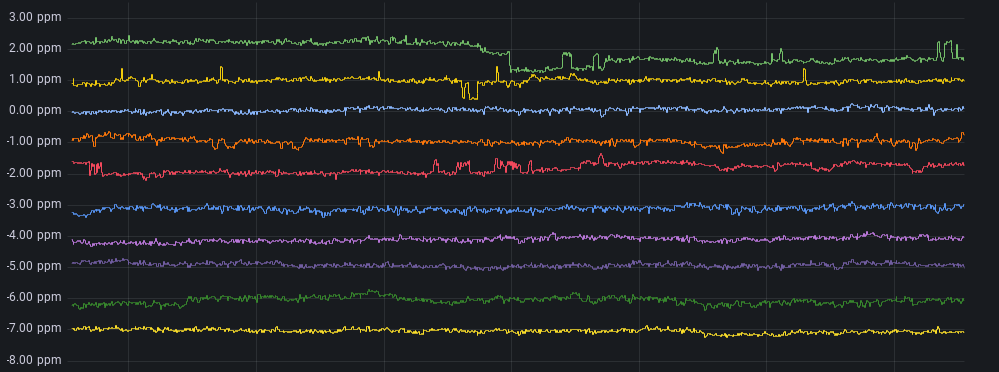
\includegraphics{images/title.png}}
\logo*{\includegraphics{images/titel_apq-logo.pdf}}

\begin{document}

\AtBeginSection[] {
    \begin{frame}
        \frametitle{Contents}
        \tableofcontents[currentsection, subsectionstyle=show/show/shaded, subsubsectionstyle=show/show/show/hide]
    \end{frame}
}

\maketitle

\section{Introduction}
\subsection{The Project}
\begin{frame}{The Project\\\textnormal{\small{Building a Quantum Computer}}}
    \begin{columns}[T] % align columns
        \begin{column}{.48\textwidth}
            Goal: Quantum computer with single atoms
            \begin{itemize}
                \item Needs lasers (dozens!)...
                \item and current sources...
                \item and voltage references...
            \end{itemize}
        \end{column}
        \hfill
        \begin{column}{.48\textwidth}
            \begin{figure}[h]
                \includegraphics[width=0.75\textwidth]{images/quips.png}
                \caption{Array of 15x15 trapped neutral atoms}
            \end{figure}
        \end{column}
    \end{columns}
\end{frame}

\section{Implementation}
\subsection{Laser Current Driver}
\begin{frame}{Diode Laser System\\\textnormal{\small{Requirements}}}
    Requirements:
    \begin{itemize}
        \item Low noise
        \item Low drift with temperature (\qty{<1}{\ppm \per \kelvin})
        \item Output current: up to \qty{500}{\mA}
        \item Compliance voltage: up to \qty{10}{\V}
    \end{itemize}

\end{frame}

\begin{frame}{Current Driver\\\textnormal{\small{The state of the art}}}
    \begin{figure}
        \only<1>{\import{figures/}{fig_simplified_current_source}}\only<2>{\import{figures/}{fig_simplified_current_source_annotated}}
        \only<1>{\caption{Simplified current source based on \cite{Libbrecht-Hall}}}\only<2>{\caption{Simplified current source based on \cite{Libbrecht-Hall}, inset: \cite{IRF9610}}}
    \end{figure}
    \begin{tikzpicture}[remember picture, overlay]
        \only<2>{
            \node[draw=blue, inner sep=0.5, anchor=west] (irf9610 saturation) at (6.7,4) {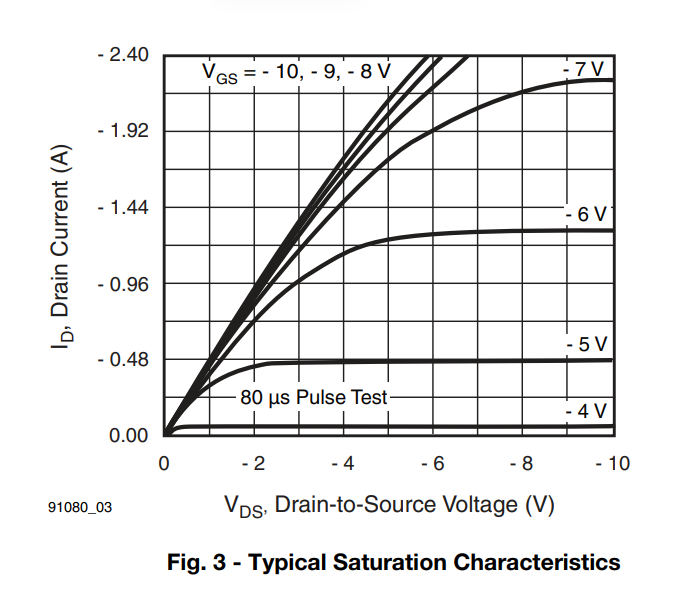
\includegraphics[width=.38\linewidth]{images/irf9610_saturation.png}};
        }
    \end{tikzpicture}
\end{frame}

\begin{frame}{Current Driver\\\textnormal{\small{Our solution}}}
    \begin{figure}
        \import{figures/}{fig_simplified_current_source_improved}
        \caption{Simplified current source, APQ design}
    \end{figure}
\end{frame}

\begin{frame}{Current Driver\\\textnormal{\small{Noise Source}}}
    \begin{columns}[T] % align columns
        \begin{column}{.48\textwidth}
            Sources of Noise:
            \begin{itemize}
                \item Wideband
                \begin{itemize}
                    \item Reference noise can be filtered
                    \item Op-amp must be low noise (AD797)
                \end{itemize}
                \item Low frequency noise
                \begin{itemize}
                    \item Dominated by reference noise
                    \item LM399 vs. ADR1399 vs. LTZ1000
                    \item Popcorn noise!
                    \item References need to be tested. Each and every one!?
                \end{itemize}
            \end{itemize}
        \end{column}
        \hfill
        \begin{column}{.48\textwidth}
            \begin{figure}[h]
                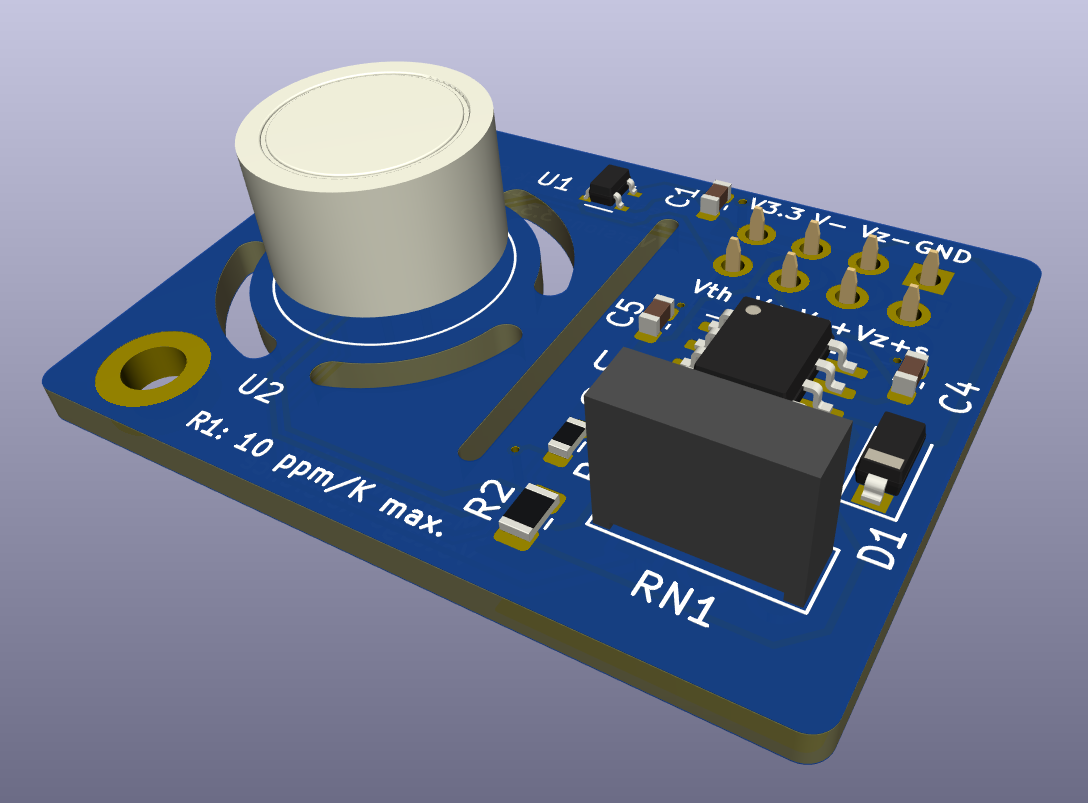
\includegraphics[width=0.9\textwidth]{images/reference_board.png}
                \caption{LM399 \qty{-15}{\volt} reference, Available at \cite{lm399_reference}}
            \end{figure}
        \end{column}
    \end{columns}
\end{frame}

\subsection{Testing Voltage References}
\begin{frame}{Testing Voltage References}
    \begin{figure}
        \import{figures/}{how_to_test}
        \caption{Test setup for voltage references. Images taken from: \cite{k2002}}
    \end{figure}
    \begin{itemize}
        \item 10 measurants every \qty{18}{\second} (\num{2e5} relay operations @ \qty{1000}{\hour})
        \item Keithley 2000-SCAN is rated at \numrange{1e5}{1e8} operations
    \end{itemize}
\end{frame}

\begin{frame}{Testing \\\textnormal{\small{Corona and Home Office}}}
    \begin{figure}[h]
        \includegraphics[width=0.63\textwidth]{images/home_office.JPG}
        \caption{Reverse engineering the 2000-SCAN protocol }
    \end{figure}
\end{frame}

\subsection{Open Source Scanner Card}
\begin{frame}{Testing \\\textnormal{\small{Open Source Scanner Card}}}
    \begin{columns}[T] % align columns
        \begin{column}{.48\textwidth}
            \begin{itemize}
                \item 10- or 20-channel scanner card
                \item All solid state relays
                \item Silent
                \item iCE40 FPGA-based to meet timing requirements of the K2002
                \item Fully compatible with DMM6500 and Model 200x
                \item Open source toolchain
            \end{itemize}

        \end{column}
        \hfill
        \begin{column}{.48\textwidth}
            \begin{figure}[h]
                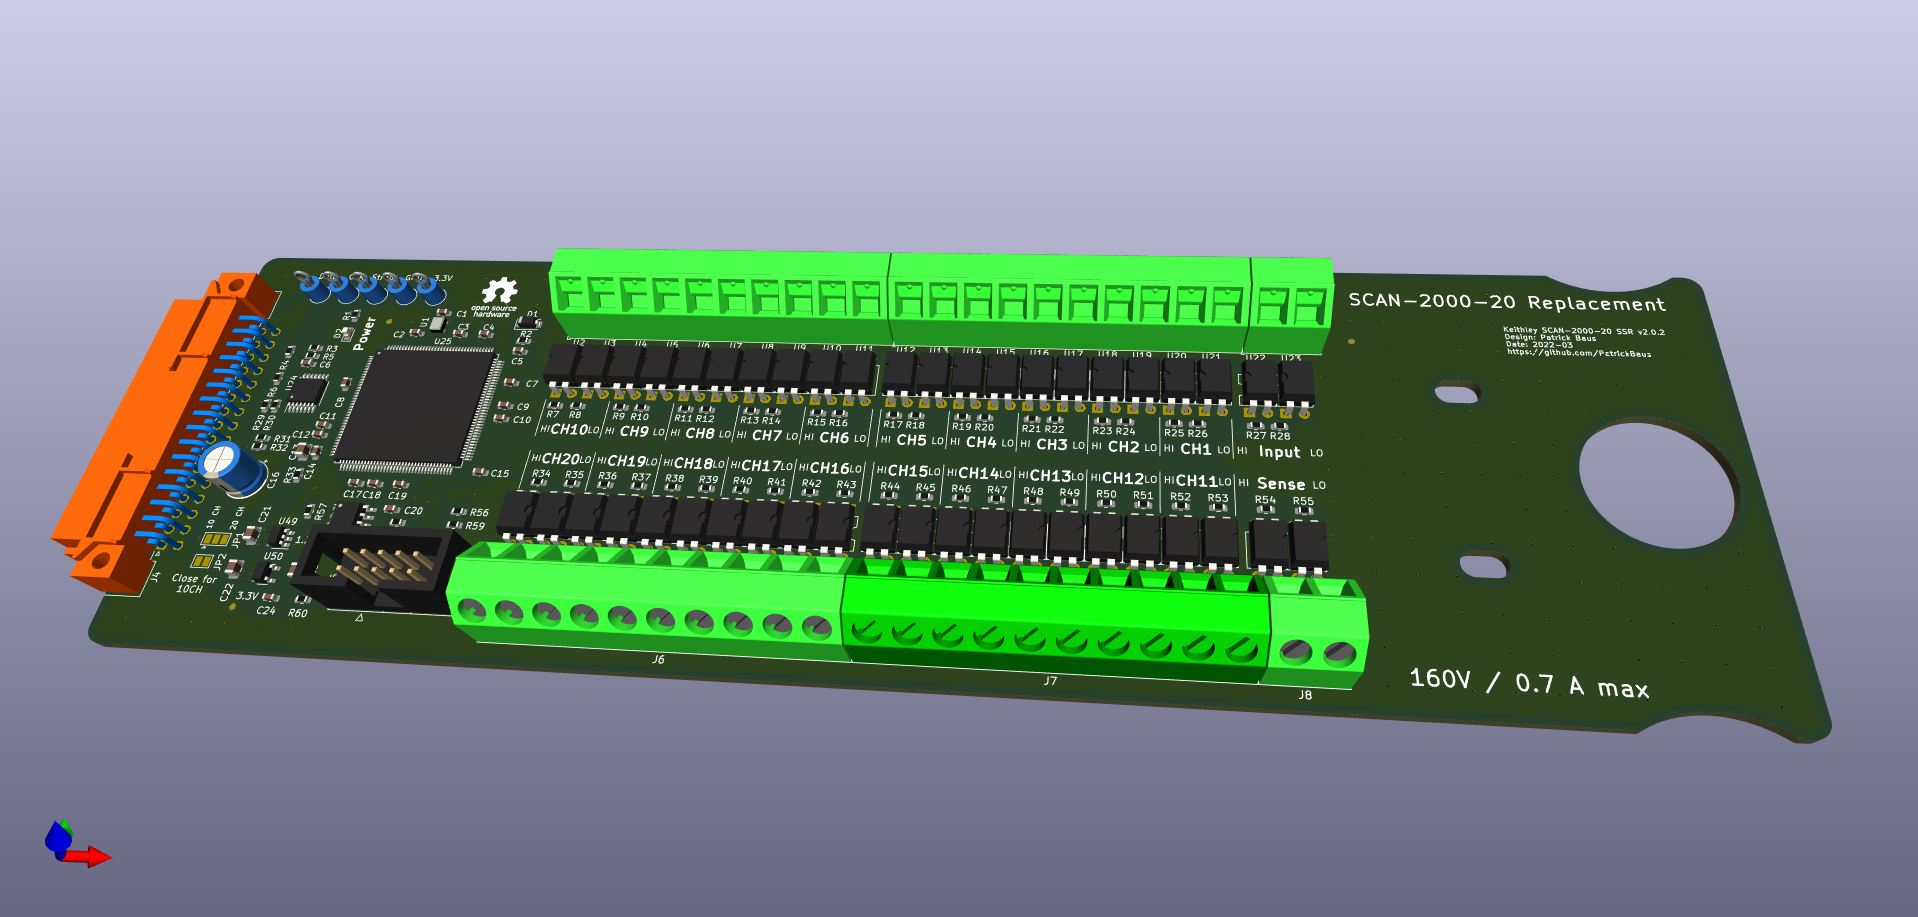
\includegraphics[width=0.9\textwidth]{images/scanner_card.png}
                \caption{Available at \cite{scan2000}}
            \end{figure}
        \end{column}
    \end{columns}
\end{frame}

\subsection{LM399 vs. ARD1399}
\begin{frame}{Test results\\\textnormal{\small{LM399 vs. ARD1399}}}
    \begin{figure}
        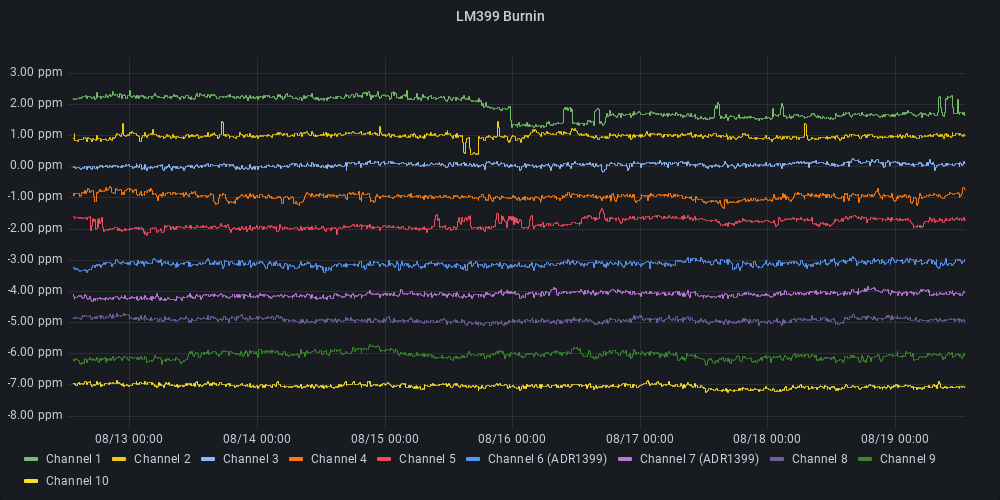
\includegraphics[width=0.9\textwidth]{images/lm399_burnin.png}
    \end{figure}
\end{frame}

\begin{frame}{Test results\\\textnormal{\small{In numbers}}}
    Our experience with the LM399/ARD1399:
    \begin{itemize}
        \item All diodes are tested over \qty{1000}{\hour}
        \item Tested over 100 LM399 samples
        \item Tested around 10 ADR1399 (100 more on order)
        \item LM399 popcorn noise is about {\color{red}\qtyrange{0.4}{0.6}{\ppm}}
        \item Around {\color{red}\qtyrange{40}{50}{\percent}} of the LM399s show excess popcorn noise and get tossed
        \item ADR1399 shows (nearly) no popcorn noise
    \end{itemize}

    \Large{Is the ADR1399 the future? - Time will tell. See you in a few months.}
\end{frame}

\begin{frame}[plain, c]
    \centering
    \Huge Thank you very much for your attention!
    \begin{tikzpicture}[remember picture, overlay]
        \node (logo artemis) at (-6.5,3.3) {
\includegraphics[width=.25\linewidth]{images/ARTEMIS_logo.pdf}};
        \node (logo apq) at (-2.5,3.3) {\includegraphics[width=.35\linewidth]{images/titel_apq-logo.pdf}};
        \node (logo oshw) at (-7,-1) {
\includegraphics[width=.13\linewidth]{images/oshw-logo.pdf}};
        \node (logo bmbf) at (-2.5,-1) {
\includegraphics[width=.25\linewidth]{images/BMBF_Logo.pdf}};
        \node (logo hfhf) at (2,-1) {
\includegraphics[width=.3\linewidth]{images/hfhf-logo.jpg}};
        \node (logo tuda) at (2,3.3) {\includegraphics[width=.35\linewidth]{tuda_logo.pdf}};
        \node (logo hgs-hire) at (1,-3) {
\includegraphics[width=.5\linewidth]{images/logo-hgs-hire-big.png}};
        \node (logo gsi) at (-7,-3) {
\includegraphics[width=.25\linewidth]{images/GSI_Logo_cmyk.pdf}};
        \node (logo fair) at (-4,-3) {
\includegraphics[width=.25\linewidth]{images/FAIR_Logo_cmyk.pdf}};
    \end{tikzpicture}
\end{frame}

\begin{frame}[allowframebreaks]{Bibliography}
    \bibliographystyle{unsrt}
    \bibliography{bibliography}
\end{frame}

\section*{Suplemental Material}
\begin{frame}{Laser Resonator}
    \center{
        \includegraphics[width=.8\linewidth]{images/resonator.JPG}
    }
\end{frame}

\begin{frame}{Current Driver\\\textnormal{\small{Comparison with commercial alternatives}}}
    \begin{figure}
        \centering
        \scalebox{0.7}{
            %% Creator: Matplotlib, PGF backend
%%
%% To include the figure in your LaTeX document, write
%%   \input{<filename>.pgf}
%%
%% Make sure the required packages are loaded in your preamble
%%   \usepackage{pgf}
%%
%% Also ensure that all the required font packages are loaded; for instance,
%% the lmodern package is sometimes necessary when using math font.
%%   \usepackage{lmodern}
%%
%% Figures using additional raster images can only be included by \input if
%% they are in the same directory as the main LaTeX file. For loading figures
%% from other directories you can use the `import` package
%%   \usepackage{import}
%%
%% and then include the figures with
%%   \import{<path to file>}{<filename>.pgf}
%%
%% Matplotlib used the following preamble
%%   \usepackage{fontspec}
%%   \setmainfont{DejaVuSerif.ttf}[Path=\detokenize{/run/media/maat/data/diode_driver_noise/env/lib/python3.10/site-packages/matplotlib/mpl-data/fonts/ttf/}]
%%   \setsansfont{DejaVuSans.ttf}[Path=\detokenize{/run/media/maat/data/diode_driver_noise/env/lib/python3.10/site-packages/matplotlib/mpl-data/fonts/ttf/}]
%%   \setmonofont{DejaVuSansMono.ttf}[Path=\detokenize{/run/media/maat/data/diode_driver_noise/env/lib/python3.10/site-packages/matplotlib/mpl-data/fonts/ttf/}]
%%
\begingroup%
\makeatletter%
\begin{pgfpicture}%
\pgfpathrectangle{\pgfpointorigin}{\pgfqpoint{6.650000in}{2.830000in}}%
\pgfusepath{use as bounding box, clip}%
\begin{pgfscope}%
\pgfsetbuttcap%
\pgfsetmiterjoin%
\definecolor{currentfill}{rgb}{1.000000,1.000000,1.000000}%
\pgfsetfillcolor{currentfill}%
\pgfsetlinewidth{0.000000pt}%
\definecolor{currentstroke}{rgb}{1.000000,1.000000,1.000000}%
\pgfsetstrokecolor{currentstroke}%
\pgfsetdash{}{0pt}%
\pgfpathmoveto{\pgfqpoint{0.000000in}{0.000000in}}%
\pgfpathlineto{\pgfqpoint{6.650000in}{0.000000in}}%
\pgfpathlineto{\pgfqpoint{6.650000in}{2.830000in}}%
\pgfpathlineto{\pgfqpoint{0.000000in}{2.830000in}}%
\pgfpathlineto{\pgfqpoint{0.000000in}{0.000000in}}%
\pgfpathclose%
\pgfusepath{fill}%
\end{pgfscope}%
\begin{pgfscope}%
\pgfsetbuttcap%
\pgfsetmiterjoin%
\definecolor{currentfill}{rgb}{1.000000,1.000000,1.000000}%
\pgfsetfillcolor{currentfill}%
\pgfsetlinewidth{0.000000pt}%
\definecolor{currentstroke}{rgb}{0.000000,0.000000,0.000000}%
\pgfsetstrokecolor{currentstroke}%
\pgfsetstrokeopacity{0.000000}%
\pgfsetdash{}{0pt}%
\pgfpathmoveto{\pgfqpoint{0.916968in}{0.491881in}}%
\pgfpathlineto{\pgfqpoint{6.500044in}{0.491881in}}%
\pgfpathlineto{\pgfqpoint{6.500044in}{2.830000in}}%
\pgfpathlineto{\pgfqpoint{0.916968in}{2.830000in}}%
\pgfpathlineto{\pgfqpoint{0.916968in}{0.491881in}}%
\pgfpathclose%
\pgfusepath{fill}%
\end{pgfscope}%
\begin{pgfscope}%
\pgfsetbuttcap%
\pgfsetroundjoin%
\definecolor{currentfill}{rgb}{0.000000,0.000000,0.000000}%
\pgfsetfillcolor{currentfill}%
\pgfsetlinewidth{0.803000pt}%
\definecolor{currentstroke}{rgb}{0.000000,0.000000,0.000000}%
\pgfsetstrokecolor{currentstroke}%
\pgfsetdash{}{0pt}%
\pgfsys@defobject{currentmarker}{\pgfqpoint{0.000000in}{-0.048611in}}{\pgfqpoint{0.000000in}{0.000000in}}{%
\pgfpathmoveto{\pgfqpoint{0.000000in}{0.000000in}}%
\pgfpathlineto{\pgfqpoint{0.000000in}{-0.048611in}}%
\pgfusepath{stroke,fill}%
}%
\begin{pgfscope}%
\pgfsys@transformshift{1.170744in}{0.491881in}%
\pgfsys@useobject{currentmarker}{}%
\end{pgfscope}%
\end{pgfscope}%
\begin{pgfscope}%
\definecolor{textcolor}{rgb}{0.000000,0.000000,0.000000}%
\pgfsetstrokecolor{textcolor}%
\pgfsetfillcolor{textcolor}%
\pgftext[x=1.170744in,y=0.394659in,,top]{\color{textcolor}\sffamily\fontsize{10.000000}{12.000000}\selectfont \(\displaystyle {10^{1}}\)}%
\end{pgfscope}%
\begin{pgfscope}%
\pgfsetbuttcap%
\pgfsetroundjoin%
\definecolor{currentfill}{rgb}{0.000000,0.000000,0.000000}%
\pgfsetfillcolor{currentfill}%
\pgfsetlinewidth{0.803000pt}%
\definecolor{currentstroke}{rgb}{0.000000,0.000000,0.000000}%
\pgfsetstrokecolor{currentstroke}%
\pgfsetdash{}{0pt}%
\pgfsys@defobject{currentmarker}{\pgfqpoint{0.000000in}{-0.048611in}}{\pgfqpoint{0.000000in}{0.000000in}}{%
\pgfpathmoveto{\pgfqpoint{0.000000in}{0.000000in}}%
\pgfpathlineto{\pgfqpoint{0.000000in}{-0.048611in}}%
\pgfusepath{stroke,fill}%
}%
\begin{pgfscope}%
\pgfsys@transformshift{2.185849in}{0.491881in}%
\pgfsys@useobject{currentmarker}{}%
\end{pgfscope}%
\end{pgfscope}%
\begin{pgfscope}%
\definecolor{textcolor}{rgb}{0.000000,0.000000,0.000000}%
\pgfsetstrokecolor{textcolor}%
\pgfsetfillcolor{textcolor}%
\pgftext[x=2.185849in,y=0.394659in,,top]{\color{textcolor}\sffamily\fontsize{10.000000}{12.000000}\selectfont \(\displaystyle {10^{2}}\)}%
\end{pgfscope}%
\begin{pgfscope}%
\pgfsetbuttcap%
\pgfsetroundjoin%
\definecolor{currentfill}{rgb}{0.000000,0.000000,0.000000}%
\pgfsetfillcolor{currentfill}%
\pgfsetlinewidth{0.803000pt}%
\definecolor{currentstroke}{rgb}{0.000000,0.000000,0.000000}%
\pgfsetstrokecolor{currentstroke}%
\pgfsetdash{}{0pt}%
\pgfsys@defobject{currentmarker}{\pgfqpoint{0.000000in}{-0.048611in}}{\pgfqpoint{0.000000in}{0.000000in}}{%
\pgfpathmoveto{\pgfqpoint{0.000000in}{0.000000in}}%
\pgfpathlineto{\pgfqpoint{0.000000in}{-0.048611in}}%
\pgfusepath{stroke,fill}%
}%
\begin{pgfscope}%
\pgfsys@transformshift{3.200954in}{0.491881in}%
\pgfsys@useobject{currentmarker}{}%
\end{pgfscope}%
\end{pgfscope}%
\begin{pgfscope}%
\definecolor{textcolor}{rgb}{0.000000,0.000000,0.000000}%
\pgfsetstrokecolor{textcolor}%
\pgfsetfillcolor{textcolor}%
\pgftext[x=3.200954in,y=0.394659in,,top]{\color{textcolor}\sffamily\fontsize{10.000000}{12.000000}\selectfont \(\displaystyle {10^{3}}\)}%
\end{pgfscope}%
\begin{pgfscope}%
\pgfsetbuttcap%
\pgfsetroundjoin%
\definecolor{currentfill}{rgb}{0.000000,0.000000,0.000000}%
\pgfsetfillcolor{currentfill}%
\pgfsetlinewidth{0.803000pt}%
\definecolor{currentstroke}{rgb}{0.000000,0.000000,0.000000}%
\pgfsetstrokecolor{currentstroke}%
\pgfsetdash{}{0pt}%
\pgfsys@defobject{currentmarker}{\pgfqpoint{0.000000in}{-0.048611in}}{\pgfqpoint{0.000000in}{0.000000in}}{%
\pgfpathmoveto{\pgfqpoint{0.000000in}{0.000000in}}%
\pgfpathlineto{\pgfqpoint{0.000000in}{-0.048611in}}%
\pgfusepath{stroke,fill}%
}%
\begin{pgfscope}%
\pgfsys@transformshift{4.216058in}{0.491881in}%
\pgfsys@useobject{currentmarker}{}%
\end{pgfscope}%
\end{pgfscope}%
\begin{pgfscope}%
\definecolor{textcolor}{rgb}{0.000000,0.000000,0.000000}%
\pgfsetstrokecolor{textcolor}%
\pgfsetfillcolor{textcolor}%
\pgftext[x=4.216058in,y=0.394659in,,top]{\color{textcolor}\sffamily\fontsize{10.000000}{12.000000}\selectfont \(\displaystyle {10^{4}}\)}%
\end{pgfscope}%
\begin{pgfscope}%
\pgfsetbuttcap%
\pgfsetroundjoin%
\definecolor{currentfill}{rgb}{0.000000,0.000000,0.000000}%
\pgfsetfillcolor{currentfill}%
\pgfsetlinewidth{0.803000pt}%
\definecolor{currentstroke}{rgb}{0.000000,0.000000,0.000000}%
\pgfsetstrokecolor{currentstroke}%
\pgfsetdash{}{0pt}%
\pgfsys@defobject{currentmarker}{\pgfqpoint{0.000000in}{-0.048611in}}{\pgfqpoint{0.000000in}{0.000000in}}{%
\pgfpathmoveto{\pgfqpoint{0.000000in}{0.000000in}}%
\pgfpathlineto{\pgfqpoint{0.000000in}{-0.048611in}}%
\pgfusepath{stroke,fill}%
}%
\begin{pgfscope}%
\pgfsys@transformshift{5.231163in}{0.491881in}%
\pgfsys@useobject{currentmarker}{}%
\end{pgfscope}%
\end{pgfscope}%
\begin{pgfscope}%
\definecolor{textcolor}{rgb}{0.000000,0.000000,0.000000}%
\pgfsetstrokecolor{textcolor}%
\pgfsetfillcolor{textcolor}%
\pgftext[x=5.231163in,y=0.394659in,,top]{\color{textcolor}\sffamily\fontsize{10.000000}{12.000000}\selectfont \(\displaystyle {10^{5}}\)}%
\end{pgfscope}%
\begin{pgfscope}%
\pgfsetbuttcap%
\pgfsetroundjoin%
\definecolor{currentfill}{rgb}{0.000000,0.000000,0.000000}%
\pgfsetfillcolor{currentfill}%
\pgfsetlinewidth{0.803000pt}%
\definecolor{currentstroke}{rgb}{0.000000,0.000000,0.000000}%
\pgfsetstrokecolor{currentstroke}%
\pgfsetdash{}{0pt}%
\pgfsys@defobject{currentmarker}{\pgfqpoint{0.000000in}{-0.048611in}}{\pgfqpoint{0.000000in}{0.000000in}}{%
\pgfpathmoveto{\pgfqpoint{0.000000in}{0.000000in}}%
\pgfpathlineto{\pgfqpoint{0.000000in}{-0.048611in}}%
\pgfusepath{stroke,fill}%
}%
\begin{pgfscope}%
\pgfsys@transformshift{6.246268in}{0.491881in}%
\pgfsys@useobject{currentmarker}{}%
\end{pgfscope}%
\end{pgfscope}%
\begin{pgfscope}%
\definecolor{textcolor}{rgb}{0.000000,0.000000,0.000000}%
\pgfsetstrokecolor{textcolor}%
\pgfsetfillcolor{textcolor}%
\pgftext[x=6.246268in,y=0.394659in,,top]{\color{textcolor}\sffamily\fontsize{10.000000}{12.000000}\selectfont \(\displaystyle {10^{6}}\)}%
\end{pgfscope}%
\begin{pgfscope}%
\pgfsetbuttcap%
\pgfsetroundjoin%
\definecolor{currentfill}{rgb}{0.000000,0.000000,0.000000}%
\pgfsetfillcolor{currentfill}%
\pgfsetlinewidth{0.602250pt}%
\definecolor{currentstroke}{rgb}{0.000000,0.000000,0.000000}%
\pgfsetstrokecolor{currentstroke}%
\pgfsetdash{}{0pt}%
\pgfsys@defobject{currentmarker}{\pgfqpoint{0.000000in}{-0.027778in}}{\pgfqpoint{0.000000in}{0.000000in}}{%
\pgfpathmoveto{\pgfqpoint{0.000000in}{0.000000in}}%
\pgfpathlineto{\pgfqpoint{0.000000in}{-0.027778in}}%
\pgfusepath{stroke,fill}%
}%
\begin{pgfscope}%
\pgfsys@transformshift{0.945544in}{0.491881in}%
\pgfsys@useobject{currentmarker}{}%
\end{pgfscope}%
\end{pgfscope}%
\begin{pgfscope}%
\pgfsetbuttcap%
\pgfsetroundjoin%
\definecolor{currentfill}{rgb}{0.000000,0.000000,0.000000}%
\pgfsetfillcolor{currentfill}%
\pgfsetlinewidth{0.602250pt}%
\definecolor{currentstroke}{rgb}{0.000000,0.000000,0.000000}%
\pgfsetstrokecolor{currentstroke}%
\pgfsetdash{}{0pt}%
\pgfsys@defobject{currentmarker}{\pgfqpoint{0.000000in}{-0.027778in}}{\pgfqpoint{0.000000in}{0.000000in}}{%
\pgfpathmoveto{\pgfqpoint{0.000000in}{0.000000in}}%
\pgfpathlineto{\pgfqpoint{0.000000in}{-0.027778in}}%
\pgfusepath{stroke,fill}%
}%
\begin{pgfscope}%
\pgfsys@transformshift{1.013502in}{0.491881in}%
\pgfsys@useobject{currentmarker}{}%
\end{pgfscope}%
\end{pgfscope}%
\begin{pgfscope}%
\pgfsetbuttcap%
\pgfsetroundjoin%
\definecolor{currentfill}{rgb}{0.000000,0.000000,0.000000}%
\pgfsetfillcolor{currentfill}%
\pgfsetlinewidth{0.602250pt}%
\definecolor{currentstroke}{rgb}{0.000000,0.000000,0.000000}%
\pgfsetstrokecolor{currentstroke}%
\pgfsetdash{}{0pt}%
\pgfsys@defobject{currentmarker}{\pgfqpoint{0.000000in}{-0.027778in}}{\pgfqpoint{0.000000in}{0.000000in}}{%
\pgfpathmoveto{\pgfqpoint{0.000000in}{0.000000in}}%
\pgfpathlineto{\pgfqpoint{0.000000in}{-0.027778in}}%
\pgfusepath{stroke,fill}%
}%
\begin{pgfscope}%
\pgfsys@transformshift{1.072370in}{0.491881in}%
\pgfsys@useobject{currentmarker}{}%
\end{pgfscope}%
\end{pgfscope}%
\begin{pgfscope}%
\pgfsetbuttcap%
\pgfsetroundjoin%
\definecolor{currentfill}{rgb}{0.000000,0.000000,0.000000}%
\pgfsetfillcolor{currentfill}%
\pgfsetlinewidth{0.602250pt}%
\definecolor{currentstroke}{rgb}{0.000000,0.000000,0.000000}%
\pgfsetstrokecolor{currentstroke}%
\pgfsetdash{}{0pt}%
\pgfsys@defobject{currentmarker}{\pgfqpoint{0.000000in}{-0.027778in}}{\pgfqpoint{0.000000in}{0.000000in}}{%
\pgfpathmoveto{\pgfqpoint{0.000000in}{0.000000in}}%
\pgfpathlineto{\pgfqpoint{0.000000in}{-0.027778in}}%
\pgfusepath{stroke,fill}%
}%
\begin{pgfscope}%
\pgfsys@transformshift{1.124295in}{0.491881in}%
\pgfsys@useobject{currentmarker}{}%
\end{pgfscope}%
\end{pgfscope}%
\begin{pgfscope}%
\pgfsetbuttcap%
\pgfsetroundjoin%
\definecolor{currentfill}{rgb}{0.000000,0.000000,0.000000}%
\pgfsetfillcolor{currentfill}%
\pgfsetlinewidth{0.602250pt}%
\definecolor{currentstroke}{rgb}{0.000000,0.000000,0.000000}%
\pgfsetstrokecolor{currentstroke}%
\pgfsetdash{}{0pt}%
\pgfsys@defobject{currentmarker}{\pgfqpoint{0.000000in}{-0.027778in}}{\pgfqpoint{0.000000in}{0.000000in}}{%
\pgfpathmoveto{\pgfqpoint{0.000000in}{0.000000in}}%
\pgfpathlineto{\pgfqpoint{0.000000in}{-0.027778in}}%
\pgfusepath{stroke,fill}%
}%
\begin{pgfscope}%
\pgfsys@transformshift{1.476321in}{0.491881in}%
\pgfsys@useobject{currentmarker}{}%
\end{pgfscope}%
\end{pgfscope}%
\begin{pgfscope}%
\pgfsetbuttcap%
\pgfsetroundjoin%
\definecolor{currentfill}{rgb}{0.000000,0.000000,0.000000}%
\pgfsetfillcolor{currentfill}%
\pgfsetlinewidth{0.602250pt}%
\definecolor{currentstroke}{rgb}{0.000000,0.000000,0.000000}%
\pgfsetstrokecolor{currentstroke}%
\pgfsetdash{}{0pt}%
\pgfsys@defobject{currentmarker}{\pgfqpoint{0.000000in}{-0.027778in}}{\pgfqpoint{0.000000in}{0.000000in}}{%
\pgfpathmoveto{\pgfqpoint{0.000000in}{0.000000in}}%
\pgfpathlineto{\pgfqpoint{0.000000in}{-0.027778in}}%
\pgfusepath{stroke,fill}%
}%
\begin{pgfscope}%
\pgfsys@transformshift{1.655072in}{0.491881in}%
\pgfsys@useobject{currentmarker}{}%
\end{pgfscope}%
\end{pgfscope}%
\begin{pgfscope}%
\pgfsetbuttcap%
\pgfsetroundjoin%
\definecolor{currentfill}{rgb}{0.000000,0.000000,0.000000}%
\pgfsetfillcolor{currentfill}%
\pgfsetlinewidth{0.602250pt}%
\definecolor{currentstroke}{rgb}{0.000000,0.000000,0.000000}%
\pgfsetstrokecolor{currentstroke}%
\pgfsetdash{}{0pt}%
\pgfsys@defobject{currentmarker}{\pgfqpoint{0.000000in}{-0.027778in}}{\pgfqpoint{0.000000in}{0.000000in}}{%
\pgfpathmoveto{\pgfqpoint{0.000000in}{0.000000in}}%
\pgfpathlineto{\pgfqpoint{0.000000in}{-0.027778in}}%
\pgfusepath{stroke,fill}%
}%
\begin{pgfscope}%
\pgfsys@transformshift{1.781898in}{0.491881in}%
\pgfsys@useobject{currentmarker}{}%
\end{pgfscope}%
\end{pgfscope}%
\begin{pgfscope}%
\pgfsetbuttcap%
\pgfsetroundjoin%
\definecolor{currentfill}{rgb}{0.000000,0.000000,0.000000}%
\pgfsetfillcolor{currentfill}%
\pgfsetlinewidth{0.602250pt}%
\definecolor{currentstroke}{rgb}{0.000000,0.000000,0.000000}%
\pgfsetstrokecolor{currentstroke}%
\pgfsetdash{}{0pt}%
\pgfsys@defobject{currentmarker}{\pgfqpoint{0.000000in}{-0.027778in}}{\pgfqpoint{0.000000in}{0.000000in}}{%
\pgfpathmoveto{\pgfqpoint{0.000000in}{0.000000in}}%
\pgfpathlineto{\pgfqpoint{0.000000in}{-0.027778in}}%
\pgfusepath{stroke,fill}%
}%
\begin{pgfscope}%
\pgfsys@transformshift{1.880272in}{0.491881in}%
\pgfsys@useobject{currentmarker}{}%
\end{pgfscope}%
\end{pgfscope}%
\begin{pgfscope}%
\pgfsetbuttcap%
\pgfsetroundjoin%
\definecolor{currentfill}{rgb}{0.000000,0.000000,0.000000}%
\pgfsetfillcolor{currentfill}%
\pgfsetlinewidth{0.602250pt}%
\definecolor{currentstroke}{rgb}{0.000000,0.000000,0.000000}%
\pgfsetstrokecolor{currentstroke}%
\pgfsetdash{}{0pt}%
\pgfsys@defobject{currentmarker}{\pgfqpoint{0.000000in}{-0.027778in}}{\pgfqpoint{0.000000in}{0.000000in}}{%
\pgfpathmoveto{\pgfqpoint{0.000000in}{0.000000in}}%
\pgfpathlineto{\pgfqpoint{0.000000in}{-0.027778in}}%
\pgfusepath{stroke,fill}%
}%
\begin{pgfscope}%
\pgfsys@transformshift{1.960649in}{0.491881in}%
\pgfsys@useobject{currentmarker}{}%
\end{pgfscope}%
\end{pgfscope}%
\begin{pgfscope}%
\pgfsetbuttcap%
\pgfsetroundjoin%
\definecolor{currentfill}{rgb}{0.000000,0.000000,0.000000}%
\pgfsetfillcolor{currentfill}%
\pgfsetlinewidth{0.602250pt}%
\definecolor{currentstroke}{rgb}{0.000000,0.000000,0.000000}%
\pgfsetstrokecolor{currentstroke}%
\pgfsetdash{}{0pt}%
\pgfsys@defobject{currentmarker}{\pgfqpoint{0.000000in}{-0.027778in}}{\pgfqpoint{0.000000in}{0.000000in}}{%
\pgfpathmoveto{\pgfqpoint{0.000000in}{0.000000in}}%
\pgfpathlineto{\pgfqpoint{0.000000in}{-0.027778in}}%
\pgfusepath{stroke,fill}%
}%
\begin{pgfscope}%
\pgfsys@transformshift{2.028607in}{0.491881in}%
\pgfsys@useobject{currentmarker}{}%
\end{pgfscope}%
\end{pgfscope}%
\begin{pgfscope}%
\pgfsetbuttcap%
\pgfsetroundjoin%
\definecolor{currentfill}{rgb}{0.000000,0.000000,0.000000}%
\pgfsetfillcolor{currentfill}%
\pgfsetlinewidth{0.602250pt}%
\definecolor{currentstroke}{rgb}{0.000000,0.000000,0.000000}%
\pgfsetstrokecolor{currentstroke}%
\pgfsetdash{}{0pt}%
\pgfsys@defobject{currentmarker}{\pgfqpoint{0.000000in}{-0.027778in}}{\pgfqpoint{0.000000in}{0.000000in}}{%
\pgfpathmoveto{\pgfqpoint{0.000000in}{0.000000in}}%
\pgfpathlineto{\pgfqpoint{0.000000in}{-0.027778in}}%
\pgfusepath{stroke,fill}%
}%
\begin{pgfscope}%
\pgfsys@transformshift{2.087475in}{0.491881in}%
\pgfsys@useobject{currentmarker}{}%
\end{pgfscope}%
\end{pgfscope}%
\begin{pgfscope}%
\pgfsetbuttcap%
\pgfsetroundjoin%
\definecolor{currentfill}{rgb}{0.000000,0.000000,0.000000}%
\pgfsetfillcolor{currentfill}%
\pgfsetlinewidth{0.602250pt}%
\definecolor{currentstroke}{rgb}{0.000000,0.000000,0.000000}%
\pgfsetstrokecolor{currentstroke}%
\pgfsetdash{}{0pt}%
\pgfsys@defobject{currentmarker}{\pgfqpoint{0.000000in}{-0.027778in}}{\pgfqpoint{0.000000in}{0.000000in}}{%
\pgfpathmoveto{\pgfqpoint{0.000000in}{0.000000in}}%
\pgfpathlineto{\pgfqpoint{0.000000in}{-0.027778in}}%
\pgfusepath{stroke,fill}%
}%
\begin{pgfscope}%
\pgfsys@transformshift{2.139400in}{0.491881in}%
\pgfsys@useobject{currentmarker}{}%
\end{pgfscope}%
\end{pgfscope}%
\begin{pgfscope}%
\pgfsetbuttcap%
\pgfsetroundjoin%
\definecolor{currentfill}{rgb}{0.000000,0.000000,0.000000}%
\pgfsetfillcolor{currentfill}%
\pgfsetlinewidth{0.602250pt}%
\definecolor{currentstroke}{rgb}{0.000000,0.000000,0.000000}%
\pgfsetstrokecolor{currentstroke}%
\pgfsetdash{}{0pt}%
\pgfsys@defobject{currentmarker}{\pgfqpoint{0.000000in}{-0.027778in}}{\pgfqpoint{0.000000in}{0.000000in}}{%
\pgfpathmoveto{\pgfqpoint{0.000000in}{0.000000in}}%
\pgfpathlineto{\pgfqpoint{0.000000in}{-0.027778in}}%
\pgfusepath{stroke,fill}%
}%
\begin{pgfscope}%
\pgfsys@transformshift{2.491426in}{0.491881in}%
\pgfsys@useobject{currentmarker}{}%
\end{pgfscope}%
\end{pgfscope}%
\begin{pgfscope}%
\pgfsetbuttcap%
\pgfsetroundjoin%
\definecolor{currentfill}{rgb}{0.000000,0.000000,0.000000}%
\pgfsetfillcolor{currentfill}%
\pgfsetlinewidth{0.602250pt}%
\definecolor{currentstroke}{rgb}{0.000000,0.000000,0.000000}%
\pgfsetstrokecolor{currentstroke}%
\pgfsetdash{}{0pt}%
\pgfsys@defobject{currentmarker}{\pgfqpoint{0.000000in}{-0.027778in}}{\pgfqpoint{0.000000in}{0.000000in}}{%
\pgfpathmoveto{\pgfqpoint{0.000000in}{0.000000in}}%
\pgfpathlineto{\pgfqpoint{0.000000in}{-0.027778in}}%
\pgfusepath{stroke,fill}%
}%
\begin{pgfscope}%
\pgfsys@transformshift{2.670177in}{0.491881in}%
\pgfsys@useobject{currentmarker}{}%
\end{pgfscope}%
\end{pgfscope}%
\begin{pgfscope}%
\pgfsetbuttcap%
\pgfsetroundjoin%
\definecolor{currentfill}{rgb}{0.000000,0.000000,0.000000}%
\pgfsetfillcolor{currentfill}%
\pgfsetlinewidth{0.602250pt}%
\definecolor{currentstroke}{rgb}{0.000000,0.000000,0.000000}%
\pgfsetstrokecolor{currentstroke}%
\pgfsetdash{}{0pt}%
\pgfsys@defobject{currentmarker}{\pgfqpoint{0.000000in}{-0.027778in}}{\pgfqpoint{0.000000in}{0.000000in}}{%
\pgfpathmoveto{\pgfqpoint{0.000000in}{0.000000in}}%
\pgfpathlineto{\pgfqpoint{0.000000in}{-0.027778in}}%
\pgfusepath{stroke,fill}%
}%
\begin{pgfscope}%
\pgfsys@transformshift{2.797003in}{0.491881in}%
\pgfsys@useobject{currentmarker}{}%
\end{pgfscope}%
\end{pgfscope}%
\begin{pgfscope}%
\pgfsetbuttcap%
\pgfsetroundjoin%
\definecolor{currentfill}{rgb}{0.000000,0.000000,0.000000}%
\pgfsetfillcolor{currentfill}%
\pgfsetlinewidth{0.602250pt}%
\definecolor{currentstroke}{rgb}{0.000000,0.000000,0.000000}%
\pgfsetstrokecolor{currentstroke}%
\pgfsetdash{}{0pt}%
\pgfsys@defobject{currentmarker}{\pgfqpoint{0.000000in}{-0.027778in}}{\pgfqpoint{0.000000in}{0.000000in}}{%
\pgfpathmoveto{\pgfqpoint{0.000000in}{0.000000in}}%
\pgfpathlineto{\pgfqpoint{0.000000in}{-0.027778in}}%
\pgfusepath{stroke,fill}%
}%
\begin{pgfscope}%
\pgfsys@transformshift{2.895377in}{0.491881in}%
\pgfsys@useobject{currentmarker}{}%
\end{pgfscope}%
\end{pgfscope}%
\begin{pgfscope}%
\pgfsetbuttcap%
\pgfsetroundjoin%
\definecolor{currentfill}{rgb}{0.000000,0.000000,0.000000}%
\pgfsetfillcolor{currentfill}%
\pgfsetlinewidth{0.602250pt}%
\definecolor{currentstroke}{rgb}{0.000000,0.000000,0.000000}%
\pgfsetstrokecolor{currentstroke}%
\pgfsetdash{}{0pt}%
\pgfsys@defobject{currentmarker}{\pgfqpoint{0.000000in}{-0.027778in}}{\pgfqpoint{0.000000in}{0.000000in}}{%
\pgfpathmoveto{\pgfqpoint{0.000000in}{0.000000in}}%
\pgfpathlineto{\pgfqpoint{0.000000in}{-0.027778in}}%
\pgfusepath{stroke,fill}%
}%
\begin{pgfscope}%
\pgfsys@transformshift{2.975754in}{0.491881in}%
\pgfsys@useobject{currentmarker}{}%
\end{pgfscope}%
\end{pgfscope}%
\begin{pgfscope}%
\pgfsetbuttcap%
\pgfsetroundjoin%
\definecolor{currentfill}{rgb}{0.000000,0.000000,0.000000}%
\pgfsetfillcolor{currentfill}%
\pgfsetlinewidth{0.602250pt}%
\definecolor{currentstroke}{rgb}{0.000000,0.000000,0.000000}%
\pgfsetstrokecolor{currentstroke}%
\pgfsetdash{}{0pt}%
\pgfsys@defobject{currentmarker}{\pgfqpoint{0.000000in}{-0.027778in}}{\pgfqpoint{0.000000in}{0.000000in}}{%
\pgfpathmoveto{\pgfqpoint{0.000000in}{0.000000in}}%
\pgfpathlineto{\pgfqpoint{0.000000in}{-0.027778in}}%
\pgfusepath{stroke,fill}%
}%
\begin{pgfscope}%
\pgfsys@transformshift{3.043712in}{0.491881in}%
\pgfsys@useobject{currentmarker}{}%
\end{pgfscope}%
\end{pgfscope}%
\begin{pgfscope}%
\pgfsetbuttcap%
\pgfsetroundjoin%
\definecolor{currentfill}{rgb}{0.000000,0.000000,0.000000}%
\pgfsetfillcolor{currentfill}%
\pgfsetlinewidth{0.602250pt}%
\definecolor{currentstroke}{rgb}{0.000000,0.000000,0.000000}%
\pgfsetstrokecolor{currentstroke}%
\pgfsetdash{}{0pt}%
\pgfsys@defobject{currentmarker}{\pgfqpoint{0.000000in}{-0.027778in}}{\pgfqpoint{0.000000in}{0.000000in}}{%
\pgfpathmoveto{\pgfqpoint{0.000000in}{0.000000in}}%
\pgfpathlineto{\pgfqpoint{0.000000in}{-0.027778in}}%
\pgfusepath{stroke,fill}%
}%
\begin{pgfscope}%
\pgfsys@transformshift{3.102580in}{0.491881in}%
\pgfsys@useobject{currentmarker}{}%
\end{pgfscope}%
\end{pgfscope}%
\begin{pgfscope}%
\pgfsetbuttcap%
\pgfsetroundjoin%
\definecolor{currentfill}{rgb}{0.000000,0.000000,0.000000}%
\pgfsetfillcolor{currentfill}%
\pgfsetlinewidth{0.602250pt}%
\definecolor{currentstroke}{rgb}{0.000000,0.000000,0.000000}%
\pgfsetstrokecolor{currentstroke}%
\pgfsetdash{}{0pt}%
\pgfsys@defobject{currentmarker}{\pgfqpoint{0.000000in}{-0.027778in}}{\pgfqpoint{0.000000in}{0.000000in}}{%
\pgfpathmoveto{\pgfqpoint{0.000000in}{0.000000in}}%
\pgfpathlineto{\pgfqpoint{0.000000in}{-0.027778in}}%
\pgfusepath{stroke,fill}%
}%
\begin{pgfscope}%
\pgfsys@transformshift{3.154505in}{0.491881in}%
\pgfsys@useobject{currentmarker}{}%
\end{pgfscope}%
\end{pgfscope}%
\begin{pgfscope}%
\pgfsetbuttcap%
\pgfsetroundjoin%
\definecolor{currentfill}{rgb}{0.000000,0.000000,0.000000}%
\pgfsetfillcolor{currentfill}%
\pgfsetlinewidth{0.602250pt}%
\definecolor{currentstroke}{rgb}{0.000000,0.000000,0.000000}%
\pgfsetstrokecolor{currentstroke}%
\pgfsetdash{}{0pt}%
\pgfsys@defobject{currentmarker}{\pgfqpoint{0.000000in}{-0.027778in}}{\pgfqpoint{0.000000in}{0.000000in}}{%
\pgfpathmoveto{\pgfqpoint{0.000000in}{0.000000in}}%
\pgfpathlineto{\pgfqpoint{0.000000in}{-0.027778in}}%
\pgfusepath{stroke,fill}%
}%
\begin{pgfscope}%
\pgfsys@transformshift{3.506531in}{0.491881in}%
\pgfsys@useobject{currentmarker}{}%
\end{pgfscope}%
\end{pgfscope}%
\begin{pgfscope}%
\pgfsetbuttcap%
\pgfsetroundjoin%
\definecolor{currentfill}{rgb}{0.000000,0.000000,0.000000}%
\pgfsetfillcolor{currentfill}%
\pgfsetlinewidth{0.602250pt}%
\definecolor{currentstroke}{rgb}{0.000000,0.000000,0.000000}%
\pgfsetstrokecolor{currentstroke}%
\pgfsetdash{}{0pt}%
\pgfsys@defobject{currentmarker}{\pgfqpoint{0.000000in}{-0.027778in}}{\pgfqpoint{0.000000in}{0.000000in}}{%
\pgfpathmoveto{\pgfqpoint{0.000000in}{0.000000in}}%
\pgfpathlineto{\pgfqpoint{0.000000in}{-0.027778in}}%
\pgfusepath{stroke,fill}%
}%
\begin{pgfscope}%
\pgfsys@transformshift{3.685282in}{0.491881in}%
\pgfsys@useobject{currentmarker}{}%
\end{pgfscope}%
\end{pgfscope}%
\begin{pgfscope}%
\pgfsetbuttcap%
\pgfsetroundjoin%
\definecolor{currentfill}{rgb}{0.000000,0.000000,0.000000}%
\pgfsetfillcolor{currentfill}%
\pgfsetlinewidth{0.602250pt}%
\definecolor{currentstroke}{rgb}{0.000000,0.000000,0.000000}%
\pgfsetstrokecolor{currentstroke}%
\pgfsetdash{}{0pt}%
\pgfsys@defobject{currentmarker}{\pgfqpoint{0.000000in}{-0.027778in}}{\pgfqpoint{0.000000in}{0.000000in}}{%
\pgfpathmoveto{\pgfqpoint{0.000000in}{0.000000in}}%
\pgfpathlineto{\pgfqpoint{0.000000in}{-0.027778in}}%
\pgfusepath{stroke,fill}%
}%
\begin{pgfscope}%
\pgfsys@transformshift{3.812108in}{0.491881in}%
\pgfsys@useobject{currentmarker}{}%
\end{pgfscope}%
\end{pgfscope}%
\begin{pgfscope}%
\pgfsetbuttcap%
\pgfsetroundjoin%
\definecolor{currentfill}{rgb}{0.000000,0.000000,0.000000}%
\pgfsetfillcolor{currentfill}%
\pgfsetlinewidth{0.602250pt}%
\definecolor{currentstroke}{rgb}{0.000000,0.000000,0.000000}%
\pgfsetstrokecolor{currentstroke}%
\pgfsetdash{}{0pt}%
\pgfsys@defobject{currentmarker}{\pgfqpoint{0.000000in}{-0.027778in}}{\pgfqpoint{0.000000in}{0.000000in}}{%
\pgfpathmoveto{\pgfqpoint{0.000000in}{0.000000in}}%
\pgfpathlineto{\pgfqpoint{0.000000in}{-0.027778in}}%
\pgfusepath{stroke,fill}%
}%
\begin{pgfscope}%
\pgfsys@transformshift{3.910481in}{0.491881in}%
\pgfsys@useobject{currentmarker}{}%
\end{pgfscope}%
\end{pgfscope}%
\begin{pgfscope}%
\pgfsetbuttcap%
\pgfsetroundjoin%
\definecolor{currentfill}{rgb}{0.000000,0.000000,0.000000}%
\pgfsetfillcolor{currentfill}%
\pgfsetlinewidth{0.602250pt}%
\definecolor{currentstroke}{rgb}{0.000000,0.000000,0.000000}%
\pgfsetstrokecolor{currentstroke}%
\pgfsetdash{}{0pt}%
\pgfsys@defobject{currentmarker}{\pgfqpoint{0.000000in}{-0.027778in}}{\pgfqpoint{0.000000in}{0.000000in}}{%
\pgfpathmoveto{\pgfqpoint{0.000000in}{0.000000in}}%
\pgfpathlineto{\pgfqpoint{0.000000in}{-0.027778in}}%
\pgfusepath{stroke,fill}%
}%
\begin{pgfscope}%
\pgfsys@transformshift{3.990859in}{0.491881in}%
\pgfsys@useobject{currentmarker}{}%
\end{pgfscope}%
\end{pgfscope}%
\begin{pgfscope}%
\pgfsetbuttcap%
\pgfsetroundjoin%
\definecolor{currentfill}{rgb}{0.000000,0.000000,0.000000}%
\pgfsetfillcolor{currentfill}%
\pgfsetlinewidth{0.602250pt}%
\definecolor{currentstroke}{rgb}{0.000000,0.000000,0.000000}%
\pgfsetstrokecolor{currentstroke}%
\pgfsetdash{}{0pt}%
\pgfsys@defobject{currentmarker}{\pgfqpoint{0.000000in}{-0.027778in}}{\pgfqpoint{0.000000in}{0.000000in}}{%
\pgfpathmoveto{\pgfqpoint{0.000000in}{0.000000in}}%
\pgfpathlineto{\pgfqpoint{0.000000in}{-0.027778in}}%
\pgfusepath{stroke,fill}%
}%
\begin{pgfscope}%
\pgfsys@transformshift{4.058817in}{0.491881in}%
\pgfsys@useobject{currentmarker}{}%
\end{pgfscope}%
\end{pgfscope}%
\begin{pgfscope}%
\pgfsetbuttcap%
\pgfsetroundjoin%
\definecolor{currentfill}{rgb}{0.000000,0.000000,0.000000}%
\pgfsetfillcolor{currentfill}%
\pgfsetlinewidth{0.602250pt}%
\definecolor{currentstroke}{rgb}{0.000000,0.000000,0.000000}%
\pgfsetstrokecolor{currentstroke}%
\pgfsetdash{}{0pt}%
\pgfsys@defobject{currentmarker}{\pgfqpoint{0.000000in}{-0.027778in}}{\pgfqpoint{0.000000in}{0.000000in}}{%
\pgfpathmoveto{\pgfqpoint{0.000000in}{0.000000in}}%
\pgfpathlineto{\pgfqpoint{0.000000in}{-0.027778in}}%
\pgfusepath{stroke,fill}%
}%
\begin{pgfscope}%
\pgfsys@transformshift{4.117685in}{0.491881in}%
\pgfsys@useobject{currentmarker}{}%
\end{pgfscope}%
\end{pgfscope}%
\begin{pgfscope}%
\pgfsetbuttcap%
\pgfsetroundjoin%
\definecolor{currentfill}{rgb}{0.000000,0.000000,0.000000}%
\pgfsetfillcolor{currentfill}%
\pgfsetlinewidth{0.602250pt}%
\definecolor{currentstroke}{rgb}{0.000000,0.000000,0.000000}%
\pgfsetstrokecolor{currentstroke}%
\pgfsetdash{}{0pt}%
\pgfsys@defobject{currentmarker}{\pgfqpoint{0.000000in}{-0.027778in}}{\pgfqpoint{0.000000in}{0.000000in}}{%
\pgfpathmoveto{\pgfqpoint{0.000000in}{0.000000in}}%
\pgfpathlineto{\pgfqpoint{0.000000in}{-0.027778in}}%
\pgfusepath{stroke,fill}%
}%
\begin{pgfscope}%
\pgfsys@transformshift{4.169610in}{0.491881in}%
\pgfsys@useobject{currentmarker}{}%
\end{pgfscope}%
\end{pgfscope}%
\begin{pgfscope}%
\pgfsetbuttcap%
\pgfsetroundjoin%
\definecolor{currentfill}{rgb}{0.000000,0.000000,0.000000}%
\pgfsetfillcolor{currentfill}%
\pgfsetlinewidth{0.602250pt}%
\definecolor{currentstroke}{rgb}{0.000000,0.000000,0.000000}%
\pgfsetstrokecolor{currentstroke}%
\pgfsetdash{}{0pt}%
\pgfsys@defobject{currentmarker}{\pgfqpoint{0.000000in}{-0.027778in}}{\pgfqpoint{0.000000in}{0.000000in}}{%
\pgfpathmoveto{\pgfqpoint{0.000000in}{0.000000in}}%
\pgfpathlineto{\pgfqpoint{0.000000in}{-0.027778in}}%
\pgfusepath{stroke,fill}%
}%
\begin{pgfscope}%
\pgfsys@transformshift{4.521635in}{0.491881in}%
\pgfsys@useobject{currentmarker}{}%
\end{pgfscope}%
\end{pgfscope}%
\begin{pgfscope}%
\pgfsetbuttcap%
\pgfsetroundjoin%
\definecolor{currentfill}{rgb}{0.000000,0.000000,0.000000}%
\pgfsetfillcolor{currentfill}%
\pgfsetlinewidth{0.602250pt}%
\definecolor{currentstroke}{rgb}{0.000000,0.000000,0.000000}%
\pgfsetstrokecolor{currentstroke}%
\pgfsetdash{}{0pt}%
\pgfsys@defobject{currentmarker}{\pgfqpoint{0.000000in}{-0.027778in}}{\pgfqpoint{0.000000in}{0.000000in}}{%
\pgfpathmoveto{\pgfqpoint{0.000000in}{0.000000in}}%
\pgfpathlineto{\pgfqpoint{0.000000in}{-0.027778in}}%
\pgfusepath{stroke,fill}%
}%
\begin{pgfscope}%
\pgfsys@transformshift{4.700387in}{0.491881in}%
\pgfsys@useobject{currentmarker}{}%
\end{pgfscope}%
\end{pgfscope}%
\begin{pgfscope}%
\pgfsetbuttcap%
\pgfsetroundjoin%
\definecolor{currentfill}{rgb}{0.000000,0.000000,0.000000}%
\pgfsetfillcolor{currentfill}%
\pgfsetlinewidth{0.602250pt}%
\definecolor{currentstroke}{rgb}{0.000000,0.000000,0.000000}%
\pgfsetstrokecolor{currentstroke}%
\pgfsetdash{}{0pt}%
\pgfsys@defobject{currentmarker}{\pgfqpoint{0.000000in}{-0.027778in}}{\pgfqpoint{0.000000in}{0.000000in}}{%
\pgfpathmoveto{\pgfqpoint{0.000000in}{0.000000in}}%
\pgfpathlineto{\pgfqpoint{0.000000in}{-0.027778in}}%
\pgfusepath{stroke,fill}%
}%
\begin{pgfscope}%
\pgfsys@transformshift{4.827212in}{0.491881in}%
\pgfsys@useobject{currentmarker}{}%
\end{pgfscope}%
\end{pgfscope}%
\begin{pgfscope}%
\pgfsetbuttcap%
\pgfsetroundjoin%
\definecolor{currentfill}{rgb}{0.000000,0.000000,0.000000}%
\pgfsetfillcolor{currentfill}%
\pgfsetlinewidth{0.602250pt}%
\definecolor{currentstroke}{rgb}{0.000000,0.000000,0.000000}%
\pgfsetstrokecolor{currentstroke}%
\pgfsetdash{}{0pt}%
\pgfsys@defobject{currentmarker}{\pgfqpoint{0.000000in}{-0.027778in}}{\pgfqpoint{0.000000in}{0.000000in}}{%
\pgfpathmoveto{\pgfqpoint{0.000000in}{0.000000in}}%
\pgfpathlineto{\pgfqpoint{0.000000in}{-0.027778in}}%
\pgfusepath{stroke,fill}%
}%
\begin{pgfscope}%
\pgfsys@transformshift{4.925586in}{0.491881in}%
\pgfsys@useobject{currentmarker}{}%
\end{pgfscope}%
\end{pgfscope}%
\begin{pgfscope}%
\pgfsetbuttcap%
\pgfsetroundjoin%
\definecolor{currentfill}{rgb}{0.000000,0.000000,0.000000}%
\pgfsetfillcolor{currentfill}%
\pgfsetlinewidth{0.602250pt}%
\definecolor{currentstroke}{rgb}{0.000000,0.000000,0.000000}%
\pgfsetstrokecolor{currentstroke}%
\pgfsetdash{}{0pt}%
\pgfsys@defobject{currentmarker}{\pgfqpoint{0.000000in}{-0.027778in}}{\pgfqpoint{0.000000in}{0.000000in}}{%
\pgfpathmoveto{\pgfqpoint{0.000000in}{0.000000in}}%
\pgfpathlineto{\pgfqpoint{0.000000in}{-0.027778in}}%
\pgfusepath{stroke,fill}%
}%
\begin{pgfscope}%
\pgfsys@transformshift{5.005964in}{0.491881in}%
\pgfsys@useobject{currentmarker}{}%
\end{pgfscope}%
\end{pgfscope}%
\begin{pgfscope}%
\pgfsetbuttcap%
\pgfsetroundjoin%
\definecolor{currentfill}{rgb}{0.000000,0.000000,0.000000}%
\pgfsetfillcolor{currentfill}%
\pgfsetlinewidth{0.602250pt}%
\definecolor{currentstroke}{rgb}{0.000000,0.000000,0.000000}%
\pgfsetstrokecolor{currentstroke}%
\pgfsetdash{}{0pt}%
\pgfsys@defobject{currentmarker}{\pgfqpoint{0.000000in}{-0.027778in}}{\pgfqpoint{0.000000in}{0.000000in}}{%
\pgfpathmoveto{\pgfqpoint{0.000000in}{0.000000in}}%
\pgfpathlineto{\pgfqpoint{0.000000in}{-0.027778in}}%
\pgfusepath{stroke,fill}%
}%
\begin{pgfscope}%
\pgfsys@transformshift{5.073922in}{0.491881in}%
\pgfsys@useobject{currentmarker}{}%
\end{pgfscope}%
\end{pgfscope}%
\begin{pgfscope}%
\pgfsetbuttcap%
\pgfsetroundjoin%
\definecolor{currentfill}{rgb}{0.000000,0.000000,0.000000}%
\pgfsetfillcolor{currentfill}%
\pgfsetlinewidth{0.602250pt}%
\definecolor{currentstroke}{rgb}{0.000000,0.000000,0.000000}%
\pgfsetstrokecolor{currentstroke}%
\pgfsetdash{}{0pt}%
\pgfsys@defobject{currentmarker}{\pgfqpoint{0.000000in}{-0.027778in}}{\pgfqpoint{0.000000in}{0.000000in}}{%
\pgfpathmoveto{\pgfqpoint{0.000000in}{0.000000in}}%
\pgfpathlineto{\pgfqpoint{0.000000in}{-0.027778in}}%
\pgfusepath{stroke,fill}%
}%
\begin{pgfscope}%
\pgfsys@transformshift{5.132789in}{0.491881in}%
\pgfsys@useobject{currentmarker}{}%
\end{pgfscope}%
\end{pgfscope}%
\begin{pgfscope}%
\pgfsetbuttcap%
\pgfsetroundjoin%
\definecolor{currentfill}{rgb}{0.000000,0.000000,0.000000}%
\pgfsetfillcolor{currentfill}%
\pgfsetlinewidth{0.602250pt}%
\definecolor{currentstroke}{rgb}{0.000000,0.000000,0.000000}%
\pgfsetstrokecolor{currentstroke}%
\pgfsetdash{}{0pt}%
\pgfsys@defobject{currentmarker}{\pgfqpoint{0.000000in}{-0.027778in}}{\pgfqpoint{0.000000in}{0.000000in}}{%
\pgfpathmoveto{\pgfqpoint{0.000000in}{0.000000in}}%
\pgfpathlineto{\pgfqpoint{0.000000in}{-0.027778in}}%
\pgfusepath{stroke,fill}%
}%
\begin{pgfscope}%
\pgfsys@transformshift{5.184715in}{0.491881in}%
\pgfsys@useobject{currentmarker}{}%
\end{pgfscope}%
\end{pgfscope}%
\begin{pgfscope}%
\pgfsetbuttcap%
\pgfsetroundjoin%
\definecolor{currentfill}{rgb}{0.000000,0.000000,0.000000}%
\pgfsetfillcolor{currentfill}%
\pgfsetlinewidth{0.602250pt}%
\definecolor{currentstroke}{rgb}{0.000000,0.000000,0.000000}%
\pgfsetstrokecolor{currentstroke}%
\pgfsetdash{}{0pt}%
\pgfsys@defobject{currentmarker}{\pgfqpoint{0.000000in}{-0.027778in}}{\pgfqpoint{0.000000in}{0.000000in}}{%
\pgfpathmoveto{\pgfqpoint{0.000000in}{0.000000in}}%
\pgfpathlineto{\pgfqpoint{0.000000in}{-0.027778in}}%
\pgfusepath{stroke,fill}%
}%
\begin{pgfscope}%
\pgfsys@transformshift{5.536740in}{0.491881in}%
\pgfsys@useobject{currentmarker}{}%
\end{pgfscope}%
\end{pgfscope}%
\begin{pgfscope}%
\pgfsetbuttcap%
\pgfsetroundjoin%
\definecolor{currentfill}{rgb}{0.000000,0.000000,0.000000}%
\pgfsetfillcolor{currentfill}%
\pgfsetlinewidth{0.602250pt}%
\definecolor{currentstroke}{rgb}{0.000000,0.000000,0.000000}%
\pgfsetstrokecolor{currentstroke}%
\pgfsetdash{}{0pt}%
\pgfsys@defobject{currentmarker}{\pgfqpoint{0.000000in}{-0.027778in}}{\pgfqpoint{0.000000in}{0.000000in}}{%
\pgfpathmoveto{\pgfqpoint{0.000000in}{0.000000in}}%
\pgfpathlineto{\pgfqpoint{0.000000in}{-0.027778in}}%
\pgfusepath{stroke,fill}%
}%
\begin{pgfscope}%
\pgfsys@transformshift{5.715491in}{0.491881in}%
\pgfsys@useobject{currentmarker}{}%
\end{pgfscope}%
\end{pgfscope}%
\begin{pgfscope}%
\pgfsetbuttcap%
\pgfsetroundjoin%
\definecolor{currentfill}{rgb}{0.000000,0.000000,0.000000}%
\pgfsetfillcolor{currentfill}%
\pgfsetlinewidth{0.602250pt}%
\definecolor{currentstroke}{rgb}{0.000000,0.000000,0.000000}%
\pgfsetstrokecolor{currentstroke}%
\pgfsetdash{}{0pt}%
\pgfsys@defobject{currentmarker}{\pgfqpoint{0.000000in}{-0.027778in}}{\pgfqpoint{0.000000in}{0.000000in}}{%
\pgfpathmoveto{\pgfqpoint{0.000000in}{0.000000in}}%
\pgfpathlineto{\pgfqpoint{0.000000in}{-0.027778in}}%
\pgfusepath{stroke,fill}%
}%
\begin{pgfscope}%
\pgfsys@transformshift{5.842317in}{0.491881in}%
\pgfsys@useobject{currentmarker}{}%
\end{pgfscope}%
\end{pgfscope}%
\begin{pgfscope}%
\pgfsetbuttcap%
\pgfsetroundjoin%
\definecolor{currentfill}{rgb}{0.000000,0.000000,0.000000}%
\pgfsetfillcolor{currentfill}%
\pgfsetlinewidth{0.602250pt}%
\definecolor{currentstroke}{rgb}{0.000000,0.000000,0.000000}%
\pgfsetstrokecolor{currentstroke}%
\pgfsetdash{}{0pt}%
\pgfsys@defobject{currentmarker}{\pgfqpoint{0.000000in}{-0.027778in}}{\pgfqpoint{0.000000in}{0.000000in}}{%
\pgfpathmoveto{\pgfqpoint{0.000000in}{0.000000in}}%
\pgfpathlineto{\pgfqpoint{0.000000in}{-0.027778in}}%
\pgfusepath{stroke,fill}%
}%
\begin{pgfscope}%
\pgfsys@transformshift{5.940691in}{0.491881in}%
\pgfsys@useobject{currentmarker}{}%
\end{pgfscope}%
\end{pgfscope}%
\begin{pgfscope}%
\pgfsetbuttcap%
\pgfsetroundjoin%
\definecolor{currentfill}{rgb}{0.000000,0.000000,0.000000}%
\pgfsetfillcolor{currentfill}%
\pgfsetlinewidth{0.602250pt}%
\definecolor{currentstroke}{rgb}{0.000000,0.000000,0.000000}%
\pgfsetstrokecolor{currentstroke}%
\pgfsetdash{}{0pt}%
\pgfsys@defobject{currentmarker}{\pgfqpoint{0.000000in}{-0.027778in}}{\pgfqpoint{0.000000in}{0.000000in}}{%
\pgfpathmoveto{\pgfqpoint{0.000000in}{0.000000in}}%
\pgfpathlineto{\pgfqpoint{0.000000in}{-0.027778in}}%
\pgfusepath{stroke,fill}%
}%
\begin{pgfscope}%
\pgfsys@transformshift{6.021068in}{0.491881in}%
\pgfsys@useobject{currentmarker}{}%
\end{pgfscope}%
\end{pgfscope}%
\begin{pgfscope}%
\pgfsetbuttcap%
\pgfsetroundjoin%
\definecolor{currentfill}{rgb}{0.000000,0.000000,0.000000}%
\pgfsetfillcolor{currentfill}%
\pgfsetlinewidth{0.602250pt}%
\definecolor{currentstroke}{rgb}{0.000000,0.000000,0.000000}%
\pgfsetstrokecolor{currentstroke}%
\pgfsetdash{}{0pt}%
\pgfsys@defobject{currentmarker}{\pgfqpoint{0.000000in}{-0.027778in}}{\pgfqpoint{0.000000in}{0.000000in}}{%
\pgfpathmoveto{\pgfqpoint{0.000000in}{0.000000in}}%
\pgfpathlineto{\pgfqpoint{0.000000in}{-0.027778in}}%
\pgfusepath{stroke,fill}%
}%
\begin{pgfscope}%
\pgfsys@transformshift{6.089026in}{0.491881in}%
\pgfsys@useobject{currentmarker}{}%
\end{pgfscope}%
\end{pgfscope}%
\begin{pgfscope}%
\pgfsetbuttcap%
\pgfsetroundjoin%
\definecolor{currentfill}{rgb}{0.000000,0.000000,0.000000}%
\pgfsetfillcolor{currentfill}%
\pgfsetlinewidth{0.602250pt}%
\definecolor{currentstroke}{rgb}{0.000000,0.000000,0.000000}%
\pgfsetstrokecolor{currentstroke}%
\pgfsetdash{}{0pt}%
\pgfsys@defobject{currentmarker}{\pgfqpoint{0.000000in}{-0.027778in}}{\pgfqpoint{0.000000in}{0.000000in}}{%
\pgfpathmoveto{\pgfqpoint{0.000000in}{0.000000in}}%
\pgfpathlineto{\pgfqpoint{0.000000in}{-0.027778in}}%
\pgfusepath{stroke,fill}%
}%
\begin{pgfscope}%
\pgfsys@transformshift{6.147894in}{0.491881in}%
\pgfsys@useobject{currentmarker}{}%
\end{pgfscope}%
\end{pgfscope}%
\begin{pgfscope}%
\pgfsetbuttcap%
\pgfsetroundjoin%
\definecolor{currentfill}{rgb}{0.000000,0.000000,0.000000}%
\pgfsetfillcolor{currentfill}%
\pgfsetlinewidth{0.602250pt}%
\definecolor{currentstroke}{rgb}{0.000000,0.000000,0.000000}%
\pgfsetstrokecolor{currentstroke}%
\pgfsetdash{}{0pt}%
\pgfsys@defobject{currentmarker}{\pgfqpoint{0.000000in}{-0.027778in}}{\pgfqpoint{0.000000in}{0.000000in}}{%
\pgfpathmoveto{\pgfqpoint{0.000000in}{0.000000in}}%
\pgfpathlineto{\pgfqpoint{0.000000in}{-0.027778in}}%
\pgfusepath{stroke,fill}%
}%
\begin{pgfscope}%
\pgfsys@transformshift{6.199820in}{0.491881in}%
\pgfsys@useobject{currentmarker}{}%
\end{pgfscope}%
\end{pgfscope}%
\begin{pgfscope}%
\definecolor{textcolor}{rgb}{0.000000,0.000000,0.000000}%
\pgfsetstrokecolor{textcolor}%
\pgfsetfillcolor{textcolor}%
\pgftext[x=3.708506in,y=0.204690in,,top]{\color{textcolor}\sffamily\fontsize{10.000000}{12.000000}\selectfont Frequency in Hz}%
\end{pgfscope}%
\begin{pgfscope}%
\pgfsetbuttcap%
\pgfsetroundjoin%
\definecolor{currentfill}{rgb}{0.000000,0.000000,0.000000}%
\pgfsetfillcolor{currentfill}%
\pgfsetlinewidth{0.803000pt}%
\definecolor{currentstroke}{rgb}{0.000000,0.000000,0.000000}%
\pgfsetstrokecolor{currentstroke}%
\pgfsetdash{}{0pt}%
\pgfsys@defobject{currentmarker}{\pgfqpoint{-0.048611in}{0.000000in}}{\pgfqpoint{-0.000000in}{0.000000in}}{%
\pgfpathmoveto{\pgfqpoint{-0.000000in}{0.000000in}}%
\pgfpathlineto{\pgfqpoint{-0.048611in}{0.000000in}}%
\pgfusepath{stroke,fill}%
}%
\begin{pgfscope}%
\pgfsys@transformshift{0.916968in}{0.774834in}%
\pgfsys@useobject{currentmarker}{}%
\end{pgfscope}%
\end{pgfscope}%
\begin{pgfscope}%
\definecolor{textcolor}{rgb}{0.000000,0.000000,0.000000}%
\pgfsetstrokecolor{textcolor}%
\pgfsetfillcolor{textcolor}%
\pgftext[x=0.476380in, y=0.722072in, left, base]{\color{textcolor}\sffamily\fontsize{10.000000}{12.000000}\selectfont \(\displaystyle {10^{-11}}\)}%
\end{pgfscope}%
\begin{pgfscope}%
\pgfsetbuttcap%
\pgfsetroundjoin%
\definecolor{currentfill}{rgb}{0.000000,0.000000,0.000000}%
\pgfsetfillcolor{currentfill}%
\pgfsetlinewidth{0.803000pt}%
\definecolor{currentstroke}{rgb}{0.000000,0.000000,0.000000}%
\pgfsetstrokecolor{currentstroke}%
\pgfsetdash{}{0pt}%
\pgfsys@defobject{currentmarker}{\pgfqpoint{-0.048611in}{0.000000in}}{\pgfqpoint{-0.000000in}{0.000000in}}{%
\pgfpathmoveto{\pgfqpoint{-0.000000in}{0.000000in}}%
\pgfpathlineto{\pgfqpoint{-0.048611in}{0.000000in}}%
\pgfusepath{stroke,fill}%
}%
\begin{pgfscope}%
\pgfsys@transformshift{0.916968in}{1.157729in}%
\pgfsys@useobject{currentmarker}{}%
\end{pgfscope}%
\end{pgfscope}%
\begin{pgfscope}%
\definecolor{textcolor}{rgb}{0.000000,0.000000,0.000000}%
\pgfsetstrokecolor{textcolor}%
\pgfsetfillcolor{textcolor}%
\pgftext[x=0.476380in, y=1.104967in, left, base]{\color{textcolor}\sffamily\fontsize{10.000000}{12.000000}\selectfont \(\displaystyle {10^{-10}}\)}%
\end{pgfscope}%
\begin{pgfscope}%
\pgfsetbuttcap%
\pgfsetroundjoin%
\definecolor{currentfill}{rgb}{0.000000,0.000000,0.000000}%
\pgfsetfillcolor{currentfill}%
\pgfsetlinewidth{0.803000pt}%
\definecolor{currentstroke}{rgb}{0.000000,0.000000,0.000000}%
\pgfsetstrokecolor{currentstroke}%
\pgfsetdash{}{0pt}%
\pgfsys@defobject{currentmarker}{\pgfqpoint{-0.048611in}{0.000000in}}{\pgfqpoint{-0.000000in}{0.000000in}}{%
\pgfpathmoveto{\pgfqpoint{-0.000000in}{0.000000in}}%
\pgfpathlineto{\pgfqpoint{-0.048611in}{0.000000in}}%
\pgfusepath{stroke,fill}%
}%
\begin{pgfscope}%
\pgfsys@transformshift{0.916968in}{1.540624in}%
\pgfsys@useobject{currentmarker}{}%
\end{pgfscope}%
\end{pgfscope}%
\begin{pgfscope}%
\definecolor{textcolor}{rgb}{0.000000,0.000000,0.000000}%
\pgfsetstrokecolor{textcolor}%
\pgfsetfillcolor{textcolor}%
\pgftext[x=0.531743in, y=1.487862in, left, base]{\color{textcolor}\sffamily\fontsize{10.000000}{12.000000}\selectfont \(\displaystyle {10^{-9}}\)}%
\end{pgfscope}%
\begin{pgfscope}%
\pgfsetbuttcap%
\pgfsetroundjoin%
\definecolor{currentfill}{rgb}{0.000000,0.000000,0.000000}%
\pgfsetfillcolor{currentfill}%
\pgfsetlinewidth{0.803000pt}%
\definecolor{currentstroke}{rgb}{0.000000,0.000000,0.000000}%
\pgfsetstrokecolor{currentstroke}%
\pgfsetdash{}{0pt}%
\pgfsys@defobject{currentmarker}{\pgfqpoint{-0.048611in}{0.000000in}}{\pgfqpoint{-0.000000in}{0.000000in}}{%
\pgfpathmoveto{\pgfqpoint{-0.000000in}{0.000000in}}%
\pgfpathlineto{\pgfqpoint{-0.048611in}{0.000000in}}%
\pgfusepath{stroke,fill}%
}%
\begin{pgfscope}%
\pgfsys@transformshift{0.916968in}{1.923519in}%
\pgfsys@useobject{currentmarker}{}%
\end{pgfscope}%
\end{pgfscope}%
\begin{pgfscope}%
\definecolor{textcolor}{rgb}{0.000000,0.000000,0.000000}%
\pgfsetstrokecolor{textcolor}%
\pgfsetfillcolor{textcolor}%
\pgftext[x=0.531743in, y=1.870757in, left, base]{\color{textcolor}\sffamily\fontsize{10.000000}{12.000000}\selectfont \(\displaystyle {10^{-8}}\)}%
\end{pgfscope}%
\begin{pgfscope}%
\pgfsetbuttcap%
\pgfsetroundjoin%
\definecolor{currentfill}{rgb}{0.000000,0.000000,0.000000}%
\pgfsetfillcolor{currentfill}%
\pgfsetlinewidth{0.803000pt}%
\definecolor{currentstroke}{rgb}{0.000000,0.000000,0.000000}%
\pgfsetstrokecolor{currentstroke}%
\pgfsetdash{}{0pt}%
\pgfsys@defobject{currentmarker}{\pgfqpoint{-0.048611in}{0.000000in}}{\pgfqpoint{-0.000000in}{0.000000in}}{%
\pgfpathmoveto{\pgfqpoint{-0.000000in}{0.000000in}}%
\pgfpathlineto{\pgfqpoint{-0.048611in}{0.000000in}}%
\pgfusepath{stroke,fill}%
}%
\begin{pgfscope}%
\pgfsys@transformshift{0.916968in}{2.306414in}%
\pgfsys@useobject{currentmarker}{}%
\end{pgfscope}%
\end{pgfscope}%
\begin{pgfscope}%
\definecolor{textcolor}{rgb}{0.000000,0.000000,0.000000}%
\pgfsetstrokecolor{textcolor}%
\pgfsetfillcolor{textcolor}%
\pgftext[x=0.531743in, y=2.253652in, left, base]{\color{textcolor}\sffamily\fontsize{10.000000}{12.000000}\selectfont \(\displaystyle {10^{-7}}\)}%
\end{pgfscope}%
\begin{pgfscope}%
\pgfsetbuttcap%
\pgfsetroundjoin%
\definecolor{currentfill}{rgb}{0.000000,0.000000,0.000000}%
\pgfsetfillcolor{currentfill}%
\pgfsetlinewidth{0.803000pt}%
\definecolor{currentstroke}{rgb}{0.000000,0.000000,0.000000}%
\pgfsetstrokecolor{currentstroke}%
\pgfsetdash{}{0pt}%
\pgfsys@defobject{currentmarker}{\pgfqpoint{-0.048611in}{0.000000in}}{\pgfqpoint{-0.000000in}{0.000000in}}{%
\pgfpathmoveto{\pgfqpoint{-0.000000in}{0.000000in}}%
\pgfpathlineto{\pgfqpoint{-0.048611in}{0.000000in}}%
\pgfusepath{stroke,fill}%
}%
\begin{pgfscope}%
\pgfsys@transformshift{0.916968in}{2.689309in}%
\pgfsys@useobject{currentmarker}{}%
\end{pgfscope}%
\end{pgfscope}%
\begin{pgfscope}%
\definecolor{textcolor}{rgb}{0.000000,0.000000,0.000000}%
\pgfsetstrokecolor{textcolor}%
\pgfsetfillcolor{textcolor}%
\pgftext[x=0.531743in, y=2.636547in, left, base]{\color{textcolor}\sffamily\fontsize{10.000000}{12.000000}\selectfont \(\displaystyle {10^{-6}}\)}%
\end{pgfscope}%
\begin{pgfscope}%
\pgfsetbuttcap%
\pgfsetroundjoin%
\definecolor{currentfill}{rgb}{0.000000,0.000000,0.000000}%
\pgfsetfillcolor{currentfill}%
\pgfsetlinewidth{0.602250pt}%
\definecolor{currentstroke}{rgb}{0.000000,0.000000,0.000000}%
\pgfsetstrokecolor{currentstroke}%
\pgfsetdash{}{0pt}%
\pgfsys@defobject{currentmarker}{\pgfqpoint{-0.027778in}{0.000000in}}{\pgfqpoint{-0.000000in}{0.000000in}}{%
\pgfpathmoveto{\pgfqpoint{-0.000000in}{0.000000in}}%
\pgfpathlineto{\pgfqpoint{-0.027778in}{0.000000in}}%
\pgfusepath{stroke,fill}%
}%
\begin{pgfscope}%
\pgfsys@transformshift{0.916968in}{0.507202in}%
\pgfsys@useobject{currentmarker}{}%
\end{pgfscope}%
\end{pgfscope}%
\begin{pgfscope}%
\pgfsetbuttcap%
\pgfsetroundjoin%
\definecolor{currentfill}{rgb}{0.000000,0.000000,0.000000}%
\pgfsetfillcolor{currentfill}%
\pgfsetlinewidth{0.602250pt}%
\definecolor{currentstroke}{rgb}{0.000000,0.000000,0.000000}%
\pgfsetstrokecolor{currentstroke}%
\pgfsetdash{}{0pt}%
\pgfsys@defobject{currentmarker}{\pgfqpoint{-0.027778in}{0.000000in}}{\pgfqpoint{-0.000000in}{0.000000in}}{%
\pgfpathmoveto{\pgfqpoint{-0.000000in}{0.000000in}}%
\pgfpathlineto{\pgfqpoint{-0.027778in}{0.000000in}}%
\pgfusepath{stroke,fill}%
}%
\begin{pgfscope}%
\pgfsys@transformshift{0.916968in}{0.574626in}%
\pgfsys@useobject{currentmarker}{}%
\end{pgfscope}%
\end{pgfscope}%
\begin{pgfscope}%
\pgfsetbuttcap%
\pgfsetroundjoin%
\definecolor{currentfill}{rgb}{0.000000,0.000000,0.000000}%
\pgfsetfillcolor{currentfill}%
\pgfsetlinewidth{0.602250pt}%
\definecolor{currentstroke}{rgb}{0.000000,0.000000,0.000000}%
\pgfsetstrokecolor{currentstroke}%
\pgfsetdash{}{0pt}%
\pgfsys@defobject{currentmarker}{\pgfqpoint{-0.027778in}{0.000000in}}{\pgfqpoint{-0.000000in}{0.000000in}}{%
\pgfpathmoveto{\pgfqpoint{-0.000000in}{0.000000in}}%
\pgfpathlineto{\pgfqpoint{-0.027778in}{0.000000in}}%
\pgfusepath{stroke,fill}%
}%
\begin{pgfscope}%
\pgfsys@transformshift{0.916968in}{0.622464in}%
\pgfsys@useobject{currentmarker}{}%
\end{pgfscope}%
\end{pgfscope}%
\begin{pgfscope}%
\pgfsetbuttcap%
\pgfsetroundjoin%
\definecolor{currentfill}{rgb}{0.000000,0.000000,0.000000}%
\pgfsetfillcolor{currentfill}%
\pgfsetlinewidth{0.602250pt}%
\definecolor{currentstroke}{rgb}{0.000000,0.000000,0.000000}%
\pgfsetstrokecolor{currentstroke}%
\pgfsetdash{}{0pt}%
\pgfsys@defobject{currentmarker}{\pgfqpoint{-0.027778in}{0.000000in}}{\pgfqpoint{-0.000000in}{0.000000in}}{%
\pgfpathmoveto{\pgfqpoint{-0.000000in}{0.000000in}}%
\pgfpathlineto{\pgfqpoint{-0.027778in}{0.000000in}}%
\pgfusepath{stroke,fill}%
}%
\begin{pgfscope}%
\pgfsys@transformshift{0.916968in}{0.659571in}%
\pgfsys@useobject{currentmarker}{}%
\end{pgfscope}%
\end{pgfscope}%
\begin{pgfscope}%
\pgfsetbuttcap%
\pgfsetroundjoin%
\definecolor{currentfill}{rgb}{0.000000,0.000000,0.000000}%
\pgfsetfillcolor{currentfill}%
\pgfsetlinewidth{0.602250pt}%
\definecolor{currentstroke}{rgb}{0.000000,0.000000,0.000000}%
\pgfsetstrokecolor{currentstroke}%
\pgfsetdash{}{0pt}%
\pgfsys@defobject{currentmarker}{\pgfqpoint{-0.027778in}{0.000000in}}{\pgfqpoint{-0.000000in}{0.000000in}}{%
\pgfpathmoveto{\pgfqpoint{-0.000000in}{0.000000in}}%
\pgfpathlineto{\pgfqpoint{-0.027778in}{0.000000in}}%
\pgfusepath{stroke,fill}%
}%
\begin{pgfscope}%
\pgfsys@transformshift{0.916968in}{0.689889in}%
\pgfsys@useobject{currentmarker}{}%
\end{pgfscope}%
\end{pgfscope}%
\begin{pgfscope}%
\pgfsetbuttcap%
\pgfsetroundjoin%
\definecolor{currentfill}{rgb}{0.000000,0.000000,0.000000}%
\pgfsetfillcolor{currentfill}%
\pgfsetlinewidth{0.602250pt}%
\definecolor{currentstroke}{rgb}{0.000000,0.000000,0.000000}%
\pgfsetstrokecolor{currentstroke}%
\pgfsetdash{}{0pt}%
\pgfsys@defobject{currentmarker}{\pgfqpoint{-0.027778in}{0.000000in}}{\pgfqpoint{-0.000000in}{0.000000in}}{%
\pgfpathmoveto{\pgfqpoint{-0.000000in}{0.000000in}}%
\pgfpathlineto{\pgfqpoint{-0.027778in}{0.000000in}}%
\pgfusepath{stroke,fill}%
}%
\begin{pgfscope}%
\pgfsys@transformshift{0.916968in}{0.715522in}%
\pgfsys@useobject{currentmarker}{}%
\end{pgfscope}%
\end{pgfscope}%
\begin{pgfscope}%
\pgfsetbuttcap%
\pgfsetroundjoin%
\definecolor{currentfill}{rgb}{0.000000,0.000000,0.000000}%
\pgfsetfillcolor{currentfill}%
\pgfsetlinewidth{0.602250pt}%
\definecolor{currentstroke}{rgb}{0.000000,0.000000,0.000000}%
\pgfsetstrokecolor{currentstroke}%
\pgfsetdash{}{0pt}%
\pgfsys@defobject{currentmarker}{\pgfqpoint{-0.027778in}{0.000000in}}{\pgfqpoint{-0.000000in}{0.000000in}}{%
\pgfpathmoveto{\pgfqpoint{-0.000000in}{0.000000in}}%
\pgfpathlineto{\pgfqpoint{-0.027778in}{0.000000in}}%
\pgfusepath{stroke,fill}%
}%
\begin{pgfscope}%
\pgfsys@transformshift{0.916968in}{0.737727in}%
\pgfsys@useobject{currentmarker}{}%
\end{pgfscope}%
\end{pgfscope}%
\begin{pgfscope}%
\pgfsetbuttcap%
\pgfsetroundjoin%
\definecolor{currentfill}{rgb}{0.000000,0.000000,0.000000}%
\pgfsetfillcolor{currentfill}%
\pgfsetlinewidth{0.602250pt}%
\definecolor{currentstroke}{rgb}{0.000000,0.000000,0.000000}%
\pgfsetstrokecolor{currentstroke}%
\pgfsetdash{}{0pt}%
\pgfsys@defobject{currentmarker}{\pgfqpoint{-0.027778in}{0.000000in}}{\pgfqpoint{-0.000000in}{0.000000in}}{%
\pgfpathmoveto{\pgfqpoint{-0.000000in}{0.000000in}}%
\pgfpathlineto{\pgfqpoint{-0.027778in}{0.000000in}}%
\pgfusepath{stroke,fill}%
}%
\begin{pgfscope}%
\pgfsys@transformshift{0.916968in}{0.757313in}%
\pgfsys@useobject{currentmarker}{}%
\end{pgfscope}%
\end{pgfscope}%
\begin{pgfscope}%
\pgfsetbuttcap%
\pgfsetroundjoin%
\definecolor{currentfill}{rgb}{0.000000,0.000000,0.000000}%
\pgfsetfillcolor{currentfill}%
\pgfsetlinewidth{0.602250pt}%
\definecolor{currentstroke}{rgb}{0.000000,0.000000,0.000000}%
\pgfsetstrokecolor{currentstroke}%
\pgfsetdash{}{0pt}%
\pgfsys@defobject{currentmarker}{\pgfqpoint{-0.027778in}{0.000000in}}{\pgfqpoint{-0.000000in}{0.000000in}}{%
\pgfpathmoveto{\pgfqpoint{-0.000000in}{0.000000in}}%
\pgfpathlineto{\pgfqpoint{-0.027778in}{0.000000in}}%
\pgfusepath{stroke,fill}%
}%
\begin{pgfscope}%
\pgfsys@transformshift{0.916968in}{0.890097in}%
\pgfsys@useobject{currentmarker}{}%
\end{pgfscope}%
\end{pgfscope}%
\begin{pgfscope}%
\pgfsetbuttcap%
\pgfsetroundjoin%
\definecolor{currentfill}{rgb}{0.000000,0.000000,0.000000}%
\pgfsetfillcolor{currentfill}%
\pgfsetlinewidth{0.602250pt}%
\definecolor{currentstroke}{rgb}{0.000000,0.000000,0.000000}%
\pgfsetstrokecolor{currentstroke}%
\pgfsetdash{}{0pt}%
\pgfsys@defobject{currentmarker}{\pgfqpoint{-0.027778in}{0.000000in}}{\pgfqpoint{-0.000000in}{0.000000in}}{%
\pgfpathmoveto{\pgfqpoint{-0.000000in}{0.000000in}}%
\pgfpathlineto{\pgfqpoint{-0.027778in}{0.000000in}}%
\pgfusepath{stroke,fill}%
}%
\begin{pgfscope}%
\pgfsys@transformshift{0.916968in}{0.957521in}%
\pgfsys@useobject{currentmarker}{}%
\end{pgfscope}%
\end{pgfscope}%
\begin{pgfscope}%
\pgfsetbuttcap%
\pgfsetroundjoin%
\definecolor{currentfill}{rgb}{0.000000,0.000000,0.000000}%
\pgfsetfillcolor{currentfill}%
\pgfsetlinewidth{0.602250pt}%
\definecolor{currentstroke}{rgb}{0.000000,0.000000,0.000000}%
\pgfsetstrokecolor{currentstroke}%
\pgfsetdash{}{0pt}%
\pgfsys@defobject{currentmarker}{\pgfqpoint{-0.027778in}{0.000000in}}{\pgfqpoint{-0.000000in}{0.000000in}}{%
\pgfpathmoveto{\pgfqpoint{-0.000000in}{0.000000in}}%
\pgfpathlineto{\pgfqpoint{-0.027778in}{0.000000in}}%
\pgfusepath{stroke,fill}%
}%
\begin{pgfscope}%
\pgfsys@transformshift{0.916968in}{1.005359in}%
\pgfsys@useobject{currentmarker}{}%
\end{pgfscope}%
\end{pgfscope}%
\begin{pgfscope}%
\pgfsetbuttcap%
\pgfsetroundjoin%
\definecolor{currentfill}{rgb}{0.000000,0.000000,0.000000}%
\pgfsetfillcolor{currentfill}%
\pgfsetlinewidth{0.602250pt}%
\definecolor{currentstroke}{rgb}{0.000000,0.000000,0.000000}%
\pgfsetstrokecolor{currentstroke}%
\pgfsetdash{}{0pt}%
\pgfsys@defobject{currentmarker}{\pgfqpoint{-0.027778in}{0.000000in}}{\pgfqpoint{-0.000000in}{0.000000in}}{%
\pgfpathmoveto{\pgfqpoint{-0.000000in}{0.000000in}}%
\pgfpathlineto{\pgfqpoint{-0.027778in}{0.000000in}}%
\pgfusepath{stroke,fill}%
}%
\begin{pgfscope}%
\pgfsys@transformshift{0.916968in}{1.042466in}%
\pgfsys@useobject{currentmarker}{}%
\end{pgfscope}%
\end{pgfscope}%
\begin{pgfscope}%
\pgfsetbuttcap%
\pgfsetroundjoin%
\definecolor{currentfill}{rgb}{0.000000,0.000000,0.000000}%
\pgfsetfillcolor{currentfill}%
\pgfsetlinewidth{0.602250pt}%
\definecolor{currentstroke}{rgb}{0.000000,0.000000,0.000000}%
\pgfsetstrokecolor{currentstroke}%
\pgfsetdash{}{0pt}%
\pgfsys@defobject{currentmarker}{\pgfqpoint{-0.027778in}{0.000000in}}{\pgfqpoint{-0.000000in}{0.000000in}}{%
\pgfpathmoveto{\pgfqpoint{-0.000000in}{0.000000in}}%
\pgfpathlineto{\pgfqpoint{-0.027778in}{0.000000in}}%
\pgfusepath{stroke,fill}%
}%
\begin{pgfscope}%
\pgfsys@transformshift{0.916968in}{1.072784in}%
\pgfsys@useobject{currentmarker}{}%
\end{pgfscope}%
\end{pgfscope}%
\begin{pgfscope}%
\pgfsetbuttcap%
\pgfsetroundjoin%
\definecolor{currentfill}{rgb}{0.000000,0.000000,0.000000}%
\pgfsetfillcolor{currentfill}%
\pgfsetlinewidth{0.602250pt}%
\definecolor{currentstroke}{rgb}{0.000000,0.000000,0.000000}%
\pgfsetstrokecolor{currentstroke}%
\pgfsetdash{}{0pt}%
\pgfsys@defobject{currentmarker}{\pgfqpoint{-0.027778in}{0.000000in}}{\pgfqpoint{-0.000000in}{0.000000in}}{%
\pgfpathmoveto{\pgfqpoint{-0.000000in}{0.000000in}}%
\pgfpathlineto{\pgfqpoint{-0.027778in}{0.000000in}}%
\pgfusepath{stroke,fill}%
}%
\begin{pgfscope}%
\pgfsys@transformshift{0.916968in}{1.098417in}%
\pgfsys@useobject{currentmarker}{}%
\end{pgfscope}%
\end{pgfscope}%
\begin{pgfscope}%
\pgfsetbuttcap%
\pgfsetroundjoin%
\definecolor{currentfill}{rgb}{0.000000,0.000000,0.000000}%
\pgfsetfillcolor{currentfill}%
\pgfsetlinewidth{0.602250pt}%
\definecolor{currentstroke}{rgb}{0.000000,0.000000,0.000000}%
\pgfsetstrokecolor{currentstroke}%
\pgfsetdash{}{0pt}%
\pgfsys@defobject{currentmarker}{\pgfqpoint{-0.027778in}{0.000000in}}{\pgfqpoint{-0.000000in}{0.000000in}}{%
\pgfpathmoveto{\pgfqpoint{-0.000000in}{0.000000in}}%
\pgfpathlineto{\pgfqpoint{-0.027778in}{0.000000in}}%
\pgfusepath{stroke,fill}%
}%
\begin{pgfscope}%
\pgfsys@transformshift{0.916968in}{1.120622in}%
\pgfsys@useobject{currentmarker}{}%
\end{pgfscope}%
\end{pgfscope}%
\begin{pgfscope}%
\pgfsetbuttcap%
\pgfsetroundjoin%
\definecolor{currentfill}{rgb}{0.000000,0.000000,0.000000}%
\pgfsetfillcolor{currentfill}%
\pgfsetlinewidth{0.602250pt}%
\definecolor{currentstroke}{rgb}{0.000000,0.000000,0.000000}%
\pgfsetstrokecolor{currentstroke}%
\pgfsetdash{}{0pt}%
\pgfsys@defobject{currentmarker}{\pgfqpoint{-0.027778in}{0.000000in}}{\pgfqpoint{-0.000000in}{0.000000in}}{%
\pgfpathmoveto{\pgfqpoint{-0.000000in}{0.000000in}}%
\pgfpathlineto{\pgfqpoint{-0.027778in}{0.000000in}}%
\pgfusepath{stroke,fill}%
}%
\begin{pgfscope}%
\pgfsys@transformshift{0.916968in}{1.140208in}%
\pgfsys@useobject{currentmarker}{}%
\end{pgfscope}%
\end{pgfscope}%
\begin{pgfscope}%
\pgfsetbuttcap%
\pgfsetroundjoin%
\definecolor{currentfill}{rgb}{0.000000,0.000000,0.000000}%
\pgfsetfillcolor{currentfill}%
\pgfsetlinewidth{0.602250pt}%
\definecolor{currentstroke}{rgb}{0.000000,0.000000,0.000000}%
\pgfsetstrokecolor{currentstroke}%
\pgfsetdash{}{0pt}%
\pgfsys@defobject{currentmarker}{\pgfqpoint{-0.027778in}{0.000000in}}{\pgfqpoint{-0.000000in}{0.000000in}}{%
\pgfpathmoveto{\pgfqpoint{-0.000000in}{0.000000in}}%
\pgfpathlineto{\pgfqpoint{-0.027778in}{0.000000in}}%
\pgfusepath{stroke,fill}%
}%
\begin{pgfscope}%
\pgfsys@transformshift{0.916968in}{1.272992in}%
\pgfsys@useobject{currentmarker}{}%
\end{pgfscope}%
\end{pgfscope}%
\begin{pgfscope}%
\pgfsetbuttcap%
\pgfsetroundjoin%
\definecolor{currentfill}{rgb}{0.000000,0.000000,0.000000}%
\pgfsetfillcolor{currentfill}%
\pgfsetlinewidth{0.602250pt}%
\definecolor{currentstroke}{rgb}{0.000000,0.000000,0.000000}%
\pgfsetstrokecolor{currentstroke}%
\pgfsetdash{}{0pt}%
\pgfsys@defobject{currentmarker}{\pgfqpoint{-0.027778in}{0.000000in}}{\pgfqpoint{-0.000000in}{0.000000in}}{%
\pgfpathmoveto{\pgfqpoint{-0.000000in}{0.000000in}}%
\pgfpathlineto{\pgfqpoint{-0.027778in}{0.000000in}}%
\pgfusepath{stroke,fill}%
}%
\begin{pgfscope}%
\pgfsys@transformshift{0.916968in}{1.340416in}%
\pgfsys@useobject{currentmarker}{}%
\end{pgfscope}%
\end{pgfscope}%
\begin{pgfscope}%
\pgfsetbuttcap%
\pgfsetroundjoin%
\definecolor{currentfill}{rgb}{0.000000,0.000000,0.000000}%
\pgfsetfillcolor{currentfill}%
\pgfsetlinewidth{0.602250pt}%
\definecolor{currentstroke}{rgb}{0.000000,0.000000,0.000000}%
\pgfsetstrokecolor{currentstroke}%
\pgfsetdash{}{0pt}%
\pgfsys@defobject{currentmarker}{\pgfqpoint{-0.027778in}{0.000000in}}{\pgfqpoint{-0.000000in}{0.000000in}}{%
\pgfpathmoveto{\pgfqpoint{-0.000000in}{0.000000in}}%
\pgfpathlineto{\pgfqpoint{-0.027778in}{0.000000in}}%
\pgfusepath{stroke,fill}%
}%
\begin{pgfscope}%
\pgfsys@transformshift{0.916968in}{1.388254in}%
\pgfsys@useobject{currentmarker}{}%
\end{pgfscope}%
\end{pgfscope}%
\begin{pgfscope}%
\pgfsetbuttcap%
\pgfsetroundjoin%
\definecolor{currentfill}{rgb}{0.000000,0.000000,0.000000}%
\pgfsetfillcolor{currentfill}%
\pgfsetlinewidth{0.602250pt}%
\definecolor{currentstroke}{rgb}{0.000000,0.000000,0.000000}%
\pgfsetstrokecolor{currentstroke}%
\pgfsetdash{}{0pt}%
\pgfsys@defobject{currentmarker}{\pgfqpoint{-0.027778in}{0.000000in}}{\pgfqpoint{-0.000000in}{0.000000in}}{%
\pgfpathmoveto{\pgfqpoint{-0.000000in}{0.000000in}}%
\pgfpathlineto{\pgfqpoint{-0.027778in}{0.000000in}}%
\pgfusepath{stroke,fill}%
}%
\begin{pgfscope}%
\pgfsys@transformshift{0.916968in}{1.425361in}%
\pgfsys@useobject{currentmarker}{}%
\end{pgfscope}%
\end{pgfscope}%
\begin{pgfscope}%
\pgfsetbuttcap%
\pgfsetroundjoin%
\definecolor{currentfill}{rgb}{0.000000,0.000000,0.000000}%
\pgfsetfillcolor{currentfill}%
\pgfsetlinewidth{0.602250pt}%
\definecolor{currentstroke}{rgb}{0.000000,0.000000,0.000000}%
\pgfsetstrokecolor{currentstroke}%
\pgfsetdash{}{0pt}%
\pgfsys@defobject{currentmarker}{\pgfqpoint{-0.027778in}{0.000000in}}{\pgfqpoint{-0.000000in}{0.000000in}}{%
\pgfpathmoveto{\pgfqpoint{-0.000000in}{0.000000in}}%
\pgfpathlineto{\pgfqpoint{-0.027778in}{0.000000in}}%
\pgfusepath{stroke,fill}%
}%
\begin{pgfscope}%
\pgfsys@transformshift{0.916968in}{1.455679in}%
\pgfsys@useobject{currentmarker}{}%
\end{pgfscope}%
\end{pgfscope}%
\begin{pgfscope}%
\pgfsetbuttcap%
\pgfsetroundjoin%
\definecolor{currentfill}{rgb}{0.000000,0.000000,0.000000}%
\pgfsetfillcolor{currentfill}%
\pgfsetlinewidth{0.602250pt}%
\definecolor{currentstroke}{rgb}{0.000000,0.000000,0.000000}%
\pgfsetstrokecolor{currentstroke}%
\pgfsetdash{}{0pt}%
\pgfsys@defobject{currentmarker}{\pgfqpoint{-0.027778in}{0.000000in}}{\pgfqpoint{-0.000000in}{0.000000in}}{%
\pgfpathmoveto{\pgfqpoint{-0.000000in}{0.000000in}}%
\pgfpathlineto{\pgfqpoint{-0.027778in}{0.000000in}}%
\pgfusepath{stroke,fill}%
}%
\begin{pgfscope}%
\pgfsys@transformshift{0.916968in}{1.481312in}%
\pgfsys@useobject{currentmarker}{}%
\end{pgfscope}%
\end{pgfscope}%
\begin{pgfscope}%
\pgfsetbuttcap%
\pgfsetroundjoin%
\definecolor{currentfill}{rgb}{0.000000,0.000000,0.000000}%
\pgfsetfillcolor{currentfill}%
\pgfsetlinewidth{0.602250pt}%
\definecolor{currentstroke}{rgb}{0.000000,0.000000,0.000000}%
\pgfsetstrokecolor{currentstroke}%
\pgfsetdash{}{0pt}%
\pgfsys@defobject{currentmarker}{\pgfqpoint{-0.027778in}{0.000000in}}{\pgfqpoint{-0.000000in}{0.000000in}}{%
\pgfpathmoveto{\pgfqpoint{-0.000000in}{0.000000in}}%
\pgfpathlineto{\pgfqpoint{-0.027778in}{0.000000in}}%
\pgfusepath{stroke,fill}%
}%
\begin{pgfscope}%
\pgfsys@transformshift{0.916968in}{1.503517in}%
\pgfsys@useobject{currentmarker}{}%
\end{pgfscope}%
\end{pgfscope}%
\begin{pgfscope}%
\pgfsetbuttcap%
\pgfsetroundjoin%
\definecolor{currentfill}{rgb}{0.000000,0.000000,0.000000}%
\pgfsetfillcolor{currentfill}%
\pgfsetlinewidth{0.602250pt}%
\definecolor{currentstroke}{rgb}{0.000000,0.000000,0.000000}%
\pgfsetstrokecolor{currentstroke}%
\pgfsetdash{}{0pt}%
\pgfsys@defobject{currentmarker}{\pgfqpoint{-0.027778in}{0.000000in}}{\pgfqpoint{-0.000000in}{0.000000in}}{%
\pgfpathmoveto{\pgfqpoint{-0.000000in}{0.000000in}}%
\pgfpathlineto{\pgfqpoint{-0.027778in}{0.000000in}}%
\pgfusepath{stroke,fill}%
}%
\begin{pgfscope}%
\pgfsys@transformshift{0.916968in}{1.523103in}%
\pgfsys@useobject{currentmarker}{}%
\end{pgfscope}%
\end{pgfscope}%
\begin{pgfscope}%
\pgfsetbuttcap%
\pgfsetroundjoin%
\definecolor{currentfill}{rgb}{0.000000,0.000000,0.000000}%
\pgfsetfillcolor{currentfill}%
\pgfsetlinewidth{0.602250pt}%
\definecolor{currentstroke}{rgb}{0.000000,0.000000,0.000000}%
\pgfsetstrokecolor{currentstroke}%
\pgfsetdash{}{0pt}%
\pgfsys@defobject{currentmarker}{\pgfqpoint{-0.027778in}{0.000000in}}{\pgfqpoint{-0.000000in}{0.000000in}}{%
\pgfpathmoveto{\pgfqpoint{-0.000000in}{0.000000in}}%
\pgfpathlineto{\pgfqpoint{-0.027778in}{0.000000in}}%
\pgfusepath{stroke,fill}%
}%
\begin{pgfscope}%
\pgfsys@transformshift{0.916968in}{1.655886in}%
\pgfsys@useobject{currentmarker}{}%
\end{pgfscope}%
\end{pgfscope}%
\begin{pgfscope}%
\pgfsetbuttcap%
\pgfsetroundjoin%
\definecolor{currentfill}{rgb}{0.000000,0.000000,0.000000}%
\pgfsetfillcolor{currentfill}%
\pgfsetlinewidth{0.602250pt}%
\definecolor{currentstroke}{rgb}{0.000000,0.000000,0.000000}%
\pgfsetstrokecolor{currentstroke}%
\pgfsetdash{}{0pt}%
\pgfsys@defobject{currentmarker}{\pgfqpoint{-0.027778in}{0.000000in}}{\pgfqpoint{-0.000000in}{0.000000in}}{%
\pgfpathmoveto{\pgfqpoint{-0.000000in}{0.000000in}}%
\pgfpathlineto{\pgfqpoint{-0.027778in}{0.000000in}}%
\pgfusepath{stroke,fill}%
}%
\begin{pgfscope}%
\pgfsys@transformshift{0.916968in}{1.723311in}%
\pgfsys@useobject{currentmarker}{}%
\end{pgfscope}%
\end{pgfscope}%
\begin{pgfscope}%
\pgfsetbuttcap%
\pgfsetroundjoin%
\definecolor{currentfill}{rgb}{0.000000,0.000000,0.000000}%
\pgfsetfillcolor{currentfill}%
\pgfsetlinewidth{0.602250pt}%
\definecolor{currentstroke}{rgb}{0.000000,0.000000,0.000000}%
\pgfsetstrokecolor{currentstroke}%
\pgfsetdash{}{0pt}%
\pgfsys@defobject{currentmarker}{\pgfqpoint{-0.027778in}{0.000000in}}{\pgfqpoint{-0.000000in}{0.000000in}}{%
\pgfpathmoveto{\pgfqpoint{-0.000000in}{0.000000in}}%
\pgfpathlineto{\pgfqpoint{-0.027778in}{0.000000in}}%
\pgfusepath{stroke,fill}%
}%
\begin{pgfscope}%
\pgfsys@transformshift{0.916968in}{1.771149in}%
\pgfsys@useobject{currentmarker}{}%
\end{pgfscope}%
\end{pgfscope}%
\begin{pgfscope}%
\pgfsetbuttcap%
\pgfsetroundjoin%
\definecolor{currentfill}{rgb}{0.000000,0.000000,0.000000}%
\pgfsetfillcolor{currentfill}%
\pgfsetlinewidth{0.602250pt}%
\definecolor{currentstroke}{rgb}{0.000000,0.000000,0.000000}%
\pgfsetstrokecolor{currentstroke}%
\pgfsetdash{}{0pt}%
\pgfsys@defobject{currentmarker}{\pgfqpoint{-0.027778in}{0.000000in}}{\pgfqpoint{-0.000000in}{0.000000in}}{%
\pgfpathmoveto{\pgfqpoint{-0.000000in}{0.000000in}}%
\pgfpathlineto{\pgfqpoint{-0.027778in}{0.000000in}}%
\pgfusepath{stroke,fill}%
}%
\begin{pgfscope}%
\pgfsys@transformshift{0.916968in}{1.808256in}%
\pgfsys@useobject{currentmarker}{}%
\end{pgfscope}%
\end{pgfscope}%
\begin{pgfscope}%
\pgfsetbuttcap%
\pgfsetroundjoin%
\definecolor{currentfill}{rgb}{0.000000,0.000000,0.000000}%
\pgfsetfillcolor{currentfill}%
\pgfsetlinewidth{0.602250pt}%
\definecolor{currentstroke}{rgb}{0.000000,0.000000,0.000000}%
\pgfsetstrokecolor{currentstroke}%
\pgfsetdash{}{0pt}%
\pgfsys@defobject{currentmarker}{\pgfqpoint{-0.027778in}{0.000000in}}{\pgfqpoint{-0.000000in}{0.000000in}}{%
\pgfpathmoveto{\pgfqpoint{-0.000000in}{0.000000in}}%
\pgfpathlineto{\pgfqpoint{-0.027778in}{0.000000in}}%
\pgfusepath{stroke,fill}%
}%
\begin{pgfscope}%
\pgfsys@transformshift{0.916968in}{1.838574in}%
\pgfsys@useobject{currentmarker}{}%
\end{pgfscope}%
\end{pgfscope}%
\begin{pgfscope}%
\pgfsetbuttcap%
\pgfsetroundjoin%
\definecolor{currentfill}{rgb}{0.000000,0.000000,0.000000}%
\pgfsetfillcolor{currentfill}%
\pgfsetlinewidth{0.602250pt}%
\definecolor{currentstroke}{rgb}{0.000000,0.000000,0.000000}%
\pgfsetstrokecolor{currentstroke}%
\pgfsetdash{}{0pt}%
\pgfsys@defobject{currentmarker}{\pgfqpoint{-0.027778in}{0.000000in}}{\pgfqpoint{-0.000000in}{0.000000in}}{%
\pgfpathmoveto{\pgfqpoint{-0.000000in}{0.000000in}}%
\pgfpathlineto{\pgfqpoint{-0.027778in}{0.000000in}}%
\pgfusepath{stroke,fill}%
}%
\begin{pgfscope}%
\pgfsys@transformshift{0.916968in}{1.864207in}%
\pgfsys@useobject{currentmarker}{}%
\end{pgfscope}%
\end{pgfscope}%
\begin{pgfscope}%
\pgfsetbuttcap%
\pgfsetroundjoin%
\definecolor{currentfill}{rgb}{0.000000,0.000000,0.000000}%
\pgfsetfillcolor{currentfill}%
\pgfsetlinewidth{0.602250pt}%
\definecolor{currentstroke}{rgb}{0.000000,0.000000,0.000000}%
\pgfsetstrokecolor{currentstroke}%
\pgfsetdash{}{0pt}%
\pgfsys@defobject{currentmarker}{\pgfqpoint{-0.027778in}{0.000000in}}{\pgfqpoint{-0.000000in}{0.000000in}}{%
\pgfpathmoveto{\pgfqpoint{-0.000000in}{0.000000in}}%
\pgfpathlineto{\pgfqpoint{-0.027778in}{0.000000in}}%
\pgfusepath{stroke,fill}%
}%
\begin{pgfscope}%
\pgfsys@transformshift{0.916968in}{1.886412in}%
\pgfsys@useobject{currentmarker}{}%
\end{pgfscope}%
\end{pgfscope}%
\begin{pgfscope}%
\pgfsetbuttcap%
\pgfsetroundjoin%
\definecolor{currentfill}{rgb}{0.000000,0.000000,0.000000}%
\pgfsetfillcolor{currentfill}%
\pgfsetlinewidth{0.602250pt}%
\definecolor{currentstroke}{rgb}{0.000000,0.000000,0.000000}%
\pgfsetstrokecolor{currentstroke}%
\pgfsetdash{}{0pt}%
\pgfsys@defobject{currentmarker}{\pgfqpoint{-0.027778in}{0.000000in}}{\pgfqpoint{-0.000000in}{0.000000in}}{%
\pgfpathmoveto{\pgfqpoint{-0.000000in}{0.000000in}}%
\pgfpathlineto{\pgfqpoint{-0.027778in}{0.000000in}}%
\pgfusepath{stroke,fill}%
}%
\begin{pgfscope}%
\pgfsys@transformshift{0.916968in}{1.905998in}%
\pgfsys@useobject{currentmarker}{}%
\end{pgfscope}%
\end{pgfscope}%
\begin{pgfscope}%
\pgfsetbuttcap%
\pgfsetroundjoin%
\definecolor{currentfill}{rgb}{0.000000,0.000000,0.000000}%
\pgfsetfillcolor{currentfill}%
\pgfsetlinewidth{0.602250pt}%
\definecolor{currentstroke}{rgb}{0.000000,0.000000,0.000000}%
\pgfsetstrokecolor{currentstroke}%
\pgfsetdash{}{0pt}%
\pgfsys@defobject{currentmarker}{\pgfqpoint{-0.027778in}{0.000000in}}{\pgfqpoint{-0.000000in}{0.000000in}}{%
\pgfpathmoveto{\pgfqpoint{-0.000000in}{0.000000in}}%
\pgfpathlineto{\pgfqpoint{-0.027778in}{0.000000in}}%
\pgfusepath{stroke,fill}%
}%
\begin{pgfscope}%
\pgfsys@transformshift{0.916968in}{2.038781in}%
\pgfsys@useobject{currentmarker}{}%
\end{pgfscope}%
\end{pgfscope}%
\begin{pgfscope}%
\pgfsetbuttcap%
\pgfsetroundjoin%
\definecolor{currentfill}{rgb}{0.000000,0.000000,0.000000}%
\pgfsetfillcolor{currentfill}%
\pgfsetlinewidth{0.602250pt}%
\definecolor{currentstroke}{rgb}{0.000000,0.000000,0.000000}%
\pgfsetstrokecolor{currentstroke}%
\pgfsetdash{}{0pt}%
\pgfsys@defobject{currentmarker}{\pgfqpoint{-0.027778in}{0.000000in}}{\pgfqpoint{-0.000000in}{0.000000in}}{%
\pgfpathmoveto{\pgfqpoint{-0.000000in}{0.000000in}}%
\pgfpathlineto{\pgfqpoint{-0.027778in}{0.000000in}}%
\pgfusepath{stroke,fill}%
}%
\begin{pgfscope}%
\pgfsys@transformshift{0.916968in}{2.106206in}%
\pgfsys@useobject{currentmarker}{}%
\end{pgfscope}%
\end{pgfscope}%
\begin{pgfscope}%
\pgfsetbuttcap%
\pgfsetroundjoin%
\definecolor{currentfill}{rgb}{0.000000,0.000000,0.000000}%
\pgfsetfillcolor{currentfill}%
\pgfsetlinewidth{0.602250pt}%
\definecolor{currentstroke}{rgb}{0.000000,0.000000,0.000000}%
\pgfsetstrokecolor{currentstroke}%
\pgfsetdash{}{0pt}%
\pgfsys@defobject{currentmarker}{\pgfqpoint{-0.027778in}{0.000000in}}{\pgfqpoint{-0.000000in}{0.000000in}}{%
\pgfpathmoveto{\pgfqpoint{-0.000000in}{0.000000in}}%
\pgfpathlineto{\pgfqpoint{-0.027778in}{0.000000in}}%
\pgfusepath{stroke,fill}%
}%
\begin{pgfscope}%
\pgfsys@transformshift{0.916968in}{2.154044in}%
\pgfsys@useobject{currentmarker}{}%
\end{pgfscope}%
\end{pgfscope}%
\begin{pgfscope}%
\pgfsetbuttcap%
\pgfsetroundjoin%
\definecolor{currentfill}{rgb}{0.000000,0.000000,0.000000}%
\pgfsetfillcolor{currentfill}%
\pgfsetlinewidth{0.602250pt}%
\definecolor{currentstroke}{rgb}{0.000000,0.000000,0.000000}%
\pgfsetstrokecolor{currentstroke}%
\pgfsetdash{}{0pt}%
\pgfsys@defobject{currentmarker}{\pgfqpoint{-0.027778in}{0.000000in}}{\pgfqpoint{-0.000000in}{0.000000in}}{%
\pgfpathmoveto{\pgfqpoint{-0.000000in}{0.000000in}}%
\pgfpathlineto{\pgfqpoint{-0.027778in}{0.000000in}}%
\pgfusepath{stroke,fill}%
}%
\begin{pgfscope}%
\pgfsys@transformshift{0.916968in}{2.191151in}%
\pgfsys@useobject{currentmarker}{}%
\end{pgfscope}%
\end{pgfscope}%
\begin{pgfscope}%
\pgfsetbuttcap%
\pgfsetroundjoin%
\definecolor{currentfill}{rgb}{0.000000,0.000000,0.000000}%
\pgfsetfillcolor{currentfill}%
\pgfsetlinewidth{0.602250pt}%
\definecolor{currentstroke}{rgb}{0.000000,0.000000,0.000000}%
\pgfsetstrokecolor{currentstroke}%
\pgfsetdash{}{0pt}%
\pgfsys@defobject{currentmarker}{\pgfqpoint{-0.027778in}{0.000000in}}{\pgfqpoint{-0.000000in}{0.000000in}}{%
\pgfpathmoveto{\pgfqpoint{-0.000000in}{0.000000in}}%
\pgfpathlineto{\pgfqpoint{-0.027778in}{0.000000in}}%
\pgfusepath{stroke,fill}%
}%
\begin{pgfscope}%
\pgfsys@transformshift{0.916968in}{2.221469in}%
\pgfsys@useobject{currentmarker}{}%
\end{pgfscope}%
\end{pgfscope}%
\begin{pgfscope}%
\pgfsetbuttcap%
\pgfsetroundjoin%
\definecolor{currentfill}{rgb}{0.000000,0.000000,0.000000}%
\pgfsetfillcolor{currentfill}%
\pgfsetlinewidth{0.602250pt}%
\definecolor{currentstroke}{rgb}{0.000000,0.000000,0.000000}%
\pgfsetstrokecolor{currentstroke}%
\pgfsetdash{}{0pt}%
\pgfsys@defobject{currentmarker}{\pgfqpoint{-0.027778in}{0.000000in}}{\pgfqpoint{-0.000000in}{0.000000in}}{%
\pgfpathmoveto{\pgfqpoint{-0.000000in}{0.000000in}}%
\pgfpathlineto{\pgfqpoint{-0.027778in}{0.000000in}}%
\pgfusepath{stroke,fill}%
}%
\begin{pgfscope}%
\pgfsys@transformshift{0.916968in}{2.247102in}%
\pgfsys@useobject{currentmarker}{}%
\end{pgfscope}%
\end{pgfscope}%
\begin{pgfscope}%
\pgfsetbuttcap%
\pgfsetroundjoin%
\definecolor{currentfill}{rgb}{0.000000,0.000000,0.000000}%
\pgfsetfillcolor{currentfill}%
\pgfsetlinewidth{0.602250pt}%
\definecolor{currentstroke}{rgb}{0.000000,0.000000,0.000000}%
\pgfsetstrokecolor{currentstroke}%
\pgfsetdash{}{0pt}%
\pgfsys@defobject{currentmarker}{\pgfqpoint{-0.027778in}{0.000000in}}{\pgfqpoint{-0.000000in}{0.000000in}}{%
\pgfpathmoveto{\pgfqpoint{-0.000000in}{0.000000in}}%
\pgfpathlineto{\pgfqpoint{-0.027778in}{0.000000in}}%
\pgfusepath{stroke,fill}%
}%
\begin{pgfscope}%
\pgfsys@transformshift{0.916968in}{2.269307in}%
\pgfsys@useobject{currentmarker}{}%
\end{pgfscope}%
\end{pgfscope}%
\begin{pgfscope}%
\pgfsetbuttcap%
\pgfsetroundjoin%
\definecolor{currentfill}{rgb}{0.000000,0.000000,0.000000}%
\pgfsetfillcolor{currentfill}%
\pgfsetlinewidth{0.602250pt}%
\definecolor{currentstroke}{rgb}{0.000000,0.000000,0.000000}%
\pgfsetstrokecolor{currentstroke}%
\pgfsetdash{}{0pt}%
\pgfsys@defobject{currentmarker}{\pgfqpoint{-0.027778in}{0.000000in}}{\pgfqpoint{-0.000000in}{0.000000in}}{%
\pgfpathmoveto{\pgfqpoint{-0.000000in}{0.000000in}}%
\pgfpathlineto{\pgfqpoint{-0.027778in}{0.000000in}}%
\pgfusepath{stroke,fill}%
}%
\begin{pgfscope}%
\pgfsys@transformshift{0.916968in}{2.288893in}%
\pgfsys@useobject{currentmarker}{}%
\end{pgfscope}%
\end{pgfscope}%
\begin{pgfscope}%
\pgfsetbuttcap%
\pgfsetroundjoin%
\definecolor{currentfill}{rgb}{0.000000,0.000000,0.000000}%
\pgfsetfillcolor{currentfill}%
\pgfsetlinewidth{0.602250pt}%
\definecolor{currentstroke}{rgb}{0.000000,0.000000,0.000000}%
\pgfsetstrokecolor{currentstroke}%
\pgfsetdash{}{0pt}%
\pgfsys@defobject{currentmarker}{\pgfqpoint{-0.027778in}{0.000000in}}{\pgfqpoint{-0.000000in}{0.000000in}}{%
\pgfpathmoveto{\pgfqpoint{-0.000000in}{0.000000in}}%
\pgfpathlineto{\pgfqpoint{-0.027778in}{0.000000in}}%
\pgfusepath{stroke,fill}%
}%
\begin{pgfscope}%
\pgfsys@transformshift{0.916968in}{2.421676in}%
\pgfsys@useobject{currentmarker}{}%
\end{pgfscope}%
\end{pgfscope}%
\begin{pgfscope}%
\pgfsetbuttcap%
\pgfsetroundjoin%
\definecolor{currentfill}{rgb}{0.000000,0.000000,0.000000}%
\pgfsetfillcolor{currentfill}%
\pgfsetlinewidth{0.602250pt}%
\definecolor{currentstroke}{rgb}{0.000000,0.000000,0.000000}%
\pgfsetstrokecolor{currentstroke}%
\pgfsetdash{}{0pt}%
\pgfsys@defobject{currentmarker}{\pgfqpoint{-0.027778in}{0.000000in}}{\pgfqpoint{-0.000000in}{0.000000in}}{%
\pgfpathmoveto{\pgfqpoint{-0.000000in}{0.000000in}}%
\pgfpathlineto{\pgfqpoint{-0.027778in}{0.000000in}}%
\pgfusepath{stroke,fill}%
}%
\begin{pgfscope}%
\pgfsys@transformshift{0.916968in}{2.489101in}%
\pgfsys@useobject{currentmarker}{}%
\end{pgfscope}%
\end{pgfscope}%
\begin{pgfscope}%
\pgfsetbuttcap%
\pgfsetroundjoin%
\definecolor{currentfill}{rgb}{0.000000,0.000000,0.000000}%
\pgfsetfillcolor{currentfill}%
\pgfsetlinewidth{0.602250pt}%
\definecolor{currentstroke}{rgb}{0.000000,0.000000,0.000000}%
\pgfsetstrokecolor{currentstroke}%
\pgfsetdash{}{0pt}%
\pgfsys@defobject{currentmarker}{\pgfqpoint{-0.027778in}{0.000000in}}{\pgfqpoint{-0.000000in}{0.000000in}}{%
\pgfpathmoveto{\pgfqpoint{-0.000000in}{0.000000in}}%
\pgfpathlineto{\pgfqpoint{-0.027778in}{0.000000in}}%
\pgfusepath{stroke,fill}%
}%
\begin{pgfscope}%
\pgfsys@transformshift{0.916968in}{2.536939in}%
\pgfsys@useobject{currentmarker}{}%
\end{pgfscope}%
\end{pgfscope}%
\begin{pgfscope}%
\pgfsetbuttcap%
\pgfsetroundjoin%
\definecolor{currentfill}{rgb}{0.000000,0.000000,0.000000}%
\pgfsetfillcolor{currentfill}%
\pgfsetlinewidth{0.602250pt}%
\definecolor{currentstroke}{rgb}{0.000000,0.000000,0.000000}%
\pgfsetstrokecolor{currentstroke}%
\pgfsetdash{}{0pt}%
\pgfsys@defobject{currentmarker}{\pgfqpoint{-0.027778in}{0.000000in}}{\pgfqpoint{-0.000000in}{0.000000in}}{%
\pgfpathmoveto{\pgfqpoint{-0.000000in}{0.000000in}}%
\pgfpathlineto{\pgfqpoint{-0.027778in}{0.000000in}}%
\pgfusepath{stroke,fill}%
}%
\begin{pgfscope}%
\pgfsys@transformshift{0.916968in}{2.574046in}%
\pgfsys@useobject{currentmarker}{}%
\end{pgfscope}%
\end{pgfscope}%
\begin{pgfscope}%
\pgfsetbuttcap%
\pgfsetroundjoin%
\definecolor{currentfill}{rgb}{0.000000,0.000000,0.000000}%
\pgfsetfillcolor{currentfill}%
\pgfsetlinewidth{0.602250pt}%
\definecolor{currentstroke}{rgb}{0.000000,0.000000,0.000000}%
\pgfsetstrokecolor{currentstroke}%
\pgfsetdash{}{0pt}%
\pgfsys@defobject{currentmarker}{\pgfqpoint{-0.027778in}{0.000000in}}{\pgfqpoint{-0.000000in}{0.000000in}}{%
\pgfpathmoveto{\pgfqpoint{-0.000000in}{0.000000in}}%
\pgfpathlineto{\pgfqpoint{-0.027778in}{0.000000in}}%
\pgfusepath{stroke,fill}%
}%
\begin{pgfscope}%
\pgfsys@transformshift{0.916968in}{2.604364in}%
\pgfsys@useobject{currentmarker}{}%
\end{pgfscope}%
\end{pgfscope}%
\begin{pgfscope}%
\pgfsetbuttcap%
\pgfsetroundjoin%
\definecolor{currentfill}{rgb}{0.000000,0.000000,0.000000}%
\pgfsetfillcolor{currentfill}%
\pgfsetlinewidth{0.602250pt}%
\definecolor{currentstroke}{rgb}{0.000000,0.000000,0.000000}%
\pgfsetstrokecolor{currentstroke}%
\pgfsetdash{}{0pt}%
\pgfsys@defobject{currentmarker}{\pgfqpoint{-0.027778in}{0.000000in}}{\pgfqpoint{-0.000000in}{0.000000in}}{%
\pgfpathmoveto{\pgfqpoint{-0.000000in}{0.000000in}}%
\pgfpathlineto{\pgfqpoint{-0.027778in}{0.000000in}}%
\pgfusepath{stroke,fill}%
}%
\begin{pgfscope}%
\pgfsys@transformshift{0.916968in}{2.629997in}%
\pgfsys@useobject{currentmarker}{}%
\end{pgfscope}%
\end{pgfscope}%
\begin{pgfscope}%
\pgfsetbuttcap%
\pgfsetroundjoin%
\definecolor{currentfill}{rgb}{0.000000,0.000000,0.000000}%
\pgfsetfillcolor{currentfill}%
\pgfsetlinewidth{0.602250pt}%
\definecolor{currentstroke}{rgb}{0.000000,0.000000,0.000000}%
\pgfsetstrokecolor{currentstroke}%
\pgfsetdash{}{0pt}%
\pgfsys@defobject{currentmarker}{\pgfqpoint{-0.027778in}{0.000000in}}{\pgfqpoint{-0.000000in}{0.000000in}}{%
\pgfpathmoveto{\pgfqpoint{-0.000000in}{0.000000in}}%
\pgfpathlineto{\pgfqpoint{-0.027778in}{0.000000in}}%
\pgfusepath{stroke,fill}%
}%
\begin{pgfscope}%
\pgfsys@transformshift{0.916968in}{2.652202in}%
\pgfsys@useobject{currentmarker}{}%
\end{pgfscope}%
\end{pgfscope}%
\begin{pgfscope}%
\pgfsetbuttcap%
\pgfsetroundjoin%
\definecolor{currentfill}{rgb}{0.000000,0.000000,0.000000}%
\pgfsetfillcolor{currentfill}%
\pgfsetlinewidth{0.602250pt}%
\definecolor{currentstroke}{rgb}{0.000000,0.000000,0.000000}%
\pgfsetstrokecolor{currentstroke}%
\pgfsetdash{}{0pt}%
\pgfsys@defobject{currentmarker}{\pgfqpoint{-0.027778in}{0.000000in}}{\pgfqpoint{-0.000000in}{0.000000in}}{%
\pgfpathmoveto{\pgfqpoint{-0.000000in}{0.000000in}}%
\pgfpathlineto{\pgfqpoint{-0.027778in}{0.000000in}}%
\pgfusepath{stroke,fill}%
}%
\begin{pgfscope}%
\pgfsys@transformshift{0.916968in}{2.671788in}%
\pgfsys@useobject{currentmarker}{}%
\end{pgfscope}%
\end{pgfscope}%
\begin{pgfscope}%
\pgfsetbuttcap%
\pgfsetroundjoin%
\definecolor{currentfill}{rgb}{0.000000,0.000000,0.000000}%
\pgfsetfillcolor{currentfill}%
\pgfsetlinewidth{0.602250pt}%
\definecolor{currentstroke}{rgb}{0.000000,0.000000,0.000000}%
\pgfsetstrokecolor{currentstroke}%
\pgfsetdash{}{0pt}%
\pgfsys@defobject{currentmarker}{\pgfqpoint{-0.027778in}{0.000000in}}{\pgfqpoint{-0.000000in}{0.000000in}}{%
\pgfpathmoveto{\pgfqpoint{-0.000000in}{0.000000in}}%
\pgfpathlineto{\pgfqpoint{-0.027778in}{0.000000in}}%
\pgfusepath{stroke,fill}%
}%
\begin{pgfscope}%
\pgfsys@transformshift{0.916968in}{2.804571in}%
\pgfsys@useobject{currentmarker}{}%
\end{pgfscope}%
\end{pgfscope}%
\begin{pgfscope}%
\definecolor{textcolor}{rgb}{0.000000,0.000000,0.000000}%
\pgfsetstrokecolor{textcolor}%
\pgfsetfillcolor{textcolor}%
\pgftext[x=0.420825in,y=1.660940in,,bottom,rotate=90.000000]{\color{textcolor}\sffamily\fontsize{10.000000}{12.000000}\selectfont Spectral density in A\(\displaystyle _{\mathrm{rms}}/\sqrt{\mathrm{Hz}}\)}%
\end{pgfscope}%
\begin{pgfscope}%
\pgfpathrectangle{\pgfqpoint{0.916968in}{0.491881in}}{\pgfqpoint{5.583077in}{2.338119in}}%
\pgfusepath{clip}%
\pgfsetrectcap%
\pgfsetroundjoin%
\pgfsetlinewidth{1.505625pt}%
\definecolor{currentstroke}{rgb}{0.121569,0.466667,0.705882}%
\pgfsetstrokecolor{currentstroke}%
\pgfsetstrokeopacity{0.700000}%
\pgfsetdash{}{0pt}%
\pgfpathmoveto{\pgfqpoint{1.170744in}{1.895724in}}%
\pgfpathlineto{\pgfqpoint{1.171449in}{1.899471in}}%
\pgfpathlineto{\pgfqpoint{1.172152in}{1.896415in}}%
\pgfpathlineto{\pgfqpoint{1.173556in}{1.908722in}}%
\pgfpathlineto{\pgfqpoint{1.175654in}{1.888542in}}%
\pgfpathlineto{\pgfqpoint{1.177742in}{1.911964in}}%
\pgfpathlineto{\pgfqpoint{1.179820in}{1.887511in}}%
\pgfpathlineto{\pgfqpoint{1.181888in}{1.914435in}}%
\pgfpathlineto{\pgfqpoint{1.182575in}{1.907185in}}%
\pgfpathlineto{\pgfqpoint{1.185313in}{1.884764in}}%
\pgfpathlineto{\pgfqpoint{1.186676in}{1.892648in}}%
\pgfpathlineto{\pgfqpoint{1.189389in}{1.886043in}}%
\pgfpathlineto{\pgfqpoint{1.190065in}{1.881366in}}%
\pgfpathlineto{\pgfqpoint{1.190739in}{1.881899in}}%
\pgfpathlineto{\pgfqpoint{1.192757in}{1.902215in}}%
\pgfpathlineto{\pgfqpoint{1.194097in}{1.900023in}}%
\pgfpathlineto{\pgfqpoint{1.196099in}{1.910530in}}%
\pgfpathlineto{\pgfqpoint{1.196765in}{1.905713in}}%
\pgfpathlineto{\pgfqpoint{1.199416in}{1.894464in}}%
\pgfpathlineto{\pgfqpoint{1.200077in}{1.896770in}}%
\pgfpathlineto{\pgfqpoint{1.201395in}{1.918006in}}%
\pgfpathlineto{\pgfqpoint{1.202052in}{1.917650in}}%
\pgfpathlineto{\pgfqpoint{1.202709in}{1.913100in}}%
\pgfpathlineto{\pgfqpoint{1.203364in}{1.914560in}}%
\pgfpathlineto{\pgfqpoint{1.204019in}{1.915217in}}%
\pgfpathlineto{\pgfqpoint{1.207277in}{1.906288in}}%
\pgfpathlineto{\pgfqpoint{1.207926in}{1.908685in}}%
\pgfpathlineto{\pgfqpoint{1.208574in}{1.906681in}}%
\pgfpathlineto{\pgfqpoint{1.209867in}{1.884391in}}%
\pgfpathlineto{\pgfqpoint{1.211799in}{1.907939in}}%
\pgfpathlineto{\pgfqpoint{1.212441in}{1.903095in}}%
\pgfpathlineto{\pgfqpoint{1.213723in}{1.883817in}}%
\pgfpathlineto{\pgfqpoint{1.214362in}{1.884337in}}%
\pgfpathlineto{\pgfqpoint{1.216275in}{1.904556in}}%
\pgfpathlineto{\pgfqpoint{1.216910in}{1.900397in}}%
\pgfpathlineto{\pgfqpoint{1.217545in}{1.900556in}}%
\pgfpathlineto{\pgfqpoint{1.219444in}{1.906749in}}%
\pgfpathlineto{\pgfqpoint{1.220705in}{1.894045in}}%
\pgfpathlineto{\pgfqpoint{1.221335in}{1.889066in}}%
\pgfpathlineto{\pgfqpoint{1.221963in}{1.889147in}}%
\pgfpathlineto{\pgfqpoint{1.224468in}{1.914399in}}%
\pgfpathlineto{\pgfqpoint{1.225092in}{1.909868in}}%
\pgfpathlineto{\pgfqpoint{1.226337in}{1.900621in}}%
\pgfpathlineto{\pgfqpoint{1.226959in}{1.902992in}}%
\pgfpathlineto{\pgfqpoint{1.228818in}{1.894367in}}%
\pgfpathlineto{\pgfqpoint{1.229435in}{1.896536in}}%
\pgfpathlineto{\pgfqpoint{1.230052in}{1.894497in}}%
\pgfpathlineto{\pgfqpoint{1.230669in}{1.896158in}}%
\pgfpathlineto{\pgfqpoint{1.231898in}{1.898914in}}%
\pgfpathlineto{\pgfqpoint{1.233125in}{1.891254in}}%
\pgfpathlineto{\pgfqpoint{1.234347in}{1.909397in}}%
\pgfpathlineto{\pgfqpoint{1.234958in}{1.908853in}}%
\pgfpathlineto{\pgfqpoint{1.235567in}{1.906993in}}%
\pgfpathlineto{\pgfqpoint{1.236783in}{1.912306in}}%
\pgfpathlineto{\pgfqpoint{1.237996in}{1.896818in}}%
\pgfpathlineto{\pgfqpoint{1.238601in}{1.897679in}}%
\pgfpathlineto{\pgfqpoint{1.239205in}{1.902978in}}%
\pgfpathlineto{\pgfqpoint{1.239809in}{1.901828in}}%
\pgfpathlineto{\pgfqpoint{1.241013in}{1.894737in}}%
\pgfpathlineto{\pgfqpoint{1.244010in}{1.904267in}}%
\pgfpathlineto{\pgfqpoint{1.244607in}{1.900226in}}%
\pgfpathlineto{\pgfqpoint{1.245799in}{1.871045in}}%
\pgfpathlineto{\pgfqpoint{1.246393in}{1.873126in}}%
\pgfpathlineto{\pgfqpoint{1.248172in}{1.901281in}}%
\pgfpathlineto{\pgfqpoint{1.248764in}{1.899278in}}%
\pgfpathlineto{\pgfqpoint{1.249354in}{1.895323in}}%
\pgfpathlineto{\pgfqpoint{1.249944in}{1.896258in}}%
\pgfpathlineto{\pgfqpoint{1.251121in}{1.909521in}}%
\pgfpathlineto{\pgfqpoint{1.251709in}{1.908728in}}%
\pgfpathlineto{\pgfqpoint{1.252295in}{1.900320in}}%
\pgfpathlineto{\pgfqpoint{1.252881in}{1.905149in}}%
\pgfpathlineto{\pgfqpoint{1.253466in}{1.912462in}}%
\pgfpathlineto{\pgfqpoint{1.255217in}{1.891215in}}%
\pgfpathlineto{\pgfqpoint{1.255799in}{1.893584in}}%
\pgfpathlineto{\pgfqpoint{1.256380in}{1.893172in}}%
\pgfpathlineto{\pgfqpoint{1.256960in}{1.894238in}}%
\pgfpathlineto{\pgfqpoint{1.257540in}{1.893804in}}%
\pgfpathlineto{\pgfqpoint{1.259851in}{1.924091in}}%
\pgfpathlineto{\pgfqpoint{1.262150in}{1.892757in}}%
\pgfpathlineto{\pgfqpoint{1.264438in}{1.923064in}}%
\pgfpathlineto{\pgfqpoint{1.265007in}{1.924257in}}%
\pgfpathlineto{\pgfqpoint{1.265577in}{1.920231in}}%
\pgfpathlineto{\pgfqpoint{1.266713in}{1.895442in}}%
\pgfpathlineto{\pgfqpoint{1.267280in}{1.898191in}}%
\pgfpathlineto{\pgfqpoint{1.268977in}{1.910364in}}%
\pgfpathlineto{\pgfqpoint{1.269541in}{1.909389in}}%
\pgfpathlineto{\pgfqpoint{1.271229in}{1.904029in}}%
\pgfpathlineto{\pgfqpoint{1.273469in}{1.898354in}}%
\pgfpathlineto{\pgfqpoint{1.274028in}{1.899919in}}%
\pgfpathlineto{\pgfqpoint{1.274585in}{1.905596in}}%
\pgfpathlineto{\pgfqpoint{1.275142in}{1.902608in}}%
\pgfpathlineto{\pgfqpoint{1.275699in}{1.904307in}}%
\pgfpathlineto{\pgfqpoint{1.276809in}{1.920772in}}%
\pgfpathlineto{\pgfqpoint{1.277363in}{1.917400in}}%
\pgfpathlineto{\pgfqpoint{1.277917in}{1.917368in}}%
\pgfpathlineto{\pgfqpoint{1.278470in}{1.923054in}}%
\pgfpathlineto{\pgfqpoint{1.279022in}{1.919546in}}%
\pgfpathlineto{\pgfqpoint{1.281772in}{1.886657in}}%
\pgfpathlineto{\pgfqpoint{1.282320in}{1.887520in}}%
\pgfpathlineto{\pgfqpoint{1.282867in}{1.886951in}}%
\pgfpathlineto{\pgfqpoint{1.285050in}{1.919927in}}%
\pgfpathlineto{\pgfqpoint{1.285594in}{1.917835in}}%
\pgfpathlineto{\pgfqpoint{1.287221in}{1.881574in}}%
\pgfpathlineto{\pgfqpoint{1.287763in}{1.891894in}}%
\pgfpathlineto{\pgfqpoint{1.288843in}{1.908393in}}%
\pgfpathlineto{\pgfqpoint{1.291533in}{1.892030in}}%
\pgfpathlineto{\pgfqpoint{1.293139in}{1.918855in}}%
\pgfpathlineto{\pgfqpoint{1.293673in}{1.915889in}}%
\pgfpathlineto{\pgfqpoint{1.296864in}{1.897118in}}%
\pgfpathlineto{\pgfqpoint{1.297393in}{1.903230in}}%
\pgfpathlineto{\pgfqpoint{1.298451in}{1.923547in}}%
\pgfpathlineto{\pgfqpoint{1.298978in}{1.919439in}}%
\pgfpathlineto{\pgfqpoint{1.301083in}{1.911692in}}%
\pgfpathlineto{\pgfqpoint{1.302654in}{1.923571in}}%
\pgfpathlineto{\pgfqpoint{1.304741in}{1.903659in}}%
\pgfpathlineto{\pgfqpoint{1.305261in}{1.899887in}}%
\pgfpathlineto{\pgfqpoint{1.306300in}{1.914021in}}%
\pgfpathlineto{\pgfqpoint{1.306818in}{1.913899in}}%
\pgfpathlineto{\pgfqpoint{1.307853in}{1.901440in}}%
\pgfpathlineto{\pgfqpoint{1.308370in}{1.901918in}}%
\pgfpathlineto{\pgfqpoint{1.309401in}{1.911682in}}%
\pgfpathlineto{\pgfqpoint{1.310430in}{1.925082in}}%
\pgfpathlineto{\pgfqpoint{1.311456in}{1.907556in}}%
\pgfpathlineto{\pgfqpoint{1.312480in}{1.888798in}}%
\pgfpathlineto{\pgfqpoint{1.314521in}{1.913845in}}%
\pgfpathlineto{\pgfqpoint{1.315030in}{1.909143in}}%
\pgfpathlineto{\pgfqpoint{1.316046in}{1.890175in}}%
\pgfpathlineto{\pgfqpoint{1.316553in}{1.891721in}}%
\pgfpathlineto{\pgfqpoint{1.318575in}{1.906508in}}%
\pgfpathlineto{\pgfqpoint{1.319583in}{1.904187in}}%
\pgfpathlineto{\pgfqpoint{1.320588in}{1.904819in}}%
\pgfpathlineto{\pgfqpoint{1.321090in}{1.906693in}}%
\pgfpathlineto{\pgfqpoint{1.321591in}{1.904687in}}%
\pgfpathlineto{\pgfqpoint{1.324587in}{1.886221in}}%
\pgfpathlineto{\pgfqpoint{1.325581in}{1.896844in}}%
\pgfpathlineto{\pgfqpoint{1.326573in}{1.887835in}}%
\pgfpathlineto{\pgfqpoint{1.327562in}{1.913280in}}%
\pgfpathlineto{\pgfqpoint{1.328056in}{1.912989in}}%
\pgfpathlineto{\pgfqpoint{1.329042in}{1.897924in}}%
\pgfpathlineto{\pgfqpoint{1.329535in}{1.900346in}}%
\pgfpathlineto{\pgfqpoint{1.331008in}{1.910227in}}%
\pgfpathlineto{\pgfqpoint{1.332477in}{1.909948in}}%
\pgfpathlineto{\pgfqpoint{1.332965in}{1.903478in}}%
\pgfpathlineto{\pgfqpoint{1.333453in}{1.908434in}}%
\pgfpathlineto{\pgfqpoint{1.334428in}{1.920152in}}%
\pgfpathlineto{\pgfqpoint{1.334914in}{1.918125in}}%
\pgfpathlineto{\pgfqpoint{1.335885in}{1.907693in}}%
\pgfpathlineto{\pgfqpoint{1.336854in}{1.918901in}}%
\pgfpathlineto{\pgfqpoint{1.337338in}{1.917803in}}%
\pgfpathlineto{\pgfqpoint{1.339748in}{1.892318in}}%
\pgfpathlineto{\pgfqpoint{1.340228in}{1.893805in}}%
\pgfpathlineto{\pgfqpoint{1.340708in}{1.895341in}}%
\pgfpathlineto{\pgfqpoint{1.342145in}{1.916118in}}%
\pgfpathlineto{\pgfqpoint{1.344054in}{1.876723in}}%
\pgfpathlineto{\pgfqpoint{1.344530in}{1.881246in}}%
\pgfpathlineto{\pgfqpoint{1.345005in}{1.884763in}}%
\pgfpathlineto{\pgfqpoint{1.345480in}{1.882860in}}%
\pgfpathlineto{\pgfqpoint{1.345954in}{1.878698in}}%
\pgfpathlineto{\pgfqpoint{1.347374in}{1.922820in}}%
\pgfpathlineto{\pgfqpoint{1.348318in}{1.913824in}}%
\pgfpathlineto{\pgfqpoint{1.349260in}{1.906141in}}%
\pgfpathlineto{\pgfqpoint{1.349730in}{1.906415in}}%
\pgfpathlineto{\pgfqpoint{1.351138in}{1.928026in}}%
\pgfpathlineto{\pgfqpoint{1.351606in}{1.923894in}}%
\pgfpathlineto{\pgfqpoint{1.352541in}{1.921321in}}%
\pgfpathlineto{\pgfqpoint{1.354405in}{1.879741in}}%
\pgfpathlineto{\pgfqpoint{1.354870in}{1.885608in}}%
\pgfpathlineto{\pgfqpoint{1.356261in}{1.906822in}}%
\pgfpathlineto{\pgfqpoint{1.356724in}{1.904340in}}%
\pgfpathlineto{\pgfqpoint{1.358110in}{1.913431in}}%
\pgfpathlineto{\pgfqpoint{1.358571in}{1.909779in}}%
\pgfpathlineto{\pgfqpoint{1.359491in}{1.892605in}}%
\pgfpathlineto{\pgfqpoint{1.360868in}{1.916172in}}%
\pgfpathlineto{\pgfqpoint{1.361784in}{1.904576in}}%
\pgfpathlineto{\pgfqpoint{1.362241in}{1.905744in}}%
\pgfpathlineto{\pgfqpoint{1.363153in}{1.909918in}}%
\pgfpathlineto{\pgfqpoint{1.363609in}{1.909135in}}%
\pgfpathlineto{\pgfqpoint{1.364519in}{1.890289in}}%
\pgfpathlineto{\pgfqpoint{1.364973in}{1.892760in}}%
\pgfpathlineto{\pgfqpoint{1.365427in}{1.898679in}}%
\pgfpathlineto{\pgfqpoint{1.365880in}{1.897531in}}%
\pgfpathlineto{\pgfqpoint{1.366333in}{1.892391in}}%
\pgfpathlineto{\pgfqpoint{1.366786in}{1.896605in}}%
\pgfpathlineto{\pgfqpoint{1.368140in}{1.929841in}}%
\pgfpathlineto{\pgfqpoint{1.369939in}{1.898526in}}%
\pgfpathlineto{\pgfqpoint{1.370388in}{1.903808in}}%
\pgfpathlineto{\pgfqpoint{1.371284in}{1.917560in}}%
\pgfpathlineto{\pgfqpoint{1.371731in}{1.916315in}}%
\pgfpathlineto{\pgfqpoint{1.372625in}{1.908049in}}%
\pgfpathlineto{\pgfqpoint{1.373516in}{1.901904in}}%
\pgfpathlineto{\pgfqpoint{1.373961in}{1.903232in}}%
\pgfpathlineto{\pgfqpoint{1.376180in}{1.923572in}}%
\pgfpathlineto{\pgfqpoint{1.376622in}{1.921295in}}%
\pgfpathlineto{\pgfqpoint{1.378828in}{1.900892in}}%
\pgfpathlineto{\pgfqpoint{1.379268in}{1.901693in}}%
\pgfpathlineto{\pgfqpoint{1.380146in}{1.912209in}}%
\pgfpathlineto{\pgfqpoint{1.380584in}{1.910151in}}%
\pgfpathlineto{\pgfqpoint{1.381022in}{1.905643in}}%
\pgfpathlineto{\pgfqpoint{1.381897in}{1.906897in}}%
\pgfpathlineto{\pgfqpoint{1.382334in}{1.903943in}}%
\pgfpathlineto{\pgfqpoint{1.382770in}{1.905376in}}%
\pgfpathlineto{\pgfqpoint{1.384945in}{1.913580in}}%
\pgfpathlineto{\pgfqpoint{1.385379in}{1.912750in}}%
\pgfpathlineto{\pgfqpoint{1.385812in}{1.913580in}}%
\pgfpathlineto{\pgfqpoint{1.386677in}{1.916614in}}%
\pgfpathlineto{\pgfqpoint{1.387541in}{1.909087in}}%
\pgfpathlineto{\pgfqpoint{1.387972in}{1.914185in}}%
\pgfpathlineto{\pgfqpoint{1.388403in}{1.913566in}}%
\pgfpathlineto{\pgfqpoint{1.389263in}{1.900503in}}%
\pgfpathlineto{\pgfqpoint{1.390121in}{1.902421in}}%
\pgfpathlineto{\pgfqpoint{1.391406in}{1.910558in}}%
\pgfpathlineto{\pgfqpoint{1.391833in}{1.909566in}}%
\pgfpathlineto{\pgfqpoint{1.393113in}{1.884948in}}%
\pgfpathlineto{\pgfqpoint{1.393539in}{1.894716in}}%
\pgfpathlineto{\pgfqpoint{1.395238in}{1.924225in}}%
\pgfpathlineto{\pgfqpoint{1.395661in}{1.923796in}}%
\pgfpathlineto{\pgfqpoint{1.397774in}{1.907519in}}%
\pgfpathlineto{\pgfqpoint{1.398195in}{1.910705in}}%
\pgfpathlineto{\pgfqpoint{1.399456in}{1.913183in}}%
\pgfpathlineto{\pgfqpoint{1.400714in}{1.901105in}}%
\pgfpathlineto{\pgfqpoint{1.401551in}{1.908050in}}%
\pgfpathlineto{\pgfqpoint{1.404466in}{1.935019in}}%
\pgfpathlineto{\pgfqpoint{1.406537in}{1.904250in}}%
\pgfpathlineto{\pgfqpoint{1.407362in}{1.902230in}}%
\pgfpathlineto{\pgfqpoint{1.408186in}{1.890525in}}%
\pgfpathlineto{\pgfqpoint{1.408598in}{1.896218in}}%
\pgfpathlineto{\pgfqpoint{1.409420in}{1.914748in}}%
\pgfpathlineto{\pgfqpoint{1.409830in}{1.914180in}}%
\pgfpathlineto{\pgfqpoint{1.410649in}{1.896043in}}%
\pgfpathlineto{\pgfqpoint{1.411467in}{1.902929in}}%
\pgfpathlineto{\pgfqpoint{1.413099in}{1.921307in}}%
\pgfpathlineto{\pgfqpoint{1.413505in}{1.919560in}}%
\pgfpathlineto{\pgfqpoint{1.414318in}{1.913536in}}%
\pgfpathlineto{\pgfqpoint{1.415129in}{1.897694in}}%
\pgfpathlineto{\pgfqpoint{1.415534in}{1.904080in}}%
\pgfpathlineto{\pgfqpoint{1.415939in}{1.908067in}}%
\pgfpathlineto{\pgfqpoint{1.416343in}{1.906454in}}%
\pgfpathlineto{\pgfqpoint{1.417151in}{1.894266in}}%
\pgfpathlineto{\pgfqpoint{1.417957in}{1.908093in}}%
\pgfpathlineto{\pgfqpoint{1.418359in}{1.905740in}}%
\pgfpathlineto{\pgfqpoint{1.418761in}{1.905763in}}%
\pgfpathlineto{\pgfqpoint{1.419965in}{1.895924in}}%
\pgfpathlineto{\pgfqpoint{1.421166in}{1.924933in}}%
\pgfpathlineto{\pgfqpoint{1.421565in}{1.916572in}}%
\pgfpathlineto{\pgfqpoint{1.422363in}{1.882747in}}%
\pgfpathlineto{\pgfqpoint{1.422762in}{1.887646in}}%
\pgfpathlineto{\pgfqpoint{1.424352in}{1.902198in}}%
\pgfpathlineto{\pgfqpoint{1.424748in}{1.900619in}}%
\pgfpathlineto{\pgfqpoint{1.425145in}{1.895409in}}%
\pgfpathlineto{\pgfqpoint{1.425936in}{1.915917in}}%
\pgfpathlineto{\pgfqpoint{1.426726in}{1.914676in}}%
\pgfpathlineto{\pgfqpoint{1.427515in}{1.910278in}}%
\pgfpathlineto{\pgfqpoint{1.427908in}{1.911456in}}%
\pgfpathlineto{\pgfqpoint{1.428695in}{1.921797in}}%
\pgfpathlineto{\pgfqpoint{1.429088in}{1.920211in}}%
\pgfpathlineto{\pgfqpoint{1.429872in}{1.910256in}}%
\pgfpathlineto{\pgfqpoint{1.430264in}{1.917775in}}%
\pgfpathlineto{\pgfqpoint{1.430655in}{1.924019in}}%
\pgfpathlineto{\pgfqpoint{1.431046in}{1.922065in}}%
\pgfpathlineto{\pgfqpoint{1.432996in}{1.896341in}}%
\pgfpathlineto{\pgfqpoint{1.433774in}{1.898497in}}%
\pgfpathlineto{\pgfqpoint{1.434162in}{1.896199in}}%
\pgfpathlineto{\pgfqpoint{1.436870in}{1.927735in}}%
\pgfpathlineto{\pgfqpoint{1.438026in}{1.907878in}}%
\pgfpathlineto{\pgfqpoint{1.438410in}{1.910596in}}%
\pgfpathlineto{\pgfqpoint{1.439178in}{1.932296in}}%
\pgfpathlineto{\pgfqpoint{1.439562in}{1.930548in}}%
\pgfpathlineto{\pgfqpoint{1.440328in}{1.909898in}}%
\pgfpathlineto{\pgfqpoint{1.441092in}{1.912404in}}%
\pgfpathlineto{\pgfqpoint{1.441856in}{1.903461in}}%
\pgfpathlineto{\pgfqpoint{1.442237in}{1.904490in}}%
\pgfpathlineto{\pgfqpoint{1.442618in}{1.911623in}}%
\pgfpathlineto{\pgfqpoint{1.442998in}{1.907666in}}%
\pgfpathlineto{\pgfqpoint{1.443759in}{1.899623in}}%
\pgfpathlineto{\pgfqpoint{1.444138in}{1.900610in}}%
\pgfpathlineto{\pgfqpoint{1.445275in}{1.907829in}}%
\pgfpathlineto{\pgfqpoint{1.445653in}{1.907656in}}%
\pgfpathlineto{\pgfqpoint{1.446786in}{1.901942in}}%
\pgfpathlineto{\pgfqpoint{1.447163in}{1.902693in}}%
\pgfpathlineto{\pgfqpoint{1.447916in}{1.909802in}}%
\pgfpathlineto{\pgfqpoint{1.448292in}{1.908766in}}%
\pgfpathlineto{\pgfqpoint{1.449418in}{1.900330in}}%
\pgfpathlineto{\pgfqpoint{1.451661in}{1.921147in}}%
\pgfpathlineto{\pgfqpoint{1.452034in}{1.921038in}}%
\pgfpathlineto{\pgfqpoint{1.453522in}{1.907017in}}%
\pgfpathlineto{\pgfqpoint{1.453894in}{1.910798in}}%
\pgfpathlineto{\pgfqpoint{1.455005in}{1.926853in}}%
\pgfpathlineto{\pgfqpoint{1.455375in}{1.923450in}}%
\pgfpathlineto{\pgfqpoint{1.456484in}{1.898809in}}%
\pgfpathlineto{\pgfqpoint{1.457589in}{1.899860in}}%
\pgfpathlineto{\pgfqpoint{1.457957in}{1.898488in}}%
\pgfpathlineto{\pgfqpoint{1.459058in}{1.916315in}}%
\pgfpathlineto{\pgfqpoint{1.459425in}{1.908693in}}%
\pgfpathlineto{\pgfqpoint{1.459791in}{1.904731in}}%
\pgfpathlineto{\pgfqpoint{1.460157in}{1.908211in}}%
\pgfpathlineto{\pgfqpoint{1.461254in}{1.929662in}}%
\pgfpathlineto{\pgfqpoint{1.461618in}{1.923377in}}%
\pgfpathlineto{\pgfqpoint{1.462711in}{1.916629in}}%
\pgfpathlineto{\pgfqpoint{1.464888in}{1.892949in}}%
\pgfpathlineto{\pgfqpoint{1.467054in}{1.917334in}}%
\pgfpathlineto{\pgfqpoint{1.467414in}{1.915748in}}%
\pgfpathlineto{\pgfqpoint{1.468134in}{1.898001in}}%
\pgfpathlineto{\pgfqpoint{1.468493in}{1.904077in}}%
\pgfpathlineto{\pgfqpoint{1.469926in}{1.915912in}}%
\pgfpathlineto{\pgfqpoint{1.470642in}{1.904593in}}%
\pgfpathlineto{\pgfqpoint{1.470999in}{1.895970in}}%
\pgfpathlineto{\pgfqpoint{1.471355in}{1.898728in}}%
\pgfpathlineto{\pgfqpoint{1.472068in}{1.910931in}}%
\pgfpathlineto{\pgfqpoint{1.472424in}{1.907462in}}%
\pgfpathlineto{\pgfqpoint{1.473490in}{1.901619in}}%
\pgfpathlineto{\pgfqpoint{1.473845in}{1.905218in}}%
\pgfpathlineto{\pgfqpoint{1.477026in}{1.922856in}}%
\pgfpathlineto{\pgfqpoint{1.478432in}{1.883742in}}%
\pgfpathlineto{\pgfqpoint{1.479484in}{1.892556in}}%
\pgfpathlineto{\pgfqpoint{1.480183in}{1.902688in}}%
\pgfpathlineto{\pgfqpoint{1.480882in}{1.915176in}}%
\pgfpathlineto{\pgfqpoint{1.481231in}{1.906901in}}%
\pgfpathlineto{\pgfqpoint{1.481580in}{1.899703in}}%
\pgfpathlineto{\pgfqpoint{1.482276in}{1.906675in}}%
\pgfpathlineto{\pgfqpoint{1.482624in}{1.906351in}}%
\pgfpathlineto{\pgfqpoint{1.484012in}{1.926359in}}%
\pgfpathlineto{\pgfqpoint{1.484359in}{1.934072in}}%
\pgfpathlineto{\pgfqpoint{1.484705in}{1.932966in}}%
\pgfpathlineto{\pgfqpoint{1.485742in}{1.900046in}}%
\pgfpathlineto{\pgfqpoint{1.486087in}{1.906459in}}%
\pgfpathlineto{\pgfqpoint{1.486776in}{1.920910in}}%
\pgfpathlineto{\pgfqpoint{1.487121in}{1.916762in}}%
\pgfpathlineto{\pgfqpoint{1.487808in}{1.910850in}}%
\pgfpathlineto{\pgfqpoint{1.488152in}{1.913728in}}%
\pgfpathlineto{\pgfqpoint{1.488495in}{1.919426in}}%
\pgfpathlineto{\pgfqpoint{1.489181in}{1.916548in}}%
\pgfpathlineto{\pgfqpoint{1.489865in}{1.904055in}}%
\pgfpathlineto{\pgfqpoint{1.490549in}{1.907913in}}%
\pgfpathlineto{\pgfqpoint{1.491231in}{1.910962in}}%
\pgfpathlineto{\pgfqpoint{1.491572in}{1.909360in}}%
\pgfpathlineto{\pgfqpoint{1.491913in}{1.904309in}}%
\pgfpathlineto{\pgfqpoint{1.492593in}{1.910249in}}%
\pgfpathlineto{\pgfqpoint{1.492933in}{1.911147in}}%
\pgfpathlineto{\pgfqpoint{1.493611in}{1.899724in}}%
\pgfpathlineto{\pgfqpoint{1.494289in}{1.905378in}}%
\pgfpathlineto{\pgfqpoint{1.494966in}{1.904008in}}%
\pgfpathlineto{\pgfqpoint{1.496316in}{1.922552in}}%
\pgfpathlineto{\pgfqpoint{1.497662in}{1.892427in}}%
\pgfpathlineto{\pgfqpoint{1.497998in}{1.899588in}}%
\pgfpathlineto{\pgfqpoint{1.498669in}{1.913130in}}%
\pgfpathlineto{\pgfqpoint{1.499004in}{1.905180in}}%
\pgfpathlineto{\pgfqpoint{1.501010in}{1.886007in}}%
\pgfpathlineto{\pgfqpoint{1.503006in}{1.910817in}}%
\pgfpathlineto{\pgfqpoint{1.503338in}{1.909088in}}%
\pgfpathlineto{\pgfqpoint{1.504332in}{1.885167in}}%
\pgfpathlineto{\pgfqpoint{1.504663in}{1.892896in}}%
\pgfpathlineto{\pgfqpoint{1.505324in}{1.911176in}}%
\pgfpathlineto{\pgfqpoint{1.505984in}{1.900335in}}%
\pgfpathlineto{\pgfqpoint{1.506643in}{1.915082in}}%
\pgfpathlineto{\pgfqpoint{1.507301in}{1.907536in}}%
\pgfpathlineto{\pgfqpoint{1.507958in}{1.909328in}}%
\pgfpathlineto{\pgfqpoint{1.509923in}{1.897552in}}%
\pgfpathlineto{\pgfqpoint{1.511228in}{1.931434in}}%
\pgfpathlineto{\pgfqpoint{1.511554in}{1.926661in}}%
\pgfpathlineto{\pgfqpoint{1.513827in}{1.890579in}}%
\pgfpathlineto{\pgfqpoint{1.514151in}{1.899365in}}%
\pgfpathlineto{\pgfqpoint{1.514798in}{1.892973in}}%
\pgfpathlineto{\pgfqpoint{1.515121in}{1.892761in}}%
\pgfpathlineto{\pgfqpoint{1.516089in}{1.911462in}}%
\pgfpathlineto{\pgfqpoint{1.516411in}{1.904797in}}%
\pgfpathlineto{\pgfqpoint{1.516733in}{1.901548in}}%
\pgfpathlineto{\pgfqpoint{1.517376in}{1.903807in}}%
\pgfpathlineto{\pgfqpoint{1.518339in}{1.924712in}}%
\pgfpathlineto{\pgfqpoint{1.519300in}{1.922469in}}%
\pgfpathlineto{\pgfqpoint{1.519939in}{1.923151in}}%
\pgfpathlineto{\pgfqpoint{1.520258in}{1.922555in}}%
\pgfpathlineto{\pgfqpoint{1.522170in}{1.911896in}}%
\pgfpathlineto{\pgfqpoint{1.522487in}{1.912386in}}%
\pgfpathlineto{\pgfqpoint{1.523122in}{1.902366in}}%
\pgfpathlineto{\pgfqpoint{1.523439in}{1.910755in}}%
\pgfpathlineto{\pgfqpoint{1.524073in}{1.916718in}}%
\pgfpathlineto{\pgfqpoint{1.524389in}{1.914734in}}%
\pgfpathlineto{\pgfqpoint{1.524705in}{1.909098in}}%
\pgfpathlineto{\pgfqpoint{1.525337in}{1.917332in}}%
\pgfpathlineto{\pgfqpoint{1.525652in}{1.916957in}}%
\pgfpathlineto{\pgfqpoint{1.525967in}{1.914166in}}%
\pgfpathlineto{\pgfqpoint{1.526282in}{1.918899in}}%
\pgfpathlineto{\pgfqpoint{1.526597in}{1.919276in}}%
\pgfpathlineto{\pgfqpoint{1.527226in}{1.907896in}}%
\pgfpathlineto{\pgfqpoint{1.527540in}{1.912268in}}%
\pgfpathlineto{\pgfqpoint{1.528168in}{1.927349in}}%
\pgfpathlineto{\pgfqpoint{1.528481in}{1.918389in}}%
\pgfpathlineto{\pgfqpoint{1.529107in}{1.907656in}}%
\pgfpathlineto{\pgfqpoint{1.529420in}{1.910742in}}%
\pgfpathlineto{\pgfqpoint{1.530669in}{1.921390in}}%
\pgfpathlineto{\pgfqpoint{1.530981in}{1.920097in}}%
\pgfpathlineto{\pgfqpoint{1.532846in}{1.902295in}}%
\pgfpathlineto{\pgfqpoint{1.533156in}{1.906300in}}%
\pgfpathlineto{\pgfqpoint{1.533776in}{1.911200in}}%
\pgfpathlineto{\pgfqpoint{1.534085in}{1.908483in}}%
\pgfpathlineto{\pgfqpoint{1.534704in}{1.891797in}}%
\pgfpathlineto{\pgfqpoint{1.535012in}{1.899996in}}%
\pgfpathlineto{\pgfqpoint{1.535629in}{1.925827in}}%
\pgfpathlineto{\pgfqpoint{1.536246in}{1.913275in}}%
\pgfpathlineto{\pgfqpoint{1.536861in}{1.889829in}}%
\pgfpathlineto{\pgfqpoint{1.537475in}{1.900905in}}%
\pgfpathlineto{\pgfqpoint{1.539008in}{1.884342in}}%
\pgfpathlineto{\pgfqpoint{1.539313in}{1.891385in}}%
\pgfpathlineto{\pgfqpoint{1.540230in}{1.918560in}}%
\pgfpathlineto{\pgfqpoint{1.540535in}{1.911495in}}%
\pgfpathlineto{\pgfqpoint{1.540839in}{1.908482in}}%
\pgfpathlineto{\pgfqpoint{1.541144in}{1.913073in}}%
\pgfpathlineto{\pgfqpoint{1.542056in}{1.921354in}}%
\pgfpathlineto{\pgfqpoint{1.542360in}{1.915841in}}%
\pgfpathlineto{\pgfqpoint{1.542967in}{1.905990in}}%
\pgfpathlineto{\pgfqpoint{1.543270in}{1.914313in}}%
\pgfpathlineto{\pgfqpoint{1.543876in}{1.924090in}}%
\pgfpathlineto{\pgfqpoint{1.544178in}{1.916676in}}%
\pgfpathlineto{\pgfqpoint{1.545386in}{1.889462in}}%
\pgfpathlineto{\pgfqpoint{1.545687in}{1.893465in}}%
\pgfpathlineto{\pgfqpoint{1.547492in}{1.916133in}}%
\pgfpathlineto{\pgfqpoint{1.547792in}{1.913663in}}%
\pgfpathlineto{\pgfqpoint{1.548091in}{1.909715in}}%
\pgfpathlineto{\pgfqpoint{1.548391in}{1.911146in}}%
\pgfpathlineto{\pgfqpoint{1.549587in}{1.931706in}}%
\pgfpathlineto{\pgfqpoint{1.549886in}{1.924323in}}%
\pgfpathlineto{\pgfqpoint{1.550483in}{1.903698in}}%
\pgfpathlineto{\pgfqpoint{1.551078in}{1.913070in}}%
\pgfpathlineto{\pgfqpoint{1.551673in}{1.902121in}}%
\pgfpathlineto{\pgfqpoint{1.552564in}{1.904344in}}%
\pgfpathlineto{\pgfqpoint{1.555226in}{1.930977in}}%
\pgfpathlineto{\pgfqpoint{1.555521in}{1.926286in}}%
\pgfpathlineto{\pgfqpoint{1.556992in}{1.890595in}}%
\pgfpathlineto{\pgfqpoint{1.557286in}{1.895655in}}%
\pgfpathlineto{\pgfqpoint{1.558458in}{1.913123in}}%
\pgfpathlineto{\pgfqpoint{1.558751in}{1.909212in}}%
\pgfpathlineto{\pgfqpoint{1.559627in}{1.912538in}}%
\pgfpathlineto{\pgfqpoint{1.559919in}{1.911049in}}%
\pgfpathlineto{\pgfqpoint{1.560211in}{1.907029in}}%
\pgfpathlineto{\pgfqpoint{1.560502in}{1.907921in}}%
\pgfpathlineto{\pgfqpoint{1.561376in}{1.931139in}}%
\pgfpathlineto{\pgfqpoint{1.561666in}{1.925810in}}%
\pgfpathlineto{\pgfqpoint{1.562537in}{1.897733in}}%
\pgfpathlineto{\pgfqpoint{1.563117in}{1.905660in}}%
\pgfpathlineto{\pgfqpoint{1.564274in}{1.922340in}}%
\pgfpathlineto{\pgfqpoint{1.564563in}{1.916102in}}%
\pgfpathlineto{\pgfqpoint{1.565140in}{1.904566in}}%
\pgfpathlineto{\pgfqpoint{1.565716in}{1.913787in}}%
\pgfpathlineto{\pgfqpoint{1.566004in}{1.916027in}}%
\pgfpathlineto{\pgfqpoint{1.566292in}{1.910730in}}%
\pgfpathlineto{\pgfqpoint{1.566579in}{1.908819in}}%
\pgfpathlineto{\pgfqpoint{1.566867in}{1.909930in}}%
\pgfpathlineto{\pgfqpoint{1.567154in}{1.914292in}}%
\pgfpathlineto{\pgfqpoint{1.567441in}{1.912257in}}%
\pgfpathlineto{\pgfqpoint{1.568014in}{1.901224in}}%
\pgfpathlineto{\pgfqpoint{1.568586in}{1.906349in}}%
\pgfpathlineto{\pgfqpoint{1.568872in}{1.907596in}}%
\pgfpathlineto{\pgfqpoint{1.570584in}{1.922977in}}%
\pgfpathlineto{\pgfqpoint{1.571722in}{1.912997in}}%
\pgfpathlineto{\pgfqpoint{1.572290in}{1.901724in}}%
\pgfpathlineto{\pgfqpoint{1.572573in}{1.910901in}}%
\pgfpathlineto{\pgfqpoint{1.573140in}{1.928355in}}%
\pgfpathlineto{\pgfqpoint{1.573706in}{1.916078in}}%
\pgfpathlineto{\pgfqpoint{1.574554in}{1.906619in}}%
\pgfpathlineto{\pgfqpoint{1.576806in}{1.894958in}}%
\pgfpathlineto{\pgfqpoint{1.579605in}{1.905229in}}%
\pgfpathlineto{\pgfqpoint{1.582386in}{1.904234in}}%
\pgfpathlineto{\pgfqpoint{1.585150in}{1.904428in}}%
\pgfpathlineto{\pgfqpoint{1.590627in}{1.908388in}}%
\pgfpathlineto{\pgfqpoint{1.593340in}{1.905024in}}%
\pgfpathlineto{\pgfqpoint{1.596036in}{1.905196in}}%
\pgfpathlineto{\pgfqpoint{1.598716in}{1.907153in}}%
\pgfpathlineto{\pgfqpoint{1.601380in}{1.907139in}}%
\pgfpathlineto{\pgfqpoint{1.609276in}{1.909855in}}%
\pgfpathlineto{\pgfqpoint{1.611877in}{1.913383in}}%
\pgfpathlineto{\pgfqpoint{1.614463in}{1.911098in}}%
\pgfpathlineto{\pgfqpoint{1.619589in}{1.895516in}}%
\pgfpathlineto{\pgfqpoint{1.622130in}{1.899315in}}%
\pgfpathlineto{\pgfqpoint{1.624656in}{1.907876in}}%
\pgfpathlineto{\pgfqpoint{1.627168in}{1.909739in}}%
\pgfpathlineto{\pgfqpoint{1.629666in}{1.906520in}}%
\pgfpathlineto{\pgfqpoint{1.632150in}{1.898695in}}%
\pgfpathlineto{\pgfqpoint{1.634619in}{1.896091in}}%
\pgfpathlineto{\pgfqpoint{1.641947in}{1.895099in}}%
\pgfpathlineto{\pgfqpoint{1.646765in}{1.909588in}}%
\pgfpathlineto{\pgfqpoint{1.651531in}{1.921597in}}%
\pgfpathlineto{\pgfqpoint{1.656246in}{1.909715in}}%
\pgfpathlineto{\pgfqpoint{1.663225in}{1.934696in}}%
\pgfpathlineto{\pgfqpoint{1.665527in}{1.924577in}}%
\pgfpathlineto{\pgfqpoint{1.667818in}{1.907695in}}%
\pgfpathlineto{\pgfqpoint{1.670096in}{1.900220in}}%
\pgfpathlineto{\pgfqpoint{1.672363in}{1.904212in}}%
\pgfpathlineto{\pgfqpoint{1.679093in}{1.938351in}}%
\pgfpathlineto{\pgfqpoint{1.681314in}{1.938343in}}%
\pgfpathlineto{\pgfqpoint{1.687911in}{1.903749in}}%
\pgfpathlineto{\pgfqpoint{1.692254in}{1.911135in}}%
\pgfpathlineto{\pgfqpoint{1.698690in}{1.913869in}}%
\pgfpathlineto{\pgfqpoint{1.700815in}{1.917735in}}%
\pgfpathlineto{\pgfqpoint{1.702929in}{1.915989in}}%
\pgfpathlineto{\pgfqpoint{1.707128in}{1.901916in}}%
\pgfpathlineto{\pgfqpoint{1.713352in}{1.912818in}}%
\pgfpathlineto{\pgfqpoint{1.717453in}{1.904487in}}%
\pgfpathlineto{\pgfqpoint{1.719489in}{1.906473in}}%
\pgfpathlineto{\pgfqpoint{1.723534in}{1.920943in}}%
\pgfpathlineto{\pgfqpoint{1.725542in}{1.921826in}}%
\pgfpathlineto{\pgfqpoint{1.731513in}{1.899821in}}%
\pgfpathlineto{\pgfqpoint{1.733486in}{1.900902in}}%
\pgfpathlineto{\pgfqpoint{1.735449in}{1.905353in}}%
\pgfpathlineto{\pgfqpoint{1.737404in}{1.904212in}}%
\pgfpathlineto{\pgfqpoint{1.739351in}{1.904848in}}%
\pgfpathlineto{\pgfqpoint{1.741288in}{1.909127in}}%
\pgfpathlineto{\pgfqpoint{1.745139in}{1.908203in}}%
\pgfpathlineto{\pgfqpoint{1.748956in}{1.910459in}}%
\pgfpathlineto{\pgfqpoint{1.752740in}{1.923635in}}%
\pgfpathlineto{\pgfqpoint{1.754620in}{1.923449in}}%
\pgfpathlineto{\pgfqpoint{1.758356in}{1.915217in}}%
\pgfpathlineto{\pgfqpoint{1.760212in}{1.920016in}}%
\pgfpathlineto{\pgfqpoint{1.762061in}{1.928039in}}%
\pgfpathlineto{\pgfqpoint{1.763901in}{1.928557in}}%
\pgfpathlineto{\pgfqpoint{1.765734in}{1.926909in}}%
\pgfpathlineto{\pgfqpoint{1.772991in}{1.907685in}}%
\pgfpathlineto{\pgfqpoint{1.774787in}{1.895019in}}%
\pgfpathlineto{\pgfqpoint{1.776576in}{1.895425in}}%
\pgfpathlineto{\pgfqpoint{1.780131in}{1.900367in}}%
\pgfpathlineto{\pgfqpoint{1.783658in}{1.908723in}}%
\pgfpathlineto{\pgfqpoint{1.785411in}{1.908426in}}%
\pgfpathlineto{\pgfqpoint{1.788896in}{1.898251in}}%
\pgfpathlineto{\pgfqpoint{1.790628in}{1.900287in}}%
\pgfpathlineto{\pgfqpoint{1.792353in}{1.904307in}}%
\pgfpathlineto{\pgfqpoint{1.794072in}{1.913697in}}%
\pgfpathlineto{\pgfqpoint{1.797490in}{1.915948in}}%
\pgfpathlineto{\pgfqpoint{1.799189in}{1.920537in}}%
\pgfpathlineto{\pgfqpoint{1.800881in}{1.918880in}}%
\pgfpathlineto{\pgfqpoint{1.802567in}{1.908646in}}%
\pgfpathlineto{\pgfqpoint{1.804246in}{1.905527in}}%
\pgfpathlineto{\pgfqpoint{1.805919in}{1.907413in}}%
\pgfpathlineto{\pgfqpoint{1.809246in}{1.918139in}}%
\pgfpathlineto{\pgfqpoint{1.810901in}{1.916240in}}%
\pgfpathlineto{\pgfqpoint{1.812549in}{1.923407in}}%
\pgfpathlineto{\pgfqpoint{1.814191in}{1.925484in}}%
\pgfpathlineto{\pgfqpoint{1.817456in}{1.904962in}}%
\pgfpathlineto{\pgfqpoint{1.819080in}{1.903809in}}%
\pgfpathlineto{\pgfqpoint{1.820698in}{1.908926in}}%
\pgfpathlineto{\pgfqpoint{1.823916in}{1.922228in}}%
\pgfpathlineto{\pgfqpoint{1.825516in}{1.923249in}}%
\pgfpathlineto{\pgfqpoint{1.827110in}{1.919882in}}%
\pgfpathlineto{\pgfqpoint{1.831859in}{1.899086in}}%
\pgfpathlineto{\pgfqpoint{1.833431in}{1.904363in}}%
\pgfpathlineto{\pgfqpoint{1.838113in}{1.926274in}}%
\pgfpathlineto{\pgfqpoint{1.839662in}{1.923007in}}%
\pgfpathlineto{\pgfqpoint{1.844279in}{1.904958in}}%
\pgfpathlineto{\pgfqpoint{1.845807in}{1.906858in}}%
\pgfpathlineto{\pgfqpoint{1.847330in}{1.911142in}}%
\pgfpathlineto{\pgfqpoint{1.848847in}{1.907979in}}%
\pgfpathlineto{\pgfqpoint{1.850359in}{1.907530in}}%
\pgfpathlineto{\pgfqpoint{1.853369in}{1.924572in}}%
\pgfpathlineto{\pgfqpoint{1.856358in}{1.917920in}}%
\pgfpathlineto{\pgfqpoint{1.860803in}{1.926530in}}%
\pgfpathlineto{\pgfqpoint{1.862275in}{1.927816in}}%
\pgfpathlineto{\pgfqpoint{1.863742in}{1.925894in}}%
\pgfpathlineto{\pgfqpoint{1.866662in}{1.915273in}}%
\pgfpathlineto{\pgfqpoint{1.869562in}{1.913598in}}%
\pgfpathlineto{\pgfqpoint{1.871005in}{1.910417in}}%
\pgfpathlineto{\pgfqpoint{1.872444in}{1.918212in}}%
\pgfpathlineto{\pgfqpoint{1.873877in}{2.118982in}}%
\pgfpathlineto{\pgfqpoint{1.876731in}{2.665735in}}%
\pgfpathlineto{\pgfqpoint{1.878151in}{2.720447in}}%
\pgfpathlineto{\pgfqpoint{1.879566in}{2.723722in}}%
\pgfpathlineto{\pgfqpoint{1.880977in}{2.714189in}}%
\pgfpathlineto{\pgfqpoint{1.882383in}{2.632401in}}%
\pgfpathlineto{\pgfqpoint{1.883785in}{2.411801in}}%
\pgfpathlineto{\pgfqpoint{1.885182in}{2.005137in}}%
\pgfpathlineto{\pgfqpoint{1.886575in}{1.931012in}}%
\pgfpathlineto{\pgfqpoint{1.887963in}{1.928847in}}%
\pgfpathlineto{\pgfqpoint{1.890727in}{1.902548in}}%
\pgfpathlineto{\pgfqpoint{1.892103in}{1.908512in}}%
\pgfpathlineto{\pgfqpoint{1.894841in}{1.929465in}}%
\pgfpathlineto{\pgfqpoint{1.896204in}{1.931277in}}%
\pgfpathlineto{\pgfqpoint{1.897562in}{1.928248in}}%
\pgfpathlineto{\pgfqpoint{1.902955in}{1.901683in}}%
\pgfpathlineto{\pgfqpoint{1.905627in}{1.895531in}}%
\pgfpathlineto{\pgfqpoint{1.912237in}{1.921659in}}%
\pgfpathlineto{\pgfqpoint{1.913547in}{1.924592in}}%
\pgfpathlineto{\pgfqpoint{1.917454in}{1.904996in}}%
\pgfpathlineto{\pgfqpoint{1.920040in}{1.919954in}}%
\pgfpathlineto{\pgfqpoint{1.921327in}{1.919532in}}%
\pgfpathlineto{\pgfqpoint{1.922610in}{1.913766in}}%
\pgfpathlineto{\pgfqpoint{1.923890in}{1.915693in}}%
\pgfpathlineto{\pgfqpoint{1.927707in}{1.912620in}}%
\pgfpathlineto{\pgfqpoint{1.930233in}{1.931565in}}%
\pgfpathlineto{\pgfqpoint{1.932745in}{1.939308in}}%
\pgfpathlineto{\pgfqpoint{1.936487in}{1.907511in}}%
\pgfpathlineto{\pgfqpoint{1.940196in}{1.913717in}}%
\pgfpathlineto{\pgfqpoint{1.941426in}{1.914172in}}%
\pgfpathlineto{\pgfqpoint{1.942652in}{1.912751in}}%
\pgfpathlineto{\pgfqpoint{1.943875in}{1.909579in}}%
\pgfpathlineto{\pgfqpoint{1.946311in}{1.914205in}}%
\pgfpathlineto{\pgfqpoint{1.947524in}{1.916721in}}%
\pgfpathlineto{\pgfqpoint{1.948733in}{1.923183in}}%
\pgfpathlineto{\pgfqpoint{1.949939in}{1.922042in}}%
\pgfpathlineto{\pgfqpoint{1.952342in}{1.905159in}}%
\pgfpathlineto{\pgfqpoint{1.953538in}{1.903879in}}%
\pgfpathlineto{\pgfqpoint{1.955921in}{1.912993in}}%
\pgfpathlineto{\pgfqpoint{1.957108in}{1.912914in}}%
\pgfpathlineto{\pgfqpoint{1.960649in}{1.930061in}}%
\pgfpathlineto{\pgfqpoint{1.962994in}{1.919067in}}%
\pgfpathlineto{\pgfqpoint{1.964162in}{1.920542in}}%
\pgfpathlineto{\pgfqpoint{1.965327in}{1.923917in}}%
\pgfpathlineto{\pgfqpoint{1.968802in}{1.940469in}}%
\pgfpathlineto{\pgfqpoint{1.969955in}{1.941260in}}%
\pgfpathlineto{\pgfqpoint{1.971105in}{1.944006in}}%
\pgfpathlineto{\pgfqpoint{1.973395in}{1.940627in}}%
\pgfpathlineto{\pgfqpoint{1.974535in}{1.935697in}}%
\pgfpathlineto{\pgfqpoint{1.975673in}{1.936794in}}%
\pgfpathlineto{\pgfqpoint{1.976808in}{1.935612in}}%
\pgfpathlineto{\pgfqpoint{1.980195in}{1.904498in}}%
\pgfpathlineto{\pgfqpoint{1.981318in}{1.906481in}}%
\pgfpathlineto{\pgfqpoint{1.984670in}{1.934576in}}%
\pgfpathlineto{\pgfqpoint{1.987998in}{1.931523in}}%
\pgfpathlineto{\pgfqpoint{1.990202in}{1.935702in}}%
\pgfpathlineto{\pgfqpoint{1.993488in}{1.923146in}}%
\pgfpathlineto{\pgfqpoint{1.997831in}{1.950210in}}%
\pgfpathlineto{\pgfqpoint{2.002132in}{1.916858in}}%
\pgfpathlineto{\pgfqpoint{2.003201in}{1.912656in}}%
\pgfpathlineto{\pgfqpoint{2.004267in}{1.912956in}}%
\pgfpathlineto{\pgfqpoint{2.006392in}{1.919451in}}%
\pgfpathlineto{\pgfqpoint{2.007450in}{1.920433in}}%
\pgfpathlineto{\pgfqpoint{2.008506in}{1.919568in}}%
\pgfpathlineto{\pgfqpoint{2.009560in}{1.914820in}}%
\pgfpathlineto{\pgfqpoint{2.012705in}{1.933923in}}%
\pgfpathlineto{\pgfqpoint{2.013748in}{1.927549in}}%
\pgfpathlineto{\pgfqpoint{2.014789in}{1.928158in}}%
\pgfpathlineto{\pgfqpoint{2.016864in}{1.924985in}}%
\pgfpathlineto{\pgfqpoint{2.018929in}{1.931896in}}%
\pgfpathlineto{\pgfqpoint{2.020984in}{1.923355in}}%
\pgfpathlineto{\pgfqpoint{2.022008in}{1.923507in}}%
\pgfpathlineto{\pgfqpoint{2.024049in}{1.912717in}}%
\pgfpathlineto{\pgfqpoint{2.026081in}{1.908896in}}%
\pgfpathlineto{\pgfqpoint{2.027093in}{1.910354in}}%
\pgfpathlineto{\pgfqpoint{2.029111in}{1.918420in}}%
\pgfpathlineto{\pgfqpoint{2.032120in}{1.910696in}}%
\pgfpathlineto{\pgfqpoint{2.034115in}{1.917113in}}%
\pgfpathlineto{\pgfqpoint{2.036100in}{1.926433in}}%
\pgfpathlineto{\pgfqpoint{2.037090in}{1.919193in}}%
\pgfpathlineto{\pgfqpoint{2.039063in}{1.926429in}}%
\pgfpathlineto{\pgfqpoint{2.041026in}{1.917565in}}%
\pgfpathlineto{\pgfqpoint{2.042981in}{1.926701in}}%
\pgfpathlineto{\pgfqpoint{2.043956in}{1.926098in}}%
\pgfpathlineto{\pgfqpoint{2.044928in}{1.922767in}}%
\pgfpathlineto{\pgfqpoint{2.048795in}{1.899857in}}%
\pgfpathlineto{\pgfqpoint{2.050716in}{1.895540in}}%
\pgfpathlineto{\pgfqpoint{2.051673in}{1.896364in}}%
\pgfpathlineto{\pgfqpoint{2.054533in}{1.903683in}}%
\pgfpathlineto{\pgfqpoint{2.055482in}{1.903590in}}%
\pgfpathlineto{\pgfqpoint{2.060197in}{1.929406in}}%
\pgfpathlineto{\pgfqpoint{2.061134in}{1.928489in}}%
\pgfpathlineto{\pgfqpoint{2.063933in}{1.915304in}}%
\pgfpathlineto{\pgfqpoint{2.065789in}{1.917506in}}%
\pgfpathlineto{\pgfqpoint{2.067638in}{1.927501in}}%
\pgfpathlineto{\pgfqpoint{2.070396in}{1.911080in}}%
\pgfpathlineto{\pgfqpoint{2.073137in}{1.947385in}}%
\pgfpathlineto{\pgfqpoint{2.074047in}{1.943493in}}%
\pgfpathlineto{\pgfqpoint{2.076765in}{1.897939in}}%
\pgfpathlineto{\pgfqpoint{2.079467in}{1.915227in}}%
\pgfpathlineto{\pgfqpoint{2.081259in}{1.908496in}}%
\pgfpathlineto{\pgfqpoint{2.083934in}{1.928183in}}%
\pgfpathlineto{\pgfqpoint{2.085708in}{1.917485in}}%
\pgfpathlineto{\pgfqpoint{2.087475in}{1.918563in}}%
\pgfpathlineto{\pgfqpoint{2.089235in}{1.927115in}}%
\pgfpathlineto{\pgfqpoint{2.091862in}{1.898518in}}%
\pgfpathlineto{\pgfqpoint{2.092734in}{1.905330in}}%
\pgfpathlineto{\pgfqpoint{2.095340in}{1.925559in}}%
\pgfpathlineto{\pgfqpoint{2.096205in}{1.925863in}}%
\pgfpathlineto{\pgfqpoint{2.098791in}{1.890472in}}%
\pgfpathlineto{\pgfqpoint{2.101361in}{1.908952in}}%
\pgfpathlineto{\pgfqpoint{2.102215in}{1.907109in}}%
\pgfpathlineto{\pgfqpoint{2.103067in}{1.909908in}}%
\pgfpathlineto{\pgfqpoint{2.103917in}{1.917265in}}%
\pgfpathlineto{\pgfqpoint{2.104766in}{1.916909in}}%
\pgfpathlineto{\pgfqpoint{2.105613in}{1.915787in}}%
\pgfpathlineto{\pgfqpoint{2.106458in}{1.920308in}}%
\pgfpathlineto{\pgfqpoint{2.107302in}{1.917210in}}%
\pgfpathlineto{\pgfqpoint{2.108984in}{1.920391in}}%
\pgfpathlineto{\pgfqpoint{2.111496in}{1.905520in}}%
\pgfpathlineto{\pgfqpoint{2.112330in}{1.911369in}}%
\pgfpathlineto{\pgfqpoint{2.113163in}{1.919740in}}%
\pgfpathlineto{\pgfqpoint{2.113994in}{1.918801in}}%
\pgfpathlineto{\pgfqpoint{2.115651in}{1.913018in}}%
\pgfpathlineto{\pgfqpoint{2.116478in}{1.916063in}}%
\pgfpathlineto{\pgfqpoint{2.117303in}{1.914835in}}%
\pgfpathlineto{\pgfqpoint{2.118126in}{1.916232in}}%
\pgfpathlineto{\pgfqpoint{2.119768in}{1.925982in}}%
\pgfpathlineto{\pgfqpoint{2.120586in}{1.925521in}}%
\pgfpathlineto{\pgfqpoint{2.122219in}{1.920339in}}%
\pgfpathlineto{\pgfqpoint{2.123033in}{1.920398in}}%
\pgfpathlineto{\pgfqpoint{2.124657in}{1.909904in}}%
\pgfpathlineto{\pgfqpoint{2.126275in}{1.895229in}}%
\pgfpathlineto{\pgfqpoint{2.130294in}{1.919109in}}%
\pgfpathlineto{\pgfqpoint{2.131093in}{1.917185in}}%
\pgfpathlineto{\pgfqpoint{2.131891in}{1.911710in}}%
\pgfpathlineto{\pgfqpoint{2.132687in}{1.913228in}}%
\pgfpathlineto{\pgfqpoint{2.133482in}{1.916476in}}%
\pgfpathlineto{\pgfqpoint{2.134276in}{1.911213in}}%
\pgfpathlineto{\pgfqpoint{2.135859in}{1.913662in}}%
\pgfpathlineto{\pgfqpoint{2.136648in}{1.914296in}}%
\pgfpathlineto{\pgfqpoint{2.137436in}{1.917975in}}%
\pgfpathlineto{\pgfqpoint{2.139008in}{1.929481in}}%
\pgfpathlineto{\pgfqpoint{2.142135in}{1.897874in}}%
\pgfpathlineto{\pgfqpoint{2.142913in}{1.897809in}}%
\pgfpathlineto{\pgfqpoint{2.146012in}{1.916913in}}%
\pgfpathlineto{\pgfqpoint{2.147553in}{1.908373in}}%
\pgfpathlineto{\pgfqpoint{2.148322in}{1.908773in}}%
\pgfpathlineto{\pgfqpoint{2.150620in}{1.941301in}}%
\pgfpathlineto{\pgfqpoint{2.152907in}{2.150628in}}%
\pgfpathlineto{\pgfqpoint{2.153666in}{2.148863in}}%
\pgfpathlineto{\pgfqpoint{2.154424in}{2.120720in}}%
\pgfpathlineto{\pgfqpoint{2.156691in}{1.926860in}}%
\pgfpathlineto{\pgfqpoint{2.160443in}{1.901166in}}%
\pgfpathlineto{\pgfqpoint{2.161935in}{1.902808in}}%
\pgfpathlineto{\pgfqpoint{2.163421in}{1.915781in}}%
\pgfpathlineto{\pgfqpoint{2.164163in}{1.923453in}}%
\pgfpathlineto{\pgfqpoint{2.164903in}{1.923170in}}%
\pgfpathlineto{\pgfqpoint{2.166380in}{1.918387in}}%
\pgfpathlineto{\pgfqpoint{2.169319in}{1.933699in}}%
\pgfpathlineto{\pgfqpoint{2.170051in}{1.932271in}}%
\pgfpathlineto{\pgfqpoint{2.171511in}{1.925217in}}%
\pgfpathlineto{\pgfqpoint{2.172966in}{1.903738in}}%
\pgfpathlineto{\pgfqpoint{2.173691in}{1.905527in}}%
\pgfpathlineto{\pgfqpoint{2.175139in}{1.913871in}}%
\pgfpathlineto{\pgfqpoint{2.175861in}{1.912130in}}%
\pgfpathlineto{\pgfqpoint{2.176582in}{1.916765in}}%
\pgfpathlineto{\pgfqpoint{2.178021in}{1.897646in}}%
\pgfpathlineto{\pgfqpoint{2.179454in}{1.876813in}}%
\pgfpathlineto{\pgfqpoint{2.181596in}{1.911995in}}%
\pgfpathlineto{\pgfqpoint{2.182308in}{1.980700in}}%
\pgfpathlineto{\pgfqpoint{2.184436in}{2.447954in}}%
\pgfpathlineto{\pgfqpoint{2.185143in}{2.449666in}}%
\pgfpathlineto{\pgfqpoint{2.185849in}{2.434657in}}%
\pgfpathlineto{\pgfqpoint{2.187257in}{2.104649in}}%
\pgfpathlineto{\pgfqpoint{2.187960in}{1.913030in}}%
\pgfpathlineto{\pgfqpoint{2.188661in}{1.917874in}}%
\pgfpathlineto{\pgfqpoint{2.189362in}{1.922651in}}%
\pgfpathlineto{\pgfqpoint{2.190061in}{1.921110in}}%
\pgfpathlineto{\pgfqpoint{2.191456in}{1.901455in}}%
\pgfpathlineto{\pgfqpoint{2.194233in}{1.926769in}}%
\pgfpathlineto{\pgfqpoint{2.194924in}{1.923616in}}%
\pgfpathlineto{\pgfqpoint{2.196304in}{1.918457in}}%
\pgfpathlineto{\pgfqpoint{2.197680in}{1.922948in}}%
\pgfpathlineto{\pgfqpoint{2.198366in}{1.922751in}}%
\pgfpathlineto{\pgfqpoint{2.199051in}{1.920711in}}%
\pgfpathlineto{\pgfqpoint{2.200418in}{1.927084in}}%
\pgfpathlineto{\pgfqpoint{2.201100in}{1.926920in}}%
\pgfpathlineto{\pgfqpoint{2.201781in}{1.925828in}}%
\pgfpathlineto{\pgfqpoint{2.203817in}{1.905125in}}%
\pgfpathlineto{\pgfqpoint{2.205844in}{1.915200in}}%
\pgfpathlineto{\pgfqpoint{2.206518in}{1.911502in}}%
\pgfpathlineto{\pgfqpoint{2.207862in}{1.923632in}}%
\pgfpathlineto{\pgfqpoint{2.209870in}{1.909972in}}%
\pgfpathlineto{\pgfqpoint{2.213860in}{1.932441in}}%
\pgfpathlineto{\pgfqpoint{2.214521in}{1.929798in}}%
\pgfpathlineto{\pgfqpoint{2.217157in}{1.901779in}}%
\pgfpathlineto{\pgfqpoint{2.217814in}{1.903209in}}%
\pgfpathlineto{\pgfqpoint{2.219124in}{1.923263in}}%
\pgfpathlineto{\pgfqpoint{2.219777in}{1.923191in}}%
\pgfpathlineto{\pgfqpoint{2.221082in}{1.914016in}}%
\pgfpathlineto{\pgfqpoint{2.222382in}{1.924084in}}%
\pgfpathlineto{\pgfqpoint{2.223031in}{1.923918in}}%
\pgfpathlineto{\pgfqpoint{2.225617in}{1.900496in}}%
\pgfpathlineto{\pgfqpoint{2.226261in}{1.905687in}}%
\pgfpathlineto{\pgfqpoint{2.227546in}{1.921588in}}%
\pgfpathlineto{\pgfqpoint{2.229467in}{1.900894in}}%
\pgfpathlineto{\pgfqpoint{2.230743in}{1.906135in}}%
\pgfpathlineto{\pgfqpoint{2.231379in}{1.900519in}}%
\pgfpathlineto{\pgfqpoint{2.232015in}{1.902815in}}%
\pgfpathlineto{\pgfqpoint{2.233284in}{1.910671in}}%
\pgfpathlineto{\pgfqpoint{2.234549in}{1.899177in}}%
\pgfpathlineto{\pgfqpoint{2.238322in}{1.934160in}}%
\pgfpathlineto{\pgfqpoint{2.238948in}{1.933092in}}%
\pgfpathlineto{\pgfqpoint{2.240820in}{1.919290in}}%
\pgfpathlineto{\pgfqpoint{2.241442in}{1.917715in}}%
\pgfpathlineto{\pgfqpoint{2.242684in}{1.929184in}}%
\pgfpathlineto{\pgfqpoint{2.243304in}{1.929075in}}%
\pgfpathlineto{\pgfqpoint{2.245157in}{1.901710in}}%
\pgfpathlineto{\pgfqpoint{2.245773in}{1.906571in}}%
\pgfpathlineto{\pgfqpoint{2.247617in}{1.927358in}}%
\pgfpathlineto{\pgfqpoint{2.248229in}{1.926057in}}%
\pgfpathlineto{\pgfqpoint{2.249452in}{1.918668in}}%
\pgfpathlineto{\pgfqpoint{2.250672in}{1.930458in}}%
\pgfpathlineto{\pgfqpoint{2.251280in}{1.928082in}}%
\pgfpathlineto{\pgfqpoint{2.251888in}{1.921477in}}%
\pgfpathlineto{\pgfqpoint{2.252495in}{1.922571in}}%
\pgfpathlineto{\pgfqpoint{2.253101in}{1.926711in}}%
\pgfpathlineto{\pgfqpoint{2.254310in}{1.921129in}}%
\pgfpathlineto{\pgfqpoint{2.255516in}{1.935883in}}%
\pgfpathlineto{\pgfqpoint{2.256719in}{1.923704in}}%
\pgfpathlineto{\pgfqpoint{2.259712in}{1.900378in}}%
\pgfpathlineto{\pgfqpoint{2.262685in}{1.911486in}}%
\pgfpathlineto{\pgfqpoint{2.263868in}{1.905969in}}%
\pgfpathlineto{\pgfqpoint{2.265049in}{1.914272in}}%
\pgfpathlineto{\pgfqpoint{2.266226in}{1.923347in}}%
\pgfpathlineto{\pgfqpoint{2.267986in}{1.916188in}}%
\pgfpathlineto{\pgfqpoint{2.269155in}{1.896269in}}%
\pgfpathlineto{\pgfqpoint{2.269739in}{1.901669in}}%
\pgfpathlineto{\pgfqpoint{2.271485in}{1.935728in}}%
\pgfpathlineto{\pgfqpoint{2.272065in}{1.933012in}}%
\pgfpathlineto{\pgfqpoint{2.274956in}{1.917397in}}%
\pgfpathlineto{\pgfqpoint{2.275532in}{1.920024in}}%
\pgfpathlineto{\pgfqpoint{2.276107in}{1.917608in}}%
\pgfpathlineto{\pgfqpoint{2.277255in}{1.908893in}}%
\pgfpathlineto{\pgfqpoint{2.277828in}{1.910540in}}%
\pgfpathlineto{\pgfqpoint{2.279542in}{1.918356in}}%
\pgfpathlineto{\pgfqpoint{2.280682in}{1.934390in}}%
\pgfpathlineto{\pgfqpoint{2.282385in}{1.914355in}}%
\pgfpathlineto{\pgfqpoint{2.282951in}{1.914516in}}%
\pgfpathlineto{\pgfqpoint{2.284081in}{1.918635in}}%
\pgfpathlineto{\pgfqpoint{2.284646in}{1.916746in}}%
\pgfpathlineto{\pgfqpoint{2.285772in}{1.920879in}}%
\pgfpathlineto{\pgfqpoint{2.286895in}{1.900713in}}%
\pgfpathlineto{\pgfqpoint{2.288015in}{1.889531in}}%
\pgfpathlineto{\pgfqpoint{2.290247in}{1.933689in}}%
\pgfpathlineto{\pgfqpoint{2.290804in}{1.932606in}}%
\pgfpathlineto{\pgfqpoint{2.291914in}{1.922741in}}%
\pgfpathlineto{\pgfqpoint{2.292468in}{1.924673in}}%
\pgfpathlineto{\pgfqpoint{2.293575in}{1.925398in}}%
\pgfpathlineto{\pgfqpoint{2.298519in}{1.903953in}}%
\pgfpathlineto{\pgfqpoint{2.300699in}{1.918480in}}%
\pgfpathlineto{\pgfqpoint{2.301784in}{1.908945in}}%
\pgfpathlineto{\pgfqpoint{2.302326in}{1.911076in}}%
\pgfpathlineto{\pgfqpoint{2.303408in}{1.929255in}}%
\pgfpathlineto{\pgfqpoint{2.303948in}{1.928169in}}%
\pgfpathlineto{\pgfqpoint{2.305564in}{1.920563in}}%
\pgfpathlineto{\pgfqpoint{2.306638in}{1.938568in}}%
\pgfpathlineto{\pgfqpoint{2.307174in}{1.930733in}}%
\pgfpathlineto{\pgfqpoint{2.309844in}{1.900220in}}%
\pgfpathlineto{\pgfqpoint{2.311439in}{1.917530in}}%
\pgfpathlineto{\pgfqpoint{2.312498in}{1.909182in}}%
\pgfpathlineto{\pgfqpoint{2.313027in}{1.911605in}}%
\pgfpathlineto{\pgfqpoint{2.314083in}{1.920526in}}%
\pgfpathlineto{\pgfqpoint{2.315137in}{1.913352in}}%
\pgfpathlineto{\pgfqpoint{2.315662in}{1.913927in}}%
\pgfpathlineto{\pgfqpoint{2.316712in}{1.928766in}}%
\pgfpathlineto{\pgfqpoint{2.317236in}{1.923873in}}%
\pgfpathlineto{\pgfqpoint{2.318282in}{1.900762in}}%
\pgfpathlineto{\pgfqpoint{2.318804in}{1.903988in}}%
\pgfpathlineto{\pgfqpoint{2.320886in}{1.926562in}}%
\pgfpathlineto{\pgfqpoint{2.321923in}{1.934567in}}%
\pgfpathlineto{\pgfqpoint{2.324506in}{1.908919in}}%
\pgfpathlineto{\pgfqpoint{2.325020in}{1.912670in}}%
\pgfpathlineto{\pgfqpoint{2.325535in}{1.911963in}}%
\pgfpathlineto{\pgfqpoint{2.327073in}{1.918880in}}%
\pgfpathlineto{\pgfqpoint{2.327585in}{1.918828in}}%
\pgfpathlineto{\pgfqpoint{2.328607in}{1.914827in}}%
\pgfpathlineto{\pgfqpoint{2.329626in}{1.905804in}}%
\pgfpathlineto{\pgfqpoint{2.330643in}{1.922130in}}%
\pgfpathlineto{\pgfqpoint{2.331151in}{1.921709in}}%
\pgfpathlineto{\pgfqpoint{2.332164in}{1.908084in}}%
\pgfpathlineto{\pgfqpoint{2.332670in}{1.910429in}}%
\pgfpathlineto{\pgfqpoint{2.333680in}{1.927466in}}%
\pgfpathlineto{\pgfqpoint{2.334184in}{1.923530in}}%
\pgfpathlineto{\pgfqpoint{2.335191in}{1.913426in}}%
\pgfpathlineto{\pgfqpoint{2.335693in}{1.918520in}}%
\pgfpathlineto{\pgfqpoint{2.336195in}{1.918443in}}%
\pgfpathlineto{\pgfqpoint{2.337197in}{1.895698in}}%
\pgfpathlineto{\pgfqpoint{2.337697in}{1.898404in}}%
\pgfpathlineto{\pgfqpoint{2.339194in}{1.928577in}}%
\pgfpathlineto{\pgfqpoint{2.339692in}{1.927212in}}%
\pgfpathlineto{\pgfqpoint{2.341182in}{1.915575in}}%
\pgfpathlineto{\pgfqpoint{2.341677in}{1.916230in}}%
\pgfpathlineto{\pgfqpoint{2.343161in}{1.924265in}}%
\pgfpathlineto{\pgfqpoint{2.344147in}{1.920943in}}%
\pgfpathlineto{\pgfqpoint{2.345131in}{1.909110in}}%
\pgfpathlineto{\pgfqpoint{2.347093in}{1.926432in}}%
\pgfpathlineto{\pgfqpoint{2.350019in}{1.916677in}}%
\pgfpathlineto{\pgfqpoint{2.351475in}{1.897753in}}%
\pgfpathlineto{\pgfqpoint{2.351959in}{1.898307in}}%
\pgfpathlineto{\pgfqpoint{2.353408in}{1.914514in}}%
\pgfpathlineto{\pgfqpoint{2.353890in}{1.911683in}}%
\pgfpathlineto{\pgfqpoint{2.354853in}{1.899660in}}%
\pgfpathlineto{\pgfqpoint{2.356772in}{1.926657in}}%
\pgfpathlineto{\pgfqpoint{2.357250in}{1.924896in}}%
\pgfpathlineto{\pgfqpoint{2.358682in}{1.891317in}}%
\pgfpathlineto{\pgfqpoint{2.359159in}{1.904174in}}%
\pgfpathlineto{\pgfqpoint{2.360585in}{1.916205in}}%
\pgfpathlineto{\pgfqpoint{2.361533in}{1.895950in}}%
\pgfpathlineto{\pgfqpoint{2.362006in}{1.908936in}}%
\pgfpathlineto{\pgfqpoint{2.363894in}{2.299477in}}%
\pgfpathlineto{\pgfqpoint{2.364365in}{2.278395in}}%
\pgfpathlineto{\pgfqpoint{2.365774in}{1.906877in}}%
\pgfpathlineto{\pgfqpoint{2.366711in}{1.907451in}}%
\pgfpathlineto{\pgfqpoint{2.367179in}{1.906154in}}%
\pgfpathlineto{\pgfqpoint{2.369045in}{1.931873in}}%
\pgfpathlineto{\pgfqpoint{2.369975in}{1.929976in}}%
\pgfpathlineto{\pgfqpoint{2.370903in}{1.919028in}}%
\pgfpathlineto{\pgfqpoint{2.371366in}{1.922758in}}%
\pgfpathlineto{\pgfqpoint{2.371829in}{1.924647in}}%
\pgfpathlineto{\pgfqpoint{2.373676in}{1.897246in}}%
\pgfpathlineto{\pgfqpoint{2.374596in}{1.903068in}}%
\pgfpathlineto{\pgfqpoint{2.375514in}{1.921667in}}%
\pgfpathlineto{\pgfqpoint{2.375973in}{1.919063in}}%
\pgfpathlineto{\pgfqpoint{2.377346in}{1.914911in}}%
\pgfpathlineto{\pgfqpoint{2.378258in}{1.915850in}}%
\pgfpathlineto{\pgfqpoint{2.378714in}{1.914520in}}%
\pgfpathlineto{\pgfqpoint{2.380078in}{1.925551in}}%
\pgfpathlineto{\pgfqpoint{2.380532in}{1.923620in}}%
\pgfpathlineto{\pgfqpoint{2.381890in}{1.907233in}}%
\pgfpathlineto{\pgfqpoint{2.382342in}{1.911241in}}%
\pgfpathlineto{\pgfqpoint{2.383245in}{1.919428in}}%
\pgfpathlineto{\pgfqpoint{2.385493in}{1.898859in}}%
\pgfpathlineto{\pgfqpoint{2.386836in}{1.916926in}}%
\pgfpathlineto{\pgfqpoint{2.387283in}{1.911627in}}%
\pgfpathlineto{\pgfqpoint{2.388621in}{1.889229in}}%
\pgfpathlineto{\pgfqpoint{2.389066in}{1.894874in}}%
\pgfpathlineto{\pgfqpoint{2.389955in}{1.923809in}}%
\pgfpathlineto{\pgfqpoint{2.390399in}{1.921303in}}%
\pgfpathlineto{\pgfqpoint{2.391285in}{1.895802in}}%
\pgfpathlineto{\pgfqpoint{2.391727in}{1.897388in}}%
\pgfpathlineto{\pgfqpoint{2.393052in}{1.937321in}}%
\pgfpathlineto{\pgfqpoint{2.393493in}{1.932356in}}%
\pgfpathlineto{\pgfqpoint{2.395251in}{1.910215in}}%
\pgfpathlineto{\pgfqpoint{2.396127in}{1.919935in}}%
\pgfpathlineto{\pgfqpoint{2.396565in}{1.917411in}}%
\pgfpathlineto{\pgfqpoint{2.397002in}{1.917140in}}%
\pgfpathlineto{\pgfqpoint{2.397439in}{1.913703in}}%
\pgfpathlineto{\pgfqpoint{2.397875in}{1.916187in}}%
\pgfpathlineto{\pgfqpoint{2.398311in}{1.919725in}}%
\pgfpathlineto{\pgfqpoint{2.398746in}{1.915762in}}%
\pgfpathlineto{\pgfqpoint{2.399181in}{1.913658in}}%
\pgfpathlineto{\pgfqpoint{2.400483in}{1.937809in}}%
\pgfpathlineto{\pgfqpoint{2.400917in}{1.936648in}}%
\pgfpathlineto{\pgfqpoint{2.402646in}{1.911156in}}%
\pgfpathlineto{\pgfqpoint{2.403077in}{1.915857in}}%
\pgfpathlineto{\pgfqpoint{2.403507in}{1.915256in}}%
\pgfpathlineto{\pgfqpoint{2.404368in}{1.893222in}}%
\pgfpathlineto{\pgfqpoint{2.404797in}{1.896511in}}%
\pgfpathlineto{\pgfqpoint{2.405655in}{1.916684in}}%
\pgfpathlineto{\pgfqpoint{2.406083in}{1.916585in}}%
\pgfpathlineto{\pgfqpoint{2.407365in}{1.891494in}}%
\pgfpathlineto{\pgfqpoint{2.407792in}{1.901034in}}%
\pgfpathlineto{\pgfqpoint{2.409069in}{1.925601in}}%
\pgfpathlineto{\pgfqpoint{2.409494in}{1.921104in}}%
\pgfpathlineto{\pgfqpoint{2.410766in}{1.889895in}}%
\pgfpathlineto{\pgfqpoint{2.411190in}{1.903149in}}%
\pgfpathlineto{\pgfqpoint{2.411612in}{1.912156in}}%
\pgfpathlineto{\pgfqpoint{2.412457in}{1.906997in}}%
\pgfpathlineto{\pgfqpoint{2.414141in}{1.921907in}}%
\pgfpathlineto{\pgfqpoint{2.415400in}{1.896212in}}%
\pgfpathlineto{\pgfqpoint{2.416656in}{1.896515in}}%
\pgfpathlineto{\pgfqpoint{2.418324in}{1.940081in}}%
\pgfpathlineto{\pgfqpoint{2.419156in}{1.924212in}}%
\pgfpathlineto{\pgfqpoint{2.421642in}{1.893810in}}%
\pgfpathlineto{\pgfqpoint{2.422055in}{1.896269in}}%
\pgfpathlineto{\pgfqpoint{2.424935in}{1.936545in}}%
\pgfpathlineto{\pgfqpoint{2.425345in}{1.933459in}}%
\pgfpathlineto{\pgfqpoint{2.426572in}{1.909207in}}%
\pgfpathlineto{\pgfqpoint{2.426981in}{1.912003in}}%
\pgfpathlineto{\pgfqpoint{2.428610in}{1.925045in}}%
\pgfpathlineto{\pgfqpoint{2.429829in}{1.907795in}}%
\pgfpathlineto{\pgfqpoint{2.430639in}{1.913082in}}%
\pgfpathlineto{\pgfqpoint{2.431448in}{1.919078in}}%
\pgfpathlineto{\pgfqpoint{2.432255in}{1.909331in}}%
\pgfpathlineto{\pgfqpoint{2.432659in}{1.910397in}}%
\pgfpathlineto{\pgfqpoint{2.435470in}{1.934678in}}%
\pgfpathlineto{\pgfqpoint{2.437866in}{1.909589in}}%
\pgfpathlineto{\pgfqpoint{2.438264in}{1.910600in}}%
\pgfpathlineto{\pgfqpoint{2.438662in}{1.920554in}}%
\pgfpathlineto{\pgfqpoint{2.439059in}{1.917108in}}%
\pgfpathlineto{\pgfqpoint{2.439456in}{1.909772in}}%
\pgfpathlineto{\pgfqpoint{2.439853in}{1.913955in}}%
\pgfpathlineto{\pgfqpoint{2.440645in}{1.932427in}}%
\pgfpathlineto{\pgfqpoint{2.441041in}{1.927395in}}%
\pgfpathlineto{\pgfqpoint{2.441436in}{1.919610in}}%
\pgfpathlineto{\pgfqpoint{2.441831in}{1.925066in}}%
\pgfpathlineto{\pgfqpoint{2.442620in}{1.932226in}}%
\pgfpathlineto{\pgfqpoint{2.443013in}{1.931080in}}%
\pgfpathlineto{\pgfqpoint{2.444977in}{1.912198in}}%
\pgfpathlineto{\pgfqpoint{2.445369in}{1.916166in}}%
\pgfpathlineto{\pgfqpoint{2.445760in}{1.920932in}}%
\pgfpathlineto{\pgfqpoint{2.446542in}{1.920485in}}%
\pgfpathlineto{\pgfqpoint{2.446932in}{1.920575in}}%
\pgfpathlineto{\pgfqpoint{2.449655in}{1.897946in}}%
\pgfpathlineto{\pgfqpoint{2.451203in}{1.922400in}}%
\pgfpathlineto{\pgfqpoint{2.451589in}{1.924762in}}%
\pgfpathlineto{\pgfqpoint{2.451975in}{1.922751in}}%
\pgfpathlineto{\pgfqpoint{2.453131in}{1.901589in}}%
\pgfpathlineto{\pgfqpoint{2.453515in}{1.909866in}}%
\pgfpathlineto{\pgfqpoint{2.454283in}{1.919096in}}%
\pgfpathlineto{\pgfqpoint{2.454667in}{1.913918in}}%
\pgfpathlineto{\pgfqpoint{2.455050in}{1.906717in}}%
\pgfpathlineto{\pgfqpoint{2.455433in}{1.917399in}}%
\pgfpathlineto{\pgfqpoint{2.458863in}{2.092448in}}%
\pgfpathlineto{\pgfqpoint{2.460001in}{2.004838in}}%
\pgfpathlineto{\pgfqpoint{2.462268in}{2.492655in}}%
\pgfpathlineto{\pgfqpoint{2.462644in}{2.465050in}}%
\pgfpathlineto{\pgfqpoint{2.463772in}{2.162217in}}%
\pgfpathlineto{\pgfqpoint{2.465272in}{1.930047in}}%
\pgfpathlineto{\pgfqpoint{2.466020in}{1.931933in}}%
\pgfpathlineto{\pgfqpoint{2.466393in}{1.931046in}}%
\pgfpathlineto{\pgfqpoint{2.467884in}{1.909385in}}%
\pgfpathlineto{\pgfqpoint{2.468627in}{1.911891in}}%
\pgfpathlineto{\pgfqpoint{2.470110in}{1.919039in}}%
\pgfpathlineto{\pgfqpoint{2.472326in}{1.891069in}}%
\pgfpathlineto{\pgfqpoint{2.472694in}{1.894064in}}%
\pgfpathlineto{\pgfqpoint{2.473796in}{1.910846in}}%
\pgfpathlineto{\pgfqpoint{2.474163in}{1.904901in}}%
\pgfpathlineto{\pgfqpoint{2.474530in}{1.902586in}}%
\pgfpathlineto{\pgfqpoint{2.476358in}{1.917662in}}%
\pgfpathlineto{\pgfqpoint{2.478543in}{1.903969in}}%
\pgfpathlineto{\pgfqpoint{2.479631in}{1.917979in}}%
\pgfpathlineto{\pgfqpoint{2.480355in}{1.896046in}}%
\pgfpathlineto{\pgfqpoint{2.480716in}{1.897473in}}%
\pgfpathlineto{\pgfqpoint{2.482159in}{1.924764in}}%
\pgfpathlineto{\pgfqpoint{2.482519in}{1.922210in}}%
\pgfpathlineto{\pgfqpoint{2.483598in}{1.902038in}}%
\pgfpathlineto{\pgfqpoint{2.484315in}{1.907789in}}%
\pgfpathlineto{\pgfqpoint{2.485031in}{1.904603in}}%
\pgfpathlineto{\pgfqpoint{2.485389in}{1.907492in}}%
\pgfpathlineto{\pgfqpoint{2.486103in}{1.909457in}}%
\pgfpathlineto{\pgfqpoint{2.486460in}{1.905379in}}%
\pgfpathlineto{\pgfqpoint{2.486817in}{1.907557in}}%
\pgfpathlineto{\pgfqpoint{2.488950in}{1.930662in}}%
\pgfpathlineto{\pgfqpoint{2.490366in}{2.480827in}}%
\pgfpathlineto{\pgfqpoint{2.491073in}{2.450681in}}%
\pgfpathlineto{\pgfqpoint{2.493537in}{1.895033in}}%
\pgfpathlineto{\pgfqpoint{2.493888in}{1.896794in}}%
\pgfpathlineto{\pgfqpoint{2.494589in}{1.914494in}}%
\pgfpathlineto{\pgfqpoint{2.495288in}{1.911423in}}%
\pgfpathlineto{\pgfqpoint{2.495638in}{1.916043in}}%
\pgfpathlineto{\pgfqpoint{2.495987in}{1.915019in}}%
\pgfpathlineto{\pgfqpoint{2.496684in}{1.896210in}}%
\pgfpathlineto{\pgfqpoint{2.497033in}{1.907851in}}%
\pgfpathlineto{\pgfqpoint{2.497729in}{1.924125in}}%
\pgfpathlineto{\pgfqpoint{2.498424in}{1.922004in}}%
\pgfpathlineto{\pgfqpoint{2.498771in}{1.920662in}}%
\pgfpathlineto{\pgfqpoint{2.499810in}{1.897035in}}%
\pgfpathlineto{\pgfqpoint{2.500156in}{1.906933in}}%
\pgfpathlineto{\pgfqpoint{2.500847in}{1.923594in}}%
\pgfpathlineto{\pgfqpoint{2.501192in}{1.914303in}}%
\pgfpathlineto{\pgfqpoint{2.501537in}{1.907783in}}%
\pgfpathlineto{\pgfqpoint{2.501881in}{1.914436in}}%
\pgfpathlineto{\pgfqpoint{2.503600in}{1.933165in}}%
\pgfpathlineto{\pgfqpoint{2.503943in}{1.930867in}}%
\pgfpathlineto{\pgfqpoint{2.504970in}{1.897405in}}%
\pgfpathlineto{\pgfqpoint{2.505654in}{1.905677in}}%
\pgfpathlineto{\pgfqpoint{2.506336in}{1.912759in}}%
\pgfpathlineto{\pgfqpoint{2.507017in}{1.920957in}}%
\pgfpathlineto{\pgfqpoint{2.507358in}{1.918602in}}%
\pgfpathlineto{\pgfqpoint{2.508377in}{1.890613in}}%
\pgfpathlineto{\pgfqpoint{2.509055in}{1.904112in}}%
\pgfpathlineto{\pgfqpoint{2.509733in}{1.922477in}}%
\pgfpathlineto{\pgfqpoint{2.510409in}{1.916367in}}%
\pgfpathlineto{\pgfqpoint{2.511084in}{1.922186in}}%
\pgfpathlineto{\pgfqpoint{2.511421in}{1.918032in}}%
\pgfpathlineto{\pgfqpoint{2.512431in}{1.904303in}}%
\pgfpathlineto{\pgfqpoint{2.512767in}{1.908686in}}%
\pgfpathlineto{\pgfqpoint{2.513439in}{1.904563in}}%
\pgfpathlineto{\pgfqpoint{2.513774in}{1.908014in}}%
\pgfpathlineto{\pgfqpoint{2.515781in}{1.928201in}}%
\pgfpathlineto{\pgfqpoint{2.517446in}{1.908242in}}%
\pgfpathlineto{\pgfqpoint{2.518443in}{1.897791in}}%
\pgfpathlineto{\pgfqpoint{2.519106in}{1.912465in}}%
\pgfpathlineto{\pgfqpoint{2.519768in}{1.911312in}}%
\pgfpathlineto{\pgfqpoint{2.520098in}{1.909050in}}%
\pgfpathlineto{\pgfqpoint{2.520429in}{1.911864in}}%
\pgfpathlineto{\pgfqpoint{2.522405in}{1.932431in}}%
\pgfpathlineto{\pgfqpoint{2.523062in}{1.924611in}}%
\pgfpathlineto{\pgfqpoint{2.525354in}{1.897805in}}%
\pgfpathlineto{\pgfqpoint{2.525681in}{1.899292in}}%
\pgfpathlineto{\pgfqpoint{2.526333in}{1.916886in}}%
\pgfpathlineto{\pgfqpoint{2.526984in}{1.911932in}}%
\pgfpathlineto{\pgfqpoint{2.527309in}{1.907501in}}%
\pgfpathlineto{\pgfqpoint{2.527634in}{1.909789in}}%
\pgfpathlineto{\pgfqpoint{2.528932in}{1.942458in}}%
\pgfpathlineto{\pgfqpoint{2.529256in}{1.933278in}}%
\pgfpathlineto{\pgfqpoint{2.529903in}{1.907987in}}%
\pgfpathlineto{\pgfqpoint{2.530549in}{1.917536in}}%
\pgfpathlineto{\pgfqpoint{2.530871in}{1.916746in}}%
\pgfpathlineto{\pgfqpoint{2.531194in}{1.917138in}}%
\pgfpathlineto{\pgfqpoint{2.532159in}{1.930048in}}%
\pgfpathlineto{\pgfqpoint{2.532481in}{1.926403in}}%
\pgfpathlineto{\pgfqpoint{2.534084in}{1.905598in}}%
\pgfpathlineto{\pgfqpoint{2.534404in}{1.908668in}}%
\pgfpathlineto{\pgfqpoint{2.535044in}{1.925627in}}%
\pgfpathlineto{\pgfqpoint{2.535682in}{1.919401in}}%
\pgfpathlineto{\pgfqpoint{2.537592in}{1.899826in}}%
\pgfpathlineto{\pgfqpoint{2.538227in}{1.905737in}}%
\pgfpathlineto{\pgfqpoint{2.538861in}{1.916510in}}%
\pgfpathlineto{\pgfqpoint{2.539494in}{1.910820in}}%
\pgfpathlineto{\pgfqpoint{2.539810in}{1.902335in}}%
\pgfpathlineto{\pgfqpoint{2.540441in}{1.907319in}}%
\pgfpathlineto{\pgfqpoint{2.541702in}{1.924955in}}%
\pgfpathlineto{\pgfqpoint{2.542331in}{1.915658in}}%
\pgfpathlineto{\pgfqpoint{2.542959in}{1.903822in}}%
\pgfpathlineto{\pgfqpoint{2.543273in}{1.897802in}}%
\pgfpathlineto{\pgfqpoint{2.543899in}{1.906008in}}%
\pgfpathlineto{\pgfqpoint{2.544525in}{1.915106in}}%
\pgfpathlineto{\pgfqpoint{2.545150in}{1.910532in}}%
\pgfpathlineto{\pgfqpoint{2.546086in}{1.904453in}}%
\pgfpathlineto{\pgfqpoint{2.546397in}{1.904753in}}%
\pgfpathlineto{\pgfqpoint{2.547330in}{1.915404in}}%
\pgfpathlineto{\pgfqpoint{2.547641in}{1.919533in}}%
\pgfpathlineto{\pgfqpoint{2.547951in}{1.918150in}}%
\pgfpathlineto{\pgfqpoint{2.548881in}{1.892348in}}%
\pgfpathlineto{\pgfqpoint{2.549499in}{1.895539in}}%
\pgfpathlineto{\pgfqpoint{2.550117in}{1.910692in}}%
\pgfpathlineto{\pgfqpoint{2.551042in}{1.908497in}}%
\pgfpathlineto{\pgfqpoint{2.551350in}{1.907732in}}%
\pgfpathlineto{\pgfqpoint{2.552887in}{1.925424in}}%
\pgfpathlineto{\pgfqpoint{2.553806in}{1.891982in}}%
\pgfpathlineto{\pgfqpoint{2.555029in}{1.897324in}}%
\pgfpathlineto{\pgfqpoint{2.555335in}{1.896114in}}%
\pgfpathlineto{\pgfqpoint{2.555640in}{1.899175in}}%
\pgfpathlineto{\pgfqpoint{2.556553in}{1.918859in}}%
\pgfpathlineto{\pgfqpoint{2.556857in}{1.911177in}}%
\pgfpathlineto{\pgfqpoint{2.557769in}{1.890302in}}%
\pgfpathlineto{\pgfqpoint{2.558072in}{1.897725in}}%
\pgfpathlineto{\pgfqpoint{2.558980in}{1.919698in}}%
\pgfpathlineto{\pgfqpoint{2.559283in}{1.910471in}}%
\pgfpathlineto{\pgfqpoint{2.559887in}{1.901573in}}%
\pgfpathlineto{\pgfqpoint{2.560189in}{1.907127in}}%
\pgfpathlineto{\pgfqpoint{2.561394in}{1.931817in}}%
\pgfpathlineto{\pgfqpoint{2.561695in}{1.926556in}}%
\pgfpathlineto{\pgfqpoint{2.561996in}{1.926233in}}%
\pgfpathlineto{\pgfqpoint{2.562597in}{1.914916in}}%
\pgfpathlineto{\pgfqpoint{2.563795in}{1.891249in}}%
\pgfpathlineto{\pgfqpoint{2.564095in}{1.892037in}}%
\pgfpathlineto{\pgfqpoint{2.564991in}{1.905653in}}%
\pgfpathlineto{\pgfqpoint{2.565289in}{1.912126in}}%
\pgfpathlineto{\pgfqpoint{2.566183in}{1.911449in}}%
\pgfpathlineto{\pgfqpoint{2.567372in}{1.914159in}}%
\pgfpathlineto{\pgfqpoint{2.567966in}{1.905341in}}%
\pgfpathlineto{\pgfqpoint{2.568262in}{1.907284in}}%
\pgfpathlineto{\pgfqpoint{2.568854in}{1.928097in}}%
\pgfpathlineto{\pgfqpoint{2.569445in}{1.919202in}}%
\pgfpathlineto{\pgfqpoint{2.570331in}{1.900060in}}%
\pgfpathlineto{\pgfqpoint{2.570920in}{1.905847in}}%
\pgfpathlineto{\pgfqpoint{2.572390in}{1.931441in}}%
\pgfpathlineto{\pgfqpoint{2.572684in}{1.927106in}}%
\pgfpathlineto{\pgfqpoint{2.574732in}{1.900051in}}%
\pgfpathlineto{\pgfqpoint{2.575316in}{1.905193in}}%
\pgfpathlineto{\pgfqpoint{2.575899in}{1.903346in}}%
\pgfpathlineto{\pgfqpoint{2.576190in}{1.903753in}}%
\pgfpathlineto{\pgfqpoint{2.576481in}{1.903037in}}%
\pgfpathlineto{\pgfqpoint{2.577062in}{1.923284in}}%
\pgfpathlineto{\pgfqpoint{2.577642in}{1.916834in}}%
\pgfpathlineto{\pgfqpoint{2.578222in}{1.905705in}}%
\pgfpathlineto{\pgfqpoint{2.578511in}{1.914421in}}%
\pgfpathlineto{\pgfqpoint{2.578801in}{1.924968in}}%
\pgfpathlineto{\pgfqpoint{2.579379in}{1.909450in}}%
\pgfpathlineto{\pgfqpoint{2.579956in}{1.899310in}}%
\pgfpathlineto{\pgfqpoint{2.580245in}{1.907337in}}%
\pgfpathlineto{\pgfqpoint{2.581684in}{1.916080in}}%
\pgfpathlineto{\pgfqpoint{2.582832in}{1.898863in}}%
\pgfpathlineto{\pgfqpoint{2.583119in}{1.903133in}}%
\pgfpathlineto{\pgfqpoint{2.583691in}{1.919586in}}%
\pgfpathlineto{\pgfqpoint{2.583977in}{1.908571in}}%
\pgfpathlineto{\pgfqpoint{2.584549in}{1.896302in}}%
\pgfpathlineto{\pgfqpoint{2.584834in}{1.902869in}}%
\pgfpathlineto{\pgfqpoint{2.585689in}{1.922473in}}%
\pgfpathlineto{\pgfqpoint{2.586259in}{1.915082in}}%
\pgfpathlineto{\pgfqpoint{2.586543in}{1.916175in}}%
\pgfpathlineto{\pgfqpoint{2.586827in}{1.913075in}}%
\pgfpathlineto{\pgfqpoint{2.587111in}{1.909748in}}%
\pgfpathlineto{\pgfqpoint{2.587395in}{1.911580in}}%
\pgfpathlineto{\pgfqpoint{2.587678in}{1.917570in}}%
\pgfpathlineto{\pgfqpoint{2.588245in}{2.080534in}}%
\pgfpathlineto{\pgfqpoint{2.588811in}{2.181251in}}%
\pgfpathlineto{\pgfqpoint{2.589376in}{2.140390in}}%
\pgfpathlineto{\pgfqpoint{2.590223in}{1.910400in}}%
\pgfpathlineto{\pgfqpoint{2.590786in}{1.915417in}}%
\pgfpathlineto{\pgfqpoint{2.591067in}{1.917291in}}%
\pgfpathlineto{\pgfqpoint{2.591349in}{1.916201in}}%
\pgfpathlineto{\pgfqpoint{2.591630in}{1.910450in}}%
\pgfpathlineto{\pgfqpoint{2.592472in}{1.913406in}}%
\pgfpathlineto{\pgfqpoint{2.592752in}{1.913047in}}%
\pgfpathlineto{\pgfqpoint{2.593872in}{1.891697in}}%
\pgfpathlineto{\pgfqpoint{2.594151in}{1.898613in}}%
\pgfpathlineto{\pgfqpoint{2.595546in}{1.912002in}}%
\pgfpathlineto{\pgfqpoint{2.595824in}{1.916714in}}%
\pgfpathlineto{\pgfqpoint{2.596381in}{1.909908in}}%
\pgfpathlineto{\pgfqpoint{2.596659in}{1.902928in}}%
\pgfpathlineto{\pgfqpoint{2.597214in}{1.911604in}}%
\pgfpathlineto{\pgfqpoint{2.597491in}{1.912241in}}%
\pgfpathlineto{\pgfqpoint{2.598599in}{1.886040in}}%
\pgfpathlineto{\pgfqpoint{2.599428in}{1.896027in}}%
\pgfpathlineto{\pgfqpoint{2.600531in}{1.917505in}}%
\pgfpathlineto{\pgfqpoint{2.601356in}{1.914154in}}%
\pgfpathlineto{\pgfqpoint{2.602728in}{1.903476in}}%
\pgfpathlineto{\pgfqpoint{2.603276in}{1.913426in}}%
\pgfpathlineto{\pgfqpoint{2.603549in}{1.904398in}}%
\pgfpathlineto{\pgfqpoint{2.603823in}{1.900611in}}%
\pgfpathlineto{\pgfqpoint{2.604096in}{1.904090in}}%
\pgfpathlineto{\pgfqpoint{2.604914in}{1.930321in}}%
\pgfpathlineto{\pgfqpoint{2.605732in}{1.917903in}}%
\pgfpathlineto{\pgfqpoint{2.607090in}{1.909413in}}%
\pgfpathlineto{\pgfqpoint{2.607090in}{1.920536in}}%
\pgfpathlineto{\pgfqpoint{2.609795in}{1.907727in}}%
\pgfpathlineto{\pgfqpoint{2.611141in}{1.911366in}}%
\pgfpathlineto{\pgfqpoint{2.612483in}{1.910933in}}%
\pgfpathlineto{\pgfqpoint{2.615155in}{1.899178in}}%
\pgfpathlineto{\pgfqpoint{2.623075in}{1.906553in}}%
\pgfpathlineto{\pgfqpoint{2.626982in}{1.919158in}}%
\pgfpathlineto{\pgfqpoint{2.629567in}{1.915982in}}%
\pgfpathlineto{\pgfqpoint{2.634694in}{1.906811in}}%
\pgfpathlineto{\pgfqpoint{2.637235in}{1.936026in}}%
\pgfpathlineto{\pgfqpoint{2.638500in}{1.935630in}}%
\pgfpathlineto{\pgfqpoint{2.639761in}{1.939023in}}%
\pgfpathlineto{\pgfqpoint{2.642273in}{1.950993in}}%
\pgfpathlineto{\pgfqpoint{2.643524in}{1.953879in}}%
\pgfpathlineto{\pgfqpoint{2.650954in}{1.891865in}}%
\pgfpathlineto{\pgfqpoint{2.653403in}{1.910613in}}%
\pgfpathlineto{\pgfqpoint{2.654623in}{1.908703in}}%
\pgfpathlineto{\pgfqpoint{2.657052in}{1.895637in}}%
\pgfpathlineto{\pgfqpoint{2.658261in}{1.899105in}}%
\pgfpathlineto{\pgfqpoint{2.660670in}{1.919406in}}%
\pgfpathlineto{\pgfqpoint{2.661870in}{1.917806in}}%
\pgfpathlineto{\pgfqpoint{2.663066in}{1.912387in}}%
\pgfpathlineto{\pgfqpoint{2.664259in}{1.920965in}}%
\pgfpathlineto{\pgfqpoint{2.667819in}{2.336080in}}%
\pgfpathlineto{\pgfqpoint{2.669000in}{2.338701in}}%
\pgfpathlineto{\pgfqpoint{2.670177in}{2.329000in}}%
\pgfpathlineto{\pgfqpoint{2.671351in}{2.247898in}}%
\pgfpathlineto{\pgfqpoint{2.673690in}{1.903777in}}%
\pgfpathlineto{\pgfqpoint{2.676016in}{1.896748in}}%
\pgfpathlineto{\pgfqpoint{2.678330in}{1.923008in}}%
\pgfpathlineto{\pgfqpoint{2.680632in}{1.940640in}}%
\pgfpathlineto{\pgfqpoint{2.685201in}{1.908242in}}%
\pgfpathlineto{\pgfqpoint{2.687467in}{1.911583in}}%
\pgfpathlineto{\pgfqpoint{2.688596in}{1.907077in}}%
\pgfpathlineto{\pgfqpoint{2.689722in}{1.908948in}}%
\pgfpathlineto{\pgfqpoint{2.691966in}{1.920738in}}%
\pgfpathlineto{\pgfqpoint{2.694198in}{1.920272in}}%
\pgfpathlineto{\pgfqpoint{2.696419in}{1.912391in}}%
\pgfpathlineto{\pgfqpoint{2.698629in}{1.922386in}}%
\pgfpathlineto{\pgfqpoint{2.699730in}{1.920848in}}%
\pgfpathlineto{\pgfqpoint{2.700828in}{1.910656in}}%
\pgfpathlineto{\pgfqpoint{2.701923in}{1.912610in}}%
\pgfpathlineto{\pgfqpoint{2.704105in}{1.924425in}}%
\pgfpathlineto{\pgfqpoint{2.705193in}{1.915697in}}%
\pgfpathlineto{\pgfqpoint{2.706277in}{1.915891in}}%
\pgfpathlineto{\pgfqpoint{2.707359in}{1.925941in}}%
\pgfpathlineto{\pgfqpoint{2.708438in}{1.924886in}}%
\pgfpathlineto{\pgfqpoint{2.710589in}{1.911360in}}%
\pgfpathlineto{\pgfqpoint{2.712729in}{1.916419in}}%
\pgfpathlineto{\pgfqpoint{2.714859in}{1.912687in}}%
\pgfpathlineto{\pgfqpoint{2.716978in}{1.913831in}}%
\pgfpathlineto{\pgfqpoint{2.719087in}{1.928291in}}%
\pgfpathlineto{\pgfqpoint{2.720138in}{1.926964in}}%
\pgfpathlineto{\pgfqpoint{2.722233in}{1.929410in}}%
\pgfpathlineto{\pgfqpoint{2.724317in}{1.919382in}}%
\pgfpathlineto{\pgfqpoint{2.725356in}{1.917987in}}%
\pgfpathlineto{\pgfqpoint{2.729485in}{1.898281in}}%
\pgfpathlineto{\pgfqpoint{2.731536in}{1.911774in}}%
\pgfpathlineto{\pgfqpoint{2.732558in}{1.910642in}}%
\pgfpathlineto{\pgfqpoint{2.733577in}{1.934682in}}%
\pgfpathlineto{\pgfqpoint{2.735608in}{2.098796in}}%
\pgfpathlineto{\pgfqpoint{2.736621in}{2.109252in}}%
\pgfpathlineto{\pgfqpoint{2.737631in}{2.108651in}}%
\pgfpathlineto{\pgfqpoint{2.738638in}{2.068545in}}%
\pgfpathlineto{\pgfqpoint{2.740647in}{1.919900in}}%
\pgfpathlineto{\pgfqpoint{2.741648in}{1.912895in}}%
\pgfpathlineto{\pgfqpoint{2.743642in}{1.925880in}}%
\pgfpathlineto{\pgfqpoint{2.746618in}{1.912452in}}%
\pgfpathlineto{\pgfqpoint{2.751533in}{1.919027in}}%
\pgfpathlineto{\pgfqpoint{2.752509in}{1.916156in}}%
\pgfpathlineto{\pgfqpoint{2.754455in}{1.906694in}}%
\pgfpathlineto{\pgfqpoint{2.755425in}{1.911850in}}%
\pgfpathlineto{\pgfqpoint{2.757359in}{1.931594in}}%
\pgfpathlineto{\pgfqpoint{2.760244in}{1.933368in}}%
\pgfpathlineto{\pgfqpoint{2.761201in}{1.937361in}}%
\pgfpathlineto{\pgfqpoint{2.765957in}{1.914430in}}%
\pgfpathlineto{\pgfqpoint{2.766902in}{1.916128in}}%
\pgfpathlineto{\pgfqpoint{2.768786in}{1.940344in}}%
\pgfpathlineto{\pgfqpoint{2.769725in}{1.938733in}}%
\pgfpathlineto{\pgfqpoint{2.770662in}{1.934455in}}%
\pgfpathlineto{\pgfqpoint{2.772530in}{1.910502in}}%
\pgfpathlineto{\pgfqpoint{2.773461in}{1.909771in}}%
\pgfpathlineto{\pgfqpoint{2.775317in}{1.899835in}}%
\pgfpathlineto{\pgfqpoint{2.778087in}{1.927159in}}%
\pgfpathlineto{\pgfqpoint{2.779924in}{1.908632in}}%
\pgfpathlineto{\pgfqpoint{2.780839in}{1.911646in}}%
\pgfpathlineto{\pgfqpoint{2.783575in}{1.926748in}}%
\pgfpathlineto{\pgfqpoint{2.784483in}{1.931093in}}%
\pgfpathlineto{\pgfqpoint{2.785389in}{1.929121in}}%
\pgfpathlineto{\pgfqpoint{2.788096in}{1.900437in}}%
\pgfpathlineto{\pgfqpoint{2.791680in}{1.920624in}}%
\pgfpathlineto{\pgfqpoint{2.792572in}{1.932824in}}%
\pgfpathlineto{\pgfqpoint{2.795236in}{2.168606in}}%
\pgfpathlineto{\pgfqpoint{2.796120in}{2.168937in}}%
\pgfpathlineto{\pgfqpoint{2.797003in}{2.143107in}}%
\pgfpathlineto{\pgfqpoint{2.798763in}{1.912011in}}%
\pgfpathlineto{\pgfqpoint{2.799640in}{1.919590in}}%
\pgfpathlineto{\pgfqpoint{2.801389in}{1.927584in}}%
\pgfpathlineto{\pgfqpoint{2.803132in}{1.913134in}}%
\pgfpathlineto{\pgfqpoint{2.804001in}{1.916430in}}%
\pgfpathlineto{\pgfqpoint{2.806596in}{1.945297in}}%
\pgfpathlineto{\pgfqpoint{2.810889in}{1.908792in}}%
\pgfpathlineto{\pgfqpoint{2.812595in}{1.913499in}}%
\pgfpathlineto{\pgfqpoint{2.815140in}{1.902786in}}%
\pgfpathlineto{\pgfqpoint{2.815986in}{1.904252in}}%
\pgfpathlineto{\pgfqpoint{2.817672in}{1.916537in}}%
\pgfpathlineto{\pgfqpoint{2.820188in}{1.911710in}}%
\pgfpathlineto{\pgfqpoint{2.823522in}{1.937725in}}%
\pgfpathlineto{\pgfqpoint{2.825179in}{1.924021in}}%
\pgfpathlineto{\pgfqpoint{2.826830in}{1.902919in}}%
\pgfpathlineto{\pgfqpoint{2.827654in}{1.903371in}}%
\pgfpathlineto{\pgfqpoint{2.830114in}{1.916719in}}%
\pgfpathlineto{\pgfqpoint{2.830931in}{1.916724in}}%
\pgfpathlineto{\pgfqpoint{2.834185in}{1.940739in}}%
\pgfpathlineto{\pgfqpoint{2.834995in}{1.936704in}}%
\pgfpathlineto{\pgfqpoint{2.838218in}{1.921414in}}%
\pgfpathlineto{\pgfqpoint{2.841419in}{1.904728in}}%
\pgfpathlineto{\pgfqpoint{2.843804in}{1.925329in}}%
\pgfpathlineto{\pgfqpoint{2.844596in}{1.924143in}}%
\pgfpathlineto{\pgfqpoint{2.845387in}{1.926724in}}%
\pgfpathlineto{\pgfqpoint{2.847751in}{1.988245in}}%
\pgfpathlineto{\pgfqpoint{2.848536in}{1.983326in}}%
\pgfpathlineto{\pgfqpoint{2.850883in}{1.927713in}}%
\pgfpathlineto{\pgfqpoint{2.854767in}{1.887492in}}%
\pgfpathlineto{\pgfqpoint{2.855540in}{1.886325in}}%
\pgfpathlineto{\pgfqpoint{2.861674in}{1.925073in}}%
\pgfpathlineto{\pgfqpoint{2.864709in}{1.905499in}}%
\pgfpathlineto{\pgfqpoint{2.865464in}{1.906367in}}%
\pgfpathlineto{\pgfqpoint{2.867723in}{1.955557in}}%
\pgfpathlineto{\pgfqpoint{2.868474in}{1.954746in}}%
\pgfpathlineto{\pgfqpoint{2.869971in}{1.913854in}}%
\pgfpathlineto{\pgfqpoint{2.870717in}{1.921303in}}%
\pgfpathlineto{\pgfqpoint{2.872206in}{1.930487in}}%
\pgfpathlineto{\pgfqpoint{2.872949in}{1.931651in}}%
\pgfpathlineto{\pgfqpoint{2.874431in}{1.927055in}}%
\pgfpathlineto{\pgfqpoint{2.876645in}{1.905949in}}%
\pgfpathlineto{\pgfqpoint{2.877380in}{1.908898in}}%
\pgfpathlineto{\pgfqpoint{2.878847in}{1.922877in}}%
\pgfpathlineto{\pgfqpoint{2.879579in}{1.921824in}}%
\pgfpathlineto{\pgfqpoint{2.881039in}{1.905429in}}%
\pgfpathlineto{\pgfqpoint{2.881767in}{1.907508in}}%
\pgfpathlineto{\pgfqpoint{2.882494in}{1.907641in}}%
\pgfpathlineto{\pgfqpoint{2.883944in}{1.903584in}}%
\pgfpathlineto{\pgfqpoint{2.886110in}{1.913281in}}%
\pgfpathlineto{\pgfqpoint{2.886830in}{1.914669in}}%
\pgfpathlineto{\pgfqpoint{2.887548in}{1.911639in}}%
\pgfpathlineto{\pgfqpoint{2.888982in}{1.917677in}}%
\pgfpathlineto{\pgfqpoint{2.890411in}{1.911946in}}%
\pgfpathlineto{\pgfqpoint{2.891124in}{1.917102in}}%
\pgfpathlineto{\pgfqpoint{2.891836in}{1.951972in}}%
\pgfpathlineto{\pgfqpoint{2.893964in}{2.142212in}}%
\pgfpathlineto{\pgfqpoint{2.894671in}{2.138564in}}%
\pgfpathlineto{\pgfqpoint{2.896081in}{1.961633in}}%
\pgfpathlineto{\pgfqpoint{2.896785in}{1.909280in}}%
\pgfpathlineto{\pgfqpoint{2.897488in}{1.918013in}}%
\pgfpathlineto{\pgfqpoint{2.898189in}{1.921428in}}%
\pgfpathlineto{\pgfqpoint{2.899589in}{1.910624in}}%
\pgfpathlineto{\pgfqpoint{2.901680in}{1.947689in}}%
\pgfpathlineto{\pgfqpoint{2.902374in}{1.946153in}}%
\pgfpathlineto{\pgfqpoint{2.905143in}{1.917492in}}%
\pgfpathlineto{\pgfqpoint{2.905832in}{1.918642in}}%
\pgfpathlineto{\pgfqpoint{2.907208in}{1.921605in}}%
\pgfpathlineto{\pgfqpoint{2.908579in}{1.909779in}}%
\pgfpathlineto{\pgfqpoint{2.910628in}{1.925297in}}%
\pgfpathlineto{\pgfqpoint{2.911309in}{1.924979in}}%
\pgfpathlineto{\pgfqpoint{2.912667in}{1.915269in}}%
\pgfpathlineto{\pgfqpoint{2.913345in}{1.916567in}}%
\pgfpathlineto{\pgfqpoint{2.914697in}{1.910621in}}%
\pgfpathlineto{\pgfqpoint{2.916718in}{1.941392in}}%
\pgfpathlineto{\pgfqpoint{2.919398in}{1.935919in}}%
\pgfpathlineto{\pgfqpoint{2.921397in}{1.915784in}}%
\pgfpathlineto{\pgfqpoint{2.922062in}{1.920781in}}%
\pgfpathlineto{\pgfqpoint{2.922725in}{1.918241in}}%
\pgfpathlineto{\pgfqpoint{2.924049in}{1.909217in}}%
\pgfpathlineto{\pgfqpoint{2.925369in}{1.925526in}}%
\pgfpathlineto{\pgfqpoint{2.926685in}{1.916088in}}%
\pgfpathlineto{\pgfqpoint{2.927341in}{1.918379in}}%
\pgfpathlineto{\pgfqpoint{2.929305in}{1.951975in}}%
\pgfpathlineto{\pgfqpoint{2.931260in}{1.917211in}}%
\pgfpathlineto{\pgfqpoint{2.932559in}{1.901607in}}%
\pgfpathlineto{\pgfqpoint{2.933853in}{1.925435in}}%
\pgfpathlineto{\pgfqpoint{2.935788in}{2.099498in}}%
\pgfpathlineto{\pgfqpoint{2.936432in}{2.096477in}}%
\pgfpathlineto{\pgfqpoint{2.937074in}{2.068535in}}%
\pgfpathlineto{\pgfqpoint{2.938995in}{1.926623in}}%
\pgfpathlineto{\pgfqpoint{2.940907in}{1.919399in}}%
\pgfpathlineto{\pgfqpoint{2.942812in}{1.945430in}}%
\pgfpathlineto{\pgfqpoint{2.943445in}{1.938907in}}%
\pgfpathlineto{\pgfqpoint{2.945338in}{1.910817in}}%
\pgfpathlineto{\pgfqpoint{2.945967in}{1.938666in}}%
\pgfpathlineto{\pgfqpoint{2.947850in}{2.207825in}}%
\pgfpathlineto{\pgfqpoint{2.948476in}{2.207831in}}%
\pgfpathlineto{\pgfqpoint{2.949101in}{2.178934in}}%
\pgfpathlineto{\pgfqpoint{2.950970in}{1.900131in}}%
\pgfpathlineto{\pgfqpoint{2.951591in}{1.904053in}}%
\pgfpathlineto{\pgfqpoint{2.952212in}{1.905621in}}%
\pgfpathlineto{\pgfqpoint{2.952831in}{1.900863in}}%
\pgfpathlineto{\pgfqpoint{2.953450in}{1.903334in}}%
\pgfpathlineto{\pgfqpoint{2.956531in}{1.931119in}}%
\pgfpathlineto{\pgfqpoint{2.958369in}{1.920296in}}%
\pgfpathlineto{\pgfqpoint{2.959590in}{1.892801in}}%
\pgfpathlineto{\pgfqpoint{2.960200in}{1.898136in}}%
\pgfpathlineto{\pgfqpoint{2.961416in}{1.913794in}}%
\pgfpathlineto{\pgfqpoint{2.962023in}{1.912155in}}%
\pgfpathlineto{\pgfqpoint{2.962629in}{1.909641in}}%
\pgfpathlineto{\pgfqpoint{2.963838in}{1.920514in}}%
\pgfpathlineto{\pgfqpoint{2.964442in}{1.920100in}}%
\pgfpathlineto{\pgfqpoint{2.965646in}{1.906228in}}%
\pgfpathlineto{\pgfqpoint{2.967447in}{1.928889in}}%
\pgfpathlineto{\pgfqpoint{2.968045in}{1.927806in}}%
\pgfpathlineto{\pgfqpoint{2.969240in}{1.915329in}}%
\pgfpathlineto{\pgfqpoint{2.971026in}{1.922129in}}%
\pgfpathlineto{\pgfqpoint{2.972213in}{1.906144in}}%
\pgfpathlineto{\pgfqpoint{2.974577in}{2.288851in}}%
\pgfpathlineto{\pgfqpoint{2.975166in}{2.276089in}}%
\pgfpathlineto{\pgfqpoint{2.978099in}{1.911716in}}%
\pgfpathlineto{\pgfqpoint{2.978683in}{1.910566in}}%
\pgfpathlineto{\pgfqpoint{2.980431in}{1.923534in}}%
\pgfpathlineto{\pgfqpoint{2.982173in}{1.901751in}}%
\pgfpathlineto{\pgfqpoint{2.983907in}{1.929524in}}%
\pgfpathlineto{\pgfqpoint{2.986783in}{1.909758in}}%
\pgfpathlineto{\pgfqpoint{2.987356in}{1.908631in}}%
\pgfpathlineto{\pgfqpoint{2.989070in}{1.917231in}}%
\pgfpathlineto{\pgfqpoint{2.990209in}{1.911145in}}%
\pgfpathlineto{\pgfqpoint{2.990778in}{1.913392in}}%
\pgfpathlineto{\pgfqpoint{2.992479in}{1.904036in}}%
\pgfpathlineto{\pgfqpoint{2.993044in}{1.906806in}}%
\pgfpathlineto{\pgfqpoint{2.994173in}{1.911520in}}%
\pgfpathlineto{\pgfqpoint{2.995299in}{1.905338in}}%
\pgfpathlineto{\pgfqpoint{2.996423in}{1.896001in}}%
\pgfpathlineto{\pgfqpoint{2.997543in}{1.906166in}}%
\pgfpathlineto{\pgfqpoint{2.998661in}{1.922970in}}%
\pgfpathlineto{\pgfqpoint{2.999218in}{1.918187in}}%
\pgfpathlineto{\pgfqpoint{2.999775in}{1.917556in}}%
\pgfpathlineto{\pgfqpoint{3.000331in}{1.920476in}}%
\pgfpathlineto{\pgfqpoint{3.001442in}{1.912837in}}%
\pgfpathlineto{\pgfqpoint{3.002550in}{1.926943in}}%
\pgfpathlineto{\pgfqpoint{3.005856in}{1.891963in}}%
\pgfpathlineto{\pgfqpoint{3.006953in}{1.905194in}}%
\pgfpathlineto{\pgfqpoint{3.007500in}{1.918941in}}%
\pgfpathlineto{\pgfqpoint{3.009682in}{2.209471in}}%
\pgfpathlineto{\pgfqpoint{3.010226in}{2.203253in}}%
\pgfpathlineto{\pgfqpoint{3.011854in}{1.930418in}}%
\pgfpathlineto{\pgfqpoint{3.013476in}{1.930567in}}%
\pgfpathlineto{\pgfqpoint{3.014554in}{1.922269in}}%
\pgfpathlineto{\pgfqpoint{3.016702in}{1.961652in}}%
\pgfpathlineto{\pgfqpoint{3.018306in}{1.916885in}}%
\pgfpathlineto{\pgfqpoint{3.018839in}{1.920777in}}%
\pgfpathlineto{\pgfqpoint{3.019372in}{1.924420in}}%
\pgfpathlineto{\pgfqpoint{3.020436in}{1.903851in}}%
\pgfpathlineto{\pgfqpoint{3.020966in}{1.904396in}}%
\pgfpathlineto{\pgfqpoint{3.023083in}{1.932333in}}%
\pgfpathlineto{\pgfqpoint{3.025190in}{1.903497in}}%
\pgfpathlineto{\pgfqpoint{3.026240in}{1.886253in}}%
\pgfpathlineto{\pgfqpoint{3.030414in}{1.936462in}}%
\pgfpathlineto{\pgfqpoint{3.033518in}{1.896732in}}%
\pgfpathlineto{\pgfqpoint{3.034034in}{1.896620in}}%
\pgfpathlineto{\pgfqpoint{3.035062in}{1.899873in}}%
\pgfpathlineto{\pgfqpoint{3.036601in}{1.930647in}}%
\pgfpathlineto{\pgfqpoint{3.037113in}{1.927179in}}%
\pgfpathlineto{\pgfqpoint{3.039663in}{1.900294in}}%
\pgfpathlineto{\pgfqpoint{3.040678in}{1.965503in}}%
\pgfpathlineto{\pgfqpoint{3.042198in}{2.279210in}}%
\pgfpathlineto{\pgfqpoint{3.042703in}{2.278249in}}%
\pgfpathlineto{\pgfqpoint{3.043208in}{2.242566in}}%
\pgfpathlineto{\pgfqpoint{3.045221in}{1.887060in}}%
\pgfpathlineto{\pgfqpoint{3.048223in}{1.911135in}}%
\pgfpathlineto{\pgfqpoint{3.048722in}{1.910621in}}%
\pgfpathlineto{\pgfqpoint{3.050214in}{1.899870in}}%
\pgfpathlineto{\pgfqpoint{3.051205in}{1.906692in}}%
\pgfpathlineto{\pgfqpoint{3.051700in}{1.902766in}}%
\pgfpathlineto{\pgfqpoint{3.053182in}{1.894098in}}%
\pgfpathlineto{\pgfqpoint{3.054659in}{1.918118in}}%
\pgfpathlineto{\pgfqpoint{3.055150in}{1.915873in}}%
\pgfpathlineto{\pgfqpoint{3.055641in}{1.913271in}}%
\pgfpathlineto{\pgfqpoint{3.056621in}{1.920566in}}%
\pgfpathlineto{\pgfqpoint{3.058086in}{1.907486in}}%
\pgfpathlineto{\pgfqpoint{3.059060in}{1.916044in}}%
\pgfpathlineto{\pgfqpoint{3.059547in}{1.913737in}}%
\pgfpathlineto{\pgfqpoint{3.060032in}{1.914725in}}%
\pgfpathlineto{\pgfqpoint{3.061002in}{1.920984in}}%
\pgfpathlineto{\pgfqpoint{3.061487in}{1.917558in}}%
\pgfpathlineto{\pgfqpoint{3.061970in}{1.916242in}}%
\pgfpathlineto{\pgfqpoint{3.063900in}{1.933608in}}%
\pgfpathlineto{\pgfqpoint{3.064861in}{1.923642in}}%
\pgfpathlineto{\pgfqpoint{3.065341in}{1.925003in}}%
\pgfpathlineto{\pgfqpoint{3.066300in}{1.912486in}}%
\pgfpathlineto{\pgfqpoint{3.066778in}{1.915924in}}%
\pgfpathlineto{\pgfqpoint{3.068210in}{1.927489in}}%
\pgfpathlineto{\pgfqpoint{3.068686in}{1.927423in}}%
\pgfpathlineto{\pgfqpoint{3.069638in}{1.901396in}}%
\pgfpathlineto{\pgfqpoint{3.070112in}{1.904903in}}%
\pgfpathlineto{\pgfqpoint{3.071060in}{1.926043in}}%
\pgfpathlineto{\pgfqpoint{3.072950in}{2.156006in}}%
\pgfpathlineto{\pgfqpoint{3.073422in}{2.139006in}}%
\pgfpathlineto{\pgfqpoint{3.075302in}{1.918289in}}%
\pgfpathlineto{\pgfqpoint{3.076706in}{1.909950in}}%
\pgfpathlineto{\pgfqpoint{3.077174in}{1.911618in}}%
\pgfpathlineto{\pgfqpoint{3.078107in}{1.905175in}}%
\pgfpathlineto{\pgfqpoint{3.079038in}{1.918924in}}%
\pgfpathlineto{\pgfqpoint{3.079967in}{1.918168in}}%
\pgfpathlineto{\pgfqpoint{3.080431in}{1.919215in}}%
\pgfpathlineto{\pgfqpoint{3.080894in}{1.923613in}}%
\pgfpathlineto{\pgfqpoint{3.081357in}{1.923376in}}%
\pgfpathlineto{\pgfqpoint{3.082281in}{1.906122in}}%
\pgfpathlineto{\pgfqpoint{3.083664in}{1.931003in}}%
\pgfpathlineto{\pgfqpoint{3.084124in}{1.924297in}}%
\pgfpathlineto{\pgfqpoint{3.085959in}{1.910969in}}%
\pgfpathlineto{\pgfqpoint{3.086416in}{1.911022in}}%
\pgfpathlineto{\pgfqpoint{3.087330in}{1.909684in}}%
\pgfpathlineto{\pgfqpoint{3.088242in}{1.922927in}}%
\pgfpathlineto{\pgfqpoint{3.088697in}{1.918669in}}%
\pgfpathlineto{\pgfqpoint{3.089152in}{1.914093in}}%
\pgfpathlineto{\pgfqpoint{3.089606in}{1.918790in}}%
\pgfpathlineto{\pgfqpoint{3.090513in}{1.933075in}}%
\pgfpathlineto{\pgfqpoint{3.090966in}{1.927892in}}%
\pgfpathlineto{\pgfqpoint{3.092322in}{1.907917in}}%
\pgfpathlineto{\pgfqpoint{3.093223in}{1.921133in}}%
\pgfpathlineto{\pgfqpoint{3.093673in}{1.918576in}}%
\pgfpathlineto{\pgfqpoint{3.095021in}{1.914397in}}%
\pgfpathlineto{\pgfqpoint{3.095917in}{1.919580in}}%
\pgfpathlineto{\pgfqpoint{3.097258in}{1.896751in}}%
\pgfpathlineto{\pgfqpoint{3.097703in}{1.898406in}}%
\pgfpathlineto{\pgfqpoint{3.099483in}{1.919599in}}%
\pgfpathlineto{\pgfqpoint{3.101255in}{2.160468in}}%
\pgfpathlineto{\pgfqpoint{3.101697in}{2.153048in}}%
\pgfpathlineto{\pgfqpoint{3.103461in}{1.906798in}}%
\pgfpathlineto{\pgfqpoint{3.104340in}{1.927397in}}%
\pgfpathlineto{\pgfqpoint{3.104779in}{1.927462in}}%
\pgfpathlineto{\pgfqpoint{3.105655in}{1.932826in}}%
\pgfpathlineto{\pgfqpoint{3.106093in}{1.929562in}}%
\pgfpathlineto{\pgfqpoint{3.106966in}{1.911763in}}%
\pgfpathlineto{\pgfqpoint{3.107403in}{1.916723in}}%
\pgfpathlineto{\pgfqpoint{3.108274in}{1.927170in}}%
\pgfpathlineto{\pgfqpoint{3.108709in}{1.937377in}}%
\pgfpathlineto{\pgfqpoint{3.109143in}{1.934941in}}%
\pgfpathlineto{\pgfqpoint{3.110445in}{1.911531in}}%
\pgfpathlineto{\pgfqpoint{3.110877in}{1.914762in}}%
\pgfpathlineto{\pgfqpoint{3.111742in}{1.924445in}}%
\pgfpathlineto{\pgfqpoint{3.112173in}{1.922692in}}%
\pgfpathlineto{\pgfqpoint{3.113466in}{1.904320in}}%
\pgfpathlineto{\pgfqpoint{3.114325in}{1.912546in}}%
\pgfpathlineto{\pgfqpoint{3.115183in}{1.921095in}}%
\pgfpathlineto{\pgfqpoint{3.115611in}{1.915222in}}%
\pgfpathlineto{\pgfqpoint{3.116893in}{1.896102in}}%
\pgfpathlineto{\pgfqpoint{3.117320in}{1.898438in}}%
\pgfpathlineto{\pgfqpoint{3.117746in}{1.898806in}}%
\pgfpathlineto{\pgfqpoint{3.119022in}{1.928103in}}%
\pgfpathlineto{\pgfqpoint{3.119446in}{1.922544in}}%
\pgfpathlineto{\pgfqpoint{3.119870in}{1.907998in}}%
\pgfpathlineto{\pgfqpoint{3.120294in}{1.908144in}}%
\pgfpathlineto{\pgfqpoint{3.121140in}{1.931025in}}%
\pgfpathlineto{\pgfqpoint{3.121563in}{1.928201in}}%
\pgfpathlineto{\pgfqpoint{3.124089in}{1.905402in}}%
\pgfpathlineto{\pgfqpoint{3.124928in}{1.910798in}}%
\pgfpathlineto{\pgfqpoint{3.125347in}{1.905078in}}%
\pgfpathlineto{\pgfqpoint{3.125765in}{1.912080in}}%
\pgfpathlineto{\pgfqpoint{3.126601in}{1.933124in}}%
\pgfpathlineto{\pgfqpoint{3.128268in}{2.077230in}}%
\pgfpathlineto{\pgfqpoint{3.131583in}{1.898611in}}%
\pgfpathlineto{\pgfqpoint{3.132407in}{1.891962in}}%
\pgfpathlineto{\pgfqpoint{3.134052in}{1.929261in}}%
\pgfpathlineto{\pgfqpoint{3.134463in}{1.925720in}}%
\pgfpathlineto{\pgfqpoint{3.135282in}{1.915021in}}%
\pgfpathlineto{\pgfqpoint{3.136100in}{1.917186in}}%
\pgfpathlineto{\pgfqpoint{3.136508in}{1.914233in}}%
\pgfpathlineto{\pgfqpoint{3.136916in}{1.918177in}}%
\pgfpathlineto{\pgfqpoint{3.138545in}{1.920418in}}%
\pgfpathlineto{\pgfqpoint{3.138951in}{1.919772in}}%
\pgfpathlineto{\pgfqpoint{3.140167in}{1.911338in}}%
\pgfpathlineto{\pgfqpoint{3.140572in}{1.912706in}}%
\pgfpathlineto{\pgfqpoint{3.141783in}{1.922034in}}%
\pgfpathlineto{\pgfqpoint{3.142186in}{1.919990in}}%
\pgfpathlineto{\pgfqpoint{3.142589in}{1.918734in}}%
\pgfpathlineto{\pgfqpoint{3.143394in}{1.925601in}}%
\pgfpathlineto{\pgfqpoint{3.143795in}{1.922026in}}%
\pgfpathlineto{\pgfqpoint{3.144998in}{1.901814in}}%
\pgfpathlineto{\pgfqpoint{3.145398in}{1.905840in}}%
\pgfpathlineto{\pgfqpoint{3.146198in}{1.913313in}}%
\pgfpathlineto{\pgfqpoint{3.146597in}{1.910566in}}%
\pgfpathlineto{\pgfqpoint{3.147394in}{1.907716in}}%
\pgfpathlineto{\pgfqpoint{3.147792in}{1.909274in}}%
\pgfpathlineto{\pgfqpoint{3.148587in}{1.917384in}}%
\pgfpathlineto{\pgfqpoint{3.148984in}{1.912030in}}%
\pgfpathlineto{\pgfqpoint{3.149777in}{1.891744in}}%
\pgfpathlineto{\pgfqpoint{3.150173in}{1.897541in}}%
\pgfpathlineto{\pgfqpoint{3.150964in}{1.900285in}}%
\pgfpathlineto{\pgfqpoint{3.151753in}{1.922755in}}%
\pgfpathlineto{\pgfqpoint{3.152935in}{2.135237in}}%
\pgfpathlineto{\pgfqpoint{3.153720in}{2.116083in}}%
\pgfpathlineto{\pgfqpoint{3.154897in}{1.909121in}}%
\pgfpathlineto{\pgfqpoint{3.155288in}{1.917861in}}%
\pgfpathlineto{\pgfqpoint{3.156460in}{1.933019in}}%
\pgfpathlineto{\pgfqpoint{3.156850in}{1.930437in}}%
\pgfpathlineto{\pgfqpoint{3.158018in}{1.888419in}}%
\pgfpathlineto{\pgfqpoint{3.158406in}{1.898038in}}%
\pgfpathlineto{\pgfqpoint{3.159182in}{1.918721in}}%
\pgfpathlineto{\pgfqpoint{3.159570in}{1.915611in}}%
\pgfpathlineto{\pgfqpoint{3.160344in}{1.914112in}}%
\pgfpathlineto{\pgfqpoint{3.161888in}{1.898914in}}%
\pgfpathlineto{\pgfqpoint{3.162658in}{1.915757in}}%
\pgfpathlineto{\pgfqpoint{3.163427in}{1.910034in}}%
\pgfpathlineto{\pgfqpoint{3.164578in}{1.923327in}}%
\pgfpathlineto{\pgfqpoint{3.165725in}{1.921576in}}%
\pgfpathlineto{\pgfqpoint{3.166107in}{1.921329in}}%
\pgfpathlineto{\pgfqpoint{3.166489in}{1.919601in}}%
\pgfpathlineto{\pgfqpoint{3.167631in}{1.893843in}}%
\pgfpathlineto{\pgfqpoint{3.168011in}{1.903020in}}%
\pgfpathlineto{\pgfqpoint{3.169529in}{1.932139in}}%
\pgfpathlineto{\pgfqpoint{3.169908in}{1.928091in}}%
\pgfpathlineto{\pgfqpoint{3.170664in}{1.908103in}}%
\pgfpathlineto{\pgfqpoint{3.171419in}{1.915939in}}%
\pgfpathlineto{\pgfqpoint{3.171796in}{1.921504in}}%
\pgfpathlineto{\pgfqpoint{3.173300in}{2.070292in}}%
\pgfpathlineto{\pgfqpoint{3.174051in}{2.026680in}}%
\pgfpathlineto{\pgfqpoint{3.175174in}{1.910733in}}%
\pgfpathlineto{\pgfqpoint{3.175548in}{1.914905in}}%
\pgfpathlineto{\pgfqpoint{3.177039in}{2.117215in}}%
\pgfpathlineto{\pgfqpoint{3.177783in}{2.052108in}}%
\pgfpathlineto{\pgfqpoint{3.179268in}{1.899467in}}%
\pgfpathlineto{\pgfqpoint{3.180747in}{1.925983in}}%
\pgfpathlineto{\pgfqpoint{3.181485in}{1.919026in}}%
\pgfpathlineto{\pgfqpoint{3.183324in}{1.912576in}}%
\pgfpathlineto{\pgfqpoint{3.184424in}{1.904332in}}%
\pgfpathlineto{\pgfqpoint{3.184790in}{1.906195in}}%
\pgfpathlineto{\pgfqpoint{3.186251in}{1.949719in}}%
\pgfpathlineto{\pgfqpoint{3.186616in}{1.946952in}}%
\pgfpathlineto{\pgfqpoint{3.187707in}{1.906491in}}%
\pgfpathlineto{\pgfqpoint{3.188071in}{1.919427in}}%
\pgfpathlineto{\pgfqpoint{3.188796in}{1.923586in}}%
\pgfpathlineto{\pgfqpoint{3.189159in}{1.921218in}}%
\pgfpathlineto{\pgfqpoint{3.189521in}{1.919417in}}%
\pgfpathlineto{\pgfqpoint{3.189883in}{1.922152in}}%
\pgfpathlineto{\pgfqpoint{3.190244in}{1.924951in}}%
\pgfpathlineto{\pgfqpoint{3.190966in}{1.909619in}}%
\pgfpathlineto{\pgfqpoint{3.192047in}{1.909898in}}%
\pgfpathlineto{\pgfqpoint{3.193484in}{1.928607in}}%
\pgfpathlineto{\pgfqpoint{3.194559in}{1.908378in}}%
\pgfpathlineto{\pgfqpoint{3.195631in}{1.910741in}}%
\pgfpathlineto{\pgfqpoint{3.196701in}{1.931812in}}%
\pgfpathlineto{\pgfqpoint{3.197413in}{1.924795in}}%
\pgfpathlineto{\pgfqpoint{3.198123in}{1.918498in}}%
\pgfpathlineto{\pgfqpoint{3.199541in}{2.252790in}}%
\pgfpathlineto{\pgfqpoint{3.200248in}{2.207587in}}%
\pgfpathlineto{\pgfqpoint{3.201306in}{1.920188in}}%
\pgfpathlineto{\pgfqpoint{3.202010in}{1.937169in}}%
\pgfpathlineto{\pgfqpoint{3.204466in}{1.871445in}}%
\pgfpathlineto{\pgfqpoint{3.204816in}{1.876992in}}%
\pgfpathlineto{\pgfqpoint{3.206561in}{1.918629in}}%
\pgfpathlineto{\pgfqpoint{3.206909in}{1.918673in}}%
\pgfpathlineto{\pgfqpoint{3.207257in}{1.917303in}}%
\pgfpathlineto{\pgfqpoint{3.207604in}{1.918785in}}%
\pgfpathlineto{\pgfqpoint{3.207951in}{1.922690in}}%
\pgfpathlineto{\pgfqpoint{3.208298in}{1.919330in}}%
\pgfpathlineto{\pgfqpoint{3.208645in}{1.916607in}}%
\pgfpathlineto{\pgfqpoint{3.208992in}{1.917976in}}%
\pgfpathlineto{\pgfqpoint{3.211065in}{1.930728in}}%
\pgfpathlineto{\pgfqpoint{3.211753in}{1.934634in}}%
\pgfpathlineto{\pgfqpoint{3.212097in}{1.931061in}}%
\pgfpathlineto{\pgfqpoint{3.212785in}{1.924841in}}%
\pgfpathlineto{\pgfqpoint{3.214498in}{1.910685in}}%
\pgfpathlineto{\pgfqpoint{3.215864in}{1.939670in}}%
\pgfpathlineto{\pgfqpoint{3.216205in}{1.925209in}}%
\pgfpathlineto{\pgfqpoint{3.216886in}{1.904931in}}%
\pgfpathlineto{\pgfqpoint{3.217226in}{1.909726in}}%
\pgfpathlineto{\pgfqpoint{3.218583in}{1.926290in}}%
\pgfpathlineto{\pgfqpoint{3.218922in}{1.924652in}}%
\pgfpathlineto{\pgfqpoint{3.219937in}{1.912430in}}%
\pgfpathlineto{\pgfqpoint{3.221286in}{2.176367in}}%
\pgfpathlineto{\pgfqpoint{3.221622in}{2.154860in}}%
\pgfpathlineto{\pgfqpoint{3.222966in}{1.886312in}}%
\pgfpathlineto{\pgfqpoint{3.223302in}{1.900459in}}%
\pgfpathlineto{\pgfqpoint{3.223972in}{1.916350in}}%
\pgfpathlineto{\pgfqpoint{3.224306in}{1.909593in}}%
\pgfpathlineto{\pgfqpoint{3.224641in}{1.903060in}}%
\pgfpathlineto{\pgfqpoint{3.224975in}{1.907228in}}%
\pgfpathlineto{\pgfqpoint{3.225642in}{1.925189in}}%
\pgfpathlineto{\pgfqpoint{3.225976in}{1.919773in}}%
\pgfpathlineto{\pgfqpoint{3.226642in}{1.886611in}}%
\pgfpathlineto{\pgfqpoint{3.227307in}{1.900108in}}%
\pgfpathlineto{\pgfqpoint{3.227971in}{1.898167in}}%
\pgfpathlineto{\pgfqpoint{3.228302in}{1.899622in}}%
\pgfpathlineto{\pgfqpoint{3.228965in}{1.895266in}}%
\pgfpathlineto{\pgfqpoint{3.229295in}{1.897172in}}%
\pgfpathlineto{\pgfqpoint{3.231275in}{1.930329in}}%
\pgfpathlineto{\pgfqpoint{3.231933in}{1.919118in}}%
\pgfpathlineto{\pgfqpoint{3.233901in}{1.896524in}}%
\pgfpathlineto{\pgfqpoint{3.234556in}{1.901090in}}%
\pgfpathlineto{\pgfqpoint{3.235209in}{1.904641in}}%
\pgfpathlineto{\pgfqpoint{3.237162in}{1.924015in}}%
\pgfpathlineto{\pgfqpoint{3.237811in}{1.919392in}}%
\pgfpathlineto{\pgfqpoint{3.238784in}{1.904041in}}%
\pgfpathlineto{\pgfqpoint{3.239107in}{1.904422in}}%
\pgfpathlineto{\pgfqpoint{3.240399in}{1.923967in}}%
\pgfpathlineto{\pgfqpoint{3.241687in}{2.248280in}}%
\pgfpathlineto{\pgfqpoint{3.242009in}{2.239359in}}%
\pgfpathlineto{\pgfqpoint{3.244252in}{1.895006in}}%
\pgfpathlineto{\pgfqpoint{3.245529in}{1.904197in}}%
\pgfpathlineto{\pgfqpoint{3.245848in}{1.903604in}}%
\pgfpathlineto{\pgfqpoint{3.247120in}{1.921507in}}%
\pgfpathlineto{\pgfqpoint{3.247755in}{1.916862in}}%
\pgfpathlineto{\pgfqpoint{3.248389in}{1.905230in}}%
\pgfpathlineto{\pgfqpoint{3.248705in}{1.912971in}}%
\pgfpathlineto{\pgfqpoint{3.249338in}{1.921668in}}%
\pgfpathlineto{\pgfqpoint{3.249654in}{1.919779in}}%
\pgfpathlineto{\pgfqpoint{3.250285in}{1.909685in}}%
\pgfpathlineto{\pgfqpoint{3.250600in}{1.915524in}}%
\pgfpathlineto{\pgfqpoint{3.251230in}{1.930479in}}%
\pgfpathlineto{\pgfqpoint{3.251544in}{1.923395in}}%
\pgfpathlineto{\pgfqpoint{3.251859in}{1.919187in}}%
\pgfpathlineto{\pgfqpoint{3.252487in}{1.921003in}}%
\pgfpathlineto{\pgfqpoint{3.252800in}{1.924885in}}%
\pgfpathlineto{\pgfqpoint{3.253114in}{1.923187in}}%
\pgfpathlineto{\pgfqpoint{3.253740in}{1.905044in}}%
\pgfpathlineto{\pgfqpoint{3.254678in}{1.905261in}}%
\pgfpathlineto{\pgfqpoint{3.255925in}{1.913292in}}%
\pgfpathlineto{\pgfqpoint{3.256858in}{1.930597in}}%
\pgfpathlineto{\pgfqpoint{3.257168in}{1.926361in}}%
\pgfpathlineto{\pgfqpoint{3.258099in}{1.896817in}}%
\pgfpathlineto{\pgfqpoint{3.258408in}{1.898594in}}%
\pgfpathlineto{\pgfqpoint{3.260262in}{1.975884in}}%
\pgfpathlineto{\pgfqpoint{3.261186in}{2.239074in}}%
\pgfpathlineto{\pgfqpoint{3.261494in}{2.235111in}}%
\pgfpathlineto{\pgfqpoint{3.263946in}{1.904791in}}%
\pgfpathlineto{\pgfqpoint{3.264557in}{1.918728in}}%
\pgfpathlineto{\pgfqpoint{3.265777in}{1.929879in}}%
\pgfpathlineto{\pgfqpoint{3.266081in}{1.923197in}}%
\pgfpathlineto{\pgfqpoint{3.266689in}{1.900956in}}%
\pgfpathlineto{\pgfqpoint{3.267296in}{1.915325in}}%
\pgfpathlineto{\pgfqpoint{3.268206in}{1.924110in}}%
\pgfpathlineto{\pgfqpoint{3.268811in}{1.951790in}}%
\pgfpathlineto{\pgfqpoint{3.269415in}{1.932356in}}%
\pgfpathlineto{\pgfqpoint{3.269717in}{1.914473in}}%
\pgfpathlineto{\pgfqpoint{3.270621in}{1.918927in}}%
\pgfpathlineto{\pgfqpoint{3.271223in}{1.905170in}}%
\pgfpathlineto{\pgfqpoint{3.271524in}{1.893167in}}%
\pgfpathlineto{\pgfqpoint{3.272124in}{1.908158in}}%
\pgfpathlineto{\pgfqpoint{3.272724in}{1.919988in}}%
\pgfpathlineto{\pgfqpoint{3.273323in}{1.912294in}}%
\pgfpathlineto{\pgfqpoint{3.274220in}{1.920427in}}%
\pgfpathlineto{\pgfqpoint{3.274817in}{1.930205in}}%
\pgfpathlineto{\pgfqpoint{3.275115in}{1.926514in}}%
\pgfpathlineto{\pgfqpoint{3.275711in}{1.910538in}}%
\pgfpathlineto{\pgfqpoint{3.276009in}{1.920872in}}%
\pgfpathlineto{\pgfqpoint{3.276603in}{1.946691in}}%
\pgfpathlineto{\pgfqpoint{3.277197in}{1.936354in}}%
\pgfpathlineto{\pgfqpoint{3.278678in}{1.906369in}}%
\pgfpathlineto{\pgfqpoint{3.278973in}{1.914899in}}%
\pgfpathlineto{\pgfqpoint{3.280154in}{2.143886in}}%
\pgfpathlineto{\pgfqpoint{3.280448in}{2.118315in}}%
\pgfpathlineto{\pgfqpoint{3.281625in}{1.906032in}}%
\pgfpathlineto{\pgfqpoint{3.281918in}{1.908914in}}%
\pgfpathlineto{\pgfqpoint{3.282212in}{1.909308in}}%
\pgfpathlineto{\pgfqpoint{3.283091in}{1.932181in}}%
\pgfpathlineto{\pgfqpoint{3.283383in}{1.928449in}}%
\pgfpathlineto{\pgfqpoint{3.283968in}{1.906714in}}%
\pgfpathlineto{\pgfqpoint{3.284552in}{1.922498in}}%
\pgfpathlineto{\pgfqpoint{3.286299in}{1.909510in}}%
\pgfpathlineto{\pgfqpoint{3.286590in}{1.910963in}}%
\pgfpathlineto{\pgfqpoint{3.287460in}{1.933608in}}%
\pgfpathlineto{\pgfqpoint{3.288329in}{1.932122in}}%
\pgfpathlineto{\pgfqpoint{3.289196in}{1.918758in}}%
\pgfpathlineto{\pgfqpoint{3.290637in}{1.921857in}}%
\pgfpathlineto{\pgfqpoint{3.290925in}{1.927760in}}%
\pgfpathlineto{\pgfqpoint{3.291212in}{1.923899in}}%
\pgfpathlineto{\pgfqpoint{3.291786in}{1.913612in}}%
\pgfpathlineto{\pgfqpoint{3.292360in}{1.921727in}}%
\pgfpathlineto{\pgfqpoint{3.292647in}{1.924260in}}%
\pgfpathlineto{\pgfqpoint{3.292933in}{1.923684in}}%
\pgfpathlineto{\pgfqpoint{3.294932in}{1.897371in}}%
\pgfpathlineto{\pgfqpoint{3.295217in}{1.898218in}}%
\pgfpathlineto{\pgfqpoint{3.296923in}{1.913968in}}%
\pgfpathlineto{\pgfqpoint{3.298056in}{2.123384in}}%
\pgfpathlineto{\pgfqpoint{3.298621in}{2.037699in}}%
\pgfpathlineto{\pgfqpoint{3.299468in}{1.898246in}}%
\pgfpathlineto{\pgfqpoint{3.300032in}{1.913476in}}%
\pgfpathlineto{\pgfqpoint{3.300595in}{1.938365in}}%
\pgfpathlineto{\pgfqpoint{3.301158in}{1.929353in}}%
\pgfpathlineto{\pgfqpoint{3.302000in}{1.915707in}}%
\pgfpathlineto{\pgfqpoint{3.302280in}{1.917874in}}%
\pgfpathlineto{\pgfqpoint{3.302840in}{1.925708in}}%
\pgfpathlineto{\pgfqpoint{3.303400in}{1.924607in}}%
\pgfpathlineto{\pgfqpoint{3.304516in}{1.900081in}}%
\pgfpathlineto{\pgfqpoint{3.305630in}{1.904952in}}%
\pgfpathlineto{\pgfqpoint{3.306464in}{1.931039in}}%
\pgfpathlineto{\pgfqpoint{3.307019in}{1.919796in}}%
\pgfpathlineto{\pgfqpoint{3.307573in}{1.903603in}}%
\pgfpathlineto{\pgfqpoint{3.308403in}{1.904938in}}%
\pgfpathlineto{\pgfqpoint{3.309507in}{1.909283in}}%
\pgfpathlineto{\pgfqpoint{3.311158in}{1.893486in}}%
\pgfpathlineto{\pgfqpoint{3.314442in}{1.929652in}}%
\pgfpathlineto{\pgfqpoint{3.315259in}{2.089481in}}%
\pgfpathlineto{\pgfqpoint{3.315803in}{2.039529in}}%
\pgfpathlineto{\pgfqpoint{3.317160in}{1.917732in}}%
\pgfpathlineto{\pgfqpoint{3.317431in}{1.912808in}}%
\pgfpathlineto{\pgfqpoint{3.318243in}{1.916794in}}%
\pgfpathlineto{\pgfqpoint{3.318513in}{1.918764in}}%
\pgfpathlineto{\pgfqpoint{3.318783in}{1.913704in}}%
\pgfpathlineto{\pgfqpoint{3.319862in}{1.902058in}}%
\pgfpathlineto{\pgfqpoint{3.320400in}{1.904491in}}%
\pgfpathlineto{\pgfqpoint{3.321743in}{1.970117in}}%
\pgfpathlineto{\pgfqpoint{3.322279in}{1.935391in}}%
\pgfpathlineto{\pgfqpoint{3.322814in}{1.906161in}}%
\pgfpathlineto{\pgfqpoint{3.323349in}{1.917123in}}%
\pgfpathlineto{\pgfqpoint{3.324150in}{1.931531in}}%
\pgfpathlineto{\pgfqpoint{3.324416in}{1.927221in}}%
\pgfpathlineto{\pgfqpoint{3.325215in}{1.910511in}}%
\pgfpathlineto{\pgfqpoint{3.325481in}{1.914301in}}%
\pgfpathlineto{\pgfqpoint{3.325747in}{1.920185in}}%
\pgfpathlineto{\pgfqpoint{3.326013in}{1.914965in}}%
\pgfpathlineto{\pgfqpoint{3.326543in}{1.897145in}}%
\pgfpathlineto{\pgfqpoint{3.327074in}{1.911238in}}%
\pgfpathlineto{\pgfqpoint{3.327603in}{1.909214in}}%
\pgfpathlineto{\pgfqpoint{3.327868in}{1.915767in}}%
\pgfpathlineto{\pgfqpoint{3.328132in}{1.924033in}}%
\pgfpathlineto{\pgfqpoint{3.328660in}{1.911274in}}%
\pgfpathlineto{\pgfqpoint{3.329715in}{1.888129in}}%
\pgfpathlineto{\pgfqpoint{3.329978in}{1.897739in}}%
\pgfpathlineto{\pgfqpoint{3.332079in}{1.996090in}}%
\pgfpathlineto{\pgfqpoint{3.332341in}{1.980778in}}%
\pgfpathlineto{\pgfqpoint{3.333909in}{1.903467in}}%
\pgfpathlineto{\pgfqpoint{3.334169in}{1.896994in}}%
\pgfpathlineto{\pgfqpoint{3.334430in}{1.905270in}}%
\pgfpathlineto{\pgfqpoint{3.335471in}{1.921302in}}%
\pgfpathlineto{\pgfqpoint{3.335731in}{1.915638in}}%
\pgfpathlineto{\pgfqpoint{3.337287in}{1.899883in}}%
\pgfpathlineto{\pgfqpoint{3.337546in}{1.903212in}}%
\pgfpathlineto{\pgfqpoint{3.339353in}{1.928442in}}%
\pgfpathlineto{\pgfqpoint{3.340382in}{1.899919in}}%
\pgfpathlineto{\pgfqpoint{3.341153in}{1.911669in}}%
\pgfpathlineto{\pgfqpoint{3.342178in}{1.930433in}}%
\pgfpathlineto{\pgfqpoint{3.342690in}{1.927319in}}%
\pgfpathlineto{\pgfqpoint{3.342946in}{1.929413in}}%
\pgfpathlineto{\pgfqpoint{3.343201in}{1.928481in}}%
\pgfpathlineto{\pgfqpoint{3.344222in}{1.903638in}}%
\pgfpathlineto{\pgfqpoint{3.344731in}{1.906662in}}%
\pgfpathlineto{\pgfqpoint{3.345494in}{1.919116in}}%
\pgfpathlineto{\pgfqpoint{3.345748in}{1.917057in}}%
\pgfpathlineto{\pgfqpoint{3.346255in}{1.899532in}}%
\pgfpathlineto{\pgfqpoint{3.347016in}{1.909926in}}%
\pgfpathlineto{\pgfqpoint{3.348027in}{2.211715in}}%
\pgfpathlineto{\pgfqpoint{3.348532in}{2.112228in}}%
\pgfpathlineto{\pgfqpoint{3.349792in}{1.888686in}}%
\pgfpathlineto{\pgfqpoint{3.350044in}{1.889913in}}%
\pgfpathlineto{\pgfqpoint{3.351550in}{1.926517in}}%
\pgfpathlineto{\pgfqpoint{3.352552in}{1.940429in}}%
\pgfpathlineto{\pgfqpoint{3.352802in}{1.933278in}}%
\pgfpathlineto{\pgfqpoint{3.353551in}{1.906555in}}%
\pgfpathlineto{\pgfqpoint{3.353800in}{1.916582in}}%
\pgfpathlineto{\pgfqpoint{3.354299in}{1.928678in}}%
\pgfpathlineto{\pgfqpoint{3.354796in}{1.916877in}}%
\pgfpathlineto{\pgfqpoint{3.355294in}{1.908913in}}%
\pgfpathlineto{\pgfqpoint{3.355542in}{1.904977in}}%
\pgfpathlineto{\pgfqpoint{3.356039in}{1.909043in}}%
\pgfpathlineto{\pgfqpoint{3.357030in}{1.921667in}}%
\pgfpathlineto{\pgfqpoint{3.357525in}{1.918158in}}%
\pgfpathlineto{\pgfqpoint{3.358019in}{1.899850in}}%
\pgfpathlineto{\pgfqpoint{3.358513in}{1.912089in}}%
\pgfpathlineto{\pgfqpoint{3.358759in}{1.919068in}}%
\pgfpathlineto{\pgfqpoint{3.359006in}{1.911556in}}%
\pgfpathlineto{\pgfqpoint{3.359498in}{1.887452in}}%
\pgfpathlineto{\pgfqpoint{3.359990in}{1.906019in}}%
\pgfpathlineto{\pgfqpoint{3.360236in}{1.905224in}}%
\pgfpathlineto{\pgfqpoint{3.360973in}{1.891868in}}%
\pgfpathlineto{\pgfqpoint{3.361708in}{1.895784in}}%
\pgfpathlineto{\pgfqpoint{3.362198in}{1.900248in}}%
\pgfpathlineto{\pgfqpoint{3.362442in}{1.895136in}}%
\pgfpathlineto{\pgfqpoint{3.363419in}{2.184865in}}%
\pgfpathlineto{\pgfqpoint{3.363907in}{2.126582in}}%
\pgfpathlineto{\pgfqpoint{3.365367in}{1.907080in}}%
\pgfpathlineto{\pgfqpoint{3.365610in}{1.906606in}}%
\pgfpathlineto{\pgfqpoint{3.365852in}{1.909738in}}%
\pgfpathlineto{\pgfqpoint{3.366095in}{1.903192in}}%
\pgfpathlineto{\pgfqpoint{3.366337in}{1.893447in}}%
\pgfpathlineto{\pgfqpoint{3.367064in}{1.908033in}}%
\pgfpathlineto{\pgfqpoint{3.367306in}{1.909267in}}%
\pgfpathlineto{\pgfqpoint{3.368030in}{1.909980in}}%
\pgfpathlineto{\pgfqpoint{3.368754in}{1.898344in}}%
\pgfpathlineto{\pgfqpoint{3.369236in}{1.926528in}}%
\pgfpathlineto{\pgfqpoint{3.369958in}{1.907505in}}%
\pgfpathlineto{\pgfqpoint{3.371158in}{1.895118in}}%
\pgfpathlineto{\pgfqpoint{3.371637in}{1.908311in}}%
\pgfpathlineto{\pgfqpoint{3.372355in}{1.928855in}}%
\pgfpathlineto{\pgfqpoint{3.372594in}{1.919451in}}%
\pgfpathlineto{\pgfqpoint{3.373072in}{1.906640in}}%
\pgfpathlineto{\pgfqpoint{3.373549in}{1.918706in}}%
\pgfpathlineto{\pgfqpoint{3.373787in}{1.917796in}}%
\pgfpathlineto{\pgfqpoint{3.374025in}{1.908930in}}%
\pgfpathlineto{\pgfqpoint{3.374739in}{1.914470in}}%
\pgfpathlineto{\pgfqpoint{3.375689in}{1.935349in}}%
\pgfpathlineto{\pgfqpoint{3.376164in}{1.922902in}}%
\pgfpathlineto{\pgfqpoint{3.376874in}{1.898244in}}%
\pgfpathlineto{\pgfqpoint{3.377347in}{1.913594in}}%
\pgfpathlineto{\pgfqpoint{3.378292in}{2.219234in}}%
\pgfpathlineto{\pgfqpoint{3.378999in}{2.053866in}}%
\pgfpathlineto{\pgfqpoint{3.380175in}{1.910821in}}%
\pgfpathlineto{\pgfqpoint{3.380644in}{1.912136in}}%
\pgfpathlineto{\pgfqpoint{3.380879in}{1.907485in}}%
\pgfpathlineto{\pgfqpoint{3.381347in}{1.889452in}}%
\pgfpathlineto{\pgfqpoint{3.381816in}{1.912506in}}%
\pgfpathlineto{\pgfqpoint{3.382050in}{1.921587in}}%
\pgfpathlineto{\pgfqpoint{3.382517in}{1.911155in}}%
\pgfpathlineto{\pgfqpoint{3.382984in}{1.900049in}}%
\pgfpathlineto{\pgfqpoint{3.383451in}{1.908055in}}%
\pgfpathlineto{\pgfqpoint{3.384150in}{1.927601in}}%
\pgfpathlineto{\pgfqpoint{3.385080in}{1.917844in}}%
\pgfpathlineto{\pgfqpoint{3.385776in}{1.913957in}}%
\pgfpathlineto{\pgfqpoint{3.386008in}{1.916976in}}%
\pgfpathlineto{\pgfqpoint{3.387396in}{1.923561in}}%
\pgfpathlineto{\pgfqpoint{3.390160in}{1.890032in}}%
\pgfpathlineto{\pgfqpoint{3.391993in}{1.913598in}}%
\pgfpathlineto{\pgfqpoint{3.392907in}{2.195418in}}%
\pgfpathlineto{\pgfqpoint{3.393363in}{2.085742in}}%
\pgfpathlineto{\pgfqpoint{3.394729in}{1.913081in}}%
\pgfpathlineto{\pgfqpoint{3.395183in}{1.909210in}}%
\pgfpathlineto{\pgfqpoint{3.395410in}{1.911029in}}%
\pgfpathlineto{\pgfqpoint{3.395863in}{1.926866in}}%
\pgfpathlineto{\pgfqpoint{3.396317in}{1.911757in}}%
\pgfpathlineto{\pgfqpoint{3.396769in}{1.897915in}}%
\pgfpathlineto{\pgfqpoint{3.397447in}{1.906327in}}%
\pgfpathlineto{\pgfqpoint{3.398575in}{1.936978in}}%
\pgfpathlineto{\pgfqpoint{3.399025in}{1.925238in}}%
\pgfpathlineto{\pgfqpoint{3.400374in}{1.910796in}}%
\pgfpathlineto{\pgfqpoint{3.400822in}{1.904539in}}%
\pgfpathlineto{\pgfqpoint{3.401270in}{1.897868in}}%
\pgfpathlineto{\pgfqpoint{3.401494in}{1.904961in}}%
\pgfpathlineto{\pgfqpoint{3.401941in}{1.918022in}}%
\pgfpathlineto{\pgfqpoint{3.402611in}{1.914169in}}%
\pgfpathlineto{\pgfqpoint{3.403281in}{1.895321in}}%
\pgfpathlineto{\pgfqpoint{3.403503in}{1.904140in}}%
\pgfpathlineto{\pgfqpoint{3.403949in}{1.920171in}}%
\pgfpathlineto{\pgfqpoint{3.404616in}{1.909208in}}%
\pgfpathlineto{\pgfqpoint{3.404838in}{1.916894in}}%
\pgfpathlineto{\pgfqpoint{3.405504in}{1.906079in}}%
\pgfpathlineto{\pgfqpoint{3.405947in}{1.899189in}}%
\pgfpathlineto{\pgfqpoint{3.406832in}{2.134062in}}%
\pgfpathlineto{\pgfqpoint{3.407274in}{2.065839in}}%
\pgfpathlineto{\pgfqpoint{3.408157in}{1.916902in}}%
\pgfpathlineto{\pgfqpoint{3.408597in}{1.920214in}}%
\pgfpathlineto{\pgfqpoint{3.409038in}{1.909343in}}%
\pgfpathlineto{\pgfqpoint{3.409697in}{1.920228in}}%
\pgfpathlineto{\pgfqpoint{3.411013in}{1.903762in}}%
\pgfpathlineto{\pgfqpoint{3.411232in}{1.908598in}}%
\pgfpathlineto{\pgfqpoint{3.411670in}{1.927188in}}%
\pgfpathlineto{\pgfqpoint{3.412543in}{1.920428in}}%
\pgfpathlineto{\pgfqpoint{3.412762in}{1.920278in}}%
\pgfpathlineto{\pgfqpoint{3.414286in}{1.899930in}}%
\pgfpathlineto{\pgfqpoint{3.414503in}{1.900211in}}%
\pgfpathlineto{\pgfqpoint{3.414720in}{1.899675in}}%
\pgfpathlineto{\pgfqpoint{3.416238in}{1.918252in}}%
\pgfpathlineto{\pgfqpoint{3.416454in}{1.911579in}}%
\pgfpathlineto{\pgfqpoint{3.416671in}{1.900954in}}%
\pgfpathlineto{\pgfqpoint{3.417319in}{1.912716in}}%
\pgfpathlineto{\pgfqpoint{3.417966in}{1.916902in}}%
\pgfpathlineto{\pgfqpoint{3.418182in}{1.911491in}}%
\pgfpathlineto{\pgfqpoint{3.418612in}{1.889811in}}%
\pgfpathlineto{\pgfqpoint{3.419258in}{1.901685in}}%
\pgfpathlineto{\pgfqpoint{3.419687in}{1.931563in}}%
\pgfpathlineto{\pgfqpoint{3.420331in}{2.118662in}}%
\pgfpathlineto{\pgfqpoint{3.420760in}{2.076314in}}%
\pgfpathlineto{\pgfqpoint{3.421616in}{1.895533in}}%
\pgfpathlineto{\pgfqpoint{3.422043in}{1.911976in}}%
\pgfpathlineto{\pgfqpoint{3.422257in}{1.914063in}}%
\pgfpathlineto{\pgfqpoint{3.422470in}{1.910341in}}%
\pgfpathlineto{\pgfqpoint{3.422897in}{1.892722in}}%
\pgfpathlineto{\pgfqpoint{3.423323in}{1.900107in}}%
\pgfpathlineto{\pgfqpoint{3.423961in}{1.927124in}}%
\pgfpathlineto{\pgfqpoint{3.424386in}{1.917499in}}%
\pgfpathlineto{\pgfqpoint{3.425659in}{1.884651in}}%
\pgfpathlineto{\pgfqpoint{3.425871in}{1.896066in}}%
\pgfpathlineto{\pgfqpoint{3.427140in}{1.920577in}}%
\pgfpathlineto{\pgfqpoint{3.427351in}{1.917091in}}%
\pgfpathlineto{\pgfqpoint{3.427562in}{1.912595in}}%
\pgfpathlineto{\pgfqpoint{3.427773in}{1.919422in}}%
\pgfpathlineto{\pgfqpoint{3.428405in}{1.940762in}}%
\pgfpathlineto{\pgfqpoint{3.428826in}{1.925494in}}%
\pgfpathlineto{\pgfqpoint{3.429456in}{1.894329in}}%
\pgfpathlineto{\pgfqpoint{3.430086in}{1.909841in}}%
\pgfpathlineto{\pgfqpoint{3.431133in}{1.932689in}}%
\pgfpathlineto{\pgfqpoint{3.431342in}{1.925092in}}%
\pgfpathlineto{\pgfqpoint{3.431551in}{1.915129in}}%
\pgfpathlineto{\pgfqpoint{3.431969in}{1.934177in}}%
\pgfpathlineto{\pgfqpoint{3.433429in}{2.079601in}}%
\pgfpathlineto{\pgfqpoint{3.433845in}{2.056849in}}%
\pgfpathlineto{\pgfqpoint{3.434468in}{1.892990in}}%
\pgfpathlineto{\pgfqpoint{3.435298in}{1.923917in}}%
\pgfpathlineto{\pgfqpoint{3.435505in}{1.924850in}}%
\pgfpathlineto{\pgfqpoint{3.436540in}{1.896945in}}%
\pgfpathlineto{\pgfqpoint{3.436747in}{1.897022in}}%
\pgfpathlineto{\pgfqpoint{3.437572in}{1.924527in}}%
\pgfpathlineto{\pgfqpoint{3.437984in}{1.910459in}}%
\pgfpathlineto{\pgfqpoint{3.438602in}{1.919397in}}%
\pgfpathlineto{\pgfqpoint{3.439219in}{1.901489in}}%
\pgfpathlineto{\pgfqpoint{3.440859in}{1.917931in}}%
\pgfpathlineto{\pgfqpoint{3.441064in}{1.915051in}}%
\pgfpathlineto{\pgfqpoint{3.441473in}{1.887739in}}%
\pgfpathlineto{\pgfqpoint{3.442085in}{1.904448in}}%
\pgfpathlineto{\pgfqpoint{3.442697in}{1.904256in}}%
\pgfpathlineto{\pgfqpoint{3.443512in}{1.924048in}}%
\pgfpathlineto{\pgfqpoint{3.445136in}{1.890234in}}%
\pgfpathlineto{\pgfqpoint{3.445339in}{1.890440in}}%
\pgfpathlineto{\pgfqpoint{3.445744in}{1.920924in}}%
\pgfpathlineto{\pgfqpoint{3.446351in}{2.075778in}}%
\pgfpathlineto{\pgfqpoint{3.446755in}{2.021863in}}%
\pgfpathlineto{\pgfqpoint{3.447562in}{1.893319in}}%
\pgfpathlineto{\pgfqpoint{3.447965in}{1.924553in}}%
\pgfpathlineto{\pgfqpoint{3.448166in}{1.928564in}}%
\pgfpathlineto{\pgfqpoint{3.448569in}{1.923143in}}%
\pgfpathlineto{\pgfqpoint{3.448971in}{1.905562in}}%
\pgfpathlineto{\pgfqpoint{3.449774in}{1.916332in}}%
\pgfpathlineto{\pgfqpoint{3.450175in}{1.920020in}}%
\pgfpathlineto{\pgfqpoint{3.451175in}{1.930632in}}%
\pgfpathlineto{\pgfqpoint{3.451375in}{1.923354in}}%
\pgfpathlineto{\pgfqpoint{3.452772in}{1.902148in}}%
\pgfpathlineto{\pgfqpoint{3.452971in}{1.902183in}}%
\pgfpathlineto{\pgfqpoint{3.454958in}{1.929682in}}%
\pgfpathlineto{\pgfqpoint{3.455156in}{1.929431in}}%
\pgfpathlineto{\pgfqpoint{3.456936in}{1.898779in}}%
\pgfpathlineto{\pgfqpoint{3.457133in}{1.895678in}}%
\pgfpathlineto{\pgfqpoint{3.457527in}{1.905322in}}%
\pgfpathlineto{\pgfqpoint{3.457921in}{1.902942in}}%
\pgfpathlineto{\pgfqpoint{3.458708in}{2.177183in}}%
\pgfpathlineto{\pgfqpoint{3.459298in}{2.002365in}}%
\pgfpathlineto{\pgfqpoint{3.460474in}{1.907761in}}%
\pgfpathlineto{\pgfqpoint{3.461256in}{1.898218in}}%
\pgfpathlineto{\pgfqpoint{3.461451in}{1.894225in}}%
\pgfpathlineto{\pgfqpoint{3.461842in}{1.904574in}}%
\pgfpathlineto{\pgfqpoint{3.462622in}{1.933252in}}%
\pgfpathlineto{\pgfqpoint{3.463206in}{1.924505in}}%
\pgfpathlineto{\pgfqpoint{3.463400in}{1.929048in}}%
\pgfpathlineto{\pgfqpoint{3.463789in}{1.923461in}}%
\pgfpathlineto{\pgfqpoint{3.464178in}{1.924806in}}%
\pgfpathlineto{\pgfqpoint{3.464953in}{1.923230in}}%
\pgfpathlineto{\pgfqpoint{3.465728in}{1.900241in}}%
\pgfpathlineto{\pgfqpoint{3.466887in}{1.905421in}}%
\pgfpathlineto{\pgfqpoint{3.468235in}{1.915496in}}%
\pgfpathlineto{\pgfqpoint{3.469004in}{1.881795in}}%
\pgfpathlineto{\pgfqpoint{3.469580in}{1.905219in}}%
\pgfpathlineto{\pgfqpoint{3.469963in}{1.913367in}}%
\pgfpathlineto{\pgfqpoint{3.470346in}{2.015167in}}%
\pgfpathlineto{\pgfqpoint{3.470729in}{2.136886in}}%
\pgfpathlineto{\pgfqpoint{3.471302in}{2.023109in}}%
\pgfpathlineto{\pgfqpoint{3.472637in}{1.902663in}}%
\pgfpathlineto{\pgfqpoint{3.472828in}{1.901690in}}%
\pgfpathlineto{\pgfqpoint{3.473018in}{1.906323in}}%
\pgfpathlineto{\pgfqpoint{3.473398in}{1.919389in}}%
\pgfpathlineto{\pgfqpoint{3.473778in}{1.907356in}}%
\pgfpathlineto{\pgfqpoint{3.474158in}{1.895154in}}%
\pgfpathlineto{\pgfqpoint{3.474727in}{1.907671in}}%
\pgfpathlineto{\pgfqpoint{3.475295in}{1.921094in}}%
\pgfpathlineto{\pgfqpoint{3.475485in}{1.910398in}}%
\pgfpathlineto{\pgfqpoint{3.475863in}{1.888810in}}%
\pgfpathlineto{\pgfqpoint{3.476618in}{1.902344in}}%
\pgfpathlineto{\pgfqpoint{3.476996in}{1.894550in}}%
\pgfpathlineto{\pgfqpoint{3.477373in}{1.907707in}}%
\pgfpathlineto{\pgfqpoint{3.477749in}{1.917377in}}%
\pgfpathlineto{\pgfqpoint{3.478502in}{1.916427in}}%
\pgfpathlineto{\pgfqpoint{3.479065in}{1.888413in}}%
\pgfpathlineto{\pgfqpoint{3.479628in}{1.910837in}}%
\pgfpathlineto{\pgfqpoint{3.479815in}{1.919213in}}%
\pgfpathlineto{\pgfqpoint{3.480564in}{1.904029in}}%
\pgfpathlineto{\pgfqpoint{3.481311in}{1.900223in}}%
\pgfpathlineto{\pgfqpoint{3.481498in}{1.902050in}}%
\pgfpathlineto{\pgfqpoint{3.481871in}{1.919887in}}%
\pgfpathlineto{\pgfqpoint{3.482616in}{2.182243in}}%
\pgfpathlineto{\pgfqpoint{3.482989in}{2.087871in}}%
\pgfpathlineto{\pgfqpoint{3.483918in}{1.894503in}}%
\pgfpathlineto{\pgfqpoint{3.484289in}{1.911291in}}%
\pgfpathlineto{\pgfqpoint{3.485030in}{1.911050in}}%
\pgfpathlineto{\pgfqpoint{3.485585in}{1.923947in}}%
\pgfpathlineto{\pgfqpoint{3.486693in}{1.892694in}}%
\pgfpathlineto{\pgfqpoint{3.487062in}{1.911151in}}%
\pgfpathlineto{\pgfqpoint{3.487246in}{1.925185in}}%
\pgfpathlineto{\pgfqpoint{3.487799in}{1.902069in}}%
\pgfpathlineto{\pgfqpoint{3.487983in}{1.894765in}}%
\pgfpathlineto{\pgfqpoint{3.488534in}{1.908053in}}%
\pgfpathlineto{\pgfqpoint{3.488901in}{1.900392in}}%
\pgfpathlineto{\pgfqpoint{3.489635in}{1.906000in}}%
\pgfpathlineto{\pgfqpoint{3.489818in}{1.905248in}}%
\pgfpathlineto{\pgfqpoint{3.490367in}{1.883668in}}%
\pgfpathlineto{\pgfqpoint{3.490733in}{1.911461in}}%
\pgfpathlineto{\pgfqpoint{3.490916in}{1.911254in}}%
\pgfpathlineto{\pgfqpoint{3.491098in}{1.906601in}}%
\pgfpathlineto{\pgfqpoint{3.491463in}{1.922148in}}%
\pgfpathlineto{\pgfqpoint{3.491828in}{1.924052in}}%
\pgfpathlineto{\pgfqpoint{3.492010in}{1.919988in}}%
\pgfpathlineto{\pgfqpoint{3.492557in}{1.898419in}}%
\pgfpathlineto{\pgfqpoint{3.493284in}{1.912793in}}%
\pgfpathlineto{\pgfqpoint{3.494011in}{2.145252in}}%
\pgfpathlineto{\pgfqpoint{3.494554in}{1.973770in}}%
\pgfpathlineto{\pgfqpoint{3.495640in}{1.911217in}}%
\pgfpathlineto{\pgfqpoint{3.495821in}{1.912172in}}%
\pgfpathlineto{\pgfqpoint{3.496724in}{1.903778in}}%
\pgfpathlineto{\pgfqpoint{3.497264in}{1.908788in}}%
\pgfpathlineto{\pgfqpoint{3.497444in}{1.911810in}}%
\pgfpathlineto{\pgfqpoint{3.497804in}{1.903933in}}%
\pgfpathlineto{\pgfqpoint{3.497984in}{1.900614in}}%
\pgfpathlineto{\pgfqpoint{3.498523in}{1.907869in}}%
\pgfpathlineto{\pgfqpoint{3.498702in}{1.913764in}}%
\pgfpathlineto{\pgfqpoint{3.499061in}{1.904314in}}%
\pgfpathlineto{\pgfqpoint{3.499241in}{1.893852in}}%
\pgfpathlineto{\pgfqpoint{3.499778in}{1.922519in}}%
\pgfpathlineto{\pgfqpoint{3.499957in}{1.927473in}}%
\pgfpathlineto{\pgfqpoint{3.500494in}{1.919062in}}%
\pgfpathlineto{\pgfqpoint{3.501922in}{1.901103in}}%
\pgfpathlineto{\pgfqpoint{3.502100in}{1.903288in}}%
\pgfpathlineto{\pgfqpoint{3.502456in}{1.917498in}}%
\pgfpathlineto{\pgfqpoint{3.503345in}{1.914568in}}%
\pgfpathlineto{\pgfqpoint{3.503523in}{1.914241in}}%
\pgfpathlineto{\pgfqpoint{3.503700in}{1.914715in}}%
\pgfpathlineto{\pgfqpoint{3.504055in}{1.899662in}}%
\pgfpathlineto{\pgfqpoint{3.504587in}{1.917285in}}%
\pgfpathlineto{\pgfqpoint{3.505118in}{2.104580in}}%
\pgfpathlineto{\pgfqpoint{3.505648in}{1.968671in}}%
\pgfpathlineto{\pgfqpoint{3.506354in}{1.886400in}}%
\pgfpathlineto{\pgfqpoint{3.506883in}{1.902304in}}%
\pgfpathlineto{\pgfqpoint{3.507235in}{1.916483in}}%
\pgfpathlineto{\pgfqpoint{3.507763in}{1.897385in}}%
\pgfpathlineto{\pgfqpoint{3.507939in}{1.896222in}}%
\pgfpathlineto{\pgfqpoint{3.508115in}{1.899957in}}%
\pgfpathlineto{\pgfqpoint{3.508817in}{1.926755in}}%
\pgfpathlineto{\pgfqpoint{3.509868in}{1.922410in}}%
\pgfpathlineto{\pgfqpoint{3.510568in}{1.895913in}}%
\pgfpathlineto{\pgfqpoint{3.510917in}{1.880061in}}%
\pgfpathlineto{\pgfqpoint{3.511615in}{1.893780in}}%
\pgfpathlineto{\pgfqpoint{3.512312in}{1.919269in}}%
\pgfpathlineto{\pgfqpoint{3.512834in}{1.900592in}}%
\pgfpathlineto{\pgfqpoint{3.513007in}{1.894217in}}%
\pgfpathlineto{\pgfqpoint{3.513355in}{1.917779in}}%
\pgfpathlineto{\pgfqpoint{3.513528in}{1.922426in}}%
\pgfpathlineto{\pgfqpoint{3.513875in}{1.903190in}}%
\pgfpathlineto{\pgfqpoint{3.514742in}{1.888595in}}%
\pgfpathlineto{\pgfqpoint{3.514915in}{1.894104in}}%
\pgfpathlineto{\pgfqpoint{3.515606in}{1.956667in}}%
\pgfpathlineto{\pgfqpoint{3.516124in}{2.112858in}}%
\pgfpathlineto{\pgfqpoint{3.516642in}{1.929214in}}%
\pgfpathlineto{\pgfqpoint{3.517846in}{1.895715in}}%
\pgfpathlineto{\pgfqpoint{3.518018in}{1.900849in}}%
\pgfpathlineto{\pgfqpoint{3.519733in}{1.915245in}}%
\pgfpathlineto{\pgfqpoint{3.520759in}{1.919284in}}%
\pgfpathlineto{\pgfqpoint{3.522122in}{1.906722in}}%
\pgfpathlineto{\pgfqpoint{3.522293in}{1.907680in}}%
\pgfpathlineto{\pgfqpoint{3.522973in}{1.922089in}}%
\pgfpathlineto{\pgfqpoint{3.523312in}{1.908336in}}%
\pgfpathlineto{\pgfqpoint{3.523482in}{1.908547in}}%
\pgfpathlineto{\pgfqpoint{3.523652in}{1.907320in}}%
\pgfpathlineto{\pgfqpoint{3.523821in}{1.904453in}}%
\pgfpathlineto{\pgfqpoint{3.524160in}{1.914539in}}%
\pgfpathlineto{\pgfqpoint{3.525176in}{1.925308in}}%
\pgfpathlineto{\pgfqpoint{3.525345in}{1.920215in}}%
\pgfpathlineto{\pgfqpoint{3.526020in}{1.900728in}}%
\pgfpathlineto{\pgfqpoint{3.526189in}{1.907424in}}%
\pgfpathlineto{\pgfqpoint{3.526694in}{2.053803in}}%
\pgfpathlineto{\pgfqpoint{3.527199in}{1.920171in}}%
\pgfpathlineto{\pgfqpoint{3.527368in}{1.898359in}}%
\pgfpathlineto{\pgfqpoint{3.528208in}{1.925169in}}%
\pgfpathlineto{\pgfqpoint{3.528376in}{1.931493in}}%
\pgfpathlineto{\pgfqpoint{3.528879in}{1.911656in}}%
\pgfpathlineto{\pgfqpoint{3.529716in}{1.914095in}}%
\pgfpathlineto{\pgfqpoint{3.530218in}{1.889056in}}%
\pgfpathlineto{\pgfqpoint{3.531053in}{1.925916in}}%
\pgfpathlineto{\pgfqpoint{3.531719in}{1.916960in}}%
\pgfpathlineto{\pgfqpoint{3.532052in}{1.914729in}}%
\pgfpathlineto{\pgfqpoint{3.533382in}{1.897006in}}%
\pgfpathlineto{\pgfqpoint{3.533548in}{1.905422in}}%
\pgfpathlineto{\pgfqpoint{3.534045in}{1.933561in}}%
\pgfpathlineto{\pgfqpoint{3.534707in}{1.913759in}}%
\pgfpathlineto{\pgfqpoint{3.534872in}{1.914726in}}%
\pgfpathlineto{\pgfqpoint{3.535038in}{1.910541in}}%
\pgfpathlineto{\pgfqpoint{3.535368in}{1.889212in}}%
\pgfpathlineto{\pgfqpoint{3.536193in}{1.904856in}}%
\pgfpathlineto{\pgfqpoint{3.536358in}{1.903772in}}%
\pgfpathlineto{\pgfqpoint{3.536688in}{1.956885in}}%
\pgfpathlineto{\pgfqpoint{3.537017in}{2.035275in}}%
\pgfpathlineto{\pgfqpoint{3.537510in}{1.929682in}}%
\pgfpathlineto{\pgfqpoint{3.537675in}{1.891923in}}%
\pgfpathlineto{\pgfqpoint{3.538495in}{1.928143in}}%
\pgfpathlineto{\pgfqpoint{3.540133in}{1.897102in}}%
\pgfpathlineto{\pgfqpoint{3.540296in}{1.887229in}}%
\pgfpathlineto{\pgfqpoint{3.541112in}{1.902020in}}%
\pgfpathlineto{\pgfqpoint{3.541275in}{1.901802in}}%
\pgfpathlineto{\pgfqpoint{3.541438in}{1.904063in}}%
\pgfpathlineto{\pgfqpoint{3.541764in}{1.893680in}}%
\pgfpathlineto{\pgfqpoint{3.541926in}{1.888079in}}%
\pgfpathlineto{\pgfqpoint{3.542739in}{1.892725in}}%
\pgfpathlineto{\pgfqpoint{3.543551in}{1.892210in}}%
\pgfpathlineto{\pgfqpoint{3.544199in}{1.919908in}}%
\pgfpathlineto{\pgfqpoint{3.544361in}{1.919051in}}%
\pgfpathlineto{\pgfqpoint{3.544522in}{1.923175in}}%
\pgfpathlineto{\pgfqpoint{3.544684in}{1.928506in}}%
\pgfpathlineto{\pgfqpoint{3.545169in}{1.914948in}}%
\pgfpathlineto{\pgfqpoint{3.545653in}{1.895054in}}%
\pgfpathlineto{\pgfqpoint{3.546137in}{1.918322in}}%
\pgfpathlineto{\pgfqpoint{3.546621in}{1.902460in}}%
\pgfpathlineto{\pgfqpoint{3.547264in}{2.130534in}}%
\pgfpathlineto{\pgfqpoint{3.547746in}{1.938470in}}%
\pgfpathlineto{\pgfqpoint{3.548228in}{1.897432in}}%
\pgfpathlineto{\pgfqpoint{3.548869in}{1.910977in}}%
\pgfpathlineto{\pgfqpoint{3.550308in}{1.930867in}}%
\pgfpathlineto{\pgfqpoint{3.550468in}{1.923879in}}%
\pgfpathlineto{\pgfqpoint{3.550947in}{1.898240in}}%
\pgfpathlineto{\pgfqpoint{3.551584in}{1.916644in}}%
\pgfpathlineto{\pgfqpoint{3.551743in}{1.917802in}}%
\pgfpathlineto{\pgfqpoint{3.552220in}{1.916934in}}%
\pgfpathlineto{\pgfqpoint{3.552379in}{1.910823in}}%
\pgfpathlineto{\pgfqpoint{3.552856in}{1.930479in}}%
\pgfpathlineto{\pgfqpoint{3.553015in}{1.932677in}}%
\pgfpathlineto{\pgfqpoint{3.553332in}{1.924583in}}%
\pgfpathlineto{\pgfqpoint{3.553966in}{1.897300in}}%
\pgfpathlineto{\pgfqpoint{3.554599in}{1.900834in}}%
\pgfpathlineto{\pgfqpoint{3.555073in}{1.921798in}}%
\pgfpathlineto{\pgfqpoint{3.555546in}{1.893225in}}%
\pgfpathlineto{\pgfqpoint{3.555704in}{1.893107in}}%
\pgfpathlineto{\pgfqpoint{3.557121in}{2.050703in}}%
\pgfpathlineto{\pgfqpoint{3.557436in}{1.993635in}}%
\pgfpathlineto{\pgfqpoint{3.558377in}{1.904464in}}%
\pgfpathlineto{\pgfqpoint{3.558691in}{1.912878in}}%
\pgfpathlineto{\pgfqpoint{3.559004in}{1.923290in}}%
\pgfpathlineto{\pgfqpoint{3.559317in}{1.906722in}}%
\pgfpathlineto{\pgfqpoint{3.559786in}{1.919720in}}%
\pgfpathlineto{\pgfqpoint{3.560567in}{1.923606in}}%
\pgfpathlineto{\pgfqpoint{3.561190in}{1.905202in}}%
\pgfpathlineto{\pgfqpoint{3.561813in}{1.911458in}}%
\pgfpathlineto{\pgfqpoint{3.561969in}{1.908769in}}%
\pgfpathlineto{\pgfqpoint{3.562590in}{1.883886in}}%
\pgfpathlineto{\pgfqpoint{3.562901in}{1.913291in}}%
\pgfpathlineto{\pgfqpoint{3.563056in}{1.917853in}}%
\pgfpathlineto{\pgfqpoint{3.563676in}{1.912332in}}%
\pgfpathlineto{\pgfqpoint{3.563986in}{1.897437in}}%
\pgfpathlineto{\pgfqpoint{3.564604in}{1.914363in}}%
\pgfpathlineto{\pgfqpoint{3.565222in}{1.935994in}}%
\pgfpathlineto{\pgfqpoint{3.565531in}{1.914293in}}%
\pgfpathlineto{\pgfqpoint{3.566147in}{1.890001in}}%
\pgfpathlineto{\pgfqpoint{3.566301in}{1.917629in}}%
\pgfpathlineto{\pgfqpoint{3.566763in}{2.126648in}}%
\pgfpathlineto{\pgfqpoint{3.567378in}{1.922339in}}%
\pgfpathlineto{\pgfqpoint{3.567685in}{1.912318in}}%
\pgfpathlineto{\pgfqpoint{3.568145in}{1.915677in}}%
\pgfpathlineto{\pgfqpoint{3.568758in}{1.906621in}}%
\pgfpathlineto{\pgfqpoint{3.569217in}{1.921968in}}%
\pgfpathlineto{\pgfqpoint{3.569676in}{1.906568in}}%
\pgfpathlineto{\pgfqpoint{3.569829in}{1.907023in}}%
\pgfpathlineto{\pgfqpoint{3.569982in}{1.907922in}}%
\pgfpathlineto{\pgfqpoint{3.570287in}{1.887079in}}%
\pgfpathlineto{\pgfqpoint{3.571201in}{1.897598in}}%
\pgfpathlineto{\pgfqpoint{3.571506in}{1.911951in}}%
\pgfpathlineto{\pgfqpoint{3.572114in}{1.902558in}}%
\pgfpathlineto{\pgfqpoint{3.572418in}{1.889702in}}%
\pgfpathlineto{\pgfqpoint{3.573025in}{1.911310in}}%
\pgfpathlineto{\pgfqpoint{3.573177in}{1.910643in}}%
\pgfpathlineto{\pgfqpoint{3.573328in}{1.904689in}}%
\pgfpathlineto{\pgfqpoint{3.573783in}{1.925007in}}%
\pgfpathlineto{\pgfqpoint{3.573934in}{1.925166in}}%
\pgfpathlineto{\pgfqpoint{3.574085in}{1.924426in}}%
\pgfpathlineto{\pgfqpoint{3.574690in}{1.916873in}}%
\pgfpathlineto{\pgfqpoint{3.575143in}{1.903851in}}%
\pgfpathlineto{\pgfqpoint{3.575445in}{1.917895in}}%
\pgfpathlineto{\pgfqpoint{3.575746in}{1.915079in}}%
\pgfpathlineto{\pgfqpoint{3.576349in}{2.056134in}}%
\pgfpathlineto{\pgfqpoint{3.576800in}{1.913981in}}%
\pgfpathlineto{\pgfqpoint{3.578001in}{1.899116in}}%
\pgfpathlineto{\pgfqpoint{3.578151in}{1.900290in}}%
\pgfpathlineto{\pgfqpoint{3.579797in}{1.917028in}}%
\pgfpathlineto{\pgfqpoint{3.580245in}{1.914156in}}%
\pgfpathlineto{\pgfqpoint{3.580841in}{1.885185in}}%
\pgfpathlineto{\pgfqpoint{3.581288in}{1.914518in}}%
\pgfpathlineto{\pgfqpoint{3.581586in}{1.917477in}}%
\pgfpathlineto{\pgfqpoint{3.581883in}{1.910328in}}%
\pgfpathlineto{\pgfqpoint{3.582922in}{1.888296in}}%
\pgfpathlineto{\pgfqpoint{3.583070in}{1.897662in}}%
\pgfpathlineto{\pgfqpoint{3.583367in}{1.909883in}}%
\pgfpathlineto{\pgfqpoint{3.583663in}{1.897241in}}%
\pgfpathlineto{\pgfqpoint{3.584255in}{1.904726in}}%
\pgfpathlineto{\pgfqpoint{3.584846in}{1.906828in}}%
\pgfpathlineto{\pgfqpoint{3.584993in}{1.896664in}}%
\pgfpathlineto{\pgfqpoint{3.585583in}{2.066748in}}%
\pgfpathlineto{\pgfqpoint{3.586025in}{1.921503in}}%
\pgfpathlineto{\pgfqpoint{3.586172in}{1.904636in}}%
\pgfpathlineto{\pgfqpoint{3.586614in}{1.924420in}}%
\pgfpathlineto{\pgfqpoint{3.587055in}{1.918467in}}%
\pgfpathlineto{\pgfqpoint{3.587348in}{1.928499in}}%
\pgfpathlineto{\pgfqpoint{3.587789in}{1.904066in}}%
\pgfpathlineto{\pgfqpoint{3.588082in}{1.890236in}}%
\pgfpathlineto{\pgfqpoint{3.588814in}{1.902798in}}%
\pgfpathlineto{\pgfqpoint{3.589545in}{1.918163in}}%
\pgfpathlineto{\pgfqpoint{3.589837in}{1.901817in}}%
\pgfpathlineto{\pgfqpoint{3.589983in}{1.894810in}}%
\pgfpathlineto{\pgfqpoint{3.590275in}{1.905306in}}%
\pgfpathlineto{\pgfqpoint{3.590712in}{1.899829in}}%
\pgfpathlineto{\pgfqpoint{3.591149in}{1.928396in}}%
\pgfpathlineto{\pgfqpoint{3.591876in}{1.907405in}}%
\pgfpathlineto{\pgfqpoint{3.593037in}{1.887882in}}%
\pgfpathlineto{\pgfqpoint{3.593182in}{1.894168in}}%
\pgfpathlineto{\pgfqpoint{3.594628in}{2.045015in}}%
\pgfpathlineto{\pgfqpoint{3.594917in}{2.009872in}}%
\pgfpathlineto{\pgfqpoint{3.595494in}{1.907492in}}%
\pgfpathlineto{\pgfqpoint{3.596070in}{1.928499in}}%
\pgfpathlineto{\pgfqpoint{3.596214in}{1.928308in}}%
\pgfpathlineto{\pgfqpoint{3.596933in}{1.902692in}}%
\pgfpathlineto{\pgfqpoint{3.597650in}{1.907461in}}%
\pgfpathlineto{\pgfqpoint{3.597794in}{1.907349in}}%
\pgfpathlineto{\pgfqpoint{3.598653in}{1.933241in}}%
\pgfpathlineto{\pgfqpoint{3.599225in}{1.917114in}}%
\pgfpathlineto{\pgfqpoint{3.599511in}{1.915524in}}%
\pgfpathlineto{\pgfqpoint{3.601079in}{1.888533in}}%
\pgfpathlineto{\pgfqpoint{3.601648in}{1.941951in}}%
\pgfpathlineto{\pgfqpoint{3.602500in}{1.908849in}}%
\pgfpathlineto{\pgfqpoint{3.602641in}{1.909213in}}%
\pgfpathlineto{\pgfqpoint{3.602925in}{1.907156in}}%
\pgfpathlineto{\pgfqpoint{3.603067in}{1.907753in}}%
\pgfpathlineto{\pgfqpoint{3.603633in}{2.048231in}}%
\pgfpathlineto{\pgfqpoint{3.604057in}{1.921264in}}%
\pgfpathlineto{\pgfqpoint{3.604481in}{1.890781in}}%
\pgfpathlineto{\pgfqpoint{3.605186in}{1.903012in}}%
\pgfpathlineto{\pgfqpoint{3.605468in}{1.926273in}}%
\pgfpathlineto{\pgfqpoint{3.606454in}{1.921004in}}%
\pgfpathlineto{\pgfqpoint{3.606875in}{1.917173in}}%
\pgfpathlineto{\pgfqpoint{3.607156in}{1.919968in}}%
\pgfpathlineto{\pgfqpoint{3.607577in}{1.895260in}}%
\pgfpathlineto{\pgfqpoint{3.608417in}{1.907751in}}%
\pgfpathlineto{\pgfqpoint{3.609535in}{1.880662in}}%
\pgfpathlineto{\pgfqpoint{3.608977in}{1.919921in}}%
\pgfpathlineto{\pgfqpoint{3.609675in}{1.889777in}}%
\pgfpathlineto{\pgfqpoint{3.609954in}{1.908011in}}%
\pgfpathlineto{\pgfqpoint{3.610790in}{1.895845in}}%
\pgfpathlineto{\pgfqpoint{3.611347in}{1.921333in}}%
\pgfpathlineto{\pgfqpoint{3.611763in}{1.895343in}}%
\pgfpathlineto{\pgfqpoint{3.611902in}{1.910791in}}%
\pgfpathlineto{\pgfqpoint{3.612319in}{2.023490in}}%
\pgfpathlineto{\pgfqpoint{3.613012in}{1.918068in}}%
\pgfpathlineto{\pgfqpoint{3.613980in}{1.899170in}}%
\pgfpathlineto{\pgfqpoint{3.613704in}{1.929862in}}%
\pgfpathlineto{\pgfqpoint{3.614256in}{1.904552in}}%
\pgfpathlineto{\pgfqpoint{3.614533in}{1.918877in}}%
\pgfpathlineto{\pgfqpoint{3.614946in}{1.893190in}}%
\pgfpathlineto{\pgfqpoint{3.615084in}{1.888187in}}%
\pgfpathlineto{\pgfqpoint{3.615360in}{1.908223in}}%
\pgfpathlineto{\pgfqpoint{3.615773in}{1.889557in}}%
\pgfpathlineto{\pgfqpoint{3.616186in}{1.913810in}}%
\pgfpathlineto{\pgfqpoint{3.617010in}{1.905924in}}%
\pgfpathlineto{\pgfqpoint{3.617147in}{1.905822in}}%
\pgfpathlineto{\pgfqpoint{3.617559in}{1.913582in}}%
\pgfpathlineto{\pgfqpoint{3.617696in}{1.909110in}}%
\pgfpathlineto{\pgfqpoint{3.618107in}{1.892772in}}%
\pgfpathlineto{\pgfqpoint{3.618380in}{1.912162in}}%
\pgfpathlineto{\pgfqpoint{3.618791in}{1.910232in}}%
\pgfpathlineto{\pgfqpoint{3.619064in}{1.918632in}}%
\pgfpathlineto{\pgfqpoint{3.619474in}{1.899666in}}%
\pgfpathlineto{\pgfqpoint{3.620019in}{1.883256in}}%
\pgfpathlineto{\pgfqpoint{3.620292in}{1.896213in}}%
\pgfpathlineto{\pgfqpoint{3.620836in}{2.091808in}}%
\pgfpathlineto{\pgfqpoint{3.621380in}{1.912743in}}%
\pgfpathlineto{\pgfqpoint{3.621516in}{1.912966in}}%
\pgfpathlineto{\pgfqpoint{3.622737in}{1.882336in}}%
\pgfpathlineto{\pgfqpoint{3.622873in}{1.885025in}}%
\pgfpathlineto{\pgfqpoint{3.624225in}{1.928519in}}%
\pgfpathlineto{\pgfqpoint{3.624360in}{1.926283in}}%
\pgfpathlineto{\pgfqpoint{3.625842in}{1.888727in}}%
\pgfpathlineto{\pgfqpoint{3.626111in}{1.906927in}}%
\pgfpathlineto{\pgfqpoint{3.626783in}{1.888673in}}%
\pgfpathlineto{\pgfqpoint{3.627052in}{1.905154in}}%
\pgfpathlineto{\pgfqpoint{3.627186in}{1.905977in}}%
\pgfpathlineto{\pgfqpoint{3.627320in}{1.901265in}}%
\pgfpathlineto{\pgfqpoint{3.627856in}{1.879343in}}%
\pgfpathlineto{\pgfqpoint{3.628257in}{1.904453in}}%
\pgfpathlineto{\pgfqpoint{3.628525in}{1.903911in}}%
\pgfpathlineto{\pgfqpoint{3.628792in}{1.908033in}}%
\pgfpathlineto{\pgfqpoint{3.629326in}{2.044657in}}%
\pgfpathlineto{\pgfqpoint{3.629860in}{1.901101in}}%
\pgfpathlineto{\pgfqpoint{3.630126in}{1.916401in}}%
\pgfpathlineto{\pgfqpoint{3.630526in}{1.886458in}}%
\pgfpathlineto{\pgfqpoint{3.630792in}{1.890476in}}%
\pgfpathlineto{\pgfqpoint{3.631191in}{1.903822in}}%
\pgfpathlineto{\pgfqpoint{3.631457in}{1.927100in}}%
\pgfpathlineto{\pgfqpoint{3.632386in}{1.918095in}}%
\pgfpathlineto{\pgfqpoint{3.632518in}{1.918378in}}%
\pgfpathlineto{\pgfqpoint{3.632783in}{1.931670in}}%
\pgfpathlineto{\pgfqpoint{3.633312in}{1.906990in}}%
\pgfpathlineto{\pgfqpoint{3.634369in}{1.925329in}}%
\pgfpathlineto{\pgfqpoint{3.634765in}{1.921460in}}%
\pgfpathlineto{\pgfqpoint{3.635160in}{1.886184in}}%
\pgfpathlineto{\pgfqpoint{3.636213in}{1.900815in}}%
\pgfpathlineto{\pgfqpoint{3.637132in}{1.953285in}}%
\pgfpathlineto{\pgfqpoint{3.637525in}{2.083447in}}%
\pgfpathlineto{\pgfqpoint{3.638049in}{1.895877in}}%
\pgfpathlineto{\pgfqpoint{3.639094in}{1.904742in}}%
\pgfpathlineto{\pgfqpoint{3.638441in}{1.895370in}}%
\pgfpathlineto{\pgfqpoint{3.639225in}{1.901493in}}%
\pgfpathlineto{\pgfqpoint{3.639616in}{1.889998in}}%
\pgfpathlineto{\pgfqpoint{3.639877in}{1.905256in}}%
\pgfpathlineto{\pgfqpoint{3.640137in}{1.914209in}}%
\pgfpathlineto{\pgfqpoint{3.640788in}{1.904861in}}%
\pgfpathlineto{\pgfqpoint{3.640918in}{1.900227in}}%
\pgfpathlineto{\pgfqpoint{3.641438in}{1.913224in}}%
\pgfpathlineto{\pgfqpoint{3.641697in}{1.911126in}}%
\pgfpathlineto{\pgfqpoint{3.642087in}{1.923156in}}%
\pgfpathlineto{\pgfqpoint{3.642346in}{1.909196in}}%
\pgfpathlineto{\pgfqpoint{3.642605in}{1.898498in}}%
\pgfpathlineto{\pgfqpoint{3.643252in}{1.910407in}}%
\pgfpathlineto{\pgfqpoint{3.643511in}{1.921740in}}%
\pgfpathlineto{\pgfqpoint{3.643898in}{1.898018in}}%
\pgfpathlineto{\pgfqpoint{3.644285in}{1.904920in}}%
\pgfpathlineto{\pgfqpoint{3.644543in}{1.892726in}}%
\pgfpathlineto{\pgfqpoint{3.644930in}{1.917046in}}%
\pgfpathlineto{\pgfqpoint{3.645188in}{1.916732in}}%
\pgfpathlineto{\pgfqpoint{3.645574in}{2.000203in}}%
\pgfpathlineto{\pgfqpoint{3.646088in}{1.887763in}}%
\pgfpathlineto{\pgfqpoint{3.646345in}{1.898571in}}%
\pgfpathlineto{\pgfqpoint{3.648011in}{1.920837in}}%
\pgfpathlineto{\pgfqpoint{3.648650in}{1.885064in}}%
\pgfpathlineto{\pgfqpoint{3.649161in}{1.910791in}}%
\pgfpathlineto{\pgfqpoint{3.649416in}{1.917037in}}%
\pgfpathlineto{\pgfqpoint{3.649799in}{1.895316in}}%
\pgfpathlineto{\pgfqpoint{3.649926in}{1.898126in}}%
\pgfpathlineto{\pgfqpoint{3.650308in}{1.885234in}}%
\pgfpathlineto{\pgfqpoint{3.650562in}{1.902357in}}%
\pgfpathlineto{\pgfqpoint{3.650944in}{1.928399in}}%
\pgfpathlineto{\pgfqpoint{3.651579in}{1.900591in}}%
\pgfpathlineto{\pgfqpoint{3.652972in}{1.887183in}}%
\pgfpathlineto{\pgfqpoint{3.653478in}{2.052134in}}%
\pgfpathlineto{\pgfqpoint{3.654236in}{1.917785in}}%
\pgfpathlineto{\pgfqpoint{3.654740in}{1.924212in}}%
\pgfpathlineto{\pgfqpoint{3.655244in}{1.913771in}}%
\pgfpathlineto{\pgfqpoint{3.655369in}{1.914385in}}%
\pgfpathlineto{\pgfqpoint{3.655621in}{1.934456in}}%
\pgfpathlineto{\pgfqpoint{3.656375in}{1.906735in}}%
\pgfpathlineto{\pgfqpoint{3.656751in}{1.896525in}}%
\pgfpathlineto{\pgfqpoint{3.657378in}{1.911655in}}%
\pgfpathlineto{\pgfqpoint{3.657503in}{1.920265in}}%
\pgfpathlineto{\pgfqpoint{3.657879in}{1.899404in}}%
\pgfpathlineto{\pgfqpoint{3.658504in}{1.918709in}}%
\pgfpathlineto{\pgfqpoint{3.659502in}{1.883485in}}%
\pgfpathlineto{\pgfqpoint{3.659876in}{1.893847in}}%
\pgfpathlineto{\pgfqpoint{3.660995in}{1.926406in}}%
\pgfpathlineto{\pgfqpoint{3.661368in}{2.015395in}}%
\pgfpathlineto{\pgfqpoint{3.661988in}{1.879679in}}%
\pgfpathlineto{\pgfqpoint{3.662235in}{1.875192in}}%
\pgfpathlineto{\pgfqpoint{3.663102in}{1.914302in}}%
\pgfpathlineto{\pgfqpoint{3.663596in}{1.908924in}}%
\pgfpathlineto{\pgfqpoint{3.664460in}{1.918698in}}%
\pgfpathlineto{\pgfqpoint{3.664952in}{1.890788in}}%
\pgfpathlineto{\pgfqpoint{3.665075in}{1.891214in}}%
\pgfpathlineto{\pgfqpoint{3.665198in}{1.890773in}}%
\pgfpathlineto{\pgfqpoint{3.666550in}{1.911246in}}%
\pgfpathlineto{\pgfqpoint{3.666672in}{1.909482in}}%
\pgfpathlineto{\pgfqpoint{3.667040in}{1.899975in}}%
\pgfpathlineto{\pgfqpoint{3.667285in}{1.923481in}}%
\pgfpathlineto{\pgfqpoint{3.667408in}{1.924189in}}%
\pgfpathlineto{\pgfqpoint{3.668019in}{1.895400in}}%
\pgfpathlineto{\pgfqpoint{3.668630in}{1.910181in}}%
\pgfpathlineto{\pgfqpoint{3.668996in}{2.040640in}}%
\pgfpathlineto{\pgfqpoint{3.669728in}{1.918092in}}%
\pgfpathlineto{\pgfqpoint{3.670336in}{1.931852in}}%
\pgfpathlineto{\pgfqpoint{3.671065in}{1.904564in}}%
\pgfpathlineto{\pgfqpoint{3.671672in}{1.903330in}}%
\pgfpathlineto{\pgfqpoint{3.672035in}{1.916756in}}%
\pgfpathlineto{\pgfqpoint{3.672157in}{1.919960in}}%
\pgfpathlineto{\pgfqpoint{3.672520in}{1.904966in}}%
\pgfpathlineto{\pgfqpoint{3.673124in}{1.917692in}}%
\pgfpathlineto{\pgfqpoint{3.673728in}{1.890701in}}%
\pgfpathlineto{\pgfqpoint{3.673849in}{1.887072in}}%
\pgfpathlineto{\pgfqpoint{3.673969in}{1.898735in}}%
\pgfpathlineto{\pgfqpoint{3.674211in}{1.918015in}}%
\pgfpathlineto{\pgfqpoint{3.674572in}{1.896760in}}%
\pgfpathlineto{\pgfqpoint{3.675054in}{1.907884in}}%
\pgfpathlineto{\pgfqpoint{3.675174in}{1.910768in}}%
\pgfpathlineto{\pgfqpoint{3.675415in}{1.890543in}}%
\pgfpathlineto{\pgfqpoint{3.675535in}{1.888296in}}%
\pgfpathlineto{\pgfqpoint{3.675895in}{1.900754in}}%
\pgfpathlineto{\pgfqpoint{3.676015in}{1.901783in}}%
\pgfpathlineto{\pgfqpoint{3.676135in}{1.900696in}}%
\pgfpathlineto{\pgfqpoint{3.676495in}{1.982212in}}%
\pgfpathlineto{\pgfqpoint{3.677214in}{1.908712in}}%
\pgfpathlineto{\pgfqpoint{3.677573in}{1.917415in}}%
\pgfpathlineto{\pgfqpoint{3.678290in}{1.912617in}}%
\pgfpathlineto{\pgfqpoint{3.678649in}{1.900251in}}%
\pgfpathlineto{\pgfqpoint{3.679006in}{1.918268in}}%
\pgfpathlineto{\pgfqpoint{3.679245in}{1.921628in}}%
\pgfpathlineto{\pgfqpoint{3.679483in}{1.908965in}}%
\pgfpathlineto{\pgfqpoint{3.679959in}{1.895361in}}%
\pgfpathlineto{\pgfqpoint{3.680197in}{1.914193in}}%
\pgfpathlineto{\pgfqpoint{3.680554in}{1.905019in}}%
\pgfpathlineto{\pgfqpoint{3.680910in}{1.922705in}}%
\pgfpathlineto{\pgfqpoint{3.681622in}{1.908713in}}%
\pgfpathlineto{\pgfqpoint{3.681978in}{1.893912in}}%
\pgfpathlineto{\pgfqpoint{3.682333in}{1.916976in}}%
\pgfpathlineto{\pgfqpoint{3.682806in}{1.895313in}}%
\pgfpathlineto{\pgfqpoint{3.683751in}{2.032483in}}%
\pgfpathlineto{\pgfqpoint{3.683987in}{2.063916in}}%
\pgfpathlineto{\pgfqpoint{3.684340in}{1.907053in}}%
\pgfpathlineto{\pgfqpoint{3.684576in}{1.887432in}}%
\pgfpathlineto{\pgfqpoint{3.684929in}{1.908925in}}%
\pgfpathlineto{\pgfqpoint{3.685399in}{1.901511in}}%
\pgfpathlineto{\pgfqpoint{3.686104in}{1.874948in}}%
\pgfpathlineto{\pgfqpoint{3.686456in}{1.897498in}}%
\pgfpathlineto{\pgfqpoint{3.687744in}{1.921319in}}%
\pgfpathlineto{\pgfqpoint{3.687276in}{1.895460in}}%
\pgfpathlineto{\pgfqpoint{3.687860in}{1.914193in}}%
\pgfpathlineto{\pgfqpoint{3.687977in}{1.906550in}}%
\pgfpathlineto{\pgfqpoint{3.688911in}{1.912417in}}%
\pgfpathlineto{\pgfqpoint{3.689261in}{1.930057in}}%
\pgfpathlineto{\pgfqpoint{3.689843in}{1.901720in}}%
\pgfpathlineto{\pgfqpoint{3.689959in}{1.909499in}}%
\pgfpathlineto{\pgfqpoint{3.691121in}{2.015008in}}%
\pgfpathlineto{\pgfqpoint{3.690773in}{1.907512in}}%
\pgfpathlineto{\pgfqpoint{3.691469in}{1.960475in}}%
\pgfpathlineto{\pgfqpoint{3.691816in}{1.883943in}}%
\pgfpathlineto{\pgfqpoint{3.692627in}{1.894893in}}%
\pgfpathlineto{\pgfqpoint{3.693204in}{1.924386in}}%
\pgfpathlineto{\pgfqpoint{3.693666in}{1.906490in}}%
\pgfpathlineto{\pgfqpoint{3.693896in}{1.890490in}}%
\pgfpathlineto{\pgfqpoint{3.694818in}{1.902889in}}%
\pgfpathlineto{\pgfqpoint{3.695737in}{1.910610in}}%
\pgfpathlineto{\pgfqpoint{3.695508in}{1.899669in}}%
\pgfpathlineto{\pgfqpoint{3.695967in}{1.905423in}}%
\pgfpathlineto{\pgfqpoint{3.696426in}{1.879187in}}%
\pgfpathlineto{\pgfqpoint{3.696769in}{1.912069in}}%
\pgfpathlineto{\pgfqpoint{3.697227in}{1.895329in}}%
\pgfpathlineto{\pgfqpoint{3.697799in}{1.921140in}}%
\pgfpathlineto{\pgfqpoint{3.698027in}{1.919349in}}%
\pgfpathlineto{\pgfqpoint{3.698370in}{2.043751in}}%
\pgfpathlineto{\pgfqpoint{3.698826in}{1.889790in}}%
\pgfpathlineto{\pgfqpoint{3.699054in}{1.906013in}}%
\pgfpathlineto{\pgfqpoint{3.699851in}{1.920106in}}%
\pgfpathlineto{\pgfqpoint{3.699396in}{1.899044in}}%
\pgfpathlineto{\pgfqpoint{3.700192in}{1.906951in}}%
\pgfpathlineto{\pgfqpoint{3.700987in}{1.893476in}}%
\pgfpathlineto{\pgfqpoint{3.700646in}{1.909196in}}%
\pgfpathlineto{\pgfqpoint{3.701214in}{1.907340in}}%
\pgfpathlineto{\pgfqpoint{3.702007in}{1.928677in}}%
\pgfpathlineto{\pgfqpoint{3.701554in}{1.903607in}}%
\pgfpathlineto{\pgfqpoint{3.702120in}{1.914708in}}%
\pgfpathlineto{\pgfqpoint{3.702346in}{1.893746in}}%
\pgfpathlineto{\pgfqpoint{3.703250in}{1.898979in}}%
\pgfpathlineto{\pgfqpoint{3.703363in}{1.902661in}}%
\pgfpathlineto{\pgfqpoint{3.703588in}{1.893671in}}%
\pgfpathlineto{\pgfqpoint{3.703927in}{1.897651in}}%
\pgfpathlineto{\pgfqpoint{3.704152in}{1.886733in}}%
\pgfpathlineto{\pgfqpoint{3.704490in}{1.913938in}}%
\pgfpathlineto{\pgfqpoint{3.704940in}{1.896973in}}%
\pgfpathlineto{\pgfqpoint{3.705165in}{1.918022in}}%
\pgfpathlineto{\pgfqpoint{3.705502in}{1.983851in}}%
\pgfpathlineto{\pgfqpoint{3.706175in}{1.913300in}}%
\pgfpathlineto{\pgfqpoint{3.707071in}{1.891393in}}%
\pgfpathlineto{\pgfqpoint{3.706735in}{1.915890in}}%
\pgfpathlineto{\pgfqpoint{3.707295in}{1.903927in}}%
\pgfpathlineto{\pgfqpoint{3.707406in}{1.906759in}}%
\pgfpathlineto{\pgfqpoint{3.707853in}{1.898490in}}%
\pgfpathlineto{\pgfqpoint{3.708746in}{1.882748in}}%
\pgfpathlineto{\pgfqpoint{3.708858in}{1.894764in}}%
\pgfpathlineto{\pgfqpoint{3.710415in}{1.923805in}}%
\pgfpathlineto{\pgfqpoint{3.710748in}{1.902541in}}%
\pgfpathlineto{\pgfqpoint{3.711413in}{1.920239in}}%
\pgfpathlineto{\pgfqpoint{3.712409in}{2.004116in}}%
\pgfpathlineto{\pgfqpoint{3.711967in}{1.900333in}}%
\pgfpathlineto{\pgfqpoint{3.712630in}{1.967144in}}%
\pgfpathlineto{\pgfqpoint{3.713293in}{1.896343in}}%
\pgfpathlineto{\pgfqpoint{3.713844in}{1.916831in}}%
\pgfpathlineto{\pgfqpoint{3.714944in}{1.894368in}}%
\pgfpathlineto{\pgfqpoint{3.715054in}{1.903330in}}%
\pgfpathlineto{\pgfqpoint{3.715274in}{1.914746in}}%
\pgfpathlineto{\pgfqpoint{3.715933in}{1.896539in}}%
\pgfpathlineto{\pgfqpoint{3.716152in}{1.886860in}}%
\pgfpathlineto{\pgfqpoint{3.716590in}{1.913765in}}%
\pgfpathlineto{\pgfqpoint{3.716918in}{1.895603in}}%
\pgfpathlineto{\pgfqpoint{3.717028in}{1.903477in}}%
\pgfpathlineto{\pgfqpoint{3.717465in}{1.881921in}}%
\pgfpathlineto{\pgfqpoint{3.717793in}{1.892356in}}%
\pgfpathlineto{\pgfqpoint{3.718011in}{1.876965in}}%
\pgfpathlineto{\pgfqpoint{3.718775in}{1.900992in}}%
\pgfpathlineto{\pgfqpoint{3.719210in}{1.969889in}}%
\pgfpathlineto{\pgfqpoint{3.719863in}{1.911392in}}%
\pgfpathlineto{\pgfqpoint{3.720406in}{1.878145in}}%
\pgfpathlineto{\pgfqpoint{3.720949in}{1.909472in}}%
\pgfpathlineto{\pgfqpoint{3.721382in}{1.895207in}}%
\pgfpathlineto{\pgfqpoint{3.721490in}{1.884951in}}%
\pgfpathlineto{\pgfqpoint{3.722140in}{1.913508in}}%
\pgfpathlineto{\pgfqpoint{3.722356in}{1.906275in}}%
\pgfpathlineto{\pgfqpoint{3.723327in}{1.910995in}}%
\pgfpathlineto{\pgfqpoint{3.723651in}{1.893175in}}%
\pgfpathlineto{\pgfqpoint{3.723759in}{1.891850in}}%
\pgfpathlineto{\pgfqpoint{3.724189in}{1.898369in}}%
\pgfpathlineto{\pgfqpoint{3.725372in}{1.906692in}}%
\pgfpathlineto{\pgfqpoint{3.725050in}{1.897366in}}%
\pgfpathlineto{\pgfqpoint{3.725586in}{1.905637in}}%
\pgfpathlineto{\pgfqpoint{3.726015in}{2.020428in}}%
\pgfpathlineto{\pgfqpoint{3.726337in}{1.896178in}}%
\pgfpathlineto{\pgfqpoint{3.726658in}{1.912867in}}%
\pgfpathlineto{\pgfqpoint{3.727300in}{1.900735in}}%
\pgfpathlineto{\pgfqpoint{3.727513in}{1.913926in}}%
\pgfpathlineto{\pgfqpoint{3.727620in}{1.905933in}}%
\pgfpathlineto{\pgfqpoint{3.727834in}{1.879618in}}%
\pgfpathlineto{\pgfqpoint{3.728154in}{1.920668in}}%
\pgfpathlineto{\pgfqpoint{3.728580in}{1.918855in}}%
\pgfpathlineto{\pgfqpoint{3.728687in}{1.921654in}}%
\pgfpathlineto{\pgfqpoint{3.729219in}{1.906606in}}%
\pgfpathlineto{\pgfqpoint{3.729857in}{1.892578in}}%
\pgfpathlineto{\pgfqpoint{3.730176in}{1.909372in}}%
\pgfpathlineto{\pgfqpoint{3.730282in}{1.909991in}}%
\pgfpathlineto{\pgfqpoint{3.730494in}{1.899109in}}%
\pgfpathlineto{\pgfqpoint{3.730918in}{1.911763in}}%
\pgfpathlineto{\pgfqpoint{3.731342in}{1.909737in}}%
\pgfpathlineto{\pgfqpoint{3.731766in}{1.892372in}}%
\pgfpathlineto{\pgfqpoint{3.731871in}{1.885124in}}%
\pgfpathlineto{\pgfqpoint{3.732400in}{1.907815in}}%
\pgfpathlineto{\pgfqpoint{3.732611in}{1.942140in}}%
\pgfpathlineto{\pgfqpoint{3.733244in}{1.902270in}}%
\pgfpathlineto{\pgfqpoint{3.733455in}{1.907506in}}%
\pgfpathlineto{\pgfqpoint{3.733560in}{1.907583in}}%
\pgfpathlineto{\pgfqpoint{3.734613in}{1.866221in}}%
\pgfpathlineto{\pgfqpoint{3.734087in}{1.917897in}}%
\pgfpathlineto{\pgfqpoint{3.734718in}{1.881844in}}%
\pgfpathlineto{\pgfqpoint{3.734928in}{1.911259in}}%
\pgfpathlineto{\pgfqpoint{3.735977in}{1.906996in}}%
\pgfpathlineto{\pgfqpoint{3.736396in}{1.894953in}}%
\pgfpathlineto{\pgfqpoint{3.736187in}{1.907148in}}%
\pgfpathlineto{\pgfqpoint{3.736501in}{1.902663in}}%
\pgfpathlineto{\pgfqpoint{3.736710in}{1.915883in}}%
\pgfpathlineto{\pgfqpoint{3.737651in}{1.909954in}}%
\pgfpathlineto{\pgfqpoint{3.738589in}{1.878574in}}%
\pgfpathlineto{\pgfqpoint{3.738798in}{1.905190in}}%
\pgfpathlineto{\pgfqpoint{3.739110in}{2.024426in}}%
\pgfpathlineto{\pgfqpoint{3.739630in}{1.889543in}}%
\pgfpathlineto{\pgfqpoint{3.739838in}{1.916428in}}%
\pgfpathlineto{\pgfqpoint{3.740253in}{1.869718in}}%
\pgfpathlineto{\pgfqpoint{3.741600in}{1.895369in}}%
\pgfpathlineto{\pgfqpoint{3.741910in}{1.918088in}}%
\pgfpathlineto{\pgfqpoint{3.742324in}{1.888315in}}%
\pgfpathlineto{\pgfqpoint{3.742840in}{1.911477in}}%
\pgfpathlineto{\pgfqpoint{3.743252in}{1.892494in}}%
\pgfpathlineto{\pgfqpoint{3.743870in}{1.909891in}}%
\pgfpathlineto{\pgfqpoint{3.743973in}{1.917019in}}%
\pgfpathlineto{\pgfqpoint{3.744590in}{1.884290in}}%
\pgfpathlineto{\pgfqpoint{3.745309in}{1.910026in}}%
\pgfpathlineto{\pgfqpoint{3.745617in}{1.950056in}}%
\pgfpathlineto{\pgfqpoint{3.746027in}{1.897220in}}%
\pgfpathlineto{\pgfqpoint{3.746334in}{1.907816in}}%
\pgfpathlineto{\pgfqpoint{3.747152in}{1.883134in}}%
\pgfpathlineto{\pgfqpoint{3.747560in}{1.889422in}}%
\pgfpathlineto{\pgfqpoint{3.748784in}{1.909080in}}%
\pgfpathlineto{\pgfqpoint{3.748376in}{1.886817in}}%
\pgfpathlineto{\pgfqpoint{3.748885in}{1.905413in}}%
\pgfpathlineto{\pgfqpoint{3.749190in}{1.892388in}}%
\pgfpathlineto{\pgfqpoint{3.749597in}{1.910310in}}%
\pgfpathlineto{\pgfqpoint{3.749699in}{1.912658in}}%
\pgfpathlineto{\pgfqpoint{3.750003in}{1.897407in}}%
\pgfpathlineto{\pgfqpoint{3.750206in}{1.900208in}}%
\pgfpathlineto{\pgfqpoint{3.750409in}{1.892496in}}%
\pgfpathlineto{\pgfqpoint{3.750612in}{1.913030in}}%
\pgfpathlineto{\pgfqpoint{3.751017in}{1.901919in}}%
\pgfpathlineto{\pgfqpoint{3.751827in}{2.005585in}}%
\pgfpathlineto{\pgfqpoint{3.752130in}{1.935396in}}%
\pgfpathlineto{\pgfqpoint{3.752231in}{1.893344in}}%
\pgfpathlineto{\pgfqpoint{3.753240in}{1.914094in}}%
\pgfpathlineto{\pgfqpoint{3.753743in}{1.888903in}}%
\pgfpathlineto{\pgfqpoint{3.754347in}{1.899423in}}%
\pgfpathlineto{\pgfqpoint{3.754447in}{1.912054in}}%
\pgfpathlineto{\pgfqpoint{3.754749in}{1.889548in}}%
\pgfpathlineto{\pgfqpoint{3.755351in}{1.896814in}}%
\pgfpathlineto{\pgfqpoint{3.755952in}{1.885476in}}%
\pgfpathlineto{\pgfqpoint{3.756152in}{1.903967in}}%
\pgfpathlineto{\pgfqpoint{3.756352in}{1.909093in}}%
\pgfpathlineto{\pgfqpoint{3.756653in}{1.892182in}}%
\pgfpathlineto{\pgfqpoint{3.757152in}{1.902732in}}%
\pgfpathlineto{\pgfqpoint{3.757252in}{1.902214in}}%
\pgfpathlineto{\pgfqpoint{3.757352in}{1.903986in}}%
\pgfpathlineto{\pgfqpoint{3.758050in}{1.929767in}}%
\pgfpathlineto{\pgfqpoint{3.758349in}{1.911438in}}%
\pgfpathlineto{\pgfqpoint{3.758548in}{1.886621in}}%
\pgfpathlineto{\pgfqpoint{3.759543in}{1.892205in}}%
\pgfpathlineto{\pgfqpoint{3.759642in}{1.882002in}}%
\pgfpathlineto{\pgfqpoint{3.760337in}{1.913575in}}%
\pgfpathlineto{\pgfqpoint{3.760634in}{1.890914in}}%
\pgfpathlineto{\pgfqpoint{3.760931in}{1.916960in}}%
\pgfpathlineto{\pgfqpoint{3.761426in}{1.878272in}}%
\pgfpathlineto{\pgfqpoint{3.761822in}{1.907182in}}%
\pgfpathlineto{\pgfqpoint{3.762019in}{1.906133in}}%
\pgfpathlineto{\pgfqpoint{3.762118in}{1.907669in}}%
\pgfpathlineto{\pgfqpoint{3.763203in}{1.890280in}}%
\pgfpathlineto{\pgfqpoint{3.763301in}{1.894661in}}%
\pgfpathlineto{\pgfqpoint{3.764384in}{1.985450in}}%
\pgfpathlineto{\pgfqpoint{3.764580in}{1.923066in}}%
\pgfpathlineto{\pgfqpoint{3.765659in}{1.884522in}}%
\pgfpathlineto{\pgfqpoint{3.765757in}{1.885439in}}%
\pgfpathlineto{\pgfqpoint{3.767028in}{1.917591in}}%
\pgfpathlineto{\pgfqpoint{3.766442in}{1.881329in}}%
\pgfpathlineto{\pgfqpoint{3.767126in}{1.914535in}}%
\pgfpathlineto{\pgfqpoint{3.767321in}{1.919070in}}%
\pgfpathlineto{\pgfqpoint{3.767516in}{1.902225in}}%
\pgfpathlineto{\pgfqpoint{3.767906in}{1.884071in}}%
\pgfpathlineto{\pgfqpoint{3.768686in}{1.887573in}}%
\pgfpathlineto{\pgfqpoint{3.768977in}{1.884677in}}%
\pgfpathlineto{\pgfqpoint{3.769463in}{1.896926in}}%
\pgfpathlineto{\pgfqpoint{3.770433in}{1.943425in}}%
\pgfpathlineto{\pgfqpoint{3.770046in}{1.891972in}}%
\pgfpathlineto{\pgfqpoint{3.770724in}{1.908519in}}%
\pgfpathlineto{\pgfqpoint{3.770821in}{1.913550in}}%
\pgfpathlineto{\pgfqpoint{3.771401in}{1.894012in}}%
\pgfpathlineto{\pgfqpoint{3.771595in}{1.881155in}}%
\pgfpathlineto{\pgfqpoint{3.772271in}{1.911984in}}%
\pgfpathlineto{\pgfqpoint{3.772753in}{1.886259in}}%
\pgfpathlineto{\pgfqpoint{3.773139in}{1.910030in}}%
\pgfpathlineto{\pgfqpoint{3.773235in}{1.917573in}}%
\pgfpathlineto{\pgfqpoint{3.773812in}{1.904539in}}%
\pgfpathlineto{\pgfqpoint{3.774197in}{1.910318in}}%
\pgfpathlineto{\pgfqpoint{3.774293in}{1.912810in}}%
\pgfpathlineto{\pgfqpoint{3.774677in}{1.898704in}}%
\pgfpathlineto{\pgfqpoint{3.775061in}{1.876867in}}%
\pgfpathlineto{\pgfqpoint{3.775348in}{1.901038in}}%
\pgfpathlineto{\pgfqpoint{3.776019in}{1.888325in}}%
\pgfpathlineto{\pgfqpoint{3.776210in}{1.921697in}}%
\pgfpathlineto{\pgfqpoint{3.776401in}{1.973270in}}%
\pgfpathlineto{\pgfqpoint{3.776879in}{1.896123in}}%
\pgfpathlineto{\pgfqpoint{3.777261in}{1.903364in}}%
\pgfpathlineto{\pgfqpoint{3.777738in}{1.881731in}}%
\pgfpathlineto{\pgfqpoint{3.778500in}{1.894866in}}%
\pgfpathlineto{\pgfqpoint{3.778595in}{1.894809in}}%
\pgfpathlineto{\pgfqpoint{3.778880in}{1.918912in}}%
\pgfpathlineto{\pgfqpoint{3.779355in}{1.887126in}}%
\pgfpathlineto{\pgfqpoint{3.779450in}{1.885902in}}%
\pgfpathlineto{\pgfqpoint{3.779925in}{1.888754in}}%
\pgfpathlineto{\pgfqpoint{3.780967in}{1.896649in}}%
\pgfpathlineto{\pgfqpoint{3.780399in}{1.864941in}}%
\pgfpathlineto{\pgfqpoint{3.781062in}{1.894662in}}%
\pgfpathlineto{\pgfqpoint{3.781629in}{1.863171in}}%
\pgfpathlineto{\pgfqpoint{3.782007in}{1.897161in}}%
\pgfpathlineto{\pgfqpoint{3.782384in}{1.935361in}}%
\pgfpathlineto{\pgfqpoint{3.782761in}{1.882818in}}%
\pgfpathlineto{\pgfqpoint{3.783044in}{1.890507in}}%
\pgfpathlineto{\pgfqpoint{3.783420in}{1.911289in}}%
\pgfpathlineto{\pgfqpoint{3.784266in}{1.901474in}}%
\pgfpathlineto{\pgfqpoint{3.785392in}{1.874112in}}%
\pgfpathlineto{\pgfqpoint{3.785579in}{1.889143in}}%
\pgfpathlineto{\pgfqpoint{3.785767in}{1.906884in}}%
\pgfpathlineto{\pgfqpoint{3.786795in}{1.902920in}}%
\pgfpathlineto{\pgfqpoint{3.787262in}{1.877937in}}%
\pgfpathlineto{\pgfqpoint{3.787821in}{1.893240in}}%
\pgfpathlineto{\pgfqpoint{3.788193in}{1.991266in}}%
\pgfpathlineto{\pgfqpoint{3.788938in}{1.897253in}}%
\pgfpathlineto{\pgfqpoint{3.789680in}{1.879992in}}%
\pgfpathlineto{\pgfqpoint{3.789402in}{1.910762in}}%
\pgfpathlineto{\pgfqpoint{3.790051in}{1.890231in}}%
\pgfpathlineto{\pgfqpoint{3.790329in}{1.888922in}}%
\pgfpathlineto{\pgfqpoint{3.790422in}{1.892570in}}%
\pgfpathlineto{\pgfqpoint{3.790607in}{1.904801in}}%
\pgfpathlineto{\pgfqpoint{3.791532in}{1.894955in}}%
\pgfpathlineto{\pgfqpoint{3.791624in}{1.894607in}}%
\pgfpathlineto{\pgfqpoint{3.791809in}{1.911460in}}%
\pgfpathlineto{\pgfqpoint{3.792455in}{1.892528in}}%
\pgfpathlineto{\pgfqpoint{3.792731in}{1.899330in}}%
\pgfpathlineto{\pgfqpoint{3.793284in}{1.884384in}}%
\pgfpathlineto{\pgfqpoint{3.793652in}{1.897645in}}%
\pgfpathlineto{\pgfqpoint{3.793927in}{1.926042in}}%
\pgfpathlineto{\pgfqpoint{3.794295in}{1.880569in}}%
\pgfpathlineto{\pgfqpoint{3.794662in}{1.887344in}}%
\pgfpathlineto{\pgfqpoint{3.795212in}{1.902878in}}%
\pgfpathlineto{\pgfqpoint{3.795303in}{1.906015in}}%
\pgfpathlineto{\pgfqpoint{3.795853in}{1.890119in}}%
\pgfpathlineto{\pgfqpoint{3.796036in}{1.881881in}}%
\pgfpathlineto{\pgfqpoint{3.796401in}{1.892515in}}%
\pgfpathlineto{\pgfqpoint{3.796858in}{1.892384in}}%
\pgfpathlineto{\pgfqpoint{3.797040in}{1.902042in}}%
\pgfpathlineto{\pgfqpoint{3.797679in}{1.881729in}}%
\pgfpathlineto{\pgfqpoint{3.797770in}{1.872429in}}%
\pgfpathlineto{\pgfqpoint{3.798134in}{1.903805in}}%
\pgfpathlineto{\pgfqpoint{3.798680in}{1.891987in}}%
\pgfpathlineto{\pgfqpoint{3.799588in}{1.972225in}}%
\pgfpathlineto{\pgfqpoint{3.799225in}{1.884340in}}%
\pgfpathlineto{\pgfqpoint{3.799769in}{1.935916in}}%
\pgfpathlineto{\pgfqpoint{3.799950in}{1.887028in}}%
\pgfpathlineto{\pgfqpoint{3.800856in}{1.901707in}}%
\pgfpathlineto{\pgfqpoint{3.801398in}{1.914180in}}%
\pgfpathlineto{\pgfqpoint{3.801669in}{1.891373in}}%
\pgfpathlineto{\pgfqpoint{3.801850in}{1.896686in}}%
\pgfpathlineto{\pgfqpoint{3.802030in}{1.881140in}}%
\pgfpathlineto{\pgfqpoint{3.802661in}{1.906035in}}%
\pgfpathlineto{\pgfqpoint{3.802841in}{1.903636in}}%
\pgfpathlineto{\pgfqpoint{3.803021in}{1.914481in}}%
\pgfpathlineto{\pgfqpoint{3.803651in}{1.887077in}}%
\pgfpathlineto{\pgfqpoint{3.804190in}{1.873583in}}%
\pgfpathlineto{\pgfqpoint{3.804369in}{1.888568in}}%
\pgfpathlineto{\pgfqpoint{3.805266in}{1.912843in}}%
\pgfpathlineto{\pgfqpoint{3.804728in}{1.885395in}}%
\pgfpathlineto{\pgfqpoint{3.805445in}{1.897923in}}%
\pgfpathlineto{\pgfqpoint{3.805981in}{1.890403in}}%
\pgfpathlineto{\pgfqpoint{3.805713in}{1.902545in}}%
\pgfpathlineto{\pgfqpoint{3.806518in}{1.893302in}}%
\pgfpathlineto{\pgfqpoint{3.806696in}{1.896035in}}%
\pgfpathlineto{\pgfqpoint{3.806785in}{1.882543in}}%
\pgfpathlineto{\pgfqpoint{3.806875in}{1.865503in}}%
\pgfpathlineto{\pgfqpoint{3.807231in}{1.914559in}}%
\pgfpathlineto{\pgfqpoint{3.807677in}{1.912816in}}%
\pgfpathlineto{\pgfqpoint{3.807766in}{1.912684in}}%
\pgfpathlineto{\pgfqpoint{3.807855in}{1.918590in}}%
\pgfpathlineto{\pgfqpoint{3.808389in}{1.883041in}}%
\pgfpathlineto{\pgfqpoint{3.808478in}{1.880794in}}%
\pgfpathlineto{\pgfqpoint{3.808744in}{1.901195in}}%
\pgfpathlineto{\pgfqpoint{3.809011in}{1.910016in}}%
\pgfpathlineto{\pgfqpoint{3.809455in}{1.887489in}}%
\pgfpathlineto{\pgfqpoint{3.809632in}{1.896995in}}%
\pgfpathlineto{\pgfqpoint{3.809986in}{1.886461in}}%
\pgfpathlineto{\pgfqpoint{3.810252in}{1.905797in}}%
\pgfpathlineto{\pgfqpoint{3.810429in}{1.904944in}}%
\pgfpathlineto{\pgfqpoint{3.810783in}{1.952892in}}%
\pgfpathlineto{\pgfqpoint{3.811225in}{1.896101in}}%
\pgfpathlineto{\pgfqpoint{3.811578in}{1.910901in}}%
\pgfpathlineto{\pgfqpoint{3.812196in}{1.883326in}}%
\pgfpathlineto{\pgfqpoint{3.812900in}{1.892814in}}%
\pgfpathlineto{\pgfqpoint{3.812988in}{1.894004in}}%
\pgfpathlineto{\pgfqpoint{3.813164in}{1.888164in}}%
\pgfpathlineto{\pgfqpoint{3.813340in}{1.867803in}}%
\pgfpathlineto{\pgfqpoint{3.814131in}{1.905002in}}%
\pgfpathlineto{\pgfqpoint{3.814745in}{1.881790in}}%
\pgfpathlineto{\pgfqpoint{3.815270in}{1.902313in}}%
\pgfpathlineto{\pgfqpoint{3.816320in}{1.955542in}}%
\pgfpathlineto{\pgfqpoint{3.815795in}{1.892532in}}%
\pgfpathlineto{\pgfqpoint{3.816494in}{1.925095in}}%
\pgfpathlineto{\pgfqpoint{3.817715in}{1.873564in}}%
\pgfpathlineto{\pgfqpoint{3.818150in}{1.917275in}}%
\pgfpathlineto{\pgfqpoint{3.819019in}{1.905666in}}%
\pgfpathlineto{\pgfqpoint{3.819279in}{1.892672in}}%
\pgfpathlineto{\pgfqpoint{3.819452in}{1.916815in}}%
\pgfpathlineto{\pgfqpoint{3.819539in}{1.923128in}}%
\pgfpathlineto{\pgfqpoint{3.819799in}{1.887699in}}%
\pgfpathlineto{\pgfqpoint{3.820319in}{1.904134in}}%
\pgfpathlineto{\pgfqpoint{3.820665in}{1.885077in}}%
\pgfpathlineto{\pgfqpoint{3.821011in}{1.906733in}}%
\pgfpathlineto{\pgfqpoint{3.821356in}{1.894328in}}%
\pgfpathlineto{\pgfqpoint{3.821615in}{1.961983in}}%
\pgfpathlineto{\pgfqpoint{3.822391in}{1.889305in}}%
\pgfpathlineto{\pgfqpoint{3.822563in}{1.874181in}}%
\pgfpathlineto{\pgfqpoint{3.823337in}{1.904272in}}%
\pgfpathlineto{\pgfqpoint{3.823423in}{1.898854in}}%
\pgfpathlineto{\pgfqpoint{3.824282in}{1.880928in}}%
\pgfpathlineto{\pgfqpoint{3.823767in}{1.901484in}}%
\pgfpathlineto{\pgfqpoint{3.824453in}{1.896872in}}%
\pgfpathlineto{\pgfqpoint{3.825053in}{1.914041in}}%
\pgfpathlineto{\pgfqpoint{3.825310in}{1.885415in}}%
\pgfpathlineto{\pgfqpoint{3.825395in}{1.885033in}}%
\pgfpathlineto{\pgfqpoint{3.825481in}{1.888805in}}%
\pgfpathlineto{\pgfqpoint{3.826165in}{1.900308in}}%
\pgfpathlineto{\pgfqpoint{3.826421in}{1.884908in}}%
\pgfpathlineto{\pgfqpoint{3.826592in}{1.874049in}}%
\pgfpathlineto{\pgfqpoint{3.826847in}{1.922998in}}%
\pgfpathlineto{\pgfqpoint{3.827018in}{1.945919in}}%
\pgfpathlineto{\pgfqpoint{3.827444in}{1.885292in}}%
\pgfpathlineto{\pgfqpoint{3.827870in}{1.905884in}}%
\pgfpathlineto{\pgfqpoint{3.828550in}{1.874186in}}%
\pgfpathlineto{\pgfqpoint{3.829398in}{1.886011in}}%
\pgfpathlineto{\pgfqpoint{3.829822in}{1.907974in}}%
\pgfpathlineto{\pgfqpoint{3.830584in}{1.900761in}}%
\pgfpathlineto{\pgfqpoint{3.831175in}{1.880455in}}%
\pgfpathlineto{\pgfqpoint{3.831428in}{1.908043in}}%
\pgfpathlineto{\pgfqpoint{3.831766in}{1.887571in}}%
\pgfpathlineto{\pgfqpoint{3.832187in}{1.958741in}}%
\pgfpathlineto{\pgfqpoint{3.832271in}{1.973680in}}%
\pgfpathlineto{\pgfqpoint{3.832776in}{1.889729in}}%
\pgfpathlineto{\pgfqpoint{3.832861in}{1.892907in}}%
\pgfpathlineto{\pgfqpoint{3.833029in}{1.883578in}}%
\pgfpathlineto{\pgfqpoint{3.833113in}{1.875242in}}%
\pgfpathlineto{\pgfqpoint{3.833785in}{1.910513in}}%
\pgfpathlineto{\pgfqpoint{3.833869in}{1.912049in}}%
\pgfpathlineto{\pgfqpoint{3.833953in}{1.902193in}}%
\pgfpathlineto{\pgfqpoint{3.834121in}{1.871063in}}%
\pgfpathlineto{\pgfqpoint{3.834456in}{1.906519in}}%
\pgfpathlineto{\pgfqpoint{3.835126in}{1.884417in}}%
\pgfpathlineto{\pgfqpoint{3.835711in}{1.868416in}}%
\pgfpathlineto{\pgfqpoint{3.836463in}{1.903659in}}%
\pgfpathlineto{\pgfqpoint{3.836546in}{1.906425in}}%
\pgfpathlineto{\pgfqpoint{3.836796in}{1.890116in}}%
\pgfpathlineto{\pgfqpoint{3.837213in}{1.895356in}}%
\pgfpathlineto{\pgfqpoint{3.837296in}{1.894026in}}%
\pgfpathlineto{\pgfqpoint{3.837463in}{1.919814in}}%
\pgfpathlineto{\pgfqpoint{3.838378in}{1.899418in}}%
\pgfpathlineto{\pgfqpoint{3.839622in}{1.888612in}}%
\pgfpathlineto{\pgfqpoint{3.838793in}{1.903878in}}%
\pgfpathlineto{\pgfqpoint{3.839788in}{1.893998in}}%
\pgfpathlineto{\pgfqpoint{3.839953in}{1.910115in}}%
\pgfpathlineto{\pgfqpoint{3.840697in}{1.873664in}}%
\pgfpathlineto{\pgfqpoint{3.840780in}{1.869865in}}%
\pgfpathlineto{\pgfqpoint{3.841276in}{1.884819in}}%
\pgfpathlineto{\pgfqpoint{3.842676in}{1.949767in}}%
\pgfpathlineto{\pgfqpoint{3.842347in}{1.882769in}}%
\pgfpathlineto{\pgfqpoint{3.842758in}{1.937827in}}%
\pgfpathlineto{\pgfqpoint{3.843580in}{1.885896in}}%
\pgfpathlineto{\pgfqpoint{3.843990in}{1.897940in}}%
\pgfpathlineto{\pgfqpoint{3.844236in}{1.868618in}}%
\pgfpathlineto{\pgfqpoint{3.844564in}{1.908865in}}%
\pgfpathlineto{\pgfqpoint{3.845055in}{1.901015in}}%
\pgfpathlineto{\pgfqpoint{3.846444in}{1.862261in}}%
\pgfpathlineto{\pgfqpoint{3.846526in}{1.868372in}}%
\pgfpathlineto{\pgfqpoint{3.846770in}{1.912632in}}%
\pgfpathlineto{\pgfqpoint{3.847503in}{1.860516in}}%
\pgfpathlineto{\pgfqpoint{3.847666in}{1.886712in}}%
\pgfpathlineto{\pgfqpoint{3.848397in}{1.901319in}}%
\pgfpathlineto{\pgfqpoint{3.847991in}{1.886052in}}%
\pgfpathlineto{\pgfqpoint{3.848803in}{1.897376in}}%
\pgfpathlineto{\pgfqpoint{3.849857in}{1.870899in}}%
\pgfpathlineto{\pgfqpoint{3.849128in}{1.906020in}}%
\pgfpathlineto{\pgfqpoint{3.850019in}{1.881772in}}%
\pgfpathlineto{\pgfqpoint{3.850261in}{1.911374in}}%
\pgfpathlineto{\pgfqpoint{3.850746in}{1.873226in}}%
\pgfpathlineto{\pgfqpoint{3.851150in}{1.884042in}}%
\pgfpathlineto{\pgfqpoint{3.852761in}{1.952814in}}%
\pgfpathlineto{\pgfqpoint{3.851795in}{1.874584in}}%
\pgfpathlineto{\pgfqpoint{3.853002in}{1.912822in}}%
\pgfpathlineto{\pgfqpoint{3.853805in}{1.875805in}}%
\pgfpathlineto{\pgfqpoint{3.854206in}{1.886912in}}%
\pgfpathlineto{\pgfqpoint{3.854446in}{1.906837in}}%
\pgfpathlineto{\pgfqpoint{3.855166in}{1.871570in}}%
\pgfpathlineto{\pgfqpoint{3.856205in}{1.913172in}}%
\pgfpathlineto{\pgfqpoint{3.856683in}{1.900021in}}%
\pgfpathlineto{\pgfqpoint{3.857241in}{1.879377in}}%
\pgfpathlineto{\pgfqpoint{3.857797in}{1.894661in}}%
\pgfpathlineto{\pgfqpoint{3.858433in}{1.901752in}}%
\pgfpathlineto{\pgfqpoint{3.858036in}{1.883567in}}%
\pgfpathlineto{\pgfqpoint{3.858512in}{1.897724in}}%
\pgfpathlineto{\pgfqpoint{3.859226in}{1.876765in}}%
\pgfpathlineto{\pgfqpoint{3.859543in}{1.894688in}}%
\pgfpathlineto{\pgfqpoint{3.860413in}{1.877772in}}%
\pgfpathlineto{\pgfqpoint{3.860808in}{1.913160in}}%
\pgfpathlineto{\pgfqpoint{3.861990in}{1.878473in}}%
\pgfpathlineto{\pgfqpoint{3.862384in}{1.887342in}}%
\pgfpathlineto{\pgfqpoint{3.862463in}{1.887278in}}%
\pgfpathlineto{\pgfqpoint{3.862777in}{1.945671in}}%
\pgfpathlineto{\pgfqpoint{3.863170in}{1.875239in}}%
\pgfpathlineto{\pgfqpoint{3.863562in}{1.887320in}}%
\pgfpathlineto{\pgfqpoint{3.863641in}{1.882042in}}%
\pgfpathlineto{\pgfqpoint{3.863954in}{1.901506in}}%
\pgfpathlineto{\pgfqpoint{3.864424in}{1.896043in}}%
\pgfpathlineto{\pgfqpoint{3.864503in}{1.901804in}}%
\pgfpathlineto{\pgfqpoint{3.864894in}{1.874134in}}%
\pgfpathlineto{\pgfqpoint{3.865519in}{1.895764in}}%
\pgfpathlineto{\pgfqpoint{3.866144in}{1.873862in}}%
\pgfpathlineto{\pgfqpoint{3.866612in}{1.895835in}}%
\pgfpathlineto{\pgfqpoint{3.866845in}{1.875103in}}%
\pgfpathlineto{\pgfqpoint{3.867312in}{1.899003in}}%
\pgfpathlineto{\pgfqpoint{3.867701in}{1.888468in}}%
\pgfpathlineto{\pgfqpoint{3.868555in}{1.914751in}}%
\pgfpathlineto{\pgfqpoint{3.868245in}{1.886280in}}%
\pgfpathlineto{\pgfqpoint{3.868865in}{1.895816in}}%
\pgfpathlineto{\pgfqpoint{3.869872in}{1.874919in}}%
\pgfpathlineto{\pgfqpoint{3.870259in}{1.888119in}}%
\pgfpathlineto{\pgfqpoint{3.871108in}{1.884805in}}%
\pgfpathlineto{\pgfqpoint{3.871493in}{1.909069in}}%
\pgfpathlineto{\pgfqpoint{3.871570in}{1.908553in}}%
\pgfpathlineto{\pgfqpoint{3.871878in}{1.875801in}}%
\pgfpathlineto{\pgfqpoint{3.872340in}{1.936857in}}%
\pgfpathlineto{\pgfqpoint{3.872494in}{1.943733in}}%
\pgfpathlineto{\pgfqpoint{3.872878in}{1.916449in}}%
\pgfpathlineto{\pgfqpoint{3.873185in}{1.854530in}}%
\pgfpathlineto{\pgfqpoint{3.874029in}{1.901204in}}%
\pgfpathlineto{\pgfqpoint{3.874335in}{1.906709in}}%
\pgfpathlineto{\pgfqpoint{3.874488in}{1.897469in}}%
\pgfpathlineto{\pgfqpoint{3.875100in}{1.870176in}}%
\pgfpathlineto{\pgfqpoint{3.874718in}{1.898713in}}%
\pgfpathlineto{\pgfqpoint{3.875788in}{1.891785in}}%
\pgfpathlineto{\pgfqpoint{3.875940in}{1.893700in}}%
\pgfpathlineto{\pgfqpoint{3.876016in}{1.890401in}}%
\pgfpathlineto{\pgfqpoint{3.876093in}{1.891825in}}%
\pgfpathlineto{\pgfqpoint{3.876245in}{1.898677in}}%
\pgfpathlineto{\pgfqpoint{3.876702in}{1.858693in}}%
\pgfpathlineto{\pgfqpoint{3.877007in}{1.908608in}}%
\pgfpathlineto{\pgfqpoint{3.878829in}{1.902818in}}%
\pgfpathlineto{\pgfqpoint{3.879284in}{1.865315in}}%
\pgfpathlineto{\pgfqpoint{3.879889in}{1.892010in}}%
\pgfpathlineto{\pgfqpoint{3.880418in}{1.906795in}}%
\pgfpathlineto{\pgfqpoint{3.880871in}{1.878733in}}%
\pgfpathlineto{\pgfqpoint{3.880946in}{1.885491in}}%
\pgfpathlineto{\pgfqpoint{3.881926in}{1.933240in}}%
\pgfpathlineto{\pgfqpoint{3.882076in}{1.908071in}}%
\pgfpathlineto{\pgfqpoint{3.882302in}{1.879992in}}%
\pgfpathlineto{\pgfqpoint{3.883203in}{1.904035in}}%
\pgfpathlineto{\pgfqpoint{3.883428in}{1.890083in}}%
\pgfpathlineto{\pgfqpoint{3.884253in}{1.880929in}}%
\pgfpathlineto{\pgfqpoint{3.883728in}{1.900083in}}%
\pgfpathlineto{\pgfqpoint{3.884402in}{1.899962in}}%
\pgfpathlineto{\pgfqpoint{3.884477in}{1.899707in}}%
\pgfpathlineto{\pgfqpoint{3.884702in}{1.865253in}}%
\pgfpathlineto{\pgfqpoint{3.885150in}{1.908771in}}%
\pgfpathlineto{\pgfqpoint{3.886046in}{1.867426in}}%
\pgfpathlineto{\pgfqpoint{3.886567in}{1.925554in}}%
\pgfpathlineto{\pgfqpoint{3.887386in}{1.882807in}}%
\pgfpathlineto{\pgfqpoint{3.887831in}{1.873551in}}%
\pgfpathlineto{\pgfqpoint{3.887683in}{1.900187in}}%
\pgfpathlineto{\pgfqpoint{3.888425in}{1.888377in}}%
\pgfpathlineto{\pgfqpoint{3.889388in}{1.874782in}}%
\pgfpathlineto{\pgfqpoint{3.888944in}{1.896079in}}%
\pgfpathlineto{\pgfqpoint{3.889462in}{1.885118in}}%
\pgfpathlineto{\pgfqpoint{3.889980in}{1.901864in}}%
\pgfpathlineto{\pgfqpoint{3.890201in}{1.880380in}}%
\pgfpathlineto{\pgfqpoint{3.890570in}{1.894367in}}%
\pgfpathlineto{\pgfqpoint{3.890644in}{1.894418in}}%
\pgfpathlineto{\pgfqpoint{3.891160in}{1.904487in}}%
\pgfpathlineto{\pgfqpoint{3.891381in}{1.883738in}}%
\pgfpathlineto{\pgfqpoint{3.891750in}{1.868488in}}%
\pgfpathlineto{\pgfqpoint{3.892117in}{1.893406in}}%
\pgfpathlineto{\pgfqpoint{3.893072in}{1.913518in}}%
\pgfpathlineto{\pgfqpoint{3.892558in}{1.871696in}}%
\pgfpathlineto{\pgfqpoint{3.893219in}{1.902626in}}%
\pgfpathlineto{\pgfqpoint{3.893805in}{1.872542in}}%
\pgfpathlineto{\pgfqpoint{3.894391in}{1.893134in}}%
\pgfpathlineto{\pgfqpoint{3.894464in}{1.893285in}}%
\pgfpathlineto{\pgfqpoint{3.895341in}{1.886490in}}%
\pgfpathlineto{\pgfqpoint{3.894976in}{1.898066in}}%
\pgfpathlineto{\pgfqpoint{3.895414in}{1.888938in}}%
\pgfpathlineto{\pgfqpoint{3.895706in}{1.927817in}}%
\pgfpathlineto{\pgfqpoint{3.896289in}{1.876811in}}%
\pgfpathlineto{\pgfqpoint{3.896508in}{1.889029in}}%
\pgfpathlineto{\pgfqpoint{3.897598in}{1.902021in}}%
\pgfpathlineto{\pgfqpoint{3.896872in}{1.883682in}}%
\pgfpathlineto{\pgfqpoint{3.897744in}{1.896262in}}%
\pgfpathlineto{\pgfqpoint{3.897889in}{1.869580in}}%
\pgfpathlineto{\pgfqpoint{3.898614in}{1.902079in}}%
\pgfpathlineto{\pgfqpoint{3.898904in}{1.878099in}}%
\pgfpathlineto{\pgfqpoint{3.899627in}{1.873131in}}%
\pgfpathlineto{\pgfqpoint{3.899989in}{1.907685in}}%
\pgfpathlineto{\pgfqpoint{3.900205in}{1.941946in}}%
\pgfpathlineto{\pgfqpoint{3.900638in}{1.878977in}}%
\pgfpathlineto{\pgfqpoint{3.900855in}{1.881381in}}%
\pgfpathlineto{\pgfqpoint{3.900927in}{1.880239in}}%
\pgfpathlineto{\pgfqpoint{3.901071in}{1.889511in}}%
\pgfpathlineto{\pgfqpoint{3.901215in}{1.908381in}}%
\pgfpathlineto{\pgfqpoint{3.901647in}{1.864080in}}%
\pgfpathlineto{\pgfqpoint{3.902150in}{1.901040in}}%
\pgfpathlineto{\pgfqpoint{3.902366in}{1.881725in}}%
\pgfpathlineto{\pgfqpoint{3.903371in}{1.883088in}}%
\pgfpathlineto{\pgfqpoint{3.903442in}{1.879008in}}%
\pgfpathlineto{\pgfqpoint{3.904159in}{1.899221in}}%
\pgfpathlineto{\pgfqpoint{3.904731in}{1.940979in}}%
\pgfpathlineto{\pgfqpoint{3.905088in}{1.886342in}}%
\pgfpathlineto{\pgfqpoint{3.905159in}{1.886979in}}%
\pgfpathlineto{\pgfqpoint{3.905302in}{1.880970in}}%
\pgfpathlineto{\pgfqpoint{3.906015in}{1.874385in}}%
\pgfpathlineto{\pgfqpoint{3.906300in}{1.886220in}}%
\pgfpathlineto{\pgfqpoint{3.906371in}{1.882906in}}%
\pgfpathlineto{\pgfqpoint{3.906442in}{1.882330in}}%
\pgfpathlineto{\pgfqpoint{3.906727in}{1.887611in}}%
\pgfpathlineto{\pgfqpoint{3.907083in}{1.875365in}}%
\pgfpathlineto{\pgfqpoint{3.907864in}{2.129561in}}%
\pgfpathlineto{\pgfqpoint{3.908006in}{2.211527in}}%
\pgfpathlineto{\pgfqpoint{3.908289in}{1.893936in}}%
\pgfpathlineto{\pgfqpoint{3.908714in}{1.894441in}}%
\pgfpathlineto{\pgfqpoint{3.909564in}{1.877361in}}%
\pgfpathlineto{\pgfqpoint{3.909139in}{1.926126in}}%
\pgfpathlineto{\pgfqpoint{3.909846in}{1.890564in}}%
\pgfpathlineto{\pgfqpoint{3.911045in}{1.857430in}}%
\pgfpathlineto{\pgfqpoint{3.910270in}{1.895256in}}%
\pgfpathlineto{\pgfqpoint{3.911186in}{1.871482in}}%
\pgfpathlineto{\pgfqpoint{3.911749in}{1.905409in}}%
\pgfpathlineto{\pgfqpoint{3.911468in}{1.868552in}}%
\pgfpathlineto{\pgfqpoint{3.912382in}{1.881503in}}%
\pgfpathlineto{\pgfqpoint{3.912522in}{1.859349in}}%
\pgfpathlineto{\pgfqpoint{3.913154in}{1.898851in}}%
\pgfpathlineto{\pgfqpoint{3.913434in}{1.887113in}}%
\pgfpathlineto{\pgfqpoint{3.913574in}{1.895915in}}%
\pgfpathlineto{\pgfqpoint{3.914344in}{1.886434in}}%
\pgfpathlineto{\pgfqpoint{3.914484in}{1.893520in}}%
\pgfpathlineto{\pgfqpoint{3.915112in}{1.855249in}}%
\pgfpathlineto{\pgfqpoint{3.914833in}{1.894298in}}%
\pgfpathlineto{\pgfqpoint{3.915670in}{1.873360in}}%
\pgfpathlineto{\pgfqpoint{3.916645in}{1.867585in}}%
\pgfpathlineto{\pgfqpoint{3.916924in}{1.896356in}}%
\pgfpathlineto{\pgfqpoint{3.917479in}{1.870770in}}%
\pgfpathlineto{\pgfqpoint{3.917896in}{1.906142in}}%
\pgfpathlineto{\pgfqpoint{3.917965in}{1.907101in}}%
\pgfpathlineto{\pgfqpoint{3.918034in}{1.901197in}}%
\pgfpathlineto{\pgfqpoint{3.918312in}{1.866717in}}%
\pgfpathlineto{\pgfqpoint{3.919073in}{1.904769in}}%
\pgfpathlineto{\pgfqpoint{3.919142in}{1.911423in}}%
\pgfpathlineto{\pgfqpoint{3.919281in}{1.893803in}}%
\pgfpathlineto{\pgfqpoint{3.919350in}{1.902928in}}%
\pgfpathlineto{\pgfqpoint{3.919557in}{2.245363in}}%
\pgfpathlineto{\pgfqpoint{3.920179in}{1.869371in}}%
\pgfpathlineto{\pgfqpoint{3.920386in}{1.879415in}}%
\pgfpathlineto{\pgfqpoint{3.921281in}{1.893035in}}%
\pgfpathlineto{\pgfqpoint{3.920592in}{1.875999in}}%
\pgfpathlineto{\pgfqpoint{3.921625in}{1.890532in}}%
\pgfpathlineto{\pgfqpoint{3.921763in}{1.876713in}}%
\pgfpathlineto{\pgfqpoint{3.922381in}{1.900549in}}%
\pgfpathlineto{\pgfqpoint{3.922724in}{1.881111in}}%
\pgfpathlineto{\pgfqpoint{3.923067in}{1.904763in}}%
\pgfpathlineto{\pgfqpoint{3.923273in}{1.868515in}}%
\pgfpathlineto{\pgfqpoint{3.923821in}{1.896452in}}%
\pgfpathlineto{\pgfqpoint{3.924026in}{1.873493in}}%
\pgfpathlineto{\pgfqpoint{3.924163in}{1.903350in}}%
\pgfpathlineto{\pgfqpoint{3.924982in}{1.890358in}}%
\pgfpathlineto{\pgfqpoint{3.925392in}{1.904366in}}%
\pgfpathlineto{\pgfqpoint{3.925733in}{1.862460in}}%
\pgfpathlineto{\pgfqpoint{3.925869in}{1.871838in}}%
\pgfpathlineto{\pgfqpoint{3.926005in}{1.862251in}}%
\pgfpathlineto{\pgfqpoint{3.926482in}{1.902620in}}%
\pgfpathlineto{\pgfqpoint{3.926550in}{1.907921in}}%
\pgfpathlineto{\pgfqpoint{3.926889in}{1.848089in}}%
\pgfpathlineto{\pgfqpoint{3.929262in}{1.904536in}}%
\pgfpathlineto{\pgfqpoint{3.929870in}{1.871855in}}%
\pgfpathlineto{\pgfqpoint{3.930477in}{1.883943in}}%
\pgfpathlineto{\pgfqpoint{3.930611in}{1.904895in}}%
\pgfpathlineto{\pgfqpoint{3.931554in}{1.881646in}}%
\pgfpathlineto{\pgfqpoint{3.931621in}{1.881729in}}%
\pgfpathlineto{\pgfqpoint{3.932696in}{1.891632in}}%
\pgfpathlineto{\pgfqpoint{3.932360in}{1.869756in}}%
\pgfpathlineto{\pgfqpoint{3.932763in}{1.884174in}}%
\pgfpathlineto{\pgfqpoint{3.933567in}{1.865527in}}%
\pgfpathlineto{\pgfqpoint{3.933366in}{1.884730in}}%
\pgfpathlineto{\pgfqpoint{3.933767in}{1.884684in}}%
\pgfpathlineto{\pgfqpoint{3.934903in}{1.905877in}}%
\pgfpathlineto{\pgfqpoint{3.934570in}{1.878441in}}%
\pgfpathlineto{\pgfqpoint{3.934970in}{1.898946in}}%
\pgfpathlineto{\pgfqpoint{3.935304in}{1.851736in}}%
\pgfpathlineto{\pgfqpoint{3.936170in}{1.880724in}}%
\pgfpathlineto{\pgfqpoint{3.936436in}{1.897033in}}%
\pgfpathlineto{\pgfqpoint{3.937034in}{1.877956in}}%
\pgfpathlineto{\pgfqpoint{3.937233in}{1.886885in}}%
\pgfpathlineto{\pgfqpoint{3.937963in}{1.860339in}}%
\pgfpathlineto{\pgfqpoint{3.937565in}{1.896599in}}%
\pgfpathlineto{\pgfqpoint{3.938161in}{1.896444in}}%
\pgfpathlineto{\pgfqpoint{3.938360in}{1.882127in}}%
\pgfpathlineto{\pgfqpoint{3.938691in}{1.862435in}}%
\pgfpathlineto{\pgfqpoint{3.938956in}{1.914365in}}%
\pgfpathlineto{\pgfqpoint{3.939418in}{1.880773in}}%
\pgfpathlineto{\pgfqpoint{3.939748in}{1.897693in}}%
\pgfpathlineto{\pgfqpoint{3.939880in}{1.883100in}}%
\pgfpathlineto{\pgfqpoint{3.940012in}{1.863041in}}%
\pgfpathlineto{\pgfqpoint{3.940671in}{1.884247in}}%
\pgfpathlineto{\pgfqpoint{3.940935in}{1.879502in}}%
\pgfpathlineto{\pgfqpoint{3.941264in}{1.885186in}}%
\pgfpathlineto{\pgfqpoint{3.941593in}{1.869309in}}%
\pgfpathlineto{\pgfqpoint{3.941724in}{1.857029in}}%
\pgfpathlineto{\pgfqpoint{3.942512in}{1.877464in}}%
\pgfpathlineto{\pgfqpoint{3.943102in}{1.899341in}}%
\pgfpathlineto{\pgfqpoint{3.943298in}{1.872646in}}%
\pgfpathlineto{\pgfqpoint{3.943626in}{1.885617in}}%
\pgfpathlineto{\pgfqpoint{3.943887in}{1.857784in}}%
\pgfpathlineto{\pgfqpoint{3.944867in}{1.873099in}}%
\pgfpathlineto{\pgfqpoint{3.945193in}{1.852627in}}%
\pgfpathlineto{\pgfqpoint{3.945323in}{1.876028in}}%
\pgfpathlineto{\pgfqpoint{3.945519in}{1.901362in}}%
\pgfpathlineto{\pgfqpoint{3.946495in}{1.892365in}}%
\pgfpathlineto{\pgfqpoint{3.946625in}{1.895181in}}%
\pgfpathlineto{\pgfqpoint{3.946885in}{1.869977in}}%
\pgfpathlineto{\pgfqpoint{3.947015in}{1.868337in}}%
\pgfpathlineto{\pgfqpoint{3.947080in}{1.885514in}}%
\pgfpathlineto{\pgfqpoint{3.947728in}{1.913486in}}%
\pgfpathlineto{\pgfqpoint{3.948052in}{1.880546in}}%
\pgfpathlineto{\pgfqpoint{3.948182in}{1.888435in}}%
\pgfpathlineto{\pgfqpoint{3.948247in}{1.888272in}}%
\pgfpathlineto{\pgfqpoint{3.948311in}{1.890612in}}%
\pgfpathlineto{\pgfqpoint{3.948506in}{1.896837in}}%
\pgfpathlineto{\pgfqpoint{3.948958in}{1.869758in}}%
\pgfpathlineto{\pgfqpoint{3.949023in}{1.859925in}}%
\pgfpathlineto{\pgfqpoint{3.949669in}{1.900909in}}%
\pgfpathlineto{\pgfqpoint{3.949991in}{1.874738in}}%
\pgfpathlineto{\pgfqpoint{3.950249in}{1.891738in}}%
\pgfpathlineto{\pgfqpoint{3.950378in}{1.864664in}}%
\pgfpathlineto{\pgfqpoint{3.950443in}{1.858728in}}%
\pgfpathlineto{\pgfqpoint{3.951022in}{1.897601in}}%
\pgfpathlineto{\pgfqpoint{3.951151in}{1.908308in}}%
\pgfpathlineto{\pgfqpoint{3.951793in}{1.853879in}}%
\pgfpathlineto{\pgfqpoint{3.951858in}{1.853389in}}%
\pgfpathlineto{\pgfqpoint{3.951986in}{1.860501in}}%
\pgfpathlineto{\pgfqpoint{3.952756in}{1.892168in}}%
\pgfpathlineto{\pgfqpoint{3.953204in}{1.871653in}}%
\pgfpathlineto{\pgfqpoint{3.953332in}{1.856134in}}%
\pgfpathlineto{\pgfqpoint{3.953844in}{1.894096in}}%
\pgfpathlineto{\pgfqpoint{3.954227in}{1.875498in}}%
\pgfpathlineto{\pgfqpoint{3.954993in}{1.890467in}}%
\pgfpathlineto{\pgfqpoint{3.954674in}{1.859735in}}%
\pgfpathlineto{\pgfqpoint{3.955184in}{1.880576in}}%
\pgfpathlineto{\pgfqpoint{3.955376in}{1.856886in}}%
\pgfpathlineto{\pgfqpoint{3.955949in}{1.885192in}}%
\pgfpathlineto{\pgfqpoint{3.956267in}{1.884873in}}%
\pgfpathlineto{\pgfqpoint{3.956838in}{1.900266in}}%
\pgfpathlineto{\pgfqpoint{3.956648in}{1.876144in}}%
\pgfpathlineto{\pgfqpoint{3.957092in}{1.883618in}}%
\pgfpathlineto{\pgfqpoint{3.957536in}{1.866614in}}%
\pgfpathlineto{\pgfqpoint{3.957916in}{1.887057in}}%
\pgfpathlineto{\pgfqpoint{3.958170in}{1.879901in}}%
\pgfpathlineto{\pgfqpoint{3.959055in}{1.897191in}}%
\pgfpathlineto{\pgfqpoint{3.958613in}{1.867399in}}%
\pgfpathlineto{\pgfqpoint{3.959245in}{1.880588in}}%
\pgfpathlineto{\pgfqpoint{3.960506in}{1.860042in}}%
\pgfpathlineto{\pgfqpoint{3.959434in}{1.884631in}}%
\pgfpathlineto{\pgfqpoint{3.960632in}{1.870790in}}%
\pgfpathlineto{\pgfqpoint{3.960821in}{1.896126in}}%
\pgfpathlineto{\pgfqpoint{3.961638in}{1.849816in}}%
\pgfpathlineto{\pgfqpoint{3.963018in}{1.899153in}}%
\pgfpathlineto{\pgfqpoint{3.964268in}{1.850062in}}%
\pgfpathlineto{\pgfqpoint{3.964330in}{1.856879in}}%
\pgfpathlineto{\pgfqpoint{3.965515in}{1.890768in}}%
\pgfpathlineto{\pgfqpoint{3.965577in}{1.891843in}}%
\pgfpathlineto{\pgfqpoint{3.965639in}{1.886573in}}%
\pgfpathlineto{\pgfqpoint{3.965826in}{1.856936in}}%
\pgfpathlineto{\pgfqpoint{3.966696in}{1.886453in}}%
\pgfpathlineto{\pgfqpoint{3.966820in}{1.890802in}}%
\pgfpathlineto{\pgfqpoint{3.966882in}{1.894951in}}%
\pgfpathlineto{\pgfqpoint{3.967131in}{1.854676in}}%
\pgfpathlineto{\pgfqpoint{3.967441in}{1.862618in}}%
\pgfpathlineto{\pgfqpoint{3.967503in}{1.860196in}}%
\pgfpathlineto{\pgfqpoint{3.967751in}{1.888379in}}%
\pgfpathlineto{\pgfqpoint{3.967998in}{1.877619in}}%
\pgfpathlineto{\pgfqpoint{3.968184in}{1.892700in}}%
\pgfpathlineto{\pgfqpoint{3.968431in}{1.859080in}}%
\pgfpathlineto{\pgfqpoint{3.968926in}{1.865963in}}%
\pgfpathlineto{\pgfqpoint{3.969049in}{1.860982in}}%
\pgfpathlineto{\pgfqpoint{3.969173in}{1.878228in}}%
\pgfpathlineto{\pgfqpoint{3.969852in}{1.868780in}}%
\pgfpathlineto{\pgfqpoint{3.970221in}{1.893502in}}%
\pgfpathlineto{\pgfqpoint{3.970529in}{1.858962in}}%
\pgfpathlineto{\pgfqpoint{3.970837in}{1.860555in}}%
\pgfpathlineto{\pgfqpoint{3.971820in}{1.845251in}}%
\pgfpathlineto{\pgfqpoint{3.971021in}{1.883608in}}%
\pgfpathlineto{\pgfqpoint{3.971881in}{1.853102in}}%
\pgfpathlineto{\pgfqpoint{3.972923in}{1.880441in}}%
\pgfpathlineto{\pgfqpoint{3.973046in}{1.865812in}}%
\pgfpathlineto{\pgfqpoint{3.973107in}{1.865449in}}%
\pgfpathlineto{\pgfqpoint{3.973291in}{1.885168in}}%
\pgfpathlineto{\pgfqpoint{3.974146in}{1.861159in}}%
\pgfpathlineto{\pgfqpoint{3.974268in}{1.861595in}}%
\pgfpathlineto{\pgfqpoint{3.974329in}{1.860410in}}%
\pgfpathlineto{\pgfqpoint{3.975609in}{1.892127in}}%
\pgfpathlineto{\pgfqpoint{3.975670in}{1.882192in}}%
\pgfpathlineto{\pgfqpoint{3.975791in}{1.858798in}}%
\pgfpathlineto{\pgfqpoint{3.976460in}{1.895273in}}%
\pgfpathlineto{\pgfqpoint{3.976764in}{1.873654in}}%
\pgfpathlineto{\pgfqpoint{3.977976in}{1.891819in}}%
\pgfpathlineto{\pgfqpoint{3.977309in}{1.866406in}}%
\pgfpathlineto{\pgfqpoint{3.978097in}{1.883612in}}%
\pgfpathlineto{\pgfqpoint{3.978641in}{1.852788in}}%
\pgfpathlineto{\pgfqpoint{3.978278in}{1.890663in}}%
\pgfpathlineto{\pgfqpoint{3.979366in}{1.859438in}}%
\pgfpathlineto{\pgfqpoint{3.979727in}{1.891814in}}%
\pgfpathlineto{\pgfqpoint{3.980330in}{1.851981in}}%
\pgfpathlineto{\pgfqpoint{3.980691in}{1.879422in}}%
\pgfpathlineto{\pgfqpoint{3.980992in}{1.861506in}}%
\pgfpathlineto{\pgfqpoint{3.981772in}{1.879137in}}%
\pgfpathlineto{\pgfqpoint{3.982012in}{1.902207in}}%
\pgfpathlineto{\pgfqpoint{3.982671in}{1.852757in}}%
\pgfpathlineto{\pgfqpoint{3.982911in}{1.887881in}}%
\pgfpathlineto{\pgfqpoint{3.983927in}{1.840154in}}%
\pgfpathlineto{\pgfqpoint{3.984106in}{1.857987in}}%
\pgfpathlineto{\pgfqpoint{3.984643in}{1.882360in}}%
\pgfpathlineto{\pgfqpoint{3.985298in}{1.875628in}}%
\pgfpathlineto{\pgfqpoint{3.986190in}{1.891755in}}%
\pgfpathlineto{\pgfqpoint{3.986072in}{1.864773in}}%
\pgfpathlineto{\pgfqpoint{3.986369in}{1.876132in}}%
\pgfpathlineto{\pgfqpoint{3.987318in}{1.890064in}}%
\pgfpathlineto{\pgfqpoint{3.987495in}{1.862196in}}%
\pgfpathlineto{\pgfqpoint{3.988560in}{1.890431in}}%
\pgfpathlineto{\pgfqpoint{3.988678in}{1.877520in}}%
\pgfpathlineto{\pgfqpoint{3.989210in}{1.864743in}}%
\pgfpathlineto{\pgfqpoint{3.989623in}{1.894115in}}%
\pgfpathlineto{\pgfqpoint{3.990035in}{1.878196in}}%
\pgfpathlineto{\pgfqpoint{3.990388in}{1.900686in}}%
\pgfpathlineto{\pgfqpoint{3.990800in}{1.884027in}}%
\pgfpathlineto{\pgfqpoint{3.990976in}{1.902081in}}%
\pgfpathlineto{\pgfqpoint{3.991211in}{1.859715in}}%
\pgfpathlineto{\pgfqpoint{3.991740in}{1.865046in}}%
\pgfpathlineto{\pgfqpoint{3.991857in}{1.846910in}}%
\pgfpathlineto{\pgfqpoint{3.992560in}{1.887455in}}%
\pgfpathlineto{\pgfqpoint{3.992794in}{1.874535in}}%
\pgfpathlineto{\pgfqpoint{3.993087in}{1.893958in}}%
\pgfpathlineto{\pgfqpoint{3.993379in}{1.853891in}}%
\pgfpathlineto{\pgfqpoint{3.993846in}{1.876249in}}%
\pgfpathlineto{\pgfqpoint{3.994138in}{1.890764in}}%
\pgfpathlineto{\pgfqpoint{3.995012in}{1.860418in}}%
\pgfpathlineto{\pgfqpoint{3.995536in}{1.885024in}}%
\pgfpathlineto{\pgfqpoint{3.996001in}{1.856084in}}%
\pgfpathlineto{\pgfqpoint{3.996059in}{1.852306in}}%
\pgfpathlineto{\pgfqpoint{3.996408in}{1.877294in}}%
\pgfpathlineto{\pgfqpoint{3.996814in}{1.874020in}}%
\pgfpathlineto{\pgfqpoint{3.997567in}{1.878827in}}%
\pgfpathlineto{\pgfqpoint{3.997451in}{1.862706in}}%
\pgfpathlineto{\pgfqpoint{3.997683in}{1.872267in}}%
\pgfpathlineto{\pgfqpoint{3.997741in}{1.860934in}}%
\pgfpathlineto{\pgfqpoint{3.998435in}{1.881589in}}%
\pgfpathlineto{\pgfqpoint{3.998724in}{1.880727in}}%
\pgfpathlineto{\pgfqpoint{3.998781in}{1.886653in}}%
\pgfpathlineto{\pgfqpoint{3.999012in}{1.861131in}}%
\pgfpathlineto{\pgfqpoint{3.999877in}{1.885240in}}%
\pgfpathlineto{\pgfqpoint{4.001085in}{1.840683in}}%
\pgfpathlineto{\pgfqpoint{4.001257in}{1.862768in}}%
\pgfpathlineto{\pgfqpoint{4.002174in}{1.881086in}}%
\pgfpathlineto{\pgfqpoint{4.001601in}{1.855623in}}%
\pgfpathlineto{\pgfqpoint{4.002404in}{1.865285in}}%
\pgfpathlineto{\pgfqpoint{4.003319in}{1.850567in}}%
\pgfpathlineto{\pgfqpoint{4.003033in}{1.888771in}}%
\pgfpathlineto{\pgfqpoint{4.003433in}{1.860967in}}%
\pgfpathlineto{\pgfqpoint{4.004745in}{1.897789in}}%
\pgfpathlineto{\pgfqpoint{4.004916in}{1.856242in}}%
\pgfpathlineto{\pgfqpoint{4.005883in}{1.882962in}}%
\pgfpathlineto{\pgfqpoint{4.007414in}{1.854109in}}%
\pgfpathlineto{\pgfqpoint{4.006394in}{1.888867in}}%
\pgfpathlineto{\pgfqpoint{4.007471in}{1.858144in}}%
\pgfpathlineto{\pgfqpoint{4.007640in}{1.883430in}}%
\pgfpathlineto{\pgfqpoint{4.007867in}{1.853111in}}%
\pgfpathlineto{\pgfqpoint{4.008545in}{1.858461in}}%
\pgfpathlineto{\pgfqpoint{4.008601in}{1.854433in}}%
\pgfpathlineto{\pgfqpoint{4.009166in}{1.877754in}}%
\pgfpathlineto{\pgfqpoint{4.009447in}{1.871843in}}%
\pgfpathlineto{\pgfqpoint{4.010179in}{1.889271in}}%
\pgfpathlineto{\pgfqpoint{4.009785in}{1.857957in}}%
\pgfpathlineto{\pgfqpoint{4.010404in}{1.864772in}}%
\pgfpathlineto{\pgfqpoint{4.011415in}{1.851831in}}%
\pgfpathlineto{\pgfqpoint{4.011079in}{1.879738in}}%
\pgfpathlineto{\pgfqpoint{4.011471in}{1.855849in}}%
\pgfpathlineto{\pgfqpoint{4.012536in}{1.882806in}}%
\pgfpathlineto{\pgfqpoint{4.012368in}{1.847780in}}%
\pgfpathlineto{\pgfqpoint{4.012648in}{1.873908in}}%
\pgfpathlineto{\pgfqpoint{4.012872in}{1.887399in}}%
\pgfpathlineto{\pgfqpoint{4.013877in}{1.853055in}}%
\pgfpathlineto{\pgfqpoint{4.014490in}{1.895997in}}%
\pgfpathlineto{\pgfqpoint{4.015103in}{1.888792in}}%
\pgfpathlineto{\pgfqpoint{4.015325in}{1.851866in}}%
\pgfpathlineto{\pgfqpoint{4.016214in}{1.873162in}}%
\pgfpathlineto{\pgfqpoint{4.016269in}{1.880853in}}%
\pgfpathlineto{\pgfqpoint{4.016769in}{1.863247in}}%
\pgfpathlineto{\pgfqpoint{4.017212in}{1.870116in}}%
\pgfpathlineto{\pgfqpoint{4.017378in}{1.860665in}}%
\pgfpathlineto{\pgfqpoint{4.017876in}{1.882512in}}%
\pgfpathlineto{\pgfqpoint{4.018318in}{1.866917in}}%
\pgfpathlineto{\pgfqpoint{4.019090in}{1.894440in}}%
\pgfpathlineto{\pgfqpoint{4.018870in}{1.854959in}}%
\pgfpathlineto{\pgfqpoint{4.019366in}{1.869970in}}%
\pgfpathlineto{\pgfqpoint{4.020302in}{1.854639in}}%
\pgfpathlineto{\pgfqpoint{4.020412in}{1.870400in}}%
\pgfpathlineto{\pgfqpoint{4.020467in}{1.877387in}}%
\pgfpathlineto{\pgfqpoint{4.021290in}{1.849150in}}%
\pgfpathlineto{\pgfqpoint{4.021510in}{1.873182in}}%
\pgfpathlineto{\pgfqpoint{4.022003in}{1.874869in}}%
\pgfpathlineto{\pgfqpoint{4.021838in}{1.857994in}}%
\pgfpathlineto{\pgfqpoint{4.022058in}{1.869849in}}%
\pgfpathlineto{\pgfqpoint{4.022550in}{1.836303in}}%
\pgfpathlineto{\pgfqpoint{4.022769in}{1.877997in}}%
\pgfpathlineto{\pgfqpoint{4.023151in}{1.869995in}}%
\pgfpathlineto{\pgfqpoint{4.023315in}{1.861527in}}%
\pgfpathlineto{\pgfqpoint{4.023479in}{1.878891in}}%
\pgfpathlineto{\pgfqpoint{4.023697in}{1.890027in}}%
\pgfpathlineto{\pgfqpoint{4.024134in}{1.854738in}}%
\pgfpathlineto{\pgfqpoint{4.024624in}{1.844933in}}%
\pgfpathlineto{\pgfqpoint{4.024842in}{1.882920in}}%
\pgfpathlineto{\pgfqpoint{4.025059in}{1.868651in}}%
\pgfpathlineto{\pgfqpoint{4.025168in}{1.875684in}}%
\pgfpathlineto{\pgfqpoint{4.025386in}{1.860392in}}%
\pgfpathlineto{\pgfqpoint{4.025875in}{1.866376in}}%
\pgfpathlineto{\pgfqpoint{4.025983in}{1.856381in}}%
\pgfpathlineto{\pgfqpoint{4.026634in}{1.877364in}}%
\pgfpathlineto{\pgfqpoint{4.026905in}{1.872469in}}%
\pgfpathlineto{\pgfqpoint{4.027879in}{1.851020in}}%
\pgfpathlineto{\pgfqpoint{4.027230in}{1.878341in}}%
\pgfpathlineto{\pgfqpoint{4.027987in}{1.866638in}}%
\pgfpathlineto{\pgfqpoint{4.028743in}{1.885169in}}%
\pgfpathlineto{\pgfqpoint{4.028365in}{1.842994in}}%
\pgfpathlineto{\pgfqpoint{4.029066in}{1.870041in}}%
\pgfpathlineto{\pgfqpoint{4.029282in}{1.855121in}}%
\pgfpathlineto{\pgfqpoint{4.029820in}{1.875157in}}%
\pgfpathlineto{\pgfqpoint{4.030197in}{1.858904in}}%
\pgfpathlineto{\pgfqpoint{4.030895in}{1.883939in}}%
\pgfpathlineto{\pgfqpoint{4.030573in}{1.854535in}}%
\pgfpathlineto{\pgfqpoint{4.031217in}{1.856603in}}%
\pgfpathlineto{\pgfqpoint{4.031271in}{1.849986in}}%
\pgfpathlineto{\pgfqpoint{4.031914in}{1.873532in}}%
\pgfpathlineto{\pgfqpoint{4.032235in}{1.866655in}}%
\pgfpathlineto{\pgfqpoint{4.032395in}{1.871155in}}%
\pgfpathlineto{\pgfqpoint{4.032502in}{1.852338in}}%
\pgfpathlineto{\pgfqpoint{4.033037in}{1.840661in}}%
\pgfpathlineto{\pgfqpoint{4.033411in}{1.871754in}}%
\pgfpathlineto{\pgfqpoint{4.033517in}{1.865049in}}%
\pgfpathlineto{\pgfqpoint{4.033571in}{1.864462in}}%
\pgfpathlineto{\pgfqpoint{4.033677in}{1.872187in}}%
\pgfpathlineto{\pgfqpoint{4.033891in}{1.868878in}}%
\pgfpathlineto{\pgfqpoint{4.034370in}{1.878871in}}%
\pgfpathlineto{\pgfqpoint{4.034743in}{1.852052in}}%
\pgfpathlineto{\pgfqpoint{4.035009in}{1.873518in}}%
\pgfpathlineto{\pgfqpoint{4.035912in}{1.881992in}}%
\pgfpathlineto{\pgfqpoint{4.035540in}{1.854295in}}%
\pgfpathlineto{\pgfqpoint{4.036018in}{1.867079in}}%
\pgfpathlineto{\pgfqpoint{4.036389in}{1.853177in}}%
\pgfpathlineto{\pgfqpoint{4.036230in}{1.880279in}}%
\pgfpathlineto{\pgfqpoint{4.037131in}{1.866386in}}%
\pgfpathlineto{\pgfqpoint{4.037237in}{1.862145in}}%
\pgfpathlineto{\pgfqpoint{4.037290in}{1.860455in}}%
\pgfpathlineto{\pgfqpoint{4.037501in}{1.883575in}}%
\pgfpathlineto{\pgfqpoint{4.038030in}{1.867389in}}%
\pgfpathlineto{\pgfqpoint{4.038241in}{1.879802in}}%
\pgfpathlineto{\pgfqpoint{4.038452in}{1.853921in}}%
\pgfpathlineto{\pgfqpoint{4.039085in}{1.869693in}}%
\pgfpathlineto{\pgfqpoint{4.039980in}{1.848989in}}%
\pgfpathlineto{\pgfqpoint{4.039453in}{1.883813in}}%
\pgfpathlineto{\pgfqpoint{4.040348in}{1.849512in}}%
\pgfpathlineto{\pgfqpoint{4.041345in}{1.882365in}}%
\pgfpathlineto{\pgfqpoint{4.041607in}{1.858639in}}%
\pgfpathlineto{\pgfqpoint{4.041711in}{1.847397in}}%
\pgfpathlineto{\pgfqpoint{4.042287in}{1.871521in}}%
\pgfpathlineto{\pgfqpoint{4.042653in}{1.860427in}}%
\pgfpathlineto{\pgfqpoint{4.042810in}{1.885132in}}%
\pgfpathlineto{\pgfqpoint{4.043280in}{1.843779in}}%
\pgfpathlineto{\pgfqpoint{4.043749in}{1.857933in}}%
\pgfpathlineto{\pgfqpoint{4.043802in}{1.852392in}}%
\pgfpathlineto{\pgfqpoint{4.044218in}{1.875268in}}%
\pgfpathlineto{\pgfqpoint{4.044635in}{1.873601in}}%
\pgfpathlineto{\pgfqpoint{4.045259in}{1.887964in}}%
\pgfpathlineto{\pgfqpoint{4.045467in}{1.853957in}}%
\pgfpathlineto{\pgfqpoint{4.045882in}{1.841460in}}%
\pgfpathlineto{\pgfqpoint{4.045726in}{1.868158in}}%
\pgfpathlineto{\pgfqpoint{4.046504in}{1.855726in}}%
\pgfpathlineto{\pgfqpoint{4.047332in}{1.877075in}}%
\pgfpathlineto{\pgfqpoint{4.047074in}{1.847463in}}%
\pgfpathlineto{\pgfqpoint{4.047487in}{1.853843in}}%
\pgfpathlineto{\pgfqpoint{4.048468in}{1.844103in}}%
\pgfpathlineto{\pgfqpoint{4.047952in}{1.882626in}}%
\pgfpathlineto{\pgfqpoint{4.048572in}{1.856334in}}%
\pgfpathlineto{\pgfqpoint{4.048881in}{1.872553in}}%
\pgfpathlineto{\pgfqpoint{4.049087in}{1.835778in}}%
\pgfpathlineto{\pgfqpoint{4.049756in}{1.867199in}}%
\pgfpathlineto{\pgfqpoint{4.049807in}{1.872343in}}%
\pgfpathlineto{\pgfqpoint{4.050475in}{1.840238in}}%
\pgfpathlineto{\pgfqpoint{4.050783in}{1.859758in}}%
\pgfpathlineto{\pgfqpoint{4.050835in}{1.859214in}}%
\pgfpathlineto{\pgfqpoint{4.050886in}{1.866144in}}%
\pgfpathlineto{\pgfqpoint{4.050937in}{1.863068in}}%
\pgfpathlineto{\pgfqpoint{4.051040in}{1.832863in}}%
\pgfpathlineto{\pgfqpoint{4.051296in}{1.871105in}}%
\pgfpathlineto{\pgfqpoint{4.052064in}{1.853882in}}%
\pgfpathlineto{\pgfqpoint{4.052524in}{1.862988in}}%
\pgfpathlineto{\pgfqpoint{4.052371in}{1.840194in}}%
\pgfpathlineto{\pgfqpoint{4.052882in}{1.850169in}}%
\pgfpathlineto{\pgfqpoint{4.053698in}{1.844577in}}%
\pgfpathlineto{\pgfqpoint{4.053239in}{1.867559in}}%
\pgfpathlineto{\pgfqpoint{4.053800in}{1.853189in}}%
\pgfpathlineto{\pgfqpoint{4.054462in}{1.866295in}}%
\pgfpathlineto{\pgfqpoint{4.054259in}{1.842665in}}%
\pgfpathlineto{\pgfqpoint{4.054869in}{1.850336in}}%
\pgfpathlineto{\pgfqpoint{4.055072in}{1.841981in}}%
\pgfpathlineto{\pgfqpoint{4.055123in}{1.848592in}}%
\pgfpathlineto{\pgfqpoint{4.055326in}{1.876597in}}%
\pgfpathlineto{\pgfqpoint{4.055631in}{1.847579in}}%
\pgfpathlineto{\pgfqpoint{4.056290in}{1.863972in}}%
\pgfpathlineto{\pgfqpoint{4.056392in}{1.847755in}}%
\pgfpathlineto{\pgfqpoint{4.057201in}{1.872035in}}%
\pgfpathlineto{\pgfqpoint{4.057353in}{1.869650in}}%
\pgfpathlineto{\pgfqpoint{4.058161in}{1.879962in}}%
\pgfpathlineto{\pgfqpoint{4.057959in}{1.855375in}}%
\pgfpathlineto{\pgfqpoint{4.058262in}{1.861794in}}%
\pgfpathlineto{\pgfqpoint{4.058313in}{1.849577in}}%
\pgfpathlineto{\pgfqpoint{4.058514in}{1.871224in}}%
\pgfpathlineto{\pgfqpoint{4.058817in}{1.856145in}}%
\pgfpathlineto{\pgfqpoint{4.059800in}{1.845870in}}%
\pgfpathlineto{\pgfqpoint{4.061759in}{1.861101in}}%
\pgfpathlineto{\pgfqpoint{4.062735in}{1.856707in}}%
\pgfpathlineto{\pgfqpoint{4.064682in}{1.864128in}}%
\pgfpathlineto{\pgfqpoint{4.066620in}{1.854677in}}%
\pgfpathlineto{\pgfqpoint{4.067585in}{1.854549in}}%
\pgfpathlineto{\pgfqpoint{4.068549in}{1.851592in}}%
\pgfpathlineto{\pgfqpoint{4.070470in}{1.855134in}}%
\pgfpathlineto{\pgfqpoint{4.071427in}{1.857486in}}%
\pgfpathlineto{\pgfqpoint{4.072383in}{1.869516in}}%
\pgfpathlineto{\pgfqpoint{4.073336in}{1.855444in}}%
\pgfpathlineto{\pgfqpoint{4.074287in}{1.856346in}}%
\pgfpathlineto{\pgfqpoint{4.075236in}{1.854521in}}%
\pgfpathlineto{\pgfqpoint{4.076183in}{1.865185in}}%
\pgfpathlineto{\pgfqpoint{4.077128in}{1.859541in}}%
\pgfpathlineto{\pgfqpoint{4.078071in}{1.863186in}}%
\pgfpathlineto{\pgfqpoint{4.079951in}{1.854018in}}%
\pgfpathlineto{\pgfqpoint{4.080888in}{1.859513in}}%
\pgfpathlineto{\pgfqpoint{4.081823in}{1.853789in}}%
\pgfpathlineto{\pgfqpoint{4.082756in}{1.868751in}}%
\pgfpathlineto{\pgfqpoint{4.083687in}{1.855438in}}%
\pgfpathlineto{\pgfqpoint{4.084616in}{1.859695in}}%
\pgfpathlineto{\pgfqpoint{4.085543in}{1.854029in}}%
\pgfpathlineto{\pgfqpoint{4.086469in}{1.860677in}}%
\pgfpathlineto{\pgfqpoint{4.087392in}{1.860187in}}%
\pgfpathlineto{\pgfqpoint{4.088313in}{1.852047in}}%
\pgfpathlineto{\pgfqpoint{4.090150in}{1.864273in}}%
\pgfpathlineto{\pgfqpoint{4.091066in}{1.856590in}}%
\pgfpathlineto{\pgfqpoint{4.091979in}{1.859836in}}%
\pgfpathlineto{\pgfqpoint{4.092891in}{1.852896in}}%
\pgfpathlineto{\pgfqpoint{4.093801in}{1.865571in}}%
\pgfpathlineto{\pgfqpoint{4.094709in}{1.857897in}}%
\pgfpathlineto{\pgfqpoint{4.095615in}{1.865951in}}%
\pgfpathlineto{\pgfqpoint{4.097422in}{1.858349in}}%
\pgfpathlineto{\pgfqpoint{4.098323in}{1.868807in}}%
\pgfpathlineto{\pgfqpoint{4.099221in}{1.866556in}}%
\pgfpathlineto{\pgfqpoint{4.101014in}{1.859285in}}%
\pgfpathlineto{\pgfqpoint{4.101907in}{1.862943in}}%
\pgfpathlineto{\pgfqpoint{4.104576in}{1.856647in}}%
\pgfpathlineto{\pgfqpoint{4.105462in}{1.858067in}}%
\pgfpathlineto{\pgfqpoint{4.106346in}{1.864530in}}%
\pgfpathlineto{\pgfqpoint{4.107229in}{1.861751in}}%
\pgfpathlineto{\pgfqpoint{4.108110in}{1.865641in}}%
\pgfpathlineto{\pgfqpoint{4.108989in}{1.857943in}}%
\pgfpathlineto{\pgfqpoint{4.110742in}{1.869748in}}%
\pgfpathlineto{\pgfqpoint{4.111616in}{1.856436in}}%
\pgfpathlineto{\pgfqpoint{4.112488in}{1.867705in}}%
\pgfpathlineto{\pgfqpoint{4.113358in}{1.860917in}}%
\pgfpathlineto{\pgfqpoint{4.114227in}{1.862993in}}%
\pgfpathlineto{\pgfqpoint{4.115094in}{2.031281in}}%
\pgfpathlineto{\pgfqpoint{4.116823in}{1.860542in}}%
\pgfpathlineto{\pgfqpoint{4.118545in}{1.858987in}}%
\pgfpathlineto{\pgfqpoint{4.119403in}{1.868068in}}%
\pgfpathlineto{\pgfqpoint{4.120260in}{1.866478in}}%
\pgfpathlineto{\pgfqpoint{4.122821in}{1.853169in}}%
\pgfpathlineto{\pgfqpoint{4.125367in}{1.860025in}}%
\pgfpathlineto{\pgfqpoint{4.126212in}{1.859374in}}%
\pgfpathlineto{\pgfqpoint{4.127056in}{1.856543in}}%
\pgfpathlineto{\pgfqpoint{4.127898in}{1.866664in}}%
\pgfpathlineto{\pgfqpoint{4.128738in}{1.860127in}}%
\pgfpathlineto{\pgfqpoint{4.129577in}{1.867990in}}%
\pgfpathlineto{\pgfqpoint{4.130415in}{1.853285in}}%
\pgfpathlineto{\pgfqpoint{4.132085in}{1.861403in}}%
\pgfpathlineto{\pgfqpoint{4.132917in}{1.858999in}}%
\pgfpathlineto{\pgfqpoint{4.133748in}{1.867393in}}%
\pgfpathlineto{\pgfqpoint{4.134578in}{1.861234in}}%
\pgfpathlineto{\pgfqpoint{4.135406in}{1.866092in}}%
\pgfpathlineto{\pgfqpoint{4.136232in}{1.864066in}}%
\pgfpathlineto{\pgfqpoint{4.137057in}{1.867204in}}%
\pgfpathlineto{\pgfqpoint{4.137880in}{1.863597in}}%
\pgfpathlineto{\pgfqpoint{4.138702in}{1.871338in}}%
\pgfpathlineto{\pgfqpoint{4.139522in}{1.859170in}}%
\pgfpathlineto{\pgfqpoint{4.141973in}{1.869912in}}%
\pgfpathlineto{\pgfqpoint{4.144411in}{1.858446in}}%
\pgfpathlineto{\pgfqpoint{4.145221in}{1.858966in}}%
\pgfpathlineto{\pgfqpoint{4.146029in}{1.867190in}}%
\pgfpathlineto{\pgfqpoint{4.146836in}{1.860205in}}%
\pgfpathlineto{\pgfqpoint{4.147641in}{1.860955in}}%
\pgfpathlineto{\pgfqpoint{4.148445in}{1.860160in}}%
\pgfpathlineto{\pgfqpoint{4.150048in}{1.866220in}}%
\pgfpathlineto{\pgfqpoint{4.150847in}{1.858072in}}%
\pgfpathlineto{\pgfqpoint{4.151645in}{1.861300in}}%
\pgfpathlineto{\pgfqpoint{4.152442in}{1.867039in}}%
\pgfpathlineto{\pgfqpoint{4.153237in}{1.865095in}}%
\pgfpathlineto{\pgfqpoint{4.154030in}{1.870139in}}%
\pgfpathlineto{\pgfqpoint{4.155613in}{1.860928in}}%
\pgfpathlineto{\pgfqpoint{4.157977in}{1.869498in}}%
\pgfpathlineto{\pgfqpoint{4.158762in}{1.868551in}}%
\pgfpathlineto{\pgfqpoint{4.160328in}{1.870722in}}%
\pgfpathlineto{\pgfqpoint{4.162667in}{1.860987in}}%
\pgfpathlineto{\pgfqpoint{4.163444in}{1.862303in}}%
\pgfpathlineto{\pgfqpoint{4.164219in}{1.868487in}}%
\pgfpathlineto{\pgfqpoint{4.164993in}{1.859752in}}%
\pgfpathlineto{\pgfqpoint{4.165766in}{1.871537in}}%
\pgfpathlineto{\pgfqpoint{4.166538in}{1.870424in}}%
\pgfpathlineto{\pgfqpoint{4.167308in}{1.872447in}}%
\pgfpathlineto{\pgfqpoint{4.168844in}{1.863069in}}%
\pgfpathlineto{\pgfqpoint{4.170375in}{1.873575in}}%
\pgfpathlineto{\pgfqpoint{4.171138in}{1.864138in}}%
\pgfpathlineto{\pgfqpoint{4.171900in}{1.869572in}}%
\pgfpathlineto{\pgfqpoint{4.174178in}{1.861971in}}%
\pgfpathlineto{\pgfqpoint{4.174935in}{1.868886in}}%
\pgfpathlineto{\pgfqpoint{4.175691in}{1.864797in}}%
\pgfpathlineto{\pgfqpoint{4.176445in}{1.871614in}}%
\pgfpathlineto{\pgfqpoint{4.177950in}{1.863750in}}%
\pgfpathlineto{\pgfqpoint{4.179449in}{1.865509in}}%
\pgfpathlineto{\pgfqpoint{4.180197in}{1.860345in}}%
\pgfpathlineto{\pgfqpoint{4.181689in}{1.872081in}}%
\pgfpathlineto{\pgfqpoint{4.183917in}{1.859593in}}%
\pgfpathlineto{\pgfqpoint{4.186134in}{1.874341in}}%
\pgfpathlineto{\pgfqpoint{4.188340in}{1.863096in}}%
\pgfpathlineto{\pgfqpoint{4.190536in}{1.876417in}}%
\pgfpathlineto{\pgfqpoint{4.191265in}{1.860610in}}%
\pgfpathlineto{\pgfqpoint{4.192720in}{1.870508in}}%
\pgfpathlineto{\pgfqpoint{4.193446in}{1.870189in}}%
\pgfpathlineto{\pgfqpoint{4.194893in}{1.863210in}}%
\pgfpathlineto{\pgfqpoint{4.195615in}{1.873041in}}%
\pgfpathlineto{\pgfqpoint{4.196336in}{1.865226in}}%
\pgfpathlineto{\pgfqpoint{4.197056in}{1.867409in}}%
\pgfpathlineto{\pgfqpoint{4.198492in}{1.862893in}}%
\pgfpathlineto{\pgfqpoint{4.199208in}{1.871945in}}%
\pgfpathlineto{\pgfqpoint{4.200637in}{1.857587in}}%
\pgfpathlineto{\pgfqpoint{4.201350in}{1.865503in}}%
\pgfpathlineto{\pgfqpoint{4.202062in}{1.863639in}}%
\pgfpathlineto{\pgfqpoint{4.203482in}{1.860694in}}%
\pgfpathlineto{\pgfqpoint{4.204897in}{1.865100in}}%
\pgfpathlineto{\pgfqpoint{4.205603in}{1.857035in}}%
\pgfpathlineto{\pgfqpoint{4.206308in}{1.862194in}}%
\pgfpathlineto{\pgfqpoint{4.207011in}{1.856471in}}%
\pgfpathlineto{\pgfqpoint{4.207714in}{1.867510in}}%
\pgfpathlineto{\pgfqpoint{4.208415in}{1.862673in}}%
\pgfpathlineto{\pgfqpoint{4.209116in}{1.863589in}}%
\pgfpathlineto{\pgfqpoint{4.209815in}{1.870048in}}%
\pgfpathlineto{\pgfqpoint{4.210513in}{1.859651in}}%
\pgfpathlineto{\pgfqpoint{4.211210in}{1.865114in}}%
\pgfpathlineto{\pgfqpoint{4.211906in}{1.862084in}}%
\pgfpathlineto{\pgfqpoint{4.212601in}{1.863715in}}%
\pgfpathlineto{\pgfqpoint{4.213294in}{1.866650in}}%
\pgfpathlineto{\pgfqpoint{4.213987in}{1.863486in}}%
\pgfpathlineto{\pgfqpoint{4.214679in}{1.865607in}}%
\pgfpathlineto{\pgfqpoint{4.215369in}{1.858272in}}%
\pgfpathlineto{\pgfqpoint{4.216058in}{1.867783in}}%
\pgfpathlineto{\pgfqpoint{4.216747in}{1.863932in}}%
\pgfpathlineto{\pgfqpoint{4.217434in}{1.859571in}}%
\pgfpathlineto{\pgfqpoint{4.218120in}{1.861388in}}%
\pgfpathlineto{\pgfqpoint{4.218805in}{1.861537in}}%
\pgfpathlineto{\pgfqpoint{4.219489in}{1.865961in}}%
\pgfpathlineto{\pgfqpoint{4.220172in}{1.863928in}}%
\pgfpathlineto{\pgfqpoint{4.221535in}{1.855245in}}%
\pgfpathlineto{\pgfqpoint{4.222215in}{1.854270in}}%
\pgfpathlineto{\pgfqpoint{4.224248in}{1.859907in}}%
\pgfpathlineto{\pgfqpoint{4.224924in}{1.856064in}}%
\pgfpathlineto{\pgfqpoint{4.226944in}{1.865323in}}%
\pgfpathlineto{\pgfqpoint{4.227616in}{1.865010in}}%
\pgfpathlineto{\pgfqpoint{4.228286in}{1.861442in}}%
\pgfpathlineto{\pgfqpoint{4.228956in}{1.867119in}}%
\pgfpathlineto{\pgfqpoint{4.229624in}{1.858678in}}%
\pgfpathlineto{\pgfqpoint{4.230292in}{1.864973in}}%
\pgfpathlineto{\pgfqpoint{4.230958in}{1.863053in}}%
\pgfpathlineto{\pgfqpoint{4.231624in}{1.862109in}}%
\pgfpathlineto{\pgfqpoint{4.232288in}{1.858059in}}%
\pgfpathlineto{\pgfqpoint{4.232951in}{1.860500in}}%
\pgfpathlineto{\pgfqpoint{4.233614in}{1.857464in}}%
\pgfpathlineto{\pgfqpoint{4.235595in}{1.871530in}}%
\pgfpathlineto{\pgfqpoint{4.237568in}{1.851676in}}%
\pgfpathlineto{\pgfqpoint{4.238878in}{1.867153in}}%
\pgfpathlineto{\pgfqpoint{4.240184in}{1.861782in}}%
\pgfpathlineto{\pgfqpoint{4.240836in}{1.869065in}}%
\pgfpathlineto{\pgfqpoint{4.241487in}{1.858801in}}%
\pgfpathlineto{\pgfqpoint{4.242136in}{1.859050in}}%
\pgfpathlineto{\pgfqpoint{4.243433in}{1.865095in}}%
\pgfpathlineto{\pgfqpoint{4.244726in}{1.865324in}}%
\pgfpathlineto{\pgfqpoint{4.246015in}{1.856916in}}%
\pgfpathlineto{\pgfqpoint{4.246658in}{1.867686in}}%
\pgfpathlineto{\pgfqpoint{4.247300in}{1.854980in}}%
\pgfpathlineto{\pgfqpoint{4.247941in}{1.858676in}}%
\pgfpathlineto{\pgfqpoint{4.248582in}{1.857979in}}%
\pgfpathlineto{\pgfqpoint{4.249221in}{1.861491in}}%
\pgfpathlineto{\pgfqpoint{4.249859in}{1.856708in}}%
\pgfpathlineto{\pgfqpoint{4.250497in}{1.859717in}}%
\pgfpathlineto{\pgfqpoint{4.251134in}{1.860547in}}%
\pgfpathlineto{\pgfqpoint{4.251769in}{1.866698in}}%
\pgfpathlineto{\pgfqpoint{4.252404in}{1.862305in}}%
\pgfpathlineto{\pgfqpoint{4.253038in}{1.853104in}}%
\pgfpathlineto{\pgfqpoint{4.253671in}{1.858373in}}%
\pgfpathlineto{\pgfqpoint{4.254303in}{1.863375in}}%
\pgfpathlineto{\pgfqpoint{4.255564in}{1.854770in}}%
\pgfpathlineto{\pgfqpoint{4.257450in}{1.865407in}}%
\pgfpathlineto{\pgfqpoint{4.259327in}{1.850157in}}%
\pgfpathlineto{\pgfqpoint{4.260574in}{1.868810in}}%
\pgfpathlineto{\pgfqpoint{4.261196in}{1.854005in}}%
\pgfpathlineto{\pgfqpoint{4.261818in}{1.862606in}}%
\pgfpathlineto{\pgfqpoint{4.262438in}{1.855199in}}%
\pgfpathlineto{\pgfqpoint{4.263058in}{1.860229in}}%
\pgfpathlineto{\pgfqpoint{4.264294in}{1.853472in}}%
\pgfpathlineto{\pgfqpoint{4.264911in}{1.856355in}}%
\pgfpathlineto{\pgfqpoint{4.265528in}{1.865117in}}%
\pgfpathlineto{\pgfqpoint{4.266143in}{1.860303in}}%
\pgfpathlineto{\pgfqpoint{4.266757in}{1.861395in}}%
\pgfpathlineto{\pgfqpoint{4.267371in}{1.849981in}}%
\pgfpathlineto{\pgfqpoint{4.267984in}{1.853409in}}%
\pgfpathlineto{\pgfqpoint{4.268595in}{1.858067in}}%
\pgfpathlineto{\pgfqpoint{4.269207in}{1.845258in}}%
\pgfpathlineto{\pgfqpoint{4.269817in}{1.846456in}}%
\pgfpathlineto{\pgfqpoint{4.271642in}{1.858498in}}%
\pgfpathlineto{\pgfqpoint{4.272249in}{1.859979in}}%
\pgfpathlineto{\pgfqpoint{4.274668in}{1.851958in}}%
\pgfpathlineto{\pgfqpoint{4.276474in}{1.857762in}}%
\pgfpathlineto{\pgfqpoint{4.277074in}{1.853105in}}%
\pgfpathlineto{\pgfqpoint{4.277673in}{1.860089in}}%
\pgfpathlineto{\pgfqpoint{4.278272in}{1.857065in}}%
\pgfpathlineto{\pgfqpoint{4.278869in}{1.849370in}}%
\pgfpathlineto{\pgfqpoint{4.279466in}{1.852351in}}%
\pgfpathlineto{\pgfqpoint{4.280063in}{1.857312in}}%
\pgfpathlineto{\pgfqpoint{4.280658in}{1.852345in}}%
\pgfpathlineto{\pgfqpoint{4.281252in}{1.862233in}}%
\pgfpathlineto{\pgfqpoint{4.281846in}{1.846169in}}%
\pgfpathlineto{\pgfqpoint{4.282439in}{1.855930in}}%
\pgfpathlineto{\pgfqpoint{4.283623in}{1.851919in}}%
\pgfpathlineto{\pgfqpoint{4.284213in}{1.854558in}}%
\pgfpathlineto{\pgfqpoint{4.284803in}{1.852740in}}%
\pgfpathlineto{\pgfqpoint{4.285980in}{1.847561in}}%
\pgfpathlineto{\pgfqpoint{4.286568in}{1.847694in}}%
\pgfpathlineto{\pgfqpoint{4.287154in}{1.853810in}}%
\pgfpathlineto{\pgfqpoint{4.287740in}{1.848802in}}%
\pgfpathlineto{\pgfqpoint{4.288325in}{1.848496in}}%
\pgfpathlineto{\pgfqpoint{4.288909in}{1.851472in}}%
\pgfpathlineto{\pgfqpoint{4.289493in}{1.849705in}}%
\pgfpathlineto{\pgfqpoint{4.290076in}{1.848206in}}%
\pgfpathlineto{\pgfqpoint{4.290658in}{1.856935in}}%
\pgfpathlineto{\pgfqpoint{4.291239in}{1.849974in}}%
\pgfpathlineto{\pgfqpoint{4.291819in}{1.850477in}}%
\pgfpathlineto{\pgfqpoint{4.292399in}{1.855093in}}%
\pgfpathlineto{\pgfqpoint{4.292978in}{1.847836in}}%
\pgfpathlineto{\pgfqpoint{4.293556in}{1.849046in}}%
\pgfpathlineto{\pgfqpoint{4.294134in}{1.848883in}}%
\pgfpathlineto{\pgfqpoint{4.294710in}{1.854050in}}%
\pgfpathlineto{\pgfqpoint{4.295286in}{1.847168in}}%
\pgfpathlineto{\pgfqpoint{4.297009in}{1.857379in}}%
\pgfpathlineto{\pgfqpoint{4.299297in}{1.842114in}}%
\pgfpathlineto{\pgfqpoint{4.299867in}{1.842667in}}%
\pgfpathlineto{\pgfqpoint{4.301004in}{1.847076in}}%
\pgfpathlineto{\pgfqpoint{4.302705in}{1.845700in}}%
\pgfpathlineto{\pgfqpoint{4.303271in}{1.852470in}}%
\pgfpathlineto{\pgfqpoint{4.303836in}{1.846300in}}%
\pgfpathlineto{\pgfqpoint{4.304400in}{1.847074in}}%
\pgfpathlineto{\pgfqpoint{4.304963in}{1.833676in}}%
\pgfpathlineto{\pgfqpoint{4.305526in}{1.844161in}}%
\pgfpathlineto{\pgfqpoint{4.306088in}{1.845107in}}%
\pgfpathlineto{\pgfqpoint{4.308328in}{1.853437in}}%
\pgfpathlineto{\pgfqpoint{4.311113in}{1.842069in}}%
\pgfpathlineto{\pgfqpoint{4.311668in}{1.839265in}}%
\pgfpathlineto{\pgfqpoint{4.312222in}{1.841435in}}%
\pgfpathlineto{\pgfqpoint{4.313329in}{1.837715in}}%
\pgfpathlineto{\pgfqpoint{4.314983in}{1.846799in}}%
\pgfpathlineto{\pgfqpoint{4.315533in}{1.849521in}}%
\pgfpathlineto{\pgfqpoint{4.316082in}{1.847689in}}%
\pgfpathlineto{\pgfqpoint{4.316631in}{1.837647in}}%
\pgfpathlineto{\pgfqpoint{4.317179in}{1.842829in}}%
\pgfpathlineto{\pgfqpoint{4.317726in}{1.842095in}}%
\pgfpathlineto{\pgfqpoint{4.318819in}{1.845999in}}%
\pgfpathlineto{\pgfqpoint{4.319364in}{1.843553in}}%
\pgfpathlineto{\pgfqpoint{4.319909in}{1.847131in}}%
\pgfpathlineto{\pgfqpoint{4.320453in}{1.846203in}}%
\pgfpathlineto{\pgfqpoint{4.320996in}{1.846798in}}%
\pgfpathlineto{\pgfqpoint{4.322080in}{1.838803in}}%
\pgfpathlineto{\pgfqpoint{4.323162in}{1.846658in}}%
\pgfpathlineto{\pgfqpoint{4.323702in}{1.842892in}}%
\pgfpathlineto{\pgfqpoint{4.324242in}{1.842821in}}%
\pgfpathlineto{\pgfqpoint{4.324780in}{1.854459in}}%
\pgfpathlineto{\pgfqpoint{4.325318in}{1.846083in}}%
\pgfpathlineto{\pgfqpoint{4.325855in}{1.842297in}}%
\pgfpathlineto{\pgfqpoint{4.326392in}{1.847146in}}%
\pgfpathlineto{\pgfqpoint{4.326928in}{1.838038in}}%
\pgfpathlineto{\pgfqpoint{4.327463in}{1.839740in}}%
\pgfpathlineto{\pgfqpoint{4.327998in}{1.848182in}}%
\pgfpathlineto{\pgfqpoint{4.328532in}{1.843718in}}%
\pgfpathlineto{\pgfqpoint{4.329066in}{1.838890in}}%
\pgfpathlineto{\pgfqpoint{4.329598in}{1.841824in}}%
\pgfpathlineto{\pgfqpoint{4.330662in}{1.839114in}}%
\pgfpathlineto{\pgfqpoint{4.331723in}{1.843292in}}%
\pgfpathlineto{\pgfqpoint{4.332252in}{1.840199in}}%
\pgfpathlineto{\pgfqpoint{4.332781in}{1.846725in}}%
\pgfpathlineto{\pgfqpoint{4.334364in}{1.837650in}}%
\pgfpathlineto{\pgfqpoint{4.334891in}{1.835549in}}%
\pgfpathlineto{\pgfqpoint{4.335416in}{1.837466in}}%
\pgfpathlineto{\pgfqpoint{4.335942in}{1.845049in}}%
\pgfpathlineto{\pgfqpoint{4.336466in}{1.842086in}}%
\pgfpathlineto{\pgfqpoint{4.336990in}{1.843665in}}%
\pgfpathlineto{\pgfqpoint{4.338036in}{1.837176in}}%
\pgfpathlineto{\pgfqpoint{4.338558in}{1.838088in}}%
\pgfpathlineto{\pgfqpoint{4.340120in}{1.847311in}}%
\pgfpathlineto{\pgfqpoint{4.341677in}{1.838118in}}%
\pgfpathlineto{\pgfqpoint{4.342195in}{1.849005in}}%
\pgfpathlineto{\pgfqpoint{4.342712in}{1.842507in}}%
\pgfpathlineto{\pgfqpoint{4.343229in}{1.841572in}}%
\pgfpathlineto{\pgfqpoint{4.344775in}{1.833376in}}%
\pgfpathlineto{\pgfqpoint{4.345289in}{1.835818in}}%
\pgfpathlineto{\pgfqpoint{4.345802in}{1.829372in}}%
\pgfpathlineto{\pgfqpoint{4.346315in}{1.836924in}}%
\pgfpathlineto{\pgfqpoint{4.346827in}{1.840278in}}%
\pgfpathlineto{\pgfqpoint{4.347339in}{1.829876in}}%
\pgfpathlineto{\pgfqpoint{4.347850in}{1.835304in}}%
\pgfpathlineto{\pgfqpoint{4.348361in}{1.854909in}}%
\pgfpathlineto{\pgfqpoint{4.348871in}{1.837240in}}%
\pgfpathlineto{\pgfqpoint{4.349380in}{1.839087in}}%
\pgfpathlineto{\pgfqpoint{4.349889in}{1.834514in}}%
\pgfpathlineto{\pgfqpoint{4.350397in}{1.836775in}}%
\pgfpathlineto{\pgfqpoint{4.350905in}{1.836513in}}%
\pgfpathlineto{\pgfqpoint{4.351412in}{1.832554in}}%
\pgfpathlineto{\pgfqpoint{4.351918in}{1.835620in}}%
\pgfpathlineto{\pgfqpoint{4.352424in}{1.840984in}}%
\pgfpathlineto{\pgfqpoint{4.352929in}{1.835260in}}%
\pgfpathlineto{\pgfqpoint{4.353938in}{1.829413in}}%
\pgfpathlineto{\pgfqpoint{4.354442in}{1.838799in}}%
\pgfpathlineto{\pgfqpoint{4.354945in}{1.825469in}}%
\pgfpathlineto{\pgfqpoint{4.355447in}{1.837973in}}%
\pgfpathlineto{\pgfqpoint{4.355949in}{1.835404in}}%
\pgfpathlineto{\pgfqpoint{4.356450in}{1.839696in}}%
\pgfpathlineto{\pgfqpoint{4.357451in}{1.831936in}}%
\pgfpathlineto{\pgfqpoint{4.357951in}{1.837557in}}%
\pgfpathlineto{\pgfqpoint{4.358450in}{1.830970in}}%
\pgfpathlineto{\pgfqpoint{4.358948in}{1.833114in}}%
\pgfpathlineto{\pgfqpoint{4.359446in}{1.843171in}}%
\pgfpathlineto{\pgfqpoint{4.359943in}{1.831413in}}%
\pgfpathlineto{\pgfqpoint{4.360936in}{1.828064in}}%
\pgfpathlineto{\pgfqpoint{4.361432in}{1.834362in}}%
\pgfpathlineto{\pgfqpoint{4.362421in}{1.833741in}}%
\pgfpathlineto{\pgfqpoint{4.362915in}{1.833665in}}%
\pgfpathlineto{\pgfqpoint{4.363409in}{1.828787in}}%
\pgfpathlineto{\pgfqpoint{4.363901in}{1.830394in}}%
\pgfpathlineto{\pgfqpoint{4.364394in}{1.832219in}}%
\pgfpathlineto{\pgfqpoint{4.365377in}{1.823708in}}%
\pgfpathlineto{\pgfqpoint{4.365867in}{1.831150in}}%
\pgfpathlineto{\pgfqpoint{4.366847in}{1.830109in}}%
\pgfpathlineto{\pgfqpoint{4.367336in}{1.833190in}}%
\pgfpathlineto{\pgfqpoint{4.368312in}{1.824571in}}%
\pgfpathlineto{\pgfqpoint{4.369287in}{1.836311in}}%
\pgfpathlineto{\pgfqpoint{4.370259in}{1.827825in}}%
\pgfpathlineto{\pgfqpoint{4.371229in}{1.836879in}}%
\pgfpathlineto{\pgfqpoint{4.371713in}{1.826279in}}%
\pgfpathlineto{\pgfqpoint{4.372680in}{1.827257in}}%
\pgfpathlineto{\pgfqpoint{4.373162in}{1.833342in}}%
\pgfpathlineto{\pgfqpoint{4.373644in}{1.829672in}}%
\pgfpathlineto{\pgfqpoint{4.374607in}{1.829451in}}%
\pgfpathlineto{\pgfqpoint{4.375088in}{1.832249in}}%
\pgfpathlineto{\pgfqpoint{4.375567in}{1.830284in}}%
\pgfpathlineto{\pgfqpoint{4.377004in}{1.823143in}}%
\pgfpathlineto{\pgfqpoint{4.378913in}{1.829441in}}%
\pgfpathlineto{\pgfqpoint{4.379389in}{1.827722in}}%
\pgfpathlineto{\pgfqpoint{4.380339in}{1.821424in}}%
\pgfpathlineto{\pgfqpoint{4.380813in}{1.822625in}}%
\pgfpathlineto{\pgfqpoint{4.381760in}{1.835670in}}%
\pgfpathlineto{\pgfqpoint{4.383177in}{1.820727in}}%
\pgfpathlineto{\pgfqpoint{4.384119in}{1.828179in}}%
\pgfpathlineto{\pgfqpoint{4.384589in}{1.822514in}}%
\pgfpathlineto{\pgfqpoint{4.385059in}{1.835494in}}%
\pgfpathlineto{\pgfqpoint{4.385528in}{1.826051in}}%
\pgfpathlineto{\pgfqpoint{4.386933in}{1.829354in}}%
\pgfpathlineto{\pgfqpoint{4.388333in}{1.823628in}}%
\pgfpathlineto{\pgfqpoint{4.388799in}{1.831011in}}%
\pgfpathlineto{\pgfqpoint{4.389264in}{1.829714in}}%
\pgfpathlineto{\pgfqpoint{4.390657in}{1.818414in}}%
\pgfpathlineto{\pgfqpoint{4.391120in}{1.823951in}}%
\pgfpathlineto{\pgfqpoint{4.391583in}{1.822204in}}%
\pgfpathlineto{\pgfqpoint{4.392046in}{1.819607in}}%
\pgfpathlineto{\pgfqpoint{4.393430in}{1.852360in}}%
\pgfpathlineto{\pgfqpoint{4.394350in}{1.825365in}}%
\pgfpathlineto{\pgfqpoint{4.394810in}{1.836181in}}%
\pgfpathlineto{\pgfqpoint{4.395269in}{1.816964in}}%
\pgfpathlineto{\pgfqpoint{4.396185in}{1.817490in}}%
\pgfpathlineto{\pgfqpoint{4.396643in}{1.815155in}}%
\pgfpathlineto{\pgfqpoint{4.397100in}{1.821320in}}%
\pgfpathlineto{\pgfqpoint{4.397556in}{1.816053in}}%
\pgfpathlineto{\pgfqpoint{4.398012in}{1.817781in}}%
\pgfpathlineto{\pgfqpoint{4.398468in}{1.813910in}}%
\pgfpathlineto{\pgfqpoint{4.398923in}{1.828022in}}%
\pgfpathlineto{\pgfqpoint{4.399832in}{1.824921in}}%
\pgfpathlineto{\pgfqpoint{4.400739in}{1.813121in}}%
\pgfpathlineto{\pgfqpoint{4.401192in}{1.826210in}}%
\pgfpathlineto{\pgfqpoint{4.402097in}{1.820444in}}%
\pgfpathlineto{\pgfqpoint{4.402548in}{1.817641in}}%
\pgfpathlineto{\pgfqpoint{4.402999in}{1.820057in}}%
\pgfpathlineto{\pgfqpoint{4.403900in}{1.825618in}}%
\pgfpathlineto{\pgfqpoint{4.404349in}{1.814741in}}%
\pgfpathlineto{\pgfqpoint{4.405247in}{1.861544in}}%
\pgfpathlineto{\pgfqpoint{4.406143in}{1.815576in}}%
\pgfpathlineto{\pgfqpoint{4.406591in}{1.820249in}}%
\pgfpathlineto{\pgfqpoint{4.407037in}{1.821799in}}%
\pgfpathlineto{\pgfqpoint{4.407484in}{1.817974in}}%
\pgfpathlineto{\pgfqpoint{4.407930in}{1.818181in}}%
\pgfpathlineto{\pgfqpoint{4.408375in}{1.828703in}}%
\pgfpathlineto{\pgfqpoint{4.409265in}{1.824578in}}%
\pgfpathlineto{\pgfqpoint{4.409709in}{1.819459in}}%
\pgfpathlineto{\pgfqpoint{4.410153in}{1.820285in}}%
\pgfpathlineto{\pgfqpoint{4.410596in}{1.829246in}}%
\pgfpathlineto{\pgfqpoint{4.411039in}{1.812368in}}%
\pgfpathlineto{\pgfqpoint{4.411924in}{1.813298in}}%
\pgfpathlineto{\pgfqpoint{4.412365in}{1.820759in}}%
\pgfpathlineto{\pgfqpoint{4.413247in}{1.820396in}}%
\pgfpathlineto{\pgfqpoint{4.414566in}{1.812062in}}%
\pgfpathlineto{\pgfqpoint{4.415005in}{1.819185in}}%
\pgfpathlineto{\pgfqpoint{4.415881in}{1.818579in}}%
\pgfpathlineto{\pgfqpoint{4.416756in}{1.823592in}}%
\pgfpathlineto{\pgfqpoint{4.417193in}{1.817189in}}%
\pgfpathlineto{\pgfqpoint{4.417629in}{1.825871in}}%
\pgfpathlineto{\pgfqpoint{4.418935in}{1.817338in}}%
\pgfpathlineto{\pgfqpoint{4.420238in}{1.829808in}}%
\pgfpathlineto{\pgfqpoint{4.420671in}{2.038586in}}%
\pgfpathlineto{\pgfqpoint{4.421104in}{1.820925in}}%
\pgfpathlineto{\pgfqpoint{4.421536in}{1.825714in}}%
\pgfpathlineto{\pgfqpoint{4.421968in}{1.813727in}}%
\pgfpathlineto{\pgfqpoint{4.422831in}{1.817219in}}%
\pgfpathlineto{\pgfqpoint{4.423262in}{1.814105in}}%
\pgfpathlineto{\pgfqpoint{4.423692in}{1.824688in}}%
\pgfpathlineto{\pgfqpoint{4.424122in}{1.810261in}}%
\pgfpathlineto{\pgfqpoint{4.425409in}{1.821083in}}%
\pgfpathlineto{\pgfqpoint{4.425837in}{1.818705in}}%
\pgfpathlineto{\pgfqpoint{4.426692in}{1.815867in}}%
\pgfpathlineto{\pgfqpoint{4.427119in}{1.827100in}}%
\pgfpathlineto{\pgfqpoint{4.427546in}{1.811697in}}%
\pgfpathlineto{\pgfqpoint{4.427972in}{1.822141in}}%
\pgfpathlineto{\pgfqpoint{4.428398in}{1.816155in}}%
\pgfpathlineto{\pgfqpoint{4.429248in}{1.819616in}}%
\pgfpathlineto{\pgfqpoint{4.430097in}{1.817790in}}%
\pgfpathlineto{\pgfqpoint{4.430520in}{1.821909in}}%
\pgfpathlineto{\pgfqpoint{4.430944in}{1.817579in}}%
\pgfpathlineto{\pgfqpoint{4.431367in}{1.809664in}}%
\pgfpathlineto{\pgfqpoint{4.432211in}{1.812021in}}%
\pgfpathlineto{\pgfqpoint{4.432633in}{1.823082in}}%
\pgfpathlineto{\pgfqpoint{4.433475in}{1.822722in}}%
\pgfpathlineto{\pgfqpoint{4.434315in}{1.814780in}}%
\pgfpathlineto{\pgfqpoint{4.434735in}{1.820028in}}%
\pgfpathlineto{\pgfqpoint{4.435154in}{1.821260in}}%
\pgfpathlineto{\pgfqpoint{4.435992in}{1.811167in}}%
\pgfpathlineto{\pgfqpoint{4.436827in}{1.826088in}}%
\pgfpathlineto{\pgfqpoint{4.437245in}{1.817232in}}%
\pgfpathlineto{\pgfqpoint{4.437662in}{1.818396in}}%
\pgfpathlineto{\pgfqpoint{4.438078in}{1.816798in}}%
\pgfpathlineto{\pgfqpoint{4.438494in}{1.809065in}}%
\pgfpathlineto{\pgfqpoint{4.439325in}{1.814055in}}%
\pgfpathlineto{\pgfqpoint{4.439740in}{1.814899in}}%
\pgfpathlineto{\pgfqpoint{4.440155in}{1.824596in}}%
\pgfpathlineto{\pgfqpoint{4.440983in}{1.822994in}}%
\pgfpathlineto{\pgfqpoint{4.441396in}{1.808607in}}%
\pgfpathlineto{\pgfqpoint{4.442222in}{1.811036in}}%
\pgfpathlineto{\pgfqpoint{4.443046in}{1.813447in}}%
\pgfpathlineto{\pgfqpoint{4.443457in}{1.813173in}}%
\pgfpathlineto{\pgfqpoint{4.443868in}{1.808347in}}%
\pgfpathlineto{\pgfqpoint{4.444279in}{1.816166in}}%
\pgfpathlineto{\pgfqpoint{4.444689in}{1.815186in}}%
\pgfpathlineto{\pgfqpoint{4.445099in}{1.809262in}}%
\pgfpathlineto{\pgfqpoint{4.445508in}{1.813235in}}%
\pgfpathlineto{\pgfqpoint{4.445918in}{1.815480in}}%
\pgfpathlineto{\pgfqpoint{4.446735in}{1.814521in}}%
\pgfpathlineto{\pgfqpoint{4.447550in}{1.803779in}}%
\pgfpathlineto{\pgfqpoint{4.448364in}{1.816433in}}%
\pgfpathlineto{\pgfqpoint{4.449177in}{1.805078in}}%
\pgfpathlineto{\pgfqpoint{4.449583in}{1.811003in}}%
\pgfpathlineto{\pgfqpoint{4.449988in}{1.815899in}}%
\pgfpathlineto{\pgfqpoint{4.450393in}{1.810836in}}%
\pgfpathlineto{\pgfqpoint{4.450798in}{1.810376in}}%
\pgfpathlineto{\pgfqpoint{4.451202in}{1.815458in}}%
\pgfpathlineto{\pgfqpoint{4.451606in}{1.809665in}}%
\pgfpathlineto{\pgfqpoint{4.452010in}{1.808111in}}%
\pgfpathlineto{\pgfqpoint{4.452816in}{1.813274in}}%
\pgfpathlineto{\pgfqpoint{4.453218in}{1.804870in}}%
\pgfpathlineto{\pgfqpoint{4.453620in}{1.808363in}}%
\pgfpathlineto{\pgfqpoint{4.455225in}{1.816019in}}%
\pgfpathlineto{\pgfqpoint{4.456025in}{1.807512in}}%
\pgfpathlineto{\pgfqpoint{4.456823in}{1.810003in}}%
\pgfpathlineto{\pgfqpoint{4.458416in}{1.819662in}}%
\pgfpathlineto{\pgfqpoint{4.457621in}{1.808320in}}%
\pgfpathlineto{\pgfqpoint{4.458814in}{1.818057in}}%
\pgfpathlineto{\pgfqpoint{4.459211in}{1.805440in}}%
\pgfpathlineto{\pgfqpoint{4.460004in}{1.808316in}}%
\pgfpathlineto{\pgfqpoint{4.461190in}{1.813327in}}%
\pgfpathlineto{\pgfqpoint{4.461585in}{1.811102in}}%
\pgfpathlineto{\pgfqpoint{4.461980in}{1.810838in}}%
\pgfpathlineto{\pgfqpoint{4.462374in}{1.802687in}}%
\pgfpathlineto{\pgfqpoint{4.462768in}{1.803469in}}%
\pgfpathlineto{\pgfqpoint{4.463161in}{1.815841in}}%
\pgfpathlineto{\pgfqpoint{4.463947in}{1.811603in}}%
\pgfpathlineto{\pgfqpoint{4.464339in}{1.811664in}}%
\pgfpathlineto{\pgfqpoint{4.465905in}{1.805851in}}%
\pgfpathlineto{\pgfqpoint{4.466296in}{1.817327in}}%
\pgfpathlineto{\pgfqpoint{4.467076in}{1.808263in}}%
\pgfpathlineto{\pgfqpoint{4.467855in}{1.814006in}}%
\pgfpathlineto{\pgfqpoint{4.468633in}{1.806166in}}%
\pgfpathlineto{\pgfqpoint{4.469021in}{1.809199in}}%
\pgfpathlineto{\pgfqpoint{4.469796in}{1.803967in}}%
\pgfpathlineto{\pgfqpoint{4.470184in}{1.798146in}}%
\pgfpathlineto{\pgfqpoint{4.470570in}{1.804571in}}%
\pgfpathlineto{\pgfqpoint{4.471343in}{1.812645in}}%
\pgfpathlineto{\pgfqpoint{4.471729in}{1.809210in}}%
\pgfpathlineto{\pgfqpoint{4.472500in}{1.810953in}}%
\pgfpathlineto{\pgfqpoint{4.472885in}{1.803192in}}%
\pgfpathlineto{\pgfqpoint{4.473653in}{1.810045in}}%
\pgfpathlineto{\pgfqpoint{4.474037in}{1.806468in}}%
\pgfpathlineto{\pgfqpoint{4.474421in}{1.801544in}}%
\pgfpathlineto{\pgfqpoint{4.474804in}{1.808276in}}%
\pgfpathlineto{\pgfqpoint{4.475187in}{1.804132in}}%
\pgfpathlineto{\pgfqpoint{4.475569in}{1.805618in}}%
\pgfpathlineto{\pgfqpoint{4.476333in}{1.814502in}}%
\pgfpathlineto{\pgfqpoint{4.477096in}{1.801675in}}%
\pgfpathlineto{\pgfqpoint{4.477858in}{1.804411in}}%
\pgfpathlineto{\pgfqpoint{4.478618in}{1.812859in}}%
\pgfpathlineto{\pgfqpoint{4.479376in}{1.809588in}}%
\pgfpathlineto{\pgfqpoint{4.480890in}{1.801378in}}%
\pgfpathlineto{\pgfqpoint{4.482022in}{1.809644in}}%
\pgfpathlineto{\pgfqpoint{4.482399in}{1.800374in}}%
\pgfpathlineto{\pgfqpoint{4.483151in}{1.802559in}}%
\pgfpathlineto{\pgfqpoint{4.484277in}{1.810137in}}%
\pgfpathlineto{\pgfqpoint{4.484652in}{1.807159in}}%
\pgfpathlineto{\pgfqpoint{4.485400in}{1.797786in}}%
\pgfpathlineto{\pgfqpoint{4.485774in}{1.801211in}}%
\pgfpathlineto{\pgfqpoint{4.486893in}{1.808242in}}%
\pgfpathlineto{\pgfqpoint{4.487266in}{1.806483in}}%
\pgfpathlineto{\pgfqpoint{4.488010in}{1.806772in}}%
\pgfpathlineto{\pgfqpoint{4.488753in}{1.793203in}}%
\pgfpathlineto{\pgfqpoint{4.490604in}{1.811448in}}%
\pgfpathlineto{\pgfqpoint{4.492080in}{1.799789in}}%
\pgfpathlineto{\pgfqpoint{4.492448in}{1.808519in}}%
\pgfpathlineto{\pgfqpoint{4.492816in}{1.798596in}}%
\pgfpathlineto{\pgfqpoint{4.493183in}{1.801676in}}%
\pgfpathlineto{\pgfqpoint{4.493551in}{1.803231in}}%
\pgfpathlineto{\pgfqpoint{4.494284in}{1.803574in}}%
\pgfpathlineto{\pgfqpoint{4.494650in}{1.798375in}}%
\pgfpathlineto{\pgfqpoint{4.495748in}{1.805932in}}%
\pgfpathlineto{\pgfqpoint{4.495382in}{1.796604in}}%
\pgfpathlineto{\pgfqpoint{4.496113in}{1.804022in}}%
\pgfpathlineto{\pgfqpoint{4.496477in}{1.808574in}}%
\pgfpathlineto{\pgfqpoint{4.496842in}{1.802900in}}%
\pgfpathlineto{\pgfqpoint{4.497206in}{1.804865in}}%
\pgfpathlineto{\pgfqpoint{4.497570in}{1.805134in}}%
\pgfpathlineto{\pgfqpoint{4.497934in}{1.800760in}}%
\pgfpathlineto{\pgfqpoint{4.498297in}{1.803004in}}%
\pgfpathlineto{\pgfqpoint{4.499023in}{1.799078in}}%
\pgfpathlineto{\pgfqpoint{4.499747in}{1.810048in}}%
\pgfpathlineto{\pgfqpoint{4.500470in}{1.795230in}}%
\pgfpathlineto{\pgfqpoint{4.500832in}{1.796600in}}%
\pgfpathlineto{\pgfqpoint{4.501193in}{1.805659in}}%
\pgfpathlineto{\pgfqpoint{4.501553in}{1.802482in}}%
\pgfpathlineto{\pgfqpoint{4.501913in}{1.793661in}}%
\pgfpathlineto{\pgfqpoint{4.502273in}{1.806142in}}%
\pgfpathlineto{\pgfqpoint{4.502633in}{1.803020in}}%
\pgfpathlineto{\pgfqpoint{4.502993in}{1.798908in}}%
\pgfpathlineto{\pgfqpoint{4.503352in}{1.807109in}}%
\pgfpathlineto{\pgfqpoint{4.503711in}{1.800264in}}%
\pgfpathlineto{\pgfqpoint{4.504785in}{1.809576in}}%
\pgfpathlineto{\pgfqpoint{4.505143in}{1.805046in}}%
\pgfpathlineto{\pgfqpoint{4.505501in}{1.797610in}}%
\pgfpathlineto{\pgfqpoint{4.506214in}{1.802198in}}%
\pgfpathlineto{\pgfqpoint{4.506571in}{1.804316in}}%
\pgfpathlineto{\pgfqpoint{4.507283in}{1.805904in}}%
\pgfpathlineto{\pgfqpoint{4.507994in}{1.795955in}}%
\pgfpathlineto{\pgfqpoint{4.508704in}{1.799731in}}%
\pgfpathlineto{\pgfqpoint{4.509059in}{1.798679in}}%
\pgfpathlineto{\pgfqpoint{4.509413in}{1.795634in}}%
\pgfpathlineto{\pgfqpoint{4.509767in}{1.798563in}}%
\pgfpathlineto{\pgfqpoint{4.510827in}{1.802988in}}%
\pgfpathlineto{\pgfqpoint{4.512237in}{1.790400in}}%
\pgfpathlineto{\pgfqpoint{4.512940in}{1.803110in}}%
\pgfpathlineto{\pgfqpoint{4.513291in}{1.800533in}}%
\pgfpathlineto{\pgfqpoint{4.514343in}{1.797155in}}%
\pgfpathlineto{\pgfqpoint{4.514693in}{1.800674in}}%
\pgfpathlineto{\pgfqpoint{4.515042in}{1.796564in}}%
\pgfpathlineto{\pgfqpoint{4.515392in}{1.799243in}}%
\pgfpathlineto{\pgfqpoint{4.516090in}{1.786402in}}%
\pgfpathlineto{\pgfqpoint{4.516439in}{1.797435in}}%
\pgfpathlineto{\pgfqpoint{4.516787in}{1.797329in}}%
\pgfpathlineto{\pgfqpoint{4.517483in}{1.792703in}}%
\pgfpathlineto{\pgfqpoint{4.517830in}{1.796281in}}%
\pgfpathlineto{\pgfqpoint{4.518178in}{1.796876in}}%
\pgfpathlineto{\pgfqpoint{4.518871in}{1.793433in}}%
\pgfpathlineto{\pgfqpoint{4.519218in}{1.800997in}}%
\pgfpathlineto{\pgfqpoint{4.519910in}{1.791921in}}%
\pgfpathlineto{\pgfqpoint{4.520256in}{1.790027in}}%
\pgfpathlineto{\pgfqpoint{4.520946in}{1.791688in}}%
\pgfpathlineto{\pgfqpoint{4.521291in}{1.792511in}}%
\pgfpathlineto{\pgfqpoint{4.522324in}{1.804565in}}%
\pgfpathlineto{\pgfqpoint{4.523011in}{1.791227in}}%
\pgfpathlineto{\pgfqpoint{4.523354in}{1.800589in}}%
\pgfpathlineto{\pgfqpoint{4.524724in}{1.791626in}}%
\pgfpathlineto{\pgfqpoint{4.525749in}{1.791515in}}%
\pgfpathlineto{\pgfqpoint{4.526090in}{1.803207in}}%
\pgfpathlineto{\pgfqpoint{4.527452in}{1.786799in}}%
\pgfpathlineto{\pgfqpoint{4.528131in}{1.796683in}}%
\pgfpathlineto{\pgfqpoint{4.528471in}{1.796164in}}%
\pgfpathlineto{\pgfqpoint{4.529148in}{1.789343in}}%
\pgfpathlineto{\pgfqpoint{4.529487in}{1.797653in}}%
\pgfpathlineto{\pgfqpoint{4.530838in}{1.783609in}}%
\pgfpathlineto{\pgfqpoint{4.530163in}{1.799474in}}%
\pgfpathlineto{\pgfqpoint{4.531175in}{1.786857in}}%
\pgfpathlineto{\pgfqpoint{4.531512in}{1.793962in}}%
\pgfpathlineto{\pgfqpoint{4.532185in}{1.790375in}}%
\pgfpathlineto{\pgfqpoint{4.533193in}{1.784631in}}%
\pgfpathlineto{\pgfqpoint{4.533863in}{1.799035in}}%
\pgfpathlineto{\pgfqpoint{4.534867in}{1.794653in}}%
\pgfpathlineto{\pgfqpoint{4.535201in}{1.786192in}}%
\pgfpathlineto{\pgfqpoint{4.535535in}{1.793230in}}%
\pgfpathlineto{\pgfqpoint{4.535869in}{1.798652in}}%
\pgfpathlineto{\pgfqpoint{4.536202in}{1.788891in}}%
\pgfpathlineto{\pgfqpoint{4.536535in}{1.795290in}}%
\pgfpathlineto{\pgfqpoint{4.537865in}{1.779214in}}%
\pgfpathlineto{\pgfqpoint{4.538197in}{1.784028in}}%
\pgfpathlineto{\pgfqpoint{4.538529in}{1.796046in}}%
\pgfpathlineto{\pgfqpoint{4.539522in}{1.791769in}}%
\pgfpathlineto{\pgfqpoint{4.539852in}{1.793434in}}%
\pgfpathlineto{\pgfqpoint{4.540183in}{1.785127in}}%
\pgfpathlineto{\pgfqpoint{4.541172in}{1.785335in}}%
\pgfpathlineto{\pgfqpoint{4.541502in}{1.793093in}}%
\pgfpathlineto{\pgfqpoint{4.542160in}{1.788435in}}%
\pgfpathlineto{\pgfqpoint{4.542488in}{1.785126in}}%
\pgfpathlineto{\pgfqpoint{4.543145in}{1.787545in}}%
\pgfpathlineto{\pgfqpoint{4.543473in}{1.787256in}}%
\pgfpathlineto{\pgfqpoint{4.544128in}{1.786904in}}%
\pgfpathlineto{\pgfqpoint{4.544455in}{1.789007in}}%
\pgfpathlineto{\pgfqpoint{4.544782in}{1.786449in}}%
\pgfpathlineto{\pgfqpoint{4.545109in}{1.793833in}}%
\pgfpathlineto{\pgfqpoint{4.545435in}{1.785536in}}%
\pgfpathlineto{\pgfqpoint{4.545761in}{1.789641in}}%
\pgfpathlineto{\pgfqpoint{4.546413in}{1.792201in}}%
\pgfpathlineto{\pgfqpoint{4.547389in}{1.783841in}}%
\pgfpathlineto{\pgfqpoint{4.548362in}{1.791772in}}%
\pgfpathlineto{\pgfqpoint{4.548686in}{1.783960in}}%
\pgfpathlineto{\pgfqpoint{4.549333in}{1.785289in}}%
\pgfpathlineto{\pgfqpoint{4.549657in}{1.792128in}}%
\pgfpathlineto{\pgfqpoint{4.549980in}{1.777971in}}%
\pgfpathlineto{\pgfqpoint{4.551913in}{1.790042in}}%
\pgfpathlineto{\pgfqpoint{4.552556in}{1.781465in}}%
\pgfpathlineto{\pgfqpoint{4.553518in}{1.787110in}}%
\pgfpathlineto{\pgfqpoint{4.553839in}{1.789383in}}%
\pgfpathlineto{\pgfqpoint{4.554159in}{1.785852in}}%
\pgfpathlineto{\pgfqpoint{4.554478in}{1.785007in}}%
\pgfpathlineto{\pgfqpoint{4.554798in}{1.774731in}}%
\pgfpathlineto{\pgfqpoint{4.555436in}{1.788819in}}%
\pgfpathlineto{\pgfqpoint{4.556074in}{1.785904in}}%
\pgfpathlineto{\pgfqpoint{4.556711in}{1.774789in}}%
\pgfpathlineto{\pgfqpoint{4.557029in}{1.786779in}}%
\pgfpathlineto{\pgfqpoint{4.557346in}{1.787373in}}%
\pgfpathlineto{\pgfqpoint{4.557664in}{1.783946in}}%
\pgfpathlineto{\pgfqpoint{4.557981in}{1.794168in}}%
\pgfpathlineto{\pgfqpoint{4.558615in}{1.781101in}}%
\pgfpathlineto{\pgfqpoint{4.559248in}{1.788130in}}%
\pgfpathlineto{\pgfqpoint{4.559564in}{1.772416in}}%
\pgfpathlineto{\pgfqpoint{4.560511in}{1.776456in}}%
\pgfpathlineto{\pgfqpoint{4.561771in}{1.789948in}}%
\pgfpathlineto{\pgfqpoint{4.563340in}{1.775521in}}%
\pgfpathlineto{\pgfqpoint{4.563966in}{1.785093in}}%
\pgfpathlineto{\pgfqpoint{4.564279in}{1.784202in}}%
\pgfpathlineto{\pgfqpoint{4.565216in}{1.776557in}}%
\pgfpathlineto{\pgfqpoint{4.565528in}{1.785934in}}%
\pgfpathlineto{\pgfqpoint{4.566151in}{1.780871in}}%
\pgfpathlineto{\pgfqpoint{4.566462in}{1.776692in}}%
\pgfpathlineto{\pgfqpoint{4.567395in}{1.777921in}}%
\pgfpathlineto{\pgfqpoint{4.567705in}{1.776556in}}%
\pgfpathlineto{\pgfqpoint{4.568015in}{1.778766in}}%
\pgfpathlineto{\pgfqpoint{4.568325in}{1.788088in}}%
\pgfpathlineto{\pgfqpoint{4.568944in}{1.785351in}}%
\pgfpathlineto{\pgfqpoint{4.569871in}{1.775865in}}%
\pgfpathlineto{\pgfqpoint{4.570180in}{1.782542in}}%
\pgfpathlineto{\pgfqpoint{4.570488in}{1.770930in}}%
\pgfpathlineto{\pgfqpoint{4.570797in}{1.770642in}}%
\pgfpathlineto{\pgfqpoint{4.571105in}{1.779576in}}%
\pgfpathlineto{\pgfqpoint{4.572027in}{1.775559in}}%
\pgfpathlineto{\pgfqpoint{4.572334in}{1.775704in}}%
\pgfpathlineto{\pgfqpoint{4.573254in}{1.784654in}}%
\pgfpathlineto{\pgfqpoint{4.573867in}{1.779207in}}%
\pgfpathlineto{\pgfqpoint{4.574784in}{1.769659in}}%
\pgfpathlineto{\pgfqpoint{4.575089in}{1.774299in}}%
\pgfpathlineto{\pgfqpoint{4.576307in}{1.779914in}}%
\pgfpathlineto{\pgfqpoint{4.576915in}{1.772728in}}%
\pgfpathlineto{\pgfqpoint{4.577219in}{1.783080in}}%
\pgfpathlineto{\pgfqpoint{4.578129in}{1.776519in}}%
\pgfpathlineto{\pgfqpoint{4.579339in}{1.781018in}}%
\pgfpathlineto{\pgfqpoint{4.579037in}{1.775719in}}%
\pgfpathlineto{\pgfqpoint{4.579641in}{1.779210in}}%
\pgfpathlineto{\pgfqpoint{4.580245in}{1.770236in}}%
\pgfpathlineto{\pgfqpoint{4.580546in}{1.774509in}}%
\pgfpathlineto{\pgfqpoint{4.580848in}{1.783428in}}%
\pgfpathlineto{\pgfqpoint{4.581149in}{1.769912in}}%
\pgfpathlineto{\pgfqpoint{4.581449in}{1.780008in}}%
\pgfpathlineto{\pgfqpoint{4.581750in}{1.772278in}}%
\pgfpathlineto{\pgfqpoint{4.582351in}{1.783697in}}%
\pgfpathlineto{\pgfqpoint{4.582651in}{1.775837in}}%
\pgfpathlineto{\pgfqpoint{4.582951in}{1.783362in}}%
\pgfpathlineto{\pgfqpoint{4.583849in}{1.779142in}}%
\pgfpathlineto{\pgfqpoint{4.585342in}{1.773383in}}%
\pgfpathlineto{\pgfqpoint{4.584745in}{1.779343in}}%
\pgfpathlineto{\pgfqpoint{4.585640in}{1.773792in}}%
\pgfpathlineto{\pgfqpoint{4.585937in}{1.775567in}}%
\pgfpathlineto{\pgfqpoint{4.586235in}{1.773946in}}%
\pgfpathlineto{\pgfqpoint{4.586532in}{1.766349in}}%
\pgfpathlineto{\pgfqpoint{4.586829in}{1.778876in}}%
\pgfpathlineto{\pgfqpoint{4.587126in}{1.779742in}}%
\pgfpathlineto{\pgfqpoint{4.587720in}{1.780169in}}%
\pgfpathlineto{\pgfqpoint{4.588608in}{1.765184in}}%
\pgfpathlineto{\pgfqpoint{4.588904in}{1.776471in}}%
\pgfpathlineto{\pgfqpoint{4.589790in}{1.769124in}}%
\pgfpathlineto{\pgfqpoint{4.590380in}{1.781828in}}%
\pgfpathlineto{\pgfqpoint{4.591263in}{1.778897in}}%
\pgfpathlineto{\pgfqpoint{4.592731in}{1.766741in}}%
\pgfpathlineto{\pgfqpoint{4.593610in}{1.774083in}}%
\pgfpathlineto{\pgfqpoint{4.594194in}{1.762221in}}%
\pgfpathlineto{\pgfqpoint{4.594486in}{1.770900in}}%
\pgfpathlineto{\pgfqpoint{4.595070in}{1.769512in}}%
\pgfpathlineto{\pgfqpoint{4.595361in}{1.774620in}}%
\pgfpathlineto{\pgfqpoint{4.595653in}{1.771345in}}%
\pgfpathlineto{\pgfqpoint{4.595944in}{1.776248in}}%
\pgfpathlineto{\pgfqpoint{4.596235in}{1.777692in}}%
\pgfpathlineto{\pgfqpoint{4.596525in}{1.774230in}}%
\pgfpathlineto{\pgfqpoint{4.597976in}{1.763558in}}%
\pgfpathlineto{\pgfqpoint{4.599422in}{1.782292in}}%
\pgfpathlineto{\pgfqpoint{4.600287in}{1.766030in}}%
\pgfpathlineto{\pgfqpoint{4.600863in}{1.769691in}}%
\pgfpathlineto{\pgfqpoint{4.601151in}{1.767332in}}%
\pgfpathlineto{\pgfqpoint{4.601438in}{1.775284in}}%
\pgfpathlineto{\pgfqpoint{4.602300in}{1.770180in}}%
\pgfpathlineto{\pgfqpoint{4.602873in}{1.775120in}}%
\pgfpathlineto{\pgfqpoint{4.603159in}{1.766972in}}%
\pgfpathlineto{\pgfqpoint{4.603731in}{1.770914in}}%
\pgfpathlineto{\pgfqpoint{4.604017in}{1.778870in}}%
\pgfpathlineto{\pgfqpoint{4.604588in}{1.765094in}}%
\pgfpathlineto{\pgfqpoint{4.604874in}{1.765347in}}%
\pgfpathlineto{\pgfqpoint{4.605159in}{1.774080in}}%
\pgfpathlineto{\pgfqpoint{4.605728in}{1.773653in}}%
\pgfpathlineto{\pgfqpoint{4.606013in}{1.765265in}}%
\pgfpathlineto{\pgfqpoint{4.606865in}{1.768677in}}%
\pgfpathlineto{\pgfqpoint{4.607149in}{1.766743in}}%
\pgfpathlineto{\pgfqpoint{4.607716in}{1.767020in}}%
\pgfpathlineto{\pgfqpoint{4.608282in}{1.771271in}}%
\pgfpathlineto{\pgfqpoint{4.608565in}{1.770056in}}%
\pgfpathlineto{\pgfqpoint{4.609695in}{1.763309in}}%
\pgfpathlineto{\pgfqpoint{4.609977in}{1.768033in}}%
\pgfpathlineto{\pgfqpoint{4.610822in}{1.765968in}}%
\pgfpathlineto{\pgfqpoint{4.611103in}{1.766190in}}%
\pgfpathlineto{\pgfqpoint{4.611665in}{1.762518in}}%
\pgfpathlineto{\pgfqpoint{4.612226in}{1.771693in}}%
\pgfpathlineto{\pgfqpoint{4.613067in}{1.764081in}}%
\pgfpathlineto{\pgfqpoint{4.613626in}{1.764334in}}%
\pgfpathlineto{\pgfqpoint{4.614185in}{1.769300in}}%
\pgfpathlineto{\pgfqpoint{4.614464in}{1.762849in}}%
\pgfpathlineto{\pgfqpoint{4.614743in}{1.766834in}}%
\pgfpathlineto{\pgfqpoint{4.615022in}{1.765628in}}%
\pgfpathlineto{\pgfqpoint{4.615300in}{1.766923in}}%
\pgfpathlineto{\pgfqpoint{4.615579in}{1.768445in}}%
\pgfpathlineto{\pgfqpoint{4.616690in}{1.757195in}}%
\pgfpathlineto{\pgfqpoint{4.617522in}{1.767765in}}%
\pgfpathlineto{\pgfqpoint{4.618076in}{1.766228in}}%
\pgfpathlineto{\pgfqpoint{4.618353in}{1.758816in}}%
\pgfpathlineto{\pgfqpoint{4.618629in}{1.772004in}}%
\pgfpathlineto{\pgfqpoint{4.619182in}{1.762367in}}%
\pgfpathlineto{\pgfqpoint{4.619734in}{1.770674in}}%
\pgfpathlineto{\pgfqpoint{4.620009in}{1.769885in}}%
\pgfpathlineto{\pgfqpoint{4.620835in}{1.760088in}}%
\pgfpathlineto{\pgfqpoint{4.621385in}{1.760192in}}%
\pgfpathlineto{\pgfqpoint{4.622208in}{1.763991in}}%
\pgfpathlineto{\pgfqpoint{4.623030in}{1.755682in}}%
\pgfpathlineto{\pgfqpoint{4.622756in}{1.764029in}}%
\pgfpathlineto{\pgfqpoint{4.623303in}{1.758081in}}%
\pgfpathlineto{\pgfqpoint{4.624396in}{1.767234in}}%
\pgfpathlineto{\pgfqpoint{4.624669in}{1.755355in}}%
\pgfpathlineto{\pgfqpoint{4.625486in}{1.762933in}}%
\pgfpathlineto{\pgfqpoint{4.625758in}{1.766198in}}%
\pgfpathlineto{\pgfqpoint{4.626030in}{1.758687in}}%
\pgfpathlineto{\pgfqpoint{4.626573in}{1.766129in}}%
\pgfpathlineto{\pgfqpoint{4.626844in}{1.751574in}}%
\pgfpathlineto{\pgfqpoint{4.627658in}{1.766013in}}%
\pgfpathlineto{\pgfqpoint{4.627928in}{1.756106in}}%
\pgfpathlineto{\pgfqpoint{4.628199in}{1.767167in}}%
\pgfpathlineto{\pgfqpoint{4.628739in}{1.767032in}}%
\pgfpathlineto{\pgfqpoint{4.629279in}{1.757394in}}%
\pgfpathlineto{\pgfqpoint{4.629549in}{1.767295in}}%
\pgfpathlineto{\pgfqpoint{4.629819in}{1.765583in}}%
\pgfpathlineto{\pgfqpoint{4.630357in}{1.803284in}}%
\pgfpathlineto{\pgfqpoint{4.630626in}{1.768879in}}%
\pgfpathlineto{\pgfqpoint{4.631432in}{1.753280in}}%
\pgfpathlineto{\pgfqpoint{4.631969in}{1.758643in}}%
\pgfpathlineto{\pgfqpoint{4.632237in}{1.758174in}}%
\pgfpathlineto{\pgfqpoint{4.632505in}{1.759100in}}%
\pgfpathlineto{\pgfqpoint{4.632773in}{1.763415in}}%
\pgfpathlineto{\pgfqpoint{4.633040in}{1.762456in}}%
\pgfpathlineto{\pgfqpoint{4.633308in}{1.752131in}}%
\pgfpathlineto{\pgfqpoint{4.633842in}{1.762193in}}%
\pgfpathlineto{\pgfqpoint{4.634109in}{1.764333in}}%
\pgfpathlineto{\pgfqpoint{4.634376in}{1.760188in}}%
\pgfpathlineto{\pgfqpoint{4.634909in}{1.762467in}}%
\pgfpathlineto{\pgfqpoint{4.635441in}{1.763066in}}%
\pgfpathlineto{\pgfqpoint{4.636239in}{1.750187in}}%
\pgfpathlineto{\pgfqpoint{4.636770in}{1.765152in}}%
\pgfpathlineto{\pgfqpoint{4.637300in}{1.756304in}}%
\pgfpathlineto{\pgfqpoint{4.637565in}{1.756263in}}%
\pgfpathlineto{\pgfqpoint{4.637829in}{1.763237in}}%
\pgfpathlineto{\pgfqpoint{4.638623in}{1.760079in}}%
\pgfpathlineto{\pgfqpoint{4.638887in}{1.751285in}}%
\pgfpathlineto{\pgfqpoint{4.639678in}{1.754196in}}%
\pgfpathlineto{\pgfqpoint{4.639941in}{1.759525in}}%
\pgfpathlineto{\pgfqpoint{4.640468in}{1.757542in}}%
\pgfpathlineto{\pgfqpoint{4.640731in}{1.751660in}}%
\pgfpathlineto{\pgfqpoint{4.641256in}{1.759034in}}%
\pgfpathlineto{\pgfqpoint{4.641519in}{1.759706in}}%
\pgfpathlineto{\pgfqpoint{4.641781in}{1.758940in}}%
\pgfpathlineto{\pgfqpoint{4.642305in}{1.753073in}}%
\pgfpathlineto{\pgfqpoint{4.642567in}{1.757761in}}%
\pgfpathlineto{\pgfqpoint{4.643090in}{1.764400in}}%
\pgfpathlineto{\pgfqpoint{4.643352in}{1.750386in}}%
\pgfpathlineto{\pgfqpoint{4.644135in}{1.755360in}}%
\pgfpathlineto{\pgfqpoint{4.644396in}{1.758669in}}%
\pgfpathlineto{\pgfqpoint{4.644917in}{1.751186in}}%
\pgfpathlineto{\pgfqpoint{4.645177in}{1.750502in}}%
\pgfpathlineto{\pgfqpoint{4.645437in}{1.762538in}}%
\pgfpathlineto{\pgfqpoint{4.646217in}{1.752549in}}%
\pgfpathlineto{\pgfqpoint{4.646995in}{1.759183in}}%
\pgfpathlineto{\pgfqpoint{4.647254in}{1.755937in}}%
\pgfpathlineto{\pgfqpoint{4.647772in}{1.747757in}}%
\pgfpathlineto{\pgfqpoint{4.648031in}{1.764283in}}%
\pgfpathlineto{\pgfqpoint{4.649064in}{1.746312in}}%
\pgfpathlineto{\pgfqpoint{4.650094in}{1.751497in}}%
\pgfpathlineto{\pgfqpoint{4.650352in}{1.751178in}}%
\pgfpathlineto{\pgfqpoint{4.650866in}{1.756770in}}%
\pgfpathlineto{\pgfqpoint{4.651379in}{1.753881in}}%
\pgfpathlineto{\pgfqpoint{4.651892in}{1.746664in}}%
\pgfpathlineto{\pgfqpoint{4.652148in}{1.757711in}}%
\pgfpathlineto{\pgfqpoint{4.652916in}{1.751008in}}%
\pgfpathlineto{\pgfqpoint{4.653172in}{1.748184in}}%
\pgfpathlineto{\pgfqpoint{4.653427in}{1.753332in}}%
\pgfpathlineto{\pgfqpoint{4.654193in}{1.749843in}}%
\pgfpathlineto{\pgfqpoint{4.654703in}{1.762191in}}%
\pgfpathlineto{\pgfqpoint{4.654957in}{1.750654in}}%
\pgfpathlineto{\pgfqpoint{4.655720in}{1.750785in}}%
\pgfpathlineto{\pgfqpoint{4.655974in}{1.755454in}}%
\pgfpathlineto{\pgfqpoint{4.656228in}{1.747775in}}%
\pgfpathlineto{\pgfqpoint{4.656735in}{1.749960in}}%
\pgfpathlineto{\pgfqpoint{4.657242in}{1.755435in}}%
\pgfpathlineto{\pgfqpoint{4.657495in}{1.742307in}}%
\pgfpathlineto{\pgfqpoint{4.658001in}{1.747859in}}%
\pgfpathlineto{\pgfqpoint{4.658254in}{1.760880in}}%
\pgfpathlineto{\pgfqpoint{4.658759in}{1.746580in}}%
\pgfpathlineto{\pgfqpoint{4.659011in}{1.747355in}}%
\pgfpathlineto{\pgfqpoint{4.659263in}{1.747849in}}%
\pgfpathlineto{\pgfqpoint{4.660019in}{1.750775in}}%
\pgfpathlineto{\pgfqpoint{4.660522in}{1.739871in}}%
\pgfpathlineto{\pgfqpoint{4.662027in}{1.756253in}}%
\pgfpathlineto{\pgfqpoint{4.663278in}{1.745186in}}%
\pgfpathlineto{\pgfqpoint{4.664525in}{1.757729in}}%
\pgfpathlineto{\pgfqpoint{4.665520in}{1.740819in}}%
\pgfpathlineto{\pgfqpoint{4.665769in}{1.751128in}}%
\pgfpathlineto{\pgfqpoint{4.667504in}{1.742022in}}%
\pgfpathlineto{\pgfqpoint{4.666265in}{1.753202in}}%
\pgfpathlineto{\pgfqpoint{4.667751in}{1.745896in}}%
\pgfpathlineto{\pgfqpoint{4.668245in}{1.745581in}}%
\pgfpathlineto{\pgfqpoint{4.668492in}{1.750892in}}%
\pgfpathlineto{\pgfqpoint{4.668739in}{1.742939in}}%
\pgfpathlineto{\pgfqpoint{4.668986in}{1.753845in}}%
\pgfpathlineto{\pgfqpoint{4.669478in}{1.746101in}}%
\pgfpathlineto{\pgfqpoint{4.669725in}{1.753099in}}%
\pgfpathlineto{\pgfqpoint{4.669971in}{1.741547in}}%
\pgfpathlineto{\pgfqpoint{4.670462in}{1.744945in}}%
\pgfpathlineto{\pgfqpoint{4.670708in}{1.741656in}}%
\pgfpathlineto{\pgfqpoint{4.671199in}{1.748542in}}%
\pgfpathlineto{\pgfqpoint{4.671444in}{1.743998in}}%
\pgfpathlineto{\pgfqpoint{4.671689in}{1.750014in}}%
\pgfpathlineto{\pgfqpoint{4.671934in}{1.743853in}}%
\pgfpathlineto{\pgfqpoint{4.672424in}{1.746320in}}%
\pgfpathlineto{\pgfqpoint{4.672669in}{1.746432in}}%
\pgfpathlineto{\pgfqpoint{4.673157in}{1.742633in}}%
\pgfpathlineto{\pgfqpoint{4.673646in}{1.753939in}}%
\pgfpathlineto{\pgfqpoint{4.674133in}{1.742858in}}%
\pgfpathlineto{\pgfqpoint{4.674620in}{1.752854in}}%
\pgfpathlineto{\pgfqpoint{4.675593in}{1.747069in}}%
\pgfpathlineto{\pgfqpoint{4.676806in}{1.739243in}}%
\pgfpathlineto{\pgfqpoint{4.677532in}{1.750832in}}%
\pgfpathlineto{\pgfqpoint{4.677774in}{1.740678in}}%
\pgfpathlineto{\pgfqpoint{4.678015in}{1.740589in}}%
\pgfpathlineto{\pgfqpoint{4.678498in}{1.748485in}}%
\pgfpathlineto{\pgfqpoint{4.678739in}{1.736090in}}%
\pgfpathlineto{\pgfqpoint{4.679703in}{1.739553in}}%
\pgfpathlineto{\pgfqpoint{4.680905in}{1.747558in}}%
\pgfpathlineto{\pgfqpoint{4.681384in}{1.742884in}}%
\pgfpathlineto{\pgfqpoint{4.681863in}{1.746340in}}%
\pgfpathlineto{\pgfqpoint{4.682103in}{1.747483in}}%
\pgfpathlineto{\pgfqpoint{4.682342in}{1.744567in}}%
\pgfpathlineto{\pgfqpoint{4.682820in}{1.739430in}}%
\pgfpathlineto{\pgfqpoint{4.683059in}{1.748372in}}%
\pgfpathlineto{\pgfqpoint{4.684013in}{1.746157in}}%
\pgfpathlineto{\pgfqpoint{4.684252in}{1.745890in}}%
\pgfpathlineto{\pgfqpoint{4.684490in}{1.735709in}}%
\pgfpathlineto{\pgfqpoint{4.685203in}{1.746978in}}%
\pgfpathlineto{\pgfqpoint{4.685441in}{1.738644in}}%
\pgfpathlineto{\pgfqpoint{4.685678in}{1.736273in}}%
\pgfpathlineto{\pgfqpoint{4.685916in}{1.740956in}}%
\pgfpathlineto{\pgfqpoint{4.686153in}{1.748503in}}%
\pgfpathlineto{\pgfqpoint{4.686627in}{1.737438in}}%
\pgfpathlineto{\pgfqpoint{4.686864in}{1.745587in}}%
\pgfpathlineto{\pgfqpoint{4.687337in}{1.734073in}}%
\pgfpathlineto{\pgfqpoint{4.687810in}{1.740202in}}%
\pgfpathlineto{\pgfqpoint{4.688046in}{1.745571in}}%
\pgfpathlineto{\pgfqpoint{4.688282in}{1.738228in}}%
\pgfpathlineto{\pgfqpoint{4.688990in}{1.744676in}}%
\pgfpathlineto{\pgfqpoint{4.689225in}{1.744994in}}%
\pgfpathlineto{\pgfqpoint{4.689461in}{1.736126in}}%
\pgfpathlineto{\pgfqpoint{4.689696in}{1.746558in}}%
\pgfpathlineto{\pgfqpoint{4.690166in}{1.739609in}}%
\pgfpathlineto{\pgfqpoint{4.690401in}{1.743423in}}%
\pgfpathlineto{\pgfqpoint{4.690636in}{1.739333in}}%
\pgfpathlineto{\pgfqpoint{4.691105in}{1.739480in}}%
\pgfpathlineto{\pgfqpoint{4.691339in}{1.740007in}}%
\pgfpathlineto{\pgfqpoint{4.691574in}{1.747434in}}%
\pgfpathlineto{\pgfqpoint{4.692276in}{1.737327in}}%
\pgfpathlineto{\pgfqpoint{4.692977in}{1.745222in}}%
\pgfpathlineto{\pgfqpoint{4.693211in}{1.737910in}}%
\pgfpathlineto{\pgfqpoint{4.693444in}{1.734329in}}%
\pgfpathlineto{\pgfqpoint{4.693910in}{1.740966in}}%
\pgfpathlineto{\pgfqpoint{4.694143in}{1.738080in}}%
\pgfpathlineto{\pgfqpoint{4.694609in}{1.737586in}}%
\pgfpathlineto{\pgfqpoint{4.694841in}{1.745894in}}%
\pgfpathlineto{\pgfqpoint{4.695074in}{1.734799in}}%
\pgfpathlineto{\pgfqpoint{4.696002in}{1.736830in}}%
\pgfpathlineto{\pgfqpoint{4.696234in}{1.739772in}}%
\pgfpathlineto{\pgfqpoint{4.696466in}{1.735542in}}%
\pgfpathlineto{\pgfqpoint{4.696697in}{1.736266in}}%
\pgfpathlineto{\pgfqpoint{4.697160in}{1.738354in}}%
\pgfpathlineto{\pgfqpoint{4.697391in}{1.730135in}}%
\pgfpathlineto{\pgfqpoint{4.698084in}{1.747867in}}%
\pgfpathlineto{\pgfqpoint{4.698546in}{1.741002in}}%
\pgfpathlineto{\pgfqpoint{4.699467in}{1.733148in}}%
\pgfpathlineto{\pgfqpoint{4.699697in}{1.745176in}}%
\pgfpathlineto{\pgfqpoint{4.700616in}{1.735385in}}%
\pgfpathlineto{\pgfqpoint{4.701304in}{1.730405in}}%
\pgfpathlineto{\pgfqpoint{4.701533in}{1.745056in}}%
\pgfpathlineto{\pgfqpoint{4.701762in}{1.731010in}}%
\pgfpathlineto{\pgfqpoint{4.702677in}{1.736527in}}%
\pgfpathlineto{\pgfqpoint{4.703133in}{1.735364in}}%
\pgfpathlineto{\pgfqpoint{4.703817in}{1.746347in}}%
\pgfpathlineto{\pgfqpoint{4.704500in}{1.730565in}}%
\pgfpathlineto{\pgfqpoint{4.704955in}{1.736085in}}%
\pgfpathlineto{\pgfqpoint{4.705409in}{1.736303in}}%
\pgfpathlineto{\pgfqpoint{4.706090in}{1.730207in}}%
\pgfpathlineto{\pgfqpoint{4.707448in}{1.744335in}}%
\pgfpathlineto{\pgfqpoint{4.708125in}{1.730144in}}%
\pgfpathlineto{\pgfqpoint{4.708576in}{1.735781in}}%
\pgfpathlineto{\pgfqpoint{4.708801in}{1.738316in}}%
\pgfpathlineto{\pgfqpoint{4.709027in}{1.726842in}}%
\pgfpathlineto{\pgfqpoint{4.709477in}{1.743612in}}%
\pgfpathlineto{\pgfqpoint{4.709926in}{1.737299in}}%
\pgfpathlineto{\pgfqpoint{4.710151in}{1.738334in}}%
\pgfpathlineto{\pgfqpoint{4.711048in}{1.728306in}}%
\pgfpathlineto{\pgfqpoint{4.711496in}{1.732161in}}%
\pgfpathlineto{\pgfqpoint{4.711720in}{1.742008in}}%
\pgfpathlineto{\pgfqpoint{4.712168in}{1.724835in}}%
\pgfpathlineto{\pgfqpoint{4.712391in}{1.731222in}}%
\pgfpathlineto{\pgfqpoint{4.712614in}{1.724672in}}%
\pgfpathlineto{\pgfqpoint{4.713061in}{1.732835in}}%
\pgfpathlineto{\pgfqpoint{4.713507in}{1.729702in}}%
\pgfpathlineto{\pgfqpoint{4.713730in}{1.729792in}}%
\pgfpathlineto{\pgfqpoint{4.713952in}{1.727310in}}%
\pgfpathlineto{\pgfqpoint{4.714175in}{1.729496in}}%
\pgfpathlineto{\pgfqpoint{4.714397in}{1.739476in}}%
\pgfpathlineto{\pgfqpoint{4.715286in}{1.732976in}}%
\pgfpathlineto{\pgfqpoint{4.715508in}{1.737737in}}%
\pgfpathlineto{\pgfqpoint{4.715730in}{1.724331in}}%
\pgfpathlineto{\pgfqpoint{4.716173in}{1.733347in}}%
\pgfpathlineto{\pgfqpoint{4.716616in}{1.725680in}}%
\pgfpathlineto{\pgfqpoint{4.717280in}{1.727296in}}%
\pgfpathlineto{\pgfqpoint{4.717501in}{1.737309in}}%
\pgfpathlineto{\pgfqpoint{4.717942in}{1.727079in}}%
\pgfpathlineto{\pgfqpoint{4.718383in}{1.729859in}}%
\pgfpathlineto{\pgfqpoint{4.719044in}{1.734151in}}%
\pgfpathlineto{\pgfqpoint{4.719264in}{1.730380in}}%
\pgfpathlineto{\pgfqpoint{4.719704in}{1.734167in}}%
\pgfpathlineto{\pgfqpoint{4.720582in}{1.720961in}}%
\pgfpathlineto{\pgfqpoint{4.721458in}{1.733891in}}%
\pgfpathlineto{\pgfqpoint{4.721677in}{1.731970in}}%
\pgfpathlineto{\pgfqpoint{4.722988in}{1.727464in}}%
\pgfpathlineto{\pgfqpoint{4.723206in}{1.727201in}}%
\pgfpathlineto{\pgfqpoint{4.723860in}{1.715764in}}%
\pgfpathlineto{\pgfqpoint{4.723642in}{1.731221in}}%
\pgfpathlineto{\pgfqpoint{4.724077in}{1.722035in}}%
\pgfpathlineto{\pgfqpoint{4.724947in}{1.730875in}}%
\pgfpathlineto{\pgfqpoint{4.724512in}{1.716143in}}%
\pgfpathlineto{\pgfqpoint{4.725164in}{1.728944in}}%
\pgfpathlineto{\pgfqpoint{4.725598in}{1.731801in}}%
\pgfpathlineto{\pgfqpoint{4.725815in}{1.722785in}}%
\pgfpathlineto{\pgfqpoint{4.726031in}{1.733528in}}%
\pgfpathlineto{\pgfqpoint{4.726897in}{1.729477in}}%
\pgfpathlineto{\pgfqpoint{4.727545in}{1.723439in}}%
\pgfpathlineto{\pgfqpoint{4.727761in}{1.732973in}}%
\pgfpathlineto{\pgfqpoint{4.728623in}{1.725278in}}%
\pgfpathlineto{\pgfqpoint{4.728839in}{1.725121in}}%
\pgfpathlineto{\pgfqpoint{4.729054in}{1.734486in}}%
\pgfpathlineto{\pgfqpoint{4.729914in}{1.728095in}}%
\pgfpathlineto{\pgfqpoint{4.730128in}{1.722632in}}%
\pgfpathlineto{\pgfqpoint{4.730772in}{1.734244in}}%
\pgfpathlineto{\pgfqpoint{4.730986in}{1.726826in}}%
\pgfpathlineto{\pgfqpoint{4.731200in}{1.725622in}}%
\pgfpathlineto{\pgfqpoint{4.731414in}{1.729681in}}%
\pgfpathlineto{\pgfqpoint{4.731628in}{1.726000in}}%
\pgfpathlineto{\pgfqpoint{4.731842in}{1.732241in}}%
\pgfpathlineto{\pgfqpoint{4.732483in}{1.722385in}}%
\pgfpathlineto{\pgfqpoint{4.732696in}{1.725262in}}%
\pgfpathlineto{\pgfqpoint{4.733336in}{1.732290in}}%
\pgfpathlineto{\pgfqpoint{4.733123in}{1.724515in}}%
\pgfpathlineto{\pgfqpoint{4.733762in}{1.729065in}}%
\pgfpathlineto{\pgfqpoint{4.734613in}{1.722667in}}%
\pgfpathlineto{\pgfqpoint{4.734400in}{1.729123in}}%
\pgfpathlineto{\pgfqpoint{4.735037in}{1.723574in}}%
\pgfpathlineto{\pgfqpoint{4.735250in}{1.727810in}}%
\pgfpathlineto{\pgfqpoint{4.735462in}{1.718068in}}%
\pgfpathlineto{\pgfqpoint{4.735886in}{1.721611in}}%
\pgfpathlineto{\pgfqpoint{4.737155in}{1.713535in}}%
\pgfpathlineto{\pgfqpoint{4.737577in}{1.727969in}}%
\pgfpathlineto{\pgfqpoint{4.738421in}{1.721665in}}%
\pgfpathlineto{\pgfqpoint{4.738842in}{1.723271in}}%
\pgfpathlineto{\pgfqpoint{4.739052in}{1.718083in}}%
\pgfpathlineto{\pgfqpoint{4.739892in}{1.728917in}}%
\pgfpathlineto{\pgfqpoint{4.740102in}{1.720368in}}%
\pgfpathlineto{\pgfqpoint{4.740522in}{1.717258in}}%
\pgfpathlineto{\pgfqpoint{4.741150in}{1.715554in}}%
\pgfpathlineto{\pgfqpoint{4.741569in}{1.727518in}}%
\pgfpathlineto{\pgfqpoint{4.742822in}{1.721286in}}%
\pgfpathlineto{\pgfqpoint{4.743030in}{1.725830in}}%
\pgfpathlineto{\pgfqpoint{4.743239in}{1.716806in}}%
\pgfpathlineto{\pgfqpoint{4.743655in}{1.719521in}}%
\pgfpathlineto{\pgfqpoint{4.743863in}{1.719560in}}%
\pgfpathlineto{\pgfqpoint{4.744071in}{1.715145in}}%
\pgfpathlineto{\pgfqpoint{4.744695in}{1.723438in}}%
\pgfpathlineto{\pgfqpoint{4.745317in}{1.720394in}}%
\pgfpathlineto{\pgfqpoint{4.745732in}{1.722778in}}%
\pgfpathlineto{\pgfqpoint{4.745939in}{1.722933in}}%
\pgfpathlineto{\pgfqpoint{4.746146in}{1.717357in}}%
\pgfpathlineto{\pgfqpoint{4.746973in}{1.718740in}}%
\pgfpathlineto{\pgfqpoint{4.747592in}{1.712423in}}%
\pgfpathlineto{\pgfqpoint{4.748211in}{1.725676in}}%
\pgfpathlineto{\pgfqpoint{4.748417in}{1.708235in}}%
\pgfpathlineto{\pgfqpoint{4.749240in}{1.719842in}}%
\pgfpathlineto{\pgfqpoint{4.750061in}{1.721117in}}%
\pgfpathlineto{\pgfqpoint{4.750471in}{1.715509in}}%
\pgfpathlineto{\pgfqpoint{4.750676in}{1.723285in}}%
\pgfpathlineto{\pgfqpoint{4.751495in}{1.716764in}}%
\pgfpathlineto{\pgfqpoint{4.751699in}{1.713827in}}%
\pgfpathlineto{\pgfqpoint{4.752312in}{1.718378in}}%
\pgfpathlineto{\pgfqpoint{4.752516in}{1.720986in}}%
\pgfpathlineto{\pgfqpoint{4.752720in}{1.716865in}}%
\pgfpathlineto{\pgfqpoint{4.753127in}{1.719383in}}%
\pgfpathlineto{\pgfqpoint{4.753738in}{1.723778in}}%
\pgfpathlineto{\pgfqpoint{4.754348in}{1.709758in}}%
\pgfpathlineto{\pgfqpoint{4.755160in}{1.721590in}}%
\pgfpathlineto{\pgfqpoint{4.755565in}{1.715261in}}%
\pgfpathlineto{\pgfqpoint{4.755768in}{1.718832in}}%
\pgfpathlineto{\pgfqpoint{4.755970in}{1.713662in}}%
\pgfpathlineto{\pgfqpoint{4.756779in}{1.717492in}}%
\pgfpathlineto{\pgfqpoint{4.756981in}{1.716605in}}%
\pgfpathlineto{\pgfqpoint{4.757385in}{1.719761in}}%
\pgfpathlineto{\pgfqpoint{4.757587in}{1.720380in}}%
\pgfpathlineto{\pgfqpoint{4.758594in}{1.711508in}}%
\pgfpathlineto{\pgfqpoint{4.758795in}{1.711982in}}%
\pgfpathlineto{\pgfqpoint{4.759599in}{1.720497in}}%
\pgfpathlineto{\pgfqpoint{4.759799in}{1.709926in}}%
\pgfpathlineto{\pgfqpoint{4.760000in}{1.720171in}}%
\pgfpathlineto{\pgfqpoint{4.761602in}{1.705700in}}%
\pgfpathlineto{\pgfqpoint{4.762001in}{1.720356in}}%
\pgfpathlineto{\pgfqpoint{4.762600in}{1.714481in}}%
\pgfpathlineto{\pgfqpoint{4.762799in}{1.706052in}}%
\pgfpathlineto{\pgfqpoint{4.762998in}{1.720761in}}%
\pgfpathlineto{\pgfqpoint{4.763596in}{1.716923in}}%
\pgfpathlineto{\pgfqpoint{4.763795in}{1.713695in}}%
\pgfpathlineto{\pgfqpoint{4.763993in}{1.718999in}}%
\pgfpathlineto{\pgfqpoint{4.764788in}{1.713844in}}%
\pgfpathlineto{\pgfqpoint{4.764986in}{1.713599in}}%
\pgfpathlineto{\pgfqpoint{4.765184in}{1.707324in}}%
\pgfpathlineto{\pgfqpoint{4.765581in}{1.714380in}}%
\pgfpathlineto{\pgfqpoint{4.765779in}{1.709959in}}%
\pgfpathlineto{\pgfqpoint{4.766174in}{1.700834in}}%
\pgfpathlineto{\pgfqpoint{4.766965in}{1.718621in}}%
\pgfpathlineto{\pgfqpoint{4.768345in}{1.707578in}}%
\pgfpathlineto{\pgfqpoint{4.767359in}{1.720339in}}%
\pgfpathlineto{\pgfqpoint{4.768541in}{1.710059in}}%
\pgfpathlineto{\pgfqpoint{4.768738in}{1.712673in}}%
\pgfpathlineto{\pgfqpoint{4.769131in}{1.705576in}}%
\pgfpathlineto{\pgfqpoint{4.769328in}{1.703344in}}%
\pgfpathlineto{\pgfqpoint{4.769524in}{1.707774in}}%
\pgfpathlineto{\pgfqpoint{4.770308in}{1.719273in}}%
\pgfpathlineto{\pgfqpoint{4.770504in}{1.709636in}}%
\pgfpathlineto{\pgfqpoint{4.770896in}{1.708969in}}%
\pgfpathlineto{\pgfqpoint{4.772263in}{1.715745in}}%
\pgfpathlineto{\pgfqpoint{4.772653in}{1.718405in}}%
\pgfpathlineto{\pgfqpoint{4.772848in}{1.707263in}}%
\pgfpathlineto{\pgfqpoint{4.773821in}{1.711966in}}%
\pgfpathlineto{\pgfqpoint{4.774015in}{1.711369in}}%
\pgfpathlineto{\pgfqpoint{4.774210in}{1.706600in}}%
\pgfpathlineto{\pgfqpoint{4.774792in}{1.715479in}}%
\pgfpathlineto{\pgfqpoint{4.774986in}{1.708058in}}%
\pgfpathlineto{\pgfqpoint{4.775180in}{1.714708in}}%
\pgfpathlineto{\pgfqpoint{4.775761in}{1.704340in}}%
\pgfpathlineto{\pgfqpoint{4.775954in}{1.707719in}}%
\pgfpathlineto{\pgfqpoint{4.776920in}{1.713866in}}%
\pgfpathlineto{\pgfqpoint{4.777113in}{1.711813in}}%
\pgfpathlineto{\pgfqpoint{4.777306in}{1.707797in}}%
\pgfpathlineto{\pgfqpoint{4.778077in}{1.710660in}}%
\pgfpathlineto{\pgfqpoint{4.778462in}{1.704911in}}%
\pgfpathlineto{\pgfqpoint{4.778654in}{1.713744in}}%
\pgfpathlineto{\pgfqpoint{4.779038in}{1.705303in}}%
\pgfpathlineto{\pgfqpoint{4.779230in}{1.717029in}}%
\pgfpathlineto{\pgfqpoint{4.779806in}{1.707357in}}%
\pgfpathlineto{\pgfqpoint{4.779998in}{1.713671in}}%
\pgfpathlineto{\pgfqpoint{4.780572in}{1.703511in}}%
\pgfpathlineto{\pgfqpoint{4.780764in}{1.709663in}}%
\pgfpathlineto{\pgfqpoint{4.781529in}{1.704403in}}%
\pgfpathlineto{\pgfqpoint{4.781910in}{1.707473in}}%
\pgfpathlineto{\pgfqpoint{4.782101in}{1.708238in}}%
\pgfpathlineto{\pgfqpoint{4.782292in}{1.702621in}}%
\pgfpathlineto{\pgfqpoint{4.782673in}{1.711663in}}%
\pgfpathlineto{\pgfqpoint{4.783054in}{1.707136in}}%
\pgfpathlineto{\pgfqpoint{4.783244in}{1.717656in}}%
\pgfpathlineto{\pgfqpoint{4.784005in}{1.701777in}}%
\pgfpathlineto{\pgfqpoint{4.784764in}{1.713956in}}%
\pgfpathlineto{\pgfqpoint{4.784384in}{1.701677in}}%
\pgfpathlineto{\pgfqpoint{4.785332in}{1.708791in}}%
\pgfpathlineto{\pgfqpoint{4.785711in}{1.698553in}}%
\pgfpathlineto{\pgfqpoint{4.785900in}{1.709228in}}%
\pgfpathlineto{\pgfqpoint{4.786467in}{1.707774in}}%
\pgfpathlineto{\pgfqpoint{4.787222in}{1.711822in}}%
\pgfpathlineto{\pgfqpoint{4.788352in}{1.704468in}}%
\pgfpathlineto{\pgfqpoint{4.788728in}{1.712459in}}%
\pgfpathlineto{\pgfqpoint{4.789104in}{1.700759in}}%
\pgfpathlineto{\pgfqpoint{4.789291in}{1.701058in}}%
\pgfpathlineto{\pgfqpoint{4.789854in}{1.706623in}}%
\pgfpathlineto{\pgfqpoint{4.790229in}{1.706014in}}%
\pgfpathlineto{\pgfqpoint{4.790416in}{1.700198in}}%
\pgfpathlineto{\pgfqpoint{4.790790in}{1.709003in}}%
\pgfpathlineto{\pgfqpoint{4.791351in}{1.701033in}}%
\pgfpathlineto{\pgfqpoint{4.792284in}{1.710355in}}%
\pgfpathlineto{\pgfqpoint{4.792097in}{1.700264in}}%
\pgfpathlineto{\pgfqpoint{4.792657in}{1.709710in}}%
\pgfpathlineto{\pgfqpoint{4.793958in}{1.700862in}}%
\pgfpathlineto{\pgfqpoint{4.795071in}{1.712059in}}%
\pgfpathlineto{\pgfqpoint{4.795996in}{1.696642in}}%
\pgfpathlineto{\pgfqpoint{4.796181in}{1.705895in}}%
\pgfpathlineto{\pgfqpoint{4.796735in}{1.698304in}}%
\pgfpathlineto{\pgfqpoint{4.797473in}{1.702667in}}%
\pgfpathlineto{\pgfqpoint{4.797657in}{1.702505in}}%
\pgfpathlineto{\pgfqpoint{4.798025in}{1.708445in}}%
\pgfpathlineto{\pgfqpoint{4.798393in}{1.698542in}}%
\pgfpathlineto{\pgfqpoint{4.798577in}{1.712533in}}%
\pgfpathlineto{\pgfqpoint{4.799495in}{1.698261in}}%
\pgfpathlineto{\pgfqpoint{4.800044in}{1.710532in}}%
\pgfpathlineto{\pgfqpoint{4.800410in}{1.697923in}}%
\pgfpathlineto{\pgfqpoint{4.800959in}{1.707463in}}%
\pgfpathlineto{\pgfqpoint{4.801507in}{1.693711in}}%
\pgfpathlineto{\pgfqpoint{4.801325in}{1.707672in}}%
\pgfpathlineto{\pgfqpoint{4.802237in}{1.699085in}}%
\pgfpathlineto{\pgfqpoint{4.803511in}{1.708920in}}%
\pgfpathlineto{\pgfqpoint{4.804055in}{1.704092in}}%
\pgfpathlineto{\pgfqpoint{4.805143in}{1.693760in}}%
\pgfpathlineto{\pgfqpoint{4.804962in}{1.704522in}}%
\pgfpathlineto{\pgfqpoint{4.805324in}{1.698302in}}%
\pgfpathlineto{\pgfqpoint{4.806047in}{1.704059in}}%
\pgfpathlineto{\pgfqpoint{4.805867in}{1.695547in}}%
\pgfpathlineto{\pgfqpoint{4.806950in}{1.703056in}}%
\pgfpathlineto{\pgfqpoint{4.807850in}{1.694309in}}%
\pgfpathlineto{\pgfqpoint{4.807490in}{1.706561in}}%
\pgfpathlineto{\pgfqpoint{4.808210in}{1.700366in}}%
\pgfpathlineto{\pgfqpoint{4.808929in}{1.708134in}}%
\pgfpathlineto{\pgfqpoint{4.809825in}{1.689976in}}%
\pgfpathlineto{\pgfqpoint{4.810004in}{1.691966in}}%
\pgfpathlineto{\pgfqpoint{4.810362in}{1.708789in}}%
\pgfpathlineto{\pgfqpoint{4.810899in}{1.691895in}}%
\pgfpathlineto{\pgfqpoint{4.811078in}{1.697237in}}%
\pgfpathlineto{\pgfqpoint{4.811256in}{1.690885in}}%
\pgfpathlineto{\pgfqpoint{4.811613in}{1.702828in}}%
\pgfpathlineto{\pgfqpoint{4.811970in}{1.698864in}}%
\pgfpathlineto{\pgfqpoint{4.812148in}{1.699098in}}%
\pgfpathlineto{\pgfqpoint{4.812326in}{1.703097in}}%
\pgfpathlineto{\pgfqpoint{4.813038in}{1.694244in}}%
\pgfpathlineto{\pgfqpoint{4.813749in}{1.697907in}}%
\pgfpathlineto{\pgfqpoint{4.813926in}{1.687713in}}%
\pgfpathlineto{\pgfqpoint{4.814459in}{1.703729in}}%
\pgfpathlineto{\pgfqpoint{4.814813in}{1.690428in}}%
\pgfpathlineto{\pgfqpoint{4.815698in}{1.700282in}}%
\pgfpathlineto{\pgfqpoint{4.816051in}{1.698345in}}%
\pgfpathlineto{\pgfqpoint{4.816581in}{1.700154in}}%
\pgfpathlineto{\pgfqpoint{4.816933in}{1.691917in}}%
\pgfpathlineto{\pgfqpoint{4.817286in}{1.689669in}}%
\pgfpathlineto{\pgfqpoint{4.818165in}{1.702889in}}%
\pgfpathlineto{\pgfqpoint{4.819569in}{1.686032in}}%
\pgfpathlineto{\pgfqpoint{4.819745in}{1.699980in}}%
\pgfpathlineto{\pgfqpoint{4.820794in}{1.696222in}}%
\pgfpathlineto{\pgfqpoint{4.821144in}{1.697062in}}%
\pgfpathlineto{\pgfqpoint{4.822016in}{1.688250in}}%
\pgfpathlineto{\pgfqpoint{4.822190in}{1.700765in}}%
\pgfpathlineto{\pgfqpoint{4.822712in}{1.686463in}}%
\pgfpathlineto{\pgfqpoint{4.823060in}{1.691077in}}%
\pgfpathlineto{\pgfqpoint{4.823408in}{1.687644in}}%
\pgfpathlineto{\pgfqpoint{4.823581in}{1.696814in}}%
\pgfpathlineto{\pgfqpoint{4.823755in}{1.684597in}}%
\pgfpathlineto{\pgfqpoint{4.824795in}{1.688375in}}%
\pgfpathlineto{\pgfqpoint{4.825141in}{1.704425in}}%
\pgfpathlineto{\pgfqpoint{4.825487in}{1.687864in}}%
\pgfpathlineto{\pgfqpoint{4.826178in}{1.701000in}}%
\pgfpathlineto{\pgfqpoint{4.826868in}{1.690027in}}%
\pgfpathlineto{\pgfqpoint{4.827385in}{1.694950in}}%
\pgfpathlineto{\pgfqpoint{4.827729in}{1.696980in}}%
\pgfpathlineto{\pgfqpoint{4.827901in}{1.701031in}}%
\pgfpathlineto{\pgfqpoint{4.828245in}{1.691583in}}%
\pgfpathlineto{\pgfqpoint{4.828416in}{1.694164in}}%
\pgfpathlineto{\pgfqpoint{4.828588in}{1.687494in}}%
\pgfpathlineto{\pgfqpoint{4.829103in}{1.696301in}}%
\pgfpathlineto{\pgfqpoint{4.829446in}{1.696179in}}%
\pgfpathlineto{\pgfqpoint{4.830301in}{1.685868in}}%
\pgfpathlineto{\pgfqpoint{4.830130in}{1.696883in}}%
\pgfpathlineto{\pgfqpoint{4.830472in}{1.694167in}}%
\pgfpathlineto{\pgfqpoint{4.830643in}{1.695971in}}%
\pgfpathlineto{\pgfqpoint{4.830985in}{1.692860in}}%
\pgfpathlineto{\pgfqpoint{4.831667in}{1.696562in}}%
\pgfpathlineto{\pgfqpoint{4.832008in}{1.680591in}}%
\pgfpathlineto{\pgfqpoint{4.832178in}{1.695997in}}%
\pgfpathlineto{\pgfqpoint{4.833199in}{1.691744in}}%
\pgfpathlineto{\pgfqpoint{4.833539in}{1.683473in}}%
\pgfpathlineto{\pgfqpoint{4.833878in}{1.694681in}}%
\pgfpathlineto{\pgfqpoint{4.834048in}{1.692335in}}%
\pgfpathlineto{\pgfqpoint{4.834217in}{1.694891in}}%
\pgfpathlineto{\pgfqpoint{4.834556in}{1.686376in}}%
\pgfpathlineto{\pgfqpoint{4.834725in}{1.688157in}}%
\pgfpathlineto{\pgfqpoint{4.835233in}{1.685235in}}%
\pgfpathlineto{\pgfqpoint{4.836246in}{1.695973in}}%
\pgfpathlineto{\pgfqpoint{4.835909in}{1.684681in}}%
\pgfpathlineto{\pgfqpoint{4.836415in}{1.689753in}}%
\pgfpathlineto{\pgfqpoint{4.836752in}{1.686102in}}%
\pgfpathlineto{\pgfqpoint{4.837257in}{1.694796in}}%
\pgfpathlineto{\pgfqpoint{4.837762in}{1.683721in}}%
\pgfpathlineto{\pgfqpoint{4.837930in}{1.693301in}}%
\pgfpathlineto{\pgfqpoint{4.838266in}{1.687262in}}%
\pgfpathlineto{\pgfqpoint{4.838770in}{1.696003in}}%
\pgfpathlineto{\pgfqpoint{4.838938in}{1.695433in}}%
\pgfpathlineto{\pgfqpoint{4.839943in}{1.676778in}}%
\pgfpathlineto{\pgfqpoint{4.840277in}{1.678189in}}%
\pgfpathlineto{\pgfqpoint{4.840945in}{1.696039in}}%
\pgfpathlineto{\pgfqpoint{4.841446in}{1.691045in}}%
\pgfpathlineto{\pgfqpoint{4.842279in}{1.684780in}}%
\pgfpathlineto{\pgfqpoint{4.842611in}{1.687957in}}%
\pgfpathlineto{\pgfqpoint{4.842778in}{1.691111in}}%
\pgfpathlineto{\pgfqpoint{4.843110in}{1.681311in}}%
\pgfpathlineto{\pgfqpoint{4.843774in}{1.689517in}}%
\pgfpathlineto{\pgfqpoint{4.844106in}{1.684042in}}%
\pgfpathlineto{\pgfqpoint{4.844271in}{1.694167in}}%
\pgfpathlineto{\pgfqpoint{4.844602in}{1.685495in}}%
\pgfpathlineto{\pgfqpoint{4.845429in}{1.696039in}}%
\pgfpathlineto{\pgfqpoint{4.844933in}{1.676931in}}%
\pgfpathlineto{\pgfqpoint{4.845760in}{1.692412in}}%
\pgfpathlineto{\pgfqpoint{4.846420in}{1.681192in}}%
\pgfpathlineto{\pgfqpoint{4.846914in}{1.684872in}}%
\pgfpathlineto{\pgfqpoint{4.847243in}{1.677881in}}%
\pgfpathlineto{\pgfqpoint{4.847408in}{1.688672in}}%
\pgfpathlineto{\pgfqpoint{4.848065in}{1.682373in}}%
\pgfpathlineto{\pgfqpoint{4.848230in}{1.681752in}}%
\pgfpathlineto{\pgfqpoint{4.848394in}{1.683445in}}%
\pgfpathlineto{\pgfqpoint{4.849377in}{1.682574in}}%
\pgfpathlineto{\pgfqpoint{4.849541in}{1.692476in}}%
\pgfpathlineto{\pgfqpoint{4.850032in}{1.675028in}}%
\pgfpathlineto{\pgfqpoint{4.850522in}{1.682300in}}%
\pgfpathlineto{\pgfqpoint{4.850686in}{1.696292in}}%
\pgfpathlineto{\pgfqpoint{4.851501in}{1.691013in}}%
\pgfpathlineto{\pgfqpoint{4.852803in}{1.681162in}}%
\pgfpathlineto{\pgfqpoint{4.853615in}{1.688136in}}%
\pgfpathlineto{\pgfqpoint{4.853777in}{1.672081in}}%
\pgfpathlineto{\pgfqpoint{4.854749in}{1.674739in}}%
\pgfpathlineto{\pgfqpoint{4.855557in}{1.693904in}}%
\pgfpathlineto{\pgfqpoint{4.856202in}{1.680487in}}%
\pgfpathlineto{\pgfqpoint{4.856364in}{1.678849in}}%
\pgfpathlineto{\pgfqpoint{4.856847in}{1.684447in}}%
\pgfpathlineto{\pgfqpoint{4.857008in}{1.681981in}}%
\pgfpathlineto{\pgfqpoint{4.857330in}{1.687994in}}%
\pgfpathlineto{\pgfqpoint{4.857490in}{1.684573in}}%
\pgfpathlineto{\pgfqpoint{4.857651in}{1.677709in}}%
\pgfpathlineto{\pgfqpoint{4.858133in}{1.685767in}}%
\pgfpathlineto{\pgfqpoint{4.858615in}{1.681369in}}%
\pgfpathlineto{\pgfqpoint{4.859416in}{1.673764in}}%
\pgfpathlineto{\pgfqpoint{4.859095in}{1.682073in}}%
\pgfpathlineto{\pgfqpoint{4.859576in}{1.679978in}}%
\pgfpathlineto{\pgfqpoint{4.860215in}{1.687475in}}%
\pgfpathlineto{\pgfqpoint{4.860375in}{1.679887in}}%
\pgfpathlineto{\pgfqpoint{4.860694in}{1.682858in}}%
\pgfpathlineto{\pgfqpoint{4.862129in}{1.667434in}}%
\pgfpathlineto{\pgfqpoint{4.862447in}{1.684829in}}%
\pgfpathlineto{\pgfqpoint{4.863241in}{1.680096in}}%
\pgfpathlineto{\pgfqpoint{4.863558in}{1.667410in}}%
\pgfpathlineto{\pgfqpoint{4.863717in}{1.685470in}}%
\pgfpathlineto{\pgfqpoint{4.864350in}{1.672397in}}%
\pgfpathlineto{\pgfqpoint{4.864983in}{1.690536in}}%
\pgfpathlineto{\pgfqpoint{4.865457in}{1.683644in}}%
\pgfpathlineto{\pgfqpoint{4.865615in}{1.674574in}}%
\pgfpathlineto{\pgfqpoint{4.866561in}{1.679794in}}%
\pgfpathlineto{\pgfqpoint{4.867505in}{1.672695in}}%
\pgfpathlineto{\pgfqpoint{4.866876in}{1.681431in}}%
\pgfpathlineto{\pgfqpoint{4.867662in}{1.679872in}}%
\pgfpathlineto{\pgfqpoint{4.867819in}{1.684993in}}%
\pgfpathlineto{\pgfqpoint{4.868133in}{1.673661in}}%
\pgfpathlineto{\pgfqpoint{4.868760in}{1.682288in}}%
\pgfpathlineto{\pgfqpoint{4.869230in}{1.669795in}}%
\pgfpathlineto{\pgfqpoint{4.869856in}{1.677210in}}%
\pgfpathlineto{\pgfqpoint{4.870012in}{1.680705in}}%
\pgfpathlineto{\pgfqpoint{4.870169in}{1.674671in}}%
\pgfpathlineto{\pgfqpoint{4.870637in}{1.677815in}}%
\pgfpathlineto{\pgfqpoint{4.870949in}{1.683554in}}%
\pgfpathlineto{\pgfqpoint{4.871728in}{1.670255in}}%
\pgfpathlineto{\pgfqpoint{4.872039in}{1.684563in}}%
\pgfpathlineto{\pgfqpoint{4.872816in}{1.675988in}}%
\pgfpathlineto{\pgfqpoint{4.872972in}{1.671220in}}%
\pgfpathlineto{\pgfqpoint{4.873127in}{1.682461in}}%
\pgfpathlineto{\pgfqpoint{4.873437in}{1.676724in}}%
\pgfpathlineto{\pgfqpoint{4.873592in}{1.687020in}}%
\pgfpathlineto{\pgfqpoint{4.873902in}{1.666017in}}%
\pgfpathlineto{\pgfqpoint{4.874367in}{1.671467in}}%
\pgfpathlineto{\pgfqpoint{4.875757in}{1.688693in}}%
\pgfpathlineto{\pgfqpoint{4.874985in}{1.665355in}}%
\pgfpathlineto{\pgfqpoint{4.875911in}{1.684221in}}%
\pgfpathlineto{\pgfqpoint{4.876989in}{1.665676in}}%
\pgfpathlineto{\pgfqpoint{4.877143in}{1.672133in}}%
\pgfpathlineto{\pgfqpoint{4.877451in}{1.673302in}}%
\pgfpathlineto{\pgfqpoint{4.877604in}{1.680421in}}%
\pgfpathlineto{\pgfqpoint{4.877911in}{1.672651in}}%
\pgfpathlineto{\pgfqpoint{4.878525in}{1.675052in}}%
\pgfpathlineto{\pgfqpoint{4.879750in}{1.663646in}}%
\pgfpathlineto{\pgfqpoint{4.881123in}{1.678506in}}%
\pgfpathlineto{\pgfqpoint{4.881428in}{1.671140in}}%
\pgfpathlineto{\pgfqpoint{4.882341in}{1.671947in}}%
\pgfpathlineto{\pgfqpoint{4.882796in}{1.680132in}}%
\pgfpathlineto{\pgfqpoint{4.882644in}{1.667308in}}%
\pgfpathlineto{\pgfqpoint{4.882948in}{1.669367in}}%
\pgfpathlineto{\pgfqpoint{4.883403in}{1.664609in}}%
\pgfpathlineto{\pgfqpoint{4.883555in}{1.673048in}}%
\pgfpathlineto{\pgfqpoint{4.883706in}{1.667172in}}%
\pgfpathlineto{\pgfqpoint{4.884916in}{1.676660in}}%
\pgfpathlineto{\pgfqpoint{4.886274in}{1.663143in}}%
\pgfpathlineto{\pgfqpoint{4.887327in}{1.676898in}}%
\pgfpathlineto{\pgfqpoint{4.887628in}{1.675248in}}%
\pgfpathlineto{\pgfqpoint{4.887778in}{1.668819in}}%
\pgfpathlineto{\pgfqpoint{4.888677in}{1.673688in}}%
\pgfpathlineto{\pgfqpoint{4.888827in}{1.675445in}}%
\pgfpathlineto{\pgfqpoint{4.888977in}{1.672709in}}%
\pgfpathlineto{\pgfqpoint{4.889127in}{1.674307in}}%
\pgfpathlineto{\pgfqpoint{4.889276in}{1.665806in}}%
\pgfpathlineto{\pgfqpoint{4.889426in}{1.685460in}}%
\pgfpathlineto{\pgfqpoint{4.890173in}{1.674381in}}%
\pgfpathlineto{\pgfqpoint{4.890322in}{1.675394in}}%
\pgfpathlineto{\pgfqpoint{4.890471in}{1.670776in}}%
\pgfpathlineto{\pgfqpoint{4.890620in}{1.666226in}}%
\pgfpathlineto{\pgfqpoint{4.891217in}{1.673454in}}%
\pgfpathlineto{\pgfqpoint{4.891366in}{1.669358in}}%
\pgfpathlineto{\pgfqpoint{4.892109in}{1.674592in}}%
\pgfpathlineto{\pgfqpoint{4.891961in}{1.667501in}}%
\pgfpathlineto{\pgfqpoint{4.892406in}{1.673979in}}%
\pgfpathlineto{\pgfqpoint{4.893149in}{1.663184in}}%
\pgfpathlineto{\pgfqpoint{4.893445in}{1.672116in}}%
\pgfpathlineto{\pgfqpoint{4.893593in}{1.673161in}}%
\pgfpathlineto{\pgfqpoint{4.893741in}{1.667753in}}%
\pgfpathlineto{\pgfqpoint{4.894037in}{1.673036in}}%
\pgfpathlineto{\pgfqpoint{4.895367in}{1.660830in}}%
\pgfpathlineto{\pgfqpoint{4.895515in}{1.674286in}}%
\pgfpathlineto{\pgfqpoint{4.895957in}{1.659521in}}%
\pgfpathlineto{\pgfqpoint{4.896399in}{1.664498in}}%
\pgfpathlineto{\pgfqpoint{4.896546in}{1.666671in}}%
\pgfpathlineto{\pgfqpoint{4.897134in}{1.662235in}}%
\pgfpathlineto{\pgfqpoint{4.897281in}{1.666466in}}%
\pgfpathlineto{\pgfqpoint{4.897428in}{1.660747in}}%
\pgfpathlineto{\pgfqpoint{4.897575in}{1.668997in}}%
\pgfpathlineto{\pgfqpoint{4.898162in}{1.663305in}}%
\pgfpathlineto{\pgfqpoint{4.898455in}{1.675932in}}%
\pgfpathlineto{\pgfqpoint{4.898748in}{1.661712in}}%
\pgfpathlineto{\pgfqpoint{4.899333in}{1.666664in}}%
\pgfpathlineto{\pgfqpoint{4.899479in}{1.665882in}}%
\pgfpathlineto{\pgfqpoint{4.899625in}{1.674758in}}%
\pgfpathlineto{\pgfqpoint{4.899771in}{1.665286in}}%
\pgfpathlineto{\pgfqpoint{4.900501in}{1.668370in}}%
\pgfpathlineto{\pgfqpoint{4.901375in}{1.658970in}}%
\pgfpathlineto{\pgfqpoint{4.901521in}{1.671851in}}%
\pgfpathlineto{\pgfqpoint{4.902248in}{1.655720in}}%
\pgfpathlineto{\pgfqpoint{4.902538in}{1.667843in}}%
\pgfpathlineto{\pgfqpoint{4.902973in}{1.660178in}}%
\pgfpathlineto{\pgfqpoint{4.903118in}{1.669778in}}%
\pgfpathlineto{\pgfqpoint{4.903553in}{1.662575in}}%
\pgfpathlineto{\pgfqpoint{4.903698in}{1.670688in}}%
\pgfpathlineto{\pgfqpoint{4.904421in}{1.662186in}}%
\pgfpathlineto{\pgfqpoint{4.904566in}{1.666848in}}%
\pgfpathlineto{\pgfqpoint{4.905576in}{1.658190in}}%
\pgfpathlineto{\pgfqpoint{4.905864in}{1.660600in}}%
\pgfpathlineto{\pgfqpoint{4.906584in}{1.671021in}}%
\pgfpathlineto{\pgfqpoint{4.907015in}{1.663587in}}%
\pgfpathlineto{\pgfqpoint{4.907159in}{1.663283in}}%
\pgfpathlineto{\pgfqpoint{4.907590in}{1.668369in}}%
\pgfpathlineto{\pgfqpoint{4.908307in}{1.656921in}}%
\pgfpathlineto{\pgfqpoint{4.908593in}{1.669025in}}%
\pgfpathlineto{\pgfqpoint{4.909451in}{1.663721in}}%
\pgfpathlineto{\pgfqpoint{4.909594in}{1.661958in}}%
\pgfpathlineto{\pgfqpoint{4.909737in}{1.668023in}}%
\pgfpathlineto{\pgfqpoint{4.910451in}{1.663805in}}%
\pgfpathlineto{\pgfqpoint{4.910736in}{1.665542in}}%
\pgfpathlineto{\pgfqpoint{4.911305in}{1.653159in}}%
\pgfpathlineto{\pgfqpoint{4.912016in}{1.656636in}}%
\pgfpathlineto{\pgfqpoint{4.912442in}{1.660125in}}%
\pgfpathlineto{\pgfqpoint{4.912300in}{1.652894in}}%
\pgfpathlineto{\pgfqpoint{4.913151in}{1.659506in}}%
\pgfpathlineto{\pgfqpoint{4.914001in}{1.651953in}}%
\pgfpathlineto{\pgfqpoint{4.913435in}{1.662986in}}%
\pgfpathlineto{\pgfqpoint{4.914142in}{1.652643in}}%
\pgfpathlineto{\pgfqpoint{4.914566in}{1.668494in}}%
\pgfpathlineto{\pgfqpoint{4.915413in}{1.662295in}}%
\pgfpathlineto{\pgfqpoint{4.916258in}{1.651504in}}%
\pgfpathlineto{\pgfqpoint{4.915976in}{1.666564in}}%
\pgfpathlineto{\pgfqpoint{4.916680in}{1.654602in}}%
\pgfpathlineto{\pgfqpoint{4.917101in}{1.663897in}}%
\pgfpathlineto{\pgfqpoint{4.917382in}{1.653174in}}%
\pgfpathlineto{\pgfqpoint{4.917803in}{1.659846in}}%
\pgfpathlineto{\pgfqpoint{4.918364in}{1.652721in}}%
\pgfpathlineto{\pgfqpoint{4.918783in}{1.656649in}}%
\pgfpathlineto{\pgfqpoint{4.919622in}{1.655727in}}%
\pgfpathlineto{\pgfqpoint{4.919901in}{1.665698in}}%
\pgfpathlineto{\pgfqpoint{4.920877in}{1.665801in}}%
\pgfpathlineto{\pgfqpoint{4.921156in}{1.654023in}}%
\pgfpathlineto{\pgfqpoint{4.921851in}{1.660604in}}%
\pgfpathlineto{\pgfqpoint{4.921712in}{1.652962in}}%
\pgfpathlineto{\pgfqpoint{4.922267in}{1.655906in}}%
\pgfpathlineto{\pgfqpoint{4.922822in}{1.665328in}}%
\pgfpathlineto{\pgfqpoint{4.922545in}{1.653208in}}%
\pgfpathlineto{\pgfqpoint{4.923099in}{1.653433in}}%
\pgfpathlineto{\pgfqpoint{4.923653in}{1.651954in}}%
\pgfpathlineto{\pgfqpoint{4.923376in}{1.657869in}}%
\pgfpathlineto{\pgfqpoint{4.923792in}{1.654546in}}%
\pgfpathlineto{\pgfqpoint{4.924621in}{1.659914in}}%
\pgfpathlineto{\pgfqpoint{4.924206in}{1.652254in}}%
\pgfpathlineto{\pgfqpoint{4.924759in}{1.653213in}}%
\pgfpathlineto{\pgfqpoint{4.924897in}{1.653664in}}%
\pgfpathlineto{\pgfqpoint{4.926137in}{1.663806in}}%
\pgfpathlineto{\pgfqpoint{4.927236in}{1.647100in}}%
\pgfpathlineto{\pgfqpoint{4.927374in}{1.648261in}}%
\pgfpathlineto{\pgfqpoint{4.927922in}{1.661425in}}%
\pgfpathlineto{\pgfqpoint{4.928470in}{1.658505in}}%
\pgfpathlineto{\pgfqpoint{4.928607in}{1.651586in}}%
\pgfpathlineto{\pgfqpoint{4.929564in}{1.651794in}}%
\pgfpathlineto{\pgfqpoint{4.930109in}{1.659037in}}%
\pgfpathlineto{\pgfqpoint{4.929837in}{1.646492in}}%
\pgfpathlineto{\pgfqpoint{4.930654in}{1.653396in}}%
\pgfpathlineto{\pgfqpoint{4.931063in}{1.647953in}}%
\pgfpathlineto{\pgfqpoint{4.931607in}{1.655326in}}%
\pgfpathlineto{\pgfqpoint{4.931743in}{1.651638in}}%
\pgfpathlineto{\pgfqpoint{4.932286in}{1.659845in}}%
\pgfpathlineto{\pgfqpoint{4.932421in}{1.648200in}}%
\pgfpathlineto{\pgfqpoint{4.932693in}{1.658790in}}%
\pgfpathlineto{\pgfqpoint{4.933370in}{1.644277in}}%
\pgfpathlineto{\pgfqpoint{4.932964in}{1.658801in}}%
\pgfpathlineto{\pgfqpoint{4.933776in}{1.647284in}}%
\pgfpathlineto{\pgfqpoint{4.934316in}{1.647151in}}%
\pgfpathlineto{\pgfqpoint{4.934991in}{1.655273in}}%
\pgfpathlineto{\pgfqpoint{4.935530in}{1.652066in}}%
\pgfpathlineto{\pgfqpoint{4.935261in}{1.656684in}}%
\pgfpathlineto{\pgfqpoint{4.935800in}{1.652228in}}%
\pgfpathlineto{\pgfqpoint{4.936741in}{1.655733in}}%
\pgfpathlineto{\pgfqpoint{4.937009in}{1.647358in}}%
\pgfpathlineto{\pgfqpoint{4.937546in}{1.657308in}}%
\pgfpathlineto{\pgfqpoint{4.937680in}{1.645513in}}%
\pgfpathlineto{\pgfqpoint{4.938216in}{1.656515in}}%
\pgfpathlineto{\pgfqpoint{4.939019in}{1.645602in}}%
\pgfpathlineto{\pgfqpoint{4.939286in}{1.652561in}}%
\pgfpathlineto{\pgfqpoint{4.939419in}{1.660808in}}%
\pgfpathlineto{\pgfqpoint{4.939953in}{1.647867in}}%
\pgfpathlineto{\pgfqpoint{4.940353in}{1.653803in}}%
\pgfpathlineto{\pgfqpoint{4.941151in}{1.645889in}}%
\pgfpathlineto{\pgfqpoint{4.941417in}{1.648824in}}%
\pgfpathlineto{\pgfqpoint{4.942081in}{1.646071in}}%
\pgfpathlineto{\pgfqpoint{4.942214in}{1.654537in}}%
\pgfpathlineto{\pgfqpoint{4.942479in}{1.638050in}}%
\pgfpathlineto{\pgfqpoint{4.943274in}{1.656242in}}%
\pgfpathlineto{\pgfqpoint{4.943406in}{1.643658in}}%
\pgfpathlineto{\pgfqpoint{4.943539in}{1.658561in}}%
\pgfpathlineto{\pgfqpoint{4.944068in}{1.643514in}}%
\pgfpathlineto{\pgfqpoint{4.944464in}{1.648728in}}%
\pgfpathlineto{\pgfqpoint{4.945387in}{1.642498in}}%
\pgfpathlineto{\pgfqpoint{4.944728in}{1.657564in}}%
\pgfpathlineto{\pgfqpoint{4.945650in}{1.645337in}}%
\pgfpathlineto{\pgfqpoint{4.946308in}{1.650983in}}%
\pgfpathlineto{\pgfqpoint{4.946439in}{1.644678in}}%
\pgfpathlineto{\pgfqpoint{4.946571in}{1.635874in}}%
\pgfpathlineto{\pgfqpoint{4.947227in}{1.653696in}}%
\pgfpathlineto{\pgfqpoint{4.947489in}{1.648573in}}%
\pgfpathlineto{\pgfqpoint{4.947620in}{1.643284in}}%
\pgfpathlineto{\pgfqpoint{4.947882in}{1.649984in}}%
\pgfpathlineto{\pgfqpoint{4.948667in}{1.644568in}}%
\pgfpathlineto{\pgfqpoint{4.949321in}{1.640185in}}%
\pgfpathlineto{\pgfqpoint{4.949842in}{1.655637in}}%
\pgfpathlineto{\pgfqpoint{4.950103in}{1.635242in}}%
\pgfpathlineto{\pgfqpoint{4.951014in}{1.645801in}}%
\pgfpathlineto{\pgfqpoint{4.951534in}{1.652328in}}%
\pgfpathlineto{\pgfqpoint{4.952054in}{1.640450in}}%
\pgfpathlineto{\pgfqpoint{4.952831in}{1.640350in}}%
\pgfpathlineto{\pgfqpoint{4.953220in}{1.649285in}}%
\pgfpathlineto{\pgfqpoint{4.953995in}{1.637628in}}%
\pgfpathlineto{\pgfqpoint{4.953608in}{1.654882in}}%
\pgfpathlineto{\pgfqpoint{4.954383in}{1.644422in}}%
\pgfpathlineto{\pgfqpoint{4.954512in}{1.647111in}}%
\pgfpathlineto{\pgfqpoint{4.954770in}{1.640100in}}%
\pgfpathlineto{\pgfqpoint{4.955156in}{1.644474in}}%
\pgfpathlineto{\pgfqpoint{4.955285in}{1.635644in}}%
\pgfpathlineto{\pgfqpoint{4.956186in}{1.647080in}}%
\pgfpathlineto{\pgfqpoint{4.956314in}{1.648144in}}%
\pgfpathlineto{\pgfqpoint{4.957085in}{1.639143in}}%
\pgfpathlineto{\pgfqpoint{4.957341in}{1.648992in}}%
\pgfpathlineto{\pgfqpoint{4.957469in}{1.642294in}}%
\pgfpathlineto{\pgfqpoint{4.957597in}{1.641439in}}%
\pgfpathlineto{\pgfqpoint{4.957853in}{1.642352in}}%
\pgfpathlineto{\pgfqpoint{4.957982in}{1.650770in}}%
\pgfpathlineto{\pgfqpoint{4.958365in}{1.633394in}}%
\pgfpathlineto{\pgfqpoint{4.958877in}{1.641182in}}%
\pgfpathlineto{\pgfqpoint{4.959132in}{1.631394in}}%
\pgfpathlineto{\pgfqpoint{4.959260in}{1.646194in}}%
\pgfpathlineto{\pgfqpoint{4.959387in}{1.641168in}}%
\pgfpathlineto{\pgfqpoint{4.959515in}{1.649916in}}%
\pgfpathlineto{\pgfqpoint{4.960280in}{1.635518in}}%
\pgfpathlineto{\pgfqpoint{4.960407in}{1.640476in}}%
\pgfpathlineto{\pgfqpoint{4.960534in}{1.635731in}}%
\pgfpathlineto{\pgfqpoint{4.960916in}{1.647132in}}%
\pgfpathlineto{\pgfqpoint{4.961424in}{1.641009in}}%
\pgfpathlineto{\pgfqpoint{4.961805in}{1.636467in}}%
\pgfpathlineto{\pgfqpoint{4.962312in}{1.644053in}}%
\pgfpathlineto{\pgfqpoint{4.963072in}{1.646247in}}%
\pgfpathlineto{\pgfqpoint{4.963578in}{1.633202in}}%
\pgfpathlineto{\pgfqpoint{4.963831in}{1.647333in}}%
\pgfpathlineto{\pgfqpoint{4.963957in}{1.632377in}}%
\pgfpathlineto{\pgfqpoint{4.964588in}{1.639414in}}%
\pgfpathlineto{\pgfqpoint{4.964714in}{1.630315in}}%
\pgfpathlineto{\pgfqpoint{4.965470in}{1.642632in}}%
\pgfpathlineto{\pgfqpoint{4.965722in}{1.632018in}}%
\pgfpathlineto{\pgfqpoint{4.965973in}{1.646923in}}%
\pgfpathlineto{\pgfqpoint{4.967103in}{1.641817in}}%
\pgfpathlineto{\pgfqpoint{4.967354in}{1.632500in}}%
\pgfpathlineto{\pgfqpoint{4.967980in}{1.642262in}}%
\pgfpathlineto{\pgfqpoint{4.968230in}{1.635475in}}%
\pgfpathlineto{\pgfqpoint{4.968980in}{1.632464in}}%
\pgfpathlineto{\pgfqpoint{4.969229in}{1.647401in}}%
\pgfpathlineto{\pgfqpoint{4.969604in}{1.632463in}}%
\pgfpathlineto{\pgfqpoint{4.970351in}{1.643469in}}%
\pgfpathlineto{\pgfqpoint{4.970973in}{1.632229in}}%
\pgfpathlineto{\pgfqpoint{4.971221in}{1.644752in}}%
\pgfpathlineto{\pgfqpoint{4.971594in}{1.633063in}}%
\pgfpathlineto{\pgfqpoint{4.971966in}{1.648021in}}%
\pgfpathlineto{\pgfqpoint{4.972957in}{1.643971in}}%
\pgfpathlineto{\pgfqpoint{4.973328in}{1.635825in}}%
\pgfpathlineto{\pgfqpoint{4.973699in}{1.649395in}}%
\pgfpathlineto{\pgfqpoint{4.974193in}{1.639171in}}%
\pgfpathlineto{\pgfqpoint{4.974563in}{1.641243in}}%
\pgfpathlineto{\pgfqpoint{4.974686in}{1.632660in}}%
\pgfpathlineto{\pgfqpoint{4.975179in}{1.643116in}}%
\pgfpathlineto{\pgfqpoint{4.975671in}{1.640242in}}%
\pgfpathlineto{\pgfqpoint{4.975794in}{1.642984in}}%
\pgfpathlineto{\pgfqpoint{4.976285in}{1.635187in}}%
\pgfpathlineto{\pgfqpoint{4.976408in}{1.636387in}}%
\pgfpathlineto{\pgfqpoint{4.976899in}{1.638957in}}%
\pgfpathlineto{\pgfqpoint{4.977266in}{1.632666in}}%
\pgfpathlineto{\pgfqpoint{4.977634in}{1.641615in}}%
\pgfpathlineto{\pgfqpoint{4.978246in}{1.629020in}}%
\pgfpathlineto{\pgfqpoint{4.978490in}{1.639665in}}%
\pgfpathlineto{\pgfqpoint{4.978612in}{1.628987in}}%
\pgfpathlineto{\pgfqpoint{4.979832in}{1.636954in}}%
\pgfpathlineto{\pgfqpoint{4.980684in}{1.628127in}}%
\pgfpathlineto{\pgfqpoint{4.980076in}{1.637739in}}%
\pgfpathlineto{\pgfqpoint{4.980927in}{1.629398in}}%
\pgfpathlineto{\pgfqpoint{4.981170in}{1.643413in}}%
\pgfpathlineto{\pgfqpoint{4.982019in}{1.634546in}}%
\pgfpathlineto{\pgfqpoint{4.982262in}{1.625718in}}%
\pgfpathlineto{\pgfqpoint{4.982625in}{1.640870in}}%
\pgfpathlineto{\pgfqpoint{4.982867in}{1.635468in}}%
\pgfpathlineto{\pgfqpoint{4.982988in}{1.638289in}}%
\pgfpathlineto{\pgfqpoint{4.983230in}{1.630388in}}%
\pgfpathlineto{\pgfqpoint{4.983834in}{1.634585in}}%
\pgfpathlineto{\pgfqpoint{4.984316in}{1.630562in}}%
\pgfpathlineto{\pgfqpoint{4.984558in}{1.637833in}}%
\pgfpathlineto{\pgfqpoint{4.984798in}{1.630715in}}%
\pgfpathlineto{\pgfqpoint{4.984919in}{1.639363in}}%
\pgfpathlineto{\pgfqpoint{4.985160in}{1.625189in}}%
\pgfpathlineto{\pgfqpoint{4.985881in}{1.633162in}}%
\pgfpathlineto{\pgfqpoint{4.986362in}{1.626365in}}%
\pgfpathlineto{\pgfqpoint{4.987081in}{1.639467in}}%
\pgfpathlineto{\pgfqpoint{4.987201in}{1.627960in}}%
\pgfpathlineto{\pgfqpoint{4.987919in}{1.644818in}}%
\pgfpathlineto{\pgfqpoint{4.988158in}{1.629521in}}%
\pgfpathlineto{\pgfqpoint{4.988397in}{1.636822in}}%
\pgfpathlineto{\pgfqpoint{4.989114in}{1.627802in}}%
\pgfpathlineto{\pgfqpoint{4.989352in}{1.633552in}}%
\pgfpathlineto{\pgfqpoint{4.989471in}{1.634048in}}%
\pgfpathlineto{\pgfqpoint{4.989829in}{1.632057in}}%
\pgfpathlineto{\pgfqpoint{4.990543in}{1.634617in}}%
\pgfpathlineto{\pgfqpoint{4.991018in}{1.623930in}}%
\pgfpathlineto{\pgfqpoint{4.991137in}{1.636361in}}%
\pgfpathlineto{\pgfqpoint{4.991967in}{1.623144in}}%
\pgfpathlineto{\pgfqpoint{4.992086in}{1.630281in}}%
\pgfpathlineto{\pgfqpoint{4.992677in}{1.624664in}}%
\pgfpathlineto{\pgfqpoint{4.992441in}{1.631575in}}%
\pgfpathlineto{\pgfqpoint{4.993032in}{1.629485in}}%
\pgfpathlineto{\pgfqpoint{4.993387in}{1.638194in}}%
\pgfpathlineto{\pgfqpoint{4.993741in}{1.624037in}}%
\pgfpathlineto{\pgfqpoint{4.994095in}{1.629625in}}%
\pgfpathlineto{\pgfqpoint{4.994449in}{1.631542in}}%
\pgfpathlineto{\pgfqpoint{4.994802in}{1.620754in}}%
\pgfpathlineto{\pgfqpoint{4.995155in}{1.638153in}}%
\pgfpathlineto{\pgfqpoint{4.995861in}{1.631128in}}%
\pgfpathlineto{\pgfqpoint{4.996799in}{1.624583in}}%
\pgfpathlineto{\pgfqpoint{4.997853in}{1.637727in}}%
\pgfpathlineto{\pgfqpoint{4.997970in}{1.631864in}}%
\pgfpathlineto{\pgfqpoint{4.998087in}{1.626178in}}%
\pgfpathlineto{\pgfqpoint{4.998204in}{1.634837in}}%
\pgfpathlineto{\pgfqpoint{4.999021in}{1.627910in}}%
\pgfpathlineto{\pgfqpoint{4.999604in}{1.636497in}}%
\pgfpathlineto{\pgfqpoint{4.999720in}{1.617510in}}%
\pgfpathlineto{\pgfqpoint{5.000069in}{1.626068in}}%
\pgfpathlineto{\pgfqpoint{5.000186in}{1.623718in}}%
\pgfpathlineto{\pgfqpoint{5.000534in}{1.634987in}}%
\pgfpathlineto{\pgfqpoint{5.000999in}{1.627283in}}%
\pgfpathlineto{\pgfqpoint{5.001579in}{1.634422in}}%
\pgfpathlineto{\pgfqpoint{5.001463in}{1.622834in}}%
\pgfpathlineto{\pgfqpoint{5.001811in}{1.628726in}}%
\pgfpathlineto{\pgfqpoint{5.002737in}{1.615515in}}%
\pgfpathlineto{\pgfqpoint{5.002159in}{1.631743in}}%
\pgfpathlineto{\pgfqpoint{5.002853in}{1.623107in}}%
\pgfpathlineto{\pgfqpoint{5.003431in}{1.631106in}}%
\pgfpathlineto{\pgfqpoint{5.003084in}{1.617658in}}%
\pgfpathlineto{\pgfqpoint{5.003777in}{1.622971in}}%
\pgfpathlineto{\pgfqpoint{5.004008in}{1.612401in}}%
\pgfpathlineto{\pgfqpoint{5.004353in}{1.630526in}}%
\pgfpathlineto{\pgfqpoint{5.004699in}{1.619868in}}%
\pgfpathlineto{\pgfqpoint{5.004929in}{1.630305in}}%
\pgfpathlineto{\pgfqpoint{5.005044in}{1.618520in}}%
\pgfpathlineto{\pgfqpoint{5.005734in}{1.624788in}}%
\pgfpathlineto{\pgfqpoint{5.005849in}{1.617030in}}%
\pgfpathlineto{\pgfqpoint{5.006308in}{1.631496in}}%
\pgfpathlineto{\pgfqpoint{5.006766in}{1.626109in}}%
\pgfpathlineto{\pgfqpoint{5.006881in}{1.626567in}}%
\pgfpathlineto{\pgfqpoint{5.007911in}{1.617289in}}%
\pgfpathlineto{\pgfqpoint{5.007225in}{1.634084in}}%
\pgfpathlineto{\pgfqpoint{5.008025in}{1.621709in}}%
\pgfpathlineto{\pgfqpoint{5.008139in}{1.620960in}}%
\pgfpathlineto{\pgfqpoint{5.008596in}{1.630149in}}%
\pgfpathlineto{\pgfqpoint{5.008710in}{1.616510in}}%
\pgfpathlineto{\pgfqpoint{5.009166in}{1.623273in}}%
\pgfpathlineto{\pgfqpoint{5.009736in}{1.617221in}}%
\pgfpathlineto{\pgfqpoint{5.009508in}{1.630266in}}%
\pgfpathlineto{\pgfqpoint{5.010418in}{1.620084in}}%
\pgfpathlineto{\pgfqpoint{5.011100in}{1.625944in}}%
\pgfpathlineto{\pgfqpoint{5.011327in}{1.616065in}}%
\pgfpathlineto{\pgfqpoint{5.011440in}{1.624096in}}%
\pgfpathlineto{\pgfqpoint{5.012233in}{1.613465in}}%
\pgfpathlineto{\pgfqpoint{5.011667in}{1.628228in}}%
\pgfpathlineto{\pgfqpoint{5.012573in}{1.617664in}}%
\pgfpathlineto{\pgfqpoint{5.013589in}{1.616921in}}%
\pgfpathlineto{\pgfqpoint{5.013815in}{1.630085in}}%
\pgfpathlineto{\pgfqpoint{5.015054in}{1.617165in}}%
\pgfpathlineto{\pgfqpoint{5.015166in}{1.628532in}}%
\pgfpathlineto{\pgfqpoint{5.015616in}{1.613440in}}%
\pgfpathlineto{\pgfqpoint{5.016177in}{1.626708in}}%
\pgfpathlineto{\pgfqpoint{5.016513in}{1.615045in}}%
\pgfpathlineto{\pgfqpoint{5.017297in}{1.625019in}}%
\pgfpathlineto{\pgfqpoint{5.017856in}{1.626624in}}%
\pgfpathlineto{\pgfqpoint{5.018638in}{1.612290in}}%
\pgfpathlineto{\pgfqpoint{5.019307in}{1.625852in}}%
\pgfpathlineto{\pgfqpoint{5.019752in}{1.620626in}}%
\pgfpathlineto{\pgfqpoint{5.020308in}{1.614491in}}%
\pgfpathlineto{\pgfqpoint{5.020419in}{1.625455in}}%
\pgfpathlineto{\pgfqpoint{5.020641in}{1.621583in}}%
\pgfpathlineto{\pgfqpoint{5.020752in}{1.626665in}}%
\pgfpathlineto{\pgfqpoint{5.021085in}{1.614702in}}%
\pgfpathlineto{\pgfqpoint{5.021640in}{1.620796in}}%
\pgfpathlineto{\pgfqpoint{5.021750in}{1.612024in}}%
\pgfpathlineto{\pgfqpoint{5.022414in}{1.625402in}}%
\pgfpathlineto{\pgfqpoint{5.022746in}{1.618874in}}%
\pgfpathlineto{\pgfqpoint{5.022857in}{1.613671in}}%
\pgfpathlineto{\pgfqpoint{5.023519in}{1.622055in}}%
\pgfpathlineto{\pgfqpoint{5.023740in}{1.619367in}}%
\pgfpathlineto{\pgfqpoint{5.023850in}{1.625078in}}%
\pgfpathlineto{\pgfqpoint{5.024070in}{1.612291in}}%
\pgfpathlineto{\pgfqpoint{5.024841in}{1.618987in}}%
\pgfpathlineto{\pgfqpoint{5.025061in}{1.623605in}}%
\pgfpathlineto{\pgfqpoint{5.025500in}{1.611319in}}%
\pgfpathlineto{\pgfqpoint{5.025720in}{1.619909in}}%
\pgfpathlineto{\pgfqpoint{5.025830in}{1.614560in}}%
\pgfpathlineto{\pgfqpoint{5.025940in}{1.620866in}}%
\pgfpathlineto{\pgfqpoint{5.026816in}{1.619446in}}%
\pgfpathlineto{\pgfqpoint{5.027692in}{1.605143in}}%
\pgfpathlineto{\pgfqpoint{5.028019in}{1.616415in}}%
\pgfpathlineto{\pgfqpoint{5.028456in}{1.605819in}}%
\pgfpathlineto{\pgfqpoint{5.028565in}{1.620144in}}%
\pgfpathlineto{\pgfqpoint{5.029328in}{1.610796in}}%
\pgfpathlineto{\pgfqpoint{5.030089in}{1.621545in}}%
\pgfpathlineto{\pgfqpoint{5.030415in}{1.612069in}}%
\pgfpathlineto{\pgfqpoint{5.030849in}{1.620408in}}%
\pgfpathlineto{\pgfqpoint{5.031392in}{1.611495in}}%
\pgfpathlineto{\pgfqpoint{5.031608in}{1.619572in}}%
\pgfpathlineto{\pgfqpoint{5.032366in}{1.609213in}}%
\pgfpathlineto{\pgfqpoint{5.032258in}{1.621815in}}%
\pgfpathlineto{\pgfqpoint{5.032690in}{1.617546in}}%
\pgfpathlineto{\pgfqpoint{5.033230in}{1.624116in}}%
\pgfpathlineto{\pgfqpoint{5.033338in}{1.617450in}}%
\pgfpathlineto{\pgfqpoint{5.033554in}{1.617446in}}%
\pgfpathlineto{\pgfqpoint{5.034523in}{1.605933in}}%
\pgfpathlineto{\pgfqpoint{5.034200in}{1.620924in}}%
\pgfpathlineto{\pgfqpoint{5.034631in}{1.616541in}}%
\pgfpathlineto{\pgfqpoint{5.035383in}{1.606374in}}%
\pgfpathlineto{\pgfqpoint{5.035276in}{1.618579in}}%
\pgfpathlineto{\pgfqpoint{5.035491in}{1.617241in}}%
\pgfpathlineto{\pgfqpoint{5.035705in}{1.625498in}}%
\pgfpathlineto{\pgfqpoint{5.035813in}{1.609154in}}%
\pgfpathlineto{\pgfqpoint{5.036242in}{1.611077in}}%
\pgfpathlineto{\pgfqpoint{5.036349in}{1.611232in}}%
\pgfpathlineto{\pgfqpoint{5.036991in}{1.609128in}}%
\pgfpathlineto{\pgfqpoint{5.037526in}{1.618639in}}%
\pgfpathlineto{\pgfqpoint{5.037846in}{1.606665in}}%
\pgfpathlineto{\pgfqpoint{5.038380in}{1.620126in}}%
\pgfpathlineto{\pgfqpoint{5.038593in}{1.615083in}}%
\pgfpathlineto{\pgfqpoint{5.039126in}{1.618119in}}%
\pgfpathlineto{\pgfqpoint{5.038913in}{1.605008in}}%
\pgfpathlineto{\pgfqpoint{5.039445in}{1.610906in}}%
\pgfpathlineto{\pgfqpoint{5.039552in}{1.605508in}}%
\pgfpathlineto{\pgfqpoint{5.040083in}{1.617684in}}%
\pgfpathlineto{\pgfqpoint{5.040508in}{1.612234in}}%
\pgfpathlineto{\pgfqpoint{5.041145in}{1.605642in}}%
\pgfpathlineto{\pgfqpoint{5.040827in}{1.616696in}}%
\pgfpathlineto{\pgfqpoint{5.041569in}{1.607857in}}%
\pgfpathlineto{\pgfqpoint{5.041674in}{1.617901in}}%
\pgfpathlineto{\pgfqpoint{5.041780in}{1.607360in}}%
\pgfpathlineto{\pgfqpoint{5.042732in}{1.613649in}}%
\pgfpathlineto{\pgfqpoint{5.042838in}{1.621414in}}%
\pgfpathlineto{\pgfqpoint{5.043365in}{1.608200in}}%
\pgfpathlineto{\pgfqpoint{5.043787in}{1.614721in}}%
\pgfpathlineto{\pgfqpoint{5.043892in}{1.615958in}}%
\pgfpathlineto{\pgfqpoint{5.043998in}{1.608860in}}%
\pgfpathlineto{\pgfqpoint{5.044103in}{1.604928in}}%
\pgfpathlineto{\pgfqpoint{5.044839in}{1.615437in}}%
\pgfpathlineto{\pgfqpoint{5.044944in}{1.611094in}}%
\pgfpathlineto{\pgfqpoint{5.045260in}{1.617062in}}%
\pgfpathlineto{\pgfqpoint{5.045784in}{1.607404in}}%
\pgfpathlineto{\pgfqpoint{5.046099in}{1.612989in}}%
\pgfpathlineto{\pgfqpoint{5.046623in}{1.605729in}}%
\pgfpathlineto{\pgfqpoint{5.046937in}{1.618274in}}%
\pgfpathlineto{\pgfqpoint{5.047146in}{1.607607in}}%
\pgfpathlineto{\pgfqpoint{5.047250in}{1.614613in}}%
\pgfpathlineto{\pgfqpoint{5.047564in}{1.603840in}}%
\pgfpathlineto{\pgfqpoint{5.048190in}{1.611408in}}%
\pgfpathlineto{\pgfqpoint{5.048503in}{1.603518in}}%
\pgfpathlineto{\pgfqpoint{5.049024in}{1.617605in}}%
\pgfpathlineto{\pgfqpoint{5.049336in}{1.607541in}}%
\pgfpathlineto{\pgfqpoint{5.049544in}{1.618824in}}%
\pgfpathlineto{\pgfqpoint{5.049648in}{1.603305in}}%
\pgfpathlineto{\pgfqpoint{5.050375in}{1.612026in}}%
\pgfpathlineto{\pgfqpoint{5.050790in}{1.601152in}}%
\pgfpathlineto{\pgfqpoint{5.051412in}{1.615689in}}%
\pgfpathlineto{\pgfqpoint{5.052033in}{1.600006in}}%
\pgfpathlineto{\pgfqpoint{5.052550in}{1.605187in}}%
\pgfpathlineto{\pgfqpoint{5.052756in}{1.612801in}}%
\pgfpathlineto{\pgfqpoint{5.053479in}{1.602213in}}%
\pgfpathlineto{\pgfqpoint{5.053685in}{1.610422in}}%
\pgfpathlineto{\pgfqpoint{5.054097in}{1.602283in}}%
\pgfpathlineto{\pgfqpoint{5.054200in}{1.614811in}}%
\pgfpathlineto{\pgfqpoint{5.054714in}{1.605572in}}%
\pgfpathlineto{\pgfqpoint{5.055022in}{1.616645in}}%
\pgfpathlineto{\pgfqpoint{5.055433in}{1.600763in}}%
\pgfpathlineto{\pgfqpoint{5.055843in}{1.610071in}}%
\pgfpathlineto{\pgfqpoint{5.055946in}{1.603184in}}%
\pgfpathlineto{\pgfqpoint{5.056867in}{1.610367in}}%
\pgfpathlineto{\pgfqpoint{5.057685in}{1.595098in}}%
\pgfpathlineto{\pgfqpoint{5.057378in}{1.610905in}}%
\pgfpathlineto{\pgfqpoint{5.058093in}{1.601265in}}%
\pgfpathlineto{\pgfqpoint{5.059010in}{1.616094in}}%
\pgfpathlineto{\pgfqpoint{5.058501in}{1.596065in}}%
\pgfpathlineto{\pgfqpoint{5.059213in}{1.605894in}}%
\pgfpathlineto{\pgfqpoint{5.059315in}{1.606401in}}%
\pgfpathlineto{\pgfqpoint{5.059925in}{1.599051in}}%
\pgfpathlineto{\pgfqpoint{5.060534in}{1.613777in}}%
\pgfpathlineto{\pgfqpoint{5.061851in}{1.596818in}}%
\pgfpathlineto{\pgfqpoint{5.062255in}{1.612048in}}%
\pgfpathlineto{\pgfqpoint{5.062861in}{1.602187in}}%
\pgfpathlineto{\pgfqpoint{5.062962in}{1.595267in}}%
\pgfpathlineto{\pgfqpoint{5.063164in}{1.610236in}}%
\pgfpathlineto{\pgfqpoint{5.063869in}{1.599771in}}%
\pgfpathlineto{\pgfqpoint{5.064975in}{1.612508in}}%
\pgfpathlineto{\pgfqpoint{5.064372in}{1.598824in}}%
\pgfpathlineto{\pgfqpoint{5.065075in}{1.607909in}}%
\pgfpathlineto{\pgfqpoint{5.065878in}{1.596918in}}%
\pgfpathlineto{\pgfqpoint{5.066078in}{1.608135in}}%
\pgfpathlineto{\pgfqpoint{5.066178in}{1.611129in}}%
\pgfpathlineto{\pgfqpoint{5.066679in}{1.598684in}}%
\pgfpathlineto{\pgfqpoint{5.067079in}{1.607305in}}%
\pgfpathlineto{\pgfqpoint{5.067878in}{1.592317in}}%
\pgfpathlineto{\pgfqpoint{5.068277in}{1.596530in}}%
\pgfpathlineto{\pgfqpoint{5.068575in}{1.610894in}}%
\pgfpathlineto{\pgfqpoint{5.069372in}{1.603458in}}%
\pgfpathlineto{\pgfqpoint{5.069471in}{1.603832in}}%
\pgfpathlineto{\pgfqpoint{5.069670in}{1.594227in}}%
\pgfpathlineto{\pgfqpoint{5.070365in}{1.609779in}}%
\pgfpathlineto{\pgfqpoint{5.070563in}{1.602004in}}%
\pgfpathlineto{\pgfqpoint{5.071356in}{1.595520in}}%
\pgfpathlineto{\pgfqpoint{5.071158in}{1.610448in}}%
\pgfpathlineto{\pgfqpoint{5.071652in}{1.599920in}}%
\pgfpathlineto{\pgfqpoint{5.072147in}{1.611126in}}%
\pgfpathlineto{\pgfqpoint{5.072246in}{1.596841in}}%
\pgfpathlineto{\pgfqpoint{5.072739in}{1.598351in}}%
\pgfpathlineto{\pgfqpoint{5.073725in}{1.592506in}}%
\pgfpathlineto{\pgfqpoint{5.073823in}{1.606294in}}%
\pgfpathlineto{\pgfqpoint{5.074905in}{1.593427in}}%
\pgfpathlineto{\pgfqpoint{5.075101in}{1.604259in}}%
\pgfpathlineto{\pgfqpoint{5.075395in}{1.591400in}}%
\pgfpathlineto{\pgfqpoint{5.076081in}{1.600764in}}%
\pgfpathlineto{\pgfqpoint{5.076277in}{1.588897in}}%
\pgfpathlineto{\pgfqpoint{5.076766in}{1.604289in}}%
\pgfpathlineto{\pgfqpoint{5.077059in}{1.604261in}}%
\pgfpathlineto{\pgfqpoint{5.077548in}{1.590621in}}%
\pgfpathlineto{\pgfqpoint{5.078717in}{1.595665in}}%
\pgfpathlineto{\pgfqpoint{5.079787in}{1.605142in}}%
\pgfpathlineto{\pgfqpoint{5.079204in}{1.589562in}}%
\pgfpathlineto{\pgfqpoint{5.079884in}{1.598926in}}%
\pgfpathlineto{\pgfqpoint{5.080369in}{1.608255in}}%
\pgfpathlineto{\pgfqpoint{5.080950in}{1.594157in}}%
\pgfpathlineto{\pgfqpoint{5.081047in}{1.601377in}}%
\pgfpathlineto{\pgfqpoint{5.081821in}{1.590972in}}%
\pgfpathlineto{\pgfqpoint{5.082111in}{1.599250in}}%
\pgfpathlineto{\pgfqpoint{5.082304in}{1.592778in}}%
\pgfpathlineto{\pgfqpoint{5.082594in}{1.602187in}}%
\pgfpathlineto{\pgfqpoint{5.083076in}{1.592852in}}%
\pgfpathlineto{\pgfqpoint{5.083269in}{1.591690in}}%
\pgfpathlineto{\pgfqpoint{5.084135in}{1.601969in}}%
\pgfpathlineto{\pgfqpoint{5.084615in}{1.588962in}}%
\pgfpathlineto{\pgfqpoint{5.084711in}{1.603902in}}%
\pgfpathlineto{\pgfqpoint{5.085191in}{1.596340in}}%
\pgfpathlineto{\pgfqpoint{5.085671in}{1.584087in}}%
\pgfpathlineto{\pgfqpoint{5.086245in}{1.603012in}}%
\pgfpathlineto{\pgfqpoint{5.087106in}{1.585762in}}%
\pgfpathlineto{\pgfqpoint{5.086532in}{1.604551in}}%
\pgfpathlineto{\pgfqpoint{5.087392in}{1.592310in}}%
\pgfpathlineto{\pgfqpoint{5.087774in}{1.601751in}}%
\pgfpathlineto{\pgfqpoint{5.087964in}{1.583858in}}%
\pgfpathlineto{\pgfqpoint{5.088631in}{1.597131in}}%
\pgfpathlineto{\pgfqpoint{5.088726in}{1.588714in}}%
\pgfpathlineto{\pgfqpoint{5.089487in}{1.601156in}}%
\pgfpathlineto{\pgfqpoint{5.089677in}{1.599920in}}%
\pgfpathlineto{\pgfqpoint{5.090815in}{1.584026in}}%
\pgfpathlineto{\pgfqpoint{5.090246in}{1.603399in}}%
\pgfpathlineto{\pgfqpoint{5.091004in}{1.595106in}}%
\pgfpathlineto{\pgfqpoint{5.091099in}{1.601518in}}%
\pgfpathlineto{\pgfqpoint{5.091761in}{1.589541in}}%
\pgfpathlineto{\pgfqpoint{5.092139in}{1.596698in}}%
\pgfpathlineto{\pgfqpoint{5.093082in}{1.588611in}}%
\pgfpathlineto{\pgfqpoint{5.092705in}{1.604108in}}%
\pgfpathlineto{\pgfqpoint{5.093270in}{1.594294in}}%
\pgfpathlineto{\pgfqpoint{5.093364in}{1.599754in}}%
\pgfpathlineto{\pgfqpoint{5.093647in}{1.590553in}}%
\pgfpathlineto{\pgfqpoint{5.094399in}{1.599577in}}%
\pgfpathlineto{\pgfqpoint{5.094774in}{1.587763in}}%
\pgfpathlineto{\pgfqpoint{5.095431in}{1.597678in}}%
\pgfpathlineto{\pgfqpoint{5.095712in}{1.601359in}}%
\pgfpathlineto{\pgfqpoint{5.096086in}{1.586953in}}%
\pgfpathlineto{\pgfqpoint{5.096461in}{1.599338in}}%
\pgfpathlineto{\pgfqpoint{5.097301in}{1.583416in}}%
\pgfpathlineto{\pgfqpoint{5.097581in}{1.588231in}}%
\pgfpathlineto{\pgfqpoint{5.098513in}{1.600612in}}%
\pgfpathlineto{\pgfqpoint{5.098699in}{1.595082in}}%
\pgfpathlineto{\pgfqpoint{5.098885in}{1.596900in}}%
\pgfpathlineto{\pgfqpoint{5.099907in}{1.583384in}}%
\pgfpathlineto{\pgfqpoint{5.100370in}{1.594610in}}%
\pgfpathlineto{\pgfqpoint{5.101019in}{1.588129in}}%
\pgfpathlineto{\pgfqpoint{5.101111in}{1.588430in}}%
\pgfpathlineto{\pgfqpoint{5.101851in}{1.579433in}}%
\pgfpathlineto{\pgfqpoint{5.101758in}{1.597447in}}%
\pgfpathlineto{\pgfqpoint{5.102035in}{1.587289in}}%
\pgfpathlineto{\pgfqpoint{5.102312in}{1.579301in}}%
\pgfpathlineto{\pgfqpoint{5.103142in}{1.601023in}}%
\pgfpathlineto{\pgfqpoint{5.103326in}{1.584112in}}%
\pgfpathlineto{\pgfqpoint{5.104337in}{1.587645in}}%
\pgfpathlineto{\pgfqpoint{5.104705in}{1.594435in}}%
\pgfpathlineto{\pgfqpoint{5.104980in}{1.585721in}}%
\pgfpathlineto{\pgfqpoint{5.105255in}{1.587276in}}%
\pgfpathlineto{\pgfqpoint{5.105713in}{1.594979in}}%
\pgfpathlineto{\pgfqpoint{5.106170in}{1.575923in}}%
\pgfpathlineto{\pgfqpoint{5.107358in}{1.595092in}}%
\pgfpathlineto{\pgfqpoint{5.108269in}{1.582601in}}%
\pgfpathlineto{\pgfqpoint{5.108542in}{1.585611in}}%
\pgfpathlineto{\pgfqpoint{5.109542in}{1.596050in}}%
\pgfpathlineto{\pgfqpoint{5.108997in}{1.581289in}}%
\pgfpathlineto{\pgfqpoint{5.109814in}{1.594494in}}%
\pgfpathlineto{\pgfqpoint{5.110177in}{1.579096in}}%
\pgfpathlineto{\pgfqpoint{5.110901in}{1.583089in}}%
\pgfpathlineto{\pgfqpoint{5.112076in}{1.594910in}}%
\pgfpathlineto{\pgfqpoint{5.111263in}{1.578891in}}%
\pgfpathlineto{\pgfqpoint{5.112166in}{1.594795in}}%
\pgfpathlineto{\pgfqpoint{5.113427in}{1.582072in}}%
\pgfpathlineto{\pgfqpoint{5.113607in}{1.580903in}}%
\pgfpathlineto{\pgfqpoint{5.114147in}{1.595039in}}%
\pgfpathlineto{\pgfqpoint{5.114326in}{1.579796in}}%
\pgfpathlineto{\pgfqpoint{5.114775in}{1.586649in}}%
\pgfpathlineto{\pgfqpoint{5.115044in}{1.594581in}}%
\pgfpathlineto{\pgfqpoint{5.115492in}{1.581805in}}%
\pgfpathlineto{\pgfqpoint{5.115671in}{1.582966in}}%
\pgfpathlineto{\pgfqpoint{5.115761in}{1.581838in}}%
\pgfpathlineto{\pgfqpoint{5.115850in}{1.592205in}}%
\pgfpathlineto{\pgfqpoint{5.116476in}{1.582193in}}%
\pgfpathlineto{\pgfqpoint{5.117190in}{1.592764in}}%
\pgfpathlineto{\pgfqpoint{5.117458in}{1.574639in}}%
\pgfpathlineto{\pgfqpoint{5.117547in}{1.587740in}}%
\pgfpathlineto{\pgfqpoint{5.117725in}{1.573538in}}%
\pgfpathlineto{\pgfqpoint{5.118615in}{1.584960in}}%
\pgfpathlineto{\pgfqpoint{5.118704in}{1.585061in}}%
\pgfpathlineto{\pgfqpoint{5.118793in}{1.584724in}}%
\pgfpathlineto{\pgfqpoint{5.118882in}{1.578381in}}%
\pgfpathlineto{\pgfqpoint{5.119503in}{1.589901in}}%
\pgfpathlineto{\pgfqpoint{5.119858in}{1.579026in}}%
\pgfpathlineto{\pgfqpoint{5.120567in}{1.588034in}}%
\pgfpathlineto{\pgfqpoint{5.120390in}{1.577498in}}%
\pgfpathlineto{\pgfqpoint{5.120832in}{1.580124in}}%
\pgfpathlineto{\pgfqpoint{5.120921in}{1.575843in}}%
\pgfpathlineto{\pgfqpoint{5.121098in}{1.588830in}}%
\pgfpathlineto{\pgfqpoint{5.121805in}{1.582156in}}%
\pgfpathlineto{\pgfqpoint{5.122069in}{1.588436in}}%
\pgfpathlineto{\pgfqpoint{5.122951in}{1.584077in}}%
\pgfpathlineto{\pgfqpoint{5.123039in}{1.576464in}}%
\pgfpathlineto{\pgfqpoint{5.123127in}{1.586922in}}%
\pgfpathlineto{\pgfqpoint{5.124006in}{1.585490in}}%
\pgfpathlineto{\pgfqpoint{5.124269in}{1.587473in}}%
\pgfpathlineto{\pgfqpoint{5.124445in}{1.578655in}}%
\pgfpathlineto{\pgfqpoint{5.124796in}{1.579843in}}%
\pgfpathlineto{\pgfqpoint{5.124884in}{1.580218in}}%
\pgfpathlineto{\pgfqpoint{5.125322in}{1.590578in}}%
\pgfpathlineto{\pgfqpoint{5.125059in}{1.573078in}}%
\pgfpathlineto{\pgfqpoint{5.126022in}{1.585731in}}%
\pgfpathlineto{\pgfqpoint{5.126196in}{1.584738in}}%
\pgfpathlineto{\pgfqpoint{5.126284in}{1.587026in}}%
\pgfpathlineto{\pgfqpoint{5.127157in}{1.589097in}}%
\pgfpathlineto{\pgfqpoint{5.127506in}{1.575534in}}%
\pgfpathlineto{\pgfqpoint{5.128550in}{1.586604in}}%
\pgfpathlineto{\pgfqpoint{5.128637in}{1.583001in}}%
\pgfpathlineto{\pgfqpoint{5.128985in}{1.574938in}}%
\pgfpathlineto{\pgfqpoint{5.129332in}{1.588130in}}%
\pgfpathlineto{\pgfqpoint{5.129505in}{1.581647in}}%
\pgfpathlineto{\pgfqpoint{5.129592in}{1.586739in}}%
\pgfpathlineto{\pgfqpoint{5.129852in}{1.570387in}}%
\pgfpathlineto{\pgfqpoint{5.130459in}{1.574806in}}%
\pgfpathlineto{\pgfqpoint{5.131150in}{1.574514in}}%
\pgfpathlineto{\pgfqpoint{5.131669in}{1.589387in}}%
\pgfpathlineto{\pgfqpoint{5.132100in}{1.571961in}}%
\pgfpathlineto{\pgfqpoint{5.132789in}{1.581564in}}%
\pgfpathlineto{\pgfqpoint{5.132876in}{1.581332in}}%
\pgfpathlineto{\pgfqpoint{5.132962in}{1.573567in}}%
\pgfpathlineto{\pgfqpoint{5.133650in}{1.585507in}}%
\pgfpathlineto{\pgfqpoint{5.133993in}{1.575664in}}%
\pgfpathlineto{\pgfqpoint{5.134851in}{1.569778in}}%
\pgfpathlineto{\pgfqpoint{5.135194in}{1.588164in}}%
\pgfpathlineto{\pgfqpoint{5.135622in}{1.573453in}}%
\pgfpathlineto{\pgfqpoint{5.135964in}{1.591303in}}%
\pgfpathlineto{\pgfqpoint{5.136391in}{1.577968in}}%
\pgfpathlineto{\pgfqpoint{5.136562in}{1.568216in}}%
\pgfpathlineto{\pgfqpoint{5.137330in}{1.587573in}}%
\pgfpathlineto{\pgfqpoint{5.137926in}{1.571768in}}%
\pgfpathlineto{\pgfqpoint{5.138096in}{1.590131in}}%
\pgfpathlineto{\pgfqpoint{5.138436in}{1.582181in}}%
\pgfpathlineto{\pgfqpoint{5.139285in}{1.573445in}}%
\pgfpathlineto{\pgfqpoint{5.138691in}{1.585502in}}%
\pgfpathlineto{\pgfqpoint{5.139540in}{1.577706in}}%
\pgfpathlineto{\pgfqpoint{5.139964in}{1.585007in}}%
\pgfpathlineto{\pgfqpoint{5.140387in}{1.572919in}}%
\pgfpathlineto{\pgfqpoint{5.140472in}{1.576655in}}%
\pgfpathlineto{\pgfqpoint{5.140556in}{1.570551in}}%
\pgfpathlineto{\pgfqpoint{5.140979in}{1.584509in}}%
\pgfpathlineto{\pgfqpoint{5.141570in}{1.573918in}}%
\pgfpathlineto{\pgfqpoint{5.141739in}{1.573077in}}%
\pgfpathlineto{\pgfqpoint{5.142329in}{1.583047in}}%
\pgfpathlineto{\pgfqpoint{5.141908in}{1.571660in}}%
\pgfpathlineto{\pgfqpoint{5.142834in}{1.576494in}}%
\pgfpathlineto{\pgfqpoint{5.143843in}{1.571760in}}%
\pgfpathlineto{\pgfqpoint{5.143339in}{1.582020in}}%
\pgfpathlineto{\pgfqpoint{5.144095in}{1.572656in}}%
\pgfpathlineto{\pgfqpoint{5.144263in}{1.587190in}}%
\pgfpathlineto{\pgfqpoint{5.144431in}{1.570639in}}%
\pgfpathlineto{\pgfqpoint{5.145185in}{1.571921in}}%
\pgfpathlineto{\pgfqpoint{5.146105in}{1.583297in}}%
\pgfpathlineto{\pgfqpoint{5.146188in}{1.569276in}}%
\pgfpathlineto{\pgfqpoint{5.146439in}{1.578001in}}%
\pgfpathlineto{\pgfqpoint{5.146689in}{1.584337in}}%
\pgfpathlineto{\pgfqpoint{5.147439in}{1.571504in}}%
\pgfpathlineto{\pgfqpoint{5.147523in}{1.580781in}}%
\pgfpathlineto{\pgfqpoint{5.148272in}{1.566244in}}%
\pgfpathlineto{\pgfqpoint{5.148521in}{1.574573in}}%
\pgfpathlineto{\pgfqpoint{5.149019in}{1.566391in}}%
\pgfpathlineto{\pgfqpoint{5.149434in}{1.576143in}}%
\pgfpathlineto{\pgfqpoint{5.149600in}{1.572387in}}%
\pgfpathlineto{\pgfqpoint{5.149931in}{1.584672in}}%
\pgfpathlineto{\pgfqpoint{5.150428in}{1.567411in}}%
\pgfpathlineto{\pgfqpoint{5.150676in}{1.579270in}}%
\pgfpathlineto{\pgfqpoint{5.151337in}{1.566326in}}%
\pgfpathlineto{\pgfqpoint{5.151172in}{1.582068in}}%
\pgfpathlineto{\pgfqpoint{5.151749in}{1.566647in}}%
\pgfpathlineto{\pgfqpoint{5.152573in}{1.578404in}}%
\pgfpathlineto{\pgfqpoint{5.152903in}{1.575859in}}%
\pgfpathlineto{\pgfqpoint{5.152985in}{1.575951in}}%
\pgfpathlineto{\pgfqpoint{5.153067in}{1.574658in}}%
\pgfpathlineto{\pgfqpoint{5.153231in}{1.565775in}}%
\pgfpathlineto{\pgfqpoint{5.154053in}{1.578254in}}%
\pgfpathlineto{\pgfqpoint{5.154217in}{1.566381in}}%
\pgfpathlineto{\pgfqpoint{5.154463in}{1.580510in}}%
\pgfpathlineto{\pgfqpoint{5.155118in}{1.565097in}}%
\pgfpathlineto{\pgfqpoint{5.155609in}{1.577009in}}%
\pgfpathlineto{\pgfqpoint{5.156099in}{1.558926in}}%
\pgfpathlineto{\pgfqpoint{5.156263in}{1.580748in}}%
\pgfpathlineto{\pgfqpoint{5.156752in}{1.571423in}}%
\pgfpathlineto{\pgfqpoint{5.157404in}{1.564688in}}%
\pgfpathlineto{\pgfqpoint{5.157892in}{1.578125in}}%
\pgfpathlineto{\pgfqpoint{5.158543in}{1.560969in}}%
\pgfpathlineto{\pgfqpoint{5.158867in}{1.579244in}}%
\pgfpathlineto{\pgfqpoint{5.158948in}{1.570275in}}%
\pgfpathlineto{\pgfqpoint{5.159030in}{1.579505in}}%
\pgfpathlineto{\pgfqpoint{5.159516in}{1.562948in}}%
\pgfpathlineto{\pgfqpoint{5.160083in}{1.574262in}}%
\pgfpathlineto{\pgfqpoint{5.161134in}{1.564215in}}%
\pgfpathlineto{\pgfqpoint{5.161215in}{1.564237in}}%
\pgfpathlineto{\pgfqpoint{5.162424in}{1.574028in}}%
\pgfpathlineto{\pgfqpoint{5.162504in}{1.562368in}}%
\pgfpathlineto{\pgfqpoint{5.163228in}{1.577944in}}%
\pgfpathlineto{\pgfqpoint{5.163550in}{1.563641in}}%
\pgfpathlineto{\pgfqpoint{5.164432in}{1.574347in}}%
\pgfpathlineto{\pgfqpoint{5.164672in}{1.569596in}}%
\pgfpathlineto{\pgfqpoint{5.165632in}{1.563195in}}%
\pgfpathlineto{\pgfqpoint{5.165473in}{1.576134in}}%
\pgfpathlineto{\pgfqpoint{5.165712in}{1.569817in}}%
\pgfpathlineto{\pgfqpoint{5.165792in}{1.570060in}}%
\pgfpathlineto{\pgfqpoint{5.165872in}{1.568600in}}%
\pgfpathlineto{\pgfqpoint{5.166591in}{1.560408in}}%
\pgfpathlineto{\pgfqpoint{5.166351in}{1.575645in}}%
\pgfpathlineto{\pgfqpoint{5.166909in}{1.572244in}}%
\pgfpathlineto{\pgfqpoint{5.167626in}{1.564157in}}%
\pgfpathlineto{\pgfqpoint{5.167467in}{1.574387in}}%
\pgfpathlineto{\pgfqpoint{5.168103in}{1.567909in}}%
\pgfpathlineto{\pgfqpoint{5.168897in}{1.575429in}}%
\pgfpathlineto{\pgfqpoint{5.168500in}{1.559821in}}%
\pgfpathlineto{\pgfqpoint{5.169135in}{1.570254in}}%
\pgfpathlineto{\pgfqpoint{5.169848in}{1.561583in}}%
\pgfpathlineto{\pgfqpoint{5.169927in}{1.575604in}}%
\pgfpathlineto{\pgfqpoint{5.170165in}{1.564042in}}%
\pgfpathlineto{\pgfqpoint{5.171192in}{1.573997in}}%
\pgfpathlineto{\pgfqpoint{5.170955in}{1.558056in}}%
\pgfpathlineto{\pgfqpoint{5.171271in}{1.569261in}}%
\pgfpathlineto{\pgfqpoint{5.171350in}{1.558566in}}%
\pgfpathlineto{\pgfqpoint{5.172059in}{1.570436in}}%
\pgfpathlineto{\pgfqpoint{5.172374in}{1.560585in}}%
\pgfpathlineto{\pgfqpoint{5.173553in}{1.571442in}}%
\pgfpathlineto{\pgfqpoint{5.172767in}{1.560291in}}%
\pgfpathlineto{\pgfqpoint{5.173632in}{1.567871in}}%
\pgfpathlineto{\pgfqpoint{5.173946in}{1.562490in}}%
\pgfpathlineto{\pgfqpoint{5.174024in}{1.569386in}}%
\pgfpathlineto{\pgfqpoint{5.174102in}{1.559521in}}%
\pgfpathlineto{\pgfqpoint{5.174337in}{1.573801in}}%
\pgfpathlineto{\pgfqpoint{5.175120in}{1.560636in}}%
\pgfpathlineto{\pgfqpoint{5.175355in}{1.569109in}}%
\pgfpathlineto{\pgfqpoint{5.175668in}{1.559065in}}%
\pgfpathlineto{\pgfqpoint{5.176136in}{1.564603in}}%
\pgfpathlineto{\pgfqpoint{5.177149in}{1.556155in}}%
\pgfpathlineto{\pgfqpoint{5.176448in}{1.569757in}}%
\pgfpathlineto{\pgfqpoint{5.177227in}{1.560193in}}%
\pgfpathlineto{\pgfqpoint{5.177383in}{1.558574in}}%
\pgfpathlineto{\pgfqpoint{5.178471in}{1.573500in}}%
\pgfpathlineto{\pgfqpoint{5.179092in}{1.556723in}}%
\pgfpathlineto{\pgfqpoint{5.179634in}{1.561443in}}%
\pgfpathlineto{\pgfqpoint{5.179711in}{1.557431in}}%
\pgfpathlineto{\pgfqpoint{5.180562in}{1.570847in}}%
\pgfpathlineto{\pgfqpoint{5.180717in}{1.561522in}}%
\pgfpathlineto{\pgfqpoint{5.180794in}{1.559757in}}%
\pgfpathlineto{\pgfqpoint{5.181488in}{1.568198in}}%
\pgfpathlineto{\pgfqpoint{5.181720in}{1.560759in}}%
\pgfpathlineto{\pgfqpoint{5.181874in}{1.570251in}}%
\pgfpathlineto{\pgfqpoint{5.182413in}{1.552468in}}%
\pgfpathlineto{\pgfqpoint{5.182797in}{1.561957in}}%
\pgfpathlineto{\pgfqpoint{5.183104in}{1.568311in}}%
\pgfpathlineto{\pgfqpoint{5.183872in}{1.552282in}}%
\pgfpathlineto{\pgfqpoint{5.184638in}{1.567752in}}%
\pgfpathlineto{\pgfqpoint{5.184255in}{1.552268in}}%
\pgfpathlineto{\pgfqpoint{5.185021in}{1.559171in}}%
\pgfpathlineto{\pgfqpoint{5.185097in}{1.559176in}}%
\pgfpathlineto{\pgfqpoint{5.185938in}{1.552016in}}%
\pgfpathlineto{\pgfqpoint{5.185556in}{1.568167in}}%
\pgfpathlineto{\pgfqpoint{5.186090in}{1.561108in}}%
\pgfpathlineto{\pgfqpoint{5.186319in}{1.562904in}}%
\pgfpathlineto{\pgfqpoint{5.186395in}{1.550634in}}%
\pgfpathlineto{\pgfqpoint{5.187233in}{1.572174in}}%
\pgfpathlineto{\pgfqpoint{5.187385in}{1.556819in}}%
\pgfpathlineto{\pgfqpoint{5.187766in}{1.564710in}}%
\pgfpathlineto{\pgfqpoint{5.187918in}{1.550898in}}%
\pgfpathlineto{\pgfqpoint{5.188449in}{1.560325in}}%
\pgfpathlineto{\pgfqpoint{5.188980in}{1.548882in}}%
\pgfpathlineto{\pgfqpoint{5.189056in}{1.566043in}}%
\pgfpathlineto{\pgfqpoint{5.189586in}{1.554184in}}%
\pgfpathlineto{\pgfqpoint{5.189889in}{1.564350in}}%
\pgfpathlineto{\pgfqpoint{5.190418in}{1.549154in}}%
\pgfpathlineto{\pgfqpoint{5.190720in}{1.560175in}}%
\pgfpathlineto{\pgfqpoint{5.191324in}{1.551792in}}%
\pgfpathlineto{\pgfqpoint{5.190946in}{1.566030in}}%
\pgfpathlineto{\pgfqpoint{5.191851in}{1.556090in}}%
\pgfpathlineto{\pgfqpoint{5.192152in}{1.548703in}}%
\pgfpathlineto{\pgfqpoint{5.192303in}{1.563794in}}%
\pgfpathlineto{\pgfqpoint{5.192604in}{1.551393in}}%
\pgfpathlineto{\pgfqpoint{5.193205in}{1.563038in}}%
\pgfpathlineto{\pgfqpoint{5.193655in}{1.560295in}}%
\pgfpathlineto{\pgfqpoint{5.193730in}{1.550784in}}%
\pgfpathlineto{\pgfqpoint{5.193805in}{1.560871in}}%
\pgfpathlineto{\pgfqpoint{5.194704in}{1.559448in}}%
\pgfpathlineto{\pgfqpoint{5.194928in}{1.563639in}}%
\pgfpathlineto{\pgfqpoint{5.194853in}{1.556566in}}%
\pgfpathlineto{\pgfqpoint{5.195003in}{1.560674in}}%
\pgfpathlineto{\pgfqpoint{5.195750in}{1.550593in}}%
\pgfpathlineto{\pgfqpoint{5.195376in}{1.563419in}}%
\pgfpathlineto{\pgfqpoint{5.196048in}{1.555844in}}%
\pgfpathlineto{\pgfqpoint{5.196123in}{1.562853in}}%
\pgfpathlineto{\pgfqpoint{5.196868in}{1.551918in}}%
\pgfpathlineto{\pgfqpoint{5.197091in}{1.553110in}}%
\pgfpathlineto{\pgfqpoint{5.197909in}{1.560686in}}%
\pgfpathlineto{\pgfqpoint{5.198429in}{1.557657in}}%
\pgfpathlineto{\pgfqpoint{5.199022in}{1.551162in}}%
\pgfpathlineto{\pgfqpoint{5.199096in}{1.567723in}}%
\pgfpathlineto{\pgfqpoint{5.199614in}{1.552503in}}%
\pgfpathlineto{\pgfqpoint{5.200058in}{1.562258in}}%
\pgfpathlineto{\pgfqpoint{5.199910in}{1.548436in}}%
\pgfpathlineto{\pgfqpoint{5.200723in}{1.560711in}}%
\pgfpathlineto{\pgfqpoint{5.201681in}{1.548156in}}%
\pgfpathlineto{\pgfqpoint{5.201902in}{1.550794in}}%
\pgfpathlineto{\pgfqpoint{5.202049in}{1.561823in}}%
\pgfpathlineto{\pgfqpoint{5.202197in}{1.546630in}}%
\pgfpathlineto{\pgfqpoint{5.203005in}{1.554585in}}%
\pgfpathlineto{\pgfqpoint{5.203225in}{1.545900in}}%
\pgfpathlineto{\pgfqpoint{5.203885in}{1.560177in}}%
\pgfpathlineto{\pgfqpoint{5.203959in}{1.543052in}}%
\pgfpathlineto{\pgfqpoint{5.204032in}{1.562414in}}%
\pgfpathlineto{\pgfqpoint{5.204983in}{1.551356in}}%
\pgfpathlineto{\pgfqpoint{5.205932in}{1.559753in}}%
\pgfpathlineto{\pgfqpoint{5.205713in}{1.548717in}}%
\pgfpathlineto{\pgfqpoint{5.206224in}{1.558195in}}%
\pgfpathlineto{\pgfqpoint{5.207171in}{1.547257in}}%
\pgfpathlineto{\pgfqpoint{5.207025in}{1.558465in}}%
\pgfpathlineto{\pgfqpoint{5.207389in}{1.551405in}}%
\pgfpathlineto{\pgfqpoint{5.207534in}{1.556970in}}%
\pgfpathlineto{\pgfqpoint{5.208188in}{1.546142in}}%
\pgfpathlineto{\pgfqpoint{5.208478in}{1.552010in}}%
\pgfpathlineto{\pgfqpoint{5.209203in}{1.545527in}}%
\pgfpathlineto{\pgfqpoint{5.208695in}{1.558633in}}%
\pgfpathlineto{\pgfqpoint{5.209347in}{1.549939in}}%
\pgfpathlineto{\pgfqpoint{5.209926in}{1.562806in}}%
\pgfpathlineto{\pgfqpoint{5.209492in}{1.542287in}}%
\pgfpathlineto{\pgfqpoint{5.210432in}{1.556629in}}%
\pgfpathlineto{\pgfqpoint{5.211369in}{1.545762in}}%
\pgfpathlineto{\pgfqpoint{5.211585in}{1.551673in}}%
\pgfpathlineto{\pgfqpoint{5.211945in}{1.558835in}}%
\pgfpathlineto{\pgfqpoint{5.212161in}{1.546855in}}%
\pgfpathlineto{\pgfqpoint{5.212592in}{1.554222in}}%
\pgfpathlineto{\pgfqpoint{5.213023in}{1.544555in}}%
\pgfpathlineto{\pgfqpoint{5.213095in}{1.554987in}}%
\pgfpathlineto{\pgfqpoint{5.213740in}{1.548195in}}%
\pgfpathlineto{\pgfqpoint{5.214242in}{1.556759in}}%
\pgfpathlineto{\pgfqpoint{5.214599in}{1.542179in}}%
\pgfpathlineto{\pgfqpoint{5.214885in}{1.554867in}}%
\pgfpathlineto{\pgfqpoint{5.215742in}{1.542310in}}%
\pgfpathlineto{\pgfqpoint{5.215243in}{1.562173in}}%
\pgfpathlineto{\pgfqpoint{5.215956in}{1.544768in}}%
\pgfpathlineto{\pgfqpoint{5.216669in}{1.544274in}}%
\pgfpathlineto{\pgfqpoint{5.217167in}{1.556624in}}%
\pgfpathlineto{\pgfqpoint{5.217806in}{1.543274in}}%
\pgfpathlineto{\pgfqpoint{5.217380in}{1.557229in}}%
\pgfpathlineto{\pgfqpoint{5.218303in}{1.550125in}}%
\pgfpathlineto{\pgfqpoint{5.218728in}{1.542133in}}%
\pgfpathlineto{\pgfqpoint{5.218445in}{1.552401in}}%
\pgfpathlineto{\pgfqpoint{5.218870in}{1.551448in}}%
\pgfpathlineto{\pgfqpoint{5.218941in}{1.554903in}}%
\pgfpathlineto{\pgfqpoint{5.219790in}{1.544509in}}%
\pgfpathlineto{\pgfqpoint{5.219861in}{1.543624in}}%
\pgfpathlineto{\pgfqpoint{5.220002in}{1.552924in}}%
\pgfpathlineto{\pgfqpoint{5.220072in}{1.550163in}}%
\pgfpathlineto{\pgfqpoint{5.220143in}{1.554429in}}%
\pgfpathlineto{\pgfqpoint{5.220426in}{1.540349in}}%
\pgfpathlineto{\pgfqpoint{5.221060in}{1.544593in}}%
\pgfpathlineto{\pgfqpoint{5.221483in}{1.550955in}}%
\pgfpathlineto{\pgfqpoint{5.221694in}{1.543157in}}%
\pgfpathlineto{\pgfqpoint{5.222116in}{1.556356in}}%
\pgfpathlineto{\pgfqpoint{5.222397in}{1.543118in}}%
\pgfpathlineto{\pgfqpoint{5.222819in}{1.548509in}}%
\pgfpathlineto{\pgfqpoint{5.223450in}{1.541756in}}%
\pgfpathlineto{\pgfqpoint{5.223380in}{1.552689in}}%
\pgfpathlineto{\pgfqpoint{5.224011in}{1.546321in}}%
\pgfpathlineto{\pgfqpoint{5.224640in}{1.552485in}}%
\pgfpathlineto{\pgfqpoint{5.224920in}{1.540676in}}%
\pgfpathlineto{\pgfqpoint{5.225129in}{1.549022in}}%
\pgfpathlineto{\pgfqpoint{5.225827in}{1.537194in}}%
\pgfpathlineto{\pgfqpoint{5.225967in}{1.556611in}}%
\pgfpathlineto{\pgfqpoint{5.226315in}{1.545323in}}%
\pgfpathlineto{\pgfqpoint{5.226941in}{1.549048in}}%
\pgfpathlineto{\pgfqpoint{5.226872in}{1.539774in}}%
\pgfpathlineto{\pgfqpoint{5.227219in}{1.548118in}}%
\pgfpathlineto{\pgfqpoint{5.227497in}{1.536618in}}%
\pgfpathlineto{\pgfqpoint{5.227706in}{1.552073in}}%
\pgfpathlineto{\pgfqpoint{5.228261in}{1.545629in}}%
\pgfpathlineto{\pgfqpoint{5.228330in}{1.552031in}}%
\pgfpathlineto{\pgfqpoint{5.229023in}{1.535812in}}%
\pgfpathlineto{\pgfqpoint{5.229300in}{1.544023in}}%
\pgfpathlineto{\pgfqpoint{5.229438in}{1.551084in}}%
\pgfpathlineto{\pgfqpoint{5.230060in}{1.536707in}}%
\pgfpathlineto{\pgfqpoint{5.230267in}{1.550753in}}%
\pgfpathlineto{\pgfqpoint{5.231163in}{1.550262in}}%
\pgfpathlineto{\pgfqpoint{5.231439in}{1.539892in}}%
\pgfpathlineto{\pgfqpoint{5.231508in}{1.551666in}}%
\pgfpathlineto{\pgfqpoint{5.232264in}{1.545497in}}%
\pgfpathlineto{\pgfqpoint{5.232539in}{1.534685in}}%
\pgfpathlineto{\pgfqpoint{5.232676in}{1.551679in}}%
\pgfpathlineto{\pgfqpoint{5.233294in}{1.544917in}}%
\pgfpathlineto{\pgfqpoint{5.233636in}{1.549313in}}%
\pgfpathlineto{\pgfqpoint{5.233568in}{1.537695in}}%
\pgfpathlineto{\pgfqpoint{5.234389in}{1.546071in}}%
\pgfpathlineto{\pgfqpoint{5.235414in}{1.531074in}}%
\pgfpathlineto{\pgfqpoint{5.235550in}{1.540512in}}%
\pgfpathlineto{\pgfqpoint{5.235618in}{1.545606in}}%
\pgfpathlineto{\pgfqpoint{5.235823in}{1.533052in}}%
\pgfpathlineto{\pgfqpoint{5.236640in}{1.542033in}}%
\pgfpathlineto{\pgfqpoint{5.236776in}{1.542822in}}%
\pgfpathlineto{\pgfqpoint{5.236844in}{1.528380in}}%
\pgfpathlineto{\pgfqpoint{5.236980in}{1.550962in}}%
\pgfpathlineto{\pgfqpoint{5.237863in}{1.544917in}}%
\pgfpathlineto{\pgfqpoint{5.238608in}{1.532470in}}%
\pgfpathlineto{\pgfqpoint{5.238066in}{1.549944in}}%
\pgfpathlineto{\pgfqpoint{5.239015in}{1.535875in}}%
\pgfpathlineto{\pgfqpoint{5.239556in}{1.546291in}}%
\pgfpathlineto{\pgfqpoint{5.240096in}{1.535390in}}%
\pgfpathlineto{\pgfqpoint{5.240163in}{1.534869in}}%
\pgfpathlineto{\pgfqpoint{5.240366in}{1.546851in}}%
\pgfpathlineto{\pgfqpoint{5.240298in}{1.533807in}}%
\pgfpathlineto{\pgfqpoint{5.241309in}{1.540756in}}%
\pgfpathlineto{\pgfqpoint{5.241444in}{1.530593in}}%
\pgfpathlineto{\pgfqpoint{5.241780in}{1.546698in}}%
\pgfpathlineto{\pgfqpoint{5.242184in}{1.533156in}}%
\pgfpathlineto{\pgfqpoint{5.243123in}{1.546353in}}%
\pgfpathlineto{\pgfqpoint{5.242452in}{1.528072in}}%
\pgfpathlineto{\pgfqpoint{5.243324in}{1.538896in}}%
\pgfpathlineto{\pgfqpoint{5.243860in}{1.544350in}}%
\pgfpathlineto{\pgfqpoint{5.244462in}{1.528912in}}%
\pgfpathlineto{\pgfqpoint{5.245130in}{1.546899in}}%
\pgfpathlineto{\pgfqpoint{5.245597in}{1.537188in}}%
\pgfpathlineto{\pgfqpoint{5.245797in}{1.534489in}}%
\pgfpathlineto{\pgfqpoint{5.246529in}{1.543093in}}%
\pgfpathlineto{\pgfqpoint{5.246595in}{1.536854in}}%
\pgfpathlineto{\pgfqpoint{5.246795in}{1.541150in}}%
\pgfpathlineto{\pgfqpoint{5.247526in}{1.531414in}}%
\pgfpathlineto{\pgfqpoint{5.247658in}{1.539376in}}%
\pgfpathlineto{\pgfqpoint{5.248586in}{1.529701in}}%
\pgfpathlineto{\pgfqpoint{5.247857in}{1.542655in}}%
\pgfpathlineto{\pgfqpoint{5.248785in}{1.533035in}}%
\pgfpathlineto{\pgfqpoint{5.249645in}{1.541827in}}%
\pgfpathlineto{\pgfqpoint{5.249182in}{1.524899in}}%
\pgfpathlineto{\pgfqpoint{5.249909in}{1.534465in}}%
\pgfpathlineto{\pgfqpoint{5.250371in}{1.526806in}}%
\pgfpathlineto{\pgfqpoint{5.250568in}{1.547562in}}%
\pgfpathlineto{\pgfqpoint{5.250964in}{1.535956in}}%
\pgfpathlineto{\pgfqpoint{5.251490in}{1.528775in}}%
\pgfpathlineto{\pgfqpoint{5.251885in}{1.548668in}}%
\pgfpathlineto{\pgfqpoint{5.252279in}{1.526353in}}%
\pgfpathlineto{\pgfqpoint{5.253001in}{1.529052in}}%
\pgfpathlineto{\pgfqpoint{5.253983in}{1.539261in}}%
\pgfpathlineto{\pgfqpoint{5.253394in}{1.529043in}}%
\pgfpathlineto{\pgfqpoint{5.254048in}{1.531874in}}%
\pgfpathlineto{\pgfqpoint{5.254244in}{1.526277in}}%
\pgfpathlineto{\pgfqpoint{5.254375in}{1.539416in}}%
\pgfpathlineto{\pgfqpoint{5.255028in}{1.535338in}}%
\pgfpathlineto{\pgfqpoint{5.255354in}{1.543276in}}%
\pgfpathlineto{\pgfqpoint{5.255810in}{1.529400in}}%
\pgfpathlineto{\pgfqpoint{5.256071in}{1.535952in}}%
\pgfpathlineto{\pgfqpoint{5.257111in}{1.524973in}}%
\pgfpathlineto{\pgfqpoint{5.256526in}{1.544364in}}%
\pgfpathlineto{\pgfqpoint{5.257241in}{1.531497in}}%
\pgfpathlineto{\pgfqpoint{5.257760in}{1.541268in}}%
\pgfpathlineto{\pgfqpoint{5.257371in}{1.526726in}}%
\pgfpathlineto{\pgfqpoint{5.258279in}{1.540149in}}%
\pgfpathlineto{\pgfqpoint{5.259314in}{1.525512in}}%
\pgfpathlineto{\pgfqpoint{5.259379in}{1.528851in}}%
\pgfpathlineto{\pgfqpoint{5.260476in}{1.537115in}}%
\pgfpathlineto{\pgfqpoint{5.259960in}{1.523225in}}%
\pgfpathlineto{\pgfqpoint{5.260540in}{1.531885in}}%
\pgfpathlineto{\pgfqpoint{5.260604in}{1.521569in}}%
\pgfpathlineto{\pgfqpoint{5.261055in}{1.537334in}}%
\pgfpathlineto{\pgfqpoint{5.261634in}{1.531803in}}%
\pgfpathlineto{\pgfqpoint{5.261827in}{1.545971in}}%
\pgfpathlineto{\pgfqpoint{5.262341in}{1.527180in}}%
\pgfpathlineto{\pgfqpoint{5.262469in}{1.530145in}}%
\pgfpathlineto{\pgfqpoint{5.263174in}{1.518940in}}%
\pgfpathlineto{\pgfqpoint{5.262597in}{1.539527in}}%
\pgfpathlineto{\pgfqpoint{5.263366in}{1.532145in}}%
\pgfpathlineto{\pgfqpoint{5.264198in}{1.519680in}}%
\pgfpathlineto{\pgfqpoint{5.264518in}{1.539898in}}%
\pgfpathlineto{\pgfqpoint{5.264901in}{1.519676in}}%
\pgfpathlineto{\pgfqpoint{5.265347in}{1.540507in}}%
\pgfpathlineto{\pgfqpoint{5.265666in}{1.529573in}}%
\pgfpathlineto{\pgfqpoint{5.266238in}{1.522953in}}%
\pgfpathlineto{\pgfqpoint{5.265984in}{1.538190in}}%
\pgfpathlineto{\pgfqpoint{5.266493in}{1.535598in}}%
\pgfpathlineto{\pgfqpoint{5.266874in}{1.521664in}}%
\pgfpathlineto{\pgfqpoint{5.267636in}{1.523047in}}%
\pgfpathlineto{\pgfqpoint{5.268016in}{1.541594in}}%
\pgfpathlineto{\pgfqpoint{5.268776in}{1.529845in}}%
\pgfpathlineto{\pgfqpoint{5.269345in}{1.536486in}}%
\pgfpathlineto{\pgfqpoint{5.269660in}{1.521461in}}%
\pgfpathlineto{\pgfqpoint{5.269787in}{1.523784in}}%
\pgfpathlineto{\pgfqpoint{5.270417in}{1.537176in}}%
\pgfpathlineto{\pgfqpoint{5.269913in}{1.522350in}}%
\pgfpathlineto{\pgfqpoint{5.270795in}{1.527845in}}%
\pgfpathlineto{\pgfqpoint{5.271676in}{1.520702in}}%
\pgfpathlineto{\pgfqpoint{5.271236in}{1.534166in}}%
\pgfpathlineto{\pgfqpoint{5.271864in}{1.530254in}}%
\pgfpathlineto{\pgfqpoint{5.272805in}{1.517567in}}%
\pgfpathlineto{\pgfqpoint{5.271990in}{1.531830in}}%
\pgfpathlineto{\pgfqpoint{5.272931in}{1.530193in}}%
\pgfpathlineto{\pgfqpoint{5.273619in}{1.519890in}}%
\pgfpathlineto{\pgfqpoint{5.273870in}{1.530841in}}%
\pgfpathlineto{\pgfqpoint{5.273932in}{1.533108in}}%
\pgfpathlineto{\pgfqpoint{5.274619in}{1.518035in}}%
\pgfpathlineto{\pgfqpoint{5.274744in}{1.525093in}}%
\pgfpathlineto{\pgfqpoint{5.274806in}{1.520437in}}%
\pgfpathlineto{\pgfqpoint{5.275617in}{1.533887in}}%
\pgfpathlineto{\pgfqpoint{5.275804in}{1.525598in}}%
\pgfpathlineto{\pgfqpoint{5.275928in}{1.533626in}}%
\pgfpathlineto{\pgfqpoint{5.276239in}{1.512641in}}%
\pgfpathlineto{\pgfqpoint{5.276860in}{1.522799in}}%
\pgfpathlineto{\pgfqpoint{5.277667in}{1.532944in}}%
\pgfpathlineto{\pgfqpoint{5.277605in}{1.519313in}}%
\pgfpathlineto{\pgfqpoint{5.277915in}{1.521989in}}%
\pgfpathlineto{\pgfqpoint{5.278348in}{1.516294in}}%
\pgfpathlineto{\pgfqpoint{5.278658in}{1.527861in}}%
\pgfpathlineto{\pgfqpoint{5.278967in}{1.518843in}}%
\pgfpathlineto{\pgfqpoint{5.279584in}{1.534145in}}%
\pgfpathlineto{\pgfqpoint{5.279893in}{1.518550in}}%
\pgfpathlineto{\pgfqpoint{5.280078in}{1.526341in}}%
\pgfpathlineto{\pgfqpoint{5.280940in}{1.518117in}}%
\pgfpathlineto{\pgfqpoint{5.280509in}{1.530286in}}%
\pgfpathlineto{\pgfqpoint{5.281186in}{1.522481in}}%
\pgfpathlineto{\pgfqpoint{5.281432in}{1.527010in}}%
\pgfpathlineto{\pgfqpoint{5.281924in}{1.513724in}}%
\pgfpathlineto{\pgfqpoint{5.282230in}{1.522560in}}%
\pgfpathlineto{\pgfqpoint{5.282721in}{1.514902in}}%
\pgfpathlineto{\pgfqpoint{5.282414in}{1.530177in}}%
\pgfpathlineto{\pgfqpoint{5.283333in}{1.518949in}}%
\pgfpathlineto{\pgfqpoint{5.283761in}{1.530588in}}%
\pgfpathlineto{\pgfqpoint{5.284006in}{1.514597in}}%
\pgfpathlineto{\pgfqpoint{5.284433in}{1.520730in}}%
\pgfpathlineto{\pgfqpoint{5.285226in}{1.516207in}}%
\pgfpathlineto{\pgfqpoint{5.285592in}{1.527728in}}%
\pgfpathlineto{\pgfqpoint{5.286747in}{1.512990in}}%
\pgfpathlineto{\pgfqpoint{5.286808in}{1.515345in}}%
\pgfpathlineto{\pgfqpoint{5.286990in}{1.530617in}}%
\pgfpathlineto{\pgfqpoint{5.288020in}{1.521348in}}%
\pgfpathlineto{\pgfqpoint{5.288323in}{1.516999in}}%
\pgfpathlineto{\pgfqpoint{5.288807in}{1.528141in}}%
\pgfpathlineto{\pgfqpoint{5.289169in}{1.510493in}}%
\pgfpathlineto{\pgfqpoint{5.289954in}{1.517369in}}%
\pgfpathlineto{\pgfqpoint{5.290074in}{1.509441in}}%
\pgfpathlineto{\pgfqpoint{5.290737in}{1.529515in}}%
\pgfpathlineto{\pgfqpoint{5.290977in}{1.515876in}}%
\pgfpathlineto{\pgfqpoint{5.291819in}{1.525775in}}%
\pgfpathlineto{\pgfqpoint{5.291759in}{1.510079in}}%
\pgfpathlineto{\pgfqpoint{5.292059in}{1.516384in}}%
\pgfpathlineto{\pgfqpoint{5.292838in}{1.512869in}}%
\pgfpathlineto{\pgfqpoint{5.292179in}{1.526478in}}%
\pgfpathlineto{\pgfqpoint{5.293018in}{1.517013in}}%
\pgfpathlineto{\pgfqpoint{5.293077in}{1.528210in}}%
\pgfpathlineto{\pgfqpoint{5.293915in}{1.509481in}}%
\pgfpathlineto{\pgfqpoint{5.294094in}{1.520530in}}%
\pgfpathlineto{\pgfqpoint{5.294750in}{1.509180in}}%
\pgfpathlineto{\pgfqpoint{5.294273in}{1.525294in}}%
\pgfpathlineto{\pgfqpoint{5.295227in}{1.514410in}}%
\pgfpathlineto{\pgfqpoint{5.295584in}{1.524642in}}%
\pgfpathlineto{\pgfqpoint{5.296120in}{1.513010in}}%
\pgfpathlineto{\pgfqpoint{5.296238in}{1.522469in}}%
\pgfpathlineto{\pgfqpoint{5.297010in}{1.510889in}}%
\pgfpathlineto{\pgfqpoint{5.297248in}{1.518672in}}%
\pgfpathlineto{\pgfqpoint{5.297425in}{1.508934in}}%
\pgfpathlineto{\pgfqpoint{5.297959in}{1.523051in}}%
\pgfpathlineto{\pgfqpoint{5.298373in}{1.515199in}}%
\pgfpathlineto{\pgfqpoint{5.298432in}{1.523044in}}%
\pgfpathlineto{\pgfqpoint{5.299023in}{1.509269in}}%
\pgfpathlineto{\pgfqpoint{5.299436in}{1.518794in}}%
\pgfpathlineto{\pgfqpoint{5.299613in}{1.502118in}}%
\pgfpathlineto{\pgfqpoint{5.300497in}{1.523159in}}%
\pgfpathlineto{\pgfqpoint{5.300556in}{1.510876in}}%
\pgfpathlineto{\pgfqpoint{5.301555in}{1.522233in}}%
\pgfpathlineto{\pgfqpoint{5.301144in}{1.503228in}}%
\pgfpathlineto{\pgfqpoint{5.301672in}{1.517972in}}%
\pgfpathlineto{\pgfqpoint{5.302259in}{1.507534in}}%
\pgfpathlineto{\pgfqpoint{5.302435in}{1.526789in}}%
\pgfpathlineto{\pgfqpoint{5.302903in}{1.509103in}}%
\pgfpathlineto{\pgfqpoint{5.303372in}{1.523556in}}%
\pgfpathlineto{\pgfqpoint{5.303781in}{1.507500in}}%
\pgfpathlineto{\pgfqpoint{5.304073in}{1.520650in}}%
\pgfpathlineto{\pgfqpoint{5.304889in}{1.501516in}}%
\pgfpathlineto{\pgfqpoint{5.304948in}{1.520754in}}%
\pgfpathlineto{\pgfqpoint{5.305181in}{1.517071in}}%
\pgfpathlineto{\pgfqpoint{5.305995in}{1.506922in}}%
\pgfpathlineto{\pgfqpoint{5.305588in}{1.520856in}}%
\pgfpathlineto{\pgfqpoint{5.306170in}{1.518922in}}%
\pgfpathlineto{\pgfqpoint{5.306228in}{1.518942in}}%
\pgfpathlineto{\pgfqpoint{5.307214in}{1.503010in}}%
\pgfpathlineto{\pgfqpoint{5.306982in}{1.520678in}}%
\pgfpathlineto{\pgfqpoint{5.307330in}{1.511660in}}%
\pgfpathlineto{\pgfqpoint{5.307909in}{1.519843in}}%
\pgfpathlineto{\pgfqpoint{5.308256in}{1.507950in}}%
\pgfpathlineto{\pgfqpoint{5.308430in}{1.514803in}}%
\pgfpathlineto{\pgfqpoint{5.308892in}{1.504931in}}%
\pgfpathlineto{\pgfqpoint{5.309354in}{1.517169in}}%
\pgfpathlineto{\pgfqpoint{5.309527in}{1.513870in}}%
\pgfpathlineto{\pgfqpoint{5.309700in}{1.503822in}}%
\pgfpathlineto{\pgfqpoint{5.310449in}{1.517745in}}%
\pgfpathlineto{\pgfqpoint{5.310679in}{1.510367in}}%
\pgfpathlineto{\pgfqpoint{5.311024in}{1.518124in}}%
\pgfpathlineto{\pgfqpoint{5.311368in}{1.505125in}}%
\pgfpathlineto{\pgfqpoint{5.311770in}{1.512115in}}%
\pgfpathlineto{\pgfqpoint{5.312343in}{1.518684in}}%
\pgfpathlineto{\pgfqpoint{5.312859in}{1.505108in}}%
\pgfpathlineto{\pgfqpoint{5.312916in}{1.520322in}}%
\pgfpathlineto{\pgfqpoint{5.313316in}{1.502641in}}%
\pgfpathlineto{\pgfqpoint{5.313945in}{1.509653in}}%
\pgfpathlineto{\pgfqpoint{5.314458in}{1.499169in}}%
\pgfpathlineto{\pgfqpoint{5.314686in}{1.512837in}}%
\pgfpathlineto{\pgfqpoint{5.314914in}{1.511035in}}%
\pgfpathlineto{\pgfqpoint{5.315541in}{1.515053in}}%
\pgfpathlineto{\pgfqpoint{5.315256in}{1.502817in}}%
\pgfpathlineto{\pgfqpoint{5.315882in}{1.513125in}}%
\pgfpathlineto{\pgfqpoint{5.316734in}{1.504930in}}%
\pgfpathlineto{\pgfqpoint{5.316166in}{1.517668in}}%
\pgfpathlineto{\pgfqpoint{5.316960in}{1.507227in}}%
\pgfpathlineto{\pgfqpoint{5.317017in}{1.515285in}}%
\pgfpathlineto{\pgfqpoint{5.317244in}{1.499267in}}%
\pgfpathlineto{\pgfqpoint{5.318093in}{1.510501in}}%
\pgfpathlineto{\pgfqpoint{5.318884in}{1.501835in}}%
\pgfpathlineto{\pgfqpoint{5.318376in}{1.512508in}}%
\pgfpathlineto{\pgfqpoint{5.318941in}{1.509910in}}%
\pgfpathlineto{\pgfqpoint{5.319166in}{1.516516in}}%
\pgfpathlineto{\pgfqpoint{5.319561in}{1.501376in}}%
\pgfpathlineto{\pgfqpoint{5.319955in}{1.510905in}}%
\pgfpathlineto{\pgfqpoint{5.320968in}{1.499460in}}%
\pgfpathlineto{\pgfqpoint{5.320518in}{1.515618in}}%
\pgfpathlineto{\pgfqpoint{5.321136in}{1.503526in}}%
\pgfpathlineto{\pgfqpoint{5.321754in}{1.513213in}}%
\pgfpathlineto{\pgfqpoint{5.321922in}{1.498733in}}%
\pgfpathlineto{\pgfqpoint{5.322258in}{1.507617in}}%
\pgfpathlineto{\pgfqpoint{5.322594in}{1.503224in}}%
\pgfpathlineto{\pgfqpoint{5.322426in}{1.512203in}}%
\pgfpathlineto{\pgfqpoint{5.323098in}{1.507742in}}%
\pgfpathlineto{\pgfqpoint{5.323657in}{1.514825in}}%
\pgfpathlineto{\pgfqpoint{5.323824in}{1.498772in}}%
\pgfpathlineto{\pgfqpoint{5.324215in}{1.509149in}}%
\pgfpathlineto{\pgfqpoint{5.325218in}{1.490963in}}%
\pgfpathlineto{\pgfqpoint{5.324828in}{1.511767in}}%
\pgfpathlineto{\pgfqpoint{5.325329in}{1.505795in}}%
\pgfpathlineto{\pgfqpoint{5.325607in}{1.515685in}}%
\pgfpathlineto{\pgfqpoint{5.325663in}{1.497178in}}%
\pgfpathlineto{\pgfqpoint{5.325941in}{1.502761in}}%
\pgfpathlineto{\pgfqpoint{5.326884in}{1.496236in}}%
\pgfpathlineto{\pgfqpoint{5.326718in}{1.511539in}}%
\pgfpathlineto{\pgfqpoint{5.327050in}{1.501158in}}%
\pgfpathlineto{\pgfqpoint{5.327272in}{1.508024in}}%
\pgfpathlineto{\pgfqpoint{5.327438in}{1.496585in}}%
\pgfpathlineto{\pgfqpoint{5.328102in}{1.504321in}}%
\pgfpathlineto{\pgfqpoint{5.328323in}{1.499999in}}%
\pgfpathlineto{\pgfqpoint{5.328544in}{1.509403in}}%
\pgfpathlineto{\pgfqpoint{5.329206in}{1.502159in}}%
\pgfpathlineto{\pgfqpoint{5.329868in}{1.496672in}}%
\pgfpathlineto{\pgfqpoint{5.329702in}{1.510337in}}%
\pgfpathlineto{\pgfqpoint{5.330088in}{1.503126in}}%
\pgfpathlineto{\pgfqpoint{5.330418in}{1.513651in}}%
\pgfpathlineto{\pgfqpoint{5.330198in}{1.499621in}}%
\pgfpathlineto{\pgfqpoint{5.331132in}{1.503030in}}%
\pgfpathlineto{\pgfqpoint{5.331900in}{1.494942in}}%
\pgfpathlineto{\pgfqpoint{5.331791in}{1.511467in}}%
\pgfpathlineto{\pgfqpoint{5.332065in}{1.498024in}}%
\pgfpathlineto{\pgfqpoint{5.332120in}{1.511765in}}%
\pgfpathlineto{\pgfqpoint{5.332558in}{1.494490in}}%
\pgfpathlineto{\pgfqpoint{5.333159in}{1.505781in}}%
\pgfpathlineto{\pgfqpoint{5.333978in}{1.491486in}}%
\pgfpathlineto{\pgfqpoint{5.333651in}{1.508026in}}%
\pgfpathlineto{\pgfqpoint{5.334306in}{1.497171in}}%
\pgfpathlineto{\pgfqpoint{5.334415in}{1.507075in}}%
\pgfpathlineto{\pgfqpoint{5.334905in}{1.492073in}}%
\pgfpathlineto{\pgfqpoint{5.335394in}{1.500361in}}%
\pgfpathlineto{\pgfqpoint{5.335503in}{1.495147in}}%
\pgfpathlineto{\pgfqpoint{5.336047in}{1.507476in}}%
\pgfpathlineto{\pgfqpoint{5.336426in}{1.498351in}}%
\pgfpathlineto{\pgfqpoint{5.337240in}{1.510530in}}%
\pgfpathlineto{\pgfqpoint{5.337077in}{1.488305in}}%
\pgfpathlineto{\pgfqpoint{5.337510in}{1.501330in}}%
\pgfpathlineto{\pgfqpoint{5.337889in}{1.489329in}}%
\pgfpathlineto{\pgfqpoint{5.337781in}{1.509826in}}%
\pgfpathlineto{\pgfqpoint{5.338699in}{1.499231in}}%
\pgfpathlineto{\pgfqpoint{5.339616in}{1.506490in}}%
\pgfpathlineto{\pgfqpoint{5.338915in}{1.491395in}}%
\pgfpathlineto{\pgfqpoint{5.339724in}{1.499786in}}%
\pgfpathlineto{\pgfqpoint{5.340584in}{1.490499in}}%
\pgfpathlineto{\pgfqpoint{5.339831in}{1.507288in}}%
\pgfpathlineto{\pgfqpoint{5.340799in}{1.496031in}}%
\pgfpathlineto{\pgfqpoint{5.340853in}{1.504414in}}%
\pgfpathlineto{\pgfqpoint{5.341819in}{1.493115in}}%
\pgfpathlineto{\pgfqpoint{5.341872in}{1.496489in}}%
\pgfpathlineto{\pgfqpoint{5.342086in}{1.506754in}}%
\pgfpathlineto{\pgfqpoint{5.342301in}{1.489053in}}%
\pgfpathlineto{\pgfqpoint{5.342461in}{1.494769in}}%
\pgfpathlineto{\pgfqpoint{5.343156in}{1.488918in}}%
\pgfpathlineto{\pgfqpoint{5.343423in}{1.504134in}}%
\pgfpathlineto{\pgfqpoint{5.343477in}{1.496553in}}%
\pgfpathlineto{\pgfqpoint{5.343904in}{1.508156in}}%
\pgfpathlineto{\pgfqpoint{5.344170in}{1.490379in}}%
\pgfpathlineto{\pgfqpoint{5.344597in}{1.501010in}}%
\pgfpathlineto{\pgfqpoint{5.344703in}{1.490580in}}%
\pgfpathlineto{\pgfqpoint{5.345607in}{1.507715in}}%
\pgfpathlineto{\pgfqpoint{5.345767in}{1.492817in}}%
\pgfpathlineto{\pgfqpoint{5.345873in}{1.505765in}}%
\pgfpathlineto{\pgfqpoint{5.346669in}{1.487540in}}%
\pgfpathlineto{\pgfqpoint{5.346881in}{1.500752in}}%
\pgfpathlineto{\pgfqpoint{5.347939in}{1.486963in}}%
\pgfpathlineto{\pgfqpoint{5.347781in}{1.503326in}}%
\pgfpathlineto{\pgfqpoint{5.348045in}{1.495336in}}%
\pgfpathlineto{\pgfqpoint{5.348098in}{1.507757in}}%
\pgfpathlineto{\pgfqpoint{5.348889in}{1.484443in}}%
\pgfpathlineto{\pgfqpoint{5.349100in}{1.491105in}}%
\pgfpathlineto{\pgfqpoint{5.349785in}{1.506209in}}%
\pgfpathlineto{\pgfqpoint{5.350101in}{1.487735in}}%
\pgfpathlineto{\pgfqpoint{5.350259in}{1.497938in}}%
\pgfpathlineto{\pgfqpoint{5.350679in}{1.487854in}}%
\pgfpathlineto{\pgfqpoint{5.351309in}{1.504876in}}%
\pgfpathlineto{\pgfqpoint{5.351361in}{1.490997in}}%
\pgfpathlineto{\pgfqpoint{5.351990in}{1.499627in}}%
\pgfpathlineto{\pgfqpoint{5.351571in}{1.488286in}}%
\pgfpathlineto{\pgfqpoint{5.352461in}{1.495235in}}%
\pgfpathlineto{\pgfqpoint{5.353297in}{1.484705in}}%
\pgfpathlineto{\pgfqpoint{5.352566in}{1.499851in}}%
\pgfpathlineto{\pgfqpoint{5.353506in}{1.491660in}}%
\pgfpathlineto{\pgfqpoint{5.353558in}{1.500880in}}%
\pgfpathlineto{\pgfqpoint{5.354341in}{1.483063in}}%
\pgfpathlineto{\pgfqpoint{5.354601in}{1.491288in}}%
\pgfpathlineto{\pgfqpoint{5.354809in}{1.488179in}}%
\pgfpathlineto{\pgfqpoint{5.355277in}{1.502907in}}%
\pgfpathlineto{\pgfqpoint{5.355589in}{1.490150in}}%
\pgfpathlineto{\pgfqpoint{5.356160in}{1.498143in}}%
\pgfpathlineto{\pgfqpoint{5.356056in}{1.485911in}}%
\pgfpathlineto{\pgfqpoint{5.356678in}{1.495818in}}%
\pgfpathlineto{\pgfqpoint{5.357662in}{1.481284in}}%
\pgfpathlineto{\pgfqpoint{5.357093in}{1.505854in}}%
\pgfpathlineto{\pgfqpoint{5.357765in}{1.491171in}}%
\pgfpathlineto{\pgfqpoint{5.357920in}{1.497615in}}%
\pgfpathlineto{\pgfqpoint{5.358540in}{1.485636in}}%
\pgfpathlineto{\pgfqpoint{5.358849in}{1.491670in}}%
\pgfpathlineto{\pgfqpoint{5.359519in}{1.480177in}}%
\pgfpathlineto{\pgfqpoint{5.359571in}{1.498750in}}%
\pgfpathlineto{\pgfqpoint{5.359982in}{1.487897in}}%
\pgfpathlineto{\pgfqpoint{5.360702in}{1.499690in}}%
\pgfpathlineto{\pgfqpoint{5.360394in}{1.485968in}}%
\pgfpathlineto{\pgfqpoint{5.361112in}{1.493170in}}%
\pgfpathlineto{\pgfqpoint{5.361932in}{1.483933in}}%
\pgfpathlineto{\pgfqpoint{5.361676in}{1.499449in}}%
\pgfpathlineto{\pgfqpoint{5.362137in}{1.491019in}}%
\pgfpathlineto{\pgfqpoint{5.362393in}{1.482750in}}%
\pgfpathlineto{\pgfqpoint{5.363159in}{1.500398in}}%
\pgfpathlineto{\pgfqpoint{5.364027in}{1.481339in}}%
\pgfpathlineto{\pgfqpoint{5.364281in}{1.486803in}}%
\pgfpathlineto{\pgfqpoint{5.364332in}{1.482274in}}%
\pgfpathlineto{\pgfqpoint{5.364994in}{1.496233in}}%
\pgfpathlineto{\pgfqpoint{5.365197in}{1.495559in}}%
\pgfpathlineto{\pgfqpoint{5.365248in}{1.500461in}}%
\pgfpathlineto{\pgfqpoint{5.365654in}{1.481056in}}%
\pgfpathlineto{\pgfqpoint{5.366213in}{1.492584in}}%
\pgfpathlineto{\pgfqpoint{5.366770in}{1.477712in}}%
\pgfpathlineto{\pgfqpoint{5.366719in}{1.493452in}}%
\pgfpathlineto{\pgfqpoint{5.367327in}{1.489710in}}%
\pgfpathlineto{\pgfqpoint{5.368034in}{1.479015in}}%
\pgfpathlineto{\pgfqpoint{5.367428in}{1.495110in}}%
\pgfpathlineto{\pgfqpoint{5.368337in}{1.484147in}}%
\pgfpathlineto{\pgfqpoint{5.368388in}{1.497154in}}%
\pgfpathlineto{\pgfqpoint{5.369295in}{1.475173in}}%
\pgfpathlineto{\pgfqpoint{5.369446in}{1.495058in}}%
\pgfpathlineto{\pgfqpoint{5.370150in}{1.475248in}}%
\pgfpathlineto{\pgfqpoint{5.370602in}{1.486355in}}%
\pgfpathlineto{\pgfqpoint{5.371154in}{1.481544in}}%
\pgfpathlineto{\pgfqpoint{5.371254in}{1.497405in}}%
\pgfpathlineto{\pgfqpoint{5.371705in}{1.481740in}}%
\pgfpathlineto{\pgfqpoint{5.372056in}{1.498362in}}%
\pgfpathlineto{\pgfqpoint{5.372556in}{1.479133in}}%
\pgfpathlineto{\pgfqpoint{5.372756in}{1.487850in}}%
\pgfpathlineto{\pgfqpoint{5.373505in}{1.471403in}}%
\pgfpathlineto{\pgfqpoint{5.373405in}{1.491101in}}%
\pgfpathlineto{\pgfqpoint{5.373804in}{1.487878in}}%
\pgfpathlineto{\pgfqpoint{5.373903in}{1.492041in}}%
\pgfpathlineto{\pgfqpoint{5.373953in}{1.480358in}}%
\pgfpathlineto{\pgfqpoint{5.374799in}{1.483986in}}%
\pgfpathlineto{\pgfqpoint{5.375842in}{1.476435in}}%
\pgfpathlineto{\pgfqpoint{5.375346in}{1.493410in}}%
\pgfpathlineto{\pgfqpoint{5.375892in}{1.484893in}}%
\pgfpathlineto{\pgfqpoint{5.376041in}{1.493871in}}%
\pgfpathlineto{\pgfqpoint{5.376586in}{1.477689in}}%
\pgfpathlineto{\pgfqpoint{5.376933in}{1.489437in}}%
\pgfpathlineto{\pgfqpoint{5.377724in}{1.471968in}}%
\pgfpathlineto{\pgfqpoint{5.377921in}{1.490874in}}%
\pgfpathlineto{\pgfqpoint{5.378069in}{1.485077in}}%
\pgfpathlineto{\pgfqpoint{5.378365in}{1.488776in}}%
\pgfpathlineto{\pgfqpoint{5.379203in}{1.474540in}}%
\pgfpathlineto{\pgfqpoint{5.380039in}{1.493655in}}%
\pgfpathlineto{\pgfqpoint{5.379990in}{1.474065in}}%
\pgfpathlineto{\pgfqpoint{5.380383in}{1.489343in}}%
\pgfpathlineto{\pgfqpoint{5.381609in}{1.473432in}}%
\pgfpathlineto{\pgfqpoint{5.382588in}{1.471355in}}%
\pgfpathlineto{\pgfqpoint{5.382832in}{1.495951in}}%
\pgfpathlineto{\pgfqpoint{5.384002in}{1.472267in}}%
\pgfpathlineto{\pgfqpoint{5.384538in}{1.489881in}}%
\pgfpathlineto{\pgfqpoint{5.385121in}{1.481951in}}%
\pgfpathlineto{\pgfqpoint{5.385267in}{1.474851in}}%
\pgfpathlineto{\pgfqpoint{5.385946in}{1.489903in}}%
\pgfpathlineto{\pgfqpoint{5.386188in}{1.478243in}}%
\pgfpathlineto{\pgfqpoint{5.386624in}{1.491246in}}%
\pgfpathlineto{\pgfqpoint{5.386382in}{1.473510in}}%
\pgfpathlineto{\pgfqpoint{5.387350in}{1.483888in}}%
\pgfpathlineto{\pgfqpoint{5.387785in}{1.468853in}}%
\pgfpathlineto{\pgfqpoint{5.387978in}{1.488537in}}%
\pgfpathlineto{\pgfqpoint{5.388460in}{1.479811in}}%
\pgfpathlineto{\pgfqpoint{5.389231in}{1.488173in}}%
\pgfpathlineto{\pgfqpoint{5.389327in}{1.473502in}}%
\pgfpathlineto{\pgfqpoint{5.389568in}{1.481932in}}%
\pgfpathlineto{\pgfqpoint{5.390144in}{1.468148in}}%
\pgfpathlineto{\pgfqpoint{5.390528in}{1.486462in}}%
\pgfpathlineto{\pgfqpoint{5.390720in}{1.478270in}}%
\pgfpathlineto{\pgfqpoint{5.391583in}{1.485702in}}%
\pgfpathlineto{\pgfqpoint{5.391056in}{1.471912in}}%
\pgfpathlineto{\pgfqpoint{5.391870in}{1.480657in}}%
\pgfpathlineto{\pgfqpoint{5.392921in}{1.472548in}}%
\pgfpathlineto{\pgfqpoint{5.392348in}{1.487009in}}%
\pgfpathlineto{\pgfqpoint{5.392969in}{1.477895in}}%
\pgfpathlineto{\pgfqpoint{5.393017in}{1.489319in}}%
\pgfpathlineto{\pgfqpoint{5.393875in}{1.466685in}}%
\pgfpathlineto{\pgfqpoint{5.394065in}{1.480900in}}%
\pgfpathlineto{\pgfqpoint{5.395111in}{1.471675in}}%
\pgfpathlineto{\pgfqpoint{5.394256in}{1.484385in}}%
\pgfpathlineto{\pgfqpoint{5.395159in}{1.477412in}}%
\pgfpathlineto{\pgfqpoint{5.395633in}{1.485237in}}%
\pgfpathlineto{\pgfqpoint{5.395301in}{1.470148in}}%
\pgfpathlineto{\pgfqpoint{5.396297in}{1.479460in}}%
\pgfpathlineto{\pgfqpoint{5.396344in}{1.467041in}}%
\pgfpathlineto{\pgfqpoint{5.396581in}{1.486211in}}%
\pgfpathlineto{\pgfqpoint{5.397385in}{1.479599in}}%
\pgfpathlineto{\pgfqpoint{5.398235in}{1.471030in}}%
\pgfpathlineto{\pgfqpoint{5.397763in}{1.485827in}}%
\pgfpathlineto{\pgfqpoint{5.398423in}{1.476004in}}%
\pgfpathlineto{\pgfqpoint{5.398753in}{1.487002in}}%
\pgfpathlineto{\pgfqpoint{5.398517in}{1.469630in}}%
\pgfpathlineto{\pgfqpoint{5.399412in}{1.476467in}}%
\pgfpathlineto{\pgfqpoint{5.399459in}{1.467455in}}%
\pgfpathlineto{\pgfqpoint{5.400445in}{1.483756in}}%
\pgfpathlineto{\pgfqpoint{5.400492in}{1.472844in}}%
\pgfpathlineto{\pgfqpoint{5.401289in}{1.482494in}}%
\pgfpathlineto{\pgfqpoint{5.401523in}{1.470061in}}%
\pgfpathlineto{\pgfqpoint{5.401617in}{1.475126in}}%
\pgfpathlineto{\pgfqpoint{5.402271in}{1.467726in}}%
\pgfpathlineto{\pgfqpoint{5.401710in}{1.482573in}}%
\pgfpathlineto{\pgfqpoint{5.402645in}{1.473405in}}%
\pgfpathlineto{\pgfqpoint{5.402692in}{1.481156in}}%
\pgfpathlineto{\pgfqpoint{5.402878in}{1.465307in}}%
\pgfpathlineto{\pgfqpoint{5.403717in}{1.478913in}}%
\pgfpathlineto{\pgfqpoint{5.404369in}{1.464352in}}%
\pgfpathlineto{\pgfqpoint{5.404183in}{1.481774in}}%
\pgfpathlineto{\pgfqpoint{5.404834in}{1.474460in}}%
\pgfpathlineto{\pgfqpoint{5.405252in}{1.462470in}}%
\pgfpathlineto{\pgfqpoint{5.405020in}{1.479699in}}%
\pgfpathlineto{\pgfqpoint{5.405808in}{1.474097in}}%
\pgfpathlineto{\pgfqpoint{5.406827in}{1.478900in}}%
\pgfpathlineto{\pgfqpoint{5.406318in}{1.465923in}}%
\pgfpathlineto{\pgfqpoint{5.406873in}{1.471441in}}%
\pgfpathlineto{\pgfqpoint{5.407104in}{1.479461in}}%
\pgfpathlineto{\pgfqpoint{5.407243in}{1.466398in}}%
\pgfpathlineto{\pgfqpoint{5.408028in}{1.475295in}}%
\pgfpathlineto{\pgfqpoint{5.409133in}{1.465283in}}%
\pgfpathlineto{\pgfqpoint{5.408350in}{1.478624in}}%
\pgfpathlineto{\pgfqpoint{5.409225in}{1.467492in}}%
\pgfpathlineto{\pgfqpoint{5.410098in}{1.480262in}}%
\pgfpathlineto{\pgfqpoint{5.409639in}{1.459652in}}%
\pgfpathlineto{\pgfqpoint{5.410282in}{1.474197in}}%
\pgfpathlineto{\pgfqpoint{5.410740in}{1.465207in}}%
\pgfpathlineto{\pgfqpoint{5.410786in}{1.478741in}}%
\pgfpathlineto{\pgfqpoint{5.411381in}{1.467544in}}%
\pgfpathlineto{\pgfqpoint{5.412205in}{1.477643in}}%
\pgfpathlineto{\pgfqpoint{5.412159in}{1.460763in}}%
\pgfpathlineto{\pgfqpoint{5.412479in}{1.474402in}}%
\pgfpathlineto{\pgfqpoint{5.412844in}{1.465012in}}%
\pgfpathlineto{\pgfqpoint{5.413163in}{1.474771in}}%
\pgfpathlineto{\pgfqpoint{5.413527in}{1.469640in}}%
\pgfpathlineto{\pgfqpoint{5.413573in}{1.480878in}}%
\pgfpathlineto{\pgfqpoint{5.414301in}{1.463619in}}%
\pgfpathlineto{\pgfqpoint{5.414619in}{1.473143in}}%
\pgfpathlineto{\pgfqpoint{5.414710in}{1.463779in}}%
\pgfpathlineto{\pgfqpoint{5.415618in}{1.478494in}}%
\pgfpathlineto{\pgfqpoint{5.415708in}{1.468382in}}%
\pgfpathlineto{\pgfqpoint{5.416025in}{1.477784in}}%
\pgfpathlineto{\pgfqpoint{5.415980in}{1.461981in}}%
\pgfpathlineto{\pgfqpoint{5.416795in}{1.468905in}}%
\pgfpathlineto{\pgfqpoint{5.417878in}{1.476067in}}%
\pgfpathlineto{\pgfqpoint{5.417201in}{1.464503in}}%
\pgfpathlineto{\pgfqpoint{5.417924in}{1.473958in}}%
\pgfpathlineto{\pgfqpoint{5.418374in}{1.462832in}}%
\pgfpathlineto{\pgfqpoint{5.418644in}{1.481191in}}%
\pgfpathlineto{\pgfqpoint{5.418689in}{1.480798in}}%
\pgfpathlineto{\pgfqpoint{5.418915in}{1.593445in}}%
\pgfpathlineto{\pgfqpoint{5.418960in}{2.129892in}}%
\pgfpathlineto{\pgfqpoint{5.419679in}{1.459744in}}%
\pgfpathlineto{\pgfqpoint{5.419993in}{1.466995in}}%
\pgfpathlineto{\pgfqpoint{5.420755in}{1.475585in}}%
\pgfpathlineto{\pgfqpoint{5.420173in}{1.461173in}}%
\pgfpathlineto{\pgfqpoint{5.421159in}{1.469049in}}%
\pgfpathlineto{\pgfqpoint{5.421382in}{1.460832in}}%
\pgfpathlineto{\pgfqpoint{5.422008in}{1.477311in}}%
\pgfpathlineto{\pgfqpoint{5.422232in}{1.466747in}}%
\pgfpathlineto{\pgfqpoint{5.422276in}{1.479423in}}%
\pgfpathlineto{\pgfqpoint{5.422633in}{1.459794in}}%
\pgfpathlineto{\pgfqpoint{5.423347in}{1.472475in}}%
\pgfpathlineto{\pgfqpoint{5.423525in}{1.460488in}}%
\pgfpathlineto{\pgfqpoint{5.423925in}{1.477600in}}%
\pgfpathlineto{\pgfqpoint{5.424459in}{1.465387in}}%
\pgfpathlineto{\pgfqpoint{5.425125in}{1.471341in}}%
\pgfpathlineto{\pgfqpoint{5.424814in}{1.458435in}}%
\pgfpathlineto{\pgfqpoint{5.425568in}{1.468341in}}%
\pgfpathlineto{\pgfqpoint{5.425878in}{1.452384in}}%
\pgfpathlineto{\pgfqpoint{5.426011in}{1.470827in}}%
\pgfpathlineto{\pgfqpoint{5.426719in}{1.460120in}}%
\pgfpathlineto{\pgfqpoint{5.426763in}{1.459482in}}%
\pgfpathlineto{\pgfqpoint{5.426940in}{1.468982in}}%
\pgfpathlineto{\pgfqpoint{5.427028in}{1.462471in}}%
\pgfpathlineto{\pgfqpoint{5.427073in}{1.475318in}}%
\pgfpathlineto{\pgfqpoint{5.427646in}{1.456094in}}%
\pgfpathlineto{\pgfqpoint{5.428131in}{1.461270in}}%
\pgfpathlineto{\pgfqpoint{5.429144in}{1.476193in}}%
\pgfpathlineto{\pgfqpoint{5.429012in}{1.455824in}}%
\pgfpathlineto{\pgfqpoint{5.429275in}{1.466644in}}%
\pgfpathlineto{\pgfqpoint{5.429451in}{1.454336in}}%
\pgfpathlineto{\pgfqpoint{5.429759in}{1.471416in}}%
\pgfpathlineto{\pgfqpoint{5.430373in}{1.466958in}}%
\pgfpathlineto{\pgfqpoint{5.430855in}{1.472437in}}%
\pgfpathlineto{\pgfqpoint{5.431555in}{1.456914in}}%
\pgfpathlineto{\pgfqpoint{5.431686in}{1.470261in}}%
\pgfpathlineto{\pgfqpoint{5.432690in}{1.466178in}}%
\pgfpathlineto{\pgfqpoint{5.432777in}{1.447116in}}%
\pgfpathlineto{\pgfqpoint{5.432865in}{1.471352in}}%
\pgfpathlineto{\pgfqpoint{5.433823in}{1.456217in}}%
\pgfpathlineto{\pgfqpoint{5.434171in}{1.466500in}}%
\pgfpathlineto{\pgfqpoint{5.434127in}{1.451980in}}%
\pgfpathlineto{\pgfqpoint{5.434909in}{1.460212in}}%
\pgfpathlineto{\pgfqpoint{5.435039in}{1.456213in}}%
\pgfpathlineto{\pgfqpoint{5.435819in}{1.472405in}}%
\pgfpathlineto{\pgfqpoint{5.435949in}{1.458314in}}%
\pgfpathlineto{\pgfqpoint{5.436598in}{1.470209in}}%
\pgfpathlineto{\pgfqpoint{5.436252in}{1.451721in}}%
\pgfpathlineto{\pgfqpoint{5.437073in}{1.461943in}}%
\pgfpathlineto{\pgfqpoint{5.437979in}{1.452502in}}%
\pgfpathlineto{\pgfqpoint{5.438237in}{1.470754in}}%
\pgfpathlineto{\pgfqpoint{5.439270in}{1.451621in}}%
\pgfpathlineto{\pgfqpoint{5.439441in}{1.456178in}}%
\pgfpathlineto{\pgfqpoint{5.439484in}{1.456198in}}%
\pgfpathlineto{\pgfqpoint{5.439699in}{1.472453in}}%
\pgfpathlineto{\pgfqpoint{5.440257in}{1.454020in}}%
\pgfpathlineto{\pgfqpoint{5.440557in}{1.460519in}}%
\pgfpathlineto{\pgfqpoint{5.440685in}{1.468469in}}%
\pgfpathlineto{\pgfqpoint{5.441584in}{1.449320in}}%
\pgfpathlineto{\pgfqpoint{5.441626in}{1.467841in}}%
\pgfpathlineto{\pgfqpoint{5.442693in}{1.461689in}}%
\pgfpathlineto{\pgfqpoint{5.443545in}{1.447709in}}%
\pgfpathlineto{\pgfqpoint{5.443034in}{1.463266in}}%
\pgfpathlineto{\pgfqpoint{5.443758in}{1.462251in}}%
\pgfpathlineto{\pgfqpoint{5.444523in}{1.467279in}}%
\pgfpathlineto{\pgfqpoint{5.444310in}{1.454134in}}%
\pgfpathlineto{\pgfqpoint{5.444777in}{1.459933in}}%
\pgfpathlineto{\pgfqpoint{5.445413in}{1.452763in}}%
\pgfpathlineto{\pgfqpoint{5.445074in}{1.466569in}}%
\pgfpathlineto{\pgfqpoint{5.445879in}{1.454157in}}%
\pgfpathlineto{\pgfqpoint{5.446852in}{1.463257in}}%
\pgfpathlineto{\pgfqpoint{5.446175in}{1.452292in}}%
\pgfpathlineto{\pgfqpoint{5.446978in}{1.452714in}}%
\pgfpathlineto{\pgfqpoint{5.447527in}{1.465427in}}%
\pgfpathlineto{\pgfqpoint{5.447696in}{1.449385in}}%
\pgfpathlineto{\pgfqpoint{5.448033in}{1.454761in}}%
\pgfpathlineto{\pgfqpoint{5.448832in}{1.448684in}}%
\pgfpathlineto{\pgfqpoint{5.448622in}{1.464418in}}%
\pgfpathlineto{\pgfqpoint{5.449084in}{1.454960in}}%
\pgfpathlineto{\pgfqpoint{5.449126in}{1.465432in}}%
\pgfpathlineto{\pgfqpoint{5.449588in}{1.450526in}}%
\pgfpathlineto{\pgfqpoint{5.450217in}{1.461621in}}%
\pgfpathlineto{\pgfqpoint{5.450929in}{1.447287in}}%
\pgfpathlineto{\pgfqpoint{5.451306in}{1.464443in}}%
\pgfpathlineto{\pgfqpoint{5.451347in}{1.455907in}}%
\pgfpathlineto{\pgfqpoint{5.451515in}{1.464015in}}%
\pgfpathlineto{\pgfqpoint{5.452391in}{1.450069in}}%
\pgfpathlineto{\pgfqpoint{5.452891in}{1.466267in}}%
\pgfpathlineto{\pgfqpoint{5.452766in}{1.447540in}}%
\pgfpathlineto{\pgfqpoint{5.453516in}{1.455458in}}%
\pgfpathlineto{\pgfqpoint{5.453849in}{1.465983in}}%
\pgfpathlineto{\pgfqpoint{5.454264in}{1.446343in}}%
\pgfpathlineto{\pgfqpoint{5.454638in}{1.462760in}}%
\pgfpathlineto{\pgfqpoint{5.455218in}{1.449042in}}%
\pgfpathlineto{\pgfqpoint{5.455756in}{1.456228in}}%
\pgfpathlineto{\pgfqpoint{5.455963in}{1.440362in}}%
\pgfpathlineto{\pgfqpoint{5.456790in}{1.459093in}}%
\pgfpathlineto{\pgfqpoint{5.456914in}{1.451550in}}%
\pgfpathlineto{\pgfqpoint{5.456955in}{1.459754in}}%
\pgfpathlineto{\pgfqpoint{5.457409in}{1.445391in}}%
\pgfpathlineto{\pgfqpoint{5.458027in}{1.457582in}}%
\pgfpathlineto{\pgfqpoint{5.458850in}{1.442449in}}%
\pgfpathlineto{\pgfqpoint{5.459096in}{1.448898in}}%
\pgfpathlineto{\pgfqpoint{5.459137in}{1.465649in}}%
\pgfpathlineto{\pgfqpoint{5.459876in}{1.442692in}}%
\pgfpathlineto{\pgfqpoint{5.460204in}{1.453572in}}%
\pgfpathlineto{\pgfqpoint{5.460245in}{1.444635in}}%
\pgfpathlineto{\pgfqpoint{5.460941in}{1.459913in}}%
\pgfpathlineto{\pgfqpoint{5.461309in}{1.449188in}}%
\pgfpathlineto{\pgfqpoint{5.461431in}{1.456024in}}%
\pgfpathlineto{\pgfqpoint{5.461962in}{1.439947in}}%
\pgfpathlineto{\pgfqpoint{5.462411in}{1.455455in}}%
\pgfpathlineto{\pgfqpoint{5.463347in}{1.441347in}}%
\pgfpathlineto{\pgfqpoint{5.463469in}{1.460560in}}%
\pgfpathlineto{\pgfqpoint{5.463510in}{1.451973in}}%
\pgfpathlineto{\pgfqpoint{5.464485in}{1.462596in}}%
\pgfpathlineto{\pgfqpoint{5.463876in}{1.445850in}}%
\pgfpathlineto{\pgfqpoint{5.464607in}{1.450733in}}%
\pgfpathlineto{\pgfqpoint{5.464728in}{1.457156in}}%
\pgfpathlineto{\pgfqpoint{5.465296in}{1.443728in}}%
\pgfpathlineto{\pgfqpoint{5.465579in}{1.449027in}}%
\pgfpathlineto{\pgfqpoint{5.465903in}{1.439910in}}%
\pgfpathlineto{\pgfqpoint{5.465822in}{1.456939in}}%
\pgfpathlineto{\pgfqpoint{5.466630in}{1.446384in}}%
\pgfpathlineto{\pgfqpoint{5.467518in}{1.458352in}}%
\pgfpathlineto{\pgfqpoint{5.467437in}{1.439170in}}%
\pgfpathlineto{\pgfqpoint{5.467719in}{1.448790in}}%
\pgfpathlineto{\pgfqpoint{5.467800in}{1.443431in}}%
\pgfpathlineto{\pgfqpoint{5.468604in}{1.456513in}}%
\pgfpathlineto{\pgfqpoint{5.468805in}{1.445479in}}%
\pgfpathlineto{\pgfqpoint{5.469167in}{1.459212in}}%
\pgfpathlineto{\pgfqpoint{5.469728in}{1.441384in}}%
\pgfpathlineto{\pgfqpoint{5.469889in}{1.447706in}}%
\pgfpathlineto{\pgfqpoint{5.470049in}{1.441158in}}%
\pgfpathlineto{\pgfqpoint{5.470089in}{1.455384in}}%
\pgfpathlineto{\pgfqpoint{5.471010in}{1.445018in}}%
\pgfpathlineto{\pgfqpoint{5.471928in}{1.442978in}}%
\pgfpathlineto{\pgfqpoint{5.471809in}{1.455691in}}%
\pgfpathlineto{\pgfqpoint{5.472008in}{1.444786in}}%
\pgfpathlineto{\pgfqpoint{5.472765in}{1.458030in}}%
\pgfpathlineto{\pgfqpoint{5.472247in}{1.439268in}}%
\pgfpathlineto{\pgfqpoint{5.473084in}{1.454365in}}%
\pgfpathlineto{\pgfqpoint{5.473283in}{1.436546in}}%
\pgfpathlineto{\pgfqpoint{5.473481in}{1.459349in}}%
\pgfpathlineto{\pgfqpoint{5.474196in}{1.448399in}}%
\pgfpathlineto{\pgfqpoint{5.474831in}{1.454791in}}%
\pgfpathlineto{\pgfqpoint{5.474355in}{1.440875in}}%
\pgfpathlineto{\pgfqpoint{5.475227in}{1.442975in}}%
\pgfpathlineto{\pgfqpoint{5.475267in}{1.434578in}}%
\pgfpathlineto{\pgfqpoint{5.475425in}{1.452780in}}%
\pgfpathlineto{\pgfqpoint{5.476295in}{1.447787in}}%
\pgfpathlineto{\pgfqpoint{5.476374in}{1.437104in}}%
\pgfpathlineto{\pgfqpoint{5.477282in}{1.454784in}}%
\pgfpathlineto{\pgfqpoint{5.477439in}{1.442928in}}%
\pgfpathlineto{\pgfqpoint{5.478345in}{1.458278in}}%
\pgfpathlineto{\pgfqpoint{5.478266in}{1.438059in}}%
\pgfpathlineto{\pgfqpoint{5.478502in}{1.448807in}}%
\pgfpathlineto{\pgfqpoint{5.478541in}{1.436084in}}%
\pgfpathlineto{\pgfqpoint{5.478895in}{1.452449in}}%
\pgfpathlineto{\pgfqpoint{5.479601in}{1.449017in}}%
\pgfpathlineto{\pgfqpoint{5.479954in}{1.439339in}}%
\pgfpathlineto{\pgfqpoint{5.479758in}{1.449445in}}%
\pgfpathlineto{\pgfqpoint{5.480737in}{1.443804in}}%
\pgfpathlineto{\pgfqpoint{5.480932in}{1.453260in}}%
\pgfpathlineto{\pgfqpoint{5.481166in}{1.437790in}}%
\pgfpathlineto{\pgfqpoint{5.481830in}{1.442985in}}%
\pgfpathlineto{\pgfqpoint{5.482649in}{1.433668in}}%
\pgfpathlineto{\pgfqpoint{5.482454in}{1.452068in}}%
\pgfpathlineto{\pgfqpoint{5.482921in}{1.441429in}}%
\pgfpathlineto{\pgfqpoint{5.483543in}{1.434903in}}%
\pgfpathlineto{\pgfqpoint{5.484126in}{1.450367in}}%
\pgfpathlineto{\pgfqpoint{5.485017in}{1.439332in}}%
\pgfpathlineto{\pgfqpoint{5.484863in}{1.453021in}}%
\pgfpathlineto{\pgfqpoint{5.485250in}{1.440359in}}%
\pgfpathlineto{\pgfqpoint{5.485985in}{1.449846in}}%
\pgfpathlineto{\pgfqpoint{5.485791in}{1.429307in}}%
\pgfpathlineto{\pgfqpoint{5.486332in}{1.438305in}}%
\pgfpathlineto{\pgfqpoint{5.486950in}{1.451196in}}%
\pgfpathlineto{\pgfqpoint{5.486525in}{1.432471in}}%
\pgfpathlineto{\pgfqpoint{5.487566in}{1.446612in}}%
\pgfpathlineto{\pgfqpoint{5.487874in}{1.429482in}}%
\pgfpathlineto{\pgfqpoint{5.487759in}{1.449555in}}%
\pgfpathlineto{\pgfqpoint{5.488720in}{1.441333in}}%
\pgfpathlineto{\pgfqpoint{5.489717in}{1.433870in}}%
\pgfpathlineto{\pgfqpoint{5.489794in}{1.453378in}}%
\pgfpathlineto{\pgfqpoint{5.490789in}{1.433042in}}%
\pgfpathlineto{\pgfqpoint{5.490904in}{1.439545in}}%
\pgfpathlineto{\pgfqpoint{5.491591in}{1.447904in}}%
\pgfpathlineto{\pgfqpoint{5.491438in}{1.430128in}}%
\pgfpathlineto{\pgfqpoint{5.491972in}{1.438501in}}%
\pgfpathlineto{\pgfqpoint{5.492049in}{1.434359in}}%
\pgfpathlineto{\pgfqpoint{5.492201in}{1.446612in}}%
\pgfpathlineto{\pgfqpoint{5.492582in}{1.441725in}}%
\pgfpathlineto{\pgfqpoint{5.493153in}{1.445011in}}%
\pgfpathlineto{\pgfqpoint{5.493267in}{1.433202in}}%
\pgfpathlineto{\pgfqpoint{5.493647in}{1.440713in}}%
\pgfpathlineto{\pgfqpoint{5.494064in}{1.430781in}}%
\pgfpathlineto{\pgfqpoint{5.494330in}{1.446719in}}%
\pgfpathlineto{\pgfqpoint{5.494747in}{1.438007in}}%
\pgfpathlineto{\pgfqpoint{5.494822in}{1.433922in}}%
\pgfpathlineto{\pgfqpoint{5.494974in}{1.444480in}}%
\pgfpathlineto{\pgfqpoint{5.495314in}{1.448590in}}%
\pgfpathlineto{\pgfqpoint{5.495163in}{1.432775in}}%
\pgfpathlineto{\pgfqpoint{5.496033in}{1.442574in}}%
\pgfpathlineto{\pgfqpoint{5.496637in}{1.450854in}}%
\pgfpathlineto{\pgfqpoint{5.497164in}{1.433279in}}%
\pgfpathlineto{\pgfqpoint{5.497277in}{1.446801in}}%
\pgfpathlineto{\pgfqpoint{5.498218in}{1.432548in}}%
\pgfpathlineto{\pgfqpoint{5.498293in}{1.443315in}}%
\pgfpathlineto{\pgfqpoint{5.498406in}{1.431339in}}%
\pgfpathlineto{\pgfqpoint{5.499307in}{1.444721in}}%
\pgfpathlineto{\pgfqpoint{5.499419in}{1.436092in}}%
\pgfpathlineto{\pgfqpoint{5.499457in}{1.446417in}}%
\pgfpathlineto{\pgfqpoint{5.499644in}{1.429102in}}%
\pgfpathlineto{\pgfqpoint{5.500505in}{1.438475in}}%
\pgfpathlineto{\pgfqpoint{5.500767in}{1.439161in}}%
\pgfpathlineto{\pgfqpoint{5.500617in}{1.431970in}}%
\pgfpathlineto{\pgfqpoint{5.500804in}{1.436163in}}%
\pgfpathlineto{\pgfqpoint{5.501476in}{1.427035in}}%
\pgfpathlineto{\pgfqpoint{5.501513in}{1.445224in}}%
\pgfpathlineto{\pgfqpoint{5.501886in}{1.437045in}}%
\pgfpathlineto{\pgfqpoint{5.502594in}{1.448280in}}%
\pgfpathlineto{\pgfqpoint{5.502333in}{1.432166in}}%
\pgfpathlineto{\pgfqpoint{5.503040in}{1.440564in}}%
\pgfpathlineto{\pgfqpoint{5.504154in}{1.426227in}}%
\pgfpathlineto{\pgfqpoint{5.503598in}{1.441629in}}%
\pgfpathlineto{\pgfqpoint{5.504266in}{1.432026in}}%
\pgfpathlineto{\pgfqpoint{5.504451in}{1.444079in}}%
\pgfpathlineto{\pgfqpoint{5.505006in}{1.428241in}}%
\pgfpathlineto{\pgfqpoint{5.505339in}{1.438270in}}%
\pgfpathlineto{\pgfqpoint{5.506411in}{1.426445in}}%
\pgfpathlineto{\pgfqpoint{5.505561in}{1.446657in}}%
\pgfpathlineto{\pgfqpoint{5.506484in}{1.431131in}}%
\pgfpathlineto{\pgfqpoint{5.507332in}{1.444982in}}%
\pgfpathlineto{\pgfqpoint{5.507001in}{1.422256in}}%
\pgfpathlineto{\pgfqpoint{5.507590in}{1.438189in}}%
\pgfpathlineto{\pgfqpoint{5.508031in}{1.427525in}}%
\pgfpathlineto{\pgfqpoint{5.508545in}{1.443852in}}%
\pgfpathlineto{\pgfqpoint{5.508619in}{1.440565in}}%
\pgfpathlineto{\pgfqpoint{5.508655in}{1.444792in}}%
\pgfpathlineto{\pgfqpoint{5.509279in}{1.423699in}}%
\pgfpathlineto{\pgfqpoint{5.509609in}{1.428809in}}%
\pgfpathlineto{\pgfqpoint{5.509645in}{1.428630in}}%
\pgfpathlineto{\pgfqpoint{5.509902in}{1.442903in}}%
\pgfpathlineto{\pgfqpoint{5.510633in}{1.423543in}}%
\pgfpathlineto{\pgfqpoint{5.510743in}{1.435067in}}%
\pgfpathlineto{\pgfqpoint{5.511145in}{1.423477in}}%
\pgfpathlineto{\pgfqpoint{5.510889in}{1.439569in}}%
\pgfpathlineto{\pgfqpoint{5.511874in}{1.431126in}}%
\pgfpathlineto{\pgfqpoint{5.512020in}{1.443478in}}%
\pgfpathlineto{\pgfqpoint{5.512711in}{1.424476in}}%
\pgfpathlineto{\pgfqpoint{5.512966in}{1.436039in}}%
\pgfpathlineto{\pgfqpoint{5.513982in}{1.424658in}}%
\pgfpathlineto{\pgfqpoint{5.514019in}{1.440722in}}%
\pgfpathlineto{\pgfqpoint{5.514091in}{1.427275in}}%
\pgfpathlineto{\pgfqpoint{5.514127in}{1.426937in}}%
\pgfpathlineto{\pgfqpoint{5.514164in}{1.430885in}}%
\pgfpathlineto{\pgfqpoint{5.514381in}{1.439189in}}%
\pgfpathlineto{\pgfqpoint{5.515141in}{1.420598in}}%
\pgfpathlineto{\pgfqpoint{5.515250in}{1.435316in}}%
\pgfpathlineto{\pgfqpoint{5.515503in}{1.423838in}}%
\pgfpathlineto{\pgfqpoint{5.515539in}{1.440530in}}%
\pgfpathlineto{\pgfqpoint{5.516406in}{1.426170in}}%
\pgfpathlineto{\pgfqpoint{5.517234in}{1.440264in}}%
\pgfpathlineto{\pgfqpoint{5.517486in}{1.425004in}}%
\pgfpathlineto{\pgfqpoint{5.517522in}{1.433332in}}%
\pgfpathlineto{\pgfqpoint{5.517990in}{1.437221in}}%
\pgfpathlineto{\pgfqpoint{5.517882in}{1.421967in}}%
\pgfpathlineto{\pgfqpoint{5.518241in}{1.431883in}}%
\pgfpathlineto{\pgfqpoint{5.519246in}{1.421184in}}%
\pgfpathlineto{\pgfqpoint{5.519138in}{1.440443in}}%
\pgfpathlineto{\pgfqpoint{5.519353in}{1.431220in}}%
\pgfpathlineto{\pgfqpoint{5.519676in}{1.437919in}}%
\pgfpathlineto{\pgfqpoint{5.520105in}{1.425278in}}%
\pgfpathlineto{\pgfqpoint{5.520427in}{1.436441in}}%
\pgfpathlineto{\pgfqpoint{5.521426in}{1.419627in}}%
\pgfpathlineto{\pgfqpoint{5.520963in}{1.437646in}}%
\pgfpathlineto{\pgfqpoint{5.521569in}{1.430412in}}%
\pgfpathlineto{\pgfqpoint{5.521747in}{1.438823in}}%
\pgfpathlineto{\pgfqpoint{5.522495in}{1.419867in}}%
\pgfpathlineto{\pgfqpoint{5.522673in}{1.433049in}}%
\pgfpathlineto{\pgfqpoint{5.522993in}{1.434857in}}%
\pgfpathlineto{\pgfqpoint{5.523170in}{1.423804in}}%
\pgfpathlineto{\pgfqpoint{5.523383in}{1.429359in}}%
\pgfpathlineto{\pgfqpoint{5.523419in}{1.423861in}}%
\pgfpathlineto{\pgfqpoint{5.523703in}{1.436366in}}%
\pgfpathlineto{\pgfqpoint{5.524482in}{1.427425in}}%
\pgfpathlineto{\pgfqpoint{5.524518in}{1.427369in}}%
\pgfpathlineto{\pgfqpoint{5.525155in}{1.436766in}}%
\pgfpathlineto{\pgfqpoint{5.525402in}{1.420267in}}%
\pgfpathlineto{\pgfqpoint{5.525649in}{1.431450in}}%
\pgfpathlineto{\pgfqpoint{5.526496in}{1.417487in}}%
\pgfpathlineto{\pgfqpoint{5.525791in}{1.433093in}}%
\pgfpathlineto{\pgfqpoint{5.526708in}{1.429877in}}%
\pgfpathlineto{\pgfqpoint{5.527693in}{1.435129in}}%
\pgfpathlineto{\pgfqpoint{5.527271in}{1.420052in}}%
\pgfpathlineto{\pgfqpoint{5.527764in}{1.424466in}}%
\pgfpathlineto{\pgfqpoint{5.528677in}{1.434887in}}%
\pgfpathlineto{\pgfqpoint{5.528536in}{1.420860in}}%
\pgfpathlineto{\pgfqpoint{5.528887in}{1.430670in}}%
\pgfpathlineto{\pgfqpoint{5.529237in}{1.418583in}}%
\pgfpathlineto{\pgfqpoint{5.529728in}{1.434964in}}%
\pgfpathlineto{\pgfqpoint{5.529972in}{1.424306in}}%
\pgfpathlineto{\pgfqpoint{5.530776in}{1.439791in}}%
\pgfpathlineto{\pgfqpoint{5.530357in}{1.417516in}}%
\pgfpathlineto{\pgfqpoint{5.531055in}{1.428249in}}%
\pgfpathlineto{\pgfqpoint{5.531369in}{1.418465in}}%
\pgfpathlineto{\pgfqpoint{5.531160in}{1.438646in}}%
\pgfpathlineto{\pgfqpoint{5.532136in}{1.424387in}}%
\pgfpathlineto{\pgfqpoint{5.532449in}{1.415908in}}%
\pgfpathlineto{\pgfqpoint{5.533248in}{1.442696in}}%
\pgfpathlineto{\pgfqpoint{5.533907in}{1.420240in}}%
\pgfpathlineto{\pgfqpoint{5.534357in}{1.427941in}}%
\pgfpathlineto{\pgfqpoint{5.535257in}{1.415106in}}%
\pgfpathlineto{\pgfqpoint{5.534669in}{1.437373in}}%
\pgfpathlineto{\pgfqpoint{5.535499in}{1.419624in}}%
\pgfpathlineto{\pgfqpoint{5.536499in}{1.429428in}}%
\pgfpathlineto{\pgfqpoint{5.536396in}{1.413387in}}%
\pgfpathlineto{\pgfqpoint{5.536603in}{1.426283in}}%
\pgfpathlineto{\pgfqpoint{5.537119in}{1.415426in}}%
\pgfpathlineto{\pgfqpoint{5.536671in}{1.431923in}}%
\pgfpathlineto{\pgfqpoint{5.537635in}{1.425192in}}%
\pgfpathlineto{\pgfqpoint{5.538185in}{1.431998in}}%
\pgfpathlineto{\pgfqpoint{5.537944in}{1.413963in}}%
\pgfpathlineto{\pgfqpoint{5.538699in}{1.425551in}}%
\pgfpathlineto{\pgfqpoint{5.538905in}{1.412444in}}%
\pgfpathlineto{\pgfqpoint{5.539179in}{1.432725in}}%
\pgfpathlineto{\pgfqpoint{5.539795in}{1.427020in}}%
\pgfpathlineto{\pgfqpoint{5.540547in}{1.411091in}}%
\pgfpathlineto{\pgfqpoint{5.540752in}{1.434036in}}%
\pgfpathlineto{\pgfqpoint{5.540922in}{1.422738in}}%
\pgfpathlineto{\pgfqpoint{5.541434in}{1.413808in}}%
\pgfpathlineto{\pgfqpoint{5.541093in}{1.430177in}}%
\pgfpathlineto{\pgfqpoint{5.541843in}{1.414871in}}%
\pgfpathlineto{\pgfqpoint{5.542455in}{1.431754in}}%
\pgfpathlineto{\pgfqpoint{5.542931in}{1.421923in}}%
\pgfpathlineto{\pgfqpoint{5.542999in}{1.410233in}}%
\pgfpathlineto{\pgfqpoint{5.543813in}{1.429578in}}%
\pgfpathlineto{\pgfqpoint{5.544016in}{1.420527in}}%
\pgfpathlineto{\pgfqpoint{5.544219in}{1.428731in}}%
\pgfpathlineto{\pgfqpoint{5.544930in}{1.414042in}}%
\pgfpathlineto{\pgfqpoint{5.545133in}{1.425670in}}%
\pgfpathlineto{\pgfqpoint{5.545302in}{1.409182in}}%
\pgfpathlineto{\pgfqpoint{5.545369in}{1.431134in}}%
\pgfpathlineto{\pgfqpoint{5.546246in}{1.421296in}}%
\pgfpathlineto{\pgfqpoint{5.546280in}{1.431171in}}%
\pgfpathlineto{\pgfqpoint{5.546347in}{1.414741in}}%
\pgfpathlineto{\pgfqpoint{5.547324in}{1.424624in}}%
\pgfpathlineto{\pgfqpoint{5.547391in}{1.410963in}}%
\pgfpathlineto{\pgfqpoint{5.548298in}{1.430504in}}%
\pgfpathlineto{\pgfqpoint{5.548432in}{1.415799in}}%
\pgfpathlineto{\pgfqpoint{5.549002in}{1.431469in}}%
\pgfpathlineto{\pgfqpoint{5.549470in}{1.411583in}}%
\pgfpathlineto{\pgfqpoint{5.549571in}{1.429392in}}%
\pgfpathlineto{\pgfqpoint{5.550540in}{1.413119in}}%
\pgfpathlineto{\pgfqpoint{5.550707in}{1.423726in}}%
\pgfpathlineto{\pgfqpoint{5.550740in}{1.429045in}}%
\pgfpathlineto{\pgfqpoint{5.551440in}{1.408853in}}%
\pgfpathlineto{\pgfqpoint{5.551773in}{1.420564in}}%
\pgfpathlineto{\pgfqpoint{5.552039in}{1.411883in}}%
\pgfpathlineto{\pgfqpoint{5.552505in}{1.426951in}}%
\pgfpathlineto{\pgfqpoint{5.552771in}{1.424474in}}%
\pgfpathlineto{\pgfqpoint{5.552837in}{1.428341in}}%
\pgfpathlineto{\pgfqpoint{5.553468in}{1.411710in}}%
\pgfpathlineto{\pgfqpoint{5.553965in}{1.421373in}}%
\pgfpathlineto{\pgfqpoint{5.554428in}{1.410929in}}%
\pgfpathlineto{\pgfqpoint{5.554031in}{1.428032in}}%
\pgfpathlineto{\pgfqpoint{5.555089in}{1.415917in}}%
\pgfpathlineto{\pgfqpoint{5.555948in}{1.424815in}}%
\pgfpathlineto{\pgfqpoint{5.555486in}{1.410987in}}%
\pgfpathlineto{\pgfqpoint{5.556079in}{1.414137in}}%
\pgfpathlineto{\pgfqpoint{5.556804in}{1.408769in}}%
\pgfpathlineto{\pgfqpoint{5.556343in}{1.423181in}}%
\pgfpathlineto{\pgfqpoint{5.557133in}{1.410893in}}%
\pgfpathlineto{\pgfqpoint{5.557462in}{1.426033in}}%
\pgfpathlineto{\pgfqpoint{5.557560in}{1.407260in}}%
\pgfpathlineto{\pgfqpoint{5.558250in}{1.418549in}}%
\pgfpathlineto{\pgfqpoint{5.559233in}{1.408978in}}%
\pgfpathlineto{\pgfqpoint{5.558348in}{1.424850in}}%
\pgfpathlineto{\pgfqpoint{5.559364in}{1.413914in}}%
\pgfpathlineto{\pgfqpoint{5.559658in}{1.426983in}}%
\pgfpathlineto{\pgfqpoint{5.560115in}{1.412478in}}%
\pgfpathlineto{\pgfqpoint{5.560475in}{1.419714in}}%
\pgfpathlineto{\pgfqpoint{5.561453in}{1.408661in}}%
\pgfpathlineto{\pgfqpoint{5.561225in}{1.426625in}}%
\pgfpathlineto{\pgfqpoint{5.561518in}{1.420314in}}%
\pgfpathlineto{\pgfqpoint{5.561876in}{1.425623in}}%
\pgfpathlineto{\pgfqpoint{5.562136in}{1.403574in}}%
\pgfpathlineto{\pgfqpoint{5.562428in}{1.418717in}}%
\pgfpathlineto{\pgfqpoint{5.562688in}{1.406965in}}%
\pgfpathlineto{\pgfqpoint{5.563240in}{1.424430in}}%
\pgfpathlineto{\pgfqpoint{5.563499in}{1.415133in}}%
\pgfpathlineto{\pgfqpoint{5.563532in}{1.427085in}}%
\pgfpathlineto{\pgfqpoint{5.563791in}{1.409931in}}%
\pgfpathlineto{\pgfqpoint{5.564600in}{1.418842in}}%
\pgfpathlineto{\pgfqpoint{5.564956in}{1.403153in}}%
\pgfpathlineto{\pgfqpoint{5.565311in}{1.426278in}}%
\pgfpathlineto{\pgfqpoint{5.565730in}{1.413614in}}%
\pgfpathlineto{\pgfqpoint{5.566053in}{1.426402in}}%
\pgfpathlineto{\pgfqpoint{5.566793in}{1.407597in}}%
\pgfpathlineto{\pgfqpoint{5.566858in}{1.418662in}}%
\pgfpathlineto{\pgfqpoint{5.567789in}{1.405335in}}%
\pgfpathlineto{\pgfqpoint{5.567436in}{1.425755in}}%
\pgfpathlineto{\pgfqpoint{5.567982in}{1.415644in}}%
\pgfpathlineto{\pgfqpoint{5.568174in}{1.404074in}}%
\pgfpathlineto{\pgfqpoint{5.568911in}{1.421304in}}%
\pgfpathlineto{\pgfqpoint{5.569104in}{1.406614in}}%
\pgfpathlineto{\pgfqpoint{5.569999in}{1.419738in}}%
\pgfpathlineto{\pgfqpoint{5.569615in}{1.401434in}}%
\pgfpathlineto{\pgfqpoint{5.570222in}{1.413044in}}%
\pgfpathlineto{\pgfqpoint{5.570382in}{1.409350in}}%
\pgfpathlineto{\pgfqpoint{5.570669in}{1.421087in}}%
\pgfpathlineto{\pgfqpoint{5.570956in}{1.417460in}}%
\pgfpathlineto{\pgfqpoint{5.570988in}{1.424822in}}%
\pgfpathlineto{\pgfqpoint{5.571306in}{1.404554in}}%
\pgfpathlineto{\pgfqpoint{5.572038in}{1.414564in}}%
\pgfpathlineto{\pgfqpoint{5.572261in}{1.399958in}}%
\pgfpathlineto{\pgfqpoint{5.572165in}{1.423152in}}%
\pgfpathlineto{\pgfqpoint{5.573149in}{1.414084in}}%
\pgfpathlineto{\pgfqpoint{5.573625in}{1.421119in}}%
\pgfpathlineto{\pgfqpoint{5.574290in}{1.403056in}}%
\pgfpathlineto{\pgfqpoint{5.575301in}{1.424570in}}%
\pgfpathlineto{\pgfqpoint{5.575458in}{1.418363in}}%
\pgfpathlineto{\pgfqpoint{5.576467in}{1.401145in}}%
\pgfpathlineto{\pgfqpoint{5.576592in}{1.410626in}}%
\pgfpathlineto{\pgfqpoint{5.577661in}{1.420265in}}%
\pgfpathlineto{\pgfqpoint{5.577001in}{1.406193in}}%
\pgfpathlineto{\pgfqpoint{5.577724in}{1.419578in}}%
\pgfpathlineto{\pgfqpoint{5.578539in}{1.402836in}}%
\pgfpathlineto{\pgfqpoint{5.578852in}{1.407436in}}%
\pgfpathlineto{\pgfqpoint{5.579321in}{1.417264in}}%
\pgfpathlineto{\pgfqpoint{5.579634in}{1.402320in}}%
\pgfpathlineto{\pgfqpoint{5.579946in}{1.406724in}}%
\pgfpathlineto{\pgfqpoint{5.579978in}{1.406760in}}%
\pgfpathlineto{\pgfqpoint{5.580820in}{1.417310in}}%
\pgfpathlineto{\pgfqpoint{5.580726in}{1.399950in}}%
\pgfpathlineto{\pgfqpoint{5.581100in}{1.411739in}}%
\pgfpathlineto{\pgfqpoint{5.581194in}{1.398540in}}%
\pgfpathlineto{\pgfqpoint{5.581287in}{1.417791in}}%
\pgfpathlineto{\pgfqpoint{5.582220in}{1.410046in}}%
\pgfpathlineto{\pgfqpoint{5.582282in}{1.408951in}}%
\pgfpathlineto{\pgfqpoint{5.582313in}{1.419411in}}%
\pgfpathlineto{\pgfqpoint{5.582593in}{1.400752in}}%
\pgfpathlineto{\pgfqpoint{5.583368in}{1.404611in}}%
\pgfpathlineto{\pgfqpoint{5.583554in}{1.418753in}}%
\pgfpathlineto{\pgfqpoint{5.583709in}{1.398522in}}%
\pgfpathlineto{\pgfqpoint{5.584482in}{1.407850in}}%
\pgfpathlineto{\pgfqpoint{5.584976in}{1.396360in}}%
\pgfpathlineto{\pgfqpoint{5.584884in}{1.417477in}}%
\pgfpathlineto{\pgfqpoint{5.585532in}{1.406682in}}%
\pgfpathlineto{\pgfqpoint{5.586117in}{1.418603in}}%
\pgfpathlineto{\pgfqpoint{5.586363in}{1.400313in}}%
\pgfpathlineto{\pgfqpoint{5.586579in}{1.413976in}}%
\pgfpathlineto{\pgfqpoint{5.586733in}{1.394303in}}%
\pgfpathlineto{\pgfqpoint{5.587685in}{1.415191in}}%
\pgfpathlineto{\pgfqpoint{5.587746in}{1.414203in}}%
\pgfpathlineto{\pgfqpoint{5.588482in}{1.398479in}}%
\pgfpathlineto{\pgfqpoint{5.588053in}{1.414832in}}%
\pgfpathlineto{\pgfqpoint{5.588849in}{1.400697in}}%
\pgfpathlineto{\pgfqpoint{5.589339in}{1.415425in}}%
\pgfpathlineto{\pgfqpoint{5.588910in}{1.398601in}}%
\pgfpathlineto{\pgfqpoint{5.589980in}{1.412517in}}%
\pgfpathlineto{\pgfqpoint{5.590468in}{1.395998in}}%
\pgfpathlineto{\pgfqpoint{5.590316in}{1.416537in}}%
\pgfpathlineto{\pgfqpoint{5.591108in}{1.403108in}}%
\pgfpathlineto{\pgfqpoint{5.591504in}{1.398472in}}%
\pgfpathlineto{\pgfqpoint{5.591169in}{1.411413in}}%
\pgfpathlineto{\pgfqpoint{5.591595in}{1.406604in}}%
\pgfpathlineto{\pgfqpoint{5.591625in}{1.421328in}}%
\pgfpathlineto{\pgfqpoint{5.592142in}{1.397433in}}%
\pgfpathlineto{\pgfqpoint{5.592688in}{1.398934in}}%
\pgfpathlineto{\pgfqpoint{5.593628in}{1.415422in}}%
\pgfpathlineto{\pgfqpoint{5.592992in}{1.394685in}}%
\pgfpathlineto{\pgfqpoint{5.593809in}{1.410326in}}%
\pgfpathlineto{\pgfqpoint{5.594656in}{1.397853in}}%
\pgfpathlineto{\pgfqpoint{5.594172in}{1.411013in}}%
\pgfpathlineto{\pgfqpoint{5.594927in}{1.401882in}}%
\pgfpathlineto{\pgfqpoint{5.595621in}{1.411610in}}%
\pgfpathlineto{\pgfqpoint{5.595561in}{1.395652in}}%
\pgfpathlineto{\pgfqpoint{5.595983in}{1.405510in}}%
\pgfpathlineto{\pgfqpoint{5.596795in}{1.396994in}}%
\pgfpathlineto{\pgfqpoint{5.596163in}{1.413968in}}%
\pgfpathlineto{\pgfqpoint{5.597095in}{1.399199in}}%
\pgfpathlineto{\pgfqpoint{5.597245in}{1.412394in}}%
\pgfpathlineto{\pgfqpoint{5.597666in}{1.394414in}}%
\pgfpathlineto{\pgfqpoint{5.598175in}{1.404064in}}%
\pgfpathlineto{\pgfqpoint{5.598355in}{1.410316in}}%
\pgfpathlineto{\pgfqpoint{5.599312in}{1.393610in}}%
\pgfpathlineto{\pgfqpoint{5.599342in}{1.411204in}}%
\pgfpathlineto{\pgfqpoint{5.600238in}{1.392114in}}%
\pgfpathlineto{\pgfqpoint{5.600417in}{1.397958in}}%
\pgfpathlineto{\pgfqpoint{5.601370in}{1.411733in}}%
\pgfpathlineto{\pgfqpoint{5.600625in}{1.392104in}}%
\pgfpathlineto{\pgfqpoint{5.601518in}{1.402843in}}%
\pgfpathlineto{\pgfqpoint{5.601905in}{1.394372in}}%
\pgfpathlineto{\pgfqpoint{5.601667in}{1.411966in}}%
\pgfpathlineto{\pgfqpoint{5.602587in}{1.404426in}}%
\pgfpathlineto{\pgfqpoint{5.602795in}{1.408665in}}%
\pgfpathlineto{\pgfqpoint{5.602914in}{1.396655in}}%
\pgfpathlineto{\pgfqpoint{5.603684in}{1.403374in}}%
\pgfpathlineto{\pgfqpoint{5.603743in}{1.391847in}}%
\pgfpathlineto{\pgfqpoint{5.604600in}{1.412145in}}%
\pgfpathlineto{\pgfqpoint{5.604777in}{1.393138in}}%
\pgfpathlineto{\pgfqpoint{5.605102in}{1.411060in}}%
\pgfpathlineto{\pgfqpoint{5.605750in}{1.391024in}}%
\pgfpathlineto{\pgfqpoint{5.605897in}{1.410959in}}%
\pgfpathlineto{\pgfqpoint{5.605956in}{1.394095in}}%
\pgfpathlineto{\pgfqpoint{5.607015in}{1.403034in}}%
\pgfpathlineto{\pgfqpoint{5.607514in}{1.410582in}}%
\pgfpathlineto{\pgfqpoint{5.607543in}{1.392692in}}%
\pgfpathlineto{\pgfqpoint{5.608041in}{1.398150in}}%
\pgfpathlineto{\pgfqpoint{5.608071in}{1.390428in}}%
\pgfpathlineto{\pgfqpoint{5.609036in}{1.408835in}}%
\pgfpathlineto{\pgfqpoint{5.609153in}{1.397548in}}%
\pgfpathlineto{\pgfqpoint{5.609182in}{1.390559in}}%
\pgfpathlineto{\pgfqpoint{5.609591in}{1.410179in}}%
\pgfpathlineto{\pgfqpoint{5.610233in}{1.400713in}}%
\pgfpathlineto{\pgfqpoint{5.611020in}{1.395384in}}%
\pgfpathlineto{\pgfqpoint{5.611369in}{1.410441in}}%
\pgfpathlineto{\pgfqpoint{5.611398in}{1.391261in}}%
\pgfpathlineto{\pgfqpoint{5.612472in}{1.400018in}}%
\pgfpathlineto{\pgfqpoint{5.612501in}{1.399885in}}%
\pgfpathlineto{\pgfqpoint{5.612530in}{1.404418in}}%
\pgfpathlineto{\pgfqpoint{5.612559in}{1.410213in}}%
\pgfpathlineto{\pgfqpoint{5.612878in}{1.385744in}}%
\pgfpathlineto{\pgfqpoint{5.613573in}{1.395109in}}%
\pgfpathlineto{\pgfqpoint{5.614122in}{1.387828in}}%
\pgfpathlineto{\pgfqpoint{5.614180in}{1.410028in}}%
\pgfpathlineto{\pgfqpoint{5.614671in}{1.395803in}}%
\pgfpathlineto{\pgfqpoint{5.615306in}{1.408284in}}%
\pgfpathlineto{\pgfqpoint{5.615046in}{1.390426in}}%
\pgfpathlineto{\pgfqpoint{5.615680in}{1.399233in}}%
\pgfpathlineto{\pgfqpoint{5.616227in}{1.387350in}}%
\pgfpathlineto{\pgfqpoint{5.615853in}{1.406046in}}%
\pgfpathlineto{\pgfqpoint{5.616802in}{1.396269in}}%
\pgfpathlineto{\pgfqpoint{5.617433in}{1.404105in}}%
\pgfpathlineto{\pgfqpoint{5.616888in}{1.386965in}}%
\pgfpathlineto{\pgfqpoint{5.617892in}{1.396133in}}%
\pgfpathlineto{\pgfqpoint{5.618722in}{1.388380in}}%
\pgfpathlineto{\pgfqpoint{5.618550in}{1.403339in}}%
\pgfpathlineto{\pgfqpoint{5.618865in}{1.397922in}}%
\pgfpathlineto{\pgfqpoint{5.619779in}{1.403774in}}%
\pgfpathlineto{\pgfqpoint{5.619322in}{1.391746in}}%
\pgfpathlineto{\pgfqpoint{5.619921in}{1.399785in}}%
\pgfpathlineto{\pgfqpoint{5.620691in}{1.384804in}}%
\pgfpathlineto{\pgfqpoint{5.620918in}{1.405115in}}%
\pgfpathlineto{\pgfqpoint{5.621032in}{1.399610in}}%
\pgfpathlineto{\pgfqpoint{5.621998in}{1.385960in}}%
\pgfpathlineto{\pgfqpoint{5.621601in}{1.403696in}}%
\pgfpathlineto{\pgfqpoint{5.622084in}{1.399218in}}%
\pgfpathlineto{\pgfqpoint{5.622537in}{1.406620in}}%
\pgfpathlineto{\pgfqpoint{5.622424in}{1.388202in}}%
\pgfpathlineto{\pgfqpoint{5.623076in}{1.390787in}}%
\pgfpathlineto{\pgfqpoint{5.623924in}{1.386203in}}%
\pgfpathlineto{\pgfqpoint{5.623331in}{1.404538in}}%
\pgfpathlineto{\pgfqpoint{5.624150in}{1.389351in}}%
\pgfpathlineto{\pgfqpoint{5.625279in}{1.403810in}}%
\pgfpathlineto{\pgfqpoint{5.624687in}{1.385632in}}%
\pgfpathlineto{\pgfqpoint{5.625307in}{1.399893in}}%
\pgfpathlineto{\pgfqpoint{5.625673in}{1.385031in}}%
\pgfpathlineto{\pgfqpoint{5.626039in}{1.405440in}}%
\pgfpathlineto{\pgfqpoint{5.626404in}{1.395532in}}%
\pgfpathlineto{\pgfqpoint{5.627050in}{1.404212in}}%
\pgfpathlineto{\pgfqpoint{5.627247in}{1.384999in}}%
\pgfpathlineto{\pgfqpoint{5.627499in}{1.394598in}}%
\pgfpathlineto{\pgfqpoint{5.628059in}{1.383949in}}%
\pgfpathlineto{\pgfqpoint{5.627555in}{1.401524in}}%
\pgfpathlineto{\pgfqpoint{5.628479in}{1.395023in}}%
\pgfpathlineto{\pgfqpoint{5.629541in}{1.405615in}}%
\pgfpathlineto{\pgfqpoint{5.629345in}{1.387578in}}%
\pgfpathlineto{\pgfqpoint{5.629569in}{1.395232in}}%
\pgfpathlineto{\pgfqpoint{5.630405in}{1.384082in}}%
\pgfpathlineto{\pgfqpoint{5.630182in}{1.402977in}}%
\pgfpathlineto{\pgfqpoint{5.630683in}{1.390611in}}%
\pgfpathlineto{\pgfqpoint{5.631323in}{1.402425in}}%
\pgfpathlineto{\pgfqpoint{5.631212in}{1.385919in}}%
\pgfpathlineto{\pgfqpoint{5.631795in}{1.392076in}}%
\pgfpathlineto{\pgfqpoint{5.631906in}{1.402153in}}%
\pgfpathlineto{\pgfqpoint{5.632017in}{1.383345in}}%
\pgfpathlineto{\pgfqpoint{5.632766in}{1.400362in}}%
\pgfpathlineto{\pgfqpoint{5.632794in}{1.381257in}}%
\pgfpathlineto{\pgfqpoint{5.633872in}{1.403188in}}%
\pgfpathlineto{\pgfqpoint{5.634618in}{1.382537in}}%
\pgfpathlineto{\pgfqpoint{5.635031in}{1.393432in}}%
\pgfpathlineto{\pgfqpoint{5.635637in}{1.401400in}}%
\pgfpathlineto{\pgfqpoint{5.635279in}{1.384276in}}%
\pgfpathlineto{\pgfqpoint{5.635885in}{1.389637in}}%
\pgfpathlineto{\pgfqpoint{5.636901in}{1.382333in}}%
\pgfpathlineto{\pgfqpoint{5.636792in}{1.399565in}}%
\pgfpathlineto{\pgfqpoint{5.636956in}{1.392632in}}%
\pgfpathlineto{\pgfqpoint{5.636984in}{1.392767in}}%
\pgfpathlineto{\pgfqpoint{5.637039in}{1.389917in}}%
\pgfpathlineto{\pgfqpoint{5.637094in}{1.391094in}}%
\pgfpathlineto{\pgfqpoint{5.637121in}{1.400062in}}%
\pgfpathlineto{\pgfqpoint{5.637313in}{1.386072in}}%
\pgfpathlineto{\pgfqpoint{5.638189in}{1.395171in}}%
\pgfpathlineto{\pgfqpoint{5.639091in}{1.380798in}}%
\pgfpathlineto{\pgfqpoint{5.638518in}{1.403297in}}%
\pgfpathlineto{\pgfqpoint{5.639282in}{1.396020in}}%
\pgfpathlineto{\pgfqpoint{5.639746in}{1.398676in}}%
\pgfpathlineto{\pgfqpoint{5.639937in}{1.383670in}}%
\pgfpathlineto{\pgfqpoint{5.640128in}{1.393038in}}%
\pgfpathlineto{\pgfqpoint{5.641189in}{1.382567in}}%
\pgfpathlineto{\pgfqpoint{5.641135in}{1.400165in}}%
\pgfpathlineto{\pgfqpoint{5.641243in}{1.386526in}}%
\pgfpathlineto{\pgfqpoint{5.641352in}{1.380833in}}%
\pgfpathlineto{\pgfqpoint{5.642491in}{1.395764in}}%
\pgfpathlineto{\pgfqpoint{5.643520in}{1.380913in}}%
\pgfpathlineto{\pgfqpoint{5.643493in}{1.397309in}}%
\pgfpathlineto{\pgfqpoint{5.643628in}{1.383586in}}%
\pgfpathlineto{\pgfqpoint{5.644195in}{1.397466in}}%
\pgfpathlineto{\pgfqpoint{5.643817in}{1.381146in}}%
\pgfpathlineto{\pgfqpoint{5.644735in}{1.386602in}}%
\pgfpathlineto{\pgfqpoint{5.645623in}{1.397356in}}%
\pgfpathlineto{\pgfqpoint{5.644950in}{1.380486in}}%
\pgfpathlineto{\pgfqpoint{5.645758in}{1.390397in}}%
\pgfpathlineto{\pgfqpoint{5.646484in}{1.378794in}}%
\pgfpathlineto{\pgfqpoint{5.646296in}{1.397443in}}%
\pgfpathlineto{\pgfqpoint{5.646859in}{1.385819in}}%
\pgfpathlineto{\pgfqpoint{5.646993in}{1.396552in}}%
\pgfpathlineto{\pgfqpoint{5.647422in}{1.379387in}}%
\pgfpathlineto{\pgfqpoint{5.647985in}{1.389285in}}%
\pgfpathlineto{\pgfqpoint{5.648867in}{1.393324in}}%
\pgfpathlineto{\pgfqpoint{5.648172in}{1.378939in}}%
\pgfpathlineto{\pgfqpoint{5.649054in}{1.393219in}}%
\pgfpathlineto{\pgfqpoint{5.649187in}{1.376934in}}%
\pgfpathlineto{\pgfqpoint{5.649374in}{1.395268in}}%
\pgfpathlineto{\pgfqpoint{5.650174in}{1.385591in}}%
\pgfpathlineto{\pgfqpoint{5.650653in}{1.395249in}}%
\pgfpathlineto{\pgfqpoint{5.650865in}{1.377183in}}%
\pgfpathlineto{\pgfqpoint{5.651238in}{1.382856in}}%
\pgfpathlineto{\pgfqpoint{5.651715in}{1.380877in}}%
\pgfpathlineto{\pgfqpoint{5.651848in}{1.396058in}}%
\pgfpathlineto{\pgfqpoint{5.652299in}{1.385370in}}%
\pgfpathlineto{\pgfqpoint{5.652431in}{1.380724in}}%
\pgfpathlineto{\pgfqpoint{5.652458in}{1.390144in}}%
\pgfpathlineto{\pgfqpoint{5.653040in}{1.397875in}}%
\pgfpathlineto{\pgfqpoint{5.653093in}{1.378700in}}%
\pgfpathlineto{\pgfqpoint{5.653543in}{1.391592in}}%
\pgfpathlineto{\pgfqpoint{5.654044in}{1.380347in}}%
\pgfpathlineto{\pgfqpoint{5.653912in}{1.394948in}}%
\pgfpathlineto{\pgfqpoint{5.654651in}{1.381506in}}%
\pgfpathlineto{\pgfqpoint{5.654730in}{1.392916in}}%
\pgfpathlineto{\pgfqpoint{5.655415in}{1.376817in}}%
\pgfpathlineto{\pgfqpoint{5.655730in}{1.384848in}}%
\pgfpathlineto{\pgfqpoint{5.655757in}{1.378026in}}%
\pgfpathlineto{\pgfqpoint{5.656335in}{1.394032in}}%
\pgfpathlineto{\pgfqpoint{5.656833in}{1.382531in}}%
\pgfpathlineto{\pgfqpoint{5.657462in}{1.397166in}}%
\pgfpathlineto{\pgfqpoint{5.657829in}{1.374673in}}%
\pgfpathlineto{\pgfqpoint{5.657960in}{1.384796in}}%
\pgfpathlineto{\pgfqpoint{5.658848in}{1.392517in}}%
\pgfpathlineto{\pgfqpoint{5.658221in}{1.378072in}}%
\pgfpathlineto{\pgfqpoint{5.658979in}{1.388845in}}%
\pgfpathlineto{\pgfqpoint{5.659136in}{1.377702in}}%
\pgfpathlineto{\pgfqpoint{5.659918in}{1.393108in}}%
\pgfpathlineto{\pgfqpoint{5.660074in}{1.380871in}}%
\pgfpathlineto{\pgfqpoint{5.660152in}{1.395143in}}%
\pgfpathlineto{\pgfqpoint{5.660230in}{1.375866in}}%
\pgfpathlineto{\pgfqpoint{5.661166in}{1.384475in}}%
\pgfpathlineto{\pgfqpoint{5.661504in}{1.370830in}}%
\pgfpathlineto{\pgfqpoint{5.661607in}{1.392298in}}%
\pgfpathlineto{\pgfqpoint{5.662281in}{1.381656in}}%
\pgfpathlineto{\pgfqpoint{5.662385in}{1.391173in}}%
\pgfpathlineto{\pgfqpoint{5.662618in}{1.374344in}}%
\pgfpathlineto{\pgfqpoint{5.663394in}{1.383708in}}%
\pgfpathlineto{\pgfqpoint{5.664349in}{1.392438in}}%
\pgfpathlineto{\pgfqpoint{5.663472in}{1.375192in}}%
\pgfpathlineto{\pgfqpoint{5.664504in}{1.383863in}}%
\pgfpathlineto{\pgfqpoint{5.664968in}{1.390887in}}%
\pgfpathlineto{\pgfqpoint{5.664916in}{1.372619in}}%
\pgfpathlineto{\pgfqpoint{5.665328in}{1.384332in}}%
\pgfpathlineto{\pgfqpoint{5.665714in}{1.374215in}}%
\pgfpathlineto{\pgfqpoint{5.666381in}{1.390953in}}%
\pgfpathlineto{\pgfqpoint{5.666407in}{1.379896in}}%
\pgfpathlineto{\pgfqpoint{5.667381in}{1.393323in}}%
\pgfpathlineto{\pgfqpoint{5.666971in}{1.373667in}}%
\pgfpathlineto{\pgfqpoint{5.667509in}{1.382831in}}%
\pgfpathlineto{\pgfqpoint{5.667740in}{1.369237in}}%
\pgfpathlineto{\pgfqpoint{5.667996in}{1.393250in}}%
\pgfpathlineto{\pgfqpoint{5.668302in}{1.383949in}}%
\pgfpathlineto{\pgfqpoint{5.669196in}{1.390269in}}%
\pgfpathlineto{\pgfqpoint{5.668353in}{1.371947in}}%
\pgfpathlineto{\pgfqpoint{5.669400in}{1.381769in}}%
\pgfpathlineto{\pgfqpoint{5.669731in}{1.387638in}}%
\pgfpathlineto{\pgfqpoint{5.669782in}{1.372542in}}%
\pgfpathlineto{\pgfqpoint{5.670393in}{1.386146in}}%
\pgfpathlineto{\pgfqpoint{5.670977in}{1.371513in}}%
\pgfpathlineto{\pgfqpoint{5.671485in}{1.381214in}}%
\pgfpathlineto{\pgfqpoint{5.671663in}{1.388235in}}%
\pgfpathlineto{\pgfqpoint{5.671561in}{1.372802in}}%
\pgfpathlineto{\pgfqpoint{5.672575in}{1.384423in}}%
\pgfpathlineto{\pgfqpoint{5.673005in}{1.369911in}}%
\pgfpathlineto{\pgfqpoint{5.673434in}{1.388184in}}%
\pgfpathlineto{\pgfqpoint{5.673687in}{1.374803in}}%
\pgfpathlineto{\pgfqpoint{5.674418in}{1.389518in}}%
\pgfpathlineto{\pgfqpoint{5.674620in}{1.373226in}}%
\pgfpathlineto{\pgfqpoint{5.674822in}{1.380479in}}%
\pgfpathlineto{\pgfqpoint{5.674947in}{1.371635in}}%
\pgfpathlineto{\pgfqpoint{5.675551in}{1.389671in}}%
\pgfpathlineto{\pgfqpoint{5.675878in}{1.382143in}}%
\pgfpathlineto{\pgfqpoint{5.675903in}{1.389698in}}%
\pgfpathlineto{\pgfqpoint{5.676756in}{1.370199in}}%
\pgfpathlineto{\pgfqpoint{5.676982in}{1.388147in}}%
\pgfpathlineto{\pgfqpoint{5.677408in}{1.367752in}}%
\pgfpathlineto{\pgfqpoint{5.678133in}{1.372664in}}%
\pgfpathlineto{\pgfqpoint{5.678932in}{1.392814in}}%
\pgfpathlineto{\pgfqpoint{5.678832in}{1.370992in}}%
\pgfpathlineto{\pgfqpoint{5.679256in}{1.376783in}}%
\pgfpathlineto{\pgfqpoint{5.679406in}{1.367046in}}%
\pgfpathlineto{\pgfqpoint{5.679480in}{1.387787in}}%
\pgfpathlineto{\pgfqpoint{5.680376in}{1.373861in}}%
\pgfpathlineto{\pgfqpoint{5.680401in}{1.367557in}}%
\pgfpathlineto{\pgfqpoint{5.680973in}{1.389403in}}%
\pgfpathlineto{\pgfqpoint{5.681444in}{1.382414in}}%
\pgfpathlineto{\pgfqpoint{5.682163in}{1.367788in}}%
\pgfpathlineto{\pgfqpoint{5.681742in}{1.384785in}}%
\pgfpathlineto{\pgfqpoint{5.682584in}{1.376159in}}%
\pgfpathlineto{\pgfqpoint{5.682658in}{1.385634in}}%
\pgfpathlineto{\pgfqpoint{5.683424in}{1.368630in}}%
\pgfpathlineto{\pgfqpoint{5.683720in}{1.378647in}}%
\pgfpathlineto{\pgfqpoint{5.684583in}{1.370613in}}%
\pgfpathlineto{\pgfqpoint{5.684485in}{1.387237in}}%
\pgfpathlineto{\pgfqpoint{5.684805in}{1.372106in}}%
\pgfpathlineto{\pgfqpoint{5.685444in}{1.385383in}}%
\pgfpathlineto{\pgfqpoint{5.685739in}{1.371873in}}%
\pgfpathlineto{\pgfqpoint{5.685911in}{1.376621in}}%
\pgfpathlineto{\pgfqpoint{5.686843in}{1.367926in}}%
\pgfpathlineto{\pgfqpoint{5.686770in}{1.384098in}}%
\pgfpathlineto{\pgfqpoint{5.686990in}{1.377272in}}%
\pgfpathlineto{\pgfqpoint{5.687260in}{1.384078in}}%
\pgfpathlineto{\pgfqpoint{5.687088in}{1.371754in}}%
\pgfpathlineto{\pgfqpoint{5.687945in}{1.376651in}}%
\pgfpathlineto{\pgfqpoint{5.688140in}{1.364096in}}%
\pgfpathlineto{\pgfqpoint{5.688580in}{1.389832in}}%
\pgfpathlineto{\pgfqpoint{5.688994in}{1.374593in}}%
\pgfpathlineto{\pgfqpoint{5.689019in}{1.384634in}}%
\pgfpathlineto{\pgfqpoint{5.689798in}{1.362759in}}%
\pgfpathlineto{\pgfqpoint{5.690066in}{1.373320in}}%
\pgfpathlineto{\pgfqpoint{5.690504in}{1.366656in}}%
\pgfpathlineto{\pgfqpoint{5.690576in}{1.382865in}}%
\pgfpathlineto{\pgfqpoint{5.691159in}{1.375568in}}%
\pgfpathlineto{\pgfqpoint{5.692104in}{1.385524in}}%
\pgfpathlineto{\pgfqpoint{5.691256in}{1.366126in}}%
\pgfpathlineto{\pgfqpoint{5.692225in}{1.377338in}}%
\pgfpathlineto{\pgfqpoint{5.692250in}{1.363348in}}%
\pgfpathlineto{\pgfqpoint{5.692661in}{1.382180in}}%
\pgfpathlineto{\pgfqpoint{5.693338in}{1.370923in}}%
\pgfpathlineto{\pgfqpoint{5.693820in}{1.383896in}}%
\pgfpathlineto{\pgfqpoint{5.693989in}{1.365837in}}%
\pgfpathlineto{\pgfqpoint{5.694471in}{1.380471in}}%
\pgfpathlineto{\pgfqpoint{5.695409in}{1.387099in}}%
\pgfpathlineto{\pgfqpoint{5.695577in}{1.367070in}}%
\pgfpathlineto{\pgfqpoint{5.696057in}{1.382941in}}%
\pgfpathlineto{\pgfqpoint{5.696513in}{1.363211in}}%
\pgfpathlineto{\pgfqpoint{5.696681in}{1.373432in}}%
\pgfpathlineto{\pgfqpoint{5.697016in}{1.361782in}}%
\pgfpathlineto{\pgfqpoint{5.696944in}{1.385571in}}%
\pgfpathlineto{\pgfqpoint{5.697758in}{1.371439in}}%
\pgfpathlineto{\pgfqpoint{5.698116in}{1.384261in}}%
\pgfpathlineto{\pgfqpoint{5.697973in}{1.362005in}}%
\pgfpathlineto{\pgfqpoint{5.698856in}{1.374907in}}%
\pgfpathlineto{\pgfqpoint{5.699285in}{1.364767in}}%
\pgfpathlineto{\pgfqpoint{5.699642in}{1.382465in}}%
\pgfpathlineto{\pgfqpoint{5.699952in}{1.374700in}}%
\pgfpathlineto{\pgfqpoint{5.700807in}{1.386774in}}%
\pgfpathlineto{\pgfqpoint{5.700736in}{1.364274in}}%
\pgfpathlineto{\pgfqpoint{5.701021in}{1.367036in}}%
\pgfpathlineto{\pgfqpoint{5.701684in}{1.380967in}}%
\pgfpathlineto{\pgfqpoint{5.701187in}{1.365579in}}%
\pgfpathlineto{\pgfqpoint{5.702205in}{1.375560in}}%
\pgfpathlineto{\pgfqpoint{5.703222in}{1.365405in}}%
\pgfpathlineto{\pgfqpoint{5.702820in}{1.380533in}}%
\pgfpathlineto{\pgfqpoint{5.703293in}{1.371911in}}%
\pgfpathlineto{\pgfqpoint{5.703387in}{1.383393in}}%
\pgfpathlineto{\pgfqpoint{5.703646in}{1.364555in}}%
\pgfpathlineto{\pgfqpoint{5.704377in}{1.368744in}}%
\pgfpathlineto{\pgfqpoint{5.705083in}{1.360441in}}%
\pgfpathlineto{\pgfqpoint{5.704636in}{1.378608in}}%
\pgfpathlineto{\pgfqpoint{5.705224in}{1.369977in}}%
\pgfpathlineto{\pgfqpoint{5.705928in}{1.379838in}}%
\pgfpathlineto{\pgfqpoint{5.706046in}{1.363324in}}%
\pgfpathlineto{\pgfqpoint{5.706351in}{1.376917in}}%
\pgfpathlineto{\pgfqpoint{5.706608in}{1.363259in}}%
\pgfpathlineto{\pgfqpoint{5.707404in}{1.380173in}}%
\pgfpathlineto{\pgfqpoint{5.707451in}{1.373937in}}%
\pgfpathlineto{\pgfqpoint{5.707615in}{1.379360in}}%
\pgfpathlineto{\pgfqpoint{5.708059in}{1.361194in}}%
\pgfpathlineto{\pgfqpoint{5.708525in}{1.374582in}}%
\pgfpathlineto{\pgfqpoint{5.709527in}{1.363291in}}%
\pgfpathlineto{\pgfqpoint{5.709271in}{1.378311in}}%
\pgfpathlineto{\pgfqpoint{5.709644in}{1.372867in}}%
\pgfpathlineto{\pgfqpoint{5.709713in}{1.359397in}}%
\pgfpathlineto{\pgfqpoint{5.710341in}{1.378362in}}%
\pgfpathlineto{\pgfqpoint{5.710759in}{1.369684in}}%
\pgfpathlineto{\pgfqpoint{5.710991in}{1.380080in}}%
\pgfpathlineto{\pgfqpoint{5.711269in}{1.362750in}}%
\pgfpathlineto{\pgfqpoint{5.711849in}{1.375791in}}%
\pgfpathlineto{\pgfqpoint{5.711872in}{1.358354in}}%
\pgfpathlineto{\pgfqpoint{5.712242in}{1.380785in}}%
\pgfpathlineto{\pgfqpoint{5.712958in}{1.365564in}}%
\pgfpathlineto{\pgfqpoint{5.713605in}{1.358500in}}%
\pgfpathlineto{\pgfqpoint{5.713351in}{1.376598in}}%
\pgfpathlineto{\pgfqpoint{5.713950in}{1.367219in}}%
\pgfpathlineto{\pgfqpoint{5.714296in}{1.379293in}}%
\pgfpathlineto{\pgfqpoint{5.714181in}{1.361158in}}%
\pgfpathlineto{\pgfqpoint{5.715055in}{1.371769in}}%
\pgfpathlineto{\pgfqpoint{5.715950in}{1.362394in}}%
\pgfpathlineto{\pgfqpoint{5.715216in}{1.379524in}}%
\pgfpathlineto{\pgfqpoint{5.716180in}{1.366783in}}%
\pgfpathlineto{\pgfqpoint{5.716936in}{1.375903in}}%
\pgfpathlineto{\pgfqpoint{5.716523in}{1.360771in}}%
\pgfpathlineto{\pgfqpoint{5.717279in}{1.370285in}}%
\pgfpathlineto{\pgfqpoint{5.717713in}{1.358708in}}%
\pgfpathlineto{\pgfqpoint{5.717485in}{1.376756in}}%
\pgfpathlineto{\pgfqpoint{5.718398in}{1.364273in}}%
\pgfpathlineto{\pgfqpoint{5.719469in}{1.377114in}}%
\pgfpathlineto{\pgfqpoint{5.718512in}{1.360632in}}%
\pgfpathlineto{\pgfqpoint{5.719514in}{1.366963in}}%
\pgfpathlineto{\pgfqpoint{5.720469in}{1.373838in}}%
\pgfpathlineto{\pgfqpoint{5.719924in}{1.357640in}}%
\pgfpathlineto{\pgfqpoint{5.720582in}{1.363741in}}%
\pgfpathlineto{\pgfqpoint{5.720900in}{1.358265in}}%
\pgfpathlineto{\pgfqpoint{5.721172in}{1.375550in}}%
\pgfpathlineto{\pgfqpoint{5.721625in}{1.369141in}}%
\pgfpathlineto{\pgfqpoint{5.721761in}{1.373760in}}%
\pgfpathlineto{\pgfqpoint{5.722440in}{1.358965in}}%
\pgfpathlineto{\pgfqpoint{5.722711in}{1.369820in}}%
\pgfpathlineto{\pgfqpoint{5.723568in}{1.356361in}}%
\pgfpathlineto{\pgfqpoint{5.723433in}{1.377874in}}%
\pgfpathlineto{\pgfqpoint{5.723794in}{1.364840in}}%
\pgfpathlineto{\pgfqpoint{5.724537in}{1.956954in}}%
\pgfpathlineto{\pgfqpoint{5.723951in}{1.363559in}}%
\pgfpathlineto{\pgfqpoint{5.724941in}{1.385003in}}%
\pgfpathlineto{\pgfqpoint{5.724964in}{1.388427in}}%
\pgfpathlineto{\pgfqpoint{5.725480in}{1.357081in}}%
\pgfpathlineto{\pgfqpoint{5.725929in}{1.369895in}}%
\pgfpathlineto{\pgfqpoint{5.726736in}{1.357396in}}%
\pgfpathlineto{\pgfqpoint{5.726400in}{1.374832in}}%
\pgfpathlineto{\pgfqpoint{5.727049in}{1.366140in}}%
\pgfpathlineto{\pgfqpoint{5.727496in}{1.374261in}}%
\pgfpathlineto{\pgfqpoint{5.727518in}{1.358494in}}%
\pgfpathlineto{\pgfqpoint{5.728143in}{1.365072in}}%
\pgfpathlineto{\pgfqpoint{5.728523in}{1.355878in}}%
\pgfpathlineto{\pgfqpoint{5.728589in}{1.372299in}}%
\pgfpathlineto{\pgfqpoint{5.729213in}{1.367343in}}%
\pgfpathlineto{\pgfqpoint{5.730280in}{1.373868in}}%
\pgfpathlineto{\pgfqpoint{5.730236in}{1.352835in}}%
\pgfpathlineto{\pgfqpoint{5.730302in}{1.368980in}}%
\pgfpathlineto{\pgfqpoint{5.731322in}{1.355704in}}%
\pgfpathlineto{\pgfqpoint{5.731123in}{1.377252in}}%
\pgfpathlineto{\pgfqpoint{5.731433in}{1.365490in}}%
\pgfpathlineto{\pgfqpoint{5.731610in}{1.372876in}}%
\pgfpathlineto{\pgfqpoint{5.731832in}{1.359250in}}%
\pgfpathlineto{\pgfqpoint{5.732208in}{1.365299in}}%
\pgfpathlineto{\pgfqpoint{5.732539in}{1.352500in}}%
\pgfpathlineto{\pgfqpoint{5.733047in}{1.376144in}}%
\pgfpathlineto{\pgfqpoint{5.733312in}{1.363544in}}%
\pgfpathlineto{\pgfqpoint{5.734303in}{1.372544in}}%
\pgfpathlineto{\pgfqpoint{5.733554in}{1.350959in}}%
\pgfpathlineto{\pgfqpoint{5.734413in}{1.367254in}}%
\pgfpathlineto{\pgfqpoint{5.734787in}{1.375455in}}%
\pgfpathlineto{\pgfqpoint{5.735533in}{1.357464in}}%
\pgfpathlineto{\pgfqpoint{5.735599in}{1.372742in}}%
\pgfpathlineto{\pgfqpoint{5.735840in}{1.350865in}}%
\pgfpathlineto{\pgfqpoint{5.736673in}{1.367135in}}%
\pgfpathlineto{\pgfqpoint{5.737416in}{1.357891in}}%
\pgfpathlineto{\pgfqpoint{5.737634in}{1.370800in}}%
\pgfpathlineto{\pgfqpoint{5.737765in}{1.367529in}}%
\pgfpathlineto{\pgfqpoint{5.737962in}{1.372248in}}%
\pgfpathlineto{\pgfqpoint{5.737875in}{1.356042in}}%
\pgfpathlineto{\pgfqpoint{5.738616in}{1.368374in}}%
\pgfpathlineto{\pgfqpoint{5.739160in}{1.355878in}}%
\pgfpathlineto{\pgfqpoint{5.739682in}{1.371907in}}%
\pgfpathlineto{\pgfqpoint{5.739704in}{1.358865in}}%
\pgfpathlineto{\pgfqpoint{5.739921in}{1.370896in}}%
\pgfpathlineto{\pgfqpoint{5.740616in}{1.353795in}}%
\pgfpathlineto{\pgfqpoint{5.740789in}{1.368616in}}%
\pgfpathlineto{\pgfqpoint{5.741677in}{1.371024in}}%
\pgfpathlineto{\pgfqpoint{5.741915in}{1.353635in}}%
\pgfpathlineto{\pgfqpoint{5.742434in}{1.370028in}}%
\pgfpathlineto{\pgfqpoint{5.743038in}{1.365543in}}%
\pgfpathlineto{\pgfqpoint{5.743340in}{1.349459in}}%
\pgfpathlineto{\pgfqpoint{5.744051in}{1.369980in}}%
\pgfpathlineto{\pgfqpoint{5.744094in}{1.363270in}}%
\pgfpathlineto{\pgfqpoint{5.744954in}{1.353113in}}%
\pgfpathlineto{\pgfqpoint{5.745233in}{1.374618in}}%
\pgfpathlineto{\pgfqpoint{5.745619in}{1.351561in}}%
\pgfpathlineto{\pgfqpoint{5.746369in}{1.360382in}}%
\pgfpathlineto{\pgfqpoint{5.747246in}{1.371582in}}%
\pgfpathlineto{\pgfqpoint{5.746412in}{1.348739in}}%
\pgfpathlineto{\pgfqpoint{5.747438in}{1.365090in}}%
\pgfpathlineto{\pgfqpoint{5.747780in}{1.348421in}}%
\pgfpathlineto{\pgfqpoint{5.748036in}{1.376139in}}%
\pgfpathlineto{\pgfqpoint{5.748547in}{1.360549in}}%
\pgfpathlineto{\pgfqpoint{5.748654in}{1.369259in}}%
\pgfpathlineto{\pgfqpoint{5.749186in}{1.354906in}}%
\pgfpathlineto{\pgfqpoint{5.749633in}{1.359540in}}%
\pgfpathlineto{\pgfqpoint{5.749845in}{1.370032in}}%
\pgfpathlineto{\pgfqpoint{5.750715in}{1.352217in}}%
\pgfpathlineto{\pgfqpoint{5.751499in}{1.368444in}}%
\pgfpathlineto{\pgfqpoint{5.751562in}{1.351529in}}%
\pgfpathlineto{\pgfqpoint{5.751837in}{1.367398in}}%
\pgfpathlineto{\pgfqpoint{5.751858in}{1.367362in}}%
\pgfpathlineto{\pgfqpoint{5.752724in}{1.373115in}}%
\pgfpathlineto{\pgfqpoint{5.752788in}{1.349863in}}%
\pgfpathlineto{\pgfqpoint{5.752956in}{1.367630in}}%
\pgfpathlineto{\pgfqpoint{5.753273in}{1.349450in}}%
\pgfpathlineto{\pgfqpoint{5.753715in}{1.370898in}}%
\pgfpathlineto{\pgfqpoint{5.754073in}{1.354299in}}%
\pgfpathlineto{\pgfqpoint{5.754598in}{1.369546in}}%
\pgfpathlineto{\pgfqpoint{5.755144in}{1.351124in}}%
\pgfpathlineto{\pgfqpoint{5.755186in}{1.360294in}}%
\pgfpathlineto{\pgfqpoint{5.755564in}{1.354558in}}%
\pgfpathlineto{\pgfqpoint{5.755920in}{1.370058in}}%
\pgfpathlineto{\pgfqpoint{5.756255in}{1.359541in}}%
\pgfpathlineto{\pgfqpoint{5.756736in}{1.369340in}}%
\pgfpathlineto{\pgfqpoint{5.756360in}{1.351574in}}%
\pgfpathlineto{\pgfqpoint{5.757384in}{1.366524in}}%
\pgfpathlineto{\pgfqpoint{5.758302in}{1.351240in}}%
\pgfpathlineto{\pgfqpoint{5.758093in}{1.371274in}}%
\pgfpathlineto{\pgfqpoint{5.758510in}{1.359667in}}%
\pgfpathlineto{\pgfqpoint{5.759322in}{1.352733in}}%
\pgfpathlineto{\pgfqpoint{5.758885in}{1.366392in}}%
\pgfpathlineto{\pgfqpoint{5.759405in}{1.354622in}}%
\pgfpathlineto{\pgfqpoint{5.760069in}{1.371744in}}%
\pgfpathlineto{\pgfqpoint{5.760152in}{1.347784in}}%
\pgfpathlineto{\pgfqpoint{5.760526in}{1.360345in}}%
\pgfpathlineto{\pgfqpoint{5.761540in}{1.350574in}}%
\pgfpathlineto{\pgfqpoint{5.760837in}{1.366751in}}%
\pgfpathlineto{\pgfqpoint{5.761644in}{1.359294in}}%
\pgfpathlineto{\pgfqpoint{5.762635in}{1.368910in}}%
\pgfpathlineto{\pgfqpoint{5.762305in}{1.352622in}}%
\pgfpathlineto{\pgfqpoint{5.762697in}{1.356669in}}%
\pgfpathlineto{\pgfqpoint{5.763316in}{1.350794in}}%
\pgfpathlineto{\pgfqpoint{5.763192in}{1.370723in}}%
\pgfpathlineto{\pgfqpoint{5.763686in}{1.364980in}}%
\pgfpathlineto{\pgfqpoint{5.764262in}{1.370899in}}%
\pgfpathlineto{\pgfqpoint{5.764570in}{1.350929in}}%
\pgfpathlineto{\pgfqpoint{5.764714in}{1.356124in}}%
\pgfpathlineto{\pgfqpoint{5.764981in}{1.367209in}}%
\pgfpathlineto{\pgfqpoint{5.764940in}{1.352112in}}%
\pgfpathlineto{\pgfqpoint{5.765678in}{1.357828in}}%
\pgfpathlineto{\pgfqpoint{5.766006in}{1.350065in}}%
\pgfpathlineto{\pgfqpoint{5.766722in}{1.366755in}}%
\pgfpathlineto{\pgfqpoint{5.766783in}{1.359157in}}%
\pgfpathlineto{\pgfqpoint{5.767661in}{1.349750in}}%
\pgfpathlineto{\pgfqpoint{5.767498in}{1.367249in}}%
\pgfpathlineto{\pgfqpoint{5.767865in}{1.363117in}}%
\pgfpathlineto{\pgfqpoint{5.768660in}{1.348694in}}%
\pgfpathlineto{\pgfqpoint{5.768782in}{1.368855in}}%
\pgfpathlineto{\pgfqpoint{5.769006in}{1.358365in}}%
\pgfpathlineto{\pgfqpoint{5.769148in}{1.366492in}}%
\pgfpathlineto{\pgfqpoint{5.769372in}{1.351777in}}%
\pgfpathlineto{\pgfqpoint{5.770103in}{1.360512in}}%
\pgfpathlineto{\pgfqpoint{5.770326in}{1.348693in}}%
\pgfpathlineto{\pgfqpoint{5.770751in}{1.367353in}}%
\pgfpathlineto{\pgfqpoint{5.771176in}{1.354538in}}%
\pgfpathlineto{\pgfqpoint{5.772126in}{1.370369in}}%
\pgfpathlineto{\pgfqpoint{5.772046in}{1.350845in}}%
\pgfpathlineto{\pgfqpoint{5.772308in}{1.365230in}}%
\pgfpathlineto{\pgfqpoint{5.773316in}{1.346907in}}%
\pgfpathlineto{\pgfqpoint{5.773135in}{1.366508in}}%
\pgfpathlineto{\pgfqpoint{5.773457in}{1.354146in}}%
\pgfpathlineto{\pgfqpoint{5.773558in}{1.345777in}}%
\pgfpathlineto{\pgfqpoint{5.773819in}{1.364390in}}%
\pgfpathlineto{\pgfqpoint{5.774483in}{1.356178in}}%
\pgfpathlineto{\pgfqpoint{5.774503in}{1.365783in}}%
\pgfpathlineto{\pgfqpoint{5.775446in}{1.350472in}}%
\pgfpathlineto{\pgfqpoint{5.775586in}{1.356895in}}%
\pgfpathlineto{\pgfqpoint{5.776427in}{1.345708in}}%
\pgfpathlineto{\pgfqpoint{5.776247in}{1.365367in}}%
\pgfpathlineto{\pgfqpoint{5.776627in}{1.360804in}}%
\pgfpathlineto{\pgfqpoint{5.777306in}{1.345825in}}%
\pgfpathlineto{\pgfqpoint{5.777685in}{1.366395in}}%
\pgfpathlineto{\pgfqpoint{5.778223in}{1.348625in}}%
\pgfpathlineto{\pgfqpoint{5.778800in}{1.361497in}}%
\pgfpathlineto{\pgfqpoint{5.779615in}{1.348079in}}%
\pgfpathlineto{\pgfqpoint{5.779476in}{1.368919in}}%
\pgfpathlineto{\pgfqpoint{5.779912in}{1.355722in}}%
\pgfpathlineto{\pgfqpoint{5.779952in}{1.363694in}}%
\pgfpathlineto{\pgfqpoint{5.780289in}{1.346842in}}%
\pgfpathlineto{\pgfqpoint{5.781022in}{1.360547in}}%
\pgfpathlineto{\pgfqpoint{5.781576in}{1.345794in}}%
\pgfpathlineto{\pgfqpoint{5.781793in}{1.365388in}}%
\pgfpathlineto{\pgfqpoint{5.782109in}{1.357907in}}%
\pgfpathlineto{\pgfqpoint{5.782287in}{1.371033in}}%
\pgfpathlineto{\pgfqpoint{5.782799in}{1.344493in}}%
\pgfpathlineto{\pgfqpoint{5.783213in}{1.360853in}}%
\pgfpathlineto{\pgfqpoint{5.783922in}{1.348600in}}%
\pgfpathlineto{\pgfqpoint{5.784216in}{1.362990in}}%
\pgfpathlineto{\pgfqpoint{5.784315in}{1.354735in}}%
\pgfpathlineto{\pgfqpoint{5.784688in}{1.362918in}}%
\pgfpathlineto{\pgfqpoint{5.784805in}{1.348962in}}%
\pgfpathlineto{\pgfqpoint{5.785413in}{1.357118in}}%
\pgfpathlineto{\pgfqpoint{5.785903in}{1.348610in}}%
\pgfpathlineto{\pgfqpoint{5.785609in}{1.363176in}}%
\pgfpathlineto{\pgfqpoint{5.786509in}{1.353043in}}%
\pgfpathlineto{\pgfqpoint{5.786587in}{1.363718in}}%
\pgfpathlineto{\pgfqpoint{5.787114in}{1.346116in}}%
\pgfpathlineto{\pgfqpoint{5.787641in}{1.358002in}}%
\pgfpathlineto{\pgfqpoint{5.788128in}{1.346265in}}%
\pgfpathlineto{\pgfqpoint{5.788284in}{1.363293in}}%
\pgfpathlineto{\pgfqpoint{5.788751in}{1.355695in}}%
\pgfpathlineto{\pgfqpoint{5.789237in}{1.364472in}}%
\pgfpathlineto{\pgfqpoint{5.788907in}{1.346236in}}%
\pgfpathlineto{\pgfqpoint{5.789839in}{1.360502in}}%
\pgfpathlineto{\pgfqpoint{5.790381in}{1.345012in}}%
\pgfpathlineto{\pgfqpoint{5.789877in}{1.365233in}}%
\pgfpathlineto{\pgfqpoint{5.790943in}{1.351738in}}%
\pgfpathlineto{\pgfqpoint{5.791098in}{1.363528in}}%
\pgfpathlineto{\pgfqpoint{5.791658in}{1.345698in}}%
\pgfpathlineto{\pgfqpoint{5.792044in}{1.362626in}}%
\pgfpathlineto{\pgfqpoint{5.793066in}{1.346442in}}%
\pgfpathlineto{\pgfqpoint{5.792931in}{1.365499in}}%
\pgfpathlineto{\pgfqpoint{5.793162in}{1.349416in}}%
\pgfpathlineto{\pgfqpoint{5.793817in}{1.362442in}}%
\pgfpathlineto{\pgfqpoint{5.793874in}{1.346113in}}%
\pgfpathlineto{\pgfqpoint{5.794297in}{1.359900in}}%
\pgfpathlineto{\pgfqpoint{5.795390in}{1.344505in}}%
\pgfpathlineto{\pgfqpoint{5.795103in}{1.363385in}}%
\pgfpathlineto{\pgfqpoint{5.795428in}{1.351125in}}%
\pgfpathlineto{\pgfqpoint{5.796366in}{1.364534in}}%
\pgfpathlineto{\pgfqpoint{5.796442in}{1.344810in}}%
\pgfpathlineto{\pgfqpoint{5.796519in}{1.359348in}}%
\pgfpathlineto{\pgfqpoint{5.796691in}{1.346410in}}%
\pgfpathlineto{\pgfqpoint{5.797187in}{1.361879in}}%
\pgfpathlineto{\pgfqpoint{5.797626in}{1.357676in}}%
\pgfpathlineto{\pgfqpoint{5.798425in}{1.348498in}}%
\pgfpathlineto{\pgfqpoint{5.798083in}{1.362548in}}%
\pgfpathlineto{\pgfqpoint{5.798634in}{1.352115in}}%
\pgfpathlineto{\pgfqpoint{5.799622in}{1.336682in}}%
\pgfpathlineto{\pgfqpoint{5.799736in}{1.363645in}}%
\pgfpathlineto{\pgfqpoint{5.800361in}{1.345870in}}%
\pgfpathlineto{\pgfqpoint{5.800873in}{1.350558in}}%
\pgfpathlineto{\pgfqpoint{5.801062in}{1.344200in}}%
\pgfpathlineto{\pgfqpoint{5.801459in}{1.365785in}}%
\pgfpathlineto{\pgfqpoint{5.801950in}{1.349470in}}%
\pgfpathlineto{\pgfqpoint{5.802421in}{1.360694in}}%
\pgfpathlineto{\pgfqpoint{5.802930in}{1.344226in}}%
\pgfpathlineto{\pgfqpoint{5.803062in}{1.355279in}}%
\pgfpathlineto{\pgfqpoint{5.803231in}{1.344758in}}%
\pgfpathlineto{\pgfqpoint{5.803325in}{1.362729in}}%
\pgfpathlineto{\pgfqpoint{5.804002in}{1.354772in}}%
\pgfpathlineto{\pgfqpoint{5.804884in}{1.364781in}}%
\pgfpathlineto{\pgfqpoint{5.804227in}{1.343220in}}%
\pgfpathlineto{\pgfqpoint{5.805071in}{1.357487in}}%
\pgfpathlineto{\pgfqpoint{5.805427in}{1.341460in}}%
\pgfpathlineto{\pgfqpoint{5.805146in}{1.363105in}}%
\pgfpathlineto{\pgfqpoint{5.806175in}{1.347518in}}%
\pgfpathlineto{\pgfqpoint{5.806288in}{1.360906in}}%
\pgfpathlineto{\pgfqpoint{5.806493in}{1.342307in}}%
\pgfpathlineto{\pgfqpoint{5.807296in}{1.354625in}}%
\pgfpathlineto{\pgfqpoint{5.808338in}{1.345396in}}%
\pgfpathlineto{\pgfqpoint{5.807501in}{1.361776in}}%
\pgfpathlineto{\pgfqpoint{5.808394in}{1.351002in}}%
\pgfpathlineto{\pgfqpoint{5.809138in}{1.364137in}}%
\pgfpathlineto{\pgfqpoint{5.809230in}{1.344068in}}%
\pgfpathlineto{\pgfqpoint{5.809490in}{1.353576in}}%
\pgfpathlineto{\pgfqpoint{5.810009in}{1.341864in}}%
\pgfpathlineto{\pgfqpoint{5.810213in}{1.360830in}}%
\pgfpathlineto{\pgfqpoint{5.810602in}{1.347842in}}%
\pgfpathlineto{\pgfqpoint{5.811157in}{1.361300in}}%
\pgfpathlineto{\pgfqpoint{5.811545in}{1.342013in}}%
\pgfpathlineto{\pgfqpoint{5.811711in}{1.351927in}}%
\pgfpathlineto{\pgfqpoint{5.812006in}{1.341082in}}%
\pgfpathlineto{\pgfqpoint{5.812725in}{1.360403in}}%
\pgfpathlineto{\pgfqpoint{5.812799in}{1.354206in}}%
\pgfpathlineto{\pgfqpoint{5.813185in}{1.360574in}}%
\pgfpathlineto{\pgfqpoint{5.813700in}{1.344059in}}%
\pgfpathlineto{\pgfqpoint{5.813884in}{1.356988in}}%
\pgfpathlineto{\pgfqpoint{5.813994in}{1.340782in}}%
\pgfpathlineto{\pgfqpoint{5.814838in}{1.361743in}}%
\pgfpathlineto{\pgfqpoint{5.814984in}{1.349777in}}%
\pgfpathlineto{\pgfqpoint{5.815881in}{1.344504in}}%
\pgfpathlineto{\pgfqpoint{5.816119in}{1.360189in}}%
\pgfpathlineto{\pgfqpoint{5.816959in}{1.342217in}}%
\pgfpathlineto{\pgfqpoint{5.816265in}{1.363319in}}%
\pgfpathlineto{\pgfqpoint{5.817232in}{1.354902in}}%
\pgfpathlineto{\pgfqpoint{5.817524in}{1.345059in}}%
\pgfpathlineto{\pgfqpoint{5.817943in}{1.363719in}}%
\pgfpathlineto{\pgfqpoint{5.818343in}{1.354658in}}%
\pgfpathlineto{\pgfqpoint{5.818397in}{1.358792in}}%
\pgfpathlineto{\pgfqpoint{5.818379in}{1.354280in}}%
\pgfpathlineto{\pgfqpoint{5.818416in}{1.355985in}}%
\pgfpathlineto{\pgfqpoint{5.818924in}{1.342726in}}%
\pgfpathlineto{\pgfqpoint{5.819070in}{1.361409in}}%
\pgfpathlineto{\pgfqpoint{5.819523in}{1.343667in}}%
\pgfpathlineto{\pgfqpoint{5.820501in}{1.358319in}}%
\pgfpathlineto{\pgfqpoint{5.820556in}{1.340973in}}%
\pgfpathlineto{\pgfqpoint{5.820682in}{1.357889in}}%
\pgfpathlineto{\pgfqpoint{5.821748in}{1.342006in}}%
\pgfpathlineto{\pgfqpoint{5.821243in}{1.358414in}}%
\pgfpathlineto{\pgfqpoint{5.821856in}{1.349633in}}%
\pgfpathlineto{\pgfqpoint{5.822451in}{1.361431in}}%
\pgfpathlineto{\pgfqpoint{5.821928in}{1.339784in}}%
\pgfpathlineto{\pgfqpoint{5.822973in}{1.351898in}}%
\pgfpathlineto{\pgfqpoint{5.823351in}{1.359846in}}%
\pgfpathlineto{\pgfqpoint{5.823513in}{1.341387in}}%
\pgfpathlineto{\pgfqpoint{5.823998in}{1.355127in}}%
\pgfpathlineto{\pgfqpoint{5.824357in}{1.341668in}}%
\pgfpathlineto{\pgfqpoint{5.824823in}{1.360621in}}%
\pgfpathlineto{\pgfqpoint{5.825109in}{1.347933in}}%
\pgfpathlineto{\pgfqpoint{5.825342in}{1.360334in}}%
\pgfpathlineto{\pgfqpoint{5.825253in}{1.339948in}}%
\pgfpathlineto{\pgfqpoint{5.826218in}{1.354339in}}%
\pgfpathlineto{\pgfqpoint{5.827110in}{1.337602in}}%
\pgfpathlineto{\pgfqpoint{5.826718in}{1.360051in}}%
\pgfpathlineto{\pgfqpoint{5.827342in}{1.348342in}}%
\pgfpathlineto{\pgfqpoint{5.827716in}{1.361163in}}%
\pgfpathlineto{\pgfqpoint{5.828090in}{1.340270in}}%
\pgfpathlineto{\pgfqpoint{5.828374in}{1.356408in}}%
\pgfpathlineto{\pgfqpoint{5.828712in}{1.339404in}}%
\pgfpathlineto{\pgfqpoint{5.829280in}{1.359491in}}%
\pgfpathlineto{\pgfqpoint{5.829475in}{1.350403in}}%
\pgfpathlineto{\pgfqpoint{5.830095in}{1.360771in}}%
\pgfpathlineto{\pgfqpoint{5.829971in}{1.339116in}}%
\pgfpathlineto{\pgfqpoint{5.830573in}{1.348172in}}%
\pgfpathlineto{\pgfqpoint{5.831491in}{1.339448in}}%
\pgfpathlineto{\pgfqpoint{5.831668in}{1.363439in}}%
\pgfpathlineto{\pgfqpoint{5.832496in}{1.341330in}}%
\pgfpathlineto{\pgfqpoint{5.832778in}{1.349428in}}%
\pgfpathlineto{\pgfqpoint{5.832795in}{1.358982in}}%
\pgfpathlineto{\pgfqpoint{5.833007in}{1.342538in}}%
\pgfpathlineto{\pgfqpoint{5.833885in}{1.353326in}}%
\pgfpathlineto{\pgfqpoint{5.834446in}{1.345128in}}%
\pgfpathlineto{\pgfqpoint{5.834727in}{1.358216in}}%
\pgfpathlineto{\pgfqpoint{5.834972in}{1.352738in}}%
\pgfpathlineto{\pgfqpoint{5.835357in}{1.358059in}}%
\pgfpathlineto{\pgfqpoint{5.835165in}{1.338750in}}%
\pgfpathlineto{\pgfqpoint{5.835969in}{1.355284in}}%
\pgfpathlineto{\pgfqpoint{5.835986in}{1.342432in}}%
\pgfpathlineto{\pgfqpoint{5.837016in}{1.358767in}}%
\pgfpathlineto{\pgfqpoint{5.837068in}{1.348989in}}%
\pgfpathlineto{\pgfqpoint{5.837382in}{1.362345in}}%
\pgfpathlineto{\pgfqpoint{5.837399in}{1.341756in}}%
\pgfpathlineto{\pgfqpoint{5.838165in}{1.350669in}}%
\pgfpathlineto{\pgfqpoint{5.838408in}{1.341395in}}%
\pgfpathlineto{\pgfqpoint{5.838686in}{1.364459in}}%
\pgfpathlineto{\pgfqpoint{5.839259in}{1.346081in}}%
\pgfpathlineto{\pgfqpoint{5.839311in}{1.360090in}}%
\pgfpathlineto{\pgfqpoint{5.839467in}{1.339751in}}%
\pgfpathlineto{\pgfqpoint{5.840367in}{1.347984in}}%
\pgfpathlineto{\pgfqpoint{5.840488in}{1.356785in}}%
\pgfpathlineto{\pgfqpoint{5.840713in}{1.340025in}}%
\pgfpathlineto{\pgfqpoint{5.841214in}{1.347262in}}%
\pgfpathlineto{\pgfqpoint{5.842300in}{1.338567in}}%
\pgfpathlineto{\pgfqpoint{5.842266in}{1.357304in}}%
\pgfpathlineto{\pgfqpoint{5.842317in}{1.343829in}}%
\pgfpathlineto{\pgfqpoint{5.842730in}{1.357616in}}%
\pgfpathlineto{\pgfqpoint{5.842851in}{1.337724in}}%
\pgfpathlineto{\pgfqpoint{5.843435in}{1.353306in}}%
\pgfpathlineto{\pgfqpoint{5.844122in}{1.338198in}}%
\pgfpathlineto{\pgfqpoint{5.844276in}{1.361302in}}%
\pgfpathlineto{\pgfqpoint{5.844550in}{1.347530in}}%
\pgfpathlineto{\pgfqpoint{5.845543in}{1.357569in}}%
\pgfpathlineto{\pgfqpoint{5.844807in}{1.338209in}}%
\pgfpathlineto{\pgfqpoint{5.845594in}{1.353688in}}%
\pgfpathlineto{\pgfqpoint{5.845851in}{1.339086in}}%
\pgfpathlineto{\pgfqpoint{5.846619in}{1.356381in}}%
\pgfpathlineto{\pgfqpoint{5.846687in}{1.346798in}}%
\pgfpathlineto{\pgfqpoint{5.846891in}{1.357014in}}%
\pgfpathlineto{\pgfqpoint{5.847402in}{1.337491in}}%
\pgfpathlineto{\pgfqpoint{5.847794in}{1.349414in}}%
\pgfpathlineto{\pgfqpoint{5.848168in}{1.339089in}}%
\pgfpathlineto{\pgfqpoint{5.848745in}{1.360833in}}%
\pgfpathlineto{\pgfqpoint{5.848898in}{1.344551in}}%
\pgfpathlineto{\pgfqpoint{5.849559in}{1.356464in}}%
\pgfpathlineto{\pgfqpoint{5.849424in}{1.339151in}}%
\pgfpathlineto{\pgfqpoint{5.849999in}{1.343958in}}%
\pgfpathlineto{\pgfqpoint{5.850304in}{1.337523in}}%
\pgfpathlineto{\pgfqpoint{5.850084in}{1.357724in}}%
\pgfpathlineto{\pgfqpoint{5.850997in}{1.346759in}}%
\pgfpathlineto{\pgfqpoint{5.851149in}{1.353392in}}%
\pgfpathlineto{\pgfqpoint{5.851908in}{1.339471in}}%
\pgfpathlineto{\pgfqpoint{5.852093in}{1.345358in}}%
\pgfpathlineto{\pgfqpoint{5.852749in}{1.338123in}}%
\pgfpathlineto{\pgfqpoint{5.852295in}{1.353488in}}%
\pgfpathlineto{\pgfqpoint{5.853186in}{1.345623in}}%
\pgfpathlineto{\pgfqpoint{5.854160in}{1.357814in}}%
\pgfpathlineto{\pgfqpoint{5.853808in}{1.337811in}}%
\pgfpathlineto{\pgfqpoint{5.854311in}{1.351439in}}%
\pgfpathlineto{\pgfqpoint{5.855265in}{1.338368in}}%
\pgfpathlineto{\pgfqpoint{5.854964in}{1.355705in}}%
\pgfpathlineto{\pgfqpoint{5.855415in}{1.345394in}}%
\pgfpathlineto{\pgfqpoint{5.856401in}{1.354472in}}%
\pgfpathlineto{\pgfqpoint{5.855983in}{1.336114in}}%
\pgfpathlineto{\pgfqpoint{5.856517in}{1.345749in}}%
\pgfpathlineto{\pgfqpoint{5.856534in}{1.339019in}}%
\pgfpathlineto{\pgfqpoint{5.856967in}{1.353799in}}%
\pgfpathlineto{\pgfqpoint{5.857616in}{1.349621in}}%
\pgfpathlineto{\pgfqpoint{5.857899in}{1.332064in}}%
\pgfpathlineto{\pgfqpoint{5.858115in}{1.356659in}}%
\pgfpathlineto{\pgfqpoint{5.858713in}{1.350544in}}%
\pgfpathlineto{\pgfqpoint{5.858829in}{1.355304in}}%
\pgfpathlineto{\pgfqpoint{5.859061in}{1.339306in}}%
\pgfpathlineto{\pgfqpoint{5.859707in}{1.350364in}}%
\pgfpathlineto{\pgfqpoint{5.860352in}{1.333724in}}%
\pgfpathlineto{\pgfqpoint{5.860518in}{1.358604in}}%
\pgfpathlineto{\pgfqpoint{5.860815in}{1.343769in}}%
\pgfpathlineto{\pgfqpoint{5.860997in}{1.355888in}}%
\pgfpathlineto{\pgfqpoint{5.860980in}{1.336556in}}%
\pgfpathlineto{\pgfqpoint{5.861920in}{1.347266in}}%
\pgfpathlineto{\pgfqpoint{5.862562in}{1.336845in}}%
\pgfpathlineto{\pgfqpoint{5.862348in}{1.355870in}}%
\pgfpathlineto{\pgfqpoint{5.863022in}{1.347733in}}%
\pgfpathlineto{\pgfqpoint{5.863121in}{1.337322in}}%
\pgfpathlineto{\pgfqpoint{5.864007in}{1.354983in}}%
\pgfpathlineto{\pgfqpoint{5.864138in}{1.346836in}}%
\pgfpathlineto{\pgfqpoint{5.864679in}{1.336353in}}%
\pgfpathlineto{\pgfqpoint{5.864466in}{1.354203in}}%
\pgfpathlineto{\pgfqpoint{5.865251in}{1.342789in}}%
\pgfpathlineto{\pgfqpoint{5.866182in}{1.354352in}}%
\pgfpathlineto{\pgfqpoint{5.865562in}{1.335123in}}%
\pgfpathlineto{\pgfqpoint{5.866362in}{1.343294in}}%
\pgfpathlineto{\pgfqpoint{5.867339in}{1.356407in}}%
\pgfpathlineto{\pgfqpoint{5.866883in}{1.335926in}}%
\pgfpathlineto{\pgfqpoint{5.867485in}{1.347922in}}%
\pgfpathlineto{\pgfqpoint{5.867875in}{1.352914in}}%
\pgfpathlineto{\pgfqpoint{5.868119in}{1.336066in}}%
\pgfpathlineto{\pgfqpoint{5.868444in}{1.342737in}}%
\pgfpathlineto{\pgfqpoint{5.868460in}{1.335316in}}%
\pgfpathlineto{\pgfqpoint{5.869417in}{1.354948in}}%
\pgfpathlineto{\pgfqpoint{5.869530in}{1.353963in}}%
\pgfpathlineto{\pgfqpoint{5.870387in}{1.334462in}}%
\pgfpathlineto{\pgfqpoint{5.869643in}{1.355029in}}%
\pgfpathlineto{\pgfqpoint{5.870678in}{1.349320in}}%
\pgfpathlineto{\pgfqpoint{5.871565in}{1.357498in}}%
\pgfpathlineto{\pgfqpoint{5.870936in}{1.337138in}}%
\pgfpathlineto{\pgfqpoint{5.871662in}{1.348088in}}%
\pgfpathlineto{\pgfqpoint{5.872660in}{1.334092in}}%
\pgfpathlineto{\pgfqpoint{5.872000in}{1.358003in}}%
\pgfpathlineto{\pgfqpoint{5.872772in}{1.343704in}}%
\pgfpathlineto{\pgfqpoint{5.873751in}{1.351745in}}%
\pgfpathlineto{\pgfqpoint{5.873495in}{1.333293in}}%
\pgfpathlineto{\pgfqpoint{5.873864in}{1.347423in}}%
\pgfpathlineto{\pgfqpoint{5.874681in}{1.332816in}}%
\pgfpathlineto{\pgfqpoint{5.874809in}{1.355231in}}%
\pgfpathlineto{\pgfqpoint{5.874984in}{1.343260in}}%
\pgfpathlineto{\pgfqpoint{5.875112in}{1.333023in}}%
\pgfpathlineto{\pgfqpoint{5.875496in}{1.351635in}}%
\pgfpathlineto{\pgfqpoint{5.876039in}{1.342353in}}%
\pgfpathlineto{\pgfqpoint{5.876644in}{1.354398in}}%
\pgfpathlineto{\pgfqpoint{5.877027in}{1.336426in}}%
\pgfpathlineto{\pgfqpoint{5.877154in}{1.343958in}}%
\pgfpathlineto{\pgfqpoint{5.877361in}{1.358933in}}%
\pgfpathlineto{\pgfqpoint{5.877695in}{1.335576in}}%
\pgfpathlineto{\pgfqpoint{5.878139in}{1.344018in}}%
\pgfpathlineto{\pgfqpoint{5.878885in}{1.334685in}}%
\pgfpathlineto{\pgfqpoint{5.878377in}{1.352425in}}%
\pgfpathlineto{\pgfqpoint{5.879249in}{1.339019in}}%
\pgfpathlineto{\pgfqpoint{5.879629in}{1.352401in}}%
\pgfpathlineto{\pgfqpoint{5.879392in}{1.335798in}}%
\pgfpathlineto{\pgfqpoint{5.880388in}{1.348681in}}%
\pgfpathlineto{\pgfqpoint{5.881098in}{1.334815in}}%
\pgfpathlineto{\pgfqpoint{5.881429in}{1.353645in}}%
\pgfpathlineto{\pgfqpoint{5.881492in}{1.350635in}}%
\pgfpathlineto{\pgfqpoint{5.881682in}{1.335631in}}%
\pgfpathlineto{\pgfqpoint{5.881524in}{1.355159in}}%
\pgfpathlineto{\pgfqpoint{5.882594in}{1.350981in}}%
\pgfpathlineto{\pgfqpoint{5.882610in}{1.350949in}}%
\pgfpathlineto{\pgfqpoint{5.882987in}{1.333002in}}%
\pgfpathlineto{\pgfqpoint{5.882767in}{1.355798in}}%
\pgfpathlineto{\pgfqpoint{5.883724in}{1.337281in}}%
\pgfpathlineto{\pgfqpoint{5.884116in}{1.354276in}}%
\pgfpathlineto{\pgfqpoint{5.884789in}{1.335278in}}%
\pgfpathlineto{\pgfqpoint{5.884852in}{1.348119in}}%
\pgfpathlineto{\pgfqpoint{5.885117in}{1.350856in}}%
\pgfpathlineto{\pgfqpoint{5.885086in}{1.335976in}}%
\pgfpathlineto{\pgfqpoint{5.885882in}{1.348406in}}%
\pgfpathlineto{\pgfqpoint{5.885929in}{1.335096in}}%
\pgfpathlineto{\pgfqpoint{5.886708in}{1.352440in}}%
\pgfpathlineto{\pgfqpoint{5.886989in}{1.348644in}}%
\pgfpathlineto{\pgfqpoint{5.887999in}{1.353506in}}%
\pgfpathlineto{\pgfqpoint{5.887657in}{1.328937in}}%
\pgfpathlineto{\pgfqpoint{5.888092in}{1.350708in}}%
\pgfpathlineto{\pgfqpoint{5.888325in}{1.334015in}}%
\pgfpathlineto{\pgfqpoint{5.888604in}{1.358968in}}%
\pgfpathlineto{\pgfqpoint{5.889208in}{1.343277in}}%
\pgfpathlineto{\pgfqpoint{5.889487in}{1.352942in}}%
\pgfpathlineto{\pgfqpoint{5.890090in}{1.334575in}}%
\pgfpathlineto{\pgfqpoint{5.890306in}{1.350484in}}%
\pgfpathlineto{\pgfqpoint{5.890970in}{1.334152in}}%
\pgfpathlineto{\pgfqpoint{5.890723in}{1.353390in}}%
\pgfpathlineto{\pgfqpoint{5.891417in}{1.339349in}}%
\pgfpathlineto{\pgfqpoint{5.892509in}{1.354972in}}%
\pgfpathlineto{\pgfqpoint{5.892094in}{1.335064in}}%
\pgfpathlineto{\pgfqpoint{5.892540in}{1.352492in}}%
\pgfpathlineto{\pgfqpoint{5.893262in}{1.333398in}}%
\pgfpathlineto{\pgfqpoint{5.893308in}{1.354161in}}%
\pgfpathlineto{\pgfqpoint{5.893660in}{1.343221in}}%
\pgfpathlineto{\pgfqpoint{5.894441in}{1.355298in}}%
\pgfpathlineto{\pgfqpoint{5.894166in}{1.336914in}}%
\pgfpathlineto{\pgfqpoint{5.894778in}{1.349548in}}%
\pgfpathlineto{\pgfqpoint{5.895710in}{1.335002in}}%
\pgfpathlineto{\pgfqpoint{5.895022in}{1.352692in}}%
\pgfpathlineto{\pgfqpoint{5.895893in}{1.344745in}}%
\pgfpathlineto{\pgfqpoint{5.896411in}{1.338330in}}%
\pgfpathlineto{\pgfqpoint{5.896228in}{1.356437in}}%
\pgfpathlineto{\pgfqpoint{5.896609in}{1.343994in}}%
\pgfpathlineto{\pgfqpoint{5.897141in}{1.355318in}}%
\pgfpathlineto{\pgfqpoint{5.897324in}{1.334062in}}%
\pgfpathlineto{\pgfqpoint{5.897704in}{1.344090in}}%
\pgfpathlineto{\pgfqpoint{5.897886in}{1.335892in}}%
\pgfpathlineto{\pgfqpoint{5.897856in}{1.352729in}}%
\pgfpathlineto{\pgfqpoint{5.898796in}{1.345857in}}%
\pgfpathlineto{\pgfqpoint{5.899628in}{1.355738in}}%
\pgfpathlineto{\pgfqpoint{5.899825in}{1.335402in}}%
\pgfpathlineto{\pgfqpoint{5.899855in}{1.343080in}}%
\pgfpathlineto{\pgfqpoint{5.900701in}{1.335333in}}%
\pgfpathlineto{\pgfqpoint{5.900550in}{1.356157in}}%
\pgfpathlineto{\pgfqpoint{5.900942in}{1.349441in}}%
\pgfpathlineto{\pgfqpoint{5.901168in}{1.337424in}}%
\pgfpathlineto{\pgfqpoint{5.901289in}{1.354100in}}%
\pgfpathlineto{\pgfqpoint{5.902041in}{1.338558in}}%
\pgfpathlineto{\pgfqpoint{5.903288in}{2.002555in}}%
\pgfpathlineto{\pgfqpoint{5.902597in}{1.338439in}}%
\pgfpathlineto{\pgfqpoint{5.903632in}{1.785751in}}%
\pgfpathlineto{\pgfqpoint{5.904650in}{1.337299in}}%
\pgfpathlineto{\pgfqpoint{5.904755in}{1.351191in}}%
\pgfpathlineto{\pgfqpoint{5.905695in}{1.338688in}}%
\pgfpathlineto{\pgfqpoint{5.905472in}{1.357291in}}%
\pgfpathlineto{\pgfqpoint{5.905889in}{1.339300in}}%
\pgfpathlineto{\pgfqpoint{5.906038in}{1.355102in}}%
\pgfpathlineto{\pgfqpoint{5.906575in}{1.336188in}}%
\pgfpathlineto{\pgfqpoint{5.906991in}{1.338618in}}%
\pgfpathlineto{\pgfqpoint{5.907779in}{1.356465in}}%
\pgfpathlineto{\pgfqpoint{5.907244in}{1.336112in}}%
\pgfpathlineto{\pgfqpoint{5.908194in}{1.345850in}}%
\pgfpathlineto{\pgfqpoint{5.908683in}{1.334864in}}%
\pgfpathlineto{\pgfqpoint{5.908713in}{1.353384in}}%
\pgfpathlineto{\pgfqpoint{5.909305in}{1.340190in}}%
\pgfpathlineto{\pgfqpoint{5.910118in}{1.353110in}}%
\pgfpathlineto{\pgfqpoint{5.910192in}{1.333326in}}%
\pgfpathlineto{\pgfqpoint{5.910487in}{1.349885in}}%
\pgfpathlineto{\pgfqpoint{5.911062in}{1.334193in}}%
\pgfpathlineto{\pgfqpoint{5.911165in}{1.353284in}}%
\pgfpathlineto{\pgfqpoint{5.911592in}{1.340715in}}%
\pgfpathlineto{\pgfqpoint{5.911886in}{1.353874in}}%
\pgfpathlineto{\pgfqpoint{5.912107in}{1.335902in}}%
\pgfpathlineto{\pgfqpoint{5.912694in}{1.350535in}}%
\pgfpathlineto{\pgfqpoint{5.912782in}{1.332357in}}%
\pgfpathlineto{\pgfqpoint{5.913398in}{1.354114in}}%
\pgfpathlineto{\pgfqpoint{5.913809in}{1.344959in}}%
\pgfpathlineto{\pgfqpoint{5.913955in}{1.332977in}}%
\pgfpathlineto{\pgfqpoint{5.914584in}{1.354072in}}%
\pgfpathlineto{\pgfqpoint{5.914847in}{1.343283in}}%
\pgfpathlineto{\pgfqpoint{5.915271in}{1.358643in}}%
\pgfpathlineto{\pgfqpoint{5.914920in}{1.335016in}}%
\pgfpathlineto{\pgfqpoint{5.915970in}{1.353714in}}%
\pgfpathlineto{\pgfqpoint{5.916451in}{1.333291in}}%
\pgfpathlineto{\pgfqpoint{5.916611in}{1.356293in}}%
\pgfpathlineto{\pgfqpoint{5.917077in}{1.344900in}}%
\pgfpathlineto{\pgfqpoint{5.917701in}{1.353997in}}%
\pgfpathlineto{\pgfqpoint{5.917730in}{1.334849in}}%
\pgfpathlineto{\pgfqpoint{5.918165in}{1.347292in}}%
\pgfpathlineto{\pgfqpoint{5.919251in}{1.333510in}}%
\pgfpathlineto{\pgfqpoint{5.918281in}{1.353790in}}%
\pgfpathlineto{\pgfqpoint{5.919280in}{1.344875in}}%
\pgfpathlineto{\pgfqpoint{5.919728in}{1.355805in}}%
\pgfpathlineto{\pgfqpoint{5.919959in}{1.337089in}}%
\pgfpathlineto{\pgfqpoint{5.920364in}{1.341660in}}%
\pgfpathlineto{\pgfqpoint{5.921243in}{1.357270in}}%
\pgfpathlineto{\pgfqpoint{5.920436in}{1.337984in}}%
\pgfpathlineto{\pgfqpoint{5.921545in}{1.345403in}}%
\pgfpathlineto{\pgfqpoint{5.922580in}{1.335195in}}%
\pgfpathlineto{\pgfqpoint{5.922020in}{1.354382in}}%
\pgfpathlineto{\pgfqpoint{5.922637in}{1.343355in}}%
\pgfpathlineto{\pgfqpoint{5.923340in}{1.354134in}}%
\pgfpathlineto{\pgfqpoint{5.922709in}{1.336639in}}%
\pgfpathlineto{\pgfqpoint{5.923755in}{1.348941in}}%
\pgfpathlineto{\pgfqpoint{5.924199in}{1.337086in}}%
\pgfpathlineto{\pgfqpoint{5.923827in}{1.354256in}}%
\pgfpathlineto{\pgfqpoint{5.924871in}{1.346931in}}%
\pgfpathlineto{\pgfqpoint{5.925655in}{1.337776in}}%
\pgfpathlineto{\pgfqpoint{5.925370in}{1.356971in}}%
\pgfpathlineto{\pgfqpoint{5.925997in}{1.338080in}}%
\pgfpathlineto{\pgfqpoint{5.926794in}{1.355117in}}%
\pgfpathlineto{\pgfqpoint{5.926865in}{1.333245in}}%
\pgfpathlineto{\pgfqpoint{5.927107in}{1.345750in}}%
\pgfpathlineto{\pgfqpoint{5.927873in}{1.331904in}}%
\pgfpathlineto{\pgfqpoint{5.927504in}{1.355504in}}%
\pgfpathlineto{\pgfqpoint{5.928199in}{1.345049in}}%
\pgfpathlineto{\pgfqpoint{5.928440in}{1.358041in}}%
\pgfpathlineto{\pgfqpoint{5.929190in}{1.336039in}}%
\pgfpathlineto{\pgfqpoint{5.929304in}{1.343594in}}%
\pgfpathlineto{\pgfqpoint{5.930193in}{1.356818in}}%
\pgfpathlineto{\pgfqpoint{5.929671in}{1.332319in}}%
\pgfpathlineto{\pgfqpoint{5.930391in}{1.342921in}}%
\pgfpathlineto{\pgfqpoint{5.930983in}{1.336882in}}%
\pgfpathlineto{\pgfqpoint{5.930673in}{1.352500in}}%
\pgfpathlineto{\pgfqpoint{5.931461in}{1.339875in}}%
\pgfpathlineto{\pgfqpoint{5.932220in}{1.354686in}}%
\pgfpathlineto{\pgfqpoint{5.931630in}{1.335358in}}%
\pgfpathlineto{\pgfqpoint{5.932571in}{1.340143in}}%
\pgfpathlineto{\pgfqpoint{5.932599in}{1.358336in}}%
\pgfpathlineto{\pgfqpoint{5.933496in}{1.334845in}}%
\pgfpathlineto{\pgfqpoint{5.933678in}{1.344964in}}%
\pgfpathlineto{\pgfqpoint{5.934643in}{1.333712in}}%
\pgfpathlineto{\pgfqpoint{5.934140in}{1.355727in}}%
\pgfpathlineto{\pgfqpoint{5.934769in}{1.345564in}}%
\pgfpathlineto{\pgfqpoint{5.935188in}{1.357125in}}%
\pgfpathlineto{\pgfqpoint{5.935257in}{1.333789in}}%
\pgfpathlineto{\pgfqpoint{5.935857in}{1.342729in}}%
\pgfpathlineto{\pgfqpoint{5.936358in}{1.336705in}}%
\pgfpathlineto{\pgfqpoint{5.936455in}{1.355144in}}%
\pgfpathlineto{\pgfqpoint{5.936914in}{1.337582in}}%
\pgfpathlineto{\pgfqpoint{5.937136in}{1.357162in}}%
\pgfpathlineto{\pgfqpoint{5.937428in}{1.328902in}}%
\pgfpathlineto{\pgfqpoint{5.938024in}{1.346502in}}%
\pgfpathlineto{\pgfqpoint{5.938468in}{1.355894in}}%
\pgfpathlineto{\pgfqpoint{5.939173in}{1.335140in}}%
\pgfpathlineto{\pgfqpoint{5.940126in}{1.357029in}}%
\pgfpathlineto{\pgfqpoint{5.940291in}{1.345508in}}%
\pgfpathlineto{\pgfqpoint{5.940305in}{1.353329in}}%
\pgfpathlineto{\pgfqpoint{5.940650in}{1.335960in}}%
\pgfpathlineto{\pgfqpoint{5.941393in}{1.349843in}}%
\pgfpathlineto{\pgfqpoint{5.941998in}{1.336981in}}%
\pgfpathlineto{\pgfqpoint{5.942355in}{1.355794in}}%
\pgfpathlineto{\pgfqpoint{5.942506in}{1.348886in}}%
\pgfpathlineto{\pgfqpoint{5.943465in}{1.333958in}}%
\pgfpathlineto{\pgfqpoint{5.943397in}{1.355574in}}%
\pgfpathlineto{\pgfqpoint{5.943602in}{1.347343in}}%
\pgfpathlineto{\pgfqpoint{5.944464in}{1.356106in}}%
\pgfpathlineto{\pgfqpoint{5.944505in}{1.339346in}}%
\pgfpathlineto{\pgfqpoint{5.944696in}{1.349007in}}%
\pgfpathlineto{\pgfqpoint{5.945132in}{1.331897in}}%
\pgfpathlineto{\pgfqpoint{5.945201in}{1.355913in}}%
\pgfpathlineto{\pgfqpoint{5.945814in}{1.340817in}}%
\pgfpathlineto{\pgfqpoint{5.946616in}{1.355652in}}%
\pgfpathlineto{\pgfqpoint{5.945950in}{1.333565in}}%
\pgfpathlineto{\pgfqpoint{5.946929in}{1.347833in}}%
\pgfpathlineto{\pgfqpoint{5.947106in}{1.338609in}}%
\pgfpathlineto{\pgfqpoint{5.947526in}{1.357114in}}%
\pgfpathlineto{\pgfqpoint{5.948028in}{1.339516in}}%
\pgfpathlineto{\pgfqpoint{5.948231in}{1.361473in}}%
\pgfpathlineto{\pgfqpoint{5.949138in}{1.349715in}}%
\pgfpathlineto{\pgfqpoint{5.949489in}{1.335160in}}%
\pgfpathlineto{\pgfqpoint{5.949543in}{1.357125in}}%
\pgfpathlineto{\pgfqpoint{5.950231in}{1.349212in}}%
\pgfpathlineto{\pgfqpoint{5.950999in}{1.355019in}}%
\pgfpathlineto{\pgfqpoint{5.950958in}{1.335218in}}%
\pgfpathlineto{\pgfqpoint{5.951322in}{1.347024in}}%
\pgfpathlineto{\pgfqpoint{5.951510in}{1.336687in}}%
\pgfpathlineto{\pgfqpoint{5.951779in}{1.356672in}}%
\pgfpathlineto{\pgfqpoint{5.952356in}{1.349771in}}%
\pgfpathlineto{\pgfqpoint{5.952369in}{1.359398in}}%
\pgfpathlineto{\pgfqpoint{5.953147in}{1.336084in}}%
\pgfpathlineto{\pgfqpoint{5.953455in}{1.346433in}}%
\pgfpathlineto{\pgfqpoint{5.954110in}{1.342171in}}%
\pgfpathlineto{\pgfqpoint{5.953816in}{1.362141in}}%
\pgfpathlineto{\pgfqpoint{5.954524in}{1.350565in}}%
\pgfpathlineto{\pgfqpoint{5.954884in}{1.357350in}}%
\pgfpathlineto{\pgfqpoint{5.955018in}{1.335399in}}%
\pgfpathlineto{\pgfqpoint{5.955618in}{1.352414in}}%
\pgfpathlineto{\pgfqpoint{5.955684in}{1.338265in}}%
\pgfpathlineto{\pgfqpoint{5.956602in}{1.358482in}}%
\pgfpathlineto{\pgfqpoint{5.956735in}{1.346896in}}%
\pgfpathlineto{\pgfqpoint{5.957637in}{1.359033in}}%
\pgfpathlineto{\pgfqpoint{5.957319in}{1.341214in}}%
\pgfpathlineto{\pgfqpoint{5.957836in}{1.342943in}}%
\pgfpathlineto{\pgfqpoint{5.958405in}{1.339307in}}%
\pgfpathlineto{\pgfqpoint{5.958935in}{1.357639in}}%
\pgfpathlineto{\pgfqpoint{5.959199in}{1.335724in}}%
\pgfpathlineto{\pgfqpoint{5.959146in}{1.358591in}}%
\pgfpathlineto{\pgfqpoint{5.960057in}{1.343073in}}%
\pgfpathlineto{\pgfqpoint{5.960979in}{1.355019in}}%
\pgfpathlineto{\pgfqpoint{5.960241in}{1.338035in}}%
\pgfpathlineto{\pgfqpoint{5.961163in}{1.350975in}}%
\pgfpathlineto{\pgfqpoint{5.961229in}{1.334846in}}%
\pgfpathlineto{\pgfqpoint{5.961307in}{1.358403in}}%
\pgfpathlineto{\pgfqpoint{5.962266in}{1.351168in}}%
\pgfpathlineto{\pgfqpoint{5.962319in}{1.340581in}}%
\pgfpathlineto{\pgfqpoint{5.963118in}{1.359015in}}%
\pgfpathlineto{\pgfqpoint{5.963327in}{1.341749in}}%
\pgfpathlineto{\pgfqpoint{5.963341in}{1.360320in}}%
\pgfpathlineto{\pgfqpoint{5.963615in}{1.336121in}}%
\pgfpathlineto{\pgfqpoint{5.964438in}{1.352805in}}%
\pgfpathlineto{\pgfqpoint{5.965273in}{1.337448in}}%
\pgfpathlineto{\pgfqpoint{5.965182in}{1.356294in}}%
\pgfpathlineto{\pgfqpoint{5.965547in}{1.350211in}}%
\pgfpathlineto{\pgfqpoint{5.966418in}{1.358875in}}%
\pgfpathlineto{\pgfqpoint{5.965963in}{1.338125in}}%
\pgfpathlineto{\pgfqpoint{5.966613in}{1.348553in}}%
\pgfpathlineto{\pgfqpoint{5.966860in}{1.338601in}}%
\pgfpathlineto{\pgfqpoint{5.967055in}{1.356730in}}%
\pgfpathlineto{\pgfqpoint{5.967716in}{1.347539in}}%
\pgfpathlineto{\pgfqpoint{5.968027in}{1.356511in}}%
\pgfpathlineto{\pgfqpoint{5.968415in}{1.339162in}}%
\pgfpathlineto{\pgfqpoint{5.968816in}{1.346425in}}%
\pgfpathlineto{\pgfqpoint{5.969694in}{1.340886in}}%
\pgfpathlineto{\pgfqpoint{5.969552in}{1.358282in}}%
\pgfpathlineto{\pgfqpoint{5.969887in}{1.343979in}}%
\pgfpathlineto{\pgfqpoint{5.969978in}{1.356713in}}%
\pgfpathlineto{\pgfqpoint{5.970248in}{1.336753in}}%
\pgfpathlineto{\pgfqpoint{5.970995in}{1.349285in}}%
\pgfpathlineto{\pgfqpoint{5.971201in}{1.337730in}}%
\pgfpathlineto{\pgfqpoint{5.971432in}{1.359549in}}%
\pgfpathlineto{\pgfqpoint{5.972087in}{1.351349in}}%
\pgfpathlineto{\pgfqpoint{5.972202in}{1.357967in}}%
\pgfpathlineto{\pgfqpoint{5.972433in}{1.336463in}}%
\pgfpathlineto{\pgfqpoint{5.973202in}{1.353811in}}%
\pgfpathlineto{\pgfqpoint{5.973393in}{1.340911in}}%
\pgfpathlineto{\pgfqpoint{5.974020in}{1.356931in}}%
\pgfpathlineto{\pgfqpoint{5.974314in}{1.344500in}}%
\pgfpathlineto{\pgfqpoint{5.975244in}{1.360476in}}%
\pgfpathlineto{\pgfqpoint{5.975206in}{1.339338in}}%
\pgfpathlineto{\pgfqpoint{5.975435in}{1.354651in}}%
\pgfpathlineto{\pgfqpoint{5.975843in}{1.338828in}}%
\pgfpathlineto{\pgfqpoint{5.975855in}{1.360343in}}%
\pgfpathlineto{\pgfqpoint{5.976440in}{1.352144in}}%
\pgfpathlineto{\pgfqpoint{5.976453in}{1.359705in}}%
\pgfpathlineto{\pgfqpoint{5.977367in}{1.339179in}}%
\pgfpathlineto{\pgfqpoint{5.977519in}{1.347910in}}%
\pgfpathlineto{\pgfqpoint{5.977531in}{1.339507in}}%
\pgfpathlineto{\pgfqpoint{5.978063in}{1.358230in}}%
\pgfpathlineto{\pgfqpoint{5.978620in}{1.352411in}}%
\pgfpathlineto{\pgfqpoint{5.979491in}{1.342867in}}%
\pgfpathlineto{\pgfqpoint{5.978771in}{1.359722in}}%
\pgfpathlineto{\pgfqpoint{5.979731in}{1.350507in}}%
\pgfpathlineto{\pgfqpoint{5.980222in}{1.361716in}}%
\pgfpathlineto{\pgfqpoint{5.980033in}{1.341960in}}%
\pgfpathlineto{\pgfqpoint{5.980839in}{1.351039in}}%
\pgfpathlineto{\pgfqpoint{5.981731in}{1.342096in}}%
\pgfpathlineto{\pgfqpoint{5.981932in}{1.358061in}}%
\pgfpathlineto{\pgfqpoint{5.981944in}{1.344332in}}%
\pgfpathlineto{\pgfqpoint{5.982947in}{1.357695in}}%
\pgfpathlineto{\pgfqpoint{5.982646in}{1.338432in}}%
\pgfpathlineto{\pgfqpoint{5.983047in}{1.345862in}}%
\pgfpathlineto{\pgfqpoint{5.983885in}{1.338597in}}%
\pgfpathlineto{\pgfqpoint{5.983235in}{1.359175in}}%
\pgfpathlineto{\pgfqpoint{5.984122in}{1.344795in}}%
\pgfpathlineto{\pgfqpoint{5.984135in}{1.363299in}}%
\pgfpathlineto{\pgfqpoint{5.985008in}{1.339371in}}%
\pgfpathlineto{\pgfqpoint{5.985219in}{1.349199in}}%
\pgfpathlineto{\pgfqpoint{5.985232in}{1.339780in}}%
\pgfpathlineto{\pgfqpoint{5.985680in}{1.359111in}}%
\pgfpathlineto{\pgfqpoint{5.986326in}{1.345783in}}%
\pgfpathlineto{\pgfqpoint{5.986736in}{1.358349in}}%
\pgfpathlineto{\pgfqpoint{5.986748in}{1.337845in}}%
\pgfpathlineto{\pgfqpoint{5.987418in}{1.348936in}}%
\pgfpathlineto{\pgfqpoint{5.988050in}{1.338995in}}%
\pgfpathlineto{\pgfqpoint{5.988124in}{1.361188in}}%
\pgfpathlineto{\pgfqpoint{5.988519in}{1.351413in}}%
\pgfpathlineto{\pgfqpoint{5.989544in}{1.341784in}}%
\pgfpathlineto{\pgfqpoint{5.988692in}{1.358105in}}%
\pgfpathlineto{\pgfqpoint{5.989618in}{1.348241in}}%
\pgfpathlineto{\pgfqpoint{5.990283in}{1.358192in}}%
\pgfpathlineto{\pgfqpoint{5.990271in}{1.340519in}}%
\pgfpathlineto{\pgfqpoint{5.990714in}{1.350350in}}%
\pgfpathlineto{\pgfqpoint{5.991329in}{1.340514in}}%
\pgfpathlineto{\pgfqpoint{5.991697in}{1.362492in}}%
\pgfpathlineto{\pgfqpoint{5.991820in}{1.350348in}}%
\pgfpathlineto{\pgfqpoint{5.991844in}{1.359028in}}%
\pgfpathlineto{\pgfqpoint{5.992408in}{1.338769in}}%
\pgfpathlineto{\pgfqpoint{5.992910in}{1.351508in}}%
\pgfpathlineto{\pgfqpoint{5.993790in}{1.339946in}}%
\pgfpathlineto{\pgfqpoint{5.993632in}{1.358358in}}%
\pgfpathlineto{\pgfqpoint{5.994010in}{1.342974in}}%
\pgfpathlineto{\pgfqpoint{5.994571in}{1.358088in}}%
\pgfpathlineto{\pgfqpoint{5.995107in}{1.338903in}}%
\pgfpathlineto{\pgfqpoint{5.995120in}{1.352695in}}%
\pgfpathlineto{\pgfqpoint{5.995473in}{1.337761in}}%
\pgfpathlineto{\pgfqpoint{5.995959in}{1.361234in}}%
\pgfpathlineto{\pgfqpoint{5.996226in}{1.352524in}}%
\pgfpathlineto{\pgfqpoint{5.997088in}{1.341762in}}%
\pgfpathlineto{\pgfqpoint{5.997076in}{1.358749in}}%
\pgfpathlineto{\pgfqpoint{5.997318in}{1.345981in}}%
\pgfpathlineto{\pgfqpoint{5.998141in}{1.359643in}}%
\pgfpathlineto{\pgfqpoint{5.998129in}{1.337866in}}%
\pgfpathlineto{\pgfqpoint{5.998419in}{1.339988in}}%
\pgfpathlineto{\pgfqpoint{5.998866in}{1.361738in}}%
\pgfpathlineto{\pgfqpoint{5.999530in}{1.346882in}}%
\pgfpathlineto{\pgfqpoint{5.999903in}{1.338682in}}%
\pgfpathlineto{\pgfqpoint{5.999939in}{1.357303in}}%
\pgfpathlineto{\pgfqpoint{6.000565in}{1.343078in}}%
\pgfpathlineto{\pgfqpoint{6.001658in}{1.361564in}}%
\pgfpathlineto{\pgfqpoint{6.001106in}{1.338858in}}%
\pgfpathlineto{\pgfqpoint{6.001670in}{1.351057in}}%
\pgfpathlineto{\pgfqpoint{6.002474in}{1.337640in}}%
\pgfpathlineto{\pgfqpoint{6.001730in}{1.358550in}}%
\pgfpathlineto{\pgfqpoint{6.002785in}{1.344258in}}%
\pgfpathlineto{\pgfqpoint{6.003801in}{1.359661in}}%
\pgfpathlineto{\pgfqpoint{6.003669in}{1.336714in}}%
\pgfpathlineto{\pgfqpoint{6.003896in}{1.345158in}}%
\pgfpathlineto{\pgfqpoint{6.003908in}{1.345116in}}%
\pgfpathlineto{\pgfqpoint{6.003932in}{1.348629in}}%
\pgfpathlineto{\pgfqpoint{6.004910in}{1.358255in}}%
\pgfpathlineto{\pgfqpoint{6.004409in}{1.339331in}}%
\pgfpathlineto{\pgfqpoint{6.005029in}{1.348464in}}%
\pgfpathlineto{\pgfqpoint{6.005885in}{1.339598in}}%
\pgfpathlineto{\pgfqpoint{6.005505in}{1.358447in}}%
\pgfpathlineto{\pgfqpoint{6.006147in}{1.345315in}}%
\pgfpathlineto{\pgfqpoint{6.006348in}{1.356868in}}%
\pgfpathlineto{\pgfqpoint{6.007072in}{1.338807in}}%
\pgfpathlineto{\pgfqpoint{6.007273in}{1.349923in}}%
\pgfpathlineto{\pgfqpoint{6.007865in}{1.334552in}}%
\pgfpathlineto{\pgfqpoint{6.007498in}{1.358047in}}%
\pgfpathlineto{\pgfqpoint{6.008374in}{1.350943in}}%
\pgfpathlineto{\pgfqpoint{6.008728in}{1.336714in}}%
\pgfpathlineto{\pgfqpoint{6.009058in}{1.355583in}}%
\pgfpathlineto{\pgfqpoint{6.009377in}{1.351741in}}%
\pgfpathlineto{\pgfqpoint{6.009895in}{1.362232in}}%
\pgfpathlineto{\pgfqpoint{6.009942in}{1.336782in}}%
\pgfpathlineto{\pgfqpoint{6.010460in}{1.352057in}}%
\pgfpathlineto{\pgfqpoint{6.010789in}{1.336434in}}%
\pgfpathlineto{\pgfqpoint{6.011165in}{1.357415in}}%
\pgfpathlineto{\pgfqpoint{6.011576in}{1.341129in}}%
\pgfpathlineto{\pgfqpoint{6.012232in}{1.358364in}}%
\pgfpathlineto{\pgfqpoint{6.012197in}{1.337533in}}%
\pgfpathlineto{\pgfqpoint{6.012677in}{1.346953in}}%
\pgfpathlineto{\pgfqpoint{6.013040in}{1.335268in}}%
\pgfpathlineto{\pgfqpoint{6.013624in}{1.358389in}}%
\pgfpathlineto{\pgfqpoint{6.013776in}{1.342531in}}%
\pgfpathlineto{\pgfqpoint{6.014848in}{1.356059in}}%
\pgfpathlineto{\pgfqpoint{6.014487in}{1.335183in}}%
\pgfpathlineto{\pgfqpoint{6.014871in}{1.343209in}}%
\pgfpathlineto{\pgfqpoint{6.014883in}{1.334501in}}%
\pgfpathlineto{\pgfqpoint{6.015779in}{1.356051in}}%
\pgfpathlineto{\pgfqpoint{6.015976in}{1.341940in}}%
\pgfpathlineto{\pgfqpoint{6.016162in}{1.355488in}}%
\pgfpathlineto{\pgfqpoint{6.016208in}{1.337103in}}%
\pgfpathlineto{\pgfqpoint{6.017078in}{1.344689in}}%
\pgfpathlineto{\pgfqpoint{6.017368in}{1.335632in}}%
\pgfpathlineto{\pgfqpoint{6.018039in}{1.355350in}}%
\pgfpathlineto{\pgfqpoint{6.018189in}{1.343929in}}%
\pgfpathlineto{\pgfqpoint{6.019170in}{1.352584in}}%
\pgfpathlineto{\pgfqpoint{6.018928in}{1.335184in}}%
\pgfpathlineto{\pgfqpoint{6.019182in}{1.349061in}}%
\pgfpathlineto{\pgfqpoint{6.019562in}{1.332226in}}%
\pgfpathlineto{\pgfqpoint{6.020172in}{1.352968in}}%
\pgfpathlineto{\pgfqpoint{6.020287in}{1.348663in}}%
\pgfpathlineto{\pgfqpoint{6.020609in}{1.333913in}}%
\pgfpathlineto{\pgfqpoint{6.020448in}{1.355256in}}%
\pgfpathlineto{\pgfqpoint{6.021401in}{1.342999in}}%
\pgfpathlineto{\pgfqpoint{6.021814in}{1.355107in}}%
\pgfpathlineto{\pgfqpoint{6.021929in}{1.336558in}}%
\pgfpathlineto{\pgfqpoint{6.022501in}{1.349329in}}%
\pgfpathlineto{\pgfqpoint{6.023439in}{1.335038in}}%
\pgfpathlineto{\pgfqpoint{6.022604in}{1.354629in}}%
\pgfpathlineto{\pgfqpoint{6.023621in}{1.342319in}}%
\pgfpathlineto{\pgfqpoint{6.023678in}{1.330664in}}%
\pgfpathlineto{\pgfqpoint{6.023815in}{1.356628in}}%
\pgfpathlineto{\pgfqpoint{6.024727in}{1.340195in}}%
\pgfpathlineto{\pgfqpoint{6.025751in}{1.349999in}}%
\pgfpathlineto{\pgfqpoint{6.025216in}{1.332554in}}%
\pgfpathlineto{\pgfqpoint{6.025841in}{1.344466in}}%
\pgfpathlineto{\pgfqpoint{6.026352in}{1.333744in}}%
\pgfpathlineto{\pgfqpoint{6.026386in}{1.353026in}}%
\pgfpathlineto{\pgfqpoint{6.026953in}{1.336028in}}%
\pgfpathlineto{\pgfqpoint{6.027960in}{1.350874in}}%
\pgfpathlineto{\pgfqpoint{6.027440in}{1.329992in}}%
\pgfpathlineto{\pgfqpoint{6.028062in}{1.338193in}}%
\pgfpathlineto{\pgfqpoint{6.028559in}{1.352106in}}%
\pgfpathlineto{\pgfqpoint{6.028525in}{1.330779in}}%
\pgfpathlineto{\pgfqpoint{6.029055in}{1.343703in}}%
\pgfpathlineto{\pgfqpoint{6.029675in}{1.332526in}}%
\pgfpathlineto{\pgfqpoint{6.030091in}{1.388856in}}%
\pgfpathlineto{\pgfqpoint{6.030125in}{1.739812in}}%
\pgfpathlineto{\pgfqpoint{6.030979in}{1.328841in}}%
\pgfpathlineto{\pgfqpoint{6.031192in}{1.345889in}}%
\pgfpathlineto{\pgfqpoint{6.031226in}{1.329206in}}%
\pgfpathlineto{\pgfqpoint{6.031271in}{1.348976in}}%
\pgfpathlineto{\pgfqpoint{6.032301in}{1.334997in}}%
\pgfpathlineto{\pgfqpoint{6.032492in}{1.348821in}}%
\pgfpathlineto{\pgfqpoint{6.033062in}{1.327806in}}%
\pgfpathlineto{\pgfqpoint{6.033419in}{1.342157in}}%
\pgfpathlineto{\pgfqpoint{6.034356in}{1.329434in}}%
\pgfpathlineto{\pgfqpoint{6.034189in}{1.347795in}}%
\pgfpathlineto{\pgfqpoint{6.034512in}{1.340147in}}%
\pgfpathlineto{\pgfqpoint{6.034723in}{1.350560in}}%
\pgfpathlineto{\pgfqpoint{6.034957in}{1.325581in}}%
\pgfpathlineto{\pgfqpoint{6.035613in}{1.342117in}}%
\pgfpathlineto{\pgfqpoint{6.035635in}{1.325310in}}%
\pgfpathlineto{\pgfqpoint{6.036523in}{1.343849in}}%
\pgfpathlineto{\pgfqpoint{6.036722in}{1.336549in}}%
\pgfpathlineto{\pgfqpoint{6.036789in}{1.349890in}}%
\pgfpathlineto{\pgfqpoint{6.037132in}{1.324805in}}%
\pgfpathlineto{\pgfqpoint{6.037829in}{1.339892in}}%
\pgfpathlineto{\pgfqpoint{6.037928in}{1.327016in}}%
\pgfpathlineto{\pgfqpoint{6.038646in}{1.347563in}}%
\pgfpathlineto{\pgfqpoint{6.038955in}{1.333648in}}%
\pgfpathlineto{\pgfqpoint{6.039858in}{1.344604in}}%
\pgfpathlineto{\pgfqpoint{6.038977in}{1.324758in}}%
\pgfpathlineto{\pgfqpoint{6.040067in}{1.336807in}}%
\pgfpathlineto{\pgfqpoint{6.040715in}{1.322732in}}%
\pgfpathlineto{\pgfqpoint{6.040847in}{1.344826in}}%
\pgfpathlineto{\pgfqpoint{6.041143in}{1.329681in}}%
\pgfpathlineto{\pgfqpoint{6.041757in}{1.342238in}}%
\pgfpathlineto{\pgfqpoint{6.041856in}{1.320696in}}%
\pgfpathlineto{\pgfqpoint{6.042250in}{1.336761in}}%
\pgfpathlineto{\pgfqpoint{6.042917in}{1.320177in}}%
\pgfpathlineto{\pgfqpoint{6.042381in}{1.342140in}}%
\pgfpathlineto{\pgfqpoint{6.043353in}{1.328869in}}%
\pgfpathlineto{\pgfqpoint{6.043877in}{1.341425in}}%
\pgfpathlineto{\pgfqpoint{6.043517in}{1.322111in}}%
\pgfpathlineto{\pgfqpoint{6.044465in}{1.334598in}}%
\pgfpathlineto{\pgfqpoint{6.045368in}{1.320365in}}%
\pgfpathlineto{\pgfqpoint{6.044716in}{1.339773in}}%
\pgfpathlineto{\pgfqpoint{6.045596in}{1.326791in}}%
\pgfpathlineto{\pgfqpoint{6.046052in}{1.318515in}}%
\pgfpathlineto{\pgfqpoint{6.046128in}{1.340449in}}%
\pgfpathlineto{\pgfqpoint{6.046540in}{1.327076in}}%
\pgfpathlineto{\pgfqpoint{6.047428in}{1.341702in}}%
\pgfpathlineto{\pgfqpoint{6.046767in}{1.317729in}}%
\pgfpathlineto{\pgfqpoint{6.047644in}{1.322764in}}%
\pgfpathlineto{\pgfqpoint{6.047763in}{1.336615in}}%
\pgfpathlineto{\pgfqpoint{6.048000in}{1.317501in}}%
\pgfpathlineto{\pgfqpoint{6.048756in}{1.326094in}}%
\pgfpathlineto{\pgfqpoint{6.049230in}{1.339143in}}%
\pgfpathlineto{\pgfqpoint{6.049854in}{1.316681in}}%
\pgfpathlineto{\pgfqpoint{6.049951in}{1.336226in}}%
\pgfpathlineto{\pgfqpoint{6.050434in}{1.315249in}}%
\pgfpathlineto{\pgfqpoint{6.050971in}{1.326182in}}%
\pgfpathlineto{\pgfqpoint{6.051957in}{1.315491in}}%
\pgfpathlineto{\pgfqpoint{6.051807in}{1.334464in}}%
\pgfpathlineto{\pgfqpoint{6.052085in}{1.317488in}}%
\pgfpathlineto{\pgfqpoint{6.052118in}{1.331664in}}%
\pgfpathlineto{\pgfqpoint{6.052353in}{1.310235in}}%
\pgfpathlineto{\pgfqpoint{6.053197in}{1.320929in}}%
\pgfpathlineto{\pgfqpoint{6.053496in}{1.331834in}}%
\pgfpathlineto{\pgfqpoint{6.053911in}{1.313104in}}%
\pgfpathlineto{\pgfqpoint{6.054295in}{1.322109in}}%
\pgfpathlineto{\pgfqpoint{6.055337in}{1.311259in}}%
\pgfpathlineto{\pgfqpoint{6.054848in}{1.334168in}}%
\pgfpathlineto{\pgfqpoint{6.055401in}{1.316396in}}%
\pgfpathlineto{\pgfqpoint{6.056281in}{1.331060in}}%
\pgfpathlineto{\pgfqpoint{6.056356in}{1.309525in}}%
\pgfpathlineto{\pgfqpoint{6.056504in}{1.317252in}}%
\pgfpathlineto{\pgfqpoint{6.056568in}{1.302028in}}%
\pgfpathlineto{\pgfqpoint{6.056790in}{1.326320in}}%
\pgfpathlineto{\pgfqpoint{6.057192in}{1.314267in}}%
\pgfpathlineto{\pgfqpoint{6.057573in}{1.331576in}}%
\pgfpathlineto{\pgfqpoint{6.057594in}{1.309339in}}%
\pgfpathlineto{\pgfqpoint{6.058301in}{1.313494in}}%
\pgfpathlineto{\pgfqpoint{6.058902in}{1.329181in}}%
\pgfpathlineto{\pgfqpoint{6.059345in}{1.306187in}}%
\pgfpathlineto{\pgfqpoint{6.059429in}{1.321347in}}%
\pgfpathlineto{\pgfqpoint{6.059597in}{1.305443in}}%
\pgfpathlineto{\pgfqpoint{6.059534in}{1.324782in}}%
\pgfpathlineto{\pgfqpoint{6.060543in}{1.318789in}}%
\pgfpathlineto{\pgfqpoint{6.060690in}{1.325475in}}%
\pgfpathlineto{\pgfqpoint{6.060732in}{1.303014in}}%
\pgfpathlineto{\pgfqpoint{6.061633in}{1.321900in}}%
\pgfpathlineto{\pgfqpoint{6.061905in}{1.302533in}}%
\pgfpathlineto{\pgfqpoint{6.061707in}{1.322566in}}%
\pgfpathlineto{\pgfqpoint{6.062742in}{1.307311in}}%
\pgfpathlineto{\pgfqpoint{6.062982in}{1.325213in}}%
\pgfpathlineto{\pgfqpoint{6.063420in}{1.300427in}}%
\pgfpathlineto{\pgfqpoint{6.063848in}{1.319721in}}%
\pgfpathlineto{\pgfqpoint{6.064608in}{1.299670in}}%
\pgfpathlineto{\pgfqpoint{6.064961in}{1.307346in}}%
\pgfpathlineto{\pgfqpoint{6.066009in}{1.317766in}}%
\pgfpathlineto{\pgfqpoint{6.065843in}{1.297859in}}%
\pgfpathlineto{\pgfqpoint{6.066072in}{1.310375in}}%
\pgfpathlineto{\pgfqpoint{6.066196in}{1.320740in}}%
\pgfpathlineto{\pgfqpoint{6.066590in}{1.296633in}}%
\pgfpathlineto{\pgfqpoint{6.066952in}{1.316200in}}%
\pgfpathlineto{\pgfqpoint{6.066962in}{1.292853in}}%
\pgfpathlineto{\pgfqpoint{6.068068in}{1.299831in}}%
\pgfpathlineto{\pgfqpoint{6.068862in}{1.314392in}}%
\pgfpathlineto{\pgfqpoint{6.068419in}{1.296506in}}%
\pgfpathlineto{\pgfqpoint{6.069171in}{1.302008in}}%
\pgfpathlineto{\pgfqpoint{6.069706in}{1.290971in}}%
\pgfpathlineto{\pgfqpoint{6.069397in}{1.317886in}}%
\pgfpathlineto{\pgfqpoint{6.070250in}{1.305398in}}%
\pgfpathlineto{\pgfqpoint{6.070312in}{1.311328in}}%
\pgfpathlineto{\pgfqpoint{6.071204in}{1.291793in}}%
\pgfpathlineto{\pgfqpoint{6.071327in}{1.305924in}}%
\pgfpathlineto{\pgfqpoint{6.071358in}{1.290465in}}%
\pgfpathlineto{\pgfqpoint{6.071757in}{1.308881in}}%
\pgfpathlineto{\pgfqpoint{6.072442in}{1.295966in}}%
\pgfpathlineto{\pgfqpoint{6.072452in}{1.289663in}}%
\pgfpathlineto{\pgfqpoint{6.072698in}{1.308768in}}%
\pgfpathlineto{\pgfqpoint{6.073544in}{1.296327in}}%
\pgfpathlineto{\pgfqpoint{6.074013in}{1.310156in}}%
\pgfpathlineto{\pgfqpoint{6.074308in}{1.282939in}}%
\pgfpathlineto{\pgfqpoint{6.074654in}{1.299081in}}%
\pgfpathlineto{\pgfqpoint{6.075548in}{1.285083in}}%
\pgfpathlineto{\pgfqpoint{6.075030in}{1.305047in}}%
\pgfpathlineto{\pgfqpoint{6.075771in}{1.294670in}}%
\pgfpathlineto{\pgfqpoint{6.076034in}{1.304802in}}%
\pgfpathlineto{\pgfqpoint{6.076642in}{1.281446in}}%
\pgfpathlineto{\pgfqpoint{6.076834in}{1.292684in}}%
\pgfpathlineto{\pgfqpoint{6.077542in}{1.283264in}}%
\pgfpathlineto{\pgfqpoint{6.076986in}{1.302153in}}%
\pgfpathlineto{\pgfqpoint{6.077936in}{1.293566in}}%
\pgfpathlineto{\pgfqpoint{6.078793in}{1.303790in}}%
\pgfpathlineto{\pgfqpoint{6.078510in}{1.280502in}}%
\pgfpathlineto{\pgfqpoint{6.078974in}{1.289418in}}%
\pgfpathlineto{\pgfqpoint{6.079919in}{1.282684in}}%
\pgfpathlineto{\pgfqpoint{6.079054in}{1.298864in}}%
\pgfpathlineto{\pgfqpoint{6.079969in}{1.291749in}}%
\pgfpathlineto{\pgfqpoint{6.080130in}{1.299641in}}%
\pgfpathlineto{\pgfqpoint{6.080090in}{1.278129in}}%
\pgfpathlineto{\pgfqpoint{6.081063in}{1.293895in}}%
\pgfpathlineto{\pgfqpoint{6.081884in}{1.276535in}}%
\pgfpathlineto{\pgfqpoint{6.081914in}{1.295113in}}%
\pgfpathlineto{\pgfqpoint{6.082184in}{1.281482in}}%
\pgfpathlineto{\pgfqpoint{6.082364in}{1.297411in}}%
\pgfpathlineto{\pgfqpoint{6.083192in}{1.276260in}}%
\pgfpathlineto{\pgfqpoint{6.083292in}{1.288701in}}%
\pgfpathlineto{\pgfqpoint{6.083869in}{1.273081in}}%
\pgfpathlineto{\pgfqpoint{6.083551in}{1.294046in}}%
\pgfpathlineto{\pgfqpoint{6.084427in}{1.273515in}}%
\pgfpathlineto{\pgfqpoint{6.084844in}{1.293359in}}%
\pgfpathlineto{\pgfqpoint{6.085380in}{1.271015in}}%
\pgfpathlineto{\pgfqpoint{6.085549in}{1.284870in}}%
\pgfpathlineto{\pgfqpoint{6.085817in}{1.271253in}}%
\pgfpathlineto{\pgfqpoint{6.085668in}{1.293402in}}%
\pgfpathlineto{\pgfqpoint{6.086668in}{1.277866in}}%
\pgfpathlineto{\pgfqpoint{6.086688in}{1.290378in}}%
\pgfpathlineto{\pgfqpoint{6.087479in}{1.267798in}}%
\pgfpathlineto{\pgfqpoint{6.087706in}{1.284855in}}%
\pgfpathlineto{\pgfqpoint{6.088810in}{1.265406in}}%
\pgfpathlineto{\pgfqpoint{6.087824in}{1.285435in}}%
\pgfpathlineto{\pgfqpoint{6.088820in}{1.271383in}}%
\pgfpathlineto{\pgfqpoint{6.089351in}{1.288195in}}%
\pgfpathlineto{\pgfqpoint{6.089272in}{1.267604in}}%
\pgfpathlineto{\pgfqpoint{6.089931in}{1.279385in}}%
\pgfpathlineto{\pgfqpoint{6.090294in}{1.262084in}}%
\pgfpathlineto{\pgfqpoint{6.091000in}{1.284306in}}%
\pgfpathlineto{\pgfqpoint{6.091039in}{1.266422in}}%
\pgfpathlineto{\pgfqpoint{6.091127in}{1.280434in}}%
\pgfpathlineto{\pgfqpoint{6.092135in}{1.259539in}}%
\pgfpathlineto{\pgfqpoint{6.092145in}{1.267156in}}%
\pgfpathlineto{\pgfqpoint{6.092984in}{1.260874in}}%
\pgfpathlineto{\pgfqpoint{6.092613in}{1.280218in}}%
\pgfpathlineto{\pgfqpoint{6.093218in}{1.267345in}}%
\pgfpathlineto{\pgfqpoint{6.093686in}{1.277050in}}%
\pgfpathlineto{\pgfqpoint{6.093355in}{1.256350in}}%
\pgfpathlineto{\pgfqpoint{6.094309in}{1.270547in}}%
\pgfpathlineto{\pgfqpoint{6.094901in}{1.256609in}}%
\pgfpathlineto{\pgfqpoint{6.094590in}{1.278094in}}%
\pgfpathlineto{\pgfqpoint{6.095425in}{1.263915in}}%
\pgfpathlineto{\pgfqpoint{6.095852in}{1.272478in}}%
\pgfpathlineto{\pgfqpoint{6.095697in}{1.254909in}}%
\pgfpathlineto{\pgfqpoint{6.096491in}{1.268508in}}%
\pgfpathlineto{\pgfqpoint{6.096878in}{1.252833in}}%
\pgfpathlineto{\pgfqpoint{6.096858in}{1.272954in}}%
\pgfpathlineto{\pgfqpoint{6.097602in}{1.257410in}}%
\pgfpathlineto{\pgfqpoint{6.098325in}{1.272430in}}%
\pgfpathlineto{\pgfqpoint{6.098027in}{1.249873in}}%
\pgfpathlineto{\pgfqpoint{6.098711in}{1.260853in}}%
\pgfpathlineto{\pgfqpoint{6.099297in}{1.248807in}}%
\pgfpathlineto{\pgfqpoint{6.098826in}{1.268994in}}%
\pgfpathlineto{\pgfqpoint{6.099816in}{1.259409in}}%
\pgfpathlineto{\pgfqpoint{6.100162in}{1.270039in}}%
\pgfpathlineto{\pgfqpoint{6.100344in}{1.246815in}}%
\pgfpathlineto{\pgfqpoint{6.100919in}{1.261745in}}%
\pgfpathlineto{\pgfqpoint{6.101436in}{1.242510in}}%
\pgfpathlineto{\pgfqpoint{6.101130in}{1.265202in}}%
\pgfpathlineto{\pgfqpoint{6.102038in}{1.248326in}}%
\pgfpathlineto{\pgfqpoint{6.102459in}{1.265376in}}%
\pgfpathlineto{\pgfqpoint{6.102678in}{1.243080in}}%
\pgfpathlineto{\pgfqpoint{6.103145in}{1.246447in}}%
\pgfpathlineto{\pgfqpoint{6.103269in}{1.264962in}}%
\pgfpathlineto{\pgfqpoint{6.103964in}{1.238597in}}%
\pgfpathlineto{\pgfqpoint{6.104250in}{1.254006in}}%
\pgfpathlineto{\pgfqpoint{6.104373in}{1.239043in}}%
\pgfpathlineto{\pgfqpoint{6.104440in}{1.258517in}}%
\pgfpathlineto{\pgfqpoint{6.105360in}{1.250800in}}%
\pgfpathlineto{\pgfqpoint{6.105522in}{1.255376in}}%
\pgfpathlineto{\pgfqpoint{6.106118in}{1.233522in}}%
\pgfpathlineto{\pgfqpoint{6.106327in}{1.248504in}}%
\pgfpathlineto{\pgfqpoint{6.107206in}{1.236267in}}%
\pgfpathlineto{\pgfqpoint{6.106620in}{1.255696in}}%
\pgfpathlineto{\pgfqpoint{6.107442in}{1.237888in}}%
\pgfpathlineto{\pgfqpoint{6.107498in}{1.256234in}}%
\pgfpathlineto{\pgfqpoint{6.108017in}{1.235239in}}%
\pgfpathlineto{\pgfqpoint{6.108573in}{1.249338in}}%
\pgfpathlineto{\pgfqpoint{6.109372in}{1.226699in}}%
\pgfpathlineto{\pgfqpoint{6.109081in}{1.250085in}}%
\pgfpathlineto{\pgfqpoint{6.109692in}{1.241037in}}%
\pgfpathlineto{\pgfqpoint{6.110508in}{1.226899in}}%
\pgfpathlineto{\pgfqpoint{6.110320in}{1.251769in}}%
\pgfpathlineto{\pgfqpoint{6.110789in}{1.235199in}}%
\pgfpathlineto{\pgfqpoint{6.111285in}{1.247612in}}%
\pgfpathlineto{\pgfqpoint{6.111855in}{1.226079in}}%
\pgfpathlineto{\pgfqpoint{6.111893in}{1.235834in}}%
\pgfpathlineto{\pgfqpoint{6.111986in}{1.231404in}}%
\pgfpathlineto{\pgfqpoint{6.111930in}{1.241165in}}%
\pgfpathlineto{\pgfqpoint{6.111995in}{1.238655in}}%
\pgfpathlineto{\pgfqpoint{6.112509in}{1.247729in}}%
\pgfpathlineto{\pgfqpoint{6.112854in}{1.222206in}}%
\pgfpathlineto{\pgfqpoint{6.113087in}{1.235795in}}%
\pgfpathlineto{\pgfqpoint{6.114194in}{1.221888in}}%
\pgfpathlineto{\pgfqpoint{6.113357in}{1.245262in}}%
\pgfpathlineto{\pgfqpoint{6.114204in}{1.230986in}}%
\pgfpathlineto{\pgfqpoint{6.114705in}{1.218858in}}%
\pgfpathlineto{\pgfqpoint{6.114715in}{1.243037in}}%
\pgfpathlineto{\pgfqpoint{6.115234in}{1.229515in}}%
\pgfpathlineto{\pgfqpoint{6.115521in}{1.238696in}}%
\pgfpathlineto{\pgfqpoint{6.116216in}{1.219107in}}%
\pgfpathlineto{\pgfqpoint{6.116336in}{1.230946in}}%
\pgfpathlineto{\pgfqpoint{6.116401in}{1.216462in}}%
\pgfpathlineto{\pgfqpoint{6.116983in}{1.237432in}}%
\pgfpathlineto{\pgfqpoint{6.117445in}{1.226754in}}%
\pgfpathlineto{\pgfqpoint{6.117887in}{1.236453in}}%
\pgfpathlineto{\pgfqpoint{6.117482in}{1.213873in}}%
\pgfpathlineto{\pgfqpoint{6.118477in}{1.220220in}}%
\pgfpathlineto{\pgfqpoint{6.119534in}{1.212008in}}%
\pgfpathlineto{\pgfqpoint{6.118725in}{1.234129in}}%
\pgfpathlineto{\pgfqpoint{6.119580in}{1.218165in}}%
\pgfpathlineto{\pgfqpoint{6.119598in}{1.230691in}}%
\pgfpathlineto{\pgfqpoint{6.119938in}{1.209056in}}%
\pgfpathlineto{\pgfqpoint{6.120699in}{1.222708in}}%
\pgfpathlineto{\pgfqpoint{6.120937in}{1.229234in}}%
\pgfpathlineto{\pgfqpoint{6.120882in}{1.210943in}}%
\pgfpathlineto{\pgfqpoint{6.121540in}{1.216746in}}%
\pgfpathlineto{\pgfqpoint{6.121869in}{1.206774in}}%
\pgfpathlineto{\pgfqpoint{6.122299in}{1.228342in}}%
\pgfpathlineto{\pgfqpoint{6.122663in}{1.208490in}}%
\pgfpathlineto{\pgfqpoint{6.122691in}{1.230576in}}%
\pgfpathlineto{\pgfqpoint{6.123283in}{1.204227in}}%
\pgfpathlineto{\pgfqpoint{6.123774in}{1.215856in}}%
\pgfpathlineto{\pgfqpoint{6.124192in}{1.224102in}}%
\pgfpathlineto{\pgfqpoint{6.124701in}{1.200507in}}%
\pgfpathlineto{\pgfqpoint{6.124828in}{1.209984in}}%
\pgfpathlineto{\pgfqpoint{6.125843in}{1.199749in}}%
\pgfpathlineto{\pgfqpoint{6.124982in}{1.221689in}}%
\pgfpathlineto{\pgfqpoint{6.125934in}{1.207151in}}%
\pgfpathlineto{\pgfqpoint{6.125979in}{1.217499in}}%
\pgfpathlineto{\pgfqpoint{6.126747in}{1.198300in}}%
\pgfpathlineto{\pgfqpoint{6.127036in}{1.212562in}}%
\pgfpathlineto{\pgfqpoint{6.127506in}{1.196519in}}%
\pgfpathlineto{\pgfqpoint{6.127469in}{1.215334in}}%
\pgfpathlineto{\pgfqpoint{6.128154in}{1.201961in}}%
\pgfpathlineto{\pgfqpoint{6.128496in}{1.533739in}}%
\pgfpathlineto{\pgfqpoint{6.129126in}{1.193071in}}%
\pgfpathlineto{\pgfqpoint{6.129252in}{1.206095in}}%
\pgfpathlineto{\pgfqpoint{6.130328in}{1.211693in}}%
\pgfpathlineto{\pgfqpoint{6.130364in}{1.190710in}}%
\pgfpathlineto{\pgfqpoint{6.130418in}{1.211309in}}%
\pgfpathlineto{\pgfqpoint{6.130579in}{1.184901in}}%
\pgfpathlineto{\pgfqpoint{6.131474in}{1.197217in}}%
\pgfpathlineto{\pgfqpoint{6.132563in}{1.184365in}}%
\pgfpathlineto{\pgfqpoint{6.131545in}{1.206902in}}%
\pgfpathlineto{\pgfqpoint{6.132589in}{1.190079in}}%
\pgfpathlineto{\pgfqpoint{6.132678in}{1.207805in}}%
\pgfpathlineto{\pgfqpoint{6.133489in}{1.184685in}}%
\pgfpathlineto{\pgfqpoint{6.133702in}{1.198349in}}%
\pgfpathlineto{\pgfqpoint{6.134635in}{1.182351in}}%
\pgfpathlineto{\pgfqpoint{6.134013in}{1.203841in}}%
\pgfpathlineto{\pgfqpoint{6.134812in}{1.192065in}}%
\pgfpathlineto{\pgfqpoint{6.134892in}{1.202928in}}%
\pgfpathlineto{\pgfqpoint{6.135167in}{1.178379in}}%
\pgfpathlineto{\pgfqpoint{6.135920in}{1.190602in}}%
\pgfpathlineto{\pgfqpoint{6.136512in}{1.178014in}}%
\pgfpathlineto{\pgfqpoint{6.136998in}{1.199277in}}%
\pgfpathlineto{\pgfqpoint{6.137042in}{1.183078in}}%
\pgfpathlineto{\pgfqpoint{6.137730in}{1.195913in}}%
\pgfpathlineto{\pgfqpoint{6.138073in}{1.172501in}}%
\pgfpathlineto{\pgfqpoint{6.138161in}{1.188168in}}%
\pgfpathlineto{\pgfqpoint{6.139146in}{1.174704in}}%
\pgfpathlineto{\pgfqpoint{6.138320in}{1.197840in}}%
\pgfpathlineto{\pgfqpoint{6.139295in}{1.181176in}}%
\pgfpathlineto{\pgfqpoint{6.139313in}{1.191470in}}%
\pgfpathlineto{\pgfqpoint{6.140234in}{1.169202in}}%
\pgfpathlineto{\pgfqpoint{6.140400in}{1.182556in}}%
\pgfpathlineto{\pgfqpoint{6.141459in}{1.167300in}}%
\pgfpathlineto{\pgfqpoint{6.140724in}{1.187621in}}%
\pgfpathlineto{\pgfqpoint{6.141555in}{1.174596in}}%
\pgfpathlineto{\pgfqpoint{6.142619in}{1.187882in}}%
\pgfpathlineto{\pgfqpoint{6.142445in}{1.166992in}}%
\pgfpathlineto{\pgfqpoint{6.142637in}{1.183265in}}%
\pgfpathlineto{\pgfqpoint{6.143533in}{1.157823in}}%
\pgfpathlineto{\pgfqpoint{6.143316in}{1.187396in}}%
\pgfpathlineto{\pgfqpoint{6.143751in}{1.172801in}}%
\pgfpathlineto{\pgfqpoint{6.144792in}{1.161884in}}%
\pgfpathlineto{\pgfqpoint{6.144697in}{1.184539in}}%
\pgfpathlineto{\pgfqpoint{6.144862in}{1.168168in}}%
\pgfpathlineto{\pgfqpoint{6.145122in}{1.181950in}}%
\pgfpathlineto{\pgfqpoint{6.145641in}{1.156188in}}%
\pgfpathlineto{\pgfqpoint{6.145970in}{1.170639in}}%
\pgfpathlineto{\pgfqpoint{6.146065in}{1.156394in}}%
\pgfpathlineto{\pgfqpoint{6.146471in}{1.176902in}}%
\pgfpathlineto{\pgfqpoint{6.147093in}{1.163619in}}%
\pgfpathlineto{\pgfqpoint{6.147326in}{1.173605in}}%
\pgfpathlineto{\pgfqpoint{6.147903in}{1.153760in}}%
\pgfpathlineto{\pgfqpoint{6.148170in}{1.163461in}}%
\pgfpathlineto{\pgfqpoint{6.149047in}{1.152063in}}%
\pgfpathlineto{\pgfqpoint{6.148600in}{1.174625in}}%
\pgfpathlineto{\pgfqpoint{6.149278in}{1.156616in}}%
\pgfpathlineto{\pgfqpoint{6.149639in}{1.170480in}}%
\pgfpathlineto{\pgfqpoint{6.149793in}{1.146675in}}%
\pgfpathlineto{\pgfqpoint{6.150393in}{1.163470in}}%
\pgfpathlineto{\pgfqpoint{6.151197in}{1.169866in}}%
\pgfpathlineto{\pgfqpoint{6.150923in}{1.145962in}}%
\pgfpathlineto{\pgfqpoint{6.151470in}{1.159471in}}%
\pgfpathlineto{\pgfqpoint{6.152170in}{1.145849in}}%
\pgfpathlineto{\pgfqpoint{6.152358in}{1.167698in}}%
\pgfpathlineto{\pgfqpoint{6.152588in}{1.151653in}}%
\pgfpathlineto{\pgfqpoint{6.152656in}{1.164745in}}%
\pgfpathlineto{\pgfqpoint{6.153320in}{1.141756in}}%
\pgfpathlineto{\pgfqpoint{6.153694in}{1.151630in}}%
\pgfpathlineto{\pgfqpoint{6.154484in}{1.141006in}}%
\pgfpathlineto{\pgfqpoint{6.154679in}{1.161001in}}%
\pgfpathlineto{\pgfqpoint{6.154823in}{1.144988in}}%
\pgfpathlineto{\pgfqpoint{6.155534in}{1.138408in}}%
\pgfpathlineto{\pgfqpoint{6.154899in}{1.163790in}}%
\pgfpathlineto{\pgfqpoint{6.155839in}{1.148473in}}%
\pgfpathlineto{\pgfqpoint{6.155872in}{1.157861in}}%
\pgfpathlineto{\pgfqpoint{6.156481in}{1.133088in}}%
\pgfpathlineto{\pgfqpoint{6.156937in}{1.145408in}}%
\pgfpathlineto{\pgfqpoint{6.157670in}{1.134440in}}%
\pgfpathlineto{\pgfqpoint{6.157443in}{1.156139in}}%
\pgfpathlineto{\pgfqpoint{6.158066in}{1.143208in}}%
\pgfpathlineto{\pgfqpoint{6.158814in}{1.154275in}}%
\pgfpathlineto{\pgfqpoint{6.158436in}{1.131399in}}%
\pgfpathlineto{\pgfqpoint{6.159166in}{1.144222in}}%
\pgfpathlineto{\pgfqpoint{6.160239in}{1.127643in}}%
\pgfpathlineto{\pgfqpoint{6.159208in}{1.150239in}}%
\pgfpathlineto{\pgfqpoint{6.160265in}{1.143290in}}%
\pgfpathlineto{\pgfqpoint{6.160273in}{1.149278in}}%
\pgfpathlineto{\pgfqpoint{6.160875in}{1.127222in}}%
\pgfpathlineto{\pgfqpoint{6.161360in}{1.132233in}}%
\pgfpathlineto{\pgfqpoint{6.161961in}{1.146480in}}%
\pgfpathlineto{\pgfqpoint{6.162119in}{1.123701in}}%
\pgfpathlineto{\pgfqpoint{6.162478in}{1.139587in}}%
\pgfpathlineto{\pgfqpoint{6.163368in}{1.122723in}}%
\pgfpathlineto{\pgfqpoint{6.162719in}{1.140779in}}%
\pgfpathlineto{\pgfqpoint{6.163592in}{1.130768in}}%
\pgfpathlineto{\pgfqpoint{6.163659in}{1.141559in}}%
\pgfpathlineto{\pgfqpoint{6.163999in}{1.119546in}}%
\pgfpathlineto{\pgfqpoint{6.164705in}{1.132431in}}%
\pgfpathlineto{\pgfqpoint{6.164920in}{1.119696in}}%
\pgfpathlineto{\pgfqpoint{6.165640in}{1.136695in}}%
\pgfpathlineto{\pgfqpoint{6.165814in}{1.129068in}}%
\pgfpathlineto{\pgfqpoint{6.166697in}{1.114269in}}%
\pgfpathlineto{\pgfqpoint{6.166788in}{1.136276in}}%
\pgfpathlineto{\pgfqpoint{6.166928in}{1.120868in}}%
\pgfpathlineto{\pgfqpoint{6.167011in}{1.136474in}}%
\pgfpathlineto{\pgfqpoint{6.167785in}{1.110925in}}%
\pgfpathlineto{\pgfqpoint{6.168040in}{1.121981in}}%
\pgfpathlineto{\pgfqpoint{6.168772in}{1.109349in}}%
\pgfpathlineto{\pgfqpoint{6.168114in}{1.133006in}}%
\pgfpathlineto{\pgfqpoint{6.169125in}{1.122105in}}%
\pgfpathlineto{\pgfqpoint{6.169822in}{1.131680in}}%
\pgfpathlineto{\pgfqpoint{6.170043in}{1.105468in}}%
\pgfpathlineto{\pgfqpoint{6.170207in}{1.117822in}}%
\pgfpathlineto{\pgfqpoint{6.171229in}{1.105403in}}%
\pgfpathlineto{\pgfqpoint{6.171196in}{1.125750in}}%
\pgfpathlineto{\pgfqpoint{6.171318in}{1.111441in}}%
\pgfpathlineto{\pgfqpoint{6.171939in}{1.122771in}}%
\pgfpathlineto{\pgfqpoint{6.172281in}{1.101381in}}%
\pgfpathlineto{\pgfqpoint{6.172419in}{1.112909in}}%
\pgfpathlineto{\pgfqpoint{6.172924in}{1.102325in}}%
\pgfpathlineto{\pgfqpoint{6.172574in}{1.123190in}}%
\pgfpathlineto{\pgfqpoint{6.173526in}{1.115382in}}%
\pgfpathlineto{\pgfqpoint{6.174094in}{1.097986in}}%
\pgfpathlineto{\pgfqpoint{6.174426in}{1.119502in}}%
\pgfpathlineto{\pgfqpoint{6.174653in}{1.103334in}}%
\pgfpathlineto{\pgfqpoint{6.174661in}{1.119206in}}%
\pgfpathlineto{\pgfqpoint{6.175042in}{1.099761in}}%
\pgfpathlineto{\pgfqpoint{6.175762in}{1.103564in}}%
\pgfpathlineto{\pgfqpoint{6.176376in}{1.090523in}}%
\pgfpathlineto{\pgfqpoint{6.175891in}{1.117382in}}%
\pgfpathlineto{\pgfqpoint{6.176852in}{1.105737in}}%
\pgfpathlineto{\pgfqpoint{6.177851in}{1.112900in}}%
\pgfpathlineto{\pgfqpoint{6.177682in}{1.089173in}}%
\pgfpathlineto{\pgfqpoint{6.177915in}{1.104434in}}%
\pgfpathlineto{\pgfqpoint{6.178879in}{1.088298in}}%
\pgfpathlineto{\pgfqpoint{6.178413in}{1.111703in}}%
\pgfpathlineto{\pgfqpoint{6.179024in}{1.099924in}}%
\pgfpathlineto{\pgfqpoint{6.179721in}{1.083726in}}%
\pgfpathlineto{\pgfqpoint{6.179369in}{1.108464in}}%
\pgfpathlineto{\pgfqpoint{6.180178in}{1.093050in}}%
\pgfpathlineto{\pgfqpoint{6.180553in}{1.104325in}}%
\pgfpathlineto{\pgfqpoint{6.180218in}{1.082263in}}%
\pgfpathlineto{\pgfqpoint{6.181217in}{1.093479in}}%
\pgfpathlineto{\pgfqpoint{6.181288in}{1.083451in}}%
\pgfpathlineto{\pgfqpoint{6.181831in}{1.108173in}}%
\pgfpathlineto{\pgfqpoint{6.182325in}{1.094737in}}%
\pgfpathlineto{\pgfqpoint{6.183184in}{1.076658in}}%
\pgfpathlineto{\pgfqpoint{6.183033in}{1.100226in}}%
\pgfpathlineto{\pgfqpoint{6.183438in}{1.082486in}}%
\pgfpathlineto{\pgfqpoint{6.183502in}{1.100220in}}%
\pgfpathlineto{\pgfqpoint{6.184446in}{1.076810in}}%
\pgfpathlineto{\pgfqpoint{6.184549in}{1.083740in}}%
\pgfpathlineto{\pgfqpoint{6.185388in}{1.073239in}}%
\pgfpathlineto{\pgfqpoint{6.185175in}{1.099193in}}%
\pgfpathlineto{\pgfqpoint{6.185649in}{1.082642in}}%
\pgfpathlineto{\pgfqpoint{6.186470in}{1.093768in}}%
\pgfpathlineto{\pgfqpoint{6.186628in}{1.072190in}}%
\pgfpathlineto{\pgfqpoint{6.186754in}{1.087940in}}%
\pgfpathlineto{\pgfqpoint{6.187723in}{1.067540in}}%
\pgfpathlineto{\pgfqpoint{6.186959in}{1.090190in}}%
\pgfpathlineto{\pgfqpoint{6.187864in}{1.082043in}}%
\pgfpathlineto{\pgfqpoint{6.188045in}{1.067346in}}%
\pgfpathlineto{\pgfqpoint{6.187927in}{1.088670in}}%
\pgfpathlineto{\pgfqpoint{6.188988in}{1.078802in}}%
\pgfpathlineto{\pgfqpoint{6.189372in}{1.063342in}}%
\pgfpathlineto{\pgfqpoint{6.189239in}{1.085195in}}%
\pgfpathlineto{\pgfqpoint{6.190077in}{1.075226in}}%
\pgfpathlineto{\pgfqpoint{6.190100in}{1.084065in}}%
\pgfpathlineto{\pgfqpoint{6.190647in}{1.062936in}}%
\pgfpathlineto{\pgfqpoint{6.191186in}{1.077619in}}%
\pgfpathlineto{\pgfqpoint{6.192145in}{1.061246in}}%
\pgfpathlineto{\pgfqpoint{6.191257in}{1.081446in}}%
\pgfpathlineto{\pgfqpoint{6.192309in}{1.068148in}}%
\pgfpathlineto{\pgfqpoint{6.192340in}{1.081132in}}%
\pgfpathlineto{\pgfqpoint{6.192923in}{1.060194in}}%
\pgfpathlineto{\pgfqpoint{6.193421in}{1.071452in}}%
\pgfpathlineto{\pgfqpoint{6.194367in}{1.052248in}}%
\pgfpathlineto{\pgfqpoint{6.193809in}{1.075177in}}%
\pgfpathlineto{\pgfqpoint{6.194545in}{1.061951in}}%
\pgfpathlineto{\pgfqpoint{6.194894in}{1.073363in}}%
\pgfpathlineto{\pgfqpoint{6.195543in}{1.051834in}}%
\pgfpathlineto{\pgfqpoint{6.195652in}{1.067471in}}%
\pgfpathlineto{\pgfqpoint{6.196747in}{1.052347in}}%
\pgfpathlineto{\pgfqpoint{6.196555in}{1.070435in}}%
\pgfpathlineto{\pgfqpoint{6.196763in}{1.052349in}}%
\pgfpathlineto{\pgfqpoint{6.197740in}{1.069941in}}%
\pgfpathlineto{\pgfqpoint{6.197140in}{1.047268in}}%
\pgfpathlineto{\pgfqpoint{6.197871in}{1.056342in}}%
\pgfpathlineto{\pgfqpoint{6.198877in}{1.044407in}}%
\pgfpathlineto{\pgfqpoint{6.198501in}{1.065220in}}%
\pgfpathlineto{\pgfqpoint{6.198969in}{1.057244in}}%
\pgfpathlineto{\pgfqpoint{6.199061in}{1.065078in}}%
\pgfpathlineto{\pgfqpoint{6.199199in}{1.044451in}}%
\pgfpathlineto{\pgfqpoint{6.199980in}{1.060211in}}%
\pgfpathlineto{\pgfqpoint{6.200416in}{1.040669in}}%
\pgfpathlineto{\pgfqpoint{6.200630in}{1.064581in}}%
\pgfpathlineto{\pgfqpoint{6.201088in}{1.045177in}}%
\pgfpathlineto{\pgfqpoint{6.201675in}{1.059532in}}%
\pgfpathlineto{\pgfqpoint{6.202072in}{1.040960in}}%
\pgfpathlineto{\pgfqpoint{6.202201in}{1.050406in}}%
\pgfpathlineto{\pgfqpoint{6.202794in}{1.036045in}}%
\pgfpathlineto{\pgfqpoint{6.202696in}{1.057223in}}%
\pgfpathlineto{\pgfqpoint{6.203319in}{1.043674in}}%
\pgfpathlineto{\pgfqpoint{6.203516in}{1.054890in}}%
\pgfpathlineto{\pgfqpoint{6.203903in}{1.033788in}}%
\pgfpathlineto{\pgfqpoint{6.204433in}{1.051884in}}%
\pgfpathlineto{\pgfqpoint{6.205500in}{1.027951in}}%
\pgfpathlineto{\pgfqpoint{6.205213in}{1.054271in}}%
\pgfpathlineto{\pgfqpoint{6.205553in}{1.040867in}}%
\pgfpathlineto{\pgfqpoint{6.205757in}{1.053960in}}%
\pgfpathlineto{\pgfqpoint{6.206579in}{1.028350in}}%
\pgfpathlineto{\pgfqpoint{6.206655in}{1.038823in}}%
\pgfpathlineto{\pgfqpoint{6.207596in}{1.023998in}}%
\pgfpathlineto{\pgfqpoint{6.207708in}{1.048331in}}%
\pgfpathlineto{\pgfqpoint{6.207761in}{1.041103in}}%
\pgfpathlineto{\pgfqpoint{6.208249in}{1.025022in}}%
\pgfpathlineto{\pgfqpoint{6.208820in}{1.057423in}}%
\pgfpathlineto{\pgfqpoint{6.208872in}{1.423537in}}%
\pgfpathlineto{\pgfqpoint{6.209464in}{1.023402in}}%
\pgfpathlineto{\pgfqpoint{6.209906in}{1.029639in}}%
\pgfpathlineto{\pgfqpoint{6.210123in}{1.017854in}}%
\pgfpathlineto{\pgfqpoint{6.210466in}{1.041676in}}%
\pgfpathlineto{\pgfqpoint{6.211011in}{1.033032in}}%
\pgfpathlineto{\pgfqpoint{6.211064in}{1.040618in}}%
\pgfpathlineto{\pgfqpoint{6.211809in}{1.018331in}}%
\pgfpathlineto{\pgfqpoint{6.212040in}{1.022685in}}%
\pgfpathlineto{\pgfqpoint{6.212925in}{1.015833in}}%
\pgfpathlineto{\pgfqpoint{6.212226in}{1.038875in}}%
\pgfpathlineto{\pgfqpoint{6.213140in}{1.020139in}}%
\pgfpathlineto{\pgfqpoint{6.213422in}{1.032529in}}%
\pgfpathlineto{\pgfqpoint{6.213549in}{1.013273in}}%
\pgfpathlineto{\pgfqpoint{6.214253in}{1.023718in}}%
\pgfpathlineto{\pgfqpoint{6.215030in}{1.012104in}}%
\pgfpathlineto{\pgfqpoint{6.214268in}{1.029955in}}%
\pgfpathlineto{\pgfqpoint{6.215363in}{1.020110in}}%
\pgfpathlineto{\pgfqpoint{6.215754in}{1.029273in}}%
\pgfpathlineto{\pgfqpoint{6.216197in}{1.004077in}}%
\pgfpathlineto{\pgfqpoint{6.216462in}{1.019162in}}%
\pgfpathlineto{\pgfqpoint{6.216919in}{1.004231in}}%
\pgfpathlineto{\pgfqpoint{6.216690in}{1.030365in}}%
\pgfpathlineto{\pgfqpoint{6.217574in}{1.012533in}}%
\pgfpathlineto{\pgfqpoint{6.218117in}{1.026172in}}%
\pgfpathlineto{\pgfqpoint{6.218609in}{1.002984in}}%
\pgfpathlineto{\pgfqpoint{6.218668in}{1.010773in}}%
\pgfpathlineto{\pgfqpoint{6.219525in}{1.001225in}}%
\pgfpathlineto{\pgfqpoint{6.219071in}{1.023235in}}%
\pgfpathlineto{\pgfqpoint{6.219781in}{1.003971in}}%
\pgfpathlineto{\pgfqpoint{6.220556in}{1.020156in}}%
\pgfpathlineto{\pgfqpoint{6.220621in}{0.996497in}}%
\pgfpathlineto{\pgfqpoint{6.220884in}{1.006183in}}%
\pgfpathlineto{\pgfqpoint{6.221620in}{0.996701in}}%
\pgfpathlineto{\pgfqpoint{6.221205in}{1.016229in}}%
\pgfpathlineto{\pgfqpoint{6.221999in}{1.003978in}}%
\pgfpathlineto{\pgfqpoint{6.222035in}{1.014971in}}%
\pgfpathlineto{\pgfqpoint{6.222930in}{0.991358in}}%
\pgfpathlineto{\pgfqpoint{6.223104in}{1.007358in}}%
\pgfpathlineto{\pgfqpoint{6.224061in}{0.989591in}}%
\pgfpathlineto{\pgfqpoint{6.223989in}{1.011658in}}%
\pgfpathlineto{\pgfqpoint{6.224235in}{0.995792in}}%
\pgfpathlineto{\pgfqpoint{6.224655in}{1.009932in}}%
\pgfpathlineto{\pgfqpoint{6.225045in}{0.986497in}}%
\pgfpathlineto{\pgfqpoint{6.225334in}{1.008715in}}%
\pgfpathlineto{\pgfqpoint{6.226308in}{0.982911in}}%
\pgfpathlineto{\pgfqpoint{6.226445in}{0.990976in}}%
\pgfpathlineto{\pgfqpoint{6.227345in}{0.979549in}}%
\pgfpathlineto{\pgfqpoint{6.226690in}{1.008776in}}%
\pgfpathlineto{\pgfqpoint{6.227546in}{0.986159in}}%
\pgfpathlineto{\pgfqpoint{6.227668in}{1.002570in}}%
\pgfpathlineto{\pgfqpoint{6.228508in}{0.978707in}}%
\pgfpathlineto{\pgfqpoint{6.228652in}{0.986644in}}%
\pgfpathlineto{\pgfqpoint{6.228731in}{0.999668in}}%
\pgfpathlineto{\pgfqpoint{6.228774in}{0.980301in}}%
\pgfpathlineto{\pgfqpoint{6.229704in}{0.984625in}}%
\pgfpathlineto{\pgfqpoint{6.230555in}{0.977936in}}%
\pgfpathlineto{\pgfqpoint{6.230048in}{0.997896in}}%
\pgfpathlineto{\pgfqpoint{6.230797in}{0.986806in}}%
\pgfpathlineto{\pgfqpoint{6.230919in}{0.995710in}}%
\pgfpathlineto{\pgfqpoint{6.231567in}{0.967833in}}%
\pgfpathlineto{\pgfqpoint{6.231909in}{0.991030in}}%
\pgfpathlineto{\pgfqpoint{6.232257in}{0.969272in}}%
\pgfpathlineto{\pgfqpoint{6.231994in}{0.993901in}}%
\pgfpathlineto{\pgfqpoint{6.233025in}{0.981491in}}%
\pgfpathlineto{\pgfqpoint{6.233734in}{0.969781in}}%
\pgfpathlineto{\pgfqpoint{6.233571in}{0.989117in}}%
\pgfpathlineto{\pgfqpoint{6.234152in}{0.972112in}}%
\pgfpathlineto{\pgfqpoint{6.234159in}{0.987631in}}%
\pgfpathlineto{\pgfqpoint{6.235128in}{0.967344in}}%
\pgfpathlineto{\pgfqpoint{6.235262in}{0.977339in}}%
\pgfpathlineto{\pgfqpoint{6.235608in}{0.966151in}}%
\pgfpathlineto{\pgfqpoint{6.235481in}{0.987562in}}%
\pgfpathlineto{\pgfqpoint{6.236377in}{0.973538in}}%
\pgfpathlineto{\pgfqpoint{6.236883in}{0.984034in}}%
\pgfpathlineto{\pgfqpoint{6.236975in}{0.961659in}}%
\pgfpathlineto{\pgfqpoint{6.237467in}{0.970689in}}%
\pgfpathlineto{\pgfqpoint{6.238225in}{0.957390in}}%
\pgfpathlineto{\pgfqpoint{6.237811in}{0.982866in}}%
\pgfpathlineto{\pgfqpoint{6.238569in}{0.964478in}}%
\pgfpathlineto{\pgfqpoint{6.238576in}{0.978958in}}%
\pgfpathlineto{\pgfqpoint{6.239038in}{0.951812in}}%
\pgfpathlineto{\pgfqpoint{6.239675in}{0.966082in}}%
\pgfpathlineto{\pgfqpoint{6.240255in}{0.976720in}}%
\pgfpathlineto{\pgfqpoint{6.240667in}{0.954750in}}%
\pgfpathlineto{\pgfqpoint{6.240751in}{0.961005in}}%
\pgfpathlineto{\pgfqpoint{6.241406in}{0.952882in}}%
\pgfpathlineto{\pgfqpoint{6.240911in}{0.973631in}}%
\pgfpathlineto{\pgfqpoint{6.241851in}{0.960089in}}%
\pgfpathlineto{\pgfqpoint{6.241893in}{0.969450in}}%
\pgfpathlineto{\pgfqpoint{6.242137in}{0.951095in}}%
\pgfpathlineto{\pgfqpoint{6.242956in}{0.956381in}}%
\pgfpathlineto{\pgfqpoint{6.243102in}{0.970210in}}%
\pgfpathlineto{\pgfqpoint{6.243698in}{0.946380in}}%
\pgfpathlineto{\pgfqpoint{6.244058in}{0.963113in}}%
\pgfpathlineto{\pgfqpoint{6.244916in}{0.944017in}}%
\pgfpathlineto{\pgfqpoint{6.245027in}{0.967079in}}%
\pgfpathlineto{\pgfqpoint{6.245172in}{0.956730in}}%
\pgfpathlineto{\pgfqpoint{6.246213in}{0.945451in}}%
\pgfpathlineto{\pgfqpoint{6.246261in}{0.962227in}}%
\pgfpathlineto{\pgfqpoint{6.246268in}{0.954632in}}%
\pgfusepath{stroke}%
\end{pgfscope}%
\begin{pgfscope}%
\pgfpathrectangle{\pgfqpoint{0.916968in}{0.491881in}}{\pgfqpoint{5.583077in}{2.338119in}}%
\pgfusepath{clip}%
\pgfsetrectcap%
\pgfsetroundjoin%
\pgfsetlinewidth{1.505625pt}%
\definecolor{currentstroke}{rgb}{1.000000,0.498039,0.054902}%
\pgfsetstrokecolor{currentstroke}%
\pgfsetstrokeopacity{0.700000}%
\pgfsetdash{}{0pt}%
\pgfpathmoveto{\pgfqpoint{1.170744in}{1.453676in}}%
\pgfpathlineto{\pgfqpoint{1.172152in}{1.454546in}}%
\pgfpathlineto{\pgfqpoint{1.172855in}{1.453706in}}%
\pgfpathlineto{\pgfqpoint{1.177047in}{1.439618in}}%
\pgfpathlineto{\pgfqpoint{1.177742in}{1.440743in}}%
\pgfpathlineto{\pgfqpoint{1.179820in}{1.458918in}}%
\pgfpathlineto{\pgfqpoint{1.180510in}{1.456847in}}%
\pgfpathlineto{\pgfqpoint{1.182575in}{1.438623in}}%
\pgfpathlineto{\pgfqpoint{1.183946in}{1.456717in}}%
\pgfpathlineto{\pgfqpoint{1.184630in}{1.455159in}}%
\pgfpathlineto{\pgfqpoint{1.185995in}{1.458319in}}%
\pgfpathlineto{\pgfqpoint{1.189389in}{1.443942in}}%
\pgfpathlineto{\pgfqpoint{1.192085in}{1.459080in}}%
\pgfpathlineto{\pgfqpoint{1.192757in}{1.459793in}}%
\pgfpathlineto{\pgfqpoint{1.194765in}{1.450972in}}%
\pgfpathlineto{\pgfqpoint{1.196765in}{1.469653in}}%
\pgfpathlineto{\pgfqpoint{1.198092in}{1.466120in}}%
\pgfpathlineto{\pgfqpoint{1.199416in}{1.458795in}}%
\pgfpathlineto{\pgfqpoint{1.200077in}{1.459321in}}%
\pgfpathlineto{\pgfqpoint{1.201395in}{1.456028in}}%
\pgfpathlineto{\pgfqpoint{1.203364in}{1.463205in}}%
\pgfpathlineto{\pgfqpoint{1.204672in}{1.474303in}}%
\pgfpathlineto{\pgfqpoint{1.207277in}{1.885359in}}%
\pgfpathlineto{\pgfqpoint{1.207926in}{1.881503in}}%
\pgfpathlineto{\pgfqpoint{1.208574in}{1.821091in}}%
\pgfpathlineto{\pgfqpoint{1.209867in}{1.476304in}}%
\pgfpathlineto{\pgfqpoint{1.210512in}{1.476639in}}%
\pgfpathlineto{\pgfqpoint{1.211156in}{1.476814in}}%
\pgfpathlineto{\pgfqpoint{1.213082in}{1.454338in}}%
\pgfpathlineto{\pgfqpoint{1.214362in}{1.462497in}}%
\pgfpathlineto{\pgfqpoint{1.215000in}{1.459475in}}%
\pgfpathlineto{\pgfqpoint{1.216275in}{1.469382in}}%
\pgfpathlineto{\pgfqpoint{1.216910in}{1.468007in}}%
\pgfpathlineto{\pgfqpoint{1.218179in}{1.447114in}}%
\pgfpathlineto{\pgfqpoint{1.218812in}{1.448266in}}%
\pgfpathlineto{\pgfqpoint{1.221335in}{1.485191in}}%
\pgfpathlineto{\pgfqpoint{1.222591in}{1.480384in}}%
\pgfpathlineto{\pgfqpoint{1.223217in}{1.481289in}}%
\pgfpathlineto{\pgfqpoint{1.225092in}{1.473562in}}%
\pgfpathlineto{\pgfqpoint{1.226337in}{1.483903in}}%
\pgfpathlineto{\pgfqpoint{1.226959in}{1.483723in}}%
\pgfpathlineto{\pgfqpoint{1.230669in}{1.454701in}}%
\pgfpathlineto{\pgfqpoint{1.231284in}{1.441108in}}%
\pgfpathlineto{\pgfqpoint{1.231898in}{1.443322in}}%
\pgfpathlineto{\pgfqpoint{1.234347in}{1.466372in}}%
\pgfpathlineto{\pgfqpoint{1.234958in}{1.475776in}}%
\pgfpathlineto{\pgfqpoint{1.235567in}{1.473544in}}%
\pgfpathlineto{\pgfqpoint{1.236783in}{1.460498in}}%
\pgfpathlineto{\pgfqpoint{1.237390in}{1.461314in}}%
\pgfpathlineto{\pgfqpoint{1.238601in}{1.463081in}}%
\pgfpathlineto{\pgfqpoint{1.239809in}{1.482200in}}%
\pgfpathlineto{\pgfqpoint{1.240412in}{1.480431in}}%
\pgfpathlineto{\pgfqpoint{1.241614in}{1.471174in}}%
\pgfpathlineto{\pgfqpoint{1.243413in}{1.470830in}}%
\pgfpathlineto{\pgfqpoint{1.244010in}{1.471827in}}%
\pgfpathlineto{\pgfqpoint{1.245204in}{1.485501in}}%
\pgfpathlineto{\pgfqpoint{1.245799in}{1.482328in}}%
\pgfpathlineto{\pgfqpoint{1.247580in}{1.460735in}}%
\pgfpathlineto{\pgfqpoint{1.248172in}{1.463962in}}%
\pgfpathlineto{\pgfqpoint{1.248764in}{1.463165in}}%
\pgfpathlineto{\pgfqpoint{1.249354in}{1.458969in}}%
\pgfpathlineto{\pgfqpoint{1.249944in}{1.462729in}}%
\pgfpathlineto{\pgfqpoint{1.250533in}{1.468160in}}%
\pgfpathlineto{\pgfqpoint{1.251121in}{1.468064in}}%
\pgfpathlineto{\pgfqpoint{1.251709in}{1.466281in}}%
\pgfpathlineto{\pgfqpoint{1.252295in}{1.466985in}}%
\pgfpathlineto{\pgfqpoint{1.253466in}{1.471982in}}%
\pgfpathlineto{\pgfqpoint{1.254634in}{1.460202in}}%
\pgfpathlineto{\pgfqpoint{1.255217in}{1.462584in}}%
\pgfpathlineto{\pgfqpoint{1.256960in}{1.487169in}}%
\pgfpathlineto{\pgfqpoint{1.257540in}{1.485322in}}%
\pgfpathlineto{\pgfqpoint{1.258697in}{1.492878in}}%
\pgfpathlineto{\pgfqpoint{1.259275in}{1.492016in}}%
\pgfpathlineto{\pgfqpoint{1.259851in}{1.487043in}}%
\pgfpathlineto{\pgfqpoint{1.261002in}{1.469040in}}%
\pgfpathlineto{\pgfqpoint{1.262150in}{1.484600in}}%
\pgfpathlineto{\pgfqpoint{1.263867in}{1.451813in}}%
\pgfpathlineto{\pgfqpoint{1.264438in}{1.456434in}}%
\pgfpathlineto{\pgfqpoint{1.266713in}{1.480988in}}%
\pgfpathlineto{\pgfqpoint{1.267846in}{1.462832in}}%
\pgfpathlineto{\pgfqpoint{1.268412in}{1.464708in}}%
\pgfpathlineto{\pgfqpoint{1.270667in}{1.500774in}}%
\pgfpathlineto{\pgfqpoint{1.272910in}{1.485818in}}%
\pgfpathlineto{\pgfqpoint{1.274028in}{1.468510in}}%
\pgfpathlineto{\pgfqpoint{1.274585in}{1.471755in}}%
\pgfpathlineto{\pgfqpoint{1.275142in}{1.475944in}}%
\pgfpathlineto{\pgfqpoint{1.275699in}{1.473128in}}%
\pgfpathlineto{\pgfqpoint{1.276254in}{1.472144in}}%
\pgfpathlineto{\pgfqpoint{1.277363in}{1.479612in}}%
\pgfpathlineto{\pgfqpoint{1.278470in}{1.472734in}}%
\pgfpathlineto{\pgfqpoint{1.279022in}{1.473143in}}%
\pgfpathlineto{\pgfqpoint{1.279573in}{1.475221in}}%
\pgfpathlineto{\pgfqpoint{1.280674in}{1.470068in}}%
\pgfpathlineto{\pgfqpoint{1.281223in}{1.470769in}}%
\pgfpathlineto{\pgfqpoint{1.282320in}{1.488693in}}%
\pgfpathlineto{\pgfqpoint{1.282867in}{1.487866in}}%
\pgfpathlineto{\pgfqpoint{1.283960in}{1.479941in}}%
\pgfpathlineto{\pgfqpoint{1.285050in}{1.489091in}}%
\pgfpathlineto{\pgfqpoint{1.285594in}{1.488857in}}%
\pgfpathlineto{\pgfqpoint{1.286680in}{1.474567in}}%
\pgfpathlineto{\pgfqpoint{1.287221in}{1.478980in}}%
\pgfpathlineto{\pgfqpoint{1.289921in}{1.485781in}}%
\pgfpathlineto{\pgfqpoint{1.291533in}{1.476841in}}%
\pgfpathlineto{\pgfqpoint{1.292604in}{1.492526in}}%
\pgfpathlineto{\pgfqpoint{1.293673in}{1.502203in}}%
\pgfpathlineto{\pgfqpoint{1.294739in}{1.487126in}}%
\pgfpathlineto{\pgfqpoint{1.295271in}{1.489753in}}%
\pgfpathlineto{\pgfqpoint{1.295803in}{1.490820in}}%
\pgfpathlineto{\pgfqpoint{1.296334in}{1.488018in}}%
\pgfpathlineto{\pgfqpoint{1.297393in}{1.475283in}}%
\pgfpathlineto{\pgfqpoint{1.298978in}{1.495298in}}%
\pgfpathlineto{\pgfqpoint{1.299505in}{1.492230in}}%
\pgfpathlineto{\pgfqpoint{1.300032in}{1.489643in}}%
\pgfpathlineto{\pgfqpoint{1.300557in}{1.491216in}}%
\pgfpathlineto{\pgfqpoint{1.301083in}{1.490809in}}%
\pgfpathlineto{\pgfqpoint{1.303177in}{1.479265in}}%
\pgfpathlineto{\pgfqpoint{1.304220in}{1.488094in}}%
\pgfpathlineto{\pgfqpoint{1.305781in}{1.506245in}}%
\pgfpathlineto{\pgfqpoint{1.306818in}{1.488711in}}%
\pgfpathlineto{\pgfqpoint{1.307336in}{1.496659in}}%
\pgfpathlineto{\pgfqpoint{1.308370in}{1.508739in}}%
\pgfpathlineto{\pgfqpoint{1.308886in}{1.504075in}}%
\pgfpathlineto{\pgfqpoint{1.309401in}{1.493273in}}%
\pgfpathlineto{\pgfqpoint{1.309916in}{1.496966in}}%
\pgfpathlineto{\pgfqpoint{1.310430in}{1.498862in}}%
\pgfpathlineto{\pgfqpoint{1.311456in}{1.494123in}}%
\pgfpathlineto{\pgfqpoint{1.311968in}{1.494951in}}%
\pgfpathlineto{\pgfqpoint{1.312480in}{1.494297in}}%
\pgfpathlineto{\pgfqpoint{1.312991in}{1.490456in}}%
\pgfpathlineto{\pgfqpoint{1.313502in}{1.492021in}}%
\pgfpathlineto{\pgfqpoint{1.314012in}{1.493262in}}%
\pgfpathlineto{\pgfqpoint{1.315030in}{1.484836in}}%
\pgfpathlineto{\pgfqpoint{1.315538in}{1.486818in}}%
\pgfpathlineto{\pgfqpoint{1.316553in}{1.493623in}}%
\pgfpathlineto{\pgfqpoint{1.317059in}{1.492266in}}%
\pgfpathlineto{\pgfqpoint{1.318070in}{1.474105in}}%
\pgfpathlineto{\pgfqpoint{1.320588in}{1.502397in}}%
\pgfpathlineto{\pgfqpoint{1.322092in}{1.469661in}}%
\pgfpathlineto{\pgfqpoint{1.322592in}{1.470035in}}%
\pgfpathlineto{\pgfqpoint{1.324089in}{1.505127in}}%
\pgfpathlineto{\pgfqpoint{1.324587in}{1.503420in}}%
\pgfpathlineto{\pgfqpoint{1.325581in}{1.480505in}}%
\pgfpathlineto{\pgfqpoint{1.326077in}{1.484087in}}%
\pgfpathlineto{\pgfqpoint{1.327068in}{1.498708in}}%
\pgfpathlineto{\pgfqpoint{1.327562in}{1.494874in}}%
\pgfpathlineto{\pgfqpoint{1.329042in}{1.480469in}}%
\pgfpathlineto{\pgfqpoint{1.330518in}{1.494750in}}%
\pgfpathlineto{\pgfqpoint{1.331498in}{1.479491in}}%
\pgfpathlineto{\pgfqpoint{1.331988in}{1.484906in}}%
\pgfpathlineto{\pgfqpoint{1.334428in}{1.500822in}}%
\pgfpathlineto{\pgfqpoint{1.334914in}{1.500658in}}%
\pgfpathlineto{\pgfqpoint{1.335885in}{1.509457in}}%
\pgfpathlineto{\pgfqpoint{1.337821in}{1.475486in}}%
\pgfpathlineto{\pgfqpoint{1.340228in}{1.496737in}}%
\pgfpathlineto{\pgfqpoint{1.340708in}{1.494917in}}%
\pgfpathlineto{\pgfqpoint{1.341667in}{1.494622in}}%
\pgfpathlineto{\pgfqpoint{1.342623in}{1.490558in}}%
\pgfpathlineto{\pgfqpoint{1.344054in}{1.505798in}}%
\pgfpathlineto{\pgfqpoint{1.344530in}{1.504882in}}%
\pgfpathlineto{\pgfqpoint{1.346428in}{1.496302in}}%
\pgfpathlineto{\pgfqpoint{1.346901in}{1.498277in}}%
\pgfpathlineto{\pgfqpoint{1.347846in}{1.505290in}}%
\pgfpathlineto{\pgfqpoint{1.350200in}{1.476744in}}%
\pgfpathlineto{\pgfqpoint{1.352074in}{1.516732in}}%
\pgfpathlineto{\pgfqpoint{1.353008in}{1.505692in}}%
\pgfpathlineto{\pgfqpoint{1.354870in}{1.496032in}}%
\pgfpathlineto{\pgfqpoint{1.356261in}{1.491321in}}%
\pgfpathlineto{\pgfqpoint{1.356724in}{1.493828in}}%
\pgfpathlineto{\pgfqpoint{1.357648in}{1.499234in}}%
\pgfpathlineto{\pgfqpoint{1.359031in}{1.474040in}}%
\pgfpathlineto{\pgfqpoint{1.360409in}{1.479264in}}%
\pgfpathlineto{\pgfqpoint{1.361326in}{1.484179in}}%
\pgfpathlineto{\pgfqpoint{1.361784in}{1.492725in}}%
\pgfpathlineto{\pgfqpoint{1.362241in}{1.491055in}}%
\pgfpathlineto{\pgfqpoint{1.363609in}{1.467082in}}%
\pgfpathlineto{\pgfqpoint{1.364064in}{1.468881in}}%
\pgfpathlineto{\pgfqpoint{1.364519in}{1.472828in}}%
\pgfpathlineto{\pgfqpoint{1.364973in}{1.472659in}}%
\pgfpathlineto{\pgfqpoint{1.365880in}{1.468333in}}%
\pgfpathlineto{\pgfqpoint{1.367238in}{1.493669in}}%
\pgfpathlineto{\pgfqpoint{1.368140in}{1.481716in}}%
\pgfpathlineto{\pgfqpoint{1.368591in}{1.477600in}}%
\pgfpathlineto{\pgfqpoint{1.369041in}{1.478692in}}%
\pgfpathlineto{\pgfqpoint{1.370836in}{1.499305in}}%
\pgfpathlineto{\pgfqpoint{1.371284in}{1.492051in}}%
\pgfpathlineto{\pgfqpoint{1.371731in}{1.487405in}}%
\pgfpathlineto{\pgfqpoint{1.372625in}{1.489501in}}%
\pgfpathlineto{\pgfqpoint{1.373516in}{1.499324in}}%
\pgfpathlineto{\pgfqpoint{1.373961in}{1.495158in}}%
\pgfpathlineto{\pgfqpoint{1.374850in}{1.471193in}}%
\pgfpathlineto{\pgfqpoint{1.375294in}{1.474247in}}%
\pgfpathlineto{\pgfqpoint{1.377064in}{1.484854in}}%
\pgfpathlineto{\pgfqpoint{1.377947in}{1.476022in}}%
\pgfpathlineto{\pgfqpoint{1.378388in}{1.478469in}}%
\pgfpathlineto{\pgfqpoint{1.379268in}{1.489117in}}%
\pgfpathlineto{\pgfqpoint{1.380584in}{1.507562in}}%
\pgfpathlineto{\pgfqpoint{1.381022in}{1.507280in}}%
\pgfpathlineto{\pgfqpoint{1.381897in}{1.497431in}}%
\pgfpathlineto{\pgfqpoint{1.382770in}{1.488470in}}%
\pgfpathlineto{\pgfqpoint{1.383206in}{1.491841in}}%
\pgfpathlineto{\pgfqpoint{1.384076in}{1.486359in}}%
\pgfpathlineto{\pgfqpoint{1.384511in}{1.488355in}}%
\pgfpathlineto{\pgfqpoint{1.386245in}{1.589606in}}%
\pgfpathlineto{\pgfqpoint{1.386677in}{1.580007in}}%
\pgfpathlineto{\pgfqpoint{1.387972in}{1.485092in}}%
\pgfpathlineto{\pgfqpoint{1.388403in}{1.485389in}}%
\pgfpathlineto{\pgfqpoint{1.388833in}{1.489033in}}%
\pgfpathlineto{\pgfqpoint{1.389263in}{1.487860in}}%
\pgfpathlineto{\pgfqpoint{1.390978in}{1.478309in}}%
\pgfpathlineto{\pgfqpoint{1.392260in}{1.494553in}}%
\pgfpathlineto{\pgfqpoint{1.392687in}{1.493093in}}%
\pgfpathlineto{\pgfqpoint{1.393113in}{1.486643in}}%
\pgfpathlineto{\pgfqpoint{1.393539in}{1.492699in}}%
\pgfpathlineto{\pgfqpoint{1.394389in}{1.510996in}}%
\pgfpathlineto{\pgfqpoint{1.394814in}{1.507476in}}%
\pgfpathlineto{\pgfqpoint{1.396085in}{1.473278in}}%
\pgfpathlineto{\pgfqpoint{1.396508in}{1.479755in}}%
\pgfpathlineto{\pgfqpoint{1.398195in}{1.497498in}}%
\pgfpathlineto{\pgfqpoint{1.399456in}{1.473876in}}%
\pgfpathlineto{\pgfqpoint{1.399876in}{1.488641in}}%
\pgfpathlineto{\pgfqpoint{1.400295in}{1.494455in}}%
\pgfpathlineto{\pgfqpoint{1.400714in}{1.491944in}}%
\pgfpathlineto{\pgfqpoint{1.401551in}{1.476596in}}%
\pgfpathlineto{\pgfqpoint{1.402803in}{1.517593in}}%
\pgfpathlineto{\pgfqpoint{1.403219in}{1.510736in}}%
\pgfpathlineto{\pgfqpoint{1.405296in}{1.493402in}}%
\pgfpathlineto{\pgfqpoint{1.405710in}{1.498407in}}%
\pgfpathlineto{\pgfqpoint{1.406124in}{1.489942in}}%
\pgfpathlineto{\pgfqpoint{1.406537in}{1.481986in}}%
\pgfpathlineto{\pgfqpoint{1.406950in}{1.491671in}}%
\pgfpathlineto{\pgfqpoint{1.407775in}{1.504924in}}%
\pgfpathlineto{\pgfqpoint{1.408186in}{1.498244in}}%
\pgfpathlineto{\pgfqpoint{1.409009in}{1.489043in}}%
\pgfpathlineto{\pgfqpoint{1.409830in}{1.501615in}}%
\pgfpathlineto{\pgfqpoint{1.410240in}{1.498584in}}%
\pgfpathlineto{\pgfqpoint{1.410649in}{1.496364in}}%
\pgfpathlineto{\pgfqpoint{1.411876in}{1.508997in}}%
\pgfpathlineto{\pgfqpoint{1.412284in}{1.504755in}}%
\pgfpathlineto{\pgfqpoint{1.412691in}{1.491836in}}%
\pgfpathlineto{\pgfqpoint{1.413505in}{1.495438in}}%
\pgfpathlineto{\pgfqpoint{1.414318in}{1.502317in}}%
\pgfpathlineto{\pgfqpoint{1.415534in}{1.491650in}}%
\pgfpathlineto{\pgfqpoint{1.416343in}{1.496403in}}%
\pgfpathlineto{\pgfqpoint{1.417554in}{1.488663in}}%
\pgfpathlineto{\pgfqpoint{1.417957in}{1.489129in}}%
\pgfpathlineto{\pgfqpoint{1.418359in}{1.491658in}}%
\pgfpathlineto{\pgfqpoint{1.419163in}{1.483946in}}%
\pgfpathlineto{\pgfqpoint{1.419564in}{1.488687in}}%
\pgfpathlineto{\pgfqpoint{1.421166in}{1.504143in}}%
\pgfpathlineto{\pgfqpoint{1.422363in}{1.488288in}}%
\pgfpathlineto{\pgfqpoint{1.422762in}{1.491708in}}%
\pgfpathlineto{\pgfqpoint{1.424352in}{1.503239in}}%
\pgfpathlineto{\pgfqpoint{1.424748in}{1.505474in}}%
\pgfpathlineto{\pgfqpoint{1.427121in}{1.465242in}}%
\pgfpathlineto{\pgfqpoint{1.429480in}{1.490149in}}%
\pgfpathlineto{\pgfqpoint{1.429872in}{1.490005in}}%
\pgfpathlineto{\pgfqpoint{1.430264in}{1.483007in}}%
\pgfpathlineto{\pgfqpoint{1.430655in}{1.483978in}}%
\pgfpathlineto{\pgfqpoint{1.431437in}{1.500843in}}%
\pgfpathlineto{\pgfqpoint{1.431827in}{1.499167in}}%
\pgfpathlineto{\pgfqpoint{1.432217in}{1.491718in}}%
\pgfpathlineto{\pgfqpoint{1.432607in}{1.493153in}}%
\pgfpathlineto{\pgfqpoint{1.432996in}{1.500267in}}%
\pgfpathlineto{\pgfqpoint{1.433385in}{1.496959in}}%
\pgfpathlineto{\pgfqpoint{1.434550in}{1.465664in}}%
\pgfpathlineto{\pgfqpoint{1.435711in}{1.505402in}}%
\pgfpathlineto{\pgfqpoint{1.436098in}{1.502614in}}%
\pgfpathlineto{\pgfqpoint{1.436870in}{1.513998in}}%
\pgfpathlineto{\pgfqpoint{1.437256in}{1.505518in}}%
\pgfpathlineto{\pgfqpoint{1.438026in}{1.489035in}}%
\pgfpathlineto{\pgfqpoint{1.438410in}{1.493084in}}%
\pgfpathlineto{\pgfqpoint{1.438794in}{1.494044in}}%
\pgfpathlineto{\pgfqpoint{1.439178in}{1.491209in}}%
\pgfpathlineto{\pgfqpoint{1.439562in}{1.493244in}}%
\pgfpathlineto{\pgfqpoint{1.440710in}{1.510301in}}%
\pgfpathlineto{\pgfqpoint{1.441092in}{1.507016in}}%
\pgfpathlineto{\pgfqpoint{1.441474in}{1.501244in}}%
\pgfpathlineto{\pgfqpoint{1.442237in}{1.504272in}}%
\pgfpathlineto{\pgfqpoint{1.442998in}{1.504552in}}%
\pgfpathlineto{\pgfqpoint{1.443759in}{1.494066in}}%
\pgfpathlineto{\pgfqpoint{1.444517in}{1.482740in}}%
\pgfpathlineto{\pgfqpoint{1.444896in}{1.488425in}}%
\pgfpathlineto{\pgfqpoint{1.445653in}{1.481442in}}%
\pgfpathlineto{\pgfqpoint{1.446031in}{1.488006in}}%
\pgfpathlineto{\pgfqpoint{1.446786in}{1.505908in}}%
\pgfpathlineto{\pgfqpoint{1.447163in}{1.504372in}}%
\pgfpathlineto{\pgfqpoint{1.447539in}{1.498150in}}%
\pgfpathlineto{\pgfqpoint{1.448292in}{1.503270in}}%
\pgfpathlineto{\pgfqpoint{1.451288in}{1.483172in}}%
\pgfpathlineto{\pgfqpoint{1.451661in}{1.483792in}}%
\pgfpathlineto{\pgfqpoint{1.455375in}{1.509082in}}%
\pgfpathlineto{\pgfqpoint{1.456115in}{1.479486in}}%
\pgfpathlineto{\pgfqpoint{1.456852in}{1.486877in}}%
\pgfpathlineto{\pgfqpoint{1.458692in}{1.504795in}}%
\pgfpathlineto{\pgfqpoint{1.459058in}{1.503802in}}%
\pgfpathlineto{\pgfqpoint{1.460157in}{1.486755in}}%
\pgfpathlineto{\pgfqpoint{1.460523in}{1.490352in}}%
\pgfpathlineto{\pgfqpoint{1.461254in}{1.497560in}}%
\pgfpathlineto{\pgfqpoint{1.461618in}{1.494103in}}%
\pgfpathlineto{\pgfqpoint{1.463801in}{1.486328in}}%
\pgfpathlineto{\pgfqpoint{1.464164in}{1.486491in}}%
\pgfpathlineto{\pgfqpoint{1.464526in}{1.485008in}}%
\pgfpathlineto{\pgfqpoint{1.465250in}{1.496638in}}%
\pgfpathlineto{\pgfqpoint{1.465611in}{1.490933in}}%
\pgfpathlineto{\pgfqpoint{1.465973in}{1.485684in}}%
\pgfpathlineto{\pgfqpoint{1.466333in}{1.496520in}}%
\pgfpathlineto{\pgfqpoint{1.467054in}{1.519577in}}%
\pgfpathlineto{\pgfqpoint{1.467414in}{1.514300in}}%
\pgfpathlineto{\pgfqpoint{1.469210in}{1.489188in}}%
\pgfpathlineto{\pgfqpoint{1.469926in}{1.497740in}}%
\pgfpathlineto{\pgfqpoint{1.470284in}{1.497158in}}%
\pgfpathlineto{\pgfqpoint{1.470642in}{1.493469in}}%
\pgfpathlineto{\pgfqpoint{1.470999in}{1.497513in}}%
\pgfpathlineto{\pgfqpoint{1.472424in}{1.502976in}}%
\pgfpathlineto{\pgfqpoint{1.472780in}{1.499302in}}%
\pgfpathlineto{\pgfqpoint{1.473135in}{1.501816in}}%
\pgfpathlineto{\pgfqpoint{1.473490in}{1.505519in}}%
\pgfpathlineto{\pgfqpoint{1.473845in}{1.502823in}}%
\pgfpathlineto{\pgfqpoint{1.474554in}{1.493371in}}%
\pgfpathlineto{\pgfqpoint{1.474908in}{1.485263in}}%
\pgfpathlineto{\pgfqpoint{1.475615in}{1.490991in}}%
\pgfpathlineto{\pgfqpoint{1.475968in}{1.488303in}}%
\pgfpathlineto{\pgfqpoint{1.476321in}{1.488991in}}%
\pgfpathlineto{\pgfqpoint{1.478081in}{1.506493in}}%
\pgfpathlineto{\pgfqpoint{1.478432in}{1.502458in}}%
\pgfpathlineto{\pgfqpoint{1.480882in}{1.477615in}}%
\pgfpathlineto{\pgfqpoint{1.481580in}{1.500468in}}%
\pgfpathlineto{\pgfqpoint{1.482276in}{1.491620in}}%
\pgfpathlineto{\pgfqpoint{1.482971in}{1.476930in}}%
\pgfpathlineto{\pgfqpoint{1.483319in}{1.483461in}}%
\pgfpathlineto{\pgfqpoint{1.484012in}{1.504214in}}%
\pgfpathlineto{\pgfqpoint{1.484359in}{1.495481in}}%
\pgfpathlineto{\pgfqpoint{1.485051in}{1.482877in}}%
\pgfpathlineto{\pgfqpoint{1.485397in}{1.491588in}}%
\pgfpathlineto{\pgfqpoint{1.486087in}{1.476396in}}%
\pgfpathlineto{\pgfqpoint{1.486432in}{1.459679in}}%
\pgfpathlineto{\pgfqpoint{1.486776in}{1.459882in}}%
\pgfpathlineto{\pgfqpoint{1.487465in}{1.499605in}}%
\pgfpathlineto{\pgfqpoint{1.488152in}{1.487793in}}%
\pgfpathlineto{\pgfqpoint{1.488495in}{1.486310in}}%
\pgfpathlineto{\pgfqpoint{1.489181in}{1.509910in}}%
\pgfpathlineto{\pgfqpoint{1.489865in}{1.497989in}}%
\pgfpathlineto{\pgfqpoint{1.490207in}{1.492058in}}%
\pgfpathlineto{\pgfqpoint{1.490549in}{1.497685in}}%
\pgfpathlineto{\pgfqpoint{1.491231in}{1.507382in}}%
\pgfpathlineto{\pgfqpoint{1.491572in}{1.502797in}}%
\pgfpathlineto{\pgfqpoint{1.491913in}{1.496004in}}%
\pgfpathlineto{\pgfqpoint{1.492593in}{1.503825in}}%
\pgfpathlineto{\pgfqpoint{1.493611in}{1.511184in}}%
\pgfpathlineto{\pgfqpoint{1.493950in}{1.509299in}}%
\pgfpathlineto{\pgfqpoint{1.494966in}{1.500224in}}%
\pgfpathlineto{\pgfqpoint{1.495304in}{1.503547in}}%
\pgfpathlineto{\pgfqpoint{1.495642in}{1.502600in}}%
\pgfpathlineto{\pgfqpoint{1.495979in}{1.505419in}}%
\pgfpathlineto{\pgfqpoint{1.496316in}{1.502280in}}%
\pgfpathlineto{\pgfqpoint{1.497662in}{1.476099in}}%
\pgfpathlineto{\pgfqpoint{1.498334in}{1.480558in}}%
\pgfpathlineto{\pgfqpoint{1.498669in}{1.486291in}}%
\pgfpathlineto{\pgfqpoint{1.499004in}{1.483295in}}%
\pgfpathlineto{\pgfqpoint{1.499339in}{1.476552in}}%
\pgfpathlineto{\pgfqpoint{1.500008in}{1.478332in}}%
\pgfpathlineto{\pgfqpoint{1.501343in}{1.495258in}}%
\pgfpathlineto{\pgfqpoint{1.501676in}{1.492141in}}%
\pgfpathlineto{\pgfqpoint{1.502342in}{1.480525in}}%
\pgfpathlineto{\pgfqpoint{1.503006in}{1.483774in}}%
\pgfpathlineto{\pgfqpoint{1.505984in}{1.509383in}}%
\pgfpathlineto{\pgfqpoint{1.507958in}{1.483876in}}%
\pgfpathlineto{\pgfqpoint{1.508286in}{1.477173in}}%
\pgfpathlineto{\pgfqpoint{1.508614in}{1.482086in}}%
\pgfpathlineto{\pgfqpoint{1.509923in}{1.514925in}}%
\pgfpathlineto{\pgfqpoint{1.510576in}{1.504159in}}%
\pgfpathlineto{\pgfqpoint{1.511228in}{1.489532in}}%
\pgfpathlineto{\pgfqpoint{1.511554in}{1.489646in}}%
\pgfpathlineto{\pgfqpoint{1.512854in}{1.832331in}}%
\pgfpathlineto{\pgfqpoint{1.513503in}{1.778284in}}%
\pgfpathlineto{\pgfqpoint{1.514474in}{1.497249in}}%
\pgfpathlineto{\pgfqpoint{1.515121in}{1.497621in}}%
\pgfpathlineto{\pgfqpoint{1.515444in}{1.492796in}}%
\pgfpathlineto{\pgfqpoint{1.515766in}{1.494394in}}%
\pgfpathlineto{\pgfqpoint{1.516411in}{1.509316in}}%
\pgfpathlineto{\pgfqpoint{1.516733in}{1.500304in}}%
\pgfpathlineto{\pgfqpoint{1.517376in}{1.484637in}}%
\pgfpathlineto{\pgfqpoint{1.517697in}{1.491036in}}%
\pgfpathlineto{\pgfqpoint{1.518339in}{1.499741in}}%
\pgfpathlineto{\pgfqpoint{1.518980in}{1.497002in}}%
\pgfpathlineto{\pgfqpoint{1.519619in}{1.495242in}}%
\pgfpathlineto{\pgfqpoint{1.520577in}{1.481035in}}%
\pgfpathlineto{\pgfqpoint{1.520896in}{1.484571in}}%
\pgfpathlineto{\pgfqpoint{1.521852in}{1.499288in}}%
\pgfpathlineto{\pgfqpoint{1.522487in}{1.495606in}}%
\pgfpathlineto{\pgfqpoint{1.525337in}{1.470119in}}%
\pgfpathlineto{\pgfqpoint{1.525652in}{1.474370in}}%
\pgfpathlineto{\pgfqpoint{1.526597in}{1.500610in}}%
\pgfpathlineto{\pgfqpoint{1.527226in}{1.491340in}}%
\pgfpathlineto{\pgfqpoint{1.528794in}{1.470576in}}%
\pgfpathlineto{\pgfqpoint{1.530045in}{1.497627in}}%
\pgfpathlineto{\pgfqpoint{1.530357in}{1.495556in}}%
\pgfpathlineto{\pgfqpoint{1.530981in}{1.486445in}}%
\pgfpathlineto{\pgfqpoint{1.531292in}{1.495460in}}%
\pgfpathlineto{\pgfqpoint{1.531914in}{1.506190in}}%
\pgfpathlineto{\pgfqpoint{1.532225in}{1.501395in}}%
\pgfpathlineto{\pgfqpoint{1.532846in}{1.485958in}}%
\pgfpathlineto{\pgfqpoint{1.533156in}{1.487993in}}%
\pgfpathlineto{\pgfqpoint{1.534704in}{1.515101in}}%
\pgfpathlineto{\pgfqpoint{1.535012in}{1.516849in}}%
\pgfpathlineto{\pgfqpoint{1.535321in}{1.513958in}}%
\pgfpathlineto{\pgfqpoint{1.536861in}{1.493469in}}%
\pgfpathlineto{\pgfqpoint{1.537168in}{1.502172in}}%
\pgfpathlineto{\pgfqpoint{1.539008in}{1.515263in}}%
\pgfpathlineto{\pgfqpoint{1.539924in}{1.488200in}}%
\pgfpathlineto{\pgfqpoint{1.540535in}{1.498335in}}%
\pgfpathlineto{\pgfqpoint{1.540839in}{1.497356in}}%
\pgfpathlineto{\pgfqpoint{1.541752in}{1.474153in}}%
\pgfpathlineto{\pgfqpoint{1.542056in}{1.477844in}}%
\pgfpathlineto{\pgfqpoint{1.542664in}{1.487074in}}%
\pgfpathlineto{\pgfqpoint{1.542967in}{1.481572in}}%
\pgfpathlineto{\pgfqpoint{1.543270in}{1.476983in}}%
\pgfpathlineto{\pgfqpoint{1.543573in}{1.479669in}}%
\pgfpathlineto{\pgfqpoint{1.544782in}{1.510777in}}%
\pgfpathlineto{\pgfqpoint{1.545084in}{1.504857in}}%
\pgfpathlineto{\pgfqpoint{1.545989in}{1.476799in}}%
\pgfpathlineto{\pgfqpoint{1.546590in}{1.488816in}}%
\pgfpathlineto{\pgfqpoint{1.546891in}{1.492935in}}%
\pgfpathlineto{\pgfqpoint{1.547191in}{1.488527in}}%
\pgfpathlineto{\pgfqpoint{1.547792in}{1.474904in}}%
\pgfpathlineto{\pgfqpoint{1.548091in}{1.481780in}}%
\pgfpathlineto{\pgfqpoint{1.549289in}{1.505856in}}%
\pgfpathlineto{\pgfqpoint{1.549587in}{1.503680in}}%
\pgfpathlineto{\pgfqpoint{1.550483in}{1.488567in}}%
\pgfpathlineto{\pgfqpoint{1.551078in}{1.494682in}}%
\pgfpathlineto{\pgfqpoint{1.551673in}{1.493818in}}%
\pgfpathlineto{\pgfqpoint{1.552564in}{1.503941in}}%
\pgfpathlineto{\pgfqpoint{1.554341in}{1.466171in}}%
\pgfpathlineto{\pgfqpoint{1.555226in}{1.499088in}}%
\pgfpathlineto{\pgfqpoint{1.555521in}{1.491551in}}%
\pgfpathlineto{\pgfqpoint{1.556110in}{1.473300in}}%
\pgfpathlineto{\pgfqpoint{1.556698in}{1.485312in}}%
\pgfpathlineto{\pgfqpoint{1.557579in}{1.503058in}}%
\pgfpathlineto{\pgfqpoint{1.558165in}{1.494279in}}%
\pgfpathlineto{\pgfqpoint{1.559627in}{1.474279in}}%
\pgfpathlineto{\pgfqpoint{1.561666in}{1.514085in}}%
\pgfpathlineto{\pgfqpoint{1.562537in}{1.502033in}}%
\pgfpathlineto{\pgfqpoint{1.562827in}{1.500708in}}%
\pgfpathlineto{\pgfqpoint{1.563985in}{1.489798in}}%
\pgfpathlineto{\pgfqpoint{1.564563in}{1.503079in}}%
\pgfpathlineto{\pgfqpoint{1.565140in}{1.492918in}}%
\pgfpathlineto{\pgfqpoint{1.565716in}{1.479200in}}%
\pgfpathlineto{\pgfqpoint{1.566004in}{1.485474in}}%
\pgfpathlineto{\pgfqpoint{1.566867in}{1.508775in}}%
\pgfpathlineto{\pgfqpoint{1.567154in}{1.503382in}}%
\pgfpathlineto{\pgfqpoint{1.568014in}{1.492634in}}%
\pgfpathlineto{\pgfqpoint{1.568300in}{1.494929in}}%
\pgfpathlineto{\pgfqpoint{1.568586in}{1.502073in}}%
\pgfpathlineto{\pgfqpoint{1.568872in}{1.499055in}}%
\pgfpathlineto{\pgfqpoint{1.569729in}{1.467267in}}%
\pgfpathlineto{\pgfqpoint{1.570015in}{1.474339in}}%
\pgfpathlineto{\pgfqpoint{1.570869in}{1.506873in}}%
\pgfpathlineto{\pgfqpoint{1.571154in}{1.498972in}}%
\pgfpathlineto{\pgfqpoint{1.571722in}{1.458156in}}%
\pgfpathlineto{\pgfqpoint{1.572290in}{1.492860in}}%
\pgfpathlineto{\pgfqpoint{1.572857in}{1.518274in}}%
\pgfpathlineto{\pgfqpoint{1.573423in}{1.504789in}}%
\pgfpathlineto{\pgfqpoint{1.573706in}{1.504556in}}%
\pgfpathlineto{\pgfqpoint{1.574554in}{1.473091in}}%
\pgfpathlineto{\pgfqpoint{1.576806in}{1.504888in}}%
\pgfpathlineto{\pgfqpoint{1.579605in}{1.502455in}}%
\pgfpathlineto{\pgfqpoint{1.587897in}{1.487514in}}%
\pgfpathlineto{\pgfqpoint{1.596036in}{1.504462in}}%
\pgfpathlineto{\pgfqpoint{1.598716in}{1.508273in}}%
\pgfpathlineto{\pgfqpoint{1.601380in}{1.520673in}}%
\pgfpathlineto{\pgfqpoint{1.606660in}{1.553831in}}%
\pgfpathlineto{\pgfqpoint{1.609276in}{1.551174in}}%
\pgfpathlineto{\pgfqpoint{1.611877in}{1.546728in}}%
\pgfpathlineto{\pgfqpoint{1.617033in}{1.490533in}}%
\pgfpathlineto{\pgfqpoint{1.619589in}{1.489606in}}%
\pgfpathlineto{\pgfqpoint{1.624656in}{1.500458in}}%
\pgfpathlineto{\pgfqpoint{1.627168in}{1.510677in}}%
\pgfpathlineto{\pgfqpoint{1.634619in}{1.603462in}}%
\pgfpathlineto{\pgfqpoint{1.637075in}{1.597191in}}%
\pgfpathlineto{\pgfqpoint{1.639518in}{1.575407in}}%
\pgfpathlineto{\pgfqpoint{1.641947in}{1.521916in}}%
\pgfpathlineto{\pgfqpoint{1.644362in}{1.504477in}}%
\pgfpathlineto{\pgfqpoint{1.646765in}{1.512000in}}%
\pgfpathlineto{\pgfqpoint{1.649154in}{1.515804in}}%
\pgfpathlineto{\pgfqpoint{1.651531in}{1.511337in}}%
\pgfpathlineto{\pgfqpoint{1.658585in}{1.475503in}}%
\pgfpathlineto{\pgfqpoint{1.660911in}{1.486440in}}%
\pgfpathlineto{\pgfqpoint{1.663225in}{1.514838in}}%
\pgfpathlineto{\pgfqpoint{1.667818in}{1.533944in}}%
\pgfpathlineto{\pgfqpoint{1.670096in}{1.540351in}}%
\pgfpathlineto{\pgfqpoint{1.674618in}{1.510792in}}%
\pgfpathlineto{\pgfqpoint{1.676861in}{1.509245in}}%
\pgfpathlineto{\pgfqpoint{1.681314in}{1.520606in}}%
\pgfpathlineto{\pgfqpoint{1.685723in}{1.501091in}}%
\pgfpathlineto{\pgfqpoint{1.690088in}{1.494720in}}%
\pgfpathlineto{\pgfqpoint{1.692254in}{1.494880in}}%
\pgfpathlineto{\pgfqpoint{1.694410in}{1.496262in}}%
\pgfpathlineto{\pgfqpoint{1.700815in}{1.519543in}}%
\pgfpathlineto{\pgfqpoint{1.707128in}{1.484322in}}%
\pgfpathlineto{\pgfqpoint{1.711287in}{1.499092in}}%
\pgfpathlineto{\pgfqpoint{1.713352in}{1.497939in}}%
\pgfpathlineto{\pgfqpoint{1.717453in}{1.485883in}}%
\pgfpathlineto{\pgfqpoint{1.719489in}{1.490984in}}%
\pgfpathlineto{\pgfqpoint{1.723534in}{1.506884in}}%
\pgfpathlineto{\pgfqpoint{1.727541in}{1.499482in}}%
\pgfpathlineto{\pgfqpoint{1.729532in}{1.497999in}}%
\pgfpathlineto{\pgfqpoint{1.733486in}{1.479733in}}%
\pgfpathlineto{\pgfqpoint{1.735449in}{1.480085in}}%
\pgfpathlineto{\pgfqpoint{1.739351in}{1.489644in}}%
\pgfpathlineto{\pgfqpoint{1.741288in}{1.496632in}}%
\pgfpathlineto{\pgfqpoint{1.747051in}{1.502966in}}%
\pgfpathlineto{\pgfqpoint{1.748956in}{1.501505in}}%
\pgfpathlineto{\pgfqpoint{1.752740in}{1.502825in}}%
\pgfpathlineto{\pgfqpoint{1.756492in}{1.528653in}}%
\pgfpathlineto{\pgfqpoint{1.758356in}{1.526352in}}%
\pgfpathlineto{\pgfqpoint{1.760212in}{1.515840in}}%
\pgfpathlineto{\pgfqpoint{1.762061in}{1.489787in}}%
\pgfpathlineto{\pgfqpoint{1.763901in}{1.480611in}}%
\pgfpathlineto{\pgfqpoint{1.765734in}{1.477446in}}%
\pgfpathlineto{\pgfqpoint{1.767560in}{1.472066in}}%
\pgfpathlineto{\pgfqpoint{1.769378in}{1.475264in}}%
\pgfpathlineto{\pgfqpoint{1.774787in}{1.493468in}}%
\pgfpathlineto{\pgfqpoint{1.776576in}{1.494306in}}%
\pgfpathlineto{\pgfqpoint{1.778357in}{1.493087in}}%
\pgfpathlineto{\pgfqpoint{1.781898in}{1.476629in}}%
\pgfpathlineto{\pgfqpoint{1.783658in}{1.476128in}}%
\pgfpathlineto{\pgfqpoint{1.785411in}{1.479994in}}%
\pgfpathlineto{\pgfqpoint{1.788896in}{1.492327in}}%
\pgfpathlineto{\pgfqpoint{1.790628in}{1.491331in}}%
\pgfpathlineto{\pgfqpoint{1.792353in}{1.493544in}}%
\pgfpathlineto{\pgfqpoint{1.794072in}{1.498869in}}%
\pgfpathlineto{\pgfqpoint{1.795784in}{1.497021in}}%
\pgfpathlineto{\pgfqpoint{1.800881in}{1.465134in}}%
\pgfpathlineto{\pgfqpoint{1.805919in}{1.497071in}}%
\pgfpathlineto{\pgfqpoint{1.807586in}{1.497087in}}%
\pgfpathlineto{\pgfqpoint{1.810901in}{1.489540in}}%
\pgfpathlineto{\pgfqpoint{1.812549in}{1.486080in}}%
\pgfpathlineto{\pgfqpoint{1.815826in}{1.494014in}}%
\pgfpathlineto{\pgfqpoint{1.817456in}{1.488721in}}%
\pgfpathlineto{\pgfqpoint{1.819080in}{1.488257in}}%
\pgfpathlineto{\pgfqpoint{1.822310in}{1.501741in}}%
\pgfpathlineto{\pgfqpoint{1.823916in}{1.503067in}}%
\pgfpathlineto{\pgfqpoint{1.828699in}{1.492436in}}%
\pgfpathlineto{\pgfqpoint{1.831859in}{1.469695in}}%
\pgfpathlineto{\pgfqpoint{1.834997in}{1.486848in}}%
\pgfpathlineto{\pgfqpoint{1.838113in}{1.499574in}}%
\pgfpathlineto{\pgfqpoint{1.839662in}{1.501301in}}%
\pgfpathlineto{\pgfqpoint{1.842745in}{1.493876in}}%
\pgfpathlineto{\pgfqpoint{1.845807in}{1.504282in}}%
\pgfpathlineto{\pgfqpoint{1.847330in}{1.501354in}}%
\pgfpathlineto{\pgfqpoint{1.850359in}{1.480159in}}%
\pgfpathlineto{\pgfqpoint{1.851867in}{1.482002in}}%
\pgfpathlineto{\pgfqpoint{1.857844in}{1.508449in}}%
\pgfpathlineto{\pgfqpoint{1.859326in}{1.507578in}}%
\pgfpathlineto{\pgfqpoint{1.863742in}{1.483660in}}%
\pgfpathlineto{\pgfqpoint{1.865204in}{1.492300in}}%
\pgfpathlineto{\pgfqpoint{1.868114in}{1.525422in}}%
\pgfpathlineto{\pgfqpoint{1.869562in}{1.529255in}}%
\pgfpathlineto{\pgfqpoint{1.873877in}{1.490955in}}%
\pgfpathlineto{\pgfqpoint{1.875306in}{1.494591in}}%
\pgfpathlineto{\pgfqpoint{1.878151in}{1.622357in}}%
\pgfpathlineto{\pgfqpoint{1.879566in}{1.624344in}}%
\pgfpathlineto{\pgfqpoint{1.880977in}{1.616929in}}%
\pgfpathlineto{\pgfqpoint{1.885182in}{1.484920in}}%
\pgfpathlineto{\pgfqpoint{1.889347in}{1.486955in}}%
\pgfpathlineto{\pgfqpoint{1.890727in}{1.482724in}}%
\pgfpathlineto{\pgfqpoint{1.892103in}{1.482299in}}%
\pgfpathlineto{\pgfqpoint{1.893474in}{1.486051in}}%
\pgfpathlineto{\pgfqpoint{1.897562in}{1.476964in}}%
\pgfpathlineto{\pgfqpoint{1.900267in}{1.460048in}}%
\pgfpathlineto{\pgfqpoint{1.901613in}{1.463549in}}%
\pgfpathlineto{\pgfqpoint{1.904293in}{1.488678in}}%
\pgfpathlineto{\pgfqpoint{1.905627in}{1.492093in}}%
\pgfpathlineto{\pgfqpoint{1.906957in}{1.488735in}}%
\pgfpathlineto{\pgfqpoint{1.909605in}{1.476176in}}%
\pgfpathlineto{\pgfqpoint{1.910923in}{1.478808in}}%
\pgfpathlineto{\pgfqpoint{1.913547in}{1.490275in}}%
\pgfpathlineto{\pgfqpoint{1.916155in}{1.480810in}}%
\pgfpathlineto{\pgfqpoint{1.918749in}{1.467300in}}%
\pgfpathlineto{\pgfqpoint{1.921327in}{1.479033in}}%
\pgfpathlineto{\pgfqpoint{1.922610in}{1.476274in}}%
\pgfpathlineto{\pgfqpoint{1.923890in}{1.465262in}}%
\pgfpathlineto{\pgfqpoint{1.925166in}{1.465156in}}%
\pgfpathlineto{\pgfqpoint{1.927707in}{1.504917in}}%
\pgfpathlineto{\pgfqpoint{1.928972in}{1.507014in}}%
\pgfpathlineto{\pgfqpoint{1.930233in}{1.500229in}}%
\pgfpathlineto{\pgfqpoint{1.932745in}{1.472847in}}%
\pgfpathlineto{\pgfqpoint{1.933996in}{1.476527in}}%
\pgfpathlineto{\pgfqpoint{1.935243in}{1.475767in}}%
\pgfpathlineto{\pgfqpoint{1.936487in}{1.469964in}}%
\pgfpathlineto{\pgfqpoint{1.937727in}{1.472516in}}%
\pgfpathlineto{\pgfqpoint{1.940196in}{1.508845in}}%
\pgfpathlineto{\pgfqpoint{1.941426in}{1.508942in}}%
\pgfpathlineto{\pgfqpoint{1.942652in}{1.500103in}}%
\pgfpathlineto{\pgfqpoint{1.945095in}{1.471398in}}%
\pgfpathlineto{\pgfqpoint{1.947524in}{1.493099in}}%
\pgfpathlineto{\pgfqpoint{1.951142in}{1.502986in}}%
\pgfpathlineto{\pgfqpoint{1.953538in}{1.497834in}}%
\pgfpathlineto{\pgfqpoint{1.957108in}{1.506755in}}%
\pgfpathlineto{\pgfqpoint{1.958291in}{1.508867in}}%
\pgfpathlineto{\pgfqpoint{1.959472in}{1.505084in}}%
\pgfpathlineto{\pgfqpoint{1.962994in}{1.476077in}}%
\pgfpathlineto{\pgfqpoint{1.964162in}{1.477013in}}%
\pgfpathlineto{\pgfqpoint{1.966488in}{1.483963in}}%
\pgfpathlineto{\pgfqpoint{1.967647in}{1.478148in}}%
\pgfpathlineto{\pgfqpoint{1.968802in}{1.479838in}}%
\pgfpathlineto{\pgfqpoint{1.969955in}{1.498683in}}%
\pgfpathlineto{\pgfqpoint{1.972251in}{1.550634in}}%
\pgfpathlineto{\pgfqpoint{1.973395in}{1.554843in}}%
\pgfpathlineto{\pgfqpoint{1.974535in}{1.544299in}}%
\pgfpathlineto{\pgfqpoint{1.976808in}{1.480546in}}%
\pgfpathlineto{\pgfqpoint{1.979069in}{1.482439in}}%
\pgfpathlineto{\pgfqpoint{1.981318in}{1.473868in}}%
\pgfpathlineto{\pgfqpoint{1.983556in}{1.490347in}}%
\pgfpathlineto{\pgfqpoint{1.984670in}{1.492108in}}%
\pgfpathlineto{\pgfqpoint{1.985782in}{1.488588in}}%
\pgfpathlineto{\pgfqpoint{1.987998in}{1.496038in}}%
\pgfpathlineto{\pgfqpoint{1.989101in}{1.494943in}}%
\pgfpathlineto{\pgfqpoint{1.990202in}{1.496226in}}%
\pgfpathlineto{\pgfqpoint{1.991300in}{1.493328in}}%
\pgfpathlineto{\pgfqpoint{1.996749in}{1.462931in}}%
\pgfpathlineto{\pgfqpoint{2.002132in}{1.488772in}}%
\pgfpathlineto{\pgfqpoint{2.003201in}{1.487789in}}%
\pgfpathlineto{\pgfqpoint{2.006392in}{1.474670in}}%
\pgfpathlineto{\pgfqpoint{2.007450in}{1.477010in}}%
\pgfpathlineto{\pgfqpoint{2.008506in}{1.479136in}}%
\pgfpathlineto{\pgfqpoint{2.012705in}{1.463353in}}%
\pgfpathlineto{\pgfqpoint{2.019958in}{1.503124in}}%
\pgfpathlineto{\pgfqpoint{2.022008in}{1.489942in}}%
\pgfpathlineto{\pgfqpoint{2.024049in}{1.482674in}}%
\pgfpathlineto{\pgfqpoint{2.027093in}{1.479518in}}%
\pgfpathlineto{\pgfqpoint{2.029111in}{1.496894in}}%
\pgfpathlineto{\pgfqpoint{2.031119in}{1.510854in}}%
\pgfpathlineto{\pgfqpoint{2.032120in}{1.510145in}}%
\pgfpathlineto{\pgfqpoint{2.035109in}{1.486668in}}%
\pgfpathlineto{\pgfqpoint{2.036100in}{1.487708in}}%
\pgfpathlineto{\pgfqpoint{2.037090in}{1.487010in}}%
\pgfpathlineto{\pgfqpoint{2.039063in}{1.492158in}}%
\pgfpathlineto{\pgfqpoint{2.040045in}{1.489985in}}%
\pgfpathlineto{\pgfqpoint{2.042005in}{1.480936in}}%
\pgfpathlineto{\pgfqpoint{2.046865in}{1.495065in}}%
\pgfpathlineto{\pgfqpoint{2.047831in}{1.494983in}}%
\pgfpathlineto{\pgfqpoint{2.048795in}{1.491905in}}%
\pgfpathlineto{\pgfqpoint{2.050716in}{1.474603in}}%
\pgfpathlineto{\pgfqpoint{2.052628in}{1.469484in}}%
\pgfpathlineto{\pgfqpoint{2.054533in}{1.475601in}}%
\pgfpathlineto{\pgfqpoint{2.056429in}{1.461609in}}%
\pgfpathlineto{\pgfqpoint{2.058317in}{1.450993in}}%
\pgfpathlineto{\pgfqpoint{2.062069in}{1.463700in}}%
\pgfpathlineto{\pgfqpoint{2.067638in}{1.470904in}}%
\pgfpathlineto{\pgfqpoint{2.068559in}{1.477254in}}%
\pgfpathlineto{\pgfqpoint{2.069478in}{1.475421in}}%
\pgfpathlineto{\pgfqpoint{2.071311in}{1.476802in}}%
\pgfpathlineto{\pgfqpoint{2.072225in}{1.475872in}}%
\pgfpathlineto{\pgfqpoint{2.074047in}{1.466219in}}%
\pgfpathlineto{\pgfqpoint{2.075861in}{1.483334in}}%
\pgfpathlineto{\pgfqpoint{2.077668in}{1.493437in}}%
\pgfpathlineto{\pgfqpoint{2.078568in}{1.493280in}}%
\pgfpathlineto{\pgfqpoint{2.079467in}{1.491733in}}%
\pgfpathlineto{\pgfqpoint{2.081259in}{1.471383in}}%
\pgfpathlineto{\pgfqpoint{2.083044in}{1.458470in}}%
\pgfpathlineto{\pgfqpoint{2.083934in}{1.458934in}}%
\pgfpathlineto{\pgfqpoint{2.084822in}{1.464917in}}%
\pgfpathlineto{\pgfqpoint{2.086592in}{1.487666in}}%
\pgfpathlineto{\pgfqpoint{2.089235in}{1.480432in}}%
\pgfpathlineto{\pgfqpoint{2.091862in}{1.452094in}}%
\pgfpathlineto{\pgfqpoint{2.092734in}{1.456235in}}%
\pgfpathlineto{\pgfqpoint{2.095340in}{1.487131in}}%
\pgfpathlineto{\pgfqpoint{2.099649in}{1.461486in}}%
\pgfpathlineto{\pgfqpoint{2.100506in}{1.464961in}}%
\pgfpathlineto{\pgfqpoint{2.103067in}{1.483977in}}%
\pgfpathlineto{\pgfqpoint{2.105613in}{1.468857in}}%
\pgfpathlineto{\pgfqpoint{2.107302in}{1.458308in}}%
\pgfpathlineto{\pgfqpoint{2.108984in}{1.474301in}}%
\pgfpathlineto{\pgfqpoint{2.109823in}{1.471647in}}%
\pgfpathlineto{\pgfqpoint{2.110661in}{1.467624in}}%
\pgfpathlineto{\pgfqpoint{2.111496in}{1.469138in}}%
\pgfpathlineto{\pgfqpoint{2.112330in}{1.474527in}}%
\pgfpathlineto{\pgfqpoint{2.114823in}{1.498826in}}%
\pgfpathlineto{\pgfqpoint{2.115651in}{1.495179in}}%
\pgfpathlineto{\pgfqpoint{2.117303in}{1.472875in}}%
\pgfpathlineto{\pgfqpoint{2.119768in}{1.478949in}}%
\pgfpathlineto{\pgfqpoint{2.120586in}{1.478569in}}%
\pgfpathlineto{\pgfqpoint{2.121404in}{1.477203in}}%
\pgfpathlineto{\pgfqpoint{2.123033in}{1.490409in}}%
\pgfpathlineto{\pgfqpoint{2.123846in}{1.488912in}}%
\pgfpathlineto{\pgfqpoint{2.126275in}{1.470619in}}%
\pgfpathlineto{\pgfqpoint{2.128691in}{1.479939in}}%
\pgfpathlineto{\pgfqpoint{2.131093in}{1.466835in}}%
\pgfpathlineto{\pgfqpoint{2.131891in}{1.469190in}}%
\pgfpathlineto{\pgfqpoint{2.132687in}{1.476664in}}%
\pgfpathlineto{\pgfqpoint{2.133482in}{1.474984in}}%
\pgfpathlineto{\pgfqpoint{2.134276in}{1.473404in}}%
\pgfpathlineto{\pgfqpoint{2.135068in}{1.473979in}}%
\pgfpathlineto{\pgfqpoint{2.136648in}{1.487963in}}%
\pgfpathlineto{\pgfqpoint{2.137436in}{1.487749in}}%
\pgfpathlineto{\pgfqpoint{2.139008in}{1.483931in}}%
\pgfpathlineto{\pgfqpoint{2.141355in}{1.524982in}}%
\pgfpathlineto{\pgfqpoint{2.142135in}{1.519976in}}%
\pgfpathlineto{\pgfqpoint{2.144465in}{1.464505in}}%
\pgfpathlineto{\pgfqpoint{2.146783in}{1.481650in}}%
\pgfpathlineto{\pgfqpoint{2.149090in}{1.506311in}}%
\pgfpathlineto{\pgfqpoint{2.149856in}{1.501567in}}%
\pgfpathlineto{\pgfqpoint{2.152907in}{1.467469in}}%
\pgfpathlineto{\pgfqpoint{2.155181in}{1.487767in}}%
\pgfpathlineto{\pgfqpoint{2.158946in}{1.466249in}}%
\pgfpathlineto{\pgfqpoint{2.161189in}{1.474160in}}%
\pgfpathlineto{\pgfqpoint{2.161935in}{1.473858in}}%
\pgfpathlineto{\pgfqpoint{2.163421in}{1.464340in}}%
\pgfpathlineto{\pgfqpoint{2.164163in}{1.465247in}}%
\pgfpathlineto{\pgfqpoint{2.164903in}{1.466582in}}%
\pgfpathlineto{\pgfqpoint{2.166380in}{1.472145in}}%
\pgfpathlineto{\pgfqpoint{2.167117in}{1.468453in}}%
\pgfpathlineto{\pgfqpoint{2.167852in}{1.470000in}}%
\pgfpathlineto{\pgfqpoint{2.168586in}{1.467246in}}%
\pgfpathlineto{\pgfqpoint{2.170051in}{1.481643in}}%
\pgfpathlineto{\pgfqpoint{2.171511in}{1.466092in}}%
\pgfpathlineto{\pgfqpoint{2.172966in}{1.471239in}}%
\pgfpathlineto{\pgfqpoint{2.174416in}{1.478841in}}%
\pgfpathlineto{\pgfqpoint{2.175861in}{1.476789in}}%
\pgfpathlineto{\pgfqpoint{2.178021in}{1.482160in}}%
\pgfpathlineto{\pgfqpoint{2.179454in}{1.467700in}}%
\pgfpathlineto{\pgfqpoint{2.180883in}{1.454615in}}%
\pgfpathlineto{\pgfqpoint{2.182308in}{1.474893in}}%
\pgfpathlineto{\pgfqpoint{2.183018in}{1.521527in}}%
\pgfpathlineto{\pgfqpoint{2.185143in}{1.713784in}}%
\pgfpathlineto{\pgfqpoint{2.185849in}{1.707124in}}%
\pgfpathlineto{\pgfqpoint{2.187960in}{1.445321in}}%
\pgfpathlineto{\pgfqpoint{2.189362in}{1.458088in}}%
\pgfpathlineto{\pgfqpoint{2.193540in}{1.483829in}}%
\pgfpathlineto{\pgfqpoint{2.195615in}{1.472176in}}%
\pgfpathlineto{\pgfqpoint{2.198366in}{1.446382in}}%
\pgfpathlineto{\pgfqpoint{2.199051in}{1.435799in}}%
\pgfpathlineto{\pgfqpoint{2.201781in}{1.470687in}}%
\pgfpathlineto{\pgfqpoint{2.202461in}{1.468495in}}%
\pgfpathlineto{\pgfqpoint{2.203139in}{1.472019in}}%
\pgfpathlineto{\pgfqpoint{2.204494in}{1.491586in}}%
\pgfpathlineto{\pgfqpoint{2.205169in}{1.490643in}}%
\pgfpathlineto{\pgfqpoint{2.208532in}{1.459457in}}%
\pgfpathlineto{\pgfqpoint{2.210538in}{1.469846in}}%
\pgfpathlineto{\pgfqpoint{2.211204in}{1.468689in}}%
\pgfpathlineto{\pgfqpoint{2.213197in}{1.453145in}}%
\pgfpathlineto{\pgfqpoint{2.215182in}{1.478576in}}%
\pgfpathlineto{\pgfqpoint{2.217157in}{1.467419in}}%
\pgfpathlineto{\pgfqpoint{2.219777in}{1.489957in}}%
\pgfpathlineto{\pgfqpoint{2.220430in}{1.486852in}}%
\pgfpathlineto{\pgfqpoint{2.221732in}{1.479769in}}%
\pgfpathlineto{\pgfqpoint{2.223031in}{1.463819in}}%
\pgfpathlineto{\pgfqpoint{2.223679in}{1.465703in}}%
\pgfpathlineto{\pgfqpoint{2.224326in}{1.475060in}}%
\pgfpathlineto{\pgfqpoint{2.224972in}{1.473700in}}%
\pgfpathlineto{\pgfqpoint{2.226904in}{1.456683in}}%
\pgfpathlineto{\pgfqpoint{2.229467in}{1.483835in}}%
\pgfpathlineto{\pgfqpoint{2.230105in}{1.477375in}}%
\pgfpathlineto{\pgfqpoint{2.230743in}{1.469919in}}%
\pgfpathlineto{\pgfqpoint{2.231379in}{1.471323in}}%
\pgfpathlineto{\pgfqpoint{2.232015in}{1.478659in}}%
\pgfpathlineto{\pgfqpoint{2.232650in}{1.475883in}}%
\pgfpathlineto{\pgfqpoint{2.234549in}{1.452319in}}%
\pgfpathlineto{\pgfqpoint{2.236440in}{1.465891in}}%
\pgfpathlineto{\pgfqpoint{2.237068in}{1.463384in}}%
\pgfpathlineto{\pgfqpoint{2.238322in}{1.471638in}}%
\pgfpathlineto{\pgfqpoint{2.238948in}{1.477217in}}%
\pgfpathlineto{\pgfqpoint{2.239573in}{1.473207in}}%
\pgfpathlineto{\pgfqpoint{2.242064in}{1.449962in}}%
\pgfpathlineto{\pgfqpoint{2.243922in}{1.465165in}}%
\pgfpathlineto{\pgfqpoint{2.245157in}{1.468829in}}%
\pgfpathlineto{\pgfqpoint{2.245773in}{1.467193in}}%
\pgfpathlineto{\pgfqpoint{2.247617in}{1.454218in}}%
\pgfpathlineto{\pgfqpoint{2.248229in}{1.456643in}}%
\pgfpathlineto{\pgfqpoint{2.248841in}{1.463694in}}%
\pgfpathlineto{\pgfqpoint{2.249452in}{1.461638in}}%
\pgfpathlineto{\pgfqpoint{2.250063in}{1.459785in}}%
\pgfpathlineto{\pgfqpoint{2.252495in}{1.476350in}}%
\pgfpathlineto{\pgfqpoint{2.254310in}{1.464980in}}%
\pgfpathlineto{\pgfqpoint{2.254914in}{1.459842in}}%
\pgfpathlineto{\pgfqpoint{2.255516in}{1.460299in}}%
\pgfpathlineto{\pgfqpoint{2.256719in}{1.472966in}}%
\pgfpathlineto{\pgfqpoint{2.257320in}{1.472301in}}%
\pgfpathlineto{\pgfqpoint{2.259712in}{1.453982in}}%
\pgfpathlineto{\pgfqpoint{2.263277in}{1.517562in}}%
\pgfpathlineto{\pgfqpoint{2.263868in}{1.509035in}}%
\pgfpathlineto{\pgfqpoint{2.265638in}{1.451334in}}%
\pgfpathlineto{\pgfqpoint{2.268571in}{1.473426in}}%
\pgfpathlineto{\pgfqpoint{2.270322in}{1.468486in}}%
\pgfpathlineto{\pgfqpoint{2.272065in}{1.432467in}}%
\pgfpathlineto{\pgfqpoint{2.272645in}{1.435382in}}%
\pgfpathlineto{\pgfqpoint{2.274956in}{1.460548in}}%
\pgfpathlineto{\pgfqpoint{2.278400in}{1.478715in}}%
\pgfpathlineto{\pgfqpoint{2.279542in}{1.469503in}}%
\pgfpathlineto{\pgfqpoint{2.281250in}{1.442374in}}%
\pgfpathlineto{\pgfqpoint{2.281818in}{1.445322in}}%
\pgfpathlineto{\pgfqpoint{2.282951in}{1.453011in}}%
\pgfpathlineto{\pgfqpoint{2.283517in}{1.450146in}}%
\pgfpathlineto{\pgfqpoint{2.284646in}{1.436153in}}%
\pgfpathlineto{\pgfqpoint{2.285209in}{1.442155in}}%
\pgfpathlineto{\pgfqpoint{2.286334in}{1.468760in}}%
\pgfpathlineto{\pgfqpoint{2.286895in}{1.466491in}}%
\pgfpathlineto{\pgfqpoint{2.288015in}{1.453225in}}%
\pgfpathlineto{\pgfqpoint{2.288574in}{1.454699in}}%
\pgfpathlineto{\pgfqpoint{2.290247in}{1.470105in}}%
\pgfpathlineto{\pgfqpoint{2.290804in}{1.468920in}}%
\pgfpathlineto{\pgfqpoint{2.293022in}{1.459928in}}%
\pgfpathlineto{\pgfqpoint{2.293575in}{1.456459in}}%
\pgfpathlineto{\pgfqpoint{2.294127in}{1.459630in}}%
\pgfpathlineto{\pgfqpoint{2.295779in}{1.473182in}}%
\pgfpathlineto{\pgfqpoint{2.297972in}{1.463040in}}%
\pgfpathlineto{\pgfqpoint{2.299065in}{1.467835in}}%
\pgfpathlineto{\pgfqpoint{2.300155in}{1.463050in}}%
\pgfpathlineto{\pgfqpoint{2.301242in}{1.474431in}}%
\pgfpathlineto{\pgfqpoint{2.301784in}{1.473142in}}%
\pgfpathlineto{\pgfqpoint{2.302868in}{1.481068in}}%
\pgfpathlineto{\pgfqpoint{2.303408in}{1.479450in}}%
\pgfpathlineto{\pgfqpoint{2.304487in}{1.464787in}}%
\pgfpathlineto{\pgfqpoint{2.305026in}{1.453416in}}%
\pgfpathlineto{\pgfqpoint{2.305564in}{1.454825in}}%
\pgfpathlineto{\pgfqpoint{2.306638in}{1.461096in}}%
\pgfpathlineto{\pgfqpoint{2.308244in}{1.440025in}}%
\pgfpathlineto{\pgfqpoint{2.308778in}{1.446361in}}%
\pgfpathlineto{\pgfqpoint{2.310376in}{1.455097in}}%
\pgfpathlineto{\pgfqpoint{2.311439in}{1.464382in}}%
\pgfpathlineto{\pgfqpoint{2.311969in}{1.464030in}}%
\pgfpathlineto{\pgfqpoint{2.314610in}{1.441227in}}%
\pgfpathlineto{\pgfqpoint{2.315137in}{1.441356in}}%
\pgfpathlineto{\pgfqpoint{2.315662in}{1.439767in}}%
\pgfpathlineto{\pgfqpoint{2.316187in}{1.442641in}}%
\pgfpathlineto{\pgfqpoint{2.317236in}{1.455359in}}%
\pgfpathlineto{\pgfqpoint{2.317759in}{1.452673in}}%
\pgfpathlineto{\pgfqpoint{2.318804in}{1.463800in}}%
\pgfpathlineto{\pgfqpoint{2.319325in}{1.475418in}}%
\pgfpathlineto{\pgfqpoint{2.319846in}{1.467067in}}%
\pgfpathlineto{\pgfqpoint{2.320886in}{1.449483in}}%
\pgfpathlineto{\pgfqpoint{2.321923in}{1.464242in}}%
\pgfpathlineto{\pgfqpoint{2.322441in}{1.459734in}}%
\pgfpathlineto{\pgfqpoint{2.322958in}{1.451216in}}%
\pgfpathlineto{\pgfqpoint{2.323474in}{1.454408in}}%
\pgfpathlineto{\pgfqpoint{2.323990in}{1.460297in}}%
\pgfpathlineto{\pgfqpoint{2.324506in}{1.454768in}}%
\pgfpathlineto{\pgfqpoint{2.325020in}{1.451223in}}%
\pgfpathlineto{\pgfqpoint{2.326048in}{1.457434in}}%
\pgfpathlineto{\pgfqpoint{2.327073in}{1.438986in}}%
\pgfpathlineto{\pgfqpoint{2.327585in}{1.442833in}}%
\pgfpathlineto{\pgfqpoint{2.329626in}{1.472316in}}%
\pgfpathlineto{\pgfqpoint{2.330135in}{1.470470in}}%
\pgfpathlineto{\pgfqpoint{2.331151in}{1.462334in}}%
\pgfpathlineto{\pgfqpoint{2.332164in}{1.452552in}}%
\pgfpathlineto{\pgfqpoint{2.332670in}{1.452857in}}%
\pgfpathlineto{\pgfqpoint{2.333175in}{1.454510in}}%
\pgfpathlineto{\pgfqpoint{2.334184in}{1.449489in}}%
\pgfpathlineto{\pgfqpoint{2.336195in}{1.475246in}}%
\pgfpathlineto{\pgfqpoint{2.337697in}{1.467076in}}%
\pgfpathlineto{\pgfqpoint{2.338196in}{1.468351in}}%
\pgfpathlineto{\pgfqpoint{2.339194in}{1.482699in}}%
\pgfpathlineto{\pgfqpoint{2.339692in}{1.476476in}}%
\pgfpathlineto{\pgfqpoint{2.341182in}{1.461675in}}%
\pgfpathlineto{\pgfqpoint{2.341677in}{1.463075in}}%
\pgfpathlineto{\pgfqpoint{2.342667in}{1.454626in}}%
\pgfpathlineto{\pgfqpoint{2.343654in}{1.459791in}}%
\pgfpathlineto{\pgfqpoint{2.344640in}{1.455636in}}%
\pgfpathlineto{\pgfqpoint{2.345622in}{1.463313in}}%
\pgfpathlineto{\pgfqpoint{2.346113in}{1.468705in}}%
\pgfpathlineto{\pgfqpoint{2.346603in}{1.466821in}}%
\pgfpathlineto{\pgfqpoint{2.348070in}{1.461887in}}%
\pgfpathlineto{\pgfqpoint{2.349533in}{1.442575in}}%
\pgfpathlineto{\pgfqpoint{2.350019in}{1.447198in}}%
\pgfpathlineto{\pgfqpoint{2.351475in}{1.477468in}}%
\pgfpathlineto{\pgfqpoint{2.351959in}{1.472026in}}%
\pgfpathlineto{\pgfqpoint{2.353408in}{1.453530in}}%
\pgfpathlineto{\pgfqpoint{2.354853in}{1.462318in}}%
\pgfpathlineto{\pgfqpoint{2.356293in}{1.436474in}}%
\pgfpathlineto{\pgfqpoint{2.356772in}{1.442511in}}%
\pgfpathlineto{\pgfqpoint{2.359159in}{1.480349in}}%
\pgfpathlineto{\pgfqpoint{2.359634in}{1.474773in}}%
\pgfpathlineto{\pgfqpoint{2.361533in}{1.450983in}}%
\pgfpathlineto{\pgfqpoint{2.362006in}{1.455322in}}%
\pgfpathlineto{\pgfqpoint{2.363894in}{1.919740in}}%
\pgfpathlineto{\pgfqpoint{2.364365in}{1.912585in}}%
\pgfpathlineto{\pgfqpoint{2.365305in}{1.656078in}}%
\pgfpathlineto{\pgfqpoint{2.366243in}{1.455134in}}%
\pgfpathlineto{\pgfqpoint{2.366711in}{1.455364in}}%
\pgfpathlineto{\pgfqpoint{2.367646in}{1.469976in}}%
\pgfpathlineto{\pgfqpoint{2.368113in}{1.467455in}}%
\pgfpathlineto{\pgfqpoint{2.369975in}{1.445148in}}%
\pgfpathlineto{\pgfqpoint{2.371366in}{1.478061in}}%
\pgfpathlineto{\pgfqpoint{2.371829in}{1.471257in}}%
\pgfpathlineto{\pgfqpoint{2.372753in}{1.458925in}}%
\pgfpathlineto{\pgfqpoint{2.373215in}{1.463077in}}%
\pgfpathlineto{\pgfqpoint{2.374136in}{1.474545in}}%
\pgfpathlineto{\pgfqpoint{2.374596in}{1.471711in}}%
\pgfpathlineto{\pgfqpoint{2.375973in}{1.449270in}}%
\pgfpathlineto{\pgfqpoint{2.376431in}{1.459829in}}%
\pgfpathlineto{\pgfqpoint{2.376888in}{1.468786in}}%
\pgfpathlineto{\pgfqpoint{2.377346in}{1.467720in}}%
\pgfpathlineto{\pgfqpoint{2.378258in}{1.452654in}}%
\pgfpathlineto{\pgfqpoint{2.378714in}{1.455992in}}%
\pgfpathlineto{\pgfqpoint{2.379169in}{1.456279in}}%
\pgfpathlineto{\pgfqpoint{2.380985in}{1.433932in}}%
\pgfpathlineto{\pgfqpoint{2.381438in}{1.440976in}}%
\pgfpathlineto{\pgfqpoint{2.383245in}{1.502859in}}%
\pgfpathlineto{\pgfqpoint{2.385493in}{1.453209in}}%
\pgfpathlineto{\pgfqpoint{2.385941in}{1.458200in}}%
\pgfpathlineto{\pgfqpoint{2.386836in}{1.454642in}}%
\pgfpathlineto{\pgfqpoint{2.387283in}{1.457129in}}%
\pgfpathlineto{\pgfqpoint{2.388176in}{1.466569in}}%
\pgfpathlineto{\pgfqpoint{2.388621in}{1.463157in}}%
\pgfpathlineto{\pgfqpoint{2.389066in}{1.452634in}}%
\pgfpathlineto{\pgfqpoint{2.389955in}{1.457252in}}%
\pgfpathlineto{\pgfqpoint{2.390399in}{1.460721in}}%
\pgfpathlineto{\pgfqpoint{2.390842in}{1.458595in}}%
\pgfpathlineto{\pgfqpoint{2.392169in}{1.432146in}}%
\pgfpathlineto{\pgfqpoint{2.392611in}{1.434980in}}%
\pgfpathlineto{\pgfqpoint{2.393052in}{1.436821in}}%
\pgfpathlineto{\pgfqpoint{2.393052in}{1.426996in}}%
\pgfpathlineto{\pgfqpoint{2.393933in}{1.427263in}}%
\pgfpathlineto{\pgfqpoint{2.396565in}{1.439884in}}%
\pgfpathlineto{\pgfqpoint{2.397439in}{1.435610in}}%
\pgfpathlineto{\pgfqpoint{2.398311in}{1.439433in}}%
\pgfpathlineto{\pgfqpoint{2.399181in}{1.436772in}}%
\pgfpathlineto{\pgfqpoint{2.400917in}{1.400267in}}%
\pgfpathlineto{\pgfqpoint{2.401782in}{1.404307in}}%
\pgfpathlineto{\pgfqpoint{2.403507in}{1.437199in}}%
\pgfpathlineto{\pgfqpoint{2.406083in}{1.431617in}}%
\pgfpathlineto{\pgfqpoint{2.407792in}{1.421583in}}%
\pgfpathlineto{\pgfqpoint{2.409494in}{1.429149in}}%
\pgfpathlineto{\pgfqpoint{2.411190in}{1.418794in}}%
\pgfpathlineto{\pgfqpoint{2.412035in}{1.420663in}}%
\pgfpathlineto{\pgfqpoint{2.414561in}{1.440134in}}%
\pgfpathlineto{\pgfqpoint{2.417073in}{1.443562in}}%
\pgfpathlineto{\pgfqpoint{2.417907in}{1.442683in}}%
\pgfpathlineto{\pgfqpoint{2.418740in}{1.442208in}}%
\pgfpathlineto{\pgfqpoint{2.419571in}{1.443105in}}%
\pgfpathlineto{\pgfqpoint{2.420400in}{1.440745in}}%
\pgfpathlineto{\pgfqpoint{2.421228in}{1.441431in}}%
\pgfpathlineto{\pgfqpoint{2.422055in}{1.442787in}}%
\pgfpathlineto{\pgfqpoint{2.423703in}{1.424078in}}%
\pgfpathlineto{\pgfqpoint{2.424525in}{1.412118in}}%
\pgfpathlineto{\pgfqpoint{2.425345in}{1.413590in}}%
\pgfpathlineto{\pgfqpoint{2.426981in}{1.434212in}}%
\pgfpathlineto{\pgfqpoint{2.427796in}{1.426314in}}%
\pgfpathlineto{\pgfqpoint{2.428610in}{1.428840in}}%
\pgfpathlineto{\pgfqpoint{2.429423in}{1.429241in}}%
\pgfpathlineto{\pgfqpoint{2.431852in}{1.445192in}}%
\pgfpathlineto{\pgfqpoint{2.435070in}{1.426958in}}%
\pgfpathlineto{\pgfqpoint{2.435871in}{1.428232in}}%
\pgfpathlineto{\pgfqpoint{2.438264in}{1.452213in}}%
\pgfpathlineto{\pgfqpoint{2.439059in}{1.447655in}}%
\pgfpathlineto{\pgfqpoint{2.440645in}{1.458584in}}%
\pgfpathlineto{\pgfqpoint{2.443013in}{1.439771in}}%
\pgfpathlineto{\pgfqpoint{2.443800in}{1.444059in}}%
\pgfpathlineto{\pgfqpoint{2.444585in}{1.448567in}}%
\pgfpathlineto{\pgfqpoint{2.446932in}{1.420269in}}%
\pgfpathlineto{\pgfqpoint{2.447712in}{1.427319in}}%
\pgfpathlineto{\pgfqpoint{2.448490in}{1.429610in}}%
\pgfpathlineto{\pgfqpoint{2.450042in}{1.422432in}}%
\pgfpathlineto{\pgfqpoint{2.450816in}{1.425070in}}%
\pgfpathlineto{\pgfqpoint{2.453131in}{1.461100in}}%
\pgfpathlineto{\pgfqpoint{2.453899in}{1.455437in}}%
\pgfpathlineto{\pgfqpoint{2.455433in}{1.426302in}}%
\pgfpathlineto{\pgfqpoint{2.456197in}{1.428683in}}%
\pgfpathlineto{\pgfqpoint{2.458484in}{1.485892in}}%
\pgfpathlineto{\pgfqpoint{2.460758in}{1.451988in}}%
\pgfpathlineto{\pgfqpoint{2.461513in}{1.457325in}}%
\pgfpathlineto{\pgfqpoint{2.462268in}{1.459821in}}%
\pgfpathlineto{\pgfqpoint{2.463772in}{1.441388in}}%
\pgfpathlineto{\pgfqpoint{2.465272in}{1.428085in}}%
\pgfpathlineto{\pgfqpoint{2.466766in}{1.426151in}}%
\pgfpathlineto{\pgfqpoint{2.468256in}{1.414993in}}%
\pgfpathlineto{\pgfqpoint{2.468998in}{1.418965in}}%
\pgfpathlineto{\pgfqpoint{2.470480in}{1.433687in}}%
\pgfpathlineto{\pgfqpoint{2.471957in}{1.414976in}}%
\pgfpathlineto{\pgfqpoint{2.473429in}{1.378422in}}%
\pgfpathlineto{\pgfqpoint{2.474163in}{1.378474in}}%
\pgfpathlineto{\pgfqpoint{2.478543in}{1.454371in}}%
\pgfpathlineto{\pgfqpoint{2.479993in}{1.451985in}}%
\pgfpathlineto{\pgfqpoint{2.480716in}{1.451780in}}%
\pgfpathlineto{\pgfqpoint{2.482159in}{1.421097in}}%
\pgfpathlineto{\pgfqpoint{2.482879in}{1.421557in}}%
\pgfpathlineto{\pgfqpoint{2.486460in}{1.449032in}}%
\pgfpathlineto{\pgfqpoint{2.487885in}{1.439577in}}%
\pgfpathlineto{\pgfqpoint{2.488595in}{1.444734in}}%
\pgfpathlineto{\pgfqpoint{2.490720in}{1.521957in}}%
\pgfpathlineto{\pgfqpoint{2.492131in}{1.484470in}}%
\pgfpathlineto{\pgfqpoint{2.493537in}{1.425858in}}%
\pgfpathlineto{\pgfqpoint{2.494939in}{1.441509in}}%
\pgfpathlineto{\pgfqpoint{2.496336in}{1.438438in}}%
\pgfpathlineto{\pgfqpoint{2.497033in}{1.430934in}}%
\pgfpathlineto{\pgfqpoint{2.497729in}{1.434406in}}%
\pgfpathlineto{\pgfqpoint{2.499117in}{1.446055in}}%
\pgfpathlineto{\pgfqpoint{2.499810in}{1.444534in}}%
\pgfpathlineto{\pgfqpoint{2.501881in}{1.416077in}}%
\pgfpathlineto{\pgfqpoint{2.503943in}{1.461650in}}%
\pgfpathlineto{\pgfqpoint{2.504628in}{1.459867in}}%
\pgfpathlineto{\pgfqpoint{2.506677in}{1.419185in}}%
\pgfpathlineto{\pgfqpoint{2.507358in}{1.418099in}}%
\pgfpathlineto{\pgfqpoint{2.508716in}{1.406626in}}%
\pgfpathlineto{\pgfqpoint{2.512095in}{1.434660in}}%
\pgfpathlineto{\pgfqpoint{2.512767in}{1.430348in}}%
\pgfpathlineto{\pgfqpoint{2.513439in}{1.422259in}}%
\pgfpathlineto{\pgfqpoint{2.516781in}{1.443475in}}%
\pgfpathlineto{\pgfqpoint{2.517446in}{1.448928in}}%
\pgfpathlineto{\pgfqpoint{2.518111in}{1.445515in}}%
\pgfpathlineto{\pgfqpoint{2.519437in}{1.409629in}}%
\pgfpathlineto{\pgfqpoint{2.520759in}{1.470594in}}%
\pgfpathlineto{\pgfqpoint{2.522077in}{1.490839in}}%
\pgfpathlineto{\pgfqpoint{2.522734in}{1.470460in}}%
\pgfpathlineto{\pgfqpoint{2.524046in}{1.381212in}}%
\pgfpathlineto{\pgfqpoint{2.526659in}{1.461185in}}%
\pgfpathlineto{\pgfqpoint{2.527309in}{1.454206in}}%
\pgfpathlineto{\pgfqpoint{2.529256in}{1.406526in}}%
\pgfpathlineto{\pgfqpoint{2.531194in}{1.436756in}}%
\pgfpathlineto{\pgfqpoint{2.532481in}{1.445552in}}%
\pgfpathlineto{\pgfqpoint{2.535044in}{1.425172in}}%
\pgfpathlineto{\pgfqpoint{2.536320in}{1.405695in}}%
\pgfpathlineto{\pgfqpoint{2.538227in}{1.433610in}}%
\pgfpathlineto{\pgfqpoint{2.538861in}{1.431087in}}%
\pgfpathlineto{\pgfqpoint{2.540126in}{1.415901in}}%
\pgfpathlineto{\pgfqpoint{2.540757in}{1.420698in}}%
\pgfpathlineto{\pgfqpoint{2.542645in}{1.438051in}}%
\pgfpathlineto{\pgfqpoint{2.545150in}{1.408714in}}%
\pgfpathlineto{\pgfqpoint{2.546397in}{1.413417in}}%
\pgfpathlineto{\pgfqpoint{2.547019in}{1.408872in}}%
\pgfpathlineto{\pgfqpoint{2.548261in}{1.435089in}}%
\pgfpathlineto{\pgfqpoint{2.548881in}{1.425202in}}%
\pgfpathlineto{\pgfqpoint{2.550117in}{1.418664in}}%
\pgfpathlineto{\pgfqpoint{2.551966in}{1.440654in}}%
\pgfpathlineto{\pgfqpoint{2.552580in}{1.436801in}}%
\pgfpathlineto{\pgfqpoint{2.553194in}{1.438017in}}%
\pgfpathlineto{\pgfqpoint{2.553806in}{1.441885in}}%
\pgfpathlineto{\pgfqpoint{2.554418in}{1.440926in}}%
\pgfpathlineto{\pgfqpoint{2.557465in}{1.399528in}}%
\pgfpathlineto{\pgfqpoint{2.558072in}{1.374530in}}%
\pgfpathlineto{\pgfqpoint{2.558678in}{1.389615in}}%
\pgfpathlineto{\pgfqpoint{2.562296in}{1.452794in}}%
\pgfpathlineto{\pgfqpoint{2.563496in}{1.430217in}}%
\pgfpathlineto{\pgfqpoint{2.564692in}{1.448834in}}%
\pgfpathlineto{\pgfqpoint{2.565885in}{1.429296in}}%
\pgfpathlineto{\pgfqpoint{2.566481in}{1.431920in}}%
\pgfpathlineto{\pgfqpoint{2.567075in}{1.430113in}}%
\pgfpathlineto{\pgfqpoint{2.570626in}{1.395412in}}%
\pgfpathlineto{\pgfqpoint{2.571803in}{1.404970in}}%
\pgfpathlineto{\pgfqpoint{2.572977in}{1.397288in}}%
\pgfpathlineto{\pgfqpoint{2.573563in}{1.398483in}}%
\pgfpathlineto{\pgfqpoint{2.577062in}{1.460211in}}%
\pgfpathlineto{\pgfqpoint{2.578801in}{1.430354in}}%
\pgfpathlineto{\pgfqpoint{2.579379in}{1.438173in}}%
\pgfpathlineto{\pgfqpoint{2.582259in}{1.401817in}}%
\pgfpathlineto{\pgfqpoint{2.585689in}{1.440715in}}%
\pgfpathlineto{\pgfqpoint{2.586827in}{1.434478in}}%
\pgfpathlineto{\pgfqpoint{2.587395in}{1.497770in}}%
\pgfpathlineto{\pgfqpoint{2.589094in}{1.913398in}}%
\pgfpathlineto{\pgfqpoint{2.589658in}{1.914261in}}%
\pgfpathlineto{\pgfqpoint{2.590223in}{1.890408in}}%
\pgfpathlineto{\pgfqpoint{2.593032in}{1.436323in}}%
\pgfpathlineto{\pgfqpoint{2.594151in}{1.408231in}}%
\pgfpathlineto{\pgfqpoint{2.594710in}{1.412893in}}%
\pgfpathlineto{\pgfqpoint{2.597491in}{1.457165in}}%
\pgfpathlineto{\pgfqpoint{2.598045in}{1.451698in}}%
\pgfpathlineto{\pgfqpoint{2.601356in}{1.396484in}}%
\pgfpathlineto{\pgfqpoint{2.601905in}{1.399298in}}%
\pgfpathlineto{\pgfqpoint{2.604096in}{1.429807in}}%
\pgfpathlineto{\pgfqpoint{2.604642in}{1.428545in}}%
\pgfpathlineto{\pgfqpoint{2.605187in}{1.428300in}}%
\pgfpathlineto{\pgfqpoint{2.606819in}{1.455923in}}%
\pgfpathlineto{\pgfqpoint{2.607903in}{1.436432in}}%
\pgfpathlineto{\pgfqpoint{2.608445in}{1.440550in}}%
\pgfpathlineto{\pgfqpoint{2.608985in}{1.446875in}}%
\pgfpathlineto{\pgfqpoint{2.609525in}{1.440645in}}%
\pgfpathlineto{\pgfqpoint{2.610603in}{1.412383in}}%
\pgfpathlineto{\pgfqpoint{2.611141in}{1.418187in}}%
\pgfpathlineto{\pgfqpoint{2.611678in}{1.422399in}}%
\pgfpathlineto{\pgfqpoint{2.613821in}{1.395858in}}%
\pgfpathlineto{\pgfqpoint{2.614355in}{1.398887in}}%
\pgfpathlineto{\pgfqpoint{2.617546in}{1.439530in}}%
\pgfpathlineto{\pgfqpoint{2.618604in}{1.437824in}}%
\pgfpathlineto{\pgfqpoint{2.619132in}{1.439405in}}%
\pgfpathlineto{\pgfqpoint{2.620187in}{1.421188in}}%
\pgfpathlineto{\pgfqpoint{2.621239in}{1.444190in}}%
\pgfpathlineto{\pgfqpoint{2.621764in}{1.436960in}}%
\pgfpathlineto{\pgfqpoint{2.623859in}{1.402823in}}%
\pgfpathlineto{\pgfqpoint{2.625943in}{1.453677in}}%
\pgfpathlineto{\pgfqpoint{2.626463in}{1.451632in}}%
\pgfpathlineto{\pgfqpoint{2.628018in}{1.416583in}}%
\pgfpathlineto{\pgfqpoint{2.628535in}{1.420415in}}%
\pgfpathlineto{\pgfqpoint{2.629567in}{1.433710in}}%
\pgfpathlineto{\pgfqpoint{2.630083in}{1.431092in}}%
\pgfpathlineto{\pgfqpoint{2.631112in}{1.425404in}}%
\pgfpathlineto{\pgfqpoint{2.631625in}{1.414894in}}%
\pgfpathlineto{\pgfqpoint{2.632138in}{1.420950in}}%
\pgfpathlineto{\pgfqpoint{2.633673in}{1.426720in}}%
\pgfpathlineto{\pgfqpoint{2.634694in}{1.438885in}}%
\pgfpathlineto{\pgfqpoint{2.636220in}{1.408695in}}%
\pgfpathlineto{\pgfqpoint{2.637741in}{1.439430in}}%
\pgfpathlineto{\pgfqpoint{2.638247in}{1.434308in}}%
\pgfpathlineto{\pgfqpoint{2.639257in}{1.422695in}}%
\pgfpathlineto{\pgfqpoint{2.641772in}{1.443604in}}%
\pgfpathlineto{\pgfqpoint{2.642273in}{1.439153in}}%
\pgfpathlineto{\pgfqpoint{2.643274in}{1.441797in}}%
\pgfpathlineto{\pgfqpoint{2.645269in}{1.417486in}}%
\pgfpathlineto{\pgfqpoint{2.646263in}{1.402239in}}%
\pgfpathlineto{\pgfqpoint{2.648244in}{1.432353in}}%
\pgfpathlineto{\pgfqpoint{2.648738in}{1.432182in}}%
\pgfpathlineto{\pgfqpoint{2.649724in}{1.411838in}}%
\pgfpathlineto{\pgfqpoint{2.650217in}{1.413821in}}%
\pgfpathlineto{\pgfqpoint{2.650708in}{1.419671in}}%
\pgfpathlineto{\pgfqpoint{2.651200in}{1.414961in}}%
\pgfpathlineto{\pgfqpoint{2.651690in}{1.417810in}}%
\pgfpathlineto{\pgfqpoint{2.652180in}{1.415418in}}%
\pgfpathlineto{\pgfqpoint{2.652670in}{1.409555in}}%
\pgfpathlineto{\pgfqpoint{2.655110in}{1.431015in}}%
\pgfpathlineto{\pgfqpoint{2.655596in}{1.435703in}}%
\pgfpathlineto{\pgfqpoint{2.656567in}{1.422791in}}%
\pgfpathlineto{\pgfqpoint{2.657052in}{1.430736in}}%
\pgfpathlineto{\pgfqpoint{2.658019in}{1.455666in}}%
\pgfpathlineto{\pgfqpoint{2.658503in}{1.450272in}}%
\pgfpathlineto{\pgfqpoint{2.659467in}{1.399978in}}%
\pgfpathlineto{\pgfqpoint{2.659949in}{1.375372in}}%
\pgfpathlineto{\pgfqpoint{2.660430in}{1.383656in}}%
\pgfpathlineto{\pgfqpoint{2.661390in}{1.431840in}}%
\pgfpathlineto{\pgfqpoint{2.661870in}{1.429777in}}%
\pgfpathlineto{\pgfqpoint{2.662349in}{1.421819in}}%
\pgfpathlineto{\pgfqpoint{2.662827in}{1.428256in}}%
\pgfpathlineto{\pgfqpoint{2.663782in}{1.437483in}}%
\pgfpathlineto{\pgfqpoint{2.664259in}{1.433676in}}%
\pgfpathlineto{\pgfqpoint{2.664736in}{1.422136in}}%
\pgfpathlineto{\pgfqpoint{2.665211in}{1.425158in}}%
\pgfpathlineto{\pgfqpoint{2.667110in}{1.458169in}}%
\pgfpathlineto{\pgfqpoint{2.668056in}{1.405141in}}%
\pgfpathlineto{\pgfqpoint{2.668528in}{1.421722in}}%
\pgfpathlineto{\pgfqpoint{2.669942in}{1.537378in}}%
\pgfpathlineto{\pgfqpoint{2.670412in}{1.525048in}}%
\pgfpathlineto{\pgfqpoint{2.672288in}{1.409756in}}%
\pgfpathlineto{\pgfqpoint{2.672756in}{1.410605in}}%
\pgfpathlineto{\pgfqpoint{2.673223in}{1.403820in}}%
\pgfpathlineto{\pgfqpoint{2.674156in}{1.431433in}}%
\pgfpathlineto{\pgfqpoint{2.674622in}{1.427381in}}%
\pgfpathlineto{\pgfqpoint{2.675552in}{1.398131in}}%
\pgfpathlineto{\pgfqpoint{2.676016in}{1.401980in}}%
\pgfpathlineto{\pgfqpoint{2.676480in}{1.415341in}}%
\pgfpathlineto{\pgfqpoint{2.676943in}{1.409612in}}%
\pgfpathlineto{\pgfqpoint{2.677406in}{1.398589in}}%
\pgfpathlineto{\pgfqpoint{2.677868in}{1.403597in}}%
\pgfpathlineto{\pgfqpoint{2.678330in}{1.404502in}}%
\pgfpathlineto{\pgfqpoint{2.679253in}{1.400471in}}%
\pgfpathlineto{\pgfqpoint{2.680173in}{1.426598in}}%
\pgfpathlineto{\pgfqpoint{2.681091in}{1.397323in}}%
\pgfpathlineto{\pgfqpoint{2.681550in}{1.407270in}}%
\pgfpathlineto{\pgfqpoint{2.682923in}{1.467879in}}%
\pgfpathlineto{\pgfqpoint{2.683379in}{1.453353in}}%
\pgfpathlineto{\pgfqpoint{2.684746in}{1.415680in}}%
\pgfpathlineto{\pgfqpoint{2.685655in}{1.417876in}}%
\pgfpathlineto{\pgfqpoint{2.686109in}{1.419251in}}%
\pgfpathlineto{\pgfqpoint{2.687015in}{1.431633in}}%
\pgfpathlineto{\pgfqpoint{2.687467in}{1.427409in}}%
\pgfpathlineto{\pgfqpoint{2.687919in}{1.425348in}}%
\pgfpathlineto{\pgfqpoint{2.688822in}{1.443612in}}%
\pgfpathlineto{\pgfqpoint{2.689272in}{1.443133in}}%
\pgfpathlineto{\pgfqpoint{2.690621in}{1.400012in}}%
\pgfpathlineto{\pgfqpoint{2.691070in}{1.406151in}}%
\pgfpathlineto{\pgfqpoint{2.691966in}{1.418142in}}%
\pgfpathlineto{\pgfqpoint{2.692860in}{1.427595in}}%
\pgfpathlineto{\pgfqpoint{2.693307in}{1.422980in}}%
\pgfpathlineto{\pgfqpoint{2.693753in}{1.424481in}}%
\pgfpathlineto{\pgfqpoint{2.695532in}{1.437752in}}%
\pgfpathlineto{\pgfqpoint{2.695976in}{1.437731in}}%
\pgfpathlineto{\pgfqpoint{2.696862in}{1.429754in}}%
\pgfpathlineto{\pgfqpoint{2.698188in}{1.456648in}}%
\pgfpathlineto{\pgfqpoint{2.699070in}{1.431510in}}%
\pgfpathlineto{\pgfqpoint{2.699510in}{1.442453in}}%
\pgfpathlineto{\pgfqpoint{2.699950in}{1.442780in}}%
\pgfpathlineto{\pgfqpoint{2.701704in}{1.416410in}}%
\pgfpathlineto{\pgfqpoint{2.702579in}{1.419959in}}%
\pgfpathlineto{\pgfqpoint{2.705193in}{1.450290in}}%
\pgfpathlineto{\pgfqpoint{2.705627in}{1.446182in}}%
\pgfpathlineto{\pgfqpoint{2.707359in}{1.423879in}}%
\pgfpathlineto{\pgfqpoint{2.707791in}{1.424612in}}%
\pgfpathlineto{\pgfqpoint{2.708223in}{1.427755in}}%
\pgfpathlineto{\pgfqpoint{2.709515in}{1.391936in}}%
\pgfpathlineto{\pgfqpoint{2.710374in}{1.407548in}}%
\pgfpathlineto{\pgfqpoint{2.712088in}{1.440554in}}%
\pgfpathlineto{\pgfqpoint{2.713369in}{1.409833in}}%
\pgfpathlineto{\pgfqpoint{2.714221in}{1.396266in}}%
\pgfpathlineto{\pgfqpoint{2.714646in}{1.400891in}}%
\pgfpathlineto{\pgfqpoint{2.715495in}{1.423304in}}%
\pgfpathlineto{\pgfqpoint{2.716343in}{1.418152in}}%
\pgfpathlineto{\pgfqpoint{2.716767in}{1.416916in}}%
\pgfpathlineto{\pgfqpoint{2.717612in}{1.427031in}}%
\pgfpathlineto{\pgfqpoint{2.718034in}{1.425789in}}%
\pgfpathlineto{\pgfqpoint{2.718456in}{1.419073in}}%
\pgfpathlineto{\pgfqpoint{2.718877in}{1.419917in}}%
\pgfpathlineto{\pgfqpoint{2.720138in}{1.445552in}}%
\pgfpathlineto{\pgfqpoint{2.720558in}{1.437320in}}%
\pgfpathlineto{\pgfqpoint{2.721396in}{1.429631in}}%
\pgfpathlineto{\pgfqpoint{2.722650in}{1.466600in}}%
\pgfpathlineto{\pgfqpoint{2.723068in}{1.455233in}}%
\pgfpathlineto{\pgfqpoint{2.724317in}{1.387995in}}%
\pgfpathlineto{\pgfqpoint{2.724733in}{1.404527in}}%
\pgfpathlineto{\pgfqpoint{2.725977in}{1.455238in}}%
\pgfpathlineto{\pgfqpoint{2.726392in}{1.454521in}}%
\pgfpathlineto{\pgfqpoint{2.728044in}{1.420767in}}%
\pgfpathlineto{\pgfqpoint{2.728457in}{1.422409in}}%
\pgfpathlineto{\pgfqpoint{2.730512in}{1.454624in}}%
\pgfpathlineto{\pgfqpoint{2.731740in}{1.419930in}}%
\pgfpathlineto{\pgfqpoint{2.732149in}{1.435219in}}%
\pgfpathlineto{\pgfqpoint{2.732558in}{1.439183in}}%
\pgfpathlineto{\pgfqpoint{2.733373in}{1.437017in}}%
\pgfpathlineto{\pgfqpoint{2.734187in}{1.435441in}}%
\pgfpathlineto{\pgfqpoint{2.735000in}{1.428435in}}%
\pgfpathlineto{\pgfqpoint{2.735406in}{1.431105in}}%
\pgfpathlineto{\pgfqpoint{2.735811in}{1.433399in}}%
\pgfpathlineto{\pgfqpoint{2.736216in}{1.453712in}}%
\pgfpathlineto{\pgfqpoint{2.737832in}{1.861205in}}%
\pgfpathlineto{\pgfqpoint{2.738236in}{1.849622in}}%
\pgfpathlineto{\pgfqpoint{2.740246in}{1.429546in}}%
\pgfpathlineto{\pgfqpoint{2.741047in}{1.433021in}}%
\pgfpathlineto{\pgfqpoint{2.742646in}{1.403931in}}%
\pgfpathlineto{\pgfqpoint{2.743045in}{1.409969in}}%
\pgfpathlineto{\pgfqpoint{2.743841in}{1.432875in}}%
\pgfpathlineto{\pgfqpoint{2.744239in}{1.424307in}}%
\pgfpathlineto{\pgfqpoint{2.745430in}{1.435024in}}%
\pgfpathlineto{\pgfqpoint{2.746222in}{1.456177in}}%
\pgfpathlineto{\pgfqpoint{2.747013in}{1.454963in}}%
\pgfpathlineto{\pgfqpoint{2.747408in}{1.456955in}}%
\pgfpathlineto{\pgfqpoint{2.748590in}{1.405003in}}%
\pgfpathlineto{\pgfqpoint{2.749377in}{1.411775in}}%
\pgfpathlineto{\pgfqpoint{2.750554in}{1.429033in}}%
\pgfpathlineto{\pgfqpoint{2.750946in}{1.428336in}}%
\pgfpathlineto{\pgfqpoint{2.752509in}{1.407405in}}%
\pgfpathlineto{\pgfqpoint{2.753289in}{1.431513in}}%
\pgfpathlineto{\pgfqpoint{2.754067in}{1.457214in}}%
\pgfpathlineto{\pgfqpoint{2.755232in}{1.394303in}}%
\pgfpathlineto{\pgfqpoint{2.755619in}{1.423112in}}%
\pgfpathlineto{\pgfqpoint{2.756006in}{1.431595in}}%
\pgfpathlineto{\pgfqpoint{2.756393in}{1.424550in}}%
\pgfpathlineto{\pgfqpoint{2.757166in}{1.418047in}}%
\pgfpathlineto{\pgfqpoint{2.757937in}{1.402159in}}%
\pgfpathlineto{\pgfqpoint{2.758323in}{1.407396in}}%
\pgfpathlineto{\pgfqpoint{2.759860in}{1.435513in}}%
\pgfpathlineto{\pgfqpoint{2.760244in}{1.440000in}}%
\pgfpathlineto{\pgfqpoint{2.760627in}{1.438505in}}%
\pgfpathlineto{\pgfqpoint{2.761392in}{1.419854in}}%
\pgfpathlineto{\pgfqpoint{2.761774in}{1.428581in}}%
\pgfpathlineto{\pgfqpoint{2.762538in}{1.438655in}}%
\pgfpathlineto{\pgfqpoint{2.762919in}{1.435698in}}%
\pgfpathlineto{\pgfqpoint{2.763680in}{1.416933in}}%
\pgfpathlineto{\pgfqpoint{2.764061in}{1.419401in}}%
\pgfpathlineto{\pgfqpoint{2.765957in}{1.435856in}}%
\pgfpathlineto{\pgfqpoint{2.766713in}{1.431333in}}%
\pgfpathlineto{\pgfqpoint{2.767090in}{1.429848in}}%
\pgfpathlineto{\pgfqpoint{2.767845in}{1.415152in}}%
\pgfpathlineto{\pgfqpoint{2.768221in}{1.416343in}}%
\pgfpathlineto{\pgfqpoint{2.769349in}{1.437570in}}%
\pgfpathlineto{\pgfqpoint{2.769725in}{1.434727in}}%
\pgfpathlineto{\pgfqpoint{2.770100in}{1.433380in}}%
\pgfpathlineto{\pgfqpoint{2.770474in}{1.435733in}}%
\pgfpathlineto{\pgfqpoint{2.770849in}{1.437639in}}%
\pgfpathlineto{\pgfqpoint{2.771223in}{1.434655in}}%
\pgfpathlineto{\pgfqpoint{2.771597in}{1.425631in}}%
\pgfpathlineto{\pgfqpoint{2.771970in}{1.429064in}}%
\pgfpathlineto{\pgfqpoint{2.772343in}{1.435733in}}%
\pgfpathlineto{\pgfqpoint{2.773089in}{1.429196in}}%
\pgfpathlineto{\pgfqpoint{2.773833in}{1.419948in}}%
\pgfpathlineto{\pgfqpoint{2.774204in}{1.426265in}}%
\pgfpathlineto{\pgfqpoint{2.774946in}{1.451047in}}%
\pgfpathlineto{\pgfqpoint{2.775317in}{1.450364in}}%
\pgfpathlineto{\pgfqpoint{2.777534in}{1.407181in}}%
\pgfpathlineto{\pgfqpoint{2.779006in}{1.431528in}}%
\pgfpathlineto{\pgfqpoint{2.779373in}{1.429289in}}%
\pgfpathlineto{\pgfqpoint{2.779740in}{1.427390in}}%
\pgfpathlineto{\pgfqpoint{2.780839in}{1.406588in}}%
\pgfpathlineto{\pgfqpoint{2.781205in}{1.414904in}}%
\pgfpathlineto{\pgfqpoint{2.781570in}{1.414650in}}%
\pgfpathlineto{\pgfqpoint{2.782300in}{1.416902in}}%
\pgfpathlineto{\pgfqpoint{2.783756in}{1.403031in}}%
\pgfpathlineto{\pgfqpoint{2.785570in}{1.452695in}}%
\pgfpathlineto{\pgfqpoint{2.785932in}{1.448480in}}%
\pgfpathlineto{\pgfqpoint{2.786654in}{1.404190in}}%
\pgfpathlineto{\pgfqpoint{2.787015in}{1.407038in}}%
\pgfpathlineto{\pgfqpoint{2.788096in}{1.465996in}}%
\pgfpathlineto{\pgfqpoint{2.788456in}{1.441927in}}%
\pgfpathlineto{\pgfqpoint{2.789175in}{1.392964in}}%
\pgfpathlineto{\pgfqpoint{2.789533in}{1.404798in}}%
\pgfpathlineto{\pgfqpoint{2.790608in}{1.429199in}}%
\pgfpathlineto{\pgfqpoint{2.790966in}{1.425521in}}%
\pgfpathlineto{\pgfqpoint{2.791680in}{1.410329in}}%
\pgfpathlineto{\pgfqpoint{2.792037in}{1.414394in}}%
\pgfpathlineto{\pgfqpoint{2.793106in}{1.425462in}}%
\pgfpathlineto{\pgfqpoint{2.793462in}{1.423898in}}%
\pgfpathlineto{\pgfqpoint{2.794172in}{1.408216in}}%
\pgfpathlineto{\pgfqpoint{2.794527in}{1.414912in}}%
\pgfpathlineto{\pgfqpoint{2.796297in}{1.483320in}}%
\pgfpathlineto{\pgfqpoint{2.797003in}{1.461340in}}%
\pgfpathlineto{\pgfqpoint{2.797708in}{1.409587in}}%
\pgfpathlineto{\pgfqpoint{2.798411in}{1.422887in}}%
\pgfpathlineto{\pgfqpoint{2.799114in}{1.436358in}}%
\pgfpathlineto{\pgfqpoint{2.799465in}{1.431143in}}%
\pgfpathlineto{\pgfqpoint{2.800516in}{1.381670in}}%
\pgfpathlineto{\pgfqpoint{2.800865in}{1.391175in}}%
\pgfpathlineto{\pgfqpoint{2.801913in}{1.422082in}}%
\pgfpathlineto{\pgfqpoint{2.802262in}{1.413727in}}%
\pgfpathlineto{\pgfqpoint{2.802958in}{1.409233in}}%
\pgfpathlineto{\pgfqpoint{2.803653in}{1.404023in}}%
\pgfpathlineto{\pgfqpoint{2.804001in}{1.409569in}}%
\pgfpathlineto{\pgfqpoint{2.805387in}{1.449911in}}%
\pgfpathlineto{\pgfqpoint{2.805733in}{1.442280in}}%
\pgfpathlineto{\pgfqpoint{2.808834in}{1.411615in}}%
\pgfpathlineto{\pgfqpoint{2.809520in}{1.412214in}}%
\pgfpathlineto{\pgfqpoint{2.810205in}{1.422095in}}%
\pgfpathlineto{\pgfqpoint{2.810547in}{1.412353in}}%
\pgfpathlineto{\pgfqpoint{2.811231in}{1.390028in}}%
\pgfpathlineto{\pgfqpoint{2.811572in}{1.406009in}}%
\pgfpathlineto{\pgfqpoint{2.812595in}{1.431573in}}%
\pgfpathlineto{\pgfqpoint{2.812935in}{1.423973in}}%
\pgfpathlineto{\pgfqpoint{2.813275in}{1.421141in}}%
\pgfpathlineto{\pgfqpoint{2.814293in}{1.447470in}}%
\pgfpathlineto{\pgfqpoint{2.814632in}{1.445534in}}%
\pgfpathlineto{\pgfqpoint{2.815986in}{1.422354in}}%
\pgfpathlineto{\pgfqpoint{2.816323in}{1.426994in}}%
\pgfpathlineto{\pgfqpoint{2.816998in}{1.440406in}}%
\pgfpathlineto{\pgfqpoint{2.817335in}{1.433540in}}%
\pgfpathlineto{\pgfqpoint{2.818008in}{1.410700in}}%
\pgfpathlineto{\pgfqpoint{2.818680in}{1.417621in}}%
\pgfpathlineto{\pgfqpoint{2.820021in}{1.430423in}}%
\pgfpathlineto{\pgfqpoint{2.819351in}{1.415090in}}%
\pgfpathlineto{\pgfqpoint{2.820356in}{1.423104in}}%
\pgfpathlineto{\pgfqpoint{2.821024in}{1.395544in}}%
\pgfpathlineto{\pgfqpoint{2.821358in}{1.401887in}}%
\pgfpathlineto{\pgfqpoint{2.822358in}{1.437098in}}%
\pgfpathlineto{\pgfqpoint{2.823023in}{1.426942in}}%
\pgfpathlineto{\pgfqpoint{2.823688in}{1.433002in}}%
\pgfpathlineto{\pgfqpoint{2.824020in}{1.428213in}}%
\pgfpathlineto{\pgfqpoint{2.825345in}{1.398912in}}%
\pgfpathlineto{\pgfqpoint{2.826666in}{1.458508in}}%
\pgfpathlineto{\pgfqpoint{2.826995in}{1.441013in}}%
\pgfpathlineto{\pgfqpoint{2.828640in}{1.399944in}}%
\pgfpathlineto{\pgfqpoint{2.828968in}{1.395294in}}%
\pgfpathlineto{\pgfqpoint{2.829951in}{1.420133in}}%
\pgfpathlineto{\pgfqpoint{2.830278in}{1.414728in}}%
\pgfpathlineto{\pgfqpoint{2.830605in}{1.406636in}}%
\pgfpathlineto{\pgfqpoint{2.830931in}{1.412495in}}%
\pgfpathlineto{\pgfqpoint{2.831584in}{1.435023in}}%
\pgfpathlineto{\pgfqpoint{2.831910in}{1.424568in}}%
\pgfpathlineto{\pgfqpoint{2.832561in}{1.406626in}}%
\pgfpathlineto{\pgfqpoint{2.832886in}{1.413813in}}%
\pgfpathlineto{\pgfqpoint{2.834185in}{1.448725in}}%
\pgfpathlineto{\pgfqpoint{2.835156in}{1.441867in}}%
\pgfpathlineto{\pgfqpoint{2.836126in}{1.418178in}}%
\pgfpathlineto{\pgfqpoint{2.836448in}{1.427943in}}%
\pgfpathlineto{\pgfqpoint{2.837415in}{1.449198in}}%
\pgfpathlineto{\pgfqpoint{2.838058in}{1.440789in}}%
\pgfpathlineto{\pgfqpoint{2.839021in}{1.407079in}}%
\pgfpathlineto{\pgfqpoint{2.839341in}{1.423129in}}%
\pgfpathlineto{\pgfqpoint{2.839661in}{1.433480in}}%
\pgfpathlineto{\pgfqpoint{2.840301in}{1.423478in}}%
\pgfpathlineto{\pgfqpoint{2.840940in}{1.404102in}}%
\pgfpathlineto{\pgfqpoint{2.841259in}{1.415640in}}%
\pgfpathlineto{\pgfqpoint{2.842215in}{1.428865in}}%
\pgfpathlineto{\pgfqpoint{2.842533in}{1.425074in}}%
\pgfpathlineto{\pgfqpoint{2.842851in}{1.420323in}}%
\pgfpathlineto{\pgfqpoint{2.843169in}{1.424209in}}%
\pgfpathlineto{\pgfqpoint{2.844121in}{1.444218in}}%
\pgfpathlineto{\pgfqpoint{2.844438in}{1.434261in}}%
\pgfpathlineto{\pgfqpoint{2.845703in}{1.402368in}}%
\pgfpathlineto{\pgfqpoint{2.846018in}{1.410817in}}%
\pgfpathlineto{\pgfqpoint{2.847594in}{1.516577in}}%
\pgfpathlineto{\pgfqpoint{2.848536in}{1.731242in}}%
\pgfpathlineto{\pgfqpoint{2.848850in}{1.726597in}}%
\pgfpathlineto{\pgfqpoint{2.851039in}{1.415326in}}%
\pgfpathlineto{\pgfqpoint{2.851351in}{1.432443in}}%
\pgfpathlineto{\pgfqpoint{2.851663in}{1.443746in}}%
\pgfpathlineto{\pgfqpoint{2.852285in}{1.429430in}}%
\pgfpathlineto{\pgfqpoint{2.852907in}{1.412195in}}%
\pgfpathlineto{\pgfqpoint{2.853838in}{1.413075in}}%
\pgfpathlineto{\pgfqpoint{2.855385in}{1.453468in}}%
\pgfpathlineto{\pgfqpoint{2.856311in}{1.436551in}}%
\pgfpathlineto{\pgfqpoint{2.857543in}{1.402724in}}%
\pgfpathlineto{\pgfqpoint{2.857850in}{1.412939in}}%
\pgfpathlineto{\pgfqpoint{2.859383in}{1.437826in}}%
\pgfpathlineto{\pgfqpoint{2.859689in}{1.435505in}}%
\pgfpathlineto{\pgfqpoint{2.860606in}{1.420330in}}%
\pgfpathlineto{\pgfqpoint{2.860912in}{1.426020in}}%
\pgfpathlineto{\pgfqpoint{2.861521in}{1.434279in}}%
\pgfpathlineto{\pgfqpoint{2.861826in}{1.432711in}}%
\pgfpathlineto{\pgfqpoint{2.863042in}{1.411968in}}%
\pgfpathlineto{\pgfqpoint{2.863346in}{1.420815in}}%
\pgfpathlineto{\pgfqpoint{2.863649in}{1.421650in}}%
\pgfpathlineto{\pgfqpoint{2.864558in}{1.392402in}}%
\pgfpathlineto{\pgfqpoint{2.864860in}{1.405845in}}%
\pgfpathlineto{\pgfqpoint{2.866068in}{1.438785in}}%
\pgfpathlineto{\pgfqpoint{2.866369in}{1.429415in}}%
\pgfpathlineto{\pgfqpoint{2.867873in}{1.401576in}}%
\pgfpathlineto{\pgfqpoint{2.868174in}{1.397804in}}%
\pgfpathlineto{\pgfqpoint{2.868773in}{1.426323in}}%
\pgfpathlineto{\pgfqpoint{2.869372in}{1.413504in}}%
\pgfpathlineto{\pgfqpoint{2.869971in}{1.397845in}}%
\pgfpathlineto{\pgfqpoint{2.870269in}{1.403764in}}%
\pgfpathlineto{\pgfqpoint{2.871760in}{1.417928in}}%
\pgfpathlineto{\pgfqpoint{2.872355in}{1.425351in}}%
\pgfpathlineto{\pgfqpoint{2.872949in}{1.419863in}}%
\pgfpathlineto{\pgfqpoint{2.873543in}{1.405855in}}%
\pgfpathlineto{\pgfqpoint{2.873839in}{1.419734in}}%
\pgfpathlineto{\pgfqpoint{2.874135in}{1.419744in}}%
\pgfpathlineto{\pgfqpoint{2.875022in}{1.398518in}}%
\pgfpathlineto{\pgfqpoint{2.875318in}{1.404050in}}%
\pgfpathlineto{\pgfqpoint{2.875908in}{1.412486in}}%
\pgfpathlineto{\pgfqpoint{2.876203in}{1.402775in}}%
\pgfpathlineto{\pgfqpoint{2.877086in}{1.388830in}}%
\pgfpathlineto{\pgfqpoint{2.877380in}{1.399564in}}%
\pgfpathlineto{\pgfqpoint{2.877967in}{1.413847in}}%
\pgfpathlineto{\pgfqpoint{2.878554in}{1.404221in}}%
\pgfpathlineto{\pgfqpoint{2.880017in}{1.431211in}}%
\pgfpathlineto{\pgfqpoint{2.880309in}{1.426292in}}%
\pgfpathlineto{\pgfqpoint{2.880893in}{1.393682in}}%
\pgfpathlineto{\pgfqpoint{2.881184in}{1.411768in}}%
\pgfpathlineto{\pgfqpoint{2.882639in}{1.446436in}}%
\pgfpathlineto{\pgfqpoint{2.882929in}{1.443197in}}%
\pgfpathlineto{\pgfqpoint{2.883509in}{1.433834in}}%
\pgfpathlineto{\pgfqpoint{2.883799in}{1.433864in}}%
\pgfpathlineto{\pgfqpoint{2.884378in}{1.454238in}}%
\pgfpathlineto{\pgfqpoint{2.884667in}{1.450563in}}%
\pgfpathlineto{\pgfqpoint{2.885533in}{1.379367in}}%
\pgfpathlineto{\pgfqpoint{2.886110in}{1.411942in}}%
\pgfpathlineto{\pgfqpoint{2.886686in}{1.425422in}}%
\pgfpathlineto{\pgfqpoint{2.886974in}{1.416039in}}%
\pgfpathlineto{\pgfqpoint{2.888122in}{1.389489in}}%
\pgfpathlineto{\pgfqpoint{2.889268in}{1.419025in}}%
\pgfpathlineto{\pgfqpoint{2.889554in}{1.416786in}}%
\pgfpathlineto{\pgfqpoint{2.890126in}{1.406736in}}%
\pgfpathlineto{\pgfqpoint{2.890411in}{1.412304in}}%
\pgfpathlineto{\pgfqpoint{2.890696in}{1.419588in}}%
\pgfpathlineto{\pgfqpoint{2.890981in}{1.418590in}}%
\pgfpathlineto{\pgfqpoint{2.891551in}{1.399560in}}%
\pgfpathlineto{\pgfqpoint{2.892120in}{1.415774in}}%
\pgfpathlineto{\pgfqpoint{2.893539in}{1.424866in}}%
\pgfpathlineto{\pgfqpoint{2.893822in}{1.418723in}}%
\pgfpathlineto{\pgfqpoint{2.894105in}{1.430965in}}%
\pgfpathlineto{\pgfqpoint{2.895235in}{1.573840in}}%
\pgfpathlineto{\pgfqpoint{2.895518in}{1.536200in}}%
\pgfpathlineto{\pgfqpoint{2.896926in}{1.402757in}}%
\pgfpathlineto{\pgfqpoint{2.897768in}{1.428992in}}%
\pgfpathlineto{\pgfqpoint{2.898329in}{1.420210in}}%
\pgfpathlineto{\pgfqpoint{2.898609in}{1.411658in}}%
\pgfpathlineto{\pgfqpoint{2.899449in}{1.415812in}}%
\pgfpathlineto{\pgfqpoint{2.900844in}{1.425560in}}%
\pgfpathlineto{\pgfqpoint{2.901680in}{1.404061in}}%
\pgfpathlineto{\pgfqpoint{2.902236in}{1.419489in}}%
\pgfpathlineto{\pgfqpoint{2.903068in}{1.444962in}}%
\pgfpathlineto{\pgfqpoint{2.903622in}{1.428501in}}%
\pgfpathlineto{\pgfqpoint{2.903899in}{1.416859in}}%
\pgfpathlineto{\pgfqpoint{2.904452in}{1.426335in}}%
\pgfpathlineto{\pgfqpoint{2.904729in}{1.432480in}}%
\pgfpathlineto{\pgfqpoint{2.905005in}{1.423134in}}%
\pgfpathlineto{\pgfqpoint{2.905556in}{1.392967in}}%
\pgfpathlineto{\pgfqpoint{2.906108in}{1.419346in}}%
\pgfpathlineto{\pgfqpoint{2.907482in}{1.435685in}}%
\pgfpathlineto{\pgfqpoint{2.908031in}{1.421497in}}%
\pgfpathlineto{\pgfqpoint{2.909126in}{1.390304in}}%
\pgfpathlineto{\pgfqpoint{2.909400in}{1.396791in}}%
\pgfpathlineto{\pgfqpoint{2.910491in}{1.453034in}}%
\pgfpathlineto{\pgfqpoint{2.910764in}{1.430648in}}%
\pgfpathlineto{\pgfqpoint{2.911309in}{1.381346in}}%
\pgfpathlineto{\pgfqpoint{2.911853in}{1.403774in}}%
\pgfpathlineto{\pgfqpoint{2.912938in}{1.442223in}}%
\pgfpathlineto{\pgfqpoint{2.913751in}{1.420004in}}%
\pgfpathlineto{\pgfqpoint{2.914292in}{1.422584in}}%
\pgfpathlineto{\pgfqpoint{2.914562in}{1.421921in}}%
\pgfpathlineto{\pgfqpoint{2.915102in}{1.432119in}}%
\pgfpathlineto{\pgfqpoint{2.915372in}{1.418688in}}%
\pgfpathlineto{\pgfqpoint{2.915641in}{1.407306in}}%
\pgfpathlineto{\pgfqpoint{2.916180in}{1.430574in}}%
\pgfpathlineto{\pgfqpoint{2.916449in}{1.430068in}}%
\pgfpathlineto{\pgfqpoint{2.917255in}{1.403616in}}%
\pgfpathlineto{\pgfqpoint{2.917524in}{1.417548in}}%
\pgfpathlineto{\pgfqpoint{2.917792in}{1.438780in}}%
\pgfpathlineto{\pgfqpoint{2.918328in}{1.424578in}}%
\pgfpathlineto{\pgfqpoint{2.918863in}{1.397850in}}%
\pgfpathlineto{\pgfqpoint{2.919398in}{1.427355in}}%
\pgfpathlineto{\pgfqpoint{2.919665in}{1.435636in}}%
\pgfpathlineto{\pgfqpoint{2.919932in}{1.425237in}}%
\pgfpathlineto{\pgfqpoint{2.920199in}{1.413006in}}%
\pgfpathlineto{\pgfqpoint{2.920732in}{1.436769in}}%
\pgfpathlineto{\pgfqpoint{2.920998in}{1.436813in}}%
\pgfpathlineto{\pgfqpoint{2.922858in}{1.405508in}}%
\pgfpathlineto{\pgfqpoint{2.924709in}{1.432994in}}%
\pgfpathlineto{\pgfqpoint{2.925237in}{1.427359in}}%
\pgfpathlineto{\pgfqpoint{2.925501in}{1.431903in}}%
\pgfpathlineto{\pgfqpoint{2.925764in}{1.435036in}}%
\pgfpathlineto{\pgfqpoint{2.926816in}{1.384074in}}%
\pgfpathlineto{\pgfqpoint{2.927604in}{1.395060in}}%
\pgfpathlineto{\pgfqpoint{2.927866in}{1.393660in}}%
\pgfpathlineto{\pgfqpoint{2.928390in}{1.409791in}}%
\pgfpathlineto{\pgfqpoint{2.928913in}{1.391952in}}%
\pgfpathlineto{\pgfqpoint{2.931780in}{1.444451in}}%
\pgfpathlineto{\pgfqpoint{2.933853in}{1.418578in}}%
\pgfpathlineto{\pgfqpoint{2.934112in}{1.421902in}}%
\pgfpathlineto{\pgfqpoint{2.934628in}{1.437068in}}%
\pgfpathlineto{\pgfqpoint{2.934887in}{1.430787in}}%
\pgfpathlineto{\pgfqpoint{2.935660in}{1.402619in}}%
\pgfpathlineto{\pgfqpoint{2.935917in}{1.405822in}}%
\pgfpathlineto{\pgfqpoint{2.936174in}{1.421362in}}%
\pgfpathlineto{\pgfqpoint{2.936945in}{1.650288in}}%
\pgfpathlineto{\pgfqpoint{2.937459in}{1.605935in}}%
\pgfpathlineto{\pgfqpoint{2.938227in}{1.408887in}}%
\pgfpathlineto{\pgfqpoint{2.938739in}{1.419808in}}%
\pgfpathlineto{\pgfqpoint{2.939250in}{1.429004in}}%
\pgfpathlineto{\pgfqpoint{2.939761in}{1.426463in}}%
\pgfpathlineto{\pgfqpoint{2.940780in}{1.405847in}}%
\pgfpathlineto{\pgfqpoint{2.941035in}{1.420163in}}%
\pgfpathlineto{\pgfqpoint{2.941543in}{1.437444in}}%
\pgfpathlineto{\pgfqpoint{2.942051in}{1.426370in}}%
\pgfpathlineto{\pgfqpoint{2.943571in}{1.379955in}}%
\pgfpathlineto{\pgfqpoint{2.944077in}{1.394605in}}%
\pgfpathlineto{\pgfqpoint{2.945338in}{1.442767in}}%
\pgfpathlineto{\pgfqpoint{2.945842in}{1.435298in}}%
\pgfpathlineto{\pgfqpoint{2.946596in}{1.415684in}}%
\pgfpathlineto{\pgfqpoint{2.947098in}{1.431389in}}%
\pgfpathlineto{\pgfqpoint{2.947349in}{1.430969in}}%
\pgfpathlineto{\pgfqpoint{2.948100in}{1.412997in}}%
\pgfpathlineto{\pgfqpoint{2.948851in}{1.383198in}}%
\pgfpathlineto{\pgfqpoint{2.949350in}{1.393105in}}%
\pgfpathlineto{\pgfqpoint{2.950846in}{1.452405in}}%
\pgfpathlineto{\pgfqpoint{2.951094in}{1.451186in}}%
\pgfpathlineto{\pgfqpoint{2.951343in}{1.451173in}}%
\pgfpathlineto{\pgfqpoint{2.952831in}{1.427656in}}%
\pgfpathlineto{\pgfqpoint{2.954808in}{1.372860in}}%
\pgfpathlineto{\pgfqpoint{2.955055in}{1.382390in}}%
\pgfpathlineto{\pgfqpoint{2.956531in}{1.424224in}}%
\pgfpathlineto{\pgfqpoint{2.956777in}{1.424743in}}%
\pgfpathlineto{\pgfqpoint{2.957512in}{1.393094in}}%
\pgfpathlineto{\pgfqpoint{2.957757in}{1.401566in}}%
\pgfpathlineto{\pgfqpoint{2.958491in}{1.447935in}}%
\pgfpathlineto{\pgfqpoint{2.958980in}{1.419414in}}%
\pgfpathlineto{\pgfqpoint{2.959224in}{1.411181in}}%
\pgfpathlineto{\pgfqpoint{2.959468in}{1.416359in}}%
\pgfpathlineto{\pgfqpoint{2.960200in}{1.446391in}}%
\pgfpathlineto{\pgfqpoint{2.960687in}{1.431534in}}%
\pgfpathlineto{\pgfqpoint{2.962144in}{1.404117in}}%
\pgfpathlineto{\pgfqpoint{2.962386in}{1.421643in}}%
\pgfpathlineto{\pgfqpoint{2.962871in}{1.440645in}}%
\pgfpathlineto{\pgfqpoint{2.963596in}{1.429247in}}%
\pgfpathlineto{\pgfqpoint{2.964321in}{1.408960in}}%
\pgfpathlineto{\pgfqpoint{2.964803in}{1.394163in}}%
\pgfpathlineto{\pgfqpoint{2.965285in}{1.407720in}}%
\pgfpathlineto{\pgfqpoint{2.965766in}{1.427975in}}%
\pgfpathlineto{\pgfqpoint{2.966487in}{1.412835in}}%
\pgfpathlineto{\pgfqpoint{2.966967in}{1.438863in}}%
\pgfpathlineto{\pgfqpoint{2.967447in}{1.417355in}}%
\pgfpathlineto{\pgfqpoint{2.967926in}{1.391150in}}%
\pgfpathlineto{\pgfqpoint{2.968404in}{1.417161in}}%
\pgfpathlineto{\pgfqpoint{2.968643in}{1.421584in}}%
\pgfpathlineto{\pgfqpoint{2.968882in}{1.413470in}}%
\pgfpathlineto{\pgfqpoint{2.969359in}{1.416837in}}%
\pgfpathlineto{\pgfqpoint{2.969836in}{1.410097in}}%
\pgfpathlineto{\pgfqpoint{2.970074in}{1.421229in}}%
\pgfpathlineto{\pgfqpoint{2.970788in}{1.446666in}}%
\pgfpathlineto{\pgfqpoint{2.971264in}{1.427417in}}%
\pgfpathlineto{\pgfqpoint{2.971976in}{1.385578in}}%
\pgfpathlineto{\pgfqpoint{2.972450in}{1.412235in}}%
\pgfpathlineto{\pgfqpoint{2.973160in}{1.438836in}}%
\pgfpathlineto{\pgfqpoint{2.973869in}{1.436394in}}%
\pgfpathlineto{\pgfqpoint{2.974105in}{1.433979in}}%
\pgfpathlineto{\pgfqpoint{2.974341in}{1.434189in}}%
\pgfpathlineto{\pgfqpoint{2.974577in}{1.412379in}}%
\pgfpathlineto{\pgfqpoint{2.974812in}{1.469333in}}%
\pgfpathlineto{\pgfqpoint{2.975283in}{1.568779in}}%
\pgfpathlineto{\pgfqpoint{2.975754in}{1.534646in}}%
\pgfpathlineto{\pgfqpoint{2.977162in}{1.401719in}}%
\pgfpathlineto{\pgfqpoint{2.977397in}{1.397685in}}%
\pgfpathlineto{\pgfqpoint{2.977865in}{1.404332in}}%
\pgfpathlineto{\pgfqpoint{2.978333in}{1.426989in}}%
\pgfpathlineto{\pgfqpoint{2.979267in}{1.420919in}}%
\pgfpathlineto{\pgfqpoint{2.979733in}{1.422370in}}%
\pgfpathlineto{\pgfqpoint{2.980199in}{1.418768in}}%
\pgfpathlineto{\pgfqpoint{2.981129in}{1.436847in}}%
\pgfpathlineto{\pgfqpoint{2.981361in}{1.426645in}}%
\pgfpathlineto{\pgfqpoint{2.982520in}{1.384192in}}%
\pgfpathlineto{\pgfqpoint{2.982983in}{1.395184in}}%
\pgfpathlineto{\pgfqpoint{2.983445in}{1.413392in}}%
\pgfpathlineto{\pgfqpoint{2.984138in}{1.452793in}}%
\pgfpathlineto{\pgfqpoint{2.984599in}{1.438528in}}%
\pgfpathlineto{\pgfqpoint{2.985750in}{1.392324in}}%
\pgfpathlineto{\pgfqpoint{2.986209in}{1.416706in}}%
\pgfpathlineto{\pgfqpoint{2.987127in}{1.428489in}}%
\pgfpathlineto{\pgfqpoint{2.987356in}{1.422295in}}%
\pgfpathlineto{\pgfqpoint{2.988042in}{1.415629in}}%
\pgfpathlineto{\pgfqpoint{2.988271in}{1.403017in}}%
\pgfpathlineto{\pgfqpoint{2.988956in}{1.414703in}}%
\pgfpathlineto{\pgfqpoint{2.989184in}{1.414485in}}%
\pgfpathlineto{\pgfqpoint{2.989412in}{1.412403in}}%
\pgfpathlineto{\pgfqpoint{2.989868in}{1.414569in}}%
\pgfpathlineto{\pgfqpoint{2.990778in}{1.441282in}}%
\pgfpathlineto{\pgfqpoint{2.991005in}{1.436522in}}%
\pgfpathlineto{\pgfqpoint{2.991459in}{1.419609in}}%
\pgfpathlineto{\pgfqpoint{2.991913in}{1.429469in}}%
\pgfpathlineto{\pgfqpoint{2.992366in}{1.445338in}}%
\pgfpathlineto{\pgfqpoint{2.992592in}{1.436041in}}%
\pgfpathlineto{\pgfqpoint{2.993948in}{1.406920in}}%
\pgfpathlineto{\pgfqpoint{2.995524in}{1.422638in}}%
\pgfpathlineto{\pgfqpoint{2.995749in}{1.422725in}}%
\pgfpathlineto{\pgfqpoint{2.996423in}{1.443217in}}%
\pgfpathlineto{\pgfqpoint{2.996647in}{1.434364in}}%
\pgfpathlineto{\pgfqpoint{2.997319in}{1.397436in}}%
\pgfpathlineto{\pgfqpoint{2.997990in}{1.417858in}}%
\pgfpathlineto{\pgfqpoint{2.998214in}{1.416285in}}%
\pgfpathlineto{\pgfqpoint{2.998661in}{1.420404in}}%
\pgfpathlineto{\pgfqpoint{2.999775in}{1.414116in}}%
\pgfpathlineto{\pgfqpoint{3.000220in}{1.426136in}}%
\pgfpathlineto{\pgfqpoint{3.000887in}{1.418577in}}%
\pgfpathlineto{\pgfqpoint{3.001553in}{1.403999in}}%
\pgfpathlineto{\pgfqpoint{3.001996in}{1.415534in}}%
\pgfpathlineto{\pgfqpoint{3.002218in}{1.415386in}}%
\pgfpathlineto{\pgfqpoint{3.002660in}{1.427916in}}%
\pgfpathlineto{\pgfqpoint{3.002881in}{1.417114in}}%
\pgfpathlineto{\pgfqpoint{3.003102in}{1.402488in}}%
\pgfpathlineto{\pgfqpoint{3.003765in}{1.417900in}}%
\pgfpathlineto{\pgfqpoint{3.005527in}{1.436639in}}%
\pgfpathlineto{\pgfqpoint{3.005966in}{1.434082in}}%
\pgfpathlineto{\pgfqpoint{3.006185in}{1.434943in}}%
\pgfpathlineto{\pgfqpoint{3.006624in}{1.427272in}}%
\pgfpathlineto{\pgfqpoint{3.006843in}{1.430712in}}%
\pgfpathlineto{\pgfqpoint{3.007281in}{1.449926in}}%
\pgfpathlineto{\pgfqpoint{3.007719in}{1.435177in}}%
\pgfpathlineto{\pgfqpoint{3.009247in}{1.407670in}}%
\pgfpathlineto{\pgfqpoint{3.009682in}{1.424245in}}%
\pgfpathlineto{\pgfqpoint{3.010770in}{1.795487in}}%
\pgfpathlineto{\pgfqpoint{3.011204in}{1.638097in}}%
\pgfpathlineto{\pgfqpoint{3.011854in}{1.422816in}}%
\pgfpathlineto{\pgfqpoint{3.012504in}{1.437251in}}%
\pgfpathlineto{\pgfqpoint{3.014661in}{1.390674in}}%
\pgfpathlineto{\pgfqpoint{3.014877in}{1.404196in}}%
\pgfpathlineto{\pgfqpoint{3.015522in}{1.433869in}}%
\pgfpathlineto{\pgfqpoint{3.015951in}{1.416059in}}%
\pgfpathlineto{\pgfqpoint{3.016380in}{1.418480in}}%
\pgfpathlineto{\pgfqpoint{3.016595in}{1.418058in}}%
\pgfpathlineto{\pgfqpoint{3.017023in}{1.437221in}}%
\pgfpathlineto{\pgfqpoint{3.017879in}{1.428774in}}%
\pgfpathlineto{\pgfqpoint{3.018092in}{1.436204in}}%
\pgfpathlineto{\pgfqpoint{3.018519in}{1.417588in}}%
\pgfpathlineto{\pgfqpoint{3.018733in}{1.416325in}}%
\pgfpathlineto{\pgfqpoint{3.018946in}{1.421512in}}%
\pgfpathlineto{\pgfqpoint{3.019372in}{1.430948in}}%
\pgfpathlineto{\pgfqpoint{3.019798in}{1.415814in}}%
\pgfpathlineto{\pgfqpoint{3.020010in}{1.405285in}}%
\pgfpathlineto{\pgfqpoint{3.020860in}{1.412612in}}%
\pgfpathlineto{\pgfqpoint{3.021072in}{1.416200in}}%
\pgfpathlineto{\pgfqpoint{3.021497in}{1.407889in}}%
\pgfpathlineto{\pgfqpoint{3.022344in}{1.390536in}}%
\pgfpathlineto{\pgfqpoint{3.023189in}{1.399553in}}%
\pgfpathlineto{\pgfqpoint{3.024664in}{1.428478in}}%
\pgfpathlineto{\pgfqpoint{3.025505in}{1.444605in}}%
\pgfpathlineto{\pgfqpoint{3.025925in}{1.434851in}}%
\pgfpathlineto{\pgfqpoint{3.026135in}{1.423987in}}%
\pgfpathlineto{\pgfqpoint{3.026764in}{1.445160in}}%
\pgfpathlineto{\pgfqpoint{3.026973in}{1.450583in}}%
\pgfpathlineto{\pgfqpoint{3.027392in}{1.436685in}}%
\pgfpathlineto{\pgfqpoint{3.028019in}{1.401284in}}%
\pgfpathlineto{\pgfqpoint{3.028645in}{1.418583in}}%
\pgfpathlineto{\pgfqpoint{3.028853in}{1.422152in}}%
\pgfpathlineto{\pgfqpoint{3.029270in}{1.416783in}}%
\pgfpathlineto{\pgfqpoint{3.029478in}{1.417013in}}%
\pgfpathlineto{\pgfqpoint{3.029686in}{1.416518in}}%
\pgfpathlineto{\pgfqpoint{3.030725in}{1.441686in}}%
\pgfpathlineto{\pgfqpoint{3.031140in}{1.428950in}}%
\pgfpathlineto{\pgfqpoint{3.032382in}{1.418897in}}%
\pgfpathlineto{\pgfqpoint{3.033415in}{1.426646in}}%
\pgfpathlineto{\pgfqpoint{3.033621in}{1.426148in}}%
\pgfpathlineto{\pgfqpoint{3.034240in}{1.403888in}}%
\pgfpathlineto{\pgfqpoint{3.034651in}{1.425542in}}%
\pgfpathlineto{\pgfqpoint{3.034857in}{1.431981in}}%
\pgfpathlineto{\pgfqpoint{3.035268in}{1.419690in}}%
\pgfpathlineto{\pgfqpoint{3.035679in}{1.412616in}}%
\pgfpathlineto{\pgfqpoint{3.035884in}{1.416448in}}%
\pgfpathlineto{\pgfqpoint{3.036499in}{1.445286in}}%
\pgfpathlineto{\pgfqpoint{3.036908in}{1.435511in}}%
\pgfpathlineto{\pgfqpoint{3.037522in}{1.386654in}}%
\pgfpathlineto{\pgfqpoint{3.038135in}{1.412608in}}%
\pgfpathlineto{\pgfqpoint{3.039154in}{1.435336in}}%
\pgfpathlineto{\pgfqpoint{3.039357in}{1.425920in}}%
\pgfpathlineto{\pgfqpoint{3.039764in}{1.398381in}}%
\pgfpathlineto{\pgfqpoint{3.040374in}{1.434966in}}%
\pgfpathlineto{\pgfqpoint{3.040983in}{1.452359in}}%
\pgfpathlineto{\pgfqpoint{3.041185in}{1.440629in}}%
\pgfpathlineto{\pgfqpoint{3.042198in}{1.377010in}}%
\pgfpathlineto{\pgfqpoint{3.042602in}{1.409472in}}%
\pgfpathlineto{\pgfqpoint{3.043208in}{1.517034in}}%
\pgfpathlineto{\pgfqpoint{3.043611in}{1.488957in}}%
\pgfpathlineto{\pgfqpoint{3.044014in}{1.404420in}}%
\pgfpathlineto{\pgfqpoint{3.044819in}{1.425844in}}%
\pgfpathlineto{\pgfqpoint{3.046424in}{1.402758in}}%
\pgfpathlineto{\pgfqpoint{3.047025in}{1.443071in}}%
\pgfpathlineto{\pgfqpoint{3.047824in}{1.425122in}}%
\pgfpathlineto{\pgfqpoint{3.048223in}{1.437567in}}%
\pgfpathlineto{\pgfqpoint{3.048622in}{1.428513in}}%
\pgfpathlineto{\pgfqpoint{3.049219in}{1.396407in}}%
\pgfpathlineto{\pgfqpoint{3.049816in}{1.422745in}}%
\pgfpathlineto{\pgfqpoint{3.050015in}{1.422590in}}%
\pgfpathlineto{\pgfqpoint{3.050214in}{1.430046in}}%
\pgfpathlineto{\pgfqpoint{3.050610in}{1.421136in}}%
\pgfpathlineto{\pgfqpoint{3.052195in}{1.377939in}}%
\pgfpathlineto{\pgfqpoint{3.053182in}{1.422657in}}%
\pgfpathlineto{\pgfqpoint{3.053774in}{1.422062in}}%
\pgfpathlineto{\pgfqpoint{3.054364in}{1.430128in}}%
\pgfpathlineto{\pgfqpoint{3.054757in}{1.423101in}}%
\pgfpathlineto{\pgfqpoint{3.055150in}{1.411922in}}%
\pgfpathlineto{\pgfqpoint{3.055543in}{1.384971in}}%
\pgfpathlineto{\pgfqpoint{3.056131in}{1.420501in}}%
\pgfpathlineto{\pgfqpoint{3.056327in}{1.424688in}}%
\pgfpathlineto{\pgfqpoint{3.056719in}{1.411905in}}%
\pgfpathlineto{\pgfqpoint{3.057501in}{1.392207in}}%
\pgfpathlineto{\pgfqpoint{3.057696in}{1.410224in}}%
\pgfpathlineto{\pgfqpoint{3.058086in}{1.440620in}}%
\pgfpathlineto{\pgfqpoint{3.058671in}{1.417617in}}%
\pgfpathlineto{\pgfqpoint{3.059060in}{1.412765in}}%
\pgfpathlineto{\pgfqpoint{3.059449in}{1.436691in}}%
\pgfpathlineto{\pgfqpoint{3.060032in}{1.400852in}}%
\pgfpathlineto{\pgfqpoint{3.061777in}{1.436166in}}%
\pgfpathlineto{\pgfqpoint{3.062550in}{1.410010in}}%
\pgfpathlineto{\pgfqpoint{3.062936in}{1.424723in}}%
\pgfpathlineto{\pgfqpoint{3.063900in}{1.437841in}}%
\pgfpathlineto{\pgfqpoint{3.063322in}{1.414581in}}%
\pgfpathlineto{\pgfqpoint{3.064092in}{1.425863in}}%
\pgfpathlineto{\pgfqpoint{3.064477in}{1.395023in}}%
\pgfpathlineto{\pgfqpoint{3.065053in}{1.414723in}}%
\pgfpathlineto{\pgfqpoint{3.065629in}{1.438126in}}%
\pgfpathlineto{\pgfqpoint{3.066204in}{1.426079in}}%
\pgfpathlineto{\pgfqpoint{3.066395in}{1.425171in}}%
\pgfpathlineto{\pgfqpoint{3.066778in}{1.414567in}}%
\pgfpathlineto{\pgfqpoint{3.067160in}{1.431792in}}%
\pgfpathlineto{\pgfqpoint{3.068115in}{1.447749in}}%
\pgfpathlineto{\pgfqpoint{3.068305in}{1.440980in}}%
\pgfpathlineto{\pgfqpoint{3.068496in}{1.433220in}}%
\pgfpathlineto{\pgfqpoint{3.069067in}{1.453381in}}%
\pgfpathlineto{\pgfqpoint{3.069447in}{1.435984in}}%
\pgfpathlineto{\pgfqpoint{3.069828in}{1.401592in}}%
\pgfpathlineto{\pgfqpoint{3.070397in}{1.432477in}}%
\pgfpathlineto{\pgfqpoint{3.070587in}{1.435292in}}%
\pgfpathlineto{\pgfqpoint{3.070776in}{1.429481in}}%
\pgfpathlineto{\pgfqpoint{3.071912in}{1.406736in}}%
\pgfpathlineto{\pgfqpoint{3.072290in}{1.407411in}}%
\pgfpathlineto{\pgfqpoint{3.072479in}{1.407639in}}%
\pgfpathlineto{\pgfqpoint{3.072667in}{1.419830in}}%
\pgfpathlineto{\pgfqpoint{3.073045in}{1.410800in}}%
\pgfpathlineto{\pgfqpoint{3.073798in}{1.798788in}}%
\pgfpathlineto{\pgfqpoint{3.074175in}{1.677336in}}%
\pgfpathlineto{\pgfqpoint{3.074926in}{1.412819in}}%
\pgfpathlineto{\pgfqpoint{3.075489in}{1.433022in}}%
\pgfpathlineto{\pgfqpoint{3.076051in}{1.443844in}}%
\pgfpathlineto{\pgfqpoint{3.076426in}{1.432860in}}%
\pgfpathlineto{\pgfqpoint{3.077734in}{1.407838in}}%
\pgfpathlineto{\pgfqpoint{3.077920in}{1.408812in}}%
\pgfpathlineto{\pgfqpoint{3.078479in}{1.434380in}}%
\pgfpathlineto{\pgfqpoint{3.079038in}{1.421446in}}%
\pgfpathlineto{\pgfqpoint{3.079224in}{1.414853in}}%
\pgfpathlineto{\pgfqpoint{3.079781in}{1.431265in}}%
\pgfpathlineto{\pgfqpoint{3.081449in}{1.422075in}}%
\pgfpathlineto{\pgfqpoint{3.081634in}{1.422304in}}%
\pgfpathlineto{\pgfqpoint{3.082373in}{1.401393in}}%
\pgfpathlineto{\pgfqpoint{3.082558in}{1.409755in}}%
\pgfpathlineto{\pgfqpoint{3.082927in}{1.430463in}}%
\pgfpathlineto{\pgfqpoint{3.083664in}{1.419392in}}%
\pgfpathlineto{\pgfqpoint{3.083848in}{1.414941in}}%
\pgfpathlineto{\pgfqpoint{3.084216in}{1.420767in}}%
\pgfpathlineto{\pgfqpoint{3.084767in}{1.417017in}}%
\pgfpathlineto{\pgfqpoint{3.085134in}{1.422176in}}%
\pgfpathlineto{\pgfqpoint{3.085317in}{1.414593in}}%
\pgfpathlineto{\pgfqpoint{3.085684in}{1.395469in}}%
\pgfpathlineto{\pgfqpoint{3.086050in}{1.426993in}}%
\pgfpathlineto{\pgfqpoint{3.086233in}{1.416311in}}%
\pgfpathlineto{\pgfqpoint{3.086599in}{1.425183in}}%
\pgfpathlineto{\pgfqpoint{3.087330in}{1.436203in}}%
\pgfpathlineto{\pgfqpoint{3.087695in}{1.430221in}}%
\pgfpathlineto{\pgfqpoint{3.088242in}{1.417385in}}%
\pgfpathlineto{\pgfqpoint{3.088606in}{1.380863in}}%
\pgfpathlineto{\pgfqpoint{3.089333in}{1.417648in}}%
\pgfpathlineto{\pgfqpoint{3.090785in}{1.450045in}}%
\pgfpathlineto{\pgfqpoint{3.091328in}{1.412885in}}%
\pgfpathlineto{\pgfqpoint{3.092051in}{1.435152in}}%
\pgfpathlineto{\pgfqpoint{3.092231in}{1.438052in}}%
\pgfpathlineto{\pgfqpoint{3.092592in}{1.426018in}}%
\pgfpathlineto{\pgfqpoint{3.092773in}{1.418951in}}%
\pgfpathlineto{\pgfqpoint{3.093313in}{1.432105in}}%
\pgfpathlineto{\pgfqpoint{3.093673in}{1.466103in}}%
\pgfpathlineto{\pgfqpoint{3.094213in}{1.425897in}}%
\pgfpathlineto{\pgfqpoint{3.094392in}{1.429849in}}%
\pgfpathlineto{\pgfqpoint{3.094572in}{1.430328in}}%
\pgfpathlineto{\pgfqpoint{3.094752in}{1.429022in}}%
\pgfpathlineto{\pgfqpoint{3.095290in}{1.407239in}}%
\pgfpathlineto{\pgfqpoint{3.095827in}{1.420299in}}%
\pgfpathlineto{\pgfqpoint{3.096900in}{1.431535in}}%
\pgfpathlineto{\pgfqpoint{3.096364in}{1.418487in}}%
\pgfpathlineto{\pgfqpoint{3.097079in}{1.430213in}}%
\pgfpathlineto{\pgfqpoint{3.097614in}{1.406803in}}%
\pgfpathlineto{\pgfqpoint{3.097971in}{1.426594in}}%
\pgfpathlineto{\pgfqpoint{3.098327in}{1.446991in}}%
\pgfpathlineto{\pgfqpoint{3.098861in}{1.421625in}}%
\pgfpathlineto{\pgfqpoint{3.099749in}{1.416782in}}%
\pgfpathlineto{\pgfqpoint{3.099927in}{1.419224in}}%
\pgfpathlineto{\pgfqpoint{3.100813in}{1.409961in}}%
\pgfpathlineto{\pgfqpoint{3.102050in}{1.470329in}}%
\pgfpathlineto{\pgfqpoint{3.102580in}{1.413492in}}%
\pgfpathlineto{\pgfqpoint{3.103812in}{1.443270in}}%
\pgfpathlineto{\pgfqpoint{3.105392in}{1.393380in}}%
\pgfpathlineto{\pgfqpoint{3.105567in}{1.406829in}}%
\pgfpathlineto{\pgfqpoint{3.105743in}{1.421254in}}%
\pgfpathlineto{\pgfqpoint{3.106442in}{1.403150in}}%
\pgfpathlineto{\pgfqpoint{3.106617in}{1.396289in}}%
\pgfpathlineto{\pgfqpoint{3.107315in}{1.412189in}}%
\pgfpathlineto{\pgfqpoint{3.107490in}{1.410446in}}%
\pgfpathlineto{\pgfqpoint{3.107664in}{1.418015in}}%
\pgfpathlineto{\pgfqpoint{3.109057in}{1.443037in}}%
\pgfpathlineto{\pgfqpoint{3.108187in}{1.410698in}}%
\pgfpathlineto{\pgfqpoint{3.109230in}{1.441793in}}%
\pgfpathlineto{\pgfqpoint{3.109925in}{1.395511in}}%
\pgfpathlineto{\pgfqpoint{3.110271in}{1.427833in}}%
\pgfpathlineto{\pgfqpoint{3.110445in}{1.442820in}}%
\pgfpathlineto{\pgfqpoint{3.110964in}{1.404310in}}%
\pgfpathlineto{\pgfqpoint{3.111137in}{1.411344in}}%
\pgfpathlineto{\pgfqpoint{3.111310in}{1.413693in}}%
\pgfpathlineto{\pgfqpoint{3.111483in}{1.407927in}}%
\pgfpathlineto{\pgfqpoint{3.111828in}{1.381899in}}%
\pgfpathlineto{\pgfqpoint{3.112691in}{1.401334in}}%
\pgfpathlineto{\pgfqpoint{3.112863in}{1.399876in}}%
\pgfpathlineto{\pgfqpoint{3.113380in}{1.423687in}}%
\pgfpathlineto{\pgfqpoint{3.113895in}{1.400393in}}%
\pgfpathlineto{\pgfqpoint{3.114067in}{1.400198in}}%
\pgfpathlineto{\pgfqpoint{3.114926in}{1.435593in}}%
\pgfpathlineto{\pgfqpoint{3.115440in}{1.414978in}}%
\pgfpathlineto{\pgfqpoint{3.116124in}{1.389423in}}%
\pgfpathlineto{\pgfqpoint{3.116295in}{1.406400in}}%
\pgfpathlineto{\pgfqpoint{3.116808in}{1.434825in}}%
\pgfpathlineto{\pgfqpoint{3.117320in}{1.409617in}}%
\pgfpathlineto{\pgfqpoint{3.117661in}{1.405464in}}%
\pgfpathlineto{\pgfqpoint{3.117831in}{1.411963in}}%
\pgfpathlineto{\pgfqpoint{3.118342in}{1.446469in}}%
\pgfpathlineto{\pgfqpoint{3.119022in}{1.421108in}}%
\pgfpathlineto{\pgfqpoint{3.119361in}{1.418938in}}%
\pgfpathlineto{\pgfqpoint{3.119701in}{1.421740in}}%
\pgfpathlineto{\pgfqpoint{3.119870in}{1.425114in}}%
\pgfpathlineto{\pgfqpoint{3.120379in}{1.415185in}}%
\pgfpathlineto{\pgfqpoint{3.120548in}{1.414029in}}%
\pgfpathlineto{\pgfqpoint{3.120717in}{1.414663in}}%
\pgfpathlineto{\pgfqpoint{3.121056in}{1.397244in}}%
\pgfpathlineto{\pgfqpoint{3.121563in}{1.419715in}}%
\pgfpathlineto{\pgfqpoint{3.122238in}{1.443413in}}%
\pgfpathlineto{\pgfqpoint{3.122575in}{1.421898in}}%
\pgfpathlineto{\pgfqpoint{3.123249in}{1.381611in}}%
\pgfpathlineto{\pgfqpoint{3.123921in}{1.395382in}}%
\pgfpathlineto{\pgfqpoint{3.124425in}{1.406162in}}%
\pgfpathlineto{\pgfqpoint{3.124257in}{1.395305in}}%
\pgfpathlineto{\pgfqpoint{3.124928in}{1.404232in}}%
\pgfpathlineto{\pgfqpoint{3.125263in}{1.426318in}}%
\pgfpathlineto{\pgfqpoint{3.126100in}{1.413424in}}%
\pgfpathlineto{\pgfqpoint{3.126267in}{1.411522in}}%
\pgfpathlineto{\pgfqpoint{3.126434in}{1.420686in}}%
\pgfpathlineto{\pgfqpoint{3.126768in}{1.434376in}}%
\pgfpathlineto{\pgfqpoint{3.127269in}{1.416540in}}%
\pgfpathlineto{\pgfqpoint{3.127435in}{1.417511in}}%
\pgfpathlineto{\pgfqpoint{3.127602in}{1.416605in}}%
\pgfpathlineto{\pgfqpoint{3.127935in}{1.425171in}}%
\pgfpathlineto{\pgfqpoint{3.128101in}{1.410013in}}%
\pgfpathlineto{\pgfqpoint{3.128268in}{1.410930in}}%
\pgfpathlineto{\pgfqpoint{3.128933in}{1.731164in}}%
\pgfpathlineto{\pgfqpoint{3.129431in}{1.485404in}}%
\pgfpathlineto{\pgfqpoint{3.129928in}{1.418669in}}%
\pgfpathlineto{\pgfqpoint{3.130591in}{1.419552in}}%
\pgfpathlineto{\pgfqpoint{3.131087in}{1.397668in}}%
\pgfpathlineto{\pgfqpoint{3.131583in}{1.420241in}}%
\pgfpathlineto{\pgfqpoint{3.131748in}{1.408611in}}%
\pgfpathlineto{\pgfqpoint{3.132078in}{1.400441in}}%
\pgfpathlineto{\pgfqpoint{3.132572in}{1.416571in}}%
\pgfpathlineto{\pgfqpoint{3.132737in}{1.413236in}}%
\pgfpathlineto{\pgfqpoint{3.133066in}{1.423853in}}%
\pgfpathlineto{\pgfqpoint{3.133724in}{1.445575in}}%
\pgfpathlineto{\pgfqpoint{3.134052in}{1.430405in}}%
\pgfpathlineto{\pgfqpoint{3.134381in}{1.396680in}}%
\pgfpathlineto{\pgfqpoint{3.135200in}{1.418349in}}%
\pgfpathlineto{\pgfqpoint{3.136182in}{1.440928in}}%
\pgfpathlineto{\pgfqpoint{3.136345in}{1.435774in}}%
\pgfpathlineto{\pgfqpoint{3.136835in}{1.413921in}}%
\pgfpathlineto{\pgfqpoint{3.137650in}{1.415880in}}%
\pgfpathlineto{\pgfqpoint{3.137975in}{1.423603in}}%
\pgfpathlineto{\pgfqpoint{3.138138in}{1.414914in}}%
\pgfpathlineto{\pgfqpoint{3.138463in}{1.392036in}}%
\pgfpathlineto{\pgfqpoint{3.138951in}{1.413223in}}%
\pgfpathlineto{\pgfqpoint{3.139275in}{1.447355in}}%
\pgfpathlineto{\pgfqpoint{3.140086in}{1.423695in}}%
\pgfpathlineto{\pgfqpoint{3.140248in}{1.412331in}}%
\pgfpathlineto{\pgfqpoint{3.140733in}{1.443238in}}%
\pgfpathlineto{\pgfqpoint{3.141057in}{1.429062in}}%
\pgfpathlineto{\pgfqpoint{3.141218in}{1.430512in}}%
\pgfpathlineto{\pgfqpoint{3.141380in}{1.428158in}}%
\pgfpathlineto{\pgfqpoint{3.142509in}{1.380724in}}%
\pgfpathlineto{\pgfqpoint{3.142831in}{1.401701in}}%
\pgfpathlineto{\pgfqpoint{3.144437in}{1.438840in}}%
\pgfpathlineto{\pgfqpoint{3.144758in}{1.433335in}}%
\pgfpathlineto{\pgfqpoint{3.145078in}{1.427381in}}%
\pgfpathlineto{\pgfqpoint{3.145878in}{1.438650in}}%
\pgfpathlineto{\pgfqpoint{3.146358in}{1.410836in}}%
\pgfpathlineto{\pgfqpoint{3.146517in}{1.410754in}}%
\pgfpathlineto{\pgfqpoint{3.147315in}{1.390749in}}%
\pgfpathlineto{\pgfqpoint{3.146836in}{1.411283in}}%
\pgfpathlineto{\pgfqpoint{3.147474in}{1.399799in}}%
\pgfpathlineto{\pgfqpoint{3.147951in}{1.449139in}}%
\pgfpathlineto{\pgfqpoint{3.148428in}{1.406485in}}%
\pgfpathlineto{\pgfqpoint{3.149698in}{1.366513in}}%
\pgfpathlineto{\pgfqpoint{3.149856in}{1.378631in}}%
\pgfpathlineto{\pgfqpoint{3.150331in}{1.431007in}}%
\pgfpathlineto{\pgfqpoint{3.151122in}{1.408790in}}%
\pgfpathlineto{\pgfqpoint{3.151753in}{1.425621in}}%
\pgfpathlineto{\pgfqpoint{3.152226in}{1.408780in}}%
\pgfpathlineto{\pgfqpoint{3.153485in}{1.386181in}}%
\pgfpathlineto{\pgfqpoint{3.154113in}{1.527381in}}%
\pgfpathlineto{\pgfqpoint{3.154583in}{1.414445in}}%
\pgfpathlineto{\pgfqpoint{3.155679in}{1.400693in}}%
\pgfpathlineto{\pgfqpoint{3.154897in}{1.415656in}}%
\pgfpathlineto{\pgfqpoint{3.155835in}{1.404093in}}%
\pgfpathlineto{\pgfqpoint{3.155992in}{1.407891in}}%
\pgfpathlineto{\pgfqpoint{3.156304in}{1.391309in}}%
\pgfpathlineto{\pgfqpoint{3.156460in}{1.383958in}}%
\pgfpathlineto{\pgfqpoint{3.157084in}{1.405240in}}%
\pgfpathlineto{\pgfqpoint{3.157240in}{1.405256in}}%
\pgfpathlineto{\pgfqpoint{3.157551in}{1.401797in}}%
\pgfpathlineto{\pgfqpoint{3.158484in}{1.429249in}}%
\pgfpathlineto{\pgfqpoint{3.158639in}{1.438805in}}%
\pgfpathlineto{\pgfqpoint{3.159415in}{1.419204in}}%
\pgfpathlineto{\pgfqpoint{3.160499in}{1.376704in}}%
\pgfpathlineto{\pgfqpoint{3.161271in}{1.394518in}}%
\pgfpathlineto{\pgfqpoint{3.162196in}{1.460847in}}%
\pgfpathlineto{\pgfqpoint{3.162658in}{1.421892in}}%
\pgfpathlineto{\pgfqpoint{3.162966in}{1.400870in}}%
\pgfpathlineto{\pgfqpoint{3.163888in}{1.403226in}}%
\pgfpathlineto{\pgfqpoint{3.164348in}{1.440029in}}%
\pgfpathlineto{\pgfqpoint{3.164807in}{1.402216in}}%
\pgfpathlineto{\pgfqpoint{3.164960in}{1.390755in}}%
\pgfpathlineto{\pgfqpoint{3.165572in}{1.423954in}}%
\pgfpathlineto{\pgfqpoint{3.166031in}{1.393930in}}%
\pgfpathlineto{\pgfqpoint{3.166183in}{1.384081in}}%
\pgfpathlineto{\pgfqpoint{3.166641in}{1.414328in}}%
\pgfpathlineto{\pgfqpoint{3.167098in}{1.433429in}}%
\pgfpathlineto{\pgfqpoint{3.167555in}{1.403049in}}%
\pgfpathlineto{\pgfqpoint{3.167707in}{1.390518in}}%
\pgfpathlineto{\pgfqpoint{3.168163in}{1.433416in}}%
\pgfpathlineto{\pgfqpoint{3.168467in}{1.411617in}}%
\pgfpathlineto{\pgfqpoint{3.168923in}{1.402870in}}%
\pgfpathlineto{\pgfqpoint{3.169226in}{1.408806in}}%
\pgfpathlineto{\pgfqpoint{3.169529in}{1.419663in}}%
\pgfpathlineto{\pgfqpoint{3.169983in}{1.394516in}}%
\pgfpathlineto{\pgfqpoint{3.170286in}{1.407311in}}%
\pgfpathlineto{\pgfqpoint{3.171343in}{1.427368in}}%
\pgfpathlineto{\pgfqpoint{3.171494in}{1.424481in}}%
\pgfpathlineto{\pgfqpoint{3.171796in}{1.383005in}}%
\pgfpathlineto{\pgfqpoint{3.172398in}{1.433255in}}%
\pgfpathlineto{\pgfqpoint{3.172549in}{1.446307in}}%
\pgfpathlineto{\pgfqpoint{3.173000in}{1.419965in}}%
\pgfpathlineto{\pgfqpoint{3.173300in}{1.420804in}}%
\pgfpathlineto{\pgfqpoint{3.174350in}{1.445341in}}%
\pgfpathlineto{\pgfqpoint{3.174500in}{1.444760in}}%
\pgfpathlineto{\pgfqpoint{3.174800in}{1.409032in}}%
\pgfpathlineto{\pgfqpoint{3.175697in}{1.429273in}}%
\pgfpathlineto{\pgfqpoint{3.175846in}{1.430415in}}%
\pgfpathlineto{\pgfqpoint{3.175996in}{1.427909in}}%
\pgfpathlineto{\pgfqpoint{3.176890in}{1.389560in}}%
\pgfpathlineto{\pgfqpoint{3.177188in}{1.414096in}}%
\pgfpathlineto{\pgfqpoint{3.177635in}{1.544070in}}%
\pgfpathlineto{\pgfqpoint{3.177932in}{1.618648in}}%
\pgfpathlineto{\pgfqpoint{3.178378in}{1.446565in}}%
\pgfpathlineto{\pgfqpoint{3.179712in}{1.404673in}}%
\pgfpathlineto{\pgfqpoint{3.180156in}{1.429770in}}%
\pgfpathlineto{\pgfqpoint{3.181043in}{1.421097in}}%
\pgfpathlineto{\pgfqpoint{3.181338in}{1.402071in}}%
\pgfpathlineto{\pgfqpoint{3.181780in}{1.433030in}}%
\pgfpathlineto{\pgfqpoint{3.181927in}{1.437713in}}%
\pgfpathlineto{\pgfqpoint{3.182222in}{1.421277in}}%
\pgfpathlineto{\pgfqpoint{3.182663in}{1.394874in}}%
\pgfpathlineto{\pgfqpoint{3.183398in}{1.413250in}}%
\pgfpathlineto{\pgfqpoint{3.183544in}{1.411300in}}%
\pgfpathlineto{\pgfqpoint{3.183691in}{1.418426in}}%
\pgfpathlineto{\pgfqpoint{3.184131in}{1.439036in}}%
\pgfpathlineto{\pgfqpoint{3.184717in}{1.418874in}}%
\pgfpathlineto{\pgfqpoint{3.185156in}{1.413286in}}%
\pgfpathlineto{\pgfqpoint{3.185448in}{1.420434in}}%
\pgfpathlineto{\pgfqpoint{3.186032in}{1.449329in}}%
\pgfpathlineto{\pgfqpoint{3.186324in}{1.422904in}}%
\pgfpathlineto{\pgfqpoint{3.187344in}{1.399983in}}%
\pgfpathlineto{\pgfqpoint{3.187489in}{1.407945in}}%
\pgfpathlineto{\pgfqpoint{3.188071in}{1.435161in}}%
\pgfpathlineto{\pgfqpoint{3.188361in}{1.412916in}}%
\pgfpathlineto{\pgfqpoint{3.188651in}{1.380779in}}%
\pgfpathlineto{\pgfqpoint{3.189086in}{1.420634in}}%
\pgfpathlineto{\pgfqpoint{3.189376in}{1.417729in}}%
\pgfpathlineto{\pgfqpoint{3.189810in}{1.409538in}}%
\pgfpathlineto{\pgfqpoint{3.190099in}{1.419175in}}%
\pgfpathlineto{\pgfqpoint{3.190389in}{1.416261in}}%
\pgfpathlineto{\pgfqpoint{3.191110in}{1.418941in}}%
\pgfpathlineto{\pgfqpoint{3.191831in}{1.430049in}}%
\pgfpathlineto{\pgfqpoint{3.192119in}{1.414424in}}%
\pgfpathlineto{\pgfqpoint{3.192263in}{1.412647in}}%
\pgfpathlineto{\pgfqpoint{3.192407in}{1.421923in}}%
\pgfpathlineto{\pgfqpoint{3.192551in}{1.428398in}}%
\pgfpathlineto{\pgfqpoint{3.193413in}{1.421697in}}%
\pgfpathlineto{\pgfqpoint{3.195131in}{1.403282in}}%
\pgfpathlineto{\pgfqpoint{3.195274in}{1.408414in}}%
\pgfpathlineto{\pgfqpoint{3.195988in}{1.426328in}}%
\pgfpathlineto{\pgfqpoint{3.196273in}{1.414057in}}%
\pgfpathlineto{\pgfqpoint{3.196558in}{1.393648in}}%
\pgfpathlineto{\pgfqpoint{3.197270in}{1.419647in}}%
\pgfpathlineto{\pgfqpoint{3.197555in}{1.431336in}}%
\pgfpathlineto{\pgfqpoint{3.198123in}{1.399654in}}%
\pgfpathlineto{\pgfqpoint{3.198974in}{1.396073in}}%
\pgfpathlineto{\pgfqpoint{3.199965in}{1.451318in}}%
\pgfpathlineto{\pgfqpoint{3.200106in}{1.439708in}}%
\pgfpathlineto{\pgfqpoint{3.200389in}{1.502226in}}%
\pgfpathlineto{\pgfqpoint{3.200671in}{1.526817in}}%
\pgfpathlineto{\pgfqpoint{3.200954in}{1.468383in}}%
\pgfpathlineto{\pgfqpoint{3.204466in}{1.437729in}}%
\pgfpathlineto{\pgfqpoint{3.207951in}{1.410967in}}%
\pgfpathlineto{\pgfqpoint{3.209684in}{1.404628in}}%
\pgfpathlineto{\pgfqpoint{3.214840in}{1.455049in}}%
\pgfpathlineto{\pgfqpoint{3.216545in}{1.443441in}}%
\pgfpathlineto{\pgfqpoint{3.218244in}{1.465492in}}%
\pgfpathlineto{\pgfqpoint{3.219937in}{1.532294in}}%
\pgfpathlineto{\pgfqpoint{3.221622in}{1.552000in}}%
\pgfpathlineto{\pgfqpoint{3.223302in}{1.557182in}}%
\pgfpathlineto{\pgfqpoint{3.224975in}{1.534683in}}%
\pgfpathlineto{\pgfqpoint{3.228302in}{1.428516in}}%
\pgfpathlineto{\pgfqpoint{3.229956in}{1.430903in}}%
\pgfpathlineto{\pgfqpoint{3.233246in}{1.448652in}}%
\pgfpathlineto{\pgfqpoint{3.238136in}{1.419606in}}%
\pgfpathlineto{\pgfqpoint{3.239754in}{1.428029in}}%
\pgfpathlineto{\pgfqpoint{3.241365in}{1.447659in}}%
\pgfpathlineto{\pgfqpoint{3.242971in}{1.450833in}}%
\pgfpathlineto{\pgfqpoint{3.244572in}{1.446411in}}%
\pgfpathlineto{\pgfqpoint{3.247755in}{1.418625in}}%
\pgfpathlineto{\pgfqpoint{3.249338in}{1.422559in}}%
\pgfpathlineto{\pgfqpoint{3.252487in}{1.416838in}}%
\pgfpathlineto{\pgfqpoint{3.254053in}{1.421423in}}%
\pgfpathlineto{\pgfqpoint{3.257168in}{1.443498in}}%
\pgfpathlineto{\pgfqpoint{3.258718in}{1.467312in}}%
\pgfpathlineto{\pgfqpoint{3.260262in}{1.520016in}}%
\pgfpathlineto{\pgfqpoint{3.261801in}{1.533619in}}%
\pgfpathlineto{\pgfqpoint{3.263334in}{1.533371in}}%
\pgfpathlineto{\pgfqpoint{3.264862in}{1.509492in}}%
\pgfpathlineto{\pgfqpoint{3.266385in}{1.448057in}}%
\pgfpathlineto{\pgfqpoint{3.267903in}{1.432111in}}%
\pgfpathlineto{\pgfqpoint{3.269415in}{1.439215in}}%
\pgfpathlineto{\pgfqpoint{3.270922in}{1.437178in}}%
\pgfpathlineto{\pgfqpoint{3.275413in}{1.420380in}}%
\pgfpathlineto{\pgfqpoint{3.276900in}{1.420979in}}%
\pgfpathlineto{\pgfqpoint{3.278382in}{1.424108in}}%
\pgfpathlineto{\pgfqpoint{3.281331in}{1.440420in}}%
\pgfpathlineto{\pgfqpoint{3.284260in}{1.447418in}}%
\pgfpathlineto{\pgfqpoint{3.287170in}{1.453706in}}%
\pgfpathlineto{\pgfqpoint{3.288618in}{1.449448in}}%
\pgfpathlineto{\pgfqpoint{3.292933in}{1.386357in}}%
\pgfpathlineto{\pgfqpoint{3.294362in}{1.388430in}}%
\pgfpathlineto{\pgfqpoint{3.298621in}{1.481244in}}%
\pgfpathlineto{\pgfqpoint{3.300032in}{1.484285in}}%
\pgfpathlineto{\pgfqpoint{3.301438in}{1.463719in}}%
\pgfpathlineto{\pgfqpoint{3.302840in}{1.418842in}}%
\pgfpathlineto{\pgfqpoint{3.304238in}{1.424412in}}%
\pgfpathlineto{\pgfqpoint{3.305630in}{1.438943in}}%
\pgfpathlineto{\pgfqpoint{3.307019in}{1.437345in}}%
\pgfpathlineto{\pgfqpoint{3.309783in}{1.422314in}}%
\pgfpathlineto{\pgfqpoint{3.311158in}{1.426364in}}%
\pgfpathlineto{\pgfqpoint{3.313897in}{1.447192in}}%
\pgfpathlineto{\pgfqpoint{3.315259in}{1.447650in}}%
\pgfpathlineto{\pgfqpoint{3.319323in}{1.439472in}}%
\pgfpathlineto{\pgfqpoint{3.320669in}{1.445352in}}%
\pgfpathlineto{\pgfqpoint{3.322011in}{1.441378in}}%
\pgfpathlineto{\pgfqpoint{3.324683in}{1.418995in}}%
\pgfpathlineto{\pgfqpoint{3.327338in}{1.427536in}}%
\pgfpathlineto{\pgfqpoint{3.328660in}{1.424720in}}%
\pgfpathlineto{\pgfqpoint{3.331292in}{1.408996in}}%
\pgfpathlineto{\pgfqpoint{3.332602in}{1.406630in}}%
\pgfpathlineto{\pgfqpoint{3.335211in}{1.397261in}}%
\pgfpathlineto{\pgfqpoint{3.336510in}{1.397780in}}%
\pgfpathlineto{\pgfqpoint{3.339095in}{1.418461in}}%
\pgfpathlineto{\pgfqpoint{3.341666in}{1.394707in}}%
\pgfpathlineto{\pgfqpoint{3.342946in}{1.404555in}}%
\pgfpathlineto{\pgfqpoint{3.346762in}{1.457552in}}%
\pgfpathlineto{\pgfqpoint{3.348027in}{1.460567in}}%
\pgfpathlineto{\pgfqpoint{3.353052in}{1.425935in}}%
\pgfpathlineto{\pgfqpoint{3.354299in}{1.428228in}}%
\pgfpathlineto{\pgfqpoint{3.355542in}{1.425262in}}%
\pgfpathlineto{\pgfqpoint{3.358019in}{1.410203in}}%
\pgfpathlineto{\pgfqpoint{3.359252in}{1.409133in}}%
\pgfpathlineto{\pgfqpoint{3.360482in}{1.399091in}}%
\pgfpathlineto{\pgfqpoint{3.361708in}{1.406034in}}%
\pgfpathlineto{\pgfqpoint{3.364151in}{1.445585in}}%
\pgfpathlineto{\pgfqpoint{3.365367in}{1.445752in}}%
\pgfpathlineto{\pgfqpoint{3.366579in}{1.440265in}}%
\pgfpathlineto{\pgfqpoint{3.370198in}{1.395177in}}%
\pgfpathlineto{\pgfqpoint{3.373787in}{1.436562in}}%
\pgfpathlineto{\pgfqpoint{3.374977in}{1.434634in}}%
\pgfpathlineto{\pgfqpoint{3.376164in}{1.429610in}}%
\pgfpathlineto{\pgfqpoint{3.378527in}{1.435572in}}%
\pgfpathlineto{\pgfqpoint{3.382050in}{1.416226in}}%
\pgfpathlineto{\pgfqpoint{3.384382in}{1.429951in}}%
\pgfpathlineto{\pgfqpoint{3.385544in}{1.424943in}}%
\pgfpathlineto{\pgfqpoint{3.387858in}{1.404835in}}%
\pgfpathlineto{\pgfqpoint{3.391307in}{1.457046in}}%
\pgfpathlineto{\pgfqpoint{3.392450in}{1.467626in}}%
\pgfpathlineto{\pgfqpoint{3.393591in}{1.462336in}}%
\pgfpathlineto{\pgfqpoint{3.395863in}{1.431736in}}%
\pgfpathlineto{\pgfqpoint{3.398124in}{1.407461in}}%
\pgfpathlineto{\pgfqpoint{3.399250in}{1.407082in}}%
\pgfpathlineto{\pgfqpoint{3.403726in}{1.433891in}}%
\pgfpathlineto{\pgfqpoint{3.405947in}{1.420013in}}%
\pgfpathlineto{\pgfqpoint{3.408157in}{1.407994in}}%
\pgfpathlineto{\pgfqpoint{3.410356in}{1.410990in}}%
\pgfpathlineto{\pgfqpoint{3.411451in}{1.412081in}}%
\pgfpathlineto{\pgfqpoint{3.415805in}{1.451387in}}%
\pgfpathlineto{\pgfqpoint{3.416887in}{1.447720in}}%
\pgfpathlineto{\pgfqpoint{3.419043in}{1.439075in}}%
\pgfpathlineto{\pgfqpoint{3.421188in}{1.458602in}}%
\pgfpathlineto{\pgfqpoint{3.422257in}{1.454380in}}%
\pgfpathlineto{\pgfqpoint{3.426506in}{1.424287in}}%
\pgfpathlineto{\pgfqpoint{3.427562in}{1.419841in}}%
\pgfpathlineto{\pgfqpoint{3.429666in}{1.425102in}}%
\pgfpathlineto{\pgfqpoint{3.431760in}{1.437042in}}%
\pgfpathlineto{\pgfqpoint{3.433845in}{1.443827in}}%
\pgfpathlineto{\pgfqpoint{3.437984in}{1.428933in}}%
\pgfpathlineto{\pgfqpoint{3.439013in}{1.431998in}}%
\pgfpathlineto{\pgfqpoint{3.441064in}{1.441612in}}%
\pgfpathlineto{\pgfqpoint{3.443105in}{1.433282in}}%
\pgfpathlineto{\pgfqpoint{3.445136in}{1.421163in}}%
\pgfpathlineto{\pgfqpoint{3.446149in}{1.419004in}}%
\pgfpathlineto{\pgfqpoint{3.449172in}{1.439912in}}%
\pgfpathlineto{\pgfqpoint{3.450175in}{1.438198in}}%
\pgfpathlineto{\pgfqpoint{3.452174in}{1.424723in}}%
\pgfpathlineto{\pgfqpoint{3.453170in}{1.425881in}}%
\pgfpathlineto{\pgfqpoint{3.456146in}{1.400454in}}%
\pgfpathlineto{\pgfqpoint{3.458118in}{1.425577in}}%
\pgfpathlineto{\pgfqpoint{3.463983in}{1.403757in}}%
\pgfpathlineto{\pgfqpoint{3.464953in}{1.402955in}}%
\pgfpathlineto{\pgfqpoint{3.465921in}{1.408510in}}%
\pgfpathlineto{\pgfqpoint{3.467851in}{1.434382in}}%
\pgfpathlineto{\pgfqpoint{3.468812in}{1.432340in}}%
\pgfpathlineto{\pgfqpoint{3.470729in}{1.418236in}}%
\pgfpathlineto{\pgfqpoint{3.472637in}{1.414830in}}%
\pgfpathlineto{\pgfqpoint{3.473588in}{1.417344in}}%
\pgfpathlineto{\pgfqpoint{3.474537in}{1.413075in}}%
\pgfpathlineto{\pgfqpoint{3.476430in}{1.425808in}}%
\pgfpathlineto{\pgfqpoint{3.477373in}{1.422501in}}%
\pgfpathlineto{\pgfqpoint{3.478314in}{1.422754in}}%
\pgfpathlineto{\pgfqpoint{3.479253in}{1.424968in}}%
\pgfpathlineto{\pgfqpoint{3.481125in}{1.422916in}}%
\pgfpathlineto{\pgfqpoint{3.482989in}{1.433545in}}%
\pgfpathlineto{\pgfqpoint{3.483918in}{1.438558in}}%
\pgfpathlineto{\pgfqpoint{3.488534in}{1.407664in}}%
\pgfpathlineto{\pgfqpoint{3.491281in}{1.395992in}}%
\pgfpathlineto{\pgfqpoint{3.492193in}{1.399903in}}%
\pgfpathlineto{\pgfqpoint{3.494917in}{1.456736in}}%
\pgfpathlineto{\pgfqpoint{3.495821in}{1.455208in}}%
\pgfpathlineto{\pgfqpoint{3.497624in}{1.427679in}}%
\pgfpathlineto{\pgfqpoint{3.498523in}{1.430333in}}%
\pgfpathlineto{\pgfqpoint{3.499420in}{1.432001in}}%
\pgfpathlineto{\pgfqpoint{3.501208in}{1.427461in}}%
\pgfpathlineto{\pgfqpoint{3.502100in}{1.432225in}}%
\pgfpathlineto{\pgfqpoint{3.503878in}{1.450460in}}%
\pgfpathlineto{\pgfqpoint{3.504764in}{1.451113in}}%
\pgfpathlineto{\pgfqpoint{3.505648in}{1.445054in}}%
\pgfpathlineto{\pgfqpoint{3.508290in}{1.400989in}}%
\pgfpathlineto{\pgfqpoint{3.509168in}{1.398037in}}%
\pgfpathlineto{\pgfqpoint{3.510043in}{1.400172in}}%
\pgfpathlineto{\pgfqpoint{3.511789in}{1.434107in}}%
\pgfpathlineto{\pgfqpoint{3.512660in}{1.430094in}}%
\pgfpathlineto{\pgfqpoint{3.513528in}{1.423196in}}%
\pgfpathlineto{\pgfqpoint{3.514395in}{1.423651in}}%
\pgfpathlineto{\pgfqpoint{3.515261in}{1.434201in}}%
\pgfpathlineto{\pgfqpoint{3.516986in}{1.472809in}}%
\pgfpathlineto{\pgfqpoint{3.517846in}{1.472768in}}%
\pgfpathlineto{\pgfqpoint{3.521270in}{1.421333in}}%
\pgfpathlineto{\pgfqpoint{3.524668in}{1.401540in}}%
\pgfpathlineto{\pgfqpoint{3.525514in}{1.403042in}}%
\pgfpathlineto{\pgfqpoint{3.526357in}{1.407377in}}%
\pgfpathlineto{\pgfqpoint{3.527199in}{1.406947in}}%
\pgfpathlineto{\pgfqpoint{3.528040in}{1.399031in}}%
\pgfpathlineto{\pgfqpoint{3.528879in}{1.403581in}}%
\pgfpathlineto{\pgfqpoint{3.530552in}{1.433028in}}%
\pgfpathlineto{\pgfqpoint{3.531386in}{1.429894in}}%
\pgfpathlineto{\pgfqpoint{3.533050in}{1.411587in}}%
\pgfpathlineto{\pgfqpoint{3.533879in}{1.413437in}}%
\pgfpathlineto{\pgfqpoint{3.535533in}{1.428526in}}%
\pgfpathlineto{\pgfqpoint{3.536358in}{1.426164in}}%
\pgfpathlineto{\pgfqpoint{3.537181in}{1.429170in}}%
\pgfpathlineto{\pgfqpoint{3.538003in}{1.427103in}}%
\pgfpathlineto{\pgfqpoint{3.538823in}{1.427454in}}%
\pgfpathlineto{\pgfqpoint{3.539642in}{1.435005in}}%
\pgfpathlineto{\pgfqpoint{3.540459in}{1.434283in}}%
\pgfpathlineto{\pgfqpoint{3.542089in}{1.419021in}}%
\pgfpathlineto{\pgfqpoint{3.543713in}{1.407864in}}%
\pgfpathlineto{\pgfqpoint{3.544522in}{1.408879in}}%
\pgfpathlineto{\pgfqpoint{3.547746in}{1.429004in}}%
\pgfpathlineto{\pgfqpoint{3.549349in}{1.416836in}}%
\pgfpathlineto{\pgfqpoint{3.551743in}{1.438330in}}%
\pgfpathlineto{\pgfqpoint{3.552538in}{1.436917in}}%
\pgfpathlineto{\pgfqpoint{3.554124in}{1.420755in}}%
\pgfpathlineto{\pgfqpoint{3.554915in}{1.422537in}}%
\pgfpathlineto{\pgfqpoint{3.555704in}{1.420808in}}%
\pgfpathlineto{\pgfqpoint{3.556492in}{1.423140in}}%
\pgfpathlineto{\pgfqpoint{3.558847in}{1.458359in}}%
\pgfpathlineto{\pgfqpoint{3.559630in}{1.453500in}}%
\pgfpathlineto{\pgfqpoint{3.561190in}{1.424636in}}%
\pgfpathlineto{\pgfqpoint{3.562745in}{1.434657in}}%
\pgfpathlineto{\pgfqpoint{3.563521in}{1.436466in}}%
\pgfpathlineto{\pgfqpoint{3.565068in}{1.406205in}}%
\pgfpathlineto{\pgfqpoint{3.565839in}{1.408904in}}%
\pgfpathlineto{\pgfqpoint{3.568145in}{1.432433in}}%
\pgfpathlineto{\pgfqpoint{3.570439in}{1.412147in}}%
\pgfpathlineto{\pgfqpoint{3.571201in}{1.413650in}}%
\pgfpathlineto{\pgfqpoint{3.572722in}{1.426753in}}%
\pgfpathlineto{\pgfqpoint{3.574992in}{1.435824in}}%
\pgfpathlineto{\pgfqpoint{3.577251in}{1.466373in}}%
\pgfpathlineto{\pgfqpoint{3.578001in}{1.465694in}}%
\pgfpathlineto{\pgfqpoint{3.580990in}{1.427611in}}%
\pgfpathlineto{\pgfqpoint{3.581734in}{1.420510in}}%
\pgfpathlineto{\pgfqpoint{3.582477in}{1.430120in}}%
\pgfpathlineto{\pgfqpoint{3.583219in}{1.426816in}}%
\pgfpathlineto{\pgfqpoint{3.583959in}{1.414878in}}%
\pgfpathlineto{\pgfqpoint{3.584698in}{1.415303in}}%
\pgfpathlineto{\pgfqpoint{3.586172in}{1.427464in}}%
\pgfpathlineto{\pgfqpoint{3.588375in}{1.410025in}}%
\pgfpathlineto{\pgfqpoint{3.589837in}{1.424340in}}%
\pgfpathlineto{\pgfqpoint{3.590566in}{1.421053in}}%
\pgfpathlineto{\pgfqpoint{3.592021in}{1.401358in}}%
\pgfpathlineto{\pgfqpoint{3.592747in}{1.402838in}}%
\pgfpathlineto{\pgfqpoint{3.595638in}{1.442920in}}%
\pgfpathlineto{\pgfqpoint{3.596358in}{1.440024in}}%
\pgfpathlineto{\pgfqpoint{3.598510in}{1.402902in}}%
\pgfpathlineto{\pgfqpoint{3.599939in}{1.396410in}}%
\pgfpathlineto{\pgfqpoint{3.601363in}{1.385411in}}%
\pgfpathlineto{\pgfqpoint{3.603491in}{1.419468in}}%
\pgfpathlineto{\pgfqpoint{3.604198in}{1.419072in}}%
\pgfpathlineto{\pgfqpoint{3.604904in}{1.415445in}}%
\pgfpathlineto{\pgfqpoint{3.606313in}{1.399152in}}%
\pgfpathlineto{\pgfqpoint{3.607015in}{1.399545in}}%
\pgfpathlineto{\pgfqpoint{3.609815in}{1.441112in}}%
\pgfpathlineto{\pgfqpoint{3.610512in}{1.437776in}}%
\pgfpathlineto{\pgfqpoint{3.611902in}{1.422433in}}%
\pgfpathlineto{\pgfqpoint{3.612596in}{1.425119in}}%
\pgfpathlineto{\pgfqpoint{3.613980in}{1.434608in}}%
\pgfpathlineto{\pgfqpoint{3.614671in}{1.434650in}}%
\pgfpathlineto{\pgfqpoint{3.615360in}{1.436449in}}%
\pgfpathlineto{\pgfqpoint{3.618107in}{1.394938in}}%
\pgfpathlineto{\pgfqpoint{3.620156in}{1.428333in}}%
\pgfpathlineto{\pgfqpoint{3.620836in}{1.427324in}}%
\pgfpathlineto{\pgfqpoint{3.621516in}{1.419040in}}%
\pgfpathlineto{\pgfqpoint{3.622195in}{1.419599in}}%
\pgfpathlineto{\pgfqpoint{3.622873in}{1.433857in}}%
\pgfpathlineto{\pgfqpoint{3.623549in}{1.432246in}}%
\pgfpathlineto{\pgfqpoint{3.624900in}{1.404184in}}%
\pgfpathlineto{\pgfqpoint{3.625573in}{1.409311in}}%
\pgfpathlineto{\pgfqpoint{3.627588in}{1.419692in}}%
\pgfpathlineto{\pgfqpoint{3.628257in}{1.415127in}}%
\pgfpathlineto{\pgfqpoint{3.628926in}{1.417665in}}%
\pgfpathlineto{\pgfqpoint{3.630260in}{1.433062in}}%
\pgfpathlineto{\pgfqpoint{3.630925in}{1.434964in}}%
\pgfpathlineto{\pgfqpoint{3.633577in}{1.414343in}}%
\pgfpathlineto{\pgfqpoint{3.634237in}{1.412747in}}%
\pgfpathlineto{\pgfqpoint{3.634897in}{1.417411in}}%
\pgfpathlineto{\pgfqpoint{3.636869in}{1.401930in}}%
\pgfpathlineto{\pgfqpoint{3.637525in}{1.389772in}}%
\pgfpathlineto{\pgfqpoint{3.638179in}{1.396607in}}%
\pgfpathlineto{\pgfqpoint{3.641438in}{1.447201in}}%
\pgfpathlineto{\pgfqpoint{3.642734in}{1.440769in}}%
\pgfpathlineto{\pgfqpoint{3.643381in}{1.442961in}}%
\pgfpathlineto{\pgfqpoint{3.644027in}{1.444102in}}%
\pgfpathlineto{\pgfqpoint{3.645316in}{1.421989in}}%
\pgfpathlineto{\pgfqpoint{3.645959in}{1.423102in}}%
\pgfpathlineto{\pgfqpoint{3.647243in}{1.411681in}}%
\pgfpathlineto{\pgfqpoint{3.647883in}{1.401748in}}%
\pgfpathlineto{\pgfqpoint{3.648523in}{1.404829in}}%
\pgfpathlineto{\pgfqpoint{3.649799in}{1.422340in}}%
\pgfpathlineto{\pgfqpoint{3.650435in}{1.418070in}}%
\pgfpathlineto{\pgfqpoint{3.652339in}{1.435291in}}%
\pgfpathlineto{\pgfqpoint{3.652972in}{1.428246in}}%
\pgfpathlineto{\pgfqpoint{3.653604in}{1.429319in}}%
\pgfpathlineto{\pgfqpoint{3.654236in}{1.434079in}}%
\pgfpathlineto{\pgfqpoint{3.654866in}{1.432828in}}%
\pgfpathlineto{\pgfqpoint{3.656751in}{1.397670in}}%
\pgfpathlineto{\pgfqpoint{3.659253in}{1.458359in}}%
\pgfpathlineto{\pgfqpoint{3.661119in}{1.432173in}}%
\pgfpathlineto{\pgfqpoint{3.661740in}{1.435891in}}%
\pgfpathlineto{\pgfqpoint{3.662978in}{1.439300in}}%
\pgfpathlineto{\pgfqpoint{3.663596in}{1.440626in}}%
\pgfpathlineto{\pgfqpoint{3.664829in}{1.413208in}}%
\pgfpathlineto{\pgfqpoint{3.665444in}{1.396366in}}%
\pgfpathlineto{\pgfqpoint{3.666059in}{1.401933in}}%
\pgfpathlineto{\pgfqpoint{3.667285in}{1.413158in}}%
\pgfpathlineto{\pgfqpoint{3.669118in}{1.410277in}}%
\pgfpathlineto{\pgfqpoint{3.670336in}{1.420622in}}%
\pgfpathlineto{\pgfqpoint{3.670944in}{1.416551in}}%
\pgfpathlineto{\pgfqpoint{3.673969in}{1.389189in}}%
\pgfpathlineto{\pgfqpoint{3.675775in}{1.432514in}}%
\pgfpathlineto{\pgfqpoint{3.676375in}{1.428013in}}%
\pgfpathlineto{\pgfqpoint{3.676975in}{1.422739in}}%
\pgfpathlineto{\pgfqpoint{3.678171in}{1.436314in}}%
\pgfpathlineto{\pgfqpoint{3.678768in}{1.432136in}}%
\pgfpathlineto{\pgfqpoint{3.680554in}{1.415194in}}%
\pgfpathlineto{\pgfqpoint{3.681741in}{1.421381in}}%
\pgfpathlineto{\pgfqpoint{3.682333in}{1.420007in}}%
\pgfpathlineto{\pgfqpoint{3.683515in}{1.414410in}}%
\pgfpathlineto{\pgfqpoint{3.684693in}{1.440688in}}%
\pgfpathlineto{\pgfqpoint{3.685282in}{1.437984in}}%
\pgfpathlineto{\pgfqpoint{3.686456in}{1.416056in}}%
\pgfpathlineto{\pgfqpoint{3.687042in}{1.417190in}}%
\pgfpathlineto{\pgfqpoint{3.691121in}{1.449455in}}%
\pgfpathlineto{\pgfqpoint{3.691701in}{1.448135in}}%
\pgfpathlineto{\pgfqpoint{3.693435in}{1.439621in}}%
\pgfpathlineto{\pgfqpoint{3.695737in}{1.402565in}}%
\pgfpathlineto{\pgfqpoint{3.696311in}{1.404523in}}%
\pgfpathlineto{\pgfqpoint{3.698027in}{1.420493in}}%
\pgfpathlineto{\pgfqpoint{3.699168in}{1.396994in}}%
\pgfpathlineto{\pgfqpoint{3.699737in}{1.380040in}}%
\pgfpathlineto{\pgfqpoint{3.700306in}{1.384384in}}%
\pgfpathlineto{\pgfqpoint{3.702572in}{1.427140in}}%
\pgfpathlineto{\pgfqpoint{3.703137in}{1.436195in}}%
\pgfpathlineto{\pgfqpoint{3.703701in}{1.435185in}}%
\pgfpathlineto{\pgfqpoint{3.705951in}{1.402587in}}%
\pgfpathlineto{\pgfqpoint{3.706511in}{1.401556in}}%
\pgfpathlineto{\pgfqpoint{3.707071in}{1.403425in}}%
\pgfpathlineto{\pgfqpoint{3.708746in}{1.427387in}}%
\pgfpathlineto{\pgfqpoint{3.709303in}{1.423205in}}%
\pgfpathlineto{\pgfqpoint{3.710415in}{1.409770in}}%
\pgfpathlineto{\pgfqpoint{3.710970in}{1.398825in}}%
\pgfpathlineto{\pgfqpoint{3.711524in}{1.399368in}}%
\pgfpathlineto{\pgfqpoint{3.712630in}{1.422674in}}%
\pgfpathlineto{\pgfqpoint{3.713182in}{1.420272in}}%
\pgfpathlineto{\pgfqpoint{3.714285in}{1.395896in}}%
\pgfpathlineto{\pgfqpoint{3.714835in}{1.399440in}}%
\pgfpathlineto{\pgfqpoint{3.716481in}{1.433010in}}%
\pgfpathlineto{\pgfqpoint{3.718120in}{1.407750in}}%
\pgfpathlineto{\pgfqpoint{3.718666in}{1.412844in}}%
\pgfpathlineto{\pgfqpoint{3.719754in}{1.434846in}}%
\pgfpathlineto{\pgfqpoint{3.720297in}{1.433494in}}%
\pgfpathlineto{\pgfqpoint{3.721923in}{1.404547in}}%
\pgfpathlineto{\pgfqpoint{3.722464in}{1.415486in}}%
\pgfpathlineto{\pgfqpoint{3.723004in}{1.411119in}}%
\pgfpathlineto{\pgfqpoint{3.724082in}{1.397573in}}%
\pgfpathlineto{\pgfqpoint{3.724620in}{1.398510in}}%
\pgfpathlineto{\pgfqpoint{3.725157in}{1.399751in}}%
\pgfpathlineto{\pgfqpoint{3.727834in}{1.425437in}}%
\pgfpathlineto{\pgfqpoint{3.728367in}{1.419106in}}%
\pgfpathlineto{\pgfqpoint{3.728900in}{1.412822in}}%
\pgfpathlineto{\pgfqpoint{3.729432in}{1.416677in}}%
\pgfpathlineto{\pgfqpoint{3.729963in}{1.424154in}}%
\pgfpathlineto{\pgfqpoint{3.730494in}{1.423814in}}%
\pgfpathlineto{\pgfqpoint{3.731554in}{1.418697in}}%
\pgfpathlineto{\pgfqpoint{3.732083in}{1.419175in}}%
\pgfpathlineto{\pgfqpoint{3.732611in}{1.426542in}}%
\pgfpathlineto{\pgfqpoint{3.733139in}{1.424987in}}%
\pgfpathlineto{\pgfqpoint{3.736292in}{1.382345in}}%
\pgfpathlineto{\pgfqpoint{3.739422in}{1.430712in}}%
\pgfpathlineto{\pgfqpoint{3.740460in}{1.418051in}}%
\pgfpathlineto{\pgfqpoint{3.740979in}{1.413892in}}%
\pgfpathlineto{\pgfqpoint{3.741497in}{1.416078in}}%
\pgfpathlineto{\pgfqpoint{3.742014in}{1.415992in}}%
\pgfpathlineto{\pgfqpoint{3.743046in}{1.422430in}}%
\pgfpathlineto{\pgfqpoint{3.744590in}{1.398696in}}%
\pgfpathlineto{\pgfqpoint{3.745617in}{1.401668in}}%
\pgfpathlineto{\pgfqpoint{3.747152in}{1.438593in}}%
\pgfpathlineto{\pgfqpoint{3.747662in}{1.429990in}}%
\pgfpathlineto{\pgfqpoint{3.751726in}{1.393304in}}%
\pgfpathlineto{\pgfqpoint{3.752231in}{1.395016in}}%
\pgfpathlineto{\pgfqpoint{3.755752in}{1.448881in}}%
\pgfpathlineto{\pgfqpoint{3.756252in}{1.447142in}}%
\pgfpathlineto{\pgfqpoint{3.758249in}{1.420673in}}%
\pgfpathlineto{\pgfqpoint{3.758747in}{1.420064in}}%
\pgfpathlineto{\pgfqpoint{3.760733in}{1.392247in}}%
\pgfpathlineto{\pgfqpoint{3.761228in}{1.393734in}}%
\pgfpathlineto{\pgfqpoint{3.762710in}{1.405095in}}%
\pgfpathlineto{\pgfqpoint{3.763203in}{1.403617in}}%
\pgfpathlineto{\pgfqpoint{3.764678in}{1.389985in}}%
\pgfpathlineto{\pgfqpoint{3.765659in}{1.406669in}}%
\pgfpathlineto{\pgfqpoint{3.766638in}{1.427801in}}%
\pgfpathlineto{\pgfqpoint{3.767126in}{1.421455in}}%
\pgfpathlineto{\pgfqpoint{3.768588in}{1.412964in}}%
\pgfpathlineto{\pgfqpoint{3.770530in}{1.438200in}}%
\pgfpathlineto{\pgfqpoint{3.771015in}{1.437942in}}%
\pgfpathlineto{\pgfqpoint{3.773428in}{1.390954in}}%
\pgfpathlineto{\pgfqpoint{3.773909in}{1.391055in}}%
\pgfpathlineto{\pgfqpoint{3.775348in}{1.413944in}}%
\pgfpathlineto{\pgfqpoint{3.776784in}{1.400978in}}%
\pgfpathlineto{\pgfqpoint{3.777261in}{1.403760in}}%
\pgfpathlineto{\pgfqpoint{3.779165in}{1.431099in}}%
\pgfpathlineto{\pgfqpoint{3.780588in}{1.440068in}}%
\pgfpathlineto{\pgfqpoint{3.781062in}{1.439492in}}%
\pgfpathlineto{\pgfqpoint{3.781534in}{1.439831in}}%
\pgfpathlineto{\pgfqpoint{3.783891in}{1.412188in}}%
\pgfpathlineto{\pgfqpoint{3.785298in}{1.401015in}}%
\pgfpathlineto{\pgfqpoint{3.785767in}{1.402265in}}%
\pgfpathlineto{\pgfqpoint{3.789030in}{1.431115in}}%
\pgfpathlineto{\pgfqpoint{3.789495in}{1.430245in}}%
\pgfpathlineto{\pgfqpoint{3.791347in}{1.421693in}}%
\pgfpathlineto{\pgfqpoint{3.791809in}{1.421975in}}%
\pgfpathlineto{\pgfqpoint{3.792270in}{1.424430in}}%
\pgfpathlineto{\pgfqpoint{3.793652in}{1.403655in}}%
\pgfpathlineto{\pgfqpoint{3.794570in}{1.435235in}}%
\pgfpathlineto{\pgfqpoint{3.795029in}{1.434448in}}%
\pgfpathlineto{\pgfqpoint{3.797314in}{1.394640in}}%
\pgfpathlineto{\pgfqpoint{3.797770in}{1.398955in}}%
\pgfpathlineto{\pgfqpoint{3.799134in}{1.424466in}}%
\pgfpathlineto{\pgfqpoint{3.799588in}{1.422755in}}%
\pgfpathlineto{\pgfqpoint{3.800041in}{1.423781in}}%
\pgfpathlineto{\pgfqpoint{3.801398in}{1.409804in}}%
\pgfpathlineto{\pgfqpoint{3.802751in}{1.386518in}}%
\pgfpathlineto{\pgfqpoint{3.803201in}{1.393555in}}%
\pgfpathlineto{\pgfqpoint{3.804549in}{1.417931in}}%
\pgfpathlineto{\pgfqpoint{3.804997in}{1.403846in}}%
\pgfpathlineto{\pgfqpoint{3.805892in}{1.409377in}}%
\pgfpathlineto{\pgfqpoint{3.806339in}{1.408555in}}%
\pgfpathlineto{\pgfqpoint{3.807231in}{1.418313in}}%
\pgfpathlineto{\pgfqpoint{3.808122in}{1.428262in}}%
\pgfpathlineto{\pgfqpoint{3.809011in}{1.419648in}}%
\pgfpathlineto{\pgfqpoint{3.809898in}{1.427377in}}%
\pgfpathlineto{\pgfqpoint{3.810341in}{1.424885in}}%
\pgfpathlineto{\pgfqpoint{3.812108in}{1.392085in}}%
\pgfpathlineto{\pgfqpoint{3.812548in}{1.400049in}}%
\pgfpathlineto{\pgfqpoint{3.813868in}{1.428498in}}%
\pgfpathlineto{\pgfqpoint{3.814306in}{1.423303in}}%
\pgfpathlineto{\pgfqpoint{3.815183in}{1.408535in}}%
\pgfpathlineto{\pgfqpoint{3.815620in}{1.415051in}}%
\pgfpathlineto{\pgfqpoint{3.816058in}{1.419646in}}%
\pgfpathlineto{\pgfqpoint{3.816931in}{1.396887in}}%
\pgfpathlineto{\pgfqpoint{3.817366in}{1.402016in}}%
\pgfpathlineto{\pgfqpoint{3.817802in}{1.416077in}}%
\pgfpathlineto{\pgfqpoint{3.818237in}{1.411586in}}%
\pgfpathlineto{\pgfqpoint{3.818671in}{1.401606in}}%
\pgfpathlineto{\pgfqpoint{3.819105in}{1.402029in}}%
\pgfpathlineto{\pgfqpoint{3.819539in}{1.412838in}}%
\pgfpathlineto{\pgfqpoint{3.819972in}{1.408709in}}%
\pgfpathlineto{\pgfqpoint{3.820405in}{1.396803in}}%
\pgfpathlineto{\pgfqpoint{3.820838in}{1.397725in}}%
\pgfpathlineto{\pgfqpoint{3.821701in}{1.420557in}}%
\pgfpathlineto{\pgfqpoint{3.822132in}{1.413551in}}%
\pgfpathlineto{\pgfqpoint{3.822563in}{1.407893in}}%
\pgfpathlineto{\pgfqpoint{3.822993in}{1.412011in}}%
\pgfpathlineto{\pgfqpoint{3.825139in}{1.429466in}}%
\pgfpathlineto{\pgfqpoint{3.825567in}{1.421322in}}%
\pgfpathlineto{\pgfqpoint{3.826421in}{1.402276in}}%
\pgfpathlineto{\pgfqpoint{3.826847in}{1.405241in}}%
\pgfpathlineto{\pgfqpoint{3.827699in}{1.419022in}}%
\pgfpathlineto{\pgfqpoint{3.828974in}{1.386329in}}%
\pgfpathlineto{\pgfqpoint{3.829398in}{1.394100in}}%
\pgfpathlineto{\pgfqpoint{3.830668in}{1.415442in}}%
\pgfpathlineto{\pgfqpoint{3.831091in}{1.407435in}}%
\pgfpathlineto{\pgfqpoint{3.832356in}{1.396670in}}%
\pgfpathlineto{\pgfqpoint{3.833617in}{1.412722in}}%
\pgfpathlineto{\pgfqpoint{3.834037in}{1.405005in}}%
\pgfpathlineto{\pgfqpoint{3.834875in}{1.398532in}}%
\pgfpathlineto{\pgfqpoint{3.836129in}{1.422308in}}%
\pgfpathlineto{\pgfqpoint{3.836963in}{1.420657in}}%
\pgfpathlineto{\pgfqpoint{3.837796in}{1.414012in}}%
\pgfpathlineto{\pgfqpoint{3.838211in}{1.416099in}}%
\pgfpathlineto{\pgfqpoint{3.839042in}{1.427223in}}%
\pgfpathlineto{\pgfqpoint{3.839456in}{1.421132in}}%
\pgfpathlineto{\pgfqpoint{3.839870in}{1.419343in}}%
\pgfpathlineto{\pgfqpoint{3.841110in}{1.435426in}}%
\pgfpathlineto{\pgfqpoint{3.841523in}{1.430452in}}%
\pgfpathlineto{\pgfqpoint{3.842347in}{1.407970in}}%
\pgfpathlineto{\pgfqpoint{3.843170in}{1.414734in}}%
\pgfpathlineto{\pgfqpoint{3.843580in}{1.415220in}}%
\pgfpathlineto{\pgfqpoint{3.844400in}{1.405250in}}%
\pgfpathlineto{\pgfqpoint{3.845219in}{1.399786in}}%
\pgfpathlineto{\pgfqpoint{3.846444in}{1.425713in}}%
\pgfpathlineto{\pgfqpoint{3.847259in}{1.411302in}}%
\pgfpathlineto{\pgfqpoint{3.847666in}{1.417640in}}%
\pgfpathlineto{\pgfqpoint{3.848479in}{1.430714in}}%
\pgfpathlineto{\pgfqpoint{3.849290in}{1.415183in}}%
\pgfpathlineto{\pgfqpoint{3.850099in}{1.436533in}}%
\pgfpathlineto{\pgfqpoint{3.850504in}{1.432208in}}%
\pgfpathlineto{\pgfqpoint{3.851714in}{1.402179in}}%
\pgfpathlineto{\pgfqpoint{3.852117in}{1.410983in}}%
\pgfpathlineto{\pgfqpoint{3.852519in}{1.419499in}}%
\pgfpathlineto{\pgfqpoint{3.852922in}{1.414313in}}%
\pgfpathlineto{\pgfqpoint{3.853725in}{1.408649in}}%
\pgfpathlineto{\pgfqpoint{3.854526in}{1.427101in}}%
\pgfpathlineto{\pgfqpoint{3.854926in}{1.423387in}}%
\pgfpathlineto{\pgfqpoint{3.858115in}{1.383009in}}%
\pgfpathlineto{\pgfqpoint{3.860887in}{1.431921in}}%
\pgfpathlineto{\pgfqpoint{3.864033in}{1.406671in}}%
\pgfpathlineto{\pgfqpoint{3.864816in}{1.395443in}}%
\pgfpathlineto{\pgfqpoint{3.865988in}{1.423961in}}%
\pgfpathlineto{\pgfqpoint{3.866378in}{1.414510in}}%
\pgfpathlineto{\pgfqpoint{3.868322in}{1.389633in}}%
\pgfpathlineto{\pgfqpoint{3.868710in}{1.390013in}}%
\pgfpathlineto{\pgfqpoint{3.869872in}{1.429629in}}%
\pgfpathlineto{\pgfqpoint{3.870259in}{1.421365in}}%
\pgfpathlineto{\pgfqpoint{3.871801in}{1.400677in}}%
\pgfpathlineto{\pgfqpoint{3.872186in}{1.399594in}}%
\pgfpathlineto{\pgfqpoint{3.872955in}{1.424245in}}%
\pgfpathlineto{\pgfqpoint{3.873722in}{1.415830in}}%
\pgfpathlineto{\pgfqpoint{3.875253in}{1.424973in}}%
\pgfpathlineto{\pgfqpoint{3.875635in}{1.424587in}}%
\pgfpathlineto{\pgfqpoint{3.877159in}{1.396748in}}%
\pgfpathlineto{\pgfqpoint{3.877539in}{1.402194in}}%
\pgfpathlineto{\pgfqpoint{3.878299in}{1.408948in}}%
\pgfpathlineto{\pgfqpoint{3.879057in}{1.417721in}}%
\pgfpathlineto{\pgfqpoint{3.879435in}{1.416803in}}%
\pgfpathlineto{\pgfqpoint{3.879814in}{1.413675in}}%
\pgfpathlineto{\pgfqpoint{3.880946in}{1.440564in}}%
\pgfpathlineto{\pgfqpoint{3.881323in}{1.433704in}}%
\pgfpathlineto{\pgfqpoint{3.882076in}{1.414058in}}%
\pgfpathlineto{\pgfqpoint{3.882828in}{1.415428in}}%
\pgfpathlineto{\pgfqpoint{3.883203in}{1.410309in}}%
\pgfpathlineto{\pgfqpoint{3.883578in}{1.413153in}}%
\pgfpathlineto{\pgfqpoint{3.884702in}{1.425944in}}%
\pgfpathlineto{\pgfqpoint{3.885075in}{1.422986in}}%
\pgfpathlineto{\pgfqpoint{3.885449in}{1.418445in}}%
\pgfpathlineto{\pgfqpoint{3.886195in}{1.421447in}}%
\pgfpathlineto{\pgfqpoint{3.886939in}{1.424750in}}%
\pgfpathlineto{\pgfqpoint{3.887683in}{1.424157in}}%
\pgfpathlineto{\pgfqpoint{3.888425in}{1.420698in}}%
\pgfpathlineto{\pgfqpoint{3.889536in}{1.436990in}}%
\pgfpathlineto{\pgfqpoint{3.889906in}{1.433563in}}%
\pgfpathlineto{\pgfqpoint{3.891750in}{1.386253in}}%
\pgfpathlineto{\pgfqpoint{3.892852in}{1.416159in}}%
\pgfpathlineto{\pgfqpoint{3.893219in}{1.415728in}}%
\pgfpathlineto{\pgfqpoint{3.893952in}{1.391367in}}%
\pgfpathlineto{\pgfqpoint{3.894318in}{1.404436in}}%
\pgfpathlineto{\pgfqpoint{3.894684in}{1.411825in}}%
\pgfpathlineto{\pgfqpoint{3.895414in}{1.410708in}}%
\pgfpathlineto{\pgfqpoint{3.896872in}{1.398138in}}%
\pgfpathlineto{\pgfqpoint{3.898686in}{1.428887in}}%
\pgfpathlineto{\pgfqpoint{3.899049in}{1.428236in}}%
\pgfpathlineto{\pgfqpoint{3.900133in}{1.418971in}}%
\pgfpathlineto{\pgfqpoint{3.900494in}{1.420602in}}%
\pgfpathlineto{\pgfqpoint{3.900855in}{1.421868in}}%
\pgfpathlineto{\pgfqpoint{3.901575in}{1.417558in}}%
\pgfpathlineto{\pgfqpoint{3.902294in}{1.418018in}}%
\pgfpathlineto{\pgfqpoint{3.903012in}{1.429771in}}%
\pgfpathlineto{\pgfqpoint{3.903371in}{1.424096in}}%
\pgfpathlineto{\pgfqpoint{3.904802in}{1.410215in}}%
\pgfpathlineto{\pgfqpoint{3.906229in}{1.433530in}}%
\pgfpathlineto{\pgfqpoint{3.906585in}{1.432420in}}%
\pgfpathlineto{\pgfqpoint{3.907651in}{1.405012in}}%
\pgfpathlineto{\pgfqpoint{3.908360in}{1.419566in}}%
\pgfpathlineto{\pgfqpoint{3.908714in}{1.420036in}}%
\pgfpathlineto{\pgfqpoint{3.909068in}{1.422656in}}%
\pgfpathlineto{\pgfqpoint{3.910129in}{1.389512in}}%
\pgfpathlineto{\pgfqpoint{3.911186in}{1.403378in}}%
\pgfpathlineto{\pgfqpoint{3.911538in}{1.406100in}}%
\pgfpathlineto{\pgfqpoint{3.913294in}{1.428631in}}%
\pgfpathlineto{\pgfqpoint{3.914344in}{1.437455in}}%
\pgfpathlineto{\pgfqpoint{3.916437in}{1.389803in}}%
\pgfpathlineto{\pgfqpoint{3.917479in}{1.416850in}}%
\pgfpathlineto{\pgfqpoint{3.917826in}{1.413982in}}%
\pgfpathlineto{\pgfqpoint{3.918866in}{1.402514in}}%
\pgfpathlineto{\pgfqpoint{3.919557in}{1.392864in}}%
\pgfpathlineto{\pgfqpoint{3.919903in}{1.395028in}}%
\pgfpathlineto{\pgfqpoint{3.920592in}{1.404268in}}%
\pgfpathlineto{\pgfqpoint{3.920937in}{1.397509in}}%
\pgfpathlineto{\pgfqpoint{3.921625in}{1.382768in}}%
\pgfpathlineto{\pgfqpoint{3.921969in}{1.386563in}}%
\pgfpathlineto{\pgfqpoint{3.922656in}{1.403937in}}%
\pgfpathlineto{\pgfqpoint{3.922999in}{1.393486in}}%
\pgfpathlineto{\pgfqpoint{3.923341in}{1.393439in}}%
\pgfpathlineto{\pgfqpoint{3.925733in}{1.433633in}}%
\pgfpathlineto{\pgfqpoint{3.926073in}{1.433705in}}%
\pgfpathlineto{\pgfqpoint{3.926413in}{1.435584in}}%
\pgfpathlineto{\pgfqpoint{3.928450in}{1.400137in}}%
\pgfpathlineto{\pgfqpoint{3.928788in}{1.404344in}}%
\pgfpathlineto{\pgfqpoint{3.929464in}{1.417321in}}%
\pgfpathlineto{\pgfqpoint{3.929802in}{1.403568in}}%
\pgfpathlineto{\pgfqpoint{3.930140in}{1.394270in}}%
\pgfpathlineto{\pgfqpoint{3.930477in}{1.407225in}}%
\pgfpathlineto{\pgfqpoint{3.931150in}{1.431936in}}%
\pgfpathlineto{\pgfqpoint{3.931823in}{1.420688in}}%
\pgfpathlineto{\pgfqpoint{3.932830in}{1.438558in}}%
\pgfpathlineto{\pgfqpoint{3.933165in}{1.435512in}}%
\pgfpathlineto{\pgfqpoint{3.934169in}{1.391687in}}%
\pgfpathlineto{\pgfqpoint{3.935837in}{1.392444in}}%
\pgfpathlineto{\pgfqpoint{3.937167in}{1.423999in}}%
\pgfpathlineto{\pgfqpoint{3.938823in}{1.404491in}}%
\pgfpathlineto{\pgfqpoint{3.939154in}{1.405272in}}%
\pgfpathlineto{\pgfqpoint{3.939484in}{1.405694in}}%
\pgfpathlineto{\pgfqpoint{3.940803in}{1.423274in}}%
\pgfpathlineto{\pgfqpoint{3.941132in}{1.420539in}}%
\pgfpathlineto{\pgfqpoint{3.941790in}{1.414937in}}%
\pgfpathlineto{\pgfqpoint{3.942118in}{1.419766in}}%
\pgfpathlineto{\pgfqpoint{3.942446in}{1.419651in}}%
\pgfpathlineto{\pgfqpoint{3.943429in}{1.428988in}}%
\pgfpathlineto{\pgfqpoint{3.944410in}{1.397042in}}%
\pgfpathlineto{\pgfqpoint{3.945063in}{1.408605in}}%
\pgfpathlineto{\pgfqpoint{3.945389in}{1.407412in}}%
\pgfpathlineto{\pgfqpoint{3.946040in}{1.390719in}}%
\pgfpathlineto{\pgfqpoint{3.946365in}{1.401941in}}%
\pgfpathlineto{\pgfqpoint{3.946690in}{1.408018in}}%
\pgfpathlineto{\pgfqpoint{3.947339in}{1.404051in}}%
\pgfpathlineto{\pgfqpoint{3.947664in}{1.403052in}}%
\pgfpathlineto{\pgfqpoint{3.947988in}{1.405493in}}%
\pgfpathlineto{\pgfqpoint{3.949927in}{1.437775in}}%
\pgfpathlineto{\pgfqpoint{3.950249in}{1.436427in}}%
\pgfpathlineto{\pgfqpoint{3.951858in}{1.406475in}}%
\pgfpathlineto{\pgfqpoint{3.952179in}{1.405787in}}%
\pgfpathlineto{\pgfqpoint{3.953140in}{1.425429in}}%
\pgfpathlineto{\pgfqpoint{3.953460in}{1.413945in}}%
\pgfpathlineto{\pgfqpoint{3.954100in}{1.384872in}}%
\pgfpathlineto{\pgfqpoint{3.954738in}{1.394964in}}%
\pgfpathlineto{\pgfqpoint{3.955694in}{1.420960in}}%
\pgfpathlineto{\pgfqpoint{3.956012in}{1.407178in}}%
\pgfpathlineto{\pgfqpoint{3.956965in}{1.382649in}}%
\pgfpathlineto{\pgfqpoint{3.957283in}{1.390378in}}%
\pgfpathlineto{\pgfqpoint{3.958549in}{1.443422in}}%
\pgfpathlineto{\pgfqpoint{3.959182in}{1.426369in}}%
\pgfpathlineto{\pgfqpoint{3.959497in}{1.416274in}}%
\pgfpathlineto{\pgfqpoint{3.960128in}{1.421133in}}%
\pgfpathlineto{\pgfqpoint{3.960443in}{1.422742in}}%
\pgfpathlineto{\pgfqpoint{3.960758in}{1.422004in}}%
\pgfpathlineto{\pgfqpoint{3.961387in}{1.411328in}}%
\pgfpathlineto{\pgfqpoint{3.962015in}{1.417115in}}%
\pgfpathlineto{\pgfqpoint{3.962328in}{1.411057in}}%
\pgfpathlineto{\pgfqpoint{3.962955in}{1.417744in}}%
\pgfpathlineto{\pgfqpoint{3.963893in}{1.409529in}}%
\pgfpathlineto{\pgfqpoint{3.964830in}{1.431903in}}%
\pgfpathlineto{\pgfqpoint{3.965141in}{1.431430in}}%
\pgfpathlineto{\pgfqpoint{3.966075in}{1.388653in}}%
\pgfpathlineto{\pgfqpoint{3.966696in}{1.410628in}}%
\pgfpathlineto{\pgfqpoint{3.967007in}{1.415369in}}%
\pgfpathlineto{\pgfqpoint{3.967317in}{1.411188in}}%
\pgfpathlineto{\pgfqpoint{3.969482in}{1.385651in}}%
\pgfpathlineto{\pgfqpoint{3.971329in}{1.413551in}}%
\pgfpathlineto{\pgfqpoint{3.972556in}{1.402969in}}%
\pgfpathlineto{\pgfqpoint{3.972862in}{1.404293in}}%
\pgfpathlineto{\pgfqpoint{3.974085in}{1.414800in}}%
\pgfpathlineto{\pgfqpoint{3.974695in}{1.391777in}}%
\pgfpathlineto{\pgfqpoint{3.975609in}{1.392918in}}%
\pgfpathlineto{\pgfqpoint{3.975913in}{1.377160in}}%
\pgfpathlineto{\pgfqpoint{3.976217in}{1.376638in}}%
\pgfpathlineto{\pgfqpoint{3.977431in}{1.415022in}}%
\pgfpathlineto{\pgfqpoint{3.977734in}{1.404258in}}%
\pgfpathlineto{\pgfqpoint{3.978036in}{1.390727in}}%
\pgfpathlineto{\pgfqpoint{3.978641in}{1.407840in}}%
\pgfpathlineto{\pgfqpoint{3.978943in}{1.420772in}}%
\pgfpathlineto{\pgfqpoint{3.979546in}{1.412558in}}%
\pgfpathlineto{\pgfqpoint{3.979848in}{1.410463in}}%
\pgfpathlineto{\pgfqpoint{3.980450in}{1.384799in}}%
\pgfpathlineto{\pgfqpoint{3.981052in}{1.398229in}}%
\pgfpathlineto{\pgfqpoint{3.981652in}{1.414597in}}%
\pgfpathlineto{\pgfqpoint{3.982252in}{1.408847in}}%
\pgfpathlineto{\pgfqpoint{3.982552in}{1.407551in}}%
\pgfpathlineto{\pgfqpoint{3.983748in}{1.435527in}}%
\pgfpathlineto{\pgfqpoint{3.984047in}{1.426383in}}%
\pgfpathlineto{\pgfqpoint{3.984643in}{1.398072in}}%
\pgfpathlineto{\pgfqpoint{3.985239in}{1.411742in}}%
\pgfpathlineto{\pgfqpoint{3.985536in}{1.414875in}}%
\pgfpathlineto{\pgfqpoint{3.986428in}{1.394030in}}%
\pgfpathlineto{\pgfqpoint{3.987021in}{1.398971in}}%
\pgfpathlineto{\pgfqpoint{3.987318in}{1.401147in}}%
\pgfpathlineto{\pgfqpoint{3.987910in}{1.418124in}}%
\pgfpathlineto{\pgfqpoint{3.988501in}{1.417486in}}%
\pgfpathlineto{\pgfqpoint{3.989682in}{1.408099in}}%
\pgfpathlineto{\pgfqpoint{3.990271in}{1.393882in}}%
\pgfpathlineto{\pgfqpoint{3.990859in}{1.396635in}}%
\pgfpathlineto{\pgfqpoint{3.991446in}{1.411728in}}%
\pgfpathlineto{\pgfqpoint{3.992326in}{1.402991in}}%
\pgfpathlineto{\pgfqpoint{3.992619in}{1.401515in}}%
\pgfpathlineto{\pgfqpoint{3.992911in}{1.402368in}}%
\pgfpathlineto{\pgfqpoint{3.995245in}{1.426541in}}%
\pgfpathlineto{\pgfqpoint{3.996117in}{1.415576in}}%
\pgfpathlineto{\pgfqpoint{3.996408in}{1.417960in}}%
\pgfpathlineto{\pgfqpoint{3.996698in}{1.428200in}}%
\pgfpathlineto{\pgfqpoint{3.997278in}{1.415821in}}%
\pgfpathlineto{\pgfqpoint{3.998146in}{1.400604in}}%
\pgfpathlineto{\pgfqpoint{3.999301in}{1.435649in}}%
\pgfpathlineto{\pgfqpoint{3.999589in}{1.428225in}}%
\pgfpathlineto{\pgfqpoint{4.001027in}{1.416538in}}%
\pgfpathlineto{\pgfqpoint{4.001314in}{1.425177in}}%
\pgfpathlineto{\pgfqpoint{4.002174in}{1.423345in}}%
\pgfpathlineto{\pgfqpoint{4.002747in}{1.428282in}}%
\pgfpathlineto{\pgfqpoint{4.004745in}{1.393643in}}%
\pgfpathlineto{\pgfqpoint{4.006450in}{1.416697in}}%
\pgfpathlineto{\pgfqpoint{4.006734in}{1.418215in}}%
\pgfpathlineto{\pgfqpoint{4.007017in}{1.414997in}}%
\pgfpathlineto{\pgfqpoint{4.007584in}{1.405555in}}%
\pgfpathlineto{\pgfqpoint{4.008149in}{1.413216in}}%
\pgfpathlineto{\pgfqpoint{4.008996in}{1.431298in}}%
\pgfpathlineto{\pgfqpoint{4.009278in}{1.426830in}}%
\pgfpathlineto{\pgfqpoint{4.009842in}{1.416806in}}%
\pgfpathlineto{\pgfqpoint{4.010123in}{1.422600in}}%
\pgfpathlineto{\pgfqpoint{4.010685in}{1.440944in}}%
\pgfpathlineto{\pgfqpoint{4.011247in}{1.430707in}}%
\pgfpathlineto{\pgfqpoint{4.012088in}{1.415255in}}%
\pgfpathlineto{\pgfqpoint{4.012368in}{1.426050in}}%
\pgfpathlineto{\pgfqpoint{4.012648in}{1.427622in}}%
\pgfpathlineto{\pgfqpoint{4.012928in}{1.424549in}}%
\pgfpathlineto{\pgfqpoint{4.013486in}{1.411215in}}%
\pgfpathlineto{\pgfqpoint{4.014044in}{1.397223in}}%
\pgfpathlineto{\pgfqpoint{4.014323in}{1.404934in}}%
\pgfpathlineto{\pgfqpoint{4.015158in}{1.426160in}}%
\pgfpathlineto{\pgfqpoint{4.015714in}{1.425330in}}%
\pgfpathlineto{\pgfqpoint{4.015992in}{1.423688in}}%
\pgfpathlineto{\pgfqpoint{4.017654in}{1.397148in}}%
\pgfpathlineto{\pgfqpoint{4.018483in}{1.415254in}}%
\pgfpathlineto{\pgfqpoint{4.019311in}{1.413336in}}%
\pgfpathlineto{\pgfqpoint{4.019862in}{1.404779in}}%
\pgfpathlineto{\pgfqpoint{4.020686in}{1.405288in}}%
\pgfpathlineto{\pgfqpoint{4.020961in}{1.406038in}}%
\pgfpathlineto{\pgfqpoint{4.021784in}{1.419614in}}%
\pgfpathlineto{\pgfqpoint{4.022058in}{1.415498in}}%
\pgfpathlineto{\pgfqpoint{4.022605in}{1.398238in}}%
\pgfpathlineto{\pgfqpoint{4.022878in}{1.407174in}}%
\pgfpathlineto{\pgfqpoint{4.023425in}{1.439499in}}%
\pgfpathlineto{\pgfqpoint{4.023970in}{1.413628in}}%
\pgfpathlineto{\pgfqpoint{4.024243in}{1.408217in}}%
\pgfpathlineto{\pgfqpoint{4.024787in}{1.416190in}}%
\pgfpathlineto{\pgfqpoint{4.025059in}{1.418170in}}%
\pgfpathlineto{\pgfqpoint{4.025331in}{1.412349in}}%
\pgfpathlineto{\pgfqpoint{4.026146in}{1.393313in}}%
\pgfpathlineto{\pgfqpoint{4.026417in}{1.402185in}}%
\pgfpathlineto{\pgfqpoint{4.026959in}{1.407784in}}%
\pgfpathlineto{\pgfqpoint{4.027500in}{1.422710in}}%
\pgfpathlineto{\pgfqpoint{4.027771in}{1.417909in}}%
\pgfpathlineto{\pgfqpoint{4.028311in}{1.397461in}}%
\pgfpathlineto{\pgfqpoint{4.028851in}{1.416815in}}%
\pgfpathlineto{\pgfqpoint{4.029120in}{1.428867in}}%
\pgfpathlineto{\pgfqpoint{4.029659in}{1.421829in}}%
\pgfpathlineto{\pgfqpoint{4.030197in}{1.409368in}}%
\pgfpathlineto{\pgfqpoint{4.030734in}{1.414813in}}%
\pgfpathlineto{\pgfqpoint{4.031271in}{1.423143in}}%
\pgfpathlineto{\pgfqpoint{4.031539in}{1.414787in}}%
\pgfpathlineto{\pgfqpoint{4.031807in}{1.412370in}}%
\pgfpathlineto{\pgfqpoint{4.032342in}{1.413479in}}%
\pgfpathlineto{\pgfqpoint{4.032877in}{1.421490in}}%
\pgfpathlineto{\pgfqpoint{4.034211in}{1.419647in}}%
\pgfpathlineto{\pgfqpoint{4.034477in}{1.418158in}}%
\pgfpathlineto{\pgfqpoint{4.035009in}{1.421476in}}%
\pgfpathlineto{\pgfqpoint{4.035275in}{1.418920in}}%
\pgfpathlineto{\pgfqpoint{4.035806in}{1.425228in}}%
\pgfpathlineto{\pgfqpoint{4.036071in}{1.429696in}}%
\pgfpathlineto{\pgfqpoint{4.036336in}{1.427076in}}%
\pgfpathlineto{\pgfqpoint{4.037396in}{1.391799in}}%
\pgfpathlineto{\pgfqpoint{4.037924in}{1.393228in}}%
\pgfpathlineto{\pgfqpoint{4.038716in}{1.428716in}}%
\pgfpathlineto{\pgfqpoint{4.039243in}{1.408691in}}%
\pgfpathlineto{\pgfqpoint{4.039506in}{1.407201in}}%
\pgfpathlineto{\pgfqpoint{4.039769in}{1.418055in}}%
\pgfpathlineto{\pgfqpoint{4.040295in}{1.397819in}}%
\pgfpathlineto{\pgfqpoint{4.040558in}{1.390591in}}%
\pgfpathlineto{\pgfqpoint{4.040820in}{1.401163in}}%
\pgfpathlineto{\pgfqpoint{4.042392in}{1.420082in}}%
\pgfpathlineto{\pgfqpoint{4.043437in}{1.393572in}}%
\pgfpathlineto{\pgfqpoint{4.043958in}{1.404609in}}%
\pgfpathlineto{\pgfqpoint{4.045259in}{1.421640in}}%
\pgfpathlineto{\pgfqpoint{4.045518in}{1.417530in}}%
\pgfpathlineto{\pgfqpoint{4.046556in}{1.401591in}}%
\pgfpathlineto{\pgfqpoint{4.047591in}{1.442288in}}%
\pgfpathlineto{\pgfqpoint{4.047849in}{1.439598in}}%
\pgfpathlineto{\pgfqpoint{4.048365in}{1.414212in}}%
\pgfpathlineto{\pgfqpoint{4.048881in}{1.432169in}}%
\pgfpathlineto{\pgfqpoint{4.049396in}{1.427600in}}%
\pgfpathlineto{\pgfqpoint{4.049653in}{1.434203in}}%
\pgfpathlineto{\pgfqpoint{4.049910in}{1.437541in}}%
\pgfpathlineto{\pgfqpoint{4.050424in}{1.430545in}}%
\pgfpathlineto{\pgfqpoint{4.050681in}{1.430392in}}%
\pgfpathlineto{\pgfqpoint{4.051450in}{1.401141in}}%
\pgfpathlineto{\pgfqpoint{4.051706in}{1.415296in}}%
\pgfpathlineto{\pgfqpoint{4.051962in}{1.427684in}}%
\pgfpathlineto{\pgfqpoint{4.052729in}{1.412759in}}%
\pgfpathlineto{\pgfqpoint{4.053239in}{1.399902in}}%
\pgfpathlineto{\pgfqpoint{4.053494in}{1.408109in}}%
\pgfpathlineto{\pgfqpoint{4.054259in}{1.424841in}}%
\pgfpathlineto{\pgfqpoint{4.054513in}{1.422821in}}%
\pgfpathlineto{\pgfqpoint{4.055022in}{1.405703in}}%
\pgfpathlineto{\pgfqpoint{4.055783in}{1.411691in}}%
\pgfpathlineto{\pgfqpoint{4.057555in}{1.374514in}}%
\pgfpathlineto{\pgfqpoint{4.057808in}{1.389707in}}%
\pgfpathlineto{\pgfqpoint{4.058313in}{1.414987in}}%
\pgfpathlineto{\pgfqpoint{4.058817in}{1.394604in}}%
\pgfpathlineto{\pgfqpoint{4.059069in}{1.391433in}}%
\pgfpathlineto{\pgfqpoint{4.059823in}{1.430347in}}%
\pgfpathlineto{\pgfqpoint{4.060577in}{1.418601in}}%
\pgfpathlineto{\pgfqpoint{4.060827in}{1.418552in}}%
\pgfpathlineto{\pgfqpoint{4.061329in}{1.426366in}}%
\pgfpathlineto{\pgfqpoint{4.061579in}{1.435299in}}%
\pgfpathlineto{\pgfqpoint{4.062080in}{1.418997in}}%
\pgfpathlineto{\pgfqpoint{4.062829in}{1.411470in}}%
\pgfpathlineto{\pgfqpoint{4.063328in}{1.425619in}}%
\pgfpathlineto{\pgfqpoint{4.064075in}{1.425193in}}%
\pgfpathlineto{\pgfqpoint{4.064822in}{1.435281in}}%
\pgfpathlineto{\pgfqpoint{4.065567in}{1.395496in}}%
\pgfpathlineto{\pgfqpoint{4.066310in}{1.399429in}}%
\pgfpathlineto{\pgfqpoint{4.067794in}{1.419169in}}%
\pgfpathlineto{\pgfqpoint{4.068534in}{1.382563in}}%
\pgfpathlineto{\pgfqpoint{4.068780in}{1.401471in}}%
\pgfpathlineto{\pgfqpoint{4.069272in}{1.425819in}}%
\pgfpathlineto{\pgfqpoint{4.069764in}{1.415910in}}%
\pgfpathlineto{\pgfqpoint{4.070501in}{1.384072in}}%
\pgfpathlineto{\pgfqpoint{4.070746in}{1.397450in}}%
\pgfpathlineto{\pgfqpoint{4.071970in}{1.431542in}}%
\pgfpathlineto{\pgfqpoint{4.073191in}{1.408952in}}%
\pgfpathlineto{\pgfqpoint{4.074652in}{1.393936in}}%
\pgfpathlineto{\pgfqpoint{4.075137in}{1.415203in}}%
\pgfpathlineto{\pgfqpoint{4.075380in}{1.410615in}}%
\pgfpathlineto{\pgfqpoint{4.075865in}{1.377113in}}%
\pgfpathlineto{\pgfqpoint{4.076350in}{1.395973in}}%
\pgfpathlineto{\pgfqpoint{4.077075in}{1.431374in}}%
\pgfpathlineto{\pgfqpoint{4.077800in}{1.412423in}}%
\pgfpathlineto{\pgfqpoint{4.078523in}{1.399093in}}%
\pgfpathlineto{\pgfqpoint{4.078764in}{1.408336in}}%
\pgfpathlineto{\pgfqpoint{4.079245in}{1.417973in}}%
\pgfpathlineto{\pgfqpoint{4.079726in}{1.408755in}}%
\pgfpathlineto{\pgfqpoint{4.079966in}{1.399399in}}%
\pgfpathlineto{\pgfqpoint{4.080446in}{1.421596in}}%
\pgfpathlineto{\pgfqpoint{4.080686in}{1.426066in}}%
\pgfpathlineto{\pgfqpoint{4.080925in}{1.416162in}}%
\pgfpathlineto{\pgfqpoint{4.081165in}{1.404610in}}%
\pgfpathlineto{\pgfqpoint{4.081883in}{1.420763in}}%
\pgfpathlineto{\pgfqpoint{4.082838in}{1.446368in}}%
\pgfpathlineto{\pgfqpoint{4.083077in}{1.434546in}}%
\pgfpathlineto{\pgfqpoint{4.084505in}{1.390721in}}%
\pgfpathlineto{\pgfqpoint{4.085454in}{1.426667in}}%
\pgfpathlineto{\pgfqpoint{4.086165in}{1.423187in}}%
\pgfpathlineto{\pgfqpoint{4.086639in}{1.400368in}}%
\pgfpathlineto{\pgfqpoint{4.086875in}{1.384510in}}%
\pgfpathlineto{\pgfqpoint{4.087348in}{1.402223in}}%
\pgfpathlineto{\pgfqpoint{4.087820in}{1.418572in}}%
\pgfpathlineto{\pgfqpoint{4.088527in}{1.413887in}}%
\pgfpathlineto{\pgfqpoint{4.088762in}{1.407958in}}%
\pgfpathlineto{\pgfqpoint{4.089233in}{1.422095in}}%
\pgfpathlineto{\pgfqpoint{4.089468in}{1.421283in}}%
\pgfpathlineto{\pgfqpoint{4.091110in}{1.384804in}}%
\pgfpathlineto{\pgfqpoint{4.091811in}{1.407926in}}%
\pgfpathlineto{\pgfqpoint{4.092279in}{1.388617in}}%
\pgfpathlineto{\pgfqpoint{4.092745in}{1.406634in}}%
\pgfpathlineto{\pgfqpoint{4.093677in}{1.430767in}}%
\pgfpathlineto{\pgfqpoint{4.093910in}{1.423851in}}%
\pgfpathlineto{\pgfqpoint{4.094375in}{1.396726in}}%
\pgfpathlineto{\pgfqpoint{4.095072in}{1.411294in}}%
\pgfpathlineto{\pgfqpoint{4.095536in}{1.394999in}}%
\pgfpathlineto{\pgfqpoint{4.096230in}{1.367329in}}%
\pgfpathlineto{\pgfqpoint{4.096462in}{1.382603in}}%
\pgfpathlineto{\pgfqpoint{4.097617in}{1.440112in}}%
\pgfpathlineto{\pgfqpoint{4.097847in}{1.431987in}}%
\pgfpathlineto{\pgfqpoint{4.099688in}{1.390313in}}%
\pgfpathlineto{\pgfqpoint{4.099918in}{1.389946in}}%
\pgfpathlineto{\pgfqpoint{4.100606in}{1.402570in}}%
\pgfpathlineto{\pgfqpoint{4.100835in}{1.394981in}}%
\pgfpathlineto{\pgfqpoint{4.101064in}{1.378693in}}%
\pgfpathlineto{\pgfqpoint{4.101750in}{1.406966in}}%
\pgfpathlineto{\pgfqpoint{4.102435in}{1.431301in}}%
\pgfpathlineto{\pgfqpoint{4.102891in}{1.417491in}}%
\pgfpathlineto{\pgfqpoint{4.103347in}{1.396873in}}%
\pgfpathlineto{\pgfqpoint{4.103802in}{1.423591in}}%
\pgfpathlineto{\pgfqpoint{4.104484in}{1.430734in}}%
\pgfpathlineto{\pgfqpoint{4.104938in}{1.444875in}}%
\pgfpathlineto{\pgfqpoint{4.105165in}{1.439618in}}%
\pgfpathlineto{\pgfqpoint{4.106523in}{1.400834in}}%
\pgfpathlineto{\pgfqpoint{4.108103in}{1.417524in}}%
\pgfpathlineto{\pgfqpoint{4.108778in}{1.387180in}}%
\pgfpathlineto{\pgfqpoint{4.109452in}{1.404896in}}%
\pgfpathlineto{\pgfqpoint{4.109901in}{1.413255in}}%
\pgfpathlineto{\pgfqpoint{4.110350in}{1.404328in}}%
\pgfpathlineto{\pgfqpoint{4.110574in}{1.404487in}}%
\pgfpathlineto{\pgfqpoint{4.111022in}{1.417204in}}%
\pgfpathlineto{\pgfqpoint{4.111245in}{1.411866in}}%
\pgfpathlineto{\pgfqpoint{4.111693in}{1.399017in}}%
\pgfpathlineto{\pgfqpoint{4.112139in}{1.416684in}}%
\pgfpathlineto{\pgfqpoint{4.113254in}{1.405928in}}%
\pgfpathlineto{\pgfqpoint{4.113476in}{1.404332in}}%
\pgfpathlineto{\pgfqpoint{4.114366in}{1.449542in}}%
\pgfpathlineto{\pgfqpoint{4.114810in}{1.425576in}}%
\pgfpathlineto{\pgfqpoint{4.116139in}{1.385227in}}%
\pgfpathlineto{\pgfqpoint{4.116360in}{1.386682in}}%
\pgfpathlineto{\pgfqpoint{4.117023in}{1.422816in}}%
\pgfpathlineto{\pgfqpoint{4.117685in}{1.420218in}}%
\pgfpathlineto{\pgfqpoint{4.117905in}{1.420069in}}%
\pgfpathlineto{\pgfqpoint{4.118345in}{1.396106in}}%
\pgfpathlineto{\pgfqpoint{4.118785in}{1.428812in}}%
\pgfpathlineto{\pgfqpoint{4.119225in}{1.440905in}}%
\pgfpathlineto{\pgfqpoint{4.119883in}{1.430267in}}%
\pgfpathlineto{\pgfqpoint{4.120322in}{1.397429in}}%
\pgfpathlineto{\pgfqpoint{4.120979in}{1.415740in}}%
\pgfpathlineto{\pgfqpoint{4.121197in}{1.415437in}}%
\pgfpathlineto{\pgfqpoint{4.121416in}{1.410366in}}%
\pgfpathlineto{\pgfqpoint{4.121635in}{1.417430in}}%
\pgfpathlineto{\pgfqpoint{4.122071in}{1.429393in}}%
\pgfpathlineto{\pgfqpoint{4.122726in}{1.426968in}}%
\pgfpathlineto{\pgfqpoint{4.124031in}{1.404330in}}%
\pgfpathlineto{\pgfqpoint{4.124465in}{1.410949in}}%
\pgfpathlineto{\pgfqpoint{4.124899in}{1.414994in}}%
\pgfpathlineto{\pgfqpoint{4.125333in}{1.408244in}}%
\pgfpathlineto{\pgfqpoint{4.125766in}{1.397027in}}%
\pgfpathlineto{\pgfqpoint{4.125982in}{1.414417in}}%
\pgfpathlineto{\pgfqpoint{4.126415in}{1.431368in}}%
\pgfpathlineto{\pgfqpoint{4.126631in}{1.417196in}}%
\pgfpathlineto{\pgfqpoint{4.127063in}{1.390766in}}%
\pgfpathlineto{\pgfqpoint{4.127709in}{1.406356in}}%
\pgfpathlineto{\pgfqpoint{4.128570in}{1.390461in}}%
\pgfpathlineto{\pgfqpoint{4.129000in}{1.394513in}}%
\pgfpathlineto{\pgfqpoint{4.129430in}{1.413238in}}%
\pgfpathlineto{\pgfqpoint{4.130288in}{1.404726in}}%
\pgfpathlineto{\pgfqpoint{4.130716in}{1.401239in}}%
\pgfpathlineto{\pgfqpoint{4.131357in}{1.438656in}}%
\pgfpathlineto{\pgfqpoint{4.131998in}{1.412858in}}%
\pgfpathlineto{\pgfqpoint{4.132424in}{1.401995in}}%
\pgfpathlineto{\pgfqpoint{4.132638in}{1.404816in}}%
\pgfpathlineto{\pgfqpoint{4.133064in}{1.431839in}}%
\pgfpathlineto{\pgfqpoint{4.133489in}{1.407318in}}%
\pgfpathlineto{\pgfqpoint{4.133702in}{1.400519in}}%
\pgfpathlineto{\pgfqpoint{4.134551in}{1.406656in}}%
\pgfpathlineto{\pgfqpoint{4.135187in}{1.424633in}}%
\pgfpathlineto{\pgfqpoint{4.135611in}{1.409241in}}%
\pgfpathlineto{\pgfqpoint{4.136034in}{1.393129in}}%
\pgfpathlineto{\pgfqpoint{4.136668in}{1.403945in}}%
\pgfpathlineto{\pgfqpoint{4.137090in}{1.398228in}}%
\pgfpathlineto{\pgfqpoint{4.137511in}{1.430316in}}%
\pgfpathlineto{\pgfqpoint{4.138143in}{1.414919in}}%
\pgfpathlineto{\pgfqpoint{4.138774in}{1.385359in}}%
\pgfpathlineto{\pgfqpoint{4.139194in}{1.406230in}}%
\pgfpathlineto{\pgfqpoint{4.139823in}{1.417376in}}%
\pgfpathlineto{\pgfqpoint{4.140033in}{1.410406in}}%
\pgfpathlineto{\pgfqpoint{4.140452in}{1.392086in}}%
\pgfpathlineto{\pgfqpoint{4.140870in}{1.425406in}}%
\pgfpathlineto{\pgfqpoint{4.141079in}{1.427165in}}%
\pgfpathlineto{\pgfqpoint{4.141706in}{1.395256in}}%
\pgfpathlineto{\pgfqpoint{4.142332in}{1.414599in}}%
\pgfpathlineto{\pgfqpoint{4.142748in}{1.394027in}}%
\pgfpathlineto{\pgfqpoint{4.143373in}{1.376452in}}%
\pgfpathlineto{\pgfqpoint{4.143788in}{1.395309in}}%
\pgfpathlineto{\pgfqpoint{4.144204in}{1.419383in}}%
\pgfpathlineto{\pgfqpoint{4.145240in}{1.417645in}}%
\pgfpathlineto{\pgfqpoint{4.145654in}{1.407535in}}%
\pgfpathlineto{\pgfqpoint{4.146068in}{1.391174in}}%
\pgfpathlineto{\pgfqpoint{4.146687in}{1.401122in}}%
\pgfpathlineto{\pgfqpoint{4.147512in}{1.434275in}}%
\pgfpathlineto{\pgfqpoint{4.148130in}{1.430710in}}%
\pgfpathlineto{\pgfqpoint{4.148747in}{1.400704in}}%
\pgfpathlineto{\pgfqpoint{4.149362in}{1.414945in}}%
\pgfpathlineto{\pgfqpoint{4.151001in}{1.393625in}}%
\pgfpathlineto{\pgfqpoint{4.151613in}{1.424899in}}%
\pgfpathlineto{\pgfqpoint{4.152225in}{1.409673in}}%
\pgfpathlineto{\pgfqpoint{4.153650in}{1.379054in}}%
\pgfpathlineto{\pgfqpoint{4.153853in}{1.379683in}}%
\pgfpathlineto{\pgfqpoint{4.154461in}{1.409353in}}%
\pgfpathlineto{\pgfqpoint{4.155069in}{1.384888in}}%
\pgfpathlineto{\pgfqpoint{4.155272in}{1.379846in}}%
\pgfpathlineto{\pgfqpoint{4.155474in}{1.387775in}}%
\pgfpathlineto{\pgfqpoint{4.156081in}{1.410422in}}%
\pgfpathlineto{\pgfqpoint{4.156485in}{1.389292in}}%
\pgfpathlineto{\pgfqpoint{4.156686in}{1.377366in}}%
\pgfpathlineto{\pgfqpoint{4.157291in}{1.401868in}}%
\pgfpathlineto{\pgfqpoint{4.157493in}{1.402724in}}%
\pgfpathlineto{\pgfqpoint{4.158298in}{1.384130in}}%
\pgfpathlineto{\pgfqpoint{4.158499in}{1.384539in}}%
\pgfpathlineto{\pgfqpoint{4.159101in}{1.416774in}}%
\pgfpathlineto{\pgfqpoint{4.159703in}{1.407626in}}%
\pgfpathlineto{\pgfqpoint{4.159903in}{1.402365in}}%
\pgfpathlineto{\pgfqpoint{4.160703in}{1.409293in}}%
\pgfpathlineto{\pgfqpoint{4.160903in}{1.405288in}}%
\pgfpathlineto{\pgfqpoint{4.161103in}{1.401195in}}%
\pgfpathlineto{\pgfqpoint{4.161702in}{1.406715in}}%
\pgfpathlineto{\pgfqpoint{4.162698in}{1.413381in}}%
\pgfpathlineto{\pgfqpoint{4.162897in}{1.413183in}}%
\pgfpathlineto{\pgfqpoint{4.163494in}{1.385420in}}%
\pgfpathlineto{\pgfqpoint{4.163891in}{1.403561in}}%
\pgfpathlineto{\pgfqpoint{4.164288in}{1.415095in}}%
\pgfpathlineto{\pgfqpoint{4.164486in}{1.404731in}}%
\pgfpathlineto{\pgfqpoint{4.164882in}{1.369178in}}%
\pgfpathlineto{\pgfqpoint{4.165476in}{1.403624in}}%
\pgfpathlineto{\pgfqpoint{4.166069in}{1.402177in}}%
\pgfpathlineto{\pgfqpoint{4.166661in}{1.413740in}}%
\pgfpathlineto{\pgfqpoint{4.168236in}{1.390637in}}%
\pgfpathlineto{\pgfqpoint{4.169806in}{1.423864in}}%
\pgfpathlineto{\pgfqpoint{4.170784in}{1.417706in}}%
\pgfpathlineto{\pgfqpoint{4.170979in}{1.417067in}}%
\pgfpathlineto{\pgfqpoint{4.171565in}{1.388686in}}%
\pgfpathlineto{\pgfqpoint{4.172150in}{1.413236in}}%
\pgfpathlineto{\pgfqpoint{4.172734in}{1.385673in}}%
\pgfpathlineto{\pgfqpoint{4.173899in}{1.393053in}}%
\pgfpathlineto{\pgfqpoint{4.174675in}{1.419700in}}%
\pgfpathlineto{\pgfqpoint{4.175256in}{1.402835in}}%
\pgfpathlineto{\pgfqpoint{4.175449in}{1.404144in}}%
\pgfpathlineto{\pgfqpoint{4.175836in}{1.388799in}}%
\pgfpathlineto{\pgfqpoint{4.176222in}{1.412824in}}%
\pgfpathlineto{\pgfqpoint{4.176608in}{1.422905in}}%
\pgfpathlineto{\pgfqpoint{4.176993in}{1.405226in}}%
\pgfpathlineto{\pgfqpoint{4.177378in}{1.397655in}}%
\pgfpathlineto{\pgfqpoint{4.177763in}{1.415400in}}%
\pgfpathlineto{\pgfqpoint{4.178148in}{1.429648in}}%
\pgfpathlineto{\pgfqpoint{4.178532in}{1.409084in}}%
\pgfpathlineto{\pgfqpoint{4.178916in}{1.394361in}}%
\pgfpathlineto{\pgfqpoint{4.179299in}{1.423287in}}%
\pgfpathlineto{\pgfqpoint{4.179491in}{1.421775in}}%
\pgfpathlineto{\pgfqpoint{4.179874in}{1.392005in}}%
\pgfpathlineto{\pgfqpoint{4.180448in}{1.420584in}}%
\pgfpathlineto{\pgfqpoint{4.180639in}{1.424019in}}%
\pgfpathlineto{\pgfqpoint{4.181212in}{1.417570in}}%
\pgfpathlineto{\pgfqpoint{4.181403in}{1.419050in}}%
\pgfpathlineto{\pgfqpoint{4.181593in}{1.418726in}}%
\pgfpathlineto{\pgfqpoint{4.182165in}{1.375839in}}%
\pgfpathlineto{\pgfqpoint{4.182355in}{1.366171in}}%
\pgfpathlineto{\pgfqpoint{4.182926in}{1.391903in}}%
\pgfpathlineto{\pgfqpoint{4.183116in}{1.391172in}}%
\pgfpathlineto{\pgfqpoint{4.183306in}{1.392840in}}%
\pgfpathlineto{\pgfqpoint{4.184444in}{1.410838in}}%
\pgfpathlineto{\pgfqpoint{4.184634in}{1.404133in}}%
\pgfpathlineto{\pgfqpoint{4.184823in}{1.403865in}}%
\pgfpathlineto{\pgfqpoint{4.185391in}{1.361348in}}%
\pgfpathlineto{\pgfqpoint{4.186146in}{1.389446in}}%
\pgfpathlineto{\pgfqpoint{4.186335in}{1.388865in}}%
\pgfpathlineto{\pgfqpoint{4.186900in}{1.403123in}}%
\pgfpathlineto{\pgfqpoint{4.187465in}{1.398753in}}%
\pgfpathlineto{\pgfqpoint{4.187653in}{1.402558in}}%
\pgfpathlineto{\pgfqpoint{4.187841in}{1.396994in}}%
\pgfpathlineto{\pgfqpoint{4.188029in}{1.384679in}}%
\pgfpathlineto{\pgfqpoint{4.188593in}{1.413421in}}%
\pgfpathlineto{\pgfqpoint{4.188780in}{1.415483in}}%
\pgfpathlineto{\pgfqpoint{4.189155in}{1.407383in}}%
\pgfpathlineto{\pgfqpoint{4.189905in}{1.400885in}}%
\pgfpathlineto{\pgfqpoint{4.190092in}{1.407344in}}%
\pgfpathlineto{\pgfqpoint{4.190279in}{1.411181in}}%
\pgfpathlineto{\pgfqpoint{4.190652in}{1.402335in}}%
\pgfpathlineto{\pgfqpoint{4.191026in}{1.395206in}}%
\pgfpathlineto{\pgfqpoint{4.191399in}{1.402285in}}%
\pgfpathlineto{\pgfqpoint{4.192702in}{1.421144in}}%
\pgfpathlineto{\pgfqpoint{4.192144in}{1.401784in}}%
\pgfpathlineto{\pgfqpoint{4.192888in}{1.414891in}}%
\pgfpathlineto{\pgfqpoint{4.193817in}{1.390321in}}%
\pgfpathlineto{\pgfqpoint{4.194187in}{1.400864in}}%
\pgfpathlineto{\pgfqpoint{4.195483in}{1.421945in}}%
\pgfpathlineto{\pgfqpoint{4.195852in}{1.402940in}}%
\pgfpathlineto{\pgfqpoint{4.196774in}{1.412971in}}%
\pgfpathlineto{\pgfqpoint{4.196958in}{1.412206in}}%
\pgfpathlineto{\pgfqpoint{4.197694in}{1.394479in}}%
\pgfpathlineto{\pgfqpoint{4.198429in}{1.397814in}}%
\pgfpathlineto{\pgfqpoint{4.199163in}{1.373947in}}%
\pgfpathlineto{\pgfqpoint{4.199346in}{1.378746in}}%
\pgfpathlineto{\pgfqpoint{4.200078in}{1.423512in}}%
\pgfpathlineto{\pgfqpoint{4.200626in}{1.407406in}}%
\pgfpathlineto{\pgfqpoint{4.200809in}{1.403271in}}%
\pgfpathlineto{\pgfqpoint{4.201174in}{1.418070in}}%
\pgfpathlineto{\pgfqpoint{4.201538in}{1.411454in}}%
\pgfpathlineto{\pgfqpoint{4.202630in}{1.386273in}}%
\pgfpathlineto{\pgfqpoint{4.202085in}{1.416148in}}%
\pgfpathlineto{\pgfqpoint{4.202812in}{1.399083in}}%
\pgfpathlineto{\pgfqpoint{4.203538in}{1.397396in}}%
\pgfpathlineto{\pgfqpoint{4.204082in}{1.417811in}}%
\pgfpathlineto{\pgfqpoint{4.204626in}{1.400422in}}%
\pgfpathlineto{\pgfqpoint{4.204987in}{1.416905in}}%
\pgfpathlineto{\pgfqpoint{4.205168in}{1.422118in}}%
\pgfpathlineto{\pgfqpoint{4.205530in}{1.402111in}}%
\pgfpathlineto{\pgfqpoint{4.206251in}{1.395478in}}%
\pgfpathlineto{\pgfqpoint{4.206612in}{1.398598in}}%
\pgfpathlineto{\pgfqpoint{4.207332in}{1.413867in}}%
\pgfpathlineto{\pgfqpoint{4.207512in}{1.407133in}}%
\pgfpathlineto{\pgfqpoint{4.207691in}{1.395489in}}%
\pgfpathlineto{\pgfqpoint{4.208410in}{1.418038in}}%
\pgfpathlineto{\pgfqpoint{4.209127in}{1.419288in}}%
\pgfpathlineto{\pgfqpoint{4.209664in}{1.399154in}}%
\pgfpathlineto{\pgfqpoint{4.210022in}{1.387822in}}%
\pgfpathlineto{\pgfqpoint{4.210379in}{1.408557in}}%
\pgfpathlineto{\pgfqpoint{4.210915in}{1.390934in}}%
\pgfpathlineto{\pgfqpoint{4.211806in}{1.432727in}}%
\pgfpathlineto{\pgfqpoint{4.212162in}{1.416009in}}%
\pgfpathlineto{\pgfqpoint{4.212517in}{1.397028in}}%
\pgfpathlineto{\pgfqpoint{4.212873in}{1.434373in}}%
\pgfpathlineto{\pgfqpoint{4.213050in}{1.441482in}}%
\pgfpathlineto{\pgfqpoint{4.213405in}{1.419211in}}%
\pgfpathlineto{\pgfqpoint{4.214291in}{1.386058in}}%
\pgfpathlineto{\pgfqpoint{4.214645in}{1.407681in}}%
\pgfpathlineto{\pgfqpoint{4.214822in}{1.414858in}}%
\pgfpathlineto{\pgfqpoint{4.215353in}{1.393481in}}%
\pgfpathlineto{\pgfqpoint{4.216058in}{1.409976in}}%
\pgfpathlineto{\pgfqpoint{4.217434in}{1.409460in}}%
\pgfpathlineto{\pgfqpoint{4.218120in}{1.408750in}}%
\pgfpathlineto{\pgfqpoint{4.218805in}{1.410702in}}%
\pgfpathlineto{\pgfqpoint{4.220854in}{1.400998in}}%
\pgfpathlineto{\pgfqpoint{4.222894in}{1.410044in}}%
\pgfpathlineto{\pgfqpoint{4.223571in}{1.409820in}}%
\pgfpathlineto{\pgfqpoint{4.224248in}{1.406062in}}%
\pgfpathlineto{\pgfqpoint{4.224924in}{1.407897in}}%
\pgfpathlineto{\pgfqpoint{4.225598in}{1.408783in}}%
\pgfpathlineto{\pgfqpoint{4.226272in}{1.399420in}}%
\pgfpathlineto{\pgfqpoint{4.226944in}{1.409774in}}%
\pgfpathlineto{\pgfqpoint{4.227616in}{1.403788in}}%
\pgfpathlineto{\pgfqpoint{4.228286in}{1.405075in}}%
\pgfpathlineto{\pgfqpoint{4.228956in}{1.420060in}}%
\pgfpathlineto{\pgfqpoint{4.229624in}{1.405868in}}%
\pgfpathlineto{\pgfqpoint{4.230292in}{1.413815in}}%
\pgfpathlineto{\pgfqpoint{4.230958in}{1.405671in}}%
\pgfpathlineto{\pgfqpoint{4.231624in}{1.412272in}}%
\pgfpathlineto{\pgfqpoint{4.232288in}{1.409942in}}%
\pgfpathlineto{\pgfqpoint{4.234275in}{1.404212in}}%
\pgfpathlineto{\pgfqpoint{4.234936in}{1.413583in}}%
\pgfpathlineto{\pgfqpoint{4.235595in}{1.402658in}}%
\pgfpathlineto{\pgfqpoint{4.236254in}{1.412847in}}%
\pgfpathlineto{\pgfqpoint{4.236911in}{1.409280in}}%
\pgfpathlineto{\pgfqpoint{4.237568in}{1.408460in}}%
\pgfpathlineto{\pgfqpoint{4.238878in}{1.412795in}}%
\pgfpathlineto{\pgfqpoint{4.240184in}{1.404714in}}%
\pgfpathlineto{\pgfqpoint{4.240836in}{1.406327in}}%
\pgfpathlineto{\pgfqpoint{4.241487in}{1.410723in}}%
\pgfpathlineto{\pgfqpoint{4.242136in}{1.408528in}}%
\pgfpathlineto{\pgfqpoint{4.242785in}{1.409074in}}%
\pgfpathlineto{\pgfqpoint{4.243433in}{1.404819in}}%
\pgfpathlineto{\pgfqpoint{4.244726in}{1.418540in}}%
\pgfpathlineto{\pgfqpoint{4.245371in}{1.406122in}}%
\pgfpathlineto{\pgfqpoint{4.246015in}{1.413150in}}%
\pgfpathlineto{\pgfqpoint{4.247941in}{1.404379in}}%
\pgfpathlineto{\pgfqpoint{4.249221in}{1.415296in}}%
\pgfpathlineto{\pgfqpoint{4.251134in}{1.407589in}}%
\pgfpathlineto{\pgfqpoint{4.251769in}{1.410201in}}%
\pgfpathlineto{\pgfqpoint{4.252404in}{1.404321in}}%
\pgfpathlineto{\pgfqpoint{4.254303in}{1.413029in}}%
\pgfpathlineto{\pgfqpoint{4.254934in}{1.404504in}}%
\pgfpathlineto{\pgfqpoint{4.256194in}{1.415077in}}%
\pgfpathlineto{\pgfqpoint{4.258076in}{1.404140in}}%
\pgfpathlineto{\pgfqpoint{4.259327in}{1.412920in}}%
\pgfpathlineto{\pgfqpoint{4.259951in}{1.411695in}}%
\pgfpathlineto{\pgfqpoint{4.260574in}{1.406584in}}%
\pgfpathlineto{\pgfqpoint{4.261818in}{1.414964in}}%
\pgfpathlineto{\pgfqpoint{4.262438in}{1.403902in}}%
\pgfpathlineto{\pgfqpoint{4.263058in}{1.404194in}}%
\pgfpathlineto{\pgfqpoint{4.263677in}{1.417358in}}%
\pgfpathlineto{\pgfqpoint{4.264294in}{1.407246in}}%
\pgfpathlineto{\pgfqpoint{4.264911in}{1.408763in}}%
\pgfpathlineto{\pgfqpoint{4.266757in}{1.398522in}}%
\pgfpathlineto{\pgfqpoint{4.268595in}{1.412251in}}%
\pgfpathlineto{\pgfqpoint{4.269207in}{1.414584in}}%
\pgfpathlineto{\pgfqpoint{4.269817in}{1.403151in}}%
\pgfpathlineto{\pgfqpoint{4.270426in}{1.411925in}}%
\pgfpathlineto{\pgfqpoint{4.271035in}{1.409453in}}%
\pgfpathlineto{\pgfqpoint{4.271642in}{1.410372in}}%
\pgfpathlineto{\pgfqpoint{4.272249in}{1.414235in}}%
\pgfpathlineto{\pgfqpoint{4.272855in}{1.406556in}}%
\pgfpathlineto{\pgfqpoint{4.273460in}{1.411497in}}%
\pgfpathlineto{\pgfqpoint{4.274064in}{1.412006in}}%
\pgfpathlineto{\pgfqpoint{4.275271in}{1.415978in}}%
\pgfpathlineto{\pgfqpoint{4.276474in}{1.409523in}}%
\pgfpathlineto{\pgfqpoint{4.277074in}{1.413596in}}%
\pgfpathlineto{\pgfqpoint{4.277673in}{1.412792in}}%
\pgfpathlineto{\pgfqpoint{4.278272in}{1.405844in}}%
\pgfpathlineto{\pgfqpoint{4.278869in}{1.407208in}}%
\pgfpathlineto{\pgfqpoint{4.280063in}{1.410279in}}%
\pgfpathlineto{\pgfqpoint{4.280658in}{1.402372in}}%
\pgfpathlineto{\pgfqpoint{4.282439in}{1.415684in}}%
\pgfpathlineto{\pgfqpoint{4.283031in}{1.405630in}}%
\pgfpathlineto{\pgfqpoint{4.283623in}{1.412787in}}%
\pgfpathlineto{\pgfqpoint{4.284213in}{1.414354in}}%
\pgfpathlineto{\pgfqpoint{4.284803in}{1.399933in}}%
\pgfpathlineto{\pgfqpoint{4.285392in}{1.412011in}}%
\pgfpathlineto{\pgfqpoint{4.285980in}{1.409309in}}%
\pgfpathlineto{\pgfqpoint{4.286568in}{1.415042in}}%
\pgfpathlineto{\pgfqpoint{4.287154in}{1.411627in}}%
\pgfpathlineto{\pgfqpoint{4.288325in}{1.411263in}}%
\pgfpathlineto{\pgfqpoint{4.288909in}{1.409530in}}%
\pgfpathlineto{\pgfqpoint{4.290076in}{1.413664in}}%
\pgfpathlineto{\pgfqpoint{4.290658in}{1.407321in}}%
\pgfpathlineto{\pgfqpoint{4.291239in}{1.411603in}}%
\pgfpathlineto{\pgfqpoint{4.291819in}{1.413575in}}%
\pgfpathlineto{\pgfqpoint{4.292399in}{1.406337in}}%
\pgfpathlineto{\pgfqpoint{4.292978in}{1.413524in}}%
\pgfpathlineto{\pgfqpoint{4.293556in}{1.406116in}}%
\pgfpathlineto{\pgfqpoint{4.294134in}{1.409792in}}%
\pgfpathlineto{\pgfqpoint{4.295861in}{1.399939in}}%
\pgfpathlineto{\pgfqpoint{4.297582in}{1.408393in}}%
\pgfpathlineto{\pgfqpoint{4.298154in}{1.401364in}}%
\pgfpathlineto{\pgfqpoint{4.298726in}{1.404671in}}%
\pgfpathlineto{\pgfqpoint{4.299297in}{1.401572in}}%
\pgfpathlineto{\pgfqpoint{4.299867in}{1.409785in}}%
\pgfpathlineto{\pgfqpoint{4.300436in}{1.404988in}}%
\pgfpathlineto{\pgfqpoint{4.301004in}{1.407298in}}%
\pgfpathlineto{\pgfqpoint{4.301572in}{1.405089in}}%
\pgfpathlineto{\pgfqpoint{4.302705in}{1.405618in}}%
\pgfpathlineto{\pgfqpoint{4.303271in}{1.399453in}}%
\pgfpathlineto{\pgfqpoint{4.304400in}{1.417177in}}%
\pgfpathlineto{\pgfqpoint{4.305526in}{1.397726in}}%
\pgfpathlineto{\pgfqpoint{4.306088in}{1.406467in}}%
\pgfpathlineto{\pgfqpoint{4.306649in}{1.405434in}}%
\pgfpathlineto{\pgfqpoint{4.307210in}{1.409135in}}%
\pgfpathlineto{\pgfqpoint{4.307769in}{1.408427in}}%
\pgfpathlineto{\pgfqpoint{4.308328in}{1.409023in}}%
\pgfpathlineto{\pgfqpoint{4.308887in}{1.411899in}}%
\pgfpathlineto{\pgfqpoint{4.309445in}{1.402321in}}%
\pgfpathlineto{\pgfqpoint{4.310002in}{1.411488in}}%
\pgfpathlineto{\pgfqpoint{4.310558in}{1.411778in}}%
\pgfpathlineto{\pgfqpoint{4.312776in}{1.398766in}}%
\pgfpathlineto{\pgfqpoint{4.314432in}{1.414639in}}%
\pgfpathlineto{\pgfqpoint{4.314983in}{1.404423in}}%
\pgfpathlineto{\pgfqpoint{4.315533in}{1.410533in}}%
\pgfpathlineto{\pgfqpoint{4.316082in}{1.411509in}}%
\pgfpathlineto{\pgfqpoint{4.316631in}{1.396882in}}%
\pgfpathlineto{\pgfqpoint{4.317179in}{1.406299in}}%
\pgfpathlineto{\pgfqpoint{4.317726in}{1.413323in}}%
\pgfpathlineto{\pgfqpoint{4.318273in}{1.409911in}}%
\pgfpathlineto{\pgfqpoint{4.319364in}{1.399725in}}%
\pgfpathlineto{\pgfqpoint{4.320453in}{1.411451in}}%
\pgfpathlineto{\pgfqpoint{4.320996in}{1.409799in}}%
\pgfpathlineto{\pgfqpoint{4.321539in}{1.403118in}}%
\pgfpathlineto{\pgfqpoint{4.322080in}{1.406602in}}%
\pgfpathlineto{\pgfqpoint{4.323162in}{1.404703in}}%
\pgfpathlineto{\pgfqpoint{4.323702in}{1.405386in}}%
\pgfpathlineto{\pgfqpoint{4.324242in}{1.410040in}}%
\pgfpathlineto{\pgfqpoint{4.325855in}{1.402012in}}%
\pgfpathlineto{\pgfqpoint{4.326392in}{1.398381in}}%
\pgfpathlineto{\pgfqpoint{4.326928in}{1.411523in}}%
\pgfpathlineto{\pgfqpoint{4.327463in}{1.400814in}}%
\pgfpathlineto{\pgfqpoint{4.329598in}{1.412661in}}%
\pgfpathlineto{\pgfqpoint{4.330130in}{1.398472in}}%
\pgfpathlineto{\pgfqpoint{4.330662in}{1.407065in}}%
\pgfpathlineto{\pgfqpoint{4.331193in}{1.400039in}}%
\pgfpathlineto{\pgfqpoint{4.331723in}{1.404348in}}%
\pgfpathlineto{\pgfqpoint{4.332252in}{1.403807in}}%
\pgfpathlineto{\pgfqpoint{4.332781in}{1.399739in}}%
\pgfpathlineto{\pgfqpoint{4.333310in}{1.410215in}}%
\pgfpathlineto{\pgfqpoint{4.333837in}{1.401038in}}%
\pgfpathlineto{\pgfqpoint{4.334364in}{1.407515in}}%
\pgfpathlineto{\pgfqpoint{4.334891in}{1.395058in}}%
\pgfpathlineto{\pgfqpoint{4.335416in}{1.416800in}}%
\pgfpathlineto{\pgfqpoint{4.335942in}{1.403517in}}%
\pgfpathlineto{\pgfqpoint{4.336466in}{1.400953in}}%
\pgfpathlineto{\pgfqpoint{4.336990in}{1.407287in}}%
\pgfpathlineto{\pgfqpoint{4.337513in}{1.406104in}}%
\pgfpathlineto{\pgfqpoint{4.338036in}{1.403056in}}%
\pgfpathlineto{\pgfqpoint{4.339600in}{1.410853in}}%
\pgfpathlineto{\pgfqpoint{4.341159in}{1.403371in}}%
\pgfpathlineto{\pgfqpoint{4.341677in}{1.406414in}}%
\pgfpathlineto{\pgfqpoint{4.342195in}{1.397401in}}%
\pgfpathlineto{\pgfqpoint{4.342712in}{1.408128in}}%
\pgfpathlineto{\pgfqpoint{4.343745in}{1.406490in}}%
\pgfpathlineto{\pgfqpoint{4.344260in}{1.401602in}}%
\pgfpathlineto{\pgfqpoint{4.344775in}{1.404368in}}%
\pgfpathlineto{\pgfqpoint{4.346315in}{1.398334in}}%
\pgfpathlineto{\pgfqpoint{4.347850in}{1.413980in}}%
\pgfpathlineto{\pgfqpoint{4.348361in}{1.404489in}}%
\pgfpathlineto{\pgfqpoint{4.348871in}{1.407123in}}%
\pgfpathlineto{\pgfqpoint{4.349380in}{1.407241in}}%
\pgfpathlineto{\pgfqpoint{4.349889in}{1.411314in}}%
\pgfpathlineto{\pgfqpoint{4.350905in}{1.395431in}}%
\pgfpathlineto{\pgfqpoint{4.351412in}{1.402618in}}%
\pgfpathlineto{\pgfqpoint{4.351918in}{1.407694in}}%
\pgfpathlineto{\pgfqpoint{4.352424in}{1.399665in}}%
\pgfpathlineto{\pgfqpoint{4.352929in}{1.400533in}}%
\pgfpathlineto{\pgfqpoint{4.353938in}{1.409296in}}%
\pgfpathlineto{\pgfqpoint{4.354945in}{1.397853in}}%
\pgfpathlineto{\pgfqpoint{4.355447in}{1.404498in}}%
\pgfpathlineto{\pgfqpoint{4.355949in}{1.397187in}}%
\pgfpathlineto{\pgfqpoint{4.356450in}{1.403955in}}%
\pgfpathlineto{\pgfqpoint{4.356951in}{1.397432in}}%
\pgfpathlineto{\pgfqpoint{4.357451in}{1.404524in}}%
\pgfpathlineto{\pgfqpoint{4.358948in}{1.400658in}}%
\pgfpathlineto{\pgfqpoint{4.359943in}{1.412478in}}%
\pgfpathlineto{\pgfqpoint{4.360440in}{1.405688in}}%
\pgfpathlineto{\pgfqpoint{4.361432in}{1.411766in}}%
\pgfpathlineto{\pgfqpoint{4.362421in}{1.397141in}}%
\pgfpathlineto{\pgfqpoint{4.362915in}{1.404323in}}%
\pgfpathlineto{\pgfqpoint{4.363901in}{1.404510in}}%
\pgfpathlineto{\pgfqpoint{4.364394in}{1.402644in}}%
\pgfpathlineto{\pgfqpoint{4.364885in}{1.396247in}}%
\pgfpathlineto{\pgfqpoint{4.365377in}{1.405067in}}%
\pgfpathlineto{\pgfqpoint{4.365867in}{1.402431in}}%
\pgfpathlineto{\pgfqpoint{4.366357in}{1.400043in}}%
\pgfpathlineto{\pgfqpoint{4.366847in}{1.405417in}}%
\pgfpathlineto{\pgfqpoint{4.367825in}{1.396895in}}%
\pgfpathlineto{\pgfqpoint{4.368800in}{1.404899in}}%
\pgfpathlineto{\pgfqpoint{4.369287in}{1.402941in}}%
\pgfpathlineto{\pgfqpoint{4.370259in}{1.399219in}}%
\pgfpathlineto{\pgfqpoint{4.371713in}{1.406157in}}%
\pgfpathlineto{\pgfqpoint{4.372197in}{1.398647in}}%
\pgfpathlineto{\pgfqpoint{4.372680in}{1.405233in}}%
\pgfpathlineto{\pgfqpoint{4.373162in}{1.407116in}}%
\pgfpathlineto{\pgfqpoint{4.373644in}{1.397167in}}%
\pgfpathlineto{\pgfqpoint{4.374607in}{1.397772in}}%
\pgfpathlineto{\pgfqpoint{4.376047in}{1.404016in}}%
\pgfpathlineto{\pgfqpoint{4.377482in}{1.392950in}}%
\pgfpathlineto{\pgfqpoint{4.377960in}{1.406350in}}%
\pgfpathlineto{\pgfqpoint{4.378913in}{1.401945in}}%
\pgfpathlineto{\pgfqpoint{4.379389in}{1.397637in}}%
\pgfpathlineto{\pgfqpoint{4.380339in}{1.406375in}}%
\pgfpathlineto{\pgfqpoint{4.380813in}{1.403903in}}%
\pgfpathlineto{\pgfqpoint{4.381287in}{1.398556in}}%
\pgfpathlineto{\pgfqpoint{4.381760in}{1.409109in}}%
\pgfpathlineto{\pgfqpoint{4.382233in}{1.401535in}}%
\pgfpathlineto{\pgfqpoint{4.382705in}{1.403468in}}%
\pgfpathlineto{\pgfqpoint{4.383177in}{1.398193in}}%
\pgfpathlineto{\pgfqpoint{4.383648in}{1.402163in}}%
\pgfpathlineto{\pgfqpoint{4.384119in}{1.401549in}}%
\pgfpathlineto{\pgfqpoint{4.385059in}{1.400157in}}%
\pgfpathlineto{\pgfqpoint{4.385528in}{1.407336in}}%
\pgfpathlineto{\pgfqpoint{4.386465in}{1.401787in}}%
\pgfpathlineto{\pgfqpoint{4.386933in}{1.410748in}}%
\pgfpathlineto{\pgfqpoint{4.387867in}{1.409351in}}%
\pgfpathlineto{\pgfqpoint{4.388333in}{1.400194in}}%
\pgfpathlineto{\pgfqpoint{4.389264in}{1.401306in}}%
\pgfpathlineto{\pgfqpoint{4.389729in}{1.401884in}}%
\pgfpathlineto{\pgfqpoint{4.390193in}{1.399034in}}%
\pgfpathlineto{\pgfqpoint{4.390657in}{1.407630in}}%
\pgfpathlineto{\pgfqpoint{4.391120in}{1.402004in}}%
\pgfpathlineto{\pgfqpoint{4.391583in}{1.397907in}}%
\pgfpathlineto{\pgfqpoint{4.392046in}{1.401251in}}%
\pgfpathlineto{\pgfqpoint{4.392969in}{1.404550in}}%
\pgfpathlineto{\pgfqpoint{4.393430in}{1.401485in}}%
\pgfpathlineto{\pgfqpoint{4.393890in}{1.406899in}}%
\pgfpathlineto{\pgfqpoint{4.395269in}{1.395829in}}%
\pgfpathlineto{\pgfqpoint{4.395727in}{1.396195in}}%
\pgfpathlineto{\pgfqpoint{4.396185in}{1.405486in}}%
\pgfpathlineto{\pgfqpoint{4.396643in}{1.392672in}}%
\pgfpathlineto{\pgfqpoint{4.398468in}{1.407008in}}%
\pgfpathlineto{\pgfqpoint{4.398923in}{1.401170in}}%
\pgfpathlineto{\pgfqpoint{4.399378in}{1.402042in}}%
\pgfpathlineto{\pgfqpoint{4.399832in}{1.414720in}}%
\pgfpathlineto{\pgfqpoint{4.400286in}{1.409518in}}%
\pgfpathlineto{\pgfqpoint{4.401645in}{1.399438in}}%
\pgfpathlineto{\pgfqpoint{4.402097in}{1.404972in}}%
\pgfpathlineto{\pgfqpoint{4.402999in}{1.389913in}}%
\pgfpathlineto{\pgfqpoint{4.404349in}{1.405876in}}%
\pgfpathlineto{\pgfqpoint{4.405247in}{1.399565in}}%
\pgfpathlineto{\pgfqpoint{4.406143in}{1.399938in}}%
\pgfpathlineto{\pgfqpoint{4.407484in}{1.405654in}}%
\pgfpathlineto{\pgfqpoint{4.408820in}{1.397811in}}%
\pgfpathlineto{\pgfqpoint{4.409709in}{1.398030in}}%
\pgfpathlineto{\pgfqpoint{4.410596in}{1.406020in}}%
\pgfpathlineto{\pgfqpoint{4.411482in}{1.405397in}}%
\pgfpathlineto{\pgfqpoint{4.412365in}{1.403024in}}%
\pgfpathlineto{\pgfqpoint{4.412806in}{1.406551in}}%
\pgfpathlineto{\pgfqpoint{4.413687in}{1.406015in}}%
\pgfpathlineto{\pgfqpoint{4.414127in}{1.403236in}}%
\pgfpathlineto{\pgfqpoint{4.414566in}{1.403731in}}%
\pgfpathlineto{\pgfqpoint{4.415005in}{1.409174in}}%
\pgfpathlineto{\pgfqpoint{4.415443in}{1.405610in}}%
\pgfpathlineto{\pgfqpoint{4.416319in}{1.402079in}}%
\pgfpathlineto{\pgfqpoint{4.416756in}{1.402347in}}%
\pgfpathlineto{\pgfqpoint{4.417629in}{1.408364in}}%
\pgfpathlineto{\pgfqpoint{4.418065in}{1.404259in}}%
\pgfpathlineto{\pgfqpoint{4.418935in}{1.395990in}}%
\pgfpathlineto{\pgfqpoint{4.419370in}{1.398886in}}%
\pgfpathlineto{\pgfqpoint{4.419804in}{1.408754in}}%
\pgfpathlineto{\pgfqpoint{4.420238in}{1.404069in}}%
\pgfpathlineto{\pgfqpoint{4.420671in}{1.397448in}}%
\pgfpathlineto{\pgfqpoint{4.421104in}{1.407498in}}%
\pgfpathlineto{\pgfqpoint{4.422400in}{1.398445in}}%
\pgfpathlineto{\pgfqpoint{4.424122in}{1.403680in}}%
\pgfpathlineto{\pgfqpoint{4.424551in}{1.400273in}}%
\pgfpathlineto{\pgfqpoint{4.425409in}{1.410927in}}%
\pgfpathlineto{\pgfqpoint{4.425837in}{1.405102in}}%
\pgfpathlineto{\pgfqpoint{4.426692in}{1.402594in}}%
\pgfpathlineto{\pgfqpoint{4.427546in}{1.404697in}}%
\pgfpathlineto{\pgfqpoint{4.427972in}{1.402951in}}%
\pgfpathlineto{\pgfqpoint{4.428398in}{1.409629in}}%
\pgfpathlineto{\pgfqpoint{4.428823in}{1.396734in}}%
\pgfpathlineto{\pgfqpoint{4.429248in}{1.398144in}}%
\pgfpathlineto{\pgfqpoint{4.429673in}{1.407280in}}%
\pgfpathlineto{\pgfqpoint{4.430520in}{1.402639in}}%
\pgfpathlineto{\pgfqpoint{4.430944in}{1.399311in}}%
\pgfpathlineto{\pgfqpoint{4.431367in}{1.408472in}}%
\pgfpathlineto{\pgfqpoint{4.431789in}{1.404420in}}%
\pgfpathlineto{\pgfqpoint{4.432211in}{1.400294in}}%
\pgfpathlineto{\pgfqpoint{4.432633in}{1.405023in}}%
\pgfpathlineto{\pgfqpoint{4.433054in}{1.408928in}}%
\pgfpathlineto{\pgfqpoint{4.433895in}{1.407544in}}%
\pgfpathlineto{\pgfqpoint{4.434315in}{1.408042in}}%
\pgfpathlineto{\pgfqpoint{4.434735in}{1.398356in}}%
\pgfpathlineto{\pgfqpoint{4.435573in}{1.404435in}}%
\pgfpathlineto{\pgfqpoint{4.437245in}{1.411714in}}%
\pgfpathlineto{\pgfqpoint{4.438910in}{1.399796in}}%
\pgfpathlineto{\pgfqpoint{4.439325in}{1.400175in}}%
\pgfpathlineto{\pgfqpoint{4.439740in}{1.409483in}}%
\pgfpathlineto{\pgfqpoint{4.440569in}{1.406350in}}%
\pgfpathlineto{\pgfqpoint{4.442222in}{1.396276in}}%
\pgfpathlineto{\pgfqpoint{4.443457in}{1.404780in}}%
\pgfpathlineto{\pgfqpoint{4.444689in}{1.398109in}}%
\pgfpathlineto{\pgfqpoint{4.445508in}{1.407973in}}%
\pgfpathlineto{\pgfqpoint{4.445918in}{1.400331in}}%
\pgfpathlineto{\pgfqpoint{4.446326in}{1.405118in}}%
\pgfpathlineto{\pgfqpoint{4.446735in}{1.409816in}}%
\pgfpathlineto{\pgfqpoint{4.447143in}{1.402995in}}%
\pgfpathlineto{\pgfqpoint{4.448364in}{1.396227in}}%
\pgfpathlineto{\pgfqpoint{4.449583in}{1.406808in}}%
\pgfpathlineto{\pgfqpoint{4.450798in}{1.400256in}}%
\pgfpathlineto{\pgfqpoint{4.451202in}{1.405856in}}%
\pgfpathlineto{\pgfqpoint{4.452010in}{1.404214in}}%
\pgfpathlineto{\pgfqpoint{4.452413in}{1.396851in}}%
\pgfpathlineto{\pgfqpoint{4.453218in}{1.399584in}}%
\pgfpathlineto{\pgfqpoint{4.453620in}{1.398655in}}%
\pgfpathlineto{\pgfqpoint{4.455225in}{1.409596in}}%
\pgfpathlineto{\pgfqpoint{4.456025in}{1.393200in}}%
\pgfpathlineto{\pgfqpoint{4.456424in}{1.408758in}}%
\pgfpathlineto{\pgfqpoint{4.457222in}{1.401455in}}%
\pgfpathlineto{\pgfqpoint{4.457621in}{1.406183in}}%
\pgfpathlineto{\pgfqpoint{4.458416in}{1.403802in}}%
\pgfpathlineto{\pgfqpoint{4.458814in}{1.405765in}}%
\pgfpathlineto{\pgfqpoint{4.459211in}{1.403000in}}%
\pgfpathlineto{\pgfqpoint{4.460004in}{1.403631in}}%
\pgfpathlineto{\pgfqpoint{4.460399in}{1.402626in}}%
\pgfpathlineto{\pgfqpoint{4.460795in}{1.410180in}}%
\pgfpathlineto{\pgfqpoint{4.461585in}{1.405740in}}%
\pgfpathlineto{\pgfqpoint{4.461980in}{1.394176in}}%
\pgfpathlineto{\pgfqpoint{4.462374in}{1.401717in}}%
\pgfpathlineto{\pgfqpoint{4.463554in}{1.408270in}}%
\pgfpathlineto{\pgfqpoint{4.463947in}{1.400209in}}%
\pgfpathlineto{\pgfqpoint{4.464339in}{1.411047in}}%
\pgfpathlineto{\pgfqpoint{4.464731in}{1.404028in}}%
\pgfpathlineto{\pgfqpoint{4.465514in}{1.407224in}}%
\pgfpathlineto{\pgfqpoint{4.465905in}{1.413600in}}%
\pgfpathlineto{\pgfqpoint{4.466296in}{1.409259in}}%
\pgfpathlineto{\pgfqpoint{4.467466in}{1.393086in}}%
\pgfpathlineto{\pgfqpoint{4.467855in}{1.412514in}}%
\pgfpathlineto{\pgfqpoint{4.468633in}{1.406382in}}%
\pgfpathlineto{\pgfqpoint{4.469021in}{1.404223in}}%
\pgfpathlineto{\pgfqpoint{4.469409in}{1.411936in}}%
\pgfpathlineto{\pgfqpoint{4.470184in}{1.406555in}}%
\pgfpathlineto{\pgfqpoint{4.470957in}{1.403888in}}%
\pgfpathlineto{\pgfqpoint{4.471343in}{1.409736in}}%
\pgfpathlineto{\pgfqpoint{4.471729in}{1.403177in}}%
\pgfpathlineto{\pgfqpoint{4.472115in}{1.407078in}}%
\pgfpathlineto{\pgfqpoint{4.472500in}{1.405907in}}%
\pgfpathlineto{\pgfqpoint{4.472885in}{1.407493in}}%
\pgfpathlineto{\pgfqpoint{4.473269in}{1.408520in}}%
\pgfpathlineto{\pgfqpoint{4.473653in}{1.406962in}}%
\pgfpathlineto{\pgfqpoint{4.474037in}{1.396032in}}%
\pgfpathlineto{\pgfqpoint{4.474421in}{1.403210in}}%
\pgfpathlineto{\pgfqpoint{4.474804in}{1.413691in}}%
\pgfpathlineto{\pgfqpoint{4.475187in}{1.412299in}}%
\pgfpathlineto{\pgfqpoint{4.475952in}{1.413948in}}%
\pgfpathlineto{\pgfqpoint{4.476715in}{1.399703in}}%
\pgfpathlineto{\pgfqpoint{4.477096in}{1.399392in}}%
\pgfpathlineto{\pgfqpoint{4.478238in}{1.411415in}}%
\pgfpathlineto{\pgfqpoint{4.478618in}{1.401937in}}%
\pgfpathlineto{\pgfqpoint{4.479376in}{1.405434in}}%
\pgfpathlineto{\pgfqpoint{4.479755in}{1.407844in}}%
\pgfpathlineto{\pgfqpoint{4.480134in}{1.404084in}}%
\pgfpathlineto{\pgfqpoint{4.480512in}{1.402450in}}%
\pgfpathlineto{\pgfqpoint{4.480890in}{1.405689in}}%
\pgfpathlineto{\pgfqpoint{4.481268in}{1.410559in}}%
\pgfpathlineto{\pgfqpoint{4.481645in}{1.400000in}}%
\pgfpathlineto{\pgfqpoint{4.482399in}{1.404331in}}%
\pgfpathlineto{\pgfqpoint{4.482775in}{1.408884in}}%
\pgfpathlineto{\pgfqpoint{4.483151in}{1.403092in}}%
\pgfpathlineto{\pgfqpoint{4.484277in}{1.400899in}}%
\pgfpathlineto{\pgfqpoint{4.484652in}{1.399196in}}%
\pgfpathlineto{\pgfqpoint{4.485774in}{1.412064in}}%
\pgfpathlineto{\pgfqpoint{4.486147in}{1.405437in}}%
\pgfpathlineto{\pgfqpoint{4.486520in}{1.403977in}}%
\pgfpathlineto{\pgfqpoint{4.486893in}{1.405071in}}%
\pgfpathlineto{\pgfqpoint{4.487266in}{1.409801in}}%
\pgfpathlineto{\pgfqpoint{4.487638in}{1.406886in}}%
\pgfpathlineto{\pgfqpoint{4.488753in}{1.400423in}}%
\pgfpathlineto{\pgfqpoint{4.489494in}{1.406670in}}%
\pgfpathlineto{\pgfqpoint{4.489864in}{1.403989in}}%
\pgfpathlineto{\pgfqpoint{4.490974in}{1.393801in}}%
\pgfpathlineto{\pgfqpoint{4.492080in}{1.412785in}}%
\pgfpathlineto{\pgfqpoint{4.492816in}{1.399977in}}%
\pgfpathlineto{\pgfqpoint{4.493551in}{1.402989in}}%
\pgfpathlineto{\pgfqpoint{4.494650in}{1.409537in}}%
\pgfpathlineto{\pgfqpoint{4.496113in}{1.395591in}}%
\pgfpathlineto{\pgfqpoint{4.497570in}{1.409681in}}%
\pgfpathlineto{\pgfqpoint{4.498297in}{1.398194in}}%
\pgfpathlineto{\pgfqpoint{4.498660in}{1.403451in}}%
\pgfpathlineto{\pgfqpoint{4.499747in}{1.410679in}}%
\pgfpathlineto{\pgfqpoint{4.500109in}{1.410578in}}%
\pgfpathlineto{\pgfqpoint{4.501553in}{1.398265in}}%
\pgfpathlineto{\pgfqpoint{4.502633in}{1.409770in}}%
\pgfpathlineto{\pgfqpoint{4.503711in}{1.398340in}}%
\pgfpathlineto{\pgfqpoint{4.505501in}{1.409528in}}%
\pgfpathlineto{\pgfqpoint{4.506927in}{1.395101in}}%
\pgfpathlineto{\pgfqpoint{4.507283in}{1.403556in}}%
\pgfpathlineto{\pgfqpoint{4.507994in}{1.402659in}}%
\pgfpathlineto{\pgfqpoint{4.508349in}{1.400861in}}%
\pgfpathlineto{\pgfqpoint{4.508704in}{1.406798in}}%
\pgfpathlineto{\pgfqpoint{4.509059in}{1.406191in}}%
\pgfpathlineto{\pgfqpoint{4.509413in}{1.399131in}}%
\pgfpathlineto{\pgfqpoint{4.509767in}{1.406405in}}%
\pgfpathlineto{\pgfqpoint{4.510121in}{1.403178in}}%
\pgfpathlineto{\pgfqpoint{4.510474in}{1.404264in}}%
\pgfpathlineto{\pgfqpoint{4.510827in}{1.402413in}}%
\pgfpathlineto{\pgfqpoint{4.511180in}{1.395301in}}%
\pgfpathlineto{\pgfqpoint{4.511885in}{1.401344in}}%
\pgfpathlineto{\pgfqpoint{4.512237in}{1.412536in}}%
\pgfpathlineto{\pgfqpoint{4.512940in}{1.403330in}}%
\pgfpathlineto{\pgfqpoint{4.513291in}{1.404046in}}%
\pgfpathlineto{\pgfqpoint{4.513642in}{1.403756in}}%
\pgfpathlineto{\pgfqpoint{4.513992in}{1.408792in}}%
\pgfpathlineto{\pgfqpoint{4.514693in}{1.407813in}}%
\pgfpathlineto{\pgfqpoint{4.515741in}{1.400936in}}%
\pgfpathlineto{\pgfqpoint{4.516090in}{1.401978in}}%
\pgfpathlineto{\pgfqpoint{4.516439in}{1.402628in}}%
\pgfpathlineto{\pgfqpoint{4.516787in}{1.399809in}}%
\pgfpathlineto{\pgfqpoint{4.517135in}{1.402832in}}%
\pgfpathlineto{\pgfqpoint{4.517483in}{1.408642in}}%
\pgfpathlineto{\pgfqpoint{4.518178in}{1.406557in}}%
\pgfpathlineto{\pgfqpoint{4.518871in}{1.401208in}}%
\pgfpathlineto{\pgfqpoint{4.519564in}{1.412570in}}%
\pgfpathlineto{\pgfqpoint{4.519910in}{1.402819in}}%
\pgfpathlineto{\pgfqpoint{4.520256in}{1.398597in}}%
\pgfpathlineto{\pgfqpoint{4.520601in}{1.403059in}}%
\pgfpathlineto{\pgfqpoint{4.520946in}{1.402962in}}%
\pgfpathlineto{\pgfqpoint{4.521291in}{1.402644in}}%
\pgfpathlineto{\pgfqpoint{4.522668in}{1.408899in}}%
\pgfpathlineto{\pgfqpoint{4.523011in}{1.408500in}}%
\pgfpathlineto{\pgfqpoint{4.524724in}{1.396687in}}%
\pgfpathlineto{\pgfqpoint{4.525066in}{1.401999in}}%
\pgfpathlineto{\pgfqpoint{4.526090in}{1.401385in}}%
\pgfpathlineto{\pgfqpoint{4.526431in}{1.403425in}}%
\pgfpathlineto{\pgfqpoint{4.526772in}{1.391608in}}%
\pgfpathlineto{\pgfqpoint{4.527452in}{1.399641in}}%
\pgfpathlineto{\pgfqpoint{4.528471in}{1.406487in}}%
\pgfpathlineto{\pgfqpoint{4.528810in}{1.402041in}}%
\pgfpathlineto{\pgfqpoint{4.529487in}{1.403925in}}%
\pgfpathlineto{\pgfqpoint{4.529825in}{1.407774in}}%
\pgfpathlineto{\pgfqpoint{4.530163in}{1.402742in}}%
\pgfpathlineto{\pgfqpoint{4.530501in}{1.402019in}}%
\pgfpathlineto{\pgfqpoint{4.530838in}{1.408659in}}%
\pgfpathlineto{\pgfqpoint{4.531512in}{1.400950in}}%
\pgfpathlineto{\pgfqpoint{4.531849in}{1.401901in}}%
\pgfpathlineto{\pgfqpoint{4.532185in}{1.410086in}}%
\pgfpathlineto{\pgfqpoint{4.532857in}{1.400100in}}%
\pgfpathlineto{\pgfqpoint{4.533193in}{1.408466in}}%
\pgfpathlineto{\pgfqpoint{4.533863in}{1.406405in}}%
\pgfpathlineto{\pgfqpoint{4.534533in}{1.398486in}}%
\pgfpathlineto{\pgfqpoint{4.535535in}{1.410356in}}%
\pgfpathlineto{\pgfqpoint{4.535869in}{1.401273in}}%
\pgfpathlineto{\pgfqpoint{4.536535in}{1.407411in}}%
\pgfpathlineto{\pgfqpoint{4.537201in}{1.404497in}}%
\pgfpathlineto{\pgfqpoint{4.537533in}{1.405719in}}%
\pgfpathlineto{\pgfqpoint{4.537865in}{1.407129in}}%
\pgfpathlineto{\pgfqpoint{4.538197in}{1.404091in}}%
\pgfpathlineto{\pgfqpoint{4.538529in}{1.399694in}}%
\pgfpathlineto{\pgfqpoint{4.539191in}{1.400301in}}%
\pgfpathlineto{\pgfqpoint{4.540513in}{1.420089in}}%
\pgfpathlineto{\pgfqpoint{4.541172in}{1.403916in}}%
\pgfpathlineto{\pgfqpoint{4.541831in}{1.404036in}}%
\pgfpathlineto{\pgfqpoint{4.542160in}{1.407299in}}%
\pgfpathlineto{\pgfqpoint{4.542488in}{1.400718in}}%
\pgfpathlineto{\pgfqpoint{4.542817in}{1.402231in}}%
\pgfpathlineto{\pgfqpoint{4.543145in}{1.399931in}}%
\pgfpathlineto{\pgfqpoint{4.543473in}{1.392517in}}%
\pgfpathlineto{\pgfqpoint{4.543800in}{1.402284in}}%
\pgfpathlineto{\pgfqpoint{4.544455in}{1.408016in}}%
\pgfpathlineto{\pgfqpoint{4.544782in}{1.402979in}}%
\pgfpathlineto{\pgfqpoint{4.545109in}{1.402801in}}%
\pgfpathlineto{\pgfqpoint{4.545435in}{1.399967in}}%
\pgfpathlineto{\pgfqpoint{4.545761in}{1.401311in}}%
\pgfpathlineto{\pgfqpoint{4.546413in}{1.404804in}}%
\pgfpathlineto{\pgfqpoint{4.546738in}{1.398279in}}%
\pgfpathlineto{\pgfqpoint{4.547389in}{1.402858in}}%
\pgfpathlineto{\pgfqpoint{4.547713in}{1.411986in}}%
\pgfpathlineto{\pgfqpoint{4.548362in}{1.401807in}}%
\pgfpathlineto{\pgfqpoint{4.548686in}{1.400947in}}%
\pgfpathlineto{\pgfqpoint{4.549333in}{1.414299in}}%
\pgfpathlineto{\pgfqpoint{4.549980in}{1.407864in}}%
\pgfpathlineto{\pgfqpoint{4.550303in}{1.398299in}}%
\pgfpathlineto{\pgfqpoint{4.550948in}{1.404828in}}%
\pgfpathlineto{\pgfqpoint{4.551592in}{1.405067in}}%
\pgfpathlineto{\pgfqpoint{4.551913in}{1.401735in}}%
\pgfpathlineto{\pgfqpoint{4.552556in}{1.405417in}}%
\pgfpathlineto{\pgfqpoint{4.552877in}{1.411567in}}%
\pgfpathlineto{\pgfqpoint{4.553198in}{1.401836in}}%
\pgfpathlineto{\pgfqpoint{4.553518in}{1.405151in}}%
\pgfpathlineto{\pgfqpoint{4.554159in}{1.402203in}}%
\pgfpathlineto{\pgfqpoint{4.554478in}{1.407353in}}%
\pgfpathlineto{\pgfqpoint{4.554798in}{1.404180in}}%
\pgfpathlineto{\pgfqpoint{4.555117in}{1.399441in}}%
\pgfpathlineto{\pgfqpoint{4.555436in}{1.405081in}}%
\pgfpathlineto{\pgfqpoint{4.555755in}{1.401782in}}%
\pgfpathlineto{\pgfqpoint{4.556074in}{1.404669in}}%
\pgfpathlineto{\pgfqpoint{4.556711in}{1.404014in}}%
\pgfpathlineto{\pgfqpoint{4.557029in}{1.395144in}}%
\pgfpathlineto{\pgfqpoint{4.557664in}{1.401207in}}%
\pgfpathlineto{\pgfqpoint{4.557981in}{1.400871in}}%
\pgfpathlineto{\pgfqpoint{4.558615in}{1.399025in}}%
\pgfpathlineto{\pgfqpoint{4.558932in}{1.406692in}}%
\pgfpathlineto{\pgfqpoint{4.559248in}{1.398103in}}%
\pgfpathlineto{\pgfqpoint{4.560196in}{1.402174in}}%
\pgfpathlineto{\pgfqpoint{4.561141in}{1.398813in}}%
\pgfpathlineto{\pgfqpoint{4.561456in}{1.407260in}}%
\pgfpathlineto{\pgfqpoint{4.561771in}{1.398594in}}%
\pgfpathlineto{\pgfqpoint{4.562399in}{1.403080in}}%
\pgfpathlineto{\pgfqpoint{4.562713in}{1.403377in}}%
\pgfpathlineto{\pgfqpoint{4.563653in}{1.406971in}}%
\pgfpathlineto{\pgfqpoint{4.564279in}{1.396356in}}%
\pgfpathlineto{\pgfqpoint{4.564592in}{1.411317in}}%
\pgfpathlineto{\pgfqpoint{4.565840in}{1.399392in}}%
\pgfpathlineto{\pgfqpoint{4.566151in}{1.407225in}}%
\pgfpathlineto{\pgfqpoint{4.566462in}{1.407088in}}%
\pgfpathlineto{\pgfqpoint{4.566773in}{1.390369in}}%
\pgfpathlineto{\pgfqpoint{4.567395in}{1.400732in}}%
\pgfpathlineto{\pgfqpoint{4.568635in}{1.406934in}}%
\pgfpathlineto{\pgfqpoint{4.568944in}{1.397935in}}%
\pgfpathlineto{\pgfqpoint{4.569871in}{1.402689in}}%
\pgfpathlineto{\pgfqpoint{4.570180in}{1.403489in}}%
\pgfpathlineto{\pgfqpoint{4.570488in}{1.396016in}}%
\pgfpathlineto{\pgfqpoint{4.571105in}{1.407115in}}%
\pgfpathlineto{\pgfqpoint{4.571412in}{1.396905in}}%
\pgfpathlineto{\pgfqpoint{4.571720in}{1.406016in}}%
\pgfpathlineto{\pgfqpoint{4.572641in}{1.403068in}}%
\pgfpathlineto{\pgfqpoint{4.572948in}{1.407200in}}%
\pgfpathlineto{\pgfqpoint{4.573254in}{1.394269in}}%
\pgfpathlineto{\pgfqpoint{4.574173in}{1.399153in}}%
\pgfpathlineto{\pgfqpoint{4.574478in}{1.405494in}}%
\pgfpathlineto{\pgfqpoint{4.574784in}{1.395663in}}%
\pgfpathlineto{\pgfqpoint{4.575089in}{1.397307in}}%
\pgfpathlineto{\pgfqpoint{4.575698in}{1.407363in}}%
\pgfpathlineto{\pgfqpoint{4.576307in}{1.402987in}}%
\pgfpathlineto{\pgfqpoint{4.576915in}{1.398273in}}%
\pgfpathlineto{\pgfqpoint{4.577219in}{1.401783in}}%
\pgfpathlineto{\pgfqpoint{4.578129in}{1.404182in}}%
\pgfpathlineto{\pgfqpoint{4.578432in}{1.399385in}}%
\pgfpathlineto{\pgfqpoint{4.579339in}{1.401978in}}%
\pgfpathlineto{\pgfqpoint{4.579641in}{1.405963in}}%
\pgfpathlineto{\pgfqpoint{4.580245in}{1.405522in}}%
\pgfpathlineto{\pgfqpoint{4.580546in}{1.391265in}}%
\pgfpathlineto{\pgfqpoint{4.581149in}{1.402335in}}%
\pgfpathlineto{\pgfqpoint{4.582051in}{1.414200in}}%
\pgfpathlineto{\pgfqpoint{4.582651in}{1.397455in}}%
\pgfpathlineto{\pgfqpoint{4.583250in}{1.405877in}}%
\pgfpathlineto{\pgfqpoint{4.583849in}{1.409383in}}%
\pgfpathlineto{\pgfqpoint{4.584446in}{1.396499in}}%
\pgfpathlineto{\pgfqpoint{4.585043in}{1.409167in}}%
\pgfpathlineto{\pgfqpoint{4.585937in}{1.405005in}}%
\pgfpathlineto{\pgfqpoint{4.586532in}{1.398966in}}%
\pgfpathlineto{\pgfqpoint{4.586829in}{1.408419in}}%
\pgfpathlineto{\pgfqpoint{4.587423in}{1.400764in}}%
\pgfpathlineto{\pgfqpoint{4.588016in}{1.405193in}}%
\pgfpathlineto{\pgfqpoint{4.588312in}{1.393838in}}%
\pgfpathlineto{\pgfqpoint{4.589200in}{1.406812in}}%
\pgfpathlineto{\pgfqpoint{4.589495in}{1.395999in}}%
\pgfpathlineto{\pgfqpoint{4.590380in}{1.403123in}}%
\pgfpathlineto{\pgfqpoint{4.590675in}{1.396946in}}%
\pgfpathlineto{\pgfqpoint{4.590969in}{1.404053in}}%
\pgfpathlineto{\pgfqpoint{4.591263in}{1.412270in}}%
\pgfpathlineto{\pgfqpoint{4.591557in}{1.400591in}}%
\pgfpathlineto{\pgfqpoint{4.591851in}{1.403867in}}%
\pgfpathlineto{\pgfqpoint{4.592145in}{1.392152in}}%
\pgfpathlineto{\pgfqpoint{4.593024in}{1.397752in}}%
\pgfpathlineto{\pgfqpoint{4.593610in}{1.406644in}}%
\pgfpathlineto{\pgfqpoint{4.593902in}{1.395782in}}%
\pgfpathlineto{\pgfqpoint{4.594778in}{1.398347in}}%
\pgfpathlineto{\pgfqpoint{4.595070in}{1.396050in}}%
\pgfpathlineto{\pgfqpoint{4.595361in}{1.404943in}}%
\pgfpathlineto{\pgfqpoint{4.595944in}{1.394542in}}%
\pgfpathlineto{\pgfqpoint{4.596235in}{1.401830in}}%
\pgfpathlineto{\pgfqpoint{4.596525in}{1.395343in}}%
\pgfpathlineto{\pgfqpoint{4.597106in}{1.405201in}}%
\pgfpathlineto{\pgfqpoint{4.597396in}{1.403860in}}%
\pgfpathlineto{\pgfqpoint{4.597686in}{1.397170in}}%
\pgfpathlineto{\pgfqpoint{4.597976in}{1.409249in}}%
\pgfpathlineto{\pgfqpoint{4.598266in}{1.401049in}}%
\pgfpathlineto{\pgfqpoint{4.598555in}{1.413065in}}%
\pgfpathlineto{\pgfqpoint{4.599422in}{1.403561in}}%
\pgfpathlineto{\pgfqpoint{4.599711in}{1.406568in}}%
\pgfpathlineto{\pgfqpoint{4.600287in}{1.401435in}}%
\pgfpathlineto{\pgfqpoint{4.600575in}{1.397821in}}%
\pgfpathlineto{\pgfqpoint{4.600863in}{1.403643in}}%
\pgfpathlineto{\pgfqpoint{4.601151in}{1.401752in}}%
\pgfpathlineto{\pgfqpoint{4.601438in}{1.406394in}}%
\pgfpathlineto{\pgfqpoint{4.602013in}{1.398695in}}%
\pgfpathlineto{\pgfqpoint{4.602586in}{1.402116in}}%
\pgfpathlineto{\pgfqpoint{4.602873in}{1.397389in}}%
\pgfpathlineto{\pgfqpoint{4.603159in}{1.401938in}}%
\pgfpathlineto{\pgfqpoint{4.603445in}{1.391363in}}%
\pgfpathlineto{\pgfqpoint{4.604017in}{1.400178in}}%
\pgfpathlineto{\pgfqpoint{4.604588in}{1.407600in}}%
\pgfpathlineto{\pgfqpoint{4.604874in}{1.398629in}}%
\pgfpathlineto{\pgfqpoint{4.605159in}{1.404515in}}%
\pgfpathlineto{\pgfqpoint{4.606013in}{1.399516in}}%
\pgfpathlineto{\pgfqpoint{4.606581in}{1.399670in}}%
\pgfpathlineto{\pgfqpoint{4.606865in}{1.402775in}}%
\pgfpathlineto{\pgfqpoint{4.607149in}{1.396118in}}%
\pgfpathlineto{\pgfqpoint{4.607433in}{1.394371in}}%
\pgfpathlineto{\pgfqpoint{4.607716in}{1.399292in}}%
\pgfpathlineto{\pgfqpoint{4.607999in}{1.403512in}}%
\pgfpathlineto{\pgfqpoint{4.608282in}{1.398541in}}%
\pgfpathlineto{\pgfqpoint{4.608565in}{1.399121in}}%
\pgfpathlineto{\pgfqpoint{4.608848in}{1.398022in}}%
\pgfpathlineto{\pgfqpoint{4.609130in}{1.399652in}}%
\pgfpathlineto{\pgfqpoint{4.610259in}{1.407053in}}%
\pgfpathlineto{\pgfqpoint{4.611103in}{1.400226in}}%
\pgfpathlineto{\pgfqpoint{4.611384in}{1.403673in}}%
\pgfpathlineto{\pgfqpoint{4.612506in}{1.396190in}}%
\pgfpathlineto{\pgfqpoint{4.613067in}{1.397530in}}%
\pgfpathlineto{\pgfqpoint{4.613626in}{1.404684in}}%
\pgfpathlineto{\pgfqpoint{4.613905in}{1.401725in}}%
\pgfpathlineto{\pgfqpoint{4.614185in}{1.396522in}}%
\pgfpathlineto{\pgfqpoint{4.614464in}{1.408355in}}%
\pgfpathlineto{\pgfqpoint{4.615022in}{1.407085in}}%
\pgfpathlineto{\pgfqpoint{4.615857in}{1.397325in}}%
\pgfpathlineto{\pgfqpoint{4.616135in}{1.397450in}}%
\pgfpathlineto{\pgfqpoint{4.616413in}{1.404691in}}%
\pgfpathlineto{\pgfqpoint{4.616690in}{1.396155in}}%
\pgfpathlineto{\pgfqpoint{4.617245in}{1.402291in}}%
\pgfpathlineto{\pgfqpoint{4.617799in}{1.397972in}}%
\pgfpathlineto{\pgfqpoint{4.618076in}{1.405323in}}%
\pgfpathlineto{\pgfqpoint{4.618629in}{1.397633in}}%
\pgfpathlineto{\pgfqpoint{4.618906in}{1.394260in}}%
\pgfpathlineto{\pgfqpoint{4.619458in}{1.399908in}}%
\pgfpathlineto{\pgfqpoint{4.619734in}{1.399550in}}%
\pgfpathlineto{\pgfqpoint{4.621110in}{1.390214in}}%
\pgfpathlineto{\pgfqpoint{4.622208in}{1.404986in}}%
\pgfpathlineto{\pgfqpoint{4.623030in}{1.389968in}}%
\pgfpathlineto{\pgfqpoint{4.623577in}{1.395315in}}%
\pgfpathlineto{\pgfqpoint{4.623850in}{1.405587in}}%
\pgfpathlineto{\pgfqpoint{4.624396in}{1.392077in}}%
\pgfpathlineto{\pgfqpoint{4.624669in}{1.398659in}}%
\pgfpathlineto{\pgfqpoint{4.624941in}{1.399219in}}%
\pgfpathlineto{\pgfqpoint{4.625758in}{1.405218in}}%
\pgfpathlineto{\pgfqpoint{4.626301in}{1.402523in}}%
\pgfpathlineto{\pgfqpoint{4.626573in}{1.402557in}}%
\pgfpathlineto{\pgfqpoint{4.627658in}{1.394664in}}%
\pgfpathlineto{\pgfqpoint{4.628739in}{1.401224in}}%
\pgfpathlineto{\pgfqpoint{4.629279in}{1.390287in}}%
\pgfpathlineto{\pgfqpoint{4.629549in}{1.395580in}}%
\pgfpathlineto{\pgfqpoint{4.630088in}{1.403744in}}%
\pgfpathlineto{\pgfqpoint{4.630357in}{1.398462in}}%
\pgfpathlineto{\pgfqpoint{4.630626in}{1.390643in}}%
\pgfpathlineto{\pgfqpoint{4.631164in}{1.404080in}}%
\pgfpathlineto{\pgfqpoint{4.633040in}{1.392821in}}%
\pgfpathlineto{\pgfqpoint{4.633308in}{1.392666in}}%
\pgfpathlineto{\pgfqpoint{4.634643in}{1.404224in}}%
\pgfpathlineto{\pgfqpoint{4.635441in}{1.404893in}}%
\pgfpathlineto{\pgfqpoint{4.635707in}{1.395789in}}%
\pgfpathlineto{\pgfqpoint{4.635973in}{1.406086in}}%
\pgfpathlineto{\pgfqpoint{4.636770in}{1.398578in}}%
\pgfpathlineto{\pgfqpoint{4.637829in}{1.403883in}}%
\pgfpathlineto{\pgfqpoint{4.638094in}{1.403735in}}%
\pgfpathlineto{\pgfqpoint{4.638358in}{1.392835in}}%
\pgfpathlineto{\pgfqpoint{4.639151in}{1.401244in}}%
\pgfpathlineto{\pgfqpoint{4.639414in}{1.403142in}}%
\pgfpathlineto{\pgfqpoint{4.640205in}{1.406014in}}%
\pgfpathlineto{\pgfqpoint{4.640731in}{1.392988in}}%
\pgfpathlineto{\pgfqpoint{4.641256in}{1.404655in}}%
\pgfpathlineto{\pgfqpoint{4.642043in}{1.400546in}}%
\pgfpathlineto{\pgfqpoint{4.642829in}{1.394105in}}%
\pgfpathlineto{\pgfqpoint{4.643090in}{1.403892in}}%
\pgfpathlineto{\pgfqpoint{4.643613in}{1.392265in}}%
\pgfpathlineto{\pgfqpoint{4.643874in}{1.397070in}}%
\pgfpathlineto{\pgfqpoint{4.644656in}{1.407197in}}%
\pgfpathlineto{\pgfqpoint{4.644917in}{1.404659in}}%
\pgfpathlineto{\pgfqpoint{4.645177in}{1.393244in}}%
\pgfpathlineto{\pgfqpoint{4.645437in}{1.410099in}}%
\pgfpathlineto{\pgfqpoint{4.646217in}{1.395379in}}%
\pgfpathlineto{\pgfqpoint{4.647772in}{1.407094in}}%
\pgfpathlineto{\pgfqpoint{4.648289in}{1.400775in}}%
\pgfpathlineto{\pgfqpoint{4.649064in}{1.395096in}}%
\pgfpathlineto{\pgfqpoint{4.648806in}{1.404386in}}%
\pgfpathlineto{\pgfqpoint{4.649322in}{1.398535in}}%
\pgfpathlineto{\pgfqpoint{4.649579in}{1.405411in}}%
\pgfpathlineto{\pgfqpoint{4.650352in}{1.397068in}}%
\pgfpathlineto{\pgfqpoint{4.650609in}{1.391291in}}%
\pgfpathlineto{\pgfqpoint{4.651123in}{1.397971in}}%
\pgfpathlineto{\pgfqpoint{4.651379in}{1.399724in}}%
\pgfpathlineto{\pgfqpoint{4.651636in}{1.388233in}}%
\pgfpathlineto{\pgfqpoint{4.651892in}{1.403998in}}%
\pgfpathlineto{\pgfqpoint{4.652404in}{1.393385in}}%
\pgfpathlineto{\pgfqpoint{4.653172in}{1.405522in}}%
\pgfpathlineto{\pgfqpoint{4.653427in}{1.402120in}}%
\pgfpathlineto{\pgfqpoint{4.653683in}{1.395743in}}%
\pgfpathlineto{\pgfqpoint{4.654448in}{1.399172in}}%
\pgfpathlineto{\pgfqpoint{4.654957in}{1.405710in}}%
\pgfpathlineto{\pgfqpoint{4.655466in}{1.399035in}}%
\pgfpathlineto{\pgfqpoint{4.655720in}{1.401533in}}%
\pgfpathlineto{\pgfqpoint{4.656482in}{1.390628in}}%
\pgfpathlineto{\pgfqpoint{4.656735in}{1.398204in}}%
\pgfpathlineto{\pgfqpoint{4.657242in}{1.401650in}}%
\pgfpathlineto{\pgfqpoint{4.657748in}{1.398539in}}%
\pgfpathlineto{\pgfqpoint{4.658001in}{1.396571in}}%
\pgfpathlineto{\pgfqpoint{4.658254in}{1.409474in}}%
\pgfpathlineto{\pgfqpoint{4.659011in}{1.393361in}}%
\pgfpathlineto{\pgfqpoint{4.659767in}{1.391150in}}%
\pgfpathlineto{\pgfqpoint{4.660522in}{1.408720in}}%
\pgfpathlineto{\pgfqpoint{4.661024in}{1.392848in}}%
\pgfpathlineto{\pgfqpoint{4.661777in}{1.397938in}}%
\pgfpathlineto{\pgfqpoint{4.662528in}{1.398844in}}%
\pgfpathlineto{\pgfqpoint{4.663028in}{1.387163in}}%
\pgfpathlineto{\pgfqpoint{4.664027in}{1.409500in}}%
\pgfpathlineto{\pgfqpoint{4.664276in}{1.396292in}}%
\pgfpathlineto{\pgfqpoint{4.664525in}{1.396564in}}%
\pgfpathlineto{\pgfqpoint{4.665023in}{1.401061in}}%
\pgfpathlineto{\pgfqpoint{4.665272in}{1.391111in}}%
\pgfpathlineto{\pgfqpoint{4.667009in}{1.408752in}}%
\pgfpathlineto{\pgfqpoint{4.667256in}{1.394123in}}%
\pgfpathlineto{\pgfqpoint{4.668245in}{1.395624in}}%
\pgfpathlineto{\pgfqpoint{4.668492in}{1.388517in}}%
\pgfpathlineto{\pgfqpoint{4.668986in}{1.397798in}}%
\pgfpathlineto{\pgfqpoint{4.669725in}{1.401487in}}%
\pgfpathlineto{\pgfqpoint{4.669971in}{1.399628in}}%
\pgfpathlineto{\pgfqpoint{4.670217in}{1.394775in}}%
\pgfpathlineto{\pgfqpoint{4.670462in}{1.400962in}}%
\pgfpathlineto{\pgfqpoint{4.670954in}{1.397859in}}%
\pgfpathlineto{\pgfqpoint{4.671444in}{1.388978in}}%
\pgfpathlineto{\pgfqpoint{4.671934in}{1.405575in}}%
\pgfpathlineto{\pgfqpoint{4.672179in}{1.395584in}}%
\pgfpathlineto{\pgfqpoint{4.673157in}{1.398975in}}%
\pgfpathlineto{\pgfqpoint{4.673402in}{1.399330in}}%
\pgfpathlineto{\pgfqpoint{4.674620in}{1.390013in}}%
\pgfpathlineto{\pgfqpoint{4.674864in}{1.393457in}}%
\pgfpathlineto{\pgfqpoint{4.675107in}{1.393915in}}%
\pgfpathlineto{\pgfqpoint{4.675350in}{1.391263in}}%
\pgfpathlineto{\pgfqpoint{4.675593in}{1.405963in}}%
\pgfpathlineto{\pgfqpoint{4.676564in}{1.400375in}}%
\pgfpathlineto{\pgfqpoint{4.677532in}{1.392440in}}%
\pgfpathlineto{\pgfqpoint{4.677290in}{1.400466in}}%
\pgfpathlineto{\pgfqpoint{4.678015in}{1.394842in}}%
\pgfpathlineto{\pgfqpoint{4.678257in}{1.402912in}}%
\pgfpathlineto{\pgfqpoint{4.678498in}{1.394684in}}%
\pgfpathlineto{\pgfqpoint{4.679221in}{1.398348in}}%
\pgfpathlineto{\pgfqpoint{4.679703in}{1.393950in}}%
\pgfpathlineto{\pgfqpoint{4.679944in}{1.398808in}}%
\pgfpathlineto{\pgfqpoint{4.680184in}{1.407022in}}%
\pgfpathlineto{\pgfqpoint{4.680665in}{1.392570in}}%
\pgfpathlineto{\pgfqpoint{4.680905in}{1.402844in}}%
\pgfpathlineto{\pgfqpoint{4.681145in}{1.398870in}}%
\pgfpathlineto{\pgfqpoint{4.681384in}{1.403002in}}%
\pgfpathlineto{\pgfqpoint{4.681863in}{1.399442in}}%
\pgfpathlineto{\pgfqpoint{4.682103in}{1.401571in}}%
\pgfpathlineto{\pgfqpoint{4.682342in}{1.401016in}}%
\pgfpathlineto{\pgfqpoint{4.683059in}{1.391393in}}%
\pgfpathlineto{\pgfqpoint{4.683298in}{1.397358in}}%
\pgfpathlineto{\pgfqpoint{4.684013in}{1.406501in}}%
\pgfpathlineto{\pgfqpoint{4.684252in}{1.387159in}}%
\pgfpathlineto{\pgfqpoint{4.684966in}{1.389108in}}%
\pgfpathlineto{\pgfqpoint{4.685916in}{1.404388in}}%
\pgfpathlineto{\pgfqpoint{4.686153in}{1.397881in}}%
\pgfpathlineto{\pgfqpoint{4.686864in}{1.393127in}}%
\pgfpathlineto{\pgfqpoint{4.686627in}{1.404617in}}%
\pgfpathlineto{\pgfqpoint{4.687100in}{1.394684in}}%
\pgfpathlineto{\pgfqpoint{4.688046in}{1.398681in}}%
\pgfpathlineto{\pgfqpoint{4.688282in}{1.396924in}}%
\pgfpathlineto{\pgfqpoint{4.688518in}{1.396462in}}%
\pgfpathlineto{\pgfqpoint{4.688754in}{1.408519in}}%
\pgfpathlineto{\pgfqpoint{4.689461in}{1.395291in}}%
\pgfpathlineto{\pgfqpoint{4.689696in}{1.394771in}}%
\pgfpathlineto{\pgfqpoint{4.689931in}{1.398555in}}%
\pgfpathlineto{\pgfqpoint{4.690401in}{1.397733in}}%
\pgfpathlineto{\pgfqpoint{4.690636in}{1.391627in}}%
\pgfpathlineto{\pgfqpoint{4.691105in}{1.398931in}}%
\pgfpathlineto{\pgfqpoint{4.691339in}{1.398116in}}%
\pgfpathlineto{\pgfqpoint{4.691574in}{1.405734in}}%
\pgfpathlineto{\pgfqpoint{4.692042in}{1.397521in}}%
\pgfpathlineto{\pgfqpoint{4.692276in}{1.391552in}}%
\pgfpathlineto{\pgfqpoint{4.692510in}{1.404182in}}%
\pgfpathlineto{\pgfqpoint{4.692743in}{1.394209in}}%
\pgfpathlineto{\pgfqpoint{4.692977in}{1.403110in}}%
\pgfpathlineto{\pgfqpoint{4.693910in}{1.396314in}}%
\pgfpathlineto{\pgfqpoint{4.694143in}{1.395555in}}%
\pgfpathlineto{\pgfqpoint{4.695538in}{1.405195in}}%
\pgfpathlineto{\pgfqpoint{4.696466in}{1.392018in}}%
\pgfpathlineto{\pgfqpoint{4.696929in}{1.393227in}}%
\pgfpathlineto{\pgfqpoint{4.697160in}{1.402084in}}%
\pgfpathlineto{\pgfqpoint{4.697854in}{1.400270in}}%
\pgfpathlineto{\pgfqpoint{4.698084in}{1.392464in}}%
\pgfpathlineto{\pgfqpoint{4.698776in}{1.399631in}}%
\pgfpathlineto{\pgfqpoint{4.699237in}{1.404177in}}%
\pgfpathlineto{\pgfqpoint{4.699467in}{1.393849in}}%
\pgfpathlineto{\pgfqpoint{4.700157in}{1.391730in}}%
\pgfpathlineto{\pgfqpoint{4.700387in}{1.394848in}}%
\pgfpathlineto{\pgfqpoint{4.700616in}{1.392683in}}%
\pgfpathlineto{\pgfqpoint{4.701991in}{1.401745in}}%
\pgfpathlineto{\pgfqpoint{4.702677in}{1.392884in}}%
\pgfpathlineto{\pgfqpoint{4.703133in}{1.393321in}}%
\pgfpathlineto{\pgfqpoint{4.703589in}{1.385990in}}%
\pgfpathlineto{\pgfqpoint{4.704273in}{1.403201in}}%
\pgfpathlineto{\pgfqpoint{4.704955in}{1.388903in}}%
\pgfpathlineto{\pgfqpoint{4.705636in}{1.395424in}}%
\pgfpathlineto{\pgfqpoint{4.705863in}{1.395661in}}%
\pgfpathlineto{\pgfqpoint{4.706316in}{1.403453in}}%
\pgfpathlineto{\pgfqpoint{4.706543in}{1.394130in}}%
\pgfpathlineto{\pgfqpoint{4.706996in}{1.388632in}}%
\pgfpathlineto{\pgfqpoint{4.707448in}{1.397654in}}%
\pgfpathlineto{\pgfqpoint{4.708576in}{1.404978in}}%
\pgfpathlineto{\pgfqpoint{4.709252in}{1.405198in}}%
\pgfpathlineto{\pgfqpoint{4.709702in}{1.393519in}}%
\pgfpathlineto{\pgfqpoint{4.709926in}{1.400191in}}%
\pgfpathlineto{\pgfqpoint{4.710824in}{1.399601in}}%
\pgfpathlineto{\pgfqpoint{4.711272in}{1.400484in}}%
\pgfpathlineto{\pgfqpoint{4.712168in}{1.390796in}}%
\pgfpathlineto{\pgfqpoint{4.712614in}{1.389633in}}%
\pgfpathlineto{\pgfqpoint{4.713284in}{1.405754in}}%
\pgfpathlineto{\pgfqpoint{4.713952in}{1.390902in}}%
\pgfpathlineto{\pgfqpoint{4.714620in}{1.393310in}}%
\pgfpathlineto{\pgfqpoint{4.715064in}{1.398250in}}%
\pgfpathlineto{\pgfqpoint{4.715508in}{1.397472in}}%
\pgfpathlineto{\pgfqpoint{4.715730in}{1.391003in}}%
\pgfpathlineto{\pgfqpoint{4.716173in}{1.398287in}}%
\pgfpathlineto{\pgfqpoint{4.716616in}{1.396465in}}%
\pgfpathlineto{\pgfqpoint{4.717059in}{1.404046in}}%
\pgfpathlineto{\pgfqpoint{4.717501in}{1.395020in}}%
\pgfpathlineto{\pgfqpoint{4.718383in}{1.391873in}}%
\pgfpathlineto{\pgfqpoint{4.718603in}{1.394768in}}%
\pgfpathlineto{\pgfqpoint{4.718824in}{1.394693in}}%
\pgfpathlineto{\pgfqpoint{4.719264in}{1.383822in}}%
\pgfpathlineto{\pgfqpoint{4.719484in}{1.397175in}}%
\pgfpathlineto{\pgfqpoint{4.719704in}{1.393454in}}%
\pgfpathlineto{\pgfqpoint{4.720363in}{1.399333in}}%
\pgfpathlineto{\pgfqpoint{4.720582in}{1.396274in}}%
\pgfpathlineto{\pgfqpoint{4.720801in}{1.390877in}}%
\pgfpathlineto{\pgfqpoint{4.721239in}{1.403424in}}%
\pgfpathlineto{\pgfqpoint{4.721677in}{1.393800in}}%
\pgfpathlineto{\pgfqpoint{4.721896in}{1.403926in}}%
\pgfpathlineto{\pgfqpoint{4.722333in}{1.390421in}}%
\pgfpathlineto{\pgfqpoint{4.722551in}{1.394819in}}%
\pgfpathlineto{\pgfqpoint{4.722770in}{1.391959in}}%
\pgfpathlineto{\pgfqpoint{4.723424in}{1.397303in}}%
\pgfpathlineto{\pgfqpoint{4.723642in}{1.397015in}}%
\pgfpathlineto{\pgfqpoint{4.723860in}{1.397350in}}%
\pgfpathlineto{\pgfqpoint{4.724295in}{1.387628in}}%
\pgfpathlineto{\pgfqpoint{4.724947in}{1.397581in}}%
\pgfpathlineto{\pgfqpoint{4.725381in}{1.403312in}}%
\pgfpathlineto{\pgfqpoint{4.726464in}{1.388737in}}%
\pgfpathlineto{\pgfqpoint{4.726681in}{1.401678in}}%
\pgfpathlineto{\pgfqpoint{4.727545in}{1.393947in}}%
\pgfpathlineto{\pgfqpoint{4.728192in}{1.393799in}}%
\pgfpathlineto{\pgfqpoint{4.729054in}{1.404417in}}%
\pgfpathlineto{\pgfqpoint{4.729484in}{1.387204in}}%
\pgfpathlineto{\pgfqpoint{4.730128in}{1.400715in}}%
\pgfpathlineto{\pgfqpoint{4.731200in}{1.393347in}}%
\pgfpathlineto{\pgfqpoint{4.731414in}{1.398661in}}%
\pgfpathlineto{\pgfqpoint{4.731842in}{1.388084in}}%
\pgfpathlineto{\pgfqpoint{4.732056in}{1.390863in}}%
\pgfpathlineto{\pgfqpoint{4.732910in}{1.396260in}}%
\pgfpathlineto{\pgfqpoint{4.733336in}{1.393561in}}%
\pgfpathlineto{\pgfqpoint{4.733549in}{1.388790in}}%
\pgfpathlineto{\pgfqpoint{4.734188in}{1.397086in}}%
\pgfpathlineto{\pgfqpoint{4.734400in}{1.390446in}}%
\pgfpathlineto{\pgfqpoint{4.735037in}{1.402025in}}%
\pgfpathlineto{\pgfqpoint{4.735250in}{1.386748in}}%
\pgfpathlineto{\pgfqpoint{4.735462in}{1.396098in}}%
\pgfpathlineto{\pgfqpoint{4.735674in}{1.390654in}}%
\pgfpathlineto{\pgfqpoint{4.736309in}{1.397759in}}%
\pgfpathlineto{\pgfqpoint{4.736732in}{1.404530in}}%
\pgfpathlineto{\pgfqpoint{4.736944in}{1.400426in}}%
\pgfpathlineto{\pgfqpoint{4.737788in}{1.388565in}}%
\pgfpathlineto{\pgfqpoint{4.737999in}{1.397165in}}%
\pgfpathlineto{\pgfqpoint{4.738842in}{1.398363in}}%
\pgfpathlineto{\pgfqpoint{4.739052in}{1.392271in}}%
\pgfpathlineto{\pgfqpoint{4.739682in}{1.390117in}}%
\pgfpathlineto{\pgfqpoint{4.739892in}{1.402421in}}%
\pgfpathlineto{\pgfqpoint{4.740102in}{1.387860in}}%
\pgfpathlineto{\pgfqpoint{4.740941in}{1.396077in}}%
\pgfpathlineto{\pgfqpoint{4.741150in}{1.397765in}}%
\pgfpathlineto{\pgfqpoint{4.741360in}{1.392122in}}%
\pgfpathlineto{\pgfqpoint{4.741569in}{1.395214in}}%
\pgfpathlineto{\pgfqpoint{4.741778in}{1.389931in}}%
\pgfpathlineto{\pgfqpoint{4.742404in}{1.400866in}}%
\pgfpathlineto{\pgfqpoint{4.742613in}{1.394733in}}%
\pgfpathlineto{\pgfqpoint{4.742822in}{1.400772in}}%
\pgfpathlineto{\pgfqpoint{4.743239in}{1.383603in}}%
\pgfpathlineto{\pgfqpoint{4.743655in}{1.393480in}}%
\pgfpathlineto{\pgfqpoint{4.743863in}{1.395658in}}%
\pgfpathlineto{\pgfqpoint{4.744487in}{1.394137in}}%
\pgfpathlineto{\pgfqpoint{4.745110in}{1.396603in}}%
\pgfpathlineto{\pgfqpoint{4.745317in}{1.382168in}}%
\pgfpathlineto{\pgfqpoint{4.745939in}{1.398960in}}%
\pgfpathlineto{\pgfqpoint{4.746560in}{1.395780in}}%
\pgfpathlineto{\pgfqpoint{4.746766in}{1.391536in}}%
\pgfpathlineto{\pgfqpoint{4.747386in}{1.400520in}}%
\pgfpathlineto{\pgfqpoint{4.748417in}{1.392465in}}%
\pgfpathlineto{\pgfqpoint{4.748211in}{1.400999in}}%
\pgfpathlineto{\pgfqpoint{4.749034in}{1.392818in}}%
\pgfpathlineto{\pgfqpoint{4.749240in}{1.392893in}}%
\pgfpathlineto{\pgfqpoint{4.749445in}{1.387456in}}%
\pgfpathlineto{\pgfqpoint{4.749856in}{1.404874in}}%
\pgfpathlineto{\pgfqpoint{4.750061in}{1.387788in}}%
\pgfpathlineto{\pgfqpoint{4.750266in}{1.398778in}}%
\pgfpathlineto{\pgfqpoint{4.751085in}{1.396846in}}%
\pgfpathlineto{\pgfqpoint{4.751290in}{1.389795in}}%
\pgfpathlineto{\pgfqpoint{4.751699in}{1.399117in}}%
\pgfpathlineto{\pgfqpoint{4.752108in}{1.392906in}}%
\pgfpathlineto{\pgfqpoint{4.752720in}{1.399161in}}%
\pgfpathlineto{\pgfqpoint{4.752516in}{1.392059in}}%
\pgfpathlineto{\pgfqpoint{4.753127in}{1.394308in}}%
\pgfpathlineto{\pgfqpoint{4.753331in}{1.391319in}}%
\pgfpathlineto{\pgfqpoint{4.753738in}{1.398256in}}%
\pgfpathlineto{\pgfqpoint{4.753942in}{1.397894in}}%
\pgfpathlineto{\pgfqpoint{4.754957in}{1.388877in}}%
\pgfpathlineto{\pgfqpoint{4.755363in}{1.390365in}}%
\pgfpathlineto{\pgfqpoint{4.756173in}{1.399471in}}%
\pgfpathlineto{\pgfqpoint{4.756577in}{1.397079in}}%
\pgfpathlineto{\pgfqpoint{4.757990in}{1.385433in}}%
\pgfpathlineto{\pgfqpoint{4.759197in}{1.392740in}}%
\pgfpathlineto{\pgfqpoint{4.759398in}{1.387679in}}%
\pgfpathlineto{\pgfqpoint{4.760000in}{1.396720in}}%
\pgfpathlineto{\pgfqpoint{4.760401in}{1.388662in}}%
\pgfpathlineto{\pgfqpoint{4.761002in}{1.400294in}}%
\pgfpathlineto{\pgfqpoint{4.762600in}{1.382381in}}%
\pgfpathlineto{\pgfqpoint{4.762998in}{1.395743in}}%
\pgfpathlineto{\pgfqpoint{4.763795in}{1.392204in}}%
\pgfpathlineto{\pgfqpoint{4.764192in}{1.398430in}}%
\pgfpathlineto{\pgfqpoint{4.764391in}{1.387152in}}%
\pgfpathlineto{\pgfqpoint{4.764986in}{1.396663in}}%
\pgfpathlineto{\pgfqpoint{4.765184in}{1.389375in}}%
\pgfpathlineto{\pgfqpoint{4.765779in}{1.397494in}}%
\pgfpathlineto{\pgfqpoint{4.765976in}{1.390088in}}%
\pgfpathlineto{\pgfqpoint{4.766372in}{1.394263in}}%
\pgfpathlineto{\pgfqpoint{4.766965in}{1.388216in}}%
\pgfpathlineto{\pgfqpoint{4.767162in}{1.392666in}}%
\pgfpathlineto{\pgfqpoint{4.767557in}{1.394474in}}%
\pgfpathlineto{\pgfqpoint{4.768541in}{1.377848in}}%
\pgfpathlineto{\pgfqpoint{4.768738in}{1.388430in}}%
\pgfpathlineto{\pgfqpoint{4.769131in}{1.380636in}}%
\pgfpathlineto{\pgfqpoint{4.769720in}{1.394661in}}%
\pgfpathlineto{\pgfqpoint{4.769916in}{1.389653in}}%
\pgfpathlineto{\pgfqpoint{4.770308in}{1.397160in}}%
\pgfpathlineto{\pgfqpoint{4.770896in}{1.391795in}}%
\pgfpathlineto{\pgfqpoint{4.771287in}{1.390536in}}%
\pgfpathlineto{\pgfqpoint{4.772068in}{1.397487in}}%
\pgfpathlineto{\pgfqpoint{4.772653in}{1.387696in}}%
\pgfpathlineto{\pgfqpoint{4.773043in}{1.390419in}}%
\pgfpathlineto{\pgfqpoint{4.773627in}{1.397639in}}%
\pgfpathlineto{\pgfqpoint{4.773821in}{1.387666in}}%
\pgfpathlineto{\pgfqpoint{4.774210in}{1.395504in}}%
\pgfpathlineto{\pgfqpoint{4.774598in}{1.388815in}}%
\pgfpathlineto{\pgfqpoint{4.775373in}{1.389692in}}%
\pgfpathlineto{\pgfqpoint{4.775954in}{1.388913in}}%
\pgfpathlineto{\pgfqpoint{4.776148in}{1.396068in}}%
\pgfpathlineto{\pgfqpoint{4.777113in}{1.385733in}}%
\pgfpathlineto{\pgfqpoint{4.777306in}{1.393129in}}%
\pgfpathlineto{\pgfqpoint{4.778269in}{1.403114in}}%
\pgfpathlineto{\pgfqpoint{4.777692in}{1.385951in}}%
\pgfpathlineto{\pgfqpoint{4.778462in}{1.397493in}}%
\pgfpathlineto{\pgfqpoint{4.778654in}{1.397301in}}%
\pgfpathlineto{\pgfqpoint{4.780189in}{1.386601in}}%
\pgfpathlineto{\pgfqpoint{4.780381in}{1.395933in}}%
\pgfpathlineto{\pgfqpoint{4.780955in}{1.384660in}}%
\pgfpathlineto{\pgfqpoint{4.781337in}{1.392426in}}%
\pgfpathlineto{\pgfqpoint{4.781529in}{1.383889in}}%
\pgfpathlineto{\pgfqpoint{4.781719in}{1.394490in}}%
\pgfpathlineto{\pgfqpoint{4.782483in}{1.386892in}}%
\pgfpathlineto{\pgfqpoint{4.782673in}{1.385752in}}%
\pgfpathlineto{\pgfqpoint{4.783435in}{1.395356in}}%
\pgfpathlineto{\pgfqpoint{4.783815in}{1.387128in}}%
\pgfpathlineto{\pgfqpoint{4.784005in}{1.387672in}}%
\pgfpathlineto{\pgfqpoint{4.784195in}{1.394389in}}%
\pgfpathlineto{\pgfqpoint{4.784764in}{1.384910in}}%
\pgfpathlineto{\pgfqpoint{4.784953in}{1.393488in}}%
\pgfpathlineto{\pgfqpoint{4.785143in}{1.388406in}}%
\pgfpathlineto{\pgfqpoint{4.785522in}{1.396530in}}%
\pgfpathlineto{\pgfqpoint{4.786089in}{1.392442in}}%
\pgfpathlineto{\pgfqpoint{4.786278in}{1.395014in}}%
\pgfpathlineto{\pgfqpoint{4.786467in}{1.384154in}}%
\pgfpathlineto{\pgfqpoint{4.786845in}{1.388832in}}%
\pgfpathlineto{\pgfqpoint{4.787033in}{1.388902in}}%
\pgfpathlineto{\pgfqpoint{4.787222in}{1.384758in}}%
\pgfpathlineto{\pgfqpoint{4.787787in}{1.396489in}}%
\pgfpathlineto{\pgfqpoint{4.787976in}{1.385255in}}%
\pgfpathlineto{\pgfqpoint{4.789291in}{1.396384in}}%
\pgfpathlineto{\pgfqpoint{4.789854in}{1.386660in}}%
\pgfpathlineto{\pgfqpoint{4.790416in}{1.388525in}}%
\pgfpathlineto{\pgfqpoint{4.790603in}{1.386157in}}%
\pgfpathlineto{\pgfqpoint{4.790977in}{1.394649in}}%
\pgfpathlineto{\pgfqpoint{4.791164in}{1.397211in}}%
\pgfpathlineto{\pgfqpoint{4.791351in}{1.386263in}}%
\pgfpathlineto{\pgfqpoint{4.791538in}{1.390468in}}%
\pgfpathlineto{\pgfqpoint{4.791724in}{1.388719in}}%
\pgfpathlineto{\pgfqpoint{4.792097in}{1.393038in}}%
\pgfpathlineto{\pgfqpoint{4.792470in}{1.400764in}}%
\pgfpathlineto{\pgfqpoint{4.792843in}{1.389589in}}%
\pgfpathlineto{\pgfqpoint{4.793029in}{1.391122in}}%
\pgfpathlineto{\pgfqpoint{4.793215in}{1.390568in}}%
\pgfpathlineto{\pgfqpoint{4.793401in}{1.395870in}}%
\pgfpathlineto{\pgfqpoint{4.794144in}{1.388441in}}%
\pgfpathlineto{\pgfqpoint{4.794330in}{1.392437in}}%
\pgfpathlineto{\pgfqpoint{4.794515in}{1.387325in}}%
\pgfpathlineto{\pgfqpoint{4.795071in}{1.395600in}}%
\pgfpathlineto{\pgfqpoint{4.795256in}{1.393591in}}%
\pgfpathlineto{\pgfqpoint{4.795442in}{1.406663in}}%
\pgfpathlineto{\pgfqpoint{4.795812in}{1.390427in}}%
\pgfpathlineto{\pgfqpoint{4.796181in}{1.394869in}}%
\pgfpathlineto{\pgfqpoint{4.796366in}{1.392623in}}%
\pgfpathlineto{\pgfqpoint{4.796551in}{1.376533in}}%
\pgfpathlineto{\pgfqpoint{4.796735in}{1.394493in}}%
\pgfpathlineto{\pgfqpoint{4.797288in}{1.386169in}}%
\pgfpathlineto{\pgfqpoint{4.797473in}{1.395217in}}%
\pgfpathlineto{\pgfqpoint{4.797841in}{1.382539in}}%
\pgfpathlineto{\pgfqpoint{4.798393in}{1.391983in}}%
\pgfpathlineto{\pgfqpoint{4.798577in}{1.384196in}}%
\pgfpathlineto{\pgfqpoint{4.798760in}{1.395385in}}%
\pgfpathlineto{\pgfqpoint{4.799311in}{1.391204in}}%
\pgfpathlineto{\pgfqpoint{4.799678in}{1.396135in}}%
\pgfpathlineto{\pgfqpoint{4.799861in}{1.386809in}}%
\pgfpathlineto{\pgfqpoint{4.800044in}{1.390363in}}%
\pgfpathlineto{\pgfqpoint{4.800410in}{1.385541in}}%
\pgfpathlineto{\pgfqpoint{4.800776in}{1.397653in}}%
\pgfpathlineto{\pgfqpoint{4.801325in}{1.387540in}}%
\pgfpathlineto{\pgfqpoint{4.801507in}{1.384191in}}%
\pgfpathlineto{\pgfqpoint{4.801872in}{1.394325in}}%
\pgfpathlineto{\pgfqpoint{4.802237in}{1.388178in}}%
\pgfpathlineto{\pgfqpoint{4.802783in}{1.386874in}}%
\pgfpathlineto{\pgfqpoint{4.803511in}{1.400170in}}%
\pgfpathlineto{\pgfqpoint{4.804237in}{1.386439in}}%
\pgfpathlineto{\pgfqpoint{4.804600in}{1.396635in}}%
\pgfpathlineto{\pgfqpoint{4.805143in}{1.381705in}}%
\pgfpathlineto{\pgfqpoint{4.806228in}{1.384295in}}%
\pgfpathlineto{\pgfqpoint{4.806770in}{1.395634in}}%
\pgfpathlineto{\pgfqpoint{4.807671in}{1.394135in}}%
\pgfpathlineto{\pgfqpoint{4.808030in}{1.388341in}}%
\pgfpathlineto{\pgfqpoint{4.808929in}{1.389290in}}%
\pgfpathlineto{\pgfqpoint{4.809108in}{1.396583in}}%
\pgfpathlineto{\pgfqpoint{4.809288in}{1.387698in}}%
\pgfpathlineto{\pgfqpoint{4.810004in}{1.394174in}}%
\pgfpathlineto{\pgfqpoint{4.811078in}{1.385405in}}%
\pgfpathlineto{\pgfqpoint{4.811256in}{1.397845in}}%
\pgfpathlineto{\pgfqpoint{4.812148in}{1.394908in}}%
\pgfpathlineto{\pgfqpoint{4.812860in}{1.387291in}}%
\pgfpathlineto{\pgfqpoint{4.812682in}{1.396131in}}%
\pgfpathlineto{\pgfqpoint{4.813216in}{1.393418in}}%
\pgfpathlineto{\pgfqpoint{4.813394in}{1.393178in}}%
\pgfpathlineto{\pgfqpoint{4.814459in}{1.385355in}}%
\pgfpathlineto{\pgfqpoint{4.814281in}{1.395321in}}%
\pgfpathlineto{\pgfqpoint{4.814636in}{1.387676in}}%
\pgfpathlineto{\pgfqpoint{4.814990in}{1.384996in}}%
\pgfpathlineto{\pgfqpoint{4.815167in}{1.389444in}}%
\pgfpathlineto{\pgfqpoint{4.815344in}{1.388543in}}%
\pgfpathlineto{\pgfqpoint{4.816404in}{1.395267in}}%
\pgfpathlineto{\pgfqpoint{4.815698in}{1.386440in}}%
\pgfpathlineto{\pgfqpoint{4.816581in}{1.393364in}}%
\pgfpathlineto{\pgfqpoint{4.816757in}{1.392623in}}%
\pgfpathlineto{\pgfqpoint{4.816933in}{1.381546in}}%
\pgfpathlineto{\pgfqpoint{4.817638in}{1.394108in}}%
\pgfpathlineto{\pgfqpoint{4.817814in}{1.390955in}}%
\pgfpathlineto{\pgfqpoint{4.818341in}{1.378969in}}%
\pgfpathlineto{\pgfqpoint{4.818692in}{1.391003in}}%
\pgfpathlineto{\pgfqpoint{4.819043in}{1.387244in}}%
\pgfpathlineto{\pgfqpoint{4.819920in}{1.397326in}}%
\pgfpathlineto{\pgfqpoint{4.821493in}{1.380561in}}%
\pgfpathlineto{\pgfqpoint{4.820619in}{1.399099in}}%
\pgfpathlineto{\pgfqpoint{4.821667in}{1.384948in}}%
\pgfpathlineto{\pgfqpoint{4.822364in}{1.392314in}}%
\pgfpathlineto{\pgfqpoint{4.822712in}{1.385999in}}%
\pgfpathlineto{\pgfqpoint{4.822886in}{1.383199in}}%
\pgfpathlineto{\pgfqpoint{4.823234in}{1.391443in}}%
\pgfpathlineto{\pgfqpoint{4.823408in}{1.385713in}}%
\pgfpathlineto{\pgfqpoint{4.823581in}{1.390463in}}%
\pgfpathlineto{\pgfqpoint{4.823928in}{1.382443in}}%
\pgfpathlineto{\pgfqpoint{4.824622in}{1.389702in}}%
\pgfpathlineto{\pgfqpoint{4.825314in}{1.396117in}}%
\pgfpathlineto{\pgfqpoint{4.825487in}{1.388324in}}%
\pgfpathlineto{\pgfqpoint{4.826351in}{1.379585in}}%
\pgfpathlineto{\pgfqpoint{4.825833in}{1.397347in}}%
\pgfpathlineto{\pgfqpoint{4.826523in}{1.389942in}}%
\pgfpathlineto{\pgfqpoint{4.826696in}{1.398374in}}%
\pgfpathlineto{\pgfqpoint{4.826868in}{1.384222in}}%
\pgfpathlineto{\pgfqpoint{4.827557in}{1.392177in}}%
\pgfpathlineto{\pgfqpoint{4.828245in}{1.393639in}}%
\pgfpathlineto{\pgfqpoint{4.828931in}{1.376092in}}%
\pgfpathlineto{\pgfqpoint{4.829617in}{1.396216in}}%
\pgfpathlineto{\pgfqpoint{4.830130in}{1.392264in}}%
\pgfpathlineto{\pgfqpoint{4.830472in}{1.381647in}}%
\pgfpathlineto{\pgfqpoint{4.830985in}{1.393930in}}%
\pgfpathlineto{\pgfqpoint{4.831156in}{1.387572in}}%
\pgfpathlineto{\pgfqpoint{4.831497in}{1.395756in}}%
\pgfpathlineto{\pgfqpoint{4.831838in}{1.382000in}}%
\pgfpathlineto{\pgfqpoint{4.832178in}{1.386822in}}%
\pgfpathlineto{\pgfqpoint{4.832349in}{1.383400in}}%
\pgfpathlineto{\pgfqpoint{4.832689in}{1.390997in}}%
\pgfpathlineto{\pgfqpoint{4.833029in}{1.389813in}}%
\pgfpathlineto{\pgfqpoint{4.833199in}{1.392701in}}%
\pgfpathlineto{\pgfqpoint{4.833369in}{1.385042in}}%
\pgfpathlineto{\pgfqpoint{4.834048in}{1.389618in}}%
\pgfpathlineto{\pgfqpoint{4.834387in}{1.384894in}}%
\pgfpathlineto{\pgfqpoint{4.834556in}{1.390561in}}%
\pgfpathlineto{\pgfqpoint{4.834725in}{1.396895in}}%
\pgfpathlineto{\pgfqpoint{4.835233in}{1.385109in}}%
\pgfpathlineto{\pgfqpoint{4.835571in}{1.391180in}}%
\pgfpathlineto{\pgfqpoint{4.835740in}{1.384180in}}%
\pgfpathlineto{\pgfqpoint{4.836078in}{1.392227in}}%
\pgfpathlineto{\pgfqpoint{4.836752in}{1.384893in}}%
\pgfpathlineto{\pgfqpoint{4.837762in}{1.397734in}}%
\pgfpathlineto{\pgfqpoint{4.837594in}{1.384091in}}%
\pgfpathlineto{\pgfqpoint{4.838098in}{1.392369in}}%
\pgfpathlineto{\pgfqpoint{4.838266in}{1.386621in}}%
\pgfpathlineto{\pgfqpoint{4.838770in}{1.399871in}}%
\pgfpathlineto{\pgfqpoint{4.838938in}{1.398045in}}%
\pgfpathlineto{\pgfqpoint{4.840110in}{1.383731in}}%
\pgfpathlineto{\pgfqpoint{4.840778in}{1.388154in}}%
\pgfpathlineto{\pgfqpoint{4.841112in}{1.384147in}}%
\pgfpathlineto{\pgfqpoint{4.841446in}{1.394094in}}%
\pgfpathlineto{\pgfqpoint{4.841612in}{1.384271in}}%
\pgfpathlineto{\pgfqpoint{4.842445in}{1.388813in}}%
\pgfpathlineto{\pgfqpoint{4.843276in}{1.392434in}}%
\pgfpathlineto{\pgfqpoint{4.842944in}{1.384568in}}%
\pgfpathlineto{\pgfqpoint{4.843442in}{1.389138in}}%
\pgfpathlineto{\pgfqpoint{4.843608in}{1.388661in}}%
\pgfpathlineto{\pgfqpoint{4.843774in}{1.382447in}}%
\pgfpathlineto{\pgfqpoint{4.844437in}{1.396387in}}%
\pgfpathlineto{\pgfqpoint{4.844768in}{1.385740in}}%
\pgfpathlineto{\pgfqpoint{4.845264in}{1.394474in}}%
\pgfpathlineto{\pgfqpoint{4.845595in}{1.389697in}}%
\pgfpathlineto{\pgfqpoint{4.846255in}{1.380658in}}%
\pgfpathlineto{\pgfqpoint{4.846749in}{1.384755in}}%
\pgfpathlineto{\pgfqpoint{4.847079in}{1.392262in}}%
\pgfpathlineto{\pgfqpoint{4.847737in}{1.387591in}}%
\pgfpathlineto{\pgfqpoint{4.847901in}{1.402227in}}%
\pgfpathlineto{\pgfqpoint{4.848394in}{1.380364in}}%
\pgfpathlineto{\pgfqpoint{4.848722in}{1.395924in}}%
\pgfpathlineto{\pgfqpoint{4.849050in}{1.380735in}}%
\pgfpathlineto{\pgfqpoint{4.849705in}{1.396377in}}%
\pgfpathlineto{\pgfqpoint{4.849868in}{1.397113in}}%
\pgfpathlineto{\pgfqpoint{4.850032in}{1.395353in}}%
\pgfpathlineto{\pgfqpoint{4.850849in}{1.386008in}}%
\pgfpathlineto{\pgfqpoint{4.851338in}{1.388652in}}%
\pgfpathlineto{\pgfqpoint{4.851501in}{1.395435in}}%
\pgfpathlineto{\pgfqpoint{4.852153in}{1.380141in}}%
\pgfpathlineto{\pgfqpoint{4.852315in}{1.390141in}}%
\pgfpathlineto{\pgfqpoint{4.852803in}{1.384662in}}%
\pgfpathlineto{\pgfqpoint{4.852641in}{1.391344in}}%
\pgfpathlineto{\pgfqpoint{4.852966in}{1.384839in}}%
\pgfpathlineto{\pgfqpoint{4.853128in}{1.393035in}}%
\pgfpathlineto{\pgfqpoint{4.853777in}{1.384001in}}%
\pgfpathlineto{\pgfqpoint{4.853939in}{1.388731in}}%
\pgfpathlineto{\pgfqpoint{4.854263in}{1.393539in}}%
\pgfpathlineto{\pgfqpoint{4.855234in}{1.378010in}}%
\pgfpathlineto{\pgfqpoint{4.856525in}{1.390566in}}%
\pgfpathlineto{\pgfqpoint{4.857008in}{1.379933in}}%
\pgfpathlineto{\pgfqpoint{4.857330in}{1.391433in}}%
\pgfpathlineto{\pgfqpoint{4.857651in}{1.387599in}}%
\pgfpathlineto{\pgfqpoint{4.857973in}{1.399279in}}%
\pgfpathlineto{\pgfqpoint{4.858133in}{1.386898in}}%
\pgfpathlineto{\pgfqpoint{4.858454in}{1.391798in}}%
\pgfpathlineto{\pgfqpoint{4.858775in}{1.376506in}}%
\pgfpathlineto{\pgfqpoint{4.859576in}{1.389581in}}%
\pgfpathlineto{\pgfqpoint{4.860055in}{1.392796in}}%
\pgfpathlineto{\pgfqpoint{4.860375in}{1.384236in}}%
\pgfpathlineto{\pgfqpoint{4.860854in}{1.381633in}}%
\pgfpathlineto{\pgfqpoint{4.861651in}{1.399238in}}%
\pgfpathlineto{\pgfqpoint{4.861969in}{1.382767in}}%
\pgfpathlineto{\pgfqpoint{4.862765in}{1.387169in}}%
\pgfpathlineto{\pgfqpoint{4.863558in}{1.393453in}}%
\pgfpathlineto{\pgfqpoint{4.863717in}{1.382368in}}%
\pgfpathlineto{\pgfqpoint{4.863875in}{1.389400in}}%
\pgfpathlineto{\pgfqpoint{4.864034in}{1.380289in}}%
\pgfpathlineto{\pgfqpoint{4.864825in}{1.390648in}}%
\pgfpathlineto{\pgfqpoint{4.864983in}{1.388993in}}%
\pgfpathlineto{\pgfqpoint{4.865141in}{1.393727in}}%
\pgfpathlineto{\pgfqpoint{4.865299in}{1.383804in}}%
\pgfpathlineto{\pgfqpoint{4.865773in}{1.386444in}}%
\pgfpathlineto{\pgfqpoint{4.865930in}{1.381118in}}%
\pgfpathlineto{\pgfqpoint{4.866561in}{1.390728in}}%
\pgfpathlineto{\pgfqpoint{4.866718in}{1.388700in}}%
\pgfpathlineto{\pgfqpoint{4.867033in}{1.384138in}}%
\pgfpathlineto{\pgfqpoint{4.867505in}{1.385462in}}%
\pgfpathlineto{\pgfqpoint{4.867662in}{1.374896in}}%
\pgfpathlineto{\pgfqpoint{4.868447in}{1.393076in}}%
\pgfpathlineto{\pgfqpoint{4.869387in}{1.393392in}}%
\pgfpathlineto{\pgfqpoint{4.869700in}{1.382594in}}%
\pgfpathlineto{\pgfqpoint{4.870169in}{1.382144in}}%
\pgfpathlineto{\pgfqpoint{4.870793in}{1.391361in}}%
\pgfpathlineto{\pgfqpoint{4.871728in}{1.378328in}}%
\pgfpathlineto{\pgfqpoint{4.871572in}{1.393047in}}%
\pgfpathlineto{\pgfqpoint{4.871884in}{1.386467in}}%
\pgfpathlineto{\pgfqpoint{4.872195in}{1.382807in}}%
\pgfpathlineto{\pgfqpoint{4.872350in}{1.388143in}}%
\pgfpathlineto{\pgfqpoint{4.872506in}{1.392371in}}%
\pgfpathlineto{\pgfqpoint{4.872972in}{1.385041in}}%
\pgfpathlineto{\pgfqpoint{4.873127in}{1.378625in}}%
\pgfpathlineto{\pgfqpoint{4.873747in}{1.391755in}}%
\pgfpathlineto{\pgfqpoint{4.873902in}{1.384529in}}%
\pgfpathlineto{\pgfqpoint{4.874985in}{1.390149in}}%
\pgfpathlineto{\pgfqpoint{4.874831in}{1.381701in}}%
\pgfpathlineto{\pgfqpoint{4.875140in}{1.388163in}}%
\pgfpathlineto{\pgfqpoint{4.875294in}{1.388201in}}%
\pgfpathlineto{\pgfqpoint{4.875603in}{1.393101in}}%
\pgfpathlineto{\pgfqpoint{4.876220in}{1.384501in}}%
\pgfpathlineto{\pgfqpoint{4.876374in}{1.383593in}}%
\pgfpathlineto{\pgfqpoint{4.876528in}{1.393861in}}%
\pgfpathlineto{\pgfqpoint{4.876836in}{1.380281in}}%
\pgfpathlineto{\pgfqpoint{4.877451in}{1.389897in}}%
\pgfpathlineto{\pgfqpoint{4.878831in}{1.382060in}}%
\pgfpathlineto{\pgfqpoint{4.879444in}{1.388674in}}%
\pgfpathlineto{\pgfqpoint{4.879750in}{1.383026in}}%
\pgfpathlineto{\pgfqpoint{4.880361in}{1.380131in}}%
\pgfpathlineto{\pgfqpoint{4.880055in}{1.390616in}}%
\pgfpathlineto{\pgfqpoint{4.880666in}{1.384445in}}%
\pgfpathlineto{\pgfqpoint{4.881123in}{1.389185in}}%
\pgfpathlineto{\pgfqpoint{4.881428in}{1.381938in}}%
\pgfpathlineto{\pgfqpoint{4.881580in}{1.380279in}}%
\pgfpathlineto{\pgfqpoint{4.881884in}{1.386768in}}%
\pgfpathlineto{\pgfqpoint{4.882189in}{1.383319in}}%
\pgfpathlineto{\pgfqpoint{4.883100in}{1.392031in}}%
\pgfpathlineto{\pgfqpoint{4.883251in}{1.378115in}}%
\pgfpathlineto{\pgfqpoint{4.884160in}{1.387967in}}%
\pgfpathlineto{\pgfqpoint{4.884312in}{1.387902in}}%
\pgfpathlineto{\pgfqpoint{4.884463in}{1.377572in}}%
\pgfpathlineto{\pgfqpoint{4.885369in}{1.389352in}}%
\pgfpathlineto{\pgfqpoint{4.885520in}{1.379095in}}%
\pgfpathlineto{\pgfqpoint{4.885671in}{1.379300in}}%
\pgfpathlineto{\pgfqpoint{4.886726in}{1.389046in}}%
\pgfpathlineto{\pgfqpoint{4.886876in}{1.387597in}}%
\pgfpathlineto{\pgfqpoint{4.887027in}{1.380765in}}%
\pgfpathlineto{\pgfqpoint{4.887778in}{1.390161in}}%
\pgfpathlineto{\pgfqpoint{4.887928in}{1.384106in}}%
\pgfpathlineto{\pgfqpoint{4.888677in}{1.394869in}}%
\pgfpathlineto{\pgfqpoint{4.888528in}{1.379691in}}%
\pgfpathlineto{\pgfqpoint{4.889276in}{1.393623in}}%
\pgfpathlineto{\pgfqpoint{4.889575in}{1.380141in}}%
\pgfpathlineto{\pgfqpoint{4.890471in}{1.381589in}}%
\pgfpathlineto{\pgfqpoint{4.891366in}{1.391484in}}%
\pgfpathlineto{\pgfqpoint{4.891068in}{1.378834in}}%
\pgfpathlineto{\pgfqpoint{4.891663in}{1.390498in}}%
\pgfpathlineto{\pgfqpoint{4.891961in}{1.380733in}}%
\pgfpathlineto{\pgfqpoint{4.892109in}{1.392825in}}%
\pgfpathlineto{\pgfqpoint{4.892852in}{1.382861in}}%
\pgfpathlineto{\pgfqpoint{4.893000in}{1.393784in}}%
\pgfpathlineto{\pgfqpoint{4.893889in}{1.384270in}}%
\pgfpathlineto{\pgfqpoint{4.894924in}{1.390262in}}%
\pgfpathlineto{\pgfqpoint{4.895220in}{1.389053in}}%
\pgfpathlineto{\pgfqpoint{4.895662in}{1.374876in}}%
\pgfpathlineto{\pgfqpoint{4.896252in}{1.385419in}}%
\pgfpathlineto{\pgfqpoint{4.896987in}{1.394665in}}%
\pgfpathlineto{\pgfqpoint{4.896693in}{1.377650in}}%
\pgfpathlineto{\pgfqpoint{4.897134in}{1.381586in}}%
\pgfpathlineto{\pgfqpoint{4.897281in}{1.380225in}}%
\pgfpathlineto{\pgfqpoint{4.897428in}{1.385474in}}%
\pgfpathlineto{\pgfqpoint{4.897575in}{1.391018in}}%
\pgfpathlineto{\pgfqpoint{4.897868in}{1.379054in}}%
\pgfpathlineto{\pgfqpoint{4.898455in}{1.385981in}}%
\pgfpathlineto{\pgfqpoint{4.898894in}{1.388037in}}%
\pgfpathlineto{\pgfqpoint{4.898748in}{1.384601in}}%
\pgfpathlineto{\pgfqpoint{4.899187in}{1.384841in}}%
\pgfpathlineto{\pgfqpoint{4.899479in}{1.372504in}}%
\pgfpathlineto{\pgfqpoint{4.899625in}{1.395098in}}%
\pgfpathlineto{\pgfqpoint{4.900647in}{1.383032in}}%
\pgfpathlineto{\pgfqpoint{4.901230in}{1.377163in}}%
\pgfpathlineto{\pgfqpoint{4.901084in}{1.386362in}}%
\pgfpathlineto{\pgfqpoint{4.901375in}{1.380575in}}%
\pgfpathlineto{\pgfqpoint{4.902102in}{1.396146in}}%
\pgfpathlineto{\pgfqpoint{4.901957in}{1.380278in}}%
\pgfpathlineto{\pgfqpoint{4.902538in}{1.386048in}}%
\pgfpathlineto{\pgfqpoint{4.903408in}{1.392404in}}%
\pgfpathlineto{\pgfqpoint{4.903553in}{1.387147in}}%
\pgfpathlineto{\pgfqpoint{4.903987in}{1.392472in}}%
\pgfpathlineto{\pgfqpoint{4.904277in}{1.382828in}}%
\pgfpathlineto{\pgfqpoint{4.904710in}{1.391181in}}%
\pgfpathlineto{\pgfqpoint{4.904566in}{1.376114in}}%
\pgfpathlineto{\pgfqpoint{4.905432in}{1.388852in}}%
\pgfpathlineto{\pgfqpoint{4.905576in}{1.390055in}}%
\pgfpathlineto{\pgfqpoint{4.906008in}{1.374153in}}%
\pgfpathlineto{\pgfqpoint{4.906296in}{1.390287in}}%
\pgfpathlineto{\pgfqpoint{4.906728in}{1.385137in}}%
\pgfpathlineto{\pgfqpoint{4.906872in}{1.385518in}}%
\pgfpathlineto{\pgfqpoint{4.907015in}{1.383372in}}%
\pgfpathlineto{\pgfqpoint{4.907159in}{1.372799in}}%
\pgfpathlineto{\pgfqpoint{4.907303in}{1.387973in}}%
\pgfpathlineto{\pgfqpoint{4.908163in}{1.377837in}}%
\pgfpathlineto{\pgfqpoint{4.908879in}{1.397469in}}%
\pgfpathlineto{\pgfqpoint{4.909308in}{1.380910in}}%
\pgfpathlineto{\pgfqpoint{4.909451in}{1.379350in}}%
\pgfpathlineto{\pgfqpoint{4.910308in}{1.392192in}}%
\pgfpathlineto{\pgfqpoint{4.910593in}{1.383782in}}%
\pgfpathlineto{\pgfqpoint{4.911448in}{1.387961in}}%
\pgfpathlineto{\pgfqpoint{4.911732in}{1.385835in}}%
\pgfpathlineto{\pgfqpoint{4.911874in}{1.376634in}}%
\pgfpathlineto{\pgfqpoint{4.912442in}{1.395315in}}%
\pgfpathlineto{\pgfqpoint{4.912726in}{1.388029in}}%
\pgfpathlineto{\pgfqpoint{4.912868in}{1.388888in}}%
\pgfpathlineto{\pgfqpoint{4.914001in}{1.379716in}}%
\pgfpathlineto{\pgfqpoint{4.915272in}{1.391433in}}%
\pgfpathlineto{\pgfqpoint{4.915413in}{1.376636in}}%
\pgfpathlineto{\pgfqpoint{4.916399in}{1.381347in}}%
\pgfpathlineto{\pgfqpoint{4.917101in}{1.388703in}}%
\pgfpathlineto{\pgfqpoint{4.917382in}{1.380224in}}%
\pgfpathlineto{\pgfqpoint{4.917523in}{1.382049in}}%
\pgfpathlineto{\pgfqpoint{4.918083in}{1.384821in}}%
\pgfpathlineto{\pgfqpoint{4.918644in}{1.371246in}}%
\pgfpathlineto{\pgfqpoint{4.919203in}{1.385774in}}%
\pgfpathlineto{\pgfqpoint{4.919901in}{1.384320in}}%
\pgfpathlineto{\pgfqpoint{4.920320in}{1.377334in}}%
\pgfpathlineto{\pgfqpoint{4.920599in}{1.386452in}}%
\pgfpathlineto{\pgfqpoint{4.920877in}{1.383419in}}%
\pgfpathlineto{\pgfqpoint{4.921573in}{1.388389in}}%
\pgfpathlineto{\pgfqpoint{4.921156in}{1.379335in}}%
\pgfpathlineto{\pgfqpoint{4.921990in}{1.386640in}}%
\pgfpathlineto{\pgfqpoint{4.922406in}{1.373916in}}%
\pgfpathlineto{\pgfqpoint{4.923238in}{1.378673in}}%
\pgfpathlineto{\pgfqpoint{4.924068in}{1.389944in}}%
\pgfpathlineto{\pgfqpoint{4.923792in}{1.378570in}}%
\pgfpathlineto{\pgfqpoint{4.924206in}{1.384350in}}%
\pgfpathlineto{\pgfqpoint{4.924345in}{1.372459in}}%
\pgfpathlineto{\pgfqpoint{4.924759in}{1.388642in}}%
\pgfpathlineto{\pgfqpoint{4.925173in}{1.375725in}}%
\pgfpathlineto{\pgfqpoint{4.926412in}{1.387847in}}%
\pgfpathlineto{\pgfqpoint{4.926687in}{1.380855in}}%
\pgfpathlineto{\pgfqpoint{4.927374in}{1.387918in}}%
\pgfpathlineto{\pgfqpoint{4.927511in}{1.382385in}}%
\pgfpathlineto{\pgfqpoint{4.927785in}{1.380655in}}%
\pgfpathlineto{\pgfqpoint{4.928880in}{1.394608in}}%
\pgfpathlineto{\pgfqpoint{4.930109in}{1.376329in}}%
\pgfpathlineto{\pgfqpoint{4.931063in}{1.388355in}}%
\pgfpathlineto{\pgfqpoint{4.930927in}{1.375895in}}%
\pgfpathlineto{\pgfqpoint{4.931335in}{1.383136in}}%
\pgfpathlineto{\pgfqpoint{4.931607in}{1.382505in}}%
\pgfpathlineto{\pgfqpoint{4.932286in}{1.389701in}}%
\pgfpathlineto{\pgfqpoint{4.932693in}{1.383691in}}%
\pgfpathlineto{\pgfqpoint{4.933370in}{1.373282in}}%
\pgfpathlineto{\pgfqpoint{4.933505in}{1.384441in}}%
\pgfpathlineto{\pgfqpoint{4.933641in}{1.391054in}}%
\pgfpathlineto{\pgfqpoint{4.934046in}{1.380109in}}%
\pgfpathlineto{\pgfqpoint{4.934451in}{1.382468in}}%
\pgfpathlineto{\pgfqpoint{4.934586in}{1.377077in}}%
\pgfpathlineto{\pgfqpoint{4.934856in}{1.389324in}}%
\pgfpathlineto{\pgfqpoint{4.935530in}{1.379939in}}%
\pgfpathlineto{\pgfqpoint{4.935934in}{1.385559in}}%
\pgfpathlineto{\pgfqpoint{4.936338in}{1.376354in}}%
\pgfpathlineto{\pgfqpoint{4.936472in}{1.378657in}}%
\pgfpathlineto{\pgfqpoint{4.936741in}{1.374749in}}%
\pgfpathlineto{\pgfqpoint{4.936875in}{1.382570in}}%
\pgfpathlineto{\pgfqpoint{4.937278in}{1.380619in}}%
\pgfpathlineto{\pgfqpoint{4.937680in}{1.391679in}}%
\pgfpathlineto{\pgfqpoint{4.937546in}{1.380411in}}%
\pgfpathlineto{\pgfqpoint{4.938484in}{1.386022in}}%
\pgfpathlineto{\pgfqpoint{4.939286in}{1.374195in}}%
\pgfpathlineto{\pgfqpoint{4.939419in}{1.381845in}}%
\pgfpathlineto{\pgfqpoint{4.939553in}{1.388562in}}%
\pgfpathlineto{\pgfqpoint{4.940086in}{1.377516in}}%
\pgfpathlineto{\pgfqpoint{4.940353in}{1.379299in}}%
\pgfpathlineto{\pgfqpoint{4.940486in}{1.376687in}}%
\pgfpathlineto{\pgfqpoint{4.940885in}{1.386269in}}%
\pgfpathlineto{\pgfqpoint{4.941151in}{1.377633in}}%
\pgfpathlineto{\pgfqpoint{4.941816in}{1.376954in}}%
\pgfpathlineto{\pgfqpoint{4.942081in}{1.388314in}}%
\pgfpathlineto{\pgfqpoint{4.942214in}{1.370698in}}%
\pgfpathlineto{\pgfqpoint{4.943142in}{1.381708in}}%
\pgfpathlineto{\pgfqpoint{4.943671in}{1.371073in}}%
\pgfpathlineto{\pgfqpoint{4.943539in}{1.384673in}}%
\pgfpathlineto{\pgfqpoint{4.943935in}{1.383854in}}%
\pgfpathlineto{\pgfqpoint{4.944068in}{1.387857in}}%
\pgfpathlineto{\pgfqpoint{4.944332in}{1.373592in}}%
\pgfpathlineto{\pgfqpoint{4.944728in}{1.381290in}}%
\pgfpathlineto{\pgfqpoint{4.945387in}{1.374720in}}%
\pgfpathlineto{\pgfqpoint{4.945650in}{1.387168in}}%
\pgfpathlineto{\pgfqpoint{4.946439in}{1.375265in}}%
\pgfpathlineto{\pgfqpoint{4.946571in}{1.379326in}}%
\pgfpathlineto{\pgfqpoint{4.946702in}{1.390130in}}%
\pgfpathlineto{\pgfqpoint{4.946964in}{1.379290in}}%
\pgfpathlineto{\pgfqpoint{4.947620in}{1.388933in}}%
\pgfpathlineto{\pgfqpoint{4.947751in}{1.376186in}}%
\pgfpathlineto{\pgfqpoint{4.948798in}{1.379285in}}%
\pgfpathlineto{\pgfqpoint{4.949321in}{1.375139in}}%
\pgfpathlineto{\pgfqpoint{4.950233in}{1.391898in}}%
\pgfpathlineto{\pgfqpoint{4.950364in}{1.376456in}}%
\pgfpathlineto{\pgfqpoint{4.951404in}{1.383492in}}%
\pgfpathlineto{\pgfqpoint{4.951664in}{1.384484in}}%
\pgfpathlineto{\pgfqpoint{4.952183in}{1.373536in}}%
\pgfpathlineto{\pgfqpoint{4.952313in}{1.387777in}}%
\pgfpathlineto{\pgfqpoint{4.953220in}{1.371500in}}%
\pgfpathlineto{\pgfqpoint{4.953349in}{1.383607in}}%
\pgfpathlineto{\pgfqpoint{4.954383in}{1.375822in}}%
\pgfpathlineto{\pgfqpoint{4.953866in}{1.385402in}}%
\pgfpathlineto{\pgfqpoint{4.954641in}{1.377780in}}%
\pgfpathlineto{\pgfqpoint{4.955543in}{1.388651in}}%
\pgfpathlineto{\pgfqpoint{4.954899in}{1.377682in}}%
\pgfpathlineto{\pgfqpoint{4.955671in}{1.386928in}}%
\pgfpathlineto{\pgfqpoint{4.955800in}{1.373052in}}%
\pgfpathlineto{\pgfqpoint{4.956828in}{1.376327in}}%
\pgfpathlineto{\pgfqpoint{4.957597in}{1.389039in}}%
\pgfpathlineto{\pgfqpoint{4.957341in}{1.375082in}}%
\pgfpathlineto{\pgfqpoint{4.957853in}{1.378141in}}%
\pgfpathlineto{\pgfqpoint{4.957982in}{1.374459in}}%
\pgfpathlineto{\pgfqpoint{4.958237in}{1.385171in}}%
\pgfpathlineto{\pgfqpoint{4.958621in}{1.375014in}}%
\pgfpathlineto{\pgfqpoint{4.958749in}{1.387017in}}%
\pgfpathlineto{\pgfqpoint{4.959642in}{1.372555in}}%
\pgfpathlineto{\pgfqpoint{4.959770in}{1.381531in}}%
\pgfpathlineto{\pgfqpoint{4.960025in}{1.384806in}}%
\pgfpathlineto{\pgfqpoint{4.960534in}{1.377798in}}%
\pgfpathlineto{\pgfqpoint{4.960661in}{1.379548in}}%
\pgfpathlineto{\pgfqpoint{4.960916in}{1.383531in}}%
\pgfpathlineto{\pgfqpoint{4.961043in}{1.377200in}}%
\pgfpathlineto{\pgfqpoint{4.961805in}{1.388800in}}%
\pgfpathlineto{\pgfqpoint{4.962059in}{1.384221in}}%
\pgfpathlineto{\pgfqpoint{4.962946in}{1.376557in}}%
\pgfpathlineto{\pgfqpoint{4.962439in}{1.388134in}}%
\pgfpathlineto{\pgfqpoint{4.963199in}{1.378735in}}%
\pgfpathlineto{\pgfqpoint{4.964083in}{1.372850in}}%
\pgfpathlineto{\pgfqpoint{4.964462in}{1.392504in}}%
\pgfpathlineto{\pgfqpoint{4.964714in}{1.368828in}}%
\pgfpathlineto{\pgfqpoint{4.965596in}{1.378223in}}%
\pgfpathlineto{\pgfqpoint{4.965973in}{1.382080in}}%
\pgfpathlineto{\pgfqpoint{4.966099in}{1.389187in}}%
\pgfpathlineto{\pgfqpoint{4.966224in}{1.371277in}}%
\pgfpathlineto{\pgfqpoint{4.966978in}{1.378577in}}%
\pgfpathlineto{\pgfqpoint{4.967479in}{1.384556in}}%
\pgfpathlineto{\pgfqpoint{4.967604in}{1.376048in}}%
\pgfpathlineto{\pgfqpoint{4.967855in}{1.381707in}}%
\pgfpathlineto{\pgfqpoint{4.968480in}{1.370101in}}%
\pgfpathlineto{\pgfqpoint{4.968855in}{1.386437in}}%
\pgfpathlineto{\pgfqpoint{4.968980in}{1.371118in}}%
\pgfpathlineto{\pgfqpoint{4.970226in}{1.383887in}}%
\pgfpathlineto{\pgfqpoint{4.970724in}{1.385494in}}%
\pgfpathlineto{\pgfqpoint{4.971221in}{1.371511in}}%
\pgfpathlineto{\pgfqpoint{4.972214in}{1.388824in}}%
\pgfpathlineto{\pgfqpoint{4.972338in}{1.374068in}}%
\pgfpathlineto{\pgfqpoint{4.972957in}{1.382735in}}%
\pgfpathlineto{\pgfqpoint{4.972586in}{1.373066in}}%
\pgfpathlineto{\pgfqpoint{4.973452in}{1.380483in}}%
\pgfpathlineto{\pgfqpoint{4.974193in}{1.370565in}}%
\pgfpathlineto{\pgfqpoint{4.974316in}{1.385668in}}%
\pgfpathlineto{\pgfqpoint{4.974439in}{1.383178in}}%
\pgfpathlineto{\pgfqpoint{4.974809in}{1.371813in}}%
\pgfpathlineto{\pgfqpoint{4.975302in}{1.388066in}}%
\pgfpathlineto{\pgfqpoint{4.976899in}{1.373480in}}%
\pgfpathlineto{\pgfqpoint{4.977266in}{1.373727in}}%
\pgfpathlineto{\pgfqpoint{4.977511in}{1.388634in}}%
\pgfpathlineto{\pgfqpoint{4.978490in}{1.386315in}}%
\pgfpathlineto{\pgfqpoint{4.978734in}{1.372056in}}%
\pgfpathlineto{\pgfqpoint{4.979710in}{1.372465in}}%
\pgfpathlineto{\pgfqpoint{4.980562in}{1.387414in}}%
\pgfpathlineto{\pgfqpoint{4.980806in}{1.378551in}}%
\pgfpathlineto{\pgfqpoint{4.980927in}{1.370147in}}%
\pgfpathlineto{\pgfqpoint{4.981049in}{1.383375in}}%
\pgfpathlineto{\pgfqpoint{4.981898in}{1.377126in}}%
\pgfpathlineto{\pgfqpoint{4.982262in}{1.390571in}}%
\pgfpathlineto{\pgfqpoint{4.982504in}{1.375243in}}%
\pgfpathlineto{\pgfqpoint{4.983109in}{1.382145in}}%
\pgfpathlineto{\pgfqpoint{4.983834in}{1.371158in}}%
\pgfpathlineto{\pgfqpoint{4.983351in}{1.384383in}}%
\pgfpathlineto{\pgfqpoint{4.984196in}{1.373902in}}%
\pgfpathlineto{\pgfqpoint{4.985160in}{1.385784in}}%
\pgfpathlineto{\pgfqpoint{4.985280in}{1.376916in}}%
\pgfpathlineto{\pgfqpoint{4.985400in}{1.376989in}}%
\pgfpathlineto{\pgfqpoint{4.986121in}{1.383588in}}%
\pgfpathlineto{\pgfqpoint{4.985641in}{1.374677in}}%
\pgfpathlineto{\pgfqpoint{4.986602in}{1.380949in}}%
\pgfpathlineto{\pgfqpoint{4.986722in}{1.371006in}}%
\pgfpathlineto{\pgfqpoint{4.986961in}{1.384133in}}%
\pgfpathlineto{\pgfqpoint{4.987680in}{1.377448in}}%
\pgfpathlineto{\pgfqpoint{4.987919in}{1.383022in}}%
\pgfpathlineto{\pgfqpoint{4.988636in}{1.374463in}}%
\pgfpathlineto{\pgfqpoint{4.988756in}{1.380546in}}%
\pgfpathlineto{\pgfqpoint{4.988994in}{1.364025in}}%
\pgfpathlineto{\pgfqpoint{4.989233in}{1.385561in}}%
\pgfpathlineto{\pgfqpoint{4.989829in}{1.376825in}}%
\pgfpathlineto{\pgfqpoint{4.990543in}{1.384797in}}%
\pgfpathlineto{\pgfqpoint{4.990424in}{1.374817in}}%
\pgfpathlineto{\pgfqpoint{4.991018in}{1.380290in}}%
\pgfpathlineto{\pgfqpoint{4.991611in}{1.374037in}}%
\pgfpathlineto{\pgfqpoint{4.991255in}{1.384946in}}%
\pgfpathlineto{\pgfqpoint{4.991967in}{1.374634in}}%
\pgfpathlineto{\pgfqpoint{4.992796in}{1.389321in}}%
\pgfpathlineto{\pgfqpoint{4.992559in}{1.373889in}}%
\pgfpathlineto{\pgfqpoint{4.993151in}{1.386536in}}%
\pgfpathlineto{\pgfqpoint{4.994095in}{1.373539in}}%
\pgfpathlineto{\pgfqpoint{4.994567in}{1.375765in}}%
\pgfpathlineto{\pgfqpoint{4.994920in}{1.385276in}}%
\pgfpathlineto{\pgfqpoint{4.995038in}{1.374041in}}%
\pgfpathlineto{\pgfqpoint{4.995626in}{1.375797in}}%
\pgfpathlineto{\pgfqpoint{4.995861in}{1.384649in}}%
\pgfpathlineto{\pgfqpoint{4.996330in}{1.374095in}}%
\pgfpathlineto{\pgfqpoint{4.996565in}{1.380319in}}%
\pgfpathlineto{\pgfqpoint{4.996917in}{1.385413in}}%
\pgfpathlineto{\pgfqpoint{4.997853in}{1.371171in}}%
\pgfpathlineto{\pgfqpoint{4.997970in}{1.370486in}}%
\pgfpathlineto{\pgfqpoint{4.998087in}{1.371848in}}%
\pgfpathlineto{\pgfqpoint{4.998204in}{1.383421in}}%
\pgfpathlineto{\pgfqpoint{4.998321in}{1.371509in}}%
\pgfpathlineto{\pgfqpoint{4.999137in}{1.375608in}}%
\pgfpathlineto{\pgfqpoint{4.999254in}{1.370603in}}%
\pgfpathlineto{\pgfqpoint{4.999487in}{1.382329in}}%
\pgfpathlineto{\pgfqpoint{5.000186in}{1.375744in}}%
\pgfpathlineto{\pgfqpoint{5.000302in}{1.384652in}}%
\pgfpathlineto{\pgfqpoint{5.001231in}{1.378111in}}%
\pgfpathlineto{\pgfqpoint{5.001927in}{1.384701in}}%
\pgfpathlineto{\pgfqpoint{5.002159in}{1.371294in}}%
\pgfpathlineto{\pgfqpoint{5.002390in}{1.382249in}}%
\pgfpathlineto{\pgfqpoint{5.003315in}{1.381856in}}%
\pgfpathlineto{\pgfqpoint{5.004008in}{1.374454in}}%
\pgfpathlineto{\pgfqpoint{5.003546in}{1.383458in}}%
\pgfpathlineto{\pgfqpoint{5.004353in}{1.376136in}}%
\pgfpathlineto{\pgfqpoint{5.004929in}{1.387396in}}%
\pgfpathlineto{\pgfqpoint{5.005159in}{1.367053in}}%
\pgfpathlineto{\pgfqpoint{5.005389in}{1.375628in}}%
\pgfpathlineto{\pgfqpoint{5.006078in}{1.373696in}}%
\pgfpathlineto{\pgfqpoint{5.005964in}{1.377189in}}%
\pgfpathlineto{\pgfqpoint{5.006308in}{1.374641in}}%
\pgfpathlineto{\pgfqpoint{5.006652in}{1.386020in}}%
\pgfpathlineto{\pgfqpoint{5.006537in}{1.372069in}}%
\pgfpathlineto{\pgfqpoint{5.007454in}{1.384382in}}%
\pgfpathlineto{\pgfqpoint{5.007797in}{1.373208in}}%
\pgfpathlineto{\pgfqpoint{5.007911in}{1.386292in}}%
\pgfpathlineto{\pgfqpoint{5.008596in}{1.380824in}}%
\pgfpathlineto{\pgfqpoint{5.008710in}{1.381004in}}%
\pgfpathlineto{\pgfqpoint{5.009394in}{1.371674in}}%
\pgfpathlineto{\pgfqpoint{5.009166in}{1.381455in}}%
\pgfpathlineto{\pgfqpoint{5.009508in}{1.372683in}}%
\pgfpathlineto{\pgfqpoint{5.010305in}{1.388270in}}%
\pgfpathlineto{\pgfqpoint{5.010532in}{1.380710in}}%
\pgfpathlineto{\pgfqpoint{5.010646in}{1.370143in}}%
\pgfpathlineto{\pgfqpoint{5.011213in}{1.385906in}}%
\pgfpathlineto{\pgfqpoint{5.011667in}{1.375705in}}%
\pgfpathlineto{\pgfqpoint{5.011780in}{1.374283in}}%
\pgfpathlineto{\pgfqpoint{5.012007in}{1.379042in}}%
\pgfpathlineto{\pgfqpoint{5.012120in}{1.376777in}}%
\pgfpathlineto{\pgfqpoint{5.012912in}{1.383598in}}%
\pgfpathlineto{\pgfqpoint{5.013138in}{1.377188in}}%
\pgfpathlineto{\pgfqpoint{5.013589in}{1.365564in}}%
\pgfpathlineto{\pgfqpoint{5.013815in}{1.382692in}}%
\pgfpathlineto{\pgfqpoint{5.014266in}{1.372020in}}%
\pgfpathlineto{\pgfqpoint{5.014378in}{1.381438in}}%
\pgfpathlineto{\pgfqpoint{5.014829in}{1.368203in}}%
\pgfpathlineto{\pgfqpoint{5.015279in}{1.379392in}}%
\pgfpathlineto{\pgfqpoint{5.015503in}{1.370429in}}%
\pgfpathlineto{\pgfqpoint{5.016289in}{1.374317in}}%
\pgfpathlineto{\pgfqpoint{5.016961in}{1.382459in}}%
\pgfpathlineto{\pgfqpoint{5.016849in}{1.373749in}}%
\pgfpathlineto{\pgfqpoint{5.017297in}{1.378580in}}%
\pgfpathlineto{\pgfqpoint{5.018191in}{1.371417in}}%
\pgfpathlineto{\pgfqpoint{5.017521in}{1.383689in}}%
\pgfpathlineto{\pgfqpoint{5.018303in}{1.371740in}}%
\pgfpathlineto{\pgfqpoint{5.018526in}{1.389923in}}%
\pgfpathlineto{\pgfqpoint{5.018749in}{1.370064in}}%
\pgfpathlineto{\pgfqpoint{5.019418in}{1.373242in}}%
\pgfpathlineto{\pgfqpoint{5.020197in}{1.380200in}}%
\pgfpathlineto{\pgfqpoint{5.019752in}{1.370773in}}%
\pgfpathlineto{\pgfqpoint{5.020308in}{1.378836in}}%
\pgfpathlineto{\pgfqpoint{5.020863in}{1.368634in}}%
\pgfpathlineto{\pgfqpoint{5.020530in}{1.383663in}}%
\pgfpathlineto{\pgfqpoint{5.021307in}{1.380098in}}%
\pgfpathlineto{\pgfqpoint{5.021418in}{1.381461in}}%
\pgfpathlineto{\pgfqpoint{5.021640in}{1.370577in}}%
\pgfpathlineto{\pgfqpoint{5.021972in}{1.376776in}}%
\pgfpathlineto{\pgfqpoint{5.022193in}{1.369398in}}%
\pgfpathlineto{\pgfqpoint{5.022304in}{1.378638in}}%
\pgfpathlineto{\pgfqpoint{5.022746in}{1.376645in}}%
\pgfpathlineto{\pgfqpoint{5.022967in}{1.385010in}}%
\pgfpathlineto{\pgfqpoint{5.023629in}{1.375667in}}%
\pgfpathlineto{\pgfqpoint{5.023850in}{1.381644in}}%
\pgfpathlineto{\pgfqpoint{5.024951in}{1.371063in}}%
\pgfpathlineto{\pgfqpoint{5.025061in}{1.374695in}}%
\pgfpathlineto{\pgfqpoint{5.025391in}{1.382664in}}%
\pgfpathlineto{\pgfqpoint{5.025281in}{1.370138in}}%
\pgfpathlineto{\pgfqpoint{5.025830in}{1.373540in}}%
\pgfpathlineto{\pgfqpoint{5.025940in}{1.371821in}}%
\pgfpathlineto{\pgfqpoint{5.026049in}{1.384886in}}%
\pgfpathlineto{\pgfqpoint{5.026597in}{1.377352in}}%
\pgfpathlineto{\pgfqpoint{5.027145in}{1.372615in}}%
\pgfpathlineto{\pgfqpoint{5.027473in}{1.379965in}}%
\pgfpathlineto{\pgfqpoint{5.028456in}{1.383282in}}%
\pgfpathlineto{\pgfqpoint{5.028674in}{1.364931in}}%
\pgfpathlineto{\pgfqpoint{5.029981in}{1.380857in}}%
\pgfpathlineto{\pgfqpoint{5.030849in}{1.370777in}}%
\pgfpathlineto{\pgfqpoint{5.030415in}{1.382771in}}%
\pgfpathlineto{\pgfqpoint{5.031175in}{1.374574in}}%
\pgfpathlineto{\pgfqpoint{5.031933in}{1.367749in}}%
\pgfpathlineto{\pgfqpoint{5.031392in}{1.378360in}}%
\pgfpathlineto{\pgfqpoint{5.032150in}{1.374906in}}%
\pgfpathlineto{\pgfqpoint{5.032474in}{1.372126in}}%
\pgfpathlineto{\pgfqpoint{5.032798in}{1.377381in}}%
\pgfpathlineto{\pgfqpoint{5.032906in}{1.367897in}}%
\pgfpathlineto{\pgfqpoint{5.033446in}{1.380466in}}%
\pgfpathlineto{\pgfqpoint{5.033985in}{1.370574in}}%
\pgfpathlineto{\pgfqpoint{5.034093in}{1.367085in}}%
\pgfpathlineto{\pgfqpoint{5.034416in}{1.378004in}}%
\pgfpathlineto{\pgfqpoint{5.034953in}{1.374029in}}%
\pgfpathlineto{\pgfqpoint{5.035061in}{1.379528in}}%
\pgfpathlineto{\pgfqpoint{5.035813in}{1.370326in}}%
\pgfpathlineto{\pgfqpoint{5.036027in}{1.375029in}}%
\pgfpathlineto{\pgfqpoint{5.036134in}{1.367717in}}%
\pgfpathlineto{\pgfqpoint{5.036884in}{1.383676in}}%
\pgfpathlineto{\pgfqpoint{5.037098in}{1.372080in}}%
\pgfpathlineto{\pgfqpoint{5.037740in}{1.382242in}}%
\pgfpathlineto{\pgfqpoint{5.038167in}{1.380016in}}%
\pgfpathlineto{\pgfqpoint{5.038700in}{1.385996in}}%
\pgfpathlineto{\pgfqpoint{5.039339in}{1.367100in}}%
\pgfpathlineto{\pgfqpoint{5.040508in}{1.382025in}}%
\pgfpathlineto{\pgfqpoint{5.041145in}{1.369714in}}%
\pgfpathlineto{\pgfqpoint{5.041674in}{1.376333in}}%
\pgfpathlineto{\pgfqpoint{5.041780in}{1.381481in}}%
\pgfpathlineto{\pgfqpoint{5.041886in}{1.369271in}}%
\pgfpathlineto{\pgfqpoint{5.042732in}{1.376454in}}%
\pgfpathlineto{\pgfqpoint{5.043576in}{1.366867in}}%
\pgfpathlineto{\pgfqpoint{5.043365in}{1.381671in}}%
\pgfpathlineto{\pgfqpoint{5.043787in}{1.369611in}}%
\pgfpathlineto{\pgfqpoint{5.043998in}{1.379649in}}%
\pgfpathlineto{\pgfqpoint{5.044839in}{1.374199in}}%
\pgfpathlineto{\pgfqpoint{5.044944in}{1.364697in}}%
\pgfpathlineto{\pgfqpoint{5.045889in}{1.378521in}}%
\pgfpathlineto{\pgfqpoint{5.046413in}{1.367155in}}%
\pgfpathlineto{\pgfqpoint{5.046727in}{1.382657in}}%
\pgfpathlineto{\pgfqpoint{5.046937in}{1.377137in}}%
\pgfpathlineto{\pgfqpoint{5.047041in}{1.379125in}}%
\pgfpathlineto{\pgfqpoint{5.047250in}{1.369246in}}%
\pgfpathlineto{\pgfqpoint{5.047877in}{1.375485in}}%
\pgfpathlineto{\pgfqpoint{5.047981in}{1.364930in}}%
\pgfpathlineto{\pgfqpoint{5.048086in}{1.379143in}}%
\pgfpathlineto{\pgfqpoint{5.048920in}{1.376373in}}%
\pgfpathlineto{\pgfqpoint{5.049128in}{1.370562in}}%
\pgfpathlineto{\pgfqpoint{5.049232in}{1.381677in}}%
\pgfpathlineto{\pgfqpoint{5.049752in}{1.373655in}}%
\pgfpathlineto{\pgfqpoint{5.049856in}{1.383972in}}%
\pgfpathlineto{\pgfqpoint{5.049960in}{1.369698in}}%
\pgfpathlineto{\pgfqpoint{5.050790in}{1.376914in}}%
\pgfpathlineto{\pgfqpoint{5.050894in}{1.368582in}}%
\pgfpathlineto{\pgfqpoint{5.051412in}{1.382173in}}%
\pgfpathlineto{\pgfqpoint{5.051723in}{1.378530in}}%
\pgfpathlineto{\pgfqpoint{5.052240in}{1.370084in}}%
\pgfpathlineto{\pgfqpoint{5.052963in}{1.387287in}}%
\pgfpathlineto{\pgfqpoint{5.053582in}{1.367364in}}%
\pgfpathlineto{\pgfqpoint{5.054200in}{1.375442in}}%
\pgfpathlineto{\pgfqpoint{5.055125in}{1.378225in}}%
\pgfpathlineto{\pgfqpoint{5.054508in}{1.371019in}}%
\pgfpathlineto{\pgfqpoint{5.055330in}{1.377476in}}%
\pgfpathlineto{\pgfqpoint{5.055843in}{1.363964in}}%
\pgfpathlineto{\pgfqpoint{5.055535in}{1.383986in}}%
\pgfpathlineto{\pgfqpoint{5.056253in}{1.378586in}}%
\pgfpathlineto{\pgfqpoint{5.056458in}{1.376781in}}%
\pgfpathlineto{\pgfqpoint{5.056560in}{1.381909in}}%
\pgfpathlineto{\pgfqpoint{5.056662in}{1.364413in}}%
\pgfpathlineto{\pgfqpoint{5.057685in}{1.378294in}}%
\pgfpathlineto{\pgfqpoint{5.057787in}{1.380748in}}%
\pgfpathlineto{\pgfqpoint{5.058297in}{1.368254in}}%
\pgfpathlineto{\pgfqpoint{5.058501in}{1.373273in}}%
\pgfpathlineto{\pgfqpoint{5.058603in}{1.371342in}}%
\pgfpathlineto{\pgfqpoint{5.058806in}{1.381327in}}%
\pgfpathlineto{\pgfqpoint{5.059112in}{1.375447in}}%
\pgfpathlineto{\pgfqpoint{5.059213in}{1.382963in}}%
\pgfpathlineto{\pgfqpoint{5.059823in}{1.369864in}}%
\pgfpathlineto{\pgfqpoint{5.060128in}{1.372868in}}%
\pgfpathlineto{\pgfqpoint{5.060433in}{1.377801in}}%
\pgfpathlineto{\pgfqpoint{5.060737in}{1.369413in}}%
\pgfpathlineto{\pgfqpoint{5.061446in}{1.377063in}}%
\pgfpathlineto{\pgfqpoint{5.061547in}{1.371844in}}%
\pgfpathlineto{\pgfqpoint{5.061750in}{1.382839in}}%
\pgfpathlineto{\pgfqpoint{5.062457in}{1.374140in}}%
\pgfpathlineto{\pgfqpoint{5.063164in}{1.382672in}}%
\pgfpathlineto{\pgfqpoint{5.063466in}{1.372294in}}%
\pgfpathlineto{\pgfqpoint{5.064271in}{1.379356in}}%
\pgfpathlineto{\pgfqpoint{5.063668in}{1.371279in}}%
\pgfpathlineto{\pgfqpoint{5.064372in}{1.376967in}}%
\pgfpathlineto{\pgfqpoint{5.064875in}{1.367238in}}%
\pgfpathlineto{\pgfqpoint{5.064674in}{1.382327in}}%
\pgfpathlineto{\pgfqpoint{5.065376in}{1.381872in}}%
\pgfpathlineto{\pgfqpoint{5.065477in}{1.384298in}}%
\pgfpathlineto{\pgfqpoint{5.065878in}{1.369882in}}%
\pgfpathlineto{\pgfqpoint{5.065978in}{1.375567in}}%
\pgfpathlineto{\pgfqpoint{5.066078in}{1.370763in}}%
\pgfpathlineto{\pgfqpoint{5.066579in}{1.379891in}}%
\pgfpathlineto{\pgfqpoint{5.067079in}{1.372788in}}%
\pgfpathlineto{\pgfqpoint{5.067977in}{1.369563in}}%
\pgfpathlineto{\pgfqpoint{5.068476in}{1.382244in}}%
\pgfpathlineto{\pgfqpoint{5.068775in}{1.363806in}}%
\pgfpathlineto{\pgfqpoint{5.069570in}{1.372242in}}%
\pgfpathlineto{\pgfqpoint{5.069868in}{1.383152in}}%
\pgfpathlineto{\pgfqpoint{5.070166in}{1.370987in}}%
\pgfpathlineto{\pgfqpoint{5.070464in}{1.375972in}}%
\pgfpathlineto{\pgfqpoint{5.071257in}{1.368809in}}%
\pgfpathlineto{\pgfqpoint{5.071158in}{1.382971in}}%
\pgfpathlineto{\pgfqpoint{5.071652in}{1.369405in}}%
\pgfpathlineto{\pgfqpoint{5.071751in}{1.386748in}}%
\pgfpathlineto{\pgfqpoint{5.072344in}{1.368962in}}%
\pgfpathlineto{\pgfqpoint{5.072739in}{1.376563in}}%
\pgfpathlineto{\pgfqpoint{5.072936in}{1.379214in}}%
\pgfpathlineto{\pgfqpoint{5.073134in}{1.375791in}}%
\pgfpathlineto{\pgfqpoint{5.073429in}{1.365450in}}%
\pgfpathlineto{\pgfqpoint{5.074020in}{1.381486in}}%
\pgfpathlineto{\pgfqpoint{5.074217in}{1.368953in}}%
\pgfpathlineto{\pgfqpoint{5.075199in}{1.380750in}}%
\pgfpathlineto{\pgfqpoint{5.074806in}{1.359526in}}%
\pgfpathlineto{\pgfqpoint{5.075297in}{1.374187in}}%
\pgfpathlineto{\pgfqpoint{5.075983in}{1.368670in}}%
\pgfpathlineto{\pgfqpoint{5.076179in}{1.380690in}}%
\pgfpathlineto{\pgfqpoint{5.076277in}{1.373939in}}%
\pgfpathlineto{\pgfqpoint{5.076375in}{1.382931in}}%
\pgfpathlineto{\pgfqpoint{5.076766in}{1.366086in}}%
\pgfpathlineto{\pgfqpoint{5.077352in}{1.370879in}}%
\pgfpathlineto{\pgfqpoint{5.078230in}{1.368041in}}%
\pgfpathlineto{\pgfqpoint{5.078425in}{1.385453in}}%
\pgfpathlineto{\pgfqpoint{5.079106in}{1.368700in}}%
\pgfpathlineto{\pgfqpoint{5.079592in}{1.369602in}}%
\pgfpathlineto{\pgfqpoint{5.079884in}{1.378360in}}%
\pgfpathlineto{\pgfqpoint{5.080660in}{1.371602in}}%
\pgfpathlineto{\pgfqpoint{5.080757in}{1.363776in}}%
\pgfpathlineto{\pgfqpoint{5.081144in}{1.383838in}}%
\pgfpathlineto{\pgfqpoint{5.081725in}{1.365875in}}%
\pgfpathlineto{\pgfqpoint{5.081918in}{1.380353in}}%
\pgfpathlineto{\pgfqpoint{5.082690in}{1.362537in}}%
\pgfpathlineto{\pgfqpoint{5.082883in}{1.374811in}}%
\pgfpathlineto{\pgfqpoint{5.083365in}{1.364698in}}%
\pgfpathlineto{\pgfqpoint{5.083172in}{1.384358in}}%
\pgfpathlineto{\pgfqpoint{5.083943in}{1.369477in}}%
\pgfpathlineto{\pgfqpoint{5.084807in}{1.383427in}}%
\pgfpathlineto{\pgfqpoint{5.084615in}{1.367989in}}%
\pgfpathlineto{\pgfqpoint{5.085191in}{1.377408in}}%
\pgfpathlineto{\pgfqpoint{5.085479in}{1.366802in}}%
\pgfpathlineto{\pgfqpoint{5.085575in}{1.377442in}}%
\pgfpathlineto{\pgfqpoint{5.086245in}{1.374520in}}%
\pgfpathlineto{\pgfqpoint{5.086532in}{1.380088in}}%
\pgfpathlineto{\pgfqpoint{5.086723in}{1.371872in}}%
\pgfpathlineto{\pgfqpoint{5.087297in}{1.374448in}}%
\pgfpathlineto{\pgfqpoint{5.087392in}{1.374605in}}%
\pgfpathlineto{\pgfqpoint{5.088060in}{1.364057in}}%
\pgfpathlineto{\pgfqpoint{5.087869in}{1.380758in}}%
\pgfpathlineto{\pgfqpoint{5.088345in}{1.372099in}}%
\pgfpathlineto{\pgfqpoint{5.088441in}{1.378047in}}%
\pgfpathlineto{\pgfqpoint{5.089392in}{1.369177in}}%
\pgfpathlineto{\pgfqpoint{5.090151in}{1.377517in}}%
\pgfpathlineto{\pgfqpoint{5.089867in}{1.361316in}}%
\pgfpathlineto{\pgfqpoint{5.090436in}{1.373534in}}%
\pgfpathlineto{\pgfqpoint{5.091004in}{1.366360in}}%
\pgfpathlineto{\pgfqpoint{5.091382in}{1.377148in}}%
\pgfpathlineto{\pgfqpoint{5.091572in}{1.367857in}}%
\pgfpathlineto{\pgfqpoint{5.092327in}{1.377194in}}%
\pgfpathlineto{\pgfqpoint{5.092799in}{1.374014in}}%
\pgfpathlineto{\pgfqpoint{5.092893in}{1.373642in}}%
\pgfpathlineto{\pgfqpoint{5.092987in}{1.375080in}}%
\pgfpathlineto{\pgfqpoint{5.093835in}{1.377617in}}%
\pgfpathlineto{\pgfqpoint{5.094117in}{1.367299in}}%
\pgfpathlineto{\pgfqpoint{5.095056in}{1.384132in}}%
\pgfpathlineto{\pgfqpoint{5.095337in}{1.378704in}}%
\pgfpathlineto{\pgfqpoint{5.096648in}{1.364943in}}%
\pgfpathlineto{\pgfqpoint{5.097674in}{1.381174in}}%
\pgfpathlineto{\pgfqpoint{5.097861in}{1.378175in}}%
\pgfpathlineto{\pgfqpoint{5.098513in}{1.369447in}}%
\pgfpathlineto{\pgfqpoint{5.098885in}{1.380567in}}%
\pgfpathlineto{\pgfqpoint{5.098978in}{1.374402in}}%
\pgfpathlineto{\pgfqpoint{5.099071in}{1.374335in}}%
\pgfpathlineto{\pgfqpoint{5.099999in}{1.383236in}}%
\pgfpathlineto{\pgfqpoint{5.099721in}{1.372107in}}%
\pgfpathlineto{\pgfqpoint{5.100092in}{1.377361in}}%
\pgfpathlineto{\pgfqpoint{5.101111in}{1.380412in}}%
\pgfpathlineto{\pgfqpoint{5.101389in}{1.366321in}}%
\pgfpathlineto{\pgfqpoint{5.102497in}{1.379606in}}%
\pgfpathlineto{\pgfqpoint{5.102589in}{1.371261in}}%
\pgfpathlineto{\pgfqpoint{5.103510in}{1.377880in}}%
\pgfpathlineto{\pgfqpoint{5.102773in}{1.364372in}}%
\pgfpathlineto{\pgfqpoint{5.103694in}{1.374287in}}%
\pgfpathlineto{\pgfqpoint{5.104062in}{1.366971in}}%
\pgfpathlineto{\pgfqpoint{5.104521in}{1.376261in}}%
\pgfpathlineto{\pgfqpoint{5.105072in}{1.381911in}}%
\pgfpathlineto{\pgfqpoint{5.104705in}{1.364735in}}%
\pgfpathlineto{\pgfqpoint{5.105530in}{1.377918in}}%
\pgfpathlineto{\pgfqpoint{5.105896in}{1.364570in}}%
\pgfpathlineto{\pgfqpoint{5.105713in}{1.382309in}}%
\pgfpathlineto{\pgfqpoint{5.106628in}{1.375143in}}%
\pgfpathlineto{\pgfqpoint{5.107449in}{1.370616in}}%
\pgfpathlineto{\pgfqpoint{5.106902in}{1.382473in}}%
\pgfpathlineto{\pgfqpoint{5.107631in}{1.374277in}}%
\pgfpathlineto{\pgfqpoint{5.107723in}{1.378116in}}%
\pgfpathlineto{\pgfqpoint{5.107996in}{1.362744in}}%
\pgfpathlineto{\pgfqpoint{5.108633in}{1.371385in}}%
\pgfpathlineto{\pgfqpoint{5.109542in}{1.362073in}}%
\pgfpathlineto{\pgfqpoint{5.109360in}{1.382586in}}%
\pgfpathlineto{\pgfqpoint{5.109632in}{1.374061in}}%
\pgfpathlineto{\pgfqpoint{5.109814in}{1.379005in}}%
\pgfpathlineto{\pgfqpoint{5.110086in}{1.371736in}}%
\pgfpathlineto{\pgfqpoint{5.110448in}{1.378511in}}%
\pgfpathlineto{\pgfqpoint{5.110539in}{1.365645in}}%
\pgfpathlineto{\pgfqpoint{5.111534in}{1.365991in}}%
\pgfpathlineto{\pgfqpoint{5.112887in}{1.381346in}}%
\pgfpathlineto{\pgfqpoint{5.113067in}{1.364945in}}%
\pgfpathlineto{\pgfqpoint{5.113967in}{1.374296in}}%
\pgfpathlineto{\pgfqpoint{5.114236in}{1.380120in}}%
\pgfpathlineto{\pgfqpoint{5.114506in}{1.372004in}}%
\pgfpathlineto{\pgfqpoint{5.114775in}{1.373607in}}%
\pgfpathlineto{\pgfqpoint{5.114865in}{1.362785in}}%
\pgfpathlineto{\pgfqpoint{5.115044in}{1.378998in}}%
\pgfpathlineto{\pgfqpoint{5.115850in}{1.375849in}}%
\pgfpathlineto{\pgfqpoint{5.116565in}{1.368373in}}%
\pgfpathlineto{\pgfqpoint{5.116387in}{1.376513in}}%
\pgfpathlineto{\pgfqpoint{5.117012in}{1.368510in}}%
\pgfpathlineto{\pgfqpoint{5.117279in}{1.370888in}}%
\pgfpathlineto{\pgfqpoint{5.117190in}{1.367192in}}%
\pgfpathlineto{\pgfqpoint{5.117369in}{1.369560in}}%
\pgfpathlineto{\pgfqpoint{5.118170in}{1.384257in}}%
\pgfpathlineto{\pgfqpoint{5.118081in}{1.364401in}}%
\pgfpathlineto{\pgfqpoint{5.118526in}{1.374258in}}%
\pgfpathlineto{\pgfqpoint{5.118615in}{1.368142in}}%
\pgfpathlineto{\pgfqpoint{5.119415in}{1.378854in}}%
\pgfpathlineto{\pgfqpoint{5.119681in}{1.369396in}}%
\pgfpathlineto{\pgfqpoint{5.120036in}{1.378580in}}%
\pgfpathlineto{\pgfqpoint{5.120390in}{1.367258in}}%
\pgfpathlineto{\pgfqpoint{5.120478in}{1.367605in}}%
\pgfpathlineto{\pgfqpoint{5.120567in}{1.366368in}}%
\pgfpathlineto{\pgfqpoint{5.120832in}{1.378083in}}%
\pgfpathlineto{\pgfqpoint{5.120921in}{1.378468in}}%
\pgfpathlineto{\pgfqpoint{5.121363in}{1.361965in}}%
\pgfpathlineto{\pgfqpoint{5.122069in}{1.369787in}}%
\pgfpathlineto{\pgfqpoint{5.122158in}{1.379334in}}%
\pgfpathlineto{\pgfqpoint{5.122775in}{1.362042in}}%
\pgfpathlineto{\pgfqpoint{5.123215in}{1.377212in}}%
\pgfpathlineto{\pgfqpoint{5.123655in}{1.360395in}}%
\pgfpathlineto{\pgfqpoint{5.124269in}{1.378998in}}%
\pgfpathlineto{\pgfqpoint{5.124445in}{1.367103in}}%
\pgfpathlineto{\pgfqpoint{5.125409in}{1.365568in}}%
\pgfpathlineto{\pgfqpoint{5.125584in}{1.380282in}}%
\pgfpathlineto{\pgfqpoint{5.126022in}{1.364136in}}%
\pgfpathlineto{\pgfqpoint{5.126808in}{1.369805in}}%
\pgfpathlineto{\pgfqpoint{5.126982in}{1.367597in}}%
\pgfpathlineto{\pgfqpoint{5.128115in}{1.382446in}}%
\pgfpathlineto{\pgfqpoint{5.128898in}{1.367263in}}%
\pgfpathlineto{\pgfqpoint{5.129245in}{1.372553in}}%
\pgfpathlineto{\pgfqpoint{5.129592in}{1.376482in}}%
\pgfpathlineto{\pgfqpoint{5.129852in}{1.366182in}}%
\pgfpathlineto{\pgfqpoint{5.130199in}{1.372779in}}%
\pgfpathlineto{\pgfqpoint{5.130372in}{1.368210in}}%
\pgfpathlineto{\pgfqpoint{5.130805in}{1.382067in}}%
\pgfpathlineto{\pgfqpoint{5.131323in}{1.371696in}}%
\pgfpathlineto{\pgfqpoint{5.131582in}{1.367243in}}%
\pgfpathlineto{\pgfqpoint{5.132186in}{1.377326in}}%
\pgfpathlineto{\pgfqpoint{5.132273in}{1.364452in}}%
\pgfpathlineto{\pgfqpoint{5.133306in}{1.375719in}}%
\pgfpathlineto{\pgfqpoint{5.133392in}{1.377322in}}%
\pgfpathlineto{\pgfqpoint{5.133564in}{1.363615in}}%
\pgfpathlineto{\pgfqpoint{5.134165in}{1.375814in}}%
\pgfpathlineto{\pgfqpoint{5.134937in}{1.366889in}}%
\pgfpathlineto{\pgfqpoint{5.134851in}{1.378171in}}%
\pgfpathlineto{\pgfqpoint{5.135279in}{1.373842in}}%
\pgfpathlineto{\pgfqpoint{5.135365in}{1.373790in}}%
\pgfpathlineto{\pgfqpoint{5.136220in}{1.364451in}}%
\pgfpathlineto{\pgfqpoint{5.135878in}{1.379104in}}%
\pgfpathlineto{\pgfqpoint{5.136306in}{1.367532in}}%
\pgfpathlineto{\pgfqpoint{5.136391in}{1.381654in}}%
\pgfpathlineto{\pgfqpoint{5.137074in}{1.363401in}}%
\pgfpathlineto{\pgfqpoint{5.137415in}{1.374017in}}%
\pgfpathlineto{\pgfqpoint{5.137670in}{1.363564in}}%
\pgfpathlineto{\pgfqpoint{5.138096in}{1.375995in}}%
\pgfpathlineto{\pgfqpoint{5.138266in}{1.373257in}}%
\pgfpathlineto{\pgfqpoint{5.138351in}{1.379992in}}%
\pgfpathlineto{\pgfqpoint{5.138861in}{1.364285in}}%
\pgfpathlineto{\pgfqpoint{5.139285in}{1.369079in}}%
\pgfpathlineto{\pgfqpoint{5.140133in}{1.376890in}}%
\pgfpathlineto{\pgfqpoint{5.139794in}{1.366158in}}%
\pgfpathlineto{\pgfqpoint{5.140387in}{1.374387in}}%
\pgfpathlineto{\pgfqpoint{5.141317in}{1.360797in}}%
\pgfpathlineto{\pgfqpoint{5.140894in}{1.377537in}}%
\pgfpathlineto{\pgfqpoint{5.141486in}{1.365899in}}%
\pgfpathlineto{\pgfqpoint{5.142498in}{1.376816in}}%
\pgfpathlineto{\pgfqpoint{5.142666in}{1.373068in}}%
\pgfpathlineto{\pgfqpoint{5.143423in}{1.362706in}}%
\pgfpathlineto{\pgfqpoint{5.143507in}{1.378688in}}%
\pgfpathlineto{\pgfqpoint{5.143843in}{1.367761in}}%
\pgfpathlineto{\pgfqpoint{5.143927in}{1.380461in}}%
\pgfpathlineto{\pgfqpoint{5.144682in}{1.365707in}}%
\pgfpathlineto{\pgfqpoint{5.144934in}{1.367957in}}%
\pgfpathlineto{\pgfqpoint{5.145520in}{1.374870in}}%
\pgfpathlineto{\pgfqpoint{5.145269in}{1.366128in}}%
\pgfpathlineto{\pgfqpoint{5.146021in}{1.368082in}}%
\pgfpathlineto{\pgfqpoint{5.146188in}{1.360359in}}%
\pgfpathlineto{\pgfqpoint{5.146606in}{1.375039in}}%
\pgfpathlineto{\pgfqpoint{5.147106in}{1.368747in}}%
\pgfpathlineto{\pgfqpoint{5.147606in}{1.374239in}}%
\pgfpathlineto{\pgfqpoint{5.147689in}{1.363683in}}%
\pgfpathlineto{\pgfqpoint{5.148105in}{1.371381in}}%
\pgfpathlineto{\pgfqpoint{5.148687in}{1.362594in}}%
\pgfpathlineto{\pgfqpoint{5.148770in}{1.373706in}}%
\pgfpathlineto{\pgfqpoint{5.149185in}{1.365868in}}%
\pgfpathlineto{\pgfqpoint{5.150510in}{1.380034in}}%
\pgfpathlineto{\pgfqpoint{5.151667in}{1.363740in}}%
\pgfpathlineto{\pgfqpoint{5.151832in}{1.371172in}}%
\pgfpathlineto{\pgfqpoint{5.152656in}{1.379232in}}%
\pgfpathlineto{\pgfqpoint{5.152409in}{1.359375in}}%
\pgfpathlineto{\pgfqpoint{5.152985in}{1.372296in}}%
\pgfpathlineto{\pgfqpoint{5.153149in}{1.358987in}}%
\pgfpathlineto{\pgfqpoint{5.153396in}{1.374883in}}%
\pgfpathlineto{\pgfqpoint{5.154135in}{1.367117in}}%
\pgfpathlineto{\pgfqpoint{5.154791in}{1.375422in}}%
\pgfpathlineto{\pgfqpoint{5.154545in}{1.366444in}}%
\pgfpathlineto{\pgfqpoint{5.155282in}{1.373012in}}%
\pgfpathlineto{\pgfqpoint{5.155691in}{1.360747in}}%
\pgfpathlineto{\pgfqpoint{5.155854in}{1.383354in}}%
\pgfpathlineto{\pgfqpoint{5.156344in}{1.373604in}}%
\pgfpathlineto{\pgfqpoint{5.156589in}{1.361970in}}%
\pgfpathlineto{\pgfqpoint{5.157323in}{1.378730in}}%
\pgfpathlineto{\pgfqpoint{5.158218in}{1.362487in}}%
\pgfpathlineto{\pgfqpoint{5.158543in}{1.364038in}}%
\pgfpathlineto{\pgfqpoint{5.158786in}{1.381938in}}%
\pgfpathlineto{\pgfqpoint{5.159678in}{1.369091in}}%
\pgfpathlineto{\pgfqpoint{5.159840in}{1.369122in}}%
\pgfpathlineto{\pgfqpoint{5.160649in}{1.380022in}}%
\pgfpathlineto{\pgfqpoint{5.160407in}{1.365870in}}%
\pgfpathlineto{\pgfqpoint{5.160972in}{1.373851in}}%
\pgfpathlineto{\pgfqpoint{5.161053in}{1.364548in}}%
\pgfpathlineto{\pgfqpoint{5.161779in}{1.375363in}}%
\pgfpathlineto{\pgfqpoint{5.162021in}{1.372525in}}%
\pgfpathlineto{\pgfqpoint{5.162263in}{1.377976in}}%
\pgfpathlineto{\pgfqpoint{5.162665in}{1.359955in}}%
\pgfpathlineto{\pgfqpoint{5.162987in}{1.372190in}}%
\pgfpathlineto{\pgfqpoint{5.163389in}{1.360803in}}%
\pgfpathlineto{\pgfqpoint{5.163710in}{1.379903in}}%
\pgfpathlineto{\pgfqpoint{5.164111in}{1.368213in}}%
\pgfpathlineto{\pgfqpoint{5.164752in}{1.365279in}}%
\pgfpathlineto{\pgfqpoint{5.165473in}{1.378206in}}%
\pgfpathlineto{\pgfqpoint{5.165872in}{1.364903in}}%
\pgfpathlineto{\pgfqpoint{5.166670in}{1.367195in}}%
\pgfpathlineto{\pgfqpoint{5.166989in}{1.379786in}}%
\pgfpathlineto{\pgfqpoint{5.166830in}{1.365713in}}%
\pgfpathlineto{\pgfqpoint{5.167785in}{1.369035in}}%
\pgfpathlineto{\pgfqpoint{5.167865in}{1.369014in}}%
\pgfpathlineto{\pgfqpoint{5.168500in}{1.365223in}}%
\pgfpathlineto{\pgfqpoint{5.168977in}{1.379693in}}%
\pgfpathlineto{\pgfqpoint{5.169769in}{1.363307in}}%
\pgfpathlineto{\pgfqpoint{5.170165in}{1.370373in}}%
\pgfpathlineto{\pgfqpoint{5.170323in}{1.369586in}}%
\pgfpathlineto{\pgfqpoint{5.170402in}{1.372604in}}%
\pgfpathlineto{\pgfqpoint{5.171113in}{1.362090in}}%
\pgfpathlineto{\pgfqpoint{5.171586in}{1.362385in}}%
\pgfpathlineto{\pgfqpoint{5.172374in}{1.374358in}}%
\pgfpathlineto{\pgfqpoint{5.172767in}{1.371048in}}%
\pgfpathlineto{\pgfqpoint{5.173239in}{1.374277in}}%
\pgfpathlineto{\pgfqpoint{5.173318in}{1.358716in}}%
\pgfpathlineto{\pgfqpoint{5.173789in}{1.373530in}}%
\pgfpathlineto{\pgfqpoint{5.174259in}{1.357247in}}%
\pgfpathlineto{\pgfqpoint{5.174494in}{1.374831in}}%
\pgfpathlineto{\pgfqpoint{5.174964in}{1.366098in}}%
\pgfpathlineto{\pgfqpoint{5.175277in}{1.377863in}}%
\pgfpathlineto{\pgfqpoint{5.175120in}{1.359671in}}%
\pgfpathlineto{\pgfqpoint{5.175980in}{1.371382in}}%
\pgfpathlineto{\pgfqpoint{5.176916in}{1.359122in}}%
\pgfpathlineto{\pgfqpoint{5.176604in}{1.376195in}}%
\pgfpathlineto{\pgfqpoint{5.177072in}{1.372363in}}%
\pgfpathlineto{\pgfqpoint{5.177149in}{1.377498in}}%
\pgfpathlineto{\pgfqpoint{5.177772in}{1.365518in}}%
\pgfpathlineto{\pgfqpoint{5.178083in}{1.373640in}}%
\pgfpathlineto{\pgfqpoint{5.178471in}{1.358961in}}%
\pgfpathlineto{\pgfqpoint{5.178238in}{1.377216in}}%
\pgfpathlineto{\pgfqpoint{5.179247in}{1.366365in}}%
\pgfpathlineto{\pgfqpoint{5.179324in}{1.375183in}}%
\pgfpathlineto{\pgfqpoint{5.180176in}{1.361282in}}%
\pgfpathlineto{\pgfqpoint{5.180330in}{1.365969in}}%
\pgfpathlineto{\pgfqpoint{5.180408in}{1.365799in}}%
\pgfpathlineto{\pgfqpoint{5.180639in}{1.377692in}}%
\pgfpathlineto{\pgfqpoint{5.181025in}{1.358604in}}%
\pgfpathlineto{\pgfqpoint{5.181488in}{1.369419in}}%
\pgfpathlineto{\pgfqpoint{5.181951in}{1.375483in}}%
\pgfpathlineto{\pgfqpoint{5.181797in}{1.368340in}}%
\pgfpathlineto{\pgfqpoint{5.182028in}{1.372841in}}%
\pgfpathlineto{\pgfqpoint{5.182105in}{1.365056in}}%
\pgfpathlineto{\pgfqpoint{5.183028in}{1.378546in}}%
\pgfpathlineto{\pgfqpoint{5.183104in}{1.369808in}}%
\pgfpathlineto{\pgfqpoint{5.183412in}{1.371311in}}%
\pgfpathlineto{\pgfqpoint{5.183565in}{1.365674in}}%
\pgfpathlineto{\pgfqpoint{5.184332in}{1.357862in}}%
\pgfpathlineto{\pgfqpoint{5.183795in}{1.373798in}}%
\pgfpathlineto{\pgfqpoint{5.184408in}{1.366039in}}%
\pgfpathlineto{\pgfqpoint{5.184638in}{1.375387in}}%
\pgfpathlineto{\pgfqpoint{5.185403in}{1.362459in}}%
\pgfpathlineto{\pgfqpoint{5.185479in}{1.371000in}}%
\pgfpathlineto{\pgfqpoint{5.185709in}{1.360874in}}%
\pgfpathlineto{\pgfqpoint{5.186166in}{1.375662in}}%
\pgfpathlineto{\pgfqpoint{5.186624in}{1.365828in}}%
\pgfpathlineto{\pgfqpoint{5.187537in}{1.382110in}}%
\pgfpathlineto{\pgfqpoint{5.187233in}{1.365308in}}%
\pgfpathlineto{\pgfqpoint{5.187690in}{1.365895in}}%
\pgfpathlineto{\pgfqpoint{5.187766in}{1.363455in}}%
\pgfpathlineto{\pgfqpoint{5.188297in}{1.375023in}}%
\pgfpathlineto{\pgfqpoint{5.188677in}{1.366446in}}%
\pgfpathlineto{\pgfqpoint{5.189510in}{1.377700in}}%
\pgfpathlineto{\pgfqpoint{5.189813in}{1.370034in}}%
\pgfpathlineto{\pgfqpoint{5.189889in}{1.370086in}}%
\pgfpathlineto{\pgfqpoint{5.190116in}{1.382568in}}%
\pgfpathlineto{\pgfqpoint{5.191022in}{1.356264in}}%
\pgfpathlineto{\pgfqpoint{5.191474in}{1.372967in}}%
\pgfpathlineto{\pgfqpoint{5.192152in}{1.365507in}}%
\pgfpathlineto{\pgfqpoint{5.193129in}{1.359108in}}%
\pgfpathlineto{\pgfqpoint{5.192378in}{1.372562in}}%
\pgfpathlineto{\pgfqpoint{5.193205in}{1.361227in}}%
\pgfpathlineto{\pgfqpoint{5.193280in}{1.375553in}}%
\pgfpathlineto{\pgfqpoint{5.194329in}{1.368748in}}%
\pgfpathlineto{\pgfqpoint{5.195078in}{1.361063in}}%
\pgfpathlineto{\pgfqpoint{5.194479in}{1.376939in}}%
\pgfpathlineto{\pgfqpoint{5.195451in}{1.367567in}}%
\pgfpathlineto{\pgfqpoint{5.196421in}{1.378588in}}%
\pgfpathlineto{\pgfqpoint{5.195675in}{1.361464in}}%
\pgfpathlineto{\pgfqpoint{5.196496in}{1.372069in}}%
\pgfpathlineto{\pgfqpoint{5.197389in}{1.354820in}}%
\pgfpathlineto{\pgfqpoint{5.197612in}{1.367745in}}%
\pgfpathlineto{\pgfqpoint{5.197984in}{1.362922in}}%
\pgfpathlineto{\pgfqpoint{5.198058in}{1.373589in}}%
\pgfpathlineto{\pgfqpoint{5.198280in}{1.368711in}}%
\pgfpathlineto{\pgfqpoint{5.198355in}{1.374167in}}%
\pgfpathlineto{\pgfqpoint{5.198577in}{1.360046in}}%
\pgfpathlineto{\pgfqpoint{5.199318in}{1.369378in}}%
\pgfpathlineto{\pgfqpoint{5.199392in}{1.363524in}}%
\pgfpathlineto{\pgfqpoint{5.199614in}{1.372438in}}%
\pgfpathlineto{\pgfqpoint{5.200428in}{1.364430in}}%
\pgfpathlineto{\pgfqpoint{5.200797in}{1.376811in}}%
\pgfpathlineto{\pgfqpoint{5.201387in}{1.361955in}}%
\pgfpathlineto{\pgfqpoint{5.201608in}{1.368044in}}%
\pgfpathlineto{\pgfqpoint{5.202270in}{1.357814in}}%
\pgfpathlineto{\pgfqpoint{5.202344in}{1.374967in}}%
\pgfpathlineto{\pgfqpoint{5.202638in}{1.365615in}}%
\pgfpathlineto{\pgfqpoint{5.202711in}{1.376168in}}%
\pgfpathlineto{\pgfqpoint{5.203005in}{1.359901in}}%
\pgfpathlineto{\pgfqpoint{5.203739in}{1.369320in}}%
\pgfpathlineto{\pgfqpoint{5.203885in}{1.376016in}}%
\pgfpathlineto{\pgfqpoint{5.203959in}{1.355924in}}%
\pgfpathlineto{\pgfqpoint{5.204691in}{1.370881in}}%
\pgfpathlineto{\pgfqpoint{5.204837in}{1.363656in}}%
\pgfpathlineto{\pgfqpoint{5.205348in}{1.375973in}}%
\pgfpathlineto{\pgfqpoint{5.205786in}{1.368659in}}%
\pgfpathlineto{\pgfqpoint{5.206151in}{1.379977in}}%
\pgfpathlineto{\pgfqpoint{5.206078in}{1.360679in}}%
\pgfpathlineto{\pgfqpoint{5.206807in}{1.369576in}}%
\pgfpathlineto{\pgfqpoint{5.207752in}{1.371324in}}%
\pgfpathlineto{\pgfqpoint{5.207897in}{1.360561in}}%
\pgfpathlineto{\pgfqpoint{5.208260in}{1.372010in}}%
\pgfpathlineto{\pgfqpoint{5.209058in}{1.367916in}}%
\pgfpathlineto{\pgfqpoint{5.209854in}{1.355987in}}%
\pgfpathlineto{\pgfqpoint{5.209637in}{1.373149in}}%
\pgfpathlineto{\pgfqpoint{5.210143in}{1.361147in}}%
\pgfpathlineto{\pgfqpoint{5.210215in}{1.373042in}}%
\pgfpathlineto{\pgfqpoint{5.211225in}{1.359017in}}%
\pgfpathlineto{\pgfqpoint{5.212808in}{1.374089in}}%
\pgfpathlineto{\pgfqpoint{5.213310in}{1.358526in}}%
\pgfpathlineto{\pgfqpoint{5.213955in}{1.361218in}}%
\pgfpathlineto{\pgfqpoint{5.214099in}{1.373149in}}%
\pgfpathlineto{\pgfqpoint{5.214456in}{1.357143in}}%
\pgfpathlineto{\pgfqpoint{5.215100in}{1.363664in}}%
\pgfpathlineto{\pgfqpoint{5.215814in}{1.354168in}}%
\pgfpathlineto{\pgfqpoint{5.215742in}{1.372524in}}%
\pgfpathlineto{\pgfqpoint{5.216028in}{1.364300in}}%
\pgfpathlineto{\pgfqpoint{5.216953in}{1.359877in}}%
\pgfpathlineto{\pgfqpoint{5.217167in}{1.369884in}}%
\pgfpathlineto{\pgfqpoint{5.217451in}{1.355513in}}%
\pgfpathlineto{\pgfqpoint{5.217522in}{1.375229in}}%
\pgfpathlineto{\pgfqpoint{5.218303in}{1.356964in}}%
\pgfpathlineto{\pgfqpoint{5.219082in}{1.372508in}}%
\pgfpathlineto{\pgfqpoint{5.219436in}{1.369978in}}%
\pgfpathlineto{\pgfqpoint{5.220072in}{1.353363in}}%
\pgfpathlineto{\pgfqpoint{5.219648in}{1.372524in}}%
\pgfpathlineto{\pgfqpoint{5.220355in}{1.367469in}}%
\pgfpathlineto{\pgfqpoint{5.220426in}{1.375166in}}%
\pgfpathlineto{\pgfqpoint{5.220708in}{1.358596in}}%
\pgfpathlineto{\pgfqpoint{5.221413in}{1.363975in}}%
\pgfpathlineto{\pgfqpoint{5.222046in}{1.372631in}}%
\pgfpathlineto{\pgfqpoint{5.221835in}{1.356686in}}%
\pgfpathlineto{\pgfqpoint{5.222468in}{1.368951in}}%
\pgfpathlineto{\pgfqpoint{5.222749in}{1.359279in}}%
\pgfpathlineto{\pgfqpoint{5.223310in}{1.370762in}}%
\pgfpathlineto{\pgfqpoint{5.223590in}{1.366301in}}%
\pgfpathlineto{\pgfqpoint{5.223941in}{1.361196in}}%
\pgfpathlineto{\pgfqpoint{5.223871in}{1.374669in}}%
\pgfpathlineto{\pgfqpoint{5.224570in}{1.368146in}}%
\pgfpathlineto{\pgfqpoint{5.224640in}{1.370511in}}%
\pgfpathlineto{\pgfqpoint{5.224850in}{1.355223in}}%
\pgfpathlineto{\pgfqpoint{5.225548in}{1.365020in}}%
\pgfpathlineto{\pgfqpoint{5.225688in}{1.371543in}}%
\pgfpathlineto{\pgfqpoint{5.225897in}{1.362230in}}%
\pgfpathlineto{\pgfqpoint{5.225967in}{1.355016in}}%
\pgfpathlineto{\pgfqpoint{5.226315in}{1.374837in}}%
\pgfpathlineto{\pgfqpoint{5.226941in}{1.368258in}}%
\pgfpathlineto{\pgfqpoint{5.227011in}{1.373198in}}%
\pgfpathlineto{\pgfqpoint{5.227289in}{1.357578in}}%
\pgfpathlineto{\pgfqpoint{5.227983in}{1.364887in}}%
\pgfpathlineto{\pgfqpoint{5.228053in}{1.364996in}}%
\pgfpathlineto{\pgfqpoint{5.228677in}{1.354317in}}%
\pgfpathlineto{\pgfqpoint{5.228746in}{1.371993in}}%
\pgfpathlineto{\pgfqpoint{5.229092in}{1.363067in}}%
\pgfpathlineto{\pgfqpoint{5.229230in}{1.372500in}}%
\pgfpathlineto{\pgfqpoint{5.229783in}{1.353634in}}%
\pgfpathlineto{\pgfqpoint{5.230129in}{1.362168in}}%
\pgfpathlineto{\pgfqpoint{5.230612in}{1.355682in}}%
\pgfpathlineto{\pgfqpoint{5.230543in}{1.371377in}}%
\pgfpathlineto{\pgfqpoint{5.230819in}{1.365794in}}%
\pgfpathlineto{\pgfqpoint{5.231232in}{1.374879in}}%
\pgfpathlineto{\pgfqpoint{5.231576in}{1.357247in}}%
\pgfpathlineto{\pgfqpoint{5.231852in}{1.363858in}}%
\pgfpathlineto{\pgfqpoint{5.231920in}{1.363736in}}%
\pgfpathlineto{\pgfqpoint{5.232813in}{1.372359in}}%
\pgfpathlineto{\pgfqpoint{5.232058in}{1.353200in}}%
\pgfpathlineto{\pgfqpoint{5.232951in}{1.360841in}}%
\pgfpathlineto{\pgfqpoint{5.233088in}{1.370934in}}%
\pgfpathlineto{\pgfqpoint{5.233705in}{1.357346in}}%
\pgfpathlineto{\pgfqpoint{5.233842in}{1.372992in}}%
\pgfpathlineto{\pgfqpoint{5.234799in}{1.365569in}}%
\pgfpathlineto{\pgfqpoint{5.235482in}{1.356837in}}%
\pgfpathlineto{\pgfqpoint{5.235141in}{1.369815in}}%
\pgfpathlineto{\pgfqpoint{5.235891in}{1.362497in}}%
\pgfpathlineto{\pgfqpoint{5.235959in}{1.367508in}}%
\pgfpathlineto{\pgfqpoint{5.236368in}{1.357190in}}%
\pgfpathlineto{\pgfqpoint{5.236980in}{1.365186in}}%
\pgfpathlineto{\pgfqpoint{5.237048in}{1.355108in}}%
\pgfpathlineto{\pgfqpoint{5.237659in}{1.370693in}}%
\pgfpathlineto{\pgfqpoint{5.238066in}{1.359509in}}%
\pgfpathlineto{\pgfqpoint{5.238134in}{1.358895in}}%
\pgfpathlineto{\pgfqpoint{5.238202in}{1.366648in}}%
\pgfpathlineto{\pgfqpoint{5.238676in}{1.363916in}}%
\pgfpathlineto{\pgfqpoint{5.238812in}{1.367232in}}%
\pgfpathlineto{\pgfqpoint{5.238879in}{1.357108in}}%
\pgfpathlineto{\pgfqpoint{5.239082in}{1.362606in}}%
\pgfpathlineto{\pgfqpoint{5.239691in}{1.354170in}}%
\pgfpathlineto{\pgfqpoint{5.239961in}{1.371423in}}%
\pgfpathlineto{\pgfqpoint{5.240096in}{1.360622in}}%
\pgfpathlineto{\pgfqpoint{5.240366in}{1.370819in}}%
\pgfpathlineto{\pgfqpoint{5.240231in}{1.356976in}}%
\pgfpathlineto{\pgfqpoint{5.241175in}{1.363853in}}%
\pgfpathlineto{\pgfqpoint{5.241982in}{1.354876in}}%
\pgfpathlineto{\pgfqpoint{5.241780in}{1.371054in}}%
\pgfpathlineto{\pgfqpoint{5.242116in}{1.370820in}}%
\pgfpathlineto{\pgfqpoint{5.242184in}{1.370114in}}%
\pgfpathlineto{\pgfqpoint{5.242251in}{1.355202in}}%
\pgfpathlineto{\pgfqpoint{5.242452in}{1.370955in}}%
\pgfpathlineto{\pgfqpoint{5.243324in}{1.358801in}}%
\pgfpathlineto{\pgfqpoint{5.243391in}{1.358288in}}%
\pgfpathlineto{\pgfqpoint{5.243458in}{1.365698in}}%
\pgfpathlineto{\pgfqpoint{5.243525in}{1.366417in}}%
\pgfpathlineto{\pgfqpoint{5.243592in}{1.352727in}}%
\pgfpathlineto{\pgfqpoint{5.243860in}{1.369770in}}%
\pgfpathlineto{\pgfqpoint{5.244596in}{1.366903in}}%
\pgfpathlineto{\pgfqpoint{5.244863in}{1.374922in}}%
\pgfpathlineto{\pgfqpoint{5.245263in}{1.355848in}}%
\pgfpathlineto{\pgfqpoint{5.245597in}{1.362655in}}%
\pgfpathlineto{\pgfqpoint{5.245663in}{1.356731in}}%
\pgfpathlineto{\pgfqpoint{5.245930in}{1.369959in}}%
\pgfpathlineto{\pgfqpoint{5.246595in}{1.365011in}}%
\pgfpathlineto{\pgfqpoint{5.246861in}{1.372152in}}%
\pgfpathlineto{\pgfqpoint{5.247194in}{1.354763in}}%
\pgfpathlineto{\pgfqpoint{5.247725in}{1.368208in}}%
\pgfpathlineto{\pgfqpoint{5.248056in}{1.352744in}}%
\pgfpathlineto{\pgfqpoint{5.248388in}{1.370225in}}%
\pgfpathlineto{\pgfqpoint{5.248917in}{1.354247in}}%
\pgfpathlineto{\pgfqpoint{5.249314in}{1.369765in}}%
\pgfpathlineto{\pgfqpoint{5.250041in}{1.361686in}}%
\pgfpathlineto{\pgfqpoint{5.250173in}{1.352835in}}%
\pgfpathlineto{\pgfqpoint{5.250700in}{1.371404in}}%
\pgfpathlineto{\pgfqpoint{5.251161in}{1.360985in}}%
\pgfpathlineto{\pgfqpoint{5.251359in}{1.348742in}}%
\pgfpathlineto{\pgfqpoint{5.252279in}{1.371937in}}%
\pgfpathlineto{\pgfqpoint{5.252869in}{1.354044in}}%
\pgfpathlineto{\pgfqpoint{5.253394in}{1.356735in}}%
\pgfpathlineto{\pgfqpoint{5.254114in}{1.371176in}}%
\pgfpathlineto{\pgfqpoint{5.254375in}{1.352869in}}%
\pgfpathlineto{\pgfqpoint{5.254506in}{1.363755in}}%
\pgfpathlineto{\pgfqpoint{5.254702in}{1.370004in}}%
\pgfpathlineto{\pgfqpoint{5.254767in}{1.359584in}}%
\pgfpathlineto{\pgfqpoint{5.255093in}{1.363207in}}%
\pgfpathlineto{\pgfqpoint{5.255485in}{1.356527in}}%
\pgfpathlineto{\pgfqpoint{5.255354in}{1.372340in}}%
\pgfpathlineto{\pgfqpoint{5.256201in}{1.360238in}}%
\pgfpathlineto{\pgfqpoint{5.256981in}{1.352008in}}%
\pgfpathlineto{\pgfqpoint{5.256526in}{1.368551in}}%
\pgfpathlineto{\pgfqpoint{5.257111in}{1.362211in}}%
\pgfpathlineto{\pgfqpoint{5.257176in}{1.368973in}}%
\pgfpathlineto{\pgfqpoint{5.257501in}{1.356186in}}%
\pgfpathlineto{\pgfqpoint{5.258149in}{1.358254in}}%
\pgfpathlineto{\pgfqpoint{5.258991in}{1.370375in}}%
\pgfpathlineto{\pgfqpoint{5.258279in}{1.357514in}}%
\pgfpathlineto{\pgfqpoint{5.259120in}{1.365790in}}%
\pgfpathlineto{\pgfqpoint{5.259185in}{1.352999in}}%
\pgfpathlineto{\pgfqpoint{5.259572in}{1.374198in}}%
\pgfpathlineto{\pgfqpoint{5.260218in}{1.360987in}}%
\pgfpathlineto{\pgfqpoint{5.260604in}{1.374196in}}%
\pgfpathlineto{\pgfqpoint{5.261184in}{1.353791in}}%
\pgfpathlineto{\pgfqpoint{5.261313in}{1.365958in}}%
\pgfpathlineto{\pgfqpoint{5.261377in}{1.353496in}}%
\pgfpathlineto{\pgfqpoint{5.262084in}{1.370180in}}%
\pgfpathlineto{\pgfqpoint{5.262405in}{1.359863in}}%
\pgfpathlineto{\pgfqpoint{5.262982in}{1.369141in}}%
\pgfpathlineto{\pgfqpoint{5.263366in}{1.351413in}}%
\pgfpathlineto{\pgfqpoint{5.263495in}{1.361458in}}%
\pgfpathlineto{\pgfqpoint{5.263814in}{1.356708in}}%
\pgfpathlineto{\pgfqpoint{5.264198in}{1.365198in}}%
\pgfpathlineto{\pgfqpoint{5.264518in}{1.357721in}}%
\pgfpathlineto{\pgfqpoint{5.264773in}{1.370237in}}%
\pgfpathlineto{\pgfqpoint{5.265156in}{1.355884in}}%
\pgfpathlineto{\pgfqpoint{5.265602in}{1.367521in}}%
\pgfpathlineto{\pgfqpoint{5.266111in}{1.356003in}}%
\pgfpathlineto{\pgfqpoint{5.266747in}{1.360964in}}%
\pgfpathlineto{\pgfqpoint{5.267192in}{1.349264in}}%
\pgfpathlineto{\pgfqpoint{5.267065in}{1.366407in}}%
\pgfpathlineto{\pgfqpoint{5.267572in}{1.361991in}}%
\pgfpathlineto{\pgfqpoint{5.268206in}{1.368431in}}%
\pgfpathlineto{\pgfqpoint{5.268016in}{1.353563in}}%
\pgfpathlineto{\pgfqpoint{5.268649in}{1.360618in}}%
\pgfpathlineto{\pgfqpoint{5.268839in}{1.352723in}}%
\pgfpathlineto{\pgfqpoint{5.269534in}{1.365960in}}%
\pgfpathlineto{\pgfqpoint{5.269787in}{1.356805in}}%
\pgfpathlineto{\pgfqpoint{5.270543in}{1.366827in}}%
\pgfpathlineto{\pgfqpoint{5.270606in}{1.352698in}}%
\pgfpathlineto{\pgfqpoint{5.270858in}{1.355791in}}%
\pgfpathlineto{\pgfqpoint{5.270921in}{1.355545in}}%
\pgfpathlineto{\pgfqpoint{5.271047in}{1.368753in}}%
\pgfpathlineto{\pgfqpoint{5.271299in}{1.355204in}}%
\pgfpathlineto{\pgfqpoint{5.272053in}{1.365174in}}%
\pgfpathlineto{\pgfqpoint{5.272993in}{1.351204in}}%
\pgfpathlineto{\pgfqpoint{5.273181in}{1.359143in}}%
\pgfpathlineto{\pgfqpoint{5.273744in}{1.368601in}}%
\pgfpathlineto{\pgfqpoint{5.273432in}{1.352915in}}%
\pgfpathlineto{\pgfqpoint{5.273870in}{1.362236in}}%
\pgfpathlineto{\pgfqpoint{5.273932in}{1.353670in}}%
\pgfpathlineto{\pgfqpoint{5.274369in}{1.368631in}}%
\pgfpathlineto{\pgfqpoint{5.274931in}{1.361740in}}%
\pgfpathlineto{\pgfqpoint{5.275679in}{1.352798in}}%
\pgfpathlineto{\pgfqpoint{5.275741in}{1.363951in}}%
\pgfpathlineto{\pgfqpoint{5.275866in}{1.359828in}}%
\pgfpathlineto{\pgfqpoint{5.275928in}{1.364902in}}%
\pgfpathlineto{\pgfqpoint{5.275990in}{1.356080in}}%
\pgfpathlineto{\pgfqpoint{5.276923in}{1.359326in}}%
\pgfpathlineto{\pgfqpoint{5.277543in}{1.363596in}}%
\pgfpathlineto{\pgfqpoint{5.277605in}{1.352403in}}%
\pgfpathlineto{\pgfqpoint{5.277915in}{1.358035in}}%
\pgfpathlineto{\pgfqpoint{5.278596in}{1.352763in}}%
\pgfpathlineto{\pgfqpoint{5.278039in}{1.364684in}}%
\pgfpathlineto{\pgfqpoint{5.278720in}{1.355473in}}%
\pgfpathlineto{\pgfqpoint{5.278905in}{1.364701in}}%
\pgfpathlineto{\pgfqpoint{5.279708in}{1.352330in}}%
\pgfpathlineto{\pgfqpoint{5.279831in}{1.362047in}}%
\pgfpathlineto{\pgfqpoint{5.280201in}{1.353013in}}%
\pgfpathlineto{\pgfqpoint{5.280571in}{1.363167in}}%
\pgfpathlineto{\pgfqpoint{5.280940in}{1.357107in}}%
\pgfpathlineto{\pgfqpoint{5.281248in}{1.367266in}}%
\pgfpathlineto{\pgfqpoint{5.281309in}{1.352527in}}%
\pgfpathlineto{\pgfqpoint{5.281924in}{1.353213in}}%
\pgfpathlineto{\pgfqpoint{5.281985in}{1.351254in}}%
\pgfpathlineto{\pgfqpoint{5.282537in}{1.364889in}}%
\pgfpathlineto{\pgfqpoint{5.282721in}{1.356281in}}%
\pgfpathlineto{\pgfqpoint{5.283272in}{1.348961in}}%
\pgfpathlineto{\pgfqpoint{5.283823in}{1.365439in}}%
\pgfpathlineto{\pgfqpoint{5.284617in}{1.350845in}}%
\pgfpathlineto{\pgfqpoint{5.284922in}{1.363565in}}%
\pgfpathlineto{\pgfqpoint{5.285896in}{1.353307in}}%
\pgfpathlineto{\pgfqpoint{5.285653in}{1.367253in}}%
\pgfpathlineto{\pgfqpoint{5.286018in}{1.359644in}}%
\pgfpathlineto{\pgfqpoint{5.286626in}{1.366671in}}%
\pgfpathlineto{\pgfqpoint{5.286504in}{1.350514in}}%
\pgfpathlineto{\pgfqpoint{5.286868in}{1.356606in}}%
\pgfpathlineto{\pgfqpoint{5.286929in}{1.352741in}}%
\pgfpathlineto{\pgfqpoint{5.287718in}{1.367270in}}%
\pgfpathlineto{\pgfqpoint{5.287778in}{1.359830in}}%
\pgfpathlineto{\pgfqpoint{5.287839in}{1.365755in}}%
\pgfpathlineto{\pgfqpoint{5.288746in}{1.349693in}}%
\pgfpathlineto{\pgfqpoint{5.288867in}{1.358729in}}%
\pgfpathlineto{\pgfqpoint{5.289532in}{1.352428in}}%
\pgfpathlineto{\pgfqpoint{5.289773in}{1.367938in}}%
\pgfpathlineto{\pgfqpoint{5.289954in}{1.357402in}}%
\pgfpathlineto{\pgfqpoint{5.290737in}{1.362610in}}%
\pgfpathlineto{\pgfqpoint{5.290255in}{1.350778in}}%
\pgfpathlineto{\pgfqpoint{5.290917in}{1.354567in}}%
\pgfpathlineto{\pgfqpoint{5.290977in}{1.349455in}}%
\pgfpathlineto{\pgfqpoint{5.291698in}{1.367956in}}%
\pgfpathlineto{\pgfqpoint{5.291879in}{1.357947in}}%
\pgfpathlineto{\pgfqpoint{5.292179in}{1.367254in}}%
\pgfpathlineto{\pgfqpoint{5.292598in}{1.351101in}}%
\pgfpathlineto{\pgfqpoint{5.292958in}{1.354653in}}%
\pgfpathlineto{\pgfqpoint{5.293436in}{1.351893in}}%
\pgfpathlineto{\pgfqpoint{5.294333in}{1.365162in}}%
\pgfpathlineto{\pgfqpoint{5.294750in}{1.349160in}}%
\pgfpathlineto{\pgfqpoint{5.295406in}{1.350639in}}%
\pgfpathlineto{\pgfqpoint{5.295465in}{1.368048in}}%
\pgfpathlineto{\pgfqpoint{5.296476in}{1.348160in}}%
\pgfpathlineto{\pgfqpoint{5.296536in}{1.361387in}}%
\pgfpathlineto{\pgfqpoint{5.296595in}{1.350526in}}%
\pgfpathlineto{\pgfqpoint{5.296714in}{1.363975in}}%
\pgfpathlineto{\pgfqpoint{5.297663in}{1.354316in}}%
\pgfpathlineto{\pgfqpoint{5.298195in}{1.366493in}}%
\pgfpathlineto{\pgfqpoint{5.298432in}{1.352465in}}%
\pgfpathlineto{\pgfqpoint{5.298728in}{1.361739in}}%
\pgfpathlineto{\pgfqpoint{5.298905in}{1.349047in}}%
\pgfpathlineto{\pgfqpoint{5.299141in}{1.366801in}}%
\pgfpathlineto{\pgfqpoint{5.299849in}{1.358867in}}%
\pgfpathlineto{\pgfqpoint{5.300615in}{1.346425in}}%
\pgfpathlineto{\pgfqpoint{5.300202in}{1.360889in}}%
\pgfpathlineto{\pgfqpoint{5.300909in}{1.349394in}}%
\pgfpathlineto{\pgfqpoint{5.301555in}{1.367692in}}%
\pgfpathlineto{\pgfqpoint{5.301438in}{1.349049in}}%
\pgfpathlineto{\pgfqpoint{5.301966in}{1.356445in}}%
\pgfpathlineto{\pgfqpoint{5.302025in}{1.345172in}}%
\pgfpathlineto{\pgfqpoint{5.302318in}{1.362681in}}%
\pgfpathlineto{\pgfqpoint{5.303079in}{1.352520in}}%
\pgfpathlineto{\pgfqpoint{5.303372in}{1.369294in}}%
\pgfpathlineto{\pgfqpoint{5.303488in}{1.350771in}}%
\pgfpathlineto{\pgfqpoint{5.304189in}{1.357973in}}%
\pgfpathlineto{\pgfqpoint{5.304248in}{1.361891in}}%
\pgfpathlineto{\pgfqpoint{5.305064in}{1.350715in}}%
\pgfpathlineto{\pgfqpoint{5.305239in}{1.358242in}}%
\pgfpathlineto{\pgfqpoint{5.305646in}{1.351449in}}%
\pgfpathlineto{\pgfqpoint{5.306286in}{1.358383in}}%
\pgfpathlineto{\pgfqpoint{5.307156in}{1.366503in}}%
\pgfpathlineto{\pgfqpoint{5.306634in}{1.349203in}}%
\pgfpathlineto{\pgfqpoint{5.307388in}{1.360626in}}%
\pgfpathlineto{\pgfqpoint{5.307562in}{1.350568in}}%
\pgfpathlineto{\pgfqpoint{5.308141in}{1.362992in}}%
\pgfpathlineto{\pgfqpoint{5.308372in}{1.353971in}}%
\pgfpathlineto{\pgfqpoint{5.308430in}{1.369259in}}%
\pgfpathlineto{\pgfqpoint{5.308719in}{1.351134in}}%
\pgfpathlineto{\pgfqpoint{5.309469in}{1.353417in}}%
\pgfpathlineto{\pgfqpoint{5.309527in}{1.363952in}}%
\pgfpathlineto{\pgfqpoint{5.309700in}{1.350894in}}%
\pgfpathlineto{\pgfqpoint{5.310621in}{1.361433in}}%
\pgfpathlineto{\pgfqpoint{5.310679in}{1.349694in}}%
\pgfpathlineto{\pgfqpoint{5.311541in}{1.364371in}}%
\pgfpathlineto{\pgfqpoint{5.311713in}{1.353936in}}%
\pgfpathlineto{\pgfqpoint{5.312000in}{1.365703in}}%
\pgfpathlineto{\pgfqpoint{5.312458in}{1.347363in}}%
\pgfpathlineto{\pgfqpoint{5.312859in}{1.358226in}}%
\pgfpathlineto{\pgfqpoint{5.313945in}{1.345339in}}%
\pgfpathlineto{\pgfqpoint{5.313031in}{1.368166in}}%
\pgfpathlineto{\pgfqpoint{5.314002in}{1.353370in}}%
\pgfpathlineto{\pgfqpoint{5.314458in}{1.363252in}}%
\pgfpathlineto{\pgfqpoint{5.314743in}{1.349019in}}%
\pgfpathlineto{\pgfqpoint{5.315142in}{1.361484in}}%
\pgfpathlineto{\pgfqpoint{5.315597in}{1.344863in}}%
\pgfpathlineto{\pgfqpoint{5.316223in}{1.356000in}}%
\pgfpathlineto{\pgfqpoint{5.316847in}{1.360537in}}%
\pgfpathlineto{\pgfqpoint{5.316507in}{1.342480in}}%
\pgfpathlineto{\pgfqpoint{5.317357in}{1.359620in}}%
\pgfpathlineto{\pgfqpoint{5.317414in}{1.346276in}}%
\pgfpathlineto{\pgfqpoint{5.317810in}{1.363415in}}%
\pgfpathlineto{\pgfqpoint{5.318432in}{1.353220in}}%
\pgfpathlineto{\pgfqpoint{5.319110in}{1.362191in}}%
\pgfpathlineto{\pgfqpoint{5.319392in}{1.349481in}}%
\pgfpathlineto{\pgfqpoint{5.319505in}{1.355836in}}%
\pgfpathlineto{\pgfqpoint{5.319561in}{1.347102in}}%
\pgfpathlineto{\pgfqpoint{5.319843in}{1.362789in}}%
\pgfpathlineto{\pgfqpoint{5.320631in}{1.352915in}}%
\pgfpathlineto{\pgfqpoint{5.320687in}{1.359220in}}%
\pgfpathlineto{\pgfqpoint{5.321698in}{1.349395in}}%
\pgfpathlineto{\pgfqpoint{5.321754in}{1.355630in}}%
\pgfpathlineto{\pgfqpoint{5.321978in}{1.363852in}}%
\pgfpathlineto{\pgfqpoint{5.321922in}{1.346806in}}%
\pgfpathlineto{\pgfqpoint{5.322706in}{1.354727in}}%
\pgfpathlineto{\pgfqpoint{5.323266in}{1.348938in}}%
\pgfpathlineto{\pgfqpoint{5.323377in}{1.362471in}}%
\pgfpathlineto{\pgfqpoint{5.323768in}{1.350055in}}%
\pgfpathlineto{\pgfqpoint{5.324717in}{1.362513in}}%
\pgfpathlineto{\pgfqpoint{5.323992in}{1.347803in}}%
\pgfpathlineto{\pgfqpoint{5.324939in}{1.361772in}}%
\pgfpathlineto{\pgfqpoint{5.325941in}{1.347510in}}%
\pgfpathlineto{\pgfqpoint{5.325440in}{1.362856in}}%
\pgfpathlineto{\pgfqpoint{5.326052in}{1.356338in}}%
\pgfpathlineto{\pgfqpoint{5.326662in}{1.347503in}}%
\pgfpathlineto{\pgfqpoint{5.326385in}{1.361135in}}%
\pgfpathlineto{\pgfqpoint{5.327161in}{1.354260in}}%
\pgfpathlineto{\pgfqpoint{5.327272in}{1.353628in}}%
\pgfpathlineto{\pgfqpoint{5.327991in}{1.357177in}}%
\pgfpathlineto{\pgfqpoint{5.328378in}{1.344148in}}%
\pgfpathlineto{\pgfqpoint{5.328655in}{1.361365in}}%
\pgfpathlineto{\pgfqpoint{5.329592in}{1.357551in}}%
\pgfpathlineto{\pgfqpoint{5.330033in}{1.347778in}}%
\pgfpathlineto{\pgfqpoint{5.329758in}{1.365422in}}%
\pgfpathlineto{\pgfqpoint{5.330693in}{1.350325in}}%
\pgfpathlineto{\pgfqpoint{5.331077in}{1.358090in}}%
\pgfpathlineto{\pgfqpoint{5.331023in}{1.347387in}}%
\pgfpathlineto{\pgfqpoint{5.331846in}{1.356254in}}%
\pgfpathlineto{\pgfqpoint{5.332010in}{1.359478in}}%
\pgfpathlineto{\pgfqpoint{5.332886in}{1.346097in}}%
\pgfpathlineto{\pgfqpoint{5.333214in}{1.361463in}}%
\pgfpathlineto{\pgfqpoint{5.333323in}{1.345368in}}%
\pgfpathlineto{\pgfqpoint{5.333978in}{1.354664in}}%
\pgfpathlineto{\pgfqpoint{5.334087in}{1.354292in}}%
\pgfpathlineto{\pgfqpoint{5.334142in}{1.354898in}}%
\pgfpathlineto{\pgfqpoint{5.334251in}{1.364533in}}%
\pgfpathlineto{\pgfqpoint{5.334741in}{1.342026in}}%
\pgfpathlineto{\pgfqpoint{5.335177in}{1.348299in}}%
\pgfpathlineto{\pgfqpoint{5.335558in}{1.360864in}}%
\pgfpathlineto{\pgfqpoint{5.335666in}{1.346947in}}%
\pgfpathlineto{\pgfqpoint{5.336318in}{1.352376in}}%
\pgfpathlineto{\pgfqpoint{5.337131in}{1.358923in}}%
\pgfpathlineto{\pgfqpoint{5.337402in}{1.345582in}}%
\pgfpathlineto{\pgfqpoint{5.337673in}{1.358958in}}%
\pgfpathlineto{\pgfqpoint{5.338537in}{1.350965in}}%
\pgfpathlineto{\pgfqpoint{5.338591in}{1.346086in}}%
\pgfpathlineto{\pgfqpoint{5.339239in}{1.358700in}}%
\pgfpathlineto{\pgfqpoint{5.339616in}{1.352118in}}%
\pgfpathlineto{\pgfqpoint{5.339993in}{1.349395in}}%
\pgfpathlineto{\pgfqpoint{5.340208in}{1.359405in}}%
\pgfpathlineto{\pgfqpoint{5.340530in}{1.354100in}}%
\pgfpathlineto{\pgfqpoint{5.340638in}{1.361316in}}%
\pgfpathlineto{\pgfqpoint{5.341068in}{1.345115in}}%
\pgfpathlineto{\pgfqpoint{5.341443in}{1.351723in}}%
\pgfpathlineto{\pgfqpoint{5.341819in}{1.345765in}}%
\pgfpathlineto{\pgfqpoint{5.341604in}{1.361503in}}%
\pgfpathlineto{\pgfqpoint{5.342515in}{1.352417in}}%
\pgfpathlineto{\pgfqpoint{5.342622in}{1.348529in}}%
\pgfpathlineto{\pgfqpoint{5.342675in}{1.356712in}}%
\pgfpathlineto{\pgfqpoint{5.343103in}{1.352762in}}%
\pgfpathlineto{\pgfqpoint{5.344064in}{1.359376in}}%
\pgfpathlineto{\pgfqpoint{5.343530in}{1.343209in}}%
\pgfpathlineto{\pgfqpoint{5.344117in}{1.358208in}}%
\pgfpathlineto{\pgfqpoint{5.344597in}{1.343262in}}%
\pgfpathlineto{\pgfqpoint{5.345023in}{1.358942in}}%
\pgfpathlineto{\pgfqpoint{5.345235in}{1.354711in}}%
\pgfpathlineto{\pgfqpoint{5.345288in}{1.354640in}}%
\pgfpathlineto{\pgfqpoint{5.345554in}{1.343256in}}%
\pgfpathlineto{\pgfqpoint{5.346085in}{1.360645in}}%
\pgfpathlineto{\pgfqpoint{5.346457in}{1.349371in}}%
\pgfpathlineto{\pgfqpoint{5.347357in}{1.343837in}}%
\pgfpathlineto{\pgfqpoint{5.346881in}{1.361500in}}%
\pgfpathlineto{\pgfqpoint{5.347410in}{1.347228in}}%
\pgfpathlineto{\pgfqpoint{5.348309in}{1.357855in}}%
\pgfpathlineto{\pgfqpoint{5.348467in}{1.350126in}}%
\pgfpathlineto{\pgfqpoint{5.349417in}{1.344502in}}%
\pgfpathlineto{\pgfqpoint{5.349311in}{1.358924in}}%
\pgfpathlineto{\pgfqpoint{5.349522in}{1.348020in}}%
\pgfpathlineto{\pgfqpoint{5.350048in}{1.345166in}}%
\pgfpathlineto{\pgfqpoint{5.350679in}{1.362172in}}%
\pgfpathlineto{\pgfqpoint{5.350994in}{1.345580in}}%
\pgfpathlineto{\pgfqpoint{5.351833in}{1.350632in}}%
\pgfpathlineto{\pgfqpoint{5.352043in}{1.360960in}}%
\pgfpathlineto{\pgfqpoint{5.352304in}{1.342052in}}%
\pgfpathlineto{\pgfqpoint{5.352932in}{1.352689in}}%
\pgfpathlineto{\pgfqpoint{5.353141in}{1.342632in}}%
\pgfpathlineto{\pgfqpoint{5.353558in}{1.358240in}}%
\pgfpathlineto{\pgfqpoint{5.353976in}{1.350716in}}%
\pgfpathlineto{\pgfqpoint{5.354965in}{1.355485in}}%
\pgfpathlineto{\pgfqpoint{5.354184in}{1.341246in}}%
\pgfpathlineto{\pgfqpoint{5.355069in}{1.354768in}}%
\pgfpathlineto{\pgfqpoint{5.356160in}{1.343060in}}%
\pgfpathlineto{\pgfqpoint{5.355485in}{1.359887in}}%
\pgfpathlineto{\pgfqpoint{5.356212in}{1.349124in}}%
\pgfpathlineto{\pgfqpoint{5.356316in}{1.355733in}}%
\pgfpathlineto{\pgfqpoint{5.356627in}{1.341786in}}%
\pgfpathlineto{\pgfqpoint{5.357352in}{1.354099in}}%
\pgfpathlineto{\pgfqpoint{5.358334in}{1.343964in}}%
\pgfpathlineto{\pgfqpoint{5.357610in}{1.361355in}}%
\pgfpathlineto{\pgfqpoint{5.358488in}{1.347571in}}%
\pgfpathlineto{\pgfqpoint{5.358695in}{1.357226in}}%
\pgfpathlineto{\pgfqpoint{5.358953in}{1.343151in}}%
\pgfpathlineto{\pgfqpoint{5.359571in}{1.349387in}}%
\pgfpathlineto{\pgfqpoint{5.359777in}{1.344710in}}%
\pgfpathlineto{\pgfqpoint{5.360445in}{1.356209in}}%
\pgfpathlineto{\pgfqpoint{5.360599in}{1.349419in}}%
\pgfpathlineto{\pgfqpoint{5.361266in}{1.357431in}}%
\pgfpathlineto{\pgfqpoint{5.360907in}{1.339016in}}%
\pgfpathlineto{\pgfqpoint{5.361676in}{1.350772in}}%
\pgfpathlineto{\pgfqpoint{5.361779in}{1.341884in}}%
\pgfpathlineto{\pgfqpoint{5.362597in}{1.356619in}}%
\pgfpathlineto{\pgfqpoint{5.362751in}{1.351579in}}%
\pgfpathlineto{\pgfqpoint{5.363108in}{1.355255in}}%
\pgfpathlineto{\pgfqpoint{5.363159in}{1.344831in}}%
\pgfpathlineto{\pgfqpoint{5.363466in}{1.347115in}}%
\pgfpathlineto{\pgfqpoint{5.363619in}{1.344254in}}%
\pgfpathlineto{\pgfqpoint{5.364078in}{1.356315in}}%
\pgfpathlineto{\pgfqpoint{5.364485in}{1.349700in}}%
\pgfpathlineto{\pgfqpoint{5.365299in}{1.356894in}}%
\pgfpathlineto{\pgfqpoint{5.365197in}{1.339062in}}%
\pgfpathlineto{\pgfqpoint{5.365451in}{1.348358in}}%
\pgfpathlineto{\pgfqpoint{5.365502in}{1.341082in}}%
\pgfpathlineto{\pgfqpoint{5.365908in}{1.360030in}}%
\pgfpathlineto{\pgfqpoint{5.366517in}{1.348110in}}%
\pgfpathlineto{\pgfqpoint{5.367226in}{1.358539in}}%
\pgfpathlineto{\pgfqpoint{5.366770in}{1.338912in}}%
\pgfpathlineto{\pgfqpoint{5.367580in}{1.350270in}}%
\pgfpathlineto{\pgfqpoint{5.368488in}{1.343368in}}%
\pgfpathlineto{\pgfqpoint{5.367782in}{1.357712in}}%
\pgfpathlineto{\pgfqpoint{5.368690in}{1.346474in}}%
\pgfpathlineto{\pgfqpoint{5.368741in}{1.356419in}}%
\pgfpathlineto{\pgfqpoint{5.369043in}{1.341247in}}%
\pgfpathlineto{\pgfqpoint{5.369748in}{1.347027in}}%
\pgfpathlineto{\pgfqpoint{5.370401in}{1.344594in}}%
\pgfpathlineto{\pgfqpoint{5.370502in}{1.356929in}}%
\pgfpathlineto{\pgfqpoint{5.370552in}{1.350370in}}%
\pgfpathlineto{\pgfqpoint{5.370602in}{1.356799in}}%
\pgfpathlineto{\pgfqpoint{5.371204in}{1.341621in}}%
\pgfpathlineto{\pgfqpoint{5.371555in}{1.350770in}}%
\pgfpathlineto{\pgfqpoint{5.371605in}{1.340649in}}%
\pgfpathlineto{\pgfqpoint{5.372306in}{1.356699in}}%
\pgfpathlineto{\pgfqpoint{5.372656in}{1.352013in}}%
\pgfpathlineto{\pgfqpoint{5.373455in}{1.344690in}}%
\pgfpathlineto{\pgfqpoint{5.372956in}{1.357074in}}%
\pgfpathlineto{\pgfqpoint{5.373804in}{1.345807in}}%
\pgfpathlineto{\pgfqpoint{5.374302in}{1.357361in}}%
\pgfpathlineto{\pgfqpoint{5.374700in}{1.339994in}}%
\pgfpathlineto{\pgfqpoint{5.374998in}{1.354425in}}%
\pgfpathlineto{\pgfqpoint{5.375743in}{1.339018in}}%
\pgfpathlineto{\pgfqpoint{5.375445in}{1.360375in}}%
\pgfpathlineto{\pgfqpoint{5.376140in}{1.346526in}}%
\pgfpathlineto{\pgfqpoint{5.376239in}{1.357741in}}%
\pgfpathlineto{\pgfqpoint{5.376685in}{1.339884in}}%
\pgfpathlineto{\pgfqpoint{5.377229in}{1.350727in}}%
\pgfpathlineto{\pgfqpoint{5.377625in}{1.341898in}}%
\pgfpathlineto{\pgfqpoint{5.378069in}{1.354654in}}%
\pgfpathlineto{\pgfqpoint{5.378267in}{1.348692in}}%
\pgfpathlineto{\pgfqpoint{5.378908in}{1.356503in}}%
\pgfpathlineto{\pgfqpoint{5.379006in}{1.341236in}}%
\pgfpathlineto{\pgfqpoint{5.379302in}{1.352614in}}%
\pgfpathlineto{\pgfqpoint{5.379695in}{1.341897in}}%
\pgfpathlineto{\pgfqpoint{5.380138in}{1.356100in}}%
\pgfpathlineto{\pgfqpoint{5.380432in}{1.345507in}}%
\pgfpathlineto{\pgfqpoint{5.380531in}{1.356334in}}%
\pgfpathlineto{\pgfqpoint{5.380923in}{1.340167in}}%
\pgfpathlineto{\pgfqpoint{5.381511in}{1.346251in}}%
\pgfpathlineto{\pgfqpoint{5.382196in}{1.342770in}}%
\pgfpathlineto{\pgfqpoint{5.381952in}{1.356124in}}%
\pgfpathlineto{\pgfqpoint{5.382636in}{1.344142in}}%
\pgfpathlineto{\pgfqpoint{5.383271in}{1.356211in}}%
\pgfpathlineto{\pgfqpoint{5.383173in}{1.341723in}}%
\pgfpathlineto{\pgfqpoint{5.383710in}{1.345455in}}%
\pgfpathlineto{\pgfqpoint{5.383759in}{1.341767in}}%
\pgfpathlineto{\pgfqpoint{5.384489in}{1.355969in}}%
\pgfpathlineto{\pgfqpoint{5.384781in}{1.346110in}}%
\pgfpathlineto{\pgfqpoint{5.385509in}{1.354603in}}%
\pgfpathlineto{\pgfqpoint{5.385121in}{1.343167in}}%
\pgfpathlineto{\pgfqpoint{5.385800in}{1.348849in}}%
\pgfpathlineto{\pgfqpoint{5.386043in}{1.341431in}}%
\pgfpathlineto{\pgfqpoint{5.386673in}{1.353450in}}%
\pgfpathlineto{\pgfqpoint{5.386866in}{1.346367in}}%
\pgfpathlineto{\pgfqpoint{5.387688in}{1.358067in}}%
\pgfpathlineto{\pgfqpoint{5.387833in}{1.339440in}}%
\pgfpathlineto{\pgfqpoint{5.387929in}{1.352058in}}%
\pgfpathlineto{\pgfqpoint{5.388508in}{1.341149in}}%
\pgfpathlineto{\pgfqpoint{5.388894in}{1.355512in}}%
\pgfpathlineto{\pgfqpoint{5.388990in}{1.350084in}}%
\pgfpathlineto{\pgfqpoint{5.389038in}{1.354066in}}%
\pgfpathlineto{\pgfqpoint{5.389808in}{1.338325in}}%
\pgfpathlineto{\pgfqpoint{5.390000in}{1.349486in}}%
\pgfpathlineto{\pgfqpoint{5.390288in}{1.340024in}}%
\pgfpathlineto{\pgfqpoint{5.390144in}{1.359218in}}%
\pgfpathlineto{\pgfqpoint{5.391104in}{1.350863in}}%
\pgfpathlineto{\pgfqpoint{5.391679in}{1.340351in}}%
\pgfpathlineto{\pgfqpoint{5.391439in}{1.354284in}}%
\pgfpathlineto{\pgfqpoint{5.392014in}{1.348237in}}%
\pgfpathlineto{\pgfqpoint{5.392061in}{1.359283in}}%
\pgfpathlineto{\pgfqpoint{5.392874in}{1.339178in}}%
\pgfpathlineto{\pgfqpoint{5.393112in}{1.352642in}}%
\pgfpathlineto{\pgfqpoint{5.394160in}{1.335945in}}%
\pgfpathlineto{\pgfqpoint{5.393780in}{1.353784in}}%
\pgfpathlineto{\pgfqpoint{5.394208in}{1.348708in}}%
\pgfpathlineto{\pgfqpoint{5.394256in}{1.354423in}}%
\pgfpathlineto{\pgfqpoint{5.395206in}{1.341248in}}%
\pgfpathlineto{\pgfqpoint{5.395254in}{1.343167in}}%
\pgfpathlineto{\pgfqpoint{5.396344in}{1.342665in}}%
\pgfpathlineto{\pgfqpoint{5.396486in}{1.361663in}}%
\pgfpathlineto{\pgfqpoint{5.396723in}{1.340289in}}%
\pgfpathlineto{\pgfqpoint{5.397621in}{1.343123in}}%
\pgfpathlineto{\pgfqpoint{5.397668in}{1.353059in}}%
\pgfpathlineto{\pgfqpoint{5.398470in}{1.339309in}}%
\pgfpathlineto{\pgfqpoint{5.398706in}{1.347695in}}%
\pgfpathlineto{\pgfqpoint{5.399365in}{1.338669in}}%
\pgfpathlineto{\pgfqpoint{5.399647in}{1.355859in}}%
\pgfpathlineto{\pgfqpoint{5.399835in}{1.339651in}}%
\pgfpathlineto{\pgfqpoint{5.400914in}{1.352779in}}%
\pgfpathlineto{\pgfqpoint{5.400867in}{1.336934in}}%
\pgfpathlineto{\pgfqpoint{5.400961in}{1.342879in}}%
\pgfpathlineto{\pgfqpoint{5.401008in}{1.337828in}}%
\pgfpathlineto{\pgfqpoint{5.401944in}{1.352451in}}%
\pgfpathlineto{\pgfqpoint{5.401991in}{1.343784in}}%
\pgfpathlineto{\pgfqpoint{5.402832in}{1.354975in}}%
\pgfpathlineto{\pgfqpoint{5.402225in}{1.341616in}}%
\pgfpathlineto{\pgfqpoint{5.403065in}{1.347917in}}%
\pgfpathlineto{\pgfqpoint{5.403717in}{1.339067in}}%
\pgfpathlineto{\pgfqpoint{5.403298in}{1.355332in}}%
\pgfpathlineto{\pgfqpoint{5.404136in}{1.351342in}}%
\pgfpathlineto{\pgfqpoint{5.404183in}{1.351511in}}%
\pgfpathlineto{\pgfqpoint{5.404229in}{1.350458in}}%
\pgfpathlineto{\pgfqpoint{5.405252in}{1.339912in}}%
\pgfpathlineto{\pgfqpoint{5.404555in}{1.351875in}}%
\pgfpathlineto{\pgfqpoint{5.405344in}{1.343826in}}%
\pgfpathlineto{\pgfqpoint{5.405530in}{1.351010in}}%
\pgfpathlineto{\pgfqpoint{5.405947in}{1.337771in}}%
\pgfpathlineto{\pgfqpoint{5.406457in}{1.347942in}}%
\pgfpathlineto{\pgfqpoint{5.407150in}{1.339839in}}%
\pgfpathlineto{\pgfqpoint{5.407104in}{1.353049in}}%
\pgfpathlineto{\pgfqpoint{5.407520in}{1.342815in}}%
\pgfpathlineto{\pgfqpoint{5.408212in}{1.356371in}}%
\pgfpathlineto{\pgfqpoint{5.407612in}{1.338864in}}%
\pgfpathlineto{\pgfqpoint{5.408581in}{1.342794in}}%
\pgfpathlineto{\pgfqpoint{5.408719in}{1.341200in}}%
\pgfpathlineto{\pgfqpoint{5.408673in}{1.353099in}}%
\pgfpathlineto{\pgfqpoint{5.409041in}{1.349140in}}%
\pgfpathlineto{\pgfqpoint{5.409087in}{1.356176in}}%
\pgfpathlineto{\pgfqpoint{5.409179in}{1.336305in}}%
\pgfpathlineto{\pgfqpoint{5.410098in}{1.341071in}}%
\pgfpathlineto{\pgfqpoint{5.410373in}{1.354519in}}%
\pgfpathlineto{\pgfqpoint{5.410603in}{1.338001in}}%
\pgfpathlineto{\pgfqpoint{5.411198in}{1.343640in}}%
\pgfpathlineto{\pgfqpoint{5.411336in}{1.335434in}}%
\pgfpathlineto{\pgfqpoint{5.411839in}{1.353903in}}%
\pgfpathlineto{\pgfqpoint{5.412205in}{1.348842in}}%
\pgfpathlineto{\pgfqpoint{5.413163in}{1.352594in}}%
\pgfpathlineto{\pgfqpoint{5.412752in}{1.341557in}}%
\pgfpathlineto{\pgfqpoint{5.413208in}{1.343724in}}%
\pgfpathlineto{\pgfqpoint{5.413345in}{1.352955in}}%
\pgfpathlineto{\pgfqpoint{5.413983in}{1.340033in}}%
\pgfpathlineto{\pgfqpoint{5.414028in}{1.342548in}}%
\pgfpathlineto{\pgfqpoint{5.414074in}{1.334951in}}%
\pgfpathlineto{\pgfqpoint{5.414983in}{1.354640in}}%
\pgfpathlineto{\pgfqpoint{5.415073in}{1.351533in}}%
\pgfpathlineto{\pgfqpoint{5.416025in}{1.339414in}}%
\pgfpathlineto{\pgfqpoint{5.415618in}{1.352777in}}%
\pgfpathlineto{\pgfqpoint{5.416161in}{1.345686in}}%
\pgfpathlineto{\pgfqpoint{5.416930in}{1.352764in}}%
\pgfpathlineto{\pgfqpoint{5.416749in}{1.336016in}}%
\pgfpathlineto{\pgfqpoint{5.417201in}{1.351073in}}%
\pgfpathlineto{\pgfqpoint{5.418194in}{1.338441in}}%
\pgfpathlineto{\pgfqpoint{5.417924in}{1.351538in}}%
\pgfpathlineto{\pgfqpoint{5.418284in}{1.345010in}}%
\pgfpathlineto{\pgfqpoint{5.418374in}{1.354092in}}%
\pgfpathlineto{\pgfqpoint{5.419005in}{1.338488in}}%
\pgfpathlineto{\pgfqpoint{5.419409in}{1.346990in}}%
\pgfpathlineto{\pgfqpoint{5.419769in}{1.331848in}}%
\pgfpathlineto{\pgfqpoint{5.419544in}{1.352702in}}%
\pgfpathlineto{\pgfqpoint{5.420576in}{1.339415in}}%
\pgfpathlineto{\pgfqpoint{5.420845in}{1.350995in}}%
\pgfpathlineto{\pgfqpoint{5.421606in}{1.334640in}}%
\pgfpathlineto{\pgfqpoint{5.421740in}{1.344781in}}%
\pgfpathlineto{\pgfqpoint{5.422053in}{1.338773in}}%
\pgfpathlineto{\pgfqpoint{5.421874in}{1.351078in}}%
\pgfpathlineto{\pgfqpoint{5.422321in}{1.345102in}}%
\pgfpathlineto{\pgfqpoint{5.423347in}{1.356506in}}%
\pgfpathlineto{\pgfqpoint{5.422856in}{1.338295in}}%
\pgfpathlineto{\pgfqpoint{5.423391in}{1.345293in}}%
\pgfpathlineto{\pgfqpoint{5.423703in}{1.338884in}}%
\pgfpathlineto{\pgfqpoint{5.423881in}{1.356421in}}%
\pgfpathlineto{\pgfqpoint{5.424459in}{1.346085in}}%
\pgfpathlineto{\pgfqpoint{5.424859in}{1.354212in}}%
\pgfpathlineto{\pgfqpoint{5.424903in}{1.338673in}}%
\pgfpathlineto{\pgfqpoint{5.425435in}{1.350561in}}%
\pgfpathlineto{\pgfqpoint{5.426100in}{1.337782in}}%
\pgfpathlineto{\pgfqpoint{5.426542in}{1.340598in}}%
\pgfpathlineto{\pgfqpoint{5.427470in}{1.356757in}}%
\pgfpathlineto{\pgfqpoint{5.426940in}{1.336446in}}%
\pgfpathlineto{\pgfqpoint{5.427690in}{1.344465in}}%
\pgfpathlineto{\pgfqpoint{5.427911in}{1.336309in}}%
\pgfpathlineto{\pgfqpoint{5.427999in}{1.354272in}}%
\pgfpathlineto{\pgfqpoint{5.428792in}{1.342748in}}%
\pgfpathlineto{\pgfqpoint{5.429144in}{1.351270in}}%
\pgfpathlineto{\pgfqpoint{5.429759in}{1.333835in}}%
\pgfpathlineto{\pgfqpoint{5.429934in}{1.350502in}}%
\pgfpathlineto{\pgfqpoint{5.430811in}{1.351217in}}%
\pgfpathlineto{\pgfqpoint{5.431118in}{1.335575in}}%
\pgfpathlineto{\pgfqpoint{5.431249in}{1.353448in}}%
\pgfpathlineto{\pgfqpoint{5.432341in}{1.351260in}}%
\pgfpathlineto{\pgfqpoint{5.432559in}{1.337127in}}%
\pgfpathlineto{\pgfqpoint{5.433213in}{1.353035in}}%
\pgfpathlineto{\pgfqpoint{5.433431in}{1.343943in}}%
\pgfpathlineto{\pgfqpoint{5.434431in}{1.354423in}}%
\pgfpathlineto{\pgfqpoint{5.434040in}{1.338371in}}%
\pgfpathlineto{\pgfqpoint{5.434518in}{1.342876in}}%
\pgfpathlineto{\pgfqpoint{5.434562in}{1.342797in}}%
\pgfpathlineto{\pgfqpoint{5.434779in}{1.334541in}}%
\pgfpathlineto{\pgfqpoint{5.435256in}{1.353774in}}%
\pgfpathlineto{\pgfqpoint{5.435646in}{1.340033in}}%
\pgfpathlineto{\pgfqpoint{5.435732in}{1.354079in}}%
\pgfpathlineto{\pgfqpoint{5.436252in}{1.332056in}}%
\pgfpathlineto{\pgfqpoint{5.436727in}{1.341412in}}%
\pgfpathlineto{\pgfqpoint{5.437720in}{1.350421in}}%
\pgfpathlineto{\pgfqpoint{5.437246in}{1.335959in}}%
\pgfpathlineto{\pgfqpoint{5.437979in}{1.345942in}}%
\pgfpathlineto{\pgfqpoint{5.438496in}{1.354119in}}%
\pgfpathlineto{\pgfqpoint{5.439098in}{1.336240in}}%
\pgfpathlineto{\pgfqpoint{5.439871in}{1.351119in}}%
\pgfpathlineto{\pgfqpoint{5.439570in}{1.333914in}}%
\pgfpathlineto{\pgfqpoint{5.440171in}{1.341523in}}%
\pgfpathlineto{\pgfqpoint{5.441156in}{1.334897in}}%
\pgfpathlineto{\pgfqpoint{5.440300in}{1.349802in}}%
\pgfpathlineto{\pgfqpoint{5.441199in}{1.339114in}}%
\pgfpathlineto{\pgfqpoint{5.442054in}{1.352100in}}%
\pgfpathlineto{\pgfqpoint{5.441968in}{1.337000in}}%
\pgfpathlineto{\pgfqpoint{5.442310in}{1.341976in}}%
\pgfpathlineto{\pgfqpoint{5.442352in}{1.335387in}}%
\pgfpathlineto{\pgfqpoint{5.443290in}{1.349336in}}%
\pgfpathlineto{\pgfqpoint{5.443375in}{1.344424in}}%
\pgfpathlineto{\pgfqpoint{5.443928in}{1.339051in}}%
\pgfpathlineto{\pgfqpoint{5.443545in}{1.348301in}}%
\pgfpathlineto{\pgfqpoint{5.444183in}{1.341749in}}%
\pgfpathlineto{\pgfqpoint{5.444226in}{1.351963in}}%
\pgfpathlineto{\pgfqpoint{5.444268in}{1.331868in}}%
\pgfpathlineto{\pgfqpoint{5.445286in}{1.342487in}}%
\pgfpathlineto{\pgfqpoint{5.446175in}{1.335773in}}%
\pgfpathlineto{\pgfqpoint{5.446133in}{1.353937in}}%
\pgfpathlineto{\pgfqpoint{5.446345in}{1.338585in}}%
\pgfpathlineto{\pgfqpoint{5.447232in}{1.352356in}}%
\pgfpathlineto{\pgfqpoint{5.446725in}{1.338447in}}%
\pgfpathlineto{\pgfqpoint{5.447443in}{1.347320in}}%
\pgfpathlineto{\pgfqpoint{5.448496in}{1.334834in}}%
\pgfpathlineto{\pgfqpoint{5.448033in}{1.354333in}}%
\pgfpathlineto{\pgfqpoint{5.448580in}{1.339536in}}%
\pgfpathlineto{\pgfqpoint{5.449252in}{1.349622in}}%
\pgfpathlineto{\pgfqpoint{5.449336in}{1.334769in}}%
\pgfpathlineto{\pgfqpoint{5.449672in}{1.344432in}}%
\pgfpathlineto{\pgfqpoint{5.450385in}{1.331668in}}%
\pgfpathlineto{\pgfqpoint{5.449840in}{1.350149in}}%
\pgfpathlineto{\pgfqpoint{5.450720in}{1.332643in}}%
\pgfpathlineto{\pgfqpoint{5.451473in}{1.350220in}}%
\pgfpathlineto{\pgfqpoint{5.451640in}{1.330853in}}%
\pgfpathlineto{\pgfqpoint{5.451807in}{1.337501in}}%
\pgfpathlineto{\pgfqpoint{5.451849in}{1.335344in}}%
\pgfpathlineto{\pgfqpoint{5.451974in}{1.349710in}}%
\pgfpathlineto{\pgfqpoint{5.452766in}{1.344707in}}%
\pgfpathlineto{\pgfqpoint{5.452808in}{1.349861in}}%
\pgfpathlineto{\pgfqpoint{5.452933in}{1.335667in}}%
\pgfpathlineto{\pgfqpoint{5.453849in}{1.342356in}}%
\pgfpathlineto{\pgfqpoint{5.453890in}{1.334579in}}%
\pgfpathlineto{\pgfqpoint{5.454181in}{1.348813in}}%
\pgfpathlineto{\pgfqpoint{5.454928in}{1.342183in}}%
\pgfpathlineto{\pgfqpoint{5.455011in}{1.352600in}}%
\pgfpathlineto{\pgfqpoint{5.455467in}{1.334711in}}%
\pgfpathlineto{\pgfqpoint{5.456046in}{1.348202in}}%
\pgfpathlineto{\pgfqpoint{5.456542in}{1.334115in}}%
\pgfpathlineto{\pgfqpoint{5.456170in}{1.350253in}}%
\pgfpathlineto{\pgfqpoint{5.457203in}{1.338093in}}%
\pgfpathlineto{\pgfqpoint{5.457491in}{1.333129in}}%
\pgfpathlineto{\pgfqpoint{5.458397in}{1.353267in}}%
\pgfpathlineto{\pgfqpoint{5.459548in}{1.334183in}}%
\pgfpathlineto{\pgfqpoint{5.459589in}{1.346259in}}%
\pgfpathlineto{\pgfqpoint{5.460654in}{1.341819in}}%
\pgfpathlineto{\pgfqpoint{5.460982in}{1.333464in}}%
\pgfpathlineto{\pgfqpoint{5.461472in}{1.350897in}}%
\pgfpathlineto{\pgfqpoint{5.461758in}{1.340932in}}%
\pgfpathlineto{\pgfqpoint{5.461962in}{1.350624in}}%
\pgfpathlineto{\pgfqpoint{5.461840in}{1.333845in}}%
\pgfpathlineto{\pgfqpoint{5.462900in}{1.347287in}}%
\pgfpathlineto{\pgfqpoint{5.463916in}{1.336225in}}%
\pgfpathlineto{\pgfqpoint{5.463307in}{1.352800in}}%
\pgfpathlineto{\pgfqpoint{5.463998in}{1.341353in}}%
\pgfpathlineto{\pgfqpoint{5.464120in}{1.341765in}}%
\pgfpathlineto{\pgfqpoint{5.464079in}{1.339700in}}%
\pgfpathlineto{\pgfqpoint{5.464160in}{1.339734in}}%
\pgfpathlineto{\pgfqpoint{5.464241in}{1.350644in}}%
\pgfpathlineto{\pgfqpoint{5.464525in}{1.335167in}}%
\pgfpathlineto{\pgfqpoint{5.465255in}{1.340092in}}%
\pgfpathlineto{\pgfqpoint{5.466024in}{1.348650in}}%
\pgfpathlineto{\pgfqpoint{5.466186in}{1.331901in}}%
\pgfpathlineto{\pgfqpoint{5.466307in}{1.337469in}}%
\pgfpathlineto{\pgfqpoint{5.466832in}{1.352770in}}%
\pgfpathlineto{\pgfqpoint{5.466711in}{1.333242in}}%
\pgfpathlineto{\pgfqpoint{5.467397in}{1.341538in}}%
\pgfpathlineto{\pgfqpoint{5.468323in}{1.332946in}}%
\pgfpathlineto{\pgfqpoint{5.467558in}{1.348558in}}%
\pgfpathlineto{\pgfqpoint{5.468524in}{1.334720in}}%
\pgfpathlineto{\pgfqpoint{5.469006in}{1.350206in}}%
\pgfpathlineto{\pgfqpoint{5.468926in}{1.329980in}}%
\pgfpathlineto{\pgfqpoint{5.469728in}{1.341466in}}%
\pgfpathlineto{\pgfqpoint{5.469849in}{1.355073in}}%
\pgfpathlineto{\pgfqpoint{5.470289in}{1.334440in}}%
\pgfpathlineto{\pgfqpoint{5.470730in}{1.343435in}}%
\pgfpathlineto{\pgfqpoint{5.471050in}{1.332775in}}%
\pgfpathlineto{\pgfqpoint{5.471769in}{1.350083in}}%
\pgfpathlineto{\pgfqpoint{5.471809in}{1.340137in}}%
\pgfpathlineto{\pgfqpoint{5.472207in}{1.350610in}}%
\pgfpathlineto{\pgfqpoint{5.472048in}{1.333133in}}%
\pgfpathlineto{\pgfqpoint{5.472925in}{1.348818in}}%
\pgfpathlineto{\pgfqpoint{5.473481in}{1.333638in}}%
\pgfpathlineto{\pgfqpoint{5.473203in}{1.349078in}}%
\pgfpathlineto{\pgfqpoint{5.474038in}{1.335544in}}%
\pgfpathlineto{\pgfqpoint{5.475069in}{1.347577in}}%
\pgfpathlineto{\pgfqpoint{5.474474in}{1.329709in}}%
\pgfpathlineto{\pgfqpoint{5.475148in}{1.339957in}}%
\pgfpathlineto{\pgfqpoint{5.475939in}{1.350194in}}%
\pgfpathlineto{\pgfqpoint{5.475306in}{1.329528in}}%
\pgfpathlineto{\pgfqpoint{5.476256in}{1.341466in}}%
\pgfpathlineto{\pgfqpoint{5.476729in}{1.348731in}}%
\pgfpathlineto{\pgfqpoint{5.477203in}{1.333667in}}%
\pgfpathlineto{\pgfqpoint{5.477242in}{1.347548in}}%
\pgfpathlineto{\pgfqpoint{5.477439in}{1.332845in}}%
\pgfpathlineto{\pgfqpoint{5.478305in}{1.347454in}}%
\pgfpathlineto{\pgfqpoint{5.478502in}{1.332097in}}%
\pgfpathlineto{\pgfqpoint{5.478384in}{1.347822in}}%
\pgfpathlineto{\pgfqpoint{5.479405in}{1.345966in}}%
\pgfpathlineto{\pgfqpoint{5.480228in}{1.349868in}}%
\pgfpathlineto{\pgfqpoint{5.480619in}{1.332947in}}%
\pgfpathlineto{\pgfqpoint{5.480776in}{1.350918in}}%
\pgfpathlineto{\pgfqpoint{5.481674in}{1.330674in}}%
\pgfpathlineto{\pgfqpoint{5.481713in}{1.334292in}}%
\pgfpathlineto{\pgfqpoint{5.481986in}{1.328913in}}%
\pgfpathlineto{\pgfqpoint{5.482103in}{1.349915in}}%
\pgfpathlineto{\pgfqpoint{5.482765in}{1.338152in}}%
\pgfpathlineto{\pgfqpoint{5.482960in}{1.349825in}}%
\pgfpathlineto{\pgfqpoint{5.482843in}{1.331396in}}%
\pgfpathlineto{\pgfqpoint{5.483893in}{1.339788in}}%
\pgfpathlineto{\pgfqpoint{5.484746in}{1.333469in}}%
\pgfpathlineto{\pgfqpoint{5.484669in}{1.346119in}}%
\pgfpathlineto{\pgfqpoint{5.484979in}{1.337791in}}%
\pgfpathlineto{\pgfqpoint{5.485017in}{1.347645in}}%
\pgfpathlineto{\pgfqpoint{5.485985in}{1.335799in}}%
\pgfpathlineto{\pgfqpoint{5.486101in}{1.341736in}}%
\pgfpathlineto{\pgfqpoint{5.486757in}{1.331977in}}%
\pgfpathlineto{\pgfqpoint{5.486641in}{1.347585in}}%
\pgfpathlineto{\pgfqpoint{5.487220in}{1.340742in}}%
\pgfpathlineto{\pgfqpoint{5.487720in}{1.332959in}}%
\pgfpathlineto{\pgfqpoint{5.488336in}{1.349277in}}%
\pgfpathlineto{\pgfqpoint{5.489449in}{1.330770in}}%
\pgfpathlineto{\pgfqpoint{5.489487in}{1.337187in}}%
\pgfpathlineto{\pgfqpoint{5.490521in}{1.347753in}}%
\pgfpathlineto{\pgfqpoint{5.489947in}{1.333978in}}%
\pgfpathlineto{\pgfqpoint{5.490598in}{1.342057in}}%
\pgfpathlineto{\pgfqpoint{5.491324in}{1.330584in}}%
\pgfpathlineto{\pgfqpoint{5.491247in}{1.349069in}}%
\pgfpathlineto{\pgfqpoint{5.491667in}{1.339987in}}%
\pgfpathlineto{\pgfqpoint{5.491858in}{1.349412in}}%
\pgfpathlineto{\pgfqpoint{5.492582in}{1.328995in}}%
\pgfpathlineto{\pgfqpoint{5.492734in}{1.340555in}}%
\pgfpathlineto{\pgfqpoint{5.493153in}{1.328301in}}%
\pgfpathlineto{\pgfqpoint{5.493343in}{1.346318in}}%
\pgfpathlineto{\pgfqpoint{5.493722in}{1.344500in}}%
\pgfpathlineto{\pgfqpoint{5.493760in}{1.348133in}}%
\pgfpathlineto{\pgfqpoint{5.494254in}{1.332646in}}%
\pgfpathlineto{\pgfqpoint{5.494747in}{1.340664in}}%
\pgfpathlineto{\pgfqpoint{5.495163in}{1.328310in}}%
\pgfpathlineto{\pgfqpoint{5.494974in}{1.347029in}}%
\pgfpathlineto{\pgfqpoint{5.495655in}{1.344694in}}%
\pgfpathlineto{\pgfqpoint{5.495693in}{1.348845in}}%
\pgfpathlineto{\pgfqpoint{5.496448in}{1.332774in}}%
\pgfpathlineto{\pgfqpoint{5.496599in}{1.340076in}}%
\pgfpathlineto{\pgfqpoint{5.496637in}{1.329132in}}%
\pgfpathlineto{\pgfqpoint{5.497051in}{1.350914in}}%
\pgfpathlineto{\pgfqpoint{5.497692in}{1.340864in}}%
\pgfpathlineto{\pgfqpoint{5.497917in}{1.350183in}}%
\pgfpathlineto{\pgfqpoint{5.497842in}{1.335824in}}%
\pgfpathlineto{\pgfqpoint{5.497993in}{1.343836in}}%
\pgfpathlineto{\pgfqpoint{5.498706in}{1.331102in}}%
\pgfpathlineto{\pgfqpoint{5.498932in}{1.349473in}}%
\pgfpathlineto{\pgfqpoint{5.499119in}{1.336496in}}%
\pgfpathlineto{\pgfqpoint{5.499644in}{1.350486in}}%
\pgfpathlineto{\pgfqpoint{5.499532in}{1.332136in}}%
\pgfpathlineto{\pgfqpoint{5.500393in}{1.341063in}}%
\pgfpathlineto{\pgfqpoint{5.500505in}{1.328680in}}%
\pgfpathlineto{\pgfqpoint{5.501028in}{1.349503in}}%
\pgfpathlineto{\pgfqpoint{5.501513in}{1.339986in}}%
\pgfpathlineto{\pgfqpoint{5.501588in}{1.327639in}}%
\pgfpathlineto{\pgfqpoint{5.502520in}{1.342926in}}%
\pgfpathlineto{\pgfqpoint{5.503226in}{1.347807in}}%
\pgfpathlineto{\pgfqpoint{5.502594in}{1.330386in}}%
\pgfpathlineto{\pgfqpoint{5.503561in}{1.347079in}}%
\pgfpathlineto{\pgfqpoint{5.504451in}{1.348351in}}%
\pgfpathlineto{\pgfqpoint{5.504747in}{1.326770in}}%
\pgfpathlineto{\pgfqpoint{5.505672in}{1.348772in}}%
\pgfpathlineto{\pgfqpoint{5.505894in}{1.342757in}}%
\pgfpathlineto{\pgfqpoint{5.505931in}{1.342648in}}%
\pgfpathlineto{\pgfqpoint{5.505968in}{1.343090in}}%
\pgfpathlineto{\pgfqpoint{5.506706in}{1.332449in}}%
\pgfpathlineto{\pgfqpoint{5.507001in}{1.350198in}}%
\pgfpathlineto{\pgfqpoint{5.507074in}{1.336542in}}%
\pgfpathlineto{\pgfqpoint{5.507406in}{1.348893in}}%
\pgfpathlineto{\pgfqpoint{5.507774in}{1.330558in}}%
\pgfpathlineto{\pgfqpoint{5.508178in}{1.341088in}}%
\pgfpathlineto{\pgfqpoint{5.509022in}{1.329527in}}%
\pgfpathlineto{\pgfqpoint{5.508545in}{1.344570in}}%
\pgfpathlineto{\pgfqpoint{5.509242in}{1.336132in}}%
\pgfpathlineto{\pgfqpoint{5.509975in}{1.348986in}}%
\pgfpathlineto{\pgfqpoint{5.509609in}{1.327814in}}%
\pgfpathlineto{\pgfqpoint{5.510341in}{1.341396in}}%
\pgfpathlineto{\pgfqpoint{5.510706in}{1.348480in}}%
\pgfpathlineto{\pgfqpoint{5.511108in}{1.332739in}}%
\pgfpathlineto{\pgfqpoint{5.511145in}{1.340316in}}%
\pgfpathlineto{\pgfqpoint{5.511181in}{1.329714in}}%
\pgfpathlineto{\pgfqpoint{5.511436in}{1.346883in}}%
\pgfpathlineto{\pgfqpoint{5.512238in}{1.339349in}}%
\pgfpathlineto{\pgfqpoint{5.513256in}{1.327722in}}%
\pgfpathlineto{\pgfqpoint{5.512711in}{1.347272in}}%
\pgfpathlineto{\pgfqpoint{5.513365in}{1.336021in}}%
\pgfpathlineto{\pgfqpoint{5.514091in}{1.346524in}}%
\pgfpathlineto{\pgfqpoint{5.514345in}{1.328155in}}%
\pgfpathlineto{\pgfqpoint{5.514417in}{1.341314in}}%
\pgfpathlineto{\pgfqpoint{5.514707in}{1.329767in}}%
\pgfpathlineto{\pgfqpoint{5.515286in}{1.346187in}}%
\pgfpathlineto{\pgfqpoint{5.515503in}{1.343076in}}%
\pgfpathlineto{\pgfqpoint{5.516045in}{1.350424in}}%
\pgfpathlineto{\pgfqpoint{5.516550in}{1.331049in}}%
\pgfpathlineto{\pgfqpoint{5.516586in}{1.345695in}}%
\pgfpathlineto{\pgfqpoint{5.517594in}{1.327998in}}%
\pgfpathlineto{\pgfqpoint{5.517666in}{1.336962in}}%
\pgfpathlineto{\pgfqpoint{5.518600in}{1.330951in}}%
\pgfpathlineto{\pgfqpoint{5.518816in}{1.345805in}}%
\pgfpathlineto{\pgfqpoint{5.519246in}{1.329364in}}%
\pgfpathlineto{\pgfqpoint{5.519568in}{1.350994in}}%
\pgfpathlineto{\pgfqpoint{5.519926in}{1.332750in}}%
\pgfpathlineto{\pgfqpoint{5.520820in}{1.347972in}}%
\pgfpathlineto{\pgfqpoint{5.520605in}{1.330828in}}%
\pgfpathlineto{\pgfqpoint{5.521070in}{1.341912in}}%
\pgfpathlineto{\pgfqpoint{5.521783in}{1.329877in}}%
\pgfpathlineto{\pgfqpoint{5.522068in}{1.346885in}}%
\pgfpathlineto{\pgfqpoint{5.522175in}{1.342027in}}%
\pgfpathlineto{\pgfqpoint{5.522566in}{1.331935in}}%
\pgfpathlineto{\pgfqpoint{5.523170in}{1.344692in}}%
\pgfpathlineto{\pgfqpoint{5.523277in}{1.339380in}}%
\pgfpathlineto{\pgfqpoint{5.524057in}{1.347106in}}%
\pgfpathlineto{\pgfqpoint{5.524199in}{1.330216in}}%
\pgfpathlineto{\pgfqpoint{5.524305in}{1.340153in}}%
\pgfpathlineto{\pgfqpoint{5.524730in}{1.330633in}}%
\pgfpathlineto{\pgfqpoint{5.524518in}{1.347665in}}%
\pgfpathlineto{\pgfqpoint{5.525402in}{1.337894in}}%
\pgfpathlineto{\pgfqpoint{5.525649in}{1.352401in}}%
\pgfpathlineto{\pgfqpoint{5.526003in}{1.331903in}}%
\pgfpathlineto{\pgfqpoint{5.526214in}{1.339583in}}%
\pgfpathlineto{\pgfqpoint{5.526320in}{1.331421in}}%
\pgfpathlineto{\pgfqpoint{5.526743in}{1.347508in}}%
\pgfpathlineto{\pgfqpoint{5.527342in}{1.331535in}}%
\pgfpathlineto{\pgfqpoint{5.527553in}{1.344985in}}%
\pgfpathlineto{\pgfqpoint{5.528185in}{1.326674in}}%
\pgfpathlineto{\pgfqpoint{5.528466in}{1.338728in}}%
\pgfpathlineto{\pgfqpoint{5.528501in}{1.338703in}}%
\pgfpathlineto{\pgfqpoint{5.529483in}{1.347314in}}%
\pgfpathlineto{\pgfqpoint{5.528641in}{1.328042in}}%
\pgfpathlineto{\pgfqpoint{5.529588in}{1.333323in}}%
\pgfpathlineto{\pgfqpoint{5.529798in}{1.345578in}}%
\pgfpathlineto{\pgfqpoint{5.530497in}{1.330026in}}%
\pgfpathlineto{\pgfqpoint{5.530671in}{1.343710in}}%
\pgfpathlineto{\pgfqpoint{5.531125in}{1.329951in}}%
\pgfpathlineto{\pgfqpoint{5.530916in}{1.350702in}}%
\pgfpathlineto{\pgfqpoint{5.531787in}{1.339455in}}%
\pgfpathlineto{\pgfqpoint{5.532449in}{1.329444in}}%
\pgfpathlineto{\pgfqpoint{5.532275in}{1.345726in}}%
\pgfpathlineto{\pgfqpoint{5.532831in}{1.343841in}}%
\pgfpathlineto{\pgfqpoint{5.532866in}{1.344147in}}%
\pgfpathlineto{\pgfqpoint{5.532901in}{1.335519in}}%
\pgfpathlineto{\pgfqpoint{5.532935in}{1.339314in}}%
\pgfpathlineto{\pgfqpoint{5.533421in}{1.325000in}}%
\pgfpathlineto{\pgfqpoint{5.533768in}{1.345476in}}%
\pgfpathlineto{\pgfqpoint{5.534046in}{1.339354in}}%
\pgfpathlineto{\pgfqpoint{5.534392in}{1.350127in}}%
\pgfpathlineto{\pgfqpoint{5.534150in}{1.332516in}}%
\pgfpathlineto{\pgfqpoint{5.535153in}{1.339946in}}%
\pgfpathlineto{\pgfqpoint{5.536016in}{1.328518in}}%
\pgfpathlineto{\pgfqpoint{5.535257in}{1.346834in}}%
\pgfpathlineto{\pgfqpoint{5.536258in}{1.336706in}}%
\pgfpathlineto{\pgfqpoint{5.536637in}{1.346060in}}%
\pgfpathlineto{\pgfqpoint{5.537085in}{1.329884in}}%
\pgfpathlineto{\pgfqpoint{5.537325in}{1.331224in}}%
\pgfpathlineto{\pgfqpoint{5.537841in}{1.344983in}}%
\pgfpathlineto{\pgfqpoint{5.537566in}{1.330441in}}%
\pgfpathlineto{\pgfqpoint{5.538562in}{1.335772in}}%
\pgfpathlineto{\pgfqpoint{5.538733in}{1.328235in}}%
\pgfpathlineto{\pgfqpoint{5.538836in}{1.349169in}}%
\pgfpathlineto{\pgfqpoint{5.539556in}{1.337700in}}%
\pgfpathlineto{\pgfqpoint{5.539590in}{1.346628in}}%
\pgfpathlineto{\pgfqpoint{5.540205in}{1.330641in}}%
\pgfpathlineto{\pgfqpoint{5.540683in}{1.343996in}}%
\pgfpathlineto{\pgfqpoint{5.541536in}{1.323572in}}%
\pgfpathlineto{\pgfqpoint{5.541297in}{1.345149in}}%
\pgfpathlineto{\pgfqpoint{5.541877in}{1.335081in}}%
\pgfpathlineto{\pgfqpoint{5.542863in}{1.345705in}}%
\pgfpathlineto{\pgfqpoint{5.541945in}{1.329416in}}%
\pgfpathlineto{\pgfqpoint{5.542999in}{1.344846in}}%
\pgfpathlineto{\pgfqpoint{5.543474in}{1.326678in}}%
\pgfpathlineto{\pgfqpoint{5.543541in}{1.349459in}}%
\pgfpathlineto{\pgfqpoint{5.544118in}{1.327900in}}%
\pgfpathlineto{\pgfqpoint{5.544355in}{1.344863in}}%
\pgfpathlineto{\pgfqpoint{5.545234in}{1.334960in}}%
\pgfpathlineto{\pgfqpoint{5.545605in}{1.347489in}}%
\pgfpathlineto{\pgfqpoint{5.545504in}{1.331184in}}%
\pgfpathlineto{\pgfqpoint{5.546314in}{1.338865in}}%
\pgfpathlineto{\pgfqpoint{5.547155in}{1.329385in}}%
\pgfpathlineto{\pgfqpoint{5.546752in}{1.345592in}}%
\pgfpathlineto{\pgfqpoint{5.547391in}{1.338491in}}%
\pgfpathlineto{\pgfqpoint{5.547525in}{1.345826in}}%
\pgfpathlineto{\pgfqpoint{5.547928in}{1.322059in}}%
\pgfpathlineto{\pgfqpoint{5.548331in}{1.335539in}}%
\pgfpathlineto{\pgfqpoint{5.548499in}{1.329681in}}%
\pgfpathlineto{\pgfqpoint{5.548868in}{1.342740in}}%
\pgfpathlineto{\pgfqpoint{5.549403in}{1.339249in}}%
\pgfpathlineto{\pgfqpoint{5.549805in}{1.325545in}}%
\pgfpathlineto{\pgfqpoint{5.550239in}{1.345456in}}%
\pgfpathlineto{\pgfqpoint{5.550506in}{1.334338in}}%
\pgfpathlineto{\pgfqpoint{5.551340in}{1.344309in}}%
\pgfpathlineto{\pgfqpoint{5.550707in}{1.330112in}}%
\pgfpathlineto{\pgfqpoint{5.551640in}{1.339846in}}%
\pgfpathlineto{\pgfqpoint{5.552339in}{1.343661in}}%
\pgfpathlineto{\pgfqpoint{5.551807in}{1.327772in}}%
\pgfpathlineto{\pgfqpoint{5.552438in}{1.338478in}}%
\pgfpathlineto{\pgfqpoint{5.553401in}{1.324740in}}%
\pgfpathlineto{\pgfqpoint{5.553434in}{1.344517in}}%
\pgfpathlineto{\pgfqpoint{5.553534in}{1.334360in}}%
\pgfpathlineto{\pgfqpoint{5.554362in}{1.330314in}}%
\pgfpathlineto{\pgfqpoint{5.554627in}{1.346552in}}%
\pgfpathlineto{\pgfqpoint{5.554693in}{1.328993in}}%
\pgfpathlineto{\pgfqpoint{5.555750in}{1.332503in}}%
\pgfpathlineto{\pgfqpoint{5.555948in}{1.344647in}}%
\pgfpathlineto{\pgfqpoint{5.556639in}{1.326290in}}%
\pgfpathlineto{\pgfqpoint{5.556837in}{1.337746in}}%
\pgfpathlineto{\pgfqpoint{5.557527in}{1.329442in}}%
\pgfpathlineto{\pgfqpoint{5.557823in}{1.343598in}}%
\pgfpathlineto{\pgfqpoint{5.557922in}{1.337798in}}%
\pgfpathlineto{\pgfqpoint{5.557954in}{1.337874in}}%
\pgfpathlineto{\pgfqpoint{5.558250in}{1.323329in}}%
\pgfpathlineto{\pgfqpoint{5.558938in}{1.343842in}}%
\pgfpathlineto{\pgfqpoint{5.559036in}{1.336328in}}%
\pgfpathlineto{\pgfqpoint{5.559069in}{1.345172in}}%
\pgfpathlineto{\pgfqpoint{5.559789in}{1.327709in}}%
\pgfpathlineto{\pgfqpoint{5.560148in}{1.336946in}}%
\pgfpathlineto{\pgfqpoint{5.560768in}{1.327134in}}%
\pgfpathlineto{\pgfqpoint{5.560213in}{1.344093in}}%
\pgfpathlineto{\pgfqpoint{5.561257in}{1.333517in}}%
\pgfpathlineto{\pgfqpoint{5.561941in}{1.343987in}}%
\pgfpathlineto{\pgfqpoint{5.561680in}{1.324457in}}%
\pgfpathlineto{\pgfqpoint{5.562266in}{1.338631in}}%
\pgfpathlineto{\pgfqpoint{5.562298in}{1.323634in}}%
\pgfpathlineto{\pgfqpoint{5.563337in}{1.343457in}}%
\pgfpathlineto{\pgfqpoint{5.563370in}{1.334685in}}%
\pgfpathlineto{\pgfqpoint{5.563823in}{1.327549in}}%
\pgfpathlineto{\pgfqpoint{5.564341in}{1.349334in}}%
\pgfpathlineto{\pgfqpoint{5.564438in}{1.338328in}}%
\pgfpathlineto{\pgfqpoint{5.565085in}{1.330276in}}%
\pgfpathlineto{\pgfqpoint{5.564503in}{1.345296in}}%
\pgfpathlineto{\pgfqpoint{5.565537in}{1.336727in}}%
\pgfpathlineto{\pgfqpoint{5.566182in}{1.345793in}}%
\pgfpathlineto{\pgfqpoint{5.565827in}{1.330776in}}%
\pgfpathlineto{\pgfqpoint{5.566664in}{1.338700in}}%
\pgfpathlineto{\pgfqpoint{5.567147in}{1.327279in}}%
\pgfpathlineto{\pgfqpoint{5.567404in}{1.347328in}}%
\pgfpathlineto{\pgfqpoint{5.567725in}{1.336102in}}%
\pgfpathlineto{\pgfqpoint{5.567757in}{1.346483in}}%
\pgfpathlineto{\pgfqpoint{5.568559in}{1.331087in}}%
\pgfpathlineto{\pgfqpoint{5.568815in}{1.332502in}}%
\pgfpathlineto{\pgfqpoint{5.568943in}{1.344908in}}%
\pgfpathlineto{\pgfqpoint{5.569871in}{1.325121in}}%
\pgfpathlineto{\pgfqpoint{5.569935in}{1.342361in}}%
\pgfpathlineto{\pgfqpoint{5.570573in}{1.326627in}}%
\pgfpathlineto{\pgfqpoint{5.570828in}{1.343916in}}%
\pgfpathlineto{\pgfqpoint{5.571051in}{1.332965in}}%
\pgfpathlineto{\pgfqpoint{5.571816in}{1.329657in}}%
\pgfpathlineto{\pgfqpoint{5.572165in}{1.342015in}}%
\pgfpathlineto{\pgfqpoint{5.572800in}{1.325670in}}%
\pgfpathlineto{\pgfqpoint{5.572483in}{1.344166in}}%
\pgfpathlineto{\pgfqpoint{5.573308in}{1.330573in}}%
\pgfpathlineto{\pgfqpoint{5.574353in}{1.340155in}}%
\pgfpathlineto{\pgfqpoint{5.573878in}{1.324702in}}%
\pgfpathlineto{\pgfqpoint{5.574416in}{1.338390in}}%
\pgfpathlineto{\pgfqpoint{5.574827in}{1.327474in}}%
\pgfpathlineto{\pgfqpoint{5.575111in}{1.345396in}}%
\pgfpathlineto{\pgfqpoint{5.575490in}{1.330185in}}%
\pgfpathlineto{\pgfqpoint{5.575963in}{1.344280in}}%
\pgfpathlineto{\pgfqpoint{5.576152in}{1.326677in}}%
\pgfpathlineto{\pgfqpoint{5.576592in}{1.334551in}}%
\pgfpathlineto{\pgfqpoint{5.576876in}{1.339311in}}%
\pgfpathlineto{\pgfqpoint{5.577127in}{1.327482in}}%
\pgfpathlineto{\pgfqpoint{5.577504in}{1.334062in}}%
\pgfpathlineto{\pgfqpoint{5.577535in}{1.327266in}}%
\pgfpathlineto{\pgfqpoint{5.578414in}{1.342268in}}%
\pgfpathlineto{\pgfqpoint{5.578633in}{1.328897in}}%
\pgfpathlineto{\pgfqpoint{5.579634in}{1.344164in}}%
\pgfpathlineto{\pgfqpoint{5.579353in}{1.326937in}}%
\pgfpathlineto{\pgfqpoint{5.579759in}{1.337364in}}%
\pgfpathlineto{\pgfqpoint{5.579946in}{1.325983in}}%
\pgfpathlineto{\pgfqpoint{5.580726in}{1.346110in}}%
\pgfpathlineto{\pgfqpoint{5.580882in}{1.331985in}}%
\pgfpathlineto{\pgfqpoint{5.581069in}{1.345098in}}%
\pgfpathlineto{\pgfqpoint{5.581692in}{1.325883in}}%
\pgfpathlineto{\pgfqpoint{5.582003in}{1.339050in}}%
\pgfpathlineto{\pgfqpoint{5.582531in}{1.327304in}}%
\pgfpathlineto{\pgfqpoint{5.582686in}{1.344122in}}%
\pgfpathlineto{\pgfqpoint{5.583120in}{1.332246in}}%
\pgfpathlineto{\pgfqpoint{5.583956in}{1.346766in}}%
\pgfpathlineto{\pgfqpoint{5.583833in}{1.326140in}}%
\pgfpathlineto{\pgfqpoint{5.584204in}{1.340265in}}%
\pgfpathlineto{\pgfqpoint{5.584915in}{1.324144in}}%
\pgfpathlineto{\pgfqpoint{5.585038in}{1.346239in}}%
\pgfpathlineto{\pgfqpoint{5.585316in}{1.330813in}}%
\pgfpathlineto{\pgfqpoint{5.586148in}{1.345098in}}%
\pgfpathlineto{\pgfqpoint{5.586271in}{1.323135in}}%
\pgfpathlineto{\pgfqpoint{5.586425in}{1.333425in}}%
\pgfpathlineto{\pgfqpoint{5.586794in}{1.342690in}}%
\pgfpathlineto{\pgfqpoint{5.587439in}{1.325108in}}%
\pgfpathlineto{\pgfqpoint{5.587501in}{1.333558in}}%
\pgfpathlineto{\pgfqpoint{5.587531in}{1.326869in}}%
\pgfpathlineto{\pgfqpoint{5.588145in}{1.344056in}}%
\pgfpathlineto{\pgfqpoint{5.588574in}{1.339730in}}%
\pgfpathlineto{\pgfqpoint{5.588757in}{1.325521in}}%
\pgfpathlineto{\pgfqpoint{5.588727in}{1.342637in}}%
\pgfpathlineto{\pgfqpoint{5.589675in}{1.332875in}}%
\pgfpathlineto{\pgfqpoint{5.589919in}{1.340392in}}%
\pgfpathlineto{\pgfqpoint{5.590041in}{1.327571in}}%
\pgfpathlineto{\pgfqpoint{5.590773in}{1.339311in}}%
\pgfpathlineto{\pgfqpoint{5.591595in}{1.325425in}}%
\pgfpathlineto{\pgfqpoint{5.591868in}{1.342369in}}%
\pgfpathlineto{\pgfqpoint{5.592719in}{1.327705in}}%
\pgfpathlineto{\pgfqpoint{5.592415in}{1.345955in}}%
\pgfpathlineto{\pgfqpoint{5.592992in}{1.337306in}}%
\pgfpathlineto{\pgfqpoint{5.593900in}{1.323374in}}%
\pgfpathlineto{\pgfqpoint{5.593870in}{1.347140in}}%
\pgfpathlineto{\pgfqpoint{5.594112in}{1.335060in}}%
\pgfpathlineto{\pgfqpoint{5.595048in}{1.345366in}}%
\pgfpathlineto{\pgfqpoint{5.594746in}{1.325164in}}%
\pgfpathlineto{\pgfqpoint{5.595199in}{1.332489in}}%
\pgfpathlineto{\pgfqpoint{5.596193in}{1.325271in}}%
\pgfpathlineto{\pgfqpoint{5.596013in}{1.342549in}}%
\pgfpathlineto{\pgfqpoint{5.596284in}{1.325472in}}%
\pgfpathlineto{\pgfqpoint{5.596885in}{1.343371in}}%
\pgfpathlineto{\pgfqpoint{5.596735in}{1.323095in}}%
\pgfpathlineto{\pgfqpoint{5.597396in}{1.330149in}}%
\pgfpathlineto{\pgfqpoint{5.598535in}{1.344297in}}%
\pgfpathlineto{\pgfqpoint{5.597756in}{1.326458in}}%
\pgfpathlineto{\pgfqpoint{5.598565in}{1.334563in}}%
\pgfpathlineto{\pgfqpoint{5.599043in}{1.342681in}}%
\pgfpathlineto{\pgfqpoint{5.598834in}{1.326662in}}%
\pgfpathlineto{\pgfqpoint{5.599462in}{1.337465in}}%
\pgfpathlineto{\pgfqpoint{5.599492in}{1.326767in}}%
\pgfpathlineto{\pgfqpoint{5.599999in}{1.342588in}}%
\pgfpathlineto{\pgfqpoint{5.600566in}{1.331605in}}%
\pgfpathlineto{\pgfqpoint{5.600893in}{1.343570in}}%
\pgfpathlineto{\pgfqpoint{5.601399in}{1.328378in}}%
\pgfpathlineto{\pgfqpoint{5.601697in}{1.339542in}}%
\pgfpathlineto{\pgfqpoint{5.602142in}{1.323134in}}%
\pgfpathlineto{\pgfqpoint{5.601756in}{1.343860in}}%
\pgfpathlineto{\pgfqpoint{5.602736in}{1.330325in}}%
\pgfpathlineto{\pgfqpoint{5.602765in}{1.346761in}}%
\pgfpathlineto{\pgfqpoint{5.603654in}{1.327031in}}%
\pgfpathlineto{\pgfqpoint{5.603832in}{1.333296in}}%
\pgfpathlineto{\pgfqpoint{5.604718in}{1.321446in}}%
\pgfpathlineto{\pgfqpoint{5.604688in}{1.345148in}}%
\pgfpathlineto{\pgfqpoint{5.604807in}{1.336400in}}%
\pgfpathlineto{\pgfqpoint{5.605249in}{1.342337in}}%
\pgfpathlineto{\pgfqpoint{5.605426in}{1.325594in}}%
\pgfpathlineto{\pgfqpoint{5.605868in}{1.334049in}}%
\pgfpathlineto{\pgfqpoint{5.606397in}{1.324442in}}%
\pgfpathlineto{\pgfqpoint{5.606633in}{1.342516in}}%
\pgfpathlineto{\pgfqpoint{5.606985in}{1.327239in}}%
\pgfpathlineto{\pgfqpoint{5.607953in}{1.343703in}}%
\pgfpathlineto{\pgfqpoint{5.607690in}{1.326557in}}%
\pgfpathlineto{\pgfqpoint{5.608100in}{1.333369in}}%
\pgfpathlineto{\pgfqpoint{5.608832in}{1.325500in}}%
\pgfpathlineto{\pgfqpoint{5.609036in}{1.341920in}}%
\pgfpathlineto{\pgfqpoint{5.609182in}{1.331433in}}%
\pgfpathlineto{\pgfqpoint{5.610321in}{1.340847in}}%
\pgfpathlineto{\pgfqpoint{5.609650in}{1.324971in}}%
\pgfpathlineto{\pgfqpoint{5.610350in}{1.337846in}}%
\pgfpathlineto{\pgfqpoint{5.611078in}{1.319706in}}%
\pgfpathlineto{\pgfqpoint{5.610408in}{1.342481in}}%
\pgfpathlineto{\pgfqpoint{5.611456in}{1.330739in}}%
\pgfpathlineto{\pgfqpoint{5.612095in}{1.340719in}}%
\pgfpathlineto{\pgfqpoint{5.612327in}{1.324602in}}%
\pgfpathlineto{\pgfqpoint{5.612559in}{1.339201in}}%
\pgfpathlineto{\pgfqpoint{5.613313in}{1.324233in}}%
\pgfpathlineto{\pgfqpoint{5.613602in}{1.345227in}}%
\pgfpathlineto{\pgfqpoint{5.613718in}{1.327250in}}%
\pgfpathlineto{\pgfqpoint{5.614671in}{1.340119in}}%
\pgfpathlineto{\pgfqpoint{5.614122in}{1.326045in}}%
\pgfpathlineto{\pgfqpoint{5.614844in}{1.335407in}}%
\pgfpathlineto{\pgfqpoint{5.614931in}{1.323595in}}%
\pgfpathlineto{\pgfqpoint{5.615363in}{1.343840in}}%
\pgfpathlineto{\pgfqpoint{5.615939in}{1.331651in}}%
\pgfpathlineto{\pgfqpoint{5.616371in}{1.342321in}}%
\pgfpathlineto{\pgfqpoint{5.616083in}{1.328076in}}%
\pgfpathlineto{\pgfqpoint{5.617031in}{1.337745in}}%
\pgfpathlineto{\pgfqpoint{5.617835in}{1.319795in}}%
\pgfpathlineto{\pgfqpoint{5.617691in}{1.343308in}}%
\pgfpathlineto{\pgfqpoint{5.618150in}{1.329851in}}%
\pgfpathlineto{\pgfqpoint{5.618178in}{1.329854in}}%
\pgfpathlineto{\pgfqpoint{5.618550in}{1.340784in}}%
\pgfpathlineto{\pgfqpoint{5.618493in}{1.326248in}}%
\pgfpathlineto{\pgfqpoint{5.619294in}{1.333598in}}%
\pgfpathlineto{\pgfqpoint{5.619522in}{1.324553in}}%
\pgfpathlineto{\pgfqpoint{5.619950in}{1.342701in}}%
\pgfpathlineto{\pgfqpoint{5.620349in}{1.334151in}}%
\pgfpathlineto{\pgfqpoint{5.620377in}{1.339242in}}%
\pgfpathlineto{\pgfqpoint{5.621345in}{1.325278in}}%
\pgfpathlineto{\pgfqpoint{5.621430in}{1.338409in}}%
\pgfpathlineto{\pgfqpoint{5.622367in}{1.324061in}}%
\pgfpathlineto{\pgfqpoint{5.621942in}{1.343848in}}%
\pgfpathlineto{\pgfqpoint{5.622566in}{1.330225in}}%
\pgfpathlineto{\pgfqpoint{5.623557in}{1.344298in}}%
\pgfpathlineto{\pgfqpoint{5.622821in}{1.326540in}}%
\pgfpathlineto{\pgfqpoint{5.623670in}{1.333744in}}%
\pgfpathlineto{\pgfqpoint{5.624207in}{1.340253in}}%
\pgfpathlineto{\pgfqpoint{5.623924in}{1.324218in}}%
\pgfpathlineto{\pgfqpoint{5.624800in}{1.337691in}}%
\pgfpathlineto{\pgfqpoint{5.625842in}{1.322491in}}%
\pgfpathlineto{\pgfqpoint{5.625194in}{1.339098in}}%
\pgfpathlineto{\pgfqpoint{5.625898in}{1.336812in}}%
\pgfpathlineto{\pgfqpoint{5.626208in}{1.325139in}}%
\pgfpathlineto{\pgfqpoint{5.626545in}{1.342744in}}%
\pgfpathlineto{\pgfqpoint{5.626573in}{1.345643in}}%
\pgfpathlineto{\pgfqpoint{5.627387in}{1.320639in}}%
\pgfpathlineto{\pgfqpoint{5.627527in}{1.337631in}}%
\pgfpathlineto{\pgfqpoint{5.628423in}{1.323408in}}%
\pgfpathlineto{\pgfqpoint{5.628311in}{1.342834in}}%
\pgfpathlineto{\pgfqpoint{5.628647in}{1.324015in}}%
\pgfpathlineto{\pgfqpoint{5.628871in}{1.342788in}}%
\pgfpathlineto{\pgfqpoint{5.628982in}{1.322342in}}%
\pgfpathlineto{\pgfqpoint{5.629792in}{1.331373in}}%
\pgfpathlineto{\pgfqpoint{5.630683in}{1.340980in}}%
\pgfpathlineto{\pgfqpoint{5.629848in}{1.325944in}}%
\pgfpathlineto{\pgfqpoint{5.630850in}{1.333408in}}%
\pgfpathlineto{\pgfqpoint{5.631212in}{1.322026in}}%
\pgfpathlineto{\pgfqpoint{5.631462in}{1.340270in}}%
\pgfpathlineto{\pgfqpoint{5.631934in}{1.333908in}}%
\pgfpathlineto{\pgfqpoint{5.632212in}{1.341587in}}%
\pgfpathlineto{\pgfqpoint{5.632350in}{1.328347in}}%
\pgfpathlineto{\pgfqpoint{5.632378in}{1.332958in}}%
\pgfpathlineto{\pgfqpoint{5.632406in}{1.323877in}}%
\pgfpathlineto{\pgfqpoint{5.632766in}{1.343125in}}%
\pgfpathlineto{\pgfqpoint{5.633430in}{1.328550in}}%
\pgfpathlineto{\pgfqpoint{5.633458in}{1.344718in}}%
\pgfpathlineto{\pgfqpoint{5.634508in}{1.323108in}}%
\pgfpathlineto{\pgfqpoint{5.634535in}{1.328002in}}%
\pgfpathlineto{\pgfqpoint{5.635169in}{1.342714in}}%
\pgfpathlineto{\pgfqpoint{5.634645in}{1.326806in}}%
\pgfpathlineto{\pgfqpoint{5.635610in}{1.334615in}}%
\pgfpathlineto{\pgfqpoint{5.635637in}{1.324848in}}%
\pgfpathlineto{\pgfqpoint{5.636187in}{1.427716in}}%
\pgfpathlineto{\pgfqpoint{5.636242in}{2.225445in}}%
\pgfpathlineto{\pgfqpoint{5.637039in}{1.325486in}}%
\pgfpathlineto{\pgfqpoint{5.637286in}{1.339045in}}%
\pgfpathlineto{\pgfqpoint{5.638217in}{1.326706in}}%
\pgfpathlineto{\pgfqpoint{5.637560in}{1.339504in}}%
\pgfpathlineto{\pgfqpoint{5.638463in}{1.328922in}}%
\pgfpathlineto{\pgfqpoint{5.638846in}{1.342472in}}%
\pgfpathlineto{\pgfqpoint{5.639282in}{1.322612in}}%
\pgfpathlineto{\pgfqpoint{5.639583in}{1.337718in}}%
\pgfpathlineto{\pgfqpoint{5.640645in}{1.326245in}}%
\pgfpathlineto{\pgfqpoint{5.640536in}{1.340485in}}%
\pgfpathlineto{\pgfqpoint{5.640727in}{1.333041in}}%
\pgfpathlineto{\pgfqpoint{5.641705in}{1.342190in}}%
\pgfpathlineto{\pgfqpoint{5.640944in}{1.324192in}}%
\pgfpathlineto{\pgfqpoint{5.641814in}{1.333657in}}%
\pgfpathlineto{\pgfqpoint{5.641922in}{1.330977in}}%
\pgfpathlineto{\pgfqpoint{5.641976in}{1.338199in}}%
\pgfpathlineto{\pgfqpoint{5.642031in}{1.334400in}}%
\pgfpathlineto{\pgfqpoint{5.643060in}{1.322347in}}%
\pgfpathlineto{\pgfqpoint{5.642085in}{1.338909in}}%
\pgfpathlineto{\pgfqpoint{5.643141in}{1.329694in}}%
\pgfpathlineto{\pgfqpoint{5.643466in}{1.339416in}}%
\pgfpathlineto{\pgfqpoint{5.643304in}{1.321828in}}%
\pgfpathlineto{\pgfqpoint{5.644249in}{1.335038in}}%
\pgfpathlineto{\pgfqpoint{5.645220in}{1.325390in}}%
\pgfpathlineto{\pgfqpoint{5.644546in}{1.341567in}}%
\pgfpathlineto{\pgfqpoint{5.645327in}{1.330713in}}%
\pgfpathlineto{\pgfqpoint{5.645489in}{1.343283in}}%
\pgfpathlineto{\pgfqpoint{5.645731in}{1.323644in}}%
\pgfpathlineto{\pgfqpoint{5.646430in}{1.335083in}}%
\pgfpathlineto{\pgfqpoint{5.647476in}{1.325095in}}%
\pgfpathlineto{\pgfqpoint{5.646725in}{1.339983in}}%
\pgfpathlineto{\pgfqpoint{5.647556in}{1.329731in}}%
\pgfpathlineto{\pgfqpoint{5.647878in}{1.326732in}}%
\pgfpathlineto{\pgfqpoint{5.648466in}{1.338233in}}%
\pgfpathlineto{\pgfqpoint{5.648573in}{1.335206in}}%
\pgfpathlineto{\pgfqpoint{5.648787in}{1.341355in}}%
\pgfpathlineto{\pgfqpoint{5.649054in}{1.324382in}}%
\pgfpathlineto{\pgfqpoint{5.649347in}{1.334389in}}%
\pgfpathlineto{\pgfqpoint{5.649374in}{1.320367in}}%
\pgfpathlineto{\pgfqpoint{5.650280in}{1.340557in}}%
\pgfpathlineto{\pgfqpoint{5.650466in}{1.328237in}}%
\pgfpathlineto{\pgfqpoint{5.650892in}{1.342061in}}%
\pgfpathlineto{\pgfqpoint{5.650786in}{1.320204in}}%
\pgfpathlineto{\pgfqpoint{5.651583in}{1.331001in}}%
\pgfpathlineto{\pgfqpoint{5.651609in}{1.323633in}}%
\pgfpathlineto{\pgfqpoint{5.652484in}{1.344701in}}%
\pgfpathlineto{\pgfqpoint{5.652670in}{1.335493in}}%
\pgfpathlineto{\pgfqpoint{5.652802in}{1.340952in}}%
\pgfpathlineto{\pgfqpoint{5.652961in}{1.321529in}}%
\pgfpathlineto{\pgfqpoint{5.653701in}{1.331748in}}%
\pgfpathlineto{\pgfqpoint{5.653780in}{1.324335in}}%
\pgfpathlineto{\pgfqpoint{5.654546in}{1.338994in}}%
\pgfpathlineto{\pgfqpoint{5.654783in}{1.326835in}}%
\pgfpathlineto{\pgfqpoint{5.654888in}{1.344239in}}%
\pgfpathlineto{\pgfqpoint{5.655309in}{1.320544in}}%
\pgfpathlineto{\pgfqpoint{5.655888in}{1.329659in}}%
\pgfpathlineto{\pgfqpoint{5.656151in}{1.344072in}}%
\pgfpathlineto{\pgfqpoint{5.655941in}{1.322511in}}%
\pgfpathlineto{\pgfqpoint{5.656912in}{1.332140in}}%
\pgfpathlineto{\pgfqpoint{5.656938in}{1.323303in}}%
\pgfpathlineto{\pgfqpoint{5.657960in}{1.341979in}}%
\pgfpathlineto{\pgfqpoint{5.658012in}{1.324877in}}%
\pgfpathlineto{\pgfqpoint{5.658352in}{1.343386in}}%
\pgfpathlineto{\pgfqpoint{5.658927in}{1.324109in}}%
\pgfpathlineto{\pgfqpoint{5.659188in}{1.336860in}}%
\pgfpathlineto{\pgfqpoint{5.659370in}{1.325022in}}%
\pgfpathlineto{\pgfqpoint{5.659344in}{1.344156in}}%
\pgfpathlineto{\pgfqpoint{5.660308in}{1.331605in}}%
\pgfpathlineto{\pgfqpoint{5.660802in}{1.322929in}}%
\pgfpathlineto{\pgfqpoint{5.660412in}{1.339574in}}%
\pgfpathlineto{\pgfqpoint{5.661218in}{1.331582in}}%
\pgfpathlineto{\pgfqpoint{5.662126in}{1.342867in}}%
\pgfpathlineto{\pgfqpoint{5.661529in}{1.325972in}}%
\pgfpathlineto{\pgfqpoint{5.662307in}{1.338401in}}%
\pgfpathlineto{\pgfqpoint{5.662618in}{1.325480in}}%
\pgfpathlineto{\pgfqpoint{5.663032in}{1.344098in}}%
\pgfpathlineto{\pgfqpoint{5.663420in}{1.334915in}}%
\pgfpathlineto{\pgfqpoint{5.663472in}{1.323559in}}%
\pgfpathlineto{\pgfqpoint{5.663730in}{1.336951in}}%
\pgfpathlineto{\pgfqpoint{5.664272in}{1.331554in}}%
\pgfpathlineto{\pgfqpoint{5.664298in}{1.340142in}}%
\pgfpathlineto{\pgfqpoint{5.664478in}{1.324994in}}%
\pgfpathlineto{\pgfqpoint{5.665354in}{1.333277in}}%
\pgfpathlineto{\pgfqpoint{5.666304in}{1.325389in}}%
\pgfpathlineto{\pgfqpoint{5.666330in}{1.341884in}}%
\pgfpathlineto{\pgfqpoint{5.666433in}{1.331513in}}%
\pgfpathlineto{\pgfqpoint{5.666535in}{1.340755in}}%
\pgfpathlineto{\pgfqpoint{5.667330in}{1.326549in}}%
\pgfpathlineto{\pgfqpoint{5.667561in}{1.333577in}}%
\pgfpathlineto{\pgfqpoint{5.667612in}{1.326086in}}%
\pgfpathlineto{\pgfqpoint{5.668021in}{1.339481in}}%
\pgfpathlineto{\pgfqpoint{5.668634in}{1.332803in}}%
\pgfpathlineto{\pgfqpoint{5.669655in}{1.340285in}}%
\pgfpathlineto{\pgfqpoint{5.669527in}{1.323382in}}%
\pgfpathlineto{\pgfqpoint{5.669731in}{1.334896in}}%
\pgfpathlineto{\pgfqpoint{5.669935in}{1.322989in}}%
\pgfpathlineto{\pgfqpoint{5.670291in}{1.341382in}}%
\pgfpathlineto{\pgfqpoint{5.670850in}{1.329624in}}%
\pgfpathlineto{\pgfqpoint{5.671561in}{1.339888in}}%
\pgfpathlineto{\pgfqpoint{5.671181in}{1.323795in}}%
\pgfpathlineto{\pgfqpoint{5.671967in}{1.338352in}}%
\pgfpathlineto{\pgfqpoint{5.673055in}{1.324825in}}%
\pgfpathlineto{\pgfqpoint{5.673030in}{1.342107in}}%
\pgfpathlineto{\pgfqpoint{5.673081in}{1.326468in}}%
\pgfpathlineto{\pgfqpoint{5.673914in}{1.338995in}}%
\pgfpathlineto{\pgfqpoint{5.673409in}{1.320500in}}%
\pgfpathlineto{\pgfqpoint{5.674217in}{1.334404in}}%
\pgfpathlineto{\pgfqpoint{5.675224in}{1.323921in}}%
\pgfpathlineto{\pgfqpoint{5.674570in}{1.340180in}}%
\pgfpathlineto{\pgfqpoint{5.675325in}{1.331178in}}%
\pgfpathlineto{\pgfqpoint{5.675802in}{1.339296in}}%
\pgfpathlineto{\pgfqpoint{5.675828in}{1.324977in}}%
\pgfpathlineto{\pgfqpoint{5.676380in}{1.326727in}}%
\pgfpathlineto{\pgfqpoint{5.676405in}{1.322694in}}%
\pgfpathlineto{\pgfqpoint{5.677107in}{1.341014in}}%
\pgfpathlineto{\pgfqpoint{5.677458in}{1.323213in}}%
\pgfpathlineto{\pgfqpoint{5.678058in}{1.338909in}}%
\pgfpathlineto{\pgfqpoint{5.677908in}{1.320752in}}%
\pgfpathlineto{\pgfqpoint{5.678582in}{1.338150in}}%
\pgfpathlineto{\pgfqpoint{5.679455in}{1.323185in}}%
\pgfpathlineto{\pgfqpoint{5.679082in}{1.339514in}}%
\pgfpathlineto{\pgfqpoint{5.679705in}{1.329122in}}%
\pgfpathlineto{\pgfqpoint{5.680252in}{1.339617in}}%
\pgfpathlineto{\pgfqpoint{5.680003in}{1.320291in}}%
\pgfpathlineto{\pgfqpoint{5.680799in}{1.328434in}}%
\pgfpathlineto{\pgfqpoint{5.681072in}{1.341301in}}%
\pgfpathlineto{\pgfqpoint{5.681196in}{1.321879in}}%
\pgfpathlineto{\pgfqpoint{5.681965in}{1.332778in}}%
\pgfpathlineto{\pgfqpoint{5.682955in}{1.323123in}}%
\pgfpathlineto{\pgfqpoint{5.682732in}{1.340781in}}%
\pgfpathlineto{\pgfqpoint{5.683054in}{1.328879in}}%
\pgfpathlineto{\pgfqpoint{5.683597in}{1.341736in}}%
\pgfpathlineto{\pgfqpoint{5.683523in}{1.324074in}}%
\pgfpathlineto{\pgfqpoint{5.684164in}{1.337884in}}%
\pgfpathlineto{\pgfqpoint{5.685076in}{1.339485in}}%
\pgfpathlineto{\pgfqpoint{5.685272in}{1.326022in}}%
\pgfpathlineto{\pgfqpoint{5.686108in}{1.343278in}}%
\pgfpathlineto{\pgfqpoint{5.685666in}{1.321768in}}%
\pgfpathlineto{\pgfqpoint{5.686378in}{1.328915in}}%
\pgfpathlineto{\pgfqpoint{5.686525in}{1.338364in}}%
\pgfpathlineto{\pgfqpoint{5.686868in}{1.325197in}}%
\pgfpathlineto{\pgfqpoint{5.687480in}{1.329165in}}%
\pgfpathlineto{\pgfqpoint{5.687504in}{1.322838in}}%
\pgfpathlineto{\pgfqpoint{5.688384in}{1.343979in}}%
\pgfpathlineto{\pgfqpoint{5.688580in}{1.330214in}}%
\pgfpathlineto{\pgfqpoint{5.688726in}{1.324022in}}%
\pgfpathlineto{\pgfqpoint{5.689384in}{1.338519in}}%
\pgfpathlineto{\pgfqpoint{5.689628in}{1.330614in}}%
\pgfpathlineto{\pgfqpoint{5.689701in}{1.340302in}}%
\pgfpathlineto{\pgfqpoint{5.690504in}{1.323129in}}%
\pgfpathlineto{\pgfqpoint{5.690746in}{1.333904in}}%
\pgfpathlineto{\pgfqpoint{5.691571in}{1.322324in}}%
\pgfpathlineto{\pgfqpoint{5.691717in}{1.341209in}}%
\pgfpathlineto{\pgfqpoint{5.691838in}{1.335764in}}%
\pgfpathlineto{\pgfqpoint{5.692782in}{1.320307in}}%
\pgfpathlineto{\pgfqpoint{5.692443in}{1.341184in}}%
\pgfpathlineto{\pgfqpoint{5.692879in}{1.337519in}}%
\pgfpathlineto{\pgfqpoint{5.692903in}{1.339638in}}%
\pgfpathlineto{\pgfqpoint{5.692927in}{1.326101in}}%
\pgfpathlineto{\pgfqpoint{5.693868in}{1.333074in}}%
\pgfpathlineto{\pgfqpoint{5.694206in}{1.323145in}}%
\pgfpathlineto{\pgfqpoint{5.694134in}{1.339564in}}%
\pgfpathlineto{\pgfqpoint{5.694952in}{1.327142in}}%
\pgfpathlineto{\pgfqpoint{5.695481in}{1.337846in}}%
\pgfpathlineto{\pgfqpoint{5.695169in}{1.321996in}}%
\pgfpathlineto{\pgfqpoint{5.696057in}{1.334627in}}%
\pgfpathlineto{\pgfqpoint{5.696513in}{1.323645in}}%
\pgfpathlineto{\pgfqpoint{5.696369in}{1.340565in}}%
\pgfpathlineto{\pgfqpoint{5.697136in}{1.330065in}}%
\pgfpathlineto{\pgfqpoint{5.697184in}{1.343777in}}%
\pgfpathlineto{\pgfqpoint{5.697208in}{1.322850in}}%
\pgfpathlineto{\pgfqpoint{5.698212in}{1.329906in}}%
\pgfpathlineto{\pgfqpoint{5.698785in}{1.321633in}}%
\pgfpathlineto{\pgfqpoint{5.698713in}{1.338643in}}%
\pgfpathlineto{\pgfqpoint{5.699285in}{1.329079in}}%
\pgfpathlineto{\pgfqpoint{5.699571in}{1.320902in}}%
\pgfpathlineto{\pgfqpoint{5.700403in}{1.342154in}}%
\pgfpathlineto{\pgfqpoint{5.700427in}{1.319390in}}%
\pgfpathlineto{\pgfqpoint{5.701519in}{1.331453in}}%
\pgfpathlineto{\pgfqpoint{5.702560in}{1.341148in}}%
\pgfpathlineto{\pgfqpoint{5.701779in}{1.324089in}}%
\pgfpathlineto{\pgfqpoint{5.702584in}{1.334429in}}%
\pgfpathlineto{\pgfqpoint{5.702962in}{1.323955in}}%
\pgfpathlineto{\pgfqpoint{5.703646in}{1.347271in}}%
\pgfpathlineto{\pgfqpoint{5.703694in}{1.332928in}}%
\pgfpathlineto{\pgfqpoint{5.704236in}{1.342381in}}%
\pgfpathlineto{\pgfqpoint{5.704777in}{1.321877in}}%
\pgfpathlineto{\pgfqpoint{5.705341in}{1.319301in}}%
\pgfpathlineto{\pgfqpoint{5.705882in}{1.342353in}}%
\pgfpathlineto{\pgfqpoint{5.706702in}{1.321743in}}%
\pgfpathlineto{\pgfqpoint{5.706233in}{1.342975in}}%
\pgfpathlineto{\pgfqpoint{5.707006in}{1.331423in}}%
\pgfpathlineto{\pgfqpoint{5.707241in}{1.320231in}}%
\pgfpathlineto{\pgfqpoint{5.707194in}{1.338818in}}%
\pgfpathlineto{\pgfqpoint{5.707778in}{1.329120in}}%
\pgfpathlineto{\pgfqpoint{5.708689in}{1.342331in}}%
\pgfpathlineto{\pgfqpoint{5.708199in}{1.320351in}}%
\pgfpathlineto{\pgfqpoint{5.708875in}{1.330070in}}%
\pgfpathlineto{\pgfqpoint{5.709271in}{1.340100in}}%
\pgfpathlineto{\pgfqpoint{5.709085in}{1.323641in}}%
\pgfpathlineto{\pgfqpoint{5.710016in}{1.333488in}}%
\pgfpathlineto{\pgfqpoint{5.710620in}{1.320980in}}%
\pgfpathlineto{\pgfqpoint{5.711014in}{1.339411in}}%
\pgfpathlineto{\pgfqpoint{5.711130in}{1.326158in}}%
\pgfpathlineto{\pgfqpoint{5.711316in}{1.344023in}}%
\pgfpathlineto{\pgfqpoint{5.711432in}{1.323083in}}%
\pgfpathlineto{\pgfqpoint{5.712265in}{1.340548in}}%
\pgfpathlineto{\pgfqpoint{5.713282in}{1.323217in}}%
\pgfpathlineto{\pgfqpoint{5.712358in}{1.341856in}}%
\pgfpathlineto{\pgfqpoint{5.713397in}{1.334754in}}%
\pgfpathlineto{\pgfqpoint{5.713420in}{1.334913in}}%
\pgfpathlineto{\pgfqpoint{5.714019in}{1.323243in}}%
\pgfpathlineto{\pgfqpoint{5.714227in}{1.338914in}}%
\pgfpathlineto{\pgfqpoint{5.714526in}{1.335520in}}%
\pgfpathlineto{\pgfqpoint{5.714710in}{1.324594in}}%
\pgfpathlineto{\pgfqpoint{5.715239in}{1.344415in}}%
\pgfpathlineto{\pgfqpoint{5.715652in}{1.325925in}}%
\pgfpathlineto{\pgfqpoint{5.715927in}{1.341522in}}%
\pgfpathlineto{\pgfqpoint{5.716271in}{1.323013in}}%
\pgfpathlineto{\pgfqpoint{5.716752in}{1.333305in}}%
\pgfpathlineto{\pgfqpoint{5.717782in}{1.322323in}}%
\pgfpathlineto{\pgfqpoint{5.717302in}{1.342680in}}%
\pgfpathlineto{\pgfqpoint{5.717873in}{1.324852in}}%
\pgfpathlineto{\pgfqpoint{5.718854in}{1.339112in}}%
\pgfpathlineto{\pgfqpoint{5.717987in}{1.322706in}}%
\pgfpathlineto{\pgfqpoint{5.719013in}{1.334857in}}%
\pgfpathlineto{\pgfqpoint{5.719651in}{1.319389in}}%
\pgfpathlineto{\pgfqpoint{5.719605in}{1.338583in}}%
\pgfpathlineto{\pgfqpoint{5.720174in}{1.324822in}}%
\pgfpathlineto{\pgfqpoint{5.721240in}{1.339394in}}%
\pgfpathlineto{\pgfqpoint{5.720446in}{1.320477in}}%
\pgfpathlineto{\pgfqpoint{5.721285in}{1.328802in}}%
\pgfpathlineto{\pgfqpoint{5.722010in}{1.341360in}}%
\pgfpathlineto{\pgfqpoint{5.722168in}{1.320831in}}%
\pgfpathlineto{\pgfqpoint{5.722417in}{1.332470in}}%
\pgfpathlineto{\pgfqpoint{5.722553in}{1.315625in}}%
\pgfpathlineto{\pgfqpoint{5.723478in}{1.340307in}}%
\pgfpathlineto{\pgfqpoint{5.723523in}{1.327932in}}%
\pgfpathlineto{\pgfqpoint{5.724582in}{1.341331in}}%
\pgfpathlineto{\pgfqpoint{5.723906in}{1.321459in}}%
\pgfpathlineto{\pgfqpoint{5.724604in}{1.333412in}}%
\pgfpathlineto{\pgfqpoint{5.725054in}{1.322609in}}%
\pgfpathlineto{\pgfqpoint{5.724941in}{1.343073in}}%
\pgfpathlineto{\pgfqpoint{5.725705in}{1.331939in}}%
\pgfpathlineto{\pgfqpoint{5.726691in}{1.322568in}}%
\pgfpathlineto{\pgfqpoint{5.726019in}{1.340659in}}%
\pgfpathlineto{\pgfqpoint{5.726780in}{1.330640in}}%
\pgfpathlineto{\pgfqpoint{5.727764in}{1.341568in}}%
\pgfpathlineto{\pgfqpoint{5.727474in}{1.319856in}}%
\pgfpathlineto{\pgfqpoint{5.727898in}{1.333813in}}%
\pgfpathlineto{\pgfqpoint{5.728768in}{1.342124in}}%
\pgfpathlineto{\pgfqpoint{5.728188in}{1.322274in}}%
\pgfpathlineto{\pgfqpoint{5.728968in}{1.334223in}}%
\pgfpathlineto{\pgfqpoint{5.728990in}{1.318635in}}%
\pgfpathlineto{\pgfqpoint{5.729725in}{1.340129in}}%
\pgfpathlineto{\pgfqpoint{5.730080in}{1.324586in}}%
\pgfpathlineto{\pgfqpoint{5.730791in}{1.339451in}}%
\pgfpathlineto{\pgfqpoint{5.730191in}{1.323576in}}%
\pgfpathlineto{\pgfqpoint{5.731212in}{1.338514in}}%
\pgfpathlineto{\pgfqpoint{5.731898in}{1.322621in}}%
\pgfpathlineto{\pgfqpoint{5.732186in}{1.339538in}}%
\pgfpathlineto{\pgfqpoint{5.732340in}{1.332846in}}%
\pgfpathlineto{\pgfqpoint{5.732650in}{1.340585in}}%
\pgfpathlineto{\pgfqpoint{5.732407in}{1.324105in}}%
\pgfpathlineto{\pgfqpoint{5.733422in}{1.331608in}}%
\pgfpathlineto{\pgfqpoint{5.733929in}{1.323137in}}%
\pgfpathlineto{\pgfqpoint{5.734193in}{1.340328in}}%
\pgfpathlineto{\pgfqpoint{5.734523in}{1.327052in}}%
\pgfpathlineto{\pgfqpoint{5.735226in}{1.341157in}}%
\pgfpathlineto{\pgfqpoint{5.735248in}{1.323079in}}%
\pgfpathlineto{\pgfqpoint{5.735643in}{1.336246in}}%
\pgfpathlineto{\pgfqpoint{5.736279in}{1.323877in}}%
\pgfpathlineto{\pgfqpoint{5.736541in}{1.336695in}}%
\pgfpathlineto{\pgfqpoint{5.736760in}{1.331560in}}%
\pgfpathlineto{\pgfqpoint{5.737066in}{1.319443in}}%
\pgfpathlineto{\pgfqpoint{5.736935in}{1.338350in}}%
\pgfpathlineto{\pgfqpoint{5.737285in}{1.333508in}}%
\pgfpathlineto{\pgfqpoint{5.737307in}{1.340189in}}%
\pgfpathlineto{\pgfqpoint{5.738224in}{1.320912in}}%
\pgfpathlineto{\pgfqpoint{5.738376in}{1.334264in}}%
\pgfpathlineto{\pgfqpoint{5.738812in}{1.322596in}}%
\pgfpathlineto{\pgfqpoint{5.739421in}{1.342161in}}%
\pgfpathlineto{\pgfqpoint{5.739487in}{1.331408in}}%
\pgfpathlineto{\pgfqpoint{5.739769in}{1.323350in}}%
\pgfpathlineto{\pgfqpoint{5.739661in}{1.343648in}}%
\pgfpathlineto{\pgfqpoint{5.740594in}{1.324292in}}%
\pgfpathlineto{\pgfqpoint{5.740985in}{1.339346in}}%
\pgfpathlineto{\pgfqpoint{5.740876in}{1.321427in}}%
\pgfpathlineto{\pgfqpoint{5.741699in}{1.334353in}}%
\pgfpathlineto{\pgfqpoint{5.742283in}{1.322382in}}%
\pgfpathlineto{\pgfqpoint{5.742434in}{1.338426in}}%
\pgfpathlineto{\pgfqpoint{5.742801in}{1.332991in}}%
\pgfpathlineto{\pgfqpoint{5.743082in}{1.341481in}}%
\pgfpathlineto{\pgfqpoint{5.743577in}{1.321303in}}%
\pgfpathlineto{\pgfqpoint{5.743900in}{1.335797in}}%
\pgfpathlineto{\pgfqpoint{5.744761in}{1.322509in}}%
\pgfpathlineto{\pgfqpoint{5.744675in}{1.342785in}}%
\pgfpathlineto{\pgfqpoint{5.745019in}{1.332696in}}%
\pgfpathlineto{\pgfqpoint{5.745362in}{1.340191in}}%
\pgfpathlineto{\pgfqpoint{5.746005in}{1.322828in}}%
\pgfpathlineto{\pgfqpoint{5.746112in}{1.330780in}}%
\pgfpathlineto{\pgfqpoint{5.746305in}{1.339580in}}%
\pgfpathlineto{\pgfqpoint{5.746455in}{1.320834in}}%
\pgfpathlineto{\pgfqpoint{5.747203in}{1.335752in}}%
\pgfpathlineto{\pgfqpoint{5.747801in}{1.318962in}}%
\pgfpathlineto{\pgfqpoint{5.747865in}{1.340215in}}%
\pgfpathlineto{\pgfqpoint{5.748313in}{1.332854in}}%
\pgfpathlineto{\pgfqpoint{5.749101in}{1.320604in}}%
\pgfpathlineto{\pgfqpoint{5.748760in}{1.344060in}}%
\pgfpathlineto{\pgfqpoint{5.749420in}{1.329630in}}%
\pgfpathlineto{\pgfqpoint{5.749951in}{1.341314in}}%
\pgfpathlineto{\pgfqpoint{5.750015in}{1.318281in}}%
\pgfpathlineto{\pgfqpoint{5.750482in}{1.330062in}}%
\pgfpathlineto{\pgfqpoint{5.751139in}{1.321275in}}%
\pgfpathlineto{\pgfqpoint{5.750800in}{1.339683in}}%
\pgfpathlineto{\pgfqpoint{5.751562in}{1.333114in}}%
\pgfpathlineto{\pgfqpoint{5.752429in}{1.339025in}}%
\pgfpathlineto{\pgfqpoint{5.752450in}{1.320466in}}%
\pgfpathlineto{\pgfqpoint{5.752598in}{1.331941in}}%
\pgfpathlineto{\pgfqpoint{5.752998in}{1.322023in}}%
\pgfpathlineto{\pgfqpoint{5.752724in}{1.344115in}}%
\pgfpathlineto{\pgfqpoint{5.753694in}{1.332424in}}%
\pgfpathlineto{\pgfqpoint{5.753736in}{1.342227in}}%
\pgfpathlineto{\pgfqpoint{5.754136in}{1.321477in}}%
\pgfpathlineto{\pgfqpoint{5.754829in}{1.337867in}}%
\pgfpathlineto{\pgfqpoint{5.755878in}{1.321275in}}%
\pgfpathlineto{\pgfqpoint{5.755983in}{1.328963in}}%
\pgfpathlineto{\pgfqpoint{5.756004in}{1.339313in}}%
\pgfpathlineto{\pgfqpoint{5.756841in}{1.319943in}}%
\pgfpathlineto{\pgfqpoint{5.757071in}{1.334965in}}%
\pgfpathlineto{\pgfqpoint{5.757092in}{1.321533in}}%
\pgfpathlineto{\pgfqpoint{5.757572in}{1.339620in}}%
\pgfpathlineto{\pgfqpoint{5.758177in}{1.329795in}}%
\pgfpathlineto{\pgfqpoint{5.758739in}{1.343489in}}%
\pgfpathlineto{\pgfqpoint{5.758406in}{1.323440in}}%
\pgfpathlineto{\pgfqpoint{5.759280in}{1.332079in}}%
\pgfpathlineto{\pgfqpoint{5.759654in}{1.324035in}}%
\pgfpathlineto{\pgfqpoint{5.759467in}{1.338102in}}%
\pgfpathlineto{\pgfqpoint{5.760381in}{1.327601in}}%
\pgfpathlineto{\pgfqpoint{5.761209in}{1.345859in}}%
\pgfpathlineto{\pgfqpoint{5.760899in}{1.322540in}}%
\pgfpathlineto{\pgfqpoint{5.761478in}{1.331782in}}%
\pgfpathlineto{\pgfqpoint{5.761499in}{1.322027in}}%
\pgfpathlineto{\pgfqpoint{5.761644in}{1.339379in}}%
\pgfpathlineto{\pgfqpoint{5.762573in}{1.330617in}}%
\pgfpathlineto{\pgfqpoint{5.763336in}{1.340933in}}%
\pgfpathlineto{\pgfqpoint{5.762656in}{1.324345in}}%
\pgfpathlineto{\pgfqpoint{5.763686in}{1.339457in}}%
\pgfpathlineto{\pgfqpoint{5.764755in}{1.324668in}}%
\pgfpathlineto{\pgfqpoint{5.764159in}{1.339566in}}%
\pgfpathlineto{\pgfqpoint{5.764796in}{1.328799in}}%
\pgfpathlineto{\pgfqpoint{5.765391in}{1.339156in}}%
\pgfpathlineto{\pgfqpoint{5.765781in}{1.322628in}}%
\pgfpathlineto{\pgfqpoint{5.765904in}{1.338579in}}%
\pgfpathlineto{\pgfqpoint{5.766231in}{1.321297in}}%
\pgfpathlineto{\pgfqpoint{5.766886in}{1.342124in}}%
\pgfpathlineto{\pgfqpoint{5.767008in}{1.332716in}}%
\pgfpathlineto{\pgfqpoint{5.767131in}{1.341056in}}%
\pgfpathlineto{\pgfqpoint{5.767723in}{1.319156in}}%
\pgfpathlineto{\pgfqpoint{5.768130in}{1.335269in}}%
\pgfpathlineto{\pgfqpoint{5.768538in}{1.318934in}}%
\pgfpathlineto{\pgfqpoint{5.768253in}{1.340892in}}%
\pgfpathlineto{\pgfqpoint{5.769270in}{1.329451in}}%
\pgfpathlineto{\pgfqpoint{5.769900in}{1.341302in}}%
\pgfpathlineto{\pgfqpoint{5.769554in}{1.321859in}}%
\pgfpathlineto{\pgfqpoint{5.770346in}{1.327947in}}%
\pgfpathlineto{\pgfqpoint{5.770386in}{1.321620in}}%
\pgfpathlineto{\pgfqpoint{5.771358in}{1.338878in}}%
\pgfpathlineto{\pgfqpoint{5.771419in}{1.337435in}}%
\pgfpathlineto{\pgfqpoint{5.771439in}{1.337638in}}%
\pgfpathlineto{\pgfqpoint{5.771460in}{1.335813in}}%
\pgfpathlineto{\pgfqpoint{5.771500in}{1.323518in}}%
\pgfpathlineto{\pgfqpoint{5.772389in}{1.339793in}}%
\pgfpathlineto{\pgfqpoint{5.772570in}{1.330485in}}%
\pgfpathlineto{\pgfqpoint{5.773216in}{1.320825in}}%
\pgfpathlineto{\pgfqpoint{5.773357in}{1.342226in}}%
\pgfpathlineto{\pgfqpoint{5.773679in}{1.330174in}}%
\pgfpathlineto{\pgfqpoint{5.774663in}{1.339449in}}%
\pgfpathlineto{\pgfqpoint{5.773900in}{1.326208in}}%
\pgfpathlineto{\pgfqpoint{5.774764in}{1.333385in}}%
\pgfpathlineto{\pgfqpoint{5.775105in}{1.321663in}}%
\pgfpathlineto{\pgfqpoint{5.775746in}{1.341408in}}%
\pgfpathlineto{\pgfqpoint{5.775866in}{1.326160in}}%
\pgfpathlineto{\pgfqpoint{5.776267in}{1.340046in}}%
\pgfpathlineto{\pgfqpoint{5.776367in}{1.319199in}}%
\pgfpathlineto{\pgfqpoint{5.776986in}{1.337428in}}%
\pgfpathlineto{\pgfqpoint{5.777425in}{1.318801in}}%
\pgfpathlineto{\pgfqpoint{5.777585in}{1.342724in}}%
\pgfpathlineto{\pgfqpoint{5.778103in}{1.335228in}}%
\pgfpathlineto{\pgfqpoint{5.778820in}{1.340394in}}%
\pgfpathlineto{\pgfqpoint{5.778163in}{1.321336in}}%
\pgfpathlineto{\pgfqpoint{5.779158in}{1.330634in}}%
\pgfpathlineto{\pgfqpoint{5.779237in}{1.321374in}}%
\pgfpathlineto{\pgfqpoint{5.779813in}{1.340930in}}%
\pgfpathlineto{\pgfqpoint{5.780250in}{1.323035in}}%
\pgfpathlineto{\pgfqpoint{5.780982in}{1.339262in}}%
\pgfpathlineto{\pgfqpoint{5.780567in}{1.321926in}}%
\pgfpathlineto{\pgfqpoint{5.781358in}{1.325495in}}%
\pgfpathlineto{\pgfqpoint{5.782149in}{1.342333in}}%
\pgfpathlineto{\pgfqpoint{5.781971in}{1.320801in}}%
\pgfpathlineto{\pgfqpoint{5.782405in}{1.329170in}}%
\pgfpathlineto{\pgfqpoint{5.782898in}{1.319709in}}%
\pgfpathlineto{\pgfqpoint{5.782642in}{1.341356in}}%
\pgfpathlineto{\pgfqpoint{5.783508in}{1.329609in}}%
\pgfpathlineto{\pgfqpoint{5.783627in}{1.342448in}}%
\pgfpathlineto{\pgfqpoint{5.784334in}{1.322525in}}%
\pgfpathlineto{\pgfqpoint{5.784609in}{1.332550in}}%
\pgfpathlineto{\pgfqpoint{5.784766in}{1.341392in}}%
\pgfpathlineto{\pgfqpoint{5.785707in}{1.323028in}}%
\pgfpathlineto{\pgfqpoint{5.786763in}{1.341728in}}%
\pgfpathlineto{\pgfqpoint{5.786529in}{1.322678in}}%
\pgfpathlineto{\pgfqpoint{5.786822in}{1.329548in}}%
\pgfpathlineto{\pgfqpoint{5.787797in}{1.344272in}}%
\pgfpathlineto{\pgfqpoint{5.787212in}{1.322335in}}%
\pgfpathlineto{\pgfqpoint{5.787933in}{1.339439in}}%
\pgfpathlineto{\pgfqpoint{5.788265in}{1.321466in}}%
\pgfpathlineto{\pgfqpoint{5.788634in}{1.343927in}}%
\pgfpathlineto{\pgfqpoint{5.789062in}{1.327414in}}%
\pgfpathlineto{\pgfqpoint{5.789081in}{1.322351in}}%
\pgfpathlineto{\pgfqpoint{5.789392in}{1.342715in}}%
\pgfpathlineto{\pgfqpoint{5.790149in}{1.329673in}}%
\pgfpathlineto{\pgfqpoint{5.790633in}{1.340644in}}%
\pgfpathlineto{\pgfqpoint{5.790343in}{1.320621in}}%
\pgfpathlineto{\pgfqpoint{5.791117in}{1.330330in}}%
\pgfpathlineto{\pgfqpoint{5.791214in}{1.322429in}}%
\pgfpathlineto{\pgfqpoint{5.791755in}{1.342218in}}%
\pgfpathlineto{\pgfqpoint{5.792199in}{1.331817in}}%
\pgfpathlineto{\pgfqpoint{5.792546in}{1.337198in}}%
\pgfpathlineto{\pgfqpoint{5.792739in}{1.319946in}}%
\pgfpathlineto{\pgfqpoint{5.793259in}{1.331673in}}%
\pgfpathlineto{\pgfqpoint{5.794201in}{1.321636in}}%
\pgfpathlineto{\pgfqpoint{5.794239in}{1.342029in}}%
\pgfpathlineto{\pgfqpoint{5.794354in}{1.330217in}}%
\pgfpathlineto{\pgfqpoint{5.794431in}{1.341915in}}%
\pgfpathlineto{\pgfqpoint{5.795333in}{1.325008in}}%
\pgfpathlineto{\pgfqpoint{5.795486in}{1.333675in}}%
\pgfpathlineto{\pgfqpoint{5.796385in}{1.321994in}}%
\pgfpathlineto{\pgfqpoint{5.796136in}{1.342911in}}%
\pgfpathlineto{\pgfqpoint{5.796595in}{1.331888in}}%
\pgfpathlineto{\pgfqpoint{5.796710in}{1.342744in}}%
\pgfpathlineto{\pgfqpoint{5.797282in}{1.320221in}}%
\pgfpathlineto{\pgfqpoint{5.797683in}{1.330331in}}%
\pgfpathlineto{\pgfqpoint{5.798273in}{1.323143in}}%
\pgfpathlineto{\pgfqpoint{5.798349in}{1.341321in}}%
\pgfpathlineto{\pgfqpoint{5.798787in}{1.329213in}}%
\pgfpathlineto{\pgfqpoint{5.798996in}{1.344117in}}%
\pgfpathlineto{\pgfqpoint{5.799451in}{1.323571in}}%
\pgfpathlineto{\pgfqpoint{5.799470in}{1.334632in}}%
\pgfpathlineto{\pgfqpoint{5.799641in}{1.319805in}}%
\pgfpathlineto{\pgfqpoint{5.799888in}{1.342621in}}%
\pgfpathlineto{\pgfqpoint{5.800589in}{1.324301in}}%
\pgfpathlineto{\pgfqpoint{5.800873in}{1.339227in}}%
\pgfpathlineto{\pgfqpoint{5.801572in}{1.319599in}}%
\pgfpathlineto{\pgfqpoint{5.801723in}{1.338078in}}%
\pgfpathlineto{\pgfqpoint{5.802817in}{1.322974in}}%
\pgfpathlineto{\pgfqpoint{5.802346in}{1.340707in}}%
\pgfpathlineto{\pgfqpoint{5.802836in}{1.333325in}}%
\pgfpathlineto{\pgfqpoint{5.803193in}{1.323381in}}%
\pgfpathlineto{\pgfqpoint{5.803306in}{1.339306in}}%
\pgfpathlineto{\pgfqpoint{5.803964in}{1.326930in}}%
\pgfpathlineto{\pgfqpoint{5.803983in}{1.340065in}}%
\pgfpathlineto{\pgfqpoint{5.804903in}{1.321644in}}%
\pgfpathlineto{\pgfqpoint{5.805071in}{1.332044in}}%
\pgfpathlineto{\pgfqpoint{5.806138in}{1.341510in}}%
\pgfpathlineto{\pgfqpoint{5.805277in}{1.320600in}}%
\pgfpathlineto{\pgfqpoint{5.806157in}{1.328331in}}%
\pgfpathlineto{\pgfqpoint{5.806288in}{1.322716in}}%
\pgfpathlineto{\pgfqpoint{5.807109in}{1.338400in}}%
\pgfpathlineto{\pgfqpoint{5.807202in}{1.335130in}}%
\pgfpathlineto{\pgfqpoint{5.807780in}{1.340374in}}%
\pgfpathlineto{\pgfqpoint{5.808134in}{1.321988in}}%
\pgfpathlineto{\pgfqpoint{5.808245in}{1.333068in}}%
\pgfpathlineto{\pgfqpoint{5.808952in}{1.320465in}}%
\pgfpathlineto{\pgfqpoint{5.809026in}{1.340798in}}%
\pgfpathlineto{\pgfqpoint{5.809379in}{1.329767in}}%
\pgfpathlineto{\pgfqpoint{5.809397in}{1.329788in}}%
\pgfpathlineto{\pgfqpoint{5.810343in}{1.339670in}}%
\pgfpathlineto{\pgfqpoint{5.810269in}{1.324013in}}%
\pgfpathlineto{\pgfqpoint{5.810491in}{1.331587in}}%
\pgfpathlineto{\pgfqpoint{5.810879in}{1.319669in}}%
\pgfpathlineto{\pgfqpoint{5.811508in}{1.341567in}}%
\pgfpathlineto{\pgfqpoint{5.811582in}{1.334767in}}%
\pgfpathlineto{\pgfqpoint{5.811637in}{1.338751in}}%
\pgfpathlineto{\pgfqpoint{5.811785in}{1.321447in}}%
\pgfpathlineto{\pgfqpoint{5.812596in}{1.324236in}}%
\pgfpathlineto{\pgfqpoint{5.813332in}{1.319738in}}%
\pgfpathlineto{\pgfqpoint{5.812983in}{1.339703in}}%
\pgfpathlineto{\pgfqpoint{5.813351in}{1.324931in}}%
\pgfpathlineto{\pgfqpoint{5.814379in}{1.338899in}}%
\pgfpathlineto{\pgfqpoint{5.813590in}{1.320276in}}%
\pgfpathlineto{\pgfqpoint{5.814453in}{1.325938in}}%
\pgfpathlineto{\pgfqpoint{5.815241in}{1.339973in}}%
\pgfpathlineto{\pgfqpoint{5.815277in}{1.322123in}}%
\pgfpathlineto{\pgfqpoint{5.815589in}{1.338266in}}%
\pgfpathlineto{\pgfqpoint{5.816192in}{1.320142in}}%
\pgfpathlineto{\pgfqpoint{5.815881in}{1.341331in}}%
\pgfpathlineto{\pgfqpoint{5.816740in}{1.326845in}}%
\pgfpathlineto{\pgfqpoint{5.817724in}{1.341651in}}%
\pgfpathlineto{\pgfqpoint{5.817269in}{1.318372in}}%
\pgfpathlineto{\pgfqpoint{5.817852in}{1.329363in}}%
\pgfpathlineto{\pgfqpoint{5.818306in}{1.320417in}}%
\pgfpathlineto{\pgfqpoint{5.818252in}{1.340634in}}%
\pgfpathlineto{\pgfqpoint{5.818942in}{1.330026in}}%
\pgfpathlineto{\pgfqpoint{5.819142in}{1.338606in}}%
\pgfpathlineto{\pgfqpoint{5.819178in}{1.321009in}}%
\pgfpathlineto{\pgfqpoint{5.820049in}{1.329452in}}%
\pgfpathlineto{\pgfqpoint{5.820519in}{1.340470in}}%
\pgfpathlineto{\pgfqpoint{5.820700in}{1.321542in}}%
\pgfpathlineto{\pgfqpoint{5.821170in}{1.334835in}}%
\pgfpathlineto{\pgfqpoint{5.822019in}{1.317935in}}%
\pgfpathlineto{\pgfqpoint{5.821856in}{1.340512in}}%
\pgfpathlineto{\pgfqpoint{5.822271in}{1.328567in}}%
\pgfpathlineto{\pgfqpoint{5.823063in}{1.340728in}}%
\pgfpathlineto{\pgfqpoint{5.822451in}{1.319357in}}%
\pgfpathlineto{\pgfqpoint{5.823405in}{1.339262in}}%
\pgfpathlineto{\pgfqpoint{5.824464in}{1.319232in}}%
\pgfpathlineto{\pgfqpoint{5.824536in}{1.327848in}}%
\pgfpathlineto{\pgfqpoint{5.825127in}{1.340695in}}%
\pgfpathlineto{\pgfqpoint{5.825485in}{1.319925in}}%
\pgfpathlineto{\pgfqpoint{5.825628in}{1.334700in}}%
\pgfpathlineto{\pgfqpoint{5.826682in}{1.324239in}}%
\pgfpathlineto{\pgfqpoint{5.826361in}{1.339612in}}%
\pgfpathlineto{\pgfqpoint{5.826754in}{1.325555in}}%
\pgfpathlineto{\pgfqpoint{5.827289in}{1.341551in}}%
\pgfpathlineto{\pgfqpoint{5.827449in}{1.323418in}}%
\pgfpathlineto{\pgfqpoint{5.827876in}{1.333109in}}%
\pgfpathlineto{\pgfqpoint{5.828321in}{1.324228in}}%
\pgfpathlineto{\pgfqpoint{5.828943in}{1.343532in}}%
\pgfpathlineto{\pgfqpoint{5.828978in}{1.324857in}}%
\pgfpathlineto{\pgfqpoint{5.830077in}{1.342007in}}%
\pgfpathlineto{\pgfqpoint{5.830059in}{1.318314in}}%
\pgfpathlineto{\pgfqpoint{5.830095in}{1.336345in}}%
\pgfpathlineto{\pgfqpoint{5.831209in}{1.314595in}}%
\pgfpathlineto{\pgfqpoint{5.830732in}{1.339603in}}%
\pgfpathlineto{\pgfqpoint{5.831227in}{1.330085in}}%
\pgfpathlineto{\pgfqpoint{5.832250in}{1.320991in}}%
\pgfpathlineto{\pgfqpoint{5.831862in}{1.340634in}}%
\pgfpathlineto{\pgfqpoint{5.832302in}{1.332934in}}%
\pgfpathlineto{\pgfqpoint{5.832355in}{1.321009in}}%
\pgfpathlineto{\pgfqpoint{5.833411in}{1.341562in}}%
\pgfpathlineto{\pgfqpoint{5.834008in}{1.322667in}}%
\pgfpathlineto{\pgfqpoint{5.833780in}{1.342958in}}%
\pgfpathlineto{\pgfqpoint{5.834534in}{1.330520in}}%
\pgfpathlineto{\pgfqpoint{5.834569in}{1.338975in}}%
\pgfpathlineto{\pgfqpoint{5.835445in}{1.321466in}}%
\pgfpathlineto{\pgfqpoint{5.835637in}{1.331884in}}%
\pgfpathlineto{\pgfqpoint{5.836214in}{1.322607in}}%
\pgfpathlineto{\pgfqpoint{5.836056in}{1.339716in}}%
\pgfpathlineto{\pgfqpoint{5.836702in}{1.326160in}}%
\pgfpathlineto{\pgfqpoint{5.837573in}{1.341469in}}%
\pgfpathlineto{\pgfqpoint{5.837695in}{1.318471in}}%
\pgfpathlineto{\pgfqpoint{5.837817in}{1.329220in}}%
\pgfpathlineto{\pgfqpoint{5.838008in}{1.320014in}}%
\pgfpathlineto{\pgfqpoint{5.838182in}{1.337105in}}%
\pgfpathlineto{\pgfqpoint{5.838651in}{1.334005in}}%
\pgfpathlineto{\pgfqpoint{5.838669in}{1.339295in}}%
\pgfpathlineto{\pgfqpoint{5.838808in}{1.322143in}}%
\pgfpathlineto{\pgfqpoint{5.839761in}{1.335651in}}%
\pgfpathlineto{\pgfqpoint{5.840073in}{1.319617in}}%
\pgfpathlineto{\pgfqpoint{5.840765in}{1.347687in}}%
\pgfpathlineto{\pgfqpoint{5.840886in}{1.329998in}}%
\pgfpathlineto{\pgfqpoint{5.841904in}{1.341316in}}%
\pgfpathlineto{\pgfqpoint{5.841749in}{1.321392in}}%
\pgfpathlineto{\pgfqpoint{5.841956in}{1.332465in}}%
\pgfpathlineto{\pgfqpoint{5.841990in}{1.321316in}}%
\pgfpathlineto{\pgfqpoint{5.842214in}{1.344832in}}%
\pgfpathlineto{\pgfqpoint{5.843074in}{1.322385in}}%
\pgfpathlineto{\pgfqpoint{5.843401in}{1.339617in}}%
\pgfpathlineto{\pgfqpoint{5.844190in}{1.328432in}}%
\pgfpathlineto{\pgfqpoint{5.844310in}{1.340413in}}%
\pgfpathlineto{\pgfqpoint{5.845064in}{1.319660in}}%
\pgfpathlineto{\pgfqpoint{5.845269in}{1.331028in}}%
\pgfpathlineto{\pgfqpoint{5.845287in}{1.319897in}}%
\pgfpathlineto{\pgfqpoint{5.845475in}{1.344415in}}%
\pgfpathlineto{\pgfqpoint{5.846380in}{1.329563in}}%
\pgfpathlineto{\pgfqpoint{5.846414in}{1.340660in}}%
\pgfpathlineto{\pgfqpoint{5.846533in}{1.320590in}}%
\pgfpathlineto{\pgfqpoint{5.847420in}{1.331971in}}%
\pgfpathlineto{\pgfqpoint{5.848066in}{1.317549in}}%
\pgfpathlineto{\pgfqpoint{5.848321in}{1.339149in}}%
\pgfpathlineto{\pgfqpoint{5.848508in}{1.330371in}}%
\pgfpathlineto{\pgfqpoint{5.848983in}{1.343430in}}%
\pgfpathlineto{\pgfqpoint{5.849102in}{1.319525in}}%
\pgfpathlineto{\pgfqpoint{5.849610in}{1.332458in}}%
\pgfpathlineto{\pgfqpoint{5.850574in}{1.321816in}}%
\pgfpathlineto{\pgfqpoint{5.849915in}{1.338241in}}%
\pgfpathlineto{\pgfqpoint{5.850693in}{1.324917in}}%
\pgfpathlineto{\pgfqpoint{5.851452in}{1.342607in}}%
\pgfpathlineto{\pgfqpoint{5.850811in}{1.322890in}}%
\pgfpathlineto{\pgfqpoint{5.851807in}{1.329825in}}%
\pgfpathlineto{\pgfqpoint{5.852598in}{1.321480in}}%
\pgfpathlineto{\pgfqpoint{5.852497in}{1.339909in}}%
\pgfpathlineto{\pgfqpoint{5.852884in}{1.333182in}}%
\pgfpathlineto{\pgfqpoint{5.852901in}{1.342429in}}%
\pgfpathlineto{\pgfqpoint{5.853287in}{1.320513in}}%
\pgfpathlineto{\pgfqpoint{5.853975in}{1.337868in}}%
\pgfpathlineto{\pgfqpoint{5.855014in}{1.322510in}}%
\pgfpathlineto{\pgfqpoint{5.854813in}{1.339992in}}%
\pgfpathlineto{\pgfqpoint{5.855098in}{1.332964in}}%
\pgfpathlineto{\pgfqpoint{5.855666in}{1.340556in}}%
\pgfpathlineto{\pgfqpoint{5.856134in}{1.320339in}}%
\pgfpathlineto{\pgfqpoint{5.856184in}{1.332700in}}%
\pgfpathlineto{\pgfqpoint{5.856551in}{1.322633in}}%
\pgfpathlineto{\pgfqpoint{5.856667in}{1.340310in}}%
\pgfpathlineto{\pgfqpoint{5.857350in}{1.324173in}}%
\pgfpathlineto{\pgfqpoint{5.858314in}{1.340352in}}%
\pgfpathlineto{\pgfqpoint{5.858049in}{1.320412in}}%
\pgfpathlineto{\pgfqpoint{5.858464in}{1.330084in}}%
\pgfpathlineto{\pgfqpoint{5.859442in}{1.319155in}}%
\pgfpathlineto{\pgfqpoint{5.858846in}{1.340322in}}%
\pgfpathlineto{\pgfqpoint{5.859542in}{1.333480in}}%
\pgfpathlineto{\pgfqpoint{5.860071in}{1.339415in}}%
\pgfpathlineto{\pgfqpoint{5.860303in}{1.319497in}}%
\pgfpathlineto{\pgfqpoint{5.860617in}{1.325429in}}%
\pgfpathlineto{\pgfqpoint{5.861013in}{1.338045in}}%
\pgfpathlineto{\pgfqpoint{5.860865in}{1.319907in}}%
\pgfpathlineto{\pgfqpoint{5.861689in}{1.327605in}}%
\pgfpathlineto{\pgfqpoint{5.862513in}{1.322174in}}%
\pgfpathlineto{\pgfqpoint{5.861953in}{1.337691in}}%
\pgfpathlineto{\pgfqpoint{5.862743in}{1.328354in}}%
\pgfpathlineto{\pgfqpoint{5.862759in}{1.339456in}}%
\pgfpathlineto{\pgfqpoint{5.863236in}{1.317616in}}%
\pgfpathlineto{\pgfqpoint{5.863843in}{1.329686in}}%
\pgfpathlineto{\pgfqpoint{5.864662in}{1.323453in}}%
\pgfpathlineto{\pgfqpoint{5.863909in}{1.341229in}}%
\pgfpathlineto{\pgfqpoint{5.864941in}{1.328285in}}%
\pgfpathlineto{\pgfqpoint{5.865725in}{1.318510in}}%
\pgfpathlineto{\pgfqpoint{5.866019in}{1.340428in}}%
\pgfpathlineto{\pgfqpoint{5.866443in}{1.320948in}}%
\pgfpathlineto{\pgfqpoint{5.867127in}{1.326138in}}%
\pgfpathlineto{\pgfqpoint{5.868119in}{1.338491in}}%
\pgfpathlineto{\pgfqpoint{5.867908in}{1.322554in}}%
\pgfpathlineto{\pgfqpoint{5.868249in}{1.333628in}}%
\pgfpathlineto{\pgfqpoint{5.868833in}{1.322997in}}%
\pgfpathlineto{\pgfqpoint{5.869238in}{1.339829in}}%
\pgfpathlineto{\pgfqpoint{5.869352in}{1.324940in}}%
\pgfpathlineto{\pgfqpoint{5.869724in}{1.319998in}}%
\pgfpathlineto{\pgfqpoint{5.870468in}{1.338503in}}%
\pgfpathlineto{\pgfqpoint{5.871323in}{1.319765in}}%
\pgfpathlineto{\pgfqpoint{5.870710in}{1.339490in}}%
\pgfpathlineto{\pgfqpoint{5.871597in}{1.325384in}}%
\pgfpathlineto{\pgfqpoint{5.871984in}{1.339456in}}%
\pgfpathlineto{\pgfqpoint{5.872370in}{1.321068in}}%
\pgfpathlineto{\pgfqpoint{5.872724in}{1.333385in}}%
\pgfpathlineto{\pgfqpoint{5.873623in}{1.320976in}}%
\pgfpathlineto{\pgfqpoint{5.872772in}{1.340370in}}%
\pgfpathlineto{\pgfqpoint{5.873832in}{1.325059in}}%
\pgfpathlineto{\pgfqpoint{5.874024in}{1.340783in}}%
\pgfpathlineto{\pgfqpoint{5.874936in}{1.322170in}}%
\pgfpathlineto{\pgfqpoint{5.874952in}{1.332216in}}%
\pgfpathlineto{\pgfqpoint{5.875384in}{1.320236in}}%
\pgfpathlineto{\pgfqpoint{5.876007in}{1.340889in}}%
\pgfpathlineto{\pgfqpoint{5.876071in}{1.323342in}}%
\pgfpathlineto{\pgfqpoint{5.877058in}{1.339647in}}%
\pgfpathlineto{\pgfqpoint{5.877138in}{1.321120in}}%
\pgfpathlineto{\pgfqpoint{5.877202in}{1.336247in}}%
\pgfpathlineto{\pgfqpoint{5.878123in}{1.321277in}}%
\pgfpathlineto{\pgfqpoint{5.878235in}{1.339733in}}%
\pgfpathlineto{\pgfqpoint{5.878330in}{1.329163in}}%
\pgfpathlineto{\pgfqpoint{5.878647in}{1.321163in}}%
\pgfpathlineto{\pgfqpoint{5.878695in}{1.340865in}}%
\pgfpathlineto{\pgfqpoint{5.879408in}{1.326373in}}%
\pgfpathlineto{\pgfqpoint{5.879534in}{1.339967in}}%
\pgfpathlineto{\pgfqpoint{5.879835in}{1.320559in}}%
\pgfpathlineto{\pgfqpoint{5.880530in}{1.333036in}}%
\pgfpathlineto{\pgfqpoint{5.881540in}{1.347280in}}%
\pgfpathlineto{\pgfqpoint{5.881445in}{1.319150in}}%
\pgfpathlineto{\pgfqpoint{5.881619in}{1.333359in}}%
\pgfpathlineto{\pgfqpoint{5.882563in}{1.316974in}}%
\pgfpathlineto{\pgfqpoint{5.881981in}{1.337594in}}%
\pgfpathlineto{\pgfqpoint{5.882704in}{1.331733in}}%
\pgfpathlineto{\pgfqpoint{5.883426in}{1.341468in}}%
\pgfpathlineto{\pgfqpoint{5.883128in}{1.316081in}}%
\pgfpathlineto{\pgfqpoint{5.883818in}{1.333789in}}%
\pgfpathlineto{\pgfqpoint{5.884648in}{1.320640in}}%
\pgfpathlineto{\pgfqpoint{5.884695in}{1.342783in}}%
\pgfpathlineto{\pgfqpoint{5.884930in}{1.328391in}}%
\pgfpathlineto{\pgfqpoint{5.885133in}{1.340637in}}%
\pgfpathlineto{\pgfqpoint{5.885461in}{1.321443in}}%
\pgfpathlineto{\pgfqpoint{5.886023in}{1.340131in}}%
\pgfpathlineto{\pgfqpoint{5.886989in}{1.319469in}}%
\pgfpathlineto{\pgfqpoint{5.886225in}{1.341956in}}%
\pgfpathlineto{\pgfqpoint{5.887144in}{1.326613in}}%
\pgfpathlineto{\pgfqpoint{5.887611in}{1.339657in}}%
\pgfpathlineto{\pgfqpoint{5.887455in}{1.317098in}}%
\pgfpathlineto{\pgfqpoint{5.888263in}{1.330329in}}%
\pgfpathlineto{\pgfqpoint{5.888945in}{1.323245in}}%
\pgfpathlineto{\pgfqpoint{5.888790in}{1.338245in}}%
\pgfpathlineto{\pgfqpoint{5.889379in}{1.325128in}}%
\pgfpathlineto{\pgfqpoint{5.890075in}{1.338482in}}%
\pgfpathlineto{\pgfqpoint{5.889471in}{1.320889in}}%
\pgfpathlineto{\pgfqpoint{5.890492in}{1.337449in}}%
\pgfpathlineto{\pgfqpoint{5.891371in}{1.320420in}}%
\pgfpathlineto{\pgfqpoint{5.891340in}{1.340052in}}%
\pgfpathlineto{\pgfqpoint{5.891602in}{1.333734in}}%
\pgfpathlineto{\pgfqpoint{5.892294in}{1.340039in}}%
\pgfpathlineto{\pgfqpoint{5.891925in}{1.316263in}}%
\pgfpathlineto{\pgfqpoint{5.892632in}{1.333460in}}%
\pgfpathlineto{\pgfqpoint{5.892755in}{1.321583in}}%
\pgfpathlineto{\pgfqpoint{5.893538in}{1.340960in}}%
\pgfpathlineto{\pgfqpoint{5.893752in}{1.322708in}}%
\pgfpathlineto{\pgfqpoint{5.894533in}{1.340815in}}%
\pgfpathlineto{\pgfqpoint{5.894564in}{1.320951in}}%
\pgfpathlineto{\pgfqpoint{5.894839in}{1.336547in}}%
\pgfpathlineto{\pgfqpoint{5.894854in}{1.317552in}}%
\pgfpathlineto{\pgfqpoint{5.895084in}{1.339901in}}%
\pgfpathlineto{\pgfqpoint{5.895938in}{1.325407in}}%
\pgfpathlineto{\pgfqpoint{5.896852in}{1.339533in}}%
\pgfpathlineto{\pgfqpoint{5.896761in}{1.320722in}}%
\pgfpathlineto{\pgfqpoint{5.897050in}{1.336377in}}%
\pgfpathlineto{\pgfqpoint{5.898068in}{1.320611in}}%
\pgfpathlineto{\pgfqpoint{5.897977in}{1.339725in}}%
\pgfpathlineto{\pgfqpoint{5.898159in}{1.329337in}}%
\pgfpathlineto{\pgfqpoint{5.898296in}{1.334299in}}%
\pgfpathlineto{\pgfqpoint{5.898265in}{1.321155in}}%
\pgfpathlineto{\pgfqpoint{5.898311in}{1.326004in}}%
\pgfpathlineto{\pgfqpoint{5.898326in}{1.314412in}}%
\pgfpathlineto{\pgfqpoint{5.899356in}{1.339561in}}%
\pgfpathlineto{\pgfqpoint{5.899401in}{1.335835in}}%
\pgfpathlineto{\pgfqpoint{5.900429in}{1.321763in}}%
\pgfpathlineto{\pgfqpoint{5.899780in}{1.342842in}}%
\pgfpathlineto{\pgfqpoint{5.900535in}{1.328114in}}%
\pgfpathlineto{\pgfqpoint{5.900987in}{1.341400in}}%
\pgfpathlineto{\pgfqpoint{5.901499in}{1.321201in}}%
\pgfpathlineto{\pgfqpoint{5.901650in}{1.332040in}}%
\pgfpathlineto{\pgfqpoint{5.901665in}{1.322746in}}%
\pgfpathlineto{\pgfqpoint{5.902222in}{1.339120in}}%
\pgfpathlineto{\pgfqpoint{5.902747in}{1.330149in}}%
\pgfpathlineto{\pgfqpoint{5.903168in}{1.341561in}}%
\pgfpathlineto{\pgfqpoint{5.903228in}{1.318821in}}%
\pgfpathlineto{\pgfqpoint{5.903857in}{1.331887in}}%
\pgfpathlineto{\pgfqpoint{5.904471in}{1.322787in}}%
\pgfpathlineto{\pgfqpoint{5.904441in}{1.337705in}}%
\pgfpathlineto{\pgfqpoint{5.904964in}{1.331078in}}%
\pgfpathlineto{\pgfqpoint{5.905681in}{1.319092in}}%
\pgfpathlineto{\pgfqpoint{5.905009in}{1.342086in}}%
\pgfpathlineto{\pgfqpoint{5.906053in}{1.332835in}}%
\pgfpathlineto{\pgfqpoint{5.906604in}{1.343183in}}%
\pgfpathlineto{\pgfqpoint{5.906679in}{1.323372in}}%
\pgfpathlineto{\pgfqpoint{5.906738in}{1.327514in}}%
\pgfpathlineto{\pgfqpoint{5.907021in}{1.322575in}}%
\pgfpathlineto{\pgfqpoint{5.907184in}{1.339602in}}%
\pgfpathlineto{\pgfqpoint{5.907823in}{1.333706in}}%
\pgfpathlineto{\pgfqpoint{5.908876in}{1.321834in}}%
\pgfpathlineto{\pgfqpoint{5.908031in}{1.338667in}}%
\pgfpathlineto{\pgfqpoint{5.908935in}{1.332082in}}%
\pgfpathlineto{\pgfqpoint{5.908979in}{1.332394in}}%
\pgfpathlineto{\pgfqpoint{5.908994in}{1.325498in}}%
\pgfpathlineto{\pgfqpoint{5.909009in}{1.329058in}}%
\pgfpathlineto{\pgfqpoint{5.909024in}{1.342747in}}%
\pgfpathlineto{\pgfqpoint{5.909453in}{1.323325in}}%
\pgfpathlineto{\pgfqpoint{5.910118in}{1.331858in}}%
\pgfpathlineto{\pgfqpoint{5.910900in}{1.340238in}}%
\pgfpathlineto{\pgfqpoint{5.910384in}{1.319936in}}%
\pgfpathlineto{\pgfqpoint{5.911224in}{1.332318in}}%
\pgfpathlineto{\pgfqpoint{5.911474in}{1.339543in}}%
\pgfpathlineto{\pgfqpoint{5.912313in}{1.322819in}}%
\pgfpathlineto{\pgfqpoint{5.912342in}{1.341332in}}%
\pgfpathlineto{\pgfqpoint{5.913325in}{1.318203in}}%
\pgfpathlineto{\pgfqpoint{5.913428in}{1.331132in}}%
\pgfpathlineto{\pgfqpoint{5.913633in}{1.323592in}}%
\pgfpathlineto{\pgfqpoint{5.914379in}{1.339373in}}%
\pgfpathlineto{\pgfqpoint{5.914526in}{1.336598in}}%
\pgfpathlineto{\pgfqpoint{5.914906in}{1.324200in}}%
\pgfpathlineto{\pgfqpoint{5.915387in}{1.343867in}}%
\pgfpathlineto{\pgfqpoint{5.915650in}{1.324840in}}%
\pgfpathlineto{\pgfqpoint{5.916611in}{1.339848in}}%
\pgfpathlineto{\pgfqpoint{5.915927in}{1.319631in}}%
\pgfpathlineto{\pgfqpoint{5.916771in}{1.330993in}}%
\pgfpathlineto{\pgfqpoint{5.917382in}{1.323386in}}%
\pgfpathlineto{\pgfqpoint{5.917541in}{1.338285in}}%
\pgfpathlineto{\pgfqpoint{5.917861in}{1.326929in}}%
\pgfpathlineto{\pgfqpoint{5.917948in}{1.340837in}}%
\pgfpathlineto{\pgfqpoint{5.918615in}{1.320056in}}%
\pgfpathlineto{\pgfqpoint{5.918962in}{1.333166in}}%
\pgfpathlineto{\pgfqpoint{5.919902in}{1.321440in}}%
\pgfpathlineto{\pgfqpoint{5.919034in}{1.339382in}}%
\pgfpathlineto{\pgfqpoint{5.920075in}{1.326777in}}%
\pgfpathlineto{\pgfqpoint{5.920580in}{1.339404in}}%
\pgfpathlineto{\pgfqpoint{5.920508in}{1.323886in}}%
\pgfpathlineto{\pgfqpoint{5.921185in}{1.331032in}}%
\pgfpathlineto{\pgfqpoint{5.921919in}{1.342143in}}%
\pgfpathlineto{\pgfqpoint{5.921502in}{1.321877in}}%
\pgfpathlineto{\pgfqpoint{5.922264in}{1.326995in}}%
\pgfpathlineto{\pgfqpoint{5.922666in}{1.320676in}}%
\pgfpathlineto{\pgfqpoint{5.922522in}{1.339274in}}%
\pgfpathlineto{\pgfqpoint{5.923082in}{1.332562in}}%
\pgfpathlineto{\pgfqpoint{5.923197in}{1.340029in}}%
\pgfpathlineto{\pgfqpoint{5.923970in}{1.321927in}}%
\pgfpathlineto{\pgfqpoint{5.924156in}{1.336887in}}%
\pgfpathlineto{\pgfqpoint{5.924270in}{1.320536in}}%
\pgfpathlineto{\pgfqpoint{5.924728in}{1.341836in}}%
\pgfpathlineto{\pgfqpoint{5.925270in}{1.332251in}}%
\pgfpathlineto{\pgfqpoint{5.926339in}{1.320019in}}%
\pgfpathlineto{\pgfqpoint{5.926140in}{1.341108in}}%
\pgfpathlineto{\pgfqpoint{5.926353in}{1.328264in}}%
\pgfpathlineto{\pgfqpoint{5.926979in}{1.344460in}}%
\pgfpathlineto{\pgfqpoint{5.926794in}{1.319609in}}%
\pgfpathlineto{\pgfqpoint{5.927462in}{1.331581in}}%
\pgfpathlineto{\pgfqpoint{5.928044in}{1.320253in}}%
\pgfpathlineto{\pgfqpoint{5.928341in}{1.340637in}}%
\pgfpathlineto{\pgfqpoint{5.928554in}{1.335505in}}%
\pgfpathlineto{\pgfqpoint{5.928922in}{1.339848in}}%
\pgfpathlineto{\pgfqpoint{5.929417in}{1.323170in}}%
\pgfpathlineto{\pgfqpoint{5.929629in}{1.329237in}}%
\pgfpathlineto{\pgfqpoint{5.930659in}{1.343047in}}%
\pgfpathlineto{\pgfqpoint{5.929911in}{1.320512in}}%
\pgfpathlineto{\pgfqpoint{5.930743in}{1.330943in}}%
\pgfpathlineto{\pgfqpoint{5.931194in}{1.323352in}}%
\pgfpathlineto{\pgfqpoint{5.931138in}{1.340791in}}%
\pgfpathlineto{\pgfqpoint{5.931785in}{1.330952in}}%
\pgfpathlineto{\pgfqpoint{5.932431in}{1.342197in}}%
\pgfpathlineto{\pgfqpoint{5.932052in}{1.321318in}}%
\pgfpathlineto{\pgfqpoint{5.932894in}{1.331113in}}%
\pgfpathlineto{\pgfqpoint{5.933412in}{1.340772in}}%
\pgfpathlineto{\pgfqpoint{5.933006in}{1.323453in}}%
\pgfpathlineto{\pgfqpoint{5.933874in}{1.334545in}}%
\pgfpathlineto{\pgfqpoint{5.934182in}{1.322189in}}%
\pgfpathlineto{\pgfqpoint{5.934950in}{1.342098in}}%
\pgfpathlineto{\pgfqpoint{5.934992in}{1.327634in}}%
\pgfpathlineto{\pgfqpoint{5.935355in}{1.340256in}}%
\pgfpathlineto{\pgfqpoint{5.935034in}{1.323154in}}%
\pgfpathlineto{\pgfqpoint{5.936107in}{1.328759in}}%
\pgfpathlineto{\pgfqpoint{5.936831in}{1.343459in}}%
\pgfpathlineto{\pgfqpoint{5.936594in}{1.324592in}}%
\pgfpathlineto{\pgfqpoint{5.937247in}{1.334962in}}%
\pgfpathlineto{\pgfqpoint{5.937275in}{1.322089in}}%
\pgfpathlineto{\pgfqpoint{5.937580in}{1.342426in}}%
\pgfpathlineto{\pgfqpoint{5.938343in}{1.325199in}}%
\pgfpathlineto{\pgfqpoint{5.938924in}{1.340055in}}%
\pgfpathlineto{\pgfqpoint{5.938827in}{1.319049in}}%
\pgfpathlineto{\pgfqpoint{5.939463in}{1.336220in}}%
\pgfpathlineto{\pgfqpoint{5.940374in}{1.320401in}}%
\pgfpathlineto{\pgfqpoint{5.940236in}{1.342479in}}%
\pgfpathlineto{\pgfqpoint{5.940581in}{1.326027in}}%
\pgfpathlineto{\pgfqpoint{5.940691in}{1.344494in}}%
\pgfpathlineto{\pgfqpoint{5.941338in}{1.318752in}}%
\pgfpathlineto{\pgfqpoint{5.941696in}{1.336969in}}%
\pgfpathlineto{\pgfqpoint{5.942094in}{1.322560in}}%
\pgfpathlineto{\pgfqpoint{5.941819in}{1.393334in}}%
\pgfpathlineto{\pgfqpoint{5.942794in}{1.328539in}}%
\pgfpathlineto{\pgfqpoint{5.943712in}{1.343662in}}%
\pgfpathlineto{\pgfqpoint{5.943807in}{1.321858in}}%
\pgfpathlineto{\pgfqpoint{5.943903in}{1.332007in}}%
\pgfpathlineto{\pgfqpoint{5.944614in}{1.342762in}}%
\pgfpathlineto{\pgfqpoint{5.944860in}{1.321049in}}%
\pgfpathlineto{\pgfqpoint{5.944982in}{1.331546in}}%
\pgfpathlineto{\pgfqpoint{5.945650in}{1.320999in}}%
\pgfpathlineto{\pgfqpoint{5.946045in}{1.344814in}}%
\pgfpathlineto{\pgfqpoint{5.946086in}{1.333115in}}%
\pgfpathlineto{\pgfqpoint{5.946616in}{1.341219in}}%
\pgfpathlineto{\pgfqpoint{5.946535in}{1.322610in}}%
\pgfpathlineto{\pgfqpoint{5.947119in}{1.330683in}}%
\pgfpathlineto{\pgfqpoint{5.947458in}{1.323138in}}%
\pgfpathlineto{\pgfqpoint{5.948150in}{1.345948in}}%
\pgfpathlineto{\pgfqpoint{5.948218in}{1.333406in}}%
\pgfpathlineto{\pgfqpoint{5.948245in}{1.345760in}}%
\pgfpathlineto{\pgfqpoint{5.949205in}{1.325988in}}%
\pgfpathlineto{\pgfqpoint{5.949232in}{1.326060in}}%
\pgfpathlineto{\pgfqpoint{5.949597in}{1.323211in}}%
\pgfpathlineto{\pgfqpoint{5.950217in}{1.341553in}}%
\pgfpathlineto{\pgfqpoint{5.950285in}{1.336521in}}%
\pgfpathlineto{\pgfqpoint{5.951187in}{1.343280in}}%
\pgfpathlineto{\pgfqpoint{5.951053in}{1.321323in}}%
\pgfpathlineto{\pgfqpoint{5.951281in}{1.333189in}}%
\pgfpathlineto{\pgfqpoint{5.951483in}{1.321513in}}%
\pgfpathlineto{\pgfqpoint{5.951752in}{1.341185in}}%
\pgfpathlineto{\pgfqpoint{5.952383in}{1.329618in}}%
\pgfpathlineto{\pgfqpoint{5.952477in}{1.341640in}}%
\pgfpathlineto{\pgfqpoint{5.952812in}{1.321075in}}%
\pgfpathlineto{\pgfqpoint{5.953495in}{1.337837in}}%
\pgfpathlineto{\pgfqpoint{5.954297in}{1.319515in}}%
\pgfpathlineto{\pgfqpoint{5.954310in}{1.341974in}}%
\pgfpathlineto{\pgfqpoint{5.954591in}{1.335952in}}%
\pgfpathlineto{\pgfqpoint{5.955178in}{1.345366in}}%
\pgfpathlineto{\pgfqpoint{5.955071in}{1.318707in}}%
\pgfpathlineto{\pgfqpoint{5.955697in}{1.338894in}}%
\pgfpathlineto{\pgfqpoint{5.956549in}{1.318343in}}%
\pgfpathlineto{\pgfqpoint{5.956057in}{1.345945in}}%
\pgfpathlineto{\pgfqpoint{5.956801in}{1.330946in}}%
\pgfpathlineto{\pgfqpoint{5.957332in}{1.343412in}}%
\pgfpathlineto{\pgfqpoint{5.957478in}{1.322668in}}%
\pgfpathlineto{\pgfqpoint{5.957902in}{1.332634in}}%
\pgfpathlineto{\pgfqpoint{5.958908in}{1.324149in}}%
\pgfpathlineto{\pgfqpoint{5.958339in}{1.344740in}}%
\pgfpathlineto{\pgfqpoint{5.958987in}{1.326227in}}%
\pgfpathlineto{\pgfqpoint{5.959172in}{1.348662in}}%
\pgfpathlineto{\pgfqpoint{5.959727in}{1.322561in}}%
\pgfpathlineto{\pgfqpoint{5.960096in}{1.328127in}}%
\pgfpathlineto{\pgfqpoint{5.960109in}{1.328190in}}%
\pgfpathlineto{\pgfqpoint{5.960676in}{1.341927in}}%
\pgfpathlineto{\pgfqpoint{5.960715in}{1.323075in}}%
\pgfpathlineto{\pgfqpoint{5.961229in}{1.338637in}}%
\pgfpathlineto{\pgfqpoint{5.961991in}{1.321308in}}%
\pgfpathlineto{\pgfqpoint{5.962069in}{1.342704in}}%
\pgfpathlineto{\pgfqpoint{5.962345in}{1.332444in}}%
\pgfpathlineto{\pgfqpoint{5.962725in}{1.345578in}}%
\pgfpathlineto{\pgfqpoint{5.962882in}{1.321365in}}%
\pgfpathlineto{\pgfqpoint{5.963458in}{1.334189in}}%
\pgfpathlineto{\pgfqpoint{5.964216in}{1.341978in}}%
\pgfpathlineto{\pgfqpoint{5.964256in}{1.319454in}}%
\pgfpathlineto{\pgfqpoint{5.964360in}{1.335543in}}%
\pgfpathlineto{\pgfqpoint{5.965442in}{1.321529in}}%
\pgfpathlineto{\pgfqpoint{5.965247in}{1.344736in}}%
\pgfpathlineto{\pgfqpoint{5.965469in}{1.330720in}}%
\pgfpathlineto{\pgfqpoint{5.966249in}{1.345262in}}%
\pgfpathlineto{\pgfqpoint{5.965768in}{1.323132in}}%
\pgfpathlineto{\pgfqpoint{5.966574in}{1.332861in}}%
\pgfpathlineto{\pgfqpoint{5.966587in}{1.332865in}}%
\pgfpathlineto{\pgfqpoint{5.967392in}{1.343931in}}%
\pgfpathlineto{\pgfqpoint{5.967625in}{1.325564in}}%
\pgfpathlineto{\pgfqpoint{5.967690in}{1.329345in}}%
\pgfpathlineto{\pgfqpoint{5.968467in}{1.346062in}}%
\pgfpathlineto{\pgfqpoint{5.967936in}{1.318209in}}%
\pgfpathlineto{\pgfqpoint{5.968803in}{1.339768in}}%
\pgfpathlineto{\pgfqpoint{5.969074in}{1.324566in}}%
\pgfpathlineto{\pgfqpoint{5.969655in}{1.344223in}}%
\pgfpathlineto{\pgfqpoint{5.969913in}{1.335135in}}%
\pgfpathlineto{\pgfqpoint{5.970789in}{1.345200in}}%
\pgfpathlineto{\pgfqpoint{5.970261in}{1.324404in}}%
\pgfpathlineto{\pgfqpoint{5.971008in}{1.343970in}}%
\pgfpathlineto{\pgfqpoint{5.971033in}{1.322785in}}%
\pgfpathlineto{\pgfqpoint{5.971766in}{1.349512in}}%
\pgfpathlineto{\pgfqpoint{5.972112in}{1.334996in}}%
\pgfpathlineto{\pgfqpoint{5.972625in}{1.344951in}}%
\pgfpathlineto{\pgfqpoint{5.973048in}{1.326372in}}%
\pgfpathlineto{\pgfqpoint{5.973214in}{1.337106in}}%
\pgfpathlineto{\pgfqpoint{5.973867in}{1.322549in}}%
\pgfpathlineto{\pgfqpoint{5.973713in}{1.344236in}}%
\pgfpathlineto{\pgfqpoint{5.974326in}{1.334838in}}%
\pgfpathlineto{\pgfqpoint{5.974888in}{1.326262in}}%
\pgfpathlineto{\pgfqpoint{5.974849in}{1.344945in}}%
\pgfpathlineto{\pgfqpoint{5.975410in}{1.332045in}}%
\pgfpathlineto{\pgfqpoint{5.976110in}{1.348132in}}%
\pgfpathlineto{\pgfqpoint{5.975894in}{1.324542in}}%
\pgfpathlineto{\pgfqpoint{5.976516in}{1.333170in}}%
\pgfpathlineto{\pgfqpoint{5.976783in}{1.348119in}}%
\pgfpathlineto{\pgfqpoint{5.977024in}{1.323309in}}%
\pgfpathlineto{\pgfqpoint{5.977531in}{1.333684in}}%
\pgfpathlineto{\pgfqpoint{5.978304in}{1.321041in}}%
\pgfpathlineto{\pgfqpoint{5.977911in}{1.346500in}}%
\pgfpathlineto{\pgfqpoint{5.978620in}{1.337745in}}%
\pgfpathlineto{\pgfqpoint{5.979693in}{1.344875in}}%
\pgfpathlineto{\pgfqpoint{5.978658in}{1.327592in}}%
\pgfpathlineto{\pgfqpoint{5.979718in}{1.338348in}}%
\pgfpathlineto{\pgfqpoint{5.980159in}{1.326542in}}%
\pgfpathlineto{\pgfqpoint{5.980638in}{1.348454in}}%
\pgfpathlineto{\pgfqpoint{5.980801in}{1.333687in}}%
\pgfpathlineto{\pgfqpoint{5.981593in}{1.344725in}}%
\pgfpathlineto{\pgfqpoint{5.981204in}{1.326670in}}%
\pgfpathlineto{\pgfqpoint{5.981907in}{1.329697in}}%
\pgfpathlineto{\pgfqpoint{5.982233in}{1.346448in}}%
\pgfpathlineto{\pgfqpoint{5.982947in}{1.328263in}}%
\pgfpathlineto{\pgfqpoint{5.983022in}{1.340981in}}%
\pgfpathlineto{\pgfqpoint{5.983747in}{1.328669in}}%
\pgfpathlineto{\pgfqpoint{5.983310in}{1.352845in}}%
\pgfpathlineto{\pgfqpoint{5.984122in}{1.341302in}}%
\pgfpathlineto{\pgfqpoint{5.984222in}{1.345439in}}%
\pgfpathlineto{\pgfqpoint{5.984534in}{1.326985in}}%
\pgfpathlineto{\pgfqpoint{5.985169in}{1.336060in}}%
\pgfpathlineto{\pgfqpoint{5.985978in}{1.327627in}}%
\pgfpathlineto{\pgfqpoint{5.985655in}{1.349964in}}%
\pgfpathlineto{\pgfqpoint{5.986277in}{1.331478in}}%
\pgfpathlineto{\pgfqpoint{5.987195in}{1.348917in}}%
\pgfpathlineto{\pgfqpoint{5.987046in}{1.330816in}}%
\pgfpathlineto{\pgfqpoint{5.987393in}{1.333539in}}%
\pgfpathlineto{\pgfqpoint{5.987913in}{1.349845in}}%
\pgfpathlineto{\pgfqpoint{5.987579in}{1.326779in}}%
\pgfpathlineto{\pgfqpoint{5.988433in}{1.343816in}}%
\pgfpathlineto{\pgfqpoint{5.988445in}{1.327669in}}%
\pgfpathlineto{\pgfqpoint{5.989297in}{1.353065in}}%
\pgfpathlineto{\pgfqpoint{5.989544in}{1.334665in}}%
\pgfpathlineto{\pgfqpoint{5.989865in}{1.353249in}}%
\pgfpathlineto{\pgfqpoint{5.989815in}{1.320582in}}%
\pgfpathlineto{\pgfqpoint{5.990653in}{1.351343in}}%
\pgfpathlineto{\pgfqpoint{5.991525in}{1.328411in}}%
\pgfpathlineto{\pgfqpoint{5.990972in}{1.354533in}}%
\pgfpathlineto{\pgfqpoint{5.991758in}{1.339909in}}%
\pgfpathlineto{\pgfqpoint{5.991905in}{1.350311in}}%
\pgfpathlineto{\pgfqpoint{5.991844in}{1.328050in}}%
\pgfpathlineto{\pgfqpoint{5.992849in}{1.342473in}}%
\pgfpathlineto{\pgfqpoint{5.993387in}{1.328803in}}%
\pgfpathlineto{\pgfqpoint{5.992996in}{1.352980in}}%
\pgfpathlineto{\pgfqpoint{5.993961in}{1.340343in}}%
\pgfpathlineto{\pgfqpoint{5.994644in}{1.329660in}}%
\pgfpathlineto{\pgfqpoint{5.994303in}{1.352920in}}%
\pgfpathlineto{\pgfqpoint{5.994888in}{1.341271in}}%
\pgfpathlineto{\pgfqpoint{5.995740in}{1.353133in}}%
\pgfpathlineto{\pgfqpoint{5.995473in}{1.328361in}}%
\pgfpathlineto{\pgfqpoint{5.995995in}{1.340433in}}%
\pgfpathlineto{\pgfqpoint{5.997051in}{1.356281in}}%
\pgfpathlineto{\pgfqpoint{5.996469in}{1.331542in}}%
\pgfpathlineto{\pgfqpoint{5.997124in}{1.346214in}}%
\pgfpathlineto{\pgfqpoint{5.997318in}{1.331349in}}%
\pgfpathlineto{\pgfqpoint{5.997342in}{1.359753in}}%
\pgfpathlineto{\pgfqpoint{5.998226in}{1.351545in}}%
\pgfpathlineto{\pgfqpoint{5.998492in}{1.335017in}}%
\pgfpathlineto{\pgfqpoint{5.998927in}{1.355724in}}%
\pgfpathlineto{\pgfqpoint{5.999349in}{1.339677in}}%
\pgfpathlineto{\pgfqpoint{5.999964in}{1.357394in}}%
\pgfpathlineto{\pgfqpoint{6.000421in}{1.329835in}}%
\pgfpathlineto{\pgfqpoint{6.000481in}{1.350463in}}%
\pgfpathlineto{\pgfqpoint{6.001502in}{1.333132in}}%
\pgfpathlineto{\pgfqpoint{6.001346in}{1.357214in}}%
\pgfpathlineto{\pgfqpoint{6.001694in}{1.338458in}}%
\pgfpathlineto{\pgfqpoint{6.002414in}{1.358401in}}%
\pgfpathlineto{\pgfqpoint{6.002653in}{1.334264in}}%
\pgfpathlineto{\pgfqpoint{6.002809in}{1.351847in}}%
\pgfpathlineto{\pgfqpoint{6.003407in}{1.329779in}}%
\pgfpathlineto{\pgfqpoint{6.002833in}{1.355625in}}%
\pgfpathlineto{\pgfqpoint{6.003920in}{1.340891in}}%
\pgfpathlineto{\pgfqpoint{6.004814in}{1.363920in}}%
\pgfpathlineto{\pgfqpoint{6.004207in}{1.338236in}}%
\pgfpathlineto{\pgfqpoint{6.005029in}{1.352945in}}%
\pgfpathlineto{\pgfqpoint{6.005350in}{1.337027in}}%
\pgfpathlineto{\pgfqpoint{6.006123in}{1.365749in}}%
\pgfpathlineto{\pgfqpoint{6.006135in}{1.342365in}}%
\pgfpathlineto{\pgfqpoint{6.006372in}{1.357641in}}%
\pgfpathlineto{\pgfqpoint{6.006835in}{1.336583in}}%
\pgfpathlineto{\pgfqpoint{6.007238in}{1.348515in}}%
\pgfpathlineto{\pgfqpoint{6.007333in}{1.336434in}}%
\pgfpathlineto{\pgfqpoint{6.008303in}{1.365758in}}%
\pgfpathlineto{\pgfqpoint{6.008350in}{1.337879in}}%
\pgfpathlineto{\pgfqpoint{6.009141in}{1.366158in}}%
\pgfpathlineto{\pgfqpoint{6.009459in}{1.344270in}}%
\pgfpathlineto{\pgfqpoint{6.009648in}{1.362579in}}%
\pgfpathlineto{\pgfqpoint{6.010284in}{1.333568in}}%
\pgfpathlineto{\pgfqpoint{6.010578in}{1.353902in}}%
\pgfpathlineto{\pgfqpoint{6.010719in}{1.336237in}}%
\pgfpathlineto{\pgfqpoint{6.011623in}{1.364872in}}%
\pgfpathlineto{\pgfqpoint{6.011705in}{1.339730in}}%
\pgfpathlineto{\pgfqpoint{6.011752in}{1.362283in}}%
\pgfpathlineto{\pgfqpoint{6.012572in}{1.337900in}}%
\pgfpathlineto{\pgfqpoint{6.012829in}{1.354606in}}%
\pgfpathlineto{\pgfqpoint{6.013484in}{1.335212in}}%
\pgfpathlineto{\pgfqpoint{6.013612in}{1.362368in}}%
\pgfpathlineto{\pgfqpoint{6.013986in}{1.339813in}}%
\pgfpathlineto{\pgfqpoint{6.014149in}{1.362666in}}%
\pgfpathlineto{\pgfqpoint{6.014231in}{1.337537in}}%
\pgfpathlineto{\pgfqpoint{6.015116in}{1.352400in}}%
\pgfpathlineto{\pgfqpoint{6.016081in}{1.336691in}}%
\pgfpathlineto{\pgfqpoint{6.015883in}{1.362614in}}%
\pgfpathlineto{\pgfqpoint{6.016243in}{1.342308in}}%
\pgfpathlineto{\pgfqpoint{6.016417in}{1.359394in}}%
\pgfpathlineto{\pgfqpoint{6.016510in}{1.338134in}}%
\pgfpathlineto{\pgfqpoint{6.017368in}{1.345642in}}%
\pgfpathlineto{\pgfqpoint{6.017877in}{1.334525in}}%
\pgfpathlineto{\pgfqpoint{6.017715in}{1.359098in}}%
\pgfpathlineto{\pgfqpoint{6.018420in}{1.339327in}}%
\pgfpathlineto{\pgfqpoint{6.018605in}{1.373797in}}%
\pgfpathlineto{\pgfqpoint{6.019043in}{1.333672in}}%
\pgfpathlineto{\pgfqpoint{6.019539in}{1.351451in}}%
\pgfpathlineto{\pgfqpoint{6.020126in}{1.329372in}}%
\pgfpathlineto{\pgfqpoint{6.020322in}{1.356775in}}%
\pgfpathlineto{\pgfqpoint{6.020655in}{1.340238in}}%
\pgfpathlineto{\pgfqpoint{6.020919in}{1.364724in}}%
\pgfpathlineto{\pgfqpoint{6.021665in}{1.334652in}}%
\pgfpathlineto{\pgfqpoint{6.021780in}{1.354633in}}%
\pgfpathlineto{\pgfqpoint{6.021952in}{1.333904in}}%
\pgfpathlineto{\pgfqpoint{6.021837in}{1.372304in}}%
\pgfpathlineto{\pgfqpoint{6.022902in}{1.346978in}}%
\pgfpathlineto{\pgfqpoint{6.023016in}{1.379421in}}%
\pgfpathlineto{\pgfqpoint{6.022924in}{1.335684in}}%
\pgfpathlineto{\pgfqpoint{6.023918in}{1.344899in}}%
\pgfpathlineto{\pgfqpoint{6.023929in}{1.332075in}}%
\pgfpathlineto{\pgfqpoint{6.024738in}{1.361383in}}%
\pgfpathlineto{\pgfqpoint{6.025023in}{1.349520in}}%
\pgfpathlineto{\pgfqpoint{6.025319in}{1.333012in}}%
\pgfpathlineto{\pgfqpoint{6.025307in}{1.372124in}}%
\pgfpathlineto{\pgfqpoint{6.026148in}{1.339864in}}%
\pgfpathlineto{\pgfqpoint{6.026488in}{1.359057in}}%
\pgfpathlineto{\pgfqpoint{6.026942in}{1.334608in}}%
\pgfpathlineto{\pgfqpoint{6.027259in}{1.348396in}}%
\pgfpathlineto{\pgfqpoint{6.027576in}{1.332967in}}%
\pgfpathlineto{\pgfqpoint{6.027677in}{1.367529in}}%
\pgfpathlineto{\pgfqpoint{6.028367in}{1.342434in}}%
\pgfpathlineto{\pgfqpoint{6.028559in}{1.355403in}}%
\pgfpathlineto{\pgfqpoint{6.028502in}{1.331398in}}%
\pgfpathlineto{\pgfqpoint{6.029461in}{1.343307in}}%
\pgfpathlineto{\pgfqpoint{6.030114in}{1.332379in}}%
\pgfpathlineto{\pgfqpoint{6.029652in}{1.369626in}}%
\pgfpathlineto{\pgfqpoint{6.030563in}{1.339403in}}%
\pgfpathlineto{\pgfqpoint{6.030597in}{1.353711in}}%
\pgfpathlineto{\pgfqpoint{6.031226in}{1.326330in}}%
\pgfpathlineto{\pgfqpoint{6.031674in}{1.345440in}}%
\pgfpathlineto{\pgfqpoint{6.032760in}{1.329539in}}%
\pgfpathlineto{\pgfqpoint{6.031842in}{1.361951in}}%
\pgfpathlineto{\pgfqpoint{6.032782in}{1.341279in}}%
\pgfpathlineto{\pgfqpoint{6.032916in}{1.332241in}}%
\pgfpathlineto{\pgfqpoint{6.033017in}{1.349489in}}%
\pgfpathlineto{\pgfqpoint{6.033051in}{1.344840in}}%
\pgfpathlineto{\pgfqpoint{6.033386in}{1.363112in}}%
\pgfpathlineto{\pgfqpoint{6.033520in}{1.329883in}}%
\pgfpathlineto{\pgfqpoint{6.034155in}{1.343769in}}%
\pgfpathlineto{\pgfqpoint{6.034523in}{1.351305in}}%
\pgfpathlineto{\pgfqpoint{6.034423in}{1.327815in}}%
\pgfpathlineto{\pgfqpoint{6.035257in}{1.343112in}}%
\pgfpathlineto{\pgfqpoint{6.035624in}{1.327756in}}%
\pgfpathlineto{\pgfqpoint{6.036112in}{1.354524in}}%
\pgfpathlineto{\pgfqpoint{6.036368in}{1.339620in}}%
\pgfpathlineto{\pgfqpoint{6.036478in}{1.350838in}}%
\pgfpathlineto{\pgfqpoint{6.037088in}{1.328541in}}%
\pgfpathlineto{\pgfqpoint{6.037453in}{1.340383in}}%
\pgfpathlineto{\pgfqpoint{6.038414in}{1.329593in}}%
\pgfpathlineto{\pgfqpoint{6.037575in}{1.356631in}}%
\pgfpathlineto{\pgfqpoint{6.038558in}{1.342459in}}%
\pgfpathlineto{\pgfqpoint{6.039495in}{1.327034in}}%
\pgfpathlineto{\pgfqpoint{6.039131in}{1.356977in}}%
\pgfpathlineto{\pgfqpoint{6.039649in}{1.338338in}}%
\pgfpathlineto{\pgfqpoint{6.040594in}{1.352400in}}%
\pgfpathlineto{\pgfqpoint{6.040155in}{1.327758in}}%
\pgfpathlineto{\pgfqpoint{6.040759in}{1.339456in}}%
\pgfpathlineto{\pgfqpoint{6.041417in}{1.327468in}}%
\pgfpathlineto{\pgfqpoint{6.041867in}{1.359300in}}%
\pgfpathlineto{\pgfqpoint{6.042731in}{1.327835in}}%
\pgfpathlineto{\pgfqpoint{6.042982in}{1.343619in}}%
\pgfpathlineto{\pgfqpoint{6.043026in}{1.326488in}}%
\pgfpathlineto{\pgfqpoint{6.043986in}{1.347213in}}%
\pgfpathlineto{\pgfqpoint{6.044139in}{1.338543in}}%
\pgfpathlineto{\pgfqpoint{6.044193in}{1.333741in}}%
\pgfpathlineto{\pgfqpoint{6.044160in}{1.341367in}}%
\pgfpathlineto{\pgfqpoint{6.044204in}{1.337679in}}%
\pgfpathlineto{\pgfqpoint{6.044748in}{1.356059in}}%
\pgfpathlineto{\pgfqpoint{6.044422in}{1.328154in}}%
\pgfpathlineto{\pgfqpoint{6.045314in}{1.337091in}}%
\pgfpathlineto{\pgfqpoint{6.045531in}{1.328619in}}%
\pgfpathlineto{\pgfqpoint{6.045954in}{1.349000in}}%
\pgfpathlineto{\pgfqpoint{6.046269in}{1.337581in}}%
\pgfpathlineto{\pgfqpoint{6.047135in}{1.348785in}}%
\pgfpathlineto{\pgfqpoint{6.047254in}{1.328071in}}%
\pgfpathlineto{\pgfqpoint{6.047373in}{1.338542in}}%
\pgfpathlineto{\pgfqpoint{6.048141in}{1.324402in}}%
\pgfpathlineto{\pgfqpoint{6.047449in}{1.353619in}}%
\pgfpathlineto{\pgfqpoint{6.048454in}{1.332979in}}%
\pgfpathlineto{\pgfqpoint{6.048777in}{1.354145in}}%
\pgfpathlineto{\pgfqpoint{6.048626in}{1.326463in}}%
\pgfpathlineto{\pgfqpoint{6.049574in}{1.346620in}}%
\pgfpathlineto{\pgfqpoint{6.050058in}{1.324646in}}%
\pgfpathlineto{\pgfqpoint{6.050295in}{1.350851in}}%
\pgfpathlineto{\pgfqpoint{6.050681in}{1.341434in}}%
\pgfpathlineto{\pgfqpoint{6.051046in}{1.327415in}}%
\pgfpathlineto{\pgfqpoint{6.050810in}{1.350282in}}%
\pgfpathlineto{\pgfqpoint{6.051839in}{1.334116in}}%
\pgfpathlineto{\pgfqpoint{6.052663in}{1.323239in}}%
\pgfpathlineto{\pgfqpoint{6.052962in}{1.361304in}}%
\pgfpathlineto{\pgfqpoint{6.053517in}{1.325581in}}%
\pgfpathlineto{\pgfqpoint{6.054082in}{1.333910in}}%
\pgfpathlineto{\pgfqpoint{6.054912in}{1.364052in}}%
\pgfpathlineto{\pgfqpoint{6.054869in}{1.326294in}}%
\pgfpathlineto{\pgfqpoint{6.055156in}{1.340890in}}%
\pgfpathlineto{\pgfqpoint{6.055963in}{1.329124in}}%
\pgfpathlineto{\pgfqpoint{6.055719in}{1.347738in}}%
\pgfpathlineto{\pgfqpoint{6.056260in}{1.339477in}}%
\pgfpathlineto{\pgfqpoint{6.057213in}{1.323740in}}%
\pgfpathlineto{\pgfqpoint{6.056790in}{1.357451in}}%
\pgfpathlineto{\pgfqpoint{6.057414in}{1.335697in}}%
\pgfpathlineto{\pgfqpoint{6.058196in}{1.326208in}}%
\pgfpathlineto{\pgfqpoint{6.058512in}{1.351482in}}%
\pgfpathlineto{\pgfqpoint{6.059166in}{1.324899in}}%
\pgfpathlineto{\pgfqpoint{6.058976in}{1.367438in}}%
\pgfpathlineto{\pgfqpoint{6.059618in}{1.333158in}}%
\pgfpathlineto{\pgfqpoint{6.060301in}{1.349926in}}%
\pgfpathlineto{\pgfqpoint{6.059797in}{1.326070in}}%
\pgfpathlineto{\pgfqpoint{6.060732in}{1.338431in}}%
\pgfpathlineto{\pgfqpoint{6.061392in}{1.325238in}}%
\pgfpathlineto{\pgfqpoint{6.061078in}{1.377242in}}%
\pgfpathlineto{\pgfqpoint{6.061843in}{1.330471in}}%
\pgfpathlineto{\pgfqpoint{6.062940in}{1.365902in}}%
\pgfpathlineto{\pgfqpoint{6.062407in}{1.325343in}}%
\pgfpathlineto{\pgfqpoint{6.062951in}{1.332253in}}%
\pgfpathlineto{\pgfqpoint{6.062961in}{1.323869in}}%
\pgfpathlineto{\pgfqpoint{6.063003in}{1.365814in}}%
\pgfpathlineto{\pgfqpoint{6.064056in}{1.335205in}}%
\pgfpathlineto{\pgfqpoint{6.064150in}{1.322443in}}%
\pgfpathlineto{\pgfqpoint{6.064847in}{1.367262in}}%
\pgfpathlineto{\pgfqpoint{6.065138in}{1.332090in}}%
\pgfpathlineto{\pgfqpoint{6.065148in}{1.356740in}}%
\pgfpathlineto{\pgfqpoint{6.065408in}{1.327027in}}%
\pgfpathlineto{\pgfqpoint{6.066248in}{1.342268in}}%
\pgfpathlineto{\pgfqpoint{6.066320in}{1.326027in}}%
\pgfpathlineto{\pgfqpoint{6.066869in}{1.354654in}}%
\pgfpathlineto{\pgfqpoint{6.066921in}{1.330342in}}%
\pgfpathlineto{\pgfqpoint{6.066931in}{1.373484in}}%
\pgfpathlineto{\pgfqpoint{6.067500in}{1.325588in}}%
\pgfpathlineto{\pgfqpoint{6.068027in}{1.332012in}}%
\pgfpathlineto{\pgfqpoint{6.068820in}{1.359821in}}%
\pgfpathlineto{\pgfqpoint{6.068810in}{1.317940in}}%
\pgfpathlineto{\pgfqpoint{6.069140in}{1.341212in}}%
\pgfpathlineto{\pgfqpoint{6.069294in}{1.324889in}}%
\pgfpathlineto{\pgfqpoint{6.069839in}{1.348802in}}%
\pgfpathlineto{\pgfqpoint{6.070250in}{1.329220in}}%
\pgfpathlineto{\pgfqpoint{6.070886in}{1.357976in}}%
\pgfpathlineto{\pgfqpoint{6.071266in}{1.323760in}}%
\pgfpathlineto{\pgfqpoint{6.071358in}{1.336001in}}%
\pgfpathlineto{\pgfqpoint{6.072228in}{1.348527in}}%
\pgfpathlineto{\pgfqpoint{6.071470in}{1.325916in}}%
\pgfpathlineto{\pgfqpoint{6.072340in}{1.337650in}}%
\pgfpathlineto{\pgfqpoint{6.073208in}{1.321429in}}%
\pgfpathlineto{\pgfqpoint{6.072698in}{1.355016in}}%
\pgfpathlineto{\pgfqpoint{6.073453in}{1.322869in}}%
\pgfpathlineto{\pgfqpoint{6.074155in}{1.351233in}}%
\pgfpathlineto{\pgfqpoint{6.073677in}{1.321692in}}%
\pgfpathlineto{\pgfqpoint{6.074562in}{1.332438in}}%
\pgfpathlineto{\pgfqpoint{6.074756in}{1.323507in}}%
\pgfpathlineto{\pgfqpoint{6.074857in}{1.350991in}}%
\pgfpathlineto{\pgfqpoint{6.075649in}{1.332350in}}%
\pgfpathlineto{\pgfqpoint{6.076602in}{1.348659in}}%
\pgfpathlineto{\pgfqpoint{6.076521in}{1.323843in}}%
\pgfpathlineto{\pgfqpoint{6.076743in}{1.335517in}}%
\pgfpathlineto{\pgfqpoint{6.077562in}{1.320572in}}%
\pgfpathlineto{\pgfqpoint{6.076956in}{1.347540in}}%
\pgfpathlineto{\pgfqpoint{6.077855in}{1.333668in}}%
\pgfpathlineto{\pgfqpoint{6.077986in}{1.325016in}}%
\pgfpathlineto{\pgfqpoint{6.078047in}{1.347200in}}%
\pgfpathlineto{\pgfqpoint{6.078964in}{1.332769in}}%
\pgfpathlineto{\pgfqpoint{6.079246in}{1.344048in}}%
\pgfpathlineto{\pgfqpoint{6.079054in}{1.321731in}}%
\pgfpathlineto{\pgfqpoint{6.080070in}{1.339892in}}%
\pgfpathlineto{\pgfqpoint{6.080963in}{1.319127in}}%
\pgfpathlineto{\pgfqpoint{6.080602in}{1.346190in}}%
\pgfpathlineto{\pgfqpoint{6.081183in}{1.327352in}}%
\pgfpathlineto{\pgfqpoint{6.082124in}{1.347013in}}%
\pgfpathlineto{\pgfqpoint{6.081443in}{1.323197in}}%
\pgfpathlineto{\pgfqpoint{6.082304in}{1.336902in}}%
\pgfpathlineto{\pgfqpoint{6.083371in}{1.323453in}}%
\pgfpathlineto{\pgfqpoint{6.082543in}{1.349969in}}%
\pgfpathlineto{\pgfqpoint{6.083421in}{1.332380in}}%
\pgfpathlineto{\pgfqpoint{6.083740in}{1.322068in}}%
\pgfpathlineto{\pgfqpoint{6.083521in}{1.342852in}}%
\pgfpathlineto{\pgfqpoint{6.084407in}{1.324133in}}%
\pgfpathlineto{\pgfqpoint{6.084705in}{1.347764in}}%
\pgfpathlineto{\pgfqpoint{6.085519in}{1.327511in}}%
\pgfpathlineto{\pgfqpoint{6.085529in}{1.327384in}}%
\pgfpathlineto{\pgfqpoint{6.085678in}{1.338372in}}%
\pgfpathlineto{\pgfqpoint{6.085717in}{1.335467in}}%
\pgfpathlineto{\pgfqpoint{6.086352in}{1.343703in}}%
\pgfpathlineto{\pgfqpoint{6.086747in}{1.319503in}}%
\pgfpathlineto{\pgfqpoint{6.086817in}{1.339450in}}%
\pgfpathlineto{\pgfqpoint{6.087103in}{1.318948in}}%
\pgfpathlineto{\pgfqpoint{6.087597in}{1.345617in}}%
\pgfpathlineto{\pgfqpoint{6.087923in}{1.333239in}}%
\pgfpathlineto{\pgfqpoint{6.088475in}{1.343637in}}%
\pgfpathlineto{\pgfqpoint{6.088869in}{1.323094in}}%
\pgfpathlineto{\pgfqpoint{6.089026in}{1.333786in}}%
\pgfpathlineto{\pgfqpoint{6.089036in}{1.333901in}}%
\pgfpathlineto{\pgfqpoint{6.089046in}{1.328747in}}%
\pgfpathlineto{\pgfqpoint{6.089056in}{1.317852in}}%
\pgfpathlineto{\pgfqpoint{6.090137in}{1.350191in}}%
\pgfpathlineto{\pgfqpoint{6.090157in}{1.324073in}}%
\pgfpathlineto{\pgfqpoint{6.090196in}{1.358262in}}%
\pgfpathlineto{\pgfqpoint{6.090873in}{1.317916in}}%
\pgfpathlineto{\pgfqpoint{6.091264in}{1.333857in}}%
\pgfpathlineto{\pgfqpoint{6.092184in}{1.319285in}}%
\pgfpathlineto{\pgfqpoint{6.091910in}{1.344827in}}%
\pgfpathlineto{\pgfqpoint{6.092369in}{1.333546in}}%
\pgfpathlineto{\pgfqpoint{6.092408in}{1.340741in}}%
\pgfpathlineto{\pgfqpoint{6.093033in}{1.319340in}}%
\pgfpathlineto{\pgfqpoint{6.093452in}{1.329589in}}%
\pgfpathlineto{\pgfqpoint{6.094143in}{1.316168in}}%
\pgfpathlineto{\pgfqpoint{6.093949in}{1.352400in}}%
\pgfpathlineto{\pgfqpoint{6.094552in}{1.324984in}}%
\pgfpathlineto{\pgfqpoint{6.095590in}{1.323598in}}%
\pgfpathlineto{\pgfqpoint{6.095668in}{1.345861in}}%
\pgfpathlineto{\pgfqpoint{6.096520in}{1.318815in}}%
\pgfpathlineto{\pgfqpoint{6.095891in}{1.347395in}}%
\pgfpathlineto{\pgfqpoint{6.096781in}{1.332557in}}%
\pgfpathlineto{\pgfqpoint{6.097670in}{1.355453in}}%
\pgfpathlineto{\pgfqpoint{6.097573in}{1.319391in}}%
\pgfpathlineto{\pgfqpoint{6.097863in}{1.334251in}}%
\pgfpathlineto{\pgfqpoint{6.098499in}{1.318402in}}%
\pgfpathlineto{\pgfqpoint{6.098749in}{1.340963in}}%
\pgfpathlineto{\pgfqpoint{6.098970in}{1.331421in}}%
\pgfpathlineto{\pgfqpoint{6.099374in}{1.356161in}}%
\pgfpathlineto{\pgfqpoint{6.099605in}{1.321140in}}%
\pgfpathlineto{\pgfqpoint{6.100056in}{1.332363in}}%
\pgfpathlineto{\pgfqpoint{6.100593in}{1.317079in}}%
\pgfpathlineto{\pgfqpoint{6.100459in}{1.339994in}}%
\pgfpathlineto{\pgfqpoint{6.101168in}{1.322789in}}%
\pgfpathlineto{\pgfqpoint{6.101302in}{1.348291in}}%
\pgfpathlineto{\pgfqpoint{6.101981in}{1.317524in}}%
\pgfpathlineto{\pgfqpoint{6.102287in}{1.327048in}}%
\pgfpathlineto{\pgfqpoint{6.102363in}{1.317481in}}%
\pgfpathlineto{\pgfqpoint{6.102993in}{1.351578in}}%
\pgfpathlineto{\pgfqpoint{6.103374in}{1.329126in}}%
\pgfpathlineto{\pgfqpoint{6.103869in}{1.340039in}}%
\pgfpathlineto{\pgfqpoint{6.104373in}{1.317611in}}%
\pgfpathlineto{\pgfqpoint{6.104468in}{1.335846in}}%
\pgfpathlineto{\pgfqpoint{6.105332in}{1.318020in}}%
\pgfpathlineto{\pgfqpoint{6.105152in}{1.342871in}}%
\pgfpathlineto{\pgfqpoint{6.105578in}{1.325249in}}%
\pgfpathlineto{\pgfqpoint{6.105635in}{1.342066in}}%
\pgfpathlineto{\pgfqpoint{6.105910in}{1.318212in}}%
\pgfpathlineto{\pgfqpoint{6.106695in}{1.333473in}}%
\pgfpathlineto{\pgfqpoint{6.107574in}{1.317526in}}%
\pgfpathlineto{\pgfqpoint{6.106762in}{1.343391in}}%
\pgfpathlineto{\pgfqpoint{6.107828in}{1.321526in}}%
\pgfpathlineto{\pgfqpoint{6.108648in}{1.346688in}}%
\pgfpathlineto{\pgfqpoint{6.108036in}{1.316215in}}%
\pgfpathlineto{\pgfqpoint{6.108940in}{1.333849in}}%
\pgfpathlineto{\pgfqpoint{6.109654in}{1.315861in}}%
\pgfpathlineto{\pgfqpoint{6.109109in}{1.339848in}}%
\pgfpathlineto{\pgfqpoint{6.110058in}{1.321920in}}%
\pgfpathlineto{\pgfqpoint{6.110620in}{1.319155in}}%
\pgfpathlineto{\pgfqpoint{6.110376in}{1.340056in}}%
\pgfpathlineto{\pgfqpoint{6.111135in}{1.323862in}}%
\pgfpathlineto{\pgfqpoint{6.112201in}{1.347140in}}%
\pgfpathlineto{\pgfqpoint{6.111444in}{1.313749in}}%
\pgfpathlineto{\pgfqpoint{6.112248in}{1.341534in}}%
\pgfpathlineto{\pgfqpoint{6.112686in}{1.314676in}}%
\pgfpathlineto{\pgfqpoint{6.113366in}{1.323728in}}%
\pgfpathlineto{\pgfqpoint{6.113962in}{1.346209in}}%
\pgfpathlineto{\pgfqpoint{6.113422in}{1.316836in}}%
\pgfpathlineto{\pgfqpoint{6.114390in}{1.326964in}}%
\pgfpathlineto{\pgfqpoint{6.114473in}{1.311141in}}%
\pgfpathlineto{\pgfqpoint{6.115364in}{1.335531in}}%
\pgfpathlineto{\pgfqpoint{6.115503in}{1.320100in}}%
\pgfpathlineto{\pgfqpoint{6.115549in}{1.314098in}}%
\pgfpathlineto{\pgfqpoint{6.116623in}{1.350993in}}%
\pgfpathlineto{\pgfqpoint{6.117731in}{1.314340in}}%
\pgfpathlineto{\pgfqpoint{6.116669in}{1.358232in}}%
\pgfpathlineto{\pgfqpoint{6.117740in}{1.318433in}}%
\pgfpathlineto{\pgfqpoint{6.118652in}{1.343605in}}%
\pgfpathlineto{\pgfqpoint{6.118311in}{1.315189in}}%
\pgfpathlineto{\pgfqpoint{6.118845in}{1.324401in}}%
\pgfpathlineto{\pgfqpoint{6.119350in}{1.345422in}}%
\pgfpathlineto{\pgfqpoint{6.119956in}{1.312991in}}%
\pgfpathlineto{\pgfqpoint{6.121047in}{1.351801in}}%
\pgfpathlineto{\pgfqpoint{6.120140in}{1.311982in}}%
\pgfpathlineto{\pgfqpoint{6.121065in}{1.326035in}}%
\pgfpathlineto{\pgfqpoint{6.121083in}{1.310087in}}%
\pgfpathlineto{\pgfqpoint{6.121339in}{1.359089in}}%
\pgfpathlineto{\pgfqpoint{6.122171in}{1.321228in}}%
\pgfpathlineto{\pgfqpoint{6.122864in}{1.347295in}}%
\pgfpathlineto{\pgfqpoint{6.122527in}{1.311037in}}%
\pgfpathlineto{\pgfqpoint{6.123283in}{1.328843in}}%
\pgfpathlineto{\pgfqpoint{6.123574in}{1.310771in}}%
\pgfpathlineto{\pgfqpoint{6.123319in}{1.336079in}}%
\pgfpathlineto{\pgfqpoint{6.124401in}{1.321759in}}%
\pgfpathlineto{\pgfqpoint{6.124547in}{1.339631in}}%
\pgfpathlineto{\pgfqpoint{6.124819in}{1.309047in}}%
\pgfpathlineto{\pgfqpoint{6.125499in}{1.318989in}}%
\pgfpathlineto{\pgfqpoint{6.125879in}{1.313734in}}%
\pgfpathlineto{\pgfqpoint{6.126006in}{1.361983in}}%
\pgfpathlineto{\pgfqpoint{6.126603in}{1.315888in}}%
\pgfpathlineto{\pgfqpoint{6.127307in}{1.331063in}}%
\pgfpathlineto{\pgfqpoint{6.126747in}{1.309557in}}%
\pgfpathlineto{\pgfqpoint{6.127713in}{1.322782in}}%
\pgfpathlineto{\pgfqpoint{6.127866in}{1.308688in}}%
\pgfpathlineto{\pgfqpoint{6.128154in}{1.339383in}}%
\pgfpathlineto{\pgfqpoint{6.128820in}{1.321629in}}%
\pgfpathlineto{\pgfqpoint{6.129808in}{1.344012in}}%
\pgfpathlineto{\pgfqpoint{6.128955in}{1.308453in}}%
\pgfpathlineto{\pgfqpoint{6.129907in}{1.319409in}}%
\pgfpathlineto{\pgfqpoint{6.129987in}{1.306505in}}%
\pgfpathlineto{\pgfqpoint{6.130624in}{1.355847in}}%
\pgfpathlineto{\pgfqpoint{6.131009in}{1.319378in}}%
\pgfpathlineto{\pgfqpoint{6.131304in}{1.328800in}}%
\pgfpathlineto{\pgfqpoint{6.131170in}{1.309418in}}%
\pgfpathlineto{\pgfqpoint{6.132054in}{1.320238in}}%
\pgfpathlineto{\pgfqpoint{6.132152in}{1.310431in}}%
\pgfpathlineto{\pgfqpoint{6.132972in}{1.338765in}}%
\pgfpathlineto{\pgfqpoint{6.133151in}{1.316810in}}%
\pgfpathlineto{\pgfqpoint{6.133284in}{1.334795in}}%
\pgfpathlineto{\pgfqpoint{6.134235in}{1.305085in}}%
\pgfpathlineto{\pgfqpoint{6.134262in}{1.324175in}}%
\pgfpathlineto{\pgfqpoint{6.134360in}{1.311084in}}%
\pgfpathlineto{\pgfqpoint{6.135185in}{1.340081in}}%
\pgfpathlineto{\pgfqpoint{6.135388in}{1.317225in}}%
\pgfpathlineto{\pgfqpoint{6.135406in}{1.330389in}}%
\pgfpathlineto{\pgfqpoint{6.136220in}{1.305169in}}%
\pgfpathlineto{\pgfqpoint{6.136486in}{1.313774in}}%
\pgfpathlineto{\pgfqpoint{6.137518in}{1.329334in}}%
\pgfpathlineto{\pgfqpoint{6.136883in}{1.309372in}}%
\pgfpathlineto{\pgfqpoint{6.137589in}{1.320055in}}%
\pgfpathlineto{\pgfqpoint{6.137615in}{1.307297in}}%
\pgfpathlineto{\pgfqpoint{6.137791in}{1.327612in}}%
\pgfpathlineto{\pgfqpoint{6.138698in}{1.315982in}}%
\pgfpathlineto{\pgfqpoint{6.138970in}{1.327999in}}%
\pgfpathlineto{\pgfqpoint{6.138944in}{1.303098in}}%
\pgfpathlineto{\pgfqpoint{6.139813in}{1.324171in}}%
\pgfpathlineto{\pgfqpoint{6.140917in}{1.302512in}}%
\pgfpathlineto{\pgfqpoint{6.140925in}{1.315443in}}%
\pgfpathlineto{\pgfqpoint{6.141686in}{1.302961in}}%
\pgfpathlineto{\pgfqpoint{6.141948in}{1.336598in}}%
\pgfpathlineto{\pgfqpoint{6.142044in}{1.310527in}}%
\pgfpathlineto{\pgfqpoint{6.142497in}{1.302190in}}%
\pgfpathlineto{\pgfqpoint{6.143159in}{1.324696in}}%
\pgfpathlineto{\pgfqpoint{6.143264in}{1.305849in}}%
\pgfpathlineto{\pgfqpoint{6.143307in}{1.325325in}}%
\pgfpathlineto{\pgfqpoint{6.144272in}{1.311524in}}%
\pgfpathlineto{\pgfqpoint{6.145018in}{1.323980in}}%
\pgfpathlineto{\pgfqpoint{6.144732in}{1.304247in}}%
\pgfpathlineto{\pgfqpoint{6.145382in}{1.313683in}}%
\pgfpathlineto{\pgfqpoint{6.145633in}{1.301345in}}%
\pgfpathlineto{\pgfqpoint{6.146229in}{1.323738in}}%
\pgfpathlineto{\pgfqpoint{6.146480in}{1.316605in}}%
\pgfpathlineto{\pgfqpoint{6.147403in}{1.324269in}}%
\pgfpathlineto{\pgfqpoint{6.147326in}{1.302365in}}%
\pgfpathlineto{\pgfqpoint{6.147507in}{1.320420in}}%
\pgfpathlineto{\pgfqpoint{6.147627in}{1.300392in}}%
\pgfpathlineto{\pgfqpoint{6.147869in}{1.321763in}}%
\pgfpathlineto{\pgfqpoint{6.148626in}{1.307279in}}%
\pgfpathlineto{\pgfqpoint{6.149424in}{1.297377in}}%
\pgfpathlineto{\pgfqpoint{6.148712in}{1.320317in}}%
\pgfpathlineto{\pgfqpoint{6.149725in}{1.300250in}}%
\pgfpathlineto{\pgfqpoint{6.150085in}{1.319080in}}%
\pgfpathlineto{\pgfqpoint{6.150187in}{1.297829in}}%
\pgfpathlineto{\pgfqpoint{6.150838in}{1.311138in}}%
\pgfpathlineto{\pgfqpoint{6.151556in}{1.302084in}}%
\pgfpathlineto{\pgfqpoint{6.150906in}{1.322204in}}%
\pgfpathlineto{\pgfqpoint{6.151940in}{1.310988in}}%
\pgfpathlineto{\pgfqpoint{6.152443in}{1.326787in}}%
\pgfpathlineto{\pgfqpoint{6.152784in}{1.299983in}}%
\pgfpathlineto{\pgfqpoint{6.153048in}{1.311945in}}%
\pgfpathlineto{\pgfqpoint{6.154144in}{1.296011in}}%
\pgfpathlineto{\pgfqpoint{6.153226in}{1.319839in}}%
\pgfpathlineto{\pgfqpoint{6.154170in}{1.303108in}}%
\pgfpathlineto{\pgfqpoint{6.154848in}{1.320197in}}%
\pgfpathlineto{\pgfqpoint{6.154500in}{1.298289in}}%
\pgfpathlineto{\pgfqpoint{6.155280in}{1.310392in}}%
\pgfpathlineto{\pgfqpoint{6.156219in}{1.296552in}}%
\pgfpathlineto{\pgfqpoint{6.155559in}{1.319252in}}%
\pgfpathlineto{\pgfqpoint{6.156388in}{1.308717in}}%
\pgfpathlineto{\pgfqpoint{6.157400in}{1.326683in}}%
\pgfpathlineto{\pgfqpoint{6.156878in}{1.298754in}}%
\pgfpathlineto{\pgfqpoint{6.157493in}{1.306133in}}%
\pgfpathlineto{\pgfqpoint{6.157712in}{1.318424in}}%
\pgfpathlineto{\pgfqpoint{6.158276in}{1.297369in}}%
\pgfpathlineto{\pgfqpoint{6.158486in}{1.312147in}}%
\pgfpathlineto{\pgfqpoint{6.158856in}{1.295529in}}%
\pgfpathlineto{\pgfqpoint{6.159536in}{1.318852in}}%
\pgfpathlineto{\pgfqpoint{6.159594in}{1.302178in}}%
\pgfpathlineto{\pgfqpoint{6.159980in}{1.314119in}}%
\pgfpathlineto{\pgfqpoint{6.159645in}{1.294381in}}%
\pgfpathlineto{\pgfqpoint{6.160708in}{1.306932in}}%
\pgfpathlineto{\pgfqpoint{6.161151in}{1.295354in}}%
\pgfpathlineto{\pgfqpoint{6.161385in}{1.318975in}}%
\pgfpathlineto{\pgfqpoint{6.161811in}{1.301127in}}%
\pgfpathlineto{\pgfqpoint{6.162044in}{1.313110in}}%
\pgfpathlineto{\pgfqpoint{6.162669in}{1.295582in}}%
\pgfpathlineto{\pgfqpoint{6.162919in}{1.299218in}}%
\pgfpathlineto{\pgfqpoint{6.163010in}{1.313292in}}%
\pgfpathlineto{\pgfqpoint{6.163626in}{1.292895in}}%
\pgfpathlineto{\pgfqpoint{6.164033in}{1.306372in}}%
\pgfpathlineto{\pgfqpoint{6.164879in}{1.292996in}}%
\pgfpathlineto{\pgfqpoint{6.164572in}{1.312552in}}%
\pgfpathlineto{\pgfqpoint{6.165135in}{1.303069in}}%
\pgfpathlineto{\pgfqpoint{6.166128in}{1.314042in}}%
\pgfpathlineto{\pgfqpoint{6.165218in}{1.292591in}}%
\pgfpathlineto{\pgfqpoint{6.166243in}{1.301364in}}%
\pgfpathlineto{\pgfqpoint{6.166755in}{1.291352in}}%
\pgfpathlineto{\pgfqpoint{6.167151in}{1.310092in}}%
\pgfpathlineto{\pgfqpoint{6.167324in}{1.302173in}}%
\pgfpathlineto{\pgfqpoint{6.167332in}{1.316554in}}%
\pgfpathlineto{\pgfqpoint{6.167398in}{1.289625in}}%
\pgfpathlineto{\pgfqpoint{6.168435in}{1.303255in}}%
\pgfpathlineto{\pgfqpoint{6.169231in}{1.288328in}}%
\pgfpathlineto{\pgfqpoint{6.168451in}{1.308279in}}%
\pgfpathlineto{\pgfqpoint{6.169404in}{1.303574in}}%
\pgfpathlineto{\pgfqpoint{6.169445in}{1.310380in}}%
\pgfpathlineto{\pgfqpoint{6.169658in}{1.289167in}}%
\pgfpathlineto{\pgfqpoint{6.170493in}{1.296582in}}%
\pgfpathlineto{\pgfqpoint{6.171049in}{1.310063in}}%
\pgfpathlineto{\pgfqpoint{6.171376in}{1.291562in}}%
\pgfpathlineto{\pgfqpoint{6.171596in}{1.300357in}}%
\pgfpathlineto{\pgfqpoint{6.171906in}{1.288949in}}%
\pgfpathlineto{\pgfqpoint{6.171987in}{1.309418in}}%
\pgfpathlineto{\pgfqpoint{6.172696in}{1.295026in}}%
\pgfpathlineto{\pgfqpoint{6.172802in}{1.309493in}}%
\pgfpathlineto{\pgfqpoint{6.173079in}{1.284176in}}%
\pgfpathlineto{\pgfqpoint{6.173810in}{1.298956in}}%
\pgfpathlineto{\pgfqpoint{6.173883in}{1.283340in}}%
\pgfpathlineto{\pgfqpoint{6.173842in}{1.307177in}}%
\pgfpathlineto{\pgfqpoint{6.174921in}{1.296858in}}%
\pgfpathlineto{\pgfqpoint{6.175633in}{1.306036in}}%
\pgfpathlineto{\pgfqpoint{6.175803in}{1.287339in}}%
\pgfpathlineto{\pgfqpoint{6.176021in}{1.301474in}}%
\pgfpathlineto{\pgfqpoint{6.176093in}{1.282163in}}%
\pgfpathlineto{\pgfqpoint{6.176085in}{1.305705in}}%
\pgfpathlineto{\pgfqpoint{6.177134in}{1.297849in}}%
\pgfpathlineto{\pgfqpoint{6.177955in}{1.284361in}}%
\pgfpathlineto{\pgfqpoint{6.177247in}{1.305586in}}%
\pgfpathlineto{\pgfqpoint{6.178245in}{1.296913in}}%
\pgfpathlineto{\pgfqpoint{6.178959in}{1.285628in}}%
\pgfpathlineto{\pgfqpoint{6.178389in}{1.307084in}}%
\pgfpathlineto{\pgfqpoint{6.179353in}{1.290137in}}%
\pgfpathlineto{\pgfqpoint{6.180410in}{1.305220in}}%
\pgfpathlineto{\pgfqpoint{6.179809in}{1.285789in}}%
\pgfpathlineto{\pgfqpoint{6.180458in}{1.297025in}}%
\pgfpathlineto{\pgfqpoint{6.180753in}{1.282035in}}%
\pgfpathlineto{\pgfqpoint{6.181400in}{1.304353in}}%
\pgfpathlineto{\pgfqpoint{6.181568in}{1.296476in}}%
\pgfpathlineto{\pgfqpoint{6.182341in}{1.282906in}}%
\pgfpathlineto{\pgfqpoint{6.181759in}{1.302488in}}%
\pgfpathlineto{\pgfqpoint{6.182675in}{1.291348in}}%
\pgfpathlineto{\pgfqpoint{6.183391in}{1.300226in}}%
\pgfpathlineto{\pgfqpoint{6.183431in}{1.275966in}}%
\pgfpathlineto{\pgfqpoint{6.183772in}{1.296643in}}%
\pgfpathlineto{\pgfqpoint{6.184383in}{1.280337in}}%
\pgfpathlineto{\pgfqpoint{6.184818in}{1.301945in}}%
\pgfpathlineto{\pgfqpoint{6.184882in}{1.291594in}}%
\pgfpathlineto{\pgfqpoint{6.185934in}{1.278659in}}%
\pgfpathlineto{\pgfqpoint{6.185673in}{1.299813in}}%
\pgfpathlineto{\pgfqpoint{6.185997in}{1.288027in}}%
\pgfpathlineto{\pgfqpoint{6.186920in}{1.300342in}}%
\pgfpathlineto{\pgfqpoint{6.186107in}{1.278801in}}%
\pgfpathlineto{\pgfqpoint{6.187117in}{1.296176in}}%
\pgfpathlineto{\pgfqpoint{6.187550in}{1.277330in}}%
\pgfpathlineto{\pgfqpoint{6.187943in}{1.301362in}}%
\pgfpathlineto{\pgfqpoint{6.188242in}{1.287323in}}%
\pgfpathlineto{\pgfqpoint{6.189074in}{1.273953in}}%
\pgfpathlineto{\pgfqpoint{6.188391in}{1.297681in}}%
\pgfpathlineto{\pgfqpoint{6.189340in}{1.288200in}}%
\pgfpathlineto{\pgfqpoint{6.189403in}{1.296876in}}%
\pgfpathlineto{\pgfqpoint{6.189983in}{1.275996in}}%
\pgfpathlineto{\pgfqpoint{6.190452in}{1.294203in}}%
\pgfpathlineto{\pgfqpoint{6.191530in}{1.296061in}}%
\pgfpathlineto{\pgfqpoint{6.191561in}{1.276981in}}%
\pgfpathlineto{\pgfqpoint{6.191787in}{1.294543in}}%
\pgfpathlineto{\pgfqpoint{6.192145in}{1.275701in}}%
\pgfpathlineto{\pgfqpoint{6.192675in}{1.284702in}}%
\pgfpathlineto{\pgfqpoint{6.193242in}{1.298422in}}%
\pgfpathlineto{\pgfqpoint{6.193428in}{1.269188in}}%
\pgfpathlineto{\pgfqpoint{6.193778in}{1.281624in}}%
\pgfpathlineto{\pgfqpoint{6.194491in}{1.272502in}}%
\pgfpathlineto{\pgfqpoint{6.193855in}{1.294808in}}%
\pgfpathlineto{\pgfqpoint{6.194863in}{1.286065in}}%
\pgfpathlineto{\pgfqpoint{6.194871in}{1.293378in}}%
\pgfpathlineto{\pgfqpoint{6.195698in}{1.275089in}}%
\pgfpathlineto{\pgfqpoint{6.195961in}{1.287325in}}%
\pgfpathlineto{\pgfqpoint{6.196339in}{1.272419in}}%
\pgfpathlineto{\pgfqpoint{6.196362in}{1.298045in}}%
\pgfpathlineto{\pgfqpoint{6.197071in}{1.285904in}}%
\pgfpathlineto{\pgfqpoint{6.197910in}{1.268722in}}%
\pgfpathlineto{\pgfqpoint{6.197140in}{1.292412in}}%
\pgfpathlineto{\pgfqpoint{6.198186in}{1.282100in}}%
\pgfpathlineto{\pgfqpoint{6.199276in}{1.293200in}}%
\pgfpathlineto{\pgfqpoint{6.198424in}{1.269495in}}%
\pgfpathlineto{\pgfqpoint{6.199299in}{1.285084in}}%
\pgfpathlineto{\pgfqpoint{6.199666in}{1.271734in}}%
\pgfpathlineto{\pgfqpoint{6.199674in}{1.290671in}}%
\pgfpathlineto{\pgfqpoint{6.200416in}{1.279567in}}%
\pgfpathlineto{\pgfqpoint{6.201279in}{1.292516in}}%
\pgfpathlineto{\pgfqpoint{6.200966in}{1.270127in}}%
\pgfpathlineto{\pgfqpoint{6.201508in}{1.283763in}}%
\pgfpathlineto{\pgfqpoint{6.202133in}{1.269069in}}%
\pgfpathlineto{\pgfqpoint{6.202201in}{1.291883in}}%
\pgfpathlineto{\pgfqpoint{6.202620in}{1.279334in}}%
\pgfpathlineto{\pgfqpoint{6.203524in}{1.303504in}}%
\pgfpathlineto{\pgfqpoint{6.202924in}{1.267582in}}%
\pgfpathlineto{\pgfqpoint{6.203736in}{1.285239in}}%
\pgfpathlineto{\pgfqpoint{6.204789in}{1.264418in}}%
\pgfpathlineto{\pgfqpoint{6.204630in}{1.287983in}}%
\pgfpathlineto{\pgfqpoint{6.204850in}{1.273795in}}%
\pgfpathlineto{\pgfqpoint{6.205848in}{1.289099in}}%
\pgfpathlineto{\pgfqpoint{6.205455in}{1.264553in}}%
\pgfpathlineto{\pgfqpoint{6.205961in}{1.278611in}}%
\pgfpathlineto{\pgfqpoint{6.207039in}{1.267049in}}%
\pgfpathlineto{\pgfqpoint{6.206768in}{1.287303in}}%
\pgfpathlineto{\pgfqpoint{6.207076in}{1.274511in}}%
\pgfpathlineto{\pgfqpoint{6.207874in}{1.286587in}}%
\pgfpathlineto{\pgfqpoint{6.208129in}{1.265835in}}%
\pgfpathlineto{\pgfqpoint{6.208182in}{1.277154in}}%
\pgfpathlineto{\pgfqpoint{6.208362in}{1.260881in}}%
\pgfpathlineto{\pgfqpoint{6.208917in}{1.288089in}}%
\pgfpathlineto{\pgfqpoint{6.209284in}{1.270234in}}%
\pgfpathlineto{\pgfqpoint{6.209816in}{1.284713in}}%
\pgfpathlineto{\pgfqpoint{6.210354in}{1.265181in}}%
\pgfpathlineto{\pgfqpoint{6.210399in}{1.280047in}}%
\pgfpathlineto{\pgfqpoint{6.210474in}{1.262950in}}%
\pgfpathlineto{\pgfqpoint{6.211332in}{1.284727in}}%
\pgfpathlineto{\pgfqpoint{6.211533in}{1.271409in}}%
\pgfpathlineto{\pgfqpoint{6.212204in}{1.284908in}}%
\pgfpathlineto{\pgfqpoint{6.212553in}{1.265159in}}%
\pgfpathlineto{\pgfqpoint{6.212650in}{1.278745in}}%
\pgfpathlineto{\pgfqpoint{6.212821in}{1.263240in}}%
\pgfpathlineto{\pgfqpoint{6.213103in}{1.282012in}}%
\pgfpathlineto{\pgfqpoint{6.213764in}{1.271095in}}%
\pgfpathlineto{\pgfqpoint{6.213994in}{1.283859in}}%
\pgfpathlineto{\pgfqpoint{6.214186in}{1.261383in}}%
\pgfpathlineto{\pgfqpoint{6.214867in}{1.272489in}}%
\pgfpathlineto{\pgfqpoint{6.215547in}{1.256901in}}%
\pgfpathlineto{\pgfqpoint{6.215916in}{1.282981in}}%
\pgfpathlineto{\pgfqpoint{6.215983in}{1.261106in}}%
\pgfpathlineto{\pgfqpoint{6.216211in}{1.281468in}}%
\pgfpathlineto{\pgfqpoint{6.216794in}{1.260890in}}%
\pgfpathlineto{\pgfqpoint{6.217103in}{1.273016in}}%
\pgfpathlineto{\pgfqpoint{6.217721in}{1.259738in}}%
\pgfpathlineto{\pgfqpoint{6.218103in}{1.281552in}}%
\pgfpathlineto{\pgfqpoint{6.218205in}{1.273819in}}%
\pgfpathlineto{\pgfqpoint{6.218227in}{1.279629in}}%
\pgfpathlineto{\pgfqpoint{6.218668in}{1.260327in}}%
\pgfpathlineto{\pgfqpoint{6.219312in}{1.276813in}}%
\pgfpathlineto{\pgfqpoint{6.220161in}{1.255850in}}%
\pgfpathlineto{\pgfqpoint{6.219488in}{1.282166in}}%
\pgfpathlineto{\pgfqpoint{6.220424in}{1.266492in}}%
\pgfpathlineto{\pgfqpoint{6.220928in}{1.279384in}}%
\pgfpathlineto{\pgfqpoint{6.221292in}{1.253099in}}%
\pgfpathlineto{\pgfqpoint{6.221533in}{1.271827in}}%
\pgfpathlineto{\pgfqpoint{6.221671in}{1.255249in}}%
\pgfpathlineto{\pgfqpoint{6.221737in}{1.277662in}}%
\pgfpathlineto{\pgfqpoint{6.222639in}{1.263164in}}%
\pgfpathlineto{\pgfqpoint{6.223017in}{1.277422in}}%
\pgfpathlineto{\pgfqpoint{6.223619in}{1.256634in}}%
\pgfpathlineto{\pgfqpoint{6.223757in}{1.274695in}}%
\pgfpathlineto{\pgfqpoint{6.224684in}{1.253234in}}%
\pgfpathlineto{\pgfqpoint{6.224199in}{1.278854in}}%
\pgfpathlineto{\pgfqpoint{6.224872in}{1.269132in}}%
\pgfpathlineto{\pgfqpoint{6.225060in}{1.274224in}}%
\pgfpathlineto{\pgfqpoint{6.225905in}{1.254619in}}%
\pgfpathlineto{\pgfqpoint{6.225962in}{1.262741in}}%
\pgfpathlineto{\pgfqpoint{6.226640in}{1.254624in}}%
\pgfpathlineto{\pgfqpoint{6.226568in}{1.272325in}}%
\pgfpathlineto{\pgfqpoint{6.227065in}{1.262543in}}%
\pgfpathlineto{\pgfqpoint{6.227611in}{1.273325in}}%
\pgfpathlineto{\pgfqpoint{6.227410in}{1.252676in}}%
\pgfpathlineto{\pgfqpoint{6.228171in}{1.263378in}}%
\pgfpathlineto{\pgfqpoint{6.228666in}{1.250792in}}%
\pgfpathlineto{\pgfqpoint{6.228544in}{1.271063in}}%
\pgfpathlineto{\pgfqpoint{6.229239in}{1.259229in}}%
\pgfpathlineto{\pgfqpoint{6.229518in}{1.268005in}}%
\pgfpathlineto{\pgfqpoint{6.230312in}{1.247847in}}%
\pgfpathlineto{\pgfqpoint{6.230340in}{1.251126in}}%
\pgfpathlineto{\pgfqpoint{6.230840in}{1.270585in}}%
\pgfpathlineto{\pgfqpoint{6.230705in}{1.247588in}}%
\pgfpathlineto{\pgfqpoint{6.231446in}{1.259165in}}%
\pgfpathlineto{\pgfqpoint{6.231781in}{1.247305in}}%
\pgfpathlineto{\pgfqpoint{6.232179in}{1.267709in}}%
\pgfpathlineto{\pgfqpoint{6.232556in}{1.257055in}}%
\pgfpathlineto{\pgfqpoint{6.233564in}{1.246488in}}%
\pgfpathlineto{\pgfqpoint{6.233053in}{1.267782in}}%
\pgfpathlineto{\pgfqpoint{6.233670in}{1.252832in}}%
\pgfpathlineto{\pgfqpoint{6.234010in}{1.265102in}}%
\pgfpathlineto{\pgfqpoint{6.234258in}{1.244699in}}%
\pgfpathlineto{\pgfqpoint{6.234782in}{1.255702in}}%
\pgfpathlineto{\pgfqpoint{6.235827in}{1.236093in}}%
\pgfpathlineto{\pgfqpoint{6.235417in}{1.266102in}}%
\pgfpathlineto{\pgfqpoint{6.235890in}{1.256000in}}%
\pgfpathlineto{\pgfqpoint{6.235975in}{1.240214in}}%
\pgfpathlineto{\pgfqpoint{6.236320in}{1.265072in}}%
\pgfpathlineto{\pgfqpoint{6.236729in}{1.244927in}}%
\pgfpathlineto{\pgfqpoint{6.236898in}{1.262463in}}%
\pgfpathlineto{\pgfqpoint{6.237088in}{1.242382in}}%
\pgfpathlineto{\pgfqpoint{6.237839in}{1.250953in}}%
\pgfpathlineto{\pgfqpoint{6.238085in}{1.241028in}}%
\pgfpathlineto{\pgfqpoint{6.237959in}{1.261631in}}%
\pgfpathlineto{\pgfqpoint{6.238947in}{1.247768in}}%
\pgfpathlineto{\pgfqpoint{6.240046in}{1.260973in}}%
\pgfpathlineto{\pgfqpoint{6.239990in}{1.239852in}}%
\pgfpathlineto{\pgfqpoint{6.240053in}{1.249887in}}%
\pgfpathlineto{\pgfqpoint{6.240192in}{1.236141in}}%
\pgfpathlineto{\pgfqpoint{6.240325in}{1.261272in}}%
\pgfpathlineto{\pgfqpoint{6.241155in}{1.250177in}}%
\pgfpathlineto{\pgfqpoint{6.241970in}{1.257859in}}%
\pgfpathlineto{\pgfqpoint{6.242011in}{1.233451in}}%
\pgfpathlineto{\pgfqpoint{6.242248in}{1.246949in}}%
\pgfpathlineto{\pgfqpoint{6.243137in}{1.235012in}}%
\pgfpathlineto{\pgfqpoint{6.242748in}{1.256461in}}%
\pgfpathlineto{\pgfqpoint{6.243338in}{1.249262in}}%
\pgfpathlineto{\pgfqpoint{6.244162in}{1.261700in}}%
\pgfpathlineto{\pgfqpoint{6.243788in}{1.237480in}}%
\pgfpathlineto{\pgfqpoint{6.244446in}{1.250410in}}%
\pgfpathlineto{\pgfqpoint{6.244875in}{1.234900in}}%
\pgfpathlineto{\pgfqpoint{6.244716in}{1.257411in}}%
\pgfpathlineto{\pgfqpoint{6.245537in}{1.248080in}}%
\pgfpathlineto{\pgfqpoint{6.245544in}{1.263419in}}%
\pgfpathlineto{\pgfqpoint{6.246013in}{1.233348in}}%
\pgfpathlineto{\pgfqpoint{6.246268in}{1.251137in}}%
\pgfusepath{stroke}%
\end{pgfscope}%
\begin{pgfscope}%
\pgfpathrectangle{\pgfqpoint{0.916968in}{0.491881in}}{\pgfqpoint{5.583077in}{2.338119in}}%
\pgfusepath{clip}%
\pgfsetrectcap%
\pgfsetroundjoin%
\pgfsetlinewidth{1.505625pt}%
\definecolor{currentstroke}{rgb}{0.172549,0.627451,0.172549}%
\pgfsetstrokecolor{currentstroke}%
\pgfsetstrokeopacity{0.700000}%
\pgfsetdash{}{0pt}%
\pgfpathmoveto{\pgfqpoint{1.171449in}{1.322659in}}%
\pgfpathlineto{\pgfqpoint{1.172855in}{1.322861in}}%
\pgfpathlineto{\pgfqpoint{1.175654in}{1.303955in}}%
\pgfpathlineto{\pgfqpoint{1.177047in}{1.305477in}}%
\pgfpathlineto{\pgfqpoint{1.179820in}{1.318431in}}%
\pgfpathlineto{\pgfqpoint{1.181199in}{1.319959in}}%
\pgfpathlineto{\pgfqpoint{1.182575in}{1.318699in}}%
\pgfpathlineto{\pgfqpoint{1.185313in}{1.322441in}}%
\pgfpathlineto{\pgfqpoint{1.188034in}{1.315542in}}%
\pgfpathlineto{\pgfqpoint{1.190739in}{1.328067in}}%
\pgfpathlineto{\pgfqpoint{1.192085in}{1.327180in}}%
\pgfpathlineto{\pgfqpoint{1.196099in}{1.313816in}}%
\pgfpathlineto{\pgfqpoint{1.198755in}{1.304705in}}%
\pgfpathlineto{\pgfqpoint{1.200077in}{1.300456in}}%
\pgfpathlineto{\pgfqpoint{1.201395in}{1.302084in}}%
\pgfpathlineto{\pgfqpoint{1.204019in}{1.320558in}}%
\pgfpathlineto{\pgfqpoint{1.206627in}{1.321554in}}%
\pgfpathlineto{\pgfqpoint{1.209221in}{1.326476in}}%
\pgfpathlineto{\pgfqpoint{1.211799in}{1.328281in}}%
\pgfpathlineto{\pgfqpoint{1.213082in}{1.330711in}}%
\pgfpathlineto{\pgfqpoint{1.214362in}{1.330360in}}%
\pgfpathlineto{\pgfqpoint{1.219444in}{1.309705in}}%
\pgfpathlineto{\pgfqpoint{1.220705in}{1.308708in}}%
\pgfpathlineto{\pgfqpoint{1.223217in}{1.318103in}}%
\pgfpathlineto{\pgfqpoint{1.224468in}{1.315965in}}%
\pgfpathlineto{\pgfqpoint{1.225715in}{1.316060in}}%
\pgfpathlineto{\pgfqpoint{1.226959in}{1.319901in}}%
\pgfpathlineto{\pgfqpoint{1.229435in}{1.319884in}}%
\pgfpathlineto{\pgfqpoint{1.233125in}{1.332165in}}%
\pgfpathlineto{\pgfqpoint{1.239205in}{1.318298in}}%
\pgfpathlineto{\pgfqpoint{1.242814in}{1.321583in}}%
\pgfpathlineto{\pgfqpoint{1.245204in}{1.318653in}}%
\pgfpathlineto{\pgfqpoint{1.248764in}{1.327263in}}%
\pgfpathlineto{\pgfqpoint{1.249944in}{1.324160in}}%
\pgfpathlineto{\pgfqpoint{1.252295in}{1.308994in}}%
\pgfpathlineto{\pgfqpoint{1.253466in}{1.308292in}}%
\pgfpathlineto{\pgfqpoint{1.262723in}{1.327337in}}%
\pgfpathlineto{\pgfqpoint{1.265007in}{1.325394in}}%
\pgfpathlineto{\pgfqpoint{1.266145in}{1.328129in}}%
\pgfpathlineto{\pgfqpoint{1.267280in}{1.335901in}}%
\pgfpathlineto{\pgfqpoint{1.269541in}{1.335057in}}%
\pgfpathlineto{\pgfqpoint{1.270667in}{1.337916in}}%
\pgfpathlineto{\pgfqpoint{1.271790in}{1.336554in}}%
\pgfpathlineto{\pgfqpoint{1.274028in}{1.332240in}}%
\pgfpathlineto{\pgfqpoint{1.276254in}{1.331911in}}%
\pgfpathlineto{\pgfqpoint{1.277363in}{1.332548in}}%
\pgfpathlineto{\pgfqpoint{1.279573in}{1.338289in}}%
\pgfpathlineto{\pgfqpoint{1.280674in}{1.336973in}}%
\pgfpathlineto{\pgfqpoint{1.283960in}{1.315469in}}%
\pgfpathlineto{\pgfqpoint{1.288303in}{1.331578in}}%
\pgfpathlineto{\pgfqpoint{1.290459in}{1.333795in}}%
\pgfpathlineto{\pgfqpoint{1.292604in}{1.319944in}}%
\pgfpathlineto{\pgfqpoint{1.293673in}{1.321386in}}%
\pgfpathlineto{\pgfqpoint{1.295803in}{1.325584in}}%
\pgfpathlineto{\pgfqpoint{1.301083in}{1.307364in}}%
\pgfpathlineto{\pgfqpoint{1.303177in}{1.312717in}}%
\pgfpathlineto{\pgfqpoint{1.306300in}{1.323844in}}%
\pgfpathlineto{\pgfqpoint{1.308370in}{1.314992in}}%
\pgfpathlineto{\pgfqpoint{1.309401in}{1.317143in}}%
\pgfpathlineto{\pgfqpoint{1.312480in}{1.334824in}}%
\pgfpathlineto{\pgfqpoint{1.313502in}{1.334072in}}%
\pgfpathlineto{\pgfqpoint{1.315538in}{1.327865in}}%
\pgfpathlineto{\pgfqpoint{1.317565in}{1.321237in}}%
\pgfpathlineto{\pgfqpoint{1.319583in}{1.317521in}}%
\pgfpathlineto{\pgfqpoint{1.322592in}{1.325902in}}%
\pgfpathlineto{\pgfqpoint{1.323590in}{1.323889in}}%
\pgfpathlineto{\pgfqpoint{1.326573in}{1.308947in}}%
\pgfpathlineto{\pgfqpoint{1.328550in}{1.314913in}}%
\pgfpathlineto{\pgfqpoint{1.329535in}{1.310069in}}%
\pgfpathlineto{\pgfqpoint{1.330518in}{1.312599in}}%
\pgfpathlineto{\pgfqpoint{1.331498in}{1.311690in}}%
\pgfpathlineto{\pgfqpoint{1.333453in}{1.316341in}}%
\pgfpathlineto{\pgfqpoint{1.335400in}{1.311998in}}%
\pgfpathlineto{\pgfqpoint{1.336370in}{1.311527in}}%
\pgfpathlineto{\pgfqpoint{1.339267in}{1.301043in}}%
\pgfpathlineto{\pgfqpoint{1.340228in}{1.301339in}}%
\pgfpathlineto{\pgfqpoint{1.342145in}{1.308193in}}%
\pgfpathlineto{\pgfqpoint{1.344054in}{1.314116in}}%
\pgfpathlineto{\pgfqpoint{1.346901in}{1.296359in}}%
\pgfpathlineto{\pgfqpoint{1.347846in}{1.299171in}}%
\pgfpathlineto{\pgfqpoint{1.351606in}{1.320216in}}%
\pgfpathlineto{\pgfqpoint{1.353474in}{1.306801in}}%
\pgfpathlineto{\pgfqpoint{1.355334in}{1.313516in}}%
\pgfpathlineto{\pgfqpoint{1.359031in}{1.305087in}}%
\pgfpathlineto{\pgfqpoint{1.360868in}{1.307017in}}%
\pgfpathlineto{\pgfqpoint{1.363609in}{1.317164in}}%
\pgfpathlineto{\pgfqpoint{1.364519in}{1.314682in}}%
\pgfpathlineto{\pgfqpoint{1.367238in}{1.300339in}}%
\pgfpathlineto{\pgfqpoint{1.369939in}{1.313352in}}%
\pgfpathlineto{\pgfqpoint{1.372625in}{1.305189in}}%
\pgfpathlineto{\pgfqpoint{1.374406in}{1.308916in}}%
\pgfpathlineto{\pgfqpoint{1.375294in}{1.310173in}}%
\pgfpathlineto{\pgfqpoint{1.376180in}{1.315728in}}%
\pgfpathlineto{\pgfqpoint{1.377064in}{1.315555in}}%
\pgfpathlineto{\pgfqpoint{1.378828in}{1.304418in}}%
\pgfpathlineto{\pgfqpoint{1.379707in}{1.306314in}}%
\pgfpathlineto{\pgfqpoint{1.381460in}{1.318207in}}%
\pgfpathlineto{\pgfqpoint{1.382334in}{1.314427in}}%
\pgfpathlineto{\pgfqpoint{1.384945in}{1.292976in}}%
\pgfpathlineto{\pgfqpoint{1.385812in}{1.296976in}}%
\pgfpathlineto{\pgfqpoint{1.387541in}{1.313648in}}%
\pgfpathlineto{\pgfqpoint{1.390121in}{1.295399in}}%
\pgfpathlineto{\pgfqpoint{1.390978in}{1.294128in}}%
\pgfpathlineto{\pgfqpoint{1.392687in}{1.307068in}}%
\pgfpathlineto{\pgfqpoint{1.393539in}{1.304477in}}%
\pgfpathlineto{\pgfqpoint{1.396085in}{1.296567in}}%
\pgfpathlineto{\pgfqpoint{1.397774in}{1.300292in}}%
\pgfpathlineto{\pgfqpoint{1.399456in}{1.304342in}}%
\pgfpathlineto{\pgfqpoint{1.400295in}{1.305409in}}%
\pgfpathlineto{\pgfqpoint{1.401968in}{1.311989in}}%
\pgfpathlineto{\pgfqpoint{1.402803in}{1.309878in}}%
\pgfpathlineto{\pgfqpoint{1.403635in}{1.312922in}}%
\pgfpathlineto{\pgfqpoint{1.405296in}{1.302903in}}%
\pgfpathlineto{\pgfqpoint{1.406124in}{1.305393in}}%
\pgfpathlineto{\pgfqpoint{1.406950in}{1.301704in}}%
\pgfpathlineto{\pgfqpoint{1.407775in}{1.302806in}}%
\pgfpathlineto{\pgfqpoint{1.408598in}{1.308331in}}%
\pgfpathlineto{\pgfqpoint{1.409420in}{1.307814in}}%
\pgfpathlineto{\pgfqpoint{1.411876in}{1.309719in}}%
\pgfpathlineto{\pgfqpoint{1.414318in}{1.294912in}}%
\pgfpathlineto{\pgfqpoint{1.415129in}{1.297219in}}%
\pgfpathlineto{\pgfqpoint{1.415939in}{1.297701in}}%
\pgfpathlineto{\pgfqpoint{1.417554in}{1.290568in}}%
\pgfpathlineto{\pgfqpoint{1.419965in}{1.306875in}}%
\pgfpathlineto{\pgfqpoint{1.420766in}{1.304777in}}%
\pgfpathlineto{\pgfqpoint{1.422363in}{1.297373in}}%
\pgfpathlineto{\pgfqpoint{1.423955in}{1.305432in}}%
\pgfpathlineto{\pgfqpoint{1.424748in}{1.304136in}}%
\pgfpathlineto{\pgfqpoint{1.427121in}{1.291196in}}%
\pgfpathlineto{\pgfqpoint{1.427908in}{1.291950in}}%
\pgfpathlineto{\pgfqpoint{1.429480in}{1.285118in}}%
\pgfpathlineto{\pgfqpoint{1.431046in}{1.293376in}}%
\pgfpathlineto{\pgfqpoint{1.432607in}{1.279141in}}%
\pgfpathlineto{\pgfqpoint{1.433385in}{1.281718in}}%
\pgfpathlineto{\pgfqpoint{1.435711in}{1.299521in}}%
\pgfpathlineto{\pgfqpoint{1.437256in}{1.296438in}}%
\pgfpathlineto{\pgfqpoint{1.438026in}{1.291896in}}%
\pgfpathlineto{\pgfqpoint{1.438794in}{1.292410in}}%
\pgfpathlineto{\pgfqpoint{1.439562in}{1.292549in}}%
\pgfpathlineto{\pgfqpoint{1.441092in}{1.281297in}}%
\pgfpathlineto{\pgfqpoint{1.441856in}{1.281794in}}%
\pgfpathlineto{\pgfqpoint{1.444138in}{1.287842in}}%
\pgfpathlineto{\pgfqpoint{1.445653in}{1.288443in}}%
\pgfpathlineto{\pgfqpoint{1.447163in}{1.283413in}}%
\pgfpathlineto{\pgfqpoint{1.449418in}{1.298631in}}%
\pgfpathlineto{\pgfqpoint{1.451661in}{1.295009in}}%
\pgfpathlineto{\pgfqpoint{1.453894in}{1.287216in}}%
\pgfpathlineto{\pgfqpoint{1.455375in}{1.300464in}}%
\pgfpathlineto{\pgfqpoint{1.456115in}{1.300145in}}%
\pgfpathlineto{\pgfqpoint{1.456852in}{1.299427in}}%
\pgfpathlineto{\pgfqpoint{1.458324in}{1.291479in}}%
\pgfpathlineto{\pgfqpoint{1.459058in}{1.285479in}}%
\pgfpathlineto{\pgfqpoint{1.459791in}{1.286087in}}%
\pgfpathlineto{\pgfqpoint{1.461983in}{1.293611in}}%
\pgfpathlineto{\pgfqpoint{1.464164in}{1.272725in}}%
\pgfpathlineto{\pgfqpoint{1.464888in}{1.273184in}}%
\pgfpathlineto{\pgfqpoint{1.465611in}{1.276566in}}%
\pgfpathlineto{\pgfqpoint{1.466333in}{1.275571in}}%
\pgfpathlineto{\pgfqpoint{1.467774in}{1.263287in}}%
\pgfpathlineto{\pgfqpoint{1.468493in}{1.264536in}}%
\pgfpathlineto{\pgfqpoint{1.472068in}{1.279176in}}%
\pgfpathlineto{\pgfqpoint{1.474200in}{1.268565in}}%
\pgfpathlineto{\pgfqpoint{1.476321in}{1.285586in}}%
\pgfpathlineto{\pgfqpoint{1.477729in}{1.274543in}}%
\pgfpathlineto{\pgfqpoint{1.478432in}{1.275791in}}%
\pgfpathlineto{\pgfqpoint{1.479834in}{1.275884in}}%
\pgfpathlineto{\pgfqpoint{1.480533in}{1.276121in}}%
\pgfpathlineto{\pgfqpoint{1.482624in}{1.284775in}}%
\pgfpathlineto{\pgfqpoint{1.483319in}{1.284405in}}%
\pgfpathlineto{\pgfqpoint{1.484012in}{1.283537in}}%
\pgfpathlineto{\pgfqpoint{1.485397in}{1.292845in}}%
\pgfpathlineto{\pgfqpoint{1.486087in}{1.291680in}}%
\pgfpathlineto{\pgfqpoint{1.486776in}{1.287231in}}%
\pgfpathlineto{\pgfqpoint{1.488152in}{1.295008in}}%
\pgfpathlineto{\pgfqpoint{1.491572in}{1.271535in}}%
\pgfpathlineto{\pgfqpoint{1.492253in}{1.273866in}}%
\pgfpathlineto{\pgfqpoint{1.492933in}{1.272673in}}%
\pgfpathlineto{\pgfqpoint{1.493611in}{1.270990in}}%
\pgfpathlineto{\pgfqpoint{1.496316in}{1.295607in}}%
\pgfpathlineto{\pgfqpoint{1.499004in}{1.274750in}}%
\pgfpathlineto{\pgfqpoint{1.499674in}{1.277494in}}%
\pgfpathlineto{\pgfqpoint{1.501010in}{1.281923in}}%
\pgfpathlineto{\pgfqpoint{1.501676in}{1.286576in}}%
\pgfpathlineto{\pgfqpoint{1.502342in}{1.286454in}}%
\pgfpathlineto{\pgfqpoint{1.504993in}{1.268422in}}%
\pgfpathlineto{\pgfqpoint{1.505654in}{1.272706in}}%
\pgfpathlineto{\pgfqpoint{1.507629in}{1.281206in}}%
\pgfpathlineto{\pgfqpoint{1.508941in}{1.271027in}}%
\pgfpathlineto{\pgfqpoint{1.509596in}{1.271781in}}%
\pgfpathlineto{\pgfqpoint{1.510249in}{1.276712in}}%
\pgfpathlineto{\pgfqpoint{1.510902in}{1.274599in}}%
\pgfpathlineto{\pgfqpoint{1.512204in}{1.265502in}}%
\pgfpathlineto{\pgfqpoint{1.513503in}{1.264646in}}%
\pgfpathlineto{\pgfqpoint{1.514151in}{1.265356in}}%
\pgfpathlineto{\pgfqpoint{1.516089in}{1.272895in}}%
\pgfpathlineto{\pgfqpoint{1.518018in}{1.265335in}}%
\pgfpathlineto{\pgfqpoint{1.518659in}{1.266820in}}%
\pgfpathlineto{\pgfqpoint{1.519300in}{1.267314in}}%
\pgfpathlineto{\pgfqpoint{1.520577in}{1.254653in}}%
\pgfpathlineto{\pgfqpoint{1.521215in}{1.257093in}}%
\pgfpathlineto{\pgfqpoint{1.522487in}{1.272416in}}%
\pgfpathlineto{\pgfqpoint{1.523122in}{1.271329in}}%
\pgfpathlineto{\pgfqpoint{1.523756in}{1.270908in}}%
\pgfpathlineto{\pgfqpoint{1.525021in}{1.283788in}}%
\pgfpathlineto{\pgfqpoint{1.525652in}{1.280329in}}%
\pgfpathlineto{\pgfqpoint{1.527540in}{1.262415in}}%
\pgfpathlineto{\pgfqpoint{1.530045in}{1.275096in}}%
\pgfpathlineto{\pgfqpoint{1.533776in}{1.256541in}}%
\pgfpathlineto{\pgfqpoint{1.534395in}{1.258470in}}%
\pgfpathlineto{\pgfqpoint{1.536246in}{1.271630in}}%
\pgfpathlineto{\pgfqpoint{1.539313in}{1.259811in}}%
\pgfpathlineto{\pgfqpoint{1.544178in}{1.276355in}}%
\pgfpathlineto{\pgfqpoint{1.544782in}{1.275241in}}%
\pgfpathlineto{\pgfqpoint{1.545989in}{1.265264in}}%
\pgfpathlineto{\pgfqpoint{1.548990in}{1.277731in}}%
\pgfpathlineto{\pgfqpoint{1.549587in}{1.276816in}}%
\pgfpathlineto{\pgfqpoint{1.551376in}{1.268918in}}%
\pgfpathlineto{\pgfqpoint{1.552564in}{1.269505in}}%
\pgfpathlineto{\pgfqpoint{1.553157in}{1.269046in}}%
\pgfpathlineto{\pgfqpoint{1.554341in}{1.258547in}}%
\pgfpathlineto{\pgfqpoint{1.554931in}{1.260981in}}%
\pgfpathlineto{\pgfqpoint{1.556110in}{1.266544in}}%
\pgfpathlineto{\pgfqpoint{1.557872in}{1.256771in}}%
\pgfpathlineto{\pgfqpoint{1.559627in}{1.268732in}}%
\pgfpathlineto{\pgfqpoint{1.563117in}{1.242559in}}%
\pgfpathlineto{\pgfqpoint{1.564852in}{1.273783in}}%
\pgfpathlineto{\pgfqpoint{1.565428in}{1.267873in}}%
\pgfpathlineto{\pgfqpoint{1.567154in}{1.262350in}}%
\pgfpathlineto{\pgfqpoint{1.568872in}{1.255141in}}%
\pgfpathlineto{\pgfqpoint{1.569444in}{1.255539in}}%
\pgfpathlineto{\pgfqpoint{1.571722in}{1.278322in}}%
\pgfpathlineto{\pgfqpoint{1.572290in}{1.270307in}}%
\pgfpathlineto{\pgfqpoint{1.573423in}{1.258147in}}%
\pgfpathlineto{\pgfqpoint{1.574554in}{1.269549in}}%
\pgfpathlineto{\pgfqpoint{1.579605in}{1.263325in}}%
\pgfpathlineto{\pgfqpoint{1.585150in}{1.268360in}}%
\pgfpathlineto{\pgfqpoint{1.590627in}{1.268138in}}%
\pgfpathlineto{\pgfqpoint{1.596036in}{1.263873in}}%
\pgfpathlineto{\pgfqpoint{1.601380in}{1.261246in}}%
\pgfpathlineto{\pgfqpoint{1.606660in}{1.252435in}}%
\pgfpathlineto{\pgfqpoint{1.611877in}{1.237053in}}%
\pgfpathlineto{\pgfqpoint{1.617033in}{1.235131in}}%
\pgfpathlineto{\pgfqpoint{1.627168in}{1.250542in}}%
\pgfpathlineto{\pgfqpoint{1.632150in}{1.255179in}}%
\pgfpathlineto{\pgfqpoint{1.637075in}{1.255283in}}%
\pgfpathlineto{\pgfqpoint{1.641947in}{1.252864in}}%
\pgfpathlineto{\pgfqpoint{1.646765in}{1.248559in}}%
\pgfpathlineto{\pgfqpoint{1.651531in}{1.247772in}}%
\pgfpathlineto{\pgfqpoint{1.656246in}{1.244470in}}%
\pgfpathlineto{\pgfqpoint{1.660911in}{1.244074in}}%
\pgfpathlineto{\pgfqpoint{1.665527in}{1.251275in}}%
\pgfpathlineto{\pgfqpoint{1.670096in}{1.254747in}}%
\pgfpathlineto{\pgfqpoint{1.674618in}{1.252928in}}%
\pgfpathlineto{\pgfqpoint{1.683524in}{1.242484in}}%
\pgfpathlineto{\pgfqpoint{1.687911in}{1.235606in}}%
\pgfpathlineto{\pgfqpoint{1.692254in}{1.235107in}}%
\pgfpathlineto{\pgfqpoint{1.696555in}{1.238981in}}%
\pgfpathlineto{\pgfqpoint{1.700815in}{1.235079in}}%
\pgfpathlineto{\pgfqpoint{1.713352in}{1.231128in}}%
\pgfpathlineto{\pgfqpoint{1.717453in}{1.233965in}}%
\pgfpathlineto{\pgfqpoint{1.721516in}{1.232347in}}%
\pgfpathlineto{\pgfqpoint{1.725542in}{1.234205in}}%
\pgfpathlineto{\pgfqpoint{1.729532in}{1.237803in}}%
\pgfpathlineto{\pgfqpoint{1.733486in}{1.231727in}}%
\pgfpathlineto{\pgfqpoint{1.737404in}{1.230938in}}%
\pgfpathlineto{\pgfqpoint{1.741288in}{1.239096in}}%
\pgfpathlineto{\pgfqpoint{1.745139in}{1.244422in}}%
\pgfpathlineto{\pgfqpoint{1.748956in}{1.244656in}}%
\pgfpathlineto{\pgfqpoint{1.752740in}{1.234708in}}%
\pgfpathlineto{\pgfqpoint{1.756492in}{1.228039in}}%
\pgfpathlineto{\pgfqpoint{1.760212in}{1.233329in}}%
\pgfpathlineto{\pgfqpoint{1.763901in}{1.232389in}}%
\pgfpathlineto{\pgfqpoint{1.771188in}{1.225859in}}%
\pgfpathlineto{\pgfqpoint{1.774787in}{1.221159in}}%
\pgfpathlineto{\pgfqpoint{1.781898in}{1.205879in}}%
\pgfpathlineto{\pgfqpoint{1.785411in}{1.219555in}}%
\pgfpathlineto{\pgfqpoint{1.788896in}{1.242458in}}%
\pgfpathlineto{\pgfqpoint{1.792353in}{1.251201in}}%
\pgfpathlineto{\pgfqpoint{1.795784in}{1.250902in}}%
\pgfpathlineto{\pgfqpoint{1.802567in}{1.218804in}}%
\pgfpathlineto{\pgfqpoint{1.805919in}{1.218048in}}%
\pgfpathlineto{\pgfqpoint{1.809246in}{1.223903in}}%
\pgfpathlineto{\pgfqpoint{1.812549in}{1.224694in}}%
\pgfpathlineto{\pgfqpoint{1.815826in}{1.220192in}}%
\pgfpathlineto{\pgfqpoint{1.819080in}{1.219392in}}%
\pgfpathlineto{\pgfqpoint{1.822310in}{1.221042in}}%
\pgfpathlineto{\pgfqpoint{1.825516in}{1.229316in}}%
\pgfpathlineto{\pgfqpoint{1.828699in}{1.232888in}}%
\pgfpathlineto{\pgfqpoint{1.838113in}{1.219930in}}%
\pgfpathlineto{\pgfqpoint{1.841206in}{1.220716in}}%
\pgfpathlineto{\pgfqpoint{1.844279in}{1.217214in}}%
\pgfpathlineto{\pgfqpoint{1.847330in}{1.218497in}}%
\pgfpathlineto{\pgfqpoint{1.850359in}{1.223154in}}%
\pgfpathlineto{\pgfqpoint{1.853369in}{1.225413in}}%
\pgfpathlineto{\pgfqpoint{1.856358in}{1.225423in}}%
\pgfpathlineto{\pgfqpoint{1.859326in}{1.223658in}}%
\pgfpathlineto{\pgfqpoint{1.862275in}{1.219456in}}%
\pgfpathlineto{\pgfqpoint{1.865204in}{1.219075in}}%
\pgfpathlineto{\pgfqpoint{1.868114in}{1.220418in}}%
\pgfpathlineto{\pgfqpoint{1.873877in}{1.607630in}}%
\pgfpathlineto{\pgfqpoint{1.876731in}{1.678066in}}%
\pgfpathlineto{\pgfqpoint{1.879566in}{1.684640in}}%
\pgfpathlineto{\pgfqpoint{1.882383in}{1.679680in}}%
\pgfpathlineto{\pgfqpoint{1.885182in}{1.614426in}}%
\pgfpathlineto{\pgfqpoint{1.890727in}{1.227500in}}%
\pgfpathlineto{\pgfqpoint{1.893474in}{1.221904in}}%
\pgfpathlineto{\pgfqpoint{1.896204in}{1.221364in}}%
\pgfpathlineto{\pgfqpoint{1.898917in}{1.229647in}}%
\pgfpathlineto{\pgfqpoint{1.906957in}{1.286885in}}%
\pgfpathlineto{\pgfqpoint{1.909605in}{1.287638in}}%
\pgfpathlineto{\pgfqpoint{1.912237in}{1.274241in}}%
\pgfpathlineto{\pgfqpoint{1.917454in}{1.230717in}}%
\pgfpathlineto{\pgfqpoint{1.920040in}{1.217905in}}%
\pgfpathlineto{\pgfqpoint{1.922610in}{1.211853in}}%
\pgfpathlineto{\pgfqpoint{1.925166in}{1.212534in}}%
\pgfpathlineto{\pgfqpoint{1.927707in}{1.211630in}}%
\pgfpathlineto{\pgfqpoint{1.932745in}{1.204673in}}%
\pgfpathlineto{\pgfqpoint{1.935243in}{1.208852in}}%
\pgfpathlineto{\pgfqpoint{1.937727in}{1.217379in}}%
\pgfpathlineto{\pgfqpoint{1.940196in}{1.221669in}}%
\pgfpathlineto{\pgfqpoint{1.942652in}{1.217547in}}%
\pgfpathlineto{\pgfqpoint{1.945095in}{1.207077in}}%
\pgfpathlineto{\pgfqpoint{1.947524in}{1.202689in}}%
\pgfpathlineto{\pgfqpoint{1.952342in}{1.211502in}}%
\pgfpathlineto{\pgfqpoint{1.954731in}{1.210509in}}%
\pgfpathlineto{\pgfqpoint{1.957108in}{1.205408in}}%
\pgfpathlineto{\pgfqpoint{1.959472in}{1.203856in}}%
\pgfpathlineto{\pgfqpoint{1.961823in}{1.205918in}}%
\pgfpathlineto{\pgfqpoint{1.964162in}{1.209590in}}%
\pgfpathlineto{\pgfqpoint{1.966488in}{1.211140in}}%
\pgfpathlineto{\pgfqpoint{1.968802in}{1.207406in}}%
\pgfpathlineto{\pgfqpoint{1.971105in}{1.207730in}}%
\pgfpathlineto{\pgfqpoint{1.973395in}{1.210910in}}%
\pgfpathlineto{\pgfqpoint{1.975673in}{1.215976in}}%
\pgfpathlineto{\pgfqpoint{1.977940in}{1.217965in}}%
\pgfpathlineto{\pgfqpoint{1.980195in}{1.216852in}}%
\pgfpathlineto{\pgfqpoint{1.986891in}{1.203646in}}%
\pgfpathlineto{\pgfqpoint{1.989101in}{1.203292in}}%
\pgfpathlineto{\pgfqpoint{1.991300in}{1.205324in}}%
\pgfpathlineto{\pgfqpoint{1.995665in}{1.205219in}}%
\pgfpathlineto{\pgfqpoint{1.997831in}{1.201889in}}%
\pgfpathlineto{\pgfqpoint{2.002132in}{1.203960in}}%
\pgfpathlineto{\pgfqpoint{2.004267in}{1.200585in}}%
\pgfpathlineto{\pgfqpoint{2.006392in}{1.202105in}}%
\pgfpathlineto{\pgfqpoint{2.008506in}{1.208336in}}%
\pgfpathlineto{\pgfqpoint{2.010610in}{1.210919in}}%
\pgfpathlineto{\pgfqpoint{2.014789in}{1.203529in}}%
\pgfpathlineto{\pgfqpoint{2.018929in}{1.200938in}}%
\pgfpathlineto{\pgfqpoint{2.020984in}{1.203682in}}%
\pgfpathlineto{\pgfqpoint{2.023030in}{1.203782in}}%
\pgfpathlineto{\pgfqpoint{2.027093in}{1.208010in}}%
\pgfpathlineto{\pgfqpoint{2.029111in}{1.206770in}}%
\pgfpathlineto{\pgfqpoint{2.033118in}{1.200516in}}%
\pgfpathlineto{\pgfqpoint{2.035109in}{1.201931in}}%
\pgfpathlineto{\pgfqpoint{2.037090in}{1.198873in}}%
\pgfpathlineto{\pgfqpoint{2.042981in}{1.205760in}}%
\pgfpathlineto{\pgfqpoint{2.044928in}{1.203904in}}%
\pgfpathlineto{\pgfqpoint{2.046865in}{1.194358in}}%
\pgfpathlineto{\pgfqpoint{2.048795in}{1.191985in}}%
\pgfpathlineto{\pgfqpoint{2.054533in}{1.203758in}}%
\pgfpathlineto{\pgfqpoint{2.058317in}{1.194084in}}%
\pgfpathlineto{\pgfqpoint{2.062069in}{1.211802in}}%
\pgfpathlineto{\pgfqpoint{2.063933in}{1.211328in}}%
\pgfpathlineto{\pgfqpoint{2.069478in}{1.197703in}}%
\pgfpathlineto{\pgfqpoint{2.076765in}{1.202972in}}%
\pgfpathlineto{\pgfqpoint{2.078568in}{1.206563in}}%
\pgfpathlineto{\pgfqpoint{2.080364in}{1.205105in}}%
\pgfpathlineto{\pgfqpoint{2.082153in}{1.201889in}}%
\pgfpathlineto{\pgfqpoint{2.085708in}{1.211133in}}%
\pgfpathlineto{\pgfqpoint{2.092734in}{1.195778in}}%
\pgfpathlineto{\pgfqpoint{2.096205in}{1.201155in}}%
\pgfpathlineto{\pgfqpoint{2.097930in}{1.196841in}}%
\pgfpathlineto{\pgfqpoint{2.099649in}{1.195689in}}%
\pgfpathlineto{\pgfqpoint{2.101361in}{1.197382in}}%
\pgfpathlineto{\pgfqpoint{2.103067in}{1.196933in}}%
\pgfpathlineto{\pgfqpoint{2.104766in}{1.193768in}}%
\pgfpathlineto{\pgfqpoint{2.106458in}{1.196787in}}%
\pgfpathlineto{\pgfqpoint{2.113163in}{1.221425in}}%
\pgfpathlineto{\pgfqpoint{2.118126in}{1.202419in}}%
\pgfpathlineto{\pgfqpoint{2.123033in}{1.213791in}}%
\pgfpathlineto{\pgfqpoint{2.124657in}{1.212106in}}%
\pgfpathlineto{\pgfqpoint{2.127887in}{1.213943in}}%
\pgfpathlineto{\pgfqpoint{2.129493in}{1.210030in}}%
\pgfpathlineto{\pgfqpoint{2.131093in}{1.202016in}}%
\pgfpathlineto{\pgfqpoint{2.132687in}{1.200077in}}%
\pgfpathlineto{\pgfqpoint{2.135859in}{1.207638in}}%
\pgfpathlineto{\pgfqpoint{2.139008in}{1.198851in}}%
\pgfpathlineto{\pgfqpoint{2.142135in}{1.210561in}}%
\pgfpathlineto{\pgfqpoint{2.143690in}{1.210704in}}%
\pgfpathlineto{\pgfqpoint{2.145239in}{1.208575in}}%
\pgfpathlineto{\pgfqpoint{2.146783in}{1.201089in}}%
\pgfpathlineto{\pgfqpoint{2.148322in}{1.199250in}}%
\pgfpathlineto{\pgfqpoint{2.151384in}{1.209510in}}%
\pgfpathlineto{\pgfqpoint{2.152907in}{1.209123in}}%
\pgfpathlineto{\pgfqpoint{2.155936in}{1.202121in}}%
\pgfpathlineto{\pgfqpoint{2.160443in}{1.184187in}}%
\pgfpathlineto{\pgfqpoint{2.161935in}{1.180930in}}%
\pgfpathlineto{\pgfqpoint{2.163421in}{1.182597in}}%
\pgfpathlineto{\pgfqpoint{2.167852in}{1.202431in}}%
\pgfpathlineto{\pgfqpoint{2.170781in}{1.199776in}}%
\pgfpathlineto{\pgfqpoint{2.172239in}{1.201073in}}%
\pgfpathlineto{\pgfqpoint{2.175139in}{1.199079in}}%
\pgfpathlineto{\pgfqpoint{2.179454in}{1.208326in}}%
\pgfpathlineto{\pgfqpoint{2.180883in}{1.207819in}}%
\pgfpathlineto{\pgfqpoint{2.185143in}{1.260538in}}%
\pgfpathlineto{\pgfqpoint{2.186554in}{1.263190in}}%
\pgfpathlineto{\pgfqpoint{2.190759in}{1.197348in}}%
\pgfpathlineto{\pgfqpoint{2.194924in}{1.211630in}}%
\pgfpathlineto{\pgfqpoint{2.196304in}{1.212623in}}%
\pgfpathlineto{\pgfqpoint{2.200418in}{1.194357in}}%
\pgfpathlineto{\pgfqpoint{2.203139in}{1.208157in}}%
\pgfpathlineto{\pgfqpoint{2.204494in}{1.208053in}}%
\pgfpathlineto{\pgfqpoint{2.207190in}{1.196329in}}%
\pgfpathlineto{\pgfqpoint{2.208532in}{1.196279in}}%
\pgfpathlineto{\pgfqpoint{2.209870in}{1.198459in}}%
\pgfpathlineto{\pgfqpoint{2.212534in}{1.210049in}}%
\pgfpathlineto{\pgfqpoint{2.213860in}{1.210811in}}%
\pgfpathlineto{\pgfqpoint{2.216500in}{1.200344in}}%
\pgfpathlineto{\pgfqpoint{2.217814in}{1.201486in}}%
\pgfpathlineto{\pgfqpoint{2.220430in}{1.213632in}}%
\pgfpathlineto{\pgfqpoint{2.223031in}{1.203735in}}%
\pgfpathlineto{\pgfqpoint{2.224326in}{1.205072in}}%
\pgfpathlineto{\pgfqpoint{2.226904in}{1.216982in}}%
\pgfpathlineto{\pgfqpoint{2.230743in}{1.184919in}}%
\pgfpathlineto{\pgfqpoint{2.234549in}{1.203982in}}%
\pgfpathlineto{\pgfqpoint{2.235810in}{1.203408in}}%
\pgfpathlineto{\pgfqpoint{2.238322in}{1.200375in}}%
\pgfpathlineto{\pgfqpoint{2.240820in}{1.207440in}}%
\pgfpathlineto{\pgfqpoint{2.242064in}{1.207065in}}%
\pgfpathlineto{\pgfqpoint{2.243304in}{1.204782in}}%
\pgfpathlineto{\pgfqpoint{2.244540in}{1.205716in}}%
\pgfpathlineto{\pgfqpoint{2.247003in}{1.208461in}}%
\pgfpathlineto{\pgfqpoint{2.251888in}{1.199389in}}%
\pgfpathlineto{\pgfqpoint{2.254310in}{1.184221in}}%
\pgfpathlineto{\pgfqpoint{2.256719in}{1.191730in}}%
\pgfpathlineto{\pgfqpoint{2.259115in}{1.191344in}}%
\pgfpathlineto{\pgfqpoint{2.260308in}{1.190374in}}%
\pgfpathlineto{\pgfqpoint{2.262685in}{1.196017in}}%
\pgfpathlineto{\pgfqpoint{2.265049in}{1.193886in}}%
\pgfpathlineto{\pgfqpoint{2.266226in}{1.195850in}}%
\pgfpathlineto{\pgfqpoint{2.267400in}{1.194530in}}%
\pgfpathlineto{\pgfqpoint{2.269739in}{1.185463in}}%
\pgfpathlineto{\pgfqpoint{2.273224in}{1.201109in}}%
\pgfpathlineto{\pgfqpoint{2.274379in}{1.200098in}}%
\pgfpathlineto{\pgfqpoint{2.277828in}{1.204485in}}%
\pgfpathlineto{\pgfqpoint{2.278972in}{1.203028in}}%
\pgfpathlineto{\pgfqpoint{2.280112in}{1.201585in}}%
\pgfpathlineto{\pgfqpoint{2.282385in}{1.195530in}}%
\pgfpathlineto{\pgfqpoint{2.283517in}{1.193947in}}%
\pgfpathlineto{\pgfqpoint{2.285772in}{1.183737in}}%
\pgfpathlineto{\pgfqpoint{2.286895in}{1.186347in}}%
\pgfpathlineto{\pgfqpoint{2.289133in}{1.197265in}}%
\pgfpathlineto{\pgfqpoint{2.291359in}{1.188136in}}%
\pgfpathlineto{\pgfqpoint{2.293575in}{1.203148in}}%
\pgfpathlineto{\pgfqpoint{2.294678in}{1.202517in}}%
\pgfpathlineto{\pgfqpoint{2.295779in}{1.199964in}}%
\pgfpathlineto{\pgfqpoint{2.297972in}{1.206725in}}%
\pgfpathlineto{\pgfqpoint{2.299065in}{1.209788in}}%
\pgfpathlineto{\pgfqpoint{2.300155in}{1.207925in}}%
\pgfpathlineto{\pgfqpoint{2.302326in}{1.193206in}}%
\pgfpathlineto{\pgfqpoint{2.304487in}{1.196663in}}%
\pgfpathlineto{\pgfqpoint{2.307709in}{1.200583in}}%
\pgfpathlineto{\pgfqpoint{2.309844in}{1.195428in}}%
\pgfpathlineto{\pgfqpoint{2.311969in}{1.197952in}}%
\pgfpathlineto{\pgfqpoint{2.314083in}{1.190777in}}%
\pgfpathlineto{\pgfqpoint{2.315137in}{1.190792in}}%
\pgfpathlineto{\pgfqpoint{2.319325in}{1.208186in}}%
\pgfpathlineto{\pgfqpoint{2.320366in}{1.206387in}}%
\pgfpathlineto{\pgfqpoint{2.321405in}{1.206392in}}%
\pgfpathlineto{\pgfqpoint{2.323474in}{1.200762in}}%
\pgfpathlineto{\pgfqpoint{2.325535in}{1.199325in}}%
\pgfpathlineto{\pgfqpoint{2.326561in}{1.201078in}}%
\pgfpathlineto{\pgfqpoint{2.327585in}{1.200258in}}%
\pgfpathlineto{\pgfqpoint{2.329626in}{1.187314in}}%
\pgfpathlineto{\pgfqpoint{2.330643in}{1.180903in}}%
\pgfpathlineto{\pgfqpoint{2.332670in}{1.191792in}}%
\pgfpathlineto{\pgfqpoint{2.334688in}{1.187720in}}%
\pgfpathlineto{\pgfqpoint{2.335693in}{1.188356in}}%
\pgfpathlineto{\pgfqpoint{2.337697in}{1.199131in}}%
\pgfpathlineto{\pgfqpoint{2.338695in}{1.201107in}}%
\pgfpathlineto{\pgfqpoint{2.340686in}{1.209150in}}%
\pgfpathlineto{\pgfqpoint{2.344640in}{1.196314in}}%
\pgfpathlineto{\pgfqpoint{2.347582in}{1.186028in}}%
\pgfpathlineto{\pgfqpoint{2.348558in}{1.186904in}}%
\pgfpathlineto{\pgfqpoint{2.351475in}{1.180647in}}%
\pgfpathlineto{\pgfqpoint{2.352442in}{1.183451in}}%
\pgfpathlineto{\pgfqpoint{2.355333in}{1.206085in}}%
\pgfpathlineto{\pgfqpoint{2.358205in}{1.189578in}}%
\pgfpathlineto{\pgfqpoint{2.360110in}{1.202959in}}%
\pgfpathlineto{\pgfqpoint{2.362951in}{1.639937in}}%
\pgfpathlineto{\pgfqpoint{2.363894in}{1.646971in}}%
\pgfpathlineto{\pgfqpoint{2.364835in}{1.642284in}}%
\pgfpathlineto{\pgfqpoint{2.365774in}{1.581431in}}%
\pgfpathlineto{\pgfqpoint{2.368579in}{1.192289in}}%
\pgfpathlineto{\pgfqpoint{2.371366in}{1.206737in}}%
\pgfpathlineto{\pgfqpoint{2.372291in}{1.206742in}}%
\pgfpathlineto{\pgfqpoint{2.375973in}{1.179660in}}%
\pgfpathlineto{\pgfqpoint{2.378714in}{1.195209in}}%
\pgfpathlineto{\pgfqpoint{2.379624in}{1.192109in}}%
\pgfpathlineto{\pgfqpoint{2.381438in}{1.186345in}}%
\pgfpathlineto{\pgfqpoint{2.382342in}{1.191312in}}%
\pgfpathlineto{\pgfqpoint{2.385941in}{1.186505in}}%
\pgfpathlineto{\pgfqpoint{2.387730in}{1.197573in}}%
\pgfpathlineto{\pgfqpoint{2.388621in}{1.194398in}}%
\pgfpathlineto{\pgfqpoint{2.391285in}{1.175984in}}%
\pgfpathlineto{\pgfqpoint{2.393052in}{1.204175in}}%
\pgfpathlineto{\pgfqpoint{2.393052in}{1.184984in}}%
\pgfpathlineto{\pgfqpoint{2.396565in}{1.186618in}}%
\pgfpathlineto{\pgfqpoint{2.400050in}{1.191356in}}%
\pgfpathlineto{\pgfqpoint{2.413721in}{1.196741in}}%
\pgfpathlineto{\pgfqpoint{2.417073in}{1.195844in}}%
\pgfpathlineto{\pgfqpoint{2.423703in}{1.188942in}}%
\pgfpathlineto{\pgfqpoint{2.426981in}{1.190974in}}%
\pgfpathlineto{\pgfqpoint{2.430234in}{1.197210in}}%
\pgfpathlineto{\pgfqpoint{2.436670in}{1.203222in}}%
\pgfpathlineto{\pgfqpoint{2.439853in}{1.203168in}}%
\pgfpathlineto{\pgfqpoint{2.449267in}{1.192161in}}%
\pgfpathlineto{\pgfqpoint{2.452360in}{1.194583in}}%
\pgfpathlineto{\pgfqpoint{2.455433in}{1.200636in}}%
\pgfpathlineto{\pgfqpoint{2.458484in}{1.198725in}}%
\pgfpathlineto{\pgfqpoint{2.461513in}{1.194051in}}%
\pgfpathlineto{\pgfqpoint{2.467512in}{1.189908in}}%
\pgfpathlineto{\pgfqpoint{2.470480in}{1.193796in}}%
\pgfpathlineto{\pgfqpoint{2.476358in}{1.209000in}}%
\pgfpathlineto{\pgfqpoint{2.479268in}{1.209568in}}%
\pgfpathlineto{\pgfqpoint{2.482159in}{1.207977in}}%
\pgfpathlineto{\pgfqpoint{2.485031in}{1.213103in}}%
\pgfpathlineto{\pgfqpoint{2.487885in}{1.226887in}}%
\pgfpathlineto{\pgfqpoint{2.490720in}{1.231021in}}%
\pgfpathlineto{\pgfqpoint{2.493537in}{1.227408in}}%
\pgfpathlineto{\pgfqpoint{2.499117in}{1.202374in}}%
\pgfpathlineto{\pgfqpoint{2.507358in}{1.196093in}}%
\pgfpathlineto{\pgfqpoint{2.510071in}{1.196550in}}%
\pgfpathlineto{\pgfqpoint{2.512767in}{1.199673in}}%
\pgfpathlineto{\pgfqpoint{2.518111in}{1.209836in}}%
\pgfpathlineto{\pgfqpoint{2.523391in}{1.202791in}}%
\pgfpathlineto{\pgfqpoint{2.526007in}{1.222374in}}%
\pgfpathlineto{\pgfqpoint{2.531194in}{1.280827in}}%
\pgfpathlineto{\pgfqpoint{2.533764in}{1.301959in}}%
\pgfpathlineto{\pgfqpoint{2.536320in}{1.298815in}}%
\pgfpathlineto{\pgfqpoint{2.541387in}{1.259087in}}%
\pgfpathlineto{\pgfqpoint{2.546397in}{1.199772in}}%
\pgfpathlineto{\pgfqpoint{2.551350in}{1.197259in}}%
\pgfpathlineto{\pgfqpoint{2.556249in}{1.187615in}}%
\pgfpathlineto{\pgfqpoint{2.561093in}{1.185140in}}%
\pgfpathlineto{\pgfqpoint{2.565885in}{1.194280in}}%
\pgfpathlineto{\pgfqpoint{2.568262in}{1.194981in}}%
\pgfpathlineto{\pgfqpoint{2.575316in}{1.186114in}}%
\pgfpathlineto{\pgfqpoint{2.579956in}{1.193088in}}%
\pgfpathlineto{\pgfqpoint{2.582259in}{1.239942in}}%
\pgfpathlineto{\pgfqpoint{2.586827in}{1.505855in}}%
\pgfpathlineto{\pgfqpoint{2.589094in}{1.519169in}}%
\pgfpathlineto{\pgfqpoint{2.591349in}{1.517147in}}%
\pgfpathlineto{\pgfqpoint{2.593592in}{1.474091in}}%
\pgfpathlineto{\pgfqpoint{2.598045in}{1.196518in}}%
\pgfpathlineto{\pgfqpoint{2.600255in}{1.191257in}}%
\pgfpathlineto{\pgfqpoint{2.608985in}{1.196030in}}%
\pgfpathlineto{\pgfqpoint{2.613286in}{1.185116in}}%
\pgfpathlineto{\pgfqpoint{2.615421in}{1.186220in}}%
\pgfpathlineto{\pgfqpoint{2.617546in}{1.193924in}}%
\pgfpathlineto{\pgfqpoint{2.621764in}{1.199688in}}%
\pgfpathlineto{\pgfqpoint{2.623859in}{1.207013in}}%
\pgfpathlineto{\pgfqpoint{2.625943in}{1.206864in}}%
\pgfpathlineto{\pgfqpoint{2.628018in}{1.202617in}}%
\pgfpathlineto{\pgfqpoint{2.630083in}{1.192821in}}%
\pgfpathlineto{\pgfqpoint{2.632138in}{1.192482in}}%
\pgfpathlineto{\pgfqpoint{2.634184in}{1.197876in}}%
\pgfpathlineto{\pgfqpoint{2.636220in}{1.199078in}}%
\pgfpathlineto{\pgfqpoint{2.640265in}{1.194809in}}%
\pgfpathlineto{\pgfqpoint{2.646263in}{1.203796in}}%
\pgfpathlineto{\pgfqpoint{2.648244in}{1.201671in}}%
\pgfpathlineto{\pgfqpoint{2.652180in}{1.203169in}}%
\pgfpathlineto{\pgfqpoint{2.658019in}{1.192200in}}%
\pgfpathlineto{\pgfqpoint{2.659949in}{1.193338in}}%
\pgfpathlineto{\pgfqpoint{2.661870in}{1.198624in}}%
\pgfpathlineto{\pgfqpoint{2.665687in}{1.199315in}}%
\pgfpathlineto{\pgfqpoint{2.667583in}{1.200701in}}%
\pgfpathlineto{\pgfqpoint{2.673223in}{1.189201in}}%
\pgfpathlineto{\pgfqpoint{2.675087in}{1.189773in}}%
\pgfpathlineto{\pgfqpoint{2.678792in}{1.203301in}}%
\pgfpathlineto{\pgfqpoint{2.680632in}{1.204653in}}%
\pgfpathlineto{\pgfqpoint{2.682465in}{1.202645in}}%
\pgfpathlineto{\pgfqpoint{2.686109in}{1.193918in}}%
\pgfpathlineto{\pgfqpoint{2.687919in}{1.194727in}}%
\pgfpathlineto{\pgfqpoint{2.689722in}{1.197734in}}%
\pgfpathlineto{\pgfqpoint{2.691518in}{1.198091in}}%
\pgfpathlineto{\pgfqpoint{2.693307in}{1.194473in}}%
\pgfpathlineto{\pgfqpoint{2.700389in}{1.200790in}}%
\pgfpathlineto{\pgfqpoint{2.702142in}{1.198511in}}%
\pgfpathlineto{\pgfqpoint{2.703888in}{1.192486in}}%
\pgfpathlineto{\pgfqpoint{2.705627in}{1.196400in}}%
\pgfpathlineto{\pgfqpoint{2.712515in}{1.264108in}}%
\pgfpathlineto{\pgfqpoint{2.714221in}{1.271829in}}%
\pgfpathlineto{\pgfqpoint{2.715920in}{1.272366in}}%
\pgfpathlineto{\pgfqpoint{2.717612in}{1.264545in}}%
\pgfpathlineto{\pgfqpoint{2.719298in}{1.249102in}}%
\pgfpathlineto{\pgfqpoint{2.722650in}{1.199611in}}%
\pgfpathlineto{\pgfqpoint{2.725977in}{1.199576in}}%
\pgfpathlineto{\pgfqpoint{2.727632in}{1.196207in}}%
\pgfpathlineto{\pgfqpoint{2.729280in}{1.189233in}}%
\pgfpathlineto{\pgfqpoint{2.730922in}{1.188590in}}%
\pgfpathlineto{\pgfqpoint{2.732558in}{1.225169in}}%
\pgfpathlineto{\pgfqpoint{2.735811in}{1.515961in}}%
\pgfpathlineto{\pgfqpoint{2.737429in}{1.534347in}}%
\pgfpathlineto{\pgfqpoint{2.739041in}{1.533830in}}%
\pgfpathlineto{\pgfqpoint{2.740647in}{1.498010in}}%
\pgfpathlineto{\pgfqpoint{2.743841in}{1.205680in}}%
\pgfpathlineto{\pgfqpoint{2.745430in}{1.192090in}}%
\pgfpathlineto{\pgfqpoint{2.748590in}{1.193957in}}%
\pgfpathlineto{\pgfqpoint{2.751728in}{1.195335in}}%
\pgfpathlineto{\pgfqpoint{2.753289in}{1.194211in}}%
\pgfpathlineto{\pgfqpoint{2.757937in}{1.200525in}}%
\pgfpathlineto{\pgfqpoint{2.759476in}{1.200594in}}%
\pgfpathlineto{\pgfqpoint{2.761010in}{1.199425in}}%
\pgfpathlineto{\pgfqpoint{2.765578in}{1.178009in}}%
\pgfpathlineto{\pgfqpoint{2.770100in}{1.185221in}}%
\pgfpathlineto{\pgfqpoint{2.773089in}{1.201996in}}%
\pgfpathlineto{\pgfqpoint{2.774575in}{1.200535in}}%
\pgfpathlineto{\pgfqpoint{2.777534in}{1.192346in}}%
\pgfpathlineto{\pgfqpoint{2.779006in}{1.193815in}}%
\pgfpathlineto{\pgfqpoint{2.783393in}{1.205465in}}%
\pgfpathlineto{\pgfqpoint{2.784845in}{1.205677in}}%
\pgfpathlineto{\pgfqpoint{2.787736in}{1.204568in}}%
\pgfpathlineto{\pgfqpoint{2.789175in}{1.206246in}}%
\pgfpathlineto{\pgfqpoint{2.793462in}{1.195274in}}%
\pgfpathlineto{\pgfqpoint{2.794882in}{1.193938in}}%
\pgfpathlineto{\pgfqpoint{2.796297in}{1.195519in}}%
\pgfpathlineto{\pgfqpoint{2.799114in}{1.200751in}}%
\pgfpathlineto{\pgfqpoint{2.804694in}{1.197014in}}%
\pgfpathlineto{\pgfqpoint{2.806078in}{1.198324in}}%
\pgfpathlineto{\pgfqpoint{2.808834in}{1.204429in}}%
\pgfpathlineto{\pgfqpoint{2.812935in}{1.195805in}}%
\pgfpathlineto{\pgfqpoint{2.814293in}{1.193789in}}%
\pgfpathlineto{\pgfqpoint{2.815648in}{1.194850in}}%
\pgfpathlineto{\pgfqpoint{2.816998in}{1.197515in}}%
\pgfpathlineto{\pgfqpoint{2.818344in}{1.196183in}}%
\pgfpathlineto{\pgfqpoint{2.819686in}{1.197343in}}%
\pgfpathlineto{\pgfqpoint{2.822358in}{1.209983in}}%
\pgfpathlineto{\pgfqpoint{2.825014in}{1.196434in}}%
\pgfpathlineto{\pgfqpoint{2.826336in}{1.190155in}}%
\pgfpathlineto{\pgfqpoint{2.827654in}{1.192002in}}%
\pgfpathlineto{\pgfqpoint{2.828968in}{1.197203in}}%
\pgfpathlineto{\pgfqpoint{2.832886in}{1.199326in}}%
\pgfpathlineto{\pgfqpoint{2.834185in}{1.200899in}}%
\pgfpathlineto{\pgfqpoint{2.835480in}{1.198873in}}%
\pgfpathlineto{\pgfqpoint{2.836771in}{1.199541in}}%
\pgfpathlineto{\pgfqpoint{2.839341in}{1.204456in}}%
\pgfpathlineto{\pgfqpoint{2.840621in}{1.204040in}}%
\pgfpathlineto{\pgfqpoint{2.844438in}{1.209108in}}%
\pgfpathlineto{\pgfqpoint{2.845703in}{1.236838in}}%
\pgfpathlineto{\pgfqpoint{2.848222in}{1.307370in}}%
\pgfpathlineto{\pgfqpoint{2.849476in}{1.310328in}}%
\pgfpathlineto{\pgfqpoint{2.850727in}{1.289838in}}%
\pgfpathlineto{\pgfqpoint{2.853218in}{1.191028in}}%
\pgfpathlineto{\pgfqpoint{2.855694in}{1.195037in}}%
\pgfpathlineto{\pgfqpoint{2.856927in}{1.194690in}}%
\pgfpathlineto{\pgfqpoint{2.858157in}{1.195963in}}%
\pgfpathlineto{\pgfqpoint{2.859383in}{1.194269in}}%
\pgfpathlineto{\pgfqpoint{2.861826in}{1.188106in}}%
\pgfpathlineto{\pgfqpoint{2.865464in}{1.202089in}}%
\pgfpathlineto{\pgfqpoint{2.867873in}{1.197601in}}%
\pgfpathlineto{\pgfqpoint{2.870269in}{1.183688in}}%
\pgfpathlineto{\pgfqpoint{2.871462in}{1.184849in}}%
\pgfpathlineto{\pgfqpoint{2.875022in}{1.194585in}}%
\pgfpathlineto{\pgfqpoint{2.877380in}{1.192048in}}%
\pgfpathlineto{\pgfqpoint{2.879725in}{1.197579in}}%
\pgfpathlineto{\pgfqpoint{2.882058in}{1.188098in}}%
\pgfpathlineto{\pgfqpoint{2.885533in}{1.196670in}}%
\pgfpathlineto{\pgfqpoint{2.887836in}{1.187747in}}%
\pgfpathlineto{\pgfqpoint{2.888982in}{1.189551in}}%
\pgfpathlineto{\pgfqpoint{2.890126in}{1.197431in}}%
\pgfpathlineto{\pgfqpoint{2.891266in}{1.196881in}}%
\pgfpathlineto{\pgfqpoint{2.893539in}{1.183675in}}%
\pgfpathlineto{\pgfqpoint{2.894671in}{1.185953in}}%
\pgfpathlineto{\pgfqpoint{2.896926in}{1.200755in}}%
\pgfpathlineto{\pgfqpoint{2.899169in}{1.199828in}}%
\pgfpathlineto{\pgfqpoint{2.901401in}{1.190474in}}%
\pgfpathlineto{\pgfqpoint{2.902513in}{1.185419in}}%
\pgfpathlineto{\pgfqpoint{2.903622in}{1.185756in}}%
\pgfpathlineto{\pgfqpoint{2.908031in}{1.195556in}}%
\pgfpathlineto{\pgfqpoint{2.909126in}{1.193116in}}%
\pgfpathlineto{\pgfqpoint{2.911309in}{1.181076in}}%
\pgfpathlineto{\pgfqpoint{2.912396in}{1.183482in}}%
\pgfpathlineto{\pgfqpoint{2.914562in}{1.200538in}}%
\pgfpathlineto{\pgfqpoint{2.915641in}{1.200245in}}%
\pgfpathlineto{\pgfqpoint{2.917792in}{1.190603in}}%
\pgfpathlineto{\pgfqpoint{2.920998in}{1.183065in}}%
\pgfpathlineto{\pgfqpoint{2.922062in}{1.183152in}}%
\pgfpathlineto{\pgfqpoint{2.923123in}{1.186131in}}%
\pgfpathlineto{\pgfqpoint{2.925237in}{1.195870in}}%
\pgfpathlineto{\pgfqpoint{2.927341in}{1.200282in}}%
\pgfpathlineto{\pgfqpoint{2.929436in}{1.207489in}}%
\pgfpathlineto{\pgfqpoint{2.931520in}{1.198563in}}%
\pgfpathlineto{\pgfqpoint{2.933595in}{1.188259in}}%
\pgfpathlineto{\pgfqpoint{2.936689in}{1.391216in}}%
\pgfpathlineto{\pgfqpoint{2.937715in}{1.391705in}}%
\pgfpathlineto{\pgfqpoint{2.938739in}{1.370749in}}%
\pgfpathlineto{\pgfqpoint{2.940780in}{1.204345in}}%
\pgfpathlineto{\pgfqpoint{2.944834in}{1.191537in}}%
\pgfpathlineto{\pgfqpoint{2.946847in}{1.195680in}}%
\pgfpathlineto{\pgfqpoint{2.947850in}{1.200009in}}%
\pgfpathlineto{\pgfqpoint{2.948851in}{1.198295in}}%
\pgfpathlineto{\pgfqpoint{2.951840in}{1.176191in}}%
\pgfpathlineto{\pgfqpoint{2.954808in}{1.195976in}}%
\pgfpathlineto{\pgfqpoint{2.955794in}{1.195837in}}%
\pgfpathlineto{\pgfqpoint{2.956777in}{1.194350in}}%
\pgfpathlineto{\pgfqpoint{2.958736in}{1.182669in}}%
\pgfpathlineto{\pgfqpoint{2.959712in}{1.184175in}}%
\pgfpathlineto{\pgfqpoint{2.961659in}{1.184186in}}%
\pgfpathlineto{\pgfqpoint{2.966487in}{1.194879in}}%
\pgfpathlineto{\pgfqpoint{2.969359in}{1.190540in}}%
\pgfpathlineto{\pgfqpoint{2.971264in}{1.190173in}}%
\pgfpathlineto{\pgfqpoint{2.973160in}{1.203391in}}%
\pgfpathlineto{\pgfqpoint{2.975048in}{1.212069in}}%
\pgfpathlineto{\pgfqpoint{2.978800in}{1.174319in}}%
\pgfpathlineto{\pgfqpoint{2.980664in}{1.178853in}}%
\pgfpathlineto{\pgfqpoint{2.981593in}{1.181389in}}%
\pgfpathlineto{\pgfqpoint{2.982520in}{1.180865in}}%
\pgfpathlineto{\pgfqpoint{2.983445in}{1.181698in}}%
\pgfpathlineto{\pgfqpoint{2.986209in}{1.194895in}}%
\pgfpathlineto{\pgfqpoint{2.988042in}{1.187377in}}%
\pgfpathlineto{\pgfqpoint{2.988956in}{1.188494in}}%
\pgfpathlineto{\pgfqpoint{2.990778in}{1.196857in}}%
\pgfpathlineto{\pgfqpoint{2.993496in}{1.185999in}}%
\pgfpathlineto{\pgfqpoint{2.996198in}{1.199253in}}%
\pgfpathlineto{\pgfqpoint{2.998884in}{1.188724in}}%
\pgfpathlineto{\pgfqpoint{2.999775in}{1.188862in}}%
\pgfpathlineto{\pgfqpoint{3.002439in}{1.199751in}}%
\pgfpathlineto{\pgfqpoint{3.003323in}{1.199289in}}%
\pgfpathlineto{\pgfqpoint{3.005966in}{1.194109in}}%
\pgfpathlineto{\pgfqpoint{3.007719in}{1.176558in}}%
\pgfpathlineto{\pgfqpoint{3.008593in}{1.212968in}}%
\pgfpathlineto{\pgfqpoint{3.010335in}{1.339176in}}%
\pgfpathlineto{\pgfqpoint{3.011204in}{1.343181in}}%
\pgfpathlineto{\pgfqpoint{3.012071in}{1.330738in}}%
\pgfpathlineto{\pgfqpoint{3.014661in}{1.181859in}}%
\pgfpathlineto{\pgfqpoint{3.015522in}{1.181371in}}%
\pgfpathlineto{\pgfqpoint{3.018092in}{1.192567in}}%
\pgfpathlineto{\pgfqpoint{3.018946in}{1.193421in}}%
\pgfpathlineto{\pgfqpoint{3.021497in}{1.200986in}}%
\pgfpathlineto{\pgfqpoint{3.024033in}{1.186217in}}%
\pgfpathlineto{\pgfqpoint{3.026554in}{1.194568in}}%
\pgfpathlineto{\pgfqpoint{3.027392in}{1.192878in}}%
\pgfpathlineto{\pgfqpoint{3.028227in}{1.190192in}}%
\pgfpathlineto{\pgfqpoint{3.030725in}{1.202617in}}%
\pgfpathlineto{\pgfqpoint{3.031555in}{1.201472in}}%
\pgfpathlineto{\pgfqpoint{3.034857in}{1.187732in}}%
\pgfpathlineto{\pgfqpoint{3.038135in}{1.190656in}}%
\pgfpathlineto{\pgfqpoint{3.039764in}{1.186523in}}%
\pgfpathlineto{\pgfqpoint{3.042198in}{1.189723in}}%
\pgfpathlineto{\pgfqpoint{3.043006in}{1.188630in}}%
\pgfpathlineto{\pgfqpoint{3.044618in}{1.182043in}}%
\pgfpathlineto{\pgfqpoint{3.046224in}{1.193174in}}%
\pgfpathlineto{\pgfqpoint{3.047025in}{1.192644in}}%
\pgfpathlineto{\pgfqpoint{3.048622in}{1.187255in}}%
\pgfpathlineto{\pgfqpoint{3.050214in}{1.191147in}}%
\pgfpathlineto{\pgfqpoint{3.051007in}{1.189874in}}%
\pgfpathlineto{\pgfqpoint{3.052590in}{1.176577in}}%
\pgfpathlineto{\pgfqpoint{3.053379in}{1.181449in}}%
\pgfpathlineto{\pgfqpoint{3.054954in}{1.191149in}}%
\pgfpathlineto{\pgfqpoint{3.055739in}{1.191356in}}%
\pgfpathlineto{\pgfqpoint{3.056523in}{1.193005in}}%
\pgfpathlineto{\pgfqpoint{3.059644in}{1.185010in}}%
\pgfpathlineto{\pgfqpoint{3.061196in}{1.188940in}}%
\pgfpathlineto{\pgfqpoint{3.061970in}{1.186993in}}%
\pgfpathlineto{\pgfqpoint{3.062743in}{1.187538in}}%
\pgfpathlineto{\pgfqpoint{3.064285in}{1.191006in}}%
\pgfpathlineto{\pgfqpoint{3.065821in}{1.184223in}}%
\pgfpathlineto{\pgfqpoint{3.066587in}{1.185762in}}%
\pgfpathlineto{\pgfqpoint{3.067351in}{1.188361in}}%
\pgfpathlineto{\pgfqpoint{3.068115in}{1.187752in}}%
\pgfpathlineto{\pgfqpoint{3.068877in}{1.187718in}}%
\pgfpathlineto{\pgfqpoint{3.071155in}{1.201553in}}%
\pgfpathlineto{\pgfqpoint{3.073422in}{1.373524in}}%
\pgfpathlineto{\pgfqpoint{3.074926in}{1.358859in}}%
\pgfpathlineto{\pgfqpoint{3.077174in}{1.191005in}}%
\pgfpathlineto{\pgfqpoint{3.078666in}{1.197157in}}%
\pgfpathlineto{\pgfqpoint{3.080152in}{1.193325in}}%
\pgfpathlineto{\pgfqpoint{3.081634in}{1.207102in}}%
\pgfpathlineto{\pgfqpoint{3.082373in}{1.206095in}}%
\pgfpathlineto{\pgfqpoint{3.083848in}{1.196948in}}%
\pgfpathlineto{\pgfqpoint{3.084583in}{1.198328in}}%
\pgfpathlineto{\pgfqpoint{3.086050in}{1.202884in}}%
\pgfpathlineto{\pgfqpoint{3.087512in}{1.199662in}}%
\pgfpathlineto{\pgfqpoint{3.088970in}{1.193989in}}%
\pgfpathlineto{\pgfqpoint{3.090422in}{1.195328in}}%
\pgfpathlineto{\pgfqpoint{3.091870in}{1.185623in}}%
\pgfpathlineto{\pgfqpoint{3.092592in}{1.187179in}}%
\pgfpathlineto{\pgfqpoint{3.094033in}{1.181424in}}%
\pgfpathlineto{\pgfqpoint{3.094752in}{1.178533in}}%
\pgfpathlineto{\pgfqpoint{3.096900in}{1.186453in}}%
\pgfpathlineto{\pgfqpoint{3.098327in}{1.192935in}}%
\pgfpathlineto{\pgfqpoint{3.099749in}{1.184022in}}%
\pgfpathlineto{\pgfqpoint{3.100459in}{1.186198in}}%
\pgfpathlineto{\pgfqpoint{3.102580in}{1.205438in}}%
\pgfpathlineto{\pgfqpoint{3.104691in}{1.185220in}}%
\pgfpathlineto{\pgfqpoint{3.105392in}{1.188726in}}%
\pgfpathlineto{\pgfqpoint{3.106792in}{1.191793in}}%
\pgfpathlineto{\pgfqpoint{3.108187in}{1.188350in}}%
\pgfpathlineto{\pgfqpoint{3.109578in}{1.183823in}}%
\pgfpathlineto{\pgfqpoint{3.111655in}{1.202479in}}%
\pgfpathlineto{\pgfqpoint{3.113035in}{1.184434in}}%
\pgfpathlineto{\pgfqpoint{3.113724in}{1.184624in}}%
\pgfpathlineto{\pgfqpoint{3.115782in}{1.198129in}}%
\pgfpathlineto{\pgfqpoint{3.116466in}{1.198690in}}%
\pgfpathlineto{\pgfqpoint{3.117831in}{1.203999in}}%
\pgfpathlineto{\pgfqpoint{3.119870in}{1.189828in}}%
\pgfpathlineto{\pgfqpoint{3.120548in}{1.191913in}}%
\pgfpathlineto{\pgfqpoint{3.121900in}{1.201969in}}%
\pgfpathlineto{\pgfqpoint{3.122575in}{1.199972in}}%
\pgfpathlineto{\pgfqpoint{3.123921in}{1.184351in}}%
\pgfpathlineto{\pgfqpoint{3.124593in}{1.185280in}}%
\pgfpathlineto{\pgfqpoint{3.126601in}{1.194034in}}%
\pgfpathlineto{\pgfqpoint{3.127269in}{1.226759in}}%
\pgfpathlineto{\pgfqpoint{3.129265in}{1.367888in}}%
\pgfpathlineto{\pgfqpoint{3.129928in}{1.358106in}}%
\pgfpathlineto{\pgfqpoint{3.132572in}{1.196083in}}%
\pgfpathlineto{\pgfqpoint{3.133231in}{1.196226in}}%
\pgfpathlineto{\pgfqpoint{3.135200in}{1.213375in}}%
\pgfpathlineto{\pgfqpoint{3.135855in}{1.210613in}}%
\pgfpathlineto{\pgfqpoint{3.137813in}{1.194421in}}%
\pgfpathlineto{\pgfqpoint{3.138463in}{1.198084in}}%
\pgfpathlineto{\pgfqpoint{3.139113in}{1.197579in}}%
\pgfpathlineto{\pgfqpoint{3.141703in}{1.182279in}}%
\pgfpathlineto{\pgfqpoint{3.143635in}{1.179022in}}%
\pgfpathlineto{\pgfqpoint{3.146198in}{1.192800in}}%
\pgfpathlineto{\pgfqpoint{3.148110in}{1.185450in}}%
\pgfpathlineto{\pgfqpoint{3.150015in}{1.199408in}}%
\pgfpathlineto{\pgfqpoint{3.151280in}{1.184510in}}%
\pgfpathlineto{\pgfqpoint{3.151911in}{1.186374in}}%
\pgfpathlineto{\pgfqpoint{3.153799in}{1.191530in}}%
\pgfpathlineto{\pgfqpoint{3.157551in}{1.183111in}}%
\pgfpathlineto{\pgfqpoint{3.158173in}{1.183913in}}%
\pgfpathlineto{\pgfqpoint{3.160035in}{1.189126in}}%
\pgfpathlineto{\pgfqpoint{3.160653in}{1.190740in}}%
\pgfpathlineto{\pgfqpoint{3.161888in}{1.197492in}}%
\pgfpathlineto{\pgfqpoint{3.163734in}{1.180332in}}%
\pgfpathlineto{\pgfqpoint{3.165572in}{1.197986in}}%
\pgfpathlineto{\pgfqpoint{3.166183in}{1.195654in}}%
\pgfpathlineto{\pgfqpoint{3.168011in}{1.178224in}}%
\pgfpathlineto{\pgfqpoint{3.170437in}{1.206566in}}%
\pgfpathlineto{\pgfqpoint{3.171041in}{1.202494in}}%
\pgfpathlineto{\pgfqpoint{3.174051in}{1.178655in}}%
\pgfpathlineto{\pgfqpoint{3.175846in}{1.183716in}}%
\pgfpathlineto{\pgfqpoint{3.176443in}{1.199128in}}%
\pgfpathlineto{\pgfqpoint{3.178229in}{1.306017in}}%
\pgfpathlineto{\pgfqpoint{3.178823in}{1.301552in}}%
\pgfpathlineto{\pgfqpoint{3.181190in}{1.186154in}}%
\pgfpathlineto{\pgfqpoint{3.182957in}{1.175748in}}%
\pgfpathlineto{\pgfqpoint{3.183544in}{1.178315in}}%
\pgfpathlineto{\pgfqpoint{3.185302in}{1.197153in}}%
\pgfpathlineto{\pgfqpoint{3.185886in}{1.198253in}}%
\pgfpathlineto{\pgfqpoint{3.186470in}{1.197597in}}%
\pgfpathlineto{\pgfqpoint{3.187635in}{1.196688in}}%
\pgfpathlineto{\pgfqpoint{3.189376in}{1.187751in}}%
\pgfpathlineto{\pgfqpoint{3.189955in}{1.183976in}}%
\pgfpathlineto{\pgfqpoint{3.190533in}{1.185329in}}%
\pgfpathlineto{\pgfqpoint{3.192838in}{1.193846in}}%
\pgfpathlineto{\pgfqpoint{3.193413in}{1.194240in}}%
\pgfpathlineto{\pgfqpoint{3.194559in}{1.188022in}}%
\pgfpathlineto{\pgfqpoint{3.195703in}{1.192029in}}%
\pgfpathlineto{\pgfqpoint{3.196273in}{1.189992in}}%
\pgfpathlineto{\pgfqpoint{3.197981in}{1.179886in}}%
\pgfpathlineto{\pgfqpoint{3.199116in}{1.189012in}}%
\pgfpathlineto{\pgfqpoint{3.200248in}{1.201632in}}%
\pgfpathlineto{\pgfqpoint{3.200812in}{1.199247in}}%
\pgfpathlineto{\pgfqpoint{3.202503in}{1.188239in}}%
\pgfpathlineto{\pgfqpoint{3.203065in}{1.188855in}}%
\pgfpathlineto{\pgfqpoint{3.203626in}{1.187909in}}%
\pgfpathlineto{\pgfqpoint{3.204746in}{1.192107in}}%
\pgfpathlineto{\pgfqpoint{3.205305in}{1.190130in}}%
\pgfpathlineto{\pgfqpoint{3.206421in}{1.195934in}}%
\pgfpathlineto{\pgfqpoint{3.207535in}{1.190923in}}%
\pgfpathlineto{\pgfqpoint{3.208645in}{1.195774in}}%
\pgfpathlineto{\pgfqpoint{3.209199in}{1.194318in}}%
\pgfpathlineto{\pgfqpoint{3.209753in}{1.187915in}}%
\pgfpathlineto{\pgfqpoint{3.210306in}{1.188531in}}%
\pgfpathlineto{\pgfqpoint{3.211409in}{1.203192in}}%
\pgfpathlineto{\pgfqpoint{3.211960in}{1.200502in}}%
\pgfpathlineto{\pgfqpoint{3.213059in}{1.191696in}}%
\pgfpathlineto{\pgfqpoint{3.213608in}{1.193322in}}%
\pgfpathlineto{\pgfqpoint{3.214156in}{1.193041in}}%
\pgfpathlineto{\pgfqpoint{3.215250in}{1.187739in}}%
\pgfpathlineto{\pgfqpoint{3.217430in}{1.195625in}}%
\pgfpathlineto{\pgfqpoint{3.218515in}{1.179974in}}%
\pgfpathlineto{\pgfqpoint{3.219057in}{1.180366in}}%
\pgfpathlineto{\pgfqpoint{3.220679in}{1.204596in}}%
\pgfpathlineto{\pgfqpoint{3.222295in}{1.330152in}}%
\pgfpathlineto{\pgfqpoint{3.222832in}{1.327562in}}%
\pgfpathlineto{\pgfqpoint{3.224440in}{1.182775in}}%
\pgfpathlineto{\pgfqpoint{3.224975in}{1.187463in}}%
\pgfpathlineto{\pgfqpoint{3.226042in}{1.196660in}}%
\pgfpathlineto{\pgfqpoint{3.227639in}{1.193212in}}%
\pgfpathlineto{\pgfqpoint{3.228170in}{1.195565in}}%
\pgfpathlineto{\pgfqpoint{3.229229in}{1.188973in}}%
\pgfpathlineto{\pgfqpoint{3.229758in}{1.191126in}}%
\pgfpathlineto{\pgfqpoint{3.230287in}{1.197026in}}%
\pgfpathlineto{\pgfqpoint{3.230814in}{1.196553in}}%
\pgfpathlineto{\pgfqpoint{3.231868in}{1.189624in}}%
\pgfpathlineto{\pgfqpoint{3.232393in}{1.192309in}}%
\pgfpathlineto{\pgfqpoint{3.233967in}{1.209159in}}%
\pgfpathlineto{\pgfqpoint{3.234490in}{1.206635in}}%
\pgfpathlineto{\pgfqpoint{3.236577in}{1.182447in}}%
\pgfpathlineto{\pgfqpoint{3.237097in}{1.187139in}}%
\pgfpathlineto{\pgfqpoint{3.238136in}{1.197360in}}%
\pgfpathlineto{\pgfqpoint{3.238654in}{1.195972in}}%
\pgfpathlineto{\pgfqpoint{3.239172in}{1.192074in}}%
\pgfpathlineto{\pgfqpoint{3.239689in}{1.194228in}}%
\pgfpathlineto{\pgfqpoint{3.240721in}{1.196654in}}%
\pgfpathlineto{\pgfqpoint{3.242779in}{1.180849in}}%
\pgfpathlineto{\pgfqpoint{3.243292in}{1.183049in}}%
\pgfpathlineto{\pgfqpoint{3.245338in}{1.198500in}}%
\pgfpathlineto{\pgfqpoint{3.246357in}{1.190001in}}%
\pgfpathlineto{\pgfqpoint{3.246866in}{1.192258in}}%
\pgfpathlineto{\pgfqpoint{3.247374in}{1.190782in}}%
\pgfpathlineto{\pgfqpoint{3.249906in}{1.197959in}}%
\pgfpathlineto{\pgfqpoint{3.251922in}{1.203381in}}%
\pgfpathlineto{\pgfqpoint{3.253928in}{1.172978in}}%
\pgfpathlineto{\pgfqpoint{3.254428in}{1.179748in}}%
\pgfpathlineto{\pgfqpoint{3.255426in}{1.192327in}}%
\pgfpathlineto{\pgfqpoint{3.255925in}{1.188338in}}%
\pgfpathlineto{\pgfqpoint{3.256920in}{1.181193in}}%
\pgfpathlineto{\pgfqpoint{3.257417in}{1.183818in}}%
\pgfpathlineto{\pgfqpoint{3.258408in}{1.195800in}}%
\pgfpathlineto{\pgfqpoint{3.258904in}{1.195673in}}%
\pgfpathlineto{\pgfqpoint{3.260385in}{1.185588in}}%
\pgfpathlineto{\pgfqpoint{3.260878in}{1.191692in}}%
\pgfpathlineto{\pgfqpoint{3.262354in}{1.297212in}}%
\pgfpathlineto{\pgfqpoint{3.262844in}{1.295409in}}%
\pgfpathlineto{\pgfqpoint{3.264313in}{1.190366in}}%
\pgfpathlineto{\pgfqpoint{3.265289in}{1.196264in}}%
\pgfpathlineto{\pgfqpoint{3.266750in}{1.200550in}}%
\pgfpathlineto{\pgfqpoint{3.268690in}{1.191444in}}%
\pgfpathlineto{\pgfqpoint{3.269174in}{1.192105in}}%
\pgfpathlineto{\pgfqpoint{3.270139in}{1.184957in}}%
\pgfpathlineto{\pgfqpoint{3.270621in}{1.188438in}}%
\pgfpathlineto{\pgfqpoint{3.272064in}{1.204526in}}%
\pgfpathlineto{\pgfqpoint{3.272544in}{1.200323in}}%
\pgfpathlineto{\pgfqpoint{3.275890in}{1.187433in}}%
\pgfpathlineto{\pgfqpoint{3.276841in}{1.192468in}}%
\pgfpathlineto{\pgfqpoint{3.277790in}{1.179232in}}%
\pgfpathlineto{\pgfqpoint{3.278264in}{1.182005in}}%
\pgfpathlineto{\pgfqpoint{3.280154in}{1.194376in}}%
\pgfpathlineto{\pgfqpoint{3.280625in}{1.193988in}}%
\pgfpathlineto{\pgfqpoint{3.282505in}{1.170796in}}%
\pgfpathlineto{\pgfqpoint{3.283442in}{1.175178in}}%
\pgfpathlineto{\pgfqpoint{3.284844in}{1.195799in}}%
\pgfpathlineto{\pgfqpoint{3.285310in}{1.189996in}}%
\pgfpathlineto{\pgfqpoint{3.285776in}{1.187258in}}%
\pgfpathlineto{\pgfqpoint{3.286241in}{1.190424in}}%
\pgfpathlineto{\pgfqpoint{3.289022in}{1.205633in}}%
\pgfpathlineto{\pgfqpoint{3.289484in}{1.206935in}}%
\pgfpathlineto{\pgfqpoint{3.290407in}{1.196489in}}%
\pgfpathlineto{\pgfqpoint{3.291327in}{1.175693in}}%
\pgfpathlineto{\pgfqpoint{3.291786in}{1.177654in}}%
\pgfpathlineto{\pgfqpoint{3.293162in}{1.193548in}}%
\pgfpathlineto{\pgfqpoint{3.293619in}{1.193400in}}%
\pgfpathlineto{\pgfqpoint{3.294077in}{1.190651in}}%
\pgfpathlineto{\pgfqpoint{3.294533in}{1.192183in}}%
\pgfpathlineto{\pgfqpoint{3.296355in}{1.192238in}}%
\pgfpathlineto{\pgfqpoint{3.297263in}{1.183412in}}%
\pgfpathlineto{\pgfqpoint{3.297716in}{1.190270in}}%
\pgfpathlineto{\pgfqpoint{3.299073in}{1.276162in}}%
\pgfpathlineto{\pgfqpoint{3.299525in}{1.275754in}}%
\pgfpathlineto{\pgfqpoint{3.300876in}{1.197803in}}%
\pgfpathlineto{\pgfqpoint{3.301775in}{1.204717in}}%
\pgfpathlineto{\pgfqpoint{3.302672in}{1.182793in}}%
\pgfpathlineto{\pgfqpoint{3.303567in}{1.183078in}}%
\pgfpathlineto{\pgfqpoint{3.306242in}{1.196301in}}%
\pgfpathlineto{\pgfqpoint{3.306686in}{1.196143in}}%
\pgfpathlineto{\pgfqpoint{3.308458in}{1.184144in}}%
\pgfpathlineto{\pgfqpoint{3.309342in}{1.175750in}}%
\pgfpathlineto{\pgfqpoint{3.309783in}{1.177693in}}%
\pgfpathlineto{\pgfqpoint{3.311104in}{1.190789in}}%
\pgfpathlineto{\pgfqpoint{3.311982in}{1.197154in}}%
\pgfpathlineto{\pgfqpoint{3.312858in}{1.206065in}}%
\pgfpathlineto{\pgfqpoint{3.313296in}{1.203384in}}%
\pgfpathlineto{\pgfqpoint{3.314170in}{1.192639in}}%
\pgfpathlineto{\pgfqpoint{3.314606in}{1.197730in}}%
\pgfpathlineto{\pgfqpoint{3.315042in}{1.203477in}}%
\pgfpathlineto{\pgfqpoint{3.315477in}{1.202958in}}%
\pgfpathlineto{\pgfqpoint{3.317214in}{1.182964in}}%
\pgfpathlineto{\pgfqpoint{3.318081in}{1.190472in}}%
\pgfpathlineto{\pgfqpoint{3.318945in}{1.204591in}}%
\pgfpathlineto{\pgfqpoint{3.319808in}{1.216972in}}%
\pgfpathlineto{\pgfqpoint{3.320238in}{1.212704in}}%
\pgfpathlineto{\pgfqpoint{3.321528in}{1.198091in}}%
\pgfpathlineto{\pgfqpoint{3.321957in}{1.199481in}}%
\pgfpathlineto{\pgfqpoint{3.322814in}{1.184579in}}%
\pgfpathlineto{\pgfqpoint{3.323669in}{1.174450in}}%
\pgfpathlineto{\pgfqpoint{3.324096in}{1.177079in}}%
\pgfpathlineto{\pgfqpoint{3.324523in}{1.175146in}}%
\pgfpathlineto{\pgfqpoint{3.324949in}{1.177405in}}%
\pgfpathlineto{\pgfqpoint{3.327497in}{1.203295in}}%
\pgfpathlineto{\pgfqpoint{3.328343in}{1.200154in}}%
\pgfpathlineto{\pgfqpoint{3.329188in}{1.193583in}}%
\pgfpathlineto{\pgfqpoint{3.329610in}{1.195058in}}%
\pgfpathlineto{\pgfqpoint{3.330031in}{1.194685in}}%
\pgfpathlineto{\pgfqpoint{3.331712in}{1.179928in}}%
\pgfpathlineto{\pgfqpoint{3.332969in}{1.264984in}}%
\pgfpathlineto{\pgfqpoint{3.333804in}{1.244596in}}%
\pgfpathlineto{\pgfqpoint{3.334638in}{1.191883in}}%
\pgfpathlineto{\pgfqpoint{3.335055in}{1.192954in}}%
\pgfpathlineto{\pgfqpoint{3.336302in}{1.196080in}}%
\pgfpathlineto{\pgfqpoint{3.337132in}{1.190889in}}%
\pgfpathlineto{\pgfqpoint{3.337546in}{1.193430in}}%
\pgfpathlineto{\pgfqpoint{3.338373in}{1.191693in}}%
\pgfpathlineto{\pgfqpoint{3.338786in}{1.193695in}}%
\pgfpathlineto{\pgfqpoint{3.340022in}{1.177066in}}%
\pgfpathlineto{\pgfqpoint{3.340434in}{1.179566in}}%
\pgfpathlineto{\pgfqpoint{3.341666in}{1.196819in}}%
\pgfpathlineto{\pgfqpoint{3.342076in}{1.192464in}}%
\pgfpathlineto{\pgfqpoint{3.343712in}{1.182182in}}%
\pgfpathlineto{\pgfqpoint{3.344527in}{1.183617in}}%
\pgfpathlineto{\pgfqpoint{3.345748in}{1.199400in}}%
\pgfpathlineto{\pgfqpoint{3.346560in}{1.195139in}}%
\pgfpathlineto{\pgfqpoint{3.346965in}{1.192425in}}%
\pgfpathlineto{\pgfqpoint{3.347370in}{1.194520in}}%
\pgfpathlineto{\pgfqpoint{3.347775in}{1.194667in}}%
\pgfpathlineto{\pgfqpoint{3.348179in}{1.192595in}}%
\pgfpathlineto{\pgfqpoint{3.348583in}{1.193109in}}%
\pgfpathlineto{\pgfqpoint{3.349792in}{1.208653in}}%
\pgfpathlineto{\pgfqpoint{3.350195in}{1.205841in}}%
\pgfpathlineto{\pgfqpoint{3.351400in}{1.190604in}}%
\pgfpathlineto{\pgfqpoint{3.351801in}{1.191425in}}%
\pgfpathlineto{\pgfqpoint{3.353800in}{1.201482in}}%
\pgfpathlineto{\pgfqpoint{3.354199in}{1.201391in}}%
\pgfpathlineto{\pgfqpoint{3.355393in}{1.182875in}}%
\pgfpathlineto{\pgfqpoint{3.355791in}{1.187716in}}%
\pgfpathlineto{\pgfqpoint{3.356188in}{1.188007in}}%
\pgfpathlineto{\pgfqpoint{3.356980in}{1.182269in}}%
\pgfpathlineto{\pgfqpoint{3.358167in}{1.197895in}}%
\pgfpathlineto{\pgfqpoint{3.358562in}{1.195443in}}%
\pgfpathlineto{\pgfqpoint{3.358956in}{1.193986in}}%
\pgfpathlineto{\pgfqpoint{3.359744in}{1.201388in}}%
\pgfpathlineto{\pgfqpoint{3.360531in}{1.197278in}}%
\pgfpathlineto{\pgfqpoint{3.361708in}{1.178736in}}%
\pgfpathlineto{\pgfqpoint{3.363273in}{1.181988in}}%
\pgfpathlineto{\pgfqpoint{3.363663in}{1.193614in}}%
\pgfpathlineto{\pgfqpoint{3.364832in}{1.265240in}}%
\pgfpathlineto{\pgfqpoint{3.365998in}{1.178584in}}%
\pgfpathlineto{\pgfqpoint{3.367160in}{1.198204in}}%
\pgfpathlineto{\pgfqpoint{3.369477in}{1.183233in}}%
\pgfpathlineto{\pgfqpoint{3.369862in}{1.186124in}}%
\pgfpathlineto{\pgfqpoint{3.370246in}{1.181828in}}%
\pgfpathlineto{\pgfqpoint{3.370630in}{1.176671in}}%
\pgfpathlineto{\pgfqpoint{3.371014in}{1.180071in}}%
\pgfpathlineto{\pgfqpoint{3.372546in}{1.188338in}}%
\pgfpathlineto{\pgfqpoint{3.373310in}{1.184720in}}%
\pgfpathlineto{\pgfqpoint{3.374454in}{1.174496in}}%
\pgfpathlineto{\pgfqpoint{3.374834in}{1.177766in}}%
\pgfpathlineto{\pgfqpoint{3.376353in}{1.189287in}}%
\pgfpathlineto{\pgfqpoint{3.377489in}{1.195790in}}%
\pgfpathlineto{\pgfqpoint{3.377867in}{1.193110in}}%
\pgfpathlineto{\pgfqpoint{3.378622in}{1.184703in}}%
\pgfpathlineto{\pgfqpoint{3.378999in}{1.188574in}}%
\pgfpathlineto{\pgfqpoint{3.379375in}{1.191834in}}%
\pgfpathlineto{\pgfqpoint{3.379752in}{1.188541in}}%
\pgfpathlineto{\pgfqpoint{3.380128in}{1.183357in}}%
\pgfpathlineto{\pgfqpoint{3.380503in}{1.184931in}}%
\pgfpathlineto{\pgfqpoint{3.382003in}{1.195361in}}%
\pgfpathlineto{\pgfqpoint{3.385729in}{1.186179in}}%
\pgfpathlineto{\pgfqpoint{3.387211in}{1.204063in}}%
\pgfpathlineto{\pgfqpoint{3.387581in}{1.200487in}}%
\pgfpathlineto{\pgfqpoint{3.389057in}{1.200159in}}%
\pgfpathlineto{\pgfqpoint{3.391261in}{1.180491in}}%
\pgfpathlineto{\pgfqpoint{3.391627in}{1.182954in}}%
\pgfpathlineto{\pgfqpoint{3.394183in}{1.271063in}}%
\pgfpathlineto{\pgfqpoint{3.394547in}{1.257726in}}%
\pgfpathlineto{\pgfqpoint{3.396362in}{1.175926in}}%
\pgfpathlineto{\pgfqpoint{3.396724in}{1.176363in}}%
\pgfpathlineto{\pgfqpoint{3.397447in}{1.187664in}}%
\pgfpathlineto{\pgfqpoint{3.398169in}{1.195682in}}%
\pgfpathlineto{\pgfqpoint{3.398530in}{1.189821in}}%
\pgfpathlineto{\pgfqpoint{3.399610in}{1.171194in}}%
\pgfpathlineto{\pgfqpoint{3.399969in}{1.177384in}}%
\pgfpathlineto{\pgfqpoint{3.400687in}{1.190976in}}%
\pgfpathlineto{\pgfqpoint{3.401046in}{1.189549in}}%
\pgfpathlineto{\pgfqpoint{3.402835in}{1.175134in}}%
\pgfpathlineto{\pgfqpoint{3.403191in}{1.173236in}}%
\pgfpathlineto{\pgfqpoint{3.404616in}{1.191645in}}%
\pgfpathlineto{\pgfqpoint{3.405326in}{1.187351in}}%
\pgfpathlineto{\pgfqpoint{3.406036in}{1.186520in}}%
\pgfpathlineto{\pgfqpoint{3.406390in}{1.185537in}}%
\pgfpathlineto{\pgfqpoint{3.408157in}{1.192329in}}%
\pgfpathlineto{\pgfqpoint{3.408509in}{1.191860in}}%
\pgfpathlineto{\pgfqpoint{3.409565in}{1.184847in}}%
\pgfpathlineto{\pgfqpoint{3.409917in}{1.186814in}}%
\pgfpathlineto{\pgfqpoint{3.410969in}{1.190121in}}%
\pgfpathlineto{\pgfqpoint{3.411670in}{1.178800in}}%
\pgfpathlineto{\pgfqpoint{3.412718in}{1.168479in}}%
\pgfpathlineto{\pgfqpoint{3.413764in}{1.192828in}}%
\pgfpathlineto{\pgfqpoint{3.414460in}{1.185984in}}%
\pgfpathlineto{\pgfqpoint{3.415155in}{1.175848in}}%
\pgfpathlineto{\pgfqpoint{3.415502in}{1.181065in}}%
\pgfpathlineto{\pgfqpoint{3.416887in}{1.200016in}}%
\pgfpathlineto{\pgfqpoint{3.417232in}{1.199772in}}%
\pgfpathlineto{\pgfqpoint{3.419644in}{1.183058in}}%
\pgfpathlineto{\pgfqpoint{3.420331in}{1.186590in}}%
\pgfpathlineto{\pgfqpoint{3.420674in}{1.191962in}}%
\pgfpathlineto{\pgfqpoint{3.421701in}{1.253619in}}%
\pgfpathlineto{\pgfqpoint{3.422043in}{1.242205in}}%
\pgfpathlineto{\pgfqpoint{3.422726in}{1.172976in}}%
\pgfpathlineto{\pgfqpoint{3.423408in}{1.177242in}}%
\pgfpathlineto{\pgfqpoint{3.424769in}{1.183977in}}%
\pgfpathlineto{\pgfqpoint{3.425447in}{1.178595in}}%
\pgfpathlineto{\pgfqpoint{3.425786in}{1.182098in}}%
\pgfpathlineto{\pgfqpoint{3.427815in}{1.197416in}}%
\pgfpathlineto{\pgfqpoint{3.428152in}{1.196860in}}%
\pgfpathlineto{\pgfqpoint{3.428826in}{1.189186in}}%
\pgfpathlineto{\pgfqpoint{3.429162in}{1.190199in}}%
\pgfpathlineto{\pgfqpoint{3.429834in}{1.199312in}}%
\pgfpathlineto{\pgfqpoint{3.430170in}{1.195937in}}%
\pgfpathlineto{\pgfqpoint{3.430840in}{1.181987in}}%
\pgfpathlineto{\pgfqpoint{3.431510in}{1.188882in}}%
\pgfpathlineto{\pgfqpoint{3.432178in}{1.194756in}}%
\pgfpathlineto{\pgfqpoint{3.432512in}{1.191882in}}%
\pgfpathlineto{\pgfqpoint{3.432846in}{1.188466in}}%
\pgfpathlineto{\pgfqpoint{3.433179in}{1.189716in}}%
\pgfpathlineto{\pgfqpoint{3.433512in}{1.193391in}}%
\pgfpathlineto{\pgfqpoint{3.433845in}{1.191781in}}%
\pgfpathlineto{\pgfqpoint{3.435505in}{1.180872in}}%
\pgfpathlineto{\pgfqpoint{3.436829in}{1.194220in}}%
\pgfpathlineto{\pgfqpoint{3.437160in}{1.191098in}}%
\pgfpathlineto{\pgfqpoint{3.437820in}{1.182419in}}%
\pgfpathlineto{\pgfqpoint{3.438149in}{1.186205in}}%
\pgfpathlineto{\pgfqpoint{3.439794in}{1.199697in}}%
\pgfpathlineto{\pgfqpoint{3.442085in}{1.170407in}}%
\pgfpathlineto{\pgfqpoint{3.442412in}{1.179711in}}%
\pgfpathlineto{\pgfqpoint{3.443390in}{1.200377in}}%
\pgfpathlineto{\pgfqpoint{3.444040in}{1.191608in}}%
\pgfpathlineto{\pgfqpoint{3.444365in}{1.190612in}}%
\pgfpathlineto{\pgfqpoint{3.445015in}{1.184813in}}%
\pgfpathlineto{\pgfqpoint{3.445339in}{1.190736in}}%
\pgfpathlineto{\pgfqpoint{3.447602in}{1.224683in}}%
\pgfpathlineto{\pgfqpoint{3.448247in}{1.203233in}}%
\pgfpathlineto{\pgfqpoint{3.449212in}{1.189254in}}%
\pgfpathlineto{\pgfqpoint{3.449533in}{1.190786in}}%
\pgfpathlineto{\pgfqpoint{3.450815in}{1.174433in}}%
\pgfpathlineto{\pgfqpoint{3.451455in}{1.177645in}}%
\pgfpathlineto{\pgfqpoint{3.452094in}{1.189365in}}%
\pgfpathlineto{\pgfqpoint{3.452413in}{1.187517in}}%
\pgfpathlineto{\pgfqpoint{3.453369in}{1.170156in}}%
\pgfpathlineto{\pgfqpoint{3.453687in}{1.179660in}}%
\pgfpathlineto{\pgfqpoint{3.454958in}{1.198506in}}%
\pgfpathlineto{\pgfqpoint{3.455275in}{1.191832in}}%
\pgfpathlineto{\pgfqpoint{3.456541in}{1.181329in}}%
\pgfpathlineto{\pgfqpoint{3.456857in}{1.184696in}}%
\pgfpathlineto{\pgfqpoint{3.457173in}{1.185953in}}%
\pgfpathlineto{\pgfqpoint{3.458118in}{1.173943in}}%
\pgfpathlineto{\pgfqpoint{3.458433in}{1.177881in}}%
\pgfpathlineto{\pgfqpoint{3.459690in}{1.199554in}}%
\pgfpathlineto{\pgfqpoint{3.460004in}{1.194415in}}%
\pgfpathlineto{\pgfqpoint{3.460943in}{1.178500in}}%
\pgfpathlineto{\pgfqpoint{3.461256in}{1.183352in}}%
\pgfpathlineto{\pgfqpoint{3.461569in}{1.183945in}}%
\pgfpathlineto{\pgfqpoint{3.462193in}{1.176870in}}%
\pgfpathlineto{\pgfqpoint{3.463128in}{1.179346in}}%
\pgfpathlineto{\pgfqpoint{3.464682in}{1.185745in}}%
\pgfpathlineto{\pgfqpoint{3.465612in}{1.197741in}}%
\pgfpathlineto{\pgfqpoint{3.465921in}{1.195629in}}%
\pgfpathlineto{\pgfqpoint{3.466539in}{1.181086in}}%
\pgfpathlineto{\pgfqpoint{3.467157in}{1.189219in}}%
\pgfpathlineto{\pgfqpoint{3.467465in}{1.193482in}}%
\pgfpathlineto{\pgfqpoint{3.467773in}{1.191548in}}%
\pgfpathlineto{\pgfqpoint{3.468389in}{1.180177in}}%
\pgfpathlineto{\pgfqpoint{3.469004in}{1.188305in}}%
\pgfpathlineto{\pgfqpoint{3.469311in}{1.187447in}}%
\pgfpathlineto{\pgfqpoint{3.470231in}{1.174499in}}%
\pgfpathlineto{\pgfqpoint{3.470537in}{1.179387in}}%
\pgfpathlineto{\pgfqpoint{3.472066in}{1.245072in}}%
\pgfpathlineto{\pgfqpoint{3.472675in}{1.211784in}}%
\pgfpathlineto{\pgfqpoint{3.474196in}{1.177850in}}%
\pgfpathlineto{\pgfqpoint{3.474803in}{1.185001in}}%
\pgfpathlineto{\pgfqpoint{3.475712in}{1.182699in}}%
\pgfpathlineto{\pgfqpoint{3.476316in}{1.180480in}}%
\pgfpathlineto{\pgfqpoint{3.476618in}{1.177029in}}%
\pgfpathlineto{\pgfqpoint{3.477222in}{1.178957in}}%
\pgfpathlineto{\pgfqpoint{3.478126in}{1.193316in}}%
\pgfpathlineto{\pgfqpoint{3.478426in}{1.190295in}}%
\pgfpathlineto{\pgfqpoint{3.479027in}{1.174602in}}%
\pgfpathlineto{\pgfqpoint{3.479628in}{1.185556in}}%
\pgfpathlineto{\pgfqpoint{3.480826in}{1.198307in}}%
\pgfpathlineto{\pgfqpoint{3.481125in}{1.192975in}}%
\pgfpathlineto{\pgfqpoint{3.482318in}{1.177019in}}%
\pgfpathlineto{\pgfqpoint{3.482914in}{1.183923in}}%
\pgfpathlineto{\pgfqpoint{3.483509in}{1.196207in}}%
\pgfpathlineto{\pgfqpoint{3.483806in}{1.193131in}}%
\pgfpathlineto{\pgfqpoint{3.484697in}{1.175976in}}%
\pgfpathlineto{\pgfqpoint{3.484993in}{1.180436in}}%
\pgfpathlineto{\pgfqpoint{3.485289in}{1.184643in}}%
\pgfpathlineto{\pgfqpoint{3.485585in}{1.183054in}}%
\pgfpathlineto{\pgfqpoint{3.486177in}{1.171309in}}%
\pgfpathlineto{\pgfqpoint{3.486767in}{1.180487in}}%
\pgfpathlineto{\pgfqpoint{3.487651in}{1.179623in}}%
\pgfpathlineto{\pgfqpoint{3.488828in}{1.192751in}}%
\pgfpathlineto{\pgfqpoint{3.489415in}{1.196430in}}%
\pgfpathlineto{\pgfqpoint{3.489708in}{1.201302in}}%
\pgfpathlineto{\pgfqpoint{3.490001in}{1.195650in}}%
\pgfpathlineto{\pgfqpoint{3.490587in}{1.183084in}}%
\pgfpathlineto{\pgfqpoint{3.491171in}{1.191026in}}%
\pgfpathlineto{\pgfqpoint{3.492047in}{1.195574in}}%
\pgfpathlineto{\pgfqpoint{3.492338in}{1.193336in}}%
\pgfpathlineto{\pgfqpoint{3.493502in}{1.188743in}}%
\pgfpathlineto{\pgfqpoint{3.494373in}{1.177930in}}%
\pgfpathlineto{\pgfqpoint{3.495532in}{1.227137in}}%
\pgfpathlineto{\pgfqpoint{3.495821in}{1.210700in}}%
\pgfpathlineto{\pgfqpoint{3.496976in}{1.165015in}}%
\pgfpathlineto{\pgfqpoint{3.497264in}{1.166809in}}%
\pgfpathlineto{\pgfqpoint{3.498702in}{1.198702in}}%
\pgfpathlineto{\pgfqpoint{3.499276in}{1.195784in}}%
\pgfpathlineto{\pgfqpoint{3.499850in}{1.194674in}}%
\pgfpathlineto{\pgfqpoint{3.501280in}{1.162796in}}%
\pgfpathlineto{\pgfqpoint{3.501565in}{1.174986in}}%
\pgfpathlineto{\pgfqpoint{3.502135in}{1.198456in}}%
\pgfpathlineto{\pgfqpoint{3.502990in}{1.195073in}}%
\pgfpathlineto{\pgfqpoint{3.505259in}{1.176830in}}%
\pgfpathlineto{\pgfqpoint{3.505542in}{1.179393in}}%
\pgfpathlineto{\pgfqpoint{3.506389in}{1.197179in}}%
\pgfpathlineto{\pgfqpoint{3.508642in}{1.199348in}}%
\pgfpathlineto{\pgfqpoint{3.511441in}{1.205081in}}%
\pgfpathlineto{\pgfqpoint{3.514222in}{1.206438in}}%
\pgfpathlineto{\pgfqpoint{3.516986in}{1.204585in}}%
\pgfpathlineto{\pgfqpoint{3.522463in}{1.195710in}}%
\pgfpathlineto{\pgfqpoint{3.527872in}{1.199700in}}%
\pgfpathlineto{\pgfqpoint{3.530552in}{1.199511in}}%
\pgfpathlineto{\pgfqpoint{3.535864in}{1.209321in}}%
\pgfpathlineto{\pgfqpoint{3.546298in}{1.205406in}}%
\pgfpathlineto{\pgfqpoint{3.548869in}{1.201736in}}%
\pgfpathlineto{\pgfqpoint{3.553966in}{1.188664in}}%
\pgfpathlineto{\pgfqpoint{3.556492in}{1.187091in}}%
\pgfpathlineto{\pgfqpoint{3.559004in}{1.191358in}}%
\pgfpathlineto{\pgfqpoint{3.561502in}{1.189961in}}%
\pgfpathlineto{\pgfqpoint{3.563986in}{1.183851in}}%
\pgfpathlineto{\pgfqpoint{3.566455in}{1.181587in}}%
\pgfpathlineto{\pgfqpoint{3.568911in}{1.182590in}}%
\pgfpathlineto{\pgfqpoint{3.573783in}{1.193784in}}%
\pgfpathlineto{\pgfqpoint{3.580990in}{1.192659in}}%
\pgfpathlineto{\pgfqpoint{3.583367in}{1.194884in}}%
\pgfpathlineto{\pgfqpoint{3.585731in}{1.199297in}}%
\pgfpathlineto{\pgfqpoint{3.588082in}{1.200138in}}%
\pgfpathlineto{\pgfqpoint{3.590421in}{1.196325in}}%
\pgfpathlineto{\pgfqpoint{3.595061in}{1.184436in}}%
\pgfpathlineto{\pgfqpoint{3.597363in}{1.184847in}}%
\pgfpathlineto{\pgfqpoint{3.599654in}{1.190720in}}%
\pgfpathlineto{\pgfqpoint{3.604198in}{1.207224in}}%
\pgfpathlineto{\pgfqpoint{3.606454in}{1.210140in}}%
\pgfpathlineto{\pgfqpoint{3.608697in}{1.203951in}}%
\pgfpathlineto{\pgfqpoint{3.613150in}{1.182822in}}%
\pgfpathlineto{\pgfqpoint{3.619747in}{1.192524in}}%
\pgfpathlineto{\pgfqpoint{3.621924in}{1.190653in}}%
\pgfpathlineto{\pgfqpoint{3.624090in}{1.185871in}}%
\pgfpathlineto{\pgfqpoint{3.626246in}{1.184895in}}%
\pgfpathlineto{\pgfqpoint{3.634765in}{1.202375in}}%
\pgfpathlineto{\pgfqpoint{3.636869in}{1.204083in}}%
\pgfpathlineto{\pgfqpoint{3.643123in}{1.194531in}}%
\pgfpathlineto{\pgfqpoint{3.645188in}{1.194022in}}%
\pgfpathlineto{\pgfqpoint{3.651325in}{1.197509in}}%
\pgfpathlineto{\pgfqpoint{3.653352in}{1.200767in}}%
\pgfpathlineto{\pgfqpoint{3.655369in}{1.196593in}}%
\pgfpathlineto{\pgfqpoint{3.657378in}{1.188022in}}%
\pgfpathlineto{\pgfqpoint{3.659377in}{1.185913in}}%
\pgfpathlineto{\pgfqpoint{3.661368in}{1.187569in}}%
\pgfpathlineto{\pgfqpoint{3.665321in}{1.195596in}}%
\pgfpathlineto{\pgfqpoint{3.667285in}{1.196666in}}%
\pgfpathlineto{\pgfqpoint{3.671187in}{1.195362in}}%
\pgfpathlineto{\pgfqpoint{3.673124in}{1.193206in}}%
\pgfpathlineto{\pgfqpoint{3.676975in}{1.182460in}}%
\pgfpathlineto{\pgfqpoint{3.682688in}{1.188447in}}%
\pgfpathlineto{\pgfqpoint{3.684576in}{1.196147in}}%
\pgfpathlineto{\pgfqpoint{3.686456in}{1.199086in}}%
\pgfpathlineto{\pgfqpoint{3.693896in}{1.193576in}}%
\pgfpathlineto{\pgfqpoint{3.695737in}{1.193544in}}%
\pgfpathlineto{\pgfqpoint{3.699396in}{1.187599in}}%
\pgfpathlineto{\pgfqpoint{3.701214in}{1.191232in}}%
\pgfpathlineto{\pgfqpoint{3.704827in}{1.202002in}}%
\pgfpathlineto{\pgfqpoint{3.706623in}{1.203084in}}%
\pgfpathlineto{\pgfqpoint{3.710193in}{1.193821in}}%
\pgfpathlineto{\pgfqpoint{3.711967in}{1.187746in}}%
\pgfpathlineto{\pgfqpoint{3.713734in}{1.188373in}}%
\pgfpathlineto{\pgfqpoint{3.718993in}{1.202060in}}%
\pgfpathlineto{\pgfqpoint{3.722464in}{1.197385in}}%
\pgfpathlineto{\pgfqpoint{3.724189in}{1.194780in}}%
\pgfpathlineto{\pgfqpoint{3.725908in}{1.197984in}}%
\pgfpathlineto{\pgfqpoint{3.727620in}{1.197761in}}%
\pgfpathlineto{\pgfqpoint{3.731024in}{1.183316in}}%
\pgfpathlineto{\pgfqpoint{3.732717in}{1.186471in}}%
\pgfpathlineto{\pgfqpoint{3.739422in}{1.206977in}}%
\pgfpathlineto{\pgfqpoint{3.741082in}{1.208424in}}%
\pgfpathlineto{\pgfqpoint{3.742737in}{1.205541in}}%
\pgfpathlineto{\pgfqpoint{3.746027in}{1.192421in}}%
\pgfpathlineto{\pgfqpoint{3.747662in}{1.190170in}}%
\pgfpathlineto{\pgfqpoint{3.750916in}{1.192151in}}%
\pgfpathlineto{\pgfqpoint{3.754146in}{1.187951in}}%
\pgfpathlineto{\pgfqpoint{3.755752in}{1.191193in}}%
\pgfpathlineto{\pgfqpoint{3.758946in}{1.207991in}}%
\pgfpathlineto{\pgfqpoint{3.760535in}{1.207677in}}%
\pgfpathlineto{\pgfqpoint{3.765267in}{1.185160in}}%
\pgfpathlineto{\pgfqpoint{3.766833in}{1.185430in}}%
\pgfpathlineto{\pgfqpoint{3.768394in}{1.189322in}}%
\pgfpathlineto{\pgfqpoint{3.771498in}{1.201259in}}%
\pgfpathlineto{\pgfqpoint{3.773042in}{1.199220in}}%
\pgfpathlineto{\pgfqpoint{3.779165in}{1.171425in}}%
\pgfpathlineto{\pgfqpoint{3.782195in}{1.191676in}}%
\pgfpathlineto{\pgfqpoint{3.783703in}{1.191219in}}%
\pgfpathlineto{\pgfqpoint{3.786702in}{1.182165in}}%
\pgfpathlineto{\pgfqpoint{3.789680in}{1.191393in}}%
\pgfpathlineto{\pgfqpoint{3.791162in}{1.188748in}}%
\pgfpathlineto{\pgfqpoint{3.792639in}{1.190843in}}%
\pgfpathlineto{\pgfqpoint{3.794111in}{1.194868in}}%
\pgfpathlineto{\pgfqpoint{3.795578in}{1.194530in}}%
\pgfpathlineto{\pgfqpoint{3.797040in}{1.199055in}}%
\pgfpathlineto{\pgfqpoint{3.798498in}{1.199070in}}%
\pgfpathlineto{\pgfqpoint{3.801398in}{1.189921in}}%
\pgfpathlineto{\pgfqpoint{3.802841in}{1.190224in}}%
\pgfpathlineto{\pgfqpoint{3.805713in}{1.196790in}}%
\pgfpathlineto{\pgfqpoint{3.808567in}{1.184714in}}%
\pgfpathlineto{\pgfqpoint{3.809986in}{1.185490in}}%
\pgfpathlineto{\pgfqpoint{3.811402in}{1.188719in}}%
\pgfpathlineto{\pgfqpoint{3.815620in}{1.189511in}}%
\pgfpathlineto{\pgfqpoint{3.818411in}{1.195812in}}%
\pgfpathlineto{\pgfqpoint{3.822563in}{1.186393in}}%
\pgfpathlineto{\pgfqpoint{3.825310in}{1.191583in}}%
\pgfpathlineto{\pgfqpoint{3.826677in}{1.192568in}}%
\pgfpathlineto{\pgfqpoint{3.828040in}{1.192005in}}%
\pgfpathlineto{\pgfqpoint{3.832103in}{1.185255in}}%
\pgfpathlineto{\pgfqpoint{3.833449in}{1.187002in}}%
\pgfpathlineto{\pgfqpoint{3.837463in}{1.208406in}}%
\pgfpathlineto{\pgfqpoint{3.841441in}{1.200572in}}%
\pgfpathlineto{\pgfqpoint{3.844073in}{1.194338in}}%
\pgfpathlineto{\pgfqpoint{3.846689in}{1.202057in}}%
\pgfpathlineto{\pgfqpoint{3.851875in}{1.194870in}}%
\pgfpathlineto{\pgfqpoint{3.853163in}{1.199348in}}%
\pgfpathlineto{\pgfqpoint{3.854446in}{1.199504in}}%
\pgfpathlineto{\pgfqpoint{3.855726in}{1.194790in}}%
\pgfpathlineto{\pgfqpoint{3.857002in}{1.195254in}}%
\pgfpathlineto{\pgfqpoint{3.858274in}{1.197290in}}%
\pgfpathlineto{\pgfqpoint{3.859543in}{1.196526in}}%
\pgfpathlineto{\pgfqpoint{3.862069in}{1.188463in}}%
\pgfpathlineto{\pgfqpoint{3.863327in}{1.188213in}}%
\pgfpathlineto{\pgfqpoint{3.864581in}{1.186797in}}%
\pgfpathlineto{\pgfqpoint{3.865832in}{1.188505in}}%
\pgfpathlineto{\pgfqpoint{3.868322in}{1.195126in}}%
\pgfpathlineto{\pgfqpoint{3.870799in}{1.195246in}}%
\pgfpathlineto{\pgfqpoint{3.872032in}{1.191953in}}%
\pgfpathlineto{\pgfqpoint{3.874488in}{1.175848in}}%
\pgfpathlineto{\pgfqpoint{3.875711in}{1.177569in}}%
\pgfpathlineto{\pgfqpoint{3.878147in}{1.190622in}}%
\pgfpathlineto{\pgfqpoint{3.879360in}{1.187973in}}%
\pgfpathlineto{\pgfqpoint{3.881775in}{1.172515in}}%
\pgfpathlineto{\pgfqpoint{3.885374in}{1.199555in}}%
\pgfpathlineto{\pgfqpoint{3.886567in}{1.199656in}}%
\pgfpathlineto{\pgfqpoint{3.888944in}{1.194320in}}%
\pgfpathlineto{\pgfqpoint{3.890127in}{1.195627in}}%
\pgfpathlineto{\pgfqpoint{3.891308in}{1.194141in}}%
\pgfpathlineto{\pgfqpoint{3.892485in}{1.195294in}}%
\pgfpathlineto{\pgfqpoint{3.894830in}{1.201079in}}%
\pgfpathlineto{\pgfqpoint{3.899483in}{1.182759in}}%
\pgfpathlineto{\pgfqpoint{3.900638in}{1.183861in}}%
\pgfpathlineto{\pgfqpoint{3.901791in}{1.184715in}}%
\pgfpathlineto{\pgfqpoint{3.902940in}{1.187367in}}%
\pgfpathlineto{\pgfqpoint{3.904087in}{1.186558in}}%
\pgfpathlineto{\pgfqpoint{3.905231in}{1.184290in}}%
\pgfpathlineto{\pgfqpoint{3.907509in}{1.187072in}}%
\pgfpathlineto{\pgfqpoint{3.910904in}{1.203979in}}%
\pgfpathlineto{\pgfqpoint{3.912031in}{1.203935in}}%
\pgfpathlineto{\pgfqpoint{3.916506in}{1.188507in}}%
\pgfpathlineto{\pgfqpoint{3.917618in}{1.187938in}}%
\pgfpathlineto{\pgfqpoint{3.919833in}{1.198271in}}%
\pgfpathlineto{\pgfqpoint{3.922038in}{1.201329in}}%
\pgfpathlineto{\pgfqpoint{3.923136in}{1.197469in}}%
\pgfpathlineto{\pgfqpoint{3.926413in}{1.176890in}}%
\pgfpathlineto{\pgfqpoint{3.927501in}{1.178255in}}%
\pgfpathlineto{\pgfqpoint{3.930746in}{1.196707in}}%
\pgfpathlineto{\pgfqpoint{3.931823in}{1.195511in}}%
\pgfpathlineto{\pgfqpoint{3.933968in}{1.181023in}}%
\pgfpathlineto{\pgfqpoint{3.937167in}{1.193049in}}%
\pgfpathlineto{\pgfqpoint{3.939286in}{1.195341in}}%
\pgfpathlineto{\pgfqpoint{3.940342in}{1.194605in}}%
\pgfpathlineto{\pgfqpoint{3.943495in}{1.183310in}}%
\pgfpathlineto{\pgfqpoint{3.944541in}{1.184470in}}%
\pgfpathlineto{\pgfqpoint{3.946625in}{1.190386in}}%
\pgfpathlineto{\pgfqpoint{3.948700in}{1.185812in}}%
\pgfpathlineto{\pgfqpoint{3.951793in}{1.195628in}}%
\pgfpathlineto{\pgfqpoint{3.953844in}{1.187482in}}%
\pgfpathlineto{\pgfqpoint{3.955885in}{1.192388in}}%
\pgfpathlineto{\pgfqpoint{3.957916in}{1.191046in}}%
\pgfpathlineto{\pgfqpoint{3.961952in}{1.198119in}}%
\pgfpathlineto{\pgfqpoint{3.963956in}{1.195136in}}%
\pgfpathlineto{\pgfqpoint{3.966945in}{1.182981in}}%
\pgfpathlineto{\pgfqpoint{3.969913in}{1.204093in}}%
\pgfpathlineto{\pgfqpoint{3.971881in}{1.189843in}}%
\pgfpathlineto{\pgfqpoint{3.973841in}{1.191812in}}%
\pgfpathlineto{\pgfqpoint{3.975791in}{1.195036in}}%
\pgfpathlineto{\pgfqpoint{3.977734in}{1.185224in}}%
\pgfpathlineto{\pgfqpoint{3.978701in}{1.186178in}}%
\pgfpathlineto{\pgfqpoint{3.980631in}{1.180914in}}%
\pgfpathlineto{\pgfqpoint{3.984464in}{1.196861in}}%
\pgfpathlineto{\pgfqpoint{3.985417in}{1.196721in}}%
\pgfpathlineto{\pgfqpoint{3.991094in}{1.186037in}}%
\pgfpathlineto{\pgfqpoint{3.992033in}{1.189756in}}%
\pgfpathlineto{\pgfqpoint{3.992970in}{1.189301in}}%
\pgfpathlineto{\pgfqpoint{3.994838in}{1.180705in}}%
\pgfpathlineto{\pgfqpoint{3.999474in}{1.194806in}}%
\pgfpathlineto{\pgfqpoint{4.000395in}{1.193928in}}%
\pgfpathlineto{\pgfqpoint{4.001314in}{1.193073in}}%
\pgfpathlineto{\pgfqpoint{4.002232in}{1.193905in}}%
\pgfpathlineto{\pgfqpoint{4.004061in}{1.202465in}}%
\pgfpathlineto{\pgfqpoint{4.005883in}{1.204600in}}%
\pgfpathlineto{\pgfqpoint{4.006791in}{1.201119in}}%
\pgfpathlineto{\pgfqpoint{4.008601in}{1.185326in}}%
\pgfpathlineto{\pgfqpoint{4.011303in}{1.201649in}}%
\pgfpathlineto{\pgfqpoint{4.012200in}{1.199869in}}%
\pgfpathlineto{\pgfqpoint{4.013989in}{1.193065in}}%
\pgfpathlineto{\pgfqpoint{4.014880in}{1.192022in}}%
\pgfpathlineto{\pgfqpoint{4.016658in}{1.189353in}}%
\pgfpathlineto{\pgfqpoint{4.018428in}{1.187900in}}%
\pgfpathlineto{\pgfqpoint{4.019311in}{1.189735in}}%
\pgfpathlineto{\pgfqpoint{4.020192in}{1.187747in}}%
\pgfpathlineto{\pgfqpoint{4.021948in}{1.188114in}}%
\pgfpathlineto{\pgfqpoint{4.022824in}{1.184082in}}%
\pgfpathlineto{\pgfqpoint{4.025440in}{1.197929in}}%
\pgfpathlineto{\pgfqpoint{4.026309in}{1.197739in}}%
\pgfpathlineto{\pgfqpoint{4.027176in}{1.197149in}}%
\pgfpathlineto{\pgfqpoint{4.030627in}{1.183248in}}%
\pgfpathlineto{\pgfqpoint{4.032342in}{1.176860in}}%
\pgfpathlineto{\pgfqpoint{4.034051in}{1.195456in}}%
\pgfpathlineto{\pgfqpoint{4.034903in}{1.195105in}}%
\pgfpathlineto{\pgfqpoint{4.036601in}{1.177662in}}%
\pgfpathlineto{\pgfqpoint{4.039138in}{1.189912in}}%
\pgfpathlineto{\pgfqpoint{4.039980in}{1.188447in}}%
\pgfpathlineto{\pgfqpoint{4.041659in}{1.198701in}}%
\pgfpathlineto{\pgfqpoint{4.042496in}{1.197836in}}%
\pgfpathlineto{\pgfqpoint{4.043332in}{1.196074in}}%
\pgfpathlineto{\pgfqpoint{4.044999in}{1.200911in}}%
\pgfpathlineto{\pgfqpoint{4.045830in}{1.200735in}}%
\pgfpathlineto{\pgfqpoint{4.046659in}{1.199137in}}%
\pgfpathlineto{\pgfqpoint{4.048314in}{1.203316in}}%
\pgfpathlineto{\pgfqpoint{4.049138in}{1.199866in}}%
\pgfpathlineto{\pgfqpoint{4.051604in}{1.178324in}}%
\pgfpathlineto{\pgfqpoint{4.054055in}{1.186404in}}%
\pgfpathlineto{\pgfqpoint{4.056493in}{1.203587in}}%
\pgfpathlineto{\pgfqpoint{4.058111in}{1.196329in}}%
\pgfpathlineto{\pgfqpoint{4.058917in}{1.198017in}}%
\pgfpathlineto{\pgfqpoint{4.059723in}{1.196131in}}%
\pgfpathlineto{\pgfqpoint{4.061329in}{1.183573in}}%
\pgfpathlineto{\pgfqpoint{4.062130in}{1.183960in}}%
\pgfpathlineto{\pgfqpoint{4.062929in}{1.185499in}}%
\pgfpathlineto{\pgfqpoint{4.064523in}{1.194201in}}%
\pgfpathlineto{\pgfqpoint{4.066112in}{1.182489in}}%
\pgfpathlineto{\pgfqpoint{4.069272in}{1.209063in}}%
\pgfpathlineto{\pgfqpoint{4.070059in}{1.202757in}}%
\pgfpathlineto{\pgfqpoint{4.071628in}{1.191414in}}%
\pgfpathlineto{\pgfqpoint{4.073191in}{1.198163in}}%
\pgfpathlineto{\pgfqpoint{4.073971in}{1.197069in}}%
\pgfpathlineto{\pgfqpoint{4.075526in}{1.193702in}}%
\pgfpathlineto{\pgfqpoint{4.076301in}{1.193324in}}%
\pgfpathlineto{\pgfqpoint{4.077075in}{1.191322in}}%
\pgfpathlineto{\pgfqpoint{4.077848in}{1.193571in}}%
\pgfpathlineto{\pgfqpoint{4.080158in}{1.191159in}}%
\pgfpathlineto{\pgfqpoint{4.080925in}{1.190438in}}%
\pgfpathlineto{\pgfqpoint{4.082456in}{1.199680in}}%
\pgfpathlineto{\pgfqpoint{4.083982in}{1.190811in}}%
\pgfpathlineto{\pgfqpoint{4.084742in}{1.191820in}}%
\pgfpathlineto{\pgfqpoint{4.087017in}{1.213102in}}%
\pgfpathlineto{\pgfqpoint{4.087772in}{1.211689in}}%
\pgfpathlineto{\pgfqpoint{4.090031in}{1.185644in}}%
\pgfpathlineto{\pgfqpoint{4.091531in}{1.196215in}}%
\pgfpathlineto{\pgfqpoint{4.092279in}{1.195647in}}%
\pgfpathlineto{\pgfqpoint{4.093025in}{1.194569in}}%
\pgfpathlineto{\pgfqpoint{4.094515in}{1.198347in}}%
\pgfpathlineto{\pgfqpoint{4.097478in}{1.190910in}}%
\pgfpathlineto{\pgfqpoint{4.100422in}{1.186150in}}%
\pgfpathlineto{\pgfqpoint{4.101155in}{1.188514in}}%
\pgfpathlineto{\pgfqpoint{4.102617in}{1.195123in}}%
\pgfpathlineto{\pgfqpoint{4.104075in}{1.186816in}}%
\pgfpathlineto{\pgfqpoint{4.104802in}{1.186164in}}%
\pgfpathlineto{\pgfqpoint{4.106975in}{1.200258in}}%
\pgfpathlineto{\pgfqpoint{4.109138in}{1.201729in}}%
\pgfpathlineto{\pgfqpoint{4.109856in}{1.199466in}}%
\pgfpathlineto{\pgfqpoint{4.112005in}{1.171232in}}%
\pgfpathlineto{\pgfqpoint{4.114854in}{1.202423in}}%
\pgfpathlineto{\pgfqpoint{4.115563in}{1.203374in}}%
\pgfpathlineto{\pgfqpoint{4.116272in}{1.202839in}}%
\pgfpathlineto{\pgfqpoint{4.116979in}{1.202105in}}%
\pgfpathlineto{\pgfqpoint{4.119093in}{1.192969in}}%
\pgfpathlineto{\pgfqpoint{4.119796in}{1.194488in}}%
\pgfpathlineto{\pgfqpoint{4.120497in}{1.193060in}}%
\pgfpathlineto{\pgfqpoint{4.121897in}{1.182433in}}%
\pgfpathlineto{\pgfqpoint{4.124682in}{1.200559in}}%
\pgfpathlineto{\pgfqpoint{4.126069in}{1.203095in}}%
\pgfpathlineto{\pgfqpoint{4.128140in}{1.198379in}}%
\pgfpathlineto{\pgfqpoint{4.128828in}{1.199572in}}%
\pgfpathlineto{\pgfqpoint{4.129516in}{1.199514in}}%
\pgfpathlineto{\pgfqpoint{4.130887in}{1.194346in}}%
\pgfpathlineto{\pgfqpoint{4.131571in}{1.188342in}}%
\pgfpathlineto{\pgfqpoint{4.132254in}{1.189014in}}%
\pgfpathlineto{\pgfqpoint{4.134296in}{1.192159in}}%
\pgfpathlineto{\pgfqpoint{4.135653in}{1.198501in}}%
\pgfpathlineto{\pgfqpoint{4.136330in}{1.196615in}}%
\pgfpathlineto{\pgfqpoint{4.137005in}{1.192658in}}%
\pgfpathlineto{\pgfqpoint{4.137680in}{1.194663in}}%
\pgfpathlineto{\pgfqpoint{4.139698in}{1.180840in}}%
\pgfpathlineto{\pgfqpoint{4.140368in}{1.183964in}}%
\pgfpathlineto{\pgfqpoint{4.143040in}{1.192324in}}%
\pgfpathlineto{\pgfqpoint{4.143705in}{1.191603in}}%
\pgfpathlineto{\pgfqpoint{4.144370in}{1.189882in}}%
\pgfpathlineto{\pgfqpoint{4.145033in}{1.190974in}}%
\pgfpathlineto{\pgfqpoint{4.145696in}{1.193270in}}%
\pgfpathlineto{\pgfqpoint{4.146357in}{1.191580in}}%
\pgfpathlineto{\pgfqpoint{4.149650in}{1.183870in}}%
\pgfpathlineto{\pgfqpoint{4.150960in}{1.184585in}}%
\pgfpathlineto{\pgfqpoint{4.151613in}{1.179979in}}%
\pgfpathlineto{\pgfqpoint{4.152266in}{1.182967in}}%
\pgfpathlineto{\pgfqpoint{4.153568in}{1.191029in}}%
\pgfpathlineto{\pgfqpoint{4.154867in}{1.185584in}}%
\pgfpathlineto{\pgfqpoint{4.155515in}{1.187940in}}%
\pgfpathlineto{\pgfqpoint{4.156807in}{1.194589in}}%
\pgfpathlineto{\pgfqpoint{4.158740in}{1.206429in}}%
\pgfpathlineto{\pgfqpoint{4.159382in}{1.206314in}}%
\pgfpathlineto{\pgfqpoint{4.161303in}{1.192025in}}%
\pgfpathlineto{\pgfqpoint{4.163215in}{1.202707in}}%
\pgfpathlineto{\pgfqpoint{4.165753in}{1.187816in}}%
\pgfpathlineto{\pgfqpoint{4.167016in}{1.194888in}}%
\pgfpathlineto{\pgfqpoint{4.168275in}{1.189992in}}%
\pgfpathlineto{\pgfqpoint{4.170158in}{1.183703in}}%
\pgfpathlineto{\pgfqpoint{4.171409in}{1.193328in}}%
\pgfpathlineto{\pgfqpoint{4.173278in}{1.203258in}}%
\pgfpathlineto{\pgfqpoint{4.174520in}{1.197171in}}%
\pgfpathlineto{\pgfqpoint{4.175758in}{1.189731in}}%
\pgfpathlineto{\pgfqpoint{4.176993in}{1.188194in}}%
\pgfpathlineto{\pgfqpoint{4.177609in}{1.191340in}}%
\pgfpathlineto{\pgfqpoint{4.178225in}{1.190256in}}%
\pgfpathlineto{\pgfqpoint{4.178839in}{1.190828in}}%
\pgfpathlineto{\pgfqpoint{4.180065in}{1.185264in}}%
\pgfpathlineto{\pgfqpoint{4.184331in}{1.208577in}}%
\pgfpathlineto{\pgfqpoint{4.186146in}{1.201311in}}%
\pgfpathlineto{\pgfqpoint{4.186750in}{1.204990in}}%
\pgfpathlineto{\pgfqpoint{4.187352in}{1.204139in}}%
\pgfpathlineto{\pgfqpoint{4.188555in}{1.198646in}}%
\pgfpathlineto{\pgfqpoint{4.190353in}{1.204897in}}%
\pgfpathlineto{\pgfqpoint{4.190951in}{1.201183in}}%
\pgfpathlineto{\pgfqpoint{4.191548in}{1.201459in}}%
\pgfpathlineto{\pgfqpoint{4.192740in}{1.204228in}}%
\pgfpathlineto{\pgfqpoint{4.193928in}{1.207825in}}%
\pgfpathlineto{\pgfqpoint{4.195704in}{1.172455in}}%
\pgfpathlineto{\pgfqpoint{4.196295in}{1.174346in}}%
\pgfpathlineto{\pgfqpoint{4.197474in}{1.182646in}}%
\pgfpathlineto{\pgfqpoint{4.198062in}{1.178090in}}%
\pgfpathlineto{\pgfqpoint{4.198649in}{1.179602in}}%
\pgfpathlineto{\pgfqpoint{4.199822in}{1.199806in}}%
\pgfpathlineto{\pgfqpoint{4.200407in}{1.199702in}}%
\pgfpathlineto{\pgfqpoint{4.203321in}{1.187142in}}%
\pgfpathlineto{\pgfqpoint{4.203901in}{1.189268in}}%
\pgfpathlineto{\pgfqpoint{4.206215in}{1.206102in}}%
\pgfpathlineto{\pgfqpoint{4.210236in}{1.192474in}}%
\pgfpathlineto{\pgfqpoint{4.210808in}{1.192335in}}%
\pgfpathlineto{\pgfqpoint{4.213086in}{1.206386in}}%
\pgfpathlineto{\pgfqpoint{4.214787in}{1.181425in}}%
\pgfpathlineto{\pgfqpoint{4.215353in}{1.181966in}}%
\pgfpathlineto{\pgfqpoint{4.216747in}{1.188655in}}%
\pgfpathlineto{\pgfqpoint{4.217434in}{1.192077in}}%
\pgfpathlineto{\pgfqpoint{4.218120in}{1.186866in}}%
\pgfpathlineto{\pgfqpoint{4.218805in}{1.194426in}}%
\pgfpathlineto{\pgfqpoint{4.219489in}{1.190744in}}%
\pgfpathlineto{\pgfqpoint{4.220172in}{1.194428in}}%
\pgfpathlineto{\pgfqpoint{4.220854in}{1.192965in}}%
\pgfpathlineto{\pgfqpoint{4.222215in}{1.183005in}}%
\pgfpathlineto{\pgfqpoint{4.223571in}{1.195385in}}%
\pgfpathlineto{\pgfqpoint{4.224248in}{1.195069in}}%
\pgfpathlineto{\pgfqpoint{4.226272in}{1.188547in}}%
\pgfpathlineto{\pgfqpoint{4.226944in}{1.191274in}}%
\pgfpathlineto{\pgfqpoint{4.227616in}{1.181941in}}%
\pgfpathlineto{\pgfqpoint{4.228286in}{1.186868in}}%
\pgfpathlineto{\pgfqpoint{4.228956in}{1.189783in}}%
\pgfpathlineto{\pgfqpoint{4.229624in}{1.188767in}}%
\pgfpathlineto{\pgfqpoint{4.230292in}{1.190410in}}%
\pgfpathlineto{\pgfqpoint{4.230958in}{1.197689in}}%
\pgfpathlineto{\pgfqpoint{4.231624in}{1.184859in}}%
\pgfpathlineto{\pgfqpoint{4.232288in}{1.199257in}}%
\pgfpathlineto{\pgfqpoint{4.232951in}{1.184695in}}%
\pgfpathlineto{\pgfqpoint{4.233614in}{1.190524in}}%
\pgfpathlineto{\pgfqpoint{4.234275in}{1.186044in}}%
\pgfpathlineto{\pgfqpoint{4.236911in}{1.200261in}}%
\pgfpathlineto{\pgfqpoint{4.238223in}{1.188638in}}%
\pgfpathlineto{\pgfqpoint{4.238878in}{1.189117in}}%
\pgfpathlineto{\pgfqpoint{4.240184in}{1.192317in}}%
\pgfpathlineto{\pgfqpoint{4.241487in}{1.188713in}}%
\pgfpathlineto{\pgfqpoint{4.242136in}{1.198143in}}%
\pgfpathlineto{\pgfqpoint{4.242785in}{1.196977in}}%
\pgfpathlineto{\pgfqpoint{4.244080in}{1.189007in}}%
\pgfpathlineto{\pgfqpoint{4.244726in}{1.190592in}}%
\pgfpathlineto{\pgfqpoint{4.245371in}{1.192986in}}%
\pgfpathlineto{\pgfqpoint{4.246015in}{1.189516in}}%
\pgfpathlineto{\pgfqpoint{4.246658in}{1.190418in}}%
\pgfpathlineto{\pgfqpoint{4.247941in}{1.191556in}}%
\pgfpathlineto{\pgfqpoint{4.248582in}{1.190707in}}%
\pgfpathlineto{\pgfqpoint{4.249221in}{1.193055in}}%
\pgfpathlineto{\pgfqpoint{4.249859in}{1.188583in}}%
\pgfpathlineto{\pgfqpoint{4.250497in}{1.195329in}}%
\pgfpathlineto{\pgfqpoint{4.251134in}{1.189139in}}%
\pgfpathlineto{\pgfqpoint{4.251769in}{1.189677in}}%
\pgfpathlineto{\pgfqpoint{4.252404in}{1.191346in}}%
\pgfpathlineto{\pgfqpoint{4.253038in}{1.190098in}}%
\pgfpathlineto{\pgfqpoint{4.254934in}{1.185073in}}%
\pgfpathlineto{\pgfqpoint{4.255564in}{1.190340in}}%
\pgfpathlineto{\pgfqpoint{4.256194in}{1.186417in}}%
\pgfpathlineto{\pgfqpoint{4.257450in}{1.196986in}}%
\pgfpathlineto{\pgfqpoint{4.258076in}{1.189243in}}%
\pgfpathlineto{\pgfqpoint{4.258702in}{1.189898in}}%
\pgfpathlineto{\pgfqpoint{4.259951in}{1.194236in}}%
\pgfpathlineto{\pgfqpoint{4.260574in}{1.185611in}}%
\pgfpathlineto{\pgfqpoint{4.261196in}{1.188687in}}%
\pgfpathlineto{\pgfqpoint{4.261818in}{1.186083in}}%
\pgfpathlineto{\pgfqpoint{4.262438in}{1.192206in}}%
\pgfpathlineto{\pgfqpoint{4.263058in}{1.192095in}}%
\pgfpathlineto{\pgfqpoint{4.263677in}{1.183293in}}%
\pgfpathlineto{\pgfqpoint{4.264294in}{1.187214in}}%
\pgfpathlineto{\pgfqpoint{4.265528in}{1.196158in}}%
\pgfpathlineto{\pgfqpoint{4.266143in}{1.191371in}}%
\pgfpathlineto{\pgfqpoint{4.266757in}{1.180724in}}%
\pgfpathlineto{\pgfqpoint{4.267371in}{1.185495in}}%
\pgfpathlineto{\pgfqpoint{4.267984in}{1.180986in}}%
\pgfpathlineto{\pgfqpoint{4.268595in}{1.186230in}}%
\pgfpathlineto{\pgfqpoint{4.269207in}{1.201225in}}%
\pgfpathlineto{\pgfqpoint{4.269817in}{1.191828in}}%
\pgfpathlineto{\pgfqpoint{4.270426in}{1.187280in}}%
\pgfpathlineto{\pgfqpoint{4.271035in}{1.196127in}}%
\pgfpathlineto{\pgfqpoint{4.271642in}{1.191438in}}%
\pgfpathlineto{\pgfqpoint{4.272249in}{1.192527in}}%
\pgfpathlineto{\pgfqpoint{4.272855in}{1.191952in}}%
\pgfpathlineto{\pgfqpoint{4.273460in}{1.197725in}}%
\pgfpathlineto{\pgfqpoint{4.274668in}{1.185862in}}%
\pgfpathlineto{\pgfqpoint{4.275872in}{1.193081in}}%
\pgfpathlineto{\pgfqpoint{4.276474in}{1.183930in}}%
\pgfpathlineto{\pgfqpoint{4.277074in}{1.185548in}}%
\pgfpathlineto{\pgfqpoint{4.278869in}{1.193157in}}%
\pgfpathlineto{\pgfqpoint{4.280063in}{1.185971in}}%
\pgfpathlineto{\pgfqpoint{4.280658in}{1.197872in}}%
\pgfpathlineto{\pgfqpoint{4.281252in}{1.188855in}}%
\pgfpathlineto{\pgfqpoint{4.281846in}{1.186582in}}%
\pgfpathlineto{\pgfqpoint{4.282439in}{1.194224in}}%
\pgfpathlineto{\pgfqpoint{4.283031in}{1.191400in}}%
\pgfpathlineto{\pgfqpoint{4.284213in}{1.185918in}}%
\pgfpathlineto{\pgfqpoint{4.284803in}{1.186684in}}%
\pgfpathlineto{\pgfqpoint{4.285392in}{1.189371in}}%
\pgfpathlineto{\pgfqpoint{4.285980in}{1.197777in}}%
\pgfpathlineto{\pgfqpoint{4.286568in}{1.190953in}}%
\pgfpathlineto{\pgfqpoint{4.287154in}{1.187204in}}%
\pgfpathlineto{\pgfqpoint{4.287740in}{1.188642in}}%
\pgfpathlineto{\pgfqpoint{4.288325in}{1.191028in}}%
\pgfpathlineto{\pgfqpoint{4.288909in}{1.183049in}}%
\pgfpathlineto{\pgfqpoint{4.289493in}{1.192325in}}%
\pgfpathlineto{\pgfqpoint{4.290076in}{1.179690in}}%
\pgfpathlineto{\pgfqpoint{4.290658in}{1.185446in}}%
\pgfpathlineto{\pgfqpoint{4.291239in}{1.186887in}}%
\pgfpathlineto{\pgfqpoint{4.291819in}{1.192549in}}%
\pgfpathlineto{\pgfqpoint{4.292399in}{1.189592in}}%
\pgfpathlineto{\pgfqpoint{4.292978in}{1.183133in}}%
\pgfpathlineto{\pgfqpoint{4.293556in}{1.185519in}}%
\pgfpathlineto{\pgfqpoint{4.294134in}{1.185109in}}%
\pgfpathlineto{\pgfqpoint{4.294710in}{1.190735in}}%
\pgfpathlineto{\pgfqpoint{4.295286in}{1.181154in}}%
\pgfpathlineto{\pgfqpoint{4.295861in}{1.187955in}}%
\pgfpathlineto{\pgfqpoint{4.296436in}{1.185861in}}%
\pgfpathlineto{\pgfqpoint{4.297009in}{1.198167in}}%
\pgfpathlineto{\pgfqpoint{4.297582in}{1.191135in}}%
\pgfpathlineto{\pgfqpoint{4.298154in}{1.190997in}}%
\pgfpathlineto{\pgfqpoint{4.298726in}{1.185565in}}%
\pgfpathlineto{\pgfqpoint{4.299297in}{1.189817in}}%
\pgfpathlineto{\pgfqpoint{4.300436in}{1.191025in}}%
\pgfpathlineto{\pgfqpoint{4.301004in}{1.180043in}}%
\pgfpathlineto{\pgfqpoint{4.301572in}{1.180102in}}%
\pgfpathlineto{\pgfqpoint{4.302705in}{1.191160in}}%
\pgfpathlineto{\pgfqpoint{4.303271in}{1.189363in}}%
\pgfpathlineto{\pgfqpoint{4.303836in}{1.189444in}}%
\pgfpathlineto{\pgfqpoint{4.304400in}{1.178755in}}%
\pgfpathlineto{\pgfqpoint{4.304963in}{1.183713in}}%
\pgfpathlineto{\pgfqpoint{4.306088in}{1.193391in}}%
\pgfpathlineto{\pgfqpoint{4.306649in}{1.192679in}}%
\pgfpathlineto{\pgfqpoint{4.307769in}{1.187847in}}%
\pgfpathlineto{\pgfqpoint{4.308328in}{1.188231in}}%
\pgfpathlineto{\pgfqpoint{4.308887in}{1.182123in}}%
\pgfpathlineto{\pgfqpoint{4.309445in}{1.185722in}}%
\pgfpathlineto{\pgfqpoint{4.310002in}{1.187113in}}%
\pgfpathlineto{\pgfqpoint{4.310558in}{1.181993in}}%
\pgfpathlineto{\pgfqpoint{4.311113in}{1.188008in}}%
\pgfpathlineto{\pgfqpoint{4.311668in}{1.184750in}}%
\pgfpathlineto{\pgfqpoint{4.313329in}{1.181745in}}%
\pgfpathlineto{\pgfqpoint{4.314983in}{1.191246in}}%
\pgfpathlineto{\pgfqpoint{4.315533in}{1.183589in}}%
\pgfpathlineto{\pgfqpoint{4.316082in}{1.183827in}}%
\pgfpathlineto{\pgfqpoint{4.316631in}{1.194573in}}%
\pgfpathlineto{\pgfqpoint{4.317179in}{1.185692in}}%
\pgfpathlineto{\pgfqpoint{4.318819in}{1.175667in}}%
\pgfpathlineto{\pgfqpoint{4.320453in}{1.189522in}}%
\pgfpathlineto{\pgfqpoint{4.320996in}{1.192803in}}%
\pgfpathlineto{\pgfqpoint{4.321539in}{1.189972in}}%
\pgfpathlineto{\pgfqpoint{4.322080in}{1.187479in}}%
\pgfpathlineto{\pgfqpoint{4.322622in}{1.190687in}}%
\pgfpathlineto{\pgfqpoint{4.323162in}{1.187951in}}%
\pgfpathlineto{\pgfqpoint{4.323702in}{1.184316in}}%
\pgfpathlineto{\pgfqpoint{4.324242in}{1.186215in}}%
\pgfpathlineto{\pgfqpoint{4.325855in}{1.183336in}}%
\pgfpathlineto{\pgfqpoint{4.327463in}{1.193723in}}%
\pgfpathlineto{\pgfqpoint{4.327998in}{1.180388in}}%
\pgfpathlineto{\pgfqpoint{4.328532in}{1.184583in}}%
\pgfpathlineto{\pgfqpoint{4.329066in}{1.182605in}}%
\pgfpathlineto{\pgfqpoint{4.329598in}{1.187503in}}%
\pgfpathlineto{\pgfqpoint{4.330130in}{1.187377in}}%
\pgfpathlineto{\pgfqpoint{4.330662in}{1.181801in}}%
\pgfpathlineto{\pgfqpoint{4.331193in}{1.192512in}}%
\pgfpathlineto{\pgfqpoint{4.331723in}{1.187604in}}%
\pgfpathlineto{\pgfqpoint{4.332252in}{1.183261in}}%
\pgfpathlineto{\pgfqpoint{4.332781in}{1.183608in}}%
\pgfpathlineto{\pgfqpoint{4.333837in}{1.193518in}}%
\pgfpathlineto{\pgfqpoint{4.334364in}{1.182944in}}%
\pgfpathlineto{\pgfqpoint{4.334891in}{1.186117in}}%
\pgfpathlineto{\pgfqpoint{4.335416in}{1.187999in}}%
\pgfpathlineto{\pgfqpoint{4.335942in}{1.187416in}}%
\pgfpathlineto{\pgfqpoint{4.336466in}{1.180042in}}%
\pgfpathlineto{\pgfqpoint{4.336990in}{1.182439in}}%
\pgfpathlineto{\pgfqpoint{4.338558in}{1.190188in}}%
\pgfpathlineto{\pgfqpoint{4.339600in}{1.175387in}}%
\pgfpathlineto{\pgfqpoint{4.340120in}{1.185582in}}%
\pgfpathlineto{\pgfqpoint{4.340640in}{1.182485in}}%
\pgfpathlineto{\pgfqpoint{4.341677in}{1.184410in}}%
\pgfpathlineto{\pgfqpoint{4.342195in}{1.186663in}}%
\pgfpathlineto{\pgfqpoint{4.342712in}{1.186211in}}%
\pgfpathlineto{\pgfqpoint{4.343229in}{1.185655in}}%
\pgfpathlineto{\pgfqpoint{4.343745in}{1.189876in}}%
\pgfpathlineto{\pgfqpoint{4.344260in}{1.181777in}}%
\pgfpathlineto{\pgfqpoint{4.344775in}{1.189971in}}%
\pgfpathlineto{\pgfqpoint{4.345289in}{1.189874in}}%
\pgfpathlineto{\pgfqpoint{4.346315in}{1.183926in}}%
\pgfpathlineto{\pgfqpoint{4.346827in}{1.185209in}}%
\pgfpathlineto{\pgfqpoint{4.347339in}{1.181024in}}%
\pgfpathlineto{\pgfqpoint{4.347850in}{1.183442in}}%
\pgfpathlineto{\pgfqpoint{4.349889in}{1.188245in}}%
\pgfpathlineto{\pgfqpoint{4.350397in}{1.180795in}}%
\pgfpathlineto{\pgfqpoint{4.350905in}{1.190996in}}%
\pgfpathlineto{\pgfqpoint{4.351412in}{1.185556in}}%
\pgfpathlineto{\pgfqpoint{4.351918in}{1.178057in}}%
\pgfpathlineto{\pgfqpoint{4.352424in}{1.190779in}}%
\pgfpathlineto{\pgfqpoint{4.352929in}{1.183318in}}%
\pgfpathlineto{\pgfqpoint{4.353434in}{1.183960in}}%
\pgfpathlineto{\pgfqpoint{4.354442in}{1.177220in}}%
\pgfpathlineto{\pgfqpoint{4.355949in}{1.188938in}}%
\pgfpathlineto{\pgfqpoint{4.356450in}{1.180547in}}%
\pgfpathlineto{\pgfqpoint{4.356951in}{1.186404in}}%
\pgfpathlineto{\pgfqpoint{4.357451in}{1.186771in}}%
\pgfpathlineto{\pgfqpoint{4.358450in}{1.187033in}}%
\pgfpathlineto{\pgfqpoint{4.358948in}{1.178162in}}%
\pgfpathlineto{\pgfqpoint{4.359446in}{1.187454in}}%
\pgfpathlineto{\pgfqpoint{4.359943in}{1.186249in}}%
\pgfpathlineto{\pgfqpoint{4.361927in}{1.178893in}}%
\pgfpathlineto{\pgfqpoint{4.362421in}{1.189999in}}%
\pgfpathlineto{\pgfqpoint{4.363409in}{1.189263in}}%
\pgfpathlineto{\pgfqpoint{4.364885in}{1.181524in}}%
\pgfpathlineto{\pgfqpoint{4.365377in}{1.182844in}}%
\pgfpathlineto{\pgfqpoint{4.365867in}{1.175508in}}%
\pgfpathlineto{\pgfqpoint{4.366847in}{1.175788in}}%
\pgfpathlineto{\pgfqpoint{4.368312in}{1.185447in}}%
\pgfpathlineto{\pgfqpoint{4.369287in}{1.175746in}}%
\pgfpathlineto{\pgfqpoint{4.369773in}{1.179780in}}%
\pgfpathlineto{\pgfqpoint{4.371713in}{1.185788in}}%
\pgfpathlineto{\pgfqpoint{4.373162in}{1.174457in}}%
\pgfpathlineto{\pgfqpoint{4.373644in}{1.183235in}}%
\pgfpathlineto{\pgfqpoint{4.374607in}{1.181375in}}%
\pgfpathlineto{\pgfqpoint{4.375088in}{1.179095in}}%
\pgfpathlineto{\pgfqpoint{4.375567in}{1.186683in}}%
\pgfpathlineto{\pgfqpoint{4.376047in}{1.180411in}}%
\pgfpathlineto{\pgfqpoint{4.376526in}{1.177918in}}%
\pgfpathlineto{\pgfqpoint{4.377004in}{1.180365in}}%
\pgfpathlineto{\pgfqpoint{4.377482in}{1.196884in}}%
\pgfpathlineto{\pgfqpoint{4.377960in}{1.182556in}}%
\pgfpathlineto{\pgfqpoint{4.378436in}{1.183184in}}%
\pgfpathlineto{\pgfqpoint{4.379389in}{1.183390in}}%
\pgfpathlineto{\pgfqpoint{4.379864in}{1.176029in}}%
\pgfpathlineto{\pgfqpoint{4.380813in}{1.188963in}}%
\pgfpathlineto{\pgfqpoint{4.381287in}{1.180099in}}%
\pgfpathlineto{\pgfqpoint{4.381760in}{1.180127in}}%
\pgfpathlineto{\pgfqpoint{4.383177in}{1.187897in}}%
\pgfpathlineto{\pgfqpoint{4.384589in}{1.183852in}}%
\pgfpathlineto{\pgfqpoint{4.385059in}{1.187382in}}%
\pgfpathlineto{\pgfqpoint{4.385528in}{1.183497in}}%
\pgfpathlineto{\pgfqpoint{4.386933in}{1.177792in}}%
\pgfpathlineto{\pgfqpoint{4.387400in}{1.184123in}}%
\pgfpathlineto{\pgfqpoint{4.387867in}{1.179182in}}%
\pgfpathlineto{\pgfqpoint{4.388333in}{1.178566in}}%
\pgfpathlineto{\pgfqpoint{4.390193in}{1.188560in}}%
\pgfpathlineto{\pgfqpoint{4.391120in}{1.178901in}}%
\pgfpathlineto{\pgfqpoint{4.391583in}{1.186211in}}%
\pgfpathlineto{\pgfqpoint{4.392046in}{1.183233in}}%
\pgfpathlineto{\pgfqpoint{4.392507in}{1.182190in}}%
\pgfpathlineto{\pgfqpoint{4.392969in}{1.186911in}}%
\pgfpathlineto{\pgfqpoint{4.393430in}{1.184623in}}%
\pgfpathlineto{\pgfqpoint{4.394810in}{1.181039in}}%
\pgfpathlineto{\pgfqpoint{4.395727in}{1.180858in}}%
\pgfpathlineto{\pgfqpoint{4.396185in}{1.187077in}}%
\pgfpathlineto{\pgfqpoint{4.397100in}{1.173647in}}%
\pgfpathlineto{\pgfqpoint{4.397556in}{1.184507in}}%
\pgfpathlineto{\pgfqpoint{4.398468in}{1.179859in}}%
\pgfpathlineto{\pgfqpoint{4.398923in}{1.178352in}}%
\pgfpathlineto{\pgfqpoint{4.400286in}{1.188906in}}%
\pgfpathlineto{\pgfqpoint{4.401645in}{1.179148in}}%
\pgfpathlineto{\pgfqpoint{4.402097in}{1.185109in}}%
\pgfpathlineto{\pgfqpoint{4.402548in}{1.179200in}}%
\pgfpathlineto{\pgfqpoint{4.402999in}{1.181320in}}%
\pgfpathlineto{\pgfqpoint{4.403450in}{1.180005in}}%
\pgfpathlineto{\pgfqpoint{4.403900in}{1.176720in}}%
\pgfpathlineto{\pgfqpoint{4.404349in}{1.184560in}}%
\pgfpathlineto{\pgfqpoint{4.405247in}{1.182648in}}%
\pgfpathlineto{\pgfqpoint{4.406143in}{1.184339in}}%
\pgfpathlineto{\pgfqpoint{4.406591in}{1.175929in}}%
\pgfpathlineto{\pgfqpoint{4.407037in}{1.177818in}}%
\pgfpathlineto{\pgfqpoint{4.407484in}{1.184584in}}%
\pgfpathlineto{\pgfqpoint{4.407930in}{1.174750in}}%
\pgfpathlineto{\pgfqpoint{4.408375in}{1.175450in}}%
\pgfpathlineto{\pgfqpoint{4.408820in}{1.183738in}}%
\pgfpathlineto{\pgfqpoint{4.409265in}{1.181781in}}%
\pgfpathlineto{\pgfqpoint{4.410596in}{1.175378in}}%
\pgfpathlineto{\pgfqpoint{4.411482in}{1.180155in}}%
\pgfpathlineto{\pgfqpoint{4.411924in}{1.176546in}}%
\pgfpathlineto{\pgfqpoint{4.412365in}{1.178948in}}%
\pgfpathlineto{\pgfqpoint{4.412806in}{1.179053in}}%
\pgfpathlineto{\pgfqpoint{4.414127in}{1.185898in}}%
\pgfpathlineto{\pgfqpoint{4.414566in}{1.184797in}}%
\pgfpathlineto{\pgfqpoint{4.415005in}{1.174398in}}%
\pgfpathlineto{\pgfqpoint{4.415443in}{1.182694in}}%
\pgfpathlineto{\pgfqpoint{4.415881in}{1.190971in}}%
\pgfpathlineto{\pgfqpoint{4.416319in}{1.189362in}}%
\pgfpathlineto{\pgfqpoint{4.418065in}{1.177451in}}%
\pgfpathlineto{\pgfqpoint{4.418935in}{1.178495in}}%
\pgfpathlineto{\pgfqpoint{4.420238in}{1.189559in}}%
\pgfpathlineto{\pgfqpoint{4.421104in}{1.179162in}}%
\pgfpathlineto{\pgfqpoint{4.421536in}{1.180438in}}%
\pgfpathlineto{\pgfqpoint{4.422400in}{1.184321in}}%
\pgfpathlineto{\pgfqpoint{4.422831in}{1.176942in}}%
\pgfpathlineto{\pgfqpoint{4.423262in}{1.187044in}}%
\pgfpathlineto{\pgfqpoint{4.423692in}{1.181193in}}%
\pgfpathlineto{\pgfqpoint{4.424122in}{1.181610in}}%
\pgfpathlineto{\pgfqpoint{4.424551in}{1.176330in}}%
\pgfpathlineto{\pgfqpoint{4.424980in}{1.192157in}}%
\pgfpathlineto{\pgfqpoint{4.425837in}{1.184031in}}%
\pgfpathlineto{\pgfqpoint{4.426265in}{1.183442in}}%
\pgfpathlineto{\pgfqpoint{4.426692in}{1.176051in}}%
\pgfpathlineto{\pgfqpoint{4.427119in}{1.187313in}}%
\pgfpathlineto{\pgfqpoint{4.427546in}{1.187721in}}%
\pgfpathlineto{\pgfqpoint{4.428398in}{1.187977in}}%
\pgfpathlineto{\pgfqpoint{4.428823in}{1.184106in}}%
\pgfpathlineto{\pgfqpoint{4.429248in}{1.184675in}}%
\pgfpathlineto{\pgfqpoint{4.429673in}{1.190113in}}%
\pgfpathlineto{\pgfqpoint{4.430097in}{1.185172in}}%
\pgfpathlineto{\pgfqpoint{4.430520in}{1.176097in}}%
\pgfpathlineto{\pgfqpoint{4.430944in}{1.186207in}}%
\pgfpathlineto{\pgfqpoint{4.432211in}{1.181481in}}%
\pgfpathlineto{\pgfqpoint{4.432633in}{1.183337in}}%
\pgfpathlineto{\pgfqpoint{4.433054in}{1.183320in}}%
\pgfpathlineto{\pgfqpoint{4.433475in}{1.174181in}}%
\pgfpathlineto{\pgfqpoint{4.434315in}{1.179777in}}%
\pgfpathlineto{\pgfqpoint{4.435573in}{1.186318in}}%
\pgfpathlineto{\pgfqpoint{4.435992in}{1.184719in}}%
\pgfpathlineto{\pgfqpoint{4.436410in}{1.175851in}}%
\pgfpathlineto{\pgfqpoint{4.436827in}{1.177440in}}%
\pgfpathlineto{\pgfqpoint{4.438494in}{1.188808in}}%
\pgfpathlineto{\pgfqpoint{4.438910in}{1.176002in}}%
\pgfpathlineto{\pgfqpoint{4.439740in}{1.184366in}}%
\pgfpathlineto{\pgfqpoint{4.440155in}{1.186361in}}%
\pgfpathlineto{\pgfqpoint{4.440569in}{1.181653in}}%
\pgfpathlineto{\pgfqpoint{4.440983in}{1.190912in}}%
\pgfpathlineto{\pgfqpoint{4.441396in}{1.181337in}}%
\pgfpathlineto{\pgfqpoint{4.441809in}{1.184495in}}%
\pgfpathlineto{\pgfqpoint{4.442222in}{1.181099in}}%
\pgfpathlineto{\pgfqpoint{4.442634in}{1.180994in}}%
\pgfpathlineto{\pgfqpoint{4.443046in}{1.186655in}}%
\pgfpathlineto{\pgfqpoint{4.443457in}{1.172833in}}%
\pgfpathlineto{\pgfqpoint{4.443868in}{1.177334in}}%
\pgfpathlineto{\pgfqpoint{4.444689in}{1.191466in}}%
\pgfpathlineto{\pgfqpoint{4.445918in}{1.178757in}}%
\pgfpathlineto{\pgfqpoint{4.447143in}{1.188010in}}%
\pgfpathlineto{\pgfqpoint{4.447550in}{1.184772in}}%
\pgfpathlineto{\pgfqpoint{4.448364in}{1.186236in}}%
\pgfpathlineto{\pgfqpoint{4.448771in}{1.186833in}}%
\pgfpathlineto{\pgfqpoint{4.449583in}{1.192572in}}%
\pgfpathlineto{\pgfqpoint{4.449988in}{1.190661in}}%
\pgfpathlineto{\pgfqpoint{4.450393in}{1.185325in}}%
\pgfpathlineto{\pgfqpoint{4.451202in}{1.186228in}}%
\pgfpathlineto{\pgfqpoint{4.451606in}{1.185904in}}%
\pgfpathlineto{\pgfqpoint{4.452010in}{1.181241in}}%
\pgfpathlineto{\pgfqpoint{4.452413in}{1.186482in}}%
\pgfpathlineto{\pgfqpoint{4.452816in}{1.194160in}}%
\pgfpathlineto{\pgfqpoint{4.453218in}{1.190239in}}%
\pgfpathlineto{\pgfqpoint{4.454022in}{1.182041in}}%
\pgfpathlineto{\pgfqpoint{4.454423in}{1.191637in}}%
\pgfpathlineto{\pgfqpoint{4.454824in}{1.178841in}}%
\pgfpathlineto{\pgfqpoint{4.455625in}{1.176191in}}%
\pgfpathlineto{\pgfqpoint{4.456823in}{1.185601in}}%
\pgfpathlineto{\pgfqpoint{4.457621in}{1.181333in}}%
\pgfpathlineto{\pgfqpoint{4.458416in}{1.182221in}}%
\pgfpathlineto{\pgfqpoint{4.459211in}{1.182125in}}%
\pgfpathlineto{\pgfqpoint{4.459607in}{1.189268in}}%
\pgfpathlineto{\pgfqpoint{4.460399in}{1.181858in}}%
\pgfpathlineto{\pgfqpoint{4.460795in}{1.182550in}}%
\pgfpathlineto{\pgfqpoint{4.461585in}{1.188152in}}%
\pgfpathlineto{\pgfqpoint{4.461980in}{1.183433in}}%
\pgfpathlineto{\pgfqpoint{4.462374in}{1.181804in}}%
\pgfpathlineto{\pgfqpoint{4.463161in}{1.182482in}}%
\pgfpathlineto{\pgfqpoint{4.463554in}{1.191080in}}%
\pgfpathlineto{\pgfqpoint{4.464339in}{1.186899in}}%
\pgfpathlineto{\pgfqpoint{4.465123in}{1.187207in}}%
\pgfpathlineto{\pgfqpoint{4.465514in}{1.181443in}}%
\pgfpathlineto{\pgfqpoint{4.466296in}{1.188752in}}%
\pgfpathlineto{\pgfqpoint{4.467076in}{1.179256in}}%
\pgfpathlineto{\pgfqpoint{4.467466in}{1.187082in}}%
\pgfpathlineto{\pgfqpoint{4.469021in}{1.179760in}}%
\pgfpathlineto{\pgfqpoint{4.469796in}{1.191361in}}%
\pgfpathlineto{\pgfqpoint{4.470184in}{1.184342in}}%
\pgfpathlineto{\pgfqpoint{4.470957in}{1.184848in}}%
\pgfpathlineto{\pgfqpoint{4.471343in}{1.177878in}}%
\pgfpathlineto{\pgfqpoint{4.472500in}{1.190316in}}%
\pgfpathlineto{\pgfqpoint{4.472885in}{1.177404in}}%
\pgfpathlineto{\pgfqpoint{4.473269in}{1.177708in}}%
\pgfpathlineto{\pgfqpoint{4.473653in}{1.189804in}}%
\pgfpathlineto{\pgfqpoint{4.474421in}{1.183842in}}%
\pgfpathlineto{\pgfqpoint{4.474804in}{1.181506in}}%
\pgfpathlineto{\pgfqpoint{4.475187in}{1.192784in}}%
\pgfpathlineto{\pgfqpoint{4.475569in}{1.187957in}}%
\pgfpathlineto{\pgfqpoint{4.475952in}{1.181048in}}%
\pgfpathlineto{\pgfqpoint{4.476715in}{1.186198in}}%
\pgfpathlineto{\pgfqpoint{4.477096in}{1.188696in}}%
\pgfpathlineto{\pgfqpoint{4.477477in}{1.188070in}}%
\pgfpathlineto{\pgfqpoint{4.477858in}{1.180887in}}%
\pgfpathlineto{\pgfqpoint{4.478618in}{1.182625in}}%
\pgfpathlineto{\pgfqpoint{4.479376in}{1.183313in}}%
\pgfpathlineto{\pgfqpoint{4.479755in}{1.176454in}}%
\pgfpathlineto{\pgfqpoint{4.480134in}{1.187420in}}%
\pgfpathlineto{\pgfqpoint{4.480512in}{1.186785in}}%
\pgfpathlineto{\pgfqpoint{4.480890in}{1.182201in}}%
\pgfpathlineto{\pgfqpoint{4.481268in}{1.184906in}}%
\pgfpathlineto{\pgfqpoint{4.482399in}{1.189485in}}%
\pgfpathlineto{\pgfqpoint{4.482775in}{1.185490in}}%
\pgfpathlineto{\pgfqpoint{4.483151in}{1.187243in}}%
\pgfpathlineto{\pgfqpoint{4.483527in}{1.193010in}}%
\pgfpathlineto{\pgfqpoint{4.484277in}{1.191184in}}%
\pgfpathlineto{\pgfqpoint{4.485026in}{1.189102in}}%
\pgfpathlineto{\pgfqpoint{4.485400in}{1.177351in}}%
\pgfpathlineto{\pgfqpoint{4.486147in}{1.183811in}}%
\pgfpathlineto{\pgfqpoint{4.486520in}{1.186569in}}%
\pgfpathlineto{\pgfqpoint{4.486893in}{1.180535in}}%
\pgfpathlineto{\pgfqpoint{4.487266in}{1.191576in}}%
\pgfpathlineto{\pgfqpoint{4.488753in}{1.185730in}}%
\pgfpathlineto{\pgfqpoint{4.489864in}{1.187531in}}%
\pgfpathlineto{\pgfqpoint{4.491343in}{1.179343in}}%
\pgfpathlineto{\pgfqpoint{4.492816in}{1.196669in}}%
\pgfpathlineto{\pgfqpoint{4.493183in}{1.190998in}}%
\pgfpathlineto{\pgfqpoint{4.494650in}{1.178475in}}%
\pgfpathlineto{\pgfqpoint{4.495382in}{1.192992in}}%
\pgfpathlineto{\pgfqpoint{4.495748in}{1.185275in}}%
\pgfpathlineto{\pgfqpoint{4.496113in}{1.182237in}}%
\pgfpathlineto{\pgfqpoint{4.496477in}{1.192835in}}%
\pgfpathlineto{\pgfqpoint{4.497206in}{1.189539in}}%
\pgfpathlineto{\pgfqpoint{4.497934in}{1.197307in}}%
\pgfpathlineto{\pgfqpoint{4.498297in}{1.189520in}}%
\pgfpathlineto{\pgfqpoint{4.498660in}{1.189286in}}%
\pgfpathlineto{\pgfqpoint{4.500109in}{1.185394in}}%
\pgfpathlineto{\pgfqpoint{4.500470in}{1.186457in}}%
\pgfpathlineto{\pgfqpoint{4.501553in}{1.193709in}}%
\pgfpathlineto{\pgfqpoint{4.501913in}{1.185679in}}%
\pgfpathlineto{\pgfqpoint{4.502633in}{1.187160in}}%
\pgfpathlineto{\pgfqpoint{4.502993in}{1.189486in}}%
\pgfpathlineto{\pgfqpoint{4.503352in}{1.183648in}}%
\pgfpathlineto{\pgfqpoint{4.503711in}{1.191761in}}%
\pgfpathlineto{\pgfqpoint{4.504069in}{1.186958in}}%
\pgfpathlineto{\pgfqpoint{4.505143in}{1.194436in}}%
\pgfpathlineto{\pgfqpoint{4.505501in}{1.184396in}}%
\pgfpathlineto{\pgfqpoint{4.506571in}{1.185191in}}%
\pgfpathlineto{\pgfqpoint{4.506927in}{1.181827in}}%
\pgfpathlineto{\pgfqpoint{4.507283in}{1.189454in}}%
\pgfpathlineto{\pgfqpoint{4.507994in}{1.186616in}}%
\pgfpathlineto{\pgfqpoint{4.508349in}{1.178932in}}%
\pgfpathlineto{\pgfqpoint{4.508704in}{1.187608in}}%
\pgfpathlineto{\pgfqpoint{4.509059in}{1.194301in}}%
\pgfpathlineto{\pgfqpoint{4.509413in}{1.189449in}}%
\pgfpathlineto{\pgfqpoint{4.509767in}{1.184148in}}%
\pgfpathlineto{\pgfqpoint{4.510474in}{1.184284in}}%
\pgfpathlineto{\pgfqpoint{4.511532in}{1.189864in}}%
\pgfpathlineto{\pgfqpoint{4.512237in}{1.180039in}}%
\pgfpathlineto{\pgfqpoint{4.512588in}{1.184973in}}%
\pgfpathlineto{\pgfqpoint{4.513291in}{1.196562in}}%
\pgfpathlineto{\pgfqpoint{4.513642in}{1.187747in}}%
\pgfpathlineto{\pgfqpoint{4.513992in}{1.188038in}}%
\pgfpathlineto{\pgfqpoint{4.514343in}{1.190004in}}%
\pgfpathlineto{\pgfqpoint{4.514693in}{1.189664in}}%
\pgfpathlineto{\pgfqpoint{4.515392in}{1.178865in}}%
\pgfpathlineto{\pgfqpoint{4.515741in}{1.189809in}}%
\pgfpathlineto{\pgfqpoint{4.516090in}{1.191295in}}%
\pgfpathlineto{\pgfqpoint{4.517135in}{1.179227in}}%
\pgfpathlineto{\pgfqpoint{4.518178in}{1.189120in}}%
\pgfpathlineto{\pgfqpoint{4.518525in}{1.177920in}}%
\pgfpathlineto{\pgfqpoint{4.519218in}{1.178901in}}%
\pgfpathlineto{\pgfqpoint{4.519910in}{1.190346in}}%
\pgfpathlineto{\pgfqpoint{4.520601in}{1.184557in}}%
\pgfpathlineto{\pgfqpoint{4.521291in}{1.189287in}}%
\pgfpathlineto{\pgfqpoint{4.521635in}{1.188301in}}%
\pgfpathlineto{\pgfqpoint{4.521980in}{1.186691in}}%
\pgfpathlineto{\pgfqpoint{4.522324in}{1.192116in}}%
\pgfpathlineto{\pgfqpoint{4.523011in}{1.187191in}}%
\pgfpathlineto{\pgfqpoint{4.523354in}{1.190173in}}%
\pgfpathlineto{\pgfqpoint{4.523697in}{1.186877in}}%
\pgfpathlineto{\pgfqpoint{4.524040in}{1.184242in}}%
\pgfpathlineto{\pgfqpoint{4.524382in}{1.191721in}}%
\pgfpathlineto{\pgfqpoint{4.524724in}{1.182986in}}%
\pgfpathlineto{\pgfqpoint{4.525066in}{1.179562in}}%
\pgfpathlineto{\pgfqpoint{4.526431in}{1.198194in}}%
\pgfpathlineto{\pgfqpoint{4.527792in}{1.187607in}}%
\pgfpathlineto{\pgfqpoint{4.528471in}{1.193820in}}%
\pgfpathlineto{\pgfqpoint{4.529487in}{1.183463in}}%
\pgfpathlineto{\pgfqpoint{4.529825in}{1.189196in}}%
\pgfpathlineto{\pgfqpoint{4.530501in}{1.185254in}}%
\pgfpathlineto{\pgfqpoint{4.530838in}{1.183783in}}%
\pgfpathlineto{\pgfqpoint{4.531175in}{1.189116in}}%
\pgfpathlineto{\pgfqpoint{4.531512in}{1.179007in}}%
\pgfpathlineto{\pgfqpoint{4.531849in}{1.187412in}}%
\pgfpathlineto{\pgfqpoint{4.532185in}{1.186638in}}%
\pgfpathlineto{\pgfqpoint{4.532521in}{1.175465in}}%
\pgfpathlineto{\pgfqpoint{4.533193in}{1.183793in}}%
\pgfpathlineto{\pgfqpoint{4.533528in}{1.183742in}}%
\pgfpathlineto{\pgfqpoint{4.534533in}{1.192522in}}%
\pgfpathlineto{\pgfqpoint{4.535201in}{1.181136in}}%
\pgfpathlineto{\pgfqpoint{4.535535in}{1.181478in}}%
\pgfpathlineto{\pgfqpoint{4.536202in}{1.193581in}}%
\pgfpathlineto{\pgfqpoint{4.536535in}{1.186728in}}%
\pgfpathlineto{\pgfqpoint{4.536868in}{1.187426in}}%
\pgfpathlineto{\pgfqpoint{4.537201in}{1.186110in}}%
\pgfpathlineto{\pgfqpoint{4.537865in}{1.199865in}}%
\pgfpathlineto{\pgfqpoint{4.538529in}{1.190694in}}%
\pgfpathlineto{\pgfqpoint{4.538860in}{1.190619in}}%
\pgfpathlineto{\pgfqpoint{4.539522in}{1.183051in}}%
\pgfpathlineto{\pgfqpoint{4.539852in}{1.188874in}}%
\pgfpathlineto{\pgfqpoint{4.540183in}{1.193753in}}%
\pgfpathlineto{\pgfqpoint{4.540513in}{1.184275in}}%
\pgfpathlineto{\pgfqpoint{4.540843in}{1.191745in}}%
\pgfpathlineto{\pgfqpoint{4.541502in}{1.181671in}}%
\pgfpathlineto{\pgfqpoint{4.541831in}{1.184054in}}%
\pgfpathlineto{\pgfqpoint{4.542160in}{1.194809in}}%
\pgfpathlineto{\pgfqpoint{4.542817in}{1.188484in}}%
\pgfpathlineto{\pgfqpoint{4.543800in}{1.177970in}}%
\pgfpathlineto{\pgfqpoint{4.543473in}{1.189884in}}%
\pgfpathlineto{\pgfqpoint{4.544128in}{1.185667in}}%
\pgfpathlineto{\pgfqpoint{4.544455in}{1.185075in}}%
\pgfpathlineto{\pgfqpoint{4.544782in}{1.186756in}}%
\pgfpathlineto{\pgfqpoint{4.545109in}{1.186441in}}%
\pgfpathlineto{\pgfqpoint{4.545761in}{1.181321in}}%
\pgfpathlineto{\pgfqpoint{4.546413in}{1.194975in}}%
\pgfpathlineto{\pgfqpoint{4.547064in}{1.192833in}}%
\pgfpathlineto{\pgfqpoint{4.547389in}{1.193130in}}%
\pgfpathlineto{\pgfqpoint{4.548686in}{1.179891in}}%
\pgfpathlineto{\pgfqpoint{4.549657in}{1.190890in}}%
\pgfpathlineto{\pgfqpoint{4.550303in}{1.189205in}}%
\pgfpathlineto{\pgfqpoint{4.550948in}{1.193613in}}%
\pgfpathlineto{\pgfqpoint{4.551270in}{1.183132in}}%
\pgfpathlineto{\pgfqpoint{4.552235in}{1.201644in}}%
\pgfpathlineto{\pgfqpoint{4.552556in}{1.190218in}}%
\pgfpathlineto{\pgfqpoint{4.552877in}{1.177462in}}%
\pgfpathlineto{\pgfqpoint{4.553518in}{1.183725in}}%
\pgfpathlineto{\pgfqpoint{4.553839in}{1.186859in}}%
\pgfpathlineto{\pgfqpoint{4.554159in}{1.180481in}}%
\pgfpathlineto{\pgfqpoint{4.554478in}{1.182451in}}%
\pgfpathlineto{\pgfqpoint{4.555755in}{1.187432in}}%
\pgfpathlineto{\pgfqpoint{4.556074in}{1.184978in}}%
\pgfpathlineto{\pgfqpoint{4.556711in}{1.183407in}}%
\pgfpathlineto{\pgfqpoint{4.557029in}{1.193018in}}%
\pgfpathlineto{\pgfqpoint{4.557664in}{1.183199in}}%
\pgfpathlineto{\pgfqpoint{4.557981in}{1.188031in}}%
\pgfpathlineto{\pgfqpoint{4.558615in}{1.181711in}}%
\pgfpathlineto{\pgfqpoint{4.558932in}{1.179194in}}%
\pgfpathlineto{\pgfqpoint{4.560196in}{1.191011in}}%
\pgfpathlineto{\pgfqpoint{4.560826in}{1.191408in}}%
\pgfpathlineto{\pgfqpoint{4.561771in}{1.181308in}}%
\pgfpathlineto{\pgfqpoint{4.562713in}{1.179692in}}%
\pgfpathlineto{\pgfqpoint{4.563027in}{1.197593in}}%
\pgfpathlineto{\pgfqpoint{4.563340in}{1.182809in}}%
\pgfpathlineto{\pgfqpoint{4.564279in}{1.185673in}}%
\pgfpathlineto{\pgfqpoint{4.564592in}{1.195045in}}%
\pgfpathlineto{\pgfqpoint{4.564904in}{1.182316in}}%
\pgfpathlineto{\pgfqpoint{4.565216in}{1.184828in}}%
\pgfpathlineto{\pgfqpoint{4.565528in}{1.180792in}}%
\pgfpathlineto{\pgfqpoint{4.565840in}{1.186808in}}%
\pgfpathlineto{\pgfqpoint{4.566151in}{1.185739in}}%
\pgfpathlineto{\pgfqpoint{4.566773in}{1.192173in}}%
\pgfpathlineto{\pgfqpoint{4.567395in}{1.191811in}}%
\pgfpathlineto{\pgfqpoint{4.568325in}{1.178166in}}%
\pgfpathlineto{\pgfqpoint{4.568635in}{1.184165in}}%
\pgfpathlineto{\pgfqpoint{4.568944in}{1.181426in}}%
\pgfpathlineto{\pgfqpoint{4.569254in}{1.185695in}}%
\pgfpathlineto{\pgfqpoint{4.569871in}{1.192427in}}%
\pgfpathlineto{\pgfqpoint{4.570180in}{1.186680in}}%
\pgfpathlineto{\pgfqpoint{4.570488in}{1.187095in}}%
\pgfpathlineto{\pgfqpoint{4.570797in}{1.191655in}}%
\pgfpathlineto{\pgfqpoint{4.571412in}{1.185669in}}%
\pgfpathlineto{\pgfqpoint{4.572027in}{1.176925in}}%
\pgfpathlineto{\pgfqpoint{4.572334in}{1.185896in}}%
\pgfpathlineto{\pgfqpoint{4.572641in}{1.183631in}}%
\pgfpathlineto{\pgfqpoint{4.572948in}{1.191973in}}%
\pgfpathlineto{\pgfqpoint{4.573561in}{1.184264in}}%
\pgfpathlineto{\pgfqpoint{4.573867in}{1.180684in}}%
\pgfpathlineto{\pgfqpoint{4.575089in}{1.195874in}}%
\pgfpathlineto{\pgfqpoint{4.575394in}{1.181124in}}%
\pgfpathlineto{\pgfqpoint{4.576307in}{1.185298in}}%
\pgfpathlineto{\pgfqpoint{4.577219in}{1.198705in}}%
\pgfpathlineto{\pgfqpoint{4.577523in}{1.194437in}}%
\pgfpathlineto{\pgfqpoint{4.577826in}{1.181378in}}%
\pgfpathlineto{\pgfqpoint{4.578735in}{1.188397in}}%
\pgfpathlineto{\pgfqpoint{4.579641in}{1.194507in}}%
\pgfpathlineto{\pgfqpoint{4.579339in}{1.186156in}}%
\pgfpathlineto{\pgfqpoint{4.579943in}{1.193997in}}%
\pgfpathlineto{\pgfqpoint{4.580245in}{1.181205in}}%
\pgfpathlineto{\pgfqpoint{4.581149in}{1.186449in}}%
\pgfpathlineto{\pgfqpoint{4.582051in}{1.182542in}}%
\pgfpathlineto{\pgfqpoint{4.582351in}{1.187760in}}%
\pgfpathlineto{\pgfqpoint{4.582651in}{1.180085in}}%
\pgfpathlineto{\pgfqpoint{4.582951in}{1.183797in}}%
\pgfpathlineto{\pgfqpoint{4.583250in}{1.181115in}}%
\pgfpathlineto{\pgfqpoint{4.583849in}{1.190658in}}%
\pgfpathlineto{\pgfqpoint{4.584446in}{1.184022in}}%
\pgfpathlineto{\pgfqpoint{4.585043in}{1.191901in}}%
\pgfpathlineto{\pgfqpoint{4.585342in}{1.186107in}}%
\pgfpathlineto{\pgfqpoint{4.585640in}{1.179639in}}%
\pgfpathlineto{\pgfqpoint{4.585937in}{1.192632in}}%
\pgfpathlineto{\pgfqpoint{4.586235in}{1.188153in}}%
\pgfpathlineto{\pgfqpoint{4.587126in}{1.187038in}}%
\pgfpathlineto{\pgfqpoint{4.587423in}{1.193647in}}%
\pgfpathlineto{\pgfqpoint{4.587720in}{1.179795in}}%
\pgfpathlineto{\pgfqpoint{4.588608in}{1.188238in}}%
\pgfpathlineto{\pgfqpoint{4.588904in}{1.187736in}}%
\pgfpathlineto{\pgfqpoint{4.589200in}{1.179037in}}%
\pgfpathlineto{\pgfqpoint{4.589790in}{1.185598in}}%
\pgfpathlineto{\pgfqpoint{4.590085in}{1.192672in}}%
\pgfpathlineto{\pgfqpoint{4.590969in}{1.190889in}}%
\pgfpathlineto{\pgfqpoint{4.591557in}{1.186159in}}%
\pgfpathlineto{\pgfqpoint{4.592145in}{1.187158in}}%
\pgfpathlineto{\pgfqpoint{4.592438in}{1.192762in}}%
\pgfpathlineto{\pgfqpoint{4.592731in}{1.183753in}}%
\pgfpathlineto{\pgfqpoint{4.593024in}{1.188434in}}%
\pgfpathlineto{\pgfqpoint{4.593317in}{1.187635in}}%
\pgfpathlineto{\pgfqpoint{4.593610in}{1.175983in}}%
\pgfpathlineto{\pgfqpoint{4.594194in}{1.192540in}}%
\pgfpathlineto{\pgfqpoint{4.594486in}{1.185766in}}%
\pgfpathlineto{\pgfqpoint{4.595361in}{1.187453in}}%
\pgfpathlineto{\pgfqpoint{4.595944in}{1.186332in}}%
\pgfpathlineto{\pgfqpoint{4.596235in}{1.190688in}}%
\pgfpathlineto{\pgfqpoint{4.597686in}{1.179235in}}%
\pgfpathlineto{\pgfqpoint{4.598555in}{1.191210in}}%
\pgfpathlineto{\pgfqpoint{4.598844in}{1.188572in}}%
\pgfpathlineto{\pgfqpoint{4.599133in}{1.188408in}}%
\pgfpathlineto{\pgfqpoint{4.599422in}{1.179481in}}%
\pgfpathlineto{\pgfqpoint{4.599999in}{1.192053in}}%
\pgfpathlineto{\pgfqpoint{4.600287in}{1.184946in}}%
\pgfpathlineto{\pgfqpoint{4.600575in}{1.185051in}}%
\pgfpathlineto{\pgfqpoint{4.601151in}{1.194408in}}%
\pgfpathlineto{\pgfqpoint{4.601726in}{1.188096in}}%
\pgfpathlineto{\pgfqpoint{4.602013in}{1.186548in}}%
\pgfpathlineto{\pgfqpoint{4.602300in}{1.189310in}}%
\pgfpathlineto{\pgfqpoint{4.602586in}{1.189727in}}%
\pgfpathlineto{\pgfqpoint{4.602873in}{1.181109in}}%
\pgfpathlineto{\pgfqpoint{4.603159in}{1.191617in}}%
\pgfpathlineto{\pgfqpoint{4.603731in}{1.184264in}}%
\pgfpathlineto{\pgfqpoint{4.604017in}{1.183319in}}%
\pgfpathlineto{\pgfqpoint{4.604303in}{1.184946in}}%
\pgfpathlineto{\pgfqpoint{4.605444in}{1.192758in}}%
\pgfpathlineto{\pgfqpoint{4.605728in}{1.183655in}}%
\pgfpathlineto{\pgfqpoint{4.606581in}{1.191515in}}%
\pgfpathlineto{\pgfqpoint{4.607716in}{1.178548in}}%
\pgfpathlineto{\pgfqpoint{4.608565in}{1.195241in}}%
\pgfpathlineto{\pgfqpoint{4.608848in}{1.188035in}}%
\pgfpathlineto{\pgfqpoint{4.609413in}{1.183542in}}%
\pgfpathlineto{\pgfqpoint{4.609977in}{1.194898in}}%
\pgfpathlineto{\pgfqpoint{4.610540in}{1.182442in}}%
\pgfpathlineto{\pgfqpoint{4.611103in}{1.183886in}}%
\pgfpathlineto{\pgfqpoint{4.611945in}{1.183198in}}%
\pgfpathlineto{\pgfqpoint{4.612506in}{1.194321in}}%
\pgfpathlineto{\pgfqpoint{4.613905in}{1.178045in}}%
\pgfpathlineto{\pgfqpoint{4.614743in}{1.188891in}}%
\pgfpathlineto{\pgfqpoint{4.615022in}{1.186037in}}%
\pgfpathlineto{\pgfqpoint{4.615300in}{1.186108in}}%
\pgfpathlineto{\pgfqpoint{4.615857in}{1.190902in}}%
\pgfpathlineto{\pgfqpoint{4.616135in}{1.179031in}}%
\pgfpathlineto{\pgfqpoint{4.616968in}{1.186683in}}%
\pgfpathlineto{\pgfqpoint{4.617522in}{1.194307in}}%
\pgfpathlineto{\pgfqpoint{4.617799in}{1.177591in}}%
\pgfpathlineto{\pgfqpoint{4.618629in}{1.185491in}}%
\pgfpathlineto{\pgfqpoint{4.620009in}{1.194369in}}%
\pgfpathlineto{\pgfqpoint{4.621385in}{1.183795in}}%
\pgfpathlineto{\pgfqpoint{4.621659in}{1.194362in}}%
\pgfpathlineto{\pgfqpoint{4.622482in}{1.186721in}}%
\pgfpathlineto{\pgfqpoint{4.623030in}{1.191283in}}%
\pgfpathlineto{\pgfqpoint{4.623303in}{1.178395in}}%
\pgfpathlineto{\pgfqpoint{4.623850in}{1.192127in}}%
\pgfpathlineto{\pgfqpoint{4.624123in}{1.188382in}}%
\pgfpathlineto{\pgfqpoint{4.624669in}{1.187209in}}%
\pgfpathlineto{\pgfqpoint{4.625486in}{1.191949in}}%
\pgfpathlineto{\pgfqpoint{4.625758in}{1.187439in}}%
\pgfpathlineto{\pgfqpoint{4.626301in}{1.194204in}}%
\pgfpathlineto{\pgfqpoint{4.626573in}{1.194387in}}%
\pgfpathlineto{\pgfqpoint{4.627658in}{1.183462in}}%
\pgfpathlineto{\pgfqpoint{4.628739in}{1.197959in}}%
\pgfpathlineto{\pgfqpoint{4.629009in}{1.194277in}}%
\pgfpathlineto{\pgfqpoint{4.629279in}{1.193520in}}%
\pgfpathlineto{\pgfqpoint{4.630626in}{1.185196in}}%
\pgfpathlineto{\pgfqpoint{4.631432in}{1.189253in}}%
\pgfpathlineto{\pgfqpoint{4.631701in}{1.193130in}}%
\pgfpathlineto{\pgfqpoint{4.631969in}{1.186403in}}%
\pgfpathlineto{\pgfqpoint{4.632237in}{1.191855in}}%
\pgfpathlineto{\pgfqpoint{4.633308in}{1.183109in}}%
\pgfpathlineto{\pgfqpoint{4.633040in}{1.197063in}}%
\pgfpathlineto{\pgfqpoint{4.633575in}{1.187069in}}%
\pgfpathlineto{\pgfqpoint{4.634643in}{1.195111in}}%
\pgfpathlineto{\pgfqpoint{4.635175in}{1.184147in}}%
\pgfpathlineto{\pgfqpoint{4.635973in}{1.187855in}}%
\pgfpathlineto{\pgfqpoint{4.636770in}{1.192609in}}%
\pgfpathlineto{\pgfqpoint{4.637035in}{1.191769in}}%
\pgfpathlineto{\pgfqpoint{4.637300in}{1.182687in}}%
\pgfpathlineto{\pgfqpoint{4.637829in}{1.192616in}}%
\pgfpathlineto{\pgfqpoint{4.638358in}{1.183474in}}%
\pgfpathlineto{\pgfqpoint{4.639414in}{1.192720in}}%
\pgfpathlineto{\pgfqpoint{4.639678in}{1.190693in}}%
\pgfpathlineto{\pgfqpoint{4.639941in}{1.182509in}}%
\pgfpathlineto{\pgfqpoint{4.640468in}{1.190930in}}%
\pgfpathlineto{\pgfqpoint{4.640731in}{1.188479in}}%
\pgfpathlineto{\pgfqpoint{4.640994in}{1.193478in}}%
\pgfpathlineto{\pgfqpoint{4.642043in}{1.192816in}}%
\pgfpathlineto{\pgfqpoint{4.644135in}{1.184231in}}%
\pgfpathlineto{\pgfqpoint{4.644396in}{1.184566in}}%
\pgfpathlineto{\pgfqpoint{4.645697in}{1.196133in}}%
\pgfpathlineto{\pgfqpoint{4.645177in}{1.184492in}}%
\pgfpathlineto{\pgfqpoint{4.645957in}{1.192519in}}%
\pgfpathlineto{\pgfqpoint{4.646477in}{1.183650in}}%
\pgfpathlineto{\pgfqpoint{4.646995in}{1.191969in}}%
\pgfpathlineto{\pgfqpoint{4.647254in}{1.193880in}}%
\pgfpathlineto{\pgfqpoint{4.647513in}{1.189986in}}%
\pgfpathlineto{\pgfqpoint{4.648547in}{1.186050in}}%
\pgfpathlineto{\pgfqpoint{4.648806in}{1.193954in}}%
\pgfpathlineto{\pgfqpoint{4.649064in}{1.183320in}}%
\pgfpathlineto{\pgfqpoint{4.649579in}{1.187806in}}%
\pgfpathlineto{\pgfqpoint{4.651123in}{1.194495in}}%
\pgfpathlineto{\pgfqpoint{4.650094in}{1.187099in}}%
\pgfpathlineto{\pgfqpoint{4.651636in}{1.192969in}}%
\pgfpathlineto{\pgfqpoint{4.651892in}{1.182032in}}%
\pgfpathlineto{\pgfqpoint{4.652660in}{1.191912in}}%
\pgfpathlineto{\pgfqpoint{4.653172in}{1.193514in}}%
\pgfpathlineto{\pgfqpoint{4.654193in}{1.186741in}}%
\pgfpathlineto{\pgfqpoint{4.654448in}{1.186527in}}%
\pgfpathlineto{\pgfqpoint{4.654703in}{1.181154in}}%
\pgfpathlineto{\pgfqpoint{4.654957in}{1.187255in}}%
\pgfpathlineto{\pgfqpoint{4.655212in}{1.183179in}}%
\pgfpathlineto{\pgfqpoint{4.655974in}{1.193041in}}%
\pgfpathlineto{\pgfqpoint{4.656228in}{1.188165in}}%
\pgfpathlineto{\pgfqpoint{4.656482in}{1.182307in}}%
\pgfpathlineto{\pgfqpoint{4.656735in}{1.190176in}}%
\pgfpathlineto{\pgfqpoint{4.656989in}{1.184501in}}%
\pgfpathlineto{\pgfqpoint{4.657242in}{1.190458in}}%
\pgfpathlineto{\pgfqpoint{4.658001in}{1.189671in}}%
\pgfpathlineto{\pgfqpoint{4.658254in}{1.186631in}}%
\pgfpathlineto{\pgfqpoint{4.658506in}{1.198581in}}%
\pgfpathlineto{\pgfqpoint{4.658759in}{1.185536in}}%
\pgfpathlineto{\pgfqpoint{4.659011in}{1.192926in}}%
\pgfpathlineto{\pgfqpoint{4.659263in}{1.181110in}}%
\pgfpathlineto{\pgfqpoint{4.660019in}{1.193617in}}%
\pgfpathlineto{\pgfqpoint{4.660522in}{1.193804in}}%
\pgfpathlineto{\pgfqpoint{4.661275in}{1.183765in}}%
\pgfpathlineto{\pgfqpoint{4.661777in}{1.192188in}}%
\pgfpathlineto{\pgfqpoint{4.662278in}{1.186740in}}%
\pgfpathlineto{\pgfqpoint{4.662528in}{1.184609in}}%
\pgfpathlineto{\pgfqpoint{4.662778in}{1.189736in}}%
\pgfpathlineto{\pgfqpoint{4.663028in}{1.189732in}}%
\pgfpathlineto{\pgfqpoint{4.663528in}{1.197273in}}%
\pgfpathlineto{\pgfqpoint{4.663777in}{1.190250in}}%
\pgfpathlineto{\pgfqpoint{4.665023in}{1.182372in}}%
\pgfpathlineto{\pgfqpoint{4.664774in}{1.190509in}}%
\pgfpathlineto{\pgfqpoint{4.665272in}{1.185766in}}%
\pgfpathlineto{\pgfqpoint{4.666513in}{1.195219in}}%
\pgfpathlineto{\pgfqpoint{4.667009in}{1.179678in}}%
\pgfpathlineto{\pgfqpoint{4.667751in}{1.189354in}}%
\pgfpathlineto{\pgfqpoint{4.667998in}{1.185312in}}%
\pgfpathlineto{\pgfqpoint{4.668245in}{1.192258in}}%
\pgfpathlineto{\pgfqpoint{4.668739in}{1.189496in}}%
\pgfpathlineto{\pgfqpoint{4.668986in}{1.193024in}}%
\pgfpathlineto{\pgfqpoint{4.669232in}{1.182288in}}%
\pgfpathlineto{\pgfqpoint{4.669478in}{1.177491in}}%
\pgfpathlineto{\pgfqpoint{4.669725in}{1.188015in}}%
\pgfpathlineto{\pgfqpoint{4.670462in}{1.193651in}}%
\pgfpathlineto{\pgfqpoint{4.670954in}{1.189833in}}%
\pgfpathlineto{\pgfqpoint{4.671444in}{1.190856in}}%
\pgfpathlineto{\pgfqpoint{4.671934in}{1.183536in}}%
\pgfpathlineto{\pgfqpoint{4.672669in}{1.180974in}}%
\pgfpathlineto{\pgfqpoint{4.673402in}{1.197559in}}%
\pgfpathlineto{\pgfqpoint{4.674377in}{1.184382in}}%
\pgfpathlineto{\pgfqpoint{4.674620in}{1.187576in}}%
\pgfpathlineto{\pgfqpoint{4.674864in}{1.192837in}}%
\pgfpathlineto{\pgfqpoint{4.675107in}{1.189624in}}%
\pgfpathlineto{\pgfqpoint{4.675350in}{1.178037in}}%
\pgfpathlineto{\pgfqpoint{4.676079in}{1.188392in}}%
\pgfpathlineto{\pgfqpoint{4.676321in}{1.186055in}}%
\pgfpathlineto{\pgfqpoint{4.676564in}{1.189856in}}%
\pgfpathlineto{\pgfqpoint{4.677048in}{1.188584in}}%
\pgfpathlineto{\pgfqpoint{4.677774in}{1.193070in}}%
\pgfpathlineto{\pgfqpoint{4.678015in}{1.187395in}}%
\pgfpathlineto{\pgfqpoint{4.678257in}{1.182023in}}%
\pgfpathlineto{\pgfqpoint{4.678498in}{1.189288in}}%
\pgfpathlineto{\pgfqpoint{4.678739in}{1.185306in}}%
\pgfpathlineto{\pgfqpoint{4.678981in}{1.193986in}}%
\pgfpathlineto{\pgfqpoint{4.679221in}{1.184584in}}%
\pgfpathlineto{\pgfqpoint{4.679703in}{1.189887in}}%
\pgfpathlineto{\pgfqpoint{4.680184in}{1.183348in}}%
\pgfpathlineto{\pgfqpoint{4.680665in}{1.191927in}}%
\pgfpathlineto{\pgfqpoint{4.680905in}{1.188052in}}%
\pgfpathlineto{\pgfqpoint{4.681145in}{1.184872in}}%
\pgfpathlineto{\pgfqpoint{4.681384in}{1.188520in}}%
\pgfpathlineto{\pgfqpoint{4.681624in}{1.195207in}}%
\pgfpathlineto{\pgfqpoint{4.682342in}{1.186083in}}%
\pgfpathlineto{\pgfqpoint{4.682820in}{1.183909in}}%
\pgfpathlineto{\pgfqpoint{4.683537in}{1.194190in}}%
\pgfpathlineto{\pgfqpoint{4.684013in}{1.195425in}}%
\pgfpathlineto{\pgfqpoint{4.684728in}{1.179331in}}%
\pgfpathlineto{\pgfqpoint{4.685678in}{1.189170in}}%
\pgfpathlineto{\pgfqpoint{4.685916in}{1.186769in}}%
\pgfpathlineto{\pgfqpoint{4.686153in}{1.187419in}}%
\pgfpathlineto{\pgfqpoint{4.686627in}{1.185657in}}%
\pgfpathlineto{\pgfqpoint{4.686864in}{1.182293in}}%
\pgfpathlineto{\pgfqpoint{4.687100in}{1.188377in}}%
\pgfpathlineto{\pgfqpoint{4.687337in}{1.185623in}}%
\pgfpathlineto{\pgfqpoint{4.688046in}{1.192827in}}%
\pgfpathlineto{\pgfqpoint{4.688518in}{1.188335in}}%
\pgfpathlineto{\pgfqpoint{4.688754in}{1.181888in}}%
\pgfpathlineto{\pgfqpoint{4.689225in}{1.184512in}}%
\pgfpathlineto{\pgfqpoint{4.690166in}{1.195492in}}%
\pgfpathlineto{\pgfqpoint{4.690871in}{1.179703in}}%
\pgfpathlineto{\pgfqpoint{4.691339in}{1.190144in}}%
\pgfpathlineto{\pgfqpoint{4.691808in}{1.191151in}}%
\pgfpathlineto{\pgfqpoint{4.692276in}{1.185996in}}%
\pgfpathlineto{\pgfqpoint{4.693211in}{1.192953in}}%
\pgfpathlineto{\pgfqpoint{4.693677in}{1.183646in}}%
\pgfpathlineto{\pgfqpoint{4.694143in}{1.193495in}}%
\pgfpathlineto{\pgfqpoint{4.694376in}{1.189626in}}%
\pgfpathlineto{\pgfqpoint{4.695306in}{1.182443in}}%
\pgfpathlineto{\pgfqpoint{4.695538in}{1.190504in}}%
\pgfpathlineto{\pgfqpoint{4.696466in}{1.190248in}}%
\pgfpathlineto{\pgfqpoint{4.696929in}{1.183254in}}%
\pgfpathlineto{\pgfqpoint{4.697391in}{1.193917in}}%
\pgfpathlineto{\pgfqpoint{4.697623in}{1.183778in}}%
\pgfpathlineto{\pgfqpoint{4.698546in}{1.189455in}}%
\pgfpathlineto{\pgfqpoint{4.699007in}{1.187326in}}%
\pgfpathlineto{\pgfqpoint{4.699237in}{1.185952in}}%
\pgfpathlineto{\pgfqpoint{4.699927in}{1.197662in}}%
\pgfpathlineto{\pgfqpoint{4.700387in}{1.188613in}}%
\pgfpathlineto{\pgfqpoint{4.700616in}{1.186271in}}%
\pgfpathlineto{\pgfqpoint{4.700846in}{1.190549in}}%
\pgfpathlineto{\pgfqpoint{4.701075in}{1.189766in}}%
\pgfpathlineto{\pgfqpoint{4.701991in}{1.193814in}}%
\pgfpathlineto{\pgfqpoint{4.701533in}{1.184145in}}%
\pgfpathlineto{\pgfqpoint{4.702448in}{1.193029in}}%
\pgfpathlineto{\pgfqpoint{4.702905in}{1.181785in}}%
\pgfpathlineto{\pgfqpoint{4.703133in}{1.195491in}}%
\pgfpathlineto{\pgfqpoint{4.704045in}{1.184056in}}%
\pgfpathlineto{\pgfqpoint{4.704273in}{1.195432in}}%
\pgfpathlineto{\pgfqpoint{4.705182in}{1.189961in}}%
\pgfpathlineto{\pgfqpoint{4.705636in}{1.191772in}}%
\pgfpathlineto{\pgfqpoint{4.706316in}{1.184875in}}%
\pgfpathlineto{\pgfqpoint{4.707899in}{1.196463in}}%
\pgfpathlineto{\pgfqpoint{4.708801in}{1.198975in}}%
\pgfpathlineto{\pgfqpoint{4.709477in}{1.180500in}}%
\pgfpathlineto{\pgfqpoint{4.710151in}{1.193782in}}%
\pgfpathlineto{\pgfqpoint{4.710824in}{1.193086in}}%
\pgfpathlineto{\pgfqpoint{4.711496in}{1.185646in}}%
\pgfpathlineto{\pgfqpoint{4.711720in}{1.193389in}}%
\pgfpathlineto{\pgfqpoint{4.711944in}{1.193255in}}%
\pgfpathlineto{\pgfqpoint{4.712838in}{1.185255in}}%
\pgfpathlineto{\pgfqpoint{4.713061in}{1.191589in}}%
\pgfpathlineto{\pgfqpoint{4.713507in}{1.178637in}}%
\pgfpathlineto{\pgfqpoint{4.714175in}{1.189006in}}%
\pgfpathlineto{\pgfqpoint{4.714620in}{1.195544in}}%
\pgfpathlineto{\pgfqpoint{4.714842in}{1.188770in}}%
\pgfpathlineto{\pgfqpoint{4.715286in}{1.191735in}}%
\pgfpathlineto{\pgfqpoint{4.716395in}{1.183965in}}%
\pgfpathlineto{\pgfqpoint{4.717280in}{1.194836in}}%
\pgfpathlineto{\pgfqpoint{4.717059in}{1.182214in}}%
\pgfpathlineto{\pgfqpoint{4.717501in}{1.193624in}}%
\pgfpathlineto{\pgfqpoint{4.718163in}{1.182978in}}%
\pgfpathlineto{\pgfqpoint{4.718603in}{1.188736in}}%
\pgfpathlineto{\pgfqpoint{4.718824in}{1.198092in}}%
\pgfpathlineto{\pgfqpoint{4.719044in}{1.185511in}}%
\pgfpathlineto{\pgfqpoint{4.719704in}{1.192599in}}%
\pgfpathlineto{\pgfqpoint{4.720143in}{1.183057in}}%
\pgfpathlineto{\pgfqpoint{4.720363in}{1.193834in}}%
\pgfpathlineto{\pgfqpoint{4.720801in}{1.183594in}}%
\pgfpathlineto{\pgfqpoint{4.722333in}{1.194259in}}%
\pgfpathlineto{\pgfqpoint{4.722551in}{1.184707in}}%
\pgfpathlineto{\pgfqpoint{4.723206in}{1.192733in}}%
\pgfpathlineto{\pgfqpoint{4.723424in}{1.197725in}}%
\pgfpathlineto{\pgfqpoint{4.724295in}{1.194429in}}%
\pgfpathlineto{\pgfqpoint{4.724947in}{1.185246in}}%
\pgfpathlineto{\pgfqpoint{4.724730in}{1.196099in}}%
\pgfpathlineto{\pgfqpoint{4.725598in}{1.187626in}}%
\pgfpathlineto{\pgfqpoint{4.726031in}{1.185977in}}%
\pgfpathlineto{\pgfqpoint{4.726248in}{1.195526in}}%
\pgfpathlineto{\pgfqpoint{4.726681in}{1.181925in}}%
\pgfpathlineto{\pgfqpoint{4.727329in}{1.186488in}}%
\pgfpathlineto{\pgfqpoint{4.727545in}{1.186451in}}%
\pgfpathlineto{\pgfqpoint{4.728192in}{1.200055in}}%
\pgfpathlineto{\pgfqpoint{4.728408in}{1.191521in}}%
\pgfpathlineto{\pgfqpoint{4.728623in}{1.184031in}}%
\pgfpathlineto{\pgfqpoint{4.728839in}{1.191812in}}%
\pgfpathlineto{\pgfqpoint{4.729484in}{1.187133in}}%
\pgfpathlineto{\pgfqpoint{4.730128in}{1.195030in}}%
\pgfpathlineto{\pgfqpoint{4.730557in}{1.186856in}}%
\pgfpathlineto{\pgfqpoint{4.730772in}{1.192802in}}%
\pgfpathlineto{\pgfqpoint{4.731628in}{1.185444in}}%
\pgfpathlineto{\pgfqpoint{4.731842in}{1.188733in}}%
\pgfpathlineto{\pgfqpoint{4.732056in}{1.196008in}}%
\pgfpathlineto{\pgfqpoint{4.732696in}{1.184989in}}%
\pgfpathlineto{\pgfqpoint{4.732910in}{1.190396in}}%
\pgfpathlineto{\pgfqpoint{4.733123in}{1.183883in}}%
\pgfpathlineto{\pgfqpoint{4.733336in}{1.191999in}}%
\pgfpathlineto{\pgfqpoint{4.733762in}{1.190428in}}%
\pgfpathlineto{\pgfqpoint{4.733975in}{1.194850in}}%
\pgfpathlineto{\pgfqpoint{4.734400in}{1.191075in}}%
\pgfpathlineto{\pgfqpoint{4.734613in}{1.183126in}}%
\pgfpathlineto{\pgfqpoint{4.735250in}{1.184877in}}%
\pgfpathlineto{\pgfqpoint{4.735462in}{1.199268in}}%
\pgfpathlineto{\pgfqpoint{4.736309in}{1.193500in}}%
\pgfpathlineto{\pgfqpoint{4.737577in}{1.185745in}}%
\pgfpathlineto{\pgfqpoint{4.737788in}{1.185714in}}%
\pgfpathlineto{\pgfqpoint{4.738421in}{1.190373in}}%
\pgfpathlineto{\pgfqpoint{4.738842in}{1.187849in}}%
\pgfpathlineto{\pgfqpoint{4.739472in}{1.189442in}}%
\pgfpathlineto{\pgfqpoint{4.739682in}{1.182581in}}%
\pgfpathlineto{\pgfqpoint{4.740522in}{1.195898in}}%
\pgfpathlineto{\pgfqpoint{4.740731in}{1.183871in}}%
\pgfpathlineto{\pgfqpoint{4.741150in}{1.187456in}}%
\pgfpathlineto{\pgfqpoint{4.741569in}{1.197025in}}%
\pgfpathlineto{\pgfqpoint{4.741778in}{1.183804in}}%
\pgfpathlineto{\pgfqpoint{4.742196in}{1.188571in}}%
\pgfpathlineto{\pgfqpoint{4.742404in}{1.183911in}}%
\pgfpathlineto{\pgfqpoint{4.742613in}{1.194964in}}%
\pgfpathlineto{\pgfqpoint{4.743030in}{1.193452in}}%
\pgfpathlineto{\pgfqpoint{4.744071in}{1.183968in}}%
\pgfpathlineto{\pgfqpoint{4.744279in}{1.188346in}}%
\pgfpathlineto{\pgfqpoint{4.745110in}{1.194176in}}%
\pgfpathlineto{\pgfqpoint{4.744695in}{1.187102in}}%
\pgfpathlineto{\pgfqpoint{4.745317in}{1.187350in}}%
\pgfpathlineto{\pgfqpoint{4.746146in}{1.196603in}}%
\pgfpathlineto{\pgfqpoint{4.746353in}{1.185759in}}%
\pgfpathlineto{\pgfqpoint{4.746973in}{1.200936in}}%
\pgfpathlineto{\pgfqpoint{4.747179in}{1.192164in}}%
\pgfpathlineto{\pgfqpoint{4.747386in}{1.192126in}}%
\pgfpathlineto{\pgfqpoint{4.747799in}{1.194197in}}%
\pgfpathlineto{\pgfqpoint{4.748623in}{1.186085in}}%
\pgfpathlineto{\pgfqpoint{4.749445in}{1.194702in}}%
\pgfpathlineto{\pgfqpoint{4.749650in}{1.183068in}}%
\pgfpathlineto{\pgfqpoint{4.750471in}{1.193639in}}%
\pgfpathlineto{\pgfqpoint{4.751495in}{1.183293in}}%
\pgfpathlineto{\pgfqpoint{4.751699in}{1.189177in}}%
\pgfpathlineto{\pgfqpoint{4.752516in}{1.199809in}}%
\pgfpathlineto{\pgfqpoint{4.752924in}{1.195702in}}%
\pgfpathlineto{\pgfqpoint{4.753127in}{1.184368in}}%
\pgfpathlineto{\pgfqpoint{4.753535in}{1.196367in}}%
\pgfpathlineto{\pgfqpoint{4.753942in}{1.187554in}}%
\pgfpathlineto{\pgfqpoint{4.754145in}{1.195811in}}%
\pgfpathlineto{\pgfqpoint{4.754754in}{1.183798in}}%
\pgfpathlineto{\pgfqpoint{4.755160in}{1.193934in}}%
\pgfpathlineto{\pgfqpoint{4.756173in}{1.187289in}}%
\pgfpathlineto{\pgfqpoint{4.756981in}{1.199582in}}%
\pgfpathlineto{\pgfqpoint{4.757183in}{1.183899in}}%
\pgfpathlineto{\pgfqpoint{4.757385in}{1.195956in}}%
\pgfpathlineto{\pgfqpoint{4.757788in}{1.181708in}}%
\pgfpathlineto{\pgfqpoint{4.758795in}{1.186349in}}%
\pgfpathlineto{\pgfqpoint{4.758996in}{1.185021in}}%
\pgfpathlineto{\pgfqpoint{4.759197in}{1.187403in}}%
\pgfpathlineto{\pgfqpoint{4.760000in}{1.197866in}}%
\pgfpathlineto{\pgfqpoint{4.759599in}{1.182687in}}%
\pgfpathlineto{\pgfqpoint{4.760401in}{1.193059in}}%
\pgfpathlineto{\pgfqpoint{4.760601in}{1.192995in}}%
\pgfpathlineto{\pgfqpoint{4.760802in}{1.180693in}}%
\pgfpathlineto{\pgfqpoint{4.761202in}{1.200001in}}%
\pgfpathlineto{\pgfqpoint{4.761602in}{1.194876in}}%
\pgfpathlineto{\pgfqpoint{4.762998in}{1.184572in}}%
\pgfpathlineto{\pgfqpoint{4.763397in}{1.193576in}}%
\pgfpathlineto{\pgfqpoint{4.764192in}{1.189365in}}%
\pgfpathlineto{\pgfqpoint{4.764391in}{1.188119in}}%
\pgfpathlineto{\pgfqpoint{4.764986in}{1.191221in}}%
\pgfpathlineto{\pgfqpoint{4.765184in}{1.190541in}}%
\pgfpathlineto{\pgfqpoint{4.765382in}{1.192435in}}%
\pgfpathlineto{\pgfqpoint{4.765581in}{1.197455in}}%
\pgfpathlineto{\pgfqpoint{4.765976in}{1.186074in}}%
\pgfpathlineto{\pgfqpoint{4.766174in}{1.180540in}}%
\pgfpathlineto{\pgfqpoint{4.766965in}{1.188179in}}%
\pgfpathlineto{\pgfqpoint{4.767951in}{1.194009in}}%
\pgfpathlineto{\pgfqpoint{4.768738in}{1.186336in}}%
\pgfpathlineto{\pgfqpoint{4.768935in}{1.195349in}}%
\pgfpathlineto{\pgfqpoint{4.769131in}{1.190777in}}%
\pgfpathlineto{\pgfqpoint{4.769328in}{1.190158in}}%
\pgfpathlineto{\pgfqpoint{4.769524in}{1.194132in}}%
\pgfpathlineto{\pgfqpoint{4.769720in}{1.185656in}}%
\pgfpathlineto{\pgfqpoint{4.770112in}{1.191534in}}%
\pgfpathlineto{\pgfqpoint{4.770700in}{1.183984in}}%
\pgfpathlineto{\pgfqpoint{4.770896in}{1.193551in}}%
\pgfpathlineto{\pgfqpoint{4.771091in}{1.191610in}}%
\pgfpathlineto{\pgfqpoint{4.771287in}{1.190509in}}%
\pgfpathlineto{\pgfqpoint{4.771482in}{1.179281in}}%
\pgfpathlineto{\pgfqpoint{4.772068in}{1.195830in}}%
\pgfpathlineto{\pgfqpoint{4.772263in}{1.188600in}}%
\pgfpathlineto{\pgfqpoint{4.773043in}{1.188265in}}%
\pgfpathlineto{\pgfqpoint{4.773627in}{1.196960in}}%
\pgfpathlineto{\pgfqpoint{4.774792in}{1.187345in}}%
\pgfpathlineto{\pgfqpoint{4.774404in}{1.197845in}}%
\pgfpathlineto{\pgfqpoint{4.775180in}{1.190296in}}%
\pgfpathlineto{\pgfqpoint{4.775373in}{1.196660in}}%
\pgfpathlineto{\pgfqpoint{4.775761in}{1.186428in}}%
\pgfpathlineto{\pgfqpoint{4.776148in}{1.194953in}}%
\pgfpathlineto{\pgfqpoint{4.776920in}{1.180192in}}%
\pgfpathlineto{\pgfqpoint{4.777113in}{1.200441in}}%
\pgfpathlineto{\pgfqpoint{4.778462in}{1.189109in}}%
\pgfpathlineto{\pgfqpoint{4.779038in}{1.189436in}}%
\pgfpathlineto{\pgfqpoint{4.779230in}{1.184483in}}%
\pgfpathlineto{\pgfqpoint{4.780381in}{1.198316in}}%
\pgfpathlineto{\pgfqpoint{4.780572in}{1.197746in}}%
\pgfpathlineto{\pgfqpoint{4.781719in}{1.185307in}}%
\pgfpathlineto{\pgfqpoint{4.781910in}{1.194975in}}%
\pgfpathlineto{\pgfqpoint{4.782292in}{1.185240in}}%
\pgfpathlineto{\pgfqpoint{4.782864in}{1.192837in}}%
\pgfpathlineto{\pgfqpoint{4.784384in}{1.186106in}}%
\pgfpathlineto{\pgfqpoint{4.784953in}{1.188303in}}%
\pgfpathlineto{\pgfqpoint{4.785143in}{1.195037in}}%
\pgfpathlineto{\pgfqpoint{4.786089in}{1.192509in}}%
\pgfpathlineto{\pgfqpoint{4.786278in}{1.193856in}}%
\pgfpathlineto{\pgfqpoint{4.786467in}{1.188269in}}%
\pgfpathlineto{\pgfqpoint{4.786845in}{1.190111in}}%
\pgfpathlineto{\pgfqpoint{4.787222in}{1.183915in}}%
\pgfpathlineto{\pgfqpoint{4.787410in}{1.188372in}}%
\pgfpathlineto{\pgfqpoint{4.787599in}{1.194138in}}%
\pgfpathlineto{\pgfqpoint{4.788352in}{1.188876in}}%
\pgfpathlineto{\pgfqpoint{4.788728in}{1.186046in}}%
\pgfpathlineto{\pgfqpoint{4.788916in}{1.202641in}}%
\pgfpathlineto{\pgfqpoint{4.789666in}{1.182593in}}%
\pgfpathlineto{\pgfqpoint{4.789854in}{1.191718in}}%
\pgfpathlineto{\pgfqpoint{4.790229in}{1.192131in}}%
\pgfpathlineto{\pgfqpoint{4.790790in}{1.187273in}}%
\pgfpathlineto{\pgfqpoint{4.790603in}{1.194006in}}%
\pgfpathlineto{\pgfqpoint{4.790977in}{1.191622in}}%
\pgfpathlineto{\pgfqpoint{4.791164in}{1.198775in}}%
\pgfpathlineto{\pgfqpoint{4.791911in}{1.193823in}}%
\pgfpathlineto{\pgfqpoint{4.792843in}{1.186416in}}%
\pgfpathlineto{\pgfqpoint{4.792657in}{1.198033in}}%
\pgfpathlineto{\pgfqpoint{4.793029in}{1.192079in}}%
\pgfpathlineto{\pgfqpoint{4.793773in}{1.203006in}}%
\pgfpathlineto{\pgfqpoint{4.793401in}{1.185855in}}%
\pgfpathlineto{\pgfqpoint{4.793958in}{1.199809in}}%
\pgfpathlineto{\pgfqpoint{4.794144in}{1.190311in}}%
\pgfpathlineto{\pgfqpoint{4.794886in}{1.198327in}}%
\pgfpathlineto{\pgfqpoint{4.795071in}{1.202383in}}%
\pgfpathlineto{\pgfqpoint{4.795256in}{1.190243in}}%
\pgfpathlineto{\pgfqpoint{4.795442in}{1.184452in}}%
\pgfpathlineto{\pgfqpoint{4.795627in}{1.194732in}}%
\pgfpathlineto{\pgfqpoint{4.796181in}{1.192363in}}%
\pgfpathlineto{\pgfqpoint{4.796366in}{1.192729in}}%
\pgfpathlineto{\pgfqpoint{4.796551in}{1.185522in}}%
\pgfpathlineto{\pgfqpoint{4.797473in}{1.192618in}}%
\pgfpathlineto{\pgfqpoint{4.797657in}{1.197198in}}%
\pgfpathlineto{\pgfqpoint{4.798209in}{1.192179in}}%
\pgfpathlineto{\pgfqpoint{4.798393in}{1.194937in}}%
\pgfpathlineto{\pgfqpoint{4.798577in}{1.191040in}}%
\pgfpathlineto{\pgfqpoint{4.799495in}{1.194755in}}%
\pgfpathlineto{\pgfqpoint{4.799678in}{1.194438in}}%
\pgfpathlineto{\pgfqpoint{4.799861in}{1.186029in}}%
\pgfpathlineto{\pgfqpoint{4.800776in}{1.190540in}}%
\pgfpathlineto{\pgfqpoint{4.800959in}{1.196628in}}%
\pgfpathlineto{\pgfqpoint{4.801690in}{1.186222in}}%
\pgfpathlineto{\pgfqpoint{4.802783in}{1.195710in}}%
\pgfpathlineto{\pgfqpoint{4.803147in}{1.190513in}}%
\pgfpathlineto{\pgfqpoint{4.803329in}{1.186942in}}%
\pgfpathlineto{\pgfqpoint{4.803692in}{1.196383in}}%
\pgfpathlineto{\pgfqpoint{4.804237in}{1.190380in}}%
\pgfpathlineto{\pgfqpoint{4.804781in}{1.195853in}}%
\pgfpathlineto{\pgfqpoint{4.804600in}{1.189794in}}%
\pgfpathlineto{\pgfqpoint{4.805324in}{1.192658in}}%
\pgfpathlineto{\pgfqpoint{4.805505in}{1.186169in}}%
\pgfpathlineto{\pgfqpoint{4.805867in}{1.196638in}}%
\pgfpathlineto{\pgfqpoint{4.806409in}{1.188069in}}%
\pgfpathlineto{\pgfqpoint{4.806589in}{1.196041in}}%
\pgfpathlineto{\pgfqpoint{4.807490in}{1.189215in}}%
\pgfpathlineto{\pgfqpoint{4.807850in}{1.195032in}}%
\pgfpathlineto{\pgfqpoint{4.808210in}{1.184731in}}%
\pgfpathlineto{\pgfqpoint{4.808570in}{1.200570in}}%
\pgfpathlineto{\pgfqpoint{4.809467in}{1.197787in}}%
\pgfpathlineto{\pgfqpoint{4.809646in}{1.188633in}}%
\pgfpathlineto{\pgfqpoint{4.810720in}{1.190352in}}%
\pgfpathlineto{\pgfqpoint{4.810899in}{1.184403in}}%
\pgfpathlineto{\pgfqpoint{4.811256in}{1.196330in}}%
\pgfpathlineto{\pgfqpoint{4.811435in}{1.191417in}}%
\pgfpathlineto{\pgfqpoint{4.811613in}{1.198149in}}%
\pgfpathlineto{\pgfqpoint{4.812504in}{1.195633in}}%
\pgfpathlineto{\pgfqpoint{4.813038in}{1.178049in}}%
\pgfpathlineto{\pgfqpoint{4.813394in}{1.188123in}}%
\pgfpathlineto{\pgfqpoint{4.814104in}{1.176290in}}%
\pgfpathlineto{\pgfqpoint{4.814459in}{1.201606in}}%
\pgfpathlineto{\pgfqpoint{4.814813in}{1.181178in}}%
\pgfpathlineto{\pgfqpoint{4.815698in}{1.185578in}}%
\pgfpathlineto{\pgfqpoint{4.816228in}{1.199482in}}%
\pgfpathlineto{\pgfqpoint{4.816933in}{1.192051in}}%
\pgfpathlineto{\pgfqpoint{4.817638in}{1.209559in}}%
\pgfpathlineto{\pgfqpoint{4.817286in}{1.186507in}}%
\pgfpathlineto{\pgfqpoint{4.817814in}{1.199954in}}%
\pgfpathlineto{\pgfqpoint{4.817990in}{1.188317in}}%
\pgfpathlineto{\pgfqpoint{4.818692in}{1.208753in}}%
\pgfpathlineto{\pgfqpoint{4.818868in}{1.191555in}}%
\pgfpathlineto{\pgfqpoint{4.819745in}{1.200446in}}%
\pgfpathlineto{\pgfqpoint{4.819569in}{1.187355in}}%
\pgfpathlineto{\pgfqpoint{4.819920in}{1.190060in}}%
\pgfpathlineto{\pgfqpoint{4.820270in}{1.185461in}}%
\pgfpathlineto{\pgfqpoint{4.820445in}{1.197513in}}%
\pgfpathlineto{\pgfqpoint{4.821493in}{1.195491in}}%
\pgfpathlineto{\pgfqpoint{4.822364in}{1.200343in}}%
\pgfpathlineto{\pgfqpoint{4.822712in}{1.186579in}}%
\pgfpathlineto{\pgfqpoint{4.822886in}{1.185448in}}%
\pgfpathlineto{\pgfqpoint{4.823581in}{1.197118in}}%
\pgfpathlineto{\pgfqpoint{4.823928in}{1.191607in}}%
\pgfpathlineto{\pgfqpoint{4.824622in}{1.182303in}}%
\pgfpathlineto{\pgfqpoint{4.824275in}{1.191748in}}%
\pgfpathlineto{\pgfqpoint{4.824795in}{1.189543in}}%
\pgfpathlineto{\pgfqpoint{4.824968in}{1.197161in}}%
\pgfpathlineto{\pgfqpoint{4.825833in}{1.191339in}}%
\pgfpathlineto{\pgfqpoint{4.826005in}{1.183672in}}%
\pgfpathlineto{\pgfqpoint{4.826351in}{1.195979in}}%
\pgfpathlineto{\pgfqpoint{4.826696in}{1.190591in}}%
\pgfpathlineto{\pgfqpoint{4.826868in}{1.201122in}}%
\pgfpathlineto{\pgfqpoint{4.827212in}{1.184709in}}%
\pgfpathlineto{\pgfqpoint{4.827729in}{1.195018in}}%
\pgfpathlineto{\pgfqpoint{4.828073in}{1.190208in}}%
\pgfpathlineto{\pgfqpoint{4.828931in}{1.200030in}}%
\pgfpathlineto{\pgfqpoint{4.828416in}{1.186512in}}%
\pgfpathlineto{\pgfqpoint{4.829274in}{1.199390in}}%
\pgfpathlineto{\pgfqpoint{4.830130in}{1.184082in}}%
\pgfpathlineto{\pgfqpoint{4.830472in}{1.189630in}}%
\pgfpathlineto{\pgfqpoint{4.831667in}{1.197067in}}%
\pgfpathlineto{\pgfqpoint{4.832178in}{1.198204in}}%
\pgfpathlineto{\pgfqpoint{4.832859in}{1.185570in}}%
\pgfpathlineto{\pgfqpoint{4.833708in}{1.198395in}}%
\pgfpathlineto{\pgfqpoint{4.834217in}{1.196229in}}%
\pgfpathlineto{\pgfqpoint{4.834387in}{1.197442in}}%
\pgfpathlineto{\pgfqpoint{4.835064in}{1.187212in}}%
\pgfpathlineto{\pgfqpoint{4.835233in}{1.203767in}}%
\pgfpathlineto{\pgfqpoint{4.835402in}{1.196945in}}%
\pgfpathlineto{\pgfqpoint{4.836078in}{1.187177in}}%
\pgfpathlineto{\pgfqpoint{4.836415in}{1.203497in}}%
\pgfpathlineto{\pgfqpoint{4.836752in}{1.184214in}}%
\pgfpathlineto{\pgfqpoint{4.837426in}{1.185325in}}%
\pgfpathlineto{\pgfqpoint{4.837594in}{1.204078in}}%
\pgfpathlineto{\pgfqpoint{4.838434in}{1.196281in}}%
\pgfpathlineto{\pgfqpoint{4.839440in}{1.188589in}}%
\pgfpathlineto{\pgfqpoint{4.839105in}{1.196570in}}%
\pgfpathlineto{\pgfqpoint{4.839608in}{1.190795in}}%
\pgfpathlineto{\pgfqpoint{4.839775in}{1.189221in}}%
\pgfpathlineto{\pgfqpoint{4.839943in}{1.195988in}}%
\pgfpathlineto{\pgfqpoint{4.840444in}{1.191745in}}%
\pgfpathlineto{\pgfqpoint{4.840778in}{1.201016in}}%
\pgfpathlineto{\pgfqpoint{4.840945in}{1.188676in}}%
\pgfpathlineto{\pgfqpoint{4.841612in}{1.196580in}}%
\pgfpathlineto{\pgfqpoint{4.841946in}{1.188368in}}%
\pgfpathlineto{\pgfqpoint{4.842445in}{1.194950in}}%
\pgfpathlineto{\pgfqpoint{4.842611in}{1.200422in}}%
\pgfpathlineto{\pgfqpoint{4.842944in}{1.188931in}}%
\pgfpathlineto{\pgfqpoint{4.843276in}{1.198130in}}%
\pgfpathlineto{\pgfqpoint{4.844271in}{1.199773in}}%
\pgfpathlineto{\pgfqpoint{4.844437in}{1.187679in}}%
\pgfpathlineto{\pgfqpoint{4.844602in}{1.198786in}}%
\pgfpathlineto{\pgfqpoint{4.845429in}{1.186128in}}%
\pgfpathlineto{\pgfqpoint{4.845595in}{1.193503in}}%
\pgfpathlineto{\pgfqpoint{4.845760in}{1.197386in}}%
\pgfpathlineto{\pgfqpoint{4.846090in}{1.187672in}}%
\pgfpathlineto{\pgfqpoint{4.846585in}{1.194389in}}%
\pgfpathlineto{\pgfqpoint{4.846914in}{1.196287in}}%
\pgfpathlineto{\pgfqpoint{4.847737in}{1.189978in}}%
\pgfpathlineto{\pgfqpoint{4.848065in}{1.194777in}}%
\pgfpathlineto{\pgfqpoint{4.848394in}{1.193236in}}%
\pgfpathlineto{\pgfqpoint{4.848558in}{1.185786in}}%
\pgfpathlineto{\pgfqpoint{4.849050in}{1.197013in}}%
\pgfpathlineto{\pgfqpoint{4.849377in}{1.186360in}}%
\pgfpathlineto{\pgfqpoint{4.849705in}{1.203452in}}%
\pgfpathlineto{\pgfqpoint{4.850522in}{1.193981in}}%
\pgfpathlineto{\pgfqpoint{4.850686in}{1.185573in}}%
\pgfpathlineto{\pgfqpoint{4.851501in}{1.191592in}}%
\pgfpathlineto{\pgfqpoint{4.851664in}{1.196106in}}%
\pgfpathlineto{\pgfqpoint{4.851827in}{1.188536in}}%
\pgfpathlineto{\pgfqpoint{4.852315in}{1.192506in}}%
\pgfpathlineto{\pgfqpoint{4.852478in}{1.187704in}}%
\pgfpathlineto{\pgfqpoint{4.852966in}{1.197424in}}%
\pgfpathlineto{\pgfqpoint{4.853290in}{1.193636in}}%
\pgfpathlineto{\pgfqpoint{4.853939in}{1.202691in}}%
\pgfpathlineto{\pgfqpoint{4.853777in}{1.186264in}}%
\pgfpathlineto{\pgfqpoint{4.854587in}{1.199532in}}%
\pgfpathlineto{\pgfqpoint{4.854911in}{1.200290in}}%
\pgfpathlineto{\pgfqpoint{4.855880in}{1.182955in}}%
\pgfpathlineto{\pgfqpoint{4.856525in}{1.195938in}}%
\pgfpathlineto{\pgfqpoint{4.857169in}{1.193847in}}%
\pgfpathlineto{\pgfqpoint{4.857330in}{1.193276in}}%
\pgfpathlineto{\pgfqpoint{4.857490in}{1.194724in}}%
\pgfpathlineto{\pgfqpoint{4.857651in}{1.202858in}}%
\pgfpathlineto{\pgfqpoint{4.857973in}{1.187854in}}%
\pgfpathlineto{\pgfqpoint{4.858615in}{1.200232in}}%
\pgfpathlineto{\pgfqpoint{4.858775in}{1.202164in}}%
\pgfpathlineto{\pgfqpoint{4.859256in}{1.189183in}}%
\pgfpathlineto{\pgfqpoint{4.859896in}{1.200798in}}%
\pgfpathlineto{\pgfqpoint{4.860215in}{1.185873in}}%
\pgfpathlineto{\pgfqpoint{4.861014in}{1.198102in}}%
\pgfpathlineto{\pgfqpoint{4.861810in}{1.201689in}}%
\pgfpathlineto{\pgfqpoint{4.861651in}{1.190480in}}%
\pgfpathlineto{\pgfqpoint{4.861969in}{1.196958in}}%
\pgfpathlineto{\pgfqpoint{4.863082in}{1.185949in}}%
\pgfpathlineto{\pgfqpoint{4.864192in}{1.200397in}}%
\pgfpathlineto{\pgfqpoint{4.864350in}{1.191579in}}%
\pgfpathlineto{\pgfqpoint{4.865141in}{1.201885in}}%
\pgfpathlineto{\pgfqpoint{4.865299in}{1.193148in}}%
\pgfpathlineto{\pgfqpoint{4.866246in}{1.191604in}}%
\pgfpathlineto{\pgfqpoint{4.866403in}{1.200817in}}%
\pgfpathlineto{\pgfqpoint{4.867033in}{1.190533in}}%
\pgfpathlineto{\pgfqpoint{4.867505in}{1.193291in}}%
\pgfpathlineto{\pgfqpoint{4.867662in}{1.201931in}}%
\pgfpathlineto{\pgfqpoint{4.868447in}{1.189190in}}%
\pgfpathlineto{\pgfqpoint{4.868604in}{1.193928in}}%
\pgfpathlineto{\pgfqpoint{4.868760in}{1.198794in}}%
\pgfpathlineto{\pgfqpoint{4.869230in}{1.188417in}}%
\pgfpathlineto{\pgfqpoint{4.869700in}{1.195842in}}%
\pgfpathlineto{\pgfqpoint{4.870637in}{1.182190in}}%
\pgfpathlineto{\pgfqpoint{4.870793in}{1.188802in}}%
\pgfpathlineto{\pgfqpoint{4.871728in}{1.204052in}}%
\pgfpathlineto{\pgfqpoint{4.871884in}{1.198477in}}%
\pgfpathlineto{\pgfqpoint{4.872039in}{1.189644in}}%
\pgfpathlineto{\pgfqpoint{4.872816in}{1.201489in}}%
\pgfpathlineto{\pgfqpoint{4.872972in}{1.198864in}}%
\pgfpathlineto{\pgfqpoint{4.873592in}{1.186261in}}%
\pgfpathlineto{\pgfqpoint{4.873747in}{1.203668in}}%
\pgfpathlineto{\pgfqpoint{4.874057in}{1.190317in}}%
\pgfpathlineto{\pgfqpoint{4.875140in}{1.190071in}}%
\pgfpathlineto{\pgfqpoint{4.875294in}{1.199664in}}%
\pgfpathlineto{\pgfqpoint{4.875603in}{1.192700in}}%
\pgfpathlineto{\pgfqpoint{4.875757in}{1.200678in}}%
\pgfpathlineto{\pgfqpoint{4.876220in}{1.196952in}}%
\pgfpathlineto{\pgfqpoint{4.876374in}{1.202656in}}%
\pgfpathlineto{\pgfqpoint{4.876836in}{1.187499in}}%
\pgfpathlineto{\pgfqpoint{4.877143in}{1.196018in}}%
\pgfpathlineto{\pgfqpoint{4.877451in}{1.187268in}}%
\pgfpathlineto{\pgfqpoint{4.877758in}{1.198084in}}%
\pgfpathlineto{\pgfqpoint{4.878218in}{1.189870in}}%
\pgfpathlineto{\pgfqpoint{4.878372in}{1.197841in}}%
\pgfpathlineto{\pgfqpoint{4.878831in}{1.189312in}}%
\pgfpathlineto{\pgfqpoint{4.879291in}{1.196684in}}%
\pgfpathlineto{\pgfqpoint{4.879750in}{1.182378in}}%
\pgfpathlineto{\pgfqpoint{4.880055in}{1.202404in}}%
\pgfpathlineto{\pgfqpoint{4.880361in}{1.190341in}}%
\pgfpathlineto{\pgfqpoint{4.881275in}{1.185823in}}%
\pgfpathlineto{\pgfqpoint{4.881428in}{1.199517in}}%
\pgfpathlineto{\pgfqpoint{4.882189in}{1.188307in}}%
\pgfpathlineto{\pgfqpoint{4.882492in}{1.200338in}}%
\pgfpathlineto{\pgfqpoint{4.882644in}{1.190255in}}%
\pgfpathlineto{\pgfqpoint{4.882796in}{1.188148in}}%
\pgfpathlineto{\pgfqpoint{4.883251in}{1.195433in}}%
\pgfpathlineto{\pgfqpoint{4.883403in}{1.188973in}}%
\pgfpathlineto{\pgfqpoint{4.883858in}{1.204504in}}%
\pgfpathlineto{\pgfqpoint{4.884009in}{1.187768in}}%
\pgfpathlineto{\pgfqpoint{4.884463in}{1.190194in}}%
\pgfpathlineto{\pgfqpoint{4.885218in}{1.189294in}}%
\pgfpathlineto{\pgfqpoint{4.885520in}{1.205515in}}%
\pgfpathlineto{\pgfqpoint{4.885822in}{1.188764in}}%
\pgfpathlineto{\pgfqpoint{4.886575in}{1.193079in}}%
\pgfpathlineto{\pgfqpoint{4.887027in}{1.200952in}}%
\pgfpathlineto{\pgfqpoint{4.887177in}{1.184583in}}%
\pgfpathlineto{\pgfqpoint{4.887778in}{1.198046in}}%
\pgfpathlineto{\pgfqpoint{4.888378in}{1.187584in}}%
\pgfpathlineto{\pgfqpoint{4.888677in}{1.191580in}}%
\pgfpathlineto{\pgfqpoint{4.888827in}{1.203503in}}%
\pgfpathlineto{\pgfqpoint{4.889725in}{1.194150in}}%
\pgfpathlineto{\pgfqpoint{4.890620in}{1.202396in}}%
\pgfpathlineto{\pgfqpoint{4.891663in}{1.187857in}}%
\pgfpathlineto{\pgfqpoint{4.891812in}{1.191143in}}%
\pgfpathlineto{\pgfqpoint{4.892703in}{1.201722in}}%
\pgfpathlineto{\pgfqpoint{4.893149in}{1.195236in}}%
\pgfpathlineto{\pgfqpoint{4.894037in}{1.190373in}}%
\pgfpathlineto{\pgfqpoint{4.893445in}{1.196364in}}%
\pgfpathlineto{\pgfqpoint{4.894185in}{1.192449in}}%
\pgfpathlineto{\pgfqpoint{4.894481in}{1.208085in}}%
\pgfpathlineto{\pgfqpoint{4.895367in}{1.195685in}}%
\pgfpathlineto{\pgfqpoint{4.895662in}{1.199527in}}%
\pgfpathlineto{\pgfqpoint{4.895810in}{1.192432in}}%
\pgfpathlineto{\pgfqpoint{4.895957in}{1.200447in}}%
\pgfpathlineto{\pgfqpoint{4.896693in}{1.193077in}}%
\pgfpathlineto{\pgfqpoint{4.897428in}{1.213132in}}%
\pgfpathlineto{\pgfqpoint{4.897722in}{1.200697in}}%
\pgfpathlineto{\pgfqpoint{4.898601in}{1.185952in}}%
\pgfpathlineto{\pgfqpoint{4.898748in}{1.193267in}}%
\pgfpathlineto{\pgfqpoint{4.898894in}{1.197038in}}%
\pgfpathlineto{\pgfqpoint{4.899187in}{1.187328in}}%
\pgfpathlineto{\pgfqpoint{4.899771in}{1.195324in}}%
\pgfpathlineto{\pgfqpoint{4.899917in}{1.190588in}}%
\pgfpathlineto{\pgfqpoint{4.900209in}{1.198306in}}%
\pgfpathlineto{\pgfqpoint{4.900793in}{1.194082in}}%
\pgfpathlineto{\pgfqpoint{4.901521in}{1.199520in}}%
\pgfpathlineto{\pgfqpoint{4.901375in}{1.193297in}}%
\pgfpathlineto{\pgfqpoint{4.901812in}{1.195747in}}%
\pgfpathlineto{\pgfqpoint{4.902102in}{1.187097in}}%
\pgfpathlineto{\pgfqpoint{4.902248in}{1.196867in}}%
\pgfpathlineto{\pgfqpoint{4.902828in}{1.196176in}}%
\pgfpathlineto{\pgfqpoint{4.903553in}{1.193629in}}%
\pgfpathlineto{\pgfqpoint{4.903698in}{1.204422in}}%
\pgfpathlineto{\pgfqpoint{4.904132in}{1.192731in}}%
\pgfpathlineto{\pgfqpoint{4.904855in}{1.196600in}}%
\pgfpathlineto{\pgfqpoint{4.904999in}{1.203346in}}%
\pgfpathlineto{\pgfqpoint{4.905288in}{1.195329in}}%
\pgfpathlineto{\pgfqpoint{4.905864in}{1.200212in}}%
\pgfpathlineto{\pgfqpoint{4.906728in}{1.190865in}}%
\pgfpathlineto{\pgfqpoint{4.907015in}{1.196989in}}%
\pgfpathlineto{\pgfqpoint{4.907303in}{1.198583in}}%
\pgfpathlineto{\pgfqpoint{4.907446in}{1.197522in}}%
\pgfpathlineto{\pgfqpoint{4.907733in}{1.188789in}}%
\pgfpathlineto{\pgfqpoint{4.907877in}{1.208000in}}%
\pgfpathlineto{\pgfqpoint{4.908593in}{1.194014in}}%
\pgfpathlineto{\pgfqpoint{4.909166in}{1.203950in}}%
\pgfpathlineto{\pgfqpoint{4.909308in}{1.189336in}}%
\pgfpathlineto{\pgfqpoint{4.909737in}{1.200854in}}%
\pgfpathlineto{\pgfqpoint{4.910023in}{1.189857in}}%
\pgfpathlineto{\pgfqpoint{4.910593in}{1.201956in}}%
\pgfpathlineto{\pgfqpoint{4.910736in}{1.192234in}}%
\pgfpathlineto{\pgfqpoint{4.911874in}{1.204822in}}%
\pgfpathlineto{\pgfqpoint{4.912584in}{1.190261in}}%
\pgfpathlineto{\pgfqpoint{4.912868in}{1.207164in}}%
\pgfpathlineto{\pgfqpoint{4.913010in}{1.195444in}}%
\pgfpathlineto{\pgfqpoint{4.913151in}{1.200644in}}%
\pgfpathlineto{\pgfqpoint{4.913718in}{1.187150in}}%
\pgfpathlineto{\pgfqpoint{4.914001in}{1.193508in}}%
\pgfpathlineto{\pgfqpoint{4.914142in}{1.193341in}}%
\pgfpathlineto{\pgfqpoint{4.914990in}{1.205470in}}%
\pgfpathlineto{\pgfqpoint{4.915413in}{1.201401in}}%
\pgfpathlineto{\pgfqpoint{4.916399in}{1.189712in}}%
\pgfpathlineto{\pgfqpoint{4.916539in}{1.195036in}}%
\pgfpathlineto{\pgfqpoint{4.917242in}{1.191240in}}%
\pgfpathlineto{\pgfqpoint{4.917663in}{1.202532in}}%
\pgfpathlineto{\pgfqpoint{4.918364in}{1.191863in}}%
\pgfpathlineto{\pgfqpoint{4.918783in}{1.194169in}}%
\pgfpathlineto{\pgfqpoint{4.918923in}{1.202326in}}%
\pgfpathlineto{\pgfqpoint{4.919762in}{1.193716in}}%
\pgfpathlineto{\pgfqpoint{4.919901in}{1.199657in}}%
\pgfpathlineto{\pgfqpoint{4.920180in}{1.192012in}}%
\pgfpathlineto{\pgfqpoint{4.920877in}{1.192487in}}%
\pgfpathlineto{\pgfqpoint{4.921712in}{1.203357in}}%
\pgfpathlineto{\pgfqpoint{4.922129in}{1.201616in}}%
\pgfpathlineto{\pgfqpoint{4.922406in}{1.192665in}}%
\pgfpathlineto{\pgfqpoint{4.922822in}{1.207117in}}%
\pgfpathlineto{\pgfqpoint{4.923238in}{1.200601in}}%
\pgfpathlineto{\pgfqpoint{4.923376in}{1.200766in}}%
\pgfpathlineto{\pgfqpoint{4.923930in}{1.190579in}}%
\pgfpathlineto{\pgfqpoint{4.924068in}{1.203029in}}%
\pgfpathlineto{\pgfqpoint{4.924345in}{1.200478in}}%
\pgfpathlineto{\pgfqpoint{4.924483in}{1.203324in}}%
\pgfpathlineto{\pgfqpoint{4.924897in}{1.194905in}}%
\pgfpathlineto{\pgfqpoint{4.925035in}{1.198223in}}%
\pgfpathlineto{\pgfqpoint{4.925173in}{1.188546in}}%
\pgfpathlineto{\pgfqpoint{4.925311in}{1.202842in}}%
\pgfpathlineto{\pgfqpoint{4.926137in}{1.195910in}}%
\pgfpathlineto{\pgfqpoint{4.926275in}{1.192277in}}%
\pgfpathlineto{\pgfqpoint{4.926687in}{1.203773in}}%
\pgfpathlineto{\pgfqpoint{4.926962in}{1.195631in}}%
\pgfpathlineto{\pgfqpoint{4.927099in}{1.202780in}}%
\pgfpathlineto{\pgfqpoint{4.927236in}{1.190798in}}%
\pgfpathlineto{\pgfqpoint{4.928196in}{1.202038in}}%
\pgfpathlineto{\pgfqpoint{4.928470in}{1.201986in}}%
\pgfpathlineto{\pgfqpoint{4.928607in}{1.203778in}}%
\pgfpathlineto{\pgfqpoint{4.929427in}{1.190515in}}%
\pgfpathlineto{\pgfqpoint{4.928880in}{1.207765in}}%
\pgfpathlineto{\pgfqpoint{4.929700in}{1.200801in}}%
\pgfpathlineto{\pgfqpoint{4.929973in}{1.207235in}}%
\pgfpathlineto{\pgfqpoint{4.930109in}{1.192524in}}%
\pgfpathlineto{\pgfqpoint{4.930518in}{1.197637in}}%
\pgfpathlineto{\pgfqpoint{4.930654in}{1.192989in}}%
\pgfpathlineto{\pgfqpoint{4.931063in}{1.201625in}}%
\pgfpathlineto{\pgfqpoint{4.931471in}{1.198109in}}%
\pgfpathlineto{\pgfqpoint{4.931607in}{1.223556in}}%
\pgfpathlineto{\pgfqpoint{4.932150in}{1.190564in}}%
\pgfpathlineto{\pgfqpoint{4.932421in}{1.205610in}}%
\pgfpathlineto{\pgfqpoint{4.932557in}{1.187971in}}%
\pgfpathlineto{\pgfqpoint{4.933505in}{1.201745in}}%
\pgfpathlineto{\pgfqpoint{4.934316in}{1.192106in}}%
\pgfpathlineto{\pgfqpoint{4.933911in}{1.206387in}}%
\pgfpathlineto{\pgfqpoint{4.934586in}{1.193258in}}%
\pgfpathlineto{\pgfqpoint{4.934856in}{1.204227in}}%
\pgfpathlineto{\pgfqpoint{4.935800in}{1.202726in}}%
\pgfpathlineto{\pgfqpoint{4.935934in}{1.204086in}}%
\pgfpathlineto{\pgfqpoint{4.936203in}{1.197374in}}%
\pgfpathlineto{\pgfqpoint{4.936338in}{1.194007in}}%
\pgfpathlineto{\pgfqpoint{4.936875in}{1.204964in}}%
\pgfpathlineto{\pgfqpoint{4.937278in}{1.197674in}}%
\pgfpathlineto{\pgfqpoint{4.938484in}{1.208455in}}%
\pgfpathlineto{\pgfqpoint{4.937948in}{1.193674in}}%
\pgfpathlineto{\pgfqpoint{4.938617in}{1.203759in}}%
\pgfpathlineto{\pgfqpoint{4.939419in}{1.190757in}}%
\pgfpathlineto{\pgfqpoint{4.939820in}{1.198191in}}%
\pgfpathlineto{\pgfqpoint{4.940486in}{1.187577in}}%
\pgfpathlineto{\pgfqpoint{4.940353in}{1.205703in}}%
\pgfpathlineto{\pgfqpoint{4.941018in}{1.192715in}}%
\pgfpathlineto{\pgfqpoint{4.941683in}{1.204726in}}%
\pgfpathlineto{\pgfqpoint{4.941417in}{1.186166in}}%
\pgfpathlineto{\pgfqpoint{4.942081in}{1.196791in}}%
\pgfpathlineto{\pgfqpoint{4.942347in}{1.197640in}}%
\pgfpathlineto{\pgfqpoint{4.943009in}{1.197173in}}%
\pgfpathlineto{\pgfqpoint{4.943539in}{1.204810in}}%
\pgfpathlineto{\pgfqpoint{4.943935in}{1.193020in}}%
\pgfpathlineto{\pgfqpoint{4.944728in}{1.200495in}}%
\pgfpathlineto{\pgfqpoint{4.945255in}{1.204449in}}%
\pgfpathlineto{\pgfqpoint{4.944991in}{1.198078in}}%
\pgfpathlineto{\pgfqpoint{4.945650in}{1.200595in}}%
\pgfpathlineto{\pgfqpoint{4.946308in}{1.195496in}}%
\pgfpathlineto{\pgfqpoint{4.946571in}{1.201655in}}%
\pgfpathlineto{\pgfqpoint{4.946702in}{1.198021in}}%
\pgfpathlineto{\pgfqpoint{4.947227in}{1.194908in}}%
\pgfpathlineto{\pgfqpoint{4.947751in}{1.206839in}}%
\pgfpathlineto{\pgfqpoint{4.947882in}{1.195154in}}%
\pgfpathlineto{\pgfqpoint{4.948406in}{1.209370in}}%
\pgfpathlineto{\pgfqpoint{4.948798in}{1.195742in}}%
\pgfpathlineto{\pgfqpoint{4.949321in}{1.206094in}}%
\pgfpathlineto{\pgfqpoint{4.949190in}{1.188972in}}%
\pgfpathlineto{\pgfqpoint{4.949842in}{1.202259in}}%
\pgfpathlineto{\pgfqpoint{4.950364in}{1.193822in}}%
\pgfpathlineto{\pgfqpoint{4.950624in}{1.205178in}}%
\pgfpathlineto{\pgfqpoint{4.950884in}{1.200115in}}%
\pgfpathlineto{\pgfqpoint{4.951274in}{1.202535in}}%
\pgfpathlineto{\pgfqpoint{4.951404in}{1.200776in}}%
\pgfpathlineto{\pgfqpoint{4.951924in}{1.191764in}}%
\pgfpathlineto{\pgfqpoint{4.951664in}{1.204056in}}%
\pgfpathlineto{\pgfqpoint{4.952443in}{1.199039in}}%
\pgfpathlineto{\pgfqpoint{4.953478in}{1.206222in}}%
\pgfpathlineto{\pgfqpoint{4.953090in}{1.195675in}}%
\pgfpathlineto{\pgfqpoint{4.953608in}{1.203956in}}%
\pgfpathlineto{\pgfqpoint{4.953737in}{1.193223in}}%
\pgfpathlineto{\pgfqpoint{4.954770in}{1.196850in}}%
\pgfpathlineto{\pgfqpoint{4.954899in}{1.194392in}}%
\pgfpathlineto{\pgfqpoint{4.955285in}{1.203530in}}%
\pgfpathlineto{\pgfqpoint{4.955671in}{1.195083in}}%
\pgfpathlineto{\pgfqpoint{4.956186in}{1.204506in}}%
\pgfpathlineto{\pgfqpoint{4.956571in}{1.194858in}}%
\pgfpathlineto{\pgfqpoint{4.956828in}{1.200651in}}%
\pgfpathlineto{\pgfqpoint{4.956956in}{1.193810in}}%
\pgfpathlineto{\pgfqpoint{4.957853in}{1.204828in}}%
\pgfpathlineto{\pgfqpoint{4.957982in}{1.195284in}}%
\pgfpathlineto{\pgfqpoint{4.959260in}{1.207462in}}%
\pgfpathlineto{\pgfqpoint{4.959642in}{1.202375in}}%
\pgfpathlineto{\pgfqpoint{4.960025in}{1.192987in}}%
\pgfpathlineto{\pgfqpoint{4.959897in}{1.208092in}}%
\pgfpathlineto{\pgfqpoint{4.960789in}{1.195957in}}%
\pgfpathlineto{\pgfqpoint{4.960916in}{1.193843in}}%
\pgfpathlineto{\pgfqpoint{4.961043in}{1.205559in}}%
\pgfpathlineto{\pgfqpoint{4.961551in}{1.196368in}}%
\pgfpathlineto{\pgfqpoint{4.962566in}{1.225513in}}%
\pgfpathlineto{\pgfqpoint{4.962692in}{1.205741in}}%
\pgfpathlineto{\pgfqpoint{4.963704in}{1.193287in}}%
\pgfpathlineto{\pgfqpoint{4.963452in}{1.211268in}}%
\pgfpathlineto{\pgfqpoint{4.963831in}{1.196948in}}%
\pgfpathlineto{\pgfqpoint{4.964083in}{1.202692in}}%
\pgfpathlineto{\pgfqpoint{4.964714in}{1.195981in}}%
\pgfpathlineto{\pgfqpoint{4.964840in}{1.193209in}}%
\pgfpathlineto{\pgfqpoint{4.964966in}{1.200025in}}%
\pgfpathlineto{\pgfqpoint{4.965470in}{1.194210in}}%
\pgfpathlineto{\pgfqpoint{4.965973in}{1.205838in}}%
\pgfpathlineto{\pgfqpoint{4.966350in}{1.192026in}}%
\pgfpathlineto{\pgfqpoint{4.966601in}{1.199060in}}%
\pgfpathlineto{\pgfqpoint{4.966727in}{1.198858in}}%
\pgfpathlineto{\pgfqpoint{4.967228in}{1.208245in}}%
\pgfpathlineto{\pgfqpoint{4.967479in}{1.188712in}}%
\pgfpathlineto{\pgfqpoint{4.967855in}{1.202163in}}%
\pgfpathlineto{\pgfqpoint{4.968105in}{1.195018in}}%
\pgfpathlineto{\pgfqpoint{4.968230in}{1.212783in}}%
\pgfpathlineto{\pgfqpoint{4.968980in}{1.191360in}}%
\pgfpathlineto{\pgfqpoint{4.969229in}{1.199413in}}%
\pgfpathlineto{\pgfqpoint{4.969479in}{1.204987in}}%
\pgfpathlineto{\pgfqpoint{4.969604in}{1.192078in}}%
\pgfpathlineto{\pgfqpoint{4.970102in}{1.196690in}}%
\pgfpathlineto{\pgfqpoint{4.970226in}{1.193867in}}%
\pgfpathlineto{\pgfqpoint{4.970600in}{1.208427in}}%
\pgfpathlineto{\pgfqpoint{4.970724in}{1.195123in}}%
\pgfpathlineto{\pgfqpoint{4.970849in}{1.205084in}}%
\pgfpathlineto{\pgfqpoint{4.971842in}{1.203183in}}%
\pgfpathlineto{\pgfqpoint{4.972338in}{1.207437in}}%
\pgfpathlineto{\pgfqpoint{4.972833in}{1.192410in}}%
\pgfpathlineto{\pgfqpoint{4.973822in}{1.211989in}}%
\pgfpathlineto{\pgfqpoint{4.973946in}{1.198795in}}%
\pgfpathlineto{\pgfqpoint{4.974563in}{1.203825in}}%
\pgfpathlineto{\pgfqpoint{4.974809in}{1.203187in}}%
\pgfpathlineto{\pgfqpoint{4.975671in}{1.191710in}}%
\pgfpathlineto{\pgfqpoint{4.975302in}{1.208525in}}%
\pgfpathlineto{\pgfqpoint{4.975917in}{1.195982in}}%
\pgfpathlineto{\pgfqpoint{4.976040in}{1.211314in}}%
\pgfpathlineto{\pgfqpoint{4.977021in}{1.201607in}}%
\pgfpathlineto{\pgfqpoint{4.977511in}{1.190853in}}%
\pgfpathlineto{\pgfqpoint{4.977266in}{1.209611in}}%
\pgfpathlineto{\pgfqpoint{4.978001in}{1.204523in}}%
\pgfpathlineto{\pgfqpoint{4.978123in}{1.205373in}}%
\pgfpathlineto{\pgfqpoint{4.978246in}{1.194714in}}%
\pgfpathlineto{\pgfqpoint{4.979223in}{1.201283in}}%
\pgfpathlineto{\pgfqpoint{4.979588in}{1.204139in}}%
\pgfpathlineto{\pgfqpoint{4.979954in}{1.199321in}}%
\pgfpathlineto{\pgfqpoint{4.980684in}{1.210433in}}%
\pgfpathlineto{\pgfqpoint{4.981170in}{1.208635in}}%
\pgfpathlineto{\pgfqpoint{4.982262in}{1.191508in}}%
\pgfpathlineto{\pgfqpoint{4.982625in}{1.209176in}}%
\pgfpathlineto{\pgfqpoint{4.983472in}{1.203508in}}%
\pgfpathlineto{\pgfqpoint{4.984316in}{1.206914in}}%
\pgfpathlineto{\pgfqpoint{4.984437in}{1.201247in}}%
\pgfpathlineto{\pgfqpoint{4.984558in}{1.198451in}}%
\pgfpathlineto{\pgfqpoint{4.985160in}{1.207943in}}%
\pgfpathlineto{\pgfqpoint{4.985280in}{1.201581in}}%
\pgfpathlineto{\pgfqpoint{4.985641in}{1.206725in}}%
\pgfpathlineto{\pgfqpoint{4.986362in}{1.201719in}}%
\pgfpathlineto{\pgfqpoint{4.986482in}{1.196907in}}%
\pgfpathlineto{\pgfqpoint{4.987081in}{1.205319in}}%
\pgfpathlineto{\pgfqpoint{4.987321in}{1.200435in}}%
\pgfpathlineto{\pgfqpoint{4.987919in}{1.206244in}}%
\pgfpathlineto{\pgfqpoint{4.988039in}{1.196301in}}%
\pgfpathlineto{\pgfqpoint{4.988278in}{1.200942in}}%
\pgfpathlineto{\pgfqpoint{4.988397in}{1.194926in}}%
\pgfpathlineto{\pgfqpoint{4.988517in}{1.209592in}}%
\pgfpathlineto{\pgfqpoint{4.989352in}{1.201436in}}%
\pgfpathlineto{\pgfqpoint{4.989829in}{1.208968in}}%
\pgfpathlineto{\pgfqpoint{4.990186in}{1.191407in}}%
\pgfpathlineto{\pgfqpoint{4.990424in}{1.204730in}}%
\pgfpathlineto{\pgfqpoint{4.990543in}{1.205056in}}%
\pgfpathlineto{\pgfqpoint{4.991255in}{1.214816in}}%
\pgfpathlineto{\pgfqpoint{4.991611in}{1.197048in}}%
\pgfpathlineto{\pgfqpoint{4.992322in}{1.210798in}}%
\pgfpathlineto{\pgfqpoint{4.992796in}{1.200569in}}%
\pgfpathlineto{\pgfqpoint{4.993269in}{1.209630in}}%
\pgfpathlineto{\pgfqpoint{4.993387in}{1.199876in}}%
\pgfpathlineto{\pgfqpoint{4.993741in}{1.200945in}}%
\pgfpathlineto{\pgfqpoint{4.993859in}{1.196402in}}%
\pgfpathlineto{\pgfqpoint{4.993977in}{1.210327in}}%
\pgfpathlineto{\pgfqpoint{4.994684in}{1.200663in}}%
\pgfpathlineto{\pgfqpoint{4.995508in}{1.197521in}}%
\pgfpathlineto{\pgfqpoint{4.995626in}{1.206884in}}%
\pgfpathlineto{\pgfqpoint{4.996565in}{1.194264in}}%
\pgfpathlineto{\pgfqpoint{4.996682in}{1.206518in}}%
\pgfpathlineto{\pgfqpoint{4.996917in}{1.199318in}}%
\pgfpathlineto{\pgfqpoint{4.997034in}{1.209476in}}%
\pgfpathlineto{\pgfqpoint{4.997736in}{1.200673in}}%
\pgfpathlineto{\pgfqpoint{4.998671in}{1.210124in}}%
\pgfpathlineto{\pgfqpoint{4.998204in}{1.196289in}}%
\pgfpathlineto{\pgfqpoint{4.998788in}{1.198948in}}%
\pgfpathlineto{\pgfqpoint{4.998904in}{1.199127in}}%
\pgfpathlineto{\pgfqpoint{4.999371in}{1.213834in}}%
\pgfpathlineto{\pgfqpoint{4.999836in}{1.198861in}}%
\pgfpathlineto{\pgfqpoint{5.000069in}{1.205364in}}%
\pgfpathlineto{\pgfqpoint{5.000186in}{1.192767in}}%
\pgfpathlineto{\pgfqpoint{5.000767in}{1.206166in}}%
\pgfpathlineto{\pgfqpoint{5.001115in}{1.202851in}}%
\pgfpathlineto{\pgfqpoint{5.002043in}{1.209612in}}%
\pgfpathlineto{\pgfqpoint{5.001347in}{1.194346in}}%
\pgfpathlineto{\pgfqpoint{5.002274in}{1.207062in}}%
\pgfpathlineto{\pgfqpoint{5.002622in}{1.193409in}}%
\pgfpathlineto{\pgfqpoint{5.002737in}{1.213684in}}%
\pgfpathlineto{\pgfqpoint{5.003315in}{1.203191in}}%
\pgfpathlineto{\pgfqpoint{5.003661in}{1.211233in}}%
\pgfpathlineto{\pgfqpoint{5.003892in}{1.197428in}}%
\pgfpathlineto{\pgfqpoint{5.004469in}{1.206044in}}%
\pgfpathlineto{\pgfqpoint{5.004929in}{1.208039in}}%
\pgfpathlineto{\pgfqpoint{5.005159in}{1.203469in}}%
\pgfpathlineto{\pgfqpoint{5.005389in}{1.199707in}}%
\pgfpathlineto{\pgfqpoint{5.006193in}{1.209772in}}%
\pgfpathlineto{\pgfqpoint{5.006423in}{1.203457in}}%
\pgfpathlineto{\pgfqpoint{5.006996in}{1.210860in}}%
\pgfpathlineto{\pgfqpoint{5.007568in}{1.194694in}}%
\pgfpathlineto{\pgfqpoint{5.008596in}{1.263562in}}%
\pgfpathlineto{\pgfqpoint{5.008710in}{1.203950in}}%
\pgfpathlineto{\pgfqpoint{5.009394in}{1.207196in}}%
\pgfpathlineto{\pgfqpoint{5.009166in}{1.201472in}}%
\pgfpathlineto{\pgfqpoint{5.009622in}{1.204220in}}%
\pgfpathlineto{\pgfqpoint{5.009736in}{1.202570in}}%
\pgfpathlineto{\pgfqpoint{5.009964in}{1.209504in}}%
\pgfpathlineto{\pgfqpoint{5.010646in}{1.202944in}}%
\pgfpathlineto{\pgfqpoint{5.010759in}{1.203981in}}%
\pgfpathlineto{\pgfqpoint{5.010986in}{1.196912in}}%
\pgfpathlineto{\pgfqpoint{5.011213in}{1.203013in}}%
\pgfpathlineto{\pgfqpoint{5.011327in}{1.197445in}}%
\pgfpathlineto{\pgfqpoint{5.012120in}{1.207166in}}%
\pgfpathlineto{\pgfqpoint{5.012233in}{1.201140in}}%
\pgfpathlineto{\pgfqpoint{5.012799in}{1.197609in}}%
\pgfpathlineto{\pgfqpoint{5.013476in}{1.209438in}}%
\pgfpathlineto{\pgfqpoint{5.014266in}{1.192920in}}%
\pgfpathlineto{\pgfqpoint{5.014040in}{1.210539in}}%
\pgfpathlineto{\pgfqpoint{5.014491in}{1.201357in}}%
\pgfpathlineto{\pgfqpoint{5.014604in}{1.210729in}}%
\pgfpathlineto{\pgfqpoint{5.015616in}{1.210670in}}%
\pgfpathlineto{\pgfqpoint{5.015728in}{1.210439in}}%
\pgfpathlineto{\pgfqpoint{5.016513in}{1.197291in}}%
\pgfpathlineto{\pgfqpoint{5.016849in}{1.199045in}}%
\pgfpathlineto{\pgfqpoint{5.017633in}{1.212361in}}%
\pgfpathlineto{\pgfqpoint{5.017856in}{1.207751in}}%
\pgfpathlineto{\pgfqpoint{5.017968in}{1.195530in}}%
\pgfpathlineto{\pgfqpoint{5.018972in}{1.195968in}}%
\pgfpathlineto{\pgfqpoint{5.019529in}{1.212201in}}%
\pgfpathlineto{\pgfqpoint{5.020086in}{1.197331in}}%
\pgfpathlineto{\pgfqpoint{5.020419in}{1.211383in}}%
\pgfpathlineto{\pgfqpoint{5.020974in}{1.195608in}}%
\pgfpathlineto{\pgfqpoint{5.021196in}{1.206902in}}%
\pgfpathlineto{\pgfqpoint{5.021640in}{1.196275in}}%
\pgfpathlineto{\pgfqpoint{5.022082in}{1.211472in}}%
\pgfpathlineto{\pgfqpoint{5.022193in}{1.206575in}}%
\pgfpathlineto{\pgfqpoint{5.022304in}{1.207203in}}%
\pgfpathlineto{\pgfqpoint{5.022525in}{1.202137in}}%
\pgfpathlineto{\pgfqpoint{5.022746in}{1.204266in}}%
\pgfpathlineto{\pgfqpoint{5.022857in}{1.203772in}}%
\pgfpathlineto{\pgfqpoint{5.022967in}{1.204760in}}%
\pgfpathlineto{\pgfqpoint{5.023519in}{1.210394in}}%
\pgfpathlineto{\pgfqpoint{5.023960in}{1.201759in}}%
\pgfpathlineto{\pgfqpoint{5.024180in}{1.208814in}}%
\pgfpathlineto{\pgfqpoint{5.024291in}{1.208711in}}%
\pgfpathlineto{\pgfqpoint{5.024731in}{1.213119in}}%
\pgfpathlineto{\pgfqpoint{5.025391in}{1.197344in}}%
\pgfpathlineto{\pgfqpoint{5.026597in}{1.218000in}}%
\pgfpathlineto{\pgfqpoint{5.026816in}{1.202511in}}%
\pgfpathlineto{\pgfqpoint{5.027692in}{1.207738in}}%
\pgfpathlineto{\pgfqpoint{5.028565in}{1.215639in}}%
\pgfpathlineto{\pgfqpoint{5.028347in}{1.203858in}}%
\pgfpathlineto{\pgfqpoint{5.028674in}{1.207131in}}%
\pgfpathlineto{\pgfqpoint{5.028892in}{1.202606in}}%
\pgfpathlineto{\pgfqpoint{5.029437in}{1.209613in}}%
\pgfpathlineto{\pgfqpoint{5.029654in}{1.203232in}}%
\pgfpathlineto{\pgfqpoint{5.029763in}{1.213080in}}%
\pgfpathlineto{\pgfqpoint{5.029981in}{1.198780in}}%
\pgfpathlineto{\pgfqpoint{5.030741in}{1.205299in}}%
\pgfpathlineto{\pgfqpoint{5.031608in}{1.211867in}}%
\pgfpathlineto{\pgfqpoint{5.030958in}{1.201049in}}%
\pgfpathlineto{\pgfqpoint{5.031717in}{1.208826in}}%
\pgfpathlineto{\pgfqpoint{5.032366in}{1.202715in}}%
\pgfpathlineto{\pgfqpoint{5.032474in}{1.215427in}}%
\pgfpathlineto{\pgfqpoint{5.032798in}{1.203712in}}%
\pgfpathlineto{\pgfqpoint{5.033662in}{1.200645in}}%
\pgfpathlineto{\pgfqpoint{5.033985in}{1.210851in}}%
\pgfpathlineto{\pgfqpoint{5.034200in}{1.200432in}}%
\pgfpathlineto{\pgfqpoint{5.034416in}{1.211104in}}%
\pgfpathlineto{\pgfqpoint{5.035168in}{1.207379in}}%
\pgfpathlineto{\pgfqpoint{5.035813in}{1.206141in}}%
\pgfpathlineto{\pgfqpoint{5.035920in}{1.209973in}}%
\pgfpathlineto{\pgfqpoint{5.036027in}{1.200690in}}%
\pgfpathlineto{\pgfqpoint{5.036777in}{1.213412in}}%
\pgfpathlineto{\pgfqpoint{5.037098in}{1.204135in}}%
\pgfpathlineto{\pgfqpoint{5.037846in}{1.215216in}}%
\pgfpathlineto{\pgfqpoint{5.037312in}{1.204022in}}%
\pgfpathlineto{\pgfqpoint{5.038060in}{1.209098in}}%
\pgfpathlineto{\pgfqpoint{5.038273in}{1.199988in}}%
\pgfpathlineto{\pgfqpoint{5.038380in}{1.210655in}}%
\pgfpathlineto{\pgfqpoint{5.039126in}{1.207974in}}%
\pgfpathlineto{\pgfqpoint{5.039339in}{1.204344in}}%
\pgfpathlineto{\pgfqpoint{5.039658in}{1.206773in}}%
\pgfpathlineto{\pgfqpoint{5.039765in}{1.213635in}}%
\pgfpathlineto{\pgfqpoint{5.039871in}{1.195224in}}%
\pgfpathlineto{\pgfqpoint{5.040721in}{1.210924in}}%
\pgfpathlineto{\pgfqpoint{5.041569in}{1.202338in}}%
\pgfpathlineto{\pgfqpoint{5.040933in}{1.215102in}}%
\pgfpathlineto{\pgfqpoint{5.041780in}{1.209009in}}%
\pgfpathlineto{\pgfqpoint{5.042415in}{1.218344in}}%
\pgfpathlineto{\pgfqpoint{5.041992in}{1.202131in}}%
\pgfpathlineto{\pgfqpoint{5.042838in}{1.207427in}}%
\pgfpathlineto{\pgfqpoint{5.043576in}{1.199732in}}%
\pgfpathlineto{\pgfqpoint{5.043681in}{1.208615in}}%
\pgfpathlineto{\pgfqpoint{5.043787in}{1.202035in}}%
\pgfpathlineto{\pgfqpoint{5.043998in}{1.217798in}}%
\pgfpathlineto{\pgfqpoint{5.044734in}{1.201670in}}%
\pgfpathlineto{\pgfqpoint{5.044944in}{1.210859in}}%
\pgfpathlineto{\pgfqpoint{5.045574in}{1.200994in}}%
\pgfpathlineto{\pgfqpoint{5.045889in}{1.201560in}}%
\pgfpathlineto{\pgfqpoint{5.046099in}{1.214451in}}%
\pgfpathlineto{\pgfqpoint{5.046727in}{1.194179in}}%
\pgfpathlineto{\pgfqpoint{5.046937in}{1.201527in}}%
\pgfpathlineto{\pgfqpoint{5.047355in}{1.214619in}}%
\pgfpathlineto{\pgfqpoint{5.048294in}{1.208598in}}%
\pgfpathlineto{\pgfqpoint{5.048711in}{1.204007in}}%
\pgfpathlineto{\pgfqpoint{5.048607in}{1.212319in}}%
\pgfpathlineto{\pgfqpoint{5.048816in}{1.210459in}}%
\pgfpathlineto{\pgfqpoint{5.048920in}{1.216157in}}%
\pgfpathlineto{\pgfqpoint{5.049648in}{1.201157in}}%
\pgfpathlineto{\pgfqpoint{5.049856in}{1.210177in}}%
\pgfpathlineto{\pgfqpoint{5.050583in}{1.200874in}}%
\pgfpathlineto{\pgfqpoint{5.050064in}{1.211051in}}%
\pgfpathlineto{\pgfqpoint{5.050894in}{1.202015in}}%
\pgfpathlineto{\pgfqpoint{5.051101in}{1.213414in}}%
\pgfpathlineto{\pgfqpoint{5.052033in}{1.208825in}}%
\pgfpathlineto{\pgfqpoint{5.052137in}{1.209785in}}%
\pgfpathlineto{\pgfqpoint{5.052240in}{1.205824in}}%
\pgfpathlineto{\pgfqpoint{5.052963in}{1.253644in}}%
\pgfpathlineto{\pgfqpoint{5.053272in}{1.200197in}}%
\pgfpathlineto{\pgfqpoint{5.053685in}{1.257651in}}%
\pgfpathlineto{\pgfqpoint{5.054405in}{1.205861in}}%
\pgfpathlineto{\pgfqpoint{5.054919in}{1.216500in}}%
\pgfpathlineto{\pgfqpoint{5.054714in}{1.199788in}}%
\pgfpathlineto{\pgfqpoint{5.055638in}{1.209828in}}%
\pgfpathlineto{\pgfqpoint{5.056560in}{1.203483in}}%
\pgfpathlineto{\pgfqpoint{5.056150in}{1.214673in}}%
\pgfpathlineto{\pgfqpoint{5.056662in}{1.208397in}}%
\pgfpathlineto{\pgfqpoint{5.057378in}{1.217180in}}%
\pgfpathlineto{\pgfqpoint{5.057480in}{1.202965in}}%
\pgfpathlineto{\pgfqpoint{5.057685in}{1.205737in}}%
\pgfpathlineto{\pgfqpoint{5.058093in}{1.218939in}}%
\pgfpathlineto{\pgfqpoint{5.057991in}{1.203980in}}%
\pgfpathlineto{\pgfqpoint{5.058908in}{1.216530in}}%
\pgfpathlineto{\pgfqpoint{5.059823in}{1.202163in}}%
\pgfpathlineto{\pgfqpoint{5.060027in}{1.210949in}}%
\pgfpathlineto{\pgfqpoint{5.060128in}{1.211207in}}%
\pgfpathlineto{\pgfqpoint{5.060230in}{1.210753in}}%
\pgfpathlineto{\pgfqpoint{5.060331in}{1.204443in}}%
\pgfpathlineto{\pgfqpoint{5.061142in}{1.215180in}}%
\pgfpathlineto{\pgfqpoint{5.061345in}{1.204927in}}%
\pgfpathlineto{\pgfqpoint{5.061446in}{1.215676in}}%
\pgfpathlineto{\pgfqpoint{5.061750in}{1.204002in}}%
\pgfpathlineto{\pgfqpoint{5.062457in}{1.214330in}}%
\pgfpathlineto{\pgfqpoint{5.062558in}{1.203886in}}%
\pgfpathlineto{\pgfqpoint{5.063567in}{1.211039in}}%
\pgfpathlineto{\pgfqpoint{5.063970in}{1.211248in}}%
\pgfpathlineto{\pgfqpoint{5.064473in}{1.202423in}}%
\pgfpathlineto{\pgfqpoint{5.064573in}{1.214989in}}%
\pgfpathlineto{\pgfqpoint{5.065577in}{1.204977in}}%
\pgfpathlineto{\pgfqpoint{5.065778in}{1.212985in}}%
\pgfpathlineto{\pgfqpoint{5.065978in}{1.203575in}}%
\pgfpathlineto{\pgfqpoint{5.066479in}{1.204923in}}%
\pgfpathlineto{\pgfqpoint{5.066579in}{1.201451in}}%
\pgfpathlineto{\pgfqpoint{5.067079in}{1.216796in}}%
\pgfpathlineto{\pgfqpoint{5.067379in}{1.209396in}}%
\pgfpathlineto{\pgfqpoint{5.068476in}{1.219395in}}%
\pgfpathlineto{\pgfqpoint{5.067778in}{1.201770in}}%
\pgfpathlineto{\pgfqpoint{5.068575in}{1.214145in}}%
\pgfpathlineto{\pgfqpoint{5.069173in}{1.202200in}}%
\pgfpathlineto{\pgfqpoint{5.069670in}{1.210425in}}%
\pgfpathlineto{\pgfqpoint{5.070166in}{1.204360in}}%
\pgfpathlineto{\pgfqpoint{5.070761in}{1.215867in}}%
\pgfpathlineto{\pgfqpoint{5.070860in}{1.202179in}}%
\pgfpathlineto{\pgfqpoint{5.071850in}{1.210030in}}%
\pgfpathlineto{\pgfqpoint{5.071949in}{1.213595in}}%
\pgfpathlineto{\pgfqpoint{5.072640in}{1.204308in}}%
\pgfpathlineto{\pgfqpoint{5.072936in}{1.209613in}}%
\pgfpathlineto{\pgfqpoint{5.073429in}{1.204577in}}%
\pgfpathlineto{\pgfqpoint{5.073626in}{1.215980in}}%
\pgfpathlineto{\pgfqpoint{5.073725in}{1.205837in}}%
\pgfpathlineto{\pgfqpoint{5.074315in}{1.217956in}}%
\pgfpathlineto{\pgfqpoint{5.074708in}{1.212938in}}%
\pgfpathlineto{\pgfqpoint{5.074905in}{1.216798in}}%
\pgfpathlineto{\pgfqpoint{5.075199in}{1.207237in}}%
\pgfpathlineto{\pgfqpoint{5.075297in}{1.202706in}}%
\pgfpathlineto{\pgfqpoint{5.075983in}{1.217204in}}%
\pgfpathlineto{\pgfqpoint{5.076179in}{1.204790in}}%
\pgfpathlineto{\pgfqpoint{5.077255in}{1.217368in}}%
\pgfpathlineto{\pgfqpoint{5.076571in}{1.204741in}}%
\pgfpathlineto{\pgfqpoint{5.077352in}{1.213477in}}%
\pgfpathlineto{\pgfqpoint{5.077548in}{1.198415in}}%
\pgfpathlineto{\pgfqpoint{5.078230in}{1.219713in}}%
\pgfpathlineto{\pgfqpoint{5.078328in}{1.218828in}}%
\pgfpathlineto{\pgfqpoint{5.078523in}{1.204958in}}%
\pgfpathlineto{\pgfqpoint{5.079495in}{1.212192in}}%
\pgfpathlineto{\pgfqpoint{5.079884in}{1.218299in}}%
\pgfpathlineto{\pgfqpoint{5.079690in}{1.208928in}}%
\pgfpathlineto{\pgfqpoint{5.080563in}{1.213854in}}%
\pgfpathlineto{\pgfqpoint{5.080757in}{1.205656in}}%
\pgfpathlineto{\pgfqpoint{5.081434in}{1.218191in}}%
\pgfpathlineto{\pgfqpoint{5.081628in}{1.213203in}}%
\pgfpathlineto{\pgfqpoint{5.081821in}{1.205264in}}%
\pgfpathlineto{\pgfqpoint{5.082787in}{1.218316in}}%
\pgfpathlineto{\pgfqpoint{5.083846in}{1.206170in}}%
\pgfpathlineto{\pgfqpoint{5.083172in}{1.220447in}}%
\pgfpathlineto{\pgfqpoint{5.083943in}{1.211073in}}%
\pgfpathlineto{\pgfqpoint{5.084039in}{1.218802in}}%
\pgfpathlineto{\pgfqpoint{5.084231in}{1.205325in}}%
\pgfpathlineto{\pgfqpoint{5.084903in}{1.215592in}}%
\pgfpathlineto{\pgfqpoint{5.085575in}{1.204380in}}%
\pgfpathlineto{\pgfqpoint{5.085287in}{1.216841in}}%
\pgfpathlineto{\pgfqpoint{5.086054in}{1.211024in}}%
\pgfpathlineto{\pgfqpoint{5.086245in}{1.206542in}}%
\pgfpathlineto{\pgfqpoint{5.086341in}{1.215361in}}%
\pgfpathlineto{\pgfqpoint{5.086436in}{1.217018in}}%
\pgfpathlineto{\pgfqpoint{5.086628in}{1.206131in}}%
\pgfpathlineto{\pgfqpoint{5.086819in}{1.207930in}}%
\pgfpathlineto{\pgfqpoint{5.086914in}{1.204449in}}%
\pgfpathlineto{\pgfqpoint{5.087297in}{1.213533in}}%
\pgfpathlineto{\pgfqpoint{5.087583in}{1.213161in}}%
\pgfpathlineto{\pgfqpoint{5.087869in}{1.221494in}}%
\pgfpathlineto{\pgfqpoint{5.088060in}{1.209499in}}%
\pgfpathlineto{\pgfqpoint{5.088536in}{1.215342in}}%
\pgfpathlineto{\pgfqpoint{5.088631in}{1.207481in}}%
\pgfpathlineto{\pgfqpoint{5.089107in}{1.217795in}}%
\pgfpathlineto{\pgfqpoint{5.089487in}{1.215374in}}%
\pgfpathlineto{\pgfqpoint{5.089582in}{1.223075in}}%
\pgfpathlineto{\pgfqpoint{5.089772in}{1.205843in}}%
\pgfpathlineto{\pgfqpoint{5.090530in}{1.212340in}}%
\pgfpathlineto{\pgfqpoint{5.091288in}{1.220892in}}%
\pgfpathlineto{\pgfqpoint{5.090815in}{1.207233in}}%
\pgfpathlineto{\pgfqpoint{5.091572in}{1.215879in}}%
\pgfpathlineto{\pgfqpoint{5.092516in}{1.204523in}}%
\pgfpathlineto{\pgfqpoint{5.092233in}{1.219610in}}%
\pgfpathlineto{\pgfqpoint{5.092705in}{1.213837in}}%
\pgfpathlineto{\pgfqpoint{5.092799in}{1.213429in}}%
\pgfpathlineto{\pgfqpoint{5.093176in}{1.222420in}}%
\pgfpathlineto{\pgfqpoint{5.093741in}{1.205326in}}%
\pgfpathlineto{\pgfqpoint{5.093835in}{1.211380in}}%
\pgfpathlineto{\pgfqpoint{5.094305in}{1.222739in}}%
\pgfpathlineto{\pgfqpoint{5.095056in}{1.205756in}}%
\pgfpathlineto{\pgfqpoint{5.095712in}{1.223411in}}%
\pgfpathlineto{\pgfqpoint{5.096180in}{1.209541in}}%
\pgfpathlineto{\pgfqpoint{5.096461in}{1.221806in}}%
\pgfpathlineto{\pgfqpoint{5.096741in}{1.208138in}}%
\pgfpathlineto{\pgfqpoint{5.097301in}{1.212062in}}%
\pgfpathlineto{\pgfqpoint{5.097488in}{1.213352in}}%
\pgfpathlineto{\pgfqpoint{5.097581in}{1.210131in}}%
\pgfpathlineto{\pgfqpoint{5.097674in}{1.205915in}}%
\pgfpathlineto{\pgfqpoint{5.098140in}{1.219862in}}%
\pgfpathlineto{\pgfqpoint{5.098699in}{1.209018in}}%
\pgfpathlineto{\pgfqpoint{5.098978in}{1.218837in}}%
\pgfpathlineto{\pgfqpoint{5.099628in}{1.208363in}}%
\pgfpathlineto{\pgfqpoint{5.099907in}{1.218252in}}%
\pgfpathlineto{\pgfqpoint{5.100556in}{1.219999in}}%
\pgfpathlineto{\pgfqpoint{5.101481in}{1.204741in}}%
\pgfpathlineto{\pgfqpoint{5.102035in}{1.220406in}}%
\pgfpathlineto{\pgfqpoint{5.102681in}{1.219717in}}%
\pgfpathlineto{\pgfqpoint{5.102958in}{1.207738in}}%
\pgfpathlineto{\pgfqpoint{5.103786in}{1.212053in}}%
\pgfpathlineto{\pgfqpoint{5.104429in}{1.219961in}}%
\pgfpathlineto{\pgfqpoint{5.104246in}{1.207076in}}%
\pgfpathlineto{\pgfqpoint{5.104888in}{1.216581in}}%
\pgfpathlineto{\pgfqpoint{5.105072in}{1.208818in}}%
\pgfpathlineto{\pgfqpoint{5.105438in}{1.221469in}}%
\pgfpathlineto{\pgfqpoint{5.105621in}{1.219359in}}%
\pgfpathlineto{\pgfqpoint{5.106262in}{1.223695in}}%
\pgfpathlineto{\pgfqpoint{5.105804in}{1.208136in}}%
\pgfpathlineto{\pgfqpoint{5.106353in}{1.217598in}}%
\pgfpathlineto{\pgfqpoint{5.106993in}{1.206488in}}%
\pgfpathlineto{\pgfqpoint{5.106810in}{1.221928in}}%
\pgfpathlineto{\pgfqpoint{5.107449in}{1.209503in}}%
\pgfpathlineto{\pgfqpoint{5.108087in}{1.219591in}}%
\pgfpathlineto{\pgfqpoint{5.108542in}{1.218545in}}%
\pgfpathlineto{\pgfqpoint{5.109178in}{1.209067in}}%
\pgfpathlineto{\pgfqpoint{5.109451in}{1.220530in}}%
\pgfpathlineto{\pgfqpoint{5.109632in}{1.219151in}}%
\pgfpathlineto{\pgfqpoint{5.109995in}{1.204619in}}%
\pgfpathlineto{\pgfqpoint{5.109905in}{1.221133in}}%
\pgfpathlineto{\pgfqpoint{5.110811in}{1.214368in}}%
\pgfpathlineto{\pgfqpoint{5.110901in}{1.213734in}}%
\pgfpathlineto{\pgfqpoint{5.110992in}{1.217383in}}%
\pgfpathlineto{\pgfqpoint{5.111082in}{1.223389in}}%
\pgfpathlineto{\pgfqpoint{5.111986in}{1.211213in}}%
\pgfpathlineto{\pgfqpoint{5.112076in}{1.209470in}}%
\pgfpathlineto{\pgfqpoint{5.112256in}{1.214502in}}%
\pgfpathlineto{\pgfqpoint{5.112437in}{1.214496in}}%
\pgfpathlineto{\pgfqpoint{5.112527in}{1.225462in}}%
\pgfpathlineto{\pgfqpoint{5.113338in}{1.205375in}}%
\pgfpathlineto{\pgfqpoint{5.113517in}{1.216838in}}%
\pgfpathlineto{\pgfqpoint{5.113697in}{1.218869in}}%
\pgfpathlineto{\pgfqpoint{5.113787in}{1.217031in}}%
\pgfpathlineto{\pgfqpoint{5.114775in}{1.205365in}}%
\pgfpathlineto{\pgfqpoint{5.114506in}{1.219944in}}%
\pgfpathlineto{\pgfqpoint{5.114865in}{1.206491in}}%
\pgfpathlineto{\pgfqpoint{5.116118in}{1.223006in}}%
\pgfpathlineto{\pgfqpoint{5.116922in}{1.207653in}}%
\pgfpathlineto{\pgfqpoint{5.116476in}{1.223826in}}%
\pgfpathlineto{\pgfqpoint{5.117279in}{1.214134in}}%
\pgfpathlineto{\pgfqpoint{5.117814in}{1.220001in}}%
\pgfpathlineto{\pgfqpoint{5.117458in}{1.206114in}}%
\pgfpathlineto{\pgfqpoint{5.118081in}{1.214772in}}%
\pgfpathlineto{\pgfqpoint{5.118704in}{1.207568in}}%
\pgfpathlineto{\pgfqpoint{5.118882in}{1.222116in}}%
\pgfpathlineto{\pgfqpoint{5.119148in}{1.213567in}}%
\pgfpathlineto{\pgfqpoint{5.119592in}{1.209327in}}%
\pgfpathlineto{\pgfqpoint{5.119326in}{1.216495in}}%
\pgfpathlineto{\pgfqpoint{5.119681in}{1.210324in}}%
\pgfpathlineto{\pgfqpoint{5.119858in}{1.222719in}}%
\pgfpathlineto{\pgfqpoint{5.120744in}{1.221533in}}%
\pgfpathlineto{\pgfqpoint{5.121275in}{1.208774in}}%
\pgfpathlineto{\pgfqpoint{5.121805in}{1.217136in}}%
\pgfpathlineto{\pgfqpoint{5.122069in}{1.220082in}}%
\pgfpathlineto{\pgfqpoint{5.122334in}{1.211293in}}%
\pgfpathlineto{\pgfqpoint{5.122422in}{1.219361in}}%
\pgfpathlineto{\pgfqpoint{5.122510in}{1.210470in}}%
\pgfpathlineto{\pgfqpoint{5.122863in}{1.230215in}}%
\pgfpathlineto{\pgfqpoint{5.123391in}{1.224323in}}%
\pgfpathlineto{\pgfqpoint{5.124006in}{1.231334in}}%
\pgfpathlineto{\pgfqpoint{5.124182in}{1.213944in}}%
\pgfpathlineto{\pgfqpoint{5.124357in}{1.221309in}}%
\pgfpathlineto{\pgfqpoint{5.125584in}{1.206411in}}%
\pgfpathlineto{\pgfqpoint{5.124708in}{1.225406in}}%
\pgfpathlineto{\pgfqpoint{5.125672in}{1.213274in}}%
\pgfpathlineto{\pgfqpoint{5.125934in}{1.210542in}}%
\pgfpathlineto{\pgfqpoint{5.125847in}{1.215356in}}%
\pgfpathlineto{\pgfqpoint{5.126284in}{1.213290in}}%
\pgfpathlineto{\pgfqpoint{5.126371in}{1.222004in}}%
\pgfpathlineto{\pgfqpoint{5.126459in}{1.211557in}}%
\pgfpathlineto{\pgfqpoint{5.127418in}{1.217199in}}%
\pgfpathlineto{\pgfqpoint{5.127854in}{1.226554in}}%
\pgfpathlineto{\pgfqpoint{5.127680in}{1.214956in}}%
\pgfpathlineto{\pgfqpoint{5.128376in}{1.219159in}}%
\pgfpathlineto{\pgfqpoint{5.128724in}{1.208535in}}%
\pgfpathlineto{\pgfqpoint{5.129158in}{1.224332in}}%
\pgfpathlineto{\pgfqpoint{5.129419in}{1.211471in}}%
\pgfpathlineto{\pgfqpoint{5.130112in}{1.226136in}}%
\pgfpathlineto{\pgfqpoint{5.130545in}{1.219318in}}%
\pgfpathlineto{\pgfqpoint{5.130718in}{1.219860in}}%
\pgfpathlineto{\pgfqpoint{5.130805in}{1.211698in}}%
\pgfpathlineto{\pgfqpoint{5.131410in}{1.230388in}}%
\pgfpathlineto{\pgfqpoint{5.131755in}{1.220471in}}%
\pgfpathlineto{\pgfqpoint{5.132703in}{1.210089in}}%
\pgfpathlineto{\pgfqpoint{5.132876in}{1.215586in}}%
\pgfpathlineto{\pgfqpoint{5.133736in}{1.226300in}}%
\pgfpathlineto{\pgfqpoint{5.133392in}{1.213501in}}%
\pgfpathlineto{\pgfqpoint{5.133993in}{1.217508in}}%
\pgfpathlineto{\pgfqpoint{5.134594in}{1.210100in}}%
\pgfpathlineto{\pgfqpoint{5.134508in}{1.221699in}}%
\pgfpathlineto{\pgfqpoint{5.135108in}{1.215273in}}%
\pgfpathlineto{\pgfqpoint{5.135451in}{1.228493in}}%
\pgfpathlineto{\pgfqpoint{5.136049in}{1.212368in}}%
\pgfpathlineto{\pgfqpoint{5.136220in}{1.219252in}}%
\pgfpathlineto{\pgfqpoint{5.136903in}{1.212936in}}%
\pgfpathlineto{\pgfqpoint{5.136733in}{1.222955in}}%
\pgfpathlineto{\pgfqpoint{5.137330in}{1.217720in}}%
\pgfpathlineto{\pgfqpoint{5.138181in}{1.223565in}}%
\pgfpathlineto{\pgfqpoint{5.137841in}{1.208681in}}%
\pgfpathlineto{\pgfqpoint{5.138266in}{1.223103in}}%
\pgfpathlineto{\pgfqpoint{5.138606in}{1.213047in}}%
\pgfpathlineto{\pgfqpoint{5.139285in}{1.219395in}}%
\pgfpathlineto{\pgfqpoint{5.139370in}{1.225529in}}%
\pgfpathlineto{\pgfqpoint{5.139455in}{1.214656in}}%
\pgfpathlineto{\pgfqpoint{5.140387in}{1.223405in}}%
\pgfpathlineto{\pgfqpoint{5.141317in}{1.212133in}}%
\pgfpathlineto{\pgfqpoint{5.140725in}{1.223918in}}%
\pgfpathlineto{\pgfqpoint{5.141486in}{1.212341in}}%
\pgfpathlineto{\pgfqpoint{5.142245in}{1.224152in}}%
\pgfpathlineto{\pgfqpoint{5.142582in}{1.215841in}}%
\pgfpathlineto{\pgfqpoint{5.142666in}{1.206655in}}%
\pgfpathlineto{\pgfqpoint{5.143423in}{1.225387in}}%
\pgfpathlineto{\pgfqpoint{5.143675in}{1.207922in}}%
\pgfpathlineto{\pgfqpoint{5.144766in}{1.228757in}}%
\pgfpathlineto{\pgfqpoint{5.144850in}{1.222011in}}%
\pgfpathlineto{\pgfqpoint{5.145770in}{1.209818in}}%
\pgfpathlineto{\pgfqpoint{5.145520in}{1.228820in}}%
\pgfpathlineto{\pgfqpoint{5.146021in}{1.216114in}}%
\pgfpathlineto{\pgfqpoint{5.146439in}{1.226702in}}%
\pgfpathlineto{\pgfqpoint{5.146689in}{1.211476in}}%
\pgfpathlineto{\pgfqpoint{5.147189in}{1.223979in}}%
\pgfpathlineto{\pgfqpoint{5.147772in}{1.209574in}}%
\pgfpathlineto{\pgfqpoint{5.147606in}{1.224914in}}%
\pgfpathlineto{\pgfqpoint{5.148355in}{1.213011in}}%
\pgfpathlineto{\pgfqpoint{5.149102in}{1.223972in}}%
\pgfpathlineto{\pgfqpoint{5.149517in}{1.218767in}}%
\pgfpathlineto{\pgfqpoint{5.149600in}{1.211407in}}%
\pgfpathlineto{\pgfqpoint{5.149683in}{1.226903in}}%
\pgfpathlineto{\pgfqpoint{5.150510in}{1.220938in}}%
\pgfpathlineto{\pgfqpoint{5.151006in}{1.214840in}}%
\pgfpathlineto{\pgfqpoint{5.151502in}{1.228026in}}%
\pgfpathlineto{\pgfqpoint{5.152326in}{1.211593in}}%
\pgfpathlineto{\pgfqpoint{5.152656in}{1.216413in}}%
\pgfpathlineto{\pgfqpoint{5.153231in}{1.228901in}}%
\pgfpathlineto{\pgfqpoint{5.153478in}{1.212011in}}%
\pgfpathlineto{\pgfqpoint{5.153807in}{1.221754in}}%
\pgfpathlineto{\pgfqpoint{5.154217in}{1.230923in}}%
\pgfpathlineto{\pgfqpoint{5.155036in}{1.209368in}}%
\pgfpathlineto{\pgfqpoint{5.156181in}{1.226922in}}%
\pgfpathlineto{\pgfqpoint{5.157078in}{1.215750in}}%
\pgfpathlineto{\pgfqpoint{5.156997in}{1.228329in}}%
\pgfpathlineto{\pgfqpoint{5.157323in}{1.225448in}}%
\pgfpathlineto{\pgfqpoint{5.157404in}{1.225343in}}%
\pgfpathlineto{\pgfqpoint{5.157730in}{1.216110in}}%
\pgfpathlineto{\pgfqpoint{5.158055in}{1.226066in}}%
\pgfpathlineto{\pgfqpoint{5.158461in}{1.219473in}}%
\pgfpathlineto{\pgfqpoint{5.158786in}{1.231490in}}%
\pgfpathlineto{\pgfqpoint{5.159435in}{1.215497in}}%
\pgfpathlineto{\pgfqpoint{5.159597in}{1.223780in}}%
\pgfpathlineto{\pgfqpoint{5.160164in}{1.212771in}}%
\pgfpathlineto{\pgfqpoint{5.160568in}{1.218906in}}%
\pgfpathlineto{\pgfqpoint{5.161295in}{1.227360in}}%
\pgfpathlineto{\pgfqpoint{5.160892in}{1.210565in}}%
\pgfpathlineto{\pgfqpoint{5.161699in}{1.220895in}}%
\pgfpathlineto{\pgfqpoint{5.161941in}{1.212951in}}%
\pgfpathlineto{\pgfqpoint{5.162021in}{1.226838in}}%
\pgfpathlineto{\pgfqpoint{5.162746in}{1.223209in}}%
\pgfpathlineto{\pgfqpoint{5.162826in}{1.224695in}}%
\pgfpathlineto{\pgfqpoint{5.163389in}{1.217475in}}%
\pgfpathlineto{\pgfqpoint{5.163469in}{1.210511in}}%
\pgfpathlineto{\pgfqpoint{5.164272in}{1.228580in}}%
\pgfpathlineto{\pgfqpoint{5.164352in}{1.220380in}}%
\pgfpathlineto{\pgfqpoint{5.164672in}{1.228384in}}%
\pgfpathlineto{\pgfqpoint{5.164752in}{1.214304in}}%
\pgfpathlineto{\pgfqpoint{5.165473in}{1.224247in}}%
\pgfpathlineto{\pgfqpoint{5.166112in}{1.213595in}}%
\pgfpathlineto{\pgfqpoint{5.166271in}{1.227031in}}%
\pgfpathlineto{\pgfqpoint{5.166431in}{1.217055in}}%
\pgfpathlineto{\pgfqpoint{5.166511in}{1.227297in}}%
\pgfpathlineto{\pgfqpoint{5.166670in}{1.214242in}}%
\pgfpathlineto{\pgfqpoint{5.167546in}{1.221345in}}%
\pgfpathlineto{\pgfqpoint{5.168103in}{1.225371in}}%
\pgfpathlineto{\pgfqpoint{5.168183in}{1.217307in}}%
\pgfpathlineto{\pgfqpoint{5.168421in}{1.221802in}}%
\pgfpathlineto{\pgfqpoint{5.169135in}{1.215057in}}%
\pgfpathlineto{\pgfqpoint{5.168897in}{1.229546in}}%
\pgfpathlineto{\pgfqpoint{5.169531in}{1.218186in}}%
\pgfpathlineto{\pgfqpoint{5.169769in}{1.224848in}}%
\pgfpathlineto{\pgfqpoint{5.169848in}{1.214095in}}%
\pgfpathlineto{\pgfqpoint{5.170402in}{1.230578in}}%
\pgfpathlineto{\pgfqpoint{5.170876in}{1.223636in}}%
\pgfpathlineto{\pgfqpoint{5.171507in}{1.216553in}}%
\pgfpathlineto{\pgfqpoint{5.171034in}{1.227437in}}%
\pgfpathlineto{\pgfqpoint{5.171744in}{1.221364in}}%
\pgfpathlineto{\pgfqpoint{5.171823in}{1.228808in}}%
\pgfpathlineto{\pgfqpoint{5.172532in}{1.216030in}}%
\pgfpathlineto{\pgfqpoint{5.172767in}{1.224968in}}%
\pgfpathlineto{\pgfqpoint{5.172846in}{1.214405in}}%
\pgfpathlineto{\pgfqpoint{5.173789in}{1.228069in}}%
\pgfpathlineto{\pgfqpoint{5.174886in}{1.212110in}}%
\pgfpathlineto{\pgfqpoint{5.174024in}{1.232326in}}%
\pgfpathlineto{\pgfqpoint{5.175042in}{1.220722in}}%
\pgfpathlineto{\pgfqpoint{5.176058in}{1.233580in}}%
\pgfpathlineto{\pgfqpoint{5.175589in}{1.215576in}}%
\pgfpathlineto{\pgfqpoint{5.176214in}{1.231932in}}%
\pgfpathlineto{\pgfqpoint{5.176682in}{1.214758in}}%
\pgfpathlineto{\pgfqpoint{5.176370in}{1.234508in}}%
\pgfpathlineto{\pgfqpoint{5.177461in}{1.219986in}}%
\pgfpathlineto{\pgfqpoint{5.178161in}{1.232504in}}%
\pgfpathlineto{\pgfqpoint{5.178549in}{1.219209in}}%
\pgfpathlineto{\pgfqpoint{5.179324in}{1.239280in}}%
\pgfpathlineto{\pgfqpoint{5.179711in}{1.230786in}}%
\pgfpathlineto{\pgfqpoint{5.180639in}{1.216761in}}%
\pgfpathlineto{\pgfqpoint{5.179866in}{1.232354in}}%
\pgfpathlineto{\pgfqpoint{5.180794in}{1.226017in}}%
\pgfpathlineto{\pgfqpoint{5.181334in}{1.231597in}}%
\pgfpathlineto{\pgfqpoint{5.181257in}{1.218913in}}%
\pgfpathlineto{\pgfqpoint{5.181797in}{1.226741in}}%
\pgfpathlineto{\pgfqpoint{5.182105in}{1.213913in}}%
\pgfpathlineto{\pgfqpoint{5.182028in}{1.234424in}}%
\pgfpathlineto{\pgfqpoint{5.182951in}{1.221984in}}%
\pgfpathlineto{\pgfqpoint{5.183181in}{1.216886in}}%
\pgfpathlineto{\pgfqpoint{5.183795in}{1.229502in}}%
\pgfpathlineto{\pgfqpoint{5.183872in}{1.225310in}}%
\pgfpathlineto{\pgfqpoint{5.183949in}{1.229993in}}%
\pgfpathlineto{\pgfqpoint{5.184332in}{1.217988in}}%
\pgfpathlineto{\pgfqpoint{5.184944in}{1.226624in}}%
\pgfpathlineto{\pgfqpoint{5.185021in}{1.226636in}}%
\pgfpathlineto{\pgfqpoint{5.186014in}{1.215179in}}%
\pgfpathlineto{\pgfqpoint{5.185250in}{1.229263in}}%
\pgfpathlineto{\pgfqpoint{5.186090in}{1.224869in}}%
\pgfpathlineto{\pgfqpoint{5.186319in}{1.221457in}}%
\pgfpathlineto{\pgfqpoint{5.186472in}{1.230316in}}%
\pgfpathlineto{\pgfqpoint{5.187461in}{1.218863in}}%
\pgfpathlineto{\pgfqpoint{5.187537in}{1.219264in}}%
\pgfpathlineto{\pgfqpoint{5.188069in}{1.232862in}}%
\pgfpathlineto{\pgfqpoint{5.187842in}{1.218670in}}%
\pgfpathlineto{\pgfqpoint{5.188677in}{1.232136in}}%
\pgfpathlineto{\pgfqpoint{5.189359in}{1.217593in}}%
\pgfpathlineto{\pgfqpoint{5.189132in}{1.242610in}}%
\pgfpathlineto{\pgfqpoint{5.189510in}{1.227411in}}%
\pgfpathlineto{\pgfqpoint{5.190116in}{1.304636in}}%
\pgfpathlineto{\pgfqpoint{5.189813in}{1.218154in}}%
\pgfpathlineto{\pgfqpoint{5.190569in}{1.239598in}}%
\pgfpathlineto{\pgfqpoint{5.191324in}{1.217366in}}%
\pgfpathlineto{\pgfqpoint{5.191776in}{1.220256in}}%
\pgfpathlineto{\pgfqpoint{5.192528in}{1.233367in}}%
\pgfpathlineto{\pgfqpoint{5.192378in}{1.214966in}}%
\pgfpathlineto{\pgfqpoint{5.192979in}{1.228087in}}%
\pgfpathlineto{\pgfqpoint{5.193054in}{1.227927in}}%
\pgfpathlineto{\pgfqpoint{5.193805in}{1.211100in}}%
\pgfpathlineto{\pgfqpoint{5.193730in}{1.231516in}}%
\pgfpathlineto{\pgfqpoint{5.194179in}{1.222328in}}%
\pgfpathlineto{\pgfqpoint{5.194329in}{1.231224in}}%
\pgfpathlineto{\pgfqpoint{5.195003in}{1.218135in}}%
\pgfpathlineto{\pgfqpoint{5.195302in}{1.224308in}}%
\pgfpathlineto{\pgfqpoint{5.196048in}{1.234162in}}%
\pgfpathlineto{\pgfqpoint{5.195974in}{1.220287in}}%
\pgfpathlineto{\pgfqpoint{5.196421in}{1.226006in}}%
\pgfpathlineto{\pgfqpoint{5.197091in}{1.237995in}}%
\pgfpathlineto{\pgfqpoint{5.197389in}{1.217871in}}%
\pgfpathlineto{\pgfqpoint{5.197612in}{1.217837in}}%
\pgfpathlineto{\pgfqpoint{5.198577in}{1.234184in}}%
\pgfpathlineto{\pgfqpoint{5.198874in}{1.214295in}}%
\pgfpathlineto{\pgfqpoint{5.199466in}{1.236084in}}%
\pgfpathlineto{\pgfqpoint{5.199762in}{1.221538in}}%
\pgfpathlineto{\pgfqpoint{5.200870in}{1.231720in}}%
\pgfpathlineto{\pgfqpoint{5.200575in}{1.217806in}}%
\pgfpathlineto{\pgfqpoint{5.200944in}{1.227254in}}%
\pgfpathlineto{\pgfqpoint{5.201608in}{1.214460in}}%
\pgfpathlineto{\pgfqpoint{5.201976in}{1.233842in}}%
\pgfpathlineto{\pgfqpoint{5.202049in}{1.226368in}}%
\pgfpathlineto{\pgfqpoint{5.202711in}{1.234910in}}%
\pgfpathlineto{\pgfqpoint{5.202270in}{1.217025in}}%
\pgfpathlineto{\pgfqpoint{5.203152in}{1.226250in}}%
\pgfpathlineto{\pgfqpoint{5.204105in}{1.217656in}}%
\pgfpathlineto{\pgfqpoint{5.203885in}{1.232386in}}%
\pgfpathlineto{\pgfqpoint{5.204252in}{1.222414in}}%
\pgfpathlineto{\pgfqpoint{5.205348in}{1.232938in}}%
\pgfpathlineto{\pgfqpoint{5.204691in}{1.217484in}}%
\pgfpathlineto{\pgfqpoint{5.205421in}{1.229561in}}%
\pgfpathlineto{\pgfqpoint{5.205640in}{1.222140in}}%
\pgfpathlineto{\pgfqpoint{5.205713in}{1.248097in}}%
\pgfpathlineto{\pgfqpoint{5.206078in}{1.232037in}}%
\pgfpathlineto{\pgfqpoint{5.206661in}{1.314403in}}%
\pgfpathlineto{\pgfqpoint{5.206880in}{1.222067in}}%
\pgfpathlineto{\pgfqpoint{5.207171in}{1.237323in}}%
\pgfpathlineto{\pgfqpoint{5.207825in}{1.217112in}}%
\pgfpathlineto{\pgfqpoint{5.208333in}{1.219297in}}%
\pgfpathlineto{\pgfqpoint{5.208768in}{1.231698in}}%
\pgfpathlineto{\pgfqpoint{5.209347in}{1.218572in}}%
\pgfpathlineto{\pgfqpoint{5.209492in}{1.228677in}}%
\pgfpathlineto{\pgfqpoint{5.210287in}{1.215087in}}%
\pgfpathlineto{\pgfqpoint{5.210070in}{1.232336in}}%
\pgfpathlineto{\pgfqpoint{5.210720in}{1.219581in}}%
\pgfpathlineto{\pgfqpoint{5.211297in}{1.229949in}}%
\pgfpathlineto{\pgfqpoint{5.211153in}{1.216971in}}%
\pgfpathlineto{\pgfqpoint{5.211873in}{1.223295in}}%
\pgfpathlineto{\pgfqpoint{5.212233in}{1.232500in}}%
\pgfpathlineto{\pgfqpoint{5.212592in}{1.220485in}}%
\pgfpathlineto{\pgfqpoint{5.212951in}{1.223316in}}%
\pgfpathlineto{\pgfqpoint{5.213239in}{1.232846in}}%
\pgfpathlineto{\pgfqpoint{5.213095in}{1.217088in}}%
\pgfpathlineto{\pgfqpoint{5.213955in}{1.225053in}}%
\pgfpathlineto{\pgfqpoint{5.214099in}{1.218255in}}%
\pgfpathlineto{\pgfqpoint{5.214599in}{1.231290in}}%
\pgfpathlineto{\pgfqpoint{5.214957in}{1.226350in}}%
\pgfpathlineto{\pgfqpoint{5.215314in}{1.218120in}}%
\pgfpathlineto{\pgfqpoint{5.216099in}{1.235798in}}%
\pgfpathlineto{\pgfqpoint{5.217238in}{1.219548in}}%
\pgfpathlineto{\pgfqpoint{5.217309in}{1.222900in}}%
\pgfpathlineto{\pgfqpoint{5.217806in}{1.233526in}}%
\pgfpathlineto{\pgfqpoint{5.217948in}{1.222338in}}%
\pgfpathlineto{\pgfqpoint{5.218728in}{1.228924in}}%
\pgfpathlineto{\pgfqpoint{5.219153in}{1.215213in}}%
\pgfpathlineto{\pgfqpoint{5.219578in}{1.232879in}}%
\pgfpathlineto{\pgfqpoint{5.219861in}{1.223570in}}%
\pgfpathlineto{\pgfqpoint{5.220637in}{1.234522in}}%
\pgfpathlineto{\pgfqpoint{5.220143in}{1.220923in}}%
\pgfpathlineto{\pgfqpoint{5.220990in}{1.229180in}}%
\pgfpathlineto{\pgfqpoint{5.221413in}{1.211859in}}%
\pgfpathlineto{\pgfqpoint{5.221483in}{1.235294in}}%
\pgfpathlineto{\pgfqpoint{5.222187in}{1.222276in}}%
\pgfpathlineto{\pgfqpoint{5.223170in}{1.219306in}}%
\pgfpathlineto{\pgfqpoint{5.223380in}{1.233794in}}%
\pgfpathlineto{\pgfqpoint{5.224151in}{1.219538in}}%
\pgfpathlineto{\pgfqpoint{5.224291in}{1.234749in}}%
\pgfpathlineto{\pgfqpoint{5.224500in}{1.228467in}}%
\pgfpathlineto{\pgfqpoint{5.225478in}{1.219531in}}%
\pgfpathlineto{\pgfqpoint{5.225060in}{1.232354in}}%
\pgfpathlineto{\pgfqpoint{5.225548in}{1.228929in}}%
\pgfpathlineto{\pgfqpoint{5.225967in}{1.220881in}}%
\pgfpathlineto{\pgfqpoint{5.225688in}{1.235192in}}%
\pgfpathlineto{\pgfqpoint{5.226106in}{1.229629in}}%
\pgfpathlineto{\pgfqpoint{5.226176in}{1.236287in}}%
\pgfpathlineto{\pgfqpoint{5.226315in}{1.221015in}}%
\pgfpathlineto{\pgfqpoint{5.227150in}{1.227175in}}%
\pgfpathlineto{\pgfqpoint{5.227636in}{1.237229in}}%
\pgfpathlineto{\pgfqpoint{5.227289in}{1.222187in}}%
\pgfpathlineto{\pgfqpoint{5.228191in}{1.232707in}}%
\pgfpathlineto{\pgfqpoint{5.229023in}{1.220574in}}%
\pgfpathlineto{\pgfqpoint{5.228469in}{1.234214in}}%
\pgfpathlineto{\pgfqpoint{5.229369in}{1.221949in}}%
\pgfpathlineto{\pgfqpoint{5.230267in}{1.235061in}}%
\pgfpathlineto{\pgfqpoint{5.230129in}{1.220916in}}%
\pgfpathlineto{\pgfqpoint{5.230336in}{1.227455in}}%
\pgfpathlineto{\pgfqpoint{5.230405in}{1.219497in}}%
\pgfpathlineto{\pgfqpoint{5.230474in}{1.233337in}}%
\pgfpathlineto{\pgfqpoint{5.231370in}{1.220135in}}%
\pgfpathlineto{\pgfqpoint{5.232333in}{1.236298in}}%
\pgfpathlineto{\pgfqpoint{5.232401in}{1.216385in}}%
\pgfpathlineto{\pgfqpoint{5.232470in}{1.225990in}}%
\pgfpathlineto{\pgfqpoint{5.233294in}{1.236102in}}%
\pgfpathlineto{\pgfqpoint{5.232951in}{1.221149in}}%
\pgfpathlineto{\pgfqpoint{5.233431in}{1.226974in}}%
\pgfpathlineto{\pgfqpoint{5.234321in}{1.233915in}}%
\pgfpathlineto{\pgfqpoint{5.234457in}{1.218788in}}%
\pgfpathlineto{\pgfqpoint{5.235550in}{1.238661in}}%
\pgfpathlineto{\pgfqpoint{5.235618in}{1.227524in}}%
\pgfpathlineto{\pgfqpoint{5.235686in}{1.222347in}}%
\pgfpathlineto{\pgfqpoint{5.235823in}{1.230718in}}%
\pgfpathlineto{\pgfqpoint{5.236640in}{1.225411in}}%
\pgfpathlineto{\pgfqpoint{5.237184in}{1.222020in}}%
\pgfpathlineto{\pgfqpoint{5.237727in}{1.238192in}}%
\pgfpathlineto{\pgfqpoint{5.238608in}{1.216988in}}%
\pgfpathlineto{\pgfqpoint{5.238947in}{1.221089in}}%
\pgfpathlineto{\pgfqpoint{5.240163in}{1.236403in}}%
\pgfpathlineto{\pgfqpoint{5.240703in}{1.223458in}}%
\pgfpathlineto{\pgfqpoint{5.241309in}{1.226384in}}%
\pgfpathlineto{\pgfqpoint{5.242251in}{1.217586in}}%
\pgfpathlineto{\pgfqpoint{5.241780in}{1.235980in}}%
\pgfpathlineto{\pgfqpoint{5.242452in}{1.222833in}}%
\pgfpathlineto{\pgfqpoint{5.243123in}{1.233679in}}%
\pgfpathlineto{\pgfqpoint{5.242721in}{1.219016in}}%
\pgfpathlineto{\pgfqpoint{5.243525in}{1.225920in}}%
\pgfpathlineto{\pgfqpoint{5.243592in}{1.221381in}}%
\pgfpathlineto{\pgfqpoint{5.244061in}{1.232842in}}%
\pgfpathlineto{\pgfqpoint{5.244462in}{1.224827in}}%
\pgfpathlineto{\pgfqpoint{5.244529in}{1.235141in}}%
\pgfpathlineto{\pgfqpoint{5.244596in}{1.222220in}}%
\pgfpathlineto{\pgfqpoint{5.245597in}{1.233728in}}%
\pgfpathlineto{\pgfqpoint{5.245730in}{1.215615in}}%
\pgfpathlineto{\pgfqpoint{5.246130in}{1.236982in}}%
\pgfpathlineto{\pgfqpoint{5.246795in}{1.227017in}}%
\pgfpathlineto{\pgfqpoint{5.246928in}{1.235445in}}%
\pgfpathlineto{\pgfqpoint{5.247725in}{1.223326in}}%
\pgfpathlineto{\pgfqpoint{5.247857in}{1.231261in}}%
\pgfpathlineto{\pgfqpoint{5.248255in}{1.220839in}}%
\pgfpathlineto{\pgfqpoint{5.248653in}{1.235017in}}%
\pgfpathlineto{\pgfqpoint{5.248983in}{1.226639in}}%
\pgfpathlineto{\pgfqpoint{5.249050in}{1.226831in}}%
\pgfpathlineto{\pgfqpoint{5.249380in}{1.234168in}}%
\pgfpathlineto{\pgfqpoint{5.249777in}{1.223162in}}%
\pgfpathlineto{\pgfqpoint{5.250173in}{1.232115in}}%
\pgfpathlineto{\pgfqpoint{5.250832in}{1.220417in}}%
\pgfpathlineto{\pgfqpoint{5.250634in}{1.234159in}}%
\pgfpathlineto{\pgfqpoint{5.251293in}{1.226926in}}%
\pgfpathlineto{\pgfqpoint{5.252213in}{1.234110in}}%
\pgfpathlineto{\pgfqpoint{5.251753in}{1.222004in}}%
\pgfpathlineto{\pgfqpoint{5.252345in}{1.232749in}}%
\pgfpathlineto{\pgfqpoint{5.253197in}{1.224642in}}%
\pgfpathlineto{\pgfqpoint{5.253132in}{1.236436in}}%
\pgfpathlineto{\pgfqpoint{5.253459in}{1.229587in}}%
\pgfpathlineto{\pgfqpoint{5.253656in}{1.236195in}}%
\pgfpathlineto{\pgfqpoint{5.253852in}{1.218523in}}%
\pgfpathlineto{\pgfqpoint{5.254375in}{1.225267in}}%
\pgfpathlineto{\pgfqpoint{5.254440in}{1.222141in}}%
\pgfpathlineto{\pgfqpoint{5.254702in}{1.236308in}}%
\pgfpathlineto{\pgfqpoint{5.255419in}{1.227702in}}%
\pgfpathlineto{\pgfqpoint{5.255876in}{1.212529in}}%
\pgfpathlineto{\pgfqpoint{5.256526in}{1.237341in}}%
\pgfpathlineto{\pgfqpoint{5.256786in}{1.224648in}}%
\pgfpathlineto{\pgfqpoint{5.256656in}{1.240552in}}%
\pgfpathlineto{\pgfqpoint{5.257631in}{1.232769in}}%
\pgfpathlineto{\pgfqpoint{5.257825in}{1.235677in}}%
\pgfpathlineto{\pgfqpoint{5.257890in}{1.233506in}}%
\pgfpathlineto{\pgfqpoint{5.258084in}{1.221094in}}%
\pgfpathlineto{\pgfqpoint{5.258926in}{1.235667in}}%
\pgfpathlineto{\pgfqpoint{5.258991in}{1.234350in}}%
\pgfpathlineto{\pgfqpoint{5.259701in}{1.219419in}}%
\pgfpathlineto{\pgfqpoint{5.260218in}{1.225307in}}%
\pgfpathlineto{\pgfqpoint{5.260927in}{1.238292in}}%
\pgfpathlineto{\pgfqpoint{5.261055in}{1.222584in}}%
\pgfpathlineto{\pgfqpoint{5.261313in}{1.228927in}}%
\pgfpathlineto{\pgfqpoint{5.261763in}{1.224242in}}%
\pgfpathlineto{\pgfqpoint{5.261441in}{1.234945in}}%
\pgfpathlineto{\pgfqpoint{5.262277in}{1.228355in}}%
\pgfpathlineto{\pgfqpoint{5.262662in}{1.237374in}}%
\pgfpathlineto{\pgfqpoint{5.262469in}{1.222707in}}%
\pgfpathlineto{\pgfqpoint{5.263366in}{1.233380in}}%
\pgfpathlineto{\pgfqpoint{5.263942in}{1.224197in}}%
\pgfpathlineto{\pgfqpoint{5.263623in}{1.235820in}}%
\pgfpathlineto{\pgfqpoint{5.264454in}{1.228832in}}%
\pgfpathlineto{\pgfqpoint{5.264581in}{1.237150in}}%
\pgfpathlineto{\pgfqpoint{5.265283in}{1.221125in}}%
\pgfpathlineto{\pgfqpoint{5.265602in}{1.231707in}}%
\pgfpathlineto{\pgfqpoint{5.266175in}{1.226518in}}%
\pgfpathlineto{\pgfqpoint{5.266048in}{1.235364in}}%
\pgfpathlineto{\pgfqpoint{5.266684in}{1.226713in}}%
\pgfpathlineto{\pgfqpoint{5.267446in}{1.234869in}}%
\pgfpathlineto{\pgfqpoint{5.267572in}{1.224925in}}%
\pgfpathlineto{\pgfqpoint{5.267763in}{1.231933in}}%
\pgfpathlineto{\pgfqpoint{5.268016in}{1.220556in}}%
\pgfpathlineto{\pgfqpoint{5.268649in}{1.236486in}}%
\pgfpathlineto{\pgfqpoint{5.268713in}{1.235663in}}%
\pgfpathlineto{\pgfqpoint{5.269092in}{1.220227in}}%
\pgfpathlineto{\pgfqpoint{5.269597in}{1.246587in}}%
\pgfpathlineto{\pgfqpoint{5.270039in}{1.223242in}}%
\pgfpathlineto{\pgfqpoint{5.270732in}{1.226143in}}%
\pgfpathlineto{\pgfqpoint{5.271424in}{1.237372in}}%
\pgfpathlineto{\pgfqpoint{5.270921in}{1.224777in}}%
\pgfpathlineto{\pgfqpoint{5.271864in}{1.228599in}}%
\pgfpathlineto{\pgfqpoint{5.271927in}{1.222377in}}%
\pgfpathlineto{\pgfqpoint{5.272805in}{1.237039in}}%
\pgfpathlineto{\pgfqpoint{5.272931in}{1.230070in}}%
\pgfpathlineto{\pgfqpoint{5.273056in}{1.232702in}}%
\pgfpathlineto{\pgfqpoint{5.273119in}{1.230783in}}%
\pgfpathlineto{\pgfqpoint{5.273181in}{1.222767in}}%
\pgfpathlineto{\pgfqpoint{5.274120in}{1.238577in}}%
\pgfpathlineto{\pgfqpoint{5.274182in}{1.235731in}}%
\pgfpathlineto{\pgfqpoint{5.274245in}{1.235782in}}%
\pgfpathlineto{\pgfqpoint{5.274619in}{1.236798in}}%
\pgfpathlineto{\pgfqpoint{5.275554in}{1.222049in}}%
\pgfpathlineto{\pgfqpoint{5.275679in}{1.237693in}}%
\pgfpathlineto{\pgfqpoint{5.276674in}{1.228876in}}%
\pgfpathlineto{\pgfqpoint{5.276798in}{1.237278in}}%
\pgfpathlineto{\pgfqpoint{5.276860in}{1.221483in}}%
\pgfpathlineto{\pgfqpoint{5.277791in}{1.229985in}}%
\pgfpathlineto{\pgfqpoint{5.278039in}{1.223847in}}%
\pgfpathlineto{\pgfqpoint{5.278287in}{1.235201in}}%
\pgfpathlineto{\pgfqpoint{5.278596in}{1.230242in}}%
\pgfpathlineto{\pgfqpoint{5.278720in}{1.243295in}}%
\pgfpathlineto{\pgfqpoint{5.279399in}{1.223819in}}%
\pgfpathlineto{\pgfqpoint{5.279646in}{1.224402in}}%
\pgfpathlineto{\pgfqpoint{5.281125in}{1.235635in}}%
\pgfpathlineto{\pgfqpoint{5.280016in}{1.219963in}}%
\pgfpathlineto{\pgfqpoint{5.281186in}{1.233571in}}%
\pgfpathlineto{\pgfqpoint{5.281371in}{1.221349in}}%
\pgfpathlineto{\pgfqpoint{5.281494in}{1.238374in}}%
\pgfpathlineto{\pgfqpoint{5.282292in}{1.223516in}}%
\pgfpathlineto{\pgfqpoint{5.283395in}{1.241977in}}%
\pgfpathlineto{\pgfqpoint{5.282476in}{1.223141in}}%
\pgfpathlineto{\pgfqpoint{5.283456in}{1.235992in}}%
\pgfpathlineto{\pgfqpoint{5.284067in}{1.221931in}}%
\pgfpathlineto{\pgfqpoint{5.283945in}{1.238762in}}%
\pgfpathlineto{\pgfqpoint{5.284983in}{1.228465in}}%
\pgfpathlineto{\pgfqpoint{5.285165in}{1.237564in}}%
\pgfpathlineto{\pgfqpoint{5.286018in}{1.225260in}}%
\pgfpathlineto{\pgfqpoint{5.286079in}{1.230102in}}%
\pgfpathlineto{\pgfqpoint{5.286139in}{1.229899in}}%
\pgfpathlineto{\pgfqpoint{5.286200in}{1.230654in}}%
\pgfpathlineto{\pgfqpoint{5.286990in}{1.240679in}}%
\pgfpathlineto{\pgfqpoint{5.287293in}{1.223354in}}%
\pgfpathlineto{\pgfqpoint{5.287415in}{1.237647in}}%
\pgfpathlineto{\pgfqpoint{5.288384in}{1.227099in}}%
\pgfpathlineto{\pgfqpoint{5.289049in}{1.236732in}}%
\pgfpathlineto{\pgfqpoint{5.289169in}{1.225061in}}%
\pgfpathlineto{\pgfqpoint{5.289532in}{1.230603in}}%
\pgfpathlineto{\pgfqpoint{5.290436in}{1.222537in}}%
\pgfpathlineto{\pgfqpoint{5.289893in}{1.238375in}}%
\pgfpathlineto{\pgfqpoint{5.290496in}{1.227193in}}%
\pgfpathlineto{\pgfqpoint{5.290556in}{1.239255in}}%
\pgfpathlineto{\pgfqpoint{5.291098in}{1.223132in}}%
\pgfpathlineto{\pgfqpoint{5.291578in}{1.231123in}}%
\pgfpathlineto{\pgfqpoint{5.291939in}{1.241179in}}%
\pgfpathlineto{\pgfqpoint{5.291759in}{1.225360in}}%
\pgfpathlineto{\pgfqpoint{5.292418in}{1.237429in}}%
\pgfpathlineto{\pgfqpoint{5.292598in}{1.220144in}}%
\pgfpathlineto{\pgfqpoint{5.293556in}{1.229056in}}%
\pgfpathlineto{\pgfqpoint{5.293616in}{1.237383in}}%
\pgfpathlineto{\pgfqpoint{5.294213in}{1.225187in}}%
\pgfpathlineto{\pgfqpoint{5.294571in}{1.233222in}}%
\pgfpathlineto{\pgfqpoint{5.294631in}{1.223146in}}%
\pgfpathlineto{\pgfqpoint{5.294810in}{1.237206in}}%
\pgfpathlineto{\pgfqpoint{5.295644in}{1.230335in}}%
\pgfpathlineto{\pgfqpoint{5.296120in}{1.237372in}}%
\pgfpathlineto{\pgfqpoint{5.296536in}{1.223470in}}%
\pgfpathlineto{\pgfqpoint{5.296595in}{1.226182in}}%
\pgfpathlineto{\pgfqpoint{5.296654in}{1.222213in}}%
\pgfpathlineto{\pgfqpoint{5.297248in}{1.239784in}}%
\pgfpathlineto{\pgfqpoint{5.297544in}{1.231882in}}%
\pgfpathlineto{\pgfqpoint{5.298136in}{1.221208in}}%
\pgfpathlineto{\pgfqpoint{5.298550in}{1.237063in}}%
\pgfpathlineto{\pgfqpoint{5.299023in}{1.223785in}}%
\pgfpathlineto{\pgfqpoint{5.299554in}{1.239427in}}%
\pgfpathlineto{\pgfqpoint{5.299672in}{1.225805in}}%
\pgfpathlineto{\pgfqpoint{5.299790in}{1.239516in}}%
\pgfpathlineto{\pgfqpoint{5.300202in}{1.220242in}}%
\pgfpathlineto{\pgfqpoint{5.300791in}{1.230037in}}%
\pgfpathlineto{\pgfqpoint{5.301438in}{1.223058in}}%
\pgfpathlineto{\pgfqpoint{5.301907in}{1.240342in}}%
\pgfpathlineto{\pgfqpoint{5.302552in}{1.225597in}}%
\pgfpathlineto{\pgfqpoint{5.302962in}{1.236418in}}%
\pgfpathlineto{\pgfqpoint{5.303021in}{1.240324in}}%
\pgfpathlineto{\pgfqpoint{5.303313in}{1.226363in}}%
\pgfpathlineto{\pgfqpoint{5.303956in}{1.230477in}}%
\pgfpathlineto{\pgfqpoint{5.304948in}{1.252950in}}%
\pgfpathlineto{\pgfqpoint{5.304598in}{1.228744in}}%
\pgfpathlineto{\pgfqpoint{5.305122in}{1.239946in}}%
\pgfpathlineto{\pgfqpoint{5.305704in}{1.225986in}}%
\pgfpathlineto{\pgfqpoint{5.305879in}{1.242525in}}%
\pgfpathlineto{\pgfqpoint{5.306228in}{1.228179in}}%
\pgfpathlineto{\pgfqpoint{5.306924in}{1.219297in}}%
\pgfpathlineto{\pgfqpoint{5.307330in}{1.238070in}}%
\pgfpathlineto{\pgfqpoint{5.307446in}{1.224739in}}%
\pgfpathlineto{\pgfqpoint{5.308430in}{1.233228in}}%
\pgfpathlineto{\pgfqpoint{5.308950in}{1.223143in}}%
\pgfpathlineto{\pgfqpoint{5.309181in}{1.236211in}}%
\pgfpathlineto{\pgfqpoint{5.309642in}{1.230837in}}%
\pgfpathlineto{\pgfqpoint{5.310333in}{1.243853in}}%
\pgfpathlineto{\pgfqpoint{5.309873in}{1.223877in}}%
\pgfpathlineto{\pgfqpoint{5.310679in}{1.234783in}}%
\pgfpathlineto{\pgfqpoint{5.310736in}{1.227372in}}%
\pgfpathlineto{\pgfqpoint{5.311024in}{1.238203in}}%
\pgfpathlineto{\pgfqpoint{5.311770in}{1.233722in}}%
\pgfpathlineto{\pgfqpoint{5.311885in}{1.226389in}}%
\pgfpathlineto{\pgfqpoint{5.312515in}{1.237707in}}%
\pgfpathlineto{\pgfqpoint{5.312802in}{1.229804in}}%
\pgfpathlineto{\pgfqpoint{5.312916in}{1.243115in}}%
\pgfpathlineto{\pgfqpoint{5.313031in}{1.221364in}}%
\pgfpathlineto{\pgfqpoint{5.313945in}{1.234448in}}%
\pgfpathlineto{\pgfqpoint{5.314458in}{1.223594in}}%
\pgfpathlineto{\pgfqpoint{5.314572in}{1.239823in}}%
\pgfpathlineto{\pgfqpoint{5.314971in}{1.226148in}}%
\pgfpathlineto{\pgfqpoint{5.315028in}{1.240945in}}%
\pgfpathlineto{\pgfqpoint{5.316052in}{1.230776in}}%
\pgfpathlineto{\pgfqpoint{5.316336in}{1.226821in}}%
\pgfpathlineto{\pgfqpoint{5.316904in}{1.238371in}}%
\pgfpathlineto{\pgfqpoint{5.317074in}{1.231650in}}%
\pgfpathlineto{\pgfqpoint{5.317130in}{1.239132in}}%
\pgfpathlineto{\pgfqpoint{5.318093in}{1.225821in}}%
\pgfpathlineto{\pgfqpoint{5.318150in}{1.237540in}}%
\pgfpathlineto{\pgfqpoint{5.318884in}{1.229229in}}%
\pgfpathlineto{\pgfqpoint{5.318432in}{1.240482in}}%
\pgfpathlineto{\pgfqpoint{5.319279in}{1.234532in}}%
\pgfpathlineto{\pgfqpoint{5.319448in}{1.226009in}}%
\pgfpathlineto{\pgfqpoint{5.319955in}{1.240633in}}%
\pgfpathlineto{\pgfqpoint{5.320349in}{1.231125in}}%
\pgfpathlineto{\pgfqpoint{5.321136in}{1.244398in}}%
\pgfpathlineto{\pgfqpoint{5.320687in}{1.224067in}}%
\pgfpathlineto{\pgfqpoint{5.321417in}{1.234198in}}%
\pgfpathlineto{\pgfqpoint{5.321866in}{1.226064in}}%
\pgfpathlineto{\pgfqpoint{5.321754in}{1.236413in}}%
\pgfpathlineto{\pgfqpoint{5.322538in}{1.227885in}}%
\pgfpathlineto{\pgfqpoint{5.322874in}{1.237860in}}%
\pgfpathlineto{\pgfqpoint{5.323545in}{1.224679in}}%
\pgfpathlineto{\pgfqpoint{5.323657in}{1.233556in}}%
\pgfpathlineto{\pgfqpoint{5.323713in}{1.227688in}}%
\pgfpathlineto{\pgfqpoint{5.324103in}{1.240664in}}%
\pgfpathlineto{\pgfqpoint{5.324717in}{1.234435in}}%
\pgfpathlineto{\pgfqpoint{5.325607in}{1.241082in}}%
\pgfpathlineto{\pgfqpoint{5.324884in}{1.225495in}}%
\pgfpathlineto{\pgfqpoint{5.325829in}{1.239302in}}%
\pgfpathlineto{\pgfqpoint{5.326052in}{1.241984in}}%
\pgfpathlineto{\pgfqpoint{5.327050in}{1.223021in}}%
\pgfpathlineto{\pgfqpoint{5.327272in}{1.242565in}}%
\pgfpathlineto{\pgfqpoint{5.328213in}{1.230180in}}%
\pgfpathlineto{\pgfqpoint{5.328765in}{1.222132in}}%
\pgfpathlineto{\pgfqpoint{5.328655in}{1.238725in}}%
\pgfpathlineto{\pgfqpoint{5.328931in}{1.236664in}}%
\pgfpathlineto{\pgfqpoint{5.329537in}{1.241533in}}%
\pgfpathlineto{\pgfqpoint{5.329262in}{1.231005in}}%
\pgfpathlineto{\pgfqpoint{5.329978in}{1.235002in}}%
\pgfpathlineto{\pgfqpoint{5.330583in}{1.226282in}}%
\pgfpathlineto{\pgfqpoint{5.330143in}{1.239427in}}%
\pgfpathlineto{\pgfqpoint{5.331023in}{1.235997in}}%
\pgfpathlineto{\pgfqpoint{5.331132in}{1.238501in}}%
\pgfpathlineto{\pgfqpoint{5.331571in}{1.227623in}}%
\pgfpathlineto{\pgfqpoint{5.331736in}{1.236837in}}%
\pgfpathlineto{\pgfqpoint{5.332120in}{1.226001in}}%
\pgfpathlineto{\pgfqpoint{5.331955in}{1.242550in}}%
\pgfpathlineto{\pgfqpoint{5.332667in}{1.236056in}}%
\pgfpathlineto{\pgfqpoint{5.332722in}{1.306237in}}%
\pgfpathlineto{\pgfqpoint{5.333105in}{1.229021in}}%
\pgfpathlineto{\pgfqpoint{5.333760in}{1.239537in}}%
\pgfpathlineto{\pgfqpoint{5.334360in}{1.220810in}}%
\pgfpathlineto{\pgfqpoint{5.333869in}{1.240082in}}%
\pgfpathlineto{\pgfqpoint{5.334905in}{1.227414in}}%
\pgfpathlineto{\pgfqpoint{5.334959in}{1.227611in}}%
\pgfpathlineto{\pgfqpoint{5.335014in}{1.226467in}}%
\pgfpathlineto{\pgfqpoint{5.335775in}{1.242750in}}%
\pgfpathlineto{\pgfqpoint{5.336101in}{1.234391in}}%
\pgfpathlineto{\pgfqpoint{5.336698in}{1.225005in}}%
\pgfpathlineto{\pgfqpoint{5.336372in}{1.243549in}}%
\pgfpathlineto{\pgfqpoint{5.337131in}{1.237979in}}%
\pgfpathlineto{\pgfqpoint{5.337348in}{1.241492in}}%
\pgfpathlineto{\pgfqpoint{5.337727in}{1.221049in}}%
\pgfpathlineto{\pgfqpoint{5.338051in}{1.233249in}}%
\pgfpathlineto{\pgfqpoint{5.338537in}{1.224448in}}%
\pgfpathlineto{\pgfqpoint{5.339023in}{1.238409in}}%
\pgfpathlineto{\pgfqpoint{5.339077in}{1.245150in}}%
\pgfpathlineto{\pgfqpoint{5.339616in}{1.222957in}}%
\pgfpathlineto{\pgfqpoint{5.340100in}{1.237736in}}%
\pgfpathlineto{\pgfqpoint{5.340584in}{1.242067in}}%
\pgfpathlineto{\pgfqpoint{5.341175in}{1.225563in}}%
\pgfpathlineto{\pgfqpoint{5.342354in}{1.240427in}}%
\pgfpathlineto{\pgfqpoint{5.343103in}{1.226601in}}%
\pgfpathlineto{\pgfqpoint{5.343370in}{1.246652in}}%
\pgfpathlineto{\pgfqpoint{5.343477in}{1.234455in}}%
\pgfpathlineto{\pgfqpoint{5.343904in}{1.245130in}}%
\pgfpathlineto{\pgfqpoint{5.343850in}{1.227310in}}%
\pgfpathlineto{\pgfqpoint{5.344330in}{1.233657in}}%
\pgfpathlineto{\pgfqpoint{5.344437in}{1.225144in}}%
\pgfpathlineto{\pgfqpoint{5.344863in}{1.239236in}}%
\pgfpathlineto{\pgfqpoint{5.345448in}{1.231569in}}%
\pgfpathlineto{\pgfqpoint{5.345820in}{1.240296in}}%
\pgfpathlineto{\pgfqpoint{5.345873in}{1.223572in}}%
\pgfpathlineto{\pgfqpoint{5.346563in}{1.234186in}}%
\pgfpathlineto{\pgfqpoint{5.347463in}{1.242423in}}%
\pgfpathlineto{\pgfqpoint{5.347410in}{1.225972in}}%
\pgfpathlineto{\pgfqpoint{5.347569in}{1.233939in}}%
\pgfpathlineto{\pgfqpoint{5.348520in}{1.228753in}}%
\pgfpathlineto{\pgfqpoint{5.348203in}{1.243106in}}%
\pgfpathlineto{\pgfqpoint{5.348731in}{1.229447in}}%
\pgfpathlineto{\pgfqpoint{5.349100in}{1.240827in}}%
\pgfpathlineto{\pgfqpoint{5.348837in}{1.228008in}}%
\pgfpathlineto{\pgfqpoint{5.349890in}{1.237221in}}%
\pgfpathlineto{\pgfqpoint{5.350048in}{1.228504in}}%
\pgfpathlineto{\pgfqpoint{5.349996in}{1.240743in}}%
\pgfpathlineto{\pgfqpoint{5.351046in}{1.235609in}}%
\pgfpathlineto{\pgfqpoint{5.351099in}{1.235369in}}%
\pgfpathlineto{\pgfqpoint{5.351990in}{1.243226in}}%
\pgfpathlineto{\pgfqpoint{5.351466in}{1.226346in}}%
\pgfpathlineto{\pgfqpoint{5.352200in}{1.240262in}}%
\pgfpathlineto{\pgfqpoint{5.353036in}{1.228404in}}%
\pgfpathlineto{\pgfqpoint{5.353245in}{1.241995in}}%
\pgfpathlineto{\pgfqpoint{5.353297in}{1.238915in}}%
\pgfpathlineto{\pgfqpoint{5.353454in}{1.223212in}}%
\pgfpathlineto{\pgfqpoint{5.354393in}{1.230125in}}%
\pgfpathlineto{\pgfqpoint{5.355225in}{1.241840in}}%
\pgfpathlineto{\pgfqpoint{5.354497in}{1.227082in}}%
\pgfpathlineto{\pgfqpoint{5.355537in}{1.240881in}}%
\pgfpathlineto{\pgfqpoint{5.355693in}{1.224431in}}%
\pgfpathlineto{\pgfqpoint{5.355797in}{1.242862in}}%
\pgfpathlineto{\pgfqpoint{5.356678in}{1.233346in}}%
\pgfpathlineto{\pgfqpoint{5.357196in}{1.228849in}}%
\pgfpathlineto{\pgfqpoint{5.357714in}{1.242169in}}%
\pgfpathlineto{\pgfqpoint{5.357765in}{1.225689in}}%
\pgfpathlineto{\pgfqpoint{5.358282in}{1.242953in}}%
\pgfpathlineto{\pgfqpoint{5.358798in}{1.230668in}}%
\pgfpathlineto{\pgfqpoint{5.359056in}{1.243759in}}%
\pgfpathlineto{\pgfqpoint{5.359674in}{1.228483in}}%
\pgfpathlineto{\pgfqpoint{5.359879in}{1.234492in}}%
\pgfpathlineto{\pgfqpoint{5.360856in}{1.225514in}}%
\pgfpathlineto{\pgfqpoint{5.360753in}{1.243015in}}%
\pgfpathlineto{\pgfqpoint{5.360958in}{1.235933in}}%
\pgfpathlineto{\pgfqpoint{5.361830in}{1.228260in}}%
\pgfpathlineto{\pgfqpoint{5.362035in}{1.243791in}}%
\pgfpathlineto{\pgfqpoint{5.362802in}{1.225994in}}%
\pgfpathlineto{\pgfqpoint{5.363159in}{1.234199in}}%
\pgfpathlineto{\pgfqpoint{5.363976in}{1.241262in}}%
\pgfpathlineto{\pgfqpoint{5.363466in}{1.225610in}}%
\pgfpathlineto{\pgfqpoint{5.364078in}{1.235483in}}%
\pgfpathlineto{\pgfqpoint{5.364129in}{1.226438in}}%
\pgfpathlineto{\pgfqpoint{5.364994in}{1.239885in}}%
\pgfpathlineto{\pgfqpoint{5.365146in}{1.229400in}}%
\pgfpathlineto{\pgfqpoint{5.366213in}{1.243730in}}%
\pgfpathlineto{\pgfqpoint{5.366060in}{1.226530in}}%
\pgfpathlineto{\pgfqpoint{5.366263in}{1.237929in}}%
\pgfpathlineto{\pgfqpoint{5.366466in}{1.224806in}}%
\pgfpathlineto{\pgfqpoint{5.367276in}{1.240176in}}%
\pgfpathlineto{\pgfqpoint{5.367428in}{1.230734in}}%
\pgfpathlineto{\pgfqpoint{5.367933in}{1.248377in}}%
\pgfpathlineto{\pgfqpoint{5.368186in}{1.227578in}}%
\pgfpathlineto{\pgfqpoint{5.368640in}{1.237511in}}%
\pgfpathlineto{\pgfqpoint{5.369043in}{1.224624in}}%
\pgfpathlineto{\pgfqpoint{5.369547in}{1.242665in}}%
\pgfpathlineto{\pgfqpoint{5.369647in}{1.236310in}}%
\pgfpathlineto{\pgfqpoint{5.369698in}{1.245508in}}%
\pgfpathlineto{\pgfqpoint{5.369798in}{1.228202in}}%
\pgfpathlineto{\pgfqpoint{5.370753in}{1.240121in}}%
\pgfpathlineto{\pgfqpoint{5.371555in}{1.229162in}}%
\pgfpathlineto{\pgfqpoint{5.371204in}{1.245586in}}%
\pgfpathlineto{\pgfqpoint{5.371805in}{1.238323in}}%
\pgfpathlineto{\pgfqpoint{5.372606in}{1.244832in}}%
\pgfpathlineto{\pgfqpoint{5.372756in}{1.228978in}}%
\pgfpathlineto{\pgfqpoint{5.372806in}{1.235886in}}%
\pgfpathlineto{\pgfqpoint{5.373305in}{1.230240in}}%
\pgfpathlineto{\pgfqpoint{5.373355in}{1.242473in}}%
\pgfpathlineto{\pgfqpoint{5.373953in}{1.230681in}}%
\pgfpathlineto{\pgfqpoint{5.374501in}{1.242365in}}%
\pgfpathlineto{\pgfqpoint{5.374998in}{1.232587in}}%
\pgfpathlineto{\pgfqpoint{5.375048in}{1.227689in}}%
\pgfpathlineto{\pgfqpoint{5.375743in}{1.243619in}}%
\pgfpathlineto{\pgfqpoint{5.376041in}{1.228071in}}%
\pgfpathlineto{\pgfqpoint{5.377180in}{1.243770in}}%
\pgfpathlineto{\pgfqpoint{5.377229in}{1.239741in}}%
\pgfpathlineto{\pgfqpoint{5.377526in}{1.232645in}}%
\pgfpathlineto{\pgfqpoint{5.377823in}{1.242326in}}%
\pgfpathlineto{\pgfqpoint{5.378365in}{1.232693in}}%
\pgfpathlineto{\pgfqpoint{5.378464in}{1.244202in}}%
\pgfpathlineto{\pgfqpoint{5.379056in}{1.230666in}}%
\pgfpathlineto{\pgfqpoint{5.379449in}{1.234058in}}%
\pgfpathlineto{\pgfqpoint{5.379794in}{1.229403in}}%
\pgfpathlineto{\pgfqpoint{5.379646in}{1.244934in}}%
\pgfpathlineto{\pgfqpoint{5.380383in}{1.234667in}}%
\pgfpathlineto{\pgfqpoint{5.380432in}{1.245269in}}%
\pgfpathlineto{\pgfqpoint{5.380776in}{1.233743in}}%
\pgfpathlineto{\pgfqpoint{5.381462in}{1.238004in}}%
\pgfpathlineto{\pgfqpoint{5.382245in}{1.233165in}}%
\pgfpathlineto{\pgfqpoint{5.382001in}{1.249672in}}%
\pgfpathlineto{\pgfqpoint{5.382490in}{1.238423in}}%
\pgfpathlineto{\pgfqpoint{5.383369in}{1.243571in}}%
\pgfpathlineto{\pgfqpoint{5.382881in}{1.230250in}}%
\pgfpathlineto{\pgfqpoint{5.383466in}{1.236476in}}%
\pgfpathlineto{\pgfqpoint{5.384392in}{1.231064in}}%
\pgfpathlineto{\pgfqpoint{5.383905in}{1.250353in}}%
\pgfpathlineto{\pgfqpoint{5.384489in}{1.240324in}}%
\pgfpathlineto{\pgfqpoint{5.384538in}{1.247318in}}%
\pgfpathlineto{\pgfqpoint{5.385218in}{1.229123in}}%
\pgfpathlineto{\pgfqpoint{5.385606in}{1.242598in}}%
\pgfpathlineto{\pgfqpoint{5.386140in}{1.231043in}}%
\pgfpathlineto{\pgfqpoint{5.386576in}{1.245718in}}%
\pgfpathlineto{\pgfqpoint{5.386769in}{1.235002in}}%
\pgfpathlineto{\pgfqpoint{5.386818in}{1.247294in}}%
\pgfpathlineto{\pgfqpoint{5.387011in}{1.228629in}}%
\pgfpathlineto{\pgfqpoint{5.387881in}{1.235701in}}%
\pgfpathlineto{\pgfqpoint{5.389086in}{1.248950in}}%
\pgfpathlineto{\pgfqpoint{5.387978in}{1.230303in}}%
\pgfpathlineto{\pgfqpoint{5.389183in}{1.245185in}}%
\pgfpathlineto{\pgfqpoint{5.389423in}{1.229795in}}%
\pgfpathlineto{\pgfqpoint{5.389471in}{1.245752in}}%
\pgfpathlineto{\pgfqpoint{5.390288in}{1.237802in}}%
\pgfpathlineto{\pgfqpoint{5.391056in}{1.243967in}}%
\pgfpathlineto{\pgfqpoint{5.391008in}{1.230569in}}%
\pgfpathlineto{\pgfqpoint{5.391343in}{1.238779in}}%
\pgfpathlineto{\pgfqpoint{5.391583in}{1.226806in}}%
\pgfpathlineto{\pgfqpoint{5.391918in}{1.243572in}}%
\pgfpathlineto{\pgfqpoint{5.392300in}{1.241192in}}%
\pgfpathlineto{\pgfqpoint{5.392348in}{1.248455in}}%
\pgfpathlineto{\pgfqpoint{5.392587in}{1.229555in}}%
\pgfpathlineto{\pgfqpoint{5.393351in}{1.235946in}}%
\pgfpathlineto{\pgfqpoint{5.393446in}{1.245765in}}%
\pgfpathlineto{\pgfqpoint{5.393494in}{1.227950in}}%
\pgfpathlineto{\pgfqpoint{5.394493in}{1.244099in}}%
\pgfpathlineto{\pgfqpoint{5.395159in}{1.230446in}}%
\pgfpathlineto{\pgfqpoint{5.394636in}{1.247048in}}%
\pgfpathlineto{\pgfqpoint{5.395633in}{1.238621in}}%
\pgfpathlineto{\pgfqpoint{5.395681in}{1.238638in}}%
\pgfpathlineto{\pgfqpoint{5.396581in}{1.229810in}}%
\pgfpathlineto{\pgfqpoint{5.396297in}{1.248796in}}%
\pgfpathlineto{\pgfqpoint{5.396770in}{1.237006in}}%
\pgfpathlineto{\pgfqpoint{5.397527in}{1.247944in}}%
\pgfpathlineto{\pgfqpoint{5.397574in}{1.227347in}}%
\pgfpathlineto{\pgfqpoint{5.397857in}{1.243265in}}%
\pgfpathlineto{\pgfqpoint{5.398329in}{1.222782in}}%
\pgfpathlineto{\pgfqpoint{5.398282in}{1.247127in}}%
\pgfpathlineto{\pgfqpoint{5.399035in}{1.232629in}}%
\pgfpathlineto{\pgfqpoint{5.399741in}{1.249648in}}%
\pgfpathlineto{\pgfqpoint{5.400023in}{1.228602in}}%
\pgfpathlineto{\pgfqpoint{5.400164in}{1.242839in}}%
\pgfpathlineto{\pgfqpoint{5.401055in}{1.244844in}}%
\pgfpathlineto{\pgfqpoint{5.401336in}{1.229209in}}%
\pgfpathlineto{\pgfqpoint{5.402225in}{1.245258in}}%
\pgfpathlineto{\pgfqpoint{5.402458in}{1.237620in}}%
\pgfpathlineto{\pgfqpoint{5.403298in}{1.255311in}}%
\pgfpathlineto{\pgfqpoint{5.402878in}{1.233336in}}%
\pgfpathlineto{\pgfqpoint{5.403578in}{1.242871in}}%
\pgfpathlineto{\pgfqpoint{5.404555in}{1.229568in}}%
\pgfpathlineto{\pgfqpoint{5.403811in}{1.247675in}}%
\pgfpathlineto{\pgfqpoint{5.404741in}{1.237523in}}%
\pgfpathlineto{\pgfqpoint{5.405298in}{1.248595in}}%
\pgfpathlineto{\pgfqpoint{5.405020in}{1.230089in}}%
\pgfpathlineto{\pgfqpoint{5.405855in}{1.244464in}}%
\pgfpathlineto{\pgfqpoint{5.406179in}{1.228764in}}%
\pgfpathlineto{\pgfqpoint{5.406873in}{1.249832in}}%
\pgfpathlineto{\pgfqpoint{5.406966in}{1.230783in}}%
\pgfpathlineto{\pgfqpoint{5.407889in}{1.248040in}}%
\pgfpathlineto{\pgfqpoint{5.408120in}{1.246882in}}%
\pgfpathlineto{\pgfqpoint{5.408903in}{1.231134in}}%
\pgfpathlineto{\pgfqpoint{5.408304in}{1.248801in}}%
\pgfpathlineto{\pgfqpoint{5.409363in}{1.236844in}}%
\pgfpathlineto{\pgfqpoint{5.410419in}{1.245943in}}%
\pgfpathlineto{\pgfqpoint{5.409777in}{1.232686in}}%
\pgfpathlineto{\pgfqpoint{5.410511in}{1.243038in}}%
\pgfpathlineto{\pgfqpoint{5.411061in}{1.232702in}}%
\pgfpathlineto{\pgfqpoint{5.410969in}{1.249806in}}%
\pgfpathlineto{\pgfqpoint{5.411656in}{1.234899in}}%
\pgfpathlineto{\pgfqpoint{5.411702in}{1.230949in}}%
\pgfpathlineto{\pgfqpoint{5.412570in}{1.251632in}}%
\pgfpathlineto{\pgfqpoint{5.412661in}{1.235607in}}%
\pgfpathlineto{\pgfqpoint{5.412889in}{1.248188in}}%
\pgfpathlineto{\pgfqpoint{5.413527in}{1.232035in}}%
\pgfpathlineto{\pgfqpoint{5.413801in}{1.241744in}}%
\pgfpathlineto{\pgfqpoint{5.414528in}{1.250156in}}%
\pgfpathlineto{\pgfqpoint{5.414165in}{1.232680in}}%
\pgfpathlineto{\pgfqpoint{5.414801in}{1.240257in}}%
\pgfpathlineto{\pgfqpoint{5.415572in}{1.228248in}}%
\pgfpathlineto{\pgfqpoint{5.414983in}{1.248265in}}%
\pgfpathlineto{\pgfqpoint{5.415890in}{1.237861in}}%
\pgfpathlineto{\pgfqpoint{5.416161in}{1.247527in}}%
\pgfpathlineto{\pgfqpoint{5.416523in}{1.229865in}}%
\pgfpathlineto{\pgfqpoint{5.417021in}{1.241007in}}%
\pgfpathlineto{\pgfqpoint{5.417878in}{1.228947in}}%
\pgfpathlineto{\pgfqpoint{5.417924in}{1.244001in}}%
\pgfpathlineto{\pgfqpoint{5.417969in}{1.239695in}}%
\pgfpathlineto{\pgfqpoint{5.418915in}{1.251115in}}%
\pgfpathlineto{\pgfqpoint{5.418554in}{1.232337in}}%
\pgfpathlineto{\pgfqpoint{5.419049in}{1.240592in}}%
\pgfpathlineto{\pgfqpoint{5.419589in}{1.232366in}}%
\pgfpathlineto{\pgfqpoint{5.419409in}{1.248673in}}%
\pgfpathlineto{\pgfqpoint{5.419948in}{1.243579in}}%
\pgfpathlineto{\pgfqpoint{5.420083in}{1.246991in}}%
\pgfpathlineto{\pgfqpoint{5.420307in}{1.233782in}}%
\pgfpathlineto{\pgfqpoint{5.420979in}{1.239971in}}%
\pgfpathlineto{\pgfqpoint{5.421069in}{1.242490in}}%
\pgfpathlineto{\pgfqpoint{5.421114in}{1.237409in}}%
\pgfpathlineto{\pgfqpoint{5.421561in}{1.246851in}}%
\pgfpathlineto{\pgfqpoint{5.421740in}{1.233118in}}%
\pgfpathlineto{\pgfqpoint{5.422187in}{1.242975in}}%
\pgfpathlineto{\pgfqpoint{5.422678in}{1.230043in}}%
\pgfpathlineto{\pgfqpoint{5.422767in}{1.247006in}}%
\pgfpathlineto{\pgfqpoint{5.423302in}{1.236033in}}%
\pgfpathlineto{\pgfqpoint{5.424192in}{1.252054in}}%
\pgfpathlineto{\pgfqpoint{5.423836in}{1.234885in}}%
\pgfpathlineto{\pgfqpoint{5.424414in}{1.240941in}}%
\pgfpathlineto{\pgfqpoint{5.424592in}{1.250451in}}%
\pgfpathlineto{\pgfqpoint{5.424947in}{1.233288in}}%
\pgfpathlineto{\pgfqpoint{5.425435in}{1.246375in}}%
\pgfpathlineto{\pgfqpoint{5.425657in}{1.229125in}}%
\pgfpathlineto{\pgfqpoint{5.426233in}{1.248643in}}%
\pgfpathlineto{\pgfqpoint{5.426586in}{1.231210in}}%
\pgfpathlineto{\pgfqpoint{5.426984in}{1.247230in}}%
\pgfpathlineto{\pgfqpoint{5.427735in}{1.247155in}}%
\pgfpathlineto{\pgfqpoint{5.428748in}{1.235167in}}%
\pgfpathlineto{\pgfqpoint{5.428131in}{1.248231in}}%
\pgfpathlineto{\pgfqpoint{5.428880in}{1.239619in}}%
\pgfpathlineto{\pgfqpoint{5.429495in}{1.250771in}}%
\pgfpathlineto{\pgfqpoint{5.429846in}{1.235593in}}%
\pgfpathlineto{\pgfqpoint{5.430022in}{1.246109in}}%
\pgfpathlineto{\pgfqpoint{5.430066in}{1.246559in}}%
\pgfpathlineto{\pgfqpoint{5.430110in}{1.238693in}}%
\pgfpathlineto{\pgfqpoint{5.430154in}{1.239624in}}%
\pgfpathlineto{\pgfqpoint{5.430986in}{1.234093in}}%
\pgfpathlineto{\pgfqpoint{5.430899in}{1.249490in}}%
\pgfpathlineto{\pgfqpoint{5.431205in}{1.237262in}}%
\pgfpathlineto{\pgfqpoint{5.431730in}{1.250824in}}%
\pgfpathlineto{\pgfqpoint{5.431861in}{1.234635in}}%
\pgfpathlineto{\pgfqpoint{5.432298in}{1.238538in}}%
\pgfpathlineto{\pgfqpoint{5.432952in}{1.252594in}}%
\pgfpathlineto{\pgfqpoint{5.433126in}{1.238245in}}%
\pgfpathlineto{\pgfqpoint{5.433257in}{1.249381in}}%
\pgfpathlineto{\pgfqpoint{5.433997in}{1.233913in}}%
\pgfpathlineto{\pgfqpoint{5.434388in}{1.240177in}}%
\pgfpathlineto{\pgfqpoint{5.434605in}{1.232300in}}%
\pgfpathlineto{\pgfqpoint{5.435386in}{1.249384in}}%
\pgfpathlineto{\pgfqpoint{5.435473in}{1.238921in}}%
\pgfpathlineto{\pgfqpoint{5.435992in}{1.252228in}}%
\pgfpathlineto{\pgfqpoint{5.435603in}{1.235732in}}%
\pgfpathlineto{\pgfqpoint{5.436598in}{1.247873in}}%
\pgfpathlineto{\pgfqpoint{5.437461in}{1.233209in}}%
\pgfpathlineto{\pgfqpoint{5.437073in}{1.249447in}}%
\pgfpathlineto{\pgfqpoint{5.437763in}{1.243033in}}%
\pgfpathlineto{\pgfqpoint{5.437893in}{1.250953in}}%
\pgfpathlineto{\pgfqpoint{5.438065in}{1.237871in}}%
\pgfpathlineto{\pgfqpoint{5.438840in}{1.245729in}}%
\pgfpathlineto{\pgfqpoint{5.439012in}{1.238957in}}%
\pgfpathlineto{\pgfqpoint{5.439313in}{1.251519in}}%
\pgfpathlineto{\pgfqpoint{5.439871in}{1.240576in}}%
\pgfpathlineto{\pgfqpoint{5.439914in}{1.251931in}}%
\pgfpathlineto{\pgfqpoint{5.440085in}{1.235559in}}%
\pgfpathlineto{\pgfqpoint{5.440942in}{1.240294in}}%
\pgfpathlineto{\pgfqpoint{5.441156in}{1.250103in}}%
\pgfpathlineto{\pgfqpoint{5.441413in}{1.231713in}}%
\pgfpathlineto{\pgfqpoint{5.441883in}{1.239172in}}%
\pgfpathlineto{\pgfqpoint{5.442054in}{1.232347in}}%
\pgfpathlineto{\pgfqpoint{5.442182in}{1.253075in}}%
\pgfpathlineto{\pgfqpoint{5.442907in}{1.246275in}}%
\pgfpathlineto{\pgfqpoint{5.443077in}{1.249048in}}%
\pgfpathlineto{\pgfqpoint{5.443034in}{1.239653in}}%
\pgfpathlineto{\pgfqpoint{5.443290in}{1.244460in}}%
\pgfpathlineto{\pgfqpoint{5.443332in}{1.232988in}}%
\pgfpathlineto{\pgfqpoint{5.444056in}{1.249568in}}%
\pgfpathlineto{\pgfqpoint{5.444395in}{1.244660in}}%
\pgfpathlineto{\pgfqpoint{5.444608in}{1.237042in}}%
\pgfpathlineto{\pgfqpoint{5.444650in}{1.255176in}}%
\pgfpathlineto{\pgfqpoint{5.445286in}{1.239186in}}%
\pgfpathlineto{\pgfqpoint{5.445710in}{1.252601in}}%
\pgfpathlineto{\pgfqpoint{5.445625in}{1.237066in}}%
\pgfpathlineto{\pgfqpoint{5.446387in}{1.249751in}}%
\pgfpathlineto{\pgfqpoint{5.446852in}{1.237118in}}%
\pgfpathlineto{\pgfqpoint{5.447021in}{1.250436in}}%
\pgfpathlineto{\pgfqpoint{5.447527in}{1.241428in}}%
\pgfpathlineto{\pgfqpoint{5.447864in}{1.257292in}}%
\pgfpathlineto{\pgfqpoint{5.448327in}{1.232018in}}%
\pgfpathlineto{\pgfqpoint{5.448664in}{1.244709in}}%
\pgfpathlineto{\pgfqpoint{5.448790in}{1.252489in}}%
\pgfpathlineto{\pgfqpoint{5.448958in}{1.233652in}}%
\pgfpathlineto{\pgfqpoint{5.449672in}{1.242943in}}%
\pgfpathlineto{\pgfqpoint{5.450050in}{1.234685in}}%
\pgfpathlineto{\pgfqpoint{5.449840in}{1.249656in}}%
\pgfpathlineto{\pgfqpoint{5.450552in}{1.246225in}}%
\pgfpathlineto{\pgfqpoint{5.450594in}{1.254935in}}%
\pgfpathlineto{\pgfqpoint{5.450678in}{1.234250in}}%
\pgfpathlineto{\pgfqpoint{5.451640in}{1.243871in}}%
\pgfpathlineto{\pgfqpoint{5.452516in}{1.251725in}}%
\pgfpathlineto{\pgfqpoint{5.451932in}{1.232883in}}%
\pgfpathlineto{\pgfqpoint{5.452641in}{1.246612in}}%
\pgfpathlineto{\pgfqpoint{5.453225in}{1.232703in}}%
\pgfpathlineto{\pgfqpoint{5.453266in}{1.250463in}}%
\pgfpathlineto{\pgfqpoint{5.453765in}{1.239403in}}%
\pgfpathlineto{\pgfqpoint{5.453849in}{1.240076in}}%
\pgfpathlineto{\pgfqpoint{5.454679in}{1.254253in}}%
\pgfpathlineto{\pgfqpoint{5.454139in}{1.232281in}}%
\pgfpathlineto{\pgfqpoint{5.455011in}{1.249122in}}%
\pgfpathlineto{\pgfqpoint{5.455052in}{1.236965in}}%
\pgfpathlineto{\pgfqpoint{5.455798in}{1.250782in}}%
\pgfpathlineto{\pgfqpoint{5.456087in}{1.245850in}}%
\pgfpathlineto{\pgfqpoint{5.456336in}{1.256459in}}%
\pgfpathlineto{\pgfqpoint{5.456955in}{1.239538in}}%
\pgfpathlineto{\pgfqpoint{5.457161in}{1.248708in}}%
\pgfpathlineto{\pgfqpoint{5.457326in}{1.236093in}}%
\pgfpathlineto{\pgfqpoint{5.458068in}{1.251884in}}%
\pgfpathlineto{\pgfqpoint{5.458315in}{1.243437in}}%
\pgfpathlineto{\pgfqpoint{5.458397in}{1.233615in}}%
\pgfpathlineto{\pgfqpoint{5.459260in}{1.250852in}}%
\pgfpathlineto{\pgfqpoint{5.459425in}{1.242701in}}%
\pgfpathlineto{\pgfqpoint{5.459548in}{1.250402in}}%
\pgfpathlineto{\pgfqpoint{5.459630in}{1.234831in}}%
\pgfpathlineto{\pgfqpoint{5.460531in}{1.243059in}}%
\pgfpathlineto{\pgfqpoint{5.460572in}{1.242940in}}%
\pgfpathlineto{\pgfqpoint{5.460613in}{1.254018in}}%
\pgfpathlineto{\pgfqpoint{5.461431in}{1.235884in}}%
\pgfpathlineto{\pgfqpoint{5.461676in}{1.242735in}}%
\pgfpathlineto{\pgfqpoint{5.462044in}{1.238326in}}%
\pgfpathlineto{\pgfqpoint{5.461840in}{1.248242in}}%
\pgfpathlineto{\pgfqpoint{5.462125in}{1.244806in}}%
\pgfpathlineto{\pgfqpoint{5.462900in}{1.257330in}}%
\pgfpathlineto{\pgfqpoint{5.462288in}{1.235429in}}%
\pgfpathlineto{\pgfqpoint{5.463185in}{1.250064in}}%
\pgfpathlineto{\pgfqpoint{5.463429in}{1.237041in}}%
\pgfpathlineto{\pgfqpoint{5.464120in}{1.252654in}}%
\pgfpathlineto{\pgfqpoint{5.464282in}{1.238673in}}%
\pgfpathlineto{\pgfqpoint{5.464728in}{1.253120in}}%
\pgfpathlineto{\pgfqpoint{5.465417in}{1.245300in}}%
\pgfpathlineto{\pgfqpoint{5.465903in}{1.235029in}}%
\pgfpathlineto{\pgfqpoint{5.465539in}{1.249881in}}%
\pgfpathlineto{\pgfqpoint{5.466469in}{1.245893in}}%
\pgfpathlineto{\pgfqpoint{5.466953in}{1.250976in}}%
\pgfpathlineto{\pgfqpoint{5.466711in}{1.237972in}}%
\pgfpathlineto{\pgfqpoint{5.467316in}{1.246290in}}%
\pgfpathlineto{\pgfqpoint{5.468081in}{1.233976in}}%
\pgfpathlineto{\pgfqpoint{5.467477in}{1.256682in}}%
\pgfpathlineto{\pgfqpoint{5.468444in}{1.242530in}}%
\pgfpathlineto{\pgfqpoint{5.469167in}{1.251863in}}%
\pgfpathlineto{\pgfqpoint{5.469287in}{1.233890in}}%
\pgfpathlineto{\pgfqpoint{5.469568in}{1.249098in}}%
\pgfpathlineto{\pgfqpoint{5.470610in}{1.237112in}}%
\pgfpathlineto{\pgfqpoint{5.470570in}{1.252752in}}%
\pgfpathlineto{\pgfqpoint{5.470650in}{1.238514in}}%
\pgfpathlineto{\pgfqpoint{5.471170in}{1.253482in}}%
\pgfpathlineto{\pgfqpoint{5.471769in}{1.244350in}}%
\pgfpathlineto{\pgfqpoint{5.472765in}{1.235592in}}%
\pgfpathlineto{\pgfqpoint{5.472686in}{1.253071in}}%
\pgfpathlineto{\pgfqpoint{5.472805in}{1.242677in}}%
\pgfpathlineto{\pgfqpoint{5.473283in}{1.251586in}}%
\pgfpathlineto{\pgfqpoint{5.473084in}{1.235882in}}%
\pgfpathlineto{\pgfqpoint{5.473919in}{1.243678in}}%
\pgfpathlineto{\pgfqpoint{5.474871in}{1.252927in}}%
\pgfpathlineto{\pgfqpoint{5.474355in}{1.236343in}}%
\pgfpathlineto{\pgfqpoint{5.475029in}{1.245439in}}%
\pgfpathlineto{\pgfqpoint{5.475346in}{1.236028in}}%
\pgfpathlineto{\pgfqpoint{5.475583in}{1.249719in}}%
\pgfpathlineto{\pgfqpoint{5.475781in}{1.247504in}}%
\pgfpathlineto{\pgfqpoint{5.475821in}{1.252439in}}%
\pgfpathlineto{\pgfqpoint{5.476019in}{1.238708in}}%
\pgfpathlineto{\pgfqpoint{5.476808in}{1.247754in}}%
\pgfpathlineto{\pgfqpoint{5.477124in}{1.233707in}}%
\pgfpathlineto{\pgfqpoint{5.477282in}{1.252648in}}%
\pgfpathlineto{\pgfqpoint{5.477912in}{1.243810in}}%
\pgfpathlineto{\pgfqpoint{5.478345in}{1.253355in}}%
\pgfpathlineto{\pgfqpoint{5.478620in}{1.236924in}}%
\pgfpathlineto{\pgfqpoint{5.479052in}{1.248737in}}%
\pgfpathlineto{\pgfqpoint{5.479366in}{1.253030in}}%
\pgfpathlineto{\pgfqpoint{5.479562in}{1.242063in}}%
\pgfpathlineto{\pgfqpoint{5.479758in}{1.248491in}}%
\pgfpathlineto{\pgfqpoint{5.480580in}{1.236881in}}%
\pgfpathlineto{\pgfqpoint{5.480110in}{1.251861in}}%
\pgfpathlineto{\pgfqpoint{5.480854in}{1.245076in}}%
\pgfpathlineto{\pgfqpoint{5.480893in}{1.245311in}}%
\pgfpathlineto{\pgfqpoint{5.480971in}{1.256322in}}%
\pgfpathlineto{\pgfqpoint{5.481284in}{1.234036in}}%
\pgfpathlineto{\pgfqpoint{5.481986in}{1.246933in}}%
\pgfpathlineto{\pgfqpoint{5.482142in}{1.239167in}}%
\pgfpathlineto{\pgfqpoint{5.482999in}{1.252063in}}%
\pgfpathlineto{\pgfqpoint{5.483038in}{1.251891in}}%
\pgfpathlineto{\pgfqpoint{5.483621in}{1.267920in}}%
\pgfpathlineto{\pgfqpoint{5.484165in}{1.240582in}}%
\pgfpathlineto{\pgfqpoint{5.484785in}{1.253600in}}%
\pgfpathlineto{\pgfqpoint{5.485056in}{1.237989in}}%
\pgfpathlineto{\pgfqpoint{5.485288in}{1.244250in}}%
\pgfpathlineto{\pgfqpoint{5.485366in}{1.234422in}}%
\pgfpathlineto{\pgfqpoint{5.485946in}{1.256883in}}%
\pgfpathlineto{\pgfqpoint{5.486178in}{1.251774in}}%
\pgfpathlineto{\pgfqpoint{5.486641in}{1.237666in}}%
\pgfpathlineto{\pgfqpoint{5.487104in}{1.255175in}}%
\pgfpathlineto{\pgfqpoint{5.487913in}{1.239410in}}%
\pgfpathlineto{\pgfqpoint{5.488220in}{1.250073in}}%
\pgfpathlineto{\pgfqpoint{5.488451in}{1.233368in}}%
\pgfpathlineto{\pgfqpoint{5.488566in}{1.255598in}}%
\pgfpathlineto{\pgfqpoint{5.489487in}{1.245954in}}%
\pgfpathlineto{\pgfqpoint{5.490483in}{1.254230in}}%
\pgfpathlineto{\pgfqpoint{5.489756in}{1.236257in}}%
\pgfpathlineto{\pgfqpoint{5.490598in}{1.247570in}}%
\pgfpathlineto{\pgfqpoint{5.491362in}{1.239653in}}%
\pgfpathlineto{\pgfqpoint{5.490712in}{1.252750in}}%
\pgfpathlineto{\pgfqpoint{5.491705in}{1.246134in}}%
\pgfpathlineto{\pgfqpoint{5.492277in}{1.251959in}}%
\pgfpathlineto{\pgfqpoint{5.492353in}{1.236171in}}%
\pgfpathlineto{\pgfqpoint{5.492848in}{1.251483in}}%
\pgfpathlineto{\pgfqpoint{5.493153in}{1.239270in}}%
\pgfpathlineto{\pgfqpoint{5.493571in}{1.254317in}}%
\pgfpathlineto{\pgfqpoint{5.493950in}{1.252797in}}%
\pgfpathlineto{\pgfqpoint{5.494633in}{1.238022in}}%
\pgfpathlineto{\pgfqpoint{5.494481in}{1.256581in}}%
\pgfpathlineto{\pgfqpoint{5.495125in}{1.239044in}}%
\pgfpathlineto{\pgfqpoint{5.496222in}{1.255131in}}%
\pgfpathlineto{\pgfqpoint{5.495957in}{1.238687in}}%
\pgfpathlineto{\pgfqpoint{5.496259in}{1.247387in}}%
\pgfpathlineto{\pgfqpoint{5.497164in}{1.233911in}}%
\pgfpathlineto{\pgfqpoint{5.497051in}{1.259024in}}%
\pgfpathlineto{\pgfqpoint{5.497390in}{1.244127in}}%
\pgfpathlineto{\pgfqpoint{5.497503in}{1.256233in}}%
\pgfpathlineto{\pgfqpoint{5.498368in}{1.241297in}}%
\pgfpathlineto{\pgfqpoint{5.498481in}{1.242428in}}%
\pgfpathlineto{\pgfqpoint{5.499194in}{1.253845in}}%
\pgfpathlineto{\pgfqpoint{5.498744in}{1.239701in}}%
\pgfpathlineto{\pgfqpoint{5.499494in}{1.249356in}}%
\pgfpathlineto{\pgfqpoint{5.499532in}{1.238068in}}%
\pgfpathlineto{\pgfqpoint{5.500206in}{1.252565in}}%
\pgfpathlineto{\pgfqpoint{5.500580in}{1.246131in}}%
\pgfpathlineto{\pgfqpoint{5.500916in}{1.258325in}}%
\pgfpathlineto{\pgfqpoint{5.501065in}{1.240546in}}%
\pgfpathlineto{\pgfqpoint{5.501700in}{1.252102in}}%
\pgfpathlineto{\pgfqpoint{5.502445in}{1.239992in}}%
\pgfpathlineto{\pgfqpoint{5.502520in}{1.254799in}}%
\pgfpathlineto{\pgfqpoint{5.502817in}{1.240197in}}%
\pgfpathlineto{\pgfqpoint{5.502966in}{1.257895in}}%
\pgfpathlineto{\pgfqpoint{5.503895in}{1.239340in}}%
\pgfpathlineto{\pgfqpoint{5.503932in}{1.241899in}}%
\pgfpathlineto{\pgfqpoint{5.504488in}{1.255136in}}%
\pgfpathlineto{\pgfqpoint{5.504784in}{1.238844in}}%
\pgfpathlineto{\pgfqpoint{5.505043in}{1.248113in}}%
\pgfpathlineto{\pgfqpoint{5.505265in}{1.241994in}}%
\pgfpathlineto{\pgfqpoint{5.505820in}{1.255217in}}%
\pgfpathlineto{\pgfqpoint{5.506152in}{1.245905in}}%
\pgfpathlineto{\pgfqpoint{5.506337in}{1.255432in}}%
\pgfpathlineto{\pgfqpoint{5.507185in}{1.237178in}}%
\pgfpathlineto{\pgfqpoint{5.507222in}{1.251515in}}%
\pgfpathlineto{\pgfqpoint{5.508031in}{1.238547in}}%
\pgfpathlineto{\pgfqpoint{5.508215in}{1.256535in}}%
\pgfpathlineto{\pgfqpoint{5.508325in}{1.249254in}}%
\pgfpathlineto{\pgfqpoint{5.508729in}{1.257705in}}%
\pgfpathlineto{\pgfqpoint{5.508472in}{1.237780in}}%
\pgfpathlineto{\pgfqpoint{5.509389in}{1.244877in}}%
\pgfpathlineto{\pgfqpoint{5.509755in}{1.253002in}}%
\pgfpathlineto{\pgfqpoint{5.510231in}{1.240512in}}%
\pgfpathlineto{\pgfqpoint{5.510487in}{1.248430in}}%
\pgfpathlineto{\pgfqpoint{5.511327in}{1.240120in}}%
\pgfpathlineto{\pgfqpoint{5.511218in}{1.254186in}}%
\pgfpathlineto{\pgfqpoint{5.511582in}{1.249882in}}%
\pgfpathlineto{\pgfqpoint{5.511728in}{1.245225in}}%
\pgfpathlineto{\pgfqpoint{5.511655in}{1.251049in}}%
\pgfpathlineto{\pgfqpoint{5.511765in}{1.246160in}}%
\pgfpathlineto{\pgfqpoint{5.511801in}{1.240408in}}%
\pgfpathlineto{\pgfqpoint{5.512602in}{1.255041in}}%
\pgfpathlineto{\pgfqpoint{5.512857in}{1.241183in}}%
\pgfpathlineto{\pgfqpoint{5.513184in}{1.253931in}}%
\pgfpathlineto{\pgfqpoint{5.513946in}{1.239992in}}%
\pgfpathlineto{\pgfqpoint{5.513982in}{1.245872in}}%
\pgfpathlineto{\pgfqpoint{5.514599in}{1.260419in}}%
\pgfpathlineto{\pgfqpoint{5.514381in}{1.241534in}}%
\pgfpathlineto{\pgfqpoint{5.515178in}{1.253668in}}%
\pgfpathlineto{\pgfqpoint{5.515684in}{1.240262in}}%
\pgfpathlineto{\pgfqpoint{5.515973in}{1.258099in}}%
\pgfpathlineto{\pgfqpoint{5.516297in}{1.243148in}}%
\pgfpathlineto{\pgfqpoint{5.517234in}{1.256431in}}%
\pgfpathlineto{\pgfqpoint{5.516946in}{1.241687in}}%
\pgfpathlineto{\pgfqpoint{5.517414in}{1.251031in}}%
\pgfpathlineto{\pgfqpoint{5.517450in}{1.238692in}}%
\pgfpathlineto{\pgfqpoint{5.517846in}{1.258336in}}%
\pgfpathlineto{\pgfqpoint{5.518528in}{1.244576in}}%
\pgfpathlineto{\pgfqpoint{5.519138in}{1.255879in}}%
\pgfpathlineto{\pgfqpoint{5.518959in}{1.244166in}}%
\pgfpathlineto{\pgfqpoint{5.519676in}{1.251437in}}%
\pgfpathlineto{\pgfqpoint{5.520248in}{1.244237in}}%
\pgfpathlineto{\pgfqpoint{5.520105in}{1.255239in}}%
\pgfpathlineto{\pgfqpoint{5.520284in}{1.248681in}}%
\pgfpathlineto{\pgfqpoint{5.520320in}{1.259584in}}%
\pgfpathlineto{\pgfqpoint{5.520748in}{1.242707in}}%
\pgfpathlineto{\pgfqpoint{5.521355in}{1.247392in}}%
\pgfpathlineto{\pgfqpoint{5.521391in}{1.241285in}}%
\pgfpathlineto{\pgfqpoint{5.522281in}{1.253879in}}%
\pgfpathlineto{\pgfqpoint{5.522459in}{1.244938in}}%
\pgfpathlineto{\pgfqpoint{5.522637in}{1.237994in}}%
\pgfpathlineto{\pgfqpoint{5.522673in}{1.253720in}}%
\pgfpathlineto{\pgfqpoint{5.523454in}{1.245344in}}%
\pgfpathlineto{\pgfqpoint{5.524093in}{1.263084in}}%
\pgfpathlineto{\pgfqpoint{5.523951in}{1.238804in}}%
\pgfpathlineto{\pgfqpoint{5.524518in}{1.252001in}}%
\pgfpathlineto{\pgfqpoint{5.524553in}{1.235856in}}%
\pgfpathlineto{\pgfqpoint{5.525402in}{1.254227in}}%
\pgfpathlineto{\pgfqpoint{5.525614in}{1.248180in}}%
\pgfpathlineto{\pgfqpoint{5.526355in}{1.254263in}}%
\pgfpathlineto{\pgfqpoint{5.526285in}{1.242537in}}%
\pgfpathlineto{\pgfqpoint{5.526602in}{1.250843in}}%
\pgfpathlineto{\pgfqpoint{5.527658in}{1.237662in}}%
\pgfpathlineto{\pgfqpoint{5.527271in}{1.255764in}}%
\pgfpathlineto{\pgfqpoint{5.527728in}{1.245974in}}%
\pgfpathlineto{\pgfqpoint{5.527834in}{1.250056in}}%
\pgfpathlineto{\pgfqpoint{5.528501in}{1.257464in}}%
\pgfpathlineto{\pgfqpoint{5.528010in}{1.242388in}}%
\pgfpathlineto{\pgfqpoint{5.528747in}{1.248916in}}%
\pgfpathlineto{\pgfqpoint{5.529167in}{1.239969in}}%
\pgfpathlineto{\pgfqpoint{5.529413in}{1.261429in}}%
\pgfpathlineto{\pgfqpoint{5.529833in}{1.251293in}}%
\pgfpathlineto{\pgfqpoint{5.530602in}{1.241030in}}%
\pgfpathlineto{\pgfqpoint{5.529972in}{1.257028in}}%
\pgfpathlineto{\pgfqpoint{5.530916in}{1.246477in}}%
\pgfpathlineto{\pgfqpoint{5.531439in}{1.259354in}}%
\pgfpathlineto{\pgfqpoint{5.531265in}{1.243850in}}%
\pgfpathlineto{\pgfqpoint{5.531996in}{1.252094in}}%
\pgfpathlineto{\pgfqpoint{5.532901in}{1.240869in}}%
\pgfpathlineto{\pgfqpoint{5.532796in}{1.257962in}}%
\pgfpathlineto{\pgfqpoint{5.533109in}{1.250255in}}%
\pgfpathlineto{\pgfqpoint{5.533942in}{1.241318in}}%
\pgfpathlineto{\pgfqpoint{5.533560in}{1.260254in}}%
\pgfpathlineto{\pgfqpoint{5.534150in}{1.251553in}}%
\pgfpathlineto{\pgfqpoint{5.534634in}{1.256554in}}%
\pgfpathlineto{\pgfqpoint{5.534877in}{1.242519in}}%
\pgfpathlineto{\pgfqpoint{5.535153in}{1.248172in}}%
\pgfpathlineto{\pgfqpoint{5.535844in}{1.257349in}}%
\pgfpathlineto{\pgfqpoint{5.536292in}{1.239968in}}%
\pgfpathlineto{\pgfqpoint{5.537188in}{1.258859in}}%
\pgfpathlineto{\pgfqpoint{5.536499in}{1.239494in}}%
\pgfpathlineto{\pgfqpoint{5.537497in}{1.252576in}}%
\pgfpathlineto{\pgfqpoint{5.537772in}{1.239621in}}%
\pgfpathlineto{\pgfqpoint{5.538219in}{1.258682in}}%
\pgfpathlineto{\pgfqpoint{5.538631in}{1.247499in}}%
\pgfpathlineto{\pgfqpoint{5.539384in}{1.256187in}}%
\pgfpathlineto{\pgfqpoint{5.539110in}{1.240912in}}%
\pgfpathlineto{\pgfqpoint{5.539521in}{1.247381in}}%
\pgfpathlineto{\pgfqpoint{5.539556in}{1.233132in}}%
\pgfpathlineto{\pgfqpoint{5.540410in}{1.256643in}}%
\pgfpathlineto{\pgfqpoint{5.540615in}{1.246687in}}%
\pgfpathlineto{\pgfqpoint{5.540888in}{1.258302in}}%
\pgfpathlineto{\pgfqpoint{5.541570in}{1.235374in}}%
\pgfpathlineto{\pgfqpoint{5.541740in}{1.254865in}}%
\pgfpathlineto{\pgfqpoint{5.542251in}{1.241804in}}%
\pgfpathlineto{\pgfqpoint{5.541945in}{1.259089in}}%
\pgfpathlineto{\pgfqpoint{5.542829in}{1.247215in}}%
\pgfpathlineto{\pgfqpoint{5.543779in}{1.260334in}}%
\pgfpathlineto{\pgfqpoint{5.543474in}{1.240771in}}%
\pgfpathlineto{\pgfqpoint{5.543914in}{1.249072in}}%
\pgfpathlineto{\pgfqpoint{5.543948in}{1.240660in}}%
\pgfpathlineto{\pgfqpoint{5.544795in}{1.254391in}}%
\pgfpathlineto{\pgfqpoint{5.544997in}{1.248873in}}%
\pgfpathlineto{\pgfqpoint{5.545031in}{1.257683in}}%
\pgfpathlineto{\pgfqpoint{5.545335in}{1.244843in}}%
\pgfpathlineto{\pgfqpoint{5.546078in}{1.251354in}}%
\pgfpathlineto{\pgfqpoint{5.546920in}{1.240552in}}%
\pgfpathlineto{\pgfqpoint{5.546347in}{1.255759in}}%
\pgfpathlineto{\pgfqpoint{5.547155in}{1.249892in}}%
\pgfpathlineto{\pgfqpoint{5.547189in}{1.257733in}}%
\pgfpathlineto{\pgfqpoint{5.547593in}{1.242485in}}%
\pgfpathlineto{\pgfqpoint{5.548231in}{1.250830in}}%
\pgfpathlineto{\pgfqpoint{5.548868in}{1.241910in}}%
\pgfpathlineto{\pgfqpoint{5.548600in}{1.256290in}}%
\pgfpathlineto{\pgfqpoint{5.549270in}{1.243487in}}%
\pgfpathlineto{\pgfqpoint{5.550173in}{1.242570in}}%
\pgfpathlineto{\pgfqpoint{5.550373in}{1.258942in}}%
\pgfpathlineto{\pgfqpoint{5.550406in}{1.240494in}}%
\pgfpathlineto{\pgfqpoint{5.551474in}{1.260434in}}%
\pgfpathlineto{\pgfqpoint{5.551573in}{1.279953in}}%
\pgfpathlineto{\pgfqpoint{5.552139in}{1.244632in}}%
\pgfpathlineto{\pgfqpoint{5.552239in}{1.247688in}}%
\pgfpathlineto{\pgfqpoint{5.552970in}{1.240138in}}%
\pgfpathlineto{\pgfqpoint{5.553036in}{1.256301in}}%
\pgfpathlineto{\pgfqpoint{5.553335in}{1.246162in}}%
\pgfpathlineto{\pgfqpoint{5.553434in}{1.258304in}}%
\pgfpathlineto{\pgfqpoint{5.554230in}{1.241657in}}%
\pgfpathlineto{\pgfqpoint{5.554461in}{1.255624in}}%
\pgfpathlineto{\pgfqpoint{5.554561in}{1.240251in}}%
\pgfpathlineto{\pgfqpoint{5.554825in}{1.259173in}}%
\pgfpathlineto{\pgfqpoint{5.555585in}{1.242423in}}%
\pgfpathlineto{\pgfqpoint{5.556508in}{1.257434in}}%
\pgfpathlineto{\pgfqpoint{5.556672in}{1.237154in}}%
\pgfpathlineto{\pgfqpoint{5.556705in}{1.256603in}}%
\pgfpathlineto{\pgfqpoint{5.556870in}{1.239305in}}%
\pgfpathlineto{\pgfqpoint{5.557034in}{1.257233in}}%
\pgfpathlineto{\pgfqpoint{5.557823in}{1.247430in}}%
\pgfpathlineto{\pgfqpoint{5.558315in}{1.255183in}}%
\pgfpathlineto{\pgfqpoint{5.558151in}{1.241462in}}%
\pgfpathlineto{\pgfqpoint{5.558971in}{1.251976in}}%
\pgfpathlineto{\pgfqpoint{5.559593in}{1.240707in}}%
\pgfpathlineto{\pgfqpoint{5.559789in}{1.259335in}}%
\pgfpathlineto{\pgfqpoint{5.560050in}{1.253322in}}%
\pgfpathlineto{\pgfqpoint{5.560833in}{1.236913in}}%
\pgfpathlineto{\pgfqpoint{5.560931in}{1.256756in}}%
\pgfpathlineto{\pgfqpoint{5.561192in}{1.244571in}}%
\pgfpathlineto{\pgfqpoint{5.561941in}{1.257563in}}%
\pgfpathlineto{\pgfqpoint{5.561355in}{1.240052in}}%
\pgfpathlineto{\pgfqpoint{5.562331in}{1.252142in}}%
\pgfpathlineto{\pgfqpoint{5.563402in}{1.238600in}}%
\pgfpathlineto{\pgfqpoint{5.562851in}{1.257561in}}%
\pgfpathlineto{\pgfqpoint{5.563435in}{1.249080in}}%
\pgfpathlineto{\pgfqpoint{5.563823in}{1.256459in}}%
\pgfpathlineto{\pgfqpoint{5.563597in}{1.245240in}}%
\pgfpathlineto{\pgfqpoint{5.564018in}{1.249298in}}%
\pgfpathlineto{\pgfqpoint{5.564050in}{1.232354in}}%
\pgfpathlineto{\pgfqpoint{5.564826in}{1.258022in}}%
\pgfpathlineto{\pgfqpoint{5.565117in}{1.244563in}}%
\pgfpathlineto{\pgfqpoint{5.565988in}{1.239910in}}%
\pgfpathlineto{\pgfqpoint{5.565601in}{1.257328in}}%
\pgfpathlineto{\pgfqpoint{5.566117in}{1.249310in}}%
\pgfpathlineto{\pgfqpoint{5.566471in}{1.255035in}}%
\pgfpathlineto{\pgfqpoint{5.566214in}{1.236870in}}%
\pgfpathlineto{\pgfqpoint{5.567179in}{1.249447in}}%
\pgfpathlineto{\pgfqpoint{5.567950in}{1.241775in}}%
\pgfpathlineto{\pgfqpoint{5.567500in}{1.262171in}}%
\pgfpathlineto{\pgfqpoint{5.568271in}{1.247457in}}%
\pgfpathlineto{\pgfqpoint{5.569072in}{1.258937in}}%
\pgfpathlineto{\pgfqpoint{5.568751in}{1.237838in}}%
\pgfpathlineto{\pgfqpoint{5.569359in}{1.250072in}}%
\pgfpathlineto{\pgfqpoint{5.569903in}{1.241641in}}%
\pgfpathlineto{\pgfqpoint{5.570158in}{1.261923in}}%
\pgfpathlineto{\pgfqpoint{5.570446in}{1.254449in}}%
\pgfpathlineto{\pgfqpoint{5.571274in}{1.241903in}}%
\pgfpathlineto{\pgfqpoint{5.570701in}{1.264404in}}%
\pgfpathlineto{\pgfqpoint{5.571561in}{1.246851in}}%
\pgfpathlineto{\pgfqpoint{5.572419in}{1.242401in}}%
\pgfpathlineto{\pgfqpoint{5.572705in}{1.256083in}}%
\pgfpathlineto{\pgfqpoint{5.573403in}{1.239590in}}%
\pgfpathlineto{\pgfqpoint{5.573118in}{1.257751in}}%
\pgfpathlineto{\pgfqpoint{5.574005in}{1.247633in}}%
\pgfpathlineto{\pgfqpoint{5.574732in}{1.258402in}}%
\pgfpathlineto{\pgfqpoint{5.574353in}{1.240252in}}%
\pgfpathlineto{\pgfqpoint{5.575111in}{1.247677in}}%
\pgfpathlineto{\pgfqpoint{5.575364in}{1.238147in}}%
\pgfpathlineto{\pgfqpoint{5.575301in}{1.255118in}}%
\pgfpathlineto{\pgfqpoint{5.576183in}{1.248652in}}%
\pgfpathlineto{\pgfqpoint{5.576876in}{1.258674in}}%
\pgfpathlineto{\pgfqpoint{5.576655in}{1.241292in}}%
\pgfpathlineto{\pgfqpoint{5.577190in}{1.248165in}}%
\pgfpathlineto{\pgfqpoint{5.578163in}{1.240985in}}%
\pgfpathlineto{\pgfqpoint{5.577787in}{1.258104in}}%
\pgfpathlineto{\pgfqpoint{5.578257in}{1.247467in}}%
\pgfpathlineto{\pgfqpoint{5.579165in}{1.257868in}}%
\pgfpathlineto{\pgfqpoint{5.578946in}{1.242453in}}%
\pgfpathlineto{\pgfqpoint{5.579290in}{1.250010in}}%
\pgfpathlineto{\pgfqpoint{5.579321in}{1.234290in}}%
\pgfpathlineto{\pgfqpoint{5.579447in}{1.259428in}}%
\pgfpathlineto{\pgfqpoint{5.580383in}{1.249057in}}%
\pgfpathlineto{\pgfqpoint{5.580664in}{1.242704in}}%
\pgfpathlineto{\pgfqpoint{5.580695in}{1.255566in}}%
\pgfpathlineto{\pgfqpoint{5.580882in}{1.252330in}}%
\pgfpathlineto{\pgfqpoint{5.580913in}{1.259864in}}%
\pgfpathlineto{\pgfqpoint{5.581474in}{1.239699in}}%
\pgfpathlineto{\pgfqpoint{5.581972in}{1.247473in}}%
\pgfpathlineto{\pgfqpoint{5.582034in}{1.258647in}}%
\pgfpathlineto{\pgfqpoint{5.582189in}{1.241479in}}%
\pgfpathlineto{\pgfqpoint{5.582903in}{1.250553in}}%
\pgfpathlineto{\pgfqpoint{5.583120in}{1.238964in}}%
\pgfpathlineto{\pgfqpoint{5.583585in}{1.259825in}}%
\pgfpathlineto{\pgfqpoint{5.583987in}{1.251763in}}%
\pgfpathlineto{\pgfqpoint{5.584791in}{1.258165in}}%
\pgfpathlineto{\pgfqpoint{5.584235in}{1.237353in}}%
\pgfpathlineto{\pgfqpoint{5.584945in}{1.246374in}}%
\pgfpathlineto{\pgfqpoint{5.584976in}{1.234955in}}%
\pgfpathlineto{\pgfqpoint{5.585994in}{1.258513in}}%
\pgfpathlineto{\pgfqpoint{5.586025in}{1.251153in}}%
\pgfpathlineto{\pgfqpoint{5.586456in}{1.238665in}}%
\pgfpathlineto{\pgfqpoint{5.586333in}{1.259469in}}%
\pgfpathlineto{\pgfqpoint{5.587101in}{1.252792in}}%
\pgfpathlineto{\pgfqpoint{5.587408in}{1.241780in}}%
\pgfpathlineto{\pgfqpoint{5.587347in}{1.255103in}}%
\pgfpathlineto{\pgfqpoint{5.588237in}{1.250661in}}%
\pgfpathlineto{\pgfqpoint{5.589094in}{1.256624in}}%
\pgfpathlineto{\pgfqpoint{5.588757in}{1.239041in}}%
\pgfpathlineto{\pgfqpoint{5.589277in}{1.251474in}}%
\pgfpathlineto{\pgfqpoint{5.590346in}{1.241472in}}%
\pgfpathlineto{\pgfqpoint{5.589430in}{1.259033in}}%
\pgfpathlineto{\pgfqpoint{5.590407in}{1.247529in}}%
\pgfpathlineto{\pgfqpoint{5.591138in}{1.254610in}}%
\pgfpathlineto{\pgfqpoint{5.590803in}{1.240101in}}%
\pgfpathlineto{\pgfqpoint{5.591473in}{1.251043in}}%
\pgfpathlineto{\pgfqpoint{5.592445in}{1.238690in}}%
\pgfpathlineto{\pgfqpoint{5.591716in}{1.257668in}}%
\pgfpathlineto{\pgfqpoint{5.592567in}{1.244096in}}%
\pgfpathlineto{\pgfqpoint{5.593082in}{1.259824in}}%
\pgfpathlineto{\pgfqpoint{5.592749in}{1.241514in}}%
\pgfpathlineto{\pgfqpoint{5.593658in}{1.249280in}}%
\pgfpathlineto{\pgfqpoint{5.593900in}{1.237183in}}%
\pgfpathlineto{\pgfqpoint{5.594354in}{1.259349in}}%
\pgfpathlineto{\pgfqpoint{5.594807in}{1.244089in}}%
\pgfpathlineto{\pgfqpoint{5.595350in}{1.257325in}}%
\pgfpathlineto{\pgfqpoint{5.595169in}{1.238376in}}%
\pgfpathlineto{\pgfqpoint{5.595922in}{1.245003in}}%
\pgfpathlineto{\pgfqpoint{5.596043in}{1.236127in}}%
\pgfpathlineto{\pgfqpoint{5.596915in}{1.256056in}}%
\pgfpathlineto{\pgfqpoint{5.597005in}{1.240516in}}%
\pgfpathlineto{\pgfqpoint{5.597696in}{1.240050in}}%
\pgfpathlineto{\pgfqpoint{5.598145in}{1.258369in}}%
\pgfpathlineto{\pgfqpoint{5.598894in}{1.242773in}}%
\pgfpathlineto{\pgfqpoint{5.599253in}{1.243093in}}%
\pgfpathlineto{\pgfqpoint{5.600148in}{1.255964in}}%
\pgfpathlineto{\pgfqpoint{5.599910in}{1.240181in}}%
\pgfpathlineto{\pgfqpoint{5.600387in}{1.248822in}}%
\pgfpathlineto{\pgfqpoint{5.601012in}{1.239846in}}%
\pgfpathlineto{\pgfqpoint{5.600476in}{1.254418in}}%
\pgfpathlineto{\pgfqpoint{5.601459in}{1.249483in}}%
\pgfpathlineto{\pgfqpoint{5.602439in}{1.260517in}}%
\pgfpathlineto{\pgfqpoint{5.602172in}{1.239581in}}%
\pgfpathlineto{\pgfqpoint{5.602558in}{1.254196in}}%
\pgfpathlineto{\pgfqpoint{5.603003in}{1.236331in}}%
\pgfpathlineto{\pgfqpoint{5.603654in}{1.246211in}}%
\pgfpathlineto{\pgfqpoint{5.603684in}{1.255755in}}%
\pgfpathlineto{\pgfqpoint{5.604157in}{1.238961in}}%
\pgfpathlineto{\pgfqpoint{5.604777in}{1.251250in}}%
\pgfpathlineto{\pgfqpoint{5.605013in}{1.258414in}}%
\pgfpathlineto{\pgfqpoint{5.605632in}{1.236891in}}%
\pgfpathlineto{\pgfqpoint{5.605838in}{1.247303in}}%
\pgfpathlineto{\pgfqpoint{5.606603in}{1.254372in}}%
\pgfpathlineto{\pgfqpoint{5.605986in}{1.235533in}}%
\pgfpathlineto{\pgfqpoint{5.606750in}{1.248117in}}%
\pgfpathlineto{\pgfqpoint{5.607514in}{1.238169in}}%
\pgfpathlineto{\pgfqpoint{5.607690in}{1.253845in}}%
\pgfpathlineto{\pgfqpoint{5.607807in}{1.250173in}}%
\pgfpathlineto{\pgfqpoint{5.607836in}{1.255540in}}%
\pgfpathlineto{\pgfqpoint{5.607983in}{1.240425in}}%
\pgfpathlineto{\pgfqpoint{5.608890in}{1.250114in}}%
\pgfpathlineto{\pgfqpoint{5.610087in}{1.239966in}}%
\pgfpathlineto{\pgfqpoint{5.609766in}{1.252023in}}%
\pgfpathlineto{\pgfqpoint{5.610117in}{1.245032in}}%
\pgfpathlineto{\pgfqpoint{5.610175in}{1.237277in}}%
\pgfpathlineto{\pgfqpoint{5.610233in}{1.254219in}}%
\pgfpathlineto{\pgfqpoint{5.610350in}{1.252824in}}%
\pgfpathlineto{\pgfqpoint{5.610554in}{1.279468in}}%
\pgfpathlineto{\pgfqpoint{5.610874in}{1.237964in}}%
\pgfpathlineto{\pgfqpoint{5.611427in}{1.249061in}}%
\pgfpathlineto{\pgfqpoint{5.611979in}{1.234555in}}%
\pgfpathlineto{\pgfqpoint{5.611601in}{1.255155in}}%
\pgfpathlineto{\pgfqpoint{5.612530in}{1.245389in}}%
\pgfpathlineto{\pgfqpoint{5.612646in}{1.238050in}}%
\pgfpathlineto{\pgfqpoint{5.612704in}{1.258194in}}%
\pgfpathlineto{\pgfqpoint{5.613168in}{1.242877in}}%
\pgfpathlineto{\pgfqpoint{5.613457in}{1.256945in}}%
\pgfpathlineto{\pgfqpoint{5.613399in}{1.238165in}}%
\pgfpathlineto{\pgfqpoint{5.614267in}{1.251881in}}%
\pgfpathlineto{\pgfqpoint{5.615046in}{1.237924in}}%
\pgfpathlineto{\pgfqpoint{5.614787in}{1.253133in}}%
\pgfpathlineto{\pgfqpoint{5.615392in}{1.238210in}}%
\pgfpathlineto{\pgfqpoint{5.615738in}{1.237634in}}%
\pgfpathlineto{\pgfqpoint{5.616514in}{1.256144in}}%
\pgfpathlineto{\pgfqpoint{5.616744in}{1.241059in}}%
\pgfpathlineto{\pgfqpoint{5.617003in}{1.261124in}}%
\pgfpathlineto{\pgfqpoint{5.617634in}{1.251770in}}%
\pgfpathlineto{\pgfqpoint{5.618178in}{1.235586in}}%
\pgfpathlineto{\pgfqpoint{5.618150in}{1.255061in}}%
\pgfpathlineto{\pgfqpoint{5.618865in}{1.247139in}}%
\pgfpathlineto{\pgfqpoint{5.618893in}{1.247036in}}%
\pgfpathlineto{\pgfqpoint{5.619179in}{1.254758in}}%
\pgfpathlineto{\pgfqpoint{5.619836in}{1.236631in}}%
\pgfpathlineto{\pgfqpoint{5.620035in}{1.253252in}}%
\pgfpathlineto{\pgfqpoint{5.620121in}{1.237695in}}%
\pgfpathlineto{\pgfqpoint{5.620748in}{1.254071in}}%
\pgfpathlineto{\pgfqpoint{5.621146in}{1.242562in}}%
\pgfpathlineto{\pgfqpoint{5.622112in}{1.257128in}}%
\pgfpathlineto{\pgfqpoint{5.621771in}{1.235463in}}%
\pgfpathlineto{\pgfqpoint{5.622282in}{1.247144in}}%
\pgfpathlineto{\pgfqpoint{5.622367in}{1.237038in}}%
\pgfpathlineto{\pgfqpoint{5.622537in}{1.255616in}}%
\pgfpathlineto{\pgfqpoint{5.623387in}{1.242212in}}%
\pgfpathlineto{\pgfqpoint{5.624122in}{1.257140in}}%
\pgfpathlineto{\pgfqpoint{5.623953in}{1.241242in}}%
\pgfpathlineto{\pgfqpoint{5.624461in}{1.244865in}}%
\pgfpathlineto{\pgfqpoint{5.625223in}{1.235269in}}%
\pgfpathlineto{\pgfqpoint{5.624800in}{1.253574in}}%
\pgfpathlineto{\pgfqpoint{5.625561in}{1.245626in}}%
\pgfpathlineto{\pgfqpoint{5.625617in}{1.252422in}}%
\pgfpathlineto{\pgfqpoint{5.626180in}{1.240922in}}%
\pgfpathlineto{\pgfqpoint{5.626573in}{1.247514in}}%
\pgfpathlineto{\pgfqpoint{5.626601in}{1.235126in}}%
\pgfpathlineto{\pgfqpoint{5.626713in}{1.253687in}}%
\pgfpathlineto{\pgfqpoint{5.627695in}{1.242032in}}%
\pgfpathlineto{\pgfqpoint{5.628451in}{1.255334in}}%
\pgfpathlineto{\pgfqpoint{5.627751in}{1.237311in}}%
\pgfpathlineto{\pgfqpoint{5.628843in}{1.248721in}}%
\pgfpathlineto{\pgfqpoint{5.629820in}{1.236309in}}%
\pgfpathlineto{\pgfqpoint{5.628982in}{1.254015in}}%
\pgfpathlineto{\pgfqpoint{5.629959in}{1.247395in}}%
\pgfpathlineto{\pgfqpoint{5.630767in}{1.235325in}}%
\pgfpathlineto{\pgfqpoint{5.630906in}{1.254118in}}%
\pgfpathlineto{\pgfqpoint{5.631101in}{1.243254in}}%
\pgfpathlineto{\pgfqpoint{5.631795in}{1.252909in}}%
\pgfpathlineto{\pgfqpoint{5.631962in}{1.236124in}}%
\pgfpathlineto{\pgfqpoint{5.632184in}{1.252573in}}%
\pgfpathlineto{\pgfqpoint{5.632904in}{1.238135in}}%
\pgfpathlineto{\pgfqpoint{5.633292in}{1.246762in}}%
\pgfpathlineto{\pgfqpoint{5.633679in}{1.253989in}}%
\pgfpathlineto{\pgfqpoint{5.633790in}{1.236208in}}%
\pgfpathlineto{\pgfqpoint{5.634287in}{1.250752in}}%
\pgfpathlineto{\pgfqpoint{5.634673in}{1.233460in}}%
\pgfpathlineto{\pgfqpoint{5.634425in}{1.254762in}}%
\pgfpathlineto{\pgfqpoint{5.635362in}{1.250578in}}%
\pgfpathlineto{\pgfqpoint{5.635390in}{1.256390in}}%
\pgfpathlineto{\pgfqpoint{5.635582in}{1.234863in}}%
\pgfpathlineto{\pgfqpoint{5.636435in}{1.247769in}}%
\pgfpathlineto{\pgfqpoint{5.637368in}{1.239094in}}%
\pgfpathlineto{\pgfqpoint{5.636764in}{1.256212in}}%
\pgfpathlineto{\pgfqpoint{5.637505in}{1.242915in}}%
\pgfpathlineto{\pgfqpoint{5.637614in}{1.256532in}}%
\pgfpathlineto{\pgfqpoint{5.637669in}{1.237696in}}%
\pgfpathlineto{\pgfqpoint{5.638627in}{1.247368in}}%
\pgfpathlineto{\pgfqpoint{5.639610in}{1.236305in}}%
\pgfpathlineto{\pgfqpoint{5.638736in}{1.252576in}}%
\pgfpathlineto{\pgfqpoint{5.639719in}{1.238189in}}%
\pgfpathlineto{\pgfqpoint{5.640455in}{1.254273in}}%
\pgfpathlineto{\pgfqpoint{5.639964in}{1.232428in}}%
\pgfpathlineto{\pgfqpoint{5.640836in}{1.247016in}}%
\pgfpathlineto{\pgfqpoint{5.641270in}{1.237618in}}%
\pgfpathlineto{\pgfqpoint{5.641162in}{1.254125in}}%
\pgfpathlineto{\pgfqpoint{5.641895in}{1.239319in}}%
\pgfpathlineto{\pgfqpoint{5.642220in}{1.250989in}}%
\pgfpathlineto{\pgfqpoint{5.642085in}{1.231827in}}%
\pgfpathlineto{\pgfqpoint{5.642979in}{1.240595in}}%
\pgfpathlineto{\pgfqpoint{5.643006in}{1.236128in}}%
\pgfpathlineto{\pgfqpoint{5.643952in}{1.253285in}}%
\pgfpathlineto{\pgfqpoint{5.644033in}{1.246317in}}%
\pgfpathlineto{\pgfqpoint{5.645058in}{1.250009in}}%
\pgfpathlineto{\pgfqpoint{5.644843in}{1.233733in}}%
\pgfpathlineto{\pgfqpoint{5.645112in}{1.246022in}}%
\pgfpathlineto{\pgfqpoint{5.645731in}{1.236214in}}%
\pgfpathlineto{\pgfqpoint{5.645381in}{1.250630in}}%
\pgfpathlineto{\pgfqpoint{5.646242in}{1.241380in}}%
\pgfpathlineto{\pgfqpoint{5.646618in}{1.253578in}}%
\pgfpathlineto{\pgfqpoint{5.646698in}{1.232712in}}%
\pgfpathlineto{\pgfqpoint{5.647342in}{1.247855in}}%
\pgfpathlineto{\pgfqpoint{5.648145in}{1.234819in}}%
\pgfpathlineto{\pgfqpoint{5.648012in}{1.255093in}}%
\pgfpathlineto{\pgfqpoint{5.648439in}{1.248857in}}%
\pgfpathlineto{\pgfqpoint{5.649587in}{1.235045in}}%
\pgfpathlineto{\pgfqpoint{5.648760in}{1.251966in}}%
\pgfpathlineto{\pgfqpoint{5.649614in}{1.241182in}}%
\pgfpathlineto{\pgfqpoint{5.649801in}{1.251850in}}%
\pgfpathlineto{\pgfqpoint{5.650120in}{1.232808in}}%
\pgfpathlineto{\pgfqpoint{5.650733in}{1.242628in}}%
\pgfpathlineto{\pgfqpoint{5.651450in}{1.233708in}}%
\pgfpathlineto{\pgfqpoint{5.651344in}{1.252671in}}%
\pgfpathlineto{\pgfqpoint{5.651715in}{1.243958in}}%
\pgfpathlineto{\pgfqpoint{5.652511in}{1.250660in}}%
\pgfpathlineto{\pgfqpoint{5.652299in}{1.235627in}}%
\pgfpathlineto{\pgfqpoint{5.652776in}{1.236423in}}%
\pgfpathlineto{\pgfqpoint{5.652828in}{1.254886in}}%
\pgfpathlineto{\pgfqpoint{5.653040in}{1.233645in}}%
\pgfpathlineto{\pgfqpoint{5.654018in}{1.246742in}}%
\pgfpathlineto{\pgfqpoint{5.654124in}{1.233095in}}%
\pgfpathlineto{\pgfqpoint{5.654888in}{1.251743in}}%
\pgfpathlineto{\pgfqpoint{5.655152in}{1.234284in}}%
\pgfpathlineto{\pgfqpoint{5.655730in}{1.256321in}}%
\pgfpathlineto{\pgfqpoint{5.656282in}{1.245141in}}%
\pgfpathlineto{\pgfqpoint{5.656755in}{1.233542in}}%
\pgfpathlineto{\pgfqpoint{5.656650in}{1.248472in}}%
\pgfpathlineto{\pgfqpoint{5.657253in}{1.242197in}}%
\pgfpathlineto{\pgfqpoint{5.657279in}{1.251719in}}%
\pgfpathlineto{\pgfqpoint{5.657934in}{1.233165in}}%
\pgfpathlineto{\pgfqpoint{5.658326in}{1.240963in}}%
\pgfpathlineto{\pgfqpoint{5.658848in}{1.232013in}}%
\pgfpathlineto{\pgfqpoint{5.659136in}{1.250391in}}%
\pgfpathlineto{\pgfqpoint{5.659422in}{1.234025in}}%
\pgfpathlineto{\pgfqpoint{5.659996in}{1.248447in}}%
\pgfpathlineto{\pgfqpoint{5.660230in}{1.228027in}}%
\pgfpathlineto{\pgfqpoint{5.660542in}{1.244049in}}%
\pgfpathlineto{\pgfqpoint{5.660802in}{1.249113in}}%
\pgfpathlineto{\pgfqpoint{5.661452in}{1.230441in}}%
\pgfpathlineto{\pgfqpoint{5.661633in}{1.248429in}}%
\pgfpathlineto{\pgfqpoint{5.661919in}{1.231973in}}%
\pgfpathlineto{\pgfqpoint{5.662437in}{1.274821in}}%
\pgfpathlineto{\pgfqpoint{5.662747in}{1.240337in}}%
\pgfpathlineto{\pgfqpoint{5.663110in}{1.231635in}}%
\pgfpathlineto{\pgfqpoint{5.662825in}{1.249552in}}%
\pgfpathlineto{\pgfqpoint{5.663756in}{1.242677in}}%
\pgfpathlineto{\pgfqpoint{5.664530in}{1.249779in}}%
\pgfpathlineto{\pgfqpoint{5.664091in}{1.231438in}}%
\pgfpathlineto{\pgfqpoint{5.664865in}{1.245209in}}%
\pgfpathlineto{\pgfqpoint{5.665816in}{1.229005in}}%
\pgfpathlineto{\pgfqpoint{5.665842in}{1.252556in}}%
\pgfpathlineto{\pgfqpoint{5.665971in}{1.239417in}}%
\pgfpathlineto{\pgfqpoint{5.666433in}{1.249518in}}%
\pgfpathlineto{\pgfqpoint{5.666458in}{1.230011in}}%
\pgfpathlineto{\pgfqpoint{5.667048in}{1.245635in}}%
\pgfpathlineto{\pgfqpoint{5.667791in}{1.230907in}}%
\pgfpathlineto{\pgfqpoint{5.667944in}{1.251382in}}%
\pgfpathlineto{\pgfqpoint{5.668174in}{1.239024in}}%
\pgfpathlineto{\pgfqpoint{5.668966in}{1.247326in}}%
\pgfpathlineto{\pgfqpoint{5.668302in}{1.229348in}}%
\pgfpathlineto{\pgfqpoint{5.669247in}{1.235021in}}%
\pgfpathlineto{\pgfqpoint{5.669986in}{1.228882in}}%
\pgfpathlineto{\pgfqpoint{5.669833in}{1.250727in}}%
\pgfpathlineto{\pgfqpoint{5.670317in}{1.231650in}}%
\pgfpathlineto{\pgfqpoint{5.670927in}{1.250011in}}%
\pgfpathlineto{\pgfqpoint{5.671434in}{1.246458in}}%
\pgfpathlineto{\pgfqpoint{5.671612in}{1.230421in}}%
\pgfpathlineto{\pgfqpoint{5.672499in}{1.247242in}}%
\pgfpathlineto{\pgfqpoint{5.672549in}{1.236383in}}%
\pgfpathlineto{\pgfqpoint{5.672752in}{1.248262in}}%
\pgfpathlineto{\pgfqpoint{5.672701in}{1.232345in}}%
\pgfpathlineto{\pgfqpoint{5.673636in}{1.233637in}}%
\pgfpathlineto{\pgfqpoint{5.674645in}{1.244950in}}%
\pgfpathlineto{\pgfqpoint{5.673813in}{1.228325in}}%
\pgfpathlineto{\pgfqpoint{5.674822in}{1.243985in}}%
\pgfpathlineto{\pgfqpoint{5.675300in}{1.229701in}}%
\pgfpathlineto{\pgfqpoint{5.674922in}{1.249282in}}%
\pgfpathlineto{\pgfqpoint{5.675928in}{1.234047in}}%
\pgfpathlineto{\pgfqpoint{5.675953in}{1.249614in}}%
\pgfpathlineto{\pgfqpoint{5.676806in}{1.229494in}}%
\pgfpathlineto{\pgfqpoint{5.677032in}{1.241086in}}%
\pgfpathlineto{\pgfqpoint{5.677132in}{1.245278in}}%
\pgfpathlineto{\pgfqpoint{5.677157in}{1.232727in}}%
\pgfpathlineto{\pgfqpoint{5.677558in}{1.240234in}}%
\pgfpathlineto{\pgfqpoint{5.677583in}{1.229044in}}%
\pgfpathlineto{\pgfqpoint{5.678058in}{1.250919in}}%
\pgfpathlineto{\pgfqpoint{5.678657in}{1.239987in}}%
\pgfpathlineto{\pgfqpoint{5.679381in}{1.247733in}}%
\pgfpathlineto{\pgfqpoint{5.679431in}{1.226336in}}%
\pgfpathlineto{\pgfqpoint{5.679729in}{1.240303in}}%
\pgfpathlineto{\pgfqpoint{5.680128in}{1.226508in}}%
\pgfpathlineto{\pgfqpoint{5.679879in}{1.245401in}}%
\pgfpathlineto{\pgfqpoint{5.680849in}{1.232225in}}%
\pgfpathlineto{\pgfqpoint{5.681022in}{1.246299in}}%
\pgfpathlineto{\pgfqpoint{5.681568in}{1.226708in}}%
\pgfpathlineto{\pgfqpoint{5.681965in}{1.246266in}}%
\pgfpathlineto{\pgfqpoint{5.682510in}{1.230525in}}%
\pgfpathlineto{\pgfqpoint{5.682980in}{1.246314in}}%
\pgfpathlineto{\pgfqpoint{5.683078in}{1.235684in}}%
\pgfpathlineto{\pgfqpoint{5.683770in}{1.245485in}}%
\pgfpathlineto{\pgfqpoint{5.683424in}{1.227704in}}%
\pgfpathlineto{\pgfqpoint{5.684189in}{1.240528in}}%
\pgfpathlineto{\pgfqpoint{5.684509in}{1.225489in}}%
\pgfpathlineto{\pgfqpoint{5.684238in}{1.247498in}}%
\pgfpathlineto{\pgfqpoint{5.685322in}{1.231735in}}%
\pgfpathlineto{\pgfqpoint{5.686353in}{1.243512in}}%
\pgfpathlineto{\pgfqpoint{5.685985in}{1.226010in}}%
\pgfpathlineto{\pgfqpoint{5.686427in}{1.239203in}}%
\pgfpathlineto{\pgfqpoint{5.687382in}{1.228299in}}%
\pgfpathlineto{\pgfqpoint{5.686525in}{1.248860in}}%
\pgfpathlineto{\pgfqpoint{5.687553in}{1.234501in}}%
\pgfpathlineto{\pgfqpoint{5.687993in}{1.243761in}}%
\pgfpathlineto{\pgfqpoint{5.687602in}{1.225315in}}%
\pgfpathlineto{\pgfqpoint{5.688653in}{1.236422in}}%
\pgfpathlineto{\pgfqpoint{5.689262in}{1.227669in}}%
\pgfpathlineto{\pgfqpoint{5.688946in}{1.243976in}}%
\pgfpathlineto{\pgfqpoint{5.689725in}{1.237969in}}%
\pgfpathlineto{\pgfqpoint{5.690309in}{1.244321in}}%
\pgfpathlineto{\pgfqpoint{5.690017in}{1.225678in}}%
\pgfpathlineto{\pgfqpoint{5.690722in}{1.233685in}}%
\pgfpathlineto{\pgfqpoint{5.690844in}{1.224574in}}%
\pgfpathlineto{\pgfqpoint{5.691596in}{1.243623in}}%
\pgfpathlineto{\pgfqpoint{5.691814in}{1.234415in}}%
\pgfpathlineto{\pgfqpoint{5.692588in}{1.245422in}}%
\pgfpathlineto{\pgfqpoint{5.692129in}{1.229697in}}%
\pgfpathlineto{\pgfqpoint{5.692830in}{1.236820in}}%
\pgfpathlineto{\pgfqpoint{5.693362in}{1.225345in}}%
\pgfpathlineto{\pgfqpoint{5.693531in}{1.243876in}}%
\pgfpathlineto{\pgfqpoint{5.693917in}{1.235448in}}%
\pgfpathlineto{\pgfqpoint{5.693989in}{1.242953in}}%
\pgfpathlineto{\pgfqpoint{5.693965in}{1.225512in}}%
\pgfpathlineto{\pgfqpoint{5.695024in}{1.238236in}}%
\pgfpathlineto{\pgfqpoint{5.695865in}{1.225536in}}%
\pgfpathlineto{\pgfqpoint{5.695217in}{1.243926in}}%
\pgfpathlineto{\pgfqpoint{5.696081in}{1.237548in}}%
\pgfpathlineto{\pgfqpoint{5.696609in}{1.244054in}}%
\pgfpathlineto{\pgfqpoint{5.696992in}{1.218036in}}%
\pgfpathlineto{\pgfqpoint{5.697112in}{1.233300in}}%
\pgfpathlineto{\pgfqpoint{5.697327in}{1.224857in}}%
\pgfpathlineto{\pgfqpoint{5.698045in}{1.243521in}}%
\pgfpathlineto{\pgfqpoint{5.698188in}{1.233861in}}%
\pgfpathlineto{\pgfqpoint{5.698737in}{1.243113in}}%
\pgfpathlineto{\pgfqpoint{5.699214in}{1.227005in}}%
\pgfpathlineto{\pgfqpoint{5.699285in}{1.236083in}}%
\pgfpathlineto{\pgfqpoint{5.700047in}{1.220346in}}%
\pgfpathlineto{\pgfqpoint{5.700213in}{1.243789in}}%
\pgfpathlineto{\pgfqpoint{5.700427in}{1.227896in}}%
\pgfpathlineto{\pgfqpoint{5.701021in}{1.225585in}}%
\pgfpathlineto{\pgfqpoint{5.701566in}{1.241084in}}%
\pgfpathlineto{\pgfqpoint{5.702466in}{1.226598in}}%
\pgfpathlineto{\pgfqpoint{5.702678in}{1.239439in}}%
\pgfpathlineto{\pgfqpoint{5.703293in}{1.243631in}}%
\pgfpathlineto{\pgfqpoint{5.703340in}{1.229489in}}%
\pgfpathlineto{\pgfqpoint{5.703387in}{1.239778in}}%
\pgfpathlineto{\pgfqpoint{5.704401in}{1.222731in}}%
\pgfpathlineto{\pgfqpoint{5.703481in}{1.244410in}}%
\pgfpathlineto{\pgfqpoint{5.704495in}{1.236160in}}%
\pgfpathlineto{\pgfqpoint{5.704518in}{1.236247in}}%
\pgfpathlineto{\pgfqpoint{5.704565in}{1.233603in}}%
\pgfpathlineto{\pgfqpoint{5.705506in}{1.219007in}}%
\pgfpathlineto{\pgfqpoint{5.705294in}{1.242717in}}%
\pgfpathlineto{\pgfqpoint{5.705647in}{1.233976in}}%
\pgfpathlineto{\pgfqpoint{5.705694in}{1.240708in}}%
\pgfpathlineto{\pgfqpoint{5.706351in}{1.224199in}}%
\pgfpathlineto{\pgfqpoint{5.706726in}{1.235745in}}%
\pgfpathlineto{\pgfqpoint{5.706983in}{1.222012in}}%
\pgfpathlineto{\pgfqpoint{5.707568in}{1.240262in}}%
\pgfpathlineto{\pgfqpoint{5.707825in}{1.230811in}}%
\pgfpathlineto{\pgfqpoint{5.708922in}{1.264756in}}%
\pgfpathlineto{\pgfqpoint{5.708059in}{1.225818in}}%
\pgfpathlineto{\pgfqpoint{5.709015in}{1.253349in}}%
\pgfpathlineto{\pgfqpoint{5.710062in}{1.220490in}}%
\pgfpathlineto{\pgfqpoint{5.710178in}{1.228869in}}%
\pgfpathlineto{\pgfqpoint{5.710759in}{1.238667in}}%
\pgfpathlineto{\pgfqpoint{5.710736in}{1.221139in}}%
\pgfpathlineto{\pgfqpoint{5.711293in}{1.233924in}}%
\pgfpathlineto{\pgfqpoint{5.711547in}{1.223348in}}%
\pgfpathlineto{\pgfqpoint{5.711825in}{1.239596in}}%
\pgfpathlineto{\pgfqpoint{5.712358in}{1.232159in}}%
\pgfpathlineto{\pgfqpoint{5.713235in}{1.239488in}}%
\pgfpathlineto{\pgfqpoint{5.713305in}{1.222208in}}%
\pgfpathlineto{\pgfqpoint{5.713420in}{1.233497in}}%
\pgfpathlineto{\pgfqpoint{5.714388in}{1.221895in}}%
\pgfpathlineto{\pgfqpoint{5.713904in}{1.238468in}}%
\pgfpathlineto{\pgfqpoint{5.714549in}{1.229185in}}%
\pgfpathlineto{\pgfqpoint{5.714825in}{1.221540in}}%
\pgfpathlineto{\pgfqpoint{5.714986in}{1.242136in}}%
\pgfpathlineto{\pgfqpoint{5.715537in}{1.227706in}}%
\pgfpathlineto{\pgfqpoint{5.716157in}{1.244037in}}%
\pgfpathlineto{\pgfqpoint{5.716615in}{1.222138in}}%
\pgfpathlineto{\pgfqpoint{5.716661in}{1.234731in}}%
\pgfpathlineto{\pgfqpoint{5.717302in}{1.222863in}}%
\pgfpathlineto{\pgfqpoint{5.717576in}{1.241010in}}%
\pgfpathlineto{\pgfqpoint{5.717759in}{1.230113in}}%
\pgfpathlineto{\pgfqpoint{5.718215in}{1.238269in}}%
\pgfpathlineto{\pgfqpoint{5.718193in}{1.220230in}}%
\pgfpathlineto{\pgfqpoint{5.718831in}{1.223991in}}%
\pgfpathlineto{\pgfqpoint{5.719696in}{1.237818in}}%
\pgfpathlineto{\pgfqpoint{5.719218in}{1.220287in}}%
\pgfpathlineto{\pgfqpoint{5.720037in}{1.235438in}}%
\pgfpathlineto{\pgfqpoint{5.720741in}{1.217595in}}%
\pgfpathlineto{\pgfqpoint{5.720718in}{1.236111in}}%
\pgfpathlineto{\pgfqpoint{5.721127in}{1.225311in}}%
\pgfpathlineto{\pgfqpoint{5.721149in}{1.237237in}}%
\pgfpathlineto{\pgfqpoint{5.721285in}{1.218560in}}%
\pgfpathlineto{\pgfqpoint{5.722236in}{1.227633in}}%
\pgfpathlineto{\pgfqpoint{5.722304in}{1.219592in}}%
\pgfpathlineto{\pgfqpoint{5.722485in}{1.240501in}}%
\pgfpathlineto{\pgfqpoint{5.723320in}{1.224416in}}%
\pgfpathlineto{\pgfqpoint{5.723410in}{1.235890in}}%
\pgfpathlineto{\pgfqpoint{5.723794in}{1.215653in}}%
\pgfpathlineto{\pgfqpoint{5.724469in}{1.232220in}}%
\pgfpathlineto{\pgfqpoint{5.725480in}{1.215003in}}%
\pgfpathlineto{\pgfqpoint{5.725009in}{1.238818in}}%
\pgfpathlineto{\pgfqpoint{5.725615in}{1.228404in}}%
\pgfpathlineto{\pgfqpoint{5.725974in}{1.234382in}}%
\pgfpathlineto{\pgfqpoint{5.726131in}{1.219278in}}%
\pgfpathlineto{\pgfqpoint{5.726646in}{1.225304in}}%
\pgfpathlineto{\pgfqpoint{5.726668in}{1.218824in}}%
\pgfpathlineto{\pgfqpoint{5.727652in}{1.236712in}}%
\pgfpathlineto{\pgfqpoint{5.727719in}{1.231683in}}%
\pgfpathlineto{\pgfqpoint{5.728656in}{1.221352in}}%
\pgfpathlineto{\pgfqpoint{5.728143in}{1.236155in}}%
\pgfpathlineto{\pgfqpoint{5.728768in}{1.231016in}}%
\pgfpathlineto{\pgfqpoint{5.728790in}{1.236153in}}%
\pgfpathlineto{\pgfqpoint{5.729035in}{1.217865in}}%
\pgfpathlineto{\pgfqpoint{5.729836in}{1.230342in}}%
\pgfpathlineto{\pgfqpoint{5.729925in}{1.217368in}}%
\pgfpathlineto{\pgfqpoint{5.730924in}{1.236822in}}%
\pgfpathlineto{\pgfqpoint{5.730946in}{1.224617in}}%
\pgfpathlineto{\pgfqpoint{5.731057in}{1.234977in}}%
\pgfpathlineto{\pgfqpoint{5.731478in}{1.216620in}}%
\pgfpathlineto{\pgfqpoint{5.732075in}{1.230966in}}%
\pgfpathlineto{\pgfqpoint{5.732186in}{1.233186in}}%
\pgfpathlineto{\pgfqpoint{5.732163in}{1.221377in}}%
\pgfpathlineto{\pgfqpoint{5.732672in}{1.226902in}}%
\pgfpathlineto{\pgfqpoint{5.733223in}{1.219497in}}%
\pgfpathlineto{\pgfqpoint{5.732914in}{1.234053in}}%
\pgfpathlineto{\pgfqpoint{5.733796in}{1.222816in}}%
\pgfpathlineto{\pgfqpoint{5.734149in}{1.232764in}}%
\pgfpathlineto{\pgfqpoint{5.734237in}{1.217652in}}%
\pgfpathlineto{\pgfqpoint{5.734589in}{1.224101in}}%
\pgfpathlineto{\pgfqpoint{5.734874in}{1.216049in}}%
\pgfpathlineto{\pgfqpoint{5.734787in}{1.234938in}}%
\pgfpathlineto{\pgfqpoint{5.735665in}{1.228678in}}%
\pgfpathlineto{\pgfqpoint{5.736585in}{1.238735in}}%
\pgfpathlineto{\pgfqpoint{5.735753in}{1.216940in}}%
\pgfpathlineto{\pgfqpoint{5.736651in}{1.228947in}}%
\pgfpathlineto{\pgfqpoint{5.737110in}{1.216945in}}%
\pgfpathlineto{\pgfqpoint{5.736826in}{1.233642in}}%
\pgfpathlineto{\pgfqpoint{5.737765in}{1.225057in}}%
\pgfpathlineto{\pgfqpoint{5.738572in}{1.215910in}}%
\pgfpathlineto{\pgfqpoint{5.738245in}{1.235040in}}%
\pgfpathlineto{\pgfqpoint{5.738703in}{1.220474in}}%
\pgfpathlineto{\pgfqpoint{5.739769in}{1.235126in}}%
\pgfpathlineto{\pgfqpoint{5.739508in}{1.215649in}}%
\pgfpathlineto{\pgfqpoint{5.739791in}{1.220904in}}%
\pgfpathlineto{\pgfqpoint{5.739921in}{1.214911in}}%
\pgfpathlineto{\pgfqpoint{5.740724in}{1.234968in}}%
\pgfpathlineto{\pgfqpoint{5.740876in}{1.223666in}}%
\pgfpathlineto{\pgfqpoint{5.741353in}{1.232165in}}%
\pgfpathlineto{\pgfqpoint{5.741050in}{1.215451in}}%
\pgfpathlineto{\pgfqpoint{5.741764in}{1.225695in}}%
\pgfpathlineto{\pgfqpoint{5.742434in}{1.214921in}}%
\pgfpathlineto{\pgfqpoint{5.741959in}{1.234509in}}%
\pgfpathlineto{\pgfqpoint{5.742866in}{1.222986in}}%
\pgfpathlineto{\pgfqpoint{5.743319in}{1.214091in}}%
\pgfpathlineto{\pgfqpoint{5.743082in}{1.236396in}}%
\pgfpathlineto{\pgfqpoint{5.743900in}{1.223566in}}%
\pgfpathlineto{\pgfqpoint{5.744438in}{1.233866in}}%
\pgfpathlineto{\pgfqpoint{5.744761in}{1.215918in}}%
\pgfpathlineto{\pgfqpoint{5.744997in}{1.224234in}}%
\pgfpathlineto{\pgfqpoint{5.745962in}{1.214570in}}%
\pgfpathlineto{\pgfqpoint{5.745469in}{1.232950in}}%
\pgfpathlineto{\pgfqpoint{5.746091in}{1.223359in}}%
\pgfpathlineto{\pgfqpoint{5.746155in}{1.230689in}}%
\pgfpathlineto{\pgfqpoint{5.746840in}{1.212623in}}%
\pgfpathlineto{\pgfqpoint{5.747182in}{1.221778in}}%
\pgfpathlineto{\pgfqpoint{5.747545in}{1.232024in}}%
\pgfpathlineto{\pgfqpoint{5.747908in}{1.214205in}}%
\pgfpathlineto{\pgfqpoint{5.748185in}{1.223869in}}%
\pgfpathlineto{\pgfqpoint{5.748207in}{1.210969in}}%
\pgfpathlineto{\pgfqpoint{5.748441in}{1.231205in}}%
\pgfpathlineto{\pgfqpoint{5.749292in}{1.220621in}}%
\pgfpathlineto{\pgfqpoint{5.749314in}{1.232725in}}%
\pgfpathlineto{\pgfqpoint{5.749866in}{1.208886in}}%
\pgfpathlineto{\pgfqpoint{5.750397in}{1.222774in}}%
\pgfpathlineto{\pgfqpoint{5.750863in}{1.255288in}}%
\pgfpathlineto{\pgfqpoint{5.750439in}{1.214957in}}%
\pgfpathlineto{\pgfqpoint{5.751456in}{1.226481in}}%
\pgfpathlineto{\pgfqpoint{5.752196in}{1.211733in}}%
\pgfpathlineto{\pgfqpoint{5.752534in}{1.232014in}}%
\pgfpathlineto{\pgfqpoint{5.752576in}{1.221173in}}%
\pgfpathlineto{\pgfqpoint{5.752682in}{1.212057in}}%
\pgfpathlineto{\pgfqpoint{5.752851in}{1.231521in}}%
\pgfpathlineto{\pgfqpoint{5.753673in}{1.217969in}}%
\pgfpathlineto{\pgfqpoint{5.754472in}{1.230389in}}%
\pgfpathlineto{\pgfqpoint{5.754346in}{1.210619in}}%
\pgfpathlineto{\pgfqpoint{5.754787in}{1.221321in}}%
\pgfpathlineto{\pgfqpoint{5.755354in}{1.230336in}}%
\pgfpathlineto{\pgfqpoint{5.754829in}{1.211030in}}%
\pgfpathlineto{\pgfqpoint{5.755878in}{1.220282in}}%
\pgfpathlineto{\pgfqpoint{5.756820in}{1.210613in}}%
\pgfpathlineto{\pgfqpoint{5.755983in}{1.232019in}}%
\pgfpathlineto{\pgfqpoint{5.756924in}{1.220006in}}%
\pgfpathlineto{\pgfqpoint{5.756945in}{1.228128in}}%
\pgfpathlineto{\pgfqpoint{5.757989in}{1.213127in}}%
\pgfpathlineto{\pgfqpoint{5.758052in}{1.227528in}}%
\pgfpathlineto{\pgfqpoint{5.758156in}{1.209140in}}%
\pgfpathlineto{\pgfqpoint{5.759280in}{1.217625in}}%
\pgfpathlineto{\pgfqpoint{5.760173in}{1.231860in}}%
\pgfpathlineto{\pgfqpoint{5.759654in}{1.211029in}}%
\pgfpathlineto{\pgfqpoint{5.760401in}{1.218122in}}%
\pgfpathlineto{\pgfqpoint{5.760671in}{1.209562in}}%
\pgfpathlineto{\pgfqpoint{5.761044in}{1.228981in}}%
\pgfpathlineto{\pgfqpoint{5.761499in}{1.219206in}}%
\pgfpathlineto{\pgfqpoint{5.762326in}{1.224992in}}%
\pgfpathlineto{\pgfqpoint{5.761747in}{1.209494in}}%
\pgfpathlineto{\pgfqpoint{5.762367in}{1.222404in}}%
\pgfpathlineto{\pgfqpoint{5.762759in}{1.204834in}}%
\pgfpathlineto{\pgfqpoint{5.763295in}{1.227508in}}%
\pgfpathlineto{\pgfqpoint{5.763460in}{1.215323in}}%
\pgfpathlineto{\pgfqpoint{5.763810in}{1.225899in}}%
\pgfpathlineto{\pgfqpoint{5.763522in}{1.210294in}}%
\pgfpathlineto{\pgfqpoint{5.764570in}{1.215956in}}%
\pgfpathlineto{\pgfqpoint{5.764817in}{1.207883in}}%
\pgfpathlineto{\pgfqpoint{5.765535in}{1.228201in}}%
\pgfpathlineto{\pgfqpoint{5.765617in}{1.219533in}}%
\pgfpathlineto{\pgfqpoint{5.766477in}{1.227449in}}%
\pgfpathlineto{\pgfqpoint{5.766334in}{1.206308in}}%
\pgfpathlineto{\pgfqpoint{5.766702in}{1.224014in}}%
\pgfpathlineto{\pgfqpoint{5.767763in}{1.207777in}}%
\pgfpathlineto{\pgfqpoint{5.767131in}{1.226303in}}%
\pgfpathlineto{\pgfqpoint{5.767804in}{1.214120in}}%
\pgfpathlineto{\pgfqpoint{5.768110in}{1.226758in}}%
\pgfpathlineto{\pgfqpoint{5.768354in}{1.205938in}}%
\pgfpathlineto{\pgfqpoint{5.768924in}{1.219426in}}%
\pgfpathlineto{\pgfqpoint{5.769818in}{1.207211in}}%
\pgfpathlineto{\pgfqpoint{5.769392in}{1.223736in}}%
\pgfpathlineto{\pgfqpoint{5.770021in}{1.213554in}}%
\pgfpathlineto{\pgfqpoint{5.770589in}{1.226176in}}%
\pgfpathlineto{\pgfqpoint{5.770832in}{1.204156in}}%
\pgfpathlineto{\pgfqpoint{5.771136in}{1.221141in}}%
\pgfpathlineto{\pgfqpoint{5.771480in}{1.205905in}}%
\pgfpathlineto{\pgfqpoint{5.771318in}{1.228242in}}%
\pgfpathlineto{\pgfqpoint{5.772288in}{1.210384in}}%
\pgfpathlineto{\pgfqpoint{5.772510in}{1.223443in}}%
\pgfpathlineto{\pgfqpoint{5.772349in}{1.200663in}}%
\pgfpathlineto{\pgfqpoint{5.773377in}{1.210577in}}%
\pgfpathlineto{\pgfqpoint{5.773538in}{1.206253in}}%
\pgfpathlineto{\pgfqpoint{5.773779in}{1.225280in}}%
\pgfpathlineto{\pgfqpoint{5.774402in}{1.210411in}}%
\pgfpathlineto{\pgfqpoint{5.775165in}{1.226214in}}%
\pgfpathlineto{\pgfqpoint{5.775466in}{1.204312in}}%
\pgfpathlineto{\pgfqpoint{5.775506in}{1.215163in}}%
\pgfpathlineto{\pgfqpoint{5.775566in}{1.207815in}}%
\pgfpathlineto{\pgfqpoint{5.775666in}{1.224610in}}%
\pgfpathlineto{\pgfqpoint{5.776547in}{1.212531in}}%
\pgfpathlineto{\pgfqpoint{5.776567in}{1.221871in}}%
\pgfpathlineto{\pgfqpoint{5.776926in}{1.204976in}}%
\pgfpathlineto{\pgfqpoint{5.777645in}{1.215354in}}%
\pgfpathlineto{\pgfqpoint{5.778422in}{1.204592in}}%
\pgfpathlineto{\pgfqpoint{5.778143in}{1.222104in}}%
\pgfpathlineto{\pgfqpoint{5.778740in}{1.211972in}}%
\pgfpathlineto{\pgfqpoint{5.778760in}{1.222420in}}%
\pgfpathlineto{\pgfqpoint{5.779118in}{1.201685in}}%
\pgfpathlineto{\pgfqpoint{5.779833in}{1.214224in}}%
\pgfpathlineto{\pgfqpoint{5.780606in}{1.204205in}}%
\pgfpathlineto{\pgfqpoint{5.780685in}{1.221580in}}%
\pgfpathlineto{\pgfqpoint{5.780943in}{1.213939in}}%
\pgfpathlineto{\pgfqpoint{5.781694in}{1.203819in}}%
\pgfpathlineto{\pgfqpoint{5.781437in}{1.218929in}}%
\pgfpathlineto{\pgfqpoint{5.782010in}{1.214981in}}%
\pgfpathlineto{\pgfqpoint{5.782129in}{1.221226in}}%
\pgfpathlineto{\pgfqpoint{5.782661in}{1.202526in}}%
\pgfpathlineto{\pgfqpoint{5.783095in}{1.213632in}}%
\pgfpathlineto{\pgfqpoint{5.784177in}{1.198418in}}%
\pgfpathlineto{\pgfqpoint{5.783134in}{1.223887in}}%
\pgfpathlineto{\pgfqpoint{5.784236in}{1.208151in}}%
\pgfpathlineto{\pgfqpoint{5.784550in}{1.220637in}}%
\pgfpathlineto{\pgfqpoint{5.785021in}{1.203922in}}%
\pgfpathlineto{\pgfqpoint{5.785374in}{1.219512in}}%
\pgfpathlineto{\pgfqpoint{5.785687in}{1.203910in}}%
\pgfpathlineto{\pgfqpoint{5.785492in}{1.222496in}}%
\pgfpathlineto{\pgfqpoint{5.786489in}{1.212926in}}%
\pgfpathlineto{\pgfqpoint{5.787075in}{1.225276in}}%
\pgfpathlineto{\pgfqpoint{5.786626in}{1.202313in}}%
\pgfpathlineto{\pgfqpoint{5.787563in}{1.211464in}}%
\pgfpathlineto{\pgfqpoint{5.787836in}{1.197654in}}%
\pgfpathlineto{\pgfqpoint{5.787992in}{1.220731in}}%
\pgfpathlineto{\pgfqpoint{5.788654in}{1.210232in}}%
\pgfpathlineto{\pgfqpoint{5.789179in}{1.247762in}}%
\pgfpathlineto{\pgfqpoint{5.788907in}{1.203270in}}%
\pgfpathlineto{\pgfqpoint{5.789606in}{1.217147in}}%
\pgfpathlineto{\pgfqpoint{5.789625in}{1.195620in}}%
\pgfpathlineto{\pgfqpoint{5.790633in}{1.218207in}}%
\pgfpathlineto{\pgfqpoint{5.790711in}{1.205537in}}%
\pgfpathlineto{\pgfqpoint{5.791388in}{1.217544in}}%
\pgfpathlineto{\pgfqpoint{5.791233in}{1.203340in}}%
\pgfpathlineto{\pgfqpoint{5.791793in}{1.203948in}}%
\pgfpathlineto{\pgfqpoint{5.791813in}{1.200698in}}%
\pgfpathlineto{\pgfqpoint{5.792044in}{1.219995in}}%
\pgfpathlineto{\pgfqpoint{5.792854in}{1.207859in}}%
\pgfpathlineto{\pgfqpoint{5.793105in}{1.200003in}}%
\pgfpathlineto{\pgfqpoint{5.793951in}{1.220276in}}%
\pgfpathlineto{\pgfqpoint{5.794566in}{1.201425in}}%
\pgfpathlineto{\pgfqpoint{5.795064in}{1.203638in}}%
\pgfpathlineto{\pgfqpoint{5.795677in}{1.218144in}}%
\pgfpathlineto{\pgfqpoint{5.795869in}{1.198570in}}%
\pgfpathlineto{\pgfqpoint{5.796175in}{1.211337in}}%
\pgfpathlineto{\pgfqpoint{5.796385in}{1.200075in}}%
\pgfpathlineto{\pgfqpoint{5.796595in}{1.223436in}}%
\pgfpathlineto{\pgfqpoint{5.797282in}{1.202829in}}%
\pgfpathlineto{\pgfqpoint{5.798140in}{1.216309in}}%
\pgfpathlineto{\pgfqpoint{5.797359in}{1.200489in}}%
\pgfpathlineto{\pgfqpoint{5.798425in}{1.216062in}}%
\pgfpathlineto{\pgfqpoint{5.799053in}{1.194122in}}%
\pgfpathlineto{\pgfqpoint{5.798806in}{1.217747in}}%
\pgfpathlineto{\pgfqpoint{5.799546in}{1.207396in}}%
\pgfpathlineto{\pgfqpoint{5.800115in}{1.197326in}}%
\pgfpathlineto{\pgfqpoint{5.800664in}{1.216758in}}%
\pgfpathlineto{\pgfqpoint{5.801440in}{1.193502in}}%
\pgfpathlineto{\pgfqpoint{5.801817in}{1.201772in}}%
\pgfpathlineto{\pgfqpoint{5.802911in}{1.216629in}}%
\pgfpathlineto{\pgfqpoint{5.802591in}{1.193627in}}%
\pgfpathlineto{\pgfqpoint{5.802967in}{1.210693in}}%
\pgfpathlineto{\pgfqpoint{5.804077in}{1.196131in}}%
\pgfpathlineto{\pgfqpoint{5.803626in}{1.217729in}}%
\pgfpathlineto{\pgfqpoint{5.804096in}{1.204271in}}%
\pgfpathlineto{\pgfqpoint{5.804809in}{1.219590in}}%
\pgfpathlineto{\pgfqpoint{5.804471in}{1.198630in}}%
\pgfpathlineto{\pgfqpoint{5.805015in}{1.205763in}}%
\pgfpathlineto{\pgfqpoint{5.805427in}{1.196977in}}%
\pgfpathlineto{\pgfqpoint{5.805202in}{1.216305in}}%
\pgfpathlineto{\pgfqpoint{5.806101in}{1.200284in}}%
\pgfpathlineto{\pgfqpoint{5.806325in}{1.215798in}}%
\pgfpathlineto{\pgfqpoint{5.806717in}{1.195075in}}%
\pgfpathlineto{\pgfqpoint{5.807221in}{1.207584in}}%
\pgfpathlineto{\pgfqpoint{5.808301in}{1.194214in}}%
\pgfpathlineto{\pgfqpoint{5.807258in}{1.215969in}}%
\pgfpathlineto{\pgfqpoint{5.808357in}{1.204042in}}%
\pgfpathlineto{\pgfqpoint{5.808766in}{1.215142in}}%
\pgfpathlineto{\pgfqpoint{5.808431in}{1.194289in}}%
\pgfpathlineto{\pgfqpoint{5.809453in}{1.201191in}}%
\pgfpathlineto{\pgfqpoint{5.810472in}{1.194146in}}%
\pgfpathlineto{\pgfqpoint{5.809694in}{1.212467in}}%
\pgfpathlineto{\pgfqpoint{5.810546in}{1.204459in}}%
\pgfpathlineto{\pgfqpoint{5.810676in}{1.211327in}}%
\pgfpathlineto{\pgfqpoint{5.811452in}{1.193291in}}%
\pgfpathlineto{\pgfqpoint{5.811637in}{1.200044in}}%
\pgfpathlineto{\pgfqpoint{5.811655in}{1.195018in}}%
\pgfpathlineto{\pgfqpoint{5.811914in}{1.210240in}}%
\pgfpathlineto{\pgfqpoint{5.812743in}{1.196951in}}%
\pgfpathlineto{\pgfqpoint{5.812854in}{1.191945in}}%
\pgfpathlineto{\pgfqpoint{5.813222in}{1.211381in}}%
\pgfpathlineto{\pgfqpoint{5.813534in}{1.203085in}}%
\pgfpathlineto{\pgfqpoint{5.813884in}{1.208857in}}%
\pgfpathlineto{\pgfqpoint{5.813773in}{1.191590in}}%
\pgfpathlineto{\pgfqpoint{5.814636in}{1.208670in}}%
\pgfpathlineto{\pgfqpoint{5.815680in}{1.192420in}}%
\pgfpathlineto{\pgfqpoint{5.814856in}{1.210452in}}%
\pgfpathlineto{\pgfqpoint{5.815771in}{1.197563in}}%
\pgfpathlineto{\pgfqpoint{5.815863in}{1.212488in}}%
\pgfpathlineto{\pgfqpoint{5.816393in}{1.193913in}}%
\pgfpathlineto{\pgfqpoint{5.816868in}{1.203962in}}%
\pgfpathlineto{\pgfqpoint{5.817433in}{1.210080in}}%
\pgfpathlineto{\pgfqpoint{5.817979in}{1.191425in}}%
\pgfpathlineto{\pgfqpoint{5.818506in}{1.207969in}}%
\pgfpathlineto{\pgfqpoint{5.818434in}{1.189983in}}%
\pgfpathlineto{\pgfqpoint{5.819088in}{1.201789in}}%
\pgfpathlineto{\pgfqpoint{5.819541in}{1.208639in}}%
\pgfpathlineto{\pgfqpoint{5.819287in}{1.191227in}}%
\pgfpathlineto{\pgfqpoint{5.820031in}{1.207380in}}%
\pgfpathlineto{\pgfqpoint{5.820067in}{1.186638in}}%
\pgfpathlineto{\pgfqpoint{5.821134in}{1.211509in}}%
\pgfpathlineto{\pgfqpoint{5.821152in}{1.190701in}}%
\pgfpathlineto{\pgfqpoint{5.821965in}{1.208844in}}%
\pgfpathlineto{\pgfqpoint{5.821784in}{1.190128in}}%
\pgfpathlineto{\pgfqpoint{5.822271in}{1.200260in}}%
\pgfpathlineto{\pgfqpoint{5.823081in}{1.209541in}}%
\pgfpathlineto{\pgfqpoint{5.822775in}{1.189425in}}%
\pgfpathlineto{\pgfqpoint{5.823369in}{1.204443in}}%
\pgfpathlineto{\pgfqpoint{5.823603in}{1.183226in}}%
\pgfpathlineto{\pgfqpoint{5.824393in}{1.217183in}}%
\pgfpathlineto{\pgfqpoint{5.824608in}{1.234719in}}%
\pgfpathlineto{\pgfqpoint{5.825217in}{1.192625in}}%
\pgfpathlineto{\pgfqpoint{5.825449in}{1.202827in}}%
\pgfpathlineto{\pgfqpoint{5.826272in}{1.185212in}}%
\pgfpathlineto{\pgfqpoint{5.826040in}{1.204860in}}%
\pgfpathlineto{\pgfqpoint{5.826540in}{1.203669in}}%
\pgfpathlineto{\pgfqpoint{5.827360in}{1.206103in}}%
\pgfpathlineto{\pgfqpoint{5.827378in}{1.190362in}}%
\pgfpathlineto{\pgfqpoint{5.827484in}{1.199777in}}%
\pgfpathlineto{\pgfqpoint{5.827947in}{1.185599in}}%
\pgfpathlineto{\pgfqpoint{5.827520in}{1.204302in}}%
\pgfpathlineto{\pgfqpoint{5.828587in}{1.193113in}}%
\pgfpathlineto{\pgfqpoint{5.829067in}{1.205975in}}%
\pgfpathlineto{\pgfqpoint{5.829634in}{1.188269in}}%
\pgfpathlineto{\pgfqpoint{5.829705in}{1.195036in}}%
\pgfpathlineto{\pgfqpoint{5.830767in}{1.185461in}}%
\pgfpathlineto{\pgfqpoint{5.830626in}{1.206278in}}%
\pgfpathlineto{\pgfqpoint{5.830820in}{1.191702in}}%
\pgfpathlineto{\pgfqpoint{5.831615in}{1.203965in}}%
\pgfpathlineto{\pgfqpoint{5.831227in}{1.186576in}}%
\pgfpathlineto{\pgfqpoint{5.831968in}{1.201461in}}%
\pgfpathlineto{\pgfqpoint{5.833024in}{1.187834in}}%
\pgfpathlineto{\pgfqpoint{5.832813in}{1.206526in}}%
\pgfpathlineto{\pgfqpoint{5.833077in}{1.202252in}}%
\pgfpathlineto{\pgfqpoint{5.833850in}{1.186281in}}%
\pgfpathlineto{\pgfqpoint{5.834131in}{1.207125in}}%
\pgfpathlineto{\pgfqpoint{5.834218in}{1.194982in}}%
\pgfpathlineto{\pgfqpoint{5.834271in}{1.206463in}}%
\pgfpathlineto{\pgfqpoint{5.834341in}{1.186944in}}%
\pgfpathlineto{\pgfqpoint{5.835322in}{1.192994in}}%
\pgfpathlineto{\pgfqpoint{5.835882in}{1.206944in}}%
\pgfpathlineto{\pgfqpoint{5.835742in}{1.183642in}}%
\pgfpathlineto{\pgfqpoint{5.836423in}{1.195111in}}%
\pgfpathlineto{\pgfqpoint{5.836964in}{1.183129in}}%
\pgfpathlineto{\pgfqpoint{5.837399in}{1.201315in}}%
\pgfpathlineto{\pgfqpoint{5.837504in}{1.192237in}}%
\pgfpathlineto{\pgfqpoint{5.838582in}{1.204504in}}%
\pgfpathlineto{\pgfqpoint{5.838095in}{1.184303in}}%
\pgfpathlineto{\pgfqpoint{5.838599in}{1.192767in}}%
\pgfpathlineto{\pgfqpoint{5.838912in}{1.185345in}}%
\pgfpathlineto{\pgfqpoint{5.839345in}{1.204927in}}%
\pgfpathlineto{\pgfqpoint{5.839709in}{1.190331in}}%
\pgfpathlineto{\pgfqpoint{5.840730in}{1.200086in}}%
\pgfpathlineto{\pgfqpoint{5.840540in}{1.183044in}}%
\pgfpathlineto{\pgfqpoint{5.840817in}{1.192021in}}%
\pgfpathlineto{\pgfqpoint{5.841473in}{1.183404in}}%
\pgfpathlineto{\pgfqpoint{5.841438in}{1.205773in}}%
\pgfpathlineto{\pgfqpoint{5.841921in}{1.191475in}}%
\pgfpathlineto{\pgfqpoint{5.842300in}{1.200548in}}%
\pgfpathlineto{\pgfqpoint{5.842128in}{1.185811in}}%
\pgfpathlineto{\pgfqpoint{5.842317in}{1.193071in}}%
\pgfpathlineto{\pgfqpoint{5.842593in}{1.181433in}}%
\pgfpathlineto{\pgfqpoint{5.843246in}{1.200218in}}%
\pgfpathlineto{\pgfqpoint{5.843435in}{1.189854in}}%
\pgfpathlineto{\pgfqpoint{5.844379in}{1.203935in}}%
\pgfpathlineto{\pgfqpoint{5.844499in}{1.182627in}}%
\pgfpathlineto{\pgfqpoint{5.844533in}{1.190865in}}%
\pgfpathlineto{\pgfqpoint{5.844944in}{1.183970in}}%
\pgfpathlineto{\pgfqpoint{5.845081in}{1.198839in}}%
\pgfpathlineto{\pgfqpoint{5.845492in}{1.193281in}}%
\pgfpathlineto{\pgfqpoint{5.845509in}{1.200713in}}%
\pgfpathlineto{\pgfqpoint{5.846004in}{1.178589in}}%
\pgfpathlineto{\pgfqpoint{5.846585in}{1.192797in}}%
\pgfpathlineto{\pgfqpoint{5.847573in}{1.182368in}}%
\pgfpathlineto{\pgfqpoint{5.846943in}{1.199914in}}%
\pgfpathlineto{\pgfqpoint{5.847675in}{1.191653in}}%
\pgfpathlineto{\pgfqpoint{5.848559in}{1.202242in}}%
\pgfpathlineto{\pgfqpoint{5.848338in}{1.180225in}}%
\pgfpathlineto{\pgfqpoint{5.848762in}{1.188888in}}%
\pgfpathlineto{\pgfqpoint{5.848881in}{1.200224in}}%
\pgfpathlineto{\pgfqpoint{5.849119in}{1.181905in}}%
\pgfpathlineto{\pgfqpoint{5.849644in}{1.191531in}}%
\pgfpathlineto{\pgfqpoint{5.850422in}{1.203732in}}%
\pgfpathlineto{\pgfqpoint{5.850743in}{1.177635in}}%
\pgfpathlineto{\pgfqpoint{5.851351in}{1.201014in}}%
\pgfpathlineto{\pgfqpoint{5.851874in}{1.196256in}}%
\pgfpathlineto{\pgfqpoint{5.852127in}{1.179949in}}%
\pgfpathlineto{\pgfqpoint{5.852749in}{1.199680in}}%
\pgfpathlineto{\pgfqpoint{5.853018in}{1.180903in}}%
\pgfpathlineto{\pgfqpoint{5.853052in}{1.200093in}}%
\pgfpathlineto{\pgfqpoint{5.854126in}{1.189133in}}%
\pgfpathlineto{\pgfqpoint{5.854528in}{1.195768in}}%
\pgfpathlineto{\pgfqpoint{5.854260in}{1.177936in}}%
\pgfpathlineto{\pgfqpoint{5.854980in}{1.191020in}}%
\pgfpathlineto{\pgfqpoint{5.855917in}{1.174148in}}%
\pgfpathlineto{\pgfqpoint{5.855148in}{1.199509in}}%
\pgfpathlineto{\pgfqpoint{5.856084in}{1.190523in}}%
\pgfpathlineto{\pgfqpoint{5.857200in}{1.223253in}}%
\pgfpathlineto{\pgfqpoint{5.856150in}{1.180163in}}%
\pgfpathlineto{\pgfqpoint{5.857317in}{1.213848in}}%
\pgfpathlineto{\pgfqpoint{5.858099in}{1.177269in}}%
\pgfpathlineto{\pgfqpoint{5.858497in}{1.182798in}}%
\pgfpathlineto{\pgfqpoint{5.858962in}{1.195649in}}%
\pgfpathlineto{\pgfqpoint{5.858647in}{1.176563in}}%
\pgfpathlineto{\pgfqpoint{5.859591in}{1.183529in}}%
\pgfpathlineto{\pgfqpoint{5.859658in}{1.177278in}}%
\pgfpathlineto{\pgfqpoint{5.860104in}{1.196475in}}%
\pgfpathlineto{\pgfqpoint{5.860633in}{1.192175in}}%
\pgfpathlineto{\pgfqpoint{5.860650in}{1.196142in}}%
\pgfpathlineto{\pgfqpoint{5.861525in}{1.175562in}}%
\pgfpathlineto{\pgfqpoint{5.861689in}{1.190118in}}%
\pgfpathlineto{\pgfqpoint{5.862694in}{1.176593in}}%
\pgfpathlineto{\pgfqpoint{5.861805in}{1.195154in}}%
\pgfpathlineto{\pgfqpoint{5.862809in}{1.181063in}}%
\pgfpathlineto{\pgfqpoint{5.863104in}{1.193670in}}%
\pgfpathlineto{\pgfqpoint{5.863482in}{1.174806in}}%
\pgfpathlineto{\pgfqpoint{5.863925in}{1.182176in}}%
\pgfpathlineto{\pgfqpoint{5.864204in}{1.174928in}}%
\pgfpathlineto{\pgfqpoint{5.864335in}{1.192978in}}%
\pgfpathlineto{\pgfqpoint{5.865039in}{1.179735in}}%
\pgfpathlineto{\pgfqpoint{5.865905in}{1.195208in}}%
\pgfpathlineto{\pgfqpoint{5.865137in}{1.176949in}}%
\pgfpathlineto{\pgfqpoint{5.866149in}{1.183437in}}%
\pgfpathlineto{\pgfqpoint{5.867046in}{1.171817in}}%
\pgfpathlineto{\pgfqpoint{5.866850in}{1.193639in}}%
\pgfpathlineto{\pgfqpoint{5.867209in}{1.183648in}}%
\pgfpathlineto{\pgfqpoint{5.867436in}{1.192708in}}%
\pgfpathlineto{\pgfqpoint{5.868054in}{1.176899in}}%
\pgfpathlineto{\pgfqpoint{5.868314in}{1.188121in}}%
\pgfpathlineto{\pgfqpoint{5.868817in}{1.175176in}}%
\pgfpathlineto{\pgfqpoint{5.869255in}{1.193875in}}%
\pgfpathlineto{\pgfqpoint{5.869433in}{1.179156in}}%
\pgfpathlineto{\pgfqpoint{5.870242in}{1.193687in}}%
\pgfpathlineto{\pgfqpoint{5.869837in}{1.173770in}}%
\pgfpathlineto{\pgfqpoint{5.870533in}{1.181429in}}%
\pgfpathlineto{\pgfqpoint{5.870743in}{1.170020in}}%
\pgfpathlineto{\pgfqpoint{5.870678in}{1.187839in}}%
\pgfpathlineto{\pgfqpoint{5.870839in}{1.179730in}}%
\pgfpathlineto{\pgfqpoint{5.871404in}{1.174287in}}%
\pgfpathlineto{\pgfqpoint{5.871968in}{1.194510in}}%
\pgfpathlineto{\pgfqpoint{5.872981in}{1.175609in}}%
\pgfpathlineto{\pgfqpoint{5.873093in}{1.180727in}}%
\pgfpathlineto{\pgfqpoint{5.873302in}{1.191968in}}%
\pgfpathlineto{\pgfqpoint{5.873318in}{1.173822in}}%
\pgfpathlineto{\pgfqpoint{5.874200in}{1.188297in}}%
\pgfpathlineto{\pgfqpoint{5.874921in}{1.170262in}}%
\pgfpathlineto{\pgfqpoint{5.874905in}{1.192856in}}%
\pgfpathlineto{\pgfqpoint{5.875320in}{1.178726in}}%
\pgfpathlineto{\pgfqpoint{5.875672in}{1.192720in}}%
\pgfpathlineto{\pgfqpoint{5.875767in}{1.166422in}}%
\pgfpathlineto{\pgfqpoint{5.876453in}{1.184633in}}%
\pgfpathlineto{\pgfqpoint{5.876947in}{1.171940in}}%
\pgfpathlineto{\pgfqpoint{5.876708in}{1.186034in}}%
\pgfpathlineto{\pgfqpoint{5.877567in}{1.177712in}}%
\pgfpathlineto{\pgfqpoint{5.878457in}{1.192034in}}%
\pgfpathlineto{\pgfqpoint{5.878012in}{1.173579in}}%
\pgfpathlineto{\pgfqpoint{5.878695in}{1.182331in}}%
\pgfpathlineto{\pgfqpoint{5.879693in}{1.171950in}}%
\pgfpathlineto{\pgfqpoint{5.879708in}{1.187658in}}%
\pgfpathlineto{\pgfqpoint{5.879772in}{1.177675in}}%
\pgfpathlineto{\pgfqpoint{5.879993in}{1.187901in}}%
\pgfpathlineto{\pgfqpoint{5.880562in}{1.168233in}}%
\pgfpathlineto{\pgfqpoint{5.880878in}{1.177687in}}%
\pgfpathlineto{\pgfqpoint{5.881461in}{1.191866in}}%
\pgfpathlineto{\pgfqpoint{5.881272in}{1.169340in}}%
\pgfpathlineto{\pgfqpoint{5.881981in}{1.182042in}}%
\pgfpathlineto{\pgfqpoint{5.882845in}{1.166429in}}%
\pgfpathlineto{\pgfqpoint{5.882940in}{1.189562in}}%
\pgfpathlineto{\pgfqpoint{5.883097in}{1.180718in}}%
\pgfpathlineto{\pgfqpoint{5.883928in}{1.189417in}}%
\pgfpathlineto{\pgfqpoint{5.883724in}{1.167999in}}%
\pgfpathlineto{\pgfqpoint{5.884194in}{1.179137in}}%
\pgfpathlineto{\pgfqpoint{5.884382in}{1.167586in}}%
\pgfpathlineto{\pgfqpoint{5.884523in}{1.189135in}}%
\pgfpathlineto{\pgfqpoint{5.885274in}{1.174924in}}%
\pgfpathlineto{\pgfqpoint{5.885960in}{1.188130in}}%
\pgfpathlineto{\pgfqpoint{5.886148in}{1.168344in}}%
\pgfpathlineto{\pgfqpoint{5.886397in}{1.187002in}}%
\pgfpathlineto{\pgfqpoint{5.887331in}{1.164882in}}%
\pgfpathlineto{\pgfqpoint{5.887455in}{1.193398in}}%
\pgfpathlineto{\pgfqpoint{5.887471in}{1.191248in}}%
\pgfpathlineto{\pgfqpoint{5.887688in}{1.214311in}}%
\pgfpathlineto{\pgfqpoint{5.887921in}{1.169656in}}%
\pgfpathlineto{\pgfqpoint{5.888527in}{1.179288in}}%
\pgfpathlineto{\pgfqpoint{5.888713in}{1.167071in}}%
\pgfpathlineto{\pgfqpoint{5.889193in}{1.187190in}}%
\pgfpathlineto{\pgfqpoint{5.889611in}{1.183600in}}%
\pgfpathlineto{\pgfqpoint{5.890306in}{1.186964in}}%
\pgfpathlineto{\pgfqpoint{5.890461in}{1.164634in}}%
\pgfpathlineto{\pgfqpoint{5.890631in}{1.175653in}}%
\pgfpathlineto{\pgfqpoint{5.890723in}{1.168514in}}%
\pgfpathlineto{\pgfqpoint{5.891556in}{1.189160in}}%
\pgfpathlineto{\pgfqpoint{5.891740in}{1.173393in}}%
\pgfpathlineto{\pgfqpoint{5.891817in}{1.185211in}}%
\pgfpathlineto{\pgfqpoint{5.892709in}{1.167072in}}%
\pgfpathlineto{\pgfqpoint{5.892863in}{1.177316in}}%
\pgfpathlineto{\pgfqpoint{5.893185in}{1.165852in}}%
\pgfpathlineto{\pgfqpoint{5.893338in}{1.181093in}}%
\pgfpathlineto{\pgfqpoint{5.893952in}{1.173445in}}%
\pgfpathlineto{\pgfqpoint{5.894304in}{1.186591in}}%
\pgfpathlineto{\pgfqpoint{5.894273in}{1.166090in}}%
\pgfpathlineto{\pgfqpoint{5.895038in}{1.173055in}}%
\pgfpathlineto{\pgfqpoint{5.896091in}{1.165243in}}%
\pgfpathlineto{\pgfqpoint{5.895297in}{1.183292in}}%
\pgfpathlineto{\pgfqpoint{5.896137in}{1.175393in}}%
\pgfpathlineto{\pgfqpoint{5.896198in}{1.185124in}}%
\pgfpathlineto{\pgfqpoint{5.896517in}{1.166437in}}%
\pgfpathlineto{\pgfqpoint{5.896746in}{1.178008in}}%
\pgfpathlineto{\pgfqpoint{5.897096in}{1.166397in}}%
\pgfpathlineto{\pgfqpoint{5.897476in}{1.183657in}}%
\pgfpathlineto{\pgfqpoint{5.897856in}{1.175954in}}%
\pgfpathlineto{\pgfqpoint{5.898083in}{1.164729in}}%
\pgfpathlineto{\pgfqpoint{5.898311in}{1.182134in}}%
\pgfpathlineto{\pgfqpoint{5.898962in}{1.168411in}}%
\pgfpathlineto{\pgfqpoint{5.899386in}{1.183849in}}%
\pgfpathlineto{\pgfqpoint{5.899401in}{1.165594in}}%
\pgfpathlineto{\pgfqpoint{5.900067in}{1.172326in}}%
\pgfpathlineto{\pgfqpoint{5.900791in}{1.182262in}}%
\pgfpathlineto{\pgfqpoint{5.900746in}{1.161355in}}%
\pgfpathlineto{\pgfqpoint{5.901168in}{1.177770in}}%
\pgfpathlineto{\pgfqpoint{5.901996in}{1.164530in}}%
\pgfpathlineto{\pgfqpoint{5.902161in}{1.185992in}}%
\pgfpathlineto{\pgfqpoint{5.902282in}{1.174559in}}%
\pgfpathlineto{\pgfqpoint{5.902507in}{1.182326in}}%
\pgfpathlineto{\pgfqpoint{5.902402in}{1.160822in}}%
\pgfpathlineto{\pgfqpoint{5.903393in}{1.174918in}}%
\pgfpathlineto{\pgfqpoint{5.903408in}{1.162662in}}%
\pgfpathlineto{\pgfqpoint{5.903438in}{1.182702in}}%
\pgfpathlineto{\pgfqpoint{5.904501in}{1.171983in}}%
\pgfpathlineto{\pgfqpoint{5.904620in}{1.161555in}}%
\pgfpathlineto{\pgfqpoint{5.905128in}{1.180892in}}%
\pgfpathlineto{\pgfqpoint{5.905621in}{1.167630in}}%
\pgfpathlineto{\pgfqpoint{5.905964in}{1.181429in}}%
\pgfpathlineto{\pgfqpoint{5.906515in}{1.161380in}}%
\pgfpathlineto{\pgfqpoint{5.906738in}{1.175922in}}%
\pgfpathlineto{\pgfqpoint{5.907749in}{1.164138in}}%
\pgfpathlineto{\pgfqpoint{5.907244in}{1.180889in}}%
\pgfpathlineto{\pgfqpoint{5.907838in}{1.164286in}}%
\pgfpathlineto{\pgfqpoint{5.908713in}{1.181751in}}%
\pgfpathlineto{\pgfqpoint{5.908639in}{1.162971in}}%
\pgfpathlineto{\pgfqpoint{5.908935in}{1.172855in}}%
\pgfpathlineto{\pgfqpoint{5.909127in}{1.163194in}}%
\pgfpathlineto{\pgfqpoint{5.909349in}{1.178251in}}%
\pgfpathlineto{\pgfqpoint{5.910029in}{1.166886in}}%
\pgfpathlineto{\pgfqpoint{5.910133in}{1.179387in}}%
\pgfpathlineto{\pgfqpoint{5.910870in}{1.162700in}}%
\pgfpathlineto{\pgfqpoint{5.911136in}{1.166090in}}%
\pgfpathlineto{\pgfqpoint{5.912033in}{1.182670in}}%
\pgfpathlineto{\pgfqpoint{5.911577in}{1.158376in}}%
\pgfpathlineto{\pgfqpoint{5.912224in}{1.174060in}}%
\pgfpathlineto{\pgfqpoint{5.913223in}{1.159096in}}%
\pgfpathlineto{\pgfqpoint{5.912445in}{1.179867in}}%
\pgfpathlineto{\pgfqpoint{5.913340in}{1.167055in}}%
\pgfpathlineto{\pgfqpoint{5.914116in}{1.179096in}}%
\pgfpathlineto{\pgfqpoint{5.913809in}{1.162306in}}%
\pgfpathlineto{\pgfqpoint{5.914365in}{1.171865in}}%
\pgfpathlineto{\pgfqpoint{5.915329in}{1.160311in}}%
\pgfpathlineto{\pgfqpoint{5.914832in}{1.178205in}}%
\pgfpathlineto{\pgfqpoint{5.915475in}{1.167002in}}%
\pgfpathlineto{\pgfqpoint{5.916204in}{1.200524in}}%
\pgfpathlineto{\pgfqpoint{5.915548in}{1.159632in}}%
\pgfpathlineto{\pgfqpoint{5.916582in}{1.177300in}}%
\pgfpathlineto{\pgfqpoint{5.916975in}{1.159060in}}%
\pgfpathlineto{\pgfqpoint{5.917687in}{1.171440in}}%
\pgfpathlineto{\pgfqpoint{5.918093in}{1.180328in}}%
\pgfpathlineto{\pgfqpoint{5.918325in}{1.159497in}}%
\pgfpathlineto{\pgfqpoint{5.918803in}{1.175648in}}%
\pgfpathlineto{\pgfqpoint{5.919410in}{1.159535in}}%
\pgfpathlineto{\pgfqpoint{5.919497in}{1.178352in}}%
\pgfpathlineto{\pgfqpoint{5.919931in}{1.163764in}}%
\pgfpathlineto{\pgfqpoint{5.920465in}{1.159020in}}%
\pgfpathlineto{\pgfqpoint{5.919974in}{1.176276in}}%
\pgfpathlineto{\pgfqpoint{5.920998in}{1.169792in}}%
\pgfpathlineto{\pgfqpoint{5.921847in}{1.178549in}}%
\pgfpathlineto{\pgfqpoint{5.921818in}{1.156738in}}%
\pgfpathlineto{\pgfqpoint{5.921991in}{1.164832in}}%
\pgfpathlineto{\pgfqpoint{5.922005in}{1.157344in}}%
\pgfpathlineto{\pgfqpoint{5.923039in}{1.179906in}}%
\pgfpathlineto{\pgfqpoint{5.923096in}{1.165906in}}%
\pgfpathlineto{\pgfqpoint{5.923770in}{1.182409in}}%
\pgfpathlineto{\pgfqpoint{5.923641in}{1.156662in}}%
\pgfpathlineto{\pgfqpoint{5.924213in}{1.170854in}}%
\pgfpathlineto{\pgfqpoint{5.924985in}{1.155355in}}%
\pgfpathlineto{\pgfqpoint{5.924528in}{1.182608in}}%
\pgfpathlineto{\pgfqpoint{5.925327in}{1.165812in}}%
\pgfpathlineto{\pgfqpoint{5.925413in}{1.179777in}}%
\pgfpathlineto{\pgfqpoint{5.926011in}{1.157212in}}%
\pgfpathlineto{\pgfqpoint{5.926296in}{1.159621in}}%
\pgfpathlineto{\pgfqpoint{5.926780in}{1.154034in}}%
\pgfpathlineto{\pgfqpoint{5.926666in}{1.178099in}}%
\pgfpathlineto{\pgfqpoint{5.927348in}{1.170239in}}%
\pgfpathlineto{\pgfqpoint{5.927362in}{1.177919in}}%
\pgfpathlineto{\pgfqpoint{5.928327in}{1.154006in}}%
\pgfpathlineto{\pgfqpoint{5.928440in}{1.164729in}}%
\pgfpathlineto{\pgfqpoint{5.928695in}{1.155186in}}%
\pgfpathlineto{\pgfqpoint{5.928752in}{1.176162in}}%
\pgfpathlineto{\pgfqpoint{5.929431in}{1.163473in}}%
\pgfpathlineto{\pgfqpoint{5.929756in}{1.176368in}}%
\pgfpathlineto{\pgfqpoint{5.930292in}{1.154994in}}%
\pgfpathlineto{\pgfqpoint{5.930546in}{1.171623in}}%
\pgfpathlineto{\pgfqpoint{5.931349in}{1.154920in}}%
\pgfpathlineto{\pgfqpoint{5.931067in}{1.173601in}}%
\pgfpathlineto{\pgfqpoint{5.931658in}{1.170554in}}%
\pgfpathlineto{\pgfqpoint{5.932501in}{1.152914in}}%
\pgfpathlineto{\pgfqpoint{5.931799in}{1.175860in}}%
\pgfpathlineto{\pgfqpoint{5.932838in}{1.164309in}}%
\pgfpathlineto{\pgfqpoint{5.933216in}{1.174175in}}%
\pgfpathlineto{\pgfqpoint{5.933188in}{1.153713in}}%
\pgfpathlineto{\pgfqpoint{5.933944in}{1.165463in}}%
\pgfpathlineto{\pgfqpoint{5.934140in}{1.153845in}}%
\pgfpathlineto{\pgfqpoint{5.935006in}{1.172547in}}%
\pgfpathlineto{\pgfqpoint{5.935062in}{1.158081in}}%
\pgfpathlineto{\pgfqpoint{5.935090in}{1.180059in}}%
\pgfpathlineto{\pgfqpoint{5.935676in}{1.149422in}}%
\pgfpathlineto{\pgfqpoint{5.936177in}{1.167752in}}%
\pgfpathlineto{\pgfqpoint{5.936191in}{1.167818in}}%
\pgfpathlineto{\pgfqpoint{5.936219in}{1.165508in}}%
\pgfpathlineto{\pgfqpoint{5.937233in}{1.154979in}}%
\pgfpathlineto{\pgfqpoint{5.937067in}{1.173505in}}%
\pgfpathlineto{\pgfqpoint{5.937331in}{1.164505in}}%
\pgfpathlineto{\pgfqpoint{5.937899in}{1.154096in}}%
\pgfpathlineto{\pgfqpoint{5.937497in}{1.175412in}}%
\pgfpathlineto{\pgfqpoint{5.938440in}{1.160773in}}%
\pgfpathlineto{\pgfqpoint{5.938772in}{1.172724in}}%
\pgfpathlineto{\pgfqpoint{5.938952in}{1.152291in}}%
\pgfpathlineto{\pgfqpoint{5.939546in}{1.164962in}}%
\pgfpathlineto{\pgfqpoint{5.940195in}{1.171713in}}%
\pgfpathlineto{\pgfqpoint{5.940677in}{1.151626in}}%
\pgfpathlineto{\pgfqpoint{5.940774in}{1.175339in}}%
\pgfpathlineto{\pgfqpoint{5.941792in}{1.155650in}}%
\pgfpathlineto{\pgfqpoint{5.942808in}{1.198978in}}%
\pgfpathlineto{\pgfqpoint{5.942135in}{1.152437in}}%
\pgfpathlineto{\pgfqpoint{5.942958in}{1.190611in}}%
\pgfpathlineto{\pgfqpoint{5.943205in}{1.152072in}}%
\pgfpathlineto{\pgfqpoint{5.944081in}{1.157453in}}%
\pgfpathlineto{\pgfqpoint{5.944709in}{1.172000in}}%
\pgfpathlineto{\pgfqpoint{5.945023in}{1.148219in}}%
\pgfpathlineto{\pgfqpoint{5.945187in}{1.159931in}}%
\pgfpathlineto{\pgfqpoint{5.945609in}{1.152191in}}%
\pgfpathlineto{\pgfqpoint{5.946072in}{1.171879in}}%
\pgfpathlineto{\pgfqpoint{5.946290in}{1.160207in}}%
\pgfpathlineto{\pgfqpoint{5.947336in}{1.168364in}}%
\pgfpathlineto{\pgfqpoint{5.946562in}{1.148362in}}%
\pgfpathlineto{\pgfqpoint{5.947350in}{1.158201in}}%
\pgfpathlineto{\pgfqpoint{5.948231in}{1.147945in}}%
\pgfpathlineto{\pgfqpoint{5.947404in}{1.171224in}}%
\pgfpathlineto{\pgfqpoint{5.948448in}{1.157117in}}%
\pgfpathlineto{\pgfqpoint{5.949178in}{1.173313in}}%
\pgfpathlineto{\pgfqpoint{5.948570in}{1.148145in}}%
\pgfpathlineto{\pgfqpoint{5.949556in}{1.159307in}}%
\pgfpathlineto{\pgfqpoint{5.950635in}{1.168988in}}%
\pgfpathlineto{\pgfqpoint{5.950123in}{1.153011in}}%
\pgfpathlineto{\pgfqpoint{5.950689in}{1.162117in}}%
\pgfpathlineto{\pgfqpoint{5.951698in}{1.147606in}}%
\pgfpathlineto{\pgfqpoint{5.951443in}{1.168593in}}%
\pgfpathlineto{\pgfqpoint{5.951805in}{1.155974in}}%
\pgfpathlineto{\pgfqpoint{5.951873in}{1.171309in}}%
\pgfpathlineto{\pgfqpoint{5.952020in}{1.147353in}}%
\pgfpathlineto{\pgfqpoint{5.952919in}{1.164551in}}%
\pgfpathlineto{\pgfqpoint{5.953682in}{1.149405in}}%
\pgfpathlineto{\pgfqpoint{5.953348in}{1.168632in}}%
\pgfpathlineto{\pgfqpoint{5.954016in}{1.161331in}}%
\pgfpathlineto{\pgfqpoint{5.954204in}{1.168827in}}%
\pgfpathlineto{\pgfqpoint{5.954924in}{1.150700in}}%
\pgfpathlineto{\pgfqpoint{5.955111in}{1.164019in}}%
\pgfpathlineto{\pgfqpoint{5.955138in}{1.149431in}}%
\pgfpathlineto{\pgfqpoint{5.955644in}{1.170665in}}%
\pgfpathlineto{\pgfqpoint{5.956216in}{1.155783in}}%
\pgfpathlineto{\pgfqpoint{5.956336in}{1.167725in}}%
\pgfpathlineto{\pgfqpoint{5.956376in}{1.148563in}}%
\pgfpathlineto{\pgfqpoint{5.957319in}{1.159240in}}%
\pgfpathlineto{\pgfqpoint{5.958127in}{1.146154in}}%
\pgfpathlineto{\pgfqpoint{5.958286in}{1.169325in}}%
\pgfpathlineto{\pgfqpoint{5.958419in}{1.156709in}}%
\pgfpathlineto{\pgfqpoint{5.958432in}{1.166658in}}%
\pgfpathlineto{\pgfqpoint{5.958485in}{1.147518in}}%
\pgfpathlineto{\pgfqpoint{5.959516in}{1.156926in}}%
\pgfpathlineto{\pgfqpoint{5.959766in}{1.146769in}}%
\pgfpathlineto{\pgfqpoint{5.960333in}{1.168686in}}%
\pgfpathlineto{\pgfqpoint{5.960597in}{1.158664in}}%
\pgfpathlineto{\pgfqpoint{5.961491in}{1.165092in}}%
\pgfpathlineto{\pgfqpoint{5.960992in}{1.145053in}}%
\pgfpathlineto{\pgfqpoint{5.961610in}{1.164729in}}%
\pgfpathlineto{\pgfqpoint{5.961741in}{1.147436in}}%
\pgfpathlineto{\pgfqpoint{5.962410in}{1.165784in}}%
\pgfpathlineto{\pgfqpoint{5.962725in}{1.155385in}}%
\pgfpathlineto{\pgfqpoint{5.963445in}{1.167738in}}%
\pgfpathlineto{\pgfqpoint{5.963772in}{1.148162in}}%
\pgfpathlineto{\pgfqpoint{5.963811in}{1.160270in}}%
\pgfpathlineto{\pgfqpoint{5.964595in}{1.143975in}}%
\pgfpathlineto{\pgfqpoint{5.964216in}{1.164537in}}%
\pgfpathlineto{\pgfqpoint{5.964921in}{1.154841in}}%
\pgfpathlineto{\pgfqpoint{5.965130in}{1.164277in}}%
\pgfpathlineto{\pgfqpoint{5.964999in}{1.146279in}}%
\pgfpathlineto{\pgfqpoint{5.965638in}{1.158537in}}%
\pgfpathlineto{\pgfqpoint{5.965664in}{1.146578in}}%
\pgfpathlineto{\pgfqpoint{5.966249in}{1.165850in}}%
\pgfpathlineto{\pgfqpoint{5.966730in}{1.154965in}}%
\pgfpathlineto{\pgfqpoint{5.967314in}{1.141680in}}%
\pgfpathlineto{\pgfqpoint{5.967833in}{1.172574in}}%
\pgfpathlineto{\pgfqpoint{5.968531in}{1.142621in}}%
\pgfpathlineto{\pgfqpoint{5.968014in}{1.188841in}}%
\pgfpathlineto{\pgfqpoint{5.968945in}{1.154055in}}%
\pgfpathlineto{\pgfqpoint{5.969229in}{1.164832in}}%
\pgfpathlineto{\pgfqpoint{5.969552in}{1.145920in}}%
\pgfpathlineto{\pgfqpoint{5.970029in}{1.151870in}}%
\pgfpathlineto{\pgfqpoint{5.970094in}{1.142890in}}%
\pgfpathlineto{\pgfqpoint{5.970403in}{1.169383in}}%
\pgfpathlineto{\pgfqpoint{5.970866in}{1.160202in}}%
\pgfpathlineto{\pgfqpoint{5.971098in}{1.162069in}}%
\pgfpathlineto{\pgfqpoint{5.970918in}{1.146122in}}%
\pgfpathlineto{\pgfqpoint{5.971715in}{1.152353in}}%
\pgfpathlineto{\pgfqpoint{5.971753in}{1.141618in}}%
\pgfpathlineto{\pgfqpoint{5.972651in}{1.168578in}}%
\pgfpathlineto{\pgfqpoint{5.972805in}{1.156303in}}%
\pgfpathlineto{\pgfqpoint{5.973086in}{1.163123in}}%
\pgfpathlineto{\pgfqpoint{5.972958in}{1.144532in}}%
\pgfpathlineto{\pgfqpoint{5.973662in}{1.153601in}}%
\pgfpathlineto{\pgfqpoint{5.973841in}{1.143000in}}%
\pgfpathlineto{\pgfqpoint{5.974071in}{1.164401in}}%
\pgfpathlineto{\pgfqpoint{5.974773in}{1.148267in}}%
\pgfpathlineto{\pgfqpoint{5.974977in}{1.162864in}}%
\pgfpathlineto{\pgfqpoint{5.975130in}{1.145559in}}%
\pgfpathlineto{\pgfqpoint{5.975894in}{1.152445in}}%
\pgfpathlineto{\pgfqpoint{5.976250in}{1.162099in}}%
\pgfpathlineto{\pgfqpoint{5.976084in}{1.144269in}}%
\pgfpathlineto{\pgfqpoint{5.976897in}{1.150756in}}%
\pgfpathlineto{\pgfqpoint{5.976948in}{1.144166in}}%
\pgfpathlineto{\pgfqpoint{5.977911in}{1.162747in}}%
\pgfpathlineto{\pgfqpoint{5.977975in}{1.148178in}}%
\pgfpathlineto{\pgfqpoint{5.978455in}{1.163116in}}%
\pgfpathlineto{\pgfqpoint{5.978885in}{1.139580in}}%
\pgfpathlineto{\pgfqpoint{5.979087in}{1.153302in}}%
\pgfpathlineto{\pgfqpoint{5.980147in}{1.163930in}}%
\pgfpathlineto{\pgfqpoint{5.979125in}{1.142418in}}%
\pgfpathlineto{\pgfqpoint{5.980184in}{1.156849in}}%
\pgfpathlineto{\pgfqpoint{5.980650in}{1.140208in}}%
\pgfpathlineto{\pgfqpoint{5.980436in}{1.162564in}}%
\pgfpathlineto{\pgfqpoint{5.981292in}{1.145941in}}%
\pgfpathlineto{\pgfqpoint{5.981832in}{1.161201in}}%
\pgfpathlineto{\pgfqpoint{5.981693in}{1.141580in}}%
\pgfpathlineto{\pgfqpoint{5.982396in}{1.152740in}}%
\pgfpathlineto{\pgfqpoint{5.982872in}{1.138724in}}%
\pgfpathlineto{\pgfqpoint{5.983422in}{1.161687in}}%
\pgfpathlineto{\pgfqpoint{5.983510in}{1.145342in}}%
\pgfpathlineto{\pgfqpoint{5.983522in}{1.160430in}}%
\pgfpathlineto{\pgfqpoint{5.983885in}{1.140339in}}%
\pgfpathlineto{\pgfqpoint{5.984621in}{1.146253in}}%
\pgfpathlineto{\pgfqpoint{5.985306in}{1.163074in}}%
\pgfpathlineto{\pgfqpoint{5.984683in}{1.141945in}}%
\pgfpathlineto{\pgfqpoint{5.985730in}{1.152629in}}%
\pgfpathlineto{\pgfqpoint{5.986314in}{1.139371in}}%
\pgfpathlineto{\pgfqpoint{5.986612in}{1.161417in}}%
\pgfpathlineto{\pgfqpoint{5.986823in}{1.154776in}}%
\pgfpathlineto{\pgfqpoint{5.986848in}{1.149893in}}%
\pgfpathlineto{\pgfqpoint{5.986872in}{1.155026in}}%
\pgfpathlineto{\pgfqpoint{5.987331in}{1.142187in}}%
\pgfpathlineto{\pgfqpoint{5.987814in}{1.161419in}}%
\pgfpathlineto{\pgfqpoint{5.987988in}{1.142328in}}%
\pgfpathlineto{\pgfqpoint{5.988383in}{1.164944in}}%
\pgfpathlineto{\pgfqpoint{5.988655in}{1.140079in}}%
\pgfpathlineto{\pgfqpoint{5.989125in}{1.153220in}}%
\pgfpathlineto{\pgfqpoint{5.989334in}{1.140397in}}%
\pgfpathlineto{\pgfqpoint{5.989285in}{1.161041in}}%
\pgfpathlineto{\pgfqpoint{5.990247in}{1.145150in}}%
\pgfpathlineto{\pgfqpoint{5.990357in}{1.160173in}}%
\pgfpathlineto{\pgfqpoint{5.990911in}{1.141072in}}%
\pgfpathlineto{\pgfqpoint{5.991365in}{1.151848in}}%
\pgfpathlineto{\pgfqpoint{5.991488in}{1.139913in}}%
\pgfpathlineto{\pgfqpoint{5.991905in}{1.188393in}}%
\pgfpathlineto{\pgfqpoint{5.992494in}{1.141987in}}%
\pgfpathlineto{\pgfqpoint{5.992727in}{1.159023in}}%
\pgfpathlineto{\pgfqpoint{5.993008in}{1.138897in}}%
\pgfpathlineto{\pgfqpoint{5.993632in}{1.154223in}}%
\pgfpathlineto{\pgfqpoint{5.994242in}{1.160061in}}%
\pgfpathlineto{\pgfqpoint{5.994388in}{1.140703in}}%
\pgfpathlineto{\pgfqpoint{5.994559in}{1.149381in}}%
\pgfpathlineto{\pgfqpoint{5.994571in}{1.137654in}}%
\pgfpathlineto{\pgfqpoint{5.994973in}{1.158943in}}%
\pgfpathlineto{\pgfqpoint{5.995655in}{1.151229in}}%
\pgfpathlineto{\pgfqpoint{5.995886in}{1.158885in}}%
\pgfpathlineto{\pgfqpoint{5.996408in}{1.140812in}}%
\pgfpathlineto{\pgfqpoint{5.996736in}{1.143718in}}%
\pgfpathlineto{\pgfqpoint{5.997742in}{1.161237in}}%
\pgfpathlineto{\pgfqpoint{5.997548in}{1.135046in}}%
\pgfpathlineto{\pgfqpoint{5.997839in}{1.146248in}}%
\pgfpathlineto{\pgfqpoint{5.997851in}{1.138910in}}%
\pgfpathlineto{\pgfqpoint{5.998890in}{1.156480in}}%
\pgfpathlineto{\pgfqpoint{5.998939in}{1.143076in}}%
\pgfpathlineto{\pgfqpoint{5.999337in}{1.158622in}}%
\pgfpathlineto{\pgfqpoint{5.999252in}{1.134073in}}%
\pgfpathlineto{\pgfqpoint{6.000060in}{1.150902in}}%
\pgfpathlineto{\pgfqpoint{6.000084in}{1.158036in}}%
\pgfpathlineto{\pgfqpoint{6.000517in}{1.138936in}}%
\pgfpathlineto{\pgfqpoint{6.001070in}{1.149310in}}%
\pgfpathlineto{\pgfqpoint{6.001082in}{1.136968in}}%
\pgfpathlineto{\pgfqpoint{6.001454in}{1.158520in}}%
\pgfpathlineto{\pgfqpoint{6.002174in}{1.150255in}}%
\pgfpathlineto{\pgfqpoint{6.002210in}{1.157638in}}%
\pgfpathlineto{\pgfqpoint{6.002533in}{1.140282in}}%
\pgfpathlineto{\pgfqpoint{6.003251in}{1.145449in}}%
\pgfpathlineto{\pgfqpoint{6.003371in}{1.163157in}}%
\pgfpathlineto{\pgfqpoint{6.004350in}{1.134862in}}%
\pgfpathlineto{\pgfqpoint{6.004362in}{1.156287in}}%
\pgfpathlineto{\pgfqpoint{6.005469in}{1.150790in}}%
\pgfpathlineto{\pgfqpoint{6.005505in}{1.136943in}}%
\pgfpathlineto{\pgfqpoint{6.006123in}{1.159025in}}%
\pgfpathlineto{\pgfqpoint{6.006574in}{1.151227in}}%
\pgfpathlineto{\pgfqpoint{6.006586in}{1.154463in}}%
\pgfpathlineto{\pgfqpoint{6.006657in}{1.135979in}}%
\pgfpathlineto{\pgfqpoint{6.007664in}{1.145522in}}%
\pgfpathlineto{\pgfqpoint{6.008657in}{1.135323in}}%
\pgfpathlineto{\pgfqpoint{6.008303in}{1.155906in}}%
\pgfpathlineto{\pgfqpoint{6.008775in}{1.143717in}}%
\pgfpathlineto{\pgfqpoint{6.009389in}{1.159052in}}%
\pgfpathlineto{\pgfqpoint{6.009106in}{1.138765in}}%
\pgfpathlineto{\pgfqpoint{6.009695in}{1.143487in}}%
\pgfpathlineto{\pgfqpoint{6.009872in}{1.132210in}}%
\pgfpathlineto{\pgfqpoint{6.009860in}{1.158305in}}%
\pgfpathlineto{\pgfqpoint{6.010789in}{1.144523in}}%
\pgfpathlineto{\pgfqpoint{6.011752in}{1.156289in}}%
\pgfpathlineto{\pgfqpoint{6.011447in}{1.136671in}}%
\pgfpathlineto{\pgfqpoint{6.011904in}{1.151742in}}%
\pgfpathlineto{\pgfqpoint{6.012946in}{1.131281in}}%
\pgfpathlineto{\pgfqpoint{6.012068in}{1.156120in}}%
\pgfpathlineto{\pgfqpoint{6.013016in}{1.148955in}}%
\pgfpathlineto{\pgfqpoint{6.013729in}{1.134434in}}%
\pgfpathlineto{\pgfqpoint{6.013671in}{1.158419in}}%
\pgfpathlineto{\pgfqpoint{6.014126in}{1.140159in}}%
\pgfpathlineto{\pgfqpoint{6.014440in}{1.181337in}}%
\pgfpathlineto{\pgfqpoint{6.015104in}{1.134478in}}%
\pgfpathlineto{\pgfqpoint{6.015232in}{1.139301in}}%
\pgfpathlineto{\pgfqpoint{6.015349in}{1.153170in}}%
\pgfpathlineto{\pgfqpoint{6.015546in}{1.133054in}}%
\pgfpathlineto{\pgfqpoint{6.016417in}{1.150593in}}%
\pgfpathlineto{\pgfqpoint{6.016893in}{1.133410in}}%
\pgfpathlineto{\pgfqpoint{6.016939in}{1.155386in}}%
\pgfpathlineto{\pgfqpoint{6.017530in}{1.138386in}}%
\pgfpathlineto{\pgfqpoint{6.018605in}{1.155429in}}%
\pgfpathlineto{\pgfqpoint{6.018304in}{1.130122in}}%
\pgfpathlineto{\pgfqpoint{6.018639in}{1.146718in}}%
\pgfpathlineto{\pgfqpoint{6.019159in}{1.131937in}}%
\pgfpathlineto{\pgfqpoint{6.019274in}{1.153929in}}%
\pgfpathlineto{\pgfqpoint{6.019746in}{1.145129in}}%
\pgfpathlineto{\pgfqpoint{6.019758in}{1.145116in}}%
\pgfpathlineto{\pgfqpoint{6.020368in}{1.129896in}}%
\pgfpathlineto{\pgfqpoint{6.020827in}{1.149113in}}%
\pgfpathlineto{\pgfqpoint{6.020862in}{1.142778in}}%
\pgfpathlineto{\pgfqpoint{6.021757in}{1.152681in}}%
\pgfpathlineto{\pgfqpoint{6.021848in}{1.131669in}}%
\pgfpathlineto{\pgfqpoint{6.021883in}{1.139012in}}%
\pgfpathlineto{\pgfqpoint{6.022924in}{1.131529in}}%
\pgfpathlineto{\pgfqpoint{6.022490in}{1.159852in}}%
\pgfpathlineto{\pgfqpoint{6.022982in}{1.139761in}}%
\pgfpathlineto{\pgfqpoint{6.023016in}{1.152064in}}%
\pgfpathlineto{\pgfqpoint{6.023576in}{1.129747in}}%
\pgfpathlineto{\pgfqpoint{6.024066in}{1.141895in}}%
\pgfpathlineto{\pgfqpoint{6.024306in}{1.128036in}}%
\pgfpathlineto{\pgfqpoint{6.025057in}{1.152298in}}%
\pgfpathlineto{\pgfqpoint{6.025171in}{1.144464in}}%
\pgfpathlineto{\pgfqpoint{6.025785in}{1.130323in}}%
\pgfpathlineto{\pgfqpoint{6.025614in}{1.148826in}}%
\pgfpathlineto{\pgfqpoint{6.026318in}{1.137475in}}%
\pgfpathlineto{\pgfqpoint{6.027066in}{1.147374in}}%
\pgfpathlineto{\pgfqpoint{6.027395in}{1.126684in}}%
\pgfpathlineto{\pgfqpoint{6.027440in}{1.145880in}}%
\pgfpathlineto{\pgfqpoint{6.028389in}{1.151605in}}%
\pgfpathlineto{\pgfqpoint{6.028570in}{1.128511in}}%
\pgfpathlineto{\pgfqpoint{6.029652in}{1.151464in}}%
\pgfpathlineto{\pgfqpoint{6.029314in}{1.121673in}}%
\pgfpathlineto{\pgfqpoint{6.029686in}{1.137385in}}%
\pgfpathlineto{\pgfqpoint{6.030687in}{1.127608in}}%
\pgfpathlineto{\pgfqpoint{6.029855in}{1.148313in}}%
\pgfpathlineto{\pgfqpoint{6.030777in}{1.138121in}}%
\pgfpathlineto{\pgfqpoint{6.031674in}{1.147814in}}%
\pgfpathlineto{\pgfqpoint{6.031349in}{1.125683in}}%
\pgfpathlineto{\pgfqpoint{6.031865in}{1.136890in}}%
\pgfpathlineto{\pgfqpoint{6.031876in}{1.126403in}}%
\pgfpathlineto{\pgfqpoint{6.032044in}{1.146256in}}%
\pgfpathlineto{\pgfqpoint{6.032972in}{1.136675in}}%
\pgfpathlineto{\pgfqpoint{6.033162in}{1.146557in}}%
\pgfpathlineto{\pgfqpoint{6.033754in}{1.125170in}}%
\pgfpathlineto{\pgfqpoint{6.034088in}{1.140416in}}%
\pgfpathlineto{\pgfqpoint{6.034144in}{1.126991in}}%
\pgfpathlineto{\pgfqpoint{6.034389in}{1.146857in}}%
\pgfpathlineto{\pgfqpoint{6.035213in}{1.129061in}}%
\pgfpathlineto{\pgfqpoint{6.036024in}{1.170736in}}%
\pgfpathlineto{\pgfqpoint{6.035246in}{1.127527in}}%
\pgfpathlineto{\pgfqpoint{6.036323in}{1.134630in}}%
\pgfpathlineto{\pgfqpoint{6.036611in}{1.126226in}}%
\pgfpathlineto{\pgfqpoint{6.036467in}{1.144467in}}%
\pgfpathlineto{\pgfqpoint{6.037387in}{1.135147in}}%
\pgfpathlineto{\pgfqpoint{6.037840in}{1.125059in}}%
\pgfpathlineto{\pgfqpoint{6.038503in}{1.145839in}}%
\pgfpathlineto{\pgfqpoint{6.038900in}{1.121652in}}%
\pgfpathlineto{\pgfqpoint{6.039616in}{1.134929in}}%
\pgfpathlineto{\pgfqpoint{6.040693in}{1.141996in}}%
\pgfpathlineto{\pgfqpoint{6.039913in}{1.123036in}}%
\pgfpathlineto{\pgfqpoint{6.040715in}{1.133426in}}%
\pgfpathlineto{\pgfqpoint{6.041362in}{1.124088in}}%
\pgfpathlineto{\pgfqpoint{6.041330in}{1.141769in}}%
\pgfpathlineto{\pgfqpoint{6.041812in}{1.133090in}}%
\pgfpathlineto{\pgfqpoint{6.042195in}{1.142743in}}%
\pgfpathlineto{\pgfqpoint{6.042020in}{1.120705in}}%
\pgfpathlineto{\pgfqpoint{6.042917in}{1.137570in}}%
\pgfpathlineto{\pgfqpoint{6.043986in}{1.122083in}}%
\pgfpathlineto{\pgfqpoint{6.043244in}{1.139912in}}%
\pgfpathlineto{\pgfqpoint{6.044041in}{1.130684in}}%
\pgfpathlineto{\pgfqpoint{6.044062in}{1.132656in}}%
\pgfpathlineto{\pgfqpoint{6.044095in}{1.129461in}}%
\pgfpathlineto{\pgfqpoint{6.044258in}{1.123710in}}%
\pgfpathlineto{\pgfqpoint{6.044302in}{1.145101in}}%
\pgfpathlineto{\pgfqpoint{6.045205in}{1.126429in}}%
\pgfpathlineto{\pgfqpoint{6.046280in}{1.146466in}}%
\pgfpathlineto{\pgfqpoint{6.045998in}{1.121210in}}%
\pgfpathlineto{\pgfqpoint{6.046323in}{1.131252in}}%
\pgfpathlineto{\pgfqpoint{6.046442in}{1.140843in}}%
\pgfpathlineto{\pgfqpoint{6.046616in}{1.124224in}}%
\pgfpathlineto{\pgfqpoint{6.047265in}{1.125978in}}%
\pgfpathlineto{\pgfqpoint{6.047979in}{1.119574in}}%
\pgfpathlineto{\pgfqpoint{6.048108in}{1.141739in}}%
\pgfpathlineto{\pgfqpoint{6.048378in}{1.121434in}}%
\pgfpathlineto{\pgfqpoint{6.049036in}{1.141896in}}%
\pgfpathlineto{\pgfqpoint{6.048917in}{1.116622in}}%
\pgfpathlineto{\pgfqpoint{6.049499in}{1.136254in}}%
\pgfpathlineto{\pgfqpoint{6.050209in}{1.115050in}}%
\pgfpathlineto{\pgfqpoint{6.050295in}{1.138327in}}%
\pgfpathlineto{\pgfqpoint{6.050606in}{1.131178in}}%
\pgfpathlineto{\pgfqpoint{6.050982in}{1.139462in}}%
\pgfpathlineto{\pgfqpoint{6.050735in}{1.118301in}}%
\pgfpathlineto{\pgfqpoint{6.051668in}{1.132405in}}%
\pgfpathlineto{\pgfqpoint{6.052342in}{1.117943in}}%
\pgfpathlineto{\pgfqpoint{6.051893in}{1.139676in}}%
\pgfpathlineto{\pgfqpoint{6.052780in}{1.122961in}}%
\pgfpathlineto{\pgfqpoint{6.053816in}{1.138443in}}%
\pgfpathlineto{\pgfqpoint{6.053485in}{1.116108in}}%
\pgfpathlineto{\pgfqpoint{6.053901in}{1.129766in}}%
\pgfpathlineto{\pgfqpoint{6.053933in}{1.137220in}}%
\pgfpathlineto{\pgfqpoint{6.054827in}{1.118325in}}%
\pgfpathlineto{\pgfqpoint{6.054976in}{1.129842in}}%
\pgfpathlineto{\pgfqpoint{6.056006in}{1.116689in}}%
\pgfpathlineto{\pgfqpoint{6.055518in}{1.140737in}}%
\pgfpathlineto{\pgfqpoint{6.056091in}{1.118688in}}%
\pgfpathlineto{\pgfqpoint{6.056440in}{1.158970in}}%
\pgfpathlineto{\pgfqpoint{6.056811in}{1.114662in}}%
\pgfpathlineto{\pgfqpoint{6.057203in}{1.123298in}}%
\pgfpathlineto{\pgfqpoint{6.058048in}{1.136055in}}%
\pgfpathlineto{\pgfqpoint{6.057953in}{1.116032in}}%
\pgfpathlineto{\pgfqpoint{6.058312in}{1.123415in}}%
\pgfpathlineto{\pgfqpoint{6.059218in}{1.114703in}}%
\pgfpathlineto{\pgfqpoint{6.058459in}{1.137988in}}%
\pgfpathlineto{\pgfqpoint{6.059387in}{1.122517in}}%
\pgfpathlineto{\pgfqpoint{6.060301in}{1.137860in}}%
\pgfpathlineto{\pgfqpoint{6.060333in}{1.115170in}}%
\pgfpathlineto{\pgfqpoint{6.060490in}{1.121870in}}%
\pgfpathlineto{\pgfqpoint{6.061078in}{1.135719in}}%
\pgfpathlineto{\pgfqpoint{6.061497in}{1.113269in}}%
\pgfpathlineto{\pgfqpoint{6.061591in}{1.126472in}}%
\pgfpathlineto{\pgfqpoint{6.062543in}{1.113350in}}%
\pgfpathlineto{\pgfqpoint{6.062167in}{1.133304in}}%
\pgfpathlineto{\pgfqpoint{6.062710in}{1.119908in}}%
\pgfpathlineto{\pgfqpoint{6.062940in}{1.134891in}}%
\pgfpathlineto{\pgfqpoint{6.063545in}{1.111870in}}%
\pgfpathlineto{\pgfqpoint{6.063827in}{1.127042in}}%
\pgfpathlineto{\pgfqpoint{6.064587in}{1.133400in}}%
\pgfpathlineto{\pgfqpoint{6.063952in}{1.113779in}}%
\pgfpathlineto{\pgfqpoint{6.064930in}{1.127121in}}%
\pgfpathlineto{\pgfqpoint{6.065854in}{1.109753in}}%
\pgfpathlineto{\pgfqpoint{6.065397in}{1.130717in}}%
\pgfpathlineto{\pgfqpoint{6.066041in}{1.123216in}}%
\pgfpathlineto{\pgfqpoint{6.066351in}{1.133357in}}%
\pgfpathlineto{\pgfqpoint{6.066186in}{1.108840in}}%
\pgfpathlineto{\pgfqpoint{6.067138in}{1.121993in}}%
\pgfpathlineto{\pgfqpoint{6.067830in}{1.130648in}}%
\pgfpathlineto{\pgfqpoint{6.067303in}{1.110940in}}%
\pgfpathlineto{\pgfqpoint{6.068099in}{1.116628in}}%
\pgfpathlineto{\pgfqpoint{6.068449in}{1.111989in}}%
\pgfpathlineto{\pgfqpoint{6.069119in}{1.134317in}}%
\pgfpathlineto{\pgfqpoint{6.069181in}{1.115423in}}%
\pgfpathlineto{\pgfqpoint{6.070271in}{1.129206in}}%
\pgfpathlineto{\pgfqpoint{6.069788in}{1.111057in}}%
\pgfpathlineto{\pgfqpoint{6.070291in}{1.119612in}}%
\pgfpathlineto{\pgfqpoint{6.071358in}{1.138977in}}%
\pgfpathlineto{\pgfqpoint{6.070568in}{1.108288in}}%
\pgfpathlineto{\pgfqpoint{6.071378in}{1.118113in}}%
\pgfpathlineto{\pgfqpoint{6.071931in}{1.104513in}}%
\pgfpathlineto{\pgfqpoint{6.072238in}{1.127814in}}%
\pgfpathlineto{\pgfqpoint{6.072473in}{1.121287in}}%
\pgfpathlineto{\pgfqpoint{6.072698in}{1.130282in}}%
\pgfpathlineto{\pgfqpoint{6.072493in}{1.108054in}}%
\pgfpathlineto{\pgfqpoint{6.073391in}{1.117449in}}%
\pgfpathlineto{\pgfqpoint{6.073575in}{1.108453in}}%
\pgfpathlineto{\pgfqpoint{6.073605in}{1.128835in}}%
\pgfpathlineto{\pgfqpoint{6.074501in}{1.115894in}}%
\pgfpathlineto{\pgfqpoint{6.074756in}{1.132145in}}%
\pgfpathlineto{\pgfqpoint{6.074827in}{1.104737in}}%
\pgfpathlineto{\pgfqpoint{6.075588in}{1.115476in}}%
\pgfpathlineto{\pgfqpoint{6.076652in}{1.103753in}}%
\pgfpathlineto{\pgfqpoint{6.076055in}{1.148055in}}%
\pgfpathlineto{\pgfqpoint{6.076693in}{1.120030in}}%
\pgfpathlineto{\pgfqpoint{6.077411in}{1.106197in}}%
\pgfpathlineto{\pgfqpoint{6.076713in}{1.125851in}}%
\pgfpathlineto{\pgfqpoint{6.077804in}{1.119014in}}%
\pgfpathlineto{\pgfqpoint{6.078793in}{1.126082in}}%
\pgfpathlineto{\pgfqpoint{6.078178in}{1.106936in}}%
\pgfpathlineto{\pgfqpoint{6.078913in}{1.124254in}}%
\pgfpathlineto{\pgfqpoint{6.079396in}{1.105932in}}%
\pgfpathlineto{\pgfqpoint{6.078994in}{1.125358in}}%
\pgfpathlineto{\pgfqpoint{6.080040in}{1.110636in}}%
\pgfpathlineto{\pgfqpoint{6.081003in}{1.125810in}}%
\pgfpathlineto{\pgfqpoint{6.080240in}{1.104810in}}%
\pgfpathlineto{\pgfqpoint{6.081143in}{1.114965in}}%
\pgfpathlineto{\pgfqpoint{6.082104in}{1.104019in}}%
\pgfpathlineto{\pgfqpoint{6.082124in}{1.124313in}}%
\pgfpathlineto{\pgfqpoint{6.082264in}{1.107960in}}%
\pgfpathlineto{\pgfqpoint{6.082294in}{1.126376in}}%
\pgfpathlineto{\pgfqpoint{6.082903in}{1.105439in}}%
\pgfpathlineto{\pgfqpoint{6.083381in}{1.115557in}}%
\pgfpathlineto{\pgfqpoint{6.084238in}{1.102102in}}%
\pgfpathlineto{\pgfqpoint{6.084118in}{1.121790in}}%
\pgfpathlineto{\pgfqpoint{6.084496in}{1.112494in}}%
\pgfpathlineto{\pgfqpoint{6.084506in}{1.121865in}}%
\pgfpathlineto{\pgfqpoint{6.084695in}{1.102637in}}%
\pgfpathlineto{\pgfqpoint{6.085608in}{1.114088in}}%
\pgfpathlineto{\pgfqpoint{6.086144in}{1.102454in}}%
\pgfpathlineto{\pgfqpoint{6.085757in}{1.121541in}}%
\pgfpathlineto{\pgfqpoint{6.086708in}{1.111801in}}%
\pgfpathlineto{\pgfqpoint{6.086866in}{1.120503in}}%
\pgfpathlineto{\pgfqpoint{6.087627in}{1.102844in}}%
\pgfpathlineto{\pgfqpoint{6.087805in}{1.114656in}}%
\pgfpathlineto{\pgfqpoint{6.088908in}{1.097432in}}%
\pgfpathlineto{\pgfqpoint{6.088682in}{1.120677in}}%
\pgfpathlineto{\pgfqpoint{6.088928in}{1.100327in}}%
\pgfpathlineto{\pgfqpoint{6.089243in}{1.120730in}}%
\pgfpathlineto{\pgfqpoint{6.089587in}{1.098693in}}%
\pgfpathlineto{\pgfqpoint{6.090049in}{1.114511in}}%
\pgfpathlineto{\pgfqpoint{6.090284in}{1.095817in}}%
\pgfpathlineto{\pgfqpoint{6.090196in}{1.120017in}}%
\pgfpathlineto{\pgfqpoint{6.091157in}{1.103884in}}%
\pgfpathlineto{\pgfqpoint{6.091401in}{1.117367in}}%
\pgfpathlineto{\pgfqpoint{6.091949in}{1.096614in}}%
\pgfpathlineto{\pgfqpoint{6.092272in}{1.112319in}}%
\pgfpathlineto{\pgfqpoint{6.093101in}{1.095153in}}%
\pgfpathlineto{\pgfqpoint{6.092984in}{1.118681in}}%
\pgfpathlineto{\pgfqpoint{6.093384in}{1.104323in}}%
\pgfpathlineto{\pgfqpoint{6.093394in}{1.116435in}}%
\pgfpathlineto{\pgfqpoint{6.093968in}{1.097376in}}%
\pgfpathlineto{\pgfqpoint{6.094493in}{1.113744in}}%
\pgfpathlineto{\pgfqpoint{6.095406in}{1.094222in}}%
\pgfpathlineto{\pgfqpoint{6.094853in}{1.137983in}}%
\pgfpathlineto{\pgfqpoint{6.095610in}{1.104205in}}%
\pgfpathlineto{\pgfqpoint{6.095813in}{1.117173in}}%
\pgfpathlineto{\pgfqpoint{6.096017in}{1.093818in}}%
\pgfpathlineto{\pgfqpoint{6.096723in}{1.106186in}}%
\pgfpathlineto{\pgfqpoint{6.097110in}{1.093110in}}%
\pgfpathlineto{\pgfqpoint{6.097670in}{1.117468in}}%
\pgfpathlineto{\pgfqpoint{6.097853in}{1.100147in}}%
\pgfpathlineto{\pgfqpoint{6.098662in}{1.112188in}}%
\pgfpathlineto{\pgfqpoint{6.098778in}{1.091958in}}%
\pgfpathlineto{\pgfqpoint{6.098980in}{1.111777in}}%
\pgfpathlineto{\pgfqpoint{6.099989in}{1.093626in}}%
\pgfpathlineto{\pgfqpoint{6.099374in}{1.115489in}}%
\pgfpathlineto{\pgfqpoint{6.100095in}{1.098483in}}%
\pgfpathlineto{\pgfqpoint{6.100574in}{1.113773in}}%
\pgfpathlineto{\pgfqpoint{6.100910in}{1.092261in}}%
\pgfpathlineto{\pgfqpoint{6.101197in}{1.101909in}}%
\pgfpathlineto{\pgfqpoint{6.101790in}{1.092038in}}%
\pgfpathlineto{\pgfqpoint{6.101656in}{1.110984in}}%
\pgfpathlineto{\pgfqpoint{6.102296in}{1.096354in}}%
\pgfpathlineto{\pgfqpoint{6.103279in}{1.109388in}}%
\pgfpathlineto{\pgfqpoint{6.103193in}{1.085908in}}%
\pgfpathlineto{\pgfqpoint{6.103403in}{1.100206in}}%
\pgfpathlineto{\pgfqpoint{6.104135in}{1.090454in}}%
\pgfpathlineto{\pgfqpoint{6.103612in}{1.110586in}}%
\pgfpathlineto{\pgfqpoint{6.104516in}{1.097544in}}%
\pgfpathlineto{\pgfqpoint{6.105133in}{1.111767in}}%
\pgfpathlineto{\pgfqpoint{6.104810in}{1.091251in}}%
\pgfpathlineto{\pgfqpoint{6.105569in}{1.107318in}}%
\pgfpathlineto{\pgfqpoint{6.106487in}{1.085224in}}%
\pgfpathlineto{\pgfqpoint{6.105929in}{1.109037in}}%
\pgfpathlineto{\pgfqpoint{6.106686in}{1.097042in}}%
\pgfpathlineto{\pgfqpoint{6.107073in}{1.086644in}}%
\pgfpathlineto{\pgfqpoint{6.107130in}{1.107844in}}%
\pgfpathlineto{\pgfqpoint{6.107564in}{1.101802in}}%
\pgfpathlineto{\pgfqpoint{6.108431in}{1.107962in}}%
\pgfpathlineto{\pgfqpoint{6.108441in}{1.087610in}}%
\pgfpathlineto{\pgfqpoint{6.108667in}{1.097216in}}%
\pgfpathlineto{\pgfqpoint{6.109100in}{1.105561in}}%
\pgfpathlineto{\pgfqpoint{6.109184in}{1.085573in}}%
\pgfpathlineto{\pgfqpoint{6.109635in}{1.095943in}}%
\pgfpathlineto{\pgfqpoint{6.110320in}{1.083731in}}%
\pgfpathlineto{\pgfqpoint{6.110301in}{1.107302in}}%
\pgfpathlineto{\pgfqpoint{6.110742in}{1.097904in}}%
\pgfpathlineto{\pgfqpoint{6.111060in}{1.084148in}}%
\pgfpathlineto{\pgfqpoint{6.111023in}{1.104209in}}%
\pgfpathlineto{\pgfqpoint{6.111846in}{1.096233in}}%
\pgfpathlineto{\pgfqpoint{6.112807in}{1.125257in}}%
\pgfpathlineto{\pgfqpoint{6.112425in}{1.087587in}}%
\pgfpathlineto{\pgfqpoint{6.112975in}{1.107758in}}%
\pgfpathlineto{\pgfqpoint{6.113757in}{1.082504in}}%
\pgfpathlineto{\pgfqpoint{6.112994in}{1.111047in}}%
\pgfpathlineto{\pgfqpoint{6.114139in}{1.087677in}}%
\pgfpathlineto{\pgfqpoint{6.114362in}{1.106423in}}%
\pgfpathlineto{\pgfqpoint{6.114241in}{1.084756in}}%
\pgfpathlineto{\pgfqpoint{6.115253in}{1.092660in}}%
\pgfpathlineto{\pgfqpoint{6.115883in}{1.101170in}}%
\pgfpathlineto{\pgfqpoint{6.115948in}{1.080466in}}%
\pgfpathlineto{\pgfqpoint{6.116364in}{1.096035in}}%
\pgfpathlineto{\pgfqpoint{6.117196in}{1.079962in}}%
\pgfpathlineto{\pgfqpoint{6.116946in}{1.104557in}}%
\pgfpathlineto{\pgfqpoint{6.117472in}{1.088771in}}%
\pgfpathlineto{\pgfqpoint{6.117685in}{1.100021in}}%
\pgfpathlineto{\pgfqpoint{6.117850in}{1.077414in}}%
\pgfpathlineto{\pgfqpoint{6.118578in}{1.092512in}}%
\pgfpathlineto{\pgfqpoint{6.119387in}{1.075384in}}%
\pgfpathlineto{\pgfqpoint{6.118716in}{1.100685in}}%
\pgfpathlineto{\pgfqpoint{6.119690in}{1.085821in}}%
\pgfpathlineto{\pgfqpoint{6.120296in}{1.077211in}}%
\pgfpathlineto{\pgfqpoint{6.119837in}{1.104688in}}%
\pgfpathlineto{\pgfqpoint{6.120790in}{1.083595in}}%
\pgfpathlineto{\pgfqpoint{6.121339in}{1.101335in}}%
\pgfpathlineto{\pgfqpoint{6.120854in}{1.075880in}}%
\pgfpathlineto{\pgfqpoint{6.121897in}{1.083733in}}%
\pgfpathlineto{\pgfqpoint{6.122490in}{1.074952in}}%
\pgfpathlineto{\pgfqpoint{6.122864in}{1.098583in}}%
\pgfpathlineto{\pgfqpoint{6.122992in}{1.082257in}}%
\pgfpathlineto{\pgfqpoint{6.123237in}{1.096239in}}%
\pgfpathlineto{\pgfqpoint{6.123456in}{1.075692in}}%
\pgfpathlineto{\pgfqpoint{6.124102in}{1.085777in}}%
\pgfpathlineto{\pgfqpoint{6.124174in}{1.072906in}}%
\pgfpathlineto{\pgfqpoint{6.124529in}{1.096525in}}%
\pgfpathlineto{\pgfqpoint{6.125227in}{1.074857in}}%
\pgfpathlineto{\pgfqpoint{6.125671in}{1.094926in}}%
\pgfpathlineto{\pgfqpoint{6.126024in}{1.071296in}}%
\pgfpathlineto{\pgfqpoint{6.126350in}{1.089105in}}%
\pgfpathlineto{\pgfqpoint{6.126729in}{1.069091in}}%
\pgfpathlineto{\pgfqpoint{6.127352in}{1.094192in}}%
\pgfpathlineto{\pgfqpoint{6.127460in}{1.076386in}}%
\pgfpathlineto{\pgfqpoint{6.127929in}{1.092357in}}%
\pgfpathlineto{\pgfqpoint{6.128091in}{1.073036in}}%
\pgfpathlineto{\pgfqpoint{6.128568in}{1.080336in}}%
\pgfpathlineto{\pgfqpoint{6.128649in}{1.093017in}}%
\pgfpathlineto{\pgfqpoint{6.129234in}{1.068513in}}%
\pgfpathlineto{\pgfqpoint{6.129647in}{1.084559in}}%
\pgfpathlineto{\pgfqpoint{6.129727in}{1.073385in}}%
\pgfpathlineto{\pgfqpoint{6.130247in}{1.113544in}}%
\pgfpathlineto{\pgfqpoint{6.130758in}{1.078463in}}%
\pgfpathlineto{\pgfqpoint{6.131026in}{1.093687in}}%
\pgfpathlineto{\pgfqpoint{6.131187in}{1.066538in}}%
\pgfpathlineto{\pgfqpoint{6.131643in}{1.087597in}}%
\pgfpathlineto{\pgfqpoint{6.131661in}{1.067264in}}%
\pgfpathlineto{\pgfqpoint{6.131983in}{1.089438in}}%
\pgfpathlineto{\pgfqpoint{6.132750in}{1.077795in}}%
\pgfpathlineto{\pgfqpoint{6.132874in}{1.088060in}}%
\pgfpathlineto{\pgfqpoint{6.133355in}{1.066965in}}%
\pgfpathlineto{\pgfqpoint{6.133853in}{1.077811in}}%
\pgfpathlineto{\pgfqpoint{6.134954in}{1.063426in}}%
\pgfpathlineto{\pgfqpoint{6.134839in}{1.087023in}}%
\pgfpathlineto{\pgfqpoint{6.134963in}{1.078003in}}%
\pgfpathlineto{\pgfqpoint{6.135769in}{1.065111in}}%
\pgfpathlineto{\pgfqpoint{6.135194in}{1.093020in}}%
\pgfpathlineto{\pgfqpoint{6.135982in}{1.072792in}}%
\pgfpathlineto{\pgfqpoint{6.136097in}{1.086285in}}%
\pgfpathlineto{\pgfqpoint{6.136291in}{1.063643in}}%
\pgfpathlineto{\pgfqpoint{6.137095in}{1.078342in}}%
\pgfpathlineto{\pgfqpoint{6.138029in}{1.065767in}}%
\pgfpathlineto{\pgfqpoint{6.137642in}{1.085851in}}%
\pgfpathlineto{\pgfqpoint{6.138196in}{1.076620in}}%
\pgfpathlineto{\pgfqpoint{6.138337in}{1.086676in}}%
\pgfpathlineto{\pgfqpoint{6.139014in}{1.063282in}}%
\pgfpathlineto{\pgfqpoint{6.139295in}{1.071645in}}%
\pgfpathlineto{\pgfqpoint{6.139576in}{1.061774in}}%
\pgfpathlineto{\pgfqpoint{6.139620in}{1.081945in}}%
\pgfpathlineto{\pgfqpoint{6.140418in}{1.063847in}}%
\pgfpathlineto{\pgfqpoint{6.140497in}{1.079930in}}%
\pgfpathlineto{\pgfqpoint{6.140715in}{1.060250in}}%
\pgfpathlineto{\pgfqpoint{6.141529in}{1.073991in}}%
\pgfpathlineto{\pgfqpoint{6.142584in}{1.059846in}}%
\pgfpathlineto{\pgfqpoint{6.142401in}{1.083257in}}%
\pgfpathlineto{\pgfqpoint{6.142637in}{1.069370in}}%
\pgfpathlineto{\pgfqpoint{6.142863in}{1.078697in}}%
\pgfpathlineto{\pgfqpoint{6.143611in}{1.056519in}}%
\pgfpathlineto{\pgfqpoint{6.143751in}{1.075921in}}%
\pgfpathlineto{\pgfqpoint{6.144575in}{1.058250in}}%
\pgfpathlineto{\pgfqpoint{6.144463in}{1.077540in}}%
\pgfpathlineto{\pgfqpoint{6.144879in}{1.061505in}}%
\pgfpathlineto{\pgfqpoint{6.144931in}{1.077980in}}%
\pgfpathlineto{\pgfqpoint{6.145304in}{1.059564in}}%
\pgfpathlineto{\pgfqpoint{6.145987in}{1.062282in}}%
\pgfpathlineto{\pgfqpoint{6.146782in}{1.092540in}}%
\pgfpathlineto{\pgfqpoint{6.146031in}{1.055899in}}%
\pgfpathlineto{\pgfqpoint{6.147084in}{1.064019in}}%
\pgfpathlineto{\pgfqpoint{6.147334in}{1.052212in}}%
\pgfpathlineto{\pgfqpoint{6.148023in}{1.075360in}}%
\pgfpathlineto{\pgfqpoint{6.148187in}{1.064461in}}%
\pgfpathlineto{\pgfqpoint{6.148737in}{1.074182in}}%
\pgfpathlineto{\pgfqpoint{6.148557in}{1.053774in}}%
\pgfpathlineto{\pgfqpoint{6.149287in}{1.065528in}}%
\pgfpathlineto{\pgfqpoint{6.149364in}{1.052897in}}%
\pgfpathlineto{\pgfqpoint{6.149424in}{1.075393in}}%
\pgfpathlineto{\pgfqpoint{6.150401in}{1.059262in}}%
\pgfpathlineto{\pgfqpoint{6.151334in}{1.071459in}}%
\pgfpathlineto{\pgfqpoint{6.150521in}{1.052607in}}%
\pgfpathlineto{\pgfqpoint{6.151522in}{1.065361in}}%
\pgfpathlineto{\pgfqpoint{6.151931in}{1.052019in}}%
\pgfpathlineto{\pgfqpoint{6.151940in}{1.072895in}}%
\pgfpathlineto{\pgfqpoint{6.152630in}{1.060134in}}%
\pgfpathlineto{\pgfqpoint{6.153141in}{1.073660in}}%
\pgfpathlineto{\pgfqpoint{6.153362in}{1.050741in}}%
\pgfpathlineto{\pgfqpoint{6.153736in}{1.062266in}}%
\pgfpathlineto{\pgfqpoint{6.154127in}{1.048014in}}%
\pgfpathlineto{\pgfqpoint{6.154093in}{1.072962in}}%
\pgfpathlineto{\pgfqpoint{6.154789in}{1.058350in}}%
\pgfpathlineto{\pgfqpoint{6.155729in}{1.070338in}}%
\pgfpathlineto{\pgfqpoint{6.154958in}{1.048795in}}%
\pgfpathlineto{\pgfqpoint{6.155898in}{1.056740in}}%
\pgfpathlineto{\pgfqpoint{6.156464in}{1.067967in}}%
\pgfpathlineto{\pgfqpoint{6.156624in}{1.045963in}}%
\pgfpathlineto{\pgfqpoint{6.157004in}{1.056406in}}%
\pgfpathlineto{\pgfqpoint{6.157072in}{1.071031in}}%
\pgfpathlineto{\pgfqpoint{6.158066in}{1.049445in}}%
\pgfpathlineto{\pgfqpoint{6.158108in}{1.056140in}}%
\pgfpathlineto{\pgfqpoint{6.158192in}{1.046041in}}%
\pgfpathlineto{\pgfqpoint{6.158158in}{1.065831in}}%
\pgfpathlineto{\pgfqpoint{6.159225in}{1.047648in}}%
\pgfpathlineto{\pgfqpoint{6.159586in}{1.066873in}}%
\pgfpathlineto{\pgfqpoint{6.160223in}{1.043178in}}%
\pgfpathlineto{\pgfqpoint{6.160340in}{1.053248in}}%
\pgfpathlineto{\pgfqpoint{6.161393in}{1.042080in}}%
\pgfpathlineto{\pgfqpoint{6.160390in}{1.062178in}}%
\pgfpathlineto{\pgfqpoint{6.161443in}{1.053745in}}%
\pgfpathlineto{\pgfqpoint{6.161535in}{1.041271in}}%
\pgfpathlineto{\pgfqpoint{6.161477in}{1.063970in}}%
\pgfpathlineto{\pgfqpoint{6.162469in}{1.054201in}}%
\pgfpathlineto{\pgfqpoint{6.162836in}{1.075674in}}%
\pgfpathlineto{\pgfqpoint{6.163418in}{1.043164in}}%
\pgfpathlineto{\pgfqpoint{6.163551in}{1.052221in}}%
\pgfpathlineto{\pgfqpoint{6.163800in}{1.039895in}}%
\pgfpathlineto{\pgfqpoint{6.164306in}{1.061834in}}%
\pgfpathlineto{\pgfqpoint{6.164663in}{1.044823in}}%
\pgfpathlineto{\pgfqpoint{6.165243in}{1.059237in}}%
\pgfpathlineto{\pgfqpoint{6.164829in}{1.041436in}}%
\pgfpathlineto{\pgfqpoint{6.165772in}{1.056150in}}%
\pgfpathlineto{\pgfqpoint{6.166285in}{1.039269in}}%
\pgfpathlineto{\pgfqpoint{6.166598in}{1.058604in}}%
\pgfpathlineto{\pgfqpoint{6.166887in}{1.050148in}}%
\pgfpathlineto{\pgfqpoint{6.167719in}{1.032429in}}%
\pgfpathlineto{\pgfqpoint{6.167250in}{1.056581in}}%
\pgfpathlineto{\pgfqpoint{6.167843in}{1.042098in}}%
\pgfpathlineto{\pgfqpoint{6.167851in}{1.056715in}}%
\pgfpathlineto{\pgfqpoint{6.168698in}{1.033577in}}%
\pgfpathlineto{\pgfqpoint{6.168952in}{1.050121in}}%
\pgfpathlineto{\pgfqpoint{6.169920in}{1.032024in}}%
\pgfpathlineto{\pgfqpoint{6.169240in}{1.056375in}}%
\pgfpathlineto{\pgfqpoint{6.170059in}{1.044716in}}%
\pgfpathlineto{\pgfqpoint{6.170616in}{1.055199in}}%
\pgfpathlineto{\pgfqpoint{6.171147in}{1.033924in}}%
\pgfpathlineto{\pgfqpoint{6.171155in}{1.040410in}}%
\pgfpathlineto{\pgfqpoint{6.172020in}{1.030085in}}%
\pgfpathlineto{\pgfqpoint{6.171881in}{1.052432in}}%
\pgfpathlineto{\pgfqpoint{6.172126in}{1.036518in}}%
\pgfpathlineto{\pgfqpoint{6.172248in}{1.053330in}}%
\pgfpathlineto{\pgfqpoint{6.173135in}{1.032604in}}%
\pgfpathlineto{\pgfqpoint{6.173233in}{1.047284in}}%
\pgfpathlineto{\pgfqpoint{6.173729in}{1.050126in}}%
\pgfpathlineto{\pgfqpoint{6.174353in}{1.032292in}}%
\pgfpathlineto{\pgfqpoint{6.175431in}{1.049922in}}%
\pgfpathlineto{\pgfqpoint{6.175358in}{1.027517in}}%
\pgfpathlineto{\pgfqpoint{6.175471in}{1.039437in}}%
\pgfpathlineto{\pgfqpoint{6.175657in}{1.053343in}}%
\pgfpathlineto{\pgfqpoint{6.176053in}{1.028489in}}%
\pgfpathlineto{\pgfqpoint{6.176570in}{1.040123in}}%
\pgfpathlineto{\pgfqpoint{6.177303in}{1.024763in}}%
\pgfpathlineto{\pgfqpoint{6.177271in}{1.048942in}}%
\pgfpathlineto{\pgfqpoint{6.177682in}{1.036206in}}%
\pgfpathlineto{\pgfqpoint{6.178253in}{1.067774in}}%
\pgfpathlineto{\pgfqpoint{6.177706in}{1.027323in}}%
\pgfpathlineto{\pgfqpoint{6.178759in}{1.039298in}}%
\pgfpathlineto{\pgfqpoint{6.179280in}{1.025561in}}%
\pgfpathlineto{\pgfqpoint{6.178863in}{1.047566in}}%
\pgfpathlineto{\pgfqpoint{6.179873in}{1.030084in}}%
\pgfpathlineto{\pgfqpoint{6.180889in}{1.046650in}}%
\pgfpathlineto{\pgfqpoint{6.180218in}{1.022941in}}%
\pgfpathlineto{\pgfqpoint{6.180985in}{1.037108in}}%
\pgfpathlineto{\pgfqpoint{6.181943in}{1.024428in}}%
\pgfpathlineto{\pgfqpoint{6.181201in}{1.043059in}}%
\pgfpathlineto{\pgfqpoint{6.182094in}{1.030437in}}%
\pgfpathlineto{\pgfqpoint{6.182556in}{1.042498in}}%
\pgfpathlineto{\pgfqpoint{6.182803in}{1.021785in}}%
\pgfpathlineto{\pgfqpoint{6.183208in}{1.032790in}}%
\pgfpathlineto{\pgfqpoint{6.183978in}{1.042955in}}%
\pgfpathlineto{\pgfqpoint{6.183534in}{1.023570in}}%
\pgfpathlineto{\pgfqpoint{6.184288in}{1.033323in}}%
\pgfpathlineto{\pgfqpoint{6.184771in}{1.017606in}}%
\pgfpathlineto{\pgfqpoint{6.184557in}{1.038962in}}%
\pgfpathlineto{\pgfqpoint{6.185396in}{1.026891in}}%
\pgfpathlineto{\pgfqpoint{6.185657in}{1.039777in}}%
\pgfpathlineto{\pgfqpoint{6.186186in}{1.012249in}}%
\pgfpathlineto{\pgfqpoint{6.186510in}{1.034655in}}%
\pgfpathlineto{\pgfqpoint{6.187164in}{1.015518in}}%
\pgfpathlineto{\pgfqpoint{6.187014in}{1.039340in}}%
\pgfpathlineto{\pgfqpoint{6.187629in}{1.026110in}}%
\pgfpathlineto{\pgfqpoint{6.188477in}{1.041640in}}%
\pgfpathlineto{\pgfqpoint{6.188564in}{1.017225in}}%
\pgfpathlineto{\pgfqpoint{6.188737in}{1.031578in}}%
\pgfpathlineto{\pgfqpoint{6.189090in}{1.015034in}}%
\pgfpathlineto{\pgfqpoint{6.189309in}{1.035893in}}%
\pgfpathlineto{\pgfqpoint{6.189873in}{1.015561in}}%
\pgfpathlineto{\pgfqpoint{6.189936in}{1.034102in}}%
\pgfpathlineto{\pgfqpoint{6.190827in}{1.014148in}}%
\pgfpathlineto{\pgfqpoint{6.190983in}{1.020440in}}%
\pgfpathlineto{\pgfqpoint{6.191849in}{1.035103in}}%
\pgfpathlineto{\pgfqpoint{6.191327in}{1.011114in}}%
\pgfpathlineto{\pgfqpoint{6.192091in}{1.019448in}}%
\pgfpathlineto{\pgfqpoint{6.193180in}{1.043514in}}%
\pgfpathlineto{\pgfqpoint{6.192776in}{1.013899in}}%
\pgfpathlineto{\pgfqpoint{6.193250in}{1.040907in}}%
\pgfpathlineto{\pgfqpoint{6.193917in}{1.011938in}}%
\pgfpathlineto{\pgfqpoint{6.193289in}{1.045087in}}%
\pgfpathlineto{\pgfqpoint{6.194375in}{1.016519in}}%
\pgfpathlineto{\pgfqpoint{6.194979in}{1.031539in}}%
\pgfpathlineto{\pgfqpoint{6.194623in}{1.009493in}}%
\pgfpathlineto{\pgfqpoint{6.195482in}{1.021692in}}%
\pgfpathlineto{\pgfqpoint{6.196570in}{1.007479in}}%
\pgfpathlineto{\pgfqpoint{6.196262in}{1.026960in}}%
\pgfpathlineto{\pgfqpoint{6.196593in}{1.018883in}}%
\pgfpathlineto{\pgfqpoint{6.197548in}{1.007181in}}%
\pgfpathlineto{\pgfqpoint{6.196678in}{1.027172in}}%
\pgfpathlineto{\pgfqpoint{6.197694in}{1.012756in}}%
\pgfpathlineto{\pgfqpoint{6.198086in}{1.027939in}}%
\pgfpathlineto{\pgfqpoint{6.198417in}{1.005996in}}%
\pgfpathlineto{\pgfqpoint{6.198808in}{1.022160in}}%
\pgfpathlineto{\pgfqpoint{6.199368in}{1.004462in}}%
\pgfpathlineto{\pgfqpoint{6.199552in}{1.024283in}}%
\pgfpathlineto{\pgfqpoint{6.199927in}{1.011489in}}%
\pgfpathlineto{\pgfqpoint{6.199957in}{1.025757in}}%
\pgfpathlineto{\pgfqpoint{6.200018in}{0.999980in}}%
\pgfpathlineto{\pgfqpoint{6.201035in}{1.008250in}}%
\pgfpathlineto{\pgfqpoint{6.201088in}{1.023128in}}%
\pgfpathlineto{\pgfqpoint{6.201348in}{1.002432in}}%
\pgfpathlineto{\pgfqpoint{6.202148in}{1.013976in}}%
\pgfpathlineto{\pgfqpoint{6.202726in}{1.022140in}}%
\pgfpathlineto{\pgfqpoint{6.202353in}{1.001609in}}%
\pgfpathlineto{\pgfqpoint{6.202863in}{1.010313in}}%
\pgfpathlineto{\pgfqpoint{6.203782in}{1.000709in}}%
\pgfpathlineto{\pgfqpoint{6.203524in}{1.028353in}}%
\pgfpathlineto{\pgfqpoint{6.203964in}{1.004816in}}%
\pgfpathlineto{\pgfqpoint{6.204130in}{1.019002in}}%
\pgfpathlineto{\pgfqpoint{6.205069in}{0.998512in}}%
\pgfpathlineto{\pgfqpoint{6.205077in}{1.009191in}}%
\pgfpathlineto{\pgfqpoint{6.206134in}{0.995312in}}%
\pgfpathlineto{\pgfqpoint{6.205288in}{1.017902in}}%
\pgfpathlineto{\pgfqpoint{6.206187in}{1.008816in}}%
\pgfpathlineto{\pgfqpoint{6.206933in}{0.992872in}}%
\pgfpathlineto{\pgfqpoint{6.206624in}{1.020286in}}%
\pgfpathlineto{\pgfqpoint{6.207302in}{1.006036in}}%
\pgfpathlineto{\pgfqpoint{6.207731in}{1.025741in}}%
\pgfpathlineto{\pgfqpoint{6.208107in}{0.996717in}}%
\pgfpathlineto{\pgfqpoint{6.208399in}{1.005027in}}%
\pgfpathlineto{\pgfqpoint{6.208460in}{0.993715in}}%
\pgfpathlineto{\pgfqpoint{6.208640in}{1.019742in}}%
\pgfpathlineto{\pgfqpoint{6.209509in}{1.001181in}}%
\pgfpathlineto{\pgfqpoint{6.209793in}{1.014420in}}%
\pgfpathlineto{\pgfqpoint{6.210055in}{0.994143in}}%
\pgfpathlineto{\pgfqpoint{6.210616in}{1.000229in}}%
\pgfpathlineto{\pgfqpoint{6.210989in}{0.993051in}}%
\pgfpathlineto{\pgfqpoint{6.210937in}{1.014548in}}%
\pgfpathlineto{\pgfqpoint{6.211720in}{1.000858in}}%
\pgfpathlineto{\pgfqpoint{6.212278in}{1.017040in}}%
\pgfpathlineto{\pgfqpoint{6.212509in}{0.991381in}}%
\pgfpathlineto{\pgfqpoint{6.212843in}{1.006922in}}%
\pgfpathlineto{\pgfqpoint{6.213400in}{0.986510in}}%
\pgfpathlineto{\pgfqpoint{6.212925in}{1.011079in}}%
\pgfpathlineto{\pgfqpoint{6.213956in}{0.993242in}}%
\pgfpathlineto{\pgfqpoint{6.214105in}{1.010490in}}%
\pgfpathlineto{\pgfqpoint{6.215037in}{0.989570in}}%
\pgfpathlineto{\pgfqpoint{6.215074in}{1.001489in}}%
\pgfpathlineto{\pgfqpoint{6.215082in}{1.009518in}}%
\pgfpathlineto{\pgfqpoint{6.215739in}{0.990183in}}%
\pgfpathlineto{\pgfqpoint{6.216175in}{0.996187in}}%
\pgfpathlineto{\pgfqpoint{6.217162in}{0.986499in}}%
\pgfpathlineto{\pgfqpoint{6.216573in}{1.006521in}}%
\pgfpathlineto{\pgfqpoint{6.217250in}{0.999817in}}%
\pgfpathlineto{\pgfqpoint{6.217581in}{1.005020in}}%
\pgfpathlineto{\pgfqpoint{6.218036in}{0.985739in}}%
\pgfpathlineto{\pgfqpoint{6.218345in}{0.993771in}}%
\pgfpathlineto{\pgfqpoint{6.219261in}{0.983004in}}%
\pgfpathlineto{\pgfqpoint{6.218609in}{1.003934in}}%
\pgfpathlineto{\pgfqpoint{6.219422in}{0.997412in}}%
\pgfpathlineto{\pgfqpoint{6.219495in}{1.004458in}}%
\pgfpathlineto{\pgfqpoint{6.220439in}{0.982710in}}%
\pgfpathlineto{\pgfqpoint{6.220512in}{0.995940in}}%
\pgfpathlineto{\pgfqpoint{6.220972in}{0.985443in}}%
\pgfpathlineto{\pgfqpoint{6.221584in}{1.006504in}}%
\pgfpathlineto{\pgfqpoint{6.221599in}{0.999979in}}%
\pgfpathlineto{\pgfqpoint{6.221657in}{1.011626in}}%
\pgfpathlineto{\pgfqpoint{6.222595in}{0.980330in}}%
\pgfpathlineto{\pgfqpoint{6.222683in}{0.983302in}}%
\pgfpathlineto{\pgfqpoint{6.223097in}{0.979121in}}%
\pgfpathlineto{\pgfqpoint{6.223481in}{1.001995in}}%
\pgfpathlineto{\pgfqpoint{6.223750in}{0.984312in}}%
\pgfpathlineto{\pgfqpoint{6.223757in}{0.998832in}}%
\pgfpathlineto{\pgfqpoint{6.224459in}{0.978369in}}%
\pgfpathlineto{\pgfqpoint{6.224857in}{0.988249in}}%
\pgfpathlineto{\pgfqpoint{6.225652in}{0.999564in}}%
\pgfpathlineto{\pgfqpoint{6.225269in}{0.978128in}}%
\pgfpathlineto{\pgfqpoint{6.225977in}{0.994166in}}%
\pgfpathlineto{\pgfqpoint{6.226849in}{0.975079in}}%
\pgfpathlineto{\pgfqpoint{6.226978in}{0.997519in}}%
\pgfpathlineto{\pgfqpoint{6.227093in}{0.987312in}}%
\pgfpathlineto{\pgfqpoint{6.227230in}{0.994883in}}%
\pgfpathlineto{\pgfqpoint{6.227618in}{0.974772in}}%
\pgfpathlineto{\pgfqpoint{6.228178in}{0.987386in}}%
\pgfpathlineto{\pgfqpoint{6.228781in}{0.972819in}}%
\pgfpathlineto{\pgfqpoint{6.228193in}{0.995141in}}%
\pgfpathlineto{\pgfqpoint{6.229289in}{0.977682in}}%
\pgfpathlineto{\pgfqpoint{6.230148in}{0.994321in}}%
\pgfpathlineto{\pgfqpoint{6.229804in}{0.972738in}}%
\pgfpathlineto{\pgfqpoint{6.230405in}{0.984452in}}%
\pgfpathlineto{\pgfqpoint{6.230897in}{0.970970in}}%
\pgfpathlineto{\pgfqpoint{6.230976in}{0.992566in}}%
\pgfpathlineto{\pgfqpoint{6.231510in}{0.978441in}}%
\pgfpathlineto{\pgfqpoint{6.232023in}{0.989910in}}%
\pgfpathlineto{\pgfqpoint{6.232492in}{0.967828in}}%
\pgfpathlineto{\pgfqpoint{6.232613in}{0.976740in}}%
\pgfpathlineto{\pgfqpoint{6.232620in}{0.967275in}}%
\pgfpathlineto{\pgfqpoint{6.232748in}{0.993113in}}%
\pgfpathlineto{\pgfqpoint{6.233720in}{0.977616in}}%
\pgfpathlineto{\pgfqpoint{6.233954in}{0.985927in}}%
\pgfpathlineto{\pgfqpoint{6.234753in}{0.965707in}}%
\pgfpathlineto{\pgfqpoint{6.234824in}{0.979827in}}%
\pgfpathlineto{\pgfqpoint{6.235763in}{0.965567in}}%
\pgfpathlineto{\pgfqpoint{6.235262in}{0.997872in}}%
\pgfpathlineto{\pgfqpoint{6.235940in}{0.976745in}}%
\pgfpathlineto{\pgfqpoint{6.236137in}{0.959557in}}%
\pgfpathlineto{\pgfqpoint{6.236539in}{0.987366in}}%
\pgfpathlineto{\pgfqpoint{6.237052in}{0.973725in}}%
\pgfpathlineto{\pgfqpoint{6.237594in}{0.983124in}}%
\pgfpathlineto{\pgfqpoint{6.237432in}{0.960244in}}%
\pgfpathlineto{\pgfqpoint{6.238141in}{0.975759in}}%
\pgfpathlineto{\pgfqpoint{6.238639in}{0.957182in}}%
\pgfpathlineto{\pgfqpoint{6.239150in}{0.984820in}}%
\pgfpathlineto{\pgfqpoint{6.239255in}{0.971370in}}%
\pgfpathlineto{\pgfqpoint{6.239955in}{0.979805in}}%
\pgfpathlineto{\pgfqpoint{6.240081in}{0.959092in}}%
\pgfpathlineto{\pgfqpoint{6.240332in}{0.967163in}}%
\pgfpathlineto{\pgfqpoint{6.241092in}{0.957870in}}%
\pgfpathlineto{\pgfqpoint{6.240576in}{0.979753in}}%
\pgfpathlineto{\pgfqpoint{6.241350in}{0.964998in}}%
\pgfpathlineto{\pgfqpoint{6.241844in}{0.980730in}}%
\pgfpathlineto{\pgfqpoint{6.242116in}{0.958159in}}%
\pgfpathlineto{\pgfqpoint{6.242463in}{0.970986in}}%
\pgfpathlineto{\pgfqpoint{6.243060in}{0.953191in}}%
\pgfpathlineto{\pgfqpoint{6.242831in}{0.976343in}}%
\pgfpathlineto{\pgfqpoint{6.243580in}{0.958908in}}%
\pgfpathlineto{\pgfqpoint{6.244508in}{0.973291in}}%
\pgfpathlineto{\pgfqpoint{6.244640in}{0.953880in}}%
\pgfpathlineto{\pgfqpoint{6.244688in}{0.965189in}}%
\pgfpathlineto{\pgfqpoint{6.245199in}{0.952648in}}%
\pgfpathlineto{\pgfqpoint{6.245544in}{0.974739in}}%
\pgfpathlineto{\pgfqpoint{6.245793in}{0.964634in}}%
\pgfpathlineto{\pgfqpoint{6.246254in}{0.971977in}}%
\pgfpathlineto{\pgfqpoint{6.245868in}{0.952137in}}%
\pgfpathlineto{\pgfqpoint{6.246268in}{0.957092in}}%
\pgfusepath{stroke}%
\end{pgfscope}%
\begin{pgfscope}%
\pgfpathrectangle{\pgfqpoint{0.916968in}{0.491881in}}{\pgfqpoint{5.583077in}{2.338119in}}%
\pgfusepath{clip}%
\pgfsetrectcap%
\pgfsetroundjoin%
\pgfsetlinewidth{1.505625pt}%
\definecolor{currentstroke}{rgb}{0.839216,0.152941,0.156863}%
\pgfsetstrokecolor{currentstroke}%
\pgfsetstrokeopacity{0.700000}%
\pgfsetdash{}{0pt}%
\pgfpathmoveto{\pgfqpoint{1.170885in}{0.689976in}}%
\pgfpathlineto{\pgfqpoint{1.172012in}{0.682923in}}%
\pgfpathlineto{\pgfqpoint{1.172293in}{0.683513in}}%
\pgfpathlineto{\pgfqpoint{1.173977in}{0.707092in}}%
\pgfpathlineto{\pgfqpoint{1.174536in}{0.701132in}}%
\pgfpathlineto{\pgfqpoint{1.175096in}{0.686900in}}%
\pgfpathlineto{\pgfqpoint{1.175654in}{0.692993in}}%
\pgfpathlineto{\pgfqpoint{1.176490in}{0.690678in}}%
\pgfpathlineto{\pgfqpoint{1.177047in}{0.698711in}}%
\pgfpathlineto{\pgfqpoint{1.177325in}{0.701390in}}%
\pgfpathlineto{\pgfqpoint{1.177881in}{0.696942in}}%
\pgfpathlineto{\pgfqpoint{1.180372in}{0.680278in}}%
\pgfpathlineto{\pgfqpoint{1.180924in}{0.691655in}}%
\pgfpathlineto{\pgfqpoint{1.181475in}{0.681204in}}%
\pgfpathlineto{\pgfqpoint{1.182025in}{0.670094in}}%
\pgfpathlineto{\pgfqpoint{1.182575in}{0.680798in}}%
\pgfpathlineto{\pgfqpoint{1.183124in}{0.696765in}}%
\pgfpathlineto{\pgfqpoint{1.183398in}{0.688825in}}%
\pgfpathlineto{\pgfqpoint{1.183946in}{0.675632in}}%
\pgfpathlineto{\pgfqpoint{1.184220in}{0.684395in}}%
\pgfpathlineto{\pgfqpoint{1.185313in}{0.693231in}}%
\pgfpathlineto{\pgfqpoint{1.185586in}{0.689815in}}%
\pgfpathlineto{\pgfqpoint{1.187492in}{0.682219in}}%
\pgfpathlineto{\pgfqpoint{1.188848in}{0.691799in}}%
\pgfpathlineto{\pgfqpoint{1.189659in}{0.694992in}}%
\pgfpathlineto{\pgfqpoint{1.191009in}{0.677700in}}%
\pgfpathlineto{\pgfqpoint{1.192354in}{0.691355in}}%
\pgfpathlineto{\pgfqpoint{1.192891in}{0.688895in}}%
\pgfpathlineto{\pgfqpoint{1.193427in}{0.682215in}}%
\pgfpathlineto{\pgfqpoint{1.193695in}{0.684185in}}%
\pgfpathlineto{\pgfqpoint{1.194231in}{0.690255in}}%
\pgfpathlineto{\pgfqpoint{1.195032in}{0.689304in}}%
\pgfpathlineto{\pgfqpoint{1.195833in}{0.688941in}}%
\pgfpathlineto{\pgfqpoint{1.196365in}{0.676255in}}%
\pgfpathlineto{\pgfqpoint{1.197163in}{0.680719in}}%
\pgfpathlineto{\pgfqpoint{1.197960in}{0.707190in}}%
\pgfpathlineto{\pgfqpoint{1.198490in}{0.693138in}}%
\pgfpathlineto{\pgfqpoint{1.199548in}{0.664499in}}%
\pgfpathlineto{\pgfqpoint{1.199813in}{0.672735in}}%
\pgfpathlineto{\pgfqpoint{1.200604in}{0.695918in}}%
\pgfpathlineto{\pgfqpoint{1.201131in}{0.690936in}}%
\pgfpathlineto{\pgfqpoint{1.201658in}{0.694797in}}%
\pgfpathlineto{\pgfqpoint{1.202184in}{0.693001in}}%
\pgfpathlineto{\pgfqpoint{1.202971in}{0.679080in}}%
\pgfpathlineto{\pgfqpoint{1.203233in}{0.672877in}}%
\pgfpathlineto{\pgfqpoint{1.203757in}{0.681966in}}%
\pgfpathlineto{\pgfqpoint{1.204280in}{0.684970in}}%
\pgfpathlineto{\pgfqpoint{1.204803in}{0.683793in}}%
\pgfpathlineto{\pgfqpoint{1.205325in}{0.678096in}}%
\pgfpathlineto{\pgfqpoint{1.205586in}{0.680948in}}%
\pgfpathlineto{\pgfqpoint{1.206107in}{0.696503in}}%
\pgfpathlineto{\pgfqpoint{1.206627in}{0.692670in}}%
\pgfpathlineto{\pgfqpoint{1.208185in}{0.684691in}}%
\pgfpathlineto{\pgfqpoint{1.208703in}{0.682280in}}%
\pgfpathlineto{\pgfqpoint{1.208962in}{0.685674in}}%
\pgfpathlineto{\pgfqpoint{1.209221in}{0.686006in}}%
\pgfpathlineto{\pgfqpoint{1.209996in}{0.679755in}}%
\pgfpathlineto{\pgfqpoint{1.210254in}{0.682692in}}%
\pgfpathlineto{\pgfqpoint{1.212313in}{0.698432in}}%
\pgfpathlineto{\pgfqpoint{1.213082in}{0.687253in}}%
\pgfpathlineto{\pgfqpoint{1.213851in}{0.687856in}}%
\pgfpathlineto{\pgfqpoint{1.214362in}{0.689131in}}%
\pgfpathlineto{\pgfqpoint{1.214617in}{0.689967in}}%
\pgfpathlineto{\pgfqpoint{1.215638in}{0.671731in}}%
\pgfpathlineto{\pgfqpoint{1.216147in}{0.680060in}}%
\pgfpathlineto{\pgfqpoint{1.217418in}{0.698003in}}%
\pgfpathlineto{\pgfqpoint{1.217672in}{0.695390in}}%
\pgfpathlineto{\pgfqpoint{1.219191in}{0.679467in}}%
\pgfpathlineto{\pgfqpoint{1.219444in}{0.684958in}}%
\pgfpathlineto{\pgfqpoint{1.220201in}{0.690343in}}%
\pgfpathlineto{\pgfqpoint{1.220705in}{0.689979in}}%
\pgfpathlineto{\pgfqpoint{1.221209in}{0.685905in}}%
\pgfpathlineto{\pgfqpoint{1.221712in}{0.688651in}}%
\pgfpathlineto{\pgfqpoint{1.222214in}{0.688872in}}%
\pgfpathlineto{\pgfqpoint{1.223718in}{0.670291in}}%
\pgfpathlineto{\pgfqpoint{1.224218in}{0.677011in}}%
\pgfpathlineto{\pgfqpoint{1.225964in}{0.700923in}}%
\pgfpathlineto{\pgfqpoint{1.226213in}{0.702975in}}%
\pgfpathlineto{\pgfqpoint{1.226462in}{0.700354in}}%
\pgfpathlineto{\pgfqpoint{1.228694in}{0.681068in}}%
\pgfpathlineto{\pgfqpoint{1.228941in}{0.681010in}}%
\pgfpathlineto{\pgfqpoint{1.229929in}{0.687062in}}%
\pgfpathlineto{\pgfqpoint{1.230176in}{0.683858in}}%
\pgfpathlineto{\pgfqpoint{1.231161in}{0.669680in}}%
\pgfpathlineto{\pgfqpoint{1.231407in}{0.675521in}}%
\pgfpathlineto{\pgfqpoint{1.233614in}{0.695009in}}%
\pgfpathlineto{\pgfqpoint{1.233859in}{0.694168in}}%
\pgfpathlineto{\pgfqpoint{1.234347in}{0.684378in}}%
\pgfpathlineto{\pgfqpoint{1.234836in}{0.698884in}}%
\pgfpathlineto{\pgfqpoint{1.235080in}{0.699125in}}%
\pgfpathlineto{\pgfqpoint{1.236783in}{0.673473in}}%
\pgfpathlineto{\pgfqpoint{1.237026in}{0.672505in}}%
\pgfpathlineto{\pgfqpoint{1.237269in}{0.673502in}}%
\pgfpathlineto{\pgfqpoint{1.238722in}{0.696625in}}%
\pgfpathlineto{\pgfqpoint{1.238964in}{0.696235in}}%
\pgfpathlineto{\pgfqpoint{1.239930in}{0.681145in}}%
\pgfpathlineto{\pgfqpoint{1.240412in}{0.684371in}}%
\pgfpathlineto{\pgfqpoint{1.241374in}{0.687222in}}%
\pgfpathlineto{\pgfqpoint{1.242814in}{0.679100in}}%
\pgfpathlineto{\pgfqpoint{1.243054in}{0.680992in}}%
\pgfpathlineto{\pgfqpoint{1.243532in}{0.695365in}}%
\pgfpathlineto{\pgfqpoint{1.244010in}{0.685161in}}%
\pgfpathlineto{\pgfqpoint{1.244727in}{0.680083in}}%
\pgfpathlineto{\pgfqpoint{1.244965in}{0.683609in}}%
\pgfpathlineto{\pgfqpoint{1.245918in}{0.694050in}}%
\pgfpathlineto{\pgfqpoint{1.246393in}{0.690387in}}%
\pgfpathlineto{\pgfqpoint{1.247817in}{0.674627in}}%
\pgfpathlineto{\pgfqpoint{1.248054in}{0.676799in}}%
\pgfpathlineto{\pgfqpoint{1.248291in}{0.679095in}}%
\pgfpathlineto{\pgfqpoint{1.248527in}{0.676161in}}%
\pgfpathlineto{\pgfqpoint{1.249000in}{0.671432in}}%
\pgfpathlineto{\pgfqpoint{1.249236in}{0.674671in}}%
\pgfpathlineto{\pgfqpoint{1.249944in}{0.690409in}}%
\pgfpathlineto{\pgfqpoint{1.250415in}{0.682441in}}%
\pgfpathlineto{\pgfqpoint{1.250651in}{0.683582in}}%
\pgfpathlineto{\pgfqpoint{1.251121in}{0.699068in}}%
\pgfpathlineto{\pgfqpoint{1.251591in}{0.685976in}}%
\pgfpathlineto{\pgfqpoint{1.251826in}{0.684961in}}%
\pgfpathlineto{\pgfqpoint{1.252061in}{0.686072in}}%
\pgfpathlineto{\pgfqpoint{1.253934in}{0.706580in}}%
\pgfpathlineto{\pgfqpoint{1.254167in}{0.697758in}}%
\pgfpathlineto{\pgfqpoint{1.255566in}{0.673756in}}%
\pgfpathlineto{\pgfqpoint{1.256264in}{0.682672in}}%
\pgfpathlineto{\pgfqpoint{1.257192in}{0.678641in}}%
\pgfpathlineto{\pgfqpoint{1.257424in}{0.678568in}}%
\pgfpathlineto{\pgfqpoint{1.257887in}{0.692588in}}%
\pgfpathlineto{\pgfqpoint{1.258582in}{0.685508in}}%
\pgfpathlineto{\pgfqpoint{1.259275in}{0.679301in}}%
\pgfpathlineto{\pgfqpoint{1.259505in}{0.681751in}}%
\pgfpathlineto{\pgfqpoint{1.259966in}{0.692664in}}%
\pgfpathlineto{\pgfqpoint{1.260427in}{0.677899in}}%
\pgfpathlineto{\pgfqpoint{1.260657in}{0.676088in}}%
\pgfpathlineto{\pgfqpoint{1.260887in}{0.680433in}}%
\pgfpathlineto{\pgfqpoint{1.261117in}{0.681570in}}%
\pgfpathlineto{\pgfqpoint{1.261347in}{0.678518in}}%
\pgfpathlineto{\pgfqpoint{1.261577in}{0.678210in}}%
\pgfpathlineto{\pgfqpoint{1.262494in}{0.690107in}}%
\pgfpathlineto{\pgfqpoint{1.263410in}{0.685675in}}%
\pgfpathlineto{\pgfqpoint{1.263867in}{0.681822in}}%
\pgfpathlineto{\pgfqpoint{1.264095in}{0.686555in}}%
\pgfpathlineto{\pgfqpoint{1.264323in}{0.689852in}}%
\pgfpathlineto{\pgfqpoint{1.265007in}{0.686605in}}%
\pgfpathlineto{\pgfqpoint{1.265235in}{0.685122in}}%
\pgfpathlineto{\pgfqpoint{1.265690in}{0.689192in}}%
\pgfpathlineto{\pgfqpoint{1.266145in}{0.685997in}}%
\pgfpathlineto{\pgfqpoint{1.266826in}{0.694064in}}%
\pgfpathlineto{\pgfqpoint{1.267280in}{0.690521in}}%
\pgfpathlineto{\pgfqpoint{1.268864in}{0.667456in}}%
\pgfpathlineto{\pgfqpoint{1.269089in}{0.669893in}}%
\pgfpathlineto{\pgfqpoint{1.269541in}{0.674169in}}%
\pgfpathlineto{\pgfqpoint{1.270442in}{0.694163in}}%
\pgfpathlineto{\pgfqpoint{1.270892in}{0.690586in}}%
\pgfpathlineto{\pgfqpoint{1.271566in}{0.685389in}}%
\pgfpathlineto{\pgfqpoint{1.271790in}{0.685519in}}%
\pgfpathlineto{\pgfqpoint{1.272238in}{0.693525in}}%
\pgfpathlineto{\pgfqpoint{1.272910in}{0.686544in}}%
\pgfpathlineto{\pgfqpoint{1.273581in}{0.676408in}}%
\pgfpathlineto{\pgfqpoint{1.274028in}{0.681905in}}%
\pgfpathlineto{\pgfqpoint{1.274251in}{0.682067in}}%
\pgfpathlineto{\pgfqpoint{1.275142in}{0.687732in}}%
\pgfpathlineto{\pgfqpoint{1.275365in}{0.685731in}}%
\pgfpathlineto{\pgfqpoint{1.276254in}{0.674060in}}%
\pgfpathlineto{\pgfqpoint{1.276476in}{0.679376in}}%
\pgfpathlineto{\pgfqpoint{1.277806in}{0.688169in}}%
\pgfpathlineto{\pgfqpoint{1.278249in}{0.691217in}}%
\pgfpathlineto{\pgfqpoint{1.278911in}{0.696780in}}%
\pgfpathlineto{\pgfqpoint{1.279132in}{0.695815in}}%
\pgfpathlineto{\pgfqpoint{1.280454in}{0.674433in}}%
\pgfpathlineto{\pgfqpoint{1.280674in}{0.674525in}}%
\pgfpathlineto{\pgfqpoint{1.281114in}{0.679263in}}%
\pgfpathlineto{\pgfqpoint{1.281553in}{0.691061in}}%
\pgfpathlineto{\pgfqpoint{1.281991in}{0.673768in}}%
\pgfpathlineto{\pgfqpoint{1.282210in}{0.671350in}}%
\pgfpathlineto{\pgfqpoint{1.282429in}{0.679732in}}%
\pgfpathlineto{\pgfqpoint{1.282867in}{0.690093in}}%
\pgfpathlineto{\pgfqpoint{1.283305in}{0.679951in}}%
\pgfpathlineto{\pgfqpoint{1.283960in}{0.680612in}}%
\pgfpathlineto{\pgfqpoint{1.284614in}{0.669297in}}%
\pgfpathlineto{\pgfqpoint{1.286354in}{0.694560in}}%
\pgfpathlineto{\pgfqpoint{1.286788in}{0.681129in}}%
\pgfpathlineto{\pgfqpoint{1.287005in}{0.681376in}}%
\pgfpathlineto{\pgfqpoint{1.287438in}{0.689864in}}%
\pgfpathlineto{\pgfqpoint{1.287871in}{0.674672in}}%
\pgfpathlineto{\pgfqpoint{1.288087in}{0.674679in}}%
\pgfpathlineto{\pgfqpoint{1.290029in}{0.693876in}}%
\pgfpathlineto{\pgfqpoint{1.290244in}{0.689193in}}%
\pgfpathlineto{\pgfqpoint{1.291318in}{0.673399in}}%
\pgfpathlineto{\pgfqpoint{1.291747in}{0.681032in}}%
\pgfpathlineto{\pgfqpoint{1.292818in}{0.687687in}}%
\pgfpathlineto{\pgfqpoint{1.293460in}{0.684475in}}%
\pgfpathlineto{\pgfqpoint{1.293673in}{0.681268in}}%
\pgfpathlineto{\pgfqpoint{1.294313in}{0.687900in}}%
\pgfpathlineto{\pgfqpoint{1.294739in}{0.696055in}}%
\pgfpathlineto{\pgfqpoint{1.295165in}{0.688546in}}%
\pgfpathlineto{\pgfqpoint{1.295803in}{0.671929in}}%
\pgfpathlineto{\pgfqpoint{1.296440in}{0.679647in}}%
\pgfpathlineto{\pgfqpoint{1.297922in}{0.667485in}}%
\pgfpathlineto{\pgfqpoint{1.298134in}{0.672824in}}%
\pgfpathlineto{\pgfqpoint{1.298556in}{0.684487in}}%
\pgfpathlineto{\pgfqpoint{1.299400in}{0.679320in}}%
\pgfpathlineto{\pgfqpoint{1.300032in}{0.674977in}}%
\pgfpathlineto{\pgfqpoint{1.300242in}{0.678204in}}%
\pgfpathlineto{\pgfqpoint{1.300873in}{0.688446in}}%
\pgfpathlineto{\pgfqpoint{1.301292in}{0.681949in}}%
\pgfpathlineto{\pgfqpoint{1.301712in}{0.669442in}}%
\pgfpathlineto{\pgfqpoint{1.302340in}{0.681709in}}%
\pgfpathlineto{\pgfqpoint{1.302759in}{0.687617in}}%
\pgfpathlineto{\pgfqpoint{1.302968in}{0.680968in}}%
\pgfpathlineto{\pgfqpoint{1.303386in}{0.669630in}}%
\pgfpathlineto{\pgfqpoint{1.304220in}{0.672196in}}%
\pgfpathlineto{\pgfqpoint{1.305053in}{0.684233in}}%
\pgfpathlineto{\pgfqpoint{1.305469in}{0.675907in}}%
\pgfpathlineto{\pgfqpoint{1.305885in}{0.667798in}}%
\pgfpathlineto{\pgfqpoint{1.306300in}{0.674824in}}%
\pgfpathlineto{\pgfqpoint{1.306715in}{0.683778in}}%
\pgfpathlineto{\pgfqpoint{1.307129in}{0.669453in}}%
\pgfpathlineto{\pgfqpoint{1.307543in}{0.676733in}}%
\pgfpathlineto{\pgfqpoint{1.307956in}{0.682747in}}%
\pgfpathlineto{\pgfqpoint{1.308782in}{0.681211in}}%
\pgfpathlineto{\pgfqpoint{1.309195in}{0.676071in}}%
\pgfpathlineto{\pgfqpoint{1.309607in}{0.682169in}}%
\pgfpathlineto{\pgfqpoint{1.310430in}{0.680778in}}%
\pgfpathlineto{\pgfqpoint{1.310841in}{0.688812in}}%
\pgfpathlineto{\pgfqpoint{1.311456in}{0.680163in}}%
\pgfpathlineto{\pgfqpoint{1.311661in}{0.686588in}}%
\pgfpathlineto{\pgfqpoint{1.311866in}{0.689703in}}%
\pgfpathlineto{\pgfqpoint{1.312071in}{0.683053in}}%
\pgfpathlineto{\pgfqpoint{1.312889in}{0.663001in}}%
\pgfpathlineto{\pgfqpoint{1.313502in}{0.666914in}}%
\pgfpathlineto{\pgfqpoint{1.314521in}{0.687131in}}%
\pgfpathlineto{\pgfqpoint{1.315335in}{0.682550in}}%
\pgfpathlineto{\pgfqpoint{1.316350in}{0.686229in}}%
\pgfpathlineto{\pgfqpoint{1.315741in}{0.681266in}}%
\pgfpathlineto{\pgfqpoint{1.316553in}{0.684474in}}%
\pgfpathlineto{\pgfqpoint{1.317363in}{0.658512in}}%
\pgfpathlineto{\pgfqpoint{1.317767in}{0.672921in}}%
\pgfpathlineto{\pgfqpoint{1.318373in}{0.680604in}}%
\pgfpathlineto{\pgfqpoint{1.319180in}{0.678738in}}%
\pgfpathlineto{\pgfqpoint{1.319985in}{0.665918in}}%
\pgfpathlineto{\pgfqpoint{1.320186in}{0.675668in}}%
\pgfpathlineto{\pgfqpoint{1.320387in}{0.683972in}}%
\pgfpathlineto{\pgfqpoint{1.321190in}{0.675726in}}%
\pgfpathlineto{\pgfqpoint{1.321591in}{0.670097in}}%
\pgfpathlineto{\pgfqpoint{1.321791in}{0.673947in}}%
\pgfpathlineto{\pgfqpoint{1.321992in}{0.683740in}}%
\pgfpathlineto{\pgfqpoint{1.322592in}{0.668552in}}%
\pgfpathlineto{\pgfqpoint{1.323191in}{0.658549in}}%
\pgfpathlineto{\pgfqpoint{1.323590in}{0.668648in}}%
\pgfpathlineto{\pgfqpoint{1.324985in}{0.680714in}}%
\pgfpathlineto{\pgfqpoint{1.325779in}{0.663275in}}%
\pgfpathlineto{\pgfqpoint{1.326374in}{0.674616in}}%
\pgfpathlineto{\pgfqpoint{1.326771in}{0.687528in}}%
\pgfpathlineto{\pgfqpoint{1.327364in}{0.676201in}}%
\pgfpathlineto{\pgfqpoint{1.328352in}{0.666412in}}%
\pgfpathlineto{\pgfqpoint{1.327957in}{0.678606in}}%
\pgfpathlineto{\pgfqpoint{1.328550in}{0.667416in}}%
\pgfpathlineto{\pgfqpoint{1.328944in}{0.677988in}}%
\pgfpathlineto{\pgfqpoint{1.329338in}{0.667067in}}%
\pgfpathlineto{\pgfqpoint{1.329731in}{0.661888in}}%
\pgfpathlineto{\pgfqpoint{1.330125in}{0.671045in}}%
\pgfpathlineto{\pgfqpoint{1.330910in}{0.690113in}}%
\pgfpathlineto{\pgfqpoint{1.331498in}{0.680848in}}%
\pgfpathlineto{\pgfqpoint{1.332281in}{0.684120in}}%
\pgfpathlineto{\pgfqpoint{1.332868in}{0.675209in}}%
\pgfpathlineto{\pgfqpoint{1.333843in}{0.692178in}}%
\pgfpathlineto{\pgfqpoint{1.334428in}{0.679521in}}%
\pgfpathlineto{\pgfqpoint{1.335011in}{0.668921in}}%
\pgfpathlineto{\pgfqpoint{1.335400in}{0.681122in}}%
\pgfpathlineto{\pgfqpoint{1.335788in}{0.686775in}}%
\pgfpathlineto{\pgfqpoint{1.336176in}{0.680272in}}%
\pgfpathlineto{\pgfqpoint{1.336564in}{0.670066in}}%
\pgfpathlineto{\pgfqpoint{1.337338in}{0.678036in}}%
\pgfpathlineto{\pgfqpoint{1.337531in}{0.680427in}}%
\pgfpathlineto{\pgfqpoint{1.338110in}{0.675013in}}%
\pgfpathlineto{\pgfqpoint{1.338303in}{0.673769in}}%
\pgfpathlineto{\pgfqpoint{1.338689in}{0.676275in}}%
\pgfpathlineto{\pgfqpoint{1.339267in}{0.675335in}}%
\pgfpathlineto{\pgfqpoint{1.339844in}{0.679778in}}%
\pgfpathlineto{\pgfqpoint{1.340804in}{0.662394in}}%
\pgfpathlineto{\pgfqpoint{1.341188in}{0.671247in}}%
\pgfpathlineto{\pgfqpoint{1.341380in}{0.676247in}}%
\pgfpathlineto{\pgfqpoint{1.342336in}{0.673864in}}%
\pgfpathlineto{\pgfqpoint{1.342528in}{0.674128in}}%
\pgfpathlineto{\pgfqpoint{1.342910in}{0.668903in}}%
\pgfpathlineto{\pgfqpoint{1.343673in}{0.673395in}}%
\pgfpathlineto{\pgfqpoint{1.344054in}{0.676038in}}%
\pgfpathlineto{\pgfqpoint{1.344625in}{0.687845in}}%
\pgfpathlineto{\pgfqpoint{1.345385in}{0.682743in}}%
\pgfpathlineto{\pgfqpoint{1.345575in}{0.684618in}}%
\pgfpathlineto{\pgfqpoint{1.345764in}{0.679135in}}%
\pgfpathlineto{\pgfqpoint{1.346333in}{0.658756in}}%
\pgfpathlineto{\pgfqpoint{1.346712in}{0.674716in}}%
\pgfpathlineto{\pgfqpoint{1.347468in}{0.681286in}}%
\pgfpathlineto{\pgfqpoint{1.347846in}{0.678660in}}%
\pgfpathlineto{\pgfqpoint{1.348223in}{0.672665in}}%
\pgfpathlineto{\pgfqpoint{1.348601in}{0.677452in}}%
\pgfpathlineto{\pgfqpoint{1.348977in}{0.682434in}}%
\pgfpathlineto{\pgfqpoint{1.349354in}{0.678811in}}%
\pgfpathlineto{\pgfqpoint{1.350669in}{0.692806in}}%
\pgfpathlineto{\pgfqpoint{1.354405in}{0.668708in}}%
\pgfpathlineto{\pgfqpoint{1.356261in}{0.667172in}}%
\pgfpathlineto{\pgfqpoint{1.358110in}{0.673411in}}%
\pgfpathlineto{\pgfqpoint{1.361784in}{0.690070in}}%
\pgfpathlineto{\pgfqpoint{1.363609in}{0.688416in}}%
\pgfpathlineto{\pgfqpoint{1.367238in}{0.677806in}}%
\pgfpathlineto{\pgfqpoint{1.369041in}{0.677753in}}%
\pgfpathlineto{\pgfqpoint{1.372625in}{0.684314in}}%
\pgfpathlineto{\pgfqpoint{1.374406in}{0.682288in}}%
\pgfpathlineto{\pgfqpoint{1.376180in}{0.678554in}}%
\pgfpathlineto{\pgfqpoint{1.377947in}{0.679254in}}%
\pgfpathlineto{\pgfqpoint{1.381460in}{0.696029in}}%
\pgfpathlineto{\pgfqpoint{1.383206in}{0.695481in}}%
\pgfpathlineto{\pgfqpoint{1.386677in}{0.677466in}}%
\pgfpathlineto{\pgfqpoint{1.388403in}{0.680697in}}%
\pgfpathlineto{\pgfqpoint{1.391833in}{0.692381in}}%
\pgfpathlineto{\pgfqpoint{1.393539in}{0.685427in}}%
\pgfpathlineto{\pgfqpoint{1.395238in}{0.671156in}}%
\pgfpathlineto{\pgfqpoint{1.396930in}{0.671717in}}%
\pgfpathlineto{\pgfqpoint{1.398616in}{0.677563in}}%
\pgfpathlineto{\pgfqpoint{1.400295in}{0.677586in}}%
\pgfpathlineto{\pgfqpoint{1.403635in}{0.687666in}}%
\pgfpathlineto{\pgfqpoint{1.405296in}{0.684878in}}%
\pgfpathlineto{\pgfqpoint{1.411876in}{0.664664in}}%
\pgfpathlineto{\pgfqpoint{1.413505in}{0.668893in}}%
\pgfpathlineto{\pgfqpoint{1.416747in}{0.691348in}}%
\pgfpathlineto{\pgfqpoint{1.419965in}{0.679695in}}%
\pgfpathlineto{\pgfqpoint{1.423160in}{0.670024in}}%
\pgfpathlineto{\pgfqpoint{1.424748in}{0.670749in}}%
\pgfpathlineto{\pgfqpoint{1.427908in}{0.680077in}}%
\pgfpathlineto{\pgfqpoint{1.429480in}{0.679177in}}%
\pgfpathlineto{\pgfqpoint{1.431046in}{0.680176in}}%
\pgfpathlineto{\pgfqpoint{1.434162in}{0.686933in}}%
\pgfpathlineto{\pgfqpoint{1.441856in}{0.670116in}}%
\pgfpathlineto{\pgfqpoint{1.444896in}{0.680222in}}%
\pgfpathlineto{\pgfqpoint{1.447916in}{0.672951in}}%
\pgfpathlineto{\pgfqpoint{1.449418in}{0.675180in}}%
\pgfpathlineto{\pgfqpoint{1.455375in}{0.707486in}}%
\pgfpathlineto{\pgfqpoint{1.456852in}{0.701856in}}%
\pgfpathlineto{\pgfqpoint{1.461254in}{0.673526in}}%
\pgfpathlineto{\pgfqpoint{1.464164in}{0.668572in}}%
\pgfpathlineto{\pgfqpoint{1.465611in}{0.675647in}}%
\pgfpathlineto{\pgfqpoint{1.467054in}{0.676100in}}%
\pgfpathlineto{\pgfqpoint{1.468493in}{0.674016in}}%
\pgfpathlineto{\pgfqpoint{1.471355in}{0.664567in}}%
\pgfpathlineto{\pgfqpoint{1.475615in}{0.672753in}}%
\pgfpathlineto{\pgfqpoint{1.479834in}{0.684164in}}%
\pgfpathlineto{\pgfqpoint{1.482624in}{0.674777in}}%
\pgfpathlineto{\pgfqpoint{1.484012in}{0.675309in}}%
\pgfpathlineto{\pgfqpoint{1.486776in}{0.682307in}}%
\pgfpathlineto{\pgfqpoint{1.488152in}{0.680248in}}%
\pgfpathlineto{\pgfqpoint{1.490890in}{0.672656in}}%
\pgfpathlineto{\pgfqpoint{1.493611in}{0.684192in}}%
\pgfpathlineto{\pgfqpoint{1.494966in}{0.683188in}}%
\pgfpathlineto{\pgfqpoint{1.497662in}{0.670054in}}%
\pgfpathlineto{\pgfqpoint{1.500342in}{0.674380in}}%
\pgfpathlineto{\pgfqpoint{1.505654in}{0.671862in}}%
\pgfpathlineto{\pgfqpoint{1.508286in}{0.663829in}}%
\pgfpathlineto{\pgfqpoint{1.509596in}{0.665041in}}%
\pgfpathlineto{\pgfqpoint{1.512204in}{0.660248in}}%
\pgfpathlineto{\pgfqpoint{1.516089in}{0.674890in}}%
\pgfpathlineto{\pgfqpoint{1.518659in}{0.670932in}}%
\pgfpathlineto{\pgfqpoint{1.519939in}{0.670185in}}%
\pgfpathlineto{\pgfqpoint{1.525021in}{0.679781in}}%
\pgfpathlineto{\pgfqpoint{1.526282in}{0.679491in}}%
\pgfpathlineto{\pgfqpoint{1.528794in}{0.690051in}}%
\pgfpathlineto{\pgfqpoint{1.531292in}{0.675181in}}%
\pgfpathlineto{\pgfqpoint{1.532536in}{0.674029in}}%
\pgfpathlineto{\pgfqpoint{1.536246in}{0.679964in}}%
\pgfpathlineto{\pgfqpoint{1.539924in}{0.670156in}}%
\pgfpathlineto{\pgfqpoint{1.541144in}{0.671985in}}%
\pgfpathlineto{\pgfqpoint{1.542360in}{0.664226in}}%
\pgfpathlineto{\pgfqpoint{1.543573in}{0.664581in}}%
\pgfpathlineto{\pgfqpoint{1.548391in}{0.690588in}}%
\pgfpathlineto{\pgfqpoint{1.553157in}{0.664524in}}%
\pgfpathlineto{\pgfqpoint{1.554341in}{0.666092in}}%
\pgfpathlineto{\pgfqpoint{1.556698in}{0.674931in}}%
\pgfpathlineto{\pgfqpoint{1.559043in}{0.672237in}}%
\pgfpathlineto{\pgfqpoint{1.561376in}{0.680787in}}%
\pgfpathlineto{\pgfqpoint{1.562537in}{0.680436in}}%
\pgfpathlineto{\pgfqpoint{1.566004in}{0.674075in}}%
\pgfpathlineto{\pgfqpoint{1.569444in}{0.674481in}}%
\pgfpathlineto{\pgfqpoint{1.571722in}{0.689757in}}%
\pgfpathlineto{\pgfqpoint{1.572857in}{0.689185in}}%
\pgfpathlineto{\pgfqpoint{1.578487in}{0.656685in}}%
\pgfpathlineto{\pgfqpoint{1.579605in}{0.657011in}}%
\pgfpathlineto{\pgfqpoint{1.580719in}{0.659817in}}%
\pgfpathlineto{\pgfqpoint{1.584047in}{0.676694in}}%
\pgfpathlineto{\pgfqpoint{1.585150in}{0.676176in}}%
\pgfpathlineto{\pgfqpoint{1.589537in}{0.681776in}}%
\pgfpathlineto{\pgfqpoint{1.590627in}{0.679909in}}%
\pgfpathlineto{\pgfqpoint{1.592798in}{0.678515in}}%
\pgfpathlineto{\pgfqpoint{1.596036in}{0.682696in}}%
\pgfpathlineto{\pgfqpoint{1.597110in}{0.679921in}}%
\pgfpathlineto{\pgfqpoint{1.599250in}{0.672176in}}%
\pgfpathlineto{\pgfqpoint{1.601380in}{0.678372in}}%
\pgfpathlineto{\pgfqpoint{1.602441in}{0.678114in}}%
\pgfpathlineto{\pgfqpoint{1.605609in}{0.668315in}}%
\pgfpathlineto{\pgfqpoint{1.607708in}{0.658226in}}%
\pgfpathlineto{\pgfqpoint{1.613947in}{0.685767in}}%
\pgfpathlineto{\pgfqpoint{1.617033in}{0.673417in}}%
\pgfpathlineto{\pgfqpoint{1.618057in}{0.674615in}}%
\pgfpathlineto{\pgfqpoint{1.620098in}{0.682514in}}%
\pgfpathlineto{\pgfqpoint{1.623142in}{0.670283in}}%
\pgfpathlineto{\pgfqpoint{1.625160in}{0.668847in}}%
\pgfpathlineto{\pgfqpoint{1.629167in}{0.673651in}}%
\pgfpathlineto{\pgfqpoint{1.632150in}{0.664015in}}%
\pgfpathlineto{\pgfqpoint{1.635112in}{0.678100in}}%
\pgfpathlineto{\pgfqpoint{1.636095in}{0.677700in}}%
\pgfpathlineto{\pgfqpoint{1.638054in}{0.672815in}}%
\pgfpathlineto{\pgfqpoint{1.640005in}{0.668189in}}%
\pgfpathlineto{\pgfqpoint{1.643880in}{0.675820in}}%
\pgfpathlineto{\pgfqpoint{1.646765in}{0.664964in}}%
\pgfpathlineto{\pgfqpoint{1.649631in}{0.679181in}}%
\pgfpathlineto{\pgfqpoint{1.650582in}{0.677744in}}%
\pgfpathlineto{\pgfqpoint{1.651531in}{0.677848in}}%
\pgfpathlineto{\pgfqpoint{1.652478in}{0.675896in}}%
\pgfpathlineto{\pgfqpoint{1.654366in}{0.670835in}}%
\pgfpathlineto{\pgfqpoint{1.655307in}{0.673916in}}%
\pgfpathlineto{\pgfqpoint{1.656246in}{0.673007in}}%
\pgfpathlineto{\pgfqpoint{1.658118in}{0.662207in}}%
\pgfpathlineto{\pgfqpoint{1.659051in}{0.662782in}}%
\pgfpathlineto{\pgfqpoint{1.662764in}{0.670168in}}%
\pgfpathlineto{\pgfqpoint{1.665527in}{0.658122in}}%
\pgfpathlineto{\pgfqpoint{1.668274in}{0.678356in}}%
\pgfpathlineto{\pgfqpoint{1.669186in}{0.672666in}}%
\pgfpathlineto{\pgfqpoint{1.671004in}{0.664312in}}%
\pgfpathlineto{\pgfqpoint{1.672815in}{0.659459in}}%
\pgfpathlineto{\pgfqpoint{1.678202in}{0.681728in}}%
\pgfpathlineto{\pgfqpoint{1.679093in}{0.678736in}}%
\pgfpathlineto{\pgfqpoint{1.680871in}{0.659607in}}%
\pgfpathlineto{\pgfqpoint{1.681757in}{0.660511in}}%
\pgfpathlineto{\pgfqpoint{1.685284in}{0.669352in}}%
\pgfpathlineto{\pgfqpoint{1.686161in}{0.668491in}}%
\pgfpathlineto{\pgfqpoint{1.687037in}{0.667395in}}%
\pgfpathlineto{\pgfqpoint{1.687911in}{0.668544in}}%
\pgfpathlineto{\pgfqpoint{1.688783in}{0.666833in}}%
\pgfpathlineto{\pgfqpoint{1.690522in}{0.668234in}}%
\pgfpathlineto{\pgfqpoint{1.691389in}{0.668649in}}%
\pgfpathlineto{\pgfqpoint{1.693980in}{0.677701in}}%
\pgfpathlineto{\pgfqpoint{1.695698in}{0.663023in}}%
\pgfpathlineto{\pgfqpoint{1.696555in}{0.664454in}}%
\pgfpathlineto{\pgfqpoint{1.698264in}{0.675307in}}%
\pgfpathlineto{\pgfqpoint{1.699966in}{0.663269in}}%
\pgfpathlineto{\pgfqpoint{1.700815in}{0.664441in}}%
\pgfpathlineto{\pgfqpoint{1.703351in}{0.674828in}}%
\pgfpathlineto{\pgfqpoint{1.705033in}{0.670639in}}%
\pgfpathlineto{\pgfqpoint{1.709212in}{0.657452in}}%
\pgfpathlineto{\pgfqpoint{1.710043in}{0.659004in}}%
\pgfpathlineto{\pgfqpoint{1.711701in}{0.654874in}}%
\pgfpathlineto{\pgfqpoint{1.714175in}{0.665659in}}%
\pgfpathlineto{\pgfqpoint{1.714997in}{0.666447in}}%
\pgfpathlineto{\pgfqpoint{1.716636in}{0.672607in}}%
\pgfpathlineto{\pgfqpoint{1.717453in}{0.670731in}}%
\pgfpathlineto{\pgfqpoint{1.721516in}{0.656368in}}%
\pgfpathlineto{\pgfqpoint{1.723131in}{0.657766in}}%
\pgfpathlineto{\pgfqpoint{1.724740in}{0.662743in}}%
\pgfpathlineto{\pgfqpoint{1.725542in}{0.660399in}}%
\pgfpathlineto{\pgfqpoint{1.728737in}{0.669714in}}%
\pgfpathlineto{\pgfqpoint{1.731908in}{0.660851in}}%
\pgfpathlineto{\pgfqpoint{1.735841in}{0.675669in}}%
\pgfpathlineto{\pgfqpoint{1.738184in}{0.665346in}}%
\pgfpathlineto{\pgfqpoint{1.739739in}{0.671057in}}%
\pgfpathlineto{\pgfqpoint{1.741288in}{0.673174in}}%
\pgfpathlineto{\pgfqpoint{1.745139in}{0.659781in}}%
\pgfpathlineto{\pgfqpoint{1.745905in}{0.662355in}}%
\pgfpathlineto{\pgfqpoint{1.746669in}{0.667531in}}%
\pgfpathlineto{\pgfqpoint{1.747433in}{0.667266in}}%
\pgfpathlineto{\pgfqpoint{1.749715in}{0.656870in}}%
\pgfpathlineto{\pgfqpoint{1.752740in}{0.664605in}}%
\pgfpathlineto{\pgfqpoint{1.754244in}{0.656918in}}%
\pgfpathlineto{\pgfqpoint{1.755744in}{0.665858in}}%
\pgfpathlineto{\pgfqpoint{1.756492in}{0.665221in}}%
\pgfpathlineto{\pgfqpoint{1.757984in}{0.664489in}}%
\pgfpathlineto{\pgfqpoint{1.758728in}{0.664893in}}%
\pgfpathlineto{\pgfqpoint{1.760952in}{0.677158in}}%
\pgfpathlineto{\pgfqpoint{1.761692in}{0.674663in}}%
\pgfpathlineto{\pgfqpoint{1.763901in}{0.657485in}}%
\pgfpathlineto{\pgfqpoint{1.766831in}{0.670466in}}%
\pgfpathlineto{\pgfqpoint{1.769015in}{0.656525in}}%
\pgfpathlineto{\pgfqpoint{1.771188in}{0.675040in}}%
\pgfpathlineto{\pgfqpoint{1.775503in}{0.654540in}}%
\pgfpathlineto{\pgfqpoint{1.776219in}{0.655607in}}%
\pgfpathlineto{\pgfqpoint{1.777645in}{0.660318in}}%
\pgfpathlineto{\pgfqpoint{1.778357in}{0.657767in}}%
\pgfpathlineto{\pgfqpoint{1.779067in}{0.658784in}}%
\pgfpathlineto{\pgfqpoint{1.779777in}{0.658353in}}%
\pgfpathlineto{\pgfqpoint{1.782603in}{0.648743in}}%
\pgfpathlineto{\pgfqpoint{1.783306in}{0.649601in}}%
\pgfpathlineto{\pgfqpoint{1.786110in}{0.665558in}}%
\pgfpathlineto{\pgfqpoint{1.786808in}{0.660796in}}%
\pgfpathlineto{\pgfqpoint{1.787505in}{0.663213in}}%
\pgfpathlineto{\pgfqpoint{1.788896in}{0.675770in}}%
\pgfpathlineto{\pgfqpoint{1.790974in}{0.654105in}}%
\pgfpathlineto{\pgfqpoint{1.791664in}{0.657280in}}%
\pgfpathlineto{\pgfqpoint{1.793042in}{0.669012in}}%
\pgfpathlineto{\pgfqpoint{1.794415in}{0.664787in}}%
\pgfpathlineto{\pgfqpoint{1.795100in}{0.666843in}}%
\pgfpathlineto{\pgfqpoint{1.795784in}{0.670079in}}%
\pgfpathlineto{\pgfqpoint{1.797830in}{0.657396in}}%
\pgfpathlineto{\pgfqpoint{1.798510in}{0.660145in}}%
\pgfpathlineto{\pgfqpoint{1.799866in}{0.656587in}}%
\pgfpathlineto{\pgfqpoint{1.803911in}{0.667825in}}%
\pgfpathlineto{\pgfqpoint{1.804581in}{0.665978in}}%
\pgfpathlineto{\pgfqpoint{1.805251in}{0.668045in}}%
\pgfpathlineto{\pgfqpoint{1.805919in}{0.667518in}}%
\pgfpathlineto{\pgfqpoint{1.808583in}{0.645731in}}%
\pgfpathlineto{\pgfqpoint{1.809246in}{0.650204in}}%
\pgfpathlineto{\pgfqpoint{1.809909in}{0.648050in}}%
\pgfpathlineto{\pgfqpoint{1.811231in}{0.639939in}}%
\pgfpathlineto{\pgfqpoint{1.813863in}{0.654851in}}%
\pgfpathlineto{\pgfqpoint{1.814518in}{0.662342in}}%
\pgfpathlineto{\pgfqpoint{1.815173in}{0.657196in}}%
\pgfpathlineto{\pgfqpoint{1.815826in}{0.649590in}}%
\pgfpathlineto{\pgfqpoint{1.816479in}{0.653243in}}%
\pgfpathlineto{\pgfqpoint{1.818431in}{0.663884in}}%
\pgfpathlineto{\pgfqpoint{1.819728in}{0.658940in}}%
\pgfpathlineto{\pgfqpoint{1.820375in}{0.655240in}}%
\pgfpathlineto{\pgfqpoint{1.822310in}{0.670590in}}%
\pgfpathlineto{\pgfqpoint{1.822953in}{0.666658in}}%
\pgfpathlineto{\pgfqpoint{1.823595in}{0.665132in}}%
\pgfpathlineto{\pgfqpoint{1.824877in}{0.670561in}}%
\pgfpathlineto{\pgfqpoint{1.825516in}{0.669626in}}%
\pgfpathlineto{\pgfqpoint{1.826154in}{0.668555in}}%
\pgfpathlineto{\pgfqpoint{1.827429in}{0.657758in}}%
\pgfpathlineto{\pgfqpoint{1.828064in}{0.658392in}}%
\pgfpathlineto{\pgfqpoint{1.831859in}{0.674193in}}%
\pgfpathlineto{\pgfqpoint{1.832489in}{0.673709in}}%
\pgfpathlineto{\pgfqpoint{1.833117in}{0.671639in}}%
\pgfpathlineto{\pgfqpoint{1.835622in}{0.644118in}}%
\pgfpathlineto{\pgfqpoint{1.836246in}{0.645124in}}%
\pgfpathlineto{\pgfqpoint{1.838733in}{0.670137in}}%
\pgfpathlineto{\pgfqpoint{1.840589in}{0.661627in}}%
\pgfpathlineto{\pgfqpoint{1.841206in}{0.662817in}}%
\pgfpathlineto{\pgfqpoint{1.842438in}{0.662180in}}%
\pgfpathlineto{\pgfqpoint{1.843052in}{0.662126in}}%
\pgfpathlineto{\pgfqpoint{1.844279in}{0.653468in}}%
\pgfpathlineto{\pgfqpoint{1.844890in}{0.654616in}}%
\pgfpathlineto{\pgfqpoint{1.846112in}{0.665080in}}%
\pgfpathlineto{\pgfqpoint{1.846721in}{0.662565in}}%
\pgfpathlineto{\pgfqpoint{1.847330in}{0.657604in}}%
\pgfpathlineto{\pgfqpoint{1.847937in}{0.660175in}}%
\pgfpathlineto{\pgfqpoint{1.851566in}{0.683418in}}%
\pgfpathlineto{\pgfqpoint{1.852167in}{0.680922in}}%
\pgfpathlineto{\pgfqpoint{1.854567in}{0.649336in}}%
\pgfpathlineto{\pgfqpoint{1.855164in}{0.647923in}}%
\pgfpathlineto{\pgfqpoint{1.857547in}{0.661590in}}%
\pgfpathlineto{\pgfqpoint{1.858141in}{0.660685in}}%
\pgfpathlineto{\pgfqpoint{1.858734in}{0.656818in}}%
\pgfpathlineto{\pgfqpoint{1.859326in}{0.657916in}}%
\pgfpathlineto{\pgfqpoint{1.860508in}{0.666081in}}%
\pgfpathlineto{\pgfqpoint{1.861098in}{0.664642in}}%
\pgfpathlineto{\pgfqpoint{1.862275in}{0.654836in}}%
\pgfpathlineto{\pgfqpoint{1.863449in}{0.663986in}}%
\pgfpathlineto{\pgfqpoint{1.864035in}{0.661703in}}%
\pgfpathlineto{\pgfqpoint{1.864620in}{0.660628in}}%
\pgfpathlineto{\pgfqpoint{1.866371in}{0.677818in}}%
\pgfpathlineto{\pgfqpoint{1.866953in}{0.673430in}}%
\pgfpathlineto{\pgfqpoint{1.868694in}{0.662616in}}%
\pgfpathlineto{\pgfqpoint{1.869851in}{0.668794in}}%
\pgfpathlineto{\pgfqpoint{1.870429in}{0.673177in}}%
\pgfpathlineto{\pgfqpoint{1.871005in}{0.671234in}}%
\pgfpathlineto{\pgfqpoint{1.872156in}{0.662097in}}%
\pgfpathlineto{\pgfqpoint{1.873304in}{0.667994in}}%
\pgfpathlineto{\pgfqpoint{1.874449in}{0.663152in}}%
\pgfpathlineto{\pgfqpoint{1.875021in}{0.663964in}}%
\pgfpathlineto{\pgfqpoint{1.876731in}{0.656646in}}%
\pgfpathlineto{\pgfqpoint{1.877299in}{0.701498in}}%
\pgfpathlineto{\pgfqpoint{1.879000in}{1.035957in}}%
\pgfpathlineto{\pgfqpoint{1.879566in}{1.035894in}}%
\pgfpathlineto{\pgfqpoint{1.880131in}{1.007696in}}%
\pgfpathlineto{\pgfqpoint{1.882383in}{0.662888in}}%
\pgfpathlineto{\pgfqpoint{1.884064in}{0.661094in}}%
\pgfpathlineto{\pgfqpoint{1.886297in}{0.676253in}}%
\pgfpathlineto{\pgfqpoint{1.886853in}{0.673660in}}%
\pgfpathlineto{\pgfqpoint{1.889624in}{0.656458in}}%
\pgfpathlineto{\pgfqpoint{1.890727in}{0.650845in}}%
\pgfpathlineto{\pgfqpoint{1.894568in}{0.673667in}}%
\pgfpathlineto{\pgfqpoint{1.895114in}{0.671748in}}%
\pgfpathlineto{\pgfqpoint{1.896204in}{0.664237in}}%
\pgfpathlineto{\pgfqpoint{1.897291in}{0.671990in}}%
\pgfpathlineto{\pgfqpoint{1.897834in}{0.670574in}}%
\pgfpathlineto{\pgfqpoint{1.899997in}{0.663870in}}%
\pgfpathlineto{\pgfqpoint{1.902687in}{0.652539in}}%
\pgfpathlineto{\pgfqpoint{1.905361in}{0.674812in}}%
\pgfpathlineto{\pgfqpoint{1.905893in}{0.671444in}}%
\pgfpathlineto{\pgfqpoint{1.908547in}{0.650677in}}%
\pgfpathlineto{\pgfqpoint{1.909076in}{0.651976in}}%
\pgfpathlineto{\pgfqpoint{1.911186in}{0.672461in}}%
\pgfpathlineto{\pgfqpoint{1.913285in}{0.646809in}}%
\pgfpathlineto{\pgfqpoint{1.913808in}{0.653793in}}%
\pgfpathlineto{\pgfqpoint{1.914331in}{0.658369in}}%
\pgfpathlineto{\pgfqpoint{1.914853in}{0.657330in}}%
\pgfpathlineto{\pgfqpoint{1.915374in}{0.654686in}}%
\pgfpathlineto{\pgfqpoint{1.915895in}{0.655884in}}%
\pgfpathlineto{\pgfqpoint{1.916935in}{0.662803in}}%
\pgfpathlineto{\pgfqpoint{1.918490in}{0.671265in}}%
\pgfpathlineto{\pgfqpoint{1.921584in}{0.654440in}}%
\pgfpathlineto{\pgfqpoint{1.922097in}{0.647863in}}%
\pgfpathlineto{\pgfqpoint{1.922610in}{0.649468in}}%
\pgfpathlineto{\pgfqpoint{1.924656in}{0.665529in}}%
\pgfpathlineto{\pgfqpoint{1.926184in}{0.654339in}}%
\pgfpathlineto{\pgfqpoint{1.926692in}{0.659765in}}%
\pgfpathlineto{\pgfqpoint{1.928213in}{0.671282in}}%
\pgfpathlineto{\pgfqpoint{1.928719in}{0.670749in}}%
\pgfpathlineto{\pgfqpoint{1.931742in}{0.650612in}}%
\pgfpathlineto{\pgfqpoint{1.933746in}{0.662231in}}%
\pgfpathlineto{\pgfqpoint{1.934745in}{0.661706in}}%
\pgfpathlineto{\pgfqpoint{1.935741in}{0.653327in}}%
\pgfpathlineto{\pgfqpoint{1.936238in}{0.653976in}}%
\pgfpathlineto{\pgfqpoint{1.936735in}{0.652439in}}%
\pgfpathlineto{\pgfqpoint{1.937231in}{0.654030in}}%
\pgfpathlineto{\pgfqpoint{1.937727in}{0.655377in}}%
\pgfpathlineto{\pgfqpoint{1.938222in}{0.654526in}}%
\pgfpathlineto{\pgfqpoint{1.939704in}{0.652091in}}%
\pgfpathlineto{\pgfqpoint{1.940196in}{0.655237in}}%
\pgfpathlineto{\pgfqpoint{1.940689in}{0.651235in}}%
\pgfpathlineto{\pgfqpoint{1.941180in}{0.647204in}}%
\pgfpathlineto{\pgfqpoint{1.942162in}{0.655241in}}%
\pgfpathlineto{\pgfqpoint{1.943631in}{0.642456in}}%
\pgfpathlineto{\pgfqpoint{1.944119in}{0.643627in}}%
\pgfpathlineto{\pgfqpoint{1.947039in}{0.654158in}}%
\pgfpathlineto{\pgfqpoint{1.948008in}{0.641958in}}%
\pgfpathlineto{\pgfqpoint{1.949457in}{0.664272in}}%
\pgfpathlineto{\pgfqpoint{1.949939in}{0.661414in}}%
\pgfpathlineto{\pgfqpoint{1.951382in}{0.657912in}}%
\pgfpathlineto{\pgfqpoint{1.952342in}{0.664521in}}%
\pgfpathlineto{\pgfqpoint{1.952821in}{0.660878in}}%
\pgfpathlineto{\pgfqpoint{1.954255in}{0.650513in}}%
\pgfpathlineto{\pgfqpoint{1.956634in}{0.674192in}}%
\pgfpathlineto{\pgfqpoint{1.957582in}{0.669189in}}%
\pgfpathlineto{\pgfqpoint{1.959000in}{0.656711in}}%
\pgfpathlineto{\pgfqpoint{1.959472in}{0.661882in}}%
\pgfpathlineto{\pgfqpoint{1.959943in}{0.667614in}}%
\pgfpathlineto{\pgfqpoint{1.960414in}{0.665847in}}%
\pgfpathlineto{\pgfqpoint{1.963228in}{0.645053in}}%
\pgfpathlineto{\pgfqpoint{1.966952in}{0.664777in}}%
\pgfpathlineto{\pgfqpoint{1.968341in}{0.664109in}}%
\pgfpathlineto{\pgfqpoint{1.969264in}{0.657865in}}%
\pgfpathlineto{\pgfqpoint{1.969725in}{0.659017in}}%
\pgfpathlineto{\pgfqpoint{1.971563in}{0.666319in}}%
\pgfpathlineto{\pgfqpoint{1.973395in}{0.671956in}}%
\pgfpathlineto{\pgfqpoint{1.973851in}{0.669794in}}%
\pgfpathlineto{\pgfqpoint{1.975673in}{0.660270in}}%
\pgfpathlineto{\pgfqpoint{1.976581in}{0.664092in}}%
\pgfpathlineto{\pgfqpoint{1.977034in}{0.663427in}}%
\pgfpathlineto{\pgfqpoint{1.977940in}{0.654934in}}%
\pgfpathlineto{\pgfqpoint{1.978392in}{0.657441in}}%
\pgfpathlineto{\pgfqpoint{1.979294in}{0.660129in}}%
\pgfpathlineto{\pgfqpoint{1.981093in}{0.651974in}}%
\pgfpathlineto{\pgfqpoint{1.981542in}{0.653913in}}%
\pgfpathlineto{\pgfqpoint{1.982438in}{0.654821in}}%
\pgfpathlineto{\pgfqpoint{1.983332in}{0.659108in}}%
\pgfpathlineto{\pgfqpoint{1.983779in}{0.657231in}}%
\pgfpathlineto{\pgfqpoint{1.985115in}{0.652404in}}%
\pgfpathlineto{\pgfqpoint{1.986448in}{0.670625in}}%
\pgfpathlineto{\pgfqpoint{1.986891in}{0.667466in}}%
\pgfpathlineto{\pgfqpoint{1.988660in}{0.646021in}}%
\pgfpathlineto{\pgfqpoint{1.989101in}{0.651044in}}%
\pgfpathlineto{\pgfqpoint{1.989982in}{0.657616in}}%
\pgfpathlineto{\pgfqpoint{1.990861in}{0.643449in}}%
\pgfpathlineto{\pgfqpoint{1.991300in}{0.643763in}}%
\pgfpathlineto{\pgfqpoint{1.993924in}{0.662598in}}%
\pgfpathlineto{\pgfqpoint{1.996099in}{0.645262in}}%
\pgfpathlineto{\pgfqpoint{1.996533in}{0.647386in}}%
\pgfpathlineto{\pgfqpoint{1.998263in}{0.656620in}}%
\pgfpathlineto{\pgfqpoint{1.998695in}{0.656213in}}%
\pgfpathlineto{\pgfqpoint{1.999557in}{0.650885in}}%
\pgfpathlineto{\pgfqpoint{1.999987in}{0.652171in}}%
\pgfpathlineto{\pgfqpoint{2.000417in}{0.653329in}}%
\pgfpathlineto{\pgfqpoint{2.001704in}{0.669408in}}%
\pgfpathlineto{\pgfqpoint{2.002132in}{0.664671in}}%
\pgfpathlineto{\pgfqpoint{2.003414in}{0.645014in}}%
\pgfpathlineto{\pgfqpoint{2.004693in}{0.662588in}}%
\pgfpathlineto{\pgfqpoint{2.005118in}{0.659532in}}%
\pgfpathlineto{\pgfqpoint{2.005543in}{0.657113in}}%
\pgfpathlineto{\pgfqpoint{2.005968in}{0.659480in}}%
\pgfpathlineto{\pgfqpoint{2.006815in}{0.673286in}}%
\pgfpathlineto{\pgfqpoint{2.007239in}{0.672068in}}%
\pgfpathlineto{\pgfqpoint{2.008084in}{0.656027in}}%
\pgfpathlineto{\pgfqpoint{2.008506in}{0.659945in}}%
\pgfpathlineto{\pgfqpoint{2.008928in}{0.662180in}}%
\pgfpathlineto{\pgfqpoint{2.009349in}{0.660771in}}%
\pgfpathlineto{\pgfqpoint{2.009770in}{0.654615in}}%
\pgfpathlineto{\pgfqpoint{2.010190in}{0.657450in}}%
\pgfpathlineto{\pgfqpoint{2.011449in}{0.675342in}}%
\pgfpathlineto{\pgfqpoint{2.011868in}{0.669787in}}%
\pgfpathlineto{\pgfqpoint{2.012705in}{0.653720in}}%
\pgfpathlineto{\pgfqpoint{2.013122in}{0.655140in}}%
\pgfpathlineto{\pgfqpoint{2.013540in}{0.658866in}}%
\pgfpathlineto{\pgfqpoint{2.014373in}{0.656817in}}%
\pgfpathlineto{\pgfqpoint{2.014789in}{0.657583in}}%
\pgfpathlineto{\pgfqpoint{2.015205in}{0.656329in}}%
\pgfpathlineto{\pgfqpoint{2.015620in}{0.657040in}}%
\pgfpathlineto{\pgfqpoint{2.016450in}{0.664410in}}%
\pgfpathlineto{\pgfqpoint{2.016864in}{0.659253in}}%
\pgfpathlineto{\pgfqpoint{2.017691in}{0.643052in}}%
\pgfpathlineto{\pgfqpoint{2.018104in}{0.645407in}}%
\pgfpathlineto{\pgfqpoint{2.018929in}{0.656369in}}%
\pgfpathlineto{\pgfqpoint{2.019341in}{0.656295in}}%
\pgfpathlineto{\pgfqpoint{2.019752in}{0.654344in}}%
\pgfpathlineto{\pgfqpoint{2.020163in}{0.655838in}}%
\pgfpathlineto{\pgfqpoint{2.020574in}{0.661815in}}%
\pgfpathlineto{\pgfqpoint{2.021394in}{0.659882in}}%
\pgfpathlineto{\pgfqpoint{2.022621in}{0.669995in}}%
\pgfpathlineto{\pgfqpoint{2.023438in}{0.664725in}}%
\pgfpathlineto{\pgfqpoint{2.023845in}{0.664793in}}%
\pgfpathlineto{\pgfqpoint{2.025878in}{0.680659in}}%
\pgfpathlineto{\pgfqpoint{2.026283in}{0.679673in}}%
\pgfpathlineto{\pgfqpoint{2.029111in}{0.640374in}}%
\pgfpathlineto{\pgfqpoint{2.029513in}{0.641028in}}%
\pgfpathlineto{\pgfqpoint{2.031920in}{0.653570in}}%
\pgfpathlineto{\pgfqpoint{2.032320in}{0.652297in}}%
\pgfpathlineto{\pgfqpoint{2.032719in}{0.651166in}}%
\pgfpathlineto{\pgfqpoint{2.033517in}{0.660047in}}%
\pgfpathlineto{\pgfqpoint{2.034314in}{0.655935in}}%
\pgfpathlineto{\pgfqpoint{2.035109in}{0.649461in}}%
\pgfpathlineto{\pgfqpoint{2.035902in}{0.655910in}}%
\pgfpathlineto{\pgfqpoint{2.036299in}{0.653565in}}%
\pgfpathlineto{\pgfqpoint{2.037485in}{0.644792in}}%
\pgfpathlineto{\pgfqpoint{2.039063in}{0.658020in}}%
\pgfpathlineto{\pgfqpoint{2.040242in}{0.639699in}}%
\pgfpathlineto{\pgfqpoint{2.040634in}{0.644319in}}%
\pgfpathlineto{\pgfqpoint{2.042200in}{0.665871in}}%
\pgfpathlineto{\pgfqpoint{2.042591in}{0.666118in}}%
\pgfpathlineto{\pgfqpoint{2.043371in}{0.659303in}}%
\pgfpathlineto{\pgfqpoint{2.044539in}{0.655023in}}%
\pgfpathlineto{\pgfqpoint{2.044928in}{0.655472in}}%
\pgfpathlineto{\pgfqpoint{2.046091in}{0.669884in}}%
\pgfpathlineto{\pgfqpoint{2.046479in}{0.666973in}}%
\pgfpathlineto{\pgfqpoint{2.048024in}{0.652401in}}%
\pgfpathlineto{\pgfqpoint{2.048410in}{0.652133in}}%
\pgfpathlineto{\pgfqpoint{2.050332in}{0.664877in}}%
\pgfpathlineto{\pgfqpoint{2.052628in}{0.653941in}}%
\pgfpathlineto{\pgfqpoint{2.053772in}{0.637139in}}%
\pgfpathlineto{\pgfqpoint{2.054913in}{0.664073in}}%
\pgfpathlineto{\pgfqpoint{2.055671in}{0.660952in}}%
\pgfpathlineto{\pgfqpoint{2.056050in}{0.658171in}}%
\pgfpathlineto{\pgfqpoint{2.056807in}{0.660176in}}%
\pgfpathlineto{\pgfqpoint{2.057563in}{0.661211in}}%
\pgfpathlineto{\pgfqpoint{2.057940in}{0.660907in}}%
\pgfpathlineto{\pgfqpoint{2.059070in}{0.652639in}}%
\pgfpathlineto{\pgfqpoint{2.059446in}{0.654266in}}%
\pgfpathlineto{\pgfqpoint{2.059821in}{0.656128in}}%
\pgfpathlineto{\pgfqpoint{2.060197in}{0.653185in}}%
\pgfpathlineto{\pgfqpoint{2.060572in}{0.654576in}}%
\pgfpathlineto{\pgfqpoint{2.060947in}{0.655009in}}%
\pgfpathlineto{\pgfqpoint{2.061321in}{0.651536in}}%
\pgfpathlineto{\pgfqpoint{2.061695in}{0.652869in}}%
\pgfpathlineto{\pgfqpoint{2.062815in}{0.659143in}}%
\pgfpathlineto{\pgfqpoint{2.063188in}{0.656895in}}%
\pgfpathlineto{\pgfqpoint{2.063561in}{0.654082in}}%
\pgfpathlineto{\pgfqpoint{2.063933in}{0.656374in}}%
\pgfpathlineto{\pgfqpoint{2.065419in}{0.667884in}}%
\pgfpathlineto{\pgfqpoint{2.066529in}{0.652730in}}%
\pgfpathlineto{\pgfqpoint{2.066899in}{0.655840in}}%
\pgfpathlineto{\pgfqpoint{2.067269in}{0.660606in}}%
\pgfpathlineto{\pgfqpoint{2.067638in}{0.659277in}}%
\pgfpathlineto{\pgfqpoint{2.068375in}{0.654385in}}%
\pgfpathlineto{\pgfqpoint{2.068743in}{0.656092in}}%
\pgfpathlineto{\pgfqpoint{2.069111in}{0.657466in}}%
\pgfpathlineto{\pgfqpoint{2.069478in}{0.656987in}}%
\pgfpathlineto{\pgfqpoint{2.070212in}{0.648958in}}%
\pgfpathlineto{\pgfqpoint{2.070579in}{0.644155in}}%
\pgfpathlineto{\pgfqpoint{2.070945in}{0.645549in}}%
\pgfpathlineto{\pgfqpoint{2.072772in}{0.660100in}}%
\pgfpathlineto{\pgfqpoint{2.073137in}{0.659216in}}%
\pgfpathlineto{\pgfqpoint{2.073865in}{0.653986in}}%
\pgfpathlineto{\pgfqpoint{2.074592in}{0.665841in}}%
\pgfpathlineto{\pgfqpoint{2.074955in}{0.663255in}}%
\pgfpathlineto{\pgfqpoint{2.075680in}{0.651954in}}%
\pgfpathlineto{\pgfqpoint{2.076042in}{0.653513in}}%
\pgfpathlineto{\pgfqpoint{2.076404in}{0.659609in}}%
\pgfpathlineto{\pgfqpoint{2.077127in}{0.654882in}}%
\pgfpathlineto{\pgfqpoint{2.077487in}{0.651964in}}%
\pgfpathlineto{\pgfqpoint{2.077848in}{0.653530in}}%
\pgfpathlineto{\pgfqpoint{2.078568in}{0.661132in}}%
\pgfpathlineto{\pgfqpoint{2.078928in}{0.660012in}}%
\pgfpathlineto{\pgfqpoint{2.080364in}{0.640338in}}%
\pgfpathlineto{\pgfqpoint{2.080722in}{0.646078in}}%
\pgfpathlineto{\pgfqpoint{2.082153in}{0.666941in}}%
\pgfpathlineto{\pgfqpoint{2.082509in}{0.662262in}}%
\pgfpathlineto{\pgfqpoint{2.083578in}{0.647265in}}%
\pgfpathlineto{\pgfqpoint{2.083934in}{0.654730in}}%
\pgfpathlineto{\pgfqpoint{2.084644in}{0.665008in}}%
\pgfpathlineto{\pgfqpoint{2.084999in}{0.663503in}}%
\pgfpathlineto{\pgfqpoint{2.086416in}{0.642695in}}%
\pgfpathlineto{\pgfqpoint{2.087122in}{0.644842in}}%
\pgfpathlineto{\pgfqpoint{2.088532in}{0.663690in}}%
\pgfpathlineto{\pgfqpoint{2.089235in}{0.656807in}}%
\pgfpathlineto{\pgfqpoint{2.089586in}{0.651370in}}%
\pgfpathlineto{\pgfqpoint{2.090638in}{0.652074in}}%
\pgfpathlineto{\pgfqpoint{2.090988in}{0.651561in}}%
\pgfpathlineto{\pgfqpoint{2.091687in}{0.644366in}}%
\pgfpathlineto{\pgfqpoint{2.092385in}{0.647076in}}%
\pgfpathlineto{\pgfqpoint{2.094820in}{0.674386in}}%
\pgfpathlineto{\pgfqpoint{2.095166in}{0.668409in}}%
\pgfpathlineto{\pgfqpoint{2.095859in}{0.657476in}}%
\pgfpathlineto{\pgfqpoint{2.096551in}{0.660306in}}%
\pgfpathlineto{\pgfqpoint{2.097241in}{0.662159in}}%
\pgfpathlineto{\pgfqpoint{2.097586in}{0.659337in}}%
\pgfpathlineto{\pgfqpoint{2.097930in}{0.659423in}}%
\pgfpathlineto{\pgfqpoint{2.098619in}{0.667799in}}%
\pgfpathlineto{\pgfqpoint{2.098962in}{0.664599in}}%
\pgfpathlineto{\pgfqpoint{2.101019in}{0.642278in}}%
\pgfpathlineto{\pgfqpoint{2.101703in}{0.651433in}}%
\pgfpathlineto{\pgfqpoint{2.102044in}{0.646310in}}%
\pgfpathlineto{\pgfqpoint{2.103747in}{0.635984in}}%
\pgfpathlineto{\pgfqpoint{2.105443in}{0.653869in}}%
\pgfpathlineto{\pgfqpoint{2.107470in}{0.678215in}}%
\pgfpathlineto{\pgfqpoint{2.107807in}{0.675812in}}%
\pgfpathlineto{\pgfqpoint{2.108480in}{0.645844in}}%
\pgfpathlineto{\pgfqpoint{2.109152in}{0.650086in}}%
\pgfpathlineto{\pgfqpoint{2.109823in}{0.647778in}}%
\pgfpathlineto{\pgfqpoint{2.110158in}{0.650561in}}%
\pgfpathlineto{\pgfqpoint{2.111496in}{0.659166in}}%
\pgfpathlineto{\pgfqpoint{2.112164in}{0.654850in}}%
\pgfpathlineto{\pgfqpoint{2.112497in}{0.656154in}}%
\pgfpathlineto{\pgfqpoint{2.114160in}{0.668237in}}%
\pgfpathlineto{\pgfqpoint{2.114823in}{0.663224in}}%
\pgfpathlineto{\pgfqpoint{2.116478in}{0.648248in}}%
\pgfpathlineto{\pgfqpoint{2.116808in}{0.647518in}}%
\pgfpathlineto{\pgfqpoint{2.117138in}{0.648496in}}%
\pgfpathlineto{\pgfqpoint{2.117797in}{0.662488in}}%
\pgfpathlineto{\pgfqpoint{2.118455in}{0.654783in}}%
\pgfpathlineto{\pgfqpoint{2.120095in}{0.668008in}}%
\pgfpathlineto{\pgfqpoint{2.121077in}{0.653467in}}%
\pgfpathlineto{\pgfqpoint{2.121730in}{0.657167in}}%
\pgfpathlineto{\pgfqpoint{2.122056in}{0.656725in}}%
\pgfpathlineto{\pgfqpoint{2.123033in}{0.666570in}}%
\pgfpathlineto{\pgfqpoint{2.123359in}{0.664299in}}%
\pgfpathlineto{\pgfqpoint{2.124333in}{0.658651in}}%
\pgfpathlineto{\pgfqpoint{2.124981in}{0.660666in}}%
\pgfpathlineto{\pgfqpoint{2.125305in}{0.661106in}}%
\pgfpathlineto{\pgfqpoint{2.125952in}{0.654189in}}%
\pgfpathlineto{\pgfqpoint{2.126598in}{0.657565in}}%
\pgfpathlineto{\pgfqpoint{2.126920in}{0.658961in}}%
\pgfpathlineto{\pgfqpoint{2.128530in}{0.652740in}}%
\pgfpathlineto{\pgfqpoint{2.129493in}{0.641956in}}%
\pgfpathlineto{\pgfqpoint{2.129813in}{0.637388in}}%
\pgfpathlineto{\pgfqpoint{2.130134in}{0.638201in}}%
\pgfpathlineto{\pgfqpoint{2.131093in}{0.657273in}}%
\pgfpathlineto{\pgfqpoint{2.131412in}{0.657072in}}%
\pgfpathlineto{\pgfqpoint{2.132050in}{0.645772in}}%
\pgfpathlineto{\pgfqpoint{2.132369in}{0.651264in}}%
\pgfpathlineto{\pgfqpoint{2.133006in}{0.662933in}}%
\pgfpathlineto{\pgfqpoint{2.133324in}{0.657342in}}%
\pgfpathlineto{\pgfqpoint{2.133959in}{0.639867in}}%
\pgfpathlineto{\pgfqpoint{2.134276in}{0.650276in}}%
\pgfpathlineto{\pgfqpoint{2.135859in}{0.664393in}}%
\pgfpathlineto{\pgfqpoint{2.136175in}{0.663871in}}%
\pgfpathlineto{\pgfqpoint{2.137121in}{0.641138in}}%
\pgfpathlineto{\pgfqpoint{2.137751in}{0.649913in}}%
\pgfpathlineto{\pgfqpoint{2.138694in}{0.652601in}}%
\pgfpathlineto{\pgfqpoint{2.139635in}{0.639263in}}%
\pgfpathlineto{\pgfqpoint{2.139948in}{0.639997in}}%
\pgfpathlineto{\pgfqpoint{2.140887in}{0.663235in}}%
\pgfpathlineto{\pgfqpoint{2.141199in}{0.660265in}}%
\pgfpathlineto{\pgfqpoint{2.142446in}{0.640999in}}%
\pgfpathlineto{\pgfqpoint{2.142757in}{0.644190in}}%
\pgfpathlineto{\pgfqpoint{2.143068in}{0.650653in}}%
\pgfpathlineto{\pgfqpoint{2.143690in}{0.649855in}}%
\pgfpathlineto{\pgfqpoint{2.144310in}{0.637809in}}%
\pgfpathlineto{\pgfqpoint{2.144620in}{0.640094in}}%
\pgfpathlineto{\pgfqpoint{2.145549in}{0.659199in}}%
\pgfpathlineto{\pgfqpoint{2.145858in}{0.653015in}}%
\pgfpathlineto{\pgfqpoint{2.146166in}{0.649851in}}%
\pgfpathlineto{\pgfqpoint{2.146783in}{0.653768in}}%
\pgfpathlineto{\pgfqpoint{2.147092in}{0.651057in}}%
\pgfpathlineto{\pgfqpoint{2.147400in}{0.649965in}}%
\pgfpathlineto{\pgfqpoint{2.148629in}{0.656192in}}%
\pgfpathlineto{\pgfqpoint{2.150467in}{0.645907in}}%
\pgfpathlineto{\pgfqpoint{2.150773in}{0.647353in}}%
\pgfpathlineto{\pgfqpoint{2.151689in}{0.656433in}}%
\pgfpathlineto{\pgfqpoint{2.151993in}{0.652051in}}%
\pgfpathlineto{\pgfqpoint{2.152602in}{0.642778in}}%
\pgfpathlineto{\pgfqpoint{2.152907in}{0.645706in}}%
\pgfpathlineto{\pgfqpoint{2.153514in}{0.660474in}}%
\pgfpathlineto{\pgfqpoint{2.154121in}{0.652468in}}%
\pgfpathlineto{\pgfqpoint{2.156238in}{0.667859in}}%
\pgfpathlineto{\pgfqpoint{2.156540in}{0.664128in}}%
\pgfpathlineto{\pgfqpoint{2.156841in}{0.659416in}}%
\pgfpathlineto{\pgfqpoint{2.157143in}{0.660562in}}%
\pgfpathlineto{\pgfqpoint{2.158045in}{0.676445in}}%
\pgfpathlineto{\pgfqpoint{2.158345in}{0.674651in}}%
\pgfpathlineto{\pgfqpoint{2.158946in}{0.660981in}}%
\pgfpathlineto{\pgfqpoint{2.159246in}{0.667111in}}%
\pgfpathlineto{\pgfqpoint{2.159545in}{0.674590in}}%
\pgfpathlineto{\pgfqpoint{2.160144in}{0.666851in}}%
\pgfpathlineto{\pgfqpoint{2.160741in}{0.650065in}}%
\pgfpathlineto{\pgfqpoint{2.161338in}{0.659573in}}%
\pgfpathlineto{\pgfqpoint{2.161637in}{0.660611in}}%
\pgfpathlineto{\pgfqpoint{2.161935in}{0.658585in}}%
\pgfpathlineto{\pgfqpoint{2.163421in}{0.650719in}}%
\pgfpathlineto{\pgfqpoint{2.163718in}{0.653101in}}%
\pgfpathlineto{\pgfqpoint{2.164607in}{0.671115in}}%
\pgfpathlineto{\pgfqpoint{2.164903in}{0.665310in}}%
\pgfpathlineto{\pgfqpoint{2.166380in}{0.638065in}}%
\pgfpathlineto{\pgfqpoint{2.166675in}{0.642455in}}%
\pgfpathlineto{\pgfqpoint{2.167852in}{0.655296in}}%
\pgfpathlineto{\pgfqpoint{2.168146in}{0.652907in}}%
\pgfpathlineto{\pgfqpoint{2.168733in}{0.649516in}}%
\pgfpathlineto{\pgfqpoint{2.169026in}{0.653339in}}%
\pgfpathlineto{\pgfqpoint{2.169319in}{0.653308in}}%
\pgfpathlineto{\pgfqpoint{2.170489in}{0.644293in}}%
\pgfpathlineto{\pgfqpoint{2.170781in}{0.646702in}}%
\pgfpathlineto{\pgfqpoint{2.172530in}{0.662481in}}%
\pgfpathlineto{\pgfqpoint{2.172820in}{0.660198in}}%
\pgfpathlineto{\pgfqpoint{2.174271in}{0.641265in}}%
\pgfpathlineto{\pgfqpoint{2.174561in}{0.642321in}}%
\pgfpathlineto{\pgfqpoint{2.175428in}{0.652239in}}%
\pgfpathlineto{\pgfqpoint{2.175717in}{0.648588in}}%
\pgfpathlineto{\pgfqpoint{2.176006in}{0.644294in}}%
\pgfpathlineto{\pgfqpoint{2.176294in}{0.645509in}}%
\pgfpathlineto{\pgfqpoint{2.177158in}{0.662898in}}%
\pgfpathlineto{\pgfqpoint{2.177446in}{0.657619in}}%
\pgfpathlineto{\pgfqpoint{2.178021in}{0.644188in}}%
\pgfpathlineto{\pgfqpoint{2.178308in}{0.649618in}}%
\pgfpathlineto{\pgfqpoint{2.178881in}{0.658755in}}%
\pgfpathlineto{\pgfqpoint{2.179454in}{0.652007in}}%
\pgfpathlineto{\pgfqpoint{2.179740in}{0.652298in}}%
\pgfpathlineto{\pgfqpoint{2.180026in}{0.655256in}}%
\pgfpathlineto{\pgfqpoint{2.180312in}{0.655183in}}%
\pgfpathlineto{\pgfqpoint{2.181738in}{0.641102in}}%
\pgfpathlineto{\pgfqpoint{2.182308in}{0.653838in}}%
\pgfpathlineto{\pgfqpoint{2.182876in}{0.660801in}}%
\pgfpathlineto{\pgfqpoint{2.183160in}{0.650895in}}%
\pgfpathlineto{\pgfqpoint{2.183728in}{0.634600in}}%
\pgfpathlineto{\pgfqpoint{2.184011in}{0.650636in}}%
\pgfpathlineto{\pgfqpoint{2.184860in}{0.735648in}}%
\pgfpathlineto{\pgfqpoint{2.185143in}{0.727153in}}%
\pgfpathlineto{\pgfqpoint{2.186554in}{0.661011in}}%
\pgfpathlineto{\pgfqpoint{2.188240in}{0.639250in}}%
\pgfpathlineto{\pgfqpoint{2.188521in}{0.643914in}}%
\pgfpathlineto{\pgfqpoint{2.189082in}{0.647329in}}%
\pgfpathlineto{\pgfqpoint{2.189362in}{0.644432in}}%
\pgfpathlineto{\pgfqpoint{2.189641in}{0.638664in}}%
\pgfpathlineto{\pgfqpoint{2.190200in}{0.644517in}}%
\pgfpathlineto{\pgfqpoint{2.190480in}{0.639126in}}%
\pgfpathlineto{\pgfqpoint{2.192152in}{0.649327in}}%
\pgfpathlineto{\pgfqpoint{2.194371in}{0.668427in}}%
\pgfpathlineto{\pgfqpoint{2.192985in}{0.647215in}}%
\pgfpathlineto{\pgfqpoint{2.194648in}{0.666461in}}%
\pgfpathlineto{\pgfqpoint{2.196029in}{0.634803in}}%
\pgfpathlineto{\pgfqpoint{2.196580in}{0.637245in}}%
\pgfpathlineto{\pgfqpoint{2.198229in}{0.656566in}}%
\pgfpathlineto{\pgfqpoint{2.199051in}{0.649467in}}%
\pgfpathlineto{\pgfqpoint{2.199325in}{0.650871in}}%
\pgfpathlineto{\pgfqpoint{2.199598in}{0.656354in}}%
\pgfpathlineto{\pgfqpoint{2.200145in}{0.648833in}}%
\pgfpathlineto{\pgfqpoint{2.200691in}{0.641789in}}%
\pgfpathlineto{\pgfqpoint{2.201236in}{0.649056in}}%
\pgfpathlineto{\pgfqpoint{2.201781in}{0.660194in}}%
\pgfpathlineto{\pgfqpoint{2.202325in}{0.656344in}}%
\pgfpathlineto{\pgfqpoint{2.203682in}{0.642195in}}%
\pgfpathlineto{\pgfqpoint{2.203952in}{0.643824in}}%
\pgfpathlineto{\pgfqpoint{2.204764in}{0.669323in}}%
\pgfpathlineto{\pgfqpoint{2.205304in}{0.659171in}}%
\pgfpathlineto{\pgfqpoint{2.205844in}{0.651652in}}%
\pgfpathlineto{\pgfqpoint{2.206652in}{0.652892in}}%
\pgfpathlineto{\pgfqpoint{2.207190in}{0.646703in}}%
\pgfpathlineto{\pgfqpoint{2.207727in}{0.641072in}}%
\pgfpathlineto{\pgfqpoint{2.208264in}{0.643805in}}%
\pgfpathlineto{\pgfqpoint{2.210404in}{0.666863in}}%
\pgfpathlineto{\pgfqpoint{2.212268in}{0.642195in}}%
\pgfpathlineto{\pgfqpoint{2.212534in}{0.643038in}}%
\pgfpathlineto{\pgfqpoint{2.213065in}{0.651887in}}%
\pgfpathlineto{\pgfqpoint{2.213860in}{0.649301in}}%
\pgfpathlineto{\pgfqpoint{2.214653in}{0.655528in}}%
\pgfpathlineto{\pgfqpoint{2.214918in}{0.652271in}}%
\pgfpathlineto{\pgfqpoint{2.215446in}{0.643538in}}%
\pgfpathlineto{\pgfqpoint{2.215973in}{0.651962in}}%
\pgfpathlineto{\pgfqpoint{2.216500in}{0.647812in}}%
\pgfpathlineto{\pgfqpoint{2.216763in}{0.651067in}}%
\pgfpathlineto{\pgfqpoint{2.217551in}{0.649466in}}%
\pgfpathlineto{\pgfqpoint{2.218338in}{0.660050in}}%
\pgfpathlineto{\pgfqpoint{2.219385in}{0.654087in}}%
\pgfpathlineto{\pgfqpoint{2.219647in}{0.654285in}}%
\pgfpathlineto{\pgfqpoint{2.219908in}{0.656946in}}%
\pgfpathlineto{\pgfqpoint{2.220430in}{0.651846in}}%
\pgfpathlineto{\pgfqpoint{2.220691in}{0.651352in}}%
\pgfpathlineto{\pgfqpoint{2.221472in}{0.654707in}}%
\pgfpathlineto{\pgfqpoint{2.221732in}{0.653309in}}%
\pgfpathlineto{\pgfqpoint{2.222771in}{0.649640in}}%
\pgfpathlineto{\pgfqpoint{2.222252in}{0.653454in}}%
\pgfpathlineto{\pgfqpoint{2.223031in}{0.651135in}}%
\pgfpathlineto{\pgfqpoint{2.223290in}{0.650529in}}%
\pgfpathlineto{\pgfqpoint{2.223808in}{0.642714in}}%
\pgfpathlineto{\pgfqpoint{2.224584in}{0.645286in}}%
\pgfpathlineto{\pgfqpoint{2.225359in}{0.643397in}}%
\pgfpathlineto{\pgfqpoint{2.225617in}{0.644186in}}%
\pgfpathlineto{\pgfqpoint{2.227161in}{0.653620in}}%
\pgfpathlineto{\pgfqpoint{2.227418in}{0.658779in}}%
\pgfpathlineto{\pgfqpoint{2.227674in}{0.655905in}}%
\pgfpathlineto{\pgfqpoint{2.228187in}{0.642997in}}%
\pgfpathlineto{\pgfqpoint{2.228443in}{0.651416in}}%
\pgfpathlineto{\pgfqpoint{2.228955in}{0.664730in}}%
\pgfpathlineto{\pgfqpoint{2.229467in}{0.659854in}}%
\pgfpathlineto{\pgfqpoint{2.230488in}{0.649230in}}%
\pgfpathlineto{\pgfqpoint{2.230743in}{0.653731in}}%
\pgfpathlineto{\pgfqpoint{2.230998in}{0.658630in}}%
\pgfpathlineto{\pgfqpoint{2.231507in}{0.648247in}}%
\pgfpathlineto{\pgfqpoint{2.232015in}{0.642712in}}%
\pgfpathlineto{\pgfqpoint{2.232269in}{0.643073in}}%
\pgfpathlineto{\pgfqpoint{2.233030in}{0.656118in}}%
\pgfpathlineto{\pgfqpoint{2.233284in}{0.651345in}}%
\pgfpathlineto{\pgfqpoint{2.233537in}{0.643733in}}%
\pgfpathlineto{\pgfqpoint{2.234043in}{0.651694in}}%
\pgfpathlineto{\pgfqpoint{2.234296in}{0.651618in}}%
\pgfpathlineto{\pgfqpoint{2.235054in}{0.646811in}}%
\pgfpathlineto{\pgfqpoint{2.235306in}{0.647597in}}%
\pgfpathlineto{\pgfqpoint{2.235810in}{0.662813in}}%
\pgfpathlineto{\pgfqpoint{2.236565in}{0.654995in}}%
\pgfpathlineto{\pgfqpoint{2.236817in}{0.657796in}}%
\pgfpathlineto{\pgfqpoint{2.237319in}{0.653147in}}%
\pgfpathlineto{\pgfqpoint{2.237570in}{0.654525in}}%
\pgfpathlineto{\pgfqpoint{2.238823in}{0.636259in}}%
\pgfpathlineto{\pgfqpoint{2.239323in}{0.640259in}}%
\pgfpathlineto{\pgfqpoint{2.240072in}{0.666737in}}%
\pgfpathlineto{\pgfqpoint{2.240820in}{0.652252in}}%
\pgfpathlineto{\pgfqpoint{2.242064in}{0.661917in}}%
\pgfpathlineto{\pgfqpoint{2.242312in}{0.661004in}}%
\pgfpathlineto{\pgfqpoint{2.242808in}{0.654645in}}%
\pgfpathlineto{\pgfqpoint{2.243551in}{0.656396in}}%
\pgfpathlineto{\pgfqpoint{2.243799in}{0.654251in}}%
\pgfpathlineto{\pgfqpoint{2.244046in}{0.656065in}}%
\pgfpathlineto{\pgfqpoint{2.244540in}{0.665411in}}%
\pgfpathlineto{\pgfqpoint{2.244787in}{0.660690in}}%
\pgfpathlineto{\pgfqpoint{2.245034in}{0.651759in}}%
\pgfpathlineto{\pgfqpoint{2.245773in}{0.652992in}}%
\pgfpathlineto{\pgfqpoint{2.246020in}{0.657198in}}%
\pgfpathlineto{\pgfqpoint{2.246512in}{0.652075in}}%
\pgfpathlineto{\pgfqpoint{2.246757in}{0.646869in}}%
\pgfpathlineto{\pgfqpoint{2.247494in}{0.649887in}}%
\pgfpathlineto{\pgfqpoint{2.248719in}{0.666315in}}%
\pgfpathlineto{\pgfqpoint{2.249208in}{0.660069in}}%
\pgfpathlineto{\pgfqpoint{2.250915in}{0.645576in}}%
\pgfpathlineto{\pgfqpoint{2.251159in}{0.645525in}}%
\pgfpathlineto{\pgfqpoint{2.253101in}{0.674718in}}%
\pgfpathlineto{\pgfqpoint{2.253343in}{0.669875in}}%
\pgfpathlineto{\pgfqpoint{2.253827in}{0.659586in}}%
\pgfpathlineto{\pgfqpoint{2.254793in}{0.659733in}}%
\pgfpathlineto{\pgfqpoint{2.255998in}{0.639589in}}%
\pgfpathlineto{\pgfqpoint{2.256479in}{0.646148in}}%
\pgfpathlineto{\pgfqpoint{2.256960in}{0.662914in}}%
\pgfpathlineto{\pgfqpoint{2.257439in}{0.648535in}}%
\pgfpathlineto{\pgfqpoint{2.257679in}{0.648457in}}%
\pgfpathlineto{\pgfqpoint{2.258158in}{0.645927in}}%
\pgfpathlineto{\pgfqpoint{2.258637in}{0.657148in}}%
\pgfpathlineto{\pgfqpoint{2.259354in}{0.655516in}}%
\pgfpathlineto{\pgfqpoint{2.259832in}{0.643443in}}%
\pgfpathlineto{\pgfqpoint{2.260785in}{0.646276in}}%
\pgfpathlineto{\pgfqpoint{2.261023in}{0.643280in}}%
\pgfpathlineto{\pgfqpoint{2.261498in}{0.647113in}}%
\pgfpathlineto{\pgfqpoint{2.262448in}{0.669677in}}%
\pgfpathlineto{\pgfqpoint{2.262922in}{0.655546in}}%
\pgfpathlineto{\pgfqpoint{2.264341in}{0.650257in}}%
\pgfpathlineto{\pgfqpoint{2.263868in}{0.656738in}}%
\pgfpathlineto{\pgfqpoint{2.264577in}{0.650675in}}%
\pgfpathlineto{\pgfqpoint{2.265049in}{0.644412in}}%
\pgfpathlineto{\pgfqpoint{2.265755in}{0.636710in}}%
\pgfpathlineto{\pgfqpoint{2.266226in}{0.636992in}}%
\pgfpathlineto{\pgfqpoint{2.268805in}{0.666972in}}%
\pgfpathlineto{\pgfqpoint{2.269272in}{0.657272in}}%
\pgfpathlineto{\pgfqpoint{2.269505in}{0.651196in}}%
\pgfpathlineto{\pgfqpoint{2.270205in}{0.659005in}}%
\pgfpathlineto{\pgfqpoint{2.271601in}{0.651501in}}%
\pgfpathlineto{\pgfqpoint{2.271833in}{0.652357in}}%
\pgfpathlineto{\pgfqpoint{2.272529in}{0.664950in}}%
\pgfpathlineto{\pgfqpoint{2.272992in}{0.659935in}}%
\pgfpathlineto{\pgfqpoint{2.273224in}{0.654362in}}%
\pgfpathlineto{\pgfqpoint{2.274149in}{0.656590in}}%
\pgfpathlineto{\pgfqpoint{2.274379in}{0.654492in}}%
\pgfpathlineto{\pgfqpoint{2.275071in}{0.656285in}}%
\pgfpathlineto{\pgfqpoint{2.275302in}{0.658645in}}%
\pgfpathlineto{\pgfqpoint{2.275762in}{0.655318in}}%
\pgfpathlineto{\pgfqpoint{2.277141in}{0.644993in}}%
\pgfpathlineto{\pgfqpoint{2.277370in}{0.643698in}}%
\pgfpathlineto{\pgfqpoint{2.277599in}{0.647297in}}%
\pgfpathlineto{\pgfqpoint{2.278515in}{0.663451in}}%
\pgfpathlineto{\pgfqpoint{2.279200in}{0.652114in}}%
\pgfpathlineto{\pgfqpoint{2.279656in}{0.646581in}}%
\pgfpathlineto{\pgfqpoint{2.280340in}{0.650632in}}%
\pgfpathlineto{\pgfqpoint{2.280795in}{0.658244in}}%
\pgfpathlineto{\pgfqpoint{2.281477in}{0.654587in}}%
\pgfpathlineto{\pgfqpoint{2.282158in}{0.638410in}}%
\pgfpathlineto{\pgfqpoint{2.282611in}{0.647070in}}%
\pgfpathlineto{\pgfqpoint{2.283517in}{0.673599in}}%
\pgfpathlineto{\pgfqpoint{2.283969in}{0.661712in}}%
\pgfpathlineto{\pgfqpoint{2.284420in}{0.649880in}}%
\pgfpathlineto{\pgfqpoint{2.285322in}{0.649955in}}%
\pgfpathlineto{\pgfqpoint{2.285547in}{0.648868in}}%
\pgfpathlineto{\pgfqpoint{2.286221in}{0.666580in}}%
\pgfpathlineto{\pgfqpoint{2.286670in}{0.657124in}}%
\pgfpathlineto{\pgfqpoint{2.287791in}{0.648269in}}%
\pgfpathlineto{\pgfqpoint{2.288015in}{0.649814in}}%
\pgfpathlineto{\pgfqpoint{2.288239in}{0.652637in}}%
\pgfpathlineto{\pgfqpoint{2.288463in}{0.645675in}}%
\pgfpathlineto{\pgfqpoint{2.288909in}{0.626197in}}%
\pgfpathlineto{\pgfqpoint{2.289356in}{0.644311in}}%
\pgfpathlineto{\pgfqpoint{2.289802in}{0.656945in}}%
\pgfpathlineto{\pgfqpoint{2.290247in}{0.643841in}}%
\pgfpathlineto{\pgfqpoint{2.290470in}{0.647707in}}%
\pgfpathlineto{\pgfqpoint{2.290915in}{0.651667in}}%
\pgfpathlineto{\pgfqpoint{2.291137in}{0.645309in}}%
\pgfpathlineto{\pgfqpoint{2.291359in}{0.635526in}}%
\pgfpathlineto{\pgfqpoint{2.292025in}{0.652899in}}%
\pgfpathlineto{\pgfqpoint{2.292247in}{0.653166in}}%
\pgfpathlineto{\pgfqpoint{2.292690in}{0.640979in}}%
\pgfpathlineto{\pgfqpoint{2.293354in}{0.653320in}}%
\pgfpathlineto{\pgfqpoint{2.293575in}{0.654134in}}%
\pgfpathlineto{\pgfqpoint{2.294237in}{0.670465in}}%
\pgfpathlineto{\pgfqpoint{2.294898in}{0.659713in}}%
\pgfpathlineto{\pgfqpoint{2.296218in}{0.656559in}}%
\pgfpathlineto{\pgfqpoint{2.296657in}{0.660488in}}%
\pgfpathlineto{\pgfqpoint{2.297096in}{0.657585in}}%
\pgfpathlineto{\pgfqpoint{2.297534in}{0.647935in}}%
\pgfpathlineto{\pgfqpoint{2.297972in}{0.660203in}}%
\pgfpathlineto{\pgfqpoint{2.298191in}{0.660225in}}%
\pgfpathlineto{\pgfqpoint{2.299065in}{0.649210in}}%
\pgfpathlineto{\pgfqpoint{2.299719in}{0.654478in}}%
\pgfpathlineto{\pgfqpoint{2.299937in}{0.653976in}}%
\pgfpathlineto{\pgfqpoint{2.300155in}{0.655211in}}%
\pgfpathlineto{\pgfqpoint{2.300372in}{0.655856in}}%
\pgfpathlineto{\pgfqpoint{2.300590in}{0.653562in}}%
\pgfpathlineto{\pgfqpoint{2.300807in}{0.650259in}}%
\pgfpathlineto{\pgfqpoint{2.301242in}{0.653824in}}%
\pgfpathlineto{\pgfqpoint{2.301459in}{0.653217in}}%
\pgfpathlineto{\pgfqpoint{2.302326in}{0.659512in}}%
\pgfpathlineto{\pgfqpoint{2.302759in}{0.655262in}}%
\pgfpathlineto{\pgfqpoint{2.303192in}{0.649007in}}%
\pgfpathlineto{\pgfqpoint{2.303624in}{0.633720in}}%
\pgfpathlineto{\pgfqpoint{2.304272in}{0.646481in}}%
\pgfpathlineto{\pgfqpoint{2.305349in}{0.672518in}}%
\pgfpathlineto{\pgfqpoint{2.305779in}{0.662485in}}%
\pgfpathlineto{\pgfqpoint{2.305994in}{0.660636in}}%
\pgfpathlineto{\pgfqpoint{2.306423in}{0.664593in}}%
\pgfpathlineto{\pgfqpoint{2.306638in}{0.664321in}}%
\pgfpathlineto{\pgfqpoint{2.307281in}{0.662754in}}%
\pgfpathlineto{\pgfqpoint{2.307495in}{0.664369in}}%
\pgfpathlineto{\pgfqpoint{2.307709in}{0.667454in}}%
\pgfpathlineto{\pgfqpoint{2.308137in}{0.661377in}}%
\pgfpathlineto{\pgfqpoint{2.308351in}{0.661997in}}%
\pgfpathlineto{\pgfqpoint{2.308778in}{0.666344in}}%
\pgfpathlineto{\pgfqpoint{2.308991in}{0.667139in}}%
\pgfpathlineto{\pgfqpoint{2.309205in}{0.664467in}}%
\pgfpathlineto{\pgfqpoint{2.309844in}{0.645835in}}%
\pgfpathlineto{\pgfqpoint{2.310695in}{0.652046in}}%
\pgfpathlineto{\pgfqpoint{2.311545in}{0.636548in}}%
\pgfpathlineto{\pgfqpoint{2.312181in}{0.648141in}}%
\pgfpathlineto{\pgfqpoint{2.312604in}{0.650797in}}%
\pgfpathlineto{\pgfqpoint{2.313027in}{0.661377in}}%
\pgfpathlineto{\pgfqpoint{2.313450in}{0.653972in}}%
\pgfpathlineto{\pgfqpoint{2.313872in}{0.646280in}}%
\pgfpathlineto{\pgfqpoint{2.314505in}{0.653614in}}%
\pgfpathlineto{\pgfqpoint{2.314715in}{0.654846in}}%
\pgfpathlineto{\pgfqpoint{2.314926in}{0.652266in}}%
\pgfpathlineto{\pgfqpoint{2.315557in}{0.640155in}}%
\pgfpathlineto{\pgfqpoint{2.315977in}{0.650048in}}%
\pgfpathlineto{\pgfqpoint{2.316397in}{0.661215in}}%
\pgfpathlineto{\pgfqpoint{2.317026in}{0.650840in}}%
\pgfpathlineto{\pgfqpoint{2.317655in}{0.642515in}}%
\pgfpathlineto{\pgfqpoint{2.318073in}{0.649234in}}%
\pgfpathlineto{\pgfqpoint{2.319117in}{0.657497in}}%
\pgfpathlineto{\pgfqpoint{2.319325in}{0.655770in}}%
\pgfpathlineto{\pgfqpoint{2.321612in}{0.640329in}}%
\pgfpathlineto{\pgfqpoint{2.323268in}{0.664363in}}%
\pgfpathlineto{\pgfqpoint{2.323474in}{0.664562in}}%
\pgfpathlineto{\pgfqpoint{2.325535in}{0.639580in}}%
\pgfpathlineto{\pgfqpoint{2.326151in}{0.641212in}}%
\pgfpathlineto{\pgfqpoint{2.326356in}{0.641350in}}%
\pgfpathlineto{\pgfqpoint{2.327994in}{0.653615in}}%
\pgfpathlineto{\pgfqpoint{2.328811in}{0.659171in}}%
\pgfpathlineto{\pgfqpoint{2.328403in}{0.653331in}}%
\pgfpathlineto{\pgfqpoint{2.329015in}{0.654755in}}%
\pgfpathlineto{\pgfqpoint{2.329219in}{0.650132in}}%
\pgfpathlineto{\pgfqpoint{2.329830in}{0.657115in}}%
\pgfpathlineto{\pgfqpoint{2.330033in}{0.654990in}}%
\pgfpathlineto{\pgfqpoint{2.331252in}{0.649582in}}%
\pgfpathlineto{\pgfqpoint{2.332265in}{0.670163in}}%
\pgfpathlineto{\pgfqpoint{2.332872in}{0.658722in}}%
\pgfpathlineto{\pgfqpoint{2.333478in}{0.652837in}}%
\pgfpathlineto{\pgfqpoint{2.333882in}{0.659818in}}%
\pgfpathlineto{\pgfqpoint{2.334083in}{0.661228in}}%
\pgfpathlineto{\pgfqpoint{2.334486in}{0.656656in}}%
\pgfpathlineto{\pgfqpoint{2.334688in}{0.656288in}}%
\pgfpathlineto{\pgfqpoint{2.334889in}{0.660311in}}%
\pgfpathlineto{\pgfqpoint{2.335291in}{0.648874in}}%
\pgfpathlineto{\pgfqpoint{2.335492in}{0.645589in}}%
\pgfpathlineto{\pgfqpoint{2.335894in}{0.654729in}}%
\pgfpathlineto{\pgfqpoint{2.336094in}{0.656259in}}%
\pgfpathlineto{\pgfqpoint{2.336295in}{0.652507in}}%
\pgfpathlineto{\pgfqpoint{2.338096in}{0.640083in}}%
\pgfpathlineto{\pgfqpoint{2.339891in}{0.661370in}}%
\pgfpathlineto{\pgfqpoint{2.340090in}{0.659823in}}%
\pgfpathlineto{\pgfqpoint{2.340686in}{0.647200in}}%
\pgfpathlineto{\pgfqpoint{2.341677in}{0.651724in}}%
\pgfpathlineto{\pgfqpoint{2.342271in}{0.656805in}}%
\pgfpathlineto{\pgfqpoint{2.342667in}{0.650656in}}%
\pgfpathlineto{\pgfqpoint{2.343062in}{0.636396in}}%
\pgfpathlineto{\pgfqpoint{2.343457in}{0.648535in}}%
\pgfpathlineto{\pgfqpoint{2.344836in}{0.665380in}}%
\pgfpathlineto{\pgfqpoint{2.345622in}{0.663732in}}%
\pgfpathlineto{\pgfqpoint{2.346015in}{0.669631in}}%
\pgfpathlineto{\pgfqpoint{2.346407in}{0.664478in}}%
\pgfpathlineto{\pgfqpoint{2.346799in}{0.652230in}}%
\pgfpathlineto{\pgfqpoint{2.347582in}{0.655965in}}%
\pgfpathlineto{\pgfqpoint{2.348168in}{0.662221in}}%
\pgfpathlineto{\pgfqpoint{2.348363in}{0.658241in}}%
\pgfpathlineto{\pgfqpoint{2.348753in}{0.641146in}}%
\pgfpathlineto{\pgfqpoint{2.349143in}{0.664714in}}%
\pgfpathlineto{\pgfqpoint{2.349338in}{0.666762in}}%
\pgfpathlineto{\pgfqpoint{2.349533in}{0.662346in}}%
\pgfpathlineto{\pgfqpoint{2.350893in}{0.641663in}}%
\pgfpathlineto{\pgfqpoint{2.351087in}{0.643158in}}%
\pgfpathlineto{\pgfqpoint{2.352249in}{0.669024in}}%
\pgfpathlineto{\pgfqpoint{2.352636in}{0.667100in}}%
\pgfpathlineto{\pgfqpoint{2.353987in}{0.645264in}}%
\pgfpathlineto{\pgfqpoint{2.354949in}{0.650442in}}%
\pgfpathlineto{\pgfqpoint{2.355525in}{0.661713in}}%
\pgfpathlineto{\pgfqpoint{2.356101in}{0.655294in}}%
\pgfpathlineto{\pgfqpoint{2.356676in}{0.659439in}}%
\pgfpathlineto{\pgfqpoint{2.356867in}{0.655925in}}%
\pgfpathlineto{\pgfqpoint{2.357250in}{0.650247in}}%
\pgfpathlineto{\pgfqpoint{2.357824in}{0.653185in}}%
\pgfpathlineto{\pgfqpoint{2.358778in}{0.666776in}}%
\pgfpathlineto{\pgfqpoint{2.358968in}{0.661663in}}%
\pgfpathlineto{\pgfqpoint{2.360110in}{0.650799in}}%
\pgfpathlineto{\pgfqpoint{2.360679in}{0.654759in}}%
\pgfpathlineto{\pgfqpoint{2.361059in}{0.663286in}}%
\pgfpathlineto{\pgfqpoint{2.361438in}{0.652177in}}%
\pgfpathlineto{\pgfqpoint{2.361817in}{0.640889in}}%
\pgfpathlineto{\pgfqpoint{2.362384in}{0.656508in}}%
\pgfpathlineto{\pgfqpoint{2.362762in}{0.654226in}}%
\pgfpathlineto{\pgfqpoint{2.363517in}{0.869399in}}%
\pgfpathlineto{\pgfqpoint{2.364082in}{0.739150in}}%
\pgfpathlineto{\pgfqpoint{2.364459in}{0.657019in}}%
\pgfpathlineto{\pgfqpoint{2.365211in}{0.657451in}}%
\pgfpathlineto{\pgfqpoint{2.365586in}{0.657141in}}%
\pgfpathlineto{\pgfqpoint{2.365774in}{0.657900in}}%
\pgfpathlineto{\pgfqpoint{2.366149in}{0.669564in}}%
\pgfpathlineto{\pgfqpoint{2.366524in}{0.654179in}}%
\pgfpathlineto{\pgfqpoint{2.367646in}{0.645645in}}%
\pgfpathlineto{\pgfqpoint{2.367833in}{0.646517in}}%
\pgfpathlineto{\pgfqpoint{2.368579in}{0.664661in}}%
\pgfpathlineto{\pgfqpoint{2.369138in}{0.661072in}}%
\pgfpathlineto{\pgfqpoint{2.370439in}{0.646506in}}%
\pgfpathlineto{\pgfqpoint{2.371181in}{0.656321in}}%
\pgfpathlineto{\pgfqpoint{2.371736in}{0.653431in}}%
\pgfpathlineto{\pgfqpoint{2.372106in}{0.646493in}}%
\pgfpathlineto{\pgfqpoint{2.372476in}{0.654521in}}%
\pgfpathlineto{\pgfqpoint{2.372846in}{0.665212in}}%
\pgfpathlineto{\pgfqpoint{2.373399in}{0.652830in}}%
\pgfpathlineto{\pgfqpoint{2.374136in}{0.642690in}}%
\pgfpathlineto{\pgfqpoint{2.374320in}{0.645180in}}%
\pgfpathlineto{\pgfqpoint{2.374872in}{0.663577in}}%
\pgfpathlineto{\pgfqpoint{2.375423in}{0.649069in}}%
\pgfpathlineto{\pgfqpoint{2.375606in}{0.651314in}}%
\pgfpathlineto{\pgfqpoint{2.375973in}{0.644783in}}%
\pgfpathlineto{\pgfqpoint{2.376156in}{0.638293in}}%
\pgfpathlineto{\pgfqpoint{2.376705in}{0.652479in}}%
\pgfpathlineto{\pgfqpoint{2.377802in}{0.663250in}}%
\pgfpathlineto{\pgfqpoint{2.378532in}{0.649075in}}%
\pgfpathlineto{\pgfqpoint{2.379078in}{0.653787in}}%
\pgfpathlineto{\pgfqpoint{2.379260in}{0.654608in}}%
\pgfpathlineto{\pgfqpoint{2.379442in}{0.651219in}}%
\pgfpathlineto{\pgfqpoint{2.379987in}{0.646266in}}%
\pgfpathlineto{\pgfqpoint{2.380169in}{0.648888in}}%
\pgfpathlineto{\pgfqpoint{2.380532in}{0.658552in}}%
\pgfpathlineto{\pgfqpoint{2.381076in}{0.638750in}}%
\pgfpathlineto{\pgfqpoint{2.381257in}{0.638341in}}%
\pgfpathlineto{\pgfqpoint{2.383064in}{0.663923in}}%
\pgfpathlineto{\pgfqpoint{2.383425in}{0.655930in}}%
\pgfpathlineto{\pgfqpoint{2.384325in}{0.641007in}}%
\pgfpathlineto{\pgfqpoint{2.384505in}{0.647670in}}%
\pgfpathlineto{\pgfqpoint{2.384865in}{0.658507in}}%
\pgfpathlineto{\pgfqpoint{2.385583in}{0.651391in}}%
\pgfpathlineto{\pgfqpoint{2.386120in}{0.661438in}}%
\pgfpathlineto{\pgfqpoint{2.386299in}{0.658512in}}%
\pgfpathlineto{\pgfqpoint{2.386657in}{0.644886in}}%
\pgfpathlineto{\pgfqpoint{2.387015in}{0.664068in}}%
\pgfpathlineto{\pgfqpoint{2.387194in}{0.670232in}}%
\pgfpathlineto{\pgfqpoint{2.387551in}{0.657369in}}%
\pgfpathlineto{\pgfqpoint{2.387908in}{0.641147in}}%
\pgfpathlineto{\pgfqpoint{2.388621in}{0.659860in}}%
\pgfpathlineto{\pgfqpoint{2.388799in}{0.661833in}}%
\pgfpathlineto{\pgfqpoint{2.388977in}{0.658866in}}%
\pgfpathlineto{\pgfqpoint{2.389511in}{0.640616in}}%
\pgfpathlineto{\pgfqpoint{2.390221in}{0.644993in}}%
\pgfpathlineto{\pgfqpoint{2.390931in}{0.637474in}}%
\pgfpathlineto{\pgfqpoint{2.391285in}{0.644023in}}%
\pgfpathlineto{\pgfqpoint{2.392169in}{0.664363in}}%
\pgfpathlineto{\pgfqpoint{2.392699in}{0.657927in}}%
\pgfpathlineto{\pgfqpoint{2.393933in}{0.642866in}}%
\pgfpathlineto{\pgfqpoint{2.394109in}{0.646540in}}%
\pgfpathlineto{\pgfqpoint{2.394636in}{0.664070in}}%
\pgfpathlineto{\pgfqpoint{2.395338in}{0.652683in}}%
\pgfpathlineto{\pgfqpoint{2.395689in}{0.656276in}}%
\pgfpathlineto{\pgfqpoint{2.395864in}{0.656095in}}%
\pgfpathlineto{\pgfqpoint{2.396740in}{0.638426in}}%
\pgfpathlineto{\pgfqpoint{2.396914in}{0.646478in}}%
\pgfpathlineto{\pgfqpoint{2.397962in}{0.657123in}}%
\pgfpathlineto{\pgfqpoint{2.398136in}{0.654766in}}%
\pgfpathlineto{\pgfqpoint{2.398311in}{0.654966in}}%
\pgfpathlineto{\pgfqpoint{2.398833in}{0.662298in}}%
\pgfpathlineto{\pgfqpoint{2.399181in}{0.656488in}}%
\pgfpathlineto{\pgfqpoint{2.399876in}{0.635024in}}%
\pgfpathlineto{\pgfqpoint{2.400570in}{0.641747in}}%
\pgfpathlineto{\pgfqpoint{2.401263in}{0.649148in}}%
\pgfpathlineto{\pgfqpoint{2.401609in}{0.640701in}}%
\pgfpathlineto{\pgfqpoint{2.403680in}{0.667274in}}%
\pgfpathlineto{\pgfqpoint{2.401955in}{0.640186in}}%
\pgfpathlineto{\pgfqpoint{2.404539in}{0.661055in}}%
\pgfpathlineto{\pgfqpoint{2.406596in}{0.635802in}}%
\pgfpathlineto{\pgfqpoint{2.407280in}{0.665403in}}%
\pgfpathlineto{\pgfqpoint{2.407962in}{0.654960in}}%
\pgfpathlineto{\pgfqpoint{2.408984in}{0.647210in}}%
\pgfpathlineto{\pgfqpoint{2.408303in}{0.656974in}}%
\pgfpathlineto{\pgfqpoint{2.409664in}{0.650475in}}%
\pgfpathlineto{\pgfqpoint{2.410173in}{0.661636in}}%
\pgfpathlineto{\pgfqpoint{2.410682in}{0.649407in}}%
\pgfpathlineto{\pgfqpoint{2.410851in}{0.654163in}}%
\pgfpathlineto{\pgfqpoint{2.411020in}{0.654233in}}%
\pgfpathlineto{\pgfqpoint{2.411866in}{0.644085in}}%
\pgfpathlineto{\pgfqpoint{2.412035in}{0.646930in}}%
\pgfpathlineto{\pgfqpoint{2.412710in}{0.675372in}}%
\pgfpathlineto{\pgfqpoint{2.413384in}{0.668119in}}%
\pgfpathlineto{\pgfqpoint{2.413552in}{0.668477in}}%
\pgfpathlineto{\pgfqpoint{2.414225in}{0.646492in}}%
\pgfpathlineto{\pgfqpoint{2.415400in}{0.651861in}}%
\pgfpathlineto{\pgfqpoint{2.415903in}{0.657786in}}%
\pgfpathlineto{\pgfqpoint{2.416070in}{0.653774in}}%
\pgfpathlineto{\pgfqpoint{2.416572in}{0.639273in}}%
\pgfpathlineto{\pgfqpoint{2.416906in}{0.652191in}}%
\pgfpathlineto{\pgfqpoint{2.417240in}{0.660174in}}%
\pgfpathlineto{\pgfqpoint{2.418074in}{0.655552in}}%
\pgfpathlineto{\pgfqpoint{2.418740in}{0.664472in}}%
\pgfpathlineto{\pgfqpoint{2.419571in}{0.637547in}}%
\pgfpathlineto{\pgfqpoint{2.420069in}{0.655739in}}%
\pgfpathlineto{\pgfqpoint{2.420400in}{0.667237in}}%
\pgfpathlineto{\pgfqpoint{2.420732in}{0.650747in}}%
\pgfpathlineto{\pgfqpoint{2.421063in}{0.651755in}}%
\pgfpathlineto{\pgfqpoint{2.421394in}{0.648484in}}%
\pgfpathlineto{\pgfqpoint{2.421559in}{0.653892in}}%
\pgfpathlineto{\pgfqpoint{2.421724in}{0.659293in}}%
\pgfpathlineto{\pgfqpoint{2.422220in}{0.646596in}}%
\pgfpathlineto{\pgfqpoint{2.422550in}{0.652643in}}%
\pgfpathlineto{\pgfqpoint{2.422715in}{0.652339in}}%
\pgfpathlineto{\pgfqpoint{2.422880in}{0.653425in}}%
\pgfpathlineto{\pgfqpoint{2.423374in}{0.665042in}}%
\pgfpathlineto{\pgfqpoint{2.423703in}{0.652443in}}%
\pgfpathlineto{\pgfqpoint{2.424196in}{0.631165in}}%
\pgfpathlineto{\pgfqpoint{2.424853in}{0.642720in}}%
\pgfpathlineto{\pgfqpoint{2.425017in}{0.642929in}}%
\pgfpathlineto{\pgfqpoint{2.426163in}{0.659463in}}%
\pgfpathlineto{\pgfqpoint{2.426327in}{0.654216in}}%
\pgfpathlineto{\pgfqpoint{2.426654in}{0.636489in}}%
\pgfpathlineto{\pgfqpoint{2.427470in}{0.644397in}}%
\pgfpathlineto{\pgfqpoint{2.428773in}{0.657985in}}%
\pgfpathlineto{\pgfqpoint{2.429910in}{0.647854in}}%
\pgfpathlineto{\pgfqpoint{2.430234in}{0.650762in}}%
\pgfpathlineto{\pgfqpoint{2.430882in}{0.647241in}}%
\pgfpathlineto{\pgfqpoint{2.431529in}{0.656209in}}%
\pgfpathlineto{\pgfqpoint{2.431852in}{0.652684in}}%
\pgfpathlineto{\pgfqpoint{2.432497in}{0.638727in}}%
\pgfpathlineto{\pgfqpoint{2.432981in}{0.645334in}}%
\pgfpathlineto{\pgfqpoint{2.433303in}{0.649496in}}%
\pgfpathlineto{\pgfqpoint{2.433625in}{0.642751in}}%
\pgfpathlineto{\pgfqpoint{2.433946in}{0.633817in}}%
\pgfpathlineto{\pgfqpoint{2.434589in}{0.646616in}}%
\pgfpathlineto{\pgfqpoint{2.434909in}{0.643288in}}%
\pgfpathlineto{\pgfqpoint{2.435230in}{0.649573in}}%
\pgfpathlineto{\pgfqpoint{2.435550in}{0.651984in}}%
\pgfpathlineto{\pgfqpoint{2.436191in}{0.651253in}}%
\pgfpathlineto{\pgfqpoint{2.436510in}{0.644025in}}%
\pgfpathlineto{\pgfqpoint{2.436830in}{0.655394in}}%
\pgfpathlineto{\pgfqpoint{2.436989in}{0.659781in}}%
\pgfpathlineto{\pgfqpoint{2.437468in}{0.648833in}}%
\pgfpathlineto{\pgfqpoint{2.437787in}{0.651963in}}%
\pgfpathlineto{\pgfqpoint{2.437946in}{0.651075in}}%
\pgfpathlineto{\pgfqpoint{2.438105in}{0.654782in}}%
\pgfpathlineto{\pgfqpoint{2.438424in}{0.658807in}}%
\pgfpathlineto{\pgfqpoint{2.438742in}{0.645936in}}%
\pgfpathlineto{\pgfqpoint{2.438901in}{0.643227in}}%
\pgfpathlineto{\pgfqpoint{2.439218in}{0.650924in}}%
\pgfpathlineto{\pgfqpoint{2.440329in}{0.663235in}}%
\pgfpathlineto{\pgfqpoint{2.439853in}{0.642313in}}%
\pgfpathlineto{\pgfqpoint{2.440487in}{0.658317in}}%
\pgfpathlineto{\pgfqpoint{2.440804in}{0.648053in}}%
\pgfpathlineto{\pgfqpoint{2.441278in}{0.664026in}}%
\pgfpathlineto{\pgfqpoint{2.441436in}{0.663560in}}%
\pgfpathlineto{\pgfqpoint{2.442068in}{0.665853in}}%
\pgfpathlineto{\pgfqpoint{2.443013in}{0.651022in}}%
\pgfpathlineto{\pgfqpoint{2.443957in}{0.664727in}}%
\pgfpathlineto{\pgfqpoint{2.443328in}{0.650978in}}%
\pgfpathlineto{\pgfqpoint{2.444271in}{0.653846in}}%
\pgfpathlineto{\pgfqpoint{2.444899in}{0.642596in}}%
\pgfpathlineto{\pgfqpoint{2.445055in}{0.649331in}}%
\pgfpathlineto{\pgfqpoint{2.445369in}{0.659518in}}%
\pgfpathlineto{\pgfqpoint{2.445995in}{0.646947in}}%
\pgfpathlineto{\pgfqpoint{2.446307in}{0.641307in}}%
\pgfpathlineto{\pgfqpoint{2.446620in}{0.653270in}}%
\pgfpathlineto{\pgfqpoint{2.447244in}{0.666201in}}%
\pgfpathlineto{\pgfqpoint{2.447556in}{0.652106in}}%
\pgfpathlineto{\pgfqpoint{2.447867in}{0.640611in}}%
\pgfpathlineto{\pgfqpoint{2.448490in}{0.655369in}}%
\pgfpathlineto{\pgfqpoint{2.449422in}{0.652652in}}%
\pgfpathlineto{\pgfqpoint{2.450507in}{0.636744in}}%
\pgfpathlineto{\pgfqpoint{2.450662in}{0.639611in}}%
\pgfpathlineto{\pgfqpoint{2.452360in}{0.667151in}}%
\pgfpathlineto{\pgfqpoint{2.452669in}{0.661306in}}%
\pgfpathlineto{\pgfqpoint{2.453131in}{0.636665in}}%
\pgfpathlineto{\pgfqpoint{2.453899in}{0.651632in}}%
\pgfpathlineto{\pgfqpoint{2.454973in}{0.638164in}}%
\pgfpathlineto{\pgfqpoint{2.455126in}{0.641516in}}%
\pgfpathlineto{\pgfqpoint{2.455739in}{0.656574in}}%
\pgfpathlineto{\pgfqpoint{2.456350in}{0.648480in}}%
\pgfpathlineto{\pgfqpoint{2.456503in}{0.646874in}}%
\pgfpathlineto{\pgfqpoint{2.456808in}{0.650519in}}%
\pgfpathlineto{\pgfqpoint{2.457113in}{0.648157in}}%
\pgfpathlineto{\pgfqpoint{2.458027in}{0.653382in}}%
\pgfpathlineto{\pgfqpoint{2.457723in}{0.646532in}}%
\pgfpathlineto{\pgfqpoint{2.458331in}{0.651622in}}%
\pgfpathlineto{\pgfqpoint{2.458939in}{0.639244in}}%
\pgfpathlineto{\pgfqpoint{2.459850in}{0.642532in}}%
\pgfpathlineto{\pgfqpoint{2.460304in}{0.648632in}}%
\pgfpathlineto{\pgfqpoint{2.460455in}{0.644185in}}%
\pgfpathlineto{\pgfqpoint{2.460758in}{0.631905in}}%
\pgfpathlineto{\pgfqpoint{2.461211in}{0.652920in}}%
\pgfpathlineto{\pgfqpoint{2.461513in}{0.668685in}}%
\pgfpathlineto{\pgfqpoint{2.461966in}{0.647406in}}%
\pgfpathlineto{\pgfqpoint{2.462268in}{0.653626in}}%
\pgfpathlineto{\pgfqpoint{2.463321in}{0.668931in}}%
\pgfpathlineto{\pgfqpoint{2.462720in}{0.649655in}}%
\pgfpathlineto{\pgfqpoint{2.463622in}{0.657089in}}%
\pgfpathlineto{\pgfqpoint{2.464373in}{0.643474in}}%
\pgfpathlineto{\pgfqpoint{2.464823in}{0.648237in}}%
\pgfpathlineto{\pgfqpoint{2.465272in}{0.655271in}}%
\pgfpathlineto{\pgfqpoint{2.465721in}{0.645218in}}%
\pgfpathlineto{\pgfqpoint{2.465870in}{0.642323in}}%
\pgfpathlineto{\pgfqpoint{2.466020in}{0.652302in}}%
\pgfpathlineto{\pgfqpoint{2.466169in}{0.664499in}}%
\pgfpathlineto{\pgfqpoint{2.466915in}{0.645069in}}%
\pgfpathlineto{\pgfqpoint{2.467065in}{0.649781in}}%
\pgfpathlineto{\pgfqpoint{2.468256in}{0.663491in}}%
\pgfpathlineto{\pgfqpoint{2.467660in}{0.648156in}}%
\pgfpathlineto{\pgfqpoint{2.468404in}{0.663452in}}%
\pgfpathlineto{\pgfqpoint{2.469888in}{0.644646in}}%
\pgfpathlineto{\pgfqpoint{2.470628in}{0.657245in}}%
\pgfpathlineto{\pgfqpoint{2.471072in}{0.646186in}}%
\pgfpathlineto{\pgfqpoint{2.471810in}{0.640369in}}%
\pgfpathlineto{\pgfqpoint{2.471367in}{0.648127in}}%
\pgfpathlineto{\pgfqpoint{2.472547in}{0.642400in}}%
\pgfpathlineto{\pgfqpoint{2.472988in}{0.663041in}}%
\pgfpathlineto{\pgfqpoint{2.473723in}{0.649460in}}%
\pgfpathlineto{\pgfqpoint{2.473870in}{0.650653in}}%
\pgfpathlineto{\pgfqpoint{2.474163in}{0.645482in}}%
\pgfpathlineto{\pgfqpoint{2.474310in}{0.646131in}}%
\pgfpathlineto{\pgfqpoint{2.474603in}{0.641746in}}%
\pgfpathlineto{\pgfqpoint{2.475043in}{0.648888in}}%
\pgfpathlineto{\pgfqpoint{2.475774in}{0.660823in}}%
\pgfpathlineto{\pgfqpoint{2.476358in}{0.653280in}}%
\pgfpathlineto{\pgfqpoint{2.476796in}{0.644042in}}%
\pgfpathlineto{\pgfqpoint{2.477233in}{0.655503in}}%
\pgfpathlineto{\pgfqpoint{2.477379in}{0.658425in}}%
\pgfpathlineto{\pgfqpoint{2.478107in}{0.654009in}}%
\pgfpathlineto{\pgfqpoint{2.478978in}{0.647374in}}%
\pgfpathlineto{\pgfqpoint{2.479123in}{0.652083in}}%
\pgfpathlineto{\pgfqpoint{2.479558in}{0.663992in}}%
\pgfpathlineto{\pgfqpoint{2.480138in}{0.652285in}}%
\pgfpathlineto{\pgfqpoint{2.480282in}{0.651100in}}%
\pgfpathlineto{\pgfqpoint{2.480572in}{0.656451in}}%
\pgfpathlineto{\pgfqpoint{2.480716in}{0.656718in}}%
\pgfpathlineto{\pgfqpoint{2.480861in}{0.655311in}}%
\pgfpathlineto{\pgfqpoint{2.482015in}{0.635729in}}%
\pgfpathlineto{\pgfqpoint{2.481583in}{0.660254in}}%
\pgfpathlineto{\pgfqpoint{2.482303in}{0.643987in}}%
\pgfpathlineto{\pgfqpoint{2.483741in}{0.667767in}}%
\pgfpathlineto{\pgfqpoint{2.486175in}{0.641054in}}%
\pgfpathlineto{\pgfqpoint{2.487173in}{0.653294in}}%
\pgfpathlineto{\pgfqpoint{2.486603in}{0.639723in}}%
\pgfpathlineto{\pgfqpoint{2.487885in}{0.647166in}}%
\pgfpathlineto{\pgfqpoint{2.488027in}{0.646782in}}%
\pgfpathlineto{\pgfqpoint{2.488169in}{0.648931in}}%
\pgfpathlineto{\pgfqpoint{2.488595in}{0.663094in}}%
\pgfpathlineto{\pgfqpoint{2.489588in}{0.661825in}}%
\pgfpathlineto{\pgfqpoint{2.489871in}{0.657039in}}%
\pgfpathlineto{\pgfqpoint{2.490013in}{0.675938in}}%
\pgfpathlineto{\pgfqpoint{2.490437in}{0.725514in}}%
\pgfpathlineto{\pgfqpoint{2.490861in}{0.660275in}}%
\pgfpathlineto{\pgfqpoint{2.491567in}{0.643131in}}%
\pgfpathlineto{\pgfqpoint{2.491990in}{0.651272in}}%
\pgfpathlineto{\pgfqpoint{2.492694in}{0.643148in}}%
\pgfpathlineto{\pgfqpoint{2.492834in}{0.650435in}}%
\pgfpathlineto{\pgfqpoint{2.493537in}{0.658428in}}%
\pgfpathlineto{\pgfqpoint{2.493958in}{0.658167in}}%
\pgfpathlineto{\pgfqpoint{2.494238in}{0.647684in}}%
\pgfpathlineto{\pgfqpoint{2.494659in}{0.665872in}}%
\pgfpathlineto{\pgfqpoint{2.495218in}{0.651390in}}%
\pgfpathlineto{\pgfqpoint{2.495358in}{0.652279in}}%
\pgfpathlineto{\pgfqpoint{2.495638in}{0.647621in}}%
\pgfpathlineto{\pgfqpoint{2.495917in}{0.643705in}}%
\pgfpathlineto{\pgfqpoint{2.496196in}{0.653753in}}%
\pgfpathlineto{\pgfqpoint{2.496894in}{0.665218in}}%
\pgfpathlineto{\pgfqpoint{2.497172in}{0.653646in}}%
\pgfpathlineto{\pgfqpoint{2.498285in}{0.633313in}}%
\pgfpathlineto{\pgfqpoint{2.498424in}{0.641508in}}%
\pgfpathlineto{\pgfqpoint{2.498840in}{0.657310in}}%
\pgfpathlineto{\pgfqpoint{2.499394in}{0.642592in}}%
\pgfpathlineto{\pgfqpoint{2.499810in}{0.639847in}}%
\pgfpathlineto{\pgfqpoint{2.500087in}{0.646285in}}%
\pgfpathlineto{\pgfqpoint{2.500225in}{0.650826in}}%
\pgfpathlineto{\pgfqpoint{2.500640in}{0.639585in}}%
\pgfpathlineto{\pgfqpoint{2.501192in}{0.648389in}}%
\pgfpathlineto{\pgfqpoint{2.501606in}{0.637395in}}%
\pgfpathlineto{\pgfqpoint{2.501881in}{0.648592in}}%
\pgfpathlineto{\pgfqpoint{2.502294in}{0.645257in}}%
\pgfpathlineto{\pgfqpoint{2.502570in}{0.649456in}}%
\pgfpathlineto{\pgfqpoint{2.502707in}{0.641938in}}%
\pgfpathlineto{\pgfqpoint{2.502845in}{0.635064in}}%
\pgfpathlineto{\pgfqpoint{2.503531in}{0.654171in}}%
\pgfpathlineto{\pgfqpoint{2.503669in}{0.655126in}}%
\pgfpathlineto{\pgfqpoint{2.503943in}{0.652498in}}%
\pgfpathlineto{\pgfqpoint{2.504217in}{0.646142in}}%
\pgfpathlineto{\pgfqpoint{2.504765in}{0.660034in}}%
\pgfpathlineto{\pgfqpoint{2.504902in}{0.661190in}}%
\pgfpathlineto{\pgfqpoint{2.505312in}{0.655335in}}%
\pgfpathlineto{\pgfqpoint{2.505449in}{0.653469in}}%
\pgfpathlineto{\pgfqpoint{2.505722in}{0.655900in}}%
\pgfpathlineto{\pgfqpoint{2.506131in}{0.655845in}}%
\pgfpathlineto{\pgfqpoint{2.506268in}{0.657924in}}%
\pgfpathlineto{\pgfqpoint{2.506677in}{0.652381in}}%
\pgfpathlineto{\pgfqpoint{2.506949in}{0.636010in}}%
\pgfpathlineto{\pgfqpoint{2.507902in}{0.644454in}}%
\pgfpathlineto{\pgfqpoint{2.508716in}{0.648285in}}%
\pgfpathlineto{\pgfqpoint{2.508445in}{0.643798in}}%
\pgfpathlineto{\pgfqpoint{2.508988in}{0.645880in}}%
\pgfpathlineto{\pgfqpoint{2.509123in}{0.645545in}}%
\pgfpathlineto{\pgfqpoint{2.510341in}{0.651820in}}%
\pgfpathlineto{\pgfqpoint{2.510881in}{0.637261in}}%
\pgfpathlineto{\pgfqpoint{2.511421in}{0.647481in}}%
\pgfpathlineto{\pgfqpoint{2.513036in}{0.667691in}}%
\pgfpathlineto{\pgfqpoint{2.513170in}{0.668430in}}%
\pgfpathlineto{\pgfqpoint{2.513304in}{0.667612in}}%
\pgfpathlineto{\pgfqpoint{2.513707in}{0.645476in}}%
\pgfpathlineto{\pgfqpoint{2.514511in}{0.659317in}}%
\pgfpathlineto{\pgfqpoint{2.514779in}{0.675068in}}%
\pgfpathlineto{\pgfqpoint{2.515447in}{0.651420in}}%
\pgfpathlineto{\pgfqpoint{2.515581in}{0.650847in}}%
\pgfpathlineto{\pgfqpoint{2.516248in}{0.633770in}}%
\pgfpathlineto{\pgfqpoint{2.516515in}{0.650336in}}%
\pgfpathlineto{\pgfqpoint{2.516781in}{0.656479in}}%
\pgfpathlineto{\pgfqpoint{2.517180in}{0.636342in}}%
\pgfpathlineto{\pgfqpoint{2.517313in}{0.634786in}}%
\pgfpathlineto{\pgfqpoint{2.517579in}{0.643333in}}%
\pgfpathlineto{\pgfqpoint{2.518111in}{0.664141in}}%
\pgfpathlineto{\pgfqpoint{2.518907in}{0.663813in}}%
\pgfpathlineto{\pgfqpoint{2.519304in}{0.643015in}}%
\pgfpathlineto{\pgfqpoint{2.519966in}{0.658642in}}%
\pgfpathlineto{\pgfqpoint{2.520098in}{0.662265in}}%
\pgfpathlineto{\pgfqpoint{2.520495in}{0.651621in}}%
\pgfpathlineto{\pgfqpoint{2.520759in}{0.644417in}}%
\pgfpathlineto{\pgfqpoint{2.521286in}{0.657021in}}%
\pgfpathlineto{\pgfqpoint{2.521550in}{0.651504in}}%
\pgfpathlineto{\pgfqpoint{2.521682in}{0.654164in}}%
\pgfpathlineto{\pgfqpoint{2.521945in}{0.641986in}}%
\pgfpathlineto{\pgfqpoint{2.522077in}{0.631206in}}%
\pgfpathlineto{\pgfqpoint{2.522471in}{0.646263in}}%
\pgfpathlineto{\pgfqpoint{2.522997in}{0.645052in}}%
\pgfpathlineto{\pgfqpoint{2.523259in}{0.649927in}}%
\pgfpathlineto{\pgfqpoint{2.523522in}{0.640454in}}%
\pgfpathlineto{\pgfqpoint{2.523915in}{0.643545in}}%
\pgfpathlineto{\pgfqpoint{2.524962in}{0.636384in}}%
\pgfpathlineto{\pgfqpoint{2.524570in}{0.650271in}}%
\pgfpathlineto{\pgfqpoint{2.525093in}{0.639332in}}%
\pgfpathlineto{\pgfqpoint{2.525746in}{0.650437in}}%
\pgfpathlineto{\pgfqpoint{2.526137in}{0.646110in}}%
\pgfpathlineto{\pgfqpoint{2.526398in}{0.637584in}}%
\pgfpathlineto{\pgfqpoint{2.526789in}{0.658989in}}%
\pgfpathlineto{\pgfqpoint{2.527049in}{0.663450in}}%
\pgfpathlineto{\pgfqpoint{2.527439in}{0.652539in}}%
\pgfpathlineto{\pgfqpoint{2.527699in}{0.657739in}}%
\pgfpathlineto{\pgfqpoint{2.528219in}{0.644593in}}%
\pgfpathlineto{\pgfqpoint{2.528738in}{0.656759in}}%
\pgfpathlineto{\pgfqpoint{2.528867in}{0.659498in}}%
\pgfpathlineto{\pgfqpoint{2.529515in}{0.649948in}}%
\pgfpathlineto{\pgfqpoint{2.529644in}{0.646476in}}%
\pgfpathlineto{\pgfqpoint{2.530290in}{0.655508in}}%
\pgfpathlineto{\pgfqpoint{2.530549in}{0.659987in}}%
\pgfpathlineto{\pgfqpoint{2.530936in}{0.649537in}}%
\pgfpathlineto{\pgfqpoint{2.531322in}{0.656905in}}%
\pgfpathlineto{\pgfqpoint{2.532481in}{0.631965in}}%
\pgfpathlineto{\pgfqpoint{2.532866in}{0.643836in}}%
\pgfpathlineto{\pgfqpoint{2.534020in}{0.659350in}}%
\pgfpathlineto{\pgfqpoint{2.534148in}{0.656528in}}%
\pgfpathlineto{\pgfqpoint{2.535044in}{0.644202in}}%
\pgfpathlineto{\pgfqpoint{2.535299in}{0.652995in}}%
\pgfpathlineto{\pgfqpoint{2.535682in}{0.664102in}}%
\pgfpathlineto{\pgfqpoint{2.536192in}{0.643341in}}%
\pgfpathlineto{\pgfqpoint{2.536320in}{0.643725in}}%
\pgfpathlineto{\pgfqpoint{2.536575in}{0.651207in}}%
\pgfpathlineto{\pgfqpoint{2.537465in}{0.648609in}}%
\pgfpathlineto{\pgfqpoint{2.537973in}{0.639859in}}%
\pgfpathlineto{\pgfqpoint{2.538227in}{0.649706in}}%
\pgfpathlineto{\pgfqpoint{2.538354in}{0.652891in}}%
\pgfpathlineto{\pgfqpoint{2.538861in}{0.640830in}}%
\pgfpathlineto{\pgfqpoint{2.538987in}{0.637974in}}%
\pgfpathlineto{\pgfqpoint{2.539494in}{0.651458in}}%
\pgfpathlineto{\pgfqpoint{2.540252in}{0.657669in}}%
\pgfpathlineto{\pgfqpoint{2.540505in}{0.649448in}}%
\pgfpathlineto{\pgfqpoint{2.541135in}{0.664323in}}%
\pgfpathlineto{\pgfqpoint{2.541513in}{0.653297in}}%
\pgfpathlineto{\pgfqpoint{2.541765in}{0.646885in}}%
\pgfpathlineto{\pgfqpoint{2.542394in}{0.659778in}}%
\pgfpathlineto{\pgfqpoint{2.542519in}{0.658040in}}%
\pgfpathlineto{\pgfqpoint{2.543022in}{0.636314in}}%
\pgfpathlineto{\pgfqpoint{2.543523in}{0.656122in}}%
\pgfpathlineto{\pgfqpoint{2.543774in}{0.659371in}}%
\pgfpathlineto{\pgfqpoint{2.543899in}{0.651815in}}%
\pgfpathlineto{\pgfqpoint{2.544150in}{0.636803in}}%
\pgfpathlineto{\pgfqpoint{2.544900in}{0.649772in}}%
\pgfpathlineto{\pgfqpoint{2.545899in}{0.655012in}}%
\pgfpathlineto{\pgfqpoint{2.545400in}{0.644734in}}%
\pgfpathlineto{\pgfqpoint{2.546023in}{0.652054in}}%
\pgfpathlineto{\pgfqpoint{2.547641in}{0.634845in}}%
\pgfpathlineto{\pgfqpoint{2.548137in}{0.650268in}}%
\pgfpathlineto{\pgfqpoint{2.548385in}{0.655122in}}%
\pgfpathlineto{\pgfqpoint{2.549128in}{0.648498in}}%
\pgfpathlineto{\pgfqpoint{2.549376in}{0.632751in}}%
\pgfpathlineto{\pgfqpoint{2.549994in}{0.658927in}}%
\pgfpathlineto{\pgfqpoint{2.550117in}{0.660311in}}%
\pgfpathlineto{\pgfqpoint{2.550241in}{0.655650in}}%
\pgfpathlineto{\pgfqpoint{2.551597in}{0.630607in}}%
\pgfpathlineto{\pgfqpoint{2.551720in}{0.626177in}}%
\pgfpathlineto{\pgfqpoint{2.552089in}{0.648144in}}%
\pgfpathlineto{\pgfqpoint{2.552212in}{0.655620in}}%
\pgfpathlineto{\pgfqpoint{2.552580in}{0.646700in}}%
\pgfpathlineto{\pgfqpoint{2.553194in}{0.649697in}}%
\pgfpathlineto{\pgfqpoint{2.553316in}{0.650534in}}%
\pgfpathlineto{\pgfqpoint{2.553439in}{0.650160in}}%
\pgfpathlineto{\pgfqpoint{2.553929in}{0.633631in}}%
\pgfpathlineto{\pgfqpoint{2.554418in}{0.652126in}}%
\pgfpathlineto{\pgfqpoint{2.554541in}{0.660102in}}%
\pgfpathlineto{\pgfqpoint{2.554907in}{0.634137in}}%
\pgfpathlineto{\pgfqpoint{2.555396in}{0.654246in}}%
\pgfpathlineto{\pgfqpoint{2.556127in}{0.636073in}}%
\pgfpathlineto{\pgfqpoint{2.556492in}{0.646454in}}%
\pgfpathlineto{\pgfqpoint{2.556736in}{0.653469in}}%
\pgfpathlineto{\pgfqpoint{2.557465in}{0.642744in}}%
\pgfpathlineto{\pgfqpoint{2.557586in}{0.639465in}}%
\pgfpathlineto{\pgfqpoint{2.557951in}{0.658141in}}%
\pgfpathlineto{\pgfqpoint{2.558072in}{0.661348in}}%
\pgfpathlineto{\pgfqpoint{2.558436in}{0.646702in}}%
\pgfpathlineto{\pgfqpoint{2.558678in}{0.650322in}}%
\pgfpathlineto{\pgfqpoint{2.559646in}{0.639629in}}%
\pgfpathlineto{\pgfqpoint{2.559283in}{0.656774in}}%
\pgfpathlineto{\pgfqpoint{2.559766in}{0.644130in}}%
\pgfpathlineto{\pgfqpoint{2.560129in}{0.660498in}}%
\pgfpathlineto{\pgfqpoint{2.560491in}{0.643319in}}%
\pgfpathlineto{\pgfqpoint{2.560852in}{0.649474in}}%
\pgfpathlineto{\pgfqpoint{2.561936in}{0.630534in}}%
\pgfpathlineto{\pgfqpoint{2.561575in}{0.654168in}}%
\pgfpathlineto{\pgfqpoint{2.562176in}{0.643480in}}%
\pgfpathlineto{\pgfqpoint{2.562296in}{0.652848in}}%
\pgfpathlineto{\pgfqpoint{2.562657in}{0.633784in}}%
\pgfpathlineto{\pgfqpoint{2.563136in}{0.637548in}}%
\pgfpathlineto{\pgfqpoint{2.563256in}{0.634804in}}%
\pgfpathlineto{\pgfqpoint{2.563616in}{0.651094in}}%
\pgfpathlineto{\pgfqpoint{2.563735in}{0.648211in}}%
\pgfpathlineto{\pgfqpoint{2.564453in}{0.654048in}}%
\pgfpathlineto{\pgfqpoint{2.564573in}{0.647816in}}%
\pgfpathlineto{\pgfqpoint{2.564692in}{0.644044in}}%
\pgfpathlineto{\pgfqpoint{2.565051in}{0.654483in}}%
\pgfpathlineto{\pgfqpoint{2.565528in}{0.652372in}}%
\pgfpathlineto{\pgfqpoint{2.566005in}{0.643102in}}%
\pgfpathlineto{\pgfqpoint{2.566481in}{0.649057in}}%
\pgfpathlineto{\pgfqpoint{2.566838in}{0.661340in}}%
\pgfpathlineto{\pgfqpoint{2.567194in}{0.644254in}}%
\pgfpathlineto{\pgfqpoint{2.567669in}{0.655338in}}%
\pgfpathlineto{\pgfqpoint{2.568025in}{0.637792in}}%
\pgfpathlineto{\pgfqpoint{2.568854in}{0.649101in}}%
\pgfpathlineto{\pgfqpoint{2.569091in}{0.653573in}}%
\pgfpathlineto{\pgfqpoint{2.569564in}{0.642483in}}%
\pgfpathlineto{\pgfqpoint{2.569682in}{0.643818in}}%
\pgfpathlineto{\pgfqpoint{2.569918in}{0.644491in}}%
\pgfpathlineto{\pgfqpoint{2.570272in}{0.654296in}}%
\pgfpathlineto{\pgfqpoint{2.570744in}{0.640244in}}%
\pgfpathlineto{\pgfqpoint{2.570862in}{0.638391in}}%
\pgfpathlineto{\pgfqpoint{2.571215in}{0.648430in}}%
\pgfpathlineto{\pgfqpoint{2.571450in}{0.662599in}}%
\pgfpathlineto{\pgfqpoint{2.572156in}{0.638417in}}%
\pgfpathlineto{\pgfqpoint{2.573797in}{0.656316in}}%
\pgfpathlineto{\pgfqpoint{2.573914in}{0.653102in}}%
\pgfpathlineto{\pgfqpoint{2.574382in}{0.637806in}}%
\pgfpathlineto{\pgfqpoint{2.574849in}{0.657368in}}%
\pgfpathlineto{\pgfqpoint{2.575199in}{0.638391in}}%
\pgfpathlineto{\pgfqpoint{2.576364in}{0.649827in}}%
\pgfpathlineto{\pgfqpoint{2.575782in}{0.638277in}}%
\pgfpathlineto{\pgfqpoint{2.576597in}{0.649206in}}%
\pgfpathlineto{\pgfqpoint{2.577062in}{0.661417in}}%
\pgfpathlineto{\pgfqpoint{2.577758in}{0.642826in}}%
\pgfpathlineto{\pgfqpoint{2.578106in}{0.653809in}}%
\pgfpathlineto{\pgfqpoint{2.578917in}{0.645300in}}%
\pgfpathlineto{\pgfqpoint{2.579032in}{0.643452in}}%
\pgfpathlineto{\pgfqpoint{2.579495in}{0.652401in}}%
\pgfpathlineto{\pgfqpoint{2.579610in}{0.651951in}}%
\pgfpathlineto{\pgfqpoint{2.580072in}{0.645690in}}%
\pgfpathlineto{\pgfqpoint{2.580648in}{0.652107in}}%
\pgfpathlineto{\pgfqpoint{2.581109in}{0.663690in}}%
\pgfpathlineto{\pgfqpoint{2.581454in}{0.651519in}}%
\pgfpathlineto{\pgfqpoint{2.581684in}{0.654266in}}%
\pgfpathlineto{\pgfqpoint{2.582029in}{0.632599in}}%
\pgfpathlineto{\pgfqpoint{2.582718in}{0.656238in}}%
\pgfpathlineto{\pgfqpoint{2.582832in}{0.656927in}}%
\pgfpathlineto{\pgfqpoint{2.583061in}{0.653214in}}%
\pgfpathlineto{\pgfqpoint{2.583176in}{0.654020in}}%
\pgfpathlineto{\pgfqpoint{2.583520in}{0.633121in}}%
\pgfpathlineto{\pgfqpoint{2.584320in}{0.650489in}}%
\pgfpathlineto{\pgfqpoint{2.585347in}{0.639216in}}%
\pgfpathlineto{\pgfqpoint{2.584663in}{0.651176in}}%
\pgfpathlineto{\pgfqpoint{2.585461in}{0.644037in}}%
\pgfpathlineto{\pgfqpoint{2.585803in}{0.653729in}}%
\pgfpathlineto{\pgfqpoint{2.586600in}{0.649241in}}%
\pgfpathlineto{\pgfqpoint{2.586941in}{0.639598in}}%
\pgfpathlineto{\pgfqpoint{2.587622in}{0.647802in}}%
\pgfpathlineto{\pgfqpoint{2.588302in}{0.657361in}}%
\pgfpathlineto{\pgfqpoint{2.588754in}{0.782505in}}%
\pgfpathlineto{\pgfqpoint{2.589320in}{0.644086in}}%
\pgfpathlineto{\pgfqpoint{2.590223in}{0.640497in}}%
\pgfpathlineto{\pgfqpoint{2.589884in}{0.646902in}}%
\pgfpathlineto{\pgfqpoint{2.590335in}{0.644568in}}%
\pgfpathlineto{\pgfqpoint{2.590448in}{0.644878in}}%
\pgfpathlineto{\pgfqpoint{2.590561in}{0.642954in}}%
\pgfpathlineto{\pgfqpoint{2.590786in}{0.656760in}}%
\pgfpathlineto{\pgfqpoint{2.591236in}{0.633726in}}%
\pgfpathlineto{\pgfqpoint{2.591574in}{0.643069in}}%
\pgfpathlineto{\pgfqpoint{2.591911in}{0.638299in}}%
\pgfpathlineto{\pgfqpoint{2.592360in}{0.644166in}}%
\pgfpathlineto{\pgfqpoint{2.592696in}{0.666950in}}%
\pgfpathlineto{\pgfqpoint{2.593144in}{0.634480in}}%
\pgfpathlineto{\pgfqpoint{2.593592in}{0.666036in}}%
\pgfpathlineto{\pgfqpoint{2.594263in}{0.636936in}}%
\pgfpathlineto{\pgfqpoint{2.594821in}{0.653913in}}%
\pgfpathlineto{\pgfqpoint{2.595156in}{0.650727in}}%
\pgfpathlineto{\pgfqpoint{2.595490in}{0.637449in}}%
\pgfpathlineto{\pgfqpoint{2.596047in}{0.653074in}}%
\pgfpathlineto{\pgfqpoint{2.596936in}{0.661772in}}%
\pgfpathlineto{\pgfqpoint{2.596492in}{0.650258in}}%
\pgfpathlineto{\pgfqpoint{2.597158in}{0.655190in}}%
\pgfpathlineto{\pgfqpoint{2.598156in}{0.630032in}}%
\pgfpathlineto{\pgfqpoint{2.598377in}{0.647149in}}%
\pgfpathlineto{\pgfqpoint{2.599373in}{0.656871in}}%
\pgfpathlineto{\pgfqpoint{2.598709in}{0.642206in}}%
\pgfpathlineto{\pgfqpoint{2.599593in}{0.655986in}}%
\pgfpathlineto{\pgfqpoint{2.600586in}{0.644017in}}%
\pgfpathlineto{\pgfqpoint{2.600806in}{0.648653in}}%
\pgfpathlineto{\pgfqpoint{2.601795in}{0.653239in}}%
\pgfpathlineto{\pgfqpoint{2.601466in}{0.642845in}}%
\pgfpathlineto{\pgfqpoint{2.602015in}{0.651191in}}%
\pgfpathlineto{\pgfqpoint{2.603330in}{0.637609in}}%
\pgfpathlineto{\pgfqpoint{2.602454in}{0.652970in}}%
\pgfpathlineto{\pgfqpoint{2.603440in}{0.642965in}}%
\pgfpathlineto{\pgfqpoint{2.603659in}{0.653436in}}%
\pgfpathlineto{\pgfqpoint{2.604533in}{0.642438in}}%
\pgfpathlineto{\pgfqpoint{2.604642in}{0.640282in}}%
\pgfpathlineto{\pgfqpoint{2.604860in}{0.649751in}}%
\pgfpathlineto{\pgfqpoint{2.605296in}{0.649322in}}%
\pgfpathlineto{\pgfqpoint{2.605732in}{0.658219in}}%
\pgfpathlineto{\pgfqpoint{2.606058in}{0.647126in}}%
\pgfpathlineto{\pgfqpoint{2.606276in}{0.639508in}}%
\pgfpathlineto{\pgfqpoint{2.606819in}{0.662903in}}%
\pgfpathlineto{\pgfqpoint{2.607189in}{0.644668in}}%
\pgfpathlineto{\pgfqpoint{2.607454in}{0.645640in}}%
\pgfpathlineto{\pgfqpoint{2.608774in}{0.657429in}}%
\pgfpathlineto{\pgfqpoint{2.609038in}{0.656371in}}%
\pgfpathlineto{\pgfqpoint{2.610353in}{0.635903in}}%
\pgfpathlineto{\pgfqpoint{2.610616in}{0.637069in}}%
\pgfpathlineto{\pgfqpoint{2.612973in}{0.666206in}}%
\pgfpathlineto{\pgfqpoint{2.613234in}{0.660846in}}%
\pgfpathlineto{\pgfqpoint{2.614797in}{0.640479in}}%
\pgfpathlineto{\pgfqpoint{2.615317in}{0.637291in}}%
\pgfpathlineto{\pgfqpoint{2.615577in}{0.640341in}}%
\pgfpathlineto{\pgfqpoint{2.616355in}{0.646538in}}%
\pgfpathlineto{\pgfqpoint{2.616614in}{0.644042in}}%
\pgfpathlineto{\pgfqpoint{2.617132in}{0.637474in}}%
\pgfpathlineto{\pgfqpoint{2.617649in}{0.643243in}}%
\pgfpathlineto{\pgfqpoint{2.618166in}{0.649088in}}%
\pgfpathlineto{\pgfqpoint{2.618939in}{0.645331in}}%
\pgfpathlineto{\pgfqpoint{2.619712in}{0.639737in}}%
\pgfpathlineto{\pgfqpoint{2.620483in}{0.654793in}}%
\pgfpathlineto{\pgfqpoint{2.621252in}{0.653847in}}%
\pgfpathlineto{\pgfqpoint{2.622020in}{0.656412in}}%
\pgfpathlineto{\pgfqpoint{2.622787in}{0.638464in}}%
\pgfpathlineto{\pgfqpoint{2.623553in}{0.642096in}}%
\pgfpathlineto{\pgfqpoint{2.625334in}{0.666001in}}%
\pgfpathlineto{\pgfqpoint{2.626095in}{0.637514in}}%
\pgfpathlineto{\pgfqpoint{2.626855in}{0.652196in}}%
\pgfpathlineto{\pgfqpoint{2.627108in}{0.654563in}}%
\pgfpathlineto{\pgfqpoint{2.627361in}{0.651246in}}%
\pgfpathlineto{\pgfqpoint{2.627866in}{0.641784in}}%
\pgfpathlineto{\pgfqpoint{2.628371in}{0.654290in}}%
\pgfpathlineto{\pgfqpoint{2.628623in}{0.652917in}}%
\pgfpathlineto{\pgfqpoint{2.629379in}{0.635462in}}%
\pgfpathlineto{\pgfqpoint{2.629882in}{0.644455in}}%
\pgfpathlineto{\pgfqpoint{2.630635in}{0.661528in}}%
\pgfpathlineto{\pgfqpoint{2.630886in}{0.654438in}}%
\pgfpathlineto{\pgfqpoint{2.631387in}{0.643296in}}%
\pgfpathlineto{\pgfqpoint{2.631888in}{0.657076in}}%
\pgfpathlineto{\pgfqpoint{2.632388in}{0.647063in}}%
\pgfpathlineto{\pgfqpoint{2.632888in}{0.636785in}}%
\pgfpathlineto{\pgfqpoint{2.633636in}{0.640972in}}%
\pgfpathlineto{\pgfqpoint{2.634134in}{0.626705in}}%
\pgfpathlineto{\pgfqpoint{2.634880in}{0.634436in}}%
\pgfpathlineto{\pgfqpoint{2.635377in}{0.641053in}}%
\pgfpathlineto{\pgfqpoint{2.635873in}{0.636909in}}%
\pgfpathlineto{\pgfqpoint{2.636121in}{0.633201in}}%
\pgfpathlineto{\pgfqpoint{2.636616in}{0.638759in}}%
\pgfpathlineto{\pgfqpoint{2.637358in}{0.637507in}}%
\pgfpathlineto{\pgfqpoint{2.638099in}{0.651763in}}%
\pgfpathlineto{\pgfqpoint{2.638592in}{0.640005in}}%
\pgfpathlineto{\pgfqpoint{2.639085in}{0.649242in}}%
\pgfpathlineto{\pgfqpoint{2.639822in}{0.647664in}}%
\pgfpathlineto{\pgfqpoint{2.640559in}{0.655099in}}%
\pgfpathlineto{\pgfqpoint{2.640804in}{0.656230in}}%
\pgfpathlineto{\pgfqpoint{2.641539in}{0.641707in}}%
\pgfpathlineto{\pgfqpoint{2.642273in}{0.649056in}}%
\pgfpathlineto{\pgfqpoint{2.642517in}{0.648391in}}%
\pgfpathlineto{\pgfqpoint{2.642761in}{0.649719in}}%
\pgfpathlineto{\pgfqpoint{2.643249in}{0.661290in}}%
\pgfpathlineto{\pgfqpoint{2.643737in}{0.652886in}}%
\pgfpathlineto{\pgfqpoint{2.644224in}{0.654448in}}%
\pgfpathlineto{\pgfqpoint{2.644953in}{0.648735in}}%
\pgfpathlineto{\pgfqpoint{2.645439in}{0.653492in}}%
\pgfpathlineto{\pgfqpoint{2.645681in}{0.652075in}}%
\pgfpathlineto{\pgfqpoint{2.646166in}{0.640188in}}%
\pgfpathlineto{\pgfqpoint{2.647134in}{0.642078in}}%
\pgfpathlineto{\pgfqpoint{2.648581in}{0.660872in}}%
\pgfpathlineto{\pgfqpoint{2.649063in}{0.654166in}}%
\pgfpathlineto{\pgfqpoint{2.650984in}{0.639395in}}%
\pgfpathlineto{\pgfqpoint{2.651702in}{0.630204in}}%
\pgfpathlineto{\pgfqpoint{2.651941in}{0.635458in}}%
\pgfpathlineto{\pgfqpoint{2.652419in}{0.646608in}}%
\pgfpathlineto{\pgfqpoint{2.652897in}{0.640215in}}%
\pgfpathlineto{\pgfqpoint{2.653612in}{0.634045in}}%
\pgfpathlineto{\pgfqpoint{2.653850in}{0.634803in}}%
\pgfpathlineto{\pgfqpoint{2.654326in}{0.645329in}}%
\pgfpathlineto{\pgfqpoint{2.654801in}{0.638490in}}%
\pgfpathlineto{\pgfqpoint{2.655276in}{0.630477in}}%
\pgfpathlineto{\pgfqpoint{2.655750in}{0.631061in}}%
\pgfpathlineto{\pgfqpoint{2.656697in}{0.648548in}}%
\pgfpathlineto{\pgfqpoint{2.657170in}{0.639241in}}%
\pgfpathlineto{\pgfqpoint{2.657406in}{0.635973in}}%
\pgfpathlineto{\pgfqpoint{2.657878in}{0.644113in}}%
\pgfpathlineto{\pgfqpoint{2.658820in}{0.660534in}}%
\pgfpathlineto{\pgfqpoint{2.659526in}{0.655415in}}%
\pgfpathlineto{\pgfqpoint{2.659761in}{0.655305in}}%
\pgfpathlineto{\pgfqpoint{2.661636in}{0.635629in}}%
\pgfpathlineto{\pgfqpoint{2.661870in}{0.635738in}}%
\pgfpathlineto{\pgfqpoint{2.662804in}{0.649664in}}%
\pgfpathlineto{\pgfqpoint{2.663270in}{0.644151in}}%
\pgfpathlineto{\pgfqpoint{2.663503in}{0.638792in}}%
\pgfpathlineto{\pgfqpoint{2.663969in}{0.651329in}}%
\pgfpathlineto{\pgfqpoint{2.664434in}{0.662122in}}%
\pgfpathlineto{\pgfqpoint{2.664898in}{0.654430in}}%
\pgfpathlineto{\pgfqpoint{2.667675in}{0.631970in}}%
\pgfpathlineto{\pgfqpoint{2.668136in}{0.632227in}}%
\pgfpathlineto{\pgfqpoint{2.669976in}{0.678550in}}%
\pgfpathlineto{\pgfqpoint{2.670435in}{0.663006in}}%
\pgfpathlineto{\pgfqpoint{2.670893in}{0.625801in}}%
\pgfpathlineto{\pgfqpoint{2.671580in}{0.641047in}}%
\pgfpathlineto{\pgfqpoint{2.672037in}{0.650337in}}%
\pgfpathlineto{\pgfqpoint{2.672721in}{0.646543in}}%
\pgfpathlineto{\pgfqpoint{2.672949in}{0.646828in}}%
\pgfpathlineto{\pgfqpoint{2.673860in}{0.634071in}}%
\pgfpathlineto{\pgfqpoint{2.674315in}{0.643712in}}%
\pgfpathlineto{\pgfqpoint{2.674769in}{0.649627in}}%
\pgfpathlineto{\pgfqpoint{2.674996in}{0.644986in}}%
\pgfpathlineto{\pgfqpoint{2.675903in}{0.634487in}}%
\pgfpathlineto{\pgfqpoint{2.676129in}{0.638485in}}%
\pgfpathlineto{\pgfqpoint{2.677259in}{0.650821in}}%
\pgfpathlineto{\pgfqpoint{2.677485in}{0.650660in}}%
\pgfpathlineto{\pgfqpoint{2.678161in}{0.653945in}}%
\pgfpathlineto{\pgfqpoint{2.678387in}{0.653857in}}%
\pgfpathlineto{\pgfqpoint{2.678837in}{0.648050in}}%
\pgfpathlineto{\pgfqpoint{2.679511in}{0.653569in}}%
\pgfpathlineto{\pgfqpoint{2.680632in}{0.643242in}}%
\pgfpathlineto{\pgfqpoint{2.680856in}{0.646731in}}%
\pgfpathlineto{\pgfqpoint{2.681080in}{0.649442in}}%
\pgfpathlineto{\pgfqpoint{2.681527in}{0.642273in}}%
\pgfpathlineto{\pgfqpoint{2.681751in}{0.639559in}}%
\pgfpathlineto{\pgfqpoint{2.681974in}{0.646171in}}%
\pgfpathlineto{\pgfqpoint{2.682198in}{0.654321in}}%
\pgfpathlineto{\pgfqpoint{2.683090in}{0.652618in}}%
\pgfpathlineto{\pgfqpoint{2.683757in}{0.645615in}}%
\pgfpathlineto{\pgfqpoint{2.684424in}{0.649997in}}%
\pgfpathlineto{\pgfqpoint{2.684646in}{0.652266in}}%
\pgfpathlineto{\pgfqpoint{2.685090in}{0.646390in}}%
\pgfpathlineto{\pgfqpoint{2.685312in}{0.642760in}}%
\pgfpathlineto{\pgfqpoint{2.686197in}{0.646401in}}%
\pgfpathlineto{\pgfqpoint{2.687523in}{0.656725in}}%
\pgfpathlineto{\pgfqpoint{2.688844in}{0.643515in}}%
\pgfpathlineto{\pgfqpoint{2.689064in}{0.641025in}}%
\pgfpathlineto{\pgfqpoint{2.689283in}{0.646228in}}%
\pgfpathlineto{\pgfqpoint{2.689503in}{0.649670in}}%
\pgfpathlineto{\pgfqpoint{2.689942in}{0.643439in}}%
\pgfpathlineto{\pgfqpoint{2.690161in}{0.644462in}}%
\pgfpathlineto{\pgfqpoint{2.690818in}{0.641719in}}%
\pgfpathlineto{\pgfqpoint{2.691256in}{0.642471in}}%
\pgfpathlineto{\pgfqpoint{2.691474in}{0.647269in}}%
\pgfpathlineto{\pgfqpoint{2.691911in}{0.639907in}}%
\pgfpathlineto{\pgfqpoint{2.692348in}{0.628434in}}%
\pgfpathlineto{\pgfqpoint{2.692784in}{0.640941in}}%
\pgfpathlineto{\pgfqpoint{2.693437in}{0.659611in}}%
\pgfpathlineto{\pgfqpoint{2.693872in}{0.649886in}}%
\pgfpathlineto{\pgfqpoint{2.695175in}{0.635810in}}%
\pgfpathlineto{\pgfqpoint{2.695824in}{0.637649in}}%
\pgfpathlineto{\pgfqpoint{2.697121in}{0.642699in}}%
\pgfpathlineto{\pgfqpoint{2.698199in}{0.665346in}}%
\pgfpathlineto{\pgfqpoint{2.698414in}{0.656643in}}%
\pgfpathlineto{\pgfqpoint{2.698844in}{0.637381in}}%
\pgfpathlineto{\pgfqpoint{2.699488in}{0.649234in}}%
\pgfpathlineto{\pgfqpoint{2.699703in}{0.650462in}}%
\pgfpathlineto{\pgfqpoint{2.700132in}{0.647999in}}%
\pgfpathlineto{\pgfqpoint{2.700560in}{0.644561in}}%
\pgfpathlineto{\pgfqpoint{2.700774in}{0.650630in}}%
\pgfpathlineto{\pgfqpoint{2.701202in}{0.655577in}}%
\pgfpathlineto{\pgfqpoint{2.701416in}{0.645193in}}%
\pgfpathlineto{\pgfqpoint{2.702056in}{0.632450in}}%
\pgfpathlineto{\pgfqpoint{2.702483in}{0.641114in}}%
\pgfpathlineto{\pgfqpoint{2.702909in}{0.647737in}}%
\pgfpathlineto{\pgfqpoint{2.703122in}{0.645022in}}%
\pgfpathlineto{\pgfqpoint{2.703548in}{0.635661in}}%
\pgfpathlineto{\pgfqpoint{2.704185in}{0.645101in}}%
\pgfpathlineto{\pgfqpoint{2.704397in}{0.651891in}}%
\pgfpathlineto{\pgfqpoint{2.705034in}{0.640937in}}%
\pgfpathlineto{\pgfqpoint{2.705457in}{0.638292in}}%
\pgfpathlineto{\pgfqpoint{2.705669in}{0.640770in}}%
\pgfpathlineto{\pgfqpoint{2.706092in}{0.649565in}}%
\pgfpathlineto{\pgfqpoint{2.706515in}{0.642009in}}%
\pgfpathlineto{\pgfqpoint{2.706726in}{0.634081in}}%
\pgfpathlineto{\pgfqpoint{2.707359in}{0.644534in}}%
\pgfpathlineto{\pgfqpoint{2.707991in}{0.665850in}}%
\pgfpathlineto{\pgfqpoint{2.708622in}{0.655161in}}%
\pgfpathlineto{\pgfqpoint{2.709462in}{0.636492in}}%
\pgfpathlineto{\pgfqpoint{2.709672in}{0.640485in}}%
\pgfpathlineto{\pgfqpoint{2.710091in}{0.655968in}}%
\pgfpathlineto{\pgfqpoint{2.710720in}{0.645619in}}%
\pgfpathlineto{\pgfqpoint{2.711556in}{0.651622in}}%
\pgfpathlineto{\pgfqpoint{2.711973in}{0.654720in}}%
\pgfpathlineto{\pgfqpoint{2.712182in}{0.653126in}}%
\pgfpathlineto{\pgfqpoint{2.712807in}{0.635286in}}%
\pgfpathlineto{\pgfqpoint{2.713431in}{0.647247in}}%
\pgfpathlineto{\pgfqpoint{2.714677in}{0.635529in}}%
\pgfpathlineto{\pgfqpoint{2.714884in}{0.641832in}}%
\pgfpathlineto{\pgfqpoint{2.715299in}{0.654508in}}%
\pgfpathlineto{\pgfqpoint{2.715713in}{0.634502in}}%
\pgfpathlineto{\pgfqpoint{2.717365in}{0.648937in}}%
\pgfpathlineto{\pgfqpoint{2.717571in}{0.654993in}}%
\pgfpathlineto{\pgfqpoint{2.718188in}{0.645996in}}%
\pgfpathlineto{\pgfqpoint{2.718600in}{0.640198in}}%
\pgfpathlineto{\pgfqpoint{2.719010in}{0.649160in}}%
\pgfpathlineto{\pgfqpoint{2.719421in}{0.655332in}}%
\pgfpathlineto{\pgfqpoint{2.719626in}{0.650698in}}%
\pgfpathlineto{\pgfqpoint{2.720036in}{0.640624in}}%
\pgfpathlineto{\pgfqpoint{2.720855in}{0.641237in}}%
\pgfpathlineto{\pgfqpoint{2.722487in}{0.657785in}}%
\pgfpathlineto{\pgfqpoint{2.723911in}{0.639313in}}%
\pgfpathlineto{\pgfqpoint{2.724925in}{0.641781in}}%
\pgfpathlineto{\pgfqpoint{2.725330in}{0.650034in}}%
\pgfpathlineto{\pgfqpoint{2.725533in}{0.654342in}}%
\pgfpathlineto{\pgfqpoint{2.725937in}{0.647942in}}%
\pgfpathlineto{\pgfqpoint{2.726341in}{0.641641in}}%
\pgfpathlineto{\pgfqpoint{2.726947in}{0.646782in}}%
\pgfpathlineto{\pgfqpoint{2.727350in}{0.655621in}}%
\pgfpathlineto{\pgfqpoint{2.727753in}{0.646547in}}%
\pgfpathlineto{\pgfqpoint{2.728155in}{0.652705in}}%
\pgfpathlineto{\pgfqpoint{2.728557in}{0.655322in}}%
\pgfpathlineto{\pgfqpoint{2.728758in}{0.652467in}}%
\pgfpathlineto{\pgfqpoint{2.730162in}{0.636776in}}%
\pgfpathlineto{\pgfqpoint{2.730362in}{0.636543in}}%
\pgfpathlineto{\pgfqpoint{2.732757in}{0.657126in}}%
\pgfpathlineto{\pgfqpoint{2.733552in}{0.656222in}}%
\pgfpathlineto{\pgfqpoint{2.735534in}{0.636330in}}%
\pgfpathlineto{\pgfqpoint{2.735732in}{0.638419in}}%
\pgfpathlineto{\pgfqpoint{2.736719in}{0.660641in}}%
\pgfpathlineto{\pgfqpoint{2.737114in}{0.648647in}}%
\pgfpathlineto{\pgfqpoint{2.737311in}{0.638623in}}%
\pgfpathlineto{\pgfqpoint{2.737705in}{0.666417in}}%
\pgfpathlineto{\pgfqpoint{2.738098in}{0.689261in}}%
\pgfpathlineto{\pgfqpoint{2.738491in}{0.667069in}}%
\pgfpathlineto{\pgfqpoint{2.739668in}{0.637597in}}%
\pgfpathlineto{\pgfqpoint{2.739864in}{0.637647in}}%
\pgfpathlineto{\pgfqpoint{2.740647in}{0.647384in}}%
\pgfpathlineto{\pgfqpoint{2.741038in}{0.644928in}}%
\pgfpathlineto{\pgfqpoint{2.741623in}{0.629436in}}%
\pgfpathlineto{\pgfqpoint{2.742013in}{0.645037in}}%
\pgfpathlineto{\pgfqpoint{2.742208in}{0.651724in}}%
\pgfpathlineto{\pgfqpoint{2.742792in}{0.636356in}}%
\pgfpathlineto{\pgfqpoint{2.743181in}{0.649285in}}%
\pgfpathlineto{\pgfqpoint{2.743570in}{0.666531in}}%
\pgfpathlineto{\pgfqpoint{2.744152in}{0.648095in}}%
\pgfpathlineto{\pgfqpoint{2.745314in}{0.633248in}}%
\pgfpathlineto{\pgfqpoint{2.745507in}{0.635581in}}%
\pgfpathlineto{\pgfqpoint{2.747629in}{0.649275in}}%
\pgfpathlineto{\pgfqpoint{2.748014in}{0.643846in}}%
\pgfpathlineto{\pgfqpoint{2.749741in}{0.635294in}}%
\pgfpathlineto{\pgfqpoint{2.749932in}{0.630448in}}%
\pgfpathlineto{\pgfqpoint{2.750697in}{0.638870in}}%
\pgfpathlineto{\pgfqpoint{2.751079in}{0.657564in}}%
\pgfpathlineto{\pgfqpoint{2.751652in}{0.637637in}}%
\pgfpathlineto{\pgfqpoint{2.752033in}{0.636910in}}%
\pgfpathlineto{\pgfqpoint{2.752794in}{0.627635in}}%
\pgfpathlineto{\pgfqpoint{2.752985in}{0.633247in}}%
\pgfpathlineto{\pgfqpoint{2.753555in}{0.647681in}}%
\pgfpathlineto{\pgfqpoint{2.754124in}{0.639366in}}%
\pgfpathlineto{\pgfqpoint{2.755827in}{0.660529in}}%
\pgfpathlineto{\pgfqpoint{2.754882in}{0.638201in}}%
\pgfpathlineto{\pgfqpoint{2.756016in}{0.657402in}}%
\pgfpathlineto{\pgfqpoint{2.756959in}{0.641623in}}%
\pgfpathlineto{\pgfqpoint{2.757336in}{0.646281in}}%
\pgfpathlineto{\pgfqpoint{2.757712in}{0.642136in}}%
\pgfpathlineto{\pgfqpoint{2.757900in}{0.646788in}}%
\pgfpathlineto{\pgfqpoint{2.758088in}{0.651167in}}%
\pgfpathlineto{\pgfqpoint{2.758651in}{0.642241in}}%
\pgfpathlineto{\pgfqpoint{2.758839in}{0.642532in}}%
\pgfpathlineto{\pgfqpoint{2.759026in}{0.646537in}}%
\pgfpathlineto{\pgfqpoint{2.759589in}{0.636858in}}%
\pgfpathlineto{\pgfqpoint{2.760711in}{0.648265in}}%
\pgfpathlineto{\pgfqpoint{2.761084in}{0.644681in}}%
\pgfpathlineto{\pgfqpoint{2.761830in}{0.631727in}}%
\pgfpathlineto{\pgfqpoint{2.762017in}{0.637408in}}%
\pgfpathlineto{\pgfqpoint{2.762575in}{0.660872in}}%
\pgfpathlineto{\pgfqpoint{2.763318in}{0.655715in}}%
\pgfpathlineto{\pgfqpoint{2.763875in}{0.641277in}}%
\pgfpathlineto{\pgfqpoint{2.764061in}{0.636631in}}%
\pgfpathlineto{\pgfqpoint{2.764616in}{0.649078in}}%
\pgfpathlineto{\pgfqpoint{2.765541in}{0.640138in}}%
\pgfpathlineto{\pgfqpoint{2.765911in}{0.631651in}}%
\pgfpathlineto{\pgfqpoint{2.766280in}{0.644345in}}%
\pgfpathlineto{\pgfqpoint{2.766648in}{0.658369in}}%
\pgfpathlineto{\pgfqpoint{2.767569in}{0.655100in}}%
\pgfpathlineto{\pgfqpoint{2.768120in}{0.640461in}}%
\pgfpathlineto{\pgfqpoint{2.768671in}{0.650035in}}%
\pgfpathlineto{\pgfqpoint{2.769221in}{0.657434in}}%
\pgfpathlineto{\pgfqpoint{2.769404in}{0.653158in}}%
\pgfpathlineto{\pgfqpoint{2.769770in}{0.642633in}}%
\pgfpathlineto{\pgfqpoint{2.770319in}{0.655554in}}%
\pgfpathlineto{\pgfqpoint{2.770685in}{0.644369in}}%
\pgfpathlineto{\pgfqpoint{2.771050in}{0.655299in}}%
\pgfpathlineto{\pgfqpoint{2.771961in}{0.649267in}}%
\pgfpathlineto{\pgfqpoint{2.772325in}{0.636444in}}%
\pgfpathlineto{\pgfqpoint{2.773234in}{0.640870in}}%
\pgfpathlineto{\pgfqpoint{2.773597in}{0.639547in}}%
\pgfpathlineto{\pgfqpoint{2.773778in}{0.640393in}}%
\pgfpathlineto{\pgfqpoint{2.774141in}{0.630656in}}%
\pgfpathlineto{\pgfqpoint{2.774684in}{0.643355in}}%
\pgfpathlineto{\pgfqpoint{2.775407in}{0.639375in}}%
\pgfpathlineto{\pgfqpoint{2.775949in}{0.641975in}}%
\pgfpathlineto{\pgfqpoint{2.776490in}{0.646461in}}%
\pgfpathlineto{\pgfqpoint{2.776850in}{0.640646in}}%
\pgfpathlineto{\pgfqpoint{2.777030in}{0.641904in}}%
\pgfpathlineto{\pgfqpoint{2.777390in}{0.639763in}}%
\pgfpathlineto{\pgfqpoint{2.777570in}{0.640852in}}%
\pgfpathlineto{\pgfqpoint{2.777750in}{0.643302in}}%
\pgfpathlineto{\pgfqpoint{2.778109in}{0.636682in}}%
\pgfpathlineto{\pgfqpoint{2.778289in}{0.634159in}}%
\pgfpathlineto{\pgfqpoint{2.778648in}{0.639244in}}%
\pgfpathlineto{\pgfqpoint{2.779185in}{0.655165in}}%
\pgfpathlineto{\pgfqpoint{2.779901in}{0.648215in}}%
\pgfpathlineto{\pgfqpoint{2.780080in}{0.650391in}}%
\pgfpathlineto{\pgfqpoint{2.780438in}{0.646618in}}%
\pgfpathlineto{\pgfqpoint{2.781151in}{0.633735in}}%
\pgfpathlineto{\pgfqpoint{2.781508in}{0.644155in}}%
\pgfpathlineto{\pgfqpoint{2.782576in}{0.650226in}}%
\pgfpathlineto{\pgfqpoint{2.782754in}{0.650087in}}%
\pgfpathlineto{\pgfqpoint{2.783286in}{0.632880in}}%
\pgfpathlineto{\pgfqpoint{2.783996in}{0.638765in}}%
\pgfpathlineto{\pgfqpoint{2.784704in}{0.653195in}}%
\pgfpathlineto{\pgfqpoint{2.785058in}{0.649033in}}%
\pgfpathlineto{\pgfqpoint{2.786469in}{0.629922in}}%
\pgfpathlineto{\pgfqpoint{2.786646in}{0.630259in}}%
\pgfpathlineto{\pgfqpoint{2.787701in}{0.643345in}}%
\pgfpathlineto{\pgfqpoint{2.787877in}{0.638084in}}%
\pgfpathlineto{\pgfqpoint{2.788052in}{0.637476in}}%
\pgfpathlineto{\pgfqpoint{2.788403in}{0.647113in}}%
\pgfpathlineto{\pgfqpoint{2.788929in}{0.633805in}}%
\pgfpathlineto{\pgfqpoint{2.790329in}{0.647067in}}%
\pgfpathlineto{\pgfqpoint{2.790678in}{0.641397in}}%
\pgfpathlineto{\pgfqpoint{2.791550in}{0.635075in}}%
\pgfpathlineto{\pgfqpoint{2.791724in}{0.638079in}}%
\pgfpathlineto{\pgfqpoint{2.792594in}{0.633602in}}%
\pgfpathlineto{\pgfqpoint{2.793288in}{0.651768in}}%
\pgfpathlineto{\pgfqpoint{2.793808in}{0.634117in}}%
\pgfpathlineto{\pgfqpoint{2.794501in}{0.646023in}}%
\pgfpathlineto{\pgfqpoint{2.794847in}{0.653409in}}%
\pgfpathlineto{\pgfqpoint{2.795193in}{0.639266in}}%
\pgfpathlineto{\pgfqpoint{2.795711in}{0.651216in}}%
\pgfpathlineto{\pgfqpoint{2.796400in}{0.634780in}}%
\pgfpathlineto{\pgfqpoint{2.796745in}{0.646073in}}%
\pgfpathlineto{\pgfqpoint{2.797776in}{0.653491in}}%
\pgfpathlineto{\pgfqpoint{2.797948in}{0.652318in}}%
\pgfpathlineto{\pgfqpoint{2.798463in}{0.635531in}}%
\pgfpathlineto{\pgfqpoint{2.799319in}{0.638651in}}%
\pgfpathlineto{\pgfqpoint{2.799832in}{0.646472in}}%
\pgfpathlineto{\pgfqpoint{2.800174in}{0.640200in}}%
\pgfpathlineto{\pgfqpoint{2.800345in}{0.634182in}}%
\pgfpathlineto{\pgfqpoint{2.800857in}{0.651552in}}%
\pgfpathlineto{\pgfqpoint{2.801027in}{0.652526in}}%
\pgfpathlineto{\pgfqpoint{2.801198in}{0.651376in}}%
\pgfpathlineto{\pgfqpoint{2.802389in}{0.627552in}}%
\pgfpathlineto{\pgfqpoint{2.802729in}{0.634371in}}%
\pgfpathlineto{\pgfqpoint{2.803577in}{0.633182in}}%
\pgfpathlineto{\pgfqpoint{2.804085in}{0.645770in}}%
\pgfpathlineto{\pgfqpoint{2.804424in}{0.643324in}}%
\pgfpathlineto{\pgfqpoint{2.804593in}{0.644525in}}%
\pgfpathlineto{\pgfqpoint{2.804762in}{0.647092in}}%
\pgfpathlineto{\pgfqpoint{2.804931in}{0.639450in}}%
\pgfpathlineto{\pgfqpoint{2.805269in}{0.627634in}}%
\pgfpathlineto{\pgfqpoint{2.805944in}{0.644462in}}%
\pgfpathlineto{\pgfqpoint{2.806954in}{0.652636in}}%
\pgfpathlineto{\pgfqpoint{2.807122in}{0.651210in}}%
\pgfpathlineto{\pgfqpoint{2.807626in}{0.639157in}}%
\pgfpathlineto{\pgfqpoint{2.808298in}{0.647147in}}%
\pgfpathlineto{\pgfqpoint{2.809470in}{0.633407in}}%
\pgfpathlineto{\pgfqpoint{2.810305in}{0.641148in}}%
\pgfpathlineto{\pgfqpoint{2.810472in}{0.642721in}}%
\pgfpathlineto{\pgfqpoint{2.810639in}{0.639518in}}%
\pgfpathlineto{\pgfqpoint{2.810972in}{0.633818in}}%
\pgfpathlineto{\pgfqpoint{2.811306in}{0.647262in}}%
\pgfpathlineto{\pgfqpoint{2.811639in}{0.658029in}}%
\pgfpathlineto{\pgfqpoint{2.812304in}{0.656563in}}%
\pgfpathlineto{\pgfqpoint{2.813134in}{0.637732in}}%
\pgfpathlineto{\pgfqpoint{2.813631in}{0.643557in}}%
\pgfpathlineto{\pgfqpoint{2.813797in}{0.643611in}}%
\pgfpathlineto{\pgfqpoint{2.815120in}{0.651419in}}%
\pgfpathlineto{\pgfqpoint{2.815780in}{0.632947in}}%
\pgfpathlineto{\pgfqpoint{2.816109in}{0.650563in}}%
\pgfpathlineto{\pgfqpoint{2.816603in}{0.649129in}}%
\pgfpathlineto{\pgfqpoint{2.816768in}{0.651930in}}%
\pgfpathlineto{\pgfqpoint{2.817097in}{0.635861in}}%
\pgfpathlineto{\pgfqpoint{2.817918in}{0.643047in}}%
\pgfpathlineto{\pgfqpoint{2.818410in}{0.656411in}}%
\pgfpathlineto{\pgfqpoint{2.818901in}{0.643946in}}%
\pgfpathlineto{\pgfqpoint{2.819228in}{0.635650in}}%
\pgfpathlineto{\pgfqpoint{2.819719in}{0.647082in}}%
\pgfpathlineto{\pgfqpoint{2.819882in}{0.646264in}}%
\pgfpathlineto{\pgfqpoint{2.820372in}{0.644025in}}%
\pgfpathlineto{\pgfqpoint{2.821024in}{0.655446in}}%
\pgfpathlineto{\pgfqpoint{2.822163in}{0.637969in}}%
\pgfpathlineto{\pgfqpoint{2.822326in}{0.639902in}}%
\pgfpathlineto{\pgfqpoint{2.822813in}{0.661946in}}%
\pgfpathlineto{\pgfqpoint{2.823137in}{0.634962in}}%
\pgfpathlineto{\pgfqpoint{2.823299in}{0.628490in}}%
\pgfpathlineto{\pgfqpoint{2.823785in}{0.635464in}}%
\pgfpathlineto{\pgfqpoint{2.824109in}{0.634102in}}%
\pgfpathlineto{\pgfqpoint{2.824594in}{0.657034in}}%
\pgfpathlineto{\pgfqpoint{2.825240in}{0.639317in}}%
\pgfpathlineto{\pgfqpoint{2.825401in}{0.636318in}}%
\pgfpathlineto{\pgfqpoint{2.825885in}{0.642299in}}%
\pgfpathlineto{\pgfqpoint{2.826207in}{0.640019in}}%
\pgfpathlineto{\pgfqpoint{2.827172in}{0.647715in}}%
\pgfpathlineto{\pgfqpoint{2.826529in}{0.638594in}}%
\pgfpathlineto{\pgfqpoint{2.827493in}{0.642785in}}%
\pgfpathlineto{\pgfqpoint{2.827654in}{0.641272in}}%
\pgfpathlineto{\pgfqpoint{2.827814in}{0.649549in}}%
\pgfpathlineto{\pgfqpoint{2.827974in}{0.655980in}}%
\pgfpathlineto{\pgfqpoint{2.828295in}{0.639786in}}%
\pgfpathlineto{\pgfqpoint{2.828615in}{0.627088in}}%
\pgfpathlineto{\pgfqpoint{2.829256in}{0.641594in}}%
\pgfpathlineto{\pgfqpoint{2.829735in}{0.660196in}}%
\pgfpathlineto{\pgfqpoint{2.830373in}{0.646147in}}%
\pgfpathlineto{\pgfqpoint{2.830852in}{0.628831in}}%
\pgfpathlineto{\pgfqpoint{2.832442in}{0.633926in}}%
\pgfpathlineto{\pgfqpoint{2.834817in}{0.651617in}}%
\pgfpathlineto{\pgfqpoint{2.834975in}{0.649352in}}%
\pgfpathlineto{\pgfqpoint{2.835763in}{0.640677in}}%
\pgfpathlineto{\pgfqpoint{2.836236in}{0.644635in}}%
\pgfpathlineto{\pgfqpoint{2.837179in}{0.634794in}}%
\pgfpathlineto{\pgfqpoint{2.837650in}{0.637391in}}%
\pgfpathlineto{\pgfqpoint{2.837807in}{0.637146in}}%
\pgfpathlineto{\pgfqpoint{2.838590in}{0.632978in}}%
\pgfpathlineto{\pgfqpoint{2.839372in}{0.649547in}}%
\pgfpathlineto{\pgfqpoint{2.839529in}{0.651127in}}%
\pgfpathlineto{\pgfqpoint{2.839841in}{0.643897in}}%
\pgfpathlineto{\pgfqpoint{2.840465in}{0.657373in}}%
\pgfpathlineto{\pgfqpoint{2.840932in}{0.638191in}}%
\pgfpathlineto{\pgfqpoint{2.842642in}{0.657911in}}%
\pgfpathlineto{\pgfqpoint{2.842797in}{0.652676in}}%
\pgfpathlineto{\pgfqpoint{2.843727in}{0.640394in}}%
\pgfpathlineto{\pgfqpoint{2.843881in}{0.643319in}}%
\pgfpathlineto{\pgfqpoint{2.845580in}{0.657696in}}%
\pgfpathlineto{\pgfqpoint{2.844345in}{0.639293in}}%
\pgfpathlineto{\pgfqpoint{2.845734in}{0.654802in}}%
\pgfpathlineto{\pgfqpoint{2.847118in}{0.635892in}}%
\pgfpathlineto{\pgfqpoint{2.848345in}{0.684096in}}%
\pgfpathlineto{\pgfqpoint{2.848804in}{0.798404in}}%
\pgfpathlineto{\pgfqpoint{2.849415in}{0.672856in}}%
\pgfpathlineto{\pgfqpoint{2.849873in}{0.636866in}}%
\pgfpathlineto{\pgfqpoint{2.850483in}{0.652329in}}%
\pgfpathlineto{\pgfqpoint{2.850788in}{0.659839in}}%
\pgfpathlineto{\pgfqpoint{2.851244in}{0.651020in}}%
\pgfpathlineto{\pgfqpoint{2.851701in}{0.656595in}}%
\pgfpathlineto{\pgfqpoint{2.853066in}{0.642583in}}%
\pgfpathlineto{\pgfqpoint{2.853369in}{0.648153in}}%
\pgfpathlineto{\pgfqpoint{2.853823in}{0.637600in}}%
\pgfpathlineto{\pgfqpoint{2.854125in}{0.628524in}}%
\pgfpathlineto{\pgfqpoint{2.855031in}{0.630755in}}%
\pgfpathlineto{\pgfqpoint{2.856086in}{0.645504in}}%
\pgfpathlineto{\pgfqpoint{2.856236in}{0.642101in}}%
\pgfpathlineto{\pgfqpoint{2.856537in}{0.632899in}}%
\pgfpathlineto{\pgfqpoint{2.857138in}{0.650323in}}%
\pgfpathlineto{\pgfqpoint{2.857588in}{0.641844in}}%
\pgfpathlineto{\pgfqpoint{2.858486in}{0.642882in}}%
\pgfpathlineto{\pgfqpoint{2.858636in}{0.642665in}}%
\pgfpathlineto{\pgfqpoint{2.858786in}{0.643504in}}%
\pgfpathlineto{\pgfqpoint{2.858935in}{0.645514in}}%
\pgfpathlineto{\pgfqpoint{2.859085in}{0.641864in}}%
\pgfpathlineto{\pgfqpoint{2.859383in}{0.630916in}}%
\pgfpathlineto{\pgfqpoint{2.859980in}{0.651732in}}%
\pgfpathlineto{\pgfqpoint{2.860874in}{0.641175in}}%
\pgfpathlineto{\pgfqpoint{2.861172in}{0.644014in}}%
\pgfpathlineto{\pgfqpoint{2.861469in}{0.647900in}}%
\pgfpathlineto{\pgfqpoint{2.861766in}{0.638249in}}%
\pgfpathlineto{\pgfqpoint{2.861915in}{0.636403in}}%
\pgfpathlineto{\pgfqpoint{2.862063in}{0.642381in}}%
\pgfpathlineto{\pgfqpoint{2.862360in}{0.637932in}}%
\pgfpathlineto{\pgfqpoint{2.862805in}{0.654072in}}%
\pgfpathlineto{\pgfqpoint{2.863249in}{0.637447in}}%
\pgfpathlineto{\pgfqpoint{2.863841in}{0.624930in}}%
\pgfpathlineto{\pgfqpoint{2.864137in}{0.636300in}}%
\pgfpathlineto{\pgfqpoint{2.864875in}{0.652360in}}%
\pgfpathlineto{\pgfqpoint{2.865317in}{0.646283in}}%
\pgfpathlineto{\pgfqpoint{2.865612in}{0.636117in}}%
\pgfpathlineto{\pgfqpoint{2.866200in}{0.653832in}}%
\pgfpathlineto{\pgfqpoint{2.867228in}{0.642211in}}%
\pgfpathlineto{\pgfqpoint{2.867375in}{0.644359in}}%
\pgfpathlineto{\pgfqpoint{2.867815in}{0.655125in}}%
\pgfpathlineto{\pgfqpoint{2.868400in}{0.647484in}}%
\pgfpathlineto{\pgfqpoint{2.869277in}{0.639223in}}%
\pgfpathlineto{\pgfqpoint{2.869569in}{0.644903in}}%
\pgfpathlineto{\pgfqpoint{2.869715in}{0.645772in}}%
\pgfpathlineto{\pgfqpoint{2.870007in}{0.641543in}}%
\pgfpathlineto{\pgfqpoint{2.870153in}{0.637068in}}%
\pgfpathlineto{\pgfqpoint{2.870590in}{0.647118in}}%
\pgfpathlineto{\pgfqpoint{2.870735in}{0.646606in}}%
\pgfpathlineto{\pgfqpoint{2.871026in}{0.652199in}}%
\pgfpathlineto{\pgfqpoint{2.871317in}{0.637878in}}%
\pgfpathlineto{\pgfqpoint{2.871608in}{0.620411in}}%
\pgfpathlineto{\pgfqpoint{2.872043in}{0.653992in}}%
\pgfpathlineto{\pgfqpoint{2.872188in}{0.658507in}}%
\pgfpathlineto{\pgfqpoint{2.872768in}{0.642900in}}%
\pgfpathlineto{\pgfqpoint{2.873781in}{0.647723in}}%
\pgfpathlineto{\pgfqpoint{2.873347in}{0.637375in}}%
\pgfpathlineto{\pgfqpoint{2.873926in}{0.647607in}}%
\pgfpathlineto{\pgfqpoint{2.874215in}{0.628345in}}%
\pgfpathlineto{\pgfqpoint{2.874936in}{0.647724in}}%
\pgfpathlineto{\pgfqpoint{2.875512in}{0.663304in}}%
\pgfpathlineto{\pgfqpoint{2.875944in}{0.649314in}}%
\pgfpathlineto{\pgfqpoint{2.876950in}{0.640597in}}%
\pgfpathlineto{\pgfqpoint{2.876519in}{0.654988in}}%
\pgfpathlineto{\pgfqpoint{2.877093in}{0.641477in}}%
\pgfpathlineto{\pgfqpoint{2.877523in}{0.659938in}}%
\pgfpathlineto{\pgfqpoint{2.878096in}{0.642446in}}%
\pgfpathlineto{\pgfqpoint{2.878239in}{0.632734in}}%
\pgfpathlineto{\pgfqpoint{2.878954in}{0.645247in}}%
\pgfpathlineto{\pgfqpoint{2.879383in}{0.661101in}}%
\pgfpathlineto{\pgfqpoint{2.879953in}{0.644365in}}%
\pgfpathlineto{\pgfqpoint{2.880665in}{0.624124in}}%
\pgfpathlineto{\pgfqpoint{2.881234in}{0.632061in}}%
\pgfpathlineto{\pgfqpoint{2.881376in}{0.632297in}}%
\pgfpathlineto{\pgfqpoint{2.881802in}{0.643900in}}%
\pgfpathlineto{\pgfqpoint{2.882511in}{0.635301in}}%
\pgfpathlineto{\pgfqpoint{2.882653in}{0.631503in}}%
\pgfpathlineto{\pgfqpoint{2.883078in}{0.647921in}}%
\pgfpathlineto{\pgfqpoint{2.883361in}{0.642122in}}%
\pgfpathlineto{\pgfqpoint{2.884350in}{0.631464in}}%
\pgfpathlineto{\pgfqpoint{2.884632in}{0.640216in}}%
\pgfpathlineto{\pgfqpoint{2.884914in}{0.648579in}}%
\pgfpathlineto{\pgfqpoint{2.885618in}{0.645027in}}%
\pgfpathlineto{\pgfqpoint{2.885759in}{0.638951in}}%
\pgfpathlineto{\pgfqpoint{2.886321in}{0.656303in}}%
\pgfpathlineto{\pgfqpoint{2.886461in}{0.659704in}}%
\pgfpathlineto{\pgfqpoint{2.886742in}{0.644918in}}%
\pgfpathlineto{\pgfqpoint{2.887023in}{0.637149in}}%
\pgfpathlineto{\pgfqpoint{2.887724in}{0.645393in}}%
\pgfpathlineto{\pgfqpoint{2.888143in}{0.652453in}}%
\pgfpathlineto{\pgfqpoint{2.888563in}{0.644613in}}%
\pgfpathlineto{\pgfqpoint{2.889122in}{0.631423in}}%
\pgfpathlineto{\pgfqpoint{2.889261in}{0.626917in}}%
\pgfpathlineto{\pgfqpoint{2.889680in}{0.640609in}}%
\pgfpathlineto{\pgfqpoint{2.889959in}{0.645615in}}%
\pgfpathlineto{\pgfqpoint{2.890237in}{0.628364in}}%
\pgfpathlineto{\pgfqpoint{2.890794in}{0.642611in}}%
\pgfpathlineto{\pgfqpoint{2.891766in}{0.637570in}}%
\pgfpathlineto{\pgfqpoint{2.891489in}{0.645513in}}%
\pgfpathlineto{\pgfqpoint{2.891905in}{0.638864in}}%
\pgfpathlineto{\pgfqpoint{2.892321in}{0.653453in}}%
\pgfpathlineto{\pgfqpoint{2.893013in}{0.644199in}}%
\pgfpathlineto{\pgfqpoint{2.893290in}{0.642868in}}%
\pgfpathlineto{\pgfqpoint{2.893566in}{0.634084in}}%
\pgfpathlineto{\pgfqpoint{2.894119in}{0.651734in}}%
\pgfpathlineto{\pgfqpoint{2.894257in}{0.649366in}}%
\pgfpathlineto{\pgfqpoint{2.895497in}{0.642897in}}%
\pgfpathlineto{\pgfqpoint{2.894808in}{0.652627in}}%
\pgfpathlineto{\pgfqpoint{2.895635in}{0.643771in}}%
\pgfpathlineto{\pgfqpoint{2.896322in}{0.653204in}}%
\pgfpathlineto{\pgfqpoint{2.896596in}{0.646430in}}%
\pgfpathlineto{\pgfqpoint{2.897693in}{0.632415in}}%
\pgfpathlineto{\pgfqpoint{2.897145in}{0.657279in}}%
\pgfpathlineto{\pgfqpoint{2.897830in}{0.637916in}}%
\pgfpathlineto{\pgfqpoint{2.898514in}{0.654287in}}%
\pgfpathlineto{\pgfqpoint{2.899196in}{0.650518in}}%
\pgfpathlineto{\pgfqpoint{2.899469in}{0.639091in}}%
\pgfpathlineto{\pgfqpoint{2.900287in}{0.649019in}}%
\pgfpathlineto{\pgfqpoint{2.900423in}{0.651582in}}%
\pgfpathlineto{\pgfqpoint{2.900831in}{0.638584in}}%
\pgfpathlineto{\pgfqpoint{2.901646in}{0.633623in}}%
\pgfpathlineto{\pgfqpoint{2.901238in}{0.647211in}}%
\pgfpathlineto{\pgfqpoint{2.901781in}{0.634712in}}%
\pgfpathlineto{\pgfqpoint{2.902188in}{0.649906in}}%
\pgfpathlineto{\pgfqpoint{2.903136in}{0.645956in}}%
\pgfpathlineto{\pgfqpoint{2.903676in}{0.658551in}}%
\pgfpathlineto{\pgfqpoint{2.903946in}{0.643807in}}%
\pgfpathlineto{\pgfqpoint{2.904216in}{0.633891in}}%
\pgfpathlineto{\pgfqpoint{2.904756in}{0.647254in}}%
\pgfpathlineto{\pgfqpoint{2.905025in}{0.644702in}}%
\pgfpathlineto{\pgfqpoint{2.905294in}{0.657714in}}%
\pgfpathlineto{\pgfqpoint{2.905966in}{0.639761in}}%
\pgfpathlineto{\pgfqpoint{2.906504in}{0.651008in}}%
\pgfpathlineto{\pgfqpoint{2.906906in}{0.636696in}}%
\pgfpathlineto{\pgfqpoint{2.907308in}{0.647667in}}%
\pgfpathlineto{\pgfqpoint{2.908111in}{0.644182in}}%
\pgfpathlineto{\pgfqpoint{2.908378in}{0.641721in}}%
\pgfpathlineto{\pgfqpoint{2.908779in}{0.644282in}}%
\pgfpathlineto{\pgfqpoint{2.909446in}{0.660274in}}%
\pgfpathlineto{\pgfqpoint{2.909846in}{0.646722in}}%
\pgfpathlineto{\pgfqpoint{2.910378in}{0.631210in}}%
\pgfpathlineto{\pgfqpoint{2.910777in}{0.652447in}}%
\pgfpathlineto{\pgfqpoint{2.910910in}{0.648319in}}%
\pgfpathlineto{\pgfqpoint{2.911441in}{0.650644in}}%
\pgfpathlineto{\pgfqpoint{2.912104in}{0.636329in}}%
\pgfpathlineto{\pgfqpoint{2.912502in}{0.646371in}}%
\pgfpathlineto{\pgfqpoint{2.913163in}{0.640298in}}%
\pgfpathlineto{\pgfqpoint{2.913560in}{0.619092in}}%
\pgfpathlineto{\pgfqpoint{2.913956in}{0.649115in}}%
\pgfpathlineto{\pgfqpoint{2.914219in}{0.644186in}}%
\pgfpathlineto{\pgfqpoint{2.914351in}{0.643468in}}%
\pgfpathlineto{\pgfqpoint{2.914615in}{0.647804in}}%
\pgfpathlineto{\pgfqpoint{2.914747in}{0.647662in}}%
\pgfpathlineto{\pgfqpoint{2.915536in}{0.633072in}}%
\pgfpathlineto{\pgfqpoint{2.916324in}{0.637416in}}%
\pgfpathlineto{\pgfqpoint{2.916849in}{0.631416in}}%
\pgfpathlineto{\pgfqpoint{2.917897in}{0.648904in}}%
\pgfpathlineto{\pgfqpoint{2.918158in}{0.632025in}}%
\pgfpathlineto{\pgfqpoint{2.919072in}{0.641539in}}%
\pgfpathlineto{\pgfqpoint{2.919333in}{0.648381in}}%
\pgfpathlineto{\pgfqpoint{2.919724in}{0.638716in}}%
\pgfpathlineto{\pgfqpoint{2.920244in}{0.644126in}}%
\pgfpathlineto{\pgfqpoint{2.920374in}{0.641208in}}%
\pgfpathlineto{\pgfqpoint{2.921024in}{0.651374in}}%
\pgfpathlineto{\pgfqpoint{2.921154in}{0.646265in}}%
\pgfpathlineto{\pgfqpoint{2.921284in}{0.646707in}}%
\pgfpathlineto{\pgfqpoint{2.921413in}{0.651742in}}%
\pgfpathlineto{\pgfqpoint{2.921803in}{0.637121in}}%
\pgfpathlineto{\pgfqpoint{2.922321in}{0.646746in}}%
\pgfpathlineto{\pgfqpoint{2.922450in}{0.647050in}}%
\pgfpathlineto{\pgfqpoint{2.922580in}{0.644677in}}%
\pgfpathlineto{\pgfqpoint{2.922968in}{0.639930in}}%
\pgfpathlineto{\pgfqpoint{2.923226in}{0.646281in}}%
\pgfpathlineto{\pgfqpoint{2.923614in}{0.642274in}}%
\pgfpathlineto{\pgfqpoint{2.923743in}{0.643491in}}%
\pgfpathlineto{\pgfqpoint{2.923872in}{0.642455in}}%
\pgfpathlineto{\pgfqpoint{2.924259in}{0.630560in}}%
\pgfpathlineto{\pgfqpoint{2.924645in}{0.655854in}}%
\pgfpathlineto{\pgfqpoint{2.924774in}{0.656732in}}%
\pgfpathlineto{\pgfqpoint{2.925031in}{0.651769in}}%
\pgfpathlineto{\pgfqpoint{2.926188in}{0.637826in}}%
\pgfpathlineto{\pgfqpoint{2.926445in}{0.638729in}}%
\pgfpathlineto{\pgfqpoint{2.926829in}{0.651977in}}%
\pgfpathlineto{\pgfqpoint{2.927213in}{0.629537in}}%
\pgfpathlineto{\pgfqpoint{2.927341in}{0.629965in}}%
\pgfpathlineto{\pgfqpoint{2.928364in}{0.645553in}}%
\pgfpathlineto{\pgfqpoint{2.928747in}{0.640166in}}%
\pgfpathlineto{\pgfqpoint{2.929002in}{0.643112in}}%
\pgfpathlineto{\pgfqpoint{2.929257in}{0.633707in}}%
\pgfpathlineto{\pgfqpoint{2.929512in}{0.626337in}}%
\pgfpathlineto{\pgfqpoint{2.930021in}{0.641949in}}%
\pgfpathlineto{\pgfqpoint{2.930149in}{0.640637in}}%
\pgfpathlineto{\pgfqpoint{2.930657in}{0.650557in}}%
\pgfpathlineto{\pgfqpoint{2.931165in}{0.639903in}}%
\pgfpathlineto{\pgfqpoint{2.931292in}{0.639706in}}%
\pgfpathlineto{\pgfqpoint{2.931926in}{0.623488in}}%
\pgfpathlineto{\pgfqpoint{2.932306in}{0.639549in}}%
\pgfpathlineto{\pgfqpoint{2.932559in}{0.648568in}}%
\pgfpathlineto{\pgfqpoint{2.933317in}{0.635818in}}%
\pgfpathlineto{\pgfqpoint{2.934200in}{0.659081in}}%
\pgfpathlineto{\pgfqpoint{2.934830in}{0.643192in}}%
\pgfpathlineto{\pgfqpoint{2.935584in}{0.630384in}}%
\pgfpathlineto{\pgfqpoint{2.935836in}{0.637899in}}%
\pgfpathlineto{\pgfqpoint{2.936087in}{0.657335in}}%
\pgfpathlineto{\pgfqpoint{2.936839in}{0.630353in}}%
\pgfpathlineto{\pgfqpoint{2.937340in}{0.673375in}}%
\pgfpathlineto{\pgfqpoint{2.938215in}{0.643899in}}%
\pgfpathlineto{\pgfqpoint{2.938465in}{0.634563in}}%
\pgfpathlineto{\pgfqpoint{2.938839in}{0.646387in}}%
\pgfpathlineto{\pgfqpoint{2.939213in}{0.636654in}}%
\pgfpathlineto{\pgfqpoint{2.939462in}{0.657199in}}%
\pgfpathlineto{\pgfqpoint{2.939960in}{0.631272in}}%
\pgfpathlineto{\pgfqpoint{2.940333in}{0.647399in}}%
\pgfpathlineto{\pgfqpoint{2.940457in}{0.649624in}}%
\pgfpathlineto{\pgfqpoint{2.940706in}{0.639790in}}%
\pgfpathlineto{\pgfqpoint{2.941450in}{0.621875in}}%
\pgfpathlineto{\pgfqpoint{2.941078in}{0.642486in}}%
\pgfpathlineto{\pgfqpoint{2.941822in}{0.639209in}}%
\pgfpathlineto{\pgfqpoint{2.942069in}{0.633330in}}%
\pgfpathlineto{\pgfqpoint{2.942441in}{0.620666in}}%
\pgfpathlineto{\pgfqpoint{2.942935in}{0.639766in}}%
\pgfpathlineto{\pgfqpoint{2.944169in}{0.645035in}}%
\pgfpathlineto{\pgfqpoint{2.943553in}{0.636157in}}%
\pgfpathlineto{\pgfqpoint{2.944292in}{0.644359in}}%
\pgfpathlineto{\pgfqpoint{2.944785in}{0.635199in}}%
\pgfpathlineto{\pgfqpoint{2.945645in}{0.638001in}}%
\pgfpathlineto{\pgfqpoint{2.946381in}{0.648313in}}%
\pgfpathlineto{\pgfqpoint{2.946626in}{0.638367in}}%
\pgfpathlineto{\pgfqpoint{2.946871in}{0.628410in}}%
\pgfpathlineto{\pgfqpoint{2.947361in}{0.651820in}}%
\pgfpathlineto{\pgfqpoint{2.947483in}{0.652863in}}%
\pgfpathlineto{\pgfqpoint{2.947728in}{0.650575in}}%
\pgfpathlineto{\pgfqpoint{2.947850in}{0.651091in}}%
\pgfpathlineto{\pgfqpoint{2.948461in}{0.629898in}}%
\pgfpathlineto{\pgfqpoint{2.949314in}{0.635192in}}%
\pgfpathlineto{\pgfqpoint{2.950287in}{0.648156in}}%
\pgfpathlineto{\pgfqpoint{2.949922in}{0.634870in}}%
\pgfpathlineto{\pgfqpoint{2.950409in}{0.644903in}}%
\pgfpathlineto{\pgfqpoint{2.951622in}{0.623984in}}%
\pgfpathlineto{\pgfqpoint{2.951864in}{0.629917in}}%
\pgfpathlineto{\pgfqpoint{2.952952in}{0.645093in}}%
\pgfpathlineto{\pgfqpoint{2.953073in}{0.642142in}}%
\pgfpathlineto{\pgfqpoint{2.953194in}{0.638292in}}%
\pgfpathlineto{\pgfqpoint{2.953556in}{0.659907in}}%
\pgfpathlineto{\pgfqpoint{2.953676in}{0.660776in}}%
\pgfpathlineto{\pgfqpoint{2.953797in}{0.656877in}}%
\pgfpathlineto{\pgfqpoint{2.954520in}{0.625878in}}%
\pgfpathlineto{\pgfqpoint{2.954881in}{0.644275in}}%
\pgfpathlineto{\pgfqpoint{2.955121in}{0.650958in}}%
\pgfpathlineto{\pgfqpoint{2.955722in}{0.637617in}}%
\pgfpathlineto{\pgfqpoint{2.955962in}{0.644098in}}%
\pgfpathlineto{\pgfqpoint{2.956920in}{0.658013in}}%
\pgfpathlineto{\pgfqpoint{2.956561in}{0.639910in}}%
\pgfpathlineto{\pgfqpoint{2.957040in}{0.652249in}}%
\pgfpathlineto{\pgfqpoint{2.957399in}{0.627212in}}%
\pgfpathlineto{\pgfqpoint{2.958235in}{0.639663in}}%
\pgfpathlineto{\pgfqpoint{2.959308in}{0.636915in}}%
\pgfpathlineto{\pgfqpoint{2.958712in}{0.644896in}}%
\pgfpathlineto{\pgfqpoint{2.959427in}{0.637844in}}%
\pgfpathlineto{\pgfqpoint{2.960021in}{0.646635in}}%
\pgfpathlineto{\pgfqpoint{2.959665in}{0.636502in}}%
\pgfpathlineto{\pgfqpoint{2.960259in}{0.637818in}}%
\pgfpathlineto{\pgfqpoint{2.960497in}{0.630130in}}%
\pgfpathlineto{\pgfqpoint{2.960971in}{0.647383in}}%
\pgfpathlineto{\pgfqpoint{2.961327in}{0.653289in}}%
\pgfpathlineto{\pgfqpoint{2.961801in}{0.642738in}}%
\pgfpathlineto{\pgfqpoint{2.962274in}{0.620394in}}%
\pgfpathlineto{\pgfqpoint{2.962865in}{0.638089in}}%
\pgfpathlineto{\pgfqpoint{2.963455in}{0.655084in}}%
\pgfpathlineto{\pgfqpoint{2.964162in}{0.648185in}}%
\pgfpathlineto{\pgfqpoint{2.964868in}{0.628067in}}%
\pgfpathlineto{\pgfqpoint{2.965221in}{0.645762in}}%
\pgfpathlineto{\pgfqpoint{2.965925in}{0.657036in}}%
\pgfpathlineto{\pgfqpoint{2.966159in}{0.648965in}}%
\pgfpathlineto{\pgfqpoint{2.966862in}{0.661030in}}%
\pgfpathlineto{\pgfqpoint{2.967330in}{0.637589in}}%
\pgfpathlineto{\pgfqpoint{2.968381in}{0.645676in}}%
\pgfpathlineto{\pgfqpoint{2.968731in}{0.643853in}}%
\pgfpathlineto{\pgfqpoint{2.968847in}{0.644432in}}%
\pgfpathlineto{\pgfqpoint{2.968964in}{0.643165in}}%
\pgfpathlineto{\pgfqpoint{2.969546in}{0.651065in}}%
\pgfpathlineto{\pgfqpoint{2.970359in}{0.630408in}}%
\pgfpathlineto{\pgfqpoint{2.971171in}{0.650013in}}%
\pgfpathlineto{\pgfqpoint{2.971634in}{0.639513in}}%
\pgfpathlineto{\pgfqpoint{2.972675in}{0.658271in}}%
\pgfpathlineto{\pgfqpoint{2.972328in}{0.639020in}}%
\pgfpathlineto{\pgfqpoint{2.973021in}{0.648632in}}%
\pgfpathlineto{\pgfqpoint{2.974404in}{0.634970in}}%
\pgfpathlineto{\pgfqpoint{2.973829in}{0.651887in}}%
\pgfpathlineto{\pgfqpoint{2.974519in}{0.635978in}}%
\pgfpathlineto{\pgfqpoint{2.974749in}{0.649063in}}%
\pgfpathlineto{\pgfqpoint{2.975553in}{0.633649in}}%
\pgfpathlineto{\pgfqpoint{2.976813in}{0.651947in}}%
\pgfpathlineto{\pgfqpoint{2.976470in}{0.631270in}}%
\pgfpathlineto{\pgfqpoint{2.976928in}{0.649072in}}%
\pgfpathlineto{\pgfqpoint{2.977157in}{0.633094in}}%
\pgfpathlineto{\pgfqpoint{2.978070in}{0.642352in}}%
\pgfpathlineto{\pgfqpoint{2.978754in}{0.631703in}}%
\pgfpathlineto{\pgfqpoint{2.979096in}{0.643448in}}%
\pgfpathlineto{\pgfqpoint{2.979778in}{0.650877in}}%
\pgfpathlineto{\pgfqpoint{2.980006in}{0.640168in}}%
\pgfpathlineto{\pgfqpoint{2.981367in}{0.625320in}}%
\pgfpathlineto{\pgfqpoint{2.982723in}{0.654371in}}%
\pgfpathlineto{\pgfqpoint{2.982949in}{0.642185in}}%
\pgfpathlineto{\pgfqpoint{2.984076in}{0.630441in}}%
\pgfpathlineto{\pgfqpoint{2.983288in}{0.646158in}}%
\pgfpathlineto{\pgfqpoint{2.984189in}{0.633751in}}%
\pgfpathlineto{\pgfqpoint{2.984638in}{0.652660in}}%
\pgfpathlineto{\pgfqpoint{2.985425in}{0.646571in}}%
\pgfpathlineto{\pgfqpoint{2.985537in}{0.647238in}}%
\pgfpathlineto{\pgfqpoint{2.985649in}{0.641864in}}%
\pgfpathlineto{\pgfqpoint{2.985761in}{0.639213in}}%
\pgfpathlineto{\pgfqpoint{2.986097in}{0.656588in}}%
\pgfpathlineto{\pgfqpoint{2.986433in}{0.648955in}}%
\pgfpathlineto{\pgfqpoint{2.986657in}{0.649508in}}%
\pgfpathlineto{\pgfqpoint{2.987216in}{0.633410in}}%
\pgfpathlineto{\pgfqpoint{2.987328in}{0.627485in}}%
\pgfpathlineto{\pgfqpoint{2.987998in}{0.649473in}}%
\pgfpathlineto{\pgfqpoint{2.988109in}{0.652487in}}%
\pgfpathlineto{\pgfqpoint{2.988444in}{0.635611in}}%
\pgfpathlineto{\pgfqpoint{2.989001in}{0.648052in}}%
\pgfpathlineto{\pgfqpoint{2.989557in}{0.653032in}}%
\pgfpathlineto{\pgfqpoint{2.989334in}{0.646890in}}%
\pgfpathlineto{\pgfqpoint{2.989668in}{0.650861in}}%
\pgfpathlineto{\pgfqpoint{2.990889in}{0.631109in}}%
\pgfpathlineto{\pgfqpoint{2.990556in}{0.655532in}}%
\pgfpathlineto{\pgfqpoint{2.991000in}{0.634849in}}%
\pgfpathlineto{\pgfqpoint{2.991332in}{0.652106in}}%
\pgfpathlineto{\pgfqpoint{2.991664in}{0.634677in}}%
\pgfpathlineto{\pgfqpoint{2.992106in}{0.639559in}}%
\pgfpathlineto{\pgfqpoint{2.992217in}{0.634309in}}%
\pgfpathlineto{\pgfqpoint{2.992548in}{0.652273in}}%
\pgfpathlineto{\pgfqpoint{2.992989in}{0.645528in}}%
\pgfpathlineto{\pgfqpoint{2.993210in}{0.649860in}}%
\pgfpathlineto{\pgfqpoint{2.993430in}{0.656500in}}%
\pgfpathlineto{\pgfqpoint{2.994091in}{0.640860in}}%
\pgfpathlineto{\pgfqpoint{2.994201in}{0.638786in}}%
\pgfpathlineto{\pgfqpoint{2.994641in}{0.650301in}}%
\pgfpathlineto{\pgfqpoint{2.994751in}{0.651391in}}%
\pgfpathlineto{\pgfqpoint{2.994860in}{0.648563in}}%
\pgfpathlineto{\pgfqpoint{2.995848in}{0.630044in}}%
\pgfpathlineto{\pgfqpoint{2.996067in}{0.640155in}}%
\pgfpathlineto{\pgfqpoint{2.996505in}{0.647081in}}%
\pgfpathlineto{\pgfqpoint{2.996833in}{0.639240in}}%
\pgfpathlineto{\pgfqpoint{2.997161in}{0.641783in}}%
\pgfpathlineto{\pgfqpoint{2.997379in}{0.633060in}}%
\pgfpathlineto{\pgfqpoint{2.997707in}{0.645496in}}%
\pgfpathlineto{\pgfqpoint{2.998361in}{0.637112in}}%
\pgfpathlineto{\pgfqpoint{2.999341in}{0.643424in}}%
\pgfpathlineto{\pgfqpoint{2.998688in}{0.632418in}}%
\pgfpathlineto{\pgfqpoint{2.999667in}{0.640372in}}%
\pgfpathlineto{\pgfqpoint{3.000318in}{0.626680in}}%
\pgfpathlineto{\pgfqpoint{3.000860in}{0.636465in}}%
\pgfpathlineto{\pgfqpoint{3.002158in}{0.653308in}}%
\pgfpathlineto{\pgfqpoint{3.001618in}{0.635996in}}%
\pgfpathlineto{\pgfqpoint{3.002374in}{0.652377in}}%
\pgfpathlineto{\pgfqpoint{3.002698in}{0.646735in}}%
\pgfpathlineto{\pgfqpoint{3.003560in}{0.638576in}}%
\pgfpathlineto{\pgfqpoint{3.003668in}{0.641360in}}%
\pgfpathlineto{\pgfqpoint{3.003991in}{0.653858in}}%
\pgfpathlineto{\pgfqpoint{3.004636in}{0.640109in}}%
\pgfpathlineto{\pgfqpoint{3.005816in}{0.626424in}}%
\pgfpathlineto{\pgfqpoint{3.005494in}{0.643646in}}%
\pgfpathlineto{\pgfqpoint{3.005923in}{0.627013in}}%
\pgfpathlineto{\pgfqpoint{3.006779in}{0.650505in}}%
\pgfpathlineto{\pgfqpoint{3.007313in}{0.647335in}}%
\pgfpathlineto{\pgfqpoint{3.007420in}{0.652046in}}%
\pgfpathlineto{\pgfqpoint{3.008167in}{0.641329in}}%
\pgfpathlineto{\pgfqpoint{3.009125in}{0.625309in}}%
\pgfpathlineto{\pgfqpoint{3.008699in}{0.645144in}}%
\pgfpathlineto{\pgfqpoint{3.009337in}{0.632615in}}%
\pgfpathlineto{\pgfqpoint{3.011034in}{0.697673in}}%
\pgfpathlineto{\pgfqpoint{3.011140in}{0.691412in}}%
\pgfpathlineto{\pgfqpoint{3.011775in}{0.625730in}}%
\pgfpathlineto{\pgfqpoint{3.012514in}{0.641352in}}%
\pgfpathlineto{\pgfqpoint{3.012831in}{0.654933in}}%
\pgfpathlineto{\pgfqpoint{3.013779in}{0.650794in}}%
\pgfpathlineto{\pgfqpoint{3.014514in}{0.639826in}}%
\pgfpathlineto{\pgfqpoint{3.014724in}{0.653401in}}%
\pgfpathlineto{\pgfqpoint{3.014829in}{0.652977in}}%
\pgfpathlineto{\pgfqpoint{3.015878in}{0.624525in}}%
\pgfpathlineto{\pgfqpoint{3.016192in}{0.639371in}}%
\pgfpathlineto{\pgfqpoint{3.017237in}{0.652484in}}%
\pgfpathlineto{\pgfqpoint{3.017446in}{0.646891in}}%
\pgfpathlineto{\pgfqpoint{3.017654in}{0.649386in}}%
\pgfpathlineto{\pgfqpoint{3.017759in}{0.645337in}}%
\pgfpathlineto{\pgfqpoint{3.018696in}{0.630177in}}%
\pgfpathlineto{\pgfqpoint{3.018384in}{0.653132in}}%
\pgfpathlineto{\pgfqpoint{3.018904in}{0.637274in}}%
\pgfpathlineto{\pgfqpoint{3.019216in}{0.641001in}}%
\pgfpathlineto{\pgfqpoint{3.019528in}{0.629958in}}%
\pgfpathlineto{\pgfqpoint{3.019632in}{0.633306in}}%
\pgfpathlineto{\pgfqpoint{3.019943in}{0.626861in}}%
\pgfpathlineto{\pgfqpoint{3.020150in}{0.638020in}}%
\pgfpathlineto{\pgfqpoint{3.020358in}{0.657403in}}%
\pgfpathlineto{\pgfqpoint{3.020876in}{0.633157in}}%
\pgfpathlineto{\pgfqpoint{3.021186in}{0.642061in}}%
\pgfpathlineto{\pgfqpoint{3.021290in}{0.636623in}}%
\pgfpathlineto{\pgfqpoint{3.021497in}{0.647139in}}%
\pgfpathlineto{\pgfqpoint{3.022220in}{0.643556in}}%
\pgfpathlineto{\pgfqpoint{3.023148in}{0.647063in}}%
\pgfpathlineto{\pgfqpoint{3.022632in}{0.629644in}}%
\pgfpathlineto{\pgfqpoint{3.023251in}{0.643923in}}%
\pgfpathlineto{\pgfqpoint{3.024382in}{0.632161in}}%
\pgfpathlineto{\pgfqpoint{3.024485in}{0.633824in}}%
\pgfpathlineto{\pgfqpoint{3.025818in}{0.650118in}}%
\pgfpathlineto{\pgfqpoint{3.026534in}{0.659967in}}%
\pgfpathlineto{\pgfqpoint{3.027045in}{0.640853in}}%
\pgfpathlineto{\pgfqpoint{3.027657in}{0.659179in}}%
\pgfpathlineto{\pgfqpoint{3.028268in}{0.645260in}}%
\pgfpathlineto{\pgfqpoint{3.028675in}{0.627461in}}%
\pgfpathlineto{\pgfqpoint{3.029082in}{0.646086in}}%
\pgfpathlineto{\pgfqpoint{3.029183in}{0.652600in}}%
\pgfpathlineto{\pgfqpoint{3.029894in}{0.631283in}}%
\pgfpathlineto{\pgfqpoint{3.029995in}{0.628039in}}%
\pgfpathlineto{\pgfqpoint{3.030502in}{0.645320in}}%
\pgfpathlineto{\pgfqpoint{3.030705in}{0.652094in}}%
\pgfpathlineto{\pgfqpoint{3.031514in}{0.642756in}}%
\pgfpathlineto{\pgfqpoint{3.032019in}{0.651263in}}%
\pgfpathlineto{\pgfqpoint{3.032725in}{0.626939in}}%
\pgfpathlineto{\pgfqpoint{3.032826in}{0.626856in}}%
\pgfpathlineto{\pgfqpoint{3.033732in}{0.652971in}}%
\pgfpathlineto{\pgfqpoint{3.034134in}{0.646595in}}%
\pgfpathlineto{\pgfqpoint{3.034937in}{0.651684in}}%
\pgfpathlineto{\pgfqpoint{3.034536in}{0.641188in}}%
\pgfpathlineto{\pgfqpoint{3.035037in}{0.649619in}}%
\pgfpathlineto{\pgfqpoint{3.035338in}{0.631261in}}%
\pgfpathlineto{\pgfqpoint{3.036239in}{0.635087in}}%
\pgfpathlineto{\pgfqpoint{3.037636in}{0.652434in}}%
\pgfpathlineto{\pgfqpoint{3.037836in}{0.643499in}}%
\pgfpathlineto{\pgfqpoint{3.038632in}{0.627697in}}%
\pgfpathlineto{\pgfqpoint{3.038334in}{0.646635in}}%
\pgfpathlineto{\pgfqpoint{3.038930in}{0.640527in}}%
\pgfpathlineto{\pgfqpoint{3.040319in}{0.655738in}}%
\pgfpathlineto{\pgfqpoint{3.040913in}{0.631649in}}%
\pgfpathlineto{\pgfqpoint{3.041704in}{0.636472in}}%
\pgfpathlineto{\pgfqpoint{3.042099in}{0.652660in}}%
\pgfpathlineto{\pgfqpoint{3.042592in}{0.628429in}}%
\pgfpathlineto{\pgfqpoint{3.042789in}{0.637145in}}%
\pgfpathlineto{\pgfqpoint{3.042986in}{0.636609in}}%
\pgfpathlineto{\pgfqpoint{3.043282in}{0.640926in}}%
\pgfpathlineto{\pgfqpoint{3.043577in}{0.657783in}}%
\pgfpathlineto{\pgfqpoint{3.044264in}{0.638879in}}%
\pgfpathlineto{\pgfqpoint{3.044755in}{0.631438in}}%
\pgfpathlineto{\pgfqpoint{3.045049in}{0.641734in}}%
\pgfpathlineto{\pgfqpoint{3.045343in}{0.653037in}}%
\pgfpathlineto{\pgfqpoint{3.046028in}{0.636909in}}%
\pgfpathlineto{\pgfqpoint{3.046126in}{0.638122in}}%
\pgfpathlineto{\pgfqpoint{3.046322in}{0.632532in}}%
\pgfpathlineto{\pgfqpoint{3.046517in}{0.625046in}}%
\pgfpathlineto{\pgfqpoint{3.047200in}{0.642542in}}%
\pgfpathlineto{\pgfqpoint{3.047298in}{0.644522in}}%
\pgfpathlineto{\pgfqpoint{3.047882in}{0.633913in}}%
\pgfpathlineto{\pgfqpoint{3.048077in}{0.635834in}}%
\pgfpathlineto{\pgfqpoint{3.048369in}{0.632379in}}%
\pgfpathlineto{\pgfqpoint{3.048466in}{0.631049in}}%
\pgfpathlineto{\pgfqpoint{3.048661in}{0.642058in}}%
\pgfpathlineto{\pgfqpoint{3.049341in}{0.654764in}}%
\pgfpathlineto{\pgfqpoint{3.048952in}{0.629150in}}%
\pgfpathlineto{\pgfqpoint{3.049826in}{0.648245in}}%
\pgfpathlineto{\pgfqpoint{3.050020in}{0.634280in}}%
\pgfpathlineto{\pgfqpoint{3.050310in}{0.655913in}}%
\pgfpathlineto{\pgfqpoint{3.050988in}{0.639004in}}%
\pgfpathlineto{\pgfqpoint{3.051568in}{0.635607in}}%
\pgfpathlineto{\pgfqpoint{3.051278in}{0.640723in}}%
\pgfpathlineto{\pgfqpoint{3.051761in}{0.636856in}}%
\pgfpathlineto{\pgfqpoint{3.052243in}{0.620934in}}%
\pgfpathlineto{\pgfqpoint{3.052629in}{0.640653in}}%
\pgfpathlineto{\pgfqpoint{3.052821in}{0.637026in}}%
\pgfpathlineto{\pgfqpoint{3.052918in}{0.636488in}}%
\pgfpathlineto{\pgfqpoint{3.053110in}{0.641509in}}%
\pgfpathlineto{\pgfqpoint{3.053399in}{0.655952in}}%
\pgfpathlineto{\pgfqpoint{3.053975in}{0.637130in}}%
\pgfpathlineto{\pgfqpoint{3.054263in}{0.645783in}}%
\pgfpathlineto{\pgfqpoint{3.054743in}{0.629512in}}%
\pgfpathlineto{\pgfqpoint{3.055126in}{0.653773in}}%
\pgfpathlineto{\pgfqpoint{3.055605in}{0.633580in}}%
\pgfpathlineto{\pgfqpoint{3.056083in}{0.646529in}}%
\pgfpathlineto{\pgfqpoint{3.056274in}{0.633320in}}%
\pgfpathlineto{\pgfqpoint{3.056561in}{0.634993in}}%
\pgfpathlineto{\pgfqpoint{3.057324in}{0.627235in}}%
\pgfpathlineto{\pgfqpoint{3.057038in}{0.642600in}}%
\pgfpathlineto{\pgfqpoint{3.057515in}{0.638168in}}%
\pgfpathlineto{\pgfqpoint{3.058086in}{0.653465in}}%
\pgfpathlineto{\pgfqpoint{3.057705in}{0.637700in}}%
\pgfpathlineto{\pgfqpoint{3.058752in}{0.643868in}}%
\pgfpathlineto{\pgfqpoint{3.058942in}{0.626579in}}%
\pgfpathlineto{\pgfqpoint{3.059701in}{0.649707in}}%
\pgfpathlineto{\pgfqpoint{3.059796in}{0.647871in}}%
\pgfpathlineto{\pgfqpoint{3.060553in}{0.626496in}}%
\pgfpathlineto{\pgfqpoint{3.061121in}{0.635382in}}%
\pgfpathlineto{\pgfqpoint{3.062065in}{0.648438in}}%
\pgfpathlineto{\pgfqpoint{3.062159in}{0.643282in}}%
\pgfpathlineto{\pgfqpoint{3.062724in}{0.629645in}}%
\pgfpathlineto{\pgfqpoint{3.063195in}{0.644902in}}%
\pgfpathlineto{\pgfqpoint{3.063289in}{0.646699in}}%
\pgfpathlineto{\pgfqpoint{3.063665in}{0.634047in}}%
\pgfpathlineto{\pgfqpoint{3.063853in}{0.640173in}}%
\pgfpathlineto{\pgfqpoint{3.064697in}{0.645335in}}%
\pgfpathlineto{\pgfqpoint{3.065072in}{0.630923in}}%
\pgfpathlineto{\pgfqpoint{3.065353in}{0.651452in}}%
\pgfpathlineto{\pgfqpoint{3.066008in}{0.624400in}}%
\pgfpathlineto{\pgfqpoint{3.066101in}{0.628488in}}%
\pgfpathlineto{\pgfqpoint{3.067594in}{0.650133in}}%
\pgfpathlineto{\pgfqpoint{3.067687in}{0.646173in}}%
\pgfpathlineto{\pgfqpoint{3.068245in}{0.625312in}}%
\pgfpathlineto{\pgfqpoint{3.068803in}{0.645535in}}%
\pgfpathlineto{\pgfqpoint{3.068895in}{0.648013in}}%
\pgfpathlineto{\pgfqpoint{3.069174in}{0.633288in}}%
\pgfpathlineto{\pgfqpoint{3.069267in}{0.623298in}}%
\pgfpathlineto{\pgfqpoint{3.069638in}{0.649203in}}%
\pgfpathlineto{\pgfqpoint{3.070101in}{0.643619in}}%
\pgfpathlineto{\pgfqpoint{3.070378in}{0.657813in}}%
\pgfpathlineto{\pgfqpoint{3.071303in}{0.653206in}}%
\pgfpathlineto{\pgfqpoint{3.072133in}{0.622692in}}%
\pgfpathlineto{\pgfqpoint{3.072594in}{0.643423in}}%
\pgfpathlineto{\pgfqpoint{3.072870in}{0.624671in}}%
\pgfpathlineto{\pgfqpoint{3.073330in}{0.649509in}}%
\pgfpathlineto{\pgfqpoint{3.073697in}{0.637760in}}%
\pgfpathlineto{\pgfqpoint{3.073973in}{0.664153in}}%
\pgfpathlineto{\pgfqpoint{3.074798in}{0.646155in}}%
\pgfpathlineto{\pgfqpoint{3.075896in}{0.631181in}}%
\pgfpathlineto{\pgfqpoint{3.075256in}{0.653842in}}%
\pgfpathlineto{\pgfqpoint{3.075988in}{0.634670in}}%
\pgfpathlineto{\pgfqpoint{3.076170in}{0.657540in}}%
\pgfpathlineto{\pgfqpoint{3.077083in}{0.643171in}}%
\pgfpathlineto{\pgfqpoint{3.077447in}{0.623737in}}%
\pgfpathlineto{\pgfqpoint{3.078175in}{0.643345in}}%
\pgfpathlineto{\pgfqpoint{3.079537in}{0.657482in}}%
\pgfpathlineto{\pgfqpoint{3.080532in}{0.629465in}}%
\pgfpathlineto{\pgfqpoint{3.081075in}{0.634545in}}%
\pgfpathlineto{\pgfqpoint{3.081977in}{0.652992in}}%
\pgfpathlineto{\pgfqpoint{3.082247in}{0.638212in}}%
\pgfpathlineto{\pgfqpoint{3.082337in}{0.635618in}}%
\pgfpathlineto{\pgfqpoint{3.082607in}{0.645549in}}%
\pgfpathlineto{\pgfqpoint{3.083057in}{0.642202in}}%
\pgfpathlineto{\pgfqpoint{3.083866in}{0.648469in}}%
\pgfpathlineto{\pgfqpoint{3.083417in}{0.636019in}}%
\pgfpathlineto{\pgfqpoint{3.084045in}{0.643726in}}%
\pgfpathlineto{\pgfqpoint{3.084314in}{0.630453in}}%
\pgfpathlineto{\pgfqpoint{3.084673in}{0.651866in}}%
\pgfpathlineto{\pgfqpoint{3.085120in}{0.643366in}}%
\pgfpathlineto{\pgfqpoint{3.085210in}{0.646632in}}%
\pgfpathlineto{\pgfqpoint{3.085568in}{0.626765in}}%
\pgfpathlineto{\pgfqpoint{3.085836in}{0.636466in}}%
\pgfpathlineto{\pgfqpoint{3.086015in}{0.625342in}}%
\pgfpathlineto{\pgfqpoint{3.086372in}{0.650103in}}%
\pgfpathlineto{\pgfqpoint{3.086728in}{0.646008in}}%
\pgfpathlineto{\pgfqpoint{3.087352in}{0.640601in}}%
\pgfpathlineto{\pgfqpoint{3.087085in}{0.651591in}}%
\pgfpathlineto{\pgfqpoint{3.087797in}{0.643809in}}%
\pgfpathlineto{\pgfqpoint{3.089041in}{0.655351in}}%
\pgfpathlineto{\pgfqpoint{3.088153in}{0.638546in}}%
\pgfpathlineto{\pgfqpoint{3.089130in}{0.652987in}}%
\pgfpathlineto{\pgfqpoint{3.090546in}{0.632392in}}%
\pgfpathlineto{\pgfqpoint{3.089395in}{0.655692in}}%
\pgfpathlineto{\pgfqpoint{3.090635in}{0.637530in}}%
\pgfpathlineto{\pgfqpoint{3.090811in}{0.650473in}}%
\pgfpathlineto{\pgfqpoint{3.091606in}{0.623540in}}%
\pgfpathlineto{\pgfqpoint{3.091694in}{0.620550in}}%
\pgfpathlineto{\pgfqpoint{3.092223in}{0.635149in}}%
\pgfpathlineto{\pgfqpoint{3.092311in}{0.634102in}}%
\pgfpathlineto{\pgfqpoint{3.093102in}{0.650573in}}%
\pgfpathlineto{\pgfqpoint{3.092751in}{0.622980in}}%
\pgfpathlineto{\pgfqpoint{3.093717in}{0.648473in}}%
\pgfpathlineto{\pgfqpoint{3.094331in}{0.629582in}}%
\pgfpathlineto{\pgfqpoint{3.094769in}{0.646910in}}%
\pgfpathlineto{\pgfqpoint{3.094857in}{0.649921in}}%
\pgfpathlineto{\pgfqpoint{3.095556in}{0.636426in}}%
\pgfpathlineto{\pgfqpoint{3.095644in}{0.632195in}}%
\pgfpathlineto{\pgfqpoint{3.096255in}{0.648872in}}%
\pgfpathlineto{\pgfqpoint{3.096778in}{0.656360in}}%
\pgfpathlineto{\pgfqpoint{3.097040in}{0.641883in}}%
\pgfpathlineto{\pgfqpoint{3.098084in}{0.629389in}}%
\pgfpathlineto{\pgfqpoint{3.097388in}{0.644636in}}%
\pgfpathlineto{\pgfqpoint{3.098171in}{0.636065in}}%
\pgfpathlineto{\pgfqpoint{3.098865in}{0.656456in}}%
\pgfpathlineto{\pgfqpoint{3.099472in}{0.650025in}}%
\pgfpathlineto{\pgfqpoint{3.100165in}{0.655166in}}%
\pgfpathlineto{\pgfqpoint{3.099818in}{0.636891in}}%
\pgfpathlineto{\pgfqpoint{3.100424in}{0.646467in}}%
\pgfpathlineto{\pgfqpoint{3.100597in}{0.632542in}}%
\pgfpathlineto{\pgfqpoint{3.101460in}{0.640910in}}%
\pgfpathlineto{\pgfqpoint{3.101633in}{0.659710in}}%
\pgfpathlineto{\pgfqpoint{3.102494in}{0.639679in}}%
\pgfpathlineto{\pgfqpoint{3.102666in}{0.645410in}}%
\pgfpathlineto{\pgfqpoint{3.102838in}{0.637103in}}%
\pgfpathlineto{\pgfqpoint{3.103010in}{0.627440in}}%
\pgfpathlineto{\pgfqpoint{3.103439in}{0.644706in}}%
\pgfpathlineto{\pgfqpoint{3.103782in}{0.641400in}}%
\pgfpathlineto{\pgfqpoint{3.104040in}{0.649317in}}%
\pgfpathlineto{\pgfqpoint{3.104297in}{0.632409in}}%
\pgfpathlineto{\pgfqpoint{3.104725in}{0.635012in}}%
\pgfpathlineto{\pgfqpoint{3.105153in}{0.650842in}}%
\pgfpathlineto{\pgfqpoint{3.105238in}{0.654537in}}%
\pgfpathlineto{\pgfqpoint{3.105580in}{0.621366in}}%
\pgfpathlineto{\pgfqpoint{3.106093in}{0.647599in}}%
\pgfpathlineto{\pgfqpoint{3.107030in}{0.632064in}}%
\pgfpathlineto{\pgfqpoint{3.107201in}{0.638652in}}%
\pgfpathlineto{\pgfqpoint{3.108221in}{0.648558in}}%
\pgfpathlineto{\pgfqpoint{3.107541in}{0.634212in}}%
\pgfpathlineto{\pgfqpoint{3.108306in}{0.643047in}}%
\pgfpathlineto{\pgfqpoint{3.108985in}{0.625360in}}%
\pgfpathlineto{\pgfqpoint{3.109324in}{0.646946in}}%
\pgfpathlineto{\pgfqpoint{3.109662in}{0.650706in}}%
\pgfpathlineto{\pgfqpoint{3.109747in}{0.647073in}}%
\pgfpathlineto{\pgfqpoint{3.110001in}{0.636610in}}%
\pgfpathlineto{\pgfqpoint{3.110254in}{0.657133in}}%
\pgfpathlineto{\pgfqpoint{3.110930in}{0.642335in}}%
\pgfpathlineto{\pgfqpoint{3.111689in}{0.652101in}}%
\pgfpathlineto{\pgfqpoint{3.111858in}{0.641348in}}%
\pgfpathlineto{\pgfqpoint{3.112026in}{0.627690in}}%
\pgfpathlineto{\pgfqpoint{3.112699in}{0.655877in}}%
\pgfpathlineto{\pgfqpoint{3.112867in}{0.647276in}}%
\pgfpathlineto{\pgfqpoint{3.113791in}{0.638038in}}%
\pgfpathlineto{\pgfqpoint{3.113539in}{0.651063in}}%
\pgfpathlineto{\pgfqpoint{3.113958in}{0.647968in}}%
\pgfpathlineto{\pgfqpoint{3.114042in}{0.650914in}}%
\pgfpathlineto{\pgfqpoint{3.114461in}{0.633105in}}%
\pgfpathlineto{\pgfqpoint{3.114712in}{0.641983in}}%
\pgfpathlineto{\pgfqpoint{3.114963in}{0.630639in}}%
\pgfpathlineto{\pgfqpoint{3.115632in}{0.644119in}}%
\pgfpathlineto{\pgfqpoint{3.115799in}{0.654020in}}%
\pgfpathlineto{\pgfqpoint{3.116133in}{0.626367in}}%
\pgfpathlineto{\pgfqpoint{3.116633in}{0.640947in}}%
\pgfpathlineto{\pgfqpoint{3.116716in}{0.641335in}}%
\pgfpathlineto{\pgfqpoint{3.116799in}{0.638944in}}%
\pgfpathlineto{\pgfqpoint{3.117299in}{0.631007in}}%
\pgfpathlineto{\pgfqpoint{3.117631in}{0.643587in}}%
\pgfpathlineto{\pgfqpoint{3.117715in}{0.647691in}}%
\pgfpathlineto{\pgfqpoint{3.118628in}{0.638771in}}%
\pgfpathlineto{\pgfqpoint{3.119788in}{0.629925in}}%
\pgfpathlineto{\pgfqpoint{3.119870in}{0.631032in}}%
\pgfpathlineto{\pgfqpoint{3.120614in}{0.658218in}}%
\pgfpathlineto{\pgfqpoint{3.121027in}{0.643372in}}%
\pgfpathlineto{\pgfqpoint{3.121109in}{0.639945in}}%
\pgfpathlineto{\pgfqpoint{3.121604in}{0.662890in}}%
\pgfpathlineto{\pgfqpoint{3.121686in}{0.663511in}}%
\pgfpathlineto{\pgfqpoint{3.121769in}{0.661642in}}%
\pgfpathlineto{\pgfqpoint{3.122180in}{0.633700in}}%
\pgfpathlineto{\pgfqpoint{3.123249in}{0.634171in}}%
\pgfpathlineto{\pgfqpoint{3.123659in}{0.656373in}}%
\pgfpathlineto{\pgfqpoint{3.123987in}{0.630167in}}%
\pgfpathlineto{\pgfqpoint{3.124314in}{0.637333in}}%
\pgfpathlineto{\pgfqpoint{3.124642in}{0.647234in}}%
\pgfpathlineto{\pgfqpoint{3.125459in}{0.631473in}}%
\pgfpathlineto{\pgfqpoint{3.125704in}{0.643919in}}%
\pgfpathlineto{\pgfqpoint{3.126275in}{0.631088in}}%
\pgfpathlineto{\pgfqpoint{3.126520in}{0.638641in}}%
\pgfpathlineto{\pgfqpoint{3.127008in}{0.618613in}}%
\pgfpathlineto{\pgfqpoint{3.127415in}{0.648036in}}%
\pgfpathlineto{\pgfqpoint{3.127578in}{0.640667in}}%
\pgfpathlineto{\pgfqpoint{3.127659in}{0.639951in}}%
\pgfpathlineto{\pgfqpoint{3.127740in}{0.645791in}}%
\pgfpathlineto{\pgfqpoint{3.127903in}{0.653006in}}%
\pgfpathlineto{\pgfqpoint{3.128227in}{0.624790in}}%
\pgfpathlineto{\pgfqpoint{3.128714in}{0.635876in}}%
\pgfpathlineto{\pgfqpoint{3.129038in}{0.651495in}}%
\pgfpathlineto{\pgfqpoint{3.130090in}{0.649364in}}%
\pgfpathlineto{\pgfqpoint{3.130413in}{0.619848in}}%
\pgfpathlineto{\pgfqpoint{3.131139in}{0.651070in}}%
\pgfpathlineto{\pgfqpoint{3.132025in}{0.630352in}}%
\pgfpathlineto{\pgfqpoint{3.132588in}{0.644509in}}%
\pgfpathlineto{\pgfqpoint{3.132749in}{0.652864in}}%
\pgfpathlineto{\pgfqpoint{3.133070in}{0.627935in}}%
\pgfpathlineto{\pgfqpoint{3.133712in}{0.646497in}}%
\pgfpathlineto{\pgfqpoint{3.133792in}{0.647197in}}%
\pgfpathlineto{\pgfqpoint{3.133952in}{0.640267in}}%
\pgfpathlineto{\pgfqpoint{3.134513in}{0.622940in}}%
\pgfpathlineto{\pgfqpoint{3.134913in}{0.640571in}}%
\pgfpathlineto{\pgfqpoint{3.134992in}{0.639870in}}%
\pgfpathlineto{\pgfqpoint{3.135072in}{0.639897in}}%
\pgfpathlineto{\pgfqpoint{3.135152in}{0.638260in}}%
\pgfpathlineto{\pgfqpoint{3.135472in}{0.647052in}}%
\pgfpathlineto{\pgfqpoint{3.135631in}{0.654742in}}%
\pgfpathlineto{\pgfqpoint{3.136190in}{0.634983in}}%
\pgfpathlineto{\pgfqpoint{3.136349in}{0.615161in}}%
\pgfpathlineto{\pgfqpoint{3.137225in}{0.646116in}}%
\pgfpathlineto{\pgfqpoint{3.137543in}{0.662465in}}%
\pgfpathlineto{\pgfqpoint{3.138257in}{0.645132in}}%
\pgfpathlineto{\pgfqpoint{3.138733in}{0.618405in}}%
\pgfpathlineto{\pgfqpoint{3.139050in}{0.649875in}}%
\pgfpathlineto{\pgfqpoint{3.139920in}{0.631102in}}%
\pgfpathlineto{\pgfqpoint{3.140473in}{0.653237in}}%
\pgfpathlineto{\pgfqpoint{3.141025in}{0.633795in}}%
\pgfpathlineto{\pgfqpoint{3.141262in}{0.629340in}}%
\pgfpathlineto{\pgfqpoint{3.141655in}{0.639892in}}%
\pgfpathlineto{\pgfqpoint{3.141891in}{0.632950in}}%
\pgfpathlineto{\pgfqpoint{3.142127in}{0.657589in}}%
\pgfpathlineto{\pgfqpoint{3.142913in}{0.630480in}}%
\pgfpathlineto{\pgfqpoint{3.143149in}{0.645094in}}%
\pgfpathlineto{\pgfqpoint{3.143305in}{0.646156in}}%
\pgfpathlineto{\pgfqpoint{3.143384in}{0.644311in}}%
\pgfpathlineto{\pgfqpoint{3.143541in}{0.624486in}}%
\pgfpathlineto{\pgfqpoint{3.144246in}{0.649105in}}%
\pgfpathlineto{\pgfqpoint{3.144480in}{0.642513in}}%
\pgfpathlineto{\pgfqpoint{3.144949in}{0.648436in}}%
\pgfpathlineto{\pgfqpoint{3.144715in}{0.629074in}}%
\pgfpathlineto{\pgfqpoint{3.145184in}{0.633507in}}%
\pgfpathlineto{\pgfqpoint{3.145340in}{0.622771in}}%
\pgfpathlineto{\pgfqpoint{3.145574in}{0.644189in}}%
\pgfpathlineto{\pgfqpoint{3.146198in}{0.638932in}}%
\pgfpathlineto{\pgfqpoint{3.146276in}{0.638836in}}%
\pgfpathlineto{\pgfqpoint{3.146665in}{0.650103in}}%
\pgfpathlineto{\pgfqpoint{3.147365in}{0.638907in}}%
\pgfpathlineto{\pgfqpoint{3.147831in}{0.628590in}}%
\pgfpathlineto{\pgfqpoint{3.147676in}{0.639008in}}%
\pgfpathlineto{\pgfqpoint{3.148297in}{0.636224in}}%
\pgfpathlineto{\pgfqpoint{3.148452in}{0.645870in}}%
\pgfpathlineto{\pgfqpoint{3.149304in}{0.633900in}}%
\pgfpathlineto{\pgfqpoint{3.150077in}{0.612921in}}%
\pgfpathlineto{\pgfqpoint{3.149845in}{0.637927in}}%
\pgfpathlineto{\pgfqpoint{3.150231in}{0.630048in}}%
\pgfpathlineto{\pgfqpoint{3.150540in}{0.654261in}}%
\pgfpathlineto{\pgfqpoint{3.151388in}{0.636270in}}%
\pgfpathlineto{\pgfqpoint{3.151465in}{0.629846in}}%
\pgfpathlineto{\pgfqpoint{3.152003in}{0.648892in}}%
\pgfpathlineto{\pgfqpoint{3.152234in}{0.648044in}}%
\pgfpathlineto{\pgfqpoint{3.152541in}{0.656481in}}%
\pgfpathlineto{\pgfqpoint{3.153079in}{0.645047in}}%
\pgfpathlineto{\pgfqpoint{3.153309in}{0.652452in}}%
\pgfpathlineto{\pgfqpoint{3.154151in}{0.632501in}}%
\pgfpathlineto{\pgfqpoint{3.154457in}{0.640668in}}%
\pgfpathlineto{\pgfqpoint{3.154534in}{0.648436in}}%
\pgfpathlineto{\pgfqpoint{3.154763in}{0.625824in}}%
\pgfpathlineto{\pgfqpoint{3.155526in}{0.640727in}}%
\pgfpathlineto{\pgfqpoint{3.155603in}{0.639526in}}%
\pgfpathlineto{\pgfqpoint{3.155755in}{0.653091in}}%
\pgfpathlineto{\pgfqpoint{3.155908in}{0.657432in}}%
\pgfpathlineto{\pgfqpoint{3.156289in}{0.631209in}}%
\pgfpathlineto{\pgfqpoint{3.156745in}{0.651494in}}%
\pgfpathlineto{\pgfqpoint{3.157429in}{0.624027in}}%
\pgfpathlineto{\pgfqpoint{3.158340in}{0.640745in}}%
\pgfpathlineto{\pgfqpoint{3.158492in}{0.648415in}}%
\pgfpathlineto{\pgfqpoint{3.158870in}{0.631745in}}%
\pgfpathlineto{\pgfqpoint{3.159173in}{0.636813in}}%
\pgfpathlineto{\pgfqpoint{3.159400in}{0.624118in}}%
\pgfpathlineto{\pgfqpoint{3.159929in}{0.644633in}}%
\pgfpathlineto{\pgfqpoint{3.160231in}{0.642481in}}%
\pgfpathlineto{\pgfqpoint{3.160533in}{0.650936in}}%
\pgfpathlineto{\pgfqpoint{3.161738in}{0.625615in}}%
\pgfpathlineto{\pgfqpoint{3.162339in}{0.648386in}}%
\pgfpathlineto{\pgfqpoint{3.163015in}{0.640884in}}%
\pgfpathlineto{\pgfqpoint{3.163240in}{0.635413in}}%
\pgfpathlineto{\pgfqpoint{3.163689in}{0.642667in}}%
\pgfpathlineto{\pgfqpoint{3.164064in}{0.638009in}}%
\pgfpathlineto{\pgfqpoint{3.165035in}{0.657515in}}%
\pgfpathlineto{\pgfqpoint{3.164363in}{0.634203in}}%
\pgfpathlineto{\pgfqpoint{3.165184in}{0.650801in}}%
\pgfpathlineto{\pgfqpoint{3.165781in}{0.623116in}}%
\pgfpathlineto{\pgfqpoint{3.166302in}{0.644909in}}%
\pgfpathlineto{\pgfqpoint{3.166600in}{0.632502in}}%
\pgfpathlineto{\pgfqpoint{3.166823in}{0.647877in}}%
\pgfpathlineto{\pgfqpoint{3.167269in}{0.645100in}}%
\pgfpathlineto{\pgfqpoint{3.167418in}{0.650971in}}%
\pgfpathlineto{\pgfqpoint{3.167715in}{0.624876in}}%
\pgfpathlineto{\pgfqpoint{3.168234in}{0.637332in}}%
\pgfpathlineto{\pgfqpoint{3.168308in}{0.634285in}}%
\pgfpathlineto{\pgfqpoint{3.168604in}{0.650130in}}%
\pgfpathlineto{\pgfqpoint{3.169196in}{0.640107in}}%
\pgfpathlineto{\pgfqpoint{3.169566in}{0.650232in}}%
\pgfpathlineto{\pgfqpoint{3.169935in}{0.638413in}}%
\pgfpathlineto{\pgfqpoint{3.170599in}{0.648465in}}%
\pgfpathlineto{\pgfqpoint{3.171189in}{0.632266in}}%
\pgfpathlineto{\pgfqpoint{3.171924in}{0.634199in}}%
\pgfpathlineto{\pgfqpoint{3.172585in}{0.647941in}}%
\pgfpathlineto{\pgfqpoint{3.172438in}{0.628660in}}%
\pgfpathlineto{\pgfqpoint{3.172732in}{0.636561in}}%
\pgfpathlineto{\pgfqpoint{3.172879in}{0.621671in}}%
\pgfpathlineto{\pgfqpoint{3.173611in}{0.656247in}}%
\pgfpathlineto{\pgfqpoint{3.173758in}{0.647954in}}%
\pgfpathlineto{\pgfqpoint{3.174124in}{0.632244in}}%
\pgfpathlineto{\pgfqpoint{3.174927in}{0.642066in}}%
\pgfpathlineto{\pgfqpoint{3.175875in}{0.650486in}}%
\pgfpathlineto{\pgfqpoint{3.175657in}{0.636970in}}%
\pgfpathlineto{\pgfqpoint{3.175948in}{0.644841in}}%
\pgfpathlineto{\pgfqpoint{3.176094in}{0.636495in}}%
\pgfpathlineto{\pgfqpoint{3.176894in}{0.656192in}}%
\pgfpathlineto{\pgfqpoint{3.177185in}{0.649640in}}%
\pgfpathlineto{\pgfqpoint{3.177983in}{0.620654in}}%
\pgfpathlineto{\pgfqpoint{3.177693in}{0.657329in}}%
\pgfpathlineto{\pgfqpoint{3.178200in}{0.647357in}}%
\pgfpathlineto{\pgfqpoint{3.178418in}{0.656562in}}%
\pgfpathlineto{\pgfqpoint{3.179069in}{0.633800in}}%
\pgfpathlineto{\pgfqpoint{3.179214in}{0.616264in}}%
\pgfpathlineto{\pgfqpoint{3.179575in}{0.649650in}}%
\pgfpathlineto{\pgfqpoint{3.180080in}{0.635539in}}%
\pgfpathlineto{\pgfqpoint{3.180585in}{0.651177in}}%
\pgfpathlineto{\pgfqpoint{3.180297in}{0.633140in}}%
\pgfpathlineto{\pgfqpoint{3.181161in}{0.638070in}}%
\pgfpathlineto{\pgfqpoint{3.181233in}{0.633837in}}%
\pgfpathlineto{\pgfqpoint{3.181880in}{0.652854in}}%
\pgfpathlineto{\pgfqpoint{3.182168in}{0.641913in}}%
\pgfpathlineto{\pgfqpoint{3.182311in}{0.643131in}}%
\pgfpathlineto{\pgfqpoint{3.182527in}{0.631431in}}%
\pgfpathlineto{\pgfqpoint{3.182742in}{0.633713in}}%
\pgfpathlineto{\pgfqpoint{3.182814in}{0.633866in}}%
\pgfpathlineto{\pgfqpoint{3.182885in}{0.633553in}}%
\pgfpathlineto{\pgfqpoint{3.183100in}{0.617800in}}%
\pgfpathlineto{\pgfqpoint{3.183459in}{0.646697in}}%
\pgfpathlineto{\pgfqpoint{3.183888in}{0.633580in}}%
\pgfpathlineto{\pgfqpoint{3.184674in}{0.629354in}}%
\pgfpathlineto{\pgfqpoint{3.185174in}{0.653600in}}%
\pgfpathlineto{\pgfqpoint{3.185744in}{0.625074in}}%
\pgfpathlineto{\pgfqpoint{3.186527in}{0.635952in}}%
\pgfpathlineto{\pgfqpoint{3.187095in}{0.651390in}}%
\pgfpathlineto{\pgfqpoint{3.187521in}{0.628116in}}%
\pgfpathlineto{\pgfqpoint{3.187592in}{0.626554in}}%
\pgfpathlineto{\pgfqpoint{3.187947in}{0.642757in}}%
\pgfpathlineto{\pgfqpoint{3.188584in}{0.648637in}}%
\pgfpathlineto{\pgfqpoint{3.188372in}{0.636037in}}%
\pgfpathlineto{\pgfqpoint{3.188725in}{0.642367in}}%
\pgfpathlineto{\pgfqpoint{3.189644in}{0.628312in}}%
\pgfpathlineto{\pgfqpoint{3.189150in}{0.643069in}}%
\pgfpathlineto{\pgfqpoint{3.189856in}{0.638290in}}%
\pgfpathlineto{\pgfqpoint{3.190913in}{0.645121in}}%
\pgfpathlineto{\pgfqpoint{3.190138in}{0.614524in}}%
\pgfpathlineto{\pgfqpoint{3.191125in}{0.642874in}}%
\pgfpathlineto{\pgfqpoint{3.191336in}{0.646940in}}%
\pgfpathlineto{\pgfqpoint{3.191547in}{0.629248in}}%
\pgfpathlineto{\pgfqpoint{3.192179in}{0.645453in}}%
\pgfpathlineto{\pgfqpoint{3.192880in}{0.629426in}}%
\pgfpathlineto{\pgfqpoint{3.193160in}{0.652295in}}%
\pgfpathlineto{\pgfqpoint{3.193371in}{0.635709in}}%
\pgfpathlineto{\pgfqpoint{3.194000in}{0.644619in}}%
\pgfpathlineto{\pgfqpoint{3.193790in}{0.630408in}}%
\pgfpathlineto{\pgfqpoint{3.194419in}{0.633273in}}%
\pgfpathlineto{\pgfqpoint{3.195466in}{0.657878in}}%
\pgfpathlineto{\pgfqpoint{3.195675in}{0.640265in}}%
\pgfpathlineto{\pgfqpoint{3.196788in}{0.630913in}}%
\pgfpathlineto{\pgfqpoint{3.196162in}{0.646449in}}%
\pgfpathlineto{\pgfqpoint{3.196857in}{0.634972in}}%
\pgfpathlineto{\pgfqpoint{3.198036in}{0.653126in}}%
\pgfpathlineto{\pgfqpoint{3.197343in}{0.632592in}}%
\pgfpathlineto{\pgfqpoint{3.198106in}{0.651536in}}%
\pgfpathlineto{\pgfqpoint{3.198729in}{0.624857in}}%
\pgfpathlineto{\pgfqpoint{3.199282in}{0.646906in}}%
\pgfpathlineto{\pgfqpoint{3.199972in}{0.652279in}}%
\pgfpathlineto{\pgfqpoint{3.200110in}{0.635095in}}%
\pgfpathlineto{\pgfqpoint{3.201005in}{0.625589in}}%
\pgfpathlineto{\pgfqpoint{3.200799in}{0.646346in}}%
\pgfpathlineto{\pgfqpoint{3.201143in}{0.632320in}}%
\pgfpathlineto{\pgfqpoint{3.202105in}{0.650866in}}%
\pgfpathlineto{\pgfqpoint{3.202242in}{0.643516in}}%
\pgfpathlineto{\pgfqpoint{3.203065in}{0.631096in}}%
\pgfpathlineto{\pgfqpoint{3.202654in}{0.648824in}}%
\pgfpathlineto{\pgfqpoint{3.203270in}{0.644806in}}%
\pgfpathlineto{\pgfqpoint{3.203407in}{0.647582in}}%
\pgfpathlineto{\pgfqpoint{3.203886in}{0.641650in}}%
\pgfpathlineto{\pgfqpoint{3.204501in}{0.626563in}}%
\pgfpathlineto{\pgfqpoint{3.204773in}{0.648457in}}%
\pgfpathlineto{\pgfqpoint{3.204978in}{0.641253in}}%
\pgfpathlineto{\pgfqpoint{3.205114in}{0.658245in}}%
\pgfpathlineto{\pgfqpoint{3.206000in}{0.637980in}}%
\pgfpathlineto{\pgfqpoint{3.206408in}{0.650938in}}%
\pgfpathlineto{\pgfqpoint{3.207087in}{0.632855in}}%
\pgfpathlineto{\pgfqpoint{3.208036in}{0.653866in}}%
\pgfpathlineto{\pgfqpoint{3.207562in}{0.632719in}}%
\pgfpathlineto{\pgfqpoint{3.208375in}{0.641080in}}%
\pgfpathlineto{\pgfqpoint{3.209388in}{0.630220in}}%
\pgfpathlineto{\pgfqpoint{3.209591in}{0.634335in}}%
\pgfpathlineto{\pgfqpoint{3.209928in}{0.628071in}}%
\pgfpathlineto{\pgfqpoint{3.210804in}{0.650346in}}%
\pgfpathlineto{\pgfqpoint{3.211745in}{0.632067in}}%
\pgfpathlineto{\pgfqpoint{3.211476in}{0.650963in}}%
\pgfpathlineto{\pgfqpoint{3.211946in}{0.645486in}}%
\pgfpathlineto{\pgfqpoint{3.212282in}{0.650119in}}%
\pgfpathlineto{\pgfqpoint{3.212416in}{0.637776in}}%
\pgfpathlineto{\pgfqpoint{3.212550in}{0.630655in}}%
\pgfpathlineto{\pgfqpoint{3.213287in}{0.645863in}}%
\pgfpathlineto{\pgfqpoint{3.213488in}{0.640618in}}%
\pgfpathlineto{\pgfqpoint{3.214490in}{0.636022in}}%
\pgfpathlineto{\pgfqpoint{3.214089in}{0.652245in}}%
\pgfpathlineto{\pgfqpoint{3.214556in}{0.640736in}}%
\pgfpathlineto{\pgfqpoint{3.214623in}{0.643049in}}%
\pgfpathlineto{\pgfqpoint{3.214823in}{0.627432in}}%
\pgfpathlineto{\pgfqpoint{3.215290in}{0.631605in}}%
\pgfpathlineto{\pgfqpoint{3.216155in}{0.621381in}}%
\pgfpathlineto{\pgfqpoint{3.215955in}{0.639140in}}%
\pgfpathlineto{\pgfqpoint{3.216221in}{0.626465in}}%
\pgfpathlineto{\pgfqpoint{3.216354in}{0.654469in}}%
\pgfpathlineto{\pgfqpoint{3.217018in}{0.624445in}}%
\pgfpathlineto{\pgfqpoint{3.217350in}{0.634862in}}%
\pgfpathlineto{\pgfqpoint{3.218145in}{0.650717in}}%
\pgfpathlineto{\pgfqpoint{3.218343in}{0.627453in}}%
\pgfpathlineto{\pgfqpoint{3.218410in}{0.624839in}}%
\pgfpathlineto{\pgfqpoint{3.218674in}{0.653168in}}%
\pgfpathlineto{\pgfqpoint{3.219203in}{0.635794in}}%
\pgfpathlineto{\pgfqpoint{3.219269in}{0.634908in}}%
\pgfpathlineto{\pgfqpoint{3.219335in}{0.639952in}}%
\pgfpathlineto{\pgfqpoint{3.219467in}{0.654325in}}%
\pgfpathlineto{\pgfqpoint{3.219796in}{0.628405in}}%
\pgfpathlineto{\pgfqpoint{3.220389in}{0.641848in}}%
\pgfpathlineto{\pgfqpoint{3.221310in}{0.628432in}}%
\pgfpathlineto{\pgfqpoint{3.220784in}{0.654199in}}%
\pgfpathlineto{\pgfqpoint{3.221376in}{0.635372in}}%
\pgfpathlineto{\pgfqpoint{3.221507in}{0.656001in}}%
\pgfpathlineto{\pgfqpoint{3.222492in}{0.648281in}}%
\pgfpathlineto{\pgfqpoint{3.222623in}{0.641995in}}%
\pgfpathlineto{\pgfqpoint{3.223277in}{0.627279in}}%
\pgfpathlineto{\pgfqpoint{3.223735in}{0.640295in}}%
\pgfpathlineto{\pgfqpoint{3.223866in}{0.648770in}}%
\pgfpathlineto{\pgfqpoint{3.224258in}{0.629382in}}%
\pgfpathlineto{\pgfqpoint{3.224779in}{0.640067in}}%
\pgfpathlineto{\pgfqpoint{3.224975in}{0.621477in}}%
\pgfpathlineto{\pgfqpoint{3.225821in}{0.645953in}}%
\pgfpathlineto{\pgfqpoint{3.225886in}{0.650480in}}%
\pgfpathlineto{\pgfqpoint{3.226406in}{0.618105in}}%
\pgfpathlineto{\pgfqpoint{3.226666in}{0.629322in}}%
\pgfpathlineto{\pgfqpoint{3.226796in}{0.612742in}}%
\pgfpathlineto{\pgfqpoint{3.227380in}{0.654359in}}%
\pgfpathlineto{\pgfqpoint{3.227639in}{0.644188in}}%
\pgfpathlineto{\pgfqpoint{3.227768in}{0.648126in}}%
\pgfpathlineto{\pgfqpoint{3.228415in}{0.630635in}}%
\pgfpathlineto{\pgfqpoint{3.228480in}{0.626290in}}%
\pgfpathlineto{\pgfqpoint{3.229126in}{0.647982in}}%
\pgfpathlineto{\pgfqpoint{3.229320in}{0.639068in}}%
\pgfpathlineto{\pgfqpoint{3.229707in}{0.647766in}}%
\pgfpathlineto{\pgfqpoint{3.230287in}{0.633098in}}%
\pgfpathlineto{\pgfqpoint{3.230930in}{0.650954in}}%
\pgfpathlineto{\pgfqpoint{3.231315in}{0.636834in}}%
\pgfpathlineto{\pgfqpoint{3.231508in}{0.629497in}}%
\pgfpathlineto{\pgfqpoint{3.231701in}{0.650192in}}%
\pgfpathlineto{\pgfqpoint{3.232342in}{0.641739in}}%
\pgfpathlineto{\pgfqpoint{3.232406in}{0.642491in}}%
\pgfpathlineto{\pgfqpoint{3.232470in}{0.634553in}}%
\pgfpathlineto{\pgfqpoint{3.232534in}{0.629178in}}%
\pgfpathlineto{\pgfqpoint{3.233430in}{0.640835in}}%
\pgfpathlineto{\pgfqpoint{3.234516in}{0.651643in}}%
\pgfpathlineto{\pgfqpoint{3.233750in}{0.633217in}}%
\pgfpathlineto{\pgfqpoint{3.234579in}{0.646107in}}%
\pgfpathlineto{\pgfqpoint{3.235662in}{0.617261in}}%
\pgfpathlineto{\pgfqpoint{3.235026in}{0.651869in}}%
\pgfpathlineto{\pgfqpoint{3.235726in}{0.625951in}}%
\pgfpathlineto{\pgfqpoint{3.236869in}{0.644930in}}%
\pgfpathlineto{\pgfqpoint{3.236932in}{0.642990in}}%
\pgfpathlineto{\pgfqpoint{3.236996in}{0.640570in}}%
\pgfpathlineto{\pgfqpoint{3.237693in}{0.654370in}}%
\pgfpathlineto{\pgfqpoint{3.237756in}{0.654960in}}%
\pgfpathlineto{\pgfqpoint{3.237819in}{0.648430in}}%
\pgfpathlineto{\pgfqpoint{3.238262in}{0.625119in}}%
\pgfpathlineto{\pgfqpoint{3.238894in}{0.647569in}}%
\pgfpathlineto{\pgfqpoint{3.239147in}{0.655823in}}%
\pgfpathlineto{\pgfqpoint{3.239714in}{0.639392in}}%
\pgfpathlineto{\pgfqpoint{3.239840in}{0.627640in}}%
\pgfpathlineto{\pgfqpoint{3.240721in}{0.651847in}}%
\pgfpathlineto{\pgfqpoint{3.240847in}{0.651751in}}%
\pgfpathlineto{\pgfqpoint{3.241161in}{0.623099in}}%
\pgfpathlineto{\pgfqpoint{3.242040in}{0.645402in}}%
\pgfpathlineto{\pgfqpoint{3.242854in}{0.629543in}}%
\pgfpathlineto{\pgfqpoint{3.242541in}{0.659903in}}%
\pgfpathlineto{\pgfqpoint{3.242979in}{0.640700in}}%
\pgfpathlineto{\pgfqpoint{3.243104in}{0.656316in}}%
\pgfpathlineto{\pgfqpoint{3.243667in}{0.631147in}}%
\pgfpathlineto{\pgfqpoint{3.244042in}{0.643095in}}%
\pgfpathlineto{\pgfqpoint{3.245039in}{0.617806in}}%
\pgfpathlineto{\pgfqpoint{3.244603in}{0.644897in}}%
\pgfpathlineto{\pgfqpoint{3.245101in}{0.626512in}}%
\pgfpathlineto{\pgfqpoint{3.245288in}{0.656217in}}%
\pgfpathlineto{\pgfqpoint{3.245786in}{0.624918in}}%
\pgfpathlineto{\pgfqpoint{3.246220in}{0.637604in}}%
\pgfpathlineto{\pgfqpoint{3.246407in}{0.642212in}}%
\pgfpathlineto{\pgfqpoint{3.246531in}{0.650464in}}%
\pgfpathlineto{\pgfqpoint{3.246717in}{0.631541in}}%
\pgfpathlineto{\pgfqpoint{3.247461in}{0.640349in}}%
\pgfpathlineto{\pgfqpoint{3.247770in}{0.632848in}}%
\pgfpathlineto{\pgfqpoint{3.248203in}{0.645325in}}%
\pgfpathlineto{\pgfqpoint{3.248265in}{0.652783in}}%
\pgfpathlineto{\pgfqpoint{3.248759in}{0.633877in}}%
\pgfpathlineto{\pgfqpoint{3.249191in}{0.645202in}}%
\pgfpathlineto{\pgfqpoint{3.249315in}{0.624634in}}%
\pgfpathlineto{\pgfqpoint{3.249808in}{0.650949in}}%
\pgfpathlineto{\pgfqpoint{3.250300in}{0.635346in}}%
\pgfpathlineto{\pgfqpoint{3.250362in}{0.634276in}}%
\pgfpathlineto{\pgfqpoint{3.250854in}{0.644110in}}%
\pgfpathlineto{\pgfqpoint{3.250915in}{0.644533in}}%
\pgfpathlineto{\pgfqpoint{3.251161in}{0.639965in}}%
\pgfpathlineto{\pgfqpoint{3.252081in}{0.635398in}}%
\pgfpathlineto{\pgfqpoint{3.251652in}{0.646237in}}%
\pgfpathlineto{\pgfqpoint{3.252142in}{0.640559in}}%
\pgfpathlineto{\pgfqpoint{3.252265in}{0.648755in}}%
\pgfpathlineto{\pgfqpoint{3.252754in}{0.628506in}}%
\pgfpathlineto{\pgfqpoint{3.253060in}{0.633107in}}%
\pgfpathlineto{\pgfqpoint{3.253121in}{0.627186in}}%
\pgfpathlineto{\pgfqpoint{3.253732in}{0.656041in}}%
\pgfpathlineto{\pgfqpoint{3.254099in}{0.637458in}}%
\pgfpathlineto{\pgfqpoint{3.254282in}{0.626399in}}%
\pgfpathlineto{\pgfqpoint{3.254342in}{0.621109in}}%
\pgfpathlineto{\pgfqpoint{3.255134in}{0.647575in}}%
\pgfpathlineto{\pgfqpoint{3.255195in}{0.647797in}}%
\pgfpathlineto{\pgfqpoint{3.255378in}{0.644496in}}%
\pgfpathlineto{\pgfqpoint{3.256046in}{0.630579in}}%
\pgfpathlineto{\pgfqpoint{3.255743in}{0.659426in}}%
\pgfpathlineto{\pgfqpoint{3.256532in}{0.636804in}}%
\pgfpathlineto{\pgfqpoint{3.257804in}{0.656468in}}%
\pgfpathlineto{\pgfqpoint{3.257501in}{0.633456in}}%
\pgfpathlineto{\pgfqpoint{3.257864in}{0.653151in}}%
\pgfpathlineto{\pgfqpoint{3.258288in}{0.631471in}}%
\pgfpathlineto{\pgfqpoint{3.259133in}{0.637625in}}%
\pgfpathlineto{\pgfqpoint{3.259193in}{0.638431in}}%
\pgfpathlineto{\pgfqpoint{3.259314in}{0.626171in}}%
\pgfpathlineto{\pgfqpoint{3.259374in}{0.618822in}}%
\pgfpathlineto{\pgfqpoint{3.259976in}{0.653196in}}%
\pgfpathlineto{\pgfqpoint{3.260157in}{0.649950in}}%
\pgfpathlineto{\pgfqpoint{3.260217in}{0.653486in}}%
\pgfpathlineto{\pgfqpoint{3.260638in}{0.631903in}}%
\pgfpathlineto{\pgfqpoint{3.260998in}{0.640586in}}%
\pgfpathlineto{\pgfqpoint{3.261179in}{0.620559in}}%
\pgfpathlineto{\pgfqpoint{3.261479in}{0.643330in}}%
\pgfpathlineto{\pgfqpoint{3.262138in}{0.633413in}}%
\pgfpathlineto{\pgfqpoint{3.262557in}{0.658583in}}%
\pgfpathlineto{\pgfqpoint{3.263275in}{0.640298in}}%
\pgfpathlineto{\pgfqpoint{3.263394in}{0.627512in}}%
\pgfpathlineto{\pgfqpoint{3.263573in}{0.644149in}}%
\pgfpathlineto{\pgfqpoint{3.264408in}{0.634763in}}%
\pgfpathlineto{\pgfqpoint{3.265182in}{0.619741in}}%
\pgfpathlineto{\pgfqpoint{3.264944in}{0.647873in}}%
\pgfpathlineto{\pgfqpoint{3.265361in}{0.642160in}}%
\pgfpathlineto{\pgfqpoint{3.265598in}{0.654782in}}%
\pgfpathlineto{\pgfqpoint{3.266252in}{0.634452in}}%
\pgfpathlineto{\pgfqpoint{3.267141in}{0.622220in}}%
\pgfpathlineto{\pgfqpoint{3.267259in}{0.642941in}}%
\pgfpathlineto{\pgfqpoint{3.267496in}{0.630758in}}%
\pgfpathlineto{\pgfqpoint{3.267910in}{0.645117in}}%
\pgfpathlineto{\pgfqpoint{3.267969in}{0.648041in}}%
\pgfpathlineto{\pgfqpoint{3.268737in}{0.636359in}}%
\pgfpathlineto{\pgfqpoint{3.269739in}{0.620910in}}%
\pgfpathlineto{\pgfqpoint{3.269445in}{0.646194in}}%
\pgfpathlineto{\pgfqpoint{3.269798in}{0.623191in}}%
\pgfpathlineto{\pgfqpoint{3.270445in}{0.663321in}}%
\pgfpathlineto{\pgfqpoint{3.270915in}{0.635783in}}%
\pgfpathlineto{\pgfqpoint{3.271150in}{0.628990in}}%
\pgfpathlineto{\pgfqpoint{3.271384in}{0.648447in}}%
\pgfpathlineto{\pgfqpoint{3.271971in}{0.630747in}}%
\pgfpathlineto{\pgfqpoint{3.272848in}{0.652143in}}%
\pgfpathlineto{\pgfqpoint{3.273141in}{0.640383in}}%
\pgfpathlineto{\pgfqpoint{3.273549in}{0.642722in}}%
\pgfpathlineto{\pgfqpoint{3.274366in}{0.620581in}}%
\pgfpathlineto{\pgfqpoint{3.274890in}{0.652003in}}%
\pgfpathlineto{\pgfqpoint{3.275704in}{0.640717in}}%
\pgfpathlineto{\pgfqpoint{3.276110in}{0.623867in}}%
\pgfpathlineto{\pgfqpoint{3.275936in}{0.650106in}}%
\pgfpathlineto{\pgfqpoint{3.276342in}{0.642939in}}%
\pgfpathlineto{\pgfqpoint{3.276400in}{0.647219in}}%
\pgfpathlineto{\pgfqpoint{3.276922in}{0.635820in}}%
\pgfpathlineto{\pgfqpoint{3.277443in}{0.643710in}}%
\pgfpathlineto{\pgfqpoint{3.277501in}{0.644932in}}%
\pgfpathlineto{\pgfqpoint{3.277790in}{0.628932in}}%
\pgfpathlineto{\pgfqpoint{3.278368in}{0.644338in}}%
\pgfpathlineto{\pgfqpoint{3.279117in}{0.648536in}}%
\pgfpathlineto{\pgfqpoint{3.279636in}{0.631143in}}%
\pgfpathlineto{\pgfqpoint{3.280269in}{0.661774in}}%
\pgfpathlineto{\pgfqpoint{3.280096in}{0.629276in}}%
\pgfpathlineto{\pgfqpoint{3.281360in}{0.642512in}}%
\pgfpathlineto{\pgfqpoint{3.282448in}{0.644628in}}%
\pgfpathlineto{\pgfqpoint{3.282562in}{0.630503in}}%
\pgfpathlineto{\pgfqpoint{3.283134in}{0.662457in}}%
\pgfpathlineto{\pgfqpoint{3.283362in}{0.629375in}}%
\pgfpathlineto{\pgfqpoint{3.283419in}{0.625113in}}%
\pgfpathlineto{\pgfqpoint{3.284274in}{0.643099in}}%
\pgfpathlineto{\pgfqpoint{3.284331in}{0.645471in}}%
\pgfpathlineto{\pgfqpoint{3.285128in}{0.633813in}}%
\pgfpathlineto{\pgfqpoint{3.285242in}{0.630374in}}%
\pgfpathlineto{\pgfqpoint{3.285867in}{0.642375in}}%
\pgfpathlineto{\pgfqpoint{3.286037in}{0.639886in}}%
\pgfpathlineto{\pgfqpoint{3.286660in}{0.654673in}}%
\pgfpathlineto{\pgfqpoint{3.287170in}{0.643043in}}%
\pgfpathlineto{\pgfqpoint{3.287623in}{0.621980in}}%
\pgfpathlineto{\pgfqpoint{3.288526in}{0.629010in}}%
\pgfpathlineto{\pgfqpoint{3.289934in}{0.652658in}}%
\pgfpathlineto{\pgfqpoint{3.291002in}{0.618417in}}%
\pgfpathlineto{\pgfqpoint{3.291282in}{0.635635in}}%
\pgfpathlineto{\pgfqpoint{3.291394in}{0.653946in}}%
\pgfpathlineto{\pgfqpoint{3.292290in}{0.632888in}}%
\pgfpathlineto{\pgfqpoint{3.292402in}{0.638459in}}%
\pgfpathlineto{\pgfqpoint{3.292514in}{0.633924in}}%
\pgfpathlineto{\pgfqpoint{3.292682in}{0.653544in}}%
\pgfpathlineto{\pgfqpoint{3.293296in}{0.646779in}}%
\pgfpathlineto{\pgfqpoint{3.293407in}{0.657320in}}%
\pgfpathlineto{\pgfqpoint{3.294244in}{0.633878in}}%
\pgfpathlineto{\pgfqpoint{3.294355in}{0.643361in}}%
\pgfpathlineto{\pgfqpoint{3.295301in}{0.656612in}}%
\pgfpathlineto{\pgfqpoint{3.294967in}{0.630085in}}%
\pgfpathlineto{\pgfqpoint{3.295467in}{0.643774in}}%
\pgfpathlineto{\pgfqpoint{3.295523in}{0.645499in}}%
\pgfpathlineto{\pgfqpoint{3.295800in}{0.622458in}}%
\pgfpathlineto{\pgfqpoint{3.295911in}{0.619468in}}%
\pgfpathlineto{\pgfqpoint{3.296078in}{0.645456in}}%
\pgfpathlineto{\pgfqpoint{3.296521in}{0.634870in}}%
\pgfpathlineto{\pgfqpoint{3.297296in}{0.654240in}}%
\pgfpathlineto{\pgfqpoint{3.297462in}{0.635835in}}%
\pgfpathlineto{\pgfqpoint{3.297738in}{0.622756in}}%
\pgfpathlineto{\pgfqpoint{3.298235in}{0.644506in}}%
\pgfpathlineto{\pgfqpoint{3.298566in}{0.635430in}}%
\pgfpathlineto{\pgfqpoint{3.299393in}{0.654665in}}%
\pgfpathlineto{\pgfqpoint{3.299007in}{0.626008in}}%
\pgfpathlineto{\pgfqpoint{3.299833in}{0.648692in}}%
\pgfpathlineto{\pgfqpoint{3.299888in}{0.648776in}}%
\pgfpathlineto{\pgfqpoint{3.300822in}{0.626373in}}%
\pgfpathlineto{\pgfqpoint{3.300053in}{0.655127in}}%
\pgfpathlineto{\pgfqpoint{3.301041in}{0.640635in}}%
\pgfpathlineto{\pgfqpoint{3.301644in}{0.653528in}}%
\pgfpathlineto{\pgfqpoint{3.301480in}{0.630427in}}%
\pgfpathlineto{\pgfqpoint{3.302136in}{0.640823in}}%
\pgfpathlineto{\pgfqpoint{3.303229in}{0.617250in}}%
\pgfpathlineto{\pgfqpoint{3.302738in}{0.648895in}}%
\pgfpathlineto{\pgfqpoint{3.303447in}{0.632889in}}%
\pgfpathlineto{\pgfqpoint{3.303829in}{0.627578in}}%
\pgfpathlineto{\pgfqpoint{3.304754in}{0.659403in}}%
\pgfpathlineto{\pgfqpoint{3.305081in}{0.633820in}}%
\pgfpathlineto{\pgfqpoint{3.306058in}{0.637949in}}%
\pgfpathlineto{\pgfqpoint{3.306166in}{0.644149in}}%
\pgfpathlineto{\pgfqpoint{3.306816in}{0.623854in}}%
\pgfpathlineto{\pgfqpoint{3.307087in}{0.629601in}}%
\pgfpathlineto{\pgfqpoint{3.307681in}{0.656378in}}%
\pgfpathlineto{\pgfqpoint{3.307357in}{0.627137in}}%
\pgfpathlineto{\pgfqpoint{3.308275in}{0.640129in}}%
\pgfpathlineto{\pgfqpoint{3.308922in}{0.634733in}}%
\pgfpathlineto{\pgfqpoint{3.309191in}{0.650046in}}%
\pgfpathlineto{\pgfqpoint{3.309299in}{0.661411in}}%
\pgfpathlineto{\pgfqpoint{3.309890in}{0.622501in}}%
\pgfpathlineto{\pgfqpoint{3.310159in}{0.634211in}}%
\pgfpathlineto{\pgfqpoint{3.310911in}{0.627369in}}%
\pgfpathlineto{\pgfqpoint{3.310589in}{0.643986in}}%
\pgfpathlineto{\pgfqpoint{3.311018in}{0.636220in}}%
\pgfpathlineto{\pgfqpoint{3.311500in}{0.624430in}}%
\pgfpathlineto{\pgfqpoint{3.312249in}{0.653302in}}%
\pgfpathlineto{\pgfqpoint{3.313264in}{0.629002in}}%
\pgfpathlineto{\pgfqpoint{3.313370in}{0.641370in}}%
\pgfpathlineto{\pgfqpoint{3.313637in}{0.625769in}}%
\pgfpathlineto{\pgfqpoint{3.314542in}{0.654210in}}%
\pgfpathlineto{\pgfqpoint{3.314967in}{0.631822in}}%
\pgfpathlineto{\pgfqpoint{3.315711in}{0.645023in}}%
\pgfpathlineto{\pgfqpoint{3.316082in}{0.628974in}}%
\pgfpathlineto{\pgfqpoint{3.316876in}{0.652354in}}%
\pgfpathlineto{\pgfqpoint{3.317193in}{0.632647in}}%
\pgfpathlineto{\pgfqpoint{3.318091in}{0.639074in}}%
\pgfpathlineto{\pgfqpoint{3.318618in}{0.652128in}}%
\pgfpathlineto{\pgfqpoint{3.318671in}{0.657949in}}%
\pgfpathlineto{\pgfqpoint{3.319040in}{0.623607in}}%
\pgfpathlineto{\pgfqpoint{3.319619in}{0.641017in}}%
\pgfpathlineto{\pgfqpoint{3.319776in}{0.650111in}}%
\pgfpathlineto{\pgfqpoint{3.320039in}{0.627711in}}%
\pgfpathlineto{\pgfqpoint{3.320249in}{0.629698in}}%
\pgfpathlineto{\pgfqpoint{3.320511in}{0.618839in}}%
\pgfpathlineto{\pgfqpoint{3.321193in}{0.641539in}}%
\pgfpathlineto{\pgfqpoint{3.321350in}{0.633726in}}%
\pgfpathlineto{\pgfqpoint{3.321717in}{0.651759in}}%
\pgfpathlineto{\pgfqpoint{3.322396in}{0.636957in}}%
\pgfpathlineto{\pgfqpoint{3.322449in}{0.636669in}}%
\pgfpathlineto{\pgfqpoint{3.322553in}{0.637635in}}%
\pgfpathlineto{\pgfqpoint{3.322918in}{0.648169in}}%
\pgfpathlineto{\pgfqpoint{3.323544in}{0.633434in}}%
\pgfpathlineto{\pgfqpoint{3.323648in}{0.636415in}}%
\pgfpathlineto{\pgfqpoint{3.324117in}{0.658440in}}%
\pgfpathlineto{\pgfqpoint{3.324429in}{0.625749in}}%
\pgfpathlineto{\pgfqpoint{3.325416in}{0.620439in}}%
\pgfpathlineto{\pgfqpoint{3.324949in}{0.641581in}}%
\pgfpathlineto{\pgfqpoint{3.325468in}{0.622904in}}%
\pgfpathlineto{\pgfqpoint{3.326349in}{0.656829in}}%
\pgfpathlineto{\pgfqpoint{3.326608in}{0.636072in}}%
\pgfpathlineto{\pgfqpoint{3.326712in}{0.624736in}}%
\pgfpathlineto{\pgfqpoint{3.326970in}{0.647605in}}%
\pgfpathlineto{\pgfqpoint{3.327642in}{0.641917in}}%
\pgfpathlineto{\pgfqpoint{3.327693in}{0.644900in}}%
\pgfpathlineto{\pgfqpoint{3.328261in}{0.627308in}}%
\pgfpathlineto{\pgfqpoint{3.328519in}{0.631039in}}%
\pgfpathlineto{\pgfqpoint{3.329394in}{0.625170in}}%
\pgfpathlineto{\pgfqpoint{3.328776in}{0.643425in}}%
\pgfpathlineto{\pgfqpoint{3.329497in}{0.639384in}}%
\pgfpathlineto{\pgfqpoint{3.330421in}{0.658027in}}%
\pgfpathlineto{\pgfqpoint{3.329959in}{0.630718in}}%
\pgfpathlineto{\pgfqpoint{3.330677in}{0.643558in}}%
\pgfpathlineto{\pgfqpoint{3.330780in}{0.642576in}}%
\pgfpathlineto{\pgfqpoint{3.331139in}{0.620569in}}%
\pgfpathlineto{\pgfqpoint{3.331548in}{0.643947in}}%
\pgfpathlineto{\pgfqpoint{3.331906in}{0.637411in}}%
\pgfpathlineto{\pgfqpoint{3.332111in}{0.621726in}}%
\pgfpathlineto{\pgfqpoint{3.332417in}{0.649776in}}%
\pgfpathlineto{\pgfqpoint{3.332519in}{0.657777in}}%
\pgfpathlineto{\pgfqpoint{3.332979in}{0.631051in}}%
\pgfpathlineto{\pgfqpoint{3.333438in}{0.646823in}}%
\pgfpathlineto{\pgfqpoint{3.334659in}{0.623657in}}%
\pgfpathlineto{\pgfqpoint{3.335775in}{0.657009in}}%
\pgfpathlineto{\pgfqpoint{3.335877in}{0.643670in}}%
\pgfpathlineto{\pgfqpoint{3.336029in}{0.629029in}}%
\pgfpathlineto{\pgfqpoint{3.336282in}{0.654560in}}%
\pgfpathlineto{\pgfqpoint{3.336990in}{0.642053in}}%
\pgfpathlineto{\pgfqpoint{3.338050in}{0.629025in}}%
\pgfpathlineto{\pgfqpoint{3.337192in}{0.646747in}}%
\pgfpathlineto{\pgfqpoint{3.338201in}{0.637327in}}%
\pgfpathlineto{\pgfqpoint{3.338252in}{0.637713in}}%
\pgfpathlineto{\pgfqpoint{3.338302in}{0.634665in}}%
\pgfpathlineto{\pgfqpoint{3.338403in}{0.623694in}}%
\pgfpathlineto{\pgfqpoint{3.338605in}{0.640142in}}%
\pgfpathlineto{\pgfqpoint{3.339309in}{0.639972in}}%
\pgfpathlineto{\pgfqpoint{3.339510in}{0.654926in}}%
\pgfpathlineto{\pgfqpoint{3.339711in}{0.627099in}}%
\pgfpathlineto{\pgfqpoint{3.340313in}{0.631327in}}%
\pgfpathlineto{\pgfqpoint{3.340514in}{0.630693in}}%
\pgfpathlineto{\pgfqpoint{3.340614in}{0.636059in}}%
\pgfpathlineto{\pgfqpoint{3.341866in}{0.652197in}}%
\pgfpathlineto{\pgfqpoint{3.341516in}{0.628114in}}%
\pgfpathlineto{\pgfqpoint{3.341916in}{0.650652in}}%
\pgfpathlineto{\pgfqpoint{3.342665in}{0.629767in}}%
\pgfpathlineto{\pgfqpoint{3.342316in}{0.653898in}}%
\pgfpathlineto{\pgfqpoint{3.343064in}{0.640410in}}%
\pgfpathlineto{\pgfqpoint{3.343463in}{0.619306in}}%
\pgfpathlineto{\pgfqpoint{3.343612in}{0.647094in}}%
\pgfpathlineto{\pgfqpoint{3.344259in}{0.633578in}}%
\pgfpathlineto{\pgfqpoint{3.345302in}{0.658156in}}%
\pgfpathlineto{\pgfqpoint{3.344458in}{0.626687in}}%
\pgfpathlineto{\pgfqpoint{3.345748in}{0.643790in}}%
\pgfpathlineto{\pgfqpoint{3.345847in}{0.618760in}}%
\pgfpathlineto{\pgfqpoint{3.346837in}{0.629444in}}%
\pgfpathlineto{\pgfqpoint{3.348021in}{0.650866in}}%
\pgfpathlineto{\pgfqpoint{3.348218in}{0.624856in}}%
\pgfpathlineto{\pgfqpoint{3.349350in}{0.635610in}}%
\pgfpathlineto{\pgfqpoint{3.349449in}{0.645301in}}%
\pgfpathlineto{\pgfqpoint{3.350038in}{0.627245in}}%
\pgfpathlineto{\pgfqpoint{3.350430in}{0.639943in}}%
\pgfpathlineto{\pgfqpoint{3.350969in}{0.627815in}}%
\pgfpathlineto{\pgfqpoint{3.351214in}{0.649231in}}%
\pgfpathlineto{\pgfqpoint{3.351410in}{0.646257in}}%
\pgfpathlineto{\pgfqpoint{3.352338in}{0.633704in}}%
\pgfpathlineto{\pgfqpoint{3.351801in}{0.651719in}}%
\pgfpathlineto{\pgfqpoint{3.352631in}{0.642853in}}%
\pgfpathlineto{\pgfqpoint{3.353459in}{0.647000in}}%
\pgfpathlineto{\pgfqpoint{3.352924in}{0.620926in}}%
\pgfpathlineto{\pgfqpoint{3.353557in}{0.635549in}}%
\pgfpathlineto{\pgfqpoint{3.353606in}{0.626486in}}%
\pgfpathlineto{\pgfqpoint{3.354578in}{0.646098in}}%
\pgfpathlineto{\pgfqpoint{3.354627in}{0.646834in}}%
\pgfpathlineto{\pgfqpoint{3.354821in}{0.633791in}}%
\pgfpathlineto{\pgfqpoint{3.354869in}{0.627308in}}%
\pgfpathlineto{\pgfqpoint{3.355209in}{0.648856in}}%
\pgfpathlineto{\pgfqpoint{3.355839in}{0.643300in}}%
\pgfpathlineto{\pgfqpoint{3.356516in}{0.622004in}}%
\pgfpathlineto{\pgfqpoint{3.356661in}{0.646804in}}%
\pgfpathlineto{\pgfqpoint{3.357048in}{0.635308in}}%
\pgfpathlineto{\pgfqpoint{3.357724in}{0.655575in}}%
\pgfpathlineto{\pgfqpoint{3.357338in}{0.619714in}}%
\pgfpathlineto{\pgfqpoint{3.358157in}{0.638000in}}%
\pgfpathlineto{\pgfqpoint{3.358831in}{0.620421in}}%
\pgfpathlineto{\pgfqpoint{3.359072in}{0.646436in}}%
\pgfpathlineto{\pgfqpoint{3.359168in}{0.644723in}}%
\pgfpathlineto{\pgfqpoint{3.359600in}{0.653321in}}%
\pgfpathlineto{\pgfqpoint{3.359984in}{0.631821in}}%
\pgfpathlineto{\pgfqpoint{3.360032in}{0.629570in}}%
\pgfpathlineto{\pgfqpoint{3.360656in}{0.644756in}}%
\pgfpathlineto{\pgfqpoint{3.360847in}{0.642224in}}%
\pgfpathlineto{\pgfqpoint{3.361278in}{0.650659in}}%
\pgfpathlineto{\pgfqpoint{3.361756in}{0.632910in}}%
\pgfpathlineto{\pgfqpoint{3.361851in}{0.638035in}}%
\pgfpathlineto{\pgfqpoint{3.361947in}{0.637304in}}%
\pgfpathlineto{\pgfqpoint{3.361995in}{0.640615in}}%
\pgfpathlineto{\pgfqpoint{3.362663in}{0.653841in}}%
\pgfpathlineto{\pgfqpoint{3.362377in}{0.621166in}}%
\pgfpathlineto{\pgfqpoint{3.363139in}{0.644551in}}%
\pgfpathlineto{\pgfqpoint{3.363235in}{0.628059in}}%
\pgfpathlineto{\pgfqpoint{3.363378in}{0.651880in}}%
\pgfpathlineto{\pgfqpoint{3.364234in}{0.642267in}}%
\pgfpathlineto{\pgfqpoint{3.364329in}{0.654935in}}%
\pgfpathlineto{\pgfqpoint{3.365183in}{0.625949in}}%
\pgfpathlineto{\pgfqpoint{3.365230in}{0.628297in}}%
\pgfpathlineto{\pgfqpoint{3.366461in}{0.651601in}}%
\pgfpathlineto{\pgfqpoint{3.365752in}{0.627674in}}%
\pgfpathlineto{\pgfqpoint{3.366509in}{0.649879in}}%
\pgfpathlineto{\pgfqpoint{3.367830in}{0.630925in}}%
\pgfpathlineto{\pgfqpoint{3.367406in}{0.650351in}}%
\pgfpathlineto{\pgfqpoint{3.367924in}{0.637785in}}%
\pgfpathlineto{\pgfqpoint{3.368913in}{0.650680in}}%
\pgfpathlineto{\pgfqpoint{3.368490in}{0.630509in}}%
\pgfpathlineto{\pgfqpoint{3.369101in}{0.644280in}}%
\pgfpathlineto{\pgfqpoint{3.369852in}{0.630040in}}%
\pgfpathlineto{\pgfqpoint{3.369571in}{0.651204in}}%
\pgfpathlineto{\pgfqpoint{3.369946in}{0.648163in}}%
\pgfpathlineto{\pgfqpoint{3.369993in}{0.651332in}}%
\pgfpathlineto{\pgfqpoint{3.370462in}{0.624951in}}%
\pgfpathlineto{\pgfqpoint{3.370883in}{0.642328in}}%
\pgfpathlineto{\pgfqpoint{3.372052in}{0.624502in}}%
\pgfpathlineto{\pgfqpoint{3.371164in}{0.645732in}}%
\pgfpathlineto{\pgfqpoint{3.372098in}{0.627513in}}%
\pgfpathlineto{\pgfqpoint{3.372751in}{0.645436in}}%
\pgfpathlineto{\pgfqpoint{3.372472in}{0.625984in}}%
\pgfpathlineto{\pgfqpoint{3.373217in}{0.634960in}}%
\pgfpathlineto{\pgfqpoint{3.373915in}{0.621485in}}%
\pgfpathlineto{\pgfqpoint{3.374194in}{0.641919in}}%
\pgfpathlineto{\pgfqpoint{3.374380in}{0.655609in}}%
\pgfpathlineto{\pgfqpoint{3.374797in}{0.624672in}}%
\pgfpathlineto{\pgfqpoint{3.375261in}{0.637605in}}%
\pgfpathlineto{\pgfqpoint{3.376094in}{0.628181in}}%
\pgfpathlineto{\pgfqpoint{3.375493in}{0.651911in}}%
\pgfpathlineto{\pgfqpoint{3.376325in}{0.632656in}}%
\pgfpathlineto{\pgfqpoint{3.376418in}{0.643061in}}%
\pgfpathlineto{\pgfqpoint{3.377249in}{0.622401in}}%
\pgfpathlineto{\pgfqpoint{3.377388in}{0.633760in}}%
\pgfpathlineto{\pgfqpoint{3.377480in}{0.624747in}}%
\pgfpathlineto{\pgfqpoint{3.378079in}{0.650705in}}%
\pgfpathlineto{\pgfqpoint{3.378401in}{0.641256in}}%
\pgfpathlineto{\pgfqpoint{3.378447in}{0.649334in}}%
\pgfpathlineto{\pgfqpoint{3.378999in}{0.627343in}}%
\pgfpathlineto{\pgfqpoint{3.379458in}{0.640664in}}%
\pgfpathlineto{\pgfqpoint{3.379642in}{0.634286in}}%
\pgfpathlineto{\pgfqpoint{3.380192in}{0.639737in}}%
\pgfpathlineto{\pgfqpoint{3.381107in}{0.644129in}}%
\pgfpathlineto{\pgfqpoint{3.381565in}{0.641933in}}%
\pgfpathlineto{\pgfqpoint{3.382933in}{0.622192in}}%
\pgfpathlineto{\pgfqpoint{3.383388in}{0.625654in}}%
\pgfpathlineto{\pgfqpoint{3.385657in}{0.641825in}}%
\pgfpathlineto{\pgfqpoint{3.387013in}{0.646671in}}%
\pgfpathlineto{\pgfqpoint{3.388364in}{0.631108in}}%
\pgfpathlineto{\pgfqpoint{3.388814in}{0.631736in}}%
\pgfpathlineto{\pgfqpoint{3.389712in}{0.652657in}}%
\pgfpathlineto{\pgfqpoint{3.390160in}{0.651993in}}%
\pgfpathlineto{\pgfqpoint{3.391949in}{0.639571in}}%
\pgfpathlineto{\pgfqpoint{3.392840in}{0.636277in}}%
\pgfpathlineto{\pgfqpoint{3.394618in}{0.653719in}}%
\pgfpathlineto{\pgfqpoint{3.395061in}{0.651544in}}%
\pgfpathlineto{\pgfqpoint{3.396830in}{0.629930in}}%
\pgfpathlineto{\pgfqpoint{3.397271in}{0.623549in}}%
\pgfpathlineto{\pgfqpoint{3.397712in}{0.628530in}}%
\pgfpathlineto{\pgfqpoint{3.398592in}{0.639544in}}%
\pgfpathlineto{\pgfqpoint{3.399031in}{0.639374in}}%
\pgfpathlineto{\pgfqpoint{3.399470in}{0.638580in}}%
\pgfpathlineto{\pgfqpoint{3.399908in}{0.639910in}}%
\pgfpathlineto{\pgfqpoint{3.400784in}{0.625558in}}%
\pgfpathlineto{\pgfqpoint{3.401658in}{0.627888in}}%
\pgfpathlineto{\pgfqpoint{3.402965in}{0.642838in}}%
\pgfpathlineto{\pgfqpoint{3.403400in}{0.639016in}}%
\pgfpathlineto{\pgfqpoint{3.403835in}{0.637477in}}%
\pgfpathlineto{\pgfqpoint{3.405136in}{0.641568in}}%
\pgfpathlineto{\pgfqpoint{3.406865in}{0.638179in}}%
\pgfpathlineto{\pgfqpoint{3.407726in}{0.630196in}}%
\pgfpathlineto{\pgfqpoint{3.408157in}{0.634450in}}%
\pgfpathlineto{\pgfqpoint{3.408587in}{0.638452in}}%
\pgfpathlineto{\pgfqpoint{3.409016in}{0.632778in}}%
\pgfpathlineto{\pgfqpoint{3.410730in}{0.627243in}}%
\pgfpathlineto{\pgfqpoint{3.413713in}{0.654329in}}%
\pgfpathlineto{\pgfqpoint{3.414137in}{0.655679in}}%
\pgfpathlineto{\pgfqpoint{3.416676in}{0.637459in}}%
\pgfpathlineto{\pgfqpoint{3.418780in}{0.650818in}}%
\pgfpathlineto{\pgfqpoint{3.419619in}{0.640827in}}%
\pgfpathlineto{\pgfqpoint{3.420457in}{0.632430in}}%
\pgfpathlineto{\pgfqpoint{3.420875in}{0.637889in}}%
\pgfpathlineto{\pgfqpoint{3.422543in}{0.650839in}}%
\pgfpathlineto{\pgfqpoint{3.422959in}{0.649780in}}%
\pgfpathlineto{\pgfqpoint{3.424620in}{0.636788in}}%
\pgfpathlineto{\pgfqpoint{3.425034in}{0.637318in}}%
\pgfpathlineto{\pgfqpoint{3.427099in}{0.650776in}}%
\pgfpathlineto{\pgfqpoint{3.429973in}{0.623502in}}%
\pgfpathlineto{\pgfqpoint{3.430382in}{0.623375in}}%
\pgfpathlineto{\pgfqpoint{3.432829in}{0.661873in}}%
\pgfpathlineto{\pgfqpoint{3.434453in}{0.635851in}}%
\pgfpathlineto{\pgfqpoint{3.435667in}{0.639579in}}%
\pgfpathlineto{\pgfqpoint{3.436474in}{0.637748in}}%
\pgfpathlineto{\pgfqpoint{3.437280in}{0.632001in}}%
\pgfpathlineto{\pgfqpoint{3.437683in}{0.634512in}}%
\pgfpathlineto{\pgfqpoint{3.438487in}{0.629312in}}%
\pgfpathlineto{\pgfqpoint{3.438888in}{0.631773in}}%
\pgfpathlineto{\pgfqpoint{3.440490in}{0.639853in}}%
\pgfpathlineto{\pgfqpoint{3.442881in}{0.627814in}}%
\pgfpathlineto{\pgfqpoint{3.443278in}{0.625802in}}%
\pgfpathlineto{\pgfqpoint{3.444864in}{0.649493in}}%
\pgfpathlineto{\pgfqpoint{3.445260in}{0.644791in}}%
\pgfpathlineto{\pgfqpoint{3.446050in}{0.630097in}}%
\pgfpathlineto{\pgfqpoint{3.446839in}{0.633060in}}%
\pgfpathlineto{\pgfqpoint{3.448804in}{0.637706in}}%
\pgfpathlineto{\pgfqpoint{3.449588in}{0.639556in}}%
\pgfpathlineto{\pgfqpoint{3.449979in}{0.637756in}}%
\pgfpathlineto{\pgfqpoint{3.451541in}{0.629855in}}%
\pgfpathlineto{\pgfqpoint{3.453097in}{0.647310in}}%
\pgfpathlineto{\pgfqpoint{3.453874in}{0.646328in}}%
\pgfpathlineto{\pgfqpoint{3.456579in}{0.625041in}}%
\pgfpathlineto{\pgfqpoint{3.457734in}{0.640008in}}%
\pgfpathlineto{\pgfqpoint{3.458118in}{0.639873in}}%
\pgfpathlineto{\pgfqpoint{3.459652in}{0.635316in}}%
\pgfpathlineto{\pgfqpoint{3.460034in}{0.633914in}}%
\pgfpathlineto{\pgfqpoint{3.461561in}{0.651270in}}%
\pgfpathlineto{\pgfqpoint{3.462322in}{0.661304in}}%
\pgfpathlineto{\pgfqpoint{3.462703in}{0.654963in}}%
\pgfpathlineto{\pgfqpoint{3.463082in}{0.652153in}}%
\pgfpathlineto{\pgfqpoint{3.463841in}{0.659808in}}%
\pgfpathlineto{\pgfqpoint{3.464220in}{0.655015in}}%
\pgfpathlineto{\pgfqpoint{3.467240in}{0.630982in}}%
\pgfpathlineto{\pgfqpoint{3.469491in}{0.651311in}}%
\pgfpathlineto{\pgfqpoint{3.470985in}{0.632138in}}%
\pgfpathlineto{\pgfqpoint{3.471358in}{0.635571in}}%
\pgfpathlineto{\pgfqpoint{3.471731in}{0.636282in}}%
\pgfpathlineto{\pgfqpoint{3.472103in}{0.634675in}}%
\pgfpathlineto{\pgfqpoint{3.472475in}{0.635492in}}%
\pgfpathlineto{\pgfqpoint{3.472846in}{0.635366in}}%
\pgfpathlineto{\pgfqpoint{3.473588in}{0.632174in}}%
\pgfpathlineto{\pgfqpoint{3.475069in}{0.643362in}}%
\pgfpathlineto{\pgfqpoint{3.476545in}{0.625041in}}%
\pgfpathlineto{\pgfqpoint{3.476913in}{0.630007in}}%
\pgfpathlineto{\pgfqpoint{3.478382in}{0.633921in}}%
\pgfpathlineto{\pgfqpoint{3.478749in}{0.634380in}}%
\pgfpathlineto{\pgfqpoint{3.479115in}{0.633442in}}%
\pgfpathlineto{\pgfqpoint{3.479481in}{0.632559in}}%
\pgfpathlineto{\pgfqpoint{3.482035in}{0.651293in}}%
\pgfpathlineto{\pgfqpoint{3.483125in}{0.629081in}}%
\pgfpathlineto{\pgfqpoint{3.483850in}{0.635477in}}%
\pgfpathlineto{\pgfqpoint{3.484212in}{0.631595in}}%
\pgfpathlineto{\pgfqpoint{3.484574in}{0.633784in}}%
\pgfpathlineto{\pgfqpoint{3.485296in}{0.644854in}}%
\pgfpathlineto{\pgfqpoint{3.485657in}{0.643430in}}%
\pgfpathlineto{\pgfqpoint{3.487098in}{0.637225in}}%
\pgfpathlineto{\pgfqpoint{3.487457in}{0.636028in}}%
\pgfpathlineto{\pgfqpoint{3.488175in}{0.636583in}}%
\pgfpathlineto{\pgfqpoint{3.488534in}{0.639027in}}%
\pgfpathlineto{\pgfqpoint{3.488892in}{0.636233in}}%
\pgfpathlineto{\pgfqpoint{3.491036in}{0.625622in}}%
\pgfpathlineto{\pgfqpoint{3.491392in}{0.627311in}}%
\pgfpathlineto{\pgfqpoint{3.492104in}{0.631116in}}%
\pgfpathlineto{\pgfqpoint{3.492814in}{0.623374in}}%
\pgfpathlineto{\pgfqpoint{3.493169in}{0.629745in}}%
\pgfpathlineto{\pgfqpoint{3.494585in}{0.646137in}}%
\pgfpathlineto{\pgfqpoint{3.494939in}{0.644252in}}%
\pgfpathlineto{\pgfqpoint{3.495645in}{0.640120in}}%
\pgfpathlineto{\pgfqpoint{3.496350in}{0.640336in}}%
\pgfpathlineto{\pgfqpoint{3.496702in}{0.640297in}}%
\pgfpathlineto{\pgfqpoint{3.497405in}{0.642677in}}%
\pgfpathlineto{\pgfqpoint{3.497756in}{0.640268in}}%
\pgfpathlineto{\pgfqpoint{3.498457in}{0.631900in}}%
\pgfpathlineto{\pgfqpoint{3.498808in}{0.635876in}}%
\pgfpathlineto{\pgfqpoint{3.499857in}{0.644730in}}%
\pgfpathlineto{\pgfqpoint{3.500206in}{0.643947in}}%
\pgfpathlineto{\pgfqpoint{3.501252in}{0.652894in}}%
\pgfpathlineto{\pgfqpoint{3.501948in}{0.648945in}}%
\pgfpathlineto{\pgfqpoint{3.503336in}{0.655092in}}%
\pgfpathlineto{\pgfqpoint{3.504720in}{0.632204in}}%
\pgfpathlineto{\pgfqpoint{3.505066in}{0.640048in}}%
\pgfpathlineto{\pgfqpoint{3.505756in}{0.647877in}}%
\pgfpathlineto{\pgfqpoint{3.506100in}{0.643471in}}%
\pgfpathlineto{\pgfqpoint{3.506789in}{0.633768in}}%
\pgfpathlineto{\pgfqpoint{3.507132in}{0.636853in}}%
\pgfpathlineto{\pgfqpoint{3.508847in}{0.647998in}}%
\pgfpathlineto{\pgfqpoint{3.509189in}{0.648468in}}%
\pgfpathlineto{\pgfqpoint{3.509531in}{0.650903in}}%
\pgfpathlineto{\pgfqpoint{3.509873in}{0.649659in}}%
\pgfpathlineto{\pgfqpoint{3.512257in}{0.626784in}}%
\pgfpathlineto{\pgfqpoint{3.513613in}{0.638277in}}%
\pgfpathlineto{\pgfqpoint{3.514965in}{0.637042in}}%
\pgfpathlineto{\pgfqpoint{3.515303in}{0.631482in}}%
\pgfpathlineto{\pgfqpoint{3.515640in}{0.631847in}}%
\pgfpathlineto{\pgfqpoint{3.516650in}{0.652902in}}%
\pgfpathlineto{\pgfqpoint{3.516986in}{0.644066in}}%
\pgfpathlineto{\pgfqpoint{3.517658in}{0.633094in}}%
\pgfpathlineto{\pgfqpoint{3.517993in}{0.636355in}}%
\pgfpathlineto{\pgfqpoint{3.518328in}{0.637655in}}%
\pgfpathlineto{\pgfqpoint{3.518663in}{0.635132in}}%
\pgfpathlineto{\pgfqpoint{3.518998in}{0.631547in}}%
\pgfpathlineto{\pgfqpoint{3.519332in}{0.633505in}}%
\pgfpathlineto{\pgfqpoint{3.519666in}{0.637165in}}%
\pgfpathlineto{\pgfqpoint{3.520000in}{0.635449in}}%
\pgfpathlineto{\pgfqpoint{3.520334in}{0.632248in}}%
\pgfpathlineto{\pgfqpoint{3.520667in}{0.635927in}}%
\pgfpathlineto{\pgfqpoint{3.521333in}{0.650309in}}%
\pgfpathlineto{\pgfqpoint{3.521998in}{0.647103in}}%
\pgfpathlineto{\pgfqpoint{3.523325in}{0.640514in}}%
\pgfpathlineto{\pgfqpoint{3.523656in}{0.642388in}}%
\pgfpathlineto{\pgfqpoint{3.523987in}{0.643423in}}%
\pgfpathlineto{\pgfqpoint{3.524317in}{0.640983in}}%
\pgfpathlineto{\pgfqpoint{3.524978in}{0.640498in}}%
\pgfpathlineto{\pgfqpoint{3.525637in}{0.636686in}}%
\pgfpathlineto{\pgfqpoint{3.525967in}{0.641503in}}%
\pgfpathlineto{\pgfqpoint{3.527610in}{0.652362in}}%
\pgfpathlineto{\pgfqpoint{3.528920in}{0.625209in}}%
\pgfpathlineto{\pgfqpoint{3.529247in}{0.629189in}}%
\pgfpathlineto{\pgfqpoint{3.530878in}{0.645460in}}%
\pgfpathlineto{\pgfqpoint{3.532827in}{0.625353in}}%
\pgfpathlineto{\pgfqpoint{3.533798in}{0.641216in}}%
\pgfpathlineto{\pgfqpoint{3.534768in}{0.637727in}}%
\pgfpathlineto{\pgfqpoint{3.535413in}{0.638664in}}%
\pgfpathlineto{\pgfqpoint{3.536057in}{0.629187in}}%
\pgfpathlineto{\pgfqpoint{3.536700in}{0.631945in}}%
\pgfpathlineto{\pgfqpoint{3.537021in}{0.633902in}}%
\pgfpathlineto{\pgfqpoint{3.537342in}{0.631538in}}%
\pgfpathlineto{\pgfqpoint{3.537663in}{0.629900in}}%
\pgfpathlineto{\pgfqpoint{3.537983in}{0.632724in}}%
\pgfpathlineto{\pgfqpoint{3.540539in}{0.643515in}}%
\pgfpathlineto{\pgfqpoint{3.540857in}{0.640953in}}%
\pgfpathlineto{\pgfqpoint{3.541175in}{0.636922in}}%
\pgfpathlineto{\pgfqpoint{3.541811in}{0.641910in}}%
\pgfpathlineto{\pgfqpoint{3.542129in}{0.642612in}}%
\pgfpathlineto{\pgfqpoint{3.542446in}{0.642137in}}%
\pgfpathlineto{\pgfqpoint{3.543713in}{0.631161in}}%
\pgfpathlineto{\pgfqpoint{3.544345in}{0.622522in}}%
\pgfpathlineto{\pgfqpoint{3.544661in}{0.627444in}}%
\pgfpathlineto{\pgfqpoint{3.544976in}{0.637442in}}%
\pgfpathlineto{\pgfqpoint{3.545606in}{0.632565in}}%
\pgfpathlineto{\pgfqpoint{3.545921in}{0.631970in}}%
\pgfpathlineto{\pgfqpoint{3.548118in}{0.648804in}}%
\pgfpathlineto{\pgfqpoint{3.548431in}{0.644245in}}%
\pgfpathlineto{\pgfqpoint{3.548744in}{0.639982in}}%
\pgfpathlineto{\pgfqpoint{3.549369in}{0.643592in}}%
\pgfpathlineto{\pgfqpoint{3.549681in}{0.647610in}}%
\pgfpathlineto{\pgfqpoint{3.549993in}{0.646654in}}%
\pgfpathlineto{\pgfqpoint{3.550616in}{0.629411in}}%
\pgfpathlineto{\pgfqpoint{3.551238in}{0.639415in}}%
\pgfpathlineto{\pgfqpoint{3.551860in}{0.644853in}}%
\pgfpathlineto{\pgfqpoint{3.552170in}{0.642640in}}%
\pgfpathlineto{\pgfqpoint{3.552480in}{0.638984in}}%
\pgfpathlineto{\pgfqpoint{3.553100in}{0.644595in}}%
\pgfpathlineto{\pgfqpoint{3.553409in}{0.644074in}}%
\pgfpathlineto{\pgfqpoint{3.555261in}{0.625787in}}%
\pgfpathlineto{\pgfqpoint{3.556185in}{0.648614in}}%
\pgfpathlineto{\pgfqpoint{3.556799in}{0.639410in}}%
\pgfpathlineto{\pgfqpoint{3.557106in}{0.633410in}}%
\pgfpathlineto{\pgfqpoint{3.557413in}{0.636908in}}%
\pgfpathlineto{\pgfqpoint{3.558025in}{0.646509in}}%
\pgfpathlineto{\pgfqpoint{3.558637in}{0.643422in}}%
\pgfpathlineto{\pgfqpoint{3.559554in}{0.646523in}}%
\pgfpathlineto{\pgfqpoint{3.559859in}{0.644157in}}%
\pgfpathlineto{\pgfqpoint{3.560772in}{0.638496in}}%
\pgfpathlineto{\pgfqpoint{3.561076in}{0.642575in}}%
\pgfpathlineto{\pgfqpoint{3.561380in}{0.642648in}}%
\pgfpathlineto{\pgfqpoint{3.561988in}{0.634992in}}%
\pgfpathlineto{\pgfqpoint{3.562594in}{0.639493in}}%
\pgfpathlineto{\pgfqpoint{3.563502in}{0.649355in}}%
\pgfpathlineto{\pgfqpoint{3.564106in}{0.642377in}}%
\pgfpathlineto{\pgfqpoint{3.564408in}{0.641364in}}%
\pgfpathlineto{\pgfqpoint{3.565011in}{0.648493in}}%
\pgfpathlineto{\pgfqpoint{3.565312in}{0.646113in}}%
\pgfpathlineto{\pgfqpoint{3.565914in}{0.638232in}}%
\pgfpathlineto{\pgfqpoint{3.566515in}{0.643930in}}%
\pgfpathlineto{\pgfqpoint{3.566816in}{0.646225in}}%
\pgfpathlineto{\pgfqpoint{3.567116in}{0.645828in}}%
\pgfpathlineto{\pgfqpoint{3.568014in}{0.629114in}}%
\pgfpathlineto{\pgfqpoint{3.568613in}{0.635053in}}%
\pgfpathlineto{\pgfqpoint{3.569210in}{0.631270in}}%
\pgfpathlineto{\pgfqpoint{3.569508in}{0.631838in}}%
\pgfpathlineto{\pgfqpoint{3.570104in}{0.639451in}}%
\pgfpathlineto{\pgfqpoint{3.570700in}{0.634804in}}%
\pgfpathlineto{\pgfqpoint{3.570997in}{0.631544in}}%
\pgfpathlineto{\pgfqpoint{3.571591in}{0.634825in}}%
\pgfpathlineto{\pgfqpoint{3.573073in}{0.649846in}}%
\pgfpathlineto{\pgfqpoint{3.573369in}{0.647616in}}%
\pgfpathlineto{\pgfqpoint{3.575139in}{0.628344in}}%
\pgfpathlineto{\pgfqpoint{3.576022in}{0.642622in}}%
\pgfpathlineto{\pgfqpoint{3.576609in}{0.640238in}}%
\pgfpathlineto{\pgfqpoint{3.577196in}{0.637904in}}%
\pgfpathlineto{\pgfqpoint{3.577489in}{0.638989in}}%
\pgfpathlineto{\pgfqpoint{3.577782in}{0.643032in}}%
\pgfpathlineto{\pgfqpoint{3.578367in}{0.636569in}}%
\pgfpathlineto{\pgfqpoint{3.578659in}{0.638239in}}%
\pgfpathlineto{\pgfqpoint{3.578951in}{0.635065in}}%
\pgfpathlineto{\pgfqpoint{3.579826in}{0.624689in}}%
\pgfpathlineto{\pgfqpoint{3.580409in}{0.626728in}}%
\pgfpathlineto{\pgfqpoint{3.580990in}{0.620251in}}%
\pgfpathlineto{\pgfqpoint{3.581571in}{0.625075in}}%
\pgfpathlineto{\pgfqpoint{3.582151in}{0.632788in}}%
\pgfpathlineto{\pgfqpoint{3.583887in}{0.652262in}}%
\pgfpathlineto{\pgfqpoint{3.584752in}{0.630499in}}%
\pgfpathlineto{\pgfqpoint{3.585040in}{0.639397in}}%
\pgfpathlineto{\pgfqpoint{3.585616in}{0.650895in}}%
\pgfpathlineto{\pgfqpoint{3.586190in}{0.647643in}}%
\pgfpathlineto{\pgfqpoint{3.586764in}{0.642419in}}%
\pgfpathlineto{\pgfqpoint{3.587338in}{0.646575in}}%
\pgfpathlineto{\pgfqpoint{3.587624in}{0.651280in}}%
\pgfpathlineto{\pgfqpoint{3.588482in}{0.647919in}}%
\pgfpathlineto{\pgfqpoint{3.590762in}{0.628949in}}%
\pgfpathlineto{\pgfqpoint{3.591046in}{0.631527in}}%
\pgfpathlineto{\pgfqpoint{3.593030in}{0.651713in}}%
\pgfpathlineto{\pgfqpoint{3.594442in}{0.643671in}}%
\pgfpathlineto{\pgfqpoint{3.594723in}{0.644181in}}%
\pgfpathlineto{\pgfqpoint{3.595005in}{0.646179in}}%
\pgfpathlineto{\pgfqpoint{3.595286in}{0.644749in}}%
\pgfpathlineto{\pgfqpoint{3.596971in}{0.630454in}}%
\pgfpathlineto{\pgfqpoint{3.598091in}{0.657137in}}%
\pgfpathlineto{\pgfqpoint{3.598650in}{0.645955in}}%
\pgfpathlineto{\pgfqpoint{3.599208in}{0.631666in}}%
\pgfpathlineto{\pgfqpoint{3.599765in}{0.637147in}}%
\pgfpathlineto{\pgfqpoint{3.600600in}{0.649102in}}%
\pgfpathlineto{\pgfqpoint{3.600878in}{0.646346in}}%
\pgfpathlineto{\pgfqpoint{3.602541in}{0.636396in}}%
\pgfpathlineto{\pgfqpoint{3.603923in}{0.657812in}}%
\pgfpathlineto{\pgfqpoint{3.604750in}{0.646768in}}%
\pgfpathlineto{\pgfqpoint{3.605025in}{0.647309in}}%
\pgfpathlineto{\pgfqpoint{3.605850in}{0.654554in}}%
\pgfpathlineto{\pgfqpoint{3.606124in}{0.653355in}}%
\pgfpathlineto{\pgfqpoint{3.607221in}{0.623903in}}%
\pgfpathlineto{\pgfqpoint{3.608042in}{0.633517in}}%
\pgfpathlineto{\pgfqpoint{3.609133in}{0.647425in}}%
\pgfpathlineto{\pgfqpoint{3.609406in}{0.642813in}}%
\pgfpathlineto{\pgfqpoint{3.609678in}{0.638502in}}%
\pgfpathlineto{\pgfqpoint{3.610223in}{0.641305in}}%
\pgfpathlineto{\pgfqpoint{3.611580in}{0.654947in}}%
\pgfpathlineto{\pgfqpoint{3.610766in}{0.640480in}}%
\pgfpathlineto{\pgfqpoint{3.612122in}{0.650476in}}%
\pgfpathlineto{\pgfqpoint{3.613744in}{0.634307in}}%
\pgfpathlineto{\pgfqpoint{3.614553in}{0.649741in}}%
\pgfpathlineto{\pgfqpoint{3.615360in}{0.648228in}}%
\pgfpathlineto{\pgfqpoint{3.615897in}{0.651076in}}%
\pgfpathlineto{\pgfqpoint{3.616702in}{0.629620in}}%
\pgfpathlineto{\pgfqpoint{3.617773in}{0.635257in}}%
\pgfpathlineto{\pgfqpoint{3.618040in}{0.635552in}}%
\pgfpathlineto{\pgfqpoint{3.619906in}{0.647558in}}%
\pgfpathlineto{\pgfqpoint{3.620172in}{0.645253in}}%
\pgfpathlineto{\pgfqpoint{3.621765in}{0.634043in}}%
\pgfpathlineto{\pgfqpoint{3.622030in}{0.634639in}}%
\pgfpathlineto{\pgfqpoint{3.622559in}{0.645642in}}%
\pgfpathlineto{\pgfqpoint{3.623087in}{0.633497in}}%
\pgfpathlineto{\pgfqpoint{3.623351in}{0.629714in}}%
\pgfpathlineto{\pgfqpoint{3.623615in}{0.638836in}}%
\pgfpathlineto{\pgfqpoint{3.624406in}{0.654653in}}%
\pgfpathlineto{\pgfqpoint{3.624933in}{0.649576in}}%
\pgfpathlineto{\pgfqpoint{3.625983in}{0.641459in}}%
\pgfpathlineto{\pgfqpoint{3.626246in}{0.642536in}}%
\pgfpathlineto{\pgfqpoint{3.627032in}{0.623184in}}%
\pgfpathlineto{\pgfqpoint{3.627555in}{0.617532in}}%
\pgfpathlineto{\pgfqpoint{3.627817in}{0.620513in}}%
\pgfpathlineto{\pgfqpoint{3.629121in}{0.653447in}}%
\pgfpathlineto{\pgfqpoint{3.630162in}{0.645359in}}%
\pgfpathlineto{\pgfqpoint{3.631201in}{0.623990in}}%
\pgfpathlineto{\pgfqpoint{3.631719in}{0.634264in}}%
\pgfpathlineto{\pgfqpoint{3.632754in}{0.639760in}}%
\pgfpathlineto{\pgfqpoint{3.633012in}{0.638806in}}%
\pgfpathlineto{\pgfqpoint{3.633270in}{0.636613in}}%
\pgfpathlineto{\pgfqpoint{3.633529in}{0.639427in}}%
\pgfpathlineto{\pgfqpoint{3.633786in}{0.643590in}}%
\pgfpathlineto{\pgfqpoint{3.634044in}{0.637435in}}%
\pgfpathlineto{\pgfqpoint{3.634559in}{0.626474in}}%
\pgfpathlineto{\pgfqpoint{3.634816in}{0.632571in}}%
\pgfpathlineto{\pgfqpoint{3.635331in}{0.649294in}}%
\pgfpathlineto{\pgfqpoint{3.636101in}{0.639957in}}%
\pgfpathlineto{\pgfqpoint{3.637125in}{0.632886in}}%
\pgfpathlineto{\pgfqpoint{3.637892in}{0.647368in}}%
\pgfpathlineto{\pgfqpoint{3.638658in}{0.646724in}}%
\pgfpathlineto{\pgfqpoint{3.638913in}{0.648163in}}%
\pgfpathlineto{\pgfqpoint{3.639422in}{0.645890in}}%
\pgfpathlineto{\pgfqpoint{3.639931in}{0.638503in}}%
\pgfpathlineto{\pgfqpoint{3.640439in}{0.644037in}}%
\pgfpathlineto{\pgfqpoint{3.641200in}{0.639329in}}%
\pgfpathlineto{\pgfqpoint{3.641454in}{0.642680in}}%
\pgfpathlineto{\pgfqpoint{3.641707in}{0.647645in}}%
\pgfpathlineto{\pgfqpoint{3.642213in}{0.640144in}}%
\pgfpathlineto{\pgfqpoint{3.642719in}{0.634805in}}%
\pgfpathlineto{\pgfqpoint{3.642971in}{0.640413in}}%
\pgfpathlineto{\pgfqpoint{3.643980in}{0.647653in}}%
\pgfpathlineto{\pgfqpoint{3.644232in}{0.644086in}}%
\pgfpathlineto{\pgfqpoint{3.644735in}{0.635915in}}%
\pgfpathlineto{\pgfqpoint{3.645238in}{0.642314in}}%
\pgfpathlineto{\pgfqpoint{3.645489in}{0.645487in}}%
\pgfpathlineto{\pgfqpoint{3.645740in}{0.644535in}}%
\pgfpathlineto{\pgfqpoint{3.647243in}{0.632099in}}%
\pgfpathlineto{\pgfqpoint{3.647992in}{0.644209in}}%
\pgfpathlineto{\pgfqpoint{3.648741in}{0.643448in}}%
\pgfpathlineto{\pgfqpoint{3.649488in}{0.649942in}}%
\pgfpathlineto{\pgfqpoint{3.649736in}{0.646558in}}%
\pgfpathlineto{\pgfqpoint{3.650233in}{0.639437in}}%
\pgfpathlineto{\pgfqpoint{3.650730in}{0.645235in}}%
\pgfpathlineto{\pgfqpoint{3.651226in}{0.653422in}}%
\pgfpathlineto{\pgfqpoint{3.651969in}{0.648855in}}%
\pgfpathlineto{\pgfqpoint{3.652216in}{0.649176in}}%
\pgfpathlineto{\pgfqpoint{3.652463in}{0.647776in}}%
\pgfpathlineto{\pgfqpoint{3.653450in}{0.631377in}}%
\pgfpathlineto{\pgfqpoint{3.653943in}{0.642469in}}%
\pgfpathlineto{\pgfqpoint{3.654189in}{0.646965in}}%
\pgfpathlineto{\pgfqpoint{3.654682in}{0.639544in}}%
\pgfpathlineto{\pgfqpoint{3.655419in}{0.633731in}}%
\pgfpathlineto{\pgfqpoint{3.655664in}{0.637469in}}%
\pgfpathlineto{\pgfqpoint{3.656154in}{0.641670in}}%
\pgfpathlineto{\pgfqpoint{3.656889in}{0.641507in}}%
\pgfpathlineto{\pgfqpoint{3.657133in}{0.641252in}}%
\pgfpathlineto{\pgfqpoint{3.658842in}{0.633026in}}%
\pgfpathlineto{\pgfqpoint{3.659329in}{0.641141in}}%
\pgfpathlineto{\pgfqpoint{3.660301in}{0.639168in}}%
\pgfpathlineto{\pgfqpoint{3.661028in}{0.628782in}}%
\pgfpathlineto{\pgfqpoint{3.661513in}{0.637889in}}%
\pgfpathlineto{\pgfqpoint{3.661755in}{0.639861in}}%
\pgfpathlineto{\pgfqpoint{3.661997in}{0.632902in}}%
\pgfpathlineto{\pgfqpoint{3.662239in}{0.627944in}}%
\pgfpathlineto{\pgfqpoint{3.662722in}{0.637996in}}%
\pgfpathlineto{\pgfqpoint{3.663445in}{0.630913in}}%
\pgfpathlineto{\pgfqpoint{3.664168in}{0.636256in}}%
\pgfpathlineto{\pgfqpoint{3.665129in}{0.645396in}}%
\pgfpathlineto{\pgfqpoint{3.665609in}{0.639520in}}%
\pgfpathlineto{\pgfqpoint{3.666089in}{0.643750in}}%
\pgfpathlineto{\pgfqpoint{3.666328in}{0.642748in}}%
\pgfpathlineto{\pgfqpoint{3.667763in}{0.620692in}}%
\pgfpathlineto{\pgfqpoint{3.668001in}{0.621390in}}%
\pgfpathlineto{\pgfqpoint{3.669906in}{0.645878in}}%
\pgfpathlineto{\pgfqpoint{3.670855in}{0.638773in}}%
\pgfpathlineto{\pgfqpoint{3.671329in}{0.632030in}}%
\pgfpathlineto{\pgfqpoint{3.671802in}{0.640733in}}%
\pgfpathlineto{\pgfqpoint{3.672511in}{0.646601in}}%
\pgfpathlineto{\pgfqpoint{3.672983in}{0.642724in}}%
\pgfpathlineto{\pgfqpoint{3.673219in}{0.642768in}}%
\pgfpathlineto{\pgfqpoint{3.673925in}{0.623545in}}%
\pgfpathlineto{\pgfqpoint{3.674161in}{0.633326in}}%
\pgfpathlineto{\pgfqpoint{3.674631in}{0.644485in}}%
\pgfpathlineto{\pgfqpoint{3.675335in}{0.638881in}}%
\pgfpathlineto{\pgfqpoint{3.675804in}{0.638356in}}%
\pgfpathlineto{\pgfqpoint{3.677909in}{0.659306in}}%
\pgfpathlineto{\pgfqpoint{3.678841in}{0.652547in}}%
\pgfpathlineto{\pgfqpoint{3.681625in}{0.629077in}}%
\pgfpathlineto{\pgfqpoint{3.683011in}{0.631429in}}%
\pgfpathlineto{\pgfqpoint{3.683472in}{0.640200in}}%
\pgfpathlineto{\pgfqpoint{3.683932in}{0.629351in}}%
\pgfpathlineto{\pgfqpoint{3.684851in}{0.639458in}}%
\pgfpathlineto{\pgfqpoint{3.685310in}{0.653958in}}%
\pgfpathlineto{\pgfqpoint{3.685769in}{0.641483in}}%
\pgfpathlineto{\pgfqpoint{3.686227in}{0.634124in}}%
\pgfpathlineto{\pgfqpoint{3.686456in}{0.639750in}}%
\pgfpathlineto{\pgfqpoint{3.686913in}{0.657919in}}%
\pgfpathlineto{\pgfqpoint{3.687598in}{0.647281in}}%
\pgfpathlineto{\pgfqpoint{3.688054in}{0.648375in}}%
\pgfpathlineto{\pgfqpoint{3.688738in}{0.633304in}}%
\pgfpathlineto{\pgfqpoint{3.688965in}{0.627246in}}%
\pgfpathlineto{\pgfqpoint{3.689420in}{0.636985in}}%
\pgfpathlineto{\pgfqpoint{3.689647in}{0.638718in}}%
\pgfpathlineto{\pgfqpoint{3.689874in}{0.635414in}}%
\pgfpathlineto{\pgfqpoint{3.690555in}{0.626330in}}%
\pgfpathlineto{\pgfqpoint{3.691008in}{0.626548in}}%
\pgfpathlineto{\pgfqpoint{3.691460in}{0.630305in}}%
\pgfpathlineto{\pgfqpoint{3.691912in}{0.627696in}}%
\pgfpathlineto{\pgfqpoint{3.692138in}{0.624418in}}%
\pgfpathlineto{\pgfqpoint{3.692364in}{0.627477in}}%
\pgfpathlineto{\pgfqpoint{3.693041in}{0.640231in}}%
\pgfpathlineto{\pgfqpoint{3.693491in}{0.632576in}}%
\pgfpathlineto{\pgfqpoint{3.693716in}{0.631395in}}%
\pgfpathlineto{\pgfqpoint{3.693941in}{0.633129in}}%
\pgfpathlineto{\pgfqpoint{3.694391in}{0.640465in}}%
\pgfpathlineto{\pgfqpoint{3.695065in}{0.634733in}}%
\pgfpathlineto{\pgfqpoint{3.695289in}{0.635567in}}%
\pgfpathlineto{\pgfqpoint{3.695737in}{0.633796in}}%
\pgfpathlineto{\pgfqpoint{3.696185in}{0.632344in}}%
\pgfpathlineto{\pgfqpoint{3.696409in}{0.634124in}}%
\pgfpathlineto{\pgfqpoint{3.696856in}{0.642442in}}%
\pgfpathlineto{\pgfqpoint{3.697526in}{0.638735in}}%
\pgfpathlineto{\pgfqpoint{3.697749in}{0.635553in}}%
\pgfpathlineto{\pgfqpoint{3.697972in}{0.641176in}}%
\pgfpathlineto{\pgfqpoint{3.698417in}{0.651805in}}%
\pgfpathlineto{\pgfqpoint{3.699085in}{0.643751in}}%
\pgfpathlineto{\pgfqpoint{3.699529in}{0.639671in}}%
\pgfpathlineto{\pgfqpoint{3.700195in}{0.640347in}}%
\pgfpathlineto{\pgfqpoint{3.700638in}{0.649041in}}%
\pgfpathlineto{\pgfqpoint{3.701081in}{0.637324in}}%
\pgfpathlineto{\pgfqpoint{3.701523in}{0.627305in}}%
\pgfpathlineto{\pgfqpoint{3.701965in}{0.645546in}}%
\pgfpathlineto{\pgfqpoint{3.702186in}{0.651371in}}%
\pgfpathlineto{\pgfqpoint{3.702407in}{0.642394in}}%
\pgfpathlineto{\pgfqpoint{3.702848in}{0.615119in}}%
\pgfpathlineto{\pgfqpoint{3.703509in}{0.637635in}}%
\pgfpathlineto{\pgfqpoint{3.705047in}{0.648916in}}%
\pgfpathlineto{\pgfqpoint{3.705485in}{0.641203in}}%
\pgfpathlineto{\pgfqpoint{3.706798in}{0.627791in}}%
\pgfpathlineto{\pgfqpoint{3.707016in}{0.632083in}}%
\pgfpathlineto{\pgfqpoint{3.708107in}{0.641498in}}%
\pgfpathlineto{\pgfqpoint{3.707453in}{0.631533in}}%
\pgfpathlineto{\pgfqpoint{3.708542in}{0.636986in}}%
\pgfpathlineto{\pgfqpoint{3.709412in}{0.624783in}}%
\pgfpathlineto{\pgfqpoint{3.709846in}{0.633140in}}%
\pgfpathlineto{\pgfqpoint{3.710496in}{0.634551in}}%
\pgfpathlineto{\pgfqpoint{3.710929in}{0.628559in}}%
\pgfpathlineto{\pgfqpoint{3.712873in}{0.644567in}}%
\pgfpathlineto{\pgfqpoint{3.713949in}{0.628381in}}%
\pgfpathlineto{\pgfqpoint{3.714378in}{0.630193in}}%
\pgfpathlineto{\pgfqpoint{3.715237in}{0.640292in}}%
\pgfpathlineto{\pgfqpoint{3.715665in}{0.636526in}}%
\pgfpathlineto{\pgfqpoint{3.716093in}{0.633835in}}%
\pgfpathlineto{\pgfqpoint{3.716307in}{0.636556in}}%
\pgfpathlineto{\pgfqpoint{3.716734in}{0.649835in}}%
\pgfpathlineto{\pgfqpoint{3.717588in}{0.642193in}}%
\pgfpathlineto{\pgfqpoint{3.718014in}{0.637900in}}%
\pgfpathlineto{\pgfqpoint{3.718865in}{0.639966in}}%
\pgfpathlineto{\pgfqpoint{3.719078in}{0.642232in}}%
\pgfpathlineto{\pgfqpoint{3.719290in}{0.638016in}}%
\pgfpathlineto{\pgfqpoint{3.719714in}{0.630365in}}%
\pgfpathlineto{\pgfqpoint{3.720139in}{0.640429in}}%
\pgfpathlineto{\pgfqpoint{3.720562in}{0.651232in}}%
\pgfpathlineto{\pgfqpoint{3.721197in}{0.639551in}}%
\pgfpathlineto{\pgfqpoint{3.722885in}{0.657794in}}%
\pgfpathlineto{\pgfqpoint{3.722042in}{0.638131in}}%
\pgfpathlineto{\pgfqpoint{3.723306in}{0.650834in}}%
\pgfpathlineto{\pgfqpoint{3.724567in}{0.627766in}}%
\pgfpathlineto{\pgfqpoint{3.724987in}{0.634535in}}%
\pgfpathlineto{\pgfqpoint{3.726034in}{0.648832in}}%
\pgfpathlineto{\pgfqpoint{3.726243in}{0.643480in}}%
\pgfpathlineto{\pgfqpoint{3.726869in}{0.635765in}}%
\pgfpathlineto{\pgfqpoint{3.727495in}{0.636575in}}%
\pgfpathlineto{\pgfqpoint{3.728744in}{0.645854in}}%
\pgfpathlineto{\pgfqpoint{3.728120in}{0.634320in}}%
\pgfpathlineto{\pgfqpoint{3.729159in}{0.643335in}}%
\pgfpathlineto{\pgfqpoint{3.729575in}{0.633132in}}%
\pgfpathlineto{\pgfqpoint{3.729989in}{0.646477in}}%
\pgfpathlineto{\pgfqpoint{3.730404in}{0.649357in}}%
\pgfpathlineto{\pgfqpoint{3.730611in}{0.644308in}}%
\pgfpathlineto{\pgfqpoint{3.732676in}{0.625769in}}%
\pgfpathlineto{\pgfqpoint{3.734321in}{0.648675in}}%
\pgfpathlineto{\pgfqpoint{3.734731in}{0.646936in}}%
\pgfpathlineto{\pgfqpoint{3.735141in}{0.641565in}}%
\pgfpathlineto{\pgfqpoint{3.735346in}{0.643784in}}%
\pgfpathlineto{\pgfqpoint{3.735550in}{0.648987in}}%
\pgfpathlineto{\pgfqpoint{3.735959in}{0.643565in}}%
\pgfpathlineto{\pgfqpoint{3.736368in}{0.644208in}}%
\pgfpathlineto{\pgfqpoint{3.737185in}{0.633646in}}%
\pgfpathlineto{\pgfqpoint{3.737796in}{0.637989in}}%
\pgfpathlineto{\pgfqpoint{3.738203in}{0.634602in}}%
\pgfpathlineto{\pgfqpoint{3.739422in}{0.625223in}}%
\pgfpathlineto{\pgfqpoint{3.738813in}{0.639910in}}%
\pgfpathlineto{\pgfqpoint{3.739625in}{0.626250in}}%
\pgfpathlineto{\pgfqpoint{3.740637in}{0.639855in}}%
\pgfpathlineto{\pgfqpoint{3.741042in}{0.634895in}}%
\pgfpathlineto{\pgfqpoint{3.741446in}{0.630813in}}%
\pgfpathlineto{\pgfqpoint{3.741850in}{0.637070in}}%
\pgfpathlineto{\pgfqpoint{3.742051in}{0.636737in}}%
\pgfpathlineto{\pgfqpoint{3.742253in}{0.634988in}}%
\pgfpathlineto{\pgfqpoint{3.742656in}{0.638483in}}%
\pgfpathlineto{\pgfqpoint{3.743662in}{0.644394in}}%
\pgfpathlineto{\pgfqpoint{3.744264in}{0.633356in}}%
\pgfpathlineto{\pgfqpoint{3.744866in}{0.639051in}}%
\pgfpathlineto{\pgfqpoint{3.745667in}{0.653440in}}%
\pgfpathlineto{\pgfqpoint{3.746067in}{0.645445in}}%
\pgfpathlineto{\pgfqpoint{3.746666in}{0.624302in}}%
\pgfpathlineto{\pgfqpoint{3.747264in}{0.639912in}}%
\pgfpathlineto{\pgfqpoint{3.747463in}{0.642989in}}%
\pgfpathlineto{\pgfqpoint{3.747662in}{0.638095in}}%
\pgfpathlineto{\pgfqpoint{3.748060in}{0.628650in}}%
\pgfpathlineto{\pgfqpoint{3.748458in}{0.640254in}}%
\pgfpathlineto{\pgfqpoint{3.748856in}{0.647457in}}%
\pgfpathlineto{\pgfqpoint{3.749252in}{0.637110in}}%
\pgfpathlineto{\pgfqpoint{3.749451in}{0.632143in}}%
\pgfpathlineto{\pgfqpoint{3.750243in}{0.638343in}}%
\pgfpathlineto{\pgfqpoint{3.750639in}{0.642859in}}%
\pgfpathlineto{\pgfqpoint{3.751430in}{0.639507in}}%
\pgfpathlineto{\pgfqpoint{3.752809in}{0.620589in}}%
\pgfpathlineto{\pgfqpoint{3.753006in}{0.624437in}}%
\pgfpathlineto{\pgfqpoint{3.754381in}{0.647809in}}%
\pgfpathlineto{\pgfqpoint{3.755165in}{0.621988in}}%
\pgfpathlineto{\pgfqpoint{3.755556in}{0.635651in}}%
\pgfpathlineto{\pgfqpoint{3.755947in}{0.644860in}}%
\pgfpathlineto{\pgfqpoint{3.756533in}{0.634468in}}%
\pgfpathlineto{\pgfqpoint{3.757702in}{0.624940in}}%
\pgfpathlineto{\pgfqpoint{3.757897in}{0.625854in}}%
\pgfpathlineto{\pgfqpoint{3.758869in}{0.656442in}}%
\pgfpathlineto{\pgfqpoint{3.759257in}{0.640421in}}%
\pgfpathlineto{\pgfqpoint{3.760225in}{0.631778in}}%
\pgfpathlineto{\pgfqpoint{3.760419in}{0.633012in}}%
\pgfpathlineto{\pgfqpoint{3.761771in}{0.646541in}}%
\pgfpathlineto{\pgfqpoint{3.762734in}{0.627737in}}%
\pgfpathlineto{\pgfqpoint{3.762927in}{0.637840in}}%
\pgfpathlineto{\pgfqpoint{3.763119in}{0.646108in}}%
\pgfpathlineto{\pgfqpoint{3.763887in}{0.641591in}}%
\pgfpathlineto{\pgfqpoint{3.764463in}{0.634005in}}%
\pgfpathlineto{\pgfqpoint{3.764846in}{0.640505in}}%
\pgfpathlineto{\pgfqpoint{3.765229in}{0.649048in}}%
\pgfpathlineto{\pgfqpoint{3.765993in}{0.645023in}}%
\pgfpathlineto{\pgfqpoint{3.766375in}{0.646361in}}%
\pgfpathlineto{\pgfqpoint{3.766566in}{0.644082in}}%
\pgfpathlineto{\pgfqpoint{3.767519in}{0.636744in}}%
\pgfpathlineto{\pgfqpoint{3.767709in}{0.642153in}}%
\pgfpathlineto{\pgfqpoint{3.767899in}{0.647568in}}%
\pgfpathlineto{\pgfqpoint{3.768470in}{0.633620in}}%
\pgfpathlineto{\pgfqpoint{3.768659in}{0.639299in}}%
\pgfpathlineto{\pgfqpoint{3.768849in}{0.641814in}}%
\pgfpathlineto{\pgfqpoint{3.769418in}{0.634640in}}%
\pgfpathlineto{\pgfqpoint{3.769608in}{0.634031in}}%
\pgfpathlineto{\pgfqpoint{3.770176in}{0.646005in}}%
\pgfpathlineto{\pgfqpoint{3.770743in}{0.641695in}}%
\pgfpathlineto{\pgfqpoint{3.771309in}{0.631174in}}%
\pgfpathlineto{\pgfqpoint{3.771687in}{0.643246in}}%
\pgfpathlineto{\pgfqpoint{3.772064in}{0.650096in}}%
\pgfpathlineto{\pgfqpoint{3.772440in}{0.639187in}}%
\pgfpathlineto{\pgfqpoint{3.772817in}{0.635408in}}%
\pgfpathlineto{\pgfqpoint{3.773005in}{0.639634in}}%
\pgfpathlineto{\pgfqpoint{3.773381in}{0.656258in}}%
\pgfpathlineto{\pgfqpoint{3.773944in}{0.637946in}}%
\pgfpathlineto{\pgfqpoint{3.774131in}{0.636354in}}%
\pgfpathlineto{\pgfqpoint{3.774506in}{0.640813in}}%
\pgfpathlineto{\pgfqpoint{3.774693in}{0.637379in}}%
\pgfpathlineto{\pgfqpoint{3.775255in}{0.650163in}}%
\pgfpathlineto{\pgfqpoint{3.776562in}{0.648418in}}%
\pgfpathlineto{\pgfqpoint{3.776935in}{0.642745in}}%
\pgfpathlineto{\pgfqpoint{3.777308in}{0.624382in}}%
\pgfpathlineto{\pgfqpoint{3.778052in}{0.642346in}}%
\pgfpathlineto{\pgfqpoint{3.778423in}{0.639881in}}%
\pgfpathlineto{\pgfqpoint{3.778609in}{0.643999in}}%
\pgfpathlineto{\pgfqpoint{3.778794in}{0.646863in}}%
\pgfpathlineto{\pgfqpoint{3.779165in}{0.636689in}}%
\pgfpathlineto{\pgfqpoint{3.779351in}{0.637214in}}%
\pgfpathlineto{\pgfqpoint{3.779721in}{0.647203in}}%
\pgfpathlineto{\pgfqpoint{3.780276in}{0.643070in}}%
\pgfpathlineto{\pgfqpoint{3.780831in}{0.619847in}}%
\pgfpathlineto{\pgfqpoint{3.781384in}{0.640962in}}%
\pgfpathlineto{\pgfqpoint{3.782306in}{0.639724in}}%
\pgfpathlineto{\pgfqpoint{3.782674in}{0.644117in}}%
\pgfpathlineto{\pgfqpoint{3.783409in}{0.644715in}}%
\pgfpathlineto{\pgfqpoint{3.784143in}{0.634725in}}%
\pgfpathlineto{\pgfqpoint{3.784875in}{0.632084in}}%
\pgfpathlineto{\pgfqpoint{3.785972in}{0.652068in}}%
\pgfpathlineto{\pgfqpoint{3.787430in}{0.627391in}}%
\pgfpathlineto{\pgfqpoint{3.787612in}{0.628373in}}%
\pgfpathlineto{\pgfqpoint{3.789246in}{0.641585in}}%
\pgfpathlineto{\pgfqpoint{3.790873in}{0.629080in}}%
\pgfpathlineto{\pgfqpoint{3.791054in}{0.629963in}}%
\pgfpathlineto{\pgfqpoint{3.791415in}{0.643499in}}%
\pgfpathlineto{\pgfqpoint{3.792135in}{0.637243in}}%
\pgfpathlineto{\pgfqpoint{3.792495in}{0.632250in}}%
\pgfpathlineto{\pgfqpoint{3.793034in}{0.634249in}}%
\pgfpathlineto{\pgfqpoint{3.793394in}{0.640857in}}%
\pgfpathlineto{\pgfqpoint{3.793752in}{0.632561in}}%
\pgfpathlineto{\pgfqpoint{3.793932in}{0.633805in}}%
\pgfpathlineto{\pgfqpoint{3.794469in}{0.632528in}}%
\pgfpathlineto{\pgfqpoint{3.794648in}{0.634518in}}%
\pgfpathlineto{\pgfqpoint{3.795364in}{0.642372in}}%
\pgfpathlineto{\pgfqpoint{3.795721in}{0.637514in}}%
\pgfpathlineto{\pgfqpoint{3.796078in}{0.626738in}}%
\pgfpathlineto{\pgfqpoint{3.796613in}{0.644263in}}%
\pgfpathlineto{\pgfqpoint{3.798036in}{0.651163in}}%
\pgfpathlineto{\pgfqpoint{3.798214in}{0.650047in}}%
\pgfpathlineto{\pgfqpoint{3.800162in}{0.628881in}}%
\pgfpathlineto{\pgfqpoint{3.800339in}{0.630722in}}%
\pgfpathlineto{\pgfqpoint{3.801574in}{0.645985in}}%
\pgfpathlineto{\pgfqpoint{3.801750in}{0.644553in}}%
\pgfpathlineto{\pgfqpoint{3.802279in}{0.648127in}}%
\pgfpathlineto{\pgfqpoint{3.802982in}{0.637576in}}%
\pgfpathlineto{\pgfqpoint{3.803684in}{0.646011in}}%
\pgfpathlineto{\pgfqpoint{3.804034in}{0.640420in}}%
\pgfpathlineto{\pgfqpoint{3.804209in}{0.638454in}}%
\pgfpathlineto{\pgfqpoint{3.804560in}{0.644220in}}%
\pgfpathlineto{\pgfqpoint{3.804909in}{0.649913in}}%
\pgfpathlineto{\pgfqpoint{3.805259in}{0.640123in}}%
\pgfpathlineto{\pgfqpoint{3.805608in}{0.625610in}}%
\pgfpathlineto{\pgfqpoint{3.806306in}{0.634550in}}%
\pgfpathlineto{\pgfqpoint{3.806829in}{0.655551in}}%
\pgfpathlineto{\pgfqpoint{3.807351in}{0.638845in}}%
\pgfpathlineto{\pgfqpoint{3.807699in}{0.629869in}}%
\pgfpathlineto{\pgfqpoint{3.808393in}{0.637227in}}%
\pgfpathlineto{\pgfqpoint{3.809606in}{0.650623in}}%
\pgfpathlineto{\pgfqpoint{3.809779in}{0.650424in}}%
\pgfpathlineto{\pgfqpoint{3.811677in}{0.633635in}}%
\pgfpathlineto{\pgfqpoint{3.811849in}{0.634767in}}%
\pgfpathlineto{\pgfqpoint{3.812366in}{0.651196in}}%
\pgfpathlineto{\pgfqpoint{3.813224in}{0.642527in}}%
\pgfpathlineto{\pgfqpoint{3.813568in}{0.644254in}}%
\pgfpathlineto{\pgfqpoint{3.813739in}{0.641224in}}%
\pgfpathlineto{\pgfqpoint{3.814766in}{0.625980in}}%
\pgfpathlineto{\pgfqpoint{3.815108in}{0.631786in}}%
\pgfpathlineto{\pgfqpoint{3.815620in}{0.649791in}}%
\pgfpathlineto{\pgfqpoint{3.816473in}{0.638679in}}%
\pgfpathlineto{\pgfqpoint{3.817494in}{0.627174in}}%
\pgfpathlineto{\pgfqpoint{3.817154in}{0.644722in}}%
\pgfpathlineto{\pgfqpoint{3.817664in}{0.628942in}}%
\pgfpathlineto{\pgfqpoint{3.819021in}{0.651342in}}%
\pgfpathlineto{\pgfqpoint{3.819190in}{0.643707in}}%
\pgfpathlineto{\pgfqpoint{3.819529in}{0.635372in}}%
\pgfpathlineto{\pgfqpoint{3.820374in}{0.635829in}}%
\pgfpathlineto{\pgfqpoint{3.820711in}{0.635852in}}%
\pgfpathlineto{\pgfqpoint{3.821891in}{0.652212in}}%
\pgfpathlineto{\pgfqpoint{3.821217in}{0.635590in}}%
\pgfpathlineto{\pgfqpoint{3.822227in}{0.646132in}}%
\pgfpathlineto{\pgfqpoint{3.822731in}{0.627512in}}%
\pgfpathlineto{\pgfqpoint{3.823235in}{0.637582in}}%
\pgfpathlineto{\pgfqpoint{3.823905in}{0.654745in}}%
\pgfpathlineto{\pgfqpoint{3.824240in}{0.637175in}}%
\pgfpathlineto{\pgfqpoint{3.824407in}{0.637885in}}%
\pgfpathlineto{\pgfqpoint{3.825744in}{0.647023in}}%
\pgfpathlineto{\pgfqpoint{3.826743in}{0.632593in}}%
\pgfpathlineto{\pgfqpoint{3.827409in}{0.637639in}}%
\pgfpathlineto{\pgfqpoint{3.828073in}{0.649520in}}%
\pgfpathlineto{\pgfqpoint{3.828405in}{0.640847in}}%
\pgfpathlineto{\pgfqpoint{3.828736in}{0.628593in}}%
\pgfpathlineto{\pgfqpoint{3.829398in}{0.646278in}}%
\pgfpathlineto{\pgfqpoint{3.829729in}{0.639294in}}%
\pgfpathlineto{\pgfqpoint{3.830390in}{0.643914in}}%
\pgfpathlineto{\pgfqpoint{3.830885in}{0.655386in}}%
\pgfpathlineto{\pgfqpoint{3.831214in}{0.639677in}}%
\pgfpathlineto{\pgfqpoint{3.831379in}{0.636949in}}%
\pgfpathlineto{\pgfqpoint{3.832037in}{0.644331in}}%
\pgfpathlineto{\pgfqpoint{3.832202in}{0.644714in}}%
\pgfpathlineto{\pgfqpoint{3.833023in}{0.634741in}}%
\pgfpathlineto{\pgfqpoint{3.833351in}{0.641454in}}%
\pgfpathlineto{\pgfqpoint{3.833678in}{0.653661in}}%
\pgfpathlineto{\pgfqpoint{3.834006in}{0.631567in}}%
\pgfpathlineto{\pgfqpoint{3.834170in}{0.623712in}}%
\pgfpathlineto{\pgfqpoint{3.834987in}{0.631290in}}%
\pgfpathlineto{\pgfqpoint{3.835477in}{0.641958in}}%
\pgfpathlineto{\pgfqpoint{3.836292in}{0.639960in}}%
\pgfpathlineto{\pgfqpoint{3.836455in}{0.642440in}}%
\pgfpathlineto{\pgfqpoint{3.836780in}{0.635245in}}%
\pgfpathlineto{\pgfqpoint{3.837105in}{0.630282in}}%
\pgfpathlineto{\pgfqpoint{3.837593in}{0.640648in}}%
\pgfpathlineto{\pgfqpoint{3.837755in}{0.639657in}}%
\pgfpathlineto{\pgfqpoint{3.837917in}{0.641869in}}%
\pgfpathlineto{\pgfqpoint{3.838404in}{0.649162in}}%
\pgfpathlineto{\pgfqpoint{3.838728in}{0.638166in}}%
\pgfpathlineto{\pgfqpoint{3.838890in}{0.631723in}}%
\pgfpathlineto{\pgfqpoint{3.839375in}{0.643355in}}%
\pgfpathlineto{\pgfqpoint{3.839860in}{0.634435in}}%
\pgfpathlineto{\pgfqpoint{3.840990in}{0.647327in}}%
\pgfpathlineto{\pgfqpoint{3.841151in}{0.646656in}}%
\pgfpathlineto{\pgfqpoint{3.841955in}{0.628550in}}%
\pgfpathlineto{\pgfqpoint{3.842437in}{0.638220in}}%
\pgfpathlineto{\pgfqpoint{3.842598in}{0.638778in}}%
\pgfpathlineto{\pgfqpoint{3.842758in}{0.636216in}}%
\pgfpathlineto{\pgfqpoint{3.843079in}{0.628839in}}%
\pgfpathlineto{\pgfqpoint{3.843720in}{0.633547in}}%
\pgfpathlineto{\pgfqpoint{3.844680in}{0.649482in}}%
\pgfpathlineto{\pgfqpoint{3.845000in}{0.644981in}}%
\pgfpathlineto{\pgfqpoint{3.846275in}{0.629870in}}%
\pgfpathlineto{\pgfqpoint{3.846434in}{0.630310in}}%
\pgfpathlineto{\pgfqpoint{3.846911in}{0.654402in}}%
\pgfpathlineto{\pgfqpoint{3.847547in}{0.643986in}}%
\pgfpathlineto{\pgfqpoint{3.848657in}{0.631898in}}%
\pgfpathlineto{\pgfqpoint{3.848815in}{0.634258in}}%
\pgfpathlineto{\pgfqpoint{3.849606in}{0.652499in}}%
\pgfpathlineto{\pgfqpoint{3.850395in}{0.645347in}}%
\pgfpathlineto{\pgfqpoint{3.851183in}{0.634512in}}%
\pgfpathlineto{\pgfqpoint{3.851498in}{0.641804in}}%
\pgfpathlineto{\pgfqpoint{3.851970in}{0.655268in}}%
\pgfpathlineto{\pgfqpoint{3.852441in}{0.640240in}}%
\pgfpathlineto{\pgfqpoint{3.852598in}{0.640180in}}%
\pgfpathlineto{\pgfqpoint{3.852912in}{0.649849in}}%
\pgfpathlineto{\pgfqpoint{3.853539in}{0.635535in}}%
\pgfpathlineto{\pgfqpoint{3.853852in}{0.641250in}}%
\pgfpathlineto{\pgfqpoint{3.854165in}{0.647773in}}%
\pgfpathlineto{\pgfqpoint{3.854477in}{0.632776in}}%
\pgfpathlineto{\pgfqpoint{3.854634in}{0.621901in}}%
\pgfpathlineto{\pgfqpoint{3.855414in}{0.643886in}}%
\pgfpathlineto{\pgfqpoint{3.855570in}{0.646502in}}%
\pgfpathlineto{\pgfqpoint{3.856193in}{0.638954in}}%
\pgfpathlineto{\pgfqpoint{3.857281in}{0.626383in}}%
\pgfpathlineto{\pgfqpoint{3.856660in}{0.639641in}}%
\pgfpathlineto{\pgfqpoint{3.857437in}{0.626987in}}%
\pgfpathlineto{\pgfqpoint{3.858212in}{0.648765in}}%
\pgfpathlineto{\pgfqpoint{3.858522in}{0.632766in}}%
\pgfpathlineto{\pgfqpoint{3.858677in}{0.622319in}}%
\pgfpathlineto{\pgfqpoint{3.859295in}{0.646599in}}%
\pgfpathlineto{\pgfqpoint{3.859450in}{0.644852in}}%
\pgfpathlineto{\pgfqpoint{3.860222in}{0.626838in}}%
\pgfpathlineto{\pgfqpoint{3.860376in}{0.623574in}}%
\pgfpathlineto{\pgfqpoint{3.860684in}{0.638154in}}%
\pgfpathlineto{\pgfqpoint{3.860838in}{0.640454in}}%
\pgfpathlineto{\pgfqpoint{3.861454in}{0.635425in}}%
\pgfpathlineto{\pgfqpoint{3.861762in}{0.637688in}}%
\pgfpathlineto{\pgfqpoint{3.861915in}{0.638956in}}%
\pgfpathlineto{\pgfqpoint{3.862069in}{0.635543in}}%
\pgfpathlineto{\pgfqpoint{3.862530in}{0.641968in}}%
\pgfpathlineto{\pgfqpoint{3.863296in}{0.623591in}}%
\pgfpathlineto{\pgfqpoint{3.863909in}{0.678633in}}%
\pgfpathlineto{\pgfqpoint{3.864673in}{0.645874in}}%
\pgfpathlineto{\pgfqpoint{3.865436in}{0.632202in}}%
\pgfpathlineto{\pgfqpoint{3.866045in}{0.638979in}}%
\pgfpathlineto{\pgfqpoint{3.866349in}{0.634955in}}%
\pgfpathlineto{\pgfqpoint{3.866653in}{0.646295in}}%
\pgfpathlineto{\pgfqpoint{3.866957in}{0.647990in}}%
\pgfpathlineto{\pgfqpoint{3.867413in}{0.631722in}}%
\pgfpathlineto{\pgfqpoint{3.868322in}{0.634330in}}%
\pgfpathlineto{\pgfqpoint{3.868928in}{0.653423in}}%
\pgfpathlineto{\pgfqpoint{3.869532in}{0.639276in}}%
\pgfpathlineto{\pgfqpoint{3.869985in}{0.652766in}}%
\pgfpathlineto{\pgfqpoint{3.870438in}{0.643874in}}%
\pgfpathlineto{\pgfqpoint{3.871792in}{0.624588in}}%
\pgfpathlineto{\pgfqpoint{3.871942in}{0.625634in}}%
\pgfpathlineto{\pgfqpoint{3.873292in}{0.649736in}}%
\pgfpathlineto{\pgfqpoint{3.874638in}{0.634411in}}%
\pgfpathlineto{\pgfqpoint{3.875830in}{0.654488in}}%
\pgfpathlineto{\pgfqpoint{3.875979in}{0.647422in}}%
\pgfpathlineto{\pgfqpoint{3.876425in}{0.628895in}}%
\pgfpathlineto{\pgfqpoint{3.877168in}{0.637711in}}%
\pgfpathlineto{\pgfqpoint{3.877465in}{0.629684in}}%
\pgfpathlineto{\pgfqpoint{3.877762in}{0.624052in}}%
\pgfpathlineto{\pgfqpoint{3.878058in}{0.632608in}}%
\pgfpathlineto{\pgfqpoint{3.878502in}{0.629382in}}%
\pgfpathlineto{\pgfqpoint{3.879242in}{0.648592in}}%
\pgfpathlineto{\pgfqpoint{3.879832in}{0.642799in}}%
\pgfpathlineto{\pgfqpoint{3.879980in}{0.646084in}}%
\pgfpathlineto{\pgfqpoint{3.880569in}{0.637229in}}%
\pgfpathlineto{\pgfqpoint{3.880716in}{0.638238in}}%
\pgfpathlineto{\pgfqpoint{3.881305in}{0.638949in}}%
\pgfpathlineto{\pgfqpoint{3.881452in}{0.635059in}}%
\pgfpathlineto{\pgfqpoint{3.881599in}{0.628353in}}%
\pgfpathlineto{\pgfqpoint{3.882333in}{0.639950in}}%
\pgfpathlineto{\pgfqpoint{3.882480in}{0.643254in}}%
\pgfpathlineto{\pgfqpoint{3.882773in}{0.633551in}}%
\pgfpathlineto{\pgfqpoint{3.883213in}{0.636931in}}%
\pgfpathlineto{\pgfqpoint{3.884674in}{0.621667in}}%
\pgfpathlineto{\pgfqpoint{3.884236in}{0.637851in}}%
\pgfpathlineto{\pgfqpoint{3.884820in}{0.623476in}}%
\pgfpathlineto{\pgfqpoint{3.886131in}{0.649071in}}%
\pgfpathlineto{\pgfqpoint{3.886713in}{0.638110in}}%
\pgfpathlineto{\pgfqpoint{3.886858in}{0.635434in}}%
\pgfpathlineto{\pgfqpoint{3.887148in}{0.647887in}}%
\pgfpathlineto{\pgfqpoint{3.887293in}{0.647609in}}%
\pgfpathlineto{\pgfqpoint{3.888307in}{0.635513in}}%
\pgfpathlineto{\pgfqpoint{3.887873in}{0.650063in}}%
\pgfpathlineto{\pgfqpoint{3.889031in}{0.636619in}}%
\pgfpathlineto{\pgfqpoint{3.889319in}{0.644590in}}%
\pgfpathlineto{\pgfqpoint{3.890041in}{0.634538in}}%
\pgfpathlineto{\pgfqpoint{3.890185in}{0.633538in}}%
\pgfpathlineto{\pgfqpoint{3.890329in}{0.636774in}}%
\pgfpathlineto{\pgfqpoint{3.890905in}{0.641291in}}%
\pgfpathlineto{\pgfqpoint{3.891193in}{0.638626in}}%
\pgfpathlineto{\pgfqpoint{3.891480in}{0.624676in}}%
\pgfpathlineto{\pgfqpoint{3.891911in}{0.646927in}}%
\pgfpathlineto{\pgfqpoint{3.892198in}{0.660471in}}%
\pgfpathlineto{\pgfqpoint{3.892628in}{0.644521in}}%
\pgfpathlineto{\pgfqpoint{3.893058in}{0.650825in}}%
\pgfpathlineto{\pgfqpoint{3.894915in}{0.627292in}}%
\pgfpathlineto{\pgfqpoint{3.895343in}{0.636544in}}%
\pgfpathlineto{\pgfqpoint{3.895485in}{0.637894in}}%
\pgfpathlineto{\pgfqpoint{3.895628in}{0.635374in}}%
\pgfpathlineto{\pgfqpoint{3.896055in}{0.624296in}}%
\pgfpathlineto{\pgfqpoint{3.896339in}{0.643042in}}%
\pgfpathlineto{\pgfqpoint{3.896623in}{0.655066in}}%
\pgfpathlineto{\pgfqpoint{3.897049in}{0.636608in}}%
\pgfpathlineto{\pgfqpoint{3.897474in}{0.653270in}}%
\pgfpathlineto{\pgfqpoint{3.897616in}{0.653731in}}%
\pgfpathlineto{\pgfqpoint{3.897899in}{0.651749in}}%
\pgfpathlineto{\pgfqpoint{3.898607in}{0.628432in}}%
\pgfpathlineto{\pgfqpoint{3.899172in}{0.640877in}}%
\pgfpathlineto{\pgfqpoint{3.899878in}{0.649391in}}%
\pgfpathlineto{\pgfqpoint{3.900160in}{0.639574in}}%
\pgfpathlineto{\pgfqpoint{3.900441in}{0.644423in}}%
\pgfpathlineto{\pgfqpoint{3.901566in}{0.628605in}}%
\pgfpathlineto{\pgfqpoint{3.901707in}{0.632074in}}%
\pgfpathlineto{\pgfqpoint{3.902548in}{0.644695in}}%
\pgfpathlineto{\pgfqpoint{3.902828in}{0.639900in}}%
\pgfpathlineto{\pgfqpoint{3.904227in}{0.623565in}}%
\pgfpathlineto{\pgfqpoint{3.905481in}{0.658029in}}%
\pgfpathlineto{\pgfqpoint{3.905899in}{0.650004in}}%
\pgfpathlineto{\pgfqpoint{3.906316in}{0.629135in}}%
\pgfpathlineto{\pgfqpoint{3.907287in}{0.640342in}}%
\pgfpathlineto{\pgfqpoint{3.907703in}{0.656258in}}%
\pgfpathlineto{\pgfqpoint{3.908257in}{0.641285in}}%
\pgfpathlineto{\pgfqpoint{3.908671in}{0.625603in}}%
\pgfpathlineto{\pgfqpoint{3.908948in}{0.644446in}}%
\pgfpathlineto{\pgfqpoint{3.909086in}{0.648595in}}%
\pgfpathlineto{\pgfqpoint{3.909500in}{0.628095in}}%
\pgfpathlineto{\pgfqpoint{3.910739in}{0.650493in}}%
\pgfpathlineto{\pgfqpoint{3.910189in}{0.625248in}}%
\pgfpathlineto{\pgfqpoint{3.911289in}{0.647140in}}%
\pgfpathlineto{\pgfqpoint{3.912798in}{0.628816in}}%
\pgfpathlineto{\pgfqpoint{3.912935in}{0.627009in}}%
\pgfpathlineto{\pgfqpoint{3.913072in}{0.632971in}}%
\pgfpathlineto{\pgfqpoint{3.913345in}{0.648796in}}%
\pgfpathlineto{\pgfqpoint{3.914165in}{0.636617in}}%
\pgfpathlineto{\pgfqpoint{3.914847in}{0.629553in}}%
\pgfpathlineto{\pgfqpoint{3.915664in}{0.647817in}}%
\pgfpathlineto{\pgfqpoint{3.916615in}{0.623357in}}%
\pgfpathlineto{\pgfqpoint{3.917699in}{0.629140in}}%
\pgfpathlineto{\pgfqpoint{3.918916in}{0.648995in}}%
\pgfpathlineto{\pgfqpoint{3.919186in}{0.644530in}}%
\pgfpathlineto{\pgfqpoint{3.919456in}{0.633716in}}%
\pgfpathlineto{\pgfqpoint{3.920130in}{0.646624in}}%
\pgfpathlineto{\pgfqpoint{3.920399in}{0.646036in}}%
\pgfpathlineto{\pgfqpoint{3.920534in}{0.648270in}}%
\pgfpathlineto{\pgfqpoint{3.920668in}{0.649575in}}%
\pgfpathlineto{\pgfqpoint{3.920937in}{0.645201in}}%
\pgfpathlineto{\pgfqpoint{3.921608in}{0.625338in}}%
\pgfpathlineto{\pgfqpoint{3.922145in}{0.638953in}}%
\pgfpathlineto{\pgfqpoint{3.922948in}{0.646704in}}%
\pgfpathlineto{\pgfqpoint{3.923082in}{0.640274in}}%
\pgfpathlineto{\pgfqpoint{3.923216in}{0.634288in}}%
\pgfpathlineto{\pgfqpoint{3.923617in}{0.641876in}}%
\pgfpathlineto{\pgfqpoint{3.924151in}{0.640250in}}%
\pgfpathlineto{\pgfqpoint{3.924951in}{0.629442in}}%
\pgfpathlineto{\pgfqpoint{3.925217in}{0.634063in}}%
\pgfpathlineto{\pgfqpoint{3.925616in}{0.646328in}}%
\pgfpathlineto{\pgfqpoint{3.926546in}{0.643710in}}%
\pgfpathlineto{\pgfqpoint{3.926812in}{0.639880in}}%
\pgfpathlineto{\pgfqpoint{3.927077in}{0.647532in}}%
\pgfpathlineto{\pgfqpoint{3.927871in}{0.654291in}}%
\pgfpathlineto{\pgfqpoint{3.928136in}{0.653254in}}%
\pgfpathlineto{\pgfqpoint{3.929588in}{0.631076in}}%
\pgfpathlineto{\pgfqpoint{3.929720in}{0.631918in}}%
\pgfpathlineto{\pgfqpoint{3.930773in}{0.648895in}}%
\pgfpathlineto{\pgfqpoint{3.930904in}{0.645674in}}%
\pgfpathlineto{\pgfqpoint{3.931167in}{0.641518in}}%
\pgfpathlineto{\pgfqpoint{3.931560in}{0.653630in}}%
\pgfpathlineto{\pgfqpoint{3.931692in}{0.654304in}}%
\pgfpathlineto{\pgfqpoint{3.932085in}{0.632986in}}%
\pgfpathlineto{\pgfqpoint{3.932871in}{0.645267in}}%
\pgfpathlineto{\pgfqpoint{3.933001in}{0.648154in}}%
\pgfpathlineto{\pgfqpoint{3.933524in}{0.638871in}}%
\pgfpathlineto{\pgfqpoint{3.933655in}{0.641817in}}%
\pgfpathlineto{\pgfqpoint{3.934046in}{0.631573in}}%
\pgfpathlineto{\pgfqpoint{3.934438in}{0.645561in}}%
\pgfpathlineto{\pgfqpoint{3.934829in}{0.639291in}}%
\pgfpathlineto{\pgfqpoint{3.935219in}{0.640643in}}%
\pgfpathlineto{\pgfqpoint{3.935999in}{0.628055in}}%
\pgfpathlineto{\pgfqpoint{3.936389in}{0.636975in}}%
\pgfpathlineto{\pgfqpoint{3.936648in}{0.643930in}}%
\pgfpathlineto{\pgfqpoint{3.937037in}{0.636797in}}%
\pgfpathlineto{\pgfqpoint{3.937426in}{0.637731in}}%
\pgfpathlineto{\pgfqpoint{3.937555in}{0.635986in}}%
\pgfpathlineto{\pgfqpoint{3.937814in}{0.646457in}}%
\pgfpathlineto{\pgfqpoint{3.938202in}{0.641376in}}%
\pgfpathlineto{\pgfqpoint{3.938460in}{0.649944in}}%
\pgfpathlineto{\pgfqpoint{3.938977in}{0.636200in}}%
\pgfpathlineto{\pgfqpoint{3.939234in}{0.639837in}}%
\pgfpathlineto{\pgfqpoint{3.940265in}{0.643970in}}%
\pgfpathlineto{\pgfqpoint{3.940007in}{0.635670in}}%
\pgfpathlineto{\pgfqpoint{3.940393in}{0.642885in}}%
\pgfpathlineto{\pgfqpoint{3.940908in}{0.648650in}}%
\pgfpathlineto{\pgfqpoint{3.941036in}{0.644847in}}%
\pgfpathlineto{\pgfqpoint{3.941806in}{0.625648in}}%
\pgfpathlineto{\pgfqpoint{3.942318in}{0.633923in}}%
\pgfpathlineto{\pgfqpoint{3.942446in}{0.633998in}}%
\pgfpathlineto{\pgfqpoint{3.943725in}{0.651202in}}%
\pgfpathlineto{\pgfqpoint{3.943980in}{0.651172in}}%
\pgfpathlineto{\pgfqpoint{3.944107in}{0.652802in}}%
\pgfpathlineto{\pgfqpoint{3.944235in}{0.650408in}}%
\pgfpathlineto{\pgfqpoint{3.944999in}{0.634381in}}%
\pgfpathlineto{\pgfqpoint{3.945381in}{0.641924in}}%
\pgfpathlineto{\pgfqpoint{3.945762in}{0.629797in}}%
\pgfpathlineto{\pgfqpoint{3.945889in}{0.624085in}}%
\pgfpathlineto{\pgfqpoint{3.946397in}{0.641702in}}%
\pgfpathlineto{\pgfqpoint{3.946650in}{0.637691in}}%
\pgfpathlineto{\pgfqpoint{3.947790in}{0.653727in}}%
\pgfpathlineto{\pgfqpoint{3.947284in}{0.636836in}}%
\pgfpathlineto{\pgfqpoint{3.947917in}{0.651586in}}%
\pgfpathlineto{\pgfqpoint{3.948422in}{0.626530in}}%
\pgfpathlineto{\pgfqpoint{3.949431in}{0.633844in}}%
\pgfpathlineto{\pgfqpoint{3.949683in}{0.629591in}}%
\pgfpathlineto{\pgfqpoint{3.949809in}{0.627775in}}%
\pgfpathlineto{\pgfqpoint{3.950061in}{0.637869in}}%
\pgfpathlineto{\pgfqpoint{3.951066in}{0.649823in}}%
\pgfpathlineto{\pgfqpoint{3.951191in}{0.645886in}}%
\pgfpathlineto{\pgfqpoint{3.951568in}{0.646396in}}%
\pgfpathlineto{\pgfqpoint{3.952445in}{0.636598in}}%
\pgfpathlineto{\pgfqpoint{3.952820in}{0.645764in}}%
\pgfpathlineto{\pgfqpoint{3.953445in}{0.634819in}}%
\pgfpathlineto{\pgfqpoint{3.955189in}{0.649079in}}%
\pgfpathlineto{\pgfqpoint{3.953694in}{0.632669in}}%
\pgfpathlineto{\pgfqpoint{3.955313in}{0.644978in}}%
\pgfpathlineto{\pgfqpoint{3.955562in}{0.639310in}}%
\pgfpathlineto{\pgfqpoint{3.955935in}{0.647026in}}%
\pgfpathlineto{\pgfqpoint{3.956431in}{0.642294in}}%
\pgfpathlineto{\pgfqpoint{3.957050in}{0.647528in}}%
\pgfpathlineto{\pgfqpoint{3.957298in}{0.640223in}}%
\pgfpathlineto{\pgfqpoint{3.957422in}{0.641394in}}%
\pgfpathlineto{\pgfqpoint{3.958411in}{0.621597in}}%
\pgfpathlineto{\pgfqpoint{3.958534in}{0.632817in}}%
\pgfpathlineto{\pgfqpoint{3.958781in}{0.643500in}}%
\pgfpathlineto{\pgfqpoint{3.959027in}{0.631667in}}%
\pgfpathlineto{\pgfqpoint{3.959766in}{0.641025in}}%
\pgfpathlineto{\pgfqpoint{3.960136in}{0.625110in}}%
\pgfpathlineto{\pgfqpoint{3.960504in}{0.641846in}}%
\pgfpathlineto{\pgfqpoint{3.961241in}{0.630284in}}%
\pgfpathlineto{\pgfqpoint{3.961609in}{0.646182in}}%
\pgfpathlineto{\pgfqpoint{3.962344in}{0.631238in}}%
\pgfpathlineto{\pgfqpoint{3.962588in}{0.622865in}}%
\pgfpathlineto{\pgfqpoint{3.963077in}{0.647313in}}%
\pgfpathlineto{\pgfqpoint{3.963199in}{0.645862in}}%
\pgfpathlineto{\pgfqpoint{3.963687in}{0.652648in}}%
\pgfpathlineto{\pgfqpoint{3.963809in}{0.652771in}}%
\pgfpathlineto{\pgfqpoint{3.963931in}{0.651974in}}%
\pgfpathlineto{\pgfqpoint{3.964297in}{0.637688in}}%
\pgfpathlineto{\pgfqpoint{3.965513in}{0.642473in}}%
\pgfpathlineto{\pgfqpoint{3.965999in}{0.645823in}}%
\pgfpathlineto{\pgfqpoint{3.966363in}{0.640527in}}%
\pgfpathlineto{\pgfqpoint{3.966848in}{0.620896in}}%
\pgfpathlineto{\pgfqpoint{3.967453in}{0.637045in}}%
\pgfpathlineto{\pgfqpoint{3.967695in}{0.641968in}}%
\pgfpathlineto{\pgfqpoint{3.968419in}{0.634565in}}%
\pgfpathlineto{\pgfqpoint{3.968540in}{0.634393in}}%
\pgfpathlineto{\pgfqpoint{3.968661in}{0.634955in}}%
\pgfpathlineto{\pgfqpoint{3.968902in}{0.629687in}}%
\pgfpathlineto{\pgfqpoint{3.969143in}{0.647525in}}%
\pgfpathlineto{\pgfqpoint{3.969263in}{0.651664in}}%
\pgfpathlineto{\pgfqpoint{3.969865in}{0.638556in}}%
\pgfpathlineto{\pgfqpoint{3.969985in}{0.638902in}}%
\pgfpathlineto{\pgfqpoint{3.970226in}{0.637897in}}%
\pgfpathlineto{\pgfqpoint{3.970466in}{0.646687in}}%
\pgfpathlineto{\pgfqpoint{3.971186in}{0.637916in}}%
\pgfpathlineto{\pgfqpoint{3.971786in}{0.623388in}}%
\pgfpathlineto{\pgfqpoint{3.972264in}{0.635193in}}%
\pgfpathlineto{\pgfqpoint{3.973220in}{0.646946in}}%
\pgfpathlineto{\pgfqpoint{3.972862in}{0.629036in}}%
\pgfpathlineto{\pgfqpoint{3.973459in}{0.639855in}}%
\pgfpathlineto{\pgfqpoint{3.973817in}{0.623870in}}%
\pgfpathlineto{\pgfqpoint{3.974532in}{0.641819in}}%
\pgfpathlineto{\pgfqpoint{3.975007in}{0.635029in}}%
\pgfpathlineto{\pgfqpoint{3.975601in}{0.640208in}}%
\pgfpathlineto{\pgfqpoint{3.975839in}{0.645686in}}%
\pgfpathlineto{\pgfqpoint{3.976076in}{0.637491in}}%
\pgfpathlineto{\pgfqpoint{3.976669in}{0.642224in}}%
\pgfpathlineto{\pgfqpoint{3.976906in}{0.635243in}}%
\pgfpathlineto{\pgfqpoint{3.977497in}{0.645261in}}%
\pgfpathlineto{\pgfqpoint{3.977852in}{0.635838in}}%
\pgfpathlineto{\pgfqpoint{3.978206in}{0.639275in}}%
\pgfpathlineto{\pgfqpoint{3.979031in}{0.650925in}}%
\pgfpathlineto{\pgfqpoint{3.979267in}{0.640090in}}%
\pgfpathlineto{\pgfqpoint{3.979385in}{0.629968in}}%
\pgfpathlineto{\pgfqpoint{3.980208in}{0.641455in}}%
\pgfpathlineto{\pgfqpoint{3.980325in}{0.640738in}}%
\pgfpathlineto{\pgfqpoint{3.980795in}{0.631392in}}%
\pgfpathlineto{\pgfqpoint{3.980912in}{0.641105in}}%
\pgfpathlineto{\pgfqpoint{3.981030in}{0.648155in}}%
\pgfpathlineto{\pgfqpoint{3.981499in}{0.620272in}}%
\pgfpathlineto{\pgfqpoint{3.981616in}{0.613891in}}%
\pgfpathlineto{\pgfqpoint{3.982201in}{0.638840in}}%
\pgfpathlineto{\pgfqpoint{3.982318in}{0.634860in}}%
\pgfpathlineto{\pgfqpoint{3.982552in}{0.632180in}}%
\pgfpathlineto{\pgfqpoint{3.982785in}{0.638093in}}%
\pgfpathlineto{\pgfqpoint{3.982902in}{0.637262in}}%
\pgfpathlineto{\pgfqpoint{3.983602in}{0.654430in}}%
\pgfpathlineto{\pgfqpoint{3.983952in}{0.642735in}}%
\pgfpathlineto{\pgfqpoint{3.984301in}{0.626793in}}%
\pgfpathlineto{\pgfqpoint{3.984883in}{0.649537in}}%
\pgfpathlineto{\pgfqpoint{3.985115in}{0.654475in}}%
\pgfpathlineto{\pgfqpoint{3.985464in}{0.629941in}}%
\pgfpathlineto{\pgfqpoint{3.986739in}{0.654732in}}%
\pgfpathlineto{\pgfqpoint{3.986971in}{0.645175in}}%
\pgfpathlineto{\pgfqpoint{3.987202in}{0.650274in}}%
\pgfpathlineto{\pgfqpoint{3.987549in}{0.636402in}}%
\pgfpathlineto{\pgfqpoint{3.987895in}{0.647965in}}%
\pgfpathlineto{\pgfqpoint{3.988357in}{0.628317in}}%
\pgfpathlineto{\pgfqpoint{3.989164in}{0.634482in}}%
\pgfpathlineto{\pgfqpoint{3.989509in}{0.647773in}}%
\pgfpathlineto{\pgfqpoint{3.990084in}{0.629471in}}%
\pgfpathlineto{\pgfqpoint{3.990314in}{0.638493in}}%
\pgfpathlineto{\pgfqpoint{3.990773in}{0.644715in}}%
\pgfpathlineto{\pgfqpoint{3.991002in}{0.636283in}}%
\pgfpathlineto{\pgfqpoint{3.991918in}{0.615063in}}%
\pgfpathlineto{\pgfqpoint{3.991460in}{0.648003in}}%
\pgfpathlineto{\pgfqpoint{3.992033in}{0.623376in}}%
\pgfpathlineto{\pgfqpoint{3.993289in}{0.657892in}}%
\pgfpathlineto{\pgfqpoint{3.993403in}{0.654072in}}%
\pgfpathlineto{\pgfqpoint{3.994656in}{0.636120in}}%
\pgfpathlineto{\pgfqpoint{3.995338in}{0.645621in}}%
\pgfpathlineto{\pgfqpoint{3.995565in}{0.636203in}}%
\pgfpathlineto{\pgfqpoint{3.995905in}{0.623066in}}%
\pgfpathlineto{\pgfqpoint{3.996585in}{0.629258in}}%
\pgfpathlineto{\pgfqpoint{3.997150in}{0.646078in}}%
\pgfpathlineto{\pgfqpoint{3.997828in}{0.639638in}}%
\pgfpathlineto{\pgfqpoint{3.998167in}{0.628496in}}%
\pgfpathlineto{\pgfqpoint{3.998505in}{0.639764in}}%
\pgfpathlineto{\pgfqpoint{3.998731in}{0.637518in}}%
\pgfpathlineto{\pgfqpoint{3.998956in}{0.648543in}}%
\pgfpathlineto{\pgfqpoint{3.999406in}{0.630181in}}%
\pgfpathlineto{\pgfqpoint{3.999743in}{0.635006in}}%
\pgfpathlineto{\pgfqpoint{3.999856in}{0.631868in}}%
\pgfpathlineto{\pgfqpoint{4.000305in}{0.643814in}}%
\pgfpathlineto{\pgfqpoint{4.000417in}{0.643313in}}%
\pgfpathlineto{\pgfqpoint{4.000642in}{0.646646in}}%
\pgfpathlineto{\pgfqpoint{4.000866in}{0.639967in}}%
\pgfpathlineto{\pgfqpoint{4.001202in}{0.626842in}}%
\pgfpathlineto{\pgfqpoint{4.001874in}{0.640852in}}%
\pgfpathlineto{\pgfqpoint{4.002656in}{0.649184in}}%
\pgfpathlineto{\pgfqpoint{4.002880in}{0.645176in}}%
\pgfpathlineto{\pgfqpoint{4.003103in}{0.636808in}}%
\pgfpathlineto{\pgfqpoint{4.003549in}{0.647699in}}%
\pgfpathlineto{\pgfqpoint{4.003883in}{0.646103in}}%
\pgfpathlineto{\pgfqpoint{4.004106in}{0.651550in}}%
\pgfpathlineto{\pgfqpoint{4.004773in}{0.636994in}}%
\pgfpathlineto{\pgfqpoint{4.005994in}{0.660089in}}%
\pgfpathlineto{\pgfqpoint{4.006104in}{0.652343in}}%
\pgfpathlineto{\pgfqpoint{4.006437in}{0.636699in}}%
\pgfpathlineto{\pgfqpoint{4.007321in}{0.638083in}}%
\pgfpathlineto{\pgfqpoint{4.007653in}{0.645854in}}%
\pgfpathlineto{\pgfqpoint{4.007984in}{0.633049in}}%
\pgfpathlineto{\pgfqpoint{4.008535in}{0.645731in}}%
\pgfpathlineto{\pgfqpoint{4.008866in}{0.630575in}}%
\pgfpathlineto{\pgfqpoint{4.009306in}{0.648465in}}%
\pgfpathlineto{\pgfqpoint{4.009746in}{0.632076in}}%
\pgfpathlineto{\pgfqpoint{4.010624in}{0.648152in}}%
\pgfpathlineto{\pgfqpoint{4.010295in}{0.630847in}}%
\pgfpathlineto{\pgfqpoint{4.010843in}{0.637455in}}%
\pgfpathlineto{\pgfqpoint{4.011062in}{0.624453in}}%
\pgfpathlineto{\pgfqpoint{4.011828in}{0.633164in}}%
\pgfpathlineto{\pgfqpoint{4.012047in}{0.647302in}}%
\pgfpathlineto{\pgfqpoint{4.012375in}{0.632788in}}%
\pgfpathlineto{\pgfqpoint{4.013030in}{0.643671in}}%
\pgfpathlineto{\pgfqpoint{4.014010in}{0.649902in}}%
\pgfpathlineto{\pgfqpoint{4.013684in}{0.636791in}}%
\pgfpathlineto{\pgfqpoint{4.014119in}{0.643883in}}%
\pgfpathlineto{\pgfqpoint{4.015531in}{0.630660in}}%
\pgfpathlineto{\pgfqpoint{4.016831in}{0.651794in}}%
\pgfpathlineto{\pgfqpoint{4.017155in}{0.632066in}}%
\pgfpathlineto{\pgfqpoint{4.018019in}{0.641624in}}%
\pgfpathlineto{\pgfqpoint{4.018126in}{0.644998in}}%
\pgfpathlineto{\pgfqpoint{4.018665in}{0.638207in}}%
\pgfpathlineto{\pgfqpoint{4.018988in}{0.638683in}}%
\pgfpathlineto{\pgfqpoint{4.020170in}{0.629048in}}%
\pgfpathlineto{\pgfqpoint{4.019418in}{0.640477in}}%
\pgfpathlineto{\pgfqpoint{4.020385in}{0.630444in}}%
\pgfpathlineto{\pgfqpoint{4.021349in}{0.646206in}}%
\pgfpathlineto{\pgfqpoint{4.021456in}{0.648885in}}%
\pgfpathlineto{\pgfqpoint{4.022098in}{0.640494in}}%
\pgfpathlineto{\pgfqpoint{4.022204in}{0.641048in}}%
\pgfpathlineto{\pgfqpoint{4.022311in}{0.640453in}}%
\pgfpathlineto{\pgfqpoint{4.022418in}{0.633447in}}%
\pgfpathlineto{\pgfqpoint{4.022845in}{0.653533in}}%
\pgfpathlineto{\pgfqpoint{4.023378in}{0.642391in}}%
\pgfpathlineto{\pgfqpoint{4.023910in}{0.634005in}}%
\pgfpathlineto{\pgfqpoint{4.024548in}{0.627447in}}%
\pgfpathlineto{\pgfqpoint{4.024761in}{0.641217in}}%
\pgfpathlineto{\pgfqpoint{4.025079in}{0.637667in}}%
\pgfpathlineto{\pgfqpoint{4.025185in}{0.632685in}}%
\pgfpathlineto{\pgfqpoint{4.025610in}{0.642944in}}%
\pgfpathlineto{\pgfqpoint{4.026139in}{0.635561in}}%
\pgfpathlineto{\pgfqpoint{4.026351in}{0.641220in}}%
\pgfpathlineto{\pgfqpoint{4.026563in}{0.628677in}}%
\pgfpathlineto{\pgfqpoint{4.026774in}{0.614305in}}%
\pgfpathlineto{\pgfqpoint{4.027408in}{0.647267in}}%
\pgfpathlineto{\pgfqpoint{4.028146in}{0.632726in}}%
\pgfpathlineto{\pgfqpoint{4.029409in}{0.634585in}}%
\pgfpathlineto{\pgfqpoint{4.029829in}{0.658893in}}%
\pgfpathlineto{\pgfqpoint{4.030459in}{0.633971in}}%
\pgfpathlineto{\pgfqpoint{4.030878in}{0.650865in}}%
\pgfpathlineto{\pgfqpoint{4.031611in}{0.628936in}}%
\pgfpathlineto{\pgfqpoint{4.032029in}{0.648153in}}%
\pgfpathlineto{\pgfqpoint{4.032968in}{0.629284in}}%
\pgfpathlineto{\pgfqpoint{4.033905in}{0.635210in}}%
\pgfpathlineto{\pgfqpoint{4.034217in}{0.651761in}}%
\pgfpathlineto{\pgfqpoint{4.035048in}{0.639265in}}%
\pgfpathlineto{\pgfqpoint{4.035359in}{0.631465in}}%
\pgfpathlineto{\pgfqpoint{4.035774in}{0.644776in}}%
\pgfpathlineto{\pgfqpoint{4.035981in}{0.640786in}}%
\pgfpathlineto{\pgfqpoint{4.036084in}{0.641223in}}%
\pgfpathlineto{\pgfqpoint{4.036188in}{0.637732in}}%
\pgfpathlineto{\pgfqpoint{4.036395in}{0.633963in}}%
\pgfpathlineto{\pgfqpoint{4.036601in}{0.646554in}}%
\pgfpathlineto{\pgfqpoint{4.037118in}{0.638242in}}%
\pgfpathlineto{\pgfqpoint{4.037531in}{0.644183in}}%
\pgfpathlineto{\pgfqpoint{4.037737in}{0.633575in}}%
\pgfpathlineto{\pgfqpoint{4.038047in}{0.636468in}}%
\pgfpathlineto{\pgfqpoint{4.038767in}{0.625365in}}%
\pgfpathlineto{\pgfqpoint{4.038459in}{0.644304in}}%
\pgfpathlineto{\pgfqpoint{4.039179in}{0.631662in}}%
\pgfpathlineto{\pgfqpoint{4.039487in}{0.650573in}}%
\pgfpathlineto{\pgfqpoint{4.040410in}{0.646539in}}%
\pgfpathlineto{\pgfqpoint{4.040718in}{0.629341in}}%
\pgfpathlineto{\pgfqpoint{4.041127in}{0.653289in}}%
\pgfpathlineto{\pgfqpoint{4.041536in}{0.641272in}}%
\pgfpathlineto{\pgfqpoint{4.042252in}{0.630556in}}%
\pgfpathlineto{\pgfqpoint{4.042456in}{0.641524in}}%
\pgfpathlineto{\pgfqpoint{4.042660in}{0.651137in}}%
\pgfpathlineto{\pgfqpoint{4.043271in}{0.637277in}}%
\pgfpathlineto{\pgfqpoint{4.043576in}{0.644076in}}%
\pgfpathlineto{\pgfqpoint{4.044187in}{0.631396in}}%
\pgfpathlineto{\pgfqpoint{4.044897in}{0.638126in}}%
\pgfpathlineto{\pgfqpoint{4.045100in}{0.645649in}}%
\pgfpathlineto{\pgfqpoint{4.045810in}{0.633096in}}%
\pgfpathlineto{\pgfqpoint{4.045911in}{0.633131in}}%
\pgfpathlineto{\pgfqpoint{4.046316in}{0.651398in}}%
\pgfpathlineto{\pgfqpoint{4.047023in}{0.633611in}}%
\pgfpathlineto{\pgfqpoint{4.048535in}{0.651773in}}%
\pgfpathlineto{\pgfqpoint{4.048636in}{0.649444in}}%
\pgfpathlineto{\pgfqpoint{4.049741in}{0.627821in}}%
\pgfpathlineto{\pgfqpoint{4.050042in}{0.636790in}}%
\pgfpathlineto{\pgfqpoint{4.051244in}{0.655439in}}%
\pgfpathlineto{\pgfqpoint{4.050643in}{0.635267in}}%
\pgfpathlineto{\pgfqpoint{4.051344in}{0.650517in}}%
\pgfpathlineto{\pgfqpoint{4.052542in}{0.641123in}}%
\pgfpathlineto{\pgfqpoint{4.052642in}{0.641188in}}%
\pgfpathlineto{\pgfqpoint{4.052841in}{0.643814in}}%
\pgfpathlineto{\pgfqpoint{4.053140in}{0.634028in}}%
\pgfpathlineto{\pgfqpoint{4.053538in}{0.638086in}}%
\pgfpathlineto{\pgfqpoint{4.053637in}{0.637631in}}%
\pgfpathlineto{\pgfqpoint{4.053737in}{0.641651in}}%
\pgfpathlineto{\pgfqpoint{4.053836in}{0.645905in}}%
\pgfpathlineto{\pgfqpoint{4.054532in}{0.631439in}}%
\pgfpathlineto{\pgfqpoint{4.054631in}{0.633452in}}%
\pgfpathlineto{\pgfqpoint{4.055820in}{0.645890in}}%
\pgfpathlineto{\pgfqpoint{4.055127in}{0.626467in}}%
\pgfpathlineto{\pgfqpoint{4.056018in}{0.639128in}}%
\pgfpathlineto{\pgfqpoint{4.057007in}{0.631721in}}%
\pgfpathlineto{\pgfqpoint{4.056513in}{0.650146in}}%
\pgfpathlineto{\pgfqpoint{4.057105in}{0.632415in}}%
\pgfpathlineto{\pgfqpoint{4.057500in}{0.656966in}}%
\pgfpathlineto{\pgfqpoint{4.058288in}{0.645759in}}%
\pgfpathlineto{\pgfqpoint{4.059271in}{0.635973in}}%
\pgfpathlineto{\pgfqpoint{4.059566in}{0.640818in}}%
\pgfpathlineto{\pgfqpoint{4.059664in}{0.640114in}}%
\pgfpathlineto{\pgfqpoint{4.059762in}{0.642598in}}%
\pgfpathlineto{\pgfqpoint{4.060448in}{0.652270in}}%
\pgfpathlineto{\pgfqpoint{4.060252in}{0.627744in}}%
\pgfpathlineto{\pgfqpoint{4.060742in}{0.635079in}}%
\pgfpathlineto{\pgfqpoint{4.060840in}{0.633474in}}%
\pgfpathlineto{\pgfqpoint{4.061231in}{0.642852in}}%
\pgfpathlineto{\pgfqpoint{4.061524in}{0.635127in}}%
\pgfpathlineto{\pgfqpoint{4.062500in}{0.647888in}}%
\pgfpathlineto{\pgfqpoint{4.062012in}{0.627859in}}%
\pgfpathlineto{\pgfqpoint{4.062598in}{0.639863in}}%
\pgfpathlineto{\pgfqpoint{4.063377in}{0.632463in}}%
\pgfpathlineto{\pgfqpoint{4.063085in}{0.643583in}}%
\pgfpathlineto{\pgfqpoint{4.063669in}{0.638531in}}%
\pgfpathlineto{\pgfqpoint{4.064543in}{0.648840in}}%
\pgfpathlineto{\pgfqpoint{4.063960in}{0.637754in}}%
\pgfpathlineto{\pgfqpoint{4.064737in}{0.638602in}}%
\pgfpathlineto{\pgfqpoint{4.065318in}{0.621479in}}%
\pgfpathlineto{\pgfqpoint{4.065706in}{0.647985in}}%
\pgfpathlineto{\pgfqpoint{4.065996in}{0.650714in}}%
\pgfpathlineto{\pgfqpoint{4.066189in}{0.646834in}}%
\pgfpathlineto{\pgfqpoint{4.067348in}{0.627482in}}%
\pgfpathlineto{\pgfqpoint{4.067541in}{0.628778in}}%
\pgfpathlineto{\pgfqpoint{4.067830in}{0.624792in}}%
\pgfpathlineto{\pgfqpoint{4.068022in}{0.636403in}}%
\pgfpathlineto{\pgfqpoint{4.068311in}{0.653122in}}%
\pgfpathlineto{\pgfqpoint{4.068792in}{0.629383in}}%
\pgfpathlineto{\pgfqpoint{4.069080in}{0.631609in}}%
\pgfpathlineto{\pgfqpoint{4.069272in}{0.644718in}}%
\pgfpathlineto{\pgfqpoint{4.069560in}{0.631428in}}%
\pgfpathlineto{\pgfqpoint{4.070135in}{0.633192in}}%
\pgfpathlineto{\pgfqpoint{4.070231in}{0.632184in}}%
\pgfpathlineto{\pgfqpoint{4.070519in}{0.639351in}}%
\pgfpathlineto{\pgfqpoint{4.070614in}{0.643148in}}%
\pgfpathlineto{\pgfqpoint{4.071475in}{0.637020in}}%
\pgfpathlineto{\pgfqpoint{4.071666in}{0.641755in}}%
\pgfpathlineto{\pgfqpoint{4.072048in}{0.622893in}}%
\pgfpathlineto{\pgfqpoint{4.072810in}{0.637163in}}%
\pgfpathlineto{\pgfqpoint{4.073191in}{0.648964in}}%
\pgfpathlineto{\pgfqpoint{4.073571in}{0.626421in}}%
\pgfpathlineto{\pgfqpoint{4.073952in}{0.640757in}}%
\pgfpathlineto{\pgfqpoint{4.074142in}{0.627891in}}%
\pgfpathlineto{\pgfqpoint{4.074711in}{0.652856in}}%
\pgfpathlineto{\pgfqpoint{4.074995in}{0.644118in}}%
\pgfpathlineto{\pgfqpoint{4.075090in}{0.643541in}}%
\pgfpathlineto{\pgfqpoint{4.075185in}{0.648152in}}%
\pgfpathlineto{\pgfqpoint{4.075374in}{0.658058in}}%
\pgfpathlineto{\pgfqpoint{4.075753in}{0.638670in}}%
\pgfpathlineto{\pgfqpoint{4.076131in}{0.645370in}}%
\pgfpathlineto{\pgfqpoint{4.077358in}{0.627604in}}%
\pgfpathlineto{\pgfqpoint{4.076603in}{0.646927in}}%
\pgfpathlineto{\pgfqpoint{4.077735in}{0.633057in}}%
\pgfpathlineto{\pgfqpoint{4.078300in}{0.653829in}}%
\pgfpathlineto{\pgfqpoint{4.078770in}{0.629271in}}%
\pgfpathlineto{\pgfqpoint{4.078958in}{0.624233in}}%
\pgfpathlineto{\pgfqpoint{4.079615in}{0.641194in}}%
\pgfpathlineto{\pgfqpoint{4.080364in}{0.640290in}}%
\pgfpathlineto{\pgfqpoint{4.080832in}{0.646024in}}%
\pgfpathlineto{\pgfqpoint{4.081019in}{0.647091in}}%
\pgfpathlineto{\pgfqpoint{4.081393in}{0.636441in}}%
\pgfpathlineto{\pgfqpoint{4.082512in}{0.625441in}}%
\pgfpathlineto{\pgfqpoint{4.082326in}{0.642237in}}%
\pgfpathlineto{\pgfqpoint{4.082605in}{0.626690in}}%
\pgfpathlineto{\pgfqpoint{4.083722in}{0.651042in}}%
\pgfpathlineto{\pgfqpoint{4.083907in}{0.646151in}}%
\pgfpathlineto{\pgfqpoint{4.084000in}{0.646552in}}%
\pgfpathlineto{\pgfqpoint{4.084093in}{0.644298in}}%
\pgfpathlineto{\pgfqpoint{4.085206in}{0.631006in}}%
\pgfpathlineto{\pgfqpoint{4.084650in}{0.653512in}}%
\pgfpathlineto{\pgfqpoint{4.085391in}{0.633284in}}%
\pgfpathlineto{\pgfqpoint{4.085668in}{0.644485in}}%
\pgfpathlineto{\pgfqpoint{4.086592in}{0.638245in}}%
\pgfpathlineto{\pgfqpoint{4.087883in}{0.653019in}}%
\pgfpathlineto{\pgfqpoint{4.087330in}{0.633660in}}%
\pgfpathlineto{\pgfqpoint{4.087975in}{0.649400in}}%
\pgfpathlineto{\pgfqpoint{4.088710in}{0.637951in}}%
\pgfpathlineto{\pgfqpoint{4.088986in}{0.648819in}}%
\pgfpathlineto{\pgfqpoint{4.089078in}{0.650186in}}%
\pgfpathlineto{\pgfqpoint{4.089261in}{0.639683in}}%
\pgfpathlineto{\pgfqpoint{4.089903in}{0.634905in}}%
\pgfpathlineto{\pgfqpoint{4.089628in}{0.656503in}}%
\pgfpathlineto{\pgfqpoint{4.089995in}{0.645468in}}%
\pgfpathlineto{\pgfqpoint{4.090086in}{0.652024in}}%
\pgfpathlineto{\pgfqpoint{4.090544in}{0.633451in}}%
\pgfpathlineto{\pgfqpoint{4.091092in}{0.645737in}}%
\pgfpathlineto{\pgfqpoint{4.091914in}{0.638223in}}%
\pgfpathlineto{\pgfqpoint{4.092096in}{0.647653in}}%
\pgfpathlineto{\pgfqpoint{4.092279in}{0.657141in}}%
\pgfpathlineto{\pgfqpoint{4.093098in}{0.643345in}}%
\pgfpathlineto{\pgfqpoint{4.093825in}{0.624343in}}%
\pgfpathlineto{\pgfqpoint{4.093462in}{0.650724in}}%
\pgfpathlineto{\pgfqpoint{4.094007in}{0.637898in}}%
\pgfpathlineto{\pgfqpoint{4.094551in}{0.656892in}}%
\pgfpathlineto{\pgfqpoint{4.094823in}{0.628282in}}%
\pgfpathlineto{\pgfqpoint{4.095094in}{0.641522in}}%
\pgfpathlineto{\pgfqpoint{4.095366in}{0.630939in}}%
\pgfpathlineto{\pgfqpoint{4.095909in}{0.646147in}}%
\pgfpathlineto{\pgfqpoint{4.095999in}{0.648504in}}%
\pgfpathlineto{\pgfqpoint{4.096541in}{0.643301in}}%
\pgfpathlineto{\pgfqpoint{4.096811in}{0.645853in}}%
\pgfpathlineto{\pgfqpoint{4.097892in}{0.635552in}}%
\pgfpathlineto{\pgfqpoint{4.097982in}{0.639841in}}%
\pgfpathlineto{\pgfqpoint{4.098522in}{0.650222in}}%
\pgfpathlineto{\pgfqpoint{4.098791in}{0.630974in}}%
\pgfpathlineto{\pgfqpoint{4.099060in}{0.640335in}}%
\pgfpathlineto{\pgfqpoint{4.099509in}{0.633419in}}%
\pgfpathlineto{\pgfqpoint{4.099778in}{0.643420in}}%
\pgfpathlineto{\pgfqpoint{4.100046in}{0.640547in}}%
\pgfpathlineto{\pgfqpoint{4.100315in}{0.658249in}}%
\pgfpathlineto{\pgfqpoint{4.100941in}{0.626288in}}%
\pgfpathlineto{\pgfqpoint{4.101298in}{0.654209in}}%
\pgfpathlineto{\pgfqpoint{4.101566in}{0.628435in}}%
\pgfpathlineto{\pgfqpoint{4.102635in}{0.641355in}}%
\pgfpathlineto{\pgfqpoint{4.103258in}{0.624294in}}%
\pgfpathlineto{\pgfqpoint{4.102991in}{0.643782in}}%
\pgfpathlineto{\pgfqpoint{4.103524in}{0.643537in}}%
\pgfpathlineto{\pgfqpoint{4.103613in}{0.646350in}}%
\pgfpathlineto{\pgfqpoint{4.103879in}{0.639023in}}%
\pgfpathlineto{\pgfqpoint{4.104678in}{0.645488in}}%
\pgfpathlineto{\pgfqpoint{4.105032in}{0.638773in}}%
\pgfpathlineto{\pgfqpoint{4.105209in}{0.648949in}}%
\pgfpathlineto{\pgfqpoint{4.105297in}{0.652083in}}%
\pgfpathlineto{\pgfqpoint{4.105563in}{0.634353in}}%
\pgfpathlineto{\pgfqpoint{4.105916in}{0.634968in}}%
\pgfpathlineto{\pgfqpoint{4.106005in}{0.632963in}}%
\pgfpathlineto{\pgfqpoint{4.106358in}{0.645911in}}%
\pgfpathlineto{\pgfqpoint{4.106622in}{0.641786in}}%
\pgfpathlineto{\pgfqpoint{4.107680in}{0.650906in}}%
\pgfpathlineto{\pgfqpoint{4.107239in}{0.633519in}}%
\pgfpathlineto{\pgfqpoint{4.107768in}{0.647540in}}%
\pgfpathlineto{\pgfqpoint{4.108383in}{0.622967in}}%
\pgfpathlineto{\pgfqpoint{4.108119in}{0.648279in}}%
\pgfpathlineto{\pgfqpoint{4.108910in}{0.643906in}}%
\pgfpathlineto{\pgfqpoint{4.109085in}{0.650136in}}%
\pgfpathlineto{\pgfqpoint{4.109699in}{0.629700in}}%
\pgfpathlineto{\pgfqpoint{4.109786in}{0.632617in}}%
\pgfpathlineto{\pgfqpoint{4.109962in}{0.638120in}}%
\pgfpathlineto{\pgfqpoint{4.110224in}{0.649496in}}%
\pgfpathlineto{\pgfqpoint{4.110486in}{0.631514in}}%
\pgfpathlineto{\pgfqpoint{4.111098in}{0.647655in}}%
\pgfpathlineto{\pgfqpoint{4.111360in}{0.630827in}}%
\pgfpathlineto{\pgfqpoint{4.112232in}{0.645025in}}%
\pgfpathlineto{\pgfqpoint{4.112406in}{0.642213in}}%
\pgfpathlineto{\pgfqpoint{4.113276in}{0.625658in}}%
\pgfpathlineto{\pgfqpoint{4.112754in}{0.652953in}}%
\pgfpathlineto{\pgfqpoint{4.113449in}{0.644013in}}%
\pgfpathlineto{\pgfqpoint{4.113883in}{0.648622in}}%
\pgfpathlineto{\pgfqpoint{4.114144in}{0.643941in}}%
\pgfpathlineto{\pgfqpoint{4.114317in}{0.637964in}}%
\pgfpathlineto{\pgfqpoint{4.114577in}{0.657810in}}%
\pgfpathlineto{\pgfqpoint{4.115183in}{0.641904in}}%
\pgfpathlineto{\pgfqpoint{4.115356in}{0.644151in}}%
\pgfpathlineto{\pgfqpoint{4.115615in}{0.634881in}}%
\pgfpathlineto{\pgfqpoint{4.115961in}{0.639982in}}%
\pgfpathlineto{\pgfqpoint{4.116134in}{0.631382in}}%
\pgfpathlineto{\pgfqpoint{4.116565in}{0.651913in}}%
\pgfpathlineto{\pgfqpoint{4.116910in}{0.642712in}}%
\pgfpathlineto{\pgfqpoint{4.117685in}{0.647360in}}%
\pgfpathlineto{\pgfqpoint{4.117254in}{0.626251in}}%
\pgfpathlineto{\pgfqpoint{4.117857in}{0.637693in}}%
\pgfpathlineto{\pgfqpoint{4.117943in}{0.636765in}}%
\pgfpathlineto{\pgfqpoint{4.118115in}{0.645342in}}%
\pgfpathlineto{\pgfqpoint{4.118544in}{0.642271in}}%
\pgfpathlineto{\pgfqpoint{4.119145in}{0.649507in}}%
\pgfpathlineto{\pgfqpoint{4.119487in}{0.638031in}}%
\pgfpathlineto{\pgfqpoint{4.119744in}{0.632913in}}%
\pgfpathlineto{\pgfqpoint{4.119915in}{0.648357in}}%
\pgfpathlineto{\pgfqpoint{4.120429in}{0.639550in}}%
\pgfpathlineto{\pgfqpoint{4.120685in}{0.650568in}}%
\pgfpathlineto{\pgfqpoint{4.121283in}{0.627916in}}%
\pgfpathlineto{\pgfqpoint{4.121368in}{0.626325in}}%
\pgfpathlineto{\pgfqpoint{4.121539in}{0.642685in}}%
\pgfpathlineto{\pgfqpoint{4.121880in}{0.648321in}}%
\pgfpathlineto{\pgfqpoint{4.122220in}{0.640983in}}%
\pgfpathlineto{\pgfqpoint{4.123580in}{0.622552in}}%
\pgfpathlineto{\pgfqpoint{4.122901in}{0.645217in}}%
\pgfpathlineto{\pgfqpoint{4.123665in}{0.625671in}}%
\pgfpathlineto{\pgfqpoint{4.124259in}{0.656739in}}%
\pgfpathlineto{\pgfqpoint{4.124767in}{0.625092in}}%
\pgfpathlineto{\pgfqpoint{4.125528in}{0.648926in}}%
\pgfpathlineto{\pgfqpoint{4.125697in}{0.656460in}}%
\pgfpathlineto{\pgfqpoint{4.126373in}{0.636312in}}%
\pgfpathlineto{\pgfqpoint{4.126710in}{0.629673in}}%
\pgfpathlineto{\pgfqpoint{4.127131in}{0.652024in}}%
\pgfpathlineto{\pgfqpoint{4.127215in}{0.655108in}}%
\pgfpathlineto{\pgfqpoint{4.127552in}{0.633282in}}%
\pgfpathlineto{\pgfqpoint{4.127888in}{0.642766in}}%
\pgfpathlineto{\pgfqpoint{4.127972in}{0.634073in}}%
\pgfpathlineto{\pgfqpoint{4.128308in}{0.653134in}}%
\pgfpathlineto{\pgfqpoint{4.128896in}{0.641470in}}%
\pgfpathlineto{\pgfqpoint{4.129063in}{0.647126in}}%
\pgfpathlineto{\pgfqpoint{4.129566in}{0.632409in}}%
\pgfpathlineto{\pgfqpoint{4.129817in}{0.639284in}}%
\pgfpathlineto{\pgfqpoint{4.130820in}{0.625623in}}%
\pgfpathlineto{\pgfqpoint{4.130319in}{0.649186in}}%
\pgfpathlineto{\pgfqpoint{4.130904in}{0.630942in}}%
\pgfpathlineto{\pgfqpoint{4.131154in}{0.648507in}}%
\pgfpathlineto{\pgfqpoint{4.132071in}{0.642206in}}%
\pgfpathlineto{\pgfqpoint{4.132903in}{0.636703in}}%
\pgfpathlineto{\pgfqpoint{4.132570in}{0.647902in}}%
\pgfpathlineto{\pgfqpoint{4.133069in}{0.641033in}}%
\pgfpathlineto{\pgfqpoint{4.133650in}{0.623787in}}%
\pgfpathlineto{\pgfqpoint{4.134313in}{0.649724in}}%
\pgfpathlineto{\pgfqpoint{4.134644in}{0.631517in}}%
\pgfpathlineto{\pgfqpoint{4.135719in}{0.643117in}}%
\pgfpathlineto{\pgfqpoint{4.136297in}{0.633669in}}%
\pgfpathlineto{\pgfqpoint{4.136049in}{0.647279in}}%
\pgfpathlineto{\pgfqpoint{4.136462in}{0.643086in}}%
\pgfpathlineto{\pgfqpoint{4.136709in}{0.654208in}}%
\pgfpathlineto{\pgfqpoint{4.137038in}{0.633778in}}%
\pgfpathlineto{\pgfqpoint{4.137285in}{0.637491in}}%
\pgfpathlineto{\pgfqpoint{4.137450in}{0.629300in}}%
\pgfpathlineto{\pgfqpoint{4.137779in}{0.642829in}}%
\pgfpathlineto{\pgfqpoint{4.138271in}{0.637299in}}%
\pgfpathlineto{\pgfqpoint{4.139092in}{0.658698in}}%
\pgfpathlineto{\pgfqpoint{4.138682in}{0.635219in}}%
\pgfpathlineto{\pgfqpoint{4.139501in}{0.643821in}}%
\pgfpathlineto{\pgfqpoint{4.140646in}{0.623642in}}%
\pgfpathlineto{\pgfqpoint{4.140727in}{0.632361in}}%
\pgfpathlineto{\pgfqpoint{4.141135in}{0.655618in}}%
\pgfpathlineto{\pgfqpoint{4.141869in}{0.642001in}}%
\pgfpathlineto{\pgfqpoint{4.142520in}{0.650683in}}%
\pgfpathlineto{\pgfqpoint{4.142926in}{0.642061in}}%
\pgfpathlineto{\pgfqpoint{4.143332in}{0.633446in}}%
\pgfpathlineto{\pgfqpoint{4.143738in}{0.642902in}}%
\pgfpathlineto{\pgfqpoint{4.143819in}{0.646356in}}%
\pgfpathlineto{\pgfqpoint{4.143981in}{0.636980in}}%
\pgfpathlineto{\pgfqpoint{4.144629in}{0.639444in}}%
\pgfpathlineto{\pgfqpoint{4.144952in}{0.625495in}}%
\pgfpathlineto{\pgfqpoint{4.145195in}{0.648138in}}%
\pgfpathlineto{\pgfqpoint{4.145518in}{0.645481in}}%
\pgfpathlineto{\pgfqpoint{4.145679in}{0.651767in}}%
\pgfpathlineto{\pgfqpoint{4.145922in}{0.635560in}}%
\pgfpathlineto{\pgfqpoint{4.146405in}{0.638393in}}%
\pgfpathlineto{\pgfqpoint{4.146567in}{0.632327in}}%
\pgfpathlineto{\pgfqpoint{4.146969in}{0.653475in}}%
\pgfpathlineto{\pgfqpoint{4.147372in}{0.637930in}}%
\pgfpathlineto{\pgfqpoint{4.147773in}{0.654927in}}%
\pgfpathlineto{\pgfqpoint{4.148095in}{0.636683in}}%
\pgfpathlineto{\pgfqpoint{4.148416in}{0.641736in}}%
\pgfpathlineto{\pgfqpoint{4.149457in}{0.631441in}}%
\pgfpathlineto{\pgfqpoint{4.149217in}{0.644699in}}%
\pgfpathlineto{\pgfqpoint{4.149537in}{0.637898in}}%
\pgfpathlineto{\pgfqpoint{4.149778in}{0.647948in}}%
\pgfpathlineto{\pgfqpoint{4.150017in}{0.632495in}}%
\pgfpathlineto{\pgfqpoint{4.150577in}{0.642974in}}%
\pgfpathlineto{\pgfqpoint{4.150816in}{0.618211in}}%
\pgfpathlineto{\pgfqpoint{4.151135in}{0.648027in}}%
\pgfpathlineto{\pgfqpoint{4.151693in}{0.642204in}}%
\pgfpathlineto{\pgfqpoint{4.151852in}{0.639360in}}%
\pgfpathlineto{\pgfqpoint{4.152091in}{0.648153in}}%
\pgfpathlineto{\pgfqpoint{4.152250in}{0.662179in}}%
\pgfpathlineto{\pgfqpoint{4.152489in}{0.633381in}}%
\pgfpathlineto{\pgfqpoint{4.153045in}{0.635206in}}%
\pgfpathlineto{\pgfqpoint{4.153203in}{0.631737in}}%
\pgfpathlineto{\pgfqpoint{4.153759in}{0.649779in}}%
\pgfpathlineto{\pgfqpoint{4.153917in}{0.653383in}}%
\pgfpathlineto{\pgfqpoint{4.154234in}{0.636562in}}%
\pgfpathlineto{\pgfqpoint{4.154630in}{0.642375in}}%
\pgfpathlineto{\pgfqpoint{4.155262in}{0.650054in}}%
\pgfpathlineto{\pgfqpoint{4.154867in}{0.641146in}}%
\pgfpathlineto{\pgfqpoint{4.155341in}{0.643859in}}%
\pgfpathlineto{\pgfqpoint{4.155972in}{0.645359in}}%
\pgfpathlineto{\pgfqpoint{4.156681in}{0.628776in}}%
\pgfpathlineto{\pgfqpoint{4.156918in}{0.625042in}}%
\pgfpathlineto{\pgfqpoint{4.156996in}{0.632344in}}%
\pgfpathlineto{\pgfqpoint{4.157154in}{0.650063in}}%
\pgfpathlineto{\pgfqpoint{4.157547in}{0.632111in}}%
\pgfpathlineto{\pgfqpoint{4.158175in}{0.647384in}}%
\pgfpathlineto{\pgfqpoint{4.158646in}{0.631807in}}%
\pgfpathlineto{\pgfqpoint{4.159037in}{0.652118in}}%
\pgfpathlineto{\pgfqpoint{4.159350in}{0.637896in}}%
\pgfpathlineto{\pgfqpoint{4.159742in}{0.655712in}}%
\pgfpathlineto{\pgfqpoint{4.160054in}{0.633242in}}%
\pgfpathlineto{\pgfqpoint{4.160211in}{0.621075in}}%
\pgfpathlineto{\pgfqpoint{4.160523in}{0.644922in}}%
\pgfpathlineto{\pgfqpoint{4.161069in}{0.639392in}}%
\pgfpathlineto{\pgfqpoint{4.161381in}{0.642324in}}%
\pgfpathlineto{\pgfqpoint{4.161692in}{0.634118in}}%
\pgfpathlineto{\pgfqpoint{4.161926in}{0.620382in}}%
\pgfpathlineto{\pgfqpoint{4.162625in}{0.641281in}}%
\pgfpathlineto{\pgfqpoint{4.163789in}{0.626360in}}%
\pgfpathlineto{\pgfqpoint{4.163014in}{0.650239in}}%
\pgfpathlineto{\pgfqpoint{4.163867in}{0.635878in}}%
\pgfpathlineto{\pgfqpoint{4.164021in}{0.649178in}}%
\pgfpathlineto{\pgfqpoint{4.164641in}{0.631152in}}%
\pgfpathlineto{\pgfqpoint{4.164950in}{0.643816in}}%
\pgfpathlineto{\pgfqpoint{4.165799in}{0.633816in}}%
\pgfpathlineto{\pgfqpoint{4.165259in}{0.652209in}}%
\pgfpathlineto{\pgfqpoint{4.165953in}{0.646125in}}%
\pgfpathlineto{\pgfqpoint{4.166338in}{0.649842in}}%
\pgfpathlineto{\pgfqpoint{4.166493in}{0.643407in}}%
\pgfpathlineto{\pgfqpoint{4.166646in}{0.626706in}}%
\pgfpathlineto{\pgfqpoint{4.167262in}{0.645595in}}%
\pgfpathlineto{\pgfqpoint{4.167569in}{0.642833in}}%
\pgfpathlineto{\pgfqpoint{4.167723in}{0.644521in}}%
\pgfpathlineto{\pgfqpoint{4.168030in}{0.632812in}}%
\pgfpathlineto{\pgfqpoint{4.168183in}{0.637823in}}%
\pgfpathlineto{\pgfqpoint{4.169103in}{0.625218in}}%
\pgfpathlineto{\pgfqpoint{4.168490in}{0.647662in}}%
\pgfpathlineto{\pgfqpoint{4.169256in}{0.633938in}}%
\pgfpathlineto{\pgfqpoint{4.170326in}{0.650789in}}%
\pgfpathlineto{\pgfqpoint{4.169562in}{0.628437in}}%
\pgfpathlineto{\pgfqpoint{4.170479in}{0.646142in}}%
\pgfpathlineto{\pgfqpoint{4.171546in}{0.622907in}}%
\pgfpathlineto{\pgfqpoint{4.171698in}{0.628918in}}%
\pgfpathlineto{\pgfqpoint{4.172230in}{0.644698in}}%
\pgfpathlineto{\pgfqpoint{4.172002in}{0.628537in}}%
\pgfpathlineto{\pgfqpoint{4.172914in}{0.637451in}}%
\pgfpathlineto{\pgfqpoint{4.173596in}{0.646456in}}%
\pgfpathlineto{\pgfqpoint{4.173066in}{0.636674in}}%
\pgfpathlineto{\pgfqpoint{4.173672in}{0.637289in}}%
\pgfpathlineto{\pgfqpoint{4.173824in}{0.626801in}}%
\pgfpathlineto{\pgfqpoint{4.174051in}{0.640008in}}%
\pgfpathlineto{\pgfqpoint{4.174732in}{0.634323in}}%
\pgfpathlineto{\pgfqpoint{4.174958in}{0.646821in}}%
\pgfpathlineto{\pgfqpoint{4.175864in}{0.635881in}}%
\pgfpathlineto{\pgfqpoint{4.175939in}{0.633593in}}%
\pgfpathlineto{\pgfqpoint{4.176617in}{0.644498in}}%
\pgfpathlineto{\pgfqpoint{4.176692in}{0.645430in}}%
\pgfpathlineto{\pgfqpoint{4.176993in}{0.640663in}}%
\pgfpathlineto{\pgfqpoint{4.177669in}{0.629878in}}%
\pgfpathlineto{\pgfqpoint{4.177369in}{0.653581in}}%
\pgfpathlineto{\pgfqpoint{4.178045in}{0.641039in}}%
\pgfpathlineto{\pgfqpoint{4.178270in}{0.637212in}}%
\pgfpathlineto{\pgfqpoint{4.178644in}{0.645729in}}%
\pgfpathlineto{\pgfqpoint{4.178869in}{0.642778in}}%
\pgfpathlineto{\pgfqpoint{4.179019in}{0.647707in}}%
\pgfpathlineto{\pgfqpoint{4.179767in}{0.633969in}}%
\pgfpathlineto{\pgfqpoint{4.179841in}{0.635131in}}%
\pgfpathlineto{\pgfqpoint{4.180662in}{0.642022in}}%
\pgfpathlineto{\pgfqpoint{4.180811in}{0.631153in}}%
\pgfpathlineto{\pgfqpoint{4.180886in}{0.627189in}}%
\pgfpathlineto{\pgfqpoint{4.181109in}{0.650660in}}%
\pgfpathlineto{\pgfqpoint{4.181631in}{0.643432in}}%
\pgfpathlineto{\pgfqpoint{4.181854in}{0.642983in}}%
\pgfpathlineto{\pgfqpoint{4.182894in}{0.626035in}}%
\pgfpathlineto{\pgfqpoint{4.182225in}{0.655019in}}%
\pgfpathlineto{\pgfqpoint{4.183042in}{0.637436in}}%
\pgfpathlineto{\pgfqpoint{4.183339in}{0.649355in}}%
\pgfpathlineto{\pgfqpoint{4.183931in}{0.630201in}}%
\pgfpathlineto{\pgfqpoint{4.184079in}{0.623369in}}%
\pgfpathlineto{\pgfqpoint{4.184449in}{0.656221in}}%
\pgfpathlineto{\pgfqpoint{4.184966in}{0.628161in}}%
\pgfpathlineto{\pgfqpoint{4.186367in}{0.650085in}}%
\pgfpathlineto{\pgfqpoint{4.187543in}{0.629490in}}%
\pgfpathlineto{\pgfqpoint{4.187103in}{0.650801in}}%
\pgfpathlineto{\pgfqpoint{4.187617in}{0.638794in}}%
\pgfpathlineto{\pgfqpoint{4.187984in}{0.654365in}}%
\pgfpathlineto{\pgfqpoint{4.188643in}{0.628220in}}%
\pgfpathlineto{\pgfqpoint{4.189155in}{0.656761in}}%
\pgfpathlineto{\pgfqpoint{4.189886in}{0.646111in}}%
\pgfpathlineto{\pgfqpoint{4.190907in}{0.632218in}}%
\pgfpathlineto{\pgfqpoint{4.190689in}{0.649296in}}%
\pgfpathlineto{\pgfqpoint{4.191053in}{0.642324in}}%
\pgfpathlineto{\pgfqpoint{4.191417in}{0.653621in}}%
\pgfpathlineto{\pgfqpoint{4.191708in}{0.624604in}}%
\pgfpathlineto{\pgfqpoint{4.191781in}{0.616609in}}%
\pgfpathlineto{\pgfqpoint{4.192217in}{0.645978in}}%
\pgfpathlineto{\pgfqpoint{4.192653in}{0.641080in}}%
\pgfpathlineto{\pgfqpoint{4.192870in}{0.654686in}}%
\pgfpathlineto{\pgfqpoint{4.193088in}{0.633994in}}%
\pgfpathlineto{\pgfqpoint{4.193740in}{0.644120in}}%
\pgfpathlineto{\pgfqpoint{4.194102in}{0.636569in}}%
\pgfpathlineto{\pgfqpoint{4.194391in}{0.658071in}}%
\pgfpathlineto{\pgfqpoint{4.194463in}{0.659063in}}%
\pgfpathlineto{\pgfqpoint{4.194535in}{0.654114in}}%
\pgfpathlineto{\pgfqpoint{4.194969in}{0.635339in}}%
\pgfpathlineto{\pgfqpoint{4.195690in}{0.638494in}}%
\pgfpathlineto{\pgfqpoint{4.196410in}{0.648366in}}%
\pgfpathlineto{\pgfqpoint{4.196626in}{0.626000in}}%
\pgfpathlineto{\pgfqpoint{4.196770in}{0.638068in}}%
\pgfpathlineto{\pgfqpoint{4.196913in}{0.645071in}}%
\pgfpathlineto{\pgfqpoint{4.197416in}{0.635312in}}%
\pgfpathlineto{\pgfqpoint{4.197847in}{0.638994in}}%
\pgfpathlineto{\pgfqpoint{4.198277in}{0.637363in}}%
\pgfpathlineto{\pgfqpoint{4.198134in}{0.642593in}}%
\pgfpathlineto{\pgfqpoint{4.198349in}{0.641723in}}%
\pgfpathlineto{\pgfqpoint{4.198563in}{0.648749in}}%
\pgfpathlineto{\pgfqpoint{4.199064in}{0.637720in}}%
\pgfpathlineto{\pgfqpoint{4.199565in}{0.648535in}}%
\pgfpathlineto{\pgfqpoint{4.199636in}{0.649176in}}%
\pgfpathlineto{\pgfqpoint{4.199779in}{0.641168in}}%
\pgfpathlineto{\pgfqpoint{4.200064in}{0.644082in}}%
\pgfpathlineto{\pgfqpoint{4.201134in}{0.625652in}}%
\pgfpathlineto{\pgfqpoint{4.200564in}{0.646649in}}%
\pgfpathlineto{\pgfqpoint{4.201276in}{0.634696in}}%
\pgfpathlineto{\pgfqpoint{4.201703in}{0.643963in}}%
\pgfpathlineto{\pgfqpoint{4.202413in}{0.640269in}}%
\pgfpathlineto{\pgfqpoint{4.202626in}{0.618879in}}%
\pgfpathlineto{\pgfqpoint{4.202981in}{0.650658in}}%
\pgfpathlineto{\pgfqpoint{4.203406in}{0.641228in}}%
\pgfpathlineto{\pgfqpoint{4.203547in}{0.651540in}}%
\pgfpathlineto{\pgfqpoint{4.203972in}{0.634735in}}%
\pgfpathlineto{\pgfqpoint{4.204467in}{0.645657in}}%
\pgfpathlineto{\pgfqpoint{4.205877in}{0.624515in}}%
\pgfpathlineto{\pgfqpoint{4.204820in}{0.652680in}}%
\pgfpathlineto{\pgfqpoint{4.205948in}{0.626567in}}%
\pgfpathlineto{\pgfqpoint{4.206511in}{0.644846in}}%
\pgfpathlineto{\pgfqpoint{4.207003in}{0.620405in}}%
\pgfpathlineto{\pgfqpoint{4.208195in}{0.658158in}}%
\pgfpathlineto{\pgfqpoint{4.207213in}{0.619112in}}%
\pgfpathlineto{\pgfqpoint{4.208405in}{0.633602in}}%
\pgfpathlineto{\pgfqpoint{4.208545in}{0.627681in}}%
\pgfpathlineto{\pgfqpoint{4.209315in}{0.644080in}}%
\pgfpathlineto{\pgfqpoint{4.209385in}{0.642144in}}%
\pgfpathlineto{\pgfqpoint{4.210292in}{0.630610in}}%
\pgfpathlineto{\pgfqpoint{4.210431in}{0.639517in}}%
\pgfpathlineto{\pgfqpoint{4.210501in}{0.648714in}}%
\pgfpathlineto{\pgfqpoint{4.211267in}{0.620685in}}%
\pgfpathlineto{\pgfqpoint{4.211476in}{0.636150in}}%
\pgfpathlineto{\pgfqpoint{4.212587in}{0.643582in}}%
\pgfpathlineto{\pgfqpoint{4.212032in}{0.632122in}}%
\pgfpathlineto{\pgfqpoint{4.212656in}{0.642520in}}%
\pgfpathlineto{\pgfqpoint{4.213626in}{0.638705in}}%
\pgfpathlineto{\pgfqpoint{4.213211in}{0.648701in}}%
\pgfpathlineto{\pgfqpoint{4.213834in}{0.639565in}}%
\pgfpathlineto{\pgfqpoint{4.214041in}{0.650165in}}%
\pgfpathlineto{\pgfqpoint{4.214248in}{0.629756in}}%
\pgfpathlineto{\pgfqpoint{4.214870in}{0.640425in}}%
\pgfpathlineto{\pgfqpoint{4.215008in}{0.627051in}}%
\pgfpathlineto{\pgfqpoint{4.215766in}{0.644955in}}%
\pgfpathlineto{\pgfqpoint{4.215904in}{0.643510in}}%
\pgfpathlineto{\pgfqpoint{4.216041in}{0.641286in}}%
\pgfpathlineto{\pgfqpoint{4.216058in}{0.647491in}}%
\pgfpathlineto{\pgfqpoint{4.216747in}{0.664577in}}%
\pgfpathlineto{\pgfqpoint{4.217434in}{0.652103in}}%
\pgfpathlineto{\pgfqpoint{4.218120in}{0.652601in}}%
\pgfpathlineto{\pgfqpoint{4.219489in}{0.655279in}}%
\pgfpathlineto{\pgfqpoint{4.220172in}{0.653676in}}%
\pgfpathlineto{\pgfqpoint{4.220854in}{0.643264in}}%
\pgfpathlineto{\pgfqpoint{4.222215in}{0.655514in}}%
\pgfpathlineto{\pgfqpoint{4.222894in}{0.653913in}}%
\pgfpathlineto{\pgfqpoint{4.223571in}{0.648399in}}%
\pgfpathlineto{\pgfqpoint{4.224248in}{0.654156in}}%
\pgfpathlineto{\pgfqpoint{4.224924in}{0.648479in}}%
\pgfpathlineto{\pgfqpoint{4.226944in}{0.660695in}}%
\pgfpathlineto{\pgfqpoint{4.228286in}{0.653039in}}%
\pgfpathlineto{\pgfqpoint{4.228956in}{0.658214in}}%
\pgfpathlineto{\pgfqpoint{4.229624in}{0.656648in}}%
\pgfpathlineto{\pgfqpoint{4.232951in}{0.650336in}}%
\pgfpathlineto{\pgfqpoint{4.233614in}{0.652952in}}%
\pgfpathlineto{\pgfqpoint{4.234275in}{0.657468in}}%
\pgfpathlineto{\pgfqpoint{4.235595in}{0.649315in}}%
\pgfpathlineto{\pgfqpoint{4.236911in}{0.661769in}}%
\pgfpathlineto{\pgfqpoint{4.237568in}{0.649450in}}%
\pgfpathlineto{\pgfqpoint{4.238223in}{0.653116in}}%
\pgfpathlineto{\pgfqpoint{4.238878in}{0.657500in}}%
\pgfpathlineto{\pgfqpoint{4.240184in}{0.652810in}}%
\pgfpathlineto{\pgfqpoint{4.240836in}{0.653972in}}%
\pgfpathlineto{\pgfqpoint{4.241487in}{0.646196in}}%
\pgfpathlineto{\pgfqpoint{4.242785in}{0.657071in}}%
\pgfpathlineto{\pgfqpoint{4.243433in}{0.648591in}}%
\pgfpathlineto{\pgfqpoint{4.244080in}{0.651880in}}%
\pgfpathlineto{\pgfqpoint{4.244726in}{0.659246in}}%
\pgfpathlineto{\pgfqpoint{4.245371in}{0.649350in}}%
\pgfpathlineto{\pgfqpoint{4.246015in}{0.652685in}}%
\pgfpathlineto{\pgfqpoint{4.247300in}{0.656838in}}%
\pgfpathlineto{\pgfqpoint{4.248582in}{0.650239in}}%
\pgfpathlineto{\pgfqpoint{4.249221in}{0.655659in}}%
\pgfpathlineto{\pgfqpoint{4.249859in}{0.650961in}}%
\pgfpathlineto{\pgfqpoint{4.251134in}{0.658605in}}%
\pgfpathlineto{\pgfqpoint{4.251769in}{0.651906in}}%
\pgfpathlineto{\pgfqpoint{4.252404in}{0.662555in}}%
\pgfpathlineto{\pgfqpoint{4.253038in}{0.658482in}}%
\pgfpathlineto{\pgfqpoint{4.254934in}{0.649739in}}%
\pgfpathlineto{\pgfqpoint{4.256822in}{0.659452in}}%
\pgfpathlineto{\pgfqpoint{4.258076in}{0.650556in}}%
\pgfpathlineto{\pgfqpoint{4.259951in}{0.659634in}}%
\pgfpathlineto{\pgfqpoint{4.261196in}{0.652299in}}%
\pgfpathlineto{\pgfqpoint{4.263058in}{0.659462in}}%
\pgfpathlineto{\pgfqpoint{4.263677in}{0.655958in}}%
\pgfpathlineto{\pgfqpoint{4.264294in}{0.661637in}}%
\pgfpathlineto{\pgfqpoint{4.264911in}{0.650739in}}%
\pgfpathlineto{\pgfqpoint{4.265528in}{0.659289in}}%
\pgfpathlineto{\pgfqpoint{4.267371in}{0.652608in}}%
\pgfpathlineto{\pgfqpoint{4.267984in}{0.658797in}}%
\pgfpathlineto{\pgfqpoint{4.268595in}{0.649694in}}%
\pgfpathlineto{\pgfqpoint{4.269207in}{0.658401in}}%
\pgfpathlineto{\pgfqpoint{4.269817in}{0.648489in}}%
\pgfpathlineto{\pgfqpoint{4.270426in}{0.659854in}}%
\pgfpathlineto{\pgfqpoint{4.271035in}{0.654850in}}%
\pgfpathlineto{\pgfqpoint{4.271642in}{0.659756in}}%
\pgfpathlineto{\pgfqpoint{4.272249in}{0.652416in}}%
\pgfpathlineto{\pgfqpoint{4.272855in}{0.655260in}}%
\pgfpathlineto{\pgfqpoint{4.273460in}{0.658226in}}%
\pgfpathlineto{\pgfqpoint{4.274064in}{0.657148in}}%
\pgfpathlineto{\pgfqpoint{4.274668in}{0.646504in}}%
\pgfpathlineto{\pgfqpoint{4.275271in}{0.657092in}}%
\pgfpathlineto{\pgfqpoint{4.275872in}{0.649868in}}%
\pgfpathlineto{\pgfqpoint{4.277673in}{0.657372in}}%
\pgfpathlineto{\pgfqpoint{4.278272in}{0.645284in}}%
\pgfpathlineto{\pgfqpoint{4.278869in}{0.656836in}}%
\pgfpathlineto{\pgfqpoint{4.279466in}{0.650894in}}%
\pgfpathlineto{\pgfqpoint{4.280063in}{0.654725in}}%
\pgfpathlineto{\pgfqpoint{4.280658in}{0.649483in}}%
\pgfpathlineto{\pgfqpoint{4.281252in}{0.649943in}}%
\pgfpathlineto{\pgfqpoint{4.281846in}{0.656218in}}%
\pgfpathlineto{\pgfqpoint{4.282439in}{0.653094in}}%
\pgfpathlineto{\pgfqpoint{4.283031in}{0.650428in}}%
\pgfpathlineto{\pgfqpoint{4.283623in}{0.654632in}}%
\pgfpathlineto{\pgfqpoint{4.284213in}{0.645243in}}%
\pgfpathlineto{\pgfqpoint{4.284803in}{0.657519in}}%
\pgfpathlineto{\pgfqpoint{4.285392in}{0.653911in}}%
\pgfpathlineto{\pgfqpoint{4.285980in}{0.652386in}}%
\pgfpathlineto{\pgfqpoint{4.286568in}{0.659299in}}%
\pgfpathlineto{\pgfqpoint{4.287154in}{0.647223in}}%
\pgfpathlineto{\pgfqpoint{4.287740in}{0.649117in}}%
\pgfpathlineto{\pgfqpoint{4.288325in}{0.651807in}}%
\pgfpathlineto{\pgfqpoint{4.288909in}{0.661141in}}%
\pgfpathlineto{\pgfqpoint{4.289493in}{0.657949in}}%
\pgfpathlineto{\pgfqpoint{4.290658in}{0.648542in}}%
\pgfpathlineto{\pgfqpoint{4.291239in}{0.651874in}}%
\pgfpathlineto{\pgfqpoint{4.292399in}{0.656788in}}%
\pgfpathlineto{\pgfqpoint{4.292978in}{0.644593in}}%
\pgfpathlineto{\pgfqpoint{4.293556in}{0.653396in}}%
\pgfpathlineto{\pgfqpoint{4.294134in}{0.649745in}}%
\pgfpathlineto{\pgfqpoint{4.294710in}{0.651826in}}%
\pgfpathlineto{\pgfqpoint{4.295286in}{0.664043in}}%
\pgfpathlineto{\pgfqpoint{4.295861in}{0.653095in}}%
\pgfpathlineto{\pgfqpoint{4.296436in}{0.655376in}}%
\pgfpathlineto{\pgfqpoint{4.297009in}{0.664031in}}%
\pgfpathlineto{\pgfqpoint{4.297582in}{0.649704in}}%
\pgfpathlineto{\pgfqpoint{4.298154in}{0.659247in}}%
\pgfpathlineto{\pgfqpoint{4.300436in}{0.652753in}}%
\pgfpathlineto{\pgfqpoint{4.301004in}{0.649775in}}%
\pgfpathlineto{\pgfqpoint{4.301572in}{0.657373in}}%
\pgfpathlineto{\pgfqpoint{4.302705in}{0.648836in}}%
\pgfpathlineto{\pgfqpoint{4.304400in}{0.658521in}}%
\pgfpathlineto{\pgfqpoint{4.304963in}{0.658299in}}%
\pgfpathlineto{\pgfqpoint{4.305526in}{0.648962in}}%
\pgfpathlineto{\pgfqpoint{4.306088in}{0.650343in}}%
\pgfpathlineto{\pgfqpoint{4.306649in}{0.649855in}}%
\pgfpathlineto{\pgfqpoint{4.307210in}{0.647770in}}%
\pgfpathlineto{\pgfqpoint{4.308328in}{0.656134in}}%
\pgfpathlineto{\pgfqpoint{4.308887in}{0.652331in}}%
\pgfpathlineto{\pgfqpoint{4.309445in}{0.652635in}}%
\pgfpathlineto{\pgfqpoint{4.310002in}{0.656809in}}%
\pgfpathlineto{\pgfqpoint{4.311113in}{0.650372in}}%
\pgfpathlineto{\pgfqpoint{4.311668in}{0.658466in}}%
\pgfpathlineto{\pgfqpoint{4.312222in}{0.648888in}}%
\pgfpathlineto{\pgfqpoint{4.312776in}{0.650953in}}%
\pgfpathlineto{\pgfqpoint{4.313329in}{0.661627in}}%
\pgfpathlineto{\pgfqpoint{4.314983in}{0.641883in}}%
\pgfpathlineto{\pgfqpoint{4.315533in}{0.655927in}}%
\pgfpathlineto{\pgfqpoint{4.316082in}{0.647527in}}%
\pgfpathlineto{\pgfqpoint{4.317726in}{0.657951in}}%
\pgfpathlineto{\pgfqpoint{4.318273in}{0.655701in}}%
\pgfpathlineto{\pgfqpoint{4.318819in}{0.652833in}}%
\pgfpathlineto{\pgfqpoint{4.319364in}{0.655019in}}%
\pgfpathlineto{\pgfqpoint{4.319909in}{0.657824in}}%
\pgfpathlineto{\pgfqpoint{4.320453in}{0.645152in}}%
\pgfpathlineto{\pgfqpoint{4.320996in}{0.653482in}}%
\pgfpathlineto{\pgfqpoint{4.321539in}{0.651612in}}%
\pgfpathlineto{\pgfqpoint{4.322080in}{0.657967in}}%
\pgfpathlineto{\pgfqpoint{4.323162in}{0.643198in}}%
\pgfpathlineto{\pgfqpoint{4.324780in}{0.659178in}}%
\pgfpathlineto{\pgfqpoint{4.326392in}{0.650130in}}%
\pgfpathlineto{\pgfqpoint{4.326928in}{0.652454in}}%
\pgfpathlineto{\pgfqpoint{4.327463in}{0.650985in}}%
\pgfpathlineto{\pgfqpoint{4.327998in}{0.650970in}}%
\pgfpathlineto{\pgfqpoint{4.329066in}{0.655558in}}%
\pgfpathlineto{\pgfqpoint{4.329598in}{0.647304in}}%
\pgfpathlineto{\pgfqpoint{4.330130in}{0.648006in}}%
\pgfpathlineto{\pgfqpoint{4.331723in}{0.650428in}}%
\pgfpathlineto{\pgfqpoint{4.332252in}{0.655238in}}%
\pgfpathlineto{\pgfqpoint{4.332781in}{0.647601in}}%
\pgfpathlineto{\pgfqpoint{4.333310in}{0.649931in}}%
\pgfpathlineto{\pgfqpoint{4.333837in}{0.651684in}}%
\pgfpathlineto{\pgfqpoint{4.334364in}{0.647546in}}%
\pgfpathlineto{\pgfqpoint{4.335416in}{0.654110in}}%
\pgfpathlineto{\pgfqpoint{4.335942in}{0.648517in}}%
\pgfpathlineto{\pgfqpoint{4.336466in}{0.649595in}}%
\pgfpathlineto{\pgfqpoint{4.336990in}{0.656136in}}%
\pgfpathlineto{\pgfqpoint{4.337513in}{0.649925in}}%
\pgfpathlineto{\pgfqpoint{4.338036in}{0.648300in}}%
\pgfpathlineto{\pgfqpoint{4.340120in}{0.657592in}}%
\pgfpathlineto{\pgfqpoint{4.340640in}{0.648686in}}%
\pgfpathlineto{\pgfqpoint{4.341159in}{0.654922in}}%
\pgfpathlineto{\pgfqpoint{4.341677in}{0.654359in}}%
\pgfpathlineto{\pgfqpoint{4.342195in}{0.645866in}}%
\pgfpathlineto{\pgfqpoint{4.342712in}{0.656269in}}%
\pgfpathlineto{\pgfqpoint{4.343229in}{0.651112in}}%
\pgfpathlineto{\pgfqpoint{4.343745in}{0.645475in}}%
\pgfpathlineto{\pgfqpoint{4.344260in}{0.654076in}}%
\pgfpathlineto{\pgfqpoint{4.344775in}{0.645400in}}%
\pgfpathlineto{\pgfqpoint{4.346315in}{0.656771in}}%
\pgfpathlineto{\pgfqpoint{4.347850in}{0.650757in}}%
\pgfpathlineto{\pgfqpoint{4.348361in}{0.659134in}}%
\pgfpathlineto{\pgfqpoint{4.349380in}{0.646067in}}%
\pgfpathlineto{\pgfqpoint{4.349889in}{0.653028in}}%
\pgfpathlineto{\pgfqpoint{4.350397in}{0.641773in}}%
\pgfpathlineto{\pgfqpoint{4.350905in}{0.650910in}}%
\pgfpathlineto{\pgfqpoint{4.351412in}{0.651634in}}%
\pgfpathlineto{\pgfqpoint{4.351918in}{0.651198in}}%
\pgfpathlineto{\pgfqpoint{4.353938in}{0.642421in}}%
\pgfpathlineto{\pgfqpoint{4.354442in}{0.649757in}}%
\pgfpathlineto{\pgfqpoint{4.354945in}{0.644455in}}%
\pgfpathlineto{\pgfqpoint{4.355447in}{0.647490in}}%
\pgfpathlineto{\pgfqpoint{4.355949in}{0.646851in}}%
\pgfpathlineto{\pgfqpoint{4.356450in}{0.645298in}}%
\pgfpathlineto{\pgfqpoint{4.357451in}{0.658655in}}%
\pgfpathlineto{\pgfqpoint{4.357951in}{0.643591in}}%
\pgfpathlineto{\pgfqpoint{4.358948in}{0.644715in}}%
\pgfpathlineto{\pgfqpoint{4.359446in}{0.646023in}}%
\pgfpathlineto{\pgfqpoint{4.359943in}{0.643601in}}%
\pgfpathlineto{\pgfqpoint{4.360936in}{0.656662in}}%
\pgfpathlineto{\pgfqpoint{4.361432in}{0.650003in}}%
\pgfpathlineto{\pgfqpoint{4.361927in}{0.652685in}}%
\pgfpathlineto{\pgfqpoint{4.362421in}{0.649813in}}%
\pgfpathlineto{\pgfqpoint{4.363409in}{0.643117in}}%
\pgfpathlineto{\pgfqpoint{4.363901in}{0.650364in}}%
\pgfpathlineto{\pgfqpoint{4.364394in}{0.640551in}}%
\pgfpathlineto{\pgfqpoint{4.364885in}{0.646638in}}%
\pgfpathlineto{\pgfqpoint{4.365377in}{0.656157in}}%
\pgfpathlineto{\pgfqpoint{4.365867in}{0.649548in}}%
\pgfpathlineto{\pgfqpoint{4.366357in}{0.652959in}}%
\pgfpathlineto{\pgfqpoint{4.366847in}{0.639830in}}%
\pgfpathlineto{\pgfqpoint{4.367336in}{0.650253in}}%
\pgfpathlineto{\pgfqpoint{4.367825in}{0.643672in}}%
\pgfpathlineto{\pgfqpoint{4.368800in}{0.644910in}}%
\pgfpathlineto{\pgfqpoint{4.369773in}{0.658931in}}%
\pgfpathlineto{\pgfqpoint{4.370744in}{0.653408in}}%
\pgfpathlineto{\pgfqpoint{4.372197in}{0.648767in}}%
\pgfpathlineto{\pgfqpoint{4.372680in}{0.650674in}}%
\pgfpathlineto{\pgfqpoint{4.373162in}{0.641250in}}%
\pgfpathlineto{\pgfqpoint{4.373644in}{0.649081in}}%
\pgfpathlineto{\pgfqpoint{4.374607in}{0.649379in}}%
\pgfpathlineto{\pgfqpoint{4.375088in}{0.638974in}}%
\pgfpathlineto{\pgfqpoint{4.375567in}{0.651703in}}%
\pgfpathlineto{\pgfqpoint{4.376526in}{0.647887in}}%
\pgfpathlineto{\pgfqpoint{4.377004in}{0.646267in}}%
\pgfpathlineto{\pgfqpoint{4.378436in}{0.652693in}}%
\pgfpathlineto{\pgfqpoint{4.379864in}{0.648873in}}%
\pgfpathlineto{\pgfqpoint{4.380339in}{0.654482in}}%
\pgfpathlineto{\pgfqpoint{4.381287in}{0.642614in}}%
\pgfpathlineto{\pgfqpoint{4.381760in}{0.655024in}}%
\pgfpathlineto{\pgfqpoint{4.382233in}{0.645899in}}%
\pgfpathlineto{\pgfqpoint{4.382705in}{0.648950in}}%
\pgfpathlineto{\pgfqpoint{4.383177in}{0.642942in}}%
\pgfpathlineto{\pgfqpoint{4.384589in}{0.652159in}}%
\pgfpathlineto{\pgfqpoint{4.385059in}{0.644541in}}%
\pgfpathlineto{\pgfqpoint{4.385528in}{0.650595in}}%
\pgfpathlineto{\pgfqpoint{4.385997in}{0.650338in}}%
\pgfpathlineto{\pgfqpoint{4.386933in}{0.653726in}}%
\pgfpathlineto{\pgfqpoint{4.387400in}{0.647758in}}%
\pgfpathlineto{\pgfqpoint{4.387867in}{0.649706in}}%
\pgfpathlineto{\pgfqpoint{4.388799in}{0.654446in}}%
\pgfpathlineto{\pgfqpoint{4.390193in}{0.641443in}}%
\pgfpathlineto{\pgfqpoint{4.390657in}{0.642475in}}%
\pgfpathlineto{\pgfqpoint{4.392046in}{0.648323in}}%
\pgfpathlineto{\pgfqpoint{4.392507in}{0.645499in}}%
\pgfpathlineto{\pgfqpoint{4.393430in}{0.655085in}}%
\pgfpathlineto{\pgfqpoint{4.393890in}{0.649038in}}%
\pgfpathlineto{\pgfqpoint{4.394350in}{0.649734in}}%
\pgfpathlineto{\pgfqpoint{4.394810in}{0.636211in}}%
\pgfpathlineto{\pgfqpoint{4.395269in}{0.643158in}}%
\pgfpathlineto{\pgfqpoint{4.396185in}{0.651613in}}%
\pgfpathlineto{\pgfqpoint{4.396643in}{0.650519in}}%
\pgfpathlineto{\pgfqpoint{4.397100in}{0.655387in}}%
\pgfpathlineto{\pgfqpoint{4.397556in}{0.648707in}}%
\pgfpathlineto{\pgfqpoint{4.398012in}{0.646449in}}%
\pgfpathlineto{\pgfqpoint{4.398923in}{0.654844in}}%
\pgfpathlineto{\pgfqpoint{4.400286in}{0.640731in}}%
\pgfpathlineto{\pgfqpoint{4.401645in}{0.651037in}}%
\pgfpathlineto{\pgfqpoint{4.402999in}{0.641844in}}%
\pgfpathlineto{\pgfqpoint{4.403900in}{0.652445in}}%
\pgfpathlineto{\pgfqpoint{4.404349in}{0.649095in}}%
\pgfpathlineto{\pgfqpoint{4.404798in}{0.648487in}}%
\pgfpathlineto{\pgfqpoint{4.406143in}{0.642173in}}%
\pgfpathlineto{\pgfqpoint{4.406591in}{0.654009in}}%
\pgfpathlineto{\pgfqpoint{4.407037in}{0.645301in}}%
\pgfpathlineto{\pgfqpoint{4.407930in}{0.641785in}}%
\pgfpathlineto{\pgfqpoint{4.409709in}{0.654306in}}%
\pgfpathlineto{\pgfqpoint{4.410153in}{0.646046in}}%
\pgfpathlineto{\pgfqpoint{4.411039in}{0.648427in}}%
\pgfpathlineto{\pgfqpoint{4.411482in}{0.646686in}}%
\pgfpathlineto{\pgfqpoint{4.411924in}{0.652183in}}%
\pgfpathlineto{\pgfqpoint{4.412806in}{0.651113in}}%
\pgfpathlineto{\pgfqpoint{4.413247in}{0.645648in}}%
\pgfpathlineto{\pgfqpoint{4.413687in}{0.646543in}}%
\pgfpathlineto{\pgfqpoint{4.414127in}{0.652917in}}%
\pgfpathlineto{\pgfqpoint{4.414566in}{0.648816in}}%
\pgfpathlineto{\pgfqpoint{4.415005in}{0.648963in}}%
\pgfpathlineto{\pgfqpoint{4.415881in}{0.647388in}}%
\pgfpathlineto{\pgfqpoint{4.417193in}{0.656031in}}%
\pgfpathlineto{\pgfqpoint{4.417629in}{0.648219in}}%
\pgfpathlineto{\pgfqpoint{4.418500in}{0.651508in}}%
\pgfpathlineto{\pgfqpoint{4.419370in}{0.646478in}}%
\pgfpathlineto{\pgfqpoint{4.420238in}{0.653056in}}%
\pgfpathlineto{\pgfqpoint{4.420671in}{0.650316in}}%
\pgfpathlineto{\pgfqpoint{4.421104in}{0.650867in}}%
\pgfpathlineto{\pgfqpoint{4.421536in}{0.656559in}}%
\pgfpathlineto{\pgfqpoint{4.421968in}{0.647266in}}%
\pgfpathlineto{\pgfqpoint{4.422831in}{0.652506in}}%
\pgfpathlineto{\pgfqpoint{4.423262in}{0.652685in}}%
\pgfpathlineto{\pgfqpoint{4.423692in}{0.645817in}}%
\pgfpathlineto{\pgfqpoint{4.424551in}{0.646127in}}%
\pgfpathlineto{\pgfqpoint{4.425837in}{0.654086in}}%
\pgfpathlineto{\pgfqpoint{4.427119in}{0.642867in}}%
\pgfpathlineto{\pgfqpoint{4.427546in}{0.659829in}}%
\pgfpathlineto{\pgfqpoint{4.427972in}{0.645496in}}%
\pgfpathlineto{\pgfqpoint{4.428398in}{0.640742in}}%
\pgfpathlineto{\pgfqpoint{4.428823in}{0.653391in}}%
\pgfpathlineto{\pgfqpoint{4.429673in}{0.653319in}}%
\pgfpathlineto{\pgfqpoint{4.430097in}{0.644757in}}%
\pgfpathlineto{\pgfqpoint{4.430944in}{0.645382in}}%
\pgfpathlineto{\pgfqpoint{4.431367in}{0.646314in}}%
\pgfpathlineto{\pgfqpoint{4.432633in}{0.656386in}}%
\pgfpathlineto{\pgfqpoint{4.433054in}{0.655363in}}%
\pgfpathlineto{\pgfqpoint{4.433475in}{0.650844in}}%
\pgfpathlineto{\pgfqpoint{4.433895in}{0.654091in}}%
\pgfpathlineto{\pgfqpoint{4.434315in}{0.658406in}}%
\pgfpathlineto{\pgfqpoint{4.434735in}{0.656568in}}%
\pgfpathlineto{\pgfqpoint{4.435573in}{0.642549in}}%
\pgfpathlineto{\pgfqpoint{4.435992in}{0.652851in}}%
\pgfpathlineto{\pgfqpoint{4.436410in}{0.655569in}}%
\pgfpathlineto{\pgfqpoint{4.436827in}{0.646889in}}%
\pgfpathlineto{\pgfqpoint{4.437662in}{0.650947in}}%
\pgfpathlineto{\pgfqpoint{4.438078in}{0.647659in}}%
\pgfpathlineto{\pgfqpoint{4.438494in}{0.649374in}}%
\pgfpathlineto{\pgfqpoint{4.438910in}{0.655832in}}%
\pgfpathlineto{\pgfqpoint{4.439325in}{0.646102in}}%
\pgfpathlineto{\pgfqpoint{4.440155in}{0.656121in}}%
\pgfpathlineto{\pgfqpoint{4.440569in}{0.652544in}}%
\pgfpathlineto{\pgfqpoint{4.440983in}{0.650827in}}%
\pgfpathlineto{\pgfqpoint{4.441396in}{0.658429in}}%
\pgfpathlineto{\pgfqpoint{4.441809in}{0.644243in}}%
\pgfpathlineto{\pgfqpoint{4.442222in}{0.657168in}}%
\pgfpathlineto{\pgfqpoint{4.442634in}{0.660184in}}%
\pgfpathlineto{\pgfqpoint{4.443868in}{0.650492in}}%
\pgfpathlineto{\pgfqpoint{4.444279in}{0.652135in}}%
\pgfpathlineto{\pgfqpoint{4.444689in}{0.651581in}}%
\pgfpathlineto{\pgfqpoint{4.445099in}{0.646457in}}%
\pgfpathlineto{\pgfqpoint{4.445508in}{0.648578in}}%
\pgfpathlineto{\pgfqpoint{4.445918in}{0.654233in}}%
\pgfpathlineto{\pgfqpoint{4.446735in}{0.650613in}}%
\pgfpathlineto{\pgfqpoint{4.447143in}{0.646526in}}%
\pgfpathlineto{\pgfqpoint{4.447550in}{0.656942in}}%
\pgfpathlineto{\pgfqpoint{4.448364in}{0.654657in}}%
\pgfpathlineto{\pgfqpoint{4.449177in}{0.644420in}}%
\pgfpathlineto{\pgfqpoint{4.449583in}{0.648708in}}%
\pgfpathlineto{\pgfqpoint{4.449988in}{0.656291in}}%
\pgfpathlineto{\pgfqpoint{4.450393in}{0.650490in}}%
\pgfpathlineto{\pgfqpoint{4.451202in}{0.645665in}}%
\pgfpathlineto{\pgfqpoint{4.451606in}{0.647946in}}%
\pgfpathlineto{\pgfqpoint{4.452010in}{0.653449in}}%
\pgfpathlineto{\pgfqpoint{4.452413in}{0.649018in}}%
\pgfpathlineto{\pgfqpoint{4.452816in}{0.645071in}}%
\pgfpathlineto{\pgfqpoint{4.453218in}{0.649530in}}%
\pgfpathlineto{\pgfqpoint{4.453620in}{0.647612in}}%
\pgfpathlineto{\pgfqpoint{4.454824in}{0.653749in}}%
\pgfpathlineto{\pgfqpoint{4.455225in}{0.651928in}}%
\pgfpathlineto{\pgfqpoint{4.455625in}{0.647134in}}%
\pgfpathlineto{\pgfqpoint{4.456025in}{0.647314in}}%
\pgfpathlineto{\pgfqpoint{4.457222in}{0.658682in}}%
\pgfpathlineto{\pgfqpoint{4.457621in}{0.649744in}}%
\pgfpathlineto{\pgfqpoint{4.458019in}{0.656470in}}%
\pgfpathlineto{\pgfqpoint{4.458416in}{0.660293in}}%
\pgfpathlineto{\pgfqpoint{4.459211in}{0.646325in}}%
\pgfpathlineto{\pgfqpoint{4.460004in}{0.648065in}}%
\pgfpathlineto{\pgfqpoint{4.460399in}{0.652836in}}%
\pgfpathlineto{\pgfqpoint{4.460795in}{0.650050in}}%
\pgfpathlineto{\pgfqpoint{4.461190in}{0.644499in}}%
\pgfpathlineto{\pgfqpoint{4.461585in}{0.646982in}}%
\pgfpathlineto{\pgfqpoint{4.462374in}{0.652286in}}%
\pgfpathlineto{\pgfqpoint{4.462768in}{0.644216in}}%
\pgfpathlineto{\pgfqpoint{4.463161in}{0.653180in}}%
\pgfpathlineto{\pgfqpoint{4.463554in}{0.656027in}}%
\pgfpathlineto{\pgfqpoint{4.463947in}{0.654343in}}%
\pgfpathlineto{\pgfqpoint{4.464731in}{0.648922in}}%
\pgfpathlineto{\pgfqpoint{4.465123in}{0.655169in}}%
\pgfpathlineto{\pgfqpoint{4.465514in}{0.650941in}}%
\pgfpathlineto{\pgfqpoint{4.465905in}{0.649711in}}%
\pgfpathlineto{\pgfqpoint{4.466296in}{0.659111in}}%
\pgfpathlineto{\pgfqpoint{4.466686in}{0.645045in}}%
\pgfpathlineto{\pgfqpoint{4.468244in}{0.659935in}}%
\pgfpathlineto{\pgfqpoint{4.468633in}{0.653134in}}%
\pgfpathlineto{\pgfqpoint{4.469021in}{0.645904in}}%
\pgfpathlineto{\pgfqpoint{4.469409in}{0.646505in}}%
\pgfpathlineto{\pgfqpoint{4.469796in}{0.655725in}}%
\pgfpathlineto{\pgfqpoint{4.470570in}{0.655084in}}%
\pgfpathlineto{\pgfqpoint{4.470957in}{0.646660in}}%
\pgfpathlineto{\pgfqpoint{4.471343in}{0.655334in}}%
\pgfpathlineto{\pgfqpoint{4.471729in}{0.650362in}}%
\pgfpathlineto{\pgfqpoint{4.472885in}{0.659971in}}%
\pgfpathlineto{\pgfqpoint{4.474037in}{0.652511in}}%
\pgfpathlineto{\pgfqpoint{4.474421in}{0.653492in}}%
\pgfpathlineto{\pgfqpoint{4.475187in}{0.660525in}}%
\pgfpathlineto{\pgfqpoint{4.476715in}{0.645250in}}%
\pgfpathlineto{\pgfqpoint{4.478618in}{0.651749in}}%
\pgfpathlineto{\pgfqpoint{4.478997in}{0.650440in}}%
\pgfpathlineto{\pgfqpoint{4.480512in}{0.656407in}}%
\pgfpathlineto{\pgfqpoint{4.481268in}{0.647960in}}%
\pgfpathlineto{\pgfqpoint{4.481645in}{0.651500in}}%
\pgfpathlineto{\pgfqpoint{4.482022in}{0.653717in}}%
\pgfpathlineto{\pgfqpoint{4.482399in}{0.653577in}}%
\pgfpathlineto{\pgfqpoint{4.482775in}{0.645546in}}%
\pgfpathlineto{\pgfqpoint{4.483151in}{0.656768in}}%
\pgfpathlineto{\pgfqpoint{4.483527in}{0.662958in}}%
\pgfpathlineto{\pgfqpoint{4.484652in}{0.648301in}}%
\pgfpathlineto{\pgfqpoint{4.485774in}{0.656818in}}%
\pgfpathlineto{\pgfqpoint{4.486520in}{0.655468in}}%
\pgfpathlineto{\pgfqpoint{4.486893in}{0.642481in}}%
\pgfpathlineto{\pgfqpoint{4.487266in}{0.652176in}}%
\pgfpathlineto{\pgfqpoint{4.488010in}{0.646722in}}%
\pgfpathlineto{\pgfqpoint{4.488753in}{0.660783in}}%
\pgfpathlineto{\pgfqpoint{4.489124in}{0.651075in}}%
\pgfpathlineto{\pgfqpoint{4.489864in}{0.652047in}}%
\pgfpathlineto{\pgfqpoint{4.490234in}{0.659730in}}%
\pgfpathlineto{\pgfqpoint{4.490974in}{0.657951in}}%
\pgfpathlineto{\pgfqpoint{4.491343in}{0.657018in}}%
\pgfpathlineto{\pgfqpoint{4.491711in}{0.657184in}}%
\pgfpathlineto{\pgfqpoint{4.492080in}{0.658698in}}%
\pgfpathlineto{\pgfqpoint{4.492816in}{0.648203in}}%
\pgfpathlineto{\pgfqpoint{4.493551in}{0.652015in}}%
\pgfpathlineto{\pgfqpoint{4.493918in}{0.651490in}}%
\pgfpathlineto{\pgfqpoint{4.494284in}{0.654903in}}%
\pgfpathlineto{\pgfqpoint{4.494650in}{0.646627in}}%
\pgfpathlineto{\pgfqpoint{4.495016in}{0.655365in}}%
\pgfpathlineto{\pgfqpoint{4.495382in}{0.657365in}}%
\pgfpathlineto{\pgfqpoint{4.495748in}{0.655182in}}%
\pgfpathlineto{\pgfqpoint{4.496477in}{0.640974in}}%
\pgfpathlineto{\pgfqpoint{4.496842in}{0.652805in}}%
\pgfpathlineto{\pgfqpoint{4.497206in}{0.648750in}}%
\pgfpathlineto{\pgfqpoint{4.497570in}{0.655620in}}%
\pgfpathlineto{\pgfqpoint{4.497934in}{0.652505in}}%
\pgfpathlineto{\pgfqpoint{4.499385in}{0.655943in}}%
\pgfpathlineto{\pgfqpoint{4.499747in}{0.653486in}}%
\pgfpathlineto{\pgfqpoint{4.500109in}{0.659304in}}%
\pgfpathlineto{\pgfqpoint{4.500470in}{0.652377in}}%
\pgfpathlineto{\pgfqpoint{4.500832in}{0.659002in}}%
\pgfpathlineto{\pgfqpoint{4.501193in}{0.657466in}}%
\pgfpathlineto{\pgfqpoint{4.502633in}{0.647101in}}%
\pgfpathlineto{\pgfqpoint{4.504069in}{0.658661in}}%
\pgfpathlineto{\pgfqpoint{4.505501in}{0.650897in}}%
\pgfpathlineto{\pgfqpoint{4.506927in}{0.660906in}}%
\pgfpathlineto{\pgfqpoint{4.508349in}{0.650857in}}%
\pgfpathlineto{\pgfqpoint{4.509413in}{0.655477in}}%
\pgfpathlineto{\pgfqpoint{4.510121in}{0.653155in}}%
\pgfpathlineto{\pgfqpoint{4.510827in}{0.648245in}}%
\pgfpathlineto{\pgfqpoint{4.511180in}{0.659559in}}%
\pgfpathlineto{\pgfqpoint{4.511885in}{0.656575in}}%
\pgfpathlineto{\pgfqpoint{4.512237in}{0.657169in}}%
\pgfpathlineto{\pgfqpoint{4.512588in}{0.651713in}}%
\pgfpathlineto{\pgfqpoint{4.512940in}{0.653470in}}%
\pgfpathlineto{\pgfqpoint{4.514343in}{0.662050in}}%
\pgfpathlineto{\pgfqpoint{4.515392in}{0.648618in}}%
\pgfpathlineto{\pgfqpoint{4.515741in}{0.656957in}}%
\pgfpathlineto{\pgfqpoint{4.516090in}{0.647485in}}%
\pgfpathlineto{\pgfqpoint{4.516439in}{0.654343in}}%
\pgfpathlineto{\pgfqpoint{4.516787in}{0.653939in}}%
\pgfpathlineto{\pgfqpoint{4.517135in}{0.660678in}}%
\pgfpathlineto{\pgfqpoint{4.517830in}{0.655005in}}%
\pgfpathlineto{\pgfqpoint{4.518178in}{0.643294in}}%
\pgfpathlineto{\pgfqpoint{4.518871in}{0.656926in}}%
\pgfpathlineto{\pgfqpoint{4.519218in}{0.653535in}}%
\pgfpathlineto{\pgfqpoint{4.519564in}{0.657569in}}%
\pgfpathlineto{\pgfqpoint{4.519910in}{0.655399in}}%
\pgfpathlineto{\pgfqpoint{4.520256in}{0.657183in}}%
\pgfpathlineto{\pgfqpoint{4.521291in}{0.648294in}}%
\pgfpathlineto{\pgfqpoint{4.521635in}{0.650821in}}%
\pgfpathlineto{\pgfqpoint{4.521980in}{0.654997in}}%
\pgfpathlineto{\pgfqpoint{4.522324in}{0.645554in}}%
\pgfpathlineto{\pgfqpoint{4.523354in}{0.646994in}}%
\pgfpathlineto{\pgfqpoint{4.524382in}{0.663209in}}%
\pgfpathlineto{\pgfqpoint{4.525749in}{0.650439in}}%
\pgfpathlineto{\pgfqpoint{4.526772in}{0.658758in}}%
\pgfpathlineto{\pgfqpoint{4.527452in}{0.656217in}}%
\pgfpathlineto{\pgfqpoint{4.528131in}{0.646285in}}%
\pgfpathlineto{\pgfqpoint{4.528810in}{0.652555in}}%
\pgfpathlineto{\pgfqpoint{4.529487in}{0.648992in}}%
\pgfpathlineto{\pgfqpoint{4.530501in}{0.663584in}}%
\pgfpathlineto{\pgfqpoint{4.531175in}{0.648555in}}%
\pgfpathlineto{\pgfqpoint{4.531512in}{0.649812in}}%
\pgfpathlineto{\pgfqpoint{4.531849in}{0.661454in}}%
\pgfpathlineto{\pgfqpoint{4.532521in}{0.659544in}}%
\pgfpathlineto{\pgfqpoint{4.533193in}{0.661690in}}%
\pgfpathlineto{\pgfqpoint{4.533528in}{0.649821in}}%
\pgfpathlineto{\pgfqpoint{4.534867in}{0.663504in}}%
\pgfpathlineto{\pgfqpoint{4.535201in}{0.649337in}}%
\pgfpathlineto{\pgfqpoint{4.535869in}{0.650600in}}%
\pgfpathlineto{\pgfqpoint{4.536202in}{0.656328in}}%
\pgfpathlineto{\pgfqpoint{4.536868in}{0.650780in}}%
\pgfpathlineto{\pgfqpoint{4.537201in}{0.649018in}}%
\pgfpathlineto{\pgfqpoint{4.537533in}{0.655610in}}%
\pgfpathlineto{\pgfqpoint{4.538197in}{0.651905in}}%
\pgfpathlineto{\pgfqpoint{4.538529in}{0.652915in}}%
\pgfpathlineto{\pgfqpoint{4.538860in}{0.651078in}}%
\pgfpathlineto{\pgfqpoint{4.539191in}{0.661269in}}%
\pgfpathlineto{\pgfqpoint{4.539852in}{0.649888in}}%
\pgfpathlineto{\pgfqpoint{4.540513in}{0.660716in}}%
\pgfpathlineto{\pgfqpoint{4.541831in}{0.644415in}}%
\pgfpathlineto{\pgfqpoint{4.542160in}{0.661460in}}%
\pgfpathlineto{\pgfqpoint{4.543145in}{0.656370in}}%
\pgfpathlineto{\pgfqpoint{4.543473in}{0.645407in}}%
\pgfpathlineto{\pgfqpoint{4.543800in}{0.657064in}}%
\pgfpathlineto{\pgfqpoint{4.544128in}{0.655742in}}%
\pgfpathlineto{\pgfqpoint{4.544455in}{0.650518in}}%
\pgfpathlineto{\pgfqpoint{4.544782in}{0.660968in}}%
\pgfpathlineto{\pgfqpoint{4.545109in}{0.663043in}}%
\pgfpathlineto{\pgfqpoint{4.545435in}{0.659601in}}%
\pgfpathlineto{\pgfqpoint{4.545761in}{0.654915in}}%
\pgfpathlineto{\pgfqpoint{4.546087in}{0.660916in}}%
\pgfpathlineto{\pgfqpoint{4.546413in}{0.662134in}}%
\pgfpathlineto{\pgfqpoint{4.547064in}{0.653961in}}%
\pgfpathlineto{\pgfqpoint{4.547389in}{0.655671in}}%
\pgfpathlineto{\pgfqpoint{4.548038in}{0.651172in}}%
\pgfpathlineto{\pgfqpoint{4.549010in}{0.662444in}}%
\pgfpathlineto{\pgfqpoint{4.549980in}{0.647523in}}%
\pgfpathlineto{\pgfqpoint{4.550303in}{0.653033in}}%
\pgfpathlineto{\pgfqpoint{4.550948in}{0.651986in}}%
\pgfpathlineto{\pgfqpoint{4.551592in}{0.659311in}}%
\pgfpathlineto{\pgfqpoint{4.551913in}{0.649491in}}%
\pgfpathlineto{\pgfqpoint{4.552556in}{0.652935in}}%
\pgfpathlineto{\pgfqpoint{4.552877in}{0.659094in}}%
\pgfpathlineto{\pgfqpoint{4.553198in}{0.647486in}}%
\pgfpathlineto{\pgfqpoint{4.553518in}{0.650938in}}%
\pgfpathlineto{\pgfqpoint{4.553839in}{0.646597in}}%
\pgfpathlineto{\pgfqpoint{4.554159in}{0.654619in}}%
\pgfpathlineto{\pgfqpoint{4.554478in}{0.664290in}}%
\pgfpathlineto{\pgfqpoint{4.555117in}{0.655078in}}%
\pgfpathlineto{\pgfqpoint{4.555436in}{0.645747in}}%
\pgfpathlineto{\pgfqpoint{4.556392in}{0.649525in}}%
\pgfpathlineto{\pgfqpoint{4.556711in}{0.649726in}}%
\pgfpathlineto{\pgfqpoint{4.557029in}{0.662302in}}%
\pgfpathlineto{\pgfqpoint{4.557664in}{0.643787in}}%
\pgfpathlineto{\pgfqpoint{4.557981in}{0.659821in}}%
\pgfpathlineto{\pgfqpoint{4.559248in}{0.650498in}}%
\pgfpathlineto{\pgfqpoint{4.559564in}{0.657879in}}%
\pgfpathlineto{\pgfqpoint{4.560196in}{0.649217in}}%
\pgfpathlineto{\pgfqpoint{4.560826in}{0.652593in}}%
\pgfpathlineto{\pgfqpoint{4.561771in}{0.650630in}}%
\pgfpathlineto{\pgfqpoint{4.562085in}{0.657538in}}%
\pgfpathlineto{\pgfqpoint{4.562713in}{0.647546in}}%
\pgfpathlineto{\pgfqpoint{4.563340in}{0.649970in}}%
\pgfpathlineto{\pgfqpoint{4.563966in}{0.656578in}}%
\pgfpathlineto{\pgfqpoint{4.564592in}{0.651456in}}%
\pgfpathlineto{\pgfqpoint{4.564904in}{0.648064in}}%
\pgfpathlineto{\pgfqpoint{4.565216in}{0.656334in}}%
\pgfpathlineto{\pgfqpoint{4.565840in}{0.654269in}}%
\pgfpathlineto{\pgfqpoint{4.566151in}{0.659069in}}%
\pgfpathlineto{\pgfqpoint{4.566462in}{0.652806in}}%
\pgfpathlineto{\pgfqpoint{4.566773in}{0.654218in}}%
\pgfpathlineto{\pgfqpoint{4.567084in}{0.665619in}}%
\pgfpathlineto{\pgfqpoint{4.568015in}{0.659311in}}%
\pgfpathlineto{\pgfqpoint{4.568325in}{0.658236in}}%
\pgfpathlineto{\pgfqpoint{4.568635in}{0.648327in}}%
\pgfpathlineto{\pgfqpoint{4.568944in}{0.663910in}}%
\pgfpathlineto{\pgfqpoint{4.569254in}{0.653096in}}%
\pgfpathlineto{\pgfqpoint{4.569563in}{0.658520in}}%
\pgfpathlineto{\pgfqpoint{4.570180in}{0.652372in}}%
\pgfpathlineto{\pgfqpoint{4.570488in}{0.648930in}}%
\pgfpathlineto{\pgfqpoint{4.570797in}{0.664423in}}%
\pgfpathlineto{\pgfqpoint{4.571412in}{0.658085in}}%
\pgfpathlineto{\pgfqpoint{4.572027in}{0.648045in}}%
\pgfpathlineto{\pgfqpoint{4.572641in}{0.650422in}}%
\pgfpathlineto{\pgfqpoint{4.573561in}{0.647763in}}%
\pgfpathlineto{\pgfqpoint{4.573867in}{0.657672in}}%
\pgfpathlineto{\pgfqpoint{4.575089in}{0.649476in}}%
\pgfpathlineto{\pgfqpoint{4.575698in}{0.662670in}}%
\pgfpathlineto{\pgfqpoint{4.576307in}{0.659050in}}%
\pgfpathlineto{\pgfqpoint{4.576612in}{0.649570in}}%
\pgfpathlineto{\pgfqpoint{4.577523in}{0.651138in}}%
\pgfpathlineto{\pgfqpoint{4.578129in}{0.663313in}}%
\pgfpathlineto{\pgfqpoint{4.578735in}{0.653619in}}%
\pgfpathlineto{\pgfqpoint{4.579037in}{0.640942in}}%
\pgfpathlineto{\pgfqpoint{4.579641in}{0.653259in}}%
\pgfpathlineto{\pgfqpoint{4.580245in}{0.655109in}}%
\pgfpathlineto{\pgfqpoint{4.580546in}{0.644828in}}%
\pgfpathlineto{\pgfqpoint{4.581149in}{0.663795in}}%
\pgfpathlineto{\pgfqpoint{4.581750in}{0.658547in}}%
\pgfpathlineto{\pgfqpoint{4.582351in}{0.646968in}}%
\pgfpathlineto{\pgfqpoint{4.582951in}{0.654664in}}%
\pgfpathlineto{\pgfqpoint{4.583849in}{0.656329in}}%
\pgfpathlineto{\pgfqpoint{4.584745in}{0.649478in}}%
\pgfpathlineto{\pgfqpoint{4.585043in}{0.652348in}}%
\pgfpathlineto{\pgfqpoint{4.585640in}{0.654715in}}%
\pgfpathlineto{\pgfqpoint{4.585937in}{0.651539in}}%
\pgfpathlineto{\pgfqpoint{4.586235in}{0.659543in}}%
\pgfpathlineto{\pgfqpoint{4.586532in}{0.656140in}}%
\pgfpathlineto{\pgfqpoint{4.586829in}{0.655699in}}%
\pgfpathlineto{\pgfqpoint{4.587126in}{0.649426in}}%
\pgfpathlineto{\pgfqpoint{4.588016in}{0.650883in}}%
\pgfpathlineto{\pgfqpoint{4.589495in}{0.658599in}}%
\pgfpathlineto{\pgfqpoint{4.589790in}{0.657914in}}%
\pgfpathlineto{\pgfqpoint{4.590380in}{0.648517in}}%
\pgfpathlineto{\pgfqpoint{4.590675in}{0.655326in}}%
\pgfpathlineto{\pgfqpoint{4.590969in}{0.656818in}}%
\pgfpathlineto{\pgfqpoint{4.591263in}{0.653985in}}%
\pgfpathlineto{\pgfqpoint{4.591557in}{0.652689in}}%
\pgfpathlineto{\pgfqpoint{4.591851in}{0.661431in}}%
\pgfpathlineto{\pgfqpoint{4.592145in}{0.649523in}}%
\pgfpathlineto{\pgfqpoint{4.592731in}{0.656545in}}%
\pgfpathlineto{\pgfqpoint{4.593317in}{0.661407in}}%
\pgfpathlineto{\pgfqpoint{4.593902in}{0.648521in}}%
\pgfpathlineto{\pgfqpoint{4.594486in}{0.657483in}}%
\pgfpathlineto{\pgfqpoint{4.594778in}{0.657855in}}%
\pgfpathlineto{\pgfqpoint{4.595653in}{0.658440in}}%
\pgfpathlineto{\pgfqpoint{4.596235in}{0.645828in}}%
\pgfpathlineto{\pgfqpoint{4.597106in}{0.667248in}}%
\pgfpathlineto{\pgfqpoint{4.597686in}{0.656614in}}%
\pgfpathlineto{\pgfqpoint{4.597976in}{0.650282in}}%
\pgfpathlineto{\pgfqpoint{4.598555in}{0.657330in}}%
\pgfpathlineto{\pgfqpoint{4.598844in}{0.652293in}}%
\pgfpathlineto{\pgfqpoint{4.599422in}{0.648320in}}%
\pgfpathlineto{\pgfqpoint{4.599999in}{0.659605in}}%
\pgfpathlineto{\pgfqpoint{4.600575in}{0.653183in}}%
\pgfpathlineto{\pgfqpoint{4.601151in}{0.661382in}}%
\pgfpathlineto{\pgfqpoint{4.601726in}{0.656421in}}%
\pgfpathlineto{\pgfqpoint{4.602586in}{0.648292in}}%
\pgfpathlineto{\pgfqpoint{4.604017in}{0.660267in}}%
\pgfpathlineto{\pgfqpoint{4.604303in}{0.647790in}}%
\pgfpathlineto{\pgfqpoint{4.605159in}{0.652163in}}%
\pgfpathlineto{\pgfqpoint{4.605444in}{0.651658in}}%
\pgfpathlineto{\pgfqpoint{4.605728in}{0.660580in}}%
\pgfpathlineto{\pgfqpoint{4.606581in}{0.653070in}}%
\pgfpathlineto{\pgfqpoint{4.606865in}{0.658265in}}%
\pgfpathlineto{\pgfqpoint{4.607149in}{0.642953in}}%
\pgfpathlineto{\pgfqpoint{4.607433in}{0.660931in}}%
\pgfpathlineto{\pgfqpoint{4.607999in}{0.648891in}}%
\pgfpathlineto{\pgfqpoint{4.608282in}{0.656185in}}%
\pgfpathlineto{\pgfqpoint{4.609130in}{0.655081in}}%
\pgfpathlineto{\pgfqpoint{4.609413in}{0.655888in}}%
\pgfpathlineto{\pgfqpoint{4.609695in}{0.652053in}}%
\pgfpathlineto{\pgfqpoint{4.610259in}{0.652984in}}%
\pgfpathlineto{\pgfqpoint{4.610822in}{0.664093in}}%
\pgfpathlineto{\pgfqpoint{4.611945in}{0.661773in}}%
\pgfpathlineto{\pgfqpoint{4.612226in}{0.651835in}}%
\pgfpathlineto{\pgfqpoint{4.613067in}{0.656467in}}%
\pgfpathlineto{\pgfqpoint{4.613905in}{0.654838in}}%
\pgfpathlineto{\pgfqpoint{4.614185in}{0.649931in}}%
\pgfpathlineto{\pgfqpoint{4.614464in}{0.655927in}}%
\pgfpathlineto{\pgfqpoint{4.615022in}{0.653381in}}%
\pgfpathlineto{\pgfqpoint{4.615857in}{0.652354in}}%
\pgfpathlineto{\pgfqpoint{4.616690in}{0.667661in}}%
\pgfpathlineto{\pgfqpoint{4.617799in}{0.654516in}}%
\pgfpathlineto{\pgfqpoint{4.618629in}{0.660316in}}%
\pgfpathlineto{\pgfqpoint{4.618906in}{0.650665in}}%
\pgfpathlineto{\pgfqpoint{4.619734in}{0.655379in}}%
\pgfpathlineto{\pgfqpoint{4.620009in}{0.655410in}}%
\pgfpathlineto{\pgfqpoint{4.620285in}{0.659646in}}%
\pgfpathlineto{\pgfqpoint{4.620560in}{0.652522in}}%
\pgfpathlineto{\pgfqpoint{4.620835in}{0.646658in}}%
\pgfpathlineto{\pgfqpoint{4.621385in}{0.657598in}}%
\pgfpathlineto{\pgfqpoint{4.621659in}{0.650996in}}%
\pgfpathlineto{\pgfqpoint{4.622756in}{0.664415in}}%
\pgfpathlineto{\pgfqpoint{4.623030in}{0.652343in}}%
\pgfpathlineto{\pgfqpoint{4.623850in}{0.660030in}}%
\pgfpathlineto{\pgfqpoint{4.624123in}{0.660210in}}%
\pgfpathlineto{\pgfqpoint{4.624669in}{0.654258in}}%
\pgfpathlineto{\pgfqpoint{4.625486in}{0.656479in}}%
\pgfpathlineto{\pgfqpoint{4.625758in}{0.659145in}}%
\pgfpathlineto{\pgfqpoint{4.627116in}{0.646867in}}%
\pgfpathlineto{\pgfqpoint{4.628199in}{0.658942in}}%
\pgfpathlineto{\pgfqpoint{4.628469in}{0.658833in}}%
\pgfpathlineto{\pgfqpoint{4.628739in}{0.647565in}}%
\pgfpathlineto{\pgfqpoint{4.629549in}{0.651051in}}%
\pgfpathlineto{\pgfqpoint{4.629819in}{0.651341in}}%
\pgfpathlineto{\pgfqpoint{4.631164in}{0.661359in}}%
\pgfpathlineto{\pgfqpoint{4.632505in}{0.648997in}}%
\pgfpathlineto{\pgfqpoint{4.633842in}{0.659873in}}%
\pgfpathlineto{\pgfqpoint{4.634909in}{0.649857in}}%
\pgfpathlineto{\pgfqpoint{4.635175in}{0.652615in}}%
\pgfpathlineto{\pgfqpoint{4.636239in}{0.666082in}}%
\pgfpathlineto{\pgfqpoint{4.637035in}{0.654212in}}%
\pgfpathlineto{\pgfqpoint{4.637565in}{0.655554in}}%
\pgfpathlineto{\pgfqpoint{4.638358in}{0.646428in}}%
\pgfpathlineto{\pgfqpoint{4.638094in}{0.660442in}}%
\pgfpathlineto{\pgfqpoint{4.638887in}{0.651639in}}%
\pgfpathlineto{\pgfqpoint{4.639151in}{0.658275in}}%
\pgfpathlineto{\pgfqpoint{4.639678in}{0.647437in}}%
\pgfpathlineto{\pgfqpoint{4.639941in}{0.652256in}}%
\pgfpathlineto{\pgfqpoint{4.640994in}{0.656590in}}%
\pgfpathlineto{\pgfqpoint{4.641519in}{0.649698in}}%
\pgfpathlineto{\pgfqpoint{4.641781in}{0.661314in}}%
\pgfpathlineto{\pgfqpoint{4.642567in}{0.648488in}}%
\pgfpathlineto{\pgfqpoint{4.644135in}{0.660395in}}%
\pgfpathlineto{\pgfqpoint{4.645177in}{0.661688in}}%
\pgfpathlineto{\pgfqpoint{4.645437in}{0.651149in}}%
\pgfpathlineto{\pgfqpoint{4.645957in}{0.646261in}}%
\pgfpathlineto{\pgfqpoint{4.646736in}{0.658351in}}%
\pgfpathlineto{\pgfqpoint{4.646995in}{0.659079in}}%
\pgfpathlineto{\pgfqpoint{4.647254in}{0.649082in}}%
\pgfpathlineto{\pgfqpoint{4.647513in}{0.662177in}}%
\pgfpathlineto{\pgfqpoint{4.648031in}{0.653306in}}%
\pgfpathlineto{\pgfqpoint{4.648289in}{0.657824in}}%
\pgfpathlineto{\pgfqpoint{4.648547in}{0.644768in}}%
\pgfpathlineto{\pgfqpoint{4.649064in}{0.655767in}}%
\pgfpathlineto{\pgfqpoint{4.649322in}{0.655187in}}%
\pgfpathlineto{\pgfqpoint{4.649579in}{0.647247in}}%
\pgfpathlineto{\pgfqpoint{4.650094in}{0.656901in}}%
\pgfpathlineto{\pgfqpoint{4.650352in}{0.655743in}}%
\pgfpathlineto{\pgfqpoint{4.650866in}{0.647558in}}%
\pgfpathlineto{\pgfqpoint{4.651123in}{0.655590in}}%
\pgfpathlineto{\pgfqpoint{4.651379in}{0.658591in}}%
\pgfpathlineto{\pgfqpoint{4.651892in}{0.653701in}}%
\pgfpathlineto{\pgfqpoint{4.652148in}{0.651568in}}%
\pgfpathlineto{\pgfqpoint{4.652404in}{0.659579in}}%
\pgfpathlineto{\pgfqpoint{4.652660in}{0.649175in}}%
\pgfpathlineto{\pgfqpoint{4.653427in}{0.657439in}}%
\pgfpathlineto{\pgfqpoint{4.654193in}{0.661472in}}%
\pgfpathlineto{\pgfqpoint{4.654448in}{0.646709in}}%
\pgfpathlineto{\pgfqpoint{4.655720in}{0.657589in}}%
\pgfpathlineto{\pgfqpoint{4.655974in}{0.659503in}}%
\pgfpathlineto{\pgfqpoint{4.656228in}{0.651869in}}%
\pgfpathlineto{\pgfqpoint{4.656989in}{0.659499in}}%
\pgfpathlineto{\pgfqpoint{4.657242in}{0.660827in}}%
\pgfpathlineto{\pgfqpoint{4.657495in}{0.657270in}}%
\pgfpathlineto{\pgfqpoint{4.658001in}{0.660584in}}%
\pgfpathlineto{\pgfqpoint{4.658759in}{0.648297in}}%
\pgfpathlineto{\pgfqpoint{4.658506in}{0.661324in}}%
\pgfpathlineto{\pgfqpoint{4.659263in}{0.653096in}}%
\pgfpathlineto{\pgfqpoint{4.659515in}{0.653085in}}%
\pgfpathlineto{\pgfqpoint{4.660019in}{0.663253in}}%
\pgfpathlineto{\pgfqpoint{4.660270in}{0.655732in}}%
\pgfpathlineto{\pgfqpoint{4.661024in}{0.650665in}}%
\pgfpathlineto{\pgfqpoint{4.661275in}{0.657450in}}%
\pgfpathlineto{\pgfqpoint{4.661777in}{0.652399in}}%
\pgfpathlineto{\pgfqpoint{4.662027in}{0.646526in}}%
\pgfpathlineto{\pgfqpoint{4.662278in}{0.660170in}}%
\pgfpathlineto{\pgfqpoint{4.662528in}{0.663590in}}%
\pgfpathlineto{\pgfqpoint{4.662778in}{0.653602in}}%
\pgfpathlineto{\pgfqpoint{4.663028in}{0.660397in}}%
\pgfpathlineto{\pgfqpoint{4.664276in}{0.652125in}}%
\pgfpathlineto{\pgfqpoint{4.664525in}{0.653515in}}%
\pgfpathlineto{\pgfqpoint{4.665272in}{0.660513in}}%
\pgfpathlineto{\pgfqpoint{4.665520in}{0.659943in}}%
\pgfpathlineto{\pgfqpoint{4.666265in}{0.650776in}}%
\pgfpathlineto{\pgfqpoint{4.666513in}{0.657333in}}%
\pgfpathlineto{\pgfqpoint{4.667009in}{0.655341in}}%
\pgfpathlineto{\pgfqpoint{4.667256in}{0.660877in}}%
\pgfpathlineto{\pgfqpoint{4.667751in}{0.654267in}}%
\pgfpathlineto{\pgfqpoint{4.667998in}{0.651150in}}%
\pgfpathlineto{\pgfqpoint{4.668245in}{0.656333in}}%
\pgfpathlineto{\pgfqpoint{4.669232in}{0.664658in}}%
\pgfpathlineto{\pgfqpoint{4.668986in}{0.650571in}}%
\pgfpathlineto{\pgfqpoint{4.669478in}{0.658854in}}%
\pgfpathlineto{\pgfqpoint{4.669971in}{0.661930in}}%
\pgfpathlineto{\pgfqpoint{4.670217in}{0.655879in}}%
\pgfpathlineto{\pgfqpoint{4.670462in}{0.657711in}}%
\pgfpathlineto{\pgfqpoint{4.672424in}{0.650943in}}%
\pgfpathlineto{\pgfqpoint{4.673157in}{0.662687in}}%
\pgfpathlineto{\pgfqpoint{4.674133in}{0.660895in}}%
\pgfpathlineto{\pgfqpoint{4.675350in}{0.652911in}}%
\pgfpathlineto{\pgfqpoint{4.676079in}{0.651572in}}%
\pgfpathlineto{\pgfqpoint{4.676321in}{0.664093in}}%
\pgfpathlineto{\pgfqpoint{4.676564in}{0.651763in}}%
\pgfpathlineto{\pgfqpoint{4.677290in}{0.657388in}}%
\pgfpathlineto{\pgfqpoint{4.677532in}{0.660680in}}%
\pgfpathlineto{\pgfqpoint{4.678015in}{0.654653in}}%
\pgfpathlineto{\pgfqpoint{4.678257in}{0.657774in}}%
\pgfpathlineto{\pgfqpoint{4.679221in}{0.647175in}}%
\pgfpathlineto{\pgfqpoint{4.678739in}{0.659316in}}%
\pgfpathlineto{\pgfqpoint{4.679703in}{0.650792in}}%
\pgfpathlineto{\pgfqpoint{4.679944in}{0.658776in}}%
\pgfpathlineto{\pgfqpoint{4.680665in}{0.657326in}}%
\pgfpathlineto{\pgfqpoint{4.681624in}{0.650973in}}%
\pgfpathlineto{\pgfqpoint{4.681384in}{0.664572in}}%
\pgfpathlineto{\pgfqpoint{4.681863in}{0.652222in}}%
\pgfpathlineto{\pgfqpoint{4.682581in}{0.658155in}}%
\pgfpathlineto{\pgfqpoint{4.682820in}{0.657784in}}%
\pgfpathlineto{\pgfqpoint{4.683059in}{0.643410in}}%
\pgfpathlineto{\pgfqpoint{4.683775in}{0.653694in}}%
\pgfpathlineto{\pgfqpoint{4.684728in}{0.659780in}}%
\pgfpathlineto{\pgfqpoint{4.684490in}{0.648239in}}%
\pgfpathlineto{\pgfqpoint{4.684966in}{0.657140in}}%
\pgfpathlineto{\pgfqpoint{4.685203in}{0.650509in}}%
\pgfpathlineto{\pgfqpoint{4.685916in}{0.657330in}}%
\pgfpathlineto{\pgfqpoint{4.686153in}{0.658763in}}%
\pgfpathlineto{\pgfqpoint{4.686864in}{0.647530in}}%
\pgfpathlineto{\pgfqpoint{4.687337in}{0.650609in}}%
\pgfpathlineto{\pgfqpoint{4.687574in}{0.664269in}}%
\pgfpathlineto{\pgfqpoint{4.687810in}{0.649656in}}%
\pgfpathlineto{\pgfqpoint{4.688282in}{0.660003in}}%
\pgfpathlineto{\pgfqpoint{4.688518in}{0.646662in}}%
\pgfpathlineto{\pgfqpoint{4.688990in}{0.660445in}}%
\pgfpathlineto{\pgfqpoint{4.689225in}{0.650309in}}%
\pgfpathlineto{\pgfqpoint{4.689931in}{0.660585in}}%
\pgfpathlineto{\pgfqpoint{4.690401in}{0.660010in}}%
\pgfpathlineto{\pgfqpoint{4.691339in}{0.648848in}}%
\pgfpathlineto{\pgfqpoint{4.691574in}{0.661656in}}%
\pgfpathlineto{\pgfqpoint{4.692510in}{0.653735in}}%
\pgfpathlineto{\pgfqpoint{4.693211in}{0.658744in}}%
\pgfpathlineto{\pgfqpoint{4.693444in}{0.653994in}}%
\pgfpathlineto{\pgfqpoint{4.693677in}{0.645266in}}%
\pgfpathlineto{\pgfqpoint{4.693910in}{0.660689in}}%
\pgfpathlineto{\pgfqpoint{4.694376in}{0.659465in}}%
\pgfpathlineto{\pgfqpoint{4.696002in}{0.649514in}}%
\pgfpathlineto{\pgfqpoint{4.696466in}{0.659025in}}%
\pgfpathlineto{\pgfqpoint{4.697160in}{0.656764in}}%
\pgfpathlineto{\pgfqpoint{4.697391in}{0.648587in}}%
\pgfpathlineto{\pgfqpoint{4.697854in}{0.663912in}}%
\pgfpathlineto{\pgfqpoint{4.698084in}{0.653716in}}%
\pgfpathlineto{\pgfqpoint{4.698776in}{0.652618in}}%
\pgfpathlineto{\pgfqpoint{4.699467in}{0.665407in}}%
\pgfpathlineto{\pgfqpoint{4.700616in}{0.639742in}}%
\pgfpathlineto{\pgfqpoint{4.700846in}{0.649228in}}%
\pgfpathlineto{\pgfqpoint{4.701075in}{0.659508in}}%
\pgfpathlineto{\pgfqpoint{4.701991in}{0.653134in}}%
\pgfpathlineto{\pgfqpoint{4.702448in}{0.650410in}}%
\pgfpathlineto{\pgfqpoint{4.702677in}{0.657810in}}%
\pgfpathlineto{\pgfqpoint{4.703589in}{0.653609in}}%
\pgfpathlineto{\pgfqpoint{4.704045in}{0.660688in}}%
\pgfpathlineto{\pgfqpoint{4.704728in}{0.660517in}}%
\pgfpathlineto{\pgfqpoint{4.705636in}{0.653407in}}%
\pgfpathlineto{\pgfqpoint{4.706316in}{0.665531in}}%
\pgfpathlineto{\pgfqpoint{4.706543in}{0.657228in}}%
\pgfpathlineto{\pgfqpoint{4.706769in}{0.647928in}}%
\pgfpathlineto{\pgfqpoint{4.706996in}{0.661553in}}%
\pgfpathlineto{\pgfqpoint{4.707674in}{0.654961in}}%
\pgfpathlineto{\pgfqpoint{4.708576in}{0.653630in}}%
\pgfpathlineto{\pgfqpoint{4.709027in}{0.663345in}}%
\pgfpathlineto{\pgfqpoint{4.710151in}{0.649300in}}%
\pgfpathlineto{\pgfqpoint{4.710600in}{0.664723in}}%
\pgfpathlineto{\pgfqpoint{4.711272in}{0.653539in}}%
\pgfpathlineto{\pgfqpoint{4.711944in}{0.668909in}}%
\pgfpathlineto{\pgfqpoint{4.712391in}{0.657061in}}%
\pgfpathlineto{\pgfqpoint{4.712838in}{0.648284in}}%
\pgfpathlineto{\pgfqpoint{4.713061in}{0.660289in}}%
\pgfpathlineto{\pgfqpoint{4.713507in}{0.656784in}}%
\pgfpathlineto{\pgfqpoint{4.713730in}{0.656298in}}%
\pgfpathlineto{\pgfqpoint{4.713952in}{0.658204in}}%
\pgfpathlineto{\pgfqpoint{4.714175in}{0.657505in}}%
\pgfpathlineto{\pgfqpoint{4.714397in}{0.658973in}}%
\pgfpathlineto{\pgfqpoint{4.714620in}{0.651047in}}%
\pgfpathlineto{\pgfqpoint{4.715508in}{0.654385in}}%
\pgfpathlineto{\pgfqpoint{4.715730in}{0.659339in}}%
\pgfpathlineto{\pgfqpoint{4.716616in}{0.655325in}}%
\pgfpathlineto{\pgfqpoint{4.717059in}{0.655052in}}%
\pgfpathlineto{\pgfqpoint{4.717280in}{0.658518in}}%
\pgfpathlineto{\pgfqpoint{4.718383in}{0.649495in}}%
\pgfpathlineto{\pgfqpoint{4.718603in}{0.651613in}}%
\pgfpathlineto{\pgfqpoint{4.718824in}{0.664857in}}%
\pgfpathlineto{\pgfqpoint{4.719704in}{0.657293in}}%
\pgfpathlineto{\pgfqpoint{4.720143in}{0.653615in}}%
\pgfpathlineto{\pgfqpoint{4.720582in}{0.661195in}}%
\pgfpathlineto{\pgfqpoint{4.721239in}{0.666265in}}%
\pgfpathlineto{\pgfqpoint{4.721896in}{0.641264in}}%
\pgfpathlineto{\pgfqpoint{4.722770in}{0.663757in}}%
\pgfpathlineto{\pgfqpoint{4.723424in}{0.658456in}}%
\pgfpathlineto{\pgfqpoint{4.724295in}{0.651324in}}%
\pgfpathlineto{\pgfqpoint{4.724512in}{0.652634in}}%
\pgfpathlineto{\pgfqpoint{4.724730in}{0.664123in}}%
\pgfpathlineto{\pgfqpoint{4.725598in}{0.654201in}}%
\pgfpathlineto{\pgfqpoint{4.726031in}{0.651592in}}%
\pgfpathlineto{\pgfqpoint{4.727113in}{0.659855in}}%
\pgfpathlineto{\pgfqpoint{4.727545in}{0.669043in}}%
\pgfpathlineto{\pgfqpoint{4.728192in}{0.653081in}}%
\pgfpathlineto{\pgfqpoint{4.729054in}{0.661923in}}%
\pgfpathlineto{\pgfqpoint{4.729269in}{0.659707in}}%
\pgfpathlineto{\pgfqpoint{4.730128in}{0.661689in}}%
\pgfpathlineto{\pgfqpoint{4.730557in}{0.652303in}}%
\pgfpathlineto{\pgfqpoint{4.731414in}{0.650192in}}%
\pgfpathlineto{\pgfqpoint{4.731628in}{0.661737in}}%
\pgfpathlineto{\pgfqpoint{4.732910in}{0.652101in}}%
\pgfpathlineto{\pgfqpoint{4.733123in}{0.652463in}}%
\pgfpathlineto{\pgfqpoint{4.733975in}{0.662775in}}%
\pgfpathlineto{\pgfqpoint{4.734400in}{0.660799in}}%
\pgfpathlineto{\pgfqpoint{4.735250in}{0.661649in}}%
\pgfpathlineto{\pgfqpoint{4.735462in}{0.649335in}}%
\pgfpathlineto{\pgfqpoint{4.736097in}{0.660741in}}%
\pgfpathlineto{\pgfqpoint{4.736732in}{0.654810in}}%
\pgfpathlineto{\pgfqpoint{4.737155in}{0.663917in}}%
\pgfpathlineto{\pgfqpoint{4.737366in}{0.647012in}}%
\pgfpathlineto{\pgfqpoint{4.737577in}{0.655844in}}%
\pgfpathlineto{\pgfqpoint{4.737788in}{0.649800in}}%
\pgfpathlineto{\pgfqpoint{4.737999in}{0.664796in}}%
\pgfpathlineto{\pgfqpoint{4.738631in}{0.650422in}}%
\pgfpathlineto{\pgfqpoint{4.740102in}{0.660305in}}%
\pgfpathlineto{\pgfqpoint{4.740312in}{0.657316in}}%
\pgfpathlineto{\pgfqpoint{4.740522in}{0.654874in}}%
\pgfpathlineto{\pgfqpoint{4.740731in}{0.655450in}}%
\pgfpathlineto{\pgfqpoint{4.740941in}{0.665600in}}%
\pgfpathlineto{\pgfqpoint{4.741360in}{0.648077in}}%
\pgfpathlineto{\pgfqpoint{4.741778in}{0.661478in}}%
\pgfpathlineto{\pgfqpoint{4.742404in}{0.648754in}}%
\pgfpathlineto{\pgfqpoint{4.743239in}{0.653131in}}%
\pgfpathlineto{\pgfqpoint{4.743447in}{0.650027in}}%
\pgfpathlineto{\pgfqpoint{4.743655in}{0.656655in}}%
\pgfpathlineto{\pgfqpoint{4.744071in}{0.653819in}}%
\pgfpathlineto{\pgfqpoint{4.744695in}{0.660875in}}%
\pgfpathlineto{\pgfqpoint{4.744487in}{0.652849in}}%
\pgfpathlineto{\pgfqpoint{4.745317in}{0.655949in}}%
\pgfpathlineto{\pgfqpoint{4.745524in}{0.652200in}}%
\pgfpathlineto{\pgfqpoint{4.745732in}{0.660330in}}%
\pgfpathlineto{\pgfqpoint{4.745939in}{0.668160in}}%
\pgfpathlineto{\pgfqpoint{4.746146in}{0.646443in}}%
\pgfpathlineto{\pgfqpoint{4.746766in}{0.660972in}}%
\pgfpathlineto{\pgfqpoint{4.746973in}{0.651985in}}%
\pgfpathlineto{\pgfqpoint{4.748005in}{0.655029in}}%
\pgfpathlineto{\pgfqpoint{4.748623in}{0.653620in}}%
\pgfpathlineto{\pgfqpoint{4.748828in}{0.666527in}}%
\pgfpathlineto{\pgfqpoint{4.749445in}{0.650183in}}%
\pgfpathlineto{\pgfqpoint{4.750061in}{0.654629in}}%
\pgfpathlineto{\pgfqpoint{4.750266in}{0.652815in}}%
\pgfpathlineto{\pgfqpoint{4.750471in}{0.659730in}}%
\pgfpathlineto{\pgfqpoint{4.750676in}{0.663484in}}%
\pgfpathlineto{\pgfqpoint{4.751085in}{0.655943in}}%
\pgfpathlineto{\pgfqpoint{4.751290in}{0.657749in}}%
\pgfpathlineto{\pgfqpoint{4.751495in}{0.654911in}}%
\pgfpathlineto{\pgfqpoint{4.751699in}{0.665697in}}%
\pgfpathlineto{\pgfqpoint{4.751903in}{0.659517in}}%
\pgfpathlineto{\pgfqpoint{4.752108in}{0.663260in}}%
\pgfpathlineto{\pgfqpoint{4.752720in}{0.655243in}}%
\pgfpathlineto{\pgfqpoint{4.752924in}{0.660559in}}%
\pgfpathlineto{\pgfqpoint{4.753738in}{0.663138in}}%
\pgfpathlineto{\pgfqpoint{4.753942in}{0.651653in}}%
\pgfpathlineto{\pgfqpoint{4.754754in}{0.650426in}}%
\pgfpathlineto{\pgfqpoint{4.755160in}{0.667034in}}%
\pgfpathlineto{\pgfqpoint{4.756577in}{0.646573in}}%
\pgfpathlineto{\pgfqpoint{4.756779in}{0.657828in}}%
\pgfpathlineto{\pgfqpoint{4.757587in}{0.656959in}}%
\pgfpathlineto{\pgfqpoint{4.757788in}{0.646047in}}%
\pgfpathlineto{\pgfqpoint{4.758393in}{0.663308in}}%
\pgfpathlineto{\pgfqpoint{4.758594in}{0.649829in}}%
\pgfpathlineto{\pgfqpoint{4.759799in}{0.661950in}}%
\pgfpathlineto{\pgfqpoint{4.760000in}{0.659199in}}%
\pgfpathlineto{\pgfqpoint{4.760201in}{0.656919in}}%
\pgfpathlineto{\pgfqpoint{4.760401in}{0.668258in}}%
\pgfpathlineto{\pgfqpoint{4.761002in}{0.654225in}}%
\pgfpathlineto{\pgfqpoint{4.761202in}{0.655902in}}%
\pgfpathlineto{\pgfqpoint{4.761802in}{0.652275in}}%
\pgfpathlineto{\pgfqpoint{4.762001in}{0.658964in}}%
\pgfpathlineto{\pgfqpoint{4.762201in}{0.651705in}}%
\pgfpathlineto{\pgfqpoint{4.762799in}{0.663836in}}%
\pgfpathlineto{\pgfqpoint{4.762998in}{0.655055in}}%
\pgfpathlineto{\pgfqpoint{4.763795in}{0.668188in}}%
\pgfpathlineto{\pgfqpoint{4.763596in}{0.652457in}}%
\pgfpathlineto{\pgfqpoint{4.763993in}{0.658509in}}%
\pgfpathlineto{\pgfqpoint{4.764391in}{0.651619in}}%
\pgfpathlineto{\pgfqpoint{4.764986in}{0.657391in}}%
\pgfpathlineto{\pgfqpoint{4.765184in}{0.655955in}}%
\pgfpathlineto{\pgfqpoint{4.765382in}{0.660467in}}%
\pgfpathlineto{\pgfqpoint{4.765779in}{0.665948in}}%
\pgfpathlineto{\pgfqpoint{4.765976in}{0.652533in}}%
\pgfpathlineto{\pgfqpoint{4.766174in}{0.652126in}}%
\pgfpathlineto{\pgfqpoint{4.766570in}{0.652363in}}%
\pgfpathlineto{\pgfqpoint{4.767359in}{0.661412in}}%
\pgfpathlineto{\pgfqpoint{4.767557in}{0.652034in}}%
\pgfpathlineto{\pgfqpoint{4.767754in}{0.655332in}}%
\pgfpathlineto{\pgfqpoint{4.767951in}{0.647558in}}%
\pgfpathlineto{\pgfqpoint{4.768345in}{0.657150in}}%
\pgfpathlineto{\pgfqpoint{4.768541in}{0.653723in}}%
\pgfpathlineto{\pgfqpoint{4.769328in}{0.652984in}}%
\pgfpathlineto{\pgfqpoint{4.769720in}{0.662494in}}%
\pgfpathlineto{\pgfqpoint{4.770700in}{0.665164in}}%
\pgfpathlineto{\pgfqpoint{4.770896in}{0.648831in}}%
\pgfpathlineto{\pgfqpoint{4.771287in}{0.647942in}}%
\pgfpathlineto{\pgfqpoint{4.772068in}{0.662987in}}%
\pgfpathlineto{\pgfqpoint{4.772263in}{0.647616in}}%
\pgfpathlineto{\pgfqpoint{4.772848in}{0.663023in}}%
\pgfpathlineto{\pgfqpoint{4.773238in}{0.657598in}}%
\pgfpathlineto{\pgfqpoint{4.773432in}{0.657924in}}%
\pgfpathlineto{\pgfqpoint{4.773821in}{0.647659in}}%
\pgfpathlineto{\pgfqpoint{4.774015in}{0.649481in}}%
\pgfpathlineto{\pgfqpoint{4.774210in}{0.663142in}}%
\pgfpathlineto{\pgfqpoint{4.774986in}{0.649270in}}%
\pgfpathlineto{\pgfqpoint{4.775180in}{0.648908in}}%
\pgfpathlineto{\pgfqpoint{4.776148in}{0.648541in}}%
\pgfpathlineto{\pgfqpoint{4.776341in}{0.663460in}}%
\pgfpathlineto{\pgfqpoint{4.776727in}{0.651093in}}%
\pgfpathlineto{\pgfqpoint{4.776920in}{0.664357in}}%
\pgfpathlineto{\pgfqpoint{4.777499in}{0.656999in}}%
\pgfpathlineto{\pgfqpoint{4.777884in}{0.652554in}}%
\pgfpathlineto{\pgfqpoint{4.778462in}{0.660721in}}%
\pgfpathlineto{\pgfqpoint{4.779038in}{0.651212in}}%
\pgfpathlineto{\pgfqpoint{4.779422in}{0.658245in}}%
\pgfpathlineto{\pgfqpoint{4.780381in}{0.656345in}}%
\pgfpathlineto{\pgfqpoint{4.780764in}{0.665818in}}%
\pgfpathlineto{\pgfqpoint{4.781910in}{0.652605in}}%
\pgfpathlineto{\pgfqpoint{4.782292in}{0.659685in}}%
\pgfpathlineto{\pgfqpoint{4.782483in}{0.652360in}}%
\pgfpathlineto{\pgfqpoint{4.783054in}{0.657392in}}%
\pgfpathlineto{\pgfqpoint{4.783244in}{0.648731in}}%
\pgfpathlineto{\pgfqpoint{4.784005in}{0.654318in}}%
\pgfpathlineto{\pgfqpoint{4.784574in}{0.659171in}}%
\pgfpathlineto{\pgfqpoint{4.784384in}{0.651373in}}%
\pgfpathlineto{\pgfqpoint{4.784764in}{0.654949in}}%
\pgfpathlineto{\pgfqpoint{4.785143in}{0.648312in}}%
\pgfpathlineto{\pgfqpoint{4.785332in}{0.661320in}}%
\pgfpathlineto{\pgfqpoint{4.785711in}{0.650917in}}%
\pgfpathlineto{\pgfqpoint{4.785900in}{0.664878in}}%
\pgfpathlineto{\pgfqpoint{4.786845in}{0.656275in}}%
\pgfpathlineto{\pgfqpoint{4.787222in}{0.651237in}}%
\pgfpathlineto{\pgfqpoint{4.787787in}{0.666641in}}%
\pgfpathlineto{\pgfqpoint{4.787976in}{0.650031in}}%
\pgfpathlineto{\pgfqpoint{4.788916in}{0.660085in}}%
\pgfpathlineto{\pgfqpoint{4.789104in}{0.665307in}}%
\pgfpathlineto{\pgfqpoint{4.789666in}{0.651042in}}%
\pgfpathlineto{\pgfqpoint{4.789854in}{0.658733in}}%
\pgfpathlineto{\pgfqpoint{4.790603in}{0.652124in}}%
\pgfpathlineto{\pgfqpoint{4.790790in}{0.664496in}}%
\pgfpathlineto{\pgfqpoint{4.791724in}{0.656416in}}%
\pgfpathlineto{\pgfqpoint{4.792284in}{0.653282in}}%
\pgfpathlineto{\pgfqpoint{4.792843in}{0.660058in}}%
\pgfpathlineto{\pgfqpoint{4.793215in}{0.650546in}}%
\pgfpathlineto{\pgfqpoint{4.793401in}{0.650341in}}%
\pgfpathlineto{\pgfqpoint{4.794330in}{0.660042in}}%
\pgfpathlineto{\pgfqpoint{4.794144in}{0.649102in}}%
\pgfpathlineto{\pgfqpoint{4.794886in}{0.656171in}}%
\pgfpathlineto{\pgfqpoint{4.795071in}{0.655304in}}%
\pgfpathlineto{\pgfqpoint{4.795256in}{0.655794in}}%
\pgfpathlineto{\pgfqpoint{4.795996in}{0.664264in}}%
\pgfpathlineto{\pgfqpoint{4.795627in}{0.655387in}}%
\pgfpathlineto{\pgfqpoint{4.796551in}{0.659191in}}%
\pgfpathlineto{\pgfqpoint{4.796920in}{0.644125in}}%
\pgfpathlineto{\pgfqpoint{4.797473in}{0.664716in}}%
\pgfpathlineto{\pgfqpoint{4.797657in}{0.655760in}}%
\pgfpathlineto{\pgfqpoint{4.798577in}{0.660262in}}%
\pgfpathlineto{\pgfqpoint{4.798393in}{0.653459in}}%
\pgfpathlineto{\pgfqpoint{4.798760in}{0.656478in}}%
\pgfpathlineto{\pgfqpoint{4.798944in}{0.654324in}}%
\pgfpathlineto{\pgfqpoint{4.799128in}{0.656980in}}%
\pgfpathlineto{\pgfqpoint{4.799311in}{0.666448in}}%
\pgfpathlineto{\pgfqpoint{4.800044in}{0.649766in}}%
\pgfpathlineto{\pgfqpoint{4.801142in}{0.669499in}}%
\pgfpathlineto{\pgfqpoint{4.801325in}{0.663116in}}%
\pgfpathlineto{\pgfqpoint{4.802054in}{0.649540in}}%
\pgfpathlineto{\pgfqpoint{4.802601in}{0.654655in}}%
\pgfpathlineto{\pgfqpoint{4.802783in}{0.658157in}}%
\pgfpathlineto{\pgfqpoint{4.803147in}{0.653746in}}%
\pgfpathlineto{\pgfqpoint{4.803329in}{0.646878in}}%
\pgfpathlineto{\pgfqpoint{4.803692in}{0.662538in}}%
\pgfpathlineto{\pgfqpoint{4.804237in}{0.653024in}}%
\pgfpathlineto{\pgfqpoint{4.805143in}{0.658839in}}%
\pgfpathlineto{\pgfqpoint{4.804781in}{0.649017in}}%
\pgfpathlineto{\pgfqpoint{4.805324in}{0.652461in}}%
\pgfpathlineto{\pgfqpoint{4.805686in}{0.666082in}}%
\pgfpathlineto{\pgfqpoint{4.806950in}{0.662202in}}%
\pgfpathlineto{\pgfqpoint{4.807671in}{0.652621in}}%
\pgfpathlineto{\pgfqpoint{4.807850in}{0.664151in}}%
\pgfpathlineto{\pgfqpoint{4.808030in}{0.660390in}}%
\pgfpathlineto{\pgfqpoint{4.808210in}{0.663688in}}%
\pgfpathlineto{\pgfqpoint{4.808570in}{0.652493in}}%
\pgfpathlineto{\pgfqpoint{4.808749in}{0.651891in}}%
\pgfpathlineto{\pgfqpoint{4.808929in}{0.652370in}}%
\pgfpathlineto{\pgfqpoint{4.810184in}{0.663696in}}%
\pgfpathlineto{\pgfqpoint{4.810720in}{0.666164in}}%
\pgfpathlineto{\pgfqpoint{4.811613in}{0.650431in}}%
\pgfpathlineto{\pgfqpoint{4.811792in}{0.664293in}}%
\pgfpathlineto{\pgfqpoint{4.812682in}{0.657169in}}%
\pgfpathlineto{\pgfqpoint{4.813038in}{0.665524in}}%
\pgfpathlineto{\pgfqpoint{4.813216in}{0.652530in}}%
\pgfpathlineto{\pgfqpoint{4.813571in}{0.665048in}}%
\pgfpathlineto{\pgfqpoint{4.813749in}{0.653389in}}%
\pgfpathlineto{\pgfqpoint{4.814813in}{0.653943in}}%
\pgfpathlineto{\pgfqpoint{4.815167in}{0.659618in}}%
\pgfpathlineto{\pgfqpoint{4.815521in}{0.648984in}}%
\pgfpathlineto{\pgfqpoint{4.816051in}{0.657967in}}%
\pgfpathlineto{\pgfqpoint{4.816228in}{0.658214in}}%
\pgfpathlineto{\pgfqpoint{4.816581in}{0.662541in}}%
\pgfpathlineto{\pgfqpoint{4.816757in}{0.658361in}}%
\pgfpathlineto{\pgfqpoint{4.816933in}{0.647290in}}%
\pgfpathlineto{\pgfqpoint{4.817638in}{0.660054in}}%
\pgfpathlineto{\pgfqpoint{4.817990in}{0.650552in}}%
\pgfpathlineto{\pgfqpoint{4.818692in}{0.650088in}}%
\pgfpathlineto{\pgfqpoint{4.819219in}{0.664580in}}%
\pgfpathlineto{\pgfqpoint{4.819745in}{0.649738in}}%
\pgfpathlineto{\pgfqpoint{4.819569in}{0.665014in}}%
\pgfpathlineto{\pgfqpoint{4.820270in}{0.656516in}}%
\pgfpathlineto{\pgfqpoint{4.820445in}{0.664856in}}%
\pgfpathlineto{\pgfqpoint{4.820794in}{0.646754in}}%
\pgfpathlineto{\pgfqpoint{4.821318in}{0.659086in}}%
\pgfpathlineto{\pgfqpoint{4.822016in}{0.650859in}}%
\pgfpathlineto{\pgfqpoint{4.822364in}{0.658355in}}%
\pgfpathlineto{\pgfqpoint{4.823234in}{0.662527in}}%
\pgfpathlineto{\pgfqpoint{4.823408in}{0.661080in}}%
\pgfpathlineto{\pgfqpoint{4.823755in}{0.653855in}}%
\pgfpathlineto{\pgfqpoint{4.823928in}{0.663133in}}%
\pgfpathlineto{\pgfqpoint{4.824622in}{0.656512in}}%
\pgfpathlineto{\pgfqpoint{4.824968in}{0.652167in}}%
\pgfpathlineto{\pgfqpoint{4.825487in}{0.658707in}}%
\pgfpathlineto{\pgfqpoint{4.825660in}{0.649165in}}%
\pgfpathlineto{\pgfqpoint{4.826178in}{0.660514in}}%
\pgfpathlineto{\pgfqpoint{4.826523in}{0.658025in}}%
\pgfpathlineto{\pgfqpoint{4.827212in}{0.655322in}}%
\pgfpathlineto{\pgfqpoint{4.827557in}{0.663952in}}%
\pgfpathlineto{\pgfqpoint{4.828588in}{0.650787in}}%
\pgfpathlineto{\pgfqpoint{4.828760in}{0.652641in}}%
\pgfpathlineto{\pgfqpoint{4.828931in}{0.648916in}}%
\pgfpathlineto{\pgfqpoint{4.829274in}{0.656977in}}%
\pgfpathlineto{\pgfqpoint{4.829617in}{0.654374in}}%
\pgfpathlineto{\pgfqpoint{4.830301in}{0.651155in}}%
\pgfpathlineto{\pgfqpoint{4.830814in}{0.664378in}}%
\pgfpathlineto{\pgfqpoint{4.832178in}{0.649507in}}%
\pgfpathlineto{\pgfqpoint{4.832519in}{0.663815in}}%
\pgfpathlineto{\pgfqpoint{4.833369in}{0.657040in}}%
\pgfpathlineto{\pgfqpoint{4.833539in}{0.652905in}}%
\pgfpathlineto{\pgfqpoint{4.834217in}{0.660909in}}%
\pgfpathlineto{\pgfqpoint{4.834387in}{0.663646in}}%
\pgfpathlineto{\pgfqpoint{4.834556in}{0.651363in}}%
\pgfpathlineto{\pgfqpoint{4.834895in}{0.657418in}}%
\pgfpathlineto{\pgfqpoint{4.835740in}{0.652113in}}%
\pgfpathlineto{\pgfqpoint{4.835233in}{0.661957in}}%
\pgfpathlineto{\pgfqpoint{4.835909in}{0.655088in}}%
\pgfpathlineto{\pgfqpoint{4.836584in}{0.666796in}}%
\pgfpathlineto{\pgfqpoint{4.836752in}{0.651807in}}%
\pgfpathlineto{\pgfqpoint{4.837089in}{0.660661in}}%
\pgfpathlineto{\pgfqpoint{4.838098in}{0.650109in}}%
\pgfpathlineto{\pgfqpoint{4.837594in}{0.662888in}}%
\pgfpathlineto{\pgfqpoint{4.838266in}{0.657721in}}%
\pgfpathlineto{\pgfqpoint{4.838434in}{0.657320in}}%
\pgfpathlineto{\pgfqpoint{4.838602in}{0.661773in}}%
\pgfpathlineto{\pgfqpoint{4.839273in}{0.651008in}}%
\pgfpathlineto{\pgfqpoint{4.839440in}{0.658588in}}%
\pgfpathlineto{\pgfqpoint{4.839943in}{0.655786in}}%
\pgfpathlineto{\pgfqpoint{4.840277in}{0.657714in}}%
\pgfpathlineto{\pgfqpoint{4.840611in}{0.666163in}}%
\pgfpathlineto{\pgfqpoint{4.840778in}{0.653909in}}%
\pgfpathlineto{\pgfqpoint{4.841279in}{0.659695in}}%
\pgfpathlineto{\pgfqpoint{4.841446in}{0.649761in}}%
\pgfpathlineto{\pgfqpoint{4.842279in}{0.659760in}}%
\pgfpathlineto{\pgfqpoint{4.842445in}{0.654475in}}%
\pgfpathlineto{\pgfqpoint{4.842944in}{0.659926in}}%
\pgfpathlineto{\pgfqpoint{4.842778in}{0.654143in}}%
\pgfpathlineto{\pgfqpoint{4.843608in}{0.658338in}}%
\pgfpathlineto{\pgfqpoint{4.844271in}{0.652220in}}%
\pgfpathlineto{\pgfqpoint{4.844106in}{0.666031in}}%
\pgfpathlineto{\pgfqpoint{4.844768in}{0.656137in}}%
\pgfpathlineto{\pgfqpoint{4.845264in}{0.666125in}}%
\pgfpathlineto{\pgfqpoint{4.845099in}{0.655584in}}%
\pgfpathlineto{\pgfqpoint{4.845429in}{0.664742in}}%
\pgfpathlineto{\pgfqpoint{4.845595in}{0.651098in}}%
\pgfpathlineto{\pgfqpoint{4.846585in}{0.657805in}}%
\pgfpathlineto{\pgfqpoint{4.847572in}{0.650677in}}%
\pgfpathlineto{\pgfqpoint{4.847243in}{0.665101in}}%
\pgfpathlineto{\pgfqpoint{4.847737in}{0.652308in}}%
\pgfpathlineto{\pgfqpoint{4.848230in}{0.668182in}}%
\pgfpathlineto{\pgfqpoint{4.848722in}{0.652280in}}%
\pgfpathlineto{\pgfqpoint{4.848886in}{0.652710in}}%
\pgfpathlineto{\pgfqpoint{4.849050in}{0.650152in}}%
\pgfpathlineto{\pgfqpoint{4.849868in}{0.657626in}}%
\pgfpathlineto{\pgfqpoint{4.849541in}{0.648372in}}%
\pgfpathlineto{\pgfqpoint{4.850195in}{0.653434in}}%
\pgfpathlineto{\pgfqpoint{4.851175in}{0.661299in}}%
\pgfpathlineto{\pgfqpoint{4.851664in}{0.660413in}}%
\pgfpathlineto{\pgfqpoint{4.852641in}{0.661174in}}%
\pgfpathlineto{\pgfqpoint{4.852966in}{0.650516in}}%
\pgfpathlineto{\pgfqpoint{4.853615in}{0.648996in}}%
\pgfpathlineto{\pgfqpoint{4.854263in}{0.660583in}}%
\pgfpathlineto{\pgfqpoint{4.854587in}{0.653707in}}%
\pgfpathlineto{\pgfqpoint{4.854911in}{0.656224in}}%
\pgfpathlineto{\pgfqpoint{4.855072in}{0.667820in}}%
\pgfpathlineto{\pgfqpoint{4.855234in}{0.653161in}}%
\pgfpathlineto{\pgfqpoint{4.856041in}{0.663599in}}%
\pgfpathlineto{\pgfqpoint{4.856686in}{0.654917in}}%
\pgfpathlineto{\pgfqpoint{4.857008in}{0.663871in}}%
\pgfpathlineto{\pgfqpoint{4.857169in}{0.663605in}}%
\pgfpathlineto{\pgfqpoint{4.857330in}{0.665336in}}%
\pgfpathlineto{\pgfqpoint{4.857490in}{0.646428in}}%
\pgfpathlineto{\pgfqpoint{4.858454in}{0.658231in}}%
\pgfpathlineto{\pgfqpoint{4.859095in}{0.659184in}}%
\pgfpathlineto{\pgfqpoint{4.859416in}{0.653974in}}%
\pgfpathlineto{\pgfqpoint{4.859576in}{0.666407in}}%
\pgfpathlineto{\pgfqpoint{4.860535in}{0.656802in}}%
\pgfpathlineto{\pgfqpoint{4.860854in}{0.660431in}}%
\pgfpathlineto{\pgfqpoint{4.861014in}{0.645945in}}%
\pgfpathlineto{\pgfqpoint{4.862447in}{0.669105in}}%
\pgfpathlineto{\pgfqpoint{4.862606in}{0.650747in}}%
\pgfpathlineto{\pgfqpoint{4.863558in}{0.662435in}}%
\pgfpathlineto{\pgfqpoint{4.863717in}{0.662532in}}%
\pgfpathlineto{\pgfqpoint{4.864192in}{0.651456in}}%
\pgfpathlineto{\pgfqpoint{4.864509in}{0.663965in}}%
\pgfpathlineto{\pgfqpoint{4.864825in}{0.659728in}}%
\pgfpathlineto{\pgfqpoint{4.864983in}{0.665094in}}%
\pgfpathlineto{\pgfqpoint{4.865299in}{0.650848in}}%
\pgfpathlineto{\pgfqpoint{4.865615in}{0.654693in}}%
\pgfpathlineto{\pgfqpoint{4.865773in}{0.651725in}}%
\pgfpathlineto{\pgfqpoint{4.866088in}{0.662855in}}%
\pgfpathlineto{\pgfqpoint{4.866403in}{0.655404in}}%
\pgfpathlineto{\pgfqpoint{4.866718in}{0.667060in}}%
\pgfpathlineto{\pgfqpoint{4.867190in}{0.651579in}}%
\pgfpathlineto{\pgfqpoint{4.867505in}{0.654936in}}%
\pgfpathlineto{\pgfqpoint{4.867976in}{0.661151in}}%
\pgfpathlineto{\pgfqpoint{4.868133in}{0.649322in}}%
\pgfpathlineto{\pgfqpoint{4.868760in}{0.659994in}}%
\pgfpathlineto{\pgfqpoint{4.869074in}{0.657629in}}%
\pgfpathlineto{\pgfqpoint{4.870012in}{0.665837in}}%
\pgfpathlineto{\pgfqpoint{4.869387in}{0.655451in}}%
\pgfpathlineto{\pgfqpoint{4.870169in}{0.658898in}}%
\pgfpathlineto{\pgfqpoint{4.870637in}{0.660045in}}%
\pgfpathlineto{\pgfqpoint{4.871572in}{0.645603in}}%
\pgfpathlineto{\pgfqpoint{4.872350in}{0.659760in}}%
\pgfpathlineto{\pgfqpoint{4.872816in}{0.657924in}}%
\pgfpathlineto{\pgfqpoint{4.872972in}{0.653779in}}%
\pgfpathlineto{\pgfqpoint{4.873127in}{0.659135in}}%
\pgfpathlineto{\pgfqpoint{4.873592in}{0.658885in}}%
\pgfpathlineto{\pgfqpoint{4.873747in}{0.665121in}}%
\pgfpathlineto{\pgfqpoint{4.874212in}{0.650706in}}%
\pgfpathlineto{\pgfqpoint{4.874676in}{0.658867in}}%
\pgfpathlineto{\pgfqpoint{4.874831in}{0.653632in}}%
\pgfpathlineto{\pgfqpoint{4.874985in}{0.665943in}}%
\pgfpathlineto{\pgfqpoint{4.875757in}{0.655655in}}%
\pgfpathlineto{\pgfqpoint{4.875911in}{0.664915in}}%
\pgfpathlineto{\pgfqpoint{4.876065in}{0.650774in}}%
\pgfpathlineto{\pgfqpoint{4.876836in}{0.656104in}}%
\pgfpathlineto{\pgfqpoint{4.877758in}{0.664679in}}%
\pgfpathlineto{\pgfqpoint{4.877297in}{0.650346in}}%
\pgfpathlineto{\pgfqpoint{4.878065in}{0.659733in}}%
\pgfpathlineto{\pgfqpoint{4.878678in}{0.652046in}}%
\pgfpathlineto{\pgfqpoint{4.878831in}{0.662619in}}%
\pgfpathlineto{\pgfqpoint{4.878985in}{0.659329in}}%
\pgfpathlineto{\pgfqpoint{4.879138in}{0.663555in}}%
\pgfpathlineto{\pgfqpoint{4.879444in}{0.650217in}}%
\pgfpathlineto{\pgfqpoint{4.879902in}{0.660894in}}%
\pgfpathlineto{\pgfqpoint{4.880666in}{0.646885in}}%
\pgfpathlineto{\pgfqpoint{4.880513in}{0.661179in}}%
\pgfpathlineto{\pgfqpoint{4.880971in}{0.657901in}}%
\pgfpathlineto{\pgfqpoint{4.881580in}{0.650896in}}%
\pgfpathlineto{\pgfqpoint{4.881884in}{0.660719in}}%
\pgfpathlineto{\pgfqpoint{4.882037in}{0.656944in}}%
\pgfpathlineto{\pgfqpoint{4.882644in}{0.661594in}}%
\pgfpathlineto{\pgfqpoint{4.882796in}{0.656367in}}%
\pgfpathlineto{\pgfqpoint{4.882948in}{0.655852in}}%
\pgfpathlineto{\pgfqpoint{4.883251in}{0.657748in}}%
\pgfpathlineto{\pgfqpoint{4.883403in}{0.660892in}}%
\pgfpathlineto{\pgfqpoint{4.884009in}{0.650486in}}%
\pgfpathlineto{\pgfqpoint{4.884160in}{0.653663in}}%
\pgfpathlineto{\pgfqpoint{4.885067in}{0.663276in}}%
\pgfpathlineto{\pgfqpoint{4.885520in}{0.661139in}}%
\pgfpathlineto{\pgfqpoint{4.886274in}{0.651377in}}%
\pgfpathlineto{\pgfqpoint{4.886575in}{0.654056in}}%
\pgfpathlineto{\pgfqpoint{4.887177in}{0.650771in}}%
\pgfpathlineto{\pgfqpoint{4.887778in}{0.668047in}}%
\pgfpathlineto{\pgfqpoint{4.888677in}{0.651551in}}%
\pgfpathlineto{\pgfqpoint{4.888977in}{0.656025in}}%
\pgfpathlineto{\pgfqpoint{4.889276in}{0.664291in}}%
\pgfpathlineto{\pgfqpoint{4.889874in}{0.652447in}}%
\pgfpathlineto{\pgfqpoint{4.890173in}{0.647681in}}%
\pgfpathlineto{\pgfqpoint{4.890471in}{0.655055in}}%
\pgfpathlineto{\pgfqpoint{4.891068in}{0.663125in}}%
\pgfpathlineto{\pgfqpoint{4.891663in}{0.661752in}}%
\pgfpathlineto{\pgfqpoint{4.892109in}{0.651209in}}%
\pgfpathlineto{\pgfqpoint{4.892703in}{0.658377in}}%
\pgfpathlineto{\pgfqpoint{4.893000in}{0.647180in}}%
\pgfpathlineto{\pgfqpoint{4.893593in}{0.663316in}}%
\pgfpathlineto{\pgfqpoint{4.894333in}{0.654446in}}%
\pgfpathlineto{\pgfqpoint{4.893889in}{0.664387in}}%
\pgfpathlineto{\pgfqpoint{4.894777in}{0.655134in}}%
\pgfpathlineto{\pgfqpoint{4.895662in}{0.665394in}}%
\pgfpathlineto{\pgfqpoint{4.895367in}{0.654071in}}%
\pgfpathlineto{\pgfqpoint{4.895810in}{0.657751in}}%
\pgfpathlineto{\pgfqpoint{4.895957in}{0.657916in}}%
\pgfpathlineto{\pgfqpoint{4.896987in}{0.665796in}}%
\pgfpathlineto{\pgfqpoint{4.896252in}{0.652214in}}%
\pgfpathlineto{\pgfqpoint{4.897281in}{0.662004in}}%
\pgfpathlineto{\pgfqpoint{4.898162in}{0.649639in}}%
\pgfpathlineto{\pgfqpoint{4.898455in}{0.658918in}}%
\pgfpathlineto{\pgfqpoint{4.898601in}{0.658626in}}%
\pgfpathlineto{\pgfqpoint{4.898748in}{0.661432in}}%
\pgfpathlineto{\pgfqpoint{4.898894in}{0.649096in}}%
\pgfpathlineto{\pgfqpoint{4.899333in}{0.657372in}}%
\pgfpathlineto{\pgfqpoint{4.899625in}{0.659640in}}%
\pgfpathlineto{\pgfqpoint{4.899771in}{0.649753in}}%
\pgfpathlineto{\pgfqpoint{4.899917in}{0.679974in}}%
\pgfpathlineto{\pgfqpoint{4.900063in}{0.649071in}}%
\pgfpathlineto{\pgfqpoint{4.900938in}{0.664281in}}%
\pgfpathlineto{\pgfqpoint{4.901084in}{0.647158in}}%
\pgfpathlineto{\pgfqpoint{4.902102in}{0.656946in}}%
\pgfpathlineto{\pgfqpoint{4.902828in}{0.665664in}}%
\pgfpathlineto{\pgfqpoint{4.902393in}{0.655472in}}%
\pgfpathlineto{\pgfqpoint{4.903118in}{0.656597in}}%
\pgfpathlineto{\pgfqpoint{4.903698in}{0.659515in}}%
\pgfpathlineto{\pgfqpoint{4.903987in}{0.653100in}}%
\pgfpathlineto{\pgfqpoint{4.904132in}{0.670793in}}%
\pgfpathlineto{\pgfqpoint{4.904999in}{0.647641in}}%
\pgfpathlineto{\pgfqpoint{4.905576in}{0.659636in}}%
\pgfpathlineto{\pgfqpoint{4.906152in}{0.656336in}}%
\pgfpathlineto{\pgfqpoint{4.906440in}{0.657485in}}%
\pgfpathlineto{\pgfqpoint{4.906872in}{0.649125in}}%
\pgfpathlineto{\pgfqpoint{4.907015in}{0.661609in}}%
\pgfpathlineto{\pgfqpoint{4.907877in}{0.658312in}}%
\pgfpathlineto{\pgfqpoint{4.908593in}{0.642734in}}%
\pgfpathlineto{\pgfqpoint{4.908307in}{0.659293in}}%
\pgfpathlineto{\pgfqpoint{4.908736in}{0.657244in}}%
\pgfpathlineto{\pgfqpoint{4.908879in}{0.667163in}}%
\pgfpathlineto{\pgfqpoint{4.909166in}{0.653308in}}%
\pgfpathlineto{\pgfqpoint{4.909737in}{0.660483in}}%
\pgfpathlineto{\pgfqpoint{4.910451in}{0.646368in}}%
\pgfpathlineto{\pgfqpoint{4.910165in}{0.660523in}}%
\pgfpathlineto{\pgfqpoint{4.910878in}{0.653061in}}%
\pgfpathlineto{\pgfqpoint{4.911021in}{0.662074in}}%
\pgfpathlineto{\pgfqpoint{4.911590in}{0.650720in}}%
\pgfpathlineto{\pgfqpoint{4.911874in}{0.652155in}}%
\pgfpathlineto{\pgfqpoint{4.912300in}{0.659538in}}%
\pgfpathlineto{\pgfqpoint{4.912584in}{0.652068in}}%
\pgfpathlineto{\pgfqpoint{4.913010in}{0.654945in}}%
\pgfpathlineto{\pgfqpoint{4.913151in}{0.652662in}}%
\pgfpathlineto{\pgfqpoint{4.913435in}{0.658988in}}%
\pgfpathlineto{\pgfqpoint{4.913859in}{0.657220in}}%
\pgfpathlineto{\pgfqpoint{4.914001in}{0.657349in}}%
\pgfpathlineto{\pgfqpoint{4.914142in}{0.655887in}}%
\pgfpathlineto{\pgfqpoint{4.914284in}{0.669853in}}%
\pgfpathlineto{\pgfqpoint{4.914990in}{0.648990in}}%
\pgfpathlineto{\pgfqpoint{4.915131in}{0.659323in}}%
\pgfpathlineto{\pgfqpoint{4.915272in}{0.647497in}}%
\pgfpathlineto{\pgfqpoint{4.915976in}{0.666216in}}%
\pgfpathlineto{\pgfqpoint{4.916258in}{0.653498in}}%
\pgfpathlineto{\pgfqpoint{4.916399in}{0.648774in}}%
\pgfpathlineto{\pgfqpoint{4.916820in}{0.658676in}}%
\pgfpathlineto{\pgfqpoint{4.917101in}{0.651239in}}%
\pgfpathlineto{\pgfqpoint{4.917943in}{0.663367in}}%
\pgfpathlineto{\pgfqpoint{4.917803in}{0.649901in}}%
\pgfpathlineto{\pgfqpoint{4.918224in}{0.658175in}}%
\pgfpathlineto{\pgfqpoint{4.919063in}{0.649239in}}%
\pgfpathlineto{\pgfqpoint{4.918644in}{0.662130in}}%
\pgfpathlineto{\pgfqpoint{4.919482in}{0.651179in}}%
\pgfpathlineto{\pgfqpoint{4.920599in}{0.667807in}}%
\pgfpathlineto{\pgfqpoint{4.921434in}{0.646846in}}%
\pgfpathlineto{\pgfqpoint{4.921712in}{0.662155in}}%
\pgfpathlineto{\pgfqpoint{4.922267in}{0.652735in}}%
\pgfpathlineto{\pgfqpoint{4.922545in}{0.663850in}}%
\pgfpathlineto{\pgfqpoint{4.922822in}{0.654390in}}%
\pgfpathlineto{\pgfqpoint{4.923238in}{0.667803in}}%
\pgfpathlineto{\pgfqpoint{4.923099in}{0.652209in}}%
\pgfpathlineto{\pgfqpoint{4.923930in}{0.661897in}}%
\pgfpathlineto{\pgfqpoint{4.924206in}{0.651674in}}%
\pgfpathlineto{\pgfqpoint{4.925311in}{0.655312in}}%
\pgfpathlineto{\pgfqpoint{4.925999in}{0.666677in}}%
\pgfpathlineto{\pgfqpoint{4.925862in}{0.652789in}}%
\pgfpathlineto{\pgfqpoint{4.926275in}{0.652811in}}%
\pgfpathlineto{\pgfqpoint{4.926412in}{0.648744in}}%
\pgfpathlineto{\pgfqpoint{4.926962in}{0.661797in}}%
\pgfpathlineto{\pgfqpoint{4.927236in}{0.657207in}}%
\pgfpathlineto{\pgfqpoint{4.928059in}{0.646661in}}%
\pgfpathlineto{\pgfqpoint{4.928333in}{0.656990in}}%
\pgfpathlineto{\pgfqpoint{4.929154in}{0.664535in}}%
\pgfpathlineto{\pgfqpoint{4.928744in}{0.650768in}}%
\pgfpathlineto{\pgfqpoint{4.929290in}{0.658250in}}%
\pgfpathlineto{\pgfqpoint{4.929564in}{0.653314in}}%
\pgfpathlineto{\pgfqpoint{4.929973in}{0.665943in}}%
\pgfpathlineto{\pgfqpoint{4.930109in}{0.665158in}}%
\pgfpathlineto{\pgfqpoint{4.930518in}{0.654415in}}%
\pgfpathlineto{\pgfqpoint{4.931199in}{0.659913in}}%
\pgfpathlineto{\pgfqpoint{4.931335in}{0.660210in}}%
\pgfpathlineto{\pgfqpoint{4.932150in}{0.650876in}}%
\pgfpathlineto{\pgfqpoint{4.931878in}{0.662803in}}%
\pgfpathlineto{\pgfqpoint{4.932421in}{0.659431in}}%
\pgfpathlineto{\pgfqpoint{4.932693in}{0.672389in}}%
\pgfpathlineto{\pgfqpoint{4.933099in}{0.656222in}}%
\pgfpathlineto{\pgfqpoint{4.933641in}{0.651111in}}%
\pgfpathlineto{\pgfqpoint{4.933911in}{0.657366in}}%
\pgfpathlineto{\pgfqpoint{4.934046in}{0.654258in}}%
\pgfpathlineto{\pgfqpoint{4.934991in}{0.659067in}}%
\pgfpathlineto{\pgfqpoint{4.935126in}{0.654265in}}%
\pgfpathlineto{\pgfqpoint{4.935396in}{0.656096in}}%
\pgfpathlineto{\pgfqpoint{4.935530in}{0.653806in}}%
\pgfpathlineto{\pgfqpoint{4.935665in}{0.655734in}}%
\pgfpathlineto{\pgfqpoint{4.935800in}{0.647372in}}%
\pgfpathlineto{\pgfqpoint{4.936607in}{0.664002in}}%
\pgfpathlineto{\pgfqpoint{4.936741in}{0.656577in}}%
\pgfpathlineto{\pgfqpoint{4.936875in}{0.663209in}}%
\pgfpathlineto{\pgfqpoint{4.937412in}{0.652142in}}%
\pgfpathlineto{\pgfqpoint{4.937814in}{0.662367in}}%
\pgfpathlineto{\pgfqpoint{4.938885in}{0.647128in}}%
\pgfpathlineto{\pgfqpoint{4.939553in}{0.660246in}}%
\pgfpathlineto{\pgfqpoint{4.939953in}{0.656067in}}%
\pgfpathlineto{\pgfqpoint{4.940619in}{0.663256in}}%
\pgfpathlineto{\pgfqpoint{4.941018in}{0.650655in}}%
\pgfpathlineto{\pgfqpoint{4.941949in}{0.667727in}}%
\pgfpathlineto{\pgfqpoint{4.942081in}{0.658888in}}%
\pgfpathlineto{\pgfqpoint{4.942744in}{0.651444in}}%
\pgfpathlineto{\pgfqpoint{4.943142in}{0.659478in}}%
\pgfpathlineto{\pgfqpoint{4.943274in}{0.659638in}}%
\pgfpathlineto{\pgfqpoint{4.944068in}{0.651808in}}%
\pgfpathlineto{\pgfqpoint{4.943539in}{0.664721in}}%
\pgfpathlineto{\pgfqpoint{4.944332in}{0.654543in}}%
\pgfpathlineto{\pgfqpoint{4.944464in}{0.658763in}}%
\pgfpathlineto{\pgfqpoint{4.944596in}{0.647115in}}%
\pgfpathlineto{\pgfqpoint{4.945387in}{0.653022in}}%
\pgfpathlineto{\pgfqpoint{4.946308in}{0.649068in}}%
\pgfpathlineto{\pgfqpoint{4.946702in}{0.661307in}}%
\pgfpathlineto{\pgfqpoint{4.946833in}{0.649276in}}%
\pgfpathlineto{\pgfqpoint{4.947751in}{0.658739in}}%
\pgfpathlineto{\pgfqpoint{4.948406in}{0.649156in}}%
\pgfpathlineto{\pgfqpoint{4.948013in}{0.664812in}}%
\pgfpathlineto{\pgfqpoint{4.949059in}{0.650174in}}%
\pgfpathlineto{\pgfqpoint{4.949190in}{0.660390in}}%
\pgfpathlineto{\pgfqpoint{4.950103in}{0.648682in}}%
\pgfpathlineto{\pgfqpoint{4.950233in}{0.657370in}}%
\pgfpathlineto{\pgfqpoint{4.950364in}{0.657538in}}%
\pgfpathlineto{\pgfqpoint{4.950494in}{0.661893in}}%
\pgfpathlineto{\pgfqpoint{4.950754in}{0.651354in}}%
\pgfpathlineto{\pgfqpoint{4.951274in}{0.651863in}}%
\pgfpathlineto{\pgfqpoint{4.951404in}{0.650393in}}%
\pgfpathlineto{\pgfqpoint{4.951534in}{0.654672in}}%
\pgfpathlineto{\pgfqpoint{4.951794in}{0.665339in}}%
\pgfpathlineto{\pgfqpoint{4.952572in}{0.650322in}}%
\pgfpathlineto{\pgfqpoint{4.953220in}{0.662142in}}%
\pgfpathlineto{\pgfqpoint{4.954124in}{0.661045in}}%
\pgfpathlineto{\pgfqpoint{4.954641in}{0.652046in}}%
\pgfpathlineto{\pgfqpoint{4.955285in}{0.657147in}}%
\pgfpathlineto{\pgfqpoint{4.955671in}{0.652367in}}%
\pgfpathlineto{\pgfqpoint{4.956057in}{0.660582in}}%
\pgfpathlineto{\pgfqpoint{4.956186in}{0.662857in}}%
\pgfpathlineto{\pgfqpoint{4.956571in}{0.656209in}}%
\pgfpathlineto{\pgfqpoint{4.956700in}{0.647222in}}%
\pgfpathlineto{\pgfqpoint{4.956956in}{0.657676in}}%
\pgfpathlineto{\pgfqpoint{4.957725in}{0.652593in}}%
\pgfpathlineto{\pgfqpoint{4.958621in}{0.659785in}}%
\pgfpathlineto{\pgfqpoint{4.958749in}{0.651417in}}%
\pgfpathlineto{\pgfqpoint{4.958877in}{0.656481in}}%
\pgfpathlineto{\pgfqpoint{4.959132in}{0.651176in}}%
\pgfpathlineto{\pgfqpoint{4.959260in}{0.656701in}}%
\pgfpathlineto{\pgfqpoint{4.959515in}{0.652954in}}%
\pgfpathlineto{\pgfqpoint{4.959642in}{0.659089in}}%
\pgfpathlineto{\pgfqpoint{4.960534in}{0.649189in}}%
\pgfpathlineto{\pgfqpoint{4.961424in}{0.668777in}}%
\pgfpathlineto{\pgfqpoint{4.961805in}{0.654950in}}%
\pgfpathlineto{\pgfqpoint{4.961932in}{0.653360in}}%
\pgfpathlineto{\pgfqpoint{4.962186in}{0.662052in}}%
\pgfpathlineto{\pgfqpoint{4.962312in}{0.665538in}}%
\pgfpathlineto{\pgfqpoint{4.962439in}{0.645293in}}%
\pgfpathlineto{\pgfqpoint{4.963072in}{0.658881in}}%
\pgfpathlineto{\pgfqpoint{4.963831in}{0.663169in}}%
\pgfpathlineto{\pgfqpoint{4.964083in}{0.650270in}}%
\pgfpathlineto{\pgfqpoint{4.964588in}{0.663354in}}%
\pgfpathlineto{\pgfqpoint{4.965218in}{0.660524in}}%
\pgfpathlineto{\pgfqpoint{4.965344in}{0.660029in}}%
\pgfpathlineto{\pgfqpoint{4.966476in}{0.650808in}}%
\pgfpathlineto{\pgfqpoint{4.967354in}{0.661967in}}%
\pgfpathlineto{\pgfqpoint{4.967479in}{0.655384in}}%
\pgfpathlineto{\pgfqpoint{4.968105in}{0.662610in}}%
\pgfpathlineto{\pgfqpoint{4.968355in}{0.644139in}}%
\pgfpathlineto{\pgfqpoint{4.968605in}{0.661344in}}%
\pgfpathlineto{\pgfqpoint{4.969479in}{0.654914in}}%
\pgfpathlineto{\pgfqpoint{4.970226in}{0.661284in}}%
\pgfpathlineto{\pgfqpoint{4.969728in}{0.654699in}}%
\pgfpathlineto{\pgfqpoint{4.970475in}{0.659198in}}%
\pgfpathlineto{\pgfqpoint{4.971221in}{0.653859in}}%
\pgfpathlineto{\pgfqpoint{4.970724in}{0.662489in}}%
\pgfpathlineto{\pgfqpoint{4.971470in}{0.654611in}}%
\pgfpathlineto{\pgfqpoint{4.971842in}{0.664074in}}%
\pgfpathlineto{\pgfqpoint{4.972338in}{0.651524in}}%
\pgfpathlineto{\pgfqpoint{4.972586in}{0.659995in}}%
\pgfpathlineto{\pgfqpoint{4.973081in}{0.648273in}}%
\pgfpathlineto{\pgfqpoint{4.973822in}{0.655584in}}%
\pgfpathlineto{\pgfqpoint{4.974316in}{0.664134in}}%
\pgfpathlineto{\pgfqpoint{4.974439in}{0.648983in}}%
\pgfpathlineto{\pgfqpoint{4.974932in}{0.660314in}}%
\pgfpathlineto{\pgfqpoint{4.975302in}{0.653336in}}%
\pgfpathlineto{\pgfqpoint{4.975425in}{0.667548in}}%
\pgfpathlineto{\pgfqpoint{4.975917in}{0.661430in}}%
\pgfpathlineto{\pgfqpoint{4.976162in}{0.659715in}}%
\pgfpathlineto{\pgfqpoint{4.976285in}{0.653736in}}%
\pgfpathlineto{\pgfqpoint{4.976408in}{0.663594in}}%
\pgfpathlineto{\pgfqpoint{4.977266in}{0.657246in}}%
\pgfpathlineto{\pgfqpoint{4.977389in}{0.670129in}}%
\pgfpathlineto{\pgfqpoint{4.977879in}{0.650155in}}%
\pgfpathlineto{\pgfqpoint{4.978246in}{0.666849in}}%
\pgfpathlineto{\pgfqpoint{4.978368in}{0.650911in}}%
\pgfpathlineto{\pgfqpoint{4.979345in}{0.651855in}}%
\pgfpathlineto{\pgfqpoint{4.979466in}{0.656397in}}%
\pgfpathlineto{\pgfqpoint{4.979588in}{0.649532in}}%
\pgfpathlineto{\pgfqpoint{4.980319in}{0.652840in}}%
\pgfpathlineto{\pgfqpoint{4.981170in}{0.646042in}}%
\pgfpathlineto{\pgfqpoint{4.980927in}{0.663410in}}%
\pgfpathlineto{\pgfqpoint{4.981291in}{0.654264in}}%
\pgfpathlineto{\pgfqpoint{4.982019in}{0.664884in}}%
\pgfpathlineto{\pgfqpoint{4.981777in}{0.651863in}}%
\pgfpathlineto{\pgfqpoint{4.982504in}{0.663806in}}%
\pgfpathlineto{\pgfqpoint{4.982746in}{0.650207in}}%
\pgfpathlineto{\pgfqpoint{4.983592in}{0.657770in}}%
\pgfpathlineto{\pgfqpoint{4.983713in}{0.665374in}}%
\pgfpathlineto{\pgfqpoint{4.984316in}{0.642766in}}%
\pgfpathlineto{\pgfqpoint{4.984678in}{0.661825in}}%
\pgfpathlineto{\pgfqpoint{4.985160in}{0.644096in}}%
\pgfpathlineto{\pgfqpoint{4.985761in}{0.661857in}}%
\pgfpathlineto{\pgfqpoint{4.985881in}{0.654611in}}%
\pgfpathlineto{\pgfqpoint{4.986121in}{0.653770in}}%
\pgfpathlineto{\pgfqpoint{4.986242in}{0.656070in}}%
\pgfpathlineto{\pgfqpoint{4.986362in}{0.655798in}}%
\pgfpathlineto{\pgfqpoint{4.986482in}{0.663062in}}%
\pgfpathlineto{\pgfqpoint{4.986722in}{0.650621in}}%
\pgfpathlineto{\pgfqpoint{4.987441in}{0.654862in}}%
\pgfpathlineto{\pgfqpoint{4.987680in}{0.663447in}}%
\pgfpathlineto{\pgfqpoint{4.988397in}{0.653447in}}%
\pgfpathlineto{\pgfqpoint{4.988756in}{0.658893in}}%
\pgfpathlineto{\pgfqpoint{4.989114in}{0.655011in}}%
\pgfpathlineto{\pgfqpoint{4.989590in}{0.664289in}}%
\pgfpathlineto{\pgfqpoint{4.989710in}{0.663684in}}%
\pgfpathlineto{\pgfqpoint{4.991018in}{0.650199in}}%
\pgfpathlineto{\pgfqpoint{4.991374in}{0.661260in}}%
\pgfpathlineto{\pgfqpoint{4.991967in}{0.648855in}}%
\pgfpathlineto{\pgfqpoint{4.992322in}{0.658036in}}%
\pgfpathlineto{\pgfqpoint{4.992677in}{0.644373in}}%
\pgfpathlineto{\pgfqpoint{4.993269in}{0.663769in}}%
\pgfpathlineto{\pgfqpoint{4.993387in}{0.655609in}}%
\pgfpathlineto{\pgfqpoint{4.994095in}{0.649733in}}%
\pgfpathlineto{\pgfqpoint{4.993977in}{0.659953in}}%
\pgfpathlineto{\pgfqpoint{4.994567in}{0.653344in}}%
\pgfpathlineto{\pgfqpoint{4.994684in}{0.653607in}}%
\pgfpathlineto{\pgfqpoint{4.995273in}{0.662980in}}%
\pgfpathlineto{\pgfqpoint{4.995508in}{0.644890in}}%
\pgfpathlineto{\pgfqpoint{4.996330in}{0.662187in}}%
\pgfpathlineto{\pgfqpoint{4.996682in}{0.660047in}}%
\pgfpathlineto{\pgfqpoint{4.996799in}{0.662243in}}%
\pgfpathlineto{\pgfqpoint{4.997034in}{0.656120in}}%
\pgfpathlineto{\pgfqpoint{4.997151in}{0.646909in}}%
\pgfpathlineto{\pgfqpoint{4.997853in}{0.667136in}}%
\pgfpathlineto{\pgfqpoint{4.998087in}{0.657890in}}%
\pgfpathlineto{\pgfqpoint{4.998437in}{0.648337in}}%
\pgfpathlineto{\pgfqpoint{4.999021in}{0.659421in}}%
\pgfpathlineto{\pgfqpoint{4.999254in}{0.651825in}}%
\pgfpathlineto{\pgfqpoint{5.000069in}{0.661248in}}%
\pgfpathlineto{\pgfqpoint{5.000186in}{0.649717in}}%
\pgfpathlineto{\pgfqpoint{5.000418in}{0.655921in}}%
\pgfpathlineto{\pgfqpoint{5.000534in}{0.649283in}}%
\pgfpathlineto{\pgfqpoint{5.000999in}{0.663876in}}%
\pgfpathlineto{\pgfqpoint{5.001579in}{0.652833in}}%
\pgfpathlineto{\pgfqpoint{5.002622in}{0.667555in}}%
\pgfpathlineto{\pgfqpoint{5.003431in}{0.644540in}}%
\pgfpathlineto{\pgfqpoint{5.003777in}{0.654093in}}%
\pgfpathlineto{\pgfqpoint{5.003892in}{0.653402in}}%
\pgfpathlineto{\pgfqpoint{5.004008in}{0.656413in}}%
\pgfpathlineto{\pgfqpoint{5.004123in}{0.663743in}}%
\pgfpathlineto{\pgfqpoint{5.004814in}{0.644327in}}%
\pgfpathlineto{\pgfqpoint{5.005044in}{0.656713in}}%
\pgfpathlineto{\pgfqpoint{5.005159in}{0.651583in}}%
\pgfpathlineto{\pgfqpoint{5.005964in}{0.661395in}}%
\pgfpathlineto{\pgfqpoint{5.006193in}{0.654637in}}%
\pgfpathlineto{\pgfqpoint{5.006423in}{0.649124in}}%
\pgfpathlineto{\pgfqpoint{5.006537in}{0.650959in}}%
\pgfpathlineto{\pgfqpoint{5.006766in}{0.665058in}}%
\pgfpathlineto{\pgfqpoint{5.007682in}{0.657871in}}%
\pgfpathlineto{\pgfqpoint{5.007797in}{0.652653in}}%
\pgfpathlineto{\pgfqpoint{5.008254in}{0.661352in}}%
\pgfpathlineto{\pgfqpoint{5.008710in}{0.658792in}}%
\pgfpathlineto{\pgfqpoint{5.008938in}{0.654468in}}%
\pgfpathlineto{\pgfqpoint{5.009394in}{0.660452in}}%
\pgfpathlineto{\pgfqpoint{5.009622in}{0.656630in}}%
\pgfpathlineto{\pgfqpoint{5.009736in}{0.663165in}}%
\pgfpathlineto{\pgfqpoint{5.010191in}{0.647903in}}%
\pgfpathlineto{\pgfqpoint{5.010532in}{0.654779in}}%
\pgfpathlineto{\pgfqpoint{5.010646in}{0.643210in}}%
\pgfpathlineto{\pgfqpoint{5.011100in}{0.658044in}}%
\pgfpathlineto{\pgfqpoint{5.011553in}{0.643731in}}%
\pgfpathlineto{\pgfqpoint{5.011780in}{0.661660in}}%
\pgfpathlineto{\pgfqpoint{5.012686in}{0.653110in}}%
\pgfpathlineto{\pgfqpoint{5.013363in}{0.650408in}}%
\pgfpathlineto{\pgfqpoint{5.013025in}{0.657782in}}%
\pgfpathlineto{\pgfqpoint{5.013476in}{0.656030in}}%
\pgfpathlineto{\pgfqpoint{5.013928in}{0.662005in}}%
\pgfpathlineto{\pgfqpoint{5.013815in}{0.649962in}}%
\pgfpathlineto{\pgfqpoint{5.014604in}{0.660225in}}%
\pgfpathlineto{\pgfqpoint{5.015616in}{0.661557in}}%
\pgfpathlineto{\pgfqpoint{5.015840in}{0.647440in}}%
\pgfpathlineto{\pgfqpoint{5.016289in}{0.659677in}}%
\pgfpathlineto{\pgfqpoint{5.016961in}{0.659046in}}%
\pgfpathlineto{\pgfqpoint{5.017073in}{0.645364in}}%
\pgfpathlineto{\pgfqpoint{5.018080in}{0.653127in}}%
\pgfpathlineto{\pgfqpoint{5.018191in}{0.663849in}}%
\pgfpathlineto{\pgfqpoint{5.018638in}{0.652426in}}%
\pgfpathlineto{\pgfqpoint{5.019084in}{0.655826in}}%
\pgfpathlineto{\pgfqpoint{5.019195in}{0.641112in}}%
\pgfpathlineto{\pgfqpoint{5.020086in}{0.659160in}}%
\pgfpathlineto{\pgfqpoint{5.020641in}{0.645872in}}%
\pgfpathlineto{\pgfqpoint{5.020752in}{0.659209in}}%
\pgfpathlineto{\pgfqpoint{5.021418in}{0.652166in}}%
\pgfpathlineto{\pgfqpoint{5.021640in}{0.662609in}}%
\pgfpathlineto{\pgfqpoint{5.022304in}{0.649100in}}%
\pgfpathlineto{\pgfqpoint{5.022525in}{0.652343in}}%
\pgfpathlineto{\pgfqpoint{5.023188in}{0.644914in}}%
\pgfpathlineto{\pgfqpoint{5.022857in}{0.661798in}}%
\pgfpathlineto{\pgfqpoint{5.023519in}{0.656103in}}%
\pgfpathlineto{\pgfqpoint{5.024070in}{0.658611in}}%
\pgfpathlineto{\pgfqpoint{5.024180in}{0.650574in}}%
\pgfpathlineto{\pgfqpoint{5.024291in}{0.653254in}}%
\pgfpathlineto{\pgfqpoint{5.024401in}{0.647606in}}%
\pgfpathlineto{\pgfqpoint{5.024841in}{0.659540in}}%
\pgfpathlineto{\pgfqpoint{5.025281in}{0.659106in}}%
\pgfpathlineto{\pgfqpoint{5.026269in}{0.650968in}}%
\pgfpathlineto{\pgfqpoint{5.026378in}{0.657244in}}%
\pgfpathlineto{\pgfqpoint{5.026707in}{0.662200in}}%
\pgfpathlineto{\pgfqpoint{5.026926in}{0.648569in}}%
\pgfpathlineto{\pgfqpoint{5.027145in}{0.662838in}}%
\pgfpathlineto{\pgfqpoint{5.027801in}{0.653445in}}%
\pgfpathlineto{\pgfqpoint{5.028347in}{0.663591in}}%
\pgfpathlineto{\pgfqpoint{5.028783in}{0.648976in}}%
\pgfpathlineto{\pgfqpoint{5.029001in}{0.658595in}}%
\pgfpathlineto{\pgfqpoint{5.029981in}{0.655571in}}%
\pgfpathlineto{\pgfqpoint{5.030089in}{0.648238in}}%
\pgfpathlineto{\pgfqpoint{5.030198in}{0.660612in}}%
\pgfpathlineto{\pgfqpoint{5.030958in}{0.657584in}}%
\pgfpathlineto{\pgfqpoint{5.031066in}{0.659537in}}%
\pgfpathlineto{\pgfqpoint{5.031500in}{0.649342in}}%
\pgfpathlineto{\pgfqpoint{5.031608in}{0.649053in}}%
\pgfpathlineto{\pgfqpoint{5.032366in}{0.662672in}}%
\pgfpathlineto{\pgfqpoint{5.031825in}{0.649044in}}%
\pgfpathlineto{\pgfqpoint{5.032582in}{0.658003in}}%
\pgfpathlineto{\pgfqpoint{5.032690in}{0.647256in}}%
\pgfpathlineto{\pgfqpoint{5.033014in}{0.661034in}}%
\pgfpathlineto{\pgfqpoint{5.033769in}{0.648197in}}%
\pgfpathlineto{\pgfqpoint{5.034200in}{0.662139in}}%
\pgfpathlineto{\pgfqpoint{5.034846in}{0.653825in}}%
\pgfpathlineto{\pgfqpoint{5.034953in}{0.649258in}}%
\pgfpathlineto{\pgfqpoint{5.035383in}{0.663565in}}%
\pgfpathlineto{\pgfqpoint{5.035920in}{0.650030in}}%
\pgfpathlineto{\pgfqpoint{5.037098in}{0.664034in}}%
\pgfpathlineto{\pgfqpoint{5.037312in}{0.647309in}}%
\pgfpathlineto{\pgfqpoint{5.038273in}{0.650250in}}%
\pgfpathlineto{\pgfqpoint{5.038380in}{0.650332in}}%
\pgfpathlineto{\pgfqpoint{5.038487in}{0.648305in}}%
\pgfpathlineto{\pgfqpoint{5.038807in}{0.655959in}}%
\pgfpathlineto{\pgfqpoint{5.038913in}{0.662099in}}%
\pgfpathlineto{\pgfqpoint{5.039445in}{0.648112in}}%
\pgfpathlineto{\pgfqpoint{5.039871in}{0.658068in}}%
\pgfpathlineto{\pgfqpoint{5.040614in}{0.648686in}}%
\pgfpathlineto{\pgfqpoint{5.040296in}{0.662088in}}%
\pgfpathlineto{\pgfqpoint{5.041039in}{0.652898in}}%
\pgfpathlineto{\pgfqpoint{5.041780in}{0.658097in}}%
\pgfpathlineto{\pgfqpoint{5.041569in}{0.647965in}}%
\pgfpathlineto{\pgfqpoint{5.042203in}{0.655678in}}%
\pgfpathlineto{\pgfqpoint{5.042732in}{0.648678in}}%
\pgfpathlineto{\pgfqpoint{5.043049in}{0.659501in}}%
\pgfpathlineto{\pgfqpoint{5.043681in}{0.644637in}}%
\pgfpathlineto{\pgfqpoint{5.044103in}{0.651836in}}%
\pgfpathlineto{\pgfqpoint{5.044839in}{0.660326in}}%
\pgfpathlineto{\pgfqpoint{5.044734in}{0.650020in}}%
\pgfpathlineto{\pgfqpoint{5.045154in}{0.650449in}}%
\pgfpathlineto{\pgfqpoint{5.045889in}{0.660930in}}%
\pgfpathlineto{\pgfqpoint{5.045994in}{0.647034in}}%
\pgfpathlineto{\pgfqpoint{5.046308in}{0.653645in}}%
\pgfpathlineto{\pgfqpoint{5.046518in}{0.647100in}}%
\pgfpathlineto{\pgfqpoint{5.046937in}{0.658811in}}%
\pgfpathlineto{\pgfqpoint{5.047459in}{0.649224in}}%
\pgfpathlineto{\pgfqpoint{5.048190in}{0.662160in}}%
\pgfpathlineto{\pgfqpoint{5.047877in}{0.646404in}}%
\pgfpathlineto{\pgfqpoint{5.048503in}{0.659861in}}%
\pgfpathlineto{\pgfqpoint{5.048607in}{0.652017in}}%
\pgfpathlineto{\pgfqpoint{5.048711in}{0.660060in}}%
\pgfpathlineto{\pgfqpoint{5.049544in}{0.654170in}}%
\pgfpathlineto{\pgfqpoint{5.050168in}{0.663398in}}%
\pgfpathlineto{\pgfqpoint{5.049960in}{0.647049in}}%
\pgfpathlineto{\pgfqpoint{5.050583in}{0.652112in}}%
\pgfpathlineto{\pgfqpoint{5.050998in}{0.658361in}}%
\pgfpathlineto{\pgfqpoint{5.051205in}{0.649937in}}%
\pgfpathlineto{\pgfqpoint{5.051826in}{0.655749in}}%
\pgfpathlineto{\pgfqpoint{5.052653in}{0.645919in}}%
\pgfpathlineto{\pgfqpoint{5.052240in}{0.661267in}}%
\pgfpathlineto{\pgfqpoint{5.052860in}{0.656310in}}%
\pgfpathlineto{\pgfqpoint{5.053272in}{0.652975in}}%
\pgfpathlineto{\pgfqpoint{5.053891in}{0.660697in}}%
\pgfpathlineto{\pgfqpoint{5.054302in}{0.647850in}}%
\pgfpathlineto{\pgfqpoint{5.054611in}{0.661253in}}%
\pgfpathlineto{\pgfqpoint{5.055125in}{0.650894in}}%
\pgfpathlineto{\pgfqpoint{5.055946in}{0.662761in}}%
\pgfpathlineto{\pgfqpoint{5.055638in}{0.648546in}}%
\pgfpathlineto{\pgfqpoint{5.056355in}{0.659009in}}%
\pgfpathlineto{\pgfqpoint{5.056765in}{0.650127in}}%
\pgfpathlineto{\pgfqpoint{5.057276in}{0.659036in}}%
\pgfpathlineto{\pgfqpoint{5.057480in}{0.655548in}}%
\pgfpathlineto{\pgfqpoint{5.057582in}{0.656112in}}%
\pgfpathlineto{\pgfqpoint{5.057685in}{0.646311in}}%
\pgfpathlineto{\pgfqpoint{5.058195in}{0.661408in}}%
\pgfpathlineto{\pgfqpoint{5.058704in}{0.653273in}}%
\pgfpathlineto{\pgfqpoint{5.058908in}{0.652468in}}%
\pgfpathlineto{\pgfqpoint{5.059010in}{0.662728in}}%
\pgfpathlineto{\pgfqpoint{5.059213in}{0.644179in}}%
\pgfpathlineto{\pgfqpoint{5.060027in}{0.653409in}}%
\pgfpathlineto{\pgfqpoint{5.060838in}{0.663539in}}%
\pgfpathlineto{\pgfqpoint{5.060636in}{0.651727in}}%
\pgfpathlineto{\pgfqpoint{5.061244in}{0.658071in}}%
\pgfpathlineto{\pgfqpoint{5.062255in}{0.660309in}}%
\pgfpathlineto{\pgfqpoint{5.062457in}{0.648901in}}%
\pgfpathlineto{\pgfqpoint{5.063264in}{0.662245in}}%
\pgfpathlineto{\pgfqpoint{5.063063in}{0.643932in}}%
\pgfpathlineto{\pgfqpoint{5.063668in}{0.659687in}}%
\pgfpathlineto{\pgfqpoint{5.064573in}{0.647324in}}%
\pgfpathlineto{\pgfqpoint{5.064674in}{0.660990in}}%
\pgfpathlineto{\pgfqpoint{5.064774in}{0.651268in}}%
\pgfpathlineto{\pgfqpoint{5.065477in}{0.657595in}}%
\pgfpathlineto{\pgfqpoint{5.064975in}{0.650217in}}%
\pgfpathlineto{\pgfqpoint{5.065878in}{0.650904in}}%
\pgfpathlineto{\pgfqpoint{5.066178in}{0.658747in}}%
\pgfpathlineto{\pgfqpoint{5.066679in}{0.648907in}}%
\pgfpathlineto{\pgfqpoint{5.066779in}{0.656090in}}%
\pgfpathlineto{\pgfqpoint{5.067678in}{0.660593in}}%
\pgfpathlineto{\pgfqpoint{5.067977in}{0.644328in}}%
\pgfpathlineto{\pgfqpoint{5.068077in}{0.661819in}}%
\pgfpathlineto{\pgfqpoint{5.069073in}{0.654472in}}%
\pgfpathlineto{\pgfqpoint{5.069272in}{0.642607in}}%
\pgfpathlineto{\pgfqpoint{5.069670in}{0.662063in}}%
\pgfpathlineto{\pgfqpoint{5.070166in}{0.653434in}}%
\pgfpathlineto{\pgfqpoint{5.070860in}{0.664051in}}%
\pgfpathlineto{\pgfqpoint{5.070563in}{0.645859in}}%
\pgfpathlineto{\pgfqpoint{5.071059in}{0.654450in}}%
\pgfpathlineto{\pgfqpoint{5.071652in}{0.662746in}}%
\pgfpathlineto{\pgfqpoint{5.072147in}{0.646191in}}%
\pgfpathlineto{\pgfqpoint{5.072344in}{0.657542in}}%
\pgfpathlineto{\pgfqpoint{5.073232in}{0.651350in}}%
\pgfpathlineto{\pgfqpoint{5.073823in}{0.646395in}}%
\pgfpathlineto{\pgfqpoint{5.073429in}{0.658226in}}%
\pgfpathlineto{\pgfqpoint{5.074217in}{0.652689in}}%
\pgfpathlineto{\pgfqpoint{5.074610in}{0.646663in}}%
\pgfpathlineto{\pgfqpoint{5.075395in}{0.658473in}}%
\pgfpathlineto{\pgfqpoint{5.075689in}{0.648774in}}%
\pgfpathlineto{\pgfqpoint{5.075885in}{0.661327in}}%
\pgfpathlineto{\pgfqpoint{5.076571in}{0.649960in}}%
\pgfpathlineto{\pgfqpoint{5.076668in}{0.661267in}}%
\pgfpathlineto{\pgfqpoint{5.077645in}{0.654467in}}%
\pgfpathlineto{\pgfqpoint{5.077840in}{0.645845in}}%
\pgfpathlineto{\pgfqpoint{5.078133in}{0.655103in}}%
\pgfpathlineto{\pgfqpoint{5.078620in}{0.653206in}}%
\pgfpathlineto{\pgfqpoint{5.079204in}{0.644796in}}%
\pgfpathlineto{\pgfqpoint{5.079787in}{0.663423in}}%
\pgfpathlineto{\pgfqpoint{5.080563in}{0.643503in}}%
\pgfpathlineto{\pgfqpoint{5.080950in}{0.657707in}}%
\pgfpathlineto{\pgfqpoint{5.081047in}{0.665435in}}%
\pgfpathlineto{\pgfqpoint{5.081531in}{0.648497in}}%
\pgfpathlineto{\pgfqpoint{5.081918in}{0.653217in}}%
\pgfpathlineto{\pgfqpoint{5.082594in}{0.647684in}}%
\pgfpathlineto{\pgfqpoint{5.082208in}{0.659905in}}%
\pgfpathlineto{\pgfqpoint{5.082883in}{0.654504in}}%
\pgfpathlineto{\pgfqpoint{5.082980in}{0.659172in}}%
\pgfpathlineto{\pgfqpoint{5.083654in}{0.649797in}}%
\pgfpathlineto{\pgfqpoint{5.083846in}{0.655631in}}%
\pgfpathlineto{\pgfqpoint{5.083943in}{0.642119in}}%
\pgfpathlineto{\pgfqpoint{5.084711in}{0.663992in}}%
\pgfpathlineto{\pgfqpoint{5.084903in}{0.660166in}}%
\pgfpathlineto{\pgfqpoint{5.085862in}{0.650123in}}%
\pgfpathlineto{\pgfqpoint{5.085383in}{0.660248in}}%
\pgfpathlineto{\pgfqpoint{5.086149in}{0.651697in}}%
\pgfpathlineto{\pgfqpoint{5.087010in}{0.659332in}}%
\pgfpathlineto{\pgfqpoint{5.086723in}{0.646734in}}%
\pgfpathlineto{\pgfqpoint{5.087297in}{0.655963in}}%
\pgfpathlineto{\pgfqpoint{5.087964in}{0.646360in}}%
\pgfpathlineto{\pgfqpoint{5.088155in}{0.657983in}}%
\pgfpathlineto{\pgfqpoint{5.088441in}{0.653482in}}%
\pgfpathlineto{\pgfqpoint{5.088631in}{0.660666in}}%
\pgfpathlineto{\pgfqpoint{5.088821in}{0.650744in}}%
\pgfpathlineto{\pgfqpoint{5.089677in}{0.658736in}}%
\pgfpathlineto{\pgfqpoint{5.090056in}{0.659059in}}%
\pgfpathlineto{\pgfqpoint{5.090815in}{0.644310in}}%
\pgfpathlineto{\pgfqpoint{5.091855in}{0.657598in}}%
\pgfpathlineto{\pgfqpoint{5.091950in}{0.655561in}}%
\pgfpathlineto{\pgfqpoint{5.092799in}{0.663767in}}%
\pgfpathlineto{\pgfqpoint{5.093176in}{0.645563in}}%
\pgfpathlineto{\pgfqpoint{5.094023in}{0.658982in}}%
\pgfpathlineto{\pgfqpoint{5.094305in}{0.653570in}}%
\pgfpathlineto{\pgfqpoint{5.095056in}{0.660932in}}%
\pgfpathlineto{\pgfqpoint{5.094962in}{0.648685in}}%
\pgfpathlineto{\pgfqpoint{5.095431in}{0.656032in}}%
\pgfpathlineto{\pgfqpoint{5.096086in}{0.649060in}}%
\pgfpathlineto{\pgfqpoint{5.095618in}{0.658113in}}%
\pgfpathlineto{\pgfqpoint{5.096554in}{0.651922in}}%
\pgfpathlineto{\pgfqpoint{5.097395in}{0.665710in}}%
\pgfpathlineto{\pgfqpoint{5.097768in}{0.657979in}}%
\pgfpathlineto{\pgfqpoint{5.097861in}{0.647147in}}%
\pgfpathlineto{\pgfqpoint{5.098792in}{0.650345in}}%
\pgfpathlineto{\pgfqpoint{5.098885in}{0.658185in}}%
\pgfpathlineto{\pgfqpoint{5.099164in}{0.650172in}}%
\pgfpathlineto{\pgfqpoint{5.099907in}{0.652678in}}%
\pgfpathlineto{\pgfqpoint{5.100556in}{0.657849in}}%
\pgfpathlineto{\pgfqpoint{5.101019in}{0.648078in}}%
\pgfpathlineto{\pgfqpoint{5.101389in}{0.660754in}}%
\pgfpathlineto{\pgfqpoint{5.101481in}{0.646720in}}%
\pgfpathlineto{\pgfqpoint{5.102128in}{0.657288in}}%
\pgfpathlineto{\pgfqpoint{5.103326in}{0.643360in}}%
\pgfpathlineto{\pgfqpoint{5.104337in}{0.655201in}}%
\pgfpathlineto{\pgfqpoint{5.104429in}{0.649773in}}%
\pgfpathlineto{\pgfqpoint{5.104613in}{0.647718in}}%
\pgfpathlineto{\pgfqpoint{5.105347in}{0.656324in}}%
\pgfpathlineto{\pgfqpoint{5.105163in}{0.640559in}}%
\pgfpathlineto{\pgfqpoint{5.105713in}{0.649770in}}%
\pgfpathlineto{\pgfqpoint{5.105896in}{0.654095in}}%
\pgfpathlineto{\pgfqpoint{5.106628in}{0.660766in}}%
\pgfpathlineto{\pgfqpoint{5.106353in}{0.647449in}}%
\pgfpathlineto{\pgfqpoint{5.106902in}{0.652569in}}%
\pgfpathlineto{\pgfqpoint{5.106993in}{0.650731in}}%
\pgfpathlineto{\pgfqpoint{5.107540in}{0.658849in}}%
\pgfpathlineto{\pgfqpoint{5.107631in}{0.654168in}}%
\pgfpathlineto{\pgfqpoint{5.107996in}{0.663405in}}%
\pgfpathlineto{\pgfqpoint{5.108178in}{0.647179in}}%
\pgfpathlineto{\pgfqpoint{5.108724in}{0.658825in}}%
\pgfpathlineto{\pgfqpoint{5.109269in}{0.650902in}}%
\pgfpathlineto{\pgfqpoint{5.108997in}{0.661038in}}%
\pgfpathlineto{\pgfqpoint{5.109451in}{0.659138in}}%
\pgfpathlineto{\pgfqpoint{5.109542in}{0.661130in}}%
\pgfpathlineto{\pgfqpoint{5.109632in}{0.649066in}}%
\pgfpathlineto{\pgfqpoint{5.110448in}{0.657497in}}%
\pgfpathlineto{\pgfqpoint{5.110630in}{0.646553in}}%
\pgfpathlineto{\pgfqpoint{5.111624in}{0.646944in}}%
\pgfpathlineto{\pgfqpoint{5.112527in}{0.664133in}}%
\pgfpathlineto{\pgfqpoint{5.112707in}{0.655606in}}%
\pgfpathlineto{\pgfqpoint{5.113067in}{0.646467in}}%
\pgfpathlineto{\pgfqpoint{5.113697in}{0.660637in}}%
\pgfpathlineto{\pgfqpoint{5.113787in}{0.660530in}}%
\pgfpathlineto{\pgfqpoint{5.114685in}{0.649640in}}%
\pgfpathlineto{\pgfqpoint{5.114147in}{0.665381in}}%
\pgfpathlineto{\pgfqpoint{5.114954in}{0.656456in}}%
\pgfpathlineto{\pgfqpoint{5.115044in}{0.657043in}}%
\pgfpathlineto{\pgfqpoint{5.115402in}{0.645249in}}%
\pgfpathlineto{\pgfqpoint{5.115939in}{0.657625in}}%
\pgfpathlineto{\pgfqpoint{5.116118in}{0.657071in}}%
\pgfpathlineto{\pgfqpoint{5.117369in}{0.646799in}}%
\pgfpathlineto{\pgfqpoint{5.118348in}{0.644046in}}%
\pgfpathlineto{\pgfqpoint{5.118615in}{0.656745in}}%
\pgfpathlineto{\pgfqpoint{5.119858in}{0.642160in}}%
\pgfpathlineto{\pgfqpoint{5.118793in}{0.658512in}}%
\pgfpathlineto{\pgfqpoint{5.119947in}{0.646024in}}%
\pgfpathlineto{\pgfqpoint{5.121186in}{0.663707in}}%
\pgfpathlineto{\pgfqpoint{5.122158in}{0.642625in}}%
\pgfpathlineto{\pgfqpoint{5.122334in}{0.652787in}}%
\pgfpathlineto{\pgfqpoint{5.122775in}{0.664368in}}%
\pgfpathlineto{\pgfqpoint{5.122598in}{0.647572in}}%
\pgfpathlineto{\pgfqpoint{5.123127in}{0.652292in}}%
\pgfpathlineto{\pgfqpoint{5.123303in}{0.641225in}}%
\pgfpathlineto{\pgfqpoint{5.124094in}{0.656508in}}%
\pgfpathlineto{\pgfqpoint{5.124182in}{0.649200in}}%
\pgfpathlineto{\pgfqpoint{5.124533in}{0.661122in}}%
\pgfpathlineto{\pgfqpoint{5.124971in}{0.646093in}}%
\pgfpathlineto{\pgfqpoint{5.125409in}{0.654476in}}%
\pgfpathlineto{\pgfqpoint{5.125934in}{0.648568in}}%
\pgfpathlineto{\pgfqpoint{5.126284in}{0.657066in}}%
\pgfpathlineto{\pgfqpoint{5.126371in}{0.654859in}}%
\pgfpathlineto{\pgfqpoint{5.126459in}{0.661551in}}%
\pgfpathlineto{\pgfqpoint{5.126546in}{0.647738in}}%
\pgfpathlineto{\pgfqpoint{5.127418in}{0.651654in}}%
\pgfpathlineto{\pgfqpoint{5.127680in}{0.640553in}}%
\pgfpathlineto{\pgfqpoint{5.128115in}{0.657074in}}%
\pgfpathlineto{\pgfqpoint{5.128463in}{0.641425in}}%
\pgfpathlineto{\pgfqpoint{5.128550in}{0.657529in}}%
\pgfpathlineto{\pgfqpoint{5.129592in}{0.646379in}}%
\pgfpathlineto{\pgfqpoint{5.129679in}{0.642162in}}%
\pgfpathlineto{\pgfqpoint{5.130112in}{0.660274in}}%
\pgfpathlineto{\pgfqpoint{5.130545in}{0.649778in}}%
\pgfpathlineto{\pgfqpoint{5.131582in}{0.653557in}}%
\pgfpathlineto{\pgfqpoint{5.131064in}{0.646198in}}%
\pgfpathlineto{\pgfqpoint{5.131755in}{0.651862in}}%
\pgfpathlineto{\pgfqpoint{5.132445in}{0.642762in}}%
\pgfpathlineto{\pgfqpoint{5.132100in}{0.659784in}}%
\pgfpathlineto{\pgfqpoint{5.132876in}{0.650888in}}%
\pgfpathlineto{\pgfqpoint{5.132962in}{0.660604in}}%
\pgfpathlineto{\pgfqpoint{5.133220in}{0.645316in}}%
\pgfpathlineto{\pgfqpoint{5.133993in}{0.651944in}}%
\pgfpathlineto{\pgfqpoint{5.134079in}{0.658961in}}%
\pgfpathlineto{\pgfqpoint{5.135023in}{0.647402in}}%
\pgfpathlineto{\pgfqpoint{5.135108in}{0.654998in}}%
\pgfpathlineto{\pgfqpoint{5.135793in}{0.646528in}}%
\pgfpathlineto{\pgfqpoint{5.135622in}{0.658115in}}%
\pgfpathlineto{\pgfqpoint{5.136220in}{0.652865in}}%
\pgfpathlineto{\pgfqpoint{5.137159in}{0.659462in}}%
\pgfpathlineto{\pgfqpoint{5.136562in}{0.649528in}}%
\pgfpathlineto{\pgfqpoint{5.137244in}{0.654019in}}%
\pgfpathlineto{\pgfqpoint{5.137585in}{0.647414in}}%
\pgfpathlineto{\pgfqpoint{5.137755in}{0.657015in}}%
\pgfpathlineto{\pgfqpoint{5.138351in}{0.648657in}}%
\pgfpathlineto{\pgfqpoint{5.138776in}{0.662027in}}%
\pgfpathlineto{\pgfqpoint{5.139031in}{0.646745in}}%
\pgfpathlineto{\pgfqpoint{5.139455in}{0.648505in}}%
\pgfpathlineto{\pgfqpoint{5.140387in}{0.660096in}}%
\pgfpathlineto{\pgfqpoint{5.139879in}{0.647375in}}%
\pgfpathlineto{\pgfqpoint{5.140641in}{0.659388in}}%
\pgfpathlineto{\pgfqpoint{5.140979in}{0.644500in}}%
\pgfpathlineto{\pgfqpoint{5.141823in}{0.650378in}}%
\pgfpathlineto{\pgfqpoint{5.141908in}{0.648145in}}%
\pgfpathlineto{\pgfqpoint{5.142076in}{0.657449in}}%
\pgfpathlineto{\pgfqpoint{5.142666in}{0.648646in}}%
\pgfpathlineto{\pgfqpoint{5.143507in}{0.659711in}}%
\pgfpathlineto{\pgfqpoint{5.143003in}{0.646876in}}%
\pgfpathlineto{\pgfqpoint{5.143675in}{0.655630in}}%
\pgfpathlineto{\pgfqpoint{5.144011in}{0.644989in}}%
\pgfpathlineto{\pgfqpoint{5.144263in}{0.658284in}}%
\pgfpathlineto{\pgfqpoint{5.144766in}{0.655228in}}%
\pgfpathlineto{\pgfqpoint{5.145436in}{0.661622in}}%
\pgfpathlineto{\pgfqpoint{5.145938in}{0.640086in}}%
\pgfpathlineto{\pgfqpoint{5.146939in}{0.659200in}}%
\pgfpathlineto{\pgfqpoint{5.147106in}{0.654652in}}%
\pgfpathlineto{\pgfqpoint{5.147356in}{0.661213in}}%
\pgfpathlineto{\pgfqpoint{5.147689in}{0.644279in}}%
\pgfpathlineto{\pgfqpoint{5.148105in}{0.653244in}}%
\pgfpathlineto{\pgfqpoint{5.148188in}{0.641976in}}%
\pgfpathlineto{\pgfqpoint{5.148438in}{0.661183in}}%
\pgfpathlineto{\pgfqpoint{5.149185in}{0.652110in}}%
\pgfpathlineto{\pgfqpoint{5.149351in}{0.652616in}}%
\pgfpathlineto{\pgfqpoint{5.150097in}{0.646147in}}%
\pgfpathlineto{\pgfqpoint{5.149765in}{0.656081in}}%
\pgfpathlineto{\pgfqpoint{5.150428in}{0.650365in}}%
\pgfpathlineto{\pgfqpoint{5.151006in}{0.659231in}}%
\pgfpathlineto{\pgfqpoint{5.151337in}{0.644465in}}%
\pgfpathlineto{\pgfqpoint{5.151502in}{0.651251in}}%
\pgfpathlineto{\pgfqpoint{5.151832in}{0.654087in}}%
\pgfpathlineto{\pgfqpoint{5.151749in}{0.644023in}}%
\pgfpathlineto{\pgfqpoint{5.151997in}{0.653073in}}%
\pgfpathlineto{\pgfqpoint{5.152079in}{0.645784in}}%
\pgfpathlineto{\pgfqpoint{5.152409in}{0.657225in}}%
\pgfpathlineto{\pgfqpoint{5.153149in}{0.648644in}}%
\pgfpathlineto{\pgfqpoint{5.153478in}{0.645150in}}%
\pgfpathlineto{\pgfqpoint{5.154217in}{0.659933in}}%
\pgfpathlineto{\pgfqpoint{5.154299in}{0.643936in}}%
\pgfpathlineto{\pgfqpoint{5.154873in}{0.662427in}}%
\pgfpathlineto{\pgfqpoint{5.155364in}{0.652567in}}%
\pgfpathlineto{\pgfqpoint{5.155854in}{0.645593in}}%
\pgfpathlineto{\pgfqpoint{5.155691in}{0.660934in}}%
\pgfpathlineto{\pgfqpoint{5.156344in}{0.648100in}}%
\pgfpathlineto{\pgfqpoint{5.157078in}{0.656138in}}%
\pgfpathlineto{\pgfqpoint{5.156915in}{0.647033in}}%
\pgfpathlineto{\pgfqpoint{5.157404in}{0.648364in}}%
\pgfpathlineto{\pgfqpoint{5.157485in}{0.643989in}}%
\pgfpathlineto{\pgfqpoint{5.157974in}{0.656161in}}%
\pgfpathlineto{\pgfqpoint{5.158461in}{0.648344in}}%
\pgfpathlineto{\pgfqpoint{5.159192in}{0.657523in}}%
\pgfpathlineto{\pgfqpoint{5.159516in}{0.646937in}}%
\pgfpathlineto{\pgfqpoint{5.160083in}{0.658538in}}%
\pgfpathlineto{\pgfqpoint{5.159759in}{0.644283in}}%
\pgfpathlineto{\pgfqpoint{5.160730in}{0.655297in}}%
\pgfpathlineto{\pgfqpoint{5.160811in}{0.642257in}}%
\pgfpathlineto{\pgfqpoint{5.161618in}{0.656430in}}%
\pgfpathlineto{\pgfqpoint{5.161860in}{0.648575in}}%
\pgfpathlineto{\pgfqpoint{5.162021in}{0.654956in}}%
\pgfpathlineto{\pgfqpoint{5.162182in}{0.645055in}}%
\pgfpathlineto{\pgfqpoint{5.162987in}{0.649237in}}%
\pgfpathlineto{\pgfqpoint{5.163710in}{0.656224in}}%
\pgfpathlineto{\pgfqpoint{5.163871in}{0.647652in}}%
\pgfpathlineto{\pgfqpoint{5.164111in}{0.655108in}}%
\pgfpathlineto{\pgfqpoint{5.164512in}{0.642521in}}%
\pgfpathlineto{\pgfqpoint{5.164432in}{0.661688in}}%
\pgfpathlineto{\pgfqpoint{5.165233in}{0.648737in}}%
\pgfpathlineto{\pgfqpoint{5.166032in}{0.658132in}}%
\pgfpathlineto{\pgfqpoint{5.166112in}{0.645072in}}%
\pgfpathlineto{\pgfqpoint{5.166271in}{0.645318in}}%
\pgfpathlineto{\pgfqpoint{5.166351in}{0.644469in}}%
\pgfpathlineto{\pgfqpoint{5.166511in}{0.663335in}}%
\pgfpathlineto{\pgfqpoint{5.167467in}{0.650184in}}%
\pgfpathlineto{\pgfqpoint{5.167546in}{0.645257in}}%
\pgfpathlineto{\pgfqpoint{5.167785in}{0.658218in}}%
\pgfpathlineto{\pgfqpoint{5.168421in}{0.648744in}}%
\pgfpathlineto{\pgfqpoint{5.168500in}{0.660837in}}%
\pgfpathlineto{\pgfqpoint{5.168580in}{0.645658in}}%
\pgfpathlineto{\pgfqpoint{5.169531in}{0.651435in}}%
\pgfpathlineto{\pgfqpoint{5.169848in}{0.657045in}}%
\pgfpathlineto{\pgfqpoint{5.170165in}{0.644731in}}%
\pgfpathlineto{\pgfqpoint{5.170481in}{0.651614in}}%
\pgfpathlineto{\pgfqpoint{5.170718in}{0.646271in}}%
\pgfpathlineto{\pgfqpoint{5.170955in}{0.655378in}}%
\pgfpathlineto{\pgfqpoint{5.171507in}{0.651537in}}%
\pgfpathlineto{\pgfqpoint{5.171980in}{0.658934in}}%
\pgfpathlineto{\pgfqpoint{5.171665in}{0.645696in}}%
\pgfpathlineto{\pgfqpoint{5.172374in}{0.654723in}}%
\pgfpathlineto{\pgfqpoint{5.172610in}{0.643263in}}%
\pgfpathlineto{\pgfqpoint{5.173239in}{0.655370in}}%
\pgfpathlineto{\pgfqpoint{5.173396in}{0.648187in}}%
\pgfpathlineto{\pgfqpoint{5.173789in}{0.659160in}}%
\pgfpathlineto{\pgfqpoint{5.174494in}{0.655029in}}%
\pgfpathlineto{\pgfqpoint{5.175511in}{0.642284in}}%
\pgfpathlineto{\pgfqpoint{5.175589in}{0.660696in}}%
\pgfpathlineto{\pgfqpoint{5.176604in}{0.648413in}}%
\pgfpathlineto{\pgfqpoint{5.176682in}{0.648755in}}%
\pgfpathlineto{\pgfqpoint{5.176838in}{0.658691in}}%
\pgfpathlineto{\pgfqpoint{5.177772in}{0.648408in}}%
\pgfpathlineto{\pgfqpoint{5.177850in}{0.657481in}}%
\pgfpathlineto{\pgfqpoint{5.179092in}{0.645342in}}%
\pgfpathlineto{\pgfqpoint{5.180098in}{0.658820in}}%
\pgfpathlineto{\pgfqpoint{5.180253in}{0.653041in}}%
\pgfpathlineto{\pgfqpoint{5.181257in}{0.645284in}}%
\pgfpathlineto{\pgfqpoint{5.181103in}{0.655521in}}%
\pgfpathlineto{\pgfqpoint{5.181411in}{0.648753in}}%
\pgfpathlineto{\pgfqpoint{5.181565in}{0.655588in}}%
\pgfpathlineto{\pgfqpoint{5.181951in}{0.643533in}}%
\pgfpathlineto{\pgfqpoint{5.182413in}{0.652436in}}%
\pgfpathlineto{\pgfqpoint{5.182720in}{0.646825in}}%
\pgfpathlineto{\pgfqpoint{5.183181in}{0.658318in}}%
\pgfpathlineto{\pgfqpoint{5.183412in}{0.648156in}}%
\pgfpathlineto{\pgfqpoint{5.183949in}{0.659440in}}%
\pgfpathlineto{\pgfqpoint{5.184255in}{0.647029in}}%
\pgfpathlineto{\pgfqpoint{5.184562in}{0.655126in}}%
\pgfpathlineto{\pgfqpoint{5.184715in}{0.646821in}}%
\pgfpathlineto{\pgfqpoint{5.185097in}{0.660251in}}%
\pgfpathlineto{\pgfqpoint{5.185709in}{0.649052in}}%
\pgfpathlineto{\pgfqpoint{5.186624in}{0.656410in}}%
\pgfpathlineto{\pgfqpoint{5.186700in}{0.650707in}}%
\pgfpathlineto{\pgfqpoint{5.186853in}{0.644379in}}%
\pgfpathlineto{\pgfqpoint{5.187537in}{0.658604in}}%
\pgfpathlineto{\pgfqpoint{5.187690in}{0.653658in}}%
\pgfpathlineto{\pgfqpoint{5.188221in}{0.642258in}}%
\pgfpathlineto{\pgfqpoint{5.188601in}{0.656638in}}%
\pgfpathlineto{\pgfqpoint{5.188677in}{0.645911in}}%
\pgfpathlineto{\pgfqpoint{5.188828in}{0.660855in}}%
\pgfpathlineto{\pgfqpoint{5.189737in}{0.649180in}}%
\pgfpathlineto{\pgfqpoint{5.190040in}{0.655758in}}%
\pgfpathlineto{\pgfqpoint{5.190342in}{0.646804in}}%
\pgfpathlineto{\pgfqpoint{5.190418in}{0.647783in}}%
\pgfpathlineto{\pgfqpoint{5.190720in}{0.645008in}}%
\pgfpathlineto{\pgfqpoint{5.190796in}{0.660593in}}%
\pgfpathlineto{\pgfqpoint{5.191173in}{0.650170in}}%
\pgfpathlineto{\pgfqpoint{5.191248in}{0.658504in}}%
\pgfpathlineto{\pgfqpoint{5.191399in}{0.645886in}}%
\pgfpathlineto{\pgfqpoint{5.192303in}{0.653175in}}%
\pgfpathlineto{\pgfqpoint{5.192979in}{0.642872in}}%
\pgfpathlineto{\pgfqpoint{5.192528in}{0.656348in}}%
\pgfpathlineto{\pgfqpoint{5.193430in}{0.649416in}}%
\pgfpathlineto{\pgfqpoint{5.193580in}{0.659390in}}%
\pgfpathlineto{\pgfqpoint{5.194554in}{0.643307in}}%
\pgfpathlineto{\pgfqpoint{5.195451in}{0.657573in}}%
\pgfpathlineto{\pgfqpoint{5.195675in}{0.647073in}}%
\pgfpathlineto{\pgfqpoint{5.196347in}{0.660740in}}%
\pgfpathlineto{\pgfqpoint{5.196645in}{0.644707in}}%
\pgfpathlineto{\pgfqpoint{5.196719in}{0.650657in}}%
\pgfpathlineto{\pgfqpoint{5.196794in}{0.641144in}}%
\pgfpathlineto{\pgfqpoint{5.197389in}{0.658351in}}%
\pgfpathlineto{\pgfqpoint{5.197761in}{0.650166in}}%
\pgfpathlineto{\pgfqpoint{5.198280in}{0.645988in}}%
\pgfpathlineto{\pgfqpoint{5.198800in}{0.654834in}}%
\pgfpathlineto{\pgfqpoint{5.199096in}{0.644393in}}%
\pgfpathlineto{\pgfqpoint{5.199318in}{0.659275in}}%
\pgfpathlineto{\pgfqpoint{5.199984in}{0.645522in}}%
\pgfpathlineto{\pgfqpoint{5.200723in}{0.659328in}}%
\pgfpathlineto{\pgfqpoint{5.200944in}{0.648853in}}%
\pgfpathlineto{\pgfqpoint{5.201018in}{0.637501in}}%
\pgfpathlineto{\pgfqpoint{5.201902in}{0.659407in}}%
\pgfpathlineto{\pgfqpoint{5.202049in}{0.645722in}}%
\pgfpathlineto{\pgfqpoint{5.202711in}{0.659762in}}%
\pgfpathlineto{\pgfqpoint{5.202270in}{0.643363in}}%
\pgfpathlineto{\pgfqpoint{5.203225in}{0.657969in}}%
\pgfpathlineto{\pgfqpoint{5.203739in}{0.643746in}}%
\pgfpathlineto{\pgfqpoint{5.203665in}{0.661610in}}%
\pgfpathlineto{\pgfqpoint{5.204325in}{0.656814in}}%
\pgfpathlineto{\pgfqpoint{5.205275in}{0.645267in}}%
\pgfpathlineto{\pgfqpoint{5.205348in}{0.659312in}}%
\pgfpathlineto{\pgfqpoint{5.205494in}{0.645265in}}%
\pgfpathlineto{\pgfqpoint{5.206370in}{0.653343in}}%
\pgfpathlineto{\pgfqpoint{5.206515in}{0.657172in}}%
\pgfpathlineto{\pgfqpoint{5.207171in}{0.647308in}}%
\pgfpathlineto{\pgfqpoint{5.207316in}{0.656957in}}%
\pgfpathlineto{\pgfqpoint{5.208260in}{0.644884in}}%
\pgfpathlineto{\pgfqpoint{5.208405in}{0.658790in}}%
\pgfpathlineto{\pgfqpoint{5.208550in}{0.645160in}}%
\pgfpathlineto{\pgfqpoint{5.209130in}{0.658823in}}%
\pgfpathlineto{\pgfqpoint{5.208768in}{0.639334in}}%
\pgfpathlineto{\pgfqpoint{5.209709in}{0.651850in}}%
\pgfpathlineto{\pgfqpoint{5.209998in}{0.640416in}}%
\pgfpathlineto{\pgfqpoint{5.210359in}{0.657376in}}%
\pgfpathlineto{\pgfqpoint{5.210793in}{0.648299in}}%
\pgfpathlineto{\pgfqpoint{5.210865in}{0.655933in}}%
\pgfpathlineto{\pgfqpoint{5.210937in}{0.643491in}}%
\pgfpathlineto{\pgfqpoint{5.211945in}{0.654333in}}%
\pgfpathlineto{\pgfqpoint{5.212449in}{0.642720in}}%
\pgfpathlineto{\pgfqpoint{5.212880in}{0.657200in}}%
\pgfpathlineto{\pgfqpoint{5.213023in}{0.649715in}}%
\pgfpathlineto{\pgfqpoint{5.213955in}{0.657670in}}%
\pgfpathlineto{\pgfqpoint{5.213525in}{0.640435in}}%
\pgfpathlineto{\pgfqpoint{5.214170in}{0.653177in}}%
\pgfpathlineto{\pgfqpoint{5.214242in}{0.656636in}}%
\pgfpathlineto{\pgfqpoint{5.214743in}{0.647161in}}%
\pgfpathlineto{\pgfqpoint{5.215028in}{0.648360in}}%
\pgfpathlineto{\pgfqpoint{5.215100in}{0.641298in}}%
\pgfpathlineto{\pgfqpoint{5.215314in}{0.657755in}}%
\pgfpathlineto{\pgfqpoint{5.216028in}{0.651735in}}%
\pgfpathlineto{\pgfqpoint{5.216099in}{0.659050in}}%
\pgfpathlineto{\pgfqpoint{5.216170in}{0.646339in}}%
\pgfpathlineto{\pgfqpoint{5.217096in}{0.648910in}}%
\pgfpathlineto{\pgfqpoint{5.217380in}{0.656125in}}%
\pgfpathlineto{\pgfqpoint{5.217735in}{0.640178in}}%
\pgfpathlineto{\pgfqpoint{5.218232in}{0.654795in}}%
\pgfpathlineto{\pgfqpoint{5.218516in}{0.655161in}}%
\pgfpathlineto{\pgfqpoint{5.219366in}{0.641874in}}%
\pgfpathlineto{\pgfqpoint{5.220072in}{0.657785in}}%
\pgfpathlineto{\pgfqpoint{5.219719in}{0.640314in}}%
\pgfpathlineto{\pgfqpoint{5.220426in}{0.646878in}}%
\pgfpathlineto{\pgfqpoint{5.220919in}{0.636643in}}%
\pgfpathlineto{\pgfqpoint{5.221060in}{0.657252in}}%
\pgfpathlineto{\pgfqpoint{5.221483in}{0.651808in}}%
\pgfpathlineto{\pgfqpoint{5.221835in}{0.653955in}}%
\pgfpathlineto{\pgfqpoint{5.221765in}{0.646245in}}%
\pgfpathlineto{\pgfqpoint{5.221976in}{0.647825in}}%
\pgfpathlineto{\pgfqpoint{5.222046in}{0.640703in}}%
\pgfpathlineto{\pgfqpoint{5.222889in}{0.656499in}}%
\pgfpathlineto{\pgfqpoint{5.223029in}{0.647198in}}%
\pgfpathlineto{\pgfqpoint{5.223871in}{0.660242in}}%
\pgfpathlineto{\pgfqpoint{5.223660in}{0.647141in}}%
\pgfpathlineto{\pgfqpoint{5.224081in}{0.649783in}}%
\pgfpathlineto{\pgfqpoint{5.224221in}{0.645508in}}%
\pgfpathlineto{\pgfqpoint{5.224570in}{0.659159in}}%
\pgfpathlineto{\pgfqpoint{5.224920in}{0.657305in}}%
\pgfpathlineto{\pgfqpoint{5.224990in}{0.657373in}}%
\pgfpathlineto{\pgfqpoint{5.225757in}{0.640241in}}%
\pgfpathlineto{\pgfqpoint{5.225897in}{0.661383in}}%
\pgfpathlineto{\pgfqpoint{5.226106in}{0.648224in}}%
\pgfpathlineto{\pgfqpoint{5.226872in}{0.661345in}}%
\pgfpathlineto{\pgfqpoint{5.226245in}{0.646701in}}%
\pgfpathlineto{\pgfqpoint{5.227011in}{0.649633in}}%
\pgfpathlineto{\pgfqpoint{5.227080in}{0.642238in}}%
\pgfpathlineto{\pgfqpoint{5.227150in}{0.659047in}}%
\pgfpathlineto{\pgfqpoint{5.228122in}{0.647298in}}%
\pgfpathlineto{\pgfqpoint{5.229023in}{0.654643in}}%
\pgfpathlineto{\pgfqpoint{5.228261in}{0.642000in}}%
\pgfpathlineto{\pgfqpoint{5.229230in}{0.647654in}}%
\pgfpathlineto{\pgfqpoint{5.230198in}{0.642992in}}%
\pgfpathlineto{\pgfqpoint{5.229369in}{0.659646in}}%
\pgfpathlineto{\pgfqpoint{5.230267in}{0.647626in}}%
\pgfpathlineto{\pgfqpoint{5.230888in}{0.655118in}}%
\pgfpathlineto{\pgfqpoint{5.230405in}{0.642518in}}%
\pgfpathlineto{\pgfqpoint{5.231301in}{0.647654in}}%
\pgfpathlineto{\pgfqpoint{5.231370in}{0.644611in}}%
\pgfpathlineto{\pgfqpoint{5.231439in}{0.656047in}}%
\pgfpathlineto{\pgfqpoint{5.232264in}{0.651286in}}%
\pgfpathlineto{\pgfqpoint{5.232401in}{0.648730in}}%
\pgfpathlineto{\pgfqpoint{5.232470in}{0.651829in}}%
\pgfpathlineto{\pgfqpoint{5.232539in}{0.638840in}}%
\pgfpathlineto{\pgfqpoint{5.233088in}{0.657055in}}%
\pgfpathlineto{\pgfqpoint{5.233568in}{0.646732in}}%
\pgfpathlineto{\pgfqpoint{5.233773in}{0.655138in}}%
\pgfpathlineto{\pgfqpoint{5.234457in}{0.641018in}}%
\pgfpathlineto{\pgfqpoint{5.234594in}{0.651867in}}%
\pgfpathlineto{\pgfqpoint{5.235482in}{0.637354in}}%
\pgfpathlineto{\pgfqpoint{5.235345in}{0.657461in}}%
\pgfpathlineto{\pgfqpoint{5.235618in}{0.654281in}}%
\pgfpathlineto{\pgfqpoint{5.235686in}{0.654797in}}%
\pgfpathlineto{\pgfqpoint{5.235755in}{0.643307in}}%
\pgfpathlineto{\pgfqpoint{5.236300in}{0.657601in}}%
\pgfpathlineto{\pgfqpoint{5.236776in}{0.652786in}}%
\pgfpathlineto{\pgfqpoint{5.237048in}{0.641590in}}%
\pgfpathlineto{\pgfqpoint{5.237252in}{0.660688in}}%
\pgfpathlineto{\pgfqpoint{5.237795in}{0.643940in}}%
\pgfpathlineto{\pgfqpoint{5.237931in}{0.658162in}}%
\pgfpathlineto{\pgfqpoint{5.238812in}{0.642053in}}%
\pgfpathlineto{\pgfqpoint{5.238879in}{0.650231in}}%
\pgfpathlineto{\pgfqpoint{5.239758in}{0.643857in}}%
\pgfpathlineto{\pgfqpoint{5.239353in}{0.662455in}}%
\pgfpathlineto{\pgfqpoint{5.240028in}{0.644055in}}%
\pgfpathlineto{\pgfqpoint{5.240231in}{0.660247in}}%
\pgfpathlineto{\pgfqpoint{5.241175in}{0.650721in}}%
\pgfpathlineto{\pgfqpoint{5.241511in}{0.640903in}}%
\pgfpathlineto{\pgfqpoint{5.241915in}{0.657918in}}%
\pgfpathlineto{\pgfqpoint{5.242049in}{0.650573in}}%
\pgfpathlineto{\pgfqpoint{5.242116in}{0.656718in}}%
\pgfpathlineto{\pgfqpoint{5.242788in}{0.645908in}}%
\pgfpathlineto{\pgfqpoint{5.243123in}{0.650192in}}%
\pgfpathlineto{\pgfqpoint{5.243726in}{0.654075in}}%
\pgfpathlineto{\pgfqpoint{5.243257in}{0.645885in}}%
\pgfpathlineto{\pgfqpoint{5.243860in}{0.647364in}}%
\pgfpathlineto{\pgfqpoint{5.243927in}{0.641908in}}%
\pgfpathlineto{\pgfqpoint{5.244395in}{0.656772in}}%
\pgfpathlineto{\pgfqpoint{5.244929in}{0.649448in}}%
\pgfpathlineto{\pgfqpoint{5.245930in}{0.644020in}}%
\pgfpathlineto{\pgfqpoint{5.245730in}{0.657167in}}%
\pgfpathlineto{\pgfqpoint{5.245996in}{0.648872in}}%
\pgfpathlineto{\pgfqpoint{5.246728in}{0.643972in}}%
\pgfpathlineto{\pgfqpoint{5.247127in}{0.660156in}}%
\pgfpathlineto{\pgfqpoint{5.248255in}{0.641404in}}%
\pgfpathlineto{\pgfqpoint{5.249050in}{0.660151in}}%
\pgfpathlineto{\pgfqpoint{5.249446in}{0.651995in}}%
\pgfpathlineto{\pgfqpoint{5.250239in}{0.644574in}}%
\pgfpathlineto{\pgfqpoint{5.249578in}{0.657511in}}%
\pgfpathlineto{\pgfqpoint{5.250436in}{0.646371in}}%
\pgfpathlineto{\pgfqpoint{5.251424in}{0.660121in}}%
\pgfpathlineto{\pgfqpoint{5.251293in}{0.643591in}}%
\pgfpathlineto{\pgfqpoint{5.251556in}{0.654704in}}%
\pgfpathlineto{\pgfqpoint{5.252016in}{0.638698in}}%
\pgfpathlineto{\pgfqpoint{5.251950in}{0.655446in}}%
\pgfpathlineto{\pgfqpoint{5.252738in}{0.645348in}}%
\pgfpathlineto{\pgfqpoint{5.253394in}{0.655977in}}%
\pgfpathlineto{\pgfqpoint{5.253525in}{0.639713in}}%
\pgfpathlineto{\pgfqpoint{5.253852in}{0.646290in}}%
\pgfpathlineto{\pgfqpoint{5.253917in}{0.645871in}}%
\pgfpathlineto{\pgfqpoint{5.254048in}{0.652112in}}%
\pgfpathlineto{\pgfqpoint{5.254179in}{0.647605in}}%
\pgfpathlineto{\pgfqpoint{5.254963in}{0.656095in}}%
\pgfpathlineto{\pgfqpoint{5.254702in}{0.642040in}}%
\pgfpathlineto{\pgfqpoint{5.255354in}{0.655369in}}%
\pgfpathlineto{\pgfqpoint{5.255485in}{0.641946in}}%
\pgfpathlineto{\pgfqpoint{5.255876in}{0.660964in}}%
\pgfpathlineto{\pgfqpoint{5.256526in}{0.642069in}}%
\pgfpathlineto{\pgfqpoint{5.257111in}{0.652266in}}%
\pgfpathlineto{\pgfqpoint{5.257176in}{0.639090in}}%
\pgfpathlineto{\pgfqpoint{5.257631in}{0.646465in}}%
\pgfpathlineto{\pgfqpoint{5.258214in}{0.656160in}}%
\pgfpathlineto{\pgfqpoint{5.257890in}{0.644389in}}%
\pgfpathlineto{\pgfqpoint{5.258797in}{0.653754in}}%
\pgfpathlineto{\pgfqpoint{5.259508in}{0.643975in}}%
\pgfpathlineto{\pgfqpoint{5.259572in}{0.656420in}}%
\pgfpathlineto{\pgfqpoint{5.259895in}{0.650370in}}%
\pgfpathlineto{\pgfqpoint{5.260862in}{0.656603in}}%
\pgfpathlineto{\pgfqpoint{5.260733in}{0.636720in}}%
\pgfpathlineto{\pgfqpoint{5.260927in}{0.649506in}}%
\pgfpathlineto{\pgfqpoint{5.261827in}{0.638801in}}%
\pgfpathlineto{\pgfqpoint{5.261441in}{0.657815in}}%
\pgfpathlineto{\pgfqpoint{5.262020in}{0.650962in}}%
\pgfpathlineto{\pgfqpoint{5.262341in}{0.640868in}}%
\pgfpathlineto{\pgfqpoint{5.262405in}{0.657075in}}%
\pgfpathlineto{\pgfqpoint{5.263110in}{0.650413in}}%
\pgfpathlineto{\pgfqpoint{5.263430in}{0.639234in}}%
\pgfpathlineto{\pgfqpoint{5.264262in}{0.657365in}}%
\pgfpathlineto{\pgfqpoint{5.264326in}{0.643436in}}%
\pgfpathlineto{\pgfqpoint{5.264901in}{0.659036in}}%
\pgfpathlineto{\pgfqpoint{5.265347in}{0.653717in}}%
\pgfpathlineto{\pgfqpoint{5.265984in}{0.639858in}}%
\pgfpathlineto{\pgfqpoint{5.265729in}{0.656447in}}%
\pgfpathlineto{\pgfqpoint{5.266556in}{0.648934in}}%
\pgfpathlineto{\pgfqpoint{5.267446in}{0.655237in}}%
\pgfpathlineto{\pgfqpoint{5.267319in}{0.641176in}}%
\pgfpathlineto{\pgfqpoint{5.267572in}{0.652713in}}%
\pgfpathlineto{\pgfqpoint{5.268333in}{0.656365in}}%
\pgfpathlineto{\pgfqpoint{5.268713in}{0.636722in}}%
\pgfpathlineto{\pgfqpoint{5.269787in}{0.656458in}}%
\pgfpathlineto{\pgfqpoint{5.269913in}{0.653615in}}%
\pgfpathlineto{\pgfqpoint{5.270795in}{0.638565in}}%
\pgfpathlineto{\pgfqpoint{5.270606in}{0.654898in}}%
\pgfpathlineto{\pgfqpoint{5.271047in}{0.642177in}}%
\pgfpathlineto{\pgfqpoint{5.271236in}{0.658719in}}%
\pgfpathlineto{\pgfqpoint{5.272241in}{0.655525in}}%
\pgfpathlineto{\pgfqpoint{5.273119in}{0.640384in}}%
\pgfpathlineto{\pgfqpoint{5.273369in}{0.645833in}}%
\pgfpathlineto{\pgfqpoint{5.273682in}{0.655796in}}%
\pgfpathlineto{\pgfqpoint{5.273494in}{0.637587in}}%
\pgfpathlineto{\pgfqpoint{5.274494in}{0.649835in}}%
\pgfpathlineto{\pgfqpoint{5.274682in}{0.654596in}}%
\pgfpathlineto{\pgfqpoint{5.274869in}{0.645221in}}%
\pgfpathlineto{\pgfqpoint{5.275492in}{0.649021in}}%
\pgfpathlineto{\pgfqpoint{5.276363in}{0.641897in}}%
\pgfpathlineto{\pgfqpoint{5.276115in}{0.654246in}}%
\pgfpathlineto{\pgfqpoint{5.276612in}{0.647616in}}%
\pgfpathlineto{\pgfqpoint{5.277109in}{0.642657in}}%
\pgfpathlineto{\pgfqpoint{5.276860in}{0.655052in}}%
\pgfpathlineto{\pgfqpoint{5.277481in}{0.651210in}}%
\pgfpathlineto{\pgfqpoint{5.277977in}{0.654256in}}%
\pgfpathlineto{\pgfqpoint{5.277729in}{0.642462in}}%
\pgfpathlineto{\pgfqpoint{5.278472in}{0.650861in}}%
\pgfpathlineto{\pgfqpoint{5.279090in}{0.641953in}}%
\pgfpathlineto{\pgfqpoint{5.279461in}{0.658845in}}%
\pgfpathlineto{\pgfqpoint{5.279584in}{0.648869in}}%
\pgfpathlineto{\pgfqpoint{5.280324in}{0.658643in}}%
\pgfpathlineto{\pgfqpoint{5.279708in}{0.637568in}}%
\pgfpathlineto{\pgfqpoint{5.280694in}{0.654263in}}%
\pgfpathlineto{\pgfqpoint{5.281801in}{0.642510in}}%
\pgfpathlineto{\pgfqpoint{5.281739in}{0.655524in}}%
\pgfpathlineto{\pgfqpoint{5.281862in}{0.647757in}}%
\pgfpathlineto{\pgfqpoint{5.282230in}{0.655747in}}%
\pgfpathlineto{\pgfqpoint{5.282414in}{0.643028in}}%
\pgfpathlineto{\pgfqpoint{5.282905in}{0.652845in}}%
\pgfpathlineto{\pgfqpoint{5.283272in}{0.642830in}}%
\pgfpathlineto{\pgfqpoint{5.283700in}{0.657608in}}%
\pgfpathlineto{\pgfqpoint{5.284067in}{0.643794in}}%
\pgfpathlineto{\pgfqpoint{5.285043in}{0.653076in}}%
\pgfpathlineto{\pgfqpoint{5.284556in}{0.640437in}}%
\pgfpathlineto{\pgfqpoint{5.285165in}{0.646564in}}%
\pgfpathlineto{\pgfqpoint{5.286018in}{0.654439in}}%
\pgfpathlineto{\pgfqpoint{5.285470in}{0.644071in}}%
\pgfpathlineto{\pgfqpoint{5.286443in}{0.650213in}}%
\pgfpathlineto{\pgfqpoint{5.287596in}{0.636413in}}%
\pgfpathlineto{\pgfqpoint{5.287111in}{0.658007in}}%
\pgfpathlineto{\pgfqpoint{5.287657in}{0.638964in}}%
\pgfpathlineto{\pgfqpoint{5.287718in}{0.655916in}}%
\pgfpathlineto{\pgfqpoint{5.288807in}{0.654226in}}%
\pgfpathlineto{\pgfqpoint{5.288867in}{0.641912in}}%
\pgfpathlineto{\pgfqpoint{5.289290in}{0.655633in}}%
\pgfpathlineto{\pgfqpoint{5.289893in}{0.651105in}}%
\pgfpathlineto{\pgfqpoint{5.290677in}{0.638943in}}%
\pgfpathlineto{\pgfqpoint{5.290315in}{0.659452in}}%
\pgfpathlineto{\pgfqpoint{5.291037in}{0.642499in}}%
\pgfpathlineto{\pgfqpoint{5.291759in}{0.658484in}}%
\pgfpathlineto{\pgfqpoint{5.292179in}{0.653140in}}%
\pgfpathlineto{\pgfqpoint{5.292358in}{0.646966in}}%
\pgfpathlineto{\pgfqpoint{5.292418in}{0.640368in}}%
\pgfpathlineto{\pgfqpoint{5.292778in}{0.653901in}}%
\pgfpathlineto{\pgfqpoint{5.293436in}{0.650177in}}%
\pgfpathlineto{\pgfqpoint{5.294094in}{0.638525in}}%
\pgfpathlineto{\pgfqpoint{5.294333in}{0.660534in}}%
\pgfpathlineto{\pgfqpoint{5.294631in}{0.639660in}}%
\pgfpathlineto{\pgfqpoint{5.295406in}{0.657395in}}%
\pgfpathlineto{\pgfqpoint{5.295763in}{0.654815in}}%
\pgfpathlineto{\pgfqpoint{5.296179in}{0.641765in}}%
\pgfpathlineto{\pgfqpoint{5.295941in}{0.663090in}}%
\pgfpathlineto{\pgfqpoint{5.296832in}{0.656126in}}%
\pgfpathlineto{\pgfqpoint{5.296892in}{0.657049in}}%
\pgfpathlineto{\pgfqpoint{5.297070in}{0.645454in}}%
\pgfpathlineto{\pgfqpoint{5.297485in}{0.655058in}}%
\pgfpathlineto{\pgfqpoint{5.298314in}{0.634306in}}%
\pgfpathlineto{\pgfqpoint{5.298550in}{0.655684in}}%
\pgfpathlineto{\pgfqpoint{5.298609in}{0.662108in}}%
\pgfpathlineto{\pgfqpoint{5.299082in}{0.645107in}}%
\pgfpathlineto{\pgfqpoint{5.299554in}{0.648433in}}%
\pgfpathlineto{\pgfqpoint{5.299613in}{0.648359in}}%
\pgfpathlineto{\pgfqpoint{5.299849in}{0.637570in}}%
\pgfpathlineto{\pgfqpoint{5.300261in}{0.658644in}}%
\pgfpathlineto{\pgfqpoint{5.300732in}{0.642534in}}%
\pgfpathlineto{\pgfqpoint{5.300967in}{0.655323in}}%
\pgfpathlineto{\pgfqpoint{5.301144in}{0.642179in}}%
\pgfpathlineto{\pgfqpoint{5.301790in}{0.649495in}}%
\pgfpathlineto{\pgfqpoint{5.302435in}{0.641086in}}%
\pgfpathlineto{\pgfqpoint{5.302318in}{0.658129in}}%
\pgfpathlineto{\pgfqpoint{5.302845in}{0.644691in}}%
\pgfpathlineto{\pgfqpoint{5.303839in}{0.657637in}}%
\pgfpathlineto{\pgfqpoint{5.303430in}{0.640920in}}%
\pgfpathlineto{\pgfqpoint{5.303956in}{0.652444in}}%
\pgfpathlineto{\pgfqpoint{5.304073in}{0.652734in}}%
\pgfpathlineto{\pgfqpoint{5.304131in}{0.651041in}}%
\pgfpathlineto{\pgfqpoint{5.304831in}{0.637147in}}%
\pgfpathlineto{\pgfqpoint{5.304656in}{0.657422in}}%
\pgfpathlineto{\pgfqpoint{5.305181in}{0.651072in}}%
\pgfpathlineto{\pgfqpoint{5.305588in}{0.657185in}}%
\pgfpathlineto{\pgfqpoint{5.305297in}{0.648012in}}%
\pgfpathlineto{\pgfqpoint{5.305763in}{0.650765in}}%
\pgfpathlineto{\pgfqpoint{5.305995in}{0.639897in}}%
\pgfpathlineto{\pgfqpoint{5.306286in}{0.657518in}}%
\pgfpathlineto{\pgfqpoint{5.306866in}{0.647497in}}%
\pgfpathlineto{\pgfqpoint{5.307562in}{0.656866in}}%
\pgfpathlineto{\pgfqpoint{5.307272in}{0.643918in}}%
\pgfpathlineto{\pgfqpoint{5.307967in}{0.647497in}}%
\pgfpathlineto{\pgfqpoint{5.308025in}{0.643033in}}%
\pgfpathlineto{\pgfqpoint{5.308545in}{0.655070in}}%
\pgfpathlineto{\pgfqpoint{5.309008in}{0.648790in}}%
\pgfpathlineto{\pgfqpoint{5.309642in}{0.659168in}}%
\pgfpathlineto{\pgfqpoint{5.309238in}{0.642275in}}%
\pgfpathlineto{\pgfqpoint{5.309815in}{0.643924in}}%
\pgfpathlineto{\pgfqpoint{5.310218in}{0.639769in}}%
\pgfpathlineto{\pgfqpoint{5.310103in}{0.652753in}}%
\pgfpathlineto{\pgfqpoint{5.310621in}{0.651643in}}%
\pgfpathlineto{\pgfqpoint{5.310966in}{0.657134in}}%
\pgfpathlineto{\pgfqpoint{5.311426in}{0.638370in}}%
\pgfpathlineto{\pgfqpoint{5.311598in}{0.650039in}}%
\pgfpathlineto{\pgfqpoint{5.312114in}{0.640502in}}%
\pgfpathlineto{\pgfqpoint{5.311827in}{0.653560in}}%
\pgfpathlineto{\pgfqpoint{5.312515in}{0.645721in}}%
\pgfpathlineto{\pgfqpoint{5.312573in}{0.657834in}}%
\pgfpathlineto{\pgfqpoint{5.313088in}{0.636783in}}%
\pgfpathlineto{\pgfqpoint{5.313602in}{0.648076in}}%
\pgfpathlineto{\pgfqpoint{5.314572in}{0.639294in}}%
\pgfpathlineto{\pgfqpoint{5.314173in}{0.657841in}}%
\pgfpathlineto{\pgfqpoint{5.314629in}{0.646440in}}%
\pgfpathlineto{\pgfqpoint{5.314686in}{0.652619in}}%
\pgfpathlineto{\pgfqpoint{5.315085in}{0.643922in}}%
\pgfpathlineto{\pgfqpoint{5.315768in}{0.650632in}}%
\pgfpathlineto{\pgfqpoint{5.316223in}{0.659044in}}%
\pgfpathlineto{\pgfqpoint{5.316109in}{0.643076in}}%
\pgfpathlineto{\pgfqpoint{5.316336in}{0.645928in}}%
\pgfpathlineto{\pgfqpoint{5.316393in}{0.637960in}}%
\pgfpathlineto{\pgfqpoint{5.317187in}{0.658930in}}%
\pgfpathlineto{\pgfqpoint{5.317357in}{0.651075in}}%
\pgfpathlineto{\pgfqpoint{5.317584in}{0.653963in}}%
\pgfpathlineto{\pgfqpoint{5.317527in}{0.644789in}}%
\pgfpathlineto{\pgfqpoint{5.318206in}{0.653207in}}%
\pgfpathlineto{\pgfqpoint{5.318432in}{0.640476in}}%
\pgfpathlineto{\pgfqpoint{5.319279in}{0.651257in}}%
\pgfpathlineto{\pgfqpoint{5.319448in}{0.655781in}}%
\pgfpathlineto{\pgfqpoint{5.319786in}{0.649912in}}%
\pgfpathlineto{\pgfqpoint{5.319843in}{0.657941in}}%
\pgfpathlineto{\pgfqpoint{5.320518in}{0.640073in}}%
\pgfpathlineto{\pgfqpoint{5.320856in}{0.650394in}}%
\pgfpathlineto{\pgfqpoint{5.321754in}{0.643156in}}%
\pgfpathlineto{\pgfqpoint{5.321193in}{0.654802in}}%
\pgfpathlineto{\pgfqpoint{5.321922in}{0.645749in}}%
\pgfpathlineto{\pgfqpoint{5.322650in}{0.654400in}}%
\pgfpathlineto{\pgfqpoint{5.322762in}{0.643254in}}%
\pgfpathlineto{\pgfqpoint{5.323098in}{0.652406in}}%
\pgfpathlineto{\pgfqpoint{5.323880in}{0.640376in}}%
\pgfpathlineto{\pgfqpoint{5.323657in}{0.655503in}}%
\pgfpathlineto{\pgfqpoint{5.324215in}{0.645301in}}%
\pgfpathlineto{\pgfqpoint{5.324717in}{0.655587in}}%
\pgfpathlineto{\pgfqpoint{5.325051in}{0.639577in}}%
\pgfpathlineto{\pgfqpoint{5.325329in}{0.651263in}}%
\pgfpathlineto{\pgfqpoint{5.325496in}{0.641979in}}%
\pgfpathlineto{\pgfqpoint{5.325829in}{0.659466in}}%
\pgfpathlineto{\pgfqpoint{5.326385in}{0.647951in}}%
\pgfpathlineto{\pgfqpoint{5.327106in}{0.658836in}}%
\pgfpathlineto{\pgfqpoint{5.327383in}{0.635528in}}%
\pgfpathlineto{\pgfqpoint{5.327438in}{0.656097in}}%
\pgfpathlineto{\pgfqpoint{5.328268in}{0.639795in}}%
\pgfpathlineto{\pgfqpoint{5.328544in}{0.645174in}}%
\pgfpathlineto{\pgfqpoint{5.328599in}{0.656814in}}%
\pgfpathlineto{\pgfqpoint{5.329372in}{0.641651in}}%
\pgfpathlineto{\pgfqpoint{5.329647in}{0.651690in}}%
\pgfpathlineto{\pgfqpoint{5.330638in}{0.642307in}}%
\pgfpathlineto{\pgfqpoint{5.329813in}{0.658160in}}%
\pgfpathlineto{\pgfqpoint{5.330748in}{0.644631in}}%
\pgfpathlineto{\pgfqpoint{5.330968in}{0.656078in}}%
\pgfpathlineto{\pgfqpoint{5.331736in}{0.642902in}}%
\pgfpathlineto{\pgfqpoint{5.331846in}{0.650391in}}%
\pgfpathlineto{\pgfqpoint{5.332831in}{0.641565in}}%
\pgfpathlineto{\pgfqpoint{5.332010in}{0.659640in}}%
\pgfpathlineto{\pgfqpoint{5.332886in}{0.646705in}}%
\pgfpathlineto{\pgfqpoint{5.332941in}{0.657701in}}%
\pgfpathlineto{\pgfqpoint{5.333651in}{0.643690in}}%
\pgfpathlineto{\pgfqpoint{5.333978in}{0.653419in}}%
\pgfpathlineto{\pgfqpoint{5.334905in}{0.640113in}}%
\pgfpathlineto{\pgfqpoint{5.334796in}{0.658544in}}%
\pgfpathlineto{\pgfqpoint{5.334959in}{0.655913in}}%
\pgfpathlineto{\pgfqpoint{5.335014in}{0.657421in}}%
\pgfpathlineto{\pgfqpoint{5.335068in}{0.640532in}}%
\pgfpathlineto{\pgfqpoint{5.335666in}{0.649883in}}%
\pgfpathlineto{\pgfqpoint{5.336535in}{0.640210in}}%
\pgfpathlineto{\pgfqpoint{5.336101in}{0.660240in}}%
\pgfpathlineto{\pgfqpoint{5.336752in}{0.646779in}}%
\pgfpathlineto{\pgfqpoint{5.337294in}{0.657925in}}%
\pgfpathlineto{\pgfqpoint{5.336860in}{0.640757in}}%
\pgfpathlineto{\pgfqpoint{5.337835in}{0.649475in}}%
\pgfpathlineto{\pgfqpoint{5.337889in}{0.640363in}}%
\pgfpathlineto{\pgfqpoint{5.338321in}{0.657205in}}%
\pgfpathlineto{\pgfqpoint{5.338969in}{0.645575in}}%
\pgfpathlineto{\pgfqpoint{5.339293in}{0.641091in}}%
\pgfpathlineto{\pgfqpoint{5.339724in}{0.659170in}}%
\pgfpathlineto{\pgfqpoint{5.339993in}{0.641785in}}%
\pgfpathlineto{\pgfqpoint{5.340853in}{0.657495in}}%
\pgfpathlineto{\pgfqpoint{5.341121in}{0.647209in}}%
\pgfpathlineto{\pgfqpoint{5.341443in}{0.655054in}}%
\pgfpathlineto{\pgfqpoint{5.341229in}{0.644312in}}%
\pgfpathlineto{\pgfqpoint{5.342301in}{0.649853in}}%
\pgfpathlineto{\pgfqpoint{5.342354in}{0.641093in}}%
\pgfpathlineto{\pgfqpoint{5.342675in}{0.655452in}}%
\pgfpathlineto{\pgfqpoint{5.343370in}{0.646440in}}%
\pgfpathlineto{\pgfqpoint{5.344224in}{0.640295in}}%
\pgfpathlineto{\pgfqpoint{5.344543in}{0.655780in}}%
\pgfpathlineto{\pgfqpoint{5.345288in}{0.643774in}}%
\pgfpathlineto{\pgfqpoint{5.344863in}{0.656838in}}%
\pgfpathlineto{\pgfqpoint{5.345714in}{0.647831in}}%
\pgfpathlineto{\pgfqpoint{5.346245in}{0.640988in}}%
\pgfpathlineto{\pgfqpoint{5.345979in}{0.651656in}}%
\pgfpathlineto{\pgfqpoint{5.346404in}{0.646190in}}%
\pgfpathlineto{\pgfqpoint{5.346457in}{0.658496in}}%
\pgfpathlineto{\pgfqpoint{5.347040in}{0.642813in}}%
\pgfpathlineto{\pgfqpoint{5.347463in}{0.651559in}}%
\pgfpathlineto{\pgfqpoint{5.348150in}{0.636199in}}%
\pgfpathlineto{\pgfqpoint{5.347781in}{0.657796in}}%
\pgfpathlineto{\pgfqpoint{5.348520in}{0.647791in}}%
\pgfpathlineto{\pgfqpoint{5.348573in}{0.657514in}}%
\pgfpathlineto{\pgfqpoint{5.349258in}{0.637414in}}%
\pgfpathlineto{\pgfqpoint{5.349627in}{0.647521in}}%
\pgfpathlineto{\pgfqpoint{5.350311in}{0.655294in}}%
\pgfpathlineto{\pgfqpoint{5.349996in}{0.637318in}}%
\pgfpathlineto{\pgfqpoint{5.350679in}{0.652413in}}%
\pgfpathlineto{\pgfqpoint{5.351046in}{0.640246in}}%
\pgfpathlineto{\pgfqpoint{5.351623in}{0.657377in}}%
\pgfpathlineto{\pgfqpoint{5.351781in}{0.646971in}}%
\pgfpathlineto{\pgfqpoint{5.352409in}{0.655455in}}%
\pgfpathlineto{\pgfqpoint{5.352095in}{0.642678in}}%
\pgfpathlineto{\pgfqpoint{5.352514in}{0.651685in}}%
\pgfpathlineto{\pgfqpoint{5.352566in}{0.638435in}}%
\pgfpathlineto{\pgfqpoint{5.352827in}{0.658481in}}%
\pgfpathlineto{\pgfqpoint{5.353611in}{0.647247in}}%
\pgfpathlineto{\pgfqpoint{5.354236in}{0.641171in}}%
\pgfpathlineto{\pgfqpoint{5.354184in}{0.656123in}}%
\pgfpathlineto{\pgfqpoint{5.354705in}{0.647307in}}%
\pgfpathlineto{\pgfqpoint{5.355069in}{0.658101in}}%
\pgfpathlineto{\pgfqpoint{5.355433in}{0.645487in}}%
\pgfpathlineto{\pgfqpoint{5.355485in}{0.639775in}}%
\pgfpathlineto{\pgfqpoint{5.356212in}{0.660155in}}%
\pgfpathlineto{\pgfqpoint{5.356471in}{0.648960in}}%
\pgfpathlineto{\pgfqpoint{5.357093in}{0.656247in}}%
\pgfpathlineto{\pgfqpoint{5.356886in}{0.641336in}}%
\pgfpathlineto{\pgfqpoint{5.357248in}{0.648554in}}%
\pgfpathlineto{\pgfqpoint{5.357765in}{0.658744in}}%
\pgfpathlineto{\pgfqpoint{5.358282in}{0.643300in}}%
\pgfpathlineto{\pgfqpoint{5.359107in}{0.655195in}}%
\pgfpathlineto{\pgfqpoint{5.358746in}{0.639598in}}%
\pgfpathlineto{\pgfqpoint{5.359416in}{0.655068in}}%
\pgfpathlineto{\pgfqpoint{5.359468in}{0.657097in}}%
\pgfpathlineto{\pgfqpoint{5.359571in}{0.642273in}}%
\pgfpathlineto{\pgfqpoint{5.360291in}{0.648795in}}%
\pgfpathlineto{\pgfqpoint{5.360856in}{0.657351in}}%
\pgfpathlineto{\pgfqpoint{5.361369in}{0.640336in}}%
\pgfpathlineto{\pgfqpoint{5.362393in}{0.655953in}}%
\pgfpathlineto{\pgfqpoint{5.362495in}{0.649393in}}%
\pgfpathlineto{\pgfqpoint{5.362700in}{0.641246in}}%
\pgfpathlineto{\pgfqpoint{5.362802in}{0.659276in}}%
\pgfpathlineto{\pgfqpoint{5.363619in}{0.647480in}}%
\pgfpathlineto{\pgfqpoint{5.364536in}{0.653961in}}%
\pgfpathlineto{\pgfqpoint{5.364027in}{0.641199in}}%
\pgfpathlineto{\pgfqpoint{5.364740in}{0.648681in}}%
\pgfpathlineto{\pgfqpoint{5.365756in}{0.658848in}}%
\pgfpathlineto{\pgfqpoint{5.365553in}{0.642011in}}%
\pgfpathlineto{\pgfqpoint{5.365857in}{0.650014in}}%
\pgfpathlineto{\pgfqpoint{5.366010in}{0.663858in}}%
\pgfpathlineto{\pgfqpoint{5.366111in}{0.642689in}}%
\pgfpathlineto{\pgfqpoint{5.366669in}{0.649544in}}%
\pgfpathlineto{\pgfqpoint{5.366719in}{0.640194in}}%
\pgfpathlineto{\pgfqpoint{5.367630in}{0.656164in}}%
\pgfpathlineto{\pgfqpoint{5.367782in}{0.643417in}}%
\pgfpathlineto{\pgfqpoint{5.368791in}{0.659421in}}%
\pgfpathlineto{\pgfqpoint{5.368488in}{0.643338in}}%
\pgfpathlineto{\pgfqpoint{5.368892in}{0.652003in}}%
\pgfpathlineto{\pgfqpoint{5.368942in}{0.652184in}}%
\pgfpathlineto{\pgfqpoint{5.369396in}{0.641180in}}%
\pgfpathlineto{\pgfqpoint{5.369547in}{0.656893in}}%
\pgfpathlineto{\pgfqpoint{5.369999in}{0.649854in}}%
\pgfpathlineto{\pgfqpoint{5.370452in}{0.642314in}}%
\pgfpathlineto{\pgfqpoint{5.371104in}{0.656831in}}%
\pgfpathlineto{\pgfqpoint{5.371355in}{0.641814in}}%
\pgfpathlineto{\pgfqpoint{5.371906in}{0.658667in}}%
\pgfpathlineto{\pgfqpoint{5.372256in}{0.647985in}}%
\pgfpathlineto{\pgfqpoint{5.373155in}{0.656560in}}%
\pgfpathlineto{\pgfqpoint{5.372856in}{0.641399in}}%
\pgfpathlineto{\pgfqpoint{5.373355in}{0.650373in}}%
\pgfpathlineto{\pgfqpoint{5.373405in}{0.650113in}}%
\pgfpathlineto{\pgfqpoint{5.373455in}{0.656626in}}%
\pgfpathlineto{\pgfqpoint{5.374252in}{0.642998in}}%
\pgfpathlineto{\pgfqpoint{5.374401in}{0.650665in}}%
\pgfpathlineto{\pgfqpoint{5.375445in}{0.638882in}}%
\pgfpathlineto{\pgfqpoint{5.375296in}{0.659988in}}%
\pgfpathlineto{\pgfqpoint{5.375495in}{0.643435in}}%
\pgfpathlineto{\pgfqpoint{5.376090in}{0.653028in}}%
\pgfpathlineto{\pgfqpoint{5.376537in}{0.649527in}}%
\pgfpathlineto{\pgfqpoint{5.376586in}{0.639982in}}%
\pgfpathlineto{\pgfqpoint{5.376834in}{0.653941in}}%
\pgfpathlineto{\pgfqpoint{5.377674in}{0.644098in}}%
\pgfpathlineto{\pgfqpoint{5.377823in}{0.657386in}}%
\pgfpathlineto{\pgfqpoint{5.378415in}{0.641121in}}%
\pgfpathlineto{\pgfqpoint{5.378908in}{0.653128in}}%
\pgfpathlineto{\pgfqpoint{5.379892in}{0.656700in}}%
\pgfpathlineto{\pgfqpoint{5.380138in}{0.638735in}}%
\pgfpathlineto{\pgfqpoint{5.381266in}{0.661296in}}%
\pgfpathlineto{\pgfqpoint{5.381462in}{0.641879in}}%
\pgfpathlineto{\pgfqpoint{5.382392in}{0.654632in}}%
\pgfpathlineto{\pgfqpoint{5.382685in}{0.643034in}}%
\pgfpathlineto{\pgfqpoint{5.382490in}{0.655631in}}%
\pgfpathlineto{\pgfqpoint{5.383515in}{0.652908in}}%
\pgfpathlineto{\pgfqpoint{5.383905in}{0.659218in}}%
\pgfpathlineto{\pgfqpoint{5.383612in}{0.644092in}}%
\pgfpathlineto{\pgfqpoint{5.384538in}{0.645998in}}%
\pgfpathlineto{\pgfqpoint{5.384829in}{0.644172in}}%
\pgfpathlineto{\pgfqpoint{5.385752in}{0.658197in}}%
\pgfpathlineto{\pgfqpoint{5.386818in}{0.639835in}}%
\pgfpathlineto{\pgfqpoint{5.386721in}{0.659903in}}%
\pgfpathlineto{\pgfqpoint{5.386915in}{0.647014in}}%
\pgfpathlineto{\pgfqpoint{5.387205in}{0.643044in}}%
\pgfpathlineto{\pgfqpoint{5.387736in}{0.656664in}}%
\pgfpathlineto{\pgfqpoint{5.387929in}{0.644060in}}%
\pgfpathlineto{\pgfqpoint{5.388701in}{0.659092in}}%
\pgfpathlineto{\pgfqpoint{5.388074in}{0.642697in}}%
\pgfpathlineto{\pgfqpoint{5.389038in}{0.647447in}}%
\pgfpathlineto{\pgfqpoint{5.389808in}{0.656706in}}%
\pgfpathlineto{\pgfqpoint{5.390096in}{0.643791in}}%
\pgfpathlineto{\pgfqpoint{5.390192in}{0.654937in}}%
\pgfpathlineto{\pgfqpoint{5.390384in}{0.641904in}}%
\pgfpathlineto{\pgfqpoint{5.391056in}{0.661538in}}%
\pgfpathlineto{\pgfqpoint{5.391343in}{0.648008in}}%
\pgfpathlineto{\pgfqpoint{5.391391in}{0.654572in}}%
\pgfpathlineto{\pgfqpoint{5.392109in}{0.639310in}}%
\pgfpathlineto{\pgfqpoint{5.392396in}{0.640741in}}%
\pgfpathlineto{\pgfqpoint{5.392921in}{0.658607in}}%
\pgfpathlineto{\pgfqpoint{5.393446in}{0.639008in}}%
\pgfpathlineto{\pgfqpoint{5.393541in}{0.644467in}}%
\pgfpathlineto{\pgfqpoint{5.393589in}{0.638798in}}%
\pgfpathlineto{\pgfqpoint{5.393684in}{0.663521in}}%
\pgfpathlineto{\pgfqpoint{5.394541in}{0.650403in}}%
\pgfpathlineto{\pgfqpoint{5.395206in}{0.657730in}}%
\pgfpathlineto{\pgfqpoint{5.394874in}{0.641095in}}%
\pgfpathlineto{\pgfqpoint{5.395681in}{0.655802in}}%
\pgfpathlineto{\pgfqpoint{5.395728in}{0.641798in}}%
\pgfpathlineto{\pgfqpoint{5.395918in}{0.661823in}}%
\pgfpathlineto{\pgfqpoint{5.396770in}{0.655870in}}%
\pgfpathlineto{\pgfqpoint{5.397857in}{0.639375in}}%
\pgfpathlineto{\pgfqpoint{5.397904in}{0.652198in}}%
\pgfpathlineto{\pgfqpoint{5.398423in}{0.638655in}}%
\pgfpathlineto{\pgfqpoint{5.397999in}{0.655715in}}%
\pgfpathlineto{\pgfqpoint{5.398894in}{0.642662in}}%
\pgfpathlineto{\pgfqpoint{5.398941in}{0.660588in}}%
\pgfpathlineto{\pgfqpoint{5.399553in}{0.640476in}}%
\pgfpathlineto{\pgfqpoint{5.399976in}{0.648253in}}%
\pgfpathlineto{\pgfqpoint{5.400351in}{0.641328in}}%
\pgfpathlineto{\pgfqpoint{5.400727in}{0.656543in}}%
\pgfpathlineto{\pgfqpoint{5.400774in}{0.662238in}}%
\pgfpathlineto{\pgfqpoint{5.401710in}{0.641791in}}%
\pgfpathlineto{\pgfqpoint{5.401804in}{0.655439in}}%
\pgfpathlineto{\pgfqpoint{5.402552in}{0.641751in}}%
\pgfpathlineto{\pgfqpoint{5.402785in}{0.647029in}}%
\pgfpathlineto{\pgfqpoint{5.402832in}{0.639651in}}%
\pgfpathlineto{\pgfqpoint{5.403018in}{0.654627in}}%
\pgfpathlineto{\pgfqpoint{5.403904in}{0.641524in}}%
\pgfpathlineto{\pgfqpoint{5.404415in}{0.661159in}}%
\pgfpathlineto{\pgfqpoint{5.405112in}{0.653283in}}%
\pgfpathlineto{\pgfqpoint{5.405669in}{0.641455in}}%
\pgfpathlineto{\pgfqpoint{5.406086in}{0.655112in}}%
\pgfpathlineto{\pgfqpoint{5.406179in}{0.652254in}}%
\pgfpathlineto{\pgfqpoint{5.407058in}{0.658679in}}%
\pgfpathlineto{\pgfqpoint{5.406364in}{0.641703in}}%
\pgfpathlineto{\pgfqpoint{5.407243in}{0.650957in}}%
\pgfpathlineto{\pgfqpoint{5.408120in}{0.641948in}}%
\pgfpathlineto{\pgfqpoint{5.408028in}{0.658768in}}%
\pgfpathlineto{\pgfqpoint{5.408304in}{0.658028in}}%
\pgfpathlineto{\pgfqpoint{5.408489in}{0.645345in}}%
\pgfpathlineto{\pgfqpoint{5.409271in}{0.660284in}}%
\pgfpathlineto{\pgfqpoint{5.409409in}{0.647511in}}%
\pgfpathlineto{\pgfqpoint{5.409455in}{0.659391in}}%
\pgfpathlineto{\pgfqpoint{5.409960in}{0.642403in}}%
\pgfpathlineto{\pgfqpoint{5.410557in}{0.657801in}}%
\pgfpathlineto{\pgfqpoint{5.410832in}{0.640880in}}%
\pgfpathlineto{\pgfqpoint{5.411610in}{0.660917in}}%
\pgfpathlineto{\pgfqpoint{5.411656in}{0.648752in}}%
\pgfpathlineto{\pgfqpoint{5.411702in}{0.657843in}}%
\pgfpathlineto{\pgfqpoint{5.412661in}{0.641991in}}%
\pgfpathlineto{\pgfqpoint{5.412752in}{0.649340in}}%
\pgfpathlineto{\pgfqpoint{5.412844in}{0.641043in}}%
\pgfpathlineto{\pgfqpoint{5.413345in}{0.657378in}}%
\pgfpathlineto{\pgfqpoint{5.413801in}{0.650457in}}%
\pgfpathlineto{\pgfqpoint{5.414483in}{0.658519in}}%
\pgfpathlineto{\pgfqpoint{5.414074in}{0.643796in}}%
\pgfpathlineto{\pgfqpoint{5.414846in}{0.647423in}}%
\pgfpathlineto{\pgfqpoint{5.415527in}{0.644492in}}%
\pgfpathlineto{\pgfqpoint{5.415300in}{0.658753in}}%
\pgfpathlineto{\pgfqpoint{5.415663in}{0.647393in}}%
\pgfpathlineto{\pgfqpoint{5.415890in}{0.657264in}}%
\pgfpathlineto{\pgfqpoint{5.416388in}{0.638983in}}%
\pgfpathlineto{\pgfqpoint{5.416795in}{0.654556in}}%
\pgfpathlineto{\pgfqpoint{5.417653in}{0.640984in}}%
\pgfpathlineto{\pgfqpoint{5.417427in}{0.659492in}}%
\pgfpathlineto{\pgfqpoint{5.417924in}{0.649104in}}%
\pgfpathlineto{\pgfqpoint{5.417969in}{0.656506in}}%
\pgfpathlineto{\pgfqpoint{5.418239in}{0.640586in}}%
\pgfpathlineto{\pgfqpoint{5.419049in}{0.653128in}}%
\pgfpathlineto{\pgfqpoint{5.420128in}{0.640647in}}%
\pgfpathlineto{\pgfqpoint{5.419769in}{0.655218in}}%
\pgfpathlineto{\pgfqpoint{5.420173in}{0.648462in}}%
\pgfpathlineto{\pgfqpoint{5.420979in}{0.654141in}}%
\pgfpathlineto{\pgfqpoint{5.420442in}{0.640340in}}%
\pgfpathlineto{\pgfqpoint{5.421293in}{0.653463in}}%
\pgfpathlineto{\pgfqpoint{5.421606in}{0.645051in}}%
\pgfpathlineto{\pgfqpoint{5.421695in}{0.658592in}}%
\pgfpathlineto{\pgfqpoint{5.422410in}{0.649047in}}%
\pgfpathlineto{\pgfqpoint{5.422455in}{0.648742in}}%
\pgfpathlineto{\pgfqpoint{5.422499in}{0.652259in}}%
\pgfpathlineto{\pgfqpoint{5.422544in}{0.658551in}}%
\pgfpathlineto{\pgfqpoint{5.423168in}{0.638934in}}%
\pgfpathlineto{\pgfqpoint{5.423569in}{0.652555in}}%
\pgfpathlineto{\pgfqpoint{5.423658in}{0.642593in}}%
\pgfpathlineto{\pgfqpoint{5.424014in}{0.661472in}}%
\pgfpathlineto{\pgfqpoint{5.424637in}{0.647200in}}%
\pgfpathlineto{\pgfqpoint{5.424681in}{0.657826in}}%
\pgfpathlineto{\pgfqpoint{5.424814in}{0.642614in}}%
\pgfpathlineto{\pgfqpoint{5.425790in}{0.657807in}}%
\pgfpathlineto{\pgfqpoint{5.426100in}{0.640521in}}%
\pgfpathlineto{\pgfqpoint{5.425878in}{0.659245in}}%
\pgfpathlineto{\pgfqpoint{5.426940in}{0.647816in}}%
\pgfpathlineto{\pgfqpoint{5.427337in}{0.659200in}}%
\pgfpathlineto{\pgfqpoint{5.427117in}{0.643272in}}%
\pgfpathlineto{\pgfqpoint{5.427911in}{0.651701in}}%
\pgfpathlineto{\pgfqpoint{5.428175in}{0.644614in}}%
\pgfpathlineto{\pgfqpoint{5.428352in}{0.661288in}}%
\pgfpathlineto{\pgfqpoint{5.428968in}{0.645730in}}%
\pgfpathlineto{\pgfqpoint{5.429890in}{0.659744in}}%
\pgfpathlineto{\pgfqpoint{5.429319in}{0.641433in}}%
\pgfpathlineto{\pgfqpoint{5.430066in}{0.656959in}}%
\pgfpathlineto{\pgfqpoint{5.431118in}{0.635795in}}%
\pgfpathlineto{\pgfqpoint{5.430285in}{0.661227in}}%
\pgfpathlineto{\pgfqpoint{5.431205in}{0.648941in}}%
\pgfpathlineto{\pgfqpoint{5.431730in}{0.658860in}}%
\pgfpathlineto{\pgfqpoint{5.432210in}{0.639578in}}%
\pgfpathlineto{\pgfqpoint{5.432298in}{0.648886in}}%
\pgfpathlineto{\pgfqpoint{5.432516in}{0.638879in}}%
\pgfpathlineto{\pgfqpoint{5.433039in}{0.657146in}}%
\pgfpathlineto{\pgfqpoint{5.433300in}{0.644622in}}%
\pgfpathlineto{\pgfqpoint{5.433344in}{0.660331in}}%
\pgfpathlineto{\pgfqpoint{5.433562in}{0.640762in}}%
\pgfpathlineto{\pgfqpoint{5.434388in}{0.650634in}}%
\pgfpathlineto{\pgfqpoint{5.434822in}{0.642254in}}%
\pgfpathlineto{\pgfqpoint{5.435256in}{0.660248in}}%
\pgfpathlineto{\pgfqpoint{5.435429in}{0.646033in}}%
\pgfpathlineto{\pgfqpoint{5.436468in}{0.655534in}}%
\pgfpathlineto{\pgfqpoint{5.436122in}{0.643701in}}%
\pgfpathlineto{\pgfqpoint{5.436511in}{0.652277in}}%
\pgfpathlineto{\pgfqpoint{5.436684in}{0.657004in}}%
\pgfpathlineto{\pgfqpoint{5.437677in}{0.642052in}}%
\pgfpathlineto{\pgfqpoint{5.438496in}{0.660130in}}%
\pgfpathlineto{\pgfqpoint{5.438539in}{0.638764in}}%
\pgfpathlineto{\pgfqpoint{5.438883in}{0.655726in}}%
\pgfpathlineto{\pgfqpoint{5.439484in}{0.641328in}}%
\pgfpathlineto{\pgfqpoint{5.439098in}{0.656748in}}%
\pgfpathlineto{\pgfqpoint{5.439999in}{0.653379in}}%
\pgfpathlineto{\pgfqpoint{5.440257in}{0.641701in}}%
\pgfpathlineto{\pgfqpoint{5.440471in}{0.655938in}}%
\pgfpathlineto{\pgfqpoint{5.441199in}{0.647002in}}%
\pgfpathlineto{\pgfqpoint{5.441968in}{0.658748in}}%
\pgfpathlineto{\pgfqpoint{5.441284in}{0.640330in}}%
\pgfpathlineto{\pgfqpoint{5.442352in}{0.652460in}}%
\pgfpathlineto{\pgfqpoint{5.442736in}{0.643450in}}%
\pgfpathlineto{\pgfqpoint{5.443120in}{0.655107in}}%
\pgfpathlineto{\pgfqpoint{5.443503in}{0.649785in}}%
\pgfpathlineto{\pgfqpoint{5.443630in}{0.655102in}}%
\pgfpathlineto{\pgfqpoint{5.443971in}{0.639809in}}%
\pgfpathlineto{\pgfqpoint{5.444608in}{0.654255in}}%
\pgfpathlineto{\pgfqpoint{5.444735in}{0.642603in}}%
\pgfpathlineto{\pgfqpoint{5.444990in}{0.658520in}}%
\pgfpathlineto{\pgfqpoint{5.445710in}{0.648645in}}%
\pgfpathlineto{\pgfqpoint{5.446683in}{0.653893in}}%
\pgfpathlineto{\pgfqpoint{5.445922in}{0.641034in}}%
\pgfpathlineto{\pgfqpoint{5.446767in}{0.648001in}}%
\pgfpathlineto{\pgfqpoint{5.446809in}{0.642349in}}%
\pgfpathlineto{\pgfqpoint{5.447485in}{0.656196in}}%
\pgfpathlineto{\pgfqpoint{5.447864in}{0.648007in}}%
\pgfpathlineto{\pgfqpoint{5.448075in}{0.660661in}}%
\pgfpathlineto{\pgfqpoint{5.448538in}{0.640545in}}%
\pgfpathlineto{\pgfqpoint{5.448958in}{0.649279in}}%
\pgfpathlineto{\pgfqpoint{5.449252in}{0.643372in}}%
\pgfpathlineto{\pgfqpoint{5.449840in}{0.662526in}}%
\pgfpathlineto{\pgfqpoint{5.449966in}{0.653547in}}%
\pgfpathlineto{\pgfqpoint{5.450594in}{0.659309in}}%
\pgfpathlineto{\pgfqpoint{5.450217in}{0.640328in}}%
\pgfpathlineto{\pgfqpoint{5.450971in}{0.656444in}}%
\pgfpathlineto{\pgfqpoint{5.451306in}{0.639440in}}%
\pgfpathlineto{\pgfqpoint{5.451682in}{0.658136in}}%
\pgfpathlineto{\pgfqpoint{5.452099in}{0.644836in}}%
\pgfpathlineto{\pgfqpoint{5.452141in}{0.657141in}}%
\pgfpathlineto{\pgfqpoint{5.452224in}{0.640069in}}%
\pgfpathlineto{\pgfqpoint{5.453225in}{0.649779in}}%
\pgfpathlineto{\pgfqpoint{5.453849in}{0.647155in}}%
\pgfpathlineto{\pgfqpoint{5.453391in}{0.660630in}}%
\pgfpathlineto{\pgfqpoint{5.454306in}{0.648397in}}%
\pgfpathlineto{\pgfqpoint{5.455342in}{0.660081in}}%
\pgfpathlineto{\pgfqpoint{5.454845in}{0.643327in}}%
\pgfpathlineto{\pgfqpoint{5.455425in}{0.654478in}}%
\pgfpathlineto{\pgfqpoint{5.456542in}{0.643927in}}%
\pgfpathlineto{\pgfqpoint{5.456336in}{0.658353in}}%
\pgfpathlineto{\pgfqpoint{5.456583in}{0.647196in}}%
\pgfpathlineto{\pgfqpoint{5.457285in}{0.657985in}}%
\pgfpathlineto{\pgfqpoint{5.456749in}{0.641318in}}%
\pgfpathlineto{\pgfqpoint{5.457697in}{0.652764in}}%
\pgfpathlineto{\pgfqpoint{5.457862in}{0.655934in}}%
\pgfpathlineto{\pgfqpoint{5.458109in}{0.638257in}}%
\pgfpathlineto{\pgfqpoint{5.458521in}{0.648763in}}%
\pgfpathlineto{\pgfqpoint{5.459137in}{0.643134in}}%
\pgfpathlineto{\pgfqpoint{5.459466in}{0.659742in}}%
\pgfpathlineto{\pgfqpoint{5.459589in}{0.651039in}}%
\pgfpathlineto{\pgfqpoint{5.459753in}{0.638682in}}%
\pgfpathlineto{\pgfqpoint{5.460368in}{0.653387in}}%
\pgfpathlineto{\pgfqpoint{5.460654in}{0.650909in}}%
\pgfpathlineto{\pgfqpoint{5.460818in}{0.656694in}}%
\pgfpathlineto{\pgfqpoint{5.461554in}{0.643052in}}%
\pgfpathlineto{\pgfqpoint{5.461635in}{0.653470in}}%
\pgfpathlineto{\pgfqpoint{5.461799in}{0.643540in}}%
\pgfpathlineto{\pgfqpoint{5.462125in}{0.660552in}}%
\pgfpathlineto{\pgfqpoint{5.462737in}{0.651682in}}%
\pgfpathlineto{\pgfqpoint{5.463022in}{0.642973in}}%
\pgfpathlineto{\pgfqpoint{5.462981in}{0.660547in}}%
\pgfpathlineto{\pgfqpoint{5.463795in}{0.650729in}}%
\pgfpathlineto{\pgfqpoint{5.464201in}{0.660162in}}%
\pgfpathlineto{\pgfqpoint{5.464160in}{0.642522in}}%
\pgfpathlineto{\pgfqpoint{5.464890in}{0.652614in}}%
\pgfpathlineto{\pgfqpoint{5.465377in}{0.637996in}}%
\pgfpathlineto{\pgfqpoint{5.465458in}{0.655027in}}%
\pgfpathlineto{\pgfqpoint{5.465984in}{0.650638in}}%
\pgfpathlineto{\pgfqpoint{5.466065in}{0.657707in}}%
\pgfpathlineto{\pgfqpoint{5.466428in}{0.641389in}}%
\pgfpathlineto{\pgfqpoint{5.467034in}{0.648729in}}%
\pgfpathlineto{\pgfqpoint{5.467235in}{0.642599in}}%
\pgfpathlineto{\pgfqpoint{5.467920in}{0.658028in}}%
\pgfpathlineto{\pgfqpoint{5.468081in}{0.648089in}}%
\pgfpathlineto{\pgfqpoint{5.469006in}{0.664614in}}%
\pgfpathlineto{\pgfqpoint{5.468283in}{0.642227in}}%
\pgfpathlineto{\pgfqpoint{5.469167in}{0.655985in}}%
\pgfpathlineto{\pgfqpoint{5.469207in}{0.643197in}}%
\pgfpathlineto{\pgfqpoint{5.469849in}{0.657333in}}%
\pgfpathlineto{\pgfqpoint{5.470289in}{0.651336in}}%
\pgfpathlineto{\pgfqpoint{5.470570in}{0.643805in}}%
\pgfpathlineto{\pgfqpoint{5.470650in}{0.656476in}}%
\pgfpathlineto{\pgfqpoint{5.470970in}{0.649352in}}%
\pgfpathlineto{\pgfqpoint{5.471249in}{0.659542in}}%
\pgfpathlineto{\pgfqpoint{5.471289in}{0.638654in}}%
\pgfpathlineto{\pgfqpoint{5.472048in}{0.644272in}}%
\pgfpathlineto{\pgfqpoint{5.472088in}{0.644251in}}%
\pgfpathlineto{\pgfqpoint{5.472367in}{0.659041in}}%
\pgfpathlineto{\pgfqpoint{5.472646in}{0.641208in}}%
\pgfpathlineto{\pgfqpoint{5.473243in}{0.657881in}}%
\pgfpathlineto{\pgfqpoint{5.474395in}{0.641366in}}%
\pgfpathlineto{\pgfqpoint{5.474831in}{0.657104in}}%
\pgfpathlineto{\pgfqpoint{5.475504in}{0.647893in}}%
\pgfpathlineto{\pgfqpoint{5.475860in}{0.656678in}}%
\pgfpathlineto{\pgfqpoint{5.476019in}{0.644885in}}%
\pgfpathlineto{\pgfqpoint{5.476572in}{0.648017in}}%
\pgfpathlineto{\pgfqpoint{5.476729in}{0.654953in}}%
\pgfpathlineto{\pgfqpoint{5.477715in}{0.638967in}}%
\pgfpathlineto{\pgfqpoint{5.478462in}{0.657929in}}%
\pgfpathlineto{\pgfqpoint{5.478855in}{0.650090in}}%
\pgfpathlineto{\pgfqpoint{5.479169in}{0.656420in}}%
\pgfpathlineto{\pgfqpoint{5.479405in}{0.639630in}}%
\pgfpathlineto{\pgfqpoint{5.479797in}{0.653030in}}%
\pgfpathlineto{\pgfqpoint{5.480189in}{0.644125in}}%
\pgfpathlineto{\pgfqpoint{5.480580in}{0.664194in}}%
\pgfpathlineto{\pgfqpoint{5.480893in}{0.650032in}}%
\pgfpathlineto{\pgfqpoint{5.481088in}{0.657227in}}%
\pgfpathlineto{\pgfqpoint{5.481166in}{0.645440in}}%
\pgfpathlineto{\pgfqpoint{5.481869in}{0.653413in}}%
\pgfpathlineto{\pgfqpoint{5.482298in}{0.634015in}}%
\pgfpathlineto{\pgfqpoint{5.482493in}{0.659529in}}%
\pgfpathlineto{\pgfqpoint{5.482999in}{0.646325in}}%
\pgfpathlineto{\pgfqpoint{5.483776in}{0.657808in}}%
\pgfpathlineto{\pgfqpoint{5.483699in}{0.644672in}}%
\pgfpathlineto{\pgfqpoint{5.484087in}{0.647848in}}%
\pgfpathlineto{\pgfqpoint{5.484397in}{0.657524in}}%
\pgfpathlineto{\pgfqpoint{5.484514in}{0.642314in}}%
\pgfpathlineto{\pgfqpoint{5.485288in}{0.653427in}}%
\pgfpathlineto{\pgfqpoint{5.486178in}{0.642634in}}%
\pgfpathlineto{\pgfqpoint{5.485598in}{0.660014in}}%
\pgfpathlineto{\pgfqpoint{5.486409in}{0.646521in}}%
\pgfpathlineto{\pgfqpoint{5.487258in}{0.657817in}}%
\pgfpathlineto{\pgfqpoint{5.486950in}{0.641447in}}%
\pgfpathlineto{\pgfqpoint{5.487566in}{0.655629in}}%
\pgfpathlineto{\pgfqpoint{5.488105in}{0.639643in}}%
\pgfpathlineto{\pgfqpoint{5.488528in}{0.658295in}}%
\pgfpathlineto{\pgfqpoint{5.488720in}{0.645892in}}%
\pgfpathlineto{\pgfqpoint{5.489257in}{0.641709in}}%
\pgfpathlineto{\pgfqpoint{5.488912in}{0.659072in}}%
\pgfpathlineto{\pgfqpoint{5.489717in}{0.645109in}}%
\pgfpathlineto{\pgfqpoint{5.490139in}{0.659042in}}%
\pgfpathlineto{\pgfqpoint{5.490330in}{0.641414in}}%
\pgfpathlineto{\pgfqpoint{5.490865in}{0.654743in}}%
\pgfpathlineto{\pgfqpoint{5.491247in}{0.643108in}}%
\pgfpathlineto{\pgfqpoint{5.490942in}{0.656829in}}%
\pgfpathlineto{\pgfqpoint{5.492010in}{0.645184in}}%
\pgfpathlineto{\pgfqpoint{5.492810in}{0.641142in}}%
\pgfpathlineto{\pgfqpoint{5.493153in}{0.659042in}}%
\pgfpathlineto{\pgfqpoint{5.493495in}{0.644738in}}%
\pgfpathlineto{\pgfqpoint{5.494292in}{0.645746in}}%
\pgfpathlineto{\pgfqpoint{5.494709in}{0.658333in}}%
\pgfpathlineto{\pgfqpoint{5.495163in}{0.642172in}}%
\pgfpathlineto{\pgfqpoint{5.495428in}{0.654701in}}%
\pgfpathlineto{\pgfqpoint{5.495504in}{0.656585in}}%
\pgfpathlineto{\pgfqpoint{5.495919in}{0.649944in}}%
\pgfpathlineto{\pgfqpoint{5.496976in}{0.638983in}}%
\pgfpathlineto{\pgfqpoint{5.496674in}{0.659615in}}%
\pgfpathlineto{\pgfqpoint{5.497014in}{0.653239in}}%
\pgfpathlineto{\pgfqpoint{5.497202in}{0.643338in}}%
\pgfpathlineto{\pgfqpoint{5.497240in}{0.656783in}}%
\pgfpathlineto{\pgfqpoint{5.498105in}{0.650494in}}%
\pgfpathlineto{\pgfqpoint{5.498181in}{0.658773in}}%
\pgfpathlineto{\pgfqpoint{5.498706in}{0.643584in}}%
\pgfpathlineto{\pgfqpoint{5.499232in}{0.652671in}}%
\pgfpathlineto{\pgfqpoint{5.500355in}{0.645390in}}%
\pgfpathlineto{\pgfqpoint{5.499794in}{0.658399in}}%
\pgfpathlineto{\pgfqpoint{5.500393in}{0.648594in}}%
\pgfpathlineto{\pgfqpoint{5.500542in}{0.658222in}}%
\pgfpathlineto{\pgfqpoint{5.500468in}{0.642022in}}%
\pgfpathlineto{\pgfqpoint{5.501439in}{0.653024in}}%
\pgfpathlineto{\pgfqpoint{5.502520in}{0.641203in}}%
\pgfpathlineto{\pgfqpoint{5.501924in}{0.659142in}}%
\pgfpathlineto{\pgfqpoint{5.502557in}{0.646901in}}%
\pgfpathlineto{\pgfqpoint{5.502966in}{0.659634in}}%
\pgfpathlineto{\pgfqpoint{5.502668in}{0.636509in}}%
\pgfpathlineto{\pgfqpoint{5.503672in}{0.654441in}}%
\pgfpathlineto{\pgfqpoint{5.504303in}{0.643134in}}%
\pgfpathlineto{\pgfqpoint{5.504154in}{0.658806in}}%
\pgfpathlineto{\pgfqpoint{5.504784in}{0.651146in}}%
\pgfpathlineto{\pgfqpoint{5.505709in}{0.657266in}}%
\pgfpathlineto{\pgfqpoint{5.505265in}{0.641213in}}%
\pgfpathlineto{\pgfqpoint{5.505857in}{0.649998in}}%
\pgfpathlineto{\pgfqpoint{5.506890in}{0.642120in}}%
\pgfpathlineto{\pgfqpoint{5.506447in}{0.657637in}}%
\pgfpathlineto{\pgfqpoint{5.506964in}{0.648943in}}%
\pgfpathlineto{\pgfqpoint{5.507774in}{0.660693in}}%
\pgfpathlineto{\pgfqpoint{5.507553in}{0.642079in}}%
\pgfpathlineto{\pgfqpoint{5.508031in}{0.655296in}}%
\pgfpathlineto{\pgfqpoint{5.508655in}{0.645139in}}%
\pgfpathlineto{\pgfqpoint{5.509096in}{0.658114in}}%
\pgfpathlineto{\pgfqpoint{5.509169in}{0.648286in}}%
\pgfpathlineto{\pgfqpoint{5.509279in}{0.657839in}}%
\pgfpathlineto{\pgfqpoint{5.509792in}{0.642226in}}%
\pgfpathlineto{\pgfqpoint{5.510231in}{0.649815in}}%
\pgfpathlineto{\pgfqpoint{5.511145in}{0.643276in}}%
\pgfpathlineto{\pgfqpoint{5.510414in}{0.662385in}}%
\pgfpathlineto{\pgfqpoint{5.511327in}{0.645154in}}%
\pgfpathlineto{\pgfqpoint{5.511728in}{0.658810in}}%
\pgfpathlineto{\pgfqpoint{5.511910in}{0.644388in}}%
\pgfpathlineto{\pgfqpoint{5.512420in}{0.650987in}}%
\pgfpathlineto{\pgfqpoint{5.512893in}{0.641351in}}%
\pgfpathlineto{\pgfqpoint{5.512566in}{0.655946in}}%
\pgfpathlineto{\pgfqpoint{5.513511in}{0.650244in}}%
\pgfpathlineto{\pgfqpoint{5.513946in}{0.658278in}}%
\pgfpathlineto{\pgfqpoint{5.513765in}{0.644999in}}%
\pgfpathlineto{\pgfqpoint{5.514671in}{0.655500in}}%
\pgfpathlineto{\pgfqpoint{5.515973in}{0.643795in}}%
\pgfpathlineto{\pgfqpoint{5.515033in}{0.658054in}}%
\pgfpathlineto{\pgfqpoint{5.516009in}{0.646411in}}%
\pgfpathlineto{\pgfqpoint{5.516370in}{0.657070in}}%
\pgfpathlineto{\pgfqpoint{5.516153in}{0.638640in}}%
\pgfpathlineto{\pgfqpoint{5.517126in}{0.653116in}}%
\pgfpathlineto{\pgfqpoint{5.517522in}{0.643259in}}%
\pgfpathlineto{\pgfqpoint{5.517918in}{0.662154in}}%
\pgfpathlineto{\pgfqpoint{5.518241in}{0.649036in}}%
\pgfpathlineto{\pgfqpoint{5.518564in}{0.639051in}}%
\pgfpathlineto{\pgfqpoint{5.519425in}{0.659623in}}%
\pgfpathlineto{\pgfqpoint{5.519532in}{0.637280in}}%
\pgfpathlineto{\pgfqpoint{5.519998in}{0.662021in}}%
\pgfpathlineto{\pgfqpoint{5.520534in}{0.647948in}}%
\pgfpathlineto{\pgfqpoint{5.520998in}{0.661851in}}%
\pgfpathlineto{\pgfqpoint{5.521355in}{0.642823in}}%
\pgfpathlineto{\pgfqpoint{5.521640in}{0.649431in}}%
\pgfpathlineto{\pgfqpoint{5.522637in}{0.658254in}}%
\pgfpathlineto{\pgfqpoint{5.522673in}{0.641643in}}%
\pgfpathlineto{\pgfqpoint{5.522744in}{0.652049in}}%
\pgfpathlineto{\pgfqpoint{5.523348in}{0.644536in}}%
\pgfpathlineto{\pgfqpoint{5.523206in}{0.658526in}}%
\pgfpathlineto{\pgfqpoint{5.523809in}{0.645894in}}%
\pgfpathlineto{\pgfqpoint{5.524801in}{0.642224in}}%
\pgfpathlineto{\pgfqpoint{5.524943in}{0.658852in}}%
\pgfpathlineto{\pgfqpoint{5.526073in}{0.639378in}}%
\pgfpathlineto{\pgfqpoint{5.525119in}{0.659801in}}%
\pgfpathlineto{\pgfqpoint{5.526108in}{0.652469in}}%
\pgfpathlineto{\pgfqpoint{5.526144in}{0.658697in}}%
\pgfpathlineto{\pgfqpoint{5.526602in}{0.641462in}}%
\pgfpathlineto{\pgfqpoint{5.527201in}{0.653043in}}%
\pgfpathlineto{\pgfqpoint{5.527693in}{0.644008in}}%
\pgfpathlineto{\pgfqpoint{5.527728in}{0.657134in}}%
\pgfpathlineto{\pgfqpoint{5.528045in}{0.650562in}}%
\pgfpathlineto{\pgfqpoint{5.528501in}{0.660746in}}%
\pgfpathlineto{\pgfqpoint{5.528220in}{0.646848in}}%
\pgfpathlineto{\pgfqpoint{5.529132in}{0.650605in}}%
\pgfpathlineto{\pgfqpoint{5.530217in}{0.643685in}}%
\pgfpathlineto{\pgfqpoint{5.529237in}{0.660586in}}%
\pgfpathlineto{\pgfqpoint{5.530252in}{0.648516in}}%
\pgfpathlineto{\pgfqpoint{5.530322in}{0.639684in}}%
\pgfpathlineto{\pgfqpoint{5.530602in}{0.660177in}}%
\pgfpathlineto{\pgfqpoint{5.530637in}{0.661401in}}%
\pgfpathlineto{\pgfqpoint{5.530811in}{0.637927in}}%
\pgfpathlineto{\pgfqpoint{5.531300in}{0.657150in}}%
\pgfpathlineto{\pgfqpoint{5.532066in}{0.640626in}}%
\pgfpathlineto{\pgfqpoint{5.531648in}{0.664384in}}%
\pgfpathlineto{\pgfqpoint{5.532414in}{0.645327in}}%
\pgfpathlineto{\pgfqpoint{5.532901in}{0.660236in}}%
\pgfpathlineto{\pgfqpoint{5.533074in}{0.642740in}}%
\pgfpathlineto{\pgfqpoint{5.533595in}{0.654011in}}%
\pgfpathlineto{\pgfqpoint{5.534288in}{0.658319in}}%
\pgfpathlineto{\pgfqpoint{5.534738in}{0.643495in}}%
\pgfpathlineto{\pgfqpoint{5.535084in}{0.662187in}}%
\pgfpathlineto{\pgfqpoint{5.535499in}{0.641920in}}%
\pgfpathlineto{\pgfqpoint{5.535947in}{0.652100in}}%
\pgfpathlineto{\pgfqpoint{5.536016in}{0.641747in}}%
\pgfpathlineto{\pgfqpoint{5.536051in}{0.656060in}}%
\pgfpathlineto{\pgfqpoint{5.536912in}{0.649830in}}%
\pgfpathlineto{\pgfqpoint{5.537669in}{0.660414in}}%
\pgfpathlineto{\pgfqpoint{5.537325in}{0.641650in}}%
\pgfpathlineto{\pgfqpoint{5.538047in}{0.655358in}}%
\pgfpathlineto{\pgfqpoint{5.538287in}{0.643924in}}%
\pgfpathlineto{\pgfqpoint{5.538836in}{0.658849in}}%
\pgfpathlineto{\pgfqpoint{5.539145in}{0.647674in}}%
\pgfpathlineto{\pgfqpoint{5.539829in}{0.659627in}}%
\pgfpathlineto{\pgfqpoint{5.539453in}{0.643760in}}%
\pgfpathlineto{\pgfqpoint{5.540239in}{0.654554in}}%
\pgfpathlineto{\pgfqpoint{5.540308in}{0.641105in}}%
\pgfpathlineto{\pgfqpoint{5.540922in}{0.660052in}}%
\pgfpathlineto{\pgfqpoint{5.541366in}{0.647119in}}%
\pgfpathlineto{\pgfqpoint{5.541911in}{0.659157in}}%
\pgfpathlineto{\pgfqpoint{5.542353in}{0.642148in}}%
\pgfpathlineto{\pgfqpoint{5.542455in}{0.652953in}}%
\pgfpathlineto{\pgfqpoint{5.543508in}{0.642748in}}%
\pgfpathlineto{\pgfqpoint{5.542591in}{0.662319in}}%
\pgfpathlineto{\pgfqpoint{5.543575in}{0.650827in}}%
\pgfpathlineto{\pgfqpoint{5.543609in}{0.663778in}}%
\pgfpathlineto{\pgfqpoint{5.543813in}{0.642372in}}%
\pgfpathlineto{\pgfqpoint{5.544659in}{0.652954in}}%
\pgfpathlineto{\pgfqpoint{5.545369in}{0.644357in}}%
\pgfpathlineto{\pgfqpoint{5.544828in}{0.659024in}}%
\pgfpathlineto{\pgfqpoint{5.545740in}{0.645132in}}%
\pgfpathlineto{\pgfqpoint{5.546718in}{0.660830in}}%
\pgfpathlineto{\pgfqpoint{5.546246in}{0.637802in}}%
\pgfpathlineto{\pgfqpoint{5.546886in}{0.658047in}}%
\pgfpathlineto{\pgfqpoint{5.547693in}{0.642251in}}%
\pgfpathlineto{\pgfqpoint{5.547660in}{0.658177in}}%
\pgfpathlineto{\pgfqpoint{5.548029in}{0.649228in}}%
\pgfpathlineto{\pgfqpoint{5.548298in}{0.660449in}}%
\pgfpathlineto{\pgfqpoint{5.548365in}{0.639569in}}%
\pgfpathlineto{\pgfqpoint{5.549169in}{0.659793in}}%
\pgfpathlineto{\pgfqpoint{5.550206in}{0.643306in}}%
\pgfpathlineto{\pgfqpoint{5.550273in}{0.646026in}}%
\pgfpathlineto{\pgfqpoint{5.550306in}{0.658828in}}%
\pgfpathlineto{\pgfqpoint{5.551074in}{0.640428in}}%
\pgfpathlineto{\pgfqpoint{5.551374in}{0.653099in}}%
\pgfpathlineto{\pgfqpoint{5.551540in}{0.638452in}}%
\pgfpathlineto{\pgfqpoint{5.552139in}{0.660809in}}%
\pgfpathlineto{\pgfqpoint{5.552472in}{0.642172in}}%
\pgfpathlineto{\pgfqpoint{5.553003in}{0.662508in}}%
\pgfpathlineto{\pgfqpoint{5.553600in}{0.651535in}}%
\pgfpathlineto{\pgfqpoint{5.553633in}{0.639693in}}%
\pgfpathlineto{\pgfqpoint{5.554627in}{0.658331in}}%
\pgfpathlineto{\pgfqpoint{5.554693in}{0.655462in}}%
\pgfpathlineto{\pgfqpoint{5.555717in}{0.638499in}}%
\pgfpathlineto{\pgfqpoint{5.555486in}{0.657450in}}%
\pgfpathlineto{\pgfqpoint{5.555816in}{0.649310in}}%
\pgfpathlineto{\pgfqpoint{5.556837in}{0.664809in}}%
\pgfpathlineto{\pgfqpoint{5.556541in}{0.643429in}}%
\pgfpathlineto{\pgfqpoint{5.556936in}{0.653894in}}%
\pgfpathlineto{\pgfqpoint{5.557495in}{0.640735in}}%
\pgfpathlineto{\pgfqpoint{5.557232in}{0.657450in}}%
\pgfpathlineto{\pgfqpoint{5.558086in}{0.647133in}}%
\pgfpathlineto{\pgfqpoint{5.558282in}{0.660148in}}%
\pgfpathlineto{\pgfqpoint{5.558315in}{0.640151in}}%
\pgfpathlineto{\pgfqpoint{5.559200in}{0.648685in}}%
\pgfpathlineto{\pgfqpoint{5.559233in}{0.644327in}}%
\pgfpathlineto{\pgfqpoint{5.559821in}{0.657070in}}%
\pgfpathlineto{\pgfqpoint{5.560279in}{0.651658in}}%
\pgfpathlineto{\pgfqpoint{5.560638in}{0.659377in}}%
\pgfpathlineto{\pgfqpoint{5.561257in}{0.642104in}}%
\pgfpathlineto{\pgfqpoint{5.561387in}{0.655748in}}%
\pgfpathlineto{\pgfqpoint{5.561518in}{0.643021in}}%
\pgfpathlineto{\pgfqpoint{5.561648in}{0.659310in}}%
\pgfpathlineto{\pgfqpoint{5.562493in}{0.649868in}}%
\pgfpathlineto{\pgfqpoint{5.563467in}{0.664425in}}%
\pgfpathlineto{\pgfqpoint{5.563305in}{0.637469in}}%
\pgfpathlineto{\pgfqpoint{5.563564in}{0.652618in}}%
\pgfpathlineto{\pgfqpoint{5.564471in}{0.645114in}}%
\pgfpathlineto{\pgfqpoint{5.563694in}{0.659936in}}%
\pgfpathlineto{\pgfqpoint{5.564665in}{0.654417in}}%
\pgfpathlineto{\pgfqpoint{5.564923in}{0.643623in}}%
\pgfpathlineto{\pgfqpoint{5.564859in}{0.658857in}}%
\pgfpathlineto{\pgfqpoint{5.565730in}{0.651473in}}%
\pgfpathlineto{\pgfqpoint{5.566343in}{0.641704in}}%
\pgfpathlineto{\pgfqpoint{5.566793in}{0.659980in}}%
\pgfpathlineto{\pgfqpoint{5.567789in}{0.645281in}}%
\pgfpathlineto{\pgfqpoint{5.567147in}{0.660431in}}%
\pgfpathlineto{\pgfqpoint{5.567918in}{0.646532in}}%
\pgfpathlineto{\pgfqpoint{5.568014in}{0.665837in}}%
\pgfpathlineto{\pgfqpoint{5.568335in}{0.639859in}}%
\pgfpathlineto{\pgfqpoint{5.569008in}{0.652586in}}%
\pgfpathlineto{\pgfqpoint{5.569072in}{0.639322in}}%
\pgfpathlineto{\pgfqpoint{5.569391in}{0.663107in}}%
\pgfpathlineto{\pgfqpoint{5.570063in}{0.657374in}}%
\pgfpathlineto{\pgfqpoint{5.570095in}{0.661149in}}%
\pgfpathlineto{\pgfqpoint{5.570860in}{0.643887in}}%
\pgfpathlineto{\pgfqpoint{5.571083in}{0.649895in}}%
\pgfpathlineto{\pgfqpoint{5.571688in}{0.658931in}}%
\pgfpathlineto{\pgfqpoint{5.571497in}{0.646086in}}%
\pgfpathlineto{\pgfqpoint{5.571720in}{0.650549in}}%
\pgfpathlineto{\pgfqpoint{5.571752in}{0.643461in}}%
\pgfpathlineto{\pgfqpoint{5.572578in}{0.658312in}}%
\pgfpathlineto{\pgfqpoint{5.572800in}{0.649386in}}%
\pgfpathlineto{\pgfqpoint{5.573086in}{0.662184in}}%
\pgfpathlineto{\pgfqpoint{5.573276in}{0.646024in}}%
\pgfpathlineto{\pgfqpoint{5.573847in}{0.651498in}}%
\pgfpathlineto{\pgfqpoint{5.573878in}{0.639913in}}%
\pgfpathlineto{\pgfqpoint{5.574574in}{0.657627in}}%
\pgfpathlineto{\pgfqpoint{5.574922in}{0.650794in}}%
\pgfpathlineto{\pgfqpoint{5.575584in}{0.658254in}}%
\pgfpathlineto{\pgfqpoint{5.575900in}{0.642625in}}%
\pgfpathlineto{\pgfqpoint{5.576026in}{0.655339in}}%
\pgfpathlineto{\pgfqpoint{5.576183in}{0.644055in}}%
\pgfpathlineto{\pgfqpoint{5.576120in}{0.659963in}}%
\pgfpathlineto{\pgfqpoint{5.577127in}{0.654054in}}%
\pgfpathlineto{\pgfqpoint{5.577410in}{0.660974in}}%
\pgfpathlineto{\pgfqpoint{5.577849in}{0.642281in}}%
\pgfpathlineto{\pgfqpoint{5.578226in}{0.652451in}}%
\pgfpathlineto{\pgfqpoint{5.578508in}{0.659703in}}%
\pgfpathlineto{\pgfqpoint{5.578445in}{0.644465in}}%
\pgfpathlineto{\pgfqpoint{5.579321in}{0.655132in}}%
\pgfpathlineto{\pgfqpoint{5.579603in}{0.646659in}}%
\pgfpathlineto{\pgfqpoint{5.580071in}{0.661778in}}%
\pgfpathlineto{\pgfqpoint{5.580446in}{0.653811in}}%
\pgfpathlineto{\pgfqpoint{5.580882in}{0.663474in}}%
\pgfpathlineto{\pgfqpoint{5.581318in}{0.644424in}}%
\pgfpathlineto{\pgfqpoint{5.581505in}{0.651621in}}%
\pgfpathlineto{\pgfqpoint{5.581785in}{0.645529in}}%
\pgfpathlineto{\pgfqpoint{5.582438in}{0.660830in}}%
\pgfpathlineto{\pgfqpoint{5.582624in}{0.648362in}}%
\pgfpathlineto{\pgfqpoint{5.582717in}{0.649617in}}%
\pgfpathlineto{\pgfqpoint{5.582779in}{0.645830in}}%
\pgfpathlineto{\pgfqpoint{5.582810in}{0.639497in}}%
\pgfpathlineto{\pgfqpoint{5.583585in}{0.657215in}}%
\pgfpathlineto{\pgfqpoint{5.583864in}{0.648567in}}%
\pgfpathlineto{\pgfqpoint{5.584049in}{0.658357in}}%
\pgfpathlineto{\pgfqpoint{5.584328in}{0.643084in}}%
\pgfpathlineto{\pgfqpoint{5.585007in}{0.654034in}}%
\pgfpathlineto{\pgfqpoint{5.585377in}{0.639996in}}%
\pgfpathlineto{\pgfqpoint{5.586025in}{0.661710in}}%
\pgfpathlineto{\pgfqpoint{5.586117in}{0.645846in}}%
\pgfpathlineto{\pgfqpoint{5.586948in}{0.662152in}}%
\pgfpathlineto{\pgfqpoint{5.586610in}{0.639622in}}%
\pgfpathlineto{\pgfqpoint{5.587224in}{0.656964in}}%
\pgfpathlineto{\pgfqpoint{5.588329in}{0.639200in}}%
\pgfpathlineto{\pgfqpoint{5.588022in}{0.664012in}}%
\pgfpathlineto{\pgfqpoint{5.588359in}{0.650013in}}%
\pgfpathlineto{\pgfqpoint{5.588482in}{0.658435in}}%
\pgfpathlineto{\pgfqpoint{5.589400in}{0.643881in}}%
\pgfpathlineto{\pgfqpoint{5.590072in}{0.659403in}}%
\pgfpathlineto{\pgfqpoint{5.590560in}{0.647236in}}%
\pgfpathlineto{\pgfqpoint{5.590590in}{0.647077in}}%
\pgfpathlineto{\pgfqpoint{5.591595in}{0.665058in}}%
\pgfpathlineto{\pgfqpoint{5.591686in}{0.649749in}}%
\pgfpathlineto{\pgfqpoint{5.591716in}{0.645730in}}%
\pgfpathlineto{\pgfqpoint{5.592445in}{0.661945in}}%
\pgfpathlineto{\pgfqpoint{5.592688in}{0.653305in}}%
\pgfpathlineto{\pgfqpoint{5.592870in}{0.666258in}}%
\pgfpathlineto{\pgfqpoint{5.592779in}{0.640087in}}%
\pgfpathlineto{\pgfqpoint{5.593779in}{0.656971in}}%
\pgfpathlineto{\pgfqpoint{5.594263in}{0.639872in}}%
\pgfpathlineto{\pgfqpoint{5.594414in}{0.660525in}}%
\pgfpathlineto{\pgfqpoint{5.594927in}{0.644894in}}%
\pgfpathlineto{\pgfqpoint{5.595199in}{0.661115in}}%
\pgfpathlineto{\pgfqpoint{5.595802in}{0.643981in}}%
\pgfpathlineto{\pgfqpoint{5.596073in}{0.656282in}}%
\pgfpathlineto{\pgfqpoint{5.596133in}{0.646370in}}%
\pgfpathlineto{\pgfqpoint{5.596945in}{0.662730in}}%
\pgfpathlineto{\pgfqpoint{5.597185in}{0.651030in}}%
\pgfpathlineto{\pgfqpoint{5.597696in}{0.664434in}}%
\pgfpathlineto{\pgfqpoint{5.597516in}{0.644109in}}%
\pgfpathlineto{\pgfqpoint{5.598295in}{0.651882in}}%
\pgfpathlineto{\pgfqpoint{5.598864in}{0.644948in}}%
\pgfpathlineto{\pgfqpoint{5.598774in}{0.660178in}}%
\pgfpathlineto{\pgfqpoint{5.599372in}{0.651726in}}%
\pgfpathlineto{\pgfqpoint{5.599521in}{0.663470in}}%
\pgfpathlineto{\pgfqpoint{5.600118in}{0.642735in}}%
\pgfpathlineto{\pgfqpoint{5.600476in}{0.657110in}}%
\pgfpathlineto{\pgfqpoint{5.601221in}{0.645981in}}%
\pgfpathlineto{\pgfqpoint{5.600625in}{0.662288in}}%
\pgfpathlineto{\pgfqpoint{5.601607in}{0.646383in}}%
\pgfpathlineto{\pgfqpoint{5.602617in}{0.661477in}}%
\pgfpathlineto{\pgfqpoint{5.602647in}{0.645648in}}%
\pgfpathlineto{\pgfqpoint{5.602765in}{0.659202in}}%
\pgfpathlineto{\pgfqpoint{5.603506in}{0.641107in}}%
\pgfpathlineto{\pgfqpoint{5.602854in}{0.661140in}}%
\pgfpathlineto{\pgfqpoint{5.603891in}{0.641603in}}%
\pgfpathlineto{\pgfqpoint{5.604305in}{0.658003in}}%
\pgfpathlineto{\pgfqpoint{5.605013in}{0.653127in}}%
\pgfpathlineto{\pgfqpoint{5.605779in}{0.659476in}}%
\pgfpathlineto{\pgfqpoint{5.605986in}{0.644117in}}%
\pgfpathlineto{\pgfqpoint{5.606074in}{0.652541in}}%
\pgfpathlineto{\pgfqpoint{5.606574in}{0.644041in}}%
\pgfpathlineto{\pgfqpoint{5.606868in}{0.659673in}}%
\pgfpathlineto{\pgfqpoint{5.607191in}{0.647720in}}%
\pgfpathlineto{\pgfqpoint{5.607924in}{0.662528in}}%
\pgfpathlineto{\pgfqpoint{5.607836in}{0.643024in}}%
\pgfpathlineto{\pgfqpoint{5.608305in}{0.649057in}}%
\pgfpathlineto{\pgfqpoint{5.609270in}{0.662223in}}%
\pgfpathlineto{\pgfqpoint{5.608890in}{0.638491in}}%
\pgfpathlineto{\pgfqpoint{5.609416in}{0.650797in}}%
\pgfpathlineto{\pgfqpoint{5.609737in}{0.658616in}}%
\pgfpathlineto{\pgfqpoint{5.610262in}{0.645617in}}%
\pgfpathlineto{\pgfqpoint{5.610495in}{0.658525in}}%
\pgfpathlineto{\pgfqpoint{5.611572in}{0.644595in}}%
\pgfpathlineto{\pgfqpoint{5.610903in}{0.663492in}}%
\pgfpathlineto{\pgfqpoint{5.611601in}{0.650963in}}%
\pgfpathlineto{\pgfqpoint{5.612530in}{0.663297in}}%
\pgfpathlineto{\pgfqpoint{5.612559in}{0.644418in}}%
\pgfpathlineto{\pgfqpoint{5.612704in}{0.653982in}}%
\pgfpathlineto{\pgfqpoint{5.612733in}{0.654055in}}%
\pgfpathlineto{\pgfqpoint{5.612762in}{0.651333in}}%
\pgfpathlineto{\pgfqpoint{5.613689in}{0.641169in}}%
\pgfpathlineto{\pgfqpoint{5.613515in}{0.657211in}}%
\pgfpathlineto{\pgfqpoint{5.613776in}{0.650631in}}%
\pgfpathlineto{\pgfqpoint{5.614151in}{0.661168in}}%
\pgfpathlineto{\pgfqpoint{5.614729in}{0.643981in}}%
\pgfpathlineto{\pgfqpoint{5.614902in}{0.655257in}}%
\pgfpathlineto{\pgfqpoint{5.615248in}{0.641330in}}%
\pgfpathlineto{\pgfqpoint{5.615421in}{0.660689in}}%
\pgfpathlineto{\pgfqpoint{5.615767in}{0.652738in}}%
\pgfpathlineto{\pgfqpoint{5.615795in}{0.665002in}}%
\pgfpathlineto{\pgfqpoint{5.616543in}{0.641703in}}%
\pgfpathlineto{\pgfqpoint{5.616859in}{0.652906in}}%
\pgfpathlineto{\pgfqpoint{5.616888in}{0.638974in}}%
\pgfpathlineto{\pgfqpoint{5.617863in}{0.664059in}}%
\pgfpathlineto{\pgfqpoint{5.617978in}{0.649229in}}%
\pgfpathlineto{\pgfqpoint{5.618522in}{0.644694in}}%
\pgfpathlineto{\pgfqpoint{5.618751in}{0.660896in}}%
\pgfpathlineto{\pgfqpoint{5.619008in}{0.649221in}}%
\pgfpathlineto{\pgfqpoint{5.619636in}{0.660943in}}%
\pgfpathlineto{\pgfqpoint{5.619921in}{0.645129in}}%
\pgfpathlineto{\pgfqpoint{5.620092in}{0.652550in}}%
\pgfpathlineto{\pgfqpoint{5.620121in}{0.644332in}}%
\pgfpathlineto{\pgfqpoint{5.620264in}{0.660145in}}%
\pgfpathlineto{\pgfqpoint{5.621203in}{0.649026in}}%
\pgfpathlineto{\pgfqpoint{5.621373in}{0.661646in}}%
\pgfpathlineto{\pgfqpoint{5.621430in}{0.641840in}}%
\pgfpathlineto{\pgfqpoint{5.622311in}{0.652295in}}%
\pgfpathlineto{\pgfqpoint{5.623047in}{0.644149in}}%
\pgfpathlineto{\pgfqpoint{5.622424in}{0.660906in}}%
\pgfpathlineto{\pgfqpoint{5.623302in}{0.653335in}}%
\pgfpathlineto{\pgfqpoint{5.623472in}{0.661774in}}%
\pgfpathlineto{\pgfqpoint{5.623924in}{0.647889in}}%
\pgfpathlineto{\pgfqpoint{5.624376in}{0.650089in}}%
\pgfpathlineto{\pgfqpoint{5.624489in}{0.644182in}}%
\pgfpathlineto{\pgfqpoint{5.624856in}{0.663213in}}%
\pgfpathlineto{\pgfqpoint{5.625420in}{0.656369in}}%
\pgfpathlineto{\pgfqpoint{5.625561in}{0.646249in}}%
\pgfpathlineto{\pgfqpoint{5.626123in}{0.662279in}}%
\pgfpathlineto{\pgfqpoint{5.626151in}{0.642327in}}%
\pgfpathlineto{\pgfqpoint{5.627219in}{0.652053in}}%
\pgfpathlineto{\pgfqpoint{5.628087in}{0.661192in}}%
\pgfpathlineto{\pgfqpoint{5.627695in}{0.642226in}}%
\pgfpathlineto{\pgfqpoint{5.628311in}{0.654250in}}%
\pgfpathlineto{\pgfqpoint{5.628787in}{0.645435in}}%
\pgfpathlineto{\pgfqpoint{5.628675in}{0.661745in}}%
\pgfpathlineto{\pgfqpoint{5.629429in}{0.651184in}}%
\pgfpathlineto{\pgfqpoint{5.629457in}{0.658449in}}%
\pgfpathlineto{\pgfqpoint{5.630182in}{0.647911in}}%
\pgfpathlineto{\pgfqpoint{5.630516in}{0.650972in}}%
\pgfpathlineto{\pgfqpoint{5.630934in}{0.643332in}}%
\pgfpathlineto{\pgfqpoint{5.631184in}{0.659672in}}%
\pgfpathlineto{\pgfqpoint{5.631212in}{0.664067in}}%
\pgfpathlineto{\pgfqpoint{5.631434in}{0.641182in}}%
\pgfpathlineto{\pgfqpoint{5.632212in}{0.661522in}}%
\pgfpathlineto{\pgfqpoint{5.633292in}{0.644099in}}%
\pgfpathlineto{\pgfqpoint{5.632572in}{0.662294in}}%
\pgfpathlineto{\pgfqpoint{5.633320in}{0.648107in}}%
\pgfpathlineto{\pgfqpoint{5.633403in}{0.659805in}}%
\pgfpathlineto{\pgfqpoint{5.634342in}{0.645812in}}%
\pgfpathlineto{\pgfqpoint{5.634480in}{0.658275in}}%
\pgfpathlineto{\pgfqpoint{5.635445in}{0.643976in}}%
\pgfpathlineto{\pgfqpoint{5.634645in}{0.661562in}}%
\pgfpathlineto{\pgfqpoint{5.635610in}{0.653031in}}%
\pgfpathlineto{\pgfqpoint{5.635665in}{0.665002in}}%
\pgfpathlineto{\pgfqpoint{5.636435in}{0.643035in}}%
\pgfpathlineto{\pgfqpoint{5.636709in}{0.655720in}}%
\pgfpathlineto{\pgfqpoint{5.637505in}{0.642577in}}%
\pgfpathlineto{\pgfqpoint{5.637614in}{0.662701in}}%
\pgfpathlineto{\pgfqpoint{5.637806in}{0.653571in}}%
\pgfpathlineto{\pgfqpoint{5.638627in}{0.661849in}}%
\pgfpathlineto{\pgfqpoint{5.637916in}{0.643785in}}%
\pgfpathlineto{\pgfqpoint{5.638873in}{0.651859in}}%
\pgfpathlineto{\pgfqpoint{5.639119in}{0.643158in}}%
\pgfpathlineto{\pgfqpoint{5.639746in}{0.664023in}}%
\pgfpathlineto{\pgfqpoint{5.639937in}{0.652421in}}%
\pgfpathlineto{\pgfqpoint{5.639964in}{0.664151in}}%
\pgfpathlineto{\pgfqpoint{5.640536in}{0.643768in}}%
\pgfpathlineto{\pgfqpoint{5.641053in}{0.656844in}}%
\pgfpathlineto{\pgfqpoint{5.641651in}{0.645885in}}%
\pgfpathlineto{\pgfqpoint{5.641814in}{0.664769in}}%
\pgfpathlineto{\pgfqpoint{5.642166in}{0.654458in}}%
\pgfpathlineto{\pgfqpoint{5.642546in}{0.661181in}}%
\pgfpathlineto{\pgfqpoint{5.642925in}{0.643067in}}%
\pgfpathlineto{\pgfqpoint{5.643250in}{0.654959in}}%
\pgfpathlineto{\pgfqpoint{5.644330in}{0.645459in}}%
\pgfpathlineto{\pgfqpoint{5.644195in}{0.661813in}}%
\pgfpathlineto{\pgfqpoint{5.644357in}{0.648236in}}%
\pgfpathlineto{\pgfqpoint{5.644950in}{0.665057in}}%
\pgfpathlineto{\pgfqpoint{5.645489in}{0.654491in}}%
\pgfpathlineto{\pgfqpoint{5.645543in}{0.652381in}}%
\pgfpathlineto{\pgfqpoint{5.645623in}{0.657113in}}%
\pgfpathlineto{\pgfqpoint{5.645650in}{0.644000in}}%
\pgfpathlineto{\pgfqpoint{5.646645in}{0.666699in}}%
\pgfpathlineto{\pgfqpoint{5.646725in}{0.658015in}}%
\pgfpathlineto{\pgfqpoint{5.647262in}{0.646111in}}%
\pgfpathlineto{\pgfqpoint{5.647047in}{0.663398in}}%
\pgfpathlineto{\pgfqpoint{5.647851in}{0.649005in}}%
\pgfpathlineto{\pgfqpoint{5.648012in}{0.664969in}}%
\pgfpathlineto{\pgfqpoint{5.648466in}{0.641091in}}%
\pgfpathlineto{\pgfqpoint{5.648974in}{0.656193in}}%
\pgfpathlineto{\pgfqpoint{5.649401in}{0.648412in}}%
\pgfpathlineto{\pgfqpoint{5.649134in}{0.663411in}}%
\pgfpathlineto{\pgfqpoint{5.649961in}{0.653423in}}%
\pgfpathlineto{\pgfqpoint{5.650812in}{0.666145in}}%
\pgfpathlineto{\pgfqpoint{5.650014in}{0.648668in}}%
\pgfpathlineto{\pgfqpoint{5.651052in}{0.655207in}}%
\pgfpathlineto{\pgfqpoint{5.651609in}{0.645917in}}%
\pgfpathlineto{\pgfqpoint{5.652060in}{0.663388in}}%
\pgfpathlineto{\pgfqpoint{5.652140in}{0.650233in}}%
\pgfpathlineto{\pgfqpoint{5.652696in}{0.662824in}}%
\pgfpathlineto{\pgfqpoint{5.652617in}{0.648143in}}%
\pgfpathlineto{\pgfqpoint{5.653252in}{0.653839in}}%
\pgfpathlineto{\pgfqpoint{5.654203in}{0.647871in}}%
\pgfpathlineto{\pgfqpoint{5.653860in}{0.663605in}}%
\pgfpathlineto{\pgfqpoint{5.654229in}{0.658179in}}%
\pgfpathlineto{\pgfqpoint{5.655178in}{0.667353in}}%
\pgfpathlineto{\pgfqpoint{5.654651in}{0.643674in}}%
\pgfpathlineto{\pgfqpoint{5.655283in}{0.658909in}}%
\pgfpathlineto{\pgfqpoint{5.656046in}{0.644173in}}%
\pgfpathlineto{\pgfqpoint{5.655336in}{0.665585in}}%
\pgfpathlineto{\pgfqpoint{5.656387in}{0.651010in}}%
\pgfpathlineto{\pgfqpoint{5.656624in}{0.664674in}}%
\pgfpathlineto{\pgfqpoint{5.656466in}{0.645946in}}%
\pgfpathlineto{\pgfqpoint{5.657541in}{0.656543in}}%
\pgfpathlineto{\pgfqpoint{5.657567in}{0.646833in}}%
\pgfpathlineto{\pgfqpoint{5.658064in}{0.662967in}}%
\pgfpathlineto{\pgfqpoint{5.658666in}{0.647869in}}%
\pgfpathlineto{\pgfqpoint{5.659318in}{0.661136in}}%
\pgfpathlineto{\pgfqpoint{5.659449in}{0.645650in}}%
\pgfpathlineto{\pgfqpoint{5.659761in}{0.654204in}}%
\pgfpathlineto{\pgfqpoint{5.660516in}{0.643633in}}%
\pgfpathlineto{\pgfqpoint{5.660490in}{0.663588in}}%
\pgfpathlineto{\pgfqpoint{5.660828in}{0.655363in}}%
\pgfpathlineto{\pgfqpoint{5.661036in}{0.664525in}}%
\pgfpathlineto{\pgfqpoint{5.661659in}{0.644794in}}%
\pgfpathlineto{\pgfqpoint{5.661893in}{0.652328in}}%
\pgfpathlineto{\pgfqpoint{5.663058in}{0.664976in}}%
\pgfpathlineto{\pgfqpoint{5.662799in}{0.647915in}}%
\pgfpathlineto{\pgfqpoint{5.663084in}{0.658176in}}%
\pgfpathlineto{\pgfqpoint{5.663781in}{0.646075in}}%
\pgfpathlineto{\pgfqpoint{5.663678in}{0.664251in}}%
\pgfpathlineto{\pgfqpoint{5.664194in}{0.657491in}}%
\pgfpathlineto{\pgfqpoint{5.664323in}{0.666138in}}%
\pgfpathlineto{\pgfqpoint{5.664530in}{0.643684in}}%
\pgfpathlineto{\pgfqpoint{5.665328in}{0.660215in}}%
\pgfpathlineto{\pgfqpoint{5.665919in}{0.646343in}}%
\pgfpathlineto{\pgfqpoint{5.665868in}{0.665276in}}%
\pgfpathlineto{\pgfqpoint{5.666433in}{0.658145in}}%
\pgfpathlineto{\pgfqpoint{5.666894in}{0.646505in}}%
\pgfpathlineto{\pgfqpoint{5.667125in}{0.663652in}}%
\pgfpathlineto{\pgfqpoint{5.667637in}{0.651954in}}%
\pgfpathlineto{\pgfqpoint{5.668507in}{0.663052in}}%
\pgfpathlineto{\pgfqpoint{5.668072in}{0.645052in}}%
\pgfpathlineto{\pgfqpoint{5.668660in}{0.648949in}}%
\pgfpathlineto{\pgfqpoint{5.668685in}{0.643883in}}%
\pgfpathlineto{\pgfqpoint{5.669680in}{0.664998in}}%
\pgfpathlineto{\pgfqpoint{5.669706in}{0.650636in}}%
\pgfpathlineto{\pgfqpoint{5.669757in}{0.663277in}}%
\pgfpathlineto{\pgfqpoint{5.670138in}{0.647359in}}%
\pgfpathlineto{\pgfqpoint{5.670825in}{0.654096in}}%
\pgfpathlineto{\pgfqpoint{5.671181in}{0.666384in}}%
\pgfpathlineto{\pgfqpoint{5.671663in}{0.646229in}}%
\pgfpathlineto{\pgfqpoint{5.671891in}{0.650807in}}%
\pgfpathlineto{\pgfqpoint{5.671916in}{0.649403in}}%
\pgfpathlineto{\pgfqpoint{5.672372in}{0.665372in}}%
\pgfpathlineto{\pgfqpoint{5.672878in}{0.655659in}}%
\pgfpathlineto{\pgfqpoint{5.673157in}{0.663072in}}%
\pgfpathlineto{\pgfqpoint{5.673510in}{0.646596in}}%
\pgfpathlineto{\pgfqpoint{5.673990in}{0.658928in}}%
\pgfpathlineto{\pgfqpoint{5.674418in}{0.646947in}}%
\pgfpathlineto{\pgfqpoint{5.674292in}{0.663812in}}%
\pgfpathlineto{\pgfqpoint{5.675073in}{0.655895in}}%
\pgfpathlineto{\pgfqpoint{5.675526in}{0.664796in}}%
\pgfpathlineto{\pgfqpoint{5.675149in}{0.648135in}}%
\pgfpathlineto{\pgfqpoint{5.676154in}{0.656987in}}%
\pgfpathlineto{\pgfqpoint{5.676831in}{0.647794in}}%
\pgfpathlineto{\pgfqpoint{5.676229in}{0.665372in}}%
\pgfpathlineto{\pgfqpoint{5.677257in}{0.650738in}}%
\pgfpathlineto{\pgfqpoint{5.677908in}{0.665422in}}%
\pgfpathlineto{\pgfqpoint{5.678258in}{0.646452in}}%
\pgfpathlineto{\pgfqpoint{5.678383in}{0.660064in}}%
\pgfpathlineto{\pgfqpoint{5.678508in}{0.644867in}}%
\pgfpathlineto{\pgfqpoint{5.678907in}{0.667265in}}%
\pgfpathlineto{\pgfqpoint{5.679480in}{0.650734in}}%
\pgfpathlineto{\pgfqpoint{5.680451in}{0.663286in}}%
\pgfpathlineto{\pgfqpoint{5.680153in}{0.648886in}}%
\pgfpathlineto{\pgfqpoint{5.680600in}{0.661983in}}%
\pgfpathlineto{\pgfqpoint{5.681568in}{0.647358in}}%
\pgfpathlineto{\pgfqpoint{5.680923in}{0.662072in}}%
\pgfpathlineto{\pgfqpoint{5.681717in}{0.658595in}}%
\pgfpathlineto{\pgfqpoint{5.681866in}{0.667553in}}%
\pgfpathlineto{\pgfqpoint{5.681915in}{0.647562in}}%
\pgfpathlineto{\pgfqpoint{5.682757in}{0.659260in}}%
\pgfpathlineto{\pgfqpoint{5.683819in}{0.644122in}}%
\pgfpathlineto{\pgfqpoint{5.683572in}{0.671199in}}%
\pgfpathlineto{\pgfqpoint{5.683868in}{0.646554in}}%
\pgfpathlineto{\pgfqpoint{5.684633in}{0.666215in}}%
\pgfpathlineto{\pgfqpoint{5.684977in}{0.656812in}}%
\pgfpathlineto{\pgfqpoint{5.685911in}{0.646810in}}%
\pgfpathlineto{\pgfqpoint{5.685936in}{0.663010in}}%
\pgfpathlineto{\pgfqpoint{5.686083in}{0.654197in}}%
\pgfpathlineto{\pgfqpoint{5.686647in}{0.664043in}}%
\pgfpathlineto{\pgfqpoint{5.686157in}{0.644755in}}%
\pgfpathlineto{\pgfqpoint{5.687186in}{0.657357in}}%
\pgfpathlineto{\pgfqpoint{5.688189in}{0.646788in}}%
\pgfpathlineto{\pgfqpoint{5.688165in}{0.669666in}}%
\pgfpathlineto{\pgfqpoint{5.688238in}{0.653582in}}%
\pgfpathlineto{\pgfqpoint{5.688580in}{0.667082in}}%
\pgfpathlineto{\pgfqpoint{5.689262in}{0.650845in}}%
\pgfpathlineto{\pgfqpoint{5.689360in}{0.658998in}}%
\pgfpathlineto{\pgfqpoint{5.690406in}{0.650546in}}%
\pgfpathlineto{\pgfqpoint{5.689823in}{0.664995in}}%
\pgfpathlineto{\pgfqpoint{5.690431in}{0.659067in}}%
\pgfpathlineto{\pgfqpoint{5.690916in}{0.665704in}}%
\pgfpathlineto{\pgfqpoint{5.690771in}{0.645004in}}%
\pgfpathlineto{\pgfqpoint{5.691499in}{0.659402in}}%
\pgfpathlineto{\pgfqpoint{5.691717in}{0.646407in}}%
\pgfpathlineto{\pgfqpoint{5.692492in}{0.666597in}}%
\pgfpathlineto{\pgfqpoint{5.692613in}{0.656738in}}%
\pgfpathlineto{\pgfqpoint{5.692637in}{0.656728in}}%
\pgfpathlineto{\pgfqpoint{5.693048in}{0.648079in}}%
\pgfpathlineto{\pgfqpoint{5.692782in}{0.665435in}}%
\pgfpathlineto{\pgfqpoint{5.693675in}{0.660132in}}%
\pgfpathlineto{\pgfqpoint{5.694061in}{0.665925in}}%
\pgfpathlineto{\pgfqpoint{5.693868in}{0.649906in}}%
\pgfpathlineto{\pgfqpoint{5.694712in}{0.656749in}}%
\pgfpathlineto{\pgfqpoint{5.695721in}{0.646044in}}%
\pgfpathlineto{\pgfqpoint{5.695048in}{0.669957in}}%
\pgfpathlineto{\pgfqpoint{5.695817in}{0.654614in}}%
\pgfpathlineto{\pgfqpoint{5.696849in}{0.665490in}}%
\pgfpathlineto{\pgfqpoint{5.696393in}{0.646824in}}%
\pgfpathlineto{\pgfqpoint{5.696920in}{0.656163in}}%
\pgfpathlineto{\pgfqpoint{5.696968in}{0.651780in}}%
\pgfpathlineto{\pgfqpoint{5.696992in}{0.658237in}}%
\pgfpathlineto{\pgfqpoint{5.697016in}{0.653935in}}%
\pgfpathlineto{\pgfqpoint{5.697830in}{0.667717in}}%
\pgfpathlineto{\pgfqpoint{5.697447in}{0.649761in}}%
\pgfpathlineto{\pgfqpoint{5.698116in}{0.652756in}}%
\pgfpathlineto{\pgfqpoint{5.698355in}{0.667770in}}%
\pgfpathlineto{\pgfqpoint{5.698546in}{0.651675in}}%
\pgfpathlineto{\pgfqpoint{5.699285in}{0.653756in}}%
\pgfpathlineto{\pgfqpoint{5.699404in}{0.661123in}}%
\pgfpathlineto{\pgfqpoint{5.699333in}{0.653413in}}%
\pgfpathlineto{\pgfqpoint{5.699452in}{0.656836in}}%
\pgfpathlineto{\pgfqpoint{5.700284in}{0.672028in}}%
\pgfpathlineto{\pgfqpoint{5.700356in}{0.649832in}}%
\pgfpathlineto{\pgfqpoint{5.700546in}{0.654313in}}%
\pgfpathlineto{\pgfqpoint{5.701044in}{0.670192in}}%
\pgfpathlineto{\pgfqpoint{5.701021in}{0.650068in}}%
\pgfpathlineto{\pgfqpoint{5.701661in}{0.657023in}}%
\pgfpathlineto{\pgfqpoint{5.701850in}{0.650444in}}%
\pgfpathlineto{\pgfqpoint{5.702655in}{0.667597in}}%
\pgfpathlineto{\pgfqpoint{5.702773in}{0.654201in}}%
\pgfpathlineto{\pgfqpoint{5.703670in}{0.669109in}}%
\pgfpathlineto{\pgfqpoint{5.703104in}{0.647952in}}%
\pgfpathlineto{\pgfqpoint{5.703835in}{0.652565in}}%
\pgfpathlineto{\pgfqpoint{5.704895in}{0.647471in}}%
\pgfpathlineto{\pgfqpoint{5.704000in}{0.668222in}}%
\pgfpathlineto{\pgfqpoint{5.704918in}{0.653741in}}%
\pgfpathlineto{\pgfqpoint{5.705975in}{0.667674in}}%
\pgfpathlineto{\pgfqpoint{5.705341in}{0.651640in}}%
\pgfpathlineto{\pgfqpoint{5.706069in}{0.663362in}}%
\pgfpathlineto{\pgfqpoint{5.706186in}{0.648797in}}%
\pgfpathlineto{\pgfqpoint{5.706468in}{0.667531in}}%
\pgfpathlineto{\pgfqpoint{5.707170in}{0.658848in}}%
\pgfpathlineto{\pgfqpoint{5.707685in}{0.669416in}}%
\pgfpathlineto{\pgfqpoint{5.707428in}{0.648862in}}%
\pgfpathlineto{\pgfqpoint{5.708245in}{0.664951in}}%
\pgfpathlineto{\pgfqpoint{5.708945in}{0.651918in}}%
\pgfpathlineto{\pgfqpoint{5.709341in}{0.667755in}}%
\pgfpathlineto{\pgfqpoint{5.709364in}{0.657653in}}%
\pgfpathlineto{\pgfqpoint{5.709806in}{0.652645in}}%
\pgfpathlineto{\pgfqpoint{5.710434in}{0.668160in}}%
\pgfpathlineto{\pgfqpoint{5.710922in}{0.649225in}}%
\pgfpathlineto{\pgfqpoint{5.710759in}{0.668691in}}%
\pgfpathlineto{\pgfqpoint{5.711571in}{0.651997in}}%
\pgfpathlineto{\pgfqpoint{5.711686in}{0.671511in}}%
\pgfpathlineto{\pgfqpoint{5.711663in}{0.649449in}}%
\pgfpathlineto{\pgfqpoint{5.712704in}{0.665488in}}%
\pgfpathlineto{\pgfqpoint{5.713328in}{0.650378in}}%
\pgfpathlineto{\pgfqpoint{5.713074in}{0.669816in}}%
\pgfpathlineto{\pgfqpoint{5.713812in}{0.664633in}}%
\pgfpathlineto{\pgfqpoint{5.713835in}{0.669804in}}%
\pgfpathlineto{\pgfqpoint{5.714365in}{0.649566in}}%
\pgfpathlineto{\pgfqpoint{5.714894in}{0.660369in}}%
\pgfpathlineto{\pgfqpoint{5.715882in}{0.649276in}}%
\pgfpathlineto{\pgfqpoint{5.715629in}{0.666243in}}%
\pgfpathlineto{\pgfqpoint{5.715973in}{0.663740in}}%
\pgfpathlineto{\pgfqpoint{5.716455in}{0.666357in}}%
\pgfpathlineto{\pgfqpoint{5.716523in}{0.652293in}}%
\pgfpathlineto{\pgfqpoint{5.716936in}{0.662098in}}%
\pgfpathlineto{\pgfqpoint{5.716981in}{0.650444in}}%
\pgfpathlineto{\pgfqpoint{5.717667in}{0.671668in}}%
\pgfpathlineto{\pgfqpoint{5.718033in}{0.663390in}}%
\pgfpathlineto{\pgfqpoint{5.718352in}{0.647575in}}%
\pgfpathlineto{\pgfqpoint{5.718078in}{0.669954in}}%
\pgfpathlineto{\pgfqpoint{5.719173in}{0.654019in}}%
\pgfpathlineto{\pgfqpoint{5.720105in}{0.667263in}}%
\pgfpathlineto{\pgfqpoint{5.719901in}{0.650590in}}%
\pgfpathlineto{\pgfqpoint{5.720264in}{0.660371in}}%
\pgfpathlineto{\pgfqpoint{5.721308in}{0.646697in}}%
\pgfpathlineto{\pgfqpoint{5.720310in}{0.667691in}}%
\pgfpathlineto{\pgfqpoint{5.721353in}{0.657237in}}%
\pgfpathlineto{\pgfqpoint{5.721829in}{0.670280in}}%
\pgfpathlineto{\pgfqpoint{5.722417in}{0.652602in}}%
\pgfpathlineto{\pgfqpoint{5.722485in}{0.665324in}}%
\pgfpathlineto{\pgfqpoint{5.723027in}{0.652287in}}%
\pgfpathlineto{\pgfqpoint{5.723410in}{0.669918in}}%
\pgfpathlineto{\pgfqpoint{5.723636in}{0.657826in}}%
\pgfpathlineto{\pgfqpoint{5.724537in}{0.669480in}}%
\pgfpathlineto{\pgfqpoint{5.723726in}{0.652719in}}%
\pgfpathlineto{\pgfqpoint{5.724739in}{0.656444in}}%
\pgfpathlineto{\pgfqpoint{5.725121in}{0.673470in}}%
\pgfpathlineto{\pgfqpoint{5.724964in}{0.646701in}}%
\pgfpathlineto{\pgfqpoint{5.725862in}{0.660068in}}%
\pgfpathlineto{\pgfqpoint{5.725974in}{0.656519in}}%
\pgfpathlineto{\pgfqpoint{5.726041in}{0.669100in}}%
\pgfpathlineto{\pgfqpoint{5.726512in}{0.663531in}}%
\pgfpathlineto{\pgfqpoint{5.726937in}{0.675804in}}%
\pgfpathlineto{\pgfqpoint{5.727161in}{0.654505in}}%
\pgfpathlineto{\pgfqpoint{5.727608in}{0.664844in}}%
\pgfpathlineto{\pgfqpoint{5.727853in}{0.653291in}}%
\pgfpathlineto{\pgfqpoint{5.728210in}{0.671141in}}%
\pgfpathlineto{\pgfqpoint{5.728745in}{0.654414in}}%
\pgfpathlineto{\pgfqpoint{5.729569in}{0.671114in}}%
\pgfpathlineto{\pgfqpoint{5.729769in}{0.653627in}}%
\pgfpathlineto{\pgfqpoint{5.729858in}{0.662724in}}%
\pgfpathlineto{\pgfqpoint{5.730325in}{0.671126in}}%
\pgfpathlineto{\pgfqpoint{5.730990in}{0.652437in}}%
\pgfpathlineto{\pgfqpoint{5.731942in}{0.669783in}}%
\pgfpathlineto{\pgfqpoint{5.732119in}{0.663038in}}%
\pgfpathlineto{\pgfqpoint{5.732141in}{0.649629in}}%
\pgfpathlineto{\pgfqpoint{5.732937in}{0.675174in}}%
\pgfpathlineto{\pgfqpoint{5.733201in}{0.657458in}}%
\pgfpathlineto{\pgfqpoint{5.733752in}{0.669988in}}%
\pgfpathlineto{\pgfqpoint{5.733620in}{0.649488in}}%
\pgfpathlineto{\pgfqpoint{5.734325in}{0.664891in}}%
\pgfpathlineto{\pgfqpoint{5.734347in}{0.653691in}}%
\pgfpathlineto{\pgfqpoint{5.734457in}{0.670212in}}%
\pgfpathlineto{\pgfqpoint{5.735423in}{0.656530in}}%
\pgfpathlineto{\pgfqpoint{5.735687in}{0.675614in}}%
\pgfpathlineto{\pgfqpoint{5.736563in}{0.674825in}}%
\pgfpathlineto{\pgfqpoint{5.737569in}{0.651464in}}%
\pgfpathlineto{\pgfqpoint{5.737678in}{0.667402in}}%
\pgfpathlineto{\pgfqpoint{5.738158in}{0.654501in}}%
\pgfpathlineto{\pgfqpoint{5.738463in}{0.677250in}}%
\pgfpathlineto{\pgfqpoint{5.738790in}{0.656971in}}%
\pgfpathlineto{\pgfqpoint{5.738834in}{0.672675in}}%
\pgfpathlineto{\pgfqpoint{5.739204in}{0.655452in}}%
\pgfpathlineto{\pgfqpoint{5.739900in}{0.664898in}}%
\pgfpathlineto{\pgfqpoint{5.740052in}{0.653595in}}%
\pgfpathlineto{\pgfqpoint{5.740182in}{0.672437in}}%
\pgfpathlineto{\pgfqpoint{5.740985in}{0.663325in}}%
\pgfpathlineto{\pgfqpoint{5.741331in}{0.675595in}}%
\pgfpathlineto{\pgfqpoint{5.741374in}{0.657786in}}%
\pgfpathlineto{\pgfqpoint{5.742110in}{0.666916in}}%
\pgfpathlineto{\pgfqpoint{5.742153in}{0.664683in}}%
\pgfpathlineto{\pgfqpoint{5.742542in}{0.654919in}}%
\pgfpathlineto{\pgfqpoint{5.743125in}{0.671406in}}%
\pgfpathlineto{\pgfqpoint{5.743276in}{0.658118in}}%
\pgfpathlineto{\pgfqpoint{5.744159in}{0.676894in}}%
\pgfpathlineto{\pgfqpoint{5.744309in}{0.653636in}}%
\pgfpathlineto{\pgfqpoint{5.744395in}{0.667265in}}%
\pgfpathlineto{\pgfqpoint{5.745405in}{0.657092in}}%
\pgfpathlineto{\pgfqpoint{5.744739in}{0.673359in}}%
\pgfpathlineto{\pgfqpoint{5.745491in}{0.661724in}}%
\pgfpathlineto{\pgfqpoint{5.745662in}{0.675622in}}%
\pgfpathlineto{\pgfqpoint{5.745898in}{0.656363in}}%
\pgfpathlineto{\pgfqpoint{5.746583in}{0.663272in}}%
\pgfpathlineto{\pgfqpoint{5.747139in}{0.655574in}}%
\pgfpathlineto{\pgfqpoint{5.747332in}{0.673704in}}%
\pgfpathlineto{\pgfqpoint{5.747652in}{0.660966in}}%
\pgfpathlineto{\pgfqpoint{5.747865in}{0.678089in}}%
\pgfpathlineto{\pgfqpoint{5.748356in}{0.659055in}}%
\pgfpathlineto{\pgfqpoint{5.748782in}{0.668760in}}%
\pgfpathlineto{\pgfqpoint{5.749739in}{0.655062in}}%
\pgfpathlineto{\pgfqpoint{5.749165in}{0.673852in}}%
\pgfpathlineto{\pgfqpoint{5.749909in}{0.663104in}}%
\pgfpathlineto{\pgfqpoint{5.749930in}{0.674149in}}%
\pgfpathlineto{\pgfqpoint{5.750185in}{0.654960in}}%
\pgfpathlineto{\pgfqpoint{5.751012in}{0.665294in}}%
\pgfpathlineto{\pgfqpoint{5.752006in}{0.654669in}}%
\pgfpathlineto{\pgfqpoint{5.751223in}{0.674056in}}%
\pgfpathlineto{\pgfqpoint{5.752070in}{0.667823in}}%
\pgfpathlineto{\pgfqpoint{5.752809in}{0.673709in}}%
\pgfpathlineto{\pgfqpoint{5.752239in}{0.648423in}}%
\pgfpathlineto{\pgfqpoint{5.753146in}{0.665897in}}%
\pgfpathlineto{\pgfqpoint{5.753273in}{0.656792in}}%
\pgfpathlineto{\pgfqpoint{5.754031in}{0.676517in}}%
\pgfpathlineto{\pgfqpoint{5.754241in}{0.667727in}}%
\pgfpathlineto{\pgfqpoint{5.754262in}{0.674189in}}%
\pgfpathlineto{\pgfqpoint{5.754724in}{0.654518in}}%
\pgfpathlineto{\pgfqpoint{5.755354in}{0.668997in}}%
\pgfpathlineto{\pgfqpoint{5.755690in}{0.657757in}}%
\pgfpathlineto{\pgfqpoint{5.755669in}{0.676390in}}%
\pgfpathlineto{\pgfqpoint{5.756464in}{0.666853in}}%
\pgfpathlineto{\pgfqpoint{5.756757in}{0.674329in}}%
\pgfpathlineto{\pgfqpoint{5.756569in}{0.660545in}}%
\pgfpathlineto{\pgfqpoint{5.756820in}{0.662319in}}%
\pgfpathlineto{\pgfqpoint{5.756841in}{0.656968in}}%
\pgfpathlineto{\pgfqpoint{5.757280in}{0.675231in}}%
\pgfpathlineto{\pgfqpoint{5.757927in}{0.661244in}}%
\pgfpathlineto{\pgfqpoint{5.758822in}{0.655700in}}%
\pgfpathlineto{\pgfqpoint{5.759051in}{0.676840in}}%
\pgfpathlineto{\pgfqpoint{5.760049in}{0.657711in}}%
\pgfpathlineto{\pgfqpoint{5.759945in}{0.677105in}}%
\pgfpathlineto{\pgfqpoint{5.760152in}{0.666019in}}%
\pgfpathlineto{\pgfqpoint{5.760339in}{0.676231in}}%
\pgfpathlineto{\pgfqpoint{5.760463in}{0.658990in}}%
\pgfpathlineto{\pgfqpoint{5.761271in}{0.670601in}}%
\pgfpathlineto{\pgfqpoint{5.761892in}{0.657481in}}%
\pgfpathlineto{\pgfqpoint{5.761561in}{0.678634in}}%
\pgfpathlineto{\pgfqpoint{5.762388in}{0.667991in}}%
\pgfpathlineto{\pgfqpoint{5.763213in}{0.680757in}}%
\pgfpathlineto{\pgfqpoint{5.762656in}{0.660613in}}%
\pgfpathlineto{\pgfqpoint{5.763460in}{0.670580in}}%
\pgfpathlineto{\pgfqpoint{5.764159in}{0.659181in}}%
\pgfpathlineto{\pgfqpoint{5.764036in}{0.679949in}}%
\pgfpathlineto{\pgfqpoint{5.764550in}{0.671852in}}%
\pgfpathlineto{\pgfqpoint{5.765207in}{0.656259in}}%
\pgfpathlineto{\pgfqpoint{5.765289in}{0.681745in}}%
\pgfpathlineto{\pgfqpoint{5.765719in}{0.665562in}}%
\pgfpathlineto{\pgfqpoint{5.766252in}{0.679665in}}%
\pgfpathlineto{\pgfqpoint{5.765965in}{0.657341in}}%
\pgfpathlineto{\pgfqpoint{5.766824in}{0.670718in}}%
\pgfpathlineto{\pgfqpoint{5.767110in}{0.663128in}}%
\pgfpathlineto{\pgfqpoint{5.766886in}{0.677995in}}%
\pgfpathlineto{\pgfqpoint{5.767927in}{0.669291in}}%
\pgfpathlineto{\pgfqpoint{5.768090in}{0.666577in}}%
\pgfpathlineto{\pgfqpoint{5.768110in}{0.674042in}}%
\pgfpathlineto{\pgfqpoint{5.768721in}{0.683572in}}%
\pgfpathlineto{\pgfqpoint{5.768762in}{0.662676in}}%
\pgfpathlineto{\pgfqpoint{5.769168in}{0.675401in}}%
\pgfpathlineto{\pgfqpoint{5.770042in}{0.660507in}}%
\pgfpathlineto{\pgfqpoint{5.769270in}{0.679202in}}%
\pgfpathlineto{\pgfqpoint{5.770285in}{0.663783in}}%
\pgfpathlineto{\pgfqpoint{5.771035in}{0.678332in}}%
\pgfpathlineto{\pgfqpoint{5.771399in}{0.665518in}}%
\pgfpathlineto{\pgfqpoint{5.772066in}{0.681732in}}%
\pgfpathlineto{\pgfqpoint{5.772268in}{0.660919in}}%
\pgfpathlineto{\pgfqpoint{5.772510in}{0.673535in}}%
\pgfpathlineto{\pgfqpoint{5.772994in}{0.663285in}}%
\pgfpathlineto{\pgfqpoint{5.773074in}{0.681005in}}%
\pgfpathlineto{\pgfqpoint{5.773618in}{0.664351in}}%
\pgfpathlineto{\pgfqpoint{5.774041in}{0.683794in}}%
\pgfpathlineto{\pgfqpoint{5.774724in}{0.662612in}}%
\pgfpathlineto{\pgfqpoint{5.775265in}{0.678033in}}%
\pgfpathlineto{\pgfqpoint{5.775366in}{0.658682in}}%
\pgfpathlineto{\pgfqpoint{5.775846in}{0.668163in}}%
\pgfpathlineto{\pgfqpoint{5.776027in}{0.665289in}}%
\pgfpathlineto{\pgfqpoint{5.775987in}{0.675412in}}%
\pgfpathlineto{\pgfqpoint{5.776047in}{0.673479in}}%
\pgfpathlineto{\pgfqpoint{5.776227in}{0.678863in}}%
\pgfpathlineto{\pgfqpoint{5.776287in}{0.660817in}}%
\pgfpathlineto{\pgfqpoint{5.777106in}{0.674759in}}%
\pgfpathlineto{\pgfqpoint{5.777286in}{0.659075in}}%
\pgfpathlineto{\pgfqpoint{5.778203in}{0.680845in}}%
\pgfpathlineto{\pgfqpoint{5.778223in}{0.666814in}}%
\pgfpathlineto{\pgfqpoint{5.778820in}{0.682265in}}%
\pgfpathlineto{\pgfqpoint{5.778462in}{0.664467in}}%
\pgfpathlineto{\pgfqpoint{5.779357in}{0.674244in}}%
\pgfpathlineto{\pgfqpoint{5.779793in}{0.661736in}}%
\pgfpathlineto{\pgfqpoint{5.780091in}{0.684844in}}%
\pgfpathlineto{\pgfqpoint{5.780448in}{0.667121in}}%
\pgfpathlineto{\pgfqpoint{5.781497in}{0.683427in}}%
\pgfpathlineto{\pgfqpoint{5.780864in}{0.664462in}}%
\pgfpathlineto{\pgfqpoint{5.781556in}{0.672463in}}%
\pgfpathlineto{\pgfqpoint{5.781852in}{0.664007in}}%
\pgfpathlineto{\pgfqpoint{5.781971in}{0.682572in}}%
\pgfpathlineto{\pgfqpoint{5.782583in}{0.673765in}}%
\pgfpathlineto{\pgfqpoint{5.783016in}{0.681341in}}%
\pgfpathlineto{\pgfqpoint{5.783213in}{0.663039in}}%
\pgfpathlineto{\pgfqpoint{5.783686in}{0.674313in}}%
\pgfpathlineto{\pgfqpoint{5.784393in}{0.683117in}}%
\pgfpathlineto{\pgfqpoint{5.783725in}{0.659547in}}%
\pgfpathlineto{\pgfqpoint{5.784707in}{0.677298in}}%
\pgfpathlineto{\pgfqpoint{5.785374in}{0.663658in}}%
\pgfpathlineto{\pgfqpoint{5.785648in}{0.685786in}}%
\pgfpathlineto{\pgfqpoint{5.785805in}{0.676780in}}%
\pgfpathlineto{\pgfqpoint{5.786724in}{0.683383in}}%
\pgfpathlineto{\pgfqpoint{5.785883in}{0.663136in}}%
\pgfpathlineto{\pgfqpoint{5.786900in}{0.679607in}}%
\pgfpathlineto{\pgfqpoint{5.787310in}{0.661592in}}%
\pgfpathlineto{\pgfqpoint{5.787719in}{0.684216in}}%
\pgfpathlineto{\pgfqpoint{5.787992in}{0.673205in}}%
\pgfpathlineto{\pgfqpoint{5.788770in}{0.682054in}}%
\pgfpathlineto{\pgfqpoint{5.788440in}{0.666661in}}%
\pgfpathlineto{\pgfqpoint{5.789101in}{0.674650in}}%
\pgfpathlineto{\pgfqpoint{5.789625in}{0.683464in}}%
\pgfpathlineto{\pgfqpoint{5.789159in}{0.664121in}}%
\pgfpathlineto{\pgfqpoint{5.790168in}{0.679275in}}%
\pgfpathlineto{\pgfqpoint{5.791098in}{0.667576in}}%
\pgfpathlineto{\pgfqpoint{5.790459in}{0.686243in}}%
\pgfpathlineto{\pgfqpoint{5.791272in}{0.679327in}}%
\pgfpathlineto{\pgfqpoint{5.791388in}{0.688926in}}%
\pgfpathlineto{\pgfqpoint{5.791658in}{0.667803in}}%
\pgfpathlineto{\pgfqpoint{5.792334in}{0.675604in}}%
\pgfpathlineto{\pgfqpoint{5.792912in}{0.667021in}}%
\pgfpathlineto{\pgfqpoint{5.792450in}{0.691656in}}%
\pgfpathlineto{\pgfqpoint{5.793432in}{0.674868in}}%
\pgfpathlineto{\pgfqpoint{5.794105in}{0.684574in}}%
\pgfpathlineto{\pgfqpoint{5.794182in}{0.666203in}}%
\pgfpathlineto{\pgfqpoint{5.794527in}{0.678715in}}%
\pgfpathlineto{\pgfqpoint{5.794815in}{0.669845in}}%
\pgfpathlineto{\pgfqpoint{5.794719in}{0.686718in}}%
\pgfpathlineto{\pgfqpoint{5.795601in}{0.672801in}}%
\pgfpathlineto{\pgfqpoint{5.795620in}{0.684371in}}%
\pgfpathlineto{\pgfqpoint{5.795811in}{0.664438in}}%
\pgfpathlineto{\pgfqpoint{5.796710in}{0.674055in}}%
\pgfpathlineto{\pgfqpoint{5.796786in}{0.686879in}}%
\pgfpathlineto{\pgfqpoint{5.797282in}{0.668019in}}%
\pgfpathlineto{\pgfqpoint{5.797873in}{0.676582in}}%
\pgfpathlineto{\pgfqpoint{5.798064in}{0.669057in}}%
\pgfpathlineto{\pgfqpoint{5.798330in}{0.686774in}}%
\pgfpathlineto{\pgfqpoint{5.798996in}{0.671588in}}%
\pgfpathlineto{\pgfqpoint{5.799546in}{0.686862in}}%
\pgfpathlineto{\pgfqpoint{5.799299in}{0.667960in}}%
\pgfpathlineto{\pgfqpoint{5.800115in}{0.674773in}}%
\pgfpathlineto{\pgfqpoint{5.800267in}{0.686606in}}%
\pgfpathlineto{\pgfqpoint{5.800380in}{0.669714in}}%
\pgfpathlineto{\pgfqpoint{5.801232in}{0.678103in}}%
\pgfpathlineto{\pgfqpoint{5.802044in}{0.671105in}}%
\pgfpathlineto{\pgfqpoint{5.801912in}{0.688337in}}%
\pgfpathlineto{\pgfqpoint{5.802195in}{0.680601in}}%
\pgfpathlineto{\pgfqpoint{5.802459in}{0.684700in}}%
\pgfpathlineto{\pgfqpoint{5.802723in}{0.668509in}}%
\pgfpathlineto{\pgfqpoint{5.803269in}{0.680092in}}%
\pgfpathlineto{\pgfqpoint{5.803363in}{0.667286in}}%
\pgfpathlineto{\pgfqpoint{5.803870in}{0.684736in}}%
\pgfpathlineto{\pgfqpoint{5.804377in}{0.673094in}}%
\pgfpathlineto{\pgfqpoint{5.805315in}{0.671326in}}%
\pgfpathlineto{\pgfqpoint{5.805483in}{0.686646in}}%
\pgfpathlineto{\pgfqpoint{5.806400in}{0.668105in}}%
\pgfpathlineto{\pgfqpoint{5.806605in}{0.678442in}}%
\pgfpathlineto{\pgfqpoint{5.807090in}{0.667838in}}%
\pgfpathlineto{\pgfqpoint{5.807202in}{0.687834in}}%
\pgfpathlineto{\pgfqpoint{5.807724in}{0.675461in}}%
\pgfpathlineto{\pgfqpoint{5.807985in}{0.670545in}}%
\pgfpathlineto{\pgfqpoint{5.808134in}{0.688724in}}%
\pgfpathlineto{\pgfqpoint{5.808766in}{0.673819in}}%
\pgfpathlineto{\pgfqpoint{5.809713in}{0.688100in}}%
\pgfpathlineto{\pgfqpoint{5.809843in}{0.668353in}}%
\pgfpathlineto{\pgfqpoint{5.809880in}{0.677162in}}%
\pgfpathlineto{\pgfqpoint{5.810713in}{0.666443in}}%
\pgfpathlineto{\pgfqpoint{5.810768in}{0.686648in}}%
\pgfpathlineto{\pgfqpoint{5.810972in}{0.679305in}}%
\pgfpathlineto{\pgfqpoint{5.811674in}{0.666931in}}%
\pgfpathlineto{\pgfqpoint{5.811729in}{0.687344in}}%
\pgfpathlineto{\pgfqpoint{5.812025in}{0.678536in}}%
\pgfpathlineto{\pgfqpoint{5.812743in}{0.688981in}}%
\pgfpathlineto{\pgfqpoint{5.813001in}{0.666909in}}%
\pgfpathlineto{\pgfqpoint{5.813148in}{0.681906in}}%
\pgfpathlineto{\pgfqpoint{5.813645in}{0.686888in}}%
\pgfpathlineto{\pgfqpoint{5.813424in}{0.671281in}}%
\pgfpathlineto{\pgfqpoint{5.813700in}{0.675924in}}%
\pgfpathlineto{\pgfqpoint{5.814764in}{0.668212in}}%
\pgfpathlineto{\pgfqpoint{5.814232in}{0.688299in}}%
\pgfpathlineto{\pgfqpoint{5.814801in}{0.675981in}}%
\pgfpathlineto{\pgfqpoint{5.815149in}{0.684899in}}%
\pgfpathlineto{\pgfqpoint{5.815570in}{0.669179in}}%
\pgfpathlineto{\pgfqpoint{5.815936in}{0.680994in}}%
\pgfpathlineto{\pgfqpoint{5.816868in}{0.670175in}}%
\pgfpathlineto{\pgfqpoint{5.816302in}{0.687593in}}%
\pgfpathlineto{\pgfqpoint{5.817068in}{0.673323in}}%
\pgfpathlineto{\pgfqpoint{5.817323in}{0.687407in}}%
\pgfpathlineto{\pgfqpoint{5.817833in}{0.670198in}}%
\pgfpathlineto{\pgfqpoint{5.818179in}{0.679063in}}%
\pgfpathlineto{\pgfqpoint{5.818234in}{0.666470in}}%
\pgfpathlineto{\pgfqpoint{5.818761in}{0.686122in}}%
\pgfpathlineto{\pgfqpoint{5.819287in}{0.679434in}}%
\pgfpathlineto{\pgfqpoint{5.819795in}{0.689669in}}%
\pgfpathlineto{\pgfqpoint{5.819432in}{0.667858in}}%
\pgfpathlineto{\pgfqpoint{5.820357in}{0.677374in}}%
\pgfpathlineto{\pgfqpoint{5.820682in}{0.664618in}}%
\pgfpathlineto{\pgfqpoint{5.821315in}{0.687640in}}%
\pgfpathlineto{\pgfqpoint{5.821477in}{0.668428in}}%
\pgfpathlineto{\pgfqpoint{5.821947in}{0.686414in}}%
\pgfpathlineto{\pgfqpoint{5.822505in}{0.665298in}}%
\pgfpathlineto{\pgfqpoint{5.822595in}{0.678548in}}%
\pgfpathlineto{\pgfqpoint{5.823549in}{0.687384in}}%
\pgfpathlineto{\pgfqpoint{5.823387in}{0.666663in}}%
\pgfpathlineto{\pgfqpoint{5.823692in}{0.675264in}}%
\pgfpathlineto{\pgfqpoint{5.823728in}{0.685509in}}%
\pgfpathlineto{\pgfqpoint{5.824751in}{0.669353in}}%
\pgfpathlineto{\pgfqpoint{5.824823in}{0.678200in}}%
\pgfpathlineto{\pgfqpoint{5.824966in}{0.666486in}}%
\pgfpathlineto{\pgfqpoint{5.824894in}{0.685874in}}%
\pgfpathlineto{\pgfqpoint{5.825914in}{0.678091in}}%
\pgfpathlineto{\pgfqpoint{5.826861in}{0.687490in}}%
\pgfpathlineto{\pgfqpoint{5.826772in}{0.667163in}}%
\pgfpathlineto{\pgfqpoint{5.826986in}{0.681827in}}%
\pgfpathlineto{\pgfqpoint{5.827306in}{0.669324in}}%
\pgfpathlineto{\pgfqpoint{5.827484in}{0.685069in}}%
\pgfpathlineto{\pgfqpoint{5.828107in}{0.674142in}}%
\pgfpathlineto{\pgfqpoint{5.828143in}{0.673832in}}%
\pgfpathlineto{\pgfqpoint{5.828196in}{0.676076in}}%
\pgfpathlineto{\pgfqpoint{5.828214in}{0.675643in}}%
\pgfpathlineto{\pgfqpoint{5.828605in}{0.689999in}}%
\pgfpathlineto{\pgfqpoint{5.828356in}{0.663375in}}%
\pgfpathlineto{\pgfqpoint{5.829333in}{0.680283in}}%
\pgfpathlineto{\pgfqpoint{5.830360in}{0.669499in}}%
\pgfpathlineto{\pgfqpoint{5.829492in}{0.684448in}}%
\pgfpathlineto{\pgfqpoint{5.830449in}{0.673437in}}%
\pgfpathlineto{\pgfqpoint{5.830484in}{0.674391in}}%
\pgfpathlineto{\pgfqpoint{5.830962in}{0.687629in}}%
\pgfpathlineto{\pgfqpoint{5.831138in}{0.666434in}}%
\pgfpathlineto{\pgfqpoint{5.831615in}{0.681941in}}%
\pgfpathlineto{\pgfqpoint{5.832197in}{0.686896in}}%
\pgfpathlineto{\pgfqpoint{5.831650in}{0.668033in}}%
\pgfpathlineto{\pgfqpoint{5.832567in}{0.675734in}}%
\pgfpathlineto{\pgfqpoint{5.833007in}{0.666266in}}%
\pgfpathlineto{\pgfqpoint{5.832989in}{0.685384in}}%
\pgfpathlineto{\pgfqpoint{5.833657in}{0.676731in}}%
\pgfpathlineto{\pgfqpoint{5.833674in}{0.684547in}}%
\pgfpathlineto{\pgfqpoint{5.834639in}{0.665300in}}%
\pgfpathlineto{\pgfqpoint{5.834762in}{0.679556in}}%
\pgfpathlineto{\pgfqpoint{5.835550in}{0.665936in}}%
\pgfpathlineto{\pgfqpoint{5.834920in}{0.684410in}}%
\pgfpathlineto{\pgfqpoint{5.835986in}{0.674456in}}%
\pgfpathlineto{\pgfqpoint{5.836632in}{0.685068in}}%
\pgfpathlineto{\pgfqpoint{5.836231in}{0.665445in}}%
\pgfpathlineto{\pgfqpoint{5.837103in}{0.676092in}}%
\pgfpathlineto{\pgfqpoint{5.837330in}{0.664401in}}%
\pgfpathlineto{\pgfqpoint{5.837295in}{0.681472in}}%
\pgfpathlineto{\pgfqpoint{5.838165in}{0.666701in}}%
\pgfpathlineto{\pgfqpoint{5.838894in}{0.683015in}}%
\pgfpathlineto{\pgfqpoint{5.839137in}{0.665900in}}%
\pgfpathlineto{\pgfqpoint{5.839276in}{0.675837in}}%
\pgfpathlineto{\pgfqpoint{5.840004in}{0.663438in}}%
\pgfpathlineto{\pgfqpoint{5.839519in}{0.684160in}}%
\pgfpathlineto{\pgfqpoint{5.840315in}{0.672854in}}%
\pgfpathlineto{\pgfqpoint{5.840713in}{0.685376in}}%
\pgfpathlineto{\pgfqpoint{5.840488in}{0.666567in}}%
\pgfpathlineto{\pgfqpoint{5.841438in}{0.679066in}}%
\pgfpathlineto{\pgfqpoint{5.842076in}{0.663352in}}%
\pgfpathlineto{\pgfqpoint{5.841800in}{0.681996in}}%
\pgfpathlineto{\pgfqpoint{5.842558in}{0.673571in}}%
\pgfpathlineto{\pgfqpoint{5.843212in}{0.681573in}}%
\pgfpathlineto{\pgfqpoint{5.843092in}{0.662914in}}%
\pgfpathlineto{\pgfqpoint{5.843555in}{0.671662in}}%
\pgfpathlineto{\pgfqpoint{5.843933in}{0.663010in}}%
\pgfpathlineto{\pgfqpoint{5.844225in}{0.681445in}}%
\pgfpathlineto{\pgfqpoint{5.844670in}{0.666649in}}%
\pgfpathlineto{\pgfqpoint{5.844790in}{0.680901in}}%
\pgfpathlineto{\pgfqpoint{5.845492in}{0.662828in}}%
\pgfpathlineto{\pgfqpoint{5.845765in}{0.665719in}}%
\pgfpathlineto{\pgfqpoint{5.845782in}{0.663593in}}%
\pgfpathlineto{\pgfqpoint{5.846551in}{0.679718in}}%
\pgfpathlineto{\pgfqpoint{5.846806in}{0.667143in}}%
\pgfpathlineto{\pgfqpoint{5.847641in}{0.680602in}}%
\pgfpathlineto{\pgfqpoint{5.847096in}{0.659437in}}%
\pgfpathlineto{\pgfqpoint{5.847913in}{0.667509in}}%
\pgfpathlineto{\pgfqpoint{5.848983in}{0.682079in}}%
\pgfpathlineto{\pgfqpoint{5.848542in}{0.662060in}}%
\pgfpathlineto{\pgfqpoint{5.849017in}{0.670386in}}%
\pgfpathlineto{\pgfqpoint{5.850050in}{0.658253in}}%
\pgfpathlineto{\pgfqpoint{5.849695in}{0.680115in}}%
\pgfpathlineto{\pgfqpoint{5.850118in}{0.671903in}}%
\pgfpathlineto{\pgfqpoint{5.851166in}{0.660603in}}%
\pgfpathlineto{\pgfqpoint{5.850862in}{0.680371in}}%
\pgfpathlineto{\pgfqpoint{5.851199in}{0.665647in}}%
\pgfpathlineto{\pgfqpoint{5.851216in}{0.679326in}}%
\pgfpathlineto{\pgfqpoint{5.851638in}{0.659738in}}%
\pgfpathlineto{\pgfqpoint{5.852312in}{0.674644in}}%
\pgfpathlineto{\pgfqpoint{5.853354in}{0.652674in}}%
\pgfpathlineto{\pgfqpoint{5.853388in}{0.677212in}}%
\pgfpathlineto{\pgfqpoint{5.853422in}{0.665320in}}%
\pgfpathlineto{\pgfqpoint{5.854461in}{0.679691in}}%
\pgfpathlineto{\pgfqpoint{5.853589in}{0.660707in}}%
\pgfpathlineto{\pgfqpoint{5.854512in}{0.671698in}}%
\pgfpathlineto{\pgfqpoint{5.855215in}{0.657363in}}%
\pgfpathlineto{\pgfqpoint{5.855549in}{0.677714in}}%
\pgfpathlineto{\pgfqpoint{5.855616in}{0.668156in}}%
\pgfpathlineto{\pgfqpoint{5.856350in}{0.659705in}}%
\pgfpathlineto{\pgfqpoint{5.856284in}{0.674645in}}%
\pgfpathlineto{\pgfqpoint{5.856617in}{0.669372in}}%
\pgfpathlineto{\pgfqpoint{5.856701in}{0.678113in}}%
\pgfpathlineto{\pgfqpoint{5.856717in}{0.661965in}}%
\pgfpathlineto{\pgfqpoint{5.857650in}{0.672369in}}%
\pgfpathlineto{\pgfqpoint{5.857816in}{0.658241in}}%
\pgfpathlineto{\pgfqpoint{5.857916in}{0.676725in}}%
\pgfpathlineto{\pgfqpoint{5.858763in}{0.669521in}}%
\pgfpathlineto{\pgfqpoint{5.858846in}{0.659818in}}%
\pgfpathlineto{\pgfqpoint{5.859641in}{0.676384in}}%
\pgfpathlineto{\pgfqpoint{5.859856in}{0.666303in}}%
\pgfpathlineto{\pgfqpoint{5.860683in}{0.679448in}}%
\pgfpathlineto{\pgfqpoint{5.860352in}{0.657201in}}%
\pgfpathlineto{\pgfqpoint{5.860964in}{0.668146in}}%
\pgfpathlineto{\pgfqpoint{5.861838in}{0.651866in}}%
\pgfpathlineto{\pgfqpoint{5.861459in}{0.675452in}}%
\pgfpathlineto{\pgfqpoint{5.862101in}{0.663133in}}%
\pgfpathlineto{\pgfqpoint{5.862825in}{0.676117in}}%
\pgfpathlineto{\pgfqpoint{5.862513in}{0.655309in}}%
\pgfpathlineto{\pgfqpoint{5.863187in}{0.665379in}}%
\pgfpathlineto{\pgfqpoint{5.864007in}{0.656860in}}%
\pgfpathlineto{\pgfqpoint{5.863416in}{0.671880in}}%
\pgfpathlineto{\pgfqpoint{5.864286in}{0.667434in}}%
\pgfpathlineto{\pgfqpoint{5.864499in}{0.658314in}}%
\pgfpathlineto{\pgfqpoint{5.864368in}{0.670388in}}%
\pgfpathlineto{\pgfqpoint{5.864826in}{0.663512in}}%
\pgfpathlineto{\pgfqpoint{5.864924in}{0.654174in}}%
\pgfpathlineto{\pgfqpoint{5.865937in}{0.680923in}}%
\pgfpathlineto{\pgfqpoint{5.866655in}{0.656432in}}%
\pgfpathlineto{\pgfqpoint{5.867062in}{0.663125in}}%
\pgfpathlineto{\pgfqpoint{5.867810in}{0.657483in}}%
\pgfpathlineto{\pgfqpoint{5.867697in}{0.673511in}}%
\pgfpathlineto{\pgfqpoint{5.868152in}{0.664166in}}%
\pgfpathlineto{\pgfqpoint{5.868476in}{0.672758in}}%
\pgfpathlineto{\pgfqpoint{5.868833in}{0.650353in}}%
\pgfpathlineto{\pgfqpoint{5.869206in}{0.666997in}}%
\pgfpathlineto{\pgfqpoint{5.869255in}{0.651053in}}%
\pgfpathlineto{\pgfqpoint{5.869595in}{0.670932in}}%
\pgfpathlineto{\pgfqpoint{5.870306in}{0.661338in}}%
\pgfpathlineto{\pgfqpoint{5.871291in}{0.672882in}}%
\pgfpathlineto{\pgfqpoint{5.870549in}{0.648906in}}%
\pgfpathlineto{\pgfqpoint{5.871420in}{0.668067in}}%
\pgfpathlineto{\pgfqpoint{5.872177in}{0.652238in}}%
\pgfpathlineto{\pgfqpoint{5.872435in}{0.672167in}}%
\pgfpathlineto{\pgfqpoint{5.872531in}{0.661589in}}%
\pgfpathlineto{\pgfqpoint{5.873013in}{0.675685in}}%
\pgfpathlineto{\pgfqpoint{5.872628in}{0.652296in}}%
\pgfpathlineto{\pgfqpoint{5.873623in}{0.659768in}}%
\pgfpathlineto{\pgfqpoint{5.873735in}{0.673172in}}%
\pgfpathlineto{\pgfqpoint{5.874008in}{0.649626in}}%
\pgfpathlineto{\pgfqpoint{5.874585in}{0.660305in}}%
\pgfpathlineto{\pgfqpoint{5.874921in}{0.651448in}}%
\pgfpathlineto{\pgfqpoint{5.874841in}{0.673885in}}%
\pgfpathlineto{\pgfqpoint{5.875672in}{0.661824in}}%
\pgfpathlineto{\pgfqpoint{5.875847in}{0.678763in}}%
\pgfpathlineto{\pgfqpoint{5.876613in}{0.651721in}}%
\pgfpathlineto{\pgfqpoint{5.876772in}{0.663559in}}%
\pgfpathlineto{\pgfqpoint{5.877202in}{0.651317in}}%
\pgfpathlineto{\pgfqpoint{5.876851in}{0.672371in}}%
\pgfpathlineto{\pgfqpoint{5.877869in}{0.662357in}}%
\pgfpathlineto{\pgfqpoint{5.878758in}{0.671722in}}%
\pgfpathlineto{\pgfqpoint{5.878726in}{0.654206in}}%
\pgfpathlineto{\pgfqpoint{5.878948in}{0.663208in}}%
\pgfpathlineto{\pgfqpoint{5.879708in}{0.648806in}}%
\pgfpathlineto{\pgfqpoint{5.879550in}{0.669048in}}%
\pgfpathlineto{\pgfqpoint{5.880056in}{0.661092in}}%
\pgfpathlineto{\pgfqpoint{5.881130in}{0.651359in}}%
\pgfpathlineto{\pgfqpoint{5.880151in}{0.668778in}}%
\pgfpathlineto{\pgfqpoint{5.881161in}{0.657462in}}%
\pgfpathlineto{\pgfqpoint{5.881697in}{0.671860in}}%
\pgfpathlineto{\pgfqpoint{5.881429in}{0.649888in}}%
\pgfpathlineto{\pgfqpoint{5.882264in}{0.657599in}}%
\pgfpathlineto{\pgfqpoint{5.882641in}{0.652638in}}%
\pgfpathlineto{\pgfqpoint{5.883128in}{0.670751in}}%
\pgfpathlineto{\pgfqpoint{5.883348in}{0.660025in}}%
\pgfpathlineto{\pgfqpoint{5.884414in}{0.670815in}}%
\pgfpathlineto{\pgfqpoint{5.884429in}{0.652378in}}%
\pgfpathlineto{\pgfqpoint{5.884460in}{0.662459in}}%
\pgfpathlineto{\pgfqpoint{5.884570in}{0.647155in}}%
\pgfpathlineto{\pgfqpoint{5.884633in}{0.673794in}}%
\pgfpathlineto{\pgfqpoint{5.885586in}{0.659943in}}%
\pgfpathlineto{\pgfqpoint{5.886677in}{0.673656in}}%
\pgfpathlineto{\pgfqpoint{5.886116in}{0.648573in}}%
\pgfpathlineto{\pgfqpoint{5.886693in}{0.663764in}}%
\pgfpathlineto{\pgfqpoint{5.887626in}{0.650605in}}%
\pgfpathlineto{\pgfqpoint{5.886973in}{0.667330in}}%
\pgfpathlineto{\pgfqpoint{5.887813in}{0.658468in}}%
\pgfpathlineto{\pgfqpoint{5.888635in}{0.669111in}}%
\pgfpathlineto{\pgfqpoint{5.888278in}{0.650738in}}%
\pgfpathlineto{\pgfqpoint{5.888914in}{0.661559in}}%
\pgfpathlineto{\pgfqpoint{5.889874in}{0.652047in}}%
\pgfpathlineto{\pgfqpoint{5.889905in}{0.666607in}}%
\pgfpathlineto{\pgfqpoint{5.890013in}{0.658286in}}%
\pgfpathlineto{\pgfqpoint{5.890646in}{0.668620in}}%
\pgfpathlineto{\pgfqpoint{5.890306in}{0.649349in}}%
\pgfpathlineto{\pgfqpoint{5.891109in}{0.658134in}}%
\pgfpathlineto{\pgfqpoint{5.891294in}{0.648675in}}%
\pgfpathlineto{\pgfqpoint{5.891140in}{0.668575in}}%
\pgfpathlineto{\pgfqpoint{5.892217in}{0.651212in}}%
\pgfpathlineto{\pgfqpoint{5.892294in}{0.665778in}}%
\pgfpathlineto{\pgfqpoint{5.892448in}{0.649985in}}%
\pgfpathlineto{\pgfqpoint{5.893323in}{0.655063in}}%
\pgfpathlineto{\pgfqpoint{5.893952in}{0.666879in}}%
\pgfpathlineto{\pgfqpoint{5.893829in}{0.648262in}}%
\pgfpathlineto{\pgfqpoint{5.894426in}{0.660739in}}%
\pgfpathlineto{\pgfqpoint{5.894594in}{0.648661in}}%
\pgfpathlineto{\pgfqpoint{5.895435in}{0.669005in}}%
\pgfpathlineto{\pgfqpoint{5.895526in}{0.661384in}}%
\pgfpathlineto{\pgfqpoint{5.895984in}{0.670687in}}%
\pgfpathlineto{\pgfqpoint{5.896030in}{0.647551in}}%
\pgfpathlineto{\pgfqpoint{5.896548in}{0.661769in}}%
\pgfpathlineto{\pgfqpoint{5.897445in}{0.646512in}}%
\pgfpathlineto{\pgfqpoint{5.897309in}{0.667867in}}%
\pgfpathlineto{\pgfqpoint{5.897658in}{0.657444in}}%
\pgfpathlineto{\pgfqpoint{5.898508in}{0.667940in}}%
\pgfpathlineto{\pgfqpoint{5.898569in}{0.645186in}}%
\pgfpathlineto{\pgfqpoint{5.898766in}{0.658884in}}%
\pgfpathlineto{\pgfqpoint{5.899538in}{0.641461in}}%
\pgfpathlineto{\pgfqpoint{5.899356in}{0.666289in}}%
\pgfpathlineto{\pgfqpoint{5.899840in}{0.660173in}}%
\pgfpathlineto{\pgfqpoint{5.900293in}{0.666446in}}%
\pgfpathlineto{\pgfqpoint{5.899931in}{0.648554in}}%
\pgfpathlineto{\pgfqpoint{5.900897in}{0.656586in}}%
\pgfpathlineto{\pgfqpoint{5.901409in}{0.647789in}}%
\pgfpathlineto{\pgfqpoint{5.901785in}{0.667626in}}%
\pgfpathlineto{\pgfqpoint{5.901981in}{0.657583in}}%
\pgfpathlineto{\pgfqpoint{5.902702in}{0.662774in}}%
\pgfpathlineto{\pgfqpoint{5.902101in}{0.644608in}}%
\pgfpathlineto{\pgfqpoint{5.903048in}{0.656827in}}%
\pgfpathlineto{\pgfqpoint{5.904097in}{0.649753in}}%
\pgfpathlineto{\pgfqpoint{5.903333in}{0.667812in}}%
\pgfpathlineto{\pgfqpoint{5.904157in}{0.652401in}}%
\pgfpathlineto{\pgfqpoint{5.904381in}{0.669531in}}%
\pgfpathlineto{\pgfqpoint{5.905188in}{0.645038in}}%
\pgfpathlineto{\pgfqpoint{5.905322in}{0.661859in}}%
\pgfpathlineto{\pgfqpoint{5.906098in}{0.646217in}}%
\pgfpathlineto{\pgfqpoint{5.905412in}{0.669280in}}%
\pgfpathlineto{\pgfqpoint{5.906441in}{0.659660in}}%
\pgfpathlineto{\pgfqpoint{5.906828in}{0.667144in}}%
\pgfpathlineto{\pgfqpoint{5.907244in}{0.647076in}}%
\pgfpathlineto{\pgfqpoint{5.907437in}{0.651803in}}%
\pgfpathlineto{\pgfqpoint{5.907452in}{0.647315in}}%
\pgfpathlineto{\pgfqpoint{5.907675in}{0.667587in}}%
\pgfpathlineto{\pgfqpoint{5.908505in}{0.659300in}}%
\pgfpathlineto{\pgfqpoint{5.908935in}{0.666829in}}%
\pgfpathlineto{\pgfqpoint{5.909009in}{0.645941in}}%
\pgfpathlineto{\pgfqpoint{5.909601in}{0.655850in}}%
\pgfpathlineto{\pgfqpoint{5.910354in}{0.648372in}}%
\pgfpathlineto{\pgfqpoint{5.910590in}{0.664547in}}%
\pgfpathlineto{\pgfqpoint{5.910605in}{0.667965in}}%
\pgfpathlineto{\pgfqpoint{5.910885in}{0.646454in}}%
\pgfpathlineto{\pgfqpoint{5.911666in}{0.657835in}}%
\pgfpathlineto{\pgfqpoint{5.912254in}{0.646355in}}%
\pgfpathlineto{\pgfqpoint{5.912665in}{0.665144in}}%
\pgfpathlineto{\pgfqpoint{5.912782in}{0.652308in}}%
\pgfpathlineto{\pgfqpoint{5.913457in}{0.670139in}}%
\pgfpathlineto{\pgfqpoint{5.913545in}{0.647217in}}%
\pgfpathlineto{\pgfqpoint{5.913896in}{0.661848in}}%
\pgfpathlineto{\pgfqpoint{5.913940in}{0.642151in}}%
\pgfpathlineto{\pgfqpoint{5.914292in}{0.671160in}}%
\pgfpathlineto{\pgfqpoint{5.914993in}{0.655137in}}%
\pgfpathlineto{\pgfqpoint{5.916058in}{0.668488in}}%
\pgfpathlineto{\pgfqpoint{5.915941in}{0.644806in}}%
\pgfpathlineto{\pgfqpoint{5.916102in}{0.661807in}}%
\pgfpathlineto{\pgfqpoint{5.916378in}{0.648847in}}%
\pgfpathlineto{\pgfqpoint{5.916276in}{0.665817in}}%
\pgfpathlineto{\pgfqpoint{5.917207in}{0.654179in}}%
\pgfpathlineto{\pgfqpoint{5.917236in}{0.667204in}}%
\pgfpathlineto{\pgfqpoint{5.917367in}{0.643713in}}%
\pgfpathlineto{\pgfqpoint{5.918325in}{0.658709in}}%
\pgfpathlineto{\pgfqpoint{5.918412in}{0.647354in}}%
\pgfpathlineto{\pgfqpoint{5.918629in}{0.664418in}}%
\pgfpathlineto{\pgfqpoint{5.919396in}{0.653293in}}%
\pgfpathlineto{\pgfqpoint{5.920320in}{0.666061in}}%
\pgfpathlineto{\pgfqpoint{5.919772in}{0.646593in}}%
\pgfpathlineto{\pgfqpoint{5.920508in}{0.658178in}}%
\pgfpathlineto{\pgfqpoint{5.921257in}{0.668177in}}%
\pgfpathlineto{\pgfqpoint{5.920724in}{0.650540in}}%
\pgfpathlineto{\pgfqpoint{5.921545in}{0.663379in}}%
\pgfpathlineto{\pgfqpoint{5.922652in}{0.646570in}}%
\pgfpathlineto{\pgfqpoint{5.921804in}{0.667058in}}%
\pgfpathlineto{\pgfqpoint{5.922666in}{0.653009in}}%
\pgfpathlineto{\pgfqpoint{5.923197in}{0.666334in}}%
\pgfpathlineto{\pgfqpoint{5.923168in}{0.648880in}}%
\pgfpathlineto{\pgfqpoint{5.923770in}{0.659081in}}%
\pgfpathlineto{\pgfqpoint{5.924471in}{0.644689in}}%
\pgfpathlineto{\pgfqpoint{5.924842in}{0.664448in}}%
\pgfpathlineto{\pgfqpoint{5.924885in}{0.652020in}}%
\pgfpathlineto{\pgfqpoint{5.925655in}{0.666155in}}%
\pgfpathlineto{\pgfqpoint{5.925527in}{0.645136in}}%
\pgfpathlineto{\pgfqpoint{5.925997in}{0.659658in}}%
\pgfpathlineto{\pgfqpoint{5.926510in}{0.648043in}}%
\pgfpathlineto{\pgfqpoint{5.926567in}{0.666671in}}%
\pgfpathlineto{\pgfqpoint{5.927107in}{0.655433in}}%
\pgfpathlineto{\pgfqpoint{5.928157in}{0.669779in}}%
\pgfpathlineto{\pgfqpoint{5.927958in}{0.643770in}}%
\pgfpathlineto{\pgfqpoint{5.928256in}{0.662094in}}%
\pgfpathlineto{\pgfqpoint{5.928752in}{0.647678in}}%
\pgfpathlineto{\pgfqpoint{5.929021in}{0.665402in}}%
\pgfpathlineto{\pgfqpoint{5.929388in}{0.652725in}}%
\pgfpathlineto{\pgfqpoint{5.929544in}{0.645915in}}%
\pgfpathlineto{\pgfqpoint{5.929600in}{0.668348in}}%
\pgfpathlineto{\pgfqpoint{5.930475in}{0.658257in}}%
\pgfpathlineto{\pgfqpoint{5.930489in}{0.658285in}}%
\pgfpathlineto{\pgfqpoint{5.931039in}{0.647463in}}%
\pgfpathlineto{\pgfqpoint{5.930997in}{0.671696in}}%
\pgfpathlineto{\pgfqpoint{5.931588in}{0.654796in}}%
\pgfpathlineto{\pgfqpoint{5.931602in}{0.667967in}}%
\pgfpathlineto{\pgfqpoint{5.931700in}{0.646211in}}%
\pgfpathlineto{\pgfqpoint{5.932698in}{0.657043in}}%
\pgfpathlineto{\pgfqpoint{5.933020in}{0.649560in}}%
\pgfpathlineto{\pgfqpoint{5.933510in}{0.665535in}}%
\pgfpathlineto{\pgfqpoint{5.933706in}{0.657482in}}%
\pgfpathlineto{\pgfqpoint{5.934531in}{0.669066in}}%
\pgfpathlineto{\pgfqpoint{5.934056in}{0.647051in}}%
\pgfpathlineto{\pgfqpoint{5.934811in}{0.660215in}}%
\pgfpathlineto{\pgfqpoint{5.934825in}{0.646197in}}%
\pgfpathlineto{\pgfqpoint{5.934936in}{0.669051in}}%
\pgfpathlineto{\pgfqpoint{5.935912in}{0.660627in}}%
\pgfpathlineto{\pgfqpoint{5.936497in}{0.645895in}}%
\pgfpathlineto{\pgfqpoint{5.936135in}{0.666340in}}%
\pgfpathlineto{\pgfqpoint{5.937025in}{0.659324in}}%
\pgfpathlineto{\pgfqpoint{5.937220in}{0.668430in}}%
\pgfpathlineto{\pgfqpoint{5.937622in}{0.646706in}}%
\pgfpathlineto{\pgfqpoint{5.938107in}{0.656574in}}%
\pgfpathlineto{\pgfqpoint{5.938980in}{0.667797in}}%
\pgfpathlineto{\pgfqpoint{5.939215in}{0.646110in}}%
\pgfpathlineto{\pgfqpoint{5.940140in}{0.670195in}}%
\pgfpathlineto{\pgfqpoint{5.940347in}{0.667691in}}%
\pgfpathlineto{\pgfqpoint{5.940429in}{0.672460in}}%
\pgfpathlineto{\pgfqpoint{5.940719in}{0.644937in}}%
\pgfpathlineto{\pgfqpoint{5.941324in}{0.662200in}}%
\pgfpathlineto{\pgfqpoint{5.941984in}{0.648146in}}%
\pgfpathlineto{\pgfqpoint{5.941764in}{0.666999in}}%
\pgfpathlineto{\pgfqpoint{5.942437in}{0.658091in}}%
\pgfpathlineto{\pgfqpoint{5.943191in}{0.664870in}}%
\pgfpathlineto{\pgfqpoint{5.943287in}{0.646552in}}%
\pgfpathlineto{\pgfqpoint{5.943520in}{0.658296in}}%
\pgfpathlineto{\pgfqpoint{5.944532in}{0.645702in}}%
\pgfpathlineto{\pgfqpoint{5.943698in}{0.667810in}}%
\pgfpathlineto{\pgfqpoint{5.944600in}{0.657680in}}%
\pgfpathlineto{\pgfqpoint{5.944614in}{0.670548in}}%
\pgfpathlineto{\pgfqpoint{5.944955in}{0.648859in}}%
\pgfpathlineto{\pgfqpoint{5.945705in}{0.656614in}}%
\pgfpathlineto{\pgfqpoint{5.945991in}{0.667670in}}%
\pgfpathlineto{\pgfqpoint{5.946154in}{0.647956in}}%
\pgfpathlineto{\pgfqpoint{5.946766in}{0.662425in}}%
\pgfpathlineto{\pgfqpoint{5.947336in}{0.647691in}}%
\pgfpathlineto{\pgfqpoint{5.947296in}{0.666131in}}%
\pgfpathlineto{\pgfqpoint{5.947879in}{0.651277in}}%
\pgfpathlineto{\pgfqpoint{5.948190in}{0.668218in}}%
\pgfpathlineto{\pgfqpoint{5.948542in}{0.646711in}}%
\pgfpathlineto{\pgfqpoint{5.948989in}{0.657693in}}%
\pgfpathlineto{\pgfqpoint{5.949610in}{0.646902in}}%
\pgfpathlineto{\pgfqpoint{5.949327in}{0.666425in}}%
\pgfpathlineto{\pgfqpoint{5.950096in}{0.653908in}}%
\pgfpathlineto{\pgfqpoint{5.950743in}{0.667351in}}%
\pgfpathlineto{\pgfqpoint{5.950217in}{0.647303in}}%
\pgfpathlineto{\pgfqpoint{5.951214in}{0.658057in}}%
\pgfpathlineto{\pgfqpoint{5.951402in}{0.648522in}}%
\pgfpathlineto{\pgfqpoint{5.951859in}{0.669533in}}%
\pgfpathlineto{\pgfqpoint{5.952289in}{0.660214in}}%
\pgfpathlineto{\pgfqpoint{5.952772in}{0.668308in}}%
\pgfpathlineto{\pgfqpoint{5.953107in}{0.643130in}}%
\pgfpathlineto{\pgfqpoint{5.953388in}{0.658311in}}%
\pgfpathlineto{\pgfqpoint{5.953455in}{0.647219in}}%
\pgfpathlineto{\pgfqpoint{5.953709in}{0.668486in}}%
\pgfpathlineto{\pgfqpoint{5.954471in}{0.657064in}}%
\pgfpathlineto{\pgfqpoint{5.954564in}{0.668375in}}%
\pgfpathlineto{\pgfqpoint{5.955004in}{0.647676in}}%
\pgfpathlineto{\pgfqpoint{5.955578in}{0.661818in}}%
\pgfpathlineto{\pgfqpoint{5.955631in}{0.648218in}}%
\pgfpathlineto{\pgfqpoint{5.955831in}{0.666611in}}%
\pgfpathlineto{\pgfqpoint{5.956695in}{0.654733in}}%
\pgfpathlineto{\pgfqpoint{5.956854in}{0.667742in}}%
\pgfpathlineto{\pgfqpoint{5.957359in}{0.649656in}}%
\pgfpathlineto{\pgfqpoint{5.957810in}{0.661167in}}%
\pgfpathlineto{\pgfqpoint{5.958551in}{0.650471in}}%
\pgfpathlineto{\pgfqpoint{5.958127in}{0.669932in}}%
\pgfpathlineto{\pgfqpoint{5.958935in}{0.658808in}}%
\pgfpathlineto{\pgfqpoint{5.959133in}{0.649698in}}%
\pgfpathlineto{\pgfqpoint{5.959595in}{0.668151in}}%
\pgfpathlineto{\pgfqpoint{5.959925in}{0.656612in}}%
\pgfpathlineto{\pgfqpoint{5.960965in}{0.667454in}}%
\pgfpathlineto{\pgfqpoint{5.960281in}{0.647522in}}%
\pgfpathlineto{\pgfqpoint{5.961031in}{0.657300in}}%
\pgfpathlineto{\pgfqpoint{5.961189in}{0.669126in}}%
\pgfpathlineto{\pgfqpoint{5.961597in}{0.647525in}}%
\pgfpathlineto{\pgfqpoint{5.962135in}{0.657302in}}%
\pgfpathlineto{\pgfqpoint{5.962712in}{0.669922in}}%
\pgfpathlineto{\pgfqpoint{5.962240in}{0.651578in}}%
\pgfpathlineto{\pgfqpoint{5.963197in}{0.654183in}}%
\pgfpathlineto{\pgfqpoint{5.963903in}{0.645607in}}%
\pgfpathlineto{\pgfqpoint{5.964125in}{0.668399in}}%
\pgfpathlineto{\pgfqpoint{5.964282in}{0.661049in}}%
\pgfpathlineto{\pgfqpoint{5.965351in}{0.647205in}}%
\pgfpathlineto{\pgfqpoint{5.964726in}{0.672292in}}%
\pgfpathlineto{\pgfqpoint{5.965390in}{0.660314in}}%
\pgfpathlineto{\pgfqpoint{5.966132in}{0.669365in}}%
\pgfpathlineto{\pgfqpoint{5.965729in}{0.646912in}}%
\pgfpathlineto{\pgfqpoint{5.966470in}{0.664411in}}%
\pgfpathlineto{\pgfqpoint{5.967288in}{0.647113in}}%
\pgfpathlineto{\pgfqpoint{5.966860in}{0.666853in}}%
\pgfpathlineto{\pgfqpoint{5.967573in}{0.659457in}}%
\pgfpathlineto{\pgfqpoint{5.968570in}{0.672157in}}%
\pgfpathlineto{\pgfqpoint{5.967625in}{0.651753in}}%
\pgfpathlineto{\pgfqpoint{5.968700in}{0.664031in}}%
\pgfpathlineto{\pgfqpoint{5.969294in}{0.651281in}}%
\pgfpathlineto{\pgfqpoint{5.968855in}{0.668241in}}%
\pgfpathlineto{\pgfqpoint{5.969823in}{0.658422in}}%
\pgfpathlineto{\pgfqpoint{5.970003in}{0.673697in}}%
\pgfpathlineto{\pgfqpoint{5.970583in}{0.646643in}}%
\pgfpathlineto{\pgfqpoint{5.970931in}{0.658890in}}%
\pgfpathlineto{\pgfqpoint{5.971368in}{0.646924in}}%
\pgfpathlineto{\pgfqpoint{5.971393in}{0.671439in}}%
\pgfpathlineto{\pgfqpoint{5.972023in}{0.656034in}}%
\pgfpathlineto{\pgfqpoint{5.972536in}{0.670134in}}%
\pgfpathlineto{\pgfqpoint{5.972087in}{0.650981in}}%
\pgfpathlineto{\pgfqpoint{5.973125in}{0.656530in}}%
\pgfpathlineto{\pgfqpoint{5.973317in}{0.650295in}}%
\pgfpathlineto{\pgfqpoint{5.973956in}{0.669258in}}%
\pgfpathlineto{\pgfqpoint{5.974199in}{0.658501in}}%
\pgfpathlineto{\pgfqpoint{5.974326in}{0.670837in}}%
\pgfpathlineto{\pgfqpoint{5.975066in}{0.651898in}}%
\pgfpathlineto{\pgfqpoint{5.975308in}{0.662987in}}%
\pgfpathlineto{\pgfqpoint{5.975970in}{0.648344in}}%
\pgfpathlineto{\pgfqpoint{5.975372in}{0.668217in}}%
\pgfpathlineto{\pgfqpoint{5.976415in}{0.661927in}}%
\pgfpathlineto{\pgfqpoint{5.976732in}{0.669643in}}%
\pgfpathlineto{\pgfqpoint{5.976808in}{0.652856in}}%
\pgfpathlineto{\pgfqpoint{5.977506in}{0.660694in}}%
\pgfpathlineto{\pgfqpoint{5.978594in}{0.650939in}}%
\pgfpathlineto{\pgfqpoint{5.978164in}{0.670924in}}%
\pgfpathlineto{\pgfqpoint{5.978607in}{0.660249in}}%
\pgfpathlineto{\pgfqpoint{5.979579in}{0.671210in}}%
\pgfpathlineto{\pgfqpoint{5.979365in}{0.649705in}}%
\pgfpathlineto{\pgfqpoint{5.979706in}{0.655974in}}%
\pgfpathlineto{\pgfqpoint{5.980764in}{0.674954in}}%
\pgfpathlineto{\pgfqpoint{5.980713in}{0.652520in}}%
\pgfpathlineto{\pgfqpoint{5.980814in}{0.666568in}}%
\pgfpathlineto{\pgfqpoint{5.981178in}{0.652080in}}%
\pgfpathlineto{\pgfqpoint{5.981166in}{0.673922in}}%
\pgfpathlineto{\pgfqpoint{5.981932in}{0.658950in}}%
\pgfpathlineto{\pgfqpoint{5.982559in}{0.672489in}}%
\pgfpathlineto{\pgfqpoint{5.982321in}{0.649136in}}%
\pgfpathlineto{\pgfqpoint{5.983022in}{0.667609in}}%
\pgfpathlineto{\pgfqpoint{5.983485in}{0.653346in}}%
\pgfpathlineto{\pgfqpoint{5.983072in}{0.671027in}}%
\pgfpathlineto{\pgfqpoint{5.984135in}{0.660931in}}%
\pgfpathlineto{\pgfqpoint{5.984459in}{0.650573in}}%
\pgfpathlineto{\pgfqpoint{5.985070in}{0.671758in}}%
\pgfpathlineto{\pgfqpoint{5.985207in}{0.663301in}}%
\pgfpathlineto{\pgfqpoint{5.986252in}{0.669874in}}%
\pgfpathlineto{\pgfqpoint{5.985605in}{0.652898in}}%
\pgfpathlineto{\pgfqpoint{5.986289in}{0.660502in}}%
\pgfpathlineto{\pgfqpoint{5.987183in}{0.655090in}}%
\pgfpathlineto{\pgfqpoint{5.986649in}{0.672275in}}%
\pgfpathlineto{\pgfqpoint{5.987368in}{0.663773in}}%
\pgfpathlineto{\pgfqpoint{5.987381in}{0.671342in}}%
\pgfpathlineto{\pgfqpoint{5.988396in}{0.650365in}}%
\pgfpathlineto{\pgfqpoint{5.988470in}{0.670682in}}%
\pgfpathlineto{\pgfqpoint{5.989556in}{0.652643in}}%
\pgfpathlineto{\pgfqpoint{5.989149in}{0.674160in}}%
\pgfpathlineto{\pgfqpoint{5.989581in}{0.664455in}}%
\pgfpathlineto{\pgfqpoint{5.989988in}{0.675021in}}%
\pgfpathlineto{\pgfqpoint{5.990111in}{0.650175in}}%
\pgfpathlineto{\pgfqpoint{5.990690in}{0.666017in}}%
\pgfpathlineto{\pgfqpoint{5.991537in}{0.652032in}}%
\pgfpathlineto{\pgfqpoint{5.991083in}{0.672609in}}%
\pgfpathlineto{\pgfqpoint{5.991758in}{0.665438in}}%
\pgfpathlineto{\pgfqpoint{5.992347in}{0.672387in}}%
\pgfpathlineto{\pgfqpoint{5.992653in}{0.655698in}}%
\pgfpathlineto{\pgfqpoint{5.992849in}{0.661715in}}%
\pgfpathlineto{\pgfqpoint{5.993350in}{0.672946in}}%
\pgfpathlineto{\pgfqpoint{5.993509in}{0.649922in}}%
\pgfpathlineto{\pgfqpoint{5.993937in}{0.661835in}}%
\pgfpathlineto{\pgfqpoint{5.994973in}{0.655011in}}%
\pgfpathlineto{\pgfqpoint{5.994364in}{0.676075in}}%
\pgfpathlineto{\pgfqpoint{5.995034in}{0.661117in}}%
\pgfpathlineto{\pgfqpoint{5.995692in}{0.670571in}}%
\pgfpathlineto{\pgfqpoint{5.996020in}{0.654658in}}%
\pgfpathlineto{\pgfqpoint{5.996141in}{0.668174in}}%
\pgfpathlineto{\pgfqpoint{5.996760in}{0.649768in}}%
\pgfpathlineto{\pgfqpoint{5.996603in}{0.671031in}}%
\pgfpathlineto{\pgfqpoint{5.997258in}{0.662953in}}%
\pgfpathlineto{\pgfqpoint{5.998298in}{0.673427in}}%
\pgfpathlineto{\pgfqpoint{5.998044in}{0.654794in}}%
\pgfpathlineto{\pgfqpoint{5.998371in}{0.665304in}}%
\pgfpathlineto{\pgfqpoint{5.998564in}{0.676221in}}%
\pgfpathlineto{\pgfqpoint{5.999385in}{0.654583in}}%
\pgfpathlineto{\pgfqpoint{5.999470in}{0.671332in}}%
\pgfpathlineto{\pgfqpoint{6.000445in}{0.653110in}}%
\pgfpathlineto{\pgfqpoint{5.999638in}{0.671796in}}%
\pgfpathlineto{\pgfqpoint{6.000589in}{0.659099in}}%
\pgfpathlineto{\pgfqpoint{6.000974in}{0.677163in}}%
\pgfpathlineto{\pgfqpoint{6.001550in}{0.653988in}}%
\pgfpathlineto{\pgfqpoint{6.001718in}{0.670078in}}%
\pgfpathlineto{\pgfqpoint{6.001946in}{0.652898in}}%
\pgfpathlineto{\pgfqpoint{6.002749in}{0.673594in}}%
\pgfpathlineto{\pgfqpoint{6.002845in}{0.661666in}}%
\pgfpathlineto{\pgfqpoint{6.003753in}{0.675391in}}%
\pgfpathlineto{\pgfqpoint{6.003168in}{0.654330in}}%
\pgfpathlineto{\pgfqpoint{6.003968in}{0.668399in}}%
\pgfpathlineto{\pgfqpoint{6.004421in}{0.655661in}}%
\pgfpathlineto{\pgfqpoint{6.004779in}{0.679434in}}%
\pgfpathlineto{\pgfqpoint{6.005088in}{0.663912in}}%
\pgfpathlineto{\pgfqpoint{6.005386in}{0.675591in}}%
\pgfpathlineto{\pgfqpoint{6.005968in}{0.654267in}}%
\pgfpathlineto{\pgfqpoint{6.006194in}{0.665713in}}%
\pgfpathlineto{\pgfqpoint{6.006740in}{0.651388in}}%
\pgfpathlineto{\pgfqpoint{6.006764in}{0.672969in}}%
\pgfpathlineto{\pgfqpoint{6.007297in}{0.662787in}}%
\pgfpathlineto{\pgfqpoint{6.008350in}{0.677882in}}%
\pgfpathlineto{\pgfqpoint{6.007510in}{0.655261in}}%
\pgfpathlineto{\pgfqpoint{6.008397in}{0.662245in}}%
\pgfpathlineto{\pgfqpoint{6.008728in}{0.675277in}}%
\pgfpathlineto{\pgfqpoint{6.008964in}{0.656221in}}%
\pgfpathlineto{\pgfqpoint{6.009447in}{0.664349in}}%
\pgfpathlineto{\pgfqpoint{6.009459in}{0.653264in}}%
\pgfpathlineto{\pgfqpoint{6.010213in}{0.672930in}}%
\pgfpathlineto{\pgfqpoint{6.010554in}{0.662786in}}%
\pgfpathlineto{\pgfqpoint{6.011130in}{0.674680in}}%
\pgfpathlineto{\pgfqpoint{6.011588in}{0.656458in}}%
\pgfpathlineto{\pgfqpoint{6.011670in}{0.669585in}}%
\pgfpathlineto{\pgfqpoint{6.011986in}{0.656585in}}%
\pgfpathlineto{\pgfqpoint{6.011693in}{0.678705in}}%
\pgfpathlineto{\pgfqpoint{6.012782in}{0.660625in}}%
\pgfpathlineto{\pgfqpoint{6.013390in}{0.674357in}}%
\pgfpathlineto{\pgfqpoint{6.012934in}{0.658182in}}%
\pgfpathlineto{\pgfqpoint{6.013892in}{0.668336in}}%
\pgfpathlineto{\pgfqpoint{6.014277in}{0.655587in}}%
\pgfpathlineto{\pgfqpoint{6.014732in}{0.675032in}}%
\pgfpathlineto{\pgfqpoint{6.015000in}{0.663946in}}%
\pgfpathlineto{\pgfqpoint{6.015209in}{0.677936in}}%
\pgfpathlineto{\pgfqpoint{6.015953in}{0.658003in}}%
\pgfpathlineto{\pgfqpoint{6.016116in}{0.675725in}}%
\pgfpathlineto{\pgfqpoint{6.016359in}{0.657141in}}%
\pgfpathlineto{\pgfqpoint{6.016174in}{0.678439in}}%
\pgfpathlineto{\pgfqpoint{6.017229in}{0.666566in}}%
\pgfpathlineto{\pgfqpoint{6.018270in}{0.678317in}}%
\pgfpathlineto{\pgfqpoint{6.017518in}{0.655366in}}%
\pgfpathlineto{\pgfqpoint{6.018328in}{0.664508in}}%
\pgfpathlineto{\pgfqpoint{6.018535in}{0.676682in}}%
\pgfpathlineto{\pgfqpoint{6.018397in}{0.654939in}}%
\pgfpathlineto{\pgfqpoint{6.019435in}{0.667536in}}%
\pgfpathlineto{\pgfqpoint{6.020011in}{0.655673in}}%
\pgfpathlineto{\pgfqpoint{6.019458in}{0.675961in}}%
\pgfpathlineto{\pgfqpoint{6.020551in}{0.664399in}}%
\pgfpathlineto{\pgfqpoint{6.020793in}{0.680518in}}%
\pgfpathlineto{\pgfqpoint{6.021264in}{0.659282in}}%
\pgfpathlineto{\pgfqpoint{6.021665in}{0.667132in}}%
\pgfpathlineto{\pgfqpoint{6.022249in}{0.657794in}}%
\pgfpathlineto{\pgfqpoint{6.022055in}{0.679280in}}%
\pgfpathlineto{\pgfqpoint{6.022753in}{0.668487in}}%
\pgfpathlineto{\pgfqpoint{6.023050in}{0.679897in}}%
\pgfpathlineto{\pgfqpoint{6.023244in}{0.656009in}}%
\pgfpathlineto{\pgfqpoint{6.023838in}{0.664399in}}%
\pgfpathlineto{\pgfqpoint{6.024886in}{0.658164in}}%
\pgfpathlineto{\pgfqpoint{6.024795in}{0.680460in}}%
\pgfpathlineto{\pgfqpoint{6.024921in}{0.664564in}}%
\pgfpathlineto{\pgfqpoint{6.025080in}{0.678608in}}%
\pgfpathlineto{\pgfqpoint{6.025319in}{0.655360in}}%
\pgfpathlineto{\pgfqpoint{6.026023in}{0.664656in}}%
\pgfpathlineto{\pgfqpoint{6.026885in}{0.658537in}}%
\pgfpathlineto{\pgfqpoint{6.026057in}{0.677883in}}%
\pgfpathlineto{\pgfqpoint{6.027010in}{0.669252in}}%
\pgfpathlineto{\pgfqpoint{6.027655in}{0.676846in}}%
\pgfpathlineto{\pgfqpoint{6.027406in}{0.659089in}}%
\pgfpathlineto{\pgfqpoint{6.028118in}{0.668694in}}%
\pgfpathlineto{\pgfqpoint{6.028389in}{0.658227in}}%
\pgfpathlineto{\pgfqpoint{6.028502in}{0.678176in}}%
\pgfpathlineto{\pgfqpoint{6.029224in}{0.667906in}}%
\pgfpathlineto{\pgfqpoint{6.029708in}{0.678404in}}%
\pgfpathlineto{\pgfqpoint{6.030035in}{0.659646in}}%
\pgfpathlineto{\pgfqpoint{6.030293in}{0.664727in}}%
\pgfpathlineto{\pgfqpoint{6.030417in}{0.656931in}}%
\pgfpathlineto{\pgfqpoint{6.030496in}{0.677612in}}%
\pgfpathlineto{\pgfqpoint{6.031394in}{0.664828in}}%
\pgfpathlineto{\pgfqpoint{6.032122in}{0.679769in}}%
\pgfpathlineto{\pgfqpoint{6.032257in}{0.658221in}}%
\pgfpathlineto{\pgfqpoint{6.032503in}{0.677017in}}%
\pgfpathlineto{\pgfqpoint{6.033073in}{0.657966in}}%
\pgfpathlineto{\pgfqpoint{6.033307in}{0.679304in}}%
\pgfpathlineto{\pgfqpoint{6.033620in}{0.670799in}}%
\pgfpathlineto{\pgfqpoint{6.033899in}{0.678532in}}%
\pgfpathlineto{\pgfqpoint{6.033977in}{0.658358in}}%
\pgfpathlineto{\pgfqpoint{6.034567in}{0.668752in}}%
\pgfpathlineto{\pgfqpoint{6.035324in}{0.656378in}}%
\pgfpathlineto{\pgfqpoint{6.035024in}{0.681160in}}%
\pgfpathlineto{\pgfqpoint{6.035679in}{0.665841in}}%
\pgfpathlineto{\pgfqpoint{6.036623in}{0.658834in}}%
\pgfpathlineto{\pgfqpoint{6.036512in}{0.683919in}}%
\pgfpathlineto{\pgfqpoint{6.036767in}{0.663886in}}%
\pgfpathlineto{\pgfqpoint{6.037077in}{0.681637in}}%
\pgfpathlineto{\pgfqpoint{6.036855in}{0.657052in}}%
\pgfpathlineto{\pgfqpoint{6.037895in}{0.677685in}}%
\pgfpathlineto{\pgfqpoint{6.038756in}{0.662979in}}%
\pgfpathlineto{\pgfqpoint{6.038701in}{0.682363in}}%
\pgfpathlineto{\pgfqpoint{6.039032in}{0.664494in}}%
\pgfpathlineto{\pgfqpoint{6.039495in}{0.679762in}}%
\pgfpathlineto{\pgfqpoint{6.039990in}{0.658086in}}%
\pgfpathlineto{\pgfqpoint{6.040144in}{0.665017in}}%
\pgfpathlineto{\pgfqpoint{6.040924in}{0.682837in}}%
\pgfpathlineto{\pgfqpoint{6.040375in}{0.656721in}}%
\pgfpathlineto{\pgfqpoint{6.041297in}{0.675128in}}%
\pgfpathlineto{\pgfqpoint{6.042085in}{0.660654in}}%
\pgfpathlineto{\pgfqpoint{6.041856in}{0.680311in}}%
\pgfpathlineto{\pgfqpoint{6.042414in}{0.664437in}}%
\pgfpathlineto{\pgfqpoint{6.042807in}{0.678008in}}%
\pgfpathlineto{\pgfqpoint{6.042479in}{0.660217in}}%
\pgfpathlineto{\pgfqpoint{6.043528in}{0.668742in}}%
\pgfpathlineto{\pgfqpoint{6.044596in}{0.658319in}}%
\pgfpathlineto{\pgfqpoint{6.044149in}{0.680753in}}%
\pgfpathlineto{\pgfqpoint{6.044629in}{0.667685in}}%
\pgfpathlineto{\pgfqpoint{6.045411in}{0.683413in}}%
\pgfpathlineto{\pgfqpoint{6.045705in}{0.660460in}}%
\pgfpathlineto{\pgfqpoint{6.045759in}{0.673165in}}%
\pgfpathlineto{\pgfqpoint{6.046085in}{0.662047in}}%
\pgfpathlineto{\pgfqpoint{6.046366in}{0.678347in}}%
\pgfpathlineto{\pgfqpoint{6.046876in}{0.662963in}}%
\pgfpathlineto{\pgfqpoint{6.047211in}{0.678938in}}%
\pgfpathlineto{\pgfqpoint{6.047352in}{0.656273in}}%
\pgfpathlineto{\pgfqpoint{6.047990in}{0.675618in}}%
\pgfpathlineto{\pgfqpoint{6.048432in}{0.657112in}}%
\pgfpathlineto{\pgfqpoint{6.048939in}{0.681067in}}%
\pgfpathlineto{\pgfqpoint{6.049090in}{0.672353in}}%
\pgfpathlineto{\pgfqpoint{6.049144in}{0.681737in}}%
\pgfpathlineto{\pgfqpoint{6.049424in}{0.658001in}}%
\pgfpathlineto{\pgfqpoint{6.050187in}{0.673439in}}%
\pgfpathlineto{\pgfqpoint{6.050510in}{0.660804in}}%
\pgfpathlineto{\pgfqpoint{6.050681in}{0.682633in}}%
\pgfpathlineto{\pgfqpoint{6.051304in}{0.667991in}}%
\pgfpathlineto{\pgfqpoint{6.052278in}{0.683958in}}%
\pgfpathlineto{\pgfqpoint{6.051807in}{0.662169in}}%
\pgfpathlineto{\pgfqpoint{6.052406in}{0.668051in}}%
\pgfpathlineto{\pgfqpoint{6.053325in}{0.660121in}}%
\pgfpathlineto{\pgfqpoint{6.053090in}{0.679527in}}%
\pgfpathlineto{\pgfqpoint{6.053517in}{0.667997in}}%
\pgfpathlineto{\pgfqpoint{6.054156in}{0.679054in}}%
\pgfpathlineto{\pgfqpoint{6.054497in}{0.659143in}}%
\pgfpathlineto{\pgfqpoint{6.054635in}{0.676024in}}%
\pgfpathlineto{\pgfqpoint{6.054678in}{0.662880in}}%
\pgfpathlineto{\pgfqpoint{6.054976in}{0.679689in}}%
\pgfpathlineto{\pgfqpoint{6.055741in}{0.673199in}}%
\pgfpathlineto{\pgfqpoint{6.055857in}{0.680943in}}%
\pgfpathlineto{\pgfqpoint{6.056271in}{0.661257in}}%
\pgfpathlineto{\pgfqpoint{6.056811in}{0.670359in}}%
\pgfpathlineto{\pgfqpoint{6.057086in}{0.658656in}}%
\pgfpathlineto{\pgfqpoint{6.057509in}{0.679063in}}%
\pgfpathlineto{\pgfqpoint{6.057900in}{0.671945in}}%
\pgfpathlineto{\pgfqpoint{6.058132in}{0.681625in}}%
\pgfpathlineto{\pgfqpoint{6.058491in}{0.657834in}}%
\pgfpathlineto{\pgfqpoint{6.058987in}{0.672283in}}%
\pgfpathlineto{\pgfqpoint{6.060049in}{0.652407in}}%
\pgfpathlineto{\pgfqpoint{6.060070in}{0.681428in}}%
\pgfpathlineto{\pgfqpoint{6.060091in}{0.662144in}}%
\pgfpathlineto{\pgfqpoint{6.060343in}{0.682938in}}%
\pgfpathlineto{\pgfqpoint{6.060690in}{0.660658in}}%
\pgfpathlineto{\pgfqpoint{6.061204in}{0.670392in}}%
\pgfpathlineto{\pgfqpoint{6.061214in}{0.670383in}}%
\pgfpathlineto{\pgfqpoint{6.061822in}{0.682324in}}%
\pgfpathlineto{\pgfqpoint{6.061686in}{0.661867in}}%
\pgfpathlineto{\pgfqpoint{6.062313in}{0.671713in}}%
\pgfpathlineto{\pgfqpoint{6.063159in}{0.659678in}}%
\pgfpathlineto{\pgfqpoint{6.062898in}{0.682333in}}%
\pgfpathlineto{\pgfqpoint{6.063431in}{0.665706in}}%
\pgfpathlineto{\pgfqpoint{6.063650in}{0.681026in}}%
\pgfpathlineto{\pgfqpoint{6.063806in}{0.662662in}}%
\pgfpathlineto{\pgfqpoint{6.064545in}{0.669902in}}%
\pgfpathlineto{\pgfqpoint{6.064940in}{0.681122in}}%
\pgfpathlineto{\pgfqpoint{6.065366in}{0.662264in}}%
\pgfpathlineto{\pgfqpoint{6.065584in}{0.667960in}}%
\pgfpathlineto{\pgfqpoint{6.065989in}{0.661610in}}%
\pgfpathlineto{\pgfqpoint{6.066414in}{0.682075in}}%
\pgfpathlineto{\pgfqpoint{6.066672in}{0.671571in}}%
\pgfpathlineto{\pgfqpoint{6.067128in}{0.681799in}}%
\pgfpathlineto{\pgfqpoint{6.067624in}{0.661948in}}%
\pgfpathlineto{\pgfqpoint{6.067779in}{0.676563in}}%
\pgfpathlineto{\pgfqpoint{6.067985in}{0.662693in}}%
\pgfpathlineto{\pgfqpoint{6.067882in}{0.680973in}}%
\pgfpathlineto{\pgfqpoint{6.068893in}{0.672205in}}%
\pgfpathlineto{\pgfqpoint{6.069129in}{0.684274in}}%
\pgfpathlineto{\pgfqpoint{6.069706in}{0.664144in}}%
\pgfpathlineto{\pgfqpoint{6.070004in}{0.672730in}}%
\pgfpathlineto{\pgfqpoint{6.070876in}{0.660026in}}%
\pgfpathlineto{\pgfqpoint{6.070815in}{0.680916in}}%
\pgfpathlineto{\pgfqpoint{6.071071in}{0.673382in}}%
\pgfpathlineto{\pgfqpoint{6.071665in}{0.681459in}}%
\pgfpathlineto{\pgfqpoint{6.071818in}{0.660826in}}%
\pgfpathlineto{\pgfqpoint{6.072166in}{0.680352in}}%
\pgfpathlineto{\pgfqpoint{6.072749in}{0.659072in}}%
\pgfpathlineto{\pgfqpoint{6.073279in}{0.670473in}}%
\pgfpathlineto{\pgfqpoint{6.074196in}{0.681123in}}%
\pgfpathlineto{\pgfqpoint{6.074308in}{0.659873in}}%
\pgfpathlineto{\pgfqpoint{6.074369in}{0.673144in}}%
\pgfpathlineto{\pgfqpoint{6.074379in}{0.660054in}}%
\pgfpathlineto{\pgfqpoint{6.074827in}{0.684681in}}%
\pgfpathlineto{\pgfqpoint{6.075477in}{0.668960in}}%
\pgfpathlineto{\pgfqpoint{6.076085in}{0.682077in}}%
\pgfpathlineto{\pgfqpoint{6.075548in}{0.662402in}}%
\pgfpathlineto{\pgfqpoint{6.076602in}{0.680920in}}%
\pgfpathlineto{\pgfqpoint{6.077532in}{0.683529in}}%
\pgfpathlineto{\pgfqpoint{6.077714in}{0.661581in}}%
\pgfpathlineto{\pgfqpoint{6.078026in}{0.682051in}}%
\pgfpathlineto{\pgfqpoint{6.077815in}{0.658829in}}%
\pgfpathlineto{\pgfqpoint{6.078833in}{0.674932in}}%
\pgfpathlineto{\pgfqpoint{6.079346in}{0.681643in}}%
\pgfpathlineto{\pgfqpoint{6.079577in}{0.660486in}}%
\pgfpathlineto{\pgfqpoint{6.079879in}{0.668723in}}%
\pgfpathlineto{\pgfqpoint{6.080702in}{0.660975in}}%
\pgfpathlineto{\pgfqpoint{6.080602in}{0.680752in}}%
\pgfpathlineto{\pgfqpoint{6.080973in}{0.666472in}}%
\pgfpathlineto{\pgfqpoint{6.081223in}{0.682264in}}%
\pgfpathlineto{\pgfqpoint{6.081604in}{0.660733in}}%
\pgfpathlineto{\pgfqpoint{6.082094in}{0.674447in}}%
\pgfpathlineto{\pgfqpoint{6.082713in}{0.658164in}}%
\pgfpathlineto{\pgfqpoint{6.082703in}{0.685075in}}%
\pgfpathlineto{\pgfqpoint{6.083202in}{0.667337in}}%
\pgfpathlineto{\pgfqpoint{6.083571in}{0.684338in}}%
\pgfpathlineto{\pgfqpoint{6.083959in}{0.661419in}}%
\pgfpathlineto{\pgfqpoint{6.084307in}{0.670207in}}%
\pgfpathlineto{\pgfqpoint{6.084407in}{0.661032in}}%
\pgfpathlineto{\pgfqpoint{6.085212in}{0.680601in}}%
\pgfpathlineto{\pgfqpoint{6.085410in}{0.672908in}}%
\pgfpathlineto{\pgfqpoint{6.085688in}{0.659604in}}%
\pgfpathlineto{\pgfqpoint{6.085470in}{0.680677in}}%
\pgfpathlineto{\pgfqpoint{6.086421in}{0.673399in}}%
\pgfpathlineto{\pgfqpoint{6.087212in}{0.681292in}}%
\pgfpathlineto{\pgfqpoint{6.087291in}{0.661733in}}%
\pgfpathlineto{\pgfqpoint{6.087518in}{0.673419in}}%
\pgfpathlineto{\pgfqpoint{6.087883in}{0.661896in}}%
\pgfpathlineto{\pgfqpoint{6.087666in}{0.683818in}}%
\pgfpathlineto{\pgfqpoint{6.088623in}{0.670294in}}%
\pgfpathlineto{\pgfqpoint{6.088849in}{0.679096in}}%
\pgfpathlineto{\pgfqpoint{6.089567in}{0.657123in}}%
\pgfpathlineto{\pgfqpoint{6.089725in}{0.669279in}}%
\pgfpathlineto{\pgfqpoint{6.090608in}{0.660689in}}%
\pgfpathlineto{\pgfqpoint{6.089872in}{0.684803in}}%
\pgfpathlineto{\pgfqpoint{6.090814in}{0.666556in}}%
\pgfpathlineto{\pgfqpoint{6.091724in}{0.684219in}}%
\pgfpathlineto{\pgfqpoint{6.091323in}{0.659434in}}%
\pgfpathlineto{\pgfqpoint{6.091930in}{0.671972in}}%
\pgfpathlineto{\pgfqpoint{6.092809in}{0.659375in}}%
\pgfpathlineto{\pgfqpoint{6.092516in}{0.678837in}}%
\pgfpathlineto{\pgfqpoint{6.092974in}{0.671158in}}%
\pgfpathlineto{\pgfqpoint{6.093822in}{0.681475in}}%
\pgfpathlineto{\pgfqpoint{6.093472in}{0.659361in}}%
\pgfpathlineto{\pgfqpoint{6.094075in}{0.672403in}}%
\pgfpathlineto{\pgfqpoint{6.094338in}{0.660734in}}%
\pgfpathlineto{\pgfqpoint{6.094872in}{0.683038in}}%
\pgfpathlineto{\pgfqpoint{6.095183in}{0.662188in}}%
\pgfpathlineto{\pgfqpoint{6.095551in}{0.681522in}}%
\pgfpathlineto{\pgfqpoint{6.095910in}{0.659777in}}%
\pgfpathlineto{\pgfqpoint{6.096288in}{0.669790in}}%
\pgfpathlineto{\pgfqpoint{6.097042in}{0.659153in}}%
\pgfpathlineto{\pgfqpoint{6.096791in}{0.680232in}}%
\pgfpathlineto{\pgfqpoint{6.097399in}{0.665431in}}%
\pgfpathlineto{\pgfqpoint{6.097708in}{0.678658in}}%
\pgfpathlineto{\pgfqpoint{6.097419in}{0.658661in}}%
\pgfpathlineto{\pgfqpoint{6.098518in}{0.675009in}}%
\pgfpathlineto{\pgfqpoint{6.099047in}{0.660103in}}%
\pgfpathlineto{\pgfqpoint{6.099134in}{0.678245in}}%
\pgfpathlineto{\pgfqpoint{6.099634in}{0.672131in}}%
\pgfpathlineto{\pgfqpoint{6.099883in}{0.658943in}}%
\pgfpathlineto{\pgfqpoint{6.099653in}{0.679247in}}%
\pgfpathlineto{\pgfqpoint{6.100440in}{0.672085in}}%
\pgfpathlineto{\pgfqpoint{6.101273in}{0.680014in}}%
\pgfpathlineto{\pgfqpoint{6.101427in}{0.658892in}}%
\pgfpathlineto{\pgfqpoint{6.101541in}{0.667860in}}%
\pgfpathlineto{\pgfqpoint{6.102239in}{0.660449in}}%
\pgfpathlineto{\pgfqpoint{6.101608in}{0.680751in}}%
\pgfpathlineto{\pgfqpoint{6.102583in}{0.672227in}}%
\pgfpathlineto{\pgfqpoint{6.103422in}{0.679672in}}%
\pgfpathlineto{\pgfqpoint{6.103574in}{0.658850in}}%
\pgfpathlineto{\pgfqpoint{6.103679in}{0.670405in}}%
\pgfpathlineto{\pgfqpoint{6.104421in}{0.658819in}}%
\pgfpathlineto{\pgfqpoint{6.104250in}{0.682807in}}%
\pgfpathlineto{\pgfqpoint{6.104782in}{0.667259in}}%
\pgfpathlineto{\pgfqpoint{6.105028in}{0.678419in}}%
\pgfpathlineto{\pgfqpoint{6.105673in}{0.656369in}}%
\pgfpathlineto{\pgfqpoint{6.105891in}{0.677189in}}%
\pgfpathlineto{\pgfqpoint{6.106601in}{0.657445in}}%
\pgfpathlineto{\pgfqpoint{6.106166in}{0.678134in}}%
\pgfpathlineto{\pgfqpoint{6.106998in}{0.674407in}}%
\pgfpathlineto{\pgfqpoint{6.107413in}{0.659233in}}%
\pgfpathlineto{\pgfqpoint{6.107121in}{0.676687in}}%
\pgfpathlineto{\pgfqpoint{6.108121in}{0.664524in}}%
\pgfpathlineto{\pgfqpoint{6.108139in}{0.679542in}}%
\pgfpathlineto{\pgfqpoint{6.108657in}{0.659208in}}%
\pgfpathlineto{\pgfqpoint{6.109231in}{0.666980in}}%
\pgfpathlineto{\pgfqpoint{6.109588in}{0.656877in}}%
\pgfpathlineto{\pgfqpoint{6.109673in}{0.676628in}}%
\pgfpathlineto{\pgfqpoint{6.110245in}{0.667267in}}%
\pgfpathlineto{\pgfqpoint{6.110255in}{0.681676in}}%
\pgfpathlineto{\pgfqpoint{6.110836in}{0.656876in}}%
\pgfpathlineto{\pgfqpoint{6.111350in}{0.664948in}}%
\pgfpathlineto{\pgfqpoint{6.112182in}{0.678407in}}%
\pgfpathlineto{\pgfqpoint{6.111566in}{0.652576in}}%
\pgfpathlineto{\pgfqpoint{6.112453in}{0.671282in}}%
\pgfpathlineto{\pgfqpoint{6.112891in}{0.658625in}}%
\pgfpathlineto{\pgfqpoint{6.113432in}{0.679153in}}%
\pgfpathlineto{\pgfqpoint{6.113562in}{0.665631in}}%
\pgfpathlineto{\pgfqpoint{6.114176in}{0.678511in}}%
\pgfpathlineto{\pgfqpoint{6.114204in}{0.659776in}}%
\pgfpathlineto{\pgfqpoint{6.114677in}{0.675990in}}%
\pgfpathlineto{\pgfqpoint{6.115086in}{0.658419in}}%
\pgfpathlineto{\pgfqpoint{6.115494in}{0.677298in}}%
\pgfpathlineto{\pgfqpoint{6.115790in}{0.669409in}}%
\pgfpathlineto{\pgfqpoint{6.116336in}{0.676216in}}%
\pgfpathlineto{\pgfqpoint{6.116706in}{0.654448in}}%
\pgfpathlineto{\pgfqpoint{6.116891in}{0.671123in}}%
\pgfpathlineto{\pgfqpoint{6.117306in}{0.652125in}}%
\pgfpathlineto{\pgfqpoint{6.117583in}{0.677086in}}%
\pgfpathlineto{\pgfqpoint{6.118007in}{0.663941in}}%
\pgfpathlineto{\pgfqpoint{6.118928in}{0.656455in}}%
\pgfpathlineto{\pgfqpoint{6.118523in}{0.677259in}}%
\pgfpathlineto{\pgfqpoint{6.119020in}{0.666833in}}%
\pgfpathlineto{\pgfqpoint{6.119295in}{0.678673in}}%
\pgfpathlineto{\pgfqpoint{6.119791in}{0.653702in}}%
\pgfpathlineto{\pgfqpoint{6.120112in}{0.660624in}}%
\pgfpathlineto{\pgfqpoint{6.120635in}{0.678020in}}%
\pgfpathlineto{\pgfqpoint{6.120745in}{0.656729in}}%
\pgfpathlineto{\pgfqpoint{6.121239in}{0.666441in}}%
\pgfpathlineto{\pgfqpoint{6.121623in}{0.656810in}}%
\pgfpathlineto{\pgfqpoint{6.121659in}{0.675257in}}%
\pgfpathlineto{\pgfqpoint{6.122344in}{0.663171in}}%
\pgfpathlineto{\pgfqpoint{6.123155in}{0.677475in}}%
\pgfpathlineto{\pgfqpoint{6.122454in}{0.655654in}}%
\pgfpathlineto{\pgfqpoint{6.123374in}{0.667399in}}%
\pgfpathlineto{\pgfqpoint{6.123929in}{0.656324in}}%
\pgfpathlineto{\pgfqpoint{6.124102in}{0.679448in}}%
\pgfpathlineto{\pgfqpoint{6.124474in}{0.676566in}}%
\pgfpathlineto{\pgfqpoint{6.124538in}{0.653808in}}%
\pgfpathlineto{\pgfqpoint{6.124819in}{0.680870in}}%
\pgfpathlineto{\pgfqpoint{6.125617in}{0.663638in}}%
\pgfpathlineto{\pgfqpoint{6.126268in}{0.675274in}}%
\pgfpathlineto{\pgfqpoint{6.126648in}{0.653971in}}%
\pgfpathlineto{\pgfqpoint{6.126711in}{0.664055in}}%
\pgfpathlineto{\pgfqpoint{6.127208in}{0.652034in}}%
\pgfpathlineto{\pgfqpoint{6.127451in}{0.675652in}}%
\pgfpathlineto{\pgfqpoint{6.127821in}{0.655429in}}%
\pgfpathlineto{\pgfqpoint{6.128289in}{0.671071in}}%
\pgfpathlineto{\pgfqpoint{6.128757in}{0.654215in}}%
\pgfpathlineto{\pgfqpoint{6.128937in}{0.665765in}}%
\pgfpathlineto{\pgfqpoint{6.129996in}{0.653293in}}%
\pgfpathlineto{\pgfqpoint{6.129162in}{0.674945in}}%
\pgfpathlineto{\pgfqpoint{6.130050in}{0.658896in}}%
\pgfpathlineto{\pgfqpoint{6.131062in}{0.674125in}}%
\pgfpathlineto{\pgfqpoint{6.131125in}{0.653336in}}%
\pgfpathlineto{\pgfqpoint{6.131161in}{0.665350in}}%
\pgfpathlineto{\pgfqpoint{6.131187in}{0.651125in}}%
\pgfpathlineto{\pgfqpoint{6.131518in}{0.680163in}}%
\pgfpathlineto{\pgfqpoint{6.132259in}{0.667794in}}%
\pgfpathlineto{\pgfqpoint{6.133079in}{0.674232in}}%
\pgfpathlineto{\pgfqpoint{6.132402in}{0.650226in}}%
\pgfpathlineto{\pgfqpoint{6.133329in}{0.658145in}}%
\pgfpathlineto{\pgfqpoint{6.133898in}{0.648635in}}%
\pgfpathlineto{\pgfqpoint{6.133871in}{0.675134in}}%
\pgfpathlineto{\pgfqpoint{6.134369in}{0.663451in}}%
\pgfpathlineto{\pgfqpoint{6.134910in}{0.670652in}}%
\pgfpathlineto{\pgfqpoint{6.135185in}{0.651183in}}%
\pgfpathlineto{\pgfqpoint{6.135406in}{0.662706in}}%
\pgfpathlineto{\pgfqpoint{6.135920in}{0.650462in}}%
\pgfpathlineto{\pgfqpoint{6.135946in}{0.679711in}}%
\pgfpathlineto{\pgfqpoint{6.136512in}{0.665866in}}%
\pgfpathlineto{\pgfqpoint{6.137597in}{0.652147in}}%
\pgfpathlineto{\pgfqpoint{6.137068in}{0.671583in}}%
\pgfpathlineto{\pgfqpoint{6.137642in}{0.657214in}}%
\pgfpathlineto{\pgfqpoint{6.137853in}{0.645748in}}%
\pgfpathlineto{\pgfqpoint{6.138399in}{0.672584in}}%
\pgfpathlineto{\pgfqpoint{6.138698in}{0.651582in}}%
\pgfpathlineto{\pgfqpoint{6.139181in}{0.672141in}}%
\pgfpathlineto{\pgfqpoint{6.139322in}{0.647569in}}%
\pgfpathlineto{\pgfqpoint{6.139804in}{0.666306in}}%
\pgfpathlineto{\pgfqpoint{6.139874in}{0.650146in}}%
\pgfpathlineto{\pgfqpoint{6.140365in}{0.669579in}}%
\pgfpathlineto{\pgfqpoint{6.140925in}{0.651983in}}%
\pgfpathlineto{\pgfqpoint{6.141196in}{0.668975in}}%
\pgfpathlineto{\pgfqpoint{6.141887in}{0.649852in}}%
\pgfpathlineto{\pgfqpoint{6.142035in}{0.659030in}}%
\pgfpathlineto{\pgfqpoint{6.142985in}{0.650929in}}%
\pgfpathlineto{\pgfqpoint{6.142785in}{0.670917in}}%
\pgfpathlineto{\pgfqpoint{6.143124in}{0.656854in}}%
\pgfpathlineto{\pgfqpoint{6.144020in}{0.668841in}}%
\pgfpathlineto{\pgfqpoint{6.143159in}{0.649417in}}%
\pgfpathlineto{\pgfqpoint{6.144228in}{0.652020in}}%
\pgfpathlineto{\pgfqpoint{6.145122in}{0.669900in}}%
\pgfpathlineto{\pgfqpoint{6.144376in}{0.648638in}}%
\pgfpathlineto{\pgfqpoint{6.145347in}{0.660886in}}%
\pgfpathlineto{\pgfqpoint{6.145468in}{0.646201in}}%
\pgfpathlineto{\pgfqpoint{6.146255in}{0.671039in}}%
\pgfpathlineto{\pgfqpoint{6.146454in}{0.657127in}}%
\pgfpathlineto{\pgfqpoint{6.146929in}{0.669250in}}%
\pgfpathlineto{\pgfqpoint{6.146515in}{0.646002in}}%
\pgfpathlineto{\pgfqpoint{6.147558in}{0.658155in}}%
\pgfpathlineto{\pgfqpoint{6.147610in}{0.645442in}}%
\pgfpathlineto{\pgfqpoint{6.147774in}{0.670725in}}%
\pgfpathlineto{\pgfqpoint{6.148514in}{0.659038in}}%
\pgfpathlineto{\pgfqpoint{6.149570in}{0.669573in}}%
\pgfpathlineto{\pgfqpoint{6.149399in}{0.646224in}}%
\pgfpathlineto{\pgfqpoint{6.149622in}{0.660886in}}%
\pgfpathlineto{\pgfqpoint{6.150170in}{0.646569in}}%
\pgfpathlineto{\pgfqpoint{6.149725in}{0.670242in}}%
\pgfpathlineto{\pgfqpoint{6.150735in}{0.658362in}}%
\pgfpathlineto{\pgfqpoint{6.150983in}{0.663618in}}%
\pgfpathlineto{\pgfqpoint{6.151564in}{0.645240in}}%
\pgfpathlineto{\pgfqpoint{6.151803in}{0.656817in}}%
\pgfpathlineto{\pgfqpoint{6.152290in}{0.639038in}}%
\pgfpathlineto{\pgfqpoint{6.152775in}{0.666636in}}%
\pgfpathlineto{\pgfqpoint{6.152911in}{0.650502in}}%
\pgfpathlineto{\pgfqpoint{6.153524in}{0.666487in}}%
\pgfpathlineto{\pgfqpoint{6.153779in}{0.645543in}}%
\pgfpathlineto{\pgfqpoint{6.154034in}{0.664872in}}%
\pgfpathlineto{\pgfqpoint{6.154059in}{0.645063in}}%
\pgfpathlineto{\pgfqpoint{6.155145in}{0.654022in}}%
\pgfpathlineto{\pgfqpoint{6.155373in}{0.665357in}}%
\pgfpathlineto{\pgfqpoint{6.155407in}{0.645233in}}%
\pgfpathlineto{\pgfqpoint{6.156244in}{0.658880in}}%
\pgfpathlineto{\pgfqpoint{6.157097in}{0.642760in}}%
\pgfpathlineto{\pgfqpoint{6.156261in}{0.663343in}}%
\pgfpathlineto{\pgfqpoint{6.157358in}{0.650590in}}%
\pgfpathlineto{\pgfqpoint{6.157476in}{0.662469in}}%
\pgfpathlineto{\pgfqpoint{6.158217in}{0.642298in}}%
\pgfpathlineto{\pgfqpoint{6.158478in}{0.660762in}}%
\pgfpathlineto{\pgfqpoint{6.159418in}{0.640793in}}%
\pgfpathlineto{\pgfqpoint{6.158503in}{0.663846in}}%
\pgfpathlineto{\pgfqpoint{6.159586in}{0.651740in}}%
\pgfpathlineto{\pgfqpoint{6.159619in}{0.664261in}}%
\pgfpathlineto{\pgfqpoint{6.160399in}{0.637855in}}%
\pgfpathlineto{\pgfqpoint{6.160700in}{0.655224in}}%
\pgfpathlineto{\pgfqpoint{6.160708in}{0.642872in}}%
\pgfpathlineto{\pgfqpoint{6.160758in}{0.662257in}}%
\pgfpathlineto{\pgfqpoint{6.161811in}{0.649573in}}%
\pgfpathlineto{\pgfqpoint{6.162153in}{0.663141in}}%
\pgfpathlineto{\pgfqpoint{6.162653in}{0.640485in}}%
\pgfpathlineto{\pgfqpoint{6.162919in}{0.652213in}}%
\pgfpathlineto{\pgfqpoint{6.163085in}{0.640783in}}%
\pgfpathlineto{\pgfqpoint{6.164008in}{0.660955in}}%
\pgfpathlineto{\pgfqpoint{6.164016in}{0.649474in}}%
\pgfpathlineto{\pgfqpoint{6.164082in}{0.663077in}}%
\pgfpathlineto{\pgfqpoint{6.164439in}{0.638589in}}%
\pgfpathlineto{\pgfqpoint{6.165127in}{0.650759in}}%
\pgfpathlineto{\pgfqpoint{6.165326in}{0.639446in}}%
\pgfpathlineto{\pgfqpoint{6.165243in}{0.660178in}}%
\pgfpathlineto{\pgfqpoint{6.166235in}{0.648263in}}%
\pgfpathlineto{\pgfqpoint{6.166664in}{0.660563in}}%
\pgfpathlineto{\pgfqpoint{6.166574in}{0.640177in}}%
\pgfpathlineto{\pgfqpoint{6.167250in}{0.646982in}}%
\pgfpathlineto{\pgfqpoint{6.167950in}{0.636807in}}%
\pgfpathlineto{\pgfqpoint{6.167925in}{0.658063in}}%
\pgfpathlineto{\pgfqpoint{6.168361in}{0.644157in}}%
\pgfpathlineto{\pgfqpoint{6.169338in}{0.659755in}}%
\pgfpathlineto{\pgfqpoint{6.169174in}{0.635556in}}%
\pgfpathlineto{\pgfqpoint{6.169461in}{0.642799in}}%
\pgfpathlineto{\pgfqpoint{6.169879in}{0.638498in}}%
\pgfpathlineto{\pgfqpoint{6.170362in}{0.657634in}}%
\pgfpathlineto{\pgfqpoint{6.170518in}{0.646618in}}%
\pgfpathlineto{\pgfqpoint{6.170967in}{0.657331in}}%
\pgfpathlineto{\pgfqpoint{6.171310in}{0.636518in}}%
\pgfpathlineto{\pgfqpoint{6.171629in}{0.650990in}}%
\pgfpathlineto{\pgfqpoint{6.172419in}{0.634981in}}%
\pgfpathlineto{\pgfqpoint{6.171718in}{0.656241in}}%
\pgfpathlineto{\pgfqpoint{6.172737in}{0.649413in}}%
\pgfpathlineto{\pgfqpoint{6.173298in}{0.655308in}}%
\pgfpathlineto{\pgfqpoint{6.173729in}{0.631800in}}%
\pgfpathlineto{\pgfqpoint{6.173834in}{0.647309in}}%
\pgfpathlineto{\pgfqpoint{6.174880in}{0.634235in}}%
\pgfpathlineto{\pgfqpoint{6.174524in}{0.655768in}}%
\pgfpathlineto{\pgfqpoint{6.174945in}{0.643420in}}%
\pgfpathlineto{\pgfqpoint{6.175277in}{0.656237in}}%
\pgfpathlineto{\pgfqpoint{6.175050in}{0.632861in}}%
\pgfpathlineto{\pgfqpoint{6.176053in}{0.643138in}}%
\pgfpathlineto{\pgfqpoint{6.176433in}{0.657007in}}%
\pgfpathlineto{\pgfqpoint{6.176489in}{0.634672in}}%
\pgfpathlineto{\pgfqpoint{6.177150in}{0.640914in}}%
\pgfpathlineto{\pgfqpoint{6.178052in}{0.634628in}}%
\pgfpathlineto{\pgfqpoint{6.177995in}{0.653488in}}%
\pgfpathlineto{\pgfqpoint{6.178172in}{0.646432in}}%
\pgfpathlineto{\pgfqpoint{6.178775in}{0.655353in}}%
\pgfpathlineto{\pgfqpoint{6.179168in}{0.634179in}}%
\pgfpathlineto{\pgfqpoint{6.179272in}{0.644048in}}%
\pgfpathlineto{\pgfqpoint{6.179817in}{0.629571in}}%
\pgfpathlineto{\pgfqpoint{6.180001in}{0.652954in}}%
\pgfpathlineto{\pgfqpoint{6.180378in}{0.639547in}}%
\pgfpathlineto{\pgfqpoint{6.180785in}{0.651137in}}%
\pgfpathlineto{\pgfqpoint{6.181392in}{0.633528in}}%
\pgfpathlineto{\pgfqpoint{6.181488in}{0.643399in}}%
\pgfpathlineto{\pgfqpoint{6.182381in}{0.631823in}}%
\pgfpathlineto{\pgfqpoint{6.181815in}{0.651212in}}%
\pgfpathlineto{\pgfqpoint{6.182596in}{0.642007in}}%
\pgfpathlineto{\pgfqpoint{6.182731in}{0.655434in}}%
\pgfpathlineto{\pgfqpoint{6.183438in}{0.632433in}}%
\pgfpathlineto{\pgfqpoint{6.183693in}{0.643480in}}%
\pgfpathlineto{\pgfqpoint{6.184628in}{0.630460in}}%
\pgfpathlineto{\pgfqpoint{6.184414in}{0.651370in}}%
\pgfpathlineto{\pgfqpoint{6.184803in}{0.638593in}}%
\pgfpathlineto{\pgfqpoint{6.184858in}{0.653062in}}%
\pgfpathlineto{\pgfqpoint{6.185799in}{0.629091in}}%
\pgfpathlineto{\pgfqpoint{6.185918in}{0.644608in}}%
\pgfpathlineto{\pgfqpoint{6.186210in}{0.629035in}}%
\pgfpathlineto{\pgfqpoint{6.185981in}{0.651571in}}%
\pgfpathlineto{\pgfqpoint{6.187022in}{0.638237in}}%
\pgfpathlineto{\pgfqpoint{6.187809in}{0.650167in}}%
\pgfpathlineto{\pgfqpoint{6.187133in}{0.626699in}}%
\pgfpathlineto{\pgfqpoint{6.188132in}{0.641141in}}%
\pgfpathlineto{\pgfqpoint{6.188603in}{0.626014in}}%
\pgfpathlineto{\pgfqpoint{6.188485in}{0.650728in}}%
\pgfpathlineto{\pgfqpoint{6.189254in}{0.633238in}}%
\pgfpathlineto{\pgfqpoint{6.189521in}{0.649940in}}%
\pgfpathlineto{\pgfqpoint{6.190272in}{0.629019in}}%
\pgfpathlineto{\pgfqpoint{6.190366in}{0.637697in}}%
\pgfpathlineto{\pgfqpoint{6.191475in}{0.628848in}}%
\pgfpathlineto{\pgfqpoint{6.191022in}{0.648737in}}%
\pgfpathlineto{\pgfqpoint{6.191483in}{0.633094in}}%
\pgfpathlineto{\pgfqpoint{6.192605in}{0.647546in}}%
\pgfpathlineto{\pgfqpoint{6.191935in}{0.626469in}}%
\pgfpathlineto{\pgfqpoint{6.192612in}{0.642876in}}%
\pgfpathlineto{\pgfqpoint{6.192986in}{0.625662in}}%
\pgfpathlineto{\pgfqpoint{6.192713in}{0.646510in}}%
\pgfpathlineto{\pgfqpoint{6.193723in}{0.637700in}}%
\pgfpathlineto{\pgfqpoint{6.193902in}{0.649832in}}%
\pgfpathlineto{\pgfqpoint{6.194243in}{0.624096in}}%
\pgfpathlineto{\pgfqpoint{6.194816in}{0.634638in}}%
\pgfpathlineto{\pgfqpoint{6.195288in}{0.620716in}}%
\pgfpathlineto{\pgfqpoint{6.195613in}{0.647695in}}%
\pgfpathlineto{\pgfqpoint{6.195922in}{0.636030in}}%
\pgfpathlineto{\pgfqpoint{6.196192in}{0.624269in}}%
\pgfpathlineto{\pgfqpoint{6.196709in}{0.646596in}}%
\pgfpathlineto{\pgfqpoint{6.197002in}{0.636411in}}%
\pgfpathlineto{\pgfqpoint{6.197648in}{0.644755in}}%
\pgfpathlineto{\pgfqpoint{6.197310in}{0.624422in}}%
\pgfpathlineto{\pgfqpoint{6.198102in}{0.631576in}}%
\pgfpathlineto{\pgfqpoint{6.199130in}{0.621180in}}%
\pgfpathlineto{\pgfqpoint{6.198286in}{0.644981in}}%
\pgfpathlineto{\pgfqpoint{6.199199in}{0.630654in}}%
\pgfpathlineto{\pgfqpoint{6.199544in}{0.643612in}}%
\pgfpathlineto{\pgfqpoint{6.199973in}{0.623325in}}%
\pgfpathlineto{\pgfqpoint{6.200309in}{0.638369in}}%
\pgfpathlineto{\pgfqpoint{6.201355in}{0.620550in}}%
\pgfpathlineto{\pgfqpoint{6.200645in}{0.645855in}}%
\pgfpathlineto{\pgfqpoint{6.201432in}{0.627887in}}%
\pgfpathlineto{\pgfqpoint{6.202201in}{0.645876in}}%
\pgfpathlineto{\pgfqpoint{6.202079in}{0.621585in}}%
\pgfpathlineto{\pgfqpoint{6.202543in}{0.635845in}}%
\pgfpathlineto{\pgfqpoint{6.202620in}{0.620132in}}%
\pgfpathlineto{\pgfqpoint{6.202924in}{0.641090in}}%
\pgfpathlineto{\pgfqpoint{6.203668in}{0.624825in}}%
\pgfpathlineto{\pgfqpoint{6.204721in}{0.641531in}}%
\pgfpathlineto{\pgfqpoint{6.204600in}{0.623402in}}%
\pgfpathlineto{\pgfqpoint{6.204820in}{0.631915in}}%
\pgfpathlineto{\pgfqpoint{6.205538in}{0.621396in}}%
\pgfpathlineto{\pgfqpoint{6.205878in}{0.641313in}}%
\pgfpathlineto{\pgfqpoint{6.205931in}{0.631431in}}%
\pgfpathlineto{\pgfqpoint{6.206858in}{0.620055in}}%
\pgfpathlineto{\pgfqpoint{6.206534in}{0.639334in}}%
\pgfpathlineto{\pgfqpoint{6.207046in}{0.624711in}}%
\pgfpathlineto{\pgfqpoint{6.207941in}{0.639279in}}%
\pgfpathlineto{\pgfqpoint{6.208017in}{0.617100in}}%
\pgfpathlineto{\pgfqpoint{6.209075in}{0.638150in}}%
\pgfpathlineto{\pgfqpoint{6.209134in}{0.634659in}}%
\pgfpathlineto{\pgfqpoint{6.209906in}{0.616555in}}%
\pgfpathlineto{\pgfqpoint{6.209846in}{0.638923in}}%
\pgfpathlineto{\pgfqpoint{6.210242in}{0.628547in}}%
\pgfpathlineto{\pgfqpoint{6.210967in}{0.641713in}}%
\pgfpathlineto{\pgfqpoint{6.211108in}{0.614848in}}%
\pgfpathlineto{\pgfqpoint{6.211355in}{0.629077in}}%
\pgfpathlineto{\pgfqpoint{6.211645in}{0.613468in}}%
\pgfpathlineto{\pgfqpoint{6.211854in}{0.637100in}}%
\pgfpathlineto{\pgfqpoint{6.212464in}{0.621869in}}%
\pgfpathlineto{\pgfqpoint{6.212925in}{0.637920in}}%
\pgfpathlineto{\pgfqpoint{6.213229in}{0.613790in}}%
\pgfpathlineto{\pgfqpoint{6.213571in}{0.621061in}}%
\pgfpathlineto{\pgfqpoint{6.214053in}{0.639235in}}%
\pgfpathlineto{\pgfqpoint{6.213630in}{0.615035in}}%
\pgfpathlineto{\pgfqpoint{6.214682in}{0.628596in}}%
\pgfpathlineto{\pgfqpoint{6.215326in}{0.616958in}}%
\pgfpathlineto{\pgfqpoint{6.215584in}{0.634966in}}%
\pgfpathlineto{\pgfqpoint{6.215791in}{0.621968in}}%
\pgfpathlineto{\pgfqpoint{6.215902in}{0.634518in}}%
\pgfpathlineto{\pgfqpoint{6.216322in}{0.615590in}}%
\pgfpathlineto{\pgfqpoint{6.216897in}{0.632255in}}%
\pgfpathlineto{\pgfqpoint{6.217875in}{0.611621in}}%
\pgfpathlineto{\pgfqpoint{6.217404in}{0.635291in}}%
\pgfpathlineto{\pgfqpoint{6.218000in}{0.624024in}}%
\pgfpathlineto{\pgfqpoint{6.218007in}{0.639185in}}%
\pgfpathlineto{\pgfqpoint{6.218418in}{0.612193in}}%
\pgfpathlineto{\pgfqpoint{6.219107in}{0.622950in}}%
\pgfpathlineto{\pgfqpoint{6.219166in}{0.631544in}}%
\pgfpathlineto{\pgfqpoint{6.219466in}{0.613955in}}%
\pgfpathlineto{\pgfqpoint{6.219971in}{0.622263in}}%
\pgfpathlineto{\pgfqpoint{6.220212in}{0.607862in}}%
\pgfpathlineto{\pgfqpoint{6.220168in}{0.634310in}}%
\pgfpathlineto{\pgfqpoint{6.221081in}{0.617126in}}%
\pgfpathlineto{\pgfqpoint{6.221599in}{0.633612in}}%
\pgfpathlineto{\pgfqpoint{6.221278in}{0.609853in}}%
\pgfpathlineto{\pgfqpoint{6.222188in}{0.619892in}}%
\pgfpathlineto{\pgfqpoint{6.222654in}{0.611336in}}%
\pgfpathlineto{\pgfqpoint{6.222675in}{0.635403in}}%
\pgfpathlineto{\pgfqpoint{6.223293in}{0.616999in}}%
\pgfpathlineto{\pgfqpoint{6.224351in}{0.631339in}}%
\pgfpathlineto{\pgfqpoint{6.223445in}{0.611978in}}%
\pgfpathlineto{\pgfqpoint{6.224409in}{0.622272in}}%
\pgfpathlineto{\pgfqpoint{6.225009in}{0.629465in}}%
\pgfpathlineto{\pgfqpoint{6.225146in}{0.610214in}}%
\pgfpathlineto{\pgfqpoint{6.225493in}{0.621100in}}%
\pgfpathlineto{\pgfqpoint{6.226323in}{0.610016in}}%
\pgfpathlineto{\pgfqpoint{6.226013in}{0.631403in}}%
\pgfpathlineto{\pgfqpoint{6.226604in}{0.617845in}}%
\pgfpathlineto{\pgfqpoint{6.227172in}{0.629996in}}%
\pgfpathlineto{\pgfqpoint{6.227417in}{0.611218in}}%
\pgfpathlineto{\pgfqpoint{6.227712in}{0.624121in}}%
\pgfpathlineto{\pgfqpoint{6.228745in}{0.608869in}}%
\pgfpathlineto{\pgfqpoint{6.228802in}{0.631195in}}%
\pgfpathlineto{\pgfqpoint{6.228824in}{0.617748in}}%
\pgfpathlineto{\pgfqpoint{6.229762in}{0.628215in}}%
\pgfpathlineto{\pgfqpoint{6.229289in}{0.606894in}}%
\pgfpathlineto{\pgfqpoint{6.229926in}{0.615352in}}%
\pgfpathlineto{\pgfqpoint{6.230961in}{0.608631in}}%
\pgfpathlineto{\pgfqpoint{6.230854in}{0.629070in}}%
\pgfpathlineto{\pgfqpoint{6.230976in}{0.618610in}}%
\pgfpathlineto{\pgfqpoint{6.231923in}{0.629700in}}%
\pgfpathlineto{\pgfqpoint{6.231831in}{0.607251in}}%
\pgfpathlineto{\pgfqpoint{6.232087in}{0.622191in}}%
\pgfpathlineto{\pgfqpoint{6.232691in}{0.606252in}}%
\pgfpathlineto{\pgfqpoint{6.232350in}{0.626052in}}%
\pgfpathlineto{\pgfqpoint{6.233202in}{0.614648in}}%
\pgfpathlineto{\pgfqpoint{6.233585in}{0.606629in}}%
\pgfpathlineto{\pgfqpoint{6.233259in}{0.627999in}}%
\pgfpathlineto{\pgfqpoint{6.234315in}{0.610752in}}%
\pgfpathlineto{\pgfqpoint{6.235283in}{0.626184in}}%
\pgfpathlineto{\pgfqpoint{6.234782in}{0.603598in}}%
\pgfpathlineto{\pgfqpoint{6.235432in}{0.620401in}}%
\pgfpathlineto{\pgfqpoint{6.236250in}{0.605253in}}%
\pgfpathlineto{\pgfqpoint{6.235460in}{0.627054in}}%
\pgfpathlineto{\pgfqpoint{6.236539in}{0.615362in}}%
\pgfpathlineto{\pgfqpoint{6.237172in}{0.627233in}}%
\pgfpathlineto{\pgfqpoint{6.236961in}{0.604467in}}%
\pgfpathlineto{\pgfqpoint{6.237636in}{0.616457in}}%
\pgfpathlineto{\pgfqpoint{6.238183in}{0.604102in}}%
\pgfpathlineto{\pgfqpoint{6.238092in}{0.622179in}}%
\pgfpathlineto{\pgfqpoint{6.238737in}{0.608012in}}%
\pgfpathlineto{\pgfqpoint{6.239010in}{0.623734in}}%
\pgfpathlineto{\pgfqpoint{6.239710in}{0.604734in}}%
\pgfpathlineto{\pgfqpoint{6.239850in}{0.612147in}}%
\pgfpathlineto{\pgfqpoint{6.240150in}{0.603384in}}%
\pgfpathlineto{\pgfqpoint{6.240506in}{0.624039in}}%
\pgfpathlineto{\pgfqpoint{6.240953in}{0.615910in}}%
\pgfpathlineto{\pgfqpoint{6.241496in}{0.600571in}}%
\pgfpathlineto{\pgfqpoint{6.241190in}{0.622567in}}%
\pgfpathlineto{\pgfqpoint{6.242060in}{0.610913in}}%
\pgfpathlineto{\pgfqpoint{6.242283in}{0.624331in}}%
\pgfpathlineto{\pgfqpoint{6.242262in}{0.598716in}}%
\pgfpathlineto{\pgfqpoint{6.243171in}{0.612907in}}%
\pgfpathlineto{\pgfqpoint{6.244045in}{0.601559in}}%
\pgfpathlineto{\pgfqpoint{6.243456in}{0.623036in}}%
\pgfpathlineto{\pgfqpoint{6.244280in}{0.605239in}}%
\pgfpathlineto{\pgfqpoint{6.244487in}{0.621260in}}%
\pgfpathlineto{\pgfqpoint{6.245068in}{0.601630in}}%
\pgfpathlineto{\pgfqpoint{6.245392in}{0.615157in}}%
\pgfpathlineto{\pgfqpoint{6.245558in}{0.598159in}}%
\pgfpathlineto{\pgfqpoint{6.246006in}{0.619249in}}%
\pgfpathlineto{\pgfqpoint{6.246268in}{0.608891in}}%
\pgfusepath{stroke}%
\end{pgfscope}%
\begin{pgfscope}%
\pgfpathrectangle{\pgfqpoint{0.916968in}{0.491881in}}{\pgfqpoint{5.583077in}{2.338119in}}%
\pgfusepath{clip}%
\pgfsetrectcap%
\pgfsetroundjoin%
\pgfsetlinewidth{1.505625pt}%
\definecolor{currentstroke}{rgb}{0.580392,0.403922,0.741176}%
\pgfsetstrokecolor{currentstroke}%
\pgfsetstrokeopacity{0.700000}%
\pgfsetdash{}{0pt}%
\pgfpathmoveto{\pgfqpoint{1.171449in}{1.320947in}}%
\pgfpathlineto{\pgfqpoint{1.172855in}{1.316975in}}%
\pgfpathlineto{\pgfqpoint{1.175654in}{1.322367in}}%
\pgfpathlineto{\pgfqpoint{1.179820in}{1.310097in}}%
\pgfpathlineto{\pgfqpoint{1.181199in}{1.305521in}}%
\pgfpathlineto{\pgfqpoint{1.183946in}{1.306576in}}%
\pgfpathlineto{\pgfqpoint{1.185313in}{1.309300in}}%
\pgfpathlineto{\pgfqpoint{1.186676in}{1.314920in}}%
\pgfpathlineto{\pgfqpoint{1.188034in}{1.314147in}}%
\pgfpathlineto{\pgfqpoint{1.192085in}{1.307046in}}%
\pgfpathlineto{\pgfqpoint{1.193427in}{1.309132in}}%
\pgfpathlineto{\pgfqpoint{1.196099in}{1.317600in}}%
\pgfpathlineto{\pgfqpoint{1.197429in}{1.314468in}}%
\pgfpathlineto{\pgfqpoint{1.198755in}{1.315467in}}%
\pgfpathlineto{\pgfqpoint{1.200077in}{1.314673in}}%
\pgfpathlineto{\pgfqpoint{1.204019in}{1.321147in}}%
\pgfpathlineto{\pgfqpoint{1.205325in}{1.318829in}}%
\pgfpathlineto{\pgfqpoint{1.209221in}{1.299571in}}%
\pgfpathlineto{\pgfqpoint{1.210512in}{1.299642in}}%
\pgfpathlineto{\pgfqpoint{1.214362in}{1.307163in}}%
\pgfpathlineto{\pgfqpoint{1.215638in}{1.304008in}}%
\pgfpathlineto{\pgfqpoint{1.218179in}{1.292270in}}%
\pgfpathlineto{\pgfqpoint{1.221963in}{1.293766in}}%
\pgfpathlineto{\pgfqpoint{1.224468in}{1.285997in}}%
\pgfpathlineto{\pgfqpoint{1.225715in}{1.287553in}}%
\pgfpathlineto{\pgfqpoint{1.228199in}{1.304184in}}%
\pgfpathlineto{\pgfqpoint{1.230669in}{1.307454in}}%
\pgfpathlineto{\pgfqpoint{1.234347in}{1.311951in}}%
\pgfpathlineto{\pgfqpoint{1.239205in}{1.297444in}}%
\pgfpathlineto{\pgfqpoint{1.241614in}{1.304648in}}%
\pgfpathlineto{\pgfqpoint{1.242814in}{1.302439in}}%
\pgfpathlineto{\pgfqpoint{1.244010in}{1.297273in}}%
\pgfpathlineto{\pgfqpoint{1.245204in}{1.298096in}}%
\pgfpathlineto{\pgfqpoint{1.246393in}{1.301736in}}%
\pgfpathlineto{\pgfqpoint{1.248764in}{1.301007in}}%
\pgfpathlineto{\pgfqpoint{1.249944in}{1.298175in}}%
\pgfpathlineto{\pgfqpoint{1.251121in}{1.299354in}}%
\pgfpathlineto{\pgfqpoint{1.252295in}{1.298189in}}%
\pgfpathlineto{\pgfqpoint{1.253466in}{1.290250in}}%
\pgfpathlineto{\pgfqpoint{1.254634in}{1.291042in}}%
\pgfpathlineto{\pgfqpoint{1.256960in}{1.303460in}}%
\pgfpathlineto{\pgfqpoint{1.260427in}{1.287823in}}%
\pgfpathlineto{\pgfqpoint{1.261577in}{1.289909in}}%
\pgfpathlineto{\pgfqpoint{1.262723in}{1.289624in}}%
\pgfpathlineto{\pgfqpoint{1.265007in}{1.281000in}}%
\pgfpathlineto{\pgfqpoint{1.266145in}{1.281584in}}%
\pgfpathlineto{\pgfqpoint{1.268412in}{1.290362in}}%
\pgfpathlineto{\pgfqpoint{1.269541in}{1.289807in}}%
\pgfpathlineto{\pgfqpoint{1.271790in}{1.283248in}}%
\pgfpathlineto{\pgfqpoint{1.274028in}{1.290111in}}%
\pgfpathlineto{\pgfqpoint{1.277363in}{1.277966in}}%
\pgfpathlineto{\pgfqpoint{1.278470in}{1.279564in}}%
\pgfpathlineto{\pgfqpoint{1.280674in}{1.287393in}}%
\pgfpathlineto{\pgfqpoint{1.282867in}{1.280181in}}%
\pgfpathlineto{\pgfqpoint{1.286137in}{1.280582in}}%
\pgfpathlineto{\pgfqpoint{1.287221in}{1.284576in}}%
\pgfpathlineto{\pgfqpoint{1.288303in}{1.283022in}}%
\pgfpathlineto{\pgfqpoint{1.290459in}{1.266209in}}%
\pgfpathlineto{\pgfqpoint{1.292604in}{1.271641in}}%
\pgfpathlineto{\pgfqpoint{1.293673in}{1.270612in}}%
\pgfpathlineto{\pgfqpoint{1.294739in}{1.271218in}}%
\pgfpathlineto{\pgfqpoint{1.296864in}{1.273970in}}%
\pgfpathlineto{\pgfqpoint{1.297922in}{1.273915in}}%
\pgfpathlineto{\pgfqpoint{1.300032in}{1.282141in}}%
\pgfpathlineto{\pgfqpoint{1.302131in}{1.280251in}}%
\pgfpathlineto{\pgfqpoint{1.304220in}{1.281749in}}%
\pgfpathlineto{\pgfqpoint{1.311456in}{1.276312in}}%
\pgfpathlineto{\pgfqpoint{1.312480in}{1.270278in}}%
\pgfpathlineto{\pgfqpoint{1.313502in}{1.270493in}}%
\pgfpathlineto{\pgfqpoint{1.314521in}{1.272625in}}%
\pgfpathlineto{\pgfqpoint{1.315538in}{1.270610in}}%
\pgfpathlineto{\pgfqpoint{1.316553in}{1.265393in}}%
\pgfpathlineto{\pgfqpoint{1.317565in}{1.266037in}}%
\pgfpathlineto{\pgfqpoint{1.319583in}{1.274130in}}%
\pgfpathlineto{\pgfqpoint{1.321591in}{1.265381in}}%
\pgfpathlineto{\pgfqpoint{1.323590in}{1.273802in}}%
\pgfpathlineto{\pgfqpoint{1.324587in}{1.278412in}}%
\pgfpathlineto{\pgfqpoint{1.325581in}{1.277769in}}%
\pgfpathlineto{\pgfqpoint{1.329535in}{1.267062in}}%
\pgfpathlineto{\pgfqpoint{1.332477in}{1.249236in}}%
\pgfpathlineto{\pgfqpoint{1.335400in}{1.277354in}}%
\pgfpathlineto{\pgfqpoint{1.339267in}{1.254699in}}%
\pgfpathlineto{\pgfqpoint{1.340228in}{1.246221in}}%
\pgfpathlineto{\pgfqpoint{1.341188in}{1.247773in}}%
\pgfpathlineto{\pgfqpoint{1.342145in}{1.253197in}}%
\pgfpathlineto{\pgfqpoint{1.343100in}{1.252990in}}%
\pgfpathlineto{\pgfqpoint{1.348789in}{1.265265in}}%
\pgfpathlineto{\pgfqpoint{1.350669in}{1.253930in}}%
\pgfpathlineto{\pgfqpoint{1.359950in}{1.253172in}}%
\pgfpathlineto{\pgfqpoint{1.369041in}{1.250626in}}%
\pgfpathlineto{\pgfqpoint{1.386677in}{1.243454in}}%
\pgfpathlineto{\pgfqpoint{1.395238in}{1.242438in}}%
\pgfpathlineto{\pgfqpoint{1.403635in}{1.239193in}}%
\pgfpathlineto{\pgfqpoint{1.427908in}{1.222035in}}%
\pgfpathlineto{\pgfqpoint{1.443379in}{1.220525in}}%
\pgfpathlineto{\pgfqpoint{1.450915in}{1.215391in}}%
\pgfpathlineto{\pgfqpoint{1.458324in}{1.214166in}}%
\pgfpathlineto{\pgfqpoint{1.472780in}{1.217221in}}%
\pgfpathlineto{\pgfqpoint{1.479834in}{1.216213in}}%
\pgfpathlineto{\pgfqpoint{1.486776in}{1.213402in}}%
\pgfpathlineto{\pgfqpoint{1.493611in}{1.217529in}}%
\pgfpathlineto{\pgfqpoint{1.500342in}{1.224003in}}%
\pgfpathlineto{\pgfqpoint{1.506972in}{1.226595in}}%
\pgfpathlineto{\pgfqpoint{1.513503in}{1.219220in}}%
\pgfpathlineto{\pgfqpoint{1.519939in}{1.206821in}}%
\pgfpathlineto{\pgfqpoint{1.526282in}{1.200694in}}%
\pgfpathlineto{\pgfqpoint{1.538702in}{1.196863in}}%
\pgfpathlineto{\pgfqpoint{1.544782in}{1.187879in}}%
\pgfpathlineto{\pgfqpoint{1.550781in}{1.185131in}}%
\pgfpathlineto{\pgfqpoint{1.562537in}{1.197899in}}%
\pgfpathlineto{\pgfqpoint{1.573989in}{1.190525in}}%
\pgfpathlineto{\pgfqpoint{1.579605in}{1.191644in}}%
\pgfpathlineto{\pgfqpoint{1.596036in}{1.183715in}}%
\pgfpathlineto{\pgfqpoint{1.601380in}{1.178479in}}%
\pgfpathlineto{\pgfqpoint{1.606660in}{1.178607in}}%
\pgfpathlineto{\pgfqpoint{1.611877in}{1.185246in}}%
\pgfpathlineto{\pgfqpoint{1.617033in}{1.187702in}}%
\pgfpathlineto{\pgfqpoint{1.622130in}{1.183124in}}%
\pgfpathlineto{\pgfqpoint{1.632150in}{1.164183in}}%
\pgfpathlineto{\pgfqpoint{1.637075in}{1.162663in}}%
\pgfpathlineto{\pgfqpoint{1.651531in}{1.169949in}}%
\pgfpathlineto{\pgfqpoint{1.656246in}{1.166980in}}%
\pgfpathlineto{\pgfqpoint{1.660911in}{1.166001in}}%
\pgfpathlineto{\pgfqpoint{1.665527in}{1.172726in}}%
\pgfpathlineto{\pgfqpoint{1.670096in}{1.170836in}}%
\pgfpathlineto{\pgfqpoint{1.683524in}{1.139995in}}%
\pgfpathlineto{\pgfqpoint{1.687911in}{1.143481in}}%
\pgfpathlineto{\pgfqpoint{1.692254in}{1.156366in}}%
\pgfpathlineto{\pgfqpoint{1.696555in}{1.160512in}}%
\pgfpathlineto{\pgfqpoint{1.700815in}{1.162919in}}%
\pgfpathlineto{\pgfqpoint{1.705033in}{1.162416in}}%
\pgfpathlineto{\pgfqpoint{1.713352in}{1.150304in}}%
\pgfpathlineto{\pgfqpoint{1.717453in}{1.146489in}}%
\pgfpathlineto{\pgfqpoint{1.721516in}{1.147019in}}%
\pgfpathlineto{\pgfqpoint{1.729532in}{1.151261in}}%
\pgfpathlineto{\pgfqpoint{1.737404in}{1.161709in}}%
\pgfpathlineto{\pgfqpoint{1.741288in}{1.162987in}}%
\pgfpathlineto{\pgfqpoint{1.745139in}{1.162030in}}%
\pgfpathlineto{\pgfqpoint{1.748956in}{1.155640in}}%
\pgfpathlineto{\pgfqpoint{1.752740in}{1.145513in}}%
\pgfpathlineto{\pgfqpoint{1.756492in}{1.139109in}}%
\pgfpathlineto{\pgfqpoint{1.767560in}{1.132194in}}%
\pgfpathlineto{\pgfqpoint{1.774787in}{1.139734in}}%
\pgfpathlineto{\pgfqpoint{1.778357in}{1.140871in}}%
\pgfpathlineto{\pgfqpoint{1.785411in}{1.138406in}}%
\pgfpathlineto{\pgfqpoint{1.788896in}{1.133059in}}%
\pgfpathlineto{\pgfqpoint{1.792353in}{1.130257in}}%
\pgfpathlineto{\pgfqpoint{1.795784in}{1.130822in}}%
\pgfpathlineto{\pgfqpoint{1.802567in}{1.141225in}}%
\pgfpathlineto{\pgfqpoint{1.805919in}{1.141794in}}%
\pgfpathlineto{\pgfqpoint{1.809246in}{1.137025in}}%
\pgfpathlineto{\pgfqpoint{1.812549in}{1.135752in}}%
\pgfpathlineto{\pgfqpoint{1.819080in}{1.137749in}}%
\pgfpathlineto{\pgfqpoint{1.825516in}{1.142600in}}%
\pgfpathlineto{\pgfqpoint{1.828699in}{1.141597in}}%
\pgfpathlineto{\pgfqpoint{1.831859in}{1.138929in}}%
\pgfpathlineto{\pgfqpoint{1.834997in}{1.133744in}}%
\pgfpathlineto{\pgfqpoint{1.847330in}{1.129631in}}%
\pgfpathlineto{\pgfqpoint{1.859326in}{1.118573in}}%
\pgfpathlineto{\pgfqpoint{1.862275in}{1.123170in}}%
\pgfpathlineto{\pgfqpoint{1.865204in}{1.131429in}}%
\pgfpathlineto{\pgfqpoint{1.868114in}{1.135928in}}%
\pgfpathlineto{\pgfqpoint{1.871005in}{1.137608in}}%
\pgfpathlineto{\pgfqpoint{1.873877in}{1.145398in}}%
\pgfpathlineto{\pgfqpoint{1.876731in}{1.141067in}}%
\pgfpathlineto{\pgfqpoint{1.879566in}{1.128529in}}%
\pgfpathlineto{\pgfqpoint{1.885182in}{1.117264in}}%
\pgfpathlineto{\pgfqpoint{1.890727in}{1.125781in}}%
\pgfpathlineto{\pgfqpoint{1.893474in}{1.126947in}}%
\pgfpathlineto{\pgfqpoint{1.898917in}{1.125873in}}%
\pgfpathlineto{\pgfqpoint{1.901613in}{1.127034in}}%
\pgfpathlineto{\pgfqpoint{1.904293in}{1.125718in}}%
\pgfpathlineto{\pgfqpoint{1.912237in}{1.117362in}}%
\pgfpathlineto{\pgfqpoint{1.917454in}{1.119504in}}%
\pgfpathlineto{\pgfqpoint{1.920040in}{1.113270in}}%
\pgfpathlineto{\pgfqpoint{1.922610in}{1.113742in}}%
\pgfpathlineto{\pgfqpoint{1.925166in}{1.115852in}}%
\pgfpathlineto{\pgfqpoint{1.927707in}{1.114155in}}%
\pgfpathlineto{\pgfqpoint{1.932745in}{1.103264in}}%
\pgfpathlineto{\pgfqpoint{1.937727in}{1.109991in}}%
\pgfpathlineto{\pgfqpoint{1.940196in}{1.111229in}}%
\pgfpathlineto{\pgfqpoint{1.942652in}{1.110840in}}%
\pgfpathlineto{\pgfqpoint{1.945095in}{1.111897in}}%
\pgfpathlineto{\pgfqpoint{1.947524in}{1.116514in}}%
\pgfpathlineto{\pgfqpoint{1.949939in}{1.123664in}}%
\pgfpathlineto{\pgfqpoint{1.952342in}{1.123846in}}%
\pgfpathlineto{\pgfqpoint{1.957108in}{1.121073in}}%
\pgfpathlineto{\pgfqpoint{1.959472in}{1.114716in}}%
\pgfpathlineto{\pgfqpoint{1.961823in}{1.113070in}}%
\pgfpathlineto{\pgfqpoint{1.966488in}{1.117137in}}%
\pgfpathlineto{\pgfqpoint{1.968802in}{1.117409in}}%
\pgfpathlineto{\pgfqpoint{1.971105in}{1.116481in}}%
\pgfpathlineto{\pgfqpoint{1.975673in}{1.121936in}}%
\pgfpathlineto{\pgfqpoint{1.980195in}{1.105184in}}%
\pgfpathlineto{\pgfqpoint{1.982438in}{1.104836in}}%
\pgfpathlineto{\pgfqpoint{1.984670in}{1.106586in}}%
\pgfpathlineto{\pgfqpoint{1.989101in}{1.106062in}}%
\pgfpathlineto{\pgfqpoint{1.991300in}{1.107380in}}%
\pgfpathlineto{\pgfqpoint{1.997831in}{1.106599in}}%
\pgfpathlineto{\pgfqpoint{1.999987in}{1.108928in}}%
\pgfpathlineto{\pgfqpoint{2.002132in}{1.114903in}}%
\pgfpathlineto{\pgfqpoint{2.004267in}{1.116617in}}%
\pgfpathlineto{\pgfqpoint{2.008506in}{1.112305in}}%
\pgfpathlineto{\pgfqpoint{2.010610in}{1.105639in}}%
\pgfpathlineto{\pgfqpoint{2.012705in}{1.108108in}}%
\pgfpathlineto{\pgfqpoint{2.016864in}{1.123744in}}%
\pgfpathlineto{\pgfqpoint{2.018929in}{1.122698in}}%
\pgfpathlineto{\pgfqpoint{2.025066in}{1.106812in}}%
\pgfpathlineto{\pgfqpoint{2.029111in}{1.111271in}}%
\pgfpathlineto{\pgfqpoint{2.031119in}{1.108282in}}%
\pgfpathlineto{\pgfqpoint{2.033118in}{1.100836in}}%
\pgfpathlineto{\pgfqpoint{2.035109in}{1.099868in}}%
\pgfpathlineto{\pgfqpoint{2.039063in}{1.112985in}}%
\pgfpathlineto{\pgfqpoint{2.041026in}{1.111719in}}%
\pgfpathlineto{\pgfqpoint{2.042981in}{1.107781in}}%
\pgfpathlineto{\pgfqpoint{2.046865in}{1.107533in}}%
\pgfpathlineto{\pgfqpoint{2.054533in}{1.099670in}}%
\pgfpathlineto{\pgfqpoint{2.058317in}{1.103839in}}%
\pgfpathlineto{\pgfqpoint{2.062069in}{1.105564in}}%
\pgfpathlineto{\pgfqpoint{2.065789in}{1.116343in}}%
\pgfpathlineto{\pgfqpoint{2.067638in}{1.112989in}}%
\pgfpathlineto{\pgfqpoint{2.071311in}{1.102544in}}%
\pgfpathlineto{\pgfqpoint{2.078568in}{1.106765in}}%
\pgfpathlineto{\pgfqpoint{2.085708in}{1.088647in}}%
\pgfpathlineto{\pgfqpoint{2.090988in}{1.091360in}}%
\pgfpathlineto{\pgfqpoint{2.094473in}{1.107955in}}%
\pgfpathlineto{\pgfqpoint{2.096205in}{1.107446in}}%
\pgfpathlineto{\pgfqpoint{2.097930in}{1.102720in}}%
\pgfpathlineto{\pgfqpoint{2.101361in}{1.102165in}}%
\pgfpathlineto{\pgfqpoint{2.103067in}{1.096926in}}%
\pgfpathlineto{\pgfqpoint{2.104766in}{1.096373in}}%
\pgfpathlineto{\pgfqpoint{2.108144in}{1.104231in}}%
\pgfpathlineto{\pgfqpoint{2.109823in}{1.105369in}}%
\pgfpathlineto{\pgfqpoint{2.111496in}{1.103828in}}%
\pgfpathlineto{\pgfqpoint{2.114823in}{1.096723in}}%
\pgfpathlineto{\pgfqpoint{2.116478in}{1.097939in}}%
\pgfpathlineto{\pgfqpoint{2.119768in}{1.113020in}}%
\pgfpathlineto{\pgfqpoint{2.126275in}{1.098023in}}%
\pgfpathlineto{\pgfqpoint{2.129493in}{1.101374in}}%
\pgfpathlineto{\pgfqpoint{2.131093in}{1.099236in}}%
\pgfpathlineto{\pgfqpoint{2.134276in}{1.101257in}}%
\pgfpathlineto{\pgfqpoint{2.137436in}{1.099134in}}%
\pgfpathlineto{\pgfqpoint{2.142135in}{1.103693in}}%
\pgfpathlineto{\pgfqpoint{2.146783in}{1.096217in}}%
\pgfpathlineto{\pgfqpoint{2.148322in}{1.099824in}}%
\pgfpathlineto{\pgfqpoint{2.149856in}{1.098519in}}%
\pgfpathlineto{\pgfqpoint{2.151384in}{1.094287in}}%
\pgfpathlineto{\pgfqpoint{2.152907in}{1.093740in}}%
\pgfpathlineto{\pgfqpoint{2.155936in}{1.089334in}}%
\pgfpathlineto{\pgfqpoint{2.157444in}{1.086634in}}%
\pgfpathlineto{\pgfqpoint{2.160443in}{1.090899in}}%
\pgfpathlineto{\pgfqpoint{2.164903in}{1.079732in}}%
\pgfpathlineto{\pgfqpoint{2.166380in}{1.083332in}}%
\pgfpathlineto{\pgfqpoint{2.172239in}{1.108729in}}%
\pgfpathlineto{\pgfqpoint{2.173691in}{1.102115in}}%
\pgfpathlineto{\pgfqpoint{2.176582in}{1.082985in}}%
\pgfpathlineto{\pgfqpoint{2.180883in}{1.095225in}}%
\pgfpathlineto{\pgfqpoint{2.182308in}{1.094277in}}%
\pgfpathlineto{\pgfqpoint{2.183728in}{1.095304in}}%
\pgfpathlineto{\pgfqpoint{2.186554in}{1.107024in}}%
\pgfpathlineto{\pgfqpoint{2.190759in}{1.085708in}}%
\pgfpathlineto{\pgfqpoint{2.192152in}{1.086748in}}%
\pgfpathlineto{\pgfqpoint{2.196304in}{1.105267in}}%
\pgfpathlineto{\pgfqpoint{2.197680in}{1.102181in}}%
\pgfpathlineto{\pgfqpoint{2.200418in}{1.090949in}}%
\pgfpathlineto{\pgfqpoint{2.204494in}{1.107920in}}%
\pgfpathlineto{\pgfqpoint{2.208532in}{1.097762in}}%
\pgfpathlineto{\pgfqpoint{2.209870in}{1.097689in}}%
\pgfpathlineto{\pgfqpoint{2.211204in}{1.096479in}}%
\pgfpathlineto{\pgfqpoint{2.215182in}{1.100422in}}%
\pgfpathlineto{\pgfqpoint{2.216500in}{1.098717in}}%
\pgfpathlineto{\pgfqpoint{2.217814in}{1.094659in}}%
\pgfpathlineto{\pgfqpoint{2.219124in}{1.094564in}}%
\pgfpathlineto{\pgfqpoint{2.221732in}{1.102693in}}%
\pgfpathlineto{\pgfqpoint{2.226904in}{1.095453in}}%
\pgfpathlineto{\pgfqpoint{2.229467in}{1.097791in}}%
\pgfpathlineto{\pgfqpoint{2.232015in}{1.101016in}}%
\pgfpathlineto{\pgfqpoint{2.233284in}{1.099313in}}%
\pgfpathlineto{\pgfqpoint{2.237068in}{1.088871in}}%
\pgfpathlineto{\pgfqpoint{2.239573in}{1.092643in}}%
\pgfpathlineto{\pgfqpoint{2.242064in}{1.101897in}}%
\pgfpathlineto{\pgfqpoint{2.244540in}{1.097348in}}%
\pgfpathlineto{\pgfqpoint{2.247003in}{1.085839in}}%
\pgfpathlineto{\pgfqpoint{2.248229in}{1.083969in}}%
\pgfpathlineto{\pgfqpoint{2.249452in}{1.086311in}}%
\pgfpathlineto{\pgfqpoint{2.251888in}{1.094755in}}%
\pgfpathlineto{\pgfqpoint{2.254310in}{1.089237in}}%
\pgfpathlineto{\pgfqpoint{2.256719in}{1.083245in}}%
\pgfpathlineto{\pgfqpoint{2.259115in}{1.087974in}}%
\pgfpathlineto{\pgfqpoint{2.261498in}{1.083099in}}%
\pgfpathlineto{\pgfqpoint{2.263868in}{1.095090in}}%
\pgfpathlineto{\pgfqpoint{2.265049in}{1.099645in}}%
\pgfpathlineto{\pgfqpoint{2.267400in}{1.085745in}}%
\pgfpathlineto{\pgfqpoint{2.268571in}{1.086429in}}%
\pgfpathlineto{\pgfqpoint{2.269739in}{1.088749in}}%
\pgfpathlineto{\pgfqpoint{2.272065in}{1.095848in}}%
\pgfpathlineto{\pgfqpoint{2.274379in}{1.086848in}}%
\pgfpathlineto{\pgfqpoint{2.277828in}{1.094546in}}%
\pgfpathlineto{\pgfqpoint{2.281250in}{1.107600in}}%
\pgfpathlineto{\pgfqpoint{2.284646in}{1.092301in}}%
\pgfpathlineto{\pgfqpoint{2.286895in}{1.098253in}}%
\pgfpathlineto{\pgfqpoint{2.288015in}{1.097420in}}%
\pgfpathlineto{\pgfqpoint{2.290247in}{1.082934in}}%
\pgfpathlineto{\pgfqpoint{2.291359in}{1.082791in}}%
\pgfpathlineto{\pgfqpoint{2.294678in}{1.095877in}}%
\pgfpathlineto{\pgfqpoint{2.295779in}{1.093890in}}%
\pgfpathlineto{\pgfqpoint{2.296877in}{1.092946in}}%
\pgfpathlineto{\pgfqpoint{2.299065in}{1.084873in}}%
\pgfpathlineto{\pgfqpoint{2.300155in}{1.086047in}}%
\pgfpathlineto{\pgfqpoint{2.302326in}{1.092016in}}%
\pgfpathlineto{\pgfqpoint{2.304487in}{1.088116in}}%
\pgfpathlineto{\pgfqpoint{2.306638in}{1.090985in}}%
\pgfpathlineto{\pgfqpoint{2.307709in}{1.090456in}}%
\pgfpathlineto{\pgfqpoint{2.310908in}{1.084634in}}%
\pgfpathlineto{\pgfqpoint{2.311969in}{1.087459in}}%
\pgfpathlineto{\pgfqpoint{2.315137in}{1.105722in}}%
\pgfpathlineto{\pgfqpoint{2.316187in}{1.105201in}}%
\pgfpathlineto{\pgfqpoint{2.317236in}{1.106080in}}%
\pgfpathlineto{\pgfqpoint{2.319325in}{1.103632in}}%
\pgfpathlineto{\pgfqpoint{2.320366in}{1.100294in}}%
\pgfpathlineto{\pgfqpoint{2.322441in}{1.089432in}}%
\pgfpathlineto{\pgfqpoint{2.324506in}{1.097619in}}%
\pgfpathlineto{\pgfqpoint{2.325535in}{1.098472in}}%
\pgfpathlineto{\pgfqpoint{2.326561in}{1.096828in}}%
\pgfpathlineto{\pgfqpoint{2.329626in}{1.088752in}}%
\pgfpathlineto{\pgfqpoint{2.331658in}{1.082373in}}%
\pgfpathlineto{\pgfqpoint{2.332670in}{1.077838in}}%
\pgfpathlineto{\pgfqpoint{2.335693in}{1.108387in}}%
\pgfpathlineto{\pgfqpoint{2.336696in}{1.103100in}}%
\pgfpathlineto{\pgfqpoint{2.339692in}{1.068887in}}%
\pgfpathlineto{\pgfqpoint{2.340686in}{1.069378in}}%
\pgfpathlineto{\pgfqpoint{2.342667in}{1.077738in}}%
\pgfpathlineto{\pgfqpoint{2.343654in}{1.079325in}}%
\pgfpathlineto{\pgfqpoint{2.345622in}{1.083809in}}%
\pgfpathlineto{\pgfqpoint{2.346603in}{1.083582in}}%
\pgfpathlineto{\pgfqpoint{2.347582in}{1.084511in}}%
\pgfpathlineto{\pgfqpoint{2.350505in}{1.090572in}}%
\pgfpathlineto{\pgfqpoint{2.351475in}{1.091028in}}%
\pgfpathlineto{\pgfqpoint{2.353408in}{1.088301in}}%
\pgfpathlineto{\pgfqpoint{2.355333in}{1.096351in}}%
\pgfpathlineto{\pgfqpoint{2.356293in}{1.094418in}}%
\pgfpathlineto{\pgfqpoint{2.358205in}{1.081620in}}%
\pgfpathlineto{\pgfqpoint{2.359159in}{1.080994in}}%
\pgfpathlineto{\pgfqpoint{2.364835in}{1.098649in}}%
\pgfpathlineto{\pgfqpoint{2.368579in}{1.073902in}}%
\pgfpathlineto{\pgfqpoint{2.370439in}{1.094892in}}%
\pgfpathlineto{\pgfqpoint{2.372291in}{1.107212in}}%
\pgfpathlineto{\pgfqpoint{2.375055in}{1.088254in}}%
\pgfpathlineto{\pgfqpoint{2.375973in}{1.090745in}}%
\pgfpathlineto{\pgfqpoint{2.376888in}{1.089746in}}%
\pgfpathlineto{\pgfqpoint{2.377802in}{1.090774in}}%
\pgfpathlineto{\pgfqpoint{2.379624in}{1.096127in}}%
\pgfpathlineto{\pgfqpoint{2.380532in}{1.096400in}}%
\pgfpathlineto{\pgfqpoint{2.381438in}{1.093176in}}%
\pgfpathlineto{\pgfqpoint{2.383245in}{1.079828in}}%
\pgfpathlineto{\pgfqpoint{2.385044in}{1.082853in}}%
\pgfpathlineto{\pgfqpoint{2.386836in}{1.092462in}}%
\pgfpathlineto{\pgfqpoint{2.387730in}{1.091896in}}%
\pgfpathlineto{\pgfqpoint{2.391285in}{1.080865in}}%
\pgfpathlineto{\pgfqpoint{2.393052in}{1.084507in}}%
\pgfpathlineto{\pgfqpoint{2.393933in}{1.082666in}}%
\pgfpathlineto{\pgfqpoint{2.395689in}{1.076037in}}%
\pgfpathlineto{\pgfqpoint{2.400917in}{1.095275in}}%
\pgfpathlineto{\pgfqpoint{2.401782in}{1.093417in}}%
\pgfpathlineto{\pgfqpoint{2.404368in}{1.074071in}}%
\pgfpathlineto{\pgfqpoint{2.407792in}{1.094328in}}%
\pgfpathlineto{\pgfqpoint{2.409494in}{1.090674in}}%
\pgfpathlineto{\pgfqpoint{2.411190in}{1.094216in}}%
\pgfpathlineto{\pgfqpoint{2.413721in}{1.084276in}}%
\pgfpathlineto{\pgfqpoint{2.414561in}{1.084956in}}%
\pgfpathlineto{\pgfqpoint{2.416238in}{1.087138in}}%
\pgfpathlineto{\pgfqpoint{2.417073in}{1.086727in}}%
\pgfpathlineto{\pgfqpoint{2.418740in}{1.080357in}}%
\pgfpathlineto{\pgfqpoint{2.419571in}{1.080813in}}%
\pgfpathlineto{\pgfqpoint{2.420400in}{1.078504in}}%
\pgfpathlineto{\pgfqpoint{2.422880in}{1.088316in}}%
\pgfpathlineto{\pgfqpoint{2.424525in}{1.092425in}}%
\pgfpathlineto{\pgfqpoint{2.428610in}{1.078006in}}%
\pgfpathlineto{\pgfqpoint{2.431044in}{1.099318in}}%
\pgfpathlineto{\pgfqpoint{2.435871in}{1.072945in}}%
\pgfpathlineto{\pgfqpoint{2.438264in}{1.090134in}}%
\pgfpathlineto{\pgfqpoint{2.439059in}{1.089925in}}%
\pgfpathlineto{\pgfqpoint{2.441436in}{1.079906in}}%
\pgfpathlineto{\pgfqpoint{2.442225in}{1.081106in}}%
\pgfpathlineto{\pgfqpoint{2.444585in}{1.095941in}}%
\pgfpathlineto{\pgfqpoint{2.445369in}{1.095322in}}%
\pgfpathlineto{\pgfqpoint{2.449267in}{1.094426in}}%
\pgfpathlineto{\pgfqpoint{2.450816in}{1.096327in}}%
\pgfpathlineto{\pgfqpoint{2.452360in}{1.096446in}}%
\pgfpathlineto{\pgfqpoint{2.454667in}{1.077599in}}%
\pgfpathlineto{\pgfqpoint{2.456961in}{1.091847in}}%
\pgfpathlineto{\pgfqpoint{2.457723in}{1.091028in}}%
\pgfpathlineto{\pgfqpoint{2.460001in}{1.075770in}}%
\pgfpathlineto{\pgfqpoint{2.460758in}{1.075506in}}%
\pgfpathlineto{\pgfqpoint{2.465272in}{1.097910in}}%
\pgfpathlineto{\pgfqpoint{2.467512in}{1.082482in}}%
\pgfpathlineto{\pgfqpoint{2.468256in}{1.071990in}}%
\pgfpathlineto{\pgfqpoint{2.468998in}{1.074563in}}%
\pgfpathlineto{\pgfqpoint{2.470480in}{1.092392in}}%
\pgfpathlineto{\pgfqpoint{2.471957in}{1.081958in}}%
\pgfpathlineto{\pgfqpoint{2.473429in}{1.076822in}}%
\pgfpathlineto{\pgfqpoint{2.474896in}{1.074023in}}%
\pgfpathlineto{\pgfqpoint{2.475628in}{1.075054in}}%
\pgfpathlineto{\pgfqpoint{2.477816in}{1.099676in}}%
\pgfpathlineto{\pgfqpoint{2.478543in}{1.097652in}}%
\pgfpathlineto{\pgfqpoint{2.479993in}{1.082985in}}%
\pgfpathlineto{\pgfqpoint{2.481438in}{1.095837in}}%
\pgfpathlineto{\pgfqpoint{2.482159in}{1.095436in}}%
\pgfpathlineto{\pgfqpoint{2.483598in}{1.081351in}}%
\pgfpathlineto{\pgfqpoint{2.485031in}{1.053684in}}%
\pgfpathlineto{\pgfqpoint{2.485746in}{1.058183in}}%
\pgfpathlineto{\pgfqpoint{2.487885in}{1.084934in}}%
\pgfpathlineto{\pgfqpoint{2.488595in}{1.085348in}}%
\pgfpathlineto{\pgfqpoint{2.489305in}{1.088234in}}%
\pgfpathlineto{\pgfqpoint{2.491426in}{1.077151in}}%
\pgfpathlineto{\pgfqpoint{2.492131in}{1.081223in}}%
\pgfpathlineto{\pgfqpoint{2.494238in}{1.085195in}}%
\pgfpathlineto{\pgfqpoint{2.495638in}{1.101816in}}%
\pgfpathlineto{\pgfqpoint{2.496336in}{1.101326in}}%
\pgfpathlineto{\pgfqpoint{2.497729in}{1.089619in}}%
\pgfpathlineto{\pgfqpoint{2.499117in}{1.078370in}}%
\pgfpathlineto{\pgfqpoint{2.502570in}{1.082901in}}%
\pgfpathlineto{\pgfqpoint{2.503257in}{1.080730in}}%
\pgfpathlineto{\pgfqpoint{2.503943in}{1.081971in}}%
\pgfpathlineto{\pgfqpoint{2.505312in}{1.080618in}}%
\pgfpathlineto{\pgfqpoint{2.505995in}{1.077326in}}%
\pgfpathlineto{\pgfqpoint{2.507358in}{1.086806in}}%
\pgfpathlineto{\pgfqpoint{2.508038in}{1.084976in}}%
\pgfpathlineto{\pgfqpoint{2.509394in}{1.076461in}}%
\pgfpathlineto{\pgfqpoint{2.511421in}{1.090436in}}%
\pgfpathlineto{\pgfqpoint{2.512767in}{1.096310in}}%
\pgfpathlineto{\pgfqpoint{2.514779in}{1.091574in}}%
\pgfpathlineto{\pgfqpoint{2.516115in}{1.097488in}}%
\pgfpathlineto{\pgfqpoint{2.516781in}{1.095659in}}%
\pgfpathlineto{\pgfqpoint{2.518774in}{1.088075in}}%
\pgfpathlineto{\pgfqpoint{2.520098in}{1.074776in}}%
\pgfpathlineto{\pgfqpoint{2.520759in}{1.076863in}}%
\pgfpathlineto{\pgfqpoint{2.522734in}{1.095338in}}%
\pgfpathlineto{\pgfqpoint{2.524701in}{1.078157in}}%
\pgfpathlineto{\pgfqpoint{2.526007in}{1.079388in}}%
\pgfpathlineto{\pgfqpoint{2.527959in}{1.072895in}}%
\pgfpathlineto{\pgfqpoint{2.529256in}{1.090691in}}%
\pgfpathlineto{\pgfqpoint{2.529903in}{1.088231in}}%
\pgfpathlineto{\pgfqpoint{2.531194in}{1.077747in}}%
\pgfpathlineto{\pgfqpoint{2.531838in}{1.071838in}}%
\pgfpathlineto{\pgfqpoint{2.534404in}{1.087162in}}%
\pgfpathlineto{\pgfqpoint{2.535682in}{1.084799in}}%
\pgfpathlineto{\pgfqpoint{2.538227in}{1.094689in}}%
\pgfpathlineto{\pgfqpoint{2.538861in}{1.092920in}}%
\pgfpathlineto{\pgfqpoint{2.540126in}{1.077470in}}%
\pgfpathlineto{\pgfqpoint{2.540757in}{1.081314in}}%
\pgfpathlineto{\pgfqpoint{2.542017in}{1.088635in}}%
\pgfpathlineto{\pgfqpoint{2.543273in}{1.083853in}}%
\pgfpathlineto{\pgfqpoint{2.543899in}{1.084022in}}%
\pgfpathlineto{\pgfqpoint{2.545150in}{1.095048in}}%
\pgfpathlineto{\pgfqpoint{2.545774in}{1.093631in}}%
\pgfpathlineto{\pgfqpoint{2.547641in}{1.086479in}}%
\pgfpathlineto{\pgfqpoint{2.548881in}{1.082261in}}%
\pgfpathlineto{\pgfqpoint{2.550734in}{1.099973in}}%
\pgfpathlineto{\pgfqpoint{2.551350in}{1.097818in}}%
\pgfpathlineto{\pgfqpoint{2.553194in}{1.070898in}}%
\pgfpathlineto{\pgfqpoint{2.554418in}{1.074050in}}%
\pgfpathlineto{\pgfqpoint{2.555029in}{1.068941in}}%
\pgfpathlineto{\pgfqpoint{2.555640in}{1.072243in}}%
\pgfpathlineto{\pgfqpoint{2.557465in}{1.082079in}}%
\pgfpathlineto{\pgfqpoint{2.558678in}{1.079674in}}%
\pgfpathlineto{\pgfqpoint{2.559283in}{1.080175in}}%
\pgfpathlineto{\pgfqpoint{2.560491in}{1.083958in}}%
\pgfpathlineto{\pgfqpoint{2.561093in}{1.082771in}}%
\pgfpathlineto{\pgfqpoint{2.562296in}{1.089275in}}%
\pgfpathlineto{\pgfqpoint{2.562897in}{1.087395in}}%
\pgfpathlineto{\pgfqpoint{2.564692in}{1.071337in}}%
\pgfpathlineto{\pgfqpoint{2.566481in}{1.084425in}}%
\pgfpathlineto{\pgfqpoint{2.567075in}{1.082257in}}%
\pgfpathlineto{\pgfqpoint{2.569445in}{1.069839in}}%
\pgfpathlineto{\pgfqpoint{2.570036in}{1.075136in}}%
\pgfpathlineto{\pgfqpoint{2.572390in}{1.093119in}}%
\pgfpathlineto{\pgfqpoint{2.572977in}{1.089332in}}%
\pgfpathlineto{\pgfqpoint{2.574148in}{1.075152in}}%
\pgfpathlineto{\pgfqpoint{2.574732in}{1.078370in}}%
\pgfpathlineto{\pgfqpoint{2.575316in}{1.082494in}}%
\pgfpathlineto{\pgfqpoint{2.575899in}{1.081497in}}%
\pgfpathlineto{\pgfqpoint{2.576481in}{1.079529in}}%
\pgfpathlineto{\pgfqpoint{2.577062in}{1.082394in}}%
\pgfpathlineto{\pgfqpoint{2.577642in}{1.081037in}}%
\pgfpathlineto{\pgfqpoint{2.578801in}{1.066092in}}%
\pgfpathlineto{\pgfqpoint{2.579379in}{1.069716in}}%
\pgfpathlineto{\pgfqpoint{2.581684in}{1.095904in}}%
\pgfpathlineto{\pgfqpoint{2.583977in}{1.076864in}}%
\pgfpathlineto{\pgfqpoint{2.584549in}{1.078976in}}%
\pgfpathlineto{\pgfqpoint{2.586259in}{1.081712in}}%
\pgfpathlineto{\pgfqpoint{2.587395in}{1.093582in}}%
\pgfpathlineto{\pgfqpoint{2.587962in}{1.103167in}}%
\pgfpathlineto{\pgfqpoint{2.588528in}{1.099464in}}%
\pgfpathlineto{\pgfqpoint{2.591349in}{1.072445in}}%
\pgfpathlineto{\pgfqpoint{2.592472in}{1.086592in}}%
\pgfpathlineto{\pgfqpoint{2.593032in}{1.084799in}}%
\pgfpathlineto{\pgfqpoint{2.593592in}{1.081406in}}%
\pgfpathlineto{\pgfqpoint{2.594151in}{1.083328in}}%
\pgfpathlineto{\pgfqpoint{2.595267in}{1.092029in}}%
\pgfpathlineto{\pgfqpoint{2.596936in}{1.081904in}}%
\pgfpathlineto{\pgfqpoint{2.598599in}{1.076192in}}%
\pgfpathlineto{\pgfqpoint{2.599704in}{1.081145in}}%
\pgfpathlineto{\pgfqpoint{2.600255in}{1.080805in}}%
\pgfpathlineto{\pgfqpoint{2.601356in}{1.084280in}}%
\pgfpathlineto{\pgfqpoint{2.602454in}{1.074951in}}%
\pgfpathlineto{\pgfqpoint{2.603002in}{1.077330in}}%
\pgfpathlineto{\pgfqpoint{2.603549in}{1.078267in}}%
\pgfpathlineto{\pgfqpoint{2.604642in}{1.069617in}}%
\pgfpathlineto{\pgfqpoint{2.606276in}{1.078051in}}%
\pgfpathlineto{\pgfqpoint{2.606819in}{1.077240in}}%
\pgfpathlineto{\pgfqpoint{2.607190in}{1.079726in}}%
\pgfpathlineto{\pgfqpoint{2.607719in}{1.077370in}}%
\pgfpathlineto{\pgfqpoint{2.610354in}{1.084113in}}%
\pgfpathlineto{\pgfqpoint{2.611928in}{1.090142in}}%
\pgfpathlineto{\pgfqpoint{2.612974in}{1.083178in}}%
\pgfpathlineto{\pgfqpoint{2.613496in}{1.083726in}}%
\pgfpathlineto{\pgfqpoint{2.614538in}{1.092732in}}%
\pgfpathlineto{\pgfqpoint{2.615058in}{1.090411in}}%
\pgfpathlineto{\pgfqpoint{2.617650in}{1.075171in}}%
\pgfpathlineto{\pgfqpoint{2.618166in}{1.078207in}}%
\pgfpathlineto{\pgfqpoint{2.619712in}{1.085423in}}%
\pgfpathlineto{\pgfqpoint{2.620226in}{1.085194in}}%
\pgfpathlineto{\pgfqpoint{2.622277in}{1.089233in}}%
\pgfpathlineto{\pgfqpoint{2.624318in}{1.086868in}}%
\pgfpathlineto{\pgfqpoint{2.625842in}{1.078722in}}%
\pgfpathlineto{\pgfqpoint{2.626349in}{1.084655in}}%
\pgfpathlineto{\pgfqpoint{2.626856in}{1.084460in}}%
\pgfpathlineto{\pgfqpoint{2.627362in}{1.081535in}}%
\pgfpathlineto{\pgfqpoint{2.627867in}{1.081623in}}%
\pgfpathlineto{\pgfqpoint{2.628876in}{1.089455in}}%
\pgfpathlineto{\pgfqpoint{2.629379in}{1.086377in}}%
\pgfpathlineto{\pgfqpoint{2.630385in}{1.082113in}}%
\pgfpathlineto{\pgfqpoint{2.630887in}{1.082864in}}%
\pgfpathlineto{\pgfqpoint{2.632888in}{1.086340in}}%
\pgfpathlineto{\pgfqpoint{2.633387in}{1.088536in}}%
\pgfpathlineto{\pgfqpoint{2.633886in}{1.087441in}}%
\pgfpathlineto{\pgfqpoint{2.635874in}{1.082698in}}%
\pgfpathlineto{\pgfqpoint{2.636369in}{1.080643in}}%
\pgfpathlineto{\pgfqpoint{2.637359in}{1.091263in}}%
\pgfpathlineto{\pgfqpoint{2.637853in}{1.089522in}}%
\pgfpathlineto{\pgfqpoint{2.638346in}{1.086181in}}%
\pgfpathlineto{\pgfqpoint{2.638839in}{1.087453in}}%
\pgfpathlineto{\pgfqpoint{2.639331in}{1.091553in}}%
\pgfpathlineto{\pgfqpoint{2.639823in}{1.090576in}}%
\pgfpathlineto{\pgfqpoint{2.640805in}{1.085656in}}%
\pgfpathlineto{\pgfqpoint{2.641785in}{1.089124in}}%
\pgfpathlineto{\pgfqpoint{2.642762in}{1.083828in}}%
\pgfpathlineto{\pgfqpoint{2.643250in}{1.084533in}}%
\pgfpathlineto{\pgfqpoint{2.644224in}{1.091725in}}%
\pgfpathlineto{\pgfqpoint{2.644711in}{1.091217in}}%
\pgfpathlineto{\pgfqpoint{2.646166in}{1.079992in}}%
\pgfpathlineto{\pgfqpoint{2.647617in}{1.093978in}}%
\pgfpathlineto{\pgfqpoint{2.648100in}{1.088987in}}%
\pgfpathlineto{\pgfqpoint{2.648582in}{1.082570in}}%
\pgfpathlineto{\pgfqpoint{2.649064in}{1.083357in}}%
\pgfpathlineto{\pgfqpoint{2.650505in}{1.095421in}}%
\pgfpathlineto{\pgfqpoint{2.652420in}{1.082795in}}%
\pgfpathlineto{\pgfqpoint{2.652897in}{1.085953in}}%
\pgfpathlineto{\pgfqpoint{2.653374in}{1.086572in}}%
\pgfpathlineto{\pgfqpoint{2.654326in}{1.094312in}}%
\pgfpathlineto{\pgfqpoint{2.654802in}{1.093684in}}%
\pgfpathlineto{\pgfqpoint{2.655751in}{1.091676in}}%
\pgfpathlineto{\pgfqpoint{2.657170in}{1.096388in}}%
\pgfpathlineto{\pgfqpoint{2.658586in}{1.087147in}}%
\pgfpathlineto{\pgfqpoint{2.659056in}{1.088344in}}%
\pgfpathlineto{\pgfqpoint{2.659527in}{1.090672in}}%
\pgfpathlineto{\pgfqpoint{2.660466in}{1.090437in}}%
\pgfpathlineto{\pgfqpoint{2.661870in}{1.084324in}}%
\pgfpathlineto{\pgfqpoint{2.662338in}{1.086776in}}%
\pgfpathlineto{\pgfqpoint{2.663271in}{1.090843in}}%
\pgfpathlineto{\pgfqpoint{2.664202in}{1.087180in}}%
\pgfpathlineto{\pgfqpoint{2.664667in}{1.089654in}}%
\pgfpathlineto{\pgfqpoint{2.665131in}{1.088734in}}%
\pgfpathlineto{\pgfqpoint{2.666983in}{1.077913in}}%
\pgfpathlineto{\pgfqpoint{2.668367in}{1.088424in}}%
\pgfpathlineto{\pgfqpoint{2.668828in}{1.086743in}}%
\pgfpathlineto{\pgfqpoint{2.670206in}{1.080795in}}%
\pgfpathlineto{\pgfqpoint{2.671123in}{1.085827in}}%
\pgfpathlineto{\pgfqpoint{2.671580in}{1.084268in}}%
\pgfpathlineto{\pgfqpoint{2.672037in}{1.083110in}}%
\pgfpathlineto{\pgfqpoint{2.673406in}{1.089979in}}%
\pgfpathlineto{\pgfqpoint{2.673861in}{1.089326in}}%
\pgfpathlineto{\pgfqpoint{2.674316in}{1.085909in}}%
\pgfpathlineto{\pgfqpoint{2.675224in}{1.087334in}}%
\pgfpathlineto{\pgfqpoint{2.676130in}{1.084038in}}%
\pgfpathlineto{\pgfqpoint{2.676582in}{1.084655in}}%
\pgfpathlineto{\pgfqpoint{2.677034in}{1.086046in}}%
\pgfpathlineto{\pgfqpoint{2.677937in}{1.081599in}}%
\pgfpathlineto{\pgfqpoint{2.678387in}{1.083838in}}%
\pgfpathlineto{\pgfqpoint{2.679287in}{1.088151in}}%
\pgfpathlineto{\pgfqpoint{2.679736in}{1.087272in}}%
\pgfpathlineto{\pgfqpoint{2.680633in}{1.080146in}}%
\pgfpathlineto{\pgfqpoint{2.682422in}{1.093428in}}%
\pgfpathlineto{\pgfqpoint{2.683758in}{1.085003in}}%
\pgfpathlineto{\pgfqpoint{2.684647in}{1.088116in}}%
\pgfpathlineto{\pgfqpoint{2.685977in}{1.080149in}}%
\pgfpathlineto{\pgfqpoint{2.686861in}{1.080933in}}%
\pgfpathlineto{\pgfqpoint{2.688625in}{1.084585in}}%
\pgfpathlineto{\pgfqpoint{2.689943in}{1.091361in}}%
\pgfpathlineto{\pgfqpoint{2.690819in}{1.089692in}}%
\pgfpathlineto{\pgfqpoint{2.691257in}{1.088830in}}%
\pgfpathlineto{\pgfqpoint{2.692567in}{1.074483in}}%
\pgfpathlineto{\pgfqpoint{2.693438in}{1.079604in}}%
\pgfpathlineto{\pgfqpoint{2.697337in}{1.091442in}}%
\pgfpathlineto{\pgfqpoint{2.697769in}{1.089973in}}%
\pgfpathlineto{\pgfqpoint{2.698199in}{1.089676in}}%
\pgfpathlineto{\pgfqpoint{2.699059in}{1.091947in}}%
\pgfpathlineto{\pgfqpoint{2.699489in}{1.091662in}}%
\pgfpathlineto{\pgfqpoint{2.701630in}{1.078911in}}%
\pgfpathlineto{\pgfqpoint{2.702484in}{1.083432in}}%
\pgfpathlineto{\pgfqpoint{2.702910in}{1.087323in}}%
\pgfpathlineto{\pgfqpoint{2.703336in}{1.086654in}}%
\pgfpathlineto{\pgfqpoint{2.706304in}{1.076984in}}%
\pgfpathlineto{\pgfqpoint{2.707149in}{1.084697in}}%
\pgfpathlineto{\pgfqpoint{2.707992in}{1.090002in}}%
\pgfpathlineto{\pgfqpoint{2.708413in}{1.089607in}}%
\pgfpathlineto{\pgfqpoint{2.709253in}{1.086914in}}%
\pgfpathlineto{\pgfqpoint{2.709673in}{1.089041in}}%
\pgfpathlineto{\pgfqpoint{2.710092in}{1.089399in}}%
\pgfpathlineto{\pgfqpoint{2.711765in}{1.077585in}}%
\pgfpathlineto{\pgfqpoint{2.712182in}{1.078782in}}%
\pgfpathlineto{\pgfqpoint{2.713016in}{1.082583in}}%
\pgfpathlineto{\pgfqpoint{2.713432in}{1.081916in}}%
\pgfpathlineto{\pgfqpoint{2.714263in}{1.081453in}}%
\pgfpathlineto{\pgfqpoint{2.715506in}{1.089308in}}%
\pgfpathlineto{\pgfqpoint{2.715920in}{1.086397in}}%
\pgfpathlineto{\pgfqpoint{2.716747in}{1.080537in}}%
\pgfpathlineto{\pgfqpoint{2.717159in}{1.084757in}}%
\pgfpathlineto{\pgfqpoint{2.717571in}{1.086806in}}%
\pgfpathlineto{\pgfqpoint{2.717983in}{1.085378in}}%
\pgfpathlineto{\pgfqpoint{2.718395in}{1.084216in}}%
\pgfpathlineto{\pgfqpoint{2.719216in}{1.088470in}}%
\pgfpathlineto{\pgfqpoint{2.719627in}{1.088351in}}%
\pgfpathlineto{\pgfqpoint{2.720446in}{1.087470in}}%
\pgfpathlineto{\pgfqpoint{2.721264in}{1.092497in}}%
\pgfpathlineto{\pgfqpoint{2.721672in}{1.091143in}}%
\pgfpathlineto{\pgfqpoint{2.723302in}{1.077727in}}%
\pgfpathlineto{\pgfqpoint{2.723709in}{1.073048in}}%
\pgfpathlineto{\pgfqpoint{2.724115in}{1.075246in}}%
\pgfpathlineto{\pgfqpoint{2.724926in}{1.083583in}}%
\pgfpathlineto{\pgfqpoint{2.725331in}{1.078976in}}%
\pgfpathlineto{\pgfqpoint{2.726140in}{1.073181in}}%
\pgfpathlineto{\pgfqpoint{2.726544in}{1.076602in}}%
\pgfpathlineto{\pgfqpoint{2.728959in}{1.082800in}}%
\pgfpathlineto{\pgfqpoint{2.729762in}{1.086369in}}%
\pgfpathlineto{\pgfqpoint{2.730162in}{1.086144in}}%
\pgfpathlineto{\pgfqpoint{2.731761in}{1.075857in}}%
\pgfpathlineto{\pgfqpoint{2.732160in}{1.076026in}}%
\pgfpathlineto{\pgfqpoint{2.734545in}{1.090515in}}%
\pgfpathlineto{\pgfqpoint{2.735337in}{1.089602in}}%
\pgfpathlineto{\pgfqpoint{2.735733in}{1.088830in}}%
\pgfpathlineto{\pgfqpoint{2.736917in}{1.093557in}}%
\pgfpathlineto{\pgfqpoint{2.738099in}{1.078486in}}%
\pgfpathlineto{\pgfqpoint{2.739277in}{1.081290in}}%
\pgfpathlineto{\pgfqpoint{2.740452in}{1.087076in}}%
\pgfpathlineto{\pgfqpoint{2.741234in}{1.084156in}}%
\pgfpathlineto{\pgfqpoint{2.741624in}{1.084467in}}%
\pgfpathlineto{\pgfqpoint{2.742014in}{1.086652in}}%
\pgfpathlineto{\pgfqpoint{2.742404in}{1.084094in}}%
\pgfpathlineto{\pgfqpoint{2.743570in}{1.078543in}}%
\pgfpathlineto{\pgfqpoint{2.746281in}{1.093057in}}%
\pgfpathlineto{\pgfqpoint{2.748207in}{1.085500in}}%
\pgfpathlineto{\pgfqpoint{2.748975in}{1.088305in}}%
\pgfpathlineto{\pgfqpoint{2.749742in}{1.091941in}}%
\pgfpathlineto{\pgfqpoint{2.750124in}{1.089447in}}%
\pgfpathlineto{\pgfqpoint{2.751653in}{1.083472in}}%
\pgfpathlineto{\pgfqpoint{2.752034in}{1.080312in}}%
\pgfpathlineto{\pgfqpoint{2.752415in}{1.080834in}}%
\pgfpathlineto{\pgfqpoint{2.753555in}{1.086197in}}%
\pgfpathlineto{\pgfqpoint{2.753935in}{1.085851in}}%
\pgfpathlineto{\pgfqpoint{2.755072in}{1.077586in}}%
\pgfpathlineto{\pgfqpoint{2.755450in}{1.079745in}}%
\pgfpathlineto{\pgfqpoint{2.756960in}{1.096602in}}%
\pgfpathlineto{\pgfqpoint{2.757336in}{1.095522in}}%
\pgfpathlineto{\pgfqpoint{2.757713in}{1.096300in}}%
\pgfpathlineto{\pgfqpoint{2.758089in}{1.094943in}}%
\pgfpathlineto{\pgfqpoint{2.758840in}{1.090533in}}%
\pgfpathlineto{\pgfqpoint{2.759215in}{1.092735in}}%
\pgfpathlineto{\pgfqpoint{2.759964in}{1.098324in}}%
\pgfpathlineto{\pgfqpoint{2.760712in}{1.084482in}}%
\pgfpathlineto{\pgfqpoint{2.761458in}{1.090978in}}%
\pgfpathlineto{\pgfqpoint{2.761831in}{1.092074in}}%
\pgfpathlineto{\pgfqpoint{2.762203in}{1.087438in}}%
\pgfpathlineto{\pgfqpoint{2.762947in}{1.089513in}}%
\pgfpathlineto{\pgfqpoint{2.763690in}{1.092785in}}%
\pgfpathlineto{\pgfqpoint{2.764432in}{1.091816in}}%
\pgfpathlineto{\pgfqpoint{2.765172in}{1.088883in}}%
\pgfpathlineto{\pgfqpoint{2.765911in}{1.078599in}}%
\pgfpathlineto{\pgfqpoint{2.766649in}{1.081923in}}%
\pgfpathlineto{\pgfqpoint{2.767753in}{1.092040in}}%
\pgfpathlineto{\pgfqpoint{2.768855in}{1.068639in}}%
\pgfpathlineto{\pgfqpoint{2.769222in}{1.074426in}}%
\pgfpathlineto{\pgfqpoint{2.769954in}{1.092949in}}%
\pgfpathlineto{\pgfqpoint{2.770685in}{1.088699in}}%
\pgfpathlineto{\pgfqpoint{2.771050in}{1.087086in}}%
\pgfpathlineto{\pgfqpoint{2.771415in}{1.088875in}}%
\pgfpathlineto{\pgfqpoint{2.772871in}{1.096042in}}%
\pgfpathlineto{\pgfqpoint{2.773598in}{1.087060in}}%
\pgfpathlineto{\pgfqpoint{2.773960in}{1.088704in}}%
\pgfpathlineto{\pgfqpoint{2.774685in}{1.092656in}}%
\pgfpathlineto{\pgfqpoint{2.775047in}{1.091141in}}%
\pgfpathlineto{\pgfqpoint{2.775769in}{1.085516in}}%
\pgfpathlineto{\pgfqpoint{2.776491in}{1.088854in}}%
\pgfpathlineto{\pgfqpoint{2.777211in}{1.085954in}}%
\pgfpathlineto{\pgfqpoint{2.777571in}{1.087982in}}%
\pgfpathlineto{\pgfqpoint{2.777930in}{1.087720in}}%
\pgfpathlineto{\pgfqpoint{2.779365in}{1.077330in}}%
\pgfpathlineto{\pgfqpoint{2.780438in}{1.089081in}}%
\pgfpathlineto{\pgfqpoint{2.781152in}{1.085810in}}%
\pgfpathlineto{\pgfqpoint{2.781509in}{1.085826in}}%
\pgfpathlineto{\pgfqpoint{2.783287in}{1.081149in}}%
\pgfpathlineto{\pgfqpoint{2.785058in}{1.085566in}}%
\pgfpathlineto{\pgfqpoint{2.785412in}{1.087076in}}%
\pgfpathlineto{\pgfqpoint{2.785765in}{1.086214in}}%
\pgfpathlineto{\pgfqpoint{2.786118in}{1.084012in}}%
\pgfpathlineto{\pgfqpoint{2.786470in}{1.087005in}}%
\pgfpathlineto{\pgfqpoint{2.786822in}{1.090654in}}%
\pgfpathlineto{\pgfqpoint{2.787174in}{1.090391in}}%
\pgfpathlineto{\pgfqpoint{2.788579in}{1.072162in}}%
\pgfpathlineto{\pgfqpoint{2.788930in}{1.077743in}}%
\pgfpathlineto{\pgfqpoint{2.790330in}{1.087357in}}%
\pgfpathlineto{\pgfqpoint{2.790679in}{1.090101in}}%
\pgfpathlineto{\pgfqpoint{2.791028in}{1.087181in}}%
\pgfpathlineto{\pgfqpoint{2.792073in}{1.083189in}}%
\pgfpathlineto{\pgfqpoint{2.792421in}{1.083701in}}%
\pgfpathlineto{\pgfqpoint{2.793115in}{1.090052in}}%
\pgfpathlineto{\pgfqpoint{2.793462in}{1.086928in}}%
\pgfpathlineto{\pgfqpoint{2.794848in}{1.075925in}}%
\pgfpathlineto{\pgfqpoint{2.795539in}{1.076909in}}%
\pgfpathlineto{\pgfqpoint{2.795884in}{1.075980in}}%
\pgfpathlineto{\pgfqpoint{2.796229in}{1.076815in}}%
\pgfpathlineto{\pgfqpoint{2.796573in}{1.077425in}}%
\pgfpathlineto{\pgfqpoint{2.797261in}{1.081602in}}%
\pgfpathlineto{\pgfqpoint{2.797605in}{1.077860in}}%
\pgfpathlineto{\pgfqpoint{2.797949in}{1.075460in}}%
\pgfpathlineto{\pgfqpoint{2.798635in}{1.077210in}}%
\pgfpathlineto{\pgfqpoint{2.800004in}{1.089030in}}%
\pgfpathlineto{\pgfqpoint{2.800346in}{1.094383in}}%
\pgfpathlineto{\pgfqpoint{2.801028in}{1.090140in}}%
\pgfpathlineto{\pgfqpoint{2.802390in}{1.076866in}}%
\pgfpathlineto{\pgfqpoint{2.802729in}{1.079113in}}%
\pgfpathlineto{\pgfqpoint{2.804763in}{1.089834in}}%
\pgfpathlineto{\pgfqpoint{2.805776in}{1.089676in}}%
\pgfpathlineto{\pgfqpoint{2.806786in}{1.084891in}}%
\pgfpathlineto{\pgfqpoint{2.807459in}{1.086841in}}%
\pgfpathlineto{\pgfqpoint{2.808130in}{1.090631in}}%
\pgfpathlineto{\pgfqpoint{2.808466in}{1.088222in}}%
\pgfpathlineto{\pgfqpoint{2.810473in}{1.079639in}}%
\pgfpathlineto{\pgfqpoint{2.810806in}{1.082309in}}%
\pgfpathlineto{\pgfqpoint{2.811806in}{1.087086in}}%
\pgfpathlineto{\pgfqpoint{2.812138in}{1.084990in}}%
\pgfpathlineto{\pgfqpoint{2.813135in}{1.071105in}}%
\pgfpathlineto{\pgfqpoint{2.813798in}{1.072252in}}%
\pgfpathlineto{\pgfqpoint{2.815780in}{1.088892in}}%
\pgfpathlineto{\pgfqpoint{2.816110in}{1.087238in}}%
\pgfpathlineto{\pgfqpoint{2.817097in}{1.081286in}}%
\pgfpathlineto{\pgfqpoint{2.817426in}{1.084776in}}%
\pgfpathlineto{\pgfqpoint{2.817754in}{1.087249in}}%
\pgfpathlineto{\pgfqpoint{2.818082in}{1.085325in}}%
\pgfpathlineto{\pgfqpoint{2.818738in}{1.079370in}}%
\pgfpathlineto{\pgfqpoint{2.819065in}{1.082526in}}%
\pgfpathlineto{\pgfqpoint{2.820046in}{1.090247in}}%
\pgfpathlineto{\pgfqpoint{2.820699in}{1.082728in}}%
\pgfpathlineto{\pgfqpoint{2.821351in}{1.086764in}}%
\pgfpathlineto{\pgfqpoint{2.821676in}{1.090053in}}%
\pgfpathlineto{\pgfqpoint{2.822326in}{1.085875in}}%
\pgfpathlineto{\pgfqpoint{2.822651in}{1.085753in}}%
\pgfpathlineto{\pgfqpoint{2.823300in}{1.082467in}}%
\pgfpathlineto{\pgfqpoint{2.823624in}{1.083834in}}%
\pgfpathlineto{\pgfqpoint{2.824271in}{1.085312in}}%
\pgfpathlineto{\pgfqpoint{2.825240in}{1.069915in}}%
\pgfpathlineto{\pgfqpoint{2.825563in}{1.078220in}}%
\pgfpathlineto{\pgfqpoint{2.826208in}{1.077619in}}%
\pgfpathlineto{\pgfqpoint{2.828456in}{1.086654in}}%
\pgfpathlineto{\pgfqpoint{2.829736in}{1.084554in}}%
\pgfpathlineto{\pgfqpoint{2.829096in}{1.087473in}}%
\pgfpathlineto{\pgfqpoint{2.830055in}{1.085166in}}%
\pgfpathlineto{\pgfqpoint{2.830374in}{1.085712in}}%
\pgfpathlineto{\pgfqpoint{2.830693in}{1.084276in}}%
\pgfpathlineto{\pgfqpoint{2.831330in}{1.080146in}}%
\pgfpathlineto{\pgfqpoint{2.831648in}{1.083379in}}%
\pgfpathlineto{\pgfqpoint{2.832602in}{1.091283in}}%
\pgfpathlineto{\pgfqpoint{2.832919in}{1.088284in}}%
\pgfpathlineto{\pgfqpoint{2.833869in}{1.076775in}}%
\pgfpathlineto{\pgfqpoint{2.834186in}{1.081135in}}%
\pgfpathlineto{\pgfqpoint{2.834818in}{1.089088in}}%
\pgfpathlineto{\pgfqpoint{2.835133in}{1.085501in}}%
\pgfpathlineto{\pgfqpoint{2.835449in}{1.082359in}}%
\pgfpathlineto{\pgfqpoint{2.835764in}{1.086378in}}%
\pgfpathlineto{\pgfqpoint{2.836079in}{1.088655in}}%
\pgfpathlineto{\pgfqpoint{2.836394in}{1.085530in}}%
\pgfpathlineto{\pgfqpoint{2.836708in}{1.083251in}}%
\pgfpathlineto{\pgfqpoint{2.837337in}{1.084921in}}%
\pgfpathlineto{\pgfqpoint{2.838591in}{1.087382in}}%
\pgfpathlineto{\pgfqpoint{2.838904in}{1.085076in}}%
\pgfpathlineto{\pgfqpoint{2.839217in}{1.082694in}}%
\pgfpathlineto{\pgfqpoint{2.839529in}{1.085888in}}%
\pgfpathlineto{\pgfqpoint{2.840154in}{1.092706in}}%
\pgfpathlineto{\pgfqpoint{2.840466in}{1.092054in}}%
\pgfpathlineto{\pgfqpoint{2.841089in}{1.082229in}}%
\pgfpathlineto{\pgfqpoint{2.841711in}{1.087631in}}%
\pgfpathlineto{\pgfqpoint{2.842022in}{1.088205in}}%
\pgfpathlineto{\pgfqpoint{2.843263in}{1.080195in}}%
\pgfpathlineto{\pgfqpoint{2.843882in}{1.085122in}}%
\pgfpathlineto{\pgfqpoint{2.844191in}{1.084547in}}%
\pgfpathlineto{\pgfqpoint{2.844809in}{1.077937in}}%
\pgfpathlineto{\pgfqpoint{2.845118in}{1.079793in}}%
\pgfpathlineto{\pgfqpoint{2.845426in}{1.084540in}}%
\pgfpathlineto{\pgfqpoint{2.846042in}{1.080462in}}%
\pgfpathlineto{\pgfqpoint{2.846350in}{1.078756in}}%
\pgfpathlineto{\pgfqpoint{2.846658in}{1.079578in}}%
\pgfpathlineto{\pgfqpoint{2.847579in}{1.093213in}}%
\pgfpathlineto{\pgfqpoint{2.848192in}{1.088219in}}%
\pgfpathlineto{\pgfqpoint{2.849721in}{1.078904in}}%
\pgfpathlineto{\pgfqpoint{2.850026in}{1.080742in}}%
\pgfpathlineto{\pgfqpoint{2.850331in}{1.083802in}}%
\pgfpathlineto{\pgfqpoint{2.851245in}{1.083527in}}%
\pgfpathlineto{\pgfqpoint{2.851549in}{1.082752in}}%
\pgfpathlineto{\pgfqpoint{2.851853in}{1.083865in}}%
\pgfpathlineto{\pgfqpoint{2.853975in}{1.096661in}}%
\pgfpathlineto{\pgfqpoint{2.854277in}{1.095678in}}%
\pgfpathlineto{\pgfqpoint{2.854881in}{1.090076in}}%
\pgfpathlineto{\pgfqpoint{2.855484in}{1.092378in}}%
\pgfpathlineto{\pgfqpoint{2.856086in}{1.090623in}}%
\pgfpathlineto{\pgfqpoint{2.856387in}{1.091761in}}%
\pgfpathlineto{\pgfqpoint{2.856688in}{1.093785in}}%
\pgfpathlineto{\pgfqpoint{2.856988in}{1.092296in}}%
\pgfpathlineto{\pgfqpoint{2.858487in}{1.084796in}}%
\pgfpathlineto{\pgfqpoint{2.858786in}{1.084615in}}%
\pgfpathlineto{\pgfqpoint{2.859085in}{1.086649in}}%
\pgfpathlineto{\pgfqpoint{2.859384in}{1.085756in}}%
\pgfpathlineto{\pgfqpoint{2.859981in}{1.079882in}}%
\pgfpathlineto{\pgfqpoint{2.860279in}{1.084544in}}%
\pgfpathlineto{\pgfqpoint{2.861173in}{1.092281in}}%
\pgfpathlineto{\pgfqpoint{2.861470in}{1.090002in}}%
\pgfpathlineto{\pgfqpoint{2.862064in}{1.078751in}}%
\pgfpathlineto{\pgfqpoint{2.862657in}{1.085200in}}%
\pgfpathlineto{\pgfqpoint{2.863546in}{1.088058in}}%
\pgfpathlineto{\pgfqpoint{2.864433in}{1.078897in}}%
\pgfpathlineto{\pgfqpoint{2.864728in}{1.082802in}}%
\pgfpathlineto{\pgfqpoint{2.865318in}{1.088947in}}%
\pgfpathlineto{\pgfqpoint{2.865612in}{1.086011in}}%
\pgfpathlineto{\pgfqpoint{2.865907in}{1.082849in}}%
\pgfpathlineto{\pgfqpoint{2.866201in}{1.084914in}}%
\pgfpathlineto{\pgfqpoint{2.866789in}{1.095521in}}%
\pgfpathlineto{\pgfqpoint{2.867082in}{1.092698in}}%
\pgfpathlineto{\pgfqpoint{2.868547in}{1.077794in}}%
\pgfpathlineto{\pgfqpoint{2.868840in}{1.078083in}}%
\pgfpathlineto{\pgfqpoint{2.870299in}{1.090016in}}%
\pgfpathlineto{\pgfqpoint{2.870590in}{1.089470in}}%
\pgfpathlineto{\pgfqpoint{2.871172in}{1.088807in}}%
\pgfpathlineto{\pgfqpoint{2.871754in}{1.084819in}}%
\pgfpathlineto{\pgfqpoint{2.872044in}{1.086064in}}%
\pgfpathlineto{\pgfqpoint{2.872624in}{1.090545in}}%
\pgfpathlineto{\pgfqpoint{2.872914in}{1.089408in}}%
\pgfpathlineto{\pgfqpoint{2.874360in}{1.084825in}}%
\pgfpathlineto{\pgfqpoint{2.874648in}{1.084305in}}%
\pgfpathlineto{\pgfqpoint{2.876089in}{1.090093in}}%
\pgfpathlineto{\pgfqpoint{2.876376in}{1.087665in}}%
\pgfpathlineto{\pgfqpoint{2.876950in}{1.090685in}}%
\pgfpathlineto{\pgfqpoint{2.877811in}{1.095290in}}%
\pgfpathlineto{\pgfqpoint{2.878097in}{1.093545in}}%
\pgfpathlineto{\pgfqpoint{2.878955in}{1.083201in}}%
\pgfpathlineto{\pgfqpoint{2.879526in}{1.087476in}}%
\pgfpathlineto{\pgfqpoint{2.880096in}{1.092043in}}%
\pgfpathlineto{\pgfqpoint{2.880381in}{1.088737in}}%
\pgfpathlineto{\pgfqpoint{2.882087in}{1.074548in}}%
\pgfpathlineto{\pgfqpoint{2.882937in}{1.079951in}}%
\pgfpathlineto{\pgfqpoint{2.883503in}{1.083516in}}%
\pgfpathlineto{\pgfqpoint{2.883785in}{1.083061in}}%
\pgfpathlineto{\pgfqpoint{2.884914in}{1.072170in}}%
\pgfpathlineto{\pgfqpoint{2.885196in}{1.074983in}}%
\pgfpathlineto{\pgfqpoint{2.886322in}{1.077428in}}%
\pgfpathlineto{\pgfqpoint{2.888004in}{1.092835in}}%
\pgfpathlineto{\pgfqpoint{2.888284in}{1.092564in}}%
\pgfpathlineto{\pgfqpoint{2.891072in}{1.075667in}}%
\pgfpathlineto{\pgfqpoint{2.892183in}{1.087946in}}%
\pgfpathlineto{\pgfqpoint{2.892737in}{1.094974in}}%
\pgfpathlineto{\pgfqpoint{2.893014in}{1.091692in}}%
\pgfpathlineto{\pgfqpoint{2.894120in}{1.079362in}}%
\pgfpathlineto{\pgfqpoint{2.894396in}{1.082773in}}%
\pgfpathlineto{\pgfqpoint{2.895222in}{1.095922in}}%
\pgfpathlineto{\pgfqpoint{2.895773in}{1.088625in}}%
\pgfpathlineto{\pgfqpoint{2.897146in}{1.074485in}}%
\pgfpathlineto{\pgfqpoint{2.897420in}{1.078862in}}%
\pgfpathlineto{\pgfqpoint{2.898241in}{1.094986in}}%
\pgfpathlineto{\pgfqpoint{2.898788in}{1.087160in}}%
\pgfpathlineto{\pgfqpoint{2.899061in}{1.086094in}}%
\pgfpathlineto{\pgfqpoint{2.899606in}{1.086914in}}%
\pgfpathlineto{\pgfqpoint{2.899879in}{1.089947in}}%
\pgfpathlineto{\pgfqpoint{2.900423in}{1.085486in}}%
\pgfpathlineto{\pgfqpoint{2.901239in}{1.082344in}}%
\pgfpathlineto{\pgfqpoint{2.901511in}{1.081469in}}%
\pgfpathlineto{\pgfqpoint{2.901782in}{1.082247in}}%
\pgfpathlineto{\pgfqpoint{2.902324in}{1.085042in}}%
\pgfpathlineto{\pgfqpoint{2.902866in}{1.082157in}}%
\pgfpathlineto{\pgfqpoint{2.903136in}{1.080379in}}%
\pgfpathlineto{\pgfqpoint{2.903677in}{1.081269in}}%
\pgfpathlineto{\pgfqpoint{2.905295in}{1.089826in}}%
\pgfpathlineto{\pgfqpoint{2.904487in}{1.080712in}}%
\pgfpathlineto{\pgfqpoint{2.905833in}{1.089356in}}%
\pgfpathlineto{\pgfqpoint{2.906102in}{1.088625in}}%
\pgfpathlineto{\pgfqpoint{2.907175in}{1.070627in}}%
\pgfpathlineto{\pgfqpoint{2.907443in}{1.073218in}}%
\pgfpathlineto{\pgfqpoint{2.908246in}{1.085986in}}%
\pgfpathlineto{\pgfqpoint{2.908513in}{1.085143in}}%
\pgfpathlineto{\pgfqpoint{2.909047in}{1.075924in}}%
\pgfpathlineto{\pgfqpoint{2.909314in}{1.082837in}}%
\pgfpathlineto{\pgfqpoint{2.910645in}{1.090570in}}%
\pgfpathlineto{\pgfqpoint{2.912502in}{1.076239in}}%
\pgfpathlineto{\pgfqpoint{2.913824in}{1.088979in}}%
\pgfpathlineto{\pgfqpoint{2.914088in}{1.087600in}}%
\pgfpathlineto{\pgfqpoint{2.914879in}{1.069873in}}%
\pgfpathlineto{\pgfqpoint{2.915405in}{1.077234in}}%
\pgfpathlineto{\pgfqpoint{2.915931in}{1.090277in}}%
\pgfpathlineto{\pgfqpoint{2.916456in}{1.079316in}}%
\pgfpathlineto{\pgfqpoint{2.916719in}{1.075242in}}%
\pgfpathlineto{\pgfqpoint{2.917243in}{1.083362in}}%
\pgfpathlineto{\pgfqpoint{2.918551in}{1.087993in}}%
\pgfpathlineto{\pgfqpoint{2.919073in}{1.087447in}}%
\pgfpathlineto{\pgfqpoint{2.920635in}{1.077569in}}%
\pgfpathlineto{\pgfqpoint{2.920895in}{1.078159in}}%
\pgfpathlineto{\pgfqpoint{2.921414in}{1.082028in}}%
\pgfpathlineto{\pgfqpoint{2.921933in}{1.077455in}}%
\pgfpathlineto{\pgfqpoint{2.924001in}{1.087216in}}%
\pgfpathlineto{\pgfqpoint{2.924517in}{1.081773in}}%
\pgfpathlineto{\pgfqpoint{2.924775in}{1.083346in}}%
\pgfpathlineto{\pgfqpoint{2.925289in}{1.090353in}}%
\pgfpathlineto{\pgfqpoint{2.925803in}{1.086614in}}%
\pgfpathlineto{\pgfqpoint{2.926060in}{1.085764in}}%
\pgfpathlineto{\pgfqpoint{2.926573in}{1.074820in}}%
\pgfpathlineto{\pgfqpoint{2.927086in}{1.082792in}}%
\pgfpathlineto{\pgfqpoint{2.927342in}{1.084025in}}%
\pgfpathlineto{\pgfqpoint{2.927598in}{1.081137in}}%
\pgfpathlineto{\pgfqpoint{2.928620in}{1.072767in}}%
\pgfpathlineto{\pgfqpoint{2.928110in}{1.081629in}}%
\pgfpathlineto{\pgfqpoint{2.928876in}{1.076887in}}%
\pgfpathlineto{\pgfqpoint{2.929895in}{1.096643in}}%
\pgfpathlineto{\pgfqpoint{2.930149in}{1.093319in}}%
\pgfpathlineto{\pgfqpoint{2.930658in}{1.087216in}}%
\pgfpathlineto{\pgfqpoint{2.931166in}{1.091684in}}%
\pgfpathlineto{\pgfqpoint{2.932180in}{1.095121in}}%
\pgfpathlineto{\pgfqpoint{2.932433in}{1.093431in}}%
\pgfpathlineto{\pgfqpoint{2.934201in}{1.087510in}}%
\pgfpathlineto{\pgfqpoint{2.934705in}{1.084233in}}%
\pgfpathlineto{\pgfqpoint{2.935459in}{1.086681in}}%
\pgfpathlineto{\pgfqpoint{2.935962in}{1.089785in}}%
\pgfpathlineto{\pgfqpoint{2.936213in}{1.085200in}}%
\pgfpathlineto{\pgfqpoint{2.936965in}{1.081597in}}%
\pgfpathlineto{\pgfqpoint{2.937215in}{1.084546in}}%
\pgfpathlineto{\pgfqpoint{2.937716in}{1.088465in}}%
\pgfpathlineto{\pgfqpoint{2.937966in}{1.085513in}}%
\pgfpathlineto{\pgfqpoint{2.938465in}{1.079704in}}%
\pgfpathlineto{\pgfqpoint{2.938715in}{1.082760in}}%
\pgfpathlineto{\pgfqpoint{2.939213in}{1.090137in}}%
\pgfpathlineto{\pgfqpoint{2.939463in}{1.085607in}}%
\pgfpathlineto{\pgfqpoint{2.940458in}{1.075277in}}%
\pgfpathlineto{\pgfqpoint{2.940706in}{1.077086in}}%
\pgfpathlineto{\pgfqpoint{2.941699in}{1.088780in}}%
\pgfpathlineto{\pgfqpoint{2.941946in}{1.095302in}}%
\pgfpathlineto{\pgfqpoint{2.942936in}{1.094780in}}%
\pgfpathlineto{\pgfqpoint{2.943183in}{1.095846in}}%
\pgfpathlineto{\pgfqpoint{2.943430in}{1.093650in}}%
\pgfpathlineto{\pgfqpoint{2.944416in}{1.075781in}}%
\pgfpathlineto{\pgfqpoint{2.944662in}{1.080722in}}%
\pgfpathlineto{\pgfqpoint{2.945400in}{1.093806in}}%
\pgfpathlineto{\pgfqpoint{2.945891in}{1.086384in}}%
\pgfpathlineto{\pgfqpoint{2.946137in}{1.080867in}}%
\pgfpathlineto{\pgfqpoint{2.946872in}{1.089185in}}%
\pgfpathlineto{\pgfqpoint{2.947606in}{1.093565in}}%
\pgfpathlineto{\pgfqpoint{2.947851in}{1.090297in}}%
\pgfpathlineto{\pgfqpoint{2.948827in}{1.080080in}}%
\pgfpathlineto{\pgfqpoint{2.949071in}{1.081054in}}%
\pgfpathlineto{\pgfqpoint{2.949801in}{1.085206in}}%
\pgfpathlineto{\pgfqpoint{2.950045in}{1.082408in}}%
\pgfpathlineto{\pgfqpoint{2.950531in}{1.071353in}}%
\pgfpathlineto{\pgfqpoint{2.951016in}{1.077834in}}%
\pgfpathlineto{\pgfqpoint{2.952711in}{1.091133in}}%
\pgfpathlineto{\pgfqpoint{2.952953in}{1.089650in}}%
\pgfpathlineto{\pgfqpoint{2.954400in}{1.081999in}}%
\pgfpathlineto{\pgfqpoint{2.954641in}{1.081593in}}%
\pgfpathlineto{\pgfqpoint{2.955122in}{1.087244in}}%
\pgfpathlineto{\pgfqpoint{2.955602in}{1.081554in}}%
\pgfpathlineto{\pgfqpoint{2.957280in}{1.090803in}}%
\pgfpathlineto{\pgfqpoint{2.957519in}{1.086254in}}%
\pgfpathlineto{\pgfqpoint{2.957997in}{1.078633in}}%
\pgfpathlineto{\pgfqpoint{2.958474in}{1.085868in}}%
\pgfpathlineto{\pgfqpoint{2.958951in}{1.089555in}}%
\pgfpathlineto{\pgfqpoint{2.959427in}{1.085195in}}%
\pgfpathlineto{\pgfqpoint{2.959665in}{1.084541in}}%
\pgfpathlineto{\pgfqpoint{2.959903in}{1.089361in}}%
\pgfpathlineto{\pgfqpoint{2.960616in}{1.082610in}}%
\pgfpathlineto{\pgfqpoint{2.961328in}{1.083088in}}%
\pgfpathlineto{\pgfqpoint{2.961801in}{1.079440in}}%
\pgfpathlineto{\pgfqpoint{2.962984in}{1.086169in}}%
\pgfpathlineto{\pgfqpoint{2.963220in}{1.083303in}}%
\pgfpathlineto{\pgfqpoint{2.963456in}{1.080274in}}%
\pgfpathlineto{\pgfqpoint{2.963691in}{1.084466in}}%
\pgfpathlineto{\pgfqpoint{2.964163in}{1.090079in}}%
\pgfpathlineto{\pgfqpoint{2.964869in}{1.088419in}}%
\pgfpathlineto{\pgfqpoint{2.965573in}{1.075504in}}%
\pgfpathlineto{\pgfqpoint{2.966043in}{1.085582in}}%
\pgfpathlineto{\pgfqpoint{2.966277in}{1.086554in}}%
\pgfpathlineto{\pgfqpoint{2.966980in}{1.078761in}}%
\pgfpathlineto{\pgfqpoint{2.967447in}{1.082971in}}%
\pgfpathlineto{\pgfqpoint{2.968615in}{1.091177in}}%
\pgfpathlineto{\pgfqpoint{2.968848in}{1.089178in}}%
\pgfpathlineto{\pgfqpoint{2.969081in}{1.084506in}}%
\pgfpathlineto{\pgfqpoint{2.969779in}{1.088824in}}%
\pgfpathlineto{\pgfqpoint{2.970011in}{1.091240in}}%
\pgfpathlineto{\pgfqpoint{2.970476in}{1.085723in}}%
\pgfpathlineto{\pgfqpoint{2.971172in}{1.081100in}}%
\pgfpathlineto{\pgfqpoint{2.971403in}{1.082194in}}%
\pgfpathlineto{\pgfqpoint{2.971867in}{1.086242in}}%
\pgfpathlineto{\pgfqpoint{2.972329in}{1.079209in}}%
\pgfpathlineto{\pgfqpoint{2.972560in}{1.078434in}}%
\pgfpathlineto{\pgfqpoint{2.972791in}{1.079886in}}%
\pgfpathlineto{\pgfqpoint{2.975095in}{1.091358in}}%
\pgfpathlineto{\pgfqpoint{2.975783in}{1.087324in}}%
\pgfpathlineto{\pgfqpoint{2.976242in}{1.090783in}}%
\pgfpathlineto{\pgfqpoint{2.976700in}{1.091180in}}%
\pgfpathlineto{\pgfqpoint{2.977843in}{1.081969in}}%
\pgfpathlineto{\pgfqpoint{2.978299in}{1.086900in}}%
\pgfpathlineto{\pgfqpoint{2.978527in}{1.088648in}}%
\pgfpathlineto{\pgfqpoint{2.978755in}{1.084975in}}%
\pgfpathlineto{\pgfqpoint{2.979210in}{1.073532in}}%
\pgfpathlineto{\pgfqpoint{2.979893in}{1.074167in}}%
\pgfpathlineto{\pgfqpoint{2.980801in}{1.090385in}}%
\pgfpathlineto{\pgfqpoint{2.981254in}{1.085323in}}%
\pgfpathlineto{\pgfqpoint{2.981707in}{1.083226in}}%
\pgfpathlineto{\pgfqpoint{2.981933in}{1.083907in}}%
\pgfpathlineto{\pgfqpoint{2.982837in}{1.088530in}}%
\pgfpathlineto{\pgfqpoint{2.983063in}{1.085726in}}%
\pgfpathlineto{\pgfqpoint{2.983514in}{1.086063in}}%
\pgfpathlineto{\pgfqpoint{2.983964in}{1.082761in}}%
\pgfpathlineto{\pgfqpoint{2.984414in}{1.087254in}}%
\pgfpathlineto{\pgfqpoint{2.984639in}{1.089720in}}%
\pgfpathlineto{\pgfqpoint{2.985089in}{1.086909in}}%
\pgfpathlineto{\pgfqpoint{2.986882in}{1.070374in}}%
\pgfpathlineto{\pgfqpoint{2.989780in}{1.082323in}}%
\pgfpathlineto{\pgfqpoint{2.990224in}{1.079162in}}%
\pgfpathlineto{\pgfqpoint{2.990889in}{1.082216in}}%
\pgfpathlineto{\pgfqpoint{2.991111in}{1.085151in}}%
\pgfpathlineto{\pgfqpoint{2.991775in}{1.081410in}}%
\pgfpathlineto{\pgfqpoint{2.992217in}{1.075380in}}%
\pgfpathlineto{\pgfqpoint{2.992659in}{1.081857in}}%
\pgfpathlineto{\pgfqpoint{2.993321in}{1.088377in}}%
\pgfpathlineto{\pgfqpoint{2.993541in}{1.086590in}}%
\pgfpathlineto{\pgfqpoint{2.993982in}{1.073817in}}%
\pgfpathlineto{\pgfqpoint{2.994641in}{1.085141in}}%
\pgfpathlineto{\pgfqpoint{2.995739in}{1.080728in}}%
\pgfpathlineto{\pgfqpoint{2.996177in}{1.081556in}}%
\pgfpathlineto{\pgfqpoint{2.996615in}{1.086280in}}%
\pgfpathlineto{\pgfqpoint{2.996834in}{1.090932in}}%
\pgfpathlineto{\pgfqpoint{2.997271in}{1.082514in}}%
\pgfpathlineto{\pgfqpoint{2.997707in}{1.077193in}}%
\pgfpathlineto{\pgfqpoint{2.998144in}{1.082873in}}%
\pgfpathlineto{\pgfqpoint{3.000102in}{1.093048in}}%
\pgfpathlineto{\pgfqpoint{3.002051in}{1.075968in}}%
\pgfpathlineto{\pgfqpoint{3.003776in}{1.087864in}}%
\pgfpathlineto{\pgfqpoint{3.003992in}{1.085186in}}%
\pgfpathlineto{\pgfqpoint{3.004422in}{1.085670in}}%
\pgfpathlineto{\pgfqpoint{3.004637in}{1.083511in}}%
\pgfpathlineto{\pgfqpoint{3.004851in}{1.080359in}}%
\pgfpathlineto{\pgfqpoint{3.005281in}{1.085834in}}%
\pgfpathlineto{\pgfqpoint{3.006566in}{1.090905in}}%
\pgfpathlineto{\pgfqpoint{3.006780in}{1.090275in}}%
\pgfpathlineto{\pgfqpoint{3.008061in}{1.080291in}}%
\pgfpathlineto{\pgfqpoint{3.008274in}{1.082737in}}%
\pgfpathlineto{\pgfqpoint{3.009338in}{1.088394in}}%
\pgfpathlineto{\pgfqpoint{3.008913in}{1.082175in}}%
\pgfpathlineto{\pgfqpoint{3.009550in}{1.085421in}}%
\pgfpathlineto{\pgfqpoint{3.011035in}{1.072166in}}%
\pgfpathlineto{\pgfqpoint{3.011458in}{1.081710in}}%
\pgfpathlineto{\pgfqpoint{3.012304in}{1.088005in}}%
\pgfpathlineto{\pgfqpoint{3.012515in}{1.086052in}}%
\pgfpathlineto{\pgfqpoint{3.012937in}{1.078059in}}%
\pgfpathlineto{\pgfqpoint{3.013358in}{1.088257in}}%
\pgfpathlineto{\pgfqpoint{3.013569in}{1.087846in}}%
\pgfpathlineto{\pgfqpoint{3.014620in}{1.077293in}}%
\pgfpathlineto{\pgfqpoint{3.014830in}{1.079707in}}%
\pgfpathlineto{\pgfqpoint{3.015250in}{1.087614in}}%
\pgfpathlineto{\pgfqpoint{3.016088in}{1.085356in}}%
\pgfpathlineto{\pgfqpoint{3.016506in}{1.083173in}}%
\pgfpathlineto{\pgfqpoint{3.016924in}{1.085312in}}%
\pgfpathlineto{\pgfqpoint{3.017342in}{1.094404in}}%
\pgfpathlineto{\pgfqpoint{3.017968in}{1.085413in}}%
\pgfpathlineto{\pgfqpoint{3.018593in}{1.078610in}}%
\pgfpathlineto{\pgfqpoint{3.019217in}{1.081853in}}%
\pgfpathlineto{\pgfqpoint{3.019632in}{1.078835in}}%
\pgfpathlineto{\pgfqpoint{3.019840in}{1.081701in}}%
\pgfpathlineto{\pgfqpoint{3.021083in}{1.086338in}}%
\pgfpathlineto{\pgfqpoint{3.021704in}{1.077913in}}%
\pgfpathlineto{\pgfqpoint{3.022530in}{1.081752in}}%
\pgfpathlineto{\pgfqpoint{3.023354in}{1.091753in}}%
\pgfpathlineto{\pgfqpoint{3.023560in}{1.084874in}}%
\pgfpathlineto{\pgfqpoint{3.024383in}{1.068736in}}%
\pgfpathlineto{\pgfqpoint{3.024793in}{1.075050in}}%
\pgfpathlineto{\pgfqpoint{3.026228in}{1.088670in}}%
\pgfpathlineto{\pgfqpoint{3.026637in}{1.089611in}}%
\pgfpathlineto{\pgfqpoint{3.028472in}{1.071789in}}%
\pgfpathlineto{\pgfqpoint{3.028676in}{1.072311in}}%
\pgfpathlineto{\pgfqpoint{3.029692in}{1.090885in}}%
\pgfpathlineto{\pgfqpoint{3.030098in}{1.082715in}}%
\pgfpathlineto{\pgfqpoint{3.030705in}{1.076327in}}%
\pgfpathlineto{\pgfqpoint{3.031313in}{1.080524in}}%
\pgfpathlineto{\pgfqpoint{3.031919in}{1.087002in}}%
\pgfpathlineto{\pgfqpoint{3.032121in}{1.092478in}}%
\pgfpathlineto{\pgfqpoint{3.032726in}{1.086697in}}%
\pgfpathlineto{\pgfqpoint{3.033934in}{1.081496in}}%
\pgfpathlineto{\pgfqpoint{3.034135in}{1.082822in}}%
\pgfpathlineto{\pgfqpoint{3.034938in}{1.092762in}}%
\pgfpathlineto{\pgfqpoint{3.035339in}{1.088045in}}%
\pgfpathlineto{\pgfqpoint{3.035739in}{1.079071in}}%
\pgfpathlineto{\pgfqpoint{3.036339in}{1.090339in}}%
\pgfpathlineto{\pgfqpoint{3.036739in}{1.099996in}}%
\pgfpathlineto{\pgfqpoint{3.037338in}{1.087837in}}%
\pgfpathlineto{\pgfqpoint{3.037737in}{1.075605in}}%
\pgfpathlineto{\pgfqpoint{3.038533in}{1.082162in}}%
\pgfpathlineto{\pgfqpoint{3.039527in}{1.092073in}}%
\pgfpathlineto{\pgfqpoint{3.040122in}{1.087047in}}%
\pgfpathlineto{\pgfqpoint{3.040518in}{1.084658in}}%
\pgfpathlineto{\pgfqpoint{3.040914in}{1.088041in}}%
\pgfpathlineto{\pgfqpoint{3.041310in}{1.094950in}}%
\pgfpathlineto{\pgfqpoint{3.041902in}{1.085972in}}%
\pgfpathlineto{\pgfqpoint{3.042100in}{1.083702in}}%
\pgfpathlineto{\pgfqpoint{3.042494in}{1.089508in}}%
\pgfpathlineto{\pgfqpoint{3.042691in}{1.090466in}}%
\pgfpathlineto{\pgfqpoint{3.042888in}{1.086960in}}%
\pgfpathlineto{\pgfqpoint{3.043085in}{1.083260in}}%
\pgfpathlineto{\pgfqpoint{3.043872in}{1.084959in}}%
\pgfpathlineto{\pgfqpoint{3.044462in}{1.086377in}}%
\pgfpathlineto{\pgfqpoint{3.044854in}{1.084717in}}%
\pgfpathlineto{\pgfqpoint{3.045246in}{1.081813in}}%
\pgfpathlineto{\pgfqpoint{3.045442in}{1.086240in}}%
\pgfpathlineto{\pgfqpoint{3.045833in}{1.090888in}}%
\pgfpathlineto{\pgfqpoint{3.046420in}{1.084137in}}%
\pgfpathlineto{\pgfqpoint{3.047591in}{1.083676in}}%
\pgfpathlineto{\pgfqpoint{3.047786in}{1.085385in}}%
\pgfpathlineto{\pgfqpoint{3.048175in}{1.080358in}}%
\pgfpathlineto{\pgfqpoint{3.048564in}{1.076154in}}%
\pgfpathlineto{\pgfqpoint{3.049147in}{1.080844in}}%
\pgfpathlineto{\pgfqpoint{3.049342in}{1.080709in}}%
\pgfpathlineto{\pgfqpoint{3.049536in}{1.081472in}}%
\pgfpathlineto{\pgfqpoint{3.049923in}{1.077055in}}%
\pgfpathlineto{\pgfqpoint{3.050311in}{1.083582in}}%
\pgfpathlineto{\pgfqpoint{3.050698in}{1.079410in}}%
\pgfpathlineto{\pgfqpoint{3.050892in}{1.079717in}}%
\pgfpathlineto{\pgfqpoint{3.051665in}{1.096071in}}%
\pgfpathlineto{\pgfqpoint{3.051858in}{1.088113in}}%
\pgfpathlineto{\pgfqpoint{3.052244in}{1.069804in}}%
\pgfpathlineto{\pgfqpoint{3.053015in}{1.084875in}}%
\pgfpathlineto{\pgfqpoint{3.053207in}{1.089423in}}%
\pgfpathlineto{\pgfqpoint{3.053976in}{1.085848in}}%
\pgfpathlineto{\pgfqpoint{3.054360in}{1.083509in}}%
\pgfpathlineto{\pgfqpoint{3.054744in}{1.088511in}}%
\pgfpathlineto{\pgfqpoint{3.055510in}{1.097407in}}%
\pgfpathlineto{\pgfqpoint{3.055893in}{1.092118in}}%
\pgfpathlineto{\pgfqpoint{3.056275in}{1.084774in}}%
\pgfpathlineto{\pgfqpoint{3.057039in}{1.088840in}}%
\pgfpathlineto{\pgfqpoint{3.059132in}{1.081559in}}%
\pgfpathlineto{\pgfqpoint{3.060838in}{1.090205in}}%
\pgfpathlineto{\pgfqpoint{3.061216in}{1.084086in}}%
\pgfpathlineto{\pgfqpoint{3.061971in}{1.070170in}}%
\pgfpathlineto{\pgfqpoint{3.062348in}{1.079070in}}%
\pgfpathlineto{\pgfqpoint{3.063666in}{1.092444in}}%
\pgfpathlineto{\pgfqpoint{3.063853in}{1.091143in}}%
\pgfpathlineto{\pgfqpoint{3.064041in}{1.091158in}}%
\pgfpathlineto{\pgfqpoint{3.064604in}{1.077499in}}%
\pgfpathlineto{\pgfqpoint{3.065541in}{1.082623in}}%
\pgfpathlineto{\pgfqpoint{3.066662in}{1.089113in}}%
\pgfpathlineto{\pgfqpoint{3.067222in}{1.082170in}}%
\pgfpathlineto{\pgfqpoint{3.067780in}{1.088082in}}%
\pgfpathlineto{\pgfqpoint{3.068153in}{1.090265in}}%
\pgfpathlineto{\pgfqpoint{3.068339in}{1.086929in}}%
\pgfpathlineto{\pgfqpoint{3.068525in}{1.083912in}}%
\pgfpathlineto{\pgfqpoint{3.069082in}{1.091824in}}%
\pgfpathlineto{\pgfqpoint{3.070194in}{1.084938in}}%
\pgfpathlineto{\pgfqpoint{3.071119in}{1.088602in}}%
\pgfpathlineto{\pgfqpoint{3.071673in}{1.076593in}}%
\pgfpathlineto{\pgfqpoint{3.072042in}{1.072431in}}%
\pgfpathlineto{\pgfqpoint{3.072410in}{1.081230in}}%
\pgfpathlineto{\pgfqpoint{3.072595in}{1.085291in}}%
\pgfpathlineto{\pgfqpoint{3.072963in}{1.076078in}}%
\pgfpathlineto{\pgfqpoint{3.073514in}{1.083339in}}%
\pgfpathlineto{\pgfqpoint{3.074616in}{1.076113in}}%
\pgfpathlineto{\pgfqpoint{3.074065in}{1.084251in}}%
\pgfpathlineto{\pgfqpoint{3.074799in}{1.080033in}}%
\pgfpathlineto{\pgfqpoint{3.074982in}{1.079811in}}%
\pgfpathlineto{\pgfqpoint{3.075348in}{1.075057in}}%
\pgfpathlineto{\pgfqpoint{3.075714in}{1.084771in}}%
\pgfpathlineto{\pgfqpoint{3.076810in}{1.094086in}}%
\pgfpathlineto{\pgfqpoint{3.077357in}{1.091660in}}%
\pgfpathlineto{\pgfqpoint{3.078267in}{1.081569in}}%
\pgfpathlineto{\pgfqpoint{3.078812in}{1.085331in}}%
\pgfpathlineto{\pgfqpoint{3.078993in}{1.088759in}}%
\pgfpathlineto{\pgfqpoint{3.079537in}{1.079015in}}%
\pgfpathlineto{\pgfqpoint{3.079900in}{1.071753in}}%
\pgfpathlineto{\pgfqpoint{3.080262in}{1.077040in}}%
\pgfpathlineto{\pgfqpoint{3.080804in}{1.091001in}}%
\pgfpathlineto{\pgfqpoint{3.081346in}{1.083770in}}%
\pgfpathlineto{\pgfqpoint{3.082428in}{1.080180in}}%
\pgfpathlineto{\pgfqpoint{3.083148in}{1.090158in}}%
\pgfpathlineto{\pgfqpoint{3.084046in}{1.090014in}}%
\pgfpathlineto{\pgfqpoint{3.084584in}{1.078638in}}%
\pgfpathlineto{\pgfqpoint{3.086015in}{1.082319in}}%
\pgfpathlineto{\pgfqpoint{3.086729in}{1.088869in}}%
\pgfpathlineto{\pgfqpoint{3.087086in}{1.081833in}}%
\pgfpathlineto{\pgfqpoint{3.087264in}{1.081964in}}%
\pgfpathlineto{\pgfqpoint{3.087442in}{1.081616in}}%
\pgfpathlineto{\pgfqpoint{3.087976in}{1.076360in}}%
\pgfpathlineto{\pgfqpoint{3.088154in}{1.080572in}}%
\pgfpathlineto{\pgfqpoint{3.088864in}{1.086453in}}%
\pgfpathlineto{\pgfqpoint{3.089396in}{1.085896in}}%
\pgfpathlineto{\pgfqpoint{3.089751in}{1.081546in}}%
\pgfpathlineto{\pgfqpoint{3.090458in}{1.082604in}}%
\pgfpathlineto{\pgfqpoint{3.091871in}{1.092517in}}%
\pgfpathlineto{\pgfqpoint{3.092399in}{1.084504in}}%
\pgfpathlineto{\pgfqpoint{3.093279in}{1.085937in}}%
\pgfpathlineto{\pgfqpoint{3.093454in}{1.087050in}}%
\pgfpathlineto{\pgfqpoint{3.093806in}{1.083343in}}%
\pgfpathlineto{\pgfqpoint{3.093981in}{1.083910in}}%
\pgfpathlineto{\pgfqpoint{3.094507in}{1.077560in}}%
\pgfpathlineto{\pgfqpoint{3.094682in}{1.080047in}}%
\pgfpathlineto{\pgfqpoint{3.095382in}{1.090733in}}%
\pgfpathlineto{\pgfqpoint{3.095907in}{1.087670in}}%
\pgfpathlineto{\pgfqpoint{3.096953in}{1.077325in}}%
\pgfpathlineto{\pgfqpoint{3.097128in}{1.081748in}}%
\pgfpathlineto{\pgfqpoint{3.097302in}{1.085096in}}%
\pgfpathlineto{\pgfqpoint{3.098171in}{1.083269in}}%
\pgfpathlineto{\pgfqpoint{3.098345in}{1.083420in}}%
\pgfpathlineto{\pgfqpoint{3.098692in}{1.075423in}}%
\pgfpathlineto{\pgfqpoint{3.099213in}{1.083607in}}%
\pgfpathlineto{\pgfqpoint{3.099559in}{1.080942in}}%
\pgfpathlineto{\pgfqpoint{3.101461in}{1.091719in}}%
\pgfpathlineto{\pgfqpoint{3.101633in}{1.090777in}}%
\pgfpathlineto{\pgfqpoint{3.102150in}{1.085303in}}%
\pgfpathlineto{\pgfqpoint{3.102666in}{1.089086in}}%
\pgfpathlineto{\pgfqpoint{3.102838in}{1.090224in}}%
\pgfpathlineto{\pgfqpoint{3.103182in}{1.085283in}}%
\pgfpathlineto{\pgfqpoint{3.103697in}{1.085279in}}%
\pgfpathlineto{\pgfqpoint{3.104212in}{1.093196in}}%
\pgfpathlineto{\pgfqpoint{3.104383in}{1.087123in}}%
\pgfpathlineto{\pgfqpoint{3.105239in}{1.075969in}}%
\pgfpathlineto{\pgfqpoint{3.105410in}{1.077127in}}%
\pgfpathlineto{\pgfqpoint{3.105923in}{1.092693in}}%
\pgfpathlineto{\pgfqpoint{3.106775in}{1.091957in}}%
\pgfpathlineto{\pgfqpoint{3.107286in}{1.078316in}}%
\pgfpathlineto{\pgfqpoint{3.108306in}{1.082833in}}%
\pgfpathlineto{\pgfqpoint{3.108476in}{1.082679in}}%
\pgfpathlineto{\pgfqpoint{3.108646in}{1.084258in}}%
\pgfpathlineto{\pgfqpoint{3.108985in}{1.079026in}}%
\pgfpathlineto{\pgfqpoint{3.109324in}{1.081335in}}%
\pgfpathlineto{\pgfqpoint{3.109663in}{1.074676in}}%
\pgfpathlineto{\pgfqpoint{3.110001in}{1.080018in}}%
\pgfpathlineto{\pgfqpoint{3.111353in}{1.096586in}}%
\pgfpathlineto{\pgfqpoint{3.111521in}{1.090059in}}%
\pgfpathlineto{\pgfqpoint{3.111858in}{1.078470in}}%
\pgfpathlineto{\pgfqpoint{3.112700in}{1.081268in}}%
\pgfpathlineto{\pgfqpoint{3.113036in}{1.085109in}}%
\pgfpathlineto{\pgfqpoint{3.113540in}{1.077775in}}%
\pgfpathlineto{\pgfqpoint{3.113875in}{1.075680in}}%
\pgfpathlineto{\pgfqpoint{3.114210in}{1.080931in}}%
\pgfpathlineto{\pgfqpoint{3.114713in}{1.088932in}}%
\pgfpathlineto{\pgfqpoint{3.115047in}{1.080547in}}%
\pgfpathlineto{\pgfqpoint{3.115716in}{1.073279in}}%
\pgfpathlineto{\pgfqpoint{3.116050in}{1.079839in}}%
\pgfpathlineto{\pgfqpoint{3.117050in}{1.087118in}}%
\pgfpathlineto{\pgfqpoint{3.116383in}{1.079084in}}%
\pgfpathlineto{\pgfqpoint{3.117216in}{1.084366in}}%
\pgfpathlineto{\pgfqpoint{3.117383in}{1.081772in}}%
\pgfpathlineto{\pgfqpoint{3.117882in}{1.086530in}}%
\pgfpathlineto{\pgfqpoint{3.118214in}{1.090485in}}%
\pgfpathlineto{\pgfqpoint{3.118546in}{1.083597in}}%
\pgfpathlineto{\pgfqpoint{3.118877in}{1.076584in}}%
\pgfpathlineto{\pgfqpoint{3.119706in}{1.080753in}}%
\pgfpathlineto{\pgfqpoint{3.120036in}{1.088858in}}%
\pgfpathlineto{\pgfqpoint{3.120532in}{1.074609in}}%
\pgfpathlineto{\pgfqpoint{3.120697in}{1.074243in}}%
\pgfpathlineto{\pgfqpoint{3.121192in}{1.086414in}}%
\pgfpathlineto{\pgfqpoint{3.122016in}{1.083966in}}%
\pgfpathlineto{\pgfqpoint{3.123331in}{1.078222in}}%
\pgfpathlineto{\pgfqpoint{3.122345in}{1.085151in}}%
\pgfpathlineto{\pgfqpoint{3.123495in}{1.080173in}}%
\pgfpathlineto{\pgfqpoint{3.124806in}{1.088127in}}%
\pgfpathlineto{\pgfqpoint{3.126765in}{1.063807in}}%
\pgfpathlineto{\pgfqpoint{3.126928in}{1.068801in}}%
\pgfpathlineto{\pgfqpoint{3.127578in}{1.090639in}}%
\pgfpathlineto{\pgfqpoint{3.128228in}{1.082491in}}%
\pgfpathlineto{\pgfqpoint{3.129039in}{1.080357in}}%
\pgfpathlineto{\pgfqpoint{3.128715in}{1.082881in}}%
\pgfpathlineto{\pgfqpoint{3.129201in}{1.080563in}}%
\pgfpathlineto{\pgfqpoint{3.129848in}{1.090038in}}%
\pgfpathlineto{\pgfqpoint{3.130333in}{1.083618in}}%
\pgfpathlineto{\pgfqpoint{3.130495in}{1.081281in}}%
\pgfpathlineto{\pgfqpoint{3.130979in}{1.087883in}}%
\pgfpathlineto{\pgfqpoint{3.131301in}{1.091366in}}%
\pgfpathlineto{\pgfqpoint{3.131624in}{1.087614in}}%
\pgfpathlineto{\pgfqpoint{3.131946in}{1.089407in}}%
\pgfpathlineto{\pgfqpoint{3.133071in}{1.073284in}}%
\pgfpathlineto{\pgfqpoint{3.133231in}{1.079107in}}%
\pgfpathlineto{\pgfqpoint{3.134193in}{1.087679in}}%
\pgfpathlineto{\pgfqpoint{3.134353in}{1.085773in}}%
\pgfpathlineto{\pgfqpoint{3.134833in}{1.079392in}}%
\pgfpathlineto{\pgfqpoint{3.135472in}{1.084396in}}%
\pgfpathlineto{\pgfqpoint{3.136270in}{1.096222in}}%
\pgfpathlineto{\pgfqpoint{3.136748in}{1.089248in}}%
\pgfpathlineto{\pgfqpoint{3.137225in}{1.080497in}}%
\pgfpathlineto{\pgfqpoint{3.137702in}{1.089358in}}%
\pgfpathlineto{\pgfqpoint{3.137861in}{1.088244in}}%
\pgfpathlineto{\pgfqpoint{3.138179in}{1.097412in}}%
\pgfpathlineto{\pgfqpoint{3.138971in}{1.090092in}}%
\pgfpathlineto{\pgfqpoint{3.140553in}{1.072338in}}%
\pgfpathlineto{\pgfqpoint{3.141026in}{1.077791in}}%
\pgfpathlineto{\pgfqpoint{3.141183in}{1.077876in}}%
\pgfpathlineto{\pgfqpoint{3.142285in}{1.069525in}}%
\pgfpathlineto{\pgfqpoint{3.141813in}{1.078354in}}%
\pgfpathlineto{\pgfqpoint{3.142600in}{1.074236in}}%
\pgfpathlineto{\pgfqpoint{3.143228in}{1.079983in}}%
\pgfpathlineto{\pgfqpoint{3.143541in}{1.074156in}}%
\pgfpathlineto{\pgfqpoint{3.143698in}{1.073085in}}%
\pgfpathlineto{\pgfqpoint{3.144011in}{1.078605in}}%
\pgfpathlineto{\pgfqpoint{3.144325in}{1.076801in}}%
\pgfpathlineto{\pgfqpoint{3.144481in}{1.079765in}}%
\pgfpathlineto{\pgfqpoint{3.145263in}{1.092523in}}%
\pgfpathlineto{\pgfqpoint{3.145575in}{1.084350in}}%
\pgfpathlineto{\pgfqpoint{3.146510in}{1.075918in}}%
\pgfpathlineto{\pgfqpoint{3.146821in}{1.082076in}}%
\pgfpathlineto{\pgfqpoint{3.147288in}{1.095873in}}%
\pgfpathlineto{\pgfqpoint{3.147754in}{1.082870in}}%
\pgfpathlineto{\pgfqpoint{3.148375in}{1.071300in}}%
\pgfpathlineto{\pgfqpoint{3.148685in}{1.077853in}}%
\pgfpathlineto{\pgfqpoint{3.149150in}{1.088844in}}%
\pgfpathlineto{\pgfqpoint{3.149768in}{1.081811in}}%
\pgfpathlineto{\pgfqpoint{3.149923in}{1.081429in}}%
\pgfpathlineto{\pgfqpoint{3.150077in}{1.083151in}}%
\pgfpathlineto{\pgfqpoint{3.150849in}{1.090684in}}%
\pgfpathlineto{\pgfqpoint{3.151311in}{1.085712in}}%
\pgfpathlineto{\pgfqpoint{3.152235in}{1.080362in}}%
\pgfpathlineto{\pgfqpoint{3.152388in}{1.080430in}}%
\pgfpathlineto{\pgfqpoint{3.152695in}{1.088205in}}%
\pgfpathlineto{\pgfqpoint{3.153309in}{1.079749in}}%
\pgfpathlineto{\pgfqpoint{3.154075in}{1.069461in}}%
\pgfpathlineto{\pgfqpoint{3.154381in}{1.078447in}}%
\pgfpathlineto{\pgfqpoint{3.155756in}{1.090843in}}%
\pgfpathlineto{\pgfqpoint{3.156061in}{1.084741in}}%
\pgfpathlineto{\pgfqpoint{3.156518in}{1.076082in}}%
\pgfpathlineto{\pgfqpoint{3.156974in}{1.086334in}}%
\pgfpathlineto{\pgfqpoint{3.157126in}{1.085414in}}%
\pgfpathlineto{\pgfqpoint{3.157430in}{1.090178in}}%
\pgfpathlineto{\pgfqpoint{3.157886in}{1.082237in}}%
\pgfpathlineto{\pgfqpoint{3.158341in}{1.074371in}}%
\pgfpathlineto{\pgfqpoint{3.158644in}{1.080803in}}%
\pgfpathlineto{\pgfqpoint{3.158795in}{1.085643in}}%
\pgfpathlineto{\pgfqpoint{3.159249in}{1.077045in}}%
\pgfpathlineto{\pgfqpoint{3.159703in}{1.081721in}}%
\pgfpathlineto{\pgfqpoint{3.160005in}{1.084004in}}%
\pgfpathlineto{\pgfqpoint{3.160156in}{1.080265in}}%
\pgfpathlineto{\pgfqpoint{3.160307in}{1.076337in}}%
\pgfpathlineto{\pgfqpoint{3.160760in}{1.088960in}}%
\pgfpathlineto{\pgfqpoint{3.161212in}{1.079524in}}%
\pgfpathlineto{\pgfqpoint{3.161362in}{1.079161in}}%
\pgfpathlineto{\pgfqpoint{3.161663in}{1.083988in}}%
\pgfpathlineto{\pgfqpoint{3.162265in}{1.078223in}}%
\pgfpathlineto{\pgfqpoint{3.162565in}{1.083012in}}%
\pgfpathlineto{\pgfqpoint{3.162715in}{1.081524in}}%
\pgfpathlineto{\pgfqpoint{3.162865in}{1.086227in}}%
\pgfpathlineto{\pgfqpoint{3.163015in}{1.092952in}}%
\pgfpathlineto{\pgfqpoint{3.163915in}{1.090073in}}%
\pgfpathlineto{\pgfqpoint{3.164363in}{1.081619in}}%
\pgfpathlineto{\pgfqpoint{3.165110in}{1.086526in}}%
\pgfpathlineto{\pgfqpoint{3.165260in}{1.089074in}}%
\pgfpathlineto{\pgfqpoint{3.165707in}{1.080366in}}%
\pgfpathlineto{\pgfqpoint{3.165856in}{1.076373in}}%
\pgfpathlineto{\pgfqpoint{3.166452in}{1.083627in}}%
\pgfpathlineto{\pgfqpoint{3.166750in}{1.089690in}}%
\pgfpathlineto{\pgfqpoint{3.167196in}{1.078769in}}%
\pgfpathlineto{\pgfqpoint{3.167493in}{1.081838in}}%
\pgfpathlineto{\pgfqpoint{3.168234in}{1.086682in}}%
\pgfpathlineto{\pgfqpoint{3.168383in}{1.083324in}}%
\pgfpathlineto{\pgfqpoint{3.168679in}{1.077831in}}%
\pgfpathlineto{\pgfqpoint{3.169419in}{1.085112in}}%
\pgfpathlineto{\pgfqpoint{3.170747in}{1.091640in}}%
\pgfpathlineto{\pgfqpoint{3.171042in}{1.087935in}}%
\pgfpathlineto{\pgfqpoint{3.171484in}{1.081637in}}%
\pgfpathlineto{\pgfqpoint{3.171925in}{1.091990in}}%
\pgfpathlineto{\pgfqpoint{3.172072in}{1.088518in}}%
\pgfpathlineto{\pgfqpoint{3.173099in}{1.076041in}}%
\pgfpathlineto{\pgfqpoint{3.173392in}{1.080856in}}%
\pgfpathlineto{\pgfqpoint{3.174855in}{1.094563in}}%
\pgfpathlineto{\pgfqpoint{3.175293in}{1.090928in}}%
\pgfpathlineto{\pgfqpoint{3.176604in}{1.073789in}}%
\pgfpathlineto{\pgfqpoint{3.178491in}{1.090045in}}%
\pgfpathlineto{\pgfqpoint{3.180225in}{1.076235in}}%
\pgfpathlineto{\pgfqpoint{3.180370in}{1.079902in}}%
\pgfpathlineto{\pgfqpoint{3.181809in}{1.092920in}}%
\pgfpathlineto{\pgfqpoint{3.183674in}{1.075827in}}%
\pgfpathlineto{\pgfqpoint{3.184675in}{1.095459in}}%
\pgfpathlineto{\pgfqpoint{3.185388in}{1.088847in}}%
\pgfpathlineto{\pgfqpoint{3.185531in}{1.089236in}}%
\pgfpathlineto{\pgfqpoint{3.185673in}{1.087515in}}%
\pgfpathlineto{\pgfqpoint{3.186954in}{1.080467in}}%
\pgfpathlineto{\pgfqpoint{3.187380in}{1.092402in}}%
\pgfpathlineto{\pgfqpoint{3.187947in}{1.084706in}}%
\pgfpathlineto{\pgfqpoint{3.188231in}{1.073116in}}%
\pgfpathlineto{\pgfqpoint{3.189080in}{1.079550in}}%
\pgfpathlineto{\pgfqpoint{3.189362in}{1.084017in}}%
\pgfpathlineto{\pgfqpoint{3.189786in}{1.074467in}}%
\pgfpathlineto{\pgfqpoint{3.189927in}{1.073542in}}%
\pgfpathlineto{\pgfqpoint{3.190068in}{1.075980in}}%
\pgfpathlineto{\pgfqpoint{3.190491in}{1.087160in}}%
\pgfpathlineto{\pgfqpoint{3.191196in}{1.080585in}}%
\pgfpathlineto{\pgfqpoint{3.191336in}{1.077477in}}%
\pgfpathlineto{\pgfqpoint{3.191899in}{1.087834in}}%
\pgfpathlineto{\pgfqpoint{3.192179in}{1.095512in}}%
\pgfpathlineto{\pgfqpoint{3.192600in}{1.077562in}}%
\pgfpathlineto{\pgfqpoint{3.192741in}{1.080745in}}%
\pgfpathlineto{\pgfqpoint{3.192881in}{1.081363in}}%
\pgfpathlineto{\pgfqpoint{3.193161in}{1.078110in}}%
\pgfpathlineto{\pgfqpoint{3.193301in}{1.075558in}}%
\pgfpathlineto{\pgfqpoint{3.193721in}{1.087080in}}%
\pgfpathlineto{\pgfqpoint{3.194001in}{1.089124in}}%
\pgfpathlineto{\pgfqpoint{3.194141in}{1.083316in}}%
\pgfpathlineto{\pgfqpoint{3.194560in}{1.076831in}}%
\pgfpathlineto{\pgfqpoint{3.194979in}{1.086988in}}%
\pgfpathlineto{\pgfqpoint{3.195257in}{1.090279in}}%
\pgfpathlineto{\pgfqpoint{3.195815in}{1.082432in}}%
\pgfpathlineto{\pgfqpoint{3.196650in}{1.080698in}}%
\pgfpathlineto{\pgfqpoint{3.196788in}{1.082287in}}%
\pgfpathlineto{\pgfqpoint{3.197205in}{1.088500in}}%
\pgfpathlineto{\pgfqpoint{3.197621in}{1.078199in}}%
\pgfpathlineto{\pgfqpoint{3.198453in}{1.072288in}}%
\pgfpathlineto{\pgfqpoint{3.198176in}{1.080055in}}%
\pgfpathlineto{\pgfqpoint{3.198591in}{1.079836in}}%
\pgfpathlineto{\pgfqpoint{3.198868in}{1.091653in}}%
\pgfpathlineto{\pgfqpoint{3.199697in}{1.090956in}}%
\pgfpathlineto{\pgfqpoint{3.200524in}{1.073644in}}%
\pgfpathlineto{\pgfqpoint{3.200937in}{1.084640in}}%
\pgfpathlineto{\pgfqpoint{3.201625in}{1.090991in}}%
\pgfpathlineto{\pgfqpoint{3.202174in}{1.088954in}}%
\pgfpathlineto{\pgfqpoint{3.202586in}{1.079378in}}%
\pgfpathlineto{\pgfqpoint{3.202997in}{1.094465in}}%
\pgfpathlineto{\pgfqpoint{3.203134in}{1.094042in}}%
\pgfpathlineto{\pgfqpoint{3.203544in}{1.073726in}}%
\pgfpathlineto{\pgfqpoint{3.204228in}{1.087135in}}%
\pgfpathlineto{\pgfqpoint{3.204638in}{1.094880in}}%
\pgfpathlineto{\pgfqpoint{3.204911in}{1.082459in}}%
\pgfpathlineto{\pgfqpoint{3.206137in}{1.064705in}}%
\pgfpathlineto{\pgfqpoint{3.206408in}{1.071433in}}%
\pgfpathlineto{\pgfqpoint{3.207630in}{1.085008in}}%
\pgfpathlineto{\pgfqpoint{3.208037in}{1.080578in}}%
\pgfpathlineto{\pgfqpoint{3.208172in}{1.077304in}}%
\pgfpathlineto{\pgfqpoint{3.208849in}{1.085174in}}%
\pgfpathlineto{\pgfqpoint{3.210064in}{1.095978in}}%
\pgfpathlineto{\pgfqpoint{3.210198in}{1.093884in}}%
\pgfpathlineto{\pgfqpoint{3.210468in}{1.082180in}}%
\pgfpathlineto{\pgfqpoint{3.211410in}{1.086043in}}%
\pgfpathlineto{\pgfqpoint{3.211544in}{1.085525in}}%
\pgfpathlineto{\pgfqpoint{3.211679in}{1.087205in}}%
\pgfpathlineto{\pgfqpoint{3.212081in}{1.093796in}}%
\pgfpathlineto{\pgfqpoint{3.212618in}{1.086118in}}%
\pgfpathlineto{\pgfqpoint{3.212886in}{1.089793in}}%
\pgfpathlineto{\pgfqpoint{3.214490in}{1.072873in}}%
\pgfpathlineto{\pgfqpoint{3.213555in}{1.093666in}}%
\pgfpathlineto{\pgfqpoint{3.214624in}{1.074947in}}%
\pgfpathlineto{\pgfqpoint{3.215290in}{1.093889in}}%
\pgfpathlineto{\pgfqpoint{3.215956in}{1.084341in}}%
\pgfpathlineto{\pgfqpoint{3.216222in}{1.074428in}}%
\pgfpathlineto{\pgfqpoint{3.216886in}{1.084550in}}%
\pgfpathlineto{\pgfqpoint{3.217417in}{1.089264in}}%
\pgfpathlineto{\pgfqpoint{3.217682in}{1.082067in}}%
\pgfpathlineto{\pgfqpoint{3.218212in}{1.073728in}}%
\pgfpathlineto{\pgfqpoint{3.218476in}{1.083700in}}%
\pgfpathlineto{\pgfqpoint{3.218609in}{1.090164in}}%
\pgfpathlineto{\pgfqpoint{3.219137in}{1.064215in}}%
\pgfpathlineto{\pgfqpoint{3.219269in}{1.062591in}}%
\pgfpathlineto{\pgfqpoint{3.219401in}{1.070209in}}%
\pgfpathlineto{\pgfqpoint{3.219797in}{1.087289in}}%
\pgfpathlineto{\pgfqpoint{3.220588in}{1.079621in}}%
\pgfpathlineto{\pgfqpoint{3.221245in}{1.086750in}}%
\pgfpathlineto{\pgfqpoint{3.221771in}{1.084174in}}%
\pgfpathlineto{\pgfqpoint{3.222558in}{1.092775in}}%
\pgfpathlineto{\pgfqpoint{3.222033in}{1.083856in}}%
\pgfpathlineto{\pgfqpoint{3.223082in}{1.086240in}}%
\pgfpathlineto{\pgfqpoint{3.223736in}{1.088073in}}%
\pgfpathlineto{\pgfqpoint{3.224128in}{1.079892in}}%
\pgfpathlineto{\pgfqpoint{3.224650in}{1.092946in}}%
\pgfpathlineto{\pgfqpoint{3.225432in}{1.091630in}}%
\pgfpathlineto{\pgfqpoint{3.226861in}{1.082246in}}%
\pgfpathlineto{\pgfqpoint{3.227251in}{1.088082in}}%
\pgfpathlineto{\pgfqpoint{3.227769in}{1.080022in}}%
\pgfpathlineto{\pgfqpoint{3.227898in}{1.081333in}}%
\pgfpathlineto{\pgfqpoint{3.228287in}{1.075110in}}%
\pgfpathlineto{\pgfqpoint{3.228416in}{1.081483in}}%
\pgfpathlineto{\pgfqpoint{3.228675in}{1.090735in}}%
\pgfpathlineto{\pgfqpoint{3.229191in}{1.077215in}}%
\pgfpathlineto{\pgfqpoint{3.229578in}{1.089804in}}%
\pgfpathlineto{\pgfqpoint{3.229707in}{1.089621in}}%
\pgfpathlineto{\pgfqpoint{3.230609in}{1.074012in}}%
\pgfpathlineto{\pgfqpoint{3.231123in}{1.080343in}}%
\pgfpathlineto{\pgfqpoint{3.231894in}{1.090136in}}%
\pgfpathlineto{\pgfqpoint{3.231509in}{1.080037in}}%
\pgfpathlineto{\pgfqpoint{3.232150in}{1.083593in}}%
\pgfpathlineto{\pgfqpoint{3.233303in}{1.074820in}}%
\pgfpathlineto{\pgfqpoint{3.233814in}{1.090697in}}%
\pgfpathlineto{\pgfqpoint{3.234197in}{1.071799in}}%
\pgfpathlineto{\pgfqpoint{3.234325in}{1.067498in}}%
\pgfpathlineto{\pgfqpoint{3.234963in}{1.080337in}}%
\pgfpathlineto{\pgfqpoint{3.235345in}{1.090359in}}%
\pgfpathlineto{\pgfqpoint{3.235726in}{1.079847in}}%
\pgfpathlineto{\pgfqpoint{3.236235in}{1.088706in}}%
\pgfpathlineto{\pgfqpoint{3.236362in}{1.090655in}}%
\pgfpathlineto{\pgfqpoint{3.236870in}{1.082162in}}%
\pgfpathlineto{\pgfqpoint{3.236996in}{1.082687in}}%
\pgfpathlineto{\pgfqpoint{3.237250in}{1.079022in}}%
\pgfpathlineto{\pgfqpoint{3.238136in}{1.074793in}}%
\pgfpathlineto{\pgfqpoint{3.237883in}{1.081910in}}%
\pgfpathlineto{\pgfqpoint{3.238389in}{1.076780in}}%
\pgfpathlineto{\pgfqpoint{3.239021in}{1.092756in}}%
\pgfpathlineto{\pgfqpoint{3.239778in}{1.082802in}}%
\pgfpathlineto{\pgfqpoint{3.240030in}{1.086174in}}%
\pgfpathlineto{\pgfqpoint{3.240659in}{1.080072in}}%
\pgfpathlineto{\pgfqpoint{3.240911in}{1.076519in}}%
\pgfpathlineto{\pgfqpoint{3.241162in}{1.081618in}}%
\pgfpathlineto{\pgfqpoint{3.241413in}{1.092619in}}%
\pgfpathlineto{\pgfqpoint{3.241915in}{1.073270in}}%
\pgfpathlineto{\pgfqpoint{3.242291in}{1.083178in}}%
\pgfpathlineto{\pgfqpoint{3.242542in}{1.078879in}}%
\pgfpathlineto{\pgfqpoint{3.243168in}{1.090469in}}%
\pgfpathlineto{\pgfqpoint{3.243293in}{1.091329in}}%
\pgfpathlineto{\pgfqpoint{3.243543in}{1.087229in}}%
\pgfpathlineto{\pgfqpoint{3.244666in}{1.077926in}}%
\pgfpathlineto{\pgfqpoint{3.244791in}{1.078466in}}%
\pgfpathlineto{\pgfqpoint{3.246035in}{1.085259in}}%
\pgfpathlineto{\pgfqpoint{3.246159in}{1.083269in}}%
\pgfpathlineto{\pgfqpoint{3.246532in}{1.071242in}}%
\pgfpathlineto{\pgfqpoint{3.247399in}{1.075620in}}%
\pgfpathlineto{\pgfqpoint{3.247895in}{1.086296in}}%
\pgfpathlineto{\pgfqpoint{3.248513in}{1.078977in}}%
\pgfpathlineto{\pgfqpoint{3.248636in}{1.076987in}}%
\pgfpathlineto{\pgfqpoint{3.248883in}{1.086523in}}%
\pgfpathlineto{\pgfqpoint{3.249007in}{1.091024in}}%
\pgfpathlineto{\pgfqpoint{3.249500in}{1.082917in}}%
\pgfpathlineto{\pgfqpoint{3.249993in}{1.087566in}}%
\pgfpathlineto{\pgfqpoint{3.250239in}{1.089756in}}%
\pgfpathlineto{\pgfqpoint{3.250485in}{1.084032in}}%
\pgfpathlineto{\pgfqpoint{3.250854in}{1.069035in}}%
\pgfpathlineto{\pgfqpoint{3.251591in}{1.082030in}}%
\pgfpathlineto{\pgfqpoint{3.251714in}{1.082242in}}%
\pgfpathlineto{\pgfqpoint{3.252327in}{1.094114in}}%
\pgfpathlineto{\pgfqpoint{3.253061in}{1.091510in}}%
\pgfpathlineto{\pgfqpoint{3.253550in}{1.079586in}}%
\pgfpathlineto{\pgfqpoint{3.254160in}{1.087835in}}%
\pgfpathlineto{\pgfqpoint{3.254404in}{1.092572in}}%
\pgfpathlineto{\pgfqpoint{3.254892in}{1.084669in}}%
\pgfpathlineto{\pgfqpoint{3.255013in}{1.084947in}}%
\pgfpathlineto{\pgfqpoint{3.255500in}{1.074051in}}%
\pgfpathlineto{\pgfqpoint{3.256108in}{1.082366in}}%
\pgfpathlineto{\pgfqpoint{3.256957in}{1.091473in}}%
\pgfpathlineto{\pgfqpoint{3.257199in}{1.086990in}}%
\pgfpathlineto{\pgfqpoint{3.257684in}{1.074932in}}%
\pgfpathlineto{\pgfqpoint{3.258288in}{1.080559in}}%
\pgfpathlineto{\pgfqpoint{3.259495in}{1.091537in}}%
\pgfpathlineto{\pgfqpoint{3.259013in}{1.071405in}}%
\pgfpathlineto{\pgfqpoint{3.259616in}{1.087501in}}%
\pgfpathlineto{\pgfqpoint{3.260699in}{1.077182in}}%
\pgfpathlineto{\pgfqpoint{3.260819in}{1.077596in}}%
\pgfpathlineto{\pgfqpoint{3.262019in}{1.093273in}}%
\pgfpathlineto{\pgfqpoint{3.262139in}{1.090115in}}%
\pgfpathlineto{\pgfqpoint{3.262378in}{1.077700in}}%
\pgfpathlineto{\pgfqpoint{3.263335in}{1.083965in}}%
\pgfpathlineto{\pgfqpoint{3.263574in}{1.087491in}}%
\pgfpathlineto{\pgfqpoint{3.263932in}{1.075687in}}%
\pgfpathlineto{\pgfqpoint{3.264170in}{1.076527in}}%
\pgfpathlineto{\pgfqpoint{3.265361in}{1.087956in}}%
\pgfpathlineto{\pgfqpoint{3.265718in}{1.084256in}}%
\pgfpathlineto{\pgfqpoint{3.265837in}{1.084122in}}%
\pgfpathlineto{\pgfqpoint{3.265956in}{1.085165in}}%
\pgfpathlineto{\pgfqpoint{3.266074in}{1.086502in}}%
\pgfpathlineto{\pgfqpoint{3.266430in}{1.078660in}}%
\pgfpathlineto{\pgfqpoint{3.267378in}{1.072293in}}%
\pgfpathlineto{\pgfqpoint{3.266905in}{1.084825in}}%
\pgfpathlineto{\pgfqpoint{3.267615in}{1.074817in}}%
\pgfpathlineto{\pgfqpoint{3.268915in}{1.085377in}}%
\pgfpathlineto{\pgfqpoint{3.269033in}{1.085225in}}%
\pgfpathlineto{\pgfqpoint{3.269386in}{1.078370in}}%
\pgfpathlineto{\pgfqpoint{3.270211in}{1.082438in}}%
\pgfpathlineto{\pgfqpoint{3.270563in}{1.086391in}}%
\pgfpathlineto{\pgfqpoint{3.270798in}{1.081995in}}%
\pgfpathlineto{\pgfqpoint{3.271033in}{1.086190in}}%
\pgfpathlineto{\pgfqpoint{3.271385in}{1.072673in}}%
\pgfpathlineto{\pgfqpoint{3.272323in}{1.076911in}}%
\pgfpathlineto{\pgfqpoint{3.272440in}{1.076426in}}%
\pgfpathlineto{\pgfqpoint{3.272791in}{1.088693in}}%
\pgfpathlineto{\pgfqpoint{3.273608in}{1.082104in}}%
\pgfpathlineto{\pgfqpoint{3.273842in}{1.083595in}}%
\pgfpathlineto{\pgfqpoint{3.274541in}{1.086662in}}%
\pgfpathlineto{\pgfqpoint{3.274192in}{1.080254in}}%
\pgfpathlineto{\pgfqpoint{3.274774in}{1.083098in}}%
\pgfpathlineto{\pgfqpoint{3.275007in}{1.079330in}}%
\pgfpathlineto{\pgfqpoint{3.275588in}{1.089735in}}%
\pgfpathlineto{\pgfqpoint{3.275821in}{1.084201in}}%
\pgfpathlineto{\pgfqpoint{3.276053in}{1.086243in}}%
\pgfpathlineto{\pgfqpoint{3.276169in}{1.081963in}}%
\pgfpathlineto{\pgfqpoint{3.276633in}{1.076934in}}%
\pgfpathlineto{\pgfqpoint{3.276980in}{1.088141in}}%
\pgfpathlineto{\pgfqpoint{3.277096in}{1.087170in}}%
\pgfpathlineto{\pgfqpoint{3.277675in}{1.093029in}}%
\pgfpathlineto{\pgfqpoint{3.278022in}{1.085056in}}%
\pgfpathlineto{\pgfqpoint{3.279060in}{1.092282in}}%
\pgfpathlineto{\pgfqpoint{3.279176in}{1.090678in}}%
\pgfpathlineto{\pgfqpoint{3.280097in}{1.075970in}}%
\pgfpathlineto{\pgfqpoint{3.280442in}{1.082565in}}%
\pgfpathlineto{\pgfqpoint{3.281246in}{1.086633in}}%
\pgfpathlineto{\pgfqpoint{3.280901in}{1.077604in}}%
\pgfpathlineto{\pgfqpoint{3.281360in}{1.082193in}}%
\pgfpathlineto{\pgfqpoint{3.281704in}{1.073636in}}%
\pgfpathlineto{\pgfqpoint{3.282391in}{1.083404in}}%
\pgfpathlineto{\pgfqpoint{3.282620in}{1.093500in}}%
\pgfpathlineto{\pgfqpoint{3.283077in}{1.077905in}}%
\pgfpathlineto{\pgfqpoint{3.283420in}{1.086143in}}%
\pgfpathlineto{\pgfqpoint{3.284674in}{1.078264in}}%
\pgfpathlineto{\pgfqpoint{3.284218in}{1.087495in}}%
\pgfpathlineto{\pgfqpoint{3.284901in}{1.081547in}}%
\pgfpathlineto{\pgfqpoint{3.285129in}{1.084369in}}%
\pgfpathlineto{\pgfqpoint{3.285470in}{1.075534in}}%
\pgfpathlineto{\pgfqpoint{3.285583in}{1.077689in}}%
\pgfpathlineto{\pgfqpoint{3.285810in}{1.076569in}}%
\pgfpathlineto{\pgfqpoint{3.286037in}{1.079214in}}%
\pgfpathlineto{\pgfqpoint{3.286944in}{1.096867in}}%
\pgfpathlineto{\pgfqpoint{3.287171in}{1.086097in}}%
\pgfpathlineto{\pgfqpoint{3.287510in}{1.075308in}}%
\pgfpathlineto{\pgfqpoint{3.287962in}{1.087419in}}%
\pgfpathlineto{\pgfqpoint{3.288188in}{1.086764in}}%
\pgfpathlineto{\pgfqpoint{3.288414in}{1.092527in}}%
\pgfpathlineto{\pgfqpoint{3.288753in}{1.079411in}}%
\pgfpathlineto{\pgfqpoint{3.289203in}{1.086439in}}%
\pgfpathlineto{\pgfqpoint{3.289316in}{1.086421in}}%
\pgfpathlineto{\pgfqpoint{3.289766in}{1.074227in}}%
\pgfpathlineto{\pgfqpoint{3.290441in}{1.082942in}}%
\pgfpathlineto{\pgfqpoint{3.291115in}{1.078540in}}%
\pgfpathlineto{\pgfqpoint{3.291787in}{1.088283in}}%
\pgfpathlineto{\pgfqpoint{3.293464in}{1.071781in}}%
\pgfpathlineto{\pgfqpoint{3.292235in}{1.090850in}}%
\pgfpathlineto{\pgfqpoint{3.293799in}{1.079997in}}%
\pgfpathlineto{\pgfqpoint{3.294022in}{1.083277in}}%
\pgfpathlineto{\pgfqpoint{3.294801in}{1.090836in}}%
\pgfpathlineto{\pgfqpoint{3.295023in}{1.084307in}}%
\pgfpathlineto{\pgfqpoint{3.296023in}{1.075738in}}%
\pgfpathlineto{\pgfqpoint{3.296356in}{1.078260in}}%
\pgfpathlineto{\pgfqpoint{3.297020in}{1.083533in}}%
\pgfpathlineto{\pgfqpoint{3.297241in}{1.077884in}}%
\pgfpathlineto{\pgfqpoint{3.297463in}{1.071357in}}%
\pgfpathlineto{\pgfqpoint{3.298015in}{1.086434in}}%
\pgfpathlineto{\pgfqpoint{3.298126in}{1.087142in}}%
\pgfpathlineto{\pgfqpoint{3.298236in}{1.082641in}}%
\pgfpathlineto{\pgfqpoint{3.298457in}{1.073012in}}%
\pgfpathlineto{\pgfqpoint{3.299118in}{1.087894in}}%
\pgfpathlineto{\pgfqpoint{3.299228in}{1.087891in}}%
\pgfpathlineto{\pgfqpoint{3.299559in}{1.078238in}}%
\pgfpathlineto{\pgfqpoint{3.300328in}{1.087378in}}%
\pgfpathlineto{\pgfqpoint{3.300548in}{1.084583in}}%
\pgfpathlineto{\pgfqpoint{3.301645in}{1.078350in}}%
\pgfpathlineto{\pgfqpoint{3.301206in}{1.091827in}}%
\pgfpathlineto{\pgfqpoint{3.301754in}{1.079721in}}%
\pgfpathlineto{\pgfqpoint{3.302082in}{1.082081in}}%
\pgfpathlineto{\pgfqpoint{3.302629in}{1.079019in}}%
\pgfpathlineto{\pgfqpoint{3.302848in}{1.074484in}}%
\pgfpathlineto{\pgfqpoint{3.303503in}{1.086435in}}%
\pgfpathlineto{\pgfqpoint{3.303721in}{1.078990in}}%
\pgfpathlineto{\pgfqpoint{3.304157in}{1.091872in}}%
\pgfpathlineto{\pgfqpoint{3.304701in}{1.077281in}}%
\pgfpathlineto{\pgfqpoint{3.304810in}{1.076394in}}%
\pgfpathlineto{\pgfqpoint{3.305353in}{1.079935in}}%
\pgfpathlineto{\pgfqpoint{3.306438in}{1.084623in}}%
\pgfpathlineto{\pgfqpoint{3.306113in}{1.076974in}}%
\pgfpathlineto{\pgfqpoint{3.306546in}{1.083589in}}%
\pgfpathlineto{\pgfqpoint{3.306871in}{1.073014in}}%
\pgfpathlineto{\pgfqpoint{3.307304in}{1.088384in}}%
\pgfpathlineto{\pgfqpoint{3.307520in}{1.097538in}}%
\pgfpathlineto{\pgfqpoint{3.307736in}{1.087675in}}%
\pgfpathlineto{\pgfqpoint{3.308384in}{1.088348in}}%
\pgfpathlineto{\pgfqpoint{3.308491in}{1.088801in}}%
\pgfpathlineto{\pgfqpoint{3.308599in}{1.085388in}}%
\pgfpathlineto{\pgfqpoint{3.308923in}{1.070957in}}%
\pgfpathlineto{\pgfqpoint{3.309784in}{1.077926in}}%
\pgfpathlineto{\pgfqpoint{3.309891in}{1.077514in}}%
\pgfpathlineto{\pgfqpoint{3.310750in}{1.099003in}}%
\pgfpathlineto{\pgfqpoint{3.311286in}{1.089763in}}%
\pgfpathlineto{\pgfqpoint{3.311715in}{1.077038in}}%
\pgfpathlineto{\pgfqpoint{3.312036in}{1.090847in}}%
\pgfpathlineto{\pgfqpoint{3.312570in}{1.083967in}}%
\pgfpathlineto{\pgfqpoint{3.313424in}{1.089930in}}%
\pgfpathlineto{\pgfqpoint{3.313744in}{1.085794in}}%
\pgfpathlineto{\pgfqpoint{3.314064in}{1.085304in}}%
\pgfpathlineto{\pgfqpoint{3.314277in}{1.086437in}}%
\pgfpathlineto{\pgfqpoint{3.315234in}{1.068384in}}%
\pgfpathlineto{\pgfqpoint{3.314809in}{1.093559in}}%
\pgfpathlineto{\pgfqpoint{3.315658in}{1.075929in}}%
\pgfpathlineto{\pgfqpoint{3.317035in}{1.088330in}}%
\pgfpathlineto{\pgfqpoint{3.317141in}{1.089846in}}%
\pgfpathlineto{\pgfqpoint{3.317458in}{1.082171in}}%
\pgfpathlineto{\pgfqpoint{3.317775in}{1.074723in}}%
\pgfpathlineto{\pgfqpoint{3.318197in}{1.088257in}}%
\pgfpathlineto{\pgfqpoint{3.318619in}{1.079610in}}%
\pgfpathlineto{\pgfqpoint{3.319777in}{1.085380in}}%
\pgfpathlineto{\pgfqpoint{3.318935in}{1.078941in}}%
\pgfpathlineto{\pgfqpoint{3.320197in}{1.082793in}}%
\pgfpathlineto{\pgfqpoint{3.320827in}{1.079485in}}%
\pgfpathlineto{\pgfqpoint{3.321036in}{1.085601in}}%
\pgfpathlineto{\pgfqpoint{3.321246in}{1.082521in}}%
\pgfpathlineto{\pgfqpoint{3.321351in}{1.081828in}}%
\pgfpathlineto{\pgfqpoint{3.321665in}{1.085516in}}%
\pgfpathlineto{\pgfqpoint{3.322292in}{1.091635in}}%
\pgfpathlineto{\pgfqpoint{3.322501in}{1.082928in}}%
\pgfpathlineto{\pgfqpoint{3.323128in}{1.078221in}}%
\pgfpathlineto{\pgfqpoint{3.322919in}{1.084794in}}%
\pgfpathlineto{\pgfqpoint{3.323649in}{1.079843in}}%
\pgfpathlineto{\pgfqpoint{3.325105in}{1.093064in}}%
\pgfpathlineto{\pgfqpoint{3.325313in}{1.085152in}}%
\pgfpathlineto{\pgfqpoint{3.326143in}{1.078565in}}%
\pgfpathlineto{\pgfqpoint{3.325624in}{1.087591in}}%
\pgfpathlineto{\pgfqpoint{3.326350in}{1.084958in}}%
\pgfpathlineto{\pgfqpoint{3.326661in}{1.096155in}}%
\pgfpathlineto{\pgfqpoint{3.327384in}{1.082435in}}%
\pgfpathlineto{\pgfqpoint{3.327591in}{1.073399in}}%
\pgfpathlineto{\pgfqpoint{3.327901in}{1.086210in}}%
\pgfpathlineto{\pgfqpoint{3.328416in}{1.076241in}}%
\pgfpathlineto{\pgfqpoint{3.329549in}{1.091376in}}%
\pgfpathlineto{\pgfqpoint{3.329651in}{1.089606in}}%
\pgfpathlineto{\pgfqpoint{3.329960in}{1.092644in}}%
\pgfpathlineto{\pgfqpoint{3.330370in}{1.084711in}}%
\pgfpathlineto{\pgfqpoint{3.331498in}{1.088857in}}%
\pgfpathlineto{\pgfqpoint{3.331600in}{1.086302in}}%
\pgfpathlineto{\pgfqpoint{3.332111in}{1.078204in}}%
\pgfpathlineto{\pgfqpoint{3.332826in}{1.080288in}}%
\pgfpathlineto{\pgfqpoint{3.333132in}{1.079342in}}%
\pgfpathlineto{\pgfqpoint{3.333234in}{1.081059in}}%
\pgfpathlineto{\pgfqpoint{3.333540in}{1.094655in}}%
\pgfpathlineto{\pgfqpoint{3.334049in}{1.075094in}}%
\pgfpathlineto{\pgfqpoint{3.334253in}{1.077834in}}%
\pgfpathlineto{\pgfqpoint{3.335776in}{1.088889in}}%
\pgfpathlineto{\pgfqpoint{3.335877in}{1.087503in}}%
\pgfpathlineto{\pgfqpoint{3.336080in}{1.079100in}}%
\pgfpathlineto{\pgfqpoint{3.336890in}{1.084467in}}%
\pgfpathlineto{\pgfqpoint{3.337395in}{1.074934in}}%
\pgfpathlineto{\pgfqpoint{3.338101in}{1.095330in}}%
\pgfpathlineto{\pgfqpoint{3.338202in}{1.096244in}}%
\pgfpathlineto{\pgfqpoint{3.338303in}{1.092363in}}%
\pgfpathlineto{\pgfqpoint{3.339209in}{1.079739in}}%
\pgfpathlineto{\pgfqpoint{3.339410in}{1.087113in}}%
\pgfpathlineto{\pgfqpoint{3.340414in}{1.090280in}}%
\pgfpathlineto{\pgfqpoint{3.340113in}{1.080298in}}%
\pgfpathlineto{\pgfqpoint{3.340515in}{1.087818in}}%
\pgfpathlineto{\pgfqpoint{3.341116in}{1.079528in}}%
\pgfpathlineto{\pgfqpoint{3.341617in}{1.086882in}}%
\pgfpathlineto{\pgfqpoint{3.341717in}{1.086698in}}%
\pgfpathlineto{\pgfqpoint{3.341817in}{1.089321in}}%
\pgfpathlineto{\pgfqpoint{3.342216in}{1.072868in}}%
\pgfpathlineto{\pgfqpoint{3.342516in}{1.084405in}}%
\pgfpathlineto{\pgfqpoint{3.343314in}{1.073750in}}%
\pgfpathlineto{\pgfqpoint{3.343613in}{1.081045in}}%
\pgfpathlineto{\pgfqpoint{3.344707in}{1.103523in}}%
\pgfpathlineto{\pgfqpoint{3.344011in}{1.076804in}}%
\pgfpathlineto{\pgfqpoint{3.344905in}{1.095197in}}%
\pgfpathlineto{\pgfqpoint{3.345104in}{1.083426in}}%
\pgfpathlineto{\pgfqpoint{3.346095in}{1.087808in}}%
\pgfpathlineto{\pgfqpoint{3.347084in}{1.069592in}}%
\pgfpathlineto{\pgfqpoint{3.347479in}{1.076183in}}%
\pgfpathlineto{\pgfqpoint{3.347677in}{1.086319in}}%
\pgfpathlineto{\pgfqpoint{3.347973in}{1.073249in}}%
\pgfpathlineto{\pgfqpoint{3.348662in}{1.082883in}}%
\pgfpathlineto{\pgfqpoint{3.348761in}{1.082273in}}%
\pgfpathlineto{\pgfqpoint{3.349253in}{1.085999in}}%
\pgfpathlineto{\pgfqpoint{3.349351in}{1.085986in}}%
\pgfpathlineto{\pgfqpoint{3.350431in}{1.070653in}}%
\pgfpathlineto{\pgfqpoint{3.350137in}{1.087077in}}%
\pgfpathlineto{\pgfqpoint{3.350529in}{1.076947in}}%
\pgfpathlineto{\pgfqpoint{3.350725in}{1.088247in}}%
\pgfpathlineto{\pgfqpoint{3.351704in}{1.084963in}}%
\pgfpathlineto{\pgfqpoint{3.352095in}{1.081055in}}%
\pgfpathlineto{\pgfqpoint{3.352388in}{1.088361in}}%
\pgfpathlineto{\pgfqpoint{3.352583in}{1.086832in}}%
\pgfpathlineto{\pgfqpoint{3.352680in}{1.087042in}}%
\pgfpathlineto{\pgfqpoint{3.352778in}{1.085310in}}%
\pgfpathlineto{\pgfqpoint{3.353558in}{1.067125in}}%
\pgfpathlineto{\pgfqpoint{3.353850in}{1.085929in}}%
\pgfpathlineto{\pgfqpoint{3.354044in}{1.091961in}}%
\pgfpathlineto{\pgfqpoint{3.354433in}{1.079951in}}%
\pgfpathlineto{\pgfqpoint{3.354627in}{1.065061in}}%
\pgfpathlineto{\pgfqpoint{3.355113in}{1.091450in}}%
\pgfpathlineto{\pgfqpoint{3.355404in}{1.084275in}}%
\pgfpathlineto{\pgfqpoint{3.355501in}{1.083884in}}%
\pgfpathlineto{\pgfqpoint{3.355791in}{1.087259in}}%
\pgfpathlineto{\pgfqpoint{3.355985in}{1.089612in}}%
\pgfpathlineto{\pgfqpoint{3.356082in}{1.092357in}}%
\pgfpathlineto{\pgfqpoint{3.356372in}{1.079038in}}%
\pgfpathlineto{\pgfqpoint{3.356759in}{1.080383in}}%
\pgfpathlineto{\pgfqpoint{3.356952in}{1.080276in}}%
\pgfpathlineto{\pgfqpoint{3.357049in}{1.083051in}}%
\pgfpathlineto{\pgfqpoint{3.358303in}{1.093529in}}%
\pgfpathlineto{\pgfqpoint{3.357531in}{1.079806in}}%
\pgfpathlineto{\pgfqpoint{3.358399in}{1.090740in}}%
\pgfpathlineto{\pgfqpoint{3.358784in}{1.069145in}}%
\pgfpathlineto{\pgfqpoint{3.359553in}{1.088323in}}%
\pgfpathlineto{\pgfqpoint{3.359649in}{1.090511in}}%
\pgfpathlineto{\pgfqpoint{3.360321in}{1.080773in}}%
\pgfpathlineto{\pgfqpoint{3.360800in}{1.078534in}}%
\pgfpathlineto{\pgfqpoint{3.361278in}{1.083185in}}%
\pgfpathlineto{\pgfqpoint{3.361470in}{1.087781in}}%
\pgfpathlineto{\pgfqpoint{3.361852in}{1.078966in}}%
\pgfpathlineto{\pgfqpoint{3.362234in}{1.082373in}}%
\pgfpathlineto{\pgfqpoint{3.362425in}{1.078856in}}%
\pgfpathlineto{\pgfqpoint{3.362616in}{1.084595in}}%
\pgfpathlineto{\pgfqpoint{3.362997in}{1.084612in}}%
\pgfpathlineto{\pgfqpoint{3.363854in}{1.090143in}}%
\pgfpathlineto{\pgfqpoint{3.363378in}{1.068951in}}%
\pgfpathlineto{\pgfqpoint{3.364044in}{1.083257in}}%
\pgfpathlineto{\pgfqpoint{3.364424in}{1.067389in}}%
\pgfpathlineto{\pgfqpoint{3.365184in}{1.081348in}}%
\pgfpathlineto{\pgfqpoint{3.366415in}{1.091795in}}%
\pgfpathlineto{\pgfqpoint{3.366036in}{1.079339in}}%
\pgfpathlineto{\pgfqpoint{3.366509in}{1.091364in}}%
\pgfpathlineto{\pgfqpoint{3.367548in}{1.078561in}}%
\pgfpathlineto{\pgfqpoint{3.367737in}{1.078825in}}%
\pgfpathlineto{\pgfqpoint{3.368678in}{1.089850in}}%
\pgfpathlineto{\pgfqpoint{3.368208in}{1.077308in}}%
\pgfpathlineto{\pgfqpoint{3.368867in}{1.082086in}}%
\pgfpathlineto{\pgfqpoint{3.369994in}{1.072043in}}%
\pgfpathlineto{\pgfqpoint{3.369430in}{1.083639in}}%
\pgfpathlineto{\pgfqpoint{3.370087in}{1.072850in}}%
\pgfpathlineto{\pgfqpoint{3.371211in}{1.092772in}}%
\pgfpathlineto{\pgfqpoint{3.371585in}{1.089436in}}%
\pgfpathlineto{\pgfqpoint{3.371772in}{1.091985in}}%
\pgfpathlineto{\pgfqpoint{3.372146in}{1.081578in}}%
\pgfpathlineto{\pgfqpoint{3.372332in}{1.071698in}}%
\pgfpathlineto{\pgfqpoint{3.372705in}{1.091958in}}%
\pgfpathlineto{\pgfqpoint{3.373264in}{1.079783in}}%
\pgfpathlineto{\pgfqpoint{3.373357in}{1.077070in}}%
\pgfpathlineto{\pgfqpoint{3.373637in}{1.089421in}}%
\pgfpathlineto{\pgfqpoint{3.374102in}{1.081780in}}%
\pgfpathlineto{\pgfqpoint{3.374566in}{1.087728in}}%
\pgfpathlineto{\pgfqpoint{3.374937in}{1.077930in}}%
\pgfpathlineto{\pgfqpoint{3.375123in}{1.079665in}}%
\pgfpathlineto{\pgfqpoint{3.375586in}{1.089655in}}%
\pgfpathlineto{\pgfqpoint{3.376141in}{1.082628in}}%
\pgfpathlineto{\pgfqpoint{3.376326in}{1.074504in}}%
\pgfpathlineto{\pgfqpoint{3.377065in}{1.088383in}}%
\pgfpathlineto{\pgfqpoint{3.377250in}{1.093823in}}%
\pgfpathlineto{\pgfqpoint{3.377619in}{1.081810in}}%
\pgfpathlineto{\pgfqpoint{3.378172in}{1.090796in}}%
\pgfpathlineto{\pgfqpoint{3.379091in}{1.079155in}}%
\pgfpathlineto{\pgfqpoint{3.379367in}{1.084556in}}%
\pgfpathlineto{\pgfqpoint{3.379459in}{1.086255in}}%
\pgfpathlineto{\pgfqpoint{3.379642in}{1.084501in}}%
\pgfpathlineto{\pgfqpoint{3.381108in}{1.074684in}}%
\pgfpathlineto{\pgfqpoint{3.382934in}{1.087284in}}%
\pgfpathlineto{\pgfqpoint{3.384752in}{1.095386in}}%
\pgfpathlineto{\pgfqpoint{3.387465in}{1.080009in}}%
\pgfpathlineto{\pgfqpoint{3.390161in}{1.088780in}}%
\pgfpathlineto{\pgfqpoint{3.391056in}{1.088636in}}%
\pgfpathlineto{\pgfqpoint{3.392841in}{1.087164in}}%
\pgfpathlineto{\pgfqpoint{3.393731in}{1.086180in}}%
\pgfpathlineto{\pgfqpoint{3.395505in}{1.088071in}}%
\pgfpathlineto{\pgfqpoint{3.397272in}{1.086539in}}%
\pgfpathlineto{\pgfqpoint{3.399032in}{1.092164in}}%
\pgfpathlineto{\pgfqpoint{3.399909in}{1.091824in}}%
\pgfpathlineto{\pgfqpoint{3.401658in}{1.086463in}}%
\pgfpathlineto{\pgfqpoint{3.404269in}{1.079532in}}%
\pgfpathlineto{\pgfqpoint{3.410303in}{1.095079in}}%
\pgfpathlineto{\pgfqpoint{3.412011in}{1.092197in}}%
\pgfpathlineto{\pgfqpoint{3.412863in}{1.092300in}}%
\pgfpathlineto{\pgfqpoint{3.414562in}{1.085475in}}%
\pgfpathlineto{\pgfqpoint{3.417098in}{1.091288in}}%
\pgfpathlineto{\pgfqpoint{3.418781in}{1.087587in}}%
\pgfpathlineto{\pgfqpoint{3.420457in}{1.083132in}}%
\pgfpathlineto{\pgfqpoint{3.421293in}{1.082876in}}%
\pgfpathlineto{\pgfqpoint{3.422127in}{1.081409in}}%
\pgfpathlineto{\pgfqpoint{3.426274in}{1.094368in}}%
\pgfpathlineto{\pgfqpoint{3.428744in}{1.091114in}}%
\pgfpathlineto{\pgfqpoint{3.430383in}{1.091604in}}%
\pgfpathlineto{\pgfqpoint{3.432830in}{1.084419in}}%
\pgfpathlineto{\pgfqpoint{3.435263in}{1.089544in}}%
\pgfpathlineto{\pgfqpoint{3.436072in}{1.089211in}}%
\pgfpathlineto{\pgfqpoint{3.437683in}{1.084467in}}%
\pgfpathlineto{\pgfqpoint{3.438487in}{1.085364in}}%
\pgfpathlineto{\pgfqpoint{3.441688in}{1.088890in}}%
\pgfpathlineto{\pgfqpoint{3.443279in}{1.084742in}}%
\pgfpathlineto{\pgfqpoint{3.444073in}{1.086589in}}%
\pgfpathlineto{\pgfqpoint{3.445656in}{1.081775in}}%
\pgfpathlineto{\pgfqpoint{3.448020in}{1.086664in}}%
\pgfpathlineto{\pgfqpoint{3.450371in}{1.079592in}}%
\pgfpathlineto{\pgfqpoint{3.451931in}{1.074194in}}%
\pgfpathlineto{\pgfqpoint{3.452710in}{1.074492in}}%
\pgfpathlineto{\pgfqpoint{3.456580in}{1.094221in}}%
\pgfpathlineto{\pgfqpoint{3.458119in}{1.087598in}}%
\pgfpathlineto{\pgfqpoint{3.458886in}{1.088870in}}%
\pgfpathlineto{\pgfqpoint{3.460417in}{1.095704in}}%
\pgfpathlineto{\pgfqpoint{3.461942in}{1.092150in}}%
\pgfpathlineto{\pgfqpoint{3.462703in}{1.093827in}}%
\pgfpathlineto{\pgfqpoint{3.463463in}{1.092568in}}%
\pgfpathlineto{\pgfqpoint{3.464978in}{1.084846in}}%
\pgfpathlineto{\pgfqpoint{3.465733in}{1.085172in}}%
\pgfpathlineto{\pgfqpoint{3.467240in}{1.078150in}}%
\pgfpathlineto{\pgfqpoint{3.467992in}{1.078936in}}%
\pgfpathlineto{\pgfqpoint{3.471731in}{1.092311in}}%
\pgfpathlineto{\pgfqpoint{3.472475in}{1.091229in}}%
\pgfpathlineto{\pgfqpoint{3.473960in}{1.080896in}}%
\pgfpathlineto{\pgfqpoint{3.474700in}{1.082833in}}%
\pgfpathlineto{\pgfqpoint{3.476914in}{1.089854in}}%
\pgfpathlineto{\pgfqpoint{3.479116in}{1.078095in}}%
\pgfpathlineto{\pgfqpoint{3.480578in}{1.084818in}}%
\pgfpathlineto{\pgfqpoint{3.482762in}{1.090087in}}%
\pgfpathlineto{\pgfqpoint{3.484213in}{1.089482in}}%
\pgfpathlineto{\pgfqpoint{3.486379in}{1.085334in}}%
\pgfpathlineto{\pgfqpoint{3.487099in}{1.085994in}}%
\pgfpathlineto{\pgfqpoint{3.487817in}{1.088178in}}%
\pgfpathlineto{\pgfqpoint{3.488535in}{1.087884in}}%
\pgfpathlineto{\pgfqpoint{3.489966in}{1.084880in}}%
\pgfpathlineto{\pgfqpoint{3.491393in}{1.087970in}}%
\pgfpathlineto{\pgfqpoint{3.493524in}{1.082979in}}%
\pgfpathlineto{\pgfqpoint{3.494940in}{1.082150in}}%
\pgfpathlineto{\pgfqpoint{3.499158in}{1.076422in}}%
\pgfpathlineto{\pgfqpoint{3.501948in}{1.090942in}}%
\pgfpathlineto{\pgfqpoint{3.502643in}{1.086975in}}%
\pgfpathlineto{\pgfqpoint{3.504030in}{1.081107in}}%
\pgfpathlineto{\pgfqpoint{3.505412in}{1.084197in}}%
\pgfpathlineto{\pgfqpoint{3.507476in}{1.077853in}}%
\pgfpathlineto{\pgfqpoint{3.509532in}{1.093215in}}%
\pgfpathlineto{\pgfqpoint{3.510215in}{1.091087in}}%
\pgfpathlineto{\pgfqpoint{3.511577in}{1.080244in}}%
\pgfpathlineto{\pgfqpoint{3.512257in}{1.081472in}}%
\pgfpathlineto{\pgfqpoint{3.514290in}{1.093162in}}%
\pgfpathlineto{\pgfqpoint{3.517658in}{1.083275in}}%
\pgfpathlineto{\pgfqpoint{3.518998in}{1.082807in}}%
\pgfpathlineto{\pgfqpoint{3.521001in}{1.080713in}}%
\pgfpathlineto{\pgfqpoint{3.521666in}{1.079881in}}%
\pgfpathlineto{\pgfqpoint{3.522994in}{1.084150in}}%
\pgfpathlineto{\pgfqpoint{3.524318in}{1.080463in}}%
\pgfpathlineto{\pgfqpoint{3.526296in}{1.089982in}}%
\pgfpathlineto{\pgfqpoint{3.526954in}{1.087197in}}%
\pgfpathlineto{\pgfqpoint{3.527610in}{1.084983in}}%
\pgfpathlineto{\pgfqpoint{3.529574in}{1.090876in}}%
\pgfpathlineto{\pgfqpoint{3.530227in}{1.090691in}}%
\pgfpathlineto{\pgfqpoint{3.532179in}{1.095954in}}%
\pgfpathlineto{\pgfqpoint{3.532828in}{1.093407in}}%
\pgfpathlineto{\pgfqpoint{3.533475in}{1.089575in}}%
\pgfpathlineto{\pgfqpoint{3.534122in}{1.089874in}}%
\pgfpathlineto{\pgfqpoint{3.534768in}{1.090428in}}%
\pgfpathlineto{\pgfqpoint{3.537343in}{1.084412in}}%
\pgfpathlineto{\pgfqpoint{3.541812in}{1.095007in}}%
\pgfpathlineto{\pgfqpoint{3.542447in}{1.092519in}}%
\pgfpathlineto{\pgfqpoint{3.544346in}{1.075657in}}%
\pgfpathlineto{\pgfqpoint{3.546865in}{1.083979in}}%
\pgfpathlineto{\pgfqpoint{3.548745in}{1.089298in}}%
\pgfpathlineto{\pgfqpoint{3.549994in}{1.090250in}}%
\pgfpathlineto{\pgfqpoint{3.551860in}{1.080316in}}%
\pgfpathlineto{\pgfqpoint{3.552481in}{1.083439in}}%
\pgfpathlineto{\pgfqpoint{3.553719in}{1.090018in}}%
\pgfpathlineto{\pgfqpoint{3.555570in}{1.078829in}}%
\pgfpathlineto{\pgfqpoint{3.556185in}{1.079312in}}%
\pgfpathlineto{\pgfqpoint{3.556800in}{1.080312in}}%
\pgfpathlineto{\pgfqpoint{3.558638in}{1.075032in}}%
\pgfpathlineto{\pgfqpoint{3.564107in}{1.096622in}}%
\pgfpathlineto{\pgfqpoint{3.564710in}{1.094019in}}%
\pgfpathlineto{\pgfqpoint{3.565915in}{1.087159in}}%
\pgfpathlineto{\pgfqpoint{3.567716in}{1.094036in}}%
\pgfpathlineto{\pgfqpoint{3.568314in}{1.090814in}}%
\pgfpathlineto{\pgfqpoint{3.568912in}{1.091253in}}%
\pgfpathlineto{\pgfqpoint{3.570700in}{1.094393in}}%
\pgfpathlineto{\pgfqpoint{3.571889in}{1.093115in}}%
\pgfpathlineto{\pgfqpoint{3.573665in}{1.088777in}}%
\pgfpathlineto{\pgfqpoint{3.574256in}{1.091085in}}%
\pgfpathlineto{\pgfqpoint{3.574846in}{1.091534in}}%
\pgfpathlineto{\pgfqpoint{3.576610in}{1.076463in}}%
\pgfpathlineto{\pgfqpoint{3.577197in}{1.079281in}}%
\pgfpathlineto{\pgfqpoint{3.578952in}{1.085912in}}%
\pgfpathlineto{\pgfqpoint{3.581862in}{1.077049in}}%
\pgfpathlineto{\pgfqpoint{3.582442in}{1.078325in}}%
\pgfpathlineto{\pgfqpoint{3.584753in}{1.090522in}}%
\pgfpathlineto{\pgfqpoint{3.586478in}{1.085885in}}%
\pgfpathlineto{\pgfqpoint{3.587625in}{1.079436in}}%
\pgfpathlineto{\pgfqpoint{3.589909in}{1.087289in}}%
\pgfpathlineto{\pgfqpoint{3.590478in}{1.087715in}}%
\pgfpathlineto{\pgfqpoint{3.592181in}{1.082285in}}%
\pgfpathlineto{\pgfqpoint{3.593313in}{1.083192in}}%
\pgfpathlineto{\pgfqpoint{3.595006in}{1.088254in}}%
\pgfpathlineto{\pgfqpoint{3.596130in}{1.083654in}}%
\pgfpathlineto{\pgfqpoint{3.596692in}{1.084037in}}%
\pgfpathlineto{\pgfqpoint{3.597812in}{1.093810in}}%
\pgfpathlineto{\pgfqpoint{3.598371in}{1.091671in}}%
\pgfpathlineto{\pgfqpoint{3.598929in}{1.088612in}}%
\pgfpathlineto{\pgfqpoint{3.599487in}{1.091106in}}%
\pgfpathlineto{\pgfqpoint{3.600044in}{1.094206in}}%
\pgfpathlineto{\pgfqpoint{3.600600in}{1.091424in}}%
\pgfpathlineto{\pgfqpoint{3.601711in}{1.081653in}}%
\pgfpathlineto{\pgfqpoint{3.603371in}{1.092985in}}%
\pgfpathlineto{\pgfqpoint{3.606125in}{1.080041in}}%
\pgfpathlineto{\pgfqpoint{3.606674in}{1.081080in}}%
\pgfpathlineto{\pgfqpoint{3.608315in}{1.088408in}}%
\pgfpathlineto{\pgfqpoint{3.609407in}{1.090635in}}%
\pgfpathlineto{\pgfqpoint{3.610495in}{1.087601in}}%
\pgfpathlineto{\pgfqpoint{3.611581in}{1.095743in}}%
\pgfpathlineto{\pgfqpoint{3.612123in}{1.094811in}}%
\pgfpathlineto{\pgfqpoint{3.614284in}{1.085328in}}%
\pgfpathlineto{\pgfqpoint{3.614823in}{1.082064in}}%
\pgfpathlineto{\pgfqpoint{3.615361in}{1.082274in}}%
\pgfpathlineto{\pgfqpoint{3.616435in}{1.085043in}}%
\pgfpathlineto{\pgfqpoint{3.617506in}{1.092438in}}%
\pgfpathlineto{\pgfqpoint{3.618041in}{1.091829in}}%
\pgfpathlineto{\pgfqpoint{3.618575in}{1.089419in}}%
\pgfpathlineto{\pgfqpoint{3.619108in}{1.090777in}}%
\pgfpathlineto{\pgfqpoint{3.620173in}{1.089937in}}%
\pgfpathlineto{\pgfqpoint{3.621235in}{1.083453in}}%
\pgfpathlineto{\pgfqpoint{3.621765in}{1.087575in}}%
\pgfpathlineto{\pgfqpoint{3.622295in}{1.090687in}}%
\pgfpathlineto{\pgfqpoint{3.622824in}{1.088457in}}%
\pgfpathlineto{\pgfqpoint{3.624407in}{1.071758in}}%
\pgfpathlineto{\pgfqpoint{3.624933in}{1.075136in}}%
\pgfpathlineto{\pgfqpoint{3.625984in}{1.088798in}}%
\pgfpathlineto{\pgfqpoint{3.626509in}{1.084688in}}%
\pgfpathlineto{\pgfqpoint{3.627556in}{1.077440in}}%
\pgfpathlineto{\pgfqpoint{3.628601in}{1.083107in}}%
\pgfpathlineto{\pgfqpoint{3.629643in}{1.078410in}}%
\pgfpathlineto{\pgfqpoint{3.630163in}{1.080120in}}%
\pgfpathlineto{\pgfqpoint{3.632755in}{1.091691in}}%
\pgfpathlineto{\pgfqpoint{3.633271in}{1.093317in}}%
\pgfpathlineto{\pgfqpoint{3.635331in}{1.084153in}}%
\pgfpathlineto{\pgfqpoint{3.635845in}{1.086406in}}%
\pgfpathlineto{\pgfqpoint{3.637382in}{1.094132in}}%
\pgfpathlineto{\pgfqpoint{3.639932in}{1.082370in}}%
\pgfpathlineto{\pgfqpoint{3.640440in}{1.083285in}}%
\pgfpathlineto{\pgfqpoint{3.641454in}{1.095602in}}%
\pgfpathlineto{\pgfqpoint{3.641961in}{1.091429in}}%
\pgfpathlineto{\pgfqpoint{3.642467in}{1.086701in}}%
\pgfpathlineto{\pgfqpoint{3.642972in}{1.090385in}}%
\pgfpathlineto{\pgfqpoint{3.644484in}{1.094040in}}%
\pgfpathlineto{\pgfqpoint{3.644987in}{1.094266in}}%
\pgfpathlineto{\pgfqpoint{3.645991in}{1.088576in}}%
\pgfpathlineto{\pgfqpoint{3.646993in}{1.089620in}}%
\pgfpathlineto{\pgfqpoint{3.647993in}{1.087217in}}%
\pgfpathlineto{\pgfqpoint{3.648990in}{1.083100in}}%
\pgfpathlineto{\pgfqpoint{3.649488in}{1.083499in}}%
\pgfpathlineto{\pgfqpoint{3.650482in}{1.083895in}}%
\pgfpathlineto{\pgfqpoint{3.651969in}{1.081164in}}%
\pgfpathlineto{\pgfqpoint{3.653451in}{1.086791in}}%
\pgfpathlineto{\pgfqpoint{3.654436in}{1.090587in}}%
\pgfpathlineto{\pgfqpoint{3.654928in}{1.089837in}}%
\pgfpathlineto{\pgfqpoint{3.656890in}{1.094231in}}%
\pgfpathlineto{\pgfqpoint{3.657867in}{1.089012in}}%
\pgfpathlineto{\pgfqpoint{3.658355in}{1.090225in}}%
\pgfpathlineto{\pgfqpoint{3.658842in}{1.090810in}}%
\pgfpathlineto{\pgfqpoint{3.661271in}{1.081918in}}%
\pgfpathlineto{\pgfqpoint{3.661756in}{1.080840in}}%
\pgfpathlineto{\pgfqpoint{3.662722in}{1.086323in}}%
\pgfpathlineto{\pgfqpoint{3.663205in}{1.085994in}}%
\pgfpathlineto{\pgfqpoint{3.664650in}{1.072005in}}%
\pgfpathlineto{\pgfqpoint{3.665130in}{1.077693in}}%
\pgfpathlineto{\pgfqpoint{3.667047in}{1.091831in}}%
\pgfpathlineto{\pgfqpoint{3.668002in}{1.092780in}}%
\pgfpathlineto{\pgfqpoint{3.668955in}{1.087908in}}%
\pgfpathlineto{\pgfqpoint{3.669906in}{1.080510in}}%
\pgfpathlineto{\pgfqpoint{3.670381in}{1.080622in}}%
\pgfpathlineto{\pgfqpoint{3.673219in}{1.094743in}}%
\pgfpathlineto{\pgfqpoint{3.673691in}{1.092939in}}%
\pgfpathlineto{\pgfqpoint{3.675101in}{1.084187in}}%
\pgfpathlineto{\pgfqpoint{3.675571in}{1.084806in}}%
\pgfpathlineto{\pgfqpoint{3.676508in}{1.093256in}}%
\pgfpathlineto{\pgfqpoint{3.676975in}{1.092577in}}%
\pgfpathlineto{\pgfqpoint{3.678376in}{1.090900in}}%
\pgfpathlineto{\pgfqpoint{3.680236in}{1.077153in}}%
\pgfpathlineto{\pgfqpoint{3.680700in}{1.083573in}}%
\pgfpathlineto{\pgfqpoint{3.681626in}{1.092148in}}%
\pgfpathlineto{\pgfqpoint{3.682088in}{1.090603in}}%
\pgfpathlineto{\pgfqpoint{3.682550in}{1.086772in}}%
\pgfpathlineto{\pgfqpoint{3.683472in}{1.088061in}}%
\pgfpathlineto{\pgfqpoint{3.684393in}{1.094960in}}%
\pgfpathlineto{\pgfqpoint{3.685311in}{1.093375in}}%
\pgfpathlineto{\pgfqpoint{3.687142in}{1.089075in}}%
\pgfpathlineto{\pgfqpoint{3.688055in}{1.088037in}}%
\pgfpathlineto{\pgfqpoint{3.689421in}{1.080834in}}%
\pgfpathlineto{\pgfqpoint{3.690782in}{1.088450in}}%
\pgfpathlineto{\pgfqpoint{3.691235in}{1.086203in}}%
\pgfpathlineto{\pgfqpoint{3.691687in}{1.085749in}}%
\pgfpathlineto{\pgfqpoint{3.692591in}{1.089268in}}%
\pgfpathlineto{\pgfqpoint{3.693042in}{1.088500in}}%
\pgfpathlineto{\pgfqpoint{3.694392in}{1.080918in}}%
\pgfpathlineto{\pgfqpoint{3.694841in}{1.082689in}}%
\pgfpathlineto{\pgfqpoint{3.696186in}{1.088079in}}%
\pgfpathlineto{\pgfqpoint{3.696633in}{1.086504in}}%
\pgfpathlineto{\pgfqpoint{3.697526in}{1.074287in}}%
\pgfpathlineto{\pgfqpoint{3.697972in}{1.074758in}}%
\pgfpathlineto{\pgfqpoint{3.699308in}{1.089918in}}%
\pgfpathlineto{\pgfqpoint{3.699752in}{1.088981in}}%
\pgfpathlineto{\pgfqpoint{3.700639in}{1.083514in}}%
\pgfpathlineto{\pgfqpoint{3.701082in}{1.086787in}}%
\pgfpathlineto{\pgfqpoint{3.702408in}{1.093062in}}%
\pgfpathlineto{\pgfqpoint{3.704169in}{1.084487in}}%
\pgfpathlineto{\pgfqpoint{3.704609in}{1.085175in}}%
\pgfpathlineto{\pgfqpoint{3.706361in}{1.088687in}}%
\pgfpathlineto{\pgfqpoint{3.708543in}{1.094205in}}%
\pgfpathlineto{\pgfqpoint{3.709846in}{1.082073in}}%
\pgfpathlineto{\pgfqpoint{3.710713in}{1.086293in}}%
\pgfpathlineto{\pgfqpoint{3.711579in}{1.089702in}}%
\pgfpathlineto{\pgfqpoint{3.712011in}{1.089504in}}%
\pgfpathlineto{\pgfqpoint{3.712873in}{1.085264in}}%
\pgfpathlineto{\pgfqpoint{3.713304in}{1.083031in}}%
\pgfpathlineto{\pgfqpoint{3.713734in}{1.085588in}}%
\pgfpathlineto{\pgfqpoint{3.715023in}{1.087632in}}%
\pgfpathlineto{\pgfqpoint{3.715452in}{1.085497in}}%
\pgfpathlineto{\pgfqpoint{3.715880in}{1.087570in}}%
\pgfpathlineto{\pgfqpoint{3.718015in}{1.092148in}}%
\pgfpathlineto{\pgfqpoint{3.719715in}{1.086460in}}%
\pgfpathlineto{\pgfqpoint{3.720563in}{1.089550in}}%
\pgfpathlineto{\pgfqpoint{3.720986in}{1.089052in}}%
\pgfpathlineto{\pgfqpoint{3.721832in}{1.090217in}}%
\pgfpathlineto{\pgfqpoint{3.722675in}{1.097191in}}%
\pgfpathlineto{\pgfqpoint{3.723097in}{1.095679in}}%
\pgfpathlineto{\pgfqpoint{3.725197in}{1.081818in}}%
\pgfpathlineto{\pgfqpoint{3.726034in}{1.087815in}}%
\pgfpathlineto{\pgfqpoint{3.726870in}{1.097770in}}%
\pgfpathlineto{\pgfqpoint{3.727287in}{1.097501in}}%
\pgfpathlineto{\pgfqpoint{3.729368in}{1.083475in}}%
\pgfpathlineto{\pgfqpoint{3.729783in}{1.086343in}}%
\pgfpathlineto{\pgfqpoint{3.730611in}{1.092718in}}%
\pgfpathlineto{\pgfqpoint{3.731025in}{1.090420in}}%
\pgfpathlineto{\pgfqpoint{3.732676in}{1.084088in}}%
\pgfpathlineto{\pgfqpoint{3.733088in}{1.081709in}}%
\pgfpathlineto{\pgfqpoint{3.733499in}{1.083871in}}%
\pgfpathlineto{\pgfqpoint{3.734732in}{1.089479in}}%
\pgfpathlineto{\pgfqpoint{3.735141in}{1.088678in}}%
\pgfpathlineto{\pgfqpoint{3.735960in}{1.083310in}}%
\pgfpathlineto{\pgfqpoint{3.736369in}{1.086498in}}%
\pgfpathlineto{\pgfqpoint{3.737593in}{1.091053in}}%
\pgfpathlineto{\pgfqpoint{3.739220in}{1.085805in}}%
\pgfpathlineto{\pgfqpoint{3.740436in}{1.085388in}}%
\pgfpathlineto{\pgfqpoint{3.740840in}{1.086353in}}%
\pgfpathlineto{\pgfqpoint{3.741649in}{1.085579in}}%
\pgfpathlineto{\pgfqpoint{3.742455in}{1.081392in}}%
\pgfpathlineto{\pgfqpoint{3.742858in}{1.084456in}}%
\pgfpathlineto{\pgfqpoint{3.745267in}{1.094507in}}%
\pgfpathlineto{\pgfqpoint{3.746067in}{1.093226in}}%
\pgfpathlineto{\pgfqpoint{3.746866in}{1.097587in}}%
\pgfpathlineto{\pgfqpoint{3.747265in}{1.096009in}}%
\pgfpathlineto{\pgfqpoint{3.747663in}{1.093458in}}%
\pgfpathlineto{\pgfqpoint{3.748061in}{1.094523in}}%
\pgfpathlineto{\pgfqpoint{3.748856in}{1.098572in}}%
\pgfpathlineto{\pgfqpoint{3.749650in}{1.088868in}}%
\pgfpathlineto{\pgfqpoint{3.750442in}{1.090315in}}%
\pgfpathlineto{\pgfqpoint{3.751628in}{1.095463in}}%
\pgfpathlineto{\pgfqpoint{3.752022in}{1.098252in}}%
\pgfpathlineto{\pgfqpoint{3.752416in}{1.094826in}}%
\pgfpathlineto{\pgfqpoint{3.753597in}{1.085912in}}%
\pgfpathlineto{\pgfqpoint{3.753989in}{1.087521in}}%
\pgfpathlineto{\pgfqpoint{3.754382in}{1.088511in}}%
\pgfpathlineto{\pgfqpoint{3.754774in}{1.086613in}}%
\pgfpathlineto{\pgfqpoint{3.755165in}{1.083382in}}%
\pgfpathlineto{\pgfqpoint{3.755557in}{1.086436in}}%
\pgfpathlineto{\pgfqpoint{3.757119in}{1.095167in}}%
\pgfpathlineto{\pgfqpoint{3.758675in}{1.081541in}}%
\pgfpathlineto{\pgfqpoint{3.759063in}{1.087517in}}%
\pgfpathlineto{\pgfqpoint{3.759451in}{1.091058in}}%
\pgfpathlineto{\pgfqpoint{3.760226in}{1.090492in}}%
\pgfpathlineto{\pgfqpoint{3.761386in}{1.084619in}}%
\pgfpathlineto{\pgfqpoint{3.761772in}{1.086962in}}%
\pgfpathlineto{\pgfqpoint{3.762157in}{1.091391in}}%
\pgfpathlineto{\pgfqpoint{3.762542in}{1.090791in}}%
\pgfpathlineto{\pgfqpoint{3.763696in}{1.084092in}}%
\pgfpathlineto{\pgfqpoint{3.764080in}{1.086183in}}%
\pgfpathlineto{\pgfqpoint{3.765994in}{1.093323in}}%
\pgfpathlineto{\pgfqpoint{3.767139in}{1.086938in}}%
\pgfpathlineto{\pgfqpoint{3.767519in}{1.088146in}}%
\pgfpathlineto{\pgfqpoint{3.768280in}{1.091448in}}%
\pgfpathlineto{\pgfqpoint{3.768660in}{1.090116in}}%
\pgfpathlineto{\pgfqpoint{3.769798in}{1.081571in}}%
\pgfpathlineto{\pgfqpoint{3.770176in}{1.083496in}}%
\pgfpathlineto{\pgfqpoint{3.771687in}{1.093110in}}%
\pgfpathlineto{\pgfqpoint{3.772064in}{1.092224in}}%
\pgfpathlineto{\pgfqpoint{3.772441in}{1.091936in}}%
\pgfpathlineto{\pgfqpoint{3.773569in}{1.103207in}}%
\pgfpathlineto{\pgfqpoint{3.773944in}{1.101175in}}%
\pgfpathlineto{\pgfqpoint{3.775069in}{1.086658in}}%
\pgfpathlineto{\pgfqpoint{3.775443in}{1.090393in}}%
\pgfpathlineto{\pgfqpoint{3.776190in}{1.093076in}}%
\pgfpathlineto{\pgfqpoint{3.776563in}{1.090675in}}%
\pgfpathlineto{\pgfqpoint{3.777308in}{1.087631in}}%
\pgfpathlineto{\pgfqpoint{3.777680in}{1.089754in}}%
\pgfpathlineto{\pgfqpoint{3.779166in}{1.099645in}}%
\pgfpathlineto{\pgfqpoint{3.780647in}{1.081547in}}%
\pgfpathlineto{\pgfqpoint{3.781385in}{1.088071in}}%
\pgfpathlineto{\pgfqpoint{3.782491in}{1.086396in}}%
\pgfpathlineto{\pgfqpoint{3.784327in}{1.096748in}}%
\pgfpathlineto{\pgfqpoint{3.784693in}{1.096041in}}%
\pgfpathlineto{\pgfqpoint{3.786520in}{1.081488in}}%
\pgfpathlineto{\pgfqpoint{3.787613in}{1.089932in}}%
\pgfpathlineto{\pgfqpoint{3.788702in}{1.086812in}}%
\pgfpathlineto{\pgfqpoint{3.789428in}{1.087642in}}%
\pgfpathlineto{\pgfqpoint{3.790151in}{1.092933in}}%
\pgfpathlineto{\pgfqpoint{3.790513in}{1.090889in}}%
\pgfpathlineto{\pgfqpoint{3.790874in}{1.090778in}}%
\pgfpathlineto{\pgfqpoint{3.791235in}{1.093081in}}%
\pgfpathlineto{\pgfqpoint{3.791596in}{1.089389in}}%
\pgfpathlineto{\pgfqpoint{3.792316in}{1.082014in}}%
\pgfpathlineto{\pgfqpoint{3.793035in}{1.082302in}}%
\pgfpathlineto{\pgfqpoint{3.794470in}{1.090505in}}%
\pgfpathlineto{\pgfqpoint{3.794828in}{1.093801in}}%
\pgfpathlineto{\pgfqpoint{3.795186in}{1.091277in}}%
\pgfpathlineto{\pgfqpoint{3.796257in}{1.079320in}}%
\pgfpathlineto{\pgfqpoint{3.796614in}{1.081526in}}%
\pgfpathlineto{\pgfqpoint{3.796970in}{1.081980in}}%
\pgfpathlineto{\pgfqpoint{3.797681in}{1.078877in}}%
\pgfpathlineto{\pgfqpoint{3.798037in}{1.080781in}}%
\pgfpathlineto{\pgfqpoint{3.799101in}{1.093523in}}%
\pgfpathlineto{\pgfqpoint{3.799455in}{1.091463in}}%
\pgfpathlineto{\pgfqpoint{3.800163in}{1.085312in}}%
\pgfpathlineto{\pgfqpoint{3.800517in}{1.087218in}}%
\pgfpathlineto{\pgfqpoint{3.802631in}{1.097438in}}%
\pgfpathlineto{\pgfqpoint{3.802982in}{1.095229in}}%
\pgfpathlineto{\pgfqpoint{3.805085in}{1.073697in}}%
\pgfpathlineto{\pgfqpoint{3.805434in}{1.078105in}}%
\pgfpathlineto{\pgfqpoint{3.806481in}{1.097152in}}%
\pgfpathlineto{\pgfqpoint{3.807178in}{1.091882in}}%
\pgfpathlineto{\pgfqpoint{3.807873in}{1.088331in}}%
\pgfpathlineto{\pgfqpoint{3.808567in}{1.076882in}}%
\pgfpathlineto{\pgfqpoint{3.808914in}{1.079354in}}%
\pgfpathlineto{\pgfqpoint{3.810644in}{1.104078in}}%
\pgfpathlineto{\pgfqpoint{3.812366in}{1.084493in}}%
\pgfpathlineto{\pgfqpoint{3.813054in}{1.092308in}}%
\pgfpathlineto{\pgfqpoint{3.813740in}{1.097780in}}%
\pgfpathlineto{\pgfqpoint{3.814425in}{1.095697in}}%
\pgfpathlineto{\pgfqpoint{3.815450in}{1.087125in}}%
\pgfpathlineto{\pgfqpoint{3.815792in}{1.090399in}}%
\pgfpathlineto{\pgfqpoint{3.816814in}{1.094981in}}%
\pgfpathlineto{\pgfqpoint{3.817155in}{1.094310in}}%
\pgfpathlineto{\pgfqpoint{3.818852in}{1.087120in}}%
\pgfpathlineto{\pgfqpoint{3.819867in}{1.093992in}}%
\pgfpathlineto{\pgfqpoint{3.820881in}{1.077782in}}%
\pgfpathlineto{\pgfqpoint{3.821555in}{1.080930in}}%
\pgfpathlineto{\pgfqpoint{3.822900in}{1.091601in}}%
\pgfpathlineto{\pgfqpoint{3.823235in}{1.089367in}}%
\pgfpathlineto{\pgfqpoint{3.823571in}{1.085163in}}%
\pgfpathlineto{\pgfqpoint{3.824241in}{1.090171in}}%
\pgfpathlineto{\pgfqpoint{3.824910in}{1.093449in}}%
\pgfpathlineto{\pgfqpoint{3.826245in}{1.078914in}}%
\pgfpathlineto{\pgfqpoint{3.826578in}{1.081187in}}%
\pgfpathlineto{\pgfqpoint{3.828571in}{1.094287in}}%
\pgfpathlineto{\pgfqpoint{3.829564in}{1.091603in}}%
\pgfpathlineto{\pgfqpoint{3.830555in}{1.082208in}}%
\pgfpathlineto{\pgfqpoint{3.830885in}{1.082508in}}%
\pgfpathlineto{\pgfqpoint{3.831873in}{1.088550in}}%
\pgfpathlineto{\pgfqpoint{3.832531in}{1.086778in}}%
\pgfpathlineto{\pgfqpoint{3.833515in}{1.090332in}}%
\pgfpathlineto{\pgfqpoint{3.833843in}{1.088420in}}%
\pgfpathlineto{\pgfqpoint{3.834497in}{1.082125in}}%
\pgfpathlineto{\pgfqpoint{3.834824in}{1.085178in}}%
\pgfpathlineto{\pgfqpoint{3.835478in}{1.088818in}}%
\pgfpathlineto{\pgfqpoint{3.836130in}{1.087396in}}%
\pgfpathlineto{\pgfqpoint{3.837431in}{1.088373in}}%
\pgfpathlineto{\pgfqpoint{3.837756in}{1.087948in}}%
\pgfpathlineto{\pgfqpoint{3.838729in}{1.077754in}}%
\pgfpathlineto{\pgfqpoint{3.839052in}{1.081339in}}%
\pgfpathlineto{\pgfqpoint{3.839699in}{1.090584in}}%
\pgfpathlineto{\pgfqpoint{3.840022in}{1.086925in}}%
\pgfpathlineto{\pgfqpoint{3.840345in}{1.082023in}}%
\pgfpathlineto{\pgfqpoint{3.840990in}{1.084144in}}%
\pgfpathlineto{\pgfqpoint{3.842277in}{1.092008in}}%
\pgfpathlineto{\pgfqpoint{3.842599in}{1.089985in}}%
\pgfpathlineto{\pgfqpoint{3.843240in}{1.085413in}}%
\pgfpathlineto{\pgfqpoint{3.843561in}{1.089088in}}%
\pgfpathlineto{\pgfqpoint{3.844201in}{1.096336in}}%
\pgfpathlineto{\pgfqpoint{3.844841in}{1.092812in}}%
\pgfpathlineto{\pgfqpoint{3.845798in}{1.088998in}}%
\pgfpathlineto{\pgfqpoint{3.846435in}{1.091321in}}%
\pgfpathlineto{\pgfqpoint{3.846753in}{1.088610in}}%
\pgfpathlineto{\pgfqpoint{3.847389in}{1.081495in}}%
\pgfpathlineto{\pgfqpoint{3.847706in}{1.083006in}}%
\pgfpathlineto{\pgfqpoint{3.848658in}{1.094137in}}%
\pgfpathlineto{\pgfqpoint{3.848974in}{1.090117in}}%
\pgfpathlineto{\pgfqpoint{3.850554in}{1.080232in}}%
\pgfpathlineto{\pgfqpoint{3.851184in}{1.084802in}}%
\pgfpathlineto{\pgfqpoint{3.852128in}{1.087007in}}%
\pgfpathlineto{\pgfqpoint{3.853696in}{1.102087in}}%
\pgfpathlineto{\pgfqpoint{3.854009in}{1.097568in}}%
\pgfpathlineto{\pgfqpoint{3.855259in}{1.090126in}}%
\pgfpathlineto{\pgfqpoint{3.855882in}{1.097053in}}%
\pgfpathlineto{\pgfqpoint{3.856194in}{1.094198in}}%
\pgfpathlineto{\pgfqpoint{3.857437in}{1.078004in}}%
\pgfpathlineto{\pgfqpoint{3.857748in}{1.080508in}}%
\pgfpathlineto{\pgfqpoint{3.858368in}{1.091757in}}%
\pgfpathlineto{\pgfqpoint{3.858987in}{1.083522in}}%
\pgfpathlineto{\pgfqpoint{3.859296in}{1.081855in}}%
\pgfpathlineto{\pgfqpoint{3.859605in}{1.084438in}}%
\pgfpathlineto{\pgfqpoint{3.860839in}{1.095099in}}%
\pgfpathlineto{\pgfqpoint{3.861455in}{1.093792in}}%
\pgfpathlineto{\pgfqpoint{3.862990in}{1.085357in}}%
\pgfpathlineto{\pgfqpoint{3.863297in}{1.085975in}}%
\pgfpathlineto{\pgfqpoint{3.863603in}{1.089633in}}%
\pgfpathlineto{\pgfqpoint{3.864215in}{1.086761in}}%
\pgfpathlineto{\pgfqpoint{3.864826in}{1.081940in}}%
\pgfpathlineto{\pgfqpoint{3.865131in}{1.087401in}}%
\pgfpathlineto{\pgfqpoint{3.865436in}{1.092426in}}%
\pgfpathlineto{\pgfqpoint{3.866350in}{1.089788in}}%
\pgfpathlineto{\pgfqpoint{3.866958in}{1.088988in}}%
\pgfpathlineto{\pgfqpoint{3.868475in}{1.081668in}}%
\pgfpathlineto{\pgfqpoint{3.870288in}{1.090536in}}%
\pgfpathlineto{\pgfqpoint{3.870589in}{1.088376in}}%
\pgfpathlineto{\pgfqpoint{3.871793in}{1.084922in}}%
\pgfpathlineto{\pgfqpoint{3.872393in}{1.089388in}}%
\pgfpathlineto{\pgfqpoint{3.872693in}{1.086941in}}%
\pgfpathlineto{\pgfqpoint{3.873293in}{1.083533in}}%
\pgfpathlineto{\pgfqpoint{3.873592in}{1.086791in}}%
\pgfpathlineto{\pgfqpoint{3.873891in}{1.092189in}}%
\pgfpathlineto{\pgfqpoint{3.874489in}{1.087745in}}%
\pgfpathlineto{\pgfqpoint{3.875384in}{1.082066in}}%
\pgfpathlineto{\pgfqpoint{3.875682in}{1.086144in}}%
\pgfpathlineto{\pgfqpoint{3.877169in}{1.089852in}}%
\pgfpathlineto{\pgfqpoint{3.877466in}{1.088647in}}%
\pgfpathlineto{\pgfqpoint{3.877762in}{1.091031in}}%
\pgfpathlineto{\pgfqpoint{3.878355in}{1.099033in}}%
\pgfpathlineto{\pgfqpoint{3.878651in}{1.093288in}}%
\pgfpathlineto{\pgfqpoint{3.878947in}{1.084386in}}%
\pgfpathlineto{\pgfqpoint{3.879538in}{1.093896in}}%
\pgfpathlineto{\pgfqpoint{3.879833in}{1.095872in}}%
\pgfpathlineto{\pgfqpoint{3.880128in}{1.094329in}}%
\pgfpathlineto{\pgfqpoint{3.880423in}{1.091709in}}%
\pgfpathlineto{\pgfqpoint{3.880717in}{1.092462in}}%
\pgfpathlineto{\pgfqpoint{3.881600in}{1.099392in}}%
\pgfpathlineto{\pgfqpoint{3.881894in}{1.097970in}}%
\pgfpathlineto{\pgfqpoint{3.883067in}{1.083332in}}%
\pgfpathlineto{\pgfqpoint{3.883360in}{1.086589in}}%
\pgfpathlineto{\pgfqpoint{3.883945in}{1.084863in}}%
\pgfpathlineto{\pgfqpoint{3.884529in}{1.088917in}}%
\pgfpathlineto{\pgfqpoint{3.885113in}{1.087658in}}%
\pgfpathlineto{\pgfqpoint{3.885695in}{1.091607in}}%
\pgfpathlineto{\pgfqpoint{3.886277in}{1.088940in}}%
\pgfpathlineto{\pgfqpoint{3.887149in}{1.089863in}}%
\pgfpathlineto{\pgfqpoint{3.888019in}{1.079463in}}%
\pgfpathlineto{\pgfqpoint{3.889176in}{1.092551in}}%
\pgfpathlineto{\pgfqpoint{3.889465in}{1.088589in}}%
\pgfpathlineto{\pgfqpoint{3.890906in}{1.080915in}}%
\pgfpathlineto{\pgfqpoint{3.893488in}{1.091570in}}%
\pgfpathlineto{\pgfqpoint{3.894631in}{1.100370in}}%
\pgfpathlineto{\pgfqpoint{3.894916in}{1.096050in}}%
\pgfpathlineto{\pgfqpoint{3.895771in}{1.097160in}}%
\pgfpathlineto{\pgfqpoint{3.896340in}{1.090195in}}%
\pgfpathlineto{\pgfqpoint{3.896624in}{1.088195in}}%
\pgfpathlineto{\pgfqpoint{3.896908in}{1.090829in}}%
\pgfpathlineto{\pgfqpoint{3.898325in}{1.094524in}}%
\pgfpathlineto{\pgfqpoint{3.898608in}{1.095699in}}%
\pgfpathlineto{\pgfqpoint{3.898890in}{1.092425in}}%
\pgfpathlineto{\pgfqpoint{3.899455in}{1.085275in}}%
\pgfpathlineto{\pgfqpoint{3.900019in}{1.088411in}}%
\pgfpathlineto{\pgfqpoint{3.901145in}{1.091802in}}%
\pgfpathlineto{\pgfqpoint{3.901426in}{1.089847in}}%
\pgfpathlineto{\pgfqpoint{3.901988in}{1.086242in}}%
\pgfpathlineto{\pgfqpoint{3.902269in}{1.089273in}}%
\pgfpathlineto{\pgfqpoint{3.902829in}{1.095431in}}%
\pgfpathlineto{\pgfqpoint{3.903669in}{1.093674in}}%
\pgfpathlineto{\pgfqpoint{3.905621in}{1.083308in}}%
\pgfpathlineto{\pgfqpoint{3.905899in}{1.084580in}}%
\pgfpathlineto{\pgfqpoint{3.906455in}{1.089585in}}%
\pgfpathlineto{\pgfqpoint{3.906733in}{1.088412in}}%
\pgfpathlineto{\pgfqpoint{3.907842in}{1.072101in}}%
\pgfpathlineto{\pgfqpoint{3.908395in}{1.076375in}}%
\pgfpathlineto{\pgfqpoint{3.908948in}{1.084923in}}%
\pgfpathlineto{\pgfqpoint{3.909776in}{1.082969in}}%
\pgfpathlineto{\pgfqpoint{3.910327in}{1.081444in}}%
\pgfpathlineto{\pgfqpoint{3.911427in}{1.096471in}}%
\pgfpathlineto{\pgfqpoint{3.911976in}{1.091298in}}%
\pgfpathlineto{\pgfqpoint{3.913346in}{1.080879in}}%
\pgfpathlineto{\pgfqpoint{3.913619in}{1.083283in}}%
\pgfpathlineto{\pgfqpoint{3.914711in}{1.087854in}}%
\pgfpathlineto{\pgfqpoint{3.915256in}{1.098278in}}%
\pgfpathlineto{\pgfqpoint{3.915800in}{1.093264in}}%
\pgfpathlineto{\pgfqpoint{3.916344in}{1.084106in}}%
\pgfpathlineto{\pgfqpoint{3.917158in}{1.087378in}}%
\pgfpathlineto{\pgfqpoint{3.917700in}{1.086486in}}%
\pgfpathlineto{\pgfqpoint{3.918782in}{1.099321in}}%
\pgfpathlineto{\pgfqpoint{3.919052in}{1.092817in}}%
\pgfpathlineto{\pgfqpoint{3.919322in}{1.088722in}}%
\pgfpathlineto{\pgfqpoint{3.919861in}{1.091970in}}%
\pgfpathlineto{\pgfqpoint{3.920400in}{1.098851in}}%
\pgfpathlineto{\pgfqpoint{3.920938in}{1.095113in}}%
\pgfpathlineto{\pgfqpoint{3.923350in}{1.078827in}}%
\pgfpathlineto{\pgfqpoint{3.923618in}{1.080126in}}%
\pgfpathlineto{\pgfqpoint{3.924418in}{1.095795in}}%
\pgfpathlineto{\pgfqpoint{3.924952in}{1.089185in}}%
\pgfpathlineto{\pgfqpoint{3.925750in}{1.081385in}}%
\pgfpathlineto{\pgfqpoint{3.926016in}{1.085234in}}%
\pgfpathlineto{\pgfqpoint{3.926547in}{1.091608in}}%
\pgfpathlineto{\pgfqpoint{3.927077in}{1.086535in}}%
\pgfpathlineto{\pgfqpoint{3.927607in}{1.080146in}}%
\pgfpathlineto{\pgfqpoint{3.928401in}{1.083171in}}%
\pgfpathlineto{\pgfqpoint{3.928929in}{1.090835in}}%
\pgfpathlineto{\pgfqpoint{3.929193in}{1.093167in}}%
\pgfpathlineto{\pgfqpoint{3.929457in}{1.087338in}}%
\pgfpathlineto{\pgfqpoint{3.929720in}{1.082221in}}%
\pgfpathlineto{\pgfqpoint{3.930247in}{1.091825in}}%
\pgfpathlineto{\pgfqpoint{3.930510in}{1.091641in}}%
\pgfpathlineto{\pgfqpoint{3.931036in}{1.084294in}}%
\pgfpathlineto{\pgfqpoint{3.931561in}{1.090327in}}%
\pgfpathlineto{\pgfqpoint{3.931824in}{1.093331in}}%
\pgfpathlineto{\pgfqpoint{3.932871in}{1.092895in}}%
\pgfpathlineto{\pgfqpoint{3.933917in}{1.088433in}}%
\pgfpathlineto{\pgfqpoint{3.934438in}{1.074096in}}%
\pgfpathlineto{\pgfqpoint{3.934959in}{1.084490in}}%
\pgfpathlineto{\pgfqpoint{3.935480in}{1.094458in}}%
\pgfpathlineto{\pgfqpoint{3.936259in}{1.092185in}}%
\pgfpathlineto{\pgfqpoint{3.936519in}{1.094738in}}%
\pgfpathlineto{\pgfqpoint{3.937038in}{1.090258in}}%
\pgfpathlineto{\pgfqpoint{3.938073in}{1.080910in}}%
\pgfpathlineto{\pgfqpoint{3.938332in}{1.085028in}}%
\pgfpathlineto{\pgfqpoint{3.938848in}{1.095258in}}%
\pgfpathlineto{\pgfqpoint{3.939622in}{1.091247in}}%
\pgfpathlineto{\pgfqpoint{3.939879in}{1.091165in}}%
\pgfpathlineto{\pgfqpoint{3.940394in}{1.083482in}}%
\pgfpathlineto{\pgfqpoint{3.940651in}{1.088537in}}%
\pgfpathlineto{\pgfqpoint{3.941422in}{1.094013in}}%
\pgfpathlineto{\pgfqpoint{3.941935in}{1.092322in}}%
\pgfpathlineto{\pgfqpoint{3.942959in}{1.084245in}}%
\pgfpathlineto{\pgfqpoint{3.943470in}{1.074823in}}%
\pgfpathlineto{\pgfqpoint{3.943980in}{1.085900in}}%
\pgfpathlineto{\pgfqpoint{3.944235in}{1.087530in}}%
\pgfpathlineto{\pgfqpoint{3.945000in}{1.086140in}}%
\pgfpathlineto{\pgfqpoint{3.945254in}{1.083864in}}%
\pgfpathlineto{\pgfqpoint{3.945509in}{1.088459in}}%
\pgfpathlineto{\pgfqpoint{3.946778in}{1.100145in}}%
\pgfpathlineto{\pgfqpoint{3.947031in}{1.098552in}}%
\pgfpathlineto{\pgfqpoint{3.947791in}{1.083672in}}%
\pgfpathlineto{\pgfqpoint{3.948549in}{1.089823in}}%
\pgfpathlineto{\pgfqpoint{3.948801in}{1.090315in}}%
\pgfpathlineto{\pgfqpoint{3.949558in}{1.080567in}}%
\pgfpathlineto{\pgfqpoint{3.949810in}{1.083397in}}%
\pgfpathlineto{\pgfqpoint{3.950313in}{1.093335in}}%
\pgfpathlineto{\pgfqpoint{3.951067in}{1.090177in}}%
\pgfpathlineto{\pgfqpoint{3.951568in}{1.078811in}}%
\pgfpathlineto{\pgfqpoint{3.951819in}{1.072999in}}%
\pgfpathlineto{\pgfqpoint{3.952320in}{1.083819in}}%
\pgfpathlineto{\pgfqpoint{3.953071in}{1.094660in}}%
\pgfpathlineto{\pgfqpoint{3.953570in}{1.089521in}}%
\pgfpathlineto{\pgfqpoint{3.954318in}{1.097922in}}%
\pgfpathlineto{\pgfqpoint{3.954567in}{1.094267in}}%
\pgfpathlineto{\pgfqpoint{3.955065in}{1.087504in}}%
\pgfpathlineto{\pgfqpoint{3.955811in}{1.088342in}}%
\pgfpathlineto{\pgfqpoint{3.956308in}{1.085192in}}%
\pgfpathlineto{\pgfqpoint{3.956803in}{1.087472in}}%
\pgfpathlineto{\pgfqpoint{3.957299in}{1.087690in}}%
\pgfpathlineto{\pgfqpoint{3.957546in}{1.087026in}}%
\pgfpathlineto{\pgfqpoint{3.958781in}{1.100134in}}%
\pgfpathlineto{\pgfqpoint{3.959028in}{1.097437in}}%
\pgfpathlineto{\pgfqpoint{3.959767in}{1.085783in}}%
\pgfpathlineto{\pgfqpoint{3.960013in}{1.091781in}}%
\pgfpathlineto{\pgfqpoint{3.960505in}{1.100270in}}%
\pgfpathlineto{\pgfqpoint{3.960996in}{1.094621in}}%
\pgfpathlineto{\pgfqpoint{3.961487in}{1.082033in}}%
\pgfpathlineto{\pgfqpoint{3.962222in}{1.086612in}}%
\pgfpathlineto{\pgfqpoint{3.962467in}{1.086988in}}%
\pgfpathlineto{\pgfqpoint{3.963200in}{1.097321in}}%
\pgfpathlineto{\pgfqpoint{3.963444in}{1.091008in}}%
\pgfpathlineto{\pgfqpoint{3.963932in}{1.083426in}}%
\pgfpathlineto{\pgfqpoint{3.964663in}{1.084183in}}%
\pgfpathlineto{\pgfqpoint{3.965878in}{1.092235in}}%
\pgfpathlineto{\pgfqpoint{3.966121in}{1.088916in}}%
\pgfpathlineto{\pgfqpoint{3.966364in}{1.085193in}}%
\pgfpathlineto{\pgfqpoint{3.966848in}{1.090206in}}%
\pgfpathlineto{\pgfqpoint{3.967091in}{1.091198in}}%
\pgfpathlineto{\pgfqpoint{3.967333in}{1.090276in}}%
\pgfpathlineto{\pgfqpoint{3.967816in}{1.082424in}}%
\pgfpathlineto{\pgfqpoint{3.968541in}{1.086407in}}%
\pgfpathlineto{\pgfqpoint{3.969023in}{1.088413in}}%
\pgfpathlineto{\pgfqpoint{3.969505in}{1.087374in}}%
\pgfpathlineto{\pgfqpoint{3.970227in}{1.071735in}}%
\pgfpathlineto{\pgfqpoint{3.970707in}{1.077935in}}%
\pgfpathlineto{\pgfqpoint{3.971666in}{1.096847in}}%
\pgfpathlineto{\pgfqpoint{3.972145in}{1.089703in}}%
\pgfpathlineto{\pgfqpoint{3.972385in}{1.086876in}}%
\pgfpathlineto{\pgfqpoint{3.972863in}{1.093850in}}%
\pgfpathlineto{\pgfqpoint{3.973102in}{1.094120in}}%
\pgfpathlineto{\pgfqpoint{3.974532in}{1.083755in}}%
\pgfpathlineto{\pgfqpoint{3.974770in}{1.084861in}}%
\pgfpathlineto{\pgfqpoint{3.975721in}{1.099183in}}%
\pgfpathlineto{\pgfqpoint{3.975958in}{1.095657in}}%
\pgfpathlineto{\pgfqpoint{3.976669in}{1.084522in}}%
\pgfpathlineto{\pgfqpoint{3.977143in}{1.088446in}}%
\pgfpathlineto{\pgfqpoint{3.977852in}{1.096844in}}%
\pgfpathlineto{\pgfqpoint{3.978325in}{1.092157in}}%
\pgfpathlineto{\pgfqpoint{3.978796in}{1.086137in}}%
\pgfpathlineto{\pgfqpoint{3.979503in}{1.090354in}}%
\pgfpathlineto{\pgfqpoint{3.980209in}{1.085492in}}%
\pgfpathlineto{\pgfqpoint{3.980913in}{1.086030in}}%
\pgfpathlineto{\pgfqpoint{3.981616in}{1.091520in}}%
\pgfpathlineto{\pgfqpoint{3.982085in}{1.086447in}}%
\pgfpathlineto{\pgfqpoint{3.982552in}{1.080032in}}%
\pgfpathlineto{\pgfqpoint{3.983020in}{1.087647in}}%
\pgfpathlineto{\pgfqpoint{3.983486in}{1.085202in}}%
\pgfpathlineto{\pgfqpoint{3.983720in}{1.087678in}}%
\pgfpathlineto{\pgfqpoint{3.984186in}{1.092899in}}%
\pgfpathlineto{\pgfqpoint{3.984418in}{1.089525in}}%
\pgfpathlineto{\pgfqpoint{3.984884in}{1.080723in}}%
\pgfpathlineto{\pgfqpoint{3.985116in}{1.088658in}}%
\pgfpathlineto{\pgfqpoint{3.985813in}{1.103266in}}%
\pgfpathlineto{\pgfqpoint{3.986508in}{1.099474in}}%
\pgfpathlineto{\pgfqpoint{3.988358in}{1.082573in}}%
\pgfpathlineto{\pgfqpoint{3.988588in}{1.087369in}}%
\pgfpathlineto{\pgfqpoint{3.989049in}{1.093862in}}%
\pgfpathlineto{\pgfqpoint{3.989740in}{1.088873in}}%
\pgfpathlineto{\pgfqpoint{3.989970in}{1.085736in}}%
\pgfpathlineto{\pgfqpoint{3.990429in}{1.089122in}}%
\pgfpathlineto{\pgfqpoint{3.991347in}{1.093570in}}%
\pgfpathlineto{\pgfqpoint{3.991576in}{1.090033in}}%
\pgfpathlineto{\pgfqpoint{3.992262in}{1.079405in}}%
\pgfpathlineto{\pgfqpoint{3.992719in}{1.089237in}}%
\pgfpathlineto{\pgfqpoint{3.993176in}{1.096429in}}%
\pgfpathlineto{\pgfqpoint{3.993632in}{1.088310in}}%
\pgfpathlineto{\pgfqpoint{3.993860in}{1.088053in}}%
\pgfpathlineto{\pgfqpoint{3.994088in}{1.089682in}}%
\pgfpathlineto{\pgfqpoint{3.994543in}{1.086053in}}%
\pgfpathlineto{\pgfqpoint{3.994770in}{1.087684in}}%
\pgfpathlineto{\pgfqpoint{3.995452in}{1.085484in}}%
\pgfpathlineto{\pgfqpoint{3.995679in}{1.087900in}}%
\pgfpathlineto{\pgfqpoint{3.995906in}{1.090012in}}%
\pgfpathlineto{\pgfqpoint{3.996132in}{1.087827in}}%
\pgfpathlineto{\pgfqpoint{3.996585in}{1.089023in}}%
\pgfpathlineto{\pgfqpoint{3.997490in}{1.080993in}}%
\pgfpathlineto{\pgfqpoint{3.997942in}{1.087468in}}%
\pgfpathlineto{\pgfqpoint{3.999069in}{1.092194in}}%
\pgfpathlineto{\pgfqpoint{3.998393in}{1.086762in}}%
\pgfpathlineto{\pgfqpoint{3.999294in}{1.089514in}}%
\pgfpathlineto{\pgfqpoint{4.000642in}{1.081508in}}%
\pgfpathlineto{\pgfqpoint{4.002210in}{1.091699in}}%
\pgfpathlineto{\pgfqpoint{4.002434in}{1.089830in}}%
\pgfpathlineto{\pgfqpoint{4.003772in}{1.081320in}}%
\pgfpathlineto{\pgfqpoint{4.004885in}{1.094105in}}%
\pgfpathlineto{\pgfqpoint{4.005329in}{1.090151in}}%
\pgfpathlineto{\pgfqpoint{4.005551in}{1.086851in}}%
\pgfpathlineto{\pgfqpoint{4.006216in}{1.092471in}}%
\pgfpathlineto{\pgfqpoint{4.006659in}{1.088618in}}%
\pgfpathlineto{\pgfqpoint{4.008205in}{1.079799in}}%
\pgfpathlineto{\pgfqpoint{4.008866in}{1.088973in}}%
\pgfpathlineto{\pgfqpoint{4.009306in}{1.081628in}}%
\pgfpathlineto{\pgfqpoint{4.009746in}{1.086200in}}%
\pgfpathlineto{\pgfqpoint{4.011282in}{1.094168in}}%
\pgfpathlineto{\pgfqpoint{4.011938in}{1.082628in}}%
\pgfpathlineto{\pgfqpoint{4.012594in}{1.089943in}}%
\pgfpathlineto{\pgfqpoint{4.012812in}{1.089151in}}%
\pgfpathlineto{\pgfqpoint{4.013249in}{1.091053in}}%
\pgfpathlineto{\pgfqpoint{4.013467in}{1.092142in}}%
\pgfpathlineto{\pgfqpoint{4.013684in}{1.090009in}}%
\pgfpathlineto{\pgfqpoint{4.014120in}{1.086355in}}%
\pgfpathlineto{\pgfqpoint{4.014772in}{1.088547in}}%
\pgfpathlineto{\pgfqpoint{4.015206in}{1.097150in}}%
\pgfpathlineto{\pgfqpoint{4.015640in}{1.088824in}}%
\pgfpathlineto{\pgfqpoint{4.016074in}{1.080949in}}%
\pgfpathlineto{\pgfqpoint{4.016507in}{1.091920in}}%
\pgfpathlineto{\pgfqpoint{4.017804in}{1.096273in}}%
\pgfpathlineto{\pgfqpoint{4.018881in}{1.082213in}}%
\pgfpathlineto{\pgfqpoint{4.019311in}{1.092853in}}%
\pgfpathlineto{\pgfqpoint{4.019526in}{1.095782in}}%
\pgfpathlineto{\pgfqpoint{4.019956in}{1.087541in}}%
\pgfpathlineto{\pgfqpoint{4.020385in}{1.082877in}}%
\pgfpathlineto{\pgfqpoint{4.020814in}{1.086613in}}%
\pgfpathlineto{\pgfqpoint{4.021029in}{1.090864in}}%
\pgfpathlineto{\pgfqpoint{4.021457in}{1.082665in}}%
\pgfpathlineto{\pgfqpoint{4.021885in}{1.078314in}}%
\pgfpathlineto{\pgfqpoint{4.022098in}{1.083159in}}%
\pgfpathlineto{\pgfqpoint{4.022739in}{1.096333in}}%
\pgfpathlineto{\pgfqpoint{4.023379in}{1.090633in}}%
\pgfpathlineto{\pgfqpoint{4.023592in}{1.090255in}}%
\pgfpathlineto{\pgfqpoint{4.023805in}{1.091886in}}%
\pgfpathlineto{\pgfqpoint{4.024017in}{1.093897in}}%
\pgfpathlineto{\pgfqpoint{4.024230in}{1.090083in}}%
\pgfpathlineto{\pgfqpoint{4.024443in}{1.086763in}}%
\pgfpathlineto{\pgfqpoint{4.025080in}{1.093575in}}%
\pgfpathlineto{\pgfqpoint{4.025504in}{1.092229in}}%
\pgfpathlineto{\pgfqpoint{4.025716in}{1.091999in}}%
\pgfpathlineto{\pgfqpoint{4.026140in}{1.095944in}}%
\pgfpathlineto{\pgfqpoint{4.026563in}{1.090457in}}%
\pgfpathlineto{\pgfqpoint{4.026775in}{1.087042in}}%
\pgfpathlineto{\pgfqpoint{4.027620in}{1.090288in}}%
\pgfpathlineto{\pgfqpoint{4.028884in}{1.095931in}}%
\pgfpathlineto{\pgfqpoint{4.028252in}{1.088390in}}%
\pgfpathlineto{\pgfqpoint{4.029094in}{1.092929in}}%
\pgfpathlineto{\pgfqpoint{4.029935in}{1.084836in}}%
\pgfpathlineto{\pgfqpoint{4.030355in}{1.088781in}}%
\pgfpathlineto{\pgfqpoint{4.030564in}{1.091396in}}%
\pgfpathlineto{\pgfqpoint{4.030983in}{1.086662in}}%
\pgfpathlineto{\pgfqpoint{4.031402in}{1.082719in}}%
\pgfpathlineto{\pgfqpoint{4.032029in}{1.087770in}}%
\pgfpathlineto{\pgfqpoint{4.032447in}{1.085643in}}%
\pgfpathlineto{\pgfqpoint{4.032864in}{1.087867in}}%
\pgfpathlineto{\pgfqpoint{4.034114in}{1.096410in}}%
\pgfpathlineto{\pgfqpoint{4.033698in}{1.084499in}}%
\pgfpathlineto{\pgfqpoint{4.034322in}{1.095878in}}%
\pgfpathlineto{\pgfqpoint{4.035360in}{1.084165in}}%
\pgfpathlineto{\pgfqpoint{4.035774in}{1.088777in}}%
\pgfpathlineto{\pgfqpoint{4.035981in}{1.092872in}}%
\pgfpathlineto{\pgfqpoint{4.036395in}{1.082478in}}%
\pgfpathlineto{\pgfqpoint{4.036602in}{1.077702in}}%
\pgfpathlineto{\pgfqpoint{4.037222in}{1.086778in}}%
\pgfpathlineto{\pgfqpoint{4.038047in}{1.093582in}}%
\pgfpathlineto{\pgfqpoint{4.038459in}{1.089585in}}%
\pgfpathlineto{\pgfqpoint{4.039693in}{1.081812in}}%
\pgfpathlineto{\pgfqpoint{4.040103in}{1.082320in}}%
\pgfpathlineto{\pgfqpoint{4.041742in}{1.097607in}}%
\pgfpathlineto{\pgfqpoint{4.042354in}{1.093146in}}%
\pgfpathlineto{\pgfqpoint{4.043170in}{1.083055in}}%
\pgfpathlineto{\pgfqpoint{4.043781in}{1.087526in}}%
\pgfpathlineto{\pgfqpoint{4.044391in}{1.096993in}}%
\pgfpathlineto{\pgfqpoint{4.044797in}{1.090894in}}%
\pgfpathlineto{\pgfqpoint{4.046215in}{1.083068in}}%
\pgfpathlineto{\pgfqpoint{4.046417in}{1.081504in}}%
\pgfpathlineto{\pgfqpoint{4.046620in}{1.086734in}}%
\pgfpathlineto{\pgfqpoint{4.047024in}{1.096882in}}%
\pgfpathlineto{\pgfqpoint{4.047831in}{1.094943in}}%
\pgfpathlineto{\pgfqpoint{4.049240in}{1.082705in}}%
\pgfpathlineto{\pgfqpoint{4.049440in}{1.084854in}}%
\pgfpathlineto{\pgfqpoint{4.050043in}{1.093493in}}%
\pgfpathlineto{\pgfqpoint{4.050444in}{1.086111in}}%
\pgfpathlineto{\pgfqpoint{4.051044in}{1.075414in}}%
\pgfpathlineto{\pgfqpoint{4.051444in}{1.081703in}}%
\pgfpathlineto{\pgfqpoint{4.053240in}{1.093836in}}%
\pgfpathlineto{\pgfqpoint{4.053837in}{1.099165in}}%
\pgfpathlineto{\pgfqpoint{4.054235in}{1.095364in}}%
\pgfpathlineto{\pgfqpoint{4.054830in}{1.085491in}}%
\pgfpathlineto{\pgfqpoint{4.055821in}{1.086979in}}%
\pgfpathlineto{\pgfqpoint{4.056019in}{1.086882in}}%
\pgfpathlineto{\pgfqpoint{4.056810in}{1.094886in}}%
\pgfpathlineto{\pgfqpoint{4.057205in}{1.088561in}}%
\pgfpathlineto{\pgfqpoint{4.057402in}{1.088786in}}%
\pgfpathlineto{\pgfqpoint{4.057993in}{1.098765in}}%
\pgfpathlineto{\pgfqpoint{4.058584in}{1.092136in}}%
\pgfpathlineto{\pgfqpoint{4.058977in}{1.081191in}}%
\pgfpathlineto{\pgfqpoint{4.059763in}{1.089820in}}%
\pgfpathlineto{\pgfqpoint{4.060547in}{1.080702in}}%
\pgfpathlineto{\pgfqpoint{4.061134in}{1.085488in}}%
\pgfpathlineto{\pgfqpoint{4.061329in}{1.088832in}}%
\pgfpathlineto{\pgfqpoint{4.061916in}{1.084492in}}%
\pgfpathlineto{\pgfqpoint{4.062306in}{1.082761in}}%
\pgfpathlineto{\pgfqpoint{4.062501in}{1.084624in}}%
\pgfpathlineto{\pgfqpoint{4.062891in}{1.094915in}}%
\pgfpathlineto{\pgfqpoint{4.063669in}{1.089667in}}%
\pgfpathlineto{\pgfqpoint{4.064252in}{1.081453in}}%
\pgfpathlineto{\pgfqpoint{4.064834in}{1.084450in}}%
\pgfpathlineto{\pgfqpoint{4.065416in}{1.095259in}}%
\pgfpathlineto{\pgfqpoint{4.065997in}{1.093026in}}%
\pgfpathlineto{\pgfqpoint{4.066383in}{1.082931in}}%
\pgfpathlineto{\pgfqpoint{4.067349in}{1.085200in}}%
\pgfpathlineto{\pgfqpoint{4.067927in}{1.081463in}}%
\pgfpathlineto{\pgfqpoint{4.068312in}{1.086630in}}%
\pgfpathlineto{\pgfqpoint{4.068697in}{1.083464in}}%
\pgfpathlineto{\pgfqpoint{4.069081in}{1.079197in}}%
\pgfpathlineto{\pgfqpoint{4.069465in}{1.088703in}}%
\pgfpathlineto{\pgfqpoint{4.069657in}{1.091594in}}%
\pgfpathlineto{\pgfqpoint{4.070232in}{1.086149in}}%
\pgfpathlineto{\pgfqpoint{4.070615in}{1.090502in}}%
\pgfpathlineto{\pgfqpoint{4.070998in}{1.087285in}}%
\pgfpathlineto{\pgfqpoint{4.071380in}{1.091991in}}%
\pgfpathlineto{\pgfqpoint{4.071762in}{1.089506in}}%
\pgfpathlineto{\pgfqpoint{4.072716in}{1.076997in}}%
\pgfpathlineto{\pgfqpoint{4.073287in}{1.083744in}}%
\pgfpathlineto{\pgfqpoint{4.074047in}{1.098099in}}%
\pgfpathlineto{\pgfqpoint{4.074806in}{1.090728in}}%
\pgfpathlineto{\pgfqpoint{4.075943in}{1.074491in}}%
\pgfpathlineto{\pgfqpoint{4.076132in}{1.076671in}}%
\pgfpathlineto{\pgfqpoint{4.076887in}{1.089694in}}%
\pgfpathlineto{\pgfqpoint{4.077264in}{1.085589in}}%
\pgfpathlineto{\pgfqpoint{4.077641in}{1.077858in}}%
\pgfpathlineto{\pgfqpoint{4.078018in}{1.086749in}}%
\pgfpathlineto{\pgfqpoint{4.078582in}{1.094561in}}%
\pgfpathlineto{\pgfqpoint{4.078958in}{1.085416in}}%
\pgfpathlineto{\pgfqpoint{4.079521in}{1.079247in}}%
\pgfpathlineto{\pgfqpoint{4.080084in}{1.082635in}}%
\pgfpathlineto{\pgfqpoint{4.080833in}{1.097653in}}%
\pgfpathlineto{\pgfqpoint{4.081393in}{1.084907in}}%
\pgfpathlineto{\pgfqpoint{4.082140in}{1.081356in}}%
\pgfpathlineto{\pgfqpoint{4.082326in}{1.082599in}}%
\pgfpathlineto{\pgfqpoint{4.084187in}{1.096488in}}%
\pgfpathlineto{\pgfqpoint{4.084372in}{1.096163in}}%
\pgfpathlineto{\pgfqpoint{4.084928in}{1.087126in}}%
\pgfpathlineto{\pgfqpoint{4.085854in}{1.088451in}}%
\pgfpathlineto{\pgfqpoint{4.086593in}{1.086701in}}%
\pgfpathlineto{\pgfqpoint{4.087147in}{1.091601in}}%
\pgfpathlineto{\pgfqpoint{4.087515in}{1.089921in}}%
\pgfpathlineto{\pgfqpoint{4.088619in}{1.078612in}}%
\pgfpathlineto{\pgfqpoint{4.088987in}{1.078896in}}%
\pgfpathlineto{\pgfqpoint{4.090087in}{1.089697in}}%
\pgfpathlineto{\pgfqpoint{4.090270in}{1.085941in}}%
\pgfpathlineto{\pgfqpoint{4.090453in}{1.083823in}}%
\pgfpathlineto{\pgfqpoint{4.090819in}{1.091913in}}%
\pgfpathlineto{\pgfqpoint{4.091002in}{1.093099in}}%
\pgfpathlineto{\pgfqpoint{4.091550in}{1.089443in}}%
\pgfpathlineto{\pgfqpoint{4.091915in}{1.084633in}}%
\pgfpathlineto{\pgfqpoint{4.092279in}{1.092152in}}%
\pgfpathlineto{\pgfqpoint{4.092644in}{1.088305in}}%
\pgfpathlineto{\pgfqpoint{4.093371in}{1.085464in}}%
\pgfpathlineto{\pgfqpoint{4.093553in}{1.086808in}}%
\pgfpathlineto{\pgfqpoint{4.093735in}{1.089576in}}%
\pgfpathlineto{\pgfqpoint{4.094098in}{1.083909in}}%
\pgfpathlineto{\pgfqpoint{4.094461in}{1.085968in}}%
\pgfpathlineto{\pgfqpoint{4.095005in}{1.087961in}}%
\pgfpathlineto{\pgfqpoint{4.095186in}{1.085549in}}%
\pgfpathlineto{\pgfqpoint{4.096271in}{1.075997in}}%
\pgfpathlineto{\pgfqpoint{4.096451in}{1.076659in}}%
\pgfpathlineto{\pgfqpoint{4.096992in}{1.094350in}}%
\pgfpathlineto{\pgfqpoint{4.097893in}{1.085316in}}%
\pgfpathlineto{\pgfqpoint{4.098073in}{1.084457in}}%
\pgfpathlineto{\pgfqpoint{4.098432in}{1.087326in}}%
\pgfpathlineto{\pgfqpoint{4.099151in}{1.098658in}}%
\pgfpathlineto{\pgfqpoint{4.099510in}{1.089000in}}%
\pgfpathlineto{\pgfqpoint{4.099689in}{1.085809in}}%
\pgfpathlineto{\pgfqpoint{4.100047in}{1.094964in}}%
\pgfpathlineto{\pgfqpoint{4.100226in}{1.098163in}}%
\pgfpathlineto{\pgfqpoint{4.100941in}{1.093232in}}%
\pgfpathlineto{\pgfqpoint{4.101834in}{1.085371in}}%
\pgfpathlineto{\pgfqpoint{4.102191in}{1.089915in}}%
\pgfpathlineto{\pgfqpoint{4.102369in}{1.092297in}}%
\pgfpathlineto{\pgfqpoint{4.102725in}{1.086272in}}%
\pgfpathlineto{\pgfqpoint{4.102903in}{1.083730in}}%
\pgfpathlineto{\pgfqpoint{4.103258in}{1.090545in}}%
\pgfpathlineto{\pgfqpoint{4.103791in}{1.095677in}}%
\pgfpathlineto{\pgfqpoint{4.104146in}{1.088348in}}%
\pgfpathlineto{\pgfqpoint{4.104324in}{1.087633in}}%
\pgfpathlineto{\pgfqpoint{4.104501in}{1.090367in}}%
\pgfpathlineto{\pgfqpoint{4.104678in}{1.092841in}}%
\pgfpathlineto{\pgfqpoint{4.105210in}{1.086160in}}%
\pgfpathlineto{\pgfqpoint{4.105386in}{1.086364in}}%
\pgfpathlineto{\pgfqpoint{4.106270in}{1.092601in}}%
\pgfpathlineto{\pgfqpoint{4.106447in}{1.091964in}}%
\pgfpathlineto{\pgfqpoint{4.106623in}{1.089400in}}%
\pgfpathlineto{\pgfqpoint{4.106976in}{1.097607in}}%
\pgfpathlineto{\pgfqpoint{4.107152in}{1.098334in}}%
\pgfpathlineto{\pgfqpoint{4.107328in}{1.095978in}}%
\pgfpathlineto{\pgfqpoint{4.107680in}{1.088176in}}%
\pgfpathlineto{\pgfqpoint{4.108384in}{1.093684in}}%
\pgfpathlineto{\pgfqpoint{4.108559in}{1.095143in}}%
\pgfpathlineto{\pgfqpoint{4.108735in}{1.090670in}}%
\pgfpathlineto{\pgfqpoint{4.109086in}{1.079380in}}%
\pgfpathlineto{\pgfqpoint{4.109787in}{1.089865in}}%
\pgfpathlineto{\pgfqpoint{4.110137in}{1.094982in}}%
\pgfpathlineto{\pgfqpoint{4.110487in}{1.084794in}}%
\pgfpathlineto{\pgfqpoint{4.110837in}{1.080672in}}%
\pgfpathlineto{\pgfqpoint{4.111361in}{1.085094in}}%
\pgfpathlineto{\pgfqpoint{4.111710in}{1.082540in}}%
\pgfpathlineto{\pgfqpoint{4.112058in}{1.091585in}}%
\pgfpathlineto{\pgfqpoint{4.112755in}{1.085717in}}%
\pgfpathlineto{\pgfqpoint{4.113450in}{1.086486in}}%
\pgfpathlineto{\pgfqpoint{4.113624in}{1.085513in}}%
\pgfpathlineto{\pgfqpoint{4.114144in}{1.077665in}}%
\pgfpathlineto{\pgfqpoint{4.114491in}{1.087129in}}%
\pgfpathlineto{\pgfqpoint{4.114664in}{1.089721in}}%
\pgfpathlineto{\pgfqpoint{4.115357in}{1.084165in}}%
\pgfpathlineto{\pgfqpoint{4.115875in}{1.080467in}}%
\pgfpathlineto{\pgfqpoint{4.116048in}{1.085539in}}%
\pgfpathlineto{\pgfqpoint{4.116910in}{1.083796in}}%
\pgfpathlineto{\pgfqpoint{4.117599in}{1.092189in}}%
\pgfpathlineto{\pgfqpoint{4.118287in}{1.084439in}}%
\pgfpathlineto{\pgfqpoint{4.118459in}{1.088349in}}%
\pgfpathlineto{\pgfqpoint{4.118802in}{1.094904in}}%
\pgfpathlineto{\pgfqpoint{4.119317in}{1.087402in}}%
\pgfpathlineto{\pgfqpoint{4.119659in}{1.091892in}}%
\pgfpathlineto{\pgfqpoint{4.119831in}{1.091702in}}%
\pgfpathlineto{\pgfqpoint{4.120344in}{1.079640in}}%
\pgfpathlineto{\pgfqpoint{4.120686in}{1.090011in}}%
\pgfpathlineto{\pgfqpoint{4.121027in}{1.097429in}}%
\pgfpathlineto{\pgfqpoint{4.121539in}{1.088666in}}%
\pgfpathlineto{\pgfqpoint{4.121710in}{1.091638in}}%
\pgfpathlineto{\pgfqpoint{4.121880in}{1.092968in}}%
\pgfpathlineto{\pgfqpoint{4.122221in}{1.089080in}}%
\pgfpathlineto{\pgfqpoint{4.123411in}{1.082678in}}%
\pgfpathlineto{\pgfqpoint{4.123920in}{1.099857in}}%
\pgfpathlineto{\pgfqpoint{4.124429in}{1.082458in}}%
\pgfpathlineto{\pgfqpoint{4.124598in}{1.080677in}}%
\pgfpathlineto{\pgfqpoint{4.124937in}{1.087336in}}%
\pgfpathlineto{\pgfqpoint{4.125106in}{1.090953in}}%
\pgfpathlineto{\pgfqpoint{4.125951in}{1.085801in}}%
\pgfpathlineto{\pgfqpoint{4.126626in}{1.095370in}}%
\pgfpathlineto{\pgfqpoint{4.126963in}{1.090686in}}%
\pgfpathlineto{\pgfqpoint{4.127132in}{1.085928in}}%
\pgfpathlineto{\pgfqpoint{4.127805in}{1.094702in}}%
\pgfpathlineto{\pgfqpoint{4.128141in}{1.086873in}}%
\pgfpathlineto{\pgfqpoint{4.128309in}{1.086185in}}%
\pgfpathlineto{\pgfqpoint{4.128645in}{1.092961in}}%
\pgfpathlineto{\pgfqpoint{4.129315in}{1.084156in}}%
\pgfpathlineto{\pgfqpoint{4.130152in}{1.087813in}}%
\pgfpathlineto{\pgfqpoint{4.129818in}{1.083837in}}%
\pgfpathlineto{\pgfqpoint{4.130320in}{1.087724in}}%
\pgfpathlineto{\pgfqpoint{4.131322in}{1.083745in}}%
\pgfpathlineto{\pgfqpoint{4.130988in}{1.090622in}}%
\pgfpathlineto{\pgfqpoint{4.131488in}{1.084832in}}%
\pgfpathlineto{\pgfqpoint{4.132654in}{1.095172in}}%
\pgfpathlineto{\pgfqpoint{4.132820in}{1.095094in}}%
\pgfpathlineto{\pgfqpoint{4.133319in}{1.081134in}}%
\pgfpathlineto{\pgfqpoint{4.133982in}{1.092633in}}%
\pgfpathlineto{\pgfqpoint{4.134314in}{1.097712in}}%
\pgfpathlineto{\pgfqpoint{4.134810in}{1.088887in}}%
\pgfpathlineto{\pgfqpoint{4.135141in}{1.085955in}}%
\pgfpathlineto{\pgfqpoint{4.135472in}{1.088382in}}%
\pgfpathlineto{\pgfqpoint{4.135802in}{1.097290in}}%
\pgfpathlineto{\pgfqpoint{4.136297in}{1.082018in}}%
\pgfpathlineto{\pgfqpoint{4.136627in}{1.093525in}}%
\pgfpathlineto{\pgfqpoint{4.137121in}{1.087384in}}%
\pgfpathlineto{\pgfqpoint{4.137615in}{1.088771in}}%
\pgfpathlineto{\pgfqpoint{4.138108in}{1.075718in}}%
\pgfpathlineto{\pgfqpoint{4.138600in}{1.085621in}}%
\pgfpathlineto{\pgfqpoint{4.139584in}{1.096110in}}%
\pgfpathlineto{\pgfqpoint{4.139911in}{1.089601in}}%
\pgfpathlineto{\pgfqpoint{4.140401in}{1.079624in}}%
\pgfpathlineto{\pgfqpoint{4.140728in}{1.086880in}}%
\pgfpathlineto{\pgfqpoint{4.141544in}{1.097023in}}%
\pgfpathlineto{\pgfqpoint{4.141870in}{1.091875in}}%
\pgfpathlineto{\pgfqpoint{4.142195in}{1.087307in}}%
\pgfpathlineto{\pgfqpoint{4.142846in}{1.092579in}}%
\pgfpathlineto{\pgfqpoint{4.143820in}{1.094258in}}%
\pgfpathlineto{\pgfqpoint{4.144306in}{1.082217in}}%
\pgfpathlineto{\pgfqpoint{4.144791in}{1.096409in}}%
\pgfpathlineto{\pgfqpoint{4.145115in}{1.098731in}}%
\pgfpathlineto{\pgfqpoint{4.145599in}{1.093486in}}%
\pgfpathlineto{\pgfqpoint{4.147372in}{1.083696in}}%
\pgfpathlineto{\pgfqpoint{4.147533in}{1.082736in}}%
\pgfpathlineto{\pgfqpoint{4.147694in}{1.085622in}}%
\pgfpathlineto{\pgfqpoint{4.148978in}{1.097396in}}%
\pgfpathlineto{\pgfqpoint{4.149138in}{1.093129in}}%
\pgfpathlineto{\pgfqpoint{4.149458in}{1.081289in}}%
\pgfpathlineto{\pgfqpoint{4.150098in}{1.096432in}}%
\pgfpathlineto{\pgfqpoint{4.150577in}{1.077981in}}%
\pgfpathlineto{\pgfqpoint{4.151694in}{1.087013in}}%
\pgfpathlineto{\pgfqpoint{4.152012in}{1.088219in}}%
\pgfpathlineto{\pgfqpoint{4.152330in}{1.085203in}}%
\pgfpathlineto{\pgfqpoint{4.152489in}{1.085765in}}%
\pgfpathlineto{\pgfqpoint{4.152648in}{1.085860in}}%
\pgfpathlineto{\pgfqpoint{4.152807in}{1.084145in}}%
\pgfpathlineto{\pgfqpoint{4.153125in}{1.088444in}}%
\pgfpathlineto{\pgfqpoint{4.154076in}{1.087058in}}%
\pgfpathlineto{\pgfqpoint{4.154551in}{1.096506in}}%
\pgfpathlineto{\pgfqpoint{4.154709in}{1.096365in}}%
\pgfpathlineto{\pgfqpoint{4.155184in}{1.079180in}}%
\pgfpathlineto{\pgfqpoint{4.155815in}{1.089179in}}%
\pgfpathlineto{\pgfqpoint{4.155973in}{1.092041in}}%
\pgfpathlineto{\pgfqpoint{4.156761in}{1.086230in}}%
\pgfpathlineto{\pgfqpoint{4.157233in}{1.096561in}}%
\pgfpathlineto{\pgfqpoint{4.157705in}{1.085302in}}%
\pgfpathlineto{\pgfqpoint{4.158019in}{1.089128in}}%
\pgfpathlineto{\pgfqpoint{4.158489in}{1.076776in}}%
\pgfpathlineto{\pgfqpoint{4.158803in}{1.090749in}}%
\pgfpathlineto{\pgfqpoint{4.159116in}{1.096636in}}%
\pgfpathlineto{\pgfqpoint{4.159742in}{1.089410in}}%
\pgfpathlineto{\pgfqpoint{4.159899in}{1.090182in}}%
\pgfpathlineto{\pgfqpoint{4.160211in}{1.088034in}}%
\pgfpathlineto{\pgfqpoint{4.160524in}{1.073782in}}%
\pgfpathlineto{\pgfqpoint{4.161148in}{1.091692in}}%
\pgfpathlineto{\pgfqpoint{4.161303in}{1.091858in}}%
\pgfpathlineto{\pgfqpoint{4.162237in}{1.083043in}}%
\pgfpathlineto{\pgfqpoint{4.161771in}{1.094789in}}%
\pgfpathlineto{\pgfqpoint{4.162393in}{1.086274in}}%
\pgfpathlineto{\pgfqpoint{4.163014in}{1.095583in}}%
\pgfpathlineto{\pgfqpoint{4.163480in}{1.091211in}}%
\pgfpathlineto{\pgfqpoint{4.164719in}{1.081567in}}%
\pgfpathlineto{\pgfqpoint{4.164873in}{1.084743in}}%
\pgfpathlineto{\pgfqpoint{4.165491in}{1.095518in}}%
\pgfpathlineto{\pgfqpoint{4.165954in}{1.089105in}}%
\pgfpathlineto{\pgfqpoint{4.166878in}{1.081879in}}%
\pgfpathlineto{\pgfqpoint{4.167032in}{1.082343in}}%
\pgfpathlineto{\pgfqpoint{4.167186in}{1.086265in}}%
\pgfpathlineto{\pgfqpoint{4.167800in}{1.075141in}}%
\pgfpathlineto{\pgfqpoint{4.167954in}{1.074710in}}%
\pgfpathlineto{\pgfqpoint{4.169486in}{1.096056in}}%
\pgfpathlineto{\pgfqpoint{4.169639in}{1.093376in}}%
\pgfpathlineto{\pgfqpoint{4.170556in}{1.084888in}}%
\pgfpathlineto{\pgfqpoint{4.170708in}{1.088741in}}%
\pgfpathlineto{\pgfqpoint{4.171013in}{1.097527in}}%
\pgfpathlineto{\pgfqpoint{4.171623in}{1.087091in}}%
\pgfpathlineto{\pgfqpoint{4.171775in}{1.088006in}}%
\pgfpathlineto{\pgfqpoint{4.172687in}{1.088367in}}%
\pgfpathlineto{\pgfqpoint{4.173294in}{1.083686in}}%
\pgfpathlineto{\pgfqpoint{4.174203in}{1.085446in}}%
\pgfpathlineto{\pgfqpoint{4.173597in}{1.082683in}}%
\pgfpathlineto{\pgfqpoint{4.174354in}{1.083730in}}%
\pgfpathlineto{\pgfqpoint{4.174959in}{1.081042in}}%
\pgfpathlineto{\pgfqpoint{4.175110in}{1.083671in}}%
\pgfpathlineto{\pgfqpoint{4.175865in}{1.097641in}}%
\pgfpathlineto{\pgfqpoint{4.176317in}{1.087340in}}%
\pgfpathlineto{\pgfqpoint{4.176768in}{1.091391in}}%
\pgfpathlineto{\pgfqpoint{4.177219in}{1.086583in}}%
\pgfpathlineto{\pgfqpoint{4.177520in}{1.081642in}}%
\pgfpathlineto{\pgfqpoint{4.178120in}{1.088024in}}%
\pgfpathlineto{\pgfqpoint{4.178720in}{1.095995in}}%
\pgfpathlineto{\pgfqpoint{4.179169in}{1.089491in}}%
\pgfpathlineto{\pgfqpoint{4.179767in}{1.084982in}}%
\pgfpathlineto{\pgfqpoint{4.180066in}{1.077008in}}%
\pgfpathlineto{\pgfqpoint{4.180514in}{1.086454in}}%
\pgfpathlineto{\pgfqpoint{4.180812in}{1.085754in}}%
\pgfpathlineto{\pgfqpoint{4.181259in}{1.087392in}}%
\pgfpathlineto{\pgfqpoint{4.181408in}{1.085038in}}%
\pgfpathlineto{\pgfqpoint{4.181854in}{1.081513in}}%
\pgfpathlineto{\pgfqpoint{4.182003in}{1.086032in}}%
\pgfpathlineto{\pgfqpoint{4.182598in}{1.082163in}}%
\pgfpathlineto{\pgfqpoint{4.183339in}{1.094916in}}%
\pgfpathlineto{\pgfqpoint{4.183932in}{1.086694in}}%
\pgfpathlineto{\pgfqpoint{4.184819in}{1.091198in}}%
\pgfpathlineto{\pgfqpoint{4.184967in}{1.091815in}}%
\pgfpathlineto{\pgfqpoint{4.185262in}{1.082989in}}%
\pgfpathlineto{\pgfqpoint{4.186147in}{1.085218in}}%
\pgfpathlineto{\pgfqpoint{4.187471in}{1.089251in}}%
\pgfpathlineto{\pgfqpoint{4.186883in}{1.082892in}}%
\pgfpathlineto{\pgfqpoint{4.187617in}{1.088707in}}%
\pgfpathlineto{\pgfqpoint{4.187911in}{1.079436in}}%
\pgfpathlineto{\pgfqpoint{4.188790in}{1.084845in}}%
\pgfpathlineto{\pgfqpoint{4.189960in}{1.090163in}}%
\pgfpathlineto{\pgfqpoint{4.189522in}{1.083443in}}%
\pgfpathlineto{\pgfqpoint{4.190252in}{1.088171in}}%
\pgfpathlineto{\pgfqpoint{4.190690in}{1.079998in}}%
\pgfpathlineto{\pgfqpoint{4.191418in}{1.085724in}}%
\pgfpathlineto{\pgfqpoint{4.192581in}{1.097990in}}%
\pgfpathlineto{\pgfqpoint{4.192871in}{1.095687in}}%
\pgfpathlineto{\pgfqpoint{4.194464in}{1.081010in}}%
\pgfpathlineto{\pgfqpoint{4.195474in}{1.091387in}}%
\pgfpathlineto{\pgfqpoint{4.195619in}{1.090523in}}%
\pgfpathlineto{\pgfqpoint{4.196627in}{1.077472in}}%
\pgfpathlineto{\pgfqpoint{4.196770in}{1.081239in}}%
\pgfpathlineto{\pgfqpoint{4.197776in}{1.089002in}}%
\pgfpathlineto{\pgfqpoint{4.197202in}{1.075516in}}%
\pgfpathlineto{\pgfqpoint{4.197919in}{1.085316in}}%
\pgfpathlineto{\pgfqpoint{4.198063in}{1.083411in}}%
\pgfpathlineto{\pgfqpoint{4.198349in}{1.085703in}}%
\pgfpathlineto{\pgfqpoint{4.198779in}{1.084830in}}%
\pgfpathlineto{\pgfqpoint{4.199922in}{1.089764in}}%
\pgfpathlineto{\pgfqpoint{4.199494in}{1.083744in}}%
\pgfpathlineto{\pgfqpoint{4.200065in}{1.088926in}}%
\pgfpathlineto{\pgfqpoint{4.200208in}{1.089050in}}%
\pgfpathlineto{\pgfqpoint{4.200351in}{1.088874in}}%
\pgfpathlineto{\pgfqpoint{4.200778in}{1.086133in}}%
\pgfpathlineto{\pgfqpoint{4.201063in}{1.092889in}}%
\pgfpathlineto{\pgfqpoint{4.201348in}{1.096588in}}%
\pgfpathlineto{\pgfqpoint{4.201632in}{1.082745in}}%
\pgfpathlineto{\pgfqpoint{4.201917in}{1.074434in}}%
\pgfpathlineto{\pgfqpoint{4.202768in}{1.079271in}}%
\pgfpathlineto{\pgfqpoint{4.203336in}{1.087778in}}%
\pgfpathlineto{\pgfqpoint{4.203902in}{1.081181in}}%
\pgfpathlineto{\pgfqpoint{4.204043in}{1.079648in}}%
\pgfpathlineto{\pgfqpoint{4.204326in}{1.084465in}}%
\pgfpathlineto{\pgfqpoint{4.205173in}{1.082434in}}%
\pgfpathlineto{\pgfqpoint{4.205596in}{1.089869in}}%
\pgfpathlineto{\pgfqpoint{4.205878in}{1.089522in}}%
\pgfpathlineto{\pgfqpoint{4.206160in}{1.086261in}}%
\pgfpathlineto{\pgfqpoint{4.206441in}{1.091856in}}%
\pgfpathlineto{\pgfqpoint{4.206722in}{1.091325in}}%
\pgfpathlineto{\pgfqpoint{4.206863in}{1.092020in}}%
\pgfpathlineto{\pgfqpoint{4.207003in}{1.088077in}}%
\pgfpathlineto{\pgfqpoint{4.207284in}{1.077724in}}%
\pgfpathlineto{\pgfqpoint{4.207705in}{1.091337in}}%
\pgfpathlineto{\pgfqpoint{4.207986in}{1.090643in}}%
\pgfpathlineto{\pgfqpoint{4.208126in}{1.093711in}}%
\pgfpathlineto{\pgfqpoint{4.208546in}{1.087136in}}%
\pgfpathlineto{\pgfqpoint{4.208966in}{1.091854in}}%
\pgfpathlineto{\pgfqpoint{4.209804in}{1.082271in}}%
\pgfpathlineto{\pgfqpoint{4.210083in}{1.089421in}}%
\pgfpathlineto{\pgfqpoint{4.210641in}{1.095911in}}%
\pgfpathlineto{\pgfqpoint{4.210920in}{1.089265in}}%
\pgfpathlineto{\pgfqpoint{4.211893in}{1.084514in}}%
\pgfpathlineto{\pgfqpoint{4.212171in}{1.085512in}}%
\pgfpathlineto{\pgfqpoint{4.212449in}{1.085960in}}%
\pgfpathlineto{\pgfqpoint{4.212587in}{1.084333in}}%
\pgfpathlineto{\pgfqpoint{4.213142in}{1.070315in}}%
\pgfpathlineto{\pgfqpoint{4.213557in}{1.078626in}}%
\pgfpathlineto{\pgfqpoint{4.213973in}{1.093215in}}%
\pgfpathlineto{\pgfqpoint{4.214801in}{1.091249in}}%
\pgfpathlineto{\pgfqpoint{4.215491in}{1.095031in}}%
\pgfpathlineto{\pgfqpoint{4.215215in}{1.089944in}}%
\pgfpathlineto{\pgfqpoint{4.215767in}{1.090929in}}%
\pgfpathlineto{\pgfqpoint{4.216042in}{1.086273in}}%
\pgfpathlineto{\pgfqpoint{4.217004in}{1.087956in}}%
\pgfpathlineto{\pgfqpoint{4.219743in}{1.081626in}}%
\pgfpathlineto{\pgfqpoint{4.225169in}{1.091540in}}%
\pgfpathlineto{\pgfqpoint{4.226515in}{1.090552in}}%
\pgfpathlineto{\pgfqpoint{4.229195in}{1.087419in}}%
\pgfpathlineto{\pgfqpoint{4.233184in}{1.093216in}}%
\pgfpathlineto{\pgfqpoint{4.235824in}{1.090832in}}%
\pgfpathlineto{\pgfqpoint{4.238448in}{1.097582in}}%
\pgfpathlineto{\pgfqpoint{4.239755in}{1.097401in}}%
\pgfpathlineto{\pgfqpoint{4.243650in}{1.086481in}}%
\pgfpathlineto{\pgfqpoint{4.246228in}{1.092164in}}%
\pgfpathlineto{\pgfqpoint{4.248791in}{1.101401in}}%
\pgfpathlineto{\pgfqpoint{4.250067in}{1.100457in}}%
\pgfpathlineto{\pgfqpoint{4.252608in}{1.092791in}}%
\pgfpathlineto{\pgfqpoint{4.253873in}{1.093495in}}%
\pgfpathlineto{\pgfqpoint{4.255135in}{1.095618in}}%
\pgfpathlineto{\pgfqpoint{4.256393in}{1.095199in}}%
\pgfpathlineto{\pgfqpoint{4.258897in}{1.098424in}}%
\pgfpathlineto{\pgfqpoint{4.260145in}{1.097672in}}%
\pgfpathlineto{\pgfqpoint{4.265098in}{1.088623in}}%
\pgfpathlineto{\pgfqpoint{4.266328in}{1.087521in}}%
\pgfpathlineto{\pgfqpoint{4.267554in}{1.090725in}}%
\pgfpathlineto{\pgfqpoint{4.269996in}{1.105584in}}%
\pgfpathlineto{\pgfqpoint{4.271213in}{1.104153in}}%
\pgfpathlineto{\pgfqpoint{4.276044in}{1.085849in}}%
\pgfpathlineto{\pgfqpoint{4.277243in}{1.086573in}}%
\pgfpathlineto{\pgfqpoint{4.278440in}{1.088813in}}%
\pgfpathlineto{\pgfqpoint{4.280823in}{1.097041in}}%
\pgfpathlineto{\pgfqpoint{4.282010in}{1.095441in}}%
\pgfpathlineto{\pgfqpoint{4.284373in}{1.096700in}}%
\pgfpathlineto{\pgfqpoint{4.286725in}{1.099774in}}%
\pgfpathlineto{\pgfqpoint{4.294857in}{1.085018in}}%
\pgfpathlineto{\pgfqpoint{4.298296in}{1.091696in}}%
\pgfpathlineto{\pgfqpoint{4.299437in}{1.091326in}}%
\pgfpathlineto{\pgfqpoint{4.301709in}{1.094568in}}%
\pgfpathlineto{\pgfqpoint{4.305096in}{1.102853in}}%
\pgfpathlineto{\pgfqpoint{4.307340in}{1.098759in}}%
\pgfpathlineto{\pgfqpoint{4.309572in}{1.091572in}}%
\pgfpathlineto{\pgfqpoint{4.310684in}{1.092172in}}%
\pgfpathlineto{\pgfqpoint{4.311793in}{1.094317in}}%
\pgfpathlineto{\pgfqpoint{4.314003in}{1.088950in}}%
\pgfpathlineto{\pgfqpoint{4.316201in}{1.093383in}}%
\pgfpathlineto{\pgfqpoint{4.318389in}{1.088078in}}%
\pgfpathlineto{\pgfqpoint{4.319479in}{1.088865in}}%
\pgfpathlineto{\pgfqpoint{4.322733in}{1.096232in}}%
\pgfpathlineto{\pgfqpoint{4.323812in}{1.094241in}}%
\pgfpathlineto{\pgfqpoint{4.327034in}{1.079251in}}%
\pgfpathlineto{\pgfqpoint{4.328103in}{1.080347in}}%
\pgfpathlineto{\pgfqpoint{4.332352in}{1.095767in}}%
\pgfpathlineto{\pgfqpoint{4.333408in}{1.097084in}}%
\pgfpathlineto{\pgfqpoint{4.336560in}{1.087972in}}%
\pgfpathlineto{\pgfqpoint{4.342799in}{1.096936in}}%
\pgfpathlineto{\pgfqpoint{4.343830in}{1.097344in}}%
\pgfpathlineto{\pgfqpoint{4.345886in}{1.091773in}}%
\pgfpathlineto{\pgfqpoint{4.347931in}{1.097653in}}%
\pgfpathlineto{\pgfqpoint{4.348951in}{1.096995in}}%
\pgfpathlineto{\pgfqpoint{4.349968in}{1.095920in}}%
\pgfpathlineto{\pgfqpoint{4.351994in}{1.089808in}}%
\pgfpathlineto{\pgfqpoint{4.355017in}{1.099121in}}%
\pgfpathlineto{\pgfqpoint{4.356021in}{1.098009in}}%
\pgfpathlineto{\pgfqpoint{4.359016in}{1.090358in}}%
\pgfpathlineto{\pgfqpoint{4.361002in}{1.091212in}}%
\pgfpathlineto{\pgfqpoint{4.362979in}{1.086064in}}%
\pgfpathlineto{\pgfqpoint{4.364947in}{1.096711in}}%
\pgfpathlineto{\pgfqpoint{4.365928in}{1.102627in}}%
\pgfpathlineto{\pgfqpoint{4.373696in}{1.084393in}}%
\pgfpathlineto{\pgfqpoint{4.376575in}{1.096540in}}%
\pgfpathlineto{\pgfqpoint{4.378483in}{1.087543in}}%
\pgfpathlineto{\pgfqpoint{4.381330in}{1.099137in}}%
\pgfpathlineto{\pgfqpoint{4.385098in}{1.089986in}}%
\pgfpathlineto{\pgfqpoint{4.387903in}{1.092465in}}%
\pgfpathlineto{\pgfqpoint{4.389764in}{1.090425in}}%
\pgfpathlineto{\pgfqpoint{4.390691in}{1.092100in}}%
\pgfpathlineto{\pgfqpoint{4.393461in}{1.100648in}}%
\pgfpathlineto{\pgfqpoint{4.397127in}{1.078922in}}%
\pgfpathlineto{\pgfqpoint{4.398038in}{1.082084in}}%
\pgfpathlineto{\pgfqpoint{4.400763in}{1.097888in}}%
\pgfpathlineto{\pgfqpoint{4.404369in}{1.091140in}}%
\pgfpathlineto{\pgfqpoint{4.406161in}{1.091493in}}%
\pgfpathlineto{\pgfqpoint{4.407054in}{1.091328in}}%
\pgfpathlineto{\pgfqpoint{4.407946in}{1.092643in}}%
\pgfpathlineto{\pgfqpoint{4.409723in}{1.099800in}}%
\pgfpathlineto{\pgfqpoint{4.410610in}{1.098367in}}%
\pgfpathlineto{\pgfqpoint{4.413257in}{1.089850in}}%
\pgfpathlineto{\pgfqpoint{4.415014in}{1.089622in}}%
\pgfpathlineto{\pgfqpoint{4.415889in}{1.092586in}}%
\pgfpathlineto{\pgfqpoint{4.416763in}{1.092071in}}%
\pgfpathlineto{\pgfqpoint{4.419374in}{1.089201in}}%
\pgfpathlineto{\pgfqpoint{4.423692in}{1.106245in}}%
\pgfpathlineto{\pgfqpoint{4.424551in}{1.105244in}}%
\pgfpathlineto{\pgfqpoint{4.427116in}{1.090845in}}%
\pgfpathlineto{\pgfqpoint{4.427968in}{1.090903in}}%
\pgfpathlineto{\pgfqpoint{4.429667in}{1.099911in}}%
\pgfpathlineto{\pgfqpoint{4.430514in}{1.098544in}}%
\pgfpathlineto{\pgfqpoint{4.433886in}{1.085925in}}%
\pgfpathlineto{\pgfqpoint{4.434725in}{1.084275in}}%
\pgfpathlineto{\pgfqpoint{4.439725in}{1.101232in}}%
\pgfpathlineto{\pgfqpoint{4.440553in}{1.100413in}}%
\pgfpathlineto{\pgfqpoint{4.443027in}{1.094100in}}%
\pgfpathlineto{\pgfqpoint{4.443849in}{1.094623in}}%
\pgfpathlineto{\pgfqpoint{4.444669in}{1.097352in}}%
\pgfpathlineto{\pgfqpoint{4.445488in}{1.095958in}}%
\pgfpathlineto{\pgfqpoint{4.448748in}{1.083213in}}%
\pgfpathlineto{\pgfqpoint{4.451983in}{1.090504in}}%
\pgfpathlineto{\pgfqpoint{4.453592in}{1.094355in}}%
\pgfpathlineto{\pgfqpoint{4.455995in}{1.083016in}}%
\pgfpathlineto{\pgfqpoint{4.459178in}{1.097141in}}%
\pgfpathlineto{\pgfqpoint{4.460761in}{1.088492in}}%
\pgfpathlineto{\pgfqpoint{4.461550in}{1.089167in}}%
\pgfpathlineto{\pgfqpoint{4.463910in}{1.096748in}}%
\pgfpathlineto{\pgfqpoint{4.464693in}{1.096821in}}%
\pgfpathlineto{\pgfqpoint{4.465476in}{1.093918in}}%
\pgfpathlineto{\pgfqpoint{4.466257in}{1.095443in}}%
\pgfpathlineto{\pgfqpoint{4.467036in}{1.094597in}}%
\pgfpathlineto{\pgfqpoint{4.467814in}{1.092033in}}%
\pgfpathlineto{\pgfqpoint{4.468591in}{1.092443in}}%
\pgfpathlineto{\pgfqpoint{4.469367in}{1.092827in}}%
\pgfpathlineto{\pgfqpoint{4.472455in}{1.098766in}}%
\pgfpathlineto{\pgfqpoint{4.476285in}{1.089129in}}%
\pgfpathlineto{\pgfqpoint{4.477047in}{1.089506in}}%
\pgfpathlineto{\pgfqpoint{4.480082in}{1.102579in}}%
\pgfpathlineto{\pgfqpoint{4.481592in}{1.098244in}}%
\pgfpathlineto{\pgfqpoint{4.483097in}{1.097983in}}%
\pgfpathlineto{\pgfqpoint{4.485344in}{1.085640in}}%
\pgfpathlineto{\pgfqpoint{4.487580in}{1.096433in}}%
\pgfpathlineto{\pgfqpoint{4.489805in}{1.081400in}}%
\pgfpathlineto{\pgfqpoint{4.491282in}{1.085860in}}%
\pgfpathlineto{\pgfqpoint{4.492754in}{1.083487in}}%
\pgfpathlineto{\pgfqpoint{4.494953in}{1.095317in}}%
\pgfpathlineto{\pgfqpoint{4.496412in}{1.100611in}}%
\pgfpathlineto{\pgfqpoint{4.497867in}{1.094567in}}%
\pgfpathlineto{\pgfqpoint{4.500041in}{1.085784in}}%
\pgfpathlineto{\pgfqpoint{4.500763in}{1.086023in}}%
\pgfpathlineto{\pgfqpoint{4.501484in}{1.088059in}}%
\pgfpathlineto{\pgfqpoint{4.502922in}{1.101868in}}%
\pgfpathlineto{\pgfqpoint{4.503640in}{1.101700in}}%
\pgfpathlineto{\pgfqpoint{4.505785in}{1.100155in}}%
\pgfpathlineto{\pgfqpoint{4.506498in}{1.097612in}}%
\pgfpathlineto{\pgfqpoint{4.507209in}{1.098179in}}%
\pgfpathlineto{\pgfqpoint{4.508629in}{1.101779in}}%
\pgfpathlineto{\pgfqpoint{4.509337in}{1.099687in}}%
\pgfpathlineto{\pgfqpoint{4.510750in}{1.087549in}}%
\pgfpathlineto{\pgfqpoint{4.512861in}{1.096534in}}%
\pgfpathlineto{\pgfqpoint{4.513563in}{1.095352in}}%
\pgfpathlineto{\pgfqpoint{4.515660in}{1.082664in}}%
\pgfpathlineto{\pgfqpoint{4.516357in}{1.084439in}}%
\pgfpathlineto{\pgfqpoint{4.519134in}{1.096626in}}%
\pgfpathlineto{\pgfqpoint{4.521206in}{1.086596in}}%
\pgfpathlineto{\pgfqpoint{4.521894in}{1.086909in}}%
\pgfpathlineto{\pgfqpoint{4.522581in}{1.084744in}}%
\pgfpathlineto{\pgfqpoint{4.525320in}{1.096654in}}%
\pgfpathlineto{\pgfqpoint{4.526002in}{1.094184in}}%
\pgfpathlineto{\pgfqpoint{4.527362in}{1.087528in}}%
\pgfpathlineto{\pgfqpoint{4.529395in}{1.079450in}}%
\pgfpathlineto{\pgfqpoint{4.530071in}{1.078691in}}%
\pgfpathlineto{\pgfqpoint{4.531419in}{1.081805in}}%
\pgfpathlineto{\pgfqpoint{4.532092in}{1.080717in}}%
\pgfpathlineto{\pgfqpoint{4.532763in}{1.082746in}}%
\pgfpathlineto{\pgfqpoint{4.534772in}{1.098056in}}%
\pgfpathlineto{\pgfqpoint{4.535439in}{1.096276in}}%
\pgfpathlineto{\pgfqpoint{4.536771in}{1.086747in}}%
\pgfpathlineto{\pgfqpoint{4.537435in}{1.087420in}}%
\pgfpathlineto{\pgfqpoint{4.539423in}{1.096430in}}%
\pgfpathlineto{\pgfqpoint{4.543371in}{1.086178in}}%
\pgfpathlineto{\pgfqpoint{4.544679in}{1.071362in}}%
\pgfpathlineto{\pgfqpoint{4.545332in}{1.073500in}}%
\pgfpathlineto{\pgfqpoint{4.547932in}{1.098820in}}%
\pgfpathlineto{\pgfqpoint{4.549227in}{1.097192in}}%
\pgfpathlineto{\pgfqpoint{4.550518in}{1.100123in}}%
\pgfpathlineto{\pgfqpoint{4.551805in}{1.087677in}}%
\pgfpathlineto{\pgfqpoint{4.553089in}{1.078373in}}%
\pgfpathlineto{\pgfqpoint{4.553729in}{1.081379in}}%
\pgfpathlineto{\pgfqpoint{4.555644in}{1.095013in}}%
\pgfpathlineto{\pgfqpoint{4.556281in}{1.097812in}}%
\pgfpathlineto{\pgfqpoint{4.556917in}{1.096898in}}%
\pgfpathlineto{\pgfqpoint{4.560712in}{1.080767in}}%
\pgfpathlineto{\pgfqpoint{4.562597in}{1.091710in}}%
\pgfpathlineto{\pgfqpoint{4.563224in}{1.091398in}}%
\pgfpathlineto{\pgfqpoint{4.564474in}{1.083386in}}%
\pgfpathlineto{\pgfqpoint{4.565722in}{1.088553in}}%
\pgfpathlineto{\pgfqpoint{4.566344in}{1.088330in}}%
\pgfpathlineto{\pgfqpoint{4.566965in}{1.087329in}}%
\pgfpathlineto{\pgfqpoint{4.568824in}{1.094540in}}%
\pgfpathlineto{\pgfqpoint{4.569442in}{1.093274in}}%
\pgfpathlineto{\pgfqpoint{4.570675in}{1.085453in}}%
\pgfpathlineto{\pgfqpoint{4.573131in}{1.103110in}}%
\pgfpathlineto{\pgfqpoint{4.573743in}{1.101923in}}%
\pgfpathlineto{\pgfqpoint{4.574354in}{1.100563in}}%
\pgfpathlineto{\pgfqpoint{4.575573in}{1.096013in}}%
\pgfpathlineto{\pgfqpoint{4.576790in}{1.096152in}}%
\pgfpathlineto{\pgfqpoint{4.578002in}{1.094987in}}%
\pgfpathlineto{\pgfqpoint{4.579212in}{1.086927in}}%
\pgfpathlineto{\pgfqpoint{4.579815in}{1.088141in}}%
\pgfpathlineto{\pgfqpoint{4.581020in}{1.093803in}}%
\pgfpathlineto{\pgfqpoint{4.582821in}{1.086071in}}%
\pgfpathlineto{\pgfqpoint{4.583419in}{1.088886in}}%
\pgfpathlineto{\pgfqpoint{4.584614in}{1.095341in}}%
\pgfpathlineto{\pgfqpoint{4.585210in}{1.094917in}}%
\pgfpathlineto{\pgfqpoint{4.586400in}{1.083740in}}%
\pgfpathlineto{\pgfqpoint{4.587587in}{1.072874in}}%
\pgfpathlineto{\pgfqpoint{4.589950in}{1.096847in}}%
\pgfpathlineto{\pgfqpoint{4.591128in}{1.096780in}}%
\pgfpathlineto{\pgfqpoint{4.594057in}{1.086462in}}%
\pgfpathlineto{\pgfqpoint{4.596386in}{1.078975in}}%
\pgfpathlineto{\pgfqpoint{4.596967in}{1.080798in}}%
\pgfpathlineto{\pgfqpoint{4.598125in}{1.085785in}}%
\pgfpathlineto{\pgfqpoint{4.599858in}{1.093923in}}%
\pgfpathlineto{\pgfqpoint{4.601009in}{1.088200in}}%
\pgfpathlineto{\pgfqpoint{4.601583in}{1.090370in}}%
\pgfpathlineto{\pgfqpoint{4.603873in}{1.102917in}}%
\pgfpathlineto{\pgfqpoint{4.608418in}{1.080989in}}%
\pgfpathlineto{\pgfqpoint{4.610673in}{1.092134in}}%
\pgfpathlineto{\pgfqpoint{4.612917in}{1.085533in}}%
\pgfpathlineto{\pgfqpoint{4.614034in}{1.088647in}}%
\pgfpathlineto{\pgfqpoint{4.614592in}{1.087818in}}%
\pgfpathlineto{\pgfqpoint{4.616261in}{1.093859in}}%
\pgfpathlineto{\pgfqpoint{4.616816in}{1.093761in}}%
\pgfpathlineto{\pgfqpoint{4.617370in}{1.091446in}}%
\pgfpathlineto{\pgfqpoint{4.617923in}{1.092433in}}%
\pgfpathlineto{\pgfqpoint{4.619028in}{1.100420in}}%
\pgfpathlineto{\pgfqpoint{4.619580in}{1.097768in}}%
\pgfpathlineto{\pgfqpoint{4.621230in}{1.091096in}}%
\pgfpathlineto{\pgfqpoint{4.621778in}{1.091765in}}%
\pgfpathlineto{\pgfqpoint{4.622326in}{1.091302in}}%
\pgfpathlineto{\pgfqpoint{4.623420in}{1.085109in}}%
\pgfpathlineto{\pgfqpoint{4.627228in}{1.098317in}}%
\pgfpathlineto{\pgfqpoint{4.629389in}{1.075715in}}%
\pgfpathlineto{\pgfqpoint{4.630466in}{1.079882in}}%
\pgfpathlineto{\pgfqpoint{4.632611in}{1.093927in}}%
\pgfpathlineto{\pgfqpoint{4.633145in}{1.092750in}}%
\pgfpathlineto{\pgfqpoint{4.634213in}{1.083973in}}%
\pgfpathlineto{\pgfqpoint{4.635278in}{1.095636in}}%
\pgfpathlineto{\pgfqpoint{4.635809in}{1.093996in}}%
\pgfpathlineto{\pgfqpoint{4.637400in}{1.089862in}}%
\pgfpathlineto{\pgfqpoint{4.637929in}{1.090562in}}%
\pgfpathlineto{\pgfqpoint{4.638457in}{1.091711in}}%
\pgfpathlineto{\pgfqpoint{4.638985in}{1.090557in}}%
\pgfpathlineto{\pgfqpoint{4.640564in}{1.086036in}}%
\pgfpathlineto{\pgfqpoint{4.641614in}{1.087950in}}%
\pgfpathlineto{\pgfqpoint{4.642661in}{1.092566in}}%
\pgfpathlineto{\pgfqpoint{4.643705in}{1.086026in}}%
\pgfpathlineto{\pgfqpoint{4.644227in}{1.088461in}}%
\pgfpathlineto{\pgfqpoint{4.645787in}{1.104664in}}%
\pgfpathlineto{\pgfqpoint{4.646306in}{1.104517in}}%
\pgfpathlineto{\pgfqpoint{4.646825in}{1.104160in}}%
\pgfpathlineto{\pgfqpoint{4.647860in}{1.098247in}}%
\pgfpathlineto{\pgfqpoint{4.649407in}{1.092656in}}%
\pgfpathlineto{\pgfqpoint{4.650950in}{1.098172in}}%
\pgfpathlineto{\pgfqpoint{4.651463in}{1.096425in}}%
\pgfpathlineto{\pgfqpoint{4.652487in}{1.092103in}}%
\pgfpathlineto{\pgfqpoint{4.652998in}{1.093283in}}%
\pgfpathlineto{\pgfqpoint{4.653508in}{1.092310in}}%
\pgfpathlineto{\pgfqpoint{4.655036in}{1.083569in}}%
\pgfpathlineto{\pgfqpoint{4.657571in}{1.091373in}}%
\pgfpathlineto{\pgfqpoint{4.658077in}{1.090771in}}%
\pgfpathlineto{\pgfqpoint{4.659589in}{1.079570in}}%
\pgfpathlineto{\pgfqpoint{4.660594in}{1.094147in}}%
\pgfpathlineto{\pgfqpoint{4.661096in}{1.093896in}}%
\pgfpathlineto{\pgfqpoint{4.662098in}{1.089581in}}%
\pgfpathlineto{\pgfqpoint{4.662598in}{1.089953in}}%
\pgfpathlineto{\pgfqpoint{4.663098in}{1.090648in}}%
\pgfpathlineto{\pgfqpoint{4.663597in}{1.089722in}}%
\pgfpathlineto{\pgfqpoint{4.664095in}{1.087596in}}%
\pgfpathlineto{\pgfqpoint{4.664593in}{1.089479in}}%
\pgfpathlineto{\pgfqpoint{4.665090in}{1.091472in}}%
\pgfpathlineto{\pgfqpoint{4.665587in}{1.091098in}}%
\pgfpathlineto{\pgfqpoint{4.668556in}{1.083601in}}%
\pgfpathlineto{\pgfqpoint{4.669541in}{1.085121in}}%
\pgfpathlineto{\pgfqpoint{4.671015in}{1.097422in}}%
\pgfpathlineto{\pgfqpoint{4.671505in}{1.095084in}}%
\pgfpathlineto{\pgfqpoint{4.672483in}{1.092340in}}%
\pgfpathlineto{\pgfqpoint{4.673460in}{1.095998in}}%
\pgfpathlineto{\pgfqpoint{4.674434in}{1.088734in}}%
\pgfpathlineto{\pgfqpoint{4.674920in}{1.091273in}}%
\pgfpathlineto{\pgfqpoint{4.675406in}{1.091701in}}%
\pgfpathlineto{\pgfqpoint{4.676376in}{1.089497in}}%
\pgfpathlineto{\pgfqpoint{4.677344in}{1.092818in}}%
\pgfpathlineto{\pgfqpoint{4.677827in}{1.092411in}}%
\pgfpathlineto{\pgfqpoint{4.678310in}{1.092274in}}%
\pgfpathlineto{\pgfqpoint{4.679754in}{1.097500in}}%
\pgfpathlineto{\pgfqpoint{4.680235in}{1.094635in}}%
\pgfpathlineto{\pgfqpoint{4.681194in}{1.087405in}}%
\pgfpathlineto{\pgfqpoint{4.681673in}{1.087872in}}%
\pgfpathlineto{\pgfqpoint{4.682630in}{1.091114in}}%
\pgfpathlineto{\pgfqpoint{4.683107in}{1.090113in}}%
\pgfpathlineto{\pgfqpoint{4.684060in}{1.087637in}}%
\pgfpathlineto{\pgfqpoint{4.686434in}{1.095161in}}%
\pgfpathlineto{\pgfqpoint{4.687380in}{1.090313in}}%
\pgfpathlineto{\pgfqpoint{4.688795in}{1.084541in}}%
\pgfpathlineto{\pgfqpoint{4.689736in}{1.088755in}}%
\pgfpathlineto{\pgfqpoint{4.690675in}{1.083860in}}%
\pgfpathlineto{\pgfqpoint{4.691612in}{1.094017in}}%
\pgfpathlineto{\pgfqpoint{4.692080in}{1.092947in}}%
\pgfpathlineto{\pgfqpoint{4.693014in}{1.083725in}}%
\pgfpathlineto{\pgfqpoint{4.693480in}{1.084676in}}%
\pgfpathlineto{\pgfqpoint{4.696731in}{1.094189in}}%
\pgfpathlineto{\pgfqpoint{4.697655in}{1.092234in}}%
\pgfpathlineto{\pgfqpoint{4.699497in}{1.099125in}}%
\pgfpathlineto{\pgfqpoint{4.699957in}{1.097246in}}%
\pgfpathlineto{\pgfqpoint{4.701790in}{1.072487in}}%
\pgfpathlineto{\pgfqpoint{4.702247in}{1.075144in}}%
\pgfpathlineto{\pgfqpoint{4.703160in}{1.083630in}}%
\pgfpathlineto{\pgfqpoint{4.703615in}{1.082806in}}%
\pgfpathlineto{\pgfqpoint{4.704071in}{1.081979in}}%
\pgfpathlineto{\pgfqpoint{4.704980in}{1.087228in}}%
\pgfpathlineto{\pgfqpoint{4.705433in}{1.086675in}}%
\pgfpathlineto{\pgfqpoint{4.705887in}{1.083511in}}%
\pgfpathlineto{\pgfqpoint{4.706340in}{1.085186in}}%
\pgfpathlineto{\pgfqpoint{4.708597in}{1.095052in}}%
\pgfpathlineto{\pgfqpoint{4.709946in}{1.090625in}}%
\pgfpathlineto{\pgfqpoint{4.710843in}{1.081688in}}%
\pgfpathlineto{\pgfqpoint{4.711291in}{1.081732in}}%
\pgfpathlineto{\pgfqpoint{4.713968in}{1.087430in}}%
\pgfpathlineto{\pgfqpoint{4.715300in}{1.082080in}}%
\pgfpathlineto{\pgfqpoint{4.715744in}{1.083842in}}%
\pgfpathlineto{\pgfqpoint{4.717512in}{1.092268in}}%
\pgfpathlineto{\pgfqpoint{4.717953in}{1.090427in}}%
\pgfpathlineto{\pgfqpoint{4.718834in}{1.087050in}}%
\pgfpathlineto{\pgfqpoint{4.719713in}{1.081802in}}%
\pgfpathlineto{\pgfqpoint{4.720152in}{1.082278in}}%
\pgfpathlineto{\pgfqpoint{4.721903in}{1.093945in}}%
\pgfpathlineto{\pgfqpoint{4.723212in}{1.086397in}}%
\pgfpathlineto{\pgfqpoint{4.723648in}{1.089180in}}%
\pgfpathlineto{\pgfqpoint{4.724083in}{1.090426in}}%
\pgfpathlineto{\pgfqpoint{4.725385in}{1.080840in}}%
\pgfpathlineto{\pgfqpoint{4.725818in}{1.083675in}}%
\pgfpathlineto{\pgfqpoint{4.726251in}{1.084026in}}%
\pgfpathlineto{\pgfqpoint{4.727116in}{1.075101in}}%
\pgfpathlineto{\pgfqpoint{4.727547in}{1.076838in}}%
\pgfpathlineto{\pgfqpoint{4.728839in}{1.090154in}}%
\pgfpathlineto{\pgfqpoint{4.729269in}{1.089865in}}%
\pgfpathlineto{\pgfqpoint{4.729699in}{1.090692in}}%
\pgfpathlineto{\pgfqpoint{4.731412in}{1.083777in}}%
\pgfpathlineto{\pgfqpoint{4.732267in}{1.090025in}}%
\pgfpathlineto{\pgfqpoint{4.732693in}{1.088481in}}%
\pgfpathlineto{\pgfqpoint{4.734395in}{1.079142in}}%
\pgfpathlineto{\pgfqpoint{4.735244in}{1.088420in}}%
\pgfpathlineto{\pgfqpoint{4.736091in}{1.095894in}}%
\pgfpathlineto{\pgfqpoint{4.736514in}{1.091131in}}%
\pgfpathlineto{\pgfqpoint{4.737780in}{1.082675in}}%
\pgfpathlineto{\pgfqpoint{4.739043in}{1.092238in}}%
\pgfpathlineto{\pgfqpoint{4.739883in}{1.087785in}}%
\pgfpathlineto{\pgfqpoint{4.740721in}{1.081501in}}%
\pgfpathlineto{\pgfqpoint{4.741139in}{1.085580in}}%
\pgfpathlineto{\pgfqpoint{4.742392in}{1.093232in}}%
\pgfpathlineto{\pgfqpoint{4.742809in}{1.092616in}}%
\pgfpathlineto{\pgfqpoint{4.744057in}{1.081167in}}%
\pgfpathlineto{\pgfqpoint{4.744473in}{1.083827in}}%
\pgfpathlineto{\pgfqpoint{4.745716in}{1.098659in}}%
\pgfpathlineto{\pgfqpoint{4.746130in}{1.095987in}}%
\pgfpathlineto{\pgfqpoint{4.747781in}{1.086195in}}%
\pgfpathlineto{\pgfqpoint{4.749015in}{1.079660in}}%
\pgfpathlineto{\pgfqpoint{4.749426in}{1.081220in}}%
\pgfpathlineto{\pgfqpoint{4.750246in}{1.079823in}}%
\pgfpathlineto{\pgfqpoint{4.751474in}{1.090966in}}%
\pgfpathlineto{\pgfqpoint{4.752290in}{1.087497in}}%
\pgfpathlineto{\pgfqpoint{4.753512in}{1.080019in}}%
\pgfpathlineto{\pgfqpoint{4.754325in}{1.076047in}}%
\pgfpathlineto{\pgfqpoint{4.754730in}{1.077464in}}%
\pgfpathlineto{\pgfqpoint{4.755541in}{1.086533in}}%
\pgfpathlineto{\pgfqpoint{4.755945in}{1.084545in}}%
\pgfpathlineto{\pgfqpoint{4.756753in}{1.083419in}}%
\pgfpathlineto{\pgfqpoint{4.757963in}{1.089876in}}%
\pgfpathlineto{\pgfqpoint{4.758365in}{1.086784in}}%
\pgfpathlineto{\pgfqpoint{4.759169in}{1.090008in}}%
\pgfpathlineto{\pgfqpoint{4.759971in}{1.089092in}}%
\pgfpathlineto{\pgfqpoint{4.760772in}{1.082341in}}%
\pgfpathlineto{\pgfqpoint{4.761172in}{1.087746in}}%
\pgfpathlineto{\pgfqpoint{4.761572in}{1.089062in}}%
\pgfpathlineto{\pgfqpoint{4.762768in}{1.082479in}}%
\pgfpathlineto{\pgfqpoint{4.763166in}{1.083598in}}%
\pgfpathlineto{\pgfqpoint{4.763961in}{1.093385in}}%
\pgfpathlineto{\pgfqpoint{4.764358in}{1.092595in}}%
\pgfpathlineto{\pgfqpoint{4.765547in}{1.081452in}}%
\pgfpathlineto{\pgfqpoint{4.766338in}{1.082222in}}%
\pgfpathlineto{\pgfqpoint{4.766732in}{1.080132in}}%
\pgfpathlineto{\pgfqpoint{4.767521in}{1.080649in}}%
\pgfpathlineto{\pgfqpoint{4.768308in}{1.085813in}}%
\pgfpathlineto{\pgfqpoint{4.769094in}{1.083621in}}%
\pgfpathlineto{\pgfqpoint{4.769487in}{1.083258in}}%
\pgfpathlineto{\pgfqpoint{4.769879in}{1.080859in}}%
\pgfpathlineto{\pgfqpoint{4.770662in}{1.081836in}}%
\pgfpathlineto{\pgfqpoint{4.771834in}{1.079802in}}%
\pgfpathlineto{\pgfqpoint{4.773003in}{1.088514in}}%
\pgfpathlineto{\pgfqpoint{4.773391in}{1.087693in}}%
\pgfpathlineto{\pgfqpoint{4.774168in}{1.085979in}}%
\pgfpathlineto{\pgfqpoint{4.774556in}{1.088294in}}%
\pgfpathlineto{\pgfqpoint{4.774944in}{1.086810in}}%
\pgfpathlineto{\pgfqpoint{4.776104in}{1.076246in}}%
\pgfpathlineto{\pgfqpoint{4.776491in}{1.078607in}}%
\pgfpathlineto{\pgfqpoint{4.777262in}{1.084563in}}%
\pgfpathlineto{\pgfqpoint{4.778032in}{1.084178in}}%
\pgfpathlineto{\pgfqpoint{4.778801in}{1.078238in}}%
\pgfpathlineto{\pgfqpoint{4.779951in}{1.080248in}}%
\pgfpathlineto{\pgfqpoint{4.781862in}{1.086453in}}%
\pgfpathlineto{\pgfqpoint{4.782243in}{1.085840in}}%
\pgfpathlineto{\pgfqpoint{4.783005in}{1.095373in}}%
\pgfpathlineto{\pgfqpoint{4.783385in}{1.092222in}}%
\pgfpathlineto{\pgfqpoint{4.784524in}{1.079237in}}%
\pgfpathlineto{\pgfqpoint{4.785281in}{1.080409in}}%
\pgfpathlineto{\pgfqpoint{4.786037in}{1.079304in}}%
\pgfpathlineto{\pgfqpoint{4.787169in}{1.088435in}}%
\pgfpathlineto{\pgfqpoint{4.787546in}{1.086788in}}%
\pgfpathlineto{\pgfqpoint{4.787922in}{1.086074in}}%
\pgfpathlineto{\pgfqpoint{4.789424in}{1.089505in}}%
\pgfpathlineto{\pgfqpoint{4.790547in}{1.076533in}}%
\pgfpathlineto{\pgfqpoint{4.790921in}{1.080414in}}%
\pgfpathlineto{\pgfqpoint{4.791668in}{1.084429in}}%
\pgfpathlineto{\pgfqpoint{4.792041in}{1.082678in}}%
\pgfpathlineto{\pgfqpoint{4.792413in}{1.081078in}}%
\pgfpathlineto{\pgfqpoint{4.792785in}{1.085589in}}%
\pgfpathlineto{\pgfqpoint{4.793157in}{1.084745in}}%
\pgfpathlineto{\pgfqpoint{4.793900in}{1.076071in}}%
\pgfpathlineto{\pgfqpoint{4.794271in}{1.077680in}}%
\pgfpathlineto{\pgfqpoint{4.795752in}{1.081652in}}%
\pgfpathlineto{\pgfqpoint{4.796490in}{1.085944in}}%
\pgfpathlineto{\pgfqpoint{4.796859in}{1.082968in}}%
\pgfpathlineto{\pgfqpoint{4.797227in}{1.084259in}}%
\pgfpathlineto{\pgfqpoint{4.798331in}{1.093583in}}%
\pgfpathlineto{\pgfqpoint{4.798698in}{1.091557in}}%
\pgfpathlineto{\pgfqpoint{4.800895in}{1.074940in}}%
\pgfpathlineto{\pgfqpoint{4.801260in}{1.077195in}}%
\pgfpathlineto{\pgfqpoint{4.803081in}{1.089528in}}%
\pgfpathlineto{\pgfqpoint{4.803444in}{1.088023in}}%
\pgfpathlineto{\pgfqpoint{4.804170in}{1.083307in}}%
\pgfpathlineto{\pgfqpoint{4.804894in}{1.093339in}}%
\pgfpathlineto{\pgfqpoint{4.805256in}{1.091391in}}%
\pgfpathlineto{\pgfqpoint{4.805979in}{1.082588in}}%
\pgfpathlineto{\pgfqpoint{4.806340in}{1.086062in}}%
\pgfpathlineto{\pgfqpoint{4.806701in}{1.088013in}}%
\pgfpathlineto{\pgfqpoint{4.807421in}{1.085954in}}%
\pgfpathlineto{\pgfqpoint{4.808140in}{1.084138in}}%
\pgfpathlineto{\pgfqpoint{4.808858in}{1.092179in}}%
\pgfpathlineto{\pgfqpoint{4.809217in}{1.091463in}}%
\pgfpathlineto{\pgfqpoint{4.811362in}{1.071355in}}%
\pgfpathlineto{\pgfqpoint{4.811718in}{1.071641in}}%
\pgfpathlineto{\pgfqpoint{4.813142in}{1.079299in}}%
\pgfpathlineto{\pgfqpoint{4.816327in}{1.091828in}}%
\pgfpathlineto{\pgfqpoint{4.816680in}{1.089699in}}%
\pgfpathlineto{\pgfqpoint{4.817736in}{1.074125in}}%
\pgfpathlineto{\pgfqpoint{4.818438in}{1.075630in}}%
\pgfpathlineto{\pgfqpoint{4.819840in}{1.086684in}}%
\pgfpathlineto{\pgfqpoint{4.820539in}{1.082551in}}%
\pgfpathlineto{\pgfqpoint{4.821934in}{1.085678in}}%
\pgfpathlineto{\pgfqpoint{4.824019in}{1.073931in}}%
\pgfpathlineto{\pgfqpoint{4.826438in}{1.080587in}}%
\pgfpathlineto{\pgfqpoint{4.827471in}{1.088539in}}%
\pgfpathlineto{\pgfqpoint{4.828158in}{1.087187in}}%
\pgfpathlineto{\pgfqpoint{4.829872in}{1.076930in}}%
\pgfpathlineto{\pgfqpoint{4.830897in}{1.078004in}}%
\pgfpathlineto{\pgfqpoint{4.831919in}{1.092305in}}%
\pgfpathlineto{\pgfqpoint{4.832259in}{1.085882in}}%
\pgfpathlineto{\pgfqpoint{4.833618in}{1.076861in}}%
\pgfpathlineto{\pgfqpoint{4.834634in}{1.088598in}}%
\pgfpathlineto{\pgfqpoint{4.834972in}{1.087154in}}%
\pgfpathlineto{\pgfqpoint{4.835648in}{1.081156in}}%
\pgfpathlineto{\pgfqpoint{4.836323in}{1.083112in}}%
\pgfpathlineto{\pgfqpoint{4.838005in}{1.079532in}}%
\pgfpathlineto{\pgfqpoint{4.839011in}{1.080541in}}%
\pgfpathlineto{\pgfqpoint{4.840349in}{1.086012in}}%
\pgfpathlineto{\pgfqpoint{4.841349in}{1.088562in}}%
\pgfpathlineto{\pgfqpoint{4.843012in}{1.073328in}}%
\pgfpathlineto{\pgfqpoint{4.843676in}{1.077328in}}%
\pgfpathlineto{\pgfqpoint{4.844338in}{1.084655in}}%
\pgfpathlineto{\pgfqpoint{4.844669in}{1.081336in}}%
\pgfpathlineto{\pgfqpoint{4.846320in}{1.075677in}}%
\pgfpathlineto{\pgfqpoint{4.847307in}{1.072585in}}%
\pgfpathlineto{\pgfqpoint{4.848620in}{1.087705in}}%
\pgfpathlineto{\pgfqpoint{4.848948in}{1.084141in}}%
\pgfpathlineto{\pgfqpoint{4.849929in}{1.085955in}}%
\pgfpathlineto{\pgfqpoint{4.850256in}{1.084651in}}%
\pgfpathlineto{\pgfqpoint{4.851235in}{1.078841in}}%
\pgfpathlineto{\pgfqpoint{4.851560in}{1.080308in}}%
\pgfpathlineto{\pgfqpoint{4.851886in}{1.080626in}}%
\pgfpathlineto{\pgfqpoint{4.852861in}{1.073999in}}%
\pgfpathlineto{\pgfqpoint{4.853185in}{1.074396in}}%
\pgfpathlineto{\pgfqpoint{4.854481in}{1.080943in}}%
\pgfpathlineto{\pgfqpoint{4.855773in}{1.071830in}}%
\pgfpathlineto{\pgfqpoint{4.856095in}{1.073749in}}%
\pgfpathlineto{\pgfqpoint{4.858024in}{1.086139in}}%
\pgfpathlineto{\pgfqpoint{4.858986in}{1.075740in}}%
\pgfpathlineto{\pgfqpoint{4.859626in}{1.080317in}}%
\pgfpathlineto{\pgfqpoint{4.860584in}{1.086671in}}%
\pgfpathlineto{\pgfqpoint{4.860903in}{1.083991in}}%
\pgfpathlineto{\pgfqpoint{4.861858in}{1.075519in}}%
\pgfpathlineto{\pgfqpoint{4.862176in}{1.075823in}}%
\pgfpathlineto{\pgfqpoint{4.863129in}{1.084505in}}%
\pgfpathlineto{\pgfqpoint{4.863762in}{1.080703in}}%
\pgfpathlineto{\pgfqpoint{4.864395in}{1.078048in}}%
\pgfpathlineto{\pgfqpoint{4.864711in}{1.080346in}}%
\pgfpathlineto{\pgfqpoint{4.865027in}{1.084315in}}%
\pgfpathlineto{\pgfqpoint{4.865343in}{1.081400in}}%
\pgfpathlineto{\pgfqpoint{4.865659in}{1.075175in}}%
\pgfpathlineto{\pgfqpoint{4.866289in}{1.079290in}}%
\pgfpathlineto{\pgfqpoint{4.866604in}{1.080485in}}%
\pgfpathlineto{\pgfqpoint{4.867232in}{1.074141in}}%
\pgfpathlineto{\pgfqpoint{4.867547in}{1.076757in}}%
\pgfpathlineto{\pgfqpoint{4.869114in}{1.085554in}}%
\pgfpathlineto{\pgfqpoint{4.871610in}{1.068897in}}%
\pgfpathlineto{\pgfqpoint{4.873473in}{1.091565in}}%
\pgfpathlineto{\pgfqpoint{4.874401in}{1.083527in}}%
\pgfpathlineto{\pgfqpoint{4.875019in}{1.070287in}}%
\pgfpathlineto{\pgfqpoint{4.875327in}{1.076403in}}%
\pgfpathlineto{\pgfqpoint{4.875944in}{1.083189in}}%
\pgfpathlineto{\pgfqpoint{4.876560in}{1.079893in}}%
\pgfpathlineto{\pgfqpoint{4.876867in}{1.077278in}}%
\pgfpathlineto{\pgfqpoint{4.877175in}{1.078214in}}%
\pgfpathlineto{\pgfqpoint{4.878402in}{1.086528in}}%
\pgfpathlineto{\pgfqpoint{4.878708in}{1.086393in}}%
\pgfpathlineto{\pgfqpoint{4.879626in}{1.075400in}}%
\pgfpathlineto{\pgfqpoint{4.879931in}{1.078374in}}%
\pgfpathlineto{\pgfqpoint{4.881455in}{1.086256in}}%
\pgfpathlineto{\pgfqpoint{4.882063in}{1.083973in}}%
\pgfpathlineto{\pgfqpoint{4.883277in}{1.076419in}}%
\pgfpathlineto{\pgfqpoint{4.883882in}{1.079698in}}%
\pgfpathlineto{\pgfqpoint{4.884487in}{1.083880in}}%
\pgfpathlineto{\pgfqpoint{4.885091in}{1.081052in}}%
\pgfpathlineto{\pgfqpoint{4.885694in}{1.079883in}}%
\pgfpathlineto{\pgfqpoint{4.886898in}{1.071965in}}%
\pgfpathlineto{\pgfqpoint{4.887498in}{1.074741in}}%
\pgfpathlineto{\pgfqpoint{4.888098in}{1.083808in}}%
\pgfpathlineto{\pgfqpoint{4.888697in}{1.079644in}}%
\pgfpathlineto{\pgfqpoint{4.889295in}{1.075767in}}%
\pgfpathlineto{\pgfqpoint{4.889594in}{1.077836in}}%
\pgfpathlineto{\pgfqpoint{4.890489in}{1.084072in}}%
\pgfpathlineto{\pgfqpoint{4.890787in}{1.082242in}}%
\pgfpathlineto{\pgfqpoint{4.892571in}{1.063672in}}%
\pgfpathlineto{\pgfqpoint{4.893164in}{1.070538in}}%
\pgfpathlineto{\pgfqpoint{4.893756in}{1.075181in}}%
\pgfpathlineto{\pgfqpoint{4.894051in}{1.070412in}}%
\pgfpathlineto{\pgfqpoint{4.894347in}{1.067199in}}%
\pgfpathlineto{\pgfqpoint{4.894642in}{1.074735in}}%
\pgfpathlineto{\pgfqpoint{4.895233in}{1.083743in}}%
\pgfpathlineto{\pgfqpoint{4.895822in}{1.082197in}}%
\pgfpathlineto{\pgfqpoint{4.896411in}{1.076330in}}%
\pgfpathlineto{\pgfqpoint{4.896705in}{1.076633in}}%
\pgfpathlineto{\pgfqpoint{4.898172in}{1.084782in}}%
\pgfpathlineto{\pgfqpoint{4.898464in}{1.085339in}}%
\pgfpathlineto{\pgfqpoint{4.900509in}{1.070755in}}%
\pgfpathlineto{\pgfqpoint{4.900800in}{1.073112in}}%
\pgfpathlineto{\pgfqpoint{4.901963in}{1.083016in}}%
\pgfpathlineto{\pgfqpoint{4.902544in}{1.077030in}}%
\pgfpathlineto{\pgfqpoint{4.904281in}{1.063238in}}%
\pgfpathlineto{\pgfqpoint{4.906011in}{1.084585in}}%
\pgfpathlineto{\pgfqpoint{4.906586in}{1.083721in}}%
\pgfpathlineto{\pgfqpoint{4.908307in}{1.073695in}}%
\pgfpathlineto{\pgfqpoint{4.908879in}{1.077906in}}%
\pgfpathlineto{\pgfqpoint{4.909165in}{1.079998in}}%
\pgfpathlineto{\pgfqpoint{4.909450in}{1.076640in}}%
\pgfpathlineto{\pgfqpoint{4.909736in}{1.072121in}}%
\pgfpathlineto{\pgfqpoint{4.910021in}{1.076460in}}%
\pgfpathlineto{\pgfqpoint{4.910591in}{1.091620in}}%
\pgfpathlineto{\pgfqpoint{4.911160in}{1.085388in}}%
\pgfpathlineto{\pgfqpoint{4.911444in}{1.080058in}}%
\pgfpathlineto{\pgfqpoint{4.912013in}{1.089060in}}%
\pgfpathlineto{\pgfqpoint{4.914560in}{1.063191in}}%
\pgfpathlineto{\pgfqpoint{4.914842in}{1.065210in}}%
\pgfpathlineto{\pgfqpoint{4.916250in}{1.076988in}}%
\pgfpathlineto{\pgfqpoint{4.916531in}{1.079627in}}%
\pgfpathlineto{\pgfqpoint{4.916812in}{1.075186in}}%
\pgfpathlineto{\pgfqpoint{4.917373in}{1.059374in}}%
\pgfpathlineto{\pgfqpoint{4.917934in}{1.065065in}}%
\pgfpathlineto{\pgfqpoint{4.920448in}{1.083872in}}%
\pgfpathlineto{\pgfqpoint{4.920726in}{1.083274in}}%
\pgfpathlineto{\pgfqpoint{4.921838in}{1.063849in}}%
\pgfpathlineto{\pgfqpoint{4.922393in}{1.072441in}}%
\pgfpathlineto{\pgfqpoint{4.922670in}{1.074172in}}%
\pgfpathlineto{\pgfqpoint{4.922947in}{1.070518in}}%
\pgfpathlineto{\pgfqpoint{4.923224in}{1.070423in}}%
\pgfpathlineto{\pgfqpoint{4.924329in}{1.076762in}}%
\pgfpathlineto{\pgfqpoint{4.924605in}{1.073763in}}%
\pgfpathlineto{\pgfqpoint{4.925157in}{1.066419in}}%
\pgfpathlineto{\pgfqpoint{4.925707in}{1.073219in}}%
\pgfpathlineto{\pgfqpoint{4.926257in}{1.074874in}}%
\pgfpathlineto{\pgfqpoint{4.926532in}{1.073728in}}%
\pgfpathlineto{\pgfqpoint{4.927903in}{1.070477in}}%
\pgfpathlineto{\pgfqpoint{4.928177in}{1.070358in}}%
\pgfpathlineto{\pgfqpoint{4.928451in}{1.067825in}}%
\pgfpathlineto{\pgfqpoint{4.928724in}{1.071073in}}%
\pgfpathlineto{\pgfqpoint{4.929270in}{1.079761in}}%
\pgfpathlineto{\pgfqpoint{4.930089in}{1.077515in}}%
\pgfpathlineto{\pgfqpoint{4.930361in}{1.076343in}}%
\pgfpathlineto{\pgfqpoint{4.930633in}{1.076978in}}%
\pgfpathlineto{\pgfqpoint{4.931449in}{1.086154in}}%
\pgfpathlineto{\pgfqpoint{4.931720in}{1.083504in}}%
\pgfpathlineto{\pgfqpoint{4.933076in}{1.069609in}}%
\pgfpathlineto{\pgfqpoint{4.933346in}{1.071638in}}%
\pgfpathlineto{\pgfqpoint{4.934427in}{1.073734in}}%
\pgfpathlineto{\pgfqpoint{4.935235in}{1.064258in}}%
\pgfpathlineto{\pgfqpoint{4.935774in}{1.069933in}}%
\pgfpathlineto{\pgfqpoint{4.936311in}{1.075186in}}%
\pgfpathlineto{\pgfqpoint{4.936848in}{1.069556in}}%
\pgfpathlineto{\pgfqpoint{4.937116in}{1.069345in}}%
\pgfpathlineto{\pgfqpoint{4.938455in}{1.074022in}}%
\pgfpathlineto{\pgfqpoint{4.938722in}{1.076214in}}%
\pgfpathlineto{\pgfqpoint{4.939257in}{1.073237in}}%
\pgfpathlineto{\pgfqpoint{4.939523in}{1.070286in}}%
\pgfpathlineto{\pgfqpoint{4.940056in}{1.073731in}}%
\pgfpathlineto{\pgfqpoint{4.941121in}{1.078409in}}%
\pgfpathlineto{\pgfqpoint{4.941386in}{1.074512in}}%
\pgfpathlineto{\pgfqpoint{4.941917in}{1.069829in}}%
\pgfpathlineto{\pgfqpoint{4.942182in}{1.072673in}}%
\pgfpathlineto{\pgfqpoint{4.942712in}{1.078706in}}%
\pgfpathlineto{\pgfqpoint{4.943506in}{1.078202in}}%
\pgfpathlineto{\pgfqpoint{4.943770in}{1.080478in}}%
\pgfpathlineto{\pgfqpoint{4.944298in}{1.076091in}}%
\pgfpathlineto{\pgfqpoint{4.945089in}{1.065736in}}%
\pgfpathlineto{\pgfqpoint{4.945352in}{1.067342in}}%
\pgfpathlineto{\pgfqpoint{4.946141in}{1.079727in}}%
\pgfpathlineto{\pgfqpoint{4.946666in}{1.074720in}}%
\pgfpathlineto{\pgfqpoint{4.947191in}{1.068366in}}%
\pgfpathlineto{\pgfqpoint{4.947453in}{1.075798in}}%
\pgfpathlineto{\pgfqpoint{4.947714in}{1.081127in}}%
\pgfpathlineto{\pgfqpoint{4.948238in}{1.072940in}}%
\pgfpathlineto{\pgfqpoint{4.949804in}{1.067723in}}%
\pgfpathlineto{\pgfqpoint{4.950845in}{1.080241in}}%
\pgfpathlineto{\pgfqpoint{4.951105in}{1.082538in}}%
\pgfpathlineto{\pgfqpoint{4.951364in}{1.079034in}}%
\pgfpathlineto{\pgfqpoint{4.952143in}{1.064540in}}%
\pgfpathlineto{\pgfqpoint{4.952661in}{1.073233in}}%
\pgfpathlineto{\pgfqpoint{4.952919in}{1.074997in}}%
\pgfpathlineto{\pgfqpoint{4.953437in}{1.071295in}}%
\pgfpathlineto{\pgfqpoint{4.954469in}{1.080711in}}%
\pgfpathlineto{\pgfqpoint{4.954727in}{1.077147in}}%
\pgfpathlineto{\pgfqpoint{4.955242in}{1.068889in}}%
\pgfpathlineto{\pgfqpoint{4.955756in}{1.077675in}}%
\pgfpathlineto{\pgfqpoint{4.956013in}{1.078195in}}%
\pgfpathlineto{\pgfqpoint{4.956527in}{1.068641in}}%
\pgfpathlineto{\pgfqpoint{4.957040in}{1.077374in}}%
\pgfpathlineto{\pgfqpoint{4.957296in}{1.078663in}}%
\pgfpathlineto{\pgfqpoint{4.957552in}{1.076550in}}%
\pgfpathlineto{\pgfqpoint{4.958064in}{1.073337in}}%
\pgfpathlineto{\pgfqpoint{4.958830in}{1.073993in}}%
\pgfpathlineto{\pgfqpoint{4.959850in}{1.064301in}}%
\pgfpathlineto{\pgfqpoint{4.960613in}{1.069419in}}%
\pgfpathlineto{\pgfqpoint{4.960868in}{1.068336in}}%
\pgfpathlineto{\pgfqpoint{4.961122in}{1.068857in}}%
\pgfpathlineto{\pgfqpoint{4.961629in}{1.078725in}}%
\pgfpathlineto{\pgfqpoint{4.962136in}{1.072535in}}%
\pgfpathlineto{\pgfqpoint{4.962643in}{1.067226in}}%
\pgfpathlineto{\pgfqpoint{4.963148in}{1.069858in}}%
\pgfpathlineto{\pgfqpoint{4.963654in}{1.076004in}}%
\pgfpathlineto{\pgfqpoint{4.964411in}{1.072187in}}%
\pgfpathlineto{\pgfqpoint{4.964663in}{1.072132in}}%
\pgfpathlineto{\pgfqpoint{4.964914in}{1.070566in}}%
\pgfpathlineto{\pgfqpoint{4.965166in}{1.072190in}}%
\pgfpathlineto{\pgfqpoint{4.966673in}{1.078216in}}%
\pgfpathlineto{\pgfqpoint{4.968175in}{1.070834in}}%
\pgfpathlineto{\pgfqpoint{4.968425in}{1.071630in}}%
\pgfpathlineto{\pgfqpoint{4.968675in}{1.069666in}}%
\pgfpathlineto{\pgfqpoint{4.968925in}{1.068575in}}%
\pgfpathlineto{\pgfqpoint{4.969174in}{1.068897in}}%
\pgfpathlineto{\pgfqpoint{4.970419in}{1.077235in}}%
\pgfpathlineto{\pgfqpoint{4.970668in}{1.076573in}}%
\pgfpathlineto{\pgfqpoint{4.971412in}{1.066641in}}%
\pgfpathlineto{\pgfqpoint{4.971660in}{1.075187in}}%
\pgfpathlineto{\pgfqpoint{4.971908in}{1.078001in}}%
\pgfpathlineto{\pgfqpoint{4.972404in}{1.073323in}}%
\pgfpathlineto{\pgfqpoint{4.973886in}{1.056197in}}%
\pgfpathlineto{\pgfqpoint{4.976837in}{1.077558in}}%
\pgfpathlineto{\pgfqpoint{4.977571in}{1.075368in}}%
\pgfpathlineto{\pgfqpoint{4.977816in}{1.076079in}}%
\pgfpathlineto{\pgfqpoint{4.978793in}{1.079408in}}%
\pgfpathlineto{\pgfqpoint{4.979037in}{1.079219in}}%
\pgfpathlineto{\pgfqpoint{4.980497in}{1.068055in}}%
\pgfpathlineto{\pgfqpoint{4.980740in}{1.068723in}}%
\pgfpathlineto{\pgfqpoint{4.981711in}{1.073523in}}%
\pgfpathlineto{\pgfqpoint{4.981226in}{1.067349in}}%
\pgfpathlineto{\pgfqpoint{4.981953in}{1.070635in}}%
\pgfpathlineto{\pgfqpoint{4.982437in}{1.064338in}}%
\pgfpathlineto{\pgfqpoint{4.982921in}{1.070035in}}%
\pgfpathlineto{\pgfqpoint{4.983163in}{1.070386in}}%
\pgfpathlineto{\pgfqpoint{4.983887in}{1.067405in}}%
\pgfpathlineto{\pgfqpoint{4.984128in}{1.069175in}}%
\pgfpathlineto{\pgfqpoint{4.984850in}{1.076669in}}%
\pgfpathlineto{\pgfqpoint{4.985091in}{1.074943in}}%
\pgfpathlineto{\pgfqpoint{4.985572in}{1.065154in}}%
\pgfpathlineto{\pgfqpoint{4.986052in}{1.069802in}}%
\pgfpathlineto{\pgfqpoint{4.986292in}{1.073021in}}%
\pgfpathlineto{\pgfqpoint{4.987011in}{1.070610in}}%
\pgfpathlineto{\pgfqpoint{4.987490in}{1.065150in}}%
\pgfpathlineto{\pgfqpoint{4.988445in}{1.065535in}}%
\pgfpathlineto{\pgfqpoint{4.988684in}{1.063319in}}%
\pgfpathlineto{\pgfqpoint{4.989161in}{1.067987in}}%
\pgfpathlineto{\pgfqpoint{4.990588in}{1.075308in}}%
\pgfpathlineto{\pgfqpoint{4.990826in}{1.074012in}}%
\pgfpathlineto{\pgfqpoint{4.991300in}{1.071400in}}%
\pgfpathlineto{\pgfqpoint{4.991774in}{1.074864in}}%
\pgfpathlineto{\pgfqpoint{4.992484in}{1.081935in}}%
\pgfpathlineto{\pgfqpoint{4.992957in}{1.075959in}}%
\pgfpathlineto{\pgfqpoint{4.993429in}{1.070318in}}%
\pgfpathlineto{\pgfqpoint{4.993901in}{1.075207in}}%
\pgfpathlineto{\pgfqpoint{4.994137in}{1.077299in}}%
\pgfpathlineto{\pgfqpoint{4.994843in}{1.075277in}}%
\pgfpathlineto{\pgfqpoint{4.995078in}{1.075681in}}%
\pgfpathlineto{\pgfqpoint{4.996018in}{1.062268in}}%
\pgfpathlineto{\pgfqpoint{4.996721in}{1.068974in}}%
\pgfpathlineto{\pgfqpoint{4.996955in}{1.070179in}}%
\pgfpathlineto{\pgfqpoint{4.997189in}{1.068355in}}%
\pgfpathlineto{\pgfqpoint{4.997423in}{1.065927in}}%
\pgfpathlineto{\pgfqpoint{4.997891in}{1.070342in}}%
\pgfpathlineto{\pgfqpoint{4.998124in}{1.070929in}}%
\pgfpathlineto{\pgfqpoint{4.998358in}{1.070034in}}%
\pgfpathlineto{\pgfqpoint{4.999057in}{1.068788in}}%
\pgfpathlineto{\pgfqpoint{4.999290in}{1.070629in}}%
\pgfpathlineto{\pgfqpoint{4.999756in}{1.083816in}}%
\pgfpathlineto{\pgfqpoint{5.000453in}{1.077224in}}%
\pgfpathlineto{\pgfqpoint{5.001150in}{1.082597in}}%
\pgfpathlineto{\pgfqpoint{5.001381in}{1.080832in}}%
\pgfpathlineto{\pgfqpoint{5.003232in}{1.065895in}}%
\pgfpathlineto{\pgfqpoint{5.003463in}{1.065415in}}%
\pgfpathlineto{\pgfqpoint{5.004384in}{1.081124in}}%
\pgfpathlineto{\pgfqpoint{5.005074in}{1.072024in}}%
\pgfpathlineto{\pgfqpoint{5.005763in}{1.075680in}}%
\pgfpathlineto{\pgfqpoint{5.005993in}{1.072846in}}%
\pgfpathlineto{\pgfqpoint{5.007367in}{1.066355in}}%
\pgfpathlineto{\pgfqpoint{5.007824in}{1.067291in}}%
\pgfpathlineto{\pgfqpoint{5.008052in}{1.065862in}}%
\pgfpathlineto{\pgfqpoint{5.008737in}{1.055734in}}%
\pgfpathlineto{\pgfqpoint{5.009193in}{1.065165in}}%
\pgfpathlineto{\pgfqpoint{5.010784in}{1.075760in}}%
\pgfpathlineto{\pgfqpoint{5.011237in}{1.077623in}}%
\pgfpathlineto{\pgfqpoint{5.011464in}{1.074450in}}%
\pgfpathlineto{\pgfqpoint{5.012821in}{1.062582in}}%
\pgfpathlineto{\pgfqpoint{5.013047in}{1.057285in}}%
\pgfpathlineto{\pgfqpoint{5.013498in}{1.066535in}}%
\pgfpathlineto{\pgfqpoint{5.013723in}{1.069883in}}%
\pgfpathlineto{\pgfqpoint{5.014399in}{1.064825in}}%
\pgfpathlineto{\pgfqpoint{5.015074in}{1.061298in}}%
\pgfpathlineto{\pgfqpoint{5.015298in}{1.061974in}}%
\pgfpathlineto{\pgfqpoint{5.015972in}{1.078456in}}%
\pgfpathlineto{\pgfqpoint{5.016420in}{1.069316in}}%
\pgfpathlineto{\pgfqpoint{5.016868in}{1.064405in}}%
\pgfpathlineto{\pgfqpoint{5.017315in}{1.069967in}}%
\pgfpathlineto{\pgfqpoint{5.017538in}{1.071614in}}%
\pgfpathlineto{\pgfqpoint{5.017985in}{1.066818in}}%
\pgfpathlineto{\pgfqpoint{5.018208in}{1.063749in}}%
\pgfpathlineto{\pgfqpoint{5.018654in}{1.069101in}}%
\pgfpathlineto{\pgfqpoint{5.019767in}{1.079384in}}%
\pgfpathlineto{\pgfqpoint{5.020212in}{1.075584in}}%
\pgfpathlineto{\pgfqpoint{5.022427in}{1.058085in}}%
\pgfpathlineto{\pgfqpoint{5.022648in}{1.062115in}}%
\pgfpathlineto{\pgfqpoint{5.023089in}{1.069943in}}%
\pgfpathlineto{\pgfqpoint{5.023751in}{1.062108in}}%
\pgfpathlineto{\pgfqpoint{5.024411in}{1.070231in}}%
\pgfpathlineto{\pgfqpoint{5.025290in}{1.065902in}}%
\pgfpathlineto{\pgfqpoint{5.025729in}{1.061481in}}%
\pgfpathlineto{\pgfqpoint{5.025949in}{1.064691in}}%
\pgfpathlineto{\pgfqpoint{5.026606in}{1.080137in}}%
\pgfpathlineto{\pgfqpoint{5.027043in}{1.066448in}}%
\pgfpathlineto{\pgfqpoint{5.027917in}{1.063379in}}%
\pgfpathlineto{\pgfqpoint{5.028135in}{1.065877in}}%
\pgfpathlineto{\pgfqpoint{5.029442in}{1.072728in}}%
\pgfpathlineto{\pgfqpoint{5.028789in}{1.063886in}}%
\pgfpathlineto{\pgfqpoint{5.029660in}{1.072316in}}%
\pgfpathlineto{\pgfqpoint{5.030528in}{1.060083in}}%
\pgfpathlineto{\pgfqpoint{5.031395in}{1.062780in}}%
\pgfpathlineto{\pgfqpoint{5.032477in}{1.073004in}}%
\pgfpathlineto{\pgfqpoint{5.032908in}{1.070917in}}%
\pgfpathlineto{\pgfqpoint{5.033124in}{1.071047in}}%
\pgfpathlineto{\pgfqpoint{5.033555in}{1.058051in}}%
\pgfpathlineto{\pgfqpoint{5.034201in}{1.066702in}}%
\pgfpathlineto{\pgfqpoint{5.034631in}{1.069489in}}%
\pgfpathlineto{\pgfqpoint{5.035276in}{1.066452in}}%
\pgfpathlineto{\pgfqpoint{5.035490in}{1.066484in}}%
\pgfpathlineto{\pgfqpoint{5.035919in}{1.059966in}}%
\pgfpathlineto{\pgfqpoint{5.036776in}{1.060862in}}%
\pgfpathlineto{\pgfqpoint{5.036989in}{1.060097in}}%
\pgfpathlineto{\pgfqpoint{5.037203in}{1.060831in}}%
\pgfpathlineto{\pgfqpoint{5.037630in}{1.064985in}}%
\pgfpathlineto{\pgfqpoint{5.038057in}{1.059564in}}%
\pgfpathlineto{\pgfqpoint{5.038483in}{1.063897in}}%
\pgfpathlineto{\pgfqpoint{5.038909in}{1.071465in}}%
\pgfpathlineto{\pgfqpoint{5.039548in}{1.065380in}}%
\pgfpathlineto{\pgfqpoint{5.040185in}{1.064915in}}%
\pgfpathlineto{\pgfqpoint{5.040609in}{1.066316in}}%
\pgfpathlineto{\pgfqpoint{5.041880in}{1.059809in}}%
\pgfpathlineto{\pgfqpoint{5.042725in}{1.061286in}}%
\pgfpathlineto{\pgfqpoint{5.043357in}{1.077018in}}%
\pgfpathlineto{\pgfqpoint{5.044199in}{1.071653in}}%
\pgfpathlineto{\pgfqpoint{5.045460in}{1.055192in}}%
\pgfpathlineto{\pgfqpoint{5.045669in}{1.057544in}}%
\pgfpathlineto{\pgfqpoint{5.046925in}{1.069507in}}%
\pgfpathlineto{\pgfqpoint{5.047134in}{1.069281in}}%
\pgfpathlineto{\pgfqpoint{5.047761in}{1.062147in}}%
\pgfpathlineto{\pgfqpoint{5.048386in}{1.066090in}}%
\pgfpathlineto{\pgfqpoint{5.049634in}{1.070821in}}%
\pgfpathlineto{\pgfqpoint{5.050465in}{1.061536in}}%
\pgfpathlineto{\pgfqpoint{5.050672in}{1.058835in}}%
\pgfpathlineto{\pgfqpoint{5.051293in}{1.063631in}}%
\pgfpathlineto{\pgfqpoint{5.051707in}{1.065593in}}%
\pgfpathlineto{\pgfqpoint{5.052120in}{1.062588in}}%
\pgfpathlineto{\pgfqpoint{5.052533in}{1.057013in}}%
\pgfpathlineto{\pgfqpoint{5.052946in}{1.069698in}}%
\pgfpathlineto{\pgfqpoint{5.053152in}{1.069799in}}%
\pgfpathlineto{\pgfqpoint{5.054181in}{1.053573in}}%
\pgfpathlineto{\pgfqpoint{5.054592in}{1.063569in}}%
\pgfpathlineto{\pgfqpoint{5.054798in}{1.066988in}}%
\pgfpathlineto{\pgfqpoint{5.055208in}{1.059590in}}%
\pgfpathlineto{\pgfqpoint{5.055413in}{1.057838in}}%
\pgfpathlineto{\pgfqpoint{5.055823in}{1.062374in}}%
\pgfpathlineto{\pgfqpoint{5.056437in}{1.061946in}}%
\pgfpathlineto{\pgfqpoint{5.057051in}{1.065099in}}%
\pgfpathlineto{\pgfqpoint{5.057255in}{1.066106in}}%
\pgfpathlineto{\pgfqpoint{5.057459in}{1.063386in}}%
\pgfpathlineto{\pgfqpoint{5.058478in}{1.057383in}}%
\pgfpathlineto{\pgfqpoint{5.058682in}{1.059678in}}%
\pgfpathlineto{\pgfqpoint{5.059292in}{1.066298in}}%
\pgfpathlineto{\pgfqpoint{5.059699in}{1.061405in}}%
\pgfpathlineto{\pgfqpoint{5.060510in}{1.054038in}}%
\pgfpathlineto{\pgfqpoint{5.060713in}{1.056621in}}%
\pgfpathlineto{\pgfqpoint{5.062129in}{1.068706in}}%
\pgfpathlineto{\pgfqpoint{5.063137in}{1.060545in}}%
\pgfpathlineto{\pgfqpoint{5.063540in}{1.062871in}}%
\pgfpathlineto{\pgfqpoint{5.063741in}{1.061639in}}%
\pgfpathlineto{\pgfqpoint{5.064143in}{1.064198in}}%
\pgfpathlineto{\pgfqpoint{5.064545in}{1.066016in}}%
\pgfpathlineto{\pgfqpoint{5.064947in}{1.064964in}}%
\pgfpathlineto{\pgfqpoint{5.065749in}{1.067897in}}%
\pgfpathlineto{\pgfqpoint{5.066549in}{1.046180in}}%
\pgfpathlineto{\pgfqpoint{5.067947in}{1.060112in}}%
\pgfpathlineto{\pgfqpoint{5.068345in}{1.057337in}}%
\pgfpathlineto{\pgfqpoint{5.068942in}{1.060079in}}%
\pgfpathlineto{\pgfqpoint{5.069339in}{1.069919in}}%
\pgfpathlineto{\pgfqpoint{5.069935in}{1.064687in}}%
\pgfpathlineto{\pgfqpoint{5.070530in}{1.057429in}}%
\pgfpathlineto{\pgfqpoint{5.071124in}{1.062814in}}%
\pgfpathlineto{\pgfqpoint{5.071322in}{1.062509in}}%
\pgfpathlineto{\pgfqpoint{5.071519in}{1.062942in}}%
\pgfpathlineto{\pgfqpoint{5.071717in}{1.064697in}}%
\pgfpathlineto{\pgfqpoint{5.072112in}{1.059031in}}%
\pgfpathlineto{\pgfqpoint{5.072704in}{1.051939in}}%
\pgfpathlineto{\pgfqpoint{5.073098in}{1.057064in}}%
\pgfpathlineto{\pgfqpoint{5.073885in}{1.063120in}}%
\pgfpathlineto{\pgfqpoint{5.074475in}{1.061772in}}%
\pgfpathlineto{\pgfqpoint{5.075064in}{1.057098in}}%
\pgfpathlineto{\pgfqpoint{5.075456in}{1.060481in}}%
\pgfpathlineto{\pgfqpoint{5.076434in}{1.068747in}}%
\pgfpathlineto{\pgfqpoint{5.076630in}{1.064124in}}%
\pgfpathlineto{\pgfqpoint{5.077020in}{1.058401in}}%
\pgfpathlineto{\pgfqpoint{5.077411in}{1.066172in}}%
\pgfpathlineto{\pgfqpoint{5.077606in}{1.065192in}}%
\pgfpathlineto{\pgfqpoint{5.078385in}{1.066614in}}%
\pgfpathlineto{\pgfqpoint{5.078580in}{1.065500in}}%
\pgfpathlineto{\pgfqpoint{5.080133in}{1.056765in}}%
\pgfpathlineto{\pgfqpoint{5.080327in}{1.057879in}}%
\pgfpathlineto{\pgfqpoint{5.082068in}{1.072070in}}%
\pgfpathlineto{\pgfqpoint{5.082261in}{1.071986in}}%
\pgfpathlineto{\pgfqpoint{5.083609in}{1.056678in}}%
\pgfpathlineto{\pgfqpoint{5.083801in}{1.057201in}}%
\pgfpathlineto{\pgfqpoint{5.084762in}{1.067918in}}%
\pgfpathlineto{\pgfqpoint{5.084953in}{1.064930in}}%
\pgfpathlineto{\pgfqpoint{5.085528in}{1.053416in}}%
\pgfpathlineto{\pgfqpoint{5.086103in}{1.057947in}}%
\pgfpathlineto{\pgfqpoint{5.086676in}{1.053319in}}%
\pgfpathlineto{\pgfqpoint{5.086867in}{1.058467in}}%
\pgfpathlineto{\pgfqpoint{5.087249in}{1.065304in}}%
\pgfpathlineto{\pgfqpoint{5.087630in}{1.054890in}}%
\pgfpathlineto{\pgfqpoint{5.087820in}{1.056688in}}%
\pgfpathlineto{\pgfqpoint{5.088772in}{1.059993in}}%
\pgfpathlineto{\pgfqpoint{5.088962in}{1.057248in}}%
\pgfpathlineto{\pgfqpoint{5.089722in}{1.050928in}}%
\pgfpathlineto{\pgfqpoint{5.090101in}{1.054697in}}%
\pgfpathlineto{\pgfqpoint{5.090669in}{1.064561in}}%
\pgfpathlineto{\pgfqpoint{5.091237in}{1.056481in}}%
\pgfpathlineto{\pgfqpoint{5.092369in}{1.068488in}}%
\pgfpathlineto{\pgfqpoint{5.092746in}{1.064285in}}%
\pgfpathlineto{\pgfqpoint{5.093311in}{1.059153in}}%
\pgfpathlineto{\pgfqpoint{5.093687in}{1.063775in}}%
\pgfpathlineto{\pgfqpoint{5.093875in}{1.065596in}}%
\pgfpathlineto{\pgfqpoint{5.094251in}{1.063082in}}%
\pgfpathlineto{\pgfqpoint{5.094626in}{1.063763in}}%
\pgfpathlineto{\pgfqpoint{5.095376in}{1.062622in}}%
\pgfpathlineto{\pgfqpoint{5.095563in}{1.063576in}}%
\pgfpathlineto{\pgfqpoint{5.096125in}{1.067027in}}%
\pgfpathlineto{\pgfqpoint{5.096498in}{1.061601in}}%
\pgfpathlineto{\pgfqpoint{5.096872in}{1.046365in}}%
\pgfpathlineto{\pgfqpoint{5.097431in}{1.061837in}}%
\pgfpathlineto{\pgfqpoint{5.097618in}{1.061894in}}%
\pgfpathlineto{\pgfqpoint{5.098176in}{1.054265in}}%
\pgfpathlineto{\pgfqpoint{5.098548in}{1.063818in}}%
\pgfpathlineto{\pgfqpoint{5.098734in}{1.064290in}}%
\pgfpathlineto{\pgfqpoint{5.099663in}{1.048986in}}%
\pgfpathlineto{\pgfqpoint{5.100219in}{1.049509in}}%
\pgfpathlineto{\pgfqpoint{5.100589in}{1.057324in}}%
\pgfpathlineto{\pgfqpoint{5.101144in}{1.044864in}}%
\pgfpathlineto{\pgfqpoint{5.102251in}{1.061525in}}%
\pgfpathlineto{\pgfqpoint{5.102620in}{1.053573in}}%
\pgfpathlineto{\pgfqpoint{5.102804in}{1.050656in}}%
\pgfpathlineto{\pgfqpoint{5.103172in}{1.058644in}}%
\pgfpathlineto{\pgfqpoint{5.103356in}{1.058577in}}%
\pgfpathlineto{\pgfqpoint{5.104642in}{1.051046in}}%
\pgfpathlineto{\pgfqpoint{5.104091in}{1.058811in}}%
\pgfpathlineto{\pgfqpoint{5.105558in}{1.053471in}}%
\pgfpathlineto{\pgfqpoint{5.105924in}{1.057464in}}%
\pgfpathlineto{\pgfqpoint{5.106472in}{1.052594in}}%
\pgfpathlineto{\pgfqpoint{5.107566in}{1.045693in}}%
\pgfpathlineto{\pgfqpoint{5.107019in}{1.053708in}}%
\pgfpathlineto{\pgfqpoint{5.107748in}{1.048535in}}%
\pgfpathlineto{\pgfqpoint{5.107931in}{1.048661in}}%
\pgfpathlineto{\pgfqpoint{5.108294in}{1.055305in}}%
\pgfpathlineto{\pgfqpoint{5.108658in}{1.045875in}}%
\pgfpathlineto{\pgfqpoint{5.108840in}{1.041389in}}%
\pgfpathlineto{\pgfqpoint{5.109384in}{1.054202in}}%
\pgfpathlineto{\pgfqpoint{5.109566in}{1.051480in}}%
\pgfpathlineto{\pgfqpoint{5.110109in}{1.058434in}}%
\pgfpathlineto{\pgfqpoint{5.110652in}{1.064429in}}%
\pgfpathlineto{\pgfqpoint{5.111014in}{1.061221in}}%
\pgfpathlineto{\pgfqpoint{5.111375in}{1.050956in}}%
\pgfpathlineto{\pgfqpoint{5.111917in}{1.063267in}}%
\pgfpathlineto{\pgfqpoint{5.112458in}{1.055657in}}%
\pgfpathlineto{\pgfqpoint{5.113717in}{1.045053in}}%
\pgfpathlineto{\pgfqpoint{5.114614in}{1.060928in}}%
\pgfpathlineto{\pgfqpoint{5.114973in}{1.050057in}}%
\pgfpathlineto{\pgfqpoint{5.115331in}{1.047254in}}%
\pgfpathlineto{\pgfqpoint{5.115510in}{1.050617in}}%
\pgfpathlineto{\pgfqpoint{5.116046in}{1.061162in}}%
\pgfpathlineto{\pgfqpoint{5.116582in}{1.051913in}}%
\pgfpathlineto{\pgfqpoint{5.116761in}{1.050916in}}%
\pgfpathlineto{\pgfqpoint{5.116939in}{1.054760in}}%
\pgfpathlineto{\pgfqpoint{5.118186in}{1.059628in}}%
\pgfpathlineto{\pgfqpoint{5.118541in}{1.054071in}}%
\pgfpathlineto{\pgfqpoint{5.119251in}{1.057621in}}%
\pgfpathlineto{\pgfqpoint{5.119606in}{1.060190in}}%
\pgfpathlineto{\pgfqpoint{5.119783in}{1.061588in}}%
\pgfpathlineto{\pgfqpoint{5.119960in}{1.059036in}}%
\pgfpathlineto{\pgfqpoint{5.120668in}{1.045025in}}%
\pgfpathlineto{\pgfqpoint{5.121022in}{1.055824in}}%
\pgfpathlineto{\pgfqpoint{5.121375in}{1.059422in}}%
\pgfpathlineto{\pgfqpoint{5.121728in}{1.050926in}}%
\pgfpathlineto{\pgfqpoint{5.122081in}{1.046125in}}%
\pgfpathlineto{\pgfqpoint{5.122433in}{1.051794in}}%
\pgfpathlineto{\pgfqpoint{5.123664in}{1.059900in}}%
\pgfpathlineto{\pgfqpoint{5.123840in}{1.057994in}}%
\pgfpathlineto{\pgfqpoint{5.125067in}{1.045980in}}%
\pgfpathlineto{\pgfqpoint{5.125242in}{1.047153in}}%
\pgfpathlineto{\pgfqpoint{5.125767in}{1.061210in}}%
\pgfpathlineto{\pgfqpoint{5.126291in}{1.050826in}}%
\pgfpathlineto{\pgfqpoint{5.126466in}{1.049346in}}%
\pgfpathlineto{\pgfqpoint{5.126814in}{1.055125in}}%
\pgfpathlineto{\pgfqpoint{5.126989in}{1.056270in}}%
\pgfpathlineto{\pgfqpoint{5.127337in}{1.051561in}}%
\pgfpathlineto{\pgfqpoint{5.127860in}{1.044181in}}%
\pgfpathlineto{\pgfqpoint{5.128207in}{1.050115in}}%
\pgfpathlineto{\pgfqpoint{5.128555in}{1.056849in}}%
\pgfpathlineto{\pgfqpoint{5.129423in}{1.054241in}}%
\pgfpathlineto{\pgfqpoint{5.129769in}{1.053409in}}%
\pgfpathlineto{\pgfqpoint{5.129942in}{1.054727in}}%
\pgfpathlineto{\pgfqpoint{5.130461in}{1.046399in}}%
\pgfpathlineto{\pgfqpoint{5.131325in}{1.050410in}}%
\pgfpathlineto{\pgfqpoint{5.131498in}{1.051586in}}%
\pgfpathlineto{\pgfqpoint{5.131670in}{1.049013in}}%
\pgfpathlineto{\pgfqpoint{5.132015in}{1.045212in}}%
\pgfpathlineto{\pgfqpoint{5.132532in}{1.053514in}}%
\pgfpathlineto{\pgfqpoint{5.132704in}{1.053530in}}%
\pgfpathlineto{\pgfqpoint{5.132876in}{1.054854in}}%
\pgfpathlineto{\pgfqpoint{5.133392in}{1.051575in}}%
\pgfpathlineto{\pgfqpoint{5.133564in}{1.047283in}}%
\pgfpathlineto{\pgfqpoint{5.134079in}{1.058800in}}%
\pgfpathlineto{\pgfqpoint{5.134250in}{1.061248in}}%
\pgfpathlineto{\pgfqpoint{5.134593in}{1.054045in}}%
\pgfpathlineto{\pgfqpoint{5.134935in}{1.047345in}}%
\pgfpathlineto{\pgfqpoint{5.135620in}{1.052470in}}%
\pgfpathlineto{\pgfqpoint{5.135791in}{1.057201in}}%
\pgfpathlineto{\pgfqpoint{5.136474in}{1.048261in}}%
\pgfpathlineto{\pgfqpoint{5.138516in}{1.061769in}}%
\pgfpathlineto{\pgfqpoint{5.137156in}{1.048080in}}%
\pgfpathlineto{\pgfqpoint{5.138686in}{1.059634in}}%
\pgfpathlineto{\pgfqpoint{5.139195in}{1.044055in}}%
\pgfpathlineto{\pgfqpoint{5.139703in}{1.061304in}}%
\pgfpathlineto{\pgfqpoint{5.140211in}{1.048762in}}%
\pgfpathlineto{\pgfqpoint{5.141562in}{1.053306in}}%
\pgfpathlineto{\pgfqpoint{5.142237in}{1.061171in}}%
\pgfpathlineto{\pgfqpoint{5.142910in}{1.059313in}}%
\pgfpathlineto{\pgfqpoint{5.144420in}{1.046745in}}%
\pgfpathlineto{\pgfqpoint{5.144588in}{1.050930in}}%
\pgfpathlineto{\pgfqpoint{5.145257in}{1.059537in}}%
\pgfpathlineto{\pgfqpoint{5.145759in}{1.056607in}}%
\pgfpathlineto{\pgfqpoint{5.146926in}{1.042449in}}%
\pgfpathlineto{\pgfqpoint{5.147260in}{1.048010in}}%
\pgfpathlineto{\pgfqpoint{5.148257in}{1.059683in}}%
\pgfpathlineto{\pgfqpoint{5.147592in}{1.047472in}}%
\pgfpathlineto{\pgfqpoint{5.149087in}{1.053831in}}%
\pgfpathlineto{\pgfqpoint{5.149750in}{1.042499in}}%
\pgfpathlineto{\pgfqpoint{5.150742in}{1.045530in}}%
\pgfpathlineto{\pgfqpoint{5.152226in}{1.056828in}}%
\pgfpathlineto{\pgfqpoint{5.152720in}{1.053288in}}%
\pgfpathlineto{\pgfqpoint{5.153377in}{1.047538in}}%
\pgfpathlineto{\pgfqpoint{5.153705in}{1.050966in}}%
\pgfpathlineto{\pgfqpoint{5.154852in}{1.055882in}}%
\pgfpathlineto{\pgfqpoint{5.154525in}{1.049369in}}%
\pgfpathlineto{\pgfqpoint{5.155016in}{1.055840in}}%
\pgfpathlineto{\pgfqpoint{5.155506in}{1.050227in}}%
\pgfpathlineto{\pgfqpoint{5.155996in}{1.055666in}}%
\pgfpathlineto{\pgfqpoint{5.156486in}{1.062019in}}%
\pgfpathlineto{\pgfqpoint{5.156812in}{1.051647in}}%
\pgfpathlineto{\pgfqpoint{5.157300in}{1.056556in}}%
\pgfpathlineto{\pgfqpoint{5.157463in}{1.050915in}}%
\pgfpathlineto{\pgfqpoint{5.158275in}{1.051456in}}%
\pgfpathlineto{\pgfqpoint{5.158762in}{1.047180in}}%
\pgfpathlineto{\pgfqpoint{5.159249in}{1.056042in}}%
\pgfpathlineto{\pgfqpoint{5.160543in}{1.054329in}}%
\pgfpathlineto{\pgfqpoint{5.161511in}{1.037973in}}%
\pgfpathlineto{\pgfqpoint{5.162155in}{1.041509in}}%
\pgfpathlineto{\pgfqpoint{5.162477in}{1.044504in}}%
\pgfpathlineto{\pgfqpoint{5.163281in}{1.040070in}}%
\pgfpathlineto{\pgfqpoint{5.163762in}{1.051852in}}%
\pgfpathlineto{\pgfqpoint{5.164083in}{1.055621in}}%
\pgfpathlineto{\pgfqpoint{5.164563in}{1.048134in}}%
\pgfpathlineto{\pgfqpoint{5.164883in}{1.046258in}}%
\pgfpathlineto{\pgfqpoint{5.165043in}{1.049810in}}%
\pgfpathlineto{\pgfqpoint{5.165363in}{1.054734in}}%
\pgfpathlineto{\pgfqpoint{5.165842in}{1.045079in}}%
\pgfpathlineto{\pgfqpoint{5.166161in}{1.052253in}}%
\pgfpathlineto{\pgfqpoint{5.166480in}{1.050595in}}%
\pgfpathlineto{\pgfqpoint{5.167117in}{1.043490in}}%
\pgfpathlineto{\pgfqpoint{5.167753in}{1.047169in}}%
\pgfpathlineto{\pgfqpoint{5.168071in}{1.054956in}}%
\pgfpathlineto{\pgfqpoint{5.168547in}{1.044803in}}%
\pgfpathlineto{\pgfqpoint{5.168706in}{1.043164in}}%
\pgfpathlineto{\pgfqpoint{5.169023in}{1.049607in}}%
\pgfpathlineto{\pgfqpoint{5.169339in}{1.054220in}}%
\pgfpathlineto{\pgfqpoint{5.169656in}{1.047927in}}%
\pgfpathlineto{\pgfqpoint{5.169814in}{1.041826in}}%
\pgfpathlineto{\pgfqpoint{5.170130in}{1.049061in}}%
\pgfpathlineto{\pgfqpoint{5.170762in}{1.046057in}}%
\pgfpathlineto{\pgfqpoint{5.171866in}{1.037739in}}%
\pgfpathlineto{\pgfqpoint{5.172181in}{1.044244in}}%
\pgfpathlineto{\pgfqpoint{5.173281in}{1.051452in}}%
\pgfpathlineto{\pgfqpoint{5.173594in}{1.057168in}}%
\pgfpathlineto{\pgfqpoint{5.174065in}{1.050899in}}%
\pgfpathlineto{\pgfqpoint{5.174534in}{1.032245in}}%
\pgfpathlineto{\pgfqpoint{5.175316in}{1.042848in}}%
\pgfpathlineto{\pgfqpoint{5.175472in}{1.040888in}}%
\pgfpathlineto{\pgfqpoint{5.175785in}{1.045945in}}%
\pgfpathlineto{\pgfqpoint{5.176252in}{1.055728in}}%
\pgfpathlineto{\pgfqpoint{5.176720in}{1.041701in}}%
\pgfpathlineto{\pgfqpoint{5.176876in}{1.037923in}}%
\pgfpathlineto{\pgfqpoint{5.177342in}{1.053518in}}%
\pgfpathlineto{\pgfqpoint{5.177498in}{1.053025in}}%
\pgfpathlineto{\pgfqpoint{5.178274in}{1.043458in}}%
\pgfpathlineto{\pgfqpoint{5.178585in}{1.050757in}}%
\pgfpathlineto{\pgfqpoint{5.178740in}{1.052384in}}%
\pgfpathlineto{\pgfqpoint{5.179050in}{1.049105in}}%
\pgfpathlineto{\pgfqpoint{5.179514in}{1.050344in}}%
\pgfpathlineto{\pgfqpoint{5.180904in}{1.039084in}}%
\pgfpathlineto{\pgfqpoint{5.181059in}{1.040457in}}%
\pgfpathlineto{\pgfqpoint{5.181521in}{1.053398in}}%
\pgfpathlineto{\pgfqpoint{5.181983in}{1.038511in}}%
\pgfpathlineto{\pgfqpoint{5.182137in}{1.037170in}}%
\pgfpathlineto{\pgfqpoint{5.182444in}{1.043819in}}%
\pgfpathlineto{\pgfqpoint{5.182752in}{1.039648in}}%
\pgfpathlineto{\pgfqpoint{5.183212in}{1.042702in}}%
\pgfpathlineto{\pgfqpoint{5.183366in}{1.039616in}}%
\pgfpathlineto{\pgfqpoint{5.184132in}{1.033503in}}%
\pgfpathlineto{\pgfqpoint{5.184285in}{1.037589in}}%
\pgfpathlineto{\pgfqpoint{5.184744in}{1.047509in}}%
\pgfpathlineto{\pgfqpoint{5.185355in}{1.037995in}}%
\pgfpathlineto{\pgfqpoint{5.185661in}{1.041707in}}%
\pgfpathlineto{\pgfqpoint{5.185966in}{1.049263in}}%
\pgfpathlineto{\pgfqpoint{5.186575in}{1.036095in}}%
\pgfpathlineto{\pgfqpoint{5.186727in}{1.035543in}}%
\pgfpathlineto{\pgfqpoint{5.186880in}{1.038240in}}%
\pgfpathlineto{\pgfqpoint{5.188095in}{1.053290in}}%
\pgfpathlineto{\pgfqpoint{5.188399in}{1.049699in}}%
\pgfpathlineto{\pgfqpoint{5.189459in}{1.041101in}}%
\pgfpathlineto{\pgfqpoint{5.189762in}{1.042866in}}%
\pgfpathlineto{\pgfqpoint{5.190819in}{1.049198in}}%
\pgfpathlineto{\pgfqpoint{5.191120in}{1.044870in}}%
\pgfpathlineto{\pgfqpoint{5.191271in}{1.044886in}}%
\pgfpathlineto{\pgfqpoint{5.191421in}{1.043391in}}%
\pgfpathlineto{\pgfqpoint{5.191723in}{1.051292in}}%
\pgfpathlineto{\pgfqpoint{5.192024in}{1.045170in}}%
\pgfpathlineto{\pgfqpoint{5.192174in}{1.040431in}}%
\pgfpathlineto{\pgfqpoint{5.192925in}{1.050995in}}%
\pgfpathlineto{\pgfqpoint{5.193525in}{1.039666in}}%
\pgfpathlineto{\pgfqpoint{5.194124in}{1.046721in}}%
\pgfpathlineto{\pgfqpoint{5.194274in}{1.047496in}}%
\pgfpathlineto{\pgfqpoint{5.194424in}{1.042650in}}%
\pgfpathlineto{\pgfqpoint{5.194573in}{1.038318in}}%
\pgfpathlineto{\pgfqpoint{5.195171in}{1.046711in}}%
\pgfpathlineto{\pgfqpoint{5.195320in}{1.046218in}}%
\pgfpathlineto{\pgfqpoint{5.196066in}{1.040698in}}%
\pgfpathlineto{\pgfqpoint{5.196364in}{1.031062in}}%
\pgfpathlineto{\pgfqpoint{5.196811in}{1.052346in}}%
\pgfpathlineto{\pgfqpoint{5.197554in}{1.043833in}}%
\pgfpathlineto{\pgfqpoint{5.197999in}{1.049952in}}%
\pgfpathlineto{\pgfqpoint{5.198148in}{1.050688in}}%
\pgfpathlineto{\pgfqpoint{5.198296in}{1.047156in}}%
\pgfpathlineto{\pgfqpoint{5.198741in}{1.042772in}}%
\pgfpathlineto{\pgfqpoint{5.199037in}{1.034449in}}%
\pgfpathlineto{\pgfqpoint{5.199628in}{1.047152in}}%
\pgfpathlineto{\pgfqpoint{5.199776in}{1.047368in}}%
\pgfpathlineto{\pgfqpoint{5.199924in}{1.046176in}}%
\pgfpathlineto{\pgfqpoint{5.200810in}{1.031114in}}%
\pgfpathlineto{\pgfqpoint{5.201104in}{1.035729in}}%
\pgfpathlineto{\pgfqpoint{5.202429in}{1.047621in}}%
\pgfpathlineto{\pgfqpoint{5.203895in}{1.039712in}}%
\pgfpathlineto{\pgfqpoint{5.204188in}{1.042509in}}%
\pgfpathlineto{\pgfqpoint{5.204334in}{1.045229in}}%
\pgfpathlineto{\pgfqpoint{5.204919in}{1.039220in}}%
\pgfpathlineto{\pgfqpoint{5.205649in}{1.042414in}}%
\pgfpathlineto{\pgfqpoint{5.206086in}{1.035258in}}%
\pgfpathlineto{\pgfqpoint{5.206668in}{1.049063in}}%
\pgfpathlineto{\pgfqpoint{5.207395in}{1.040848in}}%
\pgfpathlineto{\pgfqpoint{5.207540in}{1.042414in}}%
\pgfpathlineto{\pgfqpoint{5.207976in}{1.041141in}}%
\pgfpathlineto{\pgfqpoint{5.208411in}{1.031927in}}%
\pgfpathlineto{\pgfqpoint{5.208990in}{1.042126in}}%
\pgfpathlineto{\pgfqpoint{5.209279in}{1.049183in}}%
\pgfpathlineto{\pgfqpoint{5.209858in}{1.032340in}}%
\pgfpathlineto{\pgfqpoint{5.211156in}{1.043829in}}%
\pgfpathlineto{\pgfqpoint{5.211444in}{1.039637in}}%
\pgfpathlineto{\pgfqpoint{5.211588in}{1.037860in}}%
\pgfpathlineto{\pgfqpoint{5.212019in}{1.045064in}}%
\pgfpathlineto{\pgfqpoint{5.212163in}{1.043916in}}%
\pgfpathlineto{\pgfqpoint{5.212306in}{1.043910in}}%
\pgfpathlineto{\pgfqpoint{5.212737in}{1.032184in}}%
\pgfpathlineto{\pgfqpoint{5.213454in}{1.042041in}}%
\pgfpathlineto{\pgfqpoint{5.213597in}{1.043320in}}%
\pgfpathlineto{\pgfqpoint{5.214027in}{1.037208in}}%
\pgfpathlineto{\pgfqpoint{5.215170in}{1.041676in}}%
\pgfpathlineto{\pgfqpoint{5.215313in}{1.038901in}}%
\pgfpathlineto{\pgfqpoint{5.216595in}{1.032126in}}%
\pgfpathlineto{\pgfqpoint{5.216737in}{1.031751in}}%
\pgfpathlineto{\pgfqpoint{5.217021in}{1.034013in}}%
\pgfpathlineto{\pgfqpoint{5.217164in}{1.035482in}}%
\pgfpathlineto{\pgfqpoint{5.217448in}{1.028936in}}%
\pgfpathlineto{\pgfqpoint{5.217590in}{1.029556in}}%
\pgfpathlineto{\pgfqpoint{5.217731in}{1.028529in}}%
\pgfpathlineto{\pgfqpoint{5.217873in}{1.030083in}}%
\pgfpathlineto{\pgfqpoint{5.218299in}{1.043127in}}%
\pgfpathlineto{\pgfqpoint{5.219007in}{1.031674in}}%
\pgfpathlineto{\pgfqpoint{5.219572in}{1.037918in}}%
\pgfpathlineto{\pgfqpoint{5.219855in}{1.032930in}}%
\pgfpathlineto{\pgfqpoint{5.220137in}{1.027217in}}%
\pgfpathlineto{\pgfqpoint{5.220560in}{1.040894in}}%
\pgfpathlineto{\pgfqpoint{5.220701in}{1.047429in}}%
\pgfpathlineto{\pgfqpoint{5.221546in}{1.039295in}}%
\pgfpathlineto{\pgfqpoint{5.221827in}{1.038575in}}%
\pgfpathlineto{\pgfqpoint{5.222810in}{1.026395in}}%
\pgfpathlineto{\pgfqpoint{5.223231in}{1.032306in}}%
\pgfpathlineto{\pgfqpoint{5.223651in}{1.036364in}}%
\pgfpathlineto{\pgfqpoint{5.223931in}{1.030683in}}%
\pgfpathlineto{\pgfqpoint{5.224071in}{1.030067in}}%
\pgfpathlineto{\pgfqpoint{5.224630in}{1.041619in}}%
\pgfpathlineto{\pgfqpoint{5.225188in}{1.031582in}}%
\pgfpathlineto{\pgfqpoint{5.226442in}{1.040367in}}%
\pgfpathlineto{\pgfqpoint{5.226581in}{1.039471in}}%
\pgfpathlineto{\pgfqpoint{5.226859in}{1.035563in}}%
\pgfpathlineto{\pgfqpoint{5.227276in}{1.044074in}}%
\pgfpathlineto{\pgfqpoint{5.227692in}{1.047910in}}%
\pgfpathlineto{\pgfqpoint{5.227831in}{1.042585in}}%
\pgfpathlineto{\pgfqpoint{5.229216in}{1.029029in}}%
\pgfpathlineto{\pgfqpoint{5.229492in}{1.034709in}}%
\pgfpathlineto{\pgfqpoint{5.230320in}{1.029337in}}%
\pgfpathlineto{\pgfqpoint{5.230596in}{1.024334in}}%
\pgfpathlineto{\pgfqpoint{5.230871in}{1.041888in}}%
\pgfpathlineto{\pgfqpoint{5.231009in}{1.044365in}}%
\pgfpathlineto{\pgfqpoint{5.231284in}{1.032866in}}%
\pgfpathlineto{\pgfqpoint{5.231422in}{1.028593in}}%
\pgfpathlineto{\pgfqpoint{5.231834in}{1.039436in}}%
\pgfpathlineto{\pgfqpoint{5.232247in}{1.036212in}}%
\pgfpathlineto{\pgfqpoint{5.232384in}{1.036124in}}%
\pgfpathlineto{\pgfqpoint{5.232795in}{1.039174in}}%
\pgfpathlineto{\pgfqpoint{5.233207in}{1.034894in}}%
\pgfpathlineto{\pgfqpoint{5.233344in}{1.033551in}}%
\pgfpathlineto{\pgfqpoint{5.233617in}{1.038271in}}%
\pgfpathlineto{\pgfqpoint{5.234028in}{1.047760in}}%
\pgfpathlineto{\pgfqpoint{5.234711in}{1.039338in}}%
\pgfpathlineto{\pgfqpoint{5.235393in}{1.044414in}}%
\pgfpathlineto{\pgfqpoint{5.236074in}{1.031929in}}%
\pgfpathlineto{\pgfqpoint{5.236346in}{1.034952in}}%
\pgfpathlineto{\pgfqpoint{5.236890in}{1.029848in}}%
\pgfpathlineto{\pgfqpoint{5.237026in}{1.030178in}}%
\pgfpathlineto{\pgfqpoint{5.237433in}{1.027610in}}%
\pgfpathlineto{\pgfqpoint{5.237569in}{1.029485in}}%
\pgfpathlineto{\pgfqpoint{5.237840in}{1.039732in}}%
\pgfpathlineto{\pgfqpoint{5.238246in}{1.029235in}}%
\pgfpathlineto{\pgfqpoint{5.238788in}{1.037187in}}%
\pgfpathlineto{\pgfqpoint{5.239464in}{1.027771in}}%
\pgfpathlineto{\pgfqpoint{5.239734in}{1.036172in}}%
\pgfpathlineto{\pgfqpoint{5.240004in}{1.043127in}}%
\pgfpathlineto{\pgfqpoint{5.240543in}{1.031292in}}%
\pgfpathlineto{\pgfqpoint{5.240947in}{1.042126in}}%
\pgfpathlineto{\pgfqpoint{5.242693in}{1.028533in}}%
\pgfpathlineto{\pgfqpoint{5.242828in}{1.031455in}}%
\pgfpathlineto{\pgfqpoint{5.243229in}{1.040571in}}%
\pgfpathlineto{\pgfqpoint{5.243765in}{1.032972in}}%
\pgfpathlineto{\pgfqpoint{5.244433in}{1.025249in}}%
\pgfpathlineto{\pgfqpoint{5.244834in}{1.032196in}}%
\pgfpathlineto{\pgfqpoint{5.245100in}{1.025862in}}%
\pgfpathlineto{\pgfqpoint{5.245900in}{1.030696in}}%
\pgfpathlineto{\pgfqpoint{5.247229in}{1.048471in}}%
\pgfpathlineto{\pgfqpoint{5.246565in}{1.025134in}}%
\pgfpathlineto{\pgfqpoint{5.247494in}{1.040731in}}%
\pgfpathlineto{\pgfqpoint{5.248554in}{1.024927in}}%
\pgfpathlineto{\pgfqpoint{5.248818in}{1.029649in}}%
\pgfpathlineto{\pgfqpoint{5.249083in}{1.030628in}}%
\pgfpathlineto{\pgfqpoint{5.249347in}{1.024638in}}%
\pgfpathlineto{\pgfqpoint{5.250007in}{1.032791in}}%
\pgfpathlineto{\pgfqpoint{5.251192in}{1.041251in}}%
\pgfpathlineto{\pgfqpoint{5.251324in}{1.039969in}}%
\pgfpathlineto{\pgfqpoint{5.252899in}{1.021976in}}%
\pgfpathlineto{\pgfqpoint{5.253291in}{1.033793in}}%
\pgfpathlineto{\pgfqpoint{5.253945in}{1.021289in}}%
\pgfpathlineto{\pgfqpoint{5.254207in}{1.024185in}}%
\pgfpathlineto{\pgfqpoint{5.255251in}{1.039565in}}%
\pgfpathlineto{\pgfqpoint{5.255381in}{1.035124in}}%
\pgfpathlineto{\pgfqpoint{5.256292in}{1.027449in}}%
\pgfpathlineto{\pgfqpoint{5.255902in}{1.039993in}}%
\pgfpathlineto{\pgfqpoint{5.256552in}{1.030043in}}%
\pgfpathlineto{\pgfqpoint{5.256941in}{1.038154in}}%
\pgfpathlineto{\pgfqpoint{5.257460in}{1.029672in}}%
\pgfpathlineto{\pgfqpoint{5.257590in}{1.031147in}}%
\pgfpathlineto{\pgfqpoint{5.257720in}{1.030759in}}%
\pgfpathlineto{\pgfqpoint{5.257849in}{1.031127in}}%
\pgfpathlineto{\pgfqpoint{5.258626in}{1.037005in}}%
\pgfpathlineto{\pgfqpoint{5.258884in}{1.032921in}}%
\pgfpathlineto{\pgfqpoint{5.259143in}{1.026011in}}%
\pgfpathlineto{\pgfqpoint{5.259788in}{1.039753in}}%
\pgfpathlineto{\pgfqpoint{5.259917in}{1.040945in}}%
\pgfpathlineto{\pgfqpoint{5.260046in}{1.037223in}}%
\pgfpathlineto{\pgfqpoint{5.261076in}{1.020549in}}%
\pgfpathlineto{\pgfqpoint{5.260561in}{1.038846in}}%
\pgfpathlineto{\pgfqpoint{5.261205in}{1.025858in}}%
\pgfpathlineto{\pgfqpoint{5.261462in}{1.040793in}}%
\pgfpathlineto{\pgfqpoint{5.261975in}{1.017802in}}%
\pgfpathlineto{\pgfqpoint{5.262360in}{1.030294in}}%
\pgfpathlineto{\pgfqpoint{5.262617in}{1.029543in}}%
\pgfpathlineto{\pgfqpoint{5.263001in}{1.019017in}}%
\pgfpathlineto{\pgfqpoint{5.263513in}{1.030874in}}%
\pgfpathlineto{\pgfqpoint{5.263768in}{1.038802in}}%
\pgfpathlineto{\pgfqpoint{5.264279in}{1.024826in}}%
\pgfpathlineto{\pgfqpoint{5.264535in}{1.016500in}}%
\pgfpathlineto{\pgfqpoint{5.265172in}{1.028243in}}%
\pgfpathlineto{\pgfqpoint{5.265427in}{1.031559in}}%
\pgfpathlineto{\pgfqpoint{5.265682in}{1.034640in}}%
\pgfpathlineto{\pgfqpoint{5.265936in}{1.024788in}}%
\pgfpathlineto{\pgfqpoint{5.266826in}{1.018798in}}%
\pgfpathlineto{\pgfqpoint{5.266317in}{1.026813in}}%
\pgfpathlineto{\pgfqpoint{5.267079in}{1.021696in}}%
\pgfpathlineto{\pgfqpoint{5.267967in}{1.035900in}}%
\pgfpathlineto{\pgfqpoint{5.267460in}{1.020311in}}%
\pgfpathlineto{\pgfqpoint{5.268220in}{1.029113in}}%
\pgfpathlineto{\pgfqpoint{5.268473in}{1.014696in}}%
\pgfpathlineto{\pgfqpoint{5.268978in}{1.033339in}}%
\pgfpathlineto{\pgfqpoint{5.269357in}{1.026874in}}%
\pgfpathlineto{\pgfqpoint{5.270114in}{1.036623in}}%
\pgfpathlineto{\pgfqpoint{5.270240in}{1.027050in}}%
\pgfpathlineto{\pgfqpoint{5.270366in}{1.017991in}}%
\pgfpathlineto{\pgfqpoint{5.270743in}{1.032367in}}%
\pgfpathlineto{\pgfqpoint{5.271246in}{1.030864in}}%
\pgfpathlineto{\pgfqpoint{5.271874in}{1.020810in}}%
\pgfpathlineto{\pgfqpoint{5.272501in}{1.022891in}}%
\pgfpathlineto{\pgfqpoint{5.272626in}{1.022903in}}%
\pgfpathlineto{\pgfqpoint{5.273752in}{1.039569in}}%
\pgfpathlineto{\pgfqpoint{5.274252in}{1.035881in}}%
\pgfpathlineto{\pgfqpoint{5.274377in}{1.036004in}}%
\pgfpathlineto{\pgfqpoint{5.274502in}{1.038379in}}%
\pgfpathlineto{\pgfqpoint{5.274876in}{1.026314in}}%
\pgfpathlineto{\pgfqpoint{5.275000in}{1.026249in}}%
\pgfpathlineto{\pgfqpoint{5.275249in}{1.030993in}}%
\pgfpathlineto{\pgfqpoint{5.275498in}{1.014842in}}%
\pgfpathlineto{\pgfqpoint{5.276120in}{1.029332in}}%
\pgfpathlineto{\pgfqpoint{5.276741in}{1.036216in}}%
\pgfpathlineto{\pgfqpoint{5.277113in}{1.030467in}}%
\pgfpathlineto{\pgfqpoint{5.277981in}{1.019619in}}%
\pgfpathlineto{\pgfqpoint{5.277485in}{1.032481in}}%
\pgfpathlineto{\pgfqpoint{5.278352in}{1.028195in}}%
\pgfpathlineto{\pgfqpoint{5.279217in}{1.039820in}}%
\pgfpathlineto{\pgfqpoint{5.279463in}{1.028363in}}%
\pgfpathlineto{\pgfqpoint{5.279587in}{1.023188in}}%
\pgfpathlineto{\pgfqpoint{5.279833in}{1.031759in}}%
\pgfpathlineto{\pgfqpoint{5.280572in}{1.025915in}}%
\pgfpathlineto{\pgfqpoint{5.280818in}{1.028460in}}%
\pgfpathlineto{\pgfqpoint{5.281064in}{1.022571in}}%
\pgfpathlineto{\pgfqpoint{5.281187in}{1.021331in}}%
\pgfpathlineto{\pgfqpoint{5.281433in}{1.028791in}}%
\pgfpathlineto{\pgfqpoint{5.282169in}{1.031492in}}%
\pgfpathlineto{\pgfqpoint{5.281801in}{1.024241in}}%
\pgfpathlineto{\pgfqpoint{5.282291in}{1.030822in}}%
\pgfpathlineto{\pgfqpoint{5.282414in}{1.026945in}}%
\pgfpathlineto{\pgfqpoint{5.282781in}{1.034436in}}%
\pgfpathlineto{\pgfqpoint{5.283393in}{1.030883in}}%
\pgfpathlineto{\pgfqpoint{5.284370in}{1.010905in}}%
\pgfpathlineto{\pgfqpoint{5.285588in}{1.019946in}}%
\pgfpathlineto{\pgfqpoint{5.286196in}{1.035303in}}%
\pgfpathlineto{\pgfqpoint{5.286560in}{1.020944in}}%
\pgfpathlineto{\pgfqpoint{5.287651in}{1.012283in}}%
\pgfpathlineto{\pgfqpoint{5.287288in}{1.022832in}}%
\pgfpathlineto{\pgfqpoint{5.287772in}{1.015153in}}%
\pgfpathlineto{\pgfqpoint{5.289102in}{1.032333in}}%
\pgfpathlineto{\pgfqpoint{5.289825in}{1.020521in}}%
\pgfpathlineto{\pgfqpoint{5.289946in}{1.018212in}}%
\pgfpathlineto{\pgfqpoint{5.290307in}{1.026102in}}%
\pgfpathlineto{\pgfqpoint{5.290908in}{1.018317in}}%
\pgfpathlineto{\pgfqpoint{5.292229in}{1.035983in}}%
\pgfpathlineto{\pgfqpoint{5.292468in}{1.029702in}}%
\pgfpathlineto{\pgfqpoint{5.292588in}{1.029743in}}%
\pgfpathlineto{\pgfqpoint{5.292827in}{1.033753in}}%
\pgfpathlineto{\pgfqpoint{5.293306in}{1.026628in}}%
\pgfpathlineto{\pgfqpoint{5.293664in}{1.028861in}}%
\pgfpathlineto{\pgfqpoint{5.294022in}{1.018806in}}%
\pgfpathlineto{\pgfqpoint{5.294261in}{1.029452in}}%
\pgfpathlineto{\pgfqpoint{5.294380in}{1.034431in}}%
\pgfpathlineto{\pgfqpoint{5.294976in}{1.019390in}}%
\pgfpathlineto{\pgfqpoint{5.295214in}{1.024953in}}%
\pgfpathlineto{\pgfqpoint{5.296521in}{1.015661in}}%
\pgfpathlineto{\pgfqpoint{5.296877in}{1.020064in}}%
\pgfpathlineto{\pgfqpoint{5.296996in}{1.020778in}}%
\pgfpathlineto{\pgfqpoint{5.297114in}{1.016606in}}%
\pgfpathlineto{\pgfqpoint{5.297233in}{1.015059in}}%
\pgfpathlineto{\pgfqpoint{5.297351in}{1.020428in}}%
\pgfpathlineto{\pgfqpoint{5.297943in}{1.018216in}}%
\pgfpathlineto{\pgfqpoint{5.299478in}{1.029863in}}%
\pgfpathlineto{\pgfqpoint{5.299596in}{1.030094in}}%
\pgfpathlineto{\pgfqpoint{5.299832in}{1.028306in}}%
\pgfpathlineto{\pgfqpoint{5.300890in}{1.014193in}}%
\pgfpathlineto{\pgfqpoint{5.301360in}{1.018490in}}%
\pgfpathlineto{\pgfqpoint{5.302415in}{1.028111in}}%
\pgfpathlineto{\pgfqpoint{5.301947in}{1.017355in}}%
\pgfpathlineto{\pgfqpoint{5.302532in}{1.024845in}}%
\pgfpathlineto{\pgfqpoint{5.303468in}{1.026781in}}%
\pgfpathlineto{\pgfqpoint{5.303818in}{1.013017in}}%
\pgfpathlineto{\pgfqpoint{5.304168in}{1.011229in}}%
\pgfpathlineto{\pgfqpoint{5.304401in}{1.019298in}}%
\pgfpathlineto{\pgfqpoint{5.305333in}{1.026731in}}%
\pgfpathlineto{\pgfqpoint{5.304984in}{1.017052in}}%
\pgfpathlineto{\pgfqpoint{5.305449in}{1.023426in}}%
\pgfpathlineto{\pgfqpoint{5.306146in}{1.015688in}}%
\pgfpathlineto{\pgfqpoint{5.306611in}{1.021441in}}%
\pgfpathlineto{\pgfqpoint{5.306727in}{1.019792in}}%
\pgfpathlineto{\pgfqpoint{5.307190in}{1.027323in}}%
\pgfpathlineto{\pgfqpoint{5.308231in}{1.036323in}}%
\pgfpathlineto{\pgfqpoint{5.307885in}{1.021408in}}%
\pgfpathlineto{\pgfqpoint{5.308347in}{1.033594in}}%
\pgfpathlineto{\pgfqpoint{5.309961in}{1.011250in}}%
\pgfpathlineto{\pgfqpoint{5.310307in}{1.020466in}}%
\pgfpathlineto{\pgfqpoint{5.311455in}{1.017208in}}%
\pgfpathlineto{\pgfqpoint{5.311570in}{1.015002in}}%
\pgfpathlineto{\pgfqpoint{5.312028in}{1.024614in}}%
\pgfpathlineto{\pgfqpoint{5.312143in}{1.026207in}}%
\pgfpathlineto{\pgfqpoint{5.312372in}{1.015667in}}%
\pgfpathlineto{\pgfqpoint{5.312486in}{1.014728in}}%
\pgfpathlineto{\pgfqpoint{5.312601in}{1.019577in}}%
\pgfpathlineto{\pgfqpoint{5.312830in}{1.025188in}}%
\pgfpathlineto{\pgfqpoint{5.313287in}{1.013760in}}%
\pgfpathlineto{\pgfqpoint{5.313629in}{1.018577in}}%
\pgfpathlineto{\pgfqpoint{5.313858in}{1.013122in}}%
\pgfpathlineto{\pgfqpoint{5.314200in}{1.024289in}}%
\pgfpathlineto{\pgfqpoint{5.314428in}{1.029795in}}%
\pgfpathlineto{\pgfqpoint{5.314883in}{1.016965in}}%
\pgfpathlineto{\pgfqpoint{5.315111in}{1.020585in}}%
\pgfpathlineto{\pgfqpoint{5.315566in}{1.009057in}}%
\pgfpathlineto{\pgfqpoint{5.315793in}{1.018623in}}%
\pgfpathlineto{\pgfqpoint{5.316020in}{1.031290in}}%
\pgfpathlineto{\pgfqpoint{5.316474in}{1.013444in}}%
\pgfpathlineto{\pgfqpoint{5.316814in}{1.014629in}}%
\pgfpathlineto{\pgfqpoint{5.316928in}{1.013820in}}%
\pgfpathlineto{\pgfqpoint{5.317154in}{1.019370in}}%
\pgfpathlineto{\pgfqpoint{5.317380in}{1.025080in}}%
\pgfpathlineto{\pgfqpoint{5.318172in}{1.017960in}}%
\pgfpathlineto{\pgfqpoint{5.319075in}{1.023487in}}%
\pgfpathlineto{\pgfqpoint{5.319413in}{1.022050in}}%
\pgfpathlineto{\pgfqpoint{5.320201in}{1.011609in}}%
\pgfpathlineto{\pgfqpoint{5.320538in}{1.018734in}}%
\pgfpathlineto{\pgfqpoint{5.320651in}{1.022807in}}%
\pgfpathlineto{\pgfqpoint{5.321100in}{1.014219in}}%
\pgfpathlineto{\pgfqpoint{5.321436in}{1.016674in}}%
\pgfpathlineto{\pgfqpoint{5.321661in}{1.007913in}}%
\pgfpathlineto{\pgfqpoint{5.322445in}{1.018516in}}%
\pgfpathlineto{\pgfqpoint{5.322668in}{1.021805in}}%
\pgfpathlineto{\pgfqpoint{5.323227in}{1.015287in}}%
\pgfpathlineto{\pgfqpoint{5.323339in}{1.015942in}}%
\pgfpathlineto{\pgfqpoint{5.323785in}{1.015808in}}%
\pgfpathlineto{\pgfqpoint{5.323674in}{1.017284in}}%
\pgfpathlineto{\pgfqpoint{5.323897in}{1.017020in}}%
\pgfpathlineto{\pgfqpoint{5.324120in}{1.024452in}}%
\pgfpathlineto{\pgfqpoint{5.324899in}{1.016247in}}%
\pgfpathlineto{\pgfqpoint{5.325011in}{1.017210in}}%
\pgfpathlineto{\pgfqpoint{5.325900in}{1.030814in}}%
\pgfpathlineto{\pgfqpoint{5.325455in}{1.003062in}}%
\pgfpathlineto{\pgfqpoint{5.326233in}{1.019911in}}%
\pgfpathlineto{\pgfqpoint{5.326344in}{1.013514in}}%
\pgfpathlineto{\pgfqpoint{5.326676in}{1.030260in}}%
\pgfpathlineto{\pgfqpoint{5.327341in}{1.019193in}}%
\pgfpathlineto{\pgfqpoint{5.327451in}{1.023429in}}%
\pgfpathlineto{\pgfqpoint{5.327783in}{1.013938in}}%
\pgfpathlineto{\pgfqpoint{5.328225in}{1.017308in}}%
\pgfpathlineto{\pgfqpoint{5.328887in}{1.010385in}}%
\pgfpathlineto{\pgfqpoint{5.329108in}{1.018096in}}%
\pgfpathlineto{\pgfqpoint{5.329328in}{1.024190in}}%
\pgfpathlineto{\pgfqpoint{5.329768in}{1.015628in}}%
\pgfpathlineto{\pgfqpoint{5.330208in}{1.019098in}}%
\pgfpathlineto{\pgfqpoint{5.330867in}{1.024432in}}%
\pgfpathlineto{\pgfqpoint{5.331087in}{1.018745in}}%
\pgfpathlineto{\pgfqpoint{5.332292in}{1.007744in}}%
\pgfpathlineto{\pgfqpoint{5.331416in}{1.020642in}}%
\pgfpathlineto{\pgfqpoint{5.332402in}{1.011068in}}%
\pgfpathlineto{\pgfqpoint{5.333057in}{1.021721in}}%
\pgfpathlineto{\pgfqpoint{5.333385in}{1.007698in}}%
\pgfpathlineto{\pgfqpoint{5.333494in}{1.005358in}}%
\pgfpathlineto{\pgfqpoint{5.333930in}{1.016518in}}%
\pgfpathlineto{\pgfqpoint{5.334039in}{1.016467in}}%
\pgfpathlineto{\pgfqpoint{5.334148in}{1.018048in}}%
\pgfpathlineto{\pgfqpoint{5.334475in}{1.010802in}}%
\pgfpathlineto{\pgfqpoint{5.335454in}{1.004715in}}%
\pgfpathlineto{\pgfqpoint{5.335019in}{1.011835in}}%
\pgfpathlineto{\pgfqpoint{5.335563in}{1.006840in}}%
\pgfpathlineto{\pgfqpoint{5.335997in}{1.028922in}}%
\pgfpathlineto{\pgfqpoint{5.336647in}{1.011080in}}%
\pgfpathlineto{\pgfqpoint{5.336972in}{1.022491in}}%
\pgfpathlineto{\pgfqpoint{5.337838in}{1.016123in}}%
\pgfpathlineto{\pgfqpoint{5.338593in}{1.011989in}}%
\pgfpathlineto{\pgfqpoint{5.338378in}{1.018069in}}%
\pgfpathlineto{\pgfqpoint{5.338917in}{1.016370in}}%
\pgfpathlineto{\pgfqpoint{5.339132in}{1.016755in}}%
\pgfpathlineto{\pgfqpoint{5.339348in}{1.020801in}}%
\pgfpathlineto{\pgfqpoint{5.340101in}{1.015346in}}%
\pgfpathlineto{\pgfqpoint{5.340638in}{1.003559in}}%
\pgfpathlineto{\pgfqpoint{5.341282in}{1.011951in}}%
\pgfpathlineto{\pgfqpoint{5.341710in}{1.020916in}}%
\pgfpathlineto{\pgfqpoint{5.342460in}{1.014029in}}%
\pgfpathlineto{\pgfqpoint{5.342780in}{1.010436in}}%
\pgfpathlineto{\pgfqpoint{5.342887in}{1.011784in}}%
\pgfpathlineto{\pgfqpoint{5.343101in}{1.038636in}}%
\pgfpathlineto{\pgfqpoint{5.343954in}{1.017346in}}%
\pgfpathlineto{\pgfqpoint{5.344274in}{1.026010in}}%
\pgfpathlineto{\pgfqpoint{5.344806in}{1.012598in}}%
\pgfpathlineto{\pgfqpoint{5.345018in}{1.013337in}}%
\pgfpathlineto{\pgfqpoint{5.345231in}{1.015873in}}%
\pgfpathlineto{\pgfqpoint{5.345550in}{1.007550in}}%
\pgfpathlineto{\pgfqpoint{5.346080in}{1.013833in}}%
\pgfpathlineto{\pgfqpoint{5.346928in}{1.004402in}}%
\pgfpathlineto{\pgfqpoint{5.346504in}{1.021305in}}%
\pgfpathlineto{\pgfqpoint{5.347351in}{1.008968in}}%
\pgfpathlineto{\pgfqpoint{5.347668in}{1.019735in}}%
\pgfpathlineto{\pgfqpoint{5.348513in}{1.016790in}}%
\pgfpathlineto{\pgfqpoint{5.348618in}{1.015223in}}%
\pgfpathlineto{\pgfqpoint{5.349145in}{1.021171in}}%
\pgfpathlineto{\pgfqpoint{5.349250in}{1.022529in}}%
\pgfpathlineto{\pgfqpoint{5.349566in}{1.019586in}}%
\pgfpathlineto{\pgfqpoint{5.349776in}{1.006444in}}%
\pgfpathlineto{\pgfqpoint{5.350302in}{1.020546in}}%
\pgfpathlineto{\pgfqpoint{5.350722in}{1.011507in}}%
\pgfpathlineto{\pgfqpoint{5.351456in}{1.020860in}}%
\pgfpathlineto{\pgfqpoint{5.351037in}{1.010292in}}%
\pgfpathlineto{\pgfqpoint{5.351875in}{1.013026in}}%
\pgfpathlineto{\pgfqpoint{5.352084in}{1.000867in}}%
\pgfpathlineto{\pgfqpoint{5.352398in}{1.014948in}}%
\pgfpathlineto{\pgfqpoint{5.353024in}{1.004739in}}%
\pgfpathlineto{\pgfqpoint{5.353338in}{1.019641in}}%
\pgfpathlineto{\pgfqpoint{5.354067in}{1.004432in}}%
\pgfpathlineto{\pgfqpoint{5.354171in}{1.005965in}}%
\pgfpathlineto{\pgfqpoint{5.354380in}{1.002290in}}%
\pgfpathlineto{\pgfqpoint{5.354796in}{1.010084in}}%
\pgfpathlineto{\pgfqpoint{5.354900in}{1.009538in}}%
\pgfpathlineto{\pgfqpoint{5.355523in}{1.013537in}}%
\pgfpathlineto{\pgfqpoint{5.355730in}{1.004784in}}%
\pgfpathlineto{\pgfqpoint{5.355834in}{1.004309in}}%
\pgfpathlineto{\pgfqpoint{5.356145in}{1.020830in}}%
\pgfpathlineto{\pgfqpoint{5.357077in}{1.013500in}}%
\pgfpathlineto{\pgfqpoint{5.357284in}{1.012366in}}%
\pgfpathlineto{\pgfqpoint{5.357387in}{1.013154in}}%
\pgfpathlineto{\pgfqpoint{5.357491in}{1.015231in}}%
\pgfpathlineto{\pgfqpoint{5.358007in}{1.003516in}}%
\pgfpathlineto{\pgfqpoint{5.358110in}{1.001955in}}%
\pgfpathlineto{\pgfqpoint{5.358729in}{1.009113in}}%
\pgfpathlineto{\pgfqpoint{5.358935in}{1.015502in}}%
\pgfpathlineto{\pgfqpoint{5.359553in}{1.005235in}}%
\pgfpathlineto{\pgfqpoint{5.359861in}{1.013269in}}%
\pgfpathlineto{\pgfqpoint{5.361093in}{1.008049in}}%
\pgfpathlineto{\pgfqpoint{5.360067in}{1.013681in}}%
\pgfpathlineto{\pgfqpoint{5.361400in}{1.009003in}}%
\pgfpathlineto{\pgfqpoint{5.361707in}{0.995891in}}%
\pgfpathlineto{\pgfqpoint{5.362014in}{1.013551in}}%
\pgfpathlineto{\pgfqpoint{5.362423in}{1.009327in}}%
\pgfpathlineto{\pgfqpoint{5.362730in}{1.017330in}}%
\pgfpathlineto{\pgfqpoint{5.363444in}{1.008023in}}%
\pgfpathlineto{\pgfqpoint{5.364666in}{0.993446in}}%
\pgfpathlineto{\pgfqpoint{5.364768in}{0.995196in}}%
\pgfpathlineto{\pgfqpoint{5.365783in}{1.021165in}}%
\pgfpathlineto{\pgfqpoint{5.366087in}{1.005084in}}%
\pgfpathlineto{\pgfqpoint{5.367099in}{1.001393in}}%
\pgfpathlineto{\pgfqpoint{5.366695in}{1.012020in}}%
\pgfpathlineto{\pgfqpoint{5.367200in}{1.003591in}}%
\pgfpathlineto{\pgfqpoint{5.367605in}{1.015783in}}%
\pgfpathlineto{\pgfqpoint{5.368513in}{1.014359in}}%
\pgfpathlineto{\pgfqpoint{5.370122in}{1.002971in}}%
\pgfpathlineto{\pgfqpoint{5.369318in}{1.017357in}}%
\pgfpathlineto{\pgfqpoint{5.370223in}{1.004248in}}%
\pgfpathlineto{\pgfqpoint{5.370724in}{1.014398in}}%
\pgfpathlineto{\pgfqpoint{5.371125in}{1.002613in}}%
\pgfpathlineto{\pgfqpoint{5.371226in}{1.003092in}}%
\pgfpathlineto{\pgfqpoint{5.371326in}{1.003110in}}%
\pgfpathlineto{\pgfqpoint{5.372226in}{1.013938in}}%
\pgfpathlineto{\pgfqpoint{5.371726in}{0.998945in}}%
\pgfpathlineto{\pgfqpoint{5.372526in}{1.011664in}}%
\pgfpathlineto{\pgfqpoint{5.372925in}{0.998487in}}%
\pgfpathlineto{\pgfqpoint{5.373623in}{1.010700in}}%
\pgfpathlineto{\pgfqpoint{5.373922in}{1.012609in}}%
\pgfpathlineto{\pgfqpoint{5.374022in}{1.008186in}}%
\pgfpathlineto{\pgfqpoint{5.374221in}{1.003463in}}%
\pgfpathlineto{\pgfqpoint{5.374618in}{1.018424in}}%
\pgfpathlineto{\pgfqpoint{5.374718in}{1.022898in}}%
\pgfpathlineto{\pgfqpoint{5.375115in}{1.005377in}}%
\pgfpathlineto{\pgfqpoint{5.375512in}{1.014170in}}%
\pgfpathlineto{\pgfqpoint{5.376305in}{0.999654in}}%
\pgfpathlineto{\pgfqpoint{5.376800in}{1.010402in}}%
\pgfpathlineto{\pgfqpoint{5.376899in}{1.011206in}}%
\pgfpathlineto{\pgfqpoint{5.377393in}{1.009593in}}%
\pgfpathlineto{\pgfqpoint{5.377887in}{0.996163in}}%
\pgfpathlineto{\pgfqpoint{5.378380in}{1.008306in}}%
\pgfpathlineto{\pgfqpoint{5.378478in}{1.014648in}}%
\pgfpathlineto{\pgfqpoint{5.378774in}{1.002521in}}%
\pgfpathlineto{\pgfqpoint{5.379364in}{1.002737in}}%
\pgfpathlineto{\pgfqpoint{5.379561in}{0.997722in}}%
\pgfpathlineto{\pgfqpoint{5.379954in}{1.018661in}}%
\pgfpathlineto{\pgfqpoint{5.380052in}{1.020674in}}%
\pgfpathlineto{\pgfqpoint{5.380444in}{1.009873in}}%
\pgfpathlineto{\pgfqpoint{5.381424in}{1.001003in}}%
\pgfpathlineto{\pgfqpoint{5.381620in}{1.006862in}}%
\pgfpathlineto{\pgfqpoint{5.381816in}{1.002023in}}%
\pgfpathlineto{\pgfqpoint{5.382011in}{0.996681in}}%
\pgfpathlineto{\pgfqpoint{5.382207in}{1.013543in}}%
\pgfpathlineto{\pgfqpoint{5.382793in}{1.006530in}}%
\pgfpathlineto{\pgfqpoint{5.383183in}{0.996199in}}%
\pgfpathlineto{\pgfqpoint{5.384157in}{1.001807in}}%
\pgfpathlineto{\pgfqpoint{5.384545in}{0.999234in}}%
\pgfpathlineto{\pgfqpoint{5.384837in}{1.008594in}}%
\pgfpathlineto{\pgfqpoint{5.384934in}{1.009732in}}%
\pgfpathlineto{\pgfqpoint{5.385225in}{1.003869in}}%
\pgfpathlineto{\pgfqpoint{5.385613in}{0.996866in}}%
\pgfpathlineto{\pgfqpoint{5.386098in}{1.006344in}}%
\pgfpathlineto{\pgfqpoint{5.386291in}{1.002023in}}%
\pgfpathlineto{\pgfqpoint{5.386969in}{1.010806in}}%
\pgfpathlineto{\pgfqpoint{5.387258in}{0.999706in}}%
\pgfpathlineto{\pgfqpoint{5.387741in}{1.008943in}}%
\pgfpathlineto{\pgfqpoint{5.388801in}{1.004367in}}%
\pgfpathlineto{\pgfqpoint{5.389090in}{0.995613in}}%
\pgfpathlineto{\pgfqpoint{5.389571in}{1.006102in}}%
\pgfpathlineto{\pgfqpoint{5.389859in}{1.005965in}}%
\pgfpathlineto{\pgfqpoint{5.390914in}{0.996583in}}%
\pgfpathlineto{\pgfqpoint{5.390530in}{1.008365in}}%
\pgfpathlineto{\pgfqpoint{5.391297in}{1.000977in}}%
\pgfpathlineto{\pgfqpoint{5.391966in}{1.015286in}}%
\pgfpathlineto{\pgfqpoint{5.392253in}{1.000927in}}%
\pgfpathlineto{\pgfqpoint{5.392348in}{0.998098in}}%
\pgfpathlineto{\pgfqpoint{5.393112in}{1.007024in}}%
\pgfpathlineto{\pgfqpoint{5.394064in}{1.009662in}}%
\pgfpathlineto{\pgfqpoint{5.393588in}{0.999047in}}%
\pgfpathlineto{\pgfqpoint{5.394159in}{1.007310in}}%
\pgfpathlineto{\pgfqpoint{5.395488in}{0.988959in}}%
\pgfpathlineto{\pgfqpoint{5.394444in}{1.009776in}}%
\pgfpathlineto{\pgfqpoint{5.395678in}{0.999443in}}%
\pgfpathlineto{\pgfqpoint{5.396530in}{1.011504in}}%
\pgfpathlineto{\pgfqpoint{5.396814in}{1.006311in}}%
\pgfpathlineto{\pgfqpoint{5.397097in}{1.000822in}}%
\pgfpathlineto{\pgfqpoint{5.398041in}{1.004209in}}%
\pgfpathlineto{\pgfqpoint{5.398606in}{0.997930in}}%
\pgfpathlineto{\pgfqpoint{5.399358in}{1.009328in}}%
\pgfpathlineto{\pgfqpoint{5.400203in}{0.990069in}}%
\pgfpathlineto{\pgfqpoint{5.400672in}{0.999311in}}%
\pgfpathlineto{\pgfqpoint{5.401421in}{1.008777in}}%
\pgfpathlineto{\pgfqpoint{5.401888in}{1.000945in}}%
\pgfpathlineto{\pgfqpoint{5.402075in}{0.997127in}}%
\pgfpathlineto{\pgfqpoint{5.402542in}{1.012258in}}%
\pgfpathlineto{\pgfqpoint{5.402635in}{1.013260in}}%
\pgfpathlineto{\pgfqpoint{5.403195in}{1.008663in}}%
\pgfpathlineto{\pgfqpoint{5.403474in}{0.994696in}}%
\pgfpathlineto{\pgfqpoint{5.404497in}{0.995739in}}%
\pgfpathlineto{\pgfqpoint{5.405425in}{0.991804in}}%
\pgfpathlineto{\pgfqpoint{5.404683in}{0.999950in}}%
\pgfpathlineto{\pgfqpoint{5.405610in}{0.995357in}}%
\pgfpathlineto{\pgfqpoint{5.405703in}{0.995221in}}%
\pgfpathlineto{\pgfqpoint{5.405888in}{0.998833in}}%
\pgfpathlineto{\pgfqpoint{5.406536in}{0.988549in}}%
\pgfpathlineto{\pgfqpoint{5.406628in}{0.987815in}}%
\pgfpathlineto{\pgfqpoint{5.406813in}{0.993709in}}%
\pgfpathlineto{\pgfqpoint{5.407183in}{1.007497in}}%
\pgfpathlineto{\pgfqpoint{5.407736in}{0.991394in}}%
\pgfpathlineto{\pgfqpoint{5.407828in}{0.987082in}}%
\pgfpathlineto{\pgfqpoint{5.408197in}{1.004805in}}%
\pgfpathlineto{\pgfqpoint{5.408657in}{0.994520in}}%
\pgfpathlineto{\pgfqpoint{5.409485in}{1.007863in}}%
\pgfpathlineto{\pgfqpoint{5.409209in}{0.987393in}}%
\pgfpathlineto{\pgfqpoint{5.409760in}{0.995125in}}%
\pgfpathlineto{\pgfqpoint{5.409852in}{0.994918in}}%
\pgfpathlineto{\pgfqpoint{5.410127in}{1.005132in}}%
\pgfpathlineto{\pgfqpoint{5.410769in}{0.998680in}}%
\pgfpathlineto{\pgfqpoint{5.410952in}{0.987579in}}%
\pgfpathlineto{\pgfqpoint{5.411318in}{1.008109in}}%
\pgfpathlineto{\pgfqpoint{5.411684in}{1.004538in}}%
\pgfpathlineto{\pgfqpoint{5.411775in}{1.008550in}}%
\pgfpathlineto{\pgfqpoint{5.412140in}{0.994568in}}%
\pgfpathlineto{\pgfqpoint{5.412688in}{1.000960in}}%
\pgfpathlineto{\pgfqpoint{5.413417in}{0.992970in}}%
\pgfpathlineto{\pgfqpoint{5.413599in}{0.988397in}}%
\pgfpathlineto{\pgfqpoint{5.413780in}{1.000102in}}%
\pgfpathlineto{\pgfqpoint{5.414235in}{0.997700in}}%
\pgfpathlineto{\pgfqpoint{5.414417in}{1.005554in}}%
\pgfpathlineto{\pgfqpoint{5.414780in}{0.988338in}}%
\pgfpathlineto{\pgfqpoint{5.415143in}{0.990915in}}%
\pgfpathlineto{\pgfqpoint{5.415958in}{1.008132in}}%
\pgfpathlineto{\pgfqpoint{5.416229in}{0.998157in}}%
\pgfpathlineto{\pgfqpoint{5.416410in}{0.989960in}}%
\pgfpathlineto{\pgfqpoint{5.416681in}{1.003788in}}%
\pgfpathlineto{\pgfqpoint{5.417223in}{1.001532in}}%
\pgfpathlineto{\pgfqpoint{5.417404in}{0.998403in}}%
\pgfpathlineto{\pgfqpoint{5.418485in}{0.982496in}}%
\pgfpathlineto{\pgfqpoint{5.418665in}{0.990853in}}%
\pgfpathlineto{\pgfqpoint{5.419204in}{0.987934in}}%
\pgfpathlineto{\pgfqpoint{5.419922in}{1.000345in}}%
\pgfpathlineto{\pgfqpoint{5.420012in}{1.001370in}}%
\pgfpathlineto{\pgfqpoint{5.420281in}{0.994009in}}%
\pgfpathlineto{\pgfqpoint{5.420371in}{0.995031in}}%
\pgfpathlineto{\pgfqpoint{5.420729in}{0.982397in}}%
\pgfpathlineto{\pgfqpoint{5.421266in}{1.001220in}}%
\pgfpathlineto{\pgfqpoint{5.421802in}{1.003983in}}%
\pgfpathlineto{\pgfqpoint{5.421891in}{1.001786in}}%
\pgfpathlineto{\pgfqpoint{5.422427in}{0.988059in}}%
\pgfpathlineto{\pgfqpoint{5.422694in}{1.002494in}}%
\pgfpathlineto{\pgfqpoint{5.423318in}{0.989734in}}%
\pgfpathlineto{\pgfqpoint{5.423585in}{1.001886in}}%
\pgfpathlineto{\pgfqpoint{5.424385in}{0.990708in}}%
\pgfpathlineto{\pgfqpoint{5.424828in}{0.989714in}}%
\pgfpathlineto{\pgfqpoint{5.424651in}{0.995984in}}%
\pgfpathlineto{\pgfqpoint{5.425006in}{0.993833in}}%
\pgfpathlineto{\pgfqpoint{5.425183in}{0.992853in}}%
\pgfpathlineto{\pgfqpoint{5.425360in}{0.999071in}}%
\pgfpathlineto{\pgfqpoint{5.425537in}{1.002346in}}%
\pgfpathlineto{\pgfqpoint{5.425891in}{0.985195in}}%
\pgfpathlineto{\pgfqpoint{5.426157in}{0.995434in}}%
\pgfpathlineto{\pgfqpoint{5.426334in}{0.989940in}}%
\pgfpathlineto{\pgfqpoint{5.426952in}{0.998186in}}%
\pgfpathlineto{\pgfqpoint{5.427217in}{0.997635in}}%
\pgfpathlineto{\pgfqpoint{5.427393in}{1.002097in}}%
\pgfpathlineto{\pgfqpoint{5.427922in}{0.987421in}}%
\pgfpathlineto{\pgfqpoint{5.428098in}{0.990836in}}%
\pgfpathlineto{\pgfqpoint{5.428538in}{0.983139in}}%
\pgfpathlineto{\pgfqpoint{5.428714in}{0.995668in}}%
\pgfpathlineto{\pgfqpoint{5.428802in}{0.997959in}}%
\pgfpathlineto{\pgfqpoint{5.429680in}{0.996728in}}%
\pgfpathlineto{\pgfqpoint{5.429943in}{0.988255in}}%
\pgfpathlineto{\pgfqpoint{5.430732in}{0.998457in}}%
\pgfpathlineto{\pgfqpoint{5.430819in}{0.995477in}}%
\pgfpathlineto{\pgfqpoint{5.430907in}{0.994042in}}%
\pgfpathlineto{\pgfqpoint{5.431256in}{1.003402in}}%
\pgfpathlineto{\pgfqpoint{5.431606in}{0.997112in}}%
\pgfpathlineto{\pgfqpoint{5.431781in}{1.000268in}}%
\pgfpathlineto{\pgfqpoint{5.432217in}{0.989248in}}%
\pgfpathlineto{\pgfqpoint{5.432479in}{0.990467in}}%
\pgfpathlineto{\pgfqpoint{5.432566in}{0.990493in}}%
\pgfpathlineto{\pgfqpoint{5.432740in}{0.996434in}}%
\pgfpathlineto{\pgfqpoint{5.433437in}{0.983836in}}%
\pgfpathlineto{\pgfqpoint{5.433697in}{0.989926in}}%
\pgfpathlineto{\pgfqpoint{5.433871in}{0.997634in}}%
\pgfpathlineto{\pgfqpoint{5.434392in}{0.977733in}}%
\pgfpathlineto{\pgfqpoint{5.434653in}{0.981922in}}%
\pgfpathlineto{\pgfqpoint{5.435866in}{1.008559in}}%
\pgfpathlineto{\pgfqpoint{5.436125in}{0.991575in}}%
\pgfpathlineto{\pgfqpoint{5.436298in}{0.987018in}}%
\pgfpathlineto{\pgfqpoint{5.437075in}{0.997310in}}%
\pgfpathlineto{\pgfqpoint{5.437161in}{1.002606in}}%
\pgfpathlineto{\pgfqpoint{5.437506in}{0.981530in}}%
\pgfpathlineto{\pgfqpoint{5.437937in}{0.990849in}}%
\pgfpathlineto{\pgfqpoint{5.438109in}{0.985028in}}%
\pgfpathlineto{\pgfqpoint{5.438367in}{0.996561in}}%
\pgfpathlineto{\pgfqpoint{5.439055in}{0.988069in}}%
\pgfpathlineto{\pgfqpoint{5.439312in}{0.979515in}}%
\pgfpathlineto{\pgfqpoint{5.439398in}{0.977098in}}%
\pgfpathlineto{\pgfqpoint{5.439999in}{0.990542in}}%
\pgfpathlineto{\pgfqpoint{5.440684in}{0.997317in}}%
\pgfpathlineto{\pgfqpoint{5.440427in}{0.987387in}}%
\pgfpathlineto{\pgfqpoint{5.441026in}{0.992907in}}%
\pgfpathlineto{\pgfqpoint{5.441197in}{0.986215in}}%
\pgfpathlineto{\pgfqpoint{5.441624in}{0.998402in}}%
\pgfpathlineto{\pgfqpoint{5.442136in}{0.988481in}}%
\pgfpathlineto{\pgfqpoint{5.442733in}{0.992266in}}%
\pgfpathlineto{\pgfqpoint{5.442988in}{0.983546in}}%
\pgfpathlineto{\pgfqpoint{5.443498in}{0.999044in}}%
\pgfpathlineto{\pgfqpoint{5.443753in}{0.981316in}}%
\pgfpathlineto{\pgfqpoint{5.443838in}{0.977912in}}%
\pgfpathlineto{\pgfqpoint{5.444433in}{0.998623in}}%
\pgfpathlineto{\pgfqpoint{5.444602in}{0.991039in}}%
\pgfpathlineto{\pgfqpoint{5.445534in}{0.983409in}}%
\pgfpathlineto{\pgfqpoint{5.445704in}{0.989756in}}%
\pgfpathlineto{\pgfqpoint{5.445788in}{0.991451in}}%
\pgfpathlineto{\pgfqpoint{5.446295in}{0.985108in}}%
\pgfpathlineto{\pgfqpoint{5.446380in}{0.980143in}}%
\pgfpathlineto{\pgfqpoint{5.447139in}{0.995985in}}%
\pgfpathlineto{\pgfqpoint{5.447224in}{0.996324in}}%
\pgfpathlineto{\pgfqpoint{5.447392in}{0.992497in}}%
\pgfpathlineto{\pgfqpoint{5.447561in}{0.993374in}}%
\pgfpathlineto{\pgfqpoint{5.447814in}{0.977103in}}%
\pgfpathlineto{\pgfqpoint{5.447982in}{0.993611in}}%
\pgfpathlineto{\pgfqpoint{5.448655in}{0.993540in}}%
\pgfpathlineto{\pgfqpoint{5.448739in}{0.993267in}}%
\pgfpathlineto{\pgfqpoint{5.449746in}{0.984778in}}%
\pgfpathlineto{\pgfqpoint{5.449830in}{0.989316in}}%
\pgfpathlineto{\pgfqpoint{5.449913in}{0.992605in}}%
\pgfpathlineto{\pgfqpoint{5.450416in}{0.978328in}}%
\pgfpathlineto{\pgfqpoint{5.450918in}{0.990638in}}%
\pgfpathlineto{\pgfqpoint{5.451837in}{0.980854in}}%
\pgfpathlineto{\pgfqpoint{5.452170in}{0.988603in}}%
\pgfpathlineto{\pgfqpoint{5.452337in}{0.993303in}}%
\pgfpathlineto{\pgfqpoint{5.453003in}{0.982399in}}%
\pgfpathlineto{\pgfqpoint{5.453086in}{0.982416in}}%
\pgfpathlineto{\pgfqpoint{5.453169in}{0.981567in}}%
\pgfpathlineto{\pgfqpoint{5.453253in}{0.981574in}}%
\pgfpathlineto{\pgfqpoint{5.454581in}{0.999493in}}%
\pgfpathlineto{\pgfqpoint{5.455658in}{0.980151in}}%
\pgfpathlineto{\pgfqpoint{5.455989in}{0.988168in}}%
\pgfpathlineto{\pgfqpoint{5.456236in}{0.976091in}}%
\pgfpathlineto{\pgfqpoint{5.456649in}{0.995306in}}%
\pgfpathlineto{\pgfqpoint{5.457227in}{0.983287in}}%
\pgfpathlineto{\pgfqpoint{5.457309in}{0.983818in}}%
\pgfpathlineto{\pgfqpoint{5.457721in}{0.979838in}}%
\pgfpathlineto{\pgfqpoint{5.457803in}{0.978298in}}%
\pgfpathlineto{\pgfqpoint{5.458050in}{0.993484in}}%
\pgfpathlineto{\pgfqpoint{5.458543in}{0.985016in}}%
\pgfpathlineto{\pgfqpoint{5.458790in}{0.978817in}}%
\pgfpathlineto{\pgfqpoint{5.459282in}{0.986576in}}%
\pgfpathlineto{\pgfqpoint{5.459938in}{0.978527in}}%
\pgfpathlineto{\pgfqpoint{5.460511in}{0.992308in}}%
\pgfpathlineto{\pgfqpoint{5.460593in}{0.992585in}}%
\pgfpathlineto{\pgfqpoint{5.460838in}{0.980117in}}%
\pgfpathlineto{\pgfqpoint{5.461818in}{0.986608in}}%
\pgfpathlineto{\pgfqpoint{5.462063in}{0.998668in}}%
\pgfpathlineto{\pgfqpoint{5.462389in}{0.979513in}}%
\pgfpathlineto{\pgfqpoint{5.463040in}{0.994661in}}%
\pgfpathlineto{\pgfqpoint{5.463202in}{0.991166in}}%
\pgfpathlineto{\pgfqpoint{5.463771in}{0.973783in}}%
\pgfpathlineto{\pgfqpoint{5.464339in}{0.987288in}}%
\pgfpathlineto{\pgfqpoint{5.464501in}{0.988921in}}%
\pgfpathlineto{\pgfqpoint{5.464664in}{0.982398in}}%
\pgfpathlineto{\pgfqpoint{5.464907in}{0.984023in}}%
\pgfpathlineto{\pgfqpoint{5.465230in}{0.974107in}}%
\pgfpathlineto{\pgfqpoint{5.465958in}{0.983822in}}%
\pgfpathlineto{\pgfqpoint{5.466281in}{0.987136in}}%
\pgfpathlineto{\pgfqpoint{5.466362in}{0.989984in}}%
\pgfpathlineto{\pgfqpoint{5.466846in}{0.979633in}}%
\pgfpathlineto{\pgfqpoint{5.467169in}{0.979804in}}%
\pgfpathlineto{\pgfqpoint{5.467491in}{0.969907in}}%
\pgfpathlineto{\pgfqpoint{5.467813in}{0.985518in}}%
\pgfpathlineto{\pgfqpoint{5.468376in}{0.973917in}}%
\pgfpathlineto{\pgfqpoint{5.468697in}{0.988822in}}%
\pgfpathlineto{\pgfqpoint{5.469740in}{0.977890in}}%
\pgfpathlineto{\pgfqpoint{5.469820in}{0.975235in}}%
\pgfpathlineto{\pgfqpoint{5.470460in}{0.989831in}}%
\pgfpathlineto{\pgfqpoint{5.470540in}{0.987915in}}%
\pgfpathlineto{\pgfqpoint{5.471977in}{0.972908in}}%
\pgfpathlineto{\pgfqpoint{5.472057in}{0.978741in}}%
\pgfpathlineto{\pgfqpoint{5.472296in}{0.990063in}}%
\pgfpathlineto{\pgfqpoint{5.472773in}{0.972717in}}%
\pgfpathlineto{\pgfqpoint{5.473171in}{0.985532in}}%
\pgfpathlineto{\pgfqpoint{5.473330in}{0.976261in}}%
\pgfpathlineto{\pgfqpoint{5.474045in}{0.991289in}}%
\pgfpathlineto{\pgfqpoint{5.474362in}{0.978622in}}%
\pgfpathlineto{\pgfqpoint{5.474837in}{0.970441in}}%
\pgfpathlineto{\pgfqpoint{5.475312in}{0.980387in}}%
\pgfpathlineto{\pgfqpoint{5.475628in}{0.974152in}}%
\pgfpathlineto{\pgfqpoint{5.475786in}{0.973348in}}%
\pgfpathlineto{\pgfqpoint{5.476023in}{0.979116in}}%
\pgfpathlineto{\pgfqpoint{5.476497in}{0.985470in}}%
\pgfpathlineto{\pgfqpoint{5.476339in}{0.976482in}}%
\pgfpathlineto{\pgfqpoint{5.477049in}{0.978527in}}%
\pgfpathlineto{\pgfqpoint{5.477758in}{0.975258in}}%
\pgfpathlineto{\pgfqpoint{5.477364in}{0.988344in}}%
\pgfpathlineto{\pgfqpoint{5.477836in}{0.976113in}}%
\pgfpathlineto{\pgfqpoint{5.478072in}{0.989364in}}%
\pgfpathlineto{\pgfqpoint{5.479014in}{0.989046in}}%
\pgfpathlineto{\pgfqpoint{5.479485in}{0.969581in}}%
\pgfpathlineto{\pgfqpoint{5.480971in}{0.974100in}}%
\pgfpathlineto{\pgfqpoint{5.481751in}{0.985355in}}%
\pgfpathlineto{\pgfqpoint{5.481440in}{0.967841in}}%
\pgfpathlineto{\pgfqpoint{5.482063in}{0.973596in}}%
\pgfpathlineto{\pgfqpoint{5.482842in}{0.983349in}}%
\pgfpathlineto{\pgfqpoint{5.483463in}{0.980895in}}%
\pgfpathlineto{\pgfqpoint{5.483619in}{0.966911in}}%
\pgfpathlineto{\pgfqpoint{5.484317in}{0.985089in}}%
\pgfpathlineto{\pgfqpoint{5.484549in}{0.981611in}}%
\pgfpathlineto{\pgfqpoint{5.485632in}{0.965921in}}%
\pgfpathlineto{\pgfqpoint{5.485091in}{0.982610in}}%
\pgfpathlineto{\pgfqpoint{5.485787in}{0.972292in}}%
\pgfpathlineto{\pgfqpoint{5.486713in}{0.986520in}}%
\pgfpathlineto{\pgfqpoint{5.486944in}{0.979994in}}%
\pgfpathlineto{\pgfqpoint{5.487021in}{0.982847in}}%
\pgfpathlineto{\pgfqpoint{5.487791in}{0.971536in}}%
\pgfpathlineto{\pgfqpoint{5.487868in}{0.970717in}}%
\pgfpathlineto{\pgfqpoint{5.488175in}{0.978393in}}%
\pgfpathlineto{\pgfqpoint{5.488405in}{0.985797in}}%
\pgfpathlineto{\pgfqpoint{5.488943in}{0.972508in}}%
\pgfpathlineto{\pgfqpoint{5.489249in}{0.982178in}}%
\pgfpathlineto{\pgfqpoint{5.489556in}{0.976302in}}%
\pgfpathlineto{\pgfqpoint{5.489939in}{0.989371in}}%
\pgfpathlineto{\pgfqpoint{5.490321in}{0.981518in}}%
\pgfpathlineto{\pgfqpoint{5.490474in}{0.981279in}}%
\pgfpathlineto{\pgfqpoint{5.490627in}{0.970999in}}%
\pgfpathlineto{\pgfqpoint{5.490932in}{0.984657in}}%
\pgfpathlineto{\pgfqpoint{5.491466in}{0.982726in}}%
\pgfpathlineto{\pgfqpoint{5.491543in}{0.986124in}}%
\pgfpathlineto{\pgfqpoint{5.492228in}{0.974626in}}%
\pgfpathlineto{\pgfqpoint{5.492533in}{0.982916in}}%
\pgfpathlineto{\pgfqpoint{5.493445in}{0.967004in}}%
\pgfpathlineto{\pgfqpoint{5.493672in}{0.980217in}}%
\pgfpathlineto{\pgfqpoint{5.493748in}{0.981982in}}%
\pgfpathlineto{\pgfqpoint{5.494355in}{0.971599in}}%
\pgfpathlineto{\pgfqpoint{5.494431in}{0.967001in}}%
\pgfpathlineto{\pgfqpoint{5.495036in}{0.979836in}}%
\pgfpathlineto{\pgfqpoint{5.495414in}{0.973129in}}%
\pgfpathlineto{\pgfqpoint{5.495641in}{0.970933in}}%
\pgfpathlineto{\pgfqpoint{5.495867in}{0.977640in}}%
\pgfpathlineto{\pgfqpoint{5.496018in}{0.985850in}}%
\pgfpathlineto{\pgfqpoint{5.496396in}{0.965536in}}%
\pgfpathlineto{\pgfqpoint{5.496923in}{0.976065in}}%
\pgfpathlineto{\pgfqpoint{5.497149in}{0.970037in}}%
\pgfpathlineto{\pgfqpoint{5.497676in}{0.977368in}}%
\pgfpathlineto{\pgfqpoint{5.498577in}{0.967444in}}%
\pgfpathlineto{\pgfqpoint{5.498877in}{0.986359in}}%
\pgfpathlineto{\pgfqpoint{5.499177in}{0.963862in}}%
\pgfpathlineto{\pgfqpoint{5.500075in}{0.981124in}}%
\pgfpathlineto{\pgfqpoint{5.500897in}{0.983818in}}%
\pgfpathlineto{\pgfqpoint{5.500599in}{0.974895in}}%
\pgfpathlineto{\pgfqpoint{5.500972in}{0.978439in}}%
\pgfpathlineto{\pgfqpoint{5.501121in}{0.971648in}}%
\pgfpathlineto{\pgfqpoint{5.501345in}{0.981030in}}%
\pgfpathlineto{\pgfqpoint{5.502090in}{0.974873in}}%
\pgfpathlineto{\pgfqpoint{5.503205in}{0.982159in}}%
\pgfpathlineto{\pgfqpoint{5.502536in}{0.962507in}}%
\pgfpathlineto{\pgfqpoint{5.503279in}{0.980470in}}%
\pgfpathlineto{\pgfqpoint{5.504095in}{0.966446in}}%
\pgfpathlineto{\pgfqpoint{5.504318in}{0.979334in}}%
\pgfpathlineto{\pgfqpoint{5.504910in}{0.981169in}}%
\pgfpathlineto{\pgfqpoint{5.505132in}{0.975052in}}%
\pgfpathlineto{\pgfqpoint{5.505353in}{0.978076in}}%
\pgfpathlineto{\pgfqpoint{5.505501in}{0.971636in}}%
\pgfpathlineto{\pgfqpoint{5.505575in}{0.967229in}}%
\pgfpathlineto{\pgfqpoint{5.506239in}{0.974775in}}%
\pgfpathlineto{\pgfqpoint{5.506608in}{0.971623in}}%
\pgfpathlineto{\pgfqpoint{5.507197in}{0.960538in}}%
\pgfpathlineto{\pgfqpoint{5.507418in}{0.972836in}}%
\pgfpathlineto{\pgfqpoint{5.507712in}{0.971577in}}%
\pgfpathlineto{\pgfqpoint{5.508519in}{0.983165in}}%
\pgfpathlineto{\pgfqpoint{5.508226in}{0.967604in}}%
\pgfpathlineto{\pgfqpoint{5.508666in}{0.969413in}}%
\pgfpathlineto{\pgfqpoint{5.509692in}{0.958925in}}%
\pgfpathlineto{\pgfqpoint{5.509399in}{0.976860in}}%
\pgfpathlineto{\pgfqpoint{5.509765in}{0.959963in}}%
\pgfpathlineto{\pgfqpoint{5.510130in}{0.980108in}}%
\pgfpathlineto{\pgfqpoint{5.511007in}{0.971428in}}%
\pgfpathlineto{\pgfqpoint{5.511809in}{0.982132in}}%
\pgfpathlineto{\pgfqpoint{5.512027in}{0.967174in}}%
\pgfpathlineto{\pgfqpoint{5.512100in}{0.967153in}}%
\pgfpathlineto{\pgfqpoint{5.512972in}{0.972567in}}%
\pgfpathlineto{\pgfqpoint{5.512754in}{0.958621in}}%
\pgfpathlineto{\pgfqpoint{5.513263in}{0.970730in}}%
\pgfpathlineto{\pgfqpoint{5.514278in}{0.977180in}}%
\pgfpathlineto{\pgfqpoint{5.513698in}{0.964701in}}%
\pgfpathlineto{\pgfqpoint{5.514422in}{0.973615in}}%
\pgfpathlineto{\pgfqpoint{5.515218in}{0.965018in}}%
\pgfpathlineto{\pgfqpoint{5.515001in}{0.981101in}}%
\pgfpathlineto{\pgfqpoint{5.515362in}{0.971051in}}%
\pgfpathlineto{\pgfqpoint{5.515507in}{0.977522in}}%
\pgfpathlineto{\pgfqpoint{5.515868in}{0.964357in}}%
\pgfpathlineto{\pgfqpoint{5.516445in}{0.969774in}}%
\pgfpathlineto{\pgfqpoint{5.516733in}{0.976170in}}%
\pgfpathlineto{\pgfqpoint{5.516949in}{0.963037in}}%
\pgfpathlineto{\pgfqpoint{5.517237in}{0.965487in}}%
\pgfpathlineto{\pgfqpoint{5.517308in}{0.964367in}}%
\pgfpathlineto{\pgfqpoint{5.517596in}{0.971328in}}%
\pgfpathlineto{\pgfqpoint{5.518099in}{0.967044in}}%
\pgfpathlineto{\pgfqpoint{5.518744in}{0.966738in}}%
\pgfpathlineto{\pgfqpoint{5.519389in}{0.974421in}}%
\pgfpathlineto{\pgfqpoint{5.519532in}{0.969403in}}%
\pgfpathlineto{\pgfqpoint{5.520319in}{0.978205in}}%
\pgfpathlineto{\pgfqpoint{5.521032in}{0.981341in}}%
\pgfpathlineto{\pgfqpoint{5.520676in}{0.963116in}}%
\pgfpathlineto{\pgfqpoint{5.521246in}{0.973143in}}%
\pgfpathlineto{\pgfqpoint{5.521389in}{0.972606in}}%
\pgfpathlineto{\pgfqpoint{5.521745in}{0.962239in}}%
\pgfpathlineto{\pgfqpoint{5.522456in}{0.972744in}}%
\pgfpathlineto{\pgfqpoint{5.522670in}{0.974015in}}%
\pgfpathlineto{\pgfqpoint{5.522812in}{0.968610in}}%
\pgfpathlineto{\pgfqpoint{5.523025in}{0.971788in}}%
\pgfpathlineto{\pgfqpoint{5.523167in}{0.965621in}}%
\pgfpathlineto{\pgfqpoint{5.523876in}{0.978299in}}%
\pgfpathlineto{\pgfqpoint{5.524159in}{0.968208in}}%
\pgfpathlineto{\pgfqpoint{5.524937in}{0.960027in}}%
\pgfpathlineto{\pgfqpoint{5.524725in}{0.971228in}}%
\pgfpathlineto{\pgfqpoint{5.525220in}{0.968577in}}%
\pgfpathlineto{\pgfqpoint{5.526701in}{0.961273in}}%
\pgfpathlineto{\pgfqpoint{5.525432in}{0.972445in}}%
\pgfpathlineto{\pgfqpoint{5.526771in}{0.962505in}}%
\pgfpathlineto{\pgfqpoint{5.527193in}{0.971092in}}%
\pgfpathlineto{\pgfqpoint{5.527475in}{0.961318in}}%
\pgfpathlineto{\pgfqpoint{5.527896in}{0.963654in}}%
\pgfpathlineto{\pgfqpoint{5.529088in}{0.972448in}}%
\pgfpathlineto{\pgfqpoint{5.529368in}{0.969447in}}%
\pgfpathlineto{\pgfqpoint{5.529927in}{0.951030in}}%
\pgfpathlineto{\pgfqpoint{5.529718in}{0.971557in}}%
\pgfpathlineto{\pgfqpoint{5.530765in}{0.961491in}}%
\pgfpathlineto{\pgfqpoint{5.531741in}{0.977100in}}%
\pgfpathlineto{\pgfqpoint{5.532019in}{0.971494in}}%
\pgfpathlineto{\pgfqpoint{5.532714in}{0.961757in}}%
\pgfpathlineto{\pgfqpoint{5.532436in}{0.974206in}}%
\pgfpathlineto{\pgfqpoint{5.532922in}{0.971261in}}%
\pgfpathlineto{\pgfqpoint{5.533061in}{0.974561in}}%
\pgfpathlineto{\pgfqpoint{5.533547in}{0.960368in}}%
\pgfpathlineto{\pgfqpoint{5.533893in}{0.970192in}}%
\pgfpathlineto{\pgfqpoint{5.535207in}{0.955706in}}%
\pgfpathlineto{\pgfqpoint{5.535690in}{0.971532in}}%
\pgfpathlineto{\pgfqpoint{5.536448in}{0.969936in}}%
\pgfpathlineto{\pgfqpoint{5.537480in}{0.958101in}}%
\pgfpathlineto{\pgfqpoint{5.537618in}{0.965777in}}%
\pgfpathlineto{\pgfqpoint{5.538029in}{0.969510in}}%
\pgfpathlineto{\pgfqpoint{5.537755in}{0.963334in}}%
\pgfpathlineto{\pgfqpoint{5.538304in}{0.965722in}}%
\pgfpathlineto{\pgfqpoint{5.538441in}{0.960938in}}%
\pgfpathlineto{\pgfqpoint{5.538647in}{0.973150in}}%
\pgfpathlineto{\pgfqpoint{5.539331in}{0.968310in}}%
\pgfpathlineto{\pgfqpoint{5.539536in}{0.969356in}}%
\pgfpathlineto{\pgfqpoint{5.539673in}{0.964356in}}%
\pgfpathlineto{\pgfqpoint{5.539810in}{0.953905in}}%
\pgfpathlineto{\pgfqpoint{5.540288in}{0.972065in}}%
\pgfpathlineto{\pgfqpoint{5.540834in}{0.959256in}}%
\pgfpathlineto{\pgfqpoint{5.541447in}{0.970938in}}%
\pgfpathlineto{\pgfqpoint{5.541174in}{0.954388in}}%
\pgfpathlineto{\pgfqpoint{5.541855in}{0.961570in}}%
\pgfpathlineto{\pgfqpoint{5.542603in}{0.953626in}}%
\pgfpathlineto{\pgfqpoint{5.542127in}{0.966319in}}%
\pgfpathlineto{\pgfqpoint{5.542807in}{0.965734in}}%
\pgfpathlineto{\pgfqpoint{5.542942in}{0.972441in}}%
\pgfpathlineto{\pgfqpoint{5.543485in}{0.962324in}}%
\pgfpathlineto{\pgfqpoint{5.543891in}{0.968998in}}%
\pgfpathlineto{\pgfqpoint{5.544433in}{0.953756in}}%
\pgfpathlineto{\pgfqpoint{5.545311in}{0.960961in}}%
\pgfpathlineto{\pgfqpoint{5.546187in}{0.971163in}}%
\pgfpathlineto{\pgfqpoint{5.545648in}{0.956144in}}%
\pgfpathlineto{\pgfqpoint{5.546389in}{0.960922in}}%
\pgfpathlineto{\pgfqpoint{5.546524in}{0.955760in}}%
\pgfpathlineto{\pgfqpoint{5.546793in}{0.967219in}}%
\pgfpathlineto{\pgfqpoint{5.547398in}{0.960311in}}%
\pgfpathlineto{\pgfqpoint{5.548203in}{0.965487in}}%
\pgfpathlineto{\pgfqpoint{5.548069in}{0.958616in}}%
\pgfpathlineto{\pgfqpoint{5.548539in}{0.964383in}}%
\pgfpathlineto{\pgfqpoint{5.549275in}{0.955614in}}%
\pgfpathlineto{\pgfqpoint{5.548806in}{0.965891in}}%
\pgfpathlineto{\pgfqpoint{5.549676in}{0.960334in}}%
\pgfpathlineto{\pgfqpoint{5.550744in}{0.968770in}}%
\pgfpathlineto{\pgfqpoint{5.550144in}{0.951597in}}%
\pgfpathlineto{\pgfqpoint{5.550877in}{0.965098in}}%
\pgfpathlineto{\pgfqpoint{5.551477in}{0.954670in}}%
\pgfpathlineto{\pgfqpoint{5.551210in}{0.971527in}}%
\pgfpathlineto{\pgfqpoint{5.552009in}{0.960366in}}%
\pgfpathlineto{\pgfqpoint{5.553137in}{0.967877in}}%
\pgfpathlineto{\pgfqpoint{5.552938in}{0.960048in}}%
\pgfpathlineto{\pgfqpoint{5.553204in}{0.965579in}}%
\pgfpathlineto{\pgfqpoint{5.554329in}{0.951614in}}%
\pgfpathlineto{\pgfqpoint{5.553866in}{0.972014in}}%
\pgfpathlineto{\pgfqpoint{5.554395in}{0.953178in}}%
\pgfpathlineto{\pgfqpoint{5.554924in}{0.969028in}}%
\pgfpathlineto{\pgfqpoint{5.555320in}{0.952961in}}%
\pgfpathlineto{\pgfqpoint{5.555452in}{0.957823in}}%
\pgfpathlineto{\pgfqpoint{5.555650in}{0.948137in}}%
\pgfpathlineto{\pgfqpoint{5.556177in}{0.975610in}}%
\pgfpathlineto{\pgfqpoint{5.556374in}{0.970514in}}%
\pgfpathlineto{\pgfqpoint{5.557164in}{0.952104in}}%
\pgfpathlineto{\pgfqpoint{5.558017in}{0.960919in}}%
\pgfpathlineto{\pgfqpoint{5.558148in}{0.973236in}}%
\pgfpathlineto{\pgfqpoint{5.558410in}{0.949949in}}%
\pgfpathlineto{\pgfqpoint{5.558934in}{0.951038in}}%
\pgfpathlineto{\pgfqpoint{5.558999in}{0.947778in}}%
\pgfpathlineto{\pgfqpoint{5.559261in}{0.960132in}}%
\pgfpathlineto{\pgfqpoint{5.559784in}{0.960092in}}%
\pgfpathlineto{\pgfqpoint{5.559980in}{0.967610in}}%
\pgfpathlineto{\pgfqpoint{5.560502in}{0.957459in}}%
\pgfpathlineto{\pgfqpoint{5.560828in}{0.961915in}}%
\pgfpathlineto{\pgfqpoint{5.561544in}{0.947840in}}%
\pgfpathlineto{\pgfqpoint{5.561999in}{0.957338in}}%
\pgfpathlineto{\pgfqpoint{5.562713in}{0.963946in}}%
\pgfpathlineto{\pgfqpoint{5.562583in}{0.955308in}}%
\pgfpathlineto{\pgfqpoint{5.562908in}{0.957275in}}%
\pgfpathlineto{\pgfqpoint{5.563102in}{0.948206in}}%
\pgfpathlineto{\pgfqpoint{5.563620in}{0.967487in}}%
\pgfpathlineto{\pgfqpoint{5.563944in}{0.957786in}}%
\pgfpathlineto{\pgfqpoint{5.564267in}{0.967754in}}%
\pgfpathlineto{\pgfqpoint{5.564655in}{0.956083in}}%
\pgfpathlineto{\pgfqpoint{5.565107in}{0.960516in}}%
\pgfpathlineto{\pgfqpoint{5.565559in}{0.948835in}}%
\pgfpathlineto{\pgfqpoint{5.565301in}{0.962204in}}%
\pgfpathlineto{\pgfqpoint{5.566203in}{0.960405in}}%
\pgfpathlineto{\pgfqpoint{5.566331in}{0.965659in}}%
\pgfpathlineto{\pgfqpoint{5.566589in}{0.950173in}}%
\pgfpathlineto{\pgfqpoint{5.567167in}{0.958808in}}%
\pgfpathlineto{\pgfqpoint{5.568001in}{0.963519in}}%
\pgfpathlineto{\pgfqpoint{5.568450in}{0.944300in}}%
\pgfpathlineto{\pgfqpoint{5.569473in}{0.973949in}}%
\pgfpathlineto{\pgfqpoint{5.570112in}{0.962806in}}%
\pgfpathlineto{\pgfqpoint{5.570877in}{0.942380in}}%
\pgfpathlineto{\pgfqpoint{5.570431in}{0.970066in}}%
\pgfpathlineto{\pgfqpoint{5.571513in}{0.952943in}}%
\pgfpathlineto{\pgfqpoint{5.572466in}{0.966357in}}%
\pgfpathlineto{\pgfqpoint{5.572720in}{0.957128in}}%
\pgfpathlineto{\pgfqpoint{5.573480in}{0.946330in}}%
\pgfpathlineto{\pgfqpoint{5.573670in}{0.957596in}}%
\pgfpathlineto{\pgfqpoint{5.573860in}{0.962532in}}%
\pgfpathlineto{\pgfqpoint{5.574113in}{0.949872in}}%
\pgfpathlineto{\pgfqpoint{5.574745in}{0.958924in}}%
\pgfpathlineto{\pgfqpoint{5.574808in}{0.958919in}}%
\pgfpathlineto{\pgfqpoint{5.575439in}{0.947206in}}%
\pgfpathlineto{\pgfqpoint{5.575880in}{0.955471in}}%
\pgfpathlineto{\pgfqpoint{5.576572in}{0.946930in}}%
\pgfpathlineto{\pgfqpoint{5.577137in}{0.964401in}}%
\pgfpathlineto{\pgfqpoint{5.578015in}{0.943216in}}%
\pgfpathlineto{\pgfqpoint{5.578829in}{0.951989in}}%
\pgfpathlineto{\pgfqpoint{5.579329in}{0.958381in}}%
\pgfpathlineto{\pgfqpoint{5.579142in}{0.949851in}}%
\pgfpathlineto{\pgfqpoint{5.579891in}{0.956001in}}%
\pgfpathlineto{\pgfqpoint{5.580016in}{0.949486in}}%
\pgfpathlineto{\pgfqpoint{5.580203in}{0.959275in}}%
\pgfpathlineto{\pgfqpoint{5.581013in}{0.952231in}}%
\pgfpathlineto{\pgfqpoint{5.581262in}{0.956488in}}%
\pgfpathlineto{\pgfqpoint{5.581822in}{0.948849in}}%
\pgfpathlineto{\pgfqpoint{5.581946in}{0.952498in}}%
\pgfpathlineto{\pgfqpoint{5.582070in}{0.959586in}}%
\pgfpathlineto{\pgfqpoint{5.582256in}{0.946540in}}%
\pgfpathlineto{\pgfqpoint{5.583000in}{0.949371in}}%
\pgfpathlineto{\pgfqpoint{5.583496in}{0.958229in}}%
\pgfpathlineto{\pgfqpoint{5.583681in}{0.945916in}}%
\pgfpathlineto{\pgfqpoint{5.584176in}{0.952453in}}%
\pgfpathlineto{\pgfqpoint{5.584361in}{0.944608in}}%
\pgfpathlineto{\pgfqpoint{5.584855in}{0.960802in}}%
\pgfpathlineto{\pgfqpoint{5.585287in}{0.950371in}}%
\pgfpathlineto{\pgfqpoint{5.585533in}{0.960642in}}%
\pgfpathlineto{\pgfqpoint{5.586026in}{0.948203in}}%
\pgfpathlineto{\pgfqpoint{5.586395in}{0.950189in}}%
\pgfpathlineto{\pgfqpoint{5.587132in}{0.958862in}}%
\pgfpathlineto{\pgfqpoint{5.587316in}{0.946753in}}%
\pgfpathlineto{\pgfqpoint{5.587501in}{0.954430in}}%
\pgfpathlineto{\pgfqpoint{5.588420in}{0.943215in}}%
\pgfpathlineto{\pgfqpoint{5.587807in}{0.955488in}}%
\pgfpathlineto{\pgfqpoint{5.588542in}{0.952872in}}%
\pgfpathlineto{\pgfqpoint{5.588603in}{0.956574in}}%
\pgfpathlineto{\pgfqpoint{5.589276in}{0.942254in}}%
\pgfpathlineto{\pgfqpoint{5.589459in}{0.946479in}}%
\pgfpathlineto{\pgfqpoint{5.589947in}{0.943861in}}%
\pgfpathlineto{\pgfqpoint{5.589642in}{0.951180in}}%
\pgfpathlineto{\pgfqpoint{5.590496in}{0.947002in}}%
\pgfpathlineto{\pgfqpoint{5.591530in}{0.957334in}}%
\pgfpathlineto{\pgfqpoint{5.591165in}{0.943094in}}%
\pgfpathlineto{\pgfqpoint{5.591651in}{0.950654in}}%
\pgfpathlineto{\pgfqpoint{5.592441in}{0.944010in}}%
\pgfpathlineto{\pgfqpoint{5.591955in}{0.955626in}}%
\pgfpathlineto{\pgfqpoint{5.592623in}{0.955408in}}%
\pgfpathlineto{\pgfqpoint{5.593591in}{0.941776in}}%
\pgfpathlineto{\pgfqpoint{5.593833in}{0.950597in}}%
\pgfpathlineto{\pgfqpoint{5.594015in}{0.961602in}}%
\pgfpathlineto{\pgfqpoint{5.594619in}{0.942422in}}%
\pgfpathlineto{\pgfqpoint{5.594860in}{0.949458in}}%
\pgfpathlineto{\pgfqpoint{5.595764in}{0.941554in}}%
\pgfpathlineto{\pgfqpoint{5.595402in}{0.955765in}}%
\pgfpathlineto{\pgfqpoint{5.595884in}{0.950062in}}%
\pgfpathlineto{\pgfqpoint{5.596606in}{0.961485in}}%
\pgfpathlineto{\pgfqpoint{5.596245in}{0.942969in}}%
\pgfpathlineto{\pgfqpoint{5.597146in}{0.952027in}}%
\pgfpathlineto{\pgfqpoint{5.597386in}{0.946795in}}%
\pgfpathlineto{\pgfqpoint{5.597506in}{0.942665in}}%
\pgfpathlineto{\pgfqpoint{5.598045in}{0.951969in}}%
\pgfpathlineto{\pgfqpoint{5.598464in}{0.948309in}}%
\pgfpathlineto{\pgfqpoint{5.599480in}{0.952230in}}%
\pgfpathlineto{\pgfqpoint{5.599241in}{0.943354in}}%
\pgfpathlineto{\pgfqpoint{5.599540in}{0.950018in}}%
\pgfpathlineto{\pgfqpoint{5.600076in}{0.943065in}}%
\pgfpathlineto{\pgfqpoint{5.600315in}{0.957465in}}%
\pgfpathlineto{\pgfqpoint{5.600613in}{0.949603in}}%
\pgfpathlineto{\pgfqpoint{5.600672in}{0.949756in}}%
\pgfpathlineto{\pgfqpoint{5.600851in}{0.941577in}}%
\pgfpathlineto{\pgfqpoint{5.601267in}{0.956380in}}%
\pgfpathlineto{\pgfqpoint{5.601802in}{0.947604in}}%
\pgfpathlineto{\pgfqpoint{5.602454in}{0.959960in}}%
\pgfpathlineto{\pgfqpoint{5.602691in}{0.936249in}}%
\pgfpathlineto{\pgfqpoint{5.602810in}{0.941776in}}%
\pgfpathlineto{\pgfqpoint{5.603698in}{0.953948in}}%
\pgfpathlineto{\pgfqpoint{5.603224in}{0.935515in}}%
\pgfpathlineto{\pgfqpoint{5.603934in}{0.945427in}}%
\pgfpathlineto{\pgfqpoint{5.604878in}{0.938799in}}%
\pgfpathlineto{\pgfqpoint{5.604701in}{0.956191in}}%
\pgfpathlineto{\pgfqpoint{5.604996in}{0.945931in}}%
\pgfpathlineto{\pgfqpoint{5.605644in}{0.960400in}}%
\pgfpathlineto{\pgfqpoint{5.606056in}{0.945048in}}%
\pgfpathlineto{\pgfqpoint{5.606702in}{0.939960in}}%
\pgfpathlineto{\pgfqpoint{5.606467in}{0.957584in}}%
\pgfpathlineto{\pgfqpoint{5.606996in}{0.952664in}}%
\pgfpathlineto{\pgfqpoint{5.607875in}{0.936548in}}%
\pgfpathlineto{\pgfqpoint{5.607406in}{0.953825in}}%
\pgfpathlineto{\pgfqpoint{5.607992in}{0.945600in}}%
\pgfpathlineto{\pgfqpoint{5.608109in}{0.959113in}}%
\pgfpathlineto{\pgfqpoint{5.608460in}{0.939751in}}%
\pgfpathlineto{\pgfqpoint{5.609045in}{0.944762in}}%
\pgfpathlineto{\pgfqpoint{5.609687in}{0.942458in}}%
\pgfpathlineto{\pgfqpoint{5.609337in}{0.951131in}}%
\pgfpathlineto{\pgfqpoint{5.609862in}{0.948322in}}%
\pgfpathlineto{\pgfqpoint{5.609920in}{0.948576in}}%
\pgfpathlineto{\pgfqpoint{5.610386in}{0.937046in}}%
\pgfpathlineto{\pgfqpoint{5.610270in}{0.948946in}}%
\pgfpathlineto{\pgfqpoint{5.610968in}{0.945824in}}%
\pgfpathlineto{\pgfqpoint{5.611143in}{0.958825in}}%
\pgfpathlineto{\pgfqpoint{5.612014in}{0.942223in}}%
\pgfpathlineto{\pgfqpoint{5.613346in}{0.956024in}}%
\pgfpathlineto{\pgfqpoint{5.612651in}{0.937079in}}%
\pgfpathlineto{\pgfqpoint{5.613404in}{0.953322in}}%
\pgfpathlineto{\pgfqpoint{5.613808in}{0.934126in}}%
\pgfpathlineto{\pgfqpoint{5.614617in}{0.941847in}}%
\pgfpathlineto{\pgfqpoint{5.615251in}{0.936075in}}%
\pgfpathlineto{\pgfqpoint{5.615941in}{0.957364in}}%
\pgfpathlineto{\pgfqpoint{5.617605in}{0.939882in}}%
\pgfpathlineto{\pgfqpoint{5.617777in}{0.942233in}}%
\pgfpathlineto{\pgfqpoint{5.617949in}{0.942780in}}%
\pgfpathlineto{\pgfqpoint{5.618006in}{0.940512in}}%
\pgfpathlineto{\pgfqpoint{5.618121in}{0.935982in}}%
\pgfpathlineto{\pgfqpoint{5.618350in}{0.947223in}}%
\pgfpathlineto{\pgfqpoint{5.618978in}{0.942108in}}%
\pgfpathlineto{\pgfqpoint{5.619891in}{0.947625in}}%
\pgfpathlineto{\pgfqpoint{5.619549in}{0.936304in}}%
\pgfpathlineto{\pgfqpoint{5.620005in}{0.940714in}}%
\pgfpathlineto{\pgfqpoint{5.620517in}{0.933668in}}%
\pgfpathlineto{\pgfqpoint{5.620403in}{0.949097in}}%
\pgfpathlineto{\pgfqpoint{5.620915in}{0.947854in}}%
\pgfpathlineto{\pgfqpoint{5.621029in}{0.954727in}}%
\pgfpathlineto{\pgfqpoint{5.621824in}{0.939239in}}%
\pgfpathlineto{\pgfqpoint{5.621938in}{0.941669in}}%
\pgfpathlineto{\pgfqpoint{5.622788in}{0.935565in}}%
\pgfpathlineto{\pgfqpoint{5.622335in}{0.947732in}}%
\pgfpathlineto{\pgfqpoint{5.622844in}{0.939191in}}%
\pgfpathlineto{\pgfqpoint{5.623014in}{0.953462in}}%
\pgfpathlineto{\pgfqpoint{5.623353in}{0.930846in}}%
\pgfpathlineto{\pgfqpoint{5.623919in}{0.934774in}}%
\pgfpathlineto{\pgfqpoint{5.624652in}{0.949317in}}%
\pgfpathlineto{\pgfqpoint{5.624934in}{0.931318in}}%
\pgfpathlineto{\pgfqpoint{5.625103in}{0.947397in}}%
\pgfpathlineto{\pgfqpoint{5.625834in}{0.933923in}}%
\pgfpathlineto{\pgfqpoint{5.625666in}{0.948322in}}%
\pgfpathlineto{\pgfqpoint{5.626284in}{0.942381in}}%
\pgfpathlineto{\pgfqpoint{5.627070in}{0.949421in}}%
\pgfpathlineto{\pgfqpoint{5.626565in}{0.930258in}}%
\pgfpathlineto{\pgfqpoint{5.627294in}{0.940182in}}%
\pgfpathlineto{\pgfqpoint{5.627798in}{0.933362in}}%
\pgfpathlineto{\pgfqpoint{5.627518in}{0.945068in}}%
\pgfpathlineto{\pgfqpoint{5.628357in}{0.938433in}}%
\pgfpathlineto{\pgfqpoint{5.628916in}{0.948458in}}%
\pgfpathlineto{\pgfqpoint{5.629306in}{0.933234in}}%
\pgfpathlineto{\pgfqpoint{5.629418in}{0.933005in}}%
\pgfpathlineto{\pgfqpoint{5.630254in}{0.947226in}}%
\pgfpathlineto{\pgfqpoint{5.630532in}{0.933355in}}%
\pgfpathlineto{\pgfqpoint{5.630699in}{0.929226in}}%
\pgfpathlineto{\pgfqpoint{5.630977in}{0.949196in}}%
\pgfpathlineto{\pgfqpoint{5.631532in}{0.937005in}}%
\pgfpathlineto{\pgfqpoint{5.631699in}{0.943821in}}%
\pgfpathlineto{\pgfqpoint{5.632142in}{0.924142in}}%
\pgfpathlineto{\pgfqpoint{5.632530in}{0.930145in}}%
\pgfpathlineto{\pgfqpoint{5.632585in}{0.928031in}}%
\pgfpathlineto{\pgfqpoint{5.633139in}{0.948795in}}%
\pgfpathlineto{\pgfqpoint{5.634354in}{0.932486in}}%
\pgfpathlineto{\pgfqpoint{5.633581in}{0.950522in}}%
\pgfpathlineto{\pgfqpoint{5.634464in}{0.941719in}}%
\pgfpathlineto{\pgfqpoint{5.634519in}{0.946086in}}%
\pgfpathlineto{\pgfqpoint{5.635400in}{0.932438in}}%
\pgfpathlineto{\pgfqpoint{5.635510in}{0.929760in}}%
\pgfpathlineto{\pgfqpoint{5.635840in}{0.947031in}}%
\pgfpathlineto{\pgfqpoint{5.636060in}{0.938154in}}%
\pgfpathlineto{\pgfqpoint{5.636280in}{0.945821in}}%
\pgfpathlineto{\pgfqpoint{5.636499in}{0.935847in}}%
\pgfpathlineto{\pgfqpoint{5.637157in}{0.938893in}}%
\pgfpathlineto{\pgfqpoint{5.637212in}{0.939091in}}%
\pgfpathlineto{\pgfqpoint{5.637267in}{0.935548in}}%
\pgfpathlineto{\pgfqpoint{5.637431in}{0.926544in}}%
\pgfpathlineto{\pgfqpoint{5.638088in}{0.946965in}}%
\pgfpathlineto{\pgfqpoint{5.638252in}{0.945506in}}%
\pgfpathlineto{\pgfqpoint{5.638416in}{0.952099in}}%
\pgfpathlineto{\pgfqpoint{5.638744in}{0.934505in}}%
\pgfpathlineto{\pgfqpoint{5.639180in}{0.938011in}}%
\pgfpathlineto{\pgfqpoint{5.639453in}{0.925645in}}%
\pgfpathlineto{\pgfqpoint{5.639834in}{0.945129in}}%
\pgfpathlineto{\pgfqpoint{5.640270in}{0.936406in}}%
\pgfpathlineto{\pgfqpoint{5.640433in}{0.941127in}}%
\pgfpathlineto{\pgfqpoint{5.640814in}{0.926669in}}%
\pgfpathlineto{\pgfqpoint{5.641248in}{0.934854in}}%
\pgfpathlineto{\pgfqpoint{5.641303in}{0.933012in}}%
\pgfpathlineto{\pgfqpoint{5.641791in}{0.945309in}}%
\pgfpathlineto{\pgfqpoint{5.642062in}{0.943079in}}%
\pgfpathlineto{\pgfqpoint{5.642116in}{0.946121in}}%
\pgfpathlineto{\pgfqpoint{5.642441in}{0.930294in}}%
\pgfpathlineto{\pgfqpoint{5.642982in}{0.936329in}}%
\pgfpathlineto{\pgfqpoint{5.643631in}{0.928128in}}%
\pgfpathlineto{\pgfqpoint{5.643361in}{0.949248in}}%
\pgfpathlineto{\pgfqpoint{5.643955in}{0.938084in}}%
\pgfpathlineto{\pgfqpoint{5.644332in}{0.947445in}}%
\pgfpathlineto{\pgfqpoint{5.644170in}{0.926831in}}%
\pgfpathlineto{\pgfqpoint{5.645086in}{0.940330in}}%
\pgfpathlineto{\pgfqpoint{5.646430in}{0.924962in}}%
\pgfpathlineto{\pgfqpoint{5.645839in}{0.945033in}}%
\pgfpathlineto{\pgfqpoint{5.646483in}{0.926640in}}%
\pgfpathlineto{\pgfqpoint{5.646966in}{0.941562in}}%
\pgfpathlineto{\pgfqpoint{5.647609in}{0.931167in}}%
\pgfpathlineto{\pgfqpoint{5.647716in}{0.921285in}}%
\pgfpathlineto{\pgfqpoint{5.648250in}{0.940072in}}%
\pgfpathlineto{\pgfqpoint{5.648678in}{0.936256in}}%
\pgfpathlineto{\pgfqpoint{5.649264in}{0.920836in}}%
\pgfpathlineto{\pgfqpoint{5.649105in}{0.939983in}}%
\pgfpathlineto{\pgfqpoint{5.649957in}{0.931519in}}%
\pgfpathlineto{\pgfqpoint{5.650808in}{0.943423in}}%
\pgfpathlineto{\pgfqpoint{5.650542in}{0.926080in}}%
\pgfpathlineto{\pgfqpoint{5.651233in}{0.940073in}}%
\pgfpathlineto{\pgfqpoint{5.652187in}{0.914617in}}%
\pgfpathlineto{\pgfqpoint{5.651604in}{0.949830in}}%
\pgfpathlineto{\pgfqpoint{5.652505in}{0.931201in}}%
\pgfpathlineto{\pgfqpoint{5.652558in}{0.931235in}}%
\pgfpathlineto{\pgfqpoint{5.653456in}{0.939606in}}%
\pgfpathlineto{\pgfqpoint{5.652875in}{0.922419in}}%
\pgfpathlineto{\pgfqpoint{5.653667in}{0.933213in}}%
\pgfpathlineto{\pgfqpoint{5.654827in}{0.928489in}}%
\pgfpathlineto{\pgfqpoint{5.654300in}{0.939267in}}%
\pgfpathlineto{\pgfqpoint{5.654880in}{0.928628in}}%
\pgfpathlineto{\pgfqpoint{5.655616in}{0.938359in}}%
\pgfpathlineto{\pgfqpoint{5.655406in}{0.919961in}}%
\pgfpathlineto{\pgfqpoint{5.656089in}{0.936535in}}%
\pgfpathlineto{\pgfqpoint{5.656194in}{0.939686in}}%
\pgfpathlineto{\pgfqpoint{5.656928in}{0.927371in}}%
\pgfpathlineto{\pgfqpoint{5.656980in}{0.922340in}}%
\pgfpathlineto{\pgfqpoint{5.657452in}{0.944315in}}%
\pgfpathlineto{\pgfqpoint{5.657975in}{0.933248in}}%
\pgfpathlineto{\pgfqpoint{5.659175in}{0.922078in}}%
\pgfpathlineto{\pgfqpoint{5.658131in}{0.939234in}}%
\pgfpathlineto{\pgfqpoint{5.659227in}{0.922670in}}%
\pgfpathlineto{\pgfqpoint{5.660321in}{0.940798in}}%
\pgfpathlineto{\pgfqpoint{5.660581in}{0.937319in}}%
\pgfpathlineto{\pgfqpoint{5.660736in}{0.941091in}}%
\pgfpathlineto{\pgfqpoint{5.661048in}{0.934208in}}%
\pgfpathlineto{\pgfqpoint{5.661256in}{0.936099in}}%
\pgfpathlineto{\pgfqpoint{5.661359in}{0.929374in}}%
\pgfpathlineto{\pgfqpoint{5.662033in}{0.940388in}}%
\pgfpathlineto{\pgfqpoint{5.662395in}{0.930592in}}%
\pgfpathlineto{\pgfqpoint{5.663068in}{0.942589in}}%
\pgfpathlineto{\pgfqpoint{5.663378in}{0.924250in}}%
\pgfpathlineto{\pgfqpoint{5.663481in}{0.930159in}}%
\pgfpathlineto{\pgfqpoint{5.663584in}{0.930013in}}%
\pgfpathlineto{\pgfqpoint{5.663687in}{0.932568in}}%
\pgfpathlineto{\pgfqpoint{5.663894in}{0.942993in}}%
\pgfpathlineto{\pgfqpoint{5.664203in}{0.923151in}}%
\pgfpathlineto{\pgfqpoint{5.664564in}{0.924373in}}%
\pgfpathlineto{\pgfqpoint{5.664667in}{0.920950in}}%
\pgfpathlineto{\pgfqpoint{5.665130in}{0.944788in}}%
\pgfpathlineto{\pgfqpoint{5.665438in}{0.937950in}}%
\pgfpathlineto{\pgfqpoint{5.666054in}{0.922539in}}%
\pgfpathlineto{\pgfqpoint{5.666516in}{0.934142in}}%
\pgfpathlineto{\pgfqpoint{5.667233in}{0.939467in}}%
\pgfpathlineto{\pgfqpoint{5.666926in}{0.925387in}}%
\pgfpathlineto{\pgfqpoint{5.667540in}{0.929836in}}%
\pgfpathlineto{\pgfqpoint{5.667949in}{0.924313in}}%
\pgfpathlineto{\pgfqpoint{5.668154in}{0.943131in}}%
\pgfpathlineto{\pgfqpoint{5.668613in}{0.929969in}}%
\pgfpathlineto{\pgfqpoint{5.669582in}{0.936374in}}%
\pgfpathlineto{\pgfqpoint{5.668868in}{0.918892in}}%
\pgfpathlineto{\pgfqpoint{5.669683in}{0.932348in}}%
\pgfpathlineto{\pgfqpoint{5.669836in}{0.923357in}}%
\pgfpathlineto{\pgfqpoint{5.670649in}{0.933883in}}%
\pgfpathlineto{\pgfqpoint{5.670853in}{0.925857in}}%
\pgfpathlineto{\pgfqpoint{5.671005in}{0.917971in}}%
\pgfpathlineto{\pgfqpoint{5.671157in}{0.938939in}}%
\pgfpathlineto{\pgfqpoint{5.671816in}{0.930420in}}%
\pgfpathlineto{\pgfqpoint{5.671968in}{0.945918in}}%
\pgfpathlineto{\pgfqpoint{5.672626in}{0.920812in}}%
\pgfpathlineto{\pgfqpoint{5.672879in}{0.928001in}}%
\pgfpathlineto{\pgfqpoint{5.672929in}{0.928556in}}%
\pgfpathlineto{\pgfqpoint{5.673434in}{0.923010in}}%
\pgfpathlineto{\pgfqpoint{5.673535in}{0.919692in}}%
\pgfpathlineto{\pgfqpoint{5.674140in}{0.933511in}}%
\pgfpathlineto{\pgfqpoint{5.674342in}{0.926407in}}%
\pgfpathlineto{\pgfqpoint{5.675046in}{0.938189in}}%
\pgfpathlineto{\pgfqpoint{5.674845in}{0.925526in}}%
\pgfpathlineto{\pgfqpoint{5.675448in}{0.926788in}}%
\pgfpathlineto{\pgfqpoint{5.675498in}{0.926879in}}%
\pgfpathlineto{\pgfqpoint{5.675900in}{0.940945in}}%
\pgfpathlineto{\pgfqpoint{5.676251in}{0.926653in}}%
\pgfpathlineto{\pgfqpoint{5.676602in}{0.928102in}}%
\pgfpathlineto{\pgfqpoint{5.677653in}{0.919079in}}%
\pgfpathlineto{\pgfqpoint{5.677403in}{0.933825in}}%
\pgfpathlineto{\pgfqpoint{5.677703in}{0.922735in}}%
\pgfpathlineto{\pgfqpoint{5.678602in}{0.934649in}}%
\pgfpathlineto{\pgfqpoint{5.678752in}{0.916751in}}%
\pgfpathlineto{\pgfqpoint{5.680245in}{0.941135in}}%
\pgfpathlineto{\pgfqpoint{5.679698in}{0.915303in}}%
\pgfpathlineto{\pgfqpoint{5.680344in}{0.937143in}}%
\pgfpathlineto{\pgfqpoint{5.681287in}{0.924342in}}%
\pgfpathlineto{\pgfqpoint{5.681486in}{0.928808in}}%
\pgfpathlineto{\pgfqpoint{5.681684in}{0.931900in}}%
\pgfpathlineto{\pgfqpoint{5.682031in}{0.923618in}}%
\pgfpathlineto{\pgfqpoint{5.682228in}{0.917807in}}%
\pgfpathlineto{\pgfqpoint{5.682426in}{0.930640in}}%
\pgfpathlineto{\pgfqpoint{5.683069in}{0.927869in}}%
\pgfpathlineto{\pgfqpoint{5.683118in}{0.927940in}}%
\pgfpathlineto{\pgfqpoint{5.683316in}{0.913365in}}%
\pgfpathlineto{\pgfqpoint{5.683957in}{0.935983in}}%
\pgfpathlineto{\pgfqpoint{5.684252in}{0.923171in}}%
\pgfpathlineto{\pgfqpoint{5.685089in}{0.936093in}}%
\pgfpathlineto{\pgfqpoint{5.684695in}{0.920170in}}%
\pgfpathlineto{\pgfqpoint{5.685383in}{0.924075in}}%
\pgfpathlineto{\pgfqpoint{5.686365in}{0.915250in}}%
\pgfpathlineto{\pgfqpoint{5.685776in}{0.929956in}}%
\pgfpathlineto{\pgfqpoint{5.686512in}{0.918956in}}%
\pgfpathlineto{\pgfqpoint{5.686561in}{0.918648in}}%
\pgfpathlineto{\pgfqpoint{5.686610in}{0.922236in}}%
\pgfpathlineto{\pgfqpoint{5.687393in}{0.935307in}}%
\pgfpathlineto{\pgfqpoint{5.687637in}{0.917309in}}%
\pgfpathlineto{\pgfqpoint{5.687686in}{0.912721in}}%
\pgfpathlineto{\pgfqpoint{5.688565in}{0.931238in}}%
\pgfpathlineto{\pgfqpoint{5.688662in}{0.937291in}}%
\pgfpathlineto{\pgfqpoint{5.689052in}{0.921850in}}%
\pgfpathlineto{\pgfqpoint{5.689588in}{0.927731in}}%
\pgfpathlineto{\pgfqpoint{5.689782in}{0.913752in}}%
\pgfpathlineto{\pgfqpoint{5.690657in}{0.930397in}}%
\pgfpathlineto{\pgfqpoint{5.690705in}{0.932172in}}%
\pgfpathlineto{\pgfqpoint{5.690948in}{0.920218in}}%
\pgfpathlineto{\pgfqpoint{5.691626in}{0.926825in}}%
\pgfpathlineto{\pgfqpoint{5.692014in}{0.916732in}}%
\pgfpathlineto{\pgfqpoint{5.692304in}{0.931029in}}%
\pgfpathlineto{\pgfqpoint{5.692787in}{0.921043in}}%
\pgfpathlineto{\pgfqpoint{5.693173in}{0.933211in}}%
\pgfpathlineto{\pgfqpoint{5.693752in}{0.913864in}}%
\pgfpathlineto{\pgfqpoint{5.693897in}{0.920974in}}%
\pgfpathlineto{\pgfqpoint{5.694041in}{0.922946in}}%
\pgfpathlineto{\pgfqpoint{5.694282in}{0.919784in}}%
\pgfpathlineto{\pgfqpoint{5.694330in}{0.922500in}}%
\pgfpathlineto{\pgfqpoint{5.694475in}{0.927446in}}%
\pgfpathlineto{\pgfqpoint{5.695340in}{0.917281in}}%
\pgfpathlineto{\pgfqpoint{5.695964in}{0.914358in}}%
\pgfpathlineto{\pgfqpoint{5.695820in}{0.925734in}}%
\pgfpathlineto{\pgfqpoint{5.696107in}{0.925033in}}%
\pgfpathlineto{\pgfqpoint{5.696203in}{0.924370in}}%
\pgfpathlineto{\pgfqpoint{5.696874in}{0.904999in}}%
\pgfpathlineto{\pgfqpoint{5.696682in}{0.931891in}}%
\pgfpathlineto{\pgfqpoint{5.697257in}{0.926000in}}%
\pgfpathlineto{\pgfqpoint{5.697352in}{0.929019in}}%
\pgfpathlineto{\pgfqpoint{5.697973in}{0.913114in}}%
\pgfpathlineto{\pgfqpoint{5.698021in}{0.910227in}}%
\pgfpathlineto{\pgfqpoint{5.698498in}{0.931264in}}%
\pgfpathlineto{\pgfqpoint{5.698975in}{0.919332in}}%
\pgfpathlineto{\pgfqpoint{5.699974in}{0.932001in}}%
\pgfpathlineto{\pgfqpoint{5.699403in}{0.916313in}}%
\pgfpathlineto{\pgfqpoint{5.700259in}{0.927066in}}%
\pgfpathlineto{\pgfqpoint{5.701065in}{0.905141in}}%
\pgfpathlineto{\pgfqpoint{5.700591in}{0.937916in}}%
\pgfpathlineto{\pgfqpoint{5.701681in}{0.917711in}}%
\pgfpathlineto{\pgfqpoint{5.701870in}{0.928677in}}%
\pgfpathlineto{\pgfqpoint{5.702532in}{0.914182in}}%
\pgfpathlineto{\pgfqpoint{5.702768in}{0.919238in}}%
\pgfpathlineto{\pgfqpoint{5.703618in}{0.915486in}}%
\pgfpathlineto{\pgfqpoint{5.703429in}{0.927632in}}%
\pgfpathlineto{\pgfqpoint{5.703712in}{0.922523in}}%
\pgfpathlineto{\pgfqpoint{5.704277in}{0.909048in}}%
\pgfpathlineto{\pgfqpoint{5.704559in}{0.924463in}}%
\pgfpathlineto{\pgfqpoint{5.705029in}{0.918236in}}%
\pgfpathlineto{\pgfqpoint{5.705733in}{0.927996in}}%
\pgfpathlineto{\pgfqpoint{5.705593in}{0.915659in}}%
\pgfpathlineto{\pgfqpoint{5.706202in}{0.925106in}}%
\pgfpathlineto{\pgfqpoint{5.707045in}{0.909459in}}%
\pgfpathlineto{\pgfqpoint{5.707232in}{0.926978in}}%
\pgfpathlineto{\pgfqpoint{5.707325in}{0.922372in}}%
\pgfpathlineto{\pgfqpoint{5.708259in}{0.928038in}}%
\pgfpathlineto{\pgfqpoint{5.707746in}{0.905412in}}%
\pgfpathlineto{\pgfqpoint{5.708352in}{0.921132in}}%
\pgfpathlineto{\pgfqpoint{5.708772in}{0.911463in}}%
\pgfpathlineto{\pgfqpoint{5.709423in}{0.925783in}}%
\pgfpathlineto{\pgfqpoint{5.710167in}{0.909152in}}%
\pgfpathlineto{\pgfqpoint{5.709609in}{0.929688in}}%
\pgfpathlineto{\pgfqpoint{5.710492in}{0.928428in}}%
\pgfpathlineto{\pgfqpoint{5.710770in}{0.910343in}}%
\pgfpathlineto{\pgfqpoint{5.711789in}{0.917579in}}%
\pgfpathlineto{\pgfqpoint{5.711835in}{0.917931in}}%
\pgfpathlineto{\pgfqpoint{5.711974in}{0.910625in}}%
\pgfpathlineto{\pgfqpoint{5.712067in}{0.901748in}}%
\pgfpathlineto{\pgfqpoint{5.712667in}{0.925711in}}%
\pgfpathlineto{\pgfqpoint{5.712990in}{0.923010in}}%
\pgfpathlineto{\pgfqpoint{5.713267in}{0.895772in}}%
\pgfpathlineto{\pgfqpoint{5.714142in}{0.915716in}}%
\pgfpathlineto{\pgfqpoint{5.715154in}{0.922656in}}%
\pgfpathlineto{\pgfqpoint{5.714740in}{0.906688in}}%
\pgfpathlineto{\pgfqpoint{5.715245in}{0.917144in}}%
\pgfpathlineto{\pgfqpoint{5.716208in}{0.905760in}}%
\pgfpathlineto{\pgfqpoint{5.715521in}{0.927729in}}%
\pgfpathlineto{\pgfqpoint{5.716392in}{0.911527in}}%
\pgfpathlineto{\pgfqpoint{5.716529in}{0.925538in}}%
\pgfpathlineto{\pgfqpoint{5.717123in}{0.910638in}}%
\pgfpathlineto{\pgfqpoint{5.717580in}{0.922605in}}%
\pgfpathlineto{\pgfqpoint{5.717809in}{0.898680in}}%
\pgfpathlineto{\pgfqpoint{5.718219in}{0.923653in}}%
\pgfpathlineto{\pgfqpoint{5.718720in}{0.919052in}}%
\pgfpathlineto{\pgfqpoint{5.719039in}{0.902008in}}%
\pgfpathlineto{\pgfqpoint{5.719448in}{0.922288in}}%
\pgfpathlineto{\pgfqpoint{5.719903in}{0.914183in}}%
\pgfpathlineto{\pgfqpoint{5.720357in}{0.921414in}}%
\pgfpathlineto{\pgfqpoint{5.720765in}{0.905225in}}%
\pgfpathlineto{\pgfqpoint{5.720810in}{0.900311in}}%
\pgfpathlineto{\pgfqpoint{5.721671in}{0.921563in}}%
\pgfpathlineto{\pgfqpoint{5.721806in}{0.909893in}}%
\pgfpathlineto{\pgfqpoint{5.721852in}{0.909703in}}%
\pgfpathlineto{\pgfqpoint{5.721942in}{0.898645in}}%
\pgfpathlineto{\pgfqpoint{5.722304in}{0.922051in}}%
\pgfpathlineto{\pgfqpoint{5.722891in}{0.914343in}}%
\pgfpathlineto{\pgfqpoint{5.723206in}{0.903313in}}%
\pgfpathlineto{\pgfqpoint{5.723116in}{0.917525in}}%
\pgfpathlineto{\pgfqpoint{5.723882in}{0.914984in}}%
\pgfpathlineto{\pgfqpoint{5.724287in}{0.920920in}}%
\pgfpathlineto{\pgfqpoint{5.724422in}{0.910053in}}%
\pgfpathlineto{\pgfqpoint{5.725006in}{0.918749in}}%
\pgfpathlineto{\pgfqpoint{5.725140in}{0.901368in}}%
\pgfpathlineto{\pgfqpoint{5.725320in}{0.923387in}}%
\pgfpathlineto{\pgfqpoint{5.726082in}{0.921280in}}%
\pgfpathlineto{\pgfqpoint{5.726261in}{0.905885in}}%
\pgfpathlineto{\pgfqpoint{5.727156in}{0.920969in}}%
\pgfpathlineto{\pgfqpoint{5.727200in}{0.923821in}}%
\pgfpathlineto{\pgfqpoint{5.727334in}{0.907995in}}%
\pgfpathlineto{\pgfqpoint{5.728138in}{0.918281in}}%
\pgfpathlineto{\pgfqpoint{5.729028in}{0.907864in}}%
\pgfpathlineto{\pgfqpoint{5.728628in}{0.925743in}}%
\pgfpathlineto{\pgfqpoint{5.729251in}{0.917164in}}%
\pgfpathlineto{\pgfqpoint{5.729295in}{0.917236in}}%
\pgfpathlineto{\pgfqpoint{5.730450in}{0.906170in}}%
\pgfpathlineto{\pgfqpoint{5.729828in}{0.925724in}}%
\pgfpathlineto{\pgfqpoint{5.730494in}{0.908062in}}%
\pgfpathlineto{\pgfqpoint{5.731601in}{0.925355in}}%
\pgfpathlineto{\pgfqpoint{5.731070in}{0.906449in}}%
\pgfpathlineto{\pgfqpoint{5.731690in}{0.919388in}}%
\pgfpathlineto{\pgfqpoint{5.732485in}{0.905167in}}%
\pgfpathlineto{\pgfqpoint{5.731999in}{0.919500in}}%
\pgfpathlineto{\pgfqpoint{5.732838in}{0.906605in}}%
\pgfpathlineto{\pgfqpoint{5.732882in}{0.906022in}}%
\pgfpathlineto{\pgfqpoint{5.733014in}{0.916128in}}%
\pgfpathlineto{\pgfqpoint{5.733367in}{0.911311in}}%
\pgfpathlineto{\pgfqpoint{5.734467in}{0.922963in}}%
\pgfpathlineto{\pgfqpoint{5.733851in}{0.907804in}}%
\pgfpathlineto{\pgfqpoint{5.734555in}{0.918928in}}%
\pgfpathlineto{\pgfqpoint{5.735169in}{0.906236in}}%
\pgfpathlineto{\pgfqpoint{5.734950in}{0.919939in}}%
\pgfpathlineto{\pgfqpoint{5.735696in}{0.911635in}}%
\pgfpathlineto{\pgfqpoint{5.736352in}{0.923320in}}%
\pgfpathlineto{\pgfqpoint{5.736484in}{0.906080in}}%
\pgfpathlineto{\pgfqpoint{5.736702in}{0.908866in}}%
\pgfpathlineto{\pgfqpoint{5.736790in}{0.903095in}}%
\pgfpathlineto{\pgfqpoint{5.737532in}{0.921969in}}%
\pgfpathlineto{\pgfqpoint{5.737750in}{0.915422in}}%
\pgfpathlineto{\pgfqpoint{5.738274in}{0.903396in}}%
\pgfpathlineto{\pgfqpoint{5.738317in}{0.902409in}}%
\pgfpathlineto{\pgfqpoint{5.738840in}{0.915671in}}%
\pgfpathlineto{\pgfqpoint{5.738927in}{0.923712in}}%
\pgfpathlineto{\pgfqpoint{5.739274in}{0.907228in}}%
\pgfpathlineto{\pgfqpoint{5.739883in}{0.910503in}}%
\pgfpathlineto{\pgfqpoint{5.740837in}{0.895683in}}%
\pgfpathlineto{\pgfqpoint{5.740663in}{0.918005in}}%
\pgfpathlineto{\pgfqpoint{5.740966in}{0.911421in}}%
\pgfpathlineto{\pgfqpoint{5.741832in}{0.901359in}}%
\pgfpathlineto{\pgfqpoint{5.741269in}{0.914711in}}%
\pgfpathlineto{\pgfqpoint{5.741918in}{0.913574in}}%
\pgfpathlineto{\pgfqpoint{5.742652in}{0.920337in}}%
\pgfpathlineto{\pgfqpoint{5.742781in}{0.900180in}}%
\pgfpathlineto{\pgfqpoint{5.742825in}{0.896707in}}%
\pgfpathlineto{\pgfqpoint{5.742954in}{0.916526in}}%
\pgfpathlineto{\pgfqpoint{5.743729in}{0.911598in}}%
\pgfpathlineto{\pgfqpoint{5.744632in}{0.919190in}}%
\pgfpathlineto{\pgfqpoint{5.744460in}{0.903388in}}%
\pgfpathlineto{\pgfqpoint{5.744761in}{0.906513in}}%
\pgfpathlineto{\pgfqpoint{5.744932in}{0.902020in}}%
\pgfpathlineto{\pgfqpoint{5.745404in}{0.912122in}}%
\pgfpathlineto{\pgfqpoint{5.745576in}{0.909427in}}%
\pgfpathlineto{\pgfqpoint{5.745661in}{0.919682in}}%
\pgfpathlineto{\pgfqpoint{5.745875in}{0.901453in}}%
\pgfpathlineto{\pgfqpoint{5.746603in}{0.905272in}}%
\pgfpathlineto{\pgfqpoint{5.746688in}{0.895871in}}%
\pgfpathlineto{\pgfqpoint{5.747201in}{0.914023in}}%
\pgfpathlineto{\pgfqpoint{5.747713in}{0.904173in}}%
\pgfpathlineto{\pgfqpoint{5.748182in}{0.919612in}}%
\pgfpathlineto{\pgfqpoint{5.748693in}{0.899200in}}%
\pgfpathlineto{\pgfqpoint{5.749033in}{0.915572in}}%
\pgfpathlineto{\pgfqpoint{5.750179in}{0.895336in}}%
\pgfpathlineto{\pgfqpoint{5.749245in}{0.918065in}}%
\pgfpathlineto{\pgfqpoint{5.750391in}{0.901435in}}%
\pgfpathlineto{\pgfqpoint{5.750773in}{0.918225in}}%
\pgfpathlineto{\pgfqpoint{5.751450in}{0.901181in}}%
\pgfpathlineto{\pgfqpoint{5.751577in}{0.909173in}}%
\pgfpathlineto{\pgfqpoint{5.752168in}{0.915918in}}%
\pgfpathlineto{\pgfqpoint{5.751788in}{0.897002in}}%
\pgfpathlineto{\pgfqpoint{5.752590in}{0.906789in}}%
\pgfpathlineto{\pgfqpoint{5.752885in}{0.903662in}}%
\pgfpathlineto{\pgfqpoint{5.752716in}{0.913249in}}%
\pgfpathlineto{\pgfqpoint{5.753685in}{0.906827in}}%
\pgfpathlineto{\pgfqpoint{5.753769in}{0.911506in}}%
\pgfpathlineto{\pgfqpoint{5.753937in}{0.902468in}}%
\pgfpathlineto{\pgfqpoint{5.754526in}{0.905807in}}%
\pgfpathlineto{\pgfqpoint{5.754610in}{0.894369in}}%
\pgfpathlineto{\pgfqpoint{5.755155in}{0.918474in}}%
\pgfpathlineto{\pgfqpoint{5.755616in}{0.907052in}}%
\pgfpathlineto{\pgfqpoint{5.755700in}{0.911157in}}%
\pgfpathlineto{\pgfqpoint{5.756369in}{0.897961in}}%
\pgfpathlineto{\pgfqpoint{5.756704in}{0.906361in}}%
\pgfpathlineto{\pgfqpoint{5.757622in}{0.900489in}}%
\pgfpathlineto{\pgfqpoint{5.756871in}{0.917484in}}%
\pgfpathlineto{\pgfqpoint{5.757664in}{0.905629in}}%
\pgfpathlineto{\pgfqpoint{5.758122in}{0.914081in}}%
\pgfpathlineto{\pgfqpoint{5.757997in}{0.903043in}}%
\pgfpathlineto{\pgfqpoint{5.758746in}{0.906746in}}%
\pgfpathlineto{\pgfqpoint{5.759245in}{0.901840in}}%
\pgfpathlineto{\pgfqpoint{5.759411in}{0.912911in}}%
\pgfpathlineto{\pgfqpoint{5.759743in}{0.904391in}}%
\pgfpathlineto{\pgfqpoint{5.759868in}{0.915834in}}%
\pgfpathlineto{\pgfqpoint{5.760697in}{0.892469in}}%
\pgfpathlineto{\pgfqpoint{5.760738in}{0.893546in}}%
\pgfpathlineto{\pgfqpoint{5.760780in}{0.891703in}}%
\pgfpathlineto{\pgfqpoint{5.761276in}{0.912847in}}%
\pgfpathlineto{\pgfqpoint{5.761566in}{0.906034in}}%
\pgfpathlineto{\pgfqpoint{5.762515in}{0.912119in}}%
\pgfpathlineto{\pgfqpoint{5.762102in}{0.894634in}}%
\pgfpathlineto{\pgfqpoint{5.762639in}{0.907583in}}%
\pgfpathlineto{\pgfqpoint{5.763545in}{0.901124in}}%
\pgfpathlineto{\pgfqpoint{5.762927in}{0.910729in}}%
\pgfpathlineto{\pgfqpoint{5.763709in}{0.908405in}}%
\pgfpathlineto{\pgfqpoint{5.764161in}{0.896845in}}%
\pgfpathlineto{\pgfqpoint{5.764367in}{0.910201in}}%
\pgfpathlineto{\pgfqpoint{5.764408in}{0.914366in}}%
\pgfpathlineto{\pgfqpoint{5.765146in}{0.901321in}}%
\pgfpathlineto{\pgfqpoint{5.765351in}{0.902425in}}%
\pgfpathlineto{\pgfqpoint{5.766088in}{0.897425in}}%
\pgfpathlineto{\pgfqpoint{5.765515in}{0.913748in}}%
\pgfpathlineto{\pgfqpoint{5.766211in}{0.908790in}}%
\pgfpathlineto{\pgfqpoint{5.767028in}{0.917685in}}%
\pgfpathlineto{\pgfqpoint{5.767191in}{0.899309in}}%
\pgfpathlineto{\pgfqpoint{5.767273in}{0.895528in}}%
\pgfpathlineto{\pgfqpoint{5.767721in}{0.915333in}}%
\pgfpathlineto{\pgfqpoint{5.768251in}{0.899319in}}%
\pgfpathlineto{\pgfqpoint{5.769105in}{0.910334in}}%
\pgfpathlineto{\pgfqpoint{5.768413in}{0.899278in}}%
\pgfpathlineto{\pgfqpoint{5.769389in}{0.902408in}}%
\pgfpathlineto{\pgfqpoint{5.769429in}{0.900486in}}%
\pgfpathlineto{\pgfqpoint{5.769592in}{0.913023in}}%
\pgfpathlineto{\pgfqpoint{5.770322in}{0.908325in}}%
\pgfpathlineto{\pgfqpoint{5.770888in}{0.911955in}}%
\pgfpathlineto{\pgfqpoint{5.770565in}{0.898137in}}%
\pgfpathlineto{\pgfqpoint{5.771131in}{0.909781in}}%
\pgfpathlineto{\pgfqpoint{5.771252in}{0.893240in}}%
\pgfpathlineto{\pgfqpoint{5.772262in}{0.898860in}}%
\pgfpathlineto{\pgfqpoint{5.773309in}{0.909711in}}%
\pgfpathlineto{\pgfqpoint{5.773108in}{0.892396in}}%
\pgfpathlineto{\pgfqpoint{5.773430in}{0.903498in}}%
\pgfpathlineto{\pgfqpoint{5.773832in}{0.890787in}}%
\pgfpathlineto{\pgfqpoint{5.774073in}{0.907445in}}%
\pgfpathlineto{\pgfqpoint{5.774234in}{0.904805in}}%
\pgfpathlineto{\pgfqpoint{5.774314in}{0.909508in}}%
\pgfpathlineto{\pgfqpoint{5.775196in}{0.893300in}}%
\pgfpathlineto{\pgfqpoint{5.776117in}{0.907189in}}%
\pgfpathlineto{\pgfqpoint{5.776397in}{0.900565in}}%
\pgfpathlineto{\pgfqpoint{5.777235in}{0.897820in}}%
\pgfpathlineto{\pgfqpoint{5.776597in}{0.911517in}}%
\pgfpathlineto{\pgfqpoint{5.777395in}{0.900792in}}%
\pgfpathlineto{\pgfqpoint{5.778072in}{0.909896in}}%
\pgfpathlineto{\pgfqpoint{5.778191in}{0.894651in}}%
\pgfpathlineto{\pgfqpoint{5.778390in}{0.897460in}}%
\pgfpathlineto{\pgfqpoint{5.778470in}{0.892661in}}%
\pgfpathlineto{\pgfqpoint{5.778669in}{0.907384in}}%
\pgfpathlineto{\pgfqpoint{5.779463in}{0.895440in}}%
\pgfpathlineto{\pgfqpoint{5.779622in}{0.905015in}}%
\pgfpathlineto{\pgfqpoint{5.779820in}{0.892812in}}%
\pgfpathlineto{\pgfqpoint{5.780573in}{0.901590in}}%
\pgfpathlineto{\pgfqpoint{5.780850in}{0.888474in}}%
\pgfpathlineto{\pgfqpoint{5.781443in}{0.911798in}}%
\pgfpathlineto{\pgfqpoint{5.781719in}{0.895033in}}%
\pgfpathlineto{\pgfqpoint{5.781956in}{0.910746in}}%
\pgfpathlineto{\pgfqpoint{5.782468in}{0.888096in}}%
\pgfpathlineto{\pgfqpoint{5.782941in}{0.904438in}}%
\pgfpathlineto{\pgfqpoint{5.783020in}{0.908294in}}%
\pgfpathlineto{\pgfqpoint{5.783335in}{0.888350in}}%
\pgfpathlineto{\pgfqpoint{5.783846in}{0.897498in}}%
\pgfpathlineto{\pgfqpoint{5.783924in}{0.896177in}}%
\pgfpathlineto{\pgfqpoint{5.784356in}{0.907809in}}%
\pgfpathlineto{\pgfqpoint{5.784631in}{0.901460in}}%
\pgfpathlineto{\pgfqpoint{5.784905in}{0.911840in}}%
\pgfpathlineto{\pgfqpoint{5.785375in}{0.894614in}}%
\pgfpathlineto{\pgfqpoint{5.785727in}{0.902231in}}%
\pgfpathlineto{\pgfqpoint{5.786197in}{0.904660in}}%
\pgfpathlineto{\pgfqpoint{5.786040in}{0.898197in}}%
\pgfpathlineto{\pgfqpoint{5.786587in}{0.900917in}}%
\pgfpathlineto{\pgfqpoint{5.787484in}{0.905450in}}%
\pgfpathlineto{\pgfqpoint{5.787718in}{0.894387in}}%
\pgfpathlineto{\pgfqpoint{5.787796in}{0.904462in}}%
\pgfpathlineto{\pgfqpoint{5.788302in}{0.889690in}}%
\pgfpathlineto{\pgfqpoint{5.788885in}{0.904244in}}%
\pgfpathlineto{\pgfqpoint{5.789079in}{0.907757in}}%
\pgfpathlineto{\pgfqpoint{5.790087in}{0.887618in}}%
\pgfpathlineto{\pgfqpoint{5.790320in}{0.910832in}}%
\pgfpathlineto{\pgfqpoint{5.791209in}{0.893816in}}%
\pgfpathlineto{\pgfqpoint{5.791827in}{0.889838in}}%
\pgfpathlineto{\pgfqpoint{5.791711in}{0.899871in}}%
\pgfpathlineto{\pgfqpoint{5.791904in}{0.898673in}}%
\pgfpathlineto{\pgfqpoint{5.792637in}{0.911949in}}%
\pgfpathlineto{\pgfqpoint{5.792868in}{0.892439in}}%
\pgfpathlineto{\pgfqpoint{5.793060in}{0.901499in}}%
\pgfpathlineto{\pgfqpoint{5.793521in}{0.890385in}}%
\pgfpathlineto{\pgfqpoint{5.794021in}{0.902970in}}%
\pgfpathlineto{\pgfqpoint{5.794213in}{0.896800in}}%
\pgfpathlineto{\pgfqpoint{5.794711in}{0.911746in}}%
\pgfpathlineto{\pgfqpoint{5.795171in}{0.889551in}}%
\pgfpathlineto{\pgfqpoint{5.795516in}{0.883288in}}%
\pgfpathlineto{\pgfqpoint{5.795669in}{0.897019in}}%
\pgfpathlineto{\pgfqpoint{5.796051in}{0.906368in}}%
\pgfpathlineto{\pgfqpoint{5.796662in}{0.892920in}}%
\pgfpathlineto{\pgfqpoint{5.796776in}{0.899482in}}%
\pgfpathlineto{\pgfqpoint{5.797425in}{0.884331in}}%
\pgfpathlineto{\pgfqpoint{5.797577in}{0.906747in}}%
\pgfpathlineto{\pgfqpoint{5.797615in}{0.908086in}}%
\pgfpathlineto{\pgfqpoint{5.798186in}{0.890128in}}%
\pgfpathlineto{\pgfqpoint{5.798376in}{0.901530in}}%
\pgfpathlineto{\pgfqpoint{5.799401in}{0.886861in}}%
\pgfpathlineto{\pgfqpoint{5.798946in}{0.906023in}}%
\pgfpathlineto{\pgfqpoint{5.799477in}{0.897359in}}%
\pgfpathlineto{\pgfqpoint{5.799667in}{0.905803in}}%
\pgfpathlineto{\pgfqpoint{5.800159in}{0.887465in}}%
\pgfpathlineto{\pgfqpoint{5.800613in}{0.902285in}}%
\pgfpathlineto{\pgfqpoint{5.800953in}{0.888103in}}%
\pgfpathlineto{\pgfqpoint{5.801746in}{0.898023in}}%
\pgfpathlineto{\pgfqpoint{5.802613in}{0.906710in}}%
\pgfpathlineto{\pgfqpoint{5.802086in}{0.885251in}}%
\pgfpathlineto{\pgfqpoint{5.802726in}{0.892256in}}%
\pgfpathlineto{\pgfqpoint{5.802914in}{0.886371in}}%
\pgfpathlineto{\pgfqpoint{5.803065in}{0.898956in}}%
\pgfpathlineto{\pgfqpoint{5.803366in}{0.897038in}}%
\pgfpathlineto{\pgfqpoint{5.803629in}{0.900673in}}%
\pgfpathlineto{\pgfqpoint{5.804004in}{0.887328in}}%
\pgfpathlineto{\pgfqpoint{5.804379in}{0.895164in}}%
\pgfpathlineto{\pgfqpoint{5.804604in}{0.890712in}}%
\pgfpathlineto{\pgfqpoint{5.804754in}{0.903088in}}%
\pgfpathlineto{\pgfqpoint{5.805091in}{0.899201in}}%
\pgfpathlineto{\pgfqpoint{5.805241in}{0.911391in}}%
\pgfpathlineto{\pgfqpoint{5.805503in}{0.882729in}}%
\pgfpathlineto{\pgfqpoint{5.806138in}{0.894136in}}%
\pgfpathlineto{\pgfqpoint{5.806213in}{0.886396in}}%
\pgfpathlineto{\pgfqpoint{5.806661in}{0.902190in}}%
\pgfpathlineto{\pgfqpoint{5.807183in}{0.900225in}}%
\pgfpathlineto{\pgfqpoint{5.808151in}{0.903218in}}%
\pgfpathlineto{\pgfqpoint{5.807630in}{0.881021in}}%
\pgfpathlineto{\pgfqpoint{5.808225in}{0.901690in}}%
\pgfpathlineto{\pgfqpoint{5.808448in}{0.886325in}}%
\pgfpathlineto{\pgfqpoint{5.808894in}{0.902501in}}%
\pgfpathlineto{\pgfqpoint{5.809339in}{0.898956in}}%
\pgfpathlineto{\pgfqpoint{5.809858in}{0.885095in}}%
\pgfpathlineto{\pgfqpoint{5.809746in}{0.901398in}}%
\pgfpathlineto{\pgfqpoint{5.810672in}{0.892347in}}%
\pgfpathlineto{\pgfqpoint{5.811300in}{0.901580in}}%
\pgfpathlineto{\pgfqpoint{5.810967in}{0.884013in}}%
\pgfpathlineto{\pgfqpoint{5.811779in}{0.895160in}}%
\pgfpathlineto{\pgfqpoint{5.812222in}{0.878321in}}%
\pgfpathlineto{\pgfqpoint{5.812774in}{0.900130in}}%
\pgfpathlineto{\pgfqpoint{5.813142in}{0.908470in}}%
\pgfpathlineto{\pgfqpoint{5.812995in}{0.890602in}}%
\pgfpathlineto{\pgfqpoint{5.813693in}{0.892305in}}%
\pgfpathlineto{\pgfqpoint{5.813766in}{0.888519in}}%
\pgfpathlineto{\pgfqpoint{5.814133in}{0.899775in}}%
\pgfpathlineto{\pgfqpoint{5.814756in}{0.890380in}}%
\pgfpathlineto{\pgfqpoint{5.815378in}{0.898264in}}%
\pgfpathlineto{\pgfqpoint{5.815817in}{0.886412in}}%
\pgfpathlineto{\pgfqpoint{5.816146in}{0.879696in}}%
\pgfpathlineto{\pgfqpoint{5.816292in}{0.902338in}}%
\pgfpathlineto{\pgfqpoint{5.816839in}{0.897228in}}%
\pgfpathlineto{\pgfqpoint{5.817750in}{0.900933in}}%
\pgfpathlineto{\pgfqpoint{5.817240in}{0.889967in}}%
\pgfpathlineto{\pgfqpoint{5.817859in}{0.897659in}}%
\pgfpathlineto{\pgfqpoint{5.818186in}{0.884700in}}%
\pgfpathlineto{\pgfqpoint{5.818585in}{0.902638in}}%
\pgfpathlineto{\pgfqpoint{5.818948in}{0.897780in}}%
\pgfpathlineto{\pgfqpoint{5.818985in}{0.901762in}}%
\pgfpathlineto{\pgfqpoint{5.819637in}{0.877597in}}%
\pgfpathlineto{\pgfqpoint{5.819927in}{0.887034in}}%
\pgfpathlineto{\pgfqpoint{5.819963in}{0.886631in}}%
\pgfpathlineto{\pgfqpoint{5.820072in}{0.894128in}}%
\pgfpathlineto{\pgfqpoint{5.821120in}{0.903533in}}%
\pgfpathlineto{\pgfqpoint{5.820542in}{0.880867in}}%
\pgfpathlineto{\pgfqpoint{5.821192in}{0.896014in}}%
\pgfpathlineto{\pgfqpoint{5.821300in}{0.881864in}}%
\pgfpathlineto{\pgfqpoint{5.821445in}{0.899255in}}%
\pgfpathlineto{\pgfqpoint{5.822274in}{0.894626in}}%
\pgfpathlineto{\pgfqpoint{5.823101in}{0.898172in}}%
\pgfpathlineto{\pgfqpoint{5.822885in}{0.880329in}}%
\pgfpathlineto{\pgfqpoint{5.823173in}{0.887612in}}%
\pgfpathlineto{\pgfqpoint{5.823209in}{0.883429in}}%
\pgfpathlineto{\pgfqpoint{5.823784in}{0.901583in}}%
\pgfpathlineto{\pgfqpoint{5.824286in}{0.883560in}}%
\pgfpathlineto{\pgfqpoint{5.824321in}{0.883379in}}%
\pgfpathlineto{\pgfqpoint{5.824357in}{0.885733in}}%
\pgfpathlineto{\pgfqpoint{5.825288in}{0.897899in}}%
\pgfpathlineto{\pgfqpoint{5.824930in}{0.870097in}}%
\pgfpathlineto{\pgfqpoint{5.825467in}{0.889674in}}%
\pgfpathlineto{\pgfqpoint{5.825574in}{0.882338in}}%
\pgfpathlineto{\pgfqpoint{5.825789in}{0.896256in}}%
\pgfpathlineto{\pgfqpoint{5.826253in}{0.887815in}}%
\pgfpathlineto{\pgfqpoint{5.826360in}{0.900481in}}%
\pgfpathlineto{\pgfqpoint{5.827073in}{0.881131in}}%
\pgfpathlineto{\pgfqpoint{5.827322in}{0.886251in}}%
\pgfpathlineto{\pgfqpoint{5.827998in}{0.879213in}}%
\pgfpathlineto{\pgfqpoint{5.827749in}{0.894721in}}%
\pgfpathlineto{\pgfqpoint{5.828140in}{0.893339in}}%
\pgfpathlineto{\pgfqpoint{5.828744in}{0.897756in}}%
\pgfpathlineto{\pgfqpoint{5.828318in}{0.879681in}}%
\pgfpathlineto{\pgfqpoint{5.829134in}{0.881688in}}%
\pgfpathlineto{\pgfqpoint{5.829169in}{0.878281in}}%
\pgfpathlineto{\pgfqpoint{5.829665in}{0.897187in}}%
\pgfpathlineto{\pgfqpoint{5.830161in}{0.886863in}}%
\pgfpathlineto{\pgfqpoint{5.830231in}{0.896905in}}%
\pgfpathlineto{\pgfqpoint{5.830550in}{0.879672in}}%
\pgfpathlineto{\pgfqpoint{5.831326in}{0.895256in}}%
\pgfpathlineto{\pgfqpoint{5.832489in}{0.876111in}}%
\pgfpathlineto{\pgfqpoint{5.831467in}{0.901147in}}%
\pgfpathlineto{\pgfqpoint{5.832524in}{0.877994in}}%
\pgfpathlineto{\pgfqpoint{5.832806in}{0.891576in}}%
\pgfpathlineto{\pgfqpoint{5.833508in}{0.874677in}}%
\pgfpathlineto{\pgfqpoint{5.833684in}{0.889477in}}%
\pgfpathlineto{\pgfqpoint{5.833789in}{0.877658in}}%
\pgfpathlineto{\pgfqpoint{5.834490in}{0.898603in}}%
\pgfpathlineto{\pgfqpoint{5.834805in}{0.885193in}}%
\pgfpathlineto{\pgfqpoint{5.834980in}{0.874342in}}%
\pgfpathlineto{\pgfqpoint{5.835609in}{0.894881in}}%
\pgfpathlineto{\pgfqpoint{5.835644in}{0.895822in}}%
\pgfpathlineto{\pgfqpoint{5.835854in}{0.877422in}}%
\pgfpathlineto{\pgfqpoint{5.836307in}{0.884050in}}%
\pgfpathlineto{\pgfqpoint{5.836586in}{0.879099in}}%
\pgfpathlineto{\pgfqpoint{5.837074in}{0.894068in}}%
\pgfpathlineto{\pgfqpoint{5.837422in}{0.881845in}}%
\pgfpathlineto{\pgfqpoint{5.838013in}{0.895909in}}%
\pgfpathlineto{\pgfqpoint{5.838326in}{0.871221in}}%
\pgfpathlineto{\pgfqpoint{5.838638in}{0.889767in}}%
\pgfpathlineto{\pgfqpoint{5.839539in}{0.901325in}}%
\pgfpathlineto{\pgfqpoint{5.838950in}{0.869835in}}%
\pgfpathlineto{\pgfqpoint{5.839678in}{0.886912in}}%
\pgfpathlineto{\pgfqpoint{5.839747in}{0.875932in}}%
\pgfpathlineto{\pgfqpoint{5.839886in}{0.895331in}}%
\pgfpathlineto{\pgfqpoint{5.840784in}{0.884930in}}%
\pgfpathlineto{\pgfqpoint{5.841371in}{0.876389in}}%
\pgfpathlineto{\pgfqpoint{5.841509in}{0.892646in}}%
\pgfpathlineto{\pgfqpoint{5.841715in}{0.886352in}}%
\pgfpathlineto{\pgfqpoint{5.841784in}{0.892993in}}%
\pgfpathlineto{\pgfqpoint{5.842576in}{0.881879in}}%
\pgfpathlineto{\pgfqpoint{5.842748in}{0.882584in}}%
\pgfpathlineto{\pgfqpoint{5.843435in}{0.898120in}}%
\pgfpathlineto{\pgfqpoint{5.843949in}{0.890999in}}%
\pgfpathlineto{\pgfqpoint{5.845831in}{0.876074in}}%
\pgfpathlineto{\pgfqpoint{5.846172in}{0.877092in}}%
\pgfpathlineto{\pgfqpoint{5.846343in}{0.876458in}}%
\pgfpathlineto{\pgfqpoint{5.846513in}{0.878512in}}%
\pgfpathlineto{\pgfqpoint{5.846854in}{0.889260in}}%
\pgfpathlineto{\pgfqpoint{5.847704in}{0.882967in}}%
\pgfpathlineto{\pgfqpoint{5.848723in}{0.870253in}}%
\pgfpathlineto{\pgfqpoint{5.849062in}{0.877398in}}%
\pgfpathlineto{\pgfqpoint{5.850246in}{0.890910in}}%
\pgfpathlineto{\pgfqpoint{5.850415in}{0.886772in}}%
\pgfpathlineto{\pgfqpoint{5.850584in}{0.881714in}}%
\pgfpathlineto{\pgfqpoint{5.851259in}{0.893096in}}%
\pgfpathlineto{\pgfqpoint{5.851596in}{0.884406in}}%
\pgfpathlineto{\pgfqpoint{5.852437in}{0.872259in}}%
\pgfpathlineto{\pgfqpoint{5.852774in}{0.880464in}}%
\pgfpathlineto{\pgfqpoint{5.853277in}{0.907031in}}%
\pgfpathlineto{\pgfqpoint{5.853948in}{0.889126in}}%
\pgfpathlineto{\pgfqpoint{5.854450in}{0.880175in}}%
\pgfpathlineto{\pgfqpoint{5.855119in}{0.885259in}}%
\pgfpathlineto{\pgfqpoint{5.855787in}{0.874444in}}%
\pgfpathlineto{\pgfqpoint{5.856121in}{0.884505in}}%
\pgfpathlineto{\pgfqpoint{5.856288in}{0.887588in}}%
\pgfpathlineto{\pgfqpoint{5.856954in}{0.883229in}}%
\pgfpathlineto{\pgfqpoint{5.857287in}{0.886850in}}%
\pgfpathlineto{\pgfqpoint{5.857951in}{0.877694in}}%
\pgfpathlineto{\pgfqpoint{5.858283in}{0.885495in}}%
\pgfpathlineto{\pgfqpoint{5.858449in}{0.886809in}}%
\pgfpathlineto{\pgfqpoint{5.858615in}{0.882745in}}%
\pgfpathlineto{\pgfqpoint{5.858946in}{0.875417in}}%
\pgfpathlineto{\pgfqpoint{5.859609in}{0.885770in}}%
\pgfpathlineto{\pgfqpoint{5.860765in}{0.889694in}}%
\pgfpathlineto{\pgfqpoint{5.860435in}{0.883388in}}%
\pgfpathlineto{\pgfqpoint{5.860930in}{0.889465in}}%
\pgfpathlineto{\pgfqpoint{5.862576in}{0.878367in}}%
\pgfpathlineto{\pgfqpoint{5.863233in}{0.887601in}}%
\pgfpathlineto{\pgfqpoint{5.863725in}{0.881724in}}%
\pgfpathlineto{\pgfqpoint{5.864871in}{0.868063in}}%
\pgfpathlineto{\pgfqpoint{5.865034in}{0.873420in}}%
\pgfpathlineto{\pgfqpoint{5.865524in}{0.887056in}}%
\pgfpathlineto{\pgfqpoint{5.866176in}{0.875807in}}%
\pgfpathlineto{\pgfqpoint{5.866502in}{0.872864in}}%
\pgfpathlineto{\pgfqpoint{5.866828in}{0.881919in}}%
\pgfpathlineto{\pgfqpoint{5.866991in}{0.880257in}}%
\pgfpathlineto{\pgfqpoint{5.867153in}{0.879269in}}%
\pgfpathlineto{\pgfqpoint{5.867316in}{0.882473in}}%
\pgfpathlineto{\pgfqpoint{5.867478in}{0.885150in}}%
\pgfpathlineto{\pgfqpoint{5.867803in}{0.877118in}}%
\pgfpathlineto{\pgfqpoint{5.867966in}{0.872165in}}%
\pgfpathlineto{\pgfqpoint{5.868614in}{0.885674in}}%
\pgfpathlineto{\pgfqpoint{5.869909in}{0.877109in}}%
\pgfpathlineto{\pgfqpoint{5.870071in}{0.877894in}}%
\pgfpathlineto{\pgfqpoint{5.870232in}{0.878456in}}%
\pgfpathlineto{\pgfqpoint{5.870555in}{0.876677in}}%
\pgfpathlineto{\pgfqpoint{5.870716in}{0.874785in}}%
\pgfpathlineto{\pgfqpoint{5.870878in}{0.880670in}}%
\pgfpathlineto{\pgfqpoint{5.871200in}{0.886965in}}%
\pgfpathlineto{\pgfqpoint{5.871683in}{0.876141in}}%
\pgfpathlineto{\pgfqpoint{5.871844in}{0.872999in}}%
\pgfpathlineto{\pgfqpoint{5.872326in}{0.881364in}}%
\pgfpathlineto{\pgfqpoint{5.872808in}{0.873956in}}%
\pgfpathlineto{\pgfqpoint{5.873129in}{0.870773in}}%
\pgfpathlineto{\pgfqpoint{5.873290in}{0.872721in}}%
\pgfpathlineto{\pgfqpoint{5.873771in}{0.884981in}}%
\pgfpathlineto{\pgfqpoint{5.874251in}{0.873672in}}%
\pgfpathlineto{\pgfqpoint{5.874731in}{0.867224in}}%
\pgfpathlineto{\pgfqpoint{5.875210in}{0.872900in}}%
\pgfpathlineto{\pgfqpoint{5.875848in}{0.879014in}}%
\pgfpathlineto{\pgfqpoint{5.876326in}{0.873901in}}%
\pgfpathlineto{\pgfqpoint{5.876804in}{0.870803in}}%
\pgfpathlineto{\pgfqpoint{5.877122in}{0.875234in}}%
\pgfpathlineto{\pgfqpoint{5.877281in}{0.875165in}}%
\pgfpathlineto{\pgfqpoint{5.878392in}{0.866838in}}%
\pgfpathlineto{\pgfqpoint{5.877916in}{0.878462in}}%
\pgfpathlineto{\pgfqpoint{5.878550in}{0.867661in}}%
\pgfpathlineto{\pgfqpoint{5.879658in}{0.885873in}}%
\pgfpathlineto{\pgfqpoint{5.879974in}{0.882635in}}%
\pgfpathlineto{\pgfqpoint{5.880448in}{0.888088in}}%
\pgfpathlineto{\pgfqpoint{5.880921in}{0.880324in}}%
\pgfpathlineto{\pgfqpoint{5.881551in}{0.863508in}}%
\pgfpathlineto{\pgfqpoint{5.882337in}{0.868954in}}%
\pgfpathlineto{\pgfqpoint{5.882808in}{0.879671in}}%
\pgfpathlineto{\pgfqpoint{5.883279in}{0.868973in}}%
\pgfpathlineto{\pgfqpoint{5.883906in}{0.864463in}}%
\pgfpathlineto{\pgfqpoint{5.884219in}{0.869331in}}%
\pgfpathlineto{\pgfqpoint{5.885780in}{0.878979in}}%
\pgfpathlineto{\pgfqpoint{5.886092in}{0.875011in}}%
\pgfpathlineto{\pgfqpoint{5.886248in}{0.870986in}}%
\pgfpathlineto{\pgfqpoint{5.886870in}{0.879727in}}%
\pgfpathlineto{\pgfqpoint{5.887026in}{0.879584in}}%
\pgfpathlineto{\pgfqpoint{5.887336in}{0.875862in}}%
\pgfpathlineto{\pgfqpoint{5.887957in}{0.866141in}}%
\pgfpathlineto{\pgfqpoint{5.888422in}{0.876102in}}%
\pgfpathlineto{\pgfqpoint{5.890124in}{0.864406in}}%
\pgfpathlineto{\pgfqpoint{5.890278in}{0.865292in}}%
\pgfpathlineto{\pgfqpoint{5.890741in}{0.877017in}}%
\pgfpathlineto{\pgfqpoint{5.891203in}{0.864930in}}%
\pgfpathlineto{\pgfqpoint{5.891357in}{0.863719in}}%
\pgfpathlineto{\pgfqpoint{5.891818in}{0.867483in}}%
\pgfpathlineto{\pgfqpoint{5.891972in}{0.865564in}}%
\pgfpathlineto{\pgfqpoint{5.892587in}{0.882603in}}%
\pgfpathlineto{\pgfqpoint{5.893353in}{0.870724in}}%
\pgfpathlineto{\pgfqpoint{5.893507in}{0.868784in}}%
\pgfpathlineto{\pgfqpoint{5.893966in}{0.874984in}}%
\pgfpathlineto{\pgfqpoint{5.894119in}{0.874836in}}%
\pgfpathlineto{\pgfqpoint{5.894883in}{0.874257in}}%
\pgfpathlineto{\pgfqpoint{5.895188in}{0.878408in}}%
\pgfpathlineto{\pgfqpoint{5.895646in}{0.865104in}}%
\pgfpathlineto{\pgfqpoint{5.896408in}{0.875387in}}%
\pgfpathlineto{\pgfqpoint{5.896560in}{0.879074in}}%
\pgfpathlineto{\pgfqpoint{5.897471in}{0.876068in}}%
\pgfpathlineto{\pgfqpoint{5.897775in}{0.873274in}}%
\pgfpathlineto{\pgfqpoint{5.898230in}{0.877311in}}%
\pgfpathlineto{\pgfqpoint{5.899592in}{0.885538in}}%
\pgfpathlineto{\pgfqpoint{5.899743in}{0.885064in}}%
\pgfpathlineto{\pgfqpoint{5.901401in}{0.860480in}}%
\pgfpathlineto{\pgfqpoint{5.902603in}{0.875267in}}%
\pgfpathlineto{\pgfqpoint{5.902903in}{0.869151in}}%
\pgfpathlineto{\pgfqpoint{5.903053in}{0.868776in}}%
\pgfpathlineto{\pgfqpoint{5.903353in}{0.877704in}}%
\pgfpathlineto{\pgfqpoint{5.904250in}{0.874335in}}%
\pgfpathlineto{\pgfqpoint{5.904400in}{0.876727in}}%
\pgfpathlineto{\pgfqpoint{5.904848in}{0.869457in}}%
\pgfpathlineto{\pgfqpoint{5.904997in}{0.866562in}}%
\pgfpathlineto{\pgfqpoint{5.905445in}{0.875043in}}%
\pgfpathlineto{\pgfqpoint{5.905743in}{0.880984in}}%
\pgfpathlineto{\pgfqpoint{5.906041in}{0.863902in}}%
\pgfpathlineto{\pgfqpoint{5.906190in}{0.862039in}}%
\pgfpathlineto{\pgfqpoint{5.906487in}{0.868483in}}%
\pgfpathlineto{\pgfqpoint{5.906933in}{0.877330in}}%
\pgfpathlineto{\pgfqpoint{5.907379in}{0.864348in}}%
\pgfpathlineto{\pgfqpoint{5.907972in}{0.856581in}}%
\pgfpathlineto{\pgfqpoint{5.908565in}{0.858822in}}%
\pgfpathlineto{\pgfqpoint{5.909452in}{0.874623in}}%
\pgfpathlineto{\pgfqpoint{5.909747in}{0.867402in}}%
\pgfpathlineto{\pgfqpoint{5.910042in}{0.860587in}}%
\pgfpathlineto{\pgfqpoint{5.910485in}{0.871597in}}%
\pgfpathlineto{\pgfqpoint{5.910927in}{0.864099in}}%
\pgfpathlineto{\pgfqpoint{5.911515in}{0.883287in}}%
\pgfpathlineto{\pgfqpoint{5.912103in}{0.872116in}}%
\pgfpathlineto{\pgfqpoint{5.912983in}{0.859650in}}%
\pgfpathlineto{\pgfqpoint{5.913423in}{0.864799in}}%
\pgfpathlineto{\pgfqpoint{5.914008in}{0.875780in}}%
\pgfpathlineto{\pgfqpoint{5.914739in}{0.869268in}}%
\pgfpathlineto{\pgfqpoint{5.916051in}{0.860635in}}%
\pgfpathlineto{\pgfqpoint{5.916923in}{0.858485in}}%
\pgfpathlineto{\pgfqpoint{5.917939in}{0.878858in}}%
\pgfpathlineto{\pgfqpoint{5.918518in}{0.865242in}}%
\pgfpathlineto{\pgfqpoint{5.918952in}{0.875832in}}%
\pgfpathlineto{\pgfqpoint{5.919241in}{0.878360in}}%
\pgfpathlineto{\pgfqpoint{5.919530in}{0.867633in}}%
\pgfpathlineto{\pgfqpoint{5.920395in}{0.861255in}}%
\pgfpathlineto{\pgfqpoint{5.920540in}{0.863406in}}%
\pgfpathlineto{\pgfqpoint{5.921547in}{0.875111in}}%
\pgfpathlineto{\pgfqpoint{5.921834in}{0.872243in}}%
\pgfpathlineto{\pgfqpoint{5.922121in}{0.865762in}}%
\pgfpathlineto{\pgfqpoint{5.922839in}{0.868932in}}%
\pgfpathlineto{\pgfqpoint{5.923125in}{0.873133in}}%
\pgfpathlineto{\pgfqpoint{5.923841in}{0.868294in}}%
\pgfpathlineto{\pgfqpoint{5.924127in}{0.857208in}}%
\pgfpathlineto{\pgfqpoint{5.924698in}{0.876170in}}%
\pgfpathlineto{\pgfqpoint{5.924841in}{0.876332in}}%
\pgfpathlineto{\pgfqpoint{5.926123in}{0.851943in}}%
\pgfpathlineto{\pgfqpoint{5.926265in}{0.857350in}}%
\pgfpathlineto{\pgfqpoint{5.927259in}{0.869526in}}%
\pgfpathlineto{\pgfqpoint{5.927543in}{0.867579in}}%
\pgfpathlineto{\pgfqpoint{5.927685in}{0.868204in}}%
\pgfpathlineto{\pgfqpoint{5.927968in}{0.864958in}}%
\pgfpathlineto{\pgfqpoint{5.928393in}{0.865079in}}%
\pgfpathlineto{\pgfqpoint{5.928959in}{0.883907in}}%
\pgfpathlineto{\pgfqpoint{5.929665in}{0.871761in}}%
\pgfpathlineto{\pgfqpoint{5.930370in}{0.873412in}}%
\pgfpathlineto{\pgfqpoint{5.930088in}{0.870147in}}%
\pgfpathlineto{\pgfqpoint{5.930652in}{0.871124in}}%
\pgfpathlineto{\pgfqpoint{5.931074in}{0.865655in}}%
\pgfpathlineto{\pgfqpoint{5.931355in}{0.871028in}}%
\pgfpathlineto{\pgfqpoint{5.931636in}{0.878558in}}%
\pgfpathlineto{\pgfqpoint{5.932057in}{0.865640in}}%
\pgfpathlineto{\pgfqpoint{5.932618in}{0.865692in}}%
\pgfpathlineto{\pgfqpoint{5.933599in}{0.855952in}}%
\pgfpathlineto{\pgfqpoint{5.934716in}{0.866614in}}%
\pgfpathlineto{\pgfqpoint{5.935413in}{0.863494in}}%
\pgfpathlineto{\pgfqpoint{5.935552in}{0.862027in}}%
\pgfpathlineto{\pgfqpoint{5.935692in}{0.866222in}}%
\pgfpathlineto{\pgfqpoint{5.936943in}{0.876192in}}%
\pgfpathlineto{\pgfqpoint{5.937081in}{0.876563in}}%
\pgfpathlineto{\pgfqpoint{5.938467in}{0.861979in}}%
\pgfpathlineto{\pgfqpoint{5.939434in}{0.874302in}}%
\pgfpathlineto{\pgfqpoint{5.939710in}{0.867215in}}%
\pgfpathlineto{\pgfqpoint{5.940124in}{0.856619in}}%
\pgfpathlineto{\pgfqpoint{5.940537in}{0.868460in}}%
\pgfpathlineto{\pgfqpoint{5.940950in}{0.861251in}}%
\pgfpathlineto{\pgfqpoint{5.942186in}{0.871524in}}%
\pgfpathlineto{\pgfqpoint{5.942871in}{0.867352in}}%
\pgfpathlineto{\pgfqpoint{5.943145in}{0.863785in}}%
\pgfpathlineto{\pgfqpoint{5.943282in}{0.869004in}}%
\pgfpathlineto{\pgfqpoint{5.943419in}{0.875072in}}%
\pgfpathlineto{\pgfqpoint{5.944102in}{0.858179in}}%
\pgfpathlineto{\pgfqpoint{5.944512in}{0.858783in}}%
\pgfpathlineto{\pgfqpoint{5.944648in}{0.857952in}}%
\pgfpathlineto{\pgfqpoint{5.946418in}{0.872503in}}%
\pgfpathlineto{\pgfqpoint{5.946554in}{0.872152in}}%
\pgfpathlineto{\pgfqpoint{5.946825in}{0.861749in}}%
\pgfpathlineto{\pgfqpoint{5.947639in}{0.864965in}}%
\pgfpathlineto{\pgfqpoint{5.948045in}{0.874845in}}%
\pgfpathlineto{\pgfqpoint{5.948586in}{0.869215in}}%
\pgfpathlineto{\pgfqpoint{5.948857in}{0.860509in}}%
\pgfpathlineto{\pgfqpoint{5.949666in}{0.863496in}}%
\pgfpathlineto{\pgfqpoint{5.949936in}{0.871529in}}%
\pgfpathlineto{\pgfqpoint{5.950475in}{0.862484in}}%
\pgfpathlineto{\pgfqpoint{5.950744in}{0.853223in}}%
\pgfpathlineto{\pgfqpoint{5.951416in}{0.867550in}}%
\pgfpathlineto{\pgfqpoint{5.951550in}{0.868044in}}%
\pgfpathlineto{\pgfqpoint{5.951685in}{0.866716in}}%
\pgfpathlineto{\pgfqpoint{5.952489in}{0.861985in}}%
\pgfpathlineto{\pgfqpoint{5.952087in}{0.872724in}}%
\pgfpathlineto{\pgfqpoint{5.952623in}{0.865160in}}%
\pgfpathlineto{\pgfqpoint{5.953025in}{0.876134in}}%
\pgfpathlineto{\pgfqpoint{5.953694in}{0.863908in}}%
\pgfpathlineto{\pgfqpoint{5.954094in}{0.853092in}}%
\pgfpathlineto{\pgfqpoint{5.954495in}{0.864066in}}%
\pgfpathlineto{\pgfqpoint{5.954762in}{0.862665in}}%
\pgfpathlineto{\pgfqpoint{5.955161in}{0.866582in}}%
\pgfpathlineto{\pgfqpoint{5.955561in}{0.862670in}}%
\pgfpathlineto{\pgfqpoint{5.956358in}{0.846998in}}%
\pgfpathlineto{\pgfqpoint{5.956757in}{0.857111in}}%
\pgfpathlineto{\pgfqpoint{5.957685in}{0.872283in}}%
\pgfpathlineto{\pgfqpoint{5.958346in}{0.867127in}}%
\pgfpathlineto{\pgfqpoint{5.958478in}{0.863145in}}%
\pgfpathlineto{\pgfqpoint{5.959007in}{0.876966in}}%
\pgfpathlineto{\pgfqpoint{5.959271in}{0.871690in}}%
\pgfpathlineto{\pgfqpoint{5.960457in}{0.861843in}}%
\pgfpathlineto{\pgfqpoint{5.960588in}{0.862398in}}%
\pgfpathlineto{\pgfqpoint{5.961640in}{0.861813in}}%
\pgfpathlineto{\pgfqpoint{5.962164in}{0.875904in}}%
\pgfpathlineto{\pgfqpoint{5.962557in}{0.860847in}}%
\pgfpathlineto{\pgfqpoint{5.963343in}{0.871072in}}%
\pgfpathlineto{\pgfqpoint{5.963865in}{0.854476in}}%
\pgfpathlineto{\pgfqpoint{5.964648in}{0.858448in}}%
\pgfpathlineto{\pgfqpoint{5.965690in}{0.868979in}}%
\pgfpathlineto{\pgfqpoint{5.965820in}{0.868961in}}%
\pgfpathlineto{\pgfqpoint{5.966210in}{0.854681in}}%
\pgfpathlineto{\pgfqpoint{5.966729in}{0.869714in}}%
\pgfpathlineto{\pgfqpoint{5.966988in}{0.862864in}}%
\pgfpathlineto{\pgfqpoint{5.967895in}{0.856753in}}%
\pgfpathlineto{\pgfqpoint{5.967507in}{0.867385in}}%
\pgfpathlineto{\pgfqpoint{5.968024in}{0.858834in}}%
\pgfpathlineto{\pgfqpoint{5.969316in}{0.875893in}}%
\pgfpathlineto{\pgfqpoint{5.970089in}{0.858265in}}%
\pgfpathlineto{\pgfqpoint{5.970604in}{0.865634in}}%
\pgfpathlineto{\pgfqpoint{5.971246in}{0.859343in}}%
\pgfpathlineto{\pgfqpoint{5.971888in}{0.862560in}}%
\pgfpathlineto{\pgfqpoint{5.972144in}{0.859147in}}%
\pgfpathlineto{\pgfqpoint{5.972401in}{0.864509in}}%
\pgfpathlineto{\pgfqpoint{5.972913in}{0.867536in}}%
\pgfpathlineto{\pgfqpoint{5.972657in}{0.863133in}}%
\pgfpathlineto{\pgfqpoint{5.973168in}{0.863659in}}%
\pgfpathlineto{\pgfqpoint{5.973680in}{0.860555in}}%
\pgfpathlineto{\pgfqpoint{5.974063in}{0.864315in}}%
\pgfpathlineto{\pgfqpoint{5.974190in}{0.864273in}}%
\pgfpathlineto{\pgfqpoint{5.974573in}{0.857173in}}%
\pgfpathlineto{\pgfqpoint{5.974828in}{0.862260in}}%
\pgfpathlineto{\pgfqpoint{5.975082in}{0.874906in}}%
\pgfpathlineto{\pgfqpoint{5.975464in}{0.858161in}}%
\pgfpathlineto{\pgfqpoint{5.976099in}{0.872653in}}%
\pgfpathlineto{\pgfqpoint{5.977241in}{0.850613in}}%
\pgfpathlineto{\pgfqpoint{5.978001in}{0.859448in}}%
\pgfpathlineto{\pgfqpoint{5.978127in}{0.859619in}}%
\pgfpathlineto{\pgfqpoint{5.978506in}{0.868085in}}%
\pgfpathlineto{\pgfqpoint{5.978885in}{0.859421in}}%
\pgfpathlineto{\pgfqpoint{5.979137in}{0.861702in}}%
\pgfpathlineto{\pgfqpoint{5.979389in}{0.852357in}}%
\pgfpathlineto{\pgfqpoint{5.979767in}{0.873110in}}%
\pgfpathlineto{\pgfqpoint{5.979893in}{0.875151in}}%
\pgfpathlineto{\pgfqpoint{5.980145in}{0.861247in}}%
\pgfpathlineto{\pgfqpoint{5.980271in}{0.853718in}}%
\pgfpathlineto{\pgfqpoint{5.981151in}{0.865378in}}%
\pgfpathlineto{\pgfqpoint{5.981276in}{0.866780in}}%
\pgfpathlineto{\pgfqpoint{5.981653in}{0.861439in}}%
\pgfpathlineto{\pgfqpoint{5.981778in}{0.863263in}}%
\pgfpathlineto{\pgfqpoint{5.982029in}{0.858429in}}%
\pgfpathlineto{\pgfqpoint{5.982905in}{0.859072in}}%
\pgfpathlineto{\pgfqpoint{5.983655in}{0.870095in}}%
\pgfpathlineto{\pgfqpoint{5.983905in}{0.861008in}}%
\pgfpathlineto{\pgfqpoint{5.984029in}{0.857418in}}%
\pgfpathlineto{\pgfqpoint{5.984528in}{0.873830in}}%
\pgfpathlineto{\pgfqpoint{5.986393in}{0.855419in}}%
\pgfpathlineto{\pgfqpoint{5.986517in}{0.858286in}}%
\pgfpathlineto{\pgfqpoint{5.987756in}{0.872308in}}%
\pgfpathlineto{\pgfqpoint{5.989484in}{0.857239in}}%
\pgfpathlineto{\pgfqpoint{5.989731in}{0.859408in}}%
\pgfpathlineto{\pgfqpoint{5.991083in}{0.868397in}}%
\pgfpathlineto{\pgfqpoint{5.991206in}{0.866757in}}%
\pgfpathlineto{\pgfqpoint{5.991697in}{0.860203in}}%
\pgfpathlineto{\pgfqpoint{5.991942in}{0.867036in}}%
\pgfpathlineto{\pgfqpoint{5.992432in}{0.863722in}}%
\pgfpathlineto{\pgfqpoint{5.992554in}{0.865030in}}%
\pgfpathlineto{\pgfqpoint{5.992799in}{0.859318in}}%
\pgfpathlineto{\pgfqpoint{5.992921in}{0.855133in}}%
\pgfpathlineto{\pgfqpoint{5.993532in}{0.863742in}}%
\pgfpathlineto{\pgfqpoint{5.993776in}{0.859449in}}%
\pgfpathlineto{\pgfqpoint{5.994873in}{0.883066in}}%
\pgfpathlineto{\pgfqpoint{5.995116in}{0.874309in}}%
\pgfpathlineto{\pgfqpoint{5.995967in}{0.859751in}}%
\pgfpathlineto{\pgfqpoint{5.996331in}{0.865108in}}%
\pgfpathlineto{\pgfqpoint{5.997058in}{0.861552in}}%
\pgfpathlineto{\pgfqpoint{5.996695in}{0.867601in}}%
\pgfpathlineto{\pgfqpoint{5.997179in}{0.864737in}}%
\pgfpathlineto{\pgfqpoint{5.997784in}{0.873390in}}%
\pgfpathlineto{\pgfqpoint{5.998509in}{0.869493in}}%
\pgfpathlineto{\pgfqpoint{5.999474in}{0.861888in}}%
\pgfpathlineto{\pgfqpoint{5.998992in}{0.871706in}}%
\pgfpathlineto{\pgfqpoint{5.999715in}{0.865866in}}%
\pgfpathlineto{\pgfqpoint{6.000556in}{0.873408in}}%
\pgfpathlineto{\pgfqpoint{6.000076in}{0.859566in}}%
\pgfpathlineto{\pgfqpoint{6.000797in}{0.866760in}}%
\pgfpathlineto{\pgfqpoint{6.001277in}{0.853368in}}%
\pgfpathlineto{\pgfqpoint{6.001756in}{0.870342in}}%
\pgfpathlineto{\pgfqpoint{6.001996in}{0.863065in}}%
\pgfpathlineto{\pgfqpoint{6.002953in}{0.857646in}}%
\pgfpathlineto{\pgfqpoint{6.002475in}{0.866715in}}%
\pgfpathlineto{\pgfqpoint{6.003073in}{0.861835in}}%
\pgfpathlineto{\pgfqpoint{6.003192in}{0.866559in}}%
\pgfpathlineto{\pgfqpoint{6.003789in}{0.853192in}}%
\pgfpathlineto{\pgfqpoint{6.004147in}{0.861084in}}%
\pgfpathlineto{\pgfqpoint{6.004742in}{0.865595in}}%
\pgfpathlineto{\pgfqpoint{6.005574in}{0.855169in}}%
\pgfpathlineto{\pgfqpoint{6.006168in}{0.866113in}}%
\pgfpathlineto{\pgfqpoint{6.006761in}{0.861029in}}%
\pgfpathlineto{\pgfqpoint{6.006879in}{0.859403in}}%
\pgfpathlineto{\pgfqpoint{6.007234in}{0.868939in}}%
\pgfpathlineto{\pgfqpoint{6.007471in}{0.873731in}}%
\pgfpathlineto{\pgfqpoint{6.007826in}{0.858407in}}%
\pgfpathlineto{\pgfqpoint{6.008298in}{0.867478in}}%
\pgfpathlineto{\pgfqpoint{6.008652in}{0.850984in}}%
\pgfpathlineto{\pgfqpoint{6.009360in}{0.862632in}}%
\pgfpathlineto{\pgfqpoint{6.009830in}{0.872068in}}%
\pgfpathlineto{\pgfqpoint{6.010418in}{0.868496in}}%
\pgfpathlineto{\pgfqpoint{6.011475in}{0.850131in}}%
\pgfpathlineto{\pgfqpoint{6.011592in}{0.851982in}}%
\pgfpathlineto{\pgfqpoint{6.012879in}{0.871082in}}%
\pgfpathlineto{\pgfqpoint{6.012996in}{0.871998in}}%
\pgfpathlineto{\pgfqpoint{6.013229in}{0.867399in}}%
\pgfpathlineto{\pgfqpoint{6.013813in}{0.855972in}}%
\pgfpathlineto{\pgfqpoint{6.014279in}{0.866679in}}%
\pgfpathlineto{\pgfqpoint{6.015442in}{0.858178in}}%
\pgfpathlineto{\pgfqpoint{6.014744in}{0.867536in}}%
\pgfpathlineto{\pgfqpoint{6.015558in}{0.861012in}}%
\pgfpathlineto{\pgfqpoint{6.016022in}{0.875167in}}%
\pgfpathlineto{\pgfqpoint{6.016718in}{0.863374in}}%
\pgfpathlineto{\pgfqpoint{6.016950in}{0.855510in}}%
\pgfpathlineto{\pgfqpoint{6.017412in}{0.869732in}}%
\pgfpathlineto{\pgfqpoint{6.017644in}{0.865419in}}%
\pgfpathlineto{\pgfqpoint{6.018683in}{0.874539in}}%
\pgfpathlineto{\pgfqpoint{6.018337in}{0.857940in}}%
\pgfpathlineto{\pgfqpoint{6.018798in}{0.873763in}}%
\pgfpathlineto{\pgfqpoint{6.019489in}{0.851781in}}%
\pgfpathlineto{\pgfqpoint{6.020179in}{0.857634in}}%
\pgfpathlineto{\pgfqpoint{6.020524in}{0.863411in}}%
\pgfpathlineto{\pgfqpoint{6.020754in}{0.870679in}}%
\pgfpathlineto{\pgfqpoint{6.020983in}{0.859004in}}%
\pgfpathlineto{\pgfqpoint{6.021556in}{0.864724in}}%
\pgfpathlineto{\pgfqpoint{6.021671in}{0.861523in}}%
\pgfpathlineto{\pgfqpoint{6.022358in}{0.872598in}}%
\pgfpathlineto{\pgfqpoint{6.023157in}{0.873266in}}%
\pgfpathlineto{\pgfqpoint{6.024411in}{0.858089in}}%
\pgfpathlineto{\pgfqpoint{6.025434in}{0.871037in}}%
\pgfpathlineto{\pgfqpoint{6.026115in}{0.868606in}}%
\pgfpathlineto{\pgfqpoint{6.026908in}{0.855967in}}%
\pgfpathlineto{\pgfqpoint{6.027248in}{0.864431in}}%
\pgfpathlineto{\pgfqpoint{6.027474in}{0.872484in}}%
\pgfpathlineto{\pgfqpoint{6.028039in}{0.856351in}}%
\pgfpathlineto{\pgfqpoint{6.028377in}{0.869979in}}%
\pgfpathlineto{\pgfqpoint{6.029166in}{0.849184in}}%
\pgfpathlineto{\pgfqpoint{6.029729in}{0.862027in}}%
\pgfpathlineto{\pgfqpoint{6.030515in}{0.854338in}}%
\pgfpathlineto{\pgfqpoint{6.030852in}{0.860758in}}%
\pgfpathlineto{\pgfqpoint{6.030964in}{0.861536in}}%
\pgfpathlineto{\pgfqpoint{6.031076in}{0.858871in}}%
\pgfpathlineto{\pgfqpoint{6.031301in}{0.853179in}}%
\pgfpathlineto{\pgfqpoint{6.031861in}{0.865798in}}%
\pgfpathlineto{\pgfqpoint{6.031972in}{0.867148in}}%
\pgfpathlineto{\pgfqpoint{6.032420in}{0.860055in}}%
\pgfpathlineto{\pgfqpoint{6.032978in}{0.854853in}}%
\pgfpathlineto{\pgfqpoint{6.032643in}{0.861776in}}%
\pgfpathlineto{\pgfqpoint{6.033202in}{0.858906in}}%
\pgfpathlineto{\pgfqpoint{6.034205in}{0.875862in}}%
\pgfpathlineto{\pgfqpoint{6.034650in}{0.873689in}}%
\pgfpathlineto{\pgfqpoint{6.035428in}{0.856183in}}%
\pgfpathlineto{\pgfqpoint{6.035982in}{0.861298in}}%
\pgfpathlineto{\pgfqpoint{6.036204in}{0.863616in}}%
\pgfpathlineto{\pgfqpoint{6.036647in}{0.858869in}}%
\pgfpathlineto{\pgfqpoint{6.036979in}{0.861553in}}%
\pgfpathlineto{\pgfqpoint{6.037311in}{0.854303in}}%
\pgfpathlineto{\pgfqpoint{6.037642in}{0.867352in}}%
\pgfpathlineto{\pgfqpoint{6.037974in}{0.863082in}}%
\pgfpathlineto{\pgfqpoint{6.038084in}{0.865008in}}%
\pgfpathlineto{\pgfqpoint{6.038746in}{0.858336in}}%
\pgfpathlineto{\pgfqpoint{6.038856in}{0.857852in}}%
\pgfpathlineto{\pgfqpoint{6.038966in}{0.861274in}}%
\pgfpathlineto{\pgfqpoint{6.039076in}{0.862254in}}%
\pgfpathlineto{\pgfqpoint{6.039406in}{0.858498in}}%
\pgfpathlineto{\pgfqpoint{6.039846in}{0.860163in}}%
\pgfpathlineto{\pgfqpoint{6.039956in}{0.860071in}}%
\pgfpathlineto{\pgfqpoint{6.040724in}{0.856827in}}%
\pgfpathlineto{\pgfqpoint{6.040834in}{0.860056in}}%
\pgfpathlineto{\pgfqpoint{6.042148in}{0.874377in}}%
\pgfpathlineto{\pgfqpoint{6.043240in}{0.857927in}}%
\pgfpathlineto{\pgfqpoint{6.043458in}{0.866592in}}%
\pgfpathlineto{\pgfqpoint{6.043676in}{0.869928in}}%
\pgfpathlineto{\pgfqpoint{6.044003in}{0.857354in}}%
\pgfpathlineto{\pgfqpoint{6.044438in}{0.855364in}}%
\pgfpathlineto{\pgfqpoint{6.044330in}{0.857954in}}%
\pgfpathlineto{\pgfqpoint{6.044547in}{0.857622in}}%
\pgfpathlineto{\pgfqpoint{6.045308in}{0.865525in}}%
\pgfpathlineto{\pgfqpoint{6.044873in}{0.856177in}}%
\pgfpathlineto{\pgfqpoint{6.045633in}{0.858423in}}%
\pgfpathlineto{\pgfqpoint{6.045850in}{0.857730in}}%
\pgfpathlineto{\pgfqpoint{6.045959in}{0.858629in}}%
\pgfpathlineto{\pgfqpoint{6.047041in}{0.867054in}}%
\pgfpathlineto{\pgfqpoint{6.046608in}{0.856794in}}%
\pgfpathlineto{\pgfqpoint{6.047149in}{0.865024in}}%
\pgfpathlineto{\pgfqpoint{6.047797in}{0.853437in}}%
\pgfpathlineto{\pgfqpoint{6.048229in}{0.861174in}}%
\pgfpathlineto{\pgfqpoint{6.048445in}{0.869824in}}%
\pgfpathlineto{\pgfqpoint{6.049199in}{0.855612in}}%
\pgfpathlineto{\pgfqpoint{6.049736in}{0.867795in}}%
\pgfpathlineto{\pgfqpoint{6.051238in}{0.866121in}}%
\pgfpathlineto{\pgfqpoint{6.051559in}{0.852359in}}%
\pgfpathlineto{\pgfqpoint{6.052094in}{0.862779in}}%
\pgfpathlineto{\pgfqpoint{6.052522in}{0.873293in}}%
\pgfpathlineto{\pgfqpoint{6.053162in}{0.870612in}}%
\pgfpathlineto{\pgfqpoint{6.053908in}{0.846823in}}%
\pgfpathlineto{\pgfqpoint{6.054440in}{0.858619in}}%
\pgfpathlineto{\pgfqpoint{6.054865in}{0.864542in}}%
\pgfpathlineto{\pgfqpoint{6.055184in}{0.857899in}}%
\pgfpathlineto{\pgfqpoint{6.055502in}{0.858736in}}%
\pgfpathlineto{\pgfqpoint{6.055608in}{0.858819in}}%
\pgfpathlineto{\pgfqpoint{6.055820in}{0.856144in}}%
\pgfpathlineto{\pgfqpoint{6.055926in}{0.862809in}}%
\pgfpathlineto{\pgfqpoint{6.056138in}{0.873510in}}%
\pgfpathlineto{\pgfqpoint{6.056984in}{0.865801in}}%
\pgfpathlineto{\pgfqpoint{6.057513in}{0.849448in}}%
\pgfpathlineto{\pgfqpoint{6.058146in}{0.859057in}}%
\pgfpathlineto{\pgfqpoint{6.058567in}{0.852674in}}%
\pgfpathlineto{\pgfqpoint{6.058357in}{0.859214in}}%
\pgfpathlineto{\pgfqpoint{6.058778in}{0.857288in}}%
\pgfpathlineto{\pgfqpoint{6.059304in}{0.846001in}}%
\pgfpathlineto{\pgfqpoint{6.059935in}{0.864378in}}%
\pgfpathlineto{\pgfqpoint{6.060564in}{0.854040in}}%
\pgfpathlineto{\pgfqpoint{6.060879in}{0.868982in}}%
\pgfpathlineto{\pgfqpoint{6.060984in}{0.871346in}}%
\pgfpathlineto{\pgfqpoint{6.061507in}{0.862663in}}%
\pgfpathlineto{\pgfqpoint{6.062239in}{0.847149in}}%
\pgfpathlineto{\pgfqpoint{6.062865in}{0.855170in}}%
\pgfpathlineto{\pgfqpoint{6.063074in}{0.851933in}}%
\pgfpathlineto{\pgfqpoint{6.063595in}{0.857123in}}%
\pgfpathlineto{\pgfqpoint{6.064219in}{0.867237in}}%
\pgfpathlineto{\pgfqpoint{6.064427in}{0.858779in}}%
\pgfpathlineto{\pgfqpoint{6.064531in}{0.849182in}}%
\pgfpathlineto{\pgfqpoint{6.064947in}{0.876780in}}%
\pgfpathlineto{\pgfqpoint{6.065569in}{0.855103in}}%
\pgfpathlineto{\pgfqpoint{6.065673in}{0.851779in}}%
\pgfpathlineto{\pgfqpoint{6.065984in}{0.860207in}}%
\pgfpathlineto{\pgfqpoint{6.066605in}{0.853069in}}%
\pgfpathlineto{\pgfqpoint{6.066915in}{0.864125in}}%
\pgfpathlineto{\pgfqpoint{6.067225in}{0.851267in}}%
\pgfpathlineto{\pgfqpoint{6.067845in}{0.855965in}}%
\pgfpathlineto{\pgfqpoint{6.068154in}{0.851852in}}%
\pgfpathlineto{\pgfqpoint{6.068566in}{0.859073in}}%
\pgfpathlineto{\pgfqpoint{6.068772in}{0.866559in}}%
\pgfpathlineto{\pgfqpoint{6.069183in}{0.855558in}}%
\pgfpathlineto{\pgfqpoint{6.069595in}{0.860796in}}%
\pgfpathlineto{\pgfqpoint{6.070211in}{0.853422in}}%
\pgfpathlineto{\pgfqpoint{6.070621in}{0.856226in}}%
\pgfpathlineto{\pgfqpoint{6.070928in}{0.869059in}}%
\pgfpathlineto{\pgfqpoint{6.071338in}{0.851287in}}%
\pgfpathlineto{\pgfqpoint{6.071747in}{0.864141in}}%
\pgfpathlineto{\pgfqpoint{6.072462in}{0.851240in}}%
\pgfpathlineto{\pgfqpoint{6.072972in}{0.855098in}}%
\pgfpathlineto{\pgfqpoint{6.073074in}{0.856513in}}%
\pgfpathlineto{\pgfqpoint{6.073481in}{0.850311in}}%
\pgfpathlineto{\pgfqpoint{6.073685in}{0.847441in}}%
\pgfpathlineto{\pgfqpoint{6.073990in}{0.862510in}}%
\pgfpathlineto{\pgfqpoint{6.074397in}{0.853195in}}%
\pgfpathlineto{\pgfqpoint{6.074499in}{0.853295in}}%
\pgfpathlineto{\pgfqpoint{6.074803in}{0.864147in}}%
\pgfpathlineto{\pgfqpoint{6.075108in}{0.846776in}}%
\pgfpathlineto{\pgfqpoint{6.075412in}{0.852409in}}%
\pgfpathlineto{\pgfqpoint{6.075514in}{0.850000in}}%
\pgfpathlineto{\pgfqpoint{6.075818in}{0.854355in}}%
\pgfpathlineto{\pgfqpoint{6.076324in}{0.851883in}}%
\pgfpathlineto{\pgfqpoint{6.076728in}{0.860974in}}%
\pgfpathlineto{\pgfqpoint{6.077435in}{0.853314in}}%
\pgfpathlineto{\pgfqpoint{6.077738in}{0.840431in}}%
\pgfpathlineto{\pgfqpoint{6.078242in}{0.857969in}}%
\pgfpathlineto{\pgfqpoint{6.078443in}{0.855916in}}%
\pgfpathlineto{\pgfqpoint{6.079550in}{0.850745in}}%
\pgfpathlineto{\pgfqpoint{6.078846in}{0.858259in}}%
\pgfpathlineto{\pgfqpoint{6.079650in}{0.853259in}}%
\pgfpathlineto{\pgfqpoint{6.079851in}{0.859317in}}%
\pgfpathlineto{\pgfqpoint{6.080252in}{0.845080in}}%
\pgfpathlineto{\pgfqpoint{6.080553in}{0.853411in}}%
\pgfpathlineto{\pgfqpoint{6.080954in}{0.841006in}}%
\pgfpathlineto{\pgfqpoint{6.081554in}{0.852261in}}%
\pgfpathlineto{\pgfqpoint{6.082054in}{0.859190in}}%
\pgfpathlineto{\pgfqpoint{6.082553in}{0.855435in}}%
\pgfpathlineto{\pgfqpoint{6.083848in}{0.842338in}}%
\pgfpathlineto{\pgfqpoint{6.083947in}{0.842625in}}%
\pgfpathlineto{\pgfqpoint{6.084544in}{0.856399in}}%
\pgfpathlineto{\pgfqpoint{6.084643in}{0.857506in}}%
\pgfpathlineto{\pgfqpoint{6.084841in}{0.854110in}}%
\pgfpathlineto{\pgfqpoint{6.085040in}{0.854376in}}%
\pgfpathlineto{\pgfqpoint{6.085238in}{0.846404in}}%
\pgfpathlineto{\pgfqpoint{6.086031in}{0.854840in}}%
\pgfpathlineto{\pgfqpoint{6.086130in}{0.854278in}}%
\pgfpathlineto{\pgfqpoint{6.086328in}{0.855880in}}%
\pgfpathlineto{\pgfqpoint{6.086427in}{0.852787in}}%
\pgfpathlineto{\pgfqpoint{6.086624in}{0.842948in}}%
\pgfpathlineto{\pgfqpoint{6.087217in}{0.857354in}}%
\pgfpathlineto{\pgfqpoint{6.087612in}{0.843059in}}%
\pgfpathlineto{\pgfqpoint{6.088302in}{0.855049in}}%
\pgfpathlineto{\pgfqpoint{6.088892in}{0.849521in}}%
\pgfpathlineto{\pgfqpoint{6.089187in}{0.840848in}}%
\pgfpathlineto{\pgfqpoint{6.089776in}{0.852336in}}%
\pgfpathlineto{\pgfqpoint{6.089874in}{0.851548in}}%
\pgfpathlineto{\pgfqpoint{6.090463in}{0.835397in}}%
\pgfpathlineto{\pgfqpoint{6.090070in}{0.851732in}}%
\pgfpathlineto{\pgfqpoint{6.091539in}{0.843950in}}%
\pgfpathlineto{\pgfqpoint{6.092028in}{0.854090in}}%
\pgfpathlineto{\pgfqpoint{6.092418in}{0.841698in}}%
\pgfpathlineto{\pgfqpoint{6.092808in}{0.849861in}}%
\pgfpathlineto{\pgfqpoint{6.093003in}{0.835672in}}%
\pgfpathlineto{\pgfqpoint{6.093976in}{0.845320in}}%
\pgfpathlineto{\pgfqpoint{6.094559in}{0.836818in}}%
\pgfpathlineto{\pgfqpoint{6.095238in}{0.841210in}}%
\pgfpathlineto{\pgfqpoint{6.095626in}{0.847273in}}%
\pgfpathlineto{\pgfqpoint{6.096206in}{0.842586in}}%
\pgfpathlineto{\pgfqpoint{6.096496in}{0.832447in}}%
\pgfpathlineto{\pgfqpoint{6.097076in}{0.852646in}}%
\pgfpathlineto{\pgfqpoint{6.097848in}{0.837123in}}%
\pgfpathlineto{\pgfqpoint{6.097462in}{0.854550in}}%
\pgfpathlineto{\pgfqpoint{6.098233in}{0.851857in}}%
\pgfpathlineto{\pgfqpoint{6.098329in}{0.852252in}}%
\pgfpathlineto{\pgfqpoint{6.098425in}{0.849274in}}%
\pgfpathlineto{\pgfqpoint{6.098618in}{0.841743in}}%
\pgfpathlineto{\pgfqpoint{6.099291in}{0.852761in}}%
\pgfpathlineto{\pgfqpoint{6.099483in}{0.862861in}}%
\pgfpathlineto{\pgfqpoint{6.100154in}{0.843939in}}%
\pgfpathlineto{\pgfqpoint{6.100537in}{0.835834in}}%
\pgfpathlineto{\pgfqpoint{6.101112in}{0.844314in}}%
\pgfpathlineto{\pgfqpoint{6.101303in}{0.854356in}}%
\pgfpathlineto{\pgfqpoint{6.101781in}{0.838289in}}%
\pgfpathlineto{\pgfqpoint{6.102163in}{0.845522in}}%
\pgfpathlineto{\pgfqpoint{6.102639in}{0.837893in}}%
\pgfpathlineto{\pgfqpoint{6.103116in}{0.848794in}}%
\pgfpathlineto{\pgfqpoint{6.103401in}{0.838951in}}%
\pgfpathlineto{\pgfqpoint{6.103687in}{0.847653in}}%
\pgfpathlineto{\pgfqpoint{6.104067in}{0.837798in}}%
\pgfpathlineto{\pgfqpoint{6.104637in}{0.840997in}}%
\pgfpathlineto{\pgfqpoint{6.104732in}{0.836829in}}%
\pgfpathlineto{\pgfqpoint{6.104921in}{0.843968in}}%
\pgfpathlineto{\pgfqpoint{6.105585in}{0.842341in}}%
\pgfpathlineto{\pgfqpoint{6.105679in}{0.845079in}}%
\pgfpathlineto{\pgfqpoint{6.106058in}{0.835089in}}%
\pgfpathlineto{\pgfqpoint{6.106436in}{0.836427in}}%
\pgfpathlineto{\pgfqpoint{6.106530in}{0.835751in}}%
\pgfpathlineto{\pgfqpoint{6.106719in}{0.839186in}}%
\pgfpathlineto{\pgfqpoint{6.107003in}{0.844761in}}%
\pgfpathlineto{\pgfqpoint{6.107474in}{0.826235in}}%
\pgfpathlineto{\pgfqpoint{6.107568in}{0.823483in}}%
\pgfpathlineto{\pgfqpoint{6.108040in}{0.836096in}}%
\pgfpathlineto{\pgfqpoint{6.108322in}{0.832321in}}%
\pgfpathlineto{\pgfqpoint{6.108698in}{0.849976in}}%
\pgfpathlineto{\pgfqpoint{6.109074in}{0.829290in}}%
\pgfpathlineto{\pgfqpoint{6.109637in}{0.840031in}}%
\pgfpathlineto{\pgfqpoint{6.110762in}{0.824442in}}%
\pgfpathlineto{\pgfqpoint{6.110949in}{0.829262in}}%
\pgfpathlineto{\pgfqpoint{6.111603in}{0.825208in}}%
\pgfpathlineto{\pgfqpoint{6.112536in}{0.838032in}}%
\pgfpathlineto{\pgfqpoint{6.112816in}{0.827746in}}%
\pgfpathlineto{\pgfqpoint{6.113467in}{0.840454in}}%
\pgfpathlineto{\pgfqpoint{6.113653in}{0.844010in}}%
\pgfpathlineto{\pgfqpoint{6.114118in}{0.832394in}}%
\pgfpathlineto{\pgfqpoint{6.114489in}{0.838416in}}%
\pgfpathlineto{\pgfqpoint{6.115231in}{0.826140in}}%
\pgfpathlineto{\pgfqpoint{6.115509in}{0.835534in}}%
\pgfpathlineto{\pgfqpoint{6.116064in}{0.830974in}}%
\pgfpathlineto{\pgfqpoint{6.116803in}{0.847152in}}%
\pgfpathlineto{\pgfqpoint{6.118001in}{0.830394in}}%
\pgfpathlineto{\pgfqpoint{6.118277in}{0.835164in}}%
\pgfpathlineto{\pgfqpoint{6.118553in}{0.832955in}}%
\pgfpathlineto{\pgfqpoint{6.118645in}{0.835458in}}%
\pgfpathlineto{\pgfqpoint{6.119013in}{0.843951in}}%
\pgfpathlineto{\pgfqpoint{6.119563in}{0.828555in}}%
\pgfpathlineto{\pgfqpoint{6.120663in}{0.813978in}}%
\pgfpathlineto{\pgfqpoint{6.120297in}{0.828887in}}%
\pgfpathlineto{\pgfqpoint{6.120754in}{0.817418in}}%
\pgfpathlineto{\pgfqpoint{6.121303in}{0.840204in}}%
\pgfpathlineto{\pgfqpoint{6.122033in}{0.828805in}}%
\pgfpathlineto{\pgfqpoint{6.122580in}{0.819330in}}%
\pgfpathlineto{\pgfqpoint{6.122944in}{0.834310in}}%
\pgfpathlineto{\pgfqpoint{6.123126in}{0.813713in}}%
\pgfpathlineto{\pgfqpoint{6.124035in}{0.832373in}}%
\pgfpathlineto{\pgfqpoint{6.124308in}{0.821953in}}%
\pgfpathlineto{\pgfqpoint{6.124671in}{0.841250in}}%
\pgfpathlineto{\pgfqpoint{6.125305in}{0.824680in}}%
\pgfpathlineto{\pgfqpoint{6.125395in}{0.823984in}}%
\pgfpathlineto{\pgfqpoint{6.125576in}{0.827534in}}%
\pgfpathlineto{\pgfqpoint{6.126029in}{0.843102in}}%
\pgfpathlineto{\pgfqpoint{6.126300in}{0.821893in}}%
\pgfpathlineto{\pgfqpoint{6.126661in}{0.826697in}}%
\pgfpathlineto{\pgfqpoint{6.126932in}{0.817385in}}%
\pgfpathlineto{\pgfqpoint{6.127382in}{0.830530in}}%
\pgfpathlineto{\pgfqpoint{6.127743in}{0.824173in}}%
\pgfpathlineto{\pgfqpoint{6.128193in}{0.840319in}}%
\pgfpathlineto{\pgfqpoint{6.128462in}{0.821815in}}%
\pgfpathlineto{\pgfqpoint{6.128732in}{0.826012in}}%
\pgfpathlineto{\pgfqpoint{6.129091in}{0.813502in}}%
\pgfpathlineto{\pgfqpoint{6.129630in}{0.831849in}}%
\pgfpathlineto{\pgfqpoint{6.129809in}{0.839409in}}%
\pgfpathlineto{\pgfqpoint{6.130346in}{0.825495in}}%
\pgfpathlineto{\pgfqpoint{6.130704in}{0.829620in}}%
\pgfpathlineto{\pgfqpoint{6.131776in}{0.822702in}}%
\pgfpathlineto{\pgfqpoint{6.131865in}{0.824163in}}%
\pgfpathlineto{\pgfqpoint{6.131955in}{0.825421in}}%
\pgfpathlineto{\pgfqpoint{6.132222in}{0.814430in}}%
\pgfpathlineto{\pgfqpoint{6.132489in}{0.819056in}}%
\pgfpathlineto{\pgfqpoint{6.133557in}{0.804354in}}%
\pgfpathlineto{\pgfqpoint{6.132846in}{0.819924in}}%
\pgfpathlineto{\pgfqpoint{6.133735in}{0.813621in}}%
\pgfpathlineto{\pgfqpoint{6.134445in}{0.823534in}}%
\pgfpathlineto{\pgfqpoint{6.134001in}{0.807891in}}%
\pgfpathlineto{\pgfqpoint{6.134888in}{0.816087in}}%
\pgfpathlineto{\pgfqpoint{6.135154in}{0.824095in}}%
\pgfpathlineto{\pgfqpoint{6.135419in}{0.814917in}}%
\pgfpathlineto{\pgfqpoint{6.135950in}{0.818557in}}%
\pgfpathlineto{\pgfqpoint{6.136215in}{0.810764in}}%
\pgfpathlineto{\pgfqpoint{6.137009in}{0.819849in}}%
\pgfpathlineto{\pgfqpoint{6.137097in}{0.820080in}}%
\pgfpathlineto{\pgfqpoint{6.137978in}{0.805321in}}%
\pgfpathlineto{\pgfqpoint{6.138242in}{0.816420in}}%
\pgfpathlineto{\pgfqpoint{6.138330in}{0.819569in}}%
\pgfpathlineto{\pgfqpoint{6.139120in}{0.808523in}}%
\pgfpathlineto{\pgfqpoint{6.139208in}{0.807409in}}%
\pgfpathlineto{\pgfqpoint{6.139559in}{0.813876in}}%
\pgfpathlineto{\pgfqpoint{6.139822in}{0.820139in}}%
\pgfpathlineto{\pgfqpoint{6.140084in}{0.809912in}}%
\pgfpathlineto{\pgfqpoint{6.140522in}{0.811150in}}%
\pgfpathlineto{\pgfqpoint{6.140959in}{0.800856in}}%
\pgfpathlineto{\pgfqpoint{6.141396in}{0.817126in}}%
\pgfpathlineto{\pgfqpoint{6.141745in}{0.827625in}}%
\pgfpathlineto{\pgfqpoint{6.142006in}{0.811679in}}%
\pgfpathlineto{\pgfqpoint{6.142703in}{0.800188in}}%
\pgfpathlineto{\pgfqpoint{6.142964in}{0.814128in}}%
\pgfpathlineto{\pgfqpoint{6.143138in}{0.810481in}}%
\pgfpathlineto{\pgfqpoint{6.143833in}{0.817199in}}%
\pgfpathlineto{\pgfqpoint{6.144094in}{0.810405in}}%
\pgfpathlineto{\pgfqpoint{6.145220in}{0.802358in}}%
\pgfpathlineto{\pgfqpoint{6.144701in}{0.811318in}}%
\pgfpathlineto{\pgfqpoint{6.145307in}{0.804332in}}%
\pgfpathlineto{\pgfqpoint{6.145480in}{0.806116in}}%
\pgfpathlineto{\pgfqpoint{6.146603in}{0.818067in}}%
\pgfpathlineto{\pgfqpoint{6.146689in}{0.813274in}}%
\pgfpathlineto{\pgfqpoint{6.148067in}{0.799907in}}%
\pgfpathlineto{\pgfqpoint{6.148754in}{0.812724in}}%
\pgfpathlineto{\pgfqpoint{6.149783in}{0.809097in}}%
\pgfpathlineto{\pgfqpoint{6.150040in}{0.794220in}}%
\pgfpathlineto{\pgfqpoint{6.150810in}{0.808673in}}%
\pgfpathlineto{\pgfqpoint{6.150896in}{0.813458in}}%
\pgfpathlineto{\pgfqpoint{6.151578in}{0.801940in}}%
\pgfpathlineto{\pgfqpoint{6.151920in}{0.811113in}}%
\pgfpathlineto{\pgfqpoint{6.152346in}{0.796396in}}%
\pgfpathlineto{\pgfqpoint{6.152431in}{0.791984in}}%
\pgfpathlineto{\pgfqpoint{6.153196in}{0.807390in}}%
\pgfpathlineto{\pgfqpoint{6.155062in}{0.791485in}}%
\pgfpathlineto{\pgfqpoint{6.155147in}{0.794666in}}%
\pgfpathlineto{\pgfqpoint{6.155654in}{0.804569in}}%
\pgfpathlineto{\pgfqpoint{6.156245in}{0.795213in}}%
\pgfpathlineto{\pgfqpoint{6.156414in}{0.794256in}}%
\pgfpathlineto{\pgfqpoint{6.156583in}{0.797895in}}%
\pgfpathlineto{\pgfqpoint{6.156752in}{0.799169in}}%
\pgfpathlineto{\pgfqpoint{6.157004in}{0.806383in}}%
\pgfpathlineto{\pgfqpoint{6.157257in}{0.792841in}}%
\pgfpathlineto{\pgfqpoint{6.157930in}{0.803775in}}%
\pgfpathlineto{\pgfqpoint{6.158686in}{0.788962in}}%
\pgfpathlineto{\pgfqpoint{6.158938in}{0.802401in}}%
\pgfpathlineto{\pgfqpoint{6.159609in}{0.805066in}}%
\pgfpathlineto{\pgfqpoint{6.159274in}{0.794961in}}%
\pgfpathlineto{\pgfqpoint{6.159776in}{0.798957in}}%
\pgfpathlineto{\pgfqpoint{6.160529in}{0.802260in}}%
\pgfpathlineto{\pgfqpoint{6.160947in}{0.788558in}}%
\pgfpathlineto{\pgfqpoint{6.161031in}{0.788386in}}%
\pgfpathlineto{\pgfqpoint{6.162031in}{0.799259in}}%
\pgfpathlineto{\pgfqpoint{6.162281in}{0.795776in}}%
\pgfpathlineto{\pgfqpoint{6.162531in}{0.787838in}}%
\pgfpathlineto{\pgfqpoint{6.162947in}{0.800525in}}%
\pgfpathlineto{\pgfqpoint{6.163196in}{0.799646in}}%
\pgfpathlineto{\pgfqpoint{6.163279in}{0.801831in}}%
\pgfpathlineto{\pgfqpoint{6.163528in}{0.793188in}}%
\pgfpathlineto{\pgfqpoint{6.164109in}{0.795950in}}%
\pgfpathlineto{\pgfqpoint{6.164441in}{0.801602in}}%
\pgfpathlineto{\pgfqpoint{6.164772in}{0.794014in}}%
\pgfpathlineto{\pgfqpoint{6.165929in}{0.783545in}}%
\pgfpathlineto{\pgfqpoint{6.166177in}{0.788976in}}%
\pgfpathlineto{\pgfqpoint{6.167002in}{0.793052in}}%
\pgfpathlineto{\pgfqpoint{6.166507in}{0.784034in}}%
\pgfpathlineto{\pgfqpoint{6.167166in}{0.787960in}}%
\pgfpathlineto{\pgfqpoint{6.167413in}{0.781072in}}%
\pgfpathlineto{\pgfqpoint{6.167660in}{0.794021in}}%
\pgfpathlineto{\pgfqpoint{6.168318in}{0.785871in}}%
\pgfpathlineto{\pgfqpoint{6.168728in}{0.793051in}}%
\pgfpathlineto{\pgfqpoint{6.168974in}{0.785016in}}%
\pgfpathlineto{\pgfqpoint{6.169957in}{0.772651in}}%
\pgfpathlineto{\pgfqpoint{6.170202in}{0.780794in}}%
\pgfpathlineto{\pgfqpoint{6.170284in}{0.780763in}}%
\pgfpathlineto{\pgfqpoint{6.170448in}{0.779321in}}%
\pgfpathlineto{\pgfqpoint{6.170693in}{0.790340in}}%
\pgfpathlineto{\pgfqpoint{6.171101in}{0.783539in}}%
\pgfpathlineto{\pgfqpoint{6.171590in}{0.777265in}}%
\pgfpathlineto{\pgfqpoint{6.172323in}{0.787780in}}%
\pgfpathlineto{\pgfqpoint{6.173543in}{0.776075in}}%
\pgfpathlineto{\pgfqpoint{6.173218in}{0.790918in}}%
\pgfpathlineto{\pgfqpoint{6.173624in}{0.779955in}}%
\pgfpathlineto{\pgfqpoint{6.173948in}{0.790600in}}%
\pgfpathlineto{\pgfqpoint{6.174677in}{0.781577in}}%
\pgfpathlineto{\pgfqpoint{6.174758in}{0.779559in}}%
\pgfpathlineto{\pgfqpoint{6.175082in}{0.790586in}}%
\pgfpathlineto{\pgfqpoint{6.175809in}{0.780774in}}%
\pgfpathlineto{\pgfqpoint{6.175890in}{0.780330in}}%
\pgfpathlineto{\pgfqpoint{6.176051in}{0.785026in}}%
\pgfpathlineto{\pgfqpoint{6.176293in}{0.782712in}}%
\pgfpathlineto{\pgfqpoint{6.176696in}{0.768234in}}%
\pgfpathlineto{\pgfqpoint{6.177502in}{0.788029in}}%
\pgfpathlineto{\pgfqpoint{6.178466in}{0.778110in}}%
\pgfpathlineto{\pgfqpoint{6.178867in}{0.781914in}}%
\pgfpathlineto{\pgfqpoint{6.179107in}{0.793892in}}%
\pgfpathlineto{\pgfqpoint{6.179668in}{0.769366in}}%
\pgfpathlineto{\pgfqpoint{6.179828in}{0.771895in}}%
\pgfpathlineto{\pgfqpoint{6.180468in}{0.765619in}}%
\pgfpathlineto{\pgfqpoint{6.181744in}{0.788172in}}%
\pgfpathlineto{\pgfqpoint{6.181824in}{0.791583in}}%
\pgfpathlineto{\pgfqpoint{6.182381in}{0.776332in}}%
\pgfpathlineto{\pgfqpoint{6.182540in}{0.777730in}}%
\pgfpathlineto{\pgfqpoint{6.182699in}{0.767993in}}%
\pgfpathlineto{\pgfqpoint{6.183255in}{0.781729in}}%
\pgfpathlineto{\pgfqpoint{6.183572in}{0.779728in}}%
\pgfpathlineto{\pgfqpoint{6.184523in}{0.786168in}}%
\pgfpathlineto{\pgfqpoint{6.183969in}{0.768869in}}%
\pgfpathlineto{\pgfqpoint{6.184603in}{0.782185in}}%
\pgfpathlineto{\pgfqpoint{6.184840in}{0.759819in}}%
\pgfpathlineto{\pgfqpoint{6.185867in}{0.771523in}}%
\pgfpathlineto{\pgfqpoint{6.186813in}{0.784079in}}%
\pgfpathlineto{\pgfqpoint{6.186498in}{0.770834in}}%
\pgfpathlineto{\pgfqpoint{6.187049in}{0.773975in}}%
\pgfpathlineto{\pgfqpoint{6.187600in}{0.764571in}}%
\pgfpathlineto{\pgfqpoint{6.188150in}{0.772997in}}%
\pgfpathlineto{\pgfqpoint{6.188464in}{0.778725in}}%
\pgfpathlineto{\pgfqpoint{6.189013in}{0.768800in}}%
\pgfpathlineto{\pgfqpoint{6.189248in}{0.776924in}}%
\pgfpathlineto{\pgfqpoint{6.190499in}{0.762935in}}%
\pgfpathlineto{\pgfqpoint{6.190187in}{0.782972in}}%
\pgfpathlineto{\pgfqpoint{6.190577in}{0.764736in}}%
\pgfpathlineto{\pgfqpoint{6.191435in}{0.776604in}}%
\pgfpathlineto{\pgfqpoint{6.191669in}{0.765345in}}%
\pgfpathlineto{\pgfqpoint{6.192369in}{0.757465in}}%
\pgfpathlineto{\pgfqpoint{6.192525in}{0.765261in}}%
\pgfpathlineto{\pgfqpoint{6.193612in}{0.779722in}}%
\pgfpathlineto{\pgfqpoint{6.193302in}{0.759269in}}%
\pgfpathlineto{\pgfqpoint{6.193767in}{0.775197in}}%
\pgfpathlineto{\pgfqpoint{6.194387in}{0.776563in}}%
\pgfpathlineto{\pgfqpoint{6.195392in}{0.756926in}}%
\pgfpathlineto{\pgfqpoint{6.196472in}{0.773400in}}%
\pgfpathlineto{\pgfqpoint{6.196703in}{0.766685in}}%
\pgfpathlineto{\pgfqpoint{6.196934in}{0.754085in}}%
\pgfpathlineto{\pgfqpoint{6.197626in}{0.772422in}}%
\pgfpathlineto{\pgfqpoint{6.197933in}{0.756544in}}%
\pgfpathlineto{\pgfqpoint{6.199237in}{0.773941in}}%
\pgfpathlineto{\pgfqpoint{6.199313in}{0.772255in}}%
\pgfpathlineto{\pgfqpoint{6.199849in}{0.757912in}}%
\pgfpathlineto{\pgfqpoint{6.200384in}{0.768706in}}%
\pgfpathlineto{\pgfqpoint{6.200536in}{0.771627in}}%
\pgfpathlineto{\pgfqpoint{6.201071in}{0.761148in}}%
\pgfpathlineto{\pgfqpoint{6.202137in}{0.753398in}}%
\pgfpathlineto{\pgfqpoint{6.201908in}{0.767685in}}%
\pgfpathlineto{\pgfqpoint{6.202289in}{0.756205in}}%
\pgfpathlineto{\pgfqpoint{6.203428in}{0.769767in}}%
\pgfpathlineto{\pgfqpoint{6.203504in}{0.768821in}}%
\pgfpathlineto{\pgfqpoint{6.203731in}{0.756207in}}%
\pgfpathlineto{\pgfqpoint{6.204564in}{0.770939in}}%
\pgfpathlineto{\pgfqpoint{6.204715in}{0.768415in}}%
\pgfpathlineto{\pgfqpoint{6.205848in}{0.751485in}}%
\pgfpathlineto{\pgfqpoint{6.205923in}{0.752256in}}%
\pgfpathlineto{\pgfqpoint{6.206903in}{0.762949in}}%
\pgfpathlineto{\pgfqpoint{6.207053in}{0.761256in}}%
\pgfpathlineto{\pgfqpoint{6.208105in}{0.751637in}}%
\pgfpathlineto{\pgfqpoint{6.208330in}{0.751976in}}%
\pgfpathlineto{\pgfqpoint{6.209454in}{0.771541in}}%
\pgfpathlineto{\pgfqpoint{6.209079in}{0.747122in}}%
\pgfpathlineto{\pgfqpoint{6.209603in}{0.762413in}}%
\pgfpathlineto{\pgfqpoint{6.209678in}{0.762451in}}%
\pgfpathlineto{\pgfqpoint{6.209753in}{0.765357in}}%
\pgfpathlineto{\pgfqpoint{6.210052in}{0.748339in}}%
\pgfpathlineto{\pgfqpoint{6.210500in}{0.752042in}}%
\pgfpathlineto{\pgfqpoint{6.211096in}{0.743641in}}%
\pgfpathlineto{\pgfqpoint{6.211171in}{0.749398in}}%
\pgfpathlineto{\pgfqpoint{6.212213in}{0.763972in}}%
\pgfpathlineto{\pgfqpoint{6.212436in}{0.761841in}}%
\pgfpathlineto{\pgfqpoint{6.213178in}{0.752073in}}%
\pgfpathlineto{\pgfqpoint{6.213401in}{0.763896in}}%
\pgfpathlineto{\pgfqpoint{6.213623in}{0.755084in}}%
\pgfpathlineto{\pgfqpoint{6.213771in}{0.762912in}}%
\pgfpathlineto{\pgfqpoint{6.214659in}{0.749750in}}%
\pgfpathlineto{\pgfqpoint{6.214807in}{0.740246in}}%
\pgfpathlineto{\pgfqpoint{6.215103in}{0.756260in}}%
\pgfpathlineto{\pgfqpoint{6.215693in}{0.754145in}}%
\pgfpathlineto{\pgfqpoint{6.216283in}{0.757571in}}%
\pgfpathlineto{\pgfqpoint{6.216577in}{0.749112in}}%
\pgfpathlineto{\pgfqpoint{6.216798in}{0.756372in}}%
\pgfpathlineto{\pgfqpoint{6.217092in}{0.751057in}}%
\pgfpathlineto{\pgfqpoint{6.217386in}{0.758492in}}%
\pgfpathlineto{\pgfqpoint{6.218267in}{0.762942in}}%
\pgfpathlineto{\pgfqpoint{6.217680in}{0.753080in}}%
\pgfpathlineto{\pgfqpoint{6.218414in}{0.758509in}}%
\pgfpathlineto{\pgfqpoint{6.219658in}{0.744566in}}%
\pgfpathlineto{\pgfqpoint{6.219366in}{0.761245in}}%
\pgfpathlineto{\pgfqpoint{6.219805in}{0.752022in}}%
\pgfpathlineto{\pgfqpoint{6.220753in}{0.761519in}}%
\pgfpathlineto{\pgfqpoint{6.220316in}{0.751174in}}%
\pgfpathlineto{\pgfqpoint{6.220972in}{0.754844in}}%
\pgfpathlineto{\pgfqpoint{6.221991in}{0.742515in}}%
\pgfpathlineto{\pgfqpoint{6.221700in}{0.760193in}}%
\pgfpathlineto{\pgfqpoint{6.222137in}{0.747335in}}%
\pgfpathlineto{\pgfqpoint{6.222282in}{0.755662in}}%
\pgfpathlineto{\pgfqpoint{6.222936in}{0.745434in}}%
\pgfpathlineto{\pgfqpoint{6.223226in}{0.750858in}}%
\pgfpathlineto{\pgfqpoint{6.224312in}{0.740907in}}%
\pgfpathlineto{\pgfqpoint{6.223950in}{0.754235in}}%
\pgfpathlineto{\pgfqpoint{6.224384in}{0.745516in}}%
\pgfpathlineto{\pgfqpoint{6.224529in}{0.753573in}}%
\pgfpathlineto{\pgfqpoint{6.224746in}{0.739347in}}%
\pgfpathlineto{\pgfqpoint{6.225468in}{0.749009in}}%
\pgfpathlineto{\pgfqpoint{6.226692in}{0.735437in}}%
\pgfpathlineto{\pgfqpoint{6.226477in}{0.750904in}}%
\pgfpathlineto{\pgfqpoint{6.226764in}{0.737892in}}%
\pgfpathlineto{\pgfqpoint{6.226980in}{0.753579in}}%
\pgfpathlineto{\pgfqpoint{6.227985in}{0.747146in}}%
\pgfpathlineto{\pgfqpoint{6.228774in}{0.759244in}}%
\pgfpathlineto{\pgfqpoint{6.228487in}{0.746991in}}%
\pgfpathlineto{\pgfqpoint{6.229060in}{0.748376in}}%
\pgfpathlineto{\pgfqpoint{6.230489in}{0.737848in}}%
\pgfpathlineto{\pgfqpoint{6.229632in}{0.752220in}}%
\pgfpathlineto{\pgfqpoint{6.230560in}{0.739483in}}%
\pgfpathlineto{\pgfqpoint{6.231629in}{0.760056in}}%
\pgfpathlineto{\pgfqpoint{6.231842in}{0.754583in}}%
\pgfpathlineto{\pgfqpoint{6.232126in}{0.734780in}}%
\pgfpathlineto{\pgfqpoint{6.233120in}{0.747588in}}%
\pgfpathlineto{\pgfqpoint{6.233970in}{0.737109in}}%
\pgfpathlineto{\pgfqpoint{6.234112in}{0.747025in}}%
\pgfpathlineto{\pgfqpoint{6.234253in}{0.753754in}}%
\pgfpathlineto{\pgfqpoint{6.234536in}{0.740556in}}%
\pgfpathlineto{\pgfqpoint{6.235171in}{0.747855in}}%
\pgfpathlineto{\pgfqpoint{6.235242in}{0.747291in}}%
\pgfpathlineto{\pgfqpoint{6.235383in}{0.753879in}}%
\pgfpathlineto{\pgfqpoint{6.235454in}{0.756557in}}%
\pgfpathlineto{\pgfqpoint{6.236088in}{0.740079in}}%
\pgfpathlineto{\pgfqpoint{6.237002in}{0.734106in}}%
\pgfpathlineto{\pgfqpoint{6.236581in}{0.745245in}}%
\pgfpathlineto{\pgfqpoint{6.237143in}{0.736956in}}%
\pgfpathlineto{\pgfqpoint{6.237283in}{0.743792in}}%
\pgfpathlineto{\pgfqpoint{6.237705in}{0.732996in}}%
\pgfpathlineto{\pgfqpoint{6.238195in}{0.738584in}}%
\pgfpathlineto{\pgfqpoint{6.238826in}{0.724125in}}%
\pgfpathlineto{\pgfqpoint{6.239315in}{0.732670in}}%
\pgfpathlineto{\pgfqpoint{6.239735in}{0.745229in}}%
\pgfpathlineto{\pgfqpoint{6.240502in}{0.741852in}}%
\pgfpathlineto{\pgfqpoint{6.240711in}{0.745118in}}%
\pgfpathlineto{\pgfqpoint{6.241199in}{0.735712in}}%
\pgfpathlineto{\pgfqpoint{6.241269in}{0.734465in}}%
\pgfpathlineto{\pgfqpoint{6.241547in}{0.744173in}}%
\pgfpathlineto{\pgfqpoint{6.241964in}{0.739999in}}%
\pgfpathlineto{\pgfqpoint{6.242797in}{0.768892in}}%
\pgfpathlineto{\pgfqpoint{6.242589in}{0.732552in}}%
\pgfpathlineto{\pgfqpoint{6.242936in}{0.748933in}}%
\pgfpathlineto{\pgfqpoint{6.243005in}{0.730201in}}%
\pgfpathlineto{\pgfqpoint{6.244044in}{0.740321in}}%
\pgfpathlineto{\pgfqpoint{6.244666in}{0.732807in}}%
\pgfpathlineto{\pgfqpoint{6.244873in}{0.745631in}}%
\pgfpathlineto{\pgfqpoint{6.244942in}{0.747594in}}%
\pgfpathlineto{\pgfqpoint{6.245218in}{0.734864in}}%
\pgfpathlineto{\pgfqpoint{6.245563in}{0.735299in}}%
\pgfpathlineto{\pgfqpoint{6.245632in}{0.734064in}}%
\pgfpathlineto{\pgfqpoint{6.245907in}{0.743172in}}%
\pgfpathlineto{\pgfqpoint{6.246252in}{0.739695in}}%
\pgfusepath{stroke}%
\end{pgfscope}%
\begin{pgfscope}%
\pgfpathrectangle{\pgfqpoint{0.916968in}{0.491881in}}{\pgfqpoint{5.583077in}{2.338119in}}%
\pgfusepath{clip}%
\pgfsetbuttcap%
\pgfsetroundjoin%
\pgfsetlinewidth{1.505625pt}%
\definecolor{currentstroke}{rgb}{1.000000,0.000000,0.000000}%
\pgfsetstrokecolor{currentstroke}%
\pgfsetdash{{5.550000pt}{2.400000pt}}{0.000000pt}%
\pgfpathmoveto{\pgfqpoint{0.916968in}{1.254551in}}%
\pgfpathlineto{\pgfqpoint{6.500044in}{1.254551in}}%
\pgfusepath{stroke}%
\end{pgfscope}%
\begin{pgfscope}%
\pgfsetrectcap%
\pgfsetmiterjoin%
\pgfsetlinewidth{0.803000pt}%
\definecolor{currentstroke}{rgb}{0.000000,0.000000,0.000000}%
\pgfsetstrokecolor{currentstroke}%
\pgfsetdash{}{0pt}%
\pgfpathmoveto{\pgfqpoint{0.916968in}{0.491881in}}%
\pgfpathlineto{\pgfqpoint{0.916968in}{2.830000in}}%
\pgfusepath{stroke}%
\end{pgfscope}%
\begin{pgfscope}%
\pgfsetrectcap%
\pgfsetmiterjoin%
\pgfsetlinewidth{0.803000pt}%
\definecolor{currentstroke}{rgb}{0.000000,0.000000,0.000000}%
\pgfsetstrokecolor{currentstroke}%
\pgfsetdash{}{0pt}%
\pgfpathmoveto{\pgfqpoint{6.500044in}{0.491881in}}%
\pgfpathlineto{\pgfqpoint{6.500044in}{2.830000in}}%
\pgfusepath{stroke}%
\end{pgfscope}%
\begin{pgfscope}%
\pgfsetrectcap%
\pgfsetmiterjoin%
\pgfsetlinewidth{0.803000pt}%
\definecolor{currentstroke}{rgb}{0.000000,0.000000,0.000000}%
\pgfsetstrokecolor{currentstroke}%
\pgfsetdash{}{0pt}%
\pgfpathmoveto{\pgfqpoint{0.916968in}{0.491881in}}%
\pgfpathlineto{\pgfqpoint{6.500044in}{0.491881in}}%
\pgfusepath{stroke}%
\end{pgfscope}%
\begin{pgfscope}%
\pgfsetrectcap%
\pgfsetmiterjoin%
\pgfsetlinewidth{0.803000pt}%
\definecolor{currentstroke}{rgb}{0.000000,0.000000,0.000000}%
\pgfsetstrokecolor{currentstroke}%
\pgfsetdash{}{0pt}%
\pgfpathmoveto{\pgfqpoint{0.916968in}{2.830000in}}%
\pgfpathlineto{\pgfqpoint{6.500044in}{2.830000in}}%
\pgfusepath{stroke}%
\end{pgfscope}%
\begin{pgfscope}%
\pgfsetbuttcap%
\pgfsetmiterjoin%
\definecolor{currentfill}{rgb}{1.000000,1.000000,1.000000}%
\pgfsetfillcolor{currentfill}%
\pgfsetfillopacity{0.500000}%
\pgfsetlinewidth{1.003750pt}%
\definecolor{currentstroke}{rgb}{0.800000,0.800000,0.800000}%
\pgfsetstrokecolor{currentstroke}%
\pgfsetstrokeopacity{0.500000}%
\pgfsetdash{}{0pt}%
\pgfpathmoveto{\pgfqpoint{4.002676in}{1.495746in}}%
\pgfpathlineto{\pgfqpoint{6.402822in}{1.495746in}}%
\pgfpathquadraticcurveto{\pgfqpoint{6.430600in}{1.495746in}}{\pgfqpoint{6.430600in}{1.523523in}}%
\pgfpathlineto{\pgfqpoint{6.430600in}{2.732778in}}%
\pgfpathquadraticcurveto{\pgfqpoint{6.430600in}{2.760556in}}{\pgfqpoint{6.402822in}{2.760556in}}%
\pgfpathlineto{\pgfqpoint{4.002676in}{2.760556in}}%
\pgfpathquadraticcurveto{\pgfqpoint{3.974898in}{2.760556in}}{\pgfqpoint{3.974898in}{2.732778in}}%
\pgfpathlineto{\pgfqpoint{3.974898in}{1.523523in}}%
\pgfpathquadraticcurveto{\pgfqpoint{3.974898in}{1.495746in}}{\pgfqpoint{4.002676in}{1.495746in}}%
\pgfpathlineto{\pgfqpoint{4.002676in}{1.495746in}}%
\pgfpathclose%
\pgfusepath{stroke,fill}%
\end{pgfscope}%
\begin{pgfscope}%
\pgfsetrectcap%
\pgfsetroundjoin%
\pgfsetlinewidth{1.505625pt}%
\definecolor{currentstroke}{rgb}{0.121569,0.466667,0.705882}%
\pgfsetstrokecolor{currentstroke}%
\pgfsetstrokeopacity{0.700000}%
\pgfsetdash{}{0pt}%
\pgfpathmoveto{\pgfqpoint{4.030453in}{2.648088in}}%
\pgfpathlineto{\pgfqpoint{4.169342in}{2.648088in}}%
\pgfpathlineto{\pgfqpoint{4.308231in}{2.648088in}}%
\pgfusepath{stroke}%
\end{pgfscope}%
\begin{pgfscope}%
\definecolor{textcolor}{rgb}{0.000000,0.000000,0.000000}%
\pgfsetstrokecolor{textcolor}%
\pgfsetfillcolor{textcolor}%
\pgftext[x=4.419342in,y=2.599477in,left,base]{\color{textcolor}\sffamily\fontsize{10.000000}{12.000000}\selectfont Toptica DCC 110, 50 mA}%
\end{pgfscope}%
\begin{pgfscope}%
\pgfsetrectcap%
\pgfsetroundjoin%
\pgfsetlinewidth{1.505625pt}%
\definecolor{currentstroke}{rgb}{1.000000,0.498039,0.054902}%
\pgfsetstrokecolor{currentstroke}%
\pgfsetstrokeopacity{0.700000}%
\pgfsetdash{}{0pt}%
\pgfpathmoveto{\pgfqpoint{4.030453in}{2.444231in}}%
\pgfpathlineto{\pgfqpoint{4.169342in}{2.444231in}}%
\pgfpathlineto{\pgfqpoint{4.308231in}{2.444231in}}%
\pgfusepath{stroke}%
\end{pgfscope}%
\begin{pgfscope}%
\definecolor{textcolor}{rgb}{0.000000,0.000000,0.000000}%
\pgfsetstrokecolor{textcolor}%
\pgfsetfillcolor{textcolor}%
\pgftext[x=4.419342in,y=2.395620in,left,base]{\color{textcolor}\sffamily\fontsize{10.000000}{12.000000}\selectfont Moglabs DLC-202, 50 mA}%
\end{pgfscope}%
\begin{pgfscope}%
\pgfsetrectcap%
\pgfsetroundjoin%
\pgfsetlinewidth{1.505625pt}%
\definecolor{currentstroke}{rgb}{0.172549,0.627451,0.172549}%
\pgfsetstrokecolor{currentstroke}%
\pgfsetstrokeopacity{0.700000}%
\pgfsetdash{}{0pt}%
\pgfpathmoveto{\pgfqpoint{4.030453in}{2.240374in}}%
\pgfpathlineto{\pgfqpoint{4.169342in}{2.240374in}}%
\pgfpathlineto{\pgfqpoint{4.308231in}{2.240374in}}%
\pgfusepath{stroke}%
\end{pgfscope}%
\begin{pgfscope}%
\definecolor{textcolor}{rgb}{0.000000,0.000000,0.000000}%
\pgfsetstrokecolor{textcolor}%
\pgfsetfillcolor{textcolor}%
\pgftext[x=4.419342in,y=2.191762in,left,base]{\color{textcolor}\sffamily\fontsize{10.000000}{12.000000}\selectfont Vescent D2-105-500, 50 mA}%
\end{pgfscope}%
\begin{pgfscope}%
\pgfsetrectcap%
\pgfsetroundjoin%
\pgfsetlinewidth{1.505625pt}%
\definecolor{currentstroke}{rgb}{0.839216,0.152941,0.156863}%
\pgfsetstrokecolor{currentstroke}%
\pgfsetstrokeopacity{0.700000}%
\pgfsetdash{}{0pt}%
\pgfpathmoveto{\pgfqpoint{4.030453in}{2.036516in}}%
\pgfpathlineto{\pgfqpoint{4.169342in}{2.036516in}}%
\pgfpathlineto{\pgfqpoint{4.308231in}{2.036516in}}%
\pgfusepath{stroke}%
\end{pgfscope}%
\begin{pgfscope}%
\definecolor{textcolor}{rgb}{0.000000,0.000000,0.000000}%
\pgfsetstrokecolor{textcolor}%
\pgfsetfillcolor{textcolor}%
\pgftext[x=4.419342in,y=1.987905in,left,base]{\color{textcolor}\sffamily\fontsize{10.000000}{12.000000}\selectfont Amplifier noise floor}%
\end{pgfscope}%
\begin{pgfscope}%
\pgfsetrectcap%
\pgfsetroundjoin%
\pgfsetlinewidth{1.505625pt}%
\definecolor{currentstroke}{rgb}{0.580392,0.403922,0.741176}%
\pgfsetstrokecolor{currentstroke}%
\pgfsetstrokeopacity{0.700000}%
\pgfsetdash{}{0pt}%
\pgfpathmoveto{\pgfqpoint{4.030453in}{1.832659in}}%
\pgfpathlineto{\pgfqpoint{4.169342in}{1.832659in}}%
\pgfpathlineto{\pgfqpoint{4.308231in}{1.832659in}}%
\pgfusepath{stroke}%
\end{pgfscope}%
\begin{pgfscope}%
\definecolor{textcolor}{rgb}{0.000000,0.000000,0.000000}%
\pgfsetstrokecolor{textcolor}%
\pgfsetfillcolor{textcolor}%
\pgftext[x=4.419342in,y=1.784048in,left,base]{\color{textcolor}\sffamily\fontsize{10.000000}{12.000000}\selectfont APQ driver, 50 mA}%
\end{pgfscope}%
\begin{pgfscope}%
\pgfsetbuttcap%
\pgfsetroundjoin%
\pgfsetlinewidth{1.505625pt}%
\definecolor{currentstroke}{rgb}{1.000000,0.000000,0.000000}%
\pgfsetstrokecolor{currentstroke}%
\pgfsetdash{{5.550000pt}{2.400000pt}}{0.000000pt}%
\pgfpathmoveto{\pgfqpoint{4.030453in}{1.628802in}}%
\pgfpathlineto{\pgfqpoint{4.169342in}{1.628802in}}%
\pgfpathlineto{\pgfqpoint{4.308231in}{1.628802in}}%
\pgfusepath{stroke}%
\end{pgfscope}%
\begin{pgfscope}%
\definecolor{textcolor}{rgb}{0.000000,0.000000,0.000000}%
\pgfsetstrokecolor{textcolor}%
\pgfsetfillcolor{textcolor}%
\pgftext[x=4.419342in,y=1.580191in,left,base]{\color{textcolor}\sffamily\fontsize{10.000000}{12.000000}\selectfont Shot Noise @0.1 A}%
\end{pgfscope}%
\end{pgfpicture}%
\makeatother%
\endgroup%

         }
        \caption{Current noise spectral density of different commercial drivers}
    \end{figure}
\end{frame}

\end{document}
